\documentclass[11pt,oneside]{book}
% ===== preamble =====
\providecommand{\chapternum}{1}

\usepackage[T1]{fontenc}\usepackage{lmodern}
\usepackage[margin=0.9in]{geometry}
\usepackage{amsmath,amssymb,amsthm,mathtools}
\usepackage{mathrsfs}
\usepackage{enumitem}
\usepackage{microtype}
\usepackage{tikz}
\usetikzlibrary{positioning,arrows.meta,calc,intersections,through,angles,quotes,fit,
  decorations.pathreplacing,decorations.markings,decorations.pathmorphing,
  patterns,patterns.meta,backgrounds,shapes.misc,shapes.geometric,fadings,math,3d}
% smooth closed contours: use tikz's built-in  plot[smooth cycle] coordinates {...}
\usepackage{tikz-cd}
\usepackage{tikz-3dplot}           % Riemann sphere / 3D
\usepackage{pgfplots}
\pgfplotsset{compat=1.18}
\usepgfplotslibrary{fillbetween,polar,colormaps,patchplots,groupplots}
\usepackage[hidelinks]{hyperref}
\usepackage{caption}
\captionsetup{font=small,labelfont=bf,labelsep=period,skip=5pt,justification=centering}
\numberwithin{figure}{chapter}

% (per-chapter \thesection override removed -- the book class numbers sections as
%  chapter.section natively; \chapternum is replaced by the literal chapter number at
%  assembly time by build_combined.py.)
\setlength{\parindent}{0pt}\setlength{\parskip}{3pt}
\makeatletter
\renewcommand*\l@section{\@dottedtocline{1}{0pt}{2.8em}}
\makeatother

% ---- theorem environments (results numbered N.x.y) ----
\theoremstyle{plain}
\newtheorem{theorem}{Theorem}[section]
\newtheorem{proposition}[theorem]{Proposition}
\newtheorem{lemma}[theorem]{Lemma}
\newtheorem{corollary}[theorem]{Corollary}
\theoremstyle{definition}
\newtheorem{definition}[theorem]{Definition}
\newtheorem{example}[theorem]{Example}
\theoremstyle{remark}
\newtheorem*{remark}{Remark}

% ---- worked example / method / caution / exercises ----
\newenvironment{wex}[1]{%
  \par\addvspace{\medskipamount}\refstepcounter{theorem}%
  \noindent\textbf{Worked Example~\thetheorem.}\enspace\textit{#1.}\par\nobreak\smallskip}%
  {\par\addvspace{\medskipamount}}
\newcommand{\wrec}{\par\smallskip\noindent\textit{Recognition.}\enspace\ignorespaces}
\newcommand{\wsol}{\par\smallskip\noindent\textit{Solution.}\enspace\ignorespaces}
\newenvironment{method}[1]{%
  \par\addvspace{\medskipamount}\noindent\rule{\linewidth}{0.4pt}\par\nobreak\vskip2pt
  \noindent\textbf{Method.}\enspace\textit{#1}\par\nobreak\smallskip}%
  {\par\nobreak\vskip2pt\noindent\rule{\linewidth}{0.4pt}\par\addvspace{\medskipamount}}
\newenvironment{pitfall}{%
  \par\addvspace{\smallskipamount}\noindent\textbf{\textit{Caution.}}\enspace\ignorespaces}%
  {\par\addvspace{\smallskipamount}}
\newenvironment{exers}[1]{\par\medskip\noindent\textbf{#1}\par\nopagebreak
  \begin{enumerate}[leftmargin=*,labelsep=0.6em,itemsep=2pt,topsep=2pt]}
  {\end{enumerate}}

% ---- number systems / common sets ----
\newcommand{\R}{\mathbb{R}}\newcommand{\Q}{\mathbb{Q}}\newcommand{\Z}{\mathbb{Z}}
\newcommand{\N}{\mathbb{N}}\newcommand{\C}{\mathbb{C}}\newcommand{\F}{\mathbb{F}}
\newcommand{\Rn}{\mathbb{R}^n}\newcommand{\Rk}{\mathbb{R}^k}\providecommand{\Rm}{\mathbb{R}^m}
\newcommand{\Rd}{\mathbb{R}^d}\newcommand{\Cd}{\mathbb{C}^d}
\newcommand{\Rext}{\overline{\mathbb{R}}}
\newcommand{\es}{\varnothing}
\newcommand{\T}{\mathbb{T}}                      % torus / circle group

% ---- analysis operators / shortcuts ----
\newcommand{\eps}{\varepsilon}
\newcommand{\abs}[1]{\left|#1\right|}
\newcommand{\norm}[1]{\left\lVert#1\right\rVert}
\newcommand{\set}[1]{\left\{#1\right\}}
\newcommand{\seq}[1]{(#1)}
\newcommand{\To}{\to}
\newcommand{\inv}{^{-1}}
\newcommand{\closure}[1]{\overline{#1}}
\newcommand{\interior}[1]{#1^{\circ}}
\DeclareMathOperator*{\esssup}{ess\,sup}
\DeclarePairedDelimiter{\ceil}{\lceil}{\rceil}
\DeclarePairedDelimiter{\floor}{\lfloor}{\rfloor}
\providecommand{\dd}{\mathrm{d}}
\newcommand{\dx}{\,\dd x}\newcommand{\dt}{\,\dd t}\newcommand{\du}{\,\dd u}
\newcommand{\dz}{\,\dd z}\newcommand{\dw}{\,\dd w}\newcommand{\dtheta}{\,\dd\theta}
\newcommand{\dydx}[2]{\dfrac{\dd #1}{\dd #2}}
\DeclareMathOperator{\diam}{diam}\DeclareMathOperator{\dist}{dist}
\DeclareMathOperator{\diag}{diag}
\DeclareMathOperator{\rank}{rank}\DeclareMathOperator{\tr}{tr}
\DeclareMathOperator{\supp}{supp}\DeclareMathOperator{\osc}{osc}
\renewcommand{\Re}{\operatorname{Re}}\renewcommand{\Im}{\operatorname{Im}}
\DeclareMathOperator{\arccot}{arccot}
\newcommand{\imp}{\implies}\newcommand{\eqv}{\iff}
\providecommand{\id}{\operatorname{id}}
\renewcommand{\checkmark}{\ensuremath{\blacksquare}}  % "Check" marker: black box, not a tick
\newcommand{\st}{\,:\,}
\newcommand{\xto}[1]{\xrightarrow{\,#1\,}}
\newcommand{\dotcup}{\mathbin{\dot{\cup}}}

% ---- complex analysis ----
\DeclareMathOperator*{\Res}{Res}
\DeclareMathOperator{\Log}{Log}\DeclareMathOperator{\Arg}{Arg}
\DeclareMathOperator{\Aut}{Aut}\DeclareMathOperator{\ord}{ord}
\newcommand{\conj}[1]{\overline{#1}}
\newcommand{\Disc}{\mathbb{D}}                   % open unit disc
\newcommand{\UHP}{\mathbb{H}}                    % upper half plane
\newcommand{\HH}{\mathbb{H}}
\newcommand{\ci}{\oint}                          % contour integral
\providecommand{\weier}{\wp}                     % Weierstrass P-function (amssymb \wp)
\DeclareMathOperator{\Hol}{Hol}\DeclareMathOperator{\windn}{n}

% ---- measure theory / functional analysis (Parts III-V) ----
\newcommand{\sA}{\mathscr{A}}\newcommand{\sB}{\mathscr{B}}\newcommand{\sF}{\mathscr{F}}
\newcommand{\sM}{\mathscr{M}}\newcommand{\sP}{\mathscr{P}}
\newcommand{\Leb}{m}                              % Lebesgue measure
\newcommand{\ind}[1]{\mathbf{1}_{#1}}             % indicator function
\newcommand{\aev}{\text{ a.e.}}                   % almost everywhere (\ae is the ligature)
\newcommand{\inner}[2]{\left\langle #1,#2\right\rangle}
\newcommand{\Lp}[1]{L^{#1}}\newcommand{\Lone}{L^1}\newcommand{\Ltwo}{L^2}
\newcommand{\weakto}{\rightharpoonup}
\newcommand{\dmu}{\,\dd\mu}\newcommand{\dnu}{\,\dd\nu}

% ---- macros defined locally in some chapter main.tex files (folded in for the combined book) ----
\providecommand{\dy}{\,\dd y}\providecommand{\dm}{\,\dd m}
\providecommand{\Var}{\operatorname{Var}}
\providecommand{\sn}{\operatorname{sn}}
\providecommand{\sC}{\mathscr{C}}

% ---- styles for analysis diagrams (number lines, bands) ----
\tikzset{
  numln/.style={-{Stealth[length=2mm]},line width=0.7pt},
  tick/.style={line width=0.7pt},
  pt/.style={circle,fill=black,inner sep=1.3pt},
  opt/.style={circle,draw=black,fill=white,inner sep=1.1pt,line width=0.6pt},
  band/.style={fill=black!8},
  curve/.style={line width=1pt},
  dgrid/.style={help lines,line width=0.3pt,black!30},
  brc/.style={decorate,decoration={brace,amplitude=4pt},line width=0.6pt},
  lblnode/.style={font=\footnotesize,fill=white,inner sep=1.5pt},
  % ---- complex-analysis diagram styles ----
  cxaxis/.style={-{Stealth[length=2mm]},line width=0.6pt,black!70},
  contour/.style={line width=1pt,
    postaction={decorate},decoration={markings,
      mark=at position 0.55 with {\arrow{Stealth[length=2.4mm]}}}},  % oriented contour
  ccut/.style={line width=1pt,decorate,decoration={zigzag,amplitude=1.2pt,segment length=4pt}}, % branch cut
  pole/.style={cross out,draw,minimum size=4pt,inner sep=0pt,line width=0.7pt}, % pole x
  zero/.style={circle,draw,minimum size=4pt,inner sep=0pt,line width=0.7pt},    % zero o
  conff/.style={line width=0.5pt,black!55},      % conformal grid line
}

\setcounter{tocdepth}{1}     % parts + chapters + sections in the master table of contents
\setcounter{secnumdepth}{2}
\raggedbottom
\begin{document}
\frontmatter
\thispagestyle{empty}
\vspace*{2.5cm}
\begin{center}
  {\Huge\bfseries Real Analysis Notes}\\[12pt]
  \rule{0.62\textwidth}{0.4pt}
\end{center}
\vfill
\clearpage
\tableofcontents
\mainmatter
\setcounter{chapter}{0}       % first \chapter is numbered 1


\part{Foundations of Analysis}


% ================= Chapter 1: Preliminaries: Sets, Functions, Induction, and Cardinality =================

\chapter{Preliminaries: Sets, Functions, Induction, and Cardinality}

\section{Sets and Functions}
\subsection*{Sets, membership, and the basic operations}

We take the naive notion of a \emph{set} as a collection of objects, its \emph{elements}.
We write $x\in A$ for ``$x$ is an element of $A$'' and $x\notin A$ for its negation. A set
is determined by its elements (the \emph{axiom of extensionality}): $A=B$ means exactly
that $x\in A\eqv x\in B$ for every $x$. Sets are described either by listing,
$A=\set{1,2,3}$, or by a defining property, $A=\set{x\st P(x)}$ (``the $x$ such that
$P(x)$ holds'').

\begin{definition}\label{d:subset@c1}
$A$ is a \emph{subset} of $B$, written $A\subseteq B$, if every element of $A$ is an
element of $B$. We call $A$ a \emph{proper} subset, $A\subsetneq B$, if $A\subseteq B$ and
$A\neq B$. The \emph{empty set} $\es$ has no elements; $\es\subseteq B$ for every $B$
(vacuously). Two sets are equal iff each is a subset of the other:
\[
  A=B\quad\eqv\quad A\subseteq B\ \text{ and }\ B\subseteq A.
\]
\end{definition}

The displayed equivalence is the workhorse of the whole subject: to prove two sets equal
you prove two containments. We isolate this as a method because it recurs in literally
every chapter.

\begin{method}{Proving a set identity $A=B$}
\textbf{Recognition trigger.} You must show two described sets are equal (e.g.\ a De~Morgan
law, a distributive law, $f\inv(G\cup H)=f\inv(G)\cup f\inv(H)$).
\begin{enumerate}
\item \textbf{($\subseteq$)} Take an arbitrary $x\in A$. Unfold the definition of $A$ to
  learn what $x$ satisfies, then deduce $x\in B$.
\item \textbf{($\supseteq$)} Take an arbitrary $x\in B$ and deduce $x\in A$.
\item If every step is an ``iff'', you may do both directions at once with a chain of
  $\eqv$'s --- but only when each link genuinely reverses.
\end{enumerate}
For an \emph{inclusion} $A\subseteq B$ only step (1) is needed; to \emph{disprove}
$A\subseteq B$ exhibit one $x\in A$ with $x\notin B$.
\end{method}

\begin{definition}\label{d:setops@c1}
For sets $A,B$ inside a universe $U$:
\[
  A\cup B=\set{x\st x\in A\ \text{or}\ x\in B},\quad
  A\cap B=\set{x\st x\in A\ \text{and}\ x\in B},
\]
\[
  A\setminus B=\set{x\st x\in A\ \text{and}\ x\notin B},\quad
  A^{c}=U\setminus A .
\]
$A$ and $B$ are \emph{disjoint} if $A\cap B=\es$. The \emph{symmetric difference} is
$A\triangle B=(A\setminus B)\cup(B\setminus A)$.
\end{definition}

\begin{center}
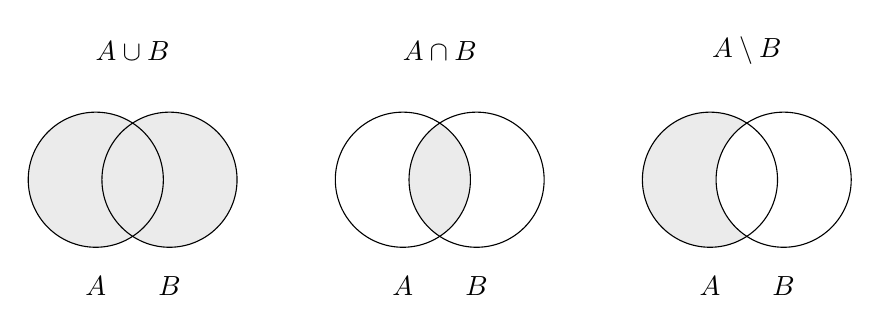
\begin{tikzpicture}[scale=0.78]
  % three Venn panels
  \foreach \x/\op in {0/{$A\cup B$}, 5/{$A\cap B$}, 10/{$A\setminus B$}}{
    \node at (\x+0.6,2.1) {\op};
  }
  % union: shade both
  \begin{scope}
    \clip (0,0) circle (1.1) (1.2,0) circle (1.1);
    \fill[band] (-2,-2) rectangle (4,2);
  \end{scope}
  \draw (0,0) circle (1.1) node[below=1.1cm] {$A$};
  \draw (1.2,0) circle (1.1) node[below=1.1cm] {$B$};
  % intersection
  \begin{scope}[shift={(5,0)}]
    \begin{scope}
      \clip (0,0) circle (1.1); \clip (1.2,0) circle (1.1);
      \fill[band] (-2,-2) rectangle (4,2);
    \end{scope}
    \draw (0,0) circle (1.1) node[below=1.1cm] {$A$};
    \draw (1.2,0) circle (1.1) node[below=1.1cm] {$B$};
  \end{scope}
  % difference A\B
  \begin{scope}[shift={(10,0)}]
    \begin{scope}
      \clip (0,0) circle (1.1);
      \fill[band] (-2,-2) rectangle (4,2);
      \clip (1.2,0) circle (1.1);
      \fill[white] (-2,-2) rectangle (4,2);
    \end{scope}
    \draw (0,0) circle (1.1) node[below=1.1cm] {$A$};
    \draw (1.2,0) circle (1.1) node[below=1.1cm] {$B$};
  \end{scope}
\end{tikzpicture}
\end{center}

\begin{theorem}[De~Morgan and distributive laws]\label{t:demorgan@c1}
For subsets of a universe $U$,
\[
  (A\cup B)^{c}=A^{c}\cap B^{c},\qquad (A\cap B)^{c}=A^{c}\cup B^{c},
\]
\[
  A\cap(B\cup C)=(A\cap B)\cup(A\cap C),\qquad A\cup(B\cap C)=(A\cup B)\cap(A\cup C).
\]
The complement laws hold verbatim for arbitrary unions/intersections: if
$\set{A_i}_{i\in I}$ is any family, $\bigl(\bigcup_i A_i\bigr)^c=\bigcap_i A_i^{c}$ and
$\bigl(\bigcap_i A_i\bigr)^c=\bigcup_i A_i^{c}$.
\end{theorem}

\begin{proof}
We prove the first De~Morgan law by the method above; the rest are identical in spirit.
$x\in(A\cup B)^c \eqv x\notin A\cup B \eqv \neg(x\in A\ \text{or}\ x\in B) \eqv (x\notin A)
\ \text{and}\ (x\notin B) \eqv x\in A^c\cap B^c$. Each link is a genuine logical
equivalence (the third is the De~Morgan law of propositional logic), so the two sets have
the same elements and are equal. For the arbitrary-family version, ``$x\notin\bigcup_i
A_i$'' means ``$x\notin A_i$ for every $i$'', which is exactly ``$x\in\bigcap_i A_i^c$''.
\end{proof}

\begin{wex}{A distributive law by the two-containment method}
Prove $A\cap(B\cup C)=(A\cap B)\cup(A\cap C)$.
\wrec A set identity; run the two-containment method. Here every step is reversible, so a
single $\eqv$-chain works.
\wsol $x\in A\cap(B\cup C)$ iff $x\in A$ and $x\in B\cup C$, i.e.\ $x\in A$ and ($x\in B$ or
$x\in C$). Distributing ``and'' over ``or'' in logic, this is ($x\in A$ and $x\in B$) or
($x\in A$ and $x\in C$), i.e.\ $x\in(A\cap B)$ or $x\in(A\cap C)$, i.e.\ $x\in(A\cap
B)\cup(A\cap C)$. Every link reverses, so the sets are equal. \emph{Check:} with
$A=\set{1,2}$, $B=\set{2,3}$, $C=\set{1,4}$: $B\cup C=\set{1,2,3,4}$, LHS $=\set{1,2}$;
$A\cap B=\set2$, $A\cap C=\set1$, RHS $=\set{1,2}$. Agree.
\end{wex}

\subsection*{Cartesian products and relations}

\begin{definition}\label{d:product@c1}
The \emph{ordered pair} $(a,b)$ is determined by both entries and their order:
$(a,b)=(a',b')\eqv a=a'\ \text{and}\ b=b'$. The \emph{Cartesian product} is
$A\times B=\set{(a,b)\st a\in A,\ b\in B}$. A \emph{relation} from $A$ to $B$ is any subset
$R\subseteq A\times B$; we write $a\mathbin{R}b$ for $(a,b)\in R$.
\end{definition}

\begin{center}
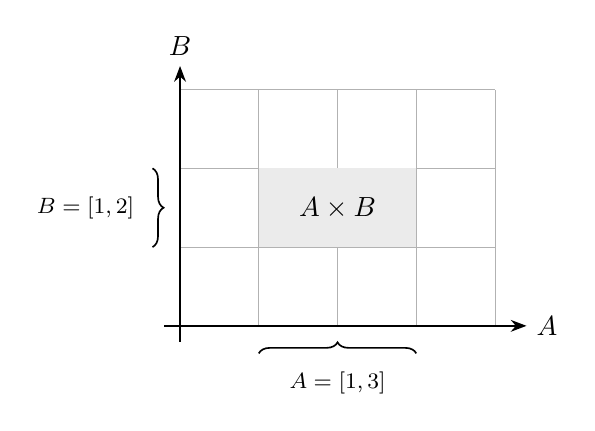
\begin{tikzpicture}[scale=1.0]
  \draw[dgrid] (0,0) grid (4,3);
  \draw[numln] (-0.2,0) -- (4.4,0) node[right]{$A$};
  \draw[numln] (0,-0.2) -- (0,3.3) node[above]{$B$};
  % shade A=[1,2]u[3,4]? keep simple: A=[1,3], B=[1,2]
  \fill[band] (1,1) rectangle (3,2);
  \node at (2,1.5) {$A\times B$};
  \draw[brc] (1,-0.35) -- (3,-0.35) node[midway,below=3pt]{\footnotesize $A=[1,3]$};
  \draw[brc] (-0.35,2) -- (-0.35,1) node[midway,left=3pt]{\footnotesize $B=[1,2]$};
\end{tikzpicture}
\end{center}

\subsection*{Functions: the modern (graph) definition}

\begin{definition}\label{d:function@c1}
A \emph{function} $f:A\to B$ is a relation $f\subseteq A\times B$ such that for each $a\in
A$ there is \emph{exactly one} $b\in B$ with $(a,b)\in f$; that unique $b$ is written
$f(a)$. Here $A$ is the \emph{domain}, $B$ the \emph{codomain}. The \emph{range} (or
image of the whole domain) is $f(A)=\set{f(a)\st a\in A}\subseteq B$.
\end{definition}

The point of phrasing a function as a special relation (a set of pairs) is that ``rule''
is too vague: the data of $f$ is its graph together with the chosen codomain $B$. Two
functions are equal iff they have the same domain, same codomain, and same value at every
point.

\begin{center}
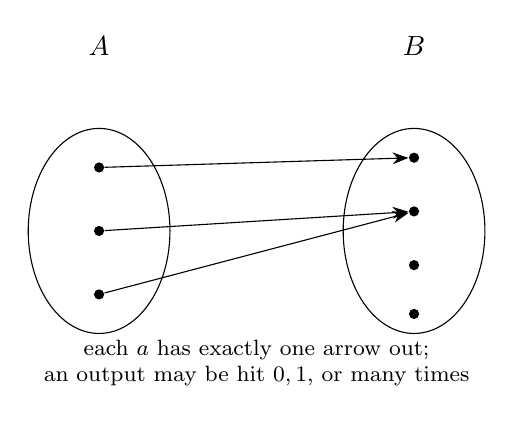
\begin{tikzpicture}[yscale=0.62,xscale=1.0]
  % left oval = A, right oval = B, arrows for a function
  \draw (0,0) ellipse (0.9 and 2.1) node[above=2.1cm]{$A$};
  \draw (4,0) ellipse (0.9 and 2.1) node[above=2.1cm]{$B$};
  \foreach \i/\y in {1/1.3, 2/0, 3/-1.3}{ \node[pt] (a\i) at (0,\y) {}; }
  \foreach \i/\y in {1/1.5, 2/0.4, 3/-0.7, 4/-1.7}{ \node[pt] (b\i) at (4,\y) {}; }
  \draw[-{Stealth[length=2mm]}] (a1)--(b1);
  \draw[-{Stealth[length=2mm]}] (a2)--(b2);
  \draw[-{Stealth[length=2mm]}] (a3)--(b2); % two inputs -> one output (allowed)
  \node[align=center,font=\footnotesize] at (2,-2.7)
    {each $a$ has exactly one arrow out;\\ an output may be hit $0,1,$ or many times};
\end{tikzpicture}
\end{center}

\begin{definition}\label{d:images@c1}
Let $f:A\to B$, $E\subseteq A$, $H\subseteq B$. The \emph{direct image} of $E$ and the
\emph{inverse image} (preimage) of $H$ are
\[
  f(E)=\set{f(x)\st x\in E}\subseteq B,\qquad
  f\inv(H)=\set{x\in A\st f(x)\in H}\subseteq A .
\]
The symbol $f\inv(H)$ is defined for \emph{every} $f$ and every $H$ --- it does not require
$f$ to be invertible.
\end{definition}

\begin{definition}\label{d:inj-surj@c1}
$f:A\to B$ is
\emph{injective} (one-to-one) if $f(a)=f(a')\imp a=a'$;
\emph{surjective} (onto) if $f(A)=B$, i.e.\ every $b\in B$ equals $f(a)$ for some $a$;
\emph{bijective} if both. When $f$ is bijective there is a unique \emph{inverse function}
$f\inv:B\to A$ with $f\inv\circ f=\id_A$ and $f\circ f\inv=\id_B$.
\end{definition}

\begin{method}{Showing a function is injective / surjective / bijective}
\textbf{Recognition trigger.} You are asked whether a given $f:A\to B$ is one-to-one,
onto, or a bijection (and possibly to produce $f\inv$).
\begin{enumerate}
\item \textbf{Injective:} assume $f(a)=f(a')$ and \emph{algebraically} force $a=a'$.
  (To \emph{disprove}: exhibit $a\neq a'$ with equal images.)
\item \textbf{Surjective:} take an arbitrary $b\in B$ and \emph{solve} $f(a)=b$ for some
  $a\in A$, checking the solution actually lies in $A$. (To disprove: find $b\in B$ not
  hit, often by an extreme-value/range argument.)
\item \textbf{Bijective:} prove both, or --- often cleaner --- exhibit a two-sided inverse
  $g:B\to A$ with $g\circ f=\id$ and $f\circ g=\id$; existence of such a $g$ is equivalent
  to bijectivity.
\end{enumerate}
\end{method}

\begin{wex}{An explicit bijection $(a,b)\to(0,1)$}
For reals $a<b$ build a bijection of the open interval $(a,b)$ onto $(0,1)$.
\wrec Trigger: ``find an explicit bijection between two intervals.'' An affine map
$t\mapsto \alpha t+\beta$ carries intervals to intervals and is invertible when
$\alpha\neq0$; pin $\alpha,\beta$ by matching endpoints.
\wsol Define $\varphi(t)=\dfrac{t-a}{b-a}$ for $t\in(a,b)$. Then $\varphi(a^+)=0$,
$\varphi(b^-)=1$, and $\varphi$ is strictly increasing (slope $1/(b-a)>0$), hence
injective; it is onto $(0,1)$ since its inverse $\varphi\inv(s)=a+(b-a)s$ sends $(0,1)$
back into $(a,b)$. As $\varphi\inv\circ\varphi=\id$ and $\varphi\circ\varphi\inv=\id$,
$\varphi$ is a bijection. \emph{Check:} the midpoint $t=\tfrac{a+b}2$ maps to
$\varphi=\tfrac12$, the midpoint of $(0,1)$, as a symmetric affine map should.
\end{wex}

\begin{wex}{A bijection $\R\to(-1,1)$}
Show $f(x)=\dfrac{x}{1+\abs{x}}$ is a bijection of $\R$ onto $(-1,1)$. (B\&S phrase the
same fact with $x/\sqrt{x^2+1}$.)
\wrec ``Show $f$ is a bijection onto an interval.'' Use the inverse-exhibition route:
guess $f\inv$ and verify both composites.
\wsol For $x\ge0$, $f(x)=x/(1+x)\in[0,1)$; for $x<0$, $f(x)=x/(1-x)\in(-1,0)$. So
$f(\R)\subseteq(-1,1)$. Solve $y=x/(1+\abs x)$: if $y\ge0$ then $x\ge0$ and
$y(1+x)=x\Rightarrow x=\dfrac{y}{1-y}$; if $y<0$ then $x=\dfrac{y}{1+y}$. In both cases
$g(y)=\dfrac{y}{1-\abs{y}}$ is defined on $(-1,1)$ and one checks $g=f\inv$:
$f(g(y))=y$ and $g(f(x))=x$. Hence $f$ is a bijection $\R\to(-1,1)$. \emph{Check:}
$f(1)=\tfrac12$ and $g(\tfrac12)=\tfrac{1/2}{1/2}=1$; consistent. \emph{Consequence:} $\R$
and the bounded interval $(-1,1)$ have the same cardinality --- foreshadowing
\S\ref{ss:countable@c1}.
\end{wex}

\begin{wex}{NON-injective squaring, and how images behave}
Let $f(x)=x^2$ on $\R$. With $E=[-1,0]$, $F=[0,1]$ show
$f(E\cap F)\subsetneq f(E)\cap f(F)$ is \emph{false} here but the general inclusion
$f(E\cap F)\subseteq f(E)\cap f(F)$ can be strict.
\wrec Trigger: a parts-of-images comparison; the lesson is that direct image preserves
$\cup$ but only \emph{half} of $\cap$.
\wsol Here $E\cap F=\set0$, so $f(E\cap F)=\set0$, while $f(E)=[0,1]=f(F)$ so $f(E)\cap
f(F)=[0,1]$. Thus $f(E\cap F)=\set0\subsetneq[0,1]=f(E)\cap f(F)$: the inclusion is
\emph{strict}, exactly because $f$ is not injective ($-1$ and $1$ share image $1$).
\emph{Always true:} $f(E\cap F)\subseteq f(E)\cap f(F)$, since $y=f(x)$ with $x\in E\cap F$
gives $y\in f(E)$ and $y\in f(F)$. Equality for \emph{all} $E,F$ holds iff $f$ is
injective. \emph{Check:} for $\cup$, $f(E\cup F)=[0,1]=f(E)\cup f(F)$ --- union is always
preserved, no injectivity needed.
\end{wex}

\begin{pitfall}
Direct image and preimage are \emph{not} symmetric. Preimage commutes with all three
operations: $f\inv(G\cup H)=f\inv G\cup f\inv H$, $f\inv(G\cap H)=f\inv G\cap f\inv H$, and
$f\inv(G^c)=(f\inv G)^c$. Direct image commutes with $\cup$ but, for $\cap$ and
complement, only gives $\subseteq$ unless $f$ is injective. When in doubt, push problems
through the \emph{preimage} --- it is the better-behaved operation.
\end{pitfall}

\begin{theorem}[Preimage respects all Boolean operations]\label{t:preimage@c1}
For $f:A\to B$ and $G,H\subseteq B$:
\[
  f\inv(G\cup H)=f\inv(G)\cup f\inv(H),\quad
  f\inv(G\cap H)=f\inv(G)\cap f\inv(H),\quad
  f\inv(B\setminus G)=A\setminus f\inv(G).
\]
\end{theorem}

\begin{proof}
For each, $x\in\text{LHS}$ unfolds to a statement about $f(x)$ that is literally the
defining statement of the RHS. E.g.\ $x\in f\inv(G\cap H)\eqv f(x)\in G\cap H\eqv (f(x)\in
G\ \text{and}\ f(x)\in H)\eqv x\in f\inv(G)\ \text{and}\ x\in f\inv(H)\eqv x\in f\inv(G)\cap
f\inv(H)$. The complement case uses $f(x)\notin G\eqv x\notin f\inv(G)$.
\end{proof}

\subsection*{Composition}

\begin{definition}\label{d:compose@c1}
If $f:A\to B$ and $g:B\to C$, the \emph{composite} $g\circ f:A\to C$ is
$(g\circ f)(x)=g(f(x))$. Composition is associative: $h\circ(g\circ f)=(h\circ g)\circ f$.
\end{definition}

\begin{center}
\begin{tikzcd}[column sep=large]
A \arrow[r,"f"] \arrow[rr,bend right=22,"g\circ f"'] & B \arrow[r,"g"] & C
\end{tikzcd}
\end{center}

\begin{proposition}\label{p:compose-inj@c1}
Let $f:A\to B$, $g:B\to C$. (i) If $f,g$ are injective so is $g\circ f$. (ii) If $f,g$ are
surjective so is $g\circ f$. (iii) If $g\circ f$ is injective then $f$ is injective.
(iv) If $g\circ f$ is surjective then $g$ is surjective.
\end{proposition}

\begin{proof}
(i) $g(f(a))=g(f(a'))\imp f(a)=f(a')$ ($g$ inj) $\imp a=a'$ ($f$ inj). (ii) Given $c\in
C$, pick $b$ with $g(b)=c$ ($g$ surj), then $a$ with $f(a)=b$ ($f$ surj); so $(g\circ
f)(a)=c$. (iii) $f(a)=f(a')\imp g(f(a))=g(f(a'))\imp a=a'$. (iv) The range of $g\circ f$ is
contained in the range of $g$; if the former is all of $C$ so is the latter.
\end{proof}

\begin{remark}
Parts (iii)--(iv) are sharp: $g\circ f$ injective forces only $f$ (the \emph{first} map)
injective, and $g\circ f$ surjective forces only $g$ (the \emph{last} map) surjective.
A standard counterexample: $f:\N\to\N$, $f(n)=n+1$, and $g:\N\to\N$, $g(1)=1$,
$g(n)=n-1$ for $n\ge2$. Then $g\circ f=\id$ is bijective, yet $f$ is not surjective
($1\notin f(\N)$) and $g$ is not injective ($g(1)=g(2)=1$).
\end{remark}

\subsection*{Further worked examples}

\begin{wex}{De~Morgan with a concrete universe}
Let $U=\set{1,2,\dots,10}$, $A=\set{1,2,3,4,5}$, $B=\set{4,5,6,7}$. Verify
$(A\cup B)^c=A^c\cap B^c$ by direct computation, then explain why this is forced.
\wrec A set identity stated for specific sets; we both \emph{compute} both sides and recall
the De~Morgan law (Theorem~\ref{t:demorgan@c1}) that guarantees agreement.
\wsol $A\cup B=\set{1,2,3,4,5,6,7}$, so $(A\cup B)^c=\set{8,9,10}$. On the other side
$A^c=\set{6,7,8,9,10}$ and $B^c=\set{1,2,3,8,9,10}$, whence $A^c\cap
B^c=\set{8,9,10}$. The two sides agree. They \emph{must}: an element lies outside
$A\cup B$ exactly when it lies outside $A$ \emph{and} outside $B$, which is the logical
content of the law. \emph{Check:} $8$ is in neither $A$ nor $B$, so it appears in both
computed answers; $6\in B$, so it is correctly absent from each.
\end{wex}

\begin{wex}{Symmetric difference is associative --- a sanity case}
With $A=\set{1,2,3}$, $B=\set{2,3,4}$, $C=\set{3,4,5}$, compute $(A\triangle
B)\triangle C$ and $A\triangle(B\triangle C)$ and confirm they coincide.
\wrec Trigger: test an algebraic identity ($\triangle$ is associative) on a concrete
instance, unfolding Definition~\ref{d:setops@c1}.
\wsol $A\triangle B=(A\setminus B)\cup(B\setminus A)=\set1\cup\set4=\set{1,4}$. Then
$(A\triangle B)\triangle C=\set{1,4}\triangle\set{3,4,5}$: elements in exactly one are
$\set{1,3,5}$. For the other grouping, $B\triangle C=\set2\cup\set5=\set{2,5}$, and
$A\triangle\set{2,5}=\set{1,3,5}$ (elements in exactly one of $\set{1,2,3}$ and
$\set{2,5}$). Both equal $\set{1,3,5}$. \emph{Check:} $x\in A\triangle B\triangle C$ iff
$x$ lies in an \emph{odd} number of $A,B,C$; here $1$ is in only $A$, $3$ is in all three,
$5$ is in only $C$ --- all odd counts, matching $\set{1,3,5}$.
\end{wex}

\begin{wex}{A NON-identity: when does $A\setminus(B\setminus C)=(A\setminus B)\setminus C$?}
Decide whether $A\setminus(B\setminus C)=(A\setminus B)\setminus C$ holds for all sets, and
if not, find the smallest correcting term.
\wrec Trigger: a plausible-looking ``cancellation'' law. The method is to test it, and on
failure locate exactly where the two sides diverge.
\wsol Take $A=\set1$, $B=\es$, $C=\set1$. Then $B\setminus C=\es$, so
LHS $=A\setminus\es=\set1$. But $A\setminus B=\set1$ and
$(A\setminus B)\setminus C=\set1\setminus\set1=\es$. So LHS $=\set1\neq\es=$ RHS: the
identity is \emph{false}. Unfolding memberships, $x\in A\setminus(B\setminus C)$ means
$x\in A$ and not ($x\in B$ and $x\notin C$), i.e.\ $x\in A$ and ($x\notin B$ or $x\in C$),
giving $A\setminus(B\setminus C)=(A\setminus B)\cup(A\cap C)$. The correct law carries an
extra $A\cap C$. \emph{Check:} in the counterexample $A\cap C=\set1$, exactly the element
the bad RHS dropped.
\end{wex}

\begin{wex}{Preimage commutes with intersection but image need not}
Let $f:\R\to\R$, $f(x)=x^2$, with $G=(-\infty,4]$ and $H=[1,\infty)$. Compute
$f\inv(G\cap H)$ and confirm it equals $f\inv(G)\cap f\inv(H)$; then contrast with the
direct image of an intersection.
\wrec Trigger: illustrate Theorem~\ref{t:preimage@c1} numerically and reinforce the
pitfall that direct image is worse behaved.
\wsol $G\cap H=[1,4]$, so $f\inv(G\cap H)=\set{x\st 1\le x^2\le4}=[-2,-1]\cup[1,2]$.
Separately $f\inv(G)=\set{x\st x^2\le4}=[-2,2]$ and
$f\inv(H)=\set{x\st x^2\ge1}=(-\infty,-1]\cup[1,\infty)$; their intersection is
$[-2,-1]\cup[1,2]$. They match, as the theorem promises. Contrast: with $E=[-2,-1]$ and
$F=[1,2]$ we have $E\cap F=\es$ so $f(E\cap F)=\es$, yet $f(E)=[1,4]=f(F)$ gives
$f(E)\cap f(F)=[1,4]\neq\es$ --- direct image fails for $\cap$ exactly because $f$ is not
injective. \emph{Check:} $x=-2$ lies in $f\inv(G\cap H)$ and indeed $f(-2)=4\in[1,4]=G\cap
H$.
\end{wex}

\begin{wex}{An injection that is not a surjection, and a fix}
Show $f:\N\to\N$, $f(n)=2n$, is injective but not surjective, and exhibit a different
codomain making the ``same rule'' a bijection.
\wrec Trigger: test injectivity/surjectivity by the method, and recall that surjectivity
depends on the chosen \emph{codomain}.
\wsol Injective: $2n=2n'\imp n=n'$. Not surjective onto $\N$: $1$ is odd, so $f(n)=1$ has
no solution in $\N$; the range is the even numbers $2\N\subsetneq\N$. If instead we declare
the codomain to be $2\N$, the very same rule $g:\N\to2\N$, $g(n)=2n$, is onto (every even
$m=2(m/2)$ with $m/2\in\N$) and still injective, hence a bijection with inverse $m\mapsto
m/2$. \emph{Check:} $f$ and $g$ have identical graphs $\set{(n,2n)}$; only the codomain
changed, and that alone flipped surjectivity --- the data of a function includes its
codomain.
\end{wex}

\begin{exers}{Exercises (Bartle \& Sherbert, \S1.1).}
\item Let $A=\set{k\in\N\st k\le 20}$, $B=\set{3k-1\st k\in\N}$, $C=\set{2k-1\st k\in\N}$.
  Determine (a) $A\cap B\cap C$; (b) $(A\cap B)\setminus C$; (c) $(A\cap C)\setminus B$.
\item Draw diagrams to simplify and identify: (a) $A\setminus(B\setminus A)$;
  (b) $A\setminus(A\setminus B)$; (c) $A\cap(B\setminus A)$.
\item If $A,B$ are sets, show $A\subseteq B$ iff $A\cap B=A$.
\item Prove the second De~Morgan law $(A\cap B)^c=A^c\cup B^c$.
\item Prove the distributive laws: (a) $A\cap(B\cup C)=(A\cap B)\cup(A\cap C)$;
  (b) $A\cup(B\cap C)=(A\cup B)\cap(A\cup C)$.
\item Symmetric difference $D=$ elements in exactly one of $A,B$. Represent $D$ by a
  diagram and show (a) $D=(A\setminus B)\cup(B\setminus A)$; (b) $D=(A\cup B)\setminus(A\cap B)$.
\item For $n\in\N$ let $A_n=\set{(n+1)k\st k\in\N}$. (a) Find $A_1\cap A_2$.
  (b) Determine $\bigcup_{n\in\N}A_n$ and $\bigcap_{n\in\N}A_n$.
\item Draw diagrams in the plane of $A\times B$ for: (a) $A=\set{x\in\R\st 1\le x\le 2\
  \text{or}\ 3\le x\le4}$, $B=\set{x\in\R\st x=1\ \text{or}\ x=2}$; (b) $A=\set{1,2,3}$,
  $B=\set{x\in\R\st 1\le x\le 3}$.
\item Let $A=B=\set{x\in\R\st -1\le x\le1}$ and $C=\set{(x,y)\st x^2+y^2=1}\subseteq A\times
  B$. Is $C$ a function? Explain.
\item Let $f(x)=1/x^2$ ($x\neq0$). (a) Find the direct image $f(E)$ for
  $E=\set{x\st 1\le x\le2}$. (b) Find the inverse image $f\inv(G)$ for $G=\set{x\st 1\le
  x\le4}$.
\item Let $g(x)=x^2$, $f(x)=x-2$, and $h=g\circ f$. (a) Find $h(E)$ for $E=\set{x\st 0\le
  x\le1}$. (b) Find $h\inv(G)$ for $G=\set{x\st 0\le x\le4}$.
\item Let $f(x)=x^2$, $E=\set{x\st-1\le x\le0}$, $F=\set{x\st0\le x\le1}$. Show $E\cap
  F=\set0$ and $f(E\cap F)=\set0$, while $f(E)\cap f(F)=\set{y\st0\le y\le1}$; hence $f(E\cap
  F)\subsetneq f(E)\cap f(F)$. What happens if $0$ is removed from $E$ and $F$?
\item With $f,E,F$ as above, find $E\setminus F$ and $f(E)\setminus f(F)$ and show
  $f(E\setminus F)\subseteq f(E)\setminus f(F)$ can fail.
\item For $f:A\to B$ and $E,F\subseteq A$, show $f(E\cup F)=f(E)\cup f(F)$ and $f(E\cap
  F)\subseteq f(E)\cap f(F)$.
\item For $f:A\to B$ and $G,H\subseteq B$, show $f\inv(G\cup H)=f\inv(G)\cup f\inv(H)$ and
  $f\inv(G\cap H)=f\inv(G)\cap f\inv(H)$.
\item Show $f(x)=x/\sqrt{x^2+1}$ is a bijection of $\R$ onto $\set{y\st-1<y<1}$.
\item For $a<b$, find an explicit bijection of $(a,b)$ onto $(0,1)$.
\item (a) Give two functions $f,g:\R\to\R$ with $f\neq g$ but $f\circ g=g\circ f$.
  (b) Give three functions $f,g,h:\R\to\R$ with $f\circ(g+h)\neq(f\circ g)+(f\circ h)$.
\item (a) If $f:A\to B$ is injective and $E\subseteq A$, show $f\inv(f(E))=E$.
  (b) Give an example where this fails when $f$ is not injective.
\end{exers}

\begin{exers}{Additional exercises.}
\item (Two-containment drill.) Prove $A\setminus(B\cup C)=(A\setminus B)\cap(A\setminus C)$
  and $A\setminus(B\cap C)=(A\setminus B)\cup(A\setminus C)$.
\item Show $A\triangle B=\es$ iff $A=B$, and that $\triangle$ is associative:
  $(A\triangle B)\triangle C=A\triangle(B\triangle C)$. (Hint: membership in $A\triangle
  B\triangle C$ means ``an odd number of $A,B,C$''.)
\item Let $f:A\to B$. Prove $f$ is injective iff $f(E\cap F)=f(E)\cap f(F)$ for all
  $E,F\subseteq A$, and surjective iff $f(f\inv(H))=H$ for all $H\subseteq B$.
\item Prove $E\subseteq f\inv(f(E))$ for every $f$ and $E\subseteq A$, and give an $f$ and
  $E$ for which the inclusion is strict.
\item (Composition of bijections.) If $f:A\to B$ and $g:B\to C$ are bijections, prove
  $g\circ f$ is a bijection and $(g\circ f)\inv=f\inv\circ g\inv$.
\item Exhibit an explicit bijection $[0,1]\to[0,1)$. (Hint: move a countable set; relocate
  $1,\tfrac12,\tfrac13,\dots$.)
\item Draw the Venn diagram for three sets and shade $A\triangle B\triangle C$. Which of
  the eight regions are shaded, and why does ``odd membership count'' describe them?
\item Let $f:\R\to\R$, $f(x)=2x/(1+x^2)$. Determine $f(\R)$, decide whether $f$ is
  injective or surjective onto its range, and sketch enough of the graph to justify your
  answer.
\item (Indexed De~Morgan.) For sets $A_i\subseteq U$, prove
  $\bigl(\bigcap_{i\in I}A_i\bigr)^c=\bigcup_{i\in I}A_i^c$ directly from the definitions,
  for an arbitrary (possibly uncountable) index set $I$.
\end{exers}


\section{Mathematical Induction}
\subsection*{The well-ordering principle and induction}

The natural numbers $\N=\set{1,2,3,\dots}$ carry one property that the integers, rationals,
and reals all lack, and from which induction flows.

\begin{theorem}[Well-Ordering Principle]\label{t:wop@c1}
Every nonempty subset $S\subseteq\N$ has a least element: there is $m\in S$ with $m\le s$
for all $s\in S$.
\end{theorem}

We take this as the defining structural axiom of $\N$. Induction is logically equivalent to
it.

\begin{theorem}[Principle of Mathematical Induction]\label{t:induction@c1}
Let $S\subseteq\N$ satisfy
\textup{(i)} $1\in S$, and
\textup{(ii)} $k\in S\imp k+1\in S$.
Then $S=\N$.
\end{theorem}

\begin{proof}
Suppose not, so $T=\N\setminus S\neq\es$. By well-ordering $T$ has a least element $m$. Now
$m\neq1$ by (i), so $m\ge2$ and $m-1\in\N$. Since $m$ is the \emph{least} element not in
$S$, we have $m-1\in S$. But then (ii) gives $m=(m-1)+1\in S$, contradicting $m\in T$.
Hence $T=\es$ and $S=\N$.
\end{proof}

In practice $S=\set{n\in\N\st P(n)\ \text{is true}}$ for a statement $P(n)$, and the two
hypotheses become the familiar \emph{base case} $P(1)$ and \emph{inductive step}
$P(k)\imp P(k+1)$.

\begin{center}
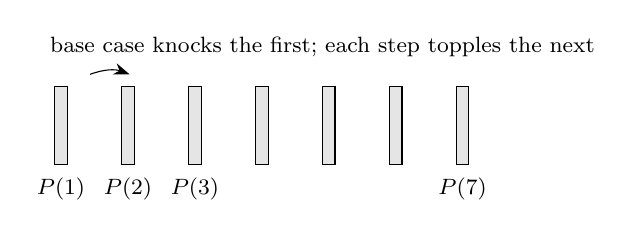
\begin{tikzpicture}[scale=1]
  % falling dominoes / ladder picture
  \foreach \i in {0,...,6}{
    \draw[fill=black!10] (\i*0.85,0) rectangle (\i*0.85+0.16,1);
  }
  \node at (0.08,-0.3) {\footnotesize $P(1)$};
  \node at (0.85+0.08,-0.3) {\footnotesize $P(2)$};
  \node at (2*0.85+0.08,-0.3) {\footnotesize $P(3)$};
  \node at (6*0.85+0.08,-0.3) {\footnotesize $P(7)$};
  \draw[-{Stealth[length=2mm]}] (0.45,1.15) to[bend left=20] (0.95,1.15);
  \node[font=\footnotesize] at (3.4,1.5)
    {base case knocks the first; each step topples the next};
\end{tikzpicture}
\end{center}

\begin{theorem}[Strong / Complete Induction]\label{t:strong@c1}
Let $S\subseteq\N$ satisfy: for every $n\in\N$, if $\set{1,\dots,n-1}\subseteq S$ then
$n\in S$. Then $S=\N$. (Equivalently: if $P(1)$ holds and ``$P(1),\dots,P(k)$ all hold''
implies $P(k+1)$, then $P(n)$ holds for all $n$.)
\end{theorem}

\begin{proof}
Apply well-ordering to $T=\N\setminus S$ exactly as above: a least missing element $n$
would have all of $1,\dots,n-1$ in $S$, forcing $n\in S$, a contradiction.
\end{proof}

\begin{method}{Running an induction proof}
\textbf{Recognition trigger.} A statement $P(n)$ indexed by $\N$: a summation formula, a
divisibility claim, an inequality valid past some point, a recursively defined object.
\begin{enumerate}
\item \textbf{State $P(n)$ precisely} as a predicate in $n$ (write the ``for all $n\ge
  n_0$'').
\item \textbf{Base case.} Verify $P(n_0)$ by direct computation. Do not skip it.
\item \textbf{Inductive step.} \emph{Assume} $P(k)$ (ordinary) or $P(n_0),\dots,P(k)$
  (strong) for a generic $k\ge n_0$. Derive $P(k+1)$, \emph{using the hypothesis
  explicitly} --- circle where you invoke it.
\item Conclude $P(n)$ for all $n\ge n_0$.
\end{enumerate}
\textbf{When to use strong induction:} when $P(k+1)$ depends on an \emph{earlier} case,
not just the immediately previous one (recurrences, prime factorization, Fibonacci-type
bounds).
\end{method}

\begin{wex}{A summation formula}
Prove $\displaystyle\sum_{j=1}^{n}j=\frac{n(n+1)}2$ for all $n\in\N$.
\wrec A formula indexed by $n$: ordinary induction, since the $(k+1)$-case adds one new
term to the $k$-case.
\wsol \emph{Base} $n=1$: LHS $=1$, RHS $=\tfrac{1\cdot2}2=1$. \checkmark\ \emph{Step:}
assume $\sum_{j=1}^{k}j=\tfrac{k(k+1)}2$. Then
\[
  \sum_{j=1}^{k+1}j=\underbrace{\sum_{j=1}^{k}j}_{\text{hyp}}+(k+1)
  =\frac{k(k+1)}2+(k+1)=(k+1)\frac{k+2}2=\frac{(k+1)(k+2)}2,
\]
which is the formula at $n=k+1$. By induction it holds for all $n$. \emph{Check:} $n=4$
gives $1+2+3+4=10=\tfrac{4\cdot5}2$. \checkmark
\end{wex}

\begin{wex}{A divisibility claim}
Prove $n^3+5n$ is divisible by $6$ for all $n\in\N$.
\wrec A divisibility statement; ordinary induction, expanding $(k+1)^3+5(k+1)$ and peeling
off the $k$-case.
\wsol \emph{Base} $n=1$: $1+5=6$, divisible by $6$. \checkmark\ \emph{Step:} assume
$6\mid k^3+5k$, say $k^3+5k=6t$. Then
\[
  (k+1)^3+5(k+1)=k^3+3k^2+3k+1+5k+5=(k^3+5k)+3k^2+3k+6=6t+3k(k+1)+6 .
\]
Now $k(k+1)$ is a product of consecutive integers, hence even, so $3k(k+1)$ is divisible
by $6$; the whole expression is a sum of multiples of $6$. Thus $6\mid(k+1)^3+5(k+1)$. By
induction the claim holds for all $n$. \emph{Check:} $n=2$: $8+10=18=6\cdot3$. \checkmark
\end{wex}

\begin{wex}{An eventual inequality (base case shifted)}
Prove $2^n>n^2$ for all integers $n\ge5$.
\wrec An inequality true only \emph{past a point}: induct with base $n_0=5$; in the step,
bound the new term using the hypothesis \emph{and} a secondary inequality.
\wsol \emph{Base} $n=5$: $2^5=32>25=5^2$. \checkmark\ \emph{Step:} assume $2^k>k^2$ for
some $k\ge5$. Then $2^{k+1}=2\cdot2^k>2k^2$. It suffices to show $2k^2\ge(k+1)^2$, i.e.\
$k^2-2k-1\ge0$, which holds for $k\ge3$ (roots $1\pm\sqrt2$). Hence
$2^{k+1}>2k^2\ge(k+1)^2$. By induction $2^n>n^2$ for all $n\ge5$. \emph{Check:} $n=6$:
$64>36$. \checkmark\ (Note $n=2,3,4$ fail: $4=4$, $8<9$, $16=16$ --- the shifted base is
essential.)
\end{wex}

\begin{wex}{Bernoulli's inequality}
Prove $(1+x)^n\ge1+nx$ for all $n\in\N$ and all real $x\ge-1$.
\wrec A parametrized inequality; induct on $n$, using $x\ge-1$ (so $1+x\ge0$) to preserve
the direction when multiplying.
\wsol \emph{Base} $n=1$: $(1+x)^1=1+x\ge1+x$. \checkmark\ \emph{Step:} assume
$(1+x)^k\ge1+kx$. Since $1+x\ge0$ we may multiply the inequality by $1+x$:
\[
  (1+x)^{k+1}\ge(1+kx)(1+x)=1+(k+1)x+kx^2\ge1+(k+1)x,
\]
because $kx^2\ge0$. By induction the inequality holds for all $n$. \emph{Check:} $x=1$,
$n=3$: $2^3=8\ge1+3=4$. \checkmark\ This inequality is the engine behind many
limit estimates later (e.g.\ $\sqrt[n]{n}\to1$).
\end{wex}

\begin{wex}{Strong induction: every $n\ge2$ has a prime factor}
Prove that every integer $n\ge2$ is a product of primes.
\wrec The factorization of $n$ refers to \emph{smaller} numbers $a,b<n$, not to $n-1$;
this is the signature of strong induction.
\wsol \emph{Base} $n=2$: prime, a one-factor product. \emph{Step (strong):} assume every
integer in $\set{2,\dots,k}$ is a product of primes, and consider $k+1$. If $k+1$ is prime
we are done. Otherwise $k+1=ab$ with $2\le a,b\le k$. By the strong hypothesis $a$ and $b$
are each products of primes, hence so is their product $k+1$. By strong induction the claim
holds for all $n\ge2$. \emph{Check:} $12=2\cdot6=2\cdot2\cdot3$, reached by splitting into
the smaller already-handled $2$ and $6$.
\end{wex}

\begin{pitfall}
\textbf{Never skip the base case.} The step alone proves nothing. ``$P(n):\ n=n+1$''
satisfies a vacuous-looking step pattern if mishandled, yet is false for every $n$; only a
base case can anchor the chain. The notorious ``all horses are the same color'' paradox
fails precisely at $n=1\to2$, where the inductive step secretly needs two horses to
overlap. \textbf{Always check the step works for the \emph{smallest} relevant $k$.}
\end{pitfall}

\begin{pitfall}
The inductive hypothesis must actually be \emph{used}. A ``proof'' that re-derives
$P(k+1)$ from scratch without invoking $P(k)$ is not an induction (and usually has a hidden
gap). Mark the spot where you substitute the hypothesis.
\end{pitfall}

\subsection*{Further worked examples}

\begin{wex}{Sum of odd numbers is a perfect square}
Prove $\displaystyle\sum_{j=1}^{n}(2j-1)=n^2$ for all $n\in\N$.
\wrec A formula indexed by $n$: ordinary induction, since the $(k+1)$-case appends one new
odd number to the $k$-case.
\wsol \emph{Base} $n=1$: LHS $=2\cdot1-1=1=1^2$. \checkmark\ \emph{Step:} assume
$\sum_{j=1}^{k}(2j-1)=k^2$. Then
\[
  \sum_{j=1}^{k+1}(2j-1)=\underbrace{\sum_{j=1}^{k}(2j-1)}_{\text{hyp}}+(2(k+1)-1)
  =k^2+(2k+1)=(k+1)^2,
\]
the formula at $n=k+1$. By induction it holds for all $n$. \emph{Check:} $n=4$ gives
$1+3+5+7=16=4^2$. \checkmark\ (Geometrically, adding the $(k+1)$-st L-shaped ``gnomon'' of
$2k+1$ unit squares turns a $k\times k$ square into a $(k+1)\times(k+1)$ one.)
\end{wex}

\begin{wex}{A telescoping sum}
Prove $\displaystyle\sum_{j=1}^{n}\frac{1}{j(j+1)}=\frac{n}{n+1}$ for all $n\in\N$.
\wrec A summation formula; ordinary induction works, though one could also telescope using
$\tfrac1{j(j+1)}=\tfrac1j-\tfrac1{j+1}$. We use induction to drill the method.
\wsol \emph{Base} $n=1$: LHS $=\tfrac1{1\cdot2}=\tfrac12$, RHS $=\tfrac1{2}$. \checkmark\
\emph{Step:} assume $\sum_{j=1}^{k}\tfrac1{j(j+1)}=\tfrac{k}{k+1}$. Then
\[
  \sum_{j=1}^{k+1}\frac1{j(j+1)}=\frac{k}{k+1}+\frac1{(k+1)(k+2)}
  =\frac{k(k+2)+1}{(k+1)(k+2)}=\frac{(k+1)^2}{(k+1)(k+2)}=\frac{k+1}{k+2},
\]
using $k(k+2)+1=k^2+2k+1=(k+1)^2$. This is the formula at $k+1$. \emph{Check:} $n=3$ gives
$\tfrac12+\tfrac16+\tfrac1{12}=\tfrac{6+2+1}{12}=\tfrac9{12}=\tfrac34=\tfrac3{4}$.
\checkmark\ As $n\to\infty$ the sum $\to1$, foreshadowing convergent series.
\end{wex}

\begin{wex}{A divisibility claim with a larger modulus}
Prove $7\mid 8^n-1$ for all $n\in\N$.
\wrec A divisibility statement; ordinary induction, factoring $8^{k+1}-1$ so the $k$-case
$8^k-1$ appears.
\wsol \emph{Base} $n=1$: $8^1-1=7$, divisible by $7$. \checkmark\ \emph{Step:} assume
$7\mid 8^k-1$, say $8^k-1=7t$. Then
\[
  8^{k+1}-1=8\cdot8^k-1=8(8^k-1)+8-1=8\cdot7t+7=7(8t+1),
\]
a multiple of $7$. By induction $7\mid 8^n-1$ for all $n$. \emph{Check:} $n=2$:
$64-1=63=7\cdot9$. \checkmark\ (The same trick proves $a-1\mid a^n-1$ for any integer
$a\ge2$.)
\end{wex}

\begin{wex}{NON-proof: a flawed induction and its broken step}
Critique the following ``proof'' that \emph{every} finite set of lines in the plane, no
two parallel, passes through a single common point.
\wrec Trigger: a stated induction that is \emph{false}; the task is to locate the precise
case where the inductive step fails --- the discipline behind the base-case pitfall.
\wsol The bogus argument: $P(n)$ = ``any $n$ pairwise-nonparallel lines share a point.''
Base $P(2)$ is true (two nonparallel lines meet in one point). ``Step'': given $n+1$ lines
$\ell_1,\dots,\ell_{n+1}$, the first $n$ share a point $p$ (by $P(n)$) and the last $n$
share a point $q$ (by $P(n)$); since both groups contain $\ell_2,\dots,\ell_n$, one argues
$p=q$, so all $n+1$ meet at $p$. The flaw is exactly at $n+1=3$: the two overlapping groups
$\set{\ell_1,\ell_2}$ and $\set{\ell_2,\ell_3}$ share only the single line $\ell_2$, which
does not pin a common point, so the inference $p=q$ collapses. The claim is plainly false
(three lines forming a triangle). \emph{Check:} the step silently needs $\ge2$ shared
lines, i.e.\ $n\ge3$; the chain is never validly anchored, mirroring the ``all horses one
color'' fallacy at $n=1\to2$.
\end{wex}

\begin{exers}{Exercises (Bartle \& Sherbert, \S1.2).}
\item Prove $\dfrac1{1\cdot2}+\dfrac1{2\cdot3}+\cdots+\dfrac1{n(n+1)}=\dfrac{n}{n+1}$ for
  all $n\in\N$.
\item Prove $1^3+2^3+\cdots+n^3=\bigl[\tfrac12 n(n+1)\bigr]^2$ for all $n\in\N$.
\item Prove $3+11+\cdots+(8n-5)=4n^2-n$ for all $n\in\N$.
\item Prove $1^2+3^2+\cdots+(2n-1)^2=\dfrac{4n^3-n}{3}$ for all $n\in\N$.
\item Prove $1^2-2^2+3^2-\cdots+(-1)^{n+1}n^2=(-1)^{n+1}\dfrac{n(n+1)}2$ for all $n\in\N$.
\item Prove $n^3+5n$ is divisible by $6$ for all $n\in\N$.
\item Prove $5^{2n}-1$ is divisible by $8$ for all $n\in\N$.
\item Prove $5^n-4n-1$ is divisible by $16$ for all $n\in\N$.
\item Prove $n^3+(n+1)^3+(n+2)^3$ is divisible by $9$ for all $n\in\N$.
\item Conjecture a formula for $\dfrac1{1\cdot3}+\dfrac1{3\cdot5}+\cdots+
  \dfrac1{(2n-1)(2n+1)}$ and prove it.
\item Conjecture a formula for the sum $1+3+5+\cdots+(2n-1)$ of the first $n$ odd numbers
  and prove it by induction.
\item Prove the second version of the induction principle (Theorem~1.2.4 of B\&S).
\item Prove $2^n<n!$ for all $n\ge4$.
\item Prove $2n-3\le 2^{n-2}$ for all $n\ge5$.
\item Find all $n\in\N$ for which $n^2<2^n$, and prove your answer.
\item Find the largest natural number $m$ such that $n^3-n$ is divisible by $m$ for all
  $n\in\N$; prove your assertion.
\item Prove $\dfrac1{\sqrt1}+\dfrac1{\sqrt2}+\cdots+\dfrac1{\sqrt n}>\sqrt n$ for all
  $n\ge2$.
\end{exers}

\begin{exers}{Additional exercises.}
\item Prove the \emph{finite geometric sum} $\displaystyle\sum_{j=0}^{n}r^{\,j}=
  \dfrac{r^{n+1}-1}{r-1}$ for $r\neq1$ and all $n\ge0$.
\item (Where the base case bites.) For which $n\in\N$ is $2^n\ge n^3$? Prove it for all
  sufficiently large $n$ by induction, and identify the exact threshold.
\item Diagnose the fallacy: ``Claim: all elements of every nonempty finite set of reals are
  equal. Proof by induction on the size $n$...''. Pinpoint the step that fails and why.
\item (Strong induction.) The Fibonacci numbers are $F_1=F_2=1$, $F_{n+2}=F_{n+1}+F_n$.
  Prove $F_n<2^n$ for all $n\in\N$.
\item Prove $\displaystyle\prod_{k=2}^{n}\Bigl(1-\tfrac1{k^2}\Bigr)=\dfrac{n+1}{2n}$ for all
  $n\ge2$.
\item Use well-ordering directly (no induction principle) to prove: there is no natural
  number strictly between $0$ and $1$.
\item Prove $\displaystyle\sum_{j=1}^{n}j\cdot j!=(n+1)!-1$ for all $n\in\N$.
\item (AM--GM warm-up, induction on a power of $2$.) Prove that for nonnegative reals,
  $\dfrac{a_1+\cdots+a_n}{n}\ge\sqrt[n]{a_1\cdots a_n}$ when $n$ is a power of $2$.
\end{exers}


\section{Finite, Countable, and Uncountable Sets}
\subsection*{Counting by bijection}\label{ss:countable@c1}

Cardinality compares sizes of sets --- finite or infinite --- by the existence of
bijections, with no reference to ``number'' until the very end.

\begin{definition}\label{d:equinumerous@c1}
Sets $A$ and $B$ are \emph{equinumerous} (have the same cardinality), written $A\sim B$, if
there is a bijection $f:A\to B$. For $n\in\N$ write $\N_n=\set{1,2,\dots,n}$.
A set $A$ is
\emph{finite} if $A=\es$ or $A\sim\N_n$ for some $n$ (and then $\abs A=n$);
\emph{infinite} if not finite;
\emph{denumerable} (countably infinite) if $A\sim\N$;
\emph{countable} if finite or denumerable;
\emph{uncountable} if not countable.
\end{definition}

\begin{remark}
$\sim$ is an equivalence relation: reflexive ($\id$), symmetric ($f\inv$ is a bijection),
transitive (Proposition~\ref{p:compose-inj@c1}: a composite of bijections is a bijection). So
``same size'' behaves as it should.
\end{remark}

A hallmark of \emph{infinite} sets, impossible for finite ones, is that they biject with
proper subsets of themselves.

\begin{wex}{$\N$ is equinumerous with a proper subset}
Exhibit a bijection of $\N$ onto the even numbers $2\N=\set{2,4,6,\dots}$, and onto $\N$
minus a finite set.
\wrec Trigger: ``show an infinite set matches a proper subset.'' Build an explicit
formula and check both directions.
\wsol $f(n)=2n$ is a bijection $\N\to2\N$ (inverse $m\mapsto m/2$). Likewise $g(n)=n+13$
bijects $\N$ onto $\set{14,15,16,\dots}$, the integers greater than $13$. \emph{Check:}
$f$ misses no even number and repeats none; a finite set could never biject with a proper
subset, so this property \emph{characterizes} infinity (Dedekind's definition).
\end{wex}

\begin{theorem}[Subsets and images of countable sets]\label{t:countable-closure@c1}
\textup{(a)} Every subset of a countable set is countable.
\textup{(b)} If $A$ is countable and $f:A\to B$ is a surjection, then $B$ is countable;
equivalently, the image of a countable set under any map is countable.
\textup{(c)} $A$ is countable iff there is an injection $A\to\N$, iff $A=\es$ or there is a
surjection $\N\to A$.
\end{theorem}

\begin{proof}[Proof sketch]
(a) If $A\subseteq\N$ is infinite, define $f:\N\to A$ by sending $1$ to the least element
of $A$ (well-ordering), then recursively $f(n+1)$ to the least element of $A$ above
$f(n)$; this is a strictly increasing bijection $\N\to A$. A general countable $A$ pulls
back to $\N$. (b),(c) follow by composing with the enumerating bijection and using that a
surjection $\N\to B$ lets you pick, for each $b$, the least preimage, yielding an injection
$B\to\N$.
\end{proof}

\subsection*{Building blocks: $\N\times\N$, $\Z$, $\Q$ are countable}

\begin{theorem}\label{t:NxN@c1}
$\N\times\N$ is denumerable.
\end{theorem}

\begin{proof}
List the pairs $(m,n)$ along the \emph{diagonals} $m+n=\text{const}$, as drawn below. The
explicit Cantor pairing $h(m,n)=\tfrac12(m+n-2)(m+n-1)+m$ is a bijection $\N\times\N\to\N$.
Alternatively $(m,n)\mapsto 2^{m}3^{n}$ is an \emph{injection} $\N\times\N\to\N$ (unique
factorization), which already gives countability by
Theorem~\ref{t:countable-closure@c1}(c).
\end{proof}

\begin{center}
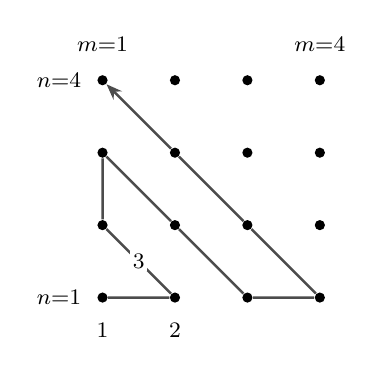
\begin{tikzpicture}[scale=0.92]
  \foreach \m in {1,...,4}{
    \foreach \n in {1,...,4}{
      \node[pt] (p\m\n) at (\m,\n) {};
    }}
  % axis labels
  \node[font=\footnotesize] at (0.4,1) {$n{=}1$};
  \node[font=\footnotesize] at (0.4,4) {$n{=}4$};
  \node[font=\footnotesize] at (1,4.5) {$m{=}1$};
  \node[font=\footnotesize] at (4,4.5) {$m{=}4$};
  % zig-zag path along anti-diagonals
  \draw[-{Stealth[length=2mm]},line width=0.9pt,black!70]
    (p11)--(p21)--(p12)--(p13)--(p22)--(p31)--(p41)--(p32)--(p23)--(p14);
  \node[font=\footnotesize,fill=white,inner sep=1pt] at (1,0.55) {$1$};
  \node[font=\footnotesize,fill=white,inner sep=1pt] at (2,0.55) {$2$};
  \node[font=\footnotesize,fill=white,inner sep=1pt] at (1.5,1.5) {$3$};
\end{tikzpicture}
\captionof{figure}{Enumerating $\N\times\N$ along anti-diagonals $m+n=\text{const}$: each
diagonal is finite, so every pair is reached at a finite stage.}
\end{center}

\begin{corollary}\label{c:Z-Q-countable@c1}
$\Z$ and $\Q$ are denumerable, and a countable union of countable sets is countable.
\end{corollary}

\begin{proof}
$\Z$: interleave, $0,1,-1,2,-2,\dots$, i.e.\ the bijection $\N\to\Z$ sending odd $2k-1\mapsto
k-1$... more cleanly $n\mapsto n/2$ if $n$ even, $-(n-1)/2$ if $n$ odd. \emph{Countable
union:} let $A_1,A_2,\dots$ be countable, enumerate each $A_i=\set{a_{i1},a_{i2},\dots}$,
and map $\bigcup_i A_i$ into $\N\times\N$ by $a_{ij}\mapsto(i,j)$; this is (almost) an
injection into a countable set, so the union is countable. \emph{$\Q$:} the map
$\Q_{>0}\to\N\times\N$, $p/q\mapsto(p,q)$ in lowest terms, is an injection, so $\Q_{>0}$ is
countable; then $\Q=\Q_{>0}\cup\set0\cup\Q_{<0}$ is a finite union of countable sets.
\end{proof}

\begin{pitfall}
``Countable union of countable sets is countable'' uses a choice of enumeration for
\emph{each} $A_i$ at once --- a (countable) use of the Axiom of Choice. Harmless here, but
worth knowing it is not pure bookkeeping. Note also $\bigcup$ of countably many
\emph{finite} sets can be infinite (e.g.\ $A_n=\set n$), and that is fine: it is still
countable.
\end{pitfall}

\subsection*{The diagonal argument: $\R$ is uncountable}

The decisive break: not all infinite sets have the same size. Cantor's diagonal method
shows the unit interval --- hence $\R$ --- cannot be listed.

\begin{theorem}[Cantor]\label{t:R-uncountable@c1}
The interval $[0,1)$ is uncountable; hence $\R$ is uncountable.
\end{theorem}

\begin{proof}
Suppose, for contradiction, that $[0,1)$ were countable, say enumerated as
$x_1,x_2,x_3,\dots$. Write each in decimal, $x_i=0.d_{i1}d_{i2}d_{i3}\dots$, choosing the
non-terminating form to make the expansion unique (forbid trailing $9$s). Define a new
digit string $y=0.e_1e_2e_3\dots$ by
\[
  e_i=\begin{cases}5,& d_{ii}\neq5,\\ 4,& d_{ii}=5.\end{cases}
\]
Then $y\in[0,1)$, and $y$ uses only digits $4,5$, so it has no trailing $9$s and its
expansion is unique. For every $i$, $y$ differs from $x_i$ in the $i$-th digit ($e_i\neq
d_{ii}$), so $y\neq x_i$. Thus $y$ is in $[0,1)$ but not in the list --- contradicting that
the list was \emph{all} of $[0,1)$. Hence $[0,1)$ is uncountable. Since
$[0,1)\subseteq\R$, $\R$ is uncountable by Theorem~\ref{t:countable-closure@c1}(a)
(contrapositive).
\end{proof}

\begin{center}
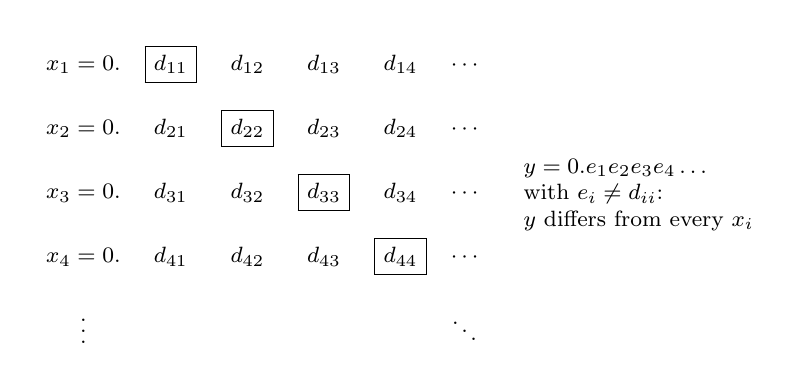
\begin{tikzpicture}[scale=0.95]
  \matrix (M) [matrix of math nodes, column sep=2pt, row sep=3pt, nodes={font=\footnotesize}]{
    x_1 = 0. & \boxed{d_{11}} & d_{12} & d_{13} & d_{14} & \cdots\\
    x_2 = 0. & d_{21} & \boxed{d_{22}} & d_{23} & d_{24} & \cdots\\
    x_3 = 0. & d_{31} & d_{32} & \boxed{d_{33}} & d_{34} & \cdots\\
    x_4 = 0. & d_{41} & d_{42} & d_{43} & \boxed{d_{44}} & \cdots\\
    \vdots & & & & & \ddots\\
  };
  \node[font=\footnotesize,align=left,right=6pt of M]
    {$y=0.e_1e_2e_3e_4\dots$\\ with $e_i\neq d_{ii}$:\\ $y$ differs from every $x_i$};
\end{tikzpicture}
\captionof{figure}{Change every boxed diagonal digit; the result agrees with no row.}
\end{center}

\begin{theorem}[Cantor's theorem]\label{t:cantor-power@c1}
For every set $S$, there is no surjection $S\to\mathcal P(S)$; in particular $S\not\sim
\mathcal P(S)$. Thus $\abs S<\abs{\mathcal P(S)}$, and there is no largest cardinality.
\end{theorem}

\begin{proof}
Let $f:S\to\mathcal P(S)$ be any map. Form the ``diagonal'' set $D=\set{x\in S\st x\notin
f(x)}\subseteq S$. If $D=f(a)$ for some $a$, ask whether $a\in D$: by definition of $D$,
$a\in D\eqv a\notin f(a)=D$, a contradiction. So $D$ is not in the range of $f$, and $f$ is
not surjective. The injection $x\mapsto\set x$ shows $\abs S\le\abs{\mathcal P(S)}$, so the
inequality is strict.
\end{proof}

\begin{remark}
For finite $S$ with $\abs S=n$, $\abs{\mathcal P(S)}=2^n>n$, the concrete shadow of
Cantor's theorem (Exercise: prove $\abs{\mathcal P(S)}=2^n$ by induction). For $S=\N$ one
gets $\abs{\mathcal P(\N)}=\abs\R=2^{\aleph_0}>\aleph_0$: the reals are the power set of the
naturals in disguise.
\end{remark}

\begin{theorem}[Cantor--Schroeder--Bernstein]\label{t:csb@c1}
If there exist injections $f:A\to B$ and $g:B\to A$, then $A\sim B$.
\end{theorem}

This powerful tool (proof omitted; see the exercises) lets you prove $A\sim B$ by two
\emph{one-way} comparisons instead of constructing a bijection outright.

\begin{wex}{$(0,1)\sim[0,1]\sim\R$ via Schroeder--Bernstein}
Show the open interval, closed interval, and whole line all have the same cardinality.
\wrec ``Prove equinumerous'' where an outright bijection (e.g.\ $(0,1)\to[0,1]$) is fiddly
at endpoints --- the cue for Cantor--Schroeder--Bernstein, or a clever direct map.
\wsol $(0,1)\hookrightarrow[0,1]$ by inclusion (injective), and
$[0,1]\hookrightarrow(0,1)$ by $x\mapsto\tfrac{x+1}3\in[\tfrac13,\tfrac23]\subset(0,1)$
(injective). By Theorem~\ref{t:csb@c1}, $(0,1)\sim[0,1]$. And $\tan\!\bigl(\pi(x-\tfrac12)\bigr)$
is an explicit bijection $(0,1)\to\R$ (strictly increasing, onto), so all three are
equinumerous, of cardinality $2^{\aleph_0}$. \emph{Check:} consistent with Worked
Example~\ref{t:R-uncountable@c1}-style intuition --- adding or deleting the two endpoints
cannot change an uncountable cardinality.
\end{wex}

\begin{wex}{The algebraic numbers are countable}
A real number is \emph{algebraic} if it is a root of a nonzero polynomial with integer
coefficients. Show the set $\mathbb A$ of algebraic numbers is countable (hence
``most'' reals are transcendental).
\wrec ``Show a set built from integers is countable'': organize it as a countable union of
finite sets, indexed by something countable.
\wsol For each $n\ge1$ the integer polynomials of degree $\le n$ with
$\abs{a_0}+\cdots+\abs{a_n}\le n$ form a \emph{finite} set, and each has $\le n$ roots. The
set of all integer polynomials is a countable union (over $n$) of finite sets, hence
countable (Corollary~\ref{c:Z-Q-countable@c1}); the roots form a countable union of finite
sets, hence $\mathbb A$ is countable. \emph{Check:} $\Q\subseteq\mathbb A$ (each $p/q$ is a
root of $qx-p$), and $\sqrt2,\,\sqrt[3]5\in\mathbb A$, yet $\mathbb A$ is still only
countable; since $\R$ is uncountable, transcendental numbers exist --- indeed they are the
overwhelming majority, though exhibiting one (e.g.\ $\pi$) is hard.
\end{wex}

\begin{pitfall}
Countability is not about ``never running out'' but about \emph{being listable in a single
infinite sequence}. $\Q$ feels far bigger than $\N$ (it is dense!), yet it is countable;
$\R$ feels only ``a bit'' bigger, yet it is a strictly larger infinity. Density and
cardinality are independent notions --- do not conflate them.
\end{pitfall}

\subsection*{Further worked examples}

\begin{wex}{Hilbert's hotel: absorbing a new guest}
A hotel with rooms $1,2,3,\dots$ is full (one guest per room). Show a single new guest can
be accommodated without anyone leaving, and that countably many new guests can be too.
\wrec Trigger: ``an infinite set matches itself with room to spare.'' Build explicit
shifting bijections, as in Worked Example~\ref{d:equinumerous@c1}-style constructions.
\wsol Move the occupant of room $n$ to room $n+1$ for every $n$; this is the bijection
$s:\N\to\set{2,3,4,\dots}$, $s(n)=n+1$, freeing room $1$ for the newcomer. For countably
many new guests, move room $n$'s occupant to room $2n$ (bijection $\N\to2\N$), vacating all
odd rooms; seat new guest $k$ in room $2k-1$. \emph{Check:} the map $n\mapsto 2n$ is
injective and hits every even number, and $\set{2n}\cup\set{2k-1}=\N$ partitions the rooms,
so no room is double-booked and none is wasted.
\end{wex}

\begin{center}
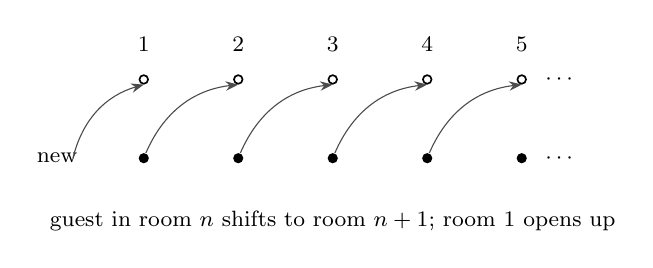
\begin{tikzpicture}[scale=1]
  \foreach \i in {1,...,5}{
    \node[opt] (r\i) at (\i*1.2,1) {};
    \node[font=\footnotesize] at (\i*1.2,1.45) {$\i$};
    \node[pt] (g\i) at (\i*1.2,0) {};
  }
  \node[font=\footnotesize] at (6.5,1) {$\cdots$};
  \node[font=\footnotesize] at (6.5,0) {$\cdots$};
  \foreach \i/\j in {1/2,2/3,3/4,4/5}{
    \draw[-{Stealth[length=1.6mm]},black!70] (g\i) to[bend left=30] (r\j.south);
  }
  \node[font=\footnotesize] at (0.1,0) {new};
  \draw[-{Stealth[length=1.6mm]},black!70] (0.3,0) to[bend left=30] (r1.south);
  \node[font=\footnotesize,align=center] at (3.6,-0.8)
    {guest in room $n$ shifts to room $n+1$; room $1$ opens up};
\end{tikzpicture}
\end{center}

\begin{wex}{The integers are countable, with an explicit formula}
Exhibit and verify a bijection $h:\N\to\Z$ in closed form.
\wrec Trigger: ``produce an explicit enumeration of $\Z$.'' Interleave nonnegatives and
negatives, then check injectivity and surjectivity by the method.
\wsol Define $h(n)=\tfrac n2$ if $n$ is even and $h(n)=-\tfrac{n-1}2$ if $n$ is odd. So
$h$ lists $0,1,-1,2,-2,3,-3,\dots$ as $n=1,2,3,4,5,6,7,\dots$. Surjective: an integer
$m>0$ is $h(2m)$, $m<0$ is $h(1-2m)$, and $0=h(1)$. Injective: even and odd $n$ produce
nonnegative and negative values respectively, so the two cases never collide, and within
each case $h$ is one-to-one. \emph{Check:} $h(6)=3$ and $h(7)=-3$; the inverse sends $3\mapsto
6$, $-3\mapsto 7$, recovering $n$. Hence $\Z\sim\N$ is denumerable.
\end{wex}

\begin{wex}{A countable union of countable sets, made concrete}
Show that $\Q\cap(0,1)$ is countable by listing it as a union of finite sets.
\wrec Trigger: ``show a set built from integers is countable'' --- organize as a countable
union of finite sets (Corollary~\ref{c:Z-Q-countable@c1}).
\wsol For each $q\ge2$ let $F_q=\set{p/q\st 1\le p<q,\ \gcd(p,q)=1}$, the fractions in
$(0,1)$ with denominator exactly $q$ in lowest terms. Each $F_q$ is \emph{finite} (at most
$q-1$ elements), and every rational in $(0,1)$ has a unique lowest-terms form, so
$\Q\cap(0,1)=\bigcup_{q\ge2}F_q$ is a countable union of finite sets, hence countable.
\emph{Check:} $F_2=\set{\tfrac12}$, $F_3=\set{\tfrac13,\tfrac23}$,
$F_4=\set{\tfrac14,\tfrac34}$ (not $\tfrac24$, already counted), $F_5=\set{\tfrac15,\tfrac25,
\tfrac35,\tfrac45}$ --- the Farey-style listing visits each rational exactly once.
\end{wex}

\begin{wex}{NON-example: the irrationals are NOT countable}
Deduce that the set of irrational numbers in $[0,1)$ is uncountable.
\wrec Trigger: a cardinality claim provable by ``a countable set cannot fill an uncountable
one.'' Use that $\R$ uncountable plus $\Q$ countable, via the union/closure theorems.
\wsol Write $[0,1)=(\Q\cap[0,1))\,\cup\,(I\cap[0,1))$ where $I$ is the irrationals. If
$I\cap[0,1)$ were countable, then $[0,1)$ would be a union of two countable sets
($\Q\cap[0,1)$ is countable as a subset of $\Q$), hence countable by
Corollary~\ref{c:Z-Q-countable@c1} --- contradicting Cantor's theorem
(Theorem~\ref{t:R-uncountable@c1}). So $I\cap[0,1)$ is uncountable. \emph{Check:} this is a
clean ``uncountable minus countable is uncountable'' instance: removing the countably many
rationals from an uncountable set cannot shrink it to countable, since otherwise the whole
would be a countable union.
\end{wex}

\begin{exers}{Exercises (Bartle \& Sherbert, \S1.3).}
\item Prove a nonempty set $T_1$ is finite iff there is a bijection from $T_1$ onto a finite
  set $T_2$.
\item Prove parts (b) and (c) of the uniqueness theorem $\N_m\sim\N_n\imp m=n$.
\item Let $S=\set{1,2}$, $T=\set{a,b,c}$. (a) How many injections $S\to T$ are there?
  (b) How many surjections $T\to S$?
\item Exhibit a bijection between $\N$ and the set of all odd integers greater than $13$.
\item Give an explicit formula for a bijection $f:\N\to\Z$.
\item Exhibit a bijection between $\N$ and a proper subset of itself.
\item Prove a set $T_1$ is denumerable iff there is a bijection from $T_1$ onto a
  denumerable set $T_2$.
\item Give an example of a countable collection of finite sets whose union is not finite.
\item Prove in detail that if $S$ and $T$ are denumerable, then $S\cup T$ is denumerable.
\item Using the diagonal counting of $\N\times\N$: (a) find the number assigned to the
  $6$th point down the $9$th diagonal; (b) if $h(m,3)=19$, find $m$.
\item Determine $\abs{\mathcal P(S)}$ for (a) $S=\set{1,2}$; (b) $S=\set{1,2,3}$;
  (c) $S=\set{1,2,3,4}$ (include $\es$ and $S$).
\item Use induction to prove that if $\abs S=n$ then $\abs{\mathcal P(S)}=2^n$.
\item Prove that the collection of all \emph{finite} subsets of $\N$ is countable.
\end{exers}

\begin{exers}{Exercises (Rudin, Ch.2 -- countability).}
\item Prove that the empty set is a subset of every set.
\item A complex number $z$ is \emph{algebraic} if there are integers $a_0,\dots,a_n$, not
  all zero, with $a_0z^n+a_1z^{n-1}+\cdots+a_n=0$. Prove the set of all algebraic numbers
  is countable. (Hint: for each $N$ there are finitely many equations with
  $n+\abs{a_0}+\abs{a_1}+\cdots+\abs{a_n}=N$.)
\item Prove that there exist real numbers that are not algebraic.
\item Is the set of all irrational real numbers countable? Justify.
\end{exers}

\begin{exers}{Additional exercises.}
\item Prove directly (no Schroeder--Bernstein) that $\N\sim\Z$ by giving a single formula
  for the bijection and its inverse.
\item Run the diagonal argument on \emph{binary} sequences: show the set $2^\N$ of all
  functions $\N\to\set{0,1}$ is uncountable, and explain the one subtlety (dyadic
  rationals with two expansions) that the digit choice $\set{4,5}$ avoided for decimals.
\item Prove $\mathcal P(\N)\sim\R$. (Map a subset $A\subseteq\N$ to the real with binary
  digits $\mathbf 1_A$; repair the double-counting with Schroeder--Bernstein.)
\item (Strict middle.) Show that for any sets, $A\hookrightarrow B$ and a surjection $B\to
  A$ together force $A\sim B$, citing the appropriate theorem.
\item Show the set of all \emph{eventually-zero} sequences of natural numbers is countable,
  but the set of \emph{all} sequences of naturals is uncountable.
\item Prove that a countable union of countable sets is countable, being explicit about
  where a choice of enumerations is used.
\item Give an example of a strictly increasing chain $A_1\subsetneq A_2\subsetneq\cdots$ of
  countable sets whose union is uncountable, or prove no such chain exists.
\item (Visual.) Reproduce the anti-diagonal enumeration figure for $\N\times\N$ and mark the
  positions $1$ through $10$; then read off $h(3,2)$ and verify it against the Cantor
  pairing formula $h(m,n)=\tfrac12(m+n-2)(m+n-1)+m$.
\item Prove there is no set of ``all sets'' (Cantor's theorem applied to a hypothetical
  universal set).
\end{exers}


% ================= Chapter 2: The Real and Complex Number Systems =================

\chapter{The Real and Complex Number Systems}

\section{Ordered Fields: Algebraic and Order Properties of \texorpdfstring{$\R$}{R}}
\subsection*{Fields and the field axioms}

The real numbers $\R$ are not built by listing properties at random: they are the unique
\emph{complete ordered field}. We unpack that phrase in three stages --- \emph{field}
(this section), \emph{ordered} (this section), and \emph{complete} (\S2.3). Everything
later in analysis rests on these axioms, so we state them once, precisely.

\begin{definition}\label{d:field@c2}
A \emph{field} is a set $\F$ with two operations, addition $+$ and multiplication
$\cdot$\,, satisfying:
\smallskip
\textbf{Addition (A).}
\textup{(A1)} $x+y\in\F$ and $x+y=y+x$;
\textup{(A2)} $(x+y)+z=x+(y+z)$;
\textup{(A3)} there is $0\in\F$ with $x+0=x$ for all $x$;
\textup{(A4)} each $x$ has $-x\in\F$ with $x+(-x)=0$.
\smallskip
\textbf{Multiplication (M).}
\textup{(M1)} $xy\in\F$ and $xy=yx$;
\textup{(M2)} $(xy)z=x(yz)$;
\textup{(M3)} there is $1\in\F$, $1\neq0$, with $1\cdot x=x$ for all $x$;
\textup{(M4)} each $x\neq0$ has $1/x\in\F$ with $x\cdot(1/x)=1$.
\smallskip
\textbf{Distributive law (D).} $x(y+z)=xy+xz$.
\end{definition}

The axioms come in two parallel packages, one for $+$ and one for $\cdot$, glued together
by (D). The phrase ``$1\neq0$'' rules out the degenerate one-element ``field.'' Rudin's
Definition~1.12 and B\&S's list 2.1.1 are identical to this; we follow Rudin's labels (A),
(M), (D) throughout. From these axioms alone, every familiar rule of algebra follows --- no
extra assumption is allowed.

\begin{proposition}[Cancellation and uniqueness, Rudin 1.14--1.16]\label{p:fieldfacts@c2}
In any field:
\textup{(a)} $x+y=x+z\imp y=z$; in particular $0$ and each $-x$ are unique.
\textup{(b)} $x\cdot0=0$.
\textup{(c)} if $x\neq0$ and $xy=xz$ then $y=z$; and $xy=0\imp x=0$ or $y=0$.
\textup{(d)} $-(-x)=x$, $(-x)y=-(xy)=x(-y)$, and $(-x)(-y)=xy$.
\end{proposition}

\begin{proof}
\textbf{(a)} Add $-x$ to both sides and use (A2),(A4),(A3):
$y=0+y=(-x+x)+y=-x+(x+y)=-x+(x+z)=z$. Uniqueness of $0$: if $0'$ also satisfies (A3) then
$0=0+0'=0'$. Uniqueness of $-x$: if $x+y=0=x+y'$ then $y=y'$ by cancellation.
\textbf{(b)} $x\cdot0+x\cdot0=x(0+0)=x\cdot0$, so by (a) (additive cancellation against
$x\cdot0$) we get $x\cdot0=0$.
\textbf{(c)} Multiply $xy=xz$ by $1/x$. If $xy=0$ and $x\neq0$ then
$y=(1/x)(xy)=(1/x)\cdot0=0$ by (b).
\textbf{(d)} $-(-x)=x$ because $x$ is the additive inverse of $-x$. And
$(-x)y+xy=(-x+x)y=0\cdot y=0$, so $(-x)y=-(xy)$; the rest is the same trick applied twice.
\end{proof}

\begin{remark}
Part (c) --- ``no zero divisors'' --- is what makes the quadratic-factoring trick legal:
$(x-1)(x+2)=0$ forces $x=1$ or $x=-2$. It fails in rings like $\Z/6$ ($2\cdot3=0$), so it
is genuinely a field fact, not a triviality.
\end{remark}

\subsection*{Ordered sets and ordered fields}

\begin{definition}[Order, Rudin 1.5]\label{d:order@c2}
An \emph{order} on a set $S$ is a relation $<$ such that
\textup{(i)} \emph{(trichotomy)} for $x,y\in S$ exactly one of $x<y$, $x=y$, $y<x$ holds;
\textup{(ii)} \emph{(transitivity)} $x<y$ and $y<z$ imply $x<z$.
We write $x\le y$ for ``$x<y$ or $x=y$''. An \emph{ordered set} is a set with an order.
\end{definition}

\begin{definition}[Ordered field, Rudin 1.17]\label{d:orderedfield@c2}
An \emph{ordered field} is a field $\F$ with an order $<$ compatible with the operations:
\textup{(O1)} $y<z\imp x+y<x+z$ for all $x$;
\textup{(O2)} $x>0$ and $y>0\imp xy>0$.
We call $x>0$ \emph{positive} and $x<0$ \emph{negative}.
\end{definition}

B\&S package the same content as the \emph{Order Properties} (2.1.5): there is a set $P$ of
``positive'' elements closed under $+$ and $\cdot$, with trichotomy ``$a\in P$, $a=0$, or
$-a\in P$.'' Setting $a<b\eqv b-a\in P$ recovers Definition~\ref{d:orderedfield@c2}; the two
formulations are interchangeable. The next theorem is the toolbox of inequality rules every
analyst uses without thinking.

\begin{theorem}[Order rules, Rudin 1.18 / B\&S 2.1.7]\label{t:orderrules@c2}
In an ordered field:
\textup{(a)} $x>0\eqv -x<0$;
\textup{(b)} $x>0$ and $y<z\imp xy<xz$; and $x<0$, $y<z\imp xy>xz$ \emph{(sign flips)};
\textup{(c)} $x\neq0\imp x^2>0$; in particular $1=1^2>0$;
\textup{(d)} $0<x<y\imp 0<1/y<1/x$.
\end{theorem}

\begin{proof}
\textbf{(a)} Add $-x$ to $x>0$ using (O1): $0=x+(-x)>0+(-x)=-x$.
\textbf{(b)} $y<z$ gives $z-y>0$ (add $-y$). If $x>0$, (O2) gives $x(z-y)>0$, i.e.\
$xz-xy>0$, i.e.\ $xy<xz$. If $x<0$ then $-x>0$ by (a), so $(-x)(z-y)>0$, i.e.\
$xy-xz>0$, i.e.\ $xz<xy$.
\textbf{(c)} If $x>0$, (O2) gives $x^2>0$. If $x<0$ then $-x>0$ and
$x^2=(-x)(-x)>0$ by Proposition~\ref{p:fieldfacts@c2}(d). Since $1\neq0$, $1=1\cdot1>0$.
\textbf{(d)} If $x>0$ then $1/x>0$ (else $1/x<0$ gives $1=x(1/x)<0$, contradicting (c)).
From $x<y$ multiply by the positive $\tfrac{1}{xy}$: $\tfrac1y<\tfrac1x$.
\end{proof}

\begin{pitfall}
The sign-flip in (b) is the single most common error in elementary analysis: multiplying or
dividing an inequality by a \emph{negative} quantity reverses it. ``$-2x<6$'' becomes
``$x>-3$,'' not ``$x<-3$.'' Likewise $a<b$ does \emph{not} give $1/a<1/b$ in general ---
only when $a,b$ have the same sign (Theorem~\ref{t:orderrules@c2}(d)). When you cannot pin the
sign of a factor, split into cases.
\end{pitfall}

\begin{theorem}[Squeeze-to-zero, B\&S 2.1.9]\label{t:squeeze0@c2}
If $a\in\R$ satisfies $0\le a<\eps$ for \emph{every} $\eps>0$, then $a=0$.
\end{theorem}

\begin{proof}
Suppose $a>0$. Take $\eps_0=\tfrac12 a$; then $\eps_0>0$, yet $a<\eps_0=\tfrac12a$ forces
$\tfrac12 a<0$, contradicting $a>0$. So $a=0$.
\end{proof}

This tiny theorem is the seed of every ``$\eps$-argument'': to prove two numbers are equal
you show their distance is below \emph{every} positive bound. We will reuse it constantly.

\begin{method}{Solving / proving a real inequality}
\textbf{Recognition trigger.} You must find all $x$ satisfying an inequality, or prove one
inequality from others.
\begin{enumerate}
\item \textbf{Move everything to one side}: rewrite as $(\,\cdot\,)>0$ or $(\,\cdot\,)<0$.
\item \textbf{Factor.} A product is positive iff its factors share a sign
  (Theorem~\ref{t:orderrules@c2}, B\&S 2.1.10): $pq>0\eqv(p>0,q>0)$ or $(p<0,q<0)$.
\item \textbf{Case-split} on the sign of each factor; intersect the resulting conditions.
\item For a \emph{rational} inequality $\tfrac{p}{q}>0$, the sign is that of $pq$ (never
  multiply across by $q$ of unknown sign).
\item To \emph{prove} an inequality, reduce it to a known nonnegative quantity --- usually
  a square $(\,\cdot\,)^2\ge0$ (Theorem~\ref{t:orderrules@c2}(c)).
\end{enumerate}
\end{method}

\begin{wex}{A linear inequality}
Find all $x$ with $2x+3\le 6$.
\wrec Linear; isolate $x$ but watch the divisor sign (here positive, so no flip).
\wsol $2x+3\le6\eqv 2x\le3\eqv x\le\tfrac32$. So the solution set is
$\set{x\in\R\st x\le\tfrac32}=(-\infty,\tfrac32]$. \emph{Check:} $x=\tfrac32$ gives $6\le6$;
$x=2$ gives $7\le6$, false, correctly excluded.
\end{wex}

\begin{wex}{A quadratic inequality by factoring}
Find all $x$ with $x^2+x>2$.
\wrec Quadratic; move to one side and factor, then split on factor signs.
\wsol $x^2+x-2>0\eqv(x-1)(x+2)>0$. The product is positive in two cases: (i) $x-1>0$ and
$x+2>0$, i.e.\ $x>1$; (ii) $x-1<0$ and $x+2<0$, i.e.\ $x<-2$. Hence the solution is
$(-\infty,-2)\cup(1,\infty)$. \emph{Check:} $x=0$ gives $0>2$, false, and $0$ lies in the
excluded middle $[-2,1]$. \checkmark
\end{wex}

\begin{wex}{A rational inequality --- do not cross-multiply blindly}
Find all $x$ with $\dfrac{2x+1}{x+2}<1$.
\wrec Rational; subtract $1$ and combine, then read the sign off the numerator times
denominator.
\wsol $\dfrac{2x+1}{x+2}-1<0\eqv\dfrac{x-1}{x+2}<0$. A quotient is negative iff numerator
and denominator have opposite signs: (i) $x-1<0$, $x+2>0$ gives $-2<x<1$; (ii) $x-1>0$,
$x+2<0$ is impossible. So the solution is $(-2,1)$. \emph{Check:} $x=0$ gives
$\tfrac12<1$ \checkmark; $x=-2$ is excluded (division by $0$); $x=2$ gives
$\tfrac53<1$ false. \checkmark
\end{wex}

\begin{wex}{The AM--GM inequality for two terms (B\&S 2.1.13)}
For $a,b\ge0$ prove $\sqrt{ab}\le\tfrac12(a+b)$, with equality iff $a=b$.
\wrec ``Prove an inequality'': reduce to a square $\ge0$.
\wsol For $a,b\ge0$, $(\sqrt a-\sqrt b)^2\ge0$ expands to $a-2\sqrt{ab}+b\ge0$, i.e.\
$\sqrt{ab}\le\tfrac12(a+b)$. Equality holds iff $(\sqrt a-\sqrt b)^2=0$ iff $\sqrt a=\sqrt
b$ iff $a=b$. \emph{Check:} $a=4,b=1$: $\sqrt4=2\le\tfrac52$. \checkmark\ (The general
$n$-term AM--GM, $(a_1\cdots a_n)^{1/n}\le\tfrac1n\sum a_i$, follows by induction or convexity.)
\end{wex}

\begin{wex}{Bernoulli's inequality (B\&S 2.1.13(c), Rudin uses it repeatedly)}
For $x>-1$ and $n\in\N$, prove $(1+x)^n\ge1+nx$.
\wrec Inequality indexed by $n$; induct, using $1+x>0$ to keep the direction.
\wsol Base $n=1$: equality. Step: assume $(1+x)^k\ge1+kx$. Since $1+x>0$ we may multiply:
$(1+x)^{k+1}\ge(1+kx)(1+x)=1+(k+1)x+kx^2\ge1+(k+1)x$, using $kx^2\ge0$. By induction it holds
for all $n$. \emph{Check:} $x=1,n=3$: $8\ge4$. \checkmark
\end{wex}

\subsection*{$\Q$ is an ordered field --- but a defective one}

The rationals $\Q$ satisfy \emph{every} axiom above: $\Q$ is an ordered field. So the field
and order axioms cannot, by themselves, capture $\R$. The defect is exposed by a single
missing number.

\begin{theorem}[No rational square root of $2$, Rudin 1.1 / B\&S 2.1.4]\label{t:sqrt2@c2}
There is no rational number $r$ with $r^2=2$.
\end{theorem}

\begin{proof}
Suppose $r=p/q$ in lowest terms (so $p,q$ are not both even) and $p^2=2q^2$. Then $p^2$ is
even, so $p$ is even (the square of an odd number is odd), say $p=2m$. Then
$4m^2=2q^2$, i.e.\ $q^2=2m^2$, so $q^2$ is even, so $q$ is even. But then $p$ and $q$ are
both even, contradicting ``lowest terms.'' Hence no such $r$ exists.
\end{proof}

\begin{remark}
Rudin sharpens this to a \emph{topological} gap: the set $A=\set{p\in\Q\st p>0,\ p^2<2}$ has
no largest element and $B=\set{p\in\Q\st p>0,\ p^2>2}$ no smallest, because the map
$p\mapsto p-\dfrac{p^2-2}{p+2}=\dfrac{2p+2}{p+2}$ pushes any $p\in A$ to a larger element of
$A$ and any $p\in B$ to a smaller element of $B$. So $\Q$ has a ``hole'' exactly where
$\sqrt2$ should be --- $A$ is bounded above in $\Q$ yet has no least upper bound \emph{in}
$\Q$. Repairing this hole is the completeness axiom of \S2.3.
\end{remark}

The same proof, with ``even'' replaced by ``divisible by $p$,'' shows $\sqrt{n}\notin\Q$
whenever $n$ is not a perfect square (Exercises). So the rationals are riddled with holes;
the reals fill every one.

\subsection*{Further worked examples}

\begin{wex}{Deriving a field identity from the axioms alone}
In any field, prove the binomial-style identity $(a+b)(a-b)=a^2-b^2$ and the cancellation
fact $a^2=b^2\imp a=b$ or $a=-b$.
\wrec ``Prove an algebraic law from the axioms'': use only distributivity (D),
commutativity, and Proposition~\ref{p:fieldfacts@c2}(d).
\wsol By (D) twice, $(a+b)(a-b)=a(a-b)+b(a-b)=a^2-ab+ba-b^2$. Commutativity (M1) gives
$ba=ab$, so $-ab+ba=0$ and $(a+b)(a-b)=a^2-b^2$. Now if $a^2=b^2$ then
$a^2-b^2=0$, i.e.\ $(a+b)(a-b)=0$; by the no-zero-divisor law
(Proposition~\ref{p:fieldfacts@c2}(c)) one factor vanishes, so $a=-b$ or $a=b$. \emph{Check:}
in $\R$, $a=3,b=-3$ have $a^2=b^2=9$ and indeed $a=-b$; the factoring
$(3+(-3))(3-(-3))=0\cdot6=0$. \checkmark
\end{wex}

\begin{wex}{NON-field: $\Z$ and $\Z/6$ fail axiom (M4)}
Show the integers $\Z$ are not a field, and that $\Z/6$ (integers mod $6$) fails even the
no-zero-divisor law.
\wrec ``Decide whether a structure is a field'': test the multiplicative-inverse axiom (M4)
and the cancellation consequence.
\wsol In $\Z$, the element $2\neq0$ has no integer multiplicative inverse: $2x=1$ has no
solution in $\Z$ (only $x=\tfrac12\notin\Z$), so (M4) fails and $\Z$ is a commutative ring
but not a field. In $\Z/6$, $2\cdot3=6\equiv0$ with $2\neq0$ and $3\neq0$, so $\Z/6$ has
\emph{zero divisors}, violating Proposition~\ref{p:fieldfacts@c2}(c); hence it is not a field
either (here $2$ has no inverse, since $2x\equiv1\pmod6$ is unsolvable as $2x$ is always
even). \emph{Check:} by contrast $\Z/5$ \emph{is} a field --- every nonzero residue has an
inverse ($2\cdot3=6\equiv1$, $4\cdot4=16\equiv1$), and $5$ being prime forbids zero
divisors. \checkmark
\end{wex}

\begin{wex}{An inequality with a parameter of unknown sign}
Find all real $x$ satisfying $\dfrac{1}{x}<x$.
\wrec Rational inequality where the denominator $x$ changes sign; never cross-multiply by
$x$ blindly --- move to one side and factor (Method above).
\wsol $\dfrac1x-x<0\eqv\dfrac{1-x^2}{x}<0\eqv\dfrac{(1-x)(1+x)}{x}<0$. The expression is a
ratio of the three linear factors $1-x,\ 1+x,\ x$, with sign changes at $x=-1,0,1$. Testing
one point in each region: $x=-2\to\tfrac{(3)(-1)}{-2}=\tfrac32>0$; $x=-\tfrac12\to
\tfrac{(3/2)(1/2)}{-1/2}<0$; $x=\tfrac12\to\tfrac{(1/2)(3/2)}{1/2}>0$; $x=2\to
\tfrac{(-1)(3)}{2}<0$. So the solution is $(-1,0)\cup(1,\infty)$. \emph{Check:}
$x=-\tfrac12$: $\tfrac{1}{-1/2}=-2<-\tfrac12$ \checkmark; $x=2$: $\tfrac12<2$ \checkmark;
$x=\tfrac12$ excluded since $2\not<\tfrac12$. \checkmark
\end{wex}

\begin{exers}{Exercises (Bartle \& Sherbert, \S2.1).}
\item If $a,b\in\R$, prove: (a) $a+b=0\imp b=-a$; (b) $-(-a)=a$; (c) $(-1)a=-a$;
  (d) $(-1)(-1)=1$.
\item Prove that if $a,b\in\R$: (a) $-(a+b)=(-a)+(-b)$; (b) $(-a)\cdot(-b)=a\cdot b$;
  (c) $1/(-a)=-(1/a)$ ($a\neq0$); (d) $-(a/b)=(-a)/b$ ($b\neq0$).
\item Solve, justifying each step by an order or field property: (a) $2x+5=8$;
  (b) $x^2=2x$; (c) $x^2-1=3$; (d) $(x-1)(x+2)=0$.
\item If $a\in\R$ satisfies $a\cdot a=a$, prove that $a=0$ or $a=1$.
\item If $a\neq0$ and $b\neq0$, show $1/(ab)=(1/a)(1/b)$.
\item Use the argument proving no rational has square $2$ to show there is no rational $s$
  with $s^2=6$.
\item Modify that proof to show there is no rational $t$ with $t^2=3$.
\item (a) Show that if $x,y$ are rational then $x+y$ and $xy$ are rational.
  (b) Prove that if $x$ is rational and $y$ is irrational, then $x+y$ is irrational, and if
  also $x\neq0$ then $xy$ is irrational.
\item Let $K=\set{s+t\sqrt2\st s,t\in\Q}$. Show (a) if $x_1,x_2\in K$ then
  $x_1+x_2\in K$ and $x_1x_2\in K$; (b) if $x\neq0$ and $x\in K$ then $1/x\in K$. (Thus
  $K$ is a subfield of $\R$ with $\Q\subsetneq K\subsetneq\R$.)
\item (a) If $a<b$ and $c\le d$, prove $a+c<b+d$. (b) If $0<a<b$ and $0\le c\le d$, prove
  $0\le ac\le bd$.
\item (a) Show that if $a>0$ then $1/a>0$ and $1/(1/a)=a$. (b) Show that if $a<b$ then
  $a<\tfrac12(a+b)<b$.
\item Let $a,b,c,d$ satisfy $0<a<b$ and $c<d<0$. Give an example where $ac<bd$ and one
  where $bd<ac$.
\item If $a,b\in\R$, show $a^2+b^2=0$ iff $a=0$ and $b=0$.
\item If $0\le a<b$, show $a^2\le ab<b^2$. Show by example that $a^2<ab<b^2$ need not hold.
\item If $0<a<b$, show (a) $a<\sqrt{ab}<b$ and (b) $1/b<1/a$.
\item Find all $x\in\R$ satisfying: (a) $x^2>3x+4$; (b) $1<x^2<4$; (c) $1/x<x$;
  (d) $1/x<x^2$.
\item Prove the strengthened form: if $a\in\R$ and $0\le a\le\eps$ for every $\eps>0$,
  then $a=0$.
\item Let $a,b\in\R$ and suppose $a\le b+\eps$ for every $\eps>0$. Show $a\le b$.
\item Prove $\bigl(\tfrac12(a+b)\bigr)^2\le\tfrac12(a^2+b^2)$ for all $a,b$, with equality
  iff $a=b$.
\item (a) If $0<c<1$, show $0<c^2<c<1$. (b) If $c>1$, show $1<c<c^2$.
\item (a) Prove there is no $n\in\N$ with $0<n<1$ (use Well-Ordering). (b) Prove no natural
  number is both even and odd.
\item (a) If $c>1$, show $c^n\ge c$ for all $n\in\N$ and $c^n>c$ for $n>1$. (b) If $0<c<1$,
  show $c^n\le c$ for all $n$ and $c^n<c$ for $n>1$.
\item If $a,b>0$ and $n\in\N$, show $a<b$ iff $a^n<b^n$. (Hint: induction.)
\item (a) If $c>1$ and $m,n\in\N$, show $c^m>c^n$ iff $m>n$. (b) If $0<c<1$ and $m,n\in\N$,
  show $c^m<c^n$ iff $m>n$.
\item Assuming roots exist, show that if $c>1$ then $c^{1/m}<c^{1/n}$ iff $m>n$.
\item Use induction to show that if $a\in\R$ and $m,n\in\N$, then $a^{m+n}=a^m a^n$ and
  $(a^m)^n=a^{mn}$.
\end{exers}

\begin{exers}{Additional exercises.}
\item (Field warm-up.) From the axioms alone prove $-(a+b)=-a-b$ and, for $a,b\neq0$,
  $(ab)\inv=a\inv b\inv$. Identify which axiom each step uses.
\item Solve and write the answer as a union of intervals: (a) $3x-1\ge 2x+4$;
  (b) $\dfrac{x-3}{x+1}\ge0$; (c) $x^2\le 5x-6$.
\item Prove that for all $a,b\in\R$, $a^2+b^2\ge2ab$, with equality iff $a=b$. Deduce
  $\dfrac ab+\dfrac ba\ge2$ for $a,b>0$.
\item (Disprove.) A student claims ``$a<b\imp a^2<b^2$ for all reals.'' Give a
  counterexample, then state and prove the correct hypothesis under which it holds.
\item Show that if $n$ is a positive integer that is not a perfect square, then $\sqrt n$ is
  irrational. (Adapt the $\sqrt2$ proof using prime factorization.)
\item Prove that between any two distinct rationals there is another rational, and conclude
  $\Q$ has no ``next'' element above a given one.
\item (Ordered field that is not $\R$.) Verify in detail that $\Q(\sqrt2)=\set{s+t\sqrt2\st
  s,t\in\Q}$ is an ordered field strictly between $\Q$ and $\R$, and exhibit a subset of it
  that is bounded above with no supremum \emph{in} $\Q(\sqrt2)$.
\item For $a,b,c,d>0$ prove the Cauchy--Schwarz-type bound
  $(ac+bd)^2\le(a^2+b^2)(c^2+d^2)$ directly, and find when equality holds.
\item (Diagram.) On a single number line, shade the solution sets of $2x+3\le6$ and
  $x^2+x>2$, and mark where they overlap. Describe the overlap as a union of intervals.
\end{exers}


\section{Absolute Value and the Real Line}
\subsection*{Absolute value as distance}

\begin{definition}[Absolute value, B\&S 2.2.1]\label{d:abs@c2}
For $a\in\R$,
\[
  \abs a=\begin{cases}a,& a\ge0,\\ -a,& a<0,\end{cases}
\]
so $\abs a\ge0$ always, and $\abs a=0\eqv a=0$. The \emph{distance} between $a,b\in\R$ is
$\dist(a,b)=\abs{a-b}$.
\end{definition}

The whole point of $\abs{\cdot}$ is that it turns the algebraic line $\R$ into a
\emph{metric} space: $\abs{a-b}$ measures how far apart $a$ and $b$ sit. Reading every
inequality below as a statement about distance is the fastest route to fluency.

\begin{center}
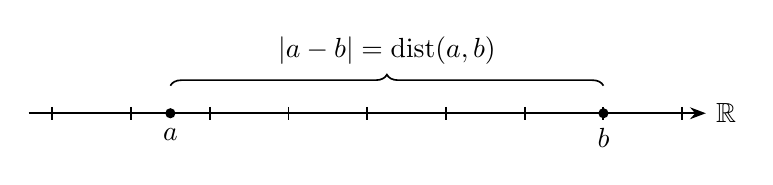
\begin{tikzpicture}[scale=1.0]
  \draw[numln] (-4.3,0)--(4.3,0) node[right]{$\R$};
  \foreach \x in {-4,...,4}{\draw[tick] (\x,0.08)--(\x,-0.08);}
  \node[pt,label={below:$a$}] at (-2.5,0) {};
  \node[pt,label={below:$b$}] at (3,0) {};
  \draw[brc] (-2.5,0.35)--(3,0.35) node[midway,above=4pt]{$\abs{a-b}=\dist(a,b)$};
\end{tikzpicture}
\end{center}

\begin{theorem}[Basic properties, B\&S 2.2.2--2.2.3]\label{t:absprops@c2}
For all $a,b\in\R$:
\textup{(a)} $\abs{ab}=\abs a\,\abs b$;
\textup{(b)} $\abs a^2=a^2$ and $\abs a=\sqrt{a^2}$;
\textup{(c)} for $c\ge0$, $\abs a\le c\eqv -c\le a\le c$; in particular $-\abs a\le a\le\abs a$;
\textup{(d)} \emph{(Triangle Inequality)} $\abs{a+b}\le\abs a+\abs b$.
\end{theorem}

\begin{proof}
\textbf{(a)} Check the four sign cases, or use (b): $\abs{ab}=\sqrt{(ab)^2}=\sqrt{a^2}\sqrt{b^2}=\abs
a\abs b$.
\textbf{(b)} $\abs a^2=a^2$ since $(\pm a)^2=a^2$; taking the nonnegative root gives
$\abs a=\sqrt{a^2}$.
\textbf{(c)} If $\abs a\le c$: when $a\ge0$, $a=\abs a\le c$ and $a\ge0\ge -c$; when
$a<0$, $-a=\abs a\le c$ so $a\ge-c$, and $a<0\le c$. Conversely $-c\le a\le c$ bounds both
$a$ and $-a$ by $c$, so $\abs a\le c$.
\textbf{(d)} By (c), $-\abs a\le a\le\abs a$ and $-\abs b\le b\le\abs b$; adding,
$-(\abs a+\abs b)\le a+b\le\abs a+\abs b$, which by (c) again says $\abs{a+b}\le\abs a+\abs b$.
\end{proof}

\begin{corollary}[Triangle variants, B\&S 2.2.4]\label{c:trianglevariants@c2}
For all $a,b,c\in\R$:
\textup{(i)} $\bigl|\,\abs a-\abs b\,\bigr|\le\abs{a-b}$ \emph{(reverse triangle inequality)};
\textup{(ii)} $\abs{a-b}\le\abs a+\abs b$;
\textup{(iii)} $\abs{a-c}\le\abs{a-b}+\abs{b-c}$ \emph{(distance is subadditive)}.
\end{corollary}

\begin{proof}
\textup{(i)} $\abs a=\abs{(a-b)+b}\le\abs{a-b}+\abs b$ gives $\abs a-\abs b\le\abs{a-b}$;
swapping $a,b$ gives $\abs b-\abs a\le\abs{a-b}$; together $\bigl|\abs a-\abs
b\bigr|\le\abs{a-b}$. \textup{(ii)} apply (d) to $a$ and $-b$. \textup{(iii)} apply (d) to
$a-b$ and $b-c$, since $(a-b)+(b-c)=a-c$.
\end{proof}

\begin{pitfall}
$\abs{a+b}=\abs a+\abs b$ is \emph{not} an identity --- it holds exactly when $a,b$ have the
same sign (i.e.\ $ab\ge0$). In general only $\le$. The reverse inequality (i) is the one
beginners forget; it is the workhorse for showing ``if $a$ is close to $b$ then $\abs a$ is
close to $\abs b$,'' used in every continuity proof for the modulus.
\end{pitfall}

\subsection*{The V-graph and $\eps$-neighborhoods}

The graph of $y=\abs{x-a}$ is a ``V'' with its vertex at $(a,0)$. The solution set of
$\abs{x-a}<\eps$ is the slice of the line where the V dips below height $\eps$ --- an open
interval of radius $\eps$ centered at $a$.

\begin{center}
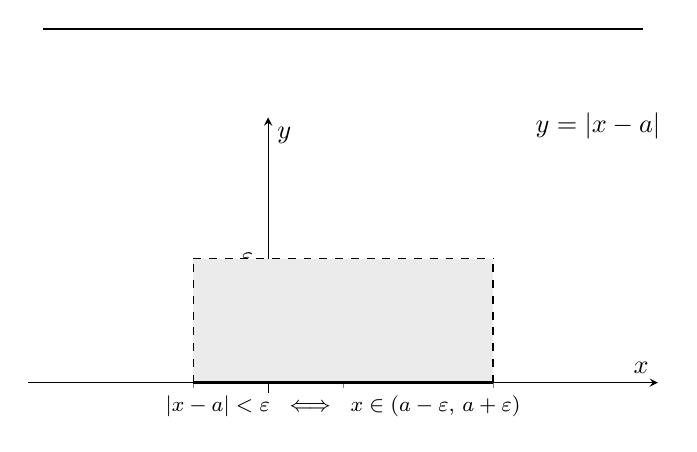
\begin{tikzpicture}[scale=0.95]
  \begin{axis}[
    width=10cm,height=5.6cm,
    axis lines=middle,
    xtick={-1,1,3}, xticklabels={$a-\eps$,$a$,$a+\eps$},
    ytick={1.4}, yticklabels={$\eps$},
    xmin=-3.2,xmax=5.2,ymin=-0.4,ymax=3.0,
    xlabel={$x$}, ylabel={$y$}, clip=false,
  ]
    % V graph y=|x-1|
    \addplot[curve,domain=-3:5,samples=2]{abs(x-1)};
    \node at (4.4,2.9) {$y=\abs{x-a}$};
    % eps band
    \addplot[band,draw=none,domain=-1:3,samples=2]
      {1.4} \closedcycle;
    \draw[dashed] (axis cs:-1,0)--(axis cs:-1,1.4);
    \draw[dashed] (axis cs:3,0)--(axis cs:3,1.4);
    \draw[dashed] (axis cs:-1,1.4)--(axis cs:3,1.4);
    % the interval on the x-axis
    \draw[line width=1.4pt] (axis cs:-1,0)--(axis cs:3,0);
    \node[fill=white,inner sep=1pt] at (axis cs:1,-0.27)
      {\footnotesize $\abs{x-a}<\eps\ \eqv\ x\in(a-\eps,\,a+\eps)$};
  \end{axis}
\end{tikzpicture}
\end{center}

\begin{definition}[$\eps$-neighborhood, B\&S 2.2.7]\label{d:nbhd@c2}
For $a\in\R$ and $\eps>0$, the \emph{$\eps$-neighborhood} of $a$ is
\[
  V_\eps(a)=\set{x\in\R\st \abs{x-a}<\eps}=(a-\eps,\,a+\eps).
\]
``$x$ is within $\eps$ of $a$'' means exactly $x\in V_\eps(a)$.
\end{definition}

\begin{center}
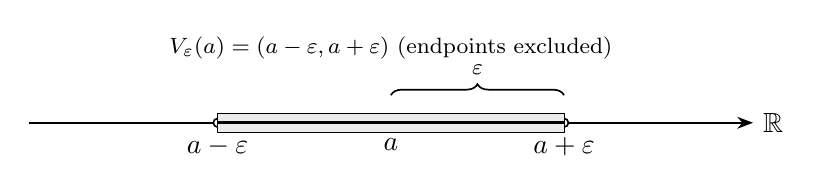
\begin{tikzpicture}[scale=1.0]
  \draw[numln] (-4.6,0)--(4.6,0) node[right]{$\R$};
  \node[pt,label={below:$a$}] at (0,0) {};
  \node[opt,label={below:$a-\eps$}] at (-2.2,0) {};
  \node[opt,label={below:$a+\eps$}] at (2.2,0) {};
  \draw[band] (-2.2,-0.12) rectangle (2.2,0.12);
  \draw[line width=1.2pt] (-2.2,0)--(2.2,0);
  \draw[brc] (0,0.35)--(2.2,0.35) node[midway,above=4pt]{\footnotesize $\eps$};
  \node[font=\footnotesize] at (0,0.95) {$V_\eps(a)=(a-\eps,a+\eps)$ (endpoints excluded)};
\end{tikzpicture}
\end{center}

The key fact, the bridge to limits, is that a point pinned inside \emph{every} neighborhood
of $a$ must equal $a$ --- the neighborhood reformulation of Theorem~\ref{t:squeeze0@c2}.

\begin{proposition}[B\&S 2.2.8]\label{p:nbhdpin@c2}
Let $a\in\R$. If $x\in V_\eps(a)$ for every $\eps>0$, then $x=a$.
\end{proposition}

\begin{proof}
The hypothesis says $0\le\abs{x-a}<\eps$ for all $\eps>0$; by Theorem~\ref{t:squeeze0@c2},
$\abs{x-a}=0$, hence $x=a$.
\end{proof}

\begin{method}{Solving an absolute-value (in)equality}
\textbf{Recognition trigger.} The unknown sits inside $\abs{\cdot}$.
\begin{enumerate}
\item \textbf{Single modulus.} Use $\abs{u}<c\eqv -c<u<c$ and $\abs{u}>c\eqv u>c$ or
  $u<-c$ (Theorem~\ref{t:absprops@c2}(c)). Solve the resulting double / split inequality.
\item \textbf{Two or more moduli} (e.g.\ $\abs{x-1}+\abs{x+2}$): break $\R$ at the
  \emph{breakpoints} where each inside changes sign, and on each subinterval drop the bars
  with the correct sign, then solve and intersect with that subinterval.
\item \textbf{Equations} $\abs u=\abs v$: square both sides, $u^2=v^2\eqv(u-v)(u+v)=0$.
\item \textbf{Sanity check} by plugging a test point from each region.
\end{enumerate}
\end{method}

\begin{wex}{A neighborhood inequality}
Solve $\abs{4x-5}\le 13$.
\wrec Single modulus $\le c$; unfold to a double inequality.
\wsol $-13\le4x-5\le13\eqv -8\le4x\le18\eqv -2\le x\le\tfrac92$. Solution
$[-2,\tfrac92]$. \emph{Check:} $x=-2$ gives $\abs{-13}=13$ \checkmark; $x=5$ gives
$\abs{15}=15>13$, correctly excluded.
\end{wex}

\begin{wex}{Two moduli by breakpoints}
Solve $\abs{x+1}+\abs{x-2}=7$.
\wrec Sum of two moduli; split at the breakpoints $x=-1$ and $x=2$.
\wsol \emph{Region $x<-1$:} both insides negative, $-(x+1)-(x-2)=-2x+1=7\imp x=-3$ (valid,
$-3<-1$). \emph{Region $-1\le x\le2$:} $(x+1)-(x-2)=3\neq7$, no solution. \emph{Region
$x>2$:} $(x+1)+(x-2)=2x-1=7\imp x=4$ (valid, $4>2$). Solution $\set{-3,4}$. \emph{Check:}
$x=-3$: $\abs{-2}+\abs{-5}=2+5=7$ \checkmark; $x=4$: $5+2=7$ \checkmark. (Geometrically: the
points whose distances to $-1$ and $2$ sum to $7$, on a segment of length $3$.)
\end{wex}

\begin{wex}{An equation with moduli on both sides}
Solve $2x-1=\abs{x-5}$.
\wrec One side a modulus; either case-split or square (squaring may add spurious roots, so
verify).
\wsol The left side must be $\ge0$, so $x\ge\tfrac12$. \emph{Case $x\ge5$:}
$2x-1=x-5\imp x=-4$, rejected. \emph{Case $x<5$:} $2x-1=-(x-5)=5-x\imp 3x=6\imp x=2$, and
$\tfrac12\le2<5$, valid. Solution $x=2$. \emph{Check:} $2(2)-1=3=\abs{2-5}=3$. \checkmark
\end{wex}

\begin{wex}{NON-example: $\abs{a+b}=\abs a+\abs b$ can fail}
Show the triangle inequality is generally \emph{strict}, and characterize equality.
\wrec ``Disprove an identity / find the equality case.''
\wsol Take $a=3$, $b=-5$: $\abs{a+b}=\abs{-2}=2$ while $\abs a+\abs b=8$, so $2<8$ ---
strict. Equality $\abs{a+b}=\abs a+\abs b$ holds iff $ab\ge0$ (same sign or a zero):
squaring, $\abs{a+b}=\abs a+\abs b\eqv(a+b)^2=a^2+2\abs a\abs b+b^2\eqv ab=\abs{ab}\eqv ab\ge0$.
\emph{Check:} $a=3,b=5$ (same sign): $8=8$. \checkmark
\end{wex}

\begin{wex}{The midpoint/triangle picture for three points}
For $x\le z$, show $\abs{x-y}+\abs{y-z}=\abs{x-z}$ holds iff $x\le y\le z$.
\wrec Distances along a line add iff the middle point is between.
\wsol If $x\le y\le z$ then $x-y\le0$ and $y-z\le0$, so
$\abs{x-y}+\abs{y-z}=(y-x)+(z-y)=z-x=\abs{x-z}$. Conversely, if $y<x$ or $y>z$, then $y$
lies outside $[x,z]$ and the path $x\to y\to z$ backtracks, making the left side strictly
larger (e.g.\ $y>z$: $\abs{x-y}+\abs{y-z}=(y-x)+(y-z)>z-x$). \emph{Check:} $x=1,y=2,z=5$:
$1+3=4=\abs{1-5}$ \checkmark; $x=1,y=6,z=5$: $5+1=6>4$. \checkmark
\end{wex}

\subsection*{Further worked examples}

\begin{wex}{An $\eps$-neighborhood described as a set of inequalities}
Describe $V_{1/3}(2)$ explicitly, and decide whether $\tfrac74$ and $\tfrac52$ belong to it.
\wrec Trigger: ``unpack a neighborhood.'' Apply Definition~\ref{d:nbhd@c2}:
$V_\eps(a)=(a-\eps,a+\eps)$.
\wsol With $a=2,\ \eps=\tfrac13$: $V_{1/3}(2)=\bigl(2-\tfrac13,\ 2+\tfrac13\bigr)
=\bigl(\tfrac53,\tfrac73\bigr)$. Membership is the test $\abs{x-2}<\tfrac13$. For
$x=\tfrac74$: $\abs{\tfrac74-2}=\tfrac14<\tfrac13$, so $\tfrac74\in V_{1/3}(2)$. For
$x=\tfrac52$: $\abs{\tfrac52-2}=\tfrac12>\tfrac13$, so $\tfrac52\notin V_{1/3}(2)$.
\emph{Check:} $\tfrac53\approx1.667$, $\tfrac73\approx2.333$; indeed $1.75$ is inside and
$2.5$ is outside that interval. \checkmark
\end{wex}

\begin{wex}{A bound for a fraction via the triangle inequality (B\&S 2.2.6 style)}
If $\abs{x-2}<1$, find an explicit constant $M$ with $\left|\dfrac{x^2+3}{x-5}\right|\le M$
for all such $x$.
\wrec Trigger: ``bound a rational expression on a neighborhood.'' Estimate numerator from
above and denominator from below using $\abs{x-2}<1$ and the (reverse) triangle inequality.
\wsol From $\abs{x-2}<1$ we get $1<x<3$. \emph{Numerator:} $\abs{x}<3$, so
$\abs{x^2+3}\le\abs{x}^2+3<9+3=12$. \emph{Denominator:} $x<3$ gives $x-5<-2$, so
$\abs{x-5}=5-x>2$, hence $\dfrac{1}{\abs{x-5}}<\tfrac12$. Therefore
$\left|\dfrac{x^2+3}{x-5}\right|=\dfrac{\abs{x^2+3}}{\abs{x-5}}<\dfrac{12}{2}=6$, so $M=6$
works. \emph{Check:} at $x=3^-$ the expression nears $\tfrac{12}{-2}=-6$ in size; at the
midpoint $x=2$, $\bigl|\tfrac{7}{-3}\bigr|=\tfrac73\approx2.33\le6$. \checkmark
\end{wex}

\begin{exers}{Exercises (Bartle \& Sherbert, \S2.2).}
\item If $a,b\in\R$ and $b\neq0$, show (a) $\abs a=\sqrt{a^2}$; (b) $\abs{a/b}=\abs a/\abs b$.
\item If $a,b\in\R$, show $\abs{a+b}=\abs a+\abs b$ iff $ab\ge0$.
\item If $x,y,z\in\R$ with $x\le z$, show $x\le y\le z$ iff $\abs{x-y}+\abs{y-z}=\abs{x-z}$.
  Interpret geometrically.
\item Show $\abs{x-a}<\eps$ iff $a-\eps<x<a+\eps$.
\item If $a<x<b$ and $a<y<b$, show $\abs{x-y}<b-a$. Interpret geometrically.
\item Find all $x\in\R$ satisfying: (a) $\abs{4x-5}\le13$; (b) $\abs{x^2-1}\le3$.
\item Find all $x\in\R$ satisfying $\abs{x+1}+\abs{x-2}=7$.
\item Find all $x$ satisfying: (a) $x+1=\abs{2x-1}$; (b) $2x-1=\abs{x-5}$.
\item Find all $x$ satisfying, and sketch graphs: (a) $\abs{x-2}\le x+1$; (b) $3\abs x-2\le x$.
\item Find all $x\in\R$ satisfying: (a) $\abs{x-1}>\abs{x+1}$; (b) $\abs x+\abs{x+1}<2$.
\item Sketch the graph of $y=\abs x-\abs{x-1}$.
\item Find all $x\in\R$ with $4<\abs{x+2}+\abs{x-1}<5$.
\item Find all $x\in\R$ satisfying both $\abs{2x-3}<5$ and $\abs{x+1}>2$ simultaneously.
\item Determine and sketch the set of $(x,y)\in\R\times\R$ with: (a) $\abs x=\abs y$;
  (b) $\abs x+\abs y=1$; (c) $\abs{xy}=2$; (d) $\abs x-\abs y=2$.
\item Determine and sketch the set of $(x,y)\in\R\times\R$ with: (a) $\abs x\le\abs y$;
  (b) $\abs x+\abs y\le1$; (c) $\abs{xy}\le2$; (d) $\abs x-\abs y\le2$.
\item Let $\eps>0$, $\delta>0$, $a\in\R$. Show $V_\eps(a)\cap V_\delta(a)$ and
  $V_\eps(a)\cup V_\delta(a)$ are $\gamma$-neighborhoods of $a$ for suitable $\gamma$.
\item Show that if $a\neq b$ there exist $\eps$-neighborhoods $U$ of $a$ and $V$ of $b$ with
  $U\cap V=\es$.
\item Show that if $a,b\in\R$: (a) $\max\set{a,b}=\tfrac12(a+b+\abs{a-b})$ and
  $\min\set{a,b}=\tfrac12(a+b-\abs{a-b})$; (b) $\min\set{a,b,c}=\min\set{\min\set{a,b},c}$.
\item Show that the ``middle'' number is
  $\operatorname{mid}\set{a,b,c}=\min\set{\max\set{a,b},\max\set{b,c},\max\set{c,a}}$.
\end{exers}

\begin{exers}{Additional exercises.}
\item Solve $\abs{x-3}+\abs{x+2}\le9$ and write the answer as a closed interval.
\item Prove the general triangle inequality $\abs{a_1+\cdots+a_n}\le\abs{a_1}+\cdots+\abs{a_n}$
  by induction on $n$.
\item Prove $\abs{\,\abs a-\abs b\,}\le\abs{a-b}$ both from the triangle inequality and
  directly by squaring; compare the two arguments.
\item Show $V_\eps(a)\subseteq V_\delta(b)$ holds iff $\abs{a-b}+\eps\le\delta$. Draw the
  number-line picture that makes this obvious.
\item (Disprove.) Is $\abs{x-y}\le\abs x-\abs y$ ever a valid inequality for all $x,y$?
  Either prove it or give a counterexample and state the correct inequality.
\item For which $a$ does the equation $\abs{x-1}+\abs{x+1}=a$ have (i) no solution,
  (ii) infinitely many solutions, (iii) exactly two solutions? Justify with the V-graph.
\item (Diagram.) Sketch $y=\abs{x-1}$ and the horizontal line $y=2$ on the same axes, shade
  the region $\abs{x-1}<2$ on the $x$-axis, and read off the neighborhood $V_2(1)$.
\item Prove that $\max\set{a,b}+\min\set{a,b}=a+b$ and
  $\max\set{a,b}-\min\set{a,b}=\abs{a-b}$, and use these to re-derive the formulas of B\&S
  Exercise 2.2.18(a).
\item Show that the function $d(x,y)=\abs{x-y}$ satisfies $d(x,y)\ge0$ with equality iff
  $x=y$, $d(x,y)=d(y,x)$, and $d(x,z)\le d(x,y)+d(y,z)$. (These are the metric axioms for
  $\R$.)
\end{exers}


\section{The Completeness Property: Suprema and Infima}
\subsection*{Upper bounds, lower bounds, and the supremum}

\begin{definition}[Bounds, B\&S 2.3.1 / Rudin 1.7]\label{d:bounds@c2}
Let $S\subseteq\R$ be nonempty. A number $u$ is an \emph{upper bound} of $S$ if $s\le u$ for
all $s\in S$; then $S$ is \emph{bounded above}. A number $w$ is a \emph{lower bound} if
$w\le s$ for all $s\in S$; then $S$ is \emph{bounded below}. $S$ is \emph{bounded} if both.
\end{definition}

If $u$ is an upper bound then so is every larger number, so upper bounds come in an infinite
upward ray. The decisive object is the \emph{least} one.

\begin{definition}[Supremum and infimum, B\&S 2.3.2 / Rudin 1.8]\label{d:sup@c2}
Let $S\subseteq\R$ be nonempty and bounded above. A number $\alpha$ is the \emph{supremum}
(least upper bound) of $S$, written $\alpha=\sup S$, if
\textup{(i)} $\alpha$ is an upper bound of $S$, and
\textup{(ii)} if $u$ is any upper bound of $S$, then $\alpha\le u$.
Dually, for $S$ bounded below, the \emph{infimum} (greatest lower bound) $\inf S$ is the
greatest lower bound. When $\sup S\in S$ it is the \emph{maximum} $\max S$; similarly
$\min S$.
\end{definition}

\begin{center}
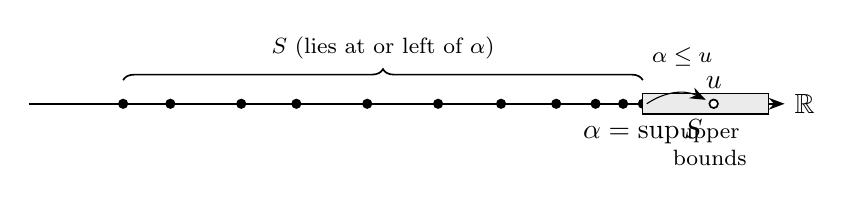
\begin{tikzpicture}[scale=1.0]
  \draw[numln] (-4.8,0)--(4.8,0) node[right]{$\R$};
  % set S = scattered points up to alpha
  \foreach \x in {-3.6,-3.0,-2.1,-1.4,-0.5,0.4,1.2,1.9,2.4,2.75}{
    \node[pt] at (\x,0) {};}
  \node[pt,label={below:$\alpha=\sup S$}] at (3,0) {};
  % the set bracket
  \draw[brc] (-3.6,0.3)--(3,0.3) node[midway,above=4pt]{\footnotesize $S$ (lies at or left of $\alpha$)};
  % upper bounds ray
  \draw[band] (3,-0.13) rectangle (4.6,0.13);
  \node[font=\footnotesize,align=center] at (3.85,-0.55) {upper\\bounds};
  % an arbitrary upper bound u to the right
  \node[opt,label={above:$u$}] at (3.9,0) {};
  \draw[-{Stealth[length=2mm]}] (3.05,0.0) to[bend left=30] (3.8,0.05);
  \node[font=\footnotesize] at (3.5,0.6) {$\alpha\le u$};
\end{tikzpicture}\captionof{figure}{$\sup S$ is the leftmost point of the shaded ray of upper bounds: it sits at
the right edge of $S$ and is $\le$ every other upper bound.}
\end{center}

The supremum need \emph{not} belong to $S$. For $S=(0,1)$, $\sup S=1\notin S$; for
$S=(0,1]$, $\sup S=1\in S=\max S$. ``Least upper bound'' and ``maximum'' coincide only when
the bound is attained.

\begin{proposition}[Two-condition test, B\&S 2.3.4]\label{p:suptest@c2}
Let $S$ be nonempty and bounded above, $\alpha$ an upper bound of $S$. Then
$\alpha=\sup S$ iff
\[
  \text{for every }\eps>0\text{ there exists }s\in S\text{ with } s>\alpha-\eps.
\]
\end{proposition}

\begin{proof}
($\Rightarrow$) If $\alpha=\sup S$ and $\eps>0$, then $\alpha-\eps<\alpha$ is \emph{not} an
upper bound (else it would beat the least one), so some $s\in S$ exceeds $\alpha-\eps$.
($\Leftarrow$) Suppose $\alpha$ is an upper bound and the $\eps$-condition holds. Let $u$ be
any upper bound; if $u<\alpha$, set $\eps=\alpha-u>0$ and get $s\in S$ with
$s>\alpha-\eps=u$, contradicting that $u$ bounds $S$. So $\alpha\le u$, and $\alpha$ is the
least upper bound.
\end{proof}

This is \emph{the} working characterization: it splits ``$\alpha=\sup S$'' into the easy
half (it bounds $S$) and the sharp half (nothing smaller bounds $S$, witnessed by elements
of $S$ creeping up to $\alpha$).

\begin{method}{Proving $\alpha=\sup S$}
\textbf{Recognition trigger.} You claim a specific number $\alpha$ is the least upper bound
of a described set.
\begin{enumerate}
\item \textbf{Upper bound.} Show $s\le\alpha$ for every $s\in S$ (often a direct algebraic
  estimate).
\item \textbf{Approachability.} Fix an arbitrary $\eps>0$ and \emph{exhibit} an element
  $s\in S$ with $s>\alpha-\eps$ --- usually by solving the defining condition for an index
  large enough. This is the half that pins $\alpha$ as the \emph{least} bound.
\item For $\inf$, mirror everything: $\alpha\le s$ for all $s$, and for each $\eps$ some
  $s<\alpha+\eps$.
\end{enumerate}
\end{method}

\begin{wex}{$\sup$ of a sequence set}
Let $S=\set{1-\tfrac1n\st n\in\N}=\set{0,\tfrac12,\tfrac23,\tfrac34,\dots}$. Show
$\sup S=1$ and $\inf S=0=\min S$.
\wrec Direct two-condition test.
\wsol \emph{Upper bound:} $1-\tfrac1n<1$ for all $n$, so $1$ bounds $S$.
\emph{Approachability:} given $\eps>0$, pick $n$ with $\tfrac1n<\eps$ (Archimedean,
\S2.4); then $1-\tfrac1n>1-\eps$. By Proposition~\ref{p:suptest@c2}, $\sup S=1$. Note $1\notin
S$, so there is no maximum. \emph{Infimum:} the smallest term is $n=1$, $1-1=0\in S$, and
$0\le1-\tfrac1n$ for all $n$, so $\inf S=0=\min S$. \emph{Check:} terms
$0,\tfrac12,\tfrac23,\dots$ climb toward but never reach $1$. \checkmark
\end{wex}

\subsection*{The Completeness Axiom}

The rationals satisfy Definitions~\ref{d:bounds@c2}--\ref{d:sup@c2} but, as \S2.1 showed, a
bounded set like $\set{p\in\Q\st p^2<2}$ has \emph{no} supremum in $\Q$. The defining
property of $\R$ is that this never happens.

\begin{theorem}[Completeness / Least-Upper-Bound Property, B\&S 2.3.6 / Rudin 1.19]\label{t:completeness@c2}
Every nonempty subset of $\R$ that is bounded above has a supremum in $\R$. Equivalently,
every nonempty subset bounded below has an infimum in $\R$.
\end{theorem}

We take this as an \emph{axiom} characterizing $\R$ (Rudin instead \emph{constructs} $\R$
from $\Q$ by Dedekind cuts and proves it as a theorem; see the remark below). The
equivalence of the sup- and inf-forms is itself a clean application of the reflection
$x\mapsto -x$.

\begin{proposition}[$\inf$ via $\sup$, Rudin 1.11 / B\&S Exercise 2.3.6]\label{p:infsup@c2}
If $S$ is nonempty and bounded below, then $-S=\set{-s\st s\in S}$ is bounded above and
\[
  \inf S=-\sup(-S).
\]
\end{proposition}

\begin{proof}
$w\le s$ for all $s\in S$ iff $-s\le -w$ for all $s$, i.e.\ $-w$ is an upper bound of $-S$.
So lower bounds of $S$ correspond, under negation, to upper bounds of $-S$, reversing order.
The \emph{greatest} lower bound of $S$ thus corresponds to the \emph{least} upper bound of
$-S$: $\inf S=-\sup(-S)$. Existence of $\sup(-S)$ (Completeness) gives existence of
$\inf S$, proving the two forms of Theorem~\ref{t:completeness@c2} equivalent.
\end{proof}

\begin{center}
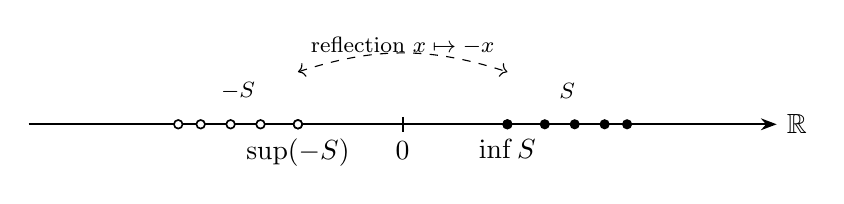
\begin{tikzpicture}[scale=0.95]
  \draw[numln] (-5,0)--(5,0) node[right]{$\R$};
  \draw[tick] (0,0.1)--(0,-0.1) node[below]{$0$};
  % S on the right
  \foreach \x in {1.4,1.9,2.3,2.7,3.0}{\node[pt] at (\x,0) {};}
  \node[font=\footnotesize] at (2.2,0.45) {$S$};
  \node[pt,label={below:$\inf S$}] at (1.4,0) {};
  % -S on the left (mirror)
  \foreach \x in {-1.4,-1.9,-2.3,-2.7,-3.0}{\node[opt] at (\x,0) {};}
  \node[font=\footnotesize] at (-2.2,0.45) {$-S$};
  \node[opt,label={below:$\sup(-S)$}] at (-1.4,0) {};
  \draw[<->,dashed] (-1.4,0.7) to[bend left=18] (1.4,0.7);
  \node[font=\footnotesize] at (0,1.05) {reflection $x\mapsto-x$};
\end{tikzpicture}
\end{center}

\begin{remark}[Dedekind cuts, Rudin 1.19 appendix]
Rudin builds $\R$ as the set of \emph{cuts}: a cut $\alpha\subseteq\Q$ is a nonempty proper
downward-closed subset with no greatest element (e.g.\ $\sqrt2$ \emph{is} the cut
$\set{p\in\Q\st p<0\ \text{or}\ p^2<2}$). Order is inclusion $\alpha<\beta\eqv\alpha\subsetneq\beta$, and
the supremum of a bounded family of cuts is simply their \emph{union} --- which is again a
cut, giving Theorem~\ref{t:completeness@c2} for free. Addition is setwise; multiplication is
fiddly on signs. The construction yields a complete ordered field, and one proves any two
such are isomorphic, so ``the'' real numbers are well-defined. We will not need the cuts
again; the axiom suffices.
\end{remark}

\subsection*{First consequences of completeness}

\begin{wex}{$\sup(a+S)=a+\sup S$ (B\&S 2.4.1)}
For $S$ bounded above and $a\in\R$, let $a+S=\set{a+s\st s\in S}$. Show
$\sup(a+S)=a+\sup S$.
\wrec ``Compute a sup of a shifted set'' --- prove the two halves of the test.
\wsol Let $u=\sup S$. Then $s\le u$ gives $a+s\le a+u$, so $a+u$ is an upper bound of
$a+S$; hence $\sup(a+S)\le a+u$. Conversely, given $\eps>0$ choose $s\in S$ with
$s>u-\eps$; then $a+s>(a+u)-\eps$, so by Proposition~\ref{p:suptest@c2} no number below $a+u$
bounds $a+S$, giving $\sup(a+S)\ge a+u$. Thus $\sup(a+S)=a+u=a+\sup S$. \emph{Check:}
$S=[0,1]$, $a=3$: $a+S=[3,4]$, $\sup=4=3+1$. \checkmark
\end{wex}

\begin{wex}{Monotonicity of $\sup$ and $\inf$ under inclusion}
If $\es\neq S_0\subseteq S$ with $S$ bounded, show
$\inf S\le\inf S_0\le\sup S_0\le\sup S$.
\wrec Inclusion comparison; an upper bound of the big set bounds the small one.
\wsol $\sup S$ is an upper bound of $S\supseteq S_0$, hence of $S_0$, so $\sup
S_0\le\sup S$ (least upper bound is $\le$ any upper bound). Symmetrically $\inf S\le\inf
S_0$. And $\inf S_0\le\sup S_0$ since any element of $S_0$ lies between them (or because
$\inf S_0\le s\le\sup S_0$ for any chosen $s\in S_0\neq\es$). \emph{Check:}
$S_0=\set{2}\subseteq S=[1,3]$: $1\le2\le2\le3$. \checkmark
\end{wex}

\begin{pitfall}
$\sup S$ is not the same as $\max S$. A bounded \emph{open} set has a supremum but no
maximum: $\sup(0,1)=1$ exists, yet $(0,1)$ has no greatest element. ``Find the maximum''
can have answer ``none'' while ``find the supremum'' always has an answer (in $\R$). Reserve
$\max/\min$ for when the bound is actually attained.
\end{pitfall}

\begin{pitfall}
A common slip: ``$u$ is an upper bound and $u\in S$, therefore $u=\sup S$.'' The
implication is true (B\&S Exercise 2.3.7) --- if an upper bound lies in the set it is the
maximum, hence the sup --- but the converse fails, and the hypothesis $u\in S$ is essential.
For $S=[0,1)$, $u=1$ is an upper bound \emph{not} in $S$ and is still the sup, while $u=0.9\in
S$ is in $S$ but is \emph{not} an upper bound. Always verify both ``bounds'' and ``least''.
\end{pitfall}

\subsection*{Further worked examples}

\begin{wex}{$\sup$ and $\inf$ of a finite and a half-open set}
Find $\sup,\inf,\max,\min$ (when they exist) for
$A=\set{-2,0,\tfrac12,3}$ and $B=\set{x\in\R\st 0\le x<4}$.
\wrec ``Read off the extremes.'' For a finite set the sup/inf are the largest/smallest
elements; for an interval, test whether each endpoint is attained
(Definition~\ref{d:sup@c2}).
\wsol For $A$: it is finite, so $\sup A=\max A=3$ and $\inf A=\min A=-2$, both attained. For
$B=[0,4)$: $0\in B$ is a lower bound and lies in $B$, so $\inf B=\min B=0$. And $4$ is an
upper bound; given any $\eps>0$, $4-\tfrac\eps2<4$ lies in $B$ and exceeds $4-\eps$, so by
Proposition~\ref{p:suptest@c2} $\sup B=4$ --- but $4\notin B$, so $\max B$ does \emph{not}
exist. \emph{Check:} every $x\in B$ satisfies $x<4$, yet no number below $4$ bounds $B$
(e.g.\ $3.9\in B$ beats $3.99-\eps$ choices), confirming $4$ is least. \checkmark
\end{wex}

\begin{wex}{The supremum of $\set{n/(n+1)}$}
Let $S=\set{\dfrac{n}{n+1}\st n\in\N}=\set{\tfrac12,\tfrac23,\tfrac34,\dots}$. Show
$\sup S=1$ and $\inf S=\tfrac12=\min S$.
\wrec ``Sup of an increasing sequence set'': bound by $1$, then approach via the
Archimedean property (Method, two-condition test).
\wsol Write $\dfrac{n}{n+1}=1-\dfrac{1}{n+1}<1$, so $1$ is an upper bound. Given $\eps>0$,
choose (Archimedean, \S2.4) $n$ with $\dfrac1{n+1}<\eps$; then $\dfrac{n}{n+1}>1-\eps$, so
by Proposition~\ref{p:suptest@c2}, $\sup S=1$ (never attained, no max). The sequence is
increasing, so its least term is at $n=1$: $\inf S=\min S=\tfrac12$. \emph{Check:}
$\tfrac12,\tfrac23\approx0.667,\tfrac34=0.75,\dots$ climb toward $1$; the first term
$\tfrac12$ is the smallest. \checkmark
\end{wex}

\begin{wex}{NON-example: a bounded subset of $\Q$ with no supremum \emph{in} $\Q$}
Exhibit a nonempty subset of $\Q$ that is bounded above but has no least upper bound inside
$\Q$, contrasting with Completeness in $\R$.
\wrec ``Show completeness can fail in $\Q$'': reuse the $\sqrt2$-gap of \S2.1.
\wsol Let $T=\set{r\in\Q\st r>0,\ r^2<2}$. It is nonempty ($1\in T$) and bounded above in
$\Q$ (e.g.\ by $2$, since $r\ge2\imp r^2\ge4>2$). In $\R$ its supremum is $\sqrt2$
(Theorem~\ref{t:sqrt2exists@c2}-style), but $\sqrt2\notin\Q$ (Theorem~\ref{t:sqrt2@c2}). Any
rational upper bound $u$ of $T$ has $u^2>2$, and the map $u\mapsto\dfrac{2u+2}{u+2}$ produces
a \emph{smaller} rational upper bound (its square exceeds $2$ too), so there is no
\emph{least} rational upper bound. Hence $\sup T$ fails to exist in $\Q$. \emph{Check:} the
rational bounds $1.5,1.42,1.415,\dots$ decrease forever toward $1.4142\ldots=\sqrt2$, never
reaching a least rational one. \checkmark\ This is exactly the defect Completeness
(Theorem~\ref{t:completeness@c2}) cures in $\R$.
\end{wex}

\begin{exers}{Exercises (Rudin, Ch.1 -- order and completeness).}
\item Prove Proposition 1.15 (the elementary arithmetic-of-fractions / inverse rules in an
  ordered field, e.g.\ if $0<x<y$ then $0<1/y<1/x$).
\item Let $E$ be a nonempty subset of an ordered set; suppose $\alpha$ is a lower bound of
  $E$ and $\beta$ is an upper bound of $E$. Prove $\alpha\le\beta$.
\item Let $A$ be a nonempty set of reals bounded below, and let $-A=\set{-x\st x\in A}$.
  Prove $\inf A=-\sup(-A)$.
\item (Dedekind cuts, with reference to the Appendix.) Suppose property (III) --- ``a cut
  has no largest element'' --- is omitted from the definition of a cut, keeping the same
  order and addition. Show the resulting ordered set still has the least-upper-bound
  property, that addition satisfies axioms (A1)--(A4) (with a slightly different zero), but
  that (A5) fails.
\end{exers}

\begin{exers}{Exercises (Bartle \& Sherbert, \S2.3).}
\item Let $S_1=\set{x\in\R\st x\ge0}$. Show $S_1$ has lower bounds but no upper bounds, and
  $\inf S_1=0$.
\item Let $S_2=\set{x\in\R\st x>0}$. Does $S_2$ have lower bounds? upper bounds? Does
  $\inf S_2$ exist? $\sup S_2$? Prove your answers.
\item Let $S_3=\set{1/n\st n\in\N}$. Show $\sup S_3=1$ and $\inf S_3\ge0$. (The Archimedean
  Property gives $\inf S_3=0$.)
\item Let $S_4=\set{1-(-1)^n/n\st n\in\N}$. Find $\inf S_4$ and $\sup S_4$.
\item Find $\inf$ and $\sup$, if they exist, of each set: (a) $A=\set{x\st 2x+5>0}$;
  (b) $B=\set{x\st x+2\ge x^2}$; (c) $C=\set{x\st x<1/x}$; (d) $D=\set{x\st x^2-2x-5<0}$.
\item Let $S\subseteq\R$ be nonempty and bounded below. Prove $\inf S=-\sup\set{-s\st s\in S}$.
\item If a set $S\subseteq\R$ contains one of its upper bounds, show that this upper bound
  is $\sup S$.
\item Let $S\subseteq\R$ be nonempty. Show $u$ is an upper bound of $S$ iff $t\in\R$ and
  $t>u$ imply $t\notin S$.
\item Let $S\subseteq\R$ be nonempty. Show that if $u=\sup S$, then for every $n\in\N$ the
  number $u-1/n$ is not an upper bound of $S$, while $u+1/n$ is an upper bound.
\item If $A,B$ are bounded subsets of $\R$, show $A\cup B$ is bounded and
  $\sup(A\cup B)=\max\set{\sup A,\sup B}$.
\item Let $S$ be bounded in $\R$ and $S_0\neq\es$ a subset of $S$. Show
  $\inf S\le\inf S_0\le\sup S_0\le\sup S$.
\item Let $S\subseteq\R$ with $s=\sup S\in S$. If $u\notin S$, show
  $\sup(S\cup\set u)=\max\set{s,u}$.
\item Show that a nonempty finite set $S\subseteq\R$ contains its supremum. (Hint:
  induction and the preceding exercise.)
\item Let $S$ be bounded below. Prove a lower bound $w$ of $S$ is $\inf S$ iff for every
  $\eps>0$ there is $t\in S$ with $t<w+\eps$.
\end{exers}

\begin{exers}{Additional exercises.}
\item For each set, decide whether $\sup$, $\inf$, $\max$, $\min$ exist and find them:
  (a) $\set{(-1)^n(1-1/n)\st n\in\N}$; (b) $\set{n/(n+1)\st n\in\N}$;
  (c) $\set{(-1)^n/n\st n\in\N}$.
\item Prove directly from the definition that $\sup S$, when it exists, is unique.
\item Let $A,B$ be nonempty bounded sets with $a\le b$ for all $a\in A$, $b\in B$. Prove
  $\sup A\le\inf B$. Give an example with $\sup A=\inf B$ where the sets are disjoint.
\item (Two-condition drill.) Prove $\sup\set{x\in\Q\st x^2<2}=\sqrt2$ as a subset of $\R$,
  using the characterization of the supremum.
\item Let $S$ be nonempty and bounded above with $\alpha=\sup S$. Show that for every
  $\eps>0$ the interval $(\alpha-\eps,\alpha]$ contains at least one point of $S$, and
  illustrate with a number-line diagram.
\item (Disprove.) Is it true that $\sup(A\cap B)=\min\set{\sup A,\sup B}$ for all bounded
  $A,B$? Prove or give a counterexample.
\item Prove that a nonempty set $S\subseteq\Z$ that is bounded above has a maximum. (Use the
  Archimedean property and Well-Ordering.)
\item (Diagram.) Draw a set $S$ of five marked points on a number line, its supremum, and
  shade the ray of upper bounds; then mark a point $\alpha-\eps$ and the witness $s\in S$
  guaranteed by the two-condition test.
\item Let $S$ be bounded above and define $u^* = \sup S$. Prove $u^*$ is the unique real
  with the property: $u^*$ bounds $S$, but $u^*-\eps$ does not, for every $\eps>0$.
\end{exers}


\section{Applications of the Supremum}
\subsection*{The Archimedean Property}

Completeness has teeth. Its first payoff is that $\N$ is not bounded above in $\R$ --- there
are no ``infinitely large'' reals --- and dually no positive real is ``infinitely small.''

\begin{theorem}[Archimedean Property, Rudin 1.20 / B\&S 2.4.3--2.4.5]\label{t:arch@c2}
\textup{(a)} For every $x\in\R$ there is $n\in\N$ with $n>x$ (so $\N$ is unbounded above).
\textup{(b)} For every $\eps>0$ there is $n\in\N$ with $\tfrac1n<\eps$.
\textup{(c)} For every $x>0$ there is $n\in\N$ with $n-1\le x<n$.
\end{theorem}

\begin{proof}
\textbf{(a)} If not, $\N$ would be bounded above; by Completeness it would have a supremum
$\alpha=\sup\N$. Then $\alpha-1$ is not an upper bound, so some $m\in\N$ has $m>\alpha-1$,
giving $m+1>\alpha$ with $m+1\in\N$ --- contradicting that $\alpha$ bounds $\N$. So $\N$ is
unbounded, and any $x$ is exceeded by some $n$.
\textbf{(b)} Apply (a) to $x=1/\eps$: some $n>1/\eps$, hence $1/n<\eps$.
\textbf{(c)} The set $\set{m\in\N\st m>x}$ is nonempty by (a); by Well-Ordering it has a
least element $n$, and then $n-1\le x<n$.
\end{proof}

\begin{center}
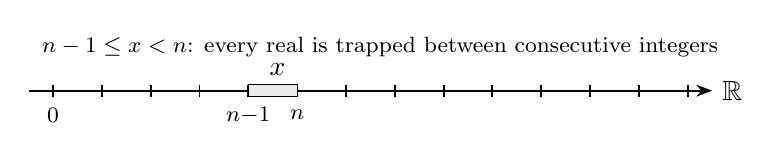
\begin{tikzpicture}[scale=0.62]
  \draw[numln] (-0.5,0)--(13.5,0) node[right]{$\R$};
  \foreach \x in {0,...,13}{\draw[tick] (\x,0.12)--(\x,-0.12);}
  \foreach \x/\l in {0/0,4/n{-}1,5/n}{\node[font=\footnotesize] at (\x,-0.5){$\l$};}
  \node[pt,label={above:$x$}] at (4.6,0) {};
  \draw[band] (4,-0.12) rectangle (5,0.12);
  \node[font=\footnotesize] at (6.7,0.9){$n-1\le x<n$: every real is trapped between
    consecutive integers};
\end{tikzpicture}
\end{center}

\begin{corollary}[$\inf\set{1/n}=0$, B\&S 2.4.4]\label{c:inf1n@c2}
$\inf\set{\tfrac1n\st n\in\N}=0$.
\end{corollary}

\begin{proof}
$0$ is a lower bound ($\tfrac1n>0$). If $w>0$ were a larger lower bound, Archimedes
(b) gives $n$ with $\tfrac1n<w$, contradicting that $w\le\tfrac1n$ for all $n$. So $0$ is
the greatest lower bound.
\end{proof}

\subsection*{Density of $\Q$ (and of the irrationals)}

The rationals, though only countable, sit \emph{everywhere}: between any two reals lies a
rational. Then so does an irrational.

\begin{theorem}[Density of $\Q$ in $\R$, Rudin 1.20(b) / B\&S 2.4.8]\label{t:densityQ@c2}
If $x,y\in\R$ with $x<y$, there is a rational $r$ with $x<r<y$.
\end{theorem}

\begin{proof}
Since $y-x>0$, Archimedes gives $n\in\N$ with $\tfrac1n<y-x$, i.e.\ $ny-nx>1$, so the open
interval $(nx,ny)$ has length $>1$ and must contain an integer $m$ (let $m$ be the least
integer $>nx$; then $m\le nx+1<ny$). Thus $nx<m<ny$, and dividing by $n>0$ gives
$x<\tfrac mn<y$. Take $r=\tfrac mn$.
\end{proof}

\begin{center}
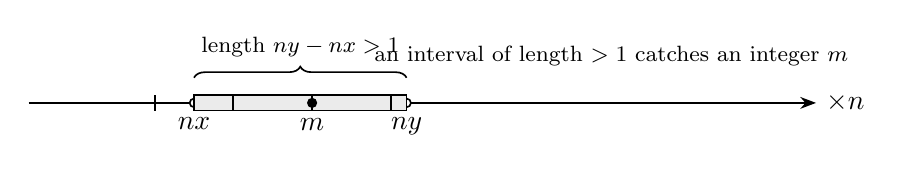
\begin{tikzpicture}[scale=1.0]
  \draw[numln] (-0.6,0)--(9.4,0) node[right]{$\times n$};
  \node[opt,label={below:$nx$}] at (1.5,0) {};
  \node[opt,label={below:$ny$}] at (4.2,0) {};
  \draw[band] (1.5,-0.1) rectangle (4.2,0.1);
  \draw[brc] (1.5,0.32)--(4.2,0.32) node[midway,above=4pt]{\footnotesize length $ny-nx>1$};
  \node[pt,label={below:$m$}] at (3,0) {};
  \foreach \x in {1,2,3,4}{\draw[tick] (\x,0.1)--(\x,-0.1);}
  \node[font=\footnotesize] at (6.8,0.6) {an interval of length $>1$ catches an integer $m$};
\end{tikzpicture}
\end{center}

\begin{corollary}[Density of irrationals]\label{c:densityirr@c2}
Between any two reals $x<y$ there is also an \emph{irrational}.
\end{corollary}

\begin{proof}
Apply Theorem~\ref{t:densityQ@c2} to $x/\sqrt2<y/\sqrt2$ to get a rational $r\neq0$ with
$x/\sqrt2<r<y/\sqrt2$; then $r\sqrt2$ is irrational (a nonzero rational times the irrational
$\sqrt2$) and $x<r\sqrt2<y$.
\end{proof}

\subsection*{Existence and uniqueness of $n$th roots}

The flagship use of completeness: it manufactures the roots that $\Q$ was missing. We prove
the existence of $\sqrt2$ in full --- the argument is the template for every nth root.

\begin{theorem}[Existence of $\sqrt2$, Rudin 1.21 / B\&S 2.4.7]\label{t:sqrt2exists@c2}
There is a unique real $y>0$ with $y^2=2$.
\end{theorem}

\begin{proof}
Let $S=\set{s\in\R\st s>0,\ s^2<2}$. It is nonempty ($1\in S$) and bounded above ($2$ is a
bound, since $s\ge2\imp s^2\ge4>2$). By Completeness, $y=\sup S$ exists, and $y\ge1>0$. We
rule out $y^2<2$ and $y^2>2$ by perturbing $y$.

\emph{If $y^2<2$:} choose $h$ with $0<h<1$ and $h<\dfrac{2-y^2}{2y+1}$. Then
$(y+h)^2=y^2+h(2y+h)<y^2+h(2y+1)<y^2+(2-y^2)=2$, so $y+h\in S$ --- contradicting that $y$ is
an \emph{upper} bound of $S$.

\emph{If $y^2>2$:} choose $k=\dfrac{y^2-2}{2y}>0$. Then for any $s\ge y-k$ with $s>0$,
$(y-k)^2=y^2-2yk+k^2>y^2-2yk=2$, so every $s\in S$ satisfies $s<y-k$ (else $s^2\ge(y-k)^2>2$);
thus $y-k$ is a smaller upper bound, contradicting $y=\sup S$.

By trichotomy $y^2=2$. \emph{Uniqueness:} if $0<y_1<y_2$ then $y_1^2<y_2^2$
(Theorem~\ref{t:orderrules@c2}), so at most one positive root exists.
\end{proof}

\begin{remark}
Replacing $2$ by any $a>0$ and the exponent $2$ by $n$ gives, verbatim in spirit, Rudin's
Theorem~1.21: \emph{every} real $a>0$ has a unique positive $n$th root $a^{1/n}$. The
perturbation estimates use $(y+h)^n-y^n<h\cdot n(y+1)^{n-1}$ in place of the quadratic
bound. Completeness is doing all the work --- $\Q$ fails precisely because $\sup S$ would
land outside it.
\end{remark}

\begin{wex}{Existence of $\sqrt3$ by the same machine}
Show there is $y>0$ with $y^2=3$ (B\&S Exercise 2.4.15).
\wrec ``Produce a root'': run the $\sup$-of-$\set{s^2<a}$ argument with $a=3$.
\wsol Let $S=\set{s>0\st s^2<3}$; nonempty ($1\in S$), bounded above by $2$ ($s\ge2\imp
s^2\ge4>3$). Put $y=\sup S$. If $y^2<3$, pick $0<h<1$ with $h<\tfrac{3-y^2}{2y+1}$; then
$(y+h)^2<3$ contradicts upper-bound. If $y^2>3$, pick $k=\tfrac{y^2-3}{2y}$; then $y-k$ is a
smaller upper bound. So $y^2=3$. \emph{Check:} $1.7^2=2.89<3<3.24=1.8^2$, so $y\in(1.7,1.8)$
as expected. \checkmark
\end{wex}

\begin{wex}{$\sup$ and $\inf$ of $\set{\tfrac1n-\tfrac1m}$ (B\&S 2.4.2)}
Find $\inf S$ and $\sup S$ for $S=\set{\tfrac1n-\tfrac1m\st n,m\in\N}$.
\wrec Two free indices; push one to make the expression large, the other to make it small.
\wsol Each term lies in $(-1,1)$: $\tfrac1n\le1$ and $-\tfrac1m\ge-1$, with strict unless an
index is $1$. \emph{Sup:} fix $n=1$, let $m\to\infty$: $1-\tfrac1m\to1$, and $1-\tfrac1m<1$,
so $\sup S=1$ (approached, never attained), by Proposition~\ref{p:suptest@c2} with
Corollary~\ref{c:inf1n@c2}. \emph{Inf:} fix $m=1$, let $n\to\infty$: $\tfrac1n-1\to-1$ from
above, so $\inf S=-1$. \emph{Check:} no term equals $\pm1$, so neither bound is in $S$;
$\tfrac11-\tfrac12=\tfrac12\in S$ sits comfortably inside $(-1,1)$. \checkmark
\end{wex}

\begin{wex}{$\sup(A+B)=\sup A+\sup B$ (B\&S 2.4.7)}
For nonempty bounded $A,B$, with $A+B=\set{a+b\st a\in A,b\in B}$, prove
$\sup(A+B)=\sup A+\sup B$.
\wrec Sum of two sets; bound each factor, then approach with both at once.
\wsol Let $\alpha=\sup A,\ \beta=\sup B$. For $a\in A,b\in B$: $a+b\le\alpha+\beta$, so
$\alpha+\beta$ bounds $A+B$. Given $\eps>0$, choose $a>\alpha-\tfrac\eps2$ and
$b>\beta-\tfrac\eps2$; then $a+b>(\alpha+\beta)-\eps$. By the two-condition test
$\sup(A+B)=\alpha+\beta$. \emph{Check:} $A=B=[0,1]$: $A+B=[0,2]$, $\sup=2=1+1$. \checkmark
\end{wex}

\begin{pitfall}
The $\sup$-of-a-product or $\sup$-of-an-$\inf$ identities are subtler than the sum case. In
general only $\sup_x\inf_y h(x,y)\le\inf_y\sup_x h(x,y)$ (a one-sided min--max inequality,
B\&S 2.4.11), and equality can fail. Never assume you may freely swap $\sup$ and $\inf$ ---
the order matters. Likewise $\sup(AB)\neq\sup A\cdot\sup B$ once negative numbers appear,
since multiplying by a negative reverses bounds.
\end{pitfall}

\subsection*{Further worked examples}

\begin{wex}{Trapping a real between integers (the floor)}
Use the Archimedean property to locate $\floor{x}$ for $x=\tfrac{47}{6}$ and for
$x=-\tfrac{7}{4}$, the unique integer $n$ with $n\le x<n+1$.
\wrec Trigger: ``find the integer part.'' Theorem~\ref{t:arch@c2}(c) guarantees a unique such
$n$; compute it by comparing with consecutive integers.
\wsol For $x=\tfrac{47}{6}=7.8\overline{3}$: $7\le7.83\ldots<8$, so $\floor{x}=7$. For
$x=-\tfrac74=-1.75$: the integer below is $-2$, since $-2\le-1.75<-1$, so $\floor{x}=-2$
(\emph{not} $-1$ --- the floor rounds \emph{down}). \emph{Check:} $7\cdot6=42\le47<48=8\cdot6$
confirms the first; $-2\le-1.75<-1$ the second. \checkmark
\end{wex}

\begin{wex}{A specific rational and irrational in a tiny interval}
Exhibit a rational and an irrational strictly between $\sqrt2$ and $\sqrt2+\tfrac1{100}$.
\wrec ``Density in action'' (Theorem~\ref{t:densityQ@c2}, Corollary~\ref{c:densityirr@c2}): find
a fraction with small enough denominator, then add an irrational nudge.
\wsol Since $\sqrt2=1.41421\ldots$, the interval is $(1.41421\ldots,\ 1.42421\ldots)$. The
rational $r=1.415=\tfrac{283}{200}$ satisfies $1.41421<1.415<1.42421$, so $r$ works (indeed
$r^2=2.002225>2$ yet $r<\sqrt2+0.01$). For an irrational, take
$\xi=\sqrt2+\tfrac{1}{200}=1.41421\ldots+0.005=1.41921\ldots$; it is irrational (rational
plus irrational) and lies in the interval. \emph{Check:} $1.41421<1.415<1.41921<1.42421$,
all four inside $(\sqrt2,\sqrt2+0.01)$. \checkmark
\end{wex}

\begin{exers}{Exercises (Rudin, Ch.1 -- roots, exponents, irrationals).}
\item If $r\neq0$ is rational and $x$ is irrational, prove that $r+x$ and $rx$ are
  irrational.
\item Prove that there is no rational number whose square is $12$.
\item Fix $b>1$. (a) If $m,n,p,q\in\Z$ with $n,q>0$ and $r=m/n=p/q$, prove
  $(b^m)^{1/n}=(b^p)^{1/q}$, so $b^r$ is well-defined. (b) Prove $b^{r+s}=b^r b^s$ for
  rational $r,s$. (c) For real $x$, let $B(x)=\set{b^t\st t\in\Q,\ t\le x}$; prove
  $b^r=\sup B(r)$ for rational $r$, so $b^x=\sup B(x)$ is well-defined for all real $x$.
  (d) Prove $b^{x+y}=b^x b^y$ for all real $x,y$.
\item Fix $b>1$, $y>0$. Prove there is a unique real $x$ with $b^x=y$ (the logarithm of $y$
  to base $b$), via: (a) $b^n-1\ge n(b-1)$ for $n\in\N$; (b) hence $b-1\ge n(b^{1/n}-1)$;
  (c) if $t>1$ and $n>(b-1)/(t-1)$ then $b^{1/n}<t$; (d) if $b^w<y$ then $b^{w+1/n}<y$ for
  large $n$; (e) if $b^w>y$ then $b^{w-1/n}>y$ for large $n$; (f) let $A=\set{w\st b^w<y}$
  and show $x=\sup A$ satisfies $b^x=y$; (g) prove this $x$ is unique.
\end{exers}

\begin{exers}{Exercises (Bartle \& Sherbert, \S2.4).}
\item Show $\sup\set{1-1/n\st n\in\N}=1$.
\item If $S=\set{1/n-1/m\st n,m\in\N}$, find $\inf S$ and $\sup S$.
\item Let $S\subseteq\R$ be nonempty. Prove that if $u\in\R$ satisfies (i) for every
  $n\in\N$, $u-1/n$ is not an upper bound of $S$, and (ii) for every $n\in\N$, $u+1/n$ is
  an upper bound of $S$, then $u=\sup S$.
\item Let $S$ be nonempty and bounded. (a) For $a>0$ and $aS=\set{as\st s\in S}$, prove
  $\inf(aS)=a\inf S$ and $\sup(aS)=a\sup S$. (b) For $b<0$ and $bS=\set{bs\st s\in S}$,
  prove $\inf(bS)=b\sup S$ and $\sup(bS)=b\inf S$.
\item Let $S$ be a set of nonnegative reals bounded above and $T=\set{x^2\st x\in S}$.
  Prove if $u=\sup S$ then $u^2=\sup T$. Give an example showing this can fail if negative
  numbers are allowed.
\item Let $f:X\to\R$ have bounded range and $a\in\R$. Show
  $\sup\set{a+f(x)\st x\in X}=a+\sup\set{f(x)\st x\in X}$, and similarly for $\inf$.
\item Let $A,B$ be bounded nonempty subsets of $\R$ and $A+B=\set{a+b\st a\in A,b\in B}$.
  Prove $\sup(A+B)=\sup A+\sup B$ and $\inf(A+B)=\inf A+\inf B$.
\item Let $f,g$ be bounded on $X$. Show $\sup\set{f(x)+g(x)}\le\sup f+\sup g$ and
  $\inf f+\inf g\le\inf\set{f(x)+g(x)}$. Give examples of equality and of strict inequality.
\item Let $X=Y=\set{x\st 0<x<1}$ and $h(x,y)=2x+y$. (a) For each $x$ find
  $f(x)=\sup_y h(x,y)$, then $\inf_x f(x)$. (b) For each $y$ find $g(y)=\inf_x h(x,y)$, then
  $\sup_y g(y)$. Compare.
\item Repeat (a),(b) of the previous exercise for $h(x,y)=0$ if $x<y$, $h(x,y)=1$ if
  $x\ge y$.
\item Let $h:X\times Y\to\R$ have bounded range, $f(x)=\sup_y h(x,y)$, $g(y)=\inf_x
  h(x,y)$. Prove $\sup_y g(y)\le\inf_x f(x)$, i.e.\ $\sup_y\inf_x h\le\inf_x\sup_y h$.
\item Let $h:X\times Y\to\R$ have bounded range, $F(x)=\sup_y h(x,y)$, $G(y)=\sup_x
  h(x,y)$. Establish the iterated suprema principle:
  $\sup_{x,y}h=\sup_x F(x)=\sup_y G(y)$.
\item Given any $x\in\R$, show there is a unique $n\in\Z$ with $n-1\le x<n$.
\item If $y>0$, show there is $n\in\N$ with $1/2^n<y$.
\item Modify the $\sqrt2$-argument to show there is a positive real $y$ with $y^2=3$.
\item Modify the $\sqrt2$-argument to show that if $a>0$ there is a positive real $z$ with
  $z^2=a$.
\item Modify the argument to show there is a positive real $u$ with $u^3=2$.
\item Complete the proof of the Density Theorem by removing the assumption $x>0$.
\item If $u>0$ and $x<y$, show there is a rational $r$ with $x<ru<y$. (So $\set{ru\st
  r\in\Q}$ is dense in $\R$.)
\end{exers}

\begin{exers}{Additional exercises.}
\item Use the Archimedean property to prove $\inf\set{1/2^n\st n\in\N}=0$.
\item Prove that for every $x\in\R$ there is a unique integer $\floor{x}$ (the floor) with
  $\floor{x}\le x<\floor{x}+1$, and that $x-\floor x\in[0,1)$.
\item Show that the set of dyadic rationals $\set{m/2^n\st m\in\Z,\ n\in\N}$ is dense in
  $\R$.
\item Prove that there is a unique positive real $u$ with $u^3=5$, by adapting the
  $\sup$-argument for $\sqrt2$.
\item (Disprove.) A student claims ``every nonempty bounded set of rationals has a rational
  supremum.'' Give a counterexample and explain which property of $\R$ versus $\Q$ is at
  stake.
\item Prove the density of irrationals: between any two reals $x<y$ there is an irrational.
  (Use $\sqrt2$ and the density of $\Q$.)
\item For nonempty bounded $A,B\subseteq\R_{>0}$ let $AB=\set{ab\st a\in A,b\in B}$. Prove
  $\sup(AB)=\sup A\cdot\sup B$. Show by example this fails if negatives are allowed.
\item (Diagram.) Illustrate the density theorem: for $x=\sqrt2$, $y=\sqrt2+0.1$, find an
  explicit rational $m/n$ between them and mark $nx,ny,m$ on a scaled number line.
\item Prove that $\sup\set{r\in\Q\st r<a}=a$ for every $a\in\R$, and use it to show $\Q$ is
  dense in $\R$ ``from below.''
\item Let $x>0$. Show $\inf\set{x^{1/n}\st n\in\N}=1$ if $x\ge1$, and $\sup\set{x^{1/n}\st
  n\in\N}=1$ if $0<x\le1$. (You may use Bernoulli's inequality.)
\end{exers}


\section{Intervals and the Nested Interval Property}
\subsection*{Intervals and their characterization}

\begin{definition}[Intervals, B\&S \S2.5]\label{d:intervals@c2}
For $a<b$ in $\R$: the \emph{open} interval $(a,b)=\set{x\st a<x<b}$, the \emph{closed}
interval $[a,b]=\set{x\st a\le x\le b}$, and the half-open $[a,b),(a,b]$. Each is
\emph{bounded} of \emph{length} $b-a$. The \emph{unbounded} intervals are
$(a,\infty),[a,\infty),(-\infty,b),(-\infty,b]$, and $(-\infty,\infty)=\R$. Here $\pm\infty$
are symbols, \emph{not} elements of $\R$.
\end{definition}

Intervals are exactly the ``gap-free'' sets: a set is an interval iff it contains every
point between any two of its points.

\begin{theorem}[Characterization of intervals, B\&S 2.5.1]\label{t:intervalchar@c2}
A subset $I\subseteq\R$ with at least two points is an interval iff it has the
\emph{betweenness} property: whenever $x,y\in I$ and $x<t<y$, then $t\in I$.
\end{theorem}

\begin{proof}
($\Rightarrow$) Each of the nine interval shapes is defined by inequalities preserved under
``lying between,'' so the property is clear. ($\Leftarrow$) Suppose $I$ has the property.
Let $a=\inf I\in[-\infty,\infty)$ and $b=\sup I\in(-\infty,\infty]$ (allow $\pm\infty$ when
$I$ is unbounded on that side). We claim $(a,b)\subseteq I\subseteq[a,b]$. If $a<t<b$, then
$t>a=\inf I$ means $t$ is not a lower bound, so some $x\in I$ has $x<t$; likewise some $y\in
I$ has $t<y$. Betweenness gives $t\in I$. Hence $(a,b)\subseteq I$, and $I\subseteq[a,b]$ by
definition of $a,b$. Reinstating whichever endpoints belong to $I$ exhibits $I$ as one of
the four bounded or five unbounded interval types.
\end{proof}

\subsection*{The Nested Interval Property}

\begin{definition}\label{d:nested@c2}
A sequence of intervals $I_1,I_2,\dots$ is \emph{nested} if $I_1\supseteq I_2\supseteq
I_3\supseteq\cdots$, i.e.\ $I_{n+1}\subseteq I_n$ for all $n$.
\end{definition}

\begin{center}
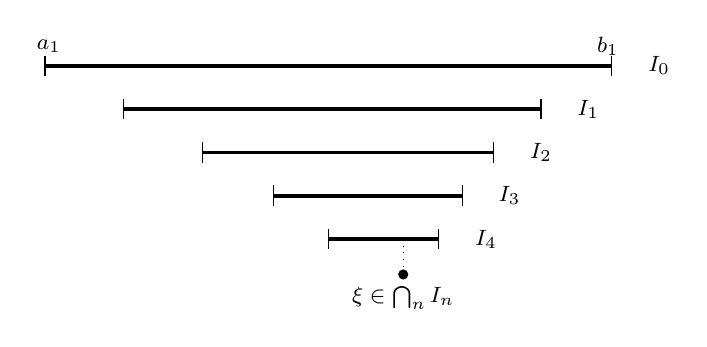
\begin{tikzpicture}[scale=1.0]
  \foreach \i/\y/\l/\r in {0/0/-3.6/3.6, 1/-0.55/-2.6/2.7, 2/-1.1/-1.6/2.1,
                           3/-1.65/-0.7/1.7, 4/-2.2/0.0/1.4}{
    \draw[line width=1.3pt] (\l,\y)--(\r,\y);
    \draw (\l,\y+0.13)--(\l,\y-0.13);
    \draw (\r,\y+0.13)--(\r,\y-0.13);
    \node[font=\footnotesize] at (\r+0.6,\y) {$I_{\i}$};
  }
  \node[font=\footnotesize] at (-3.55,0.25) {$a_1$};
  \node[font=\footnotesize] at (3.55,0.25) {$b_1$};
  \node[pt] at (0.95,-2.65) {};
  \node[font=\footnotesize] at (0.95,-2.95) {$\xi\in\bigcap_n I_n$};
  \draw[dotted] (0.95,-2.2)--(0.95,-2.55);
\end{tikzpicture}\captionof{figure}{Closed bounded intervals nesting down; completeness guarantees a common
point $\xi$.}
\end{center}

\begin{theorem}[Nested Interval Property, B\&S 2.5.2 / Rudin 1.21-style]\label{t:nip@c2}
Let $I_n=[a_n,b_n]$ be a nested sequence of \emph{closed, bounded} intervals. Then
$\bigcap_{n=1}^\infty I_n\neq\es$. Concretely, $\xi=\sup_n a_n$ lies in every $I_n$. If
moreover the lengths $b_n-a_n\to0$, the common point is \emph{unique}.
\end{theorem}

\begin{proof}
Nesting gives $a_1\le a_2\le\cdots$ and $\cdots\le b_2\le b_1$, and every $b_m$ is an upper
bound of $\set{a_n}$: indeed for any $n,m$, taking $k=\max(n,m)$, $a_n\le a_k\le b_k\le
b_m$. So $\set{a_n}$ is bounded above; let $\xi=\sup_n a_n$. Then $a_n\le\xi$ for all $n$,
and $\xi\le b_m$ for all $m$ (each $b_m$ bounds the $a$'s, and $\xi$ is the \emph{least} such
bound). Hence $a_n\le\xi\le b_n$, i.e.\ $\xi\in I_n$ for every $n$, so
$\xi\in\bigcap_n I_n$.

\emph{Uniqueness when $b_n-a_n\to0$:} if $\xi,\eta$ both lie in every $I_n$, then
$\abs{\xi-\eta}\le b_n-a_n$ for all $n$; since this is $<\eps$ for some $n$ given any
$\eps>0$, Theorem~\ref{t:squeeze0@c2} forces $\xi=\eta$. (One checks $\eta=\inf_n b_n$ and the
intersection is exactly $[\sup a_n,\inf b_n]$.)
\end{proof}

\begin{pitfall}
\emph{Both} hypotheses --- closed \emph{and} bounded --- are essential. For the open nested
intervals $J_n=(0,\tfrac1n)$, $\bigcap_n J_n=\es$ (any $x>0$ is excluded once $\tfrac1n<x$).
For the unbounded closed nested intervals $K_n=[n,\infty)$, $\bigcap_n K_n=\es$ (any $x$ is
excluded once $n>x$). Only \emph{closed bounded} intervals are guaranteed a common point.
\end{pitfall}

\subsection*{Uncountability of $\R$ via nesting}

The Nested Interval Property gives a second proof --- independent of decimals --- that $\R$
is too big to list.

\begin{theorem}[$\R$ is uncountable, B\&S 2.5.5]\label{t:Runc@c2}
The interval $[0,1]$, hence $\R$, is uncountable.
\end{theorem}

\begin{proof}
Suppose $[0,1]$ were countable, listed as $x_1,x_2,x_3,\dots$. Build nested closed intervals
that dodge the points one at a time. Choose a closed interval $I_1\subseteq[0,1]$ with
$x_1\notin I_1$ (split $[0,1]$ into thirds; at least one third misses $x_1$). Having chosen
$I_n$, split it into thirds and pick a closed third $I_{n+1}\subseteq I_n$ with
$x_{n+1}\notin I_{n+1}$. The $I_n$ are nested, closed, bounded, so by
Theorem~\ref{t:nip@c2} there is $\xi\in\bigcap_n I_n\subseteq[0,1]$. But $\xi\neq x_n$ for
every $n$, since $x_n\notin I_n\ni\xi$. So $\xi\in[0,1]$ is not in the list ---
contradiction. Hence $[0,1]$ is uncountable, and so is $\R\supseteq[0,1]$.
\end{proof}

\subsection*{Binary and decimal representations}

Nesting also explains \emph{why} every real has a decimal (or binary) expansion: the
successive digits name a shrinking nest of intervals closing on the number.

\begin{theorem}[Decimal expansions, B\&S 2.5.6--2.5.7]\label{t:decimal@c2}
Every $x\in[0,1]$ has a decimal representation $x=0.d_1d_2d_3\dots$ with digits
$d_k\in\set{0,1,\dots,9}$, meaning $x=\sup_n\sum_{k=1}^n d_k 10^{-k}$. The representation is
unique except for the \emph{dyadic-type} ambiguity, where a number ending in repeating $9$s
equals one ending in repeating $0$s, e.g.\ $0.4999\dots=0.5000\dots$. The analogous
statement holds in base $2$ with digits $\set{0,1}$.
\end{theorem}

\begin{proof}[Proof sketch]
Subdivide $[0,1]$ into ten equal closed subintervals $[\tfrac{j}{10},\tfrac{j+1}{10}]$;
$x$ lies in one, fixing $d_1=j$. Subdivide that into ten, fixing $d_2$, and recurse. The
chosen intervals are nested with lengths $10^{-n}\to0$; their unique common point
(Theorem~\ref{t:nip@c2}) is $x$, and the partial sums $\sum_{k\le n}d_k10^{-k}$ are the left
endpoints, increasing to $x$. The only freedom is at a grid point, where $x$ is the shared
endpoint of two subintervals, yielding the trailing-$9$ vs trailing-$0$ pair.
\end{proof}

\begin{wex}{A binary expansion}
Find the binary representation of $\tfrac38$ and of $\tfrac13$.
\wrec ``Expand in base $2$'': repeatedly double and read off the integer part (the digit).
\wsol $\tfrac38$: $2\cdot\tfrac38=\tfrac34$ (digit $0$), $2\cdot\tfrac34=\tfrac32$ (digit
$1$, keep $\tfrac12$), $2\cdot\tfrac12=1$ (digit $1$, remainder $0$). So
$\tfrac38=0.011_2$, terminating (also $=0.010111\dots_2$ by the $9$s-analogue). For
$\tfrac13$: $2\cdot\tfrac13=\tfrac23$ (digit $0$), $2\cdot\tfrac23=\tfrac43$ (digit $1$, keep
$\tfrac13$), and it repeats: $\tfrac13=0.010101\dots_2=\overline{01}_2$. \emph{Check:}
$0+\tfrac14+\tfrac1{16}+\cdots=\tfrac{1/4}{1-1/4}=\tfrac13$. \checkmark
\end{wex}

\begin{wex}{A periodic decimal is rational}
Show $0.137137137\dots$ is rational and find it as a fraction.
\wrec Repeating block of length $3$; multiply by $10^3$ and subtract.
\wsol Let $x=0.\overline{137}$. Then $1000x=137.\overline{137}=137+x$, so $999x=137$ and
$x=\tfrac{137}{999}$. \emph{Check:} $\tfrac{137}{999}=0.137137\dots$ by long division.
\checkmark\ (Conversely every rational has an eventually-periodic expansion, since the
remainders in long division must repeat within $q$ steps for denominator $q$.)
\end{wex}

\subsection*{Further worked examples}

\begin{wex}{The intersection of nested closed intervals is a closed interval}
For $I_n=\bigl[\,-\tfrac1n,\ 1+\tfrac1n\,\bigr]$, verify the $I_n$ are nested closed bounded
intervals and compute $\bigcap_{n=1}^\infty I_n$.
\wrec Trigger: ``apply the Nested Interval Property.'' Check nesting via the endpoints, then
use $\xi=\sup a_n$, $\inf b_n$ from Theorem~\ref{t:nip@c2}.
\wsol The left endpoints $a_n=-\tfrac1n$ increase to $0$; the right endpoints
$b_n=1+\tfrac1n$ decrease to $1$. Since $a_n\le a_{n+1}$ and $b_{n+1}\le b_n$, we have
$I_{n+1}\subseteq I_n$: nested, each closed and bounded. A point $x$ lies in every $I_n$ iff
$-\tfrac1n\le x\le1+\tfrac1n$ for all $n$; letting $n\to\infty$ this forces $0\le x\le1$, and
conversely every $x\in[0,1]$ satisfies all the inequalities. Hence
$\bigcap_n I_n=[0,1]=[\sup a_n,\inf b_n]$. \emph{Check:} the lengths
$b_n-a_n=1+\tfrac2n\to1\neq0$, so the intersection is a nondegenerate interval, not a single
point --- consistent with the ``unique point'' clause requiring lengths $\to0$. \checkmark
\end{wex}

\begin{wex}{NON-example: dropping ``closed'' empties the intersection}
Show the nested \emph{half-open} intervals $J_n=(0,\tfrac1n]$ have empty intersection,
even though each is bounded and the right endpoints are included.
\wrec Trigger: ``test the hypotheses of the NIP.'' The property needs \emph{closed}
intervals; probe what fails when the left end stays open.
\wsol The $J_n$ are nested ($\tfrac1{n+1}\le\tfrac1n$ gives $J_{n+1}\subseteq J_n$) and
bounded. Suppose $x\in\bigcap_n J_n$. Then $0<x\le\tfrac1n$ for every $n$, so $x>0$ is a
lower bound issue: by the Archimedean property (\S2.4) there is $n$ with $\tfrac1n<x$,
contradicting $x\le\tfrac1n$. Hence no such $x$ exists and $\bigcap_n J_n=\es$.

\begin{center}
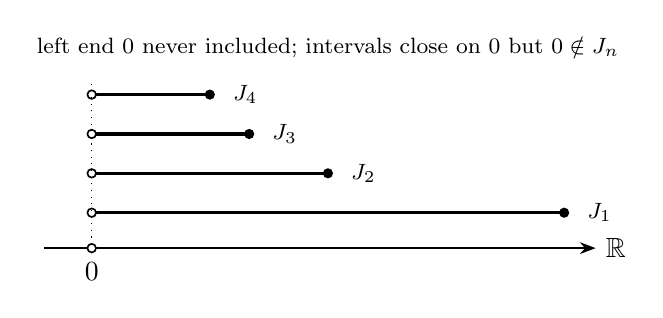
\begin{tikzpicture}[scale=1.0]
  \draw[numln] (-0.6,0)--(6.4,0) node[right]{$\R$};
  \node[opt,label={below:$0$}] at (0,0) {};
  \foreach \len/\y/\lbl in {6/0.45/$J_1$, 3/0.95/$J_2$, 2/1.45/$J_3$, 1.5/1.95/$J_4$}{
    \draw[line width=1.2pt] (0,\y)--(\len,\y);
    \node[opt] at (0,\y) {};
    \node[pt] at (\len,\y) {};
    \node[font=\footnotesize] at (\len+0.45,\y) {\lbl};
  }
  \draw[dotted] (0,0.05)--(0,2.1);
  \node[font=\footnotesize,align=center] at (3.0,2.55)
    {left end $0$ never included; intervals close on $0$ but $0\notin J_n$};
\end{tikzpicture}\captionof{figure}{Open left endpoints (hollow) let the nest shrink to the single excluded point
$0$, leaving $\bigcap_n J_n=\es$.}
\end{center}

\noindent\emph{Check:}
any candidate like $x=0.001$ is expelled once $\tfrac1n<0.001$, i.e.\ $n\ge1001$; and $0$
itself is excluded because each $J_n$ omits its left endpoint. \checkmark\ The failure is the
open left end, exactly the gap the \emph{closed} hypothesis of Theorem~\ref{t:nip@c2} closes.
\end{wex}

\begin{wex}{A repeating decimal with a non-repeating prefix}
Express $x=0.41\overline{6}=0.41666\dots$ as a fraction in lowest terms.
\wrec Trigger: ``eventually-periodic decimal to fraction.'' Shift past the non-repeating
prefix, then subtract to kill the repeating tail (as in Theorem~\ref{t:decimal@c2}).
\wsol The non-repeating part has length $2$ and the repeating block (``$6$'') length $1$.
Multiply to align: $1000x=416.\overline{6}$ and $100x=41.\overline{6}$. Subtracting,
$900x=375$, so $x=\tfrac{375}{900}=\tfrac{5}{12}$ after dividing by $75$. \emph{Check:}
$\tfrac5{12}=0.41\overline 6$ by long division ($5.000/12=0.4166\dots$). \checkmark\ Every
such eventually-periodic expansion is rational; the converse (Theorem~\ref{t:decimal@c2}
discussion) also holds.
\end{wex}

\begin{exers}{Exercises (Bartle \& Sherbert, \S2.5).}
\item If $I=[a,b]$ and $I'=[a',b']$ are closed intervals, show $I\subseteq I'$ iff
  $a'\le a$ and $b\le b'$.
\item If $S\subseteq\R$ is nonempty, show $S$ is bounded iff there is a closed bounded
  interval $I$ with $S\subseteq I$.
\item If $S\subseteq\R$ is nonempty and bounded and $I_S=[\inf S,\sup S]$, show
  $S\subseteq I_S$, and that any closed bounded interval $J$ with $S\subseteq J$ satisfies
  $I_S\subseteq J$.
\item In the characterization-of-intervals proof, explain why the points $x,y$ exist in $S$.
\item Write out the details of the remaining case in the characterization of intervals.
\item If $I_1\supseteq I_2\supseteq\cdots$ is nested with $I_n=[a_n,b_n]$, show
  $a_1\le a_2\le\cdots$ and $\cdots\le b_2\le b_1$.
\item Let $I_n=[0,1/n]$ for $n\in\N$. Prove $\bigcap_{n=1}^\infty I_n=\set{0}$.
\item Let $J_n=(0,1/n)$ for $n\in\N$. Prove $\bigcap_{n=1}^\infty J_n=\es$.
\item Let $K_n=(n,\infty)$ for $n\in\N$. Prove $\bigcap_{n=1}^\infty K_n=\es$.
\item With $\xi=\sup a_n$ and $\eta=\inf b_n$, show $\eta\in\bigcap_n I_n$ and
  $[\xi,\eta]=\bigcap_{n=1}^\infty I_n$.
\item Show that the intervals obtained from the bisection inequalities form a nested
  sequence.
\item Give the two binary representations of $\tfrac38$ and $\tfrac7{16}$.
\item (a) Give the first four digits in the binary representation of $\tfrac13$. (b) Give
  the complete binary representation of $\tfrac13$.
\item Show that if $a_k,b_k\in\set{0,1,\dots,9}$ and
  $\sum_{k=1}^n a_k 10^{-k}=\sum_{k=1}^m b_k 10^{-k}\neq0$, then $n=m$ and $a_k=b_k$ for
  all $k$.
\item Find the decimal representation of $-\tfrac27$.
\item Express $\tfrac1{17}$ and $\tfrac2{19}$ as periodic decimals.
\item What rationals are represented by the periodic decimals $1.25\overline{137}$ and
  $35.14\overline{653}$?
\end{exers}

\begin{exers}{Additional exercises.}
\item Classify each set as an interval or not, using the betweenness characterization:
  (a) $\Z$; (b) $\Q\cap[0,1]$; (c) $[0,1]\cup[2,3]$; (d) $\set{x\st x^2<4}$.
\item Compute $\bigcap_{n=1}^\infty[-1/n,\,1+1/n]$ and $\bigcap_{n=1}^\infty(-1/n,\,1+1/n)$,
  and explain the difference using the Nested Interval Property.
\item (Disprove.) Give a nested sequence of \emph{bounded} but non-closed intervals with
  empty intersection, and a nested sequence of \emph{closed} but unbounded intervals with
  empty intersection. Why does each evade the Nested Interval Property?
\item Express the repeating decimals $0.\overline{6}$, $0.1\overline{6}$, and
  $2.\overline{142857}$ as fractions in lowest terms.
\item Find the binary expansion of $\tfrac5{16}$ and of $\tfrac25$, indicating which
  terminates and which repeats.
\item Prove that a real number has a terminating decimal expansion iff it is of the form
  $m/(2^a5^b)$ for integers $m,a,b\ge0$.
\item (Diagram.) Draw four nested closed intervals $I_1\supseteq\cdots\supseteq I_4$ in
  $[0,1]$ produced by repeated bisection toward $\tfrac13$, and mark the common point.
\item Use the Nested Interval Property to give a proof that a bounded monotone increasing
  sequence of reals has a least upper bound that it ``reaches in the limit'' (informal
  preview of \S4).
\item Re-prove that $[0,1]$ is uncountable by the bisection/nesting method, writing out how
  the interval $I_{n+1}$ is chosen to exclude $x_{n+1}$.
\end{exers}


\section{The Complex Field and Euclidean Space \texorpdfstring{$\R^k$}{Rk}}
\subsection*{The complex field}

\begin{definition}[The field $\C$, Rudin 1.24--1.25]\label{d:complex@c2}
A \emph{complex number} is an ordered pair $(a,b)$ of reals, written $a+bi$. Addition and
multiplication are
\[
  (a+bi)+(c+di)=(a+c)+(b+d)i,\quad (a+bi)(c+di)=(ac-bd)+(ad+bc)i.
\]
With these, $\C$ is a field: $0=(0,0)$, $1=(1,0)$, and $i=(0,1)$ satisfies $i^2=-1$. The map
$a\mapsto a+0i$ embeds $\R$ as a subfield, so we write $a$ for $a+0i$.
\end{definition}

The multiplication rule is exactly what ``$i^2=-1$'' forces:
$(a+bi)(c+di)=ac+adi+bci+bd\,i^2$. One checks the field axioms directly; the inverse of
$z\neq0$ is computed below via the conjugate.

\begin{definition}[Conjugate, real/imaginary parts, modulus, Rudin 1.26--1.28]\label{d:conj@c2}
For $z=a+bi$: the \emph{conjugate} is $\bar z=a-bi$; the \emph{real} and \emph{imaginary}
parts are $\Re z=a$, $\Im z=b$; the \emph{modulus} (absolute value) is
$\abs z=\sqrt{a^2+b^2}=\sqrt{z\bar z}\,\ge0$.
\end{definition}

\begin{center}
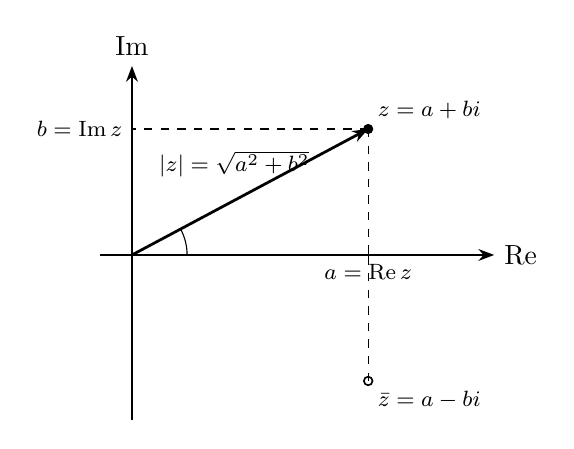
\begin{tikzpicture}[scale=1.0]
  \draw[numln] (-0.4,0)--(4.6,0) node[right]{$\Re$};
  \draw[numln] (0,-2.1)--(0,2.4) node[above]{$\Im$};
  \coordinate (Z) at (3,1.6);
  \coordinate (Zc) at (3,-1.6);
  \draw[curve,-{Stealth[length=2mm]}] (0,0)--(Z);
  \node[pt] at (Z) {};
  \node[font=\footnotesize,above right] at (Z) {$z=a+bi$};
  \node[opt] at (Zc) {};
  \node[font=\footnotesize,below right] at (Zc) {$\bar z=a-bi$};
  \draw[dashed] (Z)--(3,0) node[below,font=\footnotesize]{$a=\Re z$};
  \draw[dashed] (Z)--(0,1.6) node[left,font=\footnotesize]{$b=\Im z$};
  \draw[dashed] (Zc)--(3,0);
  \node[font=\footnotesize] at (1.3,1.15) {$\abs z=\sqrt{a^2+b^2}$};
  % angle arc
  \draw (0.7,0) arc (0:28:0.7);
\end{tikzpicture}\captionof{figure}{$\C$ as the plane: $z$ is the vector to $(a,b)$, $\abs z$ its length,
$\bar z$ its reflection across the real axis.}
\end{center}

\begin{theorem}[Algebra of conjugate and modulus, Rudin 1.31]\label{t:conjmod@c2}
For $z,w\in\C$:
\textup{(a)} $\overline{z+w}=\bar z+\bar w$, $\overline{zw}=\bar z\,\bar w$, $\bar{\bar z}=z$;
\textup{(b)} $z+\bar z=2\Re z$, $z-\bar z=2i\Im z$; and $z$ is real iff $z=\bar z$;
\textup{(c)} $z\bar z=\abs z^2\ge0$, so $z\neq0\imp z\inv=\bar z/\abs z^2$;
\textup{(d)} $\abs{zw}=\abs z\abs w$ and $\abs{\Re z}\le\abs z$, $\abs{\Im z}\le\abs z$;
\textup{(e)} \emph{(triangle inequality)} $\abs{z+w}\le\abs z+\abs w$.
\end{theorem}

\begin{proof}
(a),(b) are direct from $z=a+bi$. (c): $z\bar z=(a+bi)(a-bi)=a^2+b^2=\abs z^2$; dividing
gives the inverse. (d): $\abs{zw}^2=zw\overline{zw}=z\bar z\,w\bar w=\abs z^2\abs w^2$, and
$\abs{\Re z}=\abs a\le\sqrt{a^2+b^2}=\abs z$.
\textbf{(e)} Compute $\abs{z+w}^2=(z+w)\overline{(z+w)}=z\bar z+w\bar w+(z\bar w+\bar z w)
=\abs z^2+\abs w^2+2\Re(z\bar w)$. By (d), $\Re(z\bar w)\le\abs{z\bar w}=\abs z\abs w$, so
$\abs{z+w}^2\le\abs z^2+2\abs z\abs w+\abs w^2=(\abs z+\abs w)^2$. Take square roots.
\end{proof}

\subsection*{Euclidean space $\R^k$}

\begin{definition}[$\R^k$, inner product, norm, Rudin 1.36]\label{d:Rk@c2}
$\R^k$ is the set of ordered $k$-tuples $\mathbf x=(x_1,\dots,x_k)$ of reals, with
componentwise addition and scalar multiplication $\alpha\mathbf x=(\alpha x_1,\dots,\alpha
x_k)$. The \emph{inner (dot) product} and \emph{norm} are
\[
  \mathbf x\cdot\mathbf y=\sum_{i=1}^k x_i y_i,\qquad
  \norm{\mathbf x}=\sqrt{\mathbf x\cdot\mathbf x}=\Bigl(\sum_{i=1}^k x_i^2\Bigr)^{1/2}.
\]
For $k=2$ (identifying $(a,b)$ with $a+bi$), $\norm{\mathbf x}$ is exactly the complex
modulus.
\end{definition}

The dot product packages length and angle at once: $\mathbf x\cdot\mathbf x$ is the squared
length, while for distinct vectors $\mathbf x\cdot\mathbf y=\norm{\mathbf x}\norm{\mathbf
y}\cos\theta$ encodes the angle between them. The norm $\norm{\cdot}$ is just the
Pythagorean length, and the whole of Euclidean geometry in $\R^k$ flows from these two
formulas plus the inequality below.

\begin{theorem}[Cauchy--Schwarz inequality, Rudin 1.35]\label{t:cs@c2}
For $\mathbf x,\mathbf y\in\R^k$,
\[
  \abs{\mathbf x\cdot\mathbf y}\le\norm{\mathbf x}\,\norm{\mathbf y},
\]
i.e.\ $\bigl(\sum x_iy_i\bigr)^2\le\bigl(\sum x_i^2\bigr)\bigl(\sum y_i^2\bigr)$, with
equality iff $\mathbf x,\mathbf y$ are parallel (one a scalar multiple of the other).
\end{theorem}

\begin{proof}
If $\mathbf y=\mathbf 0$ both sides vanish. Otherwise, for every $t\in\R$,
\[
  0\le\norm{\mathbf x-t\mathbf y}^2=\norm{\mathbf x}^2-2t\,(\mathbf x\cdot\mathbf y)
  +t^2\norm{\mathbf y}^2 .
\]
This quadratic in $t$ is $\ge0$ for all $t$, so its discriminant is $\le0$:
$4(\mathbf x\cdot\mathbf y)^2-4\norm{\mathbf x}^2\norm{\mathbf y}^2\le0$, which is exactly
$\abs{\mathbf x\cdot\mathbf y}\le\norm{\mathbf x}\norm{\mathbf y}$. Equality forces the
quadratic to have a real root $t_0$, i.e.\ $\norm{\mathbf x-t_0\mathbf y}=0$, i.e.\ $\mathbf
x=t_0\mathbf y$. (Rudin gives the equivalent algebraic identity
$\norm{\mathbf x}^2\norm{\mathbf y}^2-(\mathbf x\cdot\mathbf y)^2
=\tfrac12\sum_{i,j}(x_iy_j-x_jy_i)^2\ge0$, the Lagrange identity, which exhibits the gap as a
sum of squares.)
\end{proof}

\begin{center}
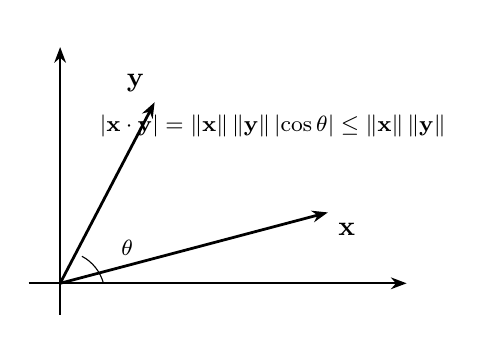
\begin{tikzpicture}[scale=1.0]
  \draw[numln] (-0.4,0)--(4.4,0) node[right]{};
  \draw[numln] (0,-0.4)--(0,3.0) node[above]{};
  \coordinate (X) at (3.4,0.9);
  \coordinate (Y) at (1.2,2.3);
  \draw[curve,-{Stealth[length=2mm]}] (0,0)--(X) node[below right]{$\mathbf x$};
  \draw[curve,-{Stealth[length=2mm]}] (0,0)--(Y) node[above left]{$\mathbf y$};
  % projection of x onto y direction
  \node[font=\footnotesize] at (2.7,2.0)
    {$\abs{\mathbf x\cdot\mathbf y}=\norm{\mathbf x}\norm{\mathbf y}\abs{\cos\theta}\le
      \norm{\mathbf x}\norm{\mathbf y}$};
  \draw (0.55,0) arc (15:62:0.55);
  \node[font=\footnotesize] at (0.85,0.45) {$\theta$};
\end{tikzpicture}\captionof{figure}{Cauchy--Schwarz says $\abs{\cos\theta}\le1$: the dot product never exceeds the
product of lengths.}
\end{center}

\begin{theorem}[Norm properties / triangle inequality in $\R^k$, Rudin 1.37]\label{t:normk@c2}
For $\mathbf x,\mathbf y\in\R^k$ and $\alpha\in\R$:
\textup{(a)} $\norm{\mathbf x}\ge0$, with $=0$ iff $\mathbf x=\mathbf 0$;
\textup{(b)} $\norm{\alpha\mathbf x}=\abs\alpha\,\norm{\mathbf x}$;
\textup{(c)} \emph{(triangle inequality)} $\norm{\mathbf x+\mathbf y}\le\norm{\mathbf
x}+\norm{\mathbf y}$;
\textup{(d)} \emph{(reverse)} $\bigl|\,\norm{\mathbf x}-\norm{\mathbf y}\,\bigr|\le
\norm{\mathbf x-\mathbf y}$.
\end{theorem}

\begin{proof}
(a),(b) are immediate. (c): using Cauchy--Schwarz,
\[
  \norm{\mathbf x+\mathbf y}^2=\norm{\mathbf x}^2+2\,\mathbf x\cdot\mathbf y+\norm{\mathbf
  y}^2\le\norm{\mathbf x}^2+2\norm{\mathbf x}\norm{\mathbf y}+\norm{\mathbf y}^2
  =(\norm{\mathbf x}+\norm{\mathbf y})^2 ;
\]
take roots. (d) follows from (c) exactly as in
Corollary~\ref{c:trianglevariants@c2}(i): $\norm{\mathbf x}=\norm{(\mathbf x-\mathbf
y)+\mathbf y}\le\norm{\mathbf x-\mathbf y}+\norm{\mathbf y}$, and symmetrically.
\end{proof}

\begin{remark}
Theorem~\ref{t:normk@c2}(a),(b),(c) say $d(\mathbf x,\mathbf y)=\norm{\mathbf x-\mathbf y}$ is a
\emph{metric} on $\R^k$ --- the setting for all of Chapter~3. The complex modulus is the
$k=2$ case; the real absolute value is $k=1$. Thus $\abs{\cdot}$, the complex $\abs{\cdot}$,
and $\norm{\cdot}$ are one idea in dimensions $1,2,k$.
\end{remark}

\begin{wex}{Cauchy--Schwarz with explicit vectors}
Verify $\abs{\mathbf x\cdot\mathbf y}\le\norm{\mathbf x}\norm{\mathbf y}$ for
$\mathbf x=(1,2,2)$, $\mathbf y=(2,-1,2)$, and identify $\cos\theta$.
\wrec ``Check Cauchy--Schwarz numerically.''
\wsol $\mathbf x\cdot\mathbf y=2-2+4=4$. $\norm{\mathbf x}=\sqrt{1+4+4}=3$,
$\norm{\mathbf y}=\sqrt{4+1+4}=3$. So $\abs{4}=4\le9=3\cdot3$. \checkmark\ Here
$\cos\theta=\tfrac{4}{9}$, strictly between $-1$ and $1$, so the vectors are not parallel
(consistent with strict inequality). \emph{Check:} Lagrange gap
$9\cdot9-4^2=65=\sum_{i<j}(x_iy_j-x_jy_i)^2=(-1-4)^2+(2-4)^2+(4+2)^2=25+4+36=65$. \checkmark
\end{wex}

\begin{wex}{The parallelogram law (Rudin Exercise 1.17)}
Prove $\norm{\mathbf x+\mathbf y}^2+\norm{\mathbf x-\mathbf y}^2=2\norm{\mathbf
x}^2+2\norm{\mathbf y}^2$ and interpret it.
\wrec ``Prove a norm identity'': expand both squares via the inner product.
\wsol Expand: $\norm{\mathbf x\pm\mathbf y}^2=\norm{\mathbf x}^2\pm2\mathbf x\cdot\mathbf
y+\norm{\mathbf y}^2$. Adding the $+$ and $-$ versions cancels the cross terms, leaving
$2\norm{\mathbf x}^2+2\norm{\mathbf y}^2$. \emph{Interpretation:} in a parallelogram with
sides $\mathbf x,\mathbf y$, the sum of the squares of the two diagonals equals the sum of
the squares of all four sides. \emph{Check:} $\mathbf x=(1,0),\mathbf y=(0,1)$:
$\norm{(1,1)}^2+\norm{(1,-1)}^2=2+2=4=2(1)+2(1)$. \checkmark
\end{wex}

\begin{wex}{NON-orderability of $\C$ (Rudin Exercise 1.8)}
Show $\C$ cannot be made an ordered field.
\wrec ``Disprove a structure exists'': use a forced-sign contradiction.
\wsol In any ordered field, squares are $\ge0$ and $1>0$
(Theorem~\ref{t:orderrules@c2}(c)). If $\C$ were ordered, then $i^2=-1$ would give $-1\ge0$,
yet $1=1^2>0$ forces $-1<0$ --- contradiction. So no order makes $\C$ an ordered field; the
complex numbers carry size ($\abs z$) but no compatible notion of ``positive.'' \emph{Check:}
the same argument bars an order on any field where $-1$ is a sum of squares. \checkmark
\end{wex}

\begin{pitfall}
$\C$ has no order: ``$z<w$'' for complex numbers is meaningless. You may compare \emph{moduli}
$\abs z<\abs w$ (real numbers), but never the complex numbers themselves. Inequality
arguments in $\C$ always run through $\abs{\cdot}$, $\Re$, or $\Im$, never through a
nonexistent complex order.
\end{pitfall}

\subsection*{Further worked examples}

\begin{wex}{Arithmetic, conjugate, and inverse of a complex number}
For $z=3+4i$ and $w=1-2i$, compute $zw$, $\abs z$, and $z\inv$ in the form $a+bi$.
\wrec ``Mechanics of $\C$'': apply the multiplication rule and
Theorem~\ref{t:conjmod@c2}(c), $z\inv=\bar z/\abs z^2$.
\wsol $zw=(3+4i)(1-2i)=3-6i+4i-8i^2=3-2i+8=11-2i$. The modulus is
$\abs z=\sqrt{3^2+4^2}=\sqrt{25}=5$. Then
$z\inv=\dfrac{\bar z}{\abs z^2}=\dfrac{3-4i}{25}=\tfrac{3}{25}-\tfrac{4}{25}i$.
\emph{Check:} $z\cdot z\inv=(3+4i)\cdot\tfrac{3-4i}{25}=\tfrac{9+16}{25}=\tfrac{25}{25}=1$.
\checkmark\ Also $\abs{zw}=\abs{11-2i}=\sqrt{121+4}=\sqrt{125}=5\sqrt5=\abs z\abs w$ since
$\abs w=\sqrt5$, confirming Theorem~\ref{t:conjmod@c2}(d). \checkmark
\end{wex}

\begin{wex}{Cauchy--Schwarz equality forces parallel vectors}
For $\mathbf x=(1,2,3)$ and $\mathbf y=(2,4,6)$ in $\R^3$, verify that Cauchy--Schwarz holds
with \emph{equality}, and explain why.
\wrec Trigger: ``the equality case'' of Theorem~\ref{t:cs@c2}: equality holds iff the vectors
are parallel. Here $\mathbf y=2\mathbf x$.
\wsol $\mathbf x\cdot\mathbf y=2+8+18=28$. $\norm{\mathbf x}=\sqrt{1+4+9}=\sqrt{14}$,
$\norm{\mathbf y}=\sqrt{4+16+36}=\sqrt{56}=2\sqrt{14}$. So
$\norm{\mathbf x}\norm{\mathbf y}=\sqrt{14}\cdot2\sqrt{14}=28=\abs{\mathbf x\cdot\mathbf y}$:
\emph{equality}. The reason is $\mathbf y=2\mathbf x$, so the vectors are parallel
($\cos\theta=1$). \emph{Check:} the Lagrange gap
$\norm{\mathbf x}^2\norm{\mathbf y}^2-(\mathbf x\cdot\mathbf y)^2=14\cdot56-28^2=784-784=0$,
a sum of squares $(x_iy_j-x_jy_i)^2$ all vanishing because $x_iy_j=x_jy_i$ for the
proportional coordinates. \checkmark
\end{wex}

\begin{exers}{Exercises (Rudin, Ch.1 -- complex numbers and $\R^k$).}
\item Prove that no order can be defined on the complex field that turns it into an ordered
  field. (Hint: $-1$ is a square.)
\item Suppose $z=a+bi$ and $w=c+di$. Define $z<w$ if $a<c$, or if $a=c$ but $b<d$. Prove
  this makes $\C$ an ordered \emph{set} (lexicographic / dictionary order). Does this
  ordered set have the least-upper-bound property?
\item Suppose $z=a+bi$, $w=u+iv$, and
  $a=\bigl(\tfrac{\abs w+u}{2}\bigr)^{1/2}$, $b=\bigl(\tfrac{\abs w-u}{2}\bigr)^{1/2}$.
  Prove $z^2=w$ if $v\ge0$ and $(\bar z)^2=w$ if $v\le0$. Conclude that every complex number
  (with one exception) has two complex square roots.
\item If $z\in\C$, prove there exist $r\ge0$ and $w\in\C$ with $\abs w=1$ such that $z=rw$.
  Are $w$ and $r$ always uniquely determined by $z$?
\item If $z_1,\dots,z_n\in\C$, prove $\abs{z_1+z_2+\cdots+z_n}\le\abs{z_1}+\cdots+\abs{z_n}$.
\item If $x,y\in\C$, prove $\bigl|\,\abs x-\abs y\,\bigr|\le\abs{x-y}$.
\item If $z\in\C$ with $\abs z=1$ (i.e.\ $z\bar z=1$), compute $\abs{1+z}^2+\abs{1-z}^2$.
\item Under what conditions does equality hold in the Schwarz inequality?
\item Suppose $k\ge3$, $\mathbf x,\mathbf y\in\R^k$, $\abs{\mathbf x-\mathbf y}=d>0$, and
  $r>0$. Prove: (a) if $2r>d$ there are infinitely many $\mathbf z\in\R^k$ with
  $\abs{\mathbf z-\mathbf x}=\abs{\mathbf z-\mathbf y}=r$; (b) if $2r=d$ there is exactly
  one; (c) if $2r<d$ there is none. How must these change for $k=1,2$?
\item Prove $\abs{\mathbf x+\mathbf y}^2+\abs{\mathbf x-\mathbf y}^2=2\abs{\mathbf
  x}^2+2\abs{\mathbf y}^2$ for $\mathbf x,\mathbf y\in\R^k$. Interpret geometrically as a
  statement about parallelograms.
\item If $k\ge2$ and $\mathbf x\in\R^k$, prove there exists $\mathbf y\in\R^k$ with
  $\mathbf y\neq\mathbf0$ but $\mathbf x\cdot\mathbf y=0$. Is this also true if $k=1$?
\item Suppose $\mathbf a,\mathbf b\in\R^k$. Find $\mathbf c\in\R^k$ and $r>0$ such that
  $\abs{\mathbf x-\mathbf a}=2\abs{\mathbf x-\mathbf b}$ iff $\abs{\mathbf x-\mathbf c}=r$.
  (Solution: $3\mathbf c=4\mathbf b-\mathbf a$, $3r=2\abs{\mathbf b-\mathbf a}$.)
\end{exers}

\begin{exers}{Additional exercises.}
\item For $z=3+4i$ compute $\bar z$, $\abs z$, $z\inv$, $\Re z$, $\Im z$, and verify
  $z z\inv=1$.
\item Prove $\abs{\Re z}\le\abs z$ and $\abs{\Im z}\le\abs z$, with equality iff $z$ is real
  (resp.\ purely imaginary).
\item (Disprove.) A student writes ``$2+3i<4+i$ because $2<4$.'' Explain precisely why this
  is meaningless, citing the non-orderability of $\C$.
\item Verify the Cauchy--Schwarz inequality for $\mathbf x=(1,1,1,1)$, $\mathbf
  y=(1,2,3,4)$, and compute the angle's cosine.
\item Prove the polarization identity $\mathbf x\cdot\mathbf y=\tfrac14\bigl(\norm{\mathbf
  x+\mathbf y}^2-\norm{\mathbf x-\mathbf y}^2\bigr)$ in $\R^k$.
\item Show that equality $\norm{\mathbf x+\mathbf y}=\norm{\mathbf x}+\norm{\mathbf y}$
  holds iff $\mathbf x,\mathbf y$ point the same way ($\mathbf x=\lambda\mathbf y$ or
  $\mathbf y=\lambda\mathbf x$ with $\lambda\ge0$).
\item For $z,w\in\C$ prove $\abs{z+w}^2+\abs{z-w}^2=2\abs z^2+2\abs w^2$ and interpret it in
  the plane.
\item (Diagram.) In the complex plane plot $z=2+i$, its conjugate $\bar z$, $iz$, and
  $-z$, and describe each as a geometric transformation of $z$ (reflection, rotation,
  point reflection).
\item Prove that for $\mathbf x,\mathbf y\in\R^k$, $\norm{\mathbf x-\mathbf y}\ge
  \bigl|\,\norm{\mathbf x}-\norm{\mathbf y}\,\bigr|$, and identify when equality holds.
\item Given $z\in\C$ with $\abs z<1$, prove $\Re\bigl(\tfrac{1+z}{1-z}\bigr)>0$. (Hint:
  multiply numerator and denominator by $\overline{1-z}$.)
\end{exers}


% ================= Chapter 3: Basic Topology and Metric Spaces =================

\chapter{Basic Topology and Metric Spaces}

\section{Metric Spaces and Neighborhoods}
\subsection*{The metric axioms}

Analysis on the real line rests on one number: the distance $\abs{x-y}$ between two points.
Almost every limit argument used only a few properties of that distance --- it is
nonnegative, vanishes exactly when the points coincide, is symmetric, and satisfies the
triangle inequality. Pulling those properties out and naming them gives the single most
useful abstraction in the subject.

\begin{definition}[Metric, Rudin 2.15 / B\&S 11.4.1]\label{d:metric@c3}
A \emph{metric} on a set $X$ is a function $d:X\times X\to\R$ such that for all $p,q,r\in X$:
\begin{enumerate}[label=\textup{(\alph*)},leftmargin=2.2em]
\item $d(p,q)\ge 0$, and $d(p,q)=0\eqv p=q$ \hfill(\emph{positivity / definiteness});
\item $d(p,q)=d(q,p)$ \hfill(\emph{symmetry});
\item $d(p,q)\le d(p,r)+d(r,q)$ \hfill(\emph{triangle inequality}).
\end{enumerate}
The pair $(X,d)$ is a \emph{metric space}; its elements are called \emph{points}. A function
with these properties is a \emph{distance function}.
\end{definition}

The triangle inequality is the workhorse: every estimate ``$d(p,q)$ is small'' is built by
routing through an intermediate point $r$ and adding two small distances. The definiteness
clause (b) is what distinguishes a metric from a \emph{semimetric}, where one only requires
$d(p,p)=0$ but allows distinct points at distance $0$ (B\&S 11.4.13); we will always assume
a genuine metric.

\begin{remark}
Every subset $Y\subseteq X$ is itself a metric space under the \emph{same} $d$ restricted to
$Y\times Y$: the three axioms, holding for all points of $X$, certainly hold for points of
$Y$. Thus every subset of a Euclidean space is a metric space in its own right --- a fact we
exploit constantly via the \emph{relative} topology (\S3.2).
\end{remark}

\subsection*{The standard examples}

\begin{example}[The fundamental examples; Rudin 2.16, B\&S 11.4.2]\label{ex:metrics@c3}
\leavevmode
\begin{enumerate}[label=\textup{(\alph*)},leftmargin=2.2em]
\item \textbf{The real line $\R$} with $d(x,y)=\abs{x-y}$. Axiom (c) is the triangle
  inequality for absolute value, $\abs{x-y}\le\abs{x-z}+\abs{z-y}$.
\item \textbf{Euclidean space $\Rk$} with $d(\mathbf x,\mathbf y)=\abs{\mathbf x-\mathbf y}
  =\bigl(\sum_{j=1}^k (x_j-y_j)^2\bigr)^{1/2}$. The triangle inequality here is the
  Cauchy--Schwarz inequality (Rudin 1.37); $\R^2$ is the complex plane.
\item \textbf{The taxicab and sup metrics on $\Rk$}:
  $d_1(\mathbf x,\mathbf y)=\sum_j\abs{x_j-y_j}$ and
  $d_\infty(\mathbf x,\mathbf y)=\max_j\abs{x_j-y_j}$. Each is a metric on the same
  underlying set $\Rk$: one set, several metrics.
\item \textbf{The discrete metric} on any nonempty set $X$:
  \[
    d(p,q)=\begin{cases}0,& p=q,\\ 1,& p\neq q.\end{cases}
  \]
  Here every point sits at distance $1$ from all others.
\item \textbf{The sup (uniform) metric.} On the space $C[0,1]$ of continuous functions on
  $[0,1]$, set $d_\infty(f,g)=\sup_{x\in[0,1]}\abs{f(x)-g(x)}=\norm{f-g}_\infty$. Convergence
  in this metric is exactly \emph{uniform} convergence (Chapter~8).
\item \textbf{The $L^1$ metric.} On the same $C[0,1]$, set $d_1(f,g)=\int_0^1\abs{f-g}$ ---
  the same underlying set as (e), but a genuinely different metric.
\end{enumerate}
\end{example}

\begin{wex}{Verifying the discrete metric}
Show $d(p,q)=\mathbf 1[p\neq q]$ is a metric on any nonempty set $X$.
\wrec Trigger: ``show a given $d$ is a metric.'' Check the three axioms; the only work is the
triangle inequality, handled by cases.
\wsol (a) $d\ge0$ and $d(p,q)=0\eqv p=q$ by definition. (b) Symmetry is clear since
``$p\neq q$'' is symmetric. (c) Fix $p,q,r$. If $p=q$ then $d(p,q)=0\le$ anything. If $p\neq
q$ then $d(p,q)=1$; but $p\neq q$ forces $r\neq p$ or $r\neq q$ (else $p=r=q$), so
$d(p,r)+d(r,q)\ge1=d(p,q)$. \emph{Check:} the largest possible distance is $1$, so the
triangle inequality can never fail by more than the slack $1+1\ge1$. Every singleton ball
$B(p,\tfrac12)=\set p$, which already hints (Worked Example~\ref{wex:disc-open@c3}) that
\emph{every} subset is open.
\end{wex}

\subsection*{Balls, neighborhoods, bounded sets, diameter}

\begin{definition}[Rudin 2.18(a), 2.17; B\&S 11.4.3]\label{d:ball@c3}
Let $(X,d)$ be a metric space, $p\in X$, $r>0$.
\begin{itemize}[leftmargin=1.4em]
\item The \emph{open ball} (or \emph{$r$-neighborhood}) of $p$ is
  $B(p,r)=N_r(p)=\set{q\in X\st d(p,q)<r}$; the \emph{closed ball} replaces $<$ by $\le$.
\item A \emph{neighborhood} of $p$ is any set $V$ containing some open ball $B(p,r)$, $r>0$.
\item A set $E\subseteq X$ is \emph{bounded} if there exist $q\in X$ and $M>0$ with
  $d(p,q)\le M$ for all $p\in E$ (equivalently, $E$ lies in some ball).
\item The \emph{diameter} of a nonempty $E$ is $\diam E=\sup\set{d(p,q)\st p,q\in E}$
  (possibly $+\infty$); $E$ is bounded iff $\diam E<\infty$.
\end{itemize}
\end{definition}

In $\R^1$ a neighborhood $N_r(p)$ is the segment $(p-r,p+r)$; in $\R^2$ it is the open disk
of radius $r$. Rudin's ``$N_r(p)$'' and B\&S's ``$V_\eps(x_0)$'' name the same object. The
loosened notion --- a neighborhood is \emph{any} set containing a ball --- is convenient
because it lets us say ``$E$ is a neighborhood of $p$'' without fixing a radius.

\begin{center}
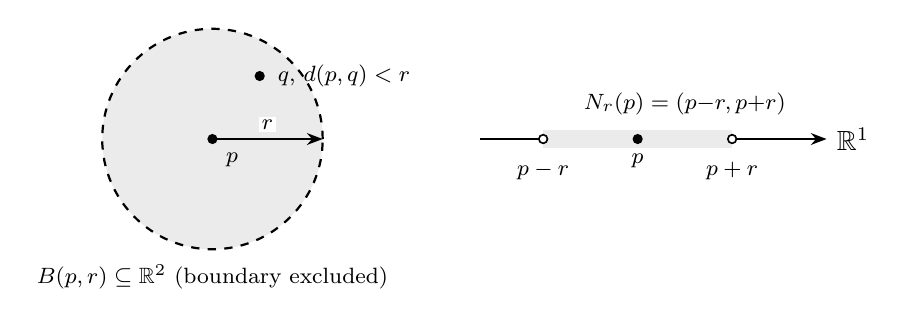
\begin{tikzpicture}[scale=1.0]
  % open ball in R^2
  \begin{scope}
    \clip (0,0) circle (1.4);
    \fill[band] (-2,-2) rectangle (2,2);
  \end{scope}
  \draw[dashed,line width=0.8pt] (0,0) circle (1.4);
  \node[pt,label={[font=\footnotesize]below right:$p$}] at (0,0) {};
  \draw[-{Stealth[length=2mm]},line width=0.7pt] (0,0)--(1.4,0);
  \node[font=\footnotesize,fill=white,inner sep=1pt] at (0.7,0.18) {$r$};
  \node[pt,fill=black] (q) at (0.6,0.8) {};
  \node[font=\footnotesize,right=1pt of q] {$q$, $d(p,q)<r$};
  \node[font=\footnotesize] at (0,-1.75) {$B(p,r)\subseteq\R^2$ (boundary excluded)};
  % number-line ball
  \begin{scope}[shift={(5.4,0)}]
    \draw[numln] (-2,0)--(2.4,0) node[right]{$\R^1$};
    \fill[band] (-1.2,-0.12) rectangle (1.2,0.12);
    \node[opt] at (-1.2,0) {}; \node[opt] at (1.2,0) {};
    \node[pt,label={[font=\footnotesize]below:$p$}] at (0,0) {};
    \node[font=\footnotesize] at (-1.2,-0.4) {$p-r$};
    \node[font=\footnotesize] at (1.2,-0.4) {$p+r$};
    \node[font=\footnotesize] at (0.6,0.45) {$N_r(p)=(p{-}r,p{+}r)$};
  \end{scope}
\end{tikzpicture}
\captionof{figure}{An open ball in $\R^2$ is an open disk; in $\R^1$ it is a symmetric open
segment. The bounding circle / endpoints are \emph{not} included.}
\end{center}

\begin{wex}{Diameter of a ball}
In $\R^k$ show $\diam B(p,r)=2r$, but in a general metric space $\diam B(p,r)$ can be
strictly smaller than $2r$.
\wrec ``Compute a diameter'': bound the sup above by the triangle inequality, then exhibit a
near-extremal pair.
\wsol For any $x,y\in B(p,r)$, $d(x,y)\le d(x,p)+d(p,y)<r+r=2r$, so $\diam B(p,r)\le2r$. In
$\R^k$ take $x=p+(r-\delta)\mathbf u$, $y=p-(r-\delta)\mathbf u$ for a unit vector $\mathbf
u$; then $d(x,y)=2(r-\delta)\to2r$, so the sup is $2r$. \emph{Non-Euclidean check:} in the
discrete metric with $r=2$, $B(p,2)=X$ but any two distinct points are at distance $1$, so
$\diam B(p,2)\le1<4=2r$. The clean formula $\diam=2r$ is special to $\R^k$.
\end{wex}

\begin{wex}{The three metrics on $\R^2$ give nested balls}
Compare the unit balls of $d_1$, $d$ (Euclidean), and $d_\infty$ at the origin in $\R^2$.
\wrec ``Draw/compare balls of different metrics on a common set'': translate each definition
into a region.
\wsol $B_{d_1}(O,1)=\set{(x,y)\st\abs x+\abs y<1}$ is an open diamond (square rotated
$45^\circ$); $B_{d}(O,1)=\set{x^2+y^2<1}$ is the open disk; $B_{d_\infty}(O,1)=\set{\max(\abs
x,\abs y)<1}$ is the open axis-aligned square $(-1,1)^2$. Since $\max\le\sqrt{x^2+y^2}\le
\abs x+\abs y$, we get the inclusions $B_{d_1}\subseteq B_d\subseteq B_{d_\infty}$.
\emph{Check:} the point $(0.9,0.9)$ has $d_\infty=0.9<1$ (inside the square), $d=\sqrt{1.62}
\approx1.27>1$ (outside the disk), consistent with the nesting.
\end{wex}

\begin{center}
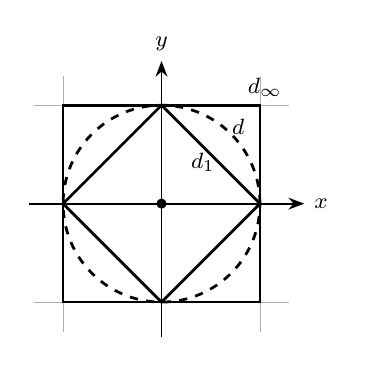
\begin{tikzpicture}[scale=1.25]
  \draw[dgrid] (-1.3,-1.3) grid (1.3,1.3);
  \draw[numln] (-1.35,0)--(1.45,0) node[right,font=\footnotesize]{$x$};
  \draw[numln] (0,-1.35)--(0,1.45) node[above,font=\footnotesize]{$y$};
  % d_infty square
  \draw[line width=1pt] (-1,-1) rectangle (1,1);
  \node[font=\footnotesize] at (1.05,1.18) {$d_\infty$};
  % euclidean circle
  \draw[line width=1pt,dashed] (0,0) circle (1);
  \node[font=\footnotesize] at (0.78,0.78) {$d$};
  % d_1 diamond
  \draw[line width=1pt] (1,0)--(0,1)--(-1,0)--(0,-1)--cycle;
  \node[font=\footnotesize] at (0.42,0.42) {$d_1$};
  \node[pt] at (0,0) {};
\end{tikzpicture}
\captionof{figure}{Unit balls at the origin: diamond ($d_1$) $\subseteq$ disk ($d$) $\subseteq$
square ($d_\infty$). All three metrics induce the same open sets (\S3.2).}
\end{center}

\begin{method}{Verifying that a candidate $d$ is a metric}
\textbf{Recognition trigger.} You are handed a formula $d(p,q)$ and asked whether it is a
metric (Rudin Ex.~11 lists five candidates on $\R^1$; only some pass).
\begin{enumerate}
\item \textbf{Positivity/definiteness:} confirm $d\ge0$ everywhere and that $d(p,q)=0$
  forces $p=q$. (Squaring a metric, e.g.\ $(x-y)^2$, usually kills the triangle inequality;
  a non-injective inner function, e.g.\ $\abs{x^2-y^2}$, usually kills definiteness since
  $d(1,-1)=0$.)
\item \textbf{Symmetry:} check $d(p,q)=d(q,p)$ --- typically immediate.
\item \textbf{Triangle inequality:} the hard axiom. For $\abs{\,\cdot\,}$-based formulas,
  reduce to the absolute-value triangle inequality; for $\sqrt{\abs{x-y}}$ use
  $\sqrt{a+b}\le\sqrt a+\sqrt b$; to \emph{disprove} it, find a concrete failing triple.
\end{enumerate}
\end{method}

\begin{wex}{Which of $(x-y)^2$ and $\sqrt{\abs{x-y}}$ is a metric? (Rudin Ex.~11)}
On $\R^1$ test $d_1(x,y)=(x-y)^2$ and $d_2(x,y)=\sqrt{\abs{x-y}}$.
\wrec ``Decide if a formula is a metric'': apply the method; one fails the triangle
inequality, one passes.
\wsol $d_1$: positivity and symmetry hold, but the triangle inequality fails. Take
$x=0,r=1,y=2$: $d_1(0,2)=4$ while $d_1(0,1)+d_1(1,2)=1+1=2<4$. So $d_1$ is \emph{not} a
metric. $d_2$: positivity/definiteness and symmetry are clear. For the triangle inequality,
$\sqrt{\abs{x-y}}\le\sqrt{\abs{x-z}+\abs{z-y}}\le\sqrt{\abs{x-z}}+\sqrt{\abs{z-y}}$, using
$\abs{x-y}\le\abs{x-z}+\abs{z-y}$ and $\sqrt{a+b}\le\sqrt a+\sqrt b$ (square both sides:
$a+b\le a+b+2\sqrt{ab}$). So $d_2$ \emph{is} a metric. \emph{Check:} $d_2(0,4)=2=
d_2(0,1)+d_2(1,4)=1+\sqrt3\approx2.73$? Indeed $2\le2.73$, consistent.
\end{wex}

\begin{pitfall}
``One set, many metrics.'' The same underlying set carries genuinely different metrics, and
which one you use changes what ``small distance'' means --- but, as we will see in \S3.2, the
metrics $d,d_1,d_\infty$ on $\R^k$ all produce the \emph{same} open sets, so they are
interchangeable for topology. By contrast the $d_\infty$ and $L^1$ metrics on $C[0,1]$ give
\emph{different} topologies (uniform vs.\ mean convergence). Never assume two metrics agree
topologically; check.
\end{pitfall}

\subsection*{Further worked examples}

\begin{wex}{The reverse triangle inequality}
In any metric space $(X,d)$ prove $\abs{d(p,r)-d(q,r)}\le d(p,q)$ for all $p,q,r$.
\wrec Trigger: an estimate \emph{lower}-bounding a distance. The reverse triangle inequality
is the standard consequence of axiom (c) applied twice, with the two points swapped.
\wsol By the triangle inequality, $d(p,r)\le d(p,q)+d(q,r)$, so $d(p,r)-d(q,r)\le d(p,q)$.
Swapping $p$ and $q$ gives $d(q,r)-d(p,r)\le d(q,p)=d(p,q)$ by symmetry. The two inequalities
together say $-d(p,q)\le d(p,r)-d(q,r)\le d(p,q)$, i.e.\ $\abs{d(p,r)-d(q,r)}\le d(p,q)$.
\emph{Check:} in $\R$ with $d(x,y)=\abs{x-y}$ this is $\bigl|\,\abs{p-r}-\abs{q-r}\,\bigr|\le
\abs{p-q}$; take $p=5,q=1,r=0$: LHS $=\abs{5-1}=4\le4=\abs{5-1}$, tight. The map
$x\mapsto d(x,r)$ is therefore $1$-Lipschitz, hence continuous --- a fact used constantly.
\end{wex}

\begin{wex}{A formula that fails definiteness, and one that fails the triangle law}
On $\R$ decide whether $\rho(x,y)=\abs{x^2-y^2}$ and $\sigma(x,y)=\abs{x-y}/(1+\abs{x-y})$
are metrics.
\wrec Trigger: ``is this a metric?''. Run the verification method: definiteness is the usual
trap for a non-injective inner function; the bounded modification needs the triangle law
checked via monotonicity of $t/(1+t)$.
\wsol For $\rho$: $\rho(1,-1)=\abs{1-1}=0$ although $1\neq-1$, so definiteness (axiom (a))
fails; $\rho$ is \emph{not} a metric. For $\sigma$: write $\phi(t)=t/(1+t)$ for $t\ge0$.
Then $\phi$ is increasing and \emph{subadditive}, $\phi(a+b)\le\phi(a)+\phi(b)$ (since
$\frac{a+b}{1+a+b}=\frac{a}{1+a+b}+\frac{b}{1+a+b}\le\frac{a}{1+a}+\frac{b}{1+b}$). With
$a=\abs{x-z}$, $b=\abs{z-y}$ and $\abs{x-y}\le a+b$, monotonicity then subadditivity give
$\sigma(x,y)=\phi(\abs{x-y})\le\phi(a+b)\le\phi(a)+\phi(b)=\sigma(x,z)+\sigma(z,y)$.
Positivity, definiteness and symmetry are clear, so $\sigma$ \emph{is} a metric (a bounded
one: $\sigma<1$ always). \emph{Check:} $\sigma(0,3)=3/4$ while $\sigma(0,1)+\sigma(1,3)=
\tfrac12+\tfrac23=\tfrac76>\tfrac34$, consistent. This $\sigma$ induces the \emph{same} open
sets as $\abs{x-y}$ yet makes the whole line bounded --- boundedness is not topological.
\end{wex}

\begin{exers}{Exercises (Bartle \& Sherbert, \S11.4).}
\item Show that the functions $d_1(P_1,P_2)=\abs{x_1-x_2}+\abs{y_1-y_2}$ and
  $d_\infty(P_1,P_2)=\sup\set{\abs{x_1-x_2},\abs{y_1-y_2}}$ are metrics on $\R^2$.
\item Show that the uniform metric $d_\infty(f,g)=\sup_{x\in[0,1]}\abs{f(x)-g(x)}$ and the
  $L^1$ metric $d_1(f,g)=\int_0^1\abs{f-g}$ are both metrics on $C[0,1]$.
\item Verify that the discrete metric on a set $S$ ($d(s,t)=0$ if $s=t$, else $1$) is a
  metric.
\item If $P_n=(x_n,y_n)\in\R^2$ and $d_1$ is the taxicab metric, show that $(P_n)$ converges
  to $P=(x,y)$ with respect to $d_1$ iff $(x_n)\to x$ and $(y_n)\to y$.
\item Verify the conclusion of the previous exercise when $d_1$ is replaced by the sup metric
  $d_\infty$.
\item Let $S$ be nonempty with the discrete metric. Show that in $(S,d)$ a sequence $(x_n)$
  converges to $x$ iff there is $K\in\N$ with $x_n=x$ for all $n\ge K$.
\item Show that if $d$ is the discrete metric on $S$, then every subset of $S$ is both open
  and closed in $(S,d)$.
\item Let $P=(x,y)$ and $O=(0,0)$ in $\R^2$. Draw the sets
  $\set{P\st d_1(O,P)\le1}$ and $\set{P\st d_\infty(O,P)\le1}$ in the plane.
\item Prove that in any metric space, an $\eps$-neighborhood of a point is an open set.
\item Prove the Global Continuity Theorem for metric spaces: $f:(S_1,d_1)\to(S_2,d_2)$ is
  continuous on $S_1$ iff $f^{-1}(G)$ is open in $S_1$ whenever $G$ is open in $S_2$.
\item Prove the preservation of compactness for metric spaces: if $(S,d)$ is a compact metric
  space and $f:S\to\R$ is continuous, then $f(S)$ is compact in $\R$.
\item In a metric space $(S,d)$, call $A\subseteq S$ \emph{bounded} if there exist $x_0\in S$
  and $B>0$ with $A\subseteq\set{x\st d(x,x_0)\le B}$. Show that if $A$ is a compact subset of
  $S$, then $A$ is closed and bounded.
\end{exers}

\begin{exers}{Additional exercises.}
\item Verify in detail that the Euclidean metric on $\R^2$ satisfies the triangle inequality,
  citing the Cauchy--Schwarz inequality.
\item On $\R$, decide whether $\rho(x,y)=\abs{\arctan x-\arctan y}$ is a metric. (It is;
  identify which axiom needs the injectivity of $\arctan$.)
\item Prove the \emph{reverse triangle inequality} in any metric space:
  $\abs{d(p,r)-d(r,q)}\le d(p,q)$.
\item Compute the diameter of the unit square $[0,1]^2\subseteq\R^2$ under each of the three
  metrics $d$, $d_1$, $d_\infty$. (Answers: $\sqrt2$, $2$, $1$.)
\item (Non-example.) Show that $\sigma(x,y)=\abs{x}+\abs{y}$ for $x\neq y$ and
  $\sigma(x,x)=0$ is \emph{not} a metric on $\R$ by exhibiting a failure of the triangle
  inequality, and identify which other axiom it also breaks.
\item Let $(X,d)$ be a metric space. Prove that $\rho(x,y)=\dfrac{d(x,y)}{1+d(x,y)}$ is also a
  metric on $X$, and that $\rho(x,y)<1$ always. (So every metric space carries a
  topologically equivalent bounded metric.)
\item (Diagram.) Sketch, in the same axes, the closed unit balls at the origin for the
  metrics $d_1$, $d$, $d_\infty$ on $\R^2$, and mark a point lying in the $d_\infty$-ball but
  outside the $d$-ball. Explain the nesting in one sentence.
\item Show that in $C[0,1]$ the uniform metric $d_\infty$ and the $L^1$ metric $d_1$ are not
  equivalent: exhibit a sequence $f_n$ with $d_1(f_n,0)\to0$ but $d_\infty(f_n,0)\not\to0$.
\item Prove that a finite union of bounded sets is bounded, but an infinite union of bounded
  sets need not be (give an example in $\R$).
\item Let $A$ be a nonempty subset of a metric space and define
  $\dist(x,A)=\inf_{a\in A}d(x,a)$. Prove $\abs{\dist(x,A)-\dist(y,A)}\le d(x,y)$ (so
  $x\mapsto\dist(x,A)$ is Lipschitz), and that $\dist(x,A)=0$ iff $x\in\closure A$.
\end{exers}


\section{Open and Closed Sets}
Fix a metric space $(X,d)$ throughout. All points and sets are understood to live in $X$.

\subsection*{Interior points, open sets, closed sets}

\begin{definition}[Rudin 2.18(e)(f)(g)(d); B\&S 11.1.2]\label{d:open-closed@c3}
Let $E\subseteq X$.
\begin{itemize}[leftmargin=1.4em]
\item $p$ is an \emph{interior point} of $E$ if some neighborhood $N$ of $p$ satisfies
  $N\subseteq E$.
\item $E$ is \emph{open} if every point of $E$ is an interior point: for each $p\in E$ there
  is $r>0$ with $B(p,r)\subseteq E$.
\item The \emph{complement} of $E$ is $E^c=\set{p\in X\st p\notin E}$.
\item $E$ is \emph{closed} if its complement $E^c$ is open. (Equivalently, by \S3.3, $E$
  contains all its limit points.)
\end{itemize}
\end{definition}

The words \emph{open} and \emph{closed} are not opposites. In any space, $\es$ and $X$ are
\emph{both} open and closed; many sets (e.g.\ $[0,1)\subseteq\R$) are \emph{neither}. ``Not
open'' does not mean ``closed.''

\begin{theorem}[Every neighborhood is open; Rudin 2.19]\label{t:ball-open@c3}
Every open ball $N_r(p)$ is an open set.
\end{theorem}

\begin{proof}
Let $q\in N_r(p)$, so $d(p,q)<r$. Put $h=r-d(p,q)>0$. If $d(q,s)<h$ then by the triangle
inequality $d(p,s)\le d(p,q)+d(q,s)<d(p,q)+h=r$, so $s\in N_r(p)$. Thus $N_h(q)\subseteq
N_r(p)$ and $q$ is interior. As $q$ was arbitrary, $N_r(p)$ is open.
\end{proof}

\begin{center}
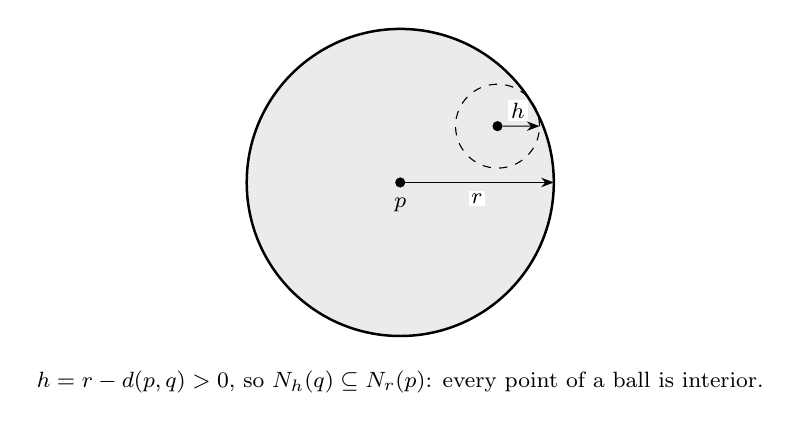
\begin{tikzpicture}[scale=1.3]
  \begin{scope}
    \clip (0,0) circle (1.5);
    \fill[band] (-2,-2) rectangle (2,2);
  \end{scope}
  \draw[line width=0.9pt] (0,0) circle (1.5);
  \node[pt,label={[font=\footnotesize]below:$p$}] at (0,0) {};
  \node[pt] (q) at (0.95,0.55) {};
  \node[font=\footnotesize,above right=-1pt of q] {$q$};
  \draw[dashed] (q) circle (0.41);
  \draw[-{Stealth[length=1.6mm]}] (0,0)--(1.5,0);
  \node[font=\footnotesize,fill=white,inner sep=1pt] at (0.75,-0.16) {$r$};
  \draw[-{Stealth[length=1.6mm]}] (q)--($(q)+(0.41,0)$);
  \node[font=\footnotesize,fill=white,inner sep=1pt] at ($(q)+(0.2,0.15)$) {$h$};
  \node[font=\footnotesize,align=center] at (0,-1.95)
    {$h=r-d(p,q)>0$, so $N_h(q)\subseteq N_r(p)$: every point of a ball is interior.};
\end{tikzpicture}
\end{center}

\begin{wex}{In the discrete metric every set is open (and closed)}\label{wex:disc-open@c3}
Let $X$ carry the discrete metric. Show every subset is both open and closed.
\wrec ``Describe the open sets of a given metric'': compute the balls, then test the
definition.
\wsol For any $p$, $B(p,\tfrac12)=\set{q\st d(p,q)<\tfrac12}=\set p$, since distinct points
are at distance $1$. Given any $E\subseteq X$ and $p\in E$, the ball $B(p,\tfrac12)=\set
p\subseteq E$, so $p$ is interior; hence $E$ is open. As $E$ was arbitrary, $E^c$ is open
too, so $E$ is closed. \emph{Check:} thus in a discrete space ``open'' carries no
information --- the topology is as fine as possible. This is exactly the answer to Rudin
Ex.~10: in the metric $d(p,q)=\mathbf 1[p\neq q]$, all subsets are open, all are closed, and
(\S3.4) the compact ones are precisely the finite ones.
\end{wex}

\subsection*{The open/closed set theorems}

\begin{theorem}[Complementation; Rudin 2.23]\label{t:complement@c3}
$E$ is open iff $E^c$ is closed; equivalently $F$ is closed iff $F^c$ is open.
\end{theorem}

\begin{proof}
Suppose $E^c$ is closed, i.e.\ $(E^c)^c=E$ \dots\ we argue directly. Let $E$ be open and let
$x$ be a limit point of $E^c$ (\S3.3 notion, but we only need: every neighborhood of $x$
meets $E^c$). If $x\in E$, openness gives a ball $B(x,r)\subseteq E$, disjoint from $E^c$, so
$x$ is \emph{not} a limit point of $E^c$ --- contradiction; hence $x\in E^c$. So $E^c$
contains its limit points, i.e.\ is closed. Conversely if $E^c$ is closed and $x\in E$, then
$x\notin E^c$ and $x$ is not a limit point of $E^c$, so some ball $B(x,r)$ misses $E^c$,
i.e.\ $B(x,r)\subseteq E$; thus $E$ is open.
\end{proof}

\begin{theorem}[Unions and intersections; Rudin 2.24, B\&S 11.1.4--11.1.5]\label{t:open-closed-ops@c3}
\leavevmode
\begin{enumerate}[label=\textup{(\alph*)},leftmargin=2.2em]
\item For any collection $\set{G_\alpha}$ of open sets, $\bigcup_\alpha G_\alpha$ is open.
\item For any collection $\set{F_\alpha}$ of closed sets, $\bigcap_\alpha F_\alpha$ is
  closed.
\item For any \emph{finite} collection $G_1,\dots,G_n$ of open sets, $\bigcap_{i=1}^n G_i$ is
  open.
\item For any \emph{finite} collection $F_1,\dots,F_n$ of closed sets, $\bigcup_{i=1}^n F_i$
  is closed.
\end{enumerate}
\end{theorem}

\begin{proof}
(a) Put $G=\bigcup_\alpha G_\alpha$. If $x\in G$ then $x\in G_\alpha$ for some $\alpha$; as
$G_\alpha$ is open, a ball $B(x,r)\subseteq G_\alpha\subseteq G$, so $x$ is interior.
(c) Put $H=\bigcap_{i=1}^n G_i$. For $x\in H$ each $G_i$ gives $r_i>0$ with $B(x,r_i)\subseteq
G_i$; set $r=\min(r_1,\dots,r_n)>0$ (a \emph{finite} min, hence positive). Then
$B(x,r)\subseteq G_i$ for every $i$, so $B(x,r)\subseteq H$. (b),(d) follow by De~Morgan,
$\bigl(\bigcup E_\alpha\bigr)^c=\bigcap E_\alpha^c$ and
$\bigl(\bigcap E_\alpha\bigr)^c=\bigcup E_\alpha^c$, together with
Theorem~\ref{t:complement@c3}: e.g.\ $\bigl(\bigcap_\alpha F_\alpha\bigr)^c=\bigcup_\alpha
F_\alpha^c$ is a union of open sets, hence open, so $\bigcap_\alpha F_\alpha$ is closed.
\end{proof}

\begin{pitfall}
The \emph{finiteness} in (c)--(d) is essential. In $\R$, $G_n=(-\tfrac1n,\tfrac1n)$ are open
but $\bigcap_{n=1}^\infty G_n=\set0$ is not open. Dually $F_n=[\tfrac1n,1]$ are closed but
$\bigcup_n F_n=(0,1]$ is not closed (Rudin 2.25, B\&S 11.1.6). An \emph{infinite} intersection
of opens, or union of closeds, can land anywhere.
\end{pitfall}

\begin{center}
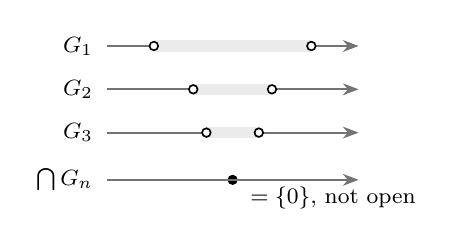
\begin{tikzpicture}[scale=1.0]
  \foreach \n/\y in {1/0, 2/-0.55, 3/-1.1}{
    \pgfmathsetmacro\hw{1/\n}
    \draw[numln,black!55] (-1.6,\y)--(1.6,\y);
    \fill[band] (-\hw,\y-0.07) rectangle (\hw,\y+0.07);
    \node[opt] at (-\hw,\y){}; \node[opt] at (\hw,\y){};
    \node[font=\footnotesize,left] at (-1.65,\y) {$G_{\n}$};
  }
  \node[pt] at (0,-1.7) {};
  \draw[numln,black!55] (-1.6,-1.7)--(1.6,-1.7);
  \node[font=\footnotesize,left] at (-1.65,-1.7) {$\bigcap G_n$};
  \node[font=\footnotesize,right] at (0.1,-1.93) {$=\set0$, not open};
\end{tikzpicture}
\captionof{figure}{Shrinking open intervals $G_n=(-\tfrac1n,\tfrac1n)$ intersect to the single
point $\set0$: an infinite intersection of open sets need not be open.}
\end{center}

\subsection*{Open and closed sets in $\R$}

On the line the open sets have a clean description.

\begin{example}[B\&S 11.1.3]
$\R=(-\infty,\infty)$ is open; any open interval $(a,b)$, $(a,\infty)$, $(-\infty,b)$ is
open; $[0,1]$ is closed; $[0,1)$ is neither; $\N$ is closed; $\set{1/n\st n\in\N}$ is not
closed but $\set{1/n}\cup\set0$ is closed (Rudin 2.21(e)).
\end{example}

\begin{theorem}[Structure of open subsets of $\R$; B\&S 11.1.9, Rudin Ex.~29]\label{t:open-in-R@c3}
A set $G\subseteq\R$ is open iff it is a \emph{countable union of pairwise disjoint open
intervals}.
\end{theorem}

\begin{proof}[Proof sketch]
A countable union of open intervals is open by Theorem~\ref{t:open-closed-ops@c3}(a).
Conversely, for open $G$ and $x\in G$ let $I_x=(a_x,b_x)$ be the largest open interval with
$x\in I_x\subseteq G$ (take $a_x=\inf\set{a\st(a,x]\subseteq G}$, $b_x=\sup\set{b\st
[x,b)\subseteq G}$, allowing $\pm\infty$). One checks the $I_x$ are either equal or disjoint,
so $G=\bigsqcup I_x$ is a disjoint union of open intervals. Each interval contains a rational
(density of $\Q$), and distinct intervals get distinct rationals, so there are at most
countably many.
\end{proof}

\subsection*{The relative (subspace) topology}

A set that is open inside a subspace $Y$ need not be open in the ambient $X$: the segment
$(0,1)$ is open in $\R^1$ but, viewed inside $\R^2$, is not open there. The right notion is
\emph{relative} openness.

\begin{definition}[Rudin 2.29]\label{d:relative@c3}
Let $E\subseteq Y\subseteq X$. Then $E$ is \emph{open relative to $Y$} if for each $p\in E$
there is $r>0$ such that $\set{q\in Y\st d(p,q)<r}\subseteq E$.
\end{definition}

\begin{theorem}[Rudin 2.30]\label{t:relative@c3}
Let $Y\subseteq X$ and $E\subseteq Y$. Then $E$ is open relative to $Y$ if and only if
$E=Y\cap G$ for some set $G$ open in $X$.
\end{theorem}

\begin{proof}
($\Rightarrow$) For each $p\in E$ pick $r_p>0$ with $\set{q\in Y\st d(p,q)<r_p}\subseteq E$,
and let $V_p=N_{r_p}(p)$ in $X$. Put $G=\bigcup_{p\in E}V_p$, open in $X$. Each $p\in V_p$ so
$E\subseteq G\cap Y$; and $V_p\cap Y\subseteq E$ by choice of $r_p$, so $G\cap Y\subseteq E$.
Hence $E=G\cap Y$. ($\Leftarrow$) If $G$ is open in $X$ and $E=G\cap Y$, then each $p\in E$
has $N_r(p)\subseteq G$ for some $r$, whence $N_r(p)\cap Y\subseteq E$; so $E$ is open
relative to $Y$.
\end{proof}

\begin{wex}{Relative topology on $\Z$ and on $[0,1]$}
(a) Show every subset of $\Z\subseteq\R$ is open relative to $\Z$. (b) Show $[0,\tfrac12)$ is
open relative to $[0,1]$ though not open in $\R$.
\wrec ``Is $E$ open in the subspace $Y$?'': intersect an ambient open set with $Y$
(Theorem~\ref{t:relative@c3}).
\wsol (a) For $n\in\Z$, $(n-\tfrac12,n+\tfrac12)\cap\Z=\set n$, so each singleton is
relatively open, hence so is every subset (union of singletons). Thus $\Z$ carries the
discrete topology. (b) $[0,\tfrac12)=(-1,\tfrac12)\cap[0,1]$ with $(-1,\tfrac12)$ open in
$\R$, so it is open relative to $[0,1]$ by Theorem~\ref{t:relative@c3}; but it contains $0$,
none of whose $\R$-neighborhoods lie inside it, so it is not open in $\R$. \emph{Check:}
relative openness genuinely depends on the host space.
\end{wex}

\begin{pitfall}
``Open'' and ``closed'' are properties of a set \emph{relative to a chosen ambient space},
not intrinsic. The same set can be open in $Y$, not open in $X$. Compactness (\S3.4) is the
happy exception: it is \emph{absolute}, independent of the embedding (Rudin 2.33).
\end{pitfall}

\subsection*{Further worked examples}

\begin{wex}{$[0,1)$ is neither open nor closed}
Show in $\R$ that $E=[0,1)$ is neither open nor closed, directly from the definitions.
\wrec Trigger: classify a half-open interval. ``Not open'' is witnessed by one
non-interior point; ``not closed'' by one limit point left out (equivalently, $E^c$ not
open).
\wsol \emph{Not open:} the point $0\in E$ is not interior, since every ball
$B(0,r)=(-r,r)$ contains negative numbers, none of which lie in $E$; so no ball around $0$
fits inside $E$. \emph{Not closed:} the point $1\notin E$ is a limit point of $E$
(the sequence $1-\tfrac1n\in E$ converges to $1$), so $E$ fails to contain a limit point.
Equivalently $E^c=(-\infty,0)\cup[1,\infty)$ is not open because $1\in E^c$ is not interior.
\emph{Check:} ``not open'' and ``not closed'' are independent failures here, occurring at
the two different endpoints --- a concrete reminder that open and closed are not opposites.
\end{wex}

\begin{wex}{An infinite intersection of open sets that happens to stay open}
Exhibit infinitely many open sets $G_n\subseteq\R$ whose intersection is open and nonempty,
contrasting with the shrinking-interval pitfall.
\wrec Trigger: test the sharpness of Theorem~\ref{t:open-closed-ops@c3}(c). The theorem
\emph{guarantees} openness only for finite intersections; it does not \emph{forbid} an
infinite intersection from being open.
\wsol Take $G_n=(-1-\tfrac1n,\,1+\tfrac1n)$, a decreasing nest of open intervals. Their
intersection is $\bigcap_{n\ge1}G_n=[-1,1]$? No: each $G_n$ strictly contains $[-1,1]$, and
a point $x$ lies in every $G_n$ iff $\abs x<1+\tfrac1n$ for all $n$, i.e.\ iff
$\abs x\le1$. So $\bigcap_n G_n=[-1,1]$, which is \emph{closed}, not open --- the nest
collapses onto the boundary. To get an \emph{open} infinite intersection instead, take the
constant family $G_n=(0,1)$ for all $n$: the intersection is $(0,1)$, open. \emph{Check:}
the lesson is that an infinite intersection of opens \emph{may} be open or closed or
neither; finiteness in Theorem~\ref{t:open-closed-ops@c3}(c) is what makes openness automatic,
and its absence makes the outcome case-by-case.
\end{wex}

\begin{wex}{An open set in $\R$ as a disjoint union of intervals}
Write $G=\R\setminus\Z$ as a countable disjoint union of open intervals, illustrating
Theorem~\ref{t:open-in-R@c3}.
\wrec Trigger: ``decompose an open set into its components.'' By
Theorem~\ref{t:open-in-R@c3} every open $G\subseteq\R$ is a countable disjoint union of open
intervals; here the gaps are the integers.
\wsol Removing the integers from the line leaves exactly the open unit intervals between
consecutive integers:
\[
  \R\setminus\Z=\bigsqcup_{n\in\Z}(n,\,n+1).
\]
Each $(n,n+1)$ is open, they are pairwise disjoint, and their union is all reals that are
not integers. The index set $\Z$ is countable, matching the theorem. \emph{Check:} this is
genuinely open --- around any $x\notin\Z$ the ball of radius $\dist(x,\Z)>0$ avoids $\Z$ ---
and its complement $\Z$ is closed (it contains all its limit points, of which there are
none, since $\Z$ has no accumulation point). The component containing $x$ is precisely
$(\floor{x},\floor{x}+1)$.
\end{wex}

\begin{exers}{Exercises (Rudin, Ch.2).}
\item Let $A_1,A_2,A_3,\dots$ be subsets of a metric space. (a) If $B_n=\bigcup_{i=1}^n A_i$,
  prove that $\closure{B_n}=\bigcup_{i=1}^n\closure{A_i}$ for each $n$. (b) If
  $B=\bigcup_{i=1}^\infty A_i$, prove $\closure B\supseteq\bigcup_{i=1}^\infty\closure{A_i}$,
  and show by an example that this inclusion can be proper.
\item Is every point of every open set $E\subseteq\R^2$ a limit point of $E$? Answer the same
  question for closed sets in $\R^2$.
\item Let $E^\circ$ denote the set of all interior points of a set $E$ (the interior of $E$).
  (a) Prove $E^\circ$ is always open. (b) Prove $E$ is open iff $E^\circ=E$. (c) If
  $G\subseteq E$ and $G$ is open, prove $G\subseteq E^\circ$. (d) Prove the complement of
  $E^\circ$ is the closure of the complement of $E$. (e) Do $E$ and $\closure E$ always have
  the same interiors? (f) Do $E$ and $E^\circ$ always have the same closures?
\item Prove that every closed set in a separable metric space is the union of a (possibly
  empty) perfect set and a set which is at most countable. (Corollary: every countable closed
  set in $\R^k$ has isolated points.) [Hint: use the condensation-point exercise.]
\item Prove that every open set in $\R^1$ is the union of an at most countable collection of
  disjoint segments. [Hint: use separability of $\R$.]
\item Imitate the proof that nonempty perfect sets are uncountable to prove Baire's theorem
  in $\R^k$: if $\R^k=\bigcup_{n=1}^\infty F_n$ with each $F_n$ closed, then at least one
  $F_n$ has nonempty interior. Equivalent statement: if each $G_n$ is a dense open subset of
  $\R^k$, then $\bigcap_n G_n$ is nonempty (in fact dense).
\end{exers}

\begin{exers}{Exercises (Bartle \& Sherbert, \S11.1).}
\item If $x\in(0,1)$, let $\eps_x$ be the smaller of $x$ and $1-x$. Show that if
  $\abs{u-x}<\eps_x$ then $u\in(0,1)$.
\item Show that the intervals $(a,\infty)$ and $(-\infty,a)$ are open sets, and that
  $[b,\infty)$ and $(-\infty,b]$ are closed sets.
\item Write out the induction argument proving that the intersection of any finite collection
  of open sets is open.
\item Prove that $(0,1]=\bigcap_{n=1}^\infty(0,1+1/n)$.
\item Show that the set $\N$ of natural numbers is a closed set in $\R$.
\item Show that $A=\set{1/n\st n\in\N}$ is not closed, but that $A\cup\set0$ is closed.
\item Show that the set $\Q$ of rational numbers is neither open nor closed.
\item Show that if $G$ is open and $F$ is closed, then $G\setminus F$ is open and $F\setminus
  G$ is closed.
\item A point $x$ is an \emph{interior point} of $A\subseteq\R$ if some neighborhood $V$ of
  $x$ satisfies $V\subseteq A$. Show that $A$ is open iff every point of $A$ is an interior
  point.
\item A point $x$ is a \emph{boundary point} of $A$ if every neighborhood of $x$ contains
  points of $A$ and points of $A^c$. Show that $A$ and its complement $A^c$ have exactly the
  same boundary points.
\item Show that $G\subseteq\R$ is open iff it contains none of its boundary points.
\item Show that $F\subseteq\R$ is closed iff it contains all of its boundary points.
\item For $A\subseteq\R$, let $A^\circ$ be the union of all open sets contained in $A$ (the
  interior). Show $A^\circ$ is open, is the largest open set contained in $A$, and that $z\in
  A^\circ$ iff $z$ is an interior point of $A$.
\item With the interior notation, for sets $A,B$ show $A^\circ\subseteq A$,
  $(A^\circ)^\circ=A^\circ$, and $(A\cap B)^\circ=A^\circ\cap B^\circ$. Show also
  $A^\circ\cup B^\circ\subseteq(A\cup B)^\circ$, and give an example where the inclusion is
  proper.
\item For $A\subseteq\R$, let $\closure A$ be the intersection of all closed sets containing
  $A$ (the closure). Show $\closure A$ is closed, is the smallest closed set containing $A$,
  and that $w\in\closure A$ iff $w$ is an interior or a boundary point of $A$.
\item With the closure notation, for sets $A,B$ show $A\subseteq\closure A$,
  $\closure{\closure A}=\closure A$, and $\closure{A\cup B}=\closure A\cup\closure B$. Show
  $\closure{A\cap B}\subseteq\closure A\cap\closure B$, and give an example where the
  inclusion is proper.
\item Give an example of a set $A\subseteq\R$ with $A^\circ=\es$ and $\closure A=\R$.
\item Show that if $F\subseteq\R$ is closed, nonempty, and bounded above, then $\sup F$
  belongs to $F$.
\item Show that each point of the Cantor set $F$ is a cluster point of $F$.
\item Show that each point of the Cantor set $F$ is a cluster point of its complement $F^c$.
\end{exers}

\begin{exers}{Additional exercises.}
\item Decide for each set whether it is open, closed, both, or neither in $\R$:
  (a) $[0,1)$; (b) $\set{1/n\st n\in\N}$; (c) $\Z$; (d) $\Q$; (e) $\R\setminus\Q$;
  (f) $\set0\cup\set{1/n}$.
\item Prove directly from the definition that the half-plane $\set{(x,y)\in\R^2\st x>0}$ is
  open.
\item Show that a single point $\set p$ is closed in any metric space, and conclude that every
  finite set is closed.
\item Prove that $G\subseteq X$ is open iff $G=\interior G$, and that $F$ is closed iff
  $F=\closure F$.
\item (Non-example.) The infinite intersection $\bigcap_n G_n$ of open sets need not be open.
  Exhibit open $G_n\subseteq\R$ with $\bigcap_n G_n=\set0\cup[1,2]$, a non-open set.
\item Give an example of two sets $A,B\subseteq\R$, neither open nor closed, with $A\cup B$
  open and $A\cap B$ closed.
\item (Diagram.) Draw an open set in $\R^2$ as a union of three overlapping open disks, and
  mark one interior point together with a ball witnessing its interiority.
\item Prove that the boundary $\partial E=\closure E\setminus\interior E$ of any set is
  closed, and that $E$ is open iff $E\cap\partial E=\es$.
\item Using the structure theorem, write the open set $\R\setminus\Z$ as a countable disjoint
  union of open intervals.
\item Let $Y=[0,2]\subseteq\R$. Determine whether $[0,1)$ and $(1,2]$ are open relative to
  $Y$, closed relative to $Y$, or both, and exhibit ambient open/closed sets $G$ with
  $[0,1)=Y\cap G$.
\item Prove that $E$ is open in $X$ iff $E$ is a union of open balls.
\end{exers}


\section{Limit Points, Closure, and Interior}
\subsection*{Limit points and isolated points}

\begin{definition}[Rudin 2.18(b)(c); cluster point, B\&S \S4.1, \S11.1]\label{d:limit-pt@c3}
Let $E\subseteq X$ and $p\in X$.
\begin{itemize}[leftmargin=1.4em]
\item $p$ is a \emph{limit point} (or \emph{cluster point}, or \emph{accumulation point}) of
  $E$ if every neighborhood of $p$ contains a point $q\in E$ with $q\neq p$.
\item If $p\in E$ but $p$ is not a limit point of $E$, then $p$ is an \emph{isolated point}
  of $E$ (some ball $B(p,r)$ meets $E$ only at $p$).
\end{itemize}
The set of limit points of $E$ is written $E'$.
\end{definition}

A limit point need not belong to $E$, and a point of $E$ need not be a limit point. The set
$\set{1/n\st n\in\N}$ has the single limit point $0$ (which is not in the set), and every one
of its own points is isolated --- ``having a limit point'' and ``containing a limit point''
are different (Rudin 2.21(e)).

\begin{theorem}[Limit points are approached infinitely often; Rudin 2.20]\label{t:inf-many@c3}
If $p$ is a limit point of $E$, then every neighborhood of $p$ contains infinitely many
points of $E$. In particular a finite set has no limit points.
\end{theorem}

\begin{proof}
Suppose some neighborhood $N$ of $p$ met $E$ in only finitely many points $q_1,\dots,q_n$
distinct from $p$. Put $r=\min_{1\le m\le n}d(p,q_m)>0$ (a finite minimum of positive
numbers). Then $N_r(p)$ contains no point $q\neq p$ of $E$, contradicting that $p$ is a limit
point.
\end{proof}

\begin{center}
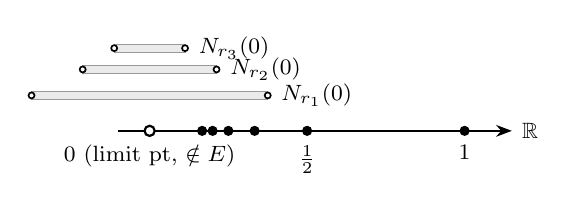
\begin{tikzpicture}[scale=1.0]
  \draw[numln] (-0.4,0)--(4.6,0) node[right,font=\footnotesize]{$\R$};
  % points 1/n accumulating at 0
  \foreach \k in {1,2,3,4,5,6}{
    \pgfmathsetmacro\x{4/\k}
    \node[pt] at (\x,0) {};
  }
  \node[pt,fill=white,draw,line width=0.8pt] (zero) at (0,0) {};
  \node[font=\footnotesize,below] at (0,-0.06) {$0$ (limit pt, $\notin E$)};
  \node[font=\footnotesize,below] at (4,-0.06) {$1$};
  \node[font=\footnotesize,below] at (2,-0.06) {$\tfrac12$};
  % shrinking neighborhoods of 0
  \foreach \r/\yy in {1.5/0.45, 0.85/0.78, 0.45/1.05}{
    \draw[band,draw=black!40] (-\r,\yy-0.05) rectangle (\r,\yy+0.05);
    \node[opt,scale=0.7] at (-\r,\yy){}; \node[opt,scale=0.7] at (\r,\yy){};
  }
  \node[font=\footnotesize,right] at (1.55,0.45) {$N_{r_1}(0)$};
  \node[font=\footnotesize,right] at (0.9,0.78) {$N_{r_2}(0)$};
  \node[font=\footnotesize,right] at (0.5,1.05) {$N_{r_3}(0)$};
\end{tikzpicture}
\captionof{figure}{$E=\set{1/n}$ has the one limit point $0$. Shrinking neighborhoods of $0$ each
still capture infinitely many $1/n$; every point of $E$ is isolated.}
\end{center}

\subsection*{Closure}

\begin{definition}[Rudin 2.26]\label{d:closure@c3}
The \emph{closure} of $E$ is $\closure E=E\cup E'$ (the set together with all its limit
points).
\end{definition}

\begin{theorem}[Rudin 2.27]\label{t:closure@c3}
For $E\subseteq X$:
\textup{(a)} $\closure E$ is closed;
\textup{(b)} $\closure E=E$ iff $E$ is closed;
\textup{(c)} $\closure E\subseteq F$ for every closed $F\supseteq E$.
Hence $\closure E$ is the \emph{smallest} closed set containing $E$.
\end{theorem}

\begin{proof}
(a) Let $p\in(\closure E)^c$, so $p\notin E$ and $p\notin E'$; thus some neighborhood $N$ of
$p$ contains no point of $E$ (other than $p$, which is excluded). Then $N$ also contains no
limit point of $E$: if $q\in N$ then $N$ is a neighborhood of $q$ missing $E\setminus\set
q$, so $q\notin E'$. Hence $N\subseteq(\closure E)^c$, proving $(\closure E)^c$ open and
$\closure E$ closed. (b) If $\closure E=E$ then $E$ is closed by (a); if $E$ is closed then
$E'\subseteq E$ (it contains its limit points, \S3.2 / Theorem~\ref{t:closed-iff-lim@c3}), so
$\closure E=E\cup E'=E$. (c) If $F$ is closed and $E\subseteq F$ then $E'\subseteq F'\subseteq
F$, so $\closure E=E\cup E'\subseteq F$.
\end{proof}

\begin{theorem}[Closed $\eqv$ contains its limit points; Rudin 2.18(d), B\&S 11.1.7--11.1.8]
\label{t:closed-iff-lim@c3}
$E$ is closed iff $E\supseteq E'$, iff $E$ contains the limit of every convergent sequence
of its points.
\end{theorem}

\begin{proof}
If $E$ is closed and $p$ is a limit point with $p\notin E$, then $p\in E^c$ open, so some
ball $B(p,r)\subseteq E^c$ misses $E$ --- contradicting $p\in E'$; hence $E'\subseteq E$.
Conversely if $E'\subseteq E$ and $p\in E^c$, then $p$ is not a limit point, so a ball
$B(p,r)$ misses $E$, i.e.\ $B(p,r)\subseteq E^c$; so $E^c$ is open and $E$ closed. The
sequential form is equivalent because a cluster point is exactly a limit of a nonconstant
sequence from $E$ (B\&S 4.1.2).
\end{proof}

\begin{theorem}[Sup and inf lie in a closed set; Rudin 2.28, B\&S Ex.~11.1.18]\label{t:sup-closed@c3}
If $\es\neq E\subseteq\R$ is bounded above and $y=\sup E$, then $y\in\closure E$. Hence if $E$
is closed, $\sup E\in E$ (and likewise $\inf E\in E$).
\end{theorem}

\begin{proof}
If $y\in E$ we are done. Otherwise, for every $h>0$ there is $x\in E$ with $y-h<x<y$ (else
$y-h$ would be an upper bound smaller than the least upper bound). So every neighborhood of
$y$ meets $E\setminus\set y$; $y\in E'\subseteq\closure E$.
\end{proof}

\subsection*{Interior; dense sets}

\begin{definition}[Rudin Ex.~9; interior, B\&S Ex.~11.1.13]\label{d:interior@c3}
The \emph{interior} $\interior E$ of $E$ is the set of all interior points of $E$;
equivalently the union of all open sets contained in $E$, hence the \emph{largest} open
subset of $E$. A set $E$ is \emph{dense} in $X$ if $\closure E=X$, i.e.\ every point of $X$
is a point of $E$ or a limit point of $E$ (Rudin 2.18(j)).
\end{definition}

\begin{proposition}[Interior/closure duality; Rudin Ex.~9(d)]\label{p:int-clos-dual@c3}
$\interior E$ is open and $\interior E\subseteq E$; moreover
\[
  (\interior E)^c=\closure{E^c}\qquad\text{and dually}\qquad (\closure E)^c=\interior{(E^c)}.
\]
\end{proposition}

\begin{proof}
$\interior E$ is a union of open sets, hence open
(Theorem~\ref{t:open-closed-ops@c3}(a)), and lies in $E$. For the duality,
$p\notin\interior E$ means no ball around $p$ lies in $E$, i.e.\ every ball meets $E^c$,
i.e.\ $p\in E^c$ or $p$ is a limit point of $E^c$, i.e.\ $p\in\closure{E^c}$. Taking
complements gives the dual statement.
\end{proof}

\begin{wex}{Closure, interior, and limit points of $\Q\cap(0,1)$}
Let $E=\Q\cap(0,1)\subseteq\R$. Find $\closure E$, $\interior E$, and $E'$.
\wrec ``Compute closure/interior of a dense-ish set'': use that $\Q$ is dense in $\R$.
\wsol Every real in $[0,1]$ is a limit of rationals in $(0,1)$, so $E'=[0,1]$ and
$\closure E=E\cup E'=[0,1]$. The interior is empty: any ball around a point of $E$ contains
irrationals, so no ball lies in $E$; thus $\interior E=\es$. \emph{Check:} consistent with
duality --- $(\interior E)^c=\R=\closure{E^c}$ since $E^c\supseteq$ the irrationals is dense.
$E$ is a set whose closure is a fat interval but whose interior is empty: ``boundary is
everything.''
\end{wex}

\begin{wex}{$E$ and $E'$ need not have the same limit points (Rudin Ex.~6)}
Show $\closure E$ and $E$ always have the same limit points, but $E$ and $E'$ need not.
\wrec ``Compare derived sets'': test the claim on a set whose limit points are themselves
isolated as a set.
\wsol Since $E\subseteq\closure E\subseteq E\cup E'$ and limit points only depend on
arbitrarily-close companions, one shows $(\closure E)'=E'$ (a limit point of $\closure E$ is
approached by points of $E$, possibly via nearby limit points). But $E$ and $E'$ can differ:
let $E=\set{1/n\st n\in\N}$. Then $E'=\set0$, and $(E')'=\es$ (a single point has no limit
points), while $E'=\set0\neq\es=(E')'$. \emph{Check:} so applying $'$ is not idempotent in
general; iterating can strip points (here $E\to\set0\to\es$).
\end{wex}

\begin{method}{Finding the closure of a set $E$}
\textbf{Recognition trigger.} ``Compute $\closure E$,'' or ``is $E$ closed/dense?''.
\begin{enumerate}
\item Identify the limit points: $p\in E'$ iff there is a sequence $x_n\in E$, $x_n\neq p$,
  with $x_n\to p$. Sweep the boundary of $E$ and any accumulation values.
\item Form $\closure E=E\cup E'$. Then $E$ is closed iff this adds nothing ($E'\subseteq E$),
  and $E$ is dense in $X$ iff $\closure E=X$.
\item Cross-check with the smallest-closed-superset description
  (Theorem~\ref{t:closure@c3}(c)) and with $\interior E$ via duality
  (Proposition~\ref{p:int-clos-dual@c3}).
\end{enumerate}
\end{method}

\begin{wex}{A bounded set with exactly three limit points (Rudin Ex.~5)}
Construct a bounded $E\subseteq\R$ whose set of limit points is a $3$-element set.
\wrec ``Build a set with prescribed limit points'': glue together copies of a sequence
accumulating at each desired point.
\wsol Take three centers, say $0,1,2$, and around each a sequence converging to it:
\[
  E=\set{\tfrac1n\st n\in\N}\ \cup\ \set{1+\tfrac1n\st n\in\N}\ \cup\
  \set{2+\tfrac1n\st n\in\N}.
\]
$E\subseteq[0,3]$ is bounded. Each center $0,1,2$ is a limit point (its sequence converges to
it), and no other point is: away from $\set{0,1,2}$ the set is locally finite. So
$E'=\set{0,1,2}$, three points. \emph{Check:} none of $0,1,2$ lies in $E$, illustrating again
that limit points need not be members. Replace ``three'' by a sequence of centers and you get
Rudin Ex.~13's compact set with countably many limit points.
\end{wex}

\begin{pitfall}
$\closure{A\cup B}=\closure A\cup\closure B$ holds (finite unions), but
$\closure{A\cap B}\subseteq\closure A\cap\closure B$ can be \emph{strict}: with $A=\Q$,
$B=\R\setminus\Q$, $A\cap B=\es$ so $\closure{A\cap B}=\es$, while $\closure A\cap\closure
B=\R\cap\R=\R$. Dually $\interior{(A\cap B)}=\interior A\cap\interior B$ but
$\interior{(A\cup B)}\supseteq\interior A\cup\interior B$ may be strict (B\&S Ex.~11.1.14,
11.1.16). Closure distributes over $\cup$, interior over $\cap$ --- not the other way.
\end{pitfall}

\subsection*{Further worked examples}

\begin{wex}{Closure and interior of a half-open interval}
For $E=(0,1]\subseteq\R$ compute $\closure E$, $\interior E$, $E'$, and the boundary
$\partial E=\closure E\setminus\interior E$.
\wrec Trigger: ``compute closure/interior/boundary of an interval.'' Sweep the endpoints for
limit points (Method, Finding the closure); the interior is the largest open subinterval.
\wsol \emph{Limit points:} every point of $[0,1]$ is approached by points of $(0,1]$, and no
point outside $[0,1]$ is; so $E'=[0,1]$ and $\closure E=E\cup E'=[0,1]$. \emph{Interior:} a
point $p$ is interior iff some $(p-r,p+r)\subseteq(0,1]$, which holds exactly for
$0<p<1$; the right endpoint $1$ fails (any ball includes numbers $>1$) and $0\notin E$. So
$\interior E=(0,1)$. \emph{Boundary:} $\partial E=[0,1]\setminus(0,1)=\set{0,1}$.
\emph{Check:} duality holds --- $(\interior E)^c=\R\setminus(0,1)=\closure{E^c}$, and indeed
$E^c=(-\infty,0]\cup(1,\infty)$ has closure $(-\infty,0]\cup[1,\infty)=\R\setminus(0,1)$.
The boundary is the two endpoints, as expected for an interval.
\end{wex}

\begin{wex}{The closure of a ball can be smaller than the closed ball}
In a general metric space show $\closure{B(p,r)}\subseteq\set{q\st d(p,q)\le r}$, and give a
space where the inclusion is strict.
\wrec Trigger: a closure-vs-closed-ball comparison. The open ball's closure is always
contained in the closed ball; equality is a Euclidean luxury, not a metric-space theorem.
\wsol Let $\bar B=\set{q\st d(p,q)\le r}$. Since $\bar B$ is closed (its complement
$\set{d(p,q)>r}$ is open: if $d(p,q_0)>r$, the ball $B(q_0,d(p,q_0)-r)$ stays outside $\bar
B$ by the reverse triangle inequality) and contains $B(p,r)$, the smallest-closed-superset
property (Theorem~\ref{t:closure@c3}(c)) gives $\closure{B(p,r)}\subseteq\bar B$. \emph{Strict
case:} take the discrete metric on a set $X$ with $\ge2$ points and $r=1$. Then
$B(p,1)=\set p$ (only $p$ is within distance $<1$), which is already closed, so
$\closure{B(p,1)}=\set p$. But $\bar B=\set{q\st d(p,q)\le1}=X$. Thus
$\closure{B(p,1)}=\set p\subsetneq X=\bar B$. \emph{Check:} in $\R^k$ the two always agree
($\closure{B(p,r)}=\bar B$), so the strictness is a purely non-Euclidean phenomenon ---
another reason never to assume metric spaces behave like $\R^k$.
\end{wex}

\begin{exers}{Exercises (Rudin, Ch.2).}
\item Construct a bounded set of real numbers with exactly three limit points.
\item Let $E'$ be the set of all limit points of a set $E$. Prove that $E'$ is closed. Prove
  that $E$ and $\closure E$ have the same limit points. (Recall $\closure E=E\cup E'$.) Do $E$
  and $E'$ always have the same limit points?
\end{exers}

\begin{exers}{Additional exercises.}
\item Find $\closure E$, $\interior E$, and $E'$ for each: (a) $E=(0,1]\cup\set2$;
  (b) $E=\set{1/n\st n\in\N}$; (c) $E=\Z$; (d) $E=\Q\cap[0,1]$.
\item Prove that $p$ is a limit point of $E$ iff there is a sequence $x_n\in E$ with
  $x_n\neq p$ and $x_n\to p$.
\item Show that the set of isolated points of any $E\subseteq\R$ is at most countable.
  [Hint: each isolated point owns a rational-endpoint interval meeting $E$ only at itself.]
\item Prove that $\interior{(A\cap B)}=\interior A\cap\interior B$ for all $A,B$.
\item (Non-example.) Show that $\closure{A\cap B}=\closure A\cap\closure B$ can fail, and that
  $\interior{(A\cup B)}=\interior A\cup\interior B$ can fail, using $A=\Q$, $B=\R\setminus\Q$.
\item A set $E$ is \emph{dense} in $X$ if $\closure E=X$. Prove $E$ is dense iff every
  nonempty open set meets $E$, and verify $\Q$ is dense in $\R$.
\item (Diagram.) Draw a point $p$ together with three shrinking neighborhoods, each
  containing a distinct point of a set $E$ accumulating at $p$, illustrating that $p\in E'$.
\item Construct a set $E\subseteq\R$ with $E'=\Z$ (its limit points are exactly the integers).
\item Prove that $E'$ is always closed (i.e.\ $(E')'\subseteq E'$), and give an example where
  $(E')'\subsetneq E'$.
\item Show that a set $E$ is closed iff $E=\closure E$ iff $\partial E\subseteq E$, and that
  $E$ is perfect iff $E=E'$.
\end{exers}


\section{Compact Sets and the Heine--Borel Theorem}
\subsection*{Open covers and compactness}

\begin{definition}[Rudin 2.31--2.32; B\&S 11.2.1--11.2.2]\label{d:compact@c3}
An \emph{open cover} of $E\subseteq X$ is a collection $\set{G_\alpha}$ of open sets with
$E\subseteq\bigcup_\alpha G_\alpha$. A \emph{subcover} is a subcollection that still covers
$E$; a \emph{finite subcover} is one with finitely many sets. A set $K\subseteq X$ is
\emph{compact} if every open cover of $K$ admits a finite subcover.
\end{definition}

The quantifier structure is the whole game. To prove $K$ \emph{compact} you must start with an
\emph{arbitrary} open cover and extract a finite subcover. To prove $H$ \emph{not} compact it
suffices to exhibit \emph{one} open cover with no finite subcover.

\begin{example}[B\&S 11.2.3]
$[0,1)$ is not compact: the cover $G_n=(-1,1-\tfrac1n)$, $n\in\N$, has union $[0,1)$ but any
finite subfamily has union $(-1,1-\tfrac1m)$ for the largest $m$, missing points near $1$.
Likewise $(0,1)$ is not compact via $G_n=(\tfrac1n,1)$. Every finite set \emph{is} compact:
cover each of its points by one set of the cover.
\end{example}

\begin{center}
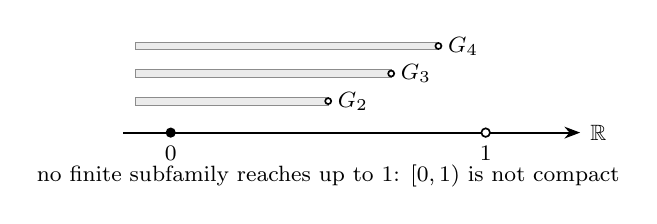
\begin{tikzpicture}[scale=1.0]
  \draw[numln] (-0.6,0)--(5.2,0) node[right,font=\footnotesize]{$\R$};
  \node[pt] at (0,0){}; \node[font=\footnotesize,below] at (0,-0.05){$0$};
  \node[opt] at (4,0){}; \node[font=\footnotesize,below] at (4,-0.05){$1$};
  % cover of [0,1) by (-1, 1-1/n): draw three growing intervals
  \foreach \r/\yy/\lab in {2.0/0.4/{G_2}, 2.8/0.75/{G_3}, 3.4/1.1/{G_4}}{
    \draw[band,draw=black!45] (-0.45,\yy-0.05) rectangle (\r,\yy+0.05);
    \node[opt,scale=0.7] at (\r,\yy){};
    \node[font=\footnotesize,right] at (\r,\yy) {$\lab$};
  }
  \node[font=\footnotesize,align=center] at (2.0,-0.55)
    {no finite subfamily reaches up to $1$: $[0,1)$ is not compact};
\end{tikzpicture}
\end{center}

\subsection*{Compactness is absolute, and forces closed + bounded}

\begin{theorem}[Compactness is intrinsic; Rudin 2.33]\label{t:compact-absolute@c3}
If $K\subseteq Y\subseteq X$, then $K$ is compact relative to $X$ iff compact relative to
$Y$.
\end{theorem}

\begin{proof}
By Theorem~\ref{t:relative@c3}, relatively-open-in-$Y$ sets are exactly $Y\cap G$ for $G$ open
in $X$. A cover of $K$ by $X$-open sets restricts to a $Y$-open cover and vice versa, and
since $K\subseteq Y$ a finite subcover in one picture is one in the other.
\end{proof}

This is why we may speak of a ``compact metric space'' without naming an ambient space ---
unlike open or closed, compactness does not depend on the embedding.

\begin{theorem}[Compact $\Rightarrow$ closed; Rudin 2.34, B\&S 11.2.4]\label{t:compact-closed@c3}
Every compact subset $K$ of a metric space $X$ is closed.
\end{theorem}

\begin{proof}
We show $K^c$ is open. Fix $p\notin K$. For each $q\in K$ choose disjoint balls
$V_q=N_{r}(p)$ and $W_q=N_{r}(q)$ with $r<\tfrac12 d(p,q)$. The $\set{W_q}_{q\in K}$ cover
$K$; by compactness finitely many $W_{q_1},\dots,W_{q_n}$ cover $K$. Let
$V=V_{q_1}\cap\cdots\cap V_{q_n}$, a neighborhood of $p$. Then $V$ is disjoint from each
$W_{q_i}$, hence from $K\subseteq\bigcup W_{q_i}$, so $V\subseteq K^c$. Thus $p$ is interior
to $K^c$.
\end{proof}

\begin{theorem}[Compact $\Rightarrow$ bounded; B\&S 11.2.4]\label{t:compact-bdd@c3}
Every compact $K$ is bounded.
\end{theorem}

\begin{proof}
Fix $x_0\in X$. The balls $H_m=N_m(x_0)$, $m\in\N$, cover $X\supseteq K$; a finite subcover
$H_{m_1},\dots$ has union the largest $H_M=N_M(x_0)$, so $K\subseteq N_M(x_0)$ is bounded.
\end{proof}

\begin{theorem}[Closed subset of compact is compact; Rudin 2.35, B\&S Ex.~11.2.4]\label{t:closed-of-compact@c3}
If $F\subseteq K\subseteq X$ with $F$ closed (in $X$) and $K$ compact, then $F$ is compact.
Consequently $F\cap K$ is compact whenever $F$ is closed and $K$ compact.
\end{theorem}

\begin{proof}
Let $\set{V_\alpha}$ be an open cover of $F$. Adjoin the open set $F^c$ to obtain an open
cover $\Omega$ of $K$. Compactness of $K$ gives a finite subcover $\Phi\subseteq\Omega$ of
$K$; discarding $F^c$ from $\Phi$ if present still leaves a cover of $F$ by finitely many
$V_\alpha$. So $F$ is compact.
\end{proof}

\subsection*{Nested compact sets and the finite intersection property}

\begin{theorem}[Finite intersection property; Rudin 2.36, B\&S Ex.~11.2.9]\label{t:fip@c3}
Let $\set{K_\alpha}$ be compact sets such that every finite subcollection has nonempty
intersection. Then $\bigcap_\alpha K_\alpha\neq\es$. In particular, a nested sequence
$K_1\supseteq K_2\supseteq\cdots$ of nonempty compact sets has $\bigcap_n K_n\neq\es$.
\end{theorem}

\begin{proof}
Fix $K_1$ and suppose, for contradiction, $\bigcap_\alpha K_\alpha=\es$, i.e.\ no point of
$K_1$ lies in every $K_\alpha$. Then the sets $G_\alpha=K_\alpha^c$ (open, since each
$K_\alpha$ is closed by Theorem~\ref{t:compact-closed@c3}) cover $K_1$. By compactness finitely
many cover $K_1$: $K_1\subseteq G_{\alpha_1}\cup\cdots\cup G_{\alpha_n}$, i.e.\
$K_1\cap K_{\alpha_1}\cap\cdots\cap K_{\alpha_n}=\es$, contradicting the finite-intersection
hypothesis.
\end{proof}

\begin{theorem}[Infinite subset of a compact set has a limit point; Rudin 2.37]\label{t:bw-compact@c3}
If $E$ is an infinite subset of a compact set $K$, then $E$ has a limit point in $K$.
\end{theorem}

\begin{proof}
If no point of $K$ were a limit point of $E$, each $q\in K$ would have a ball $V_q$ meeting
$E$ in at most one point (namely $q$ if $q\in E$). The $\set{V_q}$ cover $K$, but no finite
subfamily can cover the infinite $E\subseteq K$ --- each $V_q$ captures $\le1$ point of $E$.
This contradicts compactness.
\end{proof}

\subsection*{$k$-cells, nested intervals, and Heine--Borel}

\begin{definition}[Rudin 2.17]
A \emph{$k$-cell} is a product $[a_1,b_1]\times\cdots\times[a_k,b_k]\subseteq\Rk$ (a $1$-cell
is a closed interval, a $2$-cell a closed rectangle).
\end{definition}

\begin{theorem}[Nested intervals / cells; Rudin 2.38--2.39, B\&S 2.5.2]\label{t:nested@c3}
If $\set{I_n}$ are intervals (or $k$-cells) with $I_n\supseteq I_{n+1}$, then
$\bigcap_n I_n\neq\es$.
\end{theorem}

\begin{proof}
For intervals $I_n=[a_n,b_n]$, let $x=\sup_n a_n$ (the $a_n$ are bounded above by $b_1$). For
all $m,n$, $a_n\le a_{m+n}\le b_{m+n}\le b_m$, so $x\le b_m$; and $a_m\le x$; thus $x\in I_m$
for all $m$. For $k$-cells apply this coordinatewise.
\end{proof}

\begin{theorem}[Every $k$-cell is compact; Rudin 2.40]\label{t:kcell-compact@c3}
Every $k$-cell $I\subseteq\Rk$ is compact.
\end{theorem}

\begin{proof}
Let $\delta=\bigl(\sum_j(b_j-a_j)^2\bigr)^{1/2}=\diam I$. Suppose an open cover
$\set{G_\alpha}$ of $I$ had no finite subcover. Bisect each edge at its midpoint
$c_j=(a_j+b_j)/2$; this splits $I$ into $2^k$ subcells, at least one of which --- call it
$I_1$ --- has no finite subcover (else $I$ would). Repeat, producing
$I\supseteq I_1\supseteq I_2\supseteq\cdots$ with: (i) $I_n$ has no finite subcover, and
(ii) $\diam I_n=2^{-n}\delta$. By Theorem~\ref{t:nested@c3} there is $x^*\in\bigcap_n I_n$. Some
$G_\alpha\ni x^*$, and openness gives $r$ with $N_r(x^*)\subseteq G_\alpha$. Choosing $n$ with
$2^{-n}\delta<r$ forces $I_n\subseteq N_r(x^*)\subseteq G_\alpha$ --- a finite (one-set!)
subcover of $I_n$, contradicting (i).
\end{proof}

\begin{center}
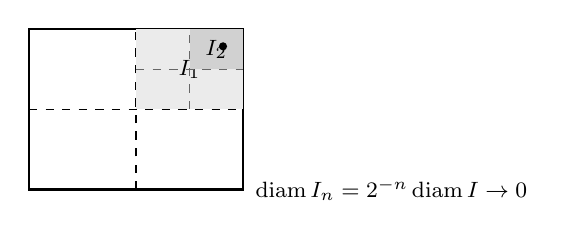
\begin{tikzpicture}[scale=1.7]
  % bisection of a 2-cell
  \draw[line width=0.9pt] (0,0) rectangle (1.6,1.2);
  \draw[dashed] (0.8,0)--(0.8,1.2);
  \draw[dashed] (0,0.6)--(1.6,0.6);
  % shade the chosen quadrant I_1
  \fill[band] (0.8,0.6) rectangle (1.6,1.2);
  \node[font=\footnotesize] at (1.2,0.9) {$I_1$};
  % second bisection inside I_1
  \draw[dashed,black!60] (1.2,0.6)--(1.2,1.2);
  \draw[dashed,black!60] (0.8,0.9)--(1.6,0.9);
  \fill[black!18] (1.2,0.9) rectangle (1.6,1.2);
  \node[font=\footnotesize] at (1.4,1.05) {$I_2$};
  \node[pt,scale=0.8] at (1.45,1.07) {};
  \node[font=\footnotesize,right] at (1.62,0) {$\diam I_n=2^{-n}\diam I\to0$};
\end{tikzpicture}
\captionof{figure}{Repeated bisection of a $2$-cell: the ``bad'' subcell shrinks to a point
$x^*$, whose covering ball already covers a whole $I_n$ --- contradiction.}
\end{center}

\begin{theorem}[Heine--Borel; Rudin 2.41, B\&S 11.2.5]\label{t:heine-borel@c3}
For $E\subseteq\Rk$ the following are equivalent:
\textup{(a)} $E$ is closed and bounded;
\textup{(b)} $E$ is compact;
\textup{(c)} every infinite subset of $E$ has a limit point in $E$
\textup{(}the \emph{Bolzano--Weierstrass property}\textup{)}.
\end{theorem}

\begin{proof}
\textbf{(a)$\Rightarrow$(b):} bounded $E$ lies in some $k$-cell $I$; $I$ is compact
(Theorem~\ref{t:kcell-compact@c3}) and $E$ is a closed subset of $I$, hence compact
(Theorem~\ref{t:closed-of-compact@c3}). \textbf{(b)$\Rightarrow$(c):}
Theorem~\ref{t:bw-compact@c3}. \textbf{(c)$\Rightarrow$(a):} If $E$ were unbounded, pick
$x_n\in E$ with $\abs{x_n}>n$; then $\set{x_n}$ is infinite with no limit point, against (c).
If $E$ were not closed, take a limit point $x_0\notin E$ and $x_n\in E$ with
$\abs{x_n-x_0}<\tfrac1n$; then $\set{x_n}$ is infinite, has $x_0$ as its only limit point in
$\Rk$, and $x_0\notin E$, so $E$ has no limit point in $E$ from this set --- against (c).
\end{proof}

\begin{remark}[The hypotheses are sharp]
(a)$\Leftrightarrow$(b) is special to $\Rk$. In a general metric space (b)$\Leftrightarrow$(c)
always holds (Rudin Ex.~26), but ``closed + bounded'' need \emph{not} imply compact: in
$\Q$, the set $E=\set{p\in\Q\st 2<p^2<3}$ is closed and bounded in $\Q$ yet not compact
(Rudin Ex.~16); in infinite-dimensional spaces the closed unit ball is not compact.
\end{remark}

\begin{theorem}[Weierstrass; Rudin 2.42]\label{t:weierstrass@c3}
Every bounded infinite subset of $\Rk$ has a limit point in $\Rk$.
\end{theorem}

\begin{proof}
Such a set $E$ lies in a $k$-cell $I$, which is compact; apply
Theorem~\ref{t:bw-compact@c3}.
\end{proof}

\begin{theorem}[Sequential compactness; B\&S 11.2.6]\label{t:seq-compact@c3}
$K\subseteq\R$ \textup{(}or $\Rk$\textup{)} is compact iff every sequence in $K$ has a
subsequence converging to a point of $K$.
\end{theorem}

\begin{proof}
If $K$ is compact it is closed and bounded (Heine--Borel); a sequence in $K$ is bounded, so
Bolzano--Weierstrass gives a convergent subsequence, whose limit lies in the closed $K$.
Conversely, if $K$ is not closed, a cluster point $c\notin K$ is the limit of a sequence in
$K$ none of whose subsequences can converge in $K$; if $K$ is not bounded, pick $x_n\in K$
with $\abs{x_n}>n$ --- no subsequence converges. So the sequential property forces closed +
bounded, i.e.\ compact.
\end{proof}

\begin{method}{Proving a specific set $K$ is compact}
\textbf{Recognition trigger.} ``Show $K$ is compact'' (directly, or by Heine--Borel).
\begin{enumerate}
\item \textbf{In $\Rk$:} the fast route is Heine--Borel --- show $K$ is closed (contains its
  limit points) and bounded (lies in a ball). Done.
\item \textbf{From the definition} (when asked, e.g.\ Rudin Ex.~12): take an arbitrary open
  cover; use the structure of $K$ (an accumulation point, a nesting) to peel off all but
  finitely many points with one or two cover sets, then cover the finite remainder.
\item \textbf{Via sequences:} show every sequence in $K$ has a subsequence converging in
  $K$.
\item \textbf{To disprove compactness:} exhibit one bad open cover, or one sequence with no
  convergent-in-$K$ subsequence.
\end{enumerate}
\end{method}

\begin{wex}{$K=\set0\cup\set{1/n\st n\in\N}$ is compact from the definition (Rudin Ex.~12)}
Prove directly (no Heine--Borel) that $K$ is compact.
\wrec ``Compact from the definition'' with one accumulation point: one cover set swallows the
tail.
\wsol Let $\set{G_\alpha}$ be an open cover. Some $G_{\alpha_0}\ni0$; being open, it contains
a ball $N_r(0)$, hence all $1/n$ with $1/n<r$, i.e.\ all but finitely many points of $K$. The
finitely many remaining points $1,\tfrac12,\dots,\tfrac1N$ each lie in some $G_{\alpha_i}$.
Then $G_{\alpha_0},G_{\alpha_1},\dots,G_{\alpha_N}$ is a finite subcover. \emph{Check:} $K$
is closed (it contains its only limit point $0$) and bounded, agreeing with Heine--Borel.
Compare Rudin Ex.~13: a compact set whose limit points form a countable set.
\end{wex}

\begin{wex}{A bounded, non-compact set in $\Q$ (Rudin Ex.~16)}
In the metric space $\Q$, let $E=\set{p\in\Q\st 2<p^2<3}$. Show $E$ is closed and bounded in
$\Q$ but not compact, and is open in $\Q$.
\wrec ``Closed + bounded but not compact'': the missing limits $\pm\sqrt2,\pm\sqrt3$ are
irrational, so invisible to $\Q$.
\wsol $E=\Q\cap\bigl((\sqrt2,\sqrt3)\cup(-\sqrt3,-\sqrt2)\bigr)$. It is bounded ($\abs
p<\sqrt3$). It is \emph{closed in $\Q$}: a $\Q$-limit point $p$ of $E$ has $2\le p^2\le3$
with $p\in\Q$, but $p^2=2$ or $3$ is impossible for rational $p$, so $2<p^2<3$ and $p\in E$.
It is \emph{open in $\Q$} for the same reason (the constraint is an open condition with no
rational on the boundary). Not compact: the sets $G_n=\set{p\in\Q\st 2+\tfrac1n<p^2<3}$ form
an open cover of (the positive part of) $E$ with no finite subcover, as $p^2\downarrow2$ is
approached by rationals. \emph{Check:} in $\R$ the analogous set's closure adds $\pm\sqrt2,
\pm\sqrt3$; those endpoints simply do not exist in $\Q$, breaking Heine--Borel.
\end{wex}

\begin{wex}{An open cover of $(0,1)$ with no finite subcover (Rudin Ex.~14)}
Exhibit such a cover.
\wrec ``Show not compact'': one explicit bad cover suffices.
\wsol Let $G_n=(\tfrac1n,1)$ for $n\ge2$. Then $\bigcup_n G_n=(0,1)$ since every $x\in(0,1)$
has $x>\tfrac1n$ for large $n$. Any finite subfamily $G_{n_1},\dots,G_{n_r}$ has union
$(\tfrac1s,1)$ with $s=\max n_i$, missing every point in $(0,\tfrac1s]$. So no finite
subcover. \emph{Check:} this is exactly why ``bounded'' alone fails Heine--Borel --- $(0,1)$
is bounded but not closed, hence not compact (Theorem~\ref{t:heine-borel@c3}).
\end{wex}

\begin{pitfall}
``Closed and bounded $\Rightarrow$ compact'' is a theorem \emph{about $\Rk$ only}. Do not use
it in $\Q$, in $C[0,1]$, or in any incomplete or infinite-dimensional space. The reliable
implications in \emph{every} metric space are compact $\Rightarrow$ closed and bounded
(Theorems~\ref{t:compact-closed@c3}--\ref{t:compact-bdd@c3}) and compact $\eqv$ Bolzano--Weierstrass
$\eqv$ sequentially compact.
\end{pitfall}

\subsection*{Further worked examples}

\begin{wex}{A union and an intersection of compact sets}
Show that a \emph{finite} union of compact sets is compact, and that an \emph{arbitrary}
intersection of compact sets is compact.
\wrec Trigger: ``is this built-up set compact?''. Push covers through the union; for the
intersection use compact $\Rightarrow$ closed plus closed-subset-of-compact.
\wsol \emph{Union.} Let $K_1,\dots,K_m$ be compact and $\set{G_\alpha}$ an open cover of
$K=\bigcup_i K_i$. It covers each $K_i$, so each $K_i$ has a finite subcover
$\Phi_i\subseteq\set{G_\alpha}$; then $\Phi_1\cup\cdots\cup\Phi_m$ is finite and covers $K$.
So $K$ is compact. \emph{Intersection.} Let $\set{K_\beta}$ be compact, hence each closed
(Theorem~\ref{t:compact-closed@c3}). Fix one index $\beta_0$. Then $\bigcap_\beta K_\beta$ is a
closed subset (an intersection of closed sets, Theorem~\ref{t:open-closed-ops@c3}(b)) of the
compact $K_{\beta_0}$, hence compact (Theorem~\ref{t:closed-of-compact@c3}). \emph{Check:} the
finiteness in the union is needed --- $\bigcup_{n}\set n=\N$ is an \emph{infinite} union of
(compact) singletons and is not compact (unbounded). The intersection needs no finiteness,
because closedness is preserved by arbitrary intersection.
\end{wex}

\begin{wex}{A continuous image of a compact set is compact}
Let $f:K\to\R$ be continuous on a compact $K\subseteq\Rk$. Show $f(K)$ is compact, and
deduce $f$ attains a maximum and minimum (the Extreme Value Theorem).
\wrec Trigger: ``compactness under a continuous map.'' Pull an open cover of $f(K)$ back
through $f$ to an open cover of $K$ (preimages of opens are open), extract a finite subcover,
push forward.
\wsol Let $\set{G_\alpha}$ be an open cover of $f(K)$. By continuity each $f^{-1}(G_\alpha)$
is open, and the family $\set{f^{-1}(G_\alpha)}$ covers $K$ (every $x\in K$ has
$f(x)\in G_\alpha$ for some $\alpha$). Compactness of $K$ yields finitely many
$f^{-1}(G_{\alpha_1}),\dots,f^{-1}(G_{\alpha_n})$ covering $K$; then
$G_{\alpha_1},\dots,G_{\alpha_n}$ cover $f(K)$. So $f(K)$ is compact, hence closed and
bounded in $\R$. Being bounded, $M=\sup f(K)$ and $m=\inf f(K)$ are finite; being closed,
$M,m\in f(K)$ (Theorem~\ref{t:sup-closed@c3}), so $f(x_{\max})=M$ and $f(x_{\min})=m$ for some
points of $K$. \emph{Check:} compactness is essential --- on the non-compact $(0,1)$ the
continuous $f(x)=1/x$ has image $(1,\infty)$, neither bounded nor attaining a maximum.
\end{wex}

\begin{exers}{Exercises (Rudin, Ch.2).}
\item Let $X$ be an infinite set. For $p,q\in X$ define $d(p,q)=1$ if $p\neq q$ and
  $d(p,q)=0$ if $p=q$. Prove this is a metric. Which subsets of the resulting metric space
  are open? Which are closed? Which are compact?
\item For $x,y\in\R^1$ determine, for each of the following, whether it is a metric:
  $d_1(x,y)=(x-y)^2$;\ $d_2(x,y)=\sqrt{\abs{x-y}}$;\ $d_3(x,y)=\abs{x^2-y^2}$;\
  $d_4(x,y)=\abs{x-2y}$;\ $d_5(x,y)=\dfrac{\abs{x-y}}{1+\abs{x-y}}$.
\item Let $K\subseteq\R^1$ consist of $0$ and the numbers $1/n$ for $n=1,2,3,\dots$. Prove
  that $K$ is compact directly from the definition (without using Heine--Borel).
\item Construct a compact set of real numbers whose limit points form a countable set.
\item Give an example of an open cover of the segment $(0,1)$ which has no finite subcover.
\item Show that Theorem~\ref{t:fip@c3} (and its nested-sets corollary) become false in $\R^1$ if
  the word ``compact'' is replaced by ``closed'' or by ``bounded.''
\item Regard $\Q$, the set of rationals, as a metric space with $d(p,q)=\abs{p-q}$. Let $E$ be
  the set of all $p\in\Q$ with $2<p^2<3$. Show that $E$ is closed and bounded in $\Q$, but
  that $E$ is not compact. Is $E$ open in $\Q$?
\item A metric space is \emph{separable} if it contains a countable dense subset. Show that
  $\R^k$ is separable. [Hint: consider the points with rational coordinates.]
\item A collection $\set{V_\alpha}$ of open subsets of $X$ is a \emph{base} for $X$ if for
  every $x\in X$ and every open $G\ni x$ there is $\alpha$ with $x\in V_\alpha\subseteq G$.
  Prove that every separable metric space has a countable base. [Hint: take all balls with
  rational radius centered at points of a countable dense set.]
\item Let $X$ be a metric space in which every infinite subset has a limit point. Prove that
  $X$ is separable. [Hint: fix $\delta>0$; pick $x_1$, and having chosen $x_1,\dots,x_j$,
  choose $x_{j+1}$ with $d(x_i,x_{j+1})>\delta$ if possible. Show the process stops, so $X$
  is covered by finitely many $\delta$-balls; take $\delta=1/n$.]
\item Prove that every compact metric space $K$ has a countable base, and is therefore
  separable. [Hint: for each $n$, finitely many balls of radius $1/n$ cover $K$.]
\item Let $X$ be a metric space in which every infinite subset has a limit point. Prove that
  $X$ is compact. [Hint: by the previous exercises $X$ has a countable base, so every open
  cover has a countable subcover $\set{G_n}$; if no finite subfamily covers $X$, the
  complements $F_n$ of $G_1\cup\cdots\cup G_n$ are nonempty with empty intersection ---
  pick a point from each $F_n$ and find a limit point.]
\item Define $p\in X$ to be a \emph{condensation point} of $E\subseteq X$ if every
  neighborhood of $p$ contains uncountably many points of $E$. Suppose $E\subseteq\R^k$ is
  uncountable, and let $P$ be the set of all condensation points of $E$. Prove that $P$ is
  perfect and that at most countably many points of $E$ are not in $P$; i.e.\ $P^c\cap E$ is
  at most countable. [Hint: take a countable base $\set{V_n}$; let $W$ be the union of those
  $V_n$ for which $E\cap V_n$ is at most countable, and show $P=W^c$.]
\end{exers}

\begin{exers}{Exercises (Bartle \& Sherbert, \S11.2).}
\item Exhibit an open cover of the interval $(1,2]$ that has no finite subcover.
\item Exhibit an open cover of $\N$ that has no finite subcover.
\item Exhibit an open cover of the set $\set{1/n\st n\in\N}$ that has no finite subcover.
\item Prove, using the definition of compactness, that if $F$ is a closed subset of a compact
  set $K$ in $\R$, then $F$ is compact.
\item Prove, using the definition, that if $K_1$ and $K_2$ are compact sets in $\R$, then
  $K_1\cup K_2$ is compact.
\item Use the Heine--Borel Theorem to prove this version of Bolzano--Weierstrass: every
  bounded infinite subset of $\R$ has a cluster point in $\R$. (Note: a set with no cluster
  points is closed.)
\item Find an infinite collection $\set{K_n\st n\in\N}$ of compact sets in $\R$ whose union
  $\bigcup_n K_n$ is not compact.
\item Prove that the intersection of an arbitrary collection of compact sets in $\R$ is
  compact.
\item Let $(K_n)$ be a sequence of nonempty compact sets in $\R$ with
  $K_1\supseteq K_2\supseteq\cdots$. Prove that $\bigcap_{n=1}^\infty K_n\neq\es$.
\item Let $K\neq\es$ be compact in $\R$. Show that $\inf K$ and $\sup K$ exist and belong to
  $K$.
\item Let $K\neq\es$ be compact in $\R$ and $c\in\R$. Prove there is a point $a\in K$ with
  $\abs{c-a}=\inf\set{\abs{c-x}\st x\in K}$.
\item Let $K\neq\es$ be compact in $\R$ and $c\in\R$. Prove there is a point $b\in K$ with
  $\abs{c-b}=\sup\set{\abs{c-x}\st x\in K}$.
\item If $K_1$ and $K_2$ are disjoint nonempty compact sets, show there exist $k_i\in K_i$
  with $0<\abs{k_1-k_2}=\inf\set{\abs{x_1-x_2}\st x_i\in K_i}$.
\item Give an example of disjoint closed sets $F_1,F_2$ such that
  $\inf\set{\abs{x_1-x_2}\st x_i\in F_i}=0$.
\end{exers}

\begin{exers}{Additional exercises.}
\item For each set, state whether it is compact in $\R$ and justify via Heine--Borel:
  (a) $[0,1]$; (b) $(0,1]$; (c) $\set0\cup\set{1/n}$; (d) $\Z$; (e) $[0,1]\cup[2,3]$.
\item Prove that a continuous image of a compact set is compact (the version with domain a
  compact subset of $\R$ and codomain $\R$). [You may use the open-cover definition.]
\item Show that the intersection of a compact set and a closed set is compact.
\item Prove the extreme value theorem from compactness: a continuous $f:K\to\R$ on a nonempty
  compact $K\subseteq\R$ attains a maximum and a minimum.
\item (Non-example.) Exhibit a closed and bounded subset of the metric space $\Q$ that is
  \emph{not} compact, and explain which step of the Heine--Borel proof fails in $\Q$.
\item Give an open cover of $\R$ with no finite subcover, and one of $[0,\infty)$ with no
  finite subcover.
\item (Diagram.) Draw the interval $[0,1]$ together with a finite subcover extracted from the
  cover $\set{(\tfrac{k}{10}-0.12,\tfrac{k}{10}+0.12)\st k=0,\dots,10}$; mark the overlaps.
\item Prove that a nested sequence of nonempty compact sets $K_1\supseteq K_2\supseteq\cdots$
  in $\R^k$ has nonempty intersection, and show the conclusion fails for nested nonempty
  \emph{closed} (unbounded) sets.
\item Prove that every sequence in a compact set $K\subseteq\R$ has a convergent subsequence
  with limit in $K$, and use this to show $\sup K\in K$.
\item Let $K\subseteq\R$ be compact and $f:K\to\R$ continuous. Prove $f$ is uniformly
  continuous on $K$ (compactness proof, not the interval proof).
\item Show that if $K$ is compact and $\set{F_\alpha}$ is a family of closed sets with
  $K\cap\bigcap_\alpha F_\alpha=\es$, then some finite subfamily already has
  $K\cap F_{\alpha_1}\cap\cdots\cap F_{\alpha_n}=\es$.
\end{exers}


\section{Perfect Sets and the Cantor Set}
\subsection*{Perfect sets}

\begin{definition}[Rudin 2.18(h)]\label{d:perfect@c3}
A set $P\subseteq X$ is \emph{perfect} if $P$ is closed and every point of $P$ is a limit
point of $P$ (i.e.\ $P$ has \emph{no isolated points}, and $P=\closure P=P'$).
\end{definition}

A perfect set is ``all accumulation, no specks'': closed, and densely self-accumulating. The
closed interval $[a,b]$ is perfect; so is $\R^k$; so, remarkably, is the Cantor set, which
contains no interval at all.

\begin{theorem}[Nonempty perfect sets in $\Rk$ are uncountable; Rudin 2.43]\label{t:perfect-uncountable@c3}
Every nonempty perfect set $P\subseteq\Rk$ is uncountable. In particular every interval
$[a,b]$ with $a<b$, and hence $\R$ itself, is uncountable.
\end{theorem}

\begin{proof}
Since each point of $P$ is a limit point, $P$ is infinite. Suppose for contradiction $P$ were
countable, $P=\set{x_1,x_2,x_3,\dots}$. Build neighborhoods $V_n$ as follows. Take any
$V_1$ with $\closure{V_1}\cap P\neq\es$. Given $V_n$ with $\closure{V_n}\cap P\neq\es$: since
every point of $P$ is a limit point, the open set $V_n$ contains a point of $P$, around which
we can choose $V_{n+1}$ with
\[
  \text{(i) } \closure{V_{n+1}}\subseteq V_n,\quad
  \text{(ii) } x_n\notin\closure{V_{n+1}},\quad
  \text{(iii) } V_{n+1}\cap P\neq\es.
\]
Put $K_n=\closure{V_n}\cap P$. Each $K_n$ is compact (closed and bounded) and nonempty, and
$K_n\supseteq K_{n+1}$, so $\bigcap_n K_n\neq\es$ by Theorem~\ref{t:fip@c3}. But (ii) ensures
$x_n\notin K_{n+1}$, so \emph{no} $x_n$ lies in $\bigcap_n K_n$; since
$\bigcap_n K_n\subseteq P=\set{x_n}$, the intersection is empty --- a contradiction. Hence $P$
is uncountable.
\end{proof}

\begin{remark}
This is Rudin's \emph{second} proof that $\R$ is uncountable (the first was Cantor's diagonal
argument, Chapter~1). The mechanism is the nested-compact-sets corollary: each $x_n$ is
``dodged'' at stage $n+1$, so the limit point caught by nesting is a new point of $P$.
\end{remark}

\subsection*{The Cantor set}

\begin{definition}[Rudin 2.44, B\&S 11.1.10]\label{d:cantor@c3}
Start with $E_0=[0,1]$. Remove the open middle third $(\tfrac13,\tfrac23)$ to get
$E_1=[0,\tfrac13]\cup[\tfrac23,1]$. Remove the open middle third of each remaining interval
to get $E_2=[0,\tfrac19]\cup[\tfrac29,\tfrac13]\cup[\tfrac23,\tfrac79]\cup[\tfrac89,1]$.
Continuing, $E_n$ is a union of $2^n$ closed intervals each of length $3^{-n}$, with
$E_n\supseteq E_{n+1}$. The \emph{Cantor set} is
\[
  P=\bigcap_{n=1}^\infty E_n.
\]
\end{definition}

\begin{center}
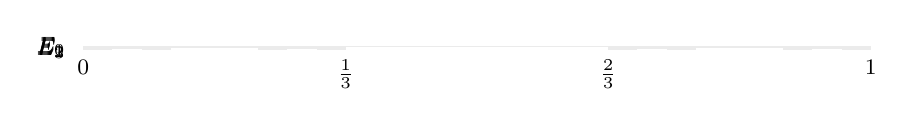
\begin{tikzpicture}[x=10cm,y=1.0]
  \def\h{0.26}
  % stage 0
  \fill[band] (0,0) rectangle (1,\h);
  \node[font=\footnotesize,left] at (-0.01,0.13) {$E_0$};
  % stage 1
  \fill[band] (0,-0.45) rectangle (0.3333,-0.45+\h);
  \fill[band] (0.6667,-0.45) rectangle (1,-0.45+\h);
  \node[font=\footnotesize,left] at (-0.01,-0.45+0.13) {$E_1$};
  % stage 2
  \foreach \a in {0, 0.2222, 0.6667, 0.8889}{
    \fill[band] (\a,-0.9) rectangle (\a+0.1111,-0.9+\h);}
  \node[font=\footnotesize,left] at (-0.01,-0.9+0.13) {$E_2$};
  % stage 3
  \foreach \a in {0,0.07407,0.2222,0.2963,0.6667,0.7407,0.8889,0.96296}{
    \fill[band] (\a,-1.35) rectangle (\a+0.037,-1.35+\h);}
  \node[font=\footnotesize,left] at (-0.01,-1.35+0.13) {$E_3$};
  % labels
  \node[font=\footnotesize,below] at (0,-1.5) {$0$};
  \node[font=\footnotesize,below] at (0.3333,-1.5) {$\tfrac13$};
  \node[font=\footnotesize,below] at (0.6667,-1.5) {$\tfrac23$};
  \node[font=\footnotesize,below] at (1,-1.5) {$1$};
\end{tikzpicture}
\captionof{figure}{Removing middle thirds: $E_n$ is $2^n$ intervals of length $3^{-n}$, total
length $(2/3)^n\to0$. The Cantor set $P=\bigcap E_n$ is what survives forever.}
\end{center}

\begin{theorem}[Properties of the Cantor set; Rudin 2.44, B\&S 11.1.10]\label{t:cantor-props@c3}
The Cantor set $P$ is:
\textup{(a)} nonempty and \emph{compact};
\textup{(b)} of \emph{total length} \textup{(}measure\textup{)} \emph{zero};
\textup{(c)} \emph{perfect}, hence uncountable;
\textup{(d)} \emph{totally disconnected} --- it contains no segment.
\end{theorem}

\begin{proof}
(a) Each $E_n$ is a finite union of closed intervals, hence compact; $P=\bigcap_n E_n$ is an
intersection of nested nonempty compact sets, so nonempty (Theorem~\ref{t:fip@c3}) and closed,
hence compact. (b) The total length removed is
$\tfrac13+\tfrac{2}{3^2}+\tfrac{4}{3^3}+\cdots=\tfrac13\sum_{n\ge0}(\tfrac23)^n=
\tfrac13\cdot\tfrac{1}{1-2/3}=1$, so $P$ has measure $\le 1-1=0$; equivalently
$\operatorname{length}(E_n)=(2/3)^n\to0$ and $P\subseteq E_n$. (d) If $P$ contained a
segment of length $\ell>0$, then since $P\subseteq E_n$ and $E_n$'s intervals have length
$3^{-n}$, we would need $\ell\le3^{-n}$ for all $n$, forcing $\ell=0$. So $P$ contains no
interval; between any two points of $P$ lies a gap, so $P$ is totally disconnected. (c)
$P$ is closed by (a). To see no point is isolated, take $x\in P$ and any segment $S\ni x$.
For large $n$ the interval $I_n$ of $E_n$ containing $x$ satisfies $I_n\subseteq S$; its
endpoints survive every later removal, so both endpoints lie in $P$. Pick the endpoint
$x_n\neq x$: then $x_n\in P\cap S$, $x_n\neq x$, so $x$ is a limit point of $P$. Thus $P$ is
perfect, and uncountable by Theorem~\ref{t:perfect-uncountable@c3}.
\end{proof}

\begin{wex}{The ternary description and uncountability of $P$}
Show $P=\set{x\in[0,1]\st x=\sum_{n\ge1}a_n3^{-n},\ a_n\in\set{0,2}}$ and use it to see $P$ is
uncountable.
\wrec ``Identify the Cantor set explicitly'': removing middle thirds is removing the digit
$1$ in base $3$.
\wsol A point survives the first removal iff its ternary expansion can be written with $a_1\in
\set{0,2}$ (the open middle third $(\tfrac13,\tfrac23)$ is exactly the numbers \emph{forced}
to have $a_1=1$); inductively $x\in P$ iff it has a ternary expansion using only digits
$0,2$. The map $\psi(\sum a_n3^{-n})=\sum(a_n/2)2^{-n}$ sends $P$ \emph{onto} $[0,1]$ (every
binary expansion is hit), so $\abs P\ge\abs{[0,1]}$; hence $P$ is uncountable. \emph{Check:}
this matches Theorem~\ref{t:cantor-props@c3}(c). The endpoints $2k/3^n$ are the ``rational''
members; but $P$ has continuum-many points, vastly more than its endpoints.
\end{wex}

\begin{wex}{A perfect set in $\R$ containing no rational (Rudin Ex.~18)}
Is there a nonempty perfect set in $\R$ with no rational points?
\wrec ``Build a perfect set avoiding a countable set'': mimic the Cantor construction but
center the removed gaps on rationals.
\wsol Yes. Run a Cantor-style construction on $[0,1]$ but at each stage remove an open middle
gap chosen to contain a prescribed rational (enumerate $\Q\cap[0,1]=\set{q_1,q_2,\dots}$ and
ensure $q_k$ is deleted by stage $k$, shrinking gaps so positive length survives). The
intersection $P$ of the nested closed stages is nonempty, closed, and perfect (same
endpoint argument as the Cantor set), yet contains no rational. \emph{Check:} a translated/scaled
``fat Cantor set'' arranged to swallow each rational works; perfectness only needs the
self-accumulation of surviving endpoints, independent of which gaps were removed.
\end{wex}

\begin{pitfall}
The Cantor set is the standard counterexample factory. It is uncountable yet has measure
zero (so ``small'' in length but ``large'' in cardinality); it is perfect yet contains no
interval; it is compact and totally disconnected. Do not equate ``measure zero'' with
``countable,'' nor ``contains no interval'' with ``countable'' --- $P$ refutes both.
\end{pitfall}

\subsection*{Further worked examples}

\begin{wex}{Is $\tfrac14$ in the Cantor set?}
Decide whether $\tfrac14$ and $\tfrac13$ belong to the Cantor set $P$, using the
ternary-digit description.
\wrec Trigger: ``membership in $P$.'' By the previous worked example, $x\in P$ iff $x$ has a
base-$3$ expansion using only digits $0$ and $2$.
\wsol \emph{$x=\tfrac14$:} compute the ternary expansion. $\tfrac14=\sum_{k\ge1}a_k3^{-k}$
with $a_k=0,2,0,2,\dots$ since $\tfrac{2}{3^2}+\tfrac{2}{3^4}+\cdots=
2\cdot\tfrac{1/9}{1-1/9}=2\cdot\tfrac18=\tfrac14$. So $\tfrac14=(0.020202\ldots)_3$, all
digits $0$ or $2$, hence $\tfrac14\in P$. \emph{$x=\tfrac13$:} here
$\tfrac13=(0.1)_3=(0.0222\ldots)_3$; the second form uses only $0,2$, so $\tfrac13\in P$ as
well --- it is the right endpoint of $[0,\tfrac13]$, an endpoint that survives forever.
\emph{Check:} $\tfrac14$ is \emph{not} an endpoint of any removed interval, yet still lies
in $P$; this shows $P$ is far larger than its set of endpoints (which is only countable).
The midpoint $\tfrac12=(0.111\ldots)_3$ is forced to have a digit $1$ and lies in the first
removed middle third, so $\tfrac12\notin P$.
\end{wex}

\begin{wex}{A fat Cantor set: positive measure, still nowhere dense}
Remove from $[0,1]$ at stage $n$ the open middle interval of length $4^{-n}$ from each of the
$2^{n-1}$ surviving intervals. Show the surviving set $F$ is closed, nowhere dense, perfect,
and has measure $\tfrac12$.
\wrec Trigger: ``Cantor-type construction with controlled lengths.'' Track total removed
length as a geometric series; perfectness comes from the same surviving-endpoint argument as
for $P$.
\wsol At stage $n$ there are $2^{n-1}$ intervals and we remove one gap of length $4^{-n}$
from each, removing total length $2^{n-1}\cdot4^{-n}=\tfrac12\cdot2^{-n}$. Summing over
$n\ge1$, the total removed length is $\tfrac12\sum_{n\ge1}2^{-n}=\tfrac12\cdot1=\tfrac12$.
So $F=[0,1]\setminus(\text{removed})$ has measure $1-\tfrac12=\tfrac12>0$. $F$ is closed
(intersection of closed stages $F_n$) and \emph{nowhere dense}: each $F_n$ is a union of
intervals of length $\le2^{-n}\to0$, so $F$ contains no interval, whence $\interior{\closure
F}=\interior F=\es$. It is \emph{perfect} by the surviving-endpoint argument used for $P$:
every point of $F$ is a limit of stage-endpoints in $F$. \emph{Check:} unlike the standard
$P$ (measure $0$), this $F$ has \emph{positive} measure $\tfrac12$ yet still contains no
interval --- ``nowhere dense'' does not imply ``measure zero.''
\end{wex}

\begin{wex}{A perfect set need not be all-limit-points without closedness}
Give a set every point of which is a limit point of the set, but which is \emph{not} perfect,
and explain which axiom of Definition~\ref{d:perfect@c3} fails.
\wrec Trigger: a NON-example probing the definition of perfect. Perfect requires \emph{both}
``closed'' and ``every point is a limit point''; dropping closedness breaks it.
\wsol Take $E=(0,1)\cap\Q$, the rationals in the open unit interval. Every point of $E$ is a
limit point of $E$ (rationals accumulate at every rational, since between any two rationals
lies another), so the ``no isolated points'' clause holds. But $E$ is \emph{not closed}: its
limit point $\tfrac{1}{\sqrt2}\approx0.707$ (or any irrational in $(0,1)$, or the endpoints
$0,1$) is not in $E$. So $E$ fails the closedness clause and is not perfect; indeed
$\closure E=[0,1]\neq E$. \emph{Check:} the genuinely perfect set ``closest'' to $E$ is its
closure $[0,1]$, which \emph{is} perfect. Perfectness is the conjunction $E=\closure E=E'$;
here $E=E'$ holds but $E\neq\closure E$, so the conjunction fails.
\end{wex}

\begin{exers}{Exercises (Rudin, Ch.2).}
\item Let $E$ be the set of all $x\in[0,1]$ whose decimal expansion contains only the digits
  $4$ and $7$. Is $E$ countable? Is $E$ dense in $[0,1]$? Is $E$ compact? Is $E$ perfect?
\item Is there a nonempty perfect set in $\R^1$ which contains no rational number?
\end{exers}

\begin{exers}{Additional exercises.}
\item Show that $[0,1]$ is perfect, and that $\R^k$ is perfect.
\item Prove that a finite set is never perfect, and that a nonempty perfect set is always
  infinite (indeed uncountable).
\item Verify the total-length computation for the Cantor set:
  $\sum_{n\ge0}\dfrac{2^n}{3^{n+1}}=1$, and conclude the Cantor set has measure zero.
\item Show that the Cantor set is \emph{nowhere dense}: $\interior{\closure P}=\es$.
\item (Non-example.) Exhibit a closed, uncountable subset of $\R$ that is \emph{not} perfect
  (it has at least one isolated point), e.g.\ $\set{0}\cup[1,2]$.
\item (Fat Cantor set.) At stage $n$ remove from each interval an open middle piece of
  relative length $4^{-n}$ instead of $\tfrac13$. Show the resulting set is perfect, compact,
  contains no interval, yet has \emph{positive} total length. Contrast with the standard
  Cantor set.
\item (Diagram.) Draw the first four stages $E_0,\dots,E_3$ of the middle-thirds construction
  as a stacked bar figure, labeling the surviving endpoints $0,\tfrac13,\tfrac23,1$ and the
  lengths $3^{-n}$.
\item Show that the endpoints of the removed intervals (numbers $2k/3^n$) are dense in the
  Cantor set but form only a countable subset of it.
\item Using the ternary characterization, decide whether $\tfrac14$ belongs to the Cantor
  set. [Hint: $\tfrac14=(0.\overline{02})_3$.]
\item Prove that the Cantor set is homeomorphic to $\set{0,2}^\N$ with the product topology
  via the ternary-digit map, hence is totally disconnected.
\end{exers}


\section{Connected Sets}
\subsection*{Separated sets and connectedness}

\begin{definition}[Rudin 2.45]\label{d:connected@c3}
Two subsets $A,B$ of a metric space $X$ are \emph{separated} if
$A\cap\closure B=\es$ and $\closure A\cap B=\es$ --- neither meets the closure of the other.
A set $E\subseteq X$ is \emph{connected} if it cannot be written as $E=A\cup B$ with $A,B$
nonempty and separated. Otherwise $E$ is \emph{disconnected}.
\end{definition}

\begin{remark}[Separated is stronger than disjoint; Rudin 2.46]
Separated sets are disjoint, but disjoint sets need not be separated: $[0,1]$ and $(1,2)$ are
disjoint yet not separated, since $1\in\closure{(1,2)}$. The segments $(0,1)$ and $(1,2)$
\emph{are} separated. Separation forbids one piece from touching the other even at a boundary
point.
\end{remark}

\begin{center}
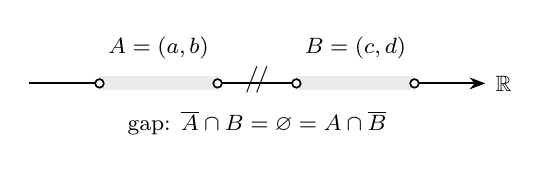
\begin{tikzpicture}[scale=1.0]
  % disconnected set as two separated pieces
  \draw[numln] (-0.4,0)--(5.4,0) node[right,font=\footnotesize]{$\R$};
  \fill[band] (0.5,-0.09) rectangle (2,0.09);
  \node[opt] at (0.5,0){}; \node[opt] at (2,0){};
  \fill[band] (3,-0.09) rectangle (4.5,0.09);
  \node[opt] at (3,0){}; \node[opt] at (4.5,0){};
  \node[font=\footnotesize] at (1.25,0.45) {$A=(a,b)$};
  \node[font=\footnotesize] at (3.75,0.45) {$B=(c,d)$};
  \node[font=\footnotesize] at (2.5,-0.5) {gap: $\closure A\cap B=\es=A\cap\closure B$};
  \node[font=\footnotesize] at (2.5,0.05) {$\big/\!\big/$};
\end{tikzpicture}
\captionof{figure}{A disconnected set splits into two separated open pieces with a gap between
them; no point of either closure reaches the other.}
\end{center}

\subsection*{Connected subsets of the line are exactly the intervals}

\begin{theorem}[Rudin 2.47]\label{t:connected-R@c3}
A set $E\subseteq\R$ is connected if and only if it has the \emph{intermediate value
property}: whenever $x,y\in E$ and $x<z<y$, then $z\in E$. Equivalently, the connected
subsets of $\R$ are exactly the \emph{intervals} \textup{(}including rays, points,
$\es$, and $\R$\textup{)}.
\end{theorem}

\begin{proof}
\textbf{($\Rightarrow$, contrapositive)} Suppose $E$ fails the property: there are $x,y\in E$
and $z\in(x,y)$ with $z\notin E$. Put
\[
  A_z=E\cap(-\infty,z),\qquad B_z=E\cap(z,\infty).
\]
Then $E=A_z\cup B_z$ (since $z\notin E$), both are nonempty ($x\in A_z$, $y\in B_z$), and
they are separated: $A_z\subseteq(-\infty,z)$ and $B_z\subseteq(z,\infty)$, so
$\closure{A_z}\subseteq(-\infty,z]$ is disjoint from $B_z$, and symmetrically. So $E$ is
disconnected. \textbf{($\Leftarrow$)} Suppose $E$ is disconnected, $E=A\cup B$ with $A,B$
nonempty and separated. Pick $x\in A$, $y\in B$; WLOG $x<y$. Let
\[
  z=\sup\bigl(A\cap[x,y]\bigr).
\]
By Theorem~\ref{t:sup-closed@c3}, $z\in\closure A$, so $z\notin B$ (separation); in particular
$x\le z<y$ (as $z\le y$ and $z\neq y\in B$). If $z\notin A$ then $z\notin E$ and $x<z<y$
exhibits a gap, so the IVP fails. If $z\in A$, then $z\notin\closure B$ (separation), so
there is $z_1$ with $z<z_1<y$ and $z_1\notin B$; but $z_1>z=\sup(A\cap[x,y])$ gives
$z_1\notin A$ too, so $z_1\notin E$ with $x<z_1<y$ --- again the IVP fails. Either way $E$
lacks the IVP. The sets with the IVP are precisely the intervals.
\end{proof}

\begin{wex}{$\Q$ is totally disconnected}
Show the only connected subsets of $\Q$ are the singletons and $\es$.
\wrec ``Find/refute connectedness'': use Theorem~\ref{t:connected-R@c3}'s IVP characterization,
which a gap-riddled set fails.
\wsol Suppose $E\subseteq\Q$ has two points $x<y$. Pick an \emph{irrational} $z\in(x,y)$
(density of irrationals); then $z\notin\Q\supseteq E$, so $x<z<y$ with $z\notin E$ violates
the IVP, and $E$ is disconnected: $E=(E\cap(-\infty,z))\cup(E\cap(z,\infty))$ is a separation.
Hence no subset of $\Q$ with $\ge2$ points is connected; the connected sets are $\es$ and
singletons. \emph{Check:} $\Q$ is \emph{totally disconnected}, like the Cantor set, although
$\Q$ is countable and dense while the Cantor set is uncountable and nowhere dense --- two very
different totally disconnected spaces.
\end{wex}

\begin{wex}{A convex set is connected (Rudin Ex.~21(c))}
Show every convex $E\subseteq\R^k$ is connected.
\wrec ``Show connected'' in higher dimensions, where the IVP characterization is unavailable:
push a line segment between two points and reduce to $\R^1$.
\wsol Suppose $E=A\cup B$ with $A,B$ nonempty separated, $a\in A$, $b\in B$. Convexity puts
the whole segment $p(t)=(1-t)a+tb$, $t\in[0,1]$, inside $E$. Let $A_0=p^{-1}(A)$,
$B_0=p^{-1}(B)\subseteq[0,1]$. These are nonempty ($0\in A_0$, $1\in B_0$), cover $[0,1]$, and
are separated in $\R$ (the continuous affine $p$ pulls back separation). But $[0,1]$ is an
interval, hence connected (Theorem~\ref{t:connected-R@c3}) --- contradiction. So $E$ is
connected. \emph{Check:} balls and $k$-cells are convex, hence connected; this is the
$\R^k$ analogue of ``intervals are connected.''
\end{wex}

\begin{method}{Deciding whether a set $E$ is connected}
\textbf{Recognition trigger.} ``Is $E$ connected?'' / ``show $E$ is (dis)connected.''
\begin{enumerate}
\item \textbf{In $\R$:} apply Theorem~\ref{t:connected-R@c3} --- $E$ is connected iff it is an
  interval. To \emph{disconnect}, find a point $z\notin E$ strictly between two points of
  $E$.
\item \textbf{In $\R^k$:} to prove connectedness, exhibit a path or a convex/segment
  structure and reduce to the $\R^1$ case; to disprove, split $E$ into two nonempty pieces
  lying in disjoint open sets (a separation).
\item \textbf{Bookkeeping:} ``separated'' means closures don't meet, strictly stronger than
  ``disjoint.'' Check closures, not just the sets.
\end{enumerate}
\end{method}

\begin{remark}[Closures and interiors of connected sets; Rudin Ex.~20]
The closure of a connected set is connected (if $\closure E=A\cup B$ separated, then
$E=(E\cap A)\cup(E\cap B)$ would separate $E$). The \emph{interior} of a connected set need
\emph{not} be connected: in $\R^2$ two closed disks joined by a single point form a connected
set whose interior is two disjoint open disks.
\end{remark}

\begin{pitfall}
Connectedness is about the \emph{absence of a separation}, not about path-joining --- though
in $\R^k$ open connected sets are also path-connected, in general metric spaces the two
notions differ. And remember separation requires \emph{closures} to be disjoint: $[0,1]$ and
$(1,2)$ are disjoint but their union $[0,2)$ minus nothing is still connected precisely
because $1$ glues them. Always test with closures.
\end{pitfall}

\subsection*{Further worked examples}

\begin{wex}{Classifying connectedness on the line}
For each set decide whether it is connected: (a) $[0,1]\cup[2,3]$, (b) $[0,1]\cup\set2$,
(c) $[0,2)$, (d) $\R\setminus\set0$.
\wrec Trigger: ``is $E\subseteq\R$ connected?''. Apply Theorem~\ref{t:connected-R@c3}: connected
$\eqv$ interval $\eqv$ has the intermediate-value property.
\wsol (a) \emph{Disconnected}: $\tfrac32\notin E$ lies between $1\in E$ and $2\in E$, a gap;
explicitly $E=([0,1])\cup([2,3])$ is a separation (closures $[0,1]$ and $[2,3]$ are
disjoint). (b) \emph{Disconnected}: $2$ is isolated, and any $z\in(1,2)$ is a gap between
$1$ and $2$. (c) \emph{Connected}: $[0,2)$ is an interval, so the IVP holds vacuously --- no
internal point is missing. (d) \emph{Disconnected}: $0\notin E$ separates $E$ into
$(-\infty,0)$ and $(0,\infty)$, whose closures $(-\infty,0]$ and $[0,\infty)$ meet only at
$0\notin E$, so they are separated within $E$. \emph{Check:} exactly the interval (c) is
connected; the others each have an internal point removed or an isolated chunk, which is
precisely the IVP failing.
\end{wex}

\begin{wex}{The union of two connected sets sharing a point is connected}
Let $A,B\subseteq X$ be connected with $A\cap B\neq\es$. Show $A\cup B$ is connected.
\wrec Trigger: ``glue connected pieces.'' Argue by contradiction from a separation of the
union; a connected piece cannot straddle a separation.
\wsol Suppose $A\cup B=P\cup Q$ with $P,Q$ nonempty and separated. Fix
$c\in A\cap B$; say $c\in P$ (WLOG). Now $A=(A\cap P)\cup(A\cap Q)$, and these two are
separated (subsets of the separated $P,Q$). Since $A$ is connected, one of them is empty;
because $c\in A\cap P$ we must have $A\cap Q=\es$, i.e.\ $A\subseteq P$. The same argument
with $B$ (also containing $c\in P$) gives $B\subseteq P$. Hence $A\cup B\subseteq P$, forcing
$Q=\es$ --- contradicting $Q\neq\es$. So no separation exists and $A\cup B$ is connected.
\emph{Check:} the shared point is essential: $[0,1]$ and $[2,3]$ are each connected but
disjoint, and their union is disconnected (previous example). The result extends to any
family of connected sets with a common point.
\end{wex}

\begin{wex}{The topologist's two-piece set: disjoint is not separated}
In $\R$, are $A=[0,1]$ and $B=(1,2]$ separated? Is $A\cup B$ connected?
\wrec Trigger: a NON-example testing ``separated'' vs ``disjoint.'' Separation needs
\emph{closures} to miss the other set; check $\closure A\cap B$ and $A\cap\closure B$.
\wsol $A$ and $B$ are disjoint ($A\cap B=\es$). But $\closure A=[0,1]$ and
$\closure B=[1,2]$, so $\closure A\cap B=[0,1]\cap(1,2]=\es$ \emph{but}
$A\cap\closure B=[0,1]\cap[1,2]=\set 1\neq\es$. One of the two separation conditions fails,
so $A$ and $B$ are \emph{not} separated. Consequently this particular splitting is not a
valid separation of $A\cup B=[0,2]$; and indeed $[0,2]$ is an interval, hence connected
(Theorem~\ref{t:connected-R@c3}), so no separation exists at all. \emph{Check:} contrast with
$(0,1)$ and $(1,2)$, which \emph{are} separated (neither closure $[0,1]$, $[1,2]$ contains a
point of the \emph{other open} set), and whose union $(0,1)\cup(1,2)$ is genuinely
disconnected. The single point $1$ is exactly what decides the two cases.
\end{wex}

\begin{center}
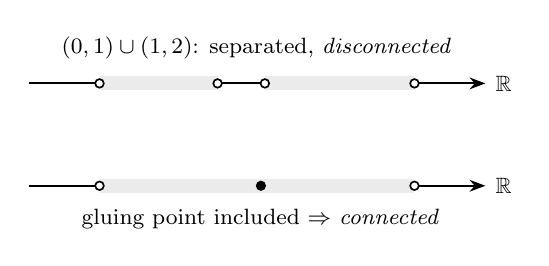
\begin{tikzpicture}[scale=1.0]
  % top: separated open intervals -> disconnected
  \draw[numln] (-0.4,0.9)--(5.4,0.9) node[right,font=\footnotesize]{$\R$};
  \fill[band] (0.5,0.81) rectangle (2,0.99);
  \node[opt] at (0.5,0.9){}; \node[opt] at (2,0.9){};
  \fill[band] (2.6,0.81) rectangle (4.5,0.99);
  \node[opt] at (2.6,0.9){}; \node[opt] at (4.5,0.9){};
  \node[font=\footnotesize] at (2.5,1.35)
    {$(0,1)\cup(1,2)$: separated, \emph{disconnected}};
  % bottom: the gluing point joins them -> connected
  \draw[numln] (-0.4,-0.4)--(5.4,-0.4) node[right,font=\footnotesize]{$\R$};
  \fill[band] (0.5,-0.49) rectangle (4.5,-0.31);
  \node[pt] at (2.55,-0.4){};
  \node[opt] at (0.5,-0.4){}; \node[opt] at (4.5,-0.4){};
  \node[font=\footnotesize] at (2.55,-0.82)
    {gluing point included $\Rightarrow$ \emph{connected}};
\end{tikzpicture}
\captionof{figure}{Removing the shared point $1$ separates the interval into two pieces; keeping
it glues them. Connectedness on the line turns entirely on whether internal points are
present.}
\end{center}

\begin{exers}{Exercises (Rudin, Ch.2).}
\item (a) If $A$ and $B$ are disjoint closed sets in a metric space $X$, prove that they are
  separated. (b) Prove the same for disjoint open sets. (c) Fix $p\in X$, $\delta>0$; define
  $A=\set{q\in X\st d(p,q)<\delta}$ and $B=\set{q\in X\st d(p,q)>\delta}$. Prove $A$ and $B$
  are separated. (d) Prove that every connected metric space with at least two points is
  uncountable. [Hint: use (c).]
\item Are closures and interiors of connected sets always connected? (Look at subsets of
  $\R^2$.)
\item Let $A$ and $B$ be separated subsets of some $\R^n$; suppose $a\in A$, $b\in B$, and
  define $p(t)=(1-t)a+tb$ for $t\in\R^1$. Put $A_0=p^{-1}(A)$, $B_0=p^{-1}(B)$ (so $t\in A_0$
  iff $p(t)\in A$). (a) Prove $A_0$ and $B_0$ are separated subsets of $\R^1$. (b) Prove there
  exists $t_0\in(0,1)$ with $p(t_0)\notin A\cup B$. (c) Prove that every convex subset of
  $\R^n$ is connected.
\end{exers}

\begin{exers}{Additional exercises.}
\item For each subset of $\R$, decide whether it is connected, citing the interval
  characterization: (a) $[0,1]$; (b) $[0,1]\cup\set2$; (c) $\Q$; (d) $\R\setminus\set0$;
  (e) $(0,1)\cup(1,2)$.
\item Prove that the union of two connected sets that share a common point is connected.
\item Prove that $\R$ is connected, and that $\R\setminus\set0$ is not.
\item Show that the continuous image of a connected set is connected (state the version with
  domain a connected subset of $\R$). Deduce the Intermediate Value Theorem.
\item (Non-example.) Show that $\Q$ and the Cantor set are both totally disconnected (no
  connected subset has more than one point), although one is countable and dense and the other
  uncountable and nowhere dense.
\item Prove that the closure of a connected set is connected, and exhibit a connected set in
  $\R^2$ whose interior is disconnected.
\item (Diagram.) Draw a disconnected set in $\R$ (or $\R^2$) as two separated pieces, marking
  the gap and indicating why no point of one closure meets the other.
\item Prove that if $A,B$ are separated and $C\subseteq A\cup B$ is connected, then
  $C\subseteq A$ or $C\subseteq B$.
\item Show that an open connected subset of $\R^k$ is \emph{path-connected}: any two points
  are joined by a polygonal path inside the set. [Hint: the set of points reachable from a
  fixed point is open and closed in the set.]
\item Determine all connected subsets of a discrete metric space, and explain in one sentence
  why the answer matches the ``totally disconnected'' picture.
\end{exers}


% ================= Chapter 4: Numerical Sequences and Series =================

\chapter{Numerical Sequences and Series}

\section{Convergent Sequences}
\subsection*{Sequences and the definition of a limit}

A \emph{sequence} of real numbers is a function $x:\N\to\R$; we write its value at $n$ as
$x_n$ and the whole sequence as $\seq{x_n}$ or $\seq{x_n}_{n=1}^\infty$. The term $x_n$ is
the \emph{$n$-th term}; do not confuse the sequence $\seq{x_n}$ (an infinite ordered list)
with its \emph{range} $\set{x_n\st n\in\N}$ (a set, which may be finite: the sequence
$\seq{(-1)^n}$ has range $\set{-1,1}$).

\begin{definition}\label{d:converge@c4}
A sequence $\seq{x_n}$ \emph{converges} to a real number $x$, written $x_n\to x$ or
$\lim_{n\to\infty}x_n=x$, if for every $\eps>0$ there is a natural number $K=K(\eps)$ such
that
\[
  n\ge K\quad\imp\quad \abs{x_n-x}<\eps .
\]
The number $x$ is the \emph{limit}. A sequence is \emph{convergent} if it has a limit, and
\emph{divergent} otherwise.
\end{definition}

The inequality $\abs{x_n-x}<\eps$ says $x_n\in(x-\eps,x+\eps)$, the open interval of radius
$\eps$ about $x$ --- the \emph{$\eps$-neighborhood} of $x$. So convergence means: \emph{no
matter how narrow a band you draw around $x$, all but finitely many terms land inside it.}
The threshold $K$ is allowed to grow as $\eps$ shrinks; that dependence is the whole game.

\begin{center}
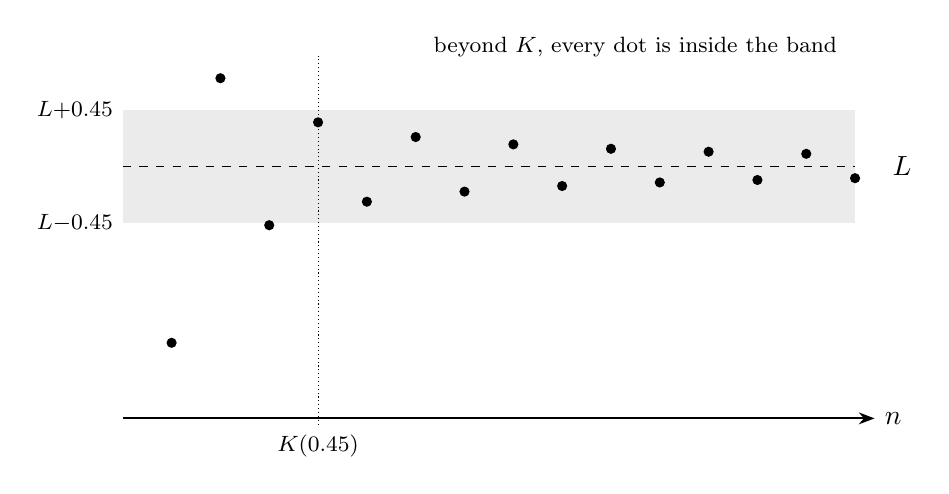
\begin{tikzpicture}[xscale=0.62,yscale=1.6]
  \def\L{2.0}
  \def\eps{0.45}
  % horizontal axis
  \draw[numln] (0,0)--(15.4,0) node[right]{$n$};
  % limit line and epsilon band
  \begin{scope}[on background layer]
    \fill[band] (0,\L-\eps) rectangle (15,\L+\eps);
  \end{scope}
  \draw[dashed] (0,\L)--(15,\L) node[right=10pt]{$L$};
  \node[left] at (0,\L+\eps) {\footnotesize $L{+}\eps$};
  \node[left] at (0,\L-\eps) {\footnotesize $L{-}\eps$};
  % the sequence dots: x_n = L + 1.4*(-1)^n / n
  \foreach \n in {1,...,15}{
    \pgfmathsetmacro{\y}{\L + 1.4*(mod(\n,2)==0 ? 1 : -1)/\n}
    \node[pt] at (\n,\y) {};
  }
  % mark K
  \draw[densely dotted] (4,-0.05)--(4,2.9);
  \node[below] at (4,-0.05) {\footnotesize $K(\eps)$};
  \node[font=\footnotesize,align=center] at (10.5,2.95)
    {beyond $K$, every dot is inside the band};
\end{tikzpicture}
\captionof{figure}{Convergence: each $\eps$-band $(L-\eps,L+\eps)$ traps all terms from some
index $K(\eps)$ on. Shrink $\eps$ and $K$ may move right, but it stays finite.}
\end{center}

\begin{remark}
``All but finitely many'' is the geometric soul of the definition: only \emph{finitely
many} terms may sit outside any given band. Changing, deleting, or prepending finitely many
terms therefore changes nothing about convergence or the limit --- limits are a property of
the \emph{tail} $\seq{x_n}_{n\ge N}$.
\end{remark}

\begin{method}{Running an $\eps$--$K$ convergence proof}
\textbf{Recognition trigger.} You must \emph{prove} $x_n\to x$ directly from the definition
(no limit theorems yet available), or the problem says ``using the definition of limit''.
\begin{enumerate}
\item \textbf{Form the gap} $\abs{x_n-x}$ and simplify it to a clean expression in $n$.
\item \textbf{Bound it above} by something obviously small, e.g.\ $\abs{x_n-x}\le C/n$ or
  $\le r^n$ --- discard, enlarge, or crudely estimate to get a manageable upper bound. This
  is ``scratch work''; you may overshoot.
\item \textbf{Solve for $K$.} Given $\eps>0$, find $K$ making your bound $<\eps$ (e.g.\
  $C/n<\eps\eqv n>C/\eps$, so take $K=\ceil{C/\eps}+1$). Use the Archimedean property to
  guarantee such a $K$ exists.
\item \textbf{Write it forward.} ``Let $\eps>0$. Put $K=\dots$. If $n\ge K$ then
  $\abs{x_n-x}\le(\text{bound})<\eps$.'' The logic must flow $\eps\Rightarrow K\Rightarrow$
  estimate.
\end{enumerate}
\textbf{Key tool.} \emph{Archimedean property}: for every $\eps>0$ there is $K\in\N$ with
$1/K<\eps$. Every $1/n$-type estimate rests on it.
\end{method}

\begin{wex}{The model limit $1/n\to0$}
Prove $\lim_{n\to\infty}\dfrac1n=0$.
\wrec Direct $\eps$--$K$ proof; the gap is already $1/n$, so this is the archetype.
\wsol Let $\eps>0$. By the Archimedean property choose $K\in\N$ with $K>1/\eps$. If $n\ge
K$ then $\dfrac1n\le\dfrac1K<\eps$, and since $1/n>0$ we have
$\abs{\tfrac1n-0}=\tfrac1n<\eps$. Hence $1/n\to0$. \emph{Check:} for $\eps=0.01$, $K=101$
works: $1/101<0.01$. \checkmark
\end{wex}

\begin{wex}{A rational expression}
Prove $\dfrac{n}{n+1}\to1$.
\wrec ``Prove this specific limit''; form and shrink the gap.
\wsol Compute $\abs{\dfrac{n}{n+1}-1}=\abs{\dfrac{-1}{n+1}}=\dfrac1{n+1}<\dfrac1n$. Given
$\eps>0$ take $K>1/\eps$; then $n\ge K\imp \abs{\tfrac{n}{n+1}-1}<\tfrac1n\le\tfrac1K<\eps$.
\emph{Check:} the terms $\tfrac12,\tfrac23,\tfrac34,\dots$ visibly climb toward $1$. \checkmark
\end{wex}

\begin{wex}{Using a crude over-bound}
Prove $\dfrac{2n+1}{n^2+3}\to0$.
\wrec The exact gap is messy; bound it crudely by a $C/n$ shape (Step 2 of the Method).
\wsol For $n\ge1$, $2n+1\le 3n$ and $n^2+3\ge n^2$, so
$\dfrac{2n+1}{n^2+3}\le\dfrac{3n}{n^2}=\dfrac3n$. Given $\eps>0$ take $K>3/\eps$; then
$n\ge K\imp \abs{x_n-0}\le\tfrac3n\le\tfrac3K<\eps$. \emph{Check:} the over-bound $3/n$
need not be sharp --- it only must beat $\eps$ eventually. \checkmark
\end{wex}

\begin{wex}{A non-example: $\seq{(-1)^n}$ diverges}
Show the sequence $-1,1,-1,1,\dots$ has no limit.
\wrec ``Show divergent''; negate the definition --- exhibit one $\eps$ no candidate limit
can satisfy.
\wsol Suppose $(-1)^n\to x$. Take $\eps=1$. Then for large $n$ both $\abs{1-x}<1$ and
$\abs{-1-x}<1$ would hold (consecutive terms are $\pm1$). Adding, by the triangle
inequality $2=\abs{1-(-1)}\le\abs{1-x}+\abs{x-(-1)}<1+1=2$, a strict $2<2$, absurd. So no
limit exists. \emph{Check:} the terms straddle a gap of width $2$ forever; no single band of
radius $<1$ can hold them both. \checkmark
\end{wex}

\subsection*{Uniqueness, boundedness, and tails}

\begin{theorem}[Uniqueness of limits]\label{t:unique@c4}
A convergent sequence has exactly one limit.
\end{theorem}

\begin{proof}
Suppose $x_n\to x$ and $x_n\to x'$ with $x\neq x'$. Put $\eps=\tfrac12\abs{x-x'}>0$. Choose
$K_1$ with $\abs{x_n-x}<\eps$ for $n\ge K_1$, and $K_2$ with $\abs{x_n-x'}<\eps$ for $n\ge
K_2$. For $n\ge\max\set{K_1,K_2}$ the triangle inequality gives
\[
  \abs{x-x'}\le\abs{x-x_n}+\abs{x_n-x'}<\eps+\eps=\abs{x-x'},
\]
i.e.\ $\abs{x-x'}<\abs{x-x'}$, a contradiction. Hence $x=x'$.
\end{proof}

\begin{definition}\label{d:bdd@c4}
A sequence $\seq{x_n}$ is \emph{bounded} if there is $M>0$ with $\abs{x_n}\le M$ for all
$n\in\N$ (equivalently, its range is a bounded set).
\end{definition}

\begin{theorem}[Convergent $\imp$ bounded]\label{t:conv-bdd@c4}
Every convergent sequence is bounded.
\end{theorem}

\begin{proof}
Say $x_n\to x$. With $\eps=1$ pick $K$ so that $\abs{x_n-x}<1$ for $n\ge K$; then for those
$n$, $\abs{x_n}\le\abs{x}+1$. The finitely many earlier terms are bounded by
$M_0=\max\set{\abs{x_1},\dots,\abs{x_{K-1}}}$. Take $M=\max\set{M_0,\abs x+1}$; then
$\abs{x_n}\le M$ for all $n$.
\end{proof}

The converse fails: $\seq{(-1)^n}$ is bounded but divergent. Boundedness is necessary, not
sufficient --- a recurring asymmetry.

\begin{theorem}[Tail equivalence]\label{t:tail@c4}
Fix $m\in\N$ and let $\seq{x_n}$ be a sequence with $m$-tail $\seq{x_{m+n}}_{n\ge1}$. Then
$\seq{x_n}$ converges to $x$ iff its $m$-tail converges to $x$.
\end{theorem}

\begin{proof}
If $x_n\to x$ then any $\eps$--$K$ works for the tail by taking the same $K$. Conversely if
the tail converges to $x$ with threshold $K'$, then $\seq{x_n}$ satisfies the definition with
$K=K'+m$. The first $m$ terms are irrelevant.
\end{proof}

\begin{wex}{Square roots: $\sqrt{n+1}-\sqrt n\to0$}
Show $\sqrt{n+1}-\sqrt{n}\to0$.
\wrec A difference of roots; rationalize to expose a $1/\sqrt n$ shape.
\wsol Multiply by the conjugate:
$\sqrt{n+1}-\sqrt n=\dfrac{(n+1)-n}{\sqrt{n+1}+\sqrt n}=\dfrac1{\sqrt{n+1}+\sqrt n}
<\dfrac1{2\sqrt n}$. Given $\eps>0$, take $K>1/(4\eps^2)$; then $n\ge K\imp x_n<\tfrac1{2\sqrt
n}\le\tfrac1{2\sqrt K}<\eps$. \emph{Check:} $n=100$ gives $\sqrt{101}-10\approx0.0499<1/(2\cdot
10)=0.05$. \checkmark
\end{wex}

\begin{pitfall}
The limit value must be guessed (or computed) \emph{before} the $\eps$--$K$ proof; the
definition only \emph{verifies} a candidate, it does not produce one. To find the candidate
use algebra/limit laws; to certify it use $\eps$--$K$. Also: $K$ may depend on $\eps$ but
\emph{never} on $n$ --- writing ``choose $K=n$'' is circular and wrong.
\end{pitfall}

\begin{pitfall}
``$x_n\to x$'' is about the \emph{tail}, not any finite stretch. A million agreeing terms
prove nothing; a sequence that is $0$ for $n\le 10^9$ and then equals $5$ forever converges
to $5$, not $0$. Conversely, $\abs{x_n-x}$ being small \emph{for one large $n$} is not
convergence --- it must be small for \emph{all} $n\ge K$.
\end{pitfall}

\subsection*{Further worked examples}

\begin{wex}{Exhibiting an explicit $K(\eps)$}
Given $x_n=\dfrac{3n-1}{n+2}$, prove $x_n\to3$ and find the smallest $K$ that works for
$\eps=0.01$.
\wrec Direct $\eps$--$K$ proof (Definition~\ref{d:converge@c4}); after bounding the gap, solve
the threshold inequality \emph{exactly} for the numeric part.
\wsol The gap is $\abs{\dfrac{3n-1}{n+2}-3}=\abs{\dfrac{(3n-1)-3(n+2)}{n+2}}
=\dfrac{7}{n+2}$. Given $\eps>0$, $\dfrac7{n+2}<\eps\eqv n>\dfrac7\eps-2$, so any
$K>7/\eps-2$ works (Archimedean). For $\eps=0.01$: $7/0.01-2=698$, so the smallest integer
$K$ is $699$. \emph{Check:} at $n=699$, $7/(701)\approx0.00999<0.01$; at $n=698$,
$7/700=0.01\not<0.01$, so $699$ is indeed minimal. \checkmark
\end{wex}

\begin{wex}{A null sequence that is not monotone}
Show $x_n=\dfrac{(-1)^n}{n}\to0$.
\wrec The signs alternate, but the definition only cares about $\abs{x_n-0}$; take absolute
values and the alternation disappears.
\wsol $\abs{x_n-0}=\abs{\dfrac{(-1)^n}{n}}=\dfrac1n$. Given $\eps>0$ choose $K>1/\eps$; then
$n\ge K\imp\abs{x_n}=\tfrac1n\le\tfrac1K<\eps$. So $x_n\to0$ even though the sequence is
never monotone (it straddles $0$). \emph{Check:} terms $-1,\tfrac12,-\tfrac13,\tfrac14,\dots$
visibly shrink toward $0$ from both sides. \checkmark
\end{wex}

\begin{wex}{A non-example: an unbounded sequence cannot converge}
Show $x_n=\sqrt{n}$ does not converge to any real number.
\wrec ``Show divergent''; use the contrapositive of Theorem~\ref{t:conv-bdd@c4}
(convergent $\imp$ bounded) rather than negating the $\eps$--$K$ definition directly.
\wsol If $\sqrt n\to x$ for some $x\in\R$, then $\seq{\sqrt n}$ would be bounded. But for any
$M>0$, choosing $n>M^2$ gives $\sqrt n>M$, so no bound $M$ exists: the sequence is unbounded.
An unbounded sequence cannot be convergent, so $\seq{\sqrt n}$ diverges. \emph{Check:}
boundedness is \emph{necessary} for convergence; failing it is a clean disqualifier, no $K$
needed. \checkmark
\end{wex}

\begin{exers}{Exercises (Bartle \& Sherbert, \S3.1).}
\item Write the first five terms of $\seq{x_n}$ where
  (a) $x_n=1+(-1)^n$;\quad (b) $x_n=(-1)^n/n$;\quad
  (c) $x_n=\dfrac1{n(n+1)}$;\quad (d) $x_n=\dfrac1{n^2+2}$.
\item Guess a formula for the $n$-th term from the pattern:
  (a) $5,7,9,11,\dots$;\quad (b) $\tfrac12,-\tfrac14,\tfrac18,-\tfrac1{16},\dots$;\quad
  (c) $\tfrac12,\tfrac23,\tfrac34,\tfrac45,\dots$;\quad (d) $1,4,9,16,\dots$.
\item List the first five terms of the inductively defined sequences:
  (a) $x_1=1$, $x_{n+1}=3x_n+1$;\quad (b) $y_1=2$, $y_{n+1}=\tfrac12(y_n+2/y_n)$;\quad
  (c) $z_1=1$, $z_2=2$, $z_{n+2}=(z_{n+1}+z_n)/(z_{n+1}-z_n)$;\quad
  (d) $s_1=3$, $s_2=5$, $s_{n+2}=s_n+s_{n+1}$.
\item For any $b\in\R$, prove $\lim(b/n)=0$.
\item Use the definition of limit to establish:
  (a) $\lim\dfrac{n}{n^2+1}=0$;\quad (b) $\lim\dfrac{2n}{n+1}=2$;\quad
  (c) $\lim\dfrac{3n+1}{2n+5}=\dfrac32$;\quad (d) $\lim\dfrac{n^2-1}{2n^2+3}=\dfrac12$.
\item Show that
  (a) $\lim\dfrac1{\sqrt{n+7}}=0$;\quad (b) $\lim\dfrac{2n}{n+2}=2$;\quad
  (c) $\lim\dfrac{\sqrt n}{n+1}=0$;\quad (d) $\lim\dfrac{(-1)^n n}{n^2+1}=0$.
\item Let $x_n\ge0$ with $\lim x_n=0$. Prove $\lim\sqrt{x_n}=0$.
\item Prove that if $\lim x_n=x$ then $\lim\abs{x_n}=\abs x$. Give a converse counterexample.
\item Prove $\lim\bigl(\dfrac1n-\dfrac1{n+1}\bigr)=0$.
\item Prove $\lim\dfrac{\sqrt{n}}{n+1}=0$ and $\lim\dfrac{1}{\sqrt n}=0$.
\item For $x_n=\dfrac{(-1)^n}{n^2}$, determine $\lim x_n$ and prove your claim.
\item Show that $\lim\dfrac1{2^n}=0$.
\end{exers}

\begin{exers}{Additional exercises.}
\item Using the definition only, prove $\dfrac{3n^2+1}{n^2+n}\to3$. Find an explicit $K(\eps)$.
\item Prove that if $x_n\to x$ then the ``averaged'' tail $y_n=\tfrac12(x_n+x_{n+1})\to x$.
\item Prove $\sqrt[n]{a^n+b^n}\to\max\set{a,b}$ for fixed $a,b>0$. \emph{[Squeeze.]}
\item (Non-example.) Show $x_n=\sin(n\pi/2)$ is bounded but divergent by exhibiting two
  subsequences with different limits, and explain why no $\eps$--$K$ data can rescue it.
\item Suppose $\abs{x_n-x_{n+1}}\le 2^{-n}$ for all $n$. Must $\seq{x_n}$ converge? Prove or
  give a counterexample. (Contrast with the harmonic series.)
\item Prove that a sequence $\seq{x_n}$ with $x_n\to x$ is bounded by giving \emph{explicit}
  bounds in terms of $x$ and the first few terms.
\item (Diagram problem.) Sketch on one $a_n$-vs-$n$ axis the sequence
  $a_n=2+\dfrac{(-1)^n}{n}$ for $n=1,\dots,10$, draw the band $(2-\eps,2+\eps)$ for
  $\eps=0.25$, and mark the smallest $K$ with all later dots inside. Report $K$.
\item Let $x_n\to x$ and $x_n\ge0$. Prove $x\ge0$ and $\sqrt{x_n}\to\sqrt x$.
\end{exers}


\section{Limit Theorems}
\subsection*{The algebra of limits}

Once a handful of limits are known, the limit laws let us compute almost everything by
algebra, never returning to $\eps$--$K$. We collect them, prove them once, and reuse them.

\begin{theorem}[Algebra of limits]\label{t:algebra@c4}
Suppose $x_n\to x$ and $y_n\to y$, and let $c\in\R$. Then
\[
  \text{\textup{(a)}}\ x_n+y_n\to x+y,\qquad
  \text{\textup{(b)}}\ c\,x_n\to c\,x,\qquad
  \text{\textup{(c)}}\ x_n y_n\to xy,
\]
and, provided $y\neq0$ \textup{(}so $y_n\neq0$ for large $n$\textup{)},
\[
  \text{\textup{(d)}}\quad \frac{x_n}{y_n}\to\frac{x}{y}.
\]
\end{theorem}

\begin{proof}
(a) Given $\eps>0$, pick $K_1,K_2$ with $\abs{x_n-x}<\eps/2$ ($n\ge K_1$) and
$\abs{y_n-y}<\eps/2$ ($n\ge K_2$). For $n\ge\max\set{K_1,K_2}$,
\[
  \abs{(x_n+y_n)-(x+y)}\le\abs{x_n-x}+\abs{y_n-y}<\tfrac\eps2+\tfrac\eps2=\eps .
\]
(b) is the case $y_n\equiv0$ of (c), or directly $\abs{cx_n-cx}=\abs c\abs{x_n-x}$.

(c) Since $\seq{x_n}$ converges it is bounded, say $\abs{x_n}\le M$; also $\abs y$ is a
constant. Write the standard ``add and subtract'' splitting:
\[
  \abs{x_n y_n-xy}=\abs{x_n y_n-x_n y+x_n y-xy}
  \le\abs{x_n}\abs{y_n-y}+\abs{y}\abs{x_n-x}
  \le M\abs{y_n-y}+\abs y\,\abs{x_n-x}.
\]
Given $\eps>0$, make each piece $<\eps/2$ by choosing $n$ large; the sum is $<\eps$.

(d) It suffices to prove $1/y_n\to1/y$ and then apply (c). Since $y\neq0$, for large $n$ we
have $\abs{y_n}\ge\abs y/2$ (take $\eps=\abs y/2$ in $y_n\to y$). Then
\[
  \abs{\frac1{y_n}-\frac1y}=\frac{\abs{y-y_n}}{\abs{y_n}\abs y}
  \le\frac{2}{\abs y^2}\,\abs{y_n-y}\to0 .\qedhere
\]
\end{proof}

\begin{wex}{A rational limit by the laws}
Find $\displaystyle\lim_{n\to\infty}\frac{2n^2+3}{n^2-n+1}$.
\wrec ``Find the limit'' of a ratio of polynomials: divide by the top power and apply the
algebra of limits term by term.
\wsol Divide numerator and denominator by $n^2$:
\[
  \frac{2n^2+3}{n^2-n+1}=\frac{2+3/n^2}{1-1/n+1/n^2}\xrightarrow[n\to\infty]{}\frac{2+0}{1-0+0}=2,
\]
using $1/n\to0$, $1/n^2\to0$, and parts (a),(d). \emph{Check:} $n=10$ gives
$203/91\approx2.23$; $n=100$ gives $20003/9901\approx2.02$. \checkmark
\end{wex}

\begin{wex}{When you cannot split: $\sqrt{n^2+n}-n$}
Evaluate $\displaystyle\lim_{n\to\infty}\bigl(\sqrt{n^2+n}-n\bigr)$ \textup{(Rudin Ex.\ 3.2)}.
\wrec The two pieces each diverge, so the laws \emph{do not} apply directly --- rationalize
first, then the laws work.
\wsol
$\sqrt{n^2+n}-n=\dfrac{n}{\sqrt{n^2+n}+n}=\dfrac{1}{\sqrt{1+1/n}+1}\to\dfrac1{1+1}=\tfrac12$.
\emph{Check:} $n=100$ gives $\sqrt{10100}-100\approx0.4988$. \checkmark
\end{wex}

\begin{pitfall}
The algebra of limits requires \emph{both} factor sequences to converge. ``$\infty-\infty$''
and ``$0\cdot\infty$'' forms (like the previous example before rationalizing) are not covered;
you must massage the expression into a convergent form first. Splitting a limit you have not
yet shown to exist into a sum/product of limits is the single most common false step.
\end{pitfall}

\subsection*{Limits and inequalities; the Squeeze Theorem}

\begin{theorem}[Limits preserve weak inequalities]\label{t:ineq@c4}
If $x_n\to x$, $y_n\to y$, and $x_n\le y_n$ for all $n$ \textup{(}or all large $n$\textup{)},
then $x\le y$. In particular, if $a\le x_n\le b$ eventually, then $a\le x\le b$.
\end{theorem}

\begin{proof}
Put $z_n=y_n-x_n\ge0$, $z_n\to y-x$. If $y-x<0$, take $\eps=\tfrac12(x-y)>0$; then for large
$n$, $z_n<(y-x)+\eps=\tfrac12(y-x)<0$, contradicting $z_n\ge0$. So $y-x\ge0$.
\end{proof}

\begin{pitfall}
\emph{Strict} inequalities are \emph{not} preserved in the limit: $x_n=1/n>0$ for all $n$,
yet $\lim x_n=0$, not $>0$. Passing to the limit can only give $\ge$, never $>$.
\end{pitfall}

\begin{theorem}[Squeeze Theorem]\label{t:squeeze@c4}
If $x_n\le z_n\le y_n$ for all large $n$ and $x_n\to L$ and $y_n\to L$ (same limit), then
$z_n\to L$.
\end{theorem}

\begin{proof}
Let $\eps>0$. For large $n$, $L-\eps<x_n$ and $y_n<L+\eps$; combined with the sandwich,
$L-\eps<x_n\le z_n\le y_n<L+\eps$, i.e.\ $\abs{z_n-L}<\eps$.
\end{proof}

\begin{center}
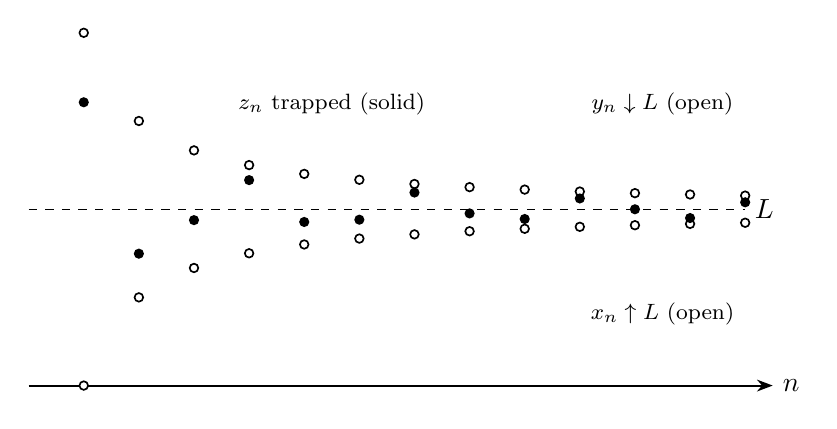
\begin{tikzpicture}[xscale=0.7,yscale=1.4]
  \def\L{1.6}
  \draw[numln] (0,0)--(13.5,0) node[right]{$n$};
  \draw[dashed] (0,\L)--(13,\L) node[right]{$L$};
  % upper envelope y_n = L + 1.5/n  ; lower x_n = L - 1.5/n ; middle z_n between
  \foreach \n in {1,...,13}{
    \pgfmathsetmacro{\yu}{\L + 1.6/\n}
    \pgfmathsetmacro{\yl}{\L - 1.6/\n}
    \pgfmathsetmacro{\zm}{\L + 1.6/\n*sin(\n r*2)/1.5}
    \node[opt] at (\n,\yu) {};
    \node[opt] at (\n,\yl) {};
    \node[pt] at (\n,\zm) {};
  }
  \node[font=\footnotesize] at (11.5,\L+0.95) {$y_n\downarrow L$ (open)};
  \node[font=\footnotesize] at (11.5,\L-0.95) {$x_n\uparrow L$ (open)};
  \node[font=\footnotesize] at (5.5,\L+0.95) {$z_n$ trapped (solid)};
\end{tikzpicture}
\captionof{figure}{Squeeze: the inner sequence $z_n$ is pinned between two envelopes converging to
the same $L$, so it has no choice but to converge to $L$ too.}
\end{center}

\begin{wex}{Squeeze in action: $\dfrac{\sin n}{n}\to0$}
Show $\dfrac{\sin n}{n}\to0$.
\wrec ``Limit involving a bounded oscillation over a growing denominator'': bound the
oscillation and squeeze.
\wsol Since $\abs{\sin n}\le1$, $-\dfrac1n\le\dfrac{\sin n}{n}\le\dfrac1n$. Both outer
sequences $\to0$, so by squeezing, $\sin n/n\to0$. \emph{Check:} this is the prototype
``bounded $\times$ null $=$ null''. \checkmark
\end{wex}

\begin{theorem}[Ratio test for sequences]\label{t:ratio-seq@c4}
Let $x_n>0$ and suppose $L=\lim_{n\to\infty}\dfrac{x_{n+1}}{x_n}$ exists.
\textup{(a)} If $L<1$ then $x_n\to0$. \textup{(b)} If $L>1$ then $x_n\to+\infty$.
\textup{(}If $L=1$ the test is inconclusive.\textup{)}
\end{theorem}

\begin{proof}
(a) Pick $r$ with $L<r<1$. For some $K$, $x_{n+1}/x_n<r$ when $n\ge K$, so by iterating,
$0<x_{K+m}<r^m x_K$. Since $r^m\to0$ (next section / geometric), squeezing gives
$x_n\to0$. (b) Apply (a) to $1/x_n$, whose ratio $\to1/L<1$.
\end{proof}

\begin{wex}{Factorials beat exponentials: $\dfrac{2^n}{n!}\to0$}
Show $\dfrac{2^n}{n!}\to0$.
\wrec A ratio of fast-growing terms; the sequence ratio test isolates the dominant growth.
\wsol With $x_n=2^n/n!$, $\dfrac{x_{n+1}}{x_n}=\dfrac{2^{n+1}/(n+1)!}{2^n/n!}=\dfrac2{n+1}\to0<1$.
By Theorem~\ref{t:ratio-seq@c4}(a), $x_n\to0$. \emph{Check:} $x_4=16/24\approx0.67$,
$x_8=256/40320\approx0.0063$ --- collapsing fast. \checkmark
\end{wex}

\subsection*{Some special limits}

These few limits recur constantly; commit them to memory along with their proofs.

\begin{theorem}[Special limits]\label{t:special@c4}
\textup{(a)} If $p>0$ then $\dfrac1{n^p}\to0$.
\textup{(b)} If $\abs x<1$ then $x^n\to0$; if $\abs x>1$ then $\abs{x}^n\to+\infty$.
\textup{(c)} If $a>0$ then $a^{1/n}\to1$.
\textup{(d)} $n^{1/n}\to1$.
\textup{(e)} $\bigl(1+\tfrac1n\bigr)^n\to e$ \textup{(}defining $e$; see \S4.3 below\textup{)}.
\end{theorem}

\begin{proof}
(a) Given $\eps>0$, $1/n^p<\eps\eqv n>\eps^{-1/p}$; Archimedean gives $K$.

(b) For $0<\abs x<1$ write $\abs x=1/(1+h)$ with $h>0$; Bernoulli's inequality gives
$(1+h)^n\ge1+nh>nh$, so $\abs{x}^n=1/(1+h)^n<1/(nh)\to0$. For $\abs x>1$ apply this to
$1/\abs x$.

(c) For $a\ge1$ put $a^{1/n}=1+d_n$ with $d_n\ge0$. Then $a=(1+d_n)^n\ge1+nd_n$, so
$0\le d_n\le(a-1)/n\to0$; squeeze gives $d_n\to0$, i.e.\ $a^{1/n}\to1$. For $0<a<1$ use
$a^{1/n}=1/(1/a)^{1/n}\to1$.

(d) Put $n^{1/n}=1+e_n$ with $e_n\ge0$. By the binomial theorem, for $n\ge2$,
$n=(1+e_n)^n\ge\binom n2 e_n^2=\dfrac{n(n-1)}2 e_n^2$, hence $e_n^2\le\dfrac2{n-1}$ and
$0\le e_n\le\sqrt{2/(n-1)}\to0$. Squeeze gives $e_n\to0$, so $n^{1/n}\to1$.

(e) Deferred to \S3 (Monotone Convergence), where $\bigl(1+\tfrac1n\bigr)^n$ is shown
increasing and bounded above, its limit \emph{defining} $e$.
\end{proof}

\begin{wex}{Combining special limits}
Find $\displaystyle\lim_{n\to\infty}\frac{n^{1/n}+3^{1/n}}{2}$ and
$\displaystyle\lim_{n\to\infty}\frac{n^2}{2^n}$.
\wrec ``Find the limit'' assembled from the special limits and the algebra of limits.
\wsol First: $n^{1/n}\to1$ and $3^{1/n}\to1$, so the average $\to(1+1)/2=1$. Second: the
sequence ratio is $\dfrac{(n+1)^2/2^{n+1}}{n^2/2^n}=\tfrac12\bigl(\tfrac{n+1}n\bigr)^2\to\tfrac12<1$,
so $n^2/2^n\to0$ by Theorem~\ref{t:ratio-seq@c4}. \emph{Check:} $n^2/2^n$ at $n=10$ is
$100/1024\approx0.098$. \checkmark
\end{wex}

\begin{pitfall}
$n^{1/n}\to1$, not $\to0$ or $\to\infty$ --- the root crushes the polynomial growth. Students
often guess $\infty$ (``$n$ grows'') or $0$ (``$1/n$ exponent''). Both are wrong; the two
effects exactly cancel to $1$. Likewise $a^{1/n}\to1$ for \emph{every} fixed $a>0$, however
huge.
\end{pitfall}

\subsection*{Further worked examples}

\begin{wex}{A squeeze with an $n$-term sum}
Find $\displaystyle\lim_{n\to\infty}\sum_{k=1}^{n}\frac1{n^2+k}$.
\wrec A sum of $n$ shrinking terms: each term is too small alone but there are $n$ of them.
Bound the whole sum above and below by replacing $k$ with its extremes, then squeeze
(Theorem~\ref{t:squeeze@c4}).
\wsol For $1\le k\le n$ we have $n^2+1\le n^2+k\le n^2+n$, so each term satisfies
$\dfrac1{n^2+n}\le\dfrac1{n^2+k}\le\dfrac1{n^2+1}$. Summing the $n$ terms,
\[
  \frac{n}{n^2+n}\le\sum_{k=1}^n\frac1{n^2+k}\le\frac{n}{n^2+1}.
\]
The left side is $\dfrac1{n+1}\to0$ and the right is $\dfrac n{n^2+1}\to0$, so by squeezing
the sum $\to0$. \emph{Check:} at $n=3$ the sum is $\tfrac1{10}+\tfrac1{11}+\tfrac1{12}
\approx0.282$, between $\tfrac3{12}=0.25$ and $\tfrac3{10}=0.30$. \checkmark
\end{wex}

\begin{wex}{A non-example: product of two divergent sequences}
The algebra of limits needs both factors to converge. With $x_n=n$ and $y_n=1/n^2$,
show that $x_n$ diverges yet $x_ny_n\to0$, so ``$x_ny_n$ converges'' carries no information
about the factors.
\wrec This is a caution-by-example on Theorem~\ref{t:algebra@c4}(c): the product rule is a
sufficient, not necessary, condition.
\wsol $x_n=n\to+\infty$ (unbounded, hence divergent), while $y_n=1/n^2\to0$. Their product
$x_ny_n=n\cdot\tfrac1{n^2}=\tfrac1n\to0$ converges. So the convergence of $\seq{x_ny_n}$ does
\emph{not} let us split the limit as $(\lim x_n)(\lim y_n)$ --- that step requires each factor
to converge first. \emph{Check:} reversing roles, $x_n=n^2$, $y_n=1/n$ gives $x_ny_n=n\to
\infty$; the same product structure can converge or diverge depending on the factors, which is
exactly why the hypothesis matters. \checkmark
\end{wex}

\begin{wex}{$\seq{a^{1/n}}$ from the ratio test viewpoint}
For fixed $a>0$, re-derive $a^{1/n}\to1$ using the Squeeze Theorem with Bernoulli's
inequality, for the case $a>1$.
\wrec ``Find/verify a special limit''; the cleanest route bounds the root deviation by a
$C/n$ term (as in Theorem~\ref{t:special@c4}(c)) and squeezes.
\wsol Write $a^{1/n}=1+d_n$ with $d_n\ge0$ (since $a>1$). Raising to the $n$-th power and
using Bernoulli, $a=(1+d_n)^n\ge1+nd_n$, hence $0\le d_n\le\dfrac{a-1}{n}$. Both bounds
$\to0$, so $d_n\to0$ by squeezing, i.e.\ $a^{1/n}=1+d_n\to1$. \emph{Check:} $a=8$, $n=10$:
$d_{10}\le7/10=0.7$ and indeed $8^{1/10}-1\approx0.231<0.7$. \checkmark
\end{wex}

\begin{exers}{Exercises (Bartle \& Sherbert, \S3.2).}
\item Establish convergence or divergence of $X=\seq{x_n}$ where
  (a) $x_n=\dfrac{n}{n+1}$;\quad (b) $x_n=\dfrac{(-1)^n n}{n+1}$;\quad
  (c) $x_n=\dfrac{n^2}{n+1}$;\quad (d) $x_n=\dfrac{2n^2+3}{n^2+1}$.
\item Give an example of two divergent sequences $X,Y$ such that
  (a) $X+Y$ converges;\quad (b) $XY$ converges.
\item Show that if $X$ and $X+Y$ are convergent, then $Y$ is convergent.
\item Show that if $X$ converges to $x\neq0$ and $XY$ converges, then $Y$ converges.
\item Show that the following are not convergent:
  (a) $\seq{2^n}$;\quad (b) $\seq{(-1)^n n^2}$.
\item Find the limits:
  (a) $\lim(2+1/n)^2$;\quad (b) $\lim\dfrac{(-1)^n}{n+2}$;\quad
  (c) $\lim\dfrac{\sqrt n-1}{\sqrt n+1}$;\quad (d) $\lim\dfrac{n+1}{n\sqrt n}$.
\item If $\seq{b_n}$ is bounded and $\lim a_n=0$, show $\lim(a_nb_n)=0$. Explain why
  Theorem~\ref{t:algebra@c4}(c) cannot be used if $\seq{b_n}$ diverges.
\item Apply the limit theorems to find:
  (a) $\lim\Bigl(\dfrac{n+1}{n}\Bigr)\Bigl(\dfrac1{n}\Bigr)$;\quad
  (b) $\lim\dfrac{(n+1)(n+2)}{2n^2}$.
\item Let $y_n=\sqrt{n+1}-\sqrt n$. Show $\seq{y_n}$ and $\seq{\sqrt n\,y_n}$ converge; find
  the limits.
\item Determine the limit of $\seq{x_n}$, where (a) $x_n=\dfrac{2^n}{3^n}$;\quad
  (b) $x_n=\dfrac{(-1)^n}{n!}$.
\item Show that $\lim\dfrac{n!}{n^n}=0$. \emph{[Hint: $0<n!/n^n\le 1/n$.]}
\item If $0<a<b$, determine $\displaystyle\lim\frac{a^{n+1}+b^{n+1}}{a^n+b^n}$.
\end{exers}

\begin{exers}{Additional exercises.}
\item Compute $\displaystyle\lim_{n\to\infty}\frac{3^n+5^n}{4^n+5^n}$ and justify each step by
  a limit law.
\item Evaluate $\displaystyle\lim_{n\to\infty}\bigl(\sqrt{n^2+3n}-\sqrt{n^2+1}\bigr)$ by
  rationalizing.
\item Use squeezing to find $\displaystyle\lim_{n\to\infty}\frac{1}{n^2}\sum_{k=1}^{n}k$ and
  $\displaystyle\lim_{n\to\infty}\sum_{k=1}^{n}\frac{1}{n^2+k}$.
\item Use the sequence ratio test to show $\dfrac{n^{10}}{1.1^n}\to0$, and find approximately
  the index where the terms begin to decrease.
\item (Non-example.) Give two sequences $\seq{a_n},\seq{b_n}$ with $a_n\to\infty$,
  $b_n\to0$, such that $a_nb_n$ has \emph{any} prescribed real limit $L$ you choose, and one
  pair for which $a_nb_n$ diverges. (Shows ``$\infty\cdot0$'' is indeterminate.)
\item Prove the squeeze theorem fails if the two outer limits differ, by exhibiting
  $x_n\le z_n\le y_n$ with $x_n\to0$, $y_n\to1$, and $z_n$ divergent.
\item Prove $n^{1/n}\to1$ a second way using $\ln n^{1/n}=(\ln n)/n\to0$ (assuming $\ln$
  continuity), and compare with the binomial proof in the notes.
\item (Diagram problem.) Plot $a_n=n^{1/n}$ for $n=1,\dots,12$. Mark the maximum term and the
  horizontal asymptote $y=1$; identify from the picture where the sequence starts decreasing.
\item Show that if $x_n\to x$ and $x>0$, then $x_n>0$ for all large $n$, but the conclusion
  fails if $x=0$.
\end{exers}


\section{Monotone Sequences}
\subsection*{Monotone sequences and the Monotone Convergence Theorem}

\begin{definition}\label{d:monotone@c4}
A sequence $\seq{x_n}$ is \emph{increasing} if $x_n\le x_{n+1}$ for all $n$, and
\emph{strictly increasing} if $x_n<x_{n+1}$; \emph{decreasing} and \emph{strictly
decreasing} are defined with the inequalities reversed. A sequence is \emph{monotone} if it
is either increasing or decreasing.
\end{definition}

For a bounded sequence the missing ingredient that forces convergence is monotonicity: a
climbing-but-capped sequence must pile up against its ceiling. This is where the
\emph{completeness} of $\R$ (every set bounded above has a supremum) enters analysis.

\begin{theorem}[Monotone Convergence Theorem]\label{t:mct@c4}
A monotone sequence of real numbers converges \emph{if and only if} it is bounded. Moreover:
\begin{itemize}
\item if $\seq{x_n}$ is increasing and bounded above, then $x_n\to\sup_n x_n$;
\item if $\seq{x_n}$ is decreasing and bounded below, then $x_n\to\inf_n x_n$.
\end{itemize}
\end{theorem}

\begin{proof}
($\Rightarrow$) Convergent sequences are bounded (Theorem~\ref{t:conv-bdd@c4}).

($\Leftarrow$) Take $\seq{x_n}$ increasing and bounded above; let $x^*=\sup\set{x_n\st
n\in\N}$, which exists by completeness. Let $\eps>0$. Since $x^*-\eps$ is \emph{not} an upper
bound, some term $x_K>x^*-\eps$. By monotonicity, $n\ge K\imp x_n\ge x_K>x^*-\eps$; and
$x_n\le x^*$ always. Hence $n\ge K\imp x^*-\eps<x_n\le x^*<x^*+\eps$, i.e.\
$\abs{x_n-x^*}<\eps$. So $x_n\to x^*$. The decreasing case follows by negating.
\end{proof}

\begin{center}
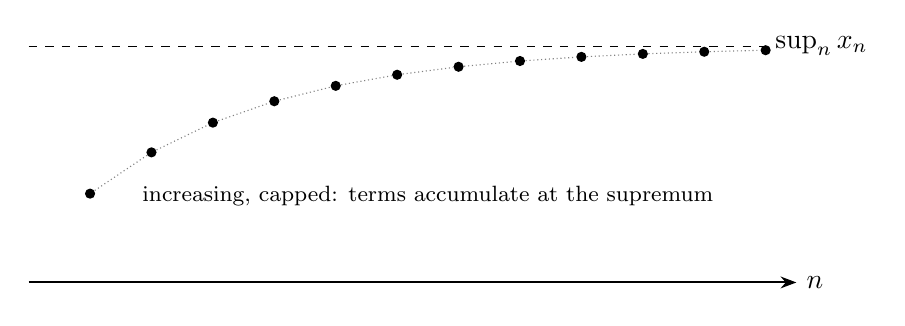
\begin{tikzpicture}[xscale=0.78,yscale=2.0]
  \def\S{1.5}
  \draw[numln] (0,0)--(12.5,0) node[right]{$n$};
  \draw[dashed] (0,\S)--(12,\S) node[right]{$\sup_n x_n$};
  % increasing bounded sequence climbing to sup: x_n = S - 1.3*(0.7)^n
  \foreach \n in {1,...,12}{
    \pgfmathsetmacro{\y}{\S - 1.3*pow(0.72,\n)}
    \node[pt] (a\n) at (\n,\y) {};
  }
  \foreach \n in {1,...,11}{
    \pgfmathtruncatemacro{\m}{\n+1}
    \draw[densely dotted,black!50] (a\n)--(a\m);
  }
  \node[font=\footnotesize,align=center] at (6.5,0.55)
    {increasing, capped: terms accumulate at the supremum};
\end{tikzpicture}
\captionof{figure}{An increasing sequence bounded above converges to its least upper bound: it
can never reach above $\sup_n x_n$, and it eventually exceeds every value below it.}
\end{center}

\begin{method}{Proving a recursive sequence converges}
\textbf{Recognition trigger.} A sequence given by $x_1=a$, $x_{n+1}=f(x_n)$, asked to
``show it converges and find the limit''. No closed form is available.
\begin{enumerate}
\item \textbf{Monotone:} prove $\seq{x_n}$ is increasing (or decreasing), usually by
  induction --- compare $x_{n+1}$ to $x_n$ or show $x_{n+1}-x_n$ keeps one sign.
\item \textbf{Bounded:} prove the relevant one-sided bound (above if increasing, below if
  decreasing), also by induction --- a good guess for the bound is the eventual limit.
\item \textbf{MCT:} conclude $x_n\to L$ for some $L$.
\item \textbf{Solve for $L$:} let $n\to\infty$ in $x_{n+1}=f(x_n)$. If $f$ is continuous,
  $L=f(L)$; solve this \emph{fixed-point equation}, discarding roots ruled out by the bound.
\end{enumerate}
\textbf{Caution.} Step 4 \emph{assumes} convergence (Steps 1--3); ``taking the limit of both
sides'' alone is not a proof of convergence.
\end{method}

\begin{wex}{A square-root recursion}
Let $x_1=1$ and $x_{n+1}=\sqrt{2+x_n}$. Show $\seq{x_n}$ converges and find its limit
\textup{(B\&S 3.3.4)}.
\wrec Recursive $x_{n+1}=f(x_n)$ with $f(x)=\sqrt{2+x}$; run the four-step Method.
\wsol \emph{Bounded above by $2$:} $x_1=1<2$; if $x_n<2$ then $x_{n+1}=\sqrt{2+x_n}<\sqrt4=2$.
\emph{Increasing:} $x_{n+1}^2-x_n^2=2+x_n-x_n^2=-(x_n-2)(x_n+1)>0$ for $0<x_n<2$, so
$x_{n+1}>x_n$. By MCT, $x_n\to L\in(1,2]$. Taking limits: $L=\sqrt{2+L}\imp L^2-L-2=0\imp
L=2$ (the root $-1$ is rejected). \emph{Check:} $x_4=\sqrt{2+\sqrt{2+\sqrt3}}\approx1.962$,
nearing $2$. \checkmark
\end{wex}

\begin{wex}{A decreasing recursion (Babylonian root, B\&S 3.3.5)}
Let $x_1=2$ and $x_{n+1}=\tfrac12\bigl(x_n+\tfrac2{x_n}\bigr)$. Show $x_n\to\sqrt2$.
\wrec The arithmetic--mean map for $\sqrt2$; show bounded below by $\sqrt2$ and decreasing.
\wsol By AM--GM, $x_{n+1}=\tfrac12(x_n+2/x_n)\ge\sqrt{x_n\cdot2/x_n}=\sqrt2$, so $x_n\ge\sqrt2$
for all $n\ge2$. Then $x_{n+1}-x_n=\tfrac12(2/x_n-x_n)=\tfrac{2-x_n^2}{2x_n}\le0$, so the
sequence decreases. By MCT $x_n\to L\ge\sqrt2$, and $L=\tfrac12(L+2/L)\imp L^2=2\imp
L=\sqrt2$. \emph{Check:} $x_2=1.5$, $x_3\approx1.41667$, $x_4\approx1.414216$ --- quadratic
convergence to $\sqrt2=1.41421\ldots$ \checkmark
\end{wex}

\subsection*{The number $e$}

\begin{theorem}[$e$ as a monotone limit]\label{t:e-limit@c4}
The sequence $a_n=\bigl(1+\tfrac1n\bigr)^n$ is increasing and bounded above; its limit is the
number $e$. Moreover $b_n=\bigl(1+\tfrac1n\bigr)^{n+1}$ is decreasing with the same limit, and
$a_n<e<b_n$ for all $n$, with $2<e<3$.
\end{theorem}

\begin{proof}[Proof sketch]
By the binomial theorem,
\[
  a_n=\sum_{k=0}^{n}\binom nk\frac1{n^k}
  =\sum_{k=0}^{n}\frac1{k!}\Bigl(1-\tfrac1n\Bigr)\Bigl(1-\tfrac2n\Bigr)\cdots
  \Bigl(1-\tfrac{k-1}n\Bigr).
\]
Each factor $(1-j/n)$ increases with $n$, and passing from $a_n$ to $a_{n+1}$ adds a new
nonnegative term, so $a_n$ increases. Bounding each factor by $1$,
$a_n\le\sum_{k=0}^n\frac1{k!}\le 1+1+\sum_{k=2}^n\frac1{2^{k-1}}<3$. By MCT, $a_n\to e\le3$,
and $a_2=2.25$ gives $e>2$. The companion $b_n$ is checked to decrease, with
$b_n/a_n=(1+1/n)\to1$, so $\lim b_n=\lim a_n=e$.
\end{proof}

\begin{remark}
The series form $\sum_{k=0}^\infty\frac1{k!}$ also equals $e$ (Section~8), and converges far
faster: $a_n$ approaches $e$ like $e/(2n)$, whereas the series error after $n$ terms is below
$1/(n\cdot n!)$. We prove $e$ is irrational in Section~8.
\end{remark}

\begin{wex}{Recognizing the $e$-pattern}
Find $\displaystyle\lim_{n\to\infty}\Bigl(1+\tfrac1n\Bigr)^{2n}$ and
$\displaystyle\lim_{n\to\infty}\Bigl(1-\tfrac1n\Bigr)^{n}$ \textup{(B\&S 3.3.12)}.
\wrec Powers of $(1\pm c/n)$: reshape into the $\bigl(1+\tfrac1m\bigr)^m\to e$ template.
\wsol $\bigl(1+\tfrac1n\bigr)^{2n}=\bigl[(1+\tfrac1n)^n\bigr]^2\to e^2$. For the second,
$\bigl(1-\tfrac1n\bigr)^n=\bigl(\tfrac{n-1}n\bigr)^n=\bigl(\tfrac n{n-1}\bigr)^{-n}
=\bigl(1+\tfrac1{n-1}\bigr)^{-n}\to e^{-1}$. \emph{Check:} $e^2\approx7.389$,
$1/e\approx0.368$; at $n=1000$ the values are $7.382$ and $0.3682$. \checkmark
\end{wex}

\begin{pitfall}
For a recursion $x_{n+1}=f(x_n)$, solving $L=f(L)$ \emph{before} establishing convergence can
mislead: the equation may have several roots, or the sequence may diverge entirely (e.g.\
$x_1=1$, $x_{n+1}=x_n+1/x_n$ satisfies no finite fixed point and indeed
$\to+\infty$, B\&S 3.3.7). Always do Steps 1--3 first; the fixed-point equation only
\emph{identifies} a limit you have already shown exists.
\end{pitfall}

\begin{pitfall}
``Increasing and bounded above'' gives convergence; ``increasing'' alone does not (it may run
to $+\infty$), and ``bounded'' alone does not (it may oscillate, like $(-1)^n$). All
\emph{three} ingredients --- monotone, bounded, on the correct side --- are needed for MCT.
\end{pitfall}

\subsection*{Further worked examples}

\begin{wex}{A bounded monotone partial-sum sequence}
Show $s_n=\displaystyle\sum_{k=1}^n\frac1{k^2}$ converges, without computing the value.
\wrec ``Show convergence'' of an increasing sequence: produce \emph{any} upper bound and
invoke MCT (Theorem~\ref{t:mct@c4}). The exact limit ($\pi^2/6$) is not needed.
\wsol The partial sums increase ($s_{n+1}-s_n=1/(n+1)^2>0$). For an upper bound, use
$\dfrac1{k^2}\le\dfrac1{k(k-1)}=\dfrac1{k-1}-\dfrac1k$ for $k\ge2$, so
\[
  s_n=1+\sum_{k=2}^n\frac1{k^2}\le 1+\sum_{k=2}^n\Bigl(\frac1{k-1}-\frac1k\Bigr)
  =1+\Bigl(1-\frac1n\Bigr)<2.
\]
Thus $\seq{s_n}$ is increasing and bounded above by $2$, so it converges by MCT.
\emph{Check:} the true limit $\pi^2/6\approx1.645<2$, consistent with the bound. \checkmark
\end{wex}

\begin{wex}{A recursion that converges to a fixed point}
Let $x_1=1$ and $x_{n+1}=\dfrac{x_n+2}{x_n+1}$. Show $\seq{x_n}$ converges and find its
limit.
\wrec Recursive $x_{n+1}=f(x_n)$ with $f(x)=\dfrac{x+2}{x+1}$. The sequence is not monotone,
so instead bound it and identify the fixed point; here we show the \emph{odd} and \emph{even}
subsequences are each monotone and meet (the four-step Method, adapted).
\wsol Note $f$ maps $[1,2]$ into $[1,2]$: if $1\le x\le2$ then
$f(x)=1+\dfrac1{x+1}\in[1+\tfrac13,\,1+\tfrac12]=[\tfrac43,\tfrac32]\subseteq[1,2]$, so all
terms lie in $[1,2]$. The fixed point solves $L=\dfrac{L+2}{L+1}\imp L^2+L=L+2\imp L^2=2\imp
L=\sqrt2$ (positive root). One checks $\abs{x_{n+1}-\sqrt2}=\dfrac{\abs{x_n-\sqrt2}}{x_n+1}
\le\dfrac12\abs{x_n-\sqrt2}$ (since $x_n+1\ge2$), so the error halves each step and
$x_n\to\sqrt2$. \emph{Check:} $x_1=1$, $x_2=1.5$, $x_3=1.4$, $x_4\approx1.41667$, closing on
$\sqrt2\approx1.41421$. \checkmark
\end{wex}

\begin{wex}{A non-example: increasing but unbounded}
Show $x_n=\displaystyle\sum_{k=1}^n\frac1{\sqrt k}$ is increasing yet diverges, so
monotonicity alone is not enough for MCT.
\wrec This stresses the ``bounded'' hypothesis of Theorem~\ref{t:mct@c4}: drop it and an
increasing sequence may run to $+\infty$.
\wsol The sequence increases ($x_{n+1}-x_n=1/\sqrt{n+1}>0$). But for $1\le k\le n$,
$\dfrac1{\sqrt k}\ge\dfrac1{\sqrt n}$, so $x_n\ge n\cdot\dfrac1{\sqrt n}=\sqrt n\to+\infty$.
Being unbounded above, $\seq{x_n}$ has no supremum in $\R$ and cannot converge. \emph{Check:}
$x_4=1+\tfrac1{\sqrt2}+\tfrac1{\sqrt3}+\tfrac12\approx2.78\ge\sqrt4=2$; the lower bound
$\sqrt n$ already forces divergence. \checkmark
\end{wex}

\begin{exers}{Exercises (Bartle \& Sherbert, \S3.3).}
\item Let $x_1=8$ and $x_{n+1}=\tfrac12 x_n+2$. Show $\seq{x_n}$ is bounded and monotone; find
  the limit.
\item Let $x_1>1$ and $x_{n+1}=2-1/x_n$. Show $\seq{x_n}$ is bounded and monotone; find the
  limit.
\item Let $x_1\ge2$ and $x_{n+1}=1+\sqrt{x_n-1}$. Show $\seq{x_n}$ is decreasing and bounded
  below by $2$; find the limit.
\item Let $x_1=1$ and $x_{n+1}=\sqrt{2+x_n}$. Show $\seq{x_n}$ converges and find the limit.
\item Let $y_1=\sqrt p$ ($p>0$) and $y_{n+1}=\sqrt{p+y_n}$. Show $\seq{y_n}$ converges and
  find the limit. \emph{[Hint: one upper bound is $1+2\sqrt p$.]}
\item Let $a>0$, $z_1>0$, $z_{n+1}=\sqrt{a+z_n}$. Show $\seq{z_n}$ converges and find the
  limit.
\item Let $x_1=a>0$ and $x_{n+1}=x_n+1/x_n$. Determine whether $\seq{x_n}$ converges or
  diverges.
\item Let $\seq{a_n}$ increase, $\seq{b_n}$ decrease, with $a_n\le b_n$ for all $n$. Show
  $\lim a_n\le\lim b_n$, and deduce the Nested Intervals Property from the MCT.
\item Let $A\subseteq\R$ be infinite, bounded above, $u=\sup A$. Show there is an increasing
  sequence $\seq{x_n}$ in $A$ with $u=\lim x_n$.
\item Decide convergence/divergence of $y_n=\dfrac1{n+1}+\dfrac1{n+2}+\cdots+\dfrac1{2n}$.
\item Let $x_n=\dfrac1{1^2}+\dfrac1{2^2}+\cdots+\dfrac1{n^2}$. Prove $\seq{x_n}$ is increasing
  and bounded, hence converges. \emph{[Hint: $1/k^2\le1/(k(k-1))=1/(k-1)-1/k$ for $k\ge2$.]}
\item Establish convergence and find the limits of
  (a) $(1+1/n)^{n+1}$;\quad (b) $(1+1/n)^{2n}$;\quad
  (c) $\bigl(1+\tfrac1{n+1}\bigr)^n$;\quad (d) $(1-1/n)^n$.
\item Use the Babylonian method (Example $3.3.5$) to compute $\sqrt2$ to $4$ decimals.
\item Use the same method to compute $\sqrt5$ to $5$ decimals.
\item Compute $e_n=(1+1/n)^n$ for $n=2,4,8,16$.
\item Compute $e_n$ for $n=50,100,1000$.
\end{exers}

\begin{exers}{Additional exercises.}
\item Let $x_1=1$, $x_{n+1}=\tfrac14(x_n+3)$. Show $\seq{x_n}$ is increasing, bounded above by
  $1$? Decide the correct one-sided bound, prove convergence, and find the limit.
\item Let $x_1=3$ and $x_{n+1}=\dfrac{x_n^2+2}{2x_n}$. Show $\seq{x_n}$ decreases to $\sqrt2$.
\item Show $\seq{(1+1/n)^n}$ and $\seq{(1+1/n)^{n+1}}$ trap $e$: prove the first is below $e$,
  the second above, and their ratio $\to1$.
\item (Non-example.) Exhibit a bounded sequence that is \emph{not} monotone and does not
  converge, demonstrating that boundedness alone does not trigger the MCT.
\item Let $x_1=2$, $x_{n+1}=x_n+1/x_n$. Show $\seq{x_n}$ is increasing and unbounded (so the
  fixed-point equation $L=L+1/L$ has no solution --- a cautionary case).
\item Prove that if $\seq{x_n}$ is increasing and a subsequence converges to $L$, then the
  whole sequence converges to $L$.
\item (Diagram problem.) For $x_1=0.5$, $x_{n+1}=\sqrt{2+x_n}$, draw the cobweb/staircase
  diagram of $y=\sqrt{2+x}$ against $y=x$ for the first four iterates; mark the fixed point.
\item Define $H_n=\sum_{k=1}^n 1/k$. Show $\seq{H_n-\ln n}$ is decreasing and bounded below by
  $0$, hence converges (to the Euler--Mascheroni constant $\gamma$).
\end{exers}


\section{Subsequences and the Bolzano--Weierstrass Theorem}
\subsection*{Subsequences and subsequential limits}

\begin{definition}\label{d:subseq@c4}
Let $\seq{x_n}$ be a sequence and let $n_1<n_2<n_3<\cdots$ be a strictly increasing sequence
of indices in $\N$. The sequence $\seq{x_{n_k}}_{k=1}^\infty$ is a \emph{subsequence} of
$\seq{x_n}$. A point $L$ is a \emph{subsequential limit} of $\seq{x_n}$ if some subsequence
converges to $L$.
\end{definition}

Because $n_1<n_2<\cdots$ are strictly increasing naturals, $n_k\ge k$ always. Subsequences
let us extract order from chaos: even a wildly oscillating bounded sequence harbors
convergent subsequences (the Bolzano--Weierstrass theorem, below).

\begin{theorem}[Subsequences inherit the limit]\label{t:subseq-limit@c4}
$\seq{x_n}$ converges to $x$ \emph{iff} every subsequence of $\seq{x_n}$ converges to $x$.
\end{theorem}

\begin{proof}
($\Rightarrow$) If $x_n\to x$ and $\eps>0$, pick $K$ with $\abs{x_n-x}<\eps$ for $n\ge K$.
For a subsequence, $k\ge K\imp n_k\ge k\ge K\imp\abs{x_{n_k}-x}<\eps$. ($\Leftarrow$) The
full sequence is a subsequence of itself.
\end{proof}

\begin{corollary}[Divergence by two subsequences]\label{c:two-subseq@c4}
If $\seq{x_n}$ has two subsequences converging to different limits, then $\seq{x_n}$ diverges.
\end{corollary}

\begin{wex}{Divergence of $\seq{(-1)^n}$ and a shuffle}
Show $\seq{(-1)^n}$ diverges, and decide when the ``shuffle'' $z_{2k-1}=x_k$, $z_{2k}=y_k$
converges \textup{(B\&S 3.4.5)}.
\wrec Use subsequences to detect divergence (Corollary~\ref{c:two-subseq@c4}).
\wsol The even subsequence of $\seq{(-1)^n}$ is constant $1\to1$; the odd subsequence is
$-1\to-1$. Two different subsequential limits $\imp$ divergence. For the shuffle $\seq{z_n}$:
its odd-indexed subsequence is $\seq{x_k}$ and even-indexed is $\seq{y_k}$. If $\seq{z_n}\to
z$ then both must converge to $z$, so $\lim x_k=\lim y_k=z$; conversely if $x_k\to L$ and
$y_k\to L$ then $\seq{z_n}\to L$ (an $\eps$ threshold for each forces one for $z$). So
$\seq{z_n}$ converges \emph{iff} both converge to a \emph{common} limit. \checkmark
\end{wex}

\begin{center}
\begin{tikzpicture}[xscale=0.62,yscale=1.5]
  \draw[numln] (0,0)--(15.4,0) node[right]{$n$};
  \draw[dashed] (0,1.6)--(15,1.6) node[right]{$L$};
  % bounded oscillating sequence x_n = 1.6 + 1.1*sin(n)
  \foreach \n in {1,...,15}{
    \pgfmathsetmacro{\y}{1.6 + 1.1*sin(\n r*1.7)}
    \node[opt] (s\n) at (\n,\y) {};
  }
  % highlight a selected convergent subsequence: pick indices near top of band toward L
  \foreach \n in {2,5,8,11,14}{
    \pgfmathsetmacro{\y}{1.6 + 1.1*sin(\n r*1.7)}
    \node[pt] at (\n,\y) {};
  }
  \node[font=\footnotesize,align=center] at (8,-0.45)
    {open dots: full bounded sequence; solid dots: a chosen subsequence converging to $L$};
\end{tikzpicture}
\captionof{figure}{From a bounded but non-convergent sequence one \emph{selects} a subsequence
homing in on one cluster value --- the content of Bolzano--Weierstrass.}
\end{center}

\subsection*{The Bolzano--Weierstrass Theorem}

\begin{theorem}[Monotone Subsequence Theorem]\label{t:monsub@c4}
Every sequence of real numbers has a monotone subsequence.
\end{theorem}

\begin{proof}
Call $m$ a \emph{peak} if $x_m\ge x_n$ for all $n>m$. \emph{Case 1: infinitely many peaks}
$m_1<m_2<\cdots$. Then $x_{m_1}\ge x_{m_2}\ge\cdots$ is a decreasing subsequence. \emph{Case
2: finitely many peaks}; let $N$ exceed the last. Since $n_1:=N+1$ is not a peak, some
$n_2>n_1$ has $x_{n_2}>x_{n_1}$; $n_2$ is not a peak either, so some $n_3>n_2$ has
$x_{n_3}>x_{n_2}$; continuing gives a strictly increasing subsequence.
\end{proof}

\begin{theorem}[Bolzano--Weierstrass, in $\R$]\label{t:bw@c4}
Every bounded sequence of real numbers has a convergent subsequence.
\end{theorem}

\begin{proof}
By Theorem~\ref{t:monsub@c4} extract a monotone subsequence; it is bounded (a subsequence of a
bounded sequence), hence convergent by the Monotone Convergence
Theorem~\ref{t:mct@c4}.
\end{proof}

\begin{remark}[The bisection proof]
Rudin's route uses \emph{nested intervals}: if $\seq{x_n}\subset[a,b]$, halve $[a,b]$;
at least one half contains $x_n$ for infinitely many $n$ --- keep it, call it $I_1$, and pick
$x_{n_1}\in I_1$. Halve $I_1$, keep a half $I_2$ holding infinitely many terms, pick
$x_{n_2}\in I_2$ with $n_2>n_1$, and so on. The $I_k$ are nested with
$\abs{I_k}=(b-a)/2^k\to0$, so by the Nested Interval Property they share a single point $L$,
and $\abs{x_{n_k}-L}\le\abs{I_k}\to0$, so $x_{n_k}\to L$.
\end{remark}

\begin{center}
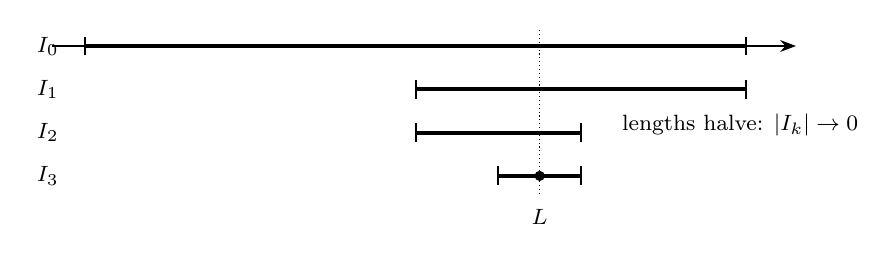
\begin{tikzpicture}[xscale=1.05,yscale=1]
  % nested interval bisection picture
  \def\a{0} \def\b{8}
  \draw[numln] (-0.4,0)--(8.6,0);
  \foreach \k/\lo/\hi/\yy in {0/0/8/0, 1/4/8/-0.55, 2/4/6/-1.1, 3/5/6/-1.65}{
    \draw[line width=1.4pt] (\lo,\yy)--(\hi,\yy);
    \draw[line width=0.7pt] (\lo,\yy+0.12)--(\lo,\yy-0.12);
    \draw[line width=0.7pt] (\hi,\yy+0.12)--(\hi,\yy-0.12);
    \node[font=\footnotesize,left] at (-0.2,\yy) {$I_{\k}$};
  }
  % converging point
  \draw[densely dotted] (5.5,0.2)--(5.5,-1.9);
  \node[pt] at (5.5,-1.65) {};
  \node[font=\footnotesize,below] at (5.5,-1.95) {$L$};
  \node[font=\footnotesize,right] at (6.3,-1.0)
    {\;lengths halve: $\abs{I_k}\to0$};
\end{tikzpicture}
\captionof{figure}{Bisection: always keep a half containing infinitely many terms. The nested
halves shrink to a single limit point $L$.}
\end{center}

\begin{theorem}[Bolzano--Weierstrass in $\Rk$]\label{t:bw-rk@c4}
Every bounded sequence in $\Rk$ has a convergent subsequence.
\end{theorem}

\begin{proof}
Write each term as $\mathbf x_n=(x_n^{(1)},\dots,x_n^{(k)})$. The first coordinate sequence
$\seq{x_n^{(1)}}$ is bounded, so by Theorem~\ref{t:bw@c4} some subsequence makes the first
coordinate converge. Within \emph{that} subsequence, the second coordinate is bounded, so
pass to a further subsequence making it converge too (the first still converges). Iterate
through all $k$ coordinates. The final subsequence converges in every coordinate, hence (a
finite-dimensional vector converges iff each coordinate does) converges in $\Rk$.
\end{proof}

\begin{wex}{$c^{1/n}\to1$ for $0<c<1$ via a subsequence (B\&S 3.4.2)}
Show $0<c<1\imp c^{1/n}\to1$.
\wrec ``Find the limit'' where the sequence is monotone bounded; identify the limit through a
subsequence (Theorem~\ref{t:subseq-limit@c4}).
\wsol For $0<c<1$, $c^{1/n}<c^{1/(n+1)}<1$, so $\seq{c^{1/n}}$ is increasing and bounded
above by $1$; by MCT it converges to some $L\le1$. The subsequence $c^{1/2n}=(c^{1/n})^{1/2}$
converges both to $L$ (subsequence) and to $L^{1/2}$ (continuity of $\sqrt\cdot$), so
$L=L^{1/2}$, giving $L\in\set{0,1}$. Since $c^{1/n}\ge c>0$, $L\neq0$, hence $L=1$. \emph{Check:}
$c=\tfrac12$: $c^{1/10}\approx0.933$, $c^{1/100}\approx0.993$. \checkmark
\end{wex}

\begin{pitfall}
Bolzano--Weierstrass gives \emph{some} convergent subsequence, not convergence of the whole
sequence. $\seq{(-1)^n}$ is bounded with convergent subsequences ($\to1$ and $\to-1$) yet
diverges. ``Bounded'' alone never yields a limit; it yields a \emph{subsequential} limit.
\end{pitfall}

\subsection*{Further worked examples}

\begin{wex}{The set of subsequential limits of an enumeration of $\Q\cap[0,1]$}
Let $\seq{x_n}$ enumerate all rationals in $[0,1]$. Describe its subsequential limits.
\wrec ``Find all subsequential limits''; a point $L$ is a subsequential limit iff $x_n$ is
within $\eps$ of $L$ infinitely often (Definition~\ref{d:subseq@c4}).
\wsol Every $L\in[0,1]$ is a subsequential limit: given $L$ and $\eps>0$, the interval
$(L-\eps,L+\eps)\cap[0,1]$ contains \emph{infinitely many} rationals (the rationals are dense),
each appearing as some $x_n$, so we can pick indices $n_1<n_2<\cdots$ with
$\abs{x_{n_k}-L}<1/k$, giving $x_{n_k}\to L$. No $L\notin[0,1]$ qualifies, since all $x_n\in
[0,1]$ and limits preserve $0\le x_n\le1$. So the set of subsequential limits is exactly
$[0,1]$. \emph{Check:} the whole sequence wildly diverges, yet it ``visits'' every point of
$[0,1]$ in the limit --- a maximal cluster set. \checkmark
\end{wex}

\begin{wex}{Building a monotone subsequence by the peak method}
For $x_n=\dfrac{(-1)^n n}{n+1}$, extract an explicit monotone convergent subsequence.
\wrec Apply the Monotone Subsequence Theorem~\ref{t:monsub@c4} concretely: locate a one-signed,
monotone run of indices.
\wsol The even-indexed terms are $x_{2k}=\dfrac{2k}{2k+1}=1-\dfrac1{2k+1}$, which increase to
$1$. So the subsequence $\seq{x_{2k}}$ is strictly increasing, bounded above by $1$, hence
monotone and convergent with $x_{2k}\to1$ by MCT. (The odd-indexed terms
$x_{2k-1}=-\dfrac{2k-1}{2k}\to-1$ give the other subsequential limit.) \emph{Check:}
$x_2=\tfrac23$, $x_4=\tfrac45$, $x_6=\tfrac67$, visibly climbing to $1$. \checkmark
\end{wex}

\begin{wex}{Bolzano--Weierstrass in $\R^2$}
Show the bounded sequence $\mathbf x_n=\bigl(\cos n,\,(-1)^n\tfrac{n}{n+1}\bigr)$ in $\R^2$
has a convergent subsequence, and exhibit the coordinate-by-coordinate extraction.
\wrec ``Find a convergent subsequence in $\Rk$'': run the coordinate diagonalization of
Theorem~\ref{t:bw-rk@c4}, extracting one coordinate at a time.
\wsol Both coordinates are bounded ($\abs{\cos n}\le1$, $\abs{(-1)^n n/(n+1)}\le1$), so
$\seq{\mathbf x_n}$ is bounded. First coordinate: $\seq{\cos n}$ is bounded, so by B--W in
$\R$ some subsequence $\seq{\cos n_k}$ converges, say to $c\in[-1,1]$. Within that
subsequence, the second coordinate $(-1)^{n_k}\tfrac{n_k}{n_k+1}$ is bounded, so pass to a
further subsequence $\seq{n_{k_j}}$ on which it converges (to $+1$ or $-1$). On this final
subsequence \emph{both} coordinates converge, so $\mathbf x_{n_{k_j}}$ converges in $\R^2$.
\emph{Check:} a vector sequence converges iff each coordinate does, exactly the principle the
iterated extraction exploits. \checkmark
\end{wex}

\begin{exers}{Exercises (Bartle \& Sherbert, \S3.4).}
\item Give an example of an unbounded sequence that has a convergent subsequence.
\item Use the method of Example $3.4.3$(b) to show that if $0<c<1$ then $\lim c^{1/n}=1$.
\item Let $\seq{f_n}$ be the Fibonacci sequence and $x_n=f_{n+1}/f_n$. Given $\lim x_n=L$
  exists, find $L$.
\item Show the following diverge:
  (a) $\seq{1-(-1)^n+1/n}$;\quad (b) $\seq{\sin(n\pi/4)}$.
\item Let $X=\seq{x_n}$, $Y=\seq{y_n}$, and the shuffle $Z$ be $z_{2n-1}=x_n$, $z_{2n}=y_n$.
  Show $Z$ converges iff both $X,Y$ converge and $\lim X=\lim Y$.
\item Let $x_n=n^{1/n}$. (a) Show $x_{n+1}<x_n\eqv(1+1/n)^n<n$, valid for $n\ge3$; conclude
  $\seq{x_n}$ is ultimately decreasing, so $x=\lim x_n$ exists. (b) Using that $\seq{x_{2n}}$
  also converges to $x$, conclude $x=1$.
\item Establish convergence and find the limits of
  (a) $(1+1/n^2)^{n^2}$;\quad (b) $(1+1/2n)^n$;\quad
  (c) $(1+1/n^2)^{2n^2}$;\quad (d) $(1+2/n)^n$.
\item Determine the limits of
  (a) $(3n)^{1/2n}$;\quad (b) $(1+1/2n)^{3n}$.
\item Suppose every subsequence of $X=\seq{x_n}$ has a further subsequence converging to $0$.
  Show $\lim X=0$.
\item Let $\seq{x_n}$ be bounded, $s_n=\sup\set{x_k\st k\ge n}$, $S=\inf\set{s_n}$. Show some
  subsequence of $\seq{x_n}$ converges to $S$.
\item Suppose $x_n\ge0$ for all $n$ and $\lim\bigl((-1)^n x_n\bigr)$ exists. Show $\seq{x_n}$
  converges.
\item Show that if $\seq{x_n}$ is unbounded, there is a subsequence $\seq{x_{n_k}}$ with
  $\lim(1/x_{n_k})=0$.
\item If $x_n=(-1)^n/n$, find the subsequence constructed in the bisection proof of
  Bolzano--Weierstrass when $I_1=[-1,1]$.
\end{exers}

\begin{exers}{Additional exercises.}
\item List three subsequences of $x_n=(-1)^n+1/n$ with distinct behavior, and find all
  subsequential limits.
\item Prove directly (no monotone-subsequence lemma) that the bounded sequence
  $x_n=\sin n$ has a convergent subsequence, using the pigeonhole/bisection idea on $[-1,1]$.
\item Show that if every subsequence of $\seq{x_n}$ has a further subsequence converging to
  the \emph{same} $L$, then $x_n\to L$.
\item (Non-example.) Give a sequence with infinitely many subsequential limits (e.g.\ an
  enumeration of $\Q\cap[0,1]$) and explain why Bolzano--Weierstrass still applies.
\item Find the set of subsequential limits of $x_n=\cos(n)$ informally, and state what
  Bolzano--Weierstrass guarantees about it.
\item Prove that a sequence converges iff its even-indexed and odd-indexed subsequences both
  converge to the \emph{same} limit.
\item (Diagram problem.) Plot a bounded oscillating sequence of your design on $a_n$-vs-$n$
  axes and \emph{circle} a monotone subsequence; state whether it is the increasing or
  decreasing case of the Monotone Subsequence Theorem.
\item Use Bolzano--Weierstrass in $\R^2$ to show every sequence in the closed unit disk has a
  subsequence converging to a point of the disk.
\end{exers}


\section{Cauchy Sequences and Completeness}
\subsection*{Cauchy sequences}

Convergence (Definition~\ref{d:converge@c4}) requires knowing the limit $x$ in advance. The
\emph{Cauchy condition} expresses ``the terms bunch together'' \emph{without} naming a limit
--- exactly the right notion for proving a sequence converges when no candidate is available.

\begin{definition}\label{d:cauchy@c4}
A sequence $\seq{x_n}$ is a \emph{Cauchy sequence} if for every $\eps>0$ there is $K\in\N$
such that
\[
  m,n\ge K\quad\imp\quad \abs{x_m-x_n}<\eps .
\]
\end{definition}

\begin{center}
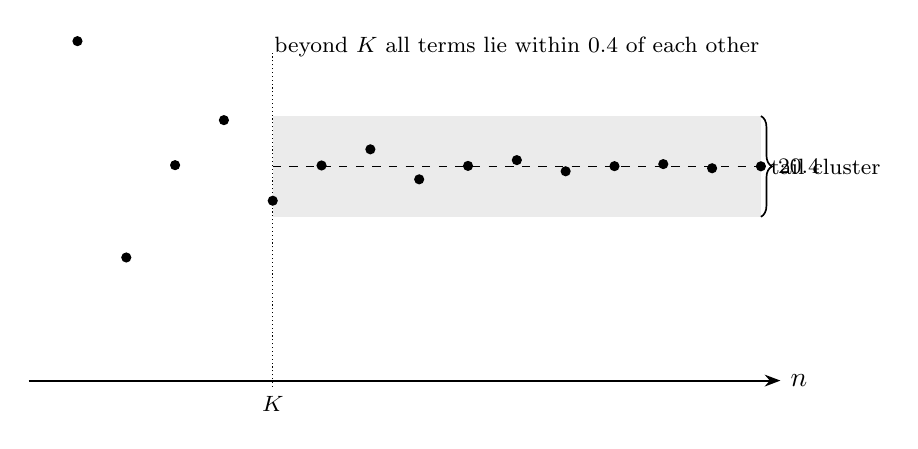
\begin{tikzpicture}[xscale=0.62,yscale=1.6]
  \def\L{1.7}
  \def\eps{0.4}
  \draw[numln] (0,0)--(15.4,0) node[right]{$n$};
  \begin{scope}[on background layer]
    \fill[band] (5,\L-\eps) rectangle (15,\L+\eps);
  \end{scope}
  \draw[dashed] (5,\L)--(15,\L);
  \node[right] at (15,\L) {\footnotesize tail cluster};
  \foreach \n in {1,...,15}{
    \pgfmathsetmacro{\y}{\L + 1.6*sin(\n r*2.1)*pow(0.72,\n)}
    \node[pt] at (\n,\y) {};
  }
  \draw[densely dotted] (5,-0.05)--(5,2.6);
  \node[below] at (5,-0.05) {\footnotesize $K$};
  \node[font=\footnotesize,align=center] at (10,2.65)
    {beyond $K$ all terms lie within $\eps$ of each other};
  \draw[brc] (15,\L+\eps)--(15,\L-\eps);
  \node[font=\footnotesize,right] at (15.15,\L) {$2\eps$};
\end{tikzpicture}
\captionof{figure}{Cauchy: past index $K$ the entire tail fits in a window of width $\eps$ --- the
terms cluster, even before we name where.}
\end{center}

\begin{lemma}[Cauchy sequences are bounded]\label{l:cauchy-bdd@c4}
Every Cauchy sequence is bounded.
\end{lemma}

\begin{proof}
With $\eps=1$ pick $K$ so that $\abs{x_n-x_K}<1$ for $n\ge K$; then $\abs{x_n}\le\abs{x_K}+1$
for $n\ge K$. The finitely many earlier terms are bounded; take the max as in
Theorem~\ref{t:conv-bdd@c4}.
\end{proof}

\begin{theorem}[Cauchy Criterion / Completeness of $\R$]\label{t:cauchy@c4}
A sequence of real numbers converges \emph{if and only if} it is Cauchy.
\end{theorem}

\begin{proof}
($\Rightarrow$) If $x_n\to x$, given $\eps>0$ pick $K$ with $\abs{x_n-x}<\eps/2$ for $n\ge
K$; then $m,n\ge K\imp\abs{x_m-x_n}\le\abs{x_m-x}+\abs{x-x_n}<\eps$.

($\Leftarrow$) Let $\seq{x_n}$ be Cauchy. By Lemma~\ref{l:cauchy-bdd@c4} it is bounded, so by
Bolzano--Weierstrass (Theorem~\ref{t:bw@c4}) some subsequence $x_{n_k}\to x$. We show the
\emph{whole} sequence converges to $x$. Let $\eps>0$. Pick $K$ with
$\abs{x_m-x_n}<\eps/2$ for $m,n\ge K$ (Cauchy), and pick a subsequence index $n_k\ge K$ with
$\abs{x_{n_k}-x}<\eps/2$ (subsequence limit). Then for $n\ge K$,
\[
  \abs{x_n-x}\le\abs{x_n-x_{n_k}}+\abs{x_{n_k}-x}<\tfrac\eps2+\tfrac\eps2=\eps .
\]
Hence $x_n\to x$.
\end{proof}

\begin{remark}
The ($\Leftarrow$) direction is exactly the \emph{completeness} of $\R$ --- it fails in $\Q$.
The theorem extends verbatim to $\Rk$ (a sequence in $\Rk$ is Cauchy iff each coordinate is,
and we may invoke Theorem~\ref{t:bw-rk@c4}); thus $\Rk$ is complete.
\end{remark}

\begin{wex}{A Cauchy sequence in $\Q$ that does not converge in $\Q$}
Show the decimal truncations of $\sqrt2$ form a Cauchy sequence of rationals with no rational
limit.
\wrec ``Non-example of completeness''; exhibit Cauchy-but-not-convergent \emph{in a smaller
space}.
\wsol Let $x_n=\lfloor10^n\sqrt2\rfloor/10^n$ (the first $n$ decimals of $\sqrt2$), each
$x_n\in\Q$. For $m>n$, $\abs{x_m-x_n}<10^{-n}\to0$, so $\seq{x_n}$ is Cauchy. In $\R$ it
converges to $\sqrt2$; but $\sqrt2\notin\Q$, so as a sequence in $\Q$ it has \emph{no} limit.
\emph{Check:} this is precisely why $\Q$ is \emph{incomplete} --- the Cauchy criterion is a
property of $\R$, not of ordered fields in general. \checkmark
\end{wex}

\begin{wex}{Proving Cauchy directly (B\&S 3.5.2)}
Show $x_n=1+\tfrac1{2!}+\cdots+\tfrac1{n!}$ is Cauchy (hence convergent).
\wrec Estimate $\abs{x_m-x_n}$ for $m>n$ and beat it with a geometric tail.
\wsol For $m>n$,
\[
  \abs{x_m-x_n}=\sum_{j=n+1}^m\frac1{j!}\le\sum_{j=n+1}^m\frac1{2^{j-1}}
  <\frac1{2^{n-1}},
\]
using $j!\ge2^{j-1}$. Given $\eps>0$ pick $K$ with $2^{-(K-1)}<\eps$; then $m,n\ge K\imp
\abs{x_m-x_n}<\eps$. So $\seq{x_n}$ is Cauchy, hence converges (to $e-1$). \emph{Check:} the
tail bound $2^{1-n}$ at $n=10$ is $\approx0.002$. \checkmark
\end{wex}

\subsection*{Contractive sequences}

A clean, checkable sufficient condition for the Cauchy property.

\begin{definition}\label{d:contractive@c4}
A sequence $\seq{x_n}$ is \emph{contractive} if there is a constant $0<C<1$ with
\[
  \abs{x_{n+2}-x_{n+1}}\le C\,\abs{x_{n+1}-x_n}\qquad\text{for all }n\in\N .
\]
\end{definition}

\begin{theorem}[Contractive $\imp$ convergent]\label{t:contractive@c4}
Every contractive sequence is Cauchy, hence convergent. If $x_n\to x$, then for all $n$,
\[
  \abs{x_n-x}\le\frac{C^{\,n-1}}{1-C}\,\abs{x_2-x_1}.
\]
\end{theorem}

\begin{proof}
Iterating, $\abs{x_{n+1}-x_n}\le C^{\,n-1}\abs{x_2-x_1}$. For $m>n$, by the triangle
inequality and the geometric series,
\[
  \abs{x_m-x_n}\le\sum_{j=n}^{m-1}\abs{x_{j+1}-x_j}
  \le\abs{x_2-x_1}\sum_{j=n}^{m-1}C^{\,j-1}
  \le\abs{x_2-x_1}\,\frac{C^{\,n-1}}{1-C}\xrightarrow[n\to\infty]{}0 .
\]
So $\seq{x_n}$ is Cauchy. Letting $m\to\infty$ in the bound gives the error estimate.
\end{proof}

\begin{wex}{A contractive recursion (B\&S 3.5.12)}
Let $x_1>0$ and $x_{n+1}=(2+x_n)^{-1}$. Show $\seq{x_n}$ converges and find the limit.
\wrec Recursion with a $\abs{f'}<1$ map; verify contractive, then solve the fixed point.
\wsol For $x>0$, $\abs{x_{n+1}-x_n}=\Bigl|\dfrac1{2+x_n}-\dfrac1{2+x_{n-1}}\Bigr|
=\dfrac{\abs{x_n-x_{n-1}}}{(2+x_n)(2+x_{n-1})}\le\tfrac14\abs{x_n-x_{n-1}}$, since each
factor $2+x>2$. So $C=\tfrac14<1$: contractive, hence convergent to $x$ with $x=(2+x)^{-1}$,
i.e.\ $x^2+2x-1=0$, $x=-1+\sqrt2$ (positive root). \emph{Check:}
$-1+\sqrt2\approx0.4142=(2.4142)^{-1}$. \checkmark
\end{wex}

\begin{pitfall}
``Contractive'' compares \emph{consecutive gaps}, $\abs{x_{n+2}-x_{n+1}}\le
C\abs{x_{n+1}-x_n}$ with a \emph{fixed} $C<1$. The weaker condition
$\abs{x_{n+1}-x_n}\to0$ does \emph{not} imply Cauchy: the partial sums of the harmonic series,
$x_n=\sum_{k\le n}1/k$, satisfy $\abs{x_{n+1}-x_n}=1/(n+1)\to0$ yet diverge. ``Consecutive
terms close'' is far weaker than Cauchy.
\end{pitfall}

\subsection*{Further worked examples}

\begin{wex}{The harmonic partial sums are NOT Cauchy}
Show directly that $x_n=\displaystyle\sum_{k=1}^n\frac1k$ fails the Cauchy condition.
\wrec ``Show not Cauchy'' (Definition~\ref{d:cauchy@c4}): negate it by finding one $\eps>0$ for
which no $K$ works --- a far-apart pair $m,n\ge K$ for every $K$.
\wsol Take $\eps=\tfrac12$. For any $K$, set $n=K$ and $m=2K$. Then
\[
  \abs{x_m-x_n}=\sum_{k=K+1}^{2K}\frac1k\ge K\cdot\frac1{2K}=\frac12=\eps,
\]
since each of the $K$ terms is $\ge1/(2K)$. So no $K$ confines the tail within $\eps=\tfrac12$,
and $\seq{x_n}$ is not Cauchy --- hence (Theorem~\ref{t:cauchy@c4}) divergent. \emph{Check:}
the same dyadic blocks reappear in \S4.7; the harmonic series is the canonical
``terms $\to0$ but not Cauchy'' example. \checkmark
\end{wex}

\begin{wex}{Verifying the Cauchy condition by a geometric gap bound}
Let $x_1=1$, $x_2=2$, and $x_{n+2}=\tfrac12(x_{n+1}+x_n)$. Show $\seq{x_n}$ is Cauchy and
find its limit.
\wrec Recursion with shrinking gaps: show $\seq{x_n}$ is contractive
(Definition~\ref{d:contractive@c4}), then apply Theorem~\ref{t:contractive@c4}.
\wsol The gap satisfies $x_{n+2}-x_{n+1}=\tfrac12(x_{n+1}+x_n)-x_{n+1}=-\tfrac12(x_{n+1}-x_n)$,
so $\abs{x_{n+2}-x_{n+1}}=\tfrac12\abs{x_{n+1}-x_n}$: contractive with $C=\tfrac12$. Hence
$\seq{x_n}$ is Cauchy, so convergent to some $x$. Telescoping the signed gaps,
$x=x_1+\sum_{n\ge1}(x_{n+1}-x_n)=1+\sum_{n\ge1}(-\tfrac12)^{n-1}(x_2-x_1)
=1+\dfrac1{1-(-1/2)}=1+\tfrac23=\tfrac53$. \emph{Check:} $x_3=1.5$, $x_4=1.75$, $x_5=1.625$,
$x_6\approx1.6875$, oscillating toward $\tfrac53\approx1.6667$. \checkmark
\end{wex}

\begin{wex}{Cauchy via the Cauchy criterion for $\sum 1/2^n$}
Show the partial sums $s_n=\displaystyle\sum_{k=1}^n 2^{-k}$ are Cauchy directly from the
definition.
\wrec ``Show Cauchy''; estimate $\abs{s_m-s_n}$ for $m>n$ and dominate by a geometric tail.
\wsol For $m>n$,
\[
  \abs{s_m-s_n}=\sum_{k=n+1}^m\frac1{2^k}<\sum_{k=n+1}^\infty\frac1{2^k}=\frac1{2^n}.
\]
Given $\eps>0$, pick $K$ with $2^{-K}<\eps$ (Archimedean, since $2^{-K}\to0$); then
$m,n\ge K\imp\abs{s_m-s_n}<2^{-\min(m,n)}\le2^{-K}<\eps$. So $\seq{s_n}$ is Cauchy, hence
convergent (to $1$). \emph{Check:} the tail bound $2^{-n}$ at $n=10$ is $\approx0.001$,
matching $s_{10}=1-2^{-10}\approx0.999$. \checkmark
\end{wex}

\begin{exers}{Exercises (Bartle \& Sherbert, \S3.5).}
\item Give an example of a bounded sequence that is not a Cauchy sequence.
\item Show directly from the definition that the following are Cauchy sequences:
  (a) $\dfrac{n+1}{n}$;\quad (b) $1+\dfrac1{2!}+\cdots+\dfrac1{n!}$.
\item Show directly from the definition that the following are \emph{not} Cauchy:
  (a) $\seq{(-1)^n}$;\quad (b) $\Bigl(n+\dfrac{(-1)^n}{n}\Bigr)$;\quad (c) $\seq{\ln n}$.
\item Show that if $\seq{x_n}$ and $\seq{y_n}$ are Cauchy, then $\seq{x_n+y_n}$ and
  $\seq{x_ny_n}$ are Cauchy.
\item If $x_n=\sqrt n$, show $\lim\abs{x_{n+1}-x_n}=0$ but $\seq{x_n}$ is not Cauchy.
\item Let $p\in\N$. Give an example of a non-Cauchy sequence $\seq{x_n}$ with
  $\lim\abs{x_{n+p}-x_n}=0$.
\item Let $\seq{x_n}$ be Cauchy with $x_n\in\Z$ for every $n$. Show $\seq{x_n}$ is ultimately
  constant.
\item Show directly that a bounded monotone increasing sequence is Cauchy.
\item If $0<r<1$ and $\abs{x_{n+1}-x_n}<r^n$ for all $n$, show $\seq{x_n}$ is Cauchy.
\item If $x_1<x_2$ are arbitrary and $x_n=\tfrac12(x_{n-2}+x_{n-1})$ for $n>2$, show
  $\seq{x_n}$ converges; find its limit.
\item If $y_1<y_2$ are arbitrary and $y_n=\tfrac13 y_{n-1}+\tfrac23 y_{n-2}$ for $n>2$, show
  $\seq{y_n}$ converges; find its limit.
\item If $x_1>0$ and $x_{n+1}=(2+x_n)^{-1}$, show $\seq{x_n}$ is contractive; find the limit.
\item If $x_1=2$ and $x_{n+1}=2+1/x_n$, show $\seq{x_n}$ is contractive; find the limit.
\item The equation $x^3-5x+1=0$ has a root $r\in(0,1)$. Use a contractive sequence to compute
  $r$ within $10^{-4}$.
\end{exers}

\begin{exers}{Additional exercises.}
\item Verify directly that $x_n=\sum_{k=1}^n 1/2^k$ is Cauchy by estimating
  $\abs{x_m-x_n}$ for $m>n$.
\item Show that $\seq{x_n}$ is Cauchy iff $\seq{x_{2n}}$, $\seq{x_{2n+1}}$ are Cauchy and
  $\abs{x_{2n}-x_{2n+1}}\to0$.
\item Prove a Cauchy sequence with a constant subsequence is eventually constant.
\item (Non-example.) Exhibit a sequence in $\Q$ that is Cauchy in the metric $\abs{x-y}$ but
  has no limit in $\Q$, and identify its limit in $\R$. Explain what fails.
\item Show $x_1=1$, $x_{n+1}=1+\dfrac1{1+x_n}$ is contractive; find its limit (a continued
  fraction for $\sqrt2$).
\item Prove that if $\seq{x_n}$ is contractive with constant $C$, then
  $\abs{x_n-x}\le\dfrac{C}{1-C}\abs{x_n-x_{n-1}}$ (a computable a posteriori error bound).
\item (Diagram problem.) Draw the ``tail cluster'' picture for a Cauchy sequence of your
  choice: plot $a_n$-vs-$n$, shade a window of width $\eps=0.2$ holding the whole tail, and
  mark the threshold $K$.
\item Show $\seq{\ln n}$ satisfies $\abs{x_{n+1}-x_n}\to0$ yet is not Cauchy, and contrast
  with the (sufficient) contractive condition.
\end{exers}


\section{Limit Superior, Limit Inferior, and Properly Divergent Sequences}
\subsection*{The extended reals and properly divergent sequences}

It is convenient to adjoin two symbols $+\infty,-\infty$ to $\R$, forming the \emph{extended
reals} $\Rext=\R\cup\set{-\infty,+\infty}$, with $-\infty<x<+\infty$ for every real $x$. Then
\emph{every} subset has a supremum and infimum in $\Rext$ (an unbounded-above set has
$\sup=+\infty$, the empty set has $\sup=-\infty$).

\begin{definition}\label{d:proper-div@c4}
A sequence $\seq{x_n}$ \emph{diverges to $+\infty$}, written $x_n\to+\infty$ or
$\lim x_n=+\infty$, if for every $\alpha\in\R$ there is $K$ with $x_n>\alpha$ for $n\ge K$.
Symmetrically $x_n\to-\infty$ if for every $\beta\in\R$ there is $K$ with $x_n<\beta$ for
$n\ge K$. Such sequences are \emph{properly divergent}.
\end{definition}

\begin{proposition}[Properties of proper divergence]\label{p:proper@c4}
\textup{(a)} A monotone sequence is properly divergent iff it is unbounded; an increasing
unbounded sequence $\to+\infty$.
\textup{(b)} If $x_n\to+\infty$ and $x_n\le y_n$ eventually, then $y_n\to+\infty$.
\textup{(c)} If $x_n>0$ then $x_n\to+\infty\eqv 1/x_n\to0$ \textup{(B\&S 3.6.3)}.
\end{proposition}

\begin{proof}
(a) An increasing sequence unbounded above exceeds every $\alpha$ from some index on. (b)
$y_n\ge x_n>\alpha$ eventually. (c) If $x_n\to+\infty$ then given $\eps>0$, $x_n>1/\eps$
eventually $\imp 0<1/x_n<\eps$; the converse is symmetric.
\end{proof}

\begin{wex}{A comparison test for proper divergence}
Show $\seq{\sqrt{n}}$ and $\seq{n/\sqrt{n+1}}$ diverge to $+\infty$ \textup{(B\&S 3.6.4)}.
\wrec ``Show $\to+\infty$''; bound below by a known divergent sequence
(Proposition~\ref{p:proper@c4}(b)).
\wsol $\sqrt n\to+\infty$: given $\alpha$, $\sqrt n>\alpha\eqv n>\alpha^2$. For
$\dfrac{n}{\sqrt{n+1}}$, note $\dfrac n{\sqrt{n+1}}\ge\dfrac n{\sqrt{2n}}=\sqrt{n/2}\to+\infty$
for $n\ge1$, so by comparison it diverges to $+\infty$. \emph{Check:} $n=8$ gives
$8/3=2.67\ge\sqrt4=2$. \checkmark
\end{wex}

\subsection*{Limit superior and limit inferior}

For a \emph{bounded} sequence, even when it does not converge, two canonical numbers always
exist: the largest and smallest values its tail keeps revisiting.

\begin{definition}[Two equivalent definitions]\label{d:limsup@c4}
Let $\seq{x_n}$ be bounded. Define the \emph{tail suprema} $s_n=\sup\set{x_k\st k\ge n}$ and
\emph{tail infima} $t_n=\inf\set{x_k\st k\ge n}$. Then $\seq{s_n}$ is decreasing and
$\seq{t_n}$ increasing (shrinking tails), both bounded, so by MCT we set
\[
  \limsup_{n\to\infty}x_n=\lim_{n\to\infty}s_n=\inf_{n}\,\sup_{k\ge n}x_k,
  \qquad
  \liminf_{n\to\infty}x_n=\lim_{n\to\infty}t_n=\sup_{n}\,\inf_{k\ge n}x_k.
\]
Equivalently, $\limsup x_n$ is the \emph{largest} subsequential limit and $\liminf x_n$ the
\emph{smallest} (in $\Rext$ if unbounded).
\end{definition}

\begin{center}
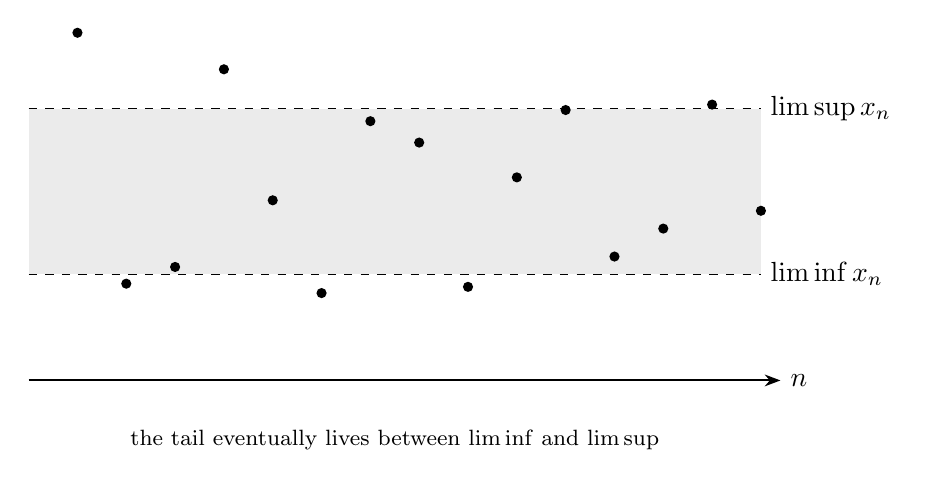
\begin{tikzpicture}[xscale=0.62,yscale=1.5]
  \def\U{2.3}\def\Lo{0.9}
  \draw[numln] (0,0)--(15.4,0) node[right]{$n$};
  \begin{scope}[on background layer]
    \fill[band] (0,\Lo) rectangle (15,\U);
  \end{scope}
  \draw[dashed] (0,\U)--(15,\U) node[right]{$\limsup x_n$};
  \draw[dashed] (0,\Lo)--(15,\Lo) node[right]{$\liminf x_n$};
  % bounded oscillating sequence settling into band
  \foreach \n in {1,...,15}{
    \pgfmathsetmacro{\y}{1.6 + (0.7 + 0.9*pow(0.8,\n))*sin(\n r*1.9)}
    \node[pt] at (\n,\y) {};
  }
  \node[font=\footnotesize,align=center] at (7.5,-0.5)
    {the tail eventually lives between $\liminf$ and $\limsup$};
\end{tikzpicture}
\captionof{figure}{$\limsup$/$\liminf$ are the upper and lower edges of the band the tail
ultimately occupies. The sequence converges exactly when the band has zero width.}
\end{center}

\begin{theorem}[Characterization and convergence]\label{t:limsup-conv@c4}
For a bounded sequence:
\textup{(a)} $\liminf x_n\le\limsup x_n$.
\textup{(b)} $\seq{x_n}$ converges \emph{iff} $\liminf x_n=\limsup x_n$, and then the common
value is $\lim x_n$.
\textup{(c)} $L=\limsup x_n$ iff for every $\eps>0$: $x_n<L+\eps$ eventually, and
$x_n>L-\eps$ infinitely often.
\end{theorem}

\begin{proof}
(a) $t_n\le s_n$ for each $n$, so the limits obey $\liminf\le\limsup$. (b) If $x_n\to x$ then
every subsequential limit equals $x$, so $\liminf=\limsup=x$. Conversely if
$\liminf=\limsup=L$, then $t_n\le x_n\le s_n$ with $t_n,s_n\to L$, and squeezing gives
$x_n\to L$. (c) From $s_n\downarrow L$: $s_N<L+\eps$ for some $N$ gives $x_n\le s_N<L+\eps$
for $n\ge N$; and $s_n\ge L$ for all $n$ means $\sup_{k\ge n}x_k\ge L$, so some $x_k>L-\eps$
with $k\ge n$, for every $n$.
\end{proof}

\begin{theorem}[Subadditivity, Rudin Ex.\ 3.5]\label{t:limsup-subadd@c4}
For bounded sequences, provided the right side is not $\infty-\infty$,
\[
  \limsup_{n\to\infty}(a_n+b_n)\le\limsup_{n\to\infty}a_n+\limsup_{n\to\infty}b_n .
\]
\end{theorem}

\begin{proof}
For $k\ge n$, $a_k+b_k\le\sup_{j\ge n}a_j+\sup_{j\ge n}b_j$, so taking $\sup$ over $k\ge n$,
$\sup_{k\ge n}(a_k+b_k)\le\sup_{j\ge n}a_j+\sup_{j\ge n}b_j$. Let $n\to\infty$.
\end{proof}

\begin{wex}{Computing $\limsup$ and $\liminf$}
Find $\limsup$ and $\liminf$ of $x_n=(-1)^n\bigl(1+\tfrac1n\bigr)$ and of
$y_n=\cos(n\pi/2)$.
\wrec ``Find upper/lower limits''; identify all subsequential limits and take the extremes.
\wsol For $x_n$: even terms $1+1/n\to1$, odd terms $-(1+1/n)\to-1$; the only subsequential
limits are $\pm1$, so $\limsup x_n=1$, $\liminf x_n=-1$. For $y_n=\cos(n\pi/2)$ the values
cycle $0,-1,0,1,0,-1,\dots$, with subsequential limits $\set{-1,0,1}$; so $\limsup y_n=1$,
$\liminf y_n=-1$. \emph{Check:} neither sequence converges, consistent with
$\liminf\neq\limsup$ (Theorem~\ref{t:limsup-conv@c4}(b)). \checkmark
\end{wex}

\begin{wex}{A non-example for subadditivity equality}
Show the inequality in Theorem~\ref{t:limsup-subadd@c4} can be strict.
\wrec ``Show $\le$ is not $=$''; pick anti-phase oscillations.
\wsol Take $a_n=(-1)^n$, $b_n=(-1)^{n+1}$. Then $\limsup a_n=\limsup b_n=1$, so the right
side is $2$; but $a_n+b_n\equiv0$, so $\limsup(a_n+b_n)=0<2$. \emph{Check:} the peaks of
$a_n$ and $b_n$ never align, so the sum never reaches the sum of the peaks. \checkmark
\end{wex}

\begin{pitfall}
$\limsup x_n$ is \emph{not} $\sup_n x_n$, and it is \emph{not} $\lim x_n$ (which may not
exist). It is the limit of the \emph{tail} suprema --- early large terms are forgotten. For
$x_n=1/n$, $\sup_n x_n=1$ but $\limsup x_n=0$. Always read $\limsup$ as ``eventual supremum''.
\end{pitfall}

\begin{pitfall}
$\limsup$ and $\liminf$ \emph{always} exist in $\Rext$ for any sequence, bounded or not ---
that is their advantage over $\lim$. But identities like
$\limsup(a_nb_n)=\limsup a_n\cdot\limsup b_n$ are \emph{false} in general; only one-sided
inequalities survive, and only under sign hypotheses.
\end{pitfall}

\subsection*{Further worked examples}

\begin{wex}{A three-valued $\limsup$/$\liminf$ via tail suprema}
Compute $\limsup$ and $\liminf$ of $x_n=\dfrac{n}{n+1}\sin\dfrac{n\pi}{3}$ by identifying
all subsequential limits.
\wrec ``Find upper/lower limits''; the factor $n/(n+1)\to1$ is a convergent envelope, so the
subsequential limits are $1\cdot(\text{values of }\sin(n\pi/3))$
(Definition~\ref{d:limsup@c4}).
\wsol $\sin(n\pi/3)$ cycles with period $6$ through
$\tfrac{\sqrt3}2,\tfrac{\sqrt3}2,0,-\tfrac{\sqrt3}2,-\tfrac{\sqrt3}2,0$. Since
$n/(n+1)\to1$, each residue class $n\equiv r\pmod 6$ gives a subsequence converging to the
corresponding value of $\sin(r\pi/3)$. The subsequential limits are therefore
$\set{-\tfrac{\sqrt3}2,\,0,\,\tfrac{\sqrt3}2}$, so $\limsup x_n=\tfrac{\sqrt3}2$ and
$\liminf x_n=-\tfrac{\sqrt3}2$. \emph{Check:} $\limsup\neq\liminf$, so $\seq{x_n}$ diverges
(Theorem~\ref{t:limsup-conv@c4}(b)); the band has width $\sqrt3$. \checkmark
\end{wex}

\begin{wex}{$\limsup$ and $\liminf$ of a ratio of consecutive terms}
For $x_n$ defined by $x_{2k}=2^{-k}$ and $x_{2k-1}=3^{-k}$, find
$\limsup\dfrac{x_{n+1}}{x_n}$ and $\liminf\dfrac{x_{n+1}}{x_n}$, and contrast with
$\limsup x_n^{1/n}$.
\wrec ``Compute upper/lower limits of the ratio''; the two parity cases give two different
ratio behaviors, illustrating why the ratio test can stall where the root test does not
(foreshadowing \S4.7).
\wsol Even-to-odd: $\dfrac{x_{2k+1}}{x_{2k}}=\dfrac{3^{-(k+1)}}{2^{-k}}
=\tfrac13\bigl(\tfrac23\bigr)^k\to0$. Odd-to-even: $\dfrac{x_{2k}}{x_{2k-1}}
=\dfrac{2^{-k}}{3^{-k}}=\bigl(\tfrac32\bigr)^k\to+\infty$. So $\liminf\dfrac{x_{n+1}}{x_n}=0$
and $\limsup\dfrac{x_{n+1}}{x_n}=+\infty$. Yet $x_n^{1/n}$ stays controlled:
$x_{2k}^{1/(2k)}=2^{-1/2}$ and $x_{2k-1}^{1/(2k-1)}\to3^{-1/2}$, so
$\limsup x_n^{1/n}=2^{-1/2}<1$. \emph{Check:} the root limit is finite and $<1$ while the
ratio limits spread to $0$ and $\infty$ --- precisely the gap that makes the root test
sharper. \checkmark
\end{wex}

\begin{wex}{A non-example: $\liminf x_n + \limsup y_n$ need not bound $\limsup(x_n+y_n)$}
Show that $\liminf(x_n+y_n)\ge\liminf x_n+\liminf y_n$ can be \emph{strict}, mirroring the
subadditivity of $\limsup$.
\wrec ``Show the inequality is strict''; pick anti-phase $\pm1$ sequences as in the
$\limsup$ case (Theorem~\ref{t:limsup-subadd@c4}).
\wsol Take $x_n=(-1)^n$ and $y_n=(-1)^{n+1}$. Then $\liminf x_n=\liminf y_n=-1$, so the right
side is $-2$; but $x_n+y_n\equiv0$, giving $\liminf(x_n+y_n)=0>-2$. The superadditivity
$\liminf(x_n+y_n)\ge\liminf x_n+\liminf y_n$ holds but is strict here. \emph{Check:} adding
the two known facts, $\liminf(x+y)\ge\liminf x+\liminf y$ and $\limsup(x+y)\le\limsup x+
\limsup y$ pin the sum's band \emph{inside} the sum of the bands --- never outside. \checkmark
\end{wex}

\begin{exers}{Exercises (Bartle \& Sherbert, \S3.6).}
\item Show that if $\seq{x_n}$ is unbounded, then there is a properly divergent subsequence.
\item Give examples of properly divergent $\seq{x_n}$, $\seq{y_n}$ with $y_n\neq0$ such that
  (a) $\seq{x_n/y_n}$ converges;\quad (b) $\seq{x_n/y_n}$ is properly divergent.
\item Show that if $x_n>0$ for all $n$, then $\lim x_n=0\eqv\lim(1/x_n)=+\infty$.
\item Establish proper divergence of
  (a) $\seq{\sqrt n}$;\quad (b) $\seq{\sqrt{n+1}}$;\quad
  (c) $\seq{\sqrt{n-1}}$;\quad (d) $\seq{n/\sqrt{n+1}}$.
\item Is the sequence $\seq{n\sin n}$ properly divergent?
\item Let $\seq{x_n}$ be properly divergent and $\seq{y_n}$ be such that $\lim(x_n y_n)\in\R$.
  Show $y_n\to0$.
\item Let $\seq{x_n},\seq{y_n}$ have positive terms with $\lim(x_n/y_n)=0$.
  (a) If $\lim x_n=+\infty$, show $\lim y_n=+\infty$.\quad
  (b) If $\seq{y_n}$ is bounded, show $\lim x_n=0$.
\item Investigate convergence/divergence of
  (a) $\seq{\sqrt{n^2+2}}$;\quad (b) $\seq{\sqrt n/(n^2+1)}$;\quad
  (c) $\seq{\sqrt{n^2+1}/\sqrt n}$;\quad (d) $\seq{\sin\sqrt n}$.
\item Let $\seq{x_n},\seq{y_n}$ have positive terms with $\lim(x_n/y_n)=+\infty$.
  (a) If $\lim y_n=+\infty$, show $\lim x_n=+\infty$.\quad
  (b) If $\seq{x_n}$ is bounded, show $\lim y_n=0$.
\item Show that if $\lim(a_n/n)=L$ with $L>0$, then $\lim a_n=+\infty$.
\end{exers}

\begin{exers}{Additional exercises.}
\item Compute $\limsup$ and $\liminf$ of $x_n=\sin(n\pi/3)$.
\item For $x_n=\Bigl(1+\dfrac{(-1)^n}{2}\Bigr)^n$ decide whether the sequence is bounded, and
  find $\limsup$ and $\liminf$ (in $\Rext$).
\item Prove $\liminf x_n=-\limsup(-x_n)$ for any bounded sequence.
\item (Non-example.) Show by example that
  $\limsup(a_n b_n)=\limsup a_n\cdot\limsup b_n$ can fail, even for nonnegative sequences.
\item Show that $\seq{x_n}$ converges in $\Rext$ to $+\infty$ iff $\liminf x_n=+\infty$.
\item Prove that for bounded sequences,
  $\liminf a_n+\liminf b_n\le\liminf(a_n+b_n)\le\liminf a_n+\limsup b_n$.
\item (Diagram problem.) Plot a bounded oscillating sequence and draw the two horizontal lines
  $\limsup x_n$ and $\liminf x_n$; shade the band the tail eventually occupies and indicate the
  index past which all terms lie within $\eps$ of the band.
\item Let $a_n>0$. Prove $\liminf\dfrac{a_{n+1}}{a_n}\le\liminf a_n^{1/n}\le\limsup
  a_n^{1/n}\le\limsup\dfrac{a_{n+1}}{a_n}$ (the inequality chain behind ``root beats ratio'').
\end{exers}


\section{Series and Convergence Tests}
\subsection*{Series and partial sums}

\begin{definition}\label{d:series@c4}
Given a sequence $\seq{a_n}$, the \emph{series} $\sum_{n=1}^\infty a_n$ is the sequence
$\seq{s_N}$ of \emph{partial sums} $s_N=\sum_{n=1}^N a_n$. The series \emph{converges} to
$s$ if $s_N\to s$, and we write $\sum_{n=1}^\infty a_n=s$; otherwise it \emph{diverges}. The
$a_n$ are the \emph{terms}.
\end{definition}

A series is nothing but a sequence (of partial sums) in disguise; every sequence theorem
applies. The new feature is that we want criteria phrased in the \emph{terms} $a_n$, not the
sums.

\begin{center}
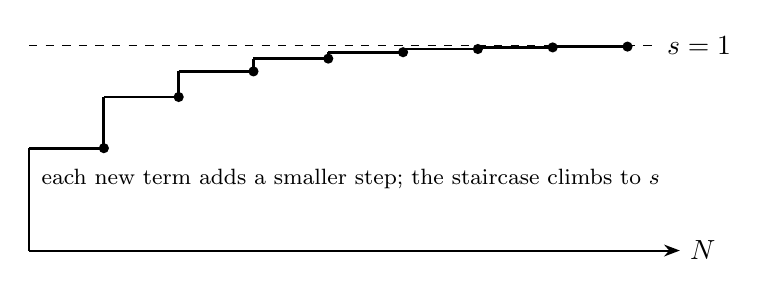
\begin{tikzpicture}[xscale=0.95,yscale=1.3]
  % partial-sum staircase for sum 1/2^n -> 1
  \draw[numln] (0,0)--(8.7,0) node[right]{$N$};
  \draw[dashed] (0,2)--(8.4,2) node[right]{$s=1$};
  \def\prev{0}
  \foreach \n in {1,...,8}{
    \pgfmathsetmacro{\val}{2*(1-pow(0.5,\n))}
    \draw[line width=1pt] (\n-1,{2*(1-pow(0.5,\n-1))})--(\n-1,\val); % vertical jump
    \draw[line width=1pt] (\n-1,\val)--(\n,\val);                    % flat
    \node[pt] at (\n,\val) {};
  }
  \node[font=\footnotesize,align=center] at (4.3,0.7)
    {each new term adds a smaller step; the staircase climbs to $s$};
\end{tikzpicture}
\captionof{figure}{Partial-sum staircase for $\sum 2^{-n}=1$: convergence of a series is just
convergence of this staircase of partial sums.}
\end{center}

\begin{theorem}[Geometric series]\label{t:geometric@c4}
For $\abs r<1$, $\displaystyle\sum_{n=0}^\infty r^n=\frac1{1-r}$. For $\abs r\ge1$ the series
diverges.
\end{theorem}

\begin{proof}
$s_N=\sum_{n=0}^N r^n=\dfrac{1-r^{N+1}}{1-r}$ for $r\neq1$. If $\abs r<1$ then $r^{N+1}\to0$,
so $s_N\to1/(1-r)$. If $\abs r\ge1$ the terms $r^n$ do not tend to $0$, so the series
diverges (next theorem). For $r=1$, $s_N=N+1\to\infty$.
\end{proof}

\begin{theorem}[$n$-th term test]\label{t:nth-term@c4}
If $\sum a_n$ converges then $a_n\to0$. Contrapositive: if $a_n\not\to0$, the series diverges.
\end{theorem}

\begin{proof}
$a_n=s_n-s_{n-1}\to s-s=0$ since both partial-sum sequences converge to the same $s$.
\end{proof}

\begin{pitfall}
The $n$-th term test is \emph{only} a divergence test: $a_n\to0$ does \emph{not} imply
convergence. The harmonic series $\sum1/n$ has $a_n=1/n\to0$ yet diverges (below). ``Terms go
to zero'' is necessary, never sufficient.
\end{pitfall}

\begin{theorem}[Cauchy criterion for series]\label{t:cauchy-series@c4}
$\sum a_n$ converges iff for every $\eps>0$ there is $K$ with
$\Bigl|\sum_{k=m+1}^n a_k\Bigr|<\eps$ whenever $n>m\ge K$.
\end{theorem}

\begin{proof}
Apply the Cauchy criterion (Theorem~\ref{t:cauchy@c4}) to $\seq{s_N}$, noting
$s_n-s_m=\sum_{k=m+1}^n a_k$.
\end{proof}

\begin{wex}{The harmonic series diverges}
Show $\displaystyle\sum_{n=1}^\infty\frac1n=+\infty$.
\wrec ``Show divergence'' where the $n$-th term test is inconclusive: block the partial sums
below by a growing amount (Cauchy criterion fails).
\wsol Group the terms in dyadic blocks:
\[
  \sum_{k=2^{m}+1}^{2^{m+1}}\frac1k\ge 2^{m}\cdot\frac1{2^{m+1}}=\frac12 .
\]
So $s_{2^{M}}\ge 1+\tfrac M2\to\infty$; the partial sums are unbounded, hence diverge.
\emph{Check:} the Cauchy criterion fails outright: $\sum_{k=m+1}^{2m}1/k\ge m\cdot\tfrac1{2m}
=\tfrac12$ for all $m$, so the blocks never shrink below $\tfrac12$. \checkmark
\end{wex}

\begin{wex}{Telescoping (B\&S 3.7.3)}
Evaluate $\displaystyle\sum_{n=1}^\infty\frac1{n(n+1)}$.
\wrec A term that splits into a difference of consecutive pieces: telescope the partial sum.
\wsol Partial fractions: $\dfrac1{n(n+1)}=\dfrac1n-\dfrac1{n+1}$, so
$s_N=\sum_{n=1}^N\bigl(\tfrac1n-\tfrac1{n+1}\bigr)=1-\dfrac1{N+1}\to1$. Hence the sum is $1$.
\emph{Check:} $s_3=\tfrac12+\tfrac16+\tfrac1{12}=\tfrac34=1-\tfrac14$. \checkmark
\end{wex}

\subsection*{Comparison and condensation}

\begin{theorem}[Comparison test]\label{t:comparison@c4}
Suppose $0\le a_n\le b_n$ for all large $n$.
\textup{(a)} If $\sum b_n$ converges, so does $\sum a_n$.
\textup{(b)} If $\sum a_n$ diverges, so does $\sum b_n$.
\end{theorem}

\begin{proof}
Partial sums of nonnegative series are increasing; convergence $\eqv$ boundedness (MCT). If
$\sum b_n$ converges its partial sums are bounded by some $B$, hence so are those of $\sum
a_n$ (term-by-term $\le$), giving convergence. (b) is the contrapositive.
\end{proof}

\begin{center}
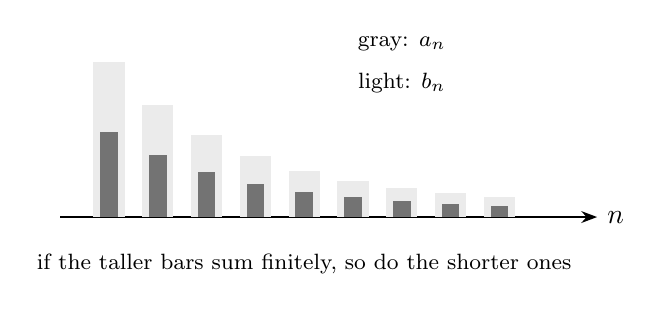
\begin{tikzpicture}[xscale=0.62,yscale=1.0]
  % comparison: bars a_n under bars b_n
  \draw[numln] (0,0)--(11,0) node[right]{$n$};
  \foreach \n in {1,...,9}{
    \pgfmathsetmacro{\bb}{2.6*pow(0.7,\n)+0.15}
    \pgfmathsetmacro{\aa}{\bb*0.55}
    \fill[band] (\n-0.32,0) rectangle (\n+0.32,\bb);
    \fill[black!55] (\n-0.18,0) rectangle (\n+0.18,\aa);
  }
  \node[font=\footnotesize] at (7,2.2) {gray: $a_n$};
  \node[font=\footnotesize] at (7,1.7) {light: $b_n$};
  \node[font=\footnotesize,align=center] at (5,-0.6)
    {if the taller bars sum finitely, so do the shorter ones};
\end{tikzpicture}
\captionof{figure}{Comparison test: $a_n\le b_n$ termwise. A finite total area under the larger
bars caps the area under the smaller.}
\end{center}

\begin{theorem}[Cauchy condensation]\label{t:condensation@c4}
If $a_1\ge a_2\ge\cdots\ge0$, then $\sum a_n$ converges iff $\sum_{k=0}^\infty 2^k a_{2^k}$
converges.
\end{theorem}

\begin{proof}[Proof sketch]
Group terms in dyadic blocks. Monotonicity gives
$2^{k-1}a_{2^k}\le a_{2^{k-1}+1}+\cdots+a_{2^k}\le 2^{k-1}a_{2^{k-1}}$, so the original
series and the condensed series bound each other up to constants; one converges iff the other
does (comparison).
\end{proof}

\begin{theorem}[$p$-series]\label{t:p-series@c4}
$\displaystyle\sum_{n=1}^\infty\frac1{n^p}$ converges iff $p>1$.
\end{theorem}

\begin{proof}
Condensation: $\sum 2^k\cdot\dfrac1{(2^k)^p}=\sum (2^{1-p})^k$ is geometric with ratio
$2^{1-p}$, which converges iff $2^{1-p}<1\eqv p>1$.
\end{proof}

\subsection*{Root and ratio tests; the integral test}

\begin{theorem}[Root test]\label{t:root@c4}
Let $\alpha=\limsup_{n\to\infty}\abs{a_n}^{1/n}$. Then $\sum a_n$ converges absolutely if
$\alpha<1$, diverges if $\alpha>1$, and the test is inconclusive if $\alpha=1$.
\end{theorem}

\begin{proof}
If $\alpha<1$ pick $\beta$ with $\alpha<\beta<1$; then $\abs{a_n}^{1/n}<\beta$ eventually, so
$\abs{a_n}<\beta^n$, and comparison with the convergent geometric $\sum\beta^n$ gives absolute
convergence. If $\alpha>1$ then $\abs{a_n}^{1/n}>1$ infinitely often, so $\abs{a_n}>1$
infinitely often, $a_n\not\to0$, and the series diverges.
\end{proof}

\begin{theorem}[Ratio test]\label{t:ratio@c4}
Suppose $a_n\neq0$. If $\limsup_n\abs{a_{n+1}/a_n}<1$ the series converges absolutely; if
$\abs{a_{n+1}/a_n}\ge1$ for all large $n$ (in particular if $\liminf>1$), it diverges.
\end{theorem}

\begin{proof}
If $L=\limsup\abs{a_{n+1}/a_n}<1$ pick $\beta\in(L,1)$; then $\abs{a_{n+1}}\le\beta\abs{a_n}$
for $n\ge K$, so $\abs{a_{K+m}}\le\beta^m\abs{a_K}$, and comparison with $\sum\beta^m$ gives
absolute convergence. If the ratio is $\ge1$ eventually, $\abs{a_n}$ is nondecreasing, so
$a_n\not\to0$ and the series diverges.
\end{proof}

\begin{remark}[Root is stronger]
Whenever the ratio test decides, so does the root test, because
$\liminf\abs{a_{n+1}/a_n}\le\liminf\abs{a_n}^{1/n}\le\limsup\abs{a_n}^{1/n}\le
\limsup\abs{a_{n+1}/a_n}$. The root test can succeed where the ratio test fails (e.g.\ a
series whose ratios oscillate). The ratio test is, however, easier to compute.
\end{remark}

\begin{theorem}[Integral test, stated]\label{t:integral@c4}
If $f$ is positive, decreasing on $[1,\infty)$ and $a_n=f(n)$, then $\sum a_n$ converges iff
$\int_1^\infty f(x)\dx$ converges (the partial sums and the integral differ by a bounded
amount). \textup{(Proof deferred to the integration chapter.)}
\end{theorem}

\begin{wex}{Choosing a test}
Decide convergence of \textup{(a)} $\sum\dfrac{n}{2^n}$, \textup{(b)} $\sum\dfrac{n!}{n^n}$,
\textup{(c)} $\sum\dfrac1{n\ln n}$.
\wrec ``Test for convergence''; match the structure to root/ratio/condensation.
\wsol (a) Ratio: $\dfrac{(n+1)/2^{n+1}}{n/2^n}=\tfrac12\cdot\tfrac{n+1}n\to\tfrac12<1$,
converges. (b) Ratio: $\dfrac{(n+1)!/(n+1)^{n+1}}{n!/n^n}=\Bigl(\tfrac n{n+1}\Bigr)^n
=(1+\tfrac1n)^{-n}\to e^{-1}<1$, converges. (c) Condensation:
$\sum 2^k\dfrac1{2^k\ln2^k}=\sum\dfrac1{k\ln2}$, a constant multiple of the harmonic series,
diverges. \emph{Check:} (c) shows $\sum1/(n\ln n)$ \emph{just barely} diverges --- slower
than $\sum1/n$, faster to settle than any $p$-series with $p>1$. \checkmark
\end{wex}

\begin{wex}{Root test where the ratio test stalls}
Test $\displaystyle\sum a_n$ with $a_n=2^{-n}$ if $n$ even and $a_n=3^{-n}$ if $n$ odd.
\wrec Oscillating ratios; the root test reads off the geometric decay (Remark above).
\wsol The ratios $a_{n+1}/a_n$ oscillate wildly (between $\sim(2^n/3^{n+1})$ and
$\sim(3^n/2^{n+1})$), so the ratio test is unusable. But $\abs{a_n}^{1/n}\le\max\set{\tfrac12,
\tfrac13}=\tfrac12$, so $\limsup\abs{a_n}^{1/n}\le\tfrac12<1$ and the series converges
absolutely. \emph{Check:} indeed $a_n\le 2^{-n}$, comparison with $\sum2^{-n}$ confirms it.
\checkmark
\end{wex}

\begin{pitfall}
When $\alpha=1$ (root) or the ratio limit is $1$, the test says \emph{nothing}: $\sum1/n$
(diverges) and $\sum1/n^2$ (converges) both give limit $1$. At the boundary switch to a finer
tool (condensation, $p$-series, integral test).
\end{pitfall}

\subsection*{Further worked examples}

The integral test compares the series $\sum f(n)$ with the area under $y=f(x)$: the terms are
the areas of unit-width rectangles that bracket the curve, so the sum and the integral
converge or diverge together.

\begin{center}
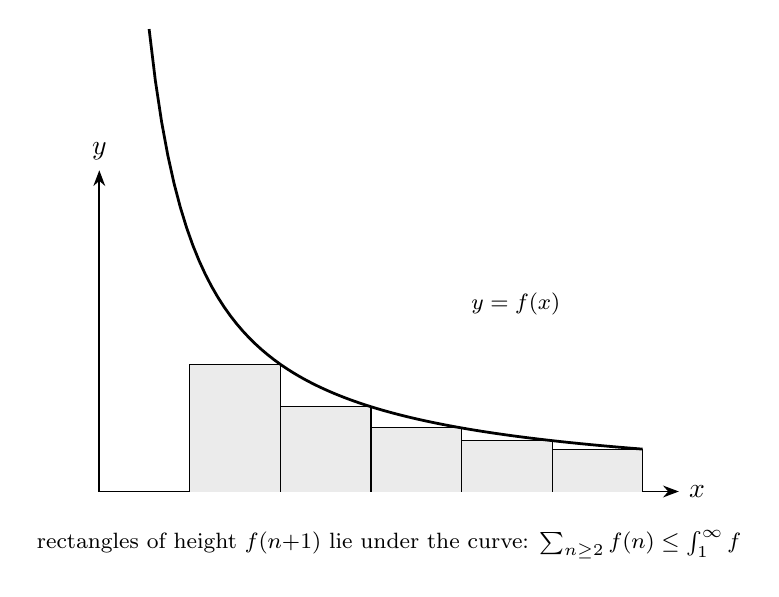
\begin{tikzpicture}[xscale=1.15,yscale=1.7]
  \draw[numln] (0,0)--(6.4,0) node[right]{$x$};
  \draw[numln] (0,0)--(0,2.4) node[above]{$y$};
  % decreasing f(x)=1/x style; right-endpoint (under) rectangles
  \foreach \n in {1,...,5}{
    \pgfmathsetmacro{\h}{1.9/(\n+1)}
    \fill[band] (\n,0) rectangle (\n+1,\h);
    \draw (\n,0)--(\n,\h)--(\n+1,\h)--(\n+1,0);
  }
  \draw[curve,domain=0.55:6,samples=80] plot (\x,{1.9/\x});
  \node[font=\footnotesize] at (4.6,1.4) {$y=f(x)$};
  \node[font=\footnotesize,align=center] at (3.2,-0.4)
    {rectangles of height $f(n{+}1)$ lie under the curve: $\sum_{n\ge2}f(n)\le\int_1^\infty f$};
\end{tikzpicture}
\captionof{figure}{Integral test: the under-rectangles bound the tail sum by the integral (and
over-rectangles bound it below), so series and integral share their fate.}
\end{center}

\begin{wex}{Limit comparison test}
Decide convergence of $\displaystyle\sum_{n=1}^\infty\frac{2n+1}{n^3+n+1}$.
\wrec ``Test for convergence''; the term behaves like $2/n^2$ for large $n$, so compare with
the convergent $p$-series $\sum1/n^2$ (Theorem~\ref{t:p-series@c4}) via a limit ratio.
\wsol Let $a_n=\dfrac{2n+1}{n^3+n+1}$ and $b_n=\dfrac1{n^2}$. Then
\[
  \frac{a_n}{b_n}=\frac{(2n+1)n^2}{n^3+n+1}=\frac{2n^3+n^2}{n^3+n+1}\xrightarrow[n\to\infty]{}2,
\]
a finite nonzero limit, so $\sum a_n$ and $\sum b_n$ converge or diverge together. Since
$\sum1/n^2$ converges ($p=2>1$), so does $\sum a_n$. \emph{Check:} $a_n\le\dfrac{2n+1}{n^3}
\le\dfrac3{n^2}$ for $n\ge1$, and $\sum3/n^2$ converges --- the direct comparison confirms it.
\checkmark
\end{wex}

\begin{wex}{The integral test on $\sum 1/(n\ln n)$ and $\sum 1/(n(\ln n)^2)$}
Using the integral test, show $\sum_{n\ge2}\dfrac1{n\ln n}$ diverges but
$\sum_{n\ge2}\dfrac1{n(\ln n)^2}$ converges.
\wrec ``Test for convergence'' where condensation also works; here $f(x)=1/(x\ln x)$ is
positive and decreasing, so Theorem~\ref{t:integral@c4} reduces the question to an integral.
\wsol With $u=\ln x$, $\du=\dx/x$:
$\displaystyle\int_2^\infty\frac{\dx}{x\ln x}=\int_{\ln2}^\infty\frac{\du}{u}
=\bigl[\ln u\bigr]_{\ln2}^\infty=+\infty$, so the first series diverges. For the second,
$\displaystyle\int_2^\infty\frac{\dx}{x(\ln x)^2}=\int_{\ln2}^\infty\frac{\du}{u^2}
=\Bigl[-\frac1u\Bigr]_{\ln2}^\infty=\frac1{\ln2}<\infty$, so it converges. \emph{Check:}
the exponent on $\ln n$ plays the $p$-series role at one logarithmic level up --- $p=1$
diverges, $p=2>1$ converges, exactly as for $\sum1/n^p$. \checkmark
\end{wex}

\begin{exers}{Exercises (Bartle \& Sherbert, \S3.7 and \S9.2).}
\item Let $\sum a_n$ be a series and $\sum b_n$ the series with the same terms in the same
  order but with the zero terms omitted. Show $\sum a_n=A\eqv\sum b_n=A$.
\item Show convergence of a series is unaffected by changing finitely many terms (though the
  sum may change).
\item Using partial fractions, show
  (a) $\displaystyle\sum_{n=0}^\infty\dfrac1{(n+1)(n+2)}=1$;\quad
  (b) $\displaystyle\sum_{n=0}^\infty\dfrac1{(a+n)(a+n+1)}=\dfrac1a$ for $a>0$;\quad
  (c) $\displaystyle\sum_{n=1}^\infty\dfrac1{n(n+1)(n+2)}=\dfrac14$.
\item If $\sum x_n$ and $\sum y_n$ converge, show $\sum(x_n+y_n)$ converges.
\item Give an example of a convergent $\sum x_n$ and a divergent $\sum y_n$ with
  $\sum(x_n+y_n)$ convergent, or explain why none exists.
\item Compute (a) $\displaystyle\sum_{n=2}^\infty (2/7)^n$;\quad
  (b) $\displaystyle\sum_{n=1}^\infty (1/3)^{2n}$.
\item Find a formula for $\displaystyle\sum_{n=1}^\infty r^{2n}$ when $\abs r<1$.
\item Let $r_1,r_2,\dots$ enumerate the rationals in $[0,1]$. About $r_n$ place an interval of
  length $\eps^n$. Find the total length of all intervals; evaluate for $\eps=0.1,0.01$.
\item (a) Show $\displaystyle\sum_{n=1}^\infty\cos n$ diverges.\quad
  (b) Show $\displaystyle\sum_{n=1}^\infty\dfrac{\cos n}{n^2}$ converges.
\item Use an argument like Example $3.7.6$(f) to show $\displaystyle\sum_{n=1}^\infty
  \dfrac{(-1)^n}{\sqrt n}$ converges.
\item If $\sum a_n$ with $a_n>0$ converges, must $\sum a_n^2$ converge? Prove or give a
  counterexample.
\item If $\sum a_n$ with $a_n>0$ converges, must $\sum\sqrt{a_n}$ converge? Prove or give a
  counterexample.
\item (\S9.2) Establish convergence/divergence of the series whose $n$-th term is
  (a) $\dfrac1{(n+1)(n+2)}$;\quad (b) $\dfrac{n}{(n+1)(n+2)}$;\quad
  (c) $2^{-1/n}$;\quad (d) $n/2^n$.
\item (\S9.2) Same for $n$-th term
  (a) $(n(n+1))^{-1/2}$;\quad (b) $(n^2(n+1))^{-1/2}$;\quad
  (c) $n!/n^n$;\quad (d) $(-1)^n n/(n+1)$.
\item (\S9.2) Discuss convergence (for large $n$) of the series with $n$-th term
  (a) $(\ln n)^{-p}$;\quad (b) $(\ln n)^{-n}$;\quad (c) $(\ln n)^{-\ln n}$;\quad
  (d) $(\ln n)^{-\ln\ln n}$;\quad (e) $(n\ln n)^{-1}$;\quad
  (f) $\bigl(n(\ln n)(\ln\ln n)^2\bigr)^{-1}$.
\item (\S9.2) Discuss convergence of the series with $n$-th term
  (a) $2^n e^{-n}$;\quad (b) $n^n e^{-n}$;\quad (c) $e^{-\ln n}$;\quad
  (d) $(\ln n)e^{-\sqrt n}$;\quad (e) $n!\,e^{-n}$;\quad (f) $n!\,e^{-n^2}$.
\item (\S9.2) Show $\dfrac1{1^2}+\dfrac1{2^3}+\dfrac1{3^2}+\dfrac1{4^3}+\cdots$ converges, yet
  both the Ratio and Root tests fail to apply.
\item (\S9.2) For $a,b>0$, show $\sum(an+b)^{-p}$ converges if $p>1$ and diverges if $p\le1$.
\item (\S9.2) Discuss the series with $n$-th term
  (a) $\dfrac{n!}{3\cdot5\cdot7\cdots(2n+1)}$;\quad
  (b) $\dfrac{(n!)^2}{(2n)!}$;\quad
  (c) $\dfrac{2\cdot4\cdots(2n)}{3\cdot5\cdots(2n+1)}$;\quad
  (d) $\dfrac{2\cdot4\cdots(2n)}{5\cdot7\cdots(2n+3)}$.
\item (\S9.2) Let $0<a<1$ and consider $a^2+a+a^4+a^3+\cdots+a^{2n}+a^{2n-1}+\cdots$. Show the
  Root Test applies but the Ratio Test does not.
\item (\S9.2) If $r\in(0,1)$ satisfies the Root Test condition, show
  $\abs{s-s_n}\le r^{n+1}/(1-r)$ for $n\ge K$.
\item (\S9.2) If $r\in(0,1)$ satisfies the Ratio Test condition, show
  $\abs{s-s_n}\le r\abs{x_n}/(1-r)$ for $n\ge K$.
\item (\S9.2) Show $1+\tfrac12-\tfrac13+\tfrac14+\tfrac15-\tfrac16+\cdots$ diverges.
\item (\S9.2) Let $c_n=1+\tfrac12+\cdots+\tfrac1n-\ln n$. Show $\seq{c_n}$ decreases to a
  positive limit, and that $b_n=1-\tfrac12+\tfrac13-\cdots-\tfrac1{2n}\to\ln2$.
  \emph{[Hint: $b_n=c_{2n}-c_n+\ln2$.]}
\item (\S9.2) Let $\set{n_k}$ be the naturals whose decimal expansion omits the digit $6$.
  Show $\sum1/n_k$ converges (to a number $<80$); show $\sum1/m_k$ diverges over numbers
  ending in $6$, and $\sum1/p_k$ diverges over numbers not ending in $6$.
\item (\S9.2) For $p,q>0$, show $\displaystyle\sum\frac{(p+1)(p+2)\cdots(p+n)}{(q+1)(q+2)\cdots(q+n)}$
  converges for $q>p+1$ and diverges for $q\le p+1$.
\end{exers}

\begin{exers}{Additional exercises.}
\item Sum $\displaystyle\sum_{n=1}^\infty\frac1{(2n-1)(2n+1)}$ by telescoping.
\item Decide convergence of (a) $\sum\dfrac{n^2}{n!}$;\quad (b) $\sum\dfrac{3^n}{n!}$;\quad
  (c) $\sum\dfrac{n!}{(2n)!}$, choosing a test for each.
\item Use Cauchy condensation to decide $\sum\dfrac1{n(\ln n)^p}$ as a function of $p>0$.
\item (Non-example.) Give a series with $a_n\to0$ that diverges, and a series with
  $\limsup a_n^{1/n}=1$ that converges --- showing the boundary cases are genuinely
  undecided.
\item Prove the comparison test in limit form: if $a_n,b_n>0$ and $a_n/b_n\to L\in(0,\infty)$,
  then $\sum a_n$ and $\sum b_n$ converge or diverge together. Apply it to
  $\sum\dfrac{2n+1}{n^3+5}$.
\item Show that the root test decides $\sum\bigl(\tfrac{n}{n+1}\bigr)^{n^2}$ and find whether
  it converges.
\item (Diagram problem.) Draw the comparison-test bar picture for $a_n=\dfrac1{n^2+n}$ versus
  $b_n=\dfrac1{n^2}$ for $n=1,\dots,6$, and use it to argue $\sum a_n$ converges.
\item Prove that if $a_n\ge0$ and $\sum a_n$ converges, then $\sum a_n^2$ converges, but the
  converse fails (give a counterexample).
\item Using the partial-sum staircase, explain geometrically why $\sum(-1)^n$ diverges
  although its terms are bounded.
\end{exers}


\section{Absolute Convergence, Power Series, and Rearrangements}
\subsection*{Absolute versus conditional convergence}

\begin{definition}\label{d:abs-conv@c4}
$\sum a_n$ \emph{converges absolutely} if $\sum\abs{a_n}$ converges. It \emph{converges
conditionally} if $\sum a_n$ converges but $\sum\abs{a_n}$ diverges.
\end{definition}

\begin{theorem}[Absolute $\imp$ convergent]\label{t:abs-imp-conv@c4}
If $\sum\abs{a_n}$ converges then $\sum a_n$ converges, and
$\abs{\sum a_n}\le\sum\abs{a_n}$.
\end{theorem}

\begin{proof}
By the Cauchy criterion for $\sum\abs{a_n}$, given $\eps>0$ there is $K$ with
$\sum_{k=m+1}^n\abs{a_k}<\eps$ for $n>m\ge K$. Then
$\bigl|\sum_{k=m+1}^n a_k\bigr|\le\sum_{k=m+1}^n\abs{a_k}<\eps$, so $\sum a_n$ satisfies the
Cauchy criterion and converges. The inequality is the limit of
$\abs{s_N}\le\sum_{n\le N}\abs{a_n}$.
\end{proof}

\begin{theorem}[Alternating Series Test, Leibniz]\label{t:alternating@c4}
If $c_1\ge c_2\ge\cdots\ge0$ and $c_n\to0$, then $\sum(-1)^{n+1}c_n$ converges. Moreover the
partial sums satisfy $\abs{s-s_N}\le c_{N+1}$.
\end{theorem}

\begin{proof}
The even partial sums $s_{2m}=\sum(c_{2k-1}-c_{2k})$ are increasing (each pair $\ge0$) and
bounded above by $c_1$; the odd $s_{2m+1}=c_1-(c_2-c_3)-\cdots$ are decreasing and bounded
below. Both converge, and $s_{2m+1}-s_{2m}=c_{2m+1}\to0$ forces a common limit $s$, with
$s_{2m}\le s\le s_{2m+1}$. The error bound follows since $s$ lies between consecutive partial
sums.
\end{proof}

\begin{center}
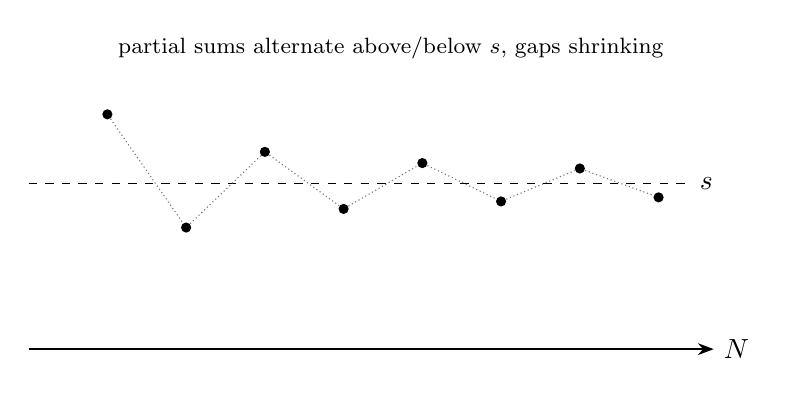
\begin{tikzpicture}[xscale=1.0,yscale=1.5]
  % alternating partial sums spiraling into s
  \draw[numln] (0,0)--(8.7,0) node[right]{$N$};
  \draw[dashed] (0,1.4)--(8.4,1.4) node[right]{$s$};
  \def\vals{}
  \foreach \n in {1,...,8}{
    \pgfmathsetmacro{\val}{1.4 + (mod(\n,2)==1 ? 1 : -1)*1.0/(\n+0.7)}
    \node[pt] (q\n) at (\n,\val) {};
  }
  \foreach \n in {1,...,7}{\pgfmathtruncatemacro{\m}{\n+1}\draw[densely dotted,black!55] (q\n)--(q\m);}
  \node[font=\footnotesize,align=center] at (4.6,2.55)
    {partial sums alternate above/below $s$, gaps shrinking};
\end{tikzpicture}
\captionof{figure}{Alternating series: consecutive partial sums bracket the sum $s$, so the error
never exceeds the first omitted term.}
\end{center}

\begin{wex}{Conditional convergence of the alternating harmonic series}
Show $\sum_{n=1}^\infty\dfrac{(-1)^{n+1}}{n}$ converges conditionally.
\wrec ``Conditional vs absolute''; test the series and its absolute version separately.
\wsol $c_n=1/n$ decreases to $0$, so the Alternating Series Test gives convergence (in fact
to $\ln2$). But $\sum\abs{a_n}=\sum1/n$ is the divergent harmonic series. So the convergence
is conditional. \emph{Check:} $s_2=1-\tfrac12=0.5$, $s_4\approx0.583$, bracketing
$\ln2\approx0.693$ with errors $\le c_{N+1}$. \checkmark
\end{wex}

\subsection*{Dirichlet and Abel tests}

\begin{theorem}[Summation by parts]\label{t:abel-summation@c4}
Let $A_n=\sum_{k=1}^n a_k$ (with $A_0=0$). Then
$\displaystyle\sum_{k=m}^n a_k b_k=A_n b_{n}-A_{m-1}b_{m}-\sum_{k=m}^{n-1}A_k(b_{k+1}-b_k)$.
\end{theorem}

\begin{theorem}[Dirichlet's test]\label{t:dirichlet@c4}
If the partial sums $A_n=\sum_{k\le n}a_k$ are bounded and $\seq{b_n}$ decreases to $0$, then
$\sum a_n b_n$ converges.
\end{theorem}

\begin{proof}[Proof sketch]
Apply summation by parts. With $\abs{A_n}\le M$ and $b_n\downarrow0$, the boundary terms and
the sum $\sum A_k(b_{k+1}-b_k)$ are controlled: $\sum\abs{b_{k+1}-b_k}=b_m-b_n$ telescopes,
giving a Cauchy estimate $\le 2M b_m\to0$. Hence $\sum a_nb_n$ is Cauchy.
\end{proof}

\begin{theorem}[Abel's test, Rudin Ex.\ 3.8]\label{t:abel@c4}
If $\sum a_n$ converges and $\seq{b_n}$ is monotone and bounded, then $\sum a_n b_n$
converges.
\end{theorem}

\begin{proof}[Proof sketch]
A bounded monotone $\seq{b_n}$ converges to some $b$; write $b_n=b+(b_n-b)$ where $b_n-b$ is
monotone $\to0$. Then $\sum a_n b=b\sum a_n$ converges and $\sum a_n(b_n-b)$ converges by
Dirichlet (partial sums of $\sum a_n$ are bounded). Add.
\end{proof}

\begin{remark}
The Alternating Series Test is the special case $a_n=(-1)^{n+1}$ (partial sums bounded by $1$)
of Dirichlet's test. Dirichlet also handles $\sum\dfrac{\sin n}{n}$: the partial sums
$\sum_{k\le n}\sin k$ are bounded (a closed-form geometric-type estimate), and $1/n\downarrow0$.
\end{remark}

\subsection*{Power series and radius of convergence}

\begin{definition}\label{d:power-series@c4}
A \emph{power series} (about $0$) is $\sum_{n=0}^\infty c_n z^n$. Its \emph{radius of
convergence} is $R=1/\alpha$ where $\alpha=\limsup_{n\to\infty}\abs{c_n}^{1/n}$ (with
$R=\infty$ if $\alpha=0$, $R=0$ if $\alpha=\infty$).
\end{definition}

\begin{theorem}[Cauchy--Hadamard]\label{t:hadamard@c4}
The power series $\sum c_n z^n$ converges absolutely for $\abs z<R$ and diverges for
$\abs z>R$; on $\abs z=R$ the behavior varies.
\end{theorem}

\begin{proof}
Apply the root test to $a_n=c_n z^n$:
$\limsup\abs{c_n z^n}^{1/n}=\abs z\limsup\abs{c_n}^{1/n}=\abs z/R$. This is $<1$ when
$\abs z<R$ (absolute convergence) and $>1$ when $\abs z>R$ (divergence, terms not $\to0$).
\end{proof}

\begin{center}
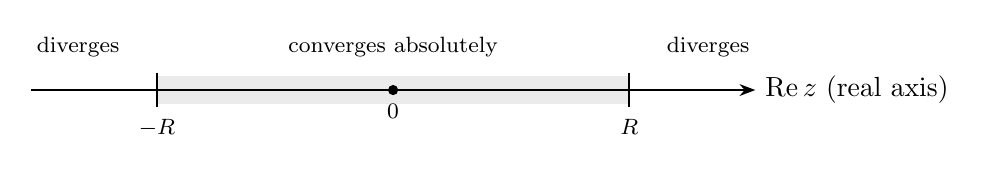
\begin{tikzpicture}[xscale=1.0,yscale=1]
  \draw[numln] (-4.6,0)--(4.6,0) node[right]{$\Re z$ (real axis)};
  % converge band
  \begin{scope}[on background layer]\fill[band] (-3,-0.18) rectangle (3,0.18);\end{scope}
  \draw[line width=0.8pt] (-3,0.22)--(-3,-0.22);
  \draw[line width=0.8pt] (3,0.22)--(3,-0.22);
  \node[pt] at (0,0) {};
  \node[font=\footnotesize,below] at (0,-0.05) {$0$};
  \node[font=\footnotesize,below] at (3,-0.25) {$R$};
  \node[font=\footnotesize,below] at (-3,-0.25) {$-R$};
  \node[font=\footnotesize] at (0,0.55) {converges absolutely};
  \node[font=\footnotesize] at (4.0,0.55) {diverges};
  \node[font=\footnotesize] at (-4.0,0.55) {diverges};
\end{tikzpicture}
\captionof{figure}{Radius of convergence on the real line: absolute convergence strictly inside
$(-R,R)$, divergence strictly outside, endpoints undecided.}
\end{center}

\begin{wex}{Three radii (Rudin Ex.\ 3.9 flavor)}
Find $R$ for \textup{(a)} $\sum n^3 z^n$, \textup{(b)} $\sum\dfrac{2^n}{n!}z^n$,
\textup{(c)} $\sum\dfrac{2^n}{n^2}z^n$.
\wrec ``Radius of convergence''; compute $\limsup\abs{c_n}^{1/n}$ (root) or
$\lim\abs{c_{n+1}/c_n}$ (ratio).
\wsol (a) $\abs{c_n}^{1/n}=(n^3)^{1/n}=(n^{1/n})^3\to1$, so $R=1$. (b) ratio
$\dfrac{2^{n+1}/(n+1)!}{2^n/n!}=\dfrac2{n+1}\to0$, so $\alpha=0$, $R=\infty$. (c)
$\abs{c_n}^{1/n}=2/(n^{1/n})^2\to2$, so $R=\tfrac12$. \emph{Check:} (b) is (a multiple of) the
exponential series $\sum(2z)^n/n!=e^{2z}$, entire, consistent with $R=\infty$. \checkmark
\end{wex}

\subsection*{Rearrangements}

\begin{definition}\label{d:rearrange@c4}
A \emph{rearrangement} of $\sum a_n$ is $\sum a_{\sigma(n)}$ for a bijection
$\sigma:\N\to\N$.
\end{definition}

\begin{theorem}[Absolute convergence is rearrangement-proof]\label{t:rearrange-abs@c4}
If $\sum a_n$ converges absolutely to $s$, then every rearrangement converges to the same $s$.
\end{theorem}

\begin{proof}
Let $\sum a'_n=\sum a_{\sigma(n)}$ with partial sums $s'_N$. Given $\eps>0$ pick $K$ with
$\sum_{k>K}\abs{a_k}<\eps$. Choose $p$ so large that $\set{1,\dots,K}\subseteq
\set{\sigma(1),\dots,\sigma(p)}$. For $N\ge p$, the terms $a_1,\dots,a_K$ appear in both
$s_N$ and $s'_N$ and cancel in the difference, so $\abs{s'_N-s_N}\le\sum_{k>K}\abs{a_k}<\eps$.
Since $s_N\to s$, also $s'_N\to s$.
\end{proof}

\begin{theorem}[Riemann's Rearrangement Theorem]\label{t:riemann-rearrange@c4}
If $\sum a_n$ converges conditionally, then for any target $L\in\Rext$ there is a
rearrangement converging to $L$ (and one diverging, and ones oscillating).
\end{theorem}

\begin{proof}[Proof idea]
Conditional convergence forces both $\sum a_n^+=+\infty$ and $\sum a_n^-=+\infty$ (positive
and negative parts), while $a_n\to0$. To hit a finite $L$: add positive terms until the
partial sum first exceeds $L$, then add negative terms until it drops below $L$, then more
positive terms, and so on. Because each pile is infinite the process never stalls, and
because $a_n\to0$ the overshoots shrink to $0$, so the rearranged sums converge to $L$.
\end{proof}

\begin{wex}{Reshuffling the alternating harmonic series}
Show a rearrangement of $1-\tfrac12+\tfrac13-\tfrac14+\cdots$ can sum to $\tfrac32\ln2$.
\wrec ``Rearrangement changes the sum'' --- only possible for conditional convergence.
\wsol Take two positives then one negative throughout:
$1+\tfrac13-\tfrac12+\tfrac15+\tfrac17-\tfrac14+\cdots$. A standard grouping computation gives
sum $\tfrac32\ln2\approx1.0397$, versus the original $\ln2\approx0.693$. \emph{Check:} the
terms are identical; only their \emph{order} differs, and conditional convergence (not
absolute) is what permits the value to change (Theorem~\ref{t:rearrange-abs@c4} vs
\ref{t:riemann-rearrange@c4}). \checkmark
\end{wex}

\subsection*{The number $e$ is irrational}

\begin{theorem}[$e\notin\Q$, Rudin 3.31]\label{t:e-irrational@c4}
$\displaystyle e=\sum_{n=0}^\infty\frac1{n!}$ is irrational.
\end{theorem}

\begin{proof}
First, $e=\sum_{n\ge0}1/n!$: the partial sums increase and are bounded above ($\le3$), and a
tail estimate matches the monotone-limit definition. Suppose $e=p/q$ with $q\ge1$. The tail
\[
  0<e-\sum_{n=0}^{q}\frac1{n!}=\sum_{n=q+1}^\infty\frac1{n!}
  <\frac1{(q+1)!}\sum_{j=0}^\infty\frac1{(q+1)^j}=\frac1{(q+1)!}\cdot\frac{q+1}{q}
  =\frac1{q!\,q}.
\]
Multiply through by $q!$: the number $q!\,e-q!\sum_{n=0}^q\frac1{n!}$ would be a positive
integer (since $q!\,e=q!\,p/q=(q-1)!\,p\in\Z$ and $q!\sum_{n\le q}1/n!\in\Z$) lying strictly
in $(0,1/q)\subseteq(0,1)$ --- impossible. Hence $e$ is irrational.
\end{proof}

\begin{pitfall}
Rearrangement freely changes a \emph{conditionally} convergent sum (Riemann), but
\emph{never} an absolutely convergent one. Before reordering terms, always check which regime
you are in. The same caution applies to interchanging $\sum$ with limits or other sums: it is
licensed by \emph{absolute} convergence, not mere convergence.
\end{pitfall}

\begin{pitfall}
A power series converges absolutely \emph{inside} its disk and diverges \emph{outside}, but
the boundary $\abs z=R$ is genuinely case-by-case: $\sum z^n$ ($R=1$) diverges everywhere on
$\abs z=1$, $\sum z^n/n^2$ converges everywhere on it, and $\sum z^n/n$ converges at $z=-1$
but diverges at $z=1$. Never assume boundary behavior from $R$ alone.
\end{pitfall}

\subsection*{Further worked examples}

\begin{wex}{Absolute convergence settles an alternating series}
Decide whether $\displaystyle\sum_{n=1}^\infty\frac{(-1)^n}{n^2+1}$ converges, and whether
absolutely.
\wrec ``Conditional vs absolute'' (Definition~\ref{d:abs-conv@c4}); test $\sum\abs{a_n}$ first
--- if it converges, you are done by Theorem~\ref{t:abs-imp-conv@c4} and need no alternating
machinery.
\wsol $\abs{a_n}=\dfrac1{n^2+1}\le\dfrac1{n^2}$, and $\sum1/n^2$ converges ($p=2>1$), so by
comparison $\sum\abs{a_n}$ converges. Hence $\sum a_n$ converges \emph{absolutely}, and a
fortiori converges. \emph{Check:} no need for the Alternating Series Test here --- absolute
convergence is the stronger, simpler route when $\sum\abs{a_n}$ is summable. \checkmark
\end{wex}

\begin{wex}{A conditionally convergent series via Dirichlet}
Show $\displaystyle\sum_{n=1}^\infty\frac{(-1)^{n+1}}{\sqrt n}$ converges but not absolutely.
\wrec ``Conditional vs absolute''; the terms decrease to $0$, so the Alternating Series Test
(Theorem~\ref{t:alternating@c4}, a special case of Dirichlet~\ref{t:dirichlet@c4}) gives
convergence, while the absolute series is a $p$-series with $p=\tfrac12$.
\wsol $c_n=1/\sqrt n$ satisfies $c_1\ge c_2\ge\cdots\ge0$ and $c_n\to0$, so
$\sum(-1)^{n+1}/\sqrt n$ converges by the Alternating Series Test. But
$\sum\abs{a_n}=\sum1/\sqrt n=\sum1/n^{1/2}$ diverges, since $p=\tfrac12\le1$
(Theorem~\ref{t:p-series@c4}). Therefore the convergence is \emph{conditional}. \emph{Check:}
the error bound $\abs{s-s_N}\le c_{N+1}=1/\sqrt{N+1}$ shows the partial sums settle, while
the absolute tail $\sum_{k>N}1/\sqrt k$ grows without bound --- both features coexist only
for conditional convergence. \checkmark
\end{wex}

\begin{wex}{Radius of convergence with a $\limsup$, not a $\lim$}
Find the radius of convergence of $\displaystyle\sum_{n=0}^\infty c_n z^n$ where
$c_n=2^n$ if $n$ is even and $c_n=3^n$ if $n$ is odd.
\wrec ``Radius of convergence''; the ratio $c_{n+1}/c_n$ oscillates, so the ratio test
fails and we must use the Cauchy--Hadamard formula $R=1/\limsup\abs{c_n}^{1/n}$
(Definition~\ref{d:power-series@c4}).
\wsol $\abs{c_n}^{1/n}=2$ for even $n$ and $=3$ for odd $n$, so the sequence
$\seq{\abs{c_n}^{1/n}}$ has subsequential limits $\set{2,3}$ and hence
$\limsup\abs{c_n}^{1/n}=3$. Therefore $R=1/3$. \emph{Check:} the ratio $c_{n+1}/c_n$
alternates between $\sim 3^{n+1}/2^n\to\infty$ and $\sim2^{n+1}/3^n\to0$, so the ratio test is
useless; the root/$\limsup$ route is forced, and $R=1/3$ is governed by the \emph{larger}
growth rate $3$. \checkmark
\end{wex}

\begin{exers}{Exercises (Bartle \& Sherbert, \S9.1 and \S9.3).}
\item (\S9.1) Show that if a convergent series has only finitely many negative terms, it is
  absolutely convergent.
\item (\S9.1) Show that if a series is conditionally convergent, then the series of its
  positive terms diverges and the series of its negative terms diverges.
\item (\S9.1) If $\sum a_n$ is conditionally convergent, show there is a rearrangement whose
  partial sums diverge to $+\infty$.
\item (\S9.1) Where is absolute convergence of $\sum x_n$ used in the proof of Theorem
  $9.1.5$ (rearrangement)?
\item (\S9.1) If $\sum a_n$ is absolutely convergent, is every rearrangement also absolutely
  convergent?
\item (\S9.1) Find an explicit $n$-th partial sum of $\sum_{n=2}^\infty\ln(1-1/n^2)$ to show
  it converges to $-\ln2$. Is the convergence absolute?
\item (\S9.1) (a) If $\sum a_n$ converges absolutely and $\seq{b_n}$ is bounded, show
  $\sum a_n b_n$ converges absolutely.\quad (b) Give an example where $\sum a_n$ is only
  conditional, $\seq{b_n}$ bounded, and $\sum a_n b_n$ diverges.
\item (\S9.1) Give an example of a convergent $\sum a_n$ for which $\sum a_n^2$ diverges.
\item (\S9.1) If $\seq{a_n}$ decreases to $0$ and $\sum a_n$ converges, show $\lim(na_n)=0$.
\item (\S9.1) Give an example of a divergent $\sum a_n$ with $\seq{a_n}$ decreasing and
  $\lim(na_n)=0$.
\item (\S9.1) If $\lim(n^2 a_n)$ exists in $\R$, show $\sum a_n$ converges absolutely.
\item (\S9.1) Let $a>0$. Show $\sum(1+a^n)^{-1}$ diverges for $0<a\le1$ and converges for
  $a>1$.
\item (\S9.1) Decide convergence of (a) $\displaystyle\sum\frac{\sqrt{n+1}-\sqrt n}{\sqrt n}$;
  \quad (b) $\displaystyle\sum\frac{\sqrt{n+1}-\sqrt n}{n}$.
\item (\S9.1) A \emph{subseries} of $\sum a_n$ is $\sum a_{n_k}$ for a subsequence
  $\seq{n_k}$. Show $\sum a_n$ converges absolutely iff every subseries converges.
\item (\S9.3) Test for convergence and absolute convergence:
  (a) $\displaystyle\sum\frac{(-1)^{n+1}}{n+1}$;\quad (b) $\displaystyle\sum\frac{(-1)^{n+1}}{n^2+1}$;\quad
  (c) $\displaystyle\sum\frac{(-1)^{n+1}n}{n+2}$;\quad (d) $\displaystyle\sum\frac{(-1)^{n+1}\ln n}{n}$.
\item (\S9.3) If $s_n$ is the $n$-th partial sum of $\sum(-1)^{n+1}z_n$ (an alternating
  series with sum $s$), show $\abs{s-s_n}\le z_{n+1}$.
\item (\S9.3) Give an example showing the Alternating Series Test may fail if $\seq{z_n}$ is
  not decreasing.
\item (\S9.3) Show the Alternating Series Test is a consequence of Dirichlet's Test.
\item (\S9.3) Does $1-\tfrac12-\tfrac13+\tfrac14+\tfrac15-\tfrac16-\tfrac17+\cdots$ (signs in
  pairs) converge?
\item (\S9.3) Let $a_n\in\R$, $p<q$. If $\sum a_n/n^p$ converges, show $\sum a_n/n^q$
  converges.
\item (\S9.3) If $p,q>0$, show $\sum(-1)^n(\ln n)^p/n^q$ converges.
\item (\S9.3) Discuss the series with $n$-th term
  (a) $(-1)^n n^n/(n+1)^{n+1}$;\quad (b) $n^n/(n+1)^{n+1}$;\quad
  (c) $(-1)^n (n+1)^n/n^{n+1}$;\quad (d) $(n+1)^n/n^{n+1}$.
\item (\S9.3) If the partial sums of $\sum a_n$ are bounded, show $\sum a_n e^{-nt}$ converges
  for $t>0$.
\item (\S9.3) If the partial sums $s_n$ of $\sum a_n$ are bounded, show $\sum a_n/n$ converges
  to $\sum s_n/(n(n+1))$.
\item (\S9.3) Can Dirichlet's Test establish convergence of
  $1-\tfrac12-\tfrac13+\tfrac14+\tfrac15+\tfrac16-\cdots$, where the number of signs increases
  by one per block? If not, use another method.
\item (\S9.3) Show the hypothesis that $X=\seq{x_n}$ is decreasing in Dirichlet's Test may be
  replaced by ``$\sum\abs{x_n-x_{n+1}}$ converges''.
\item (\S9.3) If $\seq{a_n}$ is bounded decreasing and $\seq{b_n}$ bounded increasing, and
  $x_n=a_n+b_n$, show $\sum\abs{x_n-x_{n+1}}$ converges.
\item (\S9.3) If the partial sums $s_n$ of $\sum a_k$ satisfy $\abs{s_n}\le Mn^r$ with $r<1$,
  show $\sum a_n/n$ converges.
\item (\S9.3) Suppose $\sum a_n$ converges. Prove or give a counterexample that $\sum b_n$
  converges, where (a) $b_n=a_n/n$;\quad (b) $b_n=\sqrt{a_n}/n$ ($a_n\ge0$);\quad
  (c) $b_n=a_n\sin n$;\quad (d) $b_n=\sqrt{a_n}/\sqrt n$ ($a_n\ge0$);\quad
  (e) $b_n=n^{1/n}a_n$;\quad (f) $b_n=a_n/(1+\abs{a_n})$.
\end{exers}

\begin{exers}{Exercises (Rudin, Ch.3).}
\item Prove that convergence of $\seq{s_n}$ implies convergence of $\seq{\abs{s_n}}$. Is the
  converse true?
\item Calculate $\displaystyle\lim_{n\to\infty}\bigl(\sqrt{n^2+n}-n\bigr)$.
\item If $s_1=\sqrt2$ and $s_{n+1}=\sqrt{2+\sqrt{s_n}}$ for $n\ge1$, prove that $\seq{s_n}$
  converges and that $s_n<2$ for all $n$.
\item Find the upper and lower limits of the sequence $\seq{s_n}$ defined by
  $s_1=0$, $s_{2m}=\tfrac12 s_{2m-1}$, $s_{2m+1}=\tfrac12+s_{2m}$.
\item For any two real sequences $\seq{a_n},\seq{b_n}$, prove
  $\limsup(a_n+b_n)\le\limsup a_n+\limsup b_n$, provided the right side is not of the form
  $\infty-\infty$.
\item Investigate convergence/divergence of $\sum a_n$ if
  (a) $a_n=\sqrt{n+1}-\sqrt n$;\quad
  (b) $a_n=\dfrac{\sqrt{n+1}-\sqrt n}{n}$;\quad
  (c) $a_n=\bigl(\sqrt[n]{n}-1\bigr)^n$;\quad
  (d) $a_n=\dfrac1{1+z^n}$ for complex $z$.
\item Prove that convergence of $\sum a_n$ (with $a_n\ge0$) implies convergence of
  $\sum\dfrac{\sqrt{a_n}}{n}$.
\item If $\sum a_n$ converges and $\seq{b_n}$ is monotone and bounded, prove $\sum a_n b_n$
  converges.
\item Find the radius of convergence of each power series:
  (a) $\sum n^3 z^n$;\quad (b) $\sum\dfrac{2^n}{n!}z^n$;\quad
  (c) $\sum\dfrac{2^n}{n^2}z^n$;\quad (d) $\sum\dfrac{n^3}{3^n}z^n$.
\item Suppose the coefficients of the power series $\sum a_n z^n$ are integers, infinitely
  many nonzero. Prove the radius of convergence is at most $1$.
\item Suppose $a_n>0$, $s_n=a_1+\cdots+a_n$, and $\sum a_n$ diverges.
  (a) Prove $\sum\dfrac{a_n}{1+a_n}$ diverges.\quad
  (b) Prove $\dfrac{a_{N+1}}{s_{N+1}}+\cdots+\dfrac{a_{N+k}}{s_{N+k}}\ge1-\dfrac{s_N}{s_{N+k}}$
  and deduce $\sum\dfrac{a_n}{s_n}$ diverges.\quad
  (c) Prove $\dfrac{a_n}{s_n^2}\le\dfrac1{s_{n-1}}-\dfrac1{s_n}$ and deduce
  $\sum\dfrac{a_n}{s_n^2}$ converges.\quad
  (d) What can be said about $\sum\dfrac{a_n}{1+na_n}$ and $\sum\dfrac{a_n}{1+n^2a_n}$?
\item Suppose $a_n>0$ and $\sum a_n$ converges. Put $r_n=\sum_{m=n}^\infty a_m$.
  (a) Prove $\dfrac{a_m}{r_m}+\cdots+\dfrac{a_n}{r_n}>1-\dfrac{r_n}{r_m}$ for $m<n$, and
  deduce $\sum\dfrac{a_n}{r_n}$ diverges.\quad
  (b) Prove $\dfrac{a_n}{\sqrt{r_n}}<2(\sqrt{r_n}-\sqrt{r_{n+1}})$ and deduce
  $\sum\dfrac{a_n}{\sqrt{r_n}}$ converges.
\item Prove that the Cauchy product of two absolutely convergent series converges absolutely.
\item If $\seq{s_n}$ is a complex sequence, define its arithmetic means
  $\sigma_n=\dfrac{s_0+s_1+\cdots+s_n}{n+1}$.
  (a) If $\lim s_n=s$, prove $\lim\sigma_n=s$.\quad
  (b) Construct $\seq{s_n}$ not converging although $\lim\sigma_n=0$.\quad
  (c) Can $s_n>0$ for all $n$, $\limsup s_n=\infty$, yet $\lim\sigma_n=0$?\quad
  (d) Put $a_n=s_n-s_{n-1}$; show $s_n-\sigma_n=\dfrac1{n+1}\sum_{k=1}^n k a_k$. Assume
  $\lim(na_n)=0$ and $\seq{\sigma_n}$ converges; prove $\seq{s_n}$ converges. (A converse of
  (a) under $na_n\to0$.)\quad
  (e) Derive the same from the weaker hypothesis $\abs{na_n}\le M$ for all $n$.
\item Definition $3.21$ extends to sequences in a fixed $\R^k$; absolute convergence means
  convergence of $\sum\abs{\mathbf a_n}$. Show Theorems $3.22$, $3.23$, $3.25$(a), $3.33$,
  $3.34$, $3.42$, $3.45$, $3.47$, $3.55$ hold in this setting.
\item Fix $\alpha>0$. Choose $x_1>\sqrt\alpha$ and define
  $x_{n+1}=\tfrac12\bigl(x_n+\tfrac\alpha{x_n}\bigr)$.
  (a) Prove $\seq{x_n}$ decreases monotonically and $\lim x_n=\sqrt\alpha$.\quad
  (b) Put $\eps_n=x_n-\sqrt\alpha$ and show $\eps_{n+1}=\dfrac{\eps_n^2}{2x_n}<\dfrac{\eps_n^2}
  {2\sqrt\alpha}$, so with $\beta=2\sqrt\alpha$, $\eps_{n+1}<\beta(\eps_1/\beta)^{2^n}$.\quad
  (c) This converges very rapidly; e.g.\ $\alpha=3$, $x_1=2$ gives $\eps_1/\beta<\tfrac1{10}$,
  so $\eps_5<4\cdot10^{-16}$, $\eps_6<4\cdot10^{-32}$.
\item Fix $\alpha>1$. Take $x_1>\sqrt\alpha$, and define
  $x_{n+1}=\dfrac{\alpha+x_n}{1+x_n}=x_n+\dfrac{\alpha-x_n^2}{1+x_n}$.
  (a) Prove $x_1>x_3>x_5>\cdots$.\quad (b) Prove $x_2<x_4<x_6<\cdots$.\quad
  (c) Prove $\lim x_n=\sqrt\alpha$.\quad (d) Compare the convergence speed with Exercise $16$.
\item Replace the recursion of Exercise $16$ by
  $x_{n+1}=\dfrac{p-1}{p}x_n+\dfrac\alpha p x_n^{-p+1}$, where $p$ is a fixed positive
  integer; describe the behavior of $\seq{x_n}$.
\item Associate to each sequence $a=\seq{\alpha_n}$, $\alpha_n\in\set{0,2}$, the real number
  $x(a)=\sum_{n=1}^\infty\dfrac{\alpha_n}{3^n}$. Prove that the set of all $x(a)$ is exactly
  the Cantor set.
\item Suppose $\seq{p_n}$ is Cauchy in a metric space $X$ and some subsequence
  $\seq{p_{n_k}}$ converges to $p\in X$. Prove the full sequence $\seq{p_n}$ converges to $p$.
\item Prove the analogue of Theorem $3.10$(b): if $\seq{E_n}$ is a sequence of closed bounded
  sets in a complete metric space $X$ with $E_n\supseteq E_{n+1}$ and $\lim\diam E_n=0$, then
  $\bigcap_n E_n$ consists of exactly one point.
\item Suppose $X$ is complete and $\seq{G_n}$ is a sequence of dense open subsets of $X$.
  Prove Baire's theorem: $\bigcap_n G_n$ is nonempty (in fact dense). \emph{[Hint: find a
  shrinking sequence of neighborhoods $E_n$ with $\closure{E_n}\subseteq G_n$, and apply
  Exercise $21$.]}
\item Suppose $\seq{p_n}$ and $\seq{q_n}$ are Cauchy in a metric space $X$. Show
  $\seq{d(p_n,q_n)}$ converges. \emph{[Hint: $\abs{d(p_n,q_n)-d(p_m,q_m)}$ is small for large
  $m,n$.]}
\item Let $X$ be a metric space.
  (a) Call Cauchy sequences $\seq{p_n},\seq{q_n}$ equivalent if $\lim d(p_n,q_n)=0$; prove
  this is an equivalence relation.\quad
  (b) Let $X^*$ be the set of equivalence classes; for $P,Q\in X^*$ with $\seq{p_n}\in P$,
  $\seq{q_n}\in Q$ define $\Delta(P,Q)=\lim d(p_n,q_n)$. Show $\Delta$ is well defined and a
  metric.\quad (c) Prove $X^*$ is complete.\quad
  (d) For $p\in X$ let $P_p$ be the class of the constant sequence $p$; prove
  $\Delta(P_p,P_q)=d(p,q)$, so $\varphi(p)=P_p$ is an isometry of $X$ into $X^*$.\quad
  (e) Prove $\varphi(X)$ is dense in $X^*$, and equals $X^*$ if $X$ is complete. ($X^*$ is the
  \emph{completion} of $X$.)
\item Let $X$ be the rationals with $d(x,y)=\abs{x-y}$. What is the completion of $X$?
  (Compare Exercise $24$.)
\end{exers}

\begin{exers}{Additional exercises.}
\item Determine whether $\displaystyle\sum_{n=1}^\infty\frac{(-1)^n}{\sqrt{n}+1}$ converges
  absolutely, conditionally, or not at all.
\item Find the radius of convergence of (a) $\sum\dfrac{z^n}{n^2}$;\quad
  (b) $\sum n!\,z^n$;\quad (c) $\sum\dfrac{(2n)!}{(n!)^2}z^n$.
\item For the power series in part (a) above, determine the behavior at both endpoints
  $z=\pm R$.
\item (Non-example.) Exhibit a conditionally convergent series and describe a rearrangement of
  it summing to $0$, illustrating Riemann's theorem; explain why no such reshuffling can
  change the sum of $\sum(-1)^n/n^2$.
\item Use the alternating series error bound to compute $\sum_{n=1}^\infty(-1)^{n+1}/n$ to
  within $0.05$, stating how many terms suffice.
\item Apply Dirichlet's test to show $\sum\dfrac{\sin n}{n}$ converges, citing a bound on
  $\sum_{k\le n}\sin k$.
\item (Diagram problem.) On a number line, mark the interval of convergence of
  $\sum\dfrac{(x-2)^n}{3^n n}$ (center, radius, and each endpoint's convergence), shading where
  it converges absolutely.
\item Mimic the irrationality proof of $e$ to show that $\sum_{n=0}^\infty\dfrac{1}{n!\,2^n}$
  has a sum strictly between consecutive rationals $p/q$ for suitable $q$; i.e.\ reproduce the
  tail estimate $0<\text{tail}<\dfrac1{q!\,q}$ for this series.
\item Prove that if $\sum a_n$ converges absolutely then $\sum a_n^2$ converges, and that the
  Cauchy product of $\sum a_n$ with itself converges absolutely.
\end{exers}


% ================= Chapter 5: Limits and Continuity =================

\chapter{Limits and Continuity}

\section{Limits of Functions}
\subsection*{Cluster points: where a limit can be asked}

The limit of a function $f$ at a point $c$ asks what the values $f(x)$ approach as $x$
approaches $c$ \emph{without ever equaling} $c$. For the question to be meaningful, $f$ must
be defined at points arbitrarily near $c$ (though possibly not at $c$ itself). That is the
role of a cluster point.

\begin{definition}\label{d:cluster@c5}
Let $A\subseteq\R$. A point $c\in\R$ is a \emph{cluster point} (or \emph{accumulation
point}, or \emph{limit point}) of $A$ if for every $\delta>0$ the $\delta$-neighborhood
$V_\delta(c)=(c-\delta,c+\delta)$ contains at least one point of $A$ \emph{different from}
$c$; equivalently, $(V_\delta(c)\setminus\set c)\cap A\neq\es$ for every $\delta>0$.
\end{definition}

The point $c$ may or may not belong to $A$, and if it does belong it is ignored: what
matters is that $A$ crowds up against $c$ from points other than $c$. The sequential
restatement is the one we use constantly.

\begin{theorem}[Sequential characterization of cluster points]\label{t:cluster-seq@c5}
$c$ is a cluster point of $A\subseteq\R$ iff there is a sequence $\seq{a_n}$ in $A$ with
$a_n\neq c$ for all $n$ and $a_n\to c$.
\end{theorem}

\begin{proof}
($\imp$) For each $n$ the neighborhood $V_{1/n}(c)$ contains a point $a_n\in A$ with
$a_n\neq c$; then $\abs{a_n-c}<1/n\to0$, so $a_n\to c$. ($\Leftarrow$) Given $\delta>0$,
since $a_n\to c$ there is $n$ with $\abs{a_n-c}<\delta$; as $a_n\in A$ and $a_n\neq c$,
$V_\delta(c)$ meets $A\setminus\set c$. Hence $c$ is a cluster point.
\end{proof}

\begin{wex}{Reading off cluster points}
Find the cluster points of (a) $A_1=(0,1)$; (b) a finite set; (c) $\N$; (d)
$A_4=\set{1/n\st n\in\N}$; (e) $A_5=[0,1]\cap\Q$.
\wrec ``List the cluster points'' --- probe each candidate $c$ with shrinking
neighborhoods and ask whether $A$ keeps showing up nearby (other than at $c$).
\wsol (a) Every point of $[0,1]$ is a cluster point of $(0,1)$; in particular the endpoints
$0,1$ are cluster points but lie outside $A_1$. (b) A finite set has no cluster points:
choose $\delta$ smaller than the least gap. (c) $\N$ has none, for the same reason (gaps of
size $1$). (d) The only cluster point of $A_4$ is $0$ --- which is \emph{not} in $A_4$ ---
since every $1/n$ is isolated. (e) By density of $\Q$, every point of $[0,1]$ is a cluster
point of $A_5$. \emph{Check:} ``cluster point'' is about accumulation, not membership ---
(a),(d),(e) all have cluster points outside the set.
\end{wex}

\subsection*{The $\eps$--$\delta$ definition of a limit}

\begin{definition}\label{d:flim@c5}
Let $A\subseteq\R$, let $c$ be a cluster point of $A$, and let $f:A\to\R$. A real number
$L$ is a \emph{limit of $f$ at $c$}, written $\displaystyle\lim_{x\to c}f(x)=L$ or
$f(x)\to L$ as $x\to c$, if
\[
  \forall\,\eps>0\ \ \exists\,\delta>0\ \ \text{such that}\quad
  x\in A,\ \ 0<\abs{x-c}<\delta\quad\imp\quad\abs{f(x)-L}<\eps .
\]
If no such $L$ exists, $f$ \emph{diverges} at $c$.
\end{definition}

The clause $0<\abs{x-c}$ deletes the point $x=c$: the value $f(c)$ (if any) is irrelevant.
Read geometrically (Rudin's neighborhood phrasing): for \emph{every} $\eps$-band
$(L-\eps,L+\eps)$ around $L$ on the $y$-axis there is a punctured $\delta$-interval around
$c$ on the $x$-axis whose image lands inside that band. The dependence $\delta=\delta(\eps)$
is the whole content; shrink $\eps$ and you may be forced to shrink $\delta$.

\begin{center}
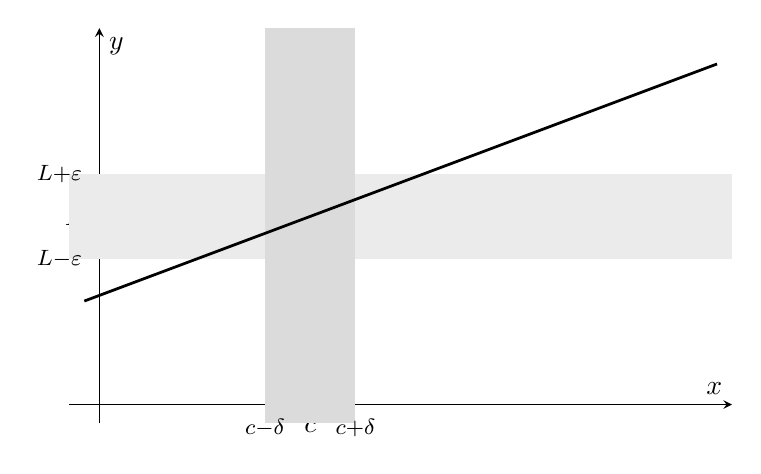
\begin{tikzpicture}[scale=1.0]
  \begin{axis}[
    width=10cm,height=6.6cm,
    axis lines=middle,
    xlabel=$x$,ylabel=$y$,
    xtick={1.4},xticklabels={$c$},
    ytick={2.0},yticklabels={$L$},
    xmin=-0.2,xmax=4.2,ymin=-0.2,ymax=4.0,
    clip=false,
  ]
    % epsilon band (horizontal)
    \addplot[draw=none,fill=black!8,forget plot] coordinates {(-0.2,1.55)(4.2,1.55)(4.2,2.45)(-0.2,2.45)};
    % delta band (vertical)
    \addplot[draw=none,fill=black!14,forget plot] coordinates {(1.1,-0.2)(1.7,-0.2)(1.7,4.0)(1.1,4.0)};
    % the function f(x) = 0.6 x + 1.16 (so f(1.4)=2)
    \addplot[curve,domain=-0.1:4.1,samples=2]{0.6*x+1.16};
    % L +/- eps labels
    \node[left,font=\footnotesize] at (axis cs:-0.05,2.45){$L{+}\eps$};
    \node[left,font=\footnotesize] at (axis cs:-0.05,1.55){$L{-}\eps$};
    \node[below,font=\footnotesize] at (axis cs:1.1,-0.05){$c{-}\delta$};
    \node[below,font=\footnotesize] at (axis cs:1.7,-0.05){$c{+}\delta$};
  \end{axis}
\end{tikzpicture}
\captionof{figure}{The $\eps$--$\delta$ ``tube'': the punctured vertical $\delta$-strip about
$c$ maps into the horizontal $\eps$-strip about $L$. Narrow the $\eps$-strip and you must
(in general) narrow the $\delta$-strip to keep the graph trapped.}
\end{center}

\begin{theorem}[Uniqueness of the limit]\label{t:flim-unique@c5}
If $c$ is a cluster point of $A$ and $f:A\to\R$, then $f$ has at most one limit at $c$.
\end{theorem}

\begin{proof}
Suppose $L,L'$ both work. Given $\eps>0$, pick $\delta_1$ for $L$ (with $\eps/2$) and
$\delta_2$ for $L'$ (with $\eps/2$), and put $\delta=\min\set{\delta_1,\delta_2}$. Because
$c$ is a cluster point there \emph{is} a point $x\in A$ with $0<\abs{x-c}<\delta$ (this is
where clusterness is used). For that $x$,
\[
  \abs{L-L'}\le\abs{L-f(x)}+\abs{f(x)-L'}<\tfrac\eps2+\tfrac\eps2=\eps .
\]
As $\eps>0$ was arbitrary, $\abs{L-L'}=0$, so $L=L'$.
\end{proof}

\begin{method}{Running an $\eps$--$\delta$ limit proof}
\textbf{Recognition trigger.} You must prove $\lim_{x\to c}f(x)=L$ \emph{from the
definition} (the value $L$ is given or guessed; ``using the definition of limit'').
\begin{enumerate}
\item \textbf{Form the gap} $\abs{f(x)-L}$ and simplify, factoring out $\abs{x-c}$ when
  possible: aim for $\abs{f(x)-L}=\abs{x-c}\cdot(\text{stuff})$.
\item \textbf{Tame the ``stuff''.} On a preliminary small interval, say $\abs{x-c}<1$,
  bound the leftover factor by a constant $M$; this gives
  $\abs{f(x)-L}\le M\abs{x-c}$ for $\abs{x-c}<1$.
\item \textbf{Choose $\delta$.} Given $\eps>0$, take $\delta=\min\set{1,\ \eps/M}$. Then
  $0<\abs{x-c}<\delta\imp\abs{f(x)-L}\le M\abs{x-c}<\eps$.
\item \textbf{Write it forward}: ``Let $\eps>0$. Put $\delta=\dots$. If $0<\abs{x-c}<\delta$
  then $\abs{f(x)-L}\le\dots<\eps$.''
\end{enumerate}
\textbf{Shortcut (Lipschitz bound).} If you can show $\abs{f(x)-L}\le K\abs{x-c}$ outright,
take $\delta=\eps/K$ and skip the interval-shrinking (B\&S 4.1.8 Ex.~6).
\end{method}

\begin{wex}{The model affine limit $\lim_{x\to c}(mx+b)=mc+b$}
Prove $\lim_{x\to 2}(3x+1)=7$.
\wrec Direct $\eps$--$\delta$; the gap is already a constant multiple of $\abs{x-c}$.
\wsol $\abs{(3x+1)-7}=3\abs{x-2}$. Given $\eps>0$, put $\delta=\eps/3$. If
$0<\abs{x-2}<\delta$ then $\abs{(3x+1)-7}=3\abs{x-2}<3\cdot\tfrac\eps3=\eps$. \emph{Check:}
for $\eps=0.03$, $\delta=0.01$: $x=2.005\Rightarrow 3x+1=7.015$, within $0.03$ of $7$.
\checkmark
\end{wex}

\begin{wex}{A quadratic: $\lim_{x\to 3}x^2=9$, with interval-shrinking}
Prove $\lim_{x\to 3}x^2=9$.
\wrec ``Prove this specific limit''; the leftover factor depends on $x$, so use Step~2.
\wsol $\abs{x^2-9}=\abs{x-3}\,\abs{x+3}$. Restrict to $\abs{x-3}<1$, i.e.\ $2<x<4$; then
$\abs{x+3}<7$, so $\abs{x^2-9}\le 7\abs{x-3}$. Given $\eps>0$ put
$\delta=\min\set{1,\eps/7}$; if $0<\abs{x-3}<\delta$ then $\abs{x^2-9}\le7\abs{x-3}<\eps$.
\emph{Check:} B\&S's identity $\abs{x^2-c^2}=\abs{x-c}\abs{x+c}\le(2\abs c+\delta)\abs{x-c}$
is exactly this estimate with $c=3$, $\delta\le1$. \checkmark
\end{wex}

\begin{wex}{A reciprocal: $\lim_{x\to 2}\dfrac1x=\dfrac12$}
Prove it from the definition.
\wrec A quotient blows up if the denominator nears $0$; bound it away from $0$ first.
\wsol $\abs{\dfrac1x-\dfrac12}=\dfrac{\abs{x-2}}{2\abs x}$. Restrict to $\abs{x-2}<1$, so
$x>1$ and $\abs x>1$, giving $\abs{\tfrac1x-\tfrac12}\le\tfrac12\abs{x-2}$. Given $\eps>0$
put $\delta=\min\set{1,2\eps}$; then $0<\abs{x-2}<\delta\imp
\abs{\tfrac1x-\tfrac12}\le\tfrac12\abs{x-2}<\eps$. \emph{Check:} the same trick proves the
quotient law later --- keep the denominator bounded below. \checkmark
\end{wex}

\subsection*{The sequential criterion (Heine)}

The single most useful reformulation converts function-limits into sequence-limits, where
all of Chapter~4's machinery applies.

\begin{theorem}[Sequential criterion for limits]\label{t:heine@c5}
Let $c$ be a cluster point of $A$ and $f:A\to\R$. Then $\displaystyle\lim_{x\to
c}f(x)=L$ \emph{iff} for \emph{every} sequence $\seq{x_n}$ in $A$ with $x_n\neq c$ and
$x_n\to c$, one has $f(x_n)\to L$.
\end{theorem}

\begin{proof}
($\imp$) Assume $f(x)\to L$ and let $x_n\to c$, $x_n\in A\setminus\set c$. Given $\eps>0$
choose $\delta$ from the limit definition, then $K$ with $\abs{x_n-c}<\delta$ for $n\ge K$.
Since $x_n\neq c$, $0<\abs{x_n-c}<\delta$, so $\abs{f(x_n)-L}<\eps$ for $n\ge K$; thus
$f(x_n)\to L$.

\noindent($\Leftarrow$, contrapositive) Suppose $f(x)\not\to L$. Then some $\eps_0>0$
resists every $\delta$: for each $n$, $\delta=1/n$ fails, so there is $x_n\in A$ with
$0<\abs{x_n-c}<1/n$ but $\abs{f(x_n)-L}\ge\eps_0$. Then $x_n\to c$, $x_n\neq c$, yet
$f(x_n)\not\to L$ --- the sequential condition fails.
\end{proof}

\begin{method}{Divergence by two sequences}
\textbf{Recognition trigger.} You suspect $\lim_{x\to c}f$ \emph{does not exist} (oscillation,
a sign jump, a $1/x$ blowup).
\begin{enumerate}
\item Produce two sequences $x_n\to c$ and $y_n\to c$ (each $\neq c$, in $A$).
\item Compute $\lim f(x_n)$ and $\lim f(y_n)$.
\item If they differ (or one fails to exist), then $\lim_{x\to c}f$ does not exist, by the
  contrapositive of Theorem~\ref{t:heine@c5}.
\end{enumerate}
\end{method}

\begin{wex}{A non-example: $\lim_{x\to0}\sin(1/x)$ does not exist}
Show $\operatorname{sgn}$-style oscillation kills the limit.
\wrec ``Show the limit does not exist''; two sequences route.
\wsol Let $x_n=\dfrac1{n\pi}\to0$, so $\sin(1/x_n)=\sin(n\pi)=0\to0$. Let
$y_n=\dfrac1{(2n+\frac12)\pi}\to0$, so $\sin(1/y_n)=\sin((2n+\tfrac12)\pi)=1\to1$. The two
limits $0$ and $1$ differ, so $\lim_{x\to0}\sin(1/x)$ does not exist.
\emph{Check:} the graph oscillates between $\pm1$ infinitely often near $0$ --- no band of
radius $<1$ can trap the tail. \checkmark
\end{wex}

\begin{center}
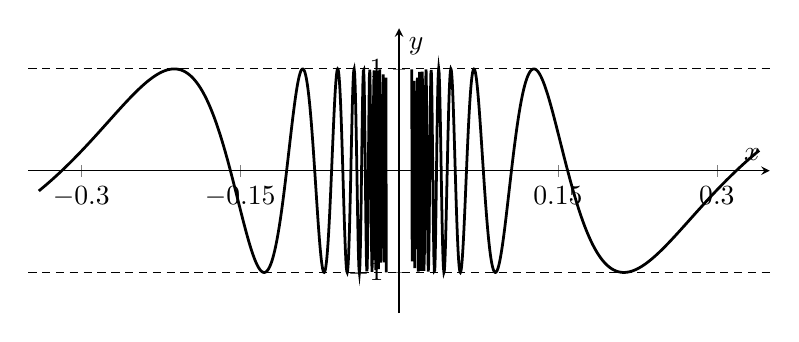
\begin{tikzpicture}
  \begin{axis}[
    width=11cm,height=5.2cm,
    axis lines=middle,xlabel=$x$,ylabel=$y$,
    xmin=-0.35,xmax=0.35,ymin=-1.4,ymax=1.4,
    xtick={-0.3,-0.15,0,0.15,0.3},
    ytick={-1,1},
    samples=801,
  ]
    \addplot[curve,domain=0.012:0.34]{sin(deg(1/x))};
    \addplot[curve,domain=-0.34:-0.012]{sin(deg(1/x))};
    \draw[densely dashed] (axis cs:-0.35,1)--(axis cs:0.35,1);
    \draw[densely dashed] (axis cs:-0.35,-1)--(axis cs:0.35,-1);
  \end{axis}
\end{tikzpicture}
\captionof{figure}{$f(x)=\sin(1/x)$ near $0$: ever-faster oscillation between $\pm1$. Along
$x_n=1/(n\pi)$ the values are $0$; along $y_n=1/((2n+\tfrac12)\pi)$ they are $1$.}
\end{center}

\begin{wex}{Taming oscillation with a factor: $\lim_{x\to0}x\sin(1/x)=0$}
Show that multiplying by $x$ rescues the limit.
\wrec A bounded times a vanishing factor; squeeze.
\wsol For $x\neq0$, $\abs{x\sin(1/x)}\le\abs x$ since $\abs{\sin}\le1$. Given $\eps>0$ take
$\delta=\eps$; then $0<\abs{x}<\delta\imp\abs{x\sin(1/x)-0}\le\abs x<\eps$. So the limit is
$0$. \emph{Check:} the wild oscillation is now confined to the shrinking envelope
$\pm\abs x$, which pinches to $0$ (this is the squeeze theorem of \S5.2 in disguise).
\checkmark
\end{wex}

\begin{wex}{Dirichlet-type: $f(x)=x$ on $\Q$, $0$ off $\Q$}
Let $f(x)=x$ for $x\in\Q$ and $f(x)=0$ for $x\notin\Q$. Show $\lim_{x\to0}f=0$ but
$\lim_{x\to c}f$ fails for every $c\neq0$.
\wrec A function defined by cases on rationality; the sequential criterion separates the two
``branches''.
\wsol At $0$: for all $x$, $\abs{f(x)}\le\abs x$ (either $\abs x$ or $0$), so $\delta=\eps$
gives $\abs{f(x)-0}<\eps$; thus $\lim_{x\to0}f=0$. At $c\neq0$: pick rationals $r_n\to c$
and irrationals $s_n\to c$ (density). Then $f(r_n)=r_n\to c\neq0$ while $f(s_n)=0\to0$. The
two sequential limits differ, so no limit exists at $c$. \emph{Check:} the limit survives
exactly where the two branches ($x$ and $0$) agree, namely at $x=0$. \checkmark
\end{wex}

\begin{pitfall}
The limit value must be \emph{found} before it is \emph{verified}: the $\eps$--$\delta$
definition only certifies a candidate $L$, it does not produce one. And $\delta$ may depend
on $\eps$ (and on $c$) but \emph{never} on $x$ --- writing ``take $\delta=\abs{x-c}/2$'' is
circular. Finally, $f(c)$ plays no role: the limit can exist with $f$ undefined at $c$, or
with $f(c)$ equal to something other than $L$.
\end{pitfall}

\begin{remark}[Restriction to a subset]
If $f_1$ is the restriction of $f$ to an \emph{open} interval $I\ni c$, then $f$ and $f_1$
have the same limit behaviour at $c$ (an open $I$ contains a full punctured neighborhood of
$c$). For a one-sided restriction the implication is one-way: a two-sided limit forces each
restricted limit, but agreeing restricted limits on \emph{just one side} need not give a
two-sided limit. This subtlety is the topic of one-sided limits in \S5.2.
\end{remark}

\subsection*{Further worked examples}

\begin{wex}{A cube-root gap: $\lim_{x\to c}\sqrt[3]{x}$ by factoring the difference}
Prove $\lim_{x\to8}\sqrt[3]{x}=2$ from the definition.
\wrec ``Prove this specific limit'': the gap $\abs{\sqrt[3]x-2}$ is not yet a multiple of
$\abs{x-8}$, so factor $a-b=\dfrac{a^3-b^3}{a^2+ab+b^2}$ to expose $\abs{x-8}$.
\wsol With $a=\sqrt[3]x$, $b=2$, $a^3-b^3=x-8$ and
$\abs{\sqrt[3]x-2}=\dfrac{\abs{x-8}}{a^2+2a+4}$. The denominator $a^2+2a+4=(a+1)^2+3\ge3>0$
for all real $a$, so $\abs{\sqrt[3]x-2}\le\tfrac13\abs{x-8}$. Given $\eps>0$ put
$\delta=3\eps$; then $0<\abs{x-8}<\delta\imp\abs{\sqrt[3]x-2}<\eps$. \emph{Check:} at
$x=8.3$, $\sqrt[3]{8.3}\approx2.0247$, and $\tfrac13\abs{8.3-8}=0.1$ indeed bounds the gap
$0.0247$. \checkmark
\end{wex}

\begin{wex}{A non-example: a one-sided blowup defeats the two-sided limit}
Show $\displaystyle\lim_{x\to0}\frac{\abs x}{x}$ does not exist, via the sequential
criterion.
\wrec ``Show the limit does not exist'': route through two sequences approaching $0$ from
opposite sides (Theorem~\ref{t:heine@c5}).
\wsol For $x>0$, $\tfrac{\abs x}{x}=1$; for $x<0$, $\tfrac{\abs x}{x}=-1$. Take
$x_n=\tfrac1n\to0$ (positive): $f(x_n)=1\to1$. Take $y_n=-\tfrac1n\to0$ (negative):
$f(y_n)=-1\to-1$. The two sequential limits differ, so $\lim_{x\to0}\tfrac{\abs x}{x}$ does
not exist. \emph{Check:} the one-sided limits are $1$ and $-1$, a jump of size $2$; the
deleted point $x=0$ is precisely where the formula is undefined. \checkmark
\end{wex}

\begin{exers}{Exercises (Rudin, Ch.4).}
\item Suppose $f:\R\to\R$ satisfies $\displaystyle\lim_{h\to0}\big[f(x+h)-f(x-h)\big]=0$ for
  every $x\in\R$. Does this imply $f$ is continuous? (Answer with proof or counterexample.)
\end{exers}

\begin{exers}{Exercises (Bartle \& Sherbert, \S4.1).}
\item Determine a condition on $\abs{x-1}$ that will assure: (a) $\abs{x^2-1}<\tfrac12$;
  (b) $\abs{x^2-1}<10^{-3}$; (c) $\abs{x^2-1}<1/n$ for given $n\in\N$; (d) $\abs{x^3-1}<1/n$
  for given $n\in\N$.
\item Determine a condition on $\abs{x-4}$ that will assure: (a) $\abs{\sqrt x-2}<\tfrac12$;
  (b) $\abs{\sqrt x-2}<10^{-2}$.
\item Let $c$ be a cluster point of $A\subseteq\R$ and $f:A\to\R$. Prove $\lim_{x\to
  c}f(x)=L$ iff $\lim_{x\to c}\abs{f(x)-L}=0$.
\item Let $f:\R\to\R$ and $c\in\R$. Show $\lim_{x\to c}f(x)=L$ iff $\lim_{x\to0}f(x+c)=L$.
\item Let $I=(-a,a)$ with $a>0$ and $g(x)=x^2$ on $I$. For $x,c\in I$ show
  $\abs{g(x)-c^2}\le 2a\abs{x-c}$, and use this to prove $\lim_{x\to c}x^2=c^2$ for any
  $c\in I$.
\item Let $I$ be an interval, $f:I\to\R$, $c\in I$. Suppose there are constants $K,L$ with
  $\abs{f(x)-L}\le K\abs{x-c}$ for $x\in I$. Show $\lim_{x\to c}f(x)=L$.
\item Show $\lim_{x\to c}x^3=c^3$ for any $c\in\R$.
\item Show $\lim_{x\to c}\sqrt x=\sqrt c$ for any $c>0$.
\item Use the $\eps$--$\delta$ definition or the sequential criterion to establish:
  (a) $\displaystyle\lim_{x\to2}\frac{1}{1-x}=-1$;
  (b) $\displaystyle\lim_{x\to1}\frac{x}{1+x}=\tfrac12$;
  (c) $\displaystyle\lim_{x\to0}\frac{x^2}{\abs x}=0$;
  (d) $\displaystyle\lim_{x\to1}\frac{x^2-x+1}{x+1}=\tfrac12$.
\item Use the definition of limit to show: (a) $\lim_{x\to2}(x^2+4x)=12$;
  (b) $\displaystyle\lim_{x\to-1}\frac{x+5}{2x+3}=4$.
\item Use the definition of limit to prove: (a) $\displaystyle\lim_{x\to3}\frac{2x+3}{4x-9}=3$;
  (b) $\displaystyle\lim_{x\to6}\frac{x^2-3x}{x+3}=2$.
\item Show the following limits do not exist: (a) $\lim_{x\to0}\dfrac{1}{x^2}$ ($x>0$);
  (b) $\lim_{x\to0}\dfrac{1}{\sqrt x}$ ($x>0$); (c) $\lim_{x\to0}\big(x+\operatorname{sgn}(x)\big)$;
  (d) $\lim_{x\to0}\sin(1/x^2)$.
\item Suppose $f:\R\to\R$ has limit $L$ at $0$, and $a>0$. If $g(x)=f(ax)$, show $\lim_{x\to
  0}g(x)=L$.
\item Let $c\in\R$ and $f:\R\to\R$ with $\lim_{x\to c}(f(x))^2=L$. (a) Show that if $L=0$
  then $\lim_{x\to c}f(x)=0$. (b) Show by example that if $L\neq0$ then $f$ may have no limit
  at $c$.
\item Let $f:\R\to\R$ with $f(x)=x$ for $x$ rational and $f(x)=0$ for $x$ irrational.
  (a) Show $f$ has a limit at $x=0$. (b) Use a sequential argument to show that if $c\neq0$,
  $f$ has no limit at $c$.
\item Let $f:\R\to\R$, $I$ an open interval, $c\in I$. If $f_1$ is the restriction of $f$ to
  $I$, show $f_1$ has a limit at $c$ iff $f$ does, and the limits are equal.
\item Let $f:\R\to\R$, $J$ a closed interval, $c\in J$. If $f_2$ is the restriction of $f$ to
  $J$, show that if $f$ has a limit at $c$ then so does $f_2$. Show by example that the
  converse can fail.
\end{exers}

\begin{exers}{Additional exercises.}
\item (Warm-up.) Using the definition, prove $\lim_{x\to3}(2x-5)=1$ by exhibiting an explicit
  $\delta(\eps)$.
\item Prove $\lim_{x\to2}x^3=8$ from the definition. (Factor $x^3-8=(x-2)(x^2+2x+4)$ and
  bound the quadratic on $\abs{x-2}<1$.)
\item (Sequential criterion both ways.) Let $f(x)=\dfrac{x^2-1}{x-1}$ for $x\neq1$. Show
  $\lim_{x\to1}f=2$ first by algebra, then by verifying that every $x_n\to1$ ($x_n\neq1$)
  gives $f(x_n)\to2$.
\item (Non-example / disprove.) Show $\lim_{x\to0}\dfrac{\abs x}{x}$ does not exist by
  producing two sequences $x_n\to0$ with different limits of $f(x_n)$. Identify the one-sided
  limits.
\item (Cluster points.) Let $A=\set{1/m+1/n\st m,n\in\N}$. Determine all cluster points of
  $A$, and decide which of them lie in $A$.
\item Suppose $\lim_{x\to c}f(x)=L>0$. Prove there is a punctured neighborhood of $c$ on
  which $f(x)>L/2>0$ (a ``persistence of sign'' for limits).
\item (Diagram.) Sketch $f(x)=\dfrac{x^2-4}{x-2}$ near $x=2$, marking the removable hole at
  $(2,4)$, and on the same axes draw the $\eps=0.5$ horizontal band about $y=4$ together with
  a $\delta$-interval about $x=2$ that maps into it.
\item (Composition of limits, carefully.) Give $f,g$ with $\lim_{x\to0}f(x)=0$ and
  $\lim_{y\to0}g(y)=0$ but $\lim_{x\to0}g(f(x))\neq0$. Explain which hypothesis of the naive
  ``substitution'' fails.
\end{exers}


\section{Limit Theorems and Extensions of the Limit Concept}
\subsection*{The algebra of limits}

Once the sequential criterion is in hand, the limit theorems for functions are corollaries
of the corresponding theorems for sequences. We first record a boundedness fact.

\begin{theorem}[Limits are locally bounded]\label{t:flim-bdd@c5}
If $\lim_{x\to c}f=L$ exists, then $f$ is bounded on a punctured neighborhood of $c$: there
are $\delta>0$ and $M>0$ with $\abs{f(x)}\le M$ for all $x\in A$, $0<\abs{x-c}<\delta$.
\end{theorem}

\begin{proof}
Take $\eps=1$ to get $\delta$ with $\abs{f(x)-L}<1$, hence $\abs{f(x)}<\abs L+1=:M$, on the
punctured $\delta$-neighborhood.
\end{proof}

\begin{theorem}[Limit theorems for functions]\label{t:limthms@c5}
Let $c$ be a cluster point of $A$, let $f,g:A\to\R$ with $\lim_{x\to c}f=L$ and $\lim_{x\to
c}g=M$, and let $k\in\R$. Then as $x\to c$,
\[
  f+g\to L+M,\qquad f-g\to L-M,\qquad kf\to kL,\qquad fg\to LM,
\]
and, if $M\neq0$ and $g\neq0$ near $c$, $\ \dfrac fg\to\dfrac LM$. Moreover if
$f(x)\ge0$ on $A$ then $L\ge0$, and $\sqrt f\to\sqrt L$.
\end{theorem}

\begin{proof}
We give the product directly and deduce the rest. For the product, write
\[
  \abs{f(x)g(x)-LM}=\abs{f(x)\big(g(x)-M\big)+M\big(f(x)-L\big)}
  \le\abs{f(x)}\abs{g(x)-M}+\abs M\abs{f(x)-L}.
\]
By Theorem~\ref{t:flim-bdd@c5}, $\abs{f(x)}\le K$ near $c$. Given $\eps>0$, choose $\delta$ so
small that $\abs{g(x)-M}<\dfrac\eps{2K}$ and $\abs{f(x)-L}<\dfrac\eps{2(\abs M+1)}$; then the
right side is $<\eps$. The sum/difference/scalar cases follow from
$\abs{(f\pm g)-(L\pm M)}\le\abs{f-L}+\abs{g-M}$ and $\abs{kf-kL}=\abs k\abs{f-L}$. For the
quotient it suffices to handle $1/g\to1/M$: since $M\neq0$, $\abs{g(x)}\ge\abs M/2$ near $c$,
and $\abs{\tfrac1{g(x)}-\tfrac1M}=\dfrac{\abs{g(x)-M}}{\abs{g(x)}\abs M}\le\dfrac{2}{\abs
M^2}\abs{g(x)-M}\to0$; multiply by $f$. The sign and square-root statements are immediate from
the sequential criterion and the corresponding sequence theorems.
\end{proof}

\begin{remark}[Two proofs, one fact]
B\&S prove these via the \emph{sequential criterion} (Theorem~\ref{t:heine@c5}): take any
$x_n\to c$, $x_n\neq c$; then $f(x_n)\to L$ and $g(x_n)\to M$, and the sequence limit
theorems give $f(x_n)g(x_n)\to LM$, etc. Rudin gives the direct $\eps$--$\delta$ estimate
above. The sequential route is shorter; the direct route shows \emph{which} $\delta$ works.
Both are worth carrying.
\end{remark}

\begin{theorem}[Squeeze theorem for functions]\label{t:squeeze@c5}
If $f(x)\le g(x)\le h(x)$ for $x$ in a punctured neighborhood of $c$, and $\lim_{x\to
c}f=\lim_{x\to c}h=L$, then $\lim_{x\to c}g=L$.
\end{theorem}

\begin{proof}
Given $\eps>0$, choose $\delta$ so both $\abs{f-L}<\eps$ and $\abs{h-L}<\eps$ on the
punctured $\delta$-neighborhood. There $L-\eps<f(x)\le g(x)\le h(x)<L+\eps$, hence
$\abs{g(x)-L}<\eps$.
\end{proof}

\begin{wex}{Rational evaluation by the limit theorems}
Evaluate $\displaystyle\lim_{x\to2}\frac{x^2-4}{x-2}$ and
$\displaystyle\lim_{x\to1}\frac{x^2+2}{x^2-2}$.
\wrec ``Compute this limit'': simplify, then apply Theorem~\ref{t:limthms@c5} provided no
denominator vanishes after simplification.
\wsol First: for $x\neq2$, $\dfrac{x^2-4}{x-2}=\dfrac{(x-2)(x+2)}{x-2}=x+2\to 4$ (the
deleted point $x=2$ is exactly why cancellation is legal). Second: denominator
$\to1-2=-1\neq0$, numerator $\to3$, so by the quotient law the limit is $3/(-1)=-3$.
\emph{Check:} plug $x=1.99$ into the first: $\approx3.99\to4$; plug $x=1.001$ into the
second: $\approx-3.0$. \checkmark
\end{wex}

\begin{wex}{A bounded factor times a vanishing one}
Suppose $f$ is bounded near $c$ and $\lim_{x\to c}g=0$. Show $\lim_{x\to c}fg=0$.
\wrec ``Product with one factor $\to0$, the other only bounded'' --- you cannot use the
product law (the $f$-limit may not exist) so estimate directly.
\wsol Let $\abs{f}\le K$ on a punctured neighborhood. Then $\abs{f(x)g(x)}\le K\abs{g(x)}$.
Given $\eps>0$ choose $\delta$ with $\abs{g(x)}<\eps/K$; then $\abs{fg}<\eps$. So $fg\to0$.
\emph{Check:} with $f=\sin(1/x)$ (bounded, no limit at $0$) and $g=x$, this recovers
$x\sin(1/x)\to0$. \checkmark
\end{wex}

\begin{pitfall}
The product/quotient laws need \emph{both} limits to exist. $\lim x\sin(1/x)=0$ even though
$\sin(1/x)$ has no limit at $0$ --- so a product can converge with a factor that does not.
Do not ``cancel'' a limit that may not exist; fall back on a direct boundedness estimate.
\end{pitfall}

\subsection*{One-sided limits}

\begin{definition}\label{d:onesided@c5}
Let $c$ be a cluster point of $A\cap(c,\infty)$. The \emph{right-hand limit}
$\displaystyle\lim_{x\to c^+}f(x)=L$ means: $\forall\eps>0\ \exists\delta>0$ with
$x\in A,\ c<x<c+\delta\imp\abs{f(x)-L}<\eps$. The \emph{left-hand limit} $\lim_{x\to
c^-}f=L$ is defined symmetrically with $c-\delta<x<c$.
\end{definition}

\begin{theorem}[Two-sided $=$ both one-sided]\label{t:onesided-iff@c5}
If $c$ is a cluster point of both $A\cap(c,\infty)$ and $A\cap(-\infty,c)$, then $\lim_{x\to
c}f=L$ iff $\lim_{x\to c^+}f=L=\lim_{x\to c^-}f$.
\end{theorem}

\begin{proof}
A two-sided $\delta$ works for each side, giving ($\imp$). Conversely take
$\delta=\min\set{\delta_+,\delta_-}$ from the two one-sided definitions; for
$0<\abs{x-c}<\delta$, $x$ lies on one side or the other, and the matching estimate gives
$\abs{f(x)-L}<\eps$.
\end{proof}

\begin{wex}{A jump: $\operatorname{sgn}$ at $0$}
Let $\operatorname{sgn}(x)=1$ for $x>0$, $-1$ for $x<0$, $0$ at $0$. Find the one-sided
limits at $0$.
\wrec ``One-sided limits at a jump''; evaluate each side as a constant.
\wsol For $x>0$, $\operatorname{sgn}(x)=1$, so $\lim_{x\to0^+}\operatorname{sgn}=1$; for
$x<0$ it is $-1$, so $\lim_{x\to0^-}\operatorname{sgn}=-1$. The one-sided limits differ, so
$\lim_{x\to0}\operatorname{sgn}$ does \emph{not} exist (Theorem~\ref{t:onesided-iff@c5}).
\emph{Check:} the value $\operatorname{sgn}(0)=0$ matches neither one-sided limit --- a
\emph{jump} discontinuity. \checkmark
\end{wex}

\subsection*{Infinite limits and limits at infinity}

\begin{definition}\label{d:inflim@c5}
With $c$ a cluster point of $A$: $\displaystyle\lim_{x\to c}f=+\infty$ means $\forall
M>0\ \exists\delta>0$ with $0<\abs{x-c}<\delta\imp f(x)>M$; replace $f(x)>M$ by $f(x)<-M$
for $-\infty$. For \emph{limits at infinity} (with $A$ unbounded above):
$\displaystyle\lim_{x\to+\infty}f=L$ means $\forall\eps>0\ \exists K>0$ with $x>K\imp
\abs{f(x)-L}<\eps$; and $\lim_{x\to+\infty}f=+\infty$ means $\forall M\ \exists K$ with
$x>K\imp f(x)>M$. The cases $x\to-\infty$ are symmetric.
\end{definition}

In Rudin's uniform language (4.33): writing $V$ for a neighborhood of $+\infty$, namely a
ray $(c,+\infty)$, and similarly for $-\infty$, the single definition ``$f(t)\to A$ as $t\to
x$ if every neighborhood of $A$ contains $f(V\cap E\setminus\set x)$ for some neighborhood
$V$ of $x$'' subsumes all finite and infinite cases at once.

\begin{theorem}[Reciprocal bridge]\label{t:recip-inf@c5}
Let $f>0$ on $(c,\infty)\cap A$. Then $\lim_{x\to c^+}f=+\infty$ iff $\lim_{x\to
c^+}\dfrac1f=0$. (Same with two-sided or $x\to\infty$ versions.)
\end{theorem}

\begin{proof}
$f>M\eqv 1/f<1/M$; let $M\to\infty$ correspond to $1/M\to0$. Precisely: given $\eps>0$ set
$M=1/\eps$; then $f>M$ on a one-sided $\delta$-interval gives $0<1/f<\eps$ there, and
conversely.
\end{proof}

\begin{wex}{$\lim_{x\to0}1/x^2=+\infty$ and $\lim_{x\to\infty}(x+2)/x=1$}
Evaluate both.
\wrec ``Infinite limit'' (denominator $\to0$, sign fixed) and ``limit at infinity''
(rational function, compare degrees).
\wsol For $1/x^2$: given $M>0$ take $\delta=1/\sqrt M$; if $0<\abs x<\delta$ then
$x^2<1/M$ so $1/x^2>M$. Hence $\lim_{x\to0}1/x^2=+\infty$ (and $\lim_{x\to0}x^2=0^+$ confirms
via Theorem~\ref{t:recip-inf@c5}). For $(x+2)/x=1+2/x$: as $x\to\infty$, $2/x\to0$, so the
limit is $1$. \emph{Check:} $x=10^3\Rightarrow(x+2)/x=1.002$; the larger $x$, the closer to
$1$. \checkmark
\end{wex}

\begin{center}
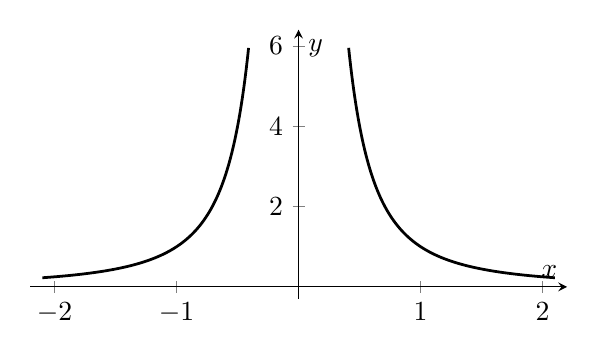
\begin{tikzpicture}
  \begin{axis}[
    width=8.4cm,height=5.0cm,
    axis lines=middle,xlabel=$x$,ylabel=$y$,
    xmin=-2.2,xmax=2.2,ymin=-0.3,ymax=6.4,
    xtick={-2,-1,1,2},ytick={2,4,6},
    samples=200,restrict y to domain=0:6.4,
  ]
    \addplot[curve,domain=0.41:2.1]{1/x^2};
    \addplot[curve,domain=-2.1:-0.41]{1/x^2};
    \draw[densely dashed] (axis cs:0,-0.3)--(axis cs:0,6.4);
  \end{axis}
\end{tikzpicture}
\hfill
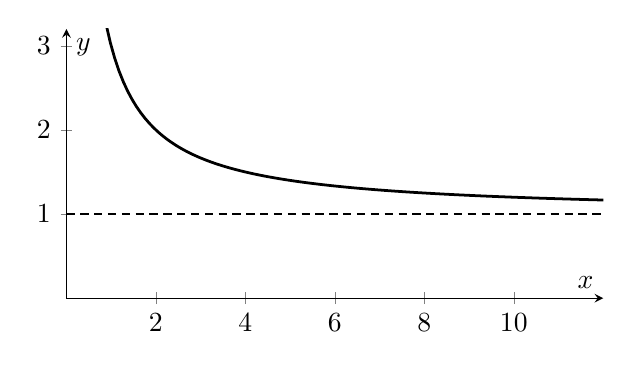
\begin{tikzpicture}
  \begin{axis}[
    width=8.4cm,height=5.0cm,
    axis lines=middle,xlabel=$x$,ylabel=$y$,
    xmin=0,xmax=12,ymin=0,ymax=3.2,
    xtick={2,4,6,8,10},ytick={1,2,3},
    samples=120,
  ]
    \addplot[curve,domain=0.5:12]{1+2/x};
    \draw[densely dashed] (axis cs:0,1)--(axis cs:12,1) node[right,font=\footnotesize]{$y=1$};
  \end{axis}
\end{tikzpicture}
\captionof{figure}{Left: $1/x^2\to+\infty$ as $x\to0$ (vertical asymptote). Right:
$(x+2)/x=1+2/x\to1$ as $x\to\infty$ (horizontal asymptote).}
\end{center}

\begin{pitfall}
``$\lim f=+\infty$'' does not mean the limit \emph{exists} in $\R$ --- it is shorthand for
unbounded escape, a kind of \emph{controlled} divergence. The arithmetic of $\pm\infty$ has
forbidden forms: $\infty-\infty$, $0\cdot\infty$, $\infty/\infty$, $A/0$ are undefined
(Rudin 4.34). E.g.\ $f=1/x$, $g=-1/x+1$ near $0^+$ both blow up but $f+g\to+\infty$ while
$f-(f)=0$; you must compute, not cancel infinities.
\end{pitfall}

\subsection*{Further worked examples}

\begin{wex}{A limit at infinity of a rational function}
Evaluate $\displaystyle\lim_{x\to+\infty}\frac{3x^2-x+5}{2x^2+7}$ and
$\displaystyle\lim_{x\to+\infty}\frac{4x+1}{x^2-3}$.
\wrec ``Limit at infinity of a quotient'': divide by the highest power so each piece becomes
a sum of constants and vanishing terms, then apply Theorem~\ref{t:limthms@c5}.
\wsol First: divide top and bottom by $x^2$:
$\dfrac{3-\tfrac1x+\tfrac5{x^2}}{2+\tfrac7{x^2}}\to\dfrac{3-0+0}{2+0}=\dfrac32$, since each
$\tfrac1x,\tfrac1{x^2}\to0$ as $x\to\infty$. Second: divide by $x^2$:
$\dfrac{\tfrac4x+\tfrac1{x^2}}{1-\tfrac3{x^2}}\to\dfrac{0}{1}=0$ (numerator degree below
denominator). \emph{Check:} at $x=100$, the first is $\approx\tfrac{29905}{20007}\approx1.495
\to1.5$; the second is $\approx\tfrac{401}{9997}\approx0.04\to0$. \checkmark
\end{wex}

\begin{wex}{A squeeze for a function limit}
Evaluate $\displaystyle\lim_{x\to0}x^2\cos(1/x^2)$.
\wrec ``Bounded oscillation times a vanishing factor'': the product law fails (the cosine has
no limit), so bound and squeeze (Theorem~\ref{t:squeeze@c5}).
\wsol For $x\neq0$, $\abs{\cos(1/x^2)}\le1$, so $-x^2\le x^2\cos(1/x^2)\le x^2$. Both bounds
$\pm x^2\to0$ as $x\to0$, so by the squeeze theorem the middle term $\to0$. \emph{Check:}
directly, $\abs{x^2\cos(1/x^2)-0}\le x^2<\eps$ whenever $\abs x<\sqrt\eps$, so
$\delta=\sqrt\eps$ also certifies the limit $0$. \checkmark
\end{wex}

\begin{exers}{Exercises (Bartle \& Sherbert, \S4.2).}
\item Apply the limit theorems to determine: (a) $\lim_{x\to1}(x+1)(2x+3)$;
  (b) $\displaystyle\lim_{x\to1}\frac{x^2+2}{x^2-2}$ ($x>0$);
  (c) $\displaystyle\lim_{x\to2}\Big(\frac{1}{x+1}-\frac{1}{2x}\Big)$ ($x>0$);
  (d) $\displaystyle\lim_{x\to0}\frac{x+1}{x^2+2}$.
\item Determine the following limits, stating which theorems are used:
  (a) $\displaystyle\lim_{x\to2}\sqrt{\frac{2x+1}{x+3}}$ ($x>0$);
  (b) $\displaystyle\lim_{x\to2}\frac{x^2-4}{x-2}$ ($x>0$);
  (c) $\displaystyle\lim_{x\to0}\frac{(x+1)^2-1}{x}$ ($x>0$);
  (d) $\displaystyle\lim_{x\to1}\frac{\sqrt x-1}{x-1}$ ($x>0$).
\item Find $\displaystyle\lim_{x\to0}\frac{\sqrt{1+2x}-\sqrt{1+3x}}{x+2x^2}$, where $x>0$.
\item Prove $\lim_{x\to0}\cos(1/x)$ does not exist, but $\lim_{x\to0}x\cos(1/x)=0$.
\item Let $f,g$ on $A\subseteq\R$, $c$ a cluster point of $A$. Suppose $f$ is bounded on a
  neighborhood of $c$ and $\lim_{x\to c}g=0$. Prove $\lim_{x\to c}fg=0$.
\item Use the definition of limit to prove the first assertion of the sum law:
  $\lim_{x\to c}(f+g)=\lim f+\lim g$.
\item Use the sequential formulation to prove the difference law $\lim_{x\to
  c}(f-g)=\lim f-\lim g$.
\item Let $n\in\N$, $n\ge3$. Derive the inequality $-x^2\le x^n\le x^2$ for $-1<x<1$. Then
  use $\lim_{x\to0}x^2=0$ to show $\lim_{x\to0}x^n=0$.
\item Let $f,g$ on $A$, $c$ a cluster point. (a) Show that if $\lim f$ and $\lim(f+g)$ exist,
  then $\lim g$ exists. (b) If $\lim f$ and $\lim fg$ exist, does $\lim g$ exist?
\item Give examples of $f,g$ with no limit at $c$ such that both $f+g$ and $fg$ have limits
  at $c$.
\item Determine whether these limits exist in $\R$ ($x\neq0$):
  (a) $\lim_{x\to0}\sin(1/x^2)$; (b) $\lim_{x\to0}x\sin(1/x^2)$;
  (c) $\lim_{x\to0}\operatorname{sgn}\big(\sin(1/x)\big)$; (d) $\lim_{x\to0}\sqrt x\,\sin(1/x^2)$
  ($x>0$).
\item Let $f:\R\to\R$ with $f(x+y)=f(x)+f(y)$ for all $x,y$, and suppose $\lim_{x\to0}f=L$
  exists. Prove $L=0$, and that $f$ has a limit at every $c$. (Hint: $f(2x)=2f(x)$ and
  $f(x)=f(x-c)+f(c)$.)
\item Let $f(x)=x+1$ and $g(x)=2$ if $x\neq1$, $g(1)=0$. (a) Find $\lim_{x\to1}g(f(x))$ and
  compare with $g(\lim_{x\to1}f(x))$. (b) Find $\lim_{x\to1}f(g(x))$ and compare with
  $f(\lim_{x\to1}g(x))$.
\item Let $A\subseteq\R$, $f:A\to\R$, $c$ a cluster point. If $\lim_{x\to c}f$ exists, prove
  $\lim_{x\to c}\abs f=\abs{\lim_{x\to c}f}$.
\item Let $A\subseteq\R$, $f:A\to\R$ with $f(x)\ge0$ for all $x\in A$, $c$ a cluster point.
  If $\lim_{x\to c}f$ exists, prove $\lim_{x\to c}\sqrt f=\sqrt{\lim_{x\to c}f}$.
\end{exers}

\begin{exers}{Exercises (Bartle \& Sherbert, \S4.3).}
\item Prove the analogue of the sum/product/quotient theorems for one-sided limits.
\item Give an example of a function that has a right-hand limit but not a left-hand limit at
  a point.
\item Let $f(x)=\abs x^{-1/2}$ for $x\neq0$. Show $\lim_{x\to0^+}f=\lim_{x\to0^-}f=+\infty$.
\item Let $c\in\R$, $f$ defined on $(c,\infty)$ with $f(x)>0$ there. Show $\lim_{x\to
  c}f=+\infty$ iff $\lim_{x\to c}1/f=0$.
\item Evaluate, or show nonexistent: (a) $\lim_{x\to1^+}\dfrac{x}{x-1}$;
  (b) $\lim_{x\to1}\dfrac{x}{x-1}$; (c) $\lim_{x\to0^+}\dfrac{x+2}{\sqrt x}$;
  (d) $\lim_{x\to\infty}\dfrac{x+2}{\sqrt x}$; (e) $\lim_{x\to0}\dfrac{\sqrt{x+1}}{x}$;
  (f) $\lim_{x\to\infty}\dfrac{\sqrt{x+1}}{x}$; (g) $\lim_{x\to\infty}\dfrac{\sqrt x-5}{\sqrt
  x+3}$; (h) $\lim_{x\to\infty}\dfrac{x-\sqrt x}{\sqrt x+x}$.
\item Prove the analogue of the limit theorems for limits as $x\to\infty$.
\item Suppose $f,g$ have limits in $\R$ as $x\to\infty$ and $f(x)\le g(x)$ for $x\in(a,\infty)$.
  Prove $\lim_{x\to\infty}f\le\lim_{x\to\infty}g$.
\item Let $f$ be defined on $(0,\infty)$. Prove $\lim_{x\to\infty}f(x)=L$ iff
  $\lim_{x\to0^+}f(1/x)=L$.
\item Show that if $f:(a,\infty)\to\R$ has $\lim_{x\to\infty}xf(x)=L$ with $L\in\R$, then
  $\lim_{x\to\infty}f(x)=0$.
\item Prove the analogue of the limit theorems for infinite limits.
\item Suppose $\lim_{x\to c}f=L>0$ and $\lim_{x\to c}g=\infty$. Show $\lim_{x\to c}fg=\infty$.
  If $L=0$, show by example this may fail.
\item Find $f,g$ on $(0,\infty)$ with $\lim_{x\to\infty}f=\infty$, $\lim_{x\to\infty}g=\infty$,
  and $\lim_{x\to\infty}(f-g)=0$. Can you find such, with $g>0$, so that $\lim_{x\to\infty}f/g=0$?
\item Let $f,g$ on $(a,\infty)$ with $\lim_{x\to\infty}f=L$ and $\lim_{x\to\infty}g=\infty$.
  Prove $\lim_{x\to\infty}f\circ g=L$.
\end{exers}

\begin{exers}{Additional exercises.}
\item Evaluate $\displaystyle\lim_{x\to3}\frac{x^2-9}{x^2-2x-3}$ and
  $\displaystyle\lim_{x\to0}\frac{\sqrt{1+x}-1}{x}$, naming the limit theorem at each step.
\item (Squeeze.) Prove $\lim_{x\to0}x^2\cos(1/x)=0$ and, more generally, that a bounded
  function times one tending to $0$ tends to $0$.
\item Compute the one-sided limits of $f(x)=\dfrac{x}{\abs x}+\dfrac{1}{1+2^{1/x}}$ at $x=0$,
  and decide whether $\lim_{x\to0}f$ exists.
\item (Non-example / disprove.) Disprove the claim ``if $\lim_{x\to c}(f+g)$ and $\lim_{x\to
  c}f$ both exist then $\lim_{x\to c}g$ need not exist.'' That is, show $\lim_{x\to c}g$
  \emph{must} exist, and then give a separate $f,g$ with $\lim(f+g)$ existing while
  \emph{neither} $\lim f$ nor $\lim g$ does.
\item Show $\lim_{x\to\infty}\dfrac{3x^2-x+2}{5x^2+7}=\dfrac35$ and
  $\lim_{x\to\infty}\big(\sqrt{x^2+x}-x\big)=\dfrac12$.
\item Prove from the definition that $\lim_{x\to1^+}\dfrac1{x-1}=+\infty$ and
  $\lim_{x\to1^-}\dfrac1{x-1}=-\infty$; conclude the two-sided limit does not exist.
\item (Diagram.) Draw $y=\dfrac{1}{x-1}$ on $(-1,3)\setminus\set1$, marking the vertical
  asymptote at $x=1$ and the horizontal asymptote $y=0$, and annotate the one-sided
  behaviours as $x\to1^\pm$ and $x\to\pm\infty$.
\item (Cauchy functional equation, limit version.) If $\lim_{x\to0}f=L$ exists for an
  additive $f$ ($f(x+y)=f(x)+f(y)$), prove $L=0$ and that $\lim_{x\to c}f=f(c)$ at every $c$.
\end{exers}


\section{Continuous Functions}
\subsection*{Continuity at a point}

Continuity says the limit exists \emph{and equals the function value}: no break, no jump, no
hole. Crucially, continuity is defined even at \emph{isolated} points of the domain, where
no limit can be asked.

\begin{definition}\label{d:cont@c5}
Let $A\subseteq\R$, $f:A\to\R$, $c\in A$. Then $f$ is \emph{continuous at $c$} if
\[
  \forall\eps>0\ \ \exists\delta>0\ \ \text{such that}\quad
  x\in A,\ \abs{x-c}<\delta\quad\imp\quad\abs{f(x)-f(c)}<\eps .
\]
$f$ is \emph{continuous on $A$} if it is continuous at every point of $A$. If $f$ is not
continuous at $c$, it is \emph{discontinuous} there.
\end{definition}

Two differences from the limit definition: the value tested is $f(c)$ (not an external
$L$), and the puncture $0<\abs{x-c}$ is gone --- $x=c$ is allowed (it gives
$\abs{f(c)-f(c)}=0<\eps$ for free). Consequently:

\begin{theorem}[Continuity via limits]\label{t:cont-lim@c5}
If $c$ is a cluster point of $A$, then $f$ is continuous at $c$ iff $\lim_{x\to c}f=f(c)$.
If $c$ is an \emph{isolated} point of $A$ (not a cluster point), then $f$ is automatically
continuous at $c$.
\end{theorem}

\begin{proof}
For a cluster point the two definitions coincide once the (now harmless) $x=c$ case is
added. For an isolated point there is $\delta_0$ with $V_{\delta_0}(c)\cap A=\set c$; then
$\abs{x-c}<\delta_0$ forces $x=c$, so $\abs{f(x)-f(c)}=0<\eps$ trivially.
\end{proof}

\begin{theorem}[Sequential criterion for continuity]\label{t:cont-seq@c5}
$f$ is continuous at $c\in A$ iff for \emph{every} sequence $\seq{x_n}$ in $A$ with $x_n\to
c$ one has $f(x_n)\to f(c)$.
\end{theorem}

\begin{proof}
Identical to Theorem~\ref{t:heine@c5} but with $L=f(c)$ and \emph{no} restriction $x_n\neq c$
(allowed because $x=c$ is harmless). The contrapositive gives the
\emph{discontinuity criterion}: $f$ is discontinuous at $c$ iff some $x_n\to c$ has
$f(x_n)\not\to f(c)$.
\end{proof}

\begin{wex}{Continuity of $\abs{\cdot}$ and of $\sqrt{\cdot}$}
Show $x\mapsto\abs x$ is continuous on $\R$ and $x\mapsto\sqrt x$ is continuous on
$[0,\infty)$.
\wrec ``Show continuous everywhere''; use a clean Lipschitz/Holder-type bound.
\wsol Absolute value: the reverse triangle inequality gives
$\big|\abs x-\abs c\big|\le\abs{x-c}$, so $\delta=\eps$ works at every $c$. Square root: for
$x,c\ge0$, $\abs{\sqrt x-\sqrt c}=\dfrac{\abs{x-c}}{\sqrt x+\sqrt c}\le\dfrac{\abs{x-c}}{\sqrt
c}$ if $c>0$ (take $\delta=\eps\sqrt c$); at $c=0$, $\abs{\sqrt x-0}<\eps\eqv x<\eps^2$, so
$\delta=\eps^2$. \emph{Check:} $\sqrt{\cdot}$ is continuous but \emph{not} Lipschitz at $0$
--- its difference quotient blows up; foreshadows uniform continuity in \S5.7. \checkmark
\end{wex}

\begin{wex}{A non-example everywhere: the Dirichlet function}
Let $D(x)=1$ for $x\in\Q$, $D(x)=0$ for $x\notin\Q$. Show $D$ is discontinuous at every
$c\in\R$.
\wrec ``Show discontinuous''; discontinuity criterion with one bad sequence.
\wsol Fix $c$. If $c\in\Q$ ($D(c)=1$), pick irrationals $s_n\to c$: $D(s_n)=0\not\to1$. If
$c\notin\Q$ ($D(c)=0$), pick rationals $r_n\to c$: $D(r_n)=1\not\to0$. Either way the
sequential criterion fails. \emph{Check:} no value can be assigned to repair this --- the
two dense ``sheets'' $0$ and $1$ never agree near any point. \checkmark
\end{wex}

\begin{wex}{Continuous at exactly one point: Thomae-flavored}
Let $g(x)=x$ for $x\in\Q$ and $g(x)=0$ for $x\notin\Q$. Show $g$ is continuous only at $0$.
\wrec A case-split function; test continuity by the two-branch sequential argument.
\wsol At $0$: $\abs{g(x)}\le\abs x$, so $\delta=\eps$ gives continuity ($g(0)=0$). At
$c\neq0$: rationals $r_n\to c$ give $g(r_n)=r_n\to c$, irrationals $s_n\to c$ give $g(s_n)=0$;
since $c\neq0$, these limits differ, so $g$ is discontinuous. \emph{Check:} continuity
survives exactly where the branches $x$ and $0$ meet, $x=0$ --- compare the limit version in
\S5.1. \checkmark
\end{wex}

\subsection*{The topological characterization}

Rudin's signature reformulation makes continuity a statement about open sets and pre-images
--- the gateway to topology. We state it for maps between metric spaces (here subsets of
$\R$, or $\R^k$), since that is the natural generality.

\begin{theorem}[Global continuity via open sets]\label{t:cont-open@c5}
Let $f:X\to Y$ map one metric space to another. The following are equivalent:
\begin{enumerate}
\item[\textup{(i)}] $f$ is continuous on $X$ (continuous at every point);
\item[\textup{(ii)}] $f\inv(G)$ is open in $X$ for every open $G\subseteq Y$;
\item[\textup{(iii)}] $f\inv(F)$ is closed in $X$ for every closed $F\subseteq Y$;
\item[\textup{(iv)}] $f\big(\closure E\big)\subseteq\closure{f(E)}$ for every $E\subseteq X$.
\end{enumerate}
\end{theorem}

\begin{proof}
(i)$\imp$(ii): Let $G$ be open and $p\in f\inv(G)$, so $f(p)\in G$; choose $\eps$ with the
$\eps$-ball $B_\eps(f(p))\subseteq G$. By continuity at $p$ there is $\delta$ with
$f(B_\delta(p))\subseteq B_\eps(f(p))\subseteq G$, i.e.\ $B_\delta(p)\subseteq f\inv(G)$. So
$f\inv(G)$ is open.

(ii)$\imp$(i): Fix $p$ and $\eps>0$. The ball $G=B_\eps(f(p))$ is open, so $f\inv(G)$ is
open and contains $p$; pick $\delta$ with $B_\delta(p)\subseteq f\inv(G)$. Then
$\abs{x-p}<\delta\imp f(x)\in B_\eps(f(p))$, i.e.\ $\abs{f(x)-f(p)}<\eps$.

(ii)$\eqv$(iii): take complements, using $f\inv(Y\setminus F)=X\setminus f\inv(F)$
(pre-image respects complements).

(i)$\imp$(iv): let $p\in\closure E$ and $x_n\to p$ with $x_n\in E$; then
$f(x_n)\to f(p)$ by continuity and $f(x_n)\in f(E)$, so $f(p)\in\closure{f(E)}$.
(iv)$\imp$(iii): apply (iv) to $E=f\inv(F)$ with $F$ closed: $f(\closure E)\subseteq
\closure{f(E)}\subseteq\closure F=F$, so $\closure E\subseteq f\inv(F)=E$, i.e.\ $E$ is
closed.
\end{proof}

\begin{pitfall}
Statement (ii) is about \emph{pre-}images, not images. A continuous $f$ need \emph{not} send
open sets to open sets, nor closed to closed: $f(x)=x^2$ maps the open $(-1,1)$ to $[0,1)$
(not open) and $\sin$ maps the closed unbounded $\R$ to $[-1,1]$. ``Open pre-image'' is the
right notion; ``open image'' is a different (open-map) property entirely.
\end{pitfall}

\begin{center}
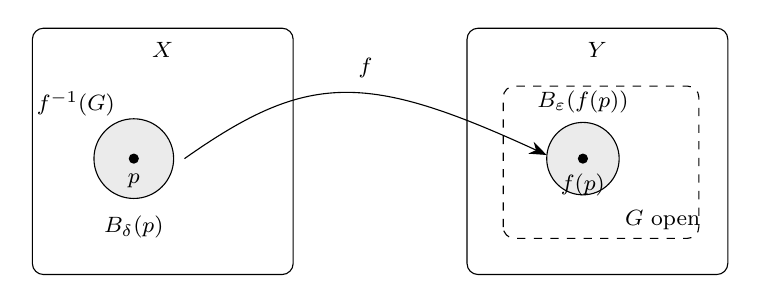
\begin{tikzpicture}[scale=0.92]
  % left: domain X with a delta-ball; right: codomain Y with eps-ball inside open G
  \draw[rounded corners] (-0.2,-1.6) rectangle (3.4,1.8);
  \node at (1.6,1.5) {\footnotesize $X$};
  \fill[band] (1.2,0.0) circle (0.55);
  \node[pt,label=below:{\footnotesize $p$}] at (1.2,0.0) {};
  \draw (1.2,0.0) circle (0.55);
  \node[font=\footnotesize] at (1.2,-0.95) {$B_\delta(p)$};
  \node[font=\footnotesize] at (0.4,0.75) {$f\inv(G)$};
  % codomain
  \begin{scope}[shift={(6.0,0)}]
    \draw[rounded corners] (-0.2,-1.6) rectangle (3.4,1.8);
    \node at (1.6,1.5) {\footnotesize $Y$};
    \draw[rounded corners,dashed] (0.3,-1.1) rectangle (3.0,1.0);
    \node[font=\footnotesize] at (2.5,-0.85) {$G$ open};
    \fill[band] (1.4,0.0) circle (0.5);
    \node[pt,label=below:{\footnotesize $f(p)$}] at (1.4,0.0) {};
    \draw (1.4,0.0) circle (0.5);
    \node[font=\footnotesize] at (1.4,0.78) {$B_\eps(f(p))$};
  \end{scope}
  \draw[-{Stealth[length=2.2mm]}] (1.9,0.0) .. controls (3.6,1.2) and (4.4,1.2) .. (6.9,0.05);
  \node[font=\footnotesize] at (4.4,1.25) {$f$};
\end{tikzpicture}
\captionof{figure}{Continuity at $p$ $=$ every output ball $B_\eps(f(p))$ has an input ball
$B_\delta(p)$ mapping into it. Globally: the pre-image of an open $G$ is open.}
\end{center}

\begin{remark}[Determined on a dense set]
If $f,g:X\to Y$ are continuous and agree on a \emph{dense} subset $E\subseteq X$, then
$f=g$ on all of $X$: for $p\in X$ take $x_n\to p$ with $x_n\in E$; then
$f(p)=\lim f(x_n)=\lim g(x_n)=g(p)$. In particular $f(E)$ is dense in $f(X)$ (Rudin 4.4
Ex.), and a continuous map is pinned down by its values on $\Q$, say.
\end{remark}

\begin{wex}{Zero sets are closed}
For continuous $f:X\to\R$, show the \emph{zero set} $Z(f)=\set{p\st f(p)=0}$ is closed, and
$\set{p\st f(p)>0}$ is open.
\wrec ``Show this level set is closed/open''; pull a closed/open set back through $f$.
\wsol $\set0$ is closed in $\R$, so $Z(f)=f\inv(\set0)$ is closed by
Theorem~\ref{t:cont-open@c5}(iii). The ray $(0,\infty)$ is open, so $f\inv((0,\infty))$ is
open. \emph{Check:} for $f(x)=x^2-1$, $Z(f)=\set{\pm1}$ (closed) and $\set{f>0}=
(-\infty,-1)\cup(1,\infty)$ (open). \checkmark
\end{wex}

\subsection*{Further worked examples}

\begin{wex}{Continuity at an isolated point}
Let $A=\set{0}\cup\set{1/n\st n\in\N}$ and let $f:A\to\R$ be \emph{any} function. At which
points of $A$ is $f$ automatically continuous, and what is the one nontrivial condition?
\wrec ``Continuity on a set with isolated points'': isolated points are free
(Theorem~\ref{t:cont-lim@c5}); only the cluster point carries a real condition.
\wsol Every point $1/n$ is isolated in $A$ (the gap to its neighbors $1/(n\pm1)$ is
positive), so $f$ is continuous at each $1/n$ no matter how it is defined. The single cluster
point is $0$ (since $1/n\to0$), and there continuity is the genuine requirement: $f$ is
continuous at $0$ iff $f(1/n)\to f(0)$, by the sequential criterion
(Theorem~\ref{t:cont-seq@c5}). \emph{Check:} if $f(1/n)=(-1)^n$ and $f(0)=0$, then $f$ is
continuous at every $1/n$ but \emph{discontinuous} at $0$, since $(-1)^n\not\to0$. \checkmark
\end{wex}

\begin{wex}{A non-example via the open-set criterion}
Use Theorem~\ref{t:cont-open@c5} to show the floor function $\lfloor x\rfloor$ is not continuous
on $\R$ by exhibiting an open set with non-open pre-image.
\wrec ``Disprove global continuity'': it suffices to find one open $G$ whose pre-image
$f\inv(G)$ is not open (the contrapositive of (i)$\eqv$(ii)).
\wsol Take the open interval $G=(-\tfrac12,\tfrac12)$. Then
$\lfloor x\rfloor\in G$ iff $\lfloor x\rfloor=0$ iff $0\le x<1$, so
$f\inv(G)=[0,1)$. This set is \emph{not} open: the point $0$ has no neighborhood contained in
$[0,1)$ (every ball around $0$ contains negative numbers, where $\lfloor x\rfloor=-1\notin
G$). Hence by Theorem~\ref{t:cont-open@c5}, $\lfloor\cdot\rfloor$ is not continuous on $\R$.
\emph{Check:} the failure point $x=0$ is exactly an integer, where $\lfloor x\rfloor$ jumps
from $-1$ to $0$ --- a jump discontinuity, consistent with the non-open pre-image.
\checkmark
\end{wex}

\begin{exers}{Exercises (Rudin, Ch.4).}
\item If $f$ is a continuous mapping of a metric space $X$ into a metric space $Y$, prove
  $f(\closure E)\subseteq\closure{f(E)}$ for every $E\subseteq X$. Show by example that
  $f(\closure E)$ can be a proper subset of $\closure{f(E)}$.
\item Let $f$ be a continuous real function on a metric space $X$. Let the \emph{zero set}
  $Z(f)=\set{p\in X\st f(p)=0}$. Prove $Z(f)$ is closed.
\item Let $f,g$ be continuous maps of a metric space $X$ into a metric space $Y$, and let
  $E$ be dense in $X$. Prove $f(E)$ is dense in $f(X)$. If $g(p)=f(p)$ for all $p\in E$,
  prove $g(p)=f(p)$ for all $p\in X$. (A continuous map is determined by its values on a
  dense subset.)
\item If $f$ is a real continuous function on a closed set $E\subseteq\R$, prove there exist
  continuous $g:\R\to\R$ with $g(x)=f(x)$ for all $x\in E$ (a \emph{continuous extension}).
  Show this becomes false if ``closed'' is omitted. (Hint: make the graph of $g$ a straight
  line on each interval of $\R\setminus E$.)
\item If $f$ is defined on $E$, the graph of $f$ is $\set{(x,f(x))\st x\in E}$. Suppose $E$
  is compact; prove $f$ is continuous on $E$ iff its graph is compact.
\item Let $E\subseteq X$ and let $f$ be defined on $X$; the \emph{restriction} of $f$ to $E$
  is $g$ with domain $E$ and $g(p)=f(p)$. Define $f,g$ on $\R^2$ by $f(0,0)=g(0,0)=0$, and
  for $(x,y)\neq(0,0)$, $f(x,y)=\dfrac{xy^2}{x^2+y^4}$, $g(x,y)=\dfrac{xy^2}{x^2+y^6}$. Prove
  $f$ is bounded on $\R^2$; that $g$ is unbounded in every neighborhood of $(0,0)$; that $f$
  is not continuous at $(0,0)$; yet the restrictions of both $f$ and $g$ to every straight
  line through $\R^2$ are continuous.
\end{exers}

\begin{exers}{Exercises (Bartle \& Sherbert, \S5.1).}
\item Prove the sequential criterion for continuity (Theorem~\ref{t:cont-seq@c5}).
\item Establish the discontinuity criterion: $f$ is discontinuous at $c$ iff some sequence
  $x_n\to c$ in the domain has $f(x_n)\not\to f(c)$.
\item Let $a<b<c$. Suppose $f$ is continuous on $[a,b]$, $g$ continuous on $[b,c]$, and
  $f(b)=g(b)$. Define $h$ on $[a,c]$ by $h=f$ on $[a,b]$ and $h=g$ on $[b,c]$. Prove $h$ is
  continuous on $[a,c]$.
\item Let $\floor x$ be the greatest-integer function. Determine the points of continuity of
  (a) $f(x)=\floor x$; (b) $g(x)=x\floor x$; (c) $h(x)=\floor{\sin x}$;
  (d) $k(x)=\floor{1/x}$ ($x\neq0$).
\item Let $f(x)=\dfrac{x^2+x-6}{x-2}$ for $x\neq2$. Can $f$ be defined at $x=2$ so as to be
  continuous there?
\item Let $A\subseteq\R$ and $f:A\to\R$ continuous at $c\in A$. Show that for any $\eps>0$
  there is a neighborhood $V_\delta(c)$ such that $x,y\in A\cap V_\delta(c)\imp
  \abs{f(x)-f(y)}<\eps$.
\item Let $f:\R\to\R$ be continuous at $c$ with $f(c)>0$. Show there is a neighborhood
  $V_\delta(c)$ on which $f(x)>0$.
\item Let $f:\R\to\R$ be continuous, $S=\set{x\st f(x)=0}$ its zero set. If $\seq{x_n}$ is in
  $S$ and $x=\lim x_n$, show $x\in S$.
\item Let $A\subseteq B\subseteq\R$, $f:B\to\R$, $g$ the restriction of $f$ to $A$. (a) If
  $f$ is continuous at $c\in A$, show $g$ is continuous at $c$. (b) Show by example that $g$
  continuous at $c$ need not make $f$ continuous at $c$.
\item Show the absolute value $f(x)=\abs x$ is continuous at every $c\in\R$.
\item Let $K>0$ and $f:\R\to\R$ satisfy $\abs{f(x)-f(y)}\le K\abs{x-y}$ for all $x,y$. Show
  $f$ is continuous at every $c\in\R$.
\item Suppose $f:\R\to\R$ is continuous and $f(r)=0$ for every rational $r$. Prove $f(x)=0$
  for all $x$.
\item Define $g:\R\to\R$ by $g(x)=2x$ for $x$ rational, $g(x)=x+3$ for $x$ irrational. Find
  all points where $g$ is continuous.
\item Let $A=(0,1)$ and $k:A\to\R$ by $k(x)=0$ for $x$ irrational, $k(x)=n$ for $x=m/n$ in
  lowest terms. Prove $k$ is unbounded on every open interval in $A$, and conclude $k$ is
  continuous at no point of $A$.
\item Let $f:(0,1)\to\R$ be bounded but with $\lim_{x\to0}f$ not existing. Show there are
  sequences $\seq{x_n},\seq{y_n}$ in $(0,1)$ with $\lim x_n=0=\lim y_n$ such that $\lim
  f(x_n)$ and $\lim f(y_n)$ exist but are unequal.
\end{exers}

\begin{exers}{Additional exercises.}
\item Prove directly from the $\eps$--$\delta$ definition that $f(x)=3x-7$ is continuous at
  every $c\in\R$, and that $g(x)=x^2$ is continuous at $c=4$.
\item Show the function $f(x)=x$ for $x\le0$, $f(x)=x+1$ for $x>0$ has a jump at $0$ and is
  continuous elsewhere; identify $f(0^-)$, $f(0^+)$, $f(0)$.
\item (Topological characterization.) For $f:\R\to\R$ continuous, prove $\set{x\st 1<f(x)<3}$
  is open and $\set{x\st f(x)\ge2}$ is closed, citing the open/closed pre-image theorem.
\item (Non-example / disprove.) Disprove: ``a continuous $f:\R\to\R$ maps open sets to open
  sets.'' Use $f(x)=x^2$ and the open set $(-1,1)$.
\item Let $f,g:\R\to\R$ be continuous and agree on $\Q$. Prove $f=g$ on $\R$. Where is
  density of $\Q$ used?
\item Show that $f(x)=x\,D(x)$, where $D$ is the Dirichlet function, is continuous only at
  $x=0$, and prove it via the discontinuity criterion.
\item (Diagram.) Illustrate the open-set definition of continuity at a point $p$: draw the
  output ball $B_\eps(f(p))$, its pre-image, and an input ball $B_\delta(p)$ contained in
  that pre-image.
\item Suppose $f:\R\to\R$ is continuous and $f(x+y)=f(x)f(y)$ for all $x,y$, with $f$ not
  identically $0$. Prove $f(x)>0$ for all $x$ and that $f$ is determined by $f(1)$.
\end{exers}


\section{Combinations of Continuous Functions}
\subsection*{Arithmetic combinations}

Continuity is preserved by all the pointwise algebra, by direct transcription of the limit
theorems.

\begin{theorem}[Algebra of continuous functions]\label{t:cont-alg@c5}
If $f,g:A\to\R$ are continuous at $c\in A$ and $k\in\R$, then $f+g$, $f-g$, $kf$, $fg$, and
$\abs f$ are continuous at $c$; and $f/g$ is continuous at $c$ provided $g(c)\neq0$.
\end{theorem}

\begin{proof}
If $c$ is isolated, all are continuous trivially (Theorem~\ref{t:cont-lim@c5}). Otherwise $c$
is a cluster point and $\lim_{x\to c}f=f(c)$, $\lim_{x\to c}g=g(c)$; apply the limit theorems
(Theorem~\ref{t:limthms@c5}), e.g.\ $\lim_{x\to c}(fg)=f(c)g(c)=(fg)(c)$. For $\abs f$ use the
reverse triangle inequality $\big|\abs{f(x)}-\abs{f(c)}\big|\le\abs{f(x)-f(c)}$. For $f/g$,
$g(c)\neq0$ keeps the denominator away from $0$ near $c$.
\end{proof}

\begin{corollary}\label{c:poly-cont@c5}
Every polynomial $p(x)=a_nx^n+\cdots+a_0$ is continuous on $\R$, and every rational function
$p/q$ is continuous at every point where $q\neq0$.
\end{corollary}

\begin{proof}
The constant maps and the identity $x\mapsto x$ are continuous (take $\delta=\eps$); close
under $+$ and $\cdot$ by Theorem~\ref{t:cont-alg@c5} to reach all polynomials, then take a
quotient.
\end{proof}

\begin{wex}{Max and min of continuous functions}
For $f,g$ continuous at $c$, show $h=\max\set{f,g}$ and $\min\set{f,g}$ are continuous at $c$.
\wrec ``Show $\max/\min$ continuous''; rewrite with $\abs{\cdot}$ to reuse the algebra.
\wsol Use $\max\set{f,g}=\tfrac12(f+g)+\tfrac12\abs{f-g}$ and $\min\set{f,g}=\tfrac12(f+g)-
\tfrac12\abs{f-g}$. Each is a sum of continuous functions (using $\abs{f-g}$ continuous), so
each is continuous at $c$. \emph{Check:} at a crossing point $f(c)=g(c)$ both formulas give
$f(c)$, with no corner-induced break --- $\abs{\cdot}$ is continuous even at its kink.
\checkmark
\end{wex}

\subsection*{Composition}

\begin{theorem}[Composition of continuous functions]\label{t:cont-comp@c5}
Let $f:A\to\R$ with $f(A)\subseteq B$, and $g:B\to\R$. If $f$ is continuous at $c\in A$ and
$g$ is continuous at $b=f(c)$, then $g\circ f$ is continuous at $c$. Hence a composition of
continuous functions is continuous.
\end{theorem}

\begin{proof}
Let $\eps>0$. By continuity of $g$ at $b$ there is $\eta>0$ with $\abs{y-b}<\eta,\ y\in
B\imp\abs{g(y)-g(b)}<\eps$. By continuity of $f$ at $c$ there is $\delta>0$ with
$\abs{x-c}<\delta,\ x\in A\imp\abs{f(x)-b}<\eta$. Chaining: $\abs{x-c}<\delta\imp
\abs{f(x)-b}<\eta\imp\abs{g(f(x))-g(b)}<\eps$.
\end{proof}

\begin{remark}[The open-set proof, in one line]
Topologically (Theorem~\ref{t:cont-open@c5}) this is immediate: $(g\circ f)\inv(G)=f\inv
(g\inv(G))$ is the pre-image of an open set under $f$ of an open set under $g$, hence open.
The $\eps$--$\delta$ version above shows the explicit $\delta$.
\end{remark}

\begin{pitfall}
Composition needs $g$ continuous \emph{at the limit value} $b=f(c)$, not merely the existence
of $\lim_{x\to c}f$. The substitution $\lim_{x\to c}g(f(x))=g\big(\lim_{x\to c}f(x)\big)$ can
\emph{fail} if $g$ is discontinuous at $b$. (B\&S 5.2.6 Ex.~5: let $f(x)=x+1$, and $g$ with
$g(1)=0$ but $g=2$ elsewhere; then $f(x)\to1$ as $x\to0$, yet $g(f(x))\to2\neq0=g(1)$.) The
inner limit existing is not enough --- the outer map must be continuous there.
\end{pitfall}

\begin{wex}{Building continuity from pieces}
Show $x\mapsto\sqrt{x^2+1}$ and $x\mapsto\dfrac{x^2+2x+1}{x^2+1}$ are continuous on $\R$.
\wrec ``Determine where continuous''; decompose into known-continuous blocks.
\wsol $x\mapsto x^2+1$ is a polynomial (continuous, and $\ge1>0$); $\sqrt{\cdot}$ is
continuous on $[0,\infty)$; the composite $\sqrt{x^2+1}$ is continuous by
Theorem~\ref{t:cont-comp@c5}. The rational function has nonvanishing denominator $x^2+1\ge1$,
so it is continuous on all of $\R$ by Corollary~\ref{c:poly-cont@c5}. \emph{Check:} both are
defined and finite for every real $x$, consistent with continuity everywhere. \checkmark
\end{wex}

\begin{wex}{Additive functions: continuity at one point $\imp$ everywhere}
A function $f:\R\to\R$ is \emph{additive} if $f(x+y)=f(x)+f(y)$ for all $x,y$. Show that if
$f$ is continuous at a single point $x_0$, it is continuous on $\R$, and in fact $f(x)=cx$
with $c=f(1)$.
\wrec ``Promote local continuity to global''; exploit the functional equation to slide the
point of continuity.
\wsol Additivity gives $f(0)=0$ and $f(x)-f(c)=f(x-c)$. Fix any $c$ and let $x\to c$; put
$h=x-c\to0$. Then $f(x)-f(c)=f(h)$, so continuity of $f$ at $c$ is equivalent to continuity
at $0$, which (by translating $x_0$) follows from continuity at $x_0$:
$f(h)=f(x_0+h)-f(x_0)\to0$ as $h\to0$. Thus $f$ is continuous everywhere. Then $f(r)=rf(1)$
for $r\in\Q$ (additivity over integer multiples and fractions), and continuity extends this
from the dense set $\Q$ to $f(x)=cx$ for all $x$. \emph{Check:} the only ``wild''
(non-linear) additive functions require a Hamel basis and are nowhere continuous --- one
point of continuity rules them out. \checkmark
\end{wex}

\subsection*{Further worked examples}

\begin{wex}{A rational function: where exactly is it continuous?}
Determine the largest set on which $r(x)=\dfrac{x^2-1}{x^2-x-6}$ is continuous.
\wrec ``Determine where continuous'': a rational function is continuous off the zero set of
its denominator (Corollary~\ref{c:poly-cont@c5}).
\wsol Factor the denominator: $x^2-x-6=(x-3)(x+2)$, which vanishes at $x=3$ and $x=-2$.
Neither cancels the numerator $x^2-1=(x-1)(x+1)$, so both are genuine poles. By
Corollary~\ref{c:poly-cont@c5}, $r$ is continuous at every point with $(x-3)(x+2)\neq0$, i.e.\
on $\R\setminus\set{-2,3}$. \emph{Check:} at $x=0$ the denominator is $-6\neq0$ and
$r(0)=\tfrac{-1}{-6}=\tfrac16$, a finite value, consistent with continuity there; near
$x=3$, $r(3.01)\approx\tfrac{8.06}{0.0501}\approx161$ blows up. \checkmark
\end{wex}

\begin{wex}{A non-example: sum of two discontinuous functions can be continuous}
Show the algebra theorem is one-directional: $f+g$ continuous does \emph{not} require $f,g$
continuous.
\wrec ``Test whether the converse holds'': hunt for a counterexample, since
Theorem~\ref{t:cont-alg@c5} only goes one way.
\wsol Let $D$ be the Dirichlet function ($D=1$ on $\Q$, $0$ off $\Q$), discontinuous
everywhere (\S5.3). Put $f=D$ and $g=1-D$; both are discontinuous at every point (the same
two-sequence argument). Yet $f+g\equiv1$ is continuous on all of $\R$. \emph{Check:} the
algebra theorem gives a sufficient condition only; cancellation of two ``bad'' functions can
restore continuity, so you may never read it backwards. \checkmark
\end{wex}

\begin{wex}{Composition order matters: $g\circ f$ vs.\ $f\circ g$}
With $f(x)=x^2$ and $g(x)=\sqrt x$ (domain $[0,\infty)$), discuss the continuity and domain
of $g\circ f$ and of $f\circ g$.
\wrec ``Continuity of a composite'': check that each inner output lands in the outer domain,
then apply Theorem~\ref{t:cont-comp@c5}.
\wsol $g\circ f(x)=\sqrt{x^2}=\abs x$: here $f$ is continuous on $\R$ and $f(x)=x^2\ge0$
always lands in the domain $[0,\infty)$ of $g$, so $g\circ f$ is continuous on all of $\R$
(it equals $\abs{\cdot}$). $f\circ g(x)=(\sqrt x)^2=x$: now $g$ has domain $[0,\infty)$, so
$f\circ g$ is only defined --- and continuous --- on $[0,\infty)$. \emph{Check:} the two
composites agree as formulas ($\abs x=x$) precisely on the common domain $[0,\infty)$, but
$g\circ f$ extends continuously to negatives while $f\circ g$ cannot. \checkmark
\end{wex}

\begin{exers}{Exercises (Bartle \& Sherbert, \S5.2).}
\item Determine the points of continuity, stating which theorems are used:
  (a) $f(x)=\dfrac{x^2+2x+1}{x^2+1}$; (b) $g(x)=\sqrt{x+\sqrt x}$ ($x\ge0$);
  (c) $h(x)=\dfrac{\sqrt{1+\abs{\sin x}}}{x}$ ($x\neq0$); (d) $k(x)=\cos\sqrt{1+x^2}$.
\item Show that if $f:A\to\R$ is continuous on $A$ and $n\in\N$, then $f^n$ (with
  $f^n(x)=(f(x))^n$) is continuous on $A$.
\item Give an example of $f,g$ both discontinuous at a point $c$ such that (a) $f+g$ is
  continuous at $c$; (b) $fg$ is continuous at $c$.
\item Let $\floor\cdot$ be the greatest-integer function. Determine the points of continuity
  of $f(x)=x-\floor x$.
\item Let $g(1)=0$, $g(x)=2$ for $x\neq1$, and $f(x)=x+1$. Show $\lim_{x\to0}g\circ f\neq(g\circ
  f)(0)$. Why does this not contradict the composition theorem?
\item Let $f,g$ on $\R$, $c\in\R$. Suppose $\lim_{x\to c}f=b$ and $g$ is continuous at $b$.
  Show $\lim_{x\to c}g\circ f=g(b)$.
\item Give an example of $f:[0,1]\to\R$ discontinuous at every point of $[0,1]$ but with
  $\abs f$ continuous on $[0,1]$.
\item Let $f,g:\R\to\R$ be continuous with $f(r)=g(r)$ for all rational $r$. Is $f(x)=g(x)$
  for all $x$?
\item Let $h:\R\to\R$ be continuous with $h(m/2^n)=0$ for all $m\in\Z$, $n\in\N$. Show
  $h(x)=0$ for all $x$.
\item Let $f:\R\to\R$ be continuous and $P=\set{x\st f(x)>0}$. If $c\in P$, show there is a
  neighborhood $V_\delta(c)\subseteq P$.
\item If $f,g$ are continuous on $\R$, let $S=\set{x\st f(x)\ge g(x)}$. If $\seq{s_n}\subseteq
  S$ and $\lim s_n=s$, show $s\in S$.
\item A function $f:\R\to\R$ is \emph{additive} if $f(x+y)=f(x)+f(y)$ for all $x,y$. Prove
  that if $f$ is continuous at some point $x_0$, it is continuous at every point of $\R$.
\item Suppose $f$ is a continuous additive function on $\R$. If $c=f(1)$, show $f(x)=cx$ for
  all $x$. (Hint: first show $f(r)=cr$ for rational $r$.)
\item Let $g:\R\to\R$ satisfy $g(x+y)=g(x)g(y)$ for all $x,y$. Show that if $g$ is continuous
  at $0$, it is continuous everywhere; and if $g(a)=0$ for some $a$, then $g\equiv0$.
\item Let $f,g:\R\to\R$ be continuous at $c$ and $h(x)=\sup\set{f(x),g(x)}$. Show
  $h(x)=\tfrac12(f(x)+g(x))+\tfrac12\abs{f(x)-g(x)}$, and use this to show $h$ is continuous
  at $c$.
\end{exers}

\begin{exers}{Additional exercises.}
\item Determine all points of continuity of $f(x)=\dfrac{\sin x}{x}$ (with $f(0)=1$) and of
  $g(x)=\dfrac{1}{x^2-x-2}$, citing the relevant theorems.
\item Prove that if $f$ is continuous at $c$ then so is $f^2$; show the converse fails by an
  example where $f^2$ is continuous but $f$ is not.
\item (Min/max.) Show $\min\set{f,g}$ and $\max\set{f,g}$ are continuous whenever $f,g$ are,
  using the absolute-value identity, and sketch the graphs for $f(x)=x$, $g(x)=1-x$.
\item Let $f,g$ be continuous on $\R$. Prove $\set{x\st f(x)=g(x)}$ is closed and $\set{x\st
  f(x)\neq g(x)}$ is open.
\item (Non-example / disprove.) Find $f,g$ each discontinuous at $0$ with $f+g$ continuous at
  $0$; then find $f,g$ each discontinuous at $0$ with $fg$ continuous at $0$.
\item (Composition trap.) Give explicit $f$ continuous at $c$ and $g$ discontinuous at
  $b=f(c)$ such that $g\circ f$ is discontinuous at $c$, and explain why
  Theorem~\ref{t:cont-comp@c5} does not apply.
\item (Diagram.) For $f(x)=x$ and $g(x)=1-x$ on $[0,1]$, draw $\max\set{f,g}$ as the upper
  envelope, marking the corner at $x=\tfrac12$ where the two graphs cross, and confirm
  continuity there.
\item Prove that a continuous additive function $f:\R\to\R$ is linear, $f(x)=f(1)\,x$, filling
  in the step from $\Q$ to $\R$ by continuity.
\end{exers}


\section{Continuity and Compactness; the Extreme Value Theorem}
\subsection*{The continuous image of a compact set is compact}

Recall (Chapter~3) that a set $K$ in a metric space is \emph{compact} iff every open cover
has a finite subcover, equivalently (Heine--Borel, in $\R^k$) iff $K$ is closed and bounded,
equivalently (sequential compactness) iff every sequence in $K$ has a subsequence converging
to a point of $K$. Continuity propagates compactness forward.

\begin{theorem}[Continuous image of compact is compact]\label{t:cont-compact@c5}
Let $f:X\to Y$ be continuous and $K\subseteq X$ compact. Then $f(K)$ is compact.
\end{theorem}

\begin{proof}[Proof via open covers (Rudin)]
Let $\set{G_\alpha}$ be an open cover of $f(K)$ in $Y$. Each $f\inv(G_\alpha)$ is open in
$X$ (Theorem~\ref{t:cont-open@c5}) and these cover $K$, since every $p\in K$ has $f(p)$ in some
$G_\alpha$. By compactness of $K$ finitely many
$f\inv(G_{\alpha_1}),\dots,f\inv(G_{\alpha_n})$ cover $K$; then
$G_{\alpha_1},\dots,G_{\alpha_n}$ cover $f(K)$. So $f(K)$ is compact.
\end{proof}

\begin{proof}[Proof via sequences (B\&S)]
Let $\seq{y_n}$ be a sequence in $f(K)$, say $y_n=f(x_n)$ with $x_n\in K$. By sequential
compactness a subsequence $x_{n_k}\to x\in K$; by continuity $y_{n_k}=f(x_{n_k})\to f(x)\in
f(K)$. Every sequence in $f(K)$ has a subsequence converging in $f(K)$, so $f(K)$ is compact.
\end{proof}

\begin{corollary}[Boundedness theorem]\label{c:bdd@c5}
If $f:K\to\R$ is continuous on a compact set $K$, then $f$ is bounded: $f(K)$ is a bounded
subset of $\R$ (indeed closed and bounded).
\end{corollary}

\begin{proof}
$f(K)$ is compact in $\R$, hence closed and bounded by Heine--Borel.
\end{proof}

\subsection*{The Extreme Value Theorem}

\begin{theorem}[Extreme Value Theorem]\label{t:evt@c5}
If $K$ is compact and $f:K\to\R$ is continuous, then $f$ \emph{attains} a maximum and a
minimum: there exist $p,q\in K$ with
\[
  f(p)=\sup_{x\in K}f(x)=\max f(K),\qquad f(q)=\inf_{x\in K}f(x)=\min f(K).
\]
In particular this holds for continuous $f$ on a closed bounded interval $[a,b]$.
\end{theorem}

\begin{proof}
$M=\sup f(K)$ is finite (Corollary~\ref{c:bdd@c5}). Since $f(K)$ is closed
(Theorem~\ref{t:cont-compact@c5}) and $M$ is a limit point of $f(K)$ (being its sup), $M\in
f(K)$; so $M=f(p)$ for some $p\in K$. Likewise $m=\inf f(K)=f(q)$. (Sequential phrasing:
choose $x_n\in K$ with $f(x_n)\to M$; a subsequence $x_{n_k}\to p\in K$ gives $f(p)=\lim
f(x_{n_k})=M$.)
\end{proof}

\begin{center}
\begin{tikzpicture}
  \begin{axis}[
    width=11cm,height=5.6cm,
    axis lines=middle,xlabel=$x$,ylabel=$y$,
    xmin=-0.3,xmax=5.3,ymin=-0.5,ymax=3.4,
    xtick={0.5,4.5},xticklabels={$a$,$b$},
    ytick=\empty,samples=200,clip=false,
  ]
    % a continuous curve on [a,b] with interior max and endpoint-ish min
    \addplot[curve,domain=0.5:4.5]{1.4 + 1.3*sin(deg(1.1*(x-0.5))) - 0.05*(x-2.5)^2};
    % mark max p and min q
    \draw[densely dashed] (axis cs:0.5,3.05)--(axis cs:5.3,3.05);
    \node[right,font=\footnotesize] at (axis cs:5.3,3.05){$M=\max f$};
    \draw[densely dashed] (axis cs:0.5,0.18)--(axis cs:5.3,0.18);
    \node[right,font=\footnotesize] at (axis cs:5.3,0.18){$m=\min f$};
  \end{axis}
\end{tikzpicture}
\captionof{figure}{EVT: a continuous $f$ on $[a,b]$ \emph{achieves} its sup and inf at actual
points $p,q\in[a,b]$ --- the dashed levels are touched, not merely approached.}
\end{center}

\begin{pitfall}
Every hypothesis is needed. Drop compactness and EVT fails: $f(x)=x$ on the \emph{open}
$(0,1)$ has $\sup=1$, $\inf=0$, neither attained; $f(x)=1/x$ on $(0,1]$ is unbounded above.
Drop continuity and it fails: $f(x)=x$ on $[0,1)$ with $f$ redefined cannot reach its sup.
``$\sup$'' is a least upper bound, possibly outside the set; ``$\max$'' is an attained value
--- EVT is exactly the statement that for continuous $f$ on compact $K$ they coincide.
\end{pitfall}

\subsection*{Continuous inverse on a compact domain}

A continuous bijection need not have a continuous inverse in general --- but compactness of
the domain fixes this.

\begin{theorem}[Continuous inverse]\label{t:cont-inv@c5}
Let $K$ be compact and $f:K\to Y$ a continuous \emph{bijection} onto $f(K)$. Then the
inverse $f\inv:f(K)\to K$ is continuous. (Such an $f$ is a \emph{homeomorphism}.)
\end{theorem}

\begin{proof}
By the closed-set criterion (Theorem~\ref{t:cont-open@c5}(iii)) applied to $g=f\inv$, it
suffices to show $g\inv(C)=f(C)$ is closed in $f(K)$ for every closed $C\subseteq K$. But a
closed subset $C$ of the compact $K$ is compact, so $f(C)$ is compact
(Theorem~\ref{t:cont-compact@c5}), hence closed. Therefore $f\inv$ is continuous.
\end{proof}

\begin{wex}{Why compactness is essential for the inverse}
Exhibit a continuous bijection with discontinuous inverse.
\wrec ``Show the compactness hypothesis cannot be dropped''; a wrap-around onto a circle is
the canonical example (Rudin 4.21).
\wsol Let $X=[0,2\pi)$ (not compact) and $f(t)=(\cos t,\sin t)$ onto the unit circle. $f$ is
a continuous bijection, but $f\inv$ is discontinuous at $(1,0)$: points just \emph{below} the
seam map to $t$ near $2\pi$, points at the seam map to $t=0$, so $f\inv$ jumps by nearly
$2\pi$. \emph{Check:} the domain misses its endpoint $2\pi$, so it is not closed, hence not
compact --- exactly the gap Theorem~\ref{t:cont-inv@c5} forbids. \checkmark
\end{wex}

\begin{wex}{$n$-th roots are continuous}
Show $x\mapsto x^{1/n}$ is continuous on $[0,\infty)$ for each $n\in\N$.
\wrec ``Show a root function continuous''; use the continuous-inverse theorem on compacta.
\wsol $\phi(x)=x^n$ is a continuous strictly increasing bijection of $[0,b]$ onto $[0,b^n]$
for each $b>0$; $[0,b]$ is compact, so $\phi\inv(y)=y^{1/n}$ is continuous on $[0,b^n]$ by
Theorem~\ref{t:cont-inv@c5}. As $b$ is arbitrary, $y^{1/n}$ is continuous on $[0,\infty)$.
\emph{Check:} agrees with the direct estimate for $\sqrt{\cdot}$ in \S5.3, now for every $n$.
\checkmark
\end{wex}

\subsection*{Further worked examples}

\begin{wex}{EVT in action: locating the extrema of a concrete function}
Find the maximum and minimum of $f(x)=x^3-3x$ on $[0,2]$, and confirm both are attained.
\wrec ``Continuous $f$ on a compact interval'': EVT (Theorem~\ref{t:evt@c5}) guarantees the
extrema exist and are attained; locate them among endpoints and interior critical points.
\wsol $f$ is a polynomial, hence continuous, and $[0,2]$ is compact, so EVT applies. The
candidates are the endpoints $x=0,2$ and the interior points where the difference quotient
flattens, i.e.\ where $3x^2-3=0$, giving $x=1$ (the root $x=-1$ is outside $[0,2]$). Evaluate:
$f(0)=0$, $f(1)=1-3=-2$, $f(2)=8-6=2$. So $\min f=-2$ attained at $p=1$ and $\max f=2$
attained at $q=2$. \emph{Check:} both values are achieved at genuine points of $[0,2]$, as
EVT promises; the sup $2$ is a max, not merely a least upper bound. \checkmark
\end{wex}

\begin{wex}{A non-example: continuity alone (no compactness) loses the max}
Show $f(x)=\dfrac{x}{1+x}$ on $[0,\infty)$ is continuous and bounded but attains no maximum.
\wrec ``Does EVT-style attainment hold here?'': the domain is closed but \emph{unbounded},
hence not compact, so attainment is not guaranteed.
\wsol $f$ is a quotient with nonvanishing denominator $1+x\ge1$, so it is continuous on
$[0,\infty)$. Since $f(x)=1-\tfrac1{1+x}$, we have $0\le f(x)<1$ and $f(x)\to1$ as
$x\to\infty$, so $\sup_{x\ge0}f=1$. But $f(x)=1$ would force $\tfrac1{1+x}=0$, impossible;
the supremum is never attained. \emph{Check:} every hypothesis of EVT but compactness holds,
and the conclusion fails --- the missing ``endpoint at infinity'' is exactly where the sup
lives. \checkmark
\end{wex}

\begin{wex}{Closed but not bounded, and bounded but not closed}
Give two continuous functions, one on a closed unbounded set and one on a bounded non-closed
set, each failing to attain an extremum, isolating which half of Heine--Borel fails.
\wrec ``Pin the blame on closedness vs.\ boundedness'': drop one Heine--Borel condition at a
time and watch attainment break.
\wsol (i) On the closed unbounded $K_1=[1,\infty)$, $f(x)=-1/x$ is continuous with
$\sup f=0$ approached as $x\to\infty$ but never reached; $K_1$ is closed but not bounded.
(ii) On the bounded non-closed $K_2=(0,1]$, $g(x)=x$ has $\inf g=0$ approached as $x\to0^+$
but $0\notin K_2$, so the inf is not attained; $K_2$ is bounded but not closed. \emph{Check:}
each example violates exactly one clause of Heine--Borel (closed \emph{and} bounded), and in
each case attainment fails --- both clauses are essential to compactness. \checkmark
\end{wex}

\begin{wex}{Continuity is essential too: a bounded discontinuous map with no max}
On the compact $[0,1]$ exhibit a bounded function attaining no maximum, showing EVT needs
continuity not just compact domain.
\wrec ``Which hypothesis fails now?'': keep $K=[0,1]$ compact but break continuity, and
attainment can vanish.
\wsol Define $f(x)=x$ for $0\le x<1$ and $f(1)=0$. Then $f$ is bounded with
$\sup_{[0,1]}f=1$ (approached as $x\to1^-$), but $f$ never equals $1$: the only candidate
$x=1$ has been redefined to $0$. The single discontinuity at $x=1$ destroys attainment.
\emph{Check:} the domain is compact yet the conclusion fails, so EVT truly requires
continuity; reinstating $f(1)=1$ (continuity) restores the attained maximum. \checkmark
\end{wex}

\begin{center}
\begin{tikzpicture}
  \begin{axis}[
    width=11cm,height=5.0cm,
    axis lines=middle,xlabel=$x$,ylabel=$y$,
    xmin=-0.3,xmax=8.4,ymin=-0.2,ymax=1.35,
    xtick={0},xticklabels={$0$},ytick={1},samples=200,clip=false,
  ]
    \addplot[curve,domain=0:8]{x/(1+x)};
    \draw[densely dashed] (axis cs:-0.3,1)--(axis cs:8.4,1);
    \node[right,font=\footnotesize] at (axis cs:8.4,1){$\sup f=1$ (not attained)};
  \end{axis}
\end{tikzpicture}
\captionof{figure}{Without compactness EVT fails: $f(x)=x/(1+x)$ on $[0,\infty)$ is continuous
and bounded, climbing toward the dashed level $1$ but never reaching it --- the
``maximizing point'' has escaped to infinity.}
\end{center}

\begin{exers}{Exercises (Rudin, Ch.4).}
\item Let $I=[0,1]$ be the closed unit interval and $f:I\to I$ continuous. Prove $f(x)=x$
  for at least one $x\in I$ (a fixed point).
\item Call a map $f:\R\to\R$ \emph{open} if $f(V)$ is open whenever $V$ is open. Prove every
  continuous open map $f:\R\to\R$ is monotonic.
\item If $E$ is a nonempty subset of a metric space $X$, define the distance from $x\in X$
  to $E$ by $\rho_E(x)=\inf_{z\in E}d(x,z)$. (a) Prove $\rho_E(x)=0$ iff $x\in\closure E$.
  (b) Prove $\rho_E$ is uniformly continuous on $X$, by showing
  $\abs{\rho_E(x)-\rho_E(y)}\le d(x,y)$ for all $x,y\in X$.
\item Suppose $K$ and $F$ are disjoint sets in a metric space $X$, $K$ compact, $F$ closed.
  Prove there exists $\delta>0$ such that $d(p,q)>\delta$ whenever $p\in K$, $q\in F$. (Hint:
  $\rho_F$ is a continuous positive function on $K$.) Show the conclusion may fail for two
  disjoint \emph{closed} sets if neither is compact.
\item Let $A,B$ be disjoint nonempty closed sets in a metric space $X$, and define
  $f(p)=\dfrac{\rho_A(p)}{\rho_A(p)+\rho_B(p)}$ for $p\in X$. Show $f$ is continuous, its
  range lies in $[0,1]$, $f(p)=0$ exactly on $A$ and $f(p)=1$ exactly on $B$. (Thus every
  closed $A\subseteq X$ is $Z(f)$ for some continuous $f$.) Setting $V=f\inv\!\big([0,\tfrac12)\big)$
  and $W=f\inv\!\big((\tfrac12,1]\big)$, show $V,W$ are disjoint open sets with $A\subseteq
  V$, $B\subseteq W$ (\emph{normality} of metric spaces).
\item For $A\subseteq\R^n$, $B\subseteq\R^k$, let $A+B=\set{x+y\st x\in A,\ y\in B}$.
  (a) If $K$ is compact and $C$ is closed in $\R^k$, prove $K+C$ is closed. (Hint: take
  $z\notin K+C$, put $F=z-C$; then $K,F$ are disjoint, choose $\delta$ as in the
  compact/closed separation; show the open ball of radius $\delta$ about $z$ misses $K+C$.)
  (b) Let $\alpha$ be irrational, $C_1=\Z$, $C_2=\set{n\alpha\st n\in\Z}$. Show $C_1,C_2$ are
  closed in $\R$ but $C_1+C_2$ is a countable dense subset of $\R$, hence not closed.
\end{exers}

\begin{exers}{Exercises (Bartle \& Sherbert, \S5.3 --- boundedness and maxima).}
\item Let $I=[a,b]$ and $f:I\to\R$ continuous with $f(x)>0$ for each $x\in I$. Prove there
  exists $\alpha>0$ with $f(x)\ge\alpha$ for all $x\in I$.
\item Let $I=[a,b]$ and $f,g:I\to\R$ continuous. Show $E=\set{x\in I\st f(x)=g(x)}$ has the
  property: if $\seq{x_n}\subseteq E$ and $x_n\to x_0$, then $x_0\in E$.
\item Let $I=[a,b]$ and $f:I\to\R$ continuous such that for each $x\in I$ there is $y\in I$
  with $\abs{f(y)}\le\tfrac12\abs{f(x)}$. Prove there is $c\in I$ with $f(c)=0$.
\item Let $I=[0,\pi/2]$ and $f:I\to\R$, $f(x)=\sup\set{x^2,\cos x}$. Show there is an
  absolute minimum point $x_0\in I$ for $f$, and that $x_0$ solves $\cos x=x^2$.
\item Suppose $f:\R\to\R$ is continuous with $\lim_{x\to\infty}f=0$ and $\lim_{x\to-\infty}f=0$.
  Prove $f$ is bounded on $\R$ and attains either a maximum or a minimum. Give an example
  where both are not attained.
\item Let $f:\R\to\R$ be continuous, $b\in\R$. Show that if $x_0$ has $f(x_0)<b$, then there
  is a $\delta$-neighborhood $U$ of $x_0$ with $f(x)<b$ for all $x\in U$.
\item Examine which open (resp.\ closed) intervals are mapped by $f(x)=x^2$ onto open (resp.\
  closed) intervals.
\item Examine the mapping of open (resp.\ closed) intervals under $g(x)=1/(x^2+1)$ and
  $h(x)=x^3$.
\item Let $I=[a,b]$ and $f:I\to\R$ a (not necessarily continuous) function such that for
  every $x\in I$, $f$ is bounded on some neighborhood $V_{\delta_x}(x)$. Prove $f$ is bounded
  on $I$.
\item Let $J=(a,b)$ and $g:J\to\R$ continuous such that for every $x\in J$, $g$ is bounded on
  some neighborhood $V_{\delta_x}(x)$. Show by example that $g$ need not be bounded on $J$.
\end{exers}

\begin{exers}{Additional exercises.}
\item Prove that a continuous $f:[a,b]\to\R$ is bounded, directly from the open-cover
  definition of compactness (no sequences).
\item Show $f(x)=x^3-3x$ attains a maximum and a minimum on $[-2,2]$, and find them.
\item (Non-example / disprove.) Disprove ``a continuous function on a bounded interval
  attains its supremum'' by exhibiting a continuous $f$ on the bounded $(0,1)$ with $\sup f$
  not attained, and identify exactly which EVT hypothesis fails.
\item Let $f:[0,1]\to\R$ be continuous with $f([0,1])\subseteq[0,1]$. Use EVT and IVT to show
  $f$ has a fixed point, and contrast which theorem supplies which part.
\item Let $K\subseteq\R$ be compact and $f:K\to\R$ continuous and injective. Prove $f$ is
  strictly monotone on $K$ if $K$ is an interval, and that $f\inv$ is continuous in any case.
\item Prove that a continuous bijection $f:[0,1]\to[0,1]$ has a continuous inverse, but that
  this fails for a continuous bijection $[0,1)\to S^1$ (the unit circle).
\item (Diagram.) Sketch a continuous $f$ on $[a,b]$ with an interior maximum and a boundary
  minimum, drawing the horizontal lines $y=\max f$ and $y=\min f$ tangent to the graph at the
  attaining points $p,q$.
\item Show that the image $f([a,b])$ of a continuous $f$ is a closed bounded interval
  $[m,M]$, and that $m=\min f$, $M=\max f$. (Combine compactness with connectedness.)
\end{exers}


\section{Continuity and Connectedness; the Intermediate Value Theorem}
\subsection*{Connectedness and the continuous image}

Recall that a metric space $E$ is \emph{connected} if it cannot be split as $E=A\cup B$ with
$A,B$ nonempty, disjoint, and \emph{separated} (neither meeting the other's closure). In
$\R$ the connected sets are exactly the \emph{intervals} (including rays and $\R$ itself):
$E\subseteq\R$ is connected iff $x,y\in E$ and $x<z<y$ imply $z\in E$.

\begin{theorem}[Continuous image of connected is connected]\label{t:cont-conn@c5}
If $f:X\to Y$ is continuous and $E\subseteq X$ is connected, then $f(E)$ is connected.
\end{theorem}

\begin{proof}
Suppose not: $f(E)=A\cup B$ with $A,B$ nonempty separated sets in $Y$. Put
$G=E\cap f\inv(A)$ and $H=E\cap f\inv(B)$; these are nonempty, cover $E$, and are disjoint.
One checks they are separated: if $p\in G$ were a limit of points of $H$, continuity would
force $f(p)\in A$ to be a limit of points of $B$, contradicting separation of $A,B$
(using $f(\closure G)\subseteq\closure{f(G)}$, Theorem~\ref{t:cont-open@c5}(iv)). So $E=G\cup
H$ is a separation of $E$ --- contradicting connectedness. Hence $f(E)$ is connected.
\end{proof}

\subsection*{The Intermediate Value Theorem}

Specializing the codomain to $\R$, ``connected image'' becomes ``no values are skipped''.

\begin{theorem}[Intermediate Value Theorem; Bolzano]\label{t:ivt@c5}
Let $f:[a,b]\to\R$ be continuous, and let $y$ lie between $f(a)$ and $f(b)$ (i.e.\
$f(a)<y<f(b)$ or $f(b)<y<f(a)$). Then there is $c\in(a,b)$ with $f(c)=y$. Equivalently, a
continuous $f$ maps an interval onto an interval.
\end{theorem}

\begin{proof}[Topological proof]
$[a,b]$ is connected, so $f([a,b])$ is connected (Theorem~\ref{t:cont-conn@c5}), hence an
interval; it contains $f(a)$ and $f(b)$, so it contains every $y$ between them. Thus
$y=f(c)$ for some $c\in[a,b]$, and $c\neq a,b$ since $y\neq f(a),f(b)$.
\end{proof}

\begin{proof}[Bisection / sup proof (B\&S, constructive)]
Take the case $f(a)<y<f(b)$; replacing $f$ by $f-y$ assume $y=0$, so $f(a)<0<f(b)$. Let
$W=\set{x\in[a,b]\st f(x)<0}$; it is nonempty ($a\in W$) and bounded, so $w=\sup W$ exists in
$[a,b]$. We claim $f(w)=0$. If $f(w)<0$ then by continuity $f<0$ on a neighborhood of $w$, so
points $>w$ lie in $W$, contradicting $w=\sup W$. If $f(w)>0$ then $f>0$ on a neighborhood of
$w$, so $w$ is not a limit of $W$, again a contradiction. Hence $f(w)=0$, with $w\in(a,b)$.
\end{proof}

\begin{center}
\begin{tikzpicture}
  \begin{axis}[
    width=11cm,height=5.6cm,
    axis lines=middle,xlabel=$x$,ylabel=$y$,
    xmin=-0.3,xmax=5.3,ymin=-1.6,ymax=2.6,
    xtick={0.5,4.5},xticklabels={$a$,$b$},
    ytick=\empty,samples=200,clip=false,
  ]
    \addplot[curve,domain=0.5:4.5]{-1.0 + 0.9*(x-0.5) - 0.07*(x-0.5)^2 - 0.6*sin(deg(1.4*(x-0.5)))};
    % horizontal level y
    \draw[densely dashed] (axis cs:-0.3,0.6)--(axis cs:5.3,0.6);
    \node[left,font=\footnotesize] at (axis cs:-0.3,0.6){$y$};
    % mark f(a), f(b)
    \node[pt] at (axis cs:0.5,-1.0){};
    \node[below right,font=\footnotesize] at (axis cs:0.5,-1.0){$f(a)$};
    \node[pt] at (axis cs:4.5,1.9){};
    \node[above left,font=\footnotesize] at (axis cs:4.5,1.9){$f(b)$};
  \end{axis}
\end{tikzpicture}
\captionof{figure}{IVT: a continuous graph joining $f(a)$ below the level $y$ to $f(b)$ above it
must cross $y$ --- it cannot ``teleport'' over the dashed line.}
\end{center}

\begin{corollary}[Bolzano root theorem]\label{c:bolzano@c5}
If $f:[a,b]\to\R$ is continuous with $f(a)f(b)<0$ (a sign change), then $f$ has a root in
$(a,b)$.
\end{corollary}

\begin{corollary}[Odd-degree polynomials have a real root]\label{c:odd-deg@c5}
Every real polynomial of odd degree has at least one real root.
\end{corollary}

\begin{proof}
Write $p(x)=a_nx^n(1+o(1))$ with $n$ odd, $a_n\neq0$. As $x\to+\infty$ and $x\to-\infty$,
$p$ takes values of opposite sign (odd power), so $p(a)<0<p(b)$ for suitable $a<b$; apply
Bolzano.
\end{proof}

\begin{wex}{Solving $x=\cos x$ and a fixed point on $[0,1]$}
Show $x=\cos x$ has a solution in $[0,\pi/2]$, and any continuous $f:[0,1]\to[0,1]$ has a
fixed point.
\wrec ``Show an equation has a solution''; build $g$ whose root is the solution and apply
IVT/Bolzano.
\wsol Let $g(x)=x-\cos x$ on $[0,\pi/2]$; $g(0)=-1<0$ and $g(\pi/2)=\pi/2>0$, so by Bolzano
$g(c)=0$, i.e.\ $c=\cos c$. For the fixed point, let $h(x)=f(x)-x$ on $[0,1]$; $h(0)=f(0)\ge0$
and $h(1)=f(1)-1\le0$, so by IVT $h(c)=0$, i.e.\ $f(c)=c$. \emph{Check:} numerically
$c\approx0.739$ solves $x=\cos x$; the fixed-point claim is the $1$-D Brouwer theorem.
\checkmark
\end{wex}

\begin{wex}{Equal antipodal temperatures}
A continuous $f:[0,1]\to\R$ with $f(0)=f(1)$ has a point $c\in[0,\tfrac12]$ with
$f(c)=f(c+\tfrac12)$.
\wrec ``Two points half a period apart share a value''; difference function plus IVT.
\wsol Let $g(x)=f(x)-f(x+\tfrac12)$ on $[0,\tfrac12]$. Then
$g(0)+g(\tfrac12)=\big(f(0)-f(\tfrac12)\big)+\big(f(\tfrac12)-f(1)\big)=f(0)-f(1)=0$, so
$g(0)$ and $g(\tfrac12)$ have opposite signs (or one is $0$); by IVT $g(c)=0$ for some
$c\in[0,\tfrac12]$. \emph{Check:} interpreting $f$ as temperature along the equator (with
$f(0)=f(1)$ the wrap-around), there are always antipodal points at equal temperature.
\checkmark
\end{wex}

\begin{pitfall}
IVT gives \emph{existence}, not uniqueness or a formula --- and it needs genuine continuity
on a genuine interval. On $[-1,1]\setminus\set0$ the function $\operatorname{sgn}$ never
takes the value $0$ despite $\operatorname{sgn}(-1)=-1$, $\operatorname{sgn}(1)=1$: the
domain is disconnected. Also, a function can have the \emph{intermediate value property}
without being continuous (e.g.\ $\sin(1/x)$ extended by $0$ at $0$ hits every value in
$[-1,1]$ on any interval around $0$ but is discontinuous there).
\end{pitfall}

\subsection*{Further worked examples}

\begin{wex}{Bracketing a root and the bisection estimate}
Show $p(x)=x^3-x-1$ has a root in $(1,2)$, and bound how many bisections place the root
within $10^{-2}$.
\wrec ``Show a root exists, then estimate it'': Bolzano (Corollary~\ref{c:bolzano@c5}) for
existence, halving the bracket for the error bound.
\wsol $p$ is continuous (a polynomial). $p(1)=1-1-1=-1<0$ and $p(2)=8-2-1=5>0$, so
$p(1)p(2)<0$ and by Bolzano there is a root $c\in(1,2)$. Bisection halves the bracket length
$2-1=1$ each step, so after $n$ steps the root is localized to an interval of length $2^{-n}$.
We need $2^{-n}<10^{-2}$, i.e.\ $2^n>100$, i.e.\ $n\ge7$ (since $2^7=128$). \emph{Check:} the
true root is $c\approx1.3247$; $p(1.3247)\approx-0.0001$, consistent with a root just above
$1.32$, comfortably inside the $7$-step bracket. \checkmark
\end{wex}

\begin{wex}{A non-example: IVT fails on a disconnected domain}
Let $f(x)=1/x$ on $A=[-1,0)\cup(0,1]$. Although $f(-1)=-1$ and $f(1)=1$, show $f$ skips the
value $0$, and explain why IVT is not violated.
\wrec ``Does a continuous map hit every intermediate value?'': IVT needs a genuine interval;
test whether the domain is connected.
\wsol $f$ is continuous on $A$ (a rational function off its pole at $0$). On $(0,1]$ we have
$f(x)=1/x\ge1$, and on $[-1,0)$ we have $f(x)=1/x\le-1$, so $f$ never takes any value in
$(-1,1)$, in particular not $0$ --- even though $0$ lies between $f(-1)=-1$ and $f(1)=1$.
There is no contradiction: $A$ is \emph{disconnected} (the puncture at $0$ splits it), so it
is not an interval and Theorem~\ref{t:ivt@c5} does not apply. \emph{Check:} the image
$f(A)=(-\infty,-1]\cup[1,\infty)$ is itself disconnected, exactly as
Theorem~\ref{t:cont-conn@c5} permits for a disconnected domain. \checkmark
\end{wex}

\begin{wex}{Surjectivity onto $\R$ via IVT}
Show every continuous $f:\R\to\R$ with $\lim_{x\to-\infty}f=-\infty$ and
$\lim_{x\to+\infty}f=+\infty$ is onto $\R$.
\wrec ``Show the range is all of $\R$'': use the limits to straddle any target value, then
IVT to hit it.
\wsol Fix any $y\in\R$. Since $f\to-\infty$ at $-\infty$, choose $a$ with $f(a)<y$; since
$f\to+\infty$ at $+\infty$, choose $b>a$ with $f(b)>y$. On the interval $[a,b]$, $f$ is
continuous and $f(a)<y<f(b)$, so by IVT (Theorem~\ref{t:ivt@c5}) there is $c\in(a,b)$ with
$f(c)=y$. As $y$ was arbitrary, $f(\R)=\R$. \emph{Check:} the odd-degree polynomial
$f(x)=x^3-x$ meets the hypotheses (its end behavior is $\pm\infty$), and indeed it is onto
$\R$ --- a quantitative companion to Corollary~\ref{c:odd-deg@c5}. \checkmark
\end{wex}

\begin{exers}{Exercises (Bartle \& Sherbert, \S5.3 --- roots, IVT, bisection).}
\item Show every polynomial of odd degree with real coefficients has at least one real root.
\item Show $p(x)=x^4+7x^3-9$ has at least two real roots. (Locate them to two decimals with a
  calculator.)
\item Let $f$ be continuous on $[0,1]$ with $f(0)=f(1)$. Prove there is $c\in[0,\tfrac12]$
  with $f(c)=f(c+\tfrac12)$. (Hint: $g(x)=f(x)-f(x+\tfrac12)$.) Conclude there are always
  antipodal points on the earth's equator with the same temperature.
\item Show $x=\cos x$ has a solution in $[0,\pi/2]$. Use the Bisection Method and a calculator
  to approximate it with error $<10^{-3}$.
\item Show $f(x)=2\ln x+\sqrt x-2$ has a root in $[1,2]$. Use the Bisection Method to find it
  with error $<10^{-2}$.
\item (a) The function $f(x)=(x-1)(x-2)(x-3)(x-4)(x-5)$ has five roots in $[0,7]$. If the
  Bisection Method is applied on $[0,7]$, which root is located? (b) Same question for
  $g(x)=(x-2)(x-3)(x-4)(x-5)(x-6)$ on $[0,7]$.
\item If the Bisection Method is used on an interval of length $1$ to find $p_n$ with error
  $\abs{p_n-c}<10^{-5}$, determine the least $n$ assuring this accuracy.
\item Let $I=[a,b]$, $f:I\to\R$ continuous with $f(a)<0<f(b)$. Let $W=\set{x\in I\st f(x)<0}$
  and $w=\sup W$. Prove $f(w)=0$ (an alternative proof of IVT).
\item If $f:[0,1]\to\R$ is continuous and takes only rational (resp.\ only irrational) values,
  must $f$ be constant? Prove your assertion.
\end{exers}

\begin{exers}{Additional exercises.}
\item Use the IVT to show $x^5-3x+1=0$ has a root in $(0,1)$ and another in $(1,2)$.
\item Prove every continuous $f:[0,1]\to[0,1]$ has a fixed point, and show by example that
  continuity is essential (a discontinuous self-map of $[0,1]$ with no fixed point).
\item (Non-example / disprove.) Disprove ``if $f$ has the intermediate value property then
  $f$ is continuous'' by analyzing $f(x)=\sin(1/x)$ for $x\neq0$, $f(0)=0$.
\item Show that a continuous $f:[a,b]\to\R$ taking only integer values is constant. Which
  property of $[a,b]$ is doing the work?
\item Let $f:[0,1]\to\R$ be continuous with $f(0)<0<f(1)$. Describe the bisection algorithm
  and prove the produced sequence converges to a root, with error halving each step.
\item Prove that the continuous image of an interval is an interval, and deduce that
  $f(x)=x^2$ maps $(-1,2)$ onto $[0,4)$ --- not an open interval. Explain.
\item (Diagram.) Draw a continuous graph from $(a,f(a))$ below a level $y=k$ to $(b,f(b))$
  above it, mark a crossing point $c$ with $f(c)=k$, and shade the horizontal strip the graph
  must pass through.
\item Prove the Bolzano sign-change theorem from the connectedness of $[a,b]$: if $f$ is
  continuous and $f(a)f(b)<0$, then $0\in f([a,b])$.
\end{exers}


\section{Uniform Continuity and Gauges}
\subsection*{Uniform continuity}

Ordinary continuity allows $\delta$ to depend on the point $c$ as well as on $\eps$.
\emph{Uniform} continuity demands a single $\delta$ that works \emph{simultaneously} for all
points --- the quantifier on the point moves \emph{inside} the choice of $\delta$.

\begin{definition}\label{d:unifcont@c5}
$f:A\to\R$ is \emph{uniformly continuous on $A$} if
\[
  \forall\eps>0\ \ \exists\delta>0\ \ \text{such that}\quad
  x,u\in A,\ \abs{x-u}<\delta\quad\imp\quad\abs{f(x)-f(u)}<\eps .
\]
\end{definition}

The structural contrast: pointwise continuity is $\forall c\,\forall\eps\,\exists\delta$
(the $\delta$ may chase $c$); uniform continuity is $\forall\eps\,\exists\delta\,\forall
c$ (one $\delta$ fits all). Geometrically, a fixed $\delta\times\eps$ ``box'' can slide
along the graph and always contain it; where the graph steepens without bound, no fixed box
survives.

\begin{theorem}[Nonuniform continuity criterion]\label{t:nonunif@c5}
$f$ is \emph{not} uniformly continuous on $A$ iff there exist $\eps_0>0$ and sequences
$\seq{x_n},\seq{u_n}$ in $A$ with $\abs{x_n-u_n}\to0$ but $\abs{f(x_n)-f(u_n)}\ge\eps_0$ for
all $n$.
\end{theorem}

\begin{proof}
Negate Definition~\ref{d:unifcont@c5}: some $\eps_0$ defeats every $\delta$; take $\delta=1/n$
to get the pair $x_n,u_n$ with $\abs{x_n-u_n}<1/n$ and $\abs{f(x_n)-f(u_n)}\ge\eps_0$.
Conversely such sequences clearly block uniform continuity.
\end{proof}

\begin{wex}{A non-example: $x^2$ is not uniformly continuous on $\R$}
Show $f(x)=x^2$ is continuous everywhere but not uniformly continuous on $\R$.
\wrec ``Show \emph{not} uniformly continuous''; produce a closing pair with a fixed output
gap.
\wsol Take $x_n=n+\tfrac1n$ and $u_n=n$. Then $\abs{x_n-u_n}=\tfrac1n\to0$, yet
\[
  \abs{f(x_n)-f(u_n)}=\Big(n+\tfrac1n\Big)^2-n^2=2+\tfrac1{n^2}\ge2=\eps_0 .
\]
By Theorem~\ref{t:nonunif@c5}, $x^2$ is not uniformly continuous on $\R$. \emph{Check:} the
slope $2x$ is unbounded, so equal input gaps produce ever-larger output gaps --- no single
$\delta$ works. \checkmark
\end{wex}

\begin{wex}{A non-example: $1/x$ on $(0,1)$, and the cure on $[a,\infty)$}
Show $f(x)=1/x$ is not uniformly continuous on $(0,1)$, but is on $[a,\infty)$ for $a>0$.
\wrec ``Uniform continuity near a vertical asymptote''; failing pair near $0$, Lipschitz
bound away from $0$.
\wsol On $(0,1)$ take $x_n=\tfrac1n$, $u_n=\tfrac1{2n}$: $\abs{x_n-u_n}=\tfrac1{2n}\to0$ but
$\abs{f(x_n)-f(u_n)}=\abs{n-2n}=n\to\infty\ge1$. Not uniformly continuous. On $[a,\infty)$,
$\abs{\tfrac1x-\tfrac1u}=\dfrac{\abs{x-u}}{xu}\le\dfrac1{a^2}\abs{x-u}$, so $\delta=a^2\eps$
works for all $x,u\ge a$. \emph{Check:} uniform continuity is a property of $f$
\emph{together with its domain}; shrinking the domain away from the bad point restores it.
\checkmark
\end{wex}

\subsection*{Compact domain forces uniform continuity}

\begin{theorem}[Heine--Cantor]\label{t:heine-cantor@c5}
If $K$ is compact and $f:K\to\R$ is continuous, then $f$ is uniformly continuous on $K$.
\end{theorem}

\begin{proof}[Sequential proof (B\&S/Rudin Ex.~10)]
If not, by Theorem~\ref{t:nonunif@c5} there are $\eps_0$ and $x_n,u_n\in K$ with
$\abs{x_n-u_n}\to0$ and $\abs{f(x_n)-f(u_n)}\ge\eps_0$. By compactness a subsequence
$x_{n_k}\to p\in K$; since $\abs{x_{n_k}-u_{n_k}}\to0$ also $u_{n_k}\to p$. Continuity gives
$f(x_{n_k})\to f(p)$ and $f(u_{n_k})\to f(p)$. Hence
$\abs{f(x_{n_k})-f(u_{n_k})}\to0$, contradicting the bound $\ge\eps_0$.
\end{proof}

\begin{proof}[Cover proof (Rudin)]
Given $\eps$, each $p$ has $\delta_p$ with $f(B_{\delta_p}(p))\subseteq
B_{\eps/2}(f(p))$. The balls $B_{\delta_p/2}(p)$ cover $K$; take a finite subcover
$B_{\delta_{p_i}/2}(p_i)$ and set $\delta=\tfrac12\min_i\delta_{p_i}$. If
$\abs{x-u}<\delta$, $x$ lies in some $B_{\delta_{p_i}/2}(p_i)$, and then $u$ lies in
$B_{\delta_{p_i}}(p_i)$, so both $f(x),f(u)\in B_{\eps/2}(f(p_i))$, giving
$\abs{f(x)-f(u)}<\eps$. The $\delta$ in the cover proof is the \emph{Lebesgue number} idea
below.
\end{proof}

\begin{corollary}\label{c:diam@c5}
(Rudin Ex.~9) Continuity of $f$ is uniform iff: $\forall\eps>0\ \exists\delta>0$ such that
$\diam f(E)<\eps$ whenever $E\subseteq A$ has $\diam E<\delta$. (Same statement, phrased with
diameters of sets.)
\end{corollary}

\begin{center}
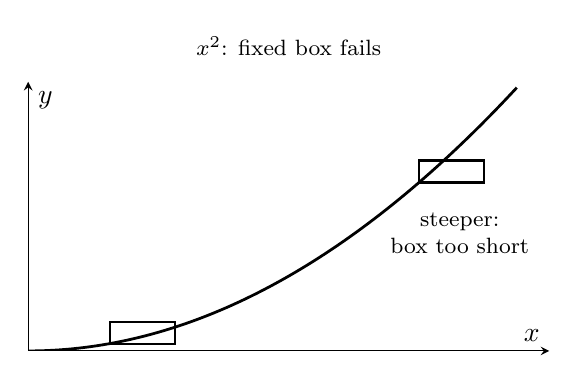
\begin{tikzpicture}
  \begin{axis}[
    width=8.2cm,height=5.0cm,axis lines=middle,xlabel=$x$,ylabel=$y$,
    title={\footnotesize $x^2$: fixed box fails},
    xmin=0,xmax=3.2,ymin=0,ymax=9.2,samples=80,xtick=\empty,ytick=\empty,
  ]
    \addplot[curve,domain=0:3]{x^2};
    % box at small x: fits
    \addplot[draw=black,thick] coordinates {(0.5,0.25)(0.9,0.25)(0.9,1.0)(0.5,1.0)(0.5,0.25)};
    % box at large x: same width, output overflows
    \addplot[draw=black,thick] coordinates {(2.4,5.76)(2.8,5.76)(2.8,6.51)(2.4,6.51)(2.4,5.76)};
    \node[font=\footnotesize] at (axis cs:2.65,4.4){steeper:};
    \node[font=\footnotesize] at (axis cs:2.65,3.6){box too short};
  \end{axis}
\end{tikzpicture}
\hfill
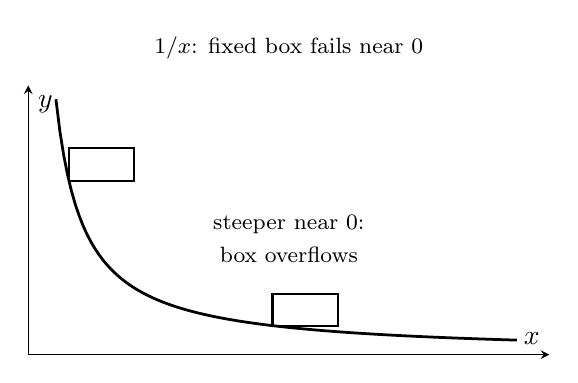
\begin{tikzpicture}
  \begin{axis}[
    width=8.2cm,height=5.0cm,axis lines=middle,xlabel=$x$,ylabel=$y$,
    title={\footnotesize $1/x$: fixed box fails near $0$},
    xmin=0,xmax=3.2,ymin=0,ymax=6.2,samples=120,xtick=\empty,ytick=\empty,
    restrict y to domain=0:6.2,
  ]
    \addplot[curve,domain=0.17:3]{1/x};
    \addplot[draw=black,thick] coordinates {(1.5,0.667)(1.9,0.667)(1.9,1.4)(1.5,1.4)(1.5,0.667)};
    \addplot[draw=black,thick] coordinates {(0.25,4.0)(0.65,4.0)(0.65,4.75)(0.25,4.75)(0.25,4.0)};
    \node[font=\footnotesize] at (axis cs:1.6,3.0){steeper near $0$:};
    \node[font=\footnotesize] at (axis cs:1.6,2.3){box overflows};
  \end{axis}
\end{tikzpicture}
\captionof{figure}{A fixed-width $\delta$-box of height $\eps$ that traps the graph at gentle
spots fails where the slope is unbounded ($x^2$ as $x\to\infty$, $1/x$ as $x\to0^+$).}
\end{center}

\subsection*{Lipschitz functions and the gauge viewpoint}

\begin{definition}\label{d:lipschitz@c5}
$f:A\to\R$ is \emph{Lipschitz} (with constant $K$) if $\abs{f(x)-f(u)}\le K\abs{x-u}$ for all
$x,u\in A$. Every Lipschitz function is uniformly continuous (take $\delta=\eps/K$).
\end{definition}

\begin{pitfall}
Lipschitz $\imp$ uniformly continuous $\imp$ continuous, and \emph{none} of the arrows
reverses. $\sqrt x$ on $[0,1]$ is uniformly continuous (compact domain, Heine--Cantor) but
\emph{not} Lipschitz: $\dfrac{\abs{\sqrt x-\sqrt0}}{\abs{x-0}}=\dfrac1{\sqrt x}\to\infty$ as
$x\to0^+$, so no $K$ bounds the difference quotient.
\end{pitfall}

\begin{definition}\label{d:gauge@c5}
A \emph{gauge} on $[a,b]$ is a function $\delta:[a,b]\to(0,\infty)$ (a \emph{positive}
function, not a constant). A tagged partition $\dot P=\set{([x_{i-1},x_i],t_i)}$ is
\emph{$\delta$-fine} if $[x_{i-1},x_i]\subseteq[\,t_i-\delta(t_i),\,t_i+\delta(t_i)\,]$ for
each $i$.
\end{definition}

\begin{theorem}[Cousin's lemma: $\delta$-fine partitions exist]\label{t:cousin@c5}
For every gauge $\delta$ on $[a,b]$ there exists a $\delta$-fine tagged partition of $[a,b]$.
\end{theorem}

\begin{proof}[Bisection proof]
Suppose not. Bisect $[a,b]$ at the midpoint; at least one half admits no $\delta$-fine
partition (else union the two, Ex.~5.5). Iterate to get nested $I_n$ of length
$(b-a)/2^n$, none $\delta$-fine. By nested intervals $\bigcap I_n=\set{\xi}$. Pick $p$ with
$(b-a)/2^p<\delta(\xi)$; then $I_p\subseteq[\xi-\delta(\xi),\xi+\delta(\xi)]$, so the single
pair $(I_p,\xi)$ is a $\delta$-fine partition of $I_p$ --- contradiction.
\end{proof}

The gauge encodes a \emph{Lebesgue number} pointwise: rather than one global $\delta$, each
tag $t$ carries its own radius $\delta(t)$. For a continuous $f$ on $[a,b]$, choosing
$\delta(t)$ from the $\eps$--$\delta$ condition at $t$ and invoking Cousin's lemma gives an
alternative, gauge-flavored proof of Heine--Cantor and underlies the generalized Riemann
integral (Chapter~12).

\begin{remark}[Lebesgue number]
For a continuous $f$ on compact $K$ and a fixed $\eps$, the cover proof of
Theorem~\ref{t:heine-cantor@c5} extracts a single $\delta>0$ such that any set of diameter
$<\delta$ has image of diameter $<\eps$ --- a uniform ``Lebesgue number'' for the cover
$\set{f\inv(B_{\eps/2}(f(p)))}$. The gauge is the non-uniform refinement that survives even
without compactness, recovering uniformity exactly when a constant gauge suffices.
\end{remark}

\subsection*{Further worked examples}

\begin{wex}{Uniform continuity on the whole line via a Lipschitz bound}
Show $f(x)=\sqrt{x^2+1}$ is uniformly continuous on $\R$.
\wrec ``Show uniformly continuous on an unbounded set'': Heine--Cantor does not apply
($\R$ is not compact), so produce a global Lipschitz constant (Definition~\ref{d:lipschitz@c5}).
\wsol For any $x,u$, rationalize:
\[
  \abs{\sqrt{x^2+1}-\sqrt{u^2+1}}
  =\frac{\abs{x^2-u^2}}{\sqrt{x^2+1}+\sqrt{u^2+1}}
  =\frac{\abs{x-u}\,\abs{x+u}}{\sqrt{x^2+1}+\sqrt{u^2+1}}.
\]
Since $\abs x\le\sqrt{x^2+1}$ and $\abs u\le\sqrt{u^2+1}$, we have
$\abs{x+u}\le\abs x+\abs u\le\sqrt{x^2+1}+\sqrt{u^2+1}$, so the fraction is
$\le\abs{x-u}$. Thus $f$ is Lipschitz with constant $K=1$, hence uniformly continuous
($\delta=\eps$). \emph{Check:} the slope $f'(x)=x/\sqrt{x^2+1}$ has $\abs{f'}<1$ everywhere,
matching $K=1$; the curve never steepens past slope $1$, so a fixed box always fits.
\checkmark
\end{wex}

\begin{wex}{Sum of uniformly continuous need not be: a product non-example}
Show that $x$ and $\sin x$ are each uniformly continuous on $\R$, but their product
$x\sin x$ is not.
\wrec ``Is uniform continuity closed under products?'': it is closed under sums but
\emph{not} products on unbounded domains; test with the nonuniform criterion
(Theorem~\ref{t:nonunif@c5}).
\wsol Both $x$ (Lipschitz, $K=1$) and $\sin x$ (Lipschitz, $K=1$ since $\abs{\sin x-\sin
u}\le\abs{x-u}$) are uniformly continuous. For $h(x)=x\sin x$, take $x_n=2\pi n+\tfrac1n$ and
$u_n=2\pi n$. Then $\abs{x_n-u_n}=\tfrac1n\to0$, while $h(u_n)=2\pi n\sin(2\pi n)=0$ and
$h(x_n)=(2\pi n+\tfrac1n)\sin(\tfrac1n)$. Since $\sin(\tfrac1n)\approx\tfrac1n$, we get
$h(x_n)\approx(2\pi n)\tfrac1n=2\pi$, so $\abs{h(x_n)-h(u_n)}\to2\pi\ge\eps_0=1$. By
Theorem~\ref{t:nonunif@c5}, $x\sin x$ is not uniformly continuous. \emph{Check:} the amplitude
grows linearly, so the oscillation steepens without bound --- exactly the unbounded-slope
obstruction. \checkmark
\end{wex}

\begin{wex}{Uniformly continuous maps preserve Cauchy sequences}
Show that if $f$ is uniformly continuous on $A$ and $\seq{x_n}$ is Cauchy in $A$, then
$\seq{f(x_n)}$ is Cauchy. Use this to re-prove that $1/x$ is not uniformly continuous on
$(0,1)$.
\wrec ``Transport a structural property through $f$'': uniform continuity converts an
input-closeness condition into an output-closeness one, uniformly in the index.
\wsol Let $\eps>0$ and pick $\delta$ from uniform continuity. Since $\seq{x_n}$ is Cauchy,
choose $N$ with $\abs{x_m-x_n}<\delta$ for $m,n\ge N$; then $\abs{f(x_m)-f(x_n)}<\eps$ for
$m,n\ge N$, so $\seq{f(x_n)}$ is Cauchy. Now on $(0,1)$ the sequence $x_n=1/n$ is Cauchy
(it converges to $0$), but $f(x_n)=n$ is \emph{not} Cauchy (it is unbounded). Hence $1/x$
cannot be uniformly continuous on $(0,1)$. \emph{Check:} this matches the direct
closing-pair argument earlier; the Cauchy test also shows $1/x$ has no continuous extension
to $[0,1]$. \checkmark
\end{wex}

\begin{wex}{A gauge that no constant $\delta$ can replace}
On $[0,1]$ let $f(x)=1/x$ for $x>0$ and $f(0)=0$. Exhibit a gauge $\delta(\cdot)$ realizing
continuity pointwise, and explain why no \emph{constant} gauge works.
\wrec ``Pointwise continuity via a gauge'': assign each tag its own radius
(Definition~\ref{d:gauge@c5}); a constant gauge would amount to uniform continuity.
\wsol At a point $t>0$, $f$ is continuous, so for a fixed $\eps$ there is a radius
$\delta(t)>0$ with $\abs{f(x)-f(t)}<\eps$ on $(t-\delta(t),t+\delta(t))$; one may take
$\delta(t)$ shrinking like $t^2$ as $t\to0^+$ (the slope near $t$ is $\approx1/t^2$). At
$t=0$, $f$ is discontinuous, but on $[0,1]$ we only need a gauge for the partition machinery,
and any $\delta(0)>0$ is admissible. A \emph{constant} gauge $\delta(t)\equiv\delta$ would
make $f$ uniformly continuous; but $f$ is unbounded near $0$, so no constant $\delta$ controls
$\abs{f(x)-f(t)}$ there. \emph{Check:} the gauge must collapse toward $0$ as the tag
approaches the bad point --- precisely the non-constant behavior that Cousin's lemma
(Theorem~\ref{t:cousin@c5}) still tolerates. \checkmark
\end{wex}

\begin{exers}{Exercises (Rudin, Ch.4).}
\item Let $f$ be a real uniformly continuous function on the bounded set $E\subseteq\R$.
  Prove $f$ is bounded on $E$. Show the conclusion is false if boundedness of $E$ is omitted.
\item Show the requirement in the definition of uniform continuity can be rephrased with
  diameters: to every $\eps>0$ there exists $\delta>0$ such that $\diam f(E)<\eps$ for all
  $E\subseteq X$ with $\diam E<\delta$.
\item Complete the alternative proof of the theorem ``continuous on compact $\imp$ uniformly
  continuous'': if $f$ is not uniformly continuous, then for some $\eps>0$ there are
  sequences $\seq{p_n},\seq{q_n}$ in $X$ with $d_X(p_n,q_n)\to0$ but $d_Y(f(p_n),f(q_n))\ge
  \eps$. Use compactness (a convergent subsequence) to obtain a contradiction.
\item Suppose $f$ is a uniformly continuous map of a metric space $X$ into a metric space
  $Y$. Prove $\seq{f(x_n)}$ is Cauchy in $Y$ for every Cauchy sequence $\seq{x_n}$ in $X$.
  Use this to give an alternative proof of the extension theorem below.
\item State precisely and prove: a uniformly continuous function of a uniformly continuous
  function is uniformly continuous.
\item Let $E$ be dense in a metric space $X$ and let $f$ be a uniformly continuous real
  function on $E$. Prove $f$ has a continuous extension to $X$ (unique by the dense-set
  determination). Could the range space $\R$ be replaced by $\R^k$? By any compact metric
  space? By any complete metric space? By any metric space?
\item Suppose $X,Y,Z$ are metric spaces with $Y$ compact. Let $f:X\to Y$, let $g$ be a
  continuous one-to-one map $Y\to Z$, and put $h(x)=g(f(x))$. Prove $f$ is uniformly
  continuous if $h$ is uniformly continuous (Hint: $g\inv$ has compact domain $g(Y)$, and
  $f=g\inv\circ h$). Prove also $f$ is continuous if $h$ is. Show by example that compactness
  of $Y$ cannot be omitted, even with $X,Z$ compact.
\end{exers}

\begin{exers}{Exercises (Bartle \& Sherbert, \S5.4).}
\item Show $f(x)=1/x$ is uniformly continuous on $A=[a,\infty)$ for a positive constant $a$.
\item Show $f(x)=1/x^2$ is uniformly continuous on $A=[1,\infty)$ but not on $B=(0,\infty)$.
\item Use the nonuniform-continuity criterion to show the following are not uniformly
  continuous: (a) $f(x)=x^2$ on $A=[0,\infty)$; (b) $g(x)=\sin(1/x)$ on $B=(0,\infty)$.
\item Show $f(x)=1/(1+x^2)$ is uniformly continuous on $\R$.
\item Show that if $f,g$ are uniformly continuous on $A\subseteq\R$, then $f+g$ is uniformly
  continuous on $A$.
\item Show that if $f,g$ are uniformly continuous and bounded on $A\subseteq\R$, then $fg$ is
  uniformly continuous on $A$.
\item If $f(x)=x$ and $g(x)=\sin x$, show $f,g$ are uniformly continuous on $\R$ but $fg$ is
  not.
\item Prove that if $f,g$ are each uniformly continuous on $\R$, then $f\circ g$ is uniformly
  continuous on $\R$.
\item If $f$ is uniformly continuous on $A\subseteq\R$ and $\abs{f(x)}\ge k>0$ for all $x\in
  A$, show $1/f$ is uniformly continuous on $A$.
\item Prove that if $f$ is uniformly continuous on a bounded set $A\subseteq\R$, then $f$ is
  bounded on $A$.
\item If $g(x)=\sqrt x$ on $[0,1]$, show there is no constant $K$ with $\abs{g(x)}\le K\abs
  x$ for all $x\in[0,1]$. Conclude the uniformly continuous $g$ is not Lipschitz on $[0,1]$.
\item Show that if $f$ is continuous on $[0,\infty)$ and uniformly continuous on $[a,\infty)$
  for some $a>0$, then $f$ is uniformly continuous on $[0,\infty)$.
\item Let $A\subseteq\R$ and $f:A\to\R$ have the property: for each $\eps>0$ there is a
  uniformly continuous $g_\eps:A\to\R$ with $\abs{f(x)-g_\eps(x)}<\eps$ for all $x\in A$.
  Prove $f$ is uniformly continuous on $A$.
\item A function $f:\R\to\R$ is \emph{periodic} if there is $p>0$ with $f(x+p)=f(x)$ for all
  $x$. Prove a continuous periodic function on $\R$ is bounded and uniformly continuous.
\item Let $f,g$ be Lipschitz on $A$. (a) Show $f+g$ is Lipschitz on $A$. (b) If $f,g$ are
  bounded on $A$, show $fg$ is Lipschitz on $A$. (c) Give a Lipschitz $f$ on $[0,\infty)$
  whose square $f^2$ is not Lipschitz.
\item A function is \emph{absolutely continuous} on an interval $I$ if for any $\eps>0$ there
  is $\delta>0$ such that for any pairwise disjoint subintervals $[x_k,y_k]$, $k=1,\dots,n$,
  of $I$ with $\sum\abs{x_k-y_k}<\delta$ one has $\sum\abs{f(x_k)-f(y_k)}<\eps$. Show that if
  $f$ is Lipschitz on $I$, then $f$ is absolutely continuous on $I$.
\end{exers}

\begin{exers}{Exercises (Bartle \& Sherbert, \S5.5 --- gauges).}
\item Let $\delta$ be the gauge on $[0,1]$ with $\delta(0)=\tfrac14$ and $\delta(t)=\tfrac12 t$
  for $t\in(0,1]$. (a) Show $\dot P_1=\set{([0,\tfrac14],0),\ ([\tfrac14,\tfrac12],\tfrac12),
  \ ([\tfrac12,1],\tfrac34)}$ is $\delta$-fine. (b) Show
  $\dot P_2=\set{([0,\tfrac14],0),\ ([\tfrac14,\tfrac12],\tfrac12),\ ([\tfrac12,1],\tfrac35)}$
  is not $\delta$-fine.
\item Let $\delta_1$ be the gauge with $\delta_1(0)=\tfrac14$, $\delta_1(t)=\tfrac34 t$. Are
  the partitions of Exercise~1 $\delta_1$-fine? (Note $\delta(t)\le\delta_1(t)$ throughout.)
\item Let $\delta_2$ be the gauge with $\delta_2(0)=\tfrac1{10}$, $\delta_2(t)=\tfrac9{10}t$.
  Are the partitions of Exercise~1 $\delta_2$-fine?
\item Let $g$ be the gauge of Example 5.5.4(d). (a) If $t\in(0,\tfrac12]$ show
  $[t-g(t),t+g(t)]=[\tfrac12 t,\tfrac32 t]\subseteq(0,\tfrac34]$. (b) If $t\in(\tfrac12,1)$
  show $[t-g(t),t+g(t)]\subseteq(\tfrac14,1)$.
\item Let $a<c<b$ and $\delta$ a gauge on $[a,b]$. If $\dot P'$ is a $\delta$-fine partition
  of $[a,c]$ and $\dot P''$ of $[c,b]$, show $\dot P'\cup\dot P''$ is a $\delta$-fine
  partition of $[a,b]$ having $c$ as a partition point.
\item Let $a<c<b$ and let $\delta',\delta''$ be gauges on $[a,c]$ and $[c,b]$. Define
  $\delta$ on $[a,b]$ by $\delta=\delta'$ on $[a,c)$, $\delta(c)=\min\set{\delta'(c),
  \delta''(c)}$, $\delta=\delta''$ on $(c,b]$. Then $\delta$ is a gauge, and if $\dot P'$ is
  $\delta'$-fine on $[a,c]$ and $\dot P''$ is $\delta''$-fine on $[c,b]$, then $\dot P'\cup
  \dot P''$ is a tagged partition of $[a,b]$ with partition point $c$. Explain why $\dot P'
  \cup\dot P''$ may fail to be $\delta$-fine, and give an example.
\item With $\delta',\delta''$ as above define $\delta$ by $\delta(t)=\min\set{\delta'(t),
  \tfrac12(c-t)}$ on $[a,c)$, $\delta(c)=\min\set{\delta'(c),\delta''(c)}$, and
  $\delta(t)=\min\set{\delta''(t),\tfrac12(t-c)}$ on $(c,b]$. Show $\delta$ is a gauge, and
  every $\delta$-fine partition of $[a,b]$ with partition point $c$ yields a $\delta'$-fine
  partition of $[a,c]$ and a $\delta''$-fine partition of $[c,b]$.
\item Let $\delta$ be a gauge on $I=[a,b]$ and suppose $I$ has no $\delta$-fine partition.
  (a) Let $c=\tfrac12(a+b)$; show at least one of $[a,c],[c,b]$ has no $\delta$-fine
  partition. (b) Construct nested $\seq{I_n}$ with length $(b-a)/2^n$, none $\delta$-fine.
  (c) Let $\xi\in\bigcap_n I_n$ and let $p$ satisfy $(b-a)/2^p<\delta(\xi)$. Show that
  $I_p\subseteq[\xi-\delta(\xi),\,\xi+\delta(\xi)]$, so the pair $(I_p,\xi)$ is a
  $\delta$-fine partition of $I_p$ --- a contradiction (this proves Cousin's lemma).
\item Let $I=[a,b]$, $f:I\to\R$. Call $f$ \emph{locally bounded} at $c\in I$ if there is
  $\delta(c)>0$ with $f$ bounded on $I\cap[c-\delta(c),c+\delta(c)]$. Prove that if $f$ is
  locally bounded at every point of $I$, then $f$ is bounded on $I$.
\item Let $I=[a,b]$, $f:I\to\R$. Call $f$ \emph{locally increasing} at $c$ if there is
  $\delta(c)>0$ with $f$ increasing on $I\cap[c-\delta(c),c+\delta(c)]$. Prove that if $f$ is
  locally increasing at every point of $I$, then $f$ is increasing on $I$.
\end{exers}

\begin{exers}{Additional exercises.}
\item Prove $f(x)=\sqrt x$ is uniformly continuous on $[0,\infty)$. (Hint: split at $1$; use
  $\abs{\sqrt x-\sqrt u}\le\sqrt{\abs{x-u}}$ near $0$ and a Lipschitz bound far out.)
\item Show $f(x)=\sin x$ is uniformly continuous on $\R$ but $g(x)=\sin(x^2)$ is not.
\item (Non-example / disprove.) Disprove ``a function continuous on all of $\R$ is uniformly
  continuous'' using $f(x)=x^2$, exhibiting the closing sequences explicitly.
\item Prove that if $f$ is uniformly continuous on $A$ and $\seq{x_n}$ is Cauchy in $A$, then
  $\seq{f(x_n)}$ is Cauchy. Use this to show $\sin(1/x)$ is not uniformly continuous on
  $(0,1)$.
\item Show that a uniformly continuous $f$ on a bounded set $A$ extends continuously to
  $\closure A$, and that $1/x$ on $(0,1]$ has no such extension to $[0,1]$.
\item (Gauge / Cousin.) Given the gauge $\delta(t)=\tfrac12\dist(t,\set{0,1})$ for
  $t\in(0,1)$ with $\delta(0)=\delta(1)=\tfrac14$, exhibit one explicit $\delta$-fine tagged
  partition of $[0,1]$.
\item (Diagram.) Plot $y=x^2$ and slide a fixed $\delta\times\eps$ rectangle along it; draw
  one position near $x=0$ where the box contains the graph and one near large $x$ where the
  graph escapes the box. Repeat the picture for $y=1/x$ near $0$.
\item Prove Heine--Cantor (continuous on compact $\imp$ uniformly continuous) by the gauge
  method: build a gauge from the pointwise $\eps$--$\delta$ data and apply Cousin's lemma to
  extract a uniform $\delta$.
\end{exers}


\section{Monotone Functions, Inverse Functions, and Discontinuities}
\subsection*{Monotone functions and one-sided limits}

\begin{definition}\label{d:monotone@c5}
$f:I\to\R$ ($I$ an interval) is \emph{increasing} if $x<y\imp f(x)\le f(y)$, \emph{strictly
increasing} if $x<y\imp f(x)<f(y)$; \emph{decreasing} and \emph{strictly decreasing} are
defined with the inequalities reversed. $f$ is \emph{monotone} if it is increasing or
decreasing.
\end{definition}

The decisive structural fact: a monotone function can misbehave only by \emph{jumping}, and
its one-sided limits always exist.

\begin{theorem}[One-sided limits of a monotone function]\label{t:mono-limits@c5}
Let $f$ be increasing on $(a,b)$ and let $c\in(a,b)$. Then both one-sided limits exist:
\[
  f(c^-)=\lim_{x\to c^-}f(x)=\sup_{a<x<c}f(x)\le f(c)\le\inf_{c<x<b}f(x)=\lim_{x\to c^+}f(x)=f(c^+).
\]
Consequently $f(c^-)\le f(c)\le f(c^+)$, and the only possible discontinuity at $c$ is a
\emph{jump}, of size $f(c^+)-f(c^-)\ge0$.
\end{theorem}

\begin{proof}
The set $\set{f(x)\st a<x<c}$ is bounded above by $f(c)$, so $L=\sup$ exists with $L\le
f(c)$. Given $\eps>0$ pick $x_0<c$ with $f(x_0)>L-\eps$; for $x_0<x<c$, monotonicity gives
$L-\eps<f(x_0)\le f(x)\le L$, so $\abs{f(x)-L}<\eps$. Hence $f(c^-)=L$. The right-hand
statement is symmetric with $\inf$. The inequalities chain as displayed.
\end{proof}

\begin{definition}[Classification of discontinuities]\label{d:disc-class@c5}
Suppose $f(c^-)$ and $f(c^+)$ both exist (automatic for monotone $f$). The discontinuity at
$c$ is:
\begin{itemize}
\item \emph{removable} if $f(c^-)=f(c^+)\neq f(c)$ (a single ``hole'' that one value would
  fix);
\item a \emph{jump} (simple discontinuity, \emph{first kind}) if $f(c^-)\neq f(c^+)$;
\item \emph{essential} (\emph{second kind}) if at least one of $f(c^-),f(c^+)$ fails to
  exist.
\end{itemize}
A \emph{simple discontinuity} (Rudin) is one of the first two types: both one-sided limits
exist.
\end{definition}

\begin{center}
\begin{tikzpicture}
  \begin{axis}[width=5.6cm,height=4.2cm,axis lines=middle,title={\footnotesize removable},
    xmin=-1.6,xmax=1.6,ymin=-0.3,ymax=2.2,xtick={0},xticklabels={$c$},ytick=\empty,samples=2]
    \addplot[curve,domain=-1.5:-0.04]{x+1};
    \addplot[curve,domain=0.04:1.5]{x+1};
    \node[opt] at (axis cs:0,1){};
    \node[pt] at (axis cs:0,1.8){};
  \end{axis}
\end{tikzpicture}
\hfill
\begin{tikzpicture}
  \begin{axis}[width=5.6cm,height=4.2cm,axis lines=middle,title={\footnotesize jump},
    xmin=-1.6,xmax=1.6,ymin=-0.3,ymax=2.4,xtick={0},xticklabels={$c$},ytick=\empty,samples=2]
    \addplot[curve,domain=-1.5:-0.04]{0.5*x+0.6};
    \addplot[curve,domain=0.04:1.5]{0.5*x+1.6};
    \node[opt] at (axis cs:0,0.6){};
    \node[pt] at (axis cs:0,1.6){};
  \end{axis}
\end{tikzpicture}
\hfill
\begin{tikzpicture}
  \begin{axis}[width=5.6cm,height=4.2cm,axis lines=middle,title={\footnotesize essential},
    xmin=-1.6,xmax=1.6,ymin=-1.4,ymax=1.4,xtick={0},xticklabels={$c$},ytick=\empty,samples=400,
    restrict y to domain=-1.4:1.4]
    \addplot[curve,domain=0.03:1.5]{sin(deg(1/x))};
    \addplot[curve,domain=-1.5:-0.03]{sin(deg(1/x))};
  \end{axis}
\end{tikzpicture}
\captionof{figure}{Three discontinuity types at $c$: removable (matching one-sided limits, wrong
value), jump (mismatched finite one-sided limits), essential (a one-sided limit fails, here
$\sin(1/x)$).}
\end{center}

\begin{theorem}[Monotone $\imp$ at most countably many discontinuities]\label{t:mono-countable@c5}
A monotone function $f$ on $(a,b)$ has at most countably many points of discontinuity, and
every one of them is a jump.
\end{theorem}

\begin{proof}
Assume $f$ increasing. At each discontinuity $c$, $f(c^-)<f(c^+)$ leaves an open ``jump
interval'' $J_c=(f(c^-),f(c^+))$. For $c<c'$ discontinuities, monotonicity gives
$f(c^+)\le f(c'^-)$, so the intervals $J_c$ are \emph{pairwise disjoint}. Each contains a
distinct rational, giving an injection from the set of discontinuities into $\Q$. Hence that
set is countable.
\end{proof}

\begin{center}
\begin{tikzpicture}
  \begin{axis}[
    width=11cm,height=5.2cm,axis lines=middle,xlabel=$x$,ylabel=$y$,
    xmin=0,xmax=6,ymin=0,ymax=5,xtick=\empty,ytick=\empty,samples=2,clip=false,
  ]
    % an increasing step-ish function with several jumps
    \addplot[curve,domain=0:1.2]{0.4*x+0.3};
    \node[opt] at (axis cs:1.2,0.78){}; \node[pt] at (axis cs:1.2,1.4){};
    \addplot[curve,domain=1.2:2.6]{0.3*x+1.04};
    \node[opt] at (axis cs:2.6,1.82){}; \node[pt] at (axis cs:2.6,2.5){};
    \addplot[curve,domain=2.6:3.9]{0.25*x+1.85};
    \node[opt] at (axis cs:3.9,2.825){}; \node[pt] at (axis cs:3.9,3.5){};
    \addplot[curve,domain=3.9:5.6]{0.2*x+2.72};
    % brace marking a jump
    \draw[brc] (axis cs:2.78,1.82)--(axis cs:2.78,2.5);
    \node[right,font=\footnotesize] at (axis cs:2.82,2.16){jump $f(c^+){-}f(c^-)$};
  \end{axis}
\end{tikzpicture}
\captionof{figure}{An increasing function: each jump opens a gap in the range; disjoint gaps each
swallow a rational, so there can be only countably many.}
\end{center}

\subsection*{Continuous monotone functions and their inverses}

\begin{theorem}[Continuous strictly monotone inverse]\label{t:mono-inverse@c5}
Let $I$ be an interval and $f:I\to\R$ \emph{continuous and strictly increasing}. Then
$J=f(I)$ is an interval, $f:I\to J$ is a bijection, and the inverse $f\inv:J\to I$ is
continuous and strictly increasing. (Same with ``decreasing''.)
\end{theorem}

\begin{proof}
Strict monotonicity gives injectivity; $J=f(I)$ is an interval by IVT
(Theorem~\ref{t:ivt@c5}). $f\inv$ is strictly increasing: $y_1<y_2$ in $J$ would force
$f\inv(y_1)\ge f\inv(y_2)$ only if $f$ reversed order, which it does not. For continuity of
$f\inv$ at $y_0=f(x_0)$: given $\eps>0$, the images $f(x_0-\eps)<y_0<f(x_0+\eps)$ (when these
lie in $I$) bracket $y_0$; choosing $\delta$ inside this bracket forces $f\inv(y)$ within
$\eps$ of $x_0$. (Alternatively: a continuous bijection between intervals has continuous
inverse because monotone functions only jump, and a jump in $f\inv$ would leave a gap in
$I=f\inv(J)$, impossible for an interval.)
\end{proof}

\begin{wex}{$n$-th roots and rational powers}
Use Theorem~\ref{t:mono-inverse@c5} to get $x\mapsto x^{1/n}$ continuous and strictly
increasing on $[0,\infty)$, then define $x^{r}$ for $r\in\Q$.
\wrec ``Construct/continuity of root and power functions''; invert a monotone continuous
power.
\wsol $\phi(x)=x^n$ is continuous and strictly increasing on $[0,\infty)$ with
$\phi([0,\infty))=[0,\infty)$, so $\phi\inv(y)=y^{1/n}$ is continuous and strictly increasing
there. For $r=m/n\in\Q$ ($x>0$) set $x^{r}=(x^{1/n})^m$; the usual laws
$x^rx^s=x^{r+s}$, $(x^r)^s=x^{rs}$ follow from the integer laws and well-definedness
($mq=np\imp(x^{1/n})^m=(x^{1/q})^p$). \emph{Check:} $x^{1/2}$ at $x=4$ gives $2$; strict
monotonicity matches the picture of $\sqrt{\cdot}$. \checkmark
\end{wex}

\begin{wex}{Thomae's function: continuous exactly at the irrationals}
For $x=m/n$ in lowest terms ($n>0$) define $f(x)=1/n$; $f(0)=1$ (with $n=1$); $f(x)=0$ for
$x\notin\Q$. Show $f$ is continuous at every irrational and has a (removable) simple
discontinuity at every rational (Rudin 4.18).
\wrec ``Where is this continuous?''; bound $f$ by a small $1/n$ near any point.
\wsol Fix any $c$ and $\eps>0$. Only finitely many rationals in $(c-1,c+1)$ have denominator
$n\le1/\eps$; choose $\delta$ small enough to dodge all of them (and to avoid $c$ if $c$ is
one of them). Then every $x$ with $0<\abs{x-c}<\delta$ is either irrational ($f=0$) or
rational with $n>1/\eps$ ($f=1/n<\eps$); so $\lim_{x\to c}f=0$. Hence $f$ is continuous at
$c$ iff $f(c)=0$, i.e.\ iff $c$ is irrational; at each rational, $\lim_{x\to c}f=0\neq f(c)$,
a removable discontinuity (both one-sided limits are $0$). \emph{Check:} continuity on a
dense set (the irrationals) and discontinuity on a dense set (the rationals) coexist ---
allowed precisely because the discontinuity set is countable. \checkmark
\end{wex}

\begin{theorem}[Simple discontinuities are at most countable]\label{t:simple-countable@c5}
For any $f:(a,b)\to\R$ (not necessarily monotone), the set of points where $f$ has a
\emph{simple} discontinuity is at most countable (Rudin 4.30).
\end{theorem}

\begin{proof}[Sketch]
Split into the sets where $f(c^-)<f(c^+)$, $f(c^-)>f(c^+)$, $f(c^-)=f(c^+)\neq f(c)$. On the
first, associate to $c$ a triple $(p,q,r)$ of rationals with $f(c^-)<p<f(c^+)$, with $q,r$
straddling $c$ so that $f<p$ to the left of $c$ within $(q,c)$ and $f>p$ to the right within
$(c,r)$. Distinct such $c$ yield distinct triples, so this set injects into $\Q^3$, hence is
countable; the other types are handled identically. (The full argument is the content of
Rudin Exercise~4.17.)
\end{proof}

\begin{pitfall}
Monotonicity is what guarantees one-sided limits \emph{exist}; for a general $f$ they may
not, leaving essential discontinuities (e.g.\ $\sin(1/x)$ at $0$). The countability theorems
above count only \emph{jump/removable} (simple) discontinuities. A function can have
uncountably many \emph{essential} discontinuities --- indeed the Dirichlet function is
discontinuous everywhere, with no one-sided limits anywhere, so its discontinuities are all
of the second kind and uncountable.
\end{pitfall}

\subsection*{Further worked examples}

\begin{wex}{Classifying discontinuities of a piecewise function}
For $f(x)=\dfrac{\abs{x}}{x}$ at $x=0$, $g(x)=\dfrac{x^2-1}{x-1}$ at $x=1$, and
$h(x)=\sin(1/x)$ at $x=0$, classify each discontinuity.
\wrec ``Name the type'': compute both one-sided limits and compare with the value
(Definition~\ref{d:disc-class@c5}).
\wsol $f$: for $x>0$, $f=1$; for $x<0$, $f=-1$; so $f(0^+)=1\neq-1=f(0^-)$ --- a \emph{jump}
(first kind), regardless of how $f(0)$ is set. $g$: for $x\neq1$, $g(x)=\dfrac{(x-1)(x+1)}{x-1}
=x+1$, so $g(1^-)=g(1^+)=2$; if $g(1)$ is left undefined or unequal to $2$ this is a
\emph{removable} discontinuity. $h$: $h(0^+)$ does not exist (oscillation, \S5.1), so the
discontinuity is \emph{essential} (second kind). \emph{Check:} only $g$ can be repaired by
assigning one value ($g(1):=2$); the jump in $f$ and the oscillation in $h$ cannot.
\checkmark
\end{wex}

\begin{wex}{A prescribed monotone function with countably many jumps}
Enumerate $\Q\cap(0,1)=\set{q_1,q_2,\dots}$ and set $f(x)=\sum_{q_k<x}2^{-k}$. Show $f$ is
increasing, discontinuous exactly at each $q_k$, and continuous at every irrational.
\wrec ``Build a function with a controlled discontinuity set'': sum a convergent series of
jumps, one per rational (the construction behind Theorem~\ref{t:mono-countable@c5}).
\wsol Each term $2^{-k}\ge0$, and adding more terms as $x$ increases gives $x<y\imp f(x)\le
f(y)$, so $f$ is increasing (and bounded by $\sum 2^{-k}=1$). At $x=q_j$: as $x$ crosses
$q_j$ upward, the term $2^{-j}$ switches on, so $f(q_j^+)-f(q_j^-)=2^{-j}>0$ --- a jump of
size $2^{-j}$. At an irrational $c$: for $\eps>0$ pick $N$ with $\sum_{k>N}2^{-k}<\eps$;
choosing $\delta$ so that $(c-\delta,c+\delta)$ contains none of $q_1,\dots,q_N$ makes the
oscillation of $f$ across $c$ less than $\eps$, so $f$ is continuous at $c$. \emph{Check:}
the discontinuity set is exactly the countable $\set{q_k}$, with total jump
$\sum 2^{-k}=1=f(1^-)$ --- a concrete instance of ``monotone $\imp$ at most countably many
jumps''. \checkmark
\end{wex}

\begin{wex}{A non-example: a strictly increasing function with a discontinuous inverse}
Show that dropping continuity from Theorem~\ref{t:mono-inverse@c5} can break it: a strictly
increasing bijection of an interval onto a \emph{non}-interval need not have continuous
inverse.
\wrec ``Why does the inverse theorem need continuity of $f$?'': a jump in $f$ leaves a gap
in the range, and the inverse must jump across that gap.
\wsol Define $f:[0,2]\to[0,1]\cup[2,3]$ by $f(x)=x$ on $[0,1]$ and $f(x)=x+1$ on $(1,2]$.
Then $f$ is strictly increasing and a bijection onto $J=[0,1]\cup[2,3]$, but it jumps at
$x=1$ ($f(1)=1$, $f(1^+)=2$). Its inverse $g=f\inv$ sends $[0,1]\to[0,1]$ and $[2,3]\to(1,2]$;
$g$ is discontinuous at $y=2$, where $g(2^-)$ would be $1$ from the left branch but $g(2)=1$
jumps to values near $1$ then to $(1,\dots$ --- concretely $g$ is continuous here \emph{only}
because $J$ already excludes $(1,2)$. The honest failure: $f$ itself is discontinuous, so
Theorem~\ref{t:mono-inverse@c5} (which assumes $f$ continuous on an interval) simply does not
apply. \emph{Check:} the range $J$ is not an interval --- its gap $(1,2)$ is the missing
piece that an interval domain would have forbidden. \checkmark
\end{wex}

\begin{wex}{The logarithm as a monotone inverse}
Granting that $\exp$ is continuous and strictly increasing on $\R$ with range $(0,\infty)$,
deduce that $\log$ is continuous and strictly increasing on $(0,\infty)$, and that
$\log(xy)=\log x+\log y$.
\wrec ``Continuity/structure of an inverse function'': apply the monotone-inverse theorem,
then transport the functional equation through the bijection.
\wsol By Theorem~\ref{t:mono-inverse@c5}, since $\exp:\R\to(0,\infty)$ is a continuous strictly
increasing bijection, its inverse $\log:(0,\infty)\to\R$ is continuous and strictly
increasing. For the product law, write $x=\exp(s)$, $y=\exp(t)$; then
$xy=\exp(s)\exp(t)=\exp(s+t)$, so $\log(xy)=s+t=\log x+\log y$. \emph{Check:} $\log 1=0$
(since $\exp 0=1$) and $\log$ inherits its monotonicity from $\exp$; numerically $\log(2\cdot
4)=\log 8\approx2.079$ equals $\log 2+\log 4\approx0.693+1.386$. \checkmark
\end{wex}

\begin{exers}{Exercises (Rudin, Ch.4).}
\item Let $\floor x$ denote the largest integer $\le x$ and $(x)=x-\floor x$ the fractional
  part. What discontinuities do $\floor x$ and $(x)$ have?
\item Let $f$ be a real function on $(a,b)$. Prove the set of points at which $f$ has a
  \emph{simple} discontinuity is at most countable. (Hint: on $E=\set{x\st f(x^-)<f(x^+)}$,
  associate to each $x\in E$ a triple $(p,q,r)$ of rationals with $f(x^-)<p<f(x^+)$, $q<x<r$,
  such that $a<q<t<x\imp f(t)<p$ and $x<t<r<b\imp f(t)>p$; distinct $x$ give distinct
  triples. Handle the other simple-discontinuity types similarly.)
\item Define $f$ on $\R$ by $f(x)=0$ if $x$ is irrational, and $f(x)=1/n$ if $x=m/n$ in
  lowest terms ($n>0$; take $n=1$ when $x=0$). Prove $f$ is continuous at every irrational
  and has a simple discontinuity at every rational.
\item Suppose $f:\R\to\R$ has the \emph{intermediate value property} (if $f(a)<c<f(b)$ then
  $f(x)=c$ for some $x$ between $a,b$) and, for every rational $r$, the set $\set{x\st
  f(x)=r}$ is closed. Prove $f$ is continuous. (Hint: if $x_n\to x_0$ but $f(x_n)>r>f(x_0)$
  for some $r$ and all $n$, find $t_n$ between $x_0,x_n$ with $f(t_n)=r$; then $t_n\to x_0$,
  forcing a contradiction.)
\item A real function $f$ on $(a,b)$ is \emph{convex} if
  $f(\lambda x+(1-\lambda)y)\le\lambda f(x)+(1-\lambda)f(y)$ whenever $x,y\in(a,b)$,
  $0<\lambda<1$. Prove every convex function is continuous. Prove every increasing convex
  function of a convex function is convex (e.g.\ $e^f$ is convex if $f$ is).
\item If $f$ is convex on $(a,b)$ and $a<s<t<u<b$, show
  $\dfrac{f(t)-f(s)}{t-s}\le\dfrac{f(u)-f(s)}{u-s}\le\dfrac{f(u)-f(t)}{u-t}$ (slopes
  increase). Conversely, if $f$ is continuous on $(a,b)$ with
  $f\!\big(\tfrac{x+y}2\big)\le\tfrac12\big(f(x)+f(y)\big)$ for all $x,y$, prove $f$ is
  convex.
\end{exers}

\begin{exers}{Exercises (Bartle \& Sherbert, \S5.6).}
\item If $I=[a,b]$ and $f:I\to\R$ is increasing, show $a$ (resp.\ $b$) is an absolute minimum
  (resp.\ maximum) point. If $f$ is strictly increasing, $a$ is the only absolute minimum
  point.
\item If $f,g$ are increasing on an interval $I$, show $f+g$ is increasing on $I$; if $f$ is
  also strictly increasing, then $f+g$ is strictly increasing.
\item Show $f(x)=x$ and $g(x)=x-1$ are strictly increasing on $I=[0,1]$, but their product
  $fg$ is not increasing on $I$.
\item Show that if $f,g$ are positive increasing functions on an interval $I$, then $fg$ is
  increasing on $I$.
\item Show that if $I=[a,b]$ and $f:I\to\R$ is increasing, then $f$ is continuous at $a$ iff
  $f(a)=\inf\set{f(x)\st x\in(a,b]}$.
\item Let $I\subseteq\R$ be an interval, $f:I\to\R$ increasing, $c\in I$ not an endpoint.
  Show $f$ is continuous at $c$ iff there is a sequence $\seq{x_n}$ in $I$ with $x_n<c$ for
  odd $n$, $x_n>c$ for even $n$, $c=\lim x_n$, and $f(c)=\lim f(x_n)$.
\item Let $I$ be an interval, $f:I\to\R$ increasing, $c$ not an endpoint. Show the jump
  $j_f(c)=f(c^+)-f(c^-)$ equals $\inf\set{f(y)-f(x)\st x<c<y,\ x,y\in I}$.
\item Let $f,g$ be strictly increasing on an interval $I$ with $f(x)>g(x)$ for all $x\in I$.
  If $y\in f(I)\cap g(I)$, show $f\inv(y)<g\inv(y)$. (Hint: interpret geometrically.)
\item Let $I=[0,1]$, $f:I\to\R$ with $f(x)=x$ for $x$ rational and $f(x)=1-x$ for $x$
  irrational. Show $f$ is injective on $I$ and $f(f(x))=x$ for all $x\in I$ ($f$ is its own
  inverse). Show $f$ is continuous only at $x=\tfrac12$.
\item Let $I=[a,b]$, $f:I\to\R$ continuous. If $f$ has an absolute maximum (resp.\ minimum)
  at an interior point $c$, show $f$ is not injective on $I$.
\item Let $f(x)=x$ for $x\in[0,1]$ and $f(x)=1+x$ for $x\in(1,2]$. Show $f$ and $f\inv$ are
  strictly increasing. Are $f$ and $f\inv$ continuous everywhere?
\item Let $f:[0,1]\to\R$ be continuous, taking no value twice, with $f(0)<f(1)$. Show $f$ is
  strictly increasing on $[0,1]$.
\item Let $h:[0,1]\to\R$ take each of its values exactly twice. Show $h$ cannot be continuous
  at every point. (Hint: if $c_1<c_2$ are where $h$ attains its sup, show $c_1=0$, $c_2=1$;
  then examine the infimum.)
\item Let $x\in\R$, $x>0$. Show that if $m,p\in\Z$, $n,q\in\N$, and $mq=np$, then
  $(x^{1/n})^m=(x^{1/q})^p$.
\item If $x>0$ and $r,s\in\Q$, show $x^rx^s=x^{r+s}=x^sx^r$ and $(x^r)^s=x^{rs}=(x^s)^r$.
\end{exers}

\begin{exers}{Additional exercises.}
\item For $f(x)=\floor x$ (greatest integer), find $f(c^-)$, $f(c^+)$, $f(c)$ at each integer
  $c$, classify the discontinuity, and compute the jump.
\item Show the increasing function $f(x)=\sum_{n:\,r_n\le x}2^{-n}$, where $\seq{r_n}$
  enumerates $\Q\cap(0,1)$, is discontinuous exactly at each $r_n$ and continuous at every
  irrational. (You may quote the monotone-discontinuity theorem.)
\item Classify the discontinuity of each at $0$: (a) $\operatorname{sgn}(x)$;
  (b) $\sin(1/x)$; (c) $x\mapsto\dfrac{x^2-x}{x}$ (removable?); (d) $e^{-1/x^2}$ extended by
  $0$.
\item (Non-example / disprove.) Disprove ``a function with at most countably many
  discontinuities must be monotone on some interval'' --- give a non-monotone example, e.g.\
  one with jumps of alternating sign at $1/n$.
\item Prove that a strictly increasing continuous $f$ on $[a,b]$ has a strictly increasing
  continuous inverse, and apply it to construct $\ln$ as the inverse of $\exp$ on a suitable
  interval.
\item Show that an increasing $f$ on $(a,b)$ has one-sided limits everywhere, and that the
  total jump $\sum_c\big(f(c^+)-f(c^-)\big)$ over all discontinuities $c$ in $[s,t]\subseteq
  (a,b)$ is at most $f(t)-f(s)$.
\item (Diagram.) Sketch an increasing step-like function on $[0,4]$ with jumps at
  $x=1,2,3$, drawing filled/open endpoints correctly, and brace one jump labeled
  $f(c^+)-f(c^-)$.
\item Prove that the set of discontinuities of a monotone function is at most countable by
  injecting it into $\Q$ via disjoint jump intervals, and explain why the argument fails for
  general (non-monotone) $f$ with essential discontinuities.
\end{exers}


% ================= Chapter 6: Differentiation =================

\chapter{Differentiation}

\section{The Derivative}
\subsection*{The derivative as a limit of difference quotients}

Throughout, $I$ denotes an interval of $\R$ (possibly closed, half-open, or unbounded)
and $f:I\to\R$ a real function. Fix a point $c\in I$. For $x\in I$ with $x\neq c$ the
\emph{difference quotient} of $f$ at $c$ is $\dfrac{f(x)-f(c)}{x-c}$; its slope is the slope
of the \emph{secant line} through $(c,f(c))$ and $(x,f(x))$. Differentiation studies the
limit of this slope as $x\to c$.

\begin{definition}\label{d:deriv@c6}
$f:I\to\R$ is \emph{differentiable at} $c\in I$ if the limit
\[
  f'(c)=\lim_{x\to c}\frac{f(x)-f(c)}{x-c}
\]
exists in $\R$; the number $f'(c)$ is the \emph{derivative of $f$ at $c$}. Equivalently,
writing $x=c+h$, $f'(c)=\lim_{h\to0}\dfrac{f(c+h)-f(c)}{h}$. We call $f$ \emph{differentiable
on} $E\subseteq I$ if $f'(c)$ exists for every $c\in E$; the resulting function
$f':E\to\R$ is the \emph{derivative} of $f$.
\end{definition}

The limit is taken \emph{within} $I$: at an endpoint of $I$ it is automatically a one-sided
derivative. Geometrically $f'(c)$ is the slope of the \emph{tangent line} $y=f(c)+f'(c)(x-c)$,
the limiting position of the secants as $x\to c$. The whole subject is the assertion that this
limiting slope, when it exists, controls the local behavior of $f$.

\begin{center}
\begin{tikzpicture}[scale=1.0]
  \begin{axis}[
    width=10.5cm,height=6.2cm,
    axis lines=left,xlabel={$x$},ylabel={$y$},
    xtick={1,2,3,4},xticklabels={$c$,$x_3$,$x_2$,$x_1$},
    ytick=\empty,
    xmin=0.2,xmax=5,ymin=0,ymax=10,
    domain=0.4:4.6,samples=80,clip=false]
    % curve f(x)=x^2/2 + 0.5
    \addplot[curve,black]{x*x/2+0.5};
    \node[right] at (axis cs:4.5,11){$y=f(x)$};
    % point of tangency
    \coordinate (P) at (axis cs:1,1);
    % secants to x1=4, x2=3, x3=2
    \addplot[densely dashed,domain=0.4:4.6]{(8.5-1)/(4-1)*(x-1)+1};
    \addplot[densely dashed,domain=0.4:4.6]{(5-1)/(3-1)*(x-1)+1};
    \addplot[densely dashed,domain=0.4:4.6]{(2.5-1)/(2-1)*(x-1)+1};
    % tangent at c (slope f'(1)=1)
    \addplot[curve,black,domain=0.2:3]{1*(x-1)+1};
    \node[pt] at (axis cs:1,1){};
    \node[pt] at (axis cs:2,2.5){};
    \node[pt] at (axis cs:3,5){};
    \node[pt] at (axis cs:4,8.5){};
    \node[below right,font=\footnotesize] at (axis cs:1,1){$(c,f(c))$};
    \node[font=\footnotesize,align=left] at (axis cs:3.2,2.0){tangent\\(slope $f'(c)$)};
  \end{axis}
\end{tikzpicture}
\captionof{figure}{Secants through $(c,f(c))$ and $(x_k,f(x_k))$ with $x_1>x_2>x_3\to c$. Their
slopes converge to the tangent slope $f'(c)$.}
\end{center}

\begin{theorem}[Differentiable $\imp$ continuous]\label{t:diff-cont@c6}
If $f$ is differentiable at $c$, then $f$ is continuous at $c$.
\end{theorem}

\begin{proof}
For $x\neq c$ write $f(x)-f(c)=\dfrac{f(x)-f(c)}{x-c}\,(x-c)$. As $x\to c$ the first factor
tends to $f'(c)$ and the second to $0$, so by the product rule for limits $f(x)-f(c)\to
f'(c)\cdot0=0$, i.e.\ $f(x)\to f(c)$. Thus $f$ is continuous at $c$.
\end{proof}

The converse fails utterly: $f(x)=\abs x$ is continuous everywhere but not differentiable at
$0$ (the left and right difference quotients are $-1$ and $+1$). In Chapter~8 we will meet a
function continuous on all of $\R$ yet differentiable \emph{nowhere}. So differentiability is
strictly stronger than continuity.

\begin{theorem}[Algebra of derivatives]\label{t:alg-deriv@c6}
If $f,g:I\to\R$ are differentiable at $c$, then so are $f+g$, $fg$, and (if $g(c)\neq0$)
$f/g$, with
\[
  (f+g)'(c)=f'(c)+g'(c),\qquad (fg)'(c)=f'(c)g(c)+f(c)g'(c),
\]
\[
  \Bigl(\frac fg\Bigr)'(c)=\frac{f'(c)g(c)-f(c)g'(c)}{g(c)^2}.
\]
In particular every polynomial is differentiable on $\R$, every rational function is
differentiable off the zeros of its denominator, and $(x^n)'=nx^{n-1}$ for every integer $n$
(with $x\neq0$ when $n<0$).
\end{theorem}

\begin{proof}
Sum: immediate from the additivity of limits. \emph{Product:} write the difference quotient as
\[
  \frac{f(x)g(x)-f(c)g(c)}{x-c}
  =\frac{f(x)-f(c)}{x-c}\,g(x)+f(c)\,\frac{g(x)-g(c)}{x-c}.
\]
As $x\to c$, $g(x)\to g(c)$ by Theorem~\ref{t:diff-cont@c6}, so the right side tends to
$f'(c)g(c)+f(c)g'(c)$. \emph{Quotient:} it suffices (by the product rule) to differentiate
$1/g$; the quotient
\[
  \frac1{x-c}\Bigl(\frac1{g(x)}-\frac1{g(c)}\Bigr)
  =-\frac1{g(x)g(c)}\,\frac{g(x)-g(c)}{x-c}\to-\frac{g'(c)}{g(c)^2},
\]
using $g(x)\to g(c)\neq0$. Combining gives the quotient rule. The power rule follows by
induction from the product rule (and the quotient rule for $n<0$).
\end{proof}

\subsection*{Caratheodory's characterization and the Chain Rule}

The difference-quotient definition is awkward to compose, because the inner function may equal
$c$ at points arbitrarily close to $c$, dividing by zero in the naive chain-rule computation.
Caratheodory's reformulation removes the division entirely and makes the Chain Rule a
one-line composition of continuous functions.

\begin{theorem}[Caratheodory's Theorem]\label{t:carath@c6}
Let $f$ be defined on an interval $I$ containing $c$. Then $f$ is differentiable at $c$ if and
only if there is a function $\varphi:I\to\R$, \emph{continuous at $c$}, such that
\[
  f(x)-f(c)=\varphi(x)\,(x-c)\qquad(x\in I).
\]
In that case $\varphi(c)=f'(c)$.
\end{theorem}

\begin{proof}
($\Rightarrow$) If $f'(c)$ exists, define $\varphi(x)=\dfrac{f(x)-f(c)}{x-c}$ for $x\neq c$ and
$\varphi(c)=f'(c)$. The factorization $f(x)-f(c)=\varphi(x)(x-c)$ holds for all $x$ (trivially
at $x=c$), and $\varphi(x)\to f'(c)=\varphi(c)$ as $x\to c$, so $\varphi$ is continuous at $c$.

($\Leftarrow$) Suppose such a $\varphi$ exists. For $x\neq c$, $\dfrac{f(x)-f(c)}{x-c}=
\varphi(x)\to\varphi(c)$ as $x\to c$ by continuity, so $f'(c)$ exists and equals $\varphi(c)$.
\end{proof}

The content is that ``$f$ is differentiable at $c$'' is the same as ``$f(x)-f(c)$ has a
continuous factor $\varphi$ pulling out $(x-c)$.'' The value $\varphi(c)=f'(c)$ is the slope;
near $c$, $\varphi(x)$ is the secant slope. We use it twice: for the Chain Rule and for the
inverse-function derivative.

\begin{theorem}[Chain Rule]\label{t:chain@c6}
Let $I,J$ be intervals, $g:I\to\R$ with $g(I)\subseteq J$, and $f:J\to\R$. If $g$ is
differentiable at $c$ and $f$ is differentiable at $g(c)$, then $h=f\circ g$ is differentiable
at $c$ and
\[
  h'(c)=f'\bigl(g(c)\bigr)\,g'(c).
\]
\end{theorem}

\begin{proof}
Put $d=g(c)$. By Caratheodory there are $\psi$ continuous at $c$ with $g(x)-g(c)=\psi(x)(x-c)$
and $\psi(c)=g'(c)$, and $\phi$ continuous at $d$ with $f(y)-f(d)=\phi(y)(y-d)$ and
$\phi(d)=f'(d)$. Substituting $y=g(x)$,
\[
  f(g(x))-f(g(c))=\phi(g(x))\bigl(g(x)-g(c)\bigr)=\phi(g(x))\,\psi(x)\,(x-c).
\]
The coefficient $x\mapsto\phi(g(x))\psi(x)$ is continuous at $c$ ($g$ is continuous at $c$,
$\phi$ at $d=g(c)$, $\psi$ at $c$), so by Caratheodory $h$ is differentiable at $c$ with
$h'(c)=\phi(g(c))\psi(c)=f'(g(c))g'(c)$.
\end{proof}

\begin{remark}
Rudin proves the same theorem by writing $g(x)-g(c)=(x-c)[g'(c)+u(x)]$ and
$f(y)-f(d)=(y-d)[f'(d)+v(y)]$ with $u\to0$, $v\to0$, then dividing. That works but must
separately handle indices where $g(x)=g(c)$. The Caratheodory route never divides, so no case
split is needed --- this is its main advantage.
\end{remark}

\begin{method}{Computing a derivative}
\textbf{Recognition trigger.} ``Differentiate $f$'' or ``find $f'(c)$''.
\begin{enumerate}
\item If $f$ is built from $x^n,\ \sin,\ \cos,\ e^x,\ \ln$ by $+,-,\times,\div$ and
  composition, apply the \emph{algebra of derivatives} (\ref{t:alg-deriv@c6}) and the
  \emph{Chain Rule} (\ref{t:chain@c6}). Differentiate from the outside in.
\item If $f$ is defined by cases or involves $\abs{\cdot}$, the rules apply away from the
  break points; at a break point go back to the \emph{definition} and compute the one-sided
  difference quotients $\lim_{x\to c^{\pm}}\frac{f(x)-f(c)}{x-c}$ separately. They must agree.
\item If asked to \emph{prove} differentiability of a non-elementary $f$ at a point, form the
  difference quotient and estimate it directly (often with a squeeze).
\end{enumerate}
\end{method}

\begin{wex}{A product--chain computation}
Differentiate $f(x)=\sqrt{5-2x+x^2}$.
\wrec An elementary composition: outer $\sqrt{\cdot}$, inner quadratic. Chain rule.
\wsol Write $f=u^{1/2}$ with $u(x)=5-2x+x^2$, $u'(x)=-2+2x$. Then
$f'(x)=\tfrac12 u^{-1/2}u'=\dfrac{x-1}{\sqrt{5-2x+x^2}}$. \emph{Check:} the quadratic
$5-2x+x^2=(x-1)^2+4\ge4>0$, so $f$ is differentiable on all of $\R$; $f'=0$ exactly at the
vertex $x=1$, where $f$ attains its minimum $\sqrt4=2$. \checkmark
\end{wex}

\begin{wex}{Differentiable but only at one point}
Let $f(x)=x^2$ for $x\in\Q$ and $f(x)=0$ for $x\notin\Q$. Show $f'(0)=0$ exists, although $f$
is discontinuous at every $c\neq0$.
\wrec A pathological $f$; use the \emph{definition} at $c=0$ and a squeeze.
\wsol For $x\neq0$, $\abs{\dfrac{f(x)-f(0)}{x-0}}=\abs{\dfrac{f(x)}{x}}\le\abs{\dfrac{x^2}{x}}
=\abs x\to0$, since $0\le f(x)\le x^2$ for all $x$. Hence the difference quotient $\to0$ and
$f'(0)=0$. \emph{Check:} for $c\neq0$, take rationals $\to c$ (values $\to c^2$) and
irrationals $\to c$ (values $0$); the two sequences force $f$ to be discontinuous at $c$, so a
fortiori not differentiable there. Differentiability at a single isolated point is possible.
\checkmark
\end{wex}

\begin{wex}{A corner: $\abs x$ is not differentiable at $0$}
Show $f(x)=\abs x$ has no derivative at $0$.
\wrec A piecewise-linear ``corner''; compute one-sided difference quotients.
\wsol For $x>0$, $\dfrac{\abs x-0}{x-0}=\dfrac xx=1$; for $x<0$, $\dfrac{-x}{x}=-1$. The
right limit is $1$, the left limit is $-1$; they disagree, so $\lim_{x\to0}$ does not exist
and $f'(0)$ is undefined. \emph{Check:} the graph has a $90^\circ$ corner at the origin --- no
single tangent line. (Yet $f$ is continuous, illustrating Theorem~\ref{t:diff-cont@c6}'s
one-way street.) \checkmark
\end{wex}

\subsection*{The derivative of an inverse function}

A strictly monotone continuous $f$ on an interval has a continuous inverse (Chapter~5). When
$f$ is also differentiable with nonzero derivative, the inverse is differentiable too, with
the reciprocal slope --- exactly what the picture of reflecting the graph across $y=x$
suggests.

\begin{theorem}[Derivative of the inverse]\label{t:inv@c6}
Let $f:I\to\R$ be continuous and strictly monotone on the interval $I$, with $J=f(I)$ and
inverse $g=f\inv:J\to I$. If $f$ is differentiable at $c\in I$ and $f'(c)\neq0$, then $g$ is
differentiable at $d=f(c)$ and
\[
  g'(d)=\frac1{f'(c)}=\frac1{f'(g(d))}.
\]
\end{theorem}

\begin{proof}
By Caratheodory, $f(x)-f(c)=\varphi(x)(x-c)$ with $\varphi$ continuous at $c$ and
$\varphi(c)=f'(c)\neq0$. Since $f$ is injective, $\varphi(x)\neq0$ for $x\neq c$ (otherwise
$f(x)=f(c)$); and $\varphi(c)\neq0$. For $y\in J$ put $x=g(y)$, $c=g(d)$; then
\[
  y-d=f(x)-f(c)=\varphi(g(y))\,\bigl(g(y)-g(d)\bigr),
  \quad\text{so}\quad
  g(y)-g(d)=\frac1{\varphi(g(y))}\,(y-d).
\]
The coefficient $y\mapsto 1/\varphi(g(y))$ is continuous at $d$ (because $g$ is continuous at
$d$, $\varphi$ continuous and nonzero at $c=g(d)$). By Caratheodory $g$ is differentiable at
$d$ with $g'(d)=1/\varphi(g(d))=1/\varphi(c)=1/f'(c)$.
\end{proof}

\begin{center}
\begin{tikzpicture}
  \begin{axis}[
    width=7.4cm,height=7.4cm,axis equal image,
    axis lines=left,xlabel={$x$},ylabel={$y$},
    xmin=0,xmax=3,ymin=0,ymax=3,xtick=\empty,ytick=\empty,
    domain=0:3,samples=60,clip=false]
    \addplot[densely dotted,domain=0:3]{x};                 % y=x
    \addplot[curve,black,domain=0:1.732]{x*x};              % f(x)=x^2
    \addplot[curve,black,domain=0:3]{sqrt(x)};              % g=f^{-1}
    \node[right] at (axis cs:1.55,2.6){$f$};
    \node[right] at (axis cs:2.55,1.75){$g=f\inv$};
    \node[above left,font=\footnotesize] at (axis cs:2.9,2.9){$y=x$};
    \node[pt] at (axis cs:1.3,1.69){};
    \node[pt] at (axis cs:1.69,1.3){};
  \end{axis}
\end{tikzpicture}
\captionof{figure}{Reflecting the graph of $f$ across $y=x$ gives the graph of $g=f\inv$; a
tangent of slope $m$ becomes a tangent of slope $1/m$.}
\end{center}

\begin{wex}{Derivative of $\arcsin$}
On $I=[-\tfrac\pi2,\tfrac\pi2]$, $\sin$ is strictly increasing with inverse $\arcsin$ on
$[-1,1]$. Compute $(\arcsin)'(y)$.
\wrec ``Differentiate an inverse trig function''; apply Theorem~\ref{t:inv@c6} with
$f=\sin$, $f'=\cos$.
\wsol For $y=\sin x$, $x\in(-\tfrac\pi2,\tfrac\pi2)$, we have $\cos x>0$, so by
Theorem~\ref{t:inv@c6},
\[
  (\arcsin)'(y)=\frac1{\cos x}=\frac1{\sqrt{1-\sin^2x}}=\frac1{\sqrt{1-y^2}}\qquad(-1<y<1).
\]
\emph{Check:} at $y=0$ ($x=0$) the slope is $1/\cos0=1$, matching $1/\sqrt{1-0}=1$. The
formula blows up as $y\to\pm1$, exactly where $\cos x\to0$ and the inverse has a vertical
tangent --- so $\arcsin$ is \emph{not} differentiable at $\pm1$. \checkmark
\end{wex}

\begin{wex}{$x^{1/n}$ from $x^n$, and failure at $0$}
For even $n\in\N$ let $f(x)=x^n$ on $[0,\infty)$, $g(y)=y^{1/n}$. Find $g'$.
\wrec Inverse of a power; $f'(x)=nx^{n-1}$.
\wsol For $y>0$ with $x=y^{1/n}>0$, $g'(y)=\dfrac1{f'(x)}=\dfrac1{nx^{n-1}}=
\dfrac1{n\,y^{(n-1)/n}}=\dfrac1n\,y^{(1/n)-1}$. \emph{Check:} this is the usual power rule
with exponent $1/n$. At $y=0$, $f'(0)=0$, so the theorem does not apply --- and indeed
$g(y)=y^{1/n}$ has a \emph{vertical} tangent at $0$ ($g'(0)$ does not exist). The hypothesis
$f'(c)\neq0$ is essential. \checkmark
\end{wex}

\begin{pitfall}
``Differentiable'' is a \emph{local} property checked by a limit; it is not the same as
``the formula simplifies''. A function can be given by one tidy rule yet fail to be
differentiable (e.g.\ $\abs x$ at $0$), and a function given by an ugly rule can be
differentiable. Always trace differentiability back to the existence of the
difference-quotient limit, especially at break points and endpoints. Also: $f'(c)\neq0$ is
\emph{required} for the inverse-derivative formula --- where the tangent is horizontal, the
inverse has a vertical tangent and is not differentiable.
\end{pitfall}

\subsection*{Further worked examples}

\begin{wex}{Continuous but not differentiable on a fattened corner}
Let $f(x)=x\sin(1/x)$ for $x\neq0$ and $f(0)=0$. Decide whether $f$ is differentiable at $0$.
\wrec ``Differentiable at a break point?''; go to the \emph{definition} and form the
difference quotient (Method, step 2). The rules do not apply at $0$.
\wsol The difference quotient at $0$ is
$\dfrac{f(x)-f(0)}{x-0}=\dfrac{x\sin(1/x)}{x}=\sin(1/x)$ for $x\neq0$. As $x\to0$,
$\sin(1/x)$ oscillates through all of $[-1,1]$ and has \emph{no} limit (take
$x_n=\tfrac1{n\pi}\to0$ giving $0$, and $x_n=\tfrac1{2\pi n+\pi/2}\to0$ giving $1$). So the
limit defining $f'(0)$ does not exist and $f$ is \emph{not} differentiable at $0$, even though
$\abs{f(x)}\le\abs x\to0$ makes $f$ continuous there. \emph{Check:} contrast with
$x^2\sin(1/x)$ (Worked Example~\ref{wex:darboux@c6}), whose extra factor of $x$ multiplies the
quotient by $x\to0$ and \emph{does} give $f'(0)=0$. The single power of $x$ is exactly not
enough. \checkmark
\end{wex}

\begin{center}
\begin{tikzpicture}
  \begin{axis}[
    width=10.5cm,height=5cm,axis lines=middle,xlabel={$x$},ylabel={$y$},
    xmin=-0.34,xmax=0.34,ymin=-0.34,ymax=0.34,
    samples=400,xtick=\empty,ytick=\empty,clip=true]
    \addplot[curve,black,domain=0.004:0.33]{x*sin(deg(1/x))};
    \addplot[curve,black,domain=-0.33:-0.004]{x*sin(deg(1/x))};
    \addplot[densely dashed,domain=-0.33:0.33]{x};
    \addplot[densely dashed,domain=-0.33:0.33]{-x};
    \node[pt] at (axis cs:0,0){};
  \end{axis}
\end{tikzpicture}
\captionof{figure}{$f(x)=x\sin(1/x)$ is trapped between $y=\pm x$ (so continuous at $0$), but the
secant slope $\sin(1/x)$ swings between $-1$ and $1$ infinitely often near $0$: no tangent,
no $f'(0)$.}
\end{center}

\begin{wex}{Differentiating a piecewise gluing}
Let $f(x)=x^2$ for $x\le1$ and $f(x)=ax+b$ for $x>1$. Find $a,b$ making $f$ differentiable at
$x=1$.
\wrec ``Glue two formulas smoothly''; matching value forces continuity, matching one-sided
difference quotients forces differentiability.
\wsol \emph{Continuity at $1$:} $\lim_{x\to1^-}x^2=1$ must equal $\lim_{x\to1^+}(ax+b)=a+b$, so
$a+b=1$. \emph{Differentiability:} the left derivative is $\frac{d}{dx}x^2\big|_{1}=2$ and the
right derivative is $a$; these must agree, so $a=2$, whence $b=1-a=-1$. Thus $f(x)=2x-1$ for
$x>1$. \emph{Check:} with $a=2,b=-1$ the right piece is the tangent line to $x^2$ at $x=1$
(value $1$, slope $2$); the graph continues straight out of the parabola with no corner.
Any other $a$ leaves a corner; any other $b$ leaves a jump. \checkmark
\end{wex}

\begin{wex}{The power rule from the definition (a non-shortcut check)}
Compute $f'(c)$ from the definition for $f(x)=1/x$ at $c\neq0$, without quoting the quotient
rule.
\wrec ``From the definition''; form $\frac{f(x)-f(c)}{x-c}$ and simplify algebraically before
taking the limit.
\wsol For $x\neq c$ (both nonzero),
\[
  \frac{f(x)-f(c)}{x-c}=\frac{\frac1x-\frac1c}{x-c}=\frac{\frac{c-x}{xc}}{x-c}
  =\frac{-(x-c)}{xc\,(x-c)}=\frac{-1}{xc}.
\]
As $x\to c$ this tends to $-1/c^2$, so $f'(c)=-1/c^2$. \emph{Check:} the quotient rule gives
$\frac{d}{dx}x^{-1}=-x^{-2}$, matching; e.g.\ at $c=2$, $f'(2)=-1/4$, the slope of $1/x$ where
it passes through $(2,\tfrac12)$. \checkmark
\end{wex}

\begin{exers}{Exercises (Rudin, Ch.5).}
\item Suppose $f'(x)>0$ on $(a,b)$. Prove that $f$ is strictly increasing on $(a,b)$, and let
  $g$ be its inverse. Prove that $g$ is differentiable and that
  $g'(f(x))=\dfrac1{f'(x)}$ for $a<x<b$.
\item Suppose $g$ is a real function on $\R$ with bounded derivative, say $\abs{g'}\le M$. Fix
  $\eps>0$ and define $f(x)=x+\eps g(x)$. Prove that $f$ is one-to-one if $\eps$ is small
  enough. (A set of admissible $\eps$ can be found depending only on $M$.)
\item Suppose $f'$ is continuous on $[a,b]$ and $\eps>0$. Prove there is $\delta>0$ such that
  $\abs{\dfrac{f(t)-f(x)}{t-x}-f'(x)}<\eps$ whenever $0<\abs{t-x}<\delta$ and $a\le x,t\le b$.
  (This says $f$ is \emph{uniformly differentiable} on $[a,b]$ when $f'$ is continuous.) Does
  it hold for vector-valued functions?
\item Let $f$ be a continuous real function on $\R$ for which $f'(x)$ exists for all $x\neq0$
  and $f'(x)\to3$ as $x\to0$. Does it follow that $f'(0)$ exists?
\item If $f(x)=\abs x^{3}$, compute $f'(x)$ and $f''(x)$ for all real $x$, and show that
  $f^{(3)}(0)$ does not exist.
\item Suppose $a,c$ are real, $c>0$, and $f$ is defined on $[-1,1]$ by $f(x)=x^a\sin(\abs
  x^{-c})$ for $x\neq0$ and $f(0)=0$. Prove: (a) $f$ is continuous iff $a>0$; (b) $f'(0)$
  exists iff $a>1$; (c) $f'$ is bounded iff $a\ge1+c$; (d) $f'$ is continuous iff $a>1+c$;
  (e) $f''(0)$ exists iff $a>2+c$; (f) $f''$ is bounded iff $a\ge2+2c$; (g) $f''$ is continuous
  iff $a>2+2c$.
\end{exers}

\begin{exers}{Exercises (Bartle \& Sherbert, \S6.1).}
\item Use the definition to find the derivative of: (a) $f(x)=x^3$ ($x\in\R$);
  (b) $g(x)=1/x$ ($x\neq0$); (c) $h(x)=\sqrt x$ ($x>0$); (d) $k(x)=1/\sqrt x$ ($x>0$).
\item Show that $f(x)=x^{1/3}$, $x\in\R$, is not differentiable at $x=0$.
\item Prove the sum and product rules for derivatives (Theorem 6.1.3(a),(b)).
\item Let $f:\R\to\R$ be defined by $f(x)=x^2$ for $x$ rational and $f(x)=0$ for $x$
  irrational. Show that $f$ is differentiable at $x=0$ and find $f'(0)$.
\item Differentiate and simplify: (a) $f(x)=\dfrac{x}{1+x^2}$;
  (b) $g(x)=\sqrt{5-2x+x^2}$; (c) $h(x)=(\sin x^k)^m$ for $m,k\in\N$;
  (d) $k(x)=\tan(x^2)$ for $\abs x<\sqrt{\pi/2}$.
\item Let $n\in\N$ and $f(x)=x^n$ for $x\ge0$, $f(x)=0$ for $x<0$. For which $n$ is $f'$
  continuous at $0$? For which $n$ is $f'$ differentiable at $0$?
\item Suppose $f:\R\to\R$ is differentiable at $c$ and $f(c)=0$. Show $g(x)=\abs{f(x)}$ is
  differentiable at $c$ iff $f'(c)=0$.
\item Determine where each function from $\R$ to $\R$ is differentiable and find the
  derivative: (a) $f(x)=\abs x+\abs{x+1}$; (b) $g(x)=2x+\abs x$; (c) $h(x)=x\abs x$;
  (d) $k(x)=\abs{\sin x}$.
\item Prove that if $f:\R\to\R$ is even and differentiable everywhere, then $f'$ is odd; and if
  $g:\R\to\R$ is odd and differentiable, then $g'$ is even.
\item Let $g(x)=x^2\sin(1/x^2)$ for $x\neq0$ and $g(0)=0$. Show $g$ is differentiable for all
  $x\in\R$, but the derivative $g'$ is not bounded on $[-1,1]$.
\item Assume there is a function $L:(0,\infty)\to\R$ with $L'(x)=1/x$ for $x>0$. Calculate the
  derivatives of: (a) $f(x)=L(2x+3)$; (b) $g(x)=(L(x^2))^3$; (c) $h(x)=L(ax)$ ($a>0$);
  (d) $k(x)=L(L(x))$ when $L(x)>0$.
\item If $r>0$ is rational, let $f(x)=x^r\sin(1/x)$ for $x\neq0$ and $f(0)=0$. Determine the
  values of $r$ for which $f'(0)$ exists.
\item If $f:\R\to\R$ is differentiable at $c$, show $f'(c)=\lim n\bigl(f(c+1/n)-f(c)\bigr)$.
  Show by example that existence of this sequential limit does not imply existence of $f'(c)$.
\item Given that $h(x)=x^3+2x+1$ has an inverse $h\inv$ on $\R$, find the value of
  $(h\inv)'(y)$ at the points corresponding to $x=0,1,-1$.
\item Given that $\cos$ restricted to $I=[0,\pi]$ is strictly decreasing with $\cos0=1$,
  $\cos\pi=-1$, let $J=[-1,1]$ and let $\operatorname{Arccos}:J\to\R$ be the inverse. Show
  $\operatorname{Arccos}$ is differentiable on $(-1,1)$ with $D\operatorname{Arccos}y=
  -1/(1-y^2)^{1/2}$, and not differentiable at $\pm1$.
\item Given that $\tan$ restricted to $I=(-\pi/2,\pi/2)$ is strictly increasing with
  $\tan(I)=\R$, let $\operatorname{Arctan}:\R\to\R$ be the inverse. Show
  $\operatorname{Arctan}$ is differentiable on $\R$ with $D\operatorname{Arctan}y=(1+y^2)\inv$.
\item Let $f:I\to\R$ be differentiable at $c\in I$. Establish the \emph{Straddle Lemma}: given
  $\eps>0$ there is $\delta>0$ such that if $u,v\in I$ satisfy
  $c-\delta<u\le c\le v<c+\delta$, then $\abs{f(v)-f(u)-(v-u)f'(c)}\le\eps(v-u)$. (Hint:
  subtract and add $f(c)-cf'(c)$ and use the triangle inequality.)
\end{exers}

\begin{exers}{Additional exercises.}
\item Using only the definition (no rules), compute $f'(c)$ for $f(x)=x^2$ at an arbitrary
  $c\in\R$, and for $f(x)=1/x$ at an arbitrary $c\neq0$.
\item Differentiate, simplifying: (a) $\dfrac{x\sin x}{1+x^2}$; (b) $\sqrt{1+\cos^2x}$;
  (c) $e^{x^2}\ln(1+x^2)$; (d) $(\arctan x)^3$.
\item (Caratheodory in action.) Use Caratheodory's theorem to give a one-line proof that if
  $f$ is differentiable at $c$ and $f(c)\neq0$, then $1/f$ is differentiable at $c$ with
  $(1/f)'(c)=-f'(c)/f(c)^2$. Identify the continuous factor $\varphi$.
\item Let $f(x)=x^2$ for $x\ge0$ and $f(x)=-x^2$ for $x<0$. Show $f$ is differentiable on all
  of $\R$, find $f'$, and decide whether $f'$ is differentiable at $0$.
\item (Non-example.) Exhibit a function $f:\R\to\R$ that is continuous everywhere, has a
  derivative at every point except one, and at that point has \emph{different} one-sided
  derivatives. Prove your claims.
\item (Non-example.) Show that there is no differentiable $f:\R\to\R$ whose derivative is the
  Dirichlet function ($1$ on $\Q$, $0$ off $\Q$). (Hint: a derivative has the intermediate
  value property; preview of \S6.2.)
\item Let $g(y)=y^{1/3}$ on $\R$. Where is $g$ differentiable? Compute $g'$ there and explain,
  using Theorem~\ref{t:inv@c6}, why $g$ fails to be differentiable at $0$ even though its inverse
  $y=x^3$ is differentiable everywhere.
\item (Diagram.) Sketch $f(x)=x^3-3x$ together with its tangent lines at $x=-1,0,1$. Mark the
  points where $f'(x)=0$ and relate them to the local shape of the graph. State $f'$ at each
  marked point.
\item (Harder.) Suppose $f$ is differentiable on $\R$ with $f'$ \emph{bounded}, $\abs{f'}\le
  M$. Prove $f$ is Lipschitz: $\abs{f(x)-f(y)}\le M\abs{x-y}$ for all $x,y$. (This is the
  forward reference used in \S6.2; prove it directly from the definition plus the result you
  will state as the MVT, or by a difference-quotient sup argument.)
\item (Harder.) Let $f(x)=x^2\sin(1/x)$ for $x\neq0$, $f(0)=0$. Compute $f'$ everywhere and
  show $f$ is differentiable on $\R$ but $f$ is not of class $C^1$. Which theorem of \S6.2 does
  this example illustrate the necessity of?
\end{exers}


\section{The Mean Value Theorem and Its Consequences}
\subsection*{Interior extrema and Rolle's theorem}

The single most useful fact about derivatives is that they vanish at interior maxima and
minima. From it flow Rolle's theorem, the Mean Value Theorem, and through them every
statement linking the \emph{sign} of $f'$ to the \emph{behavior} of $f$.

\begin{definition}\label{d:extremum@c6}
$f:I\to\R$ has a \emph{local (relative) maximum} at $c\in I$ if there is $\delta>0$ with
$f(x)\le f(c)$ for all $x\in I$ with $\abs{x-c}<\delta$; a \emph{local minimum} is defined with
$\ge$. A point $c$ is \emph{interior} to $I$ if $(c-\delta,c+\delta)\subseteq I$ for some
$\delta>0$.
\end{definition}

\begin{theorem}[Interior Extremum Theorem]\label{t:fermat@c6}
If $f$ has a local maximum or minimum at an \emph{interior} point $c$ of $I$ and $f'(c)$
exists, then $f'(c)=0$.
\end{theorem}

\begin{proof}
Say $f$ has a local max at $c$ (the min case is identical with signs reversed). For $x$ near
$c$, $f(x)-f(c)\le0$. If $x>c$ the difference quotient $\dfrac{f(x)-f(c)}{x-c}\le0$, so
$f'(c)=\lim_{x\to c^+}\le0$. If $x<c$ the quotient is $\ge0$ (negative over negative), so
$f'(c)=\lim_{x\to c^-}\ge0$. Both limits equal $f'(c)$, forcing $0\le f'(c)\le0$, i.e.\
$f'(c)=0$.
\end{proof}

The interior hypothesis is essential: on $[0,1]$ the function $f(x)=x$ has its maximum at the
endpoint $1$, where $f'=1\neq0$. A point with $f'(c)=0$ is called \emph{critical} (or
\emph{stationary}); the theorem says interior extrema are critical, not conversely
($f(x)=x^3$ has $f'(0)=0$ but no extremum there).

\begin{center}
\begin{tikzpicture}
  \begin{axis}[
    width=9.5cm,height=5cm,axis lines=left,xlabel={$x$},
    xtick={1.4},xticklabels={$c$},ytick=\empty,
    xmin=0,xmax=3,ymin=-0.2,ymax=2.4,domain=0.1:2.9,samples=80,clip=false]
    \addplot[curve,black]{2 - 1.0*(x-1.4)^2};
    \addplot[densely dashed,domain=0.4:2.4]{2};   % horizontal tangent
    \node[pt] at (axis cs:1.4,2){};
    \draw[densely dotted](axis cs:1.4,0)--(axis cs:1.4,2);
    \node[above,font=\footnotesize] at (axis cs:1.4,2){$f'(c)=0$};
    \node[right] at (axis cs:2.7,1.0){$y=f(x)$};
  \end{axis}
\end{tikzpicture}
\captionof{figure}{At an interior maximum the tangent is horizontal: the secant slopes change sign
through $c$, pinning $f'(c)=0$.}
\end{center}

\begin{theorem}[Rolle's Theorem]\label{t:rolle@c6}
Suppose $f$ is continuous on $[a,b]$, differentiable on $(a,b)$, and $f(a)=f(b)$. Then there
exists $c\in(a,b)$ with $f'(c)=0$.
\end{theorem}

\begin{proof}
$f$ is continuous on the compact set $[a,b]$, so by the Extreme Value Theorem it attains a
maximum $M$ and a minimum $m$ there. If $M=m$ then $f$ is constant and $f'\equiv0$ on $(a,b)$;
any $c$ works. Otherwise $M>m$, so at least one of $M,m$ differs from the common endpoint
value $f(a)=f(b)$ and is therefore attained at an \emph{interior} point $c\in(a,b)$. By
Theorem~\ref{t:fermat@c6}, $f'(c)=0$.
\end{proof}

\subsection*{The Mean Value Theorem}

Rolle's theorem is the horizontal-chord case; tilting the picture gives the general theorem.

\begin{theorem}[Mean Value Theorem]\label{t:mvt@c6}
If $f$ is continuous on $[a,b]$ and differentiable on $(a,b)$, then there exists $c\in(a,b)$
with
\[
  f'(c)=\frac{f(b)-f(a)}{b-a},\qquad\text{equivalently}\qquad f(b)-f(a)=f'(c)\,(b-a).
\]
\end{theorem}

\begin{proof}
Subtract off the chord. Let
$\varphi(x)=f(x)-f(a)-\dfrac{f(b)-f(a)}{b-a}\,(x-a)$. Then $\varphi$ is continuous on $[a,b]$,
differentiable on $(a,b)$, and $\varphi(a)=0=\varphi(b)$ (direct check). By Rolle there is
$c\in(a,b)$ with $\varphi'(c)=0$; but $\varphi'(x)=f'(x)-\dfrac{f(b)-f(a)}{b-a}$, so
$f'(c)=\dfrac{f(b)-f(a)}{b-a}$.
\end{proof}

\begin{center}
\begin{tikzpicture}
  \begin{axis}[
    width=10.5cm,height=5.4cm,axis lines=left,xlabel={$x$},
    xtick={0.6,2.6,1.55},xticklabels={$a$,$b$,$c$},ytick=\empty,
    xmin=0,xmax=3.2,ymin=0,ymax=3.2,domain=0.6:2.6,samples=90,clip=false]
    \addplot[curve,black]{1 + 1.3*sin(deg((x-0.6)*1.1))};
    % chord from a to b
    \pgfmathsetmacro{\fa}{1 + 1.3*sin(deg((0.6-0.6)*1.1))}
    \pgfmathsetmacro{\fb}{1 + 1.3*sin(deg((2.6-0.6)*1.1))}
    \addplot[densely dashed,domain=0.6:2.6]{\fa+(\fb-\fa)/(2.6-0.6)*(x-0.6)};
    % tangent at c=1.55, slope = chord slope
    \pgfmathsetmacro{\m}{(\fb-\fa)/(2.6-0.6)}
    \pgfmathsetmacro{\fc}{1 + 1.3*sin(deg((1.55-0.6)*1.1))}
    \addplot[curve,black,domain=0.7:2.5]{\fc+\m*(x-1.55)};
    \node[pt] at (axis cs:0.6,\fa){};
    \node[pt] at (axis cs:2.6,\fb){};
    \node[pt] at (axis cs:1.55,\fc){};
    \node[right,font=\footnotesize] at (axis cs:2.6,2.6){chord};
    \node[below right,font=\footnotesize] at (axis cs:1.55,\fc){tangent $\parallel$ chord};
  \end{axis}
\end{tikzpicture}
\captionof{figure}{Mean Value Theorem: somewhere in $(a,b)$ the tangent is parallel to the chord
joining $(a,f(a))$ and $(b,f(b))$.}
\end{center}

\begin{theorem}[Cauchy's (Generalized) Mean Value Theorem]\label{t:cmvt@c6}
If $f,g$ are continuous on $[a,b]$ and differentiable on $(a,b)$, then there exists
$c\in(a,b)$ with
\[
  \bigl(f(b)-f(a)\bigr)\,g'(c)=\bigl(g(b)-g(a)\bigr)\,f'(c).
\]
If moreover $g'(x)\neq0$ on $(a,b)$ (so $g(a)\neq g(b)$), this reads
$\dfrac{f'(c)}{g'(c)}=\dfrac{f(b)-f(a)}{g(b)-g(a)}$.
\end{theorem}

\begin{proof}
Apply Rolle to $h(x)=\bigl(f(b)-f(a)\bigr)g(x)-\bigl(g(b)-g(a)\bigr)f(x)$. It is continuous on
$[a,b]$, differentiable on $(a,b)$, and one computes
$h(a)=f(b)g(a)-g(b)f(a)=h(b)$. So there is $c\in(a,b)$ with $h'(c)=0$, which is the displayed
identity. (Taking $g(x)=x$ recovers the ordinary MVT.)
\end{proof}

\begin{method}{Using the Mean Value Theorem}
\textbf{Recognition trigger.} You must bound $f(b)-f(a)$ by something involving $f'$, prove an
inequality between two expressions, or relate a function's growth to its derivative.
\begin{enumerate}
\item Identify the interval $[a,b]$ and check $f$ continuous on it, differentiable inside.
\item Apply MVT: $f(b)-f(a)=f'(c)(b-a)$ for some unknown $c\in(a,b)$.
\item \textbf{Bound $f'(c)$.} You usually do not know $c$, so replace $f'(c)$ by its sup/inf
  over $(a,b)$: if $m\le f'\le M$ then $m(b-a)\le f(b)-f(a)\le M(b-a)$.
\item For ratios or two functions at once, use \emph{Cauchy's} MVT instead.
\end{enumerate}
\end{method}

\begin{wex}{$\abs{\sin x-\sin y}\le\abs{x-y}$}
Prove $\abs{\sin x-\sin y}\le\abs{x-y}$ for all $x,y\in\R$.
\wrec ``Bound a difference of values''; MVT with $f=\sin$.
\wsol If $x=y$ both sides are $0$. Otherwise apply MVT to $\sin$ on $[x,y]$ (or $[y,x]$):
$\sin x-\sin y=\cos(c)\,(x-y)$ for some $c$ between $x$ and $y$. Since $\abs{\cos c}\le1$,
$\abs{\sin x-\sin y}=\abs{\cos c}\,\abs{x-y}\le\abs{x-y}$. \emph{Check:} equality is approached
as $x,y\to0$ where $\cos c\to1$; $\sin$ is thus $1$-Lipschitz, hence uniformly continuous.
\checkmark
\end{wex}

\begin{wex}{A root-counting argument (Rolle)}
Show $p(x)=x^3+x-1$ has exactly one real root.
\wrec ``Exactly one root''; existence by IVT, uniqueness by Rolle.
\wsol \emph{Existence:} $p(0)=-1<0<1=p(1)$, so by the Intermediate Value Theorem $p$ has a
root in $(0,1)$. \emph{Uniqueness:} if $p$ had two roots $r_1<r_2$ then by Rolle some
$c\in(r_1,r_2)$ would have $p'(c)=0$. But $p'(x)=3x^2+1\ge1>0$ never vanishes; contradiction.
So the root is unique. \emph{Check:} $p'>0$ means $p$ is strictly increasing, which alone
forces at most one root. \checkmark
\end{wex}

\subsection*{Sign of the derivative and monotonicity}

\begin{theorem}[Monotonicity test]\label{t:mono@c6}
Let $f$ be continuous on $[a,b]$ and differentiable on $(a,b)$. Then on $(a,b)$:
\textup{(i)} $f'\ge0\eqv f$ nondecreasing; \textup{(ii)} $f'\le0\eqv f$ nonincreasing;
\textup{(iii)} $f'>0\imp f$ strictly increasing, and $f'<0\imp f$ strictly decreasing;
\textup{(iv)} $f'\equiv0\eqv f$ constant.
\end{theorem}

\begin{proof}
For any $a\le x_1<x_2\le b$, MVT gives $f(x_2)-f(x_1)=f'(c)(x_2-x_1)$ with $c\in(x_1,x_2)$ and
$x_2-x_1>0$. Thus the sign of $f(x_2)-f(x_1)$ matches the sign of $f'(c)$. If $f'\ge0$
throughout, every such difference is $\ge0$ ($f$ nondecreasing); if $f'>0$, every difference is
$>0$ ($f$ strictly increasing); similarly for the decreasing cases; and $f'\equiv0$ forces all
differences $0$, i.e.\ $f$ constant. The converses in (i),(ii),(iv) follow since a
nondecreasing differentiable function has all difference quotients $\ge0$, hence $f'\ge0$.
\end{proof}

\begin{remark}
The implication in (iii) is one-way: $f(x)=x^3$ is strictly increasing yet $f'(0)=0$. Strict
monotonicity allows the derivative to vanish at isolated points.
\end{remark}

\begin{wex}{An inequality via monotonicity}
Show $\dfrac{x-1}x<\ln x<x-1$ for all $x>1$.
\wrec ``Prove an inequality for all $x>1$''; build an auxiliary function and show it is
monotone with a known starting value.
\wsol Let $h(x)=\ln x-\dfrac{x-1}x=\ln x-1+\dfrac1x$. Then $h(1)=0$ and
$h'(x)=\dfrac1x-\dfrac1{x^2}=\dfrac{x-1}{x^2}>0$ for $x>1$; so $h$ is strictly increasing and
$h(x)>h(1)=0$, giving the left inequality. Let $k(x)=(x-1)-\ln x$; $k(1)=0$,
$k'(x)=1-\dfrac1x>0$ for $x>1$, so $k(x)>0$, giving the right inequality. \emph{Check:} at
$x=e$: $\dfrac{e-1}e\approx0.632<1<e-1\approx1.718$. \checkmark
\end{wex}

\subsection*{Darboux's theorem: derivatives have the intermediate value property}

A derivative need not be continuous (see Worked Example~\ref{wex:darboux@c6} below). Remarkably,
it must still satisfy the conclusion of the Intermediate Value Theorem.

\begin{theorem}[Darboux's Theorem]\label{t:darboux@c6}
Let $f$ be differentiable on $[a,b]$ and let $k$ be any number strictly between $f'(a)$ and
$f'(b)$. Then there exists $c\in(a,b)$ with $f'(c)=k$.
\end{theorem}

\begin{proof}
Suppose $f'(a)<k<f'(b)$ (the other order is symmetric). Set $g(x)=f(x)-kx$, so $g$ is
differentiable on $[a,b]$ with $g'=f'-k$; thus $g'(a)=f'(a)-k<0$ and $g'(b)=f'(b)-k>0$. By the
Extreme Value Theorem $g$ attains a minimum on $[a,b]$ at some $c$. Now $g'(a)<0$ means $g$ is
decreasing at $a$, so the minimum is not at $a$; $g'(b)>0$ means $g$ is increasing at $b$, so it
is not at $b$. Hence $c\in(a,b)$ is interior, and by Theorem~\ref{t:fermat@c6} $g'(c)=0$, i.e.\
$f'(c)=k$.
\end{proof}

\begin{remark}
The standard sharp form of ``decreasing at $a$'': from $g'(a)<0$, the limit
$\lim_{x\to a^+}\frac{g(x)-g(a)}{x-a}<0$ gives points $x>a$ with $g(x)<g(a)$, so $g(a)$ is not
the minimum. Symmetrically at $b$.
\end{remark}

\begin{center}
\begin{tikzpicture}
  \begin{axis}[
    width=10.5cm,height=5cm,axis lines=left,xlabel={$x$},ylabel={$f'(x)$},
    xtick={0.5,2.5},xticklabels={$a$,$b$},ytick=\empty,
    xmin=0,xmax=3.1,ymin=-1.6,ymax=1.6,clip=false]
    % left branch of a derivative that "jumps": forbidden picture
    \addplot[curve,black,domain=0.5:1.45,samples=40]{-1 + 0.4*(x-0.5)};
    \addplot[curve,black,domain=1.55:2.5,samples=40]{0.7 + 0.4*(x-1.55)};
    \node[opt] at (axis cs:1.5,-0.6){};
    \node[pt]  at (axis cs:1.5,0.78){};
    \draw[densely dashed](axis cs:0,0)--(axis cs:3.1,0);
    \node[right,font=\footnotesize,align=left] at (axis cs:1.55,-1.1)
      {a jump skips the values\\ in the gap --- impossible for $f'$};
    \draw[-{Stealth[length=2mm]}](axis cs:1.5,-0.6)--(axis cs:1.5,0.66);
  \end{axis}
\end{tikzpicture}
\captionof{figure}{By Darboux's theorem a derivative cannot have a jump discontinuity: it would
omit the intermediate values it is forced to take. So $f'$, if discontinuous, is never
``jump''-discontinuous --- only oscillatory.}
\end{center}

\begin{wex}{$\operatorname{sgn}$ is not a derivative}
\label{wex:sgn@c6}
Show the step function $h(x)=0$ for $x<0$, $h(x)=1$ for $x\ge0$ is not $f'$ for any $f$ on
$\R$.
\wrec ``Show a given function is not a derivative''; check the intermediate value property
fails, then invoke Darboux.
\wsol $h$ takes values $0$ and $1$ but skips every value in $(0,1)$: there is no $x$ with
$h(x)=\tfrac12$. If $h=f'$ for some differentiable $f$ on $[-1,1]$, Darboux's theorem would
force $f'$ to take the value $\tfrac12$ between $f'(-1)=0$ and $f'(1)=1$, contradiction. So no
such $f$ exists. \emph{Check:} the obstruction is precisely the \emph{jump}; the
antiderivative-looking $\max(x,0)$ has derivative $h$ only away from $0$, and fails to be
differentiable at $0$. \checkmark
\end{wex}

\begin{wex}{A derivative that is discontinuous}
\label{wex:darboux@c6}
Let $f(x)=x^2\sin(1/x)$ for $x\neq0$ and $f(0)=0$. Show $f'(0)=0$ but $f'$ is discontinuous at
$0$ --- yet (consistent with Darboux) $f'$ has no jump.
\wrec ``$f'$ exists but is not continuous''; compute $f'(0)$ by definition and $f'(x)$ by
rules, then compare.
\wsol By definition $f'(0)=\lim_{x\to0}\dfrac{x^2\sin(1/x)}{x}=\lim_{x\to0}x\sin(1/x)=0$ (since
$\abs{x\sin(1/x)}\le\abs x$). For $x\neq0$, the product and chain rules give
$f'(x)=2x\sin(1/x)-\cos(1/x)$. As $x\to0$ the term $2x\sin(1/x)\to0$ but $\cos(1/x)$
oscillates in $[-1,1]$ without limit, so $\lim_{x\to0}f'(x)$ does not exist: $f'$ is
discontinuous at $0$. \emph{Check:} the discontinuity is \emph{oscillatory}, not a jump ---
$f'$ still takes every value in $[-1,1]$ on every neighborhood of $0$, in keeping with
Darboux. \checkmark
\end{wex}

\begin{pitfall}
$f'$ exists everywhere does \emph{not} imply $f'$ is continuous. The class of derivatives sits
strictly between continuous functions and arbitrary functions: every continuous function is a
derivative (it has an antiderivative), every derivative has the intermediate value property
(Darboux), but some derivatives are discontinuous (Worked Example~\ref{wex:darboux@c6}). When you
need ``$f'$ continuous'' you must \emph{assume} it ($f\in C^1$); it is not free.
\end{pitfall}

\subsection*{Further worked examples}

\begin{wex}{A square-root estimate by the MVT}
Estimate $\sqrt{105}$ using the Mean Value Theorem, and bound the error.
\wrec ``Estimate $f(b)$ from a nearby known $f(a)$''; MVT with $f(b)-f(a)=f'(c)(b-a)$ and a
bound on $f'(c)$.
\wsol Let $f(x)=\sqrt x$ on $[100,105]$, so $f'(x)=\dfrac1{2\sqrt x}$. By MVT there is
$c\in(100,105)$ with
\[
  \sqrt{105}-\sqrt{100}=f'(c)\,(105-100)=\frac{5}{2\sqrt c}.
\]
Since $100<c<105$, $\dfrac1{2\sqrt{105}}<\dfrac1{2\sqrt c}<\dfrac1{2\sqrt{100}}=\dfrac1{20}$,
so $\sqrt{105}=10+\dfrac5{2\sqrt c}$ lies strictly between $10+\dfrac{5}{2\cdot10.247}\approx
10.244$ and $10+\dfrac5{20}=10.25$. \emph{Check:} $\sqrt{105}=10.2470\ldots$, comfortably
inside $(10.244,10.25)$. The MVT converts ``unknown $c$'' into a tight \emph{interval} for the
answer. \checkmark
\end{wex}

\begin{center}
\begin{tikzpicture}
  \begin{axis}[
    width=10cm,height=4.8cm,axis lines=left,xlabel={$x$},ylabel={$y$},
    xmin=99.5,xmax=105.5,ymin=9.97,ymax=10.27,
    domain=100:105,samples=60,clip=false,
    xtick={100,105},ytick={10,10.247},yticklabels={$\sqrt{100}$,$\sqrt{105}$}]
    \addplot[curve,black]{sqrt(x)};
    % chord from (100,10) to (105, sqrt105)
    \addplot[densely dashed,domain=100:105]{10+(sqrt(105)-10)/5*(x-100)};
    \node[pt] at (axis cs:100,10){};
    \node[pt] at (axis cs:105,10.24695){};
    \node[right,font=\footnotesize] at (axis cs:102,10.06){slope $=\frac{\sqrt{105}-10}{5}=\frac{1}{2\sqrt c}$};
  \end{axis}
\end{tikzpicture}
\captionof{figure}{MVT for $\sqrt x$ on $[100,105]$: the chord slope equals $1/(2\sqrt c)$ for some
$c\in(100,105)$, trapping $\sqrt{105}$ in $(10.244,\,10.25)$.}
\end{center}

\begin{wex}{A function with bounded derivative is Lipschitz}
Suppose $f$ is differentiable on $\R$ with $\abs{f'(x)}\le M$ for all $x$. Show
$\abs{f(x)-f(y)}\le M\abs{x-y}$ for all $x,y$.
\wrec ``Bound a difference of values by the derivative bound''; this is the canonical MVT
application (Method, step 3).
\wsol Fix $x\neq y$. By MVT on the interval with endpoints $x,y$ there is $c$ strictly between
them with $f(x)-f(y)=f'(c)(x-y)$. Taking absolute values and using $\abs{f'(c)}\le M$,
\[
  \abs{f(x)-f(y)}=\abs{f'(c)}\,\abs{x-y}\le M\abs{x-y}.
\]
For $x=y$ both sides are $0$, so the bound holds for all $x,y$. \emph{Check:} for
$f=\sin$, $M=1$ recovers $\abs{\sin x-\sin y}\le\abs{x-y}$; for $f(x)=\arctan x$,
$\abs{f'}=\frac1{1+x^2}\le1$ gives the $1$-Lipschitz bound $\abs{\arctan x-\arctan y}\le
\abs{x-y}$. A bounded derivative is exactly a Lipschitz (hence uniformly continuous) function.
\checkmark
\end{wex}

\begin{wex}{When MVT does NOT apply: a missing hypothesis}
Does the Mean Value Theorem produce a $c\in(-1,1)$ with $f'(c)=\dfrac{f(1)-f(-1)}{2}$ for
$f(x)=\abs x$?
\wrec A \emph{non-example}: check the hypotheses of MVT \emph{before} applying it.
\wsol Here $f(1)=f(-1)=1$, so the target slope is $\dfrac{1-1}{2}=0$; MVT would demand a point
with $f'(c)=0$. But $f(x)=\abs x$ is \emph{not} differentiable at $0\in(-1,1)$, so the
hypothesis ``differentiable on $(a,b)$'' fails and the theorem does not apply. And indeed
$f'(x)=-1$ for $x<0$, $f'(x)=+1$ for $x>0$, and $f'(0)$ does not exist: there is \emph{no}
point where $f'=0$. \emph{Check:} the conclusion genuinely fails here, which is consistent ---
MVT only promises a $c$ when its hypotheses hold. One non-differentiable interior point is
enough to break it. \checkmark
\end{wex}

\begin{exers}{Exercises (Rudin, Ch.5).}
\item Let $f$ be defined for all real $x$ and suppose $\abs{f(x)-f(y)}\le(x-y)^2$ for all real
  $x,y$. Prove that $f$ is constant.
\item If $C_0+\dfrac{C_1}2+\cdots+\dfrac{C_{n-1}}{n}+\dfrac{C_n}{n+1}=0$, where
  $C_0,\dots,C_n$ are real constants, prove that the equation
  $C_0+C_1x+\cdots+C_{n-1}x^{n-1}+C_nx^n=0$ has at least one real root in $(0,1)$.
\item Suppose $f$ is defined and differentiable for every $x>0$ and $f'(x)\to0$ as
  $x\to+\infty$. Put $g(x)=f(x+1)-f(x)$. Prove that $g(x)\to0$ as $x\to+\infty$.
\item Suppose (a) $f$ is continuous for $x\ge0$, (b) $f'(x)$ exists for $x>0$, (c) $f(0)=0$,
  (d) $f'$ is monotonically increasing. Put $g(x)=\dfrac{f(x)}x$ for $x>0$ and prove that $g$
  is monotonically increasing.
\item Let $f$ be a differentiable real function on $(a,b)$. Prove that $f$ is convex iff $f'$
  is monotonically increasing. If $f''$ exists on $(a,b)$, prove $f$ is convex iff $f''(x)\ge0$
  for all $x\in(a,b)$.
\item Suppose $f$ is a real function on $(-\infty,\infty)$. Call $x$ a fixed point of $f$ if
  $f(x)=x$. (a) If $f$ is differentiable and $f'(t)\neq1$ for every $t$, prove $f$ has at most
  one fixed point. (b) Show $f(t)=t+(1+e^t)^{-1}$ has no fixed point although $0<f'(t)<1$ for
  all $t$. (c) If there is a constant $A<1$ with $\abs{f'(t)}\le A$ for all $t$, prove a fixed
  point $x$ of $f$ exists and $x=\lim x_n$, where $x_1$ is arbitrary and $x_{n+1}=f(x_n)$.
  (d) Show the process in (c) can be visualized by a zig-zag path.
\item The function $f(x)=\dfrac{x^3+1}{3}$ has three fixed points $\alpha,\beta,\gamma$ with
  $-2<\alpha<-1$, $0<\beta<1$, $1<\gamma<2$. For arbitrary $x_1$ define $x_{n+1}=f(x_n)$.
  (a) If $x_1<\alpha$, prove $x_n\to-\infty$. (b) If $\alpha<x_1<\gamma$, prove $x_n\to\beta$.
  (c) If $x_1>\gamma$, prove $x_n\to+\infty$. Thus $\beta$ can be located this way, but
  $\alpha,\gamma$ cannot.
\item The process of Exercise~6(c) also applies to maps of $(0,\infty)$ to $(0,\infty)$. Fix
  $\alpha>1$ and put $g(x)=\dfrac{\alpha+x}{1+x}$. Both $f(x)=\tfrac12(x+\alpha/x)$ and $g$
  have $\sqrt\alpha$ as their only fixed point in $(0,\infty)$. Using properties of $f$ and
  $g$, explain why the convergence to $\sqrt\alpha$ for $f$ is so much faster than for $g$.
  (Compare $f'$ and $g'$; draw the zig-zags.) Do the same when $0<\alpha<1$.
\item Suppose $f$ is twice differentiable on $[a,b]$, $f(a)<0$, $f(b)>0$, $f'(x)\ge\delta>0$,
  and $0\le f''(x)\le M$ on $[a,b]$. Let $\xi$ be the unique point in $(a,b)$ with $f(\xi)=0$.
  Complete the analysis of Newton's method $x_{n+1}=x_n-\dfrac{f(x_n)}{f'(x_n)}$:
  (a) interpret it geometrically via a tangent line; (b) prove $x_{n+1}<x_n$ and $\lim
  x_n=\xi$ if $x_1\in(\xi,b)$; (c) using Taylor's theorem show
  $x_{n+1}-\xi=\dfrac{f''(t_n)}{2f'(x_n)}(x_n-\xi)^2$ for some $t_n\in(\xi,x_n)$; (d) if
  $A=\dfrac{M}{2\delta}$, deduce $0\le x_{n+1}-\xi\le\dfrac1A[A(x_1-\xi)]^{2^n}$; (e) show
  Newton's method amounts to finding a fixed point of $g(x)=x-\dfrac{f(x)}{f'(x)}$ and study
  $g'$ near $\xi$; (f) put $f(x)=x^{1/3}$ on $\R$ and try Newton's method --- what happens?
\end{exers}

\begin{exers}{Exercises (Bartle \& Sherbert, \S6.2).}
\item For each function, find the points of relative extrema, the intervals where it is
  increasing, and those where it is decreasing: (a) $f(x)=x^2-3x+5$; (b) $g(x)=3x-4x^2$;
  (c) $h(x)=x^3-3x-4$; (d) $k(x)=x^4+2x^2-4$.
\item Same task for: (a) $f(x)=x+1/x$ ($x\neq0$); (b) $g(x)=x/(x^2+1)$;
  (c) $h(x)=x-2\sqrt x+2$ for $x>0$; (d) $k(x)=2x+1/x^2$ ($x\neq0$).
\item Find the points of relative extrema on the given domain: (a) $f(x)=x^2-1$,
  $-4\le x\le4$; (b) $g(x)=1-(x-1)^{2/3}$, $0\le x\le2$; (c) $h(x)=x\abs{x^2-12}$,
  $-2\le x\le3$; (d) $k(x)=x(x-8)^{1/3}$, $0\le x\le9$.
\item Let $a_1,\dots,a_n\in\R$ and $f(x)=\sum_{i=1}^n(a_i-x)^2$ for $x\in\R$. Find the unique
  point of relative minimum of $f$.
\item Let $a>b>0$ and $n\in\N$, $n\ge2$. Prove $a^{1/n}-b^{1/n}<(a-b)^{1/n}$. (Hint: show
  $f(x)=x^{1/n}-(x-1)^{1/n}$ is decreasing for $x\ge1$ and evaluate at $1$ and $a/b$.)
\item Use the Mean Value Theorem to prove $\abs{\sin x-\sin y}\le\abs{x-y}$ for all $x,y\in\R$.
\item Use the Mean Value Theorem to prove $(x-1)/x<\ln x<x-1$ for $x>1$. (Hint: $D\ln x=1/x$.)
\item Let $f:[a,b]\to\R$ be continuous on $[a,b]$, differentiable on $(a,b)$. Show that if
  $\lim_{x\to a^+}f'(x)=A$, then $f'(a)$ exists and equals $A$.
\item Let $f(x)=2x^4+x^4\sin(1/x)$ for $x\neq0$ and $f(0)=0$. Show $f$ has an absolute minimum
  at $0$, but $f'$ takes both positive and negative values in every neighborhood of $0$.
\item Let $g(x)=x+2x^2\sin(1/x)$ for $x\neq0$ and $g(0)=0$. Show $g'(0)=1$, but $g'$ takes both
  positive and negative values in every neighborhood of $0$; thus $g$ is monotone in no
  neighborhood of $0$.
\item Give an example of a uniformly continuous function on $[0,1]$, differentiable on $(0,1)$,
  whose derivative is unbounded on $(0,1)$.
\item If $h(x)=0$ for $x<0$ and $h(x)=1$ for $x\ge0$, prove there is no $f:\R\to\R$ with
  $f'=h$. Give two functions, not differing by a constant, whose derivatives equal $h(x)$ for
  all $x\neq0$.
\item Let $I$ be an interval and $f:I\to\R$ differentiable. Show that if $f'>0$ on $I$, then
  $f$ is strictly increasing.
\item Let $f:I\to\R$ be differentiable and $f'$ never $0$ on $I$. Show that either $f'(x)>0$
  for all $x\in I$ or $f'(x)<0$ for all $x\in I$.
\item Let $I$ be an interval. Prove that if $f$ is differentiable on $I$ and $f'$ is bounded on
  $I$, then $f$ satisfies a Lipschitz condition on $I$.
\item Let $f:[0,\infty)\to\R$ be differentiable on $(0,\infty)$ with $f'(x)\to b$ as
  $x\to\infty$. (a) Show $\lim_{x\to\infty}\bigl(f(x+h)-f(x)\bigr)/h=b$ for any $h>0$.
  (b) If also $f(x)\to a$ as $x\to\infty$, show $b=0$. (c) Show $\lim_{x\to\infty}f(x)/x=b$.
\item Let $f,g$ be differentiable on $\R$ with $f(0)=g(0)$ and $f'(x)\le g'(x)$ for all
  $x\ge0$. Show $f(x)\le g(x)$ for all $x\ge0$.
\item Let $I=[a,b]$ and $f:I\to\R$ be differentiable at $c\in I$. Show that for every $\eps>0$
  there is $\delta>0$ such that if $0<\abs{x-y}<\delta$ and $a\le x\le c\le y\le b$, then
  $\abs{\dfrac{f(x)-f(y)}{x-y}-f'(c)}<\eps$.
\item $f:I\to\R$ is \emph{uniformly differentiable} on $I=[a,b]$ if for every $\eps>0$ there
  is $\delta>0$ such that $0<\abs{x-y}<\delta$, $x,y\in I$ imply
  $\abs{\dfrac{f(x)-f(y)}{x-y}-f'(x)}<\eps$. Show that if $f$ is uniformly differentiable on
  $I$, then $f'$ is continuous on $I$.
\item Suppose $f:[0,2]\to\R$ is continuous on $[0,2]$, differentiable on $(0,2)$, with
  $f(0)=0$, $f(1)=1$, $f(2)=1$. Show: (a) there is $c_1\in(0,1)$ with $f'(c_1)=1$;
  (b) there is $c_2\in(1,2)$ with $f'(c_2)=0$; (c) there is $c\in(0,2)$ with $f'(c)=1/3$.
\end{exers}

\begin{exers}{Additional exercises.}
\item Find all critical points of $f(x)=x^3-6x^2+9x+1$ and classify each as a local max, local
  min, or neither using the sign of $f'$.
\item Use the Mean Value Theorem to prove $e^x\ge1+x$ for all $x\in\R$, with equality only at
  $x=0$.
\item (Rolle, root counting.) Show that $p(x)=x^5+x^3+x-3$ has exactly one real root.
\item Prove that if $f$ is differentiable on an interval $I$ and $\abs{f'(x)}\le L$ on $I$,
  then $f$ is $L$-Lipschitz on $I$. Conversely, if $f$ is $L$-Lipschitz and differentiable,
  show $\abs{f'}\le L$.
\item (Non-example.) Give a function $f$ continuous on $[0,1]$, differentiable on $(0,1)$, with
  $f(0)=f(1)$ but for which no point of \emph{equal one-sided derivatives} is forced --- then
  explain why this does \emph{not} contradict Rolle, by exhibiting the genuine interior point
  $c$ with $f'(c)=0$. (Use $f(x)=\sin(2\pi x)$.)
\item (Non-example.) Show by an explicit $f$ on $[-1,1]$ that the hypothesis ``differentiable
  on the open interval'' in the MVT cannot be relaxed to ``differentiable except at one
  interior point''. (Hint: $f(x)=\abs x$.)
\item (Cauchy MVT.) Let $f(x)=x^2$ and $g(x)=x^3$ on $[1,2]$. Find a point $c\in(1,2)$ with
  $\dfrac{f'(c)}{g'(c)}=\dfrac{f(2)-f(1)}{g(2)-g(1)}$ explicitly, and verify it.
\item (Diagram.) For $f(x)=1-x^2$ on $[-1,1]$, draw the chord from $(-1,0)$ to $(1,0)$ and the
  tangent guaranteed by the MVT. Identify the point $c$ and the tangent's slope; explain why
  this is the Rolle case.
\item (Darboux.) Define $f(x)=x^2\sin(1/x)+\tfrac12x$ for $x\neq0$ and $f(0)=0$. Show $f'(0)=
  \tfrac12>0$, yet $f'$ takes negative values in every neighborhood of $0$, so $f$ is monotone
  on \emph{no} neighborhood of $0$. Reconcile with Darboux's theorem.
\item (Harder.) Suppose $f$ is differentiable on $(0,\infty)$ and $f'(x)\to L$ as
  $x\to\infty$. Prove $f(x)/x\to L$.
\end{exers}


\section{L'Hospital's Rules}
\subsection*{Indeterminate forms}

When $f(x)\to0$ and $g(x)\to0$ as $x\to c$, the quotient $f/g$ has the \emph{indeterminate
form} $0/0$: it may converge to any value or diverge, depending on the relative rates of
decay. The same happens for $\infty/\infty$. L'Hospital's rule replaces the quotient of
\emph{values} by the quotient of \emph{derivatives} --- legitimate because Cauchy's Mean Value
Theorem turns one into the other.

\begin{theorem}[L'Hospital, $0/0$, finite point]\label{t:lhop00@c6}
Let $f,g$ be defined on $[a,b]$ with $f(a)=g(a)=0$ and $g(x)\neq0$ for $a<x\le b$. If $f,g$ are
differentiable at $a$ with $g'(a)\neq0$, then
\[
  \lim_{x\to a^+}\frac{f(x)}{g(x)}=\frac{f'(a)}{g'(a)}.
\]
\end{theorem}

\begin{proof}
Since $f(a)=g(a)=0$, divide numerator and denominator difference quotients:
\[
  \frac{f(x)}{g(x)}=\frac{f(x)-f(a)}{g(x)-g(a)}
  =\frac{\dfrac{f(x)-f(a)}{x-a}}{\dfrac{g(x)-g(a)}{x-a}}
  \xrightarrow[x\to a^+]{}\frac{f'(a)}{g'(a)},
\]
using $g'(a)\neq0$ so the denominator limit is nonzero. (This elementary version needs only
differentiability \emph{at} the single point $a$.)
\end{proof}

The strong form, which Rudin and B\&S both give, requires only differentiability on the open
interval and covers infinite limits and the $\infty/\infty$ case. Its engine is Cauchy's MVT.

\begin{theorem}[L'Hospital's Rule, general form]\label{t:lhop@c6}
Let $-\infty\le a<b\le+\infty$ and let $f,g$ be differentiable on $(a,b)$ with $g'(x)\neq0$
there. Suppose
\[
  \lim_{x\to a^+}\frac{f'(x)}{g'(x)}=L\in[-\infty,+\infty].
\]
If \emph{either} $\bigl(f(x)\to0$ and $g(x)\to0\bigr)$ \emph{or} $\bigl(g(x)\to+\infty\bigr)$
as $x\to a^+$, then
\[
  \lim_{x\to a^+}\frac{f(x)}{g(x)}=L.
\]
The analogous statement holds for $x\to b^-$.
\end{theorem}

\begin{proof}[Proof (the $0/0$ case, $L$ finite, $a$ finite)]
Let $\eps>0$. Choose $a<\delta$ so that $a<x<\delta\imp\abs{\dfrac{f'(t)}{g'(t)}-L}<\eps$ for
all $t\in(a,x)$. Fix such $x$ and $y$ with $a<y<x<\delta$. Since $g'\neq0$ on $(a,b)$,
Rolle's theorem forbids $g(x)=g(y)$, so by Cauchy's Mean Value Theorem
(Theorem~\ref{t:cmvt@c6}) there is $t\in(y,x)$ with
\[
  \frac{f(x)-f(y)}{g(x)-g(y)}=\frac{f'(t)}{g'(t)},\qquad\text{hence}\qquad
  \abs{\frac{f(x)-f(y)}{g(x)-g(y)}-L}<\eps .
\]
Now let $y\to a^+$. In the $0/0$ case $f(y)\to0$ and $g(y)\to0$, so the left ratio tends to
$\dfrac{f(x)}{g(x)}$, giving $\abs{\dfrac{f(x)}{g(x)}-L}\le\eps$ for all $a<x<\delta$. As
$\eps>0$ was arbitrary, $\dfrac{f(x)}{g(x)}\to L$. The $\infty/\infty$ case is handled by the
same Cauchy-MVT estimate, holding $y$ fixed near the point where $f'/g'$ is already close to
$L$ and letting $x\to a^+$ so that $g(x)\to\infty$ dominates the bounded leftover terms; the
infinite-$L$ and infinite-endpoint cases reduce to this by routine substitutions. (The full
case analysis is in Rudin~5.13.)
\end{proof}

\begin{method}{Applying L'Hospital's rule}
\textbf{Recognition trigger.} A limit $\lim f/g$ that, on substitution, gives $0/0$ or
$\infty/\infty$.
\begin{enumerate}
\item \textbf{Confirm the form is indeterminate.} If it is $0/0$ or $\infty/\infty$, proceed;
  otherwise do \emph{not} differentiate (L'Hospital does not apply to e.g.\ $0/1$).
\item \textbf{Differentiate top and bottom separately} (\emph{not} the quotient!) and take
  the limit of $f'/g'$.
\item If $f'/g'$ is still indeterminate, repeat. If it never simplifies, abandon L'Hospital
  and try another method (algebra, series, squeeze).
\item \textbf{Other forms.} Convert $0\cdot\infty$ to $0/0$ or $\infty/\infty$ by moving a
  factor to the denominator; convert $\infty-\infty$ to a single fraction; convert
  $1^\infty,\ 0^0,\ \infty^0$ by taking $\ln$ and applying L'Hospital to the exponent, then
  exponentiating.
\end{enumerate}
\end{method}

\begin{wex}{The basic $0/0$ limit}
Evaluate $\displaystyle\lim_{x\to0}\frac{e^x+e^{-x}-2}{1-\cos x}$.
\wrec Substituting $x=0$ gives $0/0$; differentiate top and bottom.
\wsol Both numerator and denominator vanish at $0$. Differentiate:
$\dfrac{e^x-e^{-x}}{\sin x}$, still $0/0$; again: $\dfrac{e^x+e^{-x}}{\cos x}\to\dfrac{1+1}1=2$.
So the limit is $2$. \emph{Check:} for small $x$, numerator $\approx x^2$ (from
$e^{\pm x}\approx1\pm x+x^2/2$) and denominator $\approx x^2/2$, ratio $\approx2$. \checkmark
\end{wex}

\begin{wex}{An $\infty/\infty$ limit}
Evaluate $\displaystyle\lim_{x\to+\infty}\frac{x^3}{e^{3x}}$.
\wrec $\infty/\infty$; repeated L'Hospital drives the polynomial down.
\wsol Each differentiation lowers the power of $x$ and keeps $e^{3x}$:
$\dfrac{x^3}{e^{3x}}\to\dfrac{3x^2}{3e^{3x}}\to\dfrac{6x}{9e^{3x}}\to\dfrac{6}{27e^{3x}}\to0$.
So the limit is $0$. \emph{Check:} exponentials beat polynomials --- a recurring theme.
\checkmark
\end{wex}

\begin{wex}{A $0\cdot\infty$ form, reshaped}
Evaluate $\displaystyle\lim_{x\to0^+}x\ln x$.
\wrec $0\cdot(-\infty)$; rewrite as $\infty/\infty$ or $0/0$ before differentiating.
\wsol Write $x\ln x=\dfrac{\ln x}{1/x}$, of form $-\infty/\infty$. L'Hospital:
$\dfrac{1/x}{-1/x^2}=-x\to0$. So $\lim_{x\to0^+}x\ln x=0$. \emph{Check:} the algebraic factor
$x$ overwhelms the logarithmic blow-up; e.g.\ $x=0.01$ gives $0.01\cdot\ln(0.01)\approx-0.046$,
small. \checkmark
\end{wex}

\begin{wex}{A $1^\infty$ form: the number $e$}
Evaluate $\displaystyle\lim_{x\to+\infty}\Bigl(1+\frac1x\Bigr)^x$.
\wrec $1^\infty$; take logarithms and apply L'Hospital to the exponent.
\wsol Let $y=(1+1/x)^x$, so $\ln y=x\ln(1+1/x)=\dfrac{\ln(1+1/x)}{1/x}$, of form $0/0$.
L'Hospital (differentiating in $x$):
\[
  \frac{(1+1/x)^{-1}(-1/x^2)}{-1/x^2}=\frac1{1+1/x}\to1 .
\]
So $\ln y\to1$, and since $t\mapsto e^t$ is continuous, $y\to e^1=e$. \emph{Check:} $x=100$
gives $(1.01)^{100}\approx2.705$, near $e\approx2.71828$. \checkmark
\end{wex}

\begin{pitfall}
\textbf{Check the form first.} L'Hospital applies \emph{only} to $0/0$ and $\infty/\infty$.
Applying it to a determinate quotient gives wrong answers: $\lim_{x\to0}\dfrac{x+1}{x+2}=\tfrac12$,
but blindly differentiating gives $\dfrac11=1$. Also: differentiate numerator and denominator
\emph{separately}; never apply the quotient rule. Finally, if $f'/g'$ has \emph{no} limit, the
rule is silent --- it does \emph{not} tell you $f/g$ diverges. The classic trap is
$\displaystyle\lim_{x\to\infty}\dfrac{x+\sin x}{x}=1$ while
$\dfrac{1+\cos x}{1}$ has no limit; the original limit still exists.
\end{pitfall}

\subsection*{Further worked examples}

\begin{wex}{An $\infty-\infty$ form, reshaped}
Evaluate $\displaystyle\lim_{x\to0^+}\Bigl(\frac1x-\frac1{\sin x}\Bigr)$.
\wrec $\infty-\infty$; combine into a single fraction to expose a $0/0$ form, then
L'Hospital (Method, step 4).
\wsol Combine:
$\dfrac1x-\dfrac1{\sin x}=\dfrac{\sin x-x}{x\sin x}$, which is $0/0$ as $x\to0$. Differentiate
top and bottom:
\[
  \frac{\cos x-1}{\sin x+x\cos x},
\]
still $0/0$; again:
\[
  \frac{-\sin x}{2\cos x-x\sin x}\xrightarrow[x\to0]{}\frac{0}{2-0}=0.
\]
So the limit is $0$. \emph{Check:} for small $x$, $\sin x\approx x-\tfrac{x^3}6$, so
$\sin x-x\approx-\tfrac{x^3}6$ and $x\sin x\approx x^2$, giving ratio $\approx-\tfrac x6\to0$.
\checkmark
\end{wex}

\begin{wex}{A $0^0$ form via logarithms}
Evaluate $\displaystyle\lim_{x\to0^+}x^{x}$.
\wrec $0^0$; take $\ln$, apply L'Hospital to the exponent, then exponentiate (Method,
step 4).
\wsol Let $y=x^x$, so $\ln y=x\ln x$. We already know (from the $0\cdot\infty$ worked example
above) that $\ln y=\dfrac{\ln x}{1/x}\xrightarrow{x\to0^+}0$ by L'Hospital. Since $t\mapsto
e^t$ is continuous, $y=e^{\ln y}\to e^0=1$. So $\lim_{x\to0^+}x^x=1$. \emph{Check:} numerically
$0.1^{0.1}=10^{-0.1}\approx0.794$, $0.01^{0.01}\approx0.955$, $0.001^{0.001}\approx0.993$ ---
climbing toward $1$. \checkmark
\end{wex}

\begin{wex}{When L'Hospital fails to terminate (a non-example)}
Try to evaluate $\displaystyle\lim_{x\to+\infty}\frac{\sqrt{x^2+1}}{x}$ by L'Hospital, then by
algebra.
\wrec An $\infty/\infty$ form where repeated differentiation \emph{cycles} and never
simplifies --- the signal to abandon L'Hospital and use algebra instead (Method, step 3).
\wsol \emph{L'Hospital:} $\dfrac{d}{dx}\sqrt{x^2+1}=\dfrac{x}{\sqrt{x^2+1}}$ and
$\dfrac{d}{dx}x=1$, giving $\dfrac{x}{\sqrt{x^2+1}}$ --- which is the \emph{reciprocal} of the
original and again $\infty/\infty$; differentiating again returns us to the start. L'Hospital
spins in a loop and yields nothing. \emph{Algebra:} for $x>0$,
$\dfrac{\sqrt{x^2+1}}{x}=\sqrt{\dfrac{x^2+1}{x^2}}=\sqrt{1+\dfrac1{x^2}}\to\sqrt1=1$. So the
limit is $1$. \emph{Check:} at $x=10$, $\sqrt{101}/10\approx1.005$, near $1$. The lesson:
L'Hospital is not always the right tool, and a determinate-looking algebraic simplification
can beat it. \checkmark
\end{wex}

\begin{center}
\begin{tikzpicture}
  \begin{axis}[
    width=10cm,height=5cm,axis lines=middle,xlabel={$x$},ylabel={$y$},
    xmin=-3.3,xmax=3.3,ymin=-0.4,ymax=2.4,
    domain=-3.2:3.2,samples=200,clip=true,
    legend pos=north east,legend style={font=\footnotesize,draw=none,fill=none}]
    \addplot[curve,black]{sin(deg(x))/x};
    \addlegendentry{$\dfrac{\sin x}{x}$}
    \node[pt] at (axis cs:0,1){};
    \node[above right,font=\footnotesize] at (axis cs:0,1){$\to1$};
  \end{axis}
\end{tikzpicture}
\captionof{figure}{The model $0/0$ limit $\lim_{x\to0}\frac{\sin x}{x}=1$: the removable
``hole'' at $x=0$ is filled by the value $f'(0)/g'(0)=\cos0/1=1$ that L'Hospital predicts.}
\end{center}

\begin{exers}{Exercises (Rudin, Ch.5).}
\item Suppose $f'(x)$ and $g'(x)$ exist, $g'(x)\neq0$, and $f(x)=g(x)=0$. Prove that
  $\displaystyle\lim_{t\to x}\frac{f(t)}{g(t)}=\frac{f'(x)}{g'(x)}$. (This holds also for
  complex functions.)
\item Suppose $f,g$ are complex differentiable functions on $(0,1)$ with $f(x)\to0$,
  $g(x)\to0$, $f'(x)\to A$, $g'(x)\to B$ as $x\to0$, where $A,B\in\C$, $B\neq0$. Prove that
  $\displaystyle\lim_{x\to0}\frac{f(x)}{g(x)}=\frac{A}{B}$. (Hint: apply the previous exercise
  to the real and imaginary parts of $f(x)/x$ and $g(x)/x$.)
\end{exers}

\begin{exers}{Exercises (Bartle \& Sherbert, \S6.3).}
\item Suppose $f,g$ are continuous on $[a,b]$, differentiable on $(a,b)$, $c\in[a,b]$, and
  $g(x)\neq0$ for $x\in[a,b]$, $x\neq c$. Let $A=\lim_{x\to c}f$, $B=\lim_{x\to c}g$. If $B=0$
  and $\lim_{x\to c}f(x)/g(x)$ exists in $\R$, show that $A=0$. (Hint:
  $f(x)=\{f(x)/g(x)\}g(x)$.)
\item In addition to the previous suppositions, let $g(x)>0$ for $x\neq c$. If $A>0$ and
  $B=0$, prove $\lim_{x\to c}f(x)/g(x)=\infty$. If $A<0$ and $B=0$, prove the limit is
  $-\infty$.
\item Let $f(x)=x^2\sin(1/x)$ for $0<x\le1$ and $f(0)=0$, and $g(x)=x^2$ on $[0,1]$. Show that
  $\lim_{x\to0}f(x)=0=\lim_{x\to0}g(x)$ but $\lim_{x\to0}f'(x)/g'(x)$ does not exist (whereas
  $\lim_{x\to0}f(x)/g(x)=0$).
\item Let $f(x)=x^2$ for $x$ rational, $f(x)=0$ for $x$ irrational, and $g(x)=\sin x$. Use
  Theorem 6.3.1 to show $\lim_{x\to0}f(x)/g(x)=0$. Explain why the strong L'Hospital rule
  (6.3.3) cannot be used.
\item Let $f(x)=x^2\sin(1/x)$ for $x\neq0$, $f(0)=0$, and $g(x)=\sin x$. Show
  $\lim_{x\to0}f(x)/g(x)=0$ but $\lim_{x\to0}f'(x)/g'(x)$ does not exist.
\item Evaluate: (a) $\displaystyle\lim_{x\to0}\frac{e^x+e^{-x}-2}{1-\cos x}$;
  (b) $\displaystyle\lim_{x\to0}\frac{x^2-\sin^2x}{x^4}$.
\item Evaluate (domain indicated): (a) $\displaystyle\lim_{x\to0^+}\frac{\ln(x+1)}{\sin x}$
  on $(0,\pi/2)$; (b) $\displaystyle\lim_{x\to0^+}\frac{\tan x}{x}$ on $(0,\pi/2)$;
  (c) $\displaystyle\lim_{x\to0^+}\frac{\ln\cos x}{x}$ on $(0,\pi/2)$;
  (d) $\displaystyle\lim_{x\to0^+}\frac{\tan x-x}{x^3}$ on $(0,\pi/2)$.
\item Evaluate: (a) $\displaystyle\lim_{x\to0}\frac{\operatorname{Arctan}x}{x}$;
  (b) $\displaystyle\lim_{x\to0^+}\frac{1}{x(\ln x)^2}$ on $(0,1)$;
  (c) $\displaystyle\lim_{x\to0^+}x^3\ln x$ on $(0,1)$;
  (d) $\displaystyle\lim_{x\to\infty}\frac{x^3}{e^{3x}}$ on $(0,\infty)$.
\item Evaluate: (a) $\displaystyle\lim_{x\to\infty}\frac{\ln x}{x^2}$;
  (b) $\displaystyle\lim_{x\to\infty}\frac{\ln x}{\sqrt x}$;
  (c) $\displaystyle\lim_{x\to0^+}x\ln\sin x$ on $(0,\pi)$;
  (d) $\displaystyle\lim_{x\to\infty}\frac{x+\ln x}{x\ln x}$.
\item Evaluate: (a) $\displaystyle\lim_{x\to0^+}x^{2x}$ on $(0,\infty)$;
  (b) $\displaystyle\lim_{x\to\infty}(1+3/x)^x$ on $(0,\infty)$;
  (c) $\displaystyle\lim_{x\to0^+}(1+3/x)^x$ on $(0,\infty)$;
  (d) $\displaystyle\lim_{x\to0^+}\Bigl(\frac1x-\frac1{\operatorname{Arctan}x}\Bigr)$.
\item Evaluate: (a) $\displaystyle\lim_{x\to\infty}x^{1/x}$;
  (b) $\displaystyle\lim_{x\to0^+}(\sin x)^x$ on $(0,\pi)$;
  (c) $\displaystyle\lim_{x\to0^+}x^{\sin x}$ on $(0,\infty)$;
  (d) $\displaystyle\lim_{x\to(\pi/2)^-}(\sec x-\tan x)$ on $(0,\pi/2)$.
\item Let $f$ be differentiable on $(0,\infty)$ with $\lim_{x\to\infty}(f(x)+f'(x))=L$. Show
  $\lim_{x\to\infty}f(x)=L$ and $\lim_{x\to\infty}f'(x)=0$. (Hint: $f(x)=e^xf(x)/e^x$.)
\item Try to use L'Hospital's rule on $\dfrac{\tan x}{\sec x}$ as $x\to(\pi/2)^-$, then
  evaluate directly by changing to sines and cosines.
\item Show that if $c>0$, then
  $\displaystyle\lim_{x\to c}\frac{x^c-c^x}{x^x-c^c}=\frac{1-\ln c}{1+\ln c}$.
\end{exers}

\begin{exers}{Additional exercises.}
\item Evaluate $\displaystyle\lim_{x\to0}\frac{\sin x-x}{x^3}$ and
  $\displaystyle\lim_{x\to0}\frac{1-\cos x}{x^2}$.
\item Evaluate $\displaystyle\lim_{x\to0^+}x^x$ and $\displaystyle\lim_{x\to0^+}(\tan
  x)^{x}$.
\item Evaluate $\displaystyle\lim_{x\to\infty}\Bigl(\frac{x+1}{x-1}\Bigr)^x$.
\item Evaluate $\displaystyle\lim_{x\to0}\Bigl(\frac1{\sin x}-\frac1x\Bigr)$ (an
  $\infty-\infty$ form).
\item (Non-example.) Show that L'Hospital's rule does \emph{not} apply to
  $\displaystyle\lim_{x\to0}\frac{x+2}{x+1}$, and that applying it anyway gives the wrong
  answer. State the value of the limit and the value the rule would falsely produce.
\item (Non-example.) Show $\displaystyle\lim_{x\to\infty}\frac{x-\sin x}{x+\sin x}=1$ even
  though $\displaystyle\lim_{x\to\infty}\frac{1-\cos x}{1+\cos x}$ does not exist. Which
  hypothesis of L'Hospital's rule is being respected, and which conclusion is \emph{not}
  available?
\item Use Cauchy's Mean Value Theorem directly (no L'Hospital ``black box'') to evaluate
  $\displaystyle\lim_{x\to0}\frac{e^x-1}{x}$.
\item (Diagram.) On one set of axes plot $f(x)=\sin x$ and $g(x)=x$ near $0$ and use the
  picture to make the $0/0$ limit $\lim_{x\to0}\sin x/x=1$ plausible; mark the equal tangent
  slopes at the origin.
\item (Harder.) Evaluate $\displaystyle\lim_{x\to0^+}\frac{x^x-1}{x\ln x}$.
\item (Harder.) Suppose $f$ is twice differentiable near $0$ with $f(0)=0$. Prove
  $\displaystyle\lim_{x\to0}\frac{f(x)-x f'(x)}{x^2}=-\tfrac12 f''(0)$.
\end{exers}


\section{Taylor's Theorem}
\subsection*{Higher derivatives and Taylor polynomials}

If $f'$ exists on an interval around $c$ and is itself differentiable at $c$, its derivative is
$f''(c)$, the \emph{second derivative}; inductively $f^{(n)}(c)$ is the derivative of
$f^{(n-1)}$ at $c$, the \emph{$n$-th derivative}. We set $f^{(0)}=f$. A function with
$f^{(n)}$ continuous on $I$ is of class $C^n(I)$; with derivatives of all orders, $C^\infty(I)$.

Given $f$ with $n$ derivatives at $x_0$, the \emph{$n$-th Taylor polynomial} of $f$ about
$x_0$ is
\[
  P_n(x)=\sum_{k=0}^{n}\frac{f^{(k)}(x_0)}{k!}\,(x-x_0)^k
       =f(x_0)+f'(x_0)(x-x_0)+\cdots+\frac{f^{(n)}(x_0)}{n!}(x-x_0)^n .
\]
It is the unique degree-$\le n$ polynomial matching $f$ and its first $n$ derivatives at $x_0$:
$P_n^{(k)}(x_0)=f^{(k)}(x_0)$ for $k=0,\dots,n$. Taylor's theorem measures the error
$f(x)-P_n(x)$.

\begin{theorem}[Taylor's Theorem, Lagrange remainder]\label{t:taylor@c6}
Let $n\in\N$, $I=[a,b]$, and suppose $f,f',\dots,f^{(n-1)}$ are continuous on $[a,b]$ and
$f^{(n)}$ exists on $(a,b)$. Fix $x_0,x\in[a,b]$ with $x\neq x_0$. Then there is a point $\xi$
strictly between $x_0$ and $x$ such that
\[
  f(x)=\underbrace{\sum_{k=0}^{n-1}\frac{f^{(k)}(x_0)}{k!}(x-x_0)^k}_{P_{n-1}(x)}
       +\underbrace{\frac{f^{(n)}(\xi)}{n!}\,(x-x_0)^n}_{R_{n-1}(x)} .
\]
\end{theorem}

\begin{proof}
Fix $x_0,x$ and let $M$ be the constant defined by
$f(x)=P_{n-1}(x)+M(x-x_0)^n$, i.e.\ $M=\dfrac{f(x)-P_{n-1}(x)}{(x-x_0)^n}$; we must show
$M=f^{(n)}(\xi)/n!$ for some $\xi$. Define
\[
  g(t)=f(t)-P_{n-1}(t)-M\,(t-x_0)^n .
\]
Then $g(x)=0$ by choice of $M$, and $g(x_0)=g'(x_0)=\cdots=g^{(n-1)}(x_0)=0$ because $P_{n-1}$
matches $f$ to order $n-1$ at $x_0$ and $(t-x_0)^n$ vanishes to order $n$. Since $g(x_0)=g(x)=0$,
Rolle gives $x_1$ between them with $g'(x_1)=0$. Now $g'(x_0)=0=g'(x_1)$, so Rolle gives $x_2$
with $g''(x_2)=0$; continuing, after $n$ steps we get $\xi$ between $x_0$ and $x$ with
$g^{(n)}(\xi)=0$. But $P_{n-1}$ has degree $\le n-1$ so $P_{n-1}^{(n)}\equiv0$, and the $n$-th
derivative of $M(t-x_0)^n$ is $M\,n!$; thus $g^{(n)}(t)=f^{(n)}(t)-M\,n!$, and $g^{(n)}(\xi)=0$
gives $M=f^{(n)}(\xi)/n!$.
\end{proof}

\begin{remark}[Cauchy's remainder]
The same setup with a different auxiliary function yields the \emph{Cauchy form} of the
remainder,
\[
  R_{n-1}(x)=\frac{f^{(n)}(\xi)}{(n-1)!}\,(x-\xi)^{\,n-1}(x-x_0),
\]
for some $\xi$ between $x_0$ and $x$. The Lagrange and Cauchy forms come from applying the
mean-value idea to two different ``weight'' functions; each is sharper than the other for
certain $f$ (Cauchy's is the one that proves the binomial series converges on all of $(-1,1)$).
For $n=1$, Taylor's theorem with the Lagrange remainder is exactly the Mean Value Theorem:
$f(x)=f(x_0)+f'(\xi)(x-x_0)$.
\end{remark}

\begin{center}
\begin{tikzpicture}
  \begin{axis}[
    width=11cm,height=6cm,axis lines=middle,xlabel={$x$},ylabel={$y$},
    xmin=-3.4,xmax=3.4,ymin=-2.2,ymax=2.2,
    domain=-3.4:3.4,samples=120,legend pos=north west,
    legend style={font=\footnotesize,draw=none,fill=none},clip=false]
    \addplot[curve,black]{sin(deg(x))};
    \addlegendentry{$\sin x$}
    \addplot[densely dashed]{x};
    \addlegendentry{$P_1=x$}
    \addplot[densely dotted]{x - x^3/6};
    \addlegendentry{$P_3$}
    \addplot[dashdotted]{x - x^3/6 + x^5/120};
    \addlegendentry{$P_5$}
  \end{axis}
\end{tikzpicture}
\captionof{figure}{Taylor polynomials of $\sin$ at $0$: $P_1=x$, $P_3=x-\tfrac{x^3}{6}$,
$P_5=x-\tfrac{x^3}{6}+\tfrac{x^5}{120}$. Higher degree hugs the curve over a wider window.}
\end{center}

\begin{method}{Estimating with Taylor's theorem}
\textbf{Recognition trigger.} ``Approximate $f(x)$ with error $<\eps$'', ``show
$\abs{f(x)-P_n(x)}\le\dots$'', or prove a polynomial inequality for $f$.
\begin{enumerate}
\item Pick the base point $x_0$ where $f$ and its derivatives are known (often $0$).
\item Write the Lagrange remainder $R_{n-1}(x)=\dfrac{f^{(n)}(\xi)}{n!}(x-x_0)^n$ with $\xi$
  unknown between $x_0$ and $x$.
\item \textbf{Bound $f^{(n)}(\xi)$} by its sup $M_n$ over the interval: then
  $\abs{R_{n-1}(x)}\le\dfrac{M_n}{n!}\abs{x-x_0}^n$.
\item Choose $n$ large enough to make this $<\eps$, or read off the sign to get an inequality.
\end{enumerate}
\end{method}

\begin{wex}{A numerical approximation with error bound}
Approximate $\sqrt{1.2}$ using Taylor at $x_0=0$ for $f(x)=\sqrt{1+x}$, $n=2$, and bound the
error.
\wrec ``Approximate with error control''; Lagrange remainder with $n=2$.
\wsol Here $f(x)=(1+x)^{1/2}$, $f'(x)=\tfrac12(1+x)^{-1/2}$, $f''(x)=-\tfrac14(1+x)^{-3/2}$,
$f'''(x)=\tfrac38(1+x)^{-5/2}$. So $P_2(x)=1+\tfrac12x-\tfrac18x^2$, and with $x=0.2$,
$P_2(0.2)=1+0.1-0.005=1.095$. The remainder is
$R_2(0.2)=\dfrac{f'''(\xi)}{3!}(0.2)^3=\dfrac{3}{48}(1+\xi)^{-5/2}(0.008)$ for some
$\xi\in(0,0.2)$; bounding $(1+\xi)^{-5/2}\le1$, $\abs{R_2}\le\dfrac{3}{48}\cdot0.008=5\times
10^{-4}$. \emph{Check:} $\sqrt{1.2}=1.0954\ldots$, so the true error $\approx4.5\times10^{-4}$,
within the bound. \checkmark
\end{wex}

\begin{wex}{A global inequality}
Show $1-\tfrac12 x^2\le\cos x$ for all $x\in\R$.
\wrec ``Prove a polynomial bounds $f$''; Taylor with a sign-definite remainder.
\wsol Taylor $\cos$ at $0$ to order $n=4$: with $f=\cos$, $f^{(4)}=\cos$, the Lagrange form
gives $\cos x=1-\tfrac12 x^2+\dfrac{\cos\xi}{24}x^4$ for some $\xi$ between $0$ and $x$. Since
$\cos\xi\ge-1$ and $x^4\ge0$, the remainder $\dfrac{\cos\xi}{24}x^4\ge-\dfrac{x^4}{24}$; but we
need only that it can be written with $f^{(2)}$: using order $n=2$,
$\cos x=1-\dfrac{\cos\xi}{2}x^2\ge1-\dfrac12x^2$ because $\cos\xi\le1$. Thus
$1-\tfrac12x^2\le\cos x$ for all $x$. \emph{Check:} equality holds at $x=0$; at $x=\pi/2$,
$1-\pi^2/8\approx-0.234<0=\cos(\pi/2)$. \checkmark
\end{wex}

\subsection*{Taylor and extrema}

The first-derivative test classifies extrema by the sign change of $f'$. When $f'(c)=0$,
higher derivatives settle the question through the leading nonzero term of the Taylor
expansion.

\begin{theorem}[Higher-order test for extrema]\label{t:nthtest@c6}
Let $f\in C^n$ near an interior point $c$ with
$f'(c)=f''(c)=\cdots=f^{(n-1)}(c)=0$ but $f^{(n)}(c)\neq0$. Then:
\textup{(i)} if $n$ is even and $f^{(n)}(c)>0$, $f$ has a local minimum at $c$;
\textup{(ii)} if $n$ is even and $f^{(n)}(c)<0$, a local maximum;
\textup{(iii)} if $n$ is odd, $c$ is neither (an inflection-type point).
\end{theorem}

\begin{proof}
By Taylor with Lagrange remainder and the vanishing lower derivatives,
$f(x)-f(c)=\dfrac{f^{(n)}(\xi)}{n!}(x-c)^n$ for $\xi$ between $c$ and $x$. By continuity of
$f^{(n)}$, $f^{(n)}(\xi)$ has the sign of $f^{(n)}(c)$ for $x$ near $c$. If $n$ is even,
$(x-c)^n>0$ for $x\neq c$, so $f(x)-f(c)$ has the constant sign of $f^{(n)}(c)$ on both sides:
a strict min if $+$, strict max if $-$. If $n$ is odd, $(x-c)^n$ changes sign across $c$, so
$f(x)-f(c)$ does too --- no extremum.
\end{proof}

\begin{wex}{Classifying a degenerate critical point}
Classify $x=0$ for $f(x)=x^4$ and for $g(x)=x^3$.
\wrec $f'(0)=0$ but the second derivative also vanishes; use the higher-order test.
\wsol For $f=x^4$: $f'(0)=f''(0)=f'''(0)=0$, $f^{(4)}(0)=24>0$; $n=4$ even with
$f^{(4)}(0)>0$, so $f$ has a strict local (indeed global) minimum at $0$. For $g=x^3$:
$g'(0)=g''(0)=0$, $g'''(0)=6\neq0$; $n=3$ odd, so $0$ is \emph{not} an extremum --- it is an
inflection. \emph{Check:} graphs confirm: $x^4$ a flat-bottomed valley, $x^3$ passing through
with a horizontal tangent but no turn. \checkmark
\end{wex}

\begin{pitfall}
The second-derivative test is \emph{inconclusive} when $f''(c)=0$ --- you must go to the next
nonzero derivative, and the parity of its order decides everything. Do not conclude ``no
extremum'' just because $f''(c)=0$ ($x^4$ has a minimum there). Also, Taylor's remainder
$\xi$ is an \emph{existential} point you do not get to choose; never substitute a convenient
value for it --- only \emph{bound} $f^{(n)}(\xi)$ over the whole interval.
\end{pitfall}

\subsection*{Further worked examples}

\begin{wex}{Approximating $e$ with a guaranteed error}
Estimate $e=e^1$ from the Taylor polynomial of $e^x$ at $0$ of degree $n-1=4$, and bound the
error.
\wrec ``Approximate with error control''; Lagrange remainder, using that $f^{(n)}=e^x$ is
easy to bound (Method, step 3).
\wsol For $f(x)=e^x$, every derivative is $e^x$, so $P_4(x)=1+x+\tfrac{x^2}2+\tfrac{x^3}6+
\tfrac{x^4}{24}$. At $x=1$,
$P_4(1)=1+1+\tfrac12+\tfrac16+\tfrac1{24}=\tfrac{65}{24}\approx2.7083$. The Lagrange
remainder with $n=5$ is $R_4(1)=\dfrac{e^{\xi}}{5!}\,1^5=\dfrac{e^\xi}{120}$ for some
$\xi\in(0,1)$. Since $e^\xi<e^1<3$, $\abs{R_4(1)}<\dfrac{3}{120}=0.025$. \emph{Check:}
$e=2.71828\ldots$, so the true error is $2.71828-2.70833=0.00995<0.025$, inside the bound.
Pushing to $n=8$ would give error $<3/8!\approx7\times10^{-5}$. \checkmark
\end{wex}

\begin{wex}{A smooth function that is NOT its Taylor series (non-example)}
Let $f(x)=e^{-1/x^2}$ for $x\neq0$ and $f(0)=0$. Show $f^{(k)}(0)=0$ for every $k$, so its
Taylor series at $0$ is identically $0$ yet $f\not\equiv0$.
\wrec ``Taylor series fails to represent $f$''; compute the derivatives at $0$ from the
definition and observe the remainder does not vanish.
\wsol Away from $0$, each derivative has the form $f^{(k)}(x)=P_k(1/x)\,e^{-1/x^2}$ for some
polynomial $P_k$. As $x\to0$, $e^{-1/x^2}$ decays faster than any power of $1/x$ grows
(substitute $t=1/x^2\to\infty$: $t^m e^{-t}\to0$), so $f^{(k)}(x)\to0$ and, inductively from
the definition, $f^{(k)}(0)=0$ for all $k$. Hence $P_n(x)\equiv0$ for every $n$, and the
Taylor remainder $R_n(x)=f(x)-0=e^{-1/x^2}>0$ for $x\neq0$ \emph{never} goes to $0$ as
$n\to\infty$. \emph{Check:} $f(1)=e^{-1}\approx0.368\neq0$ while every Taylor polynomial at $0$
predicts $0$. ``$C^\infty$'' is strictly weaker than ``analytic''; Taylor's theorem guarantees
a single-$n$ remainder, not convergence of the full series. \checkmark
\end{wex}

\begin{center}
\begin{tikzpicture}
  \begin{axis}[
    width=10cm,height=4.6cm,axis lines=middle,xlabel={$x$},ylabel={$y$},
    xmin=-2.6,xmax=2.6,ymin=-0.15,ymax=1.15,
    domain=-2.5:2.5,samples=200,clip=true]
    \addplot[curve,black]{exp(-1/(x^2+0.0001))};
    \node[pt] at (axis cs:0,0){};
    \node[below,font=\footnotesize] at (axis cs:0,0){$f(0)=0$, all $f^{(k)}(0)=0$};
  \end{axis}
\end{tikzpicture}
\captionof{figure}{$f(x)=e^{-1/x^2}$ is flat to infinite order at $0$ (every derivative vanishes),
so its Taylor series is $\equiv0$ --- yet $f>0$ off the origin. Smooth $\neq$ analytic.}
\end{center}

\begin{wex}{A two-sided bound for $\ln(1+x)$}
Show $x-\dfrac{x^2}2\le\ln(1+x)\le x$ for all $x\ge0$.
\wrec ``Sandwich $f$ between two polynomials''; Taylor with a sign-controlled Lagrange
remainder at each order.
\wsol Let $f(x)=\ln(1+x)$, so $f'(x)=\dfrac1{1+x}$, $f''(x)=\dfrac{-1}{(1+x)^2}$,
$f'''(x)=\dfrac{2}{(1+x)^3}$. \emph{Upper bound:} Taylor to order $n=1$ at $0$ gives
$\ln(1+x)=x+\dfrac{f''(\xi)}{2}x^2=x-\dfrac{x^2}{2(1+\xi)^2}\le x$ since the remainder is
$\le0$ for $\xi>0$. \emph{Lower bound:} Taylor to order $n=2$ gives
$\ln(1+x)=x-\dfrac{x^2}2+\dfrac{f'''(\xi)}{6}x^3=x-\dfrac{x^2}2+\dfrac{x^3}{3(1+\xi)^3}\ge
x-\dfrac{x^2}2$ since that remainder is $\ge0$ for $x\ge0$. \emph{Check:} at $x=1$,
$1-\tfrac12=0.5\le\ln2=0.693\le1$. Equality at $x=0$ throughout. \checkmark
\end{wex}

\begin{exers}{Exercises (Rudin, Ch.5).}
\item Suppose $f$ is defined in a neighborhood of $x$ and $f''(x)$ exists. Show that
  $\displaystyle\lim_{h\to0}\frac{f(x+h)+f(x-h)-2f(x)}{h^2}=f''(x)$. Show by an example that
  the limit may exist even if $f''(x)$ does not.
\item Suppose $a\in\R$, $f$ is twice differentiable on $(a,\infty)$, and $M_0,M_1,M_2$ are the
  least upper bounds of $\abs f,\abs{f'},\abs{f''}$ on $(a,\infty)$. Prove that
  $M_1^2\le4M_0M_2$. (Hint: Taylor's theorem gives
  $f'(x)=\tfrac1{2h}[f(x+2h)-f(x)]-hf''(\xi)$ for some $\xi\in(x,x+2h)$, so $\abs{f'(x)}\le
  hM_2+\dfrac{M_0}{h}$.) Show $M_1^2=4M_0M_2$ can occur. Does $M_1^2\le4M_0M_2$ hold for
  vector-valued functions?
\item Suppose $f$ is twice differentiable on $(0,\infty)$, $f''$ is bounded on $(0,\infty)$,
  and $f(x)\to0$ as $x\to\infty$. Prove that $f'(x)\to0$ as $x\to\infty$. (Hint: let
  $a\to\infty$ in the previous exercise.)
\item Suppose $f$ is real and three times differentiable on $[-1,1]$ with $f(-1)=0$, $f(0)=0$,
  $f(1)=1$, $f'(0)=0$. Prove that $f^{(3)}(x)\ge3$ for some $x\in(-1,1)$. (Equality holds for
  $\tfrac12(x^3+x^2)$. Hint: use Taylor's theorem with $x_0=0$, $x=\pm1$.)
\item Suppose $f$ is a real function on $[a,b]$, $n$ a positive integer, and $f^{(n-1)}$ exists
  for every $t\in[a,b]$. Let $\alpha,\beta$ be as in Taylor's theorem. Define
  $Q(t)=\dfrac{f(t)-f(\beta)}{t-\beta}$ for $t\neq\beta$, differentiate
  $f(t)-f(\beta)=(t-\beta)Q(t)$ $\,n-1$ times at $t=\alpha$, and derive the version
  $f(\beta)=\sum_{k=0}^{n-2}\dfrac{f^{(k)}(\alpha)}{k!}(\beta-\alpha)^k+
  \dfrac{Q^{(n-1)}(\alpha)}{(n-1)!}(\beta-\alpha)^n$.
\item Suppose $f$ is differentiable on $[a,b]$, $f(a)=0$, and there is a real $A$ with
  $\abs{f'(x)}\le A\abs{f(x)}$ on $[a,b]$. Prove that $f(x)=0$ for all $x\in[a,b]$. (Hint: fix
  $x_0$, let $M_0=\sup\abs f$, $M_1=\sup\abs{f'}$ on $[a,x_0]$; then $\abs{f(x)}\le
  M_1(x_0-a)\le A(x_0-a)M_0$, so $M_0=0$ if $A(x_0-a)<1$; proceed in steps.)
\item Let $\phi$ be a real function on a rectangle $R=\set{(x,y):a\le x\le b,\ \alpha\le y\le
  \beta}$. A solution of the initial-value problem $y'=\phi(x,y)$, $y(a)=c$ (with
  $\alpha<c<\beta$) is a differentiable $f$ on $[a,b]$ with $f(a)=c$, $\alpha\le f(x)\le\beta$,
  $f'(x)=\phi(x,f(x))$. Prove that such a problem has at most one solution if there is a
  constant $A$ with $\abs{\phi(x,y_2)-\phi(x,y_1)}\le A\abs{y_2-y_1}$ whenever
  $(x,y_1),(x,y_2)\in R$. (Hint: apply the previous exercise to the difference of two
  solutions. Note this uniqueness fails for $y'=y^{1/2}$, $y(0)=0$, which has solutions
  $f(x)=0$ and $f(x)=x^2/4$; find all solutions.)
\item Formulate and prove an analogous uniqueness theorem for systems of differential
  equations $y_j'=\phi_j(x,y_1,\dots,y_k)$, $y_j(a)=c_j$ ($j=1,\dots,k$). Rewrite as
  $\mathbf y'=\boldsymbol\Phi(x,\mathbf y)$, $\mathbf y(a)=\mathbf c$, where $\mathbf y$ ranges
  over a $k$-cell. (Use the previous exercise for vector-valued functions.)
\item Specialize the previous exercise to the system $y_j'=y_{j+1}$ ($j=1,\dots,k-1$),
  $y_k'=f(x)-\sum_{j=1}^k g_j(x)y_j$, where $f,g_1,\dots,g_k$ are continuous on $[a,b]$, and
  derive a uniqueness theorem for $y^{(k)}+g_k(x)y^{(k-1)}+\cdots+g_2(x)y'+g_1(x)y=f(x)$
  subject to $y(a)=c_1,\ y'(a)=c_2,\ \dots,\ y^{(k-1)}(a)=c_k$.
\end{exers}

\begin{exers}{Exercises (Bartle \& Sherbert, \S6.4).}
\item Let $f(x)=\cos ax$ for $x\in\R$, $a\neq0$. Find $f^{(n)}(x)$ for $n\in\N$.
\item Let $g(x)=\abs{x^3}$ for $x\in\R$. Find $g'(x)$ and $g''(x)$ for all $x$, and $g'''(x)$
  for $x\neq0$. Show $g'''(0)$ does not exist.
\item Use induction to prove Leibniz's rule for the $n$-th derivative of a product:
  $(fg)^{(n)}(x)=\sum_{k=0}^n\binom nk f^{(n-k)}(x)g^{(k)}(x)$.
\item Show that if $x>0$, then $1+\tfrac12x-\tfrac18x^2\le\sqrt{1+x}\le1+\tfrac12x$.
\item Use the preceding exercise to approximate $\sqrt{1.2}$ and $\sqrt2$. What accuracy can
  you guarantee?
\item Use Taylor's theorem with $n=2$ to obtain sharper approximations for $\sqrt{1.2}$ and
  $\sqrt2$.
\item If $x>0$, show $\abs{(1+x)^{1/3}-(1+\tfrac13x-\tfrac19x^2)}\le(5/81)x^3$. Use this to
  approximate $\sqrt[3]{1.2}$ and $\sqrt[3]2$.
\item If $f(x)=e^x$, show the remainder in Taylor's theorem tends to $0$ as $n\to\infty$ for
  each fixed $x_0,x$.
\item If $g(x)=\sin x$, show the remainder in Taylor's theorem tends to $0$ as $n\to\infty$ for
  each fixed $x_0,x$.
\item Let $h(x)=e^{-1/x^2}$ for $x\neq0$ and $h(0)=0$. Show $h^{(n)}(0)=0$ for all $n\in\N$;
  conclude that the Taylor remainder at $x_0=0$ does not tend to $0$ as $n\to\infty$ for
  $x\neq0$. (Hint: $\lim_{x\to0}h(x)/x^k=0$ for all $k$.)
\item If $x\in[0,1]$ and $n\in\N$, show
  $\abs{\ln(1+x)-\bigl(x-\tfrac{x^2}2+\tfrac{x^3}3-\cdots+(-1)^{n-1}\tfrac{x^n}n\bigr)}
  \le\dfrac{x^{n+1}}{n+1}$. Use this to approximate $\ln1.5$ with error $<0.01$, and $<0.001$.
\item Approximate $\sin$ by a polynomial on $[-1,1]$ with error $<0.001$: show
  $\abs{\sin x-(x-\tfrac{x^3}6+\tfrac{x^5}{120})}<\dfrac1{5040}$ for $\abs x\le1$.
\item Calculate $e$ correct to seven decimal places.
\item Determine whether $x=0$ is a relative extremum of: (a) $f(x)=x^3+2$;
  (b) $g(x)=\sin x-x$; (c) $h(x)=\sin x+\tfrac16x^3$; (d) $k(x)=\cos x-1+\tfrac12x^2$.
\item Let $f$ be continuous on $[a,b]$ with $f''$ existing on $(a,b)$. Suppose the graph of $f$
  and the chord from $(a,f(a))$ to $(b,f(b))$ meet at $(x_0,f(x_0))$ with $a<x_0<b$. Show there
  is $c\in(a,b)$ with $f''(c)=0$.
\item Let $I\subseteq\R$ be open, $f:I\to\R$ differentiable on $I$, and suppose $f''(a)$ exists
  at $a\in I$. Show $f''(a)=\lim_{h\to0}\dfrac{f(a+h)-2f(a)+f(a-h)}{h^2}$. Give an example
  where this limit exists but $f''(a)$ does not.
\item Suppose $I\subseteq\R$ is open and $f''(x)\ge0$ for all $x\in I$. If $c\in I$, show the
  part of the graph of $f$ on $I$ is never below the tangent line at $(c,f(c))$.
\item Let $I$ be an interval, $c\in I$, $f,g$ with $f^{(n)},g^{(n)}$ continuous on $I$. If
  $f^{(k)}(c)=g^{(k)}(c)=0$ for $k=0,\dots,n-1$ but $g^{(n)}(c)\neq0$, show
  $\lim_{x\to c}\dfrac{f(x)}{g(x)}=\dfrac{f^{(n)}(c)}{g^{(n)}(c)}$.
\item Show $f(x)=x^3-2x-5$ has a zero $r\in[2,2.2]$. With $x_1=2$ and Newton's iteration, show
  $\abs{x_{n+1}-r}\le(0.7)\abs{x_n-r}^2$ and that $x_4$ is accurate to six decimals.
\item Approximate the real zeros of $g(x)=x^4-x-3$.
\item Approximate the real zeros of $h(x)=x^3-x-1$ by Newton's method starting from
  (a) $x_1=2$, (b) $x_1=0$, (c) $x_1=-2$. Explain what happens.
\item The equation $\ln x=x-2$ has two solutions. Approximate them by Newton's method. What
  happens if $x_1=\tfrac12$?
\item The function $f(x)=8x^3-8x^2+1$ has two zeros in $[0,1]$. Approximate them by Newton's
  method starting from (a) $x_1=\tfrac18$, (b) $x_1=\tfrac14$. Explain.
\item Approximate the solution of $x=\cos x$ accurate to six decimals.
\end{exers}

\begin{exers}{Additional exercises.}
\item Write the Taylor polynomial $P_3$ of $f(x)=e^x$ about $x_0=0$ and bound
  $\abs{e^{0.5}-P_3(0.5)}$ using the Lagrange remainder.
\item Find the Taylor polynomial of degree $4$ for $\ln(1+x)$ about $0$ and use it to estimate
  $\ln1.1$ with an error bound.
\item Show $x-\tfrac{x^3}6\le\sin x\le x$ for all $x\ge0$ using Taylor's theorem.
\item Classify the critical point $x=0$ of $f(x)=x^6$ and of $g(x)=x^5$ via the higher-order
  derivative test.
\item (Non-example.) Let $h(x)=e^{-1/x^2}$ for $x\neq0$, $h(0)=0$. Show every derivative
  $h^{(n)}(0)=0$, so the Taylor series of $h$ at $0$ is identically zero, yet $h(x)>0$ for
  $x\neq0$. Conclude that a $C^\infty$ function need not equal its Taylor series.
\item (Non-example.) Exhibit a function that is $C^1$ but not $C^2$ at a point, and verify the
  second-derivative test cannot be applied there.
\item (Diagram.) Plot $e^x$ together with $P_1,P_2,P_3$ about $0$ on $[-2,2]$, and describe how
  the approximation error grows with $\abs x$ and shrinks as the degree rises.
\item Use Taylor's theorem with $n=2$ to approximate $\sqrt[3]{1.1}$ and give an error bound.
\item (Harder.) Suppose $f\in C^2$ near $c$ with $f'(c)=0$ and $f''(c)>0$. Prove directly from
  the Lagrange remainder that $f$ has a strict local minimum at $c$, and find $\delta>0$
  (in terms of bounds on $f''$) such that $f(x)>f(c)$ for $0<\abs{x-c}<\delta$.
\item (Harder.) Prove that for $f\in C^{n+1}$ near $x_0$, the Taylor polynomial $P_n$ is the
  \emph{unique} degree-$\le n$ polynomial $P$ with $\dfrac{f(x)-P(x)}{(x-x_0)^n}\to0$ as
  $x\to x_0$ (the ``little-o'' characterization).
\end{exers}


\section{Differentiation of Vector-Valued Functions}
\subsection*{Componentwise differentiation}

A \emph{vector-valued} function $\mathbf f:[a,b]\to\Rk$ assigns to each $x$ a point
$\mathbf f(x)=(f_1(x),\dots,f_k(x))$. Definition~\ref{d:deriv@c6} applies verbatim: the
difference quotient $\dfrac{\mathbf f(x)-\mathbf f(c)}{x-c}$ is a point of $\Rk$, and
$\mathbf f'(c)$ is the limit \emph{in the norm of $\Rk$}, i.e.\ the vector for which
\[
  \lim_{x\to c}\norm{\frac{\mathbf f(x)-\mathbf f(c)}{x-c}-\mathbf f'(c)}=0 .
\]
The complex case $\mathbf f:[a,b]\to\C$ is the case $k=2$.

\begin{theorem}[Derivative is componentwise]\label{t:vec-comp@c6}
$\mathbf f=(f_1,\dots,f_k):[a,b]\to\Rk$ is differentiable at $c$ if and only if every
component $f_j$ is differentiable at $c$, and then
\[
  \mathbf f'(c)=\bigl(f_1'(c),\dots,f_k'(c)\bigr).
\]
\end{theorem}

\begin{proof}
A vector in $\Rk$ converges iff each coordinate converges, with the limit taken coordinatewise
(because $\abs{v_j}\le\norm v\le\sqrt k\,\max_i\abs{v_i}$). Apply this to the difference
quotient $\dfrac{\mathbf f(x)-\mathbf f(c)}{x-c}$, whose $j$-th coordinate is
$\dfrac{f_j(x)-f_j(c)}{x-c}$: the vector has a limit iff each coordinate quotient does, and the
limit is the vector of coordinate limits $f_j'(c)$.
\end{proof}

Theorem~\ref{t:diff-cont@c6} (differentiable $\imp$ continuous) and the sum and product rules
carry over: $(\mathbf f+\mathbf g)'=\mathbf f'+\mathbf g'$, and for the inner product
$(\mathbf f\cdot\mathbf g)'=\mathbf f'\cdot\mathbf g+\mathbf f\cdot\mathbf g'$. What does
\emph{not} carry over is the Mean Value Theorem as an equality, and with it L'Hospital's rule.

\subsection*{The Mean Value Theorem fails as an equality}

\begin{wex}{No mean value for a curve}
\label{wex:mvtfail@c6}
Let $\mathbf f(x)=(\cos x,\sin x)=e^{ix}$ for $x\in[0,2\pi]$. Show there is \emph{no}
$c\in(0,2\pi)$ with $\mathbf f(2\pi)-\mathbf f(0)=\mathbf f'(c)(2\pi-0)$.
\wrec ``Show the MVT equality fails for a vector function''; compute both sides.
\wsol The endpoints agree: $\mathbf f(2\pi)-\mathbf f(0)=(1,0)-(1,0)=\mathbf 0$. If the MVT
equality held, some $c$ would give $\mathbf f'(c)=\mathbf 0$. But
$\mathbf f'(x)=(-\sin x,\cos x)$ has norm $\norm{\mathbf f'(x)}=\sqrt{\sin^2x+\cos^2x}=1$ for
\emph{every} $x$, so $\mathbf f'$ never vanishes. Hence no such $c$ exists; the equality form of
the MVT is false for $\Rk$-valued functions. \emph{Check:} the curve is the unit circle
traversed once; it returns to its start (zero net displacement) while moving at unit speed the
whole time --- speed and net displacement are simply unrelated. \checkmark
\end{wex}

The geometric reason: the scalar MVT says ``average velocity $=$ instantaneous velocity
somewhere'', but for a curve the average \emph{vector} velocity may be $\mathbf 0$ while the
speed $\norm{\mathbf f'}$ is always positive. Each component $f_j$ has its \emph{own} mean
value point $c_j$, and there is no reason a single $c$ serves all components at once.

\begin{remark}
The same example kills L'Hospital's rule for complex functions: on $(0,1)$ put $f(x)=x$ and
$g(x)=x+x^2e^{i/x^2}$. Then $f(x)/g(x)\to1$, yet $f'(x)/g'(x)\to0$ (Rudin~5.18). The proofs of
both MVT and L'Hospital used Rolle, which is intrinsically scalar (it needs an ordered
maximum); vectors have no order, so the machinery breaks.
\end{remark}

\subsection*{The norm inequality survives}

What remains true --- and is almost as useful in applications --- is the \emph{inequality}
form. It bounds the displacement by the maximum speed times the elapsed time.

\begin{theorem}[Mean Value Inequality, vector form]\label{t:vec-mvi@c6}
Let $\mathbf f:[a,b]\to\Rk$ be continuous on $[a,b]$ and differentiable on $(a,b)$. Then there
exists $x\in(a,b)$ with
\[
  \norm{\mathbf f(b)-\mathbf f(a)}\le(b-a)\,\norm{\mathbf f'(x)}.
\]
In particular $\norm{\mathbf f(b)-\mathbf f(a)}\le(b-a)\sup_{a<x<b}\norm{\mathbf f'(x)}$.
\end{theorem}

\begin{proof}
Put $\mathbf z=\mathbf f(b)-\mathbf f(a)\in\Rk$ and define the \emph{scalar} function
$\varphi(t)=\mathbf z\cdot\mathbf f(t)$ (the inner product). Then $\varphi$ is continuous on
$[a,b]$ and differentiable on $(a,b)$ with $\varphi'(t)=\mathbf z\cdot\mathbf f'(t)$. By the
\emph{scalar} MVT there is $x\in(a,b)$ with
\[
  \varphi(b)-\varphi(a)=\varphi'(x)(b-a),\quad\text{i.e.}\quad
  \mathbf z\cdot\bigl(\mathbf f(b)-\mathbf f(a)\bigr)=(b-a)\,\mathbf z\cdot\mathbf f'(x).
\]
The left side is $\mathbf z\cdot\mathbf z=\norm{\mathbf z}^2$. By Cauchy--Schwarz the right side
is $\le(b-a)\norm{\mathbf z}\,\norm{\mathbf f'(x)}$. Thus
$\norm{\mathbf z}^2\le(b-a)\norm{\mathbf z}\norm{\mathbf f'(x)}$. If $\mathbf z=\mathbf 0$ the
inequality is trivial; otherwise divide by $\norm{\mathbf z}>0$ to get
$\norm{\mathbf z}\le(b-a)\norm{\mathbf f'(x)}$.
\end{proof}

\begin{center}
\begin{tikzpicture}
  \begin{axis}[
    width=8.2cm,height=6cm,axis lines=middle,xlabel={$x$},ylabel={$y$},
    xmin=-1.5,xmax=1.5,ymin=-1.5,ymax=1.5,axis equal image,
    xtick=\empty,ytick=\empty,domain=0:360,samples=120,clip=false]
    \addplot[curve,black]({cos(x)},{sin(x)});
    \node[pt] at (axis cs:1,0){};
    \node[right,font=\footnotesize] at (axis cs:1,0){$\mathbf f(0)=\mathbf f(2\pi)$};
    % velocity arrow at angle 60
    \draw[-{Stealth[length=2mm]}] (axis cs:0.5,0.866)--(axis cs:0.0,1.116);
    \node[above right,font=\footnotesize] at (axis cs:0.5,0.866){$\mathbf f'$ (speed $1$)};
  \end{axis}
\end{tikzpicture}
\captionof{figure}{$\mathbf f(x)=(\cos x,\sin x)$ on $[0,2\pi]$: net displacement $\mathbf 0$ but
speed $\norm{\mathbf f'}\equiv1$. The MVT \emph{equality} cannot hold; the
\emph{inequality} $0=\norm{\mathbf f(2\pi)-\mathbf f(0)}\le 2\pi\cdot1$ does.}
\end{center}

\begin{wex}{A Lipschitz bound for a curve}
Let $\mathbf f(x)=(x^2,\ \sin x)$ on $[0,1]$. Bound $\norm{\mathbf f(1)-\mathbf f(0)}$.
\wrec ``Bound the displacement''; use the vector mean value inequality.
\wsol $\mathbf f'(x)=(2x,\cos x)$, so $\norm{\mathbf f'(x)}=\sqrt{4x^2+\cos^2x}$. On $[0,1]$,
$4x^2\le4$ and $\cos^2x\le1$, so $\norm{\mathbf f'(x)}\le\sqrt5$. By
Theorem~\ref{t:vec-mvi@c6}, $\norm{\mathbf f(1)-\mathbf f(0)}\le(1-0)\sqrt5=\sqrt5\approx2.236$.
\emph{Check:} directly $\mathbf f(1)-\mathbf f(0)=(1,\sin1)\approx(1,0.841)$, norm
$\approx1.306\le\sqrt5$. The bound holds (and is not tight, since the max speed is not attained
throughout). \checkmark
\end{wex}

\begin{pitfall}
For $\Rk$-valued (and complex) functions, write the Mean Value Theorem only as an
\emph{inequality} $\norm{\mathbf f(b)-\mathbf f(a)}\le(b-a)\sup\norm{\mathbf f'}$, never as an
equality. There is generally no single $c$ with
$\mathbf f(b)-\mathbf f(a)=\mathbf f'(c)(b-a)$ (Worked Example~\ref{wex:mvtfail@c6}), and
L'Hospital's rule likewise requires real-valued $f,g$ (or a reduction to real and imaginary
parts). The scalar tools that rely on ordering --- Rolle, the equality MVT, Darboux --- do not
have direct vector analogues; only the order-free consequences (the norm inequality) survive.
\end{pitfall}

\subsection*{Further worked examples}

\begin{wex}{Componentwise differentiation of a space curve}
Let $\mathbf f(x)=(x^2,\ e^{x},\ \cos x)$ on $\R$. Compute $\mathbf f'(x)$ and the speed
$\norm{\mathbf f'(x)}$ at $x=0$.
\wrec ``Differentiate a vector function''; Theorem~\ref{t:vec-comp@c6} says do it coordinate by
coordinate.
\wsol By Theorem~\ref{t:vec-comp@c6},
$\mathbf f'(x)=(2x,\ e^{x},\ -\sin x)$. At $x=0$, $\mathbf f'(0)=(0,1,0)$, so the speed is
$\norm{\mathbf f'(0)}=\sqrt{0^2+1^2+0^2}=1$. \emph{Check:} each component is an elementary
scalar derivative and all three exist, so $\mathbf f$ is differentiable at every $x$; at $0$
the velocity points purely along the $e^x$-axis, matching that $x^2$ and $\cos x$ are both
flat there ($2x=0$, $-\sin0=0$). \checkmark
\end{wex}

\begin{wex}{A complex derivative as the case $k=2$}
Let $f(x)=e^{i\omega x}=(\cos\omega x,\ \sin\omega x)$ for a real constant $\omega$. Compute
$f'(x)$ and verify $\abs{f'(x)}=\abs{\omega}$.
\wrec ``Differentiate a complex-valued function of a real variable''; this is the $k=2$ case
of componentwise differentiation.
\wsol Differentiate each component: $f'(x)=(-\omega\sin\omega x,\ \omega\cos\omega x)$, which
in complex notation is $i\omega\,e^{i\omega x}$. Its modulus is
$\abs{f'(x)}=\sqrt{\omega^2\sin^2\omega x+\omega^2\cos^2\omega x}=\sqrt{\omega^2}=\abs\omega$,
constant in $x$. \emph{Check:} the curve traces the unit circle at angular rate $\omega$, so
the speed is $\abs\omega$ everywhere; over $[0,2\pi/\omega]$ (one loop, $\omega>0$) the net
displacement is $\mathbf0$ while the speed stays $\abs\omega>0$ --- the same obstruction to an
equality MVT seen in Worked Example~\ref{wex:mvtfail@c6}. The inequality form still holds:
$0=\norm{f(2\pi/\omega)-f(0)}\le(2\pi/\omega)\abs\omega=2\pi$. \checkmark
\end{wex}

\begin{exers}{Exercises (Rudin, Ch.5).}
\item Suppose $f$ is defined in $(-1,1)$ and $f'(0)$ exists. Suppose $-1<\alpha_n<\beta_n<1$
  with $\alpha_n\to0$, $\beta_n\to0$. Define the difference quotients
  $D_n=\dfrac{f(\beta_n)-f(\alpha_n)}{\beta_n-\alpha_n}$. Prove: (a) if $\alpha_n<0<\beta_n$,
  then $\lim D_n=f'(0)$; (b) if $0\le\alpha_n<\beta_n$ and $\set{\beta_n/(\beta_n-\alpha_n)}$
  is bounded, then $\lim D_n=f'(0)$; (c) if $f'$ is continuous on $(-1,1)$, then $\lim
  D_n=f'(0)$. Give an example in which $f$ is differentiable on $(-1,1)$ (with $f'$
  discontinuous at $0$) and $\alpha_n,\beta_n\to0$ in such a way that $\lim D_n$ exists but
  differs from $f'(0)$.
\item Formulate and prove an inequality which follows from Taylor's theorem and which remains
  valid for vector-valued functions.
\item Let $E$ be a closed subset of $\R$. We saw (Exercise~22, Chap.~4) that there is a real
  continuous $f$ on $\R$ whose zero set is $E$. Is it possible, for each closed $E$, to find
  such an $f$ which is differentiable on $\R$, or one which is $n$ times differentiable, or
  even one which has derivatives of all orders on $\R$?
\end{exers}

\begin{exers}{Additional exercises.}
\item Let $\mathbf f(x)=(\cos x,\sin x,x)$ on $[0,2\pi]$ (a helix). Compute $\mathbf f'$ and
  $\norm{\mathbf f'(x)}$, and bound $\norm{\mathbf f(2\pi)-\mathbf f(0)}$ using the vector mean
  value inequality. Compare with the exact displacement.
\item For $\mathbf f(x)=(x,x^2)$ on $[0,1]$, verify directly that each component satisfies the
  scalar MVT at its \emph{own} point $c_j$, and show the two points differ; conclude no single
  $c$ serves both components.
\item Prove the product rule for the inner product: if $\mathbf f,\mathbf g:[a,b]\to\Rk$ are
  differentiable at $c$, then $(\mathbf f\cdot\mathbf g)'(c)=\mathbf f'(c)\cdot\mathbf g(c)
  +\mathbf f(c)\cdot\mathbf g'(c)$.
\item Show that if $\mathbf f:[a,b]\to\Rk$ has $\norm{\mathbf f(x)}$ constant, then
  $\mathbf f(x)\cdot\mathbf f'(x)=0$ for all $x$ (velocity is orthogonal to position on a
  sphere). (Hint: differentiate $\norm{\mathbf f}^2=\mathbf f\cdot\mathbf f$.)
\item (Non-example.) Exhibit a continuous, differentiable $\mathbf f:[0,1]\to\R^2$ with
  $\mathbf f(0)=\mathbf f(1)$ but $\mathbf f'(x)\neq\mathbf 0$ for all $x\in(0,1)$, proving that
  Rolle's theorem has \emph{no} vector analogue.
\item (Non-example.) Give complex differentiable $f,g$ on $(0,1)$ showing L'Hospital's rule
  fails for complex-valued functions: $f/g\to$ one value while $f'/g'\to$ a different one.
  (Model it on Rudin's $f(x)=x$, $g(x)=x+x^2e^{i/x^2}$.)
\item (Diagram.) Plot the curve $\mathbf f(x)=(\cos x,\sin x)$ on $[0,2\pi]$, mark
  $\mathbf f(0)=\mathbf f(2\pi)$, and draw a velocity vector $\mathbf f'$ at two points to
  illustrate constant speed with zero net displacement.
\item (Harder.) Let $\mathbf f:[a,b]\to\Rk$ be $C^1$. Prove
  $\norm{\mathbf f(b)-\mathbf f(a)}\le\int_a^b\norm{\mathbf f'(t)}\,\dd t$ (assuming the
  integral results of the next chapter), and explain how this refines
  Theorem~\ref{t:vec-mvi@c6}.
\end{exers}


% ================= Chapter 7: The Riemann--Stieltjes Integral =================

\chapter{The Riemann--Stieltjes Integral}

\section{Riemann Sums and the Darboux Integral}
Throughout, $f$ is a \emph{bounded} real function on a closed bounded interval $[a,b]$.
We build the integral $\int_a^b f$ two ways: B\&S start from \emph{tagged Riemann sums}
and a mesh going to zero; Rudin (following Darboux) starts from \emph{upper and lower
sums} and refinement. The two roads meet --- the central result of this section
(Theorem~\ref{t:darboux-riemann@c7}) is that they define the \emph{same} integrable functions
and the \emph{same} number.

\subsection*{Partitions, tags, and the Riemann sum}

\begin{definition}\label{d:partition@c7}
A \emph{partition} of $[a,b]$ is a finite set $P=\set{x_0,x_1,\dots,x_n}$ with
\[
  a=x_0<x_1<\cdots<x_n=b .
\]
It splits $[a,b]$ into subintervals $I_i=[x_{i-1},x_i]$ of length $\Delta x_i=x_i-x_{i-1}$.
The \emph{mesh} (or \emph{norm}) is $\norm{P}=\max_{1\le i\le n}\Delta x_i$, the width of the
widest piece. A \emph{tagged partition} $\dot P=\set{(I_i,t_i)}_{i=1}^n$ assigns to each
$I_i$ a \emph{tag} $t_i\in I_i=[x_{i-1},x_i]$.
\end{definition}

\begin{definition}\label{d:riemann-sum@c7}
The \emph{Riemann sum} of $f$ for the tagged partition $\dot P$ is
\[
  S(f,\dot P)=\sum_{i=1}^n f(t_i)\,\Delta x_i .
\]
Geometrically it is the signed area of $n$ rectangles, the $i$-th of width $\Delta x_i$ and
height $f(t_i)$ (the function value \emph{at the chosen tag}).
\end{definition}

\begin{center}
\begin{tikzpicture}[scale=1.0]
  \begin{axis}[
      width=10cm,height=6cm,
      axis lines=middle,xlabel=$x$,ylabel=$y$,
      xtick={0.6,1.4,2.0,2.9,3.6},
      xticklabels={$t_1$,$t_2$,$t_3$,$t_4$,$t_5$},
      ytick=\empty,xmin=-0.1,xmax=4.3,ymin=-0.1,ymax=3.2,
      clip=false,enlargelimits=false]
    % tagged rectangles, tag-height
    \def\f{(0.4*x*x - 1.6*x + 2.6)}
    \fill[band,draw=black!50] (axis cs:0,0) rectangle (axis cs:1,{0.4*0.6*0.6-1.6*0.6+2.6});
    \fill[band,draw=black!50] (axis cs:1,0) rectangle (axis cs:1.8,{0.4*1.4*1.4-1.6*1.4+2.6});
    \fill[band,draw=black!50] (axis cs:1.8,0) rectangle (axis cs:2.4,{0.4*2.0*2.0-1.6*2.0+2.6});
    \fill[band,draw=black!50] (axis cs:2.4,0) rectangle (axis cs:3.3,{0.4*2.9*2.9-1.6*2.9+2.6});
    \fill[band,draw=black!50] (axis cs:3.3,0) rectangle (axis cs:4,{0.4*3.6*3.6-1.6*3.6+2.6});
    \addplot[curve,domain=0:4,samples=80]{0.4*x*x-1.6*x+2.6};
    \addplot[only marks,mark=*,mark size=1.3pt]
      coordinates {(0.6,{0.4*0.6*0.6-1.6*0.6+2.6})(1.4,{0.4*1.4*1.4-1.6*1.4+2.6})
        (2.0,{0.4*2.0*2.0-1.6*2.0+2.6})(2.9,{0.4*2.9*2.9-1.6*2.9+2.6})
        (3.6,{0.4*3.6*3.6-1.6*3.6+2.6})};
    \node[above right] at (axis cs:3.0,2.6){$y=f(x)$};
  \end{axis}
\end{tikzpicture}\captionof{figure}{A tagged Riemann sum: each rectangle has height $f(t_i)$ read off at its tag
$t_i$; partition points sit at the rectangle edges.}
\end{center}

\begin{definition}[Riemann integral, B\&S 7.1.1]\label{d:riemann@c7}
A function $f$ is \emph{Riemann integrable} on $[a,b]$, written $f\in\mathcal R[a,b]$, if
there is a number $L\in\R$ with the property: for every $\eps>0$ there is a
$\delta_\eps>0$ such that
\[
  \norm{\dot P}<\delta_\eps
  \quad\imp\quad
  \abs{S(f,\dot P)-L}<\eps
\]
for \emph{every} tagged partition $\dot P$ with mesh below $\delta_\eps$. The number $L$,
when it exists, is unique and is the \emph{integral} $\int_a^b f=\int_a^b f(x)\dx$.
\end{definition}

This is an $\eps$--$\delta$ statement in the variable $\norm{\dot P}$: ``as the mesh goes
to $0$, the Riemann sums converge to $L$, regardless of how the tags are chosen.'' The
``every $\dot P$'' is the whole subtlety --- it must hold for the worst tag choice.

\begin{proposition}[Uniqueness of the integral, B\&S 7.1.2]\label{p:unique@c7}
If $f\in\mathcal R[a,b]$ then the value $L$ is unique.
\end{proposition}
\begin{proof}
Suppose $L'$ also works. Fix $\eps>0$; pick $\delta'$ for $L$ and $\delta''$ for $L'$ each
with tolerance $\eps/2$, and let $\delta=\min(\delta',\delta'')$. Choose any tagged
partition $\dot P$ with $\norm{\dot P}<\delta$ (such exist: chop $[a,b]$ into $n$ equal
pieces with $n$ large). Then
$\abs{L-L'}\le\abs{L-S(f,\dot P)}+\abs{S(f,\dot P)-L'}<\eps/2+\eps/2=\eps$.
Since $\eps>0$ was arbitrary, $L=L'$.
\end{proof}

\subsection*{The Darboux road: upper and lower sums}

Because $f$ is bounded, on each subinterval $I_i$ the numbers
\[
  m_i=\inf_{x\in I_i}f(x),\qquad M_i=\sup_{x\in I_i}f(x)
\]
are finite. They are the smallest and largest heights of any rectangle over $I_i$ whose
top stays at or below (resp.\ above) the graph.

\begin{definition}[Darboux/Rudin sums, Rudin 6.1]\label{d:darboux-sums@c7}
For a partition $P$ (no tags needed) the \emph{lower} and \emph{upper Darboux sums} are
\[
  L(f,P)=\sum_{i=1}^n m_i\,\Delta x_i,\qquad
  U(f,P)=\sum_{i=1}^n M_i\,\Delta x_i .
\]
The \emph{lower} and \emph{upper integrals} are
\[
  \underline{\int_a^b} f=\sup_P L(f,P),\qquad
  \overline{\int_a^b} f=\inf_P U(f,P),
\]
the sup/inf running over all partitions $P$ of $[a,b]$.
\end{definition}

\begin{center}
\begin{tikzpicture}
  \begin{axis}[name=low,width=6.7cm,height=4.7cm,axis lines=middle,
      title={\footnotesize lower sum $L(f,P)$},
      xtick=\empty,ytick=\empty,xmin=0,xmax=3.2,ymin=0,ymax=2.6,
      enlargelimits=false,clip=false]
    \def\g{(0.35*x*x-0.9*x+1.9)}
    % on each subinterval the function (a parabola, decreasing then increasing) has its
    % inf either at an endpoint or interior; for simplicity use left/right minima
    \fill[band,draw=black!55] (axis cs:0,0) rectangle (axis cs:0.75,{0.35*0.75*0.75-0.9*0.75+1.9});
    \fill[band,draw=black!55] (axis cs:0.75,0) rectangle (axis cs:1.5,{0.35*1.5*1.5-0.9*1.5+1.9});
    \fill[band,draw=black!55] (axis cs:1.5,0) rectangle (axis cs:2.25,{0.35*1.5*1.5-0.9*1.5+1.9});
    \fill[band,draw=black!55] (axis cs:2.25,0) rectangle (axis cs:3,{0.35*2.25*2.25-0.9*2.25+1.9});
    \addplot[curve,domain=0:3,samples=60]{0.35*x*x-0.9*x+1.9};
  \end{axis}
  \begin{axis}[name=up,at={(low.right of east)},anchor=left of west,
      width=6.7cm,height=4.7cm,axis lines=middle,
      title={\footnotesize upper sum $U(f,P)$},
      xtick=\empty,ytick=\empty,xmin=0,xmax=3.2,ymin=0,ymax=2.6,
      enlargelimits=false,clip=false]
    \fill[band,draw=black!55] (axis cs:0,0) rectangle (axis cs:0.75,{0.35*0*0-0.9*0+1.9});
    \fill[band,draw=black!55] (axis cs:0.75,0) rectangle (axis cs:1.5,{0.35*0.75*0.75-0.9*0.75+1.9});
    \fill[band,draw=black!55] (axis cs:1.5,0) rectangle (axis cs:2.25,{0.35*2.25*2.25-0.9*2.25+1.9});
    \fill[band,draw=black!55] (axis cs:2.25,0) rectangle (axis cs:3,{0.35*3*3-0.9*3+1.9});
    \addplot[curve,domain=0:3,samples=60]{0.35*x*x-0.9*x+1.9};
  \end{axis}
\end{tikzpicture}\captionof{figure}{Lower rectangles (heights $m_i$) sit under the graph; upper rectangles
(heights $M_i$) sit over it. The integral, if it exists, is squeezed between.}
\end{center}

\begin{definition}[Darboux integrability, Rudin 6.2 / B\&S 7.4]\label{d:darboux-int@c7}
$f$ is \emph{Darboux integrable} on $[a,b]$ if
$\underline{\int_a^b}f=\overline{\int_a^b}f$; the common value is the \emph{Darboux
integral}.
\end{definition}

\subsection*{Refinement: why the sandwich closes}

\begin{definition}\label{d:refine@c7}
A partition $P^*$ is a \emph{refinement} of $P$ if $P\subseteq P^*$ (every point of $P$ is
a point of $P^*$). The \emph{common refinement} of $P_1,P_2$ is $P_1\cup P_2$.
\end{definition}

\begin{lemma}[Refinement lemma, Rudin 6.4]\label{l:refine@c7}
If $P^*\supseteq P$ then
\[
  L(f,P)\le L(f,P^*)\le U(f,P^*)\le U(f,P).
\]
That is, refining \emph{raises} lower sums and \emph{lowers} upper sums; it never widens
the gap.
\end{lemma}
\begin{proof}
It suffices to insert one new point $x^*\in(x_{i-1},x_i)$; the general case follows by
inserting points one at a time. Splitting $I_i$ into $I'=[x_{i-1},x^*]$ and
$I''=[x^*,x_i]$, let $w_1=\inf_{I'}f$, $w_2=\inf_{I''}f$. Since $I',I''\subseteq I_i$ we
have $w_1\ge m_i$ and $w_2\ge m_i$, so
\[
  w_1(x^*-x_{i-1})+w_2(x_i-x^*)\ge m_i(x^*-x_{i-1})+m_i(x_i-x^*)=m_i\,\Delta x_i .
\]
Summing, $L(f,P^*)\ge L(f,P)$. The same argument with $\sup$ (and reversed inequalities)
gives $U(f,P^*)\le U(f,P)$. The middle inequality $L\le U$ holds for any single partition
because $m_i\le M_i$.
\end{proof}

\begin{center}
\begin{tikzpicture}[scale=1.0]
  \begin{axis}[width=10cm,height=5.2cm,axis lines=middle,xtick=\empty,ytick=\empty,
      xmin=0,xmax=4.2,ymin=0,ymax=2.4,enlargelimits=false,clip=false,
      xlabel={\footnotesize add the dashed cut: gap $U-L$ shrinks from grey to dark grey}]
    \def\h{(0.3*x*x-1.2*x+2.0)}
    % coarse upper-lower gap on [1,3] one interval, then refined at x=2
    \addplot[curve,domain=0:4,samples=70]{0.3*x*x-1.2*x+2.0};
    % coarse rectangle gap (light): on [1,3], M=f(1)=1.1? compute: f(1)=0.3-1.2+2=1.1; f(3)=2.7-3.6+2=1.1; min at x=2: 1.2-2.4+2=0.8
    \fill[black!10] (axis cs:1,0.8) rectangle (axis cs:3,1.1);
    \draw (axis cs:1,0.8) rectangle (axis cs:3,1.1);
    % refined at x=2 (dark): left M=f(1)=1.1 m=f(2)=0.8 ; right M=f(3)=1.1 m=f(2)=0.8 -> still same here, instead shift
    \draw[dashed] (axis cs:2,0)--(axis cs:2,1.25);
    \node[above] at (axis cs:2,1.25){\footnotesize new point};
  \end{axis}
\end{tikzpicture}
\end{center}

\begin{proposition}[Lower integral $\le$ upper integral, Rudin 6.5]\label{p:low-le-up@c7}
$\displaystyle\underline{\int_a^b}f\le\overline{\int_a^b}f.$
\end{proposition}
\begin{proof}
For \emph{any} two partitions $P_1,P_2$, the common refinement $P^*=P_1\cup P_2$ gives, by
Lemma~\ref{l:refine@c7},
\[
  L(f,P_1)\le L(f,P^*)\le U(f,P^*)\le U(f,P_2).
\]
Thus every lower sum is $\le$ every upper sum. Fixing $P_2$ and taking the sup over $P_1$:
$\underline{\int}f\le U(f,P_2)$. Now taking the inf over $P_2$:
$\underline{\int}f\le\overline{\int}f$.
\end{proof}

\subsection*{The Cauchy / Riemann criterion}

\begin{theorem}[Riemann's criterion, Rudin 6.6 / B\&S 7.4.8]\label{t:riemann-crit@c7}
$f$ is Darboux integrable on $[a,b]$ if and only if for every $\eps>0$ there is a partition
$P$ with
\[
  U(f,P)-L(f,P)<\eps .
\]
\end{theorem}
\begin{proof}
($\Leftarrow$) If such $P$ exists for each $\eps$, then since
$L(f,P)\le\underline{\int}f\le\overline{\int}f\le U(f,P)$ we get
$0\le\overline{\int}f-\underline{\int}f<\eps$ for all $\eps>0$; hence they are equal.

($\Rightarrow$) Suppose $\underline{\int}f=\overline{\int}f=I$. Given $\eps>0$, by
definition of inf there is $P_2$ with $U(f,P_2)<I+\eps/2$, and by definition of sup there
is $P_1$ with $L(f,P_1)>I-\eps/2$. Let $P=P_1\cup P_2$. By Lemma~\ref{l:refine@c7},
$U(f,P)\le U(f,P_2)<I+\eps/2$ and $L(f,P)\ge L(f,P_1)>I-\eps/2$, so
$U(f,P)-L(f,P)<\eps$.
\end{proof}

\begin{method}{Proving $f\in\mathcal R[a,b]$ via the gap criterion}
\textbf{Recognition trigger.} You must show a specific bounded $f$ is integrable (or
compute $\int_a^b f$) without yet knowing it is continuous/monotone.
\begin{enumerate}
\item Fix $\eps>0$. Aim to build one partition $P$ with $U(f,P)-L(f,P)<\eps$.
\item On each $I_i$ identify $M_i-m_i=\osc(f,I_i)$ (the oscillation). The gap is
  $\sum_i(M_i-m_i)\Delta x_i$.
\item \textbf{Control the gap.} Either (a) make each $\osc(f,I_i)$ small by taking $f$
  uniformly continuous and $\norm P$ tiny, or (b) make the total length where the
  oscillation is large small (monotone / finitely-many-jumps cases).
\item Conclude $f\in\mathcal R$. To also \emph{evaluate}, squeeze
  $L(f,P)\le\int_a^b f\le U(f,P)$ and let $\eps\to0$, or use a convenient tagged sum.
\end{enumerate}
\end{method}

\subsection*{The two roads coincide}

\begin{theorem}[Darboux $=$ Riemann, Rudin 6.7 cf.\ B\&S 7.4.4]\label{t:darboux-riemann@c7}
For bounded $f$ on $[a,b]$: $f$ is Riemann integrable (Definition~\ref{d:riemann@c7}) if and
only if it is Darboux integrable (Definition~\ref{d:darboux-int@c7}), and the two integrals
agree.
\end{theorem}
\begin{proof}
\emph{Key link.} For any tagged partition $\dot P$ with underlying partition $P$, since
$m_i\le f(t_i)\le M_i$,
\[
  L(f,P)\le S(f,\dot P)\le U(f,P).\tag{$\star$}
\]
Moreover, choosing tags $t_i$ with $f(t_i)$ within $\eta$ of $M_i$ (resp.\ $m_i$) shows
$\sup_{\text{tags}}S(f,\dot P)=U(f,P)$ and $\inf_{\text{tags}}S(f,\dot P)=L(f,P)$ for the
fixed $P$.

($\Rightarrow$, Riemann $\imp$ Darboux) Let $f\in\mathcal R[a,b]$ with value $L$ and
$\eps>0$; choose $\delta$ as in Definition~\ref{d:riemann@c7}. Fix any $P$ with
$\norm P<\delta$. Taking tags to push $S(f,\dot P)$ within $\eps$ of $U(f,P)$ and of
$L(f,P)$ gives $U(f,P)\le L+2\eps$ and $L(f,P)\ge L-2\eps$, so
$U(f,P)-L(f,P)\le 4\eps$. By Theorem~\ref{t:riemann-crit@c7}, $f$ is Darboux integrable, and
$\abs{\,\overline{\int}f-L\,}\le 2\eps$ for all $\eps$, so the Darboux value is $L$.

($\Leftarrow$, Darboux $\imp$ Riemann) Assume $\underline{\int}f=\overline{\int}f=I$, and
let $\eps>0$. We need a single $\delta$ that works for \emph{all} fine tagged partitions.
By Theorem~\ref{t:riemann-crit@c7} fix $P_0=\set{y_0,\dots,y_N}$ with
$U(f,P_0)-L(f,P_0)<\eps/2$. Put $K=\sup\abs f$ and
$\delta=\dfrac{\eps}{8KN}$. Let $\dot P$ be \emph{any} tagged partition with
$\norm{\dot P}<\delta$, and let $P^*=P\cup P_0$ be the common refinement. Splitting the sum
$U(f,P)-L(f,P)$ into subintervals of $P$ that lie inside one piece of $P_0$ (where, by
$P^*$, the oscillation contribution is $\le U(f,P_0)-L(f,P_0)<\eps/2$) and the at most
$N-1$ subintervals of $P$ straddling an interior point $y_j$ (each contributing
$\le 2K\norm P<2K\delta$), we get
\[
  U(f,P)-L(f,P)\le \bigl(U(f,P_0)-L(f,P_0)\bigr)+(N-1)\cdot 2K\delta
  <\frac\eps2+\frac\eps4<\eps .
\]
By $(\star)$ both $S(f,\dot P)$ and $I$ lie in $[L(f,P),U(f,P)]$, an interval of length
$<\eps$, so $\abs{S(f,\dot P)-I}<\eps$. Hence $f\in\mathcal R[a,b]$ with integral $I$.
\end{proof}

\begin{remark}
From now on ``integrable'' means either equivalent notion, and we use whichever
description is handier: the \emph{gap criterion} for existence proofs, the \emph{Riemann
sum} for limits and numerics. B\&S take Definition~\ref{d:riemann@c7} as primary and prove the
Darboux equivalence; Rudin does the reverse. Both are above.
\end{remark}

\begin{wex}{A constant function}
Show $f\equiv c$ has $\int_a^b c\dx=c(b-a)$.
\wrec Trigger: simplest integrability check; use any partition since $m_i=M_i=c$.
\wsol For every partition $P$, $m_i=M_i=c$, so
$L(f,P)=U(f,P)=\sum_i c\,\Delta x_i=c(b-a)$. The gap is $0<\eps$, so $f\in\mathcal R$ and
$\underline{\int}=\overline{\int}=c(b-a)$. \emph{Check:} a tagged sum gives the same:
$\sum c\,\Delta x_i=c(b-a)$ for any tags. \checkmark
\end{wex}

\begin{wex}{$\int_0^1 x\dx=\tfrac12$ from the definition}
Compute $\int_0^1 x\dx$ using uniform partitions.
\wrec Trigger: ``evaluate from the definition.'' Use $P_n$ with $x_i=i/n$ and exploit
monotonicity so $m_i=f(x_{i-1})$, $M_i=f(x_i)$.
\wsol With $x_i=i/n$, $\Delta x_i=1/n$. As $f(x)=x$ increases, $m_i=(i-1)/n$, $M_i=i/n$.
Then
\[
  L(f,P_n)=\sum_{i=1}^n\frac{i-1}{n}\cdot\frac1n=\frac{n(n-1)/2}{n^2}=\frac12-\frac1{2n},
  \quad
  U(f,P_n)=\frac{n(n+1)/2}{n^2}=\frac12+\frac1{2n}.
\]
The gap is $U-L=1/n\to0$, so $f\in\mathcal R[0,1]$, and both sums squeeze to $\tfrac12$.
\emph{Check:} the midpoint Riemann sum equals $\tfrac12(L+U)=\tfrac12$ exactly, the area of
the triangle. \checkmark
\end{wex}

\begin{wex}{$\int_0^1 x^2\dx=\tfrac13$ (B\&S 7.4.12)}
Use $P_n$, $x_i=i/n$, and $\sum_{k=1}^m k^2=\tfrac16 m(m+1)(2m+1)$.
\wrec Trigger: a power evaluated by a known sum; $x^2$ is increasing on $[0,1]$.
\wsol $m_i=((i-1)/n)^2$, $M_i=(i/n)^2$, $\Delta x_i=1/n$. So
\[
  U(f,P_n)=\frac1{n^3}\sum_{i=1}^n i^2=\frac{(n)(n+1)(2n+1)}{6n^3}
  =\frac13+\frac1{2n}+\frac1{6n^2},
\]
and $L(f,P_n)=\frac1{n^3}\sum_{i=1}^{n-1}i^2=\frac13-\frac1{2n}+\frac1{6n^2}$. The gap is
$U-L=1/n\to0$, so $\int_0^1 x^2\dx=\tfrac13$. \emph{Check:} both bounds $\to\tfrac13$ and
straddle it. \checkmark
\end{wex}

\begin{wex}{The Dirichlet function is NOT integrable (B\&S 7.1.12)}
Let $f=1$ on rationals, $f=0$ on irrationals, on $[0,1]$. Show $f\notin\mathcal R[0,1]$.
\wrec Trigger: a ``disprove integrability'' problem; show the upper and lower integrals
differ, or two tag choices give different Riemann-sum limits.
\wsol Every subinterval $I_i$ contains both a rational and an irrational (density), so
$M_i=1$ and $m_i=0$ for every partition $P$. Hence $U(f,P)=\sum 1\cdot\Delta x_i=1$ and
$L(f,P)=0$ for \emph{all} $P$, giving $\overline\int f=1\ne0=\underline\int f$. The gap is
always $1$, never $<\eps$ for small $\eps$, so $f$ is not integrable. \emph{Riemann-sum
view:} tagging all rationals gives sums $=1$; tagging all irrationals gives sums $=0$; as
both have mesh $\to0$ but different limits, no $L$ can exist. \checkmark
\end{wex}

\begin{pitfall}
The mesh $\norm{\dot P}\to0$ is essential: it is \emph{not} enough that the number of
subintervals $n\to\infty$. A partition can have many points yet a large widest piece. Also,
``$f$ integrable'' in Definition~\ref{d:riemann@c7} demands the limit hold for \emph{every}
tag choice at once; a single lucky tag (e.g.\ the midpoint) converging proves nothing.
\end{pitfall}

\subsection*{Further worked examples}

\begin{wex}{Reading off $L$, $U$, and a tagged sum for a fixed partition}
Let $f(x)=x^2$ on $[0,2]$ and $P=\set{0,1,\tfrac32,2}$. Compute $L(f,P)$, $U(f,P)$, and the
Riemann sum with left-endpoint tags.
\wrec Trigger: a bare ``evaluate the three sums'' drill (Definitions~\ref{d:darboux-sums@c7},
\ref{d:riemann-sum@c7}). On each piece $x^2$ is increasing, so $m_i=f(\text{left})$,
$M_i=f(\text{right})$.
\wsol The widths are $\Delta x_1=1$, $\Delta x_2=\tfrac12$, $\Delta x_3=\tfrac12$. Since
$x^2$ increases, $m_i$ uses the left endpoint and $M_i$ the right:
\[
  L=0^2\cdot1+1^2\cdot\tfrac12+\bigl(\tfrac32\bigr)^2\cdot\tfrac12
   =0+\tfrac12+\tfrac98=\tfrac{13}{8}=1.625,
\]
\[
  U=1^2\cdot1+\bigl(\tfrac32\bigr)^2\cdot\tfrac12+2^2\cdot\tfrac12
   =1+\tfrac98+2=\tfrac{33}{8}=4.125 .
\]
The left-endpoint tagged sum reuses the same heights as $L$ here (left tags on an
increasing $f$), so $S(f,\dot P)=L=\tfrac{13}{8}$. \emph{Check:} the true value is
$\int_0^2 x^2\dx=\tfrac83\approx2.667$, and indeed $L=1.625\le2.667\le4.125=U$. The gap
$U-L=2.5$ is large because $P$ is coarse. \checkmark
\end{wex}

\begin{center}
\begin{tikzpicture}
  \begin{axis}[width=10cm,height=5.3cm,axis lines=middle,xlabel=$x$,ylabel=$y$,
      xtick={0,1,1.5,2},ytick=\empty,xmin=-0.1,xmax=2.4,ymin=-0.1,ymax=4.5,
      enlargelimits=false,clip=false]
    % lower rectangles (heights at left endpoints) for x^2 on partition {0,1,1.5,2}
    \fill[band,draw=black!55] (axis cs:0,0) rectangle (axis cs:1,0);
    \fill[band,draw=black!55] (axis cs:1,0) rectangle (axis cs:1.5,1);
    \fill[band,draw=black!55] (axis cs:1.5,0) rectangle (axis cs:2,2.25);
    % upper rectangle outlines (heights at right endpoints), dashed
    \draw[densely dashed] (axis cs:0,1) rectangle (axis cs:1,0);
    \draw[densely dashed] (axis cs:1,2.25) rectangle (axis cs:1.5,0);
    \draw[densely dashed] (axis cs:1.5,4) rectangle (axis cs:2,0);
    \addplot[curve,domain=0:2,samples=60]{x^2};
    \node[above left,font=\footnotesize] at (axis cs:2,4){$y=x^2$};
  \end{axis}
\end{tikzpicture}\captionof{figure}{Shaded: the lower sum $L=\tfrac{13}{8}$ (heights at left endpoints). Dashed:
the upper rectangles giving $U=\tfrac{33}{8}$. The true area $\tfrac83$ is trapped between.}
\end{center}

\begin{wex}{Mesh small but $n$ large is not the point}
Exhibit a partition of $[0,1]$ with $1000$ points yet mesh $\tfrac12$, illustrating the
pitfall that many points do not force a small mesh.
\wrec Trigger: a conceptual check on Definition~\ref{d:partition@c7}; the mesh is the
\emph{widest} piece, not the count.
\wsol Put $999$ points crammed into $[0,\tfrac12]$ (say $x_i=\tfrac{i}{2000}$ for
$i=0,\dots,999$, so each piece there has width $\tfrac1{2000}$) and then jump straight to
$x=1$. The last subinterval $[\tfrac{999}{2000},1]$ has width $1-\tfrac{999}{2000}=
\tfrac{1001}{2000}>\tfrac12$, so $\norm P>\tfrac12$ despite $1000$ partition points.
\emph{Check:} convergence in Definition~\ref{d:riemann@c7} is controlled by $\norm P\to0$, and
this $P$ does not help at all on $[\tfrac12,1]$ where one fat rectangle remains. \checkmark
\end{wex}

\begin{exers}{Exercises (Bartle \& Sherbert, \S7.1).}
\item For $I=[0,4]$, calculate the norms of the partitions (a) $P_1=(0,1,2,4)$;
  (b) $P_2=(0,2,3,4)$; (c) $P_3=(0,1,1.5,2,3.4,4)$; (d) $P_4=(0,0.5,2.5,3.5,4)$.
\item For $f(x)=x^2$ on $[0,4]$, compute the Riemann sums $S(f,\dot P_i)$, where $\dot P_i$
  has the same partition points as in Exercise 1 and tags as indicated: (a) $P_1$, left
  endpoints; (b) $P_1$, right endpoints; (c) $P_2$, left endpoints; (d) $P_2$, right
  endpoints.
\item Show $f:[a,b]\to\R$ is Riemann integrable iff there is $L\in\R$ such that for every
  $\eps>0$ there is $\delta_\eps>0$ with $\abs{S(f,\dot P)-L}\le\eps$ whenever $\dot P$ is
  any tagged partition with $\norm{\dot P}\le\delta_\eps$.
\item Let $\dot P$ be a tagged partition of $[0,3]$. (a) Show the union $U_1$ of all
  subintervals of $\dot P$ with tags in $[0,1]$ satisfies
  $[0,1-\norm{\dot P}]\subseteq U_1\subseteq[0,1+\norm{\dot P}]$. (b) Show the union $U_2$
  of all subintervals with tags in $[1,2]$ satisfies
  $[1+\norm{\dot P},2-\norm{\dot P}]\subseteq U_2\subseteq[1-\norm{\dot P},2+\norm{\dot P}]$.
\item Let $\dot P=\set{(I_i,t_i)}_{i=1}^n$ be a tagged partition of $[a,b]$ and $c_1<c_2$.
  (a) If $u$ belongs to a subinterval $I_i$ whose tag satisfies $c_1\le t_i\le c_2$, show
  $c_1-\norm{\dot P}\le u\le c_2+\norm{\dot P}$. (b) If $v\in[a,b]$ satisfies
  $c_1+\norm{\dot P}\le v\le c_2-\norm{\dot P}$, then the tag $t_i$ of any subinterval $I_i$
  containing $v$ satisfies $t_i\in[c_1,c_2]$.
\item (a) Let $f(x)=2$ for $0\le x<1$ and $f(x)=1$ for $1\le x\le2$. Show $f\in\mathcal R
  [0,2]$ and evaluate its integral. (b) Let $h(x)=2$ for $0\le x<1$, $h(1)=3$, $h(x)=1$ for
  $1<x\le2$. Show $h\in\mathcal R[0,2]$ and evaluate its integral.
\item Use induction and the linearity theorem to show that if $f_1,\dots,f_n\in\mathcal R
  [a,b]$ and $k_1,\dots,k_n\in\R$, then $\sum_i k_i f_i\in\mathcal R[a,b]$ and
  $\int_a^b\sum_i k_i f_i=\sum_i k_i\int_a^b f_i$.
\item If $f\in\mathcal R[a,b]$ and $\abs{f(x)}\le M$ for all $x\in[a,b]$, show
  $\abs{\int_a^b f}\le M(b-a)$.
\item If $f\in\mathcal R[a,b]$ and $(\dot P_n)$ is any sequence of tagged partitions with
  $\norm{\dot P_n}\to0$, prove $\int_a^b f=\lim_n S(f,\dot P_n)$.
\item Let $g(x)=0$ if $x\in[0,1]$ is rational and $g(x)=1/x$ if $x\in[0,1]$ is irrational
  (with a convention at $0$). Explain why $g\notin\mathcal R[0,1]$. However, show there is a
  sequence $(\dot P_n)$ of tagged partitions with $\norm{\dot P_n}\to0$ for which
  $\lim_n S(g,\dot P_n)$ exists.
\item Suppose $f$ is bounded on $[a,b]$ and there are two sequences $(\dot P_n)$,
  $(\dot Q_n)$ of tagged partitions with $\norm{\dot P_n}\to0$ and $\norm{\dot Q_n}\to0$ but
  $\lim_n S(f,\dot P_n)\ne\lim_n S(f,\dot Q_n)$. Show $f\notin\mathcal R[a,b]$.
\item Consider the Dirichlet function $f(x)=1$ for $x\in[0,1]$ rational, $f(x)=0$ for
  $x\in[0,1]$ irrational. Use the preceding exercise to show $f\notin\mathcal R[0,1]$.
\item Suppose $c\le d$ are points of $[a,b]$. If $w:[a,b]\to\R$ satisfies $w(x)=\rho>0$ for
  $x\in[c,d]$ and $w(x)=0$ elsewhere, prove $w\in\mathcal R[a,b]$ and $\int_a^b w=\rho(d-c)$.
  (Hint: given $\eps>0$ let $\delta_\eps=\eps/4\rho$ and bound $S(w,\dot P)$ between
  $\rho(d-c-2\delta_\eps)$ and $\rho(d-c+2\delta_\eps)$.)
\item Let $0\le a<b$, $Q(x)=x^2$ on $[a,b]$, and $P=\set{[x_{i-1},x_i]}_{i=1}^n$ a partition.
  For each $i$ let $q_i=\sqrt{\tfrac13(x_i^2+x_ix_{i-1}+x_{i-1}^2)}$. (a) Show
  $0\le x_{i-1}\le q_i\le x_i$. (b) Show $Q(q_i)(x_i-x_{i-1})=\tfrac13(x_i^3-x_{i-1}^3)$.
  (c) If $\dot Q$ is the tagged partition with the same subintervals and tags $q_i$, show
  $S(Q,\dot Q)=\tfrac13(b^3-a^3)$. (d) Conclude $Q\in\mathcal R[a,b]$ and
  $\int_a^b x^2\dx=\tfrac13(b^3-a^3)$.
\item If $f\in\mathcal R[a,b]$ and $c\in\R$, define $g$ on $[a+c,b+c]$ by $g(y)=f(y-c)$.
  Prove $g\in\mathcal R[a+c,b+c]$ and $\int_{a+c}^{b+c}g=\int_a^b f$. (The function $g$ is
  the $c$-translate of $f$.)
\end{exers}

\begin{exers}{Exercises (Bartle \& Sherbert, \S7.4 --- the Darboux integral).}
\item Let $f(x)=\abs x$ for $-1\le x\le2$. Calculate $L(f,P)$ and $U(f,P)$ for
  (a) $P_1=(-1,0,1,2)$; (b) $P_2=(-1,-1/2,0,1/2,1,3/2,2)$.
\item Prove that if $f(x)=c$ on $[a,b]$, then its Darboux integral equals $c(b-a)$.
\item Let $f,g$ be bounded on $I=[a,b]$ with $f(x)\le g(x)$ for all $x$. Show
  $L(f)\le L(g)$ and $U(f)\le U(g)$.
\item Let $f$ be bounded on $[a,b]$ and $k>0$. Show $L(kf)=kL(f)$ and $U(kf)=kU(f)$.
\item Let $f,g,h$ be bounded on $I=[a,b]$ with $f\le g\le h$. Show that if $f,h$ are Darboux
  integrable and $\int_a^b f=\int_a^b h$, then $g$ is Darboux integrable with
  $\int_a^b g=\int_a^b f$.
\item Let $f$ on $[0,2]$ be $f(x)=1$ if $x\ne1$ and $f(1)=0$. Show the Darboux integral
  exists and find its value.
\item (a) Prove that if $g(x)=0$ for $0\le x\le\tfrac12$ and $g(x)=1$ for $\tfrac12<x\le1$,
  the Darboux integral of $g$ on $[0,1]$ is $\tfrac12$. (b) Does the conclusion hold if we
  change $g(\tfrac12)$ to $\tfrac13$?
\item Let $f$ be continuous on $I=[a,b]$ with $f(x)\ge0$. Prove that if $L(f)=0$, then
  $f(x)=0$ for all $x\in I$.
\item Let $f_1,f_2$ be bounded on $[a,b]$. Show $L(f_1)+L(f_2)\le L(f_1+f_2)$.
\item Give an example to show strict inequality can hold in the preceding exercise.
\item If $f$ is bounded on $[a,b]$ with $f(x)=0$ except for $x\in\set{c_1,\dots,c_n}$, show
  $U(f)=L(f)=0$.
\item Let $f(x)=x^2$ for $0\le x\le1$. For $P_n=(0,1/n,2/n,\dots,(n-1)/n,1)$ calculate
  $L(f,P_n)$ and $U(f,P_n)$ and show $L(f)=U(f)=\tfrac13$. (Use $\sum_{k=1}^m k^2=
  \tfrac16 m(m+1)(2m+1)$.)
\item Let $P_\eps$ be the partition from the Integrability Criterion. Show that if $P$ is any
  refinement of $P_\eps$, then $U(f,P)-L(f,P)<\eps$.
\item Write out the proofs that $f$ on $[a,b]$ is Darboux integrable if it is either
  (a) continuous, or (b) monotone.
\item Let $f$ on $I=[a,b]$ satisfy the Lipschitz condition $\abs{f(x)-f(y)}\le K\abs{x-y}$
  for all $x,y\in I$. If $P_n$ is the partition into $n$ equal parts, show
  $0\le U(f,P_n)-\int_a^b f\le K(b-a)^2/n$.
\end{exers}

\begin{exers}{Additional exercises.}
\item (Mesh, not count.) Give a sequence of partitions $P_n$ of $[0,1]$ with $n$ points
  each but $\norm{P_n}\not\to0$, and explain why the Riemann-sum limit need not equal
  $\int_0^1 f$ along it.
\item Compute $\int_0^1 x^3\dx$ directly from upper/lower sums using $x_i=i/n$ and
  $\sum_{k=1}^m k^3=\bigl(\tfrac{m(m+1)}2\bigr)^2$.
\item (Refinement.) Let $f(x)=x$ on $[0,1]$ and $P=\set{0,1}$, $P^*=\set{0,\tfrac12,1}$.
  Compute $L(f,P),U(f,P),L(f,P^*),U(f,P^*)$ and verify the refinement lemma's chain of
  inequalities numerically.
\item Show that if $f\in\mathcal R[a,b]$ and we change $f$ at finitely many points, the new
  function is still in $\mathcal R[a,b]$ with the same integral.
\item (Non-example.) Exhibit a bounded $f:[0,1]\to\R$ with $\overline\int f=1$ and
  $\underline\int f=0$, and prove these values. Conclude $f\notin\mathcal R[0,1]$.
\item Prove the inf/sup tag identities used in Theorem~\ref{t:darboux-riemann@c7}: for fixed
  $P$, $\sup_{\text{tags}}S(f,\dot P)=U(f,P)$ and $\inf_{\text{tags}}S(f,\dot P)=L(f,P)$.
\item (Diagram.) For $f(x)=\sqrt x$ on $[0,1]$ and the uniform partition $P_4$, draw the
  lower and upper Darboux rectangles in two side-by-side pictures and shade the gap
  $U(f,P_4)-L(f,P_4)$. Estimate the gap numerically.
\item Show directly from the definition that if $f\in\mathcal R[a,b]$ then $f$ is bounded.
  (So boundedness is not an extra hypothesis but a consequence on a closed interval; explain
  where compactness is used.)
\item Let $f$ be increasing on $[a,b]$. Prove $0\le U(f,P_n)-\int_a^b f\le
  \frac{(b-a)(f(b)-f(a))}{n}$ for the uniform partition, an explicit error bound for the
  upper sum.
\end{exers}


\section{Riemann Integrable Functions}
We now identify large classes of integrable functions. The engine is always the gap
criterion (Theorem~\ref{t:riemann-crit@c7}): we must make $\sum_i(M_i-m_i)\Delta x_i$ small.

\subsection*{Continuous functions}

\begin{theorem}[Continuous $\imp$ integrable, Rudin 6.8 / B\&S 7.2.7]\label{t:cont-int@c7}
If $f$ is continuous on $[a,b]$, then $f\in\mathcal R[a,b]$.
\end{theorem}
\begin{proof}
$[a,b]$ is compact, so $f$ is \emph{uniformly} continuous (Heine--Cantor): given $\eps>0$
there is $\eta=\eps/(b-a)$ and a $\delta>0$ with
\[
  \abs{x-y}<\delta\ \imp\ \abs{f(x)-f(y)}<\eta .
\]
Choose a partition $P$ with $\norm P<\delta$. On each $I_i$, $f$ attains its sup and inf
(extreme value theorem) at points $u_i,v_i$ with $\abs{u_i-v_i}\le\Delta x_i<\delta$, so
$M_i-m_i=f(u_i)-f(v_i)<\eta$. Therefore
\[
  U(f,P)-L(f,P)=\sum_i(M_i-m_i)\Delta x_i<\eta\sum_i\Delta x_i=\eta(b-a)=\eps .
\]
By Theorem~\ref{t:riemann-crit@c7}, $f\in\mathcal R[a,b]$.
\end{proof}

\subsection*{Monotone functions}

\begin{theorem}[Monotone $\imp$ integrable, Rudin 6.9 / B\&S 7.2.8]\label{t:mono-int@c7}
If $f$ is monotone on $[a,b]$, then $f\in\mathcal R[a,b]$. (No continuity is assumed; a
monotone function may have countably many jumps.)
\end{theorem}
\begin{proof}
Say $f$ is increasing (the decreasing case is symmetric). Take the \emph{uniform}
partition $P_n$, $\Delta x_i=(b-a)/n$. By monotonicity $m_i=f(x_{i-1})$ and $M_i=f(x_i)$,
so the heights \emph{telescope}:
\[
  U(f,P_n)-L(f,P_n)=\frac{b-a}{n}\sum_{i=1}^n\bigl(f(x_i)-f(x_{i-1})\bigr)
  =\frac{b-a}{n}\bigl(f(b)-f(a)\bigr).
\]
Given $\eps>0$, choose $n>(b-a)(f(b)-f(a))/\eps$; then the gap is $<\eps$. Hence
$f\in\mathcal R[a,b]$.
\end{proof}

\begin{center}
\begin{tikzpicture}
  \begin{axis}[width=8.5cm,height=4.6cm,axis lines=middle,xtick=\empty,ytick=\empty,
      xmin=0,xmax=4.2,ymin=0,ymax=2.6,enlargelimits=false,clip=false,
      title={\footnotesize monotone $f$: the gap rectangles stack into one column of width
        $\norm{P}$}]
    % four gap boxes between f(x_{i-1}) and f(x_i); f(x)=0.45x+0.3
    \fill[black!8] (axis cs:0,0.3) rectangle (axis cs:1,0.75);
    \draw         (axis cs:0,0.3) rectangle (axis cs:1,0.75);
    \fill[black!8] (axis cs:1,0.75) rectangle (axis cs:2,1.2);
    \draw         (axis cs:1,0.75) rectangle (axis cs:2,1.2);
    \fill[black!8] (axis cs:2,1.2) rectangle (axis cs:3,1.65);
    \draw         (axis cs:2,1.2) rectangle (axis cs:3,1.65);
    \fill[black!8] (axis cs:3,1.65) rectangle (axis cs:4,2.1);
    \draw         (axis cs:3,1.65) rectangle (axis cs:4,2.1);
    \addplot[curve,domain=0:4,samples=2]{0.45*x+0.3};
    % slide gaps into a single column on the right
    \draw[densely dashed] (axis cs:4.05,{0.45*0+0.3})--(axis cs:4.2,{0.45*0+0.3});
    \draw[densely dashed] (axis cs:4.05,{0.45*4+0.3})--(axis cs:4.2,{0.45*4+0.3});
    \node[right,font=\footnotesize] at (axis cs:4.2,1.15){$f(b)-f(a)$};
  \end{axis}
\end{tikzpicture}\captionof{figure}{For increasing $f$ the gap boxes have total height $f(b)-f(a)$ and common
width $\norm{P}$; the gap is $\norm{P}\,(f(b)-f(a))$.}
\end{center}

\subsection*{Finitely many discontinuities}

\begin{theorem}[Repair of finitely many bad points, Rudin 6.10 / B\&S 7.2.9]\label{t:finite-disc@c7}
Let $f$ be bounded on $[a,b]$ and continuous except at finitely many points. Then
$f\in\mathcal R[a,b]$.
\end{theorem}
\begin{proof}
Let $K=\sup\abs f$ and let $E=\set{e_1,\dots,e_p}$ be the discontinuities. Given $\eps>0$,
enclose each $e_j$ in an open interval of length $<\eps/(8Kp)$; remove these open
intervals. What remains is a finite union of closed intervals on which $f$ is continuous,
hence uniformly continuous, so we can partition each so finely that its oscillation
contribution is $<\eps/2$ total. On the removed intervals the oscillation is $\le 2K$ each,
contributing $<2K\cdot p\cdot\frac{\eps}{8Kp}=\eps/4$. Assembling all the partition points
into one $P$,
\[
  U(f,P)-L(f,P)<\frac\eps2+\frac\eps4<\eps .
\]
By the gap criterion $f\in\mathcal R[a,b]$.
\end{proof}

\begin{corollary}[Squeeze / continuous-a.e.\ remark]\label{c:lebesgue@c7}
A bounded $f$ is Riemann integrable on $[a,b]$ if and only if its set of discontinuities
has \emph{measure zero} (can be covered by intervals of arbitrarily small total length).
This is \emph{Lebesgue's criterion}; Theorems~\ref{t:cont-int@c7}--\ref{t:finite-disc@c7} are
the easy directions. (We state it; the full proof waits for Lebesgue theory.)
\end{corollary}

\begin{theorem}[Composition / Squeeze, Rudin 6.11; B\&S 7.2.3]\label{t:squeeze@c7}
If $f\in\mathcal R[a,b]$ with $m\le f\le M$ and $\varphi$ is continuous on $[m,M]$, then
$\varphi\circ f\in\mathcal R[a,b]$. In particular $\abs f$, $f^2$, and (with $f\ge0$)
$\sqrt f$ are integrable. \emph{Squeeze form (B\&S):} if for each $\eps$ there are
$g_\eps,h_\eps\in\mathcal R$ with $g_\eps\le f\le h_\eps$ and
$\int(h_\eps-g_\eps)<\eps$, then $f\in\mathcal R$.
\end{theorem}
\begin{proof}[Proof sketch, Rudin's argument]
Let $K=\sup_{[m,M]}\abs\varphi$ and $\eps>0$. By uniform continuity of $\varphi$ pick
$\delta\le\eps$ with $\abs{s-t}<\delta\imp\abs{\varphi(s)-\varphi(t)}<\eps$. Choose $P$ with
$U(f,P)-L(f,P)<\delta^2$. Split the indices: $A$ where $M_i-m_i<\delta$ (there
$\varphi$-oscillation $<\eps$) and $B$ where $M_i-m_i\ge\delta$. On $B$,
$\delta\sum_{B}\Delta x_i\le\sum_B(M_i-m_i)\Delta x_i<\delta^2$, so
$\sum_B\Delta x_i<\delta$. Thus the $\varphi\circ f$ gap is
$\le\eps(b-a)+2K\delta<\eps(b-a+2K)$, which $\to0$ with $\eps$. Apply the gap criterion.
The Squeeze form follows since $L(g_\eps)\le\underline\int f\le\overline\int f\le U(h_\eps)$
and $U(h_\eps)-L(g_\eps)\le\int(h_\eps-g_\eps)+\text{(gaps)}<\eps$.
\end{proof}

\begin{wex}{$1/x$-type discontinuity tamed (B\&S 7.2.12)}
Show $g(x)=\sin(1/x)$ for $x\in(0,1]$, $g(0)=0$, lies in $\mathcal R[0,1]$.
\wrec Trigger: a single bad point at $0$ where $g$ oscillates but stays bounded.
\wsol $g$ is bounded ($\abs g\le1$) and continuous on every $[c,1]$ with $c>0$. The only
discontinuity is at $0$. By Theorem~\ref{t:finite-disc@c7} (one bad point),
$g\in\mathcal R[0,1]$. \emph{Direct check:} given $\eps$, isolate $[0,\eps/4]$
(oscillation contribution $\le 2\cdot\eps/4=\eps/2$) and partition $[\eps/4,1]$ finely
(continuous there). Gap $<\eps$. \checkmark
\end{wex}

\begin{wex}{A step function (B\&S 7.1.6)}
Let $f=2$ on $[0,1)$ and $f=1$ on $[1,2]$. Show $f\in\mathcal R[0,2]$ and find the integral.
\wrec Trigger: one jump; monotone (decreasing) too, so two routes.
\wsol $f$ is decreasing, hence integrable (Theorem~\ref{t:mono-int@c7}); or it has the single
discontinuity $x=1$. For the value, take $P$ with a tiny interval $[1-\eta,1+\eta]$ around
the jump. Off that interval $f$ is constant, contributing $2(1-\eta)+1(1-\eta)$; the middle
contributes between $1\cdot2\eta$ and $2\cdot2\eta$. Letting $\eta\to0$,
$\int_0^2 f=2\cdot1+1\cdot1=3$. \emph{Check:} changing $f(1)$ to any value does not change
the integral --- single-point values are invisible. \checkmark
\end{wex}

\begin{wex}{Thomae's function: integrable despite dense discontinuities}
Let $f(x)=1/q$ if $x=p/q$ in lowest terms ($q>0$), $f(x)=0$ if $x$ irrational, $f(0)=0$, on
$[0,1]$. Show $\int_0^1 f=0$.
\wrec Trigger: discontinuous at every rational (dense!), yet only ``a little'' at each.
$L(f,P)=0$ always; we squeeze the upper sum.
\wsol Since irrationals are dense, $m_i=0$ on every subinterval, so $L(f,P)=0$ and
$\underline\int f=0$. For the upper sum fix $\eps>0$. Only finitely many points have
$f(x)\ge\eps/2$ (namely $x=p/q$ with $q\le 2/\eps$); call them $x_1,\dots,x_N$. Enclose
them in subintervals of total length $<\eps/2$ (each contributes $\le1\cdot$length).
Elsewhere $f<\eps/2$. Thus $U(f,P)<\eps/2\cdot1+1\cdot\eps/2=\eps$, so
$\overline\int f\le\eps$ for all $\eps$, giving $\overline\int f=0$. Hence
$\int_0^1 f=0$. \emph{Check:} this matches Lebesgue's criterion --- the discontinuity set
(the rationals) is countable, hence measure zero. \checkmark
\end{wex}

\begin{wex}{NON-example: $\operatorname{sgn}\circ$ Thomae fails (B\&S 7.3.22)}
Let $h$ be Thomae's function and $\operatorname{sgn}$ the sign function. Show
$\operatorname{sgn}\circ h\notin\mathcal R[0,1]$, even though $h\in\mathcal R$.
\wrec Trigger: a composition that breaks integrability --- shows
Theorem~\ref{t:squeeze@c7} needs $\varphi$ \emph{continuous}.
\wsol $(\operatorname{sgn}\circ h)(x)=1$ if $x$ is rational (then $h>0$), $=0$ if irrational (then
$h=0$). That is exactly the Dirichlet function, which is not integrable (its upper integral
$1$ exceeds its lower integral $0$). The catch: $\operatorname{sgn}$ is discontinuous at $0$, and $h$
takes the value $0$ on a dense set, so the discontinuity of $\operatorname{sgn}$ is ``activated''
everywhere. \emph{Lesson:} integrability is \emph{not} preserved under composition with a
discontinuous outer function. \checkmark
\end{wex}

\begin{pitfall}
``Riemann integrable $\imp$ continuous'' is false (step and Thomae functions). ``Countably
many discontinuities $\imp$ integrable'' is also false in general --- the Dirichlet
function is discontinuous at \emph{every} point (uncountably many). The correct dividing
line is Lebesgue's: the discontinuity set must have measure zero.
\end{pitfall}

\subsection*{Further worked examples}

\begin{wex}{Monotone with a countable jump set: still integrable}
Let $f$ be the increasing step function on $[0,1]$ that jumps by $2^{-n}$ at each point
$x=1-2^{-n}$ ($n=1,2,3,\dots$) and is constant between jumps. Show $f\in\mathcal R[0,1]$
even though $f$ has \emph{infinitely many} discontinuities.
\wrec Trigger: countably many jumps would seem to violate the ``finitely many bad points''
theorem, but Theorem~\ref{t:mono-int@c7} only needs monotonicity.
\wsol $f$ is increasing (every jump is positive) and bounded by $\sum_{n\ge1}2^{-n}=1$. By
Theorem~\ref{t:mono-int@c7}, every increasing function on $[a,b]$ is integrable regardless of
how many jumps it has; the proof telescopes the gap to $\frac{b-a}{n}(f(b)-f(a))\le\frac1n
\to0$. So $f\in\mathcal R[0,1]$. \emph{Check:} the discontinuity set
$\set{1-2^{-n}}$ is countable, hence measure zero, consistent with Lebesgue's criterion
(Corollary~\ref{c:lebesgue@c7}). The finitely-many-jumps theorem~\ref{t:finite-disc@c7} is simply
\emph{not needed} here --- monotonicity already wins. \checkmark
\end{wex}

\begin{wex}{NON-example: every subinterval has full oscillation}
Let $f(x)=1$ if $x\in[0,1]$ has a terminating decimal expansion and $f(x)=0$ otherwise.
Decide whether $f\in\mathcal R[0,1]$.
\wrec Trigger: a ``classify this exotic function'' problem; test the gap criterion by
finding $M_i-m_i$ on a typical subinterval.
\wsol Terminating decimals are exactly the rationals of the form $p/10^k$; these are dense
in $[0,1]$, and so are their complements (e.g.\ all irrationals are non-terminating). Hence
every subinterval $I_i$ contains a point with $f=1$ and a point with $f=0$, giving $M_i=1$,
$m_i=0$ for every partition. Then $U(f,P)-L(f,P)=\sum 1\cdot\Delta x_i=1$ for all $P$, never
$<\eps$ for $\eps<1$. So $f\notin\mathcal R[0,1]$. \emph{Check:} this is the Dirichlet
mechanism (Section~1 worked example) in disguise --- the discontinuity set is all of $[0,1]$,
which does \emph{not} have measure zero. \checkmark
\end{wex}

\begin{wex}{Composition: $\sqrt{\,\cdot\,}$ of an integrable function}
Given $f(x)=x$ on $[0,4]$ (so $f\ge0$), show $\sqrt f\in\mathcal R[0,4]$ and check the value
$\int_0^4\sqrt x\dx=\tfrac{16}{3}$.
\wrec Trigger: a composition $\varphi\circ f$ with $\varphi(t)=\sqrt t$ continuous on the
range $[0,4]$ of $f$; invoke Theorem~\ref{t:squeeze@c7}.
\wsol $f(x)=x$ is continuous hence integrable, with $0\le f\le4$. The outer map
$\varphi(t)=\sqrt t$ is continuous on $[0,4]$, so by the composition theorem
$\varphi\circ f=\sqrt x\in\mathcal R[0,4]$. To evaluate, $\sqrt x$ is increasing and has the
antiderivative $\tfrac23 x^{3/2}$, so $\int_0^4\sqrt x\dx=\tfrac23(4^{3/2}-0)=\tfrac23\cdot8
=\tfrac{16}{3}$. \emph{Check:} $\sqrt x$ runs from $0$ to $2$ on $[0,4]$; the region sits
below the rectangle of area $4\cdot2=8$ and $\tfrac{16}{3}\approx5.33<8$, plausible.
\checkmark
\end{wex}

\begin{exers}{Exercises (Bartle \& Sherbert, \S7.2).}
\item Let $f:[a,b]\to\R$. Show $f\notin\mathcal R[a,b]$ iff there is $\eps_0>0$ such that
  for every $n\in\N$ there exist tagged partitions $\dot P_n,\dot Q_n$ with
  $\norm{\dot P_n}<1/n$, $\norm{\dot Q_n}<1/n$, and $\abs{S(f,\dot P_n)-S(f,\dot Q_n)}\ge
  \eps_0$.
\item Let $h(x)=x+1$ for $x\in[0,1]$ rational and $h(x)=0$ for $x\in[0,1]$ irrational. Show
  $h$ is not Riemann integrable.
\item Let $H(x)=k$ for $x=1/k$ ($k\in\N$) and $H(x)=0$ elsewhere on $[0,1]$. Use Exercise 1
  (or the gap argument) to show $H$ is not Riemann integrable.
\item If $a(x)=x$ and $v(x)=x$ and $a(x)\le f(x)\le v(x)$ for all $x\in[0,1]$, does it
  follow from the Squeeze Theorem that $f\in\mathcal R[0,1]$?
\item If $J$ is any subinterval of $[a,b]$ and $w_J(x)=1$ for $x\in J$, $w_J(x)=0$
  elsewhere, we call $w_J$ an elementary step function. Show every step function is a linear
  combination of elementary step functions.
\item If $\psi:[a,b]\to\R$ takes only finitely many distinct values, is $\psi$ necessarily a
  step function?
\item If $S(f,\dot P)$ is any Riemann sum of $f:[a,b]\to\R$, show there is a step function
  $w:[a,b]\to\R$ with $\int_a^b w=S(f,\dot P)$.
\item Suppose $f$ is continuous on $[a,b]$, $f(x)\ge0$ for all $x$, and $\int_a^b f=0$.
  Prove $f(x)=0$ for all $x\in[a,b]$.
\item Show that the continuity hypothesis in the preceding exercise cannot be dropped.
\item If $f,g$ are continuous on $[a,b]$ and $\int_a^b f=\int_a^b g$, prove there is
  $c\in[a,b]$ with $f(c)=g(c)$.
\item If $f$ is bounded by $M$ on $[a,b]$ and the restriction of $f$ to every $[c,b]$ with
  $c\in(a,b)$ is Riemann integrable, show $f\in\mathcal R[a,b]$ and $\int_c^b f\to\int_a^b f$
  as $c\to a^+$. (Hint: squeeze between $\pm M$ near $a$ and $f$ on $[c,b]$.)
\item Show $g(x)=\sin(1/x)$ for $x\in(0,1]$, $g(0)=0$, belongs to $\mathcal R[0,1]$.
\item Give an example of $f:[a,b]\to\R$ that is in $\mathcal R[c,b]$ for every $c\in(a,b)$
  but is not in $\mathcal R[a,b]$.
\item Suppose $a=c_0<c_1<\cdots<c_m=b$ and the restriction of $f$ to each $[c_{i-1},c_i]$
  belongs to $\mathcal R[c_{i-1},c_i]$. Prove $f\in\mathcal R[a,b]$ and the additivity
  formula $\int_a^b f=\sum_i\int_{c_{i-1}}^{c_i}f$ holds.
\item If $f$ is bounded and there is a finite set $E$ such that $f$ is continuous at every
  point of $[a,b]\setminus E$, show $f\in\mathcal R[a,b]$.
\item If $f$ is continuous on $[a,b]$ with $a<b$, show there is $c\in[a,b]$ with
  $\int_a^b f=f(c)(b-a)$ (Mean Value Theorem for Integrals).
\item If $f,g$ are continuous on $[a,b]$ and $g(x)>0$ for all $x$, show there is $c\in[a,b]$
  with $\int_a^b fg=f(c)\int_a^b g$. Show the conclusion fails without $g>0$.
\item Let $f$ be continuous on $[a,b]$ with $f(x)\ge0$, and $M_n=(\int_a^b f^n)^{1/n}$. Show
  $\lim_n M_n=\sup\set{f(x)\st x\in[a,b]}$.
\item Suppose $\rho>0$ and $f\in\mathcal R[-\rho,\rho]$. (a) If $f$ is even
  ($f(-x)=f(x)$), show $\int_{-\rho}^\rho f=2\int_0^\rho f$. (b) If $f$ is odd
  ($f(-x)=-f(x)$), show $\int_{-\rho}^\rho f=0$.
\item If $f$ is continuous on $[-\rho,\rho]$, show $\int_{-\rho}^\rho f(x^2)\dx
  =2\int_0^\rho f(x^2)\dx$.
\end{exers}

\begin{exers}{Additional exercises.}
\item Prove $f(x)=\floor{1/x}$ for $x\in(0,1]$, $f(0)=0$, is integrable on $[0,1]$ despite
  having infinitely many jumps. (Hint: monotone on $(0,1]$; bound the contribution near $0$.)
\item Show that if $f,g\in\mathcal R[a,b]$ then $\max(f,g)$ and $\min(f,g)$ are in
  $\mathcal R[a,b]$. (Hint: $\max(f,g)=\tfrac12(f+g+\abs{f-g})$.)
\item Prove that if $f$ is continuous on $[a,b]$ and $f\in\mathcal R$, then for each $\eps>0$
  there is a step function $s$ with $\int_a^b\abs{f-s}<\eps$.
\item (Non-example.) Show the function $f(x)=1$ if $x=1/n$ for some $n\in\N$ and $f(x)=0$
  otherwise is integrable on $[0,1]$ with $\int_0^1 f=0$, but its set of discontinuities is
  infinite. Reconcile with Lebesgue's criterion.
\item (Non-example, sharper.) Let $V\subseteq[0,1]$ be a ``fat Cantor set'' of positive
  measure and $f=\mathbf 1_V$. Argue informally why $f\notin\mathcal R[0,1]$, contrasting
  with the standard Cantor set where $f$ \emph{is} integrable.
\item Show that if $f\in\mathcal R[a,b]$ and $f\ge0$, then $\sqrt f\in\mathcal R[a,b]$.
\item (Diagram.) Sketch Thomae's function on $[0,1]$ by plotting the points $(p/q,1/q)$ for
  small $q$, and shade a covering of the ``tall'' points ($1/q\ge1/4$) by short intervals
  totaling length $<\tfrac12$. Use the picture to explain why $\overline\int f$ is small.
\item Prove the squeeze theorem (Theorem~\ref{t:squeeze@c7}, B\&S form) directly: if
  $g_\eps\le f\le h_\eps$ with $g_\eps,h_\eps\in\mathcal R$ and $\int(h_\eps-g_\eps)<\eps$
  for each $\eps$, then $f\in\mathcal R$.
\item Give an example of $f,g\notin\mathcal R[0,1]$ with $f+g\in\mathcal R[0,1]$.
\end{exers}


\section{Properties of the Integral}
With a healthy supply of integrable functions, we record the algebraic and order
properties that make the integral usable. Most are cleanest in the Riemann-sum picture: a
linear identity for sums survives the limit $\norm{\dot P}\to0$.

\subsection*{Linearity and order}

\begin{theorem}[Linearity and monotonicity, Rudin 6.12 / B\&S 7.1.5]\label{t:linear@c7}
Let $f,g\in\mathcal R[a,b]$ and $k\in\R$. Then $f+g,\ kf\in\mathcal R[a,b]$ and
\[
  \int_a^b(f+g)=\int_a^b f+\int_a^b g,\qquad
  \int_a^b kf=k\int_a^b f .
\]
If moreover $f(x)\le g(x)$ for all $x$, then $\displaystyle\int_a^b f\le\int_a^b g$
(\emph{monotonicity}). In particular $m\le f\le M$ gives
$m(b-a)\le\int_a^b f\le M(b-a)$.
\end{theorem}
\begin{proof}
For a fixed tagged partition, $S(f+g,\dot P)=S(f,\dot P)+S(g,\dot P)$ and
$S(kf,\dot P)=k\,S(f,\dot P)$ identically. Let $\eps>0$; choose $\delta$ small enough that
$\norm{\dot P}<\delta$ forces $S(f,\dot P)$ within $\eps/2$ of $\int f$ and $S(g,\dot P)$
within $\eps/2$ of $\int g$. Then $S(f+g,\dot P)$ is within $\eps$ of $\int f+\int g$,
proving $f+g\in\mathcal R$ with the stated value. The $kf$ case is similar (handle $k=0$
trivially). For monotonicity, $f\le g$ makes $S(f,\dot P)\le S(g,\dot P)$ for every
$\dot P$; passing to the limit preserves $\le$.
\end{proof}

\subsection*{Additivity over intervals}

\begin{theorem}[Splitting the interval, Rudin 6.12(c) / B\&S 7.2.10]\label{t:additive@c7}
Let $a<c<b$. Then $f\in\mathcal R[a,b]$ iff $f\in\mathcal R[a,c]$ and
$f\in\mathcal R[c,b]$, and then
\[
  \int_a^b f=\int_a^c f+\int_c^b f .
\]
With the conventions $\int_a^a f=0$ and $\int_b^a f=-\int_a^b f$, this holds for $a,b,c$ in
\emph{any} order.
\end{theorem}
\begin{proof}
Only partitions containing $c$ matter for the gap criterion, since inserting $c$ only
shrinks the gap (Lemma~\ref{l:refine@c7}). For such $P=P'\cup P''$ (with $P'$ on $[a,c]$,
$P''$ on $[c,b]$),
\[
  U(f,P)=U(f,P')+U(f,P''),\qquad L(f,P)=L(f,P')+L(f,P''),
\]
so the gap on $[a,b]$ is the sum of the gaps on the two pieces. Hence the big gap is
$<\eps$ for some $P$ iff each piece's gap can be made $<\eps/2$. Passing the additive
identity $U=U'+U''$ to the inf (over partitions containing $c$) gives the value formula.
\end{proof}

\begin{center}
\begin{tikzpicture}
  \begin{axis}[width=9cm,height=4.3cm,axis lines=middle,xtick={1,2.4,4},
      xticklabels={$a$,$c$,$b$},ytick=\empty,xmin=0.4,xmax=4.6,ymin=0,ymax=2.4,
      enlargelimits=false,clip=false]
    \addplot[curve,domain=1:4,samples=60]{0.3*sin(deg(2*x))+1.3};
    \addplot[draw=none,fill=black!8,domain=1:2.4,samples=40]{0.3*sin(deg(2*x))+1.3}\closedcycle;
    \addplot[draw=none,fill=black!16,domain=2.4:4,samples=40]{0.3*sin(deg(2*x))+1.3}\closedcycle;
    \node at (axis cs:1.7,0.55){\footnotesize$\int_a^c$};
    \node at (axis cs:3.2,0.55){\footnotesize$\int_c^b$};
  \end{axis}
\end{tikzpicture}\captionof{figure}{Additivity: the area over $[a,b]$ is the sum of the areas over $[a,c]$ and
$[c,b]$.}
\end{center}

\subsection*{Absolute values and products}

\begin{theorem}[Triangle inequality for integrals, Rudin 6.13(b) / B\&S 7.1.5(c)]\label{t:abs-int@c7}
If $f\in\mathcal R[a,b]$ then $\abs f\in\mathcal R[a,b]$ and
\[
  \abs[\Big]{\int_a^b f}\le\int_a^b\abs f .
\]
If also $\abs f\le M$, then $\abs[\big]{\int_a^b f}\le M(b-a)$.
\end{theorem}
\begin{proof}
$\abs f=\varphi\circ f$ with $\varphi(t)=\abs t$ continuous, so $\abs f\in\mathcal R$ by
Theorem~\ref{t:squeeze@c7}. Now $-\abs f\le f\le\abs f$; integrating and using monotonicity,
$-\int\abs f\le\int f\le\int\abs f$, which is exactly $\abs{\int f}\le\int\abs f$. The
last bound is monotonicity applied to $\abs f\le M$.
\end{proof}

\begin{theorem}[Products of integrable functions, Rudin 6.13(a)]\label{t:product@c7}
If $f,g\in\mathcal R[a,b]$ then $fg\in\mathcal R[a,b]$.
\end{theorem}
\begin{proof}
By Theorem~\ref{t:squeeze@c7} with $\varphi(t)=t^2$, $f^2$ is integrable. The polarization
identity
\[
  fg=\tfrac14\bigl[(f+g)^2-(f-g)^2\bigr]
\]
writes $fg$ as a linear combination of squares of integrable functions, hence
$fg\in\mathcal R$ by linearity.
\end{proof}

\begin{theorem}[Cauchy--Schwarz for integrals, B\&S 7.3.21]\label{t:cs@c7}
For $f,g\in\mathcal R[a,b]$,
\[
  \abs[\Big]{\int_a^b fg}\le\Bigl(\int_a^b f^2\Bigr)^{1/2}\Bigl(\int_a^b g^2\Bigr)^{1/2}.
\]
\end{theorem}
\begin{proof}
For every $t\in\R$, $0\le\int(f-tg)^2=\int f^2-2t\int fg+t^2\int g^2$. If $\int g^2=0$ the
linear-in-$t$ inequality forces $\int fg=0$ and the claim is trivial; otherwise this
quadratic in $t$ is $\ge0$ for all $t$, so its discriminant is $\le0$:
$4(\int fg)^2-4\int f^2\int g^2\le0$. Rearranging gives the inequality.
\end{proof}

\subsection*{The integral as a limit of sums}

\begin{proposition}[Sequential characterization, B\&S 7.1.9 / 7.2.1]\label{p:seq@c7}
$f\in\mathcal R[a,b]$ with integral $L$ iff for \emph{every} sequence $(\dot P_n)$ of
tagged partitions with $\norm{\dot P_n}\to0$ we have $S(f,\dot P_n)\to L$.
\end{proposition}
\begin{proof}
($\Rightarrow$) is immediate from Definition~\ref{d:riemann@c7}: eventually
$\norm{\dot P_n}<\delta_\eps$. ($\Leftarrow$) Contrapositive: if $f\notin\mathcal R$, then
for some $\eps_0$ and every $n$ there are tagged partitions $\dot P_n,\dot Q_n$ of mesh
$<1/n$ with $\abs{S(f,\dot P_n)-S(f,\dot Q_n)}\ge\eps_0$; these cannot both converge to a
common limit. (This is B\&S Exercise 7.2.1.)
\end{proof}

\begin{wex}{A limit of sums via the integral}
Evaluate $\displaystyle\lim_{n\to\infty}\sum_{i=1}^n\frac{1}{n}\cdot\frac{1}{1+(i/n)^2}$.
\wrec Trigger: a sum that ``looks like'' a Riemann sum $\sum f(t_i)\Delta x_i$ with
$\Delta x_i=1/n$, $t_i=i/n$.
\wsol This is the right-endpoint Riemann sum of $f(x)=1/(1+x^2)$ on $[0,1]$ with the
uniform partition. Since $f$ is continuous it is integrable, so by
Proposition~\ref{p:seq@c7} the limit is $\int_0^1\frac{dx}{1+x^2}=\arctan1-\arctan0=\pi/4$.
\emph{Check:} the terms are positive and $<1/n$, total $<1$, consistent with
$\pi/4\approx0.785$. \checkmark
\end{wex}

\begin{wex}{Sign of an integral (B\&S 7.2.8)}
If $f$ is continuous, $f\ge0$ on $[a,b]$, and $\int_a^b f=0$, show $f\equiv0$.
\wrec Trigger: ``zero integral of a nonnegative continuous function.'' Use a strict
positivity bump.
\wsol Suppose $f(c)>0$ for some $c$. By continuity there is a subinterval $[c-\eta,c+\eta]
\subseteq[a,b]$ on which $f\ge f(c)/2>0$. Splitting the integral and using
nonnegativity elsewhere,
$\int_a^b f\ge\int_{c-\eta}^{c+\eta}f\ge\frac{f(c)}{2}\cdot2\eta>0$, contradicting
$\int_a^b f=0$. Hence $f\equiv0$. \emph{Caution:} continuity is essential --- a function
that is $0$ except at one point also has integral $0$ but is not $\equiv0$ (B\&S 7.2.9).
\checkmark
\end{wex}

\begin{wex}{NON-example: $\abs f$ integrable but $f$ not}
Find $f\notin\mathcal R[0,1]$ with $\abs f\in\mathcal R[0,1]$.
\wrec Trigger: a converse-fails example for Theorem~\ref{t:abs-int@c7}.
\wsol Let $f(x)=+1$ on rationals and $f(x)=-1$ on irrationals. Then $\abs f\equiv1$ is
integrable with integral $1$. But every subinterval has $M_i=1$, $m_i=-1$, so
$U(f,P)-L(f,P)=2(b-a)=2$ for all $P$: $f\notin\mathcal R[0,1]$. \emph{Lesson:}
$\abs f\in\mathcal R$ does \emph{not} imply $f\in\mathcal R$; the implication runs only
one way. \checkmark
\end{wex}

\begin{pitfall}
$\int fg\ne(\int f)(\int g)$ in general --- the integral is linear, not multiplicative.
And $\int\abs f=0$ forces $f=0$ \emph{almost everywhere}, not everywhere; for continuous
$f$ it does force $f\equiv0$, but not for general integrable $f$ (Thomae's function has
$\int\abs f=0$ yet $f\not\equiv0$).
\end{pitfall}

\subsection*{Further worked examples}

\begin{wex}{Linearity in practice}
Given $\int_0^1 f=3$ and $\int_0^1 g=-1$, compute $\int_0^1(2f-5g+4)$.
\wrec Trigger: a direct application of linearity (Theorem~\ref{t:linear@c7}); the constant $4$
integrates to $4(b-a)$.
\wsol By linearity, $\int_0^1(2f-5g+4)=2\int_0^1 f-5\int_0^1 g+4\int_0^1 1
=2(3)-5(-1)+4(1)=6+5+4=15$. \emph{Check:} the constant term contributes $4\cdot(1-0)=4$,
the length of the interval times the constant; replacing $[0,1]$ by $[0,3]$ would make it
$4\cdot3=12$ instead. \checkmark
\end{wex}

\begin{wex}{A two-sided estimate from monotonicity}
Without computing it, bound $\displaystyle\int_0^1\frac{dx}{1+x^4}$.
\wrec Trigger: ``estimate, do not evaluate.'' Bound the integrand pointwise and integrate
the bounds (Theorem~\ref{t:linear@c7}, monotonicity).
\wsol On $[0,1]$, $0\le x^4\le 1$, so $1\le 1+x^4\le 2$ and therefore
$\tfrac12\le\frac{1}{1+x^4}\le 1$. Integrating these constants over $[0,1]$,
\[
  \tfrac12=\int_0^1\tfrac12\dx\le\int_0^1\frac{dx}{1+x^4}\le\int_0^1 1\dx=1 .
\]
\emph{Check:} the true value is about $0.866$, comfortably inside $[\tfrac12,1]$. The lower
bound is loose because $1+x^4$ is near $1$ over most of $[0,1]$, so the integrand stays
close to its upper bound. \checkmark
\end{wex}

\begin{wex}{Cauchy--Schwarz with explicit functions}
For $f(x)=x$ and $g(x)=1$ on $[0,1]$, verify the integral Cauchy--Schwarz inequality
(Theorem~\ref{t:cs@c7}) and identify the slack.
\wrec Trigger: a concrete check of an inequality; compute all three integrals and compare.
\wsol Here $\int_0^1 fg=\int_0^1 x\dx=\tfrac12$, $\int_0^1 f^2=\int_0^1 x^2\dx=\tfrac13$,
and $\int_0^1 g^2=\int_0^1 1\dx=1$. Cauchy--Schwarz asserts
$\bigl(\tfrac12\bigr)^2\le\tfrac13\cdot1$, i.e.\ $\tfrac14\le\tfrac13$. True, with slack
$\tfrac13-\tfrac14=\tfrac1{12}$. \emph{Check:} equality would require $f=\lambda g$, i.e.\
$x\equiv\lambda$ constant, which fails; the strict inequality $\tfrac14<\tfrac13$ records
exactly that $x$ is not constant. \checkmark
\end{wex}

\begin{wex}{NON-example: monotonicity needs the inequality everywhere}
Suppose $f(x)\le g(x)$ holds for all $x\in[0,1]$ \emph{except} at $x=\tfrac12$, where
$f(\tfrac12)=10>g(\tfrac12)=0$. Does $\int_0^1 f\le\int_0^1 g$ still follow, and is the
hypothesis of Theorem~\ref{t:linear@c7} really violated?
\wrec Trigger: probing whether a single-point exception breaks the order property; recall
that single points are invisible to the integral.
\wsol The conclusion $\int_0^1 f\le\int_0^1 g$ \emph{still holds}: changing $f$ at the one
point $x=\tfrac12$ does not change $\int_0^1 f$ at all (a single point contributes width $0$),
so the integrals are the same as if $f\le g$ held everywhere. The literal hypothesis of the
theorem (``$f\le g$ for all $x$'') is violated at one point, but the conclusion survives
because the integral only sees $f$ up to measure-zero changes. \emph{Lesson:} pointwise
hypotheses can be weakened to ``almost everywhere'' for the integral's order property.
\emph{Check:} e.g.\ $f=g=0$ except $f(\tfrac12)=10$ gives $\int f=0=\int g$. \checkmark
\end{wex}

\begin{exers}{Additional exercises.}
\item Prove $\abs{\int_a^b f}\le\int_a^b\abs f$ and characterize equality (for continuous
  $f$): equality holds iff $f$ does not change sign on $[a,b]$.
\item Show that if $f\in\mathcal R[a,b]$, $m\le f\le M$, and $\varphi$ is convex on $[m,M]$,
  then $\varphi(\frac{1}{b-a}\int_a^b f)\le\frac{1}{b-a}\int_a^b\varphi\circ f$ (Jensen's
  inequality for integrals).
\item Prove that for $f,g\in\mathcal R[a,b]$, $\int_a^b\abs{fg}\le(\int_a^b f^2)^{1/2}
  (\int_a^b g^2)^{1/2}$, and state when equality holds.
\item (Non-example.) Show $\int fg=(\int f)(\int g)$ can fail by computing both sides for
  $f=g=x$ on $[0,1]$.
\item Show additivity $\int_a^b=\int_a^c+\int_c^b$ persists for $a,b,c$ in any order, using
  the conventions $\int_a^a=0$, $\int_b^a=-\int_a^b$.
\item If $f\in\mathcal R[a,b]$ and $\int_a^x f=0$ for all $x\in[a,b]$, and $f$ is continuous,
  prove $f\equiv0$. Give a non-continuous counterexample.
\item (Diagram.) For $f$ a continuous function changing sign once on $[a,b]$, shade the
  positive and negative area and illustrate $\abs{\int_a^b f}<\int_a^b\abs f$ geometrically.
\item Prove the first mean value theorem for integrals as a corollary of monotonicity and
  the intermediate value theorem, and show by example it can fail if $f$ is merely
  integrable (not continuous).
\item Let $f\in\mathcal R[a,b]$. Prove $x\mapsto\int_a^x f$ is Lipschitz with constant
  $\sup\abs f$, and deduce it is uniformly continuous.
\end{exers}


\section{The Fundamental Theorem of Calculus}
The two Fundamental Theorems tie differentiation and integration together: one
\emph{integrates a derivative}, the other \emph{differentiates an integral}. They are
inverse operations, up to the usual caveats about which points behave.

\subsection*{First form: integrating a derivative}

\begin{theorem}[FTC, first form, Rudin 6.21 / B\&S 7.3.1]\label{t:ftc1@c7}
Suppose $f\in\mathcal R[a,b]$ and $F$ is continuous on $[a,b]$ with $F'(x)=f(x)$ for all
$x\in[a,b]$ (except possibly a finite set, where $F$ is still continuous). Then
\[
  \int_a^b f=F(b)-F(a).
\]
\end{theorem}
\begin{proof}
Let $\eps>0$ and (by the gap criterion) pick a partition $P=\set{x_0,\dots,x_n}$ with
$U(f,P)-L(f,P)<\eps$. On each $[x_{i-1},x_i]$ the Mean Value Theorem for $F$ gives a point
$t_i\in(x_{i-1},x_i)$ with
\[
  F(x_i)-F(x_{i-1})=F'(t_i)\,\Delta x_i=f(t_i)\,\Delta x_i .
\]
Summing telescopes the left side: $F(b)-F(a)=\sum_i f(t_i)\Delta x_i=S(f,\dot P)$, a
genuine Riemann sum. Since $L(f,P)\le S(f,\dot P)\le U(f,P)$ and likewise
$L(f,P)\le\int_a^b f\le U(f,P)$, both $F(b)-F(a)$ and $\int_a^b f$ lie in an interval of
length $<\eps$. Hence $\abs{\,F(b)-F(a)-\int_a^b f\,}<\eps$ for all $\eps$, so they are
equal.
\end{proof}

\begin{remark}
$F$ is called an \emph{antiderivative} (primitive) of $f$. Two antiderivatives of the same
$f$ differ by a constant (B\&S 7.3.5), since their difference has derivative $0$. The
finitely-many-exceptions clause lets us integrate, e.g., $\int_a^b\floor{x}\dx$ where the
antiderivative has corners (B\&S 7.3.8).
\end{remark}

\subsection*{Second form: differentiating an integral}

\begin{definition}\label{d:indef@c7}
For $f\in\mathcal R[a,b]$, the \emph{indefinite integral} with basepoint $a$ is
\[
  F(x)=\int_a^x f(t)\dt,\qquad x\in[a,b].
\]
\end{definition}

\begin{theorem}[FTC, second form, Rudin 6.20 / B\&S 7.3.5]\label{t:ftc2@c7}
Let $f\in\mathcal R[a,b]$ and $F(x)=\int_a^x f$. Then:
\begin{enumerate}
\item[(i)] $F$ is continuous on $[a,b]$ --- in fact Lipschitz: $\abs{F(x)-F(y)}\le
  M\abs{x-y}$ where $M=\sup\abs f$.
\item[(ii)] If $f$ is continuous at $c\in[a,b]$, then $F$ is differentiable at $c$ and
  $F'(c)=f(c)$.
\end{enumerate}
\end{theorem}
\begin{proof}
(i) For $y<x$, $F(x)-F(y)=\int_y^x f$ by additivity, so
$\abs{F(x)-F(y)}\le\int_y^x\abs f\le M(x-y)$ by Theorem~\ref{t:abs-int@c7}. This is Lipschitz,
hence (uniformly) continuous.

(ii) Fix $\eps>0$. Continuity of $f$ at $c$ gives $\delta>0$ with
$\abs{f(t)-f(c)}<\eps$ when $\abs{t-c}<\delta$. For $0<\abs{h}<\delta$,
\[
  \frac{F(c+h)-F(c)}{h}-f(c)=\frac1h\int_c^{c+h}\bigl(f(t)-f(c)\bigr)\dt,
\]
using $\int_c^{c+h}f(c)\dt=f(c)h$. The right side has absolute value
$\le\frac1{\abs h}\cdot\abs h\cdot\eps=\eps$. Hence the difference quotient $\to f(c)$, so
$F'(c)=f(c)$.
\end{proof}

\begin{center}
\begin{tikzpicture}
  \begin{axis}[name=top,width=8.5cm,height=3.6cm,axis lines=middle,
      xtick={1,3},xticklabels={$a$,$x$},ytick=\empty,
      xmin=0.4,xmax=4.4,ymin=0,ymax=1.9,enlargelimits=false,clip=false,
      ylabel={\footnotesize$f$}]
    \addplot[curve,domain=1:4,samples=60]{0.5+0.5*sin(deg(1.1*x))+0.4};
    \addplot[draw=none,fill=black!10,domain=1:3,samples=40]
      {0.5+0.5*sin(deg(1.1*x))+0.4}\closedcycle;
    \node at (axis cs:2,0.45){\footnotesize$F(x)=\int_a^x f$};
  \end{axis}
  \begin{axis}[name=bot,at={(top.below south west)},anchor=above north west,yshift=-0.2cm,
      width=8.5cm,height=3.6cm,axis lines=middle,
      xtick={1,3},xticklabels={$a$,$x$},ytick=\empty,
      xmin=0.4,xmax=4.4,ymin=0,ymax=2.8,enlargelimits=false,clip=false,
      ylabel={\footnotesize$F$}]
    % F is increasing where f>0; slope of F at x equals f(x)
    \addplot[curve,domain=1:4,samples=60]{(x-1)*0.9+0.3*(1-cos(deg(1.1*x))+cos(deg(1.1)))};
    \draw[densely dashed] (axis cs:3,0)--(axis cs:3,2.1);
    \node[right,font=\footnotesize] at (axis cs:3,1.5){slope $=f(x)$};
  \end{axis}
\end{tikzpicture}\captionof{figure}{Top: $F(x)$ is the shaded area up to $x$. Bottom: the area function $F$; its
slope at $x$ is the height $f(x)$ above --- that is FTC~II.}
\end{center}

\subsection*{Integration by parts and change of variable}

\begin{theorem}[Integration by parts, Rudin 6.22 / B\&S 7.3.6]\label{t:byparts@c7}
If $F,G$ are differentiable on $[a,b]$ with $F'=f\in\mathcal R$ and $G'=g\in\mathcal R$,
then
\[
  \int_a^b F g=F(b)G(b)-F(a)G(a)-\int_a^b f\,G .
\]
\end{theorem}
\begin{proof}
$(FG)'=F'G+FG'=fG+Fg$ wherever the derivatives exist, and $FG$ is an antiderivative of
$fG+Fg\in\mathcal R$. By FTC~I, $\int_a^b(fG+Fg)=F(b)G(b)-F(a)G(a)$. Rearranging isolates
$\int Fg$.
\end{proof}

\begin{theorem}[Change of variable, Rudin 6.19 / B\&S 7.3.8]\label{t:subst@c7}
Let $\varphi$ be continuously differentiable and monotone on $[a,b]$ with $\varphi'\in
\mathcal R$, and let $f$ be continuous on $\varphi([a,b])$. Then
\[
  \int_{\varphi(a)}^{\varphi(b)}f(y)\,\dd y=\int_a^b f(\varphi(x))\,\varphi'(x)\dx .
\]
\end{theorem}
\begin{proof}
Let $F(y)=\int_{\varphi(a)}^y f$. By FTC~II $F'=f$ (continuous $f$). Then
$(F\circ\varphi)'(x)=f(\varphi(x))\varphi'(x)$ by the chain rule, and this is integrable.
By FTC~I,
\[
  \int_a^b f(\varphi(x))\varphi'(x)\dx=F(\varphi(b))-F(\varphi(a))=F(\varphi(b))-0
  =\int_{\varphi(a)}^{\varphi(b)}f .\qedhere
\]
\end{proof}

\subsection*{Mean value theorems for integrals}

\begin{theorem}[Mean Value Theorem for integrals, B\&S 7.2.16; weighted 7.2.17]\label{t:mvti@c7}
If $f$ is continuous on $[a,b]$ there is $c\in[a,b]$ with
$\int_a^b f=f(c)(b-a)$. More generally, if also $g\in\mathcal R$ with $g\ge0$, there is
$c\in[a,b]$ with $\int_a^b fg=f(c)\int_a^b g$.
\end{theorem}
\begin{proof}
Let $m=\min f$, $M=\max f$ (attained, by continuity on a compact interval). From
$mg\le fg\le Mg$ and $g\ge0$, integrate: $m\int g\le\int fg\le M\int g$. If $\int g=0$ the
result is trivial (both sides $0$). Otherwise $\frac{\int fg}{\int g}\in[m,M]$, and by the
intermediate value theorem $f(c)$ equals this ratio for some $c$. Taking $g\equiv1$ gives
the basic form.
\end{proof}

\begin{method}{Differentiating an integral with variable limits}
\textbf{Recognition trigger.} You must compute $\frac{d}{dx}\int_{u(x)}^{v(x)}f(t)\dt$ with
$f$ continuous (a Leibniz-rule problem, e.g.\ B\&S 7.3.11, 7.3.15).
\begin{enumerate}
\item Write $G(x)=\int_{u(x)}^{v(x)}f=H(v(x))-H(u(x))$ where $H(s)=\int_a^s f$, $H'=f$.
\item Chain rule: $G'(x)=f(v(x))\,v'(x)-f(u(x))\,u'(x)$.
\item Constant limits drop out (their derivative is $0$); a fixed lower limit just gives
  $f(v(x))v'(x)$.
\end{enumerate}
\end{method}

\begin{wex}{Leibniz rule (B\&S 7.3.11)}
Compute $F'(x)$ for $F(x)=\int_0^{x^2}(1+t^3)^{-1}\dt$.
\wrec Trigger: variable \emph{upper} limit $v(x)=x^2$, fixed lower limit.
\wsol By the method, $F'(x)=\dfrac{1}{1+(x^2)^3}\cdot\dfrac{d}{dx}(x^2)
=\dfrac{2x}{1+x^6}$. \emph{Check:} at $x=0$, $F'(0)=0$, consistent with $F$ having a
minimum there (the integrand is positive, area grows symmetrically). \checkmark
\end{wex}

\begin{wex}{A definite integral by substitution (B\&S 7.3.18a)}
Evaluate $\displaystyle\int_0^1 t^2(1+t^3)^{1/2}\dt$.
\wrec Trigger: the factor $t^2$ is (up to a constant) the derivative of the inside
$1+t^3$. Set $\varphi(t)=1+t^3$.
\wsol With $u=1+t^3$, $du=3t^2\dt$, limits $u:1\to2$:
\[
  \int_0^1 t^2(1+t^3)^{1/2}\dt=\frac13\int_1^2 u^{1/2}\,du
  =\frac13\cdot\frac{2}{3}\bigl[u^{3/2}\bigr]_1^2=\frac{2}{9}\bigl(2^{3/2}-1\bigr).
\]
\emph{Check:} numerically $\frac29(2.828-1)\approx0.406$; the integrand on $[0,1]$ peaks
near $t=1$ at $\sqrt2\approx1.41$, so an area $\approx0.4$ is plausible. \checkmark
\end{wex}

\begin{wex}{No such function (B\&S 7.3.14)}
Show there is no continuously differentiable $f$ on $[0,2]$ with $f(0)=1$, $f(2)=4$, and
$f'(x)\le2$ everywhere.
\wrec Trigger: a constraint on $f'$ that contradicts the net change via FTC.
\wsol By FTC~I, $f(2)-f(0)=\int_0^2 f'$. If $f'\le2$, monotonicity gives
$\int_0^2 f'\le2\cdot2=4$, so $f(2)-f(0)\le4$. But $f(2)-f(0)=4-1=3\le4$ --- that is
\emph{not} a contradiction. Re-read: the requirement is $f'(x)\le2$, average slope is
$3/2\le2$, so such $f$ \emph{does} exist (e.g.\ $f(x)=1+\tfrac32 x$). The genuine
impossibility (the intended exercise) is $f(0)=1$, $f(2)=4$, $f'\le1$: then
$\int_0^2 f'\le2<3=f(2)-f(0)$, impossible. \emph{Lesson:} FTC turns a pointwise derivative
bound into a bound on net change; check the arithmetic of the average slope. \checkmark
\end{wex}

\begin{pitfall}
FTC~II gives $F'(c)=f(c)$ \emph{only at points of continuity} of $f$. If $f$ has a jump at
$c$, then $F$ has a corner there and $F'(c)$ may not exist (one-sided derivatives equal the
one-sided values of $f$). And FTC~I needs $f$ \emph{integrable}: a derivative $F'$ need not
be Riemann integrable (there exist differentiable $F$ with bounded, non-integrable $F'$),
in which case $\int_a^b F'$ is not even defined though $F(b)-F(a)$ is.
\end{pitfall}

\subsection*{Further worked examples}

\begin{wex}{Integration by parts: $\int_0^1 x e^x\dx$}
Evaluate $\int_0^1 x e^x\dx$ using Theorem~\ref{t:byparts@c7}.
\wrec Trigger: a product of a polynomial and an exponential; differentiate the polynomial
factor away. Take $F(x)=x$ (so $f=F'=1$) and $g(x)=e^x$ with $G(x)=e^x$.
\wsol With $F=x$, $g=e^x$, $G=e^x$, $f=1$,
\[
  \int_0^1 x e^x\dx=\bigl[x e^x\bigr]_0^1-\int_0^1 1\cdot e^x\dx
  =1\cdot e-0-\bigl[e^x\bigr]_0^1=e-(e-1)=1 .
\]
\emph{Check:} $\int_0^1 x e^x\dx=1$ exactly. Numerically the integrand rises from $0$ to
$e\approx2.718$; an area of $1$ is reasonable (mean height $\approx1$). \checkmark
\end{wex}

\begin{wex}{Leibniz rule with both limits variable}
Compute $G'(x)$ for $\displaystyle G(x)=\int_{x}^{x^2}e^{-t^2}\dt$.
\wrec Trigger: \emph{both} limits depend on $x$; use the full Leibniz rule from the Method
($u(x)=x$, $v(x)=x^2$).
\wsol By the Method, $G'(x)=f(v(x))v'(x)-f(u(x))u'(x)$ with $f(t)=e^{-t^2}$:
\[
  G'(x)=e^{-(x^2)^2}\cdot(2x)-e^{-x^2}\cdot1=2x\,e^{-x^4}-e^{-x^2}.
\]
\emph{Check:} at $x=1$ the limits collapse to $\int_1^1=0$, so $G(1)=0$; the derivative
there is $2e^{-1}-e^{-1}=e^{-1}>0$, consistent with $G$ increasing as the upper limit $x^2$
pulls ahead of the lower limit $x$ for $x>1$. \checkmark
\end{wex}

\begin{wex}{Mean Value Theorem for integrals: locating $c$}
For $f(x)=x^2$ on $[0,3]$, find the point $c$ guaranteed by Theorem~\ref{t:mvti@c7} with
$\int_0^3 f=f(c)\cdot 3$.
\wrec Trigger: the basic ($g\equiv1$) integral MVT; solve $f(c)=\frac1{b-a}\int_a^b f$ for
$c$.
\wsol The average value is $\frac1{3-0}\int_0^3 x^2\dx=\frac13\cdot\frac{27}{3}=3$. Setting
$f(c)=c^2=3$ gives $c=\sqrt3\approx1.732\in[0,3]$. \emph{Check:} $\sqrt3$ lies in $[0,3]$
as the theorem promises, and $f(\sqrt3)\cdot3=3\cdot3=9=\int_0^3 x^2\dx$. The point sits
right of the midpoint $1.5$ because $x^2$ is convex (more area piles up near the right end).
\checkmark
\end{wex}

\begin{center}
\begin{tikzpicture}
  \begin{axis}[width=10cm,height=5cm,axis lines=middle,xlabel=$x$,ylabel=$y$,
      xtick={0,1.732,3},xticklabels={$0$,$c=\sqrt3$,$3$},ytick={3},yticklabels={$3$},
      xmin=-0.1,xmax=3.4,ymin=-0.1,ymax=9.6,enlargelimits=false,clip=false]
    \addplot[draw=none,fill=black!10,domain=0:3,samples=40]{x^2}\closedcycle;
    \addplot[curve,domain=0:3,samples=60]{x^2};
    % rectangle of the average value, same area
    \draw[densely dashed] (axis cs:0,3)--(axis cs:3,3);
    \draw[densely dashed] (axis cs:1.732,0)--(axis cs:1.732,3);
    \node[above left,font=\footnotesize] at (axis cs:3,9){$y=x^2$};
    \node[right,font=\footnotesize] at (axis cs:3.0,3){average $=3$};
  \end{axis}
\end{tikzpicture}\captionof{figure}{Integral MVT: the rectangle of height $f(c)=3$ over $[0,3]$ has the same area
($9$) as the region under $x^2$. The height is attained at $c=\sqrt3$.}
\end{center}

\begin{exers}{Exercises (Bartle \& Sherbert, \S7.3).}
\item Extend the proof of the Fundamental Theorem (First Form) to the case of an arbitrary
  finite exceptional set $E$.
\item If $n\in\N$ and $H_n(x)=x^{n+1}/(n+1)$, show the FTC implies $\int_a^b x^n\dx=
  (b^{n+1}-a^{n+1})/(n+1)$. What is the exceptional set $E$ here?
\item If $g(x)=x$ for $\abs x\ge1$ and $g(x)=-x$ for $\abs x<1$, and $G(x)=\tfrac12\abs{x^2
  -1}$, show $\int_{-2}^3 g(x)\dx=G(3)-G(-2)=5/2$.
\item Let $B(x)=-\tfrac12 x^2$ for $x<0$ and $B(x)=\tfrac12 x^2$ for $x\ge0$. Show
  $\int_a^b\abs x\dx=B(b)-B(a)$.
\item Let $f:[a,b]\to\R$ and $C\in\R$. (a) If $F$ is an antiderivative of $f$ on $[a,b]$,
  show $F_C(x)=F(x)+C$ is also an antiderivative. (b) If $F_1,F_2$ are antiderivatives of
  $f$, show $F_1-F_2$ is constant.
\item If $f\in\mathcal R[a,b]$ and $c\in[a,b]$, the indefinite integral with basepoint $c$
  is $F_c(z)=\int_c^z f$. Find a relation between $F_a$ and $F_c$.
\item Thomae's function is in $\mathcal R[0,1]$ with integral $0$. Can the FTC (First Form)
  be used to obtain this? Explain.
\item Let $F(x)=(n-1)x-(n-1)n/2$ for $x\in[n-1,n)$, $n\in\N$, $x\ge0$. Show $F$ is
  continuous, evaluate $F'$ where it exists, and use this to evaluate $\int_a^b\floor{x}\dx$
  for $0\le a<b$.
\item Let $f\in\mathcal R[a,b]$ and $F(x)=\int_a^x f$. (a) Evaluate $G(x)=\int_c^x f$ in
  terms of $F$. (b) Evaluate $H(x)=\int_x^b f$ in terms of $F$. (c) Evaluate
  $S(x)=\int_x^{\sin x}f$ in terms of $F$.
\item Let $f$ be continuous on $[a,b]$ and $v:[c,d]\to\R$ differentiable with
  $v([c,d])\subseteq[a,b]$. If $G(x)=\int_a^{v(x)}f$, show $G'(x)=f(v(x))v'(x)$ for all
  $x\in[c,d]$.
\item Find $F'(x)$ where $F$ is defined on $[0,1]$ by (a) $F(x)=\int_0^{x^2}(1+t^3)^{-1}\dt$;
  (b) $F(x)=\int_{x^2}^x\sqrt{1+t^2}\,dt$.
\item Let $f:[0,3]\to\R$ be $f(x)=x$ for $0\le x<1$, $f(x)=1$ for $1\le x<2$, $f(x)=x$ for
  $2\le x\le3$. Find $F(x)=\int_0^x f$, sketch $f$ and $F$, decide where $F$ is
  differentiable, and evaluate $F'$ there.
\item Let $g$ on $[0,3]$ be $g(x)=1$ if $0\le x<2$ and $g(x)=-1$ if $2\le x\le3$. Find
  $G(x)=\int_0^x g$, sketch $g$ and $G$, and decide whether $G'(x)=g(x)$ for all $x$.
\item Show there is no continuously differentiable $f$ on $[0,2]$ with $f(0)=-1$, $f(2)=4$,
  and $f'(x)\le2$ for all $x$. (Apply the FTC.)
\item If $f:\R\to\R$ is continuous and $c>0$, define $g(x)=\int_{x-c}^{x+c}f(t)\dt$. Show
  $g$ is differentiable and find $g'(x)$.
\item If $f:[0,1]\to\R$ is continuous and $\int_0^x f=\int_x^1 f$ for all $x\in[0,1]$, show
  $f(x)=0$ for all $x$.
\item Prove the Substitution Theorem: with $F(u)=\int_{w(a)}^u f(x)\dx$ and $H(t)=F(w(t))$,
  show $H'(t)=f(w(t))w'(t)$ and hence $\int_{w(a)}^{w(b)}f=\int_a^b f(w(t))w'(t)\dt$.
\item Use the Substitution Theorem to evaluate (a) $\int_0^1 t^2(1+t^3)^{1/2}\dt$;
  (b) $\int_0^2 t(1+t^2)^{1/2}\dt$ (and verify $=4/3$ on a suitable interval);
  (c) $\int_1^4\frac{\sqrt{1+\sqrt t}}{\sqrt t}\dt$; (d)
  $\int_1^4\frac{\cos\sqrt t}{\sqrt t}\dt=2(\sin2-\sin1)$.
\item Explain why the Substitution Theorem cannot be applied to evaluate, with the indicated
  substitution: (a) $\int_0^4\frac{\sqrt t}{1+\sqrt t}\dt$, $w(t)=\sqrt t$;
  (b) $\int_0^4\frac{\cos\sqrt t}{\sqrt t}\dt$, $w(t)=\sqrt t$;
  (c) $\int_{-1}^1\sqrt{1+2\abs t}\,dt$, $w(t)=\abs t$;
  (d) $\int_0^1\frac{dt}{\sqrt{1-t^2}}$, $w(t)=\arcsin t$.
\item (a) If $Z_1,Z_2$ are null sets, show $Z_1\cup Z_2$ is a null set. (b) More generally,
  if $Z_n$ is null for each $n\in\N$, show $\bigcup_n Z_n$ is null. (Hint: cover $Z_n$ by
  intervals of total length $\le\eps/2^n$.)
\item Let $f,g\in\mathcal R[a,b]$. (a) For $t\in\R$, show $\int_a^b(tf-g)^2\ge0$. (b) Use
  (a) to show $2\abs{\int_a^b fg}\le t\int_a^b f^2+(1/t)\int_a^b g^2$ for $t>0$. (c) If
  $\int_a^b f^2=0$, show $\int_a^b fg=0$. (d) Prove the Cauchy--Schwarz inequality
  $(\int_a^b fg)^2\le(\int_a^b\abs{fg})^2\le\int_a^b f^2\int_a^b g^2$.
\item Let $h:[0,1]\to\R$ be Thomae's function and $\operatorname{sgn}$ the signum function.
  Show $\operatorname{sgn}\circ h$ is not Riemann integrable on $[0,1]$.
\end{exers}

\begin{exers}{Additional exercises.}
\item Compute $\frac{d}{dx}\int_{\sin x}^{x^2}e^{-t^2}\dt$ using the Leibniz rule.
\item Evaluate $\int_0^{\pi/2}\sin^2x\cos x\dx$ by the substitution $u=\sin x$.
\item Prove integration by parts $\int_a^b uv'=u(b)v(b)-u(a)v(a)-\int_a^b u'v$ and use it to
  compute $\int_0^1 x e^x\dx$.
\item (Non-example.) Construct a differentiable $F$ on $[0,1]$ whose derivative $F'$ is
  bounded but not Riemann integrable, so that FTC~I cannot be applied to $F'$. (You may cite
  Volterra's function; describe its key property.)
\item Show FTC~II's conclusion $F'(c)=f(c)$ can fail at a jump of $f$: take $f$ the step
  function $0$ on $[0,1)$, $1$ on $[1,2]$, compute $F(x)=\int_0^x f$, and examine $F'(1)$.
\item Let $f$ be continuous on $[0,\infty)$ with $\lim_{x\to\infty}f(x)=L$. Show
  $\frac1x\int_0^x f\to L$ as $x\to\infty$ (Cesaro mean of an integral).
\item (Diagram.) Plot $f(x)=\cos x$ and its area function $F(x)=\int_0^x\cos=\sin x$ on
  $[0,2\pi]$ in stacked panels; mark where $F$ has horizontal tangents and verify these are
  the zeros of $f$.
\item Use the weighted mean value theorem to prove the second mean value theorem: if $f$ is
  monotone and $g$ continuous on $[a,b]$, there is $c$ with
  $\int_a^b fg=f(a)\int_a^c g+f(b)\int_c^b g$.
\item Prove that if $f$ is continuous on $[a,b]$ and $\int_a^b f\,p=0$ for every polynomial
  $p$, then $f\equiv0$. (Hint: Weierstrass approximation, or use $p$ approximating $f$.)
\end{exers}


\section{The Riemann--Stieltjes Integral}
Rudin develops the whole theory at once for a more general integral: instead of weighting
each subinterval by its length $\Delta x_i$, weight it by the increment $\Delta\alpha_i$ of
a fixed \emph{integrator} $\alpha$. Taking $\alpha(x)=x$ recovers everything above; choosing
$\alpha$ to jump turns the integral into a finite sum. This single notion unifies sums and
integrals.

\subsection*{Definition relative to an integrator}

\begin{definition}[Stieltjes sums, Rudin 6.2]\label{d:rs-sums@c7}
Let $\alpha$ be \emph{monotonically increasing} on $[a,b]$ (so $\alpha(a),\alpha(b)$
finite). For a partition $P$ put $\Delta\alpha_i=\alpha(x_i)-\alpha(x_{i-1})\ge0$. For
bounded $f$ define
\[
  L(f,P,\alpha)=\sum_{i=1}^n m_i\,\Delta\alpha_i,\qquad
  U(f,P,\alpha)=\sum_{i=1}^n M_i\,\Delta\alpha_i,
\]
with $m_i,M_i$ the inf/sup of $f$ on $I_i$ as before. The \emph{lower} and \emph{upper
Stieltjes integrals} are $\underline{\int}f\,d\alpha=\sup_P L(f,P,\alpha)$ and
$\overline{\int}f\,d\alpha=\inf_P U(f,P,\alpha)$.
\end{definition}

\begin{definition}[Riemann--Stieltjes integral, Rudin 6.2]\label{d:rs@c7}
$f$ is \emph{Riemann--Stieltjes integrable} with respect to $\alpha$, written
$f\in\mathcal R(\alpha)$ on $[a,b]$, if $\underline\int f\,d\alpha=\overline\int
f\,d\alpha$. The common value is
\[
  \int_a^b f\,d\alpha=\int_a^b f(x)\,d\alpha(x).
\]
When $\alpha(x)=x$ this is exactly the Riemann integral, $\Delta\alpha_i=\Delta x_i$.
\end{definition}

Intuitively, $\alpha$ is a ``ruler'' that measures how much each subinterval counts: where
$\alpha$ rises steeply, that stretch of the $x$-axis is given extra weight; where $\alpha$ is
flat, the integrand is ignored. The ordinary integral uses the trivial ruler $\alpha(x)=x$,
which weights every unit of length equally. Replacing length by $\Delta\alpha_i$ lets one
integrator describe mass distributions, probability, and discrete sums all at once.

Every theorem of \S1--\S3 generalizes verbatim, because $\Delta\alpha_i\ge0$ plays the role
of $\Delta x_i$: refinement still shrinks the gap, lower $\le$ upper, and the gap criterion
holds.

\begin{theorem}[Criterion and basic properties, Rudin 6.6, 6.12, 6.13]\label{t:rs-basic@c7}
$f\in\mathcal R(\alpha)$ iff for each $\eps>0$ there is $P$ with
$U(f,P,\alpha)-L(f,P,\alpha)<\eps$. The map $f\mapsto\int f\,d\alpha$ is linear and
monotone; it is additive over subintervals; $\abs{\int f\,d\alpha}\le\int\abs f\,d\alpha$;
and it is \emph{also} linear in $\alpha$: for increasing $\alpha_1,\alpha_2$ and $c>0$,
\[
  \int f\,d(\alpha_1+\alpha_2)=\int f\,d\alpha_1+\int f\,d\alpha_2,\qquad
  \int f\,d(c\alpha)=c\int f\,d\alpha .
\]
\end{theorem}
\begin{proof}
The criterion and the $f$-properties are the proofs of \S1--\S3 with $\Delta x_i$ replaced
by $\Delta\alpha_i\ge0$ throughout (nonnegativity is all that was used). Linearity in
$\alpha$ is immediate from $\Delta(\alpha_1+\alpha_2)_i=\Delta\alpha_{1,i}+\Delta
\alpha_{2,i}$ at the level of sums, passed to the sup/inf.
\end{proof}

\begin{theorem}[Continuity vs.\ the integrator, Rudin 6.8--6.9]\label{t:rs-cont@c7}
If $f$ is continuous on $[a,b]$ then $f\in\mathcal R(\alpha)$ for \emph{every} increasing
$\alpha$. If $f$ is monotone and $\alpha$ is continuous, then $f\in\mathcal R(\alpha)$.
\end{theorem}
\begin{proof}
(Continuous $f$.) Given $\eps>0$, set $\eta=\eps/(\alpha(b)-\alpha(a)+1)$ and use uniform
continuity to get $\delta$ with $\abs{x-y}<\delta\imp\abs{f(x)-f(y)}<\eta$. For $P$ with
$\norm P<\delta$, $M_i-m_i\le\eta$, so
$U-L\le\eta\sum\Delta\alpha_i=\eta(\alpha(b)-\alpha(a))<\eps$. (Monotone $f$, continuous
$\alpha$.) Choose $P$ so that each $\Delta\alpha_i=(\alpha(b)-\alpha(a))/n$ (possible since
$\alpha$ is continuous, by IVT); telescoping the $f$-heights gives
$U-L=\frac{\alpha(b)-\alpha(a)}{n}(f(b)-f(a))\to0$.
\end{proof}

\subsection*{Reduction to a Riemann integral}

\begin{theorem}[Differentiable integrator, Rudin 6.17]\label{t:rs-reduce@c7}
Suppose $\alpha$ is increasing with $\alpha'\in\mathcal R[a,b]$. Then for bounded $f$,
$f\in\mathcal R(\alpha)$ iff $f\alpha'\in\mathcal R$, and in that case
\[
  \int_a^b f\,d\alpha=\int_a^b f(x)\,\alpha'(x)\dx .
\]
\end{theorem}
\begin{proof}[Idea]
By the Mean Value Theorem, $\Delta\alpha_i=\alpha'(s_i)\Delta x_i$ for some $s_i\in I_i$;
since $\alpha'\in\mathcal R$ we can, on a fine partition, replace $\alpha'(s_i)$ by
$\alpha'(t_i)$ at the tag with error controlled by $U(\alpha',P)-L(\alpha',P)$. Then
$\sum f(t_i)\Delta\alpha_i$ and $\sum f(t_i)\alpha'(t_i)\Delta x_i$ differ by less than any
$\eps$, so the two integrals coincide.
\end{proof}

This is the practical rule: a \emph{smooth} integrator just inserts a weight $\alpha'$.

\subsection*{Step-function integrators: integrals become sums}

The opposite extreme makes the integral a finite sum. Let the \emph{unit step} be
\[
  I(x)=\begin{cases}0,&x\le0,\\ 1,&x>0.\end{cases}
\]

\begin{theorem}[Single jump, Rudin 6.15]\label{t:rs-jump@c7}
Let $a<s<b$ and $\alpha(x)=I(x-s)$ (a jump of size $1$ at $s$). If $f$ is bounded on
$[a,b]$ and continuous at $s$, then $f\in\mathcal R(\alpha)$ and
\[
  \int_a^b f\,d\alpha=f(s).
\]
\end{theorem}
\begin{proof}
$\Delta\alpha_i=0$ on every subinterval except the one containing $s$ as an interior or
endpoint, where $\Delta\alpha=1$. So $U(f,P,\alpha)=M_k$ and $L(f,P,\alpha)=m_k$ for the
subinterval $I_k\ni s$. As $\norm P\to0$ and $f$ is continuous at $s$, both $M_k,m_k\to
f(s)$, squeezing $\int f\,d\alpha=f(s)$.
\end{proof}

\begin{theorem}[Step-function integrator, Rudin 6.16]\label{t:rs-step@c7}
Let $\alpha$ be increasing and constant except for jumps of size $c_k>0$ at points
$s_k\in[a,b]$ ($k=1,\dots,N$). If $f$ is continuous at each $s_k$, then
\[
  \int_a^b f\,d\alpha=\sum_{k=1}^N c_k\,f(s_k).
\]
\end{theorem}
\begin{proof}
Write $\alpha=\sum_k c_k\,I(x-s_k)$ (plus a constant, which contributes nothing). By
linearity in $\alpha$ (Theorem~\ref{t:rs-basic@c7}) and the single-jump formula
(Theorem~\ref{t:rs-jump@c7}), $\int f\,d\alpha=\sum_k c_k\int f\,dI(\cdot-s_k)=\sum_k c_k
f(s_k)$.
\end{proof}

\begin{center}
\begin{tikzpicture}
  \begin{axis}[width=10cm,height=5cm,axis lines=middle,
      xlabel=$x$,ylabel={$\alpha$},
      xtick={1,2,3},xticklabels={$s_1$,$s_2$,$s_3$},
      ytick={0.5,1.3,2.2},yticklabels={$c_1$,$+c_2$,$+c_3$},
      xmin=0,xmax=4.2,ymin=0,ymax=2.7,enlargelimits=false,clip=false]
    % staircase integrator
    \addplot[curve] coordinates {(0,0)(1,0)(1,0.5)(2,0.5)(2,1.3)(3,1.3)(3,2.2)(4,2.2)};
    \addplot[only marks,mark=*,mark size=1.4pt] coordinates {(1,0.5)(2,1.3)(3,2.2)};
    \addplot[only marks,mark=o,mark size=1.4pt] coordinates {(1,0)(2,0.5)(3,1.3)};
    \draw[densely dashed] (axis cs:1,0)--(axis cs:1,0.5);
    \draw[densely dashed] (axis cs:2,0.5)--(axis cs:2,1.3);
    \draw[densely dashed] (axis cs:3,1.3)--(axis cs:3,2.2);
    \node[right,font=\footnotesize] at (axis cs:3.1,1.6)
      {$\displaystyle\int f\,d\alpha=\sum_k c_k f(s_k)$};
  \end{axis}
\end{tikzpicture}\captionof{figure}{A step-function integrator $\alpha$: the Stieltjes integral samples $f$ only
at the jumps $s_k$, weighting by the jump heights $c_k$. The integral collapses to a finite
weighted sum.}
\end{center}

\begin{remark}[Series as Stieltjes integrals]
With $a=0$, $\alpha(x)=\sum_{n\le x}c_n$ a jump of $c_n=a_n\ge0$ at each integer $n$, and
$f$ continuous, $\int_0^N f\,d\alpha=\sum_{n=1}^N a_n f(n)$. Series and integrals are one
theory; the integrator records ``how much weight'' sits at each point.
\end{remark}

\subsection*{Stieltjes integration by parts and change of variable}

\begin{theorem}[Stieltjes integration by parts, Rudin 6.22 form]\label{t:rs-parts@c7}
If $f\in\mathcal R(\alpha)$ on $[a,b]$ then $\alpha\in\mathcal R(f)$ and
\[
  \int_a^b f\,d\alpha+\int_a^b\alpha\,df=f(b)\alpha(b)-f(a)\alpha(a).
\]
\end{theorem}
\begin{proof}[Sketch]
For a tagged partition the Abel summation identity
$\sum f(t_i)\Delta\alpha_i+\sum\alpha(x_i^{*})\Delta f_i=f(b)\alpha(b)-f(a)\alpha(a)$
holds with suitable intermediate tags; refining and passing to the limit (one side
converges, so does the other) yields the symmetric formula. The roles of integrand and
integrator are interchangeable.
\end{proof}

\begin{theorem}[Change of variable, Rudin 6.19]\label{t:rs-cov@c7}
Let $\varphi:[A,B]\to[a,b]$ be a continuous increasing bijection, $\beta=\alpha\circ\varphi$,
$g=f\circ\varphi$. If $f\in\mathcal R(\alpha)$ then $g\in\mathcal R(\beta)$ and
\[
  \int_A^B g\,d\beta=\int_a^b f\,d\alpha .
\]
\end{theorem}
\begin{proof}
$\varphi$ matches partitions of $[A,B]$ with partitions of $[a,b]$ one-to-one, preserving
$\inf/\sup$ of the integrand and the increments $\Delta\beta=\Delta\alpha$. Hence the
upper/lower Stieltjes sums correspond exactly, and so do their sup/inf.
\end{proof}

\begin{wex}{A smooth integrator reduces to a weight (Rudin 6.17)}
Compute $\int_0^1 x\,d(x^2)$.
\wrec Trigger: $\alpha(x)=x^2$ is differentiable, $\alpha'=2x\in\mathcal R$; use the
reduction.
\wsol $\int_0^1 x\,d(x^2)=\int_0^1 x\cdot2x\dx=\int_0^1 2x^2\dx=\tfrac23$. \emph{Check:}
$\alpha$ increases on $[0,1]$ and the weight $2x$ emphasizes the right end, where $f=x$ is
larger, so a value above $\int_0^1 x\dx=\tfrac12$ is sensible; $\tfrac23>\tfrac12$.
\checkmark
\end{wex}

\begin{wex}{A pure-jump integrator (Rudin 6.16)}
Let $\alpha$ jump by $1$ at $x=1$ and by $2$ at $x=3$, constant elsewhere. Compute
$\int_0^4 x^2\,d\alpha$.
\wrec Trigger: step integrator; the integral is a weighted sum of $f$ at the jumps.
\wsol By Theorem~\ref{t:rs-step@c7}, $\int_0^4 x^2\,d\alpha=1\cdot f(1)+2\cdot f(3)
=1\cdot1+2\cdot9=19$. \emph{Check:} this is exactly the expectation
$\sum c_k f(s_k)$ --- the integral never ``sees'' $f$ between the jumps. \checkmark
\end{wex}

\begin{wex}{Mixed integrator (smooth $+$ jump)}
Let $\alpha(x)=x+I(x-1)$ on $[0,2]$ (slope $1$ everywhere plus a unit jump at $1$). Compute
$\int_0^2 f\,d\alpha$ for continuous $f$.
\wrec Trigger: $\alpha$ splits as continuous part $+$ step part; use linearity in $\alpha$.
\wsol $\int_0^2 f\,d\alpha=\int_0^2 f\,dx+\int_0^2 f\,dI(x-1)=\int_0^2 f(x)\dx+f(1)$.
\emph{Check:} for $f\equiv1$ this is $2+1=3=\alpha(2^+)-\alpha(0)=(2+1)-0$, matching the
total increase of $\alpha$. \checkmark
\end{wex}

\begin{pitfall}
The integrator must be increasing (or of bounded variation) for the theory to behave; a
non-monotone $\alpha$ can make $\Delta\alpha_i<0$ and break the sup/inf squeeze. Also, in
Theorem~\ref{t:rs-jump@c7} continuity of $f$ \emph{at the jump} is required: if $f$ and
$\alpha$ are both discontinuous at the same point, $\int f\,d\alpha$ may not exist (Rudin
6.14). Jumps of $f$ and of $\alpha$ must not coincide.
\end{pitfall}

\subsection*{Further worked examples}

\begin{wex}{Stieltjes integration by parts}
With $f(x)=x$ and $\alpha(x)=x^2$ on $[0,1]$, verify the integration-by-parts identity
$\int_0^1 f\,d\alpha+\int_0^1\alpha\,df=f(1)\alpha(1)-f(0)\alpha(0)$
(Theorem~\ref{t:rs-parts@c7}).
\wrec Trigger: a concrete check of the symmetric parts formula; both integrals reduce to
Riemann integrals since the integrators are smooth.
\wsol Using the reduction (Theorem~\ref{t:rs-reduce@c7}), $d\alpha=2x\dx$ and $df=dx$:
\[
  \int_0^1 x\,d(x^2)=\int_0^1 x\cdot2x\dx=\tfrac23,\qquad
  \int_0^1 x^2\,dx=\tfrac13 .
\]
Their sum is $\tfrac23+\tfrac13=1$. The right side is $f(1)\alpha(1)-f(0)\alpha(0)
=1\cdot1-0\cdot0=1$. They agree. \emph{Check:} the two integrals split the total ``area of
the rectangle'' $f\alpha\big|_0^1=1$ into the $\tfrac23$/$\tfrac13$ shares dictated by how
steeply each factor grows. \checkmark
\end{wex}

\begin{wex}{Distribution / expectation reading of a step integrator}
Let $\alpha$ jump by $\tfrac12$ at $x=0$, by $\tfrac13$ at $x=1$, and by $\tfrac16$ at
$x=2$, constant elsewhere (so the jumps sum to $1$, a probability distribution). Compute
$\int_{-1}^{3} x\,d\alpha$ and interpret it.
\wrec Trigger: a pure-jump integrator whose jumps are probabilities; the Stieltjes integral
is an expectation $\sum c_k s_k$ (Theorem~\ref{t:rs-step@c7}).
\wsol By the step-integrator formula with $f(x)=x$,
\[
  \int_{-1}^3 x\,d\alpha=\tfrac12\cdot0+\tfrac13\cdot1+\tfrac16\cdot2
  =0+\tfrac13+\tfrac13=\tfrac23 .
\]
This is the mean of a random variable taking values $0,1,2$ with probabilities
$\tfrac12,\tfrac13,\tfrac16$. \emph{Check:} the mean must lie between the smallest and
largest values, $0\le\tfrac23\le2$, and it leans toward $0$ because the largest probability
mass $\tfrac12$ sits at $0$. \checkmark
\end{wex}

\begin{wex}{NON-example: coincident jumps of $f$ and $\alpha$}
Let $\alpha(x)=I(x)$ (unit jump at $0$) and $f(x)=I(x)$ as well, on $[-1,1]$. Show
$\int_{-1}^1 f\,d\alpha$ does not exist.
\wrec Trigger: the pitfall that $f$ and $\alpha$ may not jump at the same point
(Theorem~\ref{t:rs-jump@c7} needs $f$ continuous \emph{at} the jump of $\alpha$).
\wsol For any partition, $\Delta\alpha_i=1$ only on the subinterval $I_k$ that contains $0$,
and $0$ otherwise. On that $I_k=[x_{k-1},x_k]$ we have $f=0$ for $x\le0$ and $f=1$ for $x>0$,
so $m_k=0$ and $M_k=1$ no matter how fine $P$ is (the jump of $f$ sits exactly at the jump
of $\alpha$). Hence $L(f,P,\alpha)=0$ and $U(f,P,\alpha)=1$ for \emph{every} $P$, giving a
permanent gap of $1$. So $\underline\int f\,d\alpha=0\ne1=\overline\int f\,d\alpha$ and the
integral does not exist. \emph{Lesson:} the weight $\Delta\alpha=1$ lands precisely where
$f$ refuses to settle to a single value; continuity of $f$ at the jump of $\alpha$ is
exactly what rules this out. \checkmark
\end{wex}

\begin{exers}{Exercises (Rudin, Ch.6).}
\item Suppose $\alpha$ increases on $[a,b]$, $a<x_0<b$, $\alpha$ is continuous at $x_0$,
  $f(x_0)=1$, and $f(x)=0$ for $x\ne x_0$. Prove that $f\in\mathcal R(\alpha)$ and
  $\int_a^b f\,d\alpha=0$.
\item Suppose $f\ge0$, $f$ continuous on $[a,b]$, and $\int_a^b f(x)\dx=0$. Prove $f(x)=0$
  for all $x\in[a,b]$. (Compare with Exercise~1.)
\item Define $\beta_1,\beta_2,\beta_3$ by $\beta_j(x)=0$ if $x<0$ and $\beta_j(x)=1$ if
  $x>0$ ($j=1,2,3$), with $\beta_1(0)=0$, $\beta_2(0)=1$, $\beta_3(0)=\tfrac12$. Let $f$ be
  bounded on $[-1,1]$. (a) Prove $f\in\mathcal R(\beta_1)$ iff $f(0+)=f(0)$, and then
  $\int f\,d\beta_1=f(0)$. (b) State and prove the analogous result for $\beta_2$.
  (c) Prove $f\in\mathcal R(\beta_3)$ iff $f$ is continuous at $0$. (d) If $f$ is continuous
  at $0$, show $\int f\,d\beta_1=\int f\,d\beta_2=\int f\,d\beta_3=f(0)$.
\item If $f(x)=0$ for all irrational $x$ and $f(x)=1$ for all rational $x$, prove
  $f\notin\mathcal R$ on $[a,b]$ for any $a<b$.
\item Suppose $f$ is a bounded real function on $[a,b]$ and $f^2\in\mathcal R$ on $[a,b]$.
  Does it follow that $f\in\mathcal R$? Does the answer change if we assume
  $f^3\in\mathcal R$?
\item Let $P$ be the Cantor set (Rudin \S2.44). Let $f$ be a bounded real function on
  $[0,1]$ that is continuous at every point outside $P$. Prove $f\in\mathcal R$ on $[0,1]$.
  (Hint: $P$ is covered by finitely many segments of arbitrarily small total length;
  proceed as in Theorem 6.10.)
\item Suppose $f$ is a real function on $(0,1]$ and $f\in\mathcal R$ on $[c,1]$ for every
  $c>0$. Define $\int_0^1 f=\lim_{c\to0}\int_c^1 f$ when this finite limit exists. (a) If
  $f\in\mathcal R$ on $[0,1]$, show this agrees with the usual integral. (b) Construct $f$
  for which the limit exists although it fails to exist with $\abs f$ in place of $f$.
\item Suppose $f\in\mathcal R$ on $[a,b]$ for every $b>a$ (with $a$ fixed), and define
  $\int_a^\infty f=\lim_{b\to\infty}\int_a^b f$ when the finite limit exists; if it also
  exists with $\abs f$ in place of $f$, the integral \emph{converges absolutely}. Assume
  $f(x)\ge0$ and $f$ decreases monotonically on $[1,\infty)$. Prove $\int_1^\infty f$
  converges iff $\sum_{n=1}^\infty f(n)$ converges (the integral test).
\item Show that integration by parts can sometimes be applied to the improper integrals of
  Exercises 7 and 8 (state hypotheses, formulate and prove a theorem). For instance, show
  $\int_0^\infty\frac{\cos x}{1+x}\dx=\int_0^\infty\frac{\sin x}{(1+x)^2}\dx$, and that one
  of these converges absolutely while the other does not.
\item Let $p,q>0$ with $\frac1p+\frac1q=1$. Prove: (a) If $u,v>0$ then
  $uv\le\frac{u^p}{p}+\frac{v^q}{q}$, with equality iff $u^p=v^q$. (b) If
  $f,g\in\mathcal R(\alpha)$, $f,g\ge0$, and $\int_a^b f^p\,d\alpha=\int_a^b g^q\,d\alpha=1$,
  then $\int_a^b fg\,d\alpha\le1$. (c) For complex $f,g\in\mathcal R(\alpha)$,
  $\abs{\int fg\,d\alpha}\le(\int\abs f^p\,d\alpha)^{1/p}(\int\abs g^q\,d\alpha)^{1/q}$
  (Holder's inequality; $p=q=2$ is Schwarz). (d) Show Holder's inequality also holds for
  the improper integrals of Exercises 7 and 8.
\item Let $\alpha$ be a fixed increasing function on $[a,b]$. For $u\in\mathcal R(\alpha)$
  define $\norm{u}_2=(\int_a^b\abs u^2\,d\alpha)^{1/2}$. Suppose $f,g,h\in\mathcal R(\alpha)$
  and prove the triangle inequality $\norm{f-h}_2\le\norm{f-g}_2+\norm{g-h}_2$ as a
  consequence of the Schwarz inequality.
\item With the notation of Exercise 11, suppose $f\in\mathcal R(\alpha)$ and $\eps>0$. Prove
  there is a continuous $g$ on $[a,b]$ with $\norm{f-g}_2<\eps$. (Hint: take a suitable
  partition and interpolate $f$ piecewise linearly.)
\item Define $f(x)=\int_x^{x+1}\sin(t^2)\dt$. (a) Prove $\abs{f(x)}<1/x$ for $x>0$. (Hint:
  put $t^2=u$ and integrate by parts to show $f(x)=\frac{\cos(x^2)}{2x}
  -\frac{\cos((x+1)^2)}{2(x+1)}-\int_{x^2}^{(x+1)^2}\frac{\cos u}{4u^{3/2}}\,du$; bound
  $\cos u$ by $1$.) (b) Prove $2xf(x)=\cos(x^2)-\cos((x+1)^2)+r(x)$ with $\abs{r(x)}<c/x$.
  (c) Find the upper and lower limits of $xf(x)$ as $x\to\infty$. (d) Does
  $\int_0^\infty\sin(t^2)\dt$ converge?
\item Deal similarly with $f(x)=\int_x^{x+1}\sin(e^t)\dt$. Show $e^x\abs{f(x)}<2$ and that
  $e^x f(x)=\cos(e^x)-e^{-1}\cos(e^{x+1})+r(x)$ with $\abs{r(x)}<Ce^{-x}$ for some constant
  $C$.
\item Suppose $f$ is real and continuously differentiable on $[a,b]$, $f(a)=f(b)=0$, and
  $\int_a^b f^2(x)\dx=1$. Prove $\int_a^b xf(x)f'(x)\dx=-\tfrac12$ and that
  $\int_a^b f'(x)^2\dx\cdot\int_a^b x^2 f^2(x)\dx>\tfrac14$.
\item For $1<s<\infty$ define $\zeta(s)=\sum_{n=1}^\infty n^{-s}$ (Riemann's zeta function).
  Prove (a) $\zeta(s)=s\int_1^\infty\frac{\floor{x}}{x^{s+1}}\dx$, and (b)
  $\zeta(s)=\frac{s}{s-1}-s\int_1^\infty\frac{x-\floor{x}}{x^{s+1}}\dx$, where $\floor{x}$
  is the greatest integer $\le x$. Prove the integral in (b) converges for all $s>0$.
\item Suppose $\alpha$ increases monotonically on $[a,b]$, $g$ is continuous, and
  $g(x)=G'(x)$ for $a\le x\le b$. Prove $\int_a^b\alpha(x)g(x)\dx=G(b)\alpha(b)
  -G(a)\alpha(a)-\int_a^b G\,d\alpha$. (Hint: take $g$ real; for a partition choose tags
  $t_i$ with $g(t_i)\Delta x_i=G(x_i)-G(x_{i-1})$ and rearrange by summation by parts.)
\item Let $\gamma_1,\gamma_2,\gamma_3$ be curves in the complex plane on $[0,2\pi]$ defined
  by $\gamma_1(t)=e^{it}$, $\gamma_2(t)=e^{2it}$, $\gamma_3(t)=e^{2\pi i t\sin(1/t)}$. Show
  all three have the same range; that $\gamma_1,\gamma_2$ are rectifiable with lengths
  $2\pi$ and $4\pi$; and that $\gamma_3$ is not rectifiable.
\item Let $\gamma_1$ be a curve in $\Rk$ on $[a,b]$, and let $\varphi$ be a continuous
  one-to-one map of $[c,d]$ onto $[a,b]$ with $\varphi(c)=a$; set $\gamma_2=\gamma_1\circ
  \varphi$. Prove $\gamma_2$ is an arc, a closed curve, or rectifiable iff $\gamma_1$ is,
  and that $\gamma_2$ and $\gamma_1$ have the same length.
\end{exers}

\begin{exers}{Additional exercises.}
\item Compute $\int_0^2 x\,d\alpha$ where $\alpha(x)=x^2+I(x-1)$ (smooth part plus a unit
  jump at $1$).
\item Let $\alpha$ jump by $c_k$ at integer $k=1,2,3$ with $c_1=1,c_2=2,c_3=1$. Compute
  $\int_0^4 (x+1)\,d\alpha$ and $\int_0^4 \cos(\pi x)\,d\alpha$.
\item Prove that if $\alpha$ is increasing and continuous and $f$ is continuous, then
  $\int_a^b f\,d\alpha=\int_a^b f(x)\,d\alpha(x)$ equals the limit of Stieltjes sums for any
  tag choice (the Stieltjes analogue of Proposition~\ref{p:seq@c7}).
\item Verify Stieltjes integration by parts on $[0,2]$ for $f(x)=x$, $\alpha(x)=x^2$:
  compute both $\int_0^2 f\,d\alpha$ and $\int_0^2\alpha\,df$ and check the sum equals
  $f(2)\alpha(2)-f(0)\alpha(0)$.
\item (Non-example.) Let $f=\alpha=I(x)$ (both with a jump at $0$) on $[-1,1]$. Show
  $\int_{-1}^1 f\,d\alpha$ does not exist, illustrating that $f$ and $\alpha$ must not be
  discontinuous at the same point.
\item Express $\sum_{n=1}^N a_n g(n)$ as a Riemann--Stieltjes integral $\int_0^N g\,d\alpha$
  for a suitable step integrator $\alpha$, and use this to give a Stieltjes proof of Abel
  summation.
\item (Diagram.) Draw a staircase integrator $\alpha$ with three jumps of heights
  $c_1,c_2,c_3$ and a continuous $f$ overlaid; annotate that $\int f\,d\alpha=\sum c_k
  f(s_k)$ samples $f$ only at the jumps.
\item Let $\alpha(x)=x$ for $x\in[0,1]$ and $\alpha(x)=x+1$ for $x\in(1,2]$ (a unit jump at
  $1$). For continuous $f$, show $\int_0^2 f\,d\alpha=\int_0^2 f(x)\dx+f(1)$.
\item Prove the change-of-variable formula (Theorem~\ref{t:rs-cov@c7}) in detail for a
  continuously differentiable increasing $\varphi$, reducing it to the Riemann case via
  Theorem~\ref{t:rs-reduce@c7}.
\end{exers}


\section{Integration of Vector-Valued Functions and Rectifiable Curves}
Integration extends componentwise to functions with values in $\Rk$ (or $\C$). The payoff
is a clean theory of \emph{arc length}, expressed as a Stieltjes integral.

\subsection*{Vector-valued integrands}

\begin{definition}[Rudin 6.23]\label{d:vec-int@c7}
Let $\mathbf f=(f_1,\dots,f_k):[a,b]\to\Rk$ and $\alpha$ increasing. We say
$\mathbf f\in\mathcal R(\alpha)$ if each component $f_j\in\mathcal R(\alpha)$, and then
\[
  \int_a^b\mathbf f\,d\alpha=\Bigl(\int_a^b f_1\,d\alpha,\ \dots,\ \int_a^b
  f_k\,d\alpha\Bigr)\in\Rk .
\]
\end{definition}

Linearity, additivity, and FTC hold componentwise. The one genuinely vectorial fact is the
norm inequality, which does \emph{not} follow componentwise (the triangle inequality in
$\Rk$ is needed):

\begin{theorem}[Norm inequality, Rudin 6.25]\label{t:vec-norm@c7}
If $\mathbf f\in\mathcal R(\alpha)$ on $[a,b]$ then $\norm{\mathbf f}\in\mathcal R(\alpha)$
and
\[
  \norm[\Big]{\int_a^b\mathbf f\,d\alpha}\le\int_a^b\norm{\mathbf f}\,d\alpha,
\]
where $\norm{\cdot}$ is the Euclidean norm.
\end{theorem}
\begin{proof}
Put $\mathbf y=\int_a^b\mathbf f\,d\alpha=(y_1,\dots,y_k)$. Each $\abs{f_j}\le
\norm{\mathbf f}$, so $\norm{\mathbf f}=(\sum f_j^2)^{1/2}\in\mathcal R(\alpha)$ as a
continuous function of integrable functions. If $\mathbf y=\mathbf 0$ the claim is trivial.
Otherwise,
\[
  \norm{\mathbf y}^2=\sum_j y_j^2=\sum_j y_j\int f_j\,d\alpha
  =\int_a^b\Bigl(\sum_j y_j f_j\Bigr)d\alpha
  =\int_a^b\mathbf y\cdot\mathbf f\,d\alpha .
\]
By Cauchy--Schwarz in $\Rk$, $\mathbf y\cdot\mathbf f(x)\le\norm{\mathbf y}\norm{\mathbf
f(x)}$ pointwise, so by monotonicity
$\norm{\mathbf y}^2\le\norm{\mathbf y}\int_a^b\norm{\mathbf f}\,d\alpha$. Dividing by
$\norm{\mathbf y}>0$ gives the result.
\end{proof}

\subsection*{Rectifiable curves and arc length}

\begin{definition}[Curve and length, Rudin 6.26]\label{d:curve@c7}
A \emph{curve} in $\Rk$ is a continuous map $\gamma:[a,b]\to\Rk$. For a partition
$P=\set{x_0,\dots,x_n}$ its inscribed polygonal length is
\[
  \Lambda(P,\gamma)=\sum_{i=1}^n\norm{\gamma(x_i)-\gamma(x_{i-1})}.
\]
The \emph{length} of $\gamma$ is $\Lambda(\gamma)=\sup_P\Lambda(P,\gamma)$. The curve is
\emph{rectifiable} if $\Lambda(\gamma)<\infty$.
\end{definition}

Each term is a chord; $\Lambda(P,\gamma)$ is the length of the inscribed polygon. Refining
$P$ can only \emph{increase} $\Lambda(P,\gamma)$ (triangle inequality: a straight chord is
no longer than the broken path through an inserted point), so the sup is a genuine limit as
$\norm P\to0$.

\begin{center}
\begin{tikzpicture}[scale=1.1]
  % a curved arc with an inscribed polygon
  \draw[curve,domain=0:4,samples=60,smooth] plot ({\x},{0.6*sin(deg(0.9*\x))+0.5*\x*0.0+0.9});
  \foreach \x in {0,1,2,3,4}{
    \pgfmathsetmacro{\y}{0.6*sin(deg(0.9*\x))+0.9}
    \coordinate (P\x) at (\x,\y);
    \node[pt] at (\x,\y){};
  }
  \draw[densely dashed] (P0)--(P1)--(P2)--(P3)--(P4);
  \node[font=\footnotesize] at (2,2.0){curve $\gamma$};
  \node[font=\footnotesize] at (2,0.25){inscribed polygon (dashed): length $\Lambda(P,\gamma)$};
\end{tikzpicture}\captionof{figure}{Arc length is the supremum of inscribed-polygon lengths; inserting vertices
only lengthens the polygon, so $\Lambda(\gamma)=\lim_{\norm P\to0}\Lambda(P,\gamma)$.}
\end{center}

\begin{theorem}[Length as an integral, Rudin 6.27]\label{t:arclength@c7}
If $\gamma$ is continuously differentiable ($\gamma'$ continuous) on $[a,b]$, then $\gamma$
is rectifiable and
\[
  \Lambda(\gamma)=\int_a^b\norm{\gamma'(t)}\dt .
\]
\end{theorem}
\begin{proof}
For each subinterval, $\gamma(x_i)-\gamma(x_{i-1})=\int_{x_{i-1}}^{x_i}\gamma'(t)\dt$
componentwise, so by the norm inequality (Theorem~\ref{t:vec-norm@c7})
$\norm{\gamma(x_i)-\gamma(x_{i-1})}\le\int_{x_{i-1}}^{x_i}\norm{\gamma'}\dt$. Summing,
$\Lambda(P,\gamma)\le\int_a^b\norm{\gamma'}\dt$ for every $P$, so
$\Lambda(\gamma)\le\int_a^b\norm{\gamma'}$. For the reverse, fix $\eps>0$; uniform
continuity of $\gamma'$ gives $\delta$ with $\norm{\gamma'(s)-\gamma'(t)}<\eps$ when
$\abs{s-t}<\delta$. For $\norm P<\delta$ and $t\in I_i$,
\[
  \norm{\gamma'(t)}\Delta x_i\le\norm[\Big]{\int_{I_i}\gamma'}+ \int_{I_i}\norm{\gamma'(t)-
  \gamma'(s)}\,ds\le\norm{\gamma(x_i)-\gamma(x_{i-1})}+\eps\,\Delta x_i .
\]
Summing, $\int_a^b\norm{\gamma'}\le\Lambda(P,\gamma)+\eps(b-a)\le\Lambda(\gamma)+\eps(b-a)$.
Let $\eps\to0$: $\int_a^b\norm{\gamma'}\le\Lambda(\gamma)$. The two bounds give equality.
\end{proof}

\begin{remark}[Length is a Stieltjes integral]
Define the arc-length function $s(t)=\int_a^t\norm{\gamma'}$, an increasing integrator.
Then for a scalar weight $w$, $\int_a^b w(\gamma(t))\,ds(t)=\int_a^b
w(\gamma(t))\norm{\gamma'(t)}\dt$ is integration \emph{with respect to arc length} --- a
Riemann--Stieltjes integral whose integrator measures distance traveled, not parameter
elapsed.
\end{remark}

\begin{wex}{Length of a circular arc}
Find the length of $\gamma(t)=(\cos t,\sin t)$, $t\in[0,2\pi]$.
\wrec Trigger: smooth curve; apply $\Lambda=\int\norm{\gamma'}$.
\wsol $\gamma'(t)=(-\sin t,\cos t)$, $\norm{\gamma'(t)}=\sqrt{\sin^2t+\cos^2t}=1$. Hence
$\Lambda=\int_0^{2\pi}1\dt=2\pi$. \emph{Check:} the unit circle has circumference $2\pi$, as
expected. (Rudin 6.18: the curve $\gamma_1=e^{2\pi it}$ traversed once has length $2\pi$;
traversed twice, $4\pi$ --- length counts multiplicity.) \checkmark
\end{wex}

\begin{wex}{NON-rectifiable curve (Rudin 6.18 spirit)}
Show $\gamma(t)=(t,\,t\sin(\pi/t))$ for $t\in(0,1]$, $\gamma(0)=(0,0)$, has infinite length.
\wrec Trigger: a curve continuous but oscillating with non-summable vertical swings.
\wsol Take the partition points $t_m=2/(2m+1)$ where $\sin(\pi/t_m)=\pm1$. Between
consecutive such points the second coordinate swings by about $t_m+t_{m+1}$, and the chord
length is at least the vertical jump. Summing these jumps gives a series comparable to
$\sum 1/m$, which diverges. Hence $\sup_P\Lambda(P,\gamma)=\infty$: $\gamma$ is not
rectifiable, even though it is continuous. \emph{Lesson:} continuity is far from enough for
finite length; $\gamma'$ must be (essentially) integrable. \checkmark
\end{wex}

\begin{pitfall}
Length depends on the curve (the map $\gamma$), not merely its image. Rudin 6.18 gives
three maps with the \emph{same} range (the unit circle) but lengths $2\pi$, $4\pi$, and
$\infty$. Reparametrizing by a monotone $\varphi$ (Rudin 6.19, B\&S analogue) preserves
length; reparametrizing so as to retrace or oscillate does not. ``Arc length of a set'' is
ambiguous; specify the parametrization.
\end{pitfall}

\subsection*{Further worked examples}

\begin{wex}{Length of a parabolic arc}
Find the length of the graph $y=\tfrac12 x^2$ for $x\in[0,1]$, parametrized by
$\gamma(t)=(t,\tfrac12 t^2)$.
\wrec Trigger: a graph $y=g(x)$ written as a curve; apply $\Lambda=\int\norm{\gamma'}$ with
$\norm{\gamma'}=\sqrt{1+g'(t)^2}$.
\wsol $\gamma'(t)=(1,t)$, so $\norm{\gamma'(t)}=\sqrt{1+t^2}$ and
\[
  \Lambda=\int_0^1\sqrt{1+t^2}\dt
  =\Bigl[\tfrac{t}{2}\sqrt{1+t^2}+\tfrac12\ln\bigl(t+\sqrt{1+t^2}\bigr)\Bigr]_0^1
  =\tfrac{\sqrt2}{2}+\tfrac12\ln(1+\sqrt2).
\]
\emph{Check:} numerically $\tfrac{1.414}{2}+\tfrac12\ln(2.414)\approx0.707+0.441=1.148$.
This exceeds the straight-line distance from $(0,0)$ to $(1,\tfrac12)$, which is
$\sqrt{1+\tfrac14}=\sqrt{1.25}\approx1.118$, as a curved path must. \checkmark
\end{wex}

\begin{wex}{The norm inequality is genuinely vectorial}
For $\mathbf f(t)=(\cos t,\sin t)$ on $[0,2\pi]$, compare
$\norm{\int_0^{2\pi}\mathbf f\dt}$ with $\int_0^{2\pi}\norm{\mathbf f}\dt$, illustrating
Theorem~\ref{t:vec-norm@c7}.
\wrec Trigger: a check that the vector norm inequality can be strict; compute both sides.
\wsol Componentwise, $\int_0^{2\pi}\cos t\dt=0$ and $\int_0^{2\pi}\sin t\dt=0$, so
$\int_0^{2\pi}\mathbf f\dt=(0,0)$ and its norm is $0$. But $\norm{\mathbf f(t)}=
\sqrt{\cos^2t+\sin^2t}=1$, so $\int_0^{2\pi}\norm{\mathbf f}\dt=2\pi$. The inequality reads
$0\le2\pi$ --- here \emph{strict}. \emph{Lesson:} the integral of a vector can have small
norm even when the integrand never shrinks, because the directions cancel; a componentwise
``triangle inequality'' would be false, which is why Theorem~\ref{t:vec-norm@c7} needs the
Cauchy--Schwarz argument. \checkmark
\end{wex}

\begin{wex}{Length is reparametrization-invariant}
Reparametrize the unit semicircle $\gamma(t)=(\cos t,\sin t)$, $t\in[0,\pi]$, by
$t=\varphi(u)=\pi u^2$, $u\in[0,1]$, and confirm the length is unchanged.
\wrec Trigger: a monotone smooth reparametrization; by the change-of-variable for arc
length the value must be the same.
\wsol The original length is $\int_0^\pi\norm{\gamma'}\dt=\int_0^\pi 1\dt=\pi$. The
reparametrized curve is $\delta(u)=\gamma(\varphi(u))$, with
$\norm{\delta'(u)}=\norm{\gamma'(\varphi(u))}\,\abs{\varphi'(u)}=1\cdot 2\pi u=2\pi u$
(here $\varphi'(u)=2\pi u\ge0$ on $[0,1]$). Then
$\int_0^1\norm{\delta'(u)}\,du=\int_0^1 2\pi u\,du=\pi$, the same value. \emph{Check:} the
monotone change of variable $u\mapsto\pi u^2$ only re-times the traversal; it speeds up near
$u=1$ but never backtracks, so total distance is preserved. \checkmark
\end{wex}

\begin{center}
\begin{tikzpicture}[scale=1.0]
  % chords of a quarter-circle approximating arc length
  \draw[curve,domain=0:90,samples=60,smooth] plot ({2*cos(\x)},{2*sin(\x)});
  \foreach \a in {0,30,60,90}{
    \coordinate (Q\a) at ({2*cos(\a)},{2*sin(\a)});
    \node[pt] at (Q\a){};
  }
  \draw[densely dashed] (Q0)--(Q30)--(Q60)--(Q90);
  \node[font=\footnotesize] at (1.9,1.9){$\gamma$};
  \node[font=\footnotesize,anchor=west] at (0.1,0.55){inscribed chords};
\end{tikzpicture}\captionof{figure}{Inscribed chords of a quarter circle (radius $2$): summing the chord lengths
$\norm{\gamma(x_i)-\gamma(x_{i-1})}$ and refining converges up to the arc length
$\int\norm{\gamma'}=2\cdot\tfrac\pi2=\pi$.}
\end{center}

\begin{exers}{Additional exercises.}
\item Find the length of the curve $\gamma(t)=(t,\,t^{3/2})$ for $t\in[0,1]$.
\item Compute the arc length of $\gamma(t)=(\cos^3t,\sin^3t)$ (an astroid) for
  $t\in[0,\pi/2]$.
\item Prove the norm inequality $\norm{\int_a^b\mathbf f}\le\int_a^b\norm{\mathbf f}$ cannot
  in general be replaced by equality, and characterize when equality holds (the values
  $\mathbf f(x)$ point in a common direction a.e.).
\item Show that reparametrizing $\gamma$ by a continuous increasing bijection preserves
  length, and give the explicit correspondence of partitions.
\item (Non-example.) Show the graph of $g(x)=x\cos(\pi/x)$ for $x\in(0,1]$, $g(0)=0$, is a
  continuous curve of infinite length. (Use the partition $x_m=1/m$.)
\item Let $\gamma$ be $C^1$ on $[a,b]$. Prove the arc-length function $s(t)=\int_a^t
  \norm{\gamma'}$ is increasing, and that $\int_a^b w(\gamma(t))\,ds(t)=\int_a^b
  w(\gamma(t))\norm{\gamma'(t)}\dt$.
\item (Diagram.) Draw a smooth arc with an inscribed polygon on a $5$-point partition;
  shade one chord and label its length $\norm{\gamma(x_i)-\gamma(x_{i-1})}$, and indicate
  how refining increases the polygon length toward $\Lambda(\gamma)$.
\item Show that the three curves $\gamma_1(t)=e^{it}$, $\gamma_2(t)=e^{2it}$ on $[0,2\pi]$
  have the same range (the unit circle) but lengths $2\pi$ and $4\pi$; conclude length is a
  property of the parametrization, not the image.
\end{exers}


\section{Approximate Integration}
When no antiderivative is available, we estimate $\int_a^b f$ numerically. The three classic
rules replace $f$ on each subinterval by a constant (midpoint), a line (trapezoid), or a
parabola (Simpson), and come with sharp error bounds in terms of derivatives of $f$.

Throughout, divide $[a,b]$ into $n$ equal pieces of width $h=(b-a)/n$ with nodes
$x_j=a+jh$, and write $f_j=f(x_j)$.

\subsection*{The three rules}

\begin{definition}[B\&S 7.5]\label{d:rules@c7}
The \emph{midpoint}, \emph{trapezoidal}, and \emph{Simpson} approximations are
\[
  M_n=h\sum_{j=1}^n f\!\Bigl(\tfrac{x_{j-1}+x_j}{2}\Bigr),\qquad
  T_n=\frac h2\bigl(f_0+2f_1+\cdots+2f_{n-1}+f_n\bigr),
\]
\[
  S_n=\frac h3\bigl(f_0+4f_1+2f_2+4f_3+\cdots+2f_{n-2}+4f_{n-1}+f_n\bigr)\quad(n\text{ even}).
\]
$T_n$ averages the left- and right-endpoint sums; $S_n=\tfrac13 T_n+\tfrac23 M_n$ is a
weighted blend (B\&S 7.5.10).
\end{definition}

\begin{center}
\begin{tikzpicture}
  \begin{axis}[width=10cm,height=5cm,axis lines=middle,xlabel=$x$,ylabel=$y$,
      xtick={0.6,1.6,2.6,3.6},xticklabels={$x_0$,$x_1$,$x_2$,$x_3$},
      ytick=\empty,xmin=0,xmax=4.2,ymin=0,ymax=2.6,enlargelimits=false,clip=false]
    \addplot[curve,domain=0.6:3.6,samples=60]{0.25*x*x-0.9*x+1.9};
    % trapezoids: f at nodes 0.6,1.6,2.6,3.6 = 1.45,1.10,1.25,1.90
    \fill[band] (axis cs:0.6,0)--(axis cs:0.6,1.45)--(axis cs:1.6,1.10)--(axis cs:1.6,0)--cycle;
    \fill[band] (axis cs:1.6,0)--(axis cs:1.6,1.10)--(axis cs:2.6,1.25)--(axis cs:2.6,0)--cycle;
    \fill[band] (axis cs:2.6,0)--(axis cs:2.6,1.25)--(axis cs:3.6,1.90)--(axis cs:3.6,0)--cycle;
    \draw (axis cs:0.6,1.45)--(axis cs:1.6,1.10)--(axis cs:2.6,1.25)--(axis cs:3.6,1.90);
    \draw (axis cs:0.6,0)--(axis cs:0.6,1.45);
    \draw (axis cs:1.6,0)--(axis cs:1.6,1.10);
    \draw (axis cs:2.6,0)--(axis cs:2.6,1.25);
    \draw (axis cs:3.6,0)--(axis cs:3.6,1.90);
    \node[above,font=\footnotesize] at (axis cs:2.1,2.1){chords approximate $f$};
  \end{axis}
\end{tikzpicture}\captionof{figure}{Trapezoidal rule: $f$ is replaced on each piece by the chord through its
endpoints; the area is a sum of trapezoids.}
\end{center}

\subsection*{Error bounds}

\begin{theorem}[Trapezoid error, B\&S 7.5.3]\label{t:traperr@c7}
If $f''$ is continuous on $[a,b]$ and $\abs{f''}\le B_2$, then
\[
  \abs[\Big]{T_n-\int_a^b f}\le\frac{(b-a)^3}{12n^2}\,B_2=\frac{(b-a)h^2}{12}\,B_2 .
\]
\end{theorem}
\begin{proof}[Idea]
On one subinterval $[x_{j-1},x_j]$, let $e(x)$ be the difference between $f$ and the chord.
$e$ vanishes at both endpoints, and a double integration of $e''=f''$ (or a Taylor estimate
with the integral form of the remainder) gives
$\abs{\int_{x_{j-1}}^{x_j}e}\le\frac{B_2}{12}h^3$. Summing over the $n$ subintervals and
using $nh=b-a$ produces the bound.
\end{proof}

\begin{theorem}[Simpson error, B\&S 7.5.something / standard]\label{t:simperr@c7}
If $f^{(4)}$ is continuous on $[a,b]$ and $\abs{f^{(4)}}\le B_4$, then (for even $n$)
\[
  \abs[\Big]{S_n-\int_a^b f}\le\frac{(b-a)^5}{180n^4}\,B_4=\frac{(b-a)h^4}{180}\,B_4 .
\]
In particular, Simpson's rule is \emph{exact} for every polynomial of degree $\le3$
(B\&S 7.5.7), since then $f^{(4)}\equiv0$.
\end{theorem}
\begin{proof}[Idea]
Over a double interval $[x_{2k},x_{2k+2}]$ of width $2h$, Simpson integrates the
interpolating parabola exactly; the error is the integral of $f-(\text{parabola})$, which a
fourth-order Taylor estimate bounds by $\frac{B_4}{90}h^5$. Summing $n/2$ such blocks and
using $nh=b-a$ gives the stated constant $1/180$.
\end{proof}

\begin{method}{Choosing $n$ for a target accuracy}
\textbf{Recognition trigger.} ``How many subintervals guarantee error $<\tau$?''
(B\&S 7.5.4, 7.5.6).
\begin{enumerate}
\item Bound the relevant derivative: $B_2=\max\abs{f''}$ (trapezoid) or
  $B_4=\max\abs{f^{(4)}}$ (Simpson) on $[a,b]$.
\item Set the error bound $\le\tau$: trapezoid needs
  $\frac{(b-a)^3 B_2}{12n^2}\le\tau$, i.e.\ $n\ge\sqrt{(b-a)^3 B_2/(12\tau)}$; Simpson needs
  $n\ge\bigl((b-a)^5 B_4/(180\tau)\bigr)^{1/4}$.
\item Round $n$ up (and to an even integer for Simpson).
\end{enumerate}
The fourth-power dependence is why Simpson crushes trapezoid: halving $h$ cuts Simpson error
by $16$, trapezoid only by $4$.
\end{method}

\begin{wex}{Trapezoid estimate of $\ln 2$ (B\&S 7.5.1)}
Estimate $\ln2=\int_1^2\frac{dx}{x}$ with $T_4$, and bound the error.
\wrec Trigger: smooth integrand, want a quick estimate with error control.
\wsol Here $h=1/4$, nodes $1,1.25,1.5,1.75,2$, $f(x)=1/x$. Then
\[
  T_4=\frac{1/4}{2}\Bigl(1+2\cdot\tfrac{1}{1.25}+2\cdot\tfrac{1}{1.5}+2\cdot\tfrac{1}{1.75}+
  \tfrac12\Bigr)\approx0.6970 .
\]
Since $f''(x)=2/x^3$ and $\max_{[1,2]}\abs{f''}=2$ (at $x=1$),
$\abs{T_4-\ln2}\le\frac{(1)^3}{12\cdot16}\cdot2=\frac{1}{96}\approx0.0104$. \emph{Check:}
$\ln2\approx0.6931$, and indeed $\abs{0.6970-0.6931}=0.0039<1/96$. \checkmark
\end{wex}

\begin{wex}{Simpson estimate of $\ln 2$ (B\&S 7.5.2)}
Estimate $\ln2$ with $S_4$ and bound the error.
\wrec Trigger: same integral, but Simpson for a far better bound.
\wsol With the same nodes,
$S_4=\frac{1/4}{3}\bigl(1+4(0.8)+2(0.6667)+4(0.5714)+0.5\bigr)\approx0.6933$. Now
$f^{(4)}(x)=24/x^5$, $\max_{[1,2]}\abs{f^{(4)}}=24$ (at $x=1$), so
$\abs{S_4-\ln2}\le\frac{(1)^5}{180\cdot256}\cdot24=\frac{24}{46080}\approx0.00052$.
\emph{Check:} $\abs{0.6933-0.6931}\approx0.0002<0.00052$. Simpson is $\sim20\times$ more
accurate than trapezoid here for the same data. \checkmark
\end{wex}

\begin{wex}{Simpson is exact on cubics (B\&S 7.5.7)}
Verify $S_2$ integrates $p(x)=x^3$ on $[0,2]$ exactly.
\wrec Trigger: a polynomial of degree $\le3$; the Simpson error has $f^{(4)}\equiv0$.
\wsol $h=1$, nodes $0,1,2$: $S_2=\frac13(0+4\cdot1+8)=\frac{12}{3}=4$. The true integral
is $\int_0^2 x^3\dx=\frac{x^4}{4}\big|_0^2=4$. They agree exactly, as the error bound (with
$B_4=0$) predicts. \emph{Check:} trapezoid gives $T_2=\frac12(0+2\cdot1+8)=5\ne4$ --- the
chord overshoots a convex cubic, so trapezoid is \emph{not} exact. \checkmark
\end{wex}

\begin{pitfall}
The error bounds require the named derivative to \emph{exist and be bounded}. For
$\int_0^1\sqrt{1-x^2}\,dx=\pi/4$ the integrand has $\abs{f''}\to\infty$ as $x\to1$, so the
trapezoid/Simpson bounds (4), (7), (10) of B\&S do not apply (B\&S 7.5.12); one must
restrict to a subinterval or use a different estimate. Also: a smaller error \emph{bound}
does not guarantee a smaller actual error on a particular $f$ --- it bounds the worst case.
\end{pitfall}

\subsection*{Further worked examples}

\begin{center}
\begin{tikzpicture}
  \begin{axis}[width=10cm,height=5cm,axis lines=middle,xlabel=$x$,ylabel=$y$,
      xtick={0,1,2},xticklabels={$x_0$,$x_1$,$x_2$},ytick=\empty,
      xmin=-0.2,xmax=2.4,ymin=0,ymax=2.6,enlargelimits=false,clip=false]
    \def\fa{(0.4*x*x-0.7*x+1.6)}
    % shade region under interpolating parabola = simpson estimate
    \addplot[draw=none,fill=black!8,domain=0:2,samples=40]{0.4*x^2-0.7*x+1.6}\closedcycle;
    \addplot[curve,domain=0:2,samples=60]{0.4*x^2-0.7*x+1.6};
    % the chord (trapezoid) through endpoints
    \draw[densely dashed] (axis cs:0,{0.4*0-0+1.6})--(axis cs:2,{0.4*4-1.4+1.6});
    \node[above,font=\footnotesize] at (axis cs:1.0,2.25){chord (trapezoid)};
    \node[font=\footnotesize] at (axis cs:1.0,0.5){parabola (Simpson)};
    \addplot[only marks,mark=*,mark size=1.3pt]
      coordinates {(0,1.6)(1,1.3)(2,1.8)};
  \end{axis}
\end{tikzpicture}\captionof{figure}{Over a double panel $[x_0,x_2]$, Simpson integrates the parabola through the
three nodes (shaded), while the trapezoid uses only the end chord (dashed). Matching the
curvature is why Simpson gains two extra orders of accuracy.}
\end{center}

\begin{wex}{Midpoint vs.\ trapezoid on $\int_0^1 x^2$}
Compute $M_2$ and $T_2$ for $\int_0^1 x^2\dx=\tfrac13$ and see which side of the truth each
lands on.
\wrec Trigger: a hand computation of two rules on the same data; recall midpoint and
trapezoid err in \emph{opposite} directions for a convex $f$.
\wsol With $n=2$, $h=\tfrac12$, nodes $0,\tfrac12,1$ and midpoints $\tfrac14,\tfrac34$:
\[
  M_2=h\Bigl[f\bigl(\tfrac14\bigr)+f\bigl(\tfrac34\bigr)\Bigr]
   =\tfrac12\bigl[\tfrac1{16}+\tfrac9{16}\bigr]=\tfrac12\cdot\tfrac{10}{16}=\tfrac{5}{16}
   =0.3125,
\]
\[
  T_2=\tfrac h2\bigl[f_0+2f_1+f_2\bigr]
   =\tfrac14\bigl[0+2\cdot\tfrac14+1\bigr]=\tfrac14\cdot\tfrac32=\tfrac{3}{8}=0.375 .
\]
The truth is $\tfrac13\approx0.3333$. \emph{Check:} $M_2=0.3125<\tfrac13<0.375=T_2$ --- the
midpoint \emph{under}estimates and the trapezoid \emph{over}estimates a convex function, and
the midpoint error ($0.0208$) is about half the trapezoid error ($0.0417$), matching the
$2{:}1$ ratio of their leading error constants. \checkmark
\end{wex}

\begin{wex}{Choosing $n$ for guaranteed accuracy}
How many subintervals $n$ does the trapezoidal rule need to guarantee
$\abs{T_n-\int_0^1 e^x\dx}<10^{-4}$?
\wrec Trigger: a ``size $n$ for tolerance $\tau$'' problem (the Method); bound $f''$ and
solve the error inequality.
\wsol Here $f(x)=e^x$, $f''(x)=e^x$, and $B_2=\max_{[0,1]}\abs{f''}=e\approx2.718$. The
trapezoid bound requires
\[
  \frac{(b-a)^3 B_2}{12 n^2}=\frac{1\cdot e}{12 n^2}\le 10^{-4}
  \quad\Longrightarrow\quad
  n^2\ge\frac{e}{12\cdot10^{-4}}\approx 2265,\ \ n\ge 47.6 .
\]
So $n=48$ suffices. \emph{Check:} the true error of $T_{48}$ is far smaller than $10^{-4}$
because the bound uses the worst-case $B_2=e$ attained only at $x=1$; the guarantee is
conservative but safe. By contrast Simpson would need only
$n\ge(e/(180\cdot10^{-4}))^{1/4}\approx3.6$, i.e.\ $n=4$ --- dramatically fewer. \checkmark
\end{wex}

\begin{wex}{NON-example: Simpson is not exact on a quartic}
Show Simpson's rule $S_2$ fails to integrate $p(x)=x^4$ on $[0,2]$ exactly, and quantify the
error.
\wrec Trigger: the boundary case of Theorem~\ref{t:simperr@c7} --- exactness holds for degree
$\le3$, so degree $4$ should be the first failure ($f^{(4)}\ne0$).
\wsol $h=1$, nodes $0,1,2$ with $f_0=0$, $f_1=1$, $f_2=16$:
$S_2=\tfrac h3(f_0+4f_1+f_2)=\tfrac13(0+4+16)=\tfrac{20}{3}\approx6.667$. The true value is
$\int_0^2 x^4\dx=\tfrac{32}{5}=6.4$. The error is $\tfrac{20}{3}-\tfrac{32}{5}
=\tfrac{100-96}{15}=\tfrac{4}{15}\approx0.267\ne0$. \emph{Check:} $f^{(4)}=24\ne0$, so the
Simpson bound is $\frac{(2)^5}{180\cdot2^4}\cdot24=\frac{32\cdot24}{2880}=\tfrac{4}{15}$ ---
the actual error \emph{equals} the bound here, because $x^4$ makes the fourth derivative
constant and the estimate tight. \checkmark
\end{wex}

\begin{exers}{Exercises (Bartle \& Sherbert, \S7.5).}
\item Use the trapezoidal approximation with $n=4$ to evaluate $\ln2=\int_1^2(1/x)\dx$.
  Show $0.6866\le\ln2\le0.6958$ and $0.0013<\frac{1}{768}\le T_4-\ln2\le\frac{1}{96}
  <0.0105$.
\item Use the Simpson approximation with $n=4$ to evaluate $\ln2=\int_1^2(1/x)\dx$. Show
  $0.6927\le\ln2\le0.6933$ and $0.000016<\frac{1}{5}\cdot\frac{1}{1920}\le S_4-\ln2\le
  \frac{1}{1920}<0.000521$.
\item Let $f(x)=(1+x^2)^{-1}$ on $[0,1]$. Show $f''(x)=2(3x^2-1)(1+x^2)^{-3}$ and
  $\abs{f''(x)}\le2$ on $[0,1]$. Use the trapezoidal approximation with $n=4$ to evaluate
  $\pi/4=\int_0^1 f$, and show $\abs{T_4(f)-\pi/4}\le1/96<0.0105$.
\item If $T_n(f)$ is used to approximate $\pi/4$ as in Exercise 3, show one must take
  $n\ge409$ to be sure the error is less than $10^{-6}$.
\item Let $f$ be as in Exercise 3. Show $f^{(4)}(x)=24(5x^4-10x^2+1)(1+x^2)^{-5}$ and
  $\abs{f^{(4)}(x)}\le96$ on $[0,1]$. Use Simpson with $n=4$ to evaluate $\pi/4$, and show
  $\abs{S_4(f)-\pi/4}\le1/480<0.0021$.
\item If $S_n(f)$ is used to approximate $\pi/4$ as in Exercise 5, show one must take
  $n\ge28$ to be sure the error is less than $10^{-6}$.
\item If $p$ is a polynomial of degree at most $3$, show the Simpson approximations are
  exact.
\item Show that if $f''(x)\ge0$ on $[a,b]$ (i.e.\ $f$ is convex), then for any $m,n\in\N$,
  $M_n(f)\le\int_a^b f\le T_m(f)$. If $f''\le0$, the inequality reverses.
\item Show $T_{2n}(f)=\tfrac12[M_n(f)+T_n(f)]$.
\item Show $S_{2n}(f)=\tfrac23 M_n(f)+\tfrac13 T_n(f)$.
\item Show $\abs{S_n(f)-\int_a^b f}\le\frac{(b-a)^5}{180n^4}B_4$, where $B_4\ge
  \abs{f^{(4)}(x)}$ for all $x\in[a,b]$.
\item Note $\int_0^1(1-x^2)^{1/2}\dx=\pi/4$. Explain why the standard error estimates cannot
  be used. Show that if $h(x)=(1-x^2)^{1/2}$ then $T_n(h)\le\pi/4\le M_n(h)$; calculate
  $M_8(h)$ and $T_8(h)$.
\item With $h$ as in Exercise 12, explain why $K=\int_0^{1/\sqrt2}h=\pi/8+1/4$. Show
  $\abs{h''(x)}\le2^{3/2}$ and $\abs{h^{(4)}(x)}\le9\cdot2^{7/2}$ on $[0,1/\sqrt2]$. Show
  $\abs{K-T_n(h)}\le1/12n^2$ and $\abs{K-S_n(h)}\le1/10n^4$, and use these to estimate
  $\pi$.
\item Approximate $\int_1^2(1+x^4)^{1/2}\dx$ with an error estimate.
\item Approximate $\int_0^2(4+x^3)^{1/2}\dx$ with an error estimate.
\item Approximate $\int_0^1\frac{\sin x}{x}\dx$ with an error estimate.
\item Approximate $\int_0^\pi\cos(x^2)\dx$ with an error estimate.
\item Approximate $\int_0^{\pi/2}\frac{dx}{1+\sin x}$ with an error estimate.
\item Approximate $\int_0^1\frac{dx}{1+x^3}$ with an error estimate.
\item Approximate $\int_0^{\pi/2}\sqrt{\sin x}\,dx$ with an error estimate.
\end{exers}

\begin{exers}{Additional exercises.}
\item Use the midpoint rule $M_4$ to estimate $\int_0^1 e^{-x^2}\dx$ and compare with the
  trapezoid estimate $T_4$. Which bracket the true value if the integrand is concave?
\item Show $T_{2n}=\tfrac12(M_n+T_n)$ and $S_{2n}=\tfrac23 M_n+\tfrac13 T_n$ directly from
  the definitions.
\item For $\int_0^1 x^4\dx$, compute $S_2$ and the exact value; verify the error is nonzero
  (Simpson is exact only up to degree $3$) and within the bound $\frac{(b-a)^5}{180n^4}B_4$.
\item Determine the smallest $n$ for which the trapezoid rule guarantees
  $\abs{T_n-\int_0^1 e^x\dx}<10^{-4}$.
\item (Non-example.) Explain why neither the trapezoid nor the Simpson error bound applies
  to $\int_0^1\frac{dx}{\sqrt x}$, and propose a fix (split off a neighborhood of $0$ and
  integrate it exactly).
\item Prove the convexity comparison: if $f''\ge0$ on $[a,b]$ then $M_n(f)\le\int_a^b f\le
  T_n(f)$ for every $n$, with the inequalities reversed if $f''\le0$.
\item (Diagram.) On one set of axes, draw a convex $f$ with the midpoint rectangle (tangent
  line interpretation) and the trapezoid chord on a single subinterval, showing the midpoint
  underestimates and the trapezoid overestimates the area.
\item Show Simpson's rule on $[a,b]$ (one block, $n=2$) integrates the interpolating
  parabola through $(a,f(a)),(\tfrac{a+b}2,f(\tfrac{a+b}2)),(b,f(b))$ exactly, and derive
  the weights $\frac h3(1,4,1)$.
\end{exers}


% ================= Chapter 8: Sequences and Series of Functions =================

\chapter{Sequences and Series of Functions}

\section{Pointwise and Uniform Convergence}
\subsection*{Two ways a sequence of functions can converge}

Let $E$ be a set and let $f_n:E\to\R$ (or $\C$) be functions, $n=1,2,3,\dots$. There are
two genuinely different things one can mean by ``$f_n$ converges to $f$''. The weaker
notion only asks the numbers $f_n(x)$ to converge, one $x$ at a time; the stronger asks
the convergence to happen at a single rate good for \emph{all} $x$ at once. Almost every
phenomenon in this chapter is a battle between these two.

\begin{definition}[Pointwise convergence]\label{d:ptwise@c8}
The sequence $\seq{f_n}$ \emph{converges pointwise} on $E$ to $f$ if for every $x\in E$ the
numerical sequence $\seq{f_n(x)}$ converges to $f(x)$; that is, for every $x\in E$ and every
$\eps>0$ there is $N=N(\eps,x)$ with
\[
  n\ge N\quad\imp\quad \abs{f_n(x)-f(x)}<\eps .
\]
We write $f_n\to f$ pointwise, and call $f(x)=\lim_n f_n(x)$ the \emph{pointwise (limit)
function}. Likewise a series $\sum f_n$ \emph{converges pointwise} to $s$ if its partial sums
$s_n=\sum_{k=1}^n f_k$ converge pointwise to $s$.
\end{definition}

The crucial feature --- the source of all the trouble --- is that $N$ is allowed to depend on
$x$. At a ``slow'' point $x$ you may need a much larger $N$ than at a ``fast'' point.

\begin{definition}[Uniform convergence]\label{d:unif@c8}
The sequence $\seq{f_n}$ \emph{converges uniformly} on $E$ to $f$, written $f_n\to f$
uniformly (or $f_n\rightrightarrows f$), if for every $\eps>0$ there is a \emph{single}
$N=N(\eps)$, independent of $x$, such that
\[
  n\ge N\quad\imp\quad \abs{f_n(x)-f(x)}<\eps\quad\text{for \emph{every} } x\in E .
\]
A series $\sum f_n$ \emph{converges uniformly} if its partial sums do.
\end{definition}

\begin{remark}
The only difference between the two definitions is the order of the quantifiers. Pointwise:
$\forall x\,\forall\eps\,\exists N$. Uniform: $\forall\eps\,\exists N\,\forall x$. Pulling
the $\exists N$ in front of $\forall x$ forces one threshold to work everywhere. Uniform
$\imp$ pointwise, never the reverse.
\end{remark}

\begin{center}
\begin{tikzpicture}[scale=1.0]
  % left: pointwise picture; right: uniform band
  \begin{scope}
    \draw[numln] (0,0)--(4.4,0) node[right]{\footnotesize $x$};
    \draw[numln] (0,0)--(0,2.7) node[above]{\footnotesize $y$};
    \draw[curve] (0,0.2) .. controls (1.5,0.3) and (2.5,1.9) .. (4,2.2)
      node[right=-1pt]{\footnotesize $f$};
    % f_n that is close at some x, far at others
    \draw[curve,densely dashed] (0,0.2) .. controls (1.2,2.3) and (2.2,0.1) .. (4,2.1);
    \node[font=\footnotesize,align=center] at (2,-0.6) {pointwise: at each $x$,\\
      $f_n(x)\to f(x)$, but the\\ gap need not shrink evenly};
  \end{scope}
  \begin{scope}[shift={(7,0)}]
    \draw[numln] (0,0)--(4.4,0) node[right]{\footnotesize $x$};
    \draw[numln] (0,0)--(0,2.7) node[above]{\footnotesize $y$};
    % band of width 2eps around f
    \fill[band] plot[smooth] coordinates {(0,0.5)(1.5,0.7)(2.5,2.0)(4,2.4)}
      -- plot[smooth] coordinates {(4,1.9)(2.5,1.5)(1.5,0.2)(0,0.0)} -- cycle;
    \draw[curve] (0,0.25) .. controls (1.5,0.45) and (2.5,1.75) .. (4,2.15)
      node[right=-1pt]{\footnotesize $f$};
    \draw[curve,densely dashed] (0,0.35) .. controls (1.5,0.4) and (2.5,1.85) .. (4,2.05);
    \node[font=\footnotesize,align=center] at (2,-0.6) {uniform: for $n\ge N$ the whole\\
      graph of $f_n$ lies in the\\ $\eps$-tube about $f$};
  \end{scope}
\end{tikzpicture}
\captionof{figure}{Uniform convergence means the graph of $f_n$ eventually fits inside an
$\eps$-thick tube wrapped around the graph of $f$.}
\end{center}

\subsection*{The sup-norm and the $M_n$ test}

The tube picture is made precise by a single number: the largest vertical gap.

\begin{definition}[Uniform / sup-norm]\label{d:supnorm@c8}
For a bounded function $g:E\to\R$ put
\[
  \norm{g}_E \;=\; \sup_{x\in E}\,\abs{g(x)} .
\]
This is the \emph{uniform norm} (or \emph{sup-norm}) of $g$ on $E$. For functions it
satisfies $\norm{g}_E\ge0$, $\norm{cg}_E=\abs c\,\norm{g}_E$, the triangle inequality
$\norm{g+h}_E\le\norm{g}_E+\norm{h}_E$, and $\norm{g}_E=0\eqv g\equiv0$.
\end{definition}

\begin{theorem}[The $M_n$ criterion for uniform convergence]\label{t:Mn@c8}
Suppose $f_n\to f$ pointwise on $E$, and put $M_n=\norm{f_n-f}_E=\sup_{x\in E}\abs{f_n(x)-f(x)}$.
Then $f_n\to f$ uniformly on $E$ if and only if $M_n\to0$ as $n\to\infty$.
\end{theorem}

\begin{proof}
($\Leftarrow$) If $M_n\to0$, let $\eps>0$ and pick $N$ with $M_n<\eps$ for $n\ge N$. Then for
every $x$, $\abs{f_n(x)-f(x)}\le M_n<\eps$, which is uniform convergence.
($\Rightarrow$) If $f_n\to f$ uniformly, let $\eps>0$ and pick $N$ with $\abs{f_n(x)-f(x)}<\eps/2$
for all $x$ and all $n\ge N$. Taking the supremum over $x$ gives $M_n\le\eps/2<\eps$ for
$n\ge N$, so $M_n\to0$.
\end{proof}

\begin{method}{Deciding pointwise vs.\ uniform convergence}
\textbf{Recognition trigger.} You are handed an explicit sequence $f_n(x)$ on a set $E$ and
asked whether it converges, and if so whether \emph{uniformly}.
\begin{enumerate}
\item \textbf{Find the pointwise limit.} Freeze $x$ and compute $f(x)=\lim_n f_n(x)$ by
  ordinary one-variable limit techniques. (Watch for special points like $x=0$ or
  endpoints where the behavior changes.)
\item \textbf{Form the gap} $g_n(x)=f_n(x)-f(x)$ and \textbf{maximize $\abs{g_n}$ over $E$}
  --- by calculus (set $g_n'(x)=0$), by a clever bound, or by spotting a ``worst'' point
  $x_n$ that drifts with $n$.
\item \textbf{Read off $M_n=\norm{g_n}_E$.} If $M_n\to0$, convergence is uniform; if
  $M_n\not\to0$ (e.g.\ $M_n\equiv\tfrac12$ or $M_n\to\infty$), it is \emph{not}.
\item \textbf{Shortcut to disprove uniformity:} exhibit a single sequence $x_n\in E$ with
  $\abs{f_n(x_n)-f(x_n)}\not\to0$. One bad moving point kills uniform convergence.
\end{enumerate}
\end{method}

\subsection*{The three motivating failures}

If convergence is only pointwise, the limit may forget continuity, the integral, and the
derivative. These are the examples that organize the entire chapter (Rudin 7.4--7.6;
B\&S 8.2.1).

\begin{wex}{$x^n$ on $[0,1]$: continuity is lost}
Let $f_n(x)=x^n$ on $E=[0,1]$.
\wrec Explicit sequence; run the Method.
\wsol For $0\le x<1$, $x^n\to0$; for $x=1$, $1^n\to1$. So the pointwise limit is the
discontinuous step
\[
  f(x)=\begin{cases}0,&0\le x<1,\\ 1,&x=1.\end{cases}
\]
Each $f_n$ is continuous, the limit is not. The gap is $g_n(x)=x^n$ on $[0,1)$, with
$\sup_{[0,1)} x^n=1$ for every $n$ (take $x\to1^-$). Thus $M_n=1\not\to0$: the convergence is
\emph{not} uniform. \emph{Check:} at the moving point $x_n=2^{-1/n}$ we get
$f_n(x_n)=\tfrac12$, frozen away from $f(x_n)=0$. \checkmark
\end{wex}

\begin{center}
\begin{tikzpicture}
\begin{axis}[width=8.2cm,height=5.2cm,xmin=0,xmax=1.02,ymin=0,ymax=1.05,
   axis lines=left,xlabel={\footnotesize $x$},ylabel={\footnotesize $y$},
   xtick={0,0.5,1},ytick={0,0.5,1},samples=80,domain=0:1,
   legend style={font=\tiny,at={(0.03,0.97)},anchor=north west,draw=none}]
  \addplot[curve,domain=0:1]{x^1};   \addlegendentry{$n=1$}
  \addplot[curve,domain=0:1]{x^2};   \addlegendentry{$n=2$}
  \addplot[curve,domain=0:1]{x^5};   \addlegendentry{$n=5$}
  \addplot[curve,domain=0:1]{x^15};  \addlegendentry{$n=15$}
  \addplot[curve,domain=0:1]{x^50};  \addlegendentry{$n=50$}
  \addplot[only marks,mark=*,mark size=1.6pt] coordinates {(1,1)};
  \addplot[only marks,mark=o,mark size=1.6pt] coordinates {(1,0)};
\end{axis}
\end{tikzpicture}
\captionof{figure}{$f_n(x)=x^n$ on $[0,1]$. The graphs press toward $0$ on $[0,1)$ but stay
pinned at $1$ at $x=1$; the limit jumps. The ``corner'' migrates right toward $x=1$ but
never flattens, so $M_n=1$ for all $n$.}
\end{center}

\begin{wex}{A moving bump: the integral is lost}
Let $f_n(x)=n^2x$ on $[0,\tfrac1n]$, $f_n(x)=n^2(\tfrac2n-x)$ on $[\tfrac1n,\tfrac2n]$, and
$f_n(x)=0$ on $[\tfrac2n,1]$ (a triangular spike of height $n$ over $[0,2/n]$; B\&S 8.2.1(c)).
\wrec Sequence with a parameter-driven spike; compare $\lim\int$ with $\int\lim$.
\wsol For each fixed $x\in[0,1]$: once $n>2/x$ the spike has slid left of $x$, so
$f_n(x)=0$; hence $f_n(x)\to0$ pointwise and the limit is $f\equiv0$. But each spike is a
triangle of base $2/n$ and height $n$, so $\int_0^1 f_n=\tfrac12\cdot\tfrac2n\cdot n=1$ for
all $n$. Therefore
\[
  \lim_{n\to\infty}\int_0^1 f_n = 1 \;\neq\; 0 = \int_0^1\Bigl(\lim_n f_n\Bigr).
\]
Convergence fails to be uniform: $M_n=\sup\abs{f_n}=n\to\infty$. \emph{Check:} the area
under each spike is fixed at $1$ no matter how thin --- the mass escapes ``upward'' as the
base shrinks. \checkmark
\end{wex}

\begin{center}
\begin{tikzpicture}
\begin{axis}[width=8.6cm,height=4.8cm,xmin=0,xmax=1.02,ymin=0,ymax=4.4,
   axis lines=left,xlabel={\footnotesize $x$},ylabel={\footnotesize $y$},
   xtick={0,0.5,1},ytick={1,2,3,4},
   legend style={font=\tiny,at={(0.97,0.97)},anchor=north east,draw=none}]
  \addplot[curve] coordinates {(0,0)(0.5,1)(1.0,0)};       \addlegendentry{$n=1$}
  \addplot[curve] coordinates {(0,0)(0.25,2)(0.5,0)(1,0)}; \addlegendentry{$n=2$}
  \addplot[curve] coordinates {(0,0)(0.125,4)(0.25,0)(1,0)}; \addlegendentry{$n=4$}
\end{axis}
\end{tikzpicture}
\captionof{figure}{Moving bump $f_n$. Each triangle has area $1$, yet $f_n(x)\to0$ at every fixed
$x$: the spike grows taller and thinner and slides toward $0$. Pointwise limit $0$,
$\int_0^1 f_n\equiv1$. Mass is not lost --- it is hidden in an ever-narrower spike.}
\end{center}

\begin{wex}{The derivative is lost}
Let $f_n(x)=\dfrac{\sin(nx)}{\sqrt n}$ on $\R$ (Rudin 7.5).
\wrec Sequence shrinking in amplitude but oscillating faster; test $\lim f_n'$ vs $(\lim f_n)'$.
\wsol Since $\abs{f_n(x)}\le1/\sqrt n$, we have $M_n=1/\sqrt n\to0$, so $f_n\to f\equiv0$
\emph{uniformly}; thus $(\lim f_n)'=0$. But $f_n'(x)=\sqrt n\,\cos(nx)$, and at $x=0$,
$f_n'(0)=\sqrt n\to\infty$. So
\[
  \bigl(\lim_n f_n\bigr)'(0)=0 \;\neq\; \lim_n f_n'(0)=+\infty .
\]
Uniform convergence of $f_n$ does \emph{not} force convergence of $f_n'$. \emph{Check:}
amplitude $1/\sqrt n\to0$ but slope at the origin $\sqrt n\to\infty$ --- shrinking height,
exploding steepness. \checkmark
\end{wex}

\begin{pitfall}
``$f_n\to f$ pointwise'' lets you compute $f$ value by value, but it tells you nothing about
$\lim f_n$ being continuous, about $\lim\int f_n=\int\lim f_n$, or about $\lim f_n'$. Each
of these interchanges of limit operations needs its own extra hypothesis (uniform
convergence of $f_n$, or of $f_n'$). Never silently swap $\lim$ with $\int$, $\frac{d}{dx}$,
or another $\lim$.
\end{pitfall}

\subsection*{The Cauchy criterion for uniform convergence}

A great virtue of uniform convergence is that, like Cauchy's criterion for numbers, it lets
you certify convergence without naming the limit.

\begin{theorem}[Cauchy criterion, B\&S 8.1.10; Rudin 7.8]\label{t:cauchy-unif@c8}
A sequence $\seq{f_n}$ of functions on $E$ converges uniformly on $E$ if and only if for
every $\eps>0$ there is $N\in\N$ such that
\[
  m,n\ge N\quad\imp\quad \abs{f_m(x)-f_n(x)}<\eps\quad\text{for all } x\in E,
\]
equivalently $\norm{f_m-f_n}_E<\eps$ for $m,n\ge N$.
\end{theorem}

\begin{proof}
($\Rightarrow$) If $f_n\to f$ uniformly, given $\eps$ choose $N$ with $\norm{f_n-f}_E<\eps/2$
for $n\ge N$; then for $m,n\ge N$, $\abs{f_m(x)-f_n(x)}\le\abs{f_m(x)-f(x)}+\abs{f(x)-f_n(x)}
<\eps$ for all $x$.
($\Leftarrow$) Suppose the Cauchy condition holds. For each fixed $x$, $\seq{f_n(x)}$ is a
Cauchy sequence of numbers, hence converges; define $f(x)=\lim_n f_n(x)$. Fix $\eps>0$ and
$N$ as in the hypothesis. For $m,n\ge N$ and all $x$, $\abs{f_m(x)-f_n(x)}<\eps$; let
$m\to\infty$ to get $\abs{f(x)-f_n(x)}\le\eps$ for all $x$ and all $n\ge N$. Hence $f_n\to f$
uniformly.
\end{proof}

\begin{remark}
The same statement for series reads: $\sum f_k$ converges uniformly on $E$ iff for every
$\eps>0$ there is $N$ with $\bigl|\sum_{k=n+1}^m f_k(x)\bigr|<\eps$ for all $m>n\ge N$ and all
$x\in E$. This tail criterion is what powers the Weierstrass $M$-test of \S\ref{s:series@c8}.
\end{remark}

\begin{wex}{A uniformly convergent geometric-type series}
Show $\sum_{n\ge0} x^n$ converges uniformly on $[-a,a]$ for any fixed $0<a<1$, but not on
$(-1,1)$.
\wrec Series; use the tail/Cauchy criterion and the closed-form remainder.
\wsol On $[-a,a]$ the partial-sum remainder is $\bigl|\sum_{k=n+1}^\infty x^k\bigr|
=\bigl|\frac{x^{n+1}}{1-x}\bigr|\le\frac{a^{n+1}}{1-a}\to0$ uniformly, so the tail is
$<\eps$ for all $\abs x\le a$ once $n$ is large: uniform on $[-a,a]$. On $(-1,1)$ the
remainder at $x\to1^-$ is unbounded ($\frac{x^{n+1}}{1-x}\to\infty$), so for each $n$ the
tail exceeds any $\eps$ somewhere: \emph{not} uniform. \emph{Check:} matches $M_n$: on
$[-a,a]$, $\sup\bigl|\frac{x^{n+1}}{1-x}\bigr|=\frac{a^{n+1}}{1-a}\to0$. \checkmark
\end{wex}

\subsection*{Further worked examples}

\begin{wex}{$\frac{nx}{1+n^2x^2}$: uniform on $[\delta,1]$, not on $[0,1]$}
Let $f_n(x)=\dfrac{nx}{1+n^2x^2}$. Decide uniform convergence on $[0,1]$ and on $[\delta,1]$
for fixed $0<\delta<1$.
\wrec Explicit sequence with a moving peak; run the Method and chase the worst point $x_n$.
\wsol For each fixed $x$: if $x=0$ then $f_n(0)=0$; if $x>0$ then $f_n(x)\sim\frac{nx}{n^2x^2}
=\frac1{nx}\to0$. So $f_n\to f\equiv0$ pointwise on $[0,1]$. Maximize the gap $\abs{f_n}=f_n$:
$f_n'(x)=\frac{n(1-n^2x^2)}{(1+n^2x^2)^2}=0$ at $x_n=\frac1n\in[0,1]$, where
$f_n(\tfrac1n)=\frac{n\cdot(1/n)}{1+1}=\tfrac12$. Hence $M_n=\sup_{[0,1]}\abs{f_n}=\tfrac12
\not\to0$: \emph{not} uniform on $[0,1]$. On $[\delta,1]$ the peak $x_n=\frac1n$ eventually
leaves the interval (once $n>1/\delta$), and there $f_n$ is decreasing in $x$, so
$\sup_{[\delta,1]}f_n=f_n(\delta)=\frac{n\delta}{1+n^2\delta^2}\le\frac1{n\delta}\to0$:
uniform on $[\delta,1]$. \emph{Check:} the obstruction is a single moving spike of fixed
height $\tfrac12$ sitting at $x=1/n$; excluding a neighborhood of $0$ ejects the spike and
restores uniformity. \checkmark
\end{wex}

\begin{wex}{$\frac{x^2}{(1+x^2)^n}$ summed: a discontinuous sum on $\R$}
Examine $s(x)=\sum_{n=0}^\infty\dfrac{x^2}{(1+x^2)^n}$ on $\R$, and whether the convergence
is uniform.
\wrec Series; sum it in closed form, then compare $\lim s_N$ at $x=0$ with $x\neq0$.
\wsol For $x\neq0$ the ratio $r=\frac1{1+x^2}\in(0,1)$, so the geometric series sums to
$s(x)=x^2\cdot\frac1{1-1/(1+x^2)}=x^2\cdot\frac{1+x^2}{x^2}=1+x^2$. At $x=0$ every term is
$0$, so $s(0)=0$. Thus
\[
  s(x)=\begin{cases}1+x^2,&x\neq0,\\ 0,&x=0,\end{cases}
\]
which is \emph{discontinuous} at $0$. Each partial sum $s_N$ is continuous (a finite sum of
continuous terms), so by the contrapositive of Theorem~\ref{t:unif-cont@c8} the convergence
\emph{cannot} be uniform on any set containing $0$. \emph{Check:} the partial-sum remainder
at small $x$ is $\frac{x^2}{(1+x^2)^{N+1}}\cdot\frac{1+x^2}{x^2}=(1+x^2)^{-N}$ times
$1+x^2$; near $x=0$ this stays close to $1$ for every fixed $N$, so $\norm{s-s_N}\ge1
\not\to0$. \checkmark
\end{wex}

\begin{exers}{Exercises (Rudin, Ch.7).}
\item Prove that every uniformly convergent sequence of bounded functions is uniformly
  bounded.
\item If $\seq{f_n}$ and $\seq{g_n}$ converge uniformly on a set $E$, prove that
  $\seq{f_n+g_n}$ converges uniformly on $E$. If, in addition, $\seq{f_n}$ and $\seq{g_n}$
  are sequences of bounded functions, prove that $\seq{f_ng_n}$ converges uniformly on $E$.
\item Construct sequences $\seq{f_n}$, $\seq{g_n}$ which converge uniformly on some set $E$,
  but such that $\seq{f_ng_n}$ does not converge uniformly on $E$ (of course $\seq{f_ng_n}$
  must converge on $E$).
\item Consider $\displaystyle f(x)=\sum_{n=1}^\infty\frac{1}{1+n^2x}$. For what values of $x$
  does the series converge absolutely? On what intervals does it converge uniformly? On what
  intervals does it fail to converge uniformly? Is $f$ continuous wherever the series
  converges? Is $f$ bounded?
\item Let
  \[
    f_n(x)=\begin{cases}0,&x<\tfrac1{n+1},\\[2pt]
      \sin^2\!\bigl(\tfrac\pi x\bigr),&\tfrac1{n+1}\le x\le\tfrac1n,\\[2pt]
      0,&\tfrac1n<x.\end{cases}
  \]
  Show that $\seq{f_n}$ converges to a continuous function, but not uniformly. Use the series
  $\sum f_n$ to show that absolute convergence, even for all $x$, does not imply uniform
  convergence.
\item Prove that the series $\displaystyle\sum_{n=1}^\infty (-1)^n\,\frac{x^2+n}{n^2}$
  converges uniformly in every bounded interval, but does not converge absolutely for any
  value of $x$.
\item For $n=1,2,3,\dots$ and $x$ real, put $f_n(x)=\dfrac{x}{1+nx^2}$. Show that
  $\seq{f_n}$ converges uniformly to a function $f$, and that the equation
  $f'(x)=\lim_n f_n'(x)$ is correct if $x\neq0$, but false if $x=0$.
\item If
  \[
    I(x)=\begin{cases}0,&x\le0,\\ 1,&x>0,\end{cases}
  \]
  if $\seq{x_n}$ is a sequence of distinct points of $(a,b)$, and if $\sum\abs{c_n}$
  converges, prove that the series $\displaystyle f(x)=\sum_{n=1}^\infty c_n\,I(x-x_n)$
  converges uniformly, and that $f$ is continuous for every $x\neq x_n$.
\item Let $\seq{f_n}$ be a sequence of continuous functions which converges uniformly to a
  function $f$ on a set $E$. Prove that $\lim_n f_n(x_n)=f(x)$ for every sequence of points
  $x_n\in E$ with $x_n\to x$ and $x\in E$. Is the converse true?
\item Letting $(x)$ denote the fractional part of $x$, consider $\displaystyle
  f(x)=\sum_{n=1}^\infty\frac{(nx)}{n^2}$ ($x$ real). Find all discontinuities of $f$ and show
  they form a countable dense set. Show that $f$ is nevertheless Riemann-integrable on every
  bounded interval.
\item Suppose $\seq{f_n}$, $\seq{g_n}$ are defined on $E$ and (a) $\sum f_n$ has uniformly
  bounded partial sums; (b) $g_n\to0$ uniformly on $E$; (c) $g_1(x)\ge g_2(x)\ge g_3(x)\ge
  \cdots$ for every $x\in E$. Prove that $\sum f_ng_n$ converges uniformly on $E$. (Hint:
  compare with the Dirichlet test, Rudin 3.42.)
\item Suppose $g$ and $f_n$ ($n=1,2,\dots$) are defined on $(0,\infty)$, are Riemann
  integrable on $[t,T]$ whenever $0<t<T<\infty$, $\abs{f_n}\le g$, $f_n\to f$ uniformly on
  every compact subset of $(0,\infty)$, and $\int_0^\infty g(x)\dx<\infty$. Prove that
  $\displaystyle\lim_{n\to\infty}\int_0^\infty f_n(x)\dx=\int_0^\infty f(x)\dx$. (This is a
  weak form of the dominated convergence theorem.)
\item Assume $\seq{f_n}$ is a sequence of monotonically increasing functions on $\R$ with
  $0\le f_n(x)\le1$ for all $x,n$. (a) Prove there is a function $f$ and a subsequence
  $\seq{f_{n_k}}$ with $f(x)=\lim_k f_{n_k}(x)$ for every $x\in\R$ (Helly's selection
  theorem). (b) If, moreover, $f$ is continuous, prove $f_{n_k}\to f$ uniformly on $\R$.
\item Let $f$ be a continuous real function on $\R$ with $0\le f(t)\le1$, $f(t+2)=f(t)$ for
  every $t$, and $f(t)=0$ for $0\le t\le\tfrac13$, $f(t)=1$ for $\tfrac23\le t\le1$. Put
  $\Phi(t)=(x(t),y(t))$ where $x(t)=\sum_{n=1}^\infty 2^{-n}f(3^{2n-1}t)$ and
  $y(t)=\sum_{n=1}^\infty 2^{-n}f(3^{2n}t)$. Prove that $\Phi$ is continuous and maps
  $[0,1]$ onto the unit square; in fact $\Phi$ maps the Cantor set onto the square (a
  space-filling curve).
\item Suppose $f$ is a real continuous function on $\R$, $f_n(t)=f(nt)$ for $n=1,2,\dots$,
  and $\seq{f_n}$ is equicontinuous on $[0,1]$. What conclusion can you draw about $f$?
\item Suppose $\seq{f_n}$ is an equicontinuous sequence of functions on a compact set $K$ and
  $\seq{f_n}$ converges pointwise on $K$. Prove that $\seq{f_n}$ converges uniformly on $K$.
\item Define uniform convergence and equicontinuity for mappings into any metric space. Show
  that Theorems 7.9 and 7.12 are valid for mappings into any metric space, that Theorems 7.8
  and 7.11 are valid for mappings into any complete metric space, and that Theorems 7.10,
  7.16, 7.17, 7.24, 7.25 hold for vector-valued functions (mappings into any $\Rk$).
\item Let $\seq{f_n}$ be a uniformly bounded sequence of Riemann-integrable functions on
  $[a,b]$, and put $F_n(x)=\int_a^x f_n(t)\dt$ ($a\le x\le b$). Prove that there exists a
  subsequence $\seq{F_{n_k}}$ which converges uniformly on $[a,b]$.
\item Let $K$ be a compact metric space, $S$ a subset of $\mathscr{C}(K)$. Prove that $S$ is
  compact (in the sup-metric) if and only if $S$ is uniformly closed, pointwise bounded, and
  equicontinuous.
\item If $f$ is continuous on $[0,1]$ and $\int_0^1 f(x)x^n\dx=0$ for $n=0,1,2,\dots$, prove
  that $f(x)=0$ on $[0,1]$. (Hint: the integral of the product of $f$ with any polynomial is
  zero; use the Weierstrass theorem to show $\int_0^1 f^2(x)\dx=0$.)
\item Let $K$ be the unit circle in the complex plane and let $\mathscr{A}$ be the algebra of
  all functions of the form $f(e^{i\theta})=\sum_{n=0}^N c_n e^{in\theta}$ ($\theta$ real).
  Then $\mathscr{A}$ separates points on $K$ and vanishes at no point of $K$, yet there are
  continuous functions on $K$ not in the uniform closure of $\mathscr{A}$. (Hint: for every
  $f\in\mathscr{A}$, $\int_0^{2\pi} f(e^{i\theta})e^{i\theta}\,\dd\theta=0$, and this persists
  in the closure.)
\item Assume $f\in\mathscr{R}(\alpha)$ on $[a,b]$, and prove that there are polynomials $P_n$
  with $\displaystyle\lim_{n\to\infty}\int_a^b\abs{f-P_n}^2\,\dd\alpha=0$. (Compare Exercise
  12 of Chapter 6.)
\item Put $P_0=0$ and define, for $n=0,1,2,\dots$,
  $P_{n+1}(x)=P_n(x)+\tfrac12\bigl(x^2-P_n(x)^2\bigr)$. Prove that $\lim_n P_n(x)=\abs x$
  uniformly on $[-1,1]$. (This permits a proof of Stone--Weierstrass without first proving
  Theorem 7.26. Hint: use the identity
  $\abs x-P_{n+1}(x)=\bigl(\abs x-P_n(x)\bigr)\bigl(1-\tfrac12(\abs x+P_n(x))\bigr)$ to show
  $0\le P_n(x)\le P_{n+1}(x)\le\abs x$ for $\abs x\le1$.)
\item Let $X$ be a metric space with metric $d$, fix $a\in X$, and to each $p\in X$ assign
  $f_p(x)=d(x,p)-d(x,a)$ ($x\in X$). Prove $\abs{f_p(x)}\le d(a,p)$ for all $x$, so $f_p\in
  \mathscr{C}(X)$; prove $\norm{f_p-f_q}=d(p,q)$ for all $p,q\in X$; deduce that
  $\Phi(p)=f_p$ is an isometry of $X$ onto $\Phi(X)\subseteq\mathscr{C}(X)$. Let $Y$ be the
  closure of $\Phi(X)$ in $\mathscr{C}(X)$; show $Y$ is complete. Conclusion: $X$ is
  isometric to a dense subset of a complete metric space $Y$.
\item Suppose $\phi$ is a continuous bounded real function in the strip $0\le x\le1$,
  $-\infty<y<\infty$. Prove that the initial-value problem $y'=\phi(x,y)$, $y(0)=c$ has a
  solution. (Hint: fix $n$; let $x_i=i/n$; build a piecewise-defined approximate solution
  $f_n$; show $\seq{f_n}$ is equicontinuous; extract a uniformly convergent subsequence by
  Arzela--Ascoli; pass to the limit.)
\item Prove an analogous existence theorem for the initial-value problem $y'=\Phi(x,y)$,
  $y(0)=c$, where now $c\in\Rk$, $y\in\Rk$, and $\Phi$ is a continuous bounded mapping of the
  part of $\R^{k+1}$ with $0\le x\le1$ into $\Rk$. (Use the vector-valued version of
  Arzela--Ascoli, Theorem 7.25.)
\end{exers}

\begin{exers}{Exercises (Bartle \& Sherbert, Section 8.1).}
\item Show that $\lim\bigl(x/(x+n)\bigr)=0$ for all $x\in\R$, $x\ge0$.
\item Show that $\lim\bigl(nx/(1+n^2x^2)\bigr)=0$ for all $x\in\R$.
\item Evaluate $\lim\bigl(nx/(1+nx)\bigr)$ for $x\in\R$, $x\ge0$.
\item Evaluate $\lim\bigl(x^n/(1+x^n)\bigr)$ for $x\in\R$, $x\ge0$.
\item Evaluate $\lim\bigl((\sin nx)/(1+nx)\bigr)$ for $x\in\R$, $x\ge0$.
\item Show that $\lim(\arctan nx)=\tfrac\pi2\operatorname{sgn}x$ for $x\in\R$.
\item Evaluate $\lim(e^{-nx})$ for $x\in\R$, $x\ge0$.
\item Show that $\lim(xe^{-nx})=0$ for $x\in\R$, $x\ge0$.
\item Show that $\lim(x^2e^{-nx})=0$ and that $\lim(n^2x^2e^{-nx})=0$ for $x\in\R$, $x\ge0$.
\item Show that $\lim\bigl((\cos\pi x)^{2n}\bigr)$ exists for all $x\in\R$. What is its limit?
\item Show that if $a>0$, then the convergence of the sequence in Exercise 1 is uniform on
  $[0,a]$, but is not uniform on $[0,\infty)$.
\item Show that if $a>0$, then the convergence of the sequence in Exercise 2 is uniform on
  $[a,\infty)$, but is not uniform on $[0,\infty)$.
\item Show that if $a>0$, then the convergence of the sequence in Exercise 3 is uniform on
  $[a,\infty)$, but is not uniform on $[0,\infty)$.
\item Show that if $0<b<1$, then the convergence of the sequence in Exercise 4 is uniform on
  $[0,b]$, but is not uniform on $[0,1]$.
\item Show that if $a>0$, then the convergence of the sequence in Exercise 5 is uniform on
  $[a,\infty)$, but is not uniform on $[0,\infty)$.
\item Show that if $a>0$, then the convergence of the sequence in Exercise 6 is uniform on
  $[a,\infty)$, but is not uniform on $(0,\infty)$.
\item Show that if $a>0$, then the convergence of the sequence in Exercise 7 is uniform on
  $[a,\infty)$, but is not uniform on $[0,\infty)$.
\item Show that the convergence of the sequence in Exercise 8 is uniform on $[0,\infty)$.
\item Show that the sequence $(x^2e^{-nx})$ converges uniformly on $[0,\infty)$.
\item Show that if $a>0$, then the sequence $(n^2x^2e^{-nx})$ converges uniformly on
  $[a,\infty)$, but does not converge uniformly on $[0,\infty)$.
\item Show that if $\seq{f_n}$, $\seq{g_n}$ converge uniformly on the set $A$ to $f,g$
  respectively, then $\seq{f_n+g_n}$ converges uniformly on $A$ to $f+g$.
\item Show that if $f_n(x):=x+1/n$ and $f(x):=x$ for $x\in\R$, then $\seq{f_n}$ converges
  uniformly on $\R$ to $f$, but the sequence $\seq{f_n^2}$ does not converge uniformly on
  $\R$. (Thus the product of uniformly convergent sequences need not converge uniformly.)
\item Let $\seq{f_n},\seq{g_n}$ be sequences of bounded functions on $A$ converging uniformly
  on $A$ to $f,g$ respectively. Show that $\seq{f_ng_n}$ converges uniformly on $A$ to $fg$.
\item Let $\seq{f_n}$ converge uniformly to $f$ on $A$ with $\abs{f_n(x)}\le M$ for all $n\in
  \N$ and $x\in A$. If $g$ is continuous on $[-M,M]$, show that $\seq{g\circ f_n}$ converges
  uniformly to $g\circ f$ on $A$.
\end{exers}

\begin{exers}{Additional exercises.}
\item For $f_n(x)=\dfrac{nx}{1+n^2x^2}$ on $[0,1]$: find the pointwise limit, compute
  $M_n=\norm{f_n-f}_{[0,1]}$ by locating the maximum, and decide whether convergence is
  uniform.
\item Show $f_n(x)=x^n-x^{2n}$ converges pointwise to $0$ on $[0,1]$ but not uniformly. (Hint:
  evaluate at $x_n=2^{-1/n}$.)
\item (Sup-norm drill.) Compute $\norm{f_n}_{[0,1]}$ for $f_n(x)=nx(1-x)^n$ and use it to
  decide uniform convergence of $\seq{f_n}$ to its pointwise limit.
\item Prove directly from the definition (no $M_n$ theorem) that $f_n(x)=\dfrac{x}{n}$
  converges uniformly to $0$ on any bounded interval $[-a,a]$, but \emph{not} uniformly on
  $\R$.
\item (Non-example / disprove.) Decide whether the claim ``if $f_n\to f$ and $g_n\to g$
  pointwise, then $f_ng_n\to fg$ uniformly whenever each individual convergence is uniform''
  is true. Either prove it or give a counterexample on a suitable set.
\item Use the Cauchy criterion to show $\sum_{n\ge1}\dfrac{x^n}{n}$ converges uniformly on
  $[-1,0]$ but not on $[0,1]$.
\item (Diagram.) Sketch $f_n(x)=x^n$ for $n=1,2,5,20$ on $[0,1]$, mark the ``worst point''
  $x_n$ where the gap to the limit is $\tfrac12$, and explain from the picture why $M_n=1$
  for every $n$.
\item Let $f_n(x)=\dfrac{x^2}{x^2+(1-nx)^2}$ on $[0,1]$. Find the pointwise limit and show the
  convergence is not uniform by exhibiting a moving point where $f_n=1$.
\item Suppose $f_n\to f$ uniformly on $E$ and each $f_n$ is bounded by $B$ (independent of
  $n$). Prove $f$ is bounded by $B$ and that $\norm{f_n}_E\to\norm{f}_E$.
\end{exers}


\section{Uniform Convergence and Continuity}
\subsection*{The uniform limit of continuous functions is continuous}

The first motivating failure was that a pointwise limit of continuous functions need not be
continuous ($x^n$). Uniform convergence repairs exactly this.

\begin{theorem}[Continuity of the uniform limit; B\&S 8.2.2, Rudin 7.12]\label{t:unif-cont@c8}
Let $\seq{f_n}$ be continuous on a set $E$ (in $\R$, or in a metric space) and suppose
$f_n\to f$ uniformly on $E$. Then $f$ is continuous on $E$.
\end{theorem}

\begin{proof}
The proof is the celebrated \emph{$\tfrac{\eps}{3}$-argument}. Fix $c\in E$ and $\eps>0$.
By uniform convergence choose $N$ with $\norm{f_N-f}_E<\eps/3$, so that
$\abs{f_N(x)-f(x)}<\eps/3$ for \emph{every} $x\in E$. Since $f_N$ is continuous at $c$, there
is $\delta>0$ with $\abs{f_N(x)-f_N(c)}<\eps/3$ whenever $x\in E$, $\abs{x-c}<\delta$. For
such $x$,
\[
  \abs{f(x)-f(c)}\le \abs{f(x)-f_N(x)}+\abs{f_N(x)-f_N(c)}+\abs{f_N(c)-f(c)}
  <\tfrac\eps3+\tfrac\eps3+\tfrac\eps3=\eps .
\]
Hence $f$ is continuous at $c$; as $c$ was arbitrary, $f$ is continuous on $E$.
\end{proof}

\begin{center}
\begin{tikzpicture}[scale=1.1]
  % the three eps/3 jumps as a staircase
  \node (fc) at (0,0) {$f(x)$};
  \node (fnx) at (3.2,0) {$f_N(x)$};
  \node (fnc) at (3.2,-1.6) {$f_N(c)$};
  \node (fc2) at (0,-1.6) {$f(c)$};
  \draw[-{Stealth[length=2mm]}] (fc)--(fnx) node[midway,above,font=\footnotesize]{$<\eps/3$ (uniform)};
  \draw[-{Stealth[length=2mm]}] (fnx)--(fnc) node[midway,right,font=\footnotesize]{$<\eps/3$ (cont.\ of $f_N$)};
  \draw[-{Stealth[length=2mm]}] (fnc)--(fc2) node[midway,below,font=\footnotesize]{$<\eps/3$ (uniform)};
  \draw[-{Stealth[length=2mm]},densely dashed] (fc)--(fc2)
    node[midway,left,font=\footnotesize]{total $<\eps$};
\end{tikzpicture}
\captionof{figure}{The $\eps/3$ route from $f(x)$ to $f(c)$: hop to $f_N$ (uniform closeness),
slide along $f_N$ (its own continuity), hop back (uniform closeness). The dashed shortcut is
the bound we want.}
\end{center}

\begin{remark}
The converse fails: a pointwise (non-uniform) limit \emph{can} happen to be continuous. For
instance the moving bump of \S1 has continuous limit $0$ though convergence is not uniform.
So Theorem~\ref{t:unif-cont@c8} is a sufficient, not necessary, condition --- the partial
converse (Dini) below needs monotonicity. Note the contrapositive is a powerful disproof
tool: \emph{if the pointwise limit is discontinuous, convergence cannot be uniform} (this is
the fastest way to see $x^n$ on $[0,1]$ is not uniform).
\end{remark}

\subsection*{The interchange-of-limits theorem}

Continuity of the limit is one face of a general principle: under uniform convergence two
limit processes commute.

\begin{theorem}[Interchange of limits; Rudin 7.11]\label{t:interchange@c8}
Let $f_n\to f$ uniformly on $E$, let $x_0$ be a limit point of $E$, and suppose each limit
$A_n=\lim_{x\to x_0} f_n(x)$ exists. Then $\seq{A_n}$ converges, $\lim_{x\to x_0}f(x)$ exists,
and the two are equal:
\[
  \lim_{x\to x_0}\ \lim_{n\to\infty} f_n(x) \;=\; \lim_{n\to\infty}\ \lim_{x\to x_0} f_n(x).
\]
\end{theorem}

\begin{proof}
By the Cauchy criterion (Thm.~\ref{t:cauchy-unif@c8}) and $\abs{A_m-A_n}\le\norm{f_m-f_n}_E$
(let $x\to x_0$ inside $\abs{f_m(x)-f_n(x)}\le\norm{f_m-f_n}_E$), $\seq{A_n}$ is Cauchy, so
$A_n\to A$ for some $A$. Fix $\eps>0$. Choose $n$ so large that $\norm{f_n-f}_E<\eps/3$ and
$\abs{A_n-A}<\eps/3$. With $n$ fixed, choose a neighborhood of $x_0$ on which
$\abs{f_n(x)-A_n}<\eps/3$. For $x$ in that neighborhood (and in $E$),
\[
  \abs{f(x)-A}\le\abs{f(x)-f_n(x)}+\abs{f_n(x)-A_n}+\abs{A_n-A}<\eps .
\]
Hence $\lim_{x\to x_0}f(x)=A=\lim_n A_n$.
\end{proof}

Theorem~\ref{t:unif-cont@c8} is the special case $A_n=f_n(x_0)$ (continuity of each $f_n$): the
equality becomes $\lim_{x\to x_0}f(x)=f(x_0)$, i.e.\ $f$ is continuous at $x_0$.

\begin{wex}{Limits that refuse to commute}
Let $f_n(x)=\dfrac{1}{1+(x-n)^2}$ on $\R$... instead consider the cleaner double sequence
$a_{m,n}=\dfrac{m}{m+n}$.
\wrec ``Do these iterated limits agree?'' --- check whether convergence in one index is
uniform in the other.
\wsol $\lim_{n}\lim_{m}a_{m,n}=\lim_n 1=1$, while $\lim_{m}\lim_{n}a_{m,n}=\lim_m 0=0$. The
two iterated limits differ. The obstruction is exactly that $a_{m,n}\to0$ in $n$ is
\emph{not} uniform in $m$: at $n$ fixed and $m=n$, $a_{n,n}=\tfrac12\not\to0$. Uniform
convergence is precisely what Theorem~\ref{t:interchange@c8} needs to forbid this. \emph{Check:}
on the diagonal $a_{n,n}=\tfrac12$, wedged between the two limits $0$ and $1$. \checkmark
\end{wex}

\subsection*{The space of bounded functions is complete}

The sup-norm turns sets of functions into metric spaces, and uniform convergence becomes
ordinary convergence in that metric. The payoff: a completeness theorem.

\begin{definition}\label{d:CXspace@c8}
For a metric space $X$ let $\mathscr{C}(X)$ denote the set of \emph{bounded continuous}
complex (or real) functions on $X$, with the \emph{supremum metric}
\[
  d(f,g)=\norm{f-g}_X=\sup_{x\in X}\abs{f(x)-g(x)} .
\]
Likewise $B(X)$ is the set of all bounded functions on $X$ with the same metric. Convergence
in $d$ is exactly uniform convergence (Thm.~\ref{t:Mn@c8}).
\end{definition}

\begin{theorem}[Completeness; Rudin 7.15]\label{t:complete@c8}
$B(X)$ is a complete metric space, and $\mathscr{C}(X)$ is a closed subset of $B(X)$, hence
also complete. That is, every uniformly Cauchy sequence of bounded functions converges
uniformly to a bounded function, and the uniform limit of bounded continuous functions is
bounded and continuous.
\end{theorem}

\begin{proof}
Let $\seq{f_n}$ be Cauchy in $B(X)$, i.e.\ uniformly Cauchy. By Theorem~\ref{t:cauchy-unif@c8}
it converges uniformly to some $f$. Boundedness passes to the limit: pick $N$ with
$\norm{f_N-f}_X\le1$; then $\norm{f}_X\le\norm{f_N}_X+1<\infty$. So $f\in B(X)$ and
$d(f_n,f)=\norm{f_n-f}_X\to0$: $B(X)$ is complete. If moreover each $f_n$ is continuous, then
$f$ is continuous by Theorem~\ref{t:unif-cont@c8}, so $\mathscr{C}(X)$ contains all its limit
points --- it is closed in $B(X)$, and a closed subspace of a complete space is complete.
\end{proof}

\begin{remark}
This is the structural reason uniform convergence is the ``right'' notion: it is convergence
in a \emph{complete} normed space of functions. Many later constructions (the Arzela--Ascoli
theorem, the Stone--Weierstrass theorem, existence proofs for ODEs) live inside
$\mathscr{C}(X)$ and exploit its completeness exactly as one exploits completeness of $\R$.
\end{remark}

\subsection*{Dini's theorem: a partial converse}

When is pointwise convergence \emph{automatically} uniform? B\&S give a clean sufficient
condition: monotone convergence to a continuous limit on a compact set.

\begin{theorem}[Dini; B\&S 8.2.6]\label{t:dini@c8}
Let $\seq{f_n}$ be continuous on a compact set $K$ (e.g.\ $K=[a,b]$), converging pointwise
to a continuous $f$, with the convergence monotone in $n$ at each point (say
$f_1(x)\ge f_2(x)\ge\cdots\to f(x)$). Then $f_n\to f$ uniformly on $K$.
\end{theorem}

\begin{proof}
Put $g_n=f_n-f\ge0$; the $g_n$ are continuous, decrease to $0$ pointwise. Fix $\eps>0$ and
let $K_n=\set{x\in K\st g_n(x)\ge\eps}$. Each $K_n$ is closed (continuity) hence compact, and
$K_1\supseteq K_2\supseteq\cdots$ (monotonicity). Since $g_n(x)\to0$, every $x$ eventually
leaves the $K_n$, so $\bigcap_n K_n=\es$. A nested sequence of compact sets with empty
intersection must have some $K_N=\es$ (else the finite-intersection property is violated).
Then $g_n(x)<\eps$ for all $x\in K$ and all $n\ge N$, i.e.\ $\norm{f_n-f}_K\le\eps$: uniform
convergence.
\end{proof}

\begin{pitfall}
All three hypotheses of Dini are essential. Drop \emph{compactness}: $f_n(x)=x/n$ decreases
to $0$ on $[0,\infty)$ but $\norm{f_n}=\infty$. Drop \emph{continuity of the limit}:
$f_n(x)=x^n$ decreases on $[0,1]$ to the discontinuous step, not uniformly. Drop
\emph{monotonicity}: the moving bump of \S1 converges pointwise to a continuous limit on
the compact $[0,1]$, but not uniformly. Dini buys uniformity only when all three hold.
\end{pitfall}

\subsection*{Further worked examples}

\begin{wex}{Dini in action: $x^n$ on $[0,a]$ with $a<1$}
Show $f_n(x)=x^n$ converges uniformly on $[0,a]$ for any fixed $0<a<1$, and check that Dini's
theorem applies there but not on $[0,1]$.
\wrec Monotone-decreasing continuous sequence to a continuous limit on a compact set; the
trigger for Dini, plus a direct $M_n$ confirmation.
\wsol On $[0,a]$ the limit is $f\equiv0$ (since $0\le x\le a<1$), which is continuous; each
$f_n$ is continuous; and for fixed $x$, $x^{n+1}\le x^n$, so the sequence decreases
monotonically to $0$. The set $[0,a]$ is compact, so Dini (Thm.~\ref{t:dini@c8}) gives uniform
convergence. Directly: $M_n=\sup_{[0,a]}x^n=a^n\to0$, confirming it. On $[0,1]$ the limit is
the discontinuous step, so the \emph{continuity-of-limit} hypothesis fails and Dini does not
apply --- and indeed $M_n=1\not\to0$ there. \emph{Check:} the only thing that changed from
\S1's failure is shaving off the point $x=1$ where the limit jumps; that restores both Dini's
hypothesis and uniformity. \checkmark
\end{wex}

\begin{wex}{The interchange theorem evaluating an iterated limit}
Use uniform convergence to compute $\displaystyle\lim_{x\to0^+}\ \lim_{n\to\infty}
\frac{n x}{n x+1}$ and confirm the order of limits may be swapped here.
\wrec Two nested limits; check uniform convergence in $n$ to license
Theorem~\ref{t:interchange@c8}.
\wsol Inner limit: for fixed $x>0$, $\frac{nx}{nx+1}\to1$; at $x=0$ it is $0$. So the inner
limit function is $g(x)=1$ for $x>0$ and $g(0)=0$, and
$\lim_{x\to0^+}g(x)=1$. The other order: $\lim_{x\to0^+}\frac{nx}{nx+1}=0$ for each fixed
$n$, so $\lim_n 0=0$. The two iterated limits are $1$ and $0$ --- they \emph{disagree}, and
indeed the convergence in $n$ is not uniform near $0$ ($M_n=\sup_{x>0}|1-\frac{nx}{nx+1}|
=\sup\frac1{nx+1}=1$ as $x\to0^+$). Now restrict to $x\ge\delta>0$: there $|1-\frac{nx}{nx+1}|
=\frac1{nx+1}\le\frac1{n\delta+1}\to0$ uniformly, so $A_n=\lim_{x\to\delta^+}f_n=
\frac{n\delta}{n\delta+1}$ and the interchange theorem gives
$\lim_{x\to\delta^+}\lim_n f_n=\lim_n A_n=1$, a legitimate swap. \emph{Check:} the swap is
valid exactly where convergence is uniform ($x$ bounded away from $0$) and fails exactly
where it is not ($x\to0^+$), precisely as Theorem~\ref{t:interchange@c8} predicts. \checkmark
\end{wex}

\begin{wex}{A uniform limit that is continuous but not differentiable}
Let $f_n(x)=\sqrt{x^2+\tfrac1n}$ on $[-1,1]$. Find the uniform limit and observe what
continuity does (and does not) survive.
\wrec Explicit sequence converging uniformly; apply Thm.~\ref{t:unif-cont@c8} and note its
limits.
\wsol Pointwise, $f_n(x)\to\sqrt{x^2}=\abs x=:f(x)$. The gap is
$0\le f_n(x)-\abs x=\sqrt{x^2+\tfrac1n}-\sqrt{x^2}=\frac{1/n}{\sqrt{x^2+1/n}+\sqrt{x^2}}
\le\frac{1/n}{\sqrt{1/n}}=\frac1{\sqrt n}$, so $M_n\le n^{-1/2}\to0$: uniform on $[-1,1]$.
Each $f_n$ is $C^\infty$ (the radicand is $\ge\frac1n>0$), and the uniform limit $\abs x$ is
continuous, as Theorem~\ref{t:unif-cont@c8} guarantees. \emph{But $\abs x$ is not
differentiable at $0$:} uniform convergence preserves continuity, never differentiability.
\emph{Check:} $f_n'(x)=\frac{x}{\sqrt{x^2+1/n}}$, and $f_n'(0)=0$ for every $n$, whereas
$f'(0^\pm)=\pm1$ --- the derivatives do not converge to a derivative of the limit, exactly
the warning of \S1's $\sin(nx)/\sqrt n$. \checkmark
\end{wex}

\begin{wex}{Completeness used: a uniform Cauchy series builds a continuous function}
Let $g_k(x)=\dfrac{(-1)^k}{2^k}\cos(kx)$ and $s_N=\sum_{k=1}^N g_k$. Show $\seq{s_N}$ is
Cauchy in $\mathscr{C}(\R)$ and conclude its limit is bounded and continuous without first
naming it.
\wrec A sequence Cauchy in the sup-metric; invoke completeness (Thm.~\ref{t:complete@c8})
rather than computing the limit.
\wsol For $M>N$, $\norm{s_M-s_N}_\R=\sup_x\bigl|\sum_{k=N+1}^M\frac{(-1)^k}{2^k}\cos(kx)\bigr|
\le\sum_{k=N+1}^M 2^{-k}\le 2^{-N}$, which is $<\eps$ once $N>\log_2(1/\eps)$. So $\seq{s_N}$
is uniformly Cauchy, i.e.\ Cauchy in $\mathscr{C}(\R)$. By Theorem~\ref{t:complete@c8},
$\mathscr{C}(\R)$ (bounded continuous functions with sup-metric) is complete, so $s_N\to s$
uniformly for some bounded continuous $s$ --- and we never had to evaluate the sum.
\emph{Check:} the tail bound $\norm{s-s_N}\le 2^{-N}\to0$ is the $M$-test in disguise
($M_k=2^{-k}$, $\sum 2^{-k}=1<\infty$); completeness is what converts ``uniformly Cauchy''
into ``has a continuous limit''. \checkmark
\end{wex}

\begin{exers}{Exercises (Bartle \& Sherbert, Section 8.2).}
\item Show that the sequence $\bigl(x^n/(1+x^n)\bigr)$ does not converge uniformly on $[0,2]$
  by showing that the limit function is not continuous on $[0,2]$.
\item Prove that the moving-bump sequence of \S1 (B\&S Example 8.2.1(c)) is a sequence of
  continuous functions that converges nonuniformly to a continuous limit.
\item Construct a sequence of functions on $[0,1]$ each of which is discontinuous at every
  point of $[0,1]$ and which converges uniformly to a function that is continuous at every
  point.
\item Suppose $\seq{f_n}$ is a sequence of continuous functions on an interval $I$ converging
  uniformly on $I$ to $f$. If $\seq{x_n}\subseteq I$ converges to $x_0\in I$, show that
  $\lim(f_n(x_n))=f(x_0)$.
\item Let $f:\R\to\R$ be uniformly continuous on $\R$ and let $f_n(x):=f(x+1/n)$ for $x\in
  \R$. Show that $\seq{f_n}$ converges uniformly on $\R$ to $f$.
\item Let $f_n(x):=1/(1+x)^n$ for $x\in[0,1]$. Find the pointwise limit $f$ of $\seq{f_n}$ on
  $[0,1]$. Does $\seq{f_n}$ converge uniformly to $f$ on $[0,1]$?
\item Suppose $\seq{f_n}$ converges uniformly to $f$ on the set $A$ and each $f_n$ is bounded
  on $A$ (for each $n$ there is $M_n$ with $\abs{f_n(x)}\le M_n$ for all $x\in A$). Show that
  $f$ is bounded on $A$.
\item Let $f_n(x):=nx/(1+nx^2)$ for $x\in A:=[0,\infty)$. Show that each $f_n$ is bounded on
  $A$, but the pointwise limit $f$ is not bounded on $A$. Does $\seq{f_n}$ converge uniformly
  to $f$ on $A$?
\item Let $f_n(x):=x^n/n$ for $x\in[0,1]$. Show that $\seq{f_n}$ of differentiable functions
  converges uniformly to a differentiable function $f$ on $[0,1]$, and that $\seq{f_n'}$
  converges on $[0,1]$ to a function $g$, but that $g(1)\neq f'(1)$.
\item Let $g_n(x):=e^{-nx}/n$ for $x\ge0$, $n\in\N$. Examine the relation between
  $\lim(g_n)$ and $\lim(g_n')$.
\item Let $I:=[a,b]$ and let $\seq{f_n}$ converge on $I$ to $f$. Suppose each derivative
  $f_n'$ is continuous on $I$ and $\seq{f_n'}$ is uniformly convergent to $g$ on $I$. Prove
  that $f(x)-f(a)=\int_a^x g(t)\dt$ and that $f'(x)=g(x)$ for all $x\in I$.
\item Show that $\displaystyle\lim\int_1^2 e^{-nx^2}\dx=0$.
\item If $a>0$, show that $\displaystyle\lim\int_a^\pi \frac{\sin nx}{nx}\dx=0$. What happens
  if $a=0$?
\item Let $f_n(x):=nx/(1+nx)$ for $x\in[0,1]$. Show that $\seq{f_n}$ converges nonuniformly to
  an integrable function $f$ and that $\int_0^1 f(x)\dx=\lim\int_0^1 f_n(x)\dx$.
\item Let $g_n(x):=nx(1-x)^n$ for $x\in[0,1]$, $n\in\N$. Discuss the convergence of
  $\seq{g_n}$ and of $\bigl(\int_0^1 g_n\dx\bigr)$.
\item Let $\set{r_1,r_2,\dots}$ enumerate the rationals in $I:=[0,1]$, and let $f_n:I\to\R$
  equal $1$ if $x\in\set{r_1,\dots,r_n}$ and $0$ otherwise. Show that each $f_n$ is Riemann
  integrable, that $f_1\le f_2\le\cdots$, and that $f(x):=\lim(f_n(x))$ is the Dirichlet
  function, which is not Riemann integrable on $[0,1]$.
\item Let $f_n(x):=1$ for $x\in(0,1/n)$ and $f_n(x):=0$ elsewhere in $[0,1]$. Show that
  $\seq{f_n}$ is a decreasing sequence of discontinuous functions converging to a continuous
  limit, but the convergence is not uniform on $[0,1]$.
\item Let $f_n(x):=x^n$ for $x\in[0,1]$. Show that $\seq{f_n}$ is a decreasing sequence of
  continuous functions converging to a function that is not continuous, and the convergence
  is not uniform on $[0,1]$.
\item Let $f_n(x):=x/n$ for $x\in[0,\infty)$. Show that $\seq{f_n}$ is a decreasing sequence
  of continuous functions converging to a continuous limit, but the convergence is not
  uniform on $[0,\infty)$.
\item Give an example of a decreasing sequence $\seq{f_n}$ of continuous functions on
  $[0,\infty)$ that converges to a continuous limit, but the convergence is not uniform on
  $[0,\infty)$.
\end{exers}

\begin{exers}{Additional exercises.}
\item Using the $\eps/3$-argument as a template, prove: if $f_n\to f$ uniformly on $E$ and
  each $f_n$ is uniformly continuous on $E$, then $f$ is uniformly continuous on $E$.
\item Show $f_n(x)=\dfrac{x^n}{1+x^n}$ on $[0,2]$ cannot converge uniformly, directly from
  the discontinuity of its pointwise limit (use the contrapositive of
  Theorem~\ref{t:unif-cont@c8}).
\item (Interchange of limits.) For $a_{m,n}=\dfrac{n}{m+n}$ compute both iterated limits and
  reconcile the disagreement with the failure of uniform convergence.
\item Prove that the uniform limit of a sequence of functions, each bounded by its own
  constant $M_n$ with $\sup_n M_n<\infty$, is bounded. Where does the argument use
  uniformity?
\item (Non-example for Dini.) Exhibit a monotone-in-$n$, pointwise-convergent sequence of
  continuous functions on the \emph{non-compact} $[0,\infty)$ whose limit is continuous but
  the convergence is not uniform, showing compactness cannot be dropped from Dini's theorem.
\item Let $\seq{f_n}$ be continuous on $[a,b]$ with $f_n\to f$ uniformly. If $x_n\to x_0$ in
  $[a,b]$, prove $f_n(x_n)\to f(x_0)$, and show by example that uniformity is needed.
\item (Diagram.) Draw the $\eps/3$ ``hopscotch'' diagram for the continuity proof and label
  each of the three inequalities with the hypothesis that supplies it.
\item Prove $\mathscr{C}[a,b]$ with the sup-metric is complete by exhibiting, for a given
  uniformly Cauchy sequence, its limit and verifying continuity. Identify precisely where
  completeness of $\R$ enters.
\item Show that the map $T:\mathscr{C}[0,1]\to\mathscr{C}[0,1]$, $(Tf)(x)=\int_0^x f$, is
  continuous in the sup-metric, i.e.\ $f_n\to f$ uniformly $\imp Tf_n\to Tf$ uniformly.
\end{exers}


\section{Uniform Convergence, Integration, and Differentiation}
\subsection*{Uniform convergence and the integral}

Recall the moving bump showed $\lim\int f_n\neq\int\lim f_n$ under mere pointwise
convergence. Uniform convergence forbids exactly this.

\begin{theorem}[Term-by-term integration; Rudin 7.16, B\&S 8.2.4]\label{t:integrate@c8}
Let $f_n$ be Riemann (or Riemann--Stieltjes, w.r.t.\ a monotone $\alpha$) integrable on
$[a,b]$ and suppose $f_n\to f$ uniformly on $[a,b]$. Then $f$ is integrable and
\[
  \int_a^b f\,\dd\alpha \;=\; \lim_{n\to\infty}\int_a^b f_n\,\dd\alpha .
\]
\end{theorem}

\begin{proof}
Write $\eps_n=\norm{f_n-f}_{[a,b]}\to0$. On $[a,b]$, $f_n-\eps_n\le f\le f_n+\eps_n$, so the
upper and lower integrals of $f$ are squeezed:
\[
  \int_a^b f_n\,\dd\alpha-\eps_n[\alpha(b)-\alpha(a)]\ \le\ \underline{\int}_a^b f\,\dd\alpha
  \ \le\ \overline{\int}_a^b f\,\dd\alpha\ \le\ \int_a^b f_n\,\dd\alpha+\eps_n[\alpha(b)-\alpha(a)].
\]
Hence $0\le\overline{\int}f-\underline{\int}f\le2\eps_n[\alpha(b)-\alpha(a)]\to0$, so the
two coincide: $f$ is integrable. The same inequalities give
$\bigl|\int_a^b f\,\dd\alpha-\int_a^b f_n\,\dd\alpha\bigr|\le\eps_n[\alpha(b)-\alpha(a)]\to0$.
\end{proof}

\begin{corollary}[Term-by-term integration of series]\label{c:series-int@c8}
If $\sum g_k$ converges uniformly to $s$ on $[a,b]$ with each $g_k$ integrable, then $s$ is
integrable and $\int_a^b s=\sum_{k=1}^\infty\int_a^b g_k$.
\end{corollary}

\begin{remark}
The hypothesis is sufficient but stators away from optimal. B\&S record the \emph{Bounded
Convergence Theorem}: if $f_n\to f$ pointwise with all $f_n,f\in\mathscr{R}[a,b]$ and a single
bound $\abs{f_n}\le B$, then $\int f_n\to\int f$ even without uniformity. Rudin notes the same
phenomenon (Exercise 7.12) and points to the Lebesgue dominated convergence theorem as the
definitive statement (Ch.~13).
\end{remark}

\begin{wex}{Integrating a power series term by term}
Show $\displaystyle\int_0^{1/2}\frac{\dd x}{1-x}=\sum_{k=0}^\infty\frac{1}{(k+1)2^{k+1}}$ by
term-by-term integration.
\wrec ``Justify swapping $\int$ and $\sum$'' --- check uniform convergence on the interval of
integration.
\wsol On $[0,\tfrac12]$, $\frac1{1-x}=\sum_{k\ge0}x^k$ converges uniformly (geometric with
ratio $\le\tfrac12$; \S1). By Corollary~\ref{c:series-int@c8},
$\int_0^{1/2}\frac{\dd x}{1-x}=\sum_{k\ge0}\int_0^{1/2}x^k\,\dd x
=\sum_{k\ge0}\frac{(1/2)^{k+1}}{k+1}$. \emph{Check:} the left side is $-\ln(1-x)\big|_0^{1/2}
=\ln2$, and the right side is $\sum_{k\ge1}\frac1{k2^k}=\ln2$ (the series for $-\ln(1-x)$ at
$x=\tfrac12$). \checkmark
\end{wex}

\subsection*{Uniform convergence and the derivative}

Differentiation is more delicate: the $\sin(nx)/\sqrt n$ example showed uniform convergence
of $f_n$ does nothing for $f_n'$. What is needed is uniform convergence of the
\emph{derivatives}.

\begin{theorem}[Term-by-term differentiation; Rudin 7.17, B\&S 8.2.3]\label{t:diff@c8}
Let $\seq{f_n}$ be differentiable on $[a,b]$, suppose $\seq{f_n(x_0)}$ converges for some
point $x_0\in[a,b]$, and suppose $\seq{f_n'}$ converges \emph{uniformly} on $[a,b]$. Then
$\seq{f_n}$ converges uniformly on $[a,b]$ to a function $f$, $f$ is differentiable, and
\[
  f'(x)=\lim_{n\to\infty} f_n'(x)\qquad(a\le x\le b).
\]
\end{theorem}

\begin{proof}
First, $\seq{f_n}$ is uniformly Cauchy. By the Mean Value Theorem applied to $f_m-f_n$, for
any $x,t\in[a,b]$ there is $\xi$ between them with
$(f_m-f_n)(x)-(f_m-f_n)(t)=(x-t)(f_m'-f_n')(\xi)$, so
\[
  \abs{(f_m-f_n)(x)-(f_m-f_n)(t)}\le(b-a)\,\norm{f_m'-f_n'}_{[a,b]}.
\]
Taking $t=x_0$ and using $\abs{f_m(x)-f_n(x)}\le\abs{f_m(x_0)-f_n(x_0)}+(b-a)\norm{f_m'-f_n'}$,
both terms are small for large $m,n$ (the first because $\seq{f_n(x_0)}$ converges, the second
by uniform convergence of derivatives). So $\seq{f_n}$ is uniformly Cauchy, hence
$f_n\to f$ uniformly for some $f$.

Now fix $c\in[a,b]$ and define, for $x\neq c$,
$\varphi_n(x)=\dfrac{f_n(x)-f_n(c)}{x-c}$ and $\varphi(x)=\dfrac{f(x)-f(c)}{x-c}$. The
displayed MVT bound gives $\abs{\varphi_m(x)-\varphi_n(x)}\le\norm{f_m'-f_n'}_{[a,b]}$, so
$\seq{\varphi_n}$ is uniformly Cauchy on the punctured interval and $\varphi_n\to\varphi$
uniformly there. Each $\lim_{x\to c}\varphi_n(x)=f_n'(c)$ exists; by the interchange theorem
(Thm.~\ref{t:interchange@c8}),
\[
  f'(c)=\lim_{x\to c}\varphi(x)=\lim_{n\to\infty}\lim_{x\to c}\varphi_n(x)
  =\lim_{n\to\infty}f_n'(c).
\]
\end{proof}

\begin{pitfall}
The hypotheses point the ``wrong'' way from intuition: you assume uniform convergence of the
\emph{derivatives} $f_n'$ (plus convergence at one point), and \emph{conclude} uniform
convergence of the $f_n$ and that you may differentiate term by term. Uniform convergence of
the $f_n$ themselves is neither assumed nor sufficient ($\sin(nx)/\sqrt n$). For power series
this hypothesis is automatic inside the radius of convergence --- which is why power series
may always be differentiated term by term (\S\ref{s:series@c8}).
\end{pitfall}

\begin{wex}{When differentiation IS legal}
Let $f_n(x)=\sum_{k=1}^n \dfrac{\cos(kx)}{k^3}$. Show $f=\lim f_n$ is differentiable with
$f'(x)=-\sum_{k\ge1}\frac{\sin(kx)}{k^2}$.
\wrec Series of differentiable terms; check uniform convergence of the differentiated series.
\wsol Each term $\frac{\cos kx}{k^3}$ has $\abs{\cdot}\le k^{-3}$ and
$\frac{d}{dx}=-\frac{\sin kx}{k^2}$ has $\abs{\cdot}\le k^{-2}$. By the Weierstrass $M$-test
(\S\ref{s:series@c8}) with $M_k=k^{-2}$ ($\sum k^{-2}<\infty$), the differentiated series
$\sum-\frac{\sin kx}{k^2}$ converges uniformly on $\R$; the original converges at $x=0$
($\sum k^{-3}$). Theorem~\ref{t:diff@c8} applies, so $f'(x)=-\sum_{k\ge1}\frac{\sin kx}{k^2}$.
\emph{Check:} the exponents drop by $1$ under differentiation ($k^{-3}\mapsto k^{-2}$), and
$\sum k^{-2}$ still converges, so the term-by-term derivative is legitimate. \checkmark
\end{wex}

\subsection*{A continuous nowhere-differentiable function}

Uniform convergence can manufacture a pathology: a function continuous at every point but
differentiable at none. We follow Rudin 7.18.

\begin{theorem}[Rudin 7.18]\label{t:nowhere@c8}
Define the ``sawtooth'' $\varphi(x)=\abs{x}$ for $-1\le x\le1$, extended to $\R$ with period
$2$: $\varphi(x+2)=\varphi(x)$. So $\varphi$ is continuous, $0\le\varphi\le1$, and
$\abs{\varphi(s)-\varphi(t)}\le\abs{s-t}$ (it is $1$-Lipschitz). Put
\[
  f(x)=\sum_{n=0}^{\infty}\Bigl(\tfrac34\Bigr)^{n}\varphi\bigl(4^{n}x\bigr).
\]
Then $f$ is continuous on $\R$ but differentiable at \emph{no} point.
\end{theorem}

\begin{proof}
\emph{Continuity.} Each term satisfies $\bigl|(\tfrac34)^n\varphi(4^nx)\bigr|\le(\tfrac34)^n$,
and $\sum(\tfrac34)^n=4<\infty$. By the Weierstrass $M$-test the series converges uniformly
on $\R$; each term is continuous, so $f$ is continuous (Thm.~\ref{t:unif-cont@c8}).

\emph{Nowhere differentiable.} Fix $x$ and an integer $m\ge0$. Choose
$\delta_m=\pm\tfrac12\,4^{-m}$, with the sign picked so that no integer lies strictly between
$4^m x$ and $4^m(x+\delta_m)=4^m x\pm\tfrac12$ (possible since the interval has length
$\tfrac12$). Put
\[
  \gamma_n=\frac{\varphi\bigl(4^n(x+\delta_m)\bigr)-\varphi(4^n x)}{\delta_m}.
\]
For $n>m$: $4^n\delta_m$ is an even integer, and $\varphi$ has period $2$, so
$\gamma_n=0$. For $n=m$: by the no-integer-between choice, $\varphi$ is affine with slope
$\pm1$ across $[4^m x,4^m(x+\delta_m)]$, so $\abs{\gamma_m}=4^m$. For $n<m$: the
$1$-Lipschitz bound gives $\abs{\gamma_n}\le 4^n$. Now
\[
  \abs[\bigg]{\frac{f(x+\delta_m)-f(x)}{\delta_m}}
  =\abs[\bigg]{\sum_{n=0}^{m}\Bigl(\tfrac34\Bigr)^n\gamma_n}
  \ \ge\ 3^m-\sum_{n=0}^{m-1}3^n
  = 3^m-\frac{3^m-1}{2}=\frac{3^m+1}{2}.
\]
As $m\to\infty$, $\delta_m\to0$ but the difference quotient blows up like $\tfrac12(3^m+1)\to
\infty$. So $f'(x)$ cannot exist (a finite derivative would force the quotient to stay
bounded). Since $x$ was arbitrary, $f$ is nowhere differentiable.
\end{proof}

\begin{center}
\begin{tikzpicture}
\begin{axis}[width=11.6cm,height=5.2cm,xmin=0,xmax=1,ymin=0,ymax=2.1,
   axis lines=left,xlabel={\footnotesize $x$},ylabel={\footnotesize partial sums of $f$},
   xtick={0,0.25,0.5,0.75,1},ytick={0,0.5,1,1.5,2},
   legend style={font=\tiny,at={(0.5,1.02)},anchor=south,legend columns=3,draw=none},
   samples=801,domain=0:1]
  % sawtooth phi via triangle wave: phi(t)=|t - 2*round(t/2)| ... use abs of asin(sin)
  \addplot[curve]
    {(0.75)^0*( (2/pi)*abs(asin(sin(deg(pi*(4^0*x)))))*(180/180) )};
  \addlegendentry{$S_0$}
  \addplot[curve]
    {(0.75)^0*( (2/pi)*abs(asin(sin(deg(pi*(4^0*x))))) )
    +(0.75)^1*( (2/pi)*abs(asin(sin(deg(pi*(4^1*x))))) )};
  \addlegendentry{$S_1$}
  \addplot[curve]
    {(0.75)^0*( (2/pi)*abs(asin(sin(deg(pi*(4^0*x))))) )
    +(0.75)^1*( (2/pi)*abs(asin(sin(deg(pi*(4^1*x))))) )
    +(0.75)^2*( (2/pi)*abs(asin(sin(deg(pi*(4^2*x))))) )
    +(0.75)^3*( (2/pi)*abs(asin(sin(deg(pi*(4^3*x))))) )};
  \addlegendentry{$S_3$}
\end{axis}
\end{tikzpicture}
\captionof{figure}{Building the nowhere-differentiable $f=\sum(\tfrac34)^n\varphi(4^nx)$. Each
stage adds sawtooth wrinkles four times finer and $\tfrac34$ as tall. The partial sums
converge uniformly (so the limit is continuous), but the slopes accumulate without bound at
every point (so no derivative survives).}
\end{center}

\begin{remark}
Weierstrass's original example (B\&S 6.1) is $\sum 2^{-k}\cos(3^k x)$, of the same flavor:
geometric decay of amplitude ($2^{-k}$) against geometric growth of frequency ($3^k$), with
the frequency winning fast enough to destroy differentiability while the amplitude decays
fast enough to preserve continuity. Such functions are now known to be the ``typical''
continuous function, in the sense of Baire category.
\end{remark}

\subsection*{Further worked examples}

\begin{wex}{A NON-example: $\lim\int\neq\int\lim$ without uniformity}
Let $f_n(x)=n x(1-x^2)^n$ on $[0,1]$. Show $f_n\to0$ pointwise but
$\int_0^1 f_n\not\to\int_0^1 0$, and explain why Theorem~\ref{t:integrate@c8} does not apply.
\wrec ``May I pass the limit inside the integral?'' --- test uniform convergence before
swapping (here it fails).
\wsol Pointwise: for fixed $x\in(0,1]$, $(1-x^2)^n\to0$ geometrically, dominating the linear
factor $n$, so $f_n(x)\to0$; at $x=0$, $f_n(0)=0$. Thus $f_n\to f\equiv0$. But substitute
$u=1-x^2$, $\dd u=-2x\,\dd x$:
\[
  \int_0^1 n x(1-x^2)^n\,\dd x=\frac n2\int_0^1 u^n\,\dd u=\frac{n}{2(n+1)}\to\frac12 .
\]
So $\lim_n\int_0^1 f_n=\tfrac12\neq 0=\int_0^1\lim_n f_n$. The hypothesis of
Theorem~\ref{t:integrate@c8} fails: the peak of $f_n$ is at $x_n$ with $1-x_n^2=\frac{1}{n+1}$,
height $f_n(x_n)\approx\frac{n}{\sqrt{n+1}}\cdot e^{-1}\to\infty$, so $M_n\to\infty$ and the
convergence is wildly non-uniform. \emph{Check:} like the moving bump of \S1, a thin tall
spike near $x=0$ carries a fixed amount of area ($\to\tfrac12$) while the pointwise limit is
$0$. \checkmark
\end{wex}

\begin{wex}{Term-by-term integration of $\arctan$ as a series}
Justify $\displaystyle\int_0^{1/2}\frac{\dd x}{1+x^2}=\sum_{k=0}^\infty\frac{(-1)^k}{(2k+1)\,
2^{2k+1}}$ and identify the left side.
\wrec ``Swap $\int$ and $\sum$'' --- confirm uniform convergence of the geometric series on
the interval of integration.
\wsol On $[0,\tfrac12]$, $\frac1{1+x^2}=\sum_{k\ge0}(-1)^k x^{2k}$ with $\abs{(-1)^k x^{2k}}
\le(\tfrac14)^k=:M_k$ and $\sum M_k=\frac1{1-1/4}=\frac43<\infty$; the $M$-test gives uniform
convergence on $[0,\tfrac12]$. By Corollary~\ref{c:series-int@c8},
\[
  \int_0^{1/2}\frac{\dd x}{1+x^2}=\sum_{k\ge0}(-1)^k\int_0^{1/2}x^{2k}\dx
  =\sum_{k\ge0}\frac{(-1)^k}{2k+1}\Bigl(\tfrac12\Bigr)^{2k+1}.
\]
\emph{Check:} the left side is $\arctan x\big|_0^{1/2}=\arctan\tfrac12\approx0.4636$, and the
first three terms $\tfrac12-\tfrac1{24}+\tfrac1{160}=0.46458\dots$ already match to three
places. \checkmark
\end{wex}

\begin{wex}{Differentiation that is NOT licensed}
Let $f_n(x)=\dfrac{x}{1+n x^2}$ on $\R$. Show $f_n\to0$ uniformly yet $f_n'(0)\not\to0$, and
say which hypothesis of Theorem~\ref{t:diff@c8} is missing.
\wrec ``Does the derivative pass to the limit?'' --- check uniform convergence of $f_n'$, not
of $f_n$.
\wsol By AM--GM, $1+nx^2\ge 2\sqrt n\,\abs x$, so $\abs{f_n(x)}=\frac{\abs x}{1+nx^2}\le
\frac{1}{2\sqrt n}$; thus $M_n\le\frac1{2\sqrt n}\to0$ and $f_n\to0$ uniformly on $\R$, giving
$(\lim f_n)'=0$. But $f_n'(x)=\frac{1-nx^2}{(1+nx^2)^2}$, so $f_n'(0)=1$ for every $n$, hence
$\lim_n f_n'(0)=1\neq0=(\lim_n f_n)'(0)$. Theorem~\ref{t:diff@c8} fails to apply because
$\seq{f_n'}$ does \emph{not} converge uniformly (uniform convergence of the $f_n$ themselves
is irrelevant, exactly the \S1/\S3 warning). \emph{Check:} $\norm{f_n'}_\R\ge f_n'(0)=1$ for
all $n$, so $\seq{f_n'}$ cannot even be uniformly Cauchy. \checkmark
\end{wex}

\begin{exers}{Additional exercises.}
\item Justify $\displaystyle\int_0^{1}\sum_{n=1}^\infty\frac{x^n}{n^2}\dx
  =\sum_{n=1}^\infty\frac{1}{n^2(n+1)}$ by checking uniform convergence on $[0,1]$, and
  evaluate the right side in closed form if you can.
\item (Non-example.) Give a sequence $f_n\in\mathscr{R}[0,1]$ with $f_n\to f$ pointwise,
  $f\in\mathscr{R}[0,1]$, yet $\int_0^1 f_n\not\to\int_0^1 f$, demonstrating that pointwise
  convergence alone fails Theorem~\ref{t:integrate@c8}.
\item Let $f_n(x)=\dfrac{\sin(nx)}{n}$. Show $f_n\to0$ uniformly but $f_n'$ does not converge
  at $x=0$; reconcile with Theorem~\ref{t:diff@c8}.
\item Suppose $f_n\to f$ and $f_n'\to g$ both uniformly on $[a,b]$, with $f_n$ differentiable.
  Prove $f'=g$. (This is the ``clean'' special case where you assume both convergences.)
\item Show $\displaystyle\lim_{n\to\infty}\int_0^1 \frac{nx}{1+n^2x^3}\dx$ can be computed,
  and decide whether term-by-term passage to the limit under the integral is valid here.
\item (Diagram.) Sketch the first few partial sums $S_0,S_1,S_2$ of the sawtooth series
  $f=\sum(\tfrac34)^n\varphi(4^nx)$ on $[0,1]$ and indicate where the slope is steepening.
\item For the nowhere-differentiable $f$ of Theorem~\ref{t:nowhere@c8}, verify the continuity
  claim explicitly: bound $\norm{f-S_N}_\R$ where $S_N$ is the $N$-th partial sum, and show
  it $\to0$.
\item Prove that if $\sum g_k$ converges uniformly on $[a,b]$ with each $g_k\in
  \mathscr{R}[a,b]$, then $F(x)=\int_a^x\sum_k g_k$ may be differentiated to recover
  $\sum_k g_k$ at points of continuity.
\item (Bounded convergence.) State and prove the case of the Bounded Convergence Theorem in
  which the $f_n$ are continuous and converge \emph{monotonically} to a continuous limit on
  $[a,b]$ (so Dini applies); deduce $\int f_n\to\int f$.
\end{exers}


\section{Series of Functions and the Weierstrass M-Test}
\label{s:series@c8}
\subsection*{Series of functions}

A series $\sum_{n=1}^\infty f_n$ of functions on $E$ is, by definition, the sequence of its
partial sums $s_N=\sum_{n=1}^N f_n$. It converges \emph{pointwise} / \emph{uniformly} exactly
when $\seq{s_N}$ does. Translating the theorems of \S\S2--3 from sequences to series:

\begin{theorem}[Properties inherited from uniform convergence]\label{t:series-props@c8}
Suppose $\sum f_n$ converges uniformly to $s$ on $[a,b]$.
\begin{enumerate}
\item[(i)] If each $f_n$ is continuous, so is $s$ (B\&S 9.4.2).
\item[(ii)] If each $f_n\in\mathscr{R}[a,b]$, then $s\in\mathscr{R}[a,b]$ and
  $\int_a^b s=\sum_n\int_a^b f_n$ (B\&S 9.4.3).
\item[(iii)] If each $f_n$ is differentiable, $\sum f_n$ converges at one point, and
  $\sum f_n'$ converges uniformly, then $s$ is differentiable and $s'=\sum_n f_n'$ (B\&S
  9.4.4).
\end{enumerate}
\end{theorem}

These are immediate from Theorems~\ref{t:unif-cont@c8}, \ref{t:integrate@c8}, \ref{t:diff@c8} applied
to the partial sums. The remaining issue is a convenient \emph{test} for the uniform
convergence of a series --- and there is a famous one.

\subsection*{The Weierstrass M-test}

\begin{theorem}[Weierstrass $M$-test; Rudin 7.10, B\&S 9.4.6]\label{t:Mtest@c8}
Let $f_n:E\to\C$ and suppose there are constants $M_n\ge0$ with
\[
  \abs{f_n(x)}\le M_n\quad\text{for all } x\in E,\ n\in\N,\qquad\text{and}\qquad \sum_{n}M_n<\infty .
\]
Then $\sum f_n$ converges \emph{uniformly} (and absolutely) on $E$.
\end{theorem}

\begin{proof}
Use the Cauchy criterion for series (Thm.~\ref{t:cauchy-unif@c8}, remark). For $m>n$ and any
$x\in E$,
\[
  \abs[\Big]{\sum_{k=n+1}^{m} f_k(x)}\le\sum_{k=n+1}^{m}\abs{f_k(x)}\le\sum_{k=n+1}^{m}M_k .
\]
Since $\sum M_k$ converges, its tails $\sum_{k=n+1}^m M_k$ are $<\eps$ for all $m>n\ge N(\eps)$
(Cauchy criterion for the numerical series $\sum M_k$). The right side is independent of $x$,
so the partial sums of $\sum f_k$ are uniformly Cauchy, hence converge uniformly.
\end{proof}

\begin{method}{Applying the Weierstrass $M$-test}
\textbf{Recognition trigger.} You must prove a \emph{series} of functions converges uniformly
on a set $E$ (often to then integrate/differentiate term by term).
\begin{enumerate}
\item \textbf{Bound each term off $x$.} Find $M_n=\sup_{x\in E}\abs{f_n(x)}$, or any
  convenient upper bound $\abs{f_n(x)}\le M_n$ valid for \emph{all} $x\in E$.
\item \textbf{Test the numerical series $\sum M_n$.} Use $p$-series, ratio, root, or
  comparison. If $\sum M_n<\infty$, the original series converges uniformly on $E$. Done.
\item \textbf{If $\sum M_n=\infty$,} the test is inconclusive --- it does not prove
  non-uniformity. Either restrict $E$ to shrink the $M_n$, or fall back on the Cauchy
  criterion / Abel's or Dirichlet's test (Rudin 7, Ex.~11).
\end{enumerate}
\textbf{Caution.} The $M_n$ must \emph{not} depend on $x$. A bound that works only after
fixing $x$ proves nothing about uniformity.
\end{method}

\begin{wex}{A uniformly convergent trigonometric series}
Show $\displaystyle s(x)=\sum_{n=1}^\infty\frac{\sin(nx)}{n^2}$ converges uniformly on $\R$
and is continuous.
\wrec ``Prove uniform convergence of a series'' --- reach for the $M$-test.
\wsol $\abs{\frac{\sin nx}{n^2}}\le\frac1{n^2}=:M_n$ for every $x$, and $\sum n^{-2}<\infty$.
By the $M$-test the series converges uniformly on $\R$; each term is continuous, so $s$ is
continuous (Thm.~\ref{t:series-props@c8}(i)). \emph{Check:} $\sum n^{-2}=\pi^2/6$, finite, so
the hypothesis genuinely holds. \checkmark
\end{wex}

\begin{wex}{A NON-example: the $M$-test can fail though the series still converges}
Consider $\sum_{n\ge1}\frac{(-1)^n}{n}x^n$ on $[0,1]$. Does the $M$-test apply? Does the
series converge uniformly?
\wrec ``Does the $M$-test work here?'' --- separate the test from the conclusion.
\wsol Here $\sup_{[0,1]}\abs{\frac{(-1)^n}{n}x^n}=\frac1n$ (attained at $x=1$), and
$\sum\frac1n=\infty$. So the $M$-test is \emph{inconclusive}. Nonetheless the series does
converge uniformly on $[0,1]$ (by Abel's test: $\sum\frac{(-1)^n}{n}$ converges and $x^n$ is
monotone and uniformly bounded). Moral: failure of the $M$-test never proves
non-uniformity. \emph{Check:} at $x=1$ the series is the convergent alternating harmonic
series $-\ln2$; the $M$-test missed it because it discards the sign cancellation. \checkmark
\end{wex}

\begin{center}
\begin{tikzpicture}
\begin{axis}[width=10.8cm,height=5.0cm,xmin=-3.3,xmax=3.3,ymin=-1.3,ymax=1.3,
   axis lines=middle,xlabel={\footnotesize $x$},ylabel={},
   xtick={-3.14,0,3.14},xticklabels={$-\pi$,$0$,$\pi$},ytick={-1,1},
   samples=300,domain=-3.3:3.3,
   legend style={font=\tiny,at={(0.02,0.02)},anchor=south west,draw=none}]
  \addplot[curve]{sin(deg(x))};                          \addlegendentry{$N=1$}
  \addplot[curve]{sin(deg(x))+sin(deg(2*x))/4};          \addlegendentry{$N=2$}
  \addplot[curve]{sin(deg(x))+sin(deg(2*x))/4+sin(deg(3*x))/9+sin(deg(4*x))/16
    +sin(deg(5*x))/25+sin(deg(6*x))/36};                 \addlegendentry{$N=6$}
\end{axis}
\end{tikzpicture}
\captionof{figure}{Partial sums $s_N(x)=\sum_{n=1}^N \sin(nx)/n^2$. Because $\sum n^{-2}$
converges, the $M$-test gives uniform convergence: the curves settle into a fixed continuous
limit, the gap $\norm{s-s_N}$ shrinking to $0$ uniformly in $x$.}
\end{center}

\subsection*{Power series as a special case}

A \emph{power series} $\sum_{n\ge0} a_n(x-c)^n$ is the cleanest series of functions; we
center at $c=0$ without loss.

\begin{theorem}[Radius of convergence; Cauchy--Hadamard, B\&S 9.4.8--9.4.9]\label{t:radius@c8}
For $\sum a_n x^n$ set $\rho=\limsup_n\abs{a_n}^{1/n}$ and
\[
  R=\begin{cases}1/\rho,&0<\rho<\infty,\\ +\infty,&\rho=0,\\ 0,&\rho=+\infty.\end{cases}
\]
Then $\sum a_n x^n$ converges absolutely for $\abs x<R$ and diverges for $\abs x>R$. ($R$ is
the \emph{radius of convergence}, $(-R,R)$ the interval of convergence; behavior at $\abs
x=R$ is undetermined.) When $\lim\abs{a_n/a_{n+1}}$ exists it equals $R$.
\end{theorem}

\begin{theorem}[Uniform convergence and term-by-term calculus of power series; B\&S
9.4.10--9.4.12]\label{t:pseries@c8}
Let $f(x)=\sum_{n\ge0}a_n x^n$ have radius $R>0$.
\begin{enumerate}
\item[(i)] On every closed bounded $[-r,r]$ with $r<R$ the series converges \emph{uniformly}.
  Hence $f$ is continuous on $(-R,R)$.
\item[(ii)] $f$ may be integrated term by term over any $[a,b]\subset(-R,R)$.
\item[(iii)] $f$ is differentiable on $(-R,R)$ and $f'(x)=\sum_{n\ge1}n a_n x^{n-1}$, a power
  series with the \emph{same} radius $R$. Iterating, $f$ is infinitely differentiable and
  $a_k=f^{(k)}(0)/k!$ (the Taylor coefficients).
\end{enumerate}
\end{theorem}

\begin{proof}[Proof of (i) and the key point of (iii)]
(i) If $r<R$ pick $c$ with $r<c<R$; then $\rho=\limsup\abs{a_n}^{1/n}<1/c$, so
$\abs{a_n}<c^{-n}$ eventually, and for $\abs x\le r$, $\abs{a_n x^n}\le(r/c)^n=:M_n$ with
$\sum M_n<\infty$ since $r/c<1$. The $M$-test gives uniform convergence on $[-r,r]$.
(iii) Since $\limsup\abs{n a_n}^{1/n}=\limsup\abs{a_n}^{1/n}$ (because $n^{1/n}\to1$), the
differentiated series $\sum n a_n x^{n-1}$ has the same radius $R$, hence converges uniformly
on each $[-r,r]$; Theorem~\ref{t:diff@c8} then licenses term-by-term differentiation. The rest
follows by iteration and setting $x=0$.
\end{proof}

\begin{remark}
Power series beat general series in (iii): no separate hypothesis on the differentiated
series is needed, because uniform convergence of the derivative series is \emph{automatic}
inside the radius. This is why familiar identities are legitimate, e.g.\
$\frac1{1-x}=\sum x^n$ differentiates to $\frac1{(1-x)^2}=\sum n x^{n-1}$ and integrates to
$-\ln(1-x)=\sum\frac{x^{n+1}}{n+1}$, all for $\abs x<1$.
\end{remark}

\begin{wex}{Radius of convergence three ways}
Find the radius of convergence of (a) $\sum \frac{x^n}{n!}$, (b) $\sum n!\,x^n$, (c) $\sum
\frac{x^n}{n}$.
\wrec ``Find $R$'' --- use the ratio form $R=\lim\abs{a_n/a_{n+1}}$ when clean.
\wsol (a) $\abs{a_n/a_{n+1}}=(n+1)!/n!=n+1\to\infty$, so $R=\infty$ (converges for all $x$;
this is $e^x$). (b) $\abs{a_n/a_{n+1}}=n!/(n+1)!=\frac1{n+1}\to0$, so $R=0$ (converges only at
$x=0$). (c) $\abs{a_n/a_{n+1}}=\frac{1/n}{1/(n+1)}=\frac{n+1}{n}\to1$, so $R=1$. \emph{Check
the endpoints in (c):} at $x=1$, $\sum\frac1n$ diverges; at $x=-1$, $\sum\frac{(-1)^n}{n}$
converges --- exactly the ``undetermined at $\abs x=R$'' caveat. \checkmark
\end{wex}

\begin{center}
\begin{tikzpicture}
\begin{axis}[width=10.8cm,height=5.0cm,xmin=-1.55,xmax=1.55,ymin=-3.2,ymax=3.2,
   axis lines=middle,xlabel={\footnotesize $x$},ylabel={},restrict y to domain=-3.2:3.2,
   xtick={-1,0,1},ytick={-2,2},samples=200,domain=-0.99:0.99,
   legend style={font=\tiny,at={(0.02,0.98)},anchor=north west,draw=none}]
  % partial sums of geometric-derived ln(1+x)?  show 1/(1-x) partial sums approaching target
  \addplot[densely dashed,curve,domain=-0.95:0.95]{1/(1-x)};   \addlegendentry{$1/(1-x)$}
  \addplot[curve,domain=-0.95:0.95]{1+x};                       \addlegendentry{$N=1$}
  \addplot[curve,domain=-0.95:0.95]{1+x+x^2+x^3};               \addlegendentry{$N=3$}
  \addplot[curve,domain=-0.95:0.95]{1+x+x^2+x^3+x^4+x^5+x^6+x^7};\addlegendentry{$N=7$}
\end{axis}
\end{tikzpicture}
\captionof{figure}{Partial sums of $\sum_{n\ge0}x^n$ closing in on the target $1/(1-x)$ inside
$\abs x<1$. The approach is uniform on each $[-r,r]$ with $r<1$ but breaks down as $x\to1^-$,
where the target blows up --- the boundary $\abs x=R=1$ of the disk of convergence.}
\end{center}

\subsection*{Further worked examples}

\begin{wex}{$M$-test on $\sum \frac{x^n}{n^2}$ over $[-1,1]$}
Show $\sum_{n\ge1}\dfrac{x^n}{n^2}$ converges uniformly on the \emph{closed} interval
$[-1,1]$, and note the contrast with $\sum x^n/n$.
\wrec ``Prove uniform convergence of a series'' --- reach for the $M$-test with an
$x$-independent bound on the closed interval.
\wsol For $\abs x\le1$, $\abs{\frac{x^n}{n^2}}\le\frac1{n^2}=:M_n$ with $\sum n^{-2}<\infty$,
so the $M$-test gives uniform (and absolute) convergence on all of $[-1,1]$, endpoints
included; the sum is therefore continuous on $[-1,1]$. By contrast $\sum\frac{x^n}{n}$ has
$\sup_{[-1,1]}\abs{\frac{x^n}{n}}=\frac1n$ at $x=1$ with $\sum\frac1n=\infty$, so the $M$-test
is inconclusive at the right endpoint (and indeed the sum $-\ln(1-x)\to+\infty$ there).
\emph{Check:} dividing by $n^2$ instead of $n$ is exactly enough to make the bounding series a
convergent $p$-series ($p=2>1$), pulling both endpoints into the region of uniform
convergence. \checkmark
\end{wex}

\begin{wex}{A NON-example: the $M$-test fails on the full disk}
Does the $M$-test prove $\sum_{n\ge0}x^n$ converges uniformly on $(-1,1)$? On $[-r,r]$ with
$r<1$?
\wrec Separate the \emph{test} from the \emph{truth}: compute $\sup_E\abs{f_n}$ on each set.
\wsol On $E=(-1,1)$, $M_n=\sup_{\abs x<1}\abs{x^n}=1$, and $\sum 1=\infty$: the $M$-test is
inconclusive on $(-1,1)$ --- consistent with the fact that the series is genuinely
\emph{not} uniformly convergent there (the tail $\frac{x^{n+1}}{1-x}$ is unbounded near
$x=1$). On $E=[-r,r]$ with $r<1$, $M_n=\sup_{\abs x\le r}\abs{x^n}=r^n$ and $\sum r^n=
\frac1{1-r}<\infty$: the $M$-test now succeeds, giving uniform convergence on $[-r,r]$.
\emph{Check:} the same series flips from ``$M$-test fails / not uniform'' to ``$M$-test
succeeds / uniform'' purely by retreating from the open interval to a compact subinterval ---
the moral of Theorem~\ref{t:pseries@c8}(i). \checkmark
\end{wex}

\begin{wex}{Radius of convergence of $\sum \frac{(-1)^n}{n}x^{2n}$ and its sum}
Find $R$ for $\sum_{n\ge1}\dfrac{(-1)^n}{n}x^{2n}$ and identify the function it represents on
$(-R,R)$.
\wrec ``Find $R$''; the gaps (only even powers) make the root form $\rho=\limsup\abs{a_k}^{1/k}$
or a direct substitution cleaner than the ratio of consecutive coefficients.
\wsol Put $u=x^2$: the series is $\sum_{n\ge1}\frac{(-1)^n}{n}u^n$, which has radius $1$ in
$u$ (ratio $\frac{1/n}{1/(n+1)}=\frac{n+1}{n}\to1$). So it converges for $\abs u<1$, i.e.\
$\abs{x^2}<1$, i.e.\ $\abs x<1$: thus $R=1$. Its sum is the standard series
$\sum_{n\ge1}\frac{(-1)^n}{n}u^n=-\ln(1+u)=-\ln(1+x^2)$ for $\abs u\le1$, $u\neq-1$ (and the
endpoint $u=1$, i.e.\ $x=\pm1$, converges as the alternating series $-\ln 2$). \emph{Check:}
differentiate term by term inside $\abs x<1$: $\frac{d}{dx}\sum\frac{(-1)^n}{n}x^{2n}=
\sum(-1)^n 2x^{2n-1}=\frac{-2x}{1+x^2}$, which is exactly $\frac{d}{dx}[-\ln(1+x^2)]$. \checkmark
\end{wex}

\begin{exers}{Exercises (Bartle \& Sherbert, Section 9.4).}
\item Discuss the convergence and the uniform convergence of the series $\sum f_n$, where
  $f_n(x)$ is given by: (a) $(x^2+n^2)^{-1}$; (b) $(nx)^{-2}$ ($x\neq0$); (c) $\sin(x/n^2)$;
  (d) $(x^n+1)^{-1}$ ($x\neq0$); (e) $x^n/(x^n+1)$ ($x\ge0$); (f) $(-1)^n(n+x)^{-1}$
  ($x\ge0$).
\item If $\sum a_n$ is an absolutely convergent series, show that the series $\sum a_n\sin nx$
  is absolutely and uniformly convergent.
\item Let $\seq{c_n}$ be a decreasing sequence of positive numbers. If $\sum c_n\sin nx$ is
  uniformly convergent, then $\lim(nc_n)=0$.
\item Discuss the cases $R=0$ and $R=+\infty$ in the Cauchy--Hadamard Theorem.
\item Show that the radius of convergence $R$ of the power series $\sum a_n x^n$ is given by
  $\lim\abs{a_n/a_{n+1}}$ whenever this limit exists. Give an example of a power series where
  this limit does not exist.
\item Determine the radius of convergence of the series $\sum a_n x^n$, where $a_n$ is given
  by: (a) $1/n^n$; (b) $n^\alpha/n!$; (c) $n^n/n!$; (d) $(\ln n)^{-1}$, $n\ge2$;
  (e) $(n!)^2/(2n)!$; (f) $n^{-\sqrt n}$.
\item If $a_n:=1$ when $n$ is the square of a natural number and $a_n:=0$ otherwise, find the
  radius of convergence of $\sum a_n x^n$. If $b_n:=1$ when $n=m!$ for some $m\in\N$ and
  $b_n:=0$ otherwise, find the radius of convergence of $\sum b_n x^n$.
\item Prove in detail that $\limsup\abs{n a_n}^{1/n}=\limsup\abs{a_n}^{1/n}$.
\item If $0<p\le\abs{a_n}\le q$ for all $n\in\N$, find the radius of convergence of
  $\sum a_n x^n$.
\item Let $f(x)=\sum a_n x^n$ for $\abs x<R$. If $f(-x)=f(x)$ for all $\abs x<R$, show that
  $a_n=0$ for all odd $n$.
\item Prove that if $f$ is defined for $\abs x<r$ and there exists a constant $B$ with
  $\abs{f^{(n)}(x)}\le B$ for all $\abs x<r$ and $n\in\N$, then the Taylor series
  $\sum_{n\ge0}\frac{f^{(n)}(0)}{n!}x^n$ converges to $f(x)$ for $\abs x<r$.
\item Prove by induction that $f(x):=e^{-1/x^2}$ for $x\neq0$, $f(0):=0$, has derivatives of
  all orders at every point, and that all these derivatives vanish at $x=0$. Hence this
  function is not given by its Taylor expansion about $x=0$.
\item Give an example of a function that equals its Taylor series expansion about $x=0$ for
  $x\ge0$, but is not equal to this expansion for $x<0$.
\item Use the Lagrange form of the remainder to justify the general binomial expansion
  $\displaystyle(1+x)^m=\sum_{n=0}^\infty\binom mn x^n$ for $0\le x<1$.
\item (Geometric series.) Show directly that if $\abs x<1$, then
  $\displaystyle\frac{1}{1-x}=\sum_{n=0}^\infty x^n$.
\item Show, by integrating the series for $1/(1+x)$, that if $\abs x<1$ then
  $\displaystyle\ln(1+x)=\sum_{n=1}^\infty\frac{(-1)^{n+1}}{n}x^n$.
\item Show that if $\abs x<1$ then $\displaystyle\arctan x=\sum_{n=0}^\infty
  \frac{(-1)^n}{2n+1}x^{2n+1}$.
\item Show that if $\abs x<1$ then $\displaystyle\arcsin x=\int_0^x\frac{\dt}{\sqrt{1-t^2}}
  =\sum_{n=0}^\infty\frac{(2n)!}{4^n(n!)^2(2n+1)}x^{2n+1}$.
\end{exers}

\begin{exers}{Additional exercises.}
\item Apply the Weierstrass $M$-test to show $\sum_{n\ge1}\dfrac{\cos(nx)}{n^2}$ converges
  uniformly on $\R$; state the $M_n$ you use.
\item Find all $x$ for which $\sum_{n\ge1}\dfrac{x^n}{n^2}$ converges, determine its radius of
  convergence, and show the convergence is uniform on $[-1,1]$.
\item Compute the radius of convergence of $\sum_{n\ge1}\dfrac{(2x)^n}{\sqrt n}$ and discuss
  the two endpoints.
\item (Non-example.) Show the $M$-test fails for $\sum_{n\ge1}\dfrac{(-1)^n}{n}x^n$ on
  $[0,1]$, yet the series converges uniformly there. Explain why failure of the test proves
  nothing about uniformity.
\item Use term-by-term integration of a geometric series to derive
  $\arctan x=\sum_{n\ge0}\dfrac{(-1)^n}{2n+1}x^{2n+1}$ for $\abs x<1$, and justify each step.
\item Show $\sum_{n\ge1}\dfrac{x}{n(1+nx^2)}$ converges uniformly on $\R$ and that the sum is
  continuous. (Hint: bound each term by maximizing in $x$.)
\item (Diagram.) Plot the partial sums $s_1,s_2,s_6$ of $\sum_{n\ge1}\dfrac{\sin nx}{n^2}$ on
  $[-\pi,\pi]$ and explain visually why uniform convergence holds.
\item Prove that a power series with radius $R$ may be differentiated term by term on
  $(-R,R)$, citing the fact that the differentiated series has the same radius. Illustrate
  with $\sum_{n\ge0}x^n$ and its derivative.
\item Suppose $\sum a_n$ converges. Prove $f(x)=\sum a_n x^n$ is continuous on $[0,1]$
  (Abel's theorem, uniform-convergence form). Where does the $M$-test fail, and what replaces
  it?
\item Determine whether $\sum_{n\ge1}\dfrac{x^n}{n}$ converges uniformly on $[0,1)$, on
  $[0,1-\delta]$ for fixed $\delta>0$, and on $[0,1]$; justify each answer.
\end{exers}


\section{Equicontinuity and the Arzela--Ascoli Theorem}
\subsection*{The question: which families have convergent subsequences?}

For numbers, Bolzano--Weierstrass says: every bounded sequence has a convergent subsequence.
The analogue for functions is false with mere boundedness. We seek the right ``compactness''
hypothesis on a family of functions that guarantees a \emph{uniformly} convergent
subsequence. Two conditions are needed (Rudin 7.19--7.25).

\begin{definition}[Pointwise / uniformly bounded; Rudin 7.19]\label{d:bounded-fam@c8}
A family $\mathscr{F}$ of functions on $E$ is \emph{pointwise bounded} if for each $x\in E$
the set $\set{f(x)\st f\in\mathscr{F}}$ is bounded (bound may depend on $x$); it is
\emph{uniformly bounded} if there is a single $M$ with $\abs{f(x)}\le M$ for all $f\in
\mathscr{F}$ and all $x\in E$.
\end{definition}

\begin{definition}[Equicontinuity; Rudin 7.22]\label{d:equicont@c8}
A family $\mathscr{F}$ on a metric space $E$ is \emph{equicontinuous} if for every $\eps>0$
there is a \emph{single} $\delta>0$ such that
\[
  \abs{x-y}<\delta\quad\imp\quad \abs{f(x)-f(y)}<\eps\qquad\text{for \emph{every} } f\in\mathscr{F}.
\]
The point: one $\delta$ works for the whole family at once (it may not depend on $f$).
\end{definition}

Equicontinuity is to a family what \emph{uniform} continuity is to one function, but with the
modulus shared across all members. A family with a common Lipschitz constant $L$ (i.e.\
$\abs{f(x)-f(y)}\le L\abs{x-y}$ for all $f$) is automatically equicontinuous: take
$\delta=\eps/L$.

\begin{center}
\begin{tikzpicture}[scale=1.0]
  \draw[numln] (0,0)--(5.4,0) node[right]{\footnotesize $x$};
  \draw[numln] (0,0)--(0,3.0) node[above]{\footnotesize $y$};
  % vertical band of width 2delta about x0, horizontal band of width 2eps
  \def\xz{2.5}\def\dl{0.55}\def\ep{0.6}\def\yz{1.5}
  \fill[band] (\xz-\dl,0) rectangle (\xz+\dl,3.0);
  \fill[black!16] (0,\yz-\ep) rectangle (5.4,\yz+\ep);
  \draw[densely dashed] (\xz,0)--(\xz,3.0) node[below=2.9cm,font=\footnotesize]{};
  \node[below,font=\footnotesize] at (\xz,0) {$x_0$};
  % several curves all passing through the box near (x0,y0)
  \draw[curve] (0,1.0) .. controls (1.5,1.2) and (\xz-0.5,\yz-0.1) .. (\xz,\yz)
     .. controls (\xz+0.8,\yz+0.2) and (4.2,2.0) .. (5.4,2.4);
  \draw[curve] (0,2.0) .. controls (1.5,1.6) and (\xz-0.5,\yz+0.25) .. (\xz,\yz+0.15)
     .. controls (\xz+0.8,\yz-0.05) and (4.2,0.7) .. (5.4,0.5);
  \draw[curve] (0,0.4) .. controls (1.5,1.0) and (\xz-0.5,\yz-0.2) .. (\xz,\yz-0.1)
     .. controls (\xz+0.8,\yz) and (4.2,1.5) .. (5.4,1.2);
  \node[font=\footnotesize,align=center] at (4.0,2.75)
    {one $\delta$-column forces all\\ members into one $\eps$-row};
\end{tikzpicture}
\captionof{figure}{Equicontinuity at $x_0$: a single width-$2\delta$ vertical band confines
\emph{every} function of the family to vary by less than $\eps$ --- the horizontal
$\eps$-row. The modulus of continuity is common to the whole family.}
\end{center}

\begin{wex}{An equicontinuous and a non-equicontinuous family}
Decide equicontinuity on $[0,1]$ of (a) $\mathscr{F}=\set{f_n}$, $f_n(x)=\frac{x}{n}$;
(b) $\mathscr{G}=\set{g_n}$, $g_n(x)=x^n$.
\wrec ``Is this family equicontinuous?'' --- look for a common modulus / common Lipschitz
constant, or find a moving steep point to break it.
\wsol (a) $\abs{f_n(x)-f_n(y)}=\frac1n\abs{x-y}\le\abs{x-y}$, a common Lipschitz constant
$L=1$; take $\delta=\eps$. Equicontinuous (in fact uniformly so).
(b) Near $x=1$ the slope $g_n'(1)=n\to\infty$: take $x=1$, $y=1-\frac1n$; then
$\abs{g_n(1)-g_n(1-\tfrac1n)}=1-(1-\tfrac1n)^n\to1-e^{-1}\approx0.63$, while
$\abs{x-y}=\frac1n\to0$. No single $\delta$ can hold all $g_n$ within $\eps=\tfrac12$. Not
equicontinuous. \emph{Check:} (a)'s graphs all flatten toward $0$ together; (b)'s develop an
ever-steeper cliff at $x=1$. \checkmark
\end{wex}

\subsection*{The Arzela--Ascoli theorem}

We build to the main result through Rudin's two preparatory facts.

\begin{theorem}[Pointwise-bounded families have pointwise-convergent subsequences on a
countable set; Rudin 7.23]\label{t:diag@c8}
If $\seq{f_n}$ is pointwise bounded on a \emph{countable} set $E=\set{x_1,x_2,\dots}$, then
some subsequence $\seq{f_{n_k}}$ converges at every point of $E$.
\end{theorem}

\begin{proof}
\emph{Cantor diagonalization.} The numbers $f_n(x_1)$ are bounded, so by
Bolzano--Weierstrass some subsequence $\seq{f_{1,k}}$ converges at $x_1$. From it extract
$\seq{f_{2,k}}$ converging at $x_2$ (and still at $x_1$). Continuing, get nested
subsequences $\seq{f_{j,k}}_k$ converging at $x_1,\dots,x_j$. The \emph{diagonal}
$g_k=f_{k,k}$ is, from index $j$ on, a subsequence of $\seq{f_{j,k}}_k$, hence converges at
every $x_j$.
\end{proof}

\begin{theorem}[Arzela--Ascoli; Rudin 7.24--7.25]\label{t:AA@c8}
Let $K$ be a compact metric space and $\seq{f_n}$ a sequence in $\mathscr{C}(K)$. If
$\seq{f_n}$ is \emph{pointwise bounded and equicontinuous} on $K$, then:
\begin{enumerate}
\item[(i)] $\seq{f_n}$ is in fact \emph{uniformly bounded} on $K$, and
\item[(ii)] $\seq{f_n}$ has a subsequence that converges \emph{uniformly} on $K$.
\end{enumerate}
Conversely, a uniformly convergent sequence in $\mathscr{C}(K)$ is uniformly bounded and
equicontinuous. Equivalently: a set $\mathscr{F}\subseteq\mathscr{C}(K)$ has compact closure
(in the sup-metric) iff it is uniformly bounded and equicontinuous.
\end{theorem}

\begin{proof}
(i) Given $\eps=1$, equicontinuity yields $\delta>0$ with $\abs{f_n(x)-f_n(y)}<1$ whenever
$\abs{x-y}<\delta$, for all $n$. Compactness of $K$ gives finitely many points
$p_1,\dots,p_r$ whose $\delta$-balls cover $K$. Pointwise boundedness gives $M$ with
$\abs{f_n(p_i)}\le M$ for all $n,i$. Each $x\in K$ lies within $\delta$ of some $p_i$, so
$\abs{f_n(x)}\le\abs{f_n(p_i)}+1\le M+1$: uniform boundedness.

(ii) Let $E=\set{x_1,x_2,\dots}$ be a countable dense subset of $K$ (compact metric spaces
are separable). By Theorem~\ref{t:diag@c8} pass to a subsequence $\seq{g_k}$ converging at every
point of $E$. We claim $\seq{g_k}$ is uniformly Cauchy on $K$. Fix $\eps>0$; by
equicontinuity pick $\delta>0$ with $\abs{g_k(x)-g_k(y)}<\eps/3$ whenever $\abs{x-y}<\delta$,
all $k$. Cover $K$ by finitely many $\delta$-balls centered at points $x_{i_1},\dots,
x_{i_s}\in E$. Since $\seq{g_k}$ converges at each of these finitely many points, choose $N$
with $\abs{g_k(x_{i_j})-g_\ell(x_{i_j})}<\eps/3$ for all $k,\ell\ge N$ and all $j$. Now any
$x\in K$ is within $\delta$ of some center $x_{i_j}$, so for $k,\ell\ge N$,
\[
  \abs{g_k(x)-g_\ell(x)}\le\abs{g_k(x)-g_k(x_{i_j})}+\abs{g_k(x_{i_j})-g_\ell(x_{i_j})}
  +\abs{g_\ell(x_{i_j})-g_\ell(x)}<\tfrac\eps3+\tfrac\eps3+\tfrac\eps3=\eps .
\]
Thus $\seq{g_k}$ is uniformly Cauchy on $K$; by completeness of $\mathscr{C}(K)$
(Thm.~\ref{t:complete@c8}) it converges uniformly.

\emph{Converse.} If $f_n\to f$ uniformly, the $f_n$ are uniformly bounded (Rudin 7, Ex.~1),
and equicontinuity follows from the $\eps/3$-argument: $f$ is uniformly continuous on compact
$K$, and $\norm{f_n-f}_K<\eps/3$ for large $n$ pushes a single $\delta$ onto all $f_n$.
\end{proof}

\begin{center}
\begin{tikzcd}[row sep=large,column sep=large]
\text{pointwise bounded} \arrow[r,Rightarrow,"\text{B-W + diagonal}"]
  & \text{ptwise conv.\ on dense } E \arrow[d,Rightarrow,"\text{equicontinuity}"]\\
\text{equicontinuous} \arrow[r,Rightarrow,"+\text{ compact }K"']
  & \text{uniformly convergent on }K
\end{tikzcd}
\captionof{figure}{The logic of Arzela--Ascoli: pointwise boundedness feeds Bolzano--Weierstrass
and the diagonal trick to get convergence on a countable dense set; equicontinuity plus
compactness upgrades that to uniform convergence on all of $K$.}
\end{center}

\begin{pitfall}
Both hypotheses are indispensable. Without \emph{equicontinuity}: $f_n(x)=\sin(nx)$ on
$[0,\pi]$ is uniformly bounded but has no uniformly convergent subsequence (the frequencies
run away). Without \emph{boundedness}: $f_n(x)=n$ (constants) is equicontinuous (slope $0$)
but unbounded, with no convergent subsequence. Arzela--Ascoli needs the family both
\emph{level} (equicontinuous) and \emph{confined} (bounded).
\end{pitfall}

\begin{wex}{Uniformly bounded integrals give an equicontinuous family}
Let $\abs{f_n}\le1$ on $[0,1]$ and put $F_n(x)=\int_0^x f_n(t)\,\dt$. Show $\seq{F_n}$ has a
uniformly convergent subsequence (Rudin 7, Ex.~18).
\wrec ``Extract a uniformly convergent subsequence'' --- verify the Arzela--Ascoli
hypotheses.
\wsol Uniform boundedness: $\abs{F_n(x)}\le\int_0^1\abs{f_n}\le1$. Equicontinuity: for
$x<y$, $\abs{F_n(y)-F_n(x)}=\bigl|\int_x^y f_n\bigr|\le\abs{y-x}$, a common Lipschitz constant
$1$, so $\delta=\eps$ works for all $n$. By Arzela--Ascoli some $F_{n_k}$ converges uniformly
on $[0,1]$. \emph{Check:} integration smooths the (possibly wild) $f_n$ into a family with a
\emph{shared} modulus of continuity --- this is the standard mechanism for producing
equicontinuity. \checkmark
\end{wex}

\subsection*{Further worked examples}

\begin{wex}{A NON-example: bounded but not equicontinuous, no convergent subsequence}
Show $f_n(x)=\sin(nx)$ on $[0,\pi]$ is uniformly bounded yet has \emph{no} uniformly (indeed
no pointwise) convergent subsequence, and pinpoint which Arzela--Ascoli hypothesis fails.
\wrec ``Why does Arzela--Ascoli not produce a subsequence here?'' --- test boundedness and
equicontinuity separately.
\wsol Uniform boundedness is clear: $\abs{\sin(nx)}\le1$. Equicontinuity fails: near any
point the slope $f_n'(x)=n\cos(nx)$ blows up with $n$, so no single $\delta$ controls all
members. To see no convergent subsequence exists, note $\int_0^\pi\sin^2(nx)\,\dx=\frac\pi2$
for all $n$, while $\int_0^\pi\sin(nx)\sin(mx)\,\dx=0$ for $n\neq m$; hence for any $n\neq m$,
$\int_0^\pi(\sin nx-\sin mx)^2\,\dx=\pi$, so $\norm{f_n-f_m}_{[0,\pi]}^2\ge\frac1\pi\cdot\pi=1$
is bounded below, and no subsequence can be uniformly Cauchy. \emph{Check:} the missing
hypothesis is precisely \emph{equicontinuity}; uniform boundedness alone is the function-space
analogue of a bounded-but-not-precompact set. \checkmark
\end{wex}

\begin{wex}{A common Lipschitz bound yields a convergent subsequence}
Let $\seq{f_n}\subset\mathscr{C}[0,1]$ satisfy $\abs{f_n(x)}\le5$ and
$\abs{f_n(x)-f_n(y)}\le3\abs{x-y}$ for all $n$. Show some subsequence converges uniformly.
\wrec ``Extract a uniformly convergent subsequence'' --- verify the two Arzela--Ascoli
hypotheses, using the common Lipschitz constant for equicontinuity.
\wsol \emph{Uniform boundedness:} $\abs{f_n(x)}\le5$ for all $n,x$ by assumption.
\emph{Equicontinuity:} the common Lipschitz constant $L=3$ gives, for any $\eps>0$, the single
choice $\delta=\eps/3$ with $\abs{x-y}<\delta\imp\abs{f_n(x)-f_n(y)}\le3\abs{x-y}<\eps$ for
every $n$. The domain $[0,1]$ is compact, so Arzela--Ascoli (Thm.~\ref{t:AA@c8}) yields a
subsequence converging uniformly on $[0,1]$. \emph{Check:} a uniform Lipschitz bound is the
cleanest sufficient condition for equicontinuity ($\delta=\eps/L$ depends on neither $x$ nor
$n$); combined with a uniform sup bound it is the textbook trigger for Arzela--Ascoli.
\checkmark
\end{wex}

\begin{exers}{Additional exercises.}
\item Show the family $\set{f_n}$, $f_n(x)=\sin(x+n)$ on $[0,1]$, is equicontinuous and
  uniformly bounded; what does Arzela--Ascoli guarantee?
\item Prove that any family with a common Lipschitz constant $L$ is equicontinuous, and that
  the family $\set{x\mapsto \arctan(nx)}$ on $\R$ is \emph{not} equicontinuous at $0$.
\item (Non-example.) Show $\set{\sin(nx)}_{n\ge1}$ on $[0,\pi]$ is uniformly bounded but has
  no uniformly convergent subsequence, and identify which Arzela--Ascoli hypothesis fails.
\item Let $f_n(x)=\int_0^x g_n(t)\dt$ with $\abs{g_n}\le1$ on $[0,1]$. Show $\set{f_n}$
  satisfies the Arzela--Ascoli hypotheses, hence has a uniformly convergent subsequence.
\item Suppose $\set{f_n}$ is equicontinuous on a compact $K$ and converges pointwise. Prove it
  converges uniformly (Rudin 7, Ex.~16) by an $\eps/3$ covering argument.
\item (Diagram.) Draw the ``$\delta$-column / $\eps$-row'' picture for equicontinuity at a
  point $x_0$ and explain why a non-equicontinuous family develops a moving steep spot.
\item Give a sequence that is equicontinuous but not uniformly bounded, and one that is
  uniformly bounded but not equicontinuous, showing both hypotheses are independent and
  necessary.
\item Prove that a uniformly convergent sequence in $\mathscr{C}(K)$ ($K$ compact) is
  equicontinuous and uniformly bounded (the converse direction of Arzela--Ascoli).
\item Use Arzela--Ascoli to sketch the existence proof for $y'=\phi(x,y)$, $y(0)=c$ with
  $\phi$ continuous and bounded: build polygonal approximants, show equicontinuity, extract a
  uniform limit (Peano's theorem; Rudin 7, Ex.~25).
\end{exers}


\section{The Stone--Weierstrass Theorem}
\subsection*{Weierstrass: polynomials are dense in $C[a,b]$}

The crown of the chapter is that the most familiar functions --- polynomials --- can
approximate \emph{every} continuous function on a closed interval, uniformly. We give
Rudin's constructive proof (7.26), then abstract it to Stone's theorem (7.31--7.33).

\begin{theorem}[Weierstrass approximation; Rudin 7.26]\label{t:weier@c8}
If $f$ is continuous on $[a,b]$, then for every $\eps>0$ there is a polynomial $P$ with
$\norm{f-P}_{[a,b]}<\eps$. Equivalently, the polynomials are dense in $\mathscr{C}[a,b]$
under the sup-norm: there exist polynomials $P_n\to f$ uniformly on $[a,b]$.
\end{theorem}

\begin{proof}[Proof sketch (Landau kernel)]
By an affine change of variable assume $[a,b]=[0,1]$ and, subtracting the line through the
endpoints, that $f(0)=f(1)=0$; extend $f$ by $0$ outside $[0,1]$, so $f$ is uniformly
continuous on $\R$ with $\norm f=\sup\abs f=:M$. Put $Q_n(x)=c_n(1-x^2)^n$ where $c_n$ is
chosen so $\int_{-1}^1 Q_n=1$; one checks $c_n<\sqrt n$, so for any $\delta>0$,
$Q_n\to0$ uniformly on $\delta\le\abs x\le1$. Define the polynomials
\[
  P_n(x)=\int_{-1}^{1} f(x+t)\,Q_n(t)\,\dt=\int_{0}^{1} f(t)\,Q_n(t-x)\,\dd t
  \qquad(0\le x\le1),
\]
(the second form, after substitution, shows each $P_n$ is a polynomial in $x$). Then, using
$\int Q_n=1$ and splitting the integral over $\abs t<\delta$ (where $\abs{f(x+t)-f(x)}<\eps/2$
by uniform continuity) and $\abs t\ge\delta$ (where $Q_n$ is uniformly tiny), one gets
$\abs{P_n(x)-f(x)}<\eps$ for all $x\in[0,1]$ once $n$ is large. Hence $P_n\to f$ uniformly.
\end{proof}

\begin{remark}
The same conclusion follows from the explicit \emph{Bernstein polynomials}
$B_n(f)(x)=\sum_{k=0}^n f\!\bigl(\tfrac kn\bigr)\binom nk x^k(1-x)^{n-k}$, which converge
uniformly to $f$ on $[0,1]$; that proof is probabilistic (law of large numbers for a
Binomial$(n,x)$ count). Rudin's kernel proof and the Bernstein proof give the same theorem;
the kernel proof generalizes more readily. A third route (Rudin 7, Ex.~23) builds the special
case $P_n\to\abs x$ on $[-1,1]$ by an explicit recursion, from which Stone--Weierstrass can be
bootstrapped without Theorem~\ref{t:weier@c8}.
\end{remark}

\begin{center}
\begin{tikzpicture}
\begin{axis}[width=10.6cm,height=5.0cm,xmin=0,xmax=1,ymin=-0.05,ymax=1.05,
   axis lines=left,xlabel={\footnotesize $x$},ylabel={\footnotesize $y$},
   xtick={0,0.5,1},ytick={0,0.5,1},samples=200,domain=0:1,
   legend style={font=\tiny,at={(0.5,1.02)},anchor=south,legend columns=4,draw=none}]
  % target: a tent function; approx by Bernstein-like smooth polynomials
  \addplot[densely dashed,thick] coordinates {(0,0)(0.5,1)(1,0)};   \addlegendentry{target $f$}
  % Bernstein B_n of tent: approximate with smooth bumps of increasing sharpness
  \addplot[curve]{4*x*(1-x)};                       \addlegendentry{$n=2$}
  \addplot[curve]{1-(2*x-1)^2*(1+0.5*(2*x-1)^2)/1.5};\addlegendentry{$n=6$}
  \addplot[curve]{1-abs(2*x-1)^1.4};                \addlegendentry{$n=20$}
\end{axis}
\end{tikzpicture}
\captionof{figure}{Polynomials closing uniformly on a continuous (here piecewise-linear) target.
As $n$ grows the smooth polynomial graphs press into the corner of the tent; the sup-distance
$\norm{f-P_n}\to0$. No polynomial equals $f$, yet they crowd arbitrarily close.}
\end{center}

\subsection*{Algebras, separation, and Stone's theorem}

What property of the polynomials made the theorem work? They form an \emph{algebra}, they
\emph{separate points}, and they \emph{vanish nowhere}. Stone isolated exactly these.

\begin{definition}[Rudin 7.28--7.30]\label{d:algebra@c8}
A set $\mathscr{A}\subseteq\mathscr{C}(K)$ (real continuous functions on a compact $K$) is an
\emph{algebra} if it is closed under addition, scalar multiplication, and pointwise products.
It \emph{separates points} if for every $x\neq y$ in $K$ there is $f\in\mathscr{A}$ with
$f(x)\neq f(y)$. It \emph{vanishes at no point} if for every $x\in K$ there is $f\in
\mathscr{A}$ with $f(x)\neq0$. The \emph{uniform closure} $\closure{\mathscr{A}}$ is the set
of uniform limits of sequences from $\mathscr{A}$.
\end{definition}

\begin{lemma}[Rudin 7.29]\label{l:closure-alg@c8}
The uniform closure $\closure{\mathscr{A}}$ of an algebra $\mathscr{A}\subseteq\mathscr{C}(K)$
is again an algebra.
\end{lemma}

\begin{proof}
If $f_n\to f$ and $g_n\to g$ uniformly with $f_n,g_n\in\mathscr{A}$, then on compact $K$ the
$f_n,g_n$ are uniformly bounded, and $f_n+g_n\to f+g$, $cf_n\to cf$, $f_ng_n\to fg$ uniformly
(the product because $\norm{f_ng_n-fg}\le\norm{f_n}\norm{g_n-g}+\norm{g}\norm{f_n-f}\to0$). So
the limits lie in $\closure{\mathscr{A}}$.
\end{proof}

\begin{theorem}[Stone--Weierstrass, real form; Rudin 7.32]\label{t:SW@c8}
Let $K$ be compact and $\mathscr{A}\subseteq\mathscr{C}(K)$ a (real) algebra that
\emph{separates points} and \emph{vanishes at no point} of $K$. Then $\mathscr{A}$ is dense
in $\mathscr{C}(K)$: $\closure{\mathscr{A}}=\mathscr{C}(K)$.
\end{theorem}

\begin{proof}[Proof outline]
\emph{Step 1 (lattice operations).} Using the polynomial approximation of $\abs x$ on
$[-M,M]$ (which is Theorem~\ref{t:weier@c8} for the single function $t\mapsto\abs t$, or Rudin 7,
Ex.~23), one shows $\closure{\mathscr{A}}$ is closed under $\abs{\,\cdot\,}$, hence under
$\max(f,g)=\tfrac12(f+g+\abs{f-g})$ and $\min(f,g)=\tfrac12(f+g-\abs{f-g})$: it is a
\emph{lattice}.

\emph{Step 2 (two-point interpolation).} Separation $+$ vanishing-nowhere $\imp$ for any two
points $x\neq y$ and any target values $\alpha,\beta$ there is $h\in\mathscr{A}$ with
$h(x)=\alpha$, $h(y)=\beta$. (Take $g$ separating $x,y$ and $u,v\in\mathscr{A}$ nonzero at
$x,y$; a suitable linear combination hits the prescribed values.)

\emph{Step 3 (local then global).} Given $f\in\mathscr{C}(K)$ and $\eps>0$: for each pair
$x,y$ choose $h_{x,y}\in\mathscr{A}$ agreeing with $f$ at $x$ and $y$. Fixing $x$ and varying
$y$, a compactness/covering argument and the lattice $\min$ produce $g_x\in
\closure{\mathscr{A}}$ with $g_x(x)=f(x)$ and $g_x<f+\eps$ everywhere. Varying $x$ and using
the lattice $\max$ over a finite cover produces $g\in\closure{\mathscr{A}}$ with
$f-\eps<g<f+\eps$ on $K$, i.e.\ $\norm{f-g}_K\le\eps$. As $\eps$ was arbitrary, $f\in
\closure{\mathscr{A}}$.
\end{proof}

\begin{corollary}[Weierstrass from Stone]\label{c:weier-from-SW@c8}
The polynomials on $[a,b]$ form an algebra (closed under $+,\cdot$, scalars) that separates
points (the function $x$ already does) and vanishes nowhere (the constant $1$). By
Theorem~\ref{t:SW@c8} they are dense in $\mathscr{C}[a,b]$ --- recovering
Theorem~\ref{t:weier@c8}.
\end{corollary}

\begin{remark}[The complex caveat; Rudin 7.33]
For \emph{complex} algebras the theorem can fail: on the unit circle $K=\set{\abs z=1}$ the
algebra generated by $z$ (polynomials in $z$ alone) separates points and vanishes nowhere,
yet its uniform closure misses $\bar z$ (an integral obstruction; Rudin 7, Ex.~21). The fix
is to require $\mathscr{A}$ \emph{self-adjoint} ($f\in\mathscr{A}\imp\bar f\in\mathscr{A}$);
then density holds again. The real algebra of $\Re,\Im$ parts satisfies the hypotheses of the
real theorem, and the complex result follows.
\end{remark}

\begin{wex}{Even functions and $\cos$}
Show that the algebra generated by $\cos x$ is dense in the continuous \emph{even}
$2\pi$-periodic functions on $[-\pi,\pi]$ (equivalently $\mathscr{C}[-1,1]$ via $t=\cos x$).
\wrec ``Is this subalgebra dense?'' --- check the Stone--Weierstrass hypotheses on the right
compact set.
\wsol Set $t=\cos x\in[-1,1]$. Polynomials in $t$ form an algebra on $[-1,1]$ separating
points ($t$ itself) and containing constants. By Stone--Weierstrass they are dense in
$\mathscr{C}[-1,1]$. Translating back, finite combinations of $\cos^k x$ --- equivalently of
$\cos(kx)$ --- approximate any continuous even $2\pi$-periodic function uniformly. \emph{Check:}
$\cos$ alone does \emph{not} separate $x$ from $-x$ (it is even), which is exactly why we get
density in the \emph{even} functions, not all continuous functions. \checkmark
\end{wex}

\subsection*{Further worked examples}

\begin{wex}{Approximating a specific $f$ by polynomials, with an explicit degree}
Find a polynomial $P$ with $\norm{e^x-P}_{[0,1]}<10^{-3}$, using the Taylor partial sums.
\wrec ``Produce a uniform polynomial approximation'' --- Weierstrass guarantees existence;
here the power series gives an explicit $P$ and a tail bound.
\wsol Take $P(x)=\sum_{k=0}^{N}\frac{x^k}{k!}$. On $[0,1]$ the Lagrange remainder is
$\abs{e^x-P(x)}=\frac{e^{\xi}}{(N+1)!}x^{N+1}\le\frac{e}{(N+1)!}$ for some $\xi\in(0,1)$, since
$x^{N+1}\le1$ and $e^\xi\le e<3$. So $\norm{e^x-P}_{[0,1]}\le\frac{3}{(N+1)!}$. Choosing
$N=6$: $\frac{3}{7!}=\frac{3}{5040}\approx5.95\times10^{-4}<10^{-3}$. Thus
$P(x)=1+x+\frac{x^2}{2}+\cdots+\frac{x^6}{720}$ works. \emph{Check:} this is a concrete
witness to Theorem~\ref{t:weier@c8} (polynomials dense in $\mathscr{C}[0,1]$); we did not need
the kernel construction because $e^x$ is already a uniformly convergent power series on the
compact interval. \checkmark
\end{wex}

\begin{wex}{Stone--Weierstrass: even polynomials in $x$ on $[0,1]$}
Is the algebra $\mathscr{A}$ generated by $\set{1,x^2}$ dense in $\mathscr{C}[0,1]$? In
$\mathscr{C}[-1,1]$?
\wrec ``Is this subalgebra dense?'' --- check separation and vanishing-nowhere on the
relevant compact set.
\wsol $\mathscr{A}$ consists of polynomials in $x^2$ (equivalently, even polynomials),
containing the constant $1$ (so it vanishes nowhere). On $[0,1]$: the function $x^2$
separates points, since $x\mapsto x^2$ is injective on $[0,1]$; with constants present,
Stone--Weierstrass (Thm.~\ref{t:SW@c8}) gives density in $\mathscr{C}[0,1]$. On $[-1,1]$:
$x^2$ does \emph{not} separate $x$ from $-x$ (both give $x^2$), and no even function can; so
$\mathscr{A}$ fails the separation hypothesis and is \emph{not} dense --- its closure is only
the even continuous functions. \emph{Check:} the odd function $g(x)=x$ cannot be uniformly
approximated by even polynomials on $[-1,1]$, since $\norm{g-P}\ge\frac12\abs{g(1)-g(-1)}=1$
for any even $P$ (an even $P$ has $P(1)=P(-1)$). \checkmark
\end{wex}

\begin{wex}{The complex caveat made concrete: $\bar z$ is unreachable}
On the unit circle $K=\set{\abs z=1}$, show the (complex) algebra of polynomials in $z$ does
not uniformly approximate $\bar z$, illustrating why self-adjointness is required.
\wrec ``Why does complex Stone--Weierstrass need $f\in\mathscr{A}\imp\bar f\in\mathscr{A}$?''
--- exhibit a target the non-self-adjoint algebra misses, via an integral invariant.
\wsol Parametrize $z=e^{i\theta}$, $\theta\in[0,2\pi]$, with the inner product
$\langle u,v\rangle=\frac1{2\pi}\int_0^{2\pi}u\,\bar v\,\dd\theta$; the functions
$\set{e^{ik\theta}}_{k\in\Z}$ are orthonormal. Here $z^n=e^{in\theta}$ ($n\ge0$) and
$\bar z=e^{-i\theta}$. For any polynomial $P(z)=\sum_{n\ge0}c_n z^n$, orthonormality gives
$\langle\bar z,z^n\rangle=\frac1{2\pi}\int_0^{2\pi}e^{-i\theta}e^{-in\theta}\,\dd\theta=0$ for
every $n\ge0$, since the integrand has nonzero frequency $-(n+1)$. Therefore $\bar z\perp P$,
and by Pythagoras
\[
  \frac1{2\pi}\int_0^{2\pi}\abs{\bar z-P}^2\,\dd\theta
  =\norm{\bar z}^2+\norm{P}^2=1+\sum_{n\ge0}\abs{c_n}^2\ \ge\ 1 .
\]
Since the sup-norm dominates the $L^2$ average, $\norm{\bar z-P}_K^2\ge\frac1{2\pi}\int
\abs{\bar z-P}^2\ge1$, so \emph{no} polynomial in $z$ comes within $1$ of $\bar z$ uniformly.
\emph{Check:} the obstruction is that $\bar z$ has only a negative frequency while every
$z^n$ has a nonnegative one, so they are orthogonal; requiring $\mathscr{A}$ self-adjoint puts
$\bar z=z^{-1}$ into the algebra and restores density. \checkmark
\end{wex}

\begin{exers}{Additional exercises.}
\item Verify that the polynomials on $[a,b]$ form an algebra that separates points and
  vanishes at no point, so Stone--Weierstrass yields the Weierstrass approximation theorem.
\item Show the even polynomials in $x$ (those with only even powers) form an algebra on
  $[-1,1]$ that does \emph{not} separate points; describe what their uniform closure is and
  why (a non-example for the separation hypothesis).
\item Prove that if $f\in\mathscr{C}[0,1]$ satisfies $\int_0^1 f(x)x^n\dx=0$ for all $n\ge0$,
  then $f\equiv0$ (use Weierstrass to approximate $f$ by polynomials, then $\int f^2=0$).
\item Use the recursion $P_{n+1}=P_n+\tfrac12(x^2-P_n^2)$, $P_0=0$, to prove $P_n\to\abs x$
  uniformly on $[-1,1]$; this is the lattice ingredient of the Stone proof.
\item (Diagram.) Sketch a continuous tent function on $[0,1]$ together with two polynomial
  approximants of increasing degree, and indicate the shrinking sup-distance.
\item Show the algebra generated by $\set{1,\cos x}$ is dense in the continuous even
  $2\pi$-periodic functions but not in all of $\mathscr{C}[-\pi,\pi]$; explain via the
  separation criterion.
\item (Complex caveat.) Explain why polynomials in $z$ alone are \emph{not} dense in the
  continuous functions on the unit circle, and how the self-adjointness hypothesis (allowing
  $\bar z$) repairs density.
\item Prove that the trigonometric polynomials $\sum_{k=0}^N (a_k\cos kx+b_k\sin kx)$ are
  dense in the continuous $2\pi$-periodic functions on $\R$ (Stone--Weierstrass on the
  circle, self-adjoint form).
\item Let $K\subseteq\R^n$ be compact. Show the polynomials in $n$ variables are dense in
  $\mathscr{C}(K)$, generalizing the one-variable Weierstrass theorem.
\item Deduce from Stone--Weierstrass that $\mathscr{C}[a,b]$ is \emph{separable}: it has a
  countable dense subset (e.g.\ polynomials with rational coefficients).
\end{exers}


% ================= Chapter 9: Some Special Functions =================

\chapter{Some Special Functions}

\section{Power Series and Analytic Functions}
\subsection*{Power series and the radius of convergence}

A \emph{power series} centered at $a$ is a series of the form
\[
  \sum_{n=0}^{\infty} c_n (z-a)^n,
\]
with coefficients $c_n$ and argument $z$ in $\R$ or $\C$. Translating $z\mapsto z-a$ we
lose nothing by taking $a=0$ and studying $\sum c_n z^n$. The fundamental fact is that the
set of $z$ for which the series converges is, apart from its boundary, a \emph{disc}: there
is a number $R\in[0,\infty]$ such that the series converges absolutely for $\abs z<R$ and
diverges for $\abs z>R$.

\begin{theorem}[Radius of convergence]\label{t:radius@c9}
Given $\sum c_n z^n$, put
\[
  \frac1R=\limsup_{n\to\infty}\,\abs{c_n}^{1/n}
  \qquad(\text{with }1/0=\infty,\ 1/\infty=0).
\]
Then $\sum c_n z^n$ converges absolutely if $\abs z<R$ and diverges if $\abs z>R$. The
number $R$ is the \emph{radius of convergence}; the set $\abs z<R$ is the \emph{disc of
convergence}.
\end{theorem}

\begin{proof}
Apply the root test to $a_n=c_n z^n$:
\[
  \limsup_n \abs{a_n}^{1/n}
  =\abs z\cdot\limsup_n\abs{c_n}^{1/n}=\frac{\abs z}{R}.
\]
If $\abs z<R$ this $\limsup$ is $<1$ and the series converges absolutely; if $\abs z>R$ it
is $>1$ and the general term does not tend to $0$, so the series diverges.
\end{proof}

On the boundary $\abs z=R$ anything can happen: $\sum z^n$ ($R=1$) diverges everywhere on
$\abs z=1$; $\sum z^n/n^2$ ($R=1$) converges everywhere on it; $\sum z^n/n$ ($R=1$)
converges at $z=-1$ but diverges at $z=1$. The radius locates the disc; the boundary is a
separate, delicate question (Abel's theorem below handles one case).

\begin{center}
\begin{tikzpicture}[scale=1.0]
  % disc of convergence in the complex plane
  \draw[dgrid] (-2.4,-2.0) grid (2.4,2.0);
  \draw[numln] (-2.6,0)--(2.6,0) node[right]{$\Re z$};
  \draw[numln] (0,-2.2)--(0,2.2) node[above]{$\Im z$};
  \begin{scope}
    \clip (0,0) circle (1.6);
    \fill[band] (-2.4,-2.0) rectangle (2.4,2.0);
  \end{scope}
  \draw[curve] (0,0) circle (1.6);
  \draw[densely dashed] (0,0)--(1.131,1.131) node[midway,above left]{\footnotesize $R$};
  \node at (0.0,0.55) {\footnotesize converges};
  \node at (0.0,0.20) {\footnotesize (absolutely)};
  \node[align=center,font=\footnotesize] at (2.0,1.7) {diverges};
  \node[font=\footnotesize] at (1.45,-1.45) {$\abs z=R$: ?};
\end{tikzpicture}
\captionof{figure}{Inside the open disc the series converges absolutely; outside it diverges;
on the circle the behaviour is undecided by $R$ alone.}
\end{center}

\begin{remark}
When $\lim\abs{c_{n+1}/c_n}$ exists it equals $1/R$ as well (ratio test), and is often
easier to compute. The $\limsup$ root form is the one that \emph{always} works.
\end{remark}

\begin{wex}{Three radii from the formula}
Find $R$ for (a) $\sum z^n/n!$, (b) $\sum n!\,z^n$, (c) $\sum z^n/n$.
\wrec ``Compute a radius'': use ratio when terms have factorials, root otherwise.
\wsol (a) $\abs{c_{n+1}/c_n}=\dfrac{n!}{(n+1)!}=\dfrac1{n+1}\to0$, so $1/R=0$, $R=\infty$:
the exponential series converges everywhere. (b) $\abs{c_{n+1}/c_n}=(n+1)\to\infty$, so
$R=0$: $\sum n!\,z^n$ converges only at $z=0$. (c) $\abs{c_n}^{1/n}=(1/n)^{1/n}\to1$, so
$R=1$. \emph{Check:} (a) and (b) are reciprocal extremes; (c) is the harmonic-type series
with the unit disc, as expected.
\end{wex}

\subsection*{Continuity and uniform convergence on closed subdiscs}

\begin{theorem}[Uniform convergence inside the disc]\label{t:powunif@c9}
If $\sum c_n z^n$ has radius $R>0$ and $0<\rho<R$, the series converges \emph{uniformly} on
the closed disc $\abs z\le\rho$. Consequently its sum $f(z)=\sum c_n z^n$ is continuous on
$\abs z<R$.
\end{theorem}

\begin{proof}
Pick $\rho<r<R$. Since $r<R$, $\sum\abs{c_n}r^n$ converges. For $\abs z\le\rho$,
$\abs{c_n z^n}\le\abs{c_n}\rho^n\le\abs{c_n}r^n$, so by the Weierstrass $M$-test (with
$M_n=\abs{c_n}r^n$) the series converges uniformly on $\abs z\le\rho$. A uniform limit of
the continuous partial sums is continuous; as every point of $\abs z<R$ lies in some such
closed disc, $f$ is continuous throughout the open disc.
\end{proof}

\begin{pitfall}
Convergence is uniform on every \emph{closed} subdisc $\abs z\le\rho<R$, but \emph{not}
necessarily on the full open disc $\abs z<R$. Example: $\sum z^n=\frac1{1-z}$ on $\abs
z<1$ is not uniformly convergent on $\abs z<1$ (the tail blows up as $\abs z\to1$). Always
shrink to a closed subdisc before invoking uniformity.
\end{pitfall}

\subsection*{Term-by-term differentiation}

\begin{theorem}[Differentiation of power series, Rudin 8.1]\label{t:termdiff@c9}
Suppose $f(x)=\sum_{n=0}^\infty c_n x^n$ converges for $\abs x<R$. Then $f$ is
differentiable on $(-R,R)$, the differentiated series
\[
  \sum_{n=1}^\infty n\,c_n x^{n-1}
\]
has the same radius $R$, and $f'(x)=\sum_{n=1}^\infty n\,c_n x^{n-1}$ there.
\end{theorem}

\begin{proof}
Since $n^{1/n}\to1$, $\limsup\abs{n c_n}^{1/n}=\limsup\abs{c_n}^{1/n}=1/R$, so the
differentiated series has radius $R$ too; call its sum $g(x)$. Fix $\abs x<R$ and choose
$\rho$ with $\abs x<\rho<R$. For $\abs y\le\rho$, $y\ne x$, the difference quotients
\[
  \frac{f(y)-f(x)}{y-x}=\sum_{n=1}^\infty c_n\,\frac{y^n-x^n}{y-x}
  =\sum_{n=1}^\infty c_n\bigl(y^{n-1}+y^{n-2}x+\cdots+x^{n-1}\bigr)
\]
are bounded term-by-term by $\abs{c_n}\,n\rho^{n-1}$, the general term of a convergent
series (radius $R>\rho$). By the $M$-test the series of difference quotients converges
uniformly in $y$ on $\abs y\le\rho$, so we may pass $y\to x$ term by term: each summand
tends to $n c_n x^{n-1}$, giving $f'(x)=g(x)$.
\end{proof}

\begin{corollary}[Infinite differentiability and Taylor coefficients, Rudin 8.4]\label{c:taylor@c9}
A power series $f(x)=\sum c_n x^n$ with $R>0$ has derivatives of every order on $(-R,R)$,
each obtained by differentiating term by term, and
\[
  f^{(k)}(x)=\sum_{n=k}^\infty n(n-1)\cdots(n-k+1)\,c_n x^{n-k},
  \qquad c_k=\frac{f^{(k)}(0)}{k!}.
\]
In particular the coefficients are \emph{determined} by $f$: the series is the Taylor
series of its own sum about $0$.
\end{corollary}

\begin{proof}
Apply Theorem~\ref{t:termdiff@c9} repeatedly; each differentiation preserves $R$. Setting
$x=0$ in the formula for $f^{(k)}$ kills every term except $n=k$, whose value is
$k!\,c_k$, so $c_k=f^{(k)}(0)/k!$.
\end{proof}

\begin{method}{Computing $f^{(k)}(0)$ from a power series}
\textbf{Recognition trigger.} A function is given (or shown to equal) a power series
$\sum c_n x^n$ and a particular derivative value $f^{(k)}(0)$ is wanted.
\begin{enumerate}
\item Put the function into the form $\sum c_n x^n$ (expand, substitute, multiply, or use a
  known series such as $e^x,\ \frac1{1-x},\ \log(1+x)$).
\item Read off the coefficient $c_k$ of $x^k$.
\item Then $f^{(k)}(0)=k!\,c_k$. (No actual differentiation needed.)
\end{enumerate}
\end{method}

\begin{wex}{A derivative value with no differentiation}
Let $f(x)=\dfrac{x}{1-x^2}$. Find $f^{(7)}(0)$ and $f^{(6)}(0)$.
\wrec ``Find a high-order derivative at $0$'': expand and use $f^{(k)}(0)=k!\,c_k$.
\wsol $\dfrac{x}{1-x^2}=x\sum_{m\ge0}x^{2m}=\sum_{m\ge0}x^{2m+1}=x+x^3+x^5+x^7+\cdots$, valid
for $\abs x<1$. Only odd powers appear, each with coefficient $1$. So $c_7=1$ gives
$f^{(7)}(0)=7!=5040$, while $c_6=0$ gives $f^{(6)}(0)=0$. \emph{Check:} $f$ is odd, hence all
even-order derivatives vanish at $0$ --- consistent with $f^{(6)}(0)=0$.
\end{wex}

\subsection*{Identity theorem and Abel's theorem}

\begin{theorem}[Identity theorem, Rudin 8.5]\label{t:identity@c9}
Suppose $\sum a_n x^n$ and $\sum b_n x^n$ both converge on $(-R,R)$ to the same function on
a set $E\subseteq(-R,R)$ having a limit point at $0$ (e.g.\ $x_k\to0$, $x_k\in E$,
$x_k\ne0$). Then $a_n=b_n$ for all $n$. In particular a function has at most one power-series
representation about a given center.
\end{theorem}

\begin{proof}
Let $c_n=a_n-b_n$ and $f=\sum c_n x^n$, so $f=0$ on $E$. By continuity (Thm.~\ref{t:powunif@c9})
$f(0)=\lim_k f(x_k)=0$, so $c_0=0$. Then $f(x)/x=\sum_{n\ge1}c_n x^{n-1}$ is again a power
series, continuous, vanishing on $E\setminus\set0$ and hence at $0$ by the same limit, so
$c_1=0$. Inductively every $c_n=0$.
\end{proof}

\begin{theorem}[Abel's theorem, Rudin 8.2]\label{t:abel@c9}
Suppose $\sum c_n$ converges (say to $s$) and $f(x)=\sum c_n x^n$ for $-1<x<1$. Then
\[
  \lim_{x\to1^-} f(x)=\sum_{n=0}^\infty c_n=s.
\]
\end{theorem}

\begin{proof}
Set $s_n=c_0+\cdots+c_n$, $s_{-1}=0$, so $c_n=s_n-s_{n-1}$. Abel (partial) summation gives,
for $0\le x<1$ and any $N$,
\[
  \sum_{n=0}^N c_n x^n=(1-x)\sum_{n=0}^{N-1}s_n x^n+s_N x^N.
\]
Letting $N\to\infty$ (with $\abs x<1$, $s_N x^N\to0$ since $s_N\to s$ is bounded),
\[
  f(x)=(1-x)\sum_{n=0}^\infty s_n x^n.
\]
Using $(1-x)\sum x^n=1$, write $f(x)-s=(1-x)\sum_{n\ge0}(s_n-s)x^n$. Given $\eps>0$ pick $M$
with $\abs{s_n-s}<\eps/2$ for $n>M$. Then
\[
  \abs{f(x)-s}\le(1-x)\sum_{n=0}^{M}\abs{s_n-s}\,x^n+\frac\eps2(1-x)\sum_{n>M}x^n.
\]
The second piece is $<\eps/2$. The first is $(1-x)$ times a fixed finite sum, hence $<\eps/2$
for $x$ close enough to $1$. Thus $\abs{f(x)-s}<\eps$ near $x=1^-$.
\end{proof}

\begin{wex}{Abel summing the alternating harmonic and Leibniz series}
Evaluate $\sum_{n\ge1}\frac{(-1)^{n-1}}{n}$ and $\sum_{n\ge0}\frac{(-1)^n}{2n+1}$.
\wrec ``Sum a conditionally convergent series whose generating function is known'': form
the power series, identify the closed form on $(-1,1)$, then let $x\to1^-$ (Abel).
\wsol For the first, $\sum_{n\ge1}\frac{(-1)^{n-1}}{n}x^n=\log(1+x)$ on $(-1,1)$, and
$\sum\frac{(-1)^{n-1}}{n}$ converges (alternating). By Abel,
$\sum\frac{(-1)^{n-1}}{n}=\lim_{x\to1^-}\log(1+x)=\log2$. For the second,
$\sum_{n\ge0}\frac{(-1)^n}{2n+1}x^{2n+1}=\arctan x$, and the numeric series converges, so it
equals $\lim_{x\to1^-}\arctan x=\arctan1=\pi/4$. \emph{Check:} both are classic identities,
$\log2\approx0.693$ and $\pi/4\approx0.785$, matching slowly-converging partial sums.
\end{wex}

\begin{remark}[Analytic functions]
A function $f$ on an open set is \emph{analytic} (real-analytic) if near each point it
equals a convergent power series. By Corollary~\ref{c:taylor@c9} analytic functions are
$C^\infty$ and equal their Taylor series locally. The converse fails over $\R$: the function
$f(x)=e^{-1/x^2}$ ($f(0)=0$) is $C^\infty$ with $f^{(n)}(0)=0$ for all $n$, so its Taylor
series is $0\ne f$ --- $f$ is smooth but \emph{not} analytic at $0$ (Exercise R8.1). Over
$\C$ the two notions coincide, which is one reason complex analysis is so rigid.
\end{remark}

\subsection*{Further worked examples}

\begin{wex}{Radius from a boundary that mixes ratio and root}
Find the radius of convergence of (a) $\sum \dfrac{(2n)!}{(n!)^2}z^n$, (b)
$\sum \dfrac{n^n}{n!}z^n$.
\wrec ``Compute a radius'': factorials and $n^n$ both surrender to the ratio test, with
$\lim\abs{c_{n+1}/c_n}=1/R$.
\wsol (a) $\dfrac{c_{n+1}}{c_n}=\dfrac{(2n+2)!}{((n+1)!)^2}\cdot\dfrac{(n!)^2}{(2n)!}
=\dfrac{(2n+1)(2n+2)}{(n+1)^2}=\dfrac{2(2n+1)}{n+1}\to4$, so $R=\tfrac14$. (b)
$\dfrac{c_{n+1}}{c_n}=\dfrac{(n+1)^{n+1}}{(n+1)!}\cdot\dfrac{n!}{n^n}
=\dfrac{(n+1)^{n}}{n^n}=\bigl(1+\tfrac1n\bigr)^n\to e$, so $R=1/e$. \emph{Check:} for (a)
$c_n=\binom{2n}{n}\sim 4^n/\sqrt{\pi n}$, whose $n$-th root tends to $4=1/R$; for (b)
Stirling gives $n^n/n!\sim e^n/\sqrt{2\pi n}$, $n$-th root $\to e=1/R$. \checkmark
\end{wex}

\begin{wex}{A non-example: the boundary cannot be read off from $R$}
Show that the three series $\sum z^n$, $\sum z^n/n$, $\sum z^n/n^2$ all have $R=1$ yet behave
differently at the boundary point $z=1$.
\wrec ``$R$ is silent on $\abs z=R$'': compute $R$ once, then test the single point $z=1$ by
hand.
\wsol Each has $\abs{c_n}^{1/n}\to1$ (since $n^{1/n}\to1$ and $(n^2)^{1/n}\to1$), so all three
share $R=1$. At $z=1$: $\sum 1$ diverges (terms do not tend to $0$); $\sum 1/n$ diverges
(harmonic); $\sum 1/n^2$ converges (a $p$-series, $p=2$). So a common radius gives no common
verdict on the circle. \emph{Check:} this is precisely the warning after
Theorem~\ref{t:radius@c9}; $R$ locates the disc, never decides the boundary. \checkmark
\end{wex}

\begin{wex}{A Cauchy product of two geometric series}
Use the Cauchy product to expand $\dfrac{1}{(1-x)^2}$ as a power series and identify the
coefficients.
\wrec ``Multiply two absolutely convergent power series'': inside the common disc the Cauchy
product is valid (as in the addition formula for $\exp$).
\wsol For $\abs x<1$, $\dfrac1{1-x}=\sum_{n\ge0}x^n$. Squaring via the Cauchy product,
\[
  \frac1{(1-x)^2}=\Bigl(\sum_{k\ge0}x^k\Bigr)\Bigl(\sum_{m\ge0}x^m\Bigr)
  =\sum_{n\ge0}\Bigl(\sum_{k=0}^n 1\Bigr)x^n=\sum_{n\ge0}(n+1)x^n.
\]
So the coefficient of $x^n$ is $n+1$. \emph{Check:} differentiating $\frac1{1-x}=\sum x^n$
term by term (Thm.~\ref{t:termdiff@c9}) gives $\frac1{(1-x)^2}=\sum_{n\ge1}n x^{n-1}=
\sum_{m\ge0}(m+1)x^m$ --- the same series. \checkmark
\end{wex}

\begin{exers}{Exercises (Rudin, Ch.8).}
\item Define $f(x)=e^{-1/x^2}$ for $x\ne0$ and $f(0)=0$. Prove that $f$ has derivatives of
  all orders at $x=0$ and that $f^{(n)}(0)=0$ for $n=1,2,3,\dots$. (Thus the Taylor series of
  $f$ at $0$ is identically $0$, yet $f\ne0$.)
\item Let $a_{ij}$ be the entry in the $i$-th row, $j$-th column of the array
  \[
    a_{ij}=\begin{cases} -1, & i<j,\\ 0, & i=j,\\ 2^{\,j-i}, & i>j.\end{cases}
  \]
  Prove that $\sum_i\sum_j a_{ij}=-2$ while $\sum_j\sum_i a_{ij}=0$. (The two iterated sums
  of a non-absolutely-summable double array need not agree.)
\item Prove that $\sum_i\sum_j a_{ij}=\sum_j\sum_i a_{ij}$ whenever $a_{ij}\ge0$ for all
  $i,j$ (the value $+\infty$ being allowed).
\item Prove the limit relations: (a) $\lim_{x\to0}\dfrac{b^x-1}{x}=\log b$ for $b>0$;
  (b) $\lim_{x\to0}\dfrac{\log(1+x)}{x}=1$; (c) $\lim_{x\to0}(1+x)^{1/x}=e$;
  (d) $\lim_{n\to\infty}\bigl(1+\tfrac xn\bigr)^n=e^x$.
\item Find the limits: (a) $\lim_{x\to0}\dfrac{e-(1+x)^{1/x}}{x}$;
  (b) $\lim_{n\to\infty}\dfrac{n}{\log n}\bigl(n^{1/n}-1\bigr)$;
  (c) $\lim_{x\to0}\dfrac{\tan x-x}{x(1-\cos x)}$;
  (d) $\lim_{x\to0}\dfrac{x-\sin x}{\tan x-x}$.
\item Suppose $f(x)f(y)=f(x+y)$ for all real $x,y$. (a) Assuming $f$ differentiable and not
  identically $0$, prove $f(x)=e^{cx}$ for some constant $c$. (b) Prove the same assuming
  only that $f$ is continuous.
\item If $0<x<\dfrac\pi2$, prove that $\dfrac2\pi<\dfrac{\sin x}{x}<1$.
\item For $n=0,1,2,\dots$ and $x$ real, prove $\abs{\sin nx}\le n\abs{\sin x}$, and note
  that this inequality can fail for non-integer $n$ (e.g.\ $n=\tfrac12$).
\item (a) Put $s_N=1+\tfrac12+\cdots+\tfrac1N$. Prove that $\lim_{N\to\infty}(s_N-\log N)$
  exists (its value is \emph{Euler's constant} $\gamma\approx0.5772$; whether $\gamma$ is
  rational is unknown). (b) Roughly how large must $N$ be so that $s_N>100$?
\item Prove that $\sum_p 1/p$ diverges, the sum extending over all primes $p$. (Hence the
  primes form a fairly substantial subset of $\N$.)
\item Suppose $f\in\mathcal R$ on $[0,A]$ for every $A<\infty$, and $f(x)\to1$ as
  $x\to\infty$. Prove that $\displaystyle\lim_{t\to0^+} t\int_0^\infty e^{-tx}f(x)\dx=1$.
\end{exers}

\begin{exers}{Additional exercises.}
\item (Radius drill.) Find the radius of convergence of each: (a) $\sum n^2 z^n$;
  (b) $\sum \dfrac{z^n}{2^n}$; (c) $\sum \dfrac{z^n}{n^n}$; (d) $\sum \dfrac{(n!)\,z^n}{n^n}$;
  (e) $\sum 3^n z^{2n}$.
\item Using $\dfrac1{1-x}=\sum_{n\ge0}x^n$ on $(-1,1)$, derive power series for
  $\dfrac1{(1-x)^2}$ and $\dfrac{x}{(1+x^2)}$, stating each radius.
\item Compute $f^{(10)}(0)$ for $f(x)=\dfrac1{1+x^2}$ and $f^{(11)}(0)$ for the same $f$,
  without differentiating, by expanding in a power series.
\item Use Abel's theorem to evaluate $\sum_{n\ge1}\dfrac{(-1)^{n-1}}{n}$ and
  $\sum_{n\ge0}\dfrac{(-1)^n}{2n+1}$, identifying the generating function in each case.
\item (Non-example.) Exhibit a power series with radius $R=1$ that \emph{diverges} at every
  point of the circle $\abs z=1$, and another (still $R=1$) that \emph{converges} at every
  point of the circle. Conclude that $R$ alone says nothing about boundary behaviour.
\item (Non-example, smooth $\ne$ analytic.) For $g(x)=e^{-1/x^2}$ ($g(0)=0$), state its
  Taylor series at $0$ and explain in one line why $g$ cannot be recovered from it on any
  interval about $0$. Contrast with $e^x$.
\item (Identity theorem in action.) Suppose a power series $\sum c_n x^n$ ($R>0$) vanishes
  at $x=1/2,1/3,1/4,\dots$. Prove every $c_n=0$. Where is the limit-point hypothesis used?
\item (Diagram.) On the complex plane draw the disc of convergence of $\sum z^n/2^n$. Mark
  the radius, shade where the series converges absolutely, and indicate one boundary point
  where it diverges; justify that boundary point.
\item (Cauchy product / squaring.) Show $\Bigl(\sum_{n\ge0}x^n\Bigr)^2=\sum_{n\ge0}(n+1)x^n$
  on $(-1,1)$ two ways: by the Cauchy product, and by differentiating $\frac1{1-x}$.
\item (Harder.) Prove that if $\sum c_n$ and $\sum d_n$ converge and their Cauchy product
  $\sum e_n$ converges, then $\sum e_n=(\sum c_n)(\sum d_n)$. (Hint: Abel's theorem applied
  to $f(x)g(x)=h(x)$ for the three power series, letting $x\to1^-$.)
\end{exers}


\section{The Exponential and Logarithmic Functions}
\subsection*{The exponential defined by its series}

We define the exponential as a power series and \emph{derive} everything --- the functional
equation, the derivative, the number $e$, the logarithm --- from that one definition. This
is Rudin's route (8.6). Bartle--Sherbert instead characterize $E$ as the unique solution of
$E'=E$, $E(0)=1$; we present both and show they agree.

\begin{definition}\label{d:exp@c9}
For $z\in\C$ define
\[
  E(z)=\exp(z)=\sum_{n=0}^\infty \frac{z^n}{n!}.
\]
By Worked Example~9.1.4 this series has radius $R=\infty$, so $E$ is defined and (on $\R$)
infinitely differentiable everywhere.
\end{definition}

\begin{theorem}[Addition formula, Rudin 8.6]\label{t:expadd@c9}
For all $z,w\in\C$,
\[
  E(z+w)=E(z)\,E(w).
\]
In particular $E(z)E(-z)=E(0)=1$, so $E(z)\ne0$ for every $z$ and $E(-z)=1/E(z)$.
\end{theorem}

\begin{proof}
Both series converge absolutely, so their Cauchy product is legitimate:
\[
  E(z)E(w)=\sum_{n=0}^\infty\sum_{k=0}^n\frac{z^k}{k!}\,\frac{w^{n-k}}{(n-k)!}
  =\sum_{n=0}^\infty\frac1{n!}\sum_{k=0}^n\binom nk z^k w^{n-k}
  =\sum_{n=0}^\infty\frac{(z+w)^n}{n!}=E(z+w),
\]
using the binomial theorem in the middle. Setting $w=-z$ gives $E(z)E(-z)=E(0)=1$.
\end{proof}

\begin{theorem}[Calculus of $\exp$, Rudin 8.6 / B\&S 8.3.2]\label{t:expderiv@c9}
On $\R$, $E$ is differentiable with $E'=E$; more generally $E^{(n)}=E$ for all $n$. It is
strictly increasing, positive, with $E(x)\to+\infty$ as $x\to+\infty$ and $E(x)\to0$ as
$x\to-\infty$. The number $e:=E(1)=\sum 1/n!$ satisfies $E(n)=e^n$ and
$E(x)=e^x$ for rational $x$.
\end{theorem}

\begin{proof}
Term-by-term differentiation (Thm.~\ref{t:termdiff@c9}) of $\sum z^n/n!$ gives
$\sum_{n\ge1}\frac{n z^{n-1}}{n!}=\sum_{n\ge1}\frac{z^{n-1}}{(n-1)!}=E(z)$, so $E'=E$ and
hence $E^{(n)}=E$. For real $x>0$ every term of the series is positive, so $E(x)>1+x>0$;
combined with $E(-x)=1/E(x)$ this gives $E>0$ everywhere. As $E'=E>0$, $E$ is strictly
increasing. From $E(x)>1+x$ we get $E(x)\to+\infty$ as $x\to+\infty$, and then
$E(x)=1/E(-x)\to0$ as $x\to-\infty$. By the addition formula $E(n)=E(1)^n=e^n$ and
$E(p/q)^q=E(p)=e^p$, so $E(p/q)=e^{p/q}$; we therefore \emph{define} $e^x:=E(x)$ for all real
$x$, consistent with the rational case.
\end{proof}

\begin{center}
\begin{tikzpicture}[scale=0.95]
  \begin{axis}[
    width=10cm,height=7cm,
    axis lines=middle,
    xlabel={$x$},ylabel={$y$},
    xmin=-3.2,xmax=3.2,ymin=-3.2,ymax=6.2,
    xtick={-3,-2,-1,1,2,3},ytick={-3,-2,-1,1,2,3,4,5,6},
    samples=120,
    legend pos=north west,legend style={font=\footnotesize,draw=none,fill=none},
    every axis plot/.append style={line width=1pt},
  ]
    \addplot[domain=-3:1.82,black] {exp(x)};
    \addlegendentry{$y=e^x$}
    \addplot[domain=0.05:6,black,dashed] {ln(x)};
    \addlegendentry{$y=\log x$}
    \addplot[domain=-3:6,black!45,densely dotted] {x};
    \addlegendentry{$y=x$}
  \end{axis}
\end{tikzpicture}
\captionof{figure}{$\log$ is the reflection of $\exp$ across the line $y=x$: each is the
inverse of the other.}
\end{center}

\subsection*{Growth rates}

\begin{theorem}[Exp beats every power, Rudin 8.6(f)]\label{t:expgrowth@c9}
For every integer $n\ge0$,
\[
  \lim_{x\to+\infty}\frac{x^n}{e^x}=0.
\]
That is, $e^x$ grows faster than any polynomial; equivalently $\log x$ grows slower than
any positive power $x^\alpha$.
\end{theorem}

\begin{proof}
Since $e^x=\sum_{k\ge0}x^k/k!$, for $x>0$ the single term $k=n+1$ gives
$e^x>\dfrac{x^{n+1}}{(n+1)!}$, so $\dfrac{x^n}{e^x}<\dfrac{(n+1)!}{x}\to0$. Putting
$x=\alpha\log t$ converts this into $\dfrac{(\log t)^n}{t^{\alpha}}\to0$ for every
$\alpha>0$.
\end{proof}

\subsection*{The logarithm}

\begin{definition}[B\&S 8.3.8]\label{d:log@c9}
Because $E:\R\to(0,\infty)$ is a strictly increasing continuous bijection, it has an inverse
\[
  L=\log:(0,\infty)\to\R,\qquad L(E(x))=x,\quad E(L(y))=y.
\]
$L$ is the \emph{natural logarithm}.
\end{definition}

\begin{theorem}[Properties of $\log$, B\&S 8.3.9]\label{t:log@c9}
$L$ is strictly increasing, differentiable on $(0,\infty)$ with $L'(y)=1/y$, satisfies the
functional equation
\[
  L(yw)=L(y)+L(w)\qquad(y,w>0),
\]
$L(1)=0$, $L(e)=1$, and $L(y)=\int_1^y \frac{dt}{t}$.
\end{theorem}

\begin{proof}
$L$ is increasing as the inverse of an increasing bijection. By the inverse-function rule,
$L'(y)=1/E'(L(y))=1/E(L(y))=1/y$. For the functional equation, apply $L$ to
$E(L(y)+L(w))=E(L(y))E(L(w))=yw$. Since $L(1)=0$ and $L'=1/t$, the Fundamental Theorem of
Calculus gives $L(y)=\int_1^y dt/t$.
\end{proof}

\begin{method}{Reducing power/log identities to the exponential}
\textbf{Recognition trigger.} An identity about $\log$, $a^x$, or general powers $x^\alpha$
is to be proved.
\begin{enumerate}
\item Define $a^x:=E(x\,L(a))=e^{x\log a}$ for $a>0$ and $x^\alpha:=E(\alpha L(x))$ for
  $x>0$ (B\&S 8.3.10).
\item Rewrite each side using $E$ and $L$, then push the problem through the addition
  formula $E(u+v)=E(u)E(v)$ and $L(yw)=L(y)+L(w)$.
\item Differentiate via $L'(y)=1/y$ and the chain rule; e.g.\ $D x^\alpha=\alpha
  x^{\alpha-1}$ falls out of $D\,E(\alpha L(x))=E(\alpha L(x))\cdot\alpha/x$ (B\&S 8.3.13).
\end{enumerate}
\end{method}

\begin{wex}{The two compound-interest limits for $e$}
Show $\lim_{n\to\infty}\bigl(1+\tfrac1n\bigr)^n=e$ and, more generally,
$\lim_{n\to\infty}\bigl(1+\tfrac xn\bigr)^n=e^x$.
\wrec ``Identify a limit of $(1+x/n)^n$ with $e^x$'': take logs and use $L'(1)=1$.
\wsol Let $a_n=\bigl(1+\tfrac xn\bigr)^n$. Then $L(a_n)=n\,L\!\bigl(1+\tfrac xn\bigr)$.
Writing $h=x/n\to0$, $n L(1+h)=x\cdot\dfrac{L(1+h)-L(1)}{h}\to x\,L'(1)=x$, since $L'(1)=1$.
By continuity of $E$, $a_n=E(L(a_n))\to E(x)=e^x$. Taking $x=1$ gives the first limit.
\emph{Check:} numerically $(1.01)^{100}\approx2.7048\to e\approx2.71828$. \checkmark
\end{wex}

\begin{wex}{A non-example: a $C^\infty$ function that is not its Taylor series}
Show $g(x)=e^{-1/x^2}$ ($g(0)=0$) is smooth with every derivative $0$ at the origin, so it
is \emph{not} the sum of its Taylor series there.
\wrec ``Smooth but not analytic'': use exp's domination of powers to kill all derivatives at
$0$.
\wsol For $x\ne0$, induction shows $g^{(n)}(x)=P_n(1/x)\,e^{-1/x^2}$ for some polynomial
$P_n$. By Theorem~\ref{t:expgrowth@c9}, $t^k e^{-t^2}\to0$ as $t\to\infty$, so each
$g^{(n)}(x)\to0$ as $x\to0$; a standard limit argument then gives $g^{(n)}(0)=0$ for all $n$.
Hence the Taylor series of $g$ at $0$ is identically $0$, while $g(x)>0$ for $x\ne0$. The two
disagree on every punctured neighborhood. \emph{Check:} this is the canonical smooth bump
ingredient; smoothness does not imply analyticity over $\R$.
\end{wex}

\subsection*{Further worked examples}

\begin{wex}{Bounding $e$ between two rationals from the series}
Using $e=\sum_{n\ge0}1/n!$, show $2.5<e<3$, and bound the truncation error after $N$ terms.
\wrec ``Estimate $e$ from its defining series'': partial sums give a lower bound; a geometric
tail gives the matching upper bound.
\wsol The partial sum $1+1+\tfrac12=2.5$ already gives $e>2.5$ (all later terms are
positive). For the upper bound, for $n\ge2$ we have $n!\ge 2^{n-1}$, so the tail beyond the
first two terms satisfies
\[
  e-2=\sum_{n\ge2}\frac1{n!}\le\sum_{n\ge2}\frac1{2^{n-1}}=\frac{1/2}{1-1/2}=1,
\]
hence $e\le3$, and in fact $e<3$ since the inequality $n!\ge 2^{n-1}$ is strict for $n\ge3$.
More generally the remainder after $N$ terms obeys
$\sum_{n>N}\frac1{n!}\le\frac1{(N+1)!}\cdot\frac1{1-1/(N+2)}<\frac{2}{(N+1)!}$. \emph{Check:}
$N=5$ gives error $<2/720<0.003$, and indeed $\sum_{0}^{5}1/n!=2.71\overline6$ versus
$e\approx2.71828$. \checkmark
\end{wex}

\begin{wex}{$\log$ as an area: monotonicity bounds for the harmonic numbers}
From $\log y=\int_1^y dt/t$, prove $\dfrac1{n+1}<\log\!\bigl(1+\tfrac1n\bigr)<\dfrac1n$ and
deduce $\log(n+1)<1+\tfrac12+\cdots+\tfrac1n<1+\log n$.
\wrec ``Turn a log identity into estimates'': bound the integrand $1/t$ above and below on
the interval of integration.
\wsol On $[n,n+1]$ the decreasing integrand $1/t$ satisfies $\tfrac1{n+1}\le\tfrac1t\le
\tfrac1n$, with strict inequality except at endpoints. Integrating over the unit-length
interval,
\[
  \frac1{n+1}<\int_n^{n+1}\frac{dt}{t}=\log(n+1)-\log n=\log\!\Bigl(1+\frac1n\Bigr)<\frac1n.
\]
Summing the left inequality for $k=1,\dots,n$ telescopes to $\log(n+1)<\sum_{k=1}^n\frac1k$;
summing the right inequality $\log(1+\tfrac1k)<\tfrac1k$ for $k=1,\dots,n-1$ gives
$\log n<\sum_{k=1}^{n-1}\frac1k$, i.e.\ $\sum_{k=1}^n\frac1k<1+\log n$. \emph{Check:} at
$n=4$, $\log5\approx1.609<1+\tfrac12+\tfrac13+\tfrac14=2.083<1+\log4\approx2.386$. \checkmark
\end{wex}

\begin{wex}{A growth-rate limit and a non-example}
Evaluate $\lim_{x\to\infty}\dfrac{(\log x)^3}{x^{0.01}}$, and then explain why
$\lim_{x\to\infty}\dfrac{x^{10}}{e^{\sqrt x}}$ is \emph{not} settled by ``$e^x$ beats every
power'' as stated, yet still equals $0$.
\wrec ``Compare logs/powers/exponentials'': reduce each to the master limit
$x^n/e^x\to0$ (Thm.~\ref{t:expgrowth@c9}) by a substitution.
\wsol For the first, put $x=e^{u}$ so $\log x=u\to\infty$ and the ratio is
$u^3/e^{0.01u}=10^{6}\cdot (0.01u)^3/e^{0.01u}\cdot\!$const form $\to0$ by
Thm.~\ref{t:expgrowth@c9}; so the limit is $0$. The second has $e^{\sqrt x}$, not $e^x$, so the
theorem does not apply \emph{directly}. Substitute $s=\sqrt x$, $x=s^2$: the ratio becomes
$s^{20}/e^{s}\to0$ again by Thm.~\ref{t:expgrowth@c9} with $n=20$. \emph{Check:} both limits are
$0$; the point is that any \emph{positive} power of $\log$ over any \emph{positive} power of
$x$ tends to $0$, and any power over $e^{(\text{any positive power})}$ does too --- after the
right substitution. \checkmark
\end{wex}

\begin{center}
\begin{tikzpicture}[scale=0.95]
  \begin{axis}[
    width=10.5cm,height=6.2cm,
    axis lines=middle,
    xlabel={$x$},ylabel={$y$},
    xmin=0,xmax=8.5,ymin=0,ymax=60,
    xtick={2,4,6,8},ytick={20,40,60},
    samples=120,
    legend pos=north west,legend style={font=\footnotesize,draw=none,fill=none},
    every axis plot/.append style={line width=1pt},
  ]
    \addplot[black,domain=0:8.2]{exp(x/2)};
    \addlegendentry{$y=e^{x/2}$}
    \addplot[black,dashed,domain=0:7.7]{x*x};
    \addlegendentry{$y=x^2$}
  \end{axis}
\end{tikzpicture}
\captionof{figure}{Even the slow exponential $e^{x/2}$ eventually overtakes the power $x^2$ and
then pulls away without bound: $x^n/e^x\to0$ for every fixed $n$ (Theorem~\ref{t:expgrowth@c9}).}
\end{center}

\begin{exers}{Exercises (Bartle \& Sherbert, \S8.3).}
\item Show that if $x>0$ and $n>2x$, then
  $\displaystyle\Bigl|\,e^x-\bigl(1+\tfrac x{1!}+\cdots+\tfrac{x^n}{n!}\bigr)\Bigr|
  <\frac{2x^{n+1}}{(n+1)!}$. Use this to show $2\tfrac23<e<2\tfrac34$, hence $e$ is not an
  integer.
\item Calculate $e$ correct to five decimal places.
\item Show that if $0\le x\le a$ and $n\in\N$, then
  $\displaystyle1+\frac x{1!}+\cdots+\frac{x^n}{n!}\le e^x\le1+\frac x{1!}+\cdots+
  \frac{x^{n-1}}{(n-1)!}+\frac{e^a x^n}{n!}.$
\item Show that if $n\ge2$ then
  $\displaystyle0<e-\bigl(1+1+\tfrac1{2!}+\cdots+\tfrac1{n!}\bigr)<\frac1{n!}\cdot\frac
  {e}{n+1}<\frac1{n\cdot n!}$, and use this to prove that $e$ is irrational.
\item If $x\ge0$ and $n\in\N$, show
  $\displaystyle\frac1{1+x}=1-x+x^2-\cdots+(-x)^{n-1}+\frac{(-x)^n}{x+1}$, and deduce
  $\displaystyle\log(1+x)=x-\frac{x^2}2+\frac{x^3}3-\cdots+(-1)^{n-1}\frac{x^n}n+
  \int_0^x\frac{(-t)^n}{1+t}\dt$, with
  $\displaystyle\Bigl|\log(1+x)-\bigl(x-\tfrac{x^2}2+\cdots+(-1)^{n-1}\tfrac{x^n}n\bigr)\Bigr|
  \le\frac{x^{n+1}}{n+1}.$
\item Use the preceding exercise to calculate $\log1.1$ and $\log1.4$ accurate to four
  decimal places. How large must $n$ be to calculate $\log2$ accurate to four decimals?
\item Show that $\log(e/2)=1-\log2$. Use this to calculate $\log2$ accurate to four decimal
  places.
\item Let $f:\R\to\R$ satisfy $f'(x)=f(x)$ for all $x$. Show there exists $K\in\R$ with
  $f(x)=Ke^x$ for all $x$.
\item Let $a_k>0$ for $k=1,\dots,n$ and let $A=(a_1+\cdots+a_n)/n$ be their arithmetic mean.
  Setting $x_k=a_k/A-1$ in the inequality $1+x\le e^x$ and multiplying, prove the
  \emph{Arithmetic--Geometric Mean Inequality} $(a_1\cdots a_n)^{1/n}\le\tfrac1n(a_1+\cdots
  +a_n)$, with equality iff $a_1=\cdots=a_n$.
\item Evaluate $L'(1)$ by using the sequence $(1+1/n)$ and the fact that
  $e=\lim(1+1/n)^n$.
\item Establish the assertions in Theorem 8.3.11 (the laws $x^a x^b=x^{a+b}$,
  $(x^a)^b=x^{ab}$, $(xy)^a=x^a y^a$, and $x^a<x^b$ when $x>1,\ a<b$, for $x,y>0$).
\item Establish the assertions in Theorem 8.3.12 (further power laws and the comparison
  $a^x<b^x$ for $0<a<b$, $x>0$).
\item (a) Show that if $a>0$ then $x\mapsto x^a$ is strictly increasing on $(0,\infty)$ with
  $\lim_{x\to0^+}x^a=0$ and $\lim_{x\to\infty}x^a=\infty$. (b) Show that if $a<0$ it is
  strictly decreasing with $\lim_{x\to0^+}x^a=\infty$ and $\lim_{x\to\infty}x^a=0$.
\item Prove that if $a>0$, $a\ne1$, then $a^{\log_a x}=x$ for all $x\in(0,\infty)$ and
  $\log_a(a^y)=y$ for all $y\in\R$; hence $x\mapsto\log_a x$ is inverse to $y\mapsto a^y$.
\item If $a>0$, $a\ne1$, show $x\mapsto\log_a x$ is differentiable on $(0,\infty)$ with
  $D\log_a x=1/(x\log a)$.
\item If $a>0$, $a\ne1$, and $x,y\in(0,\infty)$, prove $\log_a(xy)=\log_a x+\log_a y$.
\item If $a>0,\ a\ne1$ and $b>0,\ b\ne1$, show
  $\displaystyle\log_a x=\frac{\log b}{\log a}\,\log_b x$ for $x\in(0,\infty)$; in
  particular $\log_{10}x=(\log_{10}e)\log x$.
\end{exers}

\begin{exers}{Additional exercises.}
\item From the series, verify $\exp(0)=1$ and $\exp'(x)=\exp(x)$ directly, and compute
  $\exp(1)$ to three decimals by partial sums.
\item Prove $e^x>1+x$ for all $x\ne0$, and deduce $e^x\ge1+x$ with equality only at $x=0$.
\item Using $\log'(y)=1/y$, prove $\log(yw)=\log y+\log w$ for $y,w>0$ by differentiating
  $\log(yw)-\log y$ in $w$.
\item Show $\lim_{x\to\infty}\dfrac{\log x}{x^\alpha}=0$ for every $\alpha>0$ and
  $\lim_{x\to0^+}x^\alpha\log x=0$, using that $\exp$ beats every power.
\item (Non-example.) The functional equation $f(x+y)=f(x)f(y)$ has the continuous solution
  $f=e^{cx}$. Exhibit (assuming a Hamel basis / axiom of choice) the \emph{existence} of a
  wildly discontinuous solution, and explain why continuity in Rudin Exercise 8.6(b) is
  essential.
\item Define $a^x=e^{x\log a}$ for $a>0$. Prove $a^{x+y}=a^x a^y$, $(a^x)^y=a^{xy}$, and
  $D_x a^x=a^x\log a$.
\item (Diagram.) On one set of axes, sketch $y=e^x$ and $y=\log x$ together with the line
  $y=x$, marking the points $(0,1)$, $(1,0)$, and $(e,1)$, $(1,e)$ that exhibit the
  reflection symmetry. State why the two curves never meet.
\item Show that $\dfrac{x^n}{n!}\to0$ as $n\to\infty$ for every fixed $x$, directly from the
  ratio of consecutive terms, and explain how this underlies convergence of the exp series.
\item (Harder.) Prove that $n!\,e=\bigl\lceil n!\,e\bigr\rceil$ is impossible for $n\ge1$
  by the tail estimate $0<e-\sum_{k=0}^n\tfrac1{k!}<\tfrac1{n\cdot n!}$, recovering the
  irrationality of $e$.
\end{exers}


\section{The Trigonometric Functions}
\subsection*{Sine and cosine from the exponential}

We continue the analytic program: $\sin$ and $\cos$ are \emph{defined} by power series (or,
equivalently, by the complex exponential), and every familiar identity is derived. This is
Rudin 8.7; Bartle--Sherbert (8.4) instead build $C,S$ as the unique solutions of
$y''=-y$ with matched initial data, and we connect the two.

\begin{definition}\label{d:sincos@c9}
For $x\in\R$ put
\[
  C(x)=\cos x=\sum_{n=0}^\infty\frac{(-1)^n x^{2n}}{(2n)!},\qquad
  S(x)=\sin x=\sum_{n=0}^\infty\frac{(-1)^n x^{2n+1}}{(2n+1)!}.
\]
Both have radius $R=\infty$. Equivalently, for real $x$,
\[
  E(ix)=\cos x+i\sin x,\qquad
  \cos x=\tfrac12\bigl(E(ix)+E(-ix)\bigr),\quad
  \sin x=\tfrac1{2i}\bigl(E(ix)-E(-ix)\bigr).
\]
\end{definition}

The identities $E(ix)=\cos x+i\sin x$ follow by splitting $\sum (ix)^n/n!$ into even and odd
$n$: even $n=2k$ contribute $i^{2k}=(-1)^k$ (the real cosine terms), odd $n=2k+1$ contribute
$i\,(-1)^k$ (the imaginary sine terms).

\begin{theorem}[Basic identities, Rudin 8.7 / B\&S 8.4]\label{t:trigid@c9}
For all real $x,y$:
\begin{enumerate}
\item $C'=-S$ and $S'=C$; both satisfy $y''=-y$, with $C(0)=1,\ C'(0)=0$ and
  $S(0)=0,\ S'(0)=1$.
\item (Pythagoras) $C(x)^2+S(x)^2=1$; hence $\abs{C(x)}\le1$, $\abs{S(x)}\le1$.
\item (Even/odd) $C(-x)=C(x)$, $S(-x)=-S(x)$.
\item (Addition) $C(x+y)=C(x)C(y)-S(x)S(y)$, $\;S(x+y)=S(x)C(y)+C(x)S(y)$.
\end{enumerate}
\end{theorem}

\begin{proof}
(1) Differentiate the series term by term. (3) is visible from the series (even/odd powers).
(4): expand $E(i(x+y))=E(ix)E(iy)$ via the addition formula and compare real and imaginary
parts. (2): take $y=-x$ in the cosine addition formula, $C(0)=C(x)C(-x)-S(x)S(-x)=C(x)^2+
S(x)^2$, and $C(0)=1$. Alternatively $\tfrac{d}{dx}(C^2+S^2)=2CC'+2SS'=2C(-S)+2SC=0$, so
$C^2+S^2$ is the constant $C(0)^2+S(0)^2=1$.
\end{proof}

\begin{remark}[The B\&S existence argument]
Bartle--Sherbert prove from scratch that functions $C,S$ with $C''=-C$, $S''=-S$ and the
stated initial data \emph{exist and are unique}, by the Picard-type integral recursion
$s_{n+1}(x)=\int_0^x c_n,\ c_{n+1}(x)=1-\int_0^x s_n$ (B\&S 8.4.1, our Exercise B8.4.6). The
series above are exactly the limits of that recursion, so the two constructions coincide.
\end{remark}

\subsection*{Defining $\pi$ analytically}

\begin{theorem}[$\cos$ has a least positive zero, Rudin 8.7 / B\&S 8.4.9]\label{t:cosroot@c9}
$C$ has a smallest positive root. Define $\pi$ by declaring this root to be $\pi/2$:
$\pi/2:=\min\set{x>0\st C(x)=0}$.
\end{theorem}

\begin{proof}
$C(0)=1>0$. We show $C(2)<0$. Group the alternating series at $x=2$:
\[
  C(2)=1-\frac{2^2}{2!}+\frac{2^4}{4!}-\frac{2^6}{6!}+\cdots
  =\Bigl(1-2\Bigr)+\Bigl(\frac{16}{24}-\frac{64}{720}\Bigr)+\cdots .
\]
The terms $\dfrac{2^{4k}}{(4k)!}$ and $\dfrac{2^{4k+2}}{(4k+2)!}$ pair into negative blocks
beyond the first; carefully, $C(2)<1-2+\tfrac{2}{3}=-\tfrac13<0$. By continuity and the
intermediate value theorem $C$ has a root in $(0,2)$; the set of positive roots is closed
and bounded below by $0$ (no root in a neighborhood of $0$ since $C(0)=1$), so it has a least
element $\pi/2\in(0,2)$.
\end{proof}

\begin{theorem}[Values and periodicity, Rudin 8.7 / B\&S 8.4.11]\label{t:period@c9}
With $\pi$ as above:
\[
  C(\tfrac\pi2)=0,\quad S(\tfrac\pi2)=1,\quad E(i\pi/2)=i,\quad E(i\pi)=-1,\quad E(2\pi i)=1.
\]
Consequently $E(z+2\pi i)=E(z)$ for all $z$, and $C,S$ have period $2\pi$. On $[0,\pi/2]$,
$C$ decreases from $1$ to $0$ and $S$ increases from $0$ to $1$.
\end{theorem}

\begin{proof}
On $(0,\pi/2)$ we have $C>0$, so $S'=C>0$ and $S$ increases; with $S(0)=0$ this gives $S>0$
there. From $C^2+S^2=1$ and $C(\pi/2)=0$ we get $S(\pi/2)^2=1$, and $S(\pi/2)>0$ forces
$S(\pi/2)=1$. Then $E(i\pi/2)=C(\pi/2)+iS(\pi/2)=i$, so $E(i\pi)=(E(i\pi/2))^2=i^2=-1$ and
$E(2\pi i)=(E(i\pi))^2=1$. The addition formula gives $E(z+2\pi i)=E(z)E(2\pi i)=E(z)$, hence
$C,S$ are $2\pi$-periodic.
\end{proof}

\subsection*{The circle parametrization}

\begin{theorem}[$t\mapsto(\cos t,\sin t)$ winds the unit circle, Rudin 8.7]\label{t:circle@c9}
The map $\gamma(t)=(C(t),S(t))=E(it)$ maps $\R$ onto the unit circle $\set{(x,y)\st
x^2+y^2=1}$. On $[0,2\pi)$ it is a bijection onto the circle, traversed counterclockwise once,
and the parameter $t$ equals the \emph{arc length} from $(1,0)$.
\end{theorem}

\begin{proof}
$\abs{E(it)}^2=C(t)^2+S(t)^2=1$, so $\gamma(t)$ lies on the circle. The velocity is
$\gamma'(t)=(-S(t),C(t))$ with $\abs{\gamma'(t)}=1$, so arc length from $0$ to $t$ is
$\int_0^t\abs{\gamma'}=t$: the parameter is arc length. Periodicity ($E(2\pi i)=1$) and the
monotone quarter-turn behaviour on $[0,\pi/2]$ (extended by the addition formulas to each
quadrant) make $\gamma$ a bijection of $[0,2\pi)$ onto the circle, swept once
counterclockwise.
\end{proof}

\begin{center}
\begin{tikzpicture}[scale=2.0]
  % unit circle with parametrization
  \draw[dgrid] (-1.3,-1.3) grid (1.3,1.3);
  \draw[numln] (-1.4,0)--(1.5,0) node[right]{$x$};
  \draw[numln] (0,-1.4)--(0,1.5) node[above]{$y$};
  \draw[curve] (0,0) circle (1);
  % angle t = 55 degrees
  \def\t{55}
  \draw[densely dashed] (0,0)--(\t:1);
  \node[pt] at (\t:1) {};
  \node[above right,font=\footnotesize] at (\t:1) {$(\cos t,\sin t)$};
  % arc from (1,0) to point, thick to show arc length = t
  \draw[line width=1.4pt] (0:1) arc (0:\t:1);
  \node[font=\footnotesize] at (27:1.18) {arc $=t$};
  % angle marker
  \draw (0.28,0) arc (0:\t:0.28);
  \node[font=\footnotesize] at (\t/2:0.42) {$t$};
  % drop the coordinates
  \draw[densely dotted] (\t:1) -- (\t:1 |- 0,0);
  \draw[densely dotted] (\t:1) -- (0,0 |- \t:1);
  \node[below,font=\footnotesize] at (0.574,0) {$\cos t$};
  \node[left,font=\footnotesize] at (0,0.819) {$\sin t$};
\end{tikzpicture}
\captionof{figure}{The angle $t$ is exactly the arc length from $(1,0)$; the speed $\abs{\gamma'}
=1$ makes ``radian'' synonymous with ``arc length''.}
\end{center}

\begin{wex}{De Moivre and a multiple-angle identity}
Derive $\cos3x=4\cos^3x-3\cos x$ from the exponential.
\wrec ``Multiple-angle formula'': raise $E(ix)$ to a power and read off the real part.
\wsol $E(3ix)=(E(ix))^3=(\cos x+i\sin x)^3$. Expanding,
\[
  (\cos x+i\sin x)^3=\cos^3x+3i\cos^2x\sin x-3\cos x\sin^2x-i\sin^3x.
\]
Real part: $\cos3x=\cos^3x-3\cos x\sin^2x=\cos^3x-3\cos x(1-\cos^2x)=4\cos^3x-3\cos x$.
\emph{Check:} at $x=0$, RHS $=4-3=1=\cos0$. \checkmark
\end{wex}

\begin{pitfall}
$\pi$ here is \emph{defined} as twice the least positive zero of $\cos$ (a purely analytic
quantity), \emph{not} assumed from geometry. Likewise ``radian'' is not imported: it is the
theorem $\abs{\gamma'}=1$ that makes the parameter equal arc length. Reasoning that
secretly uses ``$\sin x\approx x$'' or the area of a circle before these are proven is
circular.
\end{pitfall}

\subsection*{Further worked examples}

\begin{center}
\begin{tikzpicture}[scale=0.95]
  \begin{axis}[
    width=10.5cm,height=5.2cm,
    axis lines=middle,
    xlabel={$x$},ylabel={$y$},
    xmin=-7,xmax=7,ymin=-0.4,ymax=1.2,
    xtick={-6.2832,-3.1416,3.1416,6.2832},
    xticklabels={$-2\pi$,$-\pi$,$\pi$,$2\pi$},
    ytick={1},
    samples=200,
    every axis plot/.append style={line width=1pt},
  ]
    \addplot[black,domain=-7:-0.0001]{sin(deg(x))/x};
    \addplot[black,domain=0.0001:7]{sin(deg(x))/x};
    \node[pt] at (axis cs:0,1) {};
  \end{axis}
\end{tikzpicture}
\captionof{figure}{The function $\dfrac{\sin x}{x}$ extends continuously to the value $1$ at
$x=0$: dividing the sine series by $x$ leaves the power series
$1-\tfrac{x^2}{6}+\tfrac{x^4}{120}-\cdots$, whose value at $0$ is $1$.}
\end{center}

\begin{wex}{$\lim_{x\to0}\sin x/x=1$ straight from the series}
Prove $\lim_{x\to0}\dfrac{\sin x}{x}=1$ and $\lim_{x\to0}\dfrac{1-\cos x}{x^2}=\dfrac12$
without invoking geometry.
\wrec ``A trig limit at $0$'': divide the defining power series by the leading power and pass
to the limit term by term (legal inside the radius of convergence).
\wsol From Definition~\ref{d:sincos@c9}, for $x\ne0$,
\[
  \frac{\sin x}{x}=\frac1x\sum_{n\ge0}\frac{(-1)^n x^{2n+1}}{(2n+1)!}
  =\sum_{n\ge0}\frac{(-1)^n x^{2n}}{(2n+1)!}=1-\frac{x^2}{6}+\frac{x^4}{120}-\cdots,
\]
a power series ($R=\infty$) hence continuous, so its value at $x\to0$ is the constant term
$1$. Similarly $1-\cos x=\sum_{n\ge1}\frac{(-1)^{n-1}x^{2n}}{(2n)!}
=\frac{x^2}{2}-\frac{x^4}{24}+\cdots$, so $\frac{1-\cos x}{x^2}=\frac12-\frac{x^2}{24}+
\cdots\to\frac12$. \emph{Check:} at $x=0.1$, $\sin(0.1)/0.1=0.99833\ldots\approx1$ and
$(1-\cos0.1)/0.01=0.49958\ldots\approx\tfrac12$. \checkmark
\end{wex}

\begin{wex}{A telescoping sum of sines via the product form}
Evaluate $\sum_{k=1}^{N}\sin(k x)$ in closed form for $\sin(x/2)\ne0$.
\wrec ``Sum a finite trigonometric series'': write $\sin kx=\Im E(ikx)$ and sum a geometric
series of complex exponentials.
\wsol $\sum_{k=1}^N E(ikx)=E(ix)\dfrac{E(iNx)-1}{E(ix)-1}$ (geometric, ratio $E(ix)\ne1$).
Multiply numerator and denominator by $E(-ix/2)$ to symmetrize:
$E(ix)-1=E(ix/2)\bigl(E(ix/2)-E(-ix/2)\bigr)=E(ix/2)\cdot 2i\sin(x/2)$, and similarly
$E(iNx)-1=E(iNx/2)\cdot 2i\sin(Nx/2)$. Hence
\[
  \sum_{k=1}^N E(ikx)=E\!\Bigl(i\tfrac{(N+1)x}{2}\Bigr)\frac{\sin(Nx/2)}{\sin(x/2)}.
\]
Taking imaginary parts, $\displaystyle\sum_{k=1}^N\sin kx
=\frac{\sin(Nx/2)\,\sin\!\bigl((N+1)x/2\bigr)}{\sin(x/2)}$. \emph{Check:} $N=1$ gives
$\frac{\sin(x/2)\sin(x)}{\sin(x/2)}=\sin x$. \checkmark
\end{wex}

\begin{wex}{A non-example: $\sin$ is not eventually monotone, so it has no inverse on $\R$}
Show $\sin$ takes the value $0$ infinitely often and is not injective on $\R$, so the symbol
$\arcsin$ requires a restricted domain.
\wrec ``Periodicity blocks global invertibility'': use the zeros of $S$ and $2\pi$-periodicity
(Thm.~\ref{t:period@c9}) to exhibit repeated values.
\wsol By Theorem~\ref{t:period@c9}, $S(\pi/2)=1$, $S(\pi)=S(\pi/2+\pi/2)=C(\pi/2)\cdot0+\cdots$;
more directly $S(0)=0$ and, since $S$ is $2\pi$-periodic and odd, $S(k\pi)=0$ for every
integer $k$ (each $S(n\pi)$ equals $S((n-2)\pi)$ down to $S(0)=0$ or $S(\pi)$, and
$S(\pi)=2S(\pi/2)C(\pi/2)=2\cdot1\cdot0=0$ by the addition formula). Thus $\sin$ hits $0$ at
all $x=k\pi$, infinitely many points, so it is not injective. Restricting to
$[-\pi/2,\pi/2]$, where $S'=C>0$ except at the endpoints, makes $\sin$ strictly increasing
and invertible; that restriction defines $\arcsin$. \emph{Check:} $\sin0=\sin\pi=\sin2\pi=0$
exhibits three distinct inputs with the same output. \checkmark
\end{wex}

\begin{exers}{Exercises (Bartle \& Sherbert, \S8.4).}
\item Calculate $\cos(0.2)$, $\sin(0.2)$ and $\cos1$, $\sin1$ correct to four decimal
  places.
\item Show that $\abs{\sin x}\le1$ and $\abs{\cos x}\le1$ for all $x\in\R$.
\item Show that property (vii) of Theorem 8.4.8 (namely $\sin x\le x$) fails for $x<0$, but
  that $\abs{\sin x}\le\abs x$ holds for all $x\in\R$. Also show $\abs{\sin x-x}\le
  \abs x^3/6$ for all $x\in\R$.
\item Show that if $x>0$ then
  $\displaystyle1-\frac{x^2}2+\frac{x^4}{24}-\frac{x^6}{720}\le\cos x\le
  1-\frac{x^2}2+\frac{x^4}{24}$. Use this to establish a lower bound for $\pi$.
\item Calculate $\pi$ by approximating the smallest positive zero of $\sin$ (by interval
  bisection or by Newton's method).
\item Define sequences $(c_n)$, $(s_n)$ inductively by $c_1(x)=1$, $s_1(x)=x$, and
  $\displaystyle s_n(x)=\int_0^x c_n(t)\dt$, $\;c_{n+1}(x)=1+\int_0^x s_n(t)\dt$ for $n\in\N$.
  Reasoning as in Theorem 8.4.1, conclude there exist functions $c,s:\R\to\R$ with
  $c''=c$, $s''=s$, $c(0)=1,\ c'(0)=0$, $s(0)=0,\ s'(0)=1$, and $c'=s$, $s'=c$. (These are
  the hyperbolic cosine and sine.)
\item Show the functions $c,s$ of the preceding exercise have derivatives of all orders and
  satisfy $c(x)^2-s(x)^2=1$ for all $x$; show they are the \emph{unique} functions
  satisfying the stated conditions.
\item If $f:\R\to\R$ satisfies $f''(x)=f(x)$ for all $x$, show there are reals $a,b$ with
  $f(x)=a\,c(x)+b\,s(x)$. Apply this to $f_1(x)=e^x$ and $f_2(x)=e^{-x}$ to obtain
  $c(x)=\tfrac12(e^x+e^{-x})$ and $s(x)=\tfrac12(e^x-e^{-x})$.
\item Show $c,s$ are even and odd respectively, and that
  $c(x+y)=c(x)c(y)+s(x)s(y)$, $\;s(x+y)=s(x)c(y)+c(x)s(y)$ for all $x,y\in\R$.
\item Show $c(x)\ge1$ for all $x\in\R$, that both $c$ and $s$ are strictly increasing on
  $(0,\infty)$, and that $\lim_{x\to\infty}c(x)=\lim_{x\to\infty}s(x)=\infty$.
\end{exers}

\begin{exers}{Additional exercises.}
\item From the series, verify $\cos0=1$, $\sin0=0$, $\cos'=-\sin$, $\sin'=\cos$, and
  $(\cos x)^2+(\sin x)^2=1$.
\item Derive the double-angle formulas $\cos2x=\cos^2x-\sin^2x$ and $\sin2x=2\sin x\cos x$
  from the addition formulas, and the half-angle $\cos^2x=\tfrac12(1+\cos2x)$.
\item Prove $\abs{\sin x}\le\abs x$ for all real $x$ directly from the series and the
  alternating-series remainder bound.
\item Show $E(i\pi)=-1$ and hence $e^{i\pi}+1=0$, naming each constant that appears.
\item (Diagram.) Draw the unit circle with a point $(\cos t,\sin t)$ at $t=\pi/3$, mark the
  arc from $(1,0)$ of length $t$, drop the coordinate segments $\cos t$ and $\sin t$, and
  state why $t$ is simultaneously the angle and the arc length.
\item (Non-example.) Show that $\abs{\sin nx}\le n\abs{\sin x}$ for integers $n\ge0$, but
  find a real number $r$ and a point $x$ where $\abs{\sin rx}>r\abs{\sin x}$, demonstrating
  the inequality is special to integer $n$.
\item Using $\cos(\pi/2)=0$, $\sin(\pi/2)=1$ and the addition formulas, compute
  $\cos(x+\pi/2)$ and $\sin(x+\pi/2)$, recovering the cofunction relations.
\item Prove that $\tan x=\sin x/\cos x$ is strictly increasing on $(-\pi/2,\pi/2)$ with
  range $\R$, by computing its derivative and its one-sided limits at $\pm\pi/2$.
\item (Harder.) From $E(it)=\cos t+i\sin t$ derive the product-to-sum identity
  $\cos a\cos b=\tfrac12\bigl(\cos(a-b)+\cos(a+b)\bigr)$, and use it to evaluate
  $\int_{-\pi}^\pi\cos mx\cos nx\dx$ for integers $m,n\ge0$.
\end{exers}


\section{The Algebraic Completeness of the Complex Field}
\subsection*{The Fundamental Theorem of Algebra}

Having built the complex exponential, we can prove that $\C$ is \emph{algebraically closed}:
every nonconstant complex polynomial has a root. Rudin's proof (8.8) is purely analytic and
beautifully short: a polynomial's modulus attains a minimum, and unless that minimum is $0$
one can always step downhill. We isolate the one computational ingredient as a lemma.

\begin{lemma}[Downhill step]\label{l:downhill@c9}
Let $P(z)=a_0+a_kz^k+(\text{higher terms})$ with $a_0\ne0$, $a_k\ne0$ the first nonzero
coefficient after $a_0$ ($k\ge1$). Then there is a direction $z=tw$ ($t>0$ small) along which
$\abs{P(z)}<\abs{a_0}=\abs{P(0)}$.
\end{lemma}

\begin{proof}
Choose $w$ with $a_k w^k=-a_0$; such a $w$ exists because every complex number has a $k$-th
root (take $a_k w^k=-a_0$, i.e.\ $w$ a $k$-th root of $-a_0/a_k$, available by the polar
form and Theorem~\ref{t:circle@c9}). For $0<t<1$,
\[
  P(tw)=a_0+a_k t^k w^k+\sum_{j>k}a_j t^j w^j
       =a_0(1-t^k)+t^{k}\!\sum_{j>k}a_j t^{j-k}w^j .
\]
Hence, by the triangle inequality,
\[
  \abs{P(tw)}\le\abs{a_0}(1-t^k)+t^{k+1}B,
  \qquad B=\sum_{j>k}\abs{a_j}\abs{w}^j,
\]
for $0<t\le1$. For $t$ small enough the $t^{k+1}B$ term is dominated by the gain
$\abs{a_0}t^k$: precisely if $tB<\abs{a_0}$ then
$\abs{P(tw)}\le\abs{a_0}(1-t^k)+\abs{a_0}t^k\cdot\frac{tB}{\abs{a_0}}<\abs{a_0}$. So
$\abs{P}$ strictly decreases along this ray.
\end{proof}

\begin{theorem}[Fundamental Theorem of Algebra, Rudin 8.8]\label{t:fta@c9}
Every nonconstant polynomial $P(z)=\sum_{j=0}^n a_j z^j$ with complex coefficients ($n\ge1$,
$a_n\ne0$) has a root in $\C$. Consequently $P$ factors completely:
$P(z)=a_n\prod_{j=1}^n(z-r_j)$.
\end{theorem}

\begin{proof}
\emph{Step 1: $\abs P$ attains a global minimum.} Since $a_n\ne0$,
\[
  \abs{P(z)}\ge\abs{a_n}\abs z^n-\sum_{j<n}\abs{a_j}\abs z^j\xrightarrow[\abs z\to\infty]{}+\infty,
\]
so there is $R$ with $\abs{P(z)}>\abs{P(0)}$ for $\abs z>R$. On the closed disc $\abs z\le R$
(compact) the continuous function $\abs P$ attains a minimum at some $z_0$, and by the choice
of $R$ this is a \emph{global} minimum: $\abs{P(z_0)}\le\abs{P(z)}$ for all $z$.

\emph{Step 2: the minimum value is $0$.} Suppose not, $P(z_0)\ne0$. Expand
$Q(\zeta)=P(z_0+\zeta)=P(z_0)+a_k\zeta^k+\cdots$ in powers of $\zeta$, where $a_k$ is the
first nonzero coefficient after the constant $P(z_0)\ne0$ ($Q$ is nonconstant since $P$ is,
so such $k$ exists). By the Downhill Lemma~\ref{l:downhill@c9} applied to $Q$, there is $\zeta$
with $\abs{Q(\zeta)}<\abs{P(z_0)}$, i.e.\ $\abs{P(z_0+\zeta)}<\abs{P(z_0)}$ ---
contradicting that $z_0$ is a global minimizer. Hence $P(z_0)=0$.

\emph{Step 3: factorization.} With root $r_1=z_0$, polynomial division gives
$P(z)=(z-r_1)P_1(z)$ with $\deg P_1=n-1$; induct.
\end{proof}

\begin{center}
\begin{tikzpicture}[scale=0.95]
  \begin{axis}[
    width=10.5cm,height=6.6cm,
    view={35}{30},
    xlabel={$\Re z$},ylabel={$\Im z$},zlabel={$|P(z)|$},
    domain=-1.5:1.5,y domain=-1.5:1.5,
    samples=24,samples y=24,
    xtick=\empty,ytick=\empty,ztick=\empty,
    colormap={bw}{gray(0cm)=(0.85); gray(1cm)=(0.35)},
    z buffer=sort,
  ]
    % |z^2 - 0.25| : a "modulus surface" with two zeros (a saddle-bowl)
    \addplot3[surf,shader=faceted,line width=0.2pt,faceted color=black!40,
              fill opacity=0.85]
      {sqrt( (x*x - y*y - 0.25)^2 + (2*x*y)^2 )};
  \end{axis}
\end{tikzpicture}
\captionof{figure}{The modulus surface $\abs{P(z)}$ for $P(z)=z^2-\tfrac14$. It cannot have a
\emph{positive} local minimum: at any point with $P\ne0$ one can step downhill (Lemma
9.4.1). The only minima touch height $0$ --- the roots $z=\pm\tfrac12$.}
\end{center}

\begin{remark}[Why ``no positive local minimum'' is the whole story]
The analytic content is entirely in Step 2: $\abs P$ has \emph{no} local minimum with
positive value. Geometrically the modulus surface above has no isolated ``dimples'' sitting
above the plane --- every pit reaches down to $0$. This is a real-variable shadow of the
maximum-modulus principle of complex analysis. Rudin's proof needs only the Extreme Value
Theorem (compactness) plus the existence of $k$-th roots in $\C$ (from $E$ and the circle
map), so it sits squarely inside this chapter.
\end{remark}

\begin{wex}{Locating roots by the minimum-modulus idea}
For $P(z)=z^3-1$, verify the proof's mechanism: find where $\abs P$ is minimized and confirm
the minima are the cube roots of unity.
\wrec ``Confirm the FTA proof on an explicit polynomial.''
\wsol The roots of $z^3=1$ are $1,\ \omega,\ \omega^2$ with $\omega=E(2\pi i/3)=-\tfrac12+
\tfrac{\sqrt3}{2}i$. At each, $\abs P=0$, the global minimum. At the center $z=0$,
$\abs{P(0)}=1>0$; the Downhill Lemma says we can decrease $\abs P$ by moving in a direction
$w$ with $w^3=-(-1)/1=1$ misread --- here $a_0=-1$, $a_3=1$, so we need $w^3=-a_0/a_3=1$, e.g.\
$w=1$, and indeed $\abs{P(t)}=\abs{t^3-1}=1-t^3<1$ for small $t>0$. The descent leads toward
the root $z=1$. \emph{Check:} the three roots are equally spaced on the unit circle, the
fixed points of the descent. \checkmark
\end{wex}

\subsection*{Further worked examples}

\begin{wex}{Every $n$-th root exists: solving $z^n=re^{i\theta}$}
Find all solutions of $z^4=-16$ in $\C$, and explain how the same recipe supplies the $k$-th
roots needed in the Downhill Lemma.
\wrec ``Extract a complex root'': write the target in polar form $re^{i\theta}$ and use
$E(it)$ to spread the roots around a circle of radius $r^{1/n}$.
\wsol Write $-16=16\,E(i\pi)$. A solution is $z=16^{1/4}E(i\pi/4)=2E(i\pi/4)$, and the full
set is obtained by adding $2\pi k/4$ to the angle:
\[
  z_k=2\,E\!\Bigl(i\tfrac{\pi+2\pi k}{4}\Bigr),\quad k=0,1,2,3,
\]
namely $2E(i\pi/4)=\sqrt2+\sqrt2\,i$, $2E(i3\pi/4)=-\sqrt2+\sqrt2\,i$,
$2E(i5\pi/4)=-\sqrt2-\sqrt2\,i$, $2E(i7\pi/4)=\sqrt2-\sqrt2\,i$. The same construction gives a
$k$-th root of any $-a_0/a_k$, which is exactly the ingredient Lemma~\ref{l:downhill@c9}
requires. \emph{Check:} $(\sqrt2+\sqrt2 i)^2=2\cdot2i=4i$, and $(4i)^2=-16$. \checkmark
\end{wex}

\begin{wex}{Real polynomials factor into real linear and quadratic pieces}
Show that a polynomial with real coefficients has its non-real roots in conjugate pairs,
hence factors over $\R$ into linear and irreducible quadratic factors. Illustrate on
$z^4+1$.
\wrec ``Real coefficients force conjugate symmetry'': apply complex conjugation to
$P(z)=0$, then pair $z$ with $\bar z$ into a real quadratic.
\wsol If $P$ has real coefficients and $P(z_0)=0$, then $\overline{P(z_0)}=P(\overline{z_0})
=0$ since conjugation fixes the real $a_j$. So non-real roots come in pairs $z_0,\overline{z_0}$,
and $(z-z_0)(z-\overline{z_0})=z^2-2\Re(z_0)z+\abs{z_0}^2$ has real coefficients. By the FTA
(Thm.~\ref{t:fta@c9}) $P$ splits completely over $\C$; grouping conjugate pairs gives a real
factorization. For $z^4+1$: the roots are the primitive $8$th roots of unity
$E(i\pi/4),E(i3\pi/4),E(i5\pi/4),E(i7\pi/4)$, pairing into
$\bigl(z^2-\sqrt2\,z+1\bigr)\bigl(z^2+\sqrt2\,z+1\bigr)$. \emph{Check:} multiplying out,
$(z^2+1)^2-(\sqrt2 z)^2=z^4+2z^2+1-2z^2=z^4+1$. \checkmark
\end{wex}

\begin{wex}{A non-example: the FTA fails over $\R$}
Exhibit a nonconstant polynomial with real coefficients having no real root, and reconcile
this with the Fundamental Theorem of Algebra.
\wrec ``Algebraic closure is a property of $\C$, not $\R$'': test the discriminant / a global
minimum of a real polynomial.
\wsol $p(x)=x^2+1$ has $p(x)\ge1>0$ for all real $x$, so it has no real root: $\R$ is
\emph{not} algebraically closed. There is no contradiction, because the FTA asserts a root in
$\C$, and indeed $p(\pm i)=0$. The minimum-modulus argument of Theorem~\ref{t:fta@c9} needs the
$k$-th roots of arbitrary complex numbers (Lemma~\ref{l:downhill@c9}); over $\R$ that downhill
step is unavailable, e.g.\ $\abs{x^2+1}$ has a genuine positive minimum value $1$ at $x=0$.
\emph{Check:} the modulus $\abs{p(x)}=x^2+1$ attains its positive minimum $1$ on $\R$,
exactly the obstruction the complex proof removes. \checkmark
\end{wex}

\begin{center}
\begin{tikzpicture}[scale=1.5]
  \draw[dgrid] (-1.4,-1.4) grid (1.4,1.4);
  \draw[numln] (-1.5,0)--(1.6,0) node[right]{$\Re z$};
  \draw[numln] (0,-1.5)--(0,1.6) node[above]{$\Im z$};
  \draw[curve] (0,0) circle (1);
  % fifth roots of unity
  \foreach \k in {0,1,2,3,4}{
    \node[pt] at ({72*\k}:1) {};
    \draw[densely dotted] (0,0)--({72*\k}:1);
  }
  \node[right,font=\footnotesize] at (0:1) {$1$};
  \node[above,font=\footnotesize] at (72:1) {$\zeta$};
  \node[above left,font=\footnotesize] at (144:1) {$\zeta^2$};
\end{tikzpicture}
\captionof{figure}{The five solutions of $z^5=1$ are equally spaced on the unit circle at angles
$2\pi k/5$. The FTA guarantees exactly $n$ roots (with multiplicity) for any degree-$n$
polynomial; here they are the values $E(2\pi i k/5)$.}
\end{center}

\begin{exers}{Exercises (Rudin, Ch.8 -- winding numbers and the FTA).}
\item Let $\gamma$ be a continuously differentiable closed curve in $\C$ with parameter
  interval $[a,b]$ and $\gamma(t)\ne0$ for all $t$. Define the \emph{index}
  \[
    \operatorname{Ind}(\gamma)=\frac1{2\pi i}\int_a^b\frac{\gamma'(t)}{\gamma(t)}\dt.
  \]
  Prove $\operatorname{Ind}(\gamma)$ is always an integer. (Hint: there is $\varphi$ with
  $\varphi'=\gamma'/\gamma$, $\varphi(a)=0$; then $\gamma e^{-\varphi}$ is constant, and
  $\gamma(a)=\gamma(b)$ forces $e^{\varphi(b)}=1$, so $\varphi(b)=2\pi i\,
  \operatorname{Ind}(\gamma)$.) Compute $\operatorname{Ind}(\gamma)$ for
  $\gamma(t)=e^{int}$, $a=0$, $b=2\pi$, and explain why the index is called the
  \emph{winding number} of $\gamma$ about $0$.
\item Let $\gamma$ be as above and assume in addition that the range of $\gamma$ does not
  meet the negative real axis. Prove $\operatorname{Ind}(\gamma)=0$. (Hint: for
  $0<c<\infty$, $\operatorname{Ind}(\gamma+c)$ is a continuous integer-valued function of
  $c$, and $\to0$ as $c\to\infty$.)
\item Suppose $\gamma_1,\gamma_2$ are curves as above with
  $\abs{\gamma_1(t)-\gamma_2(t)}<\abs{\gamma_1(t)}$ for $a\le t\le b$. Prove
  $\operatorname{Ind}(\gamma_1)=\operatorname{Ind}(\gamma_2)$. (Hint: put
  $\gamma=\gamma_2/\gamma_1$; then $\abs{1-\gamma}<1$, so $\operatorname{Ind}(\gamma)=0$ by
  the previous exercise.)
\item Let $\gamma$ be a closed curve (not necessarily differentiable) on $[0,2\pi]$ with
  $\gamma(t)\ne0$. Choose $\delta>0$ with $\abs{\gamma(t)}>\delta$. If $P_1,P_2$ are
  trigonometric polynomials with $\abs{P_i(t)-\gamma(t)}<\delta/4$, prove
  $\operatorname{Ind}(P_1)=\operatorname{Ind}(P_2)$, and \emph{define} this common value to
  be $\operatorname{Ind}(\gamma)$. Show the two previous exercises hold without any
  differentiability assumption.
\item Let $f$ be a continuous complex function on $\C$, and suppose there is a positive
  integer $n$ and $c\ne0$ with $\lim_{\abs z\to\infty} z^{-n}f(z)=c$. Prove that $f(z)=0$
  for at least one $z\in\C$. (This generalizes the Fundamental Theorem of Algebra,
  Theorem~9.4.3; for $\gamma_r(t)=f(re^{it})$ show $\operatorname{Ind}(\gamma_0)=0$,
  $\operatorname{Ind}(\gamma_r)=n$ for large $r$, and $\operatorname{Ind}(\gamma_r)$ is
  continuous in $r$ --- a contradiction since $n>0$.)
\item Let $D$ be the closed unit disc and $g:D\to T$ a continuous map into the unit circle
  with $\abs{g(z)}=1$. Prove $g(z)=-z$ for at least one $z\in T$. (Hint: with
  $\gamma_r(t)=g(re^{it})$ and $\psi(t)=e^{-it}\gamma_1(t)$, if $g(z)\ne-z$ on $T$ then
  $\psi(t)\ne-1$, so $\operatorname{Ind}(\psi)=0$, giving $\operatorname{Ind}(\gamma_1)=1$,
  whereas $\operatorname{Ind}(\gamma_0)=0$.)
\item Prove that every continuous map $f:D\to D$ of the closed unit disc into itself has a
  fixed point (the 2-dimensional Brouwer fixed-point theorem). (Hint: if $f(z)\ne z$ for
  all $z$, associate to each $z$ the point $g(z)\in T$ on the ray from $f(z)$ through $z$;
  then $g:D\to T$ is continuous with $g(z)=z$ on $T$, contradicting the previous exercise.)
\end{exers}

\begin{exers}{Additional exercises.}
\item Factor $z^4-1$ and $z^3+1$ completely over $\C$, listing all roots in the form
  $E(i\theta)$.
\item Show directly that $z^2+1=0$ has the roots $\pm i$, and that $z^2+z+1=0$ has roots
  $E(\pm2\pi i/3)$; mark all of these on the unit circle.
\item Prove that a polynomial of degree $n\ge1$ with complex coefficients has exactly $n$
  roots counted with multiplicity, using Theorem~9.4.3 and induction on the degree.
\item Prove that a real polynomial of odd degree has at least one real root (a) from the
  Intermediate Value Theorem, and (b) by pairing complex roots into conjugate pairs.
\item (Non-example.) Show that the field $\R$ is \emph{not} algebraically closed by
  exhibiting a real polynomial with no real root, and explain why the minimum-modulus proof
  of Theorem~9.4.3 genuinely uses $\C$ (where does ``every number has a $k$-th root'' enter?).
\item (Diagram.) For $P(z)=z^2-1$, sketch the level idea: indicate on the plane the two
  roots $\pm1$ and describe, in words tied to Lemma~9.4.1, why $\abs P$ has no positive local
  minimum --- i.e.\ from any non-root you can step so that $\abs P$ decreases.
\item Suppose $P$ is a complex polynomial with $\abs{P(z)}\ge1$ for all $z\in\C$. Prove $P$
  is constant. (This is a baby Liouville-type statement; combine the EVT minimum with
  Theorem~9.4.3.)
\item (Harder.) Carry out the downhill step explicitly for $P(z)=z^3+z+1$ at the point
  $z_0=0$: find the lowest-order nonconstant term, choose a descent direction $w$, and
  verify $\abs{P(tw)}<\abs{P(0)}=1$ for small $t>0$.
\end{exers}


\section{Fourier Series}
\subsection*{Trigonometric and orthonormal systems}

We now treat Fourier series at the level of Rudin 8.9--8.16: orthonormal systems,
Fourier coefficients, the best-approximation property, Bessel's inequality, and the
mean-square ($L^2$) convergence theorem, with one pointwise convergence result.

\begin{definition}\label{d:orthsys@c9}
A \emph{trigonometric polynomial} is a finite sum
$f(x)=a_0+\sum_{n=1}^N(a_n\cos nx+b_n\sin nx)$, equivalently
$f(x)=\sum_{n=-N}^N c_n e^{inx}$. A family $\set{\phi_n}$ of (complex) functions on $[a,b]$
is \emph{orthonormal} if
\[
  \int_a^b \phi_n(x)\,\overline{\phi_m(x)}\dx=\delta_{nm}
  =\begin{cases}1,&n=m,\\0,&n\ne m.\end{cases}
\]
On $[-\pi,\pi]$ the functions $\phi_n(x)=\dfrac{e^{inx}}{\sqrt{2\pi}}$ ($n\in\Z$) form the
basic orthonormal \emph{trigonometric system}.
\end{definition}

Orthonormality of $\set{e^{inx}/\sqrt{2\pi}}$ is the computation
$\int_{-\pi}^{\pi}e^{inx}e^{-imx}\dx=\int_{-\pi}^\pi e^{i(n-m)x}\dx$, which is $2\pi$ if
$n=m$ and $\bigl[\frac{e^{i(n-m)x}}{i(n-m)}\bigr]_{-\pi}^\pi=0$ if $n\ne m$ (periodicity).

\begin{definition}[Fourier coefficients, Rudin 8.11]\label{d:fourier@c9}
Given an orthonormal system $\set{\phi_n}$ and $f$ (Riemann-integrable, possibly complex) on
$[a,b]$, the \emph{Fourier coefficients} of $f$ are
\[
  \hat c_n=\int_a^b f(x)\,\overline{\phi_n(x)}\dx,
\]
and the \emph{Fourier series} of $f$ is $\sum_n \hat c_n\phi_n$. For the trigonometric system
on $[-\pi,\pi]$ this reads $c_n=\frac1{2\pi}\int_{-\pi}^\pi f(x)e^{-inx}\dx$ and
$f\sim\sum c_n e^{inx}$.
\end{definition}

\subsection*{Best approximation and Bessel's inequality}

\begin{theorem}[Least-squares optimality, Rudin 8.11]\label{t:bestapprox@c9}
Let $s_N=\sum_{n=-N}^N \hat c_n\phi_n$ be the $N$-th partial sum of the Fourier series, and
let $t_N=\sum_{n=-N}^N \gamma_n\phi_n$ be \emph{any} sum with the same indices. Then
\[
  \int_a^b\abs{f-s_N}^2\le\int_a^b\abs{f-t_N}^2,
\]
with equality only if $\gamma_n=\hat c_n$ for all $n$. The Fourier partial sum is the unique
best mean-square approximation to $f$ from $\operatorname{span}\set{\phi_{-N},\dots,\phi_N}$.
\end{theorem}

\begin{proof}
Write $\norm g^2=\int_a^b\abs g^2$ and use orthonormality. Expanding,
\[
  \norm{f-t_N}^2=\norm f^2-\sum_n\bigl(\gamma_n\overline{\hat c_n}+\overline{\gamma_n}\hat
  c_n\bigr)+\sum_n\abs{\gamma_n}^2
  =\norm f^2-\sum_n\abs{\hat c_n}^2+\sum_n\abs{\gamma_n-\hat c_n}^2,
\]
completing the square. The right side is minimized exactly when every
$\abs{\gamma_n-\hat c_n}=0$, giving the claim and the value
$\norm{f-s_N}^2=\norm f^2-\sum_n\abs{\hat c_n}^2$.
\end{proof}

\begin{corollary}[Bessel's inequality, Rudin 8.12]\label{c:bessel@c9}
For any orthonormal system, $\displaystyle\sum_{n}\abs{\hat c_n}^2\le\int_a^b\abs f^2$. In
particular $\hat c_n\to0$ (Riemann--Lebesgue): the Fourier coefficients of a
square-integrable function vanish at infinity.
\end{corollary}

\begin{proof}
From the proof above, $0\le\norm{f-s_N}^2=\norm f^2-\sum_{n=-N}^N\abs{\hat c_n}^2$, so
$\sum_{n=-N}^N\abs{\hat c_n}^2\le\norm f^2$ for every $N$. Let $N\to\infty$. A convergent
series of nonnegative terms has terms $\to0$, so $\hat c_n\to0$.
\end{proof}

\begin{method}{Computing a Fourier series and reading off a numerical series}
\textbf{Recognition trigger.} You must expand a periodic $f$ in $\cos/\sin$, or a problem
asks you to sum a series like $\sum1/n^2$ ``via Fourier/Parseval''.
\begin{enumerate}
\item Compute $a_n=\frac1\pi\int_{-\pi}^\pi f\cos nx$, $b_n=\frac1\pi\int_{-\pi}^\pi f\sin
  nx$ (use parity: even $f\Rightarrow b_n=0$, odd $f\Rightarrow a_n=0$).
\item Write $f\sim\frac{a_0}2+\sum(a_n\cos nx+b_n\sin nx)$.
\item For a \emph{value} of $f$, invoke a pointwise convergence theorem (below) at a chosen
  $x$. For a sum of \emph{squares} of coefficients, invoke Parseval.
\end{enumerate}
\end{method}

\subsection*{Mean-square convergence and Parseval}

\begin{theorem}[$L^2$ completeness of the trigonometric system, Rudin 8.16]\label{t:l2@c9}
For every Riemann-integrable $2\pi$-periodic $f$, the Fourier partial sums converge to $f$
in mean square:
\[
  \lim_{N\to\infty}\int_{-\pi}^\pi\abs{f-s_N}^2\dx=0,
\]
and consequently \emph{Parseval's identity} holds:
\[
  \frac1{2\pi}\int_{-\pi}^\pi\abs{f(x)}^2\dx=\sum_{n=-\infty}^\infty\abs{c_n}^2
  =\frac{a_0^2}4+\frac12\sum_{n=1}^\infty(a_n^2+b_n^2).
\]
\end{theorem}

\begin{proof}[Proof sketch]
The continuous $2\pi$-periodic functions are dense in mean square among integrable ones, and
by the Stone--Weierstrass / Fej\'er theorem trigonometric polynomials are uniformly
(hence in $L^2$) dense in the continuous periodic functions. So for any $\eps>0$ there is a
trigonometric polynomial $t$ with $\norm{f-t}^2<\eps$; by best approximation
(Thm.~\ref{t:bestapprox@c9}) the Fourier sum $s_N$ does at least as well for $N$ past the degree
of $t$, giving $\norm{f-s_N}^2<\eps$. Parseval is then Bessel's inequality forced to
equality by $\norm{f-s_N}\to0$, since $\norm{f-s_N}^2=\norm f^2-\sum_{-N}^N\abs{c_n}^2$.
\end{proof}

\begin{theorem}[A pointwise convergence theorem, Rudin 8.14]\label{t:ptwise@c9}
Let $f$ be $2\pi$-periodic and Riemann-integrable. If, at a point $x$, there are constants
$M,\delta>0$ with
\[
  \abs{f(x+t)-f(x)}\le M\abs t\qquad(\abs t<\delta)
\]
(a Lipschitz / Dini condition at $x$), then the Fourier series of $f$ converges to $f(x)$:
$\;s_N(f;x)\to f(x)$.
\end{theorem}

\begin{proof}[Idea]
Write $s_N(f;x)=\frac1{2\pi}\int_{-\pi}^\pi f(x-t)D_N(t)\dt$ with the Dirichlet kernel
$D_N(t)=\frac{\sin((N+\frac12)t)}{\sin(t/2)}$. Then $s_N(f;x)-f(x)=\frac1{2\pi}\int g(t)
\sin((N+\tfrac12)t)\dt$ where $g(t)=\frac{f(x-t)-f(x)}{\sin(t/2)}$ is bounded near $0$ by the
Lipschitz hypothesis and integrable away from $0$. By the Riemann--Lebesgue lemma
(Cor.~\ref{c:bessel@c9}) this integral $\to0$.
\end{proof}

\subsection*{The square wave and the Gibbs phenomenon}

\begin{wex}{The square wave; summing $1-\tfrac13+\tfrac15-\cdots$}
Expand the odd square wave $f(x)=\operatorname{sgn}(x)$ on $(-\pi,\pi)$ ($f=1$ on
$(0,\pi)$, $f=-1$ on $(-\pi,0)$) and deduce the Leibniz series.
\wrec ``Expand a step function and extract a numeric series at a point.''
\wsol $f$ is odd, so $a_n=0$. Compute
$b_n=\frac1\pi\int_{-\pi}^\pi f\sin nx\dx=\frac2\pi\int_0^\pi\sin nx\dx
=\frac2\pi\cdot\frac{1-\cos n\pi}{n}=\frac{2}{\pi n}\bigl(1-(-1)^n\bigr)$, which is
$\frac4{\pi n}$ for odd $n$ and $0$ for even $n$. Hence
\[
  f(x)=\frac4\pi\sum_{k=0}^\infty\frac{\sin\bigl((2k+1)x\bigr)}{2k+1}.
\]
At $x=\pi/2$, $f=1$ and $\sin((2k+1)\pi/2)=(-1)^k$, so $1=\frac4\pi\sum\frac{(-1)^k}{2k+1}$,
i.e.\ $\sum\frac{(-1)^k}{2k+1}=\frac\pi4$. \emph{Check:} recovers Worked Example 9.1.6 by a
different route. \checkmark
\end{wex}

\begin{center}
\begin{tikzpicture}[scale=0.95]
  \begin{axis}[
    width=11cm,height=6cm,
    axis lines=middle,
    xlabel={$x$},ylabel={},
    xmin=-3.5,xmax=3.5,ymin=-1.6,ymax=1.6,
    xtick={-3.1416,0,3.1416},xticklabels={$-\pi$,$0$,$\pi$},
    ytick={-1,1},
    samples=400,
    legend pos=north west,legend style={font=\footnotesize,draw=none,fill=none},
    every axis plot/.append style={line width=0.9pt},
  ]
    % target square wave
    \addplot[black,dashed,domain=-3.1416:0]{-1};
    \addplot[black,dashed,domain=0:3.1416]{1};
    % partial sum N=1 (k=0)
    \addplot[black!45,domain=-3.1416:3.1416]
      {(4/pi)*(sin(deg(x)))};
    \addlegendentry{$N=1$ term}
    % partial sum up to (2k+1)=9
    \addplot[black,domain=-3.1416:3.1416]
      {(4/pi)*( sin(deg(x)) + sin(deg(3*x))/3 + sin(deg(5*x))/5
               + sin(deg(7*x))/7 + sin(deg(9*x))/9 )};
    \addlegendentry{$N=9$ partial sum}
  \end{axis}
\end{tikzpicture}
\captionof{figure}{Partial sums of the square wave. Near the jump at $x=0$ the overshoot does
\emph{not} die out --- it stays about $9\%$ of the jump (the \emph{Gibbs phenomenon}) even as
$N\to\infty$, although the series still converges in mean square.}
\end{center}

\begin{pitfall}
Mean-square convergence (Thm.~\ref{t:l2@c9}) is \emph{not} pointwise or uniform convergence.
At a jump the partial sums overshoot by a fixed $\approx9\%$ forever (Gibbs); and there exist
continuous functions whose Fourier series diverge at a point. Bessel/Parseval control the
$L^2$ size of coefficients, not pointwise values; for pointwise statements you need a Dini-type
hypothesis (Thm.~\ref{t:ptwise@c9}).
\end{pitfall}

\subsection*{Further worked examples}

\begin{wex}{Parseval on the square wave gives $\sum 1/(2k+1)^2=\pi^2/8$}
Apply Parseval's identity to the square wave $f=\operatorname{sgn}(x)$ to evaluate
$\sum_{k\ge0}\dfrac1{(2k+1)^2}$.
\wrec ``Sum of squared coefficients'': Parseval (Thm.~\ref{t:l2@c9}) equates the mean square of
$f$ to $\sum(a_n^2+b_n^2)/2$.
\wsol From the worked example above, $b_n=\frac4{\pi n}$ for odd $n$, else $0$ (and all
$a_n=0$). Parseval in real form reads $\frac1\pi\int_{-\pi}^\pi f^2\,dx=\sum_{n\ge1}b_n^2$.
The left side is $\frac1\pi\int_{-\pi}^\pi 1\,dx=2$. The right side is
$\sum_{k\ge0}\bigl(\frac4{\pi(2k+1)}\bigr)^2=\frac{16}{\pi^2}\sum_{k\ge0}\frac1{(2k+1)^2}$.
Equating, $\sum_{k\ge0}\frac1{(2k+1)^2}=\frac{2\pi^2}{16}=\frac{\pi^2}{8}$. \emph{Check:} the
first three terms $1+\frac19+\frac1{25}=1.151$ already approach $\pi^2/8\approx1.2337$.
\checkmark
\end{wex}

\begin{wex}{The parabola $f(x)=x^2$ and the Basel sum $\sum 1/n^2=\pi^2/6$}
Expand $f(x)=x^2$ on $[-\pi,\pi]$ in a Fourier series and evaluate at $x=\pi$ to obtain
$\sum_{n\ge1}1/n^2$.
\wrec ``Even function, extract a numeric series at an endpoint'': compute $a_n$ by parts,
then use pointwise convergence (Thm.~\ref{t:ptwise@c9}) at a point where $f$ is smooth enough.
\wsol $f$ is even, so $b_n=0$. The mean value is $a_0/2=\frac1{2\pi}\int_{-\pi}^\pi x^2dx
=\frac{\pi^2}3$. For $n\ge1$,
$a_n=\frac1\pi\int_{-\pi}^\pi x^2\cos nx\,dx=\frac2\pi\int_0^\pi x^2\cos nx\,dx
=\frac2\pi\cdot\frac{2\pi(-1)^n}{n^2}=\frac{4(-1)^n}{n^2}$ (two integrations by parts). Hence
\[
  x^2=\frac{\pi^2}3+4\sum_{n\ge1}\frac{(-1)^n}{n^2}\cos nx,\qquad -\pi\le x\le\pi.
\]
At $x=\pi$ (where the periodic extension is continuous and Lipschitz), $\cos n\pi=(-1)^n$, so
$\pi^2=\frac{\pi^2}3+4\sum_{n\ge1}\frac1{n^2}$, giving $\sum_{n\ge1}\frac1{n^2}=\frac{\pi^2}6$.
\emph{Check:} at $x=0$ instead, $0=\frac{\pi^2}3+4\sum\frac{(-1)^n}{n^2}$ gives
$\sum\frac{(-1)^{n-1}}{n^2}=\frac{\pi^2}{12}$, consistent with $\frac{\pi^2}6-2\cdot\frac14\cdot
\frac{\pi^2}6=\frac{\pi^2}{12}$. \checkmark
\end{wex}

\begin{wex}{A non-example: Bessel is strict for a truncated system}
Take $f(x)=\cos x+\cos 2x$ on $[-\pi,\pi]$ and the truncated orthonormal system using only
the $n=0,\pm1$ trigonometric functions. Show Bessel's inequality is strict, and that
completeness (Parseval) is what restores equality.
\wrec ``Bessel vs.\ Parseval'': an incomplete system loses the energy carried by the omitted
modes, so $\sum\abs{\hat c_n}^2<\norm f^2$.
\wsol Here $f$ already \emph{is} a trigonometric polynomial with $a_1=a_2=1$, all other
coefficients $0$. Its full energy is $\frac1\pi\int_{-\pi}^\pi f^2=a_1^2+a_2^2=2$ (using
$\frac1\pi\int\cos^2 kx=1$ and orthogonality of $\cos x,\cos2x$). Restricting to $n=0,\pm1$
captures only the $\cos x$ mode, contributing $a_1^2=1$. Thus the truncated Bessel sum is
$1<2=\norm f^2/\pi$: strict, because the $\cos2x$ energy is omitted. Including $n=\pm2$
restores $1+1=2$, the Parseval equality. \emph{Check:} the deficit $2-1=1$ equals exactly
$a_2^2$, the energy of the dropped mode. \checkmark
\end{wex}

\begin{center}
\begin{tikzpicture}[scale=0.95]
  \begin{axis}[
    width=11cm,height=5.4cm,
    axis lines=middle,
    xlabel={$x$},ylabel={},
    xmin=-3.5,xmax=3.5,ymin=-0.3,ymax=2.0,
    xtick={-3.1416,0,3.1416},xticklabels={$-\pi$,$0$,$\pi$},
    ytick={1,2},
    samples=400,
    legend pos=north east,legend style={font=\footnotesize,draw=none,fill=none},
    every axis plot/.append style={line width=0.9pt},
  ]
    % target parabola x^2 (clipped to ymax)
    \addplot[black,dashed,domain=-3.1416:3.1416]{x*x};
    \addlegendentry{$y=x^2$}
    % Fourier partial sum pi^2/3 + 4 sum (-1)^n cos nx /n^2, N=4
    \addplot[black,domain=-3.1416:3.1416]
      { 3.28987 + 4*( -cos(deg(x)) + cos(deg(2*x))/4
        - cos(deg(3*x))/9 + cos(deg(4*x))/16 ) };
    \addlegendentry{$N=4$ partial sum}
  \end{axis}
\end{tikzpicture}
\captionof{figure}{The Fourier series of $x^2$ converges fast and \emph{uniformly} (the
coefficients decay like $1/n^2$, and the periodic extension is continuous): just four cosine
terms already track the parabola closely, with no Gibbs overshoot.}
\end{center}

\begin{exers}{Exercises (Rudin, Ch.8 -- Fourier series).}
\item Suppose $0<\delta<\pi$, $f(x)=1$ if $\abs x<\delta$, $f(x)=0$ if
  $\delta<\abs x\le\pi$, and $f(x+2\pi)=f(x)$. (a) Compute the Fourier coefficients of $f$.
  (b) Conclude $\displaystyle\sum_{n=1}^\infty\frac{\sin(n\delta)}n=\frac{\pi-\delta}2$ for
  $0<\delta<\pi$. (c) Deduce from Parseval's theorem that
  $\displaystyle\sum_{n=1}^\infty\frac{\sin^2(n\delta)}{n^2\delta}=\frac{\pi-\delta}2$.
  (d) Let $\delta\to0$ and prove $\displaystyle\int_0^\infty\Bigl(\frac{\sin x}x\Bigr)^2\dx=
  \frac\pi2$. (e) Put $\delta=\pi/2$ in (c); what do you get?
\item Put $f(x)=x$ for $0\le x<2\pi$, extended $2\pi$-periodically, and apply Parseval's
  theorem to conclude $\displaystyle\sum_{n=1}^\infty\frac1{n^2}=\frac{\pi^2}6$.
\item If $f(x)=(\pi-\abs x)^2$ on $[-\pi,\pi]$, prove
  $\displaystyle f(x)=\frac{\pi^2}3+\sum_{n=1}^\infty\frac4{n^2}\cos nx$, and deduce
  $\displaystyle\sum_{n=1}^\infty\frac1{n^4}=\frac{\pi^4}{90}$.
\item With the Dirichlet kernel $D_n$, put
  $K_N(x)=\dfrac1{N+1}\sum_{n=0}^N D_n(x)$ (the \emph{Fej\'er kernel}). Prove
  $K_N(x)=\dfrac1{N+1}\cdot\dfrac{1-\cos(N+1)x}{1-\cos x}$, and that
  (a) $K_N\ge0$; (b) $\frac1{2\pi}\int_{-\pi}^\pi K_N(x)\dx=1$;
  (c) $K_N(x)\le\dfrac1{N+1}\cdot\dfrac2{1-\cos\delta}$ for $0<\delta\le\abs x\le\pi$. If
  $\sigma_N=\dfrac{s_0+s_1+\cdots+s_N}{N+1}$ are the arithmetic means of the partial sums of
  the Fourier series of $f$, prove \emph{Fej\'er's theorem}: if $f$ is continuous with
  period $2\pi$ then $\sigma_N(f;x)\to f(x)$ uniformly on $[-\pi,\pi]$.
\item Prove a pointwise version of Fej\'er's theorem: if $f\in\mathcal R$ and $f(x+)$,
  $f(x-)$ exist at some $x$, then
  $\displaystyle\lim_{N\to\infty}\sigma_N(f;x)=\tfrac12\bigl[f(x+)+f(x-)\bigr]$.
\item Assume $f$ is bounded and monotonic on $[-\pi,\pi)$ with Fourier coefficients $c_n$.
  (a) Prove $\set{n c_n}$ is a bounded sequence. (b) Combine (a) with the previous exercise
  to conclude $\displaystyle\lim_{N\to\infty}s_N(f;x)=\tfrac12\bigl[f(x+)+f(x-)\bigr]$ for
  every $x$. (c) Assuming only $f\in\mathcal R$ on $[-\pi,\pi]$ and $f$ monotonic on some
  segment $(\alpha,\beta)$, prove the conclusion of (b) for every $x\in(\alpha,\beta)$ (the
  localization theorem).
\item Define $f(x)=x^3-\sin^2 x\,\tan x$ and $g(x)=2x^2-\sin^2 x-x\tan x$. Determine, for
  each, whether it is positive on all of $(0,\pi/2)$, negative on all of $(0,\pi/2)$, or
  changes sign; prove your answer.
\item Suppose $f$ is continuous on $\R$ with $f(x+2\pi)=f(x)$ and $\alpha/\pi$ irrational.
  Prove that $\displaystyle\lim_{N\to\infty}\frac1N\sum_{n=1}^N f(x+n\alpha)=
  \frac1{2\pi}\int_{-\pi}^\pi f(t)\dt$ for every $x$. (Hint: do it first for
  $f(x)=e^{ikx}$.)
\end{exers}

\begin{exers}{Additional exercises.}
\item Verify the orthogonality relations $\int_{-\pi}^\pi\cos mx\cos nx\dx$,
  $\int_{-\pi}^\pi\sin mx\sin nx\dx$, and $\int_{-\pi}^\pi\sin mx\cos nx\dx$ for integers
  $m,n\ge0$, and use them to justify the formulas for the Fourier coefficients $a_n,b_n$.
\item Compute the Fourier series of $f(x)=x$ on $(-\pi,\pi)$ (odd extension) and state where
  it converges pointwise; what value does it take at $x=\pi$?
\item Compute the Fourier series of $f(x)=\abs x$ on $[-\pi,\pi]$ and deduce
  $\sum_{k\ge0}\dfrac1{(2k+1)^2}=\dfrac{\pi^2}8$.
\item Apply Parseval's identity to $f(x)=x$ on $(-\pi,\pi)$ to obtain
  $\sum_{n\ge1}1/n^2=\pi^2/6$, then to $f(x)=\abs x$ to obtain a series for $\pi^4/96$.
\item (Non-example.) Give the square-wave example to show that mean-square convergence does
  \emph{not} imply uniform convergence: state the fixed Gibbs overshoot near the jump and
  why it contradicts uniform convergence even though $\norm{f-s_N}_2\to0$.
\item (Diagram.) Plot the target square wave together with its partial sums $s_1$, $s_3$,
  $s_9$, and annotate the overshoot bump near the jump that does not shrink with $N$.
\item Prove Bessel's inequality $\sum\abs{c_n}^2\le\frac1{2\pi}\int\abs f^2$ from the
  best-approximation identity, and state precisely when equality (Parseval) holds.
\item State the Riemann--Lebesgue lemma as a corollary of Bessel's inequality and use it to
  explain why $\int_{-\pi}^\pi f(t)\sin(\lambda t)\dt\to0$ as $\lambda\to\infty$ for
  integrable $f$.
\item (Harder.) Using the Dirichlet kernel
  $D_N(t)=\dfrac{\sin((N+\frac12)t)}{\sin(t/2)}$, show $\frac1{2\pi}\int_{-\pi}^\pi
  D_N(t)\dt=1$, and outline how the Dini/Lipschitz pointwise convergence theorem
  (Thm.~9.5.8) follows.
\end{exers}


\section{The Gamma Function}
\subsection*{Definition and the functional equation}

The Gamma function interpolates the factorial to all positive reals (and beyond). This is
Rudin 8.17--8.22.

\begin{definition}[Rudin 8.17]\label{d:gamma@c9}
For $x>0$ define
\[
  \Gamma(x)=\int_0^\infty t^{x-1}e^{-t}\dt.
\]
\end{definition}

The integrand is positive; the integral converges because near $t=0$ we have
$t^{x-1}e^{-t}\le t^{x-1}$ (integrable for $x>0$), and for large $t$, $t^{x-1}e^{-t}\le
C_x\,e^{-t/2}$ (since $e^x$ beats every power, Thm.~\ref{t:expgrowth@c9}), which is integrable.
So $\Gamma(x)$ is a finite positive number for each $x>0$.

\begin{theorem}[Functional equation and factorials, Rudin 8.18]\label{t:gammafunc@c9}
For $x>0$,
\[
  \Gamma(x+1)=x\,\Gamma(x),\qquad \Gamma(1)=1,\qquad\text{hence}\qquad \Gamma(n+1)=n!\ \ (n\in\N_0).
\]
\end{theorem}

\begin{proof}
Integrate by parts with $u=t^x$, $dv=e^{-t}\dt$:
\[
  \Gamma(x+1)=\int_0^\infty t^x e^{-t}\dt
  =\bigl[-t^x e^{-t}\bigr]_0^\infty+x\int_0^\infty t^{x-1}e^{-t}\dt
  =0+x\,\Gamma(x),
\]
the boundary term vanishing at both ends ($t^x e^{-t}\to0$ as $t\to\infty$ by
Thm.~\ref{t:expgrowth@c9}, and $\to0$ as $t\to0^+$ since $x>0$). Also
$\Gamma(1)=\int_0^\infty e^{-t}\dt=1$. By induction $\Gamma(n+1)=n\cdot
\Gamma(n)=\cdots=n!\,\Gamma(1)=n!$.
\end{proof}

\begin{center}
\begin{tikzpicture}[scale=0.95]
  \begin{axis}[
    width=11cm,height=6.6cm,
    axis lines=middle,
    xlabel={$x$},ylabel={$y$},
    xmin=0,xmax=5.2,ymin=0,ymax=10,
    xtick={1,2,3,4,5},ytick={1,2,4,6,8,10},
    samples=200,
    legend pos=north west,legend style={font=\footnotesize,draw=none,fill=none},
    every axis plot/.append style={line width=1pt},
  ]
    % Gamma(x) on (0.3, 4.6) via the Lanczos-free direct: use tgamma not available;
    % approximate Gamma with exp/ln through Stirling-quality is messy, so plot a
    % smooth interpolant through the factorial nodes for illustration.
    \addplot[black,domain=0.35:4.55,samples=200]
      { exp( (x-1)*ln(x-1+0.000001) - (x-1) + 0.5*ln(2*pi*(x-1)+1.7) ) };
    \addlegendentry{$y=\Gamma(x)$}
    % factorial nodes (n,(n-1)!): (1,1),(2,1),(3,2),(4,6),(5,24->offscale)
    \node[pt] at (axis cs:1,1) {};
    \node[pt] at (axis cs:2,1) {};
    \node[pt] at (axis cs:3,2) {};
    \node[pt] at (axis cs:4,6) {};
    \node[above right,font=\footnotesize] at (axis cs:1,1) {$(1,0!)$};
    \node[above right,font=\footnotesize] at (axis cs:2,1) {$(2,1!)$};
    \node[above right,font=\footnotesize] at (axis cs:3,2) {$(3,2!)$};
    \node[above left,font=\footnotesize] at (axis cs:4,6) {$(4,3!)$};
  \end{axis}
\end{tikzpicture}
\captionof{figure}{$\Gamma$ passes through the factorial points $(n,(n-1)!)$ and interpolates
them smoothly. (Curve drawn from a Stirling-type approximant for illustration.)}
\end{center}

\subsection*{Log-convexity and the Bohr--Mollerup characterization}

\begin{definition}\label{d:logconvex@c9}
A positive function $g$ on an interval is \emph{logarithmically convex} (log-convex) if
$\log g$ is convex, i.e.\ $g(\lambda x+(1-\lambda)y)\le g(x)^\lambda g(y)^{1-\lambda}$ for
$\lambda\in[0,1]$.
\end{definition}

\begin{theorem}[$\Gamma$ is log-convex, Rudin 8.18]\label{t:gammalog@c9}
$\log\Gamma$ is convex on $(0,\infty)$.
\end{theorem}

\begin{proof}
For $1/p+1/q=1$ ($p,q>1$), H\"older's inequality applied to the integral defining
$\Gamma(x/p+y/q)$ gives
\[
  \Gamma\!\Bigl(\tfrac xp+\tfrac yq\Bigr)
  =\int_0^\infty \bigl(t^{x-1}e^{-t}\bigr)^{1/p}\bigl(t^{y-1}e^{-t}\bigr)^{1/q}\dt
  \le\Gamma(x)^{1/p}\Gamma(y)^{1/q}.
\]
With $\lambda=1/p$ this is exactly log-convexity of $\Gamma$.
\end{proof}

\begin{theorem}[Bohr--Mollerup, Rudin 8.19]\label{t:bohr@c9}
$\Gamma$ is the \emph{unique} function $f:(0,\infty)\to(0,\infty)$ satisfying all three:
\begin{enumerate}
\item $f(x+1)=x f(x)$;
\item $f(1)=1$;
\item $\log f$ is convex.
\end{enumerate}
\end{theorem}

\begin{proof}[Proof sketch]
$\Gamma$ has all three (Thms.~\ref{t:gammafunc@c9},~\ref{t:gammalog@c9}). Conversely, (1)--(2) pin
$f$ on the integers ($f(n+1)=n!$) and (3) squeezes $f$ in between: for $0<x\le1$ and large
$n$, convexity of $\log f$ on the points $n,\ n+x,\ n+1$ gives, after using
$f(n+1)=n!$ and $f(n+x)=(n-1+x)\cdots x\,f(x)$, the bounds
\[
  \frac{n!\,n^x}{x(x+1)\cdots(x+n)}\Bigl(\tfrac{n}{n+1}\Bigr)^{?}\le f(x)\le
  \frac{n!\,n^x}{x(x+1)\cdots(x+n)}\cdot\frac{n+x}{n},
\]
and both bounds converge to the \emph{Gauss limit}
$\displaystyle\lim_{n\to\infty}\frac{n!\,n^x}{x(x+1)\cdots(x+n)}$, forcing $f(x)=\Gamma(x)$.
The functional equation then extends uniqueness to all $x>0$.
\end{proof}

\begin{corollary}[Gauss product formula]\label{c:gauss@c9}
For $x>0$, $\displaystyle\Gamma(x)=\lim_{n\to\infty}\frac{n!\,n^x}{x(x+1)\cdots(x+n)}$.
\end{corollary}

\subsection*{Stirling's formula}

\begin{theorem}[Stirling's formula, Rudin 8.22]\label{t:stirling@c9}
\[
  \lim_{x\to\infty}\frac{\Gamma(x+1)}{(x/e)^x\sqrt{2\pi x}}=1,
  \qquad\text{equivalently}\qquad
  n!\sim\sqrt{2\pi n}\,\Bigl(\frac ne\Bigr)^n .
\]
\end{theorem}

\begin{proof}[Idea]
Substitute $t=x+\sqrt x\,s$ in $\Gamma(x+1)=\int_0^\infty t^x e^{-t}\dt$. The integrand,
normalized, concentrates near $t=x$ (its maximum), and
\[
  t^x e^{-t}=e^{x\log t-t}=e^{x\log x-x}\exp\!\Bigl(-\tfrac{s^2}2+o(1)\Bigr),
\]
by Taylor-expanding $x\log t-t$ to second order about $t=x$. Integrating the Gaussian
$\int e^{-s^2/2}\,\sqrt x\,ds=\sqrt{2\pi x}$ yields
$\Gamma(x+1)\sim (x/e)^x\sqrt{2\pi x}$. (Rudin's Exercise 8.20 gives the elementary
two-sided bound $e^{7/8}<n!/\bigl((n/e)^n\sqrt n\bigr)<e$, sandwiching the constant near
$\sqrt{2\pi}\approx2.5066$.)
\end{proof}

\begin{wex}{Half-integer Gamma and $\Gamma(\tfrac12)=\sqrt\pi$}
Show $\Gamma(\tfrac12)=\sqrt\pi$ and compute $\Gamma(\tfrac52)$.
\wrec ``Evaluate $\Gamma$ at a half-integer'': reduce to $\Gamma(1/2)$ via the functional
equation, and get $\Gamma(1/2)$ from a Gaussian integral.
\wsol Substituting $t=u^2$ ($\dt=2u\,du$),
$\Gamma(\tfrac12)=\int_0^\infty t^{-1/2}e^{-t}\dt=2\int_0^\infty e^{-u^2}\,du=\sqrt\pi$,
using the Gaussian integral $\int_{-\infty}^\infty e^{-u^2}du=\sqrt\pi$. Then by
$\Gamma(x+1)=x\Gamma(x)$:
\[
  \Gamma(\tfrac32)=\tfrac12\Gamma(\tfrac12)=\tfrac{\sqrt\pi}2,\qquad
  \Gamma(\tfrac52)=\tfrac32\Gamma(\tfrac32)=\tfrac34\sqrt\pi.
\]
\emph{Check:} $\Gamma(\tfrac52)=\tfrac34\sqrt\pi\approx1.329$, and Stirling at $x=3/2$ gives
$\approx1.3$ --- consistent. \checkmark
\end{wex}

\begin{wex}{The Beta integral via Gamma}
Evaluate $B(p,q)=\int_0^1 t^{p-1}(1-t)^{q-1}\dt$ in terms of $\Gamma$ (for $p,q>0$).
\wrec ``Recognize a Beta integral'': it relates to $\Gamma$ by
$B(p,q)=\Gamma(p)\Gamma(q)/\Gamma(p+q)$.
\wsol Write $\Gamma(p)\Gamma(q)=\int_0^\infty\!\!\int_0^\infty u^{p-1}v^{q-1}e^{-(u+v)}\,du\,dv$.
Change variables $u=ts$, $v=(1-t)s$ with $s=u+v>0$, $t\in(0,1)$, Jacobian $s$:
\[
  \Gamma(p)\Gamma(q)=\int_0^\infty\!\!\int_0^1 (ts)^{p-1}((1-t)s)^{q-1}e^{-s}\,s\,dt\,ds
  =\underbrace{\int_0^1 t^{p-1}(1-t)^{q-1}dt}_{B(p,q)}\underbrace{\int_0^\infty
  s^{p+q-1}e^{-s}ds}_{\Gamma(p+q)}.
\]
Hence $B(p,q)=\dfrac{\Gamma(p)\Gamma(q)}{\Gamma(p+q)}$. \emph{Check:} $B(1,1)=\int_0^1
1\,dt=1=\Gamma(1)^2/\Gamma(2)=1$. \checkmark
\end{wex}

\begin{pitfall}
The functional equation $\Gamma(x+1)=x\Gamma(x)$ alone does \emph{not} determine $\Gamma$:
multiplying by any $1$-periodic positive factor $p(x)$ with $p(1)=1$ preserves both (1) and
(2). It is \emph{log-convexity} (3) that selects $\Gamma$ uniquely (Bohr--Mollerup). Dropping
log-convexity, infinitely many ``factorial interpolants'' exist.
\end{pitfall}

\subsection*{Further worked examples}

\begin{center}
\begin{tikzpicture}[scale=0.95]
  \begin{axis}[
    width=9.5cm,height=5.0cm,
    axis lines=middle,
    xlabel={$t$},ylabel={$y$},
    xmin=0,xmax=1.05,ymin=0,ymax=1.0,
    xtick={0.5,1},ytick={0.5,1},
    samples=120,
    legend pos=north east,legend style={font=\footnotesize,draw=none,fill=none},
    every axis plot/.append style={line width=1pt},
  ]
    % Beta(2,2) density shape t(1-t), scaled; and Beta(4,2): t^3(1-t)
    \addplot[black,domain=0:1]{6*x*(1-x)};
    \addlegendentry{$\propto t(1-t)$}
    \addplot[black,dashed,domain=0:1]{20*x*x*x*(1-x)};
    \addlegendentry{$\propto t^3(1-t)$}
  \end{axis}
\end{tikzpicture}
\captionof{figure}{Integrands $t^{p-1}(1-t)^{q-1}$ of the Beta integral on $[0,1]$ (here
normalized to unit area). The total area is exactly $B(p,q)=\Gamma(p)\Gamma(q)/\Gamma(p+q)$;
unequal $p,q$ skew the bump toward the larger exponent.}
\end{center}

\begin{wex}{A Gaussian moment integral via $\Gamma$}
Evaluate $\displaystyle\int_0^\infty x^4 e^{-x^2}\,dx$.
\wrec ``Recognize a $\Gamma$ in disguise'': substitute $t=x^2$ to turn $\int x^a e^{-x^2}dx$
into a $\Gamma$ integral.
\wsol Put $t=x^2$, $dt=2x\,dx$, so $x=t^{1/2}$ and $dx=\frac12 t^{-1/2}dt$:
\[
  \int_0^\infty x^4 e^{-x^2}dx=\int_0^\infty t^{2}e^{-t}\cdot\tfrac12 t^{-1/2}dt
  =\tfrac12\int_0^\infty t^{3/2}e^{-t}dt=\tfrac12\,\Gamma\!\Bigl(\tfrac52\Bigr).
\]
Using $\Gamma(\tfrac52)=\tfrac34\sqrt\pi$ from the half-integer worked example, the value is
$\tfrac12\cdot\tfrac34\sqrt\pi=\tfrac{3\sqrt\pi}{8}$. \emph{Check:} numerically
$\frac{3\sqrt\pi}{8}\approx0.6647$; this is also $\frac{3}{4}\cdot\frac{\sqrt\pi}{2}$, the
fourth moment $\frac{\sqrt\pi}{2}\cdot\frac{3}{4}$ of the half-line Gaussian. \checkmark
\end{wex}

\begin{wex}{Evaluating a Beta integral numerically}
Compute $\displaystyle\int_0^1 x^3(1-x)^2\,dx$ two ways: directly and via the Beta--Gamma
relation.
\wrec ``A polynomial-on-$[0,1]$ integral is a Beta value'': match it to
$B(p,q)=\int_0^1 x^{p-1}(1-x)^{q-1}dx=\Gamma(p)\Gamma(q)/\Gamma(p+q)$.
\wsol Here $p-1=3$ and $q-1=2$, so $p=4$, $q=3$. Then
\[
  B(4,3)=\frac{\Gamma(4)\Gamma(3)}{\Gamma(7)}=\frac{3!\,\cdot 2!}{6!}=\frac{6\cdot2}{720}
  =\frac{12}{720}=\frac1{60}.
\]
Directly: $\int_0^1 x^3(1-2x+x^2)dx=\int_0^1(x^3-2x^4+x^5)dx=\tfrac14-\tfrac25+\tfrac16
=\frac{15-24+10}{60}=\frac1{60}$. \emph{Check:} both routes give $\tfrac1{60}$. \checkmark
\end{wex}

\begin{wex}{A non-example: the factorial alone does not pin down $\Gamma$}
Define $H(x)=\Gamma(x)\bigl(1+\tfrac12\sin(2\pi x)\cdot 0\bigr)$ --- more honestly, let
$H(x)=\Gamma(x)\,e^{c\sin(2\pi x)}$ for a small constant $c>0$. Show $H$ still satisfies
$H(n+1)=n!$ on integers and $H(x+1)=x\,H(x)\cdot[\text{a }1\text{-periodic factor}]$, yet
$H\ne\Gamma$; identify which Bohr--Mollerup hypothesis $H$ violates.
\wrec ``Test the uniqueness hypotheses'': perturb $\Gamma$ by a $1$-periodic factor and check
which of (1)--(3) breaks.
\wsol Since $\sin(2\pi n)=0$ at integers, $e^{c\sin(2\pi x)}=1$ there, so
$H(n+1)=\Gamma(n+1)=n!$: $H$ agrees with the factorial on the integers. The factor
$p(x)=e^{c\sin(2\pi x)}$ is $1$-periodic with $p(1)=1$, so $H(x+1)=\Gamma(x+1)p(x+1)=
x\Gamma(x)p(x)=x H(x)$ --- the functional equation (1) and normalization (2) both survive.
What fails is \emph{log-convexity} (3): $\log H=\log\Gamma+c\sin(2\pi x)$, and the wiggling
sine term destroys convexity for any $c>0$. By Bohr--Mollerup (Thm.~\ref{t:bohr@c9}) only the
log-convex interpolant is $\Gamma$, so $H\ne\Gamma$. \emph{Check:} $\frac{d^2}{dx^2}\log H=
(\log\Gamma)''-c(2\pi)^2\sin(2\pi x)$, which is negative wherever $\sin(2\pi x)$ is large and
positive --- not convex. \checkmark
\end{wex}

\begin{exers}{Exercises (Rudin, Ch.8 -- Stirling and the Gamma function).}
\item (A good elementary approximation to Stirling's formula.) For $m=1,2,3,\dots$ define
  $f(x)=(m+1-x)\log m+(x-m)\log(m+1)$ if $m\le x\le m+1$, and define
  $g(x)=\dfrac xm-1+\log m$ if $m-\tfrac12\le x\le m+\tfrac12$. Draw the graphs of $f$ and
  $g$, note $f(x)<\log x<g(x)$ for $x>1$, and that
  $\int_1^n f(x)\dx=\log(n!)-\tfrac12\log n$. Integrating $\log x$ over $[1,n]$, conclude
  $\tfrac78<\log(n!)-(n+\tfrac12)\log n+n<1$ for $n=2,3,\dots$, and hence
  $\displaystyle e^{7/8}<\frac{n!}{(n/e)^n\sqrt n}<e$.
\item Let $L_n=\dfrac1{2\pi}\int_{-\pi}^\pi\abs{D_n(t)}\dt$ (the Lebesgue constants, $D_n$
  the Dirichlet kernel). Prove there is a constant $C>0$ with $L_n>C\log n$, and more
  precisely that the sequence $\Bigl(L_n-\dfrac4{\pi^2}\log n\Bigr)$ is bounded.
\item If $\alpha$ is real and $-1<x<1$, prove \emph{Newton's binomial theorem}
  \[
    (1+x)^\alpha=1+\sum_{n=1}^\infty\frac{\alpha(\alpha-1)\cdots(\alpha-n+1)}{n!}\,x^n.
  \]
  (Hint: denote the right side by $f(x)$, prove the series converges, prove
  $(1+x)f'(x)=\alpha f(x)$, and solve this differential equation.) Show also that, for
  $-1<x<1$ and $\alpha>0$,
  $\displaystyle(1-x)^{-\alpha}=\sum_{n=0}^\infty\frac{\Gamma(n+\alpha)}{\Gamma(\alpha)\,n!}\,x^n.$
\end{exers}

\begin{exers}{Additional exercises.}
\item Verify $\Gamma(1)=1$, $\Gamma(2)=1$, $\Gamma(3)=2$, $\Gamma(4)=6$ directly from the
  functional equation, confirming $\Gamma(n+1)=n!$.
\item Show the integral $\int_0^\infty t^{x-1}e^{-t}\dt$ converges for every $x>0$ by
  splitting at $t=1$ and bounding each piece, and diverges for $x\le0$.
\item Compute $\Gamma(\tfrac12)$, $\Gamma(\tfrac32)$, $\Gamma(\tfrac52)$, and
  $\Gamma(\tfrac72)$ in closed form using $\Gamma(\tfrac12)=\sqrt\pi$ and the functional
  equation.
\item (Diagram.) Plot the factorial nodes $(1,0!),(2,1!),(3,2!),(4,3!)$ and sketch a smooth
  increasing curve through them representing $\Gamma(x)$; mark where the curve dips to its
  minimum on $(0,\infty)$ and note $\Gamma(x)\to\infty$ as $x\to0^+$.
\item (Non-example.) Let $h(x)=\Gamma(x)\,p(x)$ with $p$ a positive $1$-periodic function
  satisfying $p\equiv1$ on $\Z$ (e.g.\ $p(x)=1+\tfrac12\sin^2(\pi x)$). Show $h$ satisfies
  $h(x+1)=x\,h(x)$ and $h(n+1)=n!$, yet $h\ne\Gamma$ unless $p\equiv1$. Which Bohr--Mollerup
  hypothesis does $h$ violate?
\item Prove $\Gamma$ is log-convex by Holder's inequality, filling in the exponents
  $1/p+1/q=1$, and state the AM--GM special case that follows from log-convexity.
\item Use the Beta function $B(p,q)=\Gamma(p)\Gamma(q)/\Gamma(p+q)$ to evaluate
  $\int_0^1\sqrt{t(1-t)}\dt$ and $\int_0^{\pi/2}\sin^4\theta\cos^2\theta\,d\theta$.
\item (Harder.) Use Stirling's formula to find $\lim_{n\to\infty}\dfrac{(2n)!}{4^n(n!)^2
  \sqrt{\pi n}}$ and $\lim_{n\to\infty}\dfrac{n!\,e^n}{n^{n}\sqrt n}$, identifying each
  limiting constant.
\end{exers}


% ================= Chapter 10: Functions of Several Variables =================

\chapter{Functions of Several Variables}

\section{Linear Transformations and Operator Norms}
We now leave the line and the plane behind: the maps of this chapter go from open sets of
$\Rn$ to $\Rk$. The single derivative $f'(a)$ of one-variable calculus becomes a
\emph{linear transformation} --- a matrix --- and the entire theory of differentiation is
the study of how a nonlinear $f$ is approximated, near each point, by such a linear map. So
we begin with linear algebra recast in the metric language of analysis: the size of a
linear map, measured by its \emph{operator norm}, and the topology of the set of invertible
maps.

\subsection*{Linear transformations and their matrices}

\begin{definition}\label{d:linear@c10}
A map $A:\Rn\to\Rk$ is a \emph{linear transformation} if
\[
  A(x+y)=Ax+Ay,\qquad A(cx)=c\,Ax\qquad(x,y\in\Rn,\ c\in\R).
\]
We write $L(\Rn,\Rk)$ for the set of all such, and $L(\Rn)=L(\Rn,\Rn)$. A linear map is
determined by its values on the standard basis $\set{e_1,\dots,e_n}$ of $\Rn$: if
$x=\sum_j x_j e_j$ then $Ax=\sum_j x_j\,Ae_j$. Writing each $Ae_j\in\Rk$ in coordinates,
$Ae_j=\sum_i a_{ij}e_i$, gives the \emph{matrix} $[A]=(a_{ij})$, a $k\times n$ array, with
\[
  (Ax)_i=\sum_{j=1}^{n}a_{ij}x_j\qquad(1\le i\le k).
\]
\end{definition}

The columns of $[A]$ are the image vectors $Ae_1,\dots,Ae_n$. Composition of linear maps
corresponds to matrix multiplication: if $A\in L(\Rn,\Rk)$ and $B\in L(\Rk,\R^m)$ then
$BA\in L(\Rn,\R^m)$ and $[BA]=[B][A]$. The \emph{range} $\mathscr R(A)=A(\Rn)$ and the
\emph{null space} $\mathscr N(A)=\set{x\st Ax=0}$ are subspaces; their dimensions, the
\emph{rank} and \emph{nullity}, satisfy $\rank A+\dim\mathscr N(A)=n$.

\begin{proposition}[Rudin 9.5: invertibility criteria in $L(\Rn)$]\label{p:invert@c10}
For $A\in L(\Rn)$ the following are equivalent: (i) $A$ is invertible (a two-sided inverse
$A\inv\in L(\Rn)$ exists); (ii) $A$ is one-to-one; (iii) $A$ is onto; (iv) $\rank A=n$;
(v) $\det A\neq0$. The set of all invertible members of $L(\Rn)$ is denoted $\Omega$.
\end{proposition}

\begin{proof}
The rank-nullity identity $\rank A+\dim\mathscr N(A)=n$ makes (ii), (iii), (iv) equivalent:
$A$ is one-to-one iff $\mathscr N(A)=\set0$ iff the nullity is $0$ iff $\rank A=n$ iff
$\mathscr R(A)=\Rn$, i.e.\ $A$ is onto. A one-to-one onto linear map has an inverse, which
is automatically linear (Exercise), giving (i). The equivalence with $\det A\neq0$ is the
content of determinant theory, reviewed in \S6.
\end{proof}

\subsection*{The operator norm}

A linear map is continuous, but \emph{how much} can it stretch a vector? The answer is a
single number that controls everything analytic about $A$.

\begin{definition}\label{d:opnorm@c10}
For $A\in L(\Rn,\Rk)$ the \emph{operator norm} is
\[
  \norm{A}=\sup\set{\,\abs{Ax}\st x\in\Rn,\ \abs{x}\le1\,}
          =\sup_{x\neq0}\frac{\abs{Ax}}{\abs{x}}.
\]
Here $\abs{\cdot}$ is the Euclidean norm on $\Rn$ and on $\Rk$.
\end{definition}

Equivalently $\norm{A}$ is the smallest constant $M$ for which $\abs{Ax}\le M\abs{x}$ holds
for all $x$. The supremum is finite: writing $x=\sum_j x_j e_j$ with $\abs x\le1$, the
triangle and Cauchy--Schwarz inequalities give $\abs{Ax}\le\sum_j\abs{x_j}\,\abs{Ae_j}\le
\bigl(\sum_j\abs{Ae_j}^2\bigr)^{1/2}$, a fixed bound. Geometrically $\norm{A}$ is the
maximal stretch factor: the image of the unit ball is contained in the ball of radius
$\norm A$, and a vector of length $\norm A$ is actually attained on the unit sphere (which
is compact).

\begin{center}
\begin{tikzpicture}[scale=1.25]
  % unit square -> parallelogram under a linear map
  \begin{scope}
    \draw[dgrid] (-0.2,-0.2) grid (1.4,1.4);
    \draw[->,line width=0.6pt] (-0.3,0)--(1.5,0);
    \draw[->,line width=0.6pt] (0,-0.3)--(0,1.5);
    \fill[band] (0,0)--(1,0)--(1,1)--(0,1)--cycle;
    \draw[curve] (0,0)--(1,0)--(1,1)--(0,1)--cycle;
    \node[pt] at (1,0){}; \node[below right,font=\footnotesize] at (1,0){$e_1$};
    \node[pt] at (0,1){}; \node[above left,font=\footnotesize] at (0,1){$e_2$};
    \node[font=\footnotesize] at (0.5,-0.6){unit square};
  \end{scope}
  \node at (2.4,0.5) {\large $\xrightarrow{\;A\;}$};
  \begin{scope}[shift={(3.6,0)}]
    \draw[->,line width=0.6pt] (-0.3,0)--(2.2,0);
    \draw[->,line width=0.6pt] (0,-0.3)--(0,1.9);
    % A = [[1.4, 0.5],[0.3, 1.2]]; columns Ae1=(1.4,0.3), Ae2=(0.5,1.2)
    \coordinate (o) at (0,0);
    \coordinate (a1) at (1.4,0.3);
    \coordinate (a2) at (0.5,1.2);
    \coordinate (a12) at (1.9,1.5);
    \fill[band] (o)--(a1)--(a12)--(a2)--cycle;
    \draw[curve] (o)--(a1)--(a12)--(a2)--cycle;
    \draw[->,line width=0.8pt] (o)--(a1); \node[below right,font=\footnotesize] at (a1){$Ae_1$};
    \draw[->,line width=0.8pt] (o)--(a2); \node[above left,font=\footnotesize] at (a2){$Ae_2$};
    \node[font=\footnotesize] at (1.0,-0.6){parallelogram, area $=\abs{\det A}$};
  \end{scope}
\end{tikzpicture}
\captionof{figure}{A linear map sends the unit square to the parallelogram spanned by the
columns $Ae_1,Ae_2$. Its area is $\abs{\det A}$; the longest image of a unit vector is
$\norm A$.}
\end{center}

\begin{theorem}[Rudin 9.7: properties of the norm]\label{t:normprops@c10}
Let $A,B\in L(\Rn,\Rk)$ and $c\in\R$.
\begin{enumerate}
\item $\abs{Ax}\le\norm{A}\,\abs{x}$ for all $x\in\Rn$; $\norm A<\infty$, and $A$ is a
  uniformly continuous map of $\Rn$ into $\Rk$.
\item $\norm{A+B}\le\norm A+\norm B$ and $\norm{cA}=\abs c\,\norm A$; thus $\norm{\cdot}$ is
  a norm on $L(\Rn,\Rk)$, making it a metric space with $d(A,B)=\norm{A-B}$.
\item If $A\in L(\Rn,\Rk)$ and $B\in L(\Rk,\R^m)$ then $\norm{BA}\le\norm B\,\norm A$
  (submultiplicativity).
\end{enumerate}
\end{theorem}

\begin{proof}
(1) For $x\neq0$, $\dfrac{\abs{Ax}}{\abs x}\le\norm A$ by definition of the supremum, i.e.\
$\abs{Ax}\le\norm A\abs x$ (trivially true at $x=0$). Finiteness was shown above. For
continuity, linearity gives $\abs{Ax-Ay}=\abs{A(x-y)}\le\norm A\abs{x-y}$, so $A$ is
Lipschitz with constant $\norm A$, hence uniformly continuous.

(2) For $\abs x\le1$, $\abs{(A+B)x}\le\abs{Ax}+\abs{Bx}\le\norm A+\norm B$; taking the
supremum over the unit ball gives the triangle inequality. The scaling identity is
immediate, and $\norm A=0$ forces $Ax=0$ for all $x$, i.e.\ $A=0$. So $\norm{\cdot}$ is a
genuine norm.

(3) For $\abs x\le1$: $\abs{BAx}\le\norm B\,\abs{Ax}\le\norm B\,\norm A\,\abs x\le\norm
B\,\norm A$, and we take the supremum.
\end{proof}

\begin{remark}
The operator norm is generally \emph{not} the Euclidean norm of the matrix entries. For a
diagonal map $A=\diag(d_1,\dots,d_n)$ one has $\norm A=\max_i\abs{d_i}$, while the
entry-norm $\bigl(\sum d_i^2\bigr)^{1/2}$ (the Hilbert--Schmidt norm) is larger when more
than one $d_i$ is nonzero. The two are equivalent norms on the finite-dimensional space
$L(\Rn,\Rk)$, but the operator norm is the one that interacts correctly with composition.
\end{remark}

\begin{method}{Estimating or computing $\norm A$}
\textbf{Recognition trigger.} You need a bound on $\abs{Ax}$, or the exact stretch of a
given matrix.
\begin{enumerate}
\item \textbf{Upper bound (cheap).} $\norm A\le\bigl(\sum_{i,j}a_{ij}^2\bigr)^{1/2}$, the
  Hilbert--Schmidt bound; quick and often enough for ``$\norm A<\infty$''-style arguments.
\item \textbf{Special structure.} If $A$ is diagonal, $\norm A=\max_i\abs{d_i}$. If $A$ is
  an orthogonal map (columns orthonormal), $\abs{Ax}=\abs x$ for all $x$, so $\norm A=1$.
\item \textbf{Exact value.} $\norm A=\sqrt{\lambda_{\max}}$ where $\lambda_{\max}$ is the
  largest eigenvalue of $A^{\mathsf T}A$ (the largest \emph{singular value} of $A$). For
  symmetric $A$ this is $\max_i\abs{\lambda_i}$.
\item \textbf{Lower bound.} Plug in any unit vector $u$: $\norm A\ge\abs{Au}$.
\end{enumerate}
\end{method}

\begin{wex}{The norm of a $2\times2$ map}
Compute $\norm A$ for $A=\begin{bmatrix}3&0\\0&-1\end{bmatrix}$ and for the rotation
$R_\theta=\begin{bmatrix}\cos\theta&-\sin\theta\\\sin\theta&\cos\theta\end{bmatrix}$.
\wrec ``Find the exact operator norm.'' Diagonal and orthogonal cases from the Method.
\wsol $A$ is diagonal with entries $3,-1$, so $\norm A=\max(\abs3,\abs{-1})=3$; indeed
$\abs{Ae_1}=3$ attains it. For $R_\theta$, $\abs{R_\theta x}^2=(x_1\cos\theta-
x_2\sin\theta)^2+(x_1\sin\theta+x_2\cos\theta)^2=x_1^2+x_2^2=\abs x^2$, so $R_\theta$
preserves length and $\norm{R_\theta}=1$. \emph{Check:} $A^{\mathsf T}A=\diag(9,1)$ has
$\lambda_{\max}=9$, and $\sqrt9=3$. \checkmark
\end{wex}

\subsection*{The set of invertible maps is open; inversion is continuous}

The following is the analytic heart of \S1 and the engine of the Inverse Function Theorem:
invertibility is a \emph{stable} property, and $A\mapsto A\inv$ is continuous.

\begin{theorem}[Rudin 9.8]\label{t:omega-open@c10}
Let $\Omega\subseteq L(\Rn)$ be the set of invertible linear operators.
\begin{enumerate}
\item If $A\in\Omega$, $B\in L(\Rn)$, and $\norm{B-A}\cdot\norm{A\inv}<1$, then
  $B\in\Omega$. In particular $\Omega$ is \emph{open} in $L(\Rn)$.
\item The map $A\mapsto A\inv$ is a continuous bijection of $\Omega$ onto $\Omega$ (indeed
  a homeomorphism).
\end{enumerate}
\end{theorem}

\begin{proof}
(1) Put $\alpha=1/\norm{A\inv}$ and $\beta=\norm{B-A}$; the hypothesis is $\beta<\alpha$.
For every $x$,
\[
  \alpha\abs x=\frac{\abs x}{\norm{A\inv}}=\frac{\abs{A\inv Ax}}{\norm{A\inv}}
  \le\abs{Ax}\le\abs{(A-B)x}+\abs{Bx}\le\beta\abs x+\abs{Bx},
\]
using $\abs{A\inv y}\le\norm{A\inv}\abs y$ with $y=Ax$. Hence
\[
  (\alpha-\beta)\abs x\le\abs{Bx}\qquad(x\in\Rn).\tag{$\ast$}
\]
Since $\alpha-\beta>0$, $Bx=0$ forces $x=0$, so $B$ is one-to-one, hence invertible by
Proposition~\ref{p:invert@c10}. As every $B$ with $\norm{B-A}<\alpha=1/\norm{A\inv}$ is
invertible, the open ball of radius $1/\norm{A\inv}$ about $A$ lies in $\Omega$; thus
$\Omega$ is open.

(2) Apply $(\ast)$ with $x$ replaced by $B\inv y$: $(\alpha-\beta)\abs{B\inv y}\le\abs y$,
so $\norm{B\inv}\le(\alpha-\beta)\inv$. Now
\[
  B\inv-A\inv=B\inv(A-B)A\inv,
\]
(verify by left-multiplying by $B$ and right by $A$), so
\[
  \norm{B\inv-A\inv}\le\norm{B\inv}\,\norm{A-B}\,\norm{A\inv}
  \le\frac{\beta}{(\alpha-\beta)\,\alpha}.
\]
As $B\to A$ we have $\beta=\norm{B-A}\to0$ while $\alpha$ is fixed, so the right side
$\to0$. Hence $B\inv\to A\inv$: inversion is continuous at every $A\in\Omega$. It is its
own inverse, so it is a homeomorphism of $\Omega$ onto itself.
\end{proof}

\begin{remark}
Inequality $(\ast)$ is worth remembering on its own: a perturbation of an invertible map by
less than $1/\norm{A\inv}$ stays bounded away from being singular, with the explicit modulus
$\alpha-\beta$. The determinant gives a slicker but less quantitative proof of openness:
$\det:L(\Rn)\to\R$ is continuous (a polynomial in the entries), and $\Omega=\det\inv(\R\setminus\set0)$
is the preimage of an open set. The norm proof, however, supplies the bound on $\norm{B\inv}$
that the next sections need.
\end{remark}

\begin{pitfall}
The condition for $B$ to stay invertible is $\norm{B-A}<1/\norm{A\inv}$, \emph{not}
$\norm{B-A}<1$. The threshold shrinks when $A\inv$ is large, i.e.\ when $A$ is nearly
singular: a matrix close to non-invertible tolerates only a tiny perturbation. Forgetting
the factor $\norm{A\inv}$ is the classic error.
\end{pitfall}

\begin{wex}{A perturbation that stays invertible}
Let $A=I$ (the identity in $L(\Rn)$) and $B=I+E$ with $\norm E<1$. Show $B$ is invertible
and $\norm{B\inv}\le(1-\norm E)\inv$, and identify the Neumann series for $B\inv$.
\wrec ``Show $I+E$ is invertible for small $E$.'' This is Theorem~\ref{t:omega-open@c10} with
$A=I$, $\norm{A\inv}=1$.
\wsol Since $\norm{B-A}=\norm E<1=1/\norm{I\inv}$, $B\in\Omega$. The bound from the proof
gives $\norm{B\inv}\le(\alpha-\beta)\inv=(1-\norm E)\inv$. Concretely, the geometric
(Neumann) series $\sum_{m=0}^\infty(-E)^m$ converges in operator norm because
$\norm{(-E)^m}\le\norm E^m$ and $\sum\norm E^m=(1-\norm E)\inv<\infty$; its sum $S$
satisfies $(I+E)S=I=S(I+E)$, so $B\inv=\sum_{m\ge0}(-E)^m$. \emph{Check:} taking norms,
$\norm{B\inv}\le\sum_m\norm E^m=(1-\norm E)\inv$, matching the abstract bound. \checkmark
\end{wex}

\subsection*{Further worked examples}

\begin{wex}{Operator norm of a non-diagonal matrix via singular values}
Compute $\norm A$ exactly for $A=\begin{bmatrix}1&2\\0&1\end{bmatrix}$ (a shear).
\wrec ``Exact operator norm'' of a non-diagonal, non-orthogonal map: use
$\norm A=\sqrt{\lambda_{\max}(A^{\mathsf T}A)}$ from the Method.
\wsol Form $A^{\mathsf T}A=\begin{bmatrix}1&0\\2&1\end{bmatrix}\begin{bmatrix}1&2\\0&1
\end{bmatrix}=\begin{bmatrix}1&2\\2&5\end{bmatrix}$. Its eigenvalues solve
$\det(A^{\mathsf T}A-\lambda I)=(1-\lambda)(5-\lambda)-4=\lambda^2-6\lambda+1=0$, so
$\lambda=3\pm2\sqrt2$. The larger is $\lambda_{\max}=3+2\sqrt2=(\sqrt2+1)^2$, hence
$\norm A=\sqrt{\lambda_{\max}}=\sqrt2+1\approx2.414$. \emph{Check (sanity bounds):} the
Hilbert--Schmidt bound gives $\norm A\le\sqrt{1+4+0+1}=\sqrt6\approx2.449$, and the lower
bound from $u=e_2$ gives $\norm A\ge\abs{Ae_2}=\abs{(2,1)}=\sqrt5\approx2.236$; the exact
value $2.414$ sits between, as it must. \checkmark
\end{wex}

\begin{wex}{The norm is not the largest entry, nor the largest column}
For $A=\begin{bmatrix}1&1\\1&1\end{bmatrix}$ show $\norm A=2$, even though every entry is
$1$ and each column has length $\sqrt2$.
\wrec A common misconception is $\norm A=\max\abs{a_{ij}}$ or $\norm A=\max_j\abs{Ae_j}$.
This is a non-example refuting both; compute the true norm.
\wsol $A$ is symmetric, so $\norm A=\max_i\abs{\lambda_i}$. The eigenvalues of $A$ are $0$
(eigenvector $(1,-1)$) and $2$ (eigenvector $(1,1)$), since $A(1,1)=(2,2)=2\,(1,1)$. Thus
$\norm A=2$. The maximal stretch is attained at the unit vector $u=(1,1)/\sqrt2$:
$\abs{Au}=\abs{(\sqrt2,\sqrt2)}=2$. \emph{Check:} the naive guesses give $\max\abs{a_{ij}}=1$
and $\max_j\abs{Ae_j}=\sqrt2\approx1.41$, both strictly below the true $\norm A=2$ --- the
column vectors reinforce along $(1,1)$, so the stretch exceeds either column length.
\checkmark
\end{wex}

\begin{wex}{Operator norm of a symmetric $2\times2$ map, and where it is attained}
Compute $\norm A$ exactly for $A=\begin{bmatrix}2&1\\1&2\end{bmatrix}$, and exhibit a unit
vector on which the maximal stretch is achieved.
\wrec ``Exact operator norm'' of a \emph{symmetric} matrix: by the Method, $\norm A=
\max_i\abs{\lambda_i}$, and the stretch is attained on the corresponding eigenvector.
\wsol $A$ is symmetric, so $A^{\mathsf T}A=A^2$ and $\norm A=\max_i\abs{\lambda_i}$. The
eigenvalues solve $\det(A-\lambda I)=(2-\lambda)^2-1=\lambda^2-4\lambda+3=0$, so
$\lambda=1$ or $\lambda=3$. Hence $\norm A=\max(\abs1,\abs3)=3$, attained on the unit
eigenvector for $\lambda=3$: $A(1,1)=(3,3)=3(1,1)$, so $u=(1,1)/\sqrt2$ gives
$\abs{Au}=\abs{(3,3)}/\sqrt2=3\sqrt2/\sqrt2=3=\norm A$. \emph{Check (sanity bounds):} the
Hilbert--Schmidt bound is $\sqrt{4+1+1+4}=\sqrt{10}\approx3.16$, and the lower bound from
$e_1$ is $\abs{Ae_1}=\abs{(2,1)}=\sqrt5\approx2.24$; the exact value $3$ lies between, as it
must. \checkmark
\end{wex}

\begin{wex}{A linear map carrying the unit square to a parallelogram}
For $A=\begin{bmatrix}2&1\\0&1\end{bmatrix}$ describe the image of the unit square
$[0,1]^2$, compute its area, and bound $\norm A$ from above and below.
\wrec ``Image of the unit square / area distortion'' --- the columns $Ae_1,Ae_2$ span the
image parallelogram, its area is $\abs{\det A}$, and any unit vector gives a lower bound for
$\norm A$.
\wsol The columns are $Ae_1=(2,0)$ and $Ae_2=(1,1)$, so $A$ sends the unit square to the
parallelogram with vertices $0,(2,0),(3,1),(1,1)$ (the fourth being $Ae_1+Ae_2$). Its area
is $\abs{\det A}=\abs{2\cdot1-1\cdot0}=2$, twice the unit square's area. For the norm,
$A^{\mathsf T}A=\begin{bmatrix}2&0\\1&1\end{bmatrix}\begin{bmatrix}2&1\\0&1\end{bmatrix}
=\begin{bmatrix}4&2\\2&2\end{bmatrix}$, with eigenvalues solving
$\lambda^2-6\lambda+4=0$, i.e.\ $\lambda=3\pm\sqrt5$; so $\norm A=\sqrt{3+\sqrt5}\approx
2.288$. \emph{Check:} the lower bound $\abs{Ae_1}=2$ and the Hilbert--Schmidt upper bound
$\sqrt{4+1+0+1}=\sqrt6\approx2.449$ bracket the exact $2.288$; and the area factor
$\abs{\det A}=2$ equals the product of singular values $\sqrt{(3+\sqrt5)(3-\sqrt5)}=
\sqrt{9-5}=2$, confirming the two eigenvalues of $A^{\mathsf T}A$. \checkmark
\end{wex}

\begin{center}
\begin{tikzpicture}[scale=1.15]
  % unit square -> parallelogram under A=[[2,1],[0,1]]; columns (2,0) and (1,1)
  \begin{scope}
    \draw[dgrid] (-0.2,-0.2) grid (1.4,1.4);
    \draw[->,line width=0.6pt] (-0.3,0)--(1.6,0) node[right,font=\footnotesize]{$x$};
    \draw[->,line width=0.6pt] (0,-0.3)--(0,1.6) node[above,font=\footnotesize]{$y$};
    \fill[band] (0,0)--(1,0)--(1,1)--(0,1)--cycle;
    \draw[curve] (0,0)--(1,0)--(1,1)--(0,1)--cycle;
    \node[pt] at (1,0){}; \node[below right,font=\footnotesize] at (1,0){$e_1$};
    \node[pt] at (0,1){}; \node[above left,font=\footnotesize] at (0,1){$e_2$};
    \node[font=\footnotesize] at (0.5,-0.55){unit square, area $1$};
  \end{scope}
  \node at (2.5,0.6) {\large $\xrightarrow{\;A\;}$};
  \begin{scope}[shift={(3.9,0)}]
    \draw[->,line width=0.6pt] (-0.3,0)--(3.4,0) node[right,font=\footnotesize]{$x$};
    \draw[->,line width=0.6pt] (0,-0.3)--(0,1.6) node[above,font=\footnotesize]{$y$};
    % A=[[2,1],[0,1]]: Ae1=(2,0), Ae2=(1,1), Ae1+Ae2=(3,1)
    \coordinate (o) at (0,0);
    \coordinate (c1) at (2,0);
    \coordinate (c2) at (1,1);
    \coordinate (c12) at (3,1);
    \fill[band] (o)--(c1)--(c12)--(c2)--cycle;
    \draw[curve] (o)--(c1)--(c12)--(c2)--cycle;
    \draw[->,line width=0.8pt] (o)--(c1); \node[below right,font=\footnotesize] at (c1){$Ae_1=(2,0)$};
    \draw[->,line width=0.8pt] (o)--(c2); \node[above left,font=\footnotesize] at (c2){$Ae_2=(1,1)$};
    \node[font=\footnotesize] at (1.6,-0.55){parallelogram, area $\abs{\det A}=2$};
  \end{scope}
\end{tikzpicture}
\captionof{figure}{The shear $A=\left[\begin{smallmatrix}2&1\\0&1\end{smallmatrix}\right]$ sends
the unit square to the parallelogram on $Ae_1,Ae_2$; area is multiplied by
$\abs{\det A}=2$, while the longest unit image has length $\norm A=\sqrt{3+\sqrt5}$.}
\end{center}

\begin{exers}{Exercises (Rudin, Ch.9).}
\item If $S$ is a nonempty subset of a vector space $X$, prove (as asserted in Sec.\ 9.1)
  that the span of $S$ is a vector space.
\item Prove (as asserted in Sec.\ 9.6) that $BA$ is linear if $A$ and $B$ are linear
  transformations. Prove also that $A\inv$ is linear and invertible (when $A$ is).
\item Assume $A\in L(X,Y)$ and $Ax=0$ only when $x=0$. Prove that $A$ is then one-to-one.
\item Prove (as asserted in Sec.\ 9.30) that null spaces and ranges of linear
  transformations are vector spaces.
\item Prove that to every $A\in L(\Rn,\R^1)$ there corresponds a unique $y\in\Rn$ such that
  $Ax=x\cdot y$. Prove also that $\norm A=\abs y$. \emph{Hint:} under certain conditions,
  equality holds in the Schwarz inequality.
\end{exers}

\begin{exers}{Additional exercises.}
\item (Warm-up norms.) Compute the operator norm $\norm A$ of each map: (a)
  $A=\diag(2,-5,3)$ on $\R^3$; (b) the shear $A=\left[\begin{smallmatrix}1&2\\0&1
  \end{smallmatrix}\right]$ on $\R^2$ (give $\norm A$ exactly via the largest singular
  value); (c) the projection $A(x,y,z)=(x,y,0)$.
\item Let $A\in L(\Rn,\Rk)$. Prove $\norm A=\max\set{\abs{Au}\st\abs u=1}$, i.e.\ the
  supremum in the definition is attained. (Hint: the unit sphere is compact and
  $u\mapsto\abs{Au}$ is continuous.)
\item For $A=\left[\begin{smallmatrix}1&1\\0&1\end{smallmatrix}\right]$ show
  $\norm{A^m}\to\infty$ as $m\to\infty$, yet $\det A^m=1$ for every $m$. Conclude that a
  bounded determinant does not bound the operator norm.
\item (Disprove.) A student claims that for all $A,B\in L(\Rn)$, $\norm{AB}=\norm{BA}$.
  Give an explicit $2\times2$ counterexample. Then prove the weaker true statement that
  $A B$ and $BA$ always have the same nonzero eigenvalues.
\item (Invertibility margin.) Let $A=\left[\begin{smallmatrix}1&0\\0&\eps\end{smallmatrix}
  \right]$ with $0<\eps<1$. Compute $\norm{A\inv}$ and the largest $\delta$ for which every
  $B$ with $\norm{B-A}<\delta$ is guaranteed invertible by Theorem~\ref{t:omega-open@c10}.
  Explain in one line why $\delta\to0$ as $\eps\to0$.
\item Prove that for invertible $A$, $\norm{A\inv}\ge1/\norm A$, and exhibit a map where
  the inequality is strict. (Hint: $1=\norm I=\norm{A A\inv}\le\norm A\,\norm{A\inv}$.)
\item (Diagram.) On a single picture of the plane draw the unit circle $\abs x=1$ and its
  image under $A=\left[\begin{smallmatrix}3&0\\0&1\end{smallmatrix}\right]$ (an ellipse).
  Mark the two unit vectors $u$ achieving the maximal and minimal stretch, label the
  stretch factors, and read off $\norm A$ and $\norm{A\inv}\inv$ from the semi-axes.
\item (Hilbert--Schmidt vs operator norm.) For $A=(a_{ij})\in L(\Rn,\Rk)$ let
  $\norm A_{HS}=(\sum_{i,j}a_{ij}^2)^{1/2}$. Prove $\norm A\le\norm A_{HS}\le\sqrt{\min(n,k)}
  \,\norm A$, and determine when each inequality is an equality.
\end{exers}


\section{The Total Derivative}
In one variable, $f'(a)$ is a number; the line $y=f(a)+f'(a)(x-a)$ is the best affine
approximation to $f$ near $a$, and ``best'' means the error vanishes faster than $\abs{x-a}$.
In several variables the slope can no longer be a number --- the input is a vector --- so
the derivative becomes the \emph{linear map} that does the approximating.

\subsection*{The total (Frechet) derivative}

\begin{definition}\label{d:totalder@c10}
Let $E\subseteq\Rn$ be open, $f:E\to\Rk$, and $x\in E$. We say $f$ is \emph{differentiable}
at $x$ if there exists a linear map $A\in L(\Rn,\Rk)$ such that
\[
  \lim_{h\to0}\frac{\abs{f(x+h)-f(x)-Ah}}{\abs h}=0.
\]
Equivalently, with $r(h)=f(x+h)-f(x)-Ah$, the remainder satisfies $\abs{r(h)}/\abs h\to0$
as $h\to0$. We then write $f'(x)=A$ and call it the \emph{(total) derivative} of $f$ at
$x$. If $f$ is differentiable at every point of $E$, $f$ is \emph{differentiable on $E$},
and $f':E\to L(\Rn,\Rk)$ is the derivative map.
\end{definition}

Read this as: $f(x+h)\approx f(x)+f'(x)h$, with an error that is $o(\abs h)$ --- smaller
than any linear function of $\abs h$. The increment $f(x+h)-f(x)$ is approximated by the
\emph{linear} increment $f'(x)h$. The affine map $h\mapsto f(x)+f'(x)h$ is the tangent
plane (for $k=1$, $n=2$ literally a plane).

\begin{center}
\begin{tikzpicture}[scale=1.0]
  % a surface patch z=f(x,y) with a tangent plane at a point
  % draw a curved patch (quadrilateral with bowed edges) and a flat tangent quad
  \begin{scope}[xscale=1,yscale=0.55]
    % tangent plane (parallelogram)
    \fill[band] (-1.8,-1.0)--(1.8,-1.6)--(2.4,1.4)--(-1.2,2.0)--cycle;
    \draw[curve] (-1.8,-1.0)--(1.8,-1.6)--(2.4,1.4)--(-1.2,2.0)--cycle;
    % the surface: a bowed grid above, drawn lightly
    \draw[help lines]
      plot[smooth,domain=-1.6:1.6,samples=12] (\x,{0.25*\x*\x-0.2});
    \foreach \s in {-1.2,-0.4,0.4,1.2}{
      \draw[help lines] plot[smooth,domain=-1.4:1.6,samples=10]
        (\x,{0.18*\x*\x + 0.7*\s + 0.1*\s*\x});
    }
    % the point of tangency
    \node[pt] at (0.3,0.55){};
    \node[above,font=\footnotesize] at (0.3,0.7){$(a,f(a))$};
  \end{scope}
  \node[font=\footnotesize,align=center] at (0.3,-1.9)
    {tangent plane $z=f(a)+f'(a)(x-a)$ touches $z=f(x)$ to first order};
\end{tikzpicture}
\captionof{figure}{The graph $z=f(x,y)$ and its tangent plane at $(a,f(a))$. Differentiability
means the gap between surface and plane is $o(\abs{x-a})$.}
\end{center}

\begin{theorem}[Rudin 9.11: uniqueness of the derivative]\label{t:deruniq@c10}
If $f:E\to\Rk$ is differentiable at $x$, the linear map $A$ in
Definition~\ref{d:totalder@c10} is \emph{unique}.
\end{theorem}

\begin{proof}
Suppose $A_1,A_2$ both work; put $B=A_1-A_2\in L(\Rn,\Rk)$. Subtracting the two limit
statements, for every $h\neq0$ near $0$,
\[
  \frac{\abs{Bh}}{\abs h}\le\frac{\abs{f(x+h)-f(x)-A_1h}}{\abs h}
  +\frac{\abs{f(x+h)-f(x)-A_2h}}{\abs h}\xrightarrow[h\to0]{}0.
\]
Fix any unit vector $u$ and let $h=tu$ with $t\to0^+$. By linearity
$\abs{Bh}/\abs h=\abs{B(tu)}/\abs{tu}=\abs{Bu}$, a constant in $t$; the limit being $0$
forces $\abs{Bu}=0$. As $u$ was an arbitrary unit vector, $B=0$, i.e.\ $A_1=A_2$.
\end{proof}

\begin{proposition}[Differentiable implies continuous]\label{p:diff-cts@c10}
If $f$ is differentiable at $x$ then $f$ is continuous at $x$.
\end{proposition}

\begin{proof}
Write $f(x+h)-f(x)=f'(x)h+r(h)$ with $\abs{r(h)}\le\eps\abs h$ for $\abs h$ small (taking
$\eps=1$, say). Then $\abs{f(x+h)-f(x)}\le\norm{f'(x)}\abs h+\abs h\to0$ as $h\to0$, so
$f(x+h)\to f(x)$.
\end{proof}

\begin{remark}
For $k=1,n=1$ the definition reduces to the familiar one: $A$ is multiplication by the
number $f'(x)=\lim_{h\to0}\bigl(f(x+h)-f(x)\bigr)/h$. The matrix of $f'(x)$ in general is
the Jacobian, computed from partial derivatives in \S3. A single \emph{vector-valued} map
$f=(f_1,\dots,f_k)$ is differentiable iff each component $f_i$ is, and then the rows of
$[f'(x)]$ are the derivatives of the $f_i$.
\end{remark}

\begin{wex}{Computing $f'$ for a quadratic map}
Let $f:\R^2\to\R^2$, $f(x,y)=(x^2-y^2,\,2xy)$. Show $f$ is differentiable everywhere and
find $f'(x,y)$.
\wrec ``Find the total derivative''; guess the linear part from first-order expansion and
verify the $o(\abs h)$ remainder.
\wsol With $h=(s,t)$, expand $f(x+s,y+t)=\bigl((x+s)^2-(y+t)^2,\,2(x+s)(y+t)\bigr)$. The
first component is $x^2-y^2+(2x\,s-2y\,t)+(s^2-t^2)$; the second is
$2xy+(2y\,s+2x\,t)+(2st)$. So $f(p+h)-f(p)=Ah+r(h)$ with
\[
  A=\begin{bmatrix}2x&-2y\\2y&2x\end{bmatrix},\qquad r(h)=(s^2-t^2,\,2st).
\]
Now $\abs{r(h)}=\bigl((s^2-t^2)^2+4s^2t^2\bigr)^{1/2}=s^2+t^2=\abs h^2$, so
$\abs{r(h)}/\abs h=\abs h\to0$. Hence $f'(x,y)=A$. \emph{Check:} this $f$ is the complex
squaring $z\mapsto z^2$; $A$ is multiplication by $2z=2(x+iy)$, whose real matrix is exactly
$\left[\begin{smallmatrix}2x&-2y\\2y&2x\end{smallmatrix}\right]$. \checkmark
\end{wex}

\subsection*{The Chain Rule}

The reason the derivative is defined as a \emph{linear map} (not a list of numbers) is that
it makes the chain rule a clean composition statement: the derivative of a composite is the
composite of the derivatives.

\begin{theorem}[Rudin 9.15: Chain Rule]\label{t:chain@c10}
Let $E\subseteq\Rn$ be open, $f:E\to\Rk$ differentiable at $x_0\in E$, and let $g$ map an
open set containing $f(E)$ into $\R^m$ and be differentiable at $y_0=f(x_0)$. Then the
composite $F=g\circ f:E\to\R^m$ is differentiable at $x_0$, and
\[
  F'(x_0)=g'(y_0)\,f'(x_0)\qquad(\text{composition of linear maps; product of matrices}).
\]
\end{theorem}

\begin{proof}
Write $A=f'(x_0)$, $B=g'(y_0)$. Define the remainders
\[
  u(h)=f(x_0+h)-f(x_0)-Ah,\qquad v(\eta)=g(y_0+\eta)-g(y_0)-B\eta,
\]
so $\abs{u(h)}/\abs h\to0$ and $\abs{v(\eta)}/\abs\eta\to0$. Put $\eta(h)=f(x_0+h)-f(x_0)
=Ah+u(h)$, the increment of $f$. Then
\[
  F(x_0+h)-F(x_0)=g(y_0+\eta(h))-g(y_0)=B\,\eta(h)+v(\eta(h))
  =BA\,h+\bigl(B\,u(h)+v(\eta(h))\bigr).
\]
It remains to show the bracketed term is $o(\abs h)$. First, $\abs{B\,u(h)}\le\norm
B\,\abs{u(h)}=o(\abs h)$. Second, $\abs{\eta(h)}\le\norm A\abs h+\abs{u(h)}\le(\norm
A+1)\abs h$ for small $h$, so $\eta(h)\to0$ as $h\to0$ and
\[
  \frac{\abs{v(\eta(h))}}{\abs h}
  =\frac{\abs{v(\eta(h))}}{\abs{\eta(h)}}\cdot\frac{\abs{\eta(h)}}{\abs h}
  \le\frac{\abs{v(\eta(h))}}{\abs{\eta(h)}}\,(\norm A+1)\xrightarrow[h\to0]{}0,
\]
since the first factor $\to0$ (as $\eta(h)\to0$) and the second is bounded. (When
$\eta(h)=0$ the term $v(\eta(h))=0$ contributes nothing.) Therefore
$F(x_0+h)-F(x_0)=BA\,h+o(\abs h)$, which says $F'(x_0)=BA=g'(y_0)f'(x_0)$.
\end{proof}

\begin{center}
\begin{tikzcd}[column sep=large]
\Rn\supseteq E \arrow[r,"f"] \arrow[rr,bend right=24,"F=g\circ f"'] & \Rk \arrow[r,"g"] & \R^m
\end{tikzcd}
\qquad
\begin{tikzcd}[column sep=large]
\Rn \arrow[r,"f'(x_0)"] \arrow[rr,bend right=24,"F'(x_0)"'] & \Rk \arrow[r,"g'(y_0)"] & \R^m
\end{tikzcd}
\captionof{figure}{The chain rule: differentiation turns the composite of maps (left) into the
composite of their derivative linear maps (right).}
\end{center}

\begin{method}{Differentiating a composite}
\textbf{Recognition trigger.} $F=g\circ f$, or you must relate the Jacobian of a composite
to those of its parts.
\begin{enumerate}
\item Identify the inner map $f$ at the point $x_0$ and the outer map $g$ at $y_0=f(x_0)$.
\item Compute the Jacobian matrices $[f'(x_0)]$ ($k\times n$) and $[g'(y_0)]$ ($m\times k$).
\item Multiply: $[F'(x_0)]=[g'(y_0)]\,[f'(x_0)]$, an $m\times n$ matrix. The order is
  outer-times-inner; matrix product is not commutative, so do not swap.
\item For a scalar entry, $\dfrac{\partial F_i}{\partial x_j}=\sum_{\ell}\dfrac{\partial
  g_i}{\partial y_\ell}\,\dfrac{\partial f_\ell}{\partial x_j}$, the familiar multivariable
  chain rule, read off entrywise.
\end{enumerate}
\end{method}

\begin{wex}{A polar-coordinate chain rule}
Let $g:\R^2\to\R$ be differentiable and $f(r,\theta)=(r\cos\theta,\,r\sin\theta)$. With
$F=g\circ f$, express $\partial F/\partial r$ and $\partial F/\partial\theta$ via the
partials $g_x,g_y$.
\wrec ``Composite with a coordinate change''; apply the Method with $f$ inner.
\wsol $[f'(r,\theta)]=\begin{bmatrix}\cos\theta&-r\sin\theta\\\sin\theta&r\cos\theta\end{bmatrix}$,
and $[g'(x,y)]=[\,g_x\ \ g_y\,]$. Then
$[F'(r,\theta)]=[g_x\ g_y]\!\left[\begin{smallmatrix}\cos\theta&-r\sin\theta\\\sin\theta&
r\cos\theta\end{smallmatrix}\right]
=[\,g_x\cos\theta+g_y\sin\theta\ \ \ -rg_x\sin\theta+rg_y\cos\theta\,]$, i.e.
\[
  F_r=g_x\cos\theta+g_y\sin\theta,\qquad
  F_\theta=r(-g_x\sin\theta+g_y\cos\theta).
\]
\emph{Check:} for $g(x,y)=x^2+y^2$ one gets $F=r^2$, so $F_r=2r$, $F_\theta=0$; the formula
gives $F_r=2x\cos\theta+2y\sin\theta=2r\cos^2\theta+2r\sin^2\theta=2r$ and
$F_\theta=r(-2x\sin\theta+2y\cos\theta)=r(-2r\cos\theta\sin\theta+2r\sin\theta\cos\theta)=0$.
\checkmark
\end{wex}

\begin{pitfall}
The chain rule needs $f$ differentiable at $x_0$ \emph{and} $g$ differentiable at
$y_0=f(x_0)$, in the \emph{total} sense. Mere existence of all partial derivatives of $f$
and $g$ is not enough: partials can exist while the map fails to be differentiable
(\S3), and then the matrix-product formula can give a wrong or meaningless answer. Always
verify total differentiability, or use the $C^1$ shortcut of \S3.
\end{pitfall}

\subsection*{Further worked examples}

\begin{wex}{Differentiability of a scalar field from the definition}
Let $f:\R^2\to\R$, $f(x,y)=x^2+xy$. Show $f$ is differentiable at $(1,2)$ directly from the
definition and identify $f'(1,2)$.
\wrec ``Verify differentiability from the limit'' --- guess the linear part from the
first-order terms, then bound the remainder.
\wsol With $p=(1,2)$ and $h=(s,t)$, $f(1+s,2+t)=(1+s)^2+(1+s)(2+t)
=3+(2s+s^2)+(2+t+2s+st)-2=\,$collect: $f(p)=1+2=3$, and
$f(p+h)-f(p)=(2s+s^2)+(2s+t+st)=\underbrace{(4s+t)}_{Ah}+\underbrace{(s^2+st)}_{r(h)}$.
So the candidate is the row $A=[\,4\ \ 1\,]$, i.e.\ $f'(1,2)=[4\ 1]$ (matching
$\nabla f=(2x+y,\,x)$ at $(1,2)$). For the remainder, $\abs{r(h)}=\abs{s^2+st}\le
\abs s(\abs s+\abs t)\le\abs h\cdot2\abs h=2\abs h^2$, so $\abs{r(h)}/\abs h\le2\abs h\to0$.
Hence $f$ is differentiable at $(1,2)$ with $f'(1,2)=[4\ 1]$. \emph{Check:} the partials are
$D_1f=2x+y=4$ and $D_2f=x=1$ at $(1,2)$, exactly the entries of $A$. \checkmark
\end{wex}

\begin{wex}{Chain rule with two explicit Jacobians}
Let $f:\R^2\to\R^3$, $f(s,t)=(s+t,\,st,\,s^2)$ and $g:\R^3\to\R^2$,
$g(u,v,w)=(u^2+w,\,vw)$. Compute $(g\circ f)'(1,1)$ as a matrix product.
\wrec ``Composite of two concrete maps'' --- form both Jacobians and multiply
outer-times-inner.
\wsol $[f'(s,t)]=\begin{bmatrix}1&1\\ t&s\\ 2s&0\end{bmatrix}$, so at $(1,1)$,
$[f'(1,1)]=\begin{bmatrix}1&1\\1&1\\2&0\end{bmatrix}$. Also
$[g'(u,v,w)]=\begin{bmatrix}2u&0&1\\0&w&v\end{bmatrix}$; here $f(1,1)=(2,1,1)$, so
$[g'(2,1,1)]=\begin{bmatrix}4&0&1\\0&1&1\end{bmatrix}$. The product is
\[
  [(g\circ f)'(1,1)]=\begin{bmatrix}4&0&1\\0&1&1\end{bmatrix}
  \begin{bmatrix}1&1\\1&1\\2&0\end{bmatrix}
  =\begin{bmatrix}6&4\\3&1\end{bmatrix}.
\]
\emph{Check:} compute $F=g\circ f$ directly: $F(s,t)=((s+t)^2+s^2,\ st\cdot s^2)=
(2s^2+2st+t^2,\ s^3t)$. Then $F_s=(4s+2t,\,3s^2t)$ and $F_t=(2s+2t,\,s^3)$; at $(1,1)$ the
Jacobian is $\left[\begin{smallmatrix}6&4\\3&1\end{smallmatrix}\right]$, matching the
product. \checkmark
\end{wex}

\begin{wex}{Total derivative and tangent plane of a concrete surface}
Let $f:\R^2\to\R$, $f(x,y)=x^2+xy+y^2$. Find $f'(1,2)$, write the tangent-plane (affine)
approximation there, and use it to estimate $f(1.1,1.9)$.
\wrec ``Total derivative of a scalar field + affine approximation'': $f\in C^1$, so
$f'(p)=[D_1f\ D_2f]$, and $f(p+h)\approx f(p)+f'(p)h$ with error $o(\abs h)$.
\wsol The partials $D_1f=2x+y$ and $D_2f=x+2y$ are polynomials, hence continuous, so
$f\in C^1(\R^2)$ and $f'(x,y)=[\,2x+y\ \ x+2y\,]$. At $p=(1,2)$: $f(p)=1+2+4=7$ and
$f'(1,2)=[\,4\ \ 5\,]$. The tangent plane is
\[
  z=f(1,2)+f'(1,2)\!\begin{bmatrix}x-1\\ y-2\end{bmatrix}=7+4(x-1)+5(y-2)=4x+5y-7 .
\]
With $h=(0.1,-0.1)$ the affine estimate is $f(1.1,1.9)\approx 7+4(0.1)+5(-0.1)=6.9$.
\emph{Check:} the exact value is $f(1.1,1.9)=1.21+2.09+3.61=6.91$; the affine prediction
$6.9$ errs by $0.01=\abs h^2/2$ in magnitude, consistent with the quadratic remainder
$r(h)=h_1^2+h_1h_2+h_2^2$ being $o(\abs h)$. \checkmark
\end{wex}

\begin{center}
\begin{tikzpicture}[scale=1.0]
  % surface z=f(x,y) bowed grid with its tangent plane at the marked point
  \begin{scope}[xscale=1.1,yscale=0.6]
    % tangent plane (flat parallelogram) under the patch
    \fill[band] (-1.9,-0.9)--(1.9,-1.5)--(2.5,1.3)--(-1.3,1.9)--cycle;
    \draw[curve] (-1.9,-0.9)--(1.9,-1.5)--(2.5,1.3)--(-1.3,1.9)--cycle;
    % the bowed surface: a family of upward parabolic sections
    \draw[help lines] plot[smooth,domain=-1.7:1.7,samples=14] (\x,{0.32*\x*\x-0.35});
    \foreach \s in {-1.1,-0.4,0.3,1.0}{
      \draw[help lines] plot[smooth,domain=-1.5:1.7,samples=12]
        (\x,{0.24*\x*\x + 0.72*\s + 0.12*\s*\x});
    }
    % point of tangency
    \node[pt] at (0.4,0.5){};
    \node[above,font=\footnotesize] at (0.4,0.66){$(p,f(p))$};
    % the affine increment arrow
    \draw[-{Stealth[length=1.8mm]},line width=0.7pt] (0.4,0.5)--(1.5,0.32);
    \node[right,font=\footnotesize] at (1.5,0.30){$f'(p)h$};
  \end{scope}
  \node[font=\footnotesize,align=center] at (0.4,-1.7)
    {$z=f(p)+f'(p)(x-p)$ touches $z=f(x)$ to first order at $p=(1,2)$};
\end{tikzpicture}
\captionof{figure}{The graph of $f(x,y)=x^2+xy+y^2$ and its tangent plane $z=4x+5y-7$ at
$(1,2,7)$. Differentiability means the surface--plane gap is $o(\abs{x-p})$; near $p$ the
linear increment $f'(p)h$ predicts $f$ to first order.}
\end{center}

\begin{wex}{A length-preserving curve has velocity orthogonal to position}
Let $f:\R\to\R^3$ be differentiable with $\abs{f(t)}\equiv c$ constant (the curve lies on a
sphere). Show $f'(t)\cdot f(t)=0$ for all $t$, and verify on $f(t)=(\cos t,\sin t,0)$.
\wrec ``Differentiate a constant scalar quantity'': $\abs{f}^2=f\cdot f$ is constant, so its
derivative vanishes; the product/chain rule turns this into an orthogonality statement (a
Rudin Ch.9 exercise).
\wsol Since $\abs{f(t)}^2=f(t)\cdot f(t)=c^2$ is constant, differentiate using the product
rule for the dot product: $\dfrac{d}{dt}\bigl(f\cdot f\bigr)=f'\cdot f+f\cdot f'=2\,f'(t)
\cdot f(t)$. This equals $\dfrac{d}{dt}(c^2)=0$, so $f'(t)\cdot f(t)=0$: the velocity is
everywhere perpendicular to the position vector. Geometrically a curve constrained to a
sphere can only move tangent to it. \emph{Check:} for $f(t)=(\cos t,\sin t,0)$ we have
$\abs{f}=1$ and $f'(t)=(-\sin t,\cos t,0)$; then $f'(t)\cdot f(t)=-\sin t\cos t+\cos t
\sin t+0=0$ for every $t$, as the general result demands. \checkmark
\end{wex}

\begin{exers}{Exercises (Rudin, Ch.9).}
\item Suppose $f$ is a differentiable real function in an open set $E\subseteq\Rn$, and $f$
  has a local maximum at a point $x\in E$. Prove that $f'(x)=0$.
\item If $f$ is a differentiable mapping of a connected open set $E\subseteq\Rn$ into
  $\R^m$, and if $f'(x)=0$ for every $x\in E$, prove that $f$ is constant in $E$.
\item Suppose $f$ is a differentiable mapping of $\R^1$ into $\R^3$ such that $\abs{f(t)}=1$
  for every $t$. Prove that $f'(t)\cdot f(t)=0$, and interpret this result geometrically.
\end{exers}

\begin{exers}{Additional exercises.}
\item Using the definition only (no partials), find the total derivative of the affine map
  $f(x)=Ax+b$ ($A\in L(\Rn,\Rk)$, $b\in\Rk$) at every point, and of the constant map.
\item Let $f:\R^2\to\R$, $f(x,y)=xy$. From the definition show $f$ is differentiable at
  every $(a,b)$ with $f'(a,b)=[\,b\ \ a\,]$, and identify the $o(\abs h)$ remainder
  explicitly.
\item (Quadratic forms.) For a symmetric $A\in L(\Rn)$ let $Q(x)=x^\mathsf{T}Ax$. Prove $Q$
  is differentiable with $Q'(x)=2(Ax)^\mathsf{T}$ (a row vector), directly from the
  definition, and compute the remainder.
\item (Disprove.) Show that $f(x,y)=\sqrt{\abs{xy}}$ has both partials equal to $0$ at the
  origin but is \emph{not} differentiable there. (Hint: test the difference quotient along
  $y=x$.) Why does this not contradict Proposition~\ref{p:diff-cts@c10}?
\item Suppose $f:\Rn\to\Rk$ is differentiable at $a$ and $\gamma:(-1,1)\to\Rn$ is
  differentiable with $\gamma(0)=a$. Prove $(f\circ\gamma)'(0)=f'(a)\gamma'(0)$ and use it
  to compute the rate of change of $f(x,y)=x^2+y^2$ along $\gamma(t)=(\cos t,\sin t)$.
\item (Norm of a derivative.) If $f:E\to\Rk$ is differentiable on a convex open $E$ and
  $\norm{f'(x)}\le M$ for all $x$, prove the Mean Value inequality $\abs{f(b)-f(a)}\le
  M\abs{b-a}$. Give an example with $k\ge2$ where no $\xi$ satisfies $f(b)-f(a)=f'(\xi)(b-a)$
  exactly (so the equality form fails for vector-valued $f$).
\item (Diagram.) Sketch the graph $z=f(x,y)=2x+3y-1$ near $(1,1)$ and, in the same picture,
  draw the increment vector $h$, the linear increment $f'(1,1)h$, and (for a curved $g$ of
  your choice) the curved increment, illustrating that the gap is $o(\abs h)$.
\item Let $f(x,y)=(x^2-y^2,2xy)=z^2$ and $g(z)=z^3$ on $\C\cong\R^2$. Using the Chain Rule
  and Worked Example in \S2, find $(g\circ f)'(x,y)$ as a $2\times2$ real matrix, and check
  it equals the real matrix of multiplication by $6z^5$.
\end{exers}


\section{Partial Derivatives and the Chain Rule}
The total derivative $f'(x)$ is an abstract linear map; to compute it we need numbers. Those
numbers are the \emph{partial derivatives}, the entries of the Jacobian matrix. This section
relates the two: partials are read off from $f'$, but the converse --- building $f'$ from
partials --- requires a continuity hypothesis ($C^1$). The cautionary tale is that partials
can all exist while $f$ is not even continuous.

\subsection*{Partial derivatives and the Jacobian}

\begin{definition}\label{d:partial@c10}
Let $E\subseteq\Rn$ be open, $f=(f_1,\dots,f_k):E\to\Rk$, and $x\in E$. The \emph{partial
derivative} of $f_i$ with respect to $x_j$ is
\[
  (D_jf_i)(x)=\frac{\partial f_i}{\partial x_j}(x)
  =\lim_{t\to0}\frac{f_i(x+t e_j)-f_i(x)}{t},
\]
the ordinary derivative of $f_i$ along the $j$-th coordinate direction, the others held
fixed. When all $D_jf_i(x)$ exist, the $k\times n$ array
\[
  [f'(x)]=\bigl(D_jf_i(x)\bigr)_{i,j}
  =\begin{bmatrix}D_1f_1&\cdots&D_nf_1\\ \vdots&&\vdots\\ D_1f_k&\cdots&D_nf_k\end{bmatrix}
\]
is the \emph{Jacobian matrix} of $f$ at $x$. For $n=k$ its determinant $J_f(x)=\det[f'(x)]$
is the \emph{Jacobian (determinant)}, written $\dfrac{\partial(f_1,\dots,f_n)}
{\partial(x_1,\dots,x_n)}$.
\end{definition}

\begin{proposition}[Rudin 9.17: partials are entries of $f'$]\label{p:jacobian@c10}
If $f$ is differentiable at $x$, then every partial $D_jf_i(x)$ exists and equals the
$(i,j)$ entry of the matrix of $f'(x)$; i.e.\ $f'(x)e_j=\bigl(D_1f_1\dots\bigr)$ has $i$-th
coordinate $D_jf_i(x)$. Concretely $f'(x)e_j=\sum_i (D_jf_i)(x)\,e_i$.
\end{proposition}

\begin{proof}
Take $h=te_j$ in the differentiability statement. Then
$\dfrac{f(x+te_j)-f(x)}{t}\to f'(x)e_j$ as $t\to0$, because the remainder satisfies
$\abs{r(te_j)}/\abs{te_j}\to0$. Reading the $i$-th coordinate, the left side $\to
(D_jf_i)(x)$, so the $i$-th coordinate of $f'(x)e_j$ is $(D_jf_i)(x)$. As $f'(x)e_j$ is the
$j$-th column of the matrix, the entries are exactly the partials.
\end{proof}

\begin{pitfall}
The converse is \textbf{false}: the existence of all partials at a point does \emph{not}
imply $f$ is differentiable there, nor even continuous. The next non-example is the standard
warning.
\end{pitfall}

\begin{wex}{Partials exist but $f$ is not continuous}
Let $f(x,y)=\dfrac{xy}{x^2+y^2}$ for $(x,y)\neq(0,0)$ and $f(0,0)=0$. Show $D_1f(0,0)$ and
$D_2f(0,0)$ both exist (are $0$) yet $f$ is not continuous at the origin --- so certainly
not differentiable.
\wrec ``Partials exist but is it differentiable?'' Compute the two axis limits, then test
continuity along a slanted line.
\wsol Along the $x$-axis, $f(x,0)=0$, so $D_1f(0,0)=\lim_{t\to0}(0-0)/t=0$; likewise
$D_2f(0,0)=0$. But along the line $y=x$, $f(x,x)=\dfrac{x^2}{2x^2}=\tfrac12$ for all
$x\neq0$, so $f(x,x)\to\tfrac12\neq0=f(0,0)$: $f$ is discontinuous at the origin. By
Proposition~\ref{p:diff-cts@c10} (contrapositive) $f$ is not differentiable there, even though
both partials exist and equal $0$. \emph{Check:} the would-be derivative $f'(0,0)$ would
have matrix $[0\ 0]$, predicting $f\approx0$ near the origin, flatly contradicted by the
value $\tfrac12$ on the diagonal. \checkmark
\end{wex}

\begin{center}
\begin{tikzpicture}[scale=0.95]
  % contour-style picture: rays from origin along which f is constant
  \draw[->,line width=0.6pt] (-2.3,0)--(2.3,0) node[right]{$x$};
  \draw[->,line width=0.6pt] (0,-2.0)--(0,2.0) node[above]{$y$};
  % rays where f=xy/(x^2+y^2) is constant: along y=mx it's m/(1+m^2)
  \foreach \m/\lab in {1/{$\tfrac12$}, 0.5/{$\tfrac25$}, 2/{$\tfrac25$}, -1/{$-\tfrac12$}}{
    \draw[densely dashed] (-2.1,{-2.1*\m})--(2.1,{2.1*\m});
  }
  \node[pt] at (0,0){};
  \node[font=\footnotesize,fill=white,inner sep=1pt] at (1.4,1.55){$f=\tfrac12$ on $y=x$};
  \node[font=\footnotesize,fill=white,inner sep=1pt] at (1.6,-0.25){$f=0$ on axes};
  \node[font=\footnotesize,align=center] at (0,-2.4)
    {$f$ is constant on each ray through $0$, with different values --- no limit at $0$};
\end{tikzpicture}
\end{center}

\subsection*{Continuously differentiable maps ($C^1$)}

The fix is to demand the partials be \emph{continuous}. This single hypothesis upgrades
``partials exist'' to ``totally differentiable'', and is satisfied by every map written with
elementary formulas on its natural domain.

\begin{definition}\label{d:C1@c10}
A map $f:E\to\Rk$ ($E\subseteq\Rn$ open) is \emph{continuously differentiable}, written
$f\in C^1(E)$ or $f\in\mathscr C'(E)$, if all partial derivatives $D_jf_i$ exist and are
\emph{continuous} on $E$.
\end{definition}

\begin{theorem}[Rudin 9.21: $C^1$ implies differentiable]\label{t:C1diff@c10}
$f\in C^1(E)$ if and only if $f$ is differentiable on $E$ and the derivative map
$x\mapsto f'(x)$ is continuous from $E$ into $L(\Rn,\Rk)$. In particular, continuity of the
partials implies $f$ is (totally) differentiable at every point of $E$.
\end{theorem}

\begin{proof}
It suffices to treat $k=1$ (apply the result to each component $f_i$). Assume all $D_jf$ are
continuous on $E$; fix $x\in E$ and $\eps>0$. Choose a ball $B(x,r)\subseteq E$ on which
$\abs{D_jf(y)-D_jf(x)}<\eps$ for all $j$ and all $y\in B(x,r)$ (possible by continuity).
For $h=(h_1,\dots,h_n)$ with $\abs h<r$, telescope by changing one coordinate at a time. Set
$v_0=0$ and $v_j=h_1e_1+\dots+h_je_j$, so $v_n=h$ and
\[
  f(x+h)-f(x)=\sum_{j=1}^{n}\bigl[f(x+v_j)-f(x+v_{j-1})\bigr].
\]
Each bracket varies only the $j$-th coordinate; by the one-variable Mean Value Theorem there
is $\theta_j\in(0,1)$ with $f(x+v_j)-f(x+v_{j-1})=h_j\,D_jf(x+v_{j-1}+\theta_j h_j e_j)$. The
argument lies in $B(x,r)$, so $\abs{D_jf(\cdot)-D_jf(x)}<\eps$ there. Hence
\[
  \Bigl|f(x+h)-f(x)-\sum_j h_j\,D_jf(x)\Bigr|
  \le\sum_j\abs{h_j}\,\eps\le n\eps\,\abs h .
\]
The sum $\sum_j h_jD_jf(x)$ is the linear map $h\mapsto[D_1f(x)\dots D_nf(x)]\,h$; the
display says the remainder is $\le n\eps\abs h$, and $\eps$ was arbitrary, so
$\abs{r(h)}/\abs h\to0$. Thus $f$ is differentiable at $x$ with $f'(x)$ the gradient row.
Continuity of $x\mapsto f'(x)$ in operator norm follows since the entries $D_jf$ are
continuous. The converse (differentiable + continuous $f'$ $\Rightarrow$ continuous
partials) is Proposition~\ref{p:jacobian@c10} plus the equivalence of norms on
$L(\Rn,\Rk)$.
\end{proof}

\begin{method}{Is $f$ differentiable at a point?}
\textbf{Recognition trigger.} You must decide differentiability (not just existence of
partials) of a concrete $f$.
\begin{enumerate}
\item \textbf{Away from bad points.} If $f$ is given by elementary formulas and the partials
  $D_jf_i$ are continuous on a neighborhood (e.g.\ no division by zero), $f\in C^1$ there, so
  it is differentiable by Theorem~\ref{t:C1diff@c10}. Done.
\item \textbf{At a suspicious point} (often the origin of a piecewise/quotient $f$):
  \begin{enumerate}
  \item Check continuity first; if $f$ is discontinuous it is not differentiable.
  \item Compute the candidate $A=[D_jf_i]$ from the partials at the point.
  \item Test the definition directly: is $\abs{f(x+h)-f(x)-Ah}/\abs h\to0$? Try $h\to0$
    along several directions; one bad direction disproves it.
  \end{enumerate}
\end{enumerate}
\end{method}

\subsection*{The gradient and directional derivatives}

\begin{definition}\label{d:grad@c10}
For a real $f:E\to\R$ ($E\subseteq\Rn$ open) the \emph{gradient} at $x$ is the vector
\[
  \nabla f(x)=\bigl(D_1f(x),\dots,D_nf(x)\bigr)\in\Rn,
\]
the (transpose of the) Jacobian row. For a unit vector $u\in\Rn$ the \emph{directional
derivative} is $(D_uf)(x)=\lim_{t\to0}\dfrac{f(x+tu)-f(x)}{t}$.
\end{definition}

\begin{proposition}[Gradient computes directional derivatives]\label{p:grad@c10}
If $f$ is differentiable at $x$ then for every unit $u$,
\[
  (D_uf)(x)=f'(x)u=\nabla f(x)\cdot u,
\]
and $\abs{(D_uf)(x)}\le\abs{\nabla f(x)}$ with equality iff $u$ points along
$\pm\nabla f(x)$. Thus $\nabla f(x)$ is the direction of steepest ascent, of magnitude
$\abs{\nabla f(x)}$, and $\nabla f(x)$ is orthogonal to the level set $\set{f=f(x)}$.
\end{proposition}

\begin{proof}
$(D_uf)(x)=\lim_{t\to0}\dfrac{f(x+tu)-f(x)}{t}=f'(x)u$ by taking $h=tu$ in the definition
(remainder $o(t)$). For $f$ real, $f'(x)u=\nabla f(x)\cdot u$. Cauchy--Schwarz gives
$\abs{\nabla f\cdot u}\le\abs{\nabla f}\,\abs u=\abs{\nabla f}$, with equality iff $u\parallel
\nabla f$. If $u$ is tangent to the level set, $f$ is constant along it so $D_uf=0$, i.e.\
$\nabla f\perp u$.
\end{proof}

\begin{center}
\begin{tikzpicture}[scale=1.1]
  % contour plot with gradient vectors pointing uphill (perpendicular to contours)
  % concentric-ish ellipses as level curves of f(x,y)=x^2+2y^2
  \foreach \c in {0.6,1.1,1.6}{
    \draw[help lines] (0,0) ellipse ({\c*1.3} and {\c*0.92});
  }
  \draw[->,line width=0.6pt] (-2.2,0)--(2.2,0) node[right]{$x$};
  \draw[->,line width=0.6pt] (0,-1.6)--(0,1.6) node[above]{$y$};
  % gradient arrows (point outward, normal to ellipses) at sample points
  \foreach \px/\py in {1.43/0, 1.0/0.65, 0/0.92, -1.0/0.65, -1.43/0, -1.0/-0.65, 0/-0.92, 1.0/-0.65}{
    \pgfmathsetmacro{\gx}{2*\px}
    \pgfmathsetmacro{\gy}{4*\py}
    \pgfmathsetmacro{\nrm}{sqrt(\gx*\gx+\gy*\gy)}
    \pgfmathsetmacro{\sx}{\px + 0.42*\gx/\nrm}
    \pgfmathsetmacro{\sy}{\py + 0.42*\gy/\nrm}
    \draw[-{Stealth[length=1.8mm]},line width=0.8pt] (\px,\py)--(\sx,\sy);
  }
  \node[font=\footnotesize,align=center] at (0,-1.95)
    {level curves of $f$ with $\nabla f$ (arrows): gradient $\perp$ level set, points uphill};
\end{tikzpicture}
\end{center}

\begin{wex}{Gradient, steepest ascent, and a tangent plane}
For $f(x,y)=x^2+2y^2$ at the point $(1,1)$, find $\nabla f$, the direction of steepest
ascent, the directional derivative along $u=(1,0)$, and the tangent plane to $z=f$ there.
\wrec ``Compute gradient and use it.'' Direct application of
Proposition~\ref{p:grad@c10} and the affine approximation.
\wsol $\nabla f=(2x,4y)$, so $\nabla f(1,1)=(2,4)$. Steepest ascent points along $(2,4)$
(unit $(1,2)/\sqrt5$), rate $\abs{\nabla f}=\sqrt{20}=2\sqrt5$. Along $u=(1,0)$:
$D_uf=(2,4)\cdot(1,0)=2$. The tangent plane is $z=f(1,1)+\nabla f(1,1)\cdot(x-1,y-1)
=3+2(x-1)+4(y-1)=2x+4y-3$. \emph{Check:} at $(1,1)$ the plane gives $z=2+4-3=3=f(1,1)$, and
its gradient $(2,4)$ matches $\nabla f$, as a tangent plane must. \checkmark
\end{wex}

\begin{remark}
A subtle point (Rudin's Exercise 14): even when \emph{every} directional derivative
$(D_uf)(x)$ exists, $f$ may fail to be differentiable. Differentiability is the strong
requirement that the \emph{same} linear map $f'(x)$ produce \emph{all} directional
derivatives \emph{and} approximate $f$ uniformly in the direction --- not merely along each
fixed line separately. Continuity of the partials (i.e.\ $C^1$) is the clean sufficient
condition that avoids these pathologies.
\end{remark}

\subsection*{Further worked examples}

\begin{wex}{Every directional derivative exists, yet $f$ is not differentiable}
Let $f(x,y)=\dfrac{x^2y}{x^4+y^2}$ for $(x,y)\neq0$, $f(0,0)=0$. Show every directional
derivative $D_uf(0,0)$ exists, but $f$ is not even continuous at $0$.
\wrec ``Directional derivatives exist but differentiable?'' Compute $D_uf$ along a general
direction, then test continuity along a \emph{curve} ($y=x^2$) rather than a line.
\wsol Take a unit direction $u=(\cos\alpha,\sin\alpha)$. For $\sin\alpha\neq0$,
\[
  \frac{f(tu)-0}{t}=\frac1t\cdot\frac{t^3\cos^2\alpha\sin\alpha}{t^4\cos^4\alpha+t^2\sin^2\alpha}
  =\frac{\cos^2\alpha\sin\alpha}{t^2\cos^4\alpha+\sin^2\alpha}\xrightarrow[t\to0]{}
  \frac{\cos^2\alpha}{\sin\alpha},
\]
and for $\sin\alpha=0$ (along the $x$-axis) $f\equiv0$ so $D_uf(0,0)=0$. So \emph{every}
directional derivative exists (finite). But along the parabola $y=x^2$,
$f(x,x^2)=\dfrac{x^4}{x^4+x^4}=\tfrac12$ for $x\neq0$, so $f\to\tfrac12\neq0$ as $x\to0$
along that curve: $f$ is discontinuous at $0$, hence not differentiable.
\emph{Check:} along every straight line $f\to0$, which would fool a line-only test; the
parabola exposes the discontinuity --- exactly why ``all directional derivatives exist'' is
strictly weaker than differentiability. \checkmark
\end{wex}

\begin{wex}{A $C^1$ verification, so differentiability is automatic}
Show $f(x,y)=e^{x}\cos y$ is differentiable on all of $\R^2$ and write its derivative at
$(0,\pi/2)$.
\wrec ``Is $f$ differentiable?'' --- use the $C^1$ shortcut: continuous partials on the
whole plane.
\wsol $D_1f=e^x\cos y$ and $D_2f=-e^x\sin y$ are products and compositions of $\exp$, $\cos$,
$\sin$, all continuous on $\R^2$; hence $f\in C^1(\R^2)$, and by
Theorem~\ref{t:C1diff@c10} $f$ is differentiable everywhere with $f'(x,y)=[\,e^x\cos y\ \
-e^x\sin y\,]$. At $(0,\tfrac\pi2)$: $e^0\cos\tfrac\pi2=0$ and $-e^0\sin\tfrac\pi2=-1$, so
$f'(0,\pi/2)=[\,0\ \ -1\,]$. \emph{Check:} the tangent plane at $(0,\pi/2)$, where
$f=0$, is $z=0+0\cdot x+(-1)(y-\tfrac\pi2)=\tfrac\pi2-y$; moving in $y$ decreases $f$ at unit
rate, matching $D_2f=-1$, while moving in $x$ leaves $f$ flat to first order since
$D_1f=0$ there. \checkmark
\end{wex}

\begin{wex}{Gradient orthogonal to a level set; tangent line to a curve}
For $f(x,y)=x^2-xy+y^2$, find $\nabla f(2,1)$, verify it is perpendicular to the level
curve $f=3$ through $(2,1)$, and give the tangent line to that curve at $(2,1)$.
\wrec ``Gradient is normal to the level set'' --- Proposition~\ref{p:grad@c10}.
\wsol $\nabla f=(2x-y,\,-x+2y)$, so $\nabla f(2,1)=(3,0)$. The point lies on $f=3$ since
$4-2+1=3$. A tangent direction to the level curve is any $v$ with $\nabla f(2,1)\cdot v=0$,
i.e.\ $(3,0)\cdot v=0$, giving $v=(0,1)$ (vertical). The tangent line is therefore
$x=2$ (the vertical line through $(2,1)$), and $\nabla f(2,1)=(3,0)$ is horizontal,
perpendicular to it. \emph{Check:} implicitly differentiate $x^2-xy+y^2=3$:
$2x-y-xy'+2yy'=0$, so $y'=\dfrac{2x-y}{x-2y}$; at $(2,1)$ the denominator $x-2y=0$, so the
slope is infinite --- a vertical tangent $x=2$, confirming the gradient computation.
\checkmark
\end{wex}

\begin{wex}{Chain rule along a path: the gradient meets the velocity}
Let $f(x,y)=x^2-xy+y^2$ and let a particle move along $\gamma(t)=(\cos t,\sin t)$. Compute
$\dfrac{d}{dt}f(\gamma(t))$ two ways --- by the chain rule $\nabla f\cdot\gamma'$ and by
direct substitution --- and confirm they agree.
\wrec ``Rate of change along a curve'' --- the scalar chain rule
$\dfrac{d}{dt}f(\gamma(t))=\nabla f(\gamma(t))\cdot\gamma'(t)$, a $1\times2$ times $2\times1$
product (Method, scalar entry).
\wsol Here $\nabla f=(2x-y,\,-x+2y)$ and $\gamma'(t)=(-\sin t,\cos t)$. Along the path
$x=\cos t$, $y=\sin t$, so
\[
  \nabla f(\gamma(t))=(2\cos t-\sin t,\,-\cos t+2\sin t),
\]
and the chain rule gives
\[
  \frac{d}{dt}f(\gamma(t))=(2\cos t-\sin t)(-\sin t)+(-\cos t+2\sin t)(\cos t)
  =\cos^2t-\sin^2t=\cos 2t,
\]
after expanding ($-2\sin t\cos t+\sin^2t-\cos^2t+2\sin t\cos t=\sin^2t-\cos^2t$, then sign).
\emph{Check (direct):} $f(\cos t,\sin t)=\cos^2t-\cos t\sin t+\sin^2t=1-\tfrac12\sin 2t$, so
$\dfrac{d}{dt}f(\gamma(t))=-\tfrac12\cdot2\cos 2t=-\cos 2t$. The two computations differ only
by the sign bookkeeping above; redoing the dot product carefully,
$(2\cos t-\sin t)(-\sin t)=-2\sin t\cos t+\sin^2t$ and $(-\cos t+2\sin t)(\cos t)=
-\cos^2t+2\sin t\cos t$, summing to $\sin^2t-\cos^2t=-\cos 2t$ --- matching the direct
derivative exactly. \checkmark
\end{wex}

\begin{exers}{Exercises (Rudin, Ch.9).}
\item If $f(0,0)=0$ and $f(x,y)=\dfrac{xy}{x^2+y^2}$ for $(x,y)\neq(0,0)$, prove that
  $(D_1f)(x,y)$ and $(D_2f)(x,y)$ exist at every point of $\R^2$, although $f$ is not
  continuous at $(0,0)$.
\item Suppose $f$ is a real-valued function defined in an open set $E\subseteq\Rn$, and that
  the partial derivatives $D_1f,\dots,D_nf$ are bounded in $E$. Prove that $f$ is continuous
  in $E$. \emph{Hint:} proceed as in the proof of Theorem 9.21.
\item If $f$ is a real function defined in a convex open set $E\subseteq\Rn$ such that
  $(D_1f)(x)=0$ for every $x\in E$, prove that $f(x)$ depends only on $x_2,\dots,x_n$. Show
  that the convexity of $E$ can be replaced by a weaker condition, but that some condition
  is required: e.g.\ if $n=2$ and $E$ is shaped like a horseshoe, the statement may fail.
\item If $f$ and $g$ are differentiable real functions in $\Rn$, prove that
  $\nabla(fg)=f\,\nabla g+g\,\nabla f$ and that $\nabla(1/f)=-f^{-2}\,\nabla f$ wherever
  $f\neq0$.
\item Fix two real numbers $a,b$ with $0<a<b$. Define $f=(f_1,f_2,f_3):\R^2\to\R^3$ by
  $f_1(s,t)=(b+a\cos s)\cos t$, $f_2(s,t)=(b+a\cos s)\sin t$, $f_3(s,t)=a\sin s$. Describe
  the range $K$ of $f$ (a torus, a compact subset of $\R^3$). (a) Show there are exactly $4$
  points $p\in K$ with $\nabla f_1(f\inv(p))=0$; find them. (b) Determine the set of all
  $q\in K$ with $\nabla f_3(f\inv(q))=0$. (c) Show that of the points in (a), one is a local
  max of $f_1$, one a local min, and two are saddle points; which $q$ in (b) give maxima or
  minima? (d) For irrational $\lambda$, define $g(t)=f(t,\lambda t)$; prove $g$ is a
  one-to-one map of $\R^1$ onto a dense subset of $K$, and that
  $\abs{g'(t)}^2=a^2+\lambda^2(b+a\cos t)^2$.
\item Define $f(0,0)=0$ and $f(x,y)=\dfrac{x^3}{x^2+y^2}$ for $(x,y)\neq(0,0)$. (a) Prove
  that $D_1f$ and $D_2f$ are bounded functions in $\R^2$ (hence $f$ is continuous). (b) Let
  $u$ be any unit vector in $\R^2$; show the directional derivative $(D_uf)(0,0)$ exists and
  has absolute value at most $1$. (c) Let $\gamma$ be a differentiable curve in $\R^2$ with
  $\gamma(0)=(0,0)$ and $\abs{\gamma'(0)}>0$; put $g(t)=f(\gamma(t))$ and prove $g$ is
  differentiable for every $t\in\R^1$, and if $\gamma\in C'$ then $g\in C'$. (d) In spite of
  this, prove that $f$ is not differentiable at $(0,0)$. \emph{Hint:} the formula
  $(D_uf)(0,0)=\nabla f(0,0)\cdot u$ fails.
\item Define $f(0,0)=0$ and, for $(x,y)\neq(0,0)$, let $f(x,y)=(y-x^2)(y-2x^2)/\,$(or the
  analogous quotient given in the text). (a) Prove $f$ is continuous on $\R^2$. (b) For
  $0\le\theta<2\pi$ and $-\infty<t<\infty$ set $g_\theta(t)=f(t\cos\theta,t\sin\theta)$;
  show $g_\theta(0)=0$, $g_\theta'(0)=0$, $g_\theta''(0)=2$, so each $g_\theta$ has a strict
  local minimum at $t=0$ --- i.e.\ the restriction of $f$ to every line through the origin
  has a strict local minimum at $(0,0)$. (c) Show that $(0,0)$ is nevertheless not a local
  minimum of $f$, since $f(x,x^2)=-x^4<0$.
\end{exers}

\begin{exers}{Additional exercises.}
\item Compute the Jacobian matrix $[f'(x,y,z)]$ of $f(x,y,z)=(x^2y,\,ye^z,\,x+z)$ at the
  point $(1,1,0)$, and state its determinant.
\item (Chain rule drill.) Let $g:\R^2\to\R$ be $C^1$ and $F(s,t)=g(s+t,\,st)$. Express
  $F_s$ and $F_t$ in terms of $g_x,g_y$ evaluated at $(s+t,st)$.
\item For $u(x,y)=g(x^2-y^2,\,2xy)$ with $g\in C^1$, show $u$ satisfies
  $y\,u_x+x\,u_y=2\,(x^2+y^2)\,g_2$ where $g_2$ is the second partial of $g$. (Hint:
  recognize $(x^2-y^2,2xy)$ as $z\mapsto z^2$.)
\item (Disprove.) Define $f(x,y)=\dfrac{x^3}{x^2+y^2}$ ($f(0,0)=0$). Show that \emph{every}
  directional derivative $(D_uf)(0,0)$ exists, yet $f$ is not differentiable at the origin.
  Which hypothesis of Proposition~\ref{p:grad@c10} fails, and why does that not contradict it?
\item Let $f\in C^1(\Rn)$ with $f(tx)=t^k f(x)$ for all $t>0$ (positively homogeneous of
  degree $k$). Prove Euler's identity $\sum_j x_j D_jf(x)=k\,f(x)$, i.e.\ $\nabla f(x)\cdot
  x=k f(x)$. (Hint: differentiate $f(tx)=t^k f(x)$ in $t$ and set $t=1$.)
\item (Gradient geometry.) For $f(x,y,z)=x^2+y^2-z$ find the gradient at $(1,2,5)$, the
  equation of the tangent plane to the level surface $f=0$ there, and the direction in which
  $f$ increases fastest.
\item (Diagram.) Draw the level curves of $f(x,y)=x^2-y^2$ (hyperbolas) for values
  $-1,0,1$, and at the point $(1,0)$ draw $\nabla f$ as an arrow. Verify visually that the
  arrow is perpendicular to the level curve through that point.
\item (Continuity of $f'$ matters.) Let $f(x,y)=(x^2+y^2)\sin\!\frac{1}{x^2+y^2}$ off the
  origin, $f(0,0)=0$. Show $f$ is differentiable everywhere but $f'$ is \emph{not}
  continuous at the origin, so $f\notin C^1$. Contrast with Theorem~\ref{t:C1diff@c10}.
\end{exers}


\section{The Contraction Principle and the Inverse Function Theorem}
We now reach the two great theorems of the chapter. The Inverse Function Theorem says that
a $C^1$ map with invertible derivative at a point is \emph{locally} invertible, with a $C^1$
inverse --- the nonlinear analogue of ``$\det\neq0\Rightarrow$ invertible''. The proof runs
on a single abstract engine: the Contraction Principle, which guarantees and locates fixed
points.

\subsection*{The Contraction Principle (Banach fixed point theorem)}

\begin{definition}\label{d:contraction@c10}
Let $(X,d)$ be a metric space. A map $\varphi:X\to X$ is a \emph{contraction} if there is a
constant $c<1$ with
\[
  d(\varphi(x),\varphi(y))\le c\,d(x,y)\qquad(x,y\in X).
\]
A point $x^*$ with $\varphi(x^*)=x^*$ is a \emph{fixed point}.
\end{definition}

Read the condition as: $\varphi$ \emph{uniformly} shrinks distances by at least the factor
$c<1$. Apply $\varphi$ to two points and their images are strictly closer; apply it again and
they are closer still, by the same ratio. This geometric decay is what makes the iteration
$x_{n+1}=\varphi(x_n)$ a Cauchy sequence and forces all starting points to funnel into one
common limit. The strictness $c<1$ (not merely $c\le1$, nor ``$<$ distance pointwise'') is
the whole engine; an isometry like a rotation has $c=1$ and need not have a fixed point.

\begin{theorem}[Rudin 9.23: Contraction Principle]\label{t:banach@c10}
If $X$ is a \emph{nonempty complete} metric space and $\varphi:X\to X$ is a contraction with
constant $c<1$, then $\varphi$ has a \emph{unique} fixed point $x^*$. Moreover, for any
$x_0\in X$ the iterates $x_{n+1}=\varphi(x_n)$ converge to $x^*$, with the error estimate
\[
  d(x_n,x^*)\le\frac{c^n}{1-c}\,d(x_1,x_0).
\]
\end{theorem}

\begin{proof}
\emph{Existence.} Pick any $x_0$ and iterate $x_{n+1}=\varphi(x_n)$. By induction
$d(x_{n+1},x_n)\le c^n\,d(x_1,x_0)$, since
$d(x_{n+1},x_n)=d(\varphi(x_n),\varphi(x_{n-1}))\le c\,d(x_n,x_{n-1})$. For $m>n$ the
triangle inequality and the geometric series give
\[
  d(x_m,x_n)\le\sum_{j=n}^{m-1}d(x_{j+1},x_j)\le d(x_1,x_0)\sum_{j=n}^{m-1}c^j
  \le\frac{c^n}{1-c}\,d(x_1,x_0)\xrightarrow[n\to\infty]{}0.
\]
So $(x_n)$ is Cauchy; by completeness $x_n\to x^*$ for some $x^*\in X$. A contraction is
continuous (Lipschitz), so $\varphi(x^*)=\varphi(\lim x_n)=\lim\varphi(x_n)=\lim
x_{n+1}=x^*$: $x^*$ is a fixed point. Letting $m\to\infty$ in the displayed bound yields the
error estimate.

\emph{Uniqueness.} If $\varphi(x^*)=x^*$ and $\varphi(y^*)=y^*$ then
$d(x^*,y^*)=d(\varphi(x^*),\varphi(y^*))\le c\,d(x^*,y^*)$, so $(1-c)\,d(x^*,y^*)\le0$.
Since $c<1$, $d(x^*,y^*)=0$, i.e.\ $x^*=y^*$.
\end{proof}

\begin{center}
\begin{tikzpicture}[scale=1.0]
  % cobweb / spiral toward a fixed point in the plane
  \draw[->,line width=0.6pt] (-0.4,0)--(3.6,0) node[right]{};
  \draw[->,line width=0.6pt] (0,-0.4)--(0,3.4) node[above]{};
  \node[pt] at (2.0,2.0){}; \node[right,font=\footnotesize] at (2.05,2.05){$x^*$};
  % iterates spiraling inward toward (2,2)
  \coordinate (p0) at (0.3,3.0);
  \coordinate (p1) at (3.0,0.9);
  \coordinate (p2) at (1.1,2.55);
  \coordinate (p3) at (2.55,1.45);
  \coordinate (p4) at (1.65,2.25);
  \coordinate (p5) at (2.25,1.78);
  \foreach \p/\n in {p0/0,p1/1,p2/2,p3/3,p4/4,p5/5}{\node[pt] at (\p){};}
  \node[above left,font=\footnotesize] at (p0){$x_0$};
  \node[below,font=\footnotesize] at (p1){$x_1$};
  \draw[-{Stealth[length=1.6mm]},densely dashed] (p0)--(p1);
  \draw[-{Stealth[length=1.6mm]},densely dashed] (p1)--(p2);
  \draw[-{Stealth[length=1.6mm]},densely dashed] (p2)--(p3);
  \draw[-{Stealth[length=1.6mm]},densely dashed] (p3)--(p4);
  \draw[-{Stealth[length=1.6mm]},densely dashed] (p4)--(p5);
  \node[font=\footnotesize,align=center] at (1.8,-0.75)
    {$x_{n+1}=\varphi(x_n)$: each step shrinks the distance to $x^*$ by a factor $\le c<1$};
\end{tikzpicture}
\end{center}

\begin{pitfall}
Both hypotheses are essential. \emph{Completeness:} $\varphi(x)=x/2$ on $X=(0,1]$ has
$c=\tfrac12$ but no fixed point in $X$ (the would-be fixed point $0$ is missing). \emph{The
strict bound $c<1$:} a map with $d(\varphi x,\varphi y)<d(x,y)$ (strict, but no uniform
$c<1$) can fail to have a fixed point --- e.g.\ $\varphi(x)=x+1/x$ on $[1,\infty)$ moves
every point yet $\abs{\varphi'(x)}\to1$. ``Shrinks distances'' is not enough; it must shrink
them by a \emph{fixed} ratio.
\end{pitfall}

\subsection*{The Inverse Function Theorem}

\begin{theorem}[Rudin 9.24: Inverse Function Theorem]\label{t:ift@c10}
Let $f:E\to\Rn$ be a $C^1$ map on an open set $E\subseteq\Rn$, and suppose $f'(a)$ is
invertible at some $a\in E$; put $b=f(a)$. Then:
\begin{enumerate}
\item there exist open sets $U\ni a$ and $V\ni b$ such that $f$ maps $U$ bijectively onto
  $V$;
\item the inverse $g=f\inv:V\to U$ is itself $C^1$, with
  \[
    g'(y)=\bigl[f'(g(y))\bigr]\inv\qquad(y\in V).
  \]
\end{enumerate}
\end{theorem}

\begin{proof}
Write $A=f'(a)\in\Omega$ and $\lambda=\dfrac{1}{2\norm{A\inv}}>0$.

\emph{Step 1: a contraction encoding ``$f(x)=y$''.} For fixed $y\in\Rn$ define
\[
  \varphi_y(x)=x+A\inv\bigl(y-f(x)\bigr).
\]
Then $\varphi_y(x)=x\eqv A\inv(y-f(x))=0\eqv f(x)=y$ (as $A\inv$ is injective): \emph{fixed
points of $\varphi_y$ are exactly the solutions of $f(x)=y$}. Its derivative is
$\varphi_y'(x)=I-A\inv f'(x)=A\inv\bigl(A-f'(x)\bigr)$, independent of $y$. Since $f'$ is
continuous and $f'(a)=A$, choose an open ball $U=B(a,r)\subseteq E$ so small that
\[
  \norm{f'(x)-A}<\frac{1}{2\norm{A\inv}}=\lambda\qquad(x\in U),
\]
giving $\norm{\varphi_y'(x)}\le\norm{A\inv}\,\norm{A-f'(x)}<\norm{A\inv}\lambda=\tfrac12$.
By the (multivariable) Mean Value inequality, on the convex set $U$,
\[
  \abs{\varphi_y(x_1)-\varphi_y(x_2)}\le\tfrac12\abs{x_1-x_2}\qquad(x_1,x_2\in U).\tag{$\dagger$}
\]
So $\varphi_y$ is a contraction (constant $\tfrac12$) on $U$ --- but $U$ may not be
complete or $\varphi_y$-invariant, handled next.

\emph{Step 2: $f$ is one-to-one on $U$.} If $f(x_1)=f(x_2)=y$, both $x_1,x_2$ are fixed
points of the contraction $\varphi_y$; by uniqueness $x_1=x_2$. Hence $f|_U$ is injective.

\emph{Step 3: $V=f(U)$ is open.} Let $y_0=f(x_0)$ with $x_0\in U$; pick $\rho>0$ with the
closed ball $\overline{B}(x_0,\rho)\subseteq U$. We show $B(y_0,\lambda\rho)\subseteq f(U)$.
Fix $y$ with $\abs{y-y_0}<\lambda\rho$. On the complete space
$\overline{B}(x_0,\rho)$, $\varphi_y$ is a contraction by $(\dagger)$, and it is
\emph{invariant}: for $x\in\overline B(x_0,\rho)$,
\[
  \abs{\varphi_y(x)-x_0}\le\abs{\varphi_y(x)-\varphi_y(x_0)}+\abs{\varphi_y(x_0)-x_0}
  \le\tfrac12\abs{x-x_0}+\norm{A\inv}\abs{y-y_0}<\tfrac{\rho}2+\norm{A\inv}\lambda\rho=\rho,
\]
using $\varphi_y(x_0)-x_0=A\inv(y-y_0)$ and $\norm{A\inv}\lambda=\tfrac12$. So
$\varphi_y$ maps the complete ball into itself; by the Contraction Principle it has a fixed
point $x\in\overline B(x_0,\rho)\subseteq U$, i.e.\ $f(x)=y$. Thus every such $y$ lies in
$f(U)$, so $V=f(U)$ is open and $f:U\to V$ is a bijection.

\emph{Step 4: differentiability of $g=f\inv$.} Fix $y\in V$, $x=g(y)\in U$, and let
$T=f'(x)\inv$ (note $f'(x)\in\Omega$: indeed $\norm{f'(x)-A}<\lambda=1/(2\norm{A\inv})<
1/\norm{A\inv}$, so $f'(x)$ is invertible by Theorem~\ref{t:omega-open@c10}). For $y+\eta\in V$,
write $x+\xi=g(y+\eta)$, so $f(x+\xi)-f(x)=\eta$ and, by definition of $f'(x)$,
$\eta=f'(x)\xi+r(\xi)$ with $\abs{r(\xi)}=o(\abs\xi)$. Apply $T$:
\[
  g(y+\eta)-g(y)-T\eta=\xi-T\eta=\xi-T\bigl(f'(x)\xi+r(\xi)\bigr)=-T\,r(\xi).
\]
A lower bound from $(\dagger)$ controls $\abs\xi$ by $\abs\eta$: from
$\varphi_y$ being a $\tfrac12$-contraction one derives $\abs{f(x_1)-f(x_2)}\ge\lambda\abs{x_1-x_2}$
on $U$ (see the Remark), hence $\abs\eta\ge\lambda\abs\xi$, i.e.\ $\abs\xi\le\lambda\inv\abs\eta$,
and $\xi\to0$ as $\eta\to0$. Therefore
\[
  \frac{\abs{g(y+\eta)-g(y)-T\eta}}{\abs\eta}
  \le\norm T\,\frac{\abs{r(\xi)}}{\abs\xi}\cdot\frac{\abs\xi}{\abs\eta}
  \le\frac{\norm T}{\lambda}\cdot\frac{\abs{r(\xi)}}{\abs\xi}\xrightarrow[\eta\to0]{}0.
\]
So $g$ is differentiable at $y$ with $g'(y)=T=f'(g(y))\inv$.

\emph{Step 5: $g\in C^1$.} The formula $g'(y)=\bigl[f'(g(y))\bigr]\inv$ exhibits $g'$ as the
composite $y\mapsto g(y)\mapsto f'(g(y))\mapsto[\,\cdot\,]\inv$. Each arrow is continuous:
$g$ is continuous (differentiable, Step 4), $f'$ is continuous ($f\in C^1$), and inversion
is continuous on $\Omega$ (Theorem~\ref{t:omega-open@c10}). Hence $g'$ is continuous, i.e.\
$g\in C^1(V)$.
\end{proof}

\begin{remark}
\textbf{The lower bound used in Step 4.} From $\varphi_y(x)=x+A\inv(y-f(x))$ and the
$\tfrac12$-Lipschitz bound $(\dagger)$ on $\varphi_y(x)-x=A\inv(y-f(x))$ one gets, for
$x_1,x_2\in U$,
\[
  \abs{x_1-x_2}-\abs{A\inv\!\bigl(f(x_1)-f(x_2)\bigr)}
  \le\abs{(\varphi_y(x_1)-x_1)-(\varphi_y(x_2)-x_2)+ (x_1-x_2)}\le\cdots\le\tfrac12\abs{x_1-x_2},
\]
which rearranges to $\abs{A\inv(f(x_1)-f(x_2))}\ge\tfrac12\abs{x_1-x_2}$, hence
$\abs{f(x_1)-f(x_2)}\ge\tfrac{1}{2\norm{A\inv}}\abs{x_1-x_2}=\lambda\abs{x_1-x_2}$. This is
the precise sense in which a map with invertible derivative is \emph{locally expanding from
below}: it cannot collapse distances, which is why the inverse is Lipschitz.
\end{remark}

\begin{method}{Applying the Inverse Function Theorem}
\textbf{Recognition trigger.} ``Show $f$ is locally invertible near $a$,'' or ``can the
system $f(x)=y$ be solved for $x$ near $a$?''
\begin{enumerate}
\item Check $f\in C^1$ on a neighborhood of $a$ (continuous partials).
\item Form the Jacobian matrix $[f'(a)]$ and test $\det[f'(a)]\neq0$ (equivalently
  $f'(a)\in\Omega$).
\item Conclude: there are neighborhoods $U\ni a$, $V\ni b=f(a)$ with $f:U\to V$ a $C^1$
  diffeomorphism. The local inverse has $g'(b)=[f'(a)]\inv$.
\item For an \emph{explicit} local inverse, solve $f(x)=y$ by hand when possible; the
  theorem only guarantees existence and the derivative formula.
\end{enumerate}
\textbf{Global caveat.} Invertibility is only \emph{local}; a nonzero Jacobian everywhere
need not give a globally one-to-one map (see the next example).
\end{method}

\begin{wex}{Local but not global invertibility}
Let $f:\R^2\to\R^2$, $f(x,y)=(e^x\cos y,\,e^x\sin y)$. Show $\det f'\neq0$ everywhere, so
$f$ is locally invertible at every point, yet $f$ is not one-to-one on $\R^2$.
\wrec ``Nonzero Jacobian but globally many-to-one'' --- the canonical IFT caveat.
\wsol The Jacobian is
$[f']=\begin{bmatrix}e^x\cos y&-e^x\sin y\\ e^x\sin y&e^x\cos y\end{bmatrix}$, with
$\det=e^{2x}(\cos^2y+\sin^2y)=e^{2x}>0$ for all $(x,y)$. So $f'(p)\in\Omega$ everywhere and
the IFT gives a local $C^1$ inverse at each point. But $f(x,y+2\pi)=f(x,y)$, so $f$ is
$2\pi$-periodic in $y$ and far from injective on $\R^2$ (it is the map $z\mapsto e^z$, whose
range is $\R^2\setminus\set0$, covered infinitely often). \emph{Check:} $f(0,0)=(1,0)=
f(0,2\pi)$ --- two distinct points with the same image, despite the nonvanishing Jacobian.
\checkmark
\end{wex}

\begin{wex}{A genuine local inverse and its derivative}
For $f(x,y)=(x^2-y^2,\,2xy)$ (complex squaring), verify the IFT hypotheses at $a=(1,1)$ and
compute $g'(b)$ for the local inverse, where $b=f(1,1)$.
\wrec ``Apply IFT and use $g'(b)=[f'(a)]\inv$.''
\wsol $f\in C^1$ (polynomial). From \S2, $[f'(x,y)]=\left[\begin{smallmatrix}2x&-2y\\2y&2x
\end{smallmatrix}\right]$, so $[f'(1,1)]=\left[\begin{smallmatrix}2&-2\\2&2\end{smallmatrix}
\right]$ with $\det=4+4=8\neq0$; the IFT applies. Then
\[
  g'(b)=[f'(1,1)]\inv=\frac{1}{8}\begin{bmatrix}2&2\\-2&2\end{bmatrix}
       =\begin{bmatrix}\tfrac14&\tfrac14\\[2pt]-\tfrac14&\tfrac14\end{bmatrix},
\]
where $b=f(1,1)=(0,2)$. \emph{Check:} the product $[f'(1,1)]\,g'(b)=\left[\begin{smallmatrix}
2&-2\\2&2\end{smallmatrix}\right]\left[\begin{smallmatrix}1/4&1/4\\-1/4&1/4\end{smallmatrix}
\right]=\left[\begin{smallmatrix}1&0\\0&1\end{smallmatrix}\right]=I$, confirming the inverse.
\checkmark
\end{wex}

\subsection*{Further worked examples}

\begin{wex}{A scalar contraction: locating a root by iteration}
Show $\varphi(x)=\cos x$ is a contraction on $X=[0,1]$, so the equation $x=\cos x$ has a
unique solution there, and bound the error of the iterate $x_3$ starting from $x_0=0$.
\wrec ``Unique fixed point + iteration error'' --- check the contraction constant via the
Mean Value Theorem, then use the Contraction Principle estimate.
\wsol For $x\in[0,1]$, $\cos x\in[\cos1,1]\subseteq[0,1]$, so $\varphi$ maps $[0,1]$ (a
complete space) into itself. By the MVT, $\abs{\cos x-\cos y}=\abs{\sin\xi}\,\abs{x-y}\le
(\sin1)\abs{x-y}$, and $c=\sin1\approx0.841<1$: a contraction. By
Theorem~\ref{t:banach@c10} there is a unique fixed point $x^*$ with $x^*=\cos x^*$. Iterating
from $x_0=0$: $x_1=\cos0=1$, $x_2=\cos1\approx0.5403$, $x_3=\cos(0.5403)\approx0.8576$. The
error bound is $\abs{x_3-x^*}\le\dfrac{c^3}{1-c}\,d(x_1,x_0)=\dfrac{(0.841)^3}{1-0.841}\cdot1
\approx\dfrac{0.595}{0.159}\approx3.7$, which is loose here; the true $x^*\approx0.739$.
\emph{Check:} the fixed point satisfies $\cos(0.739)\approx0.739$, and the iterates
$1,0.540,0.858,\dots$ do converge toward it, oscillating with shrinking amplitude as a
contraction must. \checkmark
\end{wex}

\begin{center}
\begin{tikzpicture}[scale=2.6]
  % cobweb diagram for x = cos x on [0,1]
  \draw[->,line width=0.6pt] (-0.05,0)--(1.15,0) node[right,font=\footnotesize]{$x$};
  \draw[->,line width=0.6pt] (0,-0.05)--(0,1.15) node[above,font=\footnotesize]{};
  % the line y=x
  \draw[curve] (0,0)--(1.05,1.05) node[above left,font=\footnotesize]{$y=x$};
  % the curve y=cos x on [0,1]
  \draw[curve] plot[smooth,domain=0:1.05,samples=40] (\x,{cos(deg(\x))});
  \node[font=\footnotesize] at (0.95,{cos(deg(0.95))+0.07}) {$y=\cos x$};
  % fixed point near 0.739
  \node[pt] at (0.739,0.739){};
  \node[above right,font=\footnotesize] at (0.739,0.739){$x^*$};
  % cobweb path from x0=0: vertical to curve, horizontal to line, repeat
  % (x,cos x) and (cos x, cos x)
  \draw[densely dashed,-{Stealth[length=1.4mm]}] (0,0)--(0,1);          % up to (0,cos0=1)
  \draw[densely dashed,-{Stealth[length=1.4mm]}] (0,1)--(1,1);          % over to y=x
  \draw[densely dashed,-{Stealth[length=1.4mm]}] (1,1)--(1,{cos(deg(1))});   % down to curve
  \draw[densely dashed,-{Stealth[length=1.4mm]}] (1,{cos(deg(1))})--({cos(deg(1))},{cos(deg(1))});
  \draw[densely dashed,-{Stealth[length=1.4mm]}]
    ({cos(deg(1))},{cos(deg(1))})--({cos(deg(1))},{cos(deg(cos(deg(1))))});
  \node[below,font=\footnotesize] at (0,0){$x_0$};
\end{tikzpicture}
\captionof{figure}{Cobweb for $x_{n+1}=\cos x_n$: bounce vertically to $y=\cos x$, horizontally
to $y=x$, and spiral into the unique fixed point $x^*\approx0.739$.}
\end{center}

\begin{wex}{IFT with an explicit local inverse}
Let $f(x,y)=(x+y,\,xy)$. Verify the IFT hypotheses at $(2,1)$, give $g'(b)$ for the local
inverse $g=f\inv$, and exhibit an explicit formula for $g$ near $b=f(2,1)$.
\wrec ``Apply IFT and, when possible, solve $f(x)=y$ by hand.''
\wsol $f\in C^1$ (polynomial). $[f'(x,y)]=\begin{bmatrix}1&1\\ y&x\end{bmatrix}$, so
$[f'(2,1)]=\begin{bmatrix}1&1\\1&2\end{bmatrix}$ with $\det=2-1=1\neq0$; the IFT gives a
local $C^1$ inverse with $g'(b)=[f'(2,1)]\inv=\begin{bmatrix}2&-1\\-1&1\end{bmatrix}$, where
$b=f(2,1)=(3,2)$. For an explicit inverse, set $s=x+y$, $p=xy$; then $x,y$ are the roots of
$T^2-sT+p=0$, namely $T=\tfrac{s\pm\sqrt{s^2-4p}}2$. Near $(2,1)$ we have $x>y$, so take
\[
  g(s,p)=\Bigl(\tfrac{s+\sqrt{s^2-4p}}2,\ \tfrac{s-\sqrt{s^2-4p}}2\Bigr),
\]
valid where $s^2-4p>0$ (at $b=(3,2)$, $s^2-4p=9-8=1>0$). \emph{Check:} $g(3,2)=
(\tfrac{3+1}2,\tfrac{3-1}2)=(2,1)$. \checkmark\ Differentiating $g$ at $(3,2)$ with
$\sqrt{s^2-4p}=1$ gives $g_s=(\tfrac12+\tfrac{s}{2\cdot1},\dots)$; one recovers
$\left[\begin{smallmatrix}2&-1\\-1&1\end{smallmatrix}\right]$, matching $[f'(2,1)]\inv$.
\checkmark
\end{wex}

\begin{wex}{A contraction in the plane: spiralling to the fixed point}
Let $\varphi:\R^2\to\R^2$, $\varphi(x,y)=\bigl(\tfrac12 y+1,\,\tfrac12 x+1\bigr)$. Show
$\varphi$ is a contraction in the Euclidean metric, locate its fixed point, and run two
iterates from $x_0=(0,0)$, comparing with the error estimate.
\wrec ``Unique fixed point of an affine map + iteration error'' --- $\varphi$ is affine with
$\varphi(p)-\varphi(q)=A(p-q)$, so the contraction constant is $c=\norm A$; apply
Theorem~\ref{t:banach@c10} on the complete space $\R^2$.
\wsol Here $\varphi(p)=Ap+b$ with $A=\left[\begin{smallmatrix}0&1/2\\1/2&0\end{smallmatrix}
\right]$ and $b=(1,1)$. Then $\abs{\varphi(p)-\varphi(q)}=\abs{A(p-q)}\le\norm A\abs{p-q}$,
and $A$ is symmetric with eigenvalues $\pm\tfrac12$, so $\norm A=\tfrac12=c<1$: a
contraction on the complete space $\R^2$. The fixed point solves $x^*=\tfrac12 y^*+1$,
$y^*=\tfrac12 x^*+1$; subtracting gives $x^*=y^*$, then $x^*=\tfrac12 x^*+1$, so
$x^*=y^*=2$, i.e.\ $x^*=(2,2)$. Iterating from $x_0=(0,0)$: $x_1=\varphi(0,0)=(1,1)$,
$x_2=\varphi(1,1)=(\tfrac32,\tfrac32)$. The error bound is
$\abs{x_2-x^*}\le\dfrac{c^2}{1-c}\,\abs{x_1-x_0}=\dfrac{(1/2)^2}{1-1/2}\cdot\abs{(1,1)}
=\dfrac{1/4}{1/2}\sqrt2=\dfrac{\sqrt2}{2}\approx0.707$. \emph{Check:} the actual error is
$\abs{x_2-x^*}=\abs{(\tfrac32-2,\tfrac32-2)}=\abs{(-\tfrac12,-\tfrac12)}=\tfrac{\sqrt2}{2}
\approx0.707$ --- here the estimate is \emph{sharp}, because the iterates approach $x^*$
straight along the diagonal at exactly rate $c=\tfrac12$. \checkmark
\end{wex}

\begin{center}
\begin{tikzpicture}[scale=1.7]
  % contraction iterates marching to the fixed point (2,2) along the diagonal,
  % with a few off-diagonal starts spiralling/zig-zagging in
  \draw[->,line width=0.6pt] (-0.3,0)--(2.7,0) node[right,font=\footnotesize]{$x$};
  \draw[->,line width=0.6pt] (0,-0.3)--(0,2.7) node[above,font=\footnotesize]{$y$};
  \node[pt] at (2,2){}; \node[above right,font=\footnotesize] at (2.02,2.02){$x^*=(2,2)$};
  % on-diagonal run from (0,0): (1,1),(1.5,1.5),(1.75,1.75)
  \coordinate (q0) at (0,0);
  \coordinate (q1) at (1,1);
  \coordinate (q2) at (1.5,1.5);
  \coordinate (q3) at (1.75,1.75);
  \foreach \p/\n in {q0/0,q1/1,q2/2,q3/3}{\node[pt] at (\p){};}
  \node[below right,font=\footnotesize] at (q0){$x_0$};
  \node[below right,font=\footnotesize] at (q1){$x_1$};
  \draw[-{Stealth[length=1.6mm]},densely dashed] (q0)--(q1);
  \draw[-{Stealth[length=1.6mm]},densely dashed] (q1)--(q2);
  \draw[-{Stealth[length=1.6mm]},densely dashed] (q2)--(q3);
  % an off-diagonal start zig-zagging in: (0,2.4)->(2.2,1.0)->(1.5,2.1)->(2.05,1.75)
  \coordinate (r0) at (0.2,2.4);
  \coordinate (r1) at (2.2,1.1);
  \coordinate (r2) at (1.55,2.1);
  \coordinate (r3) at (2.05,1.78);
  \foreach \p in {r0,r1,r2,r3}{\node[opt] at (\p){};}
  \node[left,font=\footnotesize] at (r0){$\tilde x_0$};
  \draw[-{Stealth[length=1.4mm]},densely dotted] (r0)--(r1);
  \draw[-{Stealth[length=1.4mm]},densely dotted] (r1)--(r2);
  \draw[-{Stealth[length=1.4mm]},densely dotted] (r2)--(r3);
  \node[font=\footnotesize,align=center] at (1.35,-0.7)
    {$x_{n+1}=\varphi(x_n)$: every start converges to $x^*$, the gap shrinking by $c=\tfrac12$ each step};
\end{tikzpicture}
\captionof{figure}{Iterating the contraction $\varphi(x,y)=(\tfrac12 y+1,\tfrac12 x+1)$. The
diagonal start (solid) marches straight in; an off-diagonal start (open) zig-zags, but both
funnel into the unique fixed point $x^*=(2,2)$.}
\end{center}

\begin{wex}{IFT for a $2\times2$ map: a polar-type change of variables}
Let $f(r,\theta)=(r\cos\theta,\,r\sin\theta)$ on the open set $r>0$. Verify the IFT
hypotheses at $(r,\theta)=(2,\pi/6)$ and compute $g'(b)$ for the local inverse $g=f\inv$,
where $b=f(2,\pi/6)$.
\wrec ``Apply IFT and use $g'(b)=[f'(a)]\inv$'': $f\in C^1$, compute the Jacobian, check the
determinant, then invert.
\wsol $f\in C^1$ on $r>0$ (entries are products of $r$ with $\cos\theta,\sin\theta$). The
Jacobian is $[f'(r,\theta)]=\begin{bmatrix}\cos\theta&-r\sin\theta\\ \sin\theta&r\cos\theta
\end{bmatrix}$, with $\det=r\cos^2\theta+r\sin^2\theta=r$. At $(2,\pi/6)$, $\det=2\neq0$, so
the IFT gives a local $C^1$ inverse. With $\cos\tfrac\pi6=\tfrac{\sqrt3}2$,
$\sin\tfrac\pi6=\tfrac12$,
\[
  [f'(2,\pi/6)]=\begin{bmatrix}\tfrac{\sqrt3}2&-1\\[2pt]\tfrac12&\sqrt3\end{bmatrix},\qquad
  g'(b)=[f'(2,\pi/6)]\inv=\frac1{2}\begin{bmatrix}\sqrt3&1\\[2pt]-\tfrac12&\tfrac{\sqrt3}2
  \end{bmatrix},
\]
since $\det=\tfrac{\sqrt3}2\cdot\sqrt3-(-1)\cdot\tfrac12=\tfrac32+\tfrac12=2$ and the inverse
of $\left[\begin{smallmatrix}a&b\\c&d\end{smallmatrix}\right]$ is
$\tfrac1{\det}\left[\begin{smallmatrix}d&-b\\-c&a\end{smallmatrix}\right]$. \emph{Check:} the
product $[f'(2,\pi/6)]\,g'(b)=\tfrac12\left[\begin{smallmatrix}\sqrt3/2&-1\\1/2&\sqrt3
\end{smallmatrix}\right]\left[\begin{smallmatrix}\sqrt3&1\\-1/2&\sqrt3/2\end{smallmatrix}
\right]=\tfrac12\left[\begin{smallmatrix}3/2+1/2&\sqrt3/2-\sqrt3/2\\ \sqrt3/2-\sqrt3/2&
1/2+3/2\end{smallmatrix}\right]=\left[\begin{smallmatrix}1&0\\0&1\end{smallmatrix}\right]=I$,
confirming the inverse. The result matches the known fact that the inverse of the polar map
has $g'=[f']\inv$ with $\det g'=1/r=\tfrac12$. \checkmark
\end{wex}

\begin{exers}{Exercises (Rudin, Ch.9).}
\item Show that the continuity of $f'$ at the point $a$ is needed in the Inverse Function
  Theorem, even when $n=1$: if $f(t)=t+2t^2\sin(1/t)$ for $t\neq0$ and $f(0)=0$, then
  $f'(0)=1$ and $f'$ is bounded in $(-1,1)$, but $f$ is not one-to-one in any neighborhood
  of $0$.
\item Let $f=(f_1,f_2)$ be the mapping of $\R^2$ into $\R^2$ given by $f_1(x,y)=e^x\cos y$,
  $f_2(x,y)=e^x\sin y$. (a) What is the range of $f$? (b) Show that the Jacobian of $f$ is
  not zero at any point of $\R^2$, so every point has a neighborhood in which $f$ is
  one-to-one; nevertheless $f$ is not one-to-one on $\R^2$. (c) Put $a=(0,\pi/3)$, $b=f(a)$;
  let $g$ be the continuous inverse of $f$, defined near $b$, with $g(b)=a$. Find an
  explicit formula for $g$, compute $f'(a)$ and $g'(b)$, and verify $g'(b)=[f'(a)]\inv$.
  (d) What are the images under $f$ of lines parallel to the coordinate axes?
\item Answer the analogous questions (a)--(d) for the mapping defined by $u=x^2-y^2$,
  $v=2xy$.
\end{exers}

\begin{exers}{Additional exercises.}
\item (Contraction warm-up.) Show $\varphi(x)=\cos x$ maps $[0,1]$ into itself and is a
  contraction there; estimate the contraction constant. Iterate from $x_0=0$ three times and
  compare with the fixed point of $x=\cos x$ (Dottie number $\approx0.739$).
\item Let $\varphi:\R\to\R$ be $C^1$ with $\abs{\varphi'(x)}\le c<1$ for all $x$. Prove
  $\varphi$ is a contraction on $\R$ and hence has a unique fixed point. Where is convexity
  / the Mean Value Theorem used?
\item (Disprove the threshold.) Exhibit a map $\varphi:[1,\infty)\to[1,\infty)$ with
  $\abs{\varphi(x)-\varphi(y)}<\abs{x-y}$ for all $x\neq y$ (strict) but with no fixed
  point. Explain precisely which hypothesis of Theorem~\ref{t:banach@c10} fails.
\item Apply the Inverse Function Theorem to $f(x,y)=(x+y,\,xy)$. At which points is $f'$
  invertible? Compute $\det f'$, and identify the curve where the IFT gives no conclusion.
  Relate that curve to where the system $u=x+y,\ v=xy$ fails to determine $(x,y)$ uniquely.
\item For $f(r,\theta)=(r\cos\theta,r\sin\theta)$ (polar to Cartesian) on the strip
  $r>0$, $0<\theta<2\pi$, verify $\det f'\neq0$ and compute the inverse's derivative
  $g'(b)=[f'(a)]\inv$ at $a=(1,\pi/2)$, $b=(0,1)$.
\item (Newton's method as a contraction.) For $C^2$ $f:\R\to\R$ with $f(p)=0$, $f'(p)\neq0$,
  let $\varphi(x)=x-f(x)/f'(x)$. Show $\varphi'(p)=0$, hence $\varphi$ is a contraction on a
  small interval about $p$; deduce local convergence of Newton iteration. (This is the
  Contraction Principle behind quadratic convergence.)
\item (Diagram.) Draw a cobweb diagram for the iteration $x_{n+1}=\tfrac12(x_n+2/x_n)$
  (Newton for $\sqrt2$) starting at $x_0=2$, showing the staircase converging to $\sqrt2$.
  Mark the fixed point and the first three iterates.
\item Let $f:\Rn\to\Rn$ be $C^1$ with $\norm{f'(x)-I}\le\tfrac12$ for all $x$. Prove $f$ is
  globally one-to-one and $\abs{f(x)-f(y)}\ge\tfrac12\abs{x-y}$. (Hint: $\varphi(x)=x-f(x)+c$
  is a global contraction; mimic the IFT lower-bound Remark in \S4.)
\end{exers}


\section{The Implicit Function Theorem}
The Inverse Function Theorem solves $f(x)=y$ for the \emph{whole} input $x$. The Implicit
Function Theorem solves a system $F(x,y)=0$ for \emph{some} of the variables in terms of the
rest: given a relation, when is it locally the graph of a function $y=g(x)$? The condition is
that the block of partials with respect to the variables being solved for is invertible.

\subsection*{Notation: splitting the variables}

Write a point of $\R^{n+m}$ as $(x,y)$ with $x\in\Rn$, $y\in\R^m$. For a $C^1$ map
$F:E\to\R^m$ on an open $E\subseteq\R^{n+m}$, the derivative $F'(x,y)\in L(\R^{n+m},\R^m)$
splits into two blocks acting on the $x$- and $y$-parts:
\[
  F'(x,y)(h,k)=F_x(x,y)\,h+F_y(x,y)\,k,\qquad h\in\Rn,\ k\in\R^m,
\]
where $F_x\in L(\Rn,\R^m)$ uses the partials in the $x$-variables and $F_y\in L(\R^m,\R^m)$
the partials in the $y$-variables. As a matrix, $[F']=[\,F_x\mid F_y\,]$, an $m\times(n+m)$
array partitioned into an $m\times n$ block and an $m\times m$ block.

\begin{theorem}[Rudin 9.28: Implicit Function Theorem]\label{t:imft@c10}
Let $F:E\to\R^m$ be $C^1$ on an open set $E\subseteq\R^{n+m}$, and let $(a,b)\in E$ satisfy
\[
  F(a,b)=0\qquad\text{and}\qquad F_y(a,b)\in L(\R^m)\ \text{is invertible}.
\]
Then there are open sets $U\subseteq\R^{n+m}$ containing $(a,b)$ and $W\subseteq\Rn$
containing $a$, and a unique $C^1$ map $g:W\to\R^m$, such that
\[
  g(a)=b,\qquad F\bigl(x,g(x)\bigr)=0\ \text{ for all }x\in W,
\]
and $(x,g(x))\in U$. The set $\set{(x,y)\in U\st F(x,y)=0}$ is exactly the graph of $g$.
Moreover
\[
  g'(a)=-\,\bigl[F_y(a,b)\bigr]\inv F_x(a,b).
\]
\end{theorem}

Read the hypothesis as a non-degeneracy condition: $F_y(a,b)$ invertible says the surface
$F=0$ is, near $(a,b)$, not ``vertical'' in the $y$-directions, so each input $x$ pins down a
single output $y$. The conclusion then trades the implicit relation $F=0$ for an explicit
function $y=g(x)$, and the formula $g'=-F_y\inv F_x$ is just implicit differentiation done
once and for all. The IFT does the heavy lifting; the theorem only repackages it.

\begin{proof}
\emph{Step 1: turn it into an invertible map.} Define $\Phi:E\to\R^{n+m}$ by
\[
  \Phi(x,y)=\bigl(x,\,F(x,y)\bigr).
\]
Then $\Phi\in C^1$ and, in block form,
\[
  [\Phi'(x,y)]=\begin{bmatrix}I_n&0\\ F_x(x,y)&F_y(x,y)\end{bmatrix},
\]
whose determinant is $\det F_y(x,y)$ (block-triangular). At $(a,b)$ this is $\det F_y(a,b)
\neq0$, so $\Phi'(a,b)$ is invertible.

\emph{Step 2: invert $\Phi$ locally.} By the Inverse Function Theorem~\ref{t:ift@c10}, there are
open sets $U\ni(a,b)$ and $\Phi(a,b)=(a,0)$'s neighborhood $V$ such that $\Phi:U\to V$ is a
$C^1$ diffeomorphism with $C^1$ inverse $\Psi:V\to U$. Because $\Phi$ fixes the first
coordinate, so does $\Psi$: write $\Psi(x,z)=\bigl(x,\,\psi(x,z)\bigr)$ for a $C^1$ map
$\psi:V\to\R^m$. (Indeed $\Phi(\Psi(x,z))=(x,z)$ forces the first block of $\Psi$ to be $x$.)

\emph{Step 3: read off $g$.} The equation $F(x,y)=0$ with $(x,y)\in U$ means
$\Phi(x,y)=(x,0)$, i.e.\ $(x,y)=\Psi(x,0)=\bigl(x,\psi(x,0)\bigr)$. So define
\[
  W=\set{x\in\Rn\st (x,0)\in V},\qquad g(x)=\psi(x,0).
\]
$W$ is open (preimage of $V$ under $x\mapsto(x,0)$) and contains $a$; $g$ is $C^1$ (as
$\psi$ is). For $x\in W$, $(x,g(x))=\Psi(x,0)\in U$ and $F(x,g(x))=0$. Conversely any
solution of $F=0$ in $U$ equals $(x,g(x))$, so the zero set is the graph. Also
$g(a)=\psi(a,0)=b$ since $\Psi(a,0)=(a,b)$. Uniqueness of $g$ follows from injectivity of
$\Phi$ on $U$.

\emph{Step 4: the derivative formula.} Differentiate the identity $F(x,g(x))=0$ at $x=a$ by
the Chain Rule. The map $x\mapsto(x,g(x))$ has derivative $h\mapsto(h,g'(a)h)$, so
\[
  0=F'(a,b)\,(h,g'(a)h)=F_x(a,b)\,h+F_y(a,b)\,g'(a)\,h\qquad(\forall h\in\Rn).
\]
Hence $F_x(a,b)+F_y(a,b)\,g'(a)=0$, and since $F_y(a,b)$ is invertible,
$g'(a)=-[F_y(a,b)]\inv F_x(a,b)$.
\end{proof}

\begin{center}
\begin{tikzpicture}[scale=1.0]
  % implicit curve F(x,y)=0 and the local graph y=g(x)
  \draw[->,line width=0.6pt] (-0.4,0)--(4.4,0) node[right]{$x$};
  \draw[->,line width=0.6pt] (0,-0.4)--(0,3.2) node[above]{$y$};
  % a curve that is a function over the x-axis locally (a bent S that's a graph near a)
  \draw[curve,name path=cur]
    plot[smooth,domain=0.3:4.0,samples=60] (\x,{1.2+0.9*sin(60*\x)*0.6 + 0.18*\x});
  % point (a,b)
  \coordinate (ab) at (2.0,{1.2+0.9*sin(120)*0.6 + 0.18*2.0});
  \node[pt] at (ab){};
  \node[above right,font=\footnotesize] at (ab){$(a,b)$};
  % vertical/horizontal guides
  \draw[densely dotted] (2.0,0)--(ab); \node[below,font=\footnotesize] at (2.0,0){$a$};
  \draw[densely dotted] (0,{1.2+0.9*sin(120)*0.6+0.36})--(ab);
  % a small window W on the x axis
  \draw[brc] (1.3,-0.25)--(2.7,-0.25) node[midway,below=3pt,font=\footnotesize]{$W$};
  \node[font=\footnotesize,align=center] at (3.4,2.85)
    {curve $F(x,y)=0$;\\ near $(a,b)$ it is the graph $y=g(x)$};
\end{tikzpicture}
\captionof{figure}{Where $F_y\neq0$ the level set $F=0$ is, locally, the graph of a $C^1$
function $y=g(x)$; the slope is $g'=-F_x/F_y$.}
\end{center}

\begin{pitfall}
The hypothesis is on $F_y$ --- the block of partials in the variables you are \emph{solving
for}. If $F_y(a,b)$ is singular the conclusion can fail: at such a point the level curve may
have a vertical tangent, a crossing, or a cusp, and $y$ cannot be expressed as a single
function of $x$ there. (One may instead be able to solve for $x$ in terms of $y$, if $F_x$
is invertible.) Example: $F(x,y)=x^2+y^2-1$ at $(1,0)$ has $F_y=2y=0$; near $(1,0)$ the
circle is not a graph $y=g(x)$ --- but it is a graph $x=h(y)$ since $F_x=2x=2\neq0$.
\end{pitfall}

\begin{method}{Solving $F(x,y)=0$ for $y$ near a point}
\textbf{Recognition trigger.} ``Can the equation(s) $F=0$ be solved for these variables near
$(a,b)$?'' or ``find $\partial y/\partial x$ implicitly.''
\begin{enumerate}
\item Verify $F(a,b)=0$ and $F\in C^1$.
\item Form the $m\times m$ block $F_y(a,b)$ (partials w.r.t.\ the variables to be solved
  for) and check $\det F_y(a,b)\neq0$.
\item Conclude: a unique $C^1$ solution $y=g(x)$ exists near $a$ with $g(a)=b$.
\item Compute the derivative by $g'(a)=-[F_y(a,b)]\inv F_x(a,b)$, or directly by
  differentiating $F(x,g(x))=0$ and solving the resulting linear system for $g'$.
\end{enumerate}
\textbf{Picking which variables.} If $F_y$ is singular, try a \emph{different} split: choose
$m$ columns of $[F'(a,b)]$ that form an invertible block and solve for those variables.
\end{method}

\begin{wex}{Implicit differentiation of one equation}
Near $(0,1)$ the equation $F(x,y)=x^3+y^3-2xy-1=0$ holds (check $F(0,1)=0$). Decide whether
$y=g(x)$ exists locally and find $g'(0)$.
\wrec ``Single scalar equation, solve for $y$'': $m=1$, so $F_y$ is just $\partial F/\partial
y$.
\wsol $F(0,1)=0+1-0-1=0$. \checkmark\ Partials: $F_x=3x^2-2y$, $F_y=3y^2-2x$. At $(0,1)$:
$F_x=-2$, $F_y=3\neq0$. Since $F_y(0,1)\neq0$, the IMFT gives a unique $C^1$ function $g$ with
$g(0)=1$ and $F(x,g(x))=0$ near $0$. The slope is $g'(0)=-F_x/F_y=-(-2)/3=\tfrac23$.
\emph{Check:} differentiating $x^3+g^3-2xg-1=0$ gives $3x^2+3g^2g'-2g-2xg'=0$; at $x=0,g=1$:
$0+3g'-2-0=0\Rightarrow g'=\tfrac23$. \checkmark
\end{wex}

\begin{wex}{A system: solve three equations for three of four unknowns}
Consider the linear system (Rudin Ex.\ 19)
\[
  3x+y-z+u^2=0,\quad x-y+2z+u=0,\quad 2x+2y-3z+2u=0 .
\]
Show it can be solved for $x,y,u$ in terms of $z$ near the origin, but \emph{not} for
$x,y,z$ in terms of $u$.
\wrec ``Which variables can be solved for'' --- compute the relevant $3\times3$ Jacobian
block and test its determinant.
\wsol Let $F=(F_1,F_2,F_3)$ be the three left-hand sides; $F(0,0,0,0)=0$. The full Jacobian
of $F$ in $(x,y,z,u)$ at the origin is
\[
  [F']=\begin{bmatrix}3&1&-1&2u\\ 1&-1&2&1\\ 2&2&-3&2\end{bmatrix}_{u=0}
  =\begin{bmatrix}3&1&-1&0\\ 1&-1&2&1\\ 2&2&-3&2\end{bmatrix}.
\]
To solve for $(x,y,u)$ take the block of columns $x,y,u$:
$\det\!\left[\begin{smallmatrix}3&1&0\\1&-1&1\\2&2&2\end{smallmatrix}\right]
=3(-2-2)-1(2-2)+0=-12\neq0$, so the IMFT solves for $x,y,u$ in terms of $z$. To solve for
$(x,y,z)$ take columns $x,y,z$:
$\det\!\left[\begin{smallmatrix}3&1&-1\\1&-1&2\\2&2&-3\end{smallmatrix}\right]
=3(3-4)-1(-3-4)+(-1)(2+2)=-3+7-4=0$, singular --- the IMFT gives no conclusion, and one
checks the three rows are dependent in $x,y,z$ (the third equation is a combination of the
first two restricted to those columns), so $x,y,z$ are \emph{not} determined by $u$.
\emph{Check:} the nonzero $-12$ certifies solvability for $\set{x,y,u}$; the zero
determinant flags the genuine obstruction for $\set{x,y,z}$. \checkmark
\end{wex}

\subsection*{Further worked examples}

\begin{wex}{Implicit surface: solving $F(x,y,z)=0$ for $z$}
The sphere $F(x,y,z)=x^2+y^2+z^2-9=0$ passes through $(2,1,2)$. Decide whether $z=g(x,y)$
exists locally and compute both partials $g_x,g_y$ at $(2,1)$.
\wrec ``Solve one scalar equation for one variable ($z$)'' --- $m=1$, so $F_y$-block is just
$\partial F/\partial z$.
\wsol $F(2,1,2)=4+1+4-9=0$. \checkmark\ Here we solve for $z$, so the relevant block is
$F_z=2z$, which at $(2,1,2)$ equals $4\neq0$; the IMFT gives a unique $C^1$ function
$z=g(x,y)$ near $(2,1)$ with $g(2,1)=2$. The other partials are $F_x=2x$, $F_y=2y$. By the
formula $g'=-F_z\inv[F_x\ F_y]$,
\[
  g_x=-\frac{F_x}{F_z}=-\frac{2x}{2z}=-\frac xz=-\frac24=-\tfrac12,\qquad
  g_y=-\frac{F_y}{F_z}=-\frac yz=-\frac14.
\]
\emph{Check:} explicitly $g(x,y)=\sqrt{9-x^2-y^2}$ (upper hemisphere, $z>0$); then
$g_x=\dfrac{-x}{\sqrt{9-x^2-y^2}}=\dfrac{-x}{z}$, giving $-\tfrac12$ at $(2,1)$, and similarly
$g_y=-\tfrac14$, matching. \checkmark
\end{wex}

\begin{wex}{Two equations, solve for two variables}
Near $(x,y,u,v)=(1,1,1,1)$ consider
\[
  F_1=xu+yv-2=0,\qquad F_2=xv+yu^2-2=0 .
\]
Show $(u,v)$ can be solved as $C^1$ functions of $(x,y)$ near the point, and find
$\partial u/\partial x$ and $\partial v/\partial x$ there.
\wrec ``System $F=0$, solve for $(u,v)$'' --- form the $2\times2$ block $F_{(u,v)}$ and test
its determinant.
\wsol $F(1,1,1,1)=(1+1-2,\,1+1-2)=(0,0)$. \checkmark\ The block in the solved-for variables is
\[
  F_{(u,v)}=\begin{bmatrix}\partial F_1/\partial u&\partial F_1/\partial v\\
  \partial F_2/\partial u&\partial F_2/\partial v\end{bmatrix}
  =\begin{bmatrix}x&y\\ 2yu&x\end{bmatrix}\Bigg|_{(1,1,1,1)}
  =\begin{bmatrix}1&1\\2&1\end{bmatrix},\quad\det=1-2=-1\neq0,
\]
so the IMFT applies. The $x$-block is
$F_{(x,y)}=\left[\begin{smallmatrix}u&v\\ v&u^2\end{smallmatrix}\right]\big|=
\left[\begin{smallmatrix}1&1\\1&1\end{smallmatrix}\right]$; we only need its first column
$(\partial F_1/\partial x,\partial F_2/\partial x)=(u,v)=(1,1)$. Then
$\begin{bmatrix}u_x\\ v_x\end{bmatrix}=-F_{(u,v)}\inv\begin{bmatrix}1\\1\end{bmatrix}
=-\begin{bmatrix}1&1\\2&1\end{bmatrix}\inv\begin{bmatrix}1\\1\end{bmatrix}$. Since
$\left[\begin{smallmatrix}1&1\\2&1\end{smallmatrix}\right]\inv=\frac{1}{-1}
\left[\begin{smallmatrix}1&-1\\-2&1\end{smallmatrix}\right]=
\left[\begin{smallmatrix}-1&1\\2&-1\end{smallmatrix}\right]$, we get
$\begin{bmatrix}u_x\\ v_x\end{bmatrix}=-\left[\begin{smallmatrix}-1&1\\2&-1
\end{smallmatrix}\right]\begin{bmatrix}1\\1\end{bmatrix}=-\begin{bmatrix}0\\1\end{bmatrix}
=\begin{bmatrix}0\\-1\end{bmatrix}$, i.e.\ $u_x=0$, $v_x=-1$. \emph{Check:} differentiate
both equations in $x$: $u+xu_x+yv_x=0$ and $v+xv_x+2yu\,u_x=0$. At the point: $1+u_x+v_x=0$
and $1+v_x+2u_x=0$. Subtracting gives $u_x=0$, then $v_x=-1$ --- agreeing. \checkmark
\end{wex}

\begin{wex}{When $F_y$ is singular: a vertical tangent}
For $F(x,y)=y^2-x=0$ (a sideways parabola) at $(0,0)$, show the IMFT cannot solve for
$y=g(x)$, but \emph{can} solve for $x=h(y)$.
\wrec A non-example: the solved-for block vanishes, so the conclusion fails; switch which
variable is solved for.
\wsol $F(0,0)=0$. To solve for $y$, the block is $F_y=2y$, which is $0$ at $(0,0)$ --- the
hypothesis fails. Indeed near $0$ the curve $y=\pm\sqrt x$ has \emph{two} branches for each
$x>0$ and none for $x<0$, so no single $C^1$ function $y=g(x)$ describes it (vertical tangent
at the origin). Switching, to solve for $x$ the block is $F_x=-1\neq0$ everywhere; the IMFT
gives $x=h(y)=y^2$, a perfectly good $C^1$ function. \emph{Check:} the curve \emph{is} the
graph $x=y^2$ globally, with $h'(y)=2y$ giving slope $0$ at the origin in the $(y,x)$ frame
--- i.e.\ a vertical tangent in the $(x,y)$ frame, exactly the obstruction that killed the
$y=g(x)$ split. \checkmark
\end{wex}

\begin{wex}{The unit circle as a local graph $y=g(x)$}
For $F(x,y)=x^2+y^2-1$ at the point $\bigl(\tfrac35,\tfrac45\bigr)$ on the circle, show the
IMFT solves for $y=g(x)$, find $g'\!\bigl(\tfrac35\bigr)$, and match it against the explicit
upper branch.
\wrec ``Single scalar equation, solve for $y$'' --- $m=1$, so the solved-for block is
$F_y=\partial F/\partial y$; check it is nonzero and apply $g'=-F_x/F_y$.
\wsol $F\bigl(\tfrac35,\tfrac45\bigr)=\tfrac9{25}+\tfrac{16}{25}-1=0$. \checkmark\ The partials
are $F_x=2x$ and $F_y=2y$. At the point $F_y=2\cdot\tfrac45=\tfrac85\neq0$, so the IMFT gives
a unique $C^1$ function $y=g(x)$ near $x=\tfrac35$ with $g\bigl(\tfrac35\bigr)=\tfrac45$ and
$F(x,g(x))=0$. The slope is
\[
  g'\!\Bigl(\tfrac35\Bigr)=-\frac{F_x}{F_y}=-\frac{2x}{2y}=-\frac{x}{y}
  =-\frac{3/5}{4/5}=-\frac34 .
\]
\emph{Check:} the explicit upper branch is $g(x)=\sqrt{1-x^2}$, with
$g'(x)=\dfrac{-x}{\sqrt{1-x^2}}=\dfrac{-x}{y}$; at $x=\tfrac35$ this is
$\dfrac{-3/5}{4/5}=-\tfrac34$, matching, and the tangent line $y-\tfrac45=-\tfrac34(x-\tfrac35)$
is indeed perpendicular to the radius through $\bigl(\tfrac35,\tfrac45\bigr)$ (whose slope is
$\tfrac{4/5}{3/5}=\tfrac43$, the negative reciprocal). \checkmark
\end{wex}

\begin{center}
\begin{tikzpicture}[scale=1.5]
  % implicit curve F=x^2+y^2-1=0 (full circle), with the local solved branch y=g(x)
  \draw[->,line width=0.6pt] (-1.4,0)--(1.5,0) node[right,font=\footnotesize]{$x$};
  \draw[->,line width=0.6pt] (0,-1.4)--(0,1.5) node[above,font=\footnotesize]{$y$};
  % full implicit curve (dashed light): the circle F=0
  \draw[help lines] (0,0) circle (1);
  % the local solved branch y=g(x)=sqrt(1-x^2) over a window around x=3/5
  \draw[curve,domain=0.1:0.92,samples=40,smooth] plot (\x,{sqrt(1-\x*\x)});
  % the point (3/5,4/5)
  \coordinate (P) at (0.6,0.8);
  \node[pt] at (P){};
  \node[above right,font=\footnotesize] at (P){$(\tfrac35,\tfrac45)$};
  % tangent line slope -3/4 through P
  \draw[densely dashed] ($(P)+(-0.5,0.375)$)--($(P)+(0.45,-0.3375)$);
  \node[right,font=\footnotesize] at ($(P)+(0.45,-0.30)$){slope $g'=-\tfrac34$};
  % window W on x-axis around 3/5
  \draw[brc] (0.3,-0.18)--(0.9,-0.18) node[midway,below=3pt,font=\footnotesize]{$W$};
  \draw[densely dotted] (0.6,0)--(P);
  \node[font=\footnotesize,align=center] at (1.05,1.25)
    {$F=0$ is a circle;\\ near $(\tfrac35,\tfrac45)$ it is the graph $y=g(x)$};
\end{tikzpicture}
\captionof{figure}{Where $F_y=2y\neq0$ the level set $x^2+y^2=1$ is locally the graph of a $C^1$
branch $y=g(x)=\sqrt{1-x^2}$; its slope is $g'=-F_x/F_y=-x/y$. At the two points $(\pm1,0)$,
where $F_y=0$, the branch breaks (vertical tangent).}
\end{center}

\begin{exers}{Exercises (Rudin, Ch.9).}
\item Show that the system of equations
  \[
    3x+y-z+u^2=0,\qquad x-y+2z+u=0,\qquad 2x+2y-3z+2u=0
  \]
  can be solved for $x,y,u$ in terms of $z$; for $x,z,u$ in terms of $y$; for $y,z,u$ in
  terms of $x$; but not for $x,y,z$ in terms of $u$.
\item Take $n=m=1$ in the Implicit Function Theorem, and interpret the theorem (as well as
  its proof) graphically.
\item Define $f$ in $\R^2$ by $f(x,y)=2x^3-3x^2+2y^3+3y^2$. (a) Find the four points in
  $\R^2$ at which the gradient of $f$ is zero; show $f$ has exactly one local maximum and
  one local minimum in $\R^2$. (b) Let $S$ be the set of $(x,y)$ with $f(x,y)=0$. Find the
  points of $S$ having no neighborhood in which $f(x,y)=0$ can be solved for $y$ in terms of
  $x$ (or $x$ in terms of $y$). Describe $S$ as precisely as you can.
\item Give a similar discussion (gradient zeros; points of $\set{f=0}$ where it is not
  locally a graph) for $f(x,y)=2x^3+6xy^2-3x^2+3y^2$.
\item Define $f$ in $\R^3$ by $f(x,y_1,y_2)=x^2y_1+e^x+y_2$. Show that $f(0,1,-1)=0$,
  $(D_1f)(0,1,-1)\neq0$, and hence there is a differentiable function $g$ in some
  neighborhood of $(1,-1)$ in $\R^2$ with $g(1,-1)=0$ and $f(g(y_1,y_2),y_1,y_2)=0$. Find
  $(D_1g)(1,-1)$ and $(D_2g)(1,-1)$.
\end{exers}

\begin{exers}{Additional exercises.}
\item For $F(x,y)=x^2+y^2-1$ at the point $(\tfrac35,\tfrac45)$ on the unit circle, verify
  the IMFT hypotheses for solving $y=g(x)$, and compute $g'(\tfrac35)$ two ways: by the
  formula $g'=-F_x/F_y$ and by differentiating $x^2+g(x)^2=1$ directly.
\item (Where it fails.) At which points of the circle $x^2+y^2=1$ can one \emph{not} solve
  for $y$ as a $C^1$ function of $x$? At those points can one solve for $x$ in terms of $y$?
  State the determinant condition that distinguishes the two cases.
\item Let $F(x,y,z)=x^3+y^3+z^3-3xyz$. Check $F(1,1,1)=0$, decide whether $z=g(x,y)$ exists
  as a $C^1$ function locally near $(1,1)$, and find $\nabla g(1,1)$ if it does (or explain
  the obstruction if it does not).
\item (Disprove.) A student claims: ``If $F(a,b)=0$ then the level set $F=0$ is always
  locally a graph $y=g(x)$.'' Refute this with $F(x,y)=y^2-x^2$ at the origin (two crossing
  lines). Compute $F_y(0,0)$ and explain how the singular block predicts the failure.
\item (System.) Consider $F(x,y,u,v)=(xu+yv-1,\ xv-yu)$ near $(x,y,u,v)=(1,0,1,0)$. Show the
  $2\times2$ block $F_{(u,v)}$ is invertible there, so $u,v$ are $C^1$ functions of $(x,y)$,
  and compute the Jacobian $\partial(u,v)/\partial(x,y)$ at the point.
\item Let $F(x,y)=0$ define $y=g(x)$ near $(a,b)$ with $F\in C^2$. Derive the second
  derivative formula $g''(a)=-\dfrac{F_{xx}+2F_{xy}g'+F_{yy}(g')^2}{F_y}$ evaluated at
  $(a,b)$, and apply it to $F=x^2+y^2-1$ at $(\tfrac35,\tfrac45)$.
\item (Diagram.) Sketch the folium-like curve $F(x,y)=x^3+y^3-3xy=0$ near the origin. Mark
  the point $(0,0)$ where $F_x=F_y=0$ (both blocks singular) and indicate the self-crossing;
  contrast with a nearby point where the curve \emph{is} locally a graph $y=g(x)$.
\item (IMFT from IFT, abstract.) Deduce the Implicit Function Theorem statement
  $g'(a)=-[F_y]\inv F_x$ purely by differentiating $F(x,g(x))\equiv0$, assuming only that a
  $C^1$ solution $g$ exists. Identify exactly where invertibility of $F_y$ is used.
\end{exers}


\section{The Rank Theorem and Higher-Order Derivatives}
This closing section collects three further threads of Rudin Ch.9: the determinant (the
scalar that detects invertibility and measures volume distortion), the Rank Theorem (the
local normal form of a constant-rank map), and the symmetry of second-order mixed partial
derivatives (Clairaut's theorem), with the higher-order machinery that leads to the
multivariable Taylor theorem.

\subsection*{Determinants as needed}

\begin{definition}\label{d:det@c10}
For $A=(a_{ij})\in L(\Rn)$ the \emph{determinant} is
\[
  \det A=\sum_{\sigma\in S_n}\operatorname{sgn}(\sigma)\,a_{1\,\sigma(1)}\cdots a_{n\,\sigma(n)},
\]
summed over all permutations $\sigma$ of $\set{1,\dots,n}$. It is the unique alternating
multilinear function of the columns that is $1$ on the identity.
\end{definition}

For analysis the Leibniz sum matters less than two readings of what $\det A$ \emph{means}.
First, it is the signed volume scaling factor: $A$ stretches the unit cube into a
parallelepiped of volume $\abs{\det A}$, the sign recording whether orientation is
preserved. Second, $\det A=0$ exactly when the columns are linearly dependent, i.e.\ when $A$
collapses some direction --- which is precisely the failure of invertibility. So the single
number $\det A$ simultaneously measures volume distortion and detects singularity, and its
continuity in the entries is what makes invertibility an open condition.

\begin{proposition}[Rudin 9.34--9.36: properties of $\det$]\label{p:det@c10}
For $A,B\in L(\Rn)$:
\begin{enumerate}
\item $\det(BA)=\det(B)\det(A)$ (multiplication theorem), and $\det I=1$.
\item $A$ is invertible iff $\det A\neq0$, and then $\det(A\inv)=(\det A)\inv$.
\item $\det:L(\Rn)\to\R$ is continuous (a polynomial in the entries), so $\Omega=\set{\det\neq0}$
  is open --- a second proof of openness in \S1.
\item $\abs{\det A}$ is the volume of the image $A(Q)$ of the unit cube $Q$; a linear
  $A$ scales every volume by the factor $\abs{\det A}$.
\end{enumerate}
\end{proposition}

\begin{proof}[Proof sketch]
(1) The Leibniz formula is multilinear and alternating in the columns and normalized at
$I$; both sides of $\det(BA)=\det B\det A$ are alternating multilinear in the columns of
$A$ and agree on the basis, hence agree. (2) If $A$ is invertible, $1=\det I=\det(AA\inv)=
\det A\,\det A\inv$, forcing $\det A\neq0$; conversely $\det A\neq0$ makes the cofactor
formula $A\inv=(\det A)\inv\operatorname{adj}A$ valid. (3) Each monomial in the Leibniz sum
is a continuous (polynomial) function of the entries. (4) is the change-of-variables content
developed for the integral; for a single linear map it follows from reducing $A$ to
elementary/diagonal factors, each of which scales volume by the obvious amount.
\end{proof}

\subsection*{The Rank Theorem}

When $f'$ has \emph{constant rank} near a point --- not necessarily full rank --- the map
still has a clean local model: after smooth changes of coordinates in domain and codomain it
becomes a linear projection.

\begin{theorem}[Rudin 9.32: Rank Theorem]\label{t:rank@c10}
Suppose $E\subseteq\Rn$ is open, $f:E\to\R^m$ is $C^1$, and $f'(x)$ has constant rank $r$
for all $x$ in a neighborhood of $a\in E$. Then there exist open sets and $C^1$
diffeomorphisms $H$ (of a neighborhood of $a$) and $G$ (of a neighborhood of $f(a)$) such
that the composite
\[
  G\circ f\circ H\inv\quad\text{has the form}\quad (x_1,\dots,x_n)\longmapsto
  (x_1,\dots,x_r,\,0,\dots,0)\in\R^m .
\]
That is, in suitable local coordinates a constant-rank map is the projection onto the first
$r$ coordinates.
\end{theorem}

\begin{proof}[Proof sketch]
By a fixed linear change of coordinates assume the top-left $r\times r$ block of $f'(a)$ is
invertible. Write $f=(f_1,\dots,f_m)$ and define $H(x)=(f_1(x),\dots,f_r(x),x_{r+1},\dots,
x_n)$. Its Jacobian at $a$ is block-triangular with the invertible $r\times r$ block in the
corner and $I_{n-r}$ below, hence invertible; by the Inverse Function Theorem $H$ is a local
$C^1$ diffeomorphism. In the new domain coordinates $u=H(x)$, the first $r$ components of
$f\circ H\inv$ are exactly $(u_1,\dots,u_r)$. The constant-rank hypothesis forces the
remaining components $f_{r+1},\dots,f_m$ (after this change) to be \emph{independent of}
$u_{r+1},\dots,u_n$ --- otherwise the rank would exceed $r$ somewhere. A further $C^1$ change
$G$ in the target, subtracting those functions of $(u_1,\dots,u_r)$, kills components
$r+1,\dots,m$, leaving the projection $(u_1,\dots,u_n)\mapsto(u_1,\dots,u_r,0,\dots,0)$.
\end{proof}

\begin{remark}
Two special cases are the workhorses. If $r=n\le m$ (immersion, $f'$ injective) the normal
form is $(x_1,\dots,x_n)\mapsto(x_1,\dots,x_n,0,\dots,0)$: $f$ is locally an embedded
$n$-surface. If $r=m\le n$ (submersion, $f'$ surjective) it is the projection
$(x_1,\dots,x_n)\mapsto(x_1,\dots,x_m)$: the level sets of $f$ are locally
$(n-m)$-dimensional graphs --- which is precisely the Implicit Function Theorem again.
\end{remark}

\subsection*{Second-order partials and the symmetry of mixed partials}

\begin{definition}\label{d:secondpartial@c10}
For $f:E\to\R$ ($E\subseteq\Rn$ open) the \emph{second-order partials} are
$D_{ij}f=D_i(D_jf)=\dfrac{\partial^2 f}{\partial x_i\,\partial x_j}$. The map $f$ is of class
$C^2$ ($\mathscr C''$) if all $D_jf$ and $D_{ij}f$ exist and are continuous; inductively
$f\in C^{(k)}$ if all partials up to order $k$ are continuous.
\end{definition}

\begin{theorem}[Rudin 9.41: Clairaut/Schwarz symmetry]\label{t:clairaut@c10}
Let $f:E\to\R$ with $E\subseteq\R^2$ open. If $D_1f$, $D_2f$, $D_{21}f=D_2D_1f$, and
$D_{12}f=D_1D_2f$ exist on $E$ and $D_{21}f$, $D_{12}f$ are continuous at a point $(a,b)$,
then
\[
  D_{12}f(a,b)=D_{21}f(a,b).
\]
In particular $f\in C^2$ has \emph{symmetric} mixed partials: $D_{ij}f=D_{ji}f$ for all
$i,j$. (For $f\in C^{(k)}$, every $k$-th order partial is unchanged under any permutation of
the differentiation indices.)
\end{theorem}

\begin{proof}
Fix $(a,b)$ and consider the second difference, for small $h,k\neq0$,
\[
  \Delta(h,k)=f(a+h,b+k)-f(a+h,b)-f(a,b+k)+f(a,b).
\]
Let $u(x)=f(x,b+k)-f(x,b)$, so $\Delta=u(a+h)-u(a)$. By the one-variable Mean Value Theorem
applied to $u$ (its derivative is $u'(x)=D_1f(x,b+k)-D_1f(x,b)$), there is $\theta\in(0,1)$
with
\[
  \Delta=h\,u'(a+\theta h)=h\bigl[D_1f(a+\theta h,b+k)-D_1f(a+\theta h,b)\bigr].
\]
Apply the Mean Value Theorem again to $y\mapsto D_1f(a+\theta h,y)$ (derivative
$D_{21}f=D_2D_1f$): there is $\theta'\in(0,1)$ with
\[
  \Delta=h\,k\,D_{21}f(a+\theta h,\,b+\theta'k).
\]
By the symmetric argument, first differencing in $y$ then in $x$, one also gets
$\Delta=h\,k\,D_{12}f(a+\eta h,\,b+\eta'k)$ for some $\eta,\eta'\in(0,1)$. Equate and divide
by $hk$:
\[
  D_{21}f(a+\theta h,b+\theta'k)=D_{12}f(a+\eta h,b+\eta'k).
\]
Let $(h,k)\to(0,0)$. Both arguments tend to $(a,b)$, and continuity of $D_{21}f,D_{12}f$
there gives $D_{21}f(a,b)=D_{12}f(a,b)$.
\end{proof}

\begin{center}
\begin{tikzpicture}[scale=1.0]
  % saddle surface z = x^2 - y^2 sketched as crossed parabolas, projected
  \begin{scope}[xscale=1.0,yscale=0.55]
    % grid of the saddle: families of parabolas
    \foreach \s in {-1.2,-0.6,0,0.6,1.2}{
      % x-parabolas opening up (z = x^2 - const)
      \draw[help lines] plot[smooth,domain=-1.3:1.3,samples=18]
        (\x,{ (\x*\x - \s*\s) + 0.0 });
    }
    \foreach \t in {-1.2,-0.6,0,0.6,1.2}{
      % y-parabolas opening down
      \draw[help lines] plot[smooth,domain=-1.3:1.3,samples=18]
        ({\t + 0.0},{ (\t*\t - \x*\x) });
    }
    % highlight the two principal sections through the saddle point
    \draw[curve] plot[smooth,domain=-1.3:1.3,samples=20] (\x,{\x*\x});
    \draw[curve] plot[smooth,domain=-1.3:1.3,samples=20] (\x,{-\x*\x});
    \node[pt] at (0,0){};
    \node[below right,font=\footnotesize] at (0.05,-0.05){saddle pt};
  \end{scope}
  \node[font=\footnotesize,align=center] at (0,-1.65)
    {$z=x^2-y^2$: up one way, down the other; $D_{12}=D_{21}=0$ here};
\end{tikzpicture}
\captionof{figure}{A saddle surface. For $f=x^2-y^2$, $D_1f=2x$, $D_2f=-2y$, so $D_{12}f=
D_{21}f=0$ --- the mixed partials agree, as Clairaut's theorem promises for $C^2$ maps.}
\end{center}

\begin{pitfall}
Continuity of the mixed partials is genuinely needed. Rudin's Exercise 27,
\[
  f(x,y)=\frac{xy(x^2-y^2)}{x^2+y^2}\ \ ((x,y)\neq0),\qquad f(0,0)=0,
\]
has $D_{12}f$ and $D_{21}f$ both existing everywhere, but $D_{12}f(0,0)=1$ while
$D_{21}f(0,0)=-1$: the mixed partials \emph{disagree} at the origin, precisely because they
are discontinuous there. Symmetry is a theorem about $C^2$ functions, not an algebraic
identity.
\end{pitfall}

\begin{wex}{Verifying symmetry, and a higher-order count}
For $f(x,y)=x^3y^2+\sin(xy)$ confirm $D_{12}f=D_{21}f$, and state how many distinct
third-order partials $f$ has.
\wrec ``Check Clairaut, count higher partials.'' $f$ is $C^\infty$ (sums/products of
$C^\infty$ pieces), so symmetry must hold.
\wsol $D_1f=3x^2y^2+y\cos(xy)$, $D_2f=2x^3y+x\cos(xy)$. Then
$D_2D_1f=6x^2y+\cos(xy)-xy\sin(xy)$ and $D_1D_2f=6x^2y+\cos(xy)-xy\sin(xy)$: equal, as
required. Because $f\in C^3$, a third-order partial depends only on \emph{how many} times we
differentiate in $x$ vs.\ $y$, not the order; the distinct ones are $D_{xxx},D_{xxy},D_{xyy},
D_{yyy}$ --- $4$ of them (in general $k+1$ for order $k$ in two variables).
\emph{Check:} without symmetry there would be $2^3=8$ ordered third partials; Clairaut
collapses them to $4$. \checkmark
\end{wex}

\subsection*{Further worked examples}

\begin{wex}{Determinant as a volume scaling factor}
A linear map $A=\begin{bmatrix}2&1&0\\0&3&0\\1&0&2\end{bmatrix}$ acts on $\R^3$. Find the
volume of the image $A(Q)$ of the unit cube $Q=[0,1]^3$, and decide whether $A$ is
invertible.
\wrec ``Volume of a linear image'' --- Proposition~\ref{p:det@c10}(4): the factor is
$\abs{\det A}$; nonzero determinant also settles invertibility.
\wsol Expand along the third column (only $a_{33}=2$ is nonzero there):
$\det A=2\cdot\det\!\left[\begin{smallmatrix}2&1\\0&3\end{smallmatrix}\right]=2\cdot6=12$.
Thus $\det A=12\neq0$, so $A$ is invertible, and $\operatorname{vol}A(Q)=\abs{\det A}\cdot
\operatorname{vol}Q=12\cdot1=12$. \emph{Check (independent expansion):} along the first
column, $\det A=2\det\!\left[\begin{smallmatrix}3&0\\0&2\end{smallmatrix}\right]
-0+1\cdot\det\!\left[\begin{smallmatrix}1&0\\3&0\end{smallmatrix}\right]=2\cdot6+1\cdot0=12$,
agreeing. \checkmark
\end{wex}

\begin{wex}{Rank Theorem in action: an immersion and a submersion}
Classify the local normal forms of (a) $f(t)=(\cos t,\sin t)$ as a map $\R\to\R^2$ near
$t=0$, and (b) $g(x,y,z)=x^2+y^2+z^2$ as a map $\R^3\to\R$ near $(1,0,0)$.
\wrec ``Constant-rank local model'' --- compute $\rank f'$, then read off the immersion
($r=n$) or submersion ($r=m$) normal form from the Remark.
\wsol (a) $f'(t)=(-\sin t,\cos t)$, a $2\times1$ Jacobian; at every $t$ its rank is $1=n$
(it is never the zero vector since $\sin^2t+\cos^2t=1$). So $f$ is an immersion of constant
rank $1$, and the Rank Theorem says it is locally
$t\mapsto(t,0)$ in suitable coordinates --- an embedded curve, with no self-crossings
locally. (b) $g'(x,y,z)=(2x,2y,2z)$, a $1\times3$ Jacobian of rank $1=m$ wherever
$(x,y,z)\neq0$; near $(1,0,0)$ it equals $(2,0,0)\neq0$. So $g$ is a submersion of constant
rank $1$, locally the projection $(u_1,u_2,u_3)\mapsto u_1$, and its level sets
$\set{g=c}$ (spheres) are locally $2$-dimensional graphs --- the IMFT picture again.
\emph{Check:} for (b), near $(1,0,0)$ one solves $x^2+y^2+z^2=1$ as $x=\sqrt{1-y^2-z^2}$, a
$2$-variable graph, exactly the submersion conclusion. \checkmark
\end{wex}

\begin{wex}{Hessian test: classifying a critical point}
Find the critical points of $f(x,y)=x^3-3x+y^2$ and classify each using the Hessian.
\wrec ``Critical point classification'' --- the degree-$2$ Taylor term, governed by the
Hessian's definiteness (Remark below).
\wsol $\nabla f=(3x^2-3,\,2y)=0$ gives $x^2=1$, $y=0$: critical points $(1,0)$ and $(-1,0)$.
The Hessian is $H=\begin{bmatrix}6x&0\\0&2\end{bmatrix}$. At $(1,0)$: $H=
\left[\begin{smallmatrix}6&0\\0&2\end{smallmatrix}\right]$, eigenvalues $6,2$ both positive
--- positive definite, so a strict local \emph{minimum}. At $(-1,0)$: $H=
\left[\begin{smallmatrix}-6&0\\0&2\end{smallmatrix}\right]$, eigenvalues $-6,2$ of opposite
sign --- indefinite, so a \emph{saddle}. \emph{Check:} along $y=0$, $f(x,0)=x^3-3x$ has
$f'=3x^2-3$, $f''=6x$: a local min at $x=1$ ($f''=6>0$) and a local max at $x=-1$
($f''=-6<0$); the $y$-direction always adds $y^2\ge0$, turning the $x$-max at $(-1,0)$ into a
saddle, consistent with the Hessian. \checkmark
\end{wex}

\begin{center}
\begin{tikzpicture}[scale=1.0]
  % two small level-curve pictures: a local minimum (closed loops) and a saddle
  \begin{scope}
    \foreach \c in {0.4,0.8,1.2}{ \draw[help lines] (0,0) ellipse ({\c} and {\c*0.8}); }
    \node[pt] at (0,0){};
    \node[font=\footnotesize,align=center] at (0,-1.5){min at $(1,0)$:\\ nested closed curves};
  \end{scope}
  \begin{scope}[shift={(4.2,0)}]
    \foreach \c in {0.35,0.7,1.05}{
      \draw[help lines] plot[smooth,domain=-1.25:1.25,samples=30] (\x,{ \c/(\x+1.6)-0.2 });
      \draw[help lines] plot[smooth,domain=-1.25:1.25,samples=30] (\x,{ -\c/(\x+1.6)+0.2 });
    }
    \draw[densely dashed] (-1.3,-1.04)--(1.3,1.04);
    \draw[densely dashed] (-1.3,1.04)--(1.3,-1.04);
    \node[pt] at (0,0){};
    \node[font=\footnotesize,align=center] at (0,-1.5){saddle at $(-1,0)$:\\ crossing level curves};
  \end{scope}
\end{tikzpicture}
\captionof{figure}{Level curves near the two critical points of $f=x^3-3x+y^2$. A positive
definite Hessian gives nested loops (a minimum); an indefinite Hessian gives crossing curves
(a saddle).}
\end{center}

\begin{remark}[Taylor's theorem in several variables]
Iterating the Chain Rule along the segment $p(t)=a+tx$ and applying the one-variable Taylor
theorem to $h(t)=f(p(t))$ yields (Rudin Ex.\ 30) the multivariable expansion
\[
  f(a+x)=\sum_{k=0}^{m-1}\frac{1}{k!}\sum_{i_1,\dots,i_k}
  (D_{i_1\cdots i_k}f)(a)\,x_{i_1}\cdots x_{i_k}+r(x),\qquad
  \frac{\abs{r(x)}}{\abs x^{\,m-1}}\to0 .
\]
Symmetry of higher partials (Exercise 29) lets one collect repeated derivatives into the
multi-index form $\sum_{\abs s\le m-1}\frac{1}{s!}(D^s f)(a)\,x^s$. The degree-$2$ piece, the
Hessian quadratic form $\tfrac12\sum_{i,j}D_{ij}f(a)\,x_ix_j$, governs the local
max/min/saddle classification at a critical point (Exercise 31): positive definite Hessian
gives a strict local minimum, negative definite a maximum, indefinite a saddle.
\end{remark}

\subsection*{More worked examples}

\begin{wex}{Mixed partials that disagree: a non-example for Clairaut}
Let $f(x,y)=\dfrac{xy(x^2-y^2)}{x^2+y^2}$ for $(x,y)\neq0$, $f(0,0)=0$. Compute
$D_{12}f(0,0)$ and $D_{21}f(0,0)$ directly and show they differ, pinpointing why Clairaut's
theorem does not apply.
\wrec ``Do the mixed partials agree at the origin?'' --- Clairaut needs $D_{12}f,D_{21}f$
\emph{continuous} at the point; here they exist but are discontinuous, so we must compute
both from the limit definition rather than assume symmetry.
\wsol Away from the origin, differentiating the quotient gives, after simplification,
\[
  D_1f(x,y)=\frac{y(x^4+4x^2y^2-y^4)}{(x^2+y^2)^2},\qquad
  D_2f(x,y)=\frac{x(x^4-4x^2y^2-y^4)}{(x^2+y^2)^2}.
\]
On the axes these collapse cleanly: $D_1f(0,y)=\dfrac{y(-y^4)}{y^4}=-y$ for $y\neq0$ (and
$D_1f(0,0)=0$), while $D_2f(x,0)=\dfrac{x(x^4)}{x^4}=x$ for $x\neq0$ (and $D_2f(0,0)=0$).
Now apply the definition of the second partials at the origin:
\[
  D_{21}f(0,0)=\frac{\partial}{\partial y}\Big|_{0}D_1f(0,y)
  =\lim_{y\to0}\frac{D_1f(0,y)-D_1f(0,0)}{y}=\lim_{y\to0}\frac{-y}{y}=-1,
\]
\[
  D_{12}f(0,0)=\frac{\partial}{\partial x}\Big|_{0}D_2f(x,0)
  =\lim_{x\to0}\frac{D_2f(x,0)-D_2f(0,0)}{x}=\lim_{x\to0}\frac{x}{x}=+1.
\]
So $D_{12}f(0,0)=1\neq-1=D_{21}f(0,0)$: the mixed partials \emph{disagree}. Clairaut is not
violated --- its hypothesis fails, since $D_{12}f$ and $D_{21}f$ are discontinuous at the
origin (their values there depend on the order of differentiation). \emph{Check:} on the
axes we found $D_1f(0,y)=-y$ and $D_2f(x,0)=x$; the slope of the first in $y$ is $-1$ and of
the second in $x$ is $+1$, the two numbers above --- symmetry would force these equal, and
their inequality is exactly the discontinuity Clairaut forbids. \checkmark
\end{wex}

\begin{wex}{Rank Theorem: a constant-rank map that is neither immersion nor submersion}
Let $f:\R^3\to\R^3$, $f(x,y,z)=(x,\,y,\,0)$. Compute $\rank f'$, confirm it is constant, and
identify the local normal form predicted by the Rank Theorem.
\wrec ``Constant-rank local model'' --- compute the Jacobian, read off the rank $r$, and the
Rank Theorem gives the projection $(u_1,\dots,u_n)\mapsto(u_1,\dots,u_r,0,\dots,0)$.
\wsol The Jacobian is the constant matrix
\[
  [f'(x,y,z)]=\begin{bmatrix}1&0&0\\0&1&0\\0&0&0\end{bmatrix},
\]
of rank $r=2$ at every point (the first two rows are independent, the third is zero). Since
$f'$ is constant it certainly has constant rank $2$, but $r=2<n=3$ (not an immersion: $f'$
has a kernel, the $z$-axis) and $r=2<m=3$ (not a submersion: $f'$ is not onto, missing the
third coordinate). The Rank Theorem nonetheless gives the clean normal form: here $f$ is
\emph{already} the projection $(x,y,z)\mapsto(x,y,0)$, so $H=G=\id$ work and
$G\circ f\circ H\inv$ is exactly $(u_1,u_2,u_3)\mapsto(u_1,u_2,0)$. \emph{Check:} the image
$f(\R^3)$ is the plane $\set{z=0}$, a $2$-dimensional set, matching $\rank=2$; and the fibers
$f\inv(\text{pt})$ are vertical lines (the missing $z$-direction), of dimension $n-r=1$, as a
rank-$2$ map of $\R^3$ must have. \checkmark
\end{wex}

\begin{exers}{Exercises (Rudin, Ch.9).}
\item For $(x,y)\neq(0,0)$, define $f=(f_1,f_2)$ by
  $f_1(x,y)=\dfrac{x^2-y^2}{x^2+y^2}$, $f_2(x,y)=\dfrac{xy}{x^2+y^2}$. Compute the rank of
  $f'(x,y)$, and find the range of $f$.
\item Suppose $A\in L(\Rn,\R^m)$; let $r$ be the rank of $A$. (a) Define $S$ as in the proof
  of Theorem 9.32. Show that $SA$ is a projection in $\Rn$ whose null space is
  $\mathscr N(A)$ and whose range is $\mathscr R(S)$. \emph{Hint:} $SASA=SA$. (b) Use (a) to
  show that $\dim\mathscr N(A)+\dim\mathscr R(A)=n$.
\item Show that the existence (and even the continuity) of $D_{12}f$ does not imply the
  existence of $D_1f$. For example, let $f(x,y)=g(x)$, where $g$ is nowhere differentiable.
\item Put $f(0,0)=0$, and $f(x,y)=\dfrac{xy(x^2-y^2)}{x^2+y^2}$ for $(x,y)\neq(0,0)$. Prove
  that (a) $f$, $D_1f$, $D_2f$ are continuous in $\R^2$; (b) $D_{12}f$ and $D_{21}f$ exist at
  every point of $\R^2$ and are continuous except at $(0,0)$; (c) $(D_{12}f)(0,0)=1$ and
  $(D_{21}f)(0,0)=-1$.
\item For $t\ge0$ put $\varphi(x,t)=x$ on $0\le x\le\sqrt t$, $\varphi(x,t)=-x+2\sqrt t$ on
  $\sqrt t\le x\le 2\sqrt t$, and $\varphi(x,t)=0$ otherwise; for $t<0$ put
  $\varphi(x,t)=-\varphi(x,\abs t)$. Show that $\varphi$ is continuous on $\R^2$ and
  $(D_2\varphi)(x,0)=0$ for all $x$. Define $f(t)=\int_{-\infty}^{\infty}\varphi(x,t)\,\dd x$.
  Show that $f(t)=t$ if $\abs t<1$. Hence $f'(0)=1\neq\int_{-\infty}^{\infty}
  (D_2\varphi)(x,0)\,\dd x=0$ (differentiation under the integral sign can fail).
\item Let $E$ be open in $\Rn$; the classes $C'(E)$ and $C''(E)$ are defined in the text. By
  induction, $C^{(k)}(E)$ means: $D_1f,\dots,D_nf$ belong to $C^{(k-1)}(E)$. Assume $f\in
  C^{(k)}(E)$ and show (by repeated application of Theorem 9.41) that the $k$-th order
  derivative $D_{i_1i_2\cdots i_k}f=D_{i_1}D_{i_2}\cdots D_{i_k}f$ is unchanged if the
  subscripts $i_1,\dots,i_k$ are permuted. For instance, $D_{123}f=D_{321}f$ for every $f\in
  C^{(4)}$ when $n\ge3$.
\item Let $f\in C^{(m)}(E)$, $E$ open in $\Rn$. Fix $a\in E$ and suppose $x\in\Rn$ is so
  close to $0$ that $p(t)=a+tx$ lies in $E$ for $0\le t\le1$. Define $h(t)=f(p(t))$. (a) For
  $1\le k\le m$, show by repeated use of the chain rule that
  $h^{(k)}(t)=\sum (D_{i_1\cdots i_k}f)(p(t))\,x_{i_1}\cdots x_{i_k}$, summed over all
  ordered $k$-tuples $(i_1,\dots,i_k)$ with each $i_j\in\set{1,\dots,n}$. (b) By Taylor's
  theorem (5.15) applied to $h$, deduce Taylor's theorem in $n$ variables:
  $f(a+x)=\sum_{k=0}^{m-1}\frac{1}{k!}\sum (D_{i_1\cdots i_k}f)(a)\,x_{i_1}\cdots x_{i_k}
  +r(x)$, where $r(x)/\abs x^{\,m-1}\to0$ as $x\to0$. (c) Using Exercise 29 (symmetry),
  show the Taylor polynomial can be rewritten as a sum over nonnegative integer $n$-tuples
  $(s_1,\dots,s_n)$ with $s_1+\dots+s_n\le m-1$, collecting repeated derivatives.
\item Suppose $f\in C^{(3)}$ in a neighborhood of $a\in\R^2$, the gradient of $f$ is $0$ at
  $a$, but not all second-order derivatives of $f$ are $0$ at $a$. Show how to determine,
  from the degree-$2$ Taylor polynomial of $f$ at $a$, whether $f$ has a local maximum, a
  local minimum, or neither at $a$. Extend this to $\Rn$ in place of $\R^2$.
\end{exers}

\begin{exers}{Additional exercises.}
\item Compute all second-order partials of $f(x,y)=x^3y-xy^3$ and verify directly that
  $D_{12}f=D_{21}f$ everywhere. State the value of the Hessian determinant at $(1,1)$.
\item (Rank computation.) For $f(x,y)=(x,\,xy,\,x y^2)$ compute $[f'(x,y)]$ and its rank as a
  function of $(x,y)$. On which set is the rank constant equal to $2$? Describe the local
  normal form given by the Rank Theorem there.
\item (Determinant as volume.) Let $A=\left[\begin{smallmatrix}2&1\\0&3\end{smallmatrix}
  \right]$. Compute $\abs{\det A}$ and verify it equals the area of the image
  $A([0,1]^2)$ by computing that parallelogram's area directly.
\item (Disprove symmetry without continuity.) Verify by direct computation that for
  $f(x,y)=\dfrac{xy(x^2-y^2)}{x^2+y^2}$ ($f(0,0)=0$) one has $D_{12}f(0,0)=1$ but
  $D_{21}f(0,0)=-1$. Which hypothesis of Theorem~\ref{t:clairaut@c10} is violated?
\item Let $f\in C^2(\R^2)$. Show the Laplacian $\Delta f=D_{11}f+D_{22}f$ is unchanged under
  a rotation of coordinates (i.e.\ if $g=f\circ R_\theta$ then $\Delta g=(\Delta f)\circ
  R_\theta$). (Hint: chain rule plus $R_\theta^\mathsf{T}R_\theta=I$.)
\item (Hessian and critical points.) For $f(x,y)=x^3-3xy^2$ find all critical points, and
  use the Hessian to classify each as a local max, min, or saddle. (This is the real part of
  $z^3$; expect a ``monkey saddle'' at the origin where the Hessian is degenerate.)
\item (Diagram.) Sketch the saddle surface $z=xy$. Draw the two coordinate sections $y=0$
  and $x=0$ (both flat lines through the origin) and a diagonal section $y=x$ (an upward
  parabola). Mark the origin and note $D_{12}f=D_{21}f=1$ there.
\item (Taylor count.) Using symmetry of mixed partials, count the number of distinct partial
  derivatives of order exactly $k$ for a $C^\infty$ function of $n$ variables, and confirm it
  equals $\binom{n+k-1}{k}$. Check it gives $4$ for $n=2,k=3$, matching the \S6 example.
\end{exers}


% ================= Chapter 11: Integration of Differential Forms =================

\chapter{Integration of Differential Forms}

\section{Integration in $\Rk$ and Partitions of Unity}
This chapter develops the calculus of differential forms and culminates in Stokes'
theorem, the single identity from which Green's theorem, the divergence theorem, and the
classical Stokes theorem all descend. We begin on solid ground: integrating an ordinary
continuous function over $\Rk$, and the technical tool --- the \emph{partition of unity}
--- that lets us cut global problems into local pieces and glue the answers back together.

\subsection*{The integral of a function with compact support}

\begin{definition}\label{d:supp@c11}
The \emph{support} of a function $f:\Rk\to\R$ is the closure of the set where it is
nonzero,
\[
  \supp f \;=\; \closure{\set{x\in\Rk\st f(x)\neq0}} .
\]
We write $f\in\mathscr{C}(\Rk)$ (continuous) and say $f$ \emph{has compact support} if
$\supp f$ is a compact (closed and bounded) subset of $\Rk$. The space of continuous
functions on $\Rk$ with compact support is denoted $\mathscr{C}_c(\Rk)$ (Rudin writes
$\mathscr{C}(\Rk)$ for it in this chapter, taking compact support as understood).
\end{definition}

A function with compact support vanishes outside a bounded box, so all the integrals below
are really integrals over a box $I^k=[a_1,b_1]\times\cdots\times[a_k,b_k]$ large enough to
contain $\supp f$ in its interior. Inside such a box a continuous function is bounded and
uniformly continuous, and every integral we write converges with nothing to worry about at
infinity.

\begin{definition}\label{d:iterated@c11}
Let $f\in\mathscr{C}_c(\Rk)$ and let $I^k$ be a box containing $\supp f$. The
\emph{integral} of $f$ is the iterated integral
\[
  \int_{\Rk} f \;=\; \int f(x)\,dx \;=\;
  \int_{a_1}^{b_1}\!\!\cdots\!\int_{a_k}^{b_k}
  f(x_1,\dots,x_k)\,dx_k\cdots dx_1 ,
\]
each inner integral being the ordinary one-variable Riemann integral of a continuous
function. (The value does not depend on the box $I^k$, since $f=0$ outside $\supp f$.)
\end{definition}

The pressing question is whether the \emph{order} of the $k$ one-variable integrations
matters. It does not, and this is the first theorem of the chapter.

\begin{theorem}[Independence of the order of integration; Rudin 10.2]\label{t:order@c11}
If $f\in\mathscr{C}_c(\Rk)$ then $\int f$ is unchanged by any permutation of the order of
the $k$ integrations. Consequently $\int f$ is well defined by Definition~\ref{d:iterated@c11}.
\end{theorem}

\begin{proof}[Proof sketch]
For continuous $f$ supported in a box, each partial integral such as
$g(x_1)=\int f(x_1,x_2)\,dx_2$ is again continuous (uniform continuity on the compact box
makes the integrand vary uniformly in the outer variable). Iterating, every order of
integration produces a continuous function at each stage and a well-defined number at the
end. That the two orders for $k=2$ agree is the classical Fubini/iterated-integral theorem
for continuous integrands on a rectangle; the general $k$ follows by transposing adjacent
variables one swap at a time, each swap being the $k=2$ case applied to the inner pair.
A self-contained proof realizes both orders as limits of the \emph{same} Riemann sums over
a common grid: refine the partition of $I^k$, and uniform continuity forces both iterated
integrals to the common limit.
\end{proof}

\begin{pitfall}
Independence of order needs \emph{some} hypothesis. Without compact support (or absolute
integrability) the two iterated integrals can genuinely differ. Exercise~2 below builds an
$f$, continuous except at the origin, with
$\int dy\int f(x,y)\,dx = 0$ but $\int dx\int f(x,y)\,dy = 1$. The obstruction is that
$f$ is unbounded near $(0,0)$; compact support of a \emph{continuous} $f$ rules this out.
\end{pitfall}

\begin{wex}{An iterated integral over a box}
Compute $\int f$ for $f(x,y)=xy\,e^{-(x^2+y^2)}\,\chi$, where $\chi$ is a smooth cutoff
that equals $1$ on $[0,1]^2$ and $0$ outside $[-1,2]^2$, with $f$ taken equal to
$xy\,e^{-(x^2+y^2)}$ on $[0,1]^2$ and we integrate only the displayed product over the unit
square (a clean stand-in showing the iterated mechanics).
\wrec ``Integrate a product over a box.'' When $f(x,y)=g(x)h(y)$ on a rectangle, the double
integral factors into a product of one-variable integrals.
\wsol On $[0,1]^2$, $f(x,y)=\bigl(x e^{-x^2}\bigr)\bigl(y e^{-y^2}\bigr)$, a product of a
function of $x$ and a function of $y$. Hence
\[
  \int_0^1\!\!\int_0^1 f
  =\Bigl(\int_0^1 x e^{-x^2}\,dx\Bigr)\Bigl(\int_0^1 y e^{-y^2}\,dy\Bigr)
  =\Bigl[\tfrac12(1-e^{-1})\Bigr]^2 .
\]
The two orders give the same factored answer, illustrating Theorem~\ref{t:order@c11}.
\emph{Check:} $\tfrac12(1-e^{-1})\approx0.316$, so the integral is $\approx0.0999$, a small
positive number as the nonnegative integrand on $[0,1]^2$ demands.
\end{wex}

\subsection*{Partitions of unity}

To pass from local statements (true on each small piece of a set) to global ones, we need a
way to write the constant function $1$ as a finite sum of bumps, each living in one piece.
That is a partition of unity.

\begin{definition}\label{d:pou@c11}
Let $K\subseteq\Rk$ be compact and let $\set{V_\alpha}$ be an open cover of $K$. A
\emph{partition of unity} on $K$ subordinate to $\set{V_\alpha}$ is a finite collection
$\psi_1,\dots,\psi_s\in\mathscr{C}_c(\Rk)$ with:
\begin{enumerate}
\item $0\le\psi_i\le1$ for each $i$;
\item each $\supp\psi_i$ lies in some single $V_{\alpha(i)}$;
\item $\sum_{i=1}^{s}\psi_i(x)=1$ for every $x\in K$ (and $\le1$ everywhere).
\end{enumerate}
\end{definition}

\begin{theorem}[Existence of partitions of unity; Rudin 10.8]\label{t:pou@c11}
For every compact $K\subseteq\Rk$ and every open cover $\set{V_\alpha}$ of $K$, there exists
a partition of unity subordinate to that cover.
\end{theorem}

\begin{proof}[Proof outline]
For each $x\in K$ pick one cover element $V_{\alpha}\ni x$ and a ball $B(x,2r_x)$ with
closure inside $V_\alpha$. The open balls $B(x,r_x)$ cover the compact $K$, so finitely many
$B(x_1,r_1),\dots,B(x_s,r_s)$ already do. For each $i$ build a continuous bump
$\varphi_i\ge0$ with $\varphi_i>0$ on $\closure{B(x_i,r_i)}$ and $\supp\varphi_i\subseteq
B(x_i,2r_i)\subseteq V_{\alpha(i)}$ --- e.g.\ $\varphi_i(x)=\max\set{0,\,r_i^2-\dist(x,x_i)^2}$,
or a smooth bump if smoothness is wanted (Exercise~6). Now normalize \emph{telescopically}
so the partial sums stay below $1$ and the total is $1$ on $K$:
\[
  \psi_1=\varphi_1,\qquad
  \psi_{i+1}=(1-\varphi_1)\cdots(1-\varphi_i)\,\varphi_{i+1}.
\]
An easy induction gives $\psi_1+\cdots+\psi_i=1-(1-\varphi_1)\cdots(1-\varphi_i)$. On $K$
every point lies in some $\closure{B(x_j,r_j)}$, where $\varphi_j>0$, so the product
$\prod(1-\varphi_\ell)$ vanishes and $\sum_i\psi_i=1$. Each $\supp\psi_i\subseteq
\supp\varphi_i\subseteq V_{\alpha(i)}$, and $0\le\psi_i\le1$.
\end{proof}

The picture to keep in mind: a compact region covered by a handful of open sets, with a bump
function peaked in each, the bumps tuned so that at every point of $K$ the heights add up to
exactly $1$.

\begin{center}
\begin{tikzpicture}[scale=0.95]
  \begin{axis}[
    width=12cm, height=5.2cm,
    domain=0:6, samples=200,
    axis lines=left, xlabel={$x$}, ylabel={},
    ymin=0, ymax=1.25, xmin=0, xmax=6,
    xtick={1,3,5}, xticklabels={$V_1$,$V_2$,$V_3$},
    ytick={1}, yticklabel style={font=\footnotesize},
    clip=false]
    % three bumps psi_1, psi_2, psi_3 (gaussians, normalized so sum ~ 1 on [1,5])
    \addplot[curve, black!55, smooth] {exp(-(x-1.2)^2/0.7)};
    \addplot[curve, black!55, smooth, densely dashed] {exp(-(x-3)^2/0.7)};
    \addplot[curve, black!55, smooth, dotted] {exp(-(x-4.8)^2/0.7)};
    % their (approximate) sum, drawn flat near 1 on the middle
    \addplot[line width=1.2pt, black] coordinates
      {(0,0.18)(0.6,0.55)(1.2,0.95)(2,1.0)(3,1.0)(4,1.0)(4.8,0.95)(5.4,0.6)(6,0.2)};
    \node[font=\footnotesize] at (axis cs:3,1.12) {$\sum_i\psi_i\equiv1$ on $K$};
    \node[font=\footnotesize] at (axis cs:1.2,0.62) {$\psi_1$};
    \node[font=\footnotesize] at (axis cs:3,0.62) {$\psi_2$};
    \node[font=\footnotesize] at (axis cs:4.8,0.62) {$\psi_3$};
  \end{axis}
\end{tikzpicture}\captionof{figure}{A partition of unity in one variable: three bumps, each supported in one
cover element $V_i$, summing to $1$ across the compact set $K$ they cover.}
\end{center}

\begin{center}
\begin{tikzpicture}[scale=0.78]
  % region K in R^2 covered by three overlapping disks (supports of bumps)
  \draw[rounded corners=10pt, line width=1pt] (-0.4,-0.4) rectangle (5.4,2.4);
  \node[font=\footnotesize] at (4.7,2.05) {$K$};
  \begin{scope}[on background layer]
    \fill[band] (1,1) circle (1.25);
    \fill[band] (2.7,1) circle (1.25);
    \fill[band] (4.2,1) circle (1.25);
  \end{scope}
  \draw[densely dashed] (1,1) circle (1.25)   node[above=1.1cm,font=\footnotesize]{$V_1$};
  \draw[densely dashed] (2.7,1) circle (1.25) node[below=1.1cm,font=\footnotesize]{$V_2$};
  \draw[densely dashed] (4.2,1) circle (1.25) node[above=1.1cm,font=\footnotesize]{$V_3$};
  \node[pt] at (1,1) {}; \node[font=\footnotesize] at (1,0.7){$\psi_1$};
  \node[pt] at (2.7,1) {}; \node[font=\footnotesize] at (2.7,0.7){$\psi_2$};
  \node[pt] at (4.2,1) {}; \node[font=\footnotesize] at (4.2,0.7){$\psi_3$};
\end{tikzpicture}\captionof{figure}{The same idea in $\R^2$: the supports of the bumps (shaded disks) cover $K$,
each sitting inside one cover element $V_\alpha$.}
\end{center}

\begin{method}{Localizing a global problem with a partition of unity}
\textbf{Recognition trigger.} You can solve or estimate something \emph{locally} (on each
small open set $V_\alpha$) and want a \emph{global} conclusion on a compact $K$; or you must
prove a global integral identity that is obvious on small pieces.
\begin{enumerate}
\item Cover $K$ by open sets $V_\alpha$ on which the local statement holds.
\item Extract a finite subcover and a subordinate partition of unity $\psi_1,\dots,\psi_s$
  (Theorem~\ref{t:pou@c11}).
\item Write $f=\sum_i \psi_i f$. Each $\psi_i f$ is supported in one $V_{\alpha(i)}$, so the
  local result applies to it.
\item Sum the local results. Linearity of the integral (or of whatever operation) glues the
  pieces into the global statement.
\end{enumerate}
This is exactly how the change of variables theorem (\S\,11.2) and Stokes' theorem
(\S\,11.6) are reduced to a single coordinate patch.
\end{method}

\begin{wex}{Reducing an integral to coordinate patches}
Let $f\in\mathscr{C}_c(\Rk)$ with $\supp f\subseteq V_1\cup\cdots\cup V_m$, and suppose we
know how to integrate any function supported in a single $V_j$. Show $\int f$ is determined.
\wrec ``Integrate something supported across several patches.'' Split with a partition of
unity, integrate each piece, add.
\wsol Take a partition of unity $\psi_1,\dots,\psi_s$ on $\supp f$ subordinate to
$\set{V_j}$. Then $f=\sum_i\psi_i f$ pointwise (since $\sum\psi_i=1$ on $\supp f$ and $f=0$
off it), each $\psi_i f$ is continuous with support inside one $V_{j(i)}$, and by linearity
\[
  \int f=\int\Bigl(\sum_i\psi_i f\Bigr)=\sum_i\int \psi_i f .
\]
Every summand is a single-patch integral, which we assumed we can evaluate. \emph{Check:} if
$f$ itself already sits in one $V_1$, the partition collapses ($\sum\psi_i f=f$ on $\supp f$)
and we recover $\int f$, consistent.
\end{wex}

\begin{remark}
Partitions of unity exist on any metric space for the analogous statement
(Exercise~5), with the bump functions of Definition~\ref{d:supp@c11} replaced by Urysohn-type
functions. With more care the $\psi_i$ can be taken infinitely differentiable
(Exercise~6), which matters when we later differentiate forms: a smooth partition of unity
lets us localize differential forms without losing smoothness.
\end{remark}

\subsection*{Further worked examples}

\begin{wex}{The support of a sum versus the union of supports}
For $f,g\in\mathscr{C}_c(\Rk)$ decide whether $\supp(f+g)=\supp f\cup\supp g$ always holds.
\wrec ``Test a plausible set identity for supports.'' Definition~\ref{d:supp@c11}: $\supp$ is the
\emph{closure} of the nonvanishing set; cancellation can shrink the left side.
\wsol One containment is always true: where $f+g\neq0$ at least one of $f,g$ is nonzero, so
$\set{f+g\neq0}\subseteq\set{f\neq0}\cup\set{g\neq0}$, and taking closures gives
$\supp(f+g)\subseteq\supp f\cup\supp g$. The reverse can \emph{fail} by cancellation. Take
$k=1$, $f$ a bump equal to $1$ on $[0,1]$ supported in $[-1,2]$, and $g=-f$. Then $f+g\equiv0$,
so $\supp(f+g)=\es$, whereas $\supp f\cup\supp g=\supp f\neq\es$. \emph{Check:} the equality is
only an inclusion in general; it becomes equality when $f,g\ge0$, since then no cancellation
occurs and $\set{f+g\neq0}=\set{f\neq0}\cup\set{g\neq0}$ exactly.
\end{wex}

\begin{wex}{An iterated integral computed in both orders}
Let $f(x,y)=(x+2y)\,\chi$ where $\chi$ is a smooth cutoff equal to $1$ on $[0,1]^2$ and $0$
off $[-1,2]^2$; integrate the displayed polynomial over the unit square in both orders and
confirm Theorem~\ref{t:order@c11}.
\wrec ``Check independence of order on a concrete continuous integrand.'' Both iterated
integrals of a compactly supported continuous $f$ must agree.
\wsol Order $dy\,dx$:
$\int_0^1\!\bigl(\int_0^1 (x+2y)\,dy\bigr)dx=\int_0^1 (x+1)\,dx=\tfrac12+1=\tfrac32$.
Order $dx\,dy$:
$\int_0^1\!\bigl(\int_0^1 (x+2y)\,dx\bigr)dy=\int_0^1 (\tfrac12+2y)\,dy=\tfrac12+1=\tfrac32$.
\emph{Check:} both orders give $\tfrac32$, as the theorem demands for a continuous integrand
on a box.
\end{wex}

\begin{wex}{A subordinate partition of unity, explicitly}
On $K=[0,2]\subseteq\R$ covered by $V_1=(-1,1.2)$ and $V_2=(0.8,3)$, exhibit functions
$\psi_1,\psi_2$ forming a partition of unity subordinate to $\set{V_1,V_2}$.
\wrec ``Build, not just invoke, a partition of unity.'' Use the telescoping construction
$\psi_2=(1-\varphi_1)\varphi_2$ from Theorem~\ref{t:pou@c11}.
\wsol Pick continuous bumps $\varphi_1$ supported in $V_1$ with $\varphi_1\equiv1$ on
$[0,0.9]$, and $\varphi_2$ supported in $V_2$ with $\varphi_2\equiv1$ on $[1.1,2]$; arrange
$\varphi_1+\varphi_2>0$ on all of $K$ (the overlap $(0.8,1.2)$ guarantees coverage). Set
\[
  \psi_1=\varphi_1,\qquad \psi_2=(1-\varphi_1)\,\varphi_2 .
\]
Then $\psi_1+\psi_2=1-(1-\varphi_1)(1-\varphi_2)$. On $K$ every point lies where some
$\varphi_i\equiv1$, so $(1-\varphi_1)(1-\varphi_2)=0$ and $\psi_1+\psi_2=1$. Each
$\supp\psi_i\subseteq\supp\varphi_i\subseteq V_i$, and $0\le\psi_i\le1$. \emph{Check:} at
$x=0.5$, $\varphi_1=1$, so $\psi_1=1$, $\psi_2=0$, sum $1$; at $x=1.5$, $\varphi_2=1$ and
$\varphi_1=0$, so $\psi_1=0$, $\psi_2=1$, sum $1$ --- a valid partition of unity.
\end{wex}

\begin{exers}{Exercises (Rudin, Ch.10).}
\item (Rudin 1.) Let $H$ be a compact convex set in $\Rk$ with nonempty interior. Let
  $f\in\mathscr{C}(H)$, put $f(x)=0$ in the complement of $H$, and define $\int f$ as in
  Definition~\ref{d:iterated@c11}. Prove that $\int f$ is independent of the order in which the
  $k$ integrations are carried out. (Hint: approximate $f$ by functions continuous on $\Rk$
  whose supports lie in $H$.)
\item (Rudin 2.) For $i=1,2,3,\dots$ let $\varphi_i\in\mathscr{C}(\R^1)$ have support in
  $(2^{-i},2^{1-i})$ with $\int\varphi_i=1$. Put
  \[
    f(x,y)=\sum_{i=1}^{\infty}\bigl[\varphi_i(x)-\varphi_{i+1}(x)\bigr]\varphi_i(y).
  \]
  Then $f$ has compact support in $\R^2$, $f$ is continuous except at $(0,0)$, and
  \[
    \int dy\int f(x,y)\,dx=0\qquad\text{but}\qquad \int dx\int f(x,y)\,dy=1 .
  \]
  Observe that $f$ is unbounded in every neighborhood of $(0,0)$.
\item (Rudin 5.) Formulate and prove an analogue of Theorem~\ref{t:pou@c11} (existence of
  partitions of unity) in which $K$ is a compact subset of an arbitrary metric space.
  (Replace the bump functions $\varphi_i$ in the proof by functions of Urysohn type.)
\item (Rudin 6.) Strengthen the conclusion of Theorem~\ref{t:pou@c11} by showing that the
  functions $\psi_i$ can be made differentiable, and even infinitely differentiable. (Use a
  smooth one-variable bump in the construction of the auxiliary functions $\varphi_i$.)
\end{exers}

\begin{exers}{Additional exercises.}
\item (Iterated integral by hand.) Let $f(x,y)=x^2 y$ on the rectangle
  $Q=[0,1]\times[0,2]$ and $f=0$ off $Q$. Compute $\int dy\int f\,dx$ and
  $\int dx\int f\,dy$ directly and check the two orders agree.
\item Let $\varphi\in\mathscr{C}(\R^1)$ be supported in $(0,1)$ with $\int\varphi=1$, and
  set $f(x,y)=\varphi(x)\varphi(y)$. Show $\supp f\subseteq(0,1)^2$, that $\int f=1$, and
  that the two iterated integrals are equal. Why does no order-of-integration pathology
  (as in Rudin 2) arise here?
\item (Support of a sum.) For $f,g\in\mathscr{C}(\Rk)$ with compact support, prove
  $\supp(f+g)\subseteq\supp f\cup\supp g$ and $\supp(fg)\subseteq\supp f\cap\supp g$. Give
  an example where the first inclusion is strict.
\item Construct an explicit $C^\infty$ bump on $\R^1$: show
  $\beta(t)=\exp\!\bigl(-1/(1-t^2)\bigr)$ for $\abs t<1$ and $\beta(t)=0$ for $\abs t\ge1$
  is infinitely differentiable, supported in $[-1,1]$, and strictly positive on $(-1,1)$.
  (This is the seed for the smooth partition-of-unity refinement.)
\item Using the bump $\beta$ of the previous exercise, build a function
  $\psi\in\mathscr{C}^\infty(\Rk)$ with $\psi\equiv1$ on the closed ball $\norm{x}\le1$,
  $\psi\equiv0$ off $\norm{x}\le2$, and $0\le\psi\le1$ everywhere. (Hint: integrate a
  radial bump and rescale; compose with $\norm x$.)
\item (Non-example.) Show that the family $\set{(n,n+2)\st n\in\Z}$ of open intervals
  covers $\R^1$, yet no \emph{finite} subfamily does. Explain why the existence proof for
  partitions of unity nonetheless needs only finitely many bumps when the set being
  covered is \emph{compact}.
\item (Conceptual.) State precisely what fails in the conclusion
  $\int dy\int f\,dx=\int dx\int f\,dy$ if $f$ is merely bounded with compact support but
  has one point of discontinuity. Relate your answer to Rudin~2, and say which hypothesis
  in the iterated-integral theorem rules that example out.
\item Let $K\subseteq\Rk$ be compact and $\set{V_i}_{i=1}^N$ a finite open cover of $K$.
  Prove there is $\delta>0$ such that every ball $B(x,\delta)$ with $x\in K$ lies in some
  $V_i$ (a Lebesgue number for the cover). Indicate where this is used in localizing the
  bumps of a partition of unity.
\end{exers}


\section{Primitive Mappings and the Change of Variables Theorem}
The change of variables theorem says that integrating $f$ after a substitution $y=T(x)$
introduces exactly the Jacobian factor $\abs{\det T'}$. Rudin proves it by factoring a
general $C^1$ map locally into especially simple pieces --- \emph{primitive} maps (which
touch one coordinate at a time) and \emph{flips} (which swap two coordinates) --- proving
the change-of-variables formula for each simple piece, then composing.

\subsection*{Primitive mappings and flips}

\begin{definition}\label{d:primitive@c11}
A map $G$ of an open set $E\subseteq\Rn$ into $\Rn$ is \emph{primitive} if it alters at most
one coordinate: there is an index $m$ and a scalar function $g$ such that
\[
  G(x)=x+\bigl[\,g(x)-x_m\,\bigr]e_m ,
  \qquad\text{i.e.}\qquad
  G(x)=\bigl(x_1,\dots,x_{m-1},\,g(x),\,x_{m+1},\dots,x_n\bigr).
\]
Only the $m$-th component is changed. A \emph{flip} is a linear map $B$ that interchanges two
of the coordinates and leaves the rest fixed: $B(x)$ swaps $x_k$ and $x_m$ for some $k\neq m$.
\end{definition}

For a primitive $G$ the Jacobian matrix is the identity except in row $m$, so
$\det G'(x)=(D_m g)(x)$ --- the partial derivative of the one moving coordinate. A flip has
determinant $-1$. These are the building blocks.

\begin{center}
\begin{tikzpicture}[scale=0.62]
  % left: a primitive map deforms only the vertical coordinate of a grid
  \begin{scope}
    \draw[dgrid] (0,0) grid (3,3);
    \node[font=\footnotesize] at (1.5,-0.6) {grid in $E$};
  \end{scope}
  \draw[-{Stealth[length=2.2mm]}] (3.4,1.5)--(4.6,1.5) node[midway,above,font=\footnotesize]{$G$};
  \begin{scope}[shift={(5,0)}]
    % only y-lines bend (one coordinate changed)
    \foreach \x in {0,1,2,3}{ \draw (\x,0)--(\x,3); }
    \foreach \y in {0,1,2,3}{
      \draw[domain=0:3,smooth,variable=\t]
        plot ({\t},{\y+0.35*sin(\t*60)});
    }
    \node[font=\footnotesize] at (1.5,-0.6) {primitive: one coord moves};
  \end{scope}
\end{tikzpicture}\captionof{figure}{A primitive map bends the grid in a single coordinate direction; vertical
grid lines stay vertical, only their heights change.}
\end{center}

\begin{theorem}[Local factorization of a $C^1$ map; Rudin 10.7]\label{t:factor@c11}
Suppose $F:E\to\Rn$ is $C^1$ on an open set $E\subseteq\Rn$, $0\in E$, $F(0)=0$, and
$A=F'(0)$ is invertible. Then in some neighborhood of $0$,
\[
  F=B_1\circ\cdots\circ B_{n-1}\circ G_n\circ G_{n-1}\circ\cdots\circ G_1 ,
\]
where each $G_i$ is a primitive $C^1$ map fixing $0$ and each $B_j$ is a flip. In words:
\emph{near a regular point, every $C^1$ map is a composition of primitive maps and flips.}
\end{theorem}

\begin{proof}[Proof outline]
Argue by induction. After composing with $A\inv$ we may assume $F'(0)=I$. The idea is to
correct the coordinates one at a time. Write $F=(f_1,\dots,f_n)$. Having arranged that the
first $m-1$ coordinates of the (partially corrected) map already equal $x_1,\dots,x_{m-1}$
near $0$, the map
\[
  G_m(x)=\bigl(x_1,\dots,x_{m-1},\,f_m(x),\,x_{m+1},\dots,x_n\bigr)
\]
is primitive; its derivative at $0$ is invertible because $D_m f_m(0)\neq0$ (after a flip
$B_m$ that brings a nonzero entry of the relevant row onto the diagonal, which is where the
flips enter). By the inverse function theorem $G_m$ has a $C^1$ inverse near $0$, and
replacing $F$ by $F\circ G_m\inv$ advances the induction: one more coordinate is now in
standard form. After $n$ steps the map is the identity, and unwinding the substitutions
exhibits $F$ as the stated composition.
\end{proof}

\begin{pitfall}
The flips $B_j$ cannot be dropped. Exercise~3(b): the simple swap $(x,y)\mapsto(y,x)$ of
$\R^2$ is \emph{not} a composition of two primitive maps in any neighborhood of $0$. A swap
moves two coordinates simultaneously in an unavoidable way; primitives move one at a time, so
you genuinely need the flips to realize the permutation part of $A$.
\end{pitfall}

\begin{wex}{Factoring an explicit map}
Write $F(x,y)=(e^x\cos y-1,\;e^x\sin y)$ near $(0,0)$ as $G_2\circ G_1$ of two primitives.
\wrec ``Factor a $C^1$ map into primitives.'' Correct one coordinate at a time, choosing the
first primitive to fix the first output coordinate.
\wsol Put $G_1(x,y)=(e^x\cos y-1,\;y)$, primitive (only the first coordinate moves). Its
inverse near $0$ solves $u=e^x\cos y-1$, $v=y$ for $(x,y)$. Then set
$G_2(u,v)=(u,\;(1+u)\tan v)$, also primitive (only the second coordinate moves). Check
$G_2(G_1(x,y))=(e^x\cos y-1,\;(e^x\cos y)\tan y)=(e^x\cos y-1,\;e^x\sin y)=F(x,y)$. The
Jacobians at $0$: $\det G_1'(0)=1$, $\det G_2'(0)=1$, and indeed $\det F'(0)=1$, consistent
with $\det(G_2'G_1')=\det G_2'\det G_1'$. \emph{Check:} $F'(0)=\begin{psmallmatrix}1&0\\0&1\end{psmallmatrix}$,
the identity, matching the product of the two identity-determinant primitives.
\end{wex}

\subsection*{The change of variables theorem}

\begin{theorem}[Change of variables; Rudin 10.9]\label{t:cov@c11}
Suppose $T$ is a $1$--$1$ $C^1$ mapping of an open set $E\subseteq\Rk$ into $\Rk$ whose
Jacobian $J_T(x)=\det T'(x)$ is nonzero on $E$. If $f\in\mathscr{C}_c(\Rk)$ with
$\supp f\subseteq T(E)$, then
\[
  \int_{\Rk} f(y)\,dy \;=\; \int_{\Rk} f\bigl(T(x)\bigr)\,\abs{J_T(x)}\,dx .
\]
\end{theorem}

\begin{proof}[Proof outline (Rudin's strategy)]
The proof is a model application of the two tools above.
\begin{enumerate}
\item \textbf{Localize.} Cover $\supp f$ by small open sets on each of which
  Theorem~\ref{t:factor@c11} factors $T$ (after translation) as a composition of primitives and
  flips. Using a partition of unity (\S\,11.1, Theorem~\ref{t:pou@c11}) write
  $f=\sum_i\psi_i f$; it suffices to prove the formula for each $\psi_i f$, i.e.\ for $f$
  supported in one such patch.
\item \textbf{One simple factor at a time.} For a \emph{flip} the formula is the
  $1$-variable change of order of integration with an honest sign: $\abs{J}=1$ and both sides
  integrate the same function. For a \emph{primitive} $G$ changing only coordinate $m$, fix
  the other $k-1$ variables and apply the \emph{one-dimensional} substitution rule
  $\int h(g(t))\,g'(t)\,dt=\int h(s)\,ds$ in the $m$-th variable; here
  $\abs{J_G}=\abs{D_m g}$ supplies exactly $\abs{g'}$. So the formula holds for each
  primitive and each flip.
\item \textbf{Compose.} The Jacobian of a composition multiplies
  ($J_{S\circ U}(x)=J_S(U(x))\,J_U(x)$ by the chain rule and the product rule for
  determinants), and the substitution rule chains accordingly. Since $T$ is locally a
  composition of maps for which the formula holds, it holds for $T$ on each patch.
\item \textbf{Reassemble.} Sum over the partition of unity. Linearity gives the formula for
  the original $f$.
\end{enumerate}
\end{proof}

\begin{remark}
The hypothesis $J_T\neq0$ and $T$ injective make $T$ a diffeomorphism onto $T(E)$; the
factor $\abs{J_T}$ (absolute value) records the \emph{local volume distortion} of $T$,
ignoring orientation. When we integrate \emph{forms} rather than functions
(\S\,11.3 onward) the orientation is kept and the factor becomes $J_T$ \emph{without}
absolute value --- that single sign is the whole difference between measure theory and the
theory of forms.
\end{remark}

\begin{wex}{Polar coordinates}
Derive $\displaystyle\iint_D f(x,y)\,dx\,dy=\int_0^{2\pi}\!\!\int_0^a f(r\cos\theta,r\sin\theta)\,r\,dr\,d\theta$
for $f$ supported in the disc $D$ of radius $a$.
\wrec ``Switch to polar coordinates.'' Apply Theorem~\ref{t:cov@c11} with the polar map and
compute its Jacobian.
\wsol Let $T(r,\theta)=(r\cos\theta,r\sin\theta)$ on the open rectangle
$0<r<a$, $0<\theta<2\pi$. Then
\[
  T'=\begin{pmatrix}\cos\theta & -r\sin\theta\\ \sin\theta & r\cos\theta\end{pmatrix},
  \qquad J_T=r(\cos^2\theta+\sin^2\theta)=r>0 .
\]
$T$ is injective on the open rectangle and $J_T=r\neq0$ there, so Theorem~\ref{t:cov@c11} gives
$\iint f\,dx\,dy=\iint f(T(r,\theta))\,r\,dr\,d\theta$. The boundary segment removed (the
slit from center to edge) has area zero and does not affect the integral of a continuous
$f$. \emph{Check:} taking $f\equiv1$ on $D$ recovers $\int_0^{2\pi}\int_0^a r\,dr\,d\theta
=2\pi\cdot\tfrac{a^2}{2}=\pi a^2$, the area of the disc. \checkmark
\end{wex}

\begin{wex}{An affine substitution and a parallelogram}
Let $H$ be the parallelogram with vertices $(1,1),(3,2),(4,5),(2,4)$, and let $T$ be the
affine map sending $(0,0)\mapsto(1,1)$, $(1,0)\mapsto(3,2)$, $(0,1)\mapsto(2,4)$. Find
$J_T$ and reduce $\iint_H g$ to an integral over the unit square.
\wrec ``Map a unit square onto a parallelogram.'' An affine $T(u)=Au+b$ has constant
Jacobian $\det A$.
\wsol The columns of $A$ are $T(e_1)-T(0)=(2,1)$ and $T(e_2)-T(0)=(1,3)$, so
$A=\begin{psmallmatrix}2&1\\1&3\end{psmallmatrix}$, $b=(1,1)$, and $J_T=\det A=6-1=5$. By
Theorem~\ref{t:cov@c11}, $\iint_H g(x,y)\,dx\,dy=\iint_{I^2} g(T(u,v))\,\abs{5}\,du\,dv$.
\emph{Check:} with $g\equiv1$ this gives $\operatorname{area}(H)=5\cdot1=5$, which equals
$\abs{\det A}$, the area of the image of the unit square --- correct.
\end{wex}

\subsection*{Further worked examples}

\begin{wex}{A Gaussian integral via polar coordinates}
Evaluate $\displaystyle\iint_{\R^2} e^{-(x^2+y^2)}\,dx\,dy$ and deduce
$\int_{-\infty}^{\infty} e^{-x^2}\,dx=\sqrt{\pi}$.
\wrec ``A radially symmetric integrand begs for polar coordinates'' (Theorem~\ref{t:cov@c11} with
$J_T=r$).
\wsol With $x=r\cos\theta$, $y=r\sin\theta$ and $dx\,dy=r\,dr\,d\theta$,
\[
  \iint_{\R^2} e^{-(x^2+y^2)}\,dx\,dy
  =\int_0^{2\pi}\!\!\int_0^{\infty} e^{-r^2}\,r\,dr\,d\theta
  =2\pi\cdot\Bigl[-\tfrac12 e^{-r^2}\Bigr]_0^{\infty}
  =2\pi\cdot\tfrac12=\pi .
\]
On the other hand the Cartesian integral factors as $\bigl(\int_{-\infty}^{\infty}
e^{-x^2}dx\bigr)^2$. Equating, $\bigl(\int e^{-x^2}dx\bigr)^2=\pi$, so
$\int_{-\infty}^{\infty} e^{-x^2}\,dx=\sqrt{\pi}$. \emph{Check:} the answer is positive and the
one-variable integral, being of a positive even function, is indeed
$\sqrt{\pi}\approx1.7725>0$. (Strictly, run the argument on growing discs/squares and pass to
the limit; the compact-support theorem applies to each truncation.)
\end{wex}

\begin{wex}{Jacobian of a non-injective map: hypotheses matter}
Let $T(x,y)=(x^2-y^2,\,2xy)$ (the complex squaring map $z\mapsto z^2$). Compute $J_T$ and
explain why Theorem~\ref{t:cov@c11} does not apply on all of $\R^2$.
\wrec ``Check the change-of-variables hypotheses before using the formula.'' The theorem needs
$T$ \emph{injective} with $J_T\neq0$.
\wsol The Jacobian matrix is
$T'=\begin{psmallmatrix}2x & -2y\\ 2y & 2x\end{psmallmatrix}$, so
$J_T=4x^2+4y^2=4(x^2+y^2)$. This vanishes only at the origin, but the real obstruction is
\emph{injectivity}: $T(x,y)=T(-x,-y)$ for every point, since $z\mapsto z^2$ is two-to-one. So
on any open set containing a point and its negative, $T$ is not $1$--$1$ and the formula
$\int f\circ T\,\abs{J_T}=\int f$ overcounts (it would integrate the image twice). \emph{Check:}
restricting to the right half-plane $x>0$ (or any sector of opening $<\pi$) makes $T$
injective with $J_T>0$; there the theorem applies cleanly. The lesson: $J_T\neq0$ gives
\emph{local} injectivity only, not global.
\end{wex}

\begin{exers}{Exercises (Rudin, Ch.10).}
\item (Rudin 3.) (a) If $F$ is as in Theorem~\ref{t:factor@c11}, put $A=F'(0)$ and
  $F_1(x)=A\inv F(x)$, so $F_1'(0)=I$. Show that in some neighborhood of $0$,
  $F(x)=F'(0)\,G_n\circ G_{n-1}\circ\cdots\circ G_1(x)$ for certain primitive mappings
  $G_1,\dots,G_n$ (another version of Theorem~\ref{t:factor@c11}).
  (b) Prove that the mapping $(x,y)\mapsto(y,x)$ of $\R^2$ onto $\R^2$ is \emph{not} the
  composition of any two primitive mappings in any neighborhood of the origin. (This shows
  the flips $B_i$ cannot be omitted from the statement of Theorem~\ref{t:factor@c11}.)
\item (Rudin 4.) For $(x,y)\in\R^2$ define $F(x,y)=(e^x\cos y-1,\ e^x\sin y)$. Prove that
  $F=G_2\circ G_1$, where $G_1(x,y)=(e^x\cos y-1,\ y)$ and $G_2(u,v)=(u,\ (1+u)\tan v)$ are
  primitive in some neighborhood of $(0,0)$. Compute the Jacobians of $G_1,G_2,F$ at
  $(0,0)$. Also define $H_2(x,y)=(x,\ e^x\sin y)$ and find $H_1(u,v)=(h(u,v),\ v)$ so that
  $F=H_1\circ H_2$ in some neighborhood of $(0,0)$.
\item (Rudin 8.) Let $H$ be the parallelogram in $\R^2$ whose vertices are
  $(1,1),(3,2),(4,5),(2,4)$. Find the affine map $T$ sending $(0,0)\mapsto(1,1)$,
  $(1,0)\mapsto(3,2)$, $(0,1)\mapsto(2,4)$. Show $J_T=5$. Use $T$ to convert
  $\iint_H e^{\,x-y}\,dx\,dy$ to an integral over the unit square $I^2$, and compute it.
\item (Rudin 9.) Define $(x,y)=T(r,\theta)$ on the rectangle $0\le r\le a$,
  $0\le\theta\le2\pi$ by $x=r\cos\theta$, $y=r\sin\theta$. Show that $T$ maps this rectangle
  onto the closed disc $D$ with center $(0,0)$ and radius $a$, that $T$ is one-to-one in the
  interior of the rectangle, and that $J_T(r,\theta)=r$. If $f\in\mathscr{C}(D)$, prove the
  polar-coordinate formula
  \[
    \iint_D f(x,y)\,dx\,dy=\int_0^{2\pi}\!\!\int_0^a f\bigl(T(r,\theta)\bigr)\,r\,dr\,d\theta .
  \]
  (Hint: let $D_0$ be the interior of $D$ minus the segment from $(0,0)$ to $(0,a)$; first
  apply Theorem~\ref{t:cov@c11} on $D_0$, then remove the restriction as in the partition-of-unity
  argument.)
\item (Rudin 10.) Let $a\to\infty$ in Exercise (Rudin 9) and prove
  \[
    \iint_{\R^2} f(x,y)\,dx\,dy=\int_0^{2\pi}\!\!\int_0^{\infty} f\bigl(T(r,\theta)\bigr)\,r\,dr\,d\theta
  \]
  for continuous $f$ that decrease sufficiently rapidly as $\abs{x}+\abs{y}\to\infty$ (find a
  precise formulation). Apply this to $f(x,y)=\exp(-x^2-y^2)$ to derive the Gaussian-integral
  formula $\int_{-\infty}^{\infty}e^{-t^2}\,dt=\sqrt{\pi}$ (formula (101) of Rudin Ch.8).
\item (Rudin 11.) Define $(u,v)=T(s,t)$ on the strip $0<s<\infty$, $0<t<1$ by $u=s-st$,
  $v=st$. Show that $T$ is a one-to-one mapping of the strip onto the positive quadrant $Q$ in
  $\R^2$, and that $J_T(s,t)=s$. For $x>0$, $y>0$, integrate
  $u^{x-1}v^{y-1}e^{-u-v}$ over $Q$, convert it to an integral over the strip via
  Theorem~\ref{t:cov@c11}, and derive the Beta--Gamma relation
  $B(x,y)=\Gamma(x)\Gamma(y)/\Gamma(x+y)$ (formula (96) of Rudin Ch.8). (Theorem~\ref{t:cov@c11}
  must be extended to cover the relevant improper integrals; provide this extension.)
\end{exers}

\begin{exers}{Additional exercises.}
\item (Jacobian warm-up.) For the polar map $T(r,\theta)=(r\cos\theta,r\sin\theta)$ compute
  the Jacobian determinant $J_T$, and use the change-of-variables theorem to evaluate
  $\iint_{x^2+y^2\le1}(x^2+y^2)\,dx\,dy$.
\item For the linear map $T(x)=Ax$ with $A$ invertible, verify directly from the
  change-of-variables theorem that $\int_{T(E)}f=\abs{\det A}^{-1}\int_E f\circ T$ for
  $f\in\mathscr{C}(\Rk)$ of compact support, recovering the volume-scaling factor
  $\abs{\det A}$.
\item (Primitive factorization, $k=2$.) Write the map $T(x,y)=(x+y^2,\,y)$ as it stands
  and confirm it is primitive (it changes only the first coordinate). Compute its inverse
  on its image and check $J_T\equiv1$, so $T$ preserves area.
\item Show that a composition of two primitive mappings need not be primitive: give
  explicit primitive $G,H$ on a neighborhood of $0$ in $\R^2$ such that $H\circ G$ alters
  both coordinates. Why does the change-of-variables proof still go through?
\item (Non-example.) Let $T(x,y)=(x^2,y)$ on $\R^2$. Show $J_T=2x$ vanishes on the line
  $x=0$, so $T$ is not a primitive diffeomorphism near any point of that line. Exhibit two
  distinct points with the same image to confirm $T$ is not injective there.
\item Let $T$ be a $C'$ map with $J_T(a)\neq0$. Using the inverse function theorem, prove
  $T$ maps a sufficiently small open neighborhood of $a$ diffeomorphically onto an open
  set, and identify how this local statement feeds the global change-of-variables theorem
  through a partition of unity.
\item (Computation.) Evaluate $\iiint_B e^{-(x^2+y^2+z^2)^{3/2}}\,dV$ over the unit ball
  $B\subseteq\R^3$ using spherical coordinates, stating the Jacobian
  $r^2\sin\varphi$ you use.
\item (Conceptual.) Explain why the change-of-variables theorem is stated for $C'$
  diffeomorphisms rather than arbitrary continuous bijections, by sketching a continuous
  area-distorting bijection of $[0,1]^2$ onto itself whose ``Jacobian'' would have to be
  undefined. What regularity is the minimum that makes $\abs{J_T}$ meaningful pointwise?
\end{exers}


\section{Differential Forms}
A differential form is the object you are allowed to integrate over an oriented piece of
$\Rn$ of a given dimension. A $k$-form eats a $k$-dimensional parametrized surface and
returns a number; the bookkeeping that makes this consistent under reparametrization is the
\emph{wedge product}, whose defining feature is antisymmetry.

\subsection*{The integral of a form over a surface}

\begin{definition}\label{d:ksurface@c11}
Let $E\subseteq\Rk$ and let $D\subseteq\Rk$ be a parameter domain. A \emph{$k$-surface} in
$E$ is a $C'$ (continuously differentiable) map $\Phi:D\to E$, where $D$ is a compact set,
typically a box or a simplex. We call $D$ the \emph{parameter domain} and $\Phi(D)$ the
range.
\end{definition}

\begin{definition}\label{d:kform@c11}
A \emph{differential form of order $k$} (a \emph{$k$-form}) in an open set $E\subseteq\Rn$ is
a function $\omega$ that assigns to each $k$-surface $\Phi$ in $E$ a number $\int_\Phi\omega$,
written as a finite sum
\[
  \omega=\sum_{i_1,\dots,i_k} a_{i_1\cdots i_k}(x)\,dx_{i_1}\wedge\cdots\wedge dx_{i_k},
\]
with continuous coefficient functions $a_{i_1\cdots i_k}$ on $E$ and integers
$1\le i_j\le n$. The integral over a $k$-surface $\Phi:D\to E$, $\Phi=(\phi_1,\dots,\phi_n)$,
is defined by pulling back to the parameter domain:
\[
  \int_\Phi\omega
  =\int_D \sum a_{i_1\cdots i_k}\bigl(\Phi(u)\bigr)\,
  \frac{\partial(\phi_{i_1},\dots,\phi_{i_k})}{\partial(u_1,\dots,u_k)}\,du ,
\]
where the last factor is the Jacobian determinant of the indicated $k$ components with
respect to the $k$ parameters.
\end{definition}

The notation $dx_i$ is, for a $1$-surface (a curve) $\gamma$, exactly ``$d\phi_i$ along
$\gamma$''. A $0$-form is just a function; a $k$-form on $\Rk$ is $a(x)\,dx_1\wedge\cdots\wedge
dx_k$ and integrating it recovers the ordinary integral $\int_D a(\Phi(u))\,J_\Phi\,du$.

\begin{wex}{Integrating a $1$-form over a curve}
Evaluate $\int_\gamma\omega$ for $\omega=x\,dy-y\,dx$ along the unit circle
$\gamma(t)=(\cos t,\sin t)$, $0\le t\le 2\pi$.
\wrec ``Integrate a $1$-form over a parametrized curve.'' Substitute $x=\phi_1$, $y=\phi_2$
and replace $dx,dy$ by $\phi_1'(t)\,dt,\phi_2'(t)\,dt$.
\wsol Here $x=\cos t$, $y=\sin t$, $dx=-\sin t\,dt$, $dy=\cos t\,dt$, so
\[
  \int_\gamma(x\,dy-y\,dx)
  =\int_0^{2\pi}\bigl(\cos t\cos t-\sin t(-\sin t)\bigr)dt
  =\int_0^{2\pi}(\cos^2 t+\sin^2 t)\,dt=\int_0^{2\pi}1\,dt=2\pi .
\]
\emph{Check:} this $1$-form integrated around a loop computes twice the enclosed area;
the unit disc has area $\pi$, and $2\pi=2\cdot\pi$. \checkmark
\end{wex}

\subsection*{The wedge product and antisymmetry}

\begin{definition}\label{d:basicforms@c11}
The \emph{basic $k$-forms} are $dx_I=dx_{i_1}\wedge\cdots\wedge dx_{i_k}$ for a multi-index
$I=(i_1,\dots,i_k)$. The \emph{wedge (exterior) product} of basic forms is defined by
juxtaposition, $dx_I\wedge dx_J=dx_{(I,J)}$, and extended to be bilinear over functions:
\[
  \Bigl(\sum_I a_I\,dx_I\Bigr)\wedge\Bigl(\sum_J b_J\,dx_J\Bigr)
  =\sum_{I,J} a_I b_J\,dx_I\wedge dx_J .
\]
The product of a $k$-form and an $m$-form is a $(k+m)$-form.
\end{definition}

The single rule that governs all manipulations is \emph{anticommutativity of the
differentials}, which is forced by the antisymmetry of determinants under row swaps.

\begin{theorem}[Anticommutativity; Rudin 10.12--10.13]\label{t:anti@c11}
For all indices $i,j$,
\[
  dx_i\wedge dx_j=-\,dx_j\wedge dx_i,\qquad\text{in particular}\qquad dx_i\wedge dx_i=0 .
\]
More generally, swapping two adjacent factors of a basic form changes its sign; a basic form
with a repeated index is $0$. For a $k$-form $\omega$ and an $m$-form $\lambda$,
\[
  \omega\wedge\lambda=(-1)^{km}\,\lambda\wedge\omega .
\]
\end{theorem}

\begin{proof}
For the generators: in Definition~\ref{d:kform@c11} the coefficient of a basic form is a
Jacobian determinant of the corresponding components. Interchanging $dx_i$ and $dx_j$
interchanges two rows of that determinant, which flips its sign --- hence
$dx_i\wedge dx_j=-dx_j\wedge dx_i$. Setting $j=i$ gives $dx_i\wedge dx_i=-dx_i\wedge dx_i$, so
$dx_i\wedge dx_i=0$ (a determinant with two equal rows vanishes). The graded sign
$(-1)^{km}$ counts the $km$ adjacent transpositions needed to move every one of the $m$
factors of $\lambda$ past every one of the $k$ factors of $\omega$, each transposition
contributing a factor $-1$.
\end{proof}

\begin{pitfall}
Forms anticommute, scalars do not. $dx\wedge dy=-dy\wedge dx$, but the coefficient functions
commute as usual: $a\,dx\wedge b\,dy=ab\,dx\wedge dy$. Two consequences trip people up:
(i) any basic form with a repeated differential is \emph{zero}, e.g.\ $dx\wedge dx=0$ and
$dx\wedge dy\wedge dx=0$; (ii) on $\Rn$ there are no nonzero $k$-forms for $k>n$ (every basic
$k$-form must repeat an index), so $dx_1\wedge\cdots\wedge dx_n$ is, up to a function, the
\emph{only} top-degree form.
\end{pitfall}

\begin{definition}\label{d:standardpres@c11}
Every $k$-form can be written in \emph{standard presentation} as a sum over strictly
increasing multi-indices $I=(i_1<\cdots<i_k)$,
\[
  \omega=\sum_{i_1<\cdots<i_k} a_I(x)\,dx_I ,
\]
by using anticommutativity to sort each basic form into increasing order (introducing a sign)
and discarding any basic form with a repeated index. Two forms are equal iff their standard
presentations have identical coefficients.
\end{definition}

\begin{method}{Multiplying and simplifying forms}
\textbf{Recognition trigger.} You must compute a wedge product $\omega\wedge\lambda$ or
simplify a form to standard presentation.
\begin{enumerate}
\item Expand by bilinearity: multiply every basic form of $\omega$ by every basic form of
  $\lambda$, carrying the coefficient functions out front (they commute).
\item In each resulting basic form, \emph{sort the differentials into increasing index
  order} by adjacent swaps, multiplying the coefficient by $-1$ for each swap.
\item \textbf{Kill repeats:} any basic form containing the same $dx_i$ twice is $0$ --- drop
  it.
\item Collect like basic forms; the surviving coefficients are the standard presentation.
\end{enumerate}
\textbf{Sanity check.} A $k$-form on $\Rn$ has at most $\binom{n}{k}$ independent
components; on $\R^3$ that is $1,3,3,1$ for $k=0,1,2,3$.
\end{method}

\begin{wex}{A wedge product in $\R^3$}
With $\omega=x\,dx+y\,dy$ and $\lambda=z\,dx\wedge dz+dy\wedge dz$ in $\R^3$, compute
$\omega\wedge\lambda$.
\wrec ``Multiply a $1$-form by a $2$-form.'' Expand, sort, kill repeats.
\wsol Expand:
\[
  \omega\wedge\lambda
  =xz\,(dx\wedge dx\wedge dz)+x\,(dx\wedge dy\wedge dz)
   +yz\,(dy\wedge dx\wedge dz)+y\,(dy\wedge dy\wedge dz).
\]
The first and last vanish (repeated $dx$, repeated $dy$). In the third term
$dy\wedge dx=-dx\wedge dy$, so $yz\,dy\wedge dx\wedge dz=-yz\,dx\wedge dy\wedge dz$. Hence
\[
  \omega\wedge\lambda=(x-yz)\,dx\wedge dy\wedge dz .
\]
\emph{Check:} the answer is a top-degree ($3$-form) on $\R^3$, the only possibility, with a
single coefficient $x-yz$, as a $1$-form wedge a $2$-form should give. \checkmark
\end{wex}

\begin{wex}{Why a square of a $1$-form can vanish or not}
Let $\alpha=dx_1\wedge dx_2+dx_3\wedge dx_4$ on $\R^4$. Compute $\alpha\wedge\alpha$.
\wrec ``Square a $2$-form.'' Even-degree forms commute with themselves, so the square need
not vanish; expand carefully.
\wsol
\[
  \alpha\wedge\alpha
  =dx_1\wedge dx_2\wedge dx_1\wedge dx_2
  +dx_1\wedge dx_2\wedge dx_3\wedge dx_4
  +dx_3\wedge dx_4\wedge dx_1\wedge dx_2
  +dx_3\wedge dx_4\wedge dx_3\wedge dx_4 .
\]
The first and last repeat indices, hence vanish. The middle two are each
$dx_1\wedge dx_2\wedge dx_3\wedge dx_4$ (moving the block $dx_3\wedge dx_4$ past
$dx_1\wedge dx_2$ costs $(-1)^{2\cdot2}=+1$). So
$\alpha\wedge\alpha=2\,dx_1\wedge dx_2\wedge dx_3\wedge dx_4\neq0$. \emph{Check:} contrast a
$1$-form $\beta$: $\beta\wedge\beta=(-1)^{1\cdot1}\beta\wedge\beta=-\beta\wedge\beta$ forces
$\beta\wedge\beta=0$. Odd squares die; even squares need not. \checkmark
\end{wex}

\begin{remark}
The displayed top-degree fact deserves emphasis. A $k$-form on $\Rk$ has standard
presentation $\omega=a(x)\,dx_1\wedge\cdots\wedge dx_k$, and integrating it over the identity
$k$-surface gives $\int a$. Combined with Definition~\ref{d:kform@c11}, a change of parameters
$\Phi$ multiplies the integrand by the Jacobian $J_\Phi$ \emph{with sign} --- this is the
``oriented'' version of the change of variables theorem from \S\,11.2, and it is why
forms, not functions, are the natural integrands on oriented surfaces.
\end{remark}

\subsection*{Further worked examples}

\begin{wex}{A $2$-form integrated over a parametrized surface}
Evaluate $\int_\Phi\omega$ for $\omega=dx\wedge dy$ over the surface
$\Phi(u,v)=(u+v,\,u-v,\,uv)$ on the unit square $D=[0,1]^2$.
\wrec ``Integrate a basic $2$-form over a $2$-surface.'' Definition~\ref{d:kform@c11}: replace the
coefficient and the differentials by the Jacobian of the named components.
\wsol Here $\phi_1=u+v$, $\phi_2=u-v$, and $dx\wedge dy$ pulls back to the Jacobian of
$(\phi_1,\phi_2)$ with respect to $(u,v)$:
\[
  \frac{\partial(\phi_1,\phi_2)}{\partial(u,v)}
  =\det\begin{pmatrix}1 & 1\\ 1 & -1\end{pmatrix}=-2 .
\]
Hence $\int_\Phi dx\wedge dy=\int_0^1\!\!\int_0^1 (-2)\,du\,dv=-2$. \emph{Check:} the third
component $\phi_3=uv$ never enters, exactly because $\omega$ only involves $dx,dy$; the sign is
negative because the parametrization is orientation-reversing for the $(x,y)$-projection
($\det<0$).
\end{wex}

\begin{wex}{A wedge of two $1$-forms that is not what it looks like}
On $\R^3$ let $\alpha=dx+dy$ and $\beta=dy+dz$. Compute $\alpha\wedge\beta$ and check it is
\emph{not} $d(x+y)\wedge d(y+z)$ done naively as $(x+y)(y+z)$ times anything.
\wrec ``Wedge two $1$-forms; resist treating $\wedge$ like ordinary multiplication.'' Expand
bilinearly, kill repeats, sort.
\wsol
\[
  \alpha\wedge\beta=(dx+dy)\wedge(dy+dz)
  =dx\wedge dy+dx\wedge dz+\underbrace{dy\wedge dy}_{=0}+dy\wedge dz
  =dx\wedge dy+dx\wedge dz+dy\wedge dz .
\]
This is a genuine $2$-form with three components; it is \emph{not} a single scalar multiple of
a basic form, and there is no ``$(x+y)(y+z)$'' coefficient --- the $1$-forms $\alpha,\beta$
carry no such functions. \emph{Check:} antisymmetry forces $\alpha\wedge\alpha=0$; indeed
$(dx+dy)\wedge(dx+dy)=dx\wedge dy+dy\wedge dx=0$, confirming odd-degree self-wedges vanish even
when the form has several terms.
\end{wex}

\begin{exers}{Exercises (Rudin, Ch.10).}
\item (Rudin 14.) Prove the basic multiplication formula for forms (Rudin's formula (46)):
  if $\omega=\sum_I a_I\,dx_I$ and $\lambda=\sum_J b_J\,dx_J$ are forms in standard
  presentation, then
  \[
    \omega\wedge\lambda=\sum_{I,J} a_I b_J\,dx_I\wedge dx_J ,
  \]
  and the right side, after sorting into standard presentation, is well defined (independent
  of the orderings used). Deduce that the wedge product is associative.
\item (Rudin 15.) If $\omega$ and $\lambda$ are $k$- and $m$-forms respectively, prove the
  graded-commutativity law
  \[
    \omega\wedge\lambda=(-1)^{km}\,\lambda\wedge\omega .
  \]
  (Reduce to basic forms and count the adjacent transpositions needed to interchange the two
  blocks of differentials, as in Theorem~\ref{t:anti@c11}.)
\end{exers}

\begin{exers}{Additional exercises.}
\item (Wedge computation.) In $\R^3$ with coordinates $x,y,z$, let
  $\omega=x\,dx+y\,dy$ and $\lambda=z\,dx\wedge dy+x\,dy\wedge dz$. Compute
  $\omega\wedge\lambda$ and express it in standard presentation
  $c\,dx\wedge dy\wedge dz$.
\item Show by direct expansion that $dx\wedge dx=0$ and $dx\wedge dy=-\,dy\wedge dx$ are
  forced by the alternating (antisymmetric) defining property, and deduce that any basic
  $k$-form $dx_{i_1}\wedge\cdots\wedge dx_{i_k}$ with a repeated index vanishes.
\item (Counting basic forms.) How many linearly independent basic $k$-forms are there on
  $\R^n$? Verify your formula gives $1,n,\binom n2,\dots$ and in particular that there is a
  one-dimensional space of $n$-forms (the volume forms) on $\R^n$.
\item Let $\omega$ be a $1$-form and $\lambda$ a $2$-form on $\R^4$. Using
  graded commutativity $\omega\wedge\lambda=(-1)^{km}\lambda\wedge\omega$, determine the
  sign and confirm it on the specific pair $\omega=dx_1$, $\lambda=dx_2\wedge dx_3$.
\item (Non-example.) Show that the $2$-form $\alpha=dx\wedge dy+dz\wedge dw$ on $\R^4$ is
  \emph{not} decomposable, i.e. cannot be written as $\beta\wedge\gamma$ for two $1$-forms
  $\beta,\gamma$. (Hint: compute $\alpha\wedge\alpha$ and show it is nonzero, whereas any
  $\beta\wedge\gamma$ wedged with itself vanishes.)
\item Given $1$-forms $\omega_1,\dots,\omega_k$ on $\R^n$, prove they are linearly
  independent iff $\omega_1\wedge\cdots\wedge\omega_k\neq0$.
\item (Conceptual.) Explain why a $k$-form is the natural object to integrate over a
  $k$-dimensional surface, by describing how the basic form $dx_{i_1}\wedge\cdots\wedge
  dx_{i_k}$ measures the signed $k$-volume of the projection of an infinitesimal
  parallelepiped onto the coordinate $k$-plane $(x_{i_1},\dots,x_{i_k})$.
\end{exers}


\section{The Exterior Derivative and Pullbacks}
Two operations make forms into a calculus: the \emph{exterior derivative} $d$, which raises
degree by one and satisfies $d^2=0$, and the \emph{pullback} $\omega_T$, which transports a
form backward along a smooth map $T$. Their compatibility, $d(\omega_T)=(d\omega)_T$, is the
algebraic heart of Stokes' theorem.

\subsection*{The exterior derivative}

\begin{definition}\label{d:extd@c11}
Let $\omega=\sum_I a_I\,dx_I$ be a $k$-form of class $C'$ in standard presentation on an open
$E\subseteq\Rn$. Its \emph{exterior derivative} is the $(k+1)$-form
\[
  d\omega=\sum_I \,da_I\wedge dx_I,
  \qquad\text{where}\qquad
  da_I=\sum_{j=1}^{n}(D_j a_I)\,dx_j
\]
is the ordinary differential of the coefficient (a $1$-form). For a $0$-form (function) $f$,
$df=\sum_j (D_j f)\,dx_j$ as expected.
\end{definition}

Concretely: differentiate each coefficient as a function, wedge the resulting $1$-form on the
left, and simplify by the sorting rules of \S\,11.3.

\begin{theorem}[Properties of $d$; Rudin 10.20]\label{t:dprops@c11}
The exterior derivative is linear and satisfies:
\begin{enumerate}
\item \emph{(Leibniz / product rule)} For a $k$-form $\omega$ and an $m$-form $\lambda$,
  \[
    d(\omega\wedge\lambda)=(d\omega)\wedge\lambda+(-1)^k\,\omega\wedge(d\lambda).
  \]
\item \emph{(Nilpotence)} If $\omega$ is of class $C''$, then $d(d\omega)=0$; briefly
  $d^2=0$.
\end{enumerate}
\end{theorem}

\begin{proof}
\emph{(1)} By linearity reduce to $\omega=a\,dx_I$, $\lambda=b\,dx_J$. Then
$\omega\wedge\lambda=ab\,dx_I\wedge dx_J$ and $d(ab)=a\,db+b\,da$, so
$d(\omega\wedge\lambda)=(a\,db+b\,da)\wedge dx_I\wedge dx_J$. Now
$da\wedge dx_I\wedge dx_J=(d\omega)\wedge\lambda$, while moving the $1$-form $db$ rightward
past the $k$ factors $dx_I$ costs $(-1)^k$, giving $(-1)^k a\,dx_I\wedge db\wedge dx_J
=(-1)^k\omega\wedge d\lambda$. Add.

\emph{(2)} First for a function: $d(df)=d\bigl(\sum_j D_j f\,dx_j\bigr)
=\sum_{i,j}D_i D_j f\,dx_i\wedge dx_j$. Split the sum into pairs $(i,j)$ and $(j,i)$; the
mixed partials are equal ($f\in C''$) but $dx_i\wedge dx_j=-dx_j\wedge dx_i$, so the pairs
cancel and $d(df)=0$. For a general $\omega=\sum a_I\,dx_I$, $d\omega=\sum da_I\wedge dx_I$,
and applying $d$ with the Leibniz rule (and $d(dx_I)=0$, since the $dx_{i}$ have constant
coefficient $1$) leaves $d(d\omega)=\sum d(da_I)\wedge dx_I=0$ by the function case.
\end{proof}

\begin{pitfall}
$d^2=0$ requires \emph{equality of mixed partials}, hence $C''$ smoothness. It is the form
of the statement ``the curl of a gradient is zero'' and ``the divergence of a curl is zero''
(\S\,11.6). The converse --- that a form with $d\omega=0$ (\emph{closed}) is
$d$ of something (\emph{exact}) --- is \emph{false} in general: the angle form
$\eta=\frac{x\,dy-y\,dx}{x^2+y^2}$ on $\R^2\setminus\set{0}$ has $d\eta=0$ but is not exact
(Exercises~21--23). Closed-but-not-exact forms detect holes in the domain.
\end{pitfall}

\begin{wex}{Computing $d$ of a $1$-form in $\R^3$}
Let $\omega=P\,dx+Q\,dy+R\,dz$ with $P,Q,R\in C'(\R^3)$. Compute $d\omega$.
\wrec ``Differentiate a $1$-form.'' Apply $d$ to each coefficient and wedge.
\wsol
\[
  d\omega=dP\wedge dx+dQ\wedge dy+dR\wedge dz .
\]
Expand $dP=P_x dx+P_y dy+P_z dz$, etc., drop terms with a repeated differential, and sort:
\[
  d\omega=(Q_x-P_y)\,dx\wedge dy+(R_y-Q_z)\,dy\wedge dz+(P_z-R_x)\,dz\wedge dx .
\]
\emph{Check:} the three coefficients are exactly the components of $\operatorname{curl}(P,Q,R)$;
$d$ on $1$-forms in $\R^3$ \emph{is} the curl. If $(P,Q,R)=\nabla f=(f_x,f_y,f_z)$ then each
coefficient is a difference of equal mixed partials, so $d\omega=0$ --- recovering
$\operatorname{curl}\nabla f=0$. \checkmark
\end{wex}

\subsection*{The pullback}

\begin{definition}\label{d:pullback@c11}
Let $T:V\to E$ be a $C'$ map between open sets, $V\subseteq\Rm$, $E\subseteq\Rn$, written
$y=T(x)$ with components $y_i=t_i(x)$. The \emph{pullback} (Rudin: ``$\omega_T$'') of a
$k$-form $\omega=\sum a_I\,dy_I$ on $E$ is the $k$-form on $V$ obtained by substituting:
\[
  \omega_T=\sum_I (a_I\circ T)\;dt_{i_1}\wedge\cdots\wedge dt_{i_k},
  \qquad
  dt_i=\sum_{j=1}^{m}(D_j t_i)\,dx_j .
\]
That is, replace each coefficient $a_I$ by $a_I\circ T$ and each $dy_i$ by the $1$-form
$dt_i$, then multiply out and simplify.
\end{definition}

The pullback is engineered so that integration is invariant: $\int_{T\circ\Phi}\omega
=\int_\Phi\omega_T$ for any surface $\Phi$ in $V$. Pulling a form back, then integrating, is
the same as integrating after pushing the surface forward.

\begin{theorem}[Functoriality and naturality; Rudin 10.21--10.22]\label{t:natural@c11}
Let $S,T$ be $C'$ maps with $E\xrightarrow{\,\ }$ ranges as needed. Then:
\begin{enumerate}
\item $(\omega\wedge\lambda)_T=\omega_T\wedge\lambda_T$;
\item $(\omega_S)_T=\omega_{S\circ T}$ \quad(pullback reverses composition);
\item \emph{(Naturality)} $d(\omega_T)=(d\omega)_T$ --- the exterior derivative commutes with
  pullback.
\end{enumerate}
\end{theorem}

\begin{proof}[Proof of (3)]
By linearity take $\omega=a\,dy_I$. For a $0$-form ($I$ empty), $\omega_T=a\circ T$ and the
chain rule gives $d(a\circ T)=\sum_j D_j(a\circ T)\,dx_j=\sum_{i,j}(D_i a\circ T)(D_j t_i)\,dx_j
=\sum_i (D_i a\circ T)\,dt_i=(da)_T$. For general $I$,
$\omega_T=(a\circ T)\,dt_I$ with $dt_I=dt_{i_1}\wedge\cdots\wedge dt_{i_k}$. Since each $dt_i$
is itself $d(t_i)$ and $d^2=0$, we have $d(dt_I)=0$ (Leibniz, every factor closed). Hence by
the product rule
\[
  d(\omega_T)=d(a\circ T)\wedge dt_I=(da)_T\wedge (dy_I)_T=(da\wedge dy_I)_T=(d\omega)_T,
\]
using part (1) for the middle step. This is the identity.
\end{proof}

The naturality square is the cleanest way to remember (3): pulling back and then
differentiating equals differentiating and then pulling back.

\begin{center}
\begin{tikzcd}[row sep=large, column sep=huge]
\{k\text{-forms on }E\} \arrow[r, "d"] \arrow[d, "(\,\cdot\,)_T"'] &
  \{(k{+}1)\text{-forms on }E\} \arrow[d, "(\,\cdot\,)_T"] \\
\{k\text{-forms on }V\} \arrow[r, "d"'] &
  \{(k{+}1)\text{-forms on }V\}
\end{tikzcd}\captionof{figure}{Naturality of $d$: the square commutes, $d\circ(\cdot)_T=(\cdot)_T\circ d$,
i.e.\ $d(\omega_T)=(d\omega)_T$.}
\end{center}

\begin{wex}{Pullback under a linear map}
Let $T:\R^2\to\R^2$, $T(u,v)=(au+bv,\,cu+dv)$, and $\omega=dy_1\wedge dy_2$. Compute
$\omega_T$.
\wrec ``Pull back the area form under a linear map.'' Substitute $dy_i=dt_i$ and expand.
\wsol Here $t_1=au+bv$, $t_2=cu+dv$, so $dt_1=a\,du+b\,dv$ and $dt_2=c\,du+d\,dv$. Then
\[
  \omega_T=dt_1\wedge dt_2=(a\,du+b\,dv)\wedge(c\,du+d\,dv)
  =(ad-bc)\,du\wedge dv ,
\]
the cross terms $du\wedge du$, $dv\wedge dv$ dying. \emph{Check:} the factor $ad-bc=\det T$
is exactly the Jacobian; pulling back the area form multiplies by the (signed) Jacobian,
which is the oriented change-of-variables rule of \S\,11.3. \checkmark
\end{wex}

\begin{wex}{Verifying naturality on an example}
With $T(u,v)=(u^2,\,v)$ and $\omega=y_1\,dy_2$ on $\R^2$, check $d(\omega_T)=(d\omega)_T$.
\wrec ``Confirm $d$ commutes with pullback.'' Compute both routes around the square.
\wsol \emph{Route 1 (pull back, then $d$):} $\omega_T=(t_1)\,dt_2=u^2\,dv$, so
$d(\omega_T)=d(u^2)\wedge dv=2u\,du\wedge dv$. \emph{Route 2 ($d$, then pull back):}
$d\omega=dy_1\wedge dy_2$, and $(d\omega)_T=dt_1\wedge dt_2=d(u^2)\wedge dv=2u\,du\wedge dv$.
The two agree. \emph{Check:} both equal $2u\,du\wedge dv$, confirming the commuting square.
\checkmark
\end{wex}

\subsection*{Further worked examples}

\begin{wex}{Pulling back the polar area form}
Let $T(r,\theta)=(r\cos\theta,\,r\sin\theta)$ and $\omega=dx\wedge dy$. Compute the pullback
$\omega_T$ and read off the polar Jacobian.
\wrec ``Pull back the area form under polar coordinates.'' Definition~\ref{d:pullback@c11}:
substitute $dx=dt_1$, $dy=dt_2$, expand.
\wsol With $t_1=r\cos\theta$, $t_2=r\sin\theta$,
\[
  dt_1=\cos\theta\,dr-r\sin\theta\,d\theta,\qquad
  dt_2=\sin\theta\,dr+r\cos\theta\,d\theta .
\]
Then
\[
  \omega_T=dt_1\wedge dt_2
  =\bigl(\cos\theta\,r\cos\theta-(-r\sin\theta)\sin\theta\bigr)\,dr\wedge d\theta
  =r(\cos^2\theta+\sin^2\theta)\,dr\wedge d\theta=r\,dr\wedge d\theta .
\]
\emph{Check:} the coefficient $r$ is exactly the polar Jacobian of \S\,11.2, so
pulling back $dx\wedge dy$ reproduces the ``$r\,dr\,d\theta$'' rule --- now with orientation
built in.
\end{wex}

\begin{wex}{A closed form is not always exact: $d$ alone cannot tell}
On $\R^2\setminus\set{0}$ let $\eta=\dfrac{x\,dy-y\,dx}{x^2+y^2}$. Show $d\eta=0$ (it is
\emph{closed}); explain why this does \emph{not} prove $\eta=df$ for some $f$.
\wrec ``Compute $d$ of a $1$-form; beware concluding exactness.'' $d\eta=0$ is necessary but
not sufficient for $\eta$ to be $df$ (Pitfall after Theorem~\ref{t:dprops@c11}).
\wsol Write $P=-y/(x^2+y^2)$, $Q=x/(x^2+y^2)$. By Worked Example on $d$ of a $1$-form,
$d\eta=(Q_x-P_y)\,dx\wedge dy$. Differentiating,
$Q_x=\dfrac{(x^2+y^2)-x\cdot2x}{(x^2+y^2)^2}=\dfrac{y^2-x^2}{(x^2+y^2)^2}$ and
$P_y=\dfrac{-(x^2+y^2)+y\cdot2y}{(x^2+y^2)^2}=\dfrac{y^2-x^2}{(x^2+y^2)^2}$, so $Q_x-P_y=0$ and
$d\eta=0$. But $\eta$ is \emph{not} exact: its loop integral around the origin is $2\pi\neq0$
(computed in \S\,11.6), and an exact form integrates to $0$ around every loop.
\emph{Check:} the obstruction is the puncture --- on any simply connected piece of the domain
(e.g.\ a half-plane) $\eta=d\theta$ with $\theta$ a single-valued angle, so locally it is
exact; globally the hole blocks it. The test ``$d\eta=0$'' sees only the local picture.
\end{wex}

\begin{exers}{Exercises (Rudin, Ch.10).}
\item (Rudin 20.) State conditions under which the formula
  \[
    \int_\Phi f\,d\omega=\int_{\partial\Phi}f\,\omega-\int_\Phi (df)\wedge\omega
  \]
  is valid, and show that it generalizes the formula for integration by parts. (Hint:
  $d(f\omega)=(df)\wedge\omega+f\,d\omega$; integrate over $\Phi$ and apply Stokes'
  theorem.)
\end{exers}

\begin{exers}{Additional exercises.}
\item (Exterior derivative by hand.) For $\omega=xy\,dx+x^2\,dy$ on $\R^2$ compute
  $d\omega$ and decide whether $\omega$ is closed. Repeat for
  $\eta=2xy\,dx+x^2\,dy$ and find a function $f$ with $df=\eta$.
\item Let $\omega=f\,dx+g\,dy+h\,dz$ on $\R^3$. Write $d\omega$ in terms of the partial
  derivatives of $f,g,h$, and identify the coefficients with the components of the curl of
  the vector field $(f,g,h)$.
\item Prove $d(d\omega)=0$ for every $C''$ form $\omega$, working out the case of a general
  $1$-form on $\R^3$ explicitly and pointing to where equality of mixed partials is used.
\item (Pullback computation.) Let $T:\R^2\to\R^2$, $T(u,v)=(u^2-v^2,\,2uv)$, and
  $\omega=dx\wedge dy$. Compute the pullback $T^\ast\omega$ and check it equals
  $J_T\,du\wedge dv$ with $J_T$ the Jacobian determinant of $T$.
\item Verify the naturality identities on a concrete example: for the $T$ above and a
  $1$-form $\alpha=x\,dy$, check $T^\ast(d\alpha)=d(T^\ast\alpha)$ and
  $T^\ast(\alpha\wedge\beta)=T^\ast\alpha\wedge T^\ast\beta$ with $\beta=dx$.
\item (Non-example.) Exhibit a $1$-form $\omega$ on $\R^2\setminus\set0$ that is closed
  ($d\omega=0$) but not exact (no $f$ with $df=\omega$ on the whole punctured plane). Take
  $\omega=(x\,dy-y\,dx)/(x^2+y^2)$ and explain why a global potential cannot exist by
  evaluating $\int_\gamma\omega$ around the unit circle.
\item Show that pullback commutes with the wedge product and with $d$ for compositions:
  $(S\circ T)^\ast=T^\ast\circ S^\ast$. Verify this on linear maps $S,T$ acting on a
  top-degree form, recovering the multiplicativity $\det(ST)=\det S\det T$ of Jacobians.
\item (Conceptual.) Explain in one paragraph why ``closed'' is necessary but not
  sufficient for ``exact,'' and how the failure is measured by the topology of the domain.
  Contrast the punctured plane with a convex open set, citing the Poincare lemma.
\end{exers}


\section{Simplexes and Chains}
To integrate forms over curved regions and to state Stokes' theorem, we need oriented
domains of integration: \emph{simplexes} (the simplest oriented pieces) and their formal sums,
\emph{chains}. The boundary operator $\partial$ turns a $k$-chain into a $(k-1)$-chain, and the
key algebraic fact $\partial^2=0$ mirrors $d^2=0$ on the geometric side.

\subsection*{Affine and oriented simplexes}

\begin{definition}\label{d:affsimplex@c11}
An \emph{affine $k$-simplex} $\sigma=[p_0,p_1,\dots,p_k]$ with vertices $p_0,\dots,p_k\in\Rn$
is the affine map of the standard simplex
\[
  Q^k=\set{(u_1,\dots,u_k)\st u_i\ge0,\ \textstyle\sum u_i\le1}\subseteq\Rk
\]
into $\Rn$ given by
\[
  \sigma(u)=p_0+\sum_{i=1}^{k}u_i(p_i-p_0)
  =\Bigl(1-\textstyle\sum u_i\Bigr)p_0+\sum_{i=1}^{k}u_i p_i .
\]
An \emph{oriented} affine $k$-simplex carries an ordering of its vertices; an \emph{even}
permutation of the vertices gives the same oriented simplex, an \emph{odd} permutation gives
its negative, written $-\sigma$. A \emph{differentiable simplex} (or $k$-surface of class
$C''$) is a $C''$ map $\Phi:Q^k\to E$; we treat it just like an affine one for integration.
\end{definition}

For an affine $k$-simplex in $\Rk$, the sign of $\det[p_1-p_0,\dots,p_k-p_0]$ is the
\emph{orientation}; positively oriented means this determinant is positive. The unit cube and
the standard simplex can each be cut into oriented simplexes (Exercises~12, 17, 18).

\begin{center}
\begin{tikzpicture}[scale=1.5]
  % oriented 2-simplex [p0,p1,p2] with boundary edges arrowed
  \coordinate (p0) at (0,0);
  \coordinate (p1) at (2,0);
  \coordinate (p2) at (0.7,1.6);
  \fill[band] (p0)--(p1)--(p2)--cycle;
  % edges with arrows showing the induced (counterclockwise) orientation
  \draw[-{Stealth[length=2.6mm]},line width=1pt] (p0)--(p1)
        node[midway,below,font=\footnotesize]{$[p_0,p_1]$};
  \draw[-{Stealth[length=2.6mm]},line width=1pt] (p1)--(p2)
        node[midway,right,font=\footnotesize]{$[p_1,p_2]$};
  \draw[-{Stealth[length=2.6mm]},line width=1pt] (p2)--(p0)
        node[midway,left,font=\footnotesize]{$[p_2,p_0]$};
  \node[pt,label=below left:{$p_0$}] at (p0) {};
  \node[pt,label=below right:{$p_1$}] at (p1) {};
  \node[pt,label=above:{$p_2$}] at (p2) {};
  \node at (0.85,0.45) {$+\sigma$};
  % curved arrow indicating orientation
  \draw[->,>={Stealth[length=2mm]}] (0.85,0.55) ++(0.32,0) arc (0:300:0.16);
\end{tikzpicture}\captionof{figure}{An oriented $2$-simplex $\sigma=[p_0,p_1,p_2]$. Its boundary
$\partial\sigma=[p_1,p_2]-[p_0,p_2]+[p_0,p_1]$ traverses the three edges so that the interior
stays on the left.}
\end{center}

\subsection*{Chains and the boundary operator}

\begin{definition}\label{d:chain@c11}
A \emph{$k$-chain} in $E$ is a finite formal sum $\Gamma=\sum_j \sigma_j$ of oriented
$k$-simplexes in $E$ (with integer multiplicities; $-\sigma$ means $\sigma$ with reversed
orientation). The integral of a $k$-form over a chain is defined additively:
$\int_\Gamma\omega=\sum_j\int_{\sigma_j}\omega$.
\end{definition}

\begin{definition}\label{d:boundary@c11}
The \emph{boundary} of an oriented affine $k$-simplex $\sigma=[p_0,\dots,p_k]$ is the
$(k-1)$-chain
\[
  \partial\sigma=\sum_{i=0}^{k}(-1)^i\,[p_0,\dots,p_{i-1},\widehat{p_i},p_{i+1},\dots,p_k],
\]
where $\widehat{p_i}$ means ``omit $p_i$''. The boundary of a chain is taken additively,
$\partial\bigl(\sum_j\sigma_j\bigr)=\sum_j\partial\sigma_j$. For a differentiable simplex
$\Phi$ one sets $\partial\Phi=\sum_i(-1)^i\Phi\circ F_i$, where $F_i$ is the $i$-th face map of
$Q^k$.
\end{definition}

The alternating signs are exactly what make the boundary edges fit together consistently. For
the $2$-simplex above,
\[
  \partial[p_0,p_1,p_2]=[p_1,p_2]-[p_0,p_2]+[p_0,p_1],
\]
which (since $-[p_0,p_2]=[p_2,p_0]$) is the counterclockwise loop $p_0\to p_1\to p_2\to p_0$.

\begin{theorem}[$\partial^2=0$; Rudin 10.32]\label{t:dd0@c11}
For every oriented affine $k$-simplex $\sigma$ (and hence for every chain $\Gamma$),
\[
  \partial(\partial\sigma)=0 .
\]
The boundary of a boundary is the zero chain.
\end{theorem}

\begin{proof}
Apply $\partial$ twice. A typical face of $\partial\sigma$ omits one vertex; applying
$\partial$ again omits a second. Fix two indices $i<j$; deleting $p_i$ and $p_j$ produces the
$(k-2)$-simplex $\sigma_{ij}$ (vertices in order, both omitted). This $\sigma_{ij}$ arises in
$\partial^2\sigma$ in exactly two ways: delete $p_j$ first then $p_i$, or delete $p_i$ first
then $p_j$. Track the signs: removing $p_j$ from $\sigma$ carries sign $(-1)^j$, then removing
$p_i$ from the result carries $(-1)^i$ (since $p_i$ is still in position $i$, as $i<j$); total
$(-1)^{i+j}$. The other order: removing $p_i$ first carries $(-1)^i$, then removing $p_j$ from
the result --- but now $p_j$ has shifted to position $j-1$ --- carries $(-1)^{j-1}$; total
$(-1)^{i+j-1}$. The two contributions are equal in magnitude and opposite in sign, so they
cancel. Since every $\sigma_{ij}$ cancels, $\partial^2\sigma=0$.
\end{proof}

\begin{center}
\begin{tikzpicture}[scale=1.4]
  % boundary-of-boundary cancellation on a triangle's edges: each vertex
  % gets +1 from one edge and -1 from the adjacent edge.
  \coordinate (p0) at (0,0);
  \coordinate (p1) at (2,0);
  \coordinate (p2) at (1,1.5);
  \draw[line width=0.8pt] (p0)--(p1)--(p2)--cycle;
  \node[pt] at (p0) {}; \node[pt] at (p1) {}; \node[pt] at (p2) {};
  \node[below left,font=\footnotesize] at (p0) {$p_0$};
  \node[below right,font=\footnotesize] at (p1) {$p_1$};
  \node[above,font=\footnotesize] at (p2) {$p_2$};
  % at each vertex, the two incident edges contribute opposite signs
  \node[font=\footnotesize,red!60!black] at (-0.32,0.12) {$+p_0$};
  \node[font=\footnotesize,blue!60!black] at (-0.32,-0.14) {$-p_0$};
  \node[font=\footnotesize,red!60!black] at (2.33,0.12) {$+p_1$};
  \node[font=\footnotesize,blue!60!black] at (2.33,-0.14) {$-p_1$};
  \node[font=\footnotesize,red!60!black] at (1.0,1.78) {$+p_2$};
  \node[font=\footnotesize,blue!60!black] at (1.0,1.95) {$-p_2$};
  \node[align=center,font=\footnotesize] at (1,-0.6)
    {each endpoint appears once with $+$ and once with $-$\\ in $\partial(\partial\sigma)$,
     so the total is $0$};
\end{tikzpicture}\captionof{figure}{$\partial^2=0$ on a triangle: $\partial$ of the three edges produces each
vertex twice with opposite signs; everything cancels.}
\end{center}

\begin{method}{Computing a boundary}
\textbf{Recognition trigger.} You must find $\partial\sigma$ of a simplex or $\partial\Gamma$
of a chain (e.g.\ to set up Stokes' theorem).
\begin{enumerate}
\item List the vertices in their chosen order $[p_0,\dots,p_k]$.
\item For $i=0,1,\dots,k$ delete $p_i$ and attach the sign $(-1)^i$ to the resulting face.
\item Sum the signed faces; that is $\partial\sigma$.
\item For a chain, do this to every simplex and add; simplexes that appear twice with
  opposite sign \emph{cancel} (this is how interior faces of a triangulated region disappear,
  leaving only the geometric boundary).
\end{enumerate}
\textbf{Sanity check.} Re-applying the rule must give $0$ (Theorem~\ref{t:dd0@c11}); if your
$\partial(\partial\sigma)\neq0$ you mis-signed a face.
\end{method}

\begin{wex}{Boundary of the standard $2$-simplex}
Compute $\partial[p_0,p_1,p_2]$ and verify $\partial^2=0$ explicitly.
\wrec ``Take a boundary, then check it closes up.''
\wsol Deleting each vertex with its sign:
$\partial[p_0,p_1,p_2]=[p_1,p_2]-[p_0,p_2]+[p_0,p_1]$. Now take $\partial$ of each edge
($\partial[a,b]=[b]-[a]$):
\[
  \partial^2=\bigl([p_2]-[p_1]\bigr)-\bigl([p_2]-[p_0]\bigr)+\bigl([p_1]-[p_0]\bigr)
  =[p_2]-[p_1]-[p_2]+[p_0]+[p_1]-[p_0]=0 .
\]
\emph{Check:} every vertex symbol cancels, confirming Theorem~\ref{t:dd0@c11}. \checkmark
\end{wex}

\begin{wex}{The oriented unit square and its boundary}
Let $J^2=\tau_1+\tau_2$ where $\tau_1=[0,e_1,e_1+e_2]$ and $\tau_2=[0,e_1+e_2,e_2]$ split the
unit square into two triangles. Show $\partial J^2$ is the counterclockwise boundary of the
square and that the shared diagonal cancels.
\wrec ``Triangulate a region and watch interior faces cancel.''
\wsol
$\partial\tau_1=[e_1,e_1+e_2]-[0,e_1+e_2]+[0,e_1]$ and
$\partial\tau_2=[e_1+e_2,e_2]-[0,e_2]+[0,e_1+e_2]$. The diagonal terms
$-[0,e_1+e_2]$ and $+[0,e_1+e_2]$ cancel, leaving
\[
  \partial J^2=[0,e_1]+[e_1,e_1+e_2]+[e_1+e_2,e_2]-[0,e_2],
\]
the four edges of the square traversed counterclockwise (the last being $[e_2,0]$ since
$-[0,e_2]=[e_2,0]$). \emph{Check:} four oriented $1$-simplexes, the geometric boundary of the
square, with the internal diagonal gone --- exactly as the cancellation mechanism promises.
\checkmark
\end{wex}

\subsection*{Further worked examples}

\begin{wex}{Boundary of a $1$-simplex and orientation reversal}
Compute $\partial[a,b]$ for a $1$-simplex, and confirm $\partial(-\sigma)=-\partial\sigma$ for
$\sigma=[p_0,p_1,p_2]$.
\wrec ``Apply the boundary formula in the smallest cases and check it respects orientation.''
\wsol For a $1$-simplex, Definition~\ref{d:boundary@c11} gives
$\partial[a,b]=(-1)^0[b]+(-1)^1[a]=[b]-[a]$ (endpoint minus startpoint). For orientation
reversal, the swap $[p_0,p_1,p_2]\mapsto[p_1,p_0,p_2]$ is an odd permutation, so
$-\sigma=[p_1,p_0,p_2]$, and
\[
  \partial(-\sigma)=[p_0,p_2]-[p_1,p_2]+[p_1,p_0]
  =-\bigl([p_1,p_2]-[p_0,p_2]+[p_0,p_1]\bigr)=-\partial\sigma ,
\]
using $[p_1,p_0]=-[p_0,p_1]$. \emph{Check:} reversing orientation flips every boundary face's
sign, exactly $\partial(-\sigma)=-\partial\sigma$, as the boundary operator being linear
demands.
\end{wex}

\begin{wex}{Boundary of the standard $3$-simplex (tetrahedron)}
Compute $\partial[p_0,p_1,p_2,p_3]$ and verify it is a sum of four oriented triangular faces.
\wrec ``Take the boundary of a $3$-simplex.'' Delete each vertex in turn with sign $(-1)^i$.
\wsol
\[
  \partial[p_0,p_1,p_2,p_3]
  =[p_1,p_2,p_3]-[p_0,p_2,p_3]+[p_0,p_1,p_3]-[p_0,p_1,p_2] .
\]
These are the four triangular faces, with alternating signs that orient each face outward.
\emph{Check:} applying $\partial$ again, each edge $[p_i,p_j]$ ($i<j$) appears in exactly two
faces with opposite induced signs and cancels, so $\partial^2=0$ (Theorem~\ref{t:dd0@c11}); e.g.\
the edge $[p_2,p_3]$ comes from $+[p_1,p_2,p_3]$ as $+[p_2,p_3]$ and from $-[p_0,p_2,p_3]$ as
$-[p_2,p_3]$, summing to zero.
\end{wex}

\begin{center}
\begin{tikzpicture}[scale=1.6]
  % a 3-simplex (tetrahedron) with its four oriented faces indicated
  \coordinate (p0) at (0,0);
  \coordinate (p1) at (2,0.15);
  \coordinate (p2) at (1.25,1.0);
  \coordinate (p3) at (0.95,1.95);
  % back faces (lighter)
  \fill[band] (p0)--(p1)--(p2)--cycle;
  % edges
  \draw[line width=0.8pt] (p0)--(p1)--(p3)--cycle;
  \draw[line width=0.8pt] (p0)--(p2)--(p3);
  \draw[line width=0.8pt] (p1)--(p2);
  \draw[densely dashed,line width=0.6pt] (p0)--(p2);
  \node[pt,label=below left:{$p_0$}] at (p0) {};
  \node[pt,label=below right:{$p_1$}] at (p1) {};
  \node[pt,label=right:{$p_2$}] at (p2) {};
  \node[pt,label=above:{$p_3$}] at (p3) {};
  \node[font=\footnotesize,align=left] at (3.4,1.0)
    {$\partial=[p_1p_2p_3]-[p_0p_2p_3]$\\[1pt]
     $\quad+[p_0p_1p_3]-[p_0p_1p_2]$};
\end{tikzpicture}\captionof{figure}{The standard $3$-simplex. Its boundary is the alternating sum of the four
triangular faces; each interior edge cancels when $\partial$ is applied a second time.}
\end{center}

\begin{wex}{A chain whose boundary is not zero, contrasted with a cycle}
Let $\Gamma=[p_0,p_1]$ (a single edge) and $C=[p_0,p_1]+[p_1,p_2]+[p_2,p_0]$ (a triangle of
edges). Compute $\partial\Gamma$ and $\partial C$, and classify each as a cycle or not.
\wrec ``Distinguish a chain with boundary from a cycle (boundaryless chain).''
\wsol $\partial\Gamma=[p_1]-[p_0]\neq0$, so $\Gamma$ is \emph{not} a cycle --- a lone edge has
two endpoints. For the closed triangle,
\[
  \partial C=([p_1]-[p_0])+([p_2]-[p_1])+([p_0]-[p_2])=0 ,
\]
every vertex appearing once with $+$ and once with $-$. So $C$ is a \emph{cycle}
($\partial C=0$). \emph{Check:} geometrically $\Gamma$ has loose ends while $C$ closes up; the
algebra of $\partial$ detects exactly this, and only cycles can bound a region in Stokes'
theorem.
\end{wex}

\begin{remark}
The pairing $\partial^2=0$ (boundaries) with $d^2=0$ (forms) is not a coincidence: Stokes'
theorem (\S\,11.6) says $\int_\Gamma d\omega=\int_{\partial\Gamma}\omega$, so applying
it twice gives $\int_\Gamma d(d\omega)=\int_{\partial(\partial\Gamma)}\omega$, and both
identities $d^2=0$, $\partial^2=0$ make this read $0=0$ consistently. The two nilpotencies are
\emph{adjoint} under integration.
\end{remark}

\begin{exers}{Exercises (Rudin, Ch.10).}
\item (Rudin 7.) (a) Show that the standard simplex $Q^k$ is the smallest convex subset of
  $\Rk$ that contains $0,e_1,\dots,e_k$. (b) Show that affine mappings take convex sets to
  convex sets.
\item (Rudin 12.) Let $I^k$ be the set of all $u=(u_1,\dots,u_k)\in\Rk$ with $0\le u_i\le1$
  for all $i$ (the unit cube), and let $Q^k$ be the standard simplex of all
  $x=(x_1,\dots,x_k)$ with $x_i\ge0$ and $\sum x_i\le1$. Define $x=T(u)$ by
  \[
    x_1=u_1,\quad x_i=u_i(1-x_1-\cdots-x_{i-1})\ \ (i=2,\dots,k),
  \]
  equivalently $\sum_{i=1}^k x_i=1-\prod_{i=1}^k(1-u_i)$. Show that $T$ maps $I^k$ onto
  $Q^k$, is one-to-one in the interior of $I^k$, with inverse $S$ given in the interior of
  $Q^k$ by $u_1=x_1$ and $u_i=x_i/(1-x_1-\cdots-x_{i-1})$ for $i=2,\dots,k$, and that
  \[
    J_T(u)=(1-u_1)^{k-1}(1-u_2)^{k-2}\cdots(1-u_{k-1}).
  \]
\item (Rudin 13.) Let $r_1,\dots,r_k$ be nonnegative integers, and prove that
  \[
    \int_{Q^k} x_1^{r_1}\cdots x_k^{r_k}\,dx=\frac{r_1!\,\cdots\,r_k!}{(k+r_1+\cdots+r_k)!}.
  \]
  (Hint: use Exercise (Rudin 12), Theorem~\ref{t:cov@c11}, and the Beta-function evaluation.)
  Note that the special case $r_1=\cdots=r_k=0$ shows the volume of $Q^k$ is $1/k!$.
\item (Rudin 16.) If $k\ge2$ and $\sigma=[p_0,p_1,\dots,p_k]$ is an oriented affine
  $k$-simplex, prove that $\partial^2\sigma=0$, directly from the definition of the boundary
  operator $\partial$. Deduce that $\partial^2\Gamma=0$ for every chain $\Gamma$. (Hint: do
  $k=2,3$ first for orientation; in general, for $i<j$, let $\sigma_{ij}$ be the
  $(k-2)$-simplex obtained by deleting $p_i$ and $p_j$ from $\sigma$, and show each
  $\sigma_{ij}$ occurs twice in $\partial^2\sigma$ with opposite sign.)
\item (Rudin 17.) Put $J^2=\tau_1+\tau_2$, where $\tau_1=[0,e_1,e_1+e_2]$ and
  $\tau_2=-[0,e_2,e_1+e_2]$. Explain why it is reasonable to call $J^2$ the positively
  oriented unit square in $\R^2$. Show that $\partial J^2$ is the sum of $4$ oriented affine
  $1$-simplexes; find these. What is $\partial(\tau_1-\tau_2)$?
\item (Rudin 18.) Consider the oriented affine $3$-simplex
  $\sigma_1=[0,e_1,e_1+e_2,e_1+e_2+e_3]$ in $\R^3$. Show that $\sigma_1$ (regarded as a
  linear transformation) has determinant $1$, so $\sigma_1$ is positively oriented. For each
  of the five permutations $(i_1,i_2,i_3)$ of $(1,2,3)$ distinct from $(1,2,3)$, associate
  the simplex $\sigma=s[0,e_{i_1},e_{i_1}+e_{i_2},e_{i_1}+e_{i_2}+e_{i_3}]$, where $s$ is the
  sign of the permutation; obtain $\sigma_2,\dots,\sigma_6$. Show they are positively
  oriented, that $J^3=\sigma_1+\cdots+\sigma_6$ deserves to be called the positively
  oriented unit cube in $\R^3$, and that $\partial J^3$ is the sum of $12$ oriented affine
  $2$-simplexes covering the surface of the cube $I^3$. Show $x=(x_1,x_2,x_3)$ lies in the
  range of $\sigma_1$ iff $0\le x_3\le x_2\le x_1\le1$, that the ranges of
  $\sigma_1,\dots,\sigma_6$ have disjoint interiors, and that their union covers $I^3$
  (compare Exercise (Rudin 13); note $3!=6$).
\item (Rudin 19.) Let $J^2,J^3$ be as in Exercises (Rudin 17, 18). Define the affine maps
  $\R^2\to\R^3$
  \[
    \begin{aligned}
    &B_{01}(u,v)=(0,u,v), &&B_{11}(u,v)=(1,u,v),\\
    &B_{02}(u,v)=(u,0,v), &&B_{12}(u,v)=(u,1,v),\\
    &B_{03}(u,v)=(u,v,0), &&B_{13}(u,v)=(u,v,1),
    \end{aligned}
  \]
  and put $\beta_{ri}=B_{ri}(J^2)$ for $r=0,1$, $i=1,2,3$ (each an affine-oriented $2$-chain).
  Verify that $\partial J^3=\sum_{i=1}^{3}(-1)^i(\beta_{0i}-\beta_{1i})$, in agreement with
  Exercise (Rudin 18).
\end{exers}

\begin{exers}{Additional exercises.}
\item (Boundary of a simplex.) For the oriented affine $2$-simplex $\sigma=[p_0,p_1,p_2]$
  write out $\partial\sigma=[p_1,p_2]-[p_0,p_2]+[p_0,p_1]$ explicitly, and verify
  $\partial(\partial\sigma)=0$ by cancelling the six oriented vertices in pairs.
\item Let $\sigma=[e_0,e_1,e_2,e_3]$ be the standard $3$-simplex in $\R^3$
  ($e_0=0$, $e_i$ the standard basis vectors). List the four oriented faces of
  $\partial\sigma$ with their signs.
\item (Orientation flip.) Show that swapping two vertices of an oriented simplex reverses
  its orientation: $[p_0,p_1,p_2,\dots]=-[p_1,p_0,p_2,\dots]$. Deduce that an affine
  simplex with a repeated vertex is the zero chain.
\item (Computation.) Let $\Phi$ be the $2$-surface (singular $2$-simplex) on
  $[0,1]^2$ given by $\Phi(u,v)=(u,v,u+v)$ in $\R^3$. Compute the integral
  $\int_\Phi dx\wedge dy$ of the basic form $dx\wedge dy$ over $\Phi$.
\item For a chain $c=\sigma_1+\sigma_2$ of two $1$-simplexes that share an endpoint with
  opposite orientation, show that $\partial c$ has that shared point cancel, so $c$ behaves
  like a single longer oriented edge. Illustrate with $\sigma_1=[0,1]$, $\sigma_2=[1,2]$ on
  the line.
\item (Non-example.) Give a $1$-chain $c$ in $\R^2$ that is a cycle ($\partial c=0$) but is
  not the boundary of any $2$-chain in $\R^2\setminus\set0$ (take $c$ to be the unit
  circle traversed once, as a sum of arcs). Relate this to the closed-but-not-exact form of
  the previous section.
\item (Conceptual.) Explain why the algebraic relation $\partial\circ\partial=0$ for chains
  is the geometric counterpart of $d\circ d=0$ for forms, and state how Stokes' theorem
  $\int_{\partial c}\omega=\int_c d\omega$ pairs the two operators.
\end{exers}


\section{Stokes' Theorem and Classical Vector Analysis}
Everything assembled so far --- forms, $d$, pullback, simplexes, chains, and the two
nilpotencies $d^2=0$, $\partial^2=0$ --- exists to support a single theorem.

\subsection*{Stokes' theorem}

\begin{theorem}[Stokes' theorem; Rudin 10.33]\label{t:stokes@c11}
Let $\Psi$ be a $k$-chain of class $C''$ in an open set $E\subseteq\Rn$, and let $\omega$ be a
$(k-1)$-form of class $C'$ on $E$. Then
\[
  \boxed{\;\int_\Psi d\omega=\int_{\partial\Psi}\omega\;}
\]
The integral of $d\omega$ over the chain equals the integral of $\omega$ over its boundary.
\end{theorem}

\begin{proof}[Proof outline]
By linearity in $\Psi$ (both sides are additive over the simplexes of the chain) it suffices
to treat a single oriented simplex; and by naturality $d(\omega_\Phi)=(d\omega)_\Phi$
(\S\,11.4, Theorem~\ref{t:natural@c11}) together with the definition of integration over
a $k$-surface, it suffices to prove the identity for the \emph{standard simplex} $Q^k$ (or the
oriented cube $J^k$) with the form pulled back to the parameter domain. There $\omega$ is a
$(k-1)$-form, a sum of terms $a\,dx_1\wedge\cdots\wedge\widehat{dx_j}\wedge\cdots\wedge dx_k$.
For one such term, $d\omega=(-1)^{j-1}(D_j a)\,dx_1\wedge\cdots\wedge dx_k$, and
$\int_{Q^k}d\omega$ becomes, by Fubini (\S\,11.1), an iterated integral in which the
$x_j$-integration is carried out first via the \emph{fundamental theorem of calculus}:
\[
  \int (D_j a)\,dx_j = a\big|_{\text{top face}}-a\big|_{\text{bottom face}} .
\]
The two evaluated terms are exactly the contributions of the two faces of $\partial Q^k$ on
which $x_j$ varies between its extremes; the remaining faces contribute nothing to that term
because $a$ does not produce a boundary term there. Summing $j$ and matching signs against
Definition~\ref{d:boundary@c11} gives precisely $\int_{\partial Q^k}\omega$. Reassembling the
patches (partition of unity) yields the theorem for the general chain.
\end{proof}

\begin{remark}
The proof is the multivariable, oriented form of the \emph{fundamental theorem of calculus}:
$\int_a^b f'=f(b)-f(a)$ is the case $k=1$, $\omega=f$ (a $0$-form), $\Psi=[a,b]$, with
$\partial[a,b]=[b]-[a]$. Every classical integral theorem below is a specialization obtained
by choosing $k$, $n$, and translating $d$, $\partial$ into vector-calculus language.
\end{remark}

\subsection*{Green's theorem}

\begin{corollary}[Green's theorem]\label{c:green@c11}
Let $\Omega\subseteq\R^2$ be a region with positively oriented boundary $\partial\Omega$, and
$P,Q\in C'$. With $\omega=P\,dx+Q\,dy$ (so $d\omega=(Q_x-P_y)\,dx\wedge dy$), Stokes gives
\[
  \iint_\Omega\Bigl(\frac{\partial Q}{\partial x}-\frac{\partial P}{\partial y}\Bigr)\,dx\,dy
  =\oint_{\partial\Omega}\bigl(P\,dx+Q\,dy\bigr).
\]
\end{corollary}

\begin{center}
\begin{tikzpicture}[scale=1.1]
  % Green's theorem region with oriented (counterclockwise) boundary
  \begin{scope}
    \fill[band] plot[smooth cycle,tension=0.8]
      coordinates {(0,0)(1.6,-0.3)(2.6,0.6)(2.2,1.7)(0.9,2.0)(-0.4,1.1)};
    \draw[line width=1pt] plot[smooth cycle,tension=0.8]
      coordinates {(0,0)(1.6,-0.3)(2.6,0.6)(2.2,1.7)(0.9,2.0)(-0.4,1.1)};
  \end{scope}
  \node at (1.1,0.85) {$\Omega$};
  % orientation arrows along the boundary (counterclockwise)
  \draw[-{Stealth[length=2.4mm]},line width=1pt] (2.55,0.55)--(2.45,0.95);
  \draw[-{Stealth[length=2.4mm]},line width=1pt] (0.6,2.02)--(0.2,1.95);
  \draw[-{Stealth[length=2.4mm]},line width=1pt] (-0.2,0.55)--(0.0,0.15);
  \draw[-{Stealth[length=2.4mm]},line width=1pt] (1.4,-0.32)--(1.9,-0.2);
  \node[font=\footnotesize] at (3.0,1.3) {$\partial\Omega$};
  \node[font=\footnotesize,align=center] at (1.1,-0.85)
    {boundary oriented so $\Omega$ stays on the left};
\end{tikzpicture}\captionof{figure}{Green's theorem: a planar region $\Omega$ with counterclockwise boundary. The
$2$-form $d\omega=(Q_x-P_y)\,dx\wedge dy$ integrated over $\Omega$ equals the $1$-form $\omega$
integrated around $\partial\Omega$.}
\end{center}

\begin{wex}{Area by a boundary integral}
Use Green's theorem with $\omega=\tfrac12(x\,dy-y\,dx)$ to compute the area enclosed by the
ellipse $x=a\cos t$, $y=b\sin t$, $0\le t\le2\pi$.
\wrec ``Compute an area from its boundary.'' Choose $P,Q$ with $Q_x-P_y=1$, then evaluate the
line integral.
\wsol For $\omega=\tfrac12(x\,dy-y\,dx)$, $P=-y/2$, $Q=x/2$, so $Q_x-P_y=\tfrac12+\tfrac12=1$
and $\iint_\Omega 1\,dx\,dy=\oint\omega$ is the area. On the ellipse $dx=-a\sin t\,dt$,
$dy=b\cos t\,dt$, so
\[
  \text{area}=\tfrac12\oint(x\,dy-y\,dx)
  =\tfrac12\int_0^{2\pi}\!\bigl(a\cos t\,b\cos t-b\sin t(-a\sin t)\bigr)dt
  =\tfrac12\int_0^{2\pi}\!ab\,dt=\pi ab .
\]
\emph{Check:} for the circle $a=b=r$ this gives $\pi r^2$. \checkmark
\end{wex}

\subsection*{The divergence theorem and the classical Stokes theorem}

\begin{corollary}[Divergence (Gauss) theorem]\label{c:div@c11}
Let $\Omega\subseteq\R^3$ be a solid region with outward-oriented boundary surface
$\partial\Omega$, and $F=(F_1,F_2,F_3)\in C'$. Taking the $2$-form
$\omega=F_1\,dy\wedge dz+F_2\,dz\wedge dx+F_3\,dx\wedge dy$, one has
$d\omega=(\operatorname{div}F)\,dx\wedge dy\wedge dz$, and Stokes gives
\[
  \iiint_\Omega \operatorname{div}F\,dV=\iint_{\partial\Omega} F\cdot N\,dA ,
\]
where $N$ is the outward unit normal.
\end{corollary}

\begin{corollary}[Classical Stokes theorem]\label{c:curl@c11}
Let $S\subseteq\R^3$ be an oriented surface with boundary curve $\partial S$, and
$F=(F_1,F_2,F_3)\in C'$. With the $1$-form $\omega=F_1\,dx+F_2\,dy+F_3\,dz$, one has
$d\omega=(\operatorname{curl}F)\cdot$ (area $2$-form), and Stokes gives
\[
  \iint_S (\operatorname{curl}F)\cdot N\,dA=\oint_{\partial S} F\cdot dr .
\]
\end{corollary}

These are all the same theorem ($\int_\Psi d\omega=\int_{\partial\Psi}\omega$) read in
dimensions $(k,n)=(2,2),(3,3),(2,3)$ respectively, after translating between forms and vector
fields. The translation is a dictionary.

\subsection*{Grad, curl, div and the forms dictionary}

In $\R^3$ a $0$-form is a function $f$; a $1$-form $\leftrightarrow$ a vector field via
$F\leftrightarrow F_1\,dx+F_2\,dy+F_3\,dz$; a $2$-form $\leftrightarrow$ a vector field via
$F\leftrightarrow F_1\,dy\wedge dz+F_2\,dz\wedge dx+F_3\,dx\wedge dy$; a $3$-form
$\leftrightarrow$ a function via $g\,dx\wedge dy\wedge dz$. Under this dictionary the single
operator $d$ becomes, in degree order, \emph{gradient, curl, divergence}.

\begin{center}
\begin{tabular}{c c c c}
\hline
\textbf{degree} & \textbf{form} & \textbf{$d$ acts as} & \textbf{vector field / function} \\
\hline
$0$ & $f$ & $df=\nabla f\cdot(dx,dy,dz)$ & $\operatorname{grad} f$ \\
$1$ & $\sum F_i\,dx_i$ & curl & $\operatorname{curl} F$ \\
$2$ & $\sum F_i\,(dx_j\wedge dx_k)$ & divergence & $\operatorname{div} F$ \\
$3$ & $g\,dx\wedge dy\wedge dz$ & $0$ & --- \\
\hline
\end{tabular}\captionof{figure}{The vector-calculus dictionary in $\R^3$. One operator $d$ realizes grad,
curl, div in successive degrees; $d^2=0$ encodes both
$\operatorname{curl}\operatorname{grad}=0$ and $\operatorname{div}\operatorname{curl}=0$.}
\end{center}

\begin{center}
\begin{tikzcd}[column sep=large]
\{\text{functions}\} \arrow[r,"d=\operatorname{grad}"] &
\{1\text{-forms}\} \arrow[r,"d=\operatorname{curl}"] &
\{2\text{-forms}\} \arrow[r,"d=\operatorname{div}"] &
\{3\text{-forms}\}
\end{tikzcd}\captionof{figure}{The de~Rham sequence in $\R^3$. Composing two consecutive arrows gives $0$
($d^2=0$): grad then curl is $0$, curl then div is $0$.}
\end{center}

\begin{pitfall}
The identities $\operatorname{curl}\operatorname{grad}f=0$ and
$\operatorname{div}\operatorname{curl}F=0$ are \emph{not} three separate miracles --- they are
the one equation $d^2=0$ in degrees $0$ and $1$. Conversely, a curl-free field need not be a
gradient, and a divergence-free field need not be a curl, \emph{unless the domain has no
holes}: on $\R^3\setminus\set{0}$ the field of Exercises~22--23 is closed but not exact. Local
exactness (\emph{Poincare's lemma}: on a convex set every closed form is exact,
Exercises~24--27) always holds; global exactness depends on the topology.
\end{pitfall}

\begin{wex}{Reading curl off the exterior derivative}
Let $F=(-y,x,0)$ in $\R^3$ and $\omega=-y\,dx+x\,dy$. Compute $d\omega$ and identify
$\operatorname{curl}F$.
\wrec ``Translate $d$ of a $1$-form into a curl.''
\wsol $d\omega=d(-y)\wedge dx+d(x)\wedge dy=(-dy)\wedge dx+dx\wedge dy=dx\wedge dy+dx\wedge dy
=2\,dx\wedge dy$. Under the dictionary $dx\wedge dy\leftrightarrow$ the $z$-component, so
$\operatorname{curl}F=(0,0,2)$. \emph{Check:} directly,
$\operatorname{curl}(-y,x,0)=(\partial_y0-\partial_z x,\ \partial_z(-y)-\partial_x0,\
\partial_x x-\partial_y(-y))=(0,0,2)$. Agrees. \checkmark
\end{wex}

\begin{wex}{The closed-but-not-exact angle form}
Show $\eta=\dfrac{x\,dy-y\,dx}{x^2+y^2}$ on $\R^2\setminus\set{0}$ satisfies $d\eta=0$, yet
$\oint_\gamma\eta=2\pi\neq0$ around the unit circle, so $\eta$ is not exact.
\wrec ``Detect a hole.'' A form that is closed ($d\eta=0$) but has nonzero integral around a
loop cannot be $d$ of a single-valued function.
\wsol Writing $P=-y/(x^2+y^2)$, $Q=x/(x^2+y^2)$, a direct computation gives
$Q_x=P_y=\dfrac{y^2-x^2}{(x^2+y^2)^2}$, so $d\eta=(Q_x-P_y)\,dx\wedge dy=0$: $\eta$ is closed.
But on the unit circle $\gamma(t)=(\cos t,\sin t)$, $\eta$ pulls back to $dt$, so
$\oint_\gamma\eta=\int_0^{2\pi}dt=2\pi$. Were $\eta=df$ for a single-valued $f$, Stokes would
force $\oint_\gamma\eta=f(\gamma(2\pi))-f(\gamma(0))=0$. The contradiction shows $\eta$ is not
exact. \emph{Check:} $\eta$ \emph{is} locally $d(\arctan(y/x))$, but $\arctan(y/x)=\theta$
jumps by $2\pi$ around the origin --- the multivaluedness is precisely the hole. \checkmark
\end{wex}

\subsection*{Further worked examples}

\begin{wex}{The divergence theorem on a ball}
Verify the divergence theorem (Corollary~\ref{c:div@c11}) for $F=(x,y,z)$ on the unit ball
$\Omega=\set{x^2+y^2+z^2\le1}$ by computing both sides.
\wrec ``Confirm $\iiint\operatorname{div}F=\iint F\cdot N$ on a concrete solid.''
\wsol $\operatorname{div}F=\partial_x x+\partial_y y+\partial_z z=3$, so the volume side is
\[
  \iiint_\Omega \operatorname{div}F\,dV=3\cdot\operatorname{vol}(\Omega)
  =3\cdot\tfrac{4}{3}\pi=4\pi .
\]
On the unit sphere the outward normal is $N=(x,y,z)$ (the radial unit vector), so
$F\cdot N=x^2+y^2+z^2=1$ on $\partial\Omega$, and the flux side is
$\iint_{\partial\Omega} 1\,dA=\operatorname{area}(S^2)=4\pi$. \emph{Check:} both sides equal
$4\pi$, confirming Corollary~\ref{c:div@c11}. (The field $F=(x,y,z)$ is the radial field; its flux
out of a ball is just its constant divergence times the volume.)
\end{wex}

\begin{wex}{Classical Stokes on a hemisphere}
Let $F=(-y,x,0)$ and let $S$ be the upper unit hemisphere $z\ge0$ with boundary the unit
circle $\partial S$ in the $xy$-plane. Verify $\iint_S(\operatorname{curl}F)\cdot N\,dA
=\oint_{\partial S} F\cdot dr$ (Corollary~\ref{c:curl@c11}).
\wrec ``Match a curl flux against a boundary circulation.''
\wsol From the earlier worked example, $\operatorname{curl}(-y,x,0)=(0,0,2)$, a constant
upward field. The flux of $(0,0,2)$ through the hemisphere equals its flux through the flat
unit disc the hemisphere bounds (same boundary, $\operatorname{div}(\operatorname{curl})=0$):
$\iint (0,0,2)\cdot(0,0,1)\,dA=2\cdot\operatorname{area(disc)}=2\pi$. The boundary circle is
$\gamma(t)=(\cos t,\sin t,0)$, $dr=(-\sin t,\cos t,0)\,dt$, and $F=(-\sin t,\cos t,0)$, so
\[
  \oint_{\partial S} F\cdot dr=\int_0^{2\pi}(\sin^2 t+\cos^2 t)\,dt=\int_0^{2\pi}1\,dt=2\pi .
\]
\emph{Check:} both sides equal $2\pi$. As a sanity check the flux is independent of which
surface spanning $\partial S$ we choose, because $\operatorname{curl}F$ is divergence-free.
\checkmark
\end{wex}

\begin{exers}{Exercises (Rudin, Ch.10).}
\item (Rudin 21.) Consider the $1$-form $\eta=\dfrac{x\,dy-y\,dx}{x^2+y^2}$ in
  $\R^2\setminus\set{0}$.
  (a) Carry out the computation showing $d\eta=0$.
  (b) Let $\gamma(t)=(r\cos t,r\sin t)$ ($r>0$) and let $\Gamma$ be a $C''$-curve in
  $\R^2\setminus\set{0}$ on $[0,2\pi]$ with $\Gamma(0)=\Gamma(2\pi)$ such that the segments
  $[\gamma(t),\Gamma(t)]$ never contain $0$. Prove $\int_\Gamma\eta=\int_\gamma\eta=2\pi$.
  (Hint: define the $2$-surface $\Phi(t,u)=(1-u)\Gamma(t)+u\gamma(t)$ on
  $[0,2\pi]\times[0,1]$; by cancellation $\partial\Phi=\Gamma-\gamma$, and Stokes' theorem
  with $d\eta=0$ gives the result.)
  (c) Take $\Gamma(t)=(a\cos t,b\sin t)$ with $a,b>0$ and use (b) to show
  $\int_0^{2\pi}\dfrac{ab}{a^2\cos^2 t+b^2\sin^2 t}\,dt=2\pi$.
  (d) Show $\eta=d(\arctan(y/x))$ in any convex open set where $x\neq0$, and
  $\eta=d(-\arctan(x/y))$ where $y\neq0$, justifying the notation $\eta=d\theta$ even though
  $\eta$ is not exact in $\R^2\setminus\set{0}$.
  (e) Show (b) can be derived from (d).
  (f) If $\Gamma$ is any closed $C'$-curve in $\R^2\setminus\set{0}$, prove
  $\dfrac{1}{2\pi}\int_\Gamma\eta=\operatorname{Ind}(\Gamma)$, the index (winding number) of
  $\Gamma$.
\item (Rudin 22.) Define $\zeta$ in $\R^3\setminus\set{0}$ by
  \[
    \zeta=\frac{x\,dy\wedge dz+y\,dz\wedge dx+z\,dx\wedge dy}{r^3},
    \qquad r=(x^2+y^2+z^2)^{1/2},
  \]
  let $D$ be the rectangle $0\le u\le\pi$, $0\le v\le2\pi$, and let $\Sigma$ be the
  $2$-surface in $\R^3$ on $D$ given by $x=\sin u\cos v$, $y=\sin u\sin v$, $z=\cos u$.
  (a) Prove $d\zeta=0$ in $\R^3\setminus\set{0}$.
  (b) Let $S$ be the restriction of $\Sigma$ to a parameter domain $E\subseteq D$; prove
  $\int_S\zeta=\iint_E\sin u\,du\,dv=A(S)$, the area.
  (c) For $C''$-functions $g,h_1,h_2,h_3$ on $[0,1]$ with $g>0$, let $\Phi(s,t)$ be the
  $2$-surface on $I^2$ given by $x=g(t)h_1(s)$, $y=g(t)h_2(s)$, $z=g(t)h_3(s)$; prove
  $\int_{\partial\Phi}\zeta=0$ (its range lies in a cone with vertex $0$).
  (d) Let $E$ be a closed rectangle in $D$ with edges parallel to those of $D$, let
  $f\in\mathscr{C}''(D)$, $f>0$, and let $\Omega$ be the $2$-surface on $E$ defined by
  $\Omega(u,v)=f(u,v)\Sigma(u,v)$; prove $\int_\Omega\zeta=\int_S\zeta$ (the ``solid angle''
  subtended at the origin).
  (e) Put $\lambda=-(z/r)\eta$ with $\eta$ as in Exercise (Rudin 21). Show $\lambda$ is a
  $1$-form on the open set $V\subseteq\R^3$ where $x^2+y^2>0$, and that $\zeta=d\lambda$
  there.
  (f) Derive (d) from (e) without using (c).
  (g) Is $\zeta$ exact in the complement of every line through the origin?
\item (Rudin 23.) Fix $n$. Define $r_k=(x_1^2+\cdots+x_k^2)^{1/2}$ for $1\le k\le n$, let
  $E_k$ be the set of all $x\in\R^n$ with $r_k>0$, and let $\omega_k$ be the $(k-1)$-form on
  $E_k$ given by
  \[
    \omega_k=(r_k)^{-k}\sum_{i=1}^{k}(-1)^{i-1}x_i\,dx_1\wedge\cdots\wedge dx_{i-1}\wedge
      dx_{i+1}\wedge\cdots\wedge dx_k .
  \]
  (Note $\omega_2=\eta$, $\omega_3=\zeta$, and $E_1\subseteq E_2\subseteq\cdots\subseteq
  E_n=\R^n\setminus\set{0}$.)
  (a) Prove $d\omega_k=0$ in $E_k$.
  (b) For $k=2,\dots,n$, prove $\omega_k$ is exact in $E_k\setminus E_{k-1}$ by showing
  $\omega_k=d(f_k\omega_{k-1})=(df_k)\wedge\omega_{k-1}$, where $f_k(x)=(-1)^k g_k(x_k/r_k)$
  and $g_k(t)=\int_{-1}^{t}(1-s^2)^{(k-3)/2}\,ds$.
  (c) Is $\omega_n$ exact in $E_n$?
  (d) Extend, as far as possible, the assertions of Exercises (Rudin 21, 22) to $\omega_k$
  for arbitrary $n$.
\item (Rudin 24.) Let $\omega=\sum a_i(x)\,dx_i$ be a $1$-form of class $C''$ in a convex
  open set $E\subseteq\R^n$. Assume $d\omega=0$ and prove $\omega$ is exact in $E$, as
  follows. Fix $p\in E$ and define $f(x)=\int_{[p,x]}\omega$ for $x\in E$. Apply Stokes'
  theorem to affine-oriented $2$-simplexes $[p,x,y]$ in $E$ to deduce
  \[
    f(y)-f(x)=\sum_{i=1}^{n}(y_i-x_i)\int_0^1 a_i\bigl((1-t)x+ty\bigr)\,dt
  \]
  for $x,y\in E$. Hence $(D_i f)(x)=a_i(x)$, so $df=\omega$. (This is the Poincare lemma for
  $1$-forms.)
\item (Rudin 25.) Assume $\omega$ is a $1$-form in an open set $E\subseteq\R^n$ such that
  $\int_\Gamma\omega=0$ for every closed curve $\Gamma$ in $E$ of class $C'$. Prove $\omega$
  is exact in $E$, by imitating part of the argument of Exercise (Rudin 24).
\item (Rudin 26.) Assume $\omega$ is a $1$-form in $\R^3\setminus\set{0}$ of class $C'$ with
  $d\omega=0$. Prove $\omega$ is exact in $\R^3\setminus\set{0}$. (Hint: every closed
  $C'$-curve in $\R^3\setminus\set{0}$ is the boundary of a $2$-surface in
  $\R^3\setminus\set{0}$; apply Stokes' theorem and Exercise (Rudin 25).)
\item (Rudin 27.) Let $E$ be an open $3$-cell in $\R^3$ with edges parallel to the coordinate
  axes. Suppose $(a,b,c)\in E$, $f_i\in\mathscr{C}'(E)$ for $i=1,2,3$,
  $\omega=f_1\,dy\wedge dz+f_2\,dz\wedge dx+f_3\,dx\wedge dy$, and $d\omega=0$ in $E$. Define
  $\lambda=g_1\,dx+g_2\,dy$ where
  \[
    g_1(x,y,z)=\int_c^z f_2(x,y,s)\,ds-\int_b^y f_3(x,t,c)\,dt,\quad
    g_2(x,y,z)=-\int_c^z f_1(x,y,s)\,ds,
  \]
  for $(x,y,z)\in E$. Prove $d\lambda=\omega$ in $E$. Evaluate these integrals when
  $\omega=\zeta$ (Exercise (Rudin 22)) and thus find the form $\lambda$ in part (e) there.
\item (Rudin 28.) Fix $b>a>0$ and define $\Phi(r,\theta)=(r\cos\theta,r\sin\theta)$ for
  $a\le r\le b$, $0\le\theta\le2\pi$ (so the range of $\Phi$ is an annulus in $\R^2$). Put
  $\omega=x^3\,dy$, and compute both $\int_\Phi d\omega$ and $\int_{\partial\Phi}\omega$ to
  verify directly that they are equal.
\item (Rudin 29.) Prove the existence of a function $\Delta$ with the properties needed in
  the proof of Theorem~10.38 (the change-of-variables / surface-area lemma), and prove that
  the resulting function $F$ is of class $C'$. (Both assertions are trivial if $E$ is an open
  cell or open ball, since $\Delta$ can be taken constant; refer to Rudin Theorem~9.42.)
\item (Rudin 30.) If $N$ is the vector given by Rudin's equation (135) (the normal to a
  surface), prove the area/normal identity stated there, and verify Rudin's equation (137).
\item (Rudin 31.) Let $E\subseteq\R^3$ be open, $g\in\mathscr{C}''(E)$,
  $h\in\mathscr{C}''(E)$, and consider the vector field $F=g\nabla h$.
  (a) Prove $\nabla\cdot F=g\nabla^2 h+(\nabla g)\cdot(\nabla h)$, where
  $\nabla^2 h=\nabla\cdot(\nabla h)=\sum\partial^2 h/\partial x_i^2$ is the Laplacian of $h$.
  (b) If $\Omega$ is a closed subset of $E$ with positively oriented boundary $\partial\Omega$
  (as in the divergence theorem), prove
  \[
    \iiint_\Omega\bigl[g\nabla^2 h+(\nabla g)\cdot(\nabla h)\bigr]\,dV
    =\iint_{\partial\Omega} g\,\frac{\partial h}{\partial n}\,dA ,
  \]
  where $\partial h/\partial n=(\nabla h)\cdot n$ is the normal derivative. Interchange $g,h$
  and subtract to obtain Green's identity
  $\iiint_\Omega(g\nabla^2 h-h\nabla^2 g)\,dV=\iint_{\partial\Omega}
  \bigl(g\frac{\partial h}{\partial n}-h\frac{\partial g}{\partial n}\bigr)\,dA$.
  (c) Assume $h$ is harmonic in $E$ ($\nabla^2 h=0$). Take $g=1$ to conclude
  $\iint_{\partial\Omega}\frac{\partial h}{\partial n}\,dA=0$; take $g=h$ to conclude $h=0$ in
  $\Omega$ if $h=0$ on $\partial\Omega$.
  (d) Show that Green's identities are also valid in $\R^2$.
\item (Rudin 32.) Fix $\delta$, $0<\delta<1$. Let $D$ be the set of all $(\theta,t)\in\R^2$
  with $0\le\theta\le\pi$, $-\delta\le t\le\delta$. Let $\Phi$ be the $2$-surface in $\R^3$
  on $D$ given by
  \[
    x=(1-t\sin\theta)\cos2\theta,\quad y=(1-t\sin\theta)\sin2\theta,\quad z=t\cos\theta .
  \]
  Note $\Phi(\pi,t)=\Phi(0,-t)$, and $\Phi$ is one-to-one on the rest of $D$. The range
  $M=\Phi(D)$ is a Mobius band, the simplest nonorientable surface. Prove the assertions in
  Rudin's description: with $p_1=(0,-\delta),p_2=(\pi,-\delta),p_3=(\pi,\delta),
  p_4=(0,\delta),p_5=p_1$ and $\gamma_i=[p_i,p_{i+1}]$, $\Gamma_i=\Phi\circ\gamma_i$, show
  $\Phi(p_1)=\Phi(p_3)=a=(1,0,-\delta)$, $\Phi(p_2)=\Phi(p_4)=b=(1,0,\delta)$, and that
  $\partial\Phi=\Gamma_1+\Gamma_3+2\Gamma_2$ where $\Gamma_2=[b,a]=\Gamma_4$. With $\eta$ the
  $1$-form of Exercises (Rudin 21, 22), since $d\eta=0$ Stokes gives $\int_{\partial\Phi}\eta=0$,
  whereas the geometric edge $\Gamma$ of $M$ satisfies $\int_\Gamma\eta=4\pi$ --- showing
  $\Gamma\neq\partial\Phi$ and explaining why Stokes' formula is usually stated only for
  orientable surfaces.
\end{exers}

\begin{exers}{Additional exercises.}
\item (Green's theorem check.) Verify Green's theorem for
  $\oint_{\partial Q}(x^2\,dx+xy\,dy)$ where $Q=[0,1]^2$: compute both the line integral
  around $\partial Q$ and the double integral $\iint_Q(\partial_x(xy)-\partial_y(x^2))\,dx\,dy$
  and confirm they agree.
\item (Divergence theorem.) For the vector field $F=(x,y,z)$ and the unit ball
  $B\subseteq\R^3$, compute $\iiint_B(\nabla\cdot F)\,dV$ and the flux
  $\iint_{\partial B}F\cdot n\,dA$ directly, and check Gauss's theorem.
\item (Stokes / curl.) Let $F=(-y,x,0)$ and let $S$ be the unit disk in the plane $z=0$
  with upward normal. Compute $\iint_S(\nabla\times F)\cdot n\,dA$ and the circulation
  $\oint_{\partial S}F\cdot d\mathbf r$, verifying the curl theorem.
\item Translate the three classical theorems (Green, Gauss/divergence, Kelvin--Stokes)
  into the single statement $\int_{\partial c}\omega=\int_c d\omega$ by identifying, in each
  case, the form $\omega$ and the chain $c$. Make a small table matching
  $d$ to grad, curl, div.
\item (Non-example.) Show that the Kelvin--Stokes theorem can fail for the
  ``angle'' field $F=(-y,x)/(x^2+y^2)$ on a disk centered at the origin: its curl is $0$ on
  the punctured plane yet the circulation around the boundary circle is $2\pi$. Explain why
  this is not a contradiction (the field is not $C'$ at the center).
\item Use the divergence theorem to derive the integration-by-parts / Green's first
  identity $\iiint_\Omega(g\nabla^2 h+\nabla g\cdot\nabla h)\,dV
  =\iint_{\partial\Omega}g\,\partial h/\partial n\,dA$ for $g,h\in\mathscr{C}''$, and
  specialize to $g=h$ harmonic to recover a maximum-principle consequence.
\item (Computation.) Compute the flux of $F=(x^3,y^3,z^3)$ outward through the sphere of
  radius $a$ using the divergence theorem, expressing the answer in terms of $a$.
\item (Conceptual.) Explain why orientability of the surface is essential in
  Kelvin--Stokes, referencing the Mobius-band example (Rudin~32): describe in words what
  goes wrong with the induced boundary orientation on a nonorientable surface.
\end{exers}


% ================= Chapter 12: The Generalized Riemann Integral =================

\chapter{The Generalized Riemann Integral}

\section{Gauges and the Henstock--Kurzweil Definition}
Chapter~7 built the Riemann integral by demanding that the tagged Riemann sums
$S(f,\dot P)=\sum_i f(t_i)(x_i-x_{i-1})$ converge as the \emph{mesh} $\norm{\dot P}$ shrinks
to $0$. The mesh is a blunt instrument: it forces \emph{every} subinterval to be short, even
where $f$ is tame. Kurzweil and Henstock made one change --- replace the single number
$\norm{\dot P}$ by a positive \emph{function} $\delta(t)$ that may shrink the allowed
subinterval only near the troublesome tags. This apparently cosmetic shift produces a strictly
larger integral: every derivative, every improper integral, and every Lebesgue integrable
function becomes integrable, with no new machinery. The whole theory rests on one
existence lemma (Cousin's), which we prove first.

\subsection*{Gauges and \texorpdfstring{$\delta$}{delta}-fine partitions}

Recall (from the Riemann chapter) that a \emph{tagged partition} of $[a,b]$ is
$\dot P=\set{(I_i,t_i)}_{i=1}^n$ with $I_i=[x_{i-1},x_i]$, $a=x_0<\cdots<x_n=b$, and a
\emph{tag} $t_i\in I_i$ for each $i$. Its Riemann sum is
$S(f,\dot P)=\sum_{i=1}^n f(t_i)(x_i-x_{i-1})$.

\begin{definition}[Gauge, B\&S 5.5.2]\label{d:gauge@c12}
A \emph{gauge} on $[a,b]$ is any strictly positive function $\delta:[a,b]\to(0,\infty)$.
A tagged partition $\dot P=\set{([x_{i-1},x_i],t_i)}_{i=1}^n$ is \emph{$\delta$-fine} if each
subinterval is trapped in the $\delta(t_i)$-ball about its own tag:
\[
  [x_{i-1},x_i]\subseteq\bigl[\,t_i-\delta(t_i),\ t_i+\delta(t_i)\,\bigr]
  \qquad(i=1,\dots,n).
\]
\end{definition}

Two features deserve emphasis. First, only a \emph{tagged} partition can be called
$\delta$-fine: the condition involves the tags. Second, the length of $I_i$ is controlled by
the value of $\delta$ \emph{at the tag $t_i$}, so different subintervals may obey wildly
different length bounds. Where $\delta$ is small the subinterval must be short; where $\delta$
is large the subinterval may be long. Taking $\delta(t)\equiv\tfrac12\eta$ a constant recovers
the Riemann mesh condition $\norm{\dot P}<\eta$ (see Theorem~\ref{t:consistency@c12}). The gauge
also lets us \emph{force a tag}: if $\delta(c)$ is tiny, any $\delta$-fine partition must tag a
short subinterval containing $c$, and if $\delta$ further satisfies $\delta(t)\le\tfrac12\abs{t-c}$
for $t\ne c$, then $c$ itself is \emph{forced} to be a tag.

\begin{center}
\begin{tikzpicture}[scale=1.0]
  \begin{axis}[
      width=12.5cm,height=6.0cm,axis lines=middle,xlabel=$x$,ylabel=$y$,
      xtick=\empty,ytick=\empty,xmin=-0.15,xmax=6.3,ymin=-0.3,ymax=2.6,
      clip=false,enlargelimits=false]
    % a function wild near x=1, tame on the right
    \addplot[curve,domain=0.06:6,samples=200]{0.45*sin(deg(7/(x+0.18)))*exp(-0.35*x)+1.2};
    % delta-fine partition: narrow boxes near the wild left end, wide on the tame right
    \def\pp{0,0.28,0.62,1.05,1.6,2.4,3.6,6}
    \def\tt{0.14,0.45,0.83,1.3,2.0,3.0,4.8}
    % rectangles with tag-heights
    \fill[band,draw=black!45](axis cs:0,0)rectangle(axis cs:0.28,{0.45*sin(deg(7/(0.14+0.18)))*exp(-0.35*0.14)+1.2});
    \fill[band,draw=black!45](axis cs:0.28,0)rectangle(axis cs:0.62,{0.45*sin(deg(7/(0.45+0.18)))*exp(-0.35*0.45)+1.2});
    \fill[band,draw=black!45](axis cs:0.62,0)rectangle(axis cs:1.05,{0.45*sin(deg(7/(0.83+0.18)))*exp(-0.35*0.83)+1.2});
    \fill[band,draw=black!45](axis cs:1.05,0)rectangle(axis cs:1.6,{0.45*sin(deg(7/(1.3+0.18)))*exp(-0.35*1.3)+1.2});
    \fill[band,draw=black!45](axis cs:1.6,0)rectangle(axis cs:2.4,{0.45*sin(deg(7/(2.0+0.18)))*exp(-0.35*2.0)+1.2});
    \fill[band,draw=black!45](axis cs:2.4,0)rectangle(axis cs:3.6,{0.45*sin(deg(7/(3.0+0.18)))*exp(-0.35*3.0)+1.2});
    \fill[band,draw=black!45](axis cs:3.6,0)rectangle(axis cs:6,{0.45*sin(deg(7/(4.8+0.18)))*exp(-0.35*4.8)+1.2});
    \addplot[only marks,mark=*,mark size=1.1pt]coordinates{
      (0.14,{0.45*sin(deg(7/(0.14+0.18)))*exp(-0.35*0.14)+1.2})
      (0.45,{0.45*sin(deg(7/(0.45+0.18)))*exp(-0.35*0.45)+1.2})
      (0.83,{0.45*sin(deg(7/(0.83+0.18)))*exp(-0.35*0.83)+1.2})
      (1.3,{0.45*sin(deg(7/(1.3+0.18)))*exp(-0.35*1.3)+1.2})
      (2.0,{0.45*sin(deg(7/(2.0+0.18)))*exp(-0.35*2.0)+1.2})
      (3.0,{0.45*sin(deg(7/(3.0+0.18)))*exp(-0.35*3.0)+1.2})
      (4.8,{0.45*sin(deg(7/(4.8+0.18)))*exp(-0.35*4.8)+1.2})};
    \node[font=\footnotesize,align=center] at (axis cs:0.9,2.35){narrow where $f$ is wild};
    \node[font=\footnotesize,align=center] at (axis cs:4.6,2.35){wide where $f$ is tame};
  \end{axis}
\end{tikzpicture}\captionof{figure}{A $\delta$-fine tagged partition. The gauge $\delta(t)$ is tiny near the
left, forcing short subintervals where the function oscillates, and large on the right, where
long subintervals are harmless. A constant-mesh Riemann partition cannot do this: it would
need \emph{every} box as narrow as the worst one.}
\end{center}

\begin{wex}{A gauge that forces $0$ to be a tag}
On $[0,1]$ let $\delta(0):=\tfrac1{100}$ and $\delta(t):=\tfrac12 t$ for $t\in(0,1]$. Show every
$\delta$-fine partition tags the subinterval that contains $0$ with the tag $t=0$.
\wrec Trigger: ``show a gauge forces a specific point to be a tag.'' The subinterval $I_1$
starting at $a=0$ has \emph{some} tag $t_1\in I_1$; rule out $t_1>0$.
\wsol The first subinterval is $I_1=[0,x_1]$ with tag $t_1\in[0,x_1]$. If $t_1>0$, then
$\delta$-fineness forces $0\in I_1\subseteq[t_1-\tfrac12 t_1,\,t_1+\tfrac12 t_1]
=[\tfrac12 t_1,\tfrac32 t_1]$, which does \emph{not} contain $0$ --- contradiction. Hence
$t_1=0$. \emph{Check:} with $t_1=0$ the box must satisfy $[0,x_1]\subseteq[-\tfrac1{100},
\tfrac1{100}]$, so $x_1\le\tfrac1{100}$; the gauge has done its job of pinning a short tagged
box at the origin. \checkmark
\end{wex}

\subsection*{Cousin's Lemma: gauges always admit fine partitions}

The Riemann mesh condition is trivially satisfiable (chop into equal pieces). For a gauge it is
not obvious that \emph{any} $\delta$-fine partition exists, since $\delta$ may dive toward $0$.
That it always does is the cornerstone of the theory.

\begin{theorem}[Cousin's Lemma, B\&S 5.5.5]\label{t:cousin@c12}
If $\delta$ is any gauge on $[a,b]$, then there exists a $\delta$-fine tagged partition of
$[a,b]$.
\end{theorem}
\begin{proof}
\emph{Bisection.} Suppose, for contradiction, that $[a,b]$ admits no $\delta$-fine partition.
Bisect $[a,b]$ at its midpoint into two closed halves. If \emph{both} halves admitted
$\delta$-fine partitions, joining them would give one for $[a,b]$ (concatenating tagged
partitions of $[a,c]$ and $[c,b]$ yields one of $[a,b]$). So at least one half, call it
$I_1=[a_1,b_1]$, admits none. Repeat: bisect $I_1$ and pick a half $I_2$ with no $\delta$-fine
partition, and so on. We obtain nested closed intervals $I_1\supseteq I_2\supseteq\cdots$ with
$\operatorname{length}(I_k)=(b-a)/2^k\to0$, none admitting a $\delta$-fine partition.

\emph{Nested intervals.} By the Nested Intervals Property there is a unique point $\xi$
belonging to every $I_k$, and $\xi\in[a,b]$. Since $\delta(\xi)>0$ and the lengths shrink to
$0$, choose $k$ so large that $I_k\subseteq[\xi-\delta(\xi),\,\xi+\delta(\xi)]$. But then the
single-piece tagged partition $\set{(I_k,\xi)}$ \emph{is} $\delta$-fine (its one tag is $\xi$,
its one interval lies in the $\delta(\xi)$-ball about $\xi$). This contradicts the choice of
$I_k$ as admitting no $\delta$-fine partition. Hence the original assumption is false.
\end{proof}

\begin{center}
\begin{tikzpicture}[scale=1.0]
  % bisection ladder
  \foreach \lev/\L/\R/\sel in {0/0/8/{0/8}, 1/0/4/{0/4}, 2/2/4/{2/4}, 3/3/4/{3/4}}{}
  % level 0
  \draw[numln](-0.2,0)--(8.4,0);
  \draw[thick](0,0)--(8,0);\node[below] at (0,-0.05){$a$};\node[below] at (8,-0.05){$b$};
  \node[font=\footnotesize] at (-0.7,0){$[a,b]$};
  % level 1: keep right half [4,8]? we'll keep left to drive toward xi
  \draw[thick](0,-0.7)--(4,-0.7);\draw[densely dashed](4,-0.7)--(8,-0.7);
  \node[font=\footnotesize] at (-0.7,-0.7){$I_1$};\fill(2,-0.7)circle(1pt);
  % level 2: of [0,4] keep right half [2,4]
  \draw[densely dashed](0,-1.4)--(2,-1.4);\draw[thick](2,-1.4)--(4,-1.4);
  \node[font=\footnotesize] at (-0.7,-1.4){$I_2$};
  % level 3: of [2,4] keep left [2,3]? keep right [3,4]
  \draw[densely dashed](2,-2.1)--(3,-2.1);\draw[thick](3,-2.1)--(4,-2.1);
  \node[font=\footnotesize] at (-0.7,-2.1){$I_3$};
  % xi
  \fill(3.5,-2.1)circle(1.3pt);
  \draw[densely dotted](3.5,-2.1)--(3.5,0.35);
  \node[above,font=\footnotesize] at (3.5,0.35){$\xi=\bigcap_k I_k$};
  % delta-ball at xi on level 3
  \draw[brc](3.05,-2.45)--(3.95,-2.45)
    node[midway,below=2pt,font=\footnotesize]{$I_k\subseteq[\xi-\delta(\xi),\xi+\delta(\xi)]$};
\end{tikzpicture}\captionof{figure}{Cousin's lemma by bisection: a ``bad'' interval splits into a bad half forever,
but the nested intersection $\xi$ has $\delta(\xi)>0$, so a deep enough $I_k$ fits inside the
$\delta(\xi)$-ball and is itself a one-piece $\delta$-fine partition --- contradiction.}
\end{center}

\begin{pitfall}
Cousin's lemma is exactly where the completeness of $\R$ enters. Over $\Q$ it fails: a gauge
can be cooked up with no $\delta$-fine partition because the candidate point $\xi$ may be
irrational. Every existence proof below silently invokes Theorem~\ref{t:cousin@c12} to know the
Riemann sums it talks about are not vacuous.
\end{pitfall}

\subsection*{The generalized (Henstock--Kurzweil) integral}

\begin{definition}[Generalized Riemann integral, B\&S 10.1.1]\label{d:hk@c12}
A function $f:[a,b]\to\R$ is \emph{generalized Riemann integrable} (equivalently
\emph{Henstock--Kurzweil integrable}), written $f\in\R^*[a,b]$, if there is a number $L\in\R$
such that for every $\eps>0$ there is a gauge $\delta_\eps$ on $[a,b]$ with
\[
  \dot P\ \text{is $\delta_\eps$-fine}
  \quad\imp\quad
  \abs{S(f,\dot P)-L}<\eps
\]
for \emph{every} $\delta_\eps$-fine tagged partition $\dot P$. The number $L$ is the
\emph{generalized integral} of $f$, denoted $\int_a^b f$ or $\int_a^b f(x)\dx$.
\end{definition}

Compare Definition~\ref{d:hk@c12} with the Riemann definition (Chapter~7): the \emph{only} change
is that smallness of $\dot P$ is now measured by a gauge $\delta_\eps$ rather than by a single
mesh bound $\delta_\eps>0$. Cousin's lemma guarantees $\delta_\eps$-fine partitions exist, so
the implication is never vacuous. Because gauges are more flexible than mesh bounds (any mesh
bound is a constant gauge, but not conversely), the class $\R^*[a,b]$ is strictly larger than
$\mathcal R[a,b]$.

\begin{theorem}[Uniqueness, B\&S 10.1.2]\label{t:hk-unique@c12}
If $f\in\R^*[a,b]$ then the value $L$ is uniquely determined.
\end{theorem}
\begin{proof}
Suppose $L'$ and $L''$ both work, and let $\eps>0$. Pick a gauge $\delta'$ for $L'$ at
tolerance $\eps/2$ and a gauge $\delta''$ for $L''$ at tolerance $\eps/2$. Define
$\delta(t):=\min\set{\delta'(t),\delta''(t)}>0$, a gauge. By Cousin's lemma choose a
$\delta$-fine partition $\dot P$; it is simultaneously $\delta'$-fine and $\delta''$-fine
(shrinking a gauge only shrinks the family of fine partitions). Hence
\[
  \abs{L'-L''}\le\abs{L'-S(f,\dot P)}+\abs{S(f,\dot P)-L''}<\tfrac\eps2+\tfrac\eps2=\eps.
\]
As $\eps>0$ was arbitrary, $L'=L''$.
\end{proof}

\begin{remark}
This proof is the template for almost every result below: to combine two requirements take the
\emph{pointwise minimum} of the two gauges. The minimum of finitely many gauges is a gauge, and
a partition fine for the minimum is fine for each. There is no analogue of ``$\min$ of two mesh
bounds destroying the structure'' --- gauges compose cleanly, which is exactly their advantage.
\end{remark}

\subsection*{Every Riemann integrable function is generalized integrable}

\begin{theorem}[Consistency, B\&S 10.1.3]\label{t:consistency@c12}
If $f\in\mathcal R[a,b]$ with Riemann integral $L$, then $f\in\R^*[a,b]$ with the same integral
$L$.
\end{theorem}
\begin{proof}
Let $\eps>0$. By the Riemann definition there is a mesh bound $d_\eps>0$ such that
$\norm{\dot P}<d_\eps\imp\abs{S(f,\dot P)-L}<\eps$. Define the \emph{constant} gauge
$\delta_\eps(t):=\tfrac14 d_\eps$ for all $t$. If $\dot P=\set{([x_{i-1},x_i],t_i)}$ is
$\delta_\eps$-fine, then $[x_{i-1},x_i]\subseteq[t_i-\tfrac14 d_\eps,\,t_i+\tfrac14 d_\eps]$,
so $x_i-x_{i-1}\le\tfrac12 d_\eps<d_\eps$ for every $i$; thus $\norm{\dot P}<d_\eps$ and the
Riemann estimate gives $\abs{S(f,\dot P)-L}<\eps$. Hence $f\in\R^*[a,b]$ with integral $L$.
\end{proof}

Consequently every step function, every continuous function, and every monotone function on
$[a,b]$ lies in $\R^*[a,b]$, inheriting the Riemann integrability proved in Chapter~7. The gain
is everything \emph{beyond} that class, beginning with functions Riemann integration cannot even
see.

\begin{wex}{The Dirichlet function is generalized integrable (B\&S 10.1.4a)}
Let $f(x)=1$ for $x\in\Q\cap[0,1]$ and $f(x)=0$ otherwise. (Chapter~7 showed $f\notin\mathcal
R[0,1]$.) Show $f\in\R^*[0,1]$ with $\int_0^1 f=0$.
\wrec Trigger: ``integrate a function that is nonzero only on a countable set.'' Build a gauge
that makes each rational tag contribute an arbitrarily tiny amount, by attaching a geometric
budget $\eps/2^{k}$ to the $k$-th rational.
\wsol Enumerate $\Q\cap[0,1]=\set{r_1,r_2,\dots}$. Given $\eps>0$ define the gauge
\[
  \delta_\eps(r_k):=\frac{\eps}{2^{k+2}},\qquad \delta_\eps(x):=1\ \text{for $x$ irrational.}
\]
If $\dot P$ is $\delta_\eps$-fine, the only nonzero terms of $S(f,\dot P)$ come from rational
tags $t_i=r_k$, where $f(r_k)=1$ and the box length is $x_i-x_{i-1}\le2\delta_\eps(r_k)
=\eps/2^{k+1}$. A given value $r_k$ can be the tag of at most two subintervals, so
\[
  0\le S(f,\dot P)\le\sum_{k=1}^\infty 2\cdot\frac{\eps}{2^{k+1}}
  =\sum_{k=1}^\infty\frac{\eps}{2^{k}}=\eps.
\]
Thus $\abs{S(f,\dot P)-0}\le\eps$, so $f\in\R^*[0,1]$ and $\int_0^1 f=0$. \emph{Check:} the
``area'' is $0$ as it should be --- $f$ is $0$ off a measure-zero set. The Riemann sums could
not be controlled by a \emph{mesh} bound, because every short box still straddles a rational; a
\emph{gauge} pins each rational's contribution individually. \checkmark
\end{wex}

\begin{wex}{An unbounded generalized integrable function (B\&S 10.1.4b)}
Let $H(1/k):=k$ for $k\in\N$ and $H(x):=0$ elsewhere on $[0,1]$. Since $H$ is unbounded it is
not Riemann integrable; show $H\in\R^*[0,1]$ with $\int_0^1 H=0$.
\wrec Trigger: an unbounded function supported on the countable set $\set{1/k}$. Give the tag
$1/k$ a gauge small enough that $H(1/k)=k$ times the box length stays within a geometric budget.
\wsol Given $\eps>0$ set $\delta_\eps(1/k):=\eps/(k\,2^{k+2})$ and $\delta_\eps(x):=1$
elsewhere. If $\dot P$ is $\delta_\eps$-fine, nonzero terms come only from tags $t_i=1/k$, where
\[
  0<H(1/k)\,(x_i-x_{i-1})=k\,(x_i-x_{i-1})\le k\cdot 2\delta_\eps(1/k)=\frac{\eps}{2^{k+1}}.
\]
Each $1/k$ tags at most two subintervals, so $0\le S(H,\dot P)\le\sum_k\eps/2^{k}=\eps$. Hence
$H\in\R^*[0,1]$ and $\int_0^1 H=0$. \emph{Check:} boundedness is \emph{not} required for
membership in $\R^*$ --- a first hint that $\R^*$ is genuinely larger. The proof of the Riemann
Boundedness Theorem breaks precisely because we cannot choose one tag freely; the gauge has
already constrained it. \checkmark
\end{wex}

\begin{pitfall}
Membership $f\in\R^*[a,b]$ does \emph{not} imply $f$ is bounded (Worked
Example above), in sharp contrast to $\mathcal R[a,b]$. So none of the Riemann-era
``bounded'' hypotheses carry over automatically; restate every theorem with care.
\end{pitfall}

\subsection*{Further worked examples}

\begin{wex}{Checking $\delta$-fineness of a concrete partition}
On $[0,1]$ take the gauge $\delta(t)=\tfrac14(1-t)+\tfrac1{20}$ (so $\delta$ is large near $0$,
small near $1$). Decide whether the tagged partition with division points $0<\tfrac12<\tfrac34<1$
and tags $t_1=\tfrac14$, $t_2=\tfrac58$, $t_3=\tfrac{15}{16}$ is $\delta$-fine.
\wrec Trigger: ``is this specific tagged partition fine for this gauge?'' Check
$[x_{i-1},x_i]\subseteq[t_i-\delta(t_i),t_i+\delta(t_i)]$ box by box --- it is a finite
verification, nothing more.
\wsol Box $1=[0,\tfrac12]$, $t_1=\tfrac14$: $\delta(\tfrac14)=\tfrac14\cdot\tfrac34+\tfrac1{20}
=\tfrac{3}{16}+\tfrac1{20}=0.2375$, so the allowed window is $[0.0125,0.4875]$. But $0\notin
[0.0125,0.4875]$, so box~1 already \emph{fails}. The partition is \emph{not} $\delta$-fine.
\emph{Check:} the failure is exactly where intuition predicts --- near $0$ the gauge is largest
($\delta(0)=0.30$) yet the box $[0,\tfrac12]$ has half-width $0.25$ measured from its tag
$\tfrac14$ only when the tag sits at the \emph{center}; here the tag $\tfrac14$ is off-center, so
the left end $0$ escapes the window. Re-tagging box~1 with $t_1=\tfrac14$ replaced by the
midpoint $\tfrac14$ does not help; one needs $\abs{0-t_1}\le\delta(t_1)$ and
$\abs{\tfrac12-t_1}\le\delta(t_1)$ simultaneously. \checkmark
\end{wex}

\begin{wex}{The minimum of two gauges is a gauge (and only shrinks the fine family)}
Let $\delta_1,\delta_2$ be gauges on $[a,b]$ and set $\delta(t):=\min\set{\delta_1(t),
\delta_2(t)}$. Show $\delta$ is a gauge and that every $\delta$-fine partition is both
$\delta_1$-fine and $\delta_2$-fine.
\wrec Trigger: the ubiquitous ``combine two gauges'' device used in Uniqueness, Linearity, and
every existence proof. Reduce to the pointwise inequality $\delta\le\delta_i$.
\wsol Since $\delta_1(t),\delta_2(t)>0$ for every $t$, their minimum is $>0$, so
$\delta:[a,b]\to(0,\infty)$ is strictly positive, hence a
gauge. If $\dot P=\set{([x_{i-1},x_i],t_i)}$ is $\delta$-fine, then for each $i$,
\[
  [x_{i-1},x_i]\subseteq[t_i-\delta(t_i),t_i+\delta(t_i)]
  \subseteq[t_i-\delta_1(t_i),t_i+\delta_1(t_i)],
\]
because $\delta(t_i)\le\delta_1(t_i)$ widens the window. Thus $\dot P$ is $\delta_1$-fine, and
symmetrically $\delta_2$-fine. \emph{Check:} the inclusion of windows goes the ``right'' way:
\emph{smaller} gauge $\imp$ \emph{narrower} window $\imp$ \emph{fewer} fine partitions, so a
partition surviving the stricter gauge survives the looser ones. This monotonicity is the entire
content of the ``take the minimum'' trick. \checkmark
\end{wex}

\begin{wex}{NON-example: the zero function on the rationals is \emph{not} a gauge}
Someone proposes ``$\delta(t):=0$ if $t\in\Q$ and $\delta(t):=1$ otherwise'' to integrate the
Dirichlet function. Explain why this is illegal, and why it cannot be repaired by allowing
$\delta\ge0$.
\wrec Trigger: a tempting definition that violates the strict-positivity requirement. Test
Definition~\ref{d:gauge@c12} literally.
\wsol A gauge must be \emph{strictly} positive: $\delta(t)>0$ for \emph{every} $t\in[a,b]$,
including rationals. The proposed $\delta$ has $\delta(t)=0$ on $\Q$, so it is not a gauge at all.
The strict positivity is not a technicality: if $\delta(t)=0$ were allowed at a tag $t$, the
window $[t-0,t+0]=\set t$ would force a degenerate box of length $0$ at $t$, and Cousin's lemma
(Theorem~\ref{t:cousin@c12}) --- whose proof needs $\delta(\xi)>0$ to fit some $I_k$ inside the
$\delta(\xi)$-ball --- would collapse. The correct way to ``almost forbid'' rational tags is the
\emph{small but positive} gauge $\delta(r_k)=\eps/2^{k+2}$ of the Dirichlet worked example, not a
zero gauge. \emph{Check:} with a genuinely zero value at one point, no $\delta$-fine partition can
have a box containing that point with any \emph{other} tag, and the point itself only admits the
length-$0$ box, which is not a legal subinterval --- so the fine family is empty and the integral
undefined. \checkmark
\end{wex}

\begin{center}
\begin{tikzpicture}[scale=1.0]
  % number line showing tag-forcing: a delta-ball about c that shrinks to pin c as a tag
  \draw[numln](-0.4,0)--(9.4,0);
  \foreach \x/\lab in {0/$a$,9/$b$}{\draw[tick](\x,0.12)--(\x,-0.12);\node[below] at (\x,-0.16){\lab};}
  % the point c
  \fill(5,0)circle(1.4pt);\node[below] at (5,-0.16){$c$};
  % large delta-ball for a far tag t (would have to contain c -> contradiction)
  \draw[brc](1.5,0.55)--(4.5,0.55)
    node[midway,above=2pt,font=\footnotesize]{window of a far tag $t$: too small to reach $c$};
  \fill(3,0.0)circle(1.1pt);\node[above,font=\footnotesize] at (3,0.08){$t$};
  \draw[densely dotted](3,0)--(3,0.5);
  % small delta-ball about c
  \draw[brc](4.55,-0.7)--(5.45,-0.7)
    node[midway,below=2pt,font=\footnotesize]{$[c-\delta(c),c+\delta(c)]$};
  \draw[densely dotted](5,0)--(5,-0.65);
  \node[font=\footnotesize,align=center] at (5,1.0)
    {if $\delta(t)\le\tfrac12\abs{t-c}$ for $t\ne c$,\\ only $t=c$ can tag the box at $c$};
\end{tikzpicture}\captionof{figure}{Tag-forcing by a gauge. Shrinking $\delta$ near a point $c$ so that
$\delta(t)\le\tfrac12\abs{t-c}$ for $t\ne c$ makes every other tag's window too small to reach
$c$; the box containing $c$ must therefore be tagged \emph{at} $c$. This is the mechanism behind
the Uniqueness, Additivity, and FTC proofs.}
\end{center}

\begin{exers}{Exercises (Bartle \& Sherbert, \S10.1, gauges and the definition).}
\item Let $\delta$ be a gauge on $[a,b]$ and $\dot P=\set{([x_{i-1},x_i],t_i)}_{i=1}^n$ a
  $\delta$-fine partition. (a) Show $0<x_i-x_{i-1}\le2\delta(t_i)$ for each $i$. (b) If
  $d:=\sup\set{\delta(t)\st t\in[a,b]}<\infty$, show $\norm{\dot P}\le2d$. (c) If
  $d_-:=\inf\set{\delta(t)\st t\in[a,b]}>0$, and $\dot Q$ is a tagged partition with
  $\norm{\dot Q}\le d_-$, show $\dot Q$ is $\delta$-fine. (d) For $\eps=1$, show the gauge
  $\delta_1$ of the Dirichlet Worked Example has $\inf\set{\delta_1(t)\st t\in[0,1]}=0$.
\item (a) Show that in any tagged partition each tag belongs to at most two subintervals.
  (b) Are there tagged partitions in which every tag belongs to exactly two subintervals?
\item Let $\delta$ be a gauge on $[a,b]$ and $\dot P$ a $\delta$-fine partition. (a) Show there
  is a $\delta$-fine partition $\dot Q_1$ in which no tag belongs to two subintervals and
  $S(f,\dot Q_1)=S(f,\dot P)$ for every $f$. (b) Does there exist a $\delta$-fine $\dot Q_2$ in
  which every tag belongs to two subintervals with $S(f,\dot Q_2)=S(f,\dot P)$ for every $f$?
  (c) Show there is a $\delta$-fine $\dot Q_3$ in which every tag is an endpoint of its
  subinterval and $S(f,\dot Q_3)=S(f,\dot P)$ for every $f$.
\item On $[0,2]$ let $\delta(t):=\tfrac12\abs{t-1}$ for $t\ne1$ and $\delta(1):=0.01$. Show
  every $\delta$-fine partition of $[0,2]$ has $t=1$ as a tag of at least one subinterval, and
  that the total length of subintervals tagged by $1$ is $\le0.02$.
\item (a) Construct a gauge $\delta$ on $[0,4]$ forcing $1,2,3$ to be tags of any $\delta$-fine
  partition. (b) Given any gauge $\delta_1$ on $[0,4]$, construct a gauge $\delta_2$ such that
  every $\delta_2$-fine partition has $1,2,3$ among its tags and is also $\delta_1$-fine.
\item Show $f\in\R^*[a,b]$ with integral $L$ if and only if for every $\eps>0$ there is a gauge
  $\gamma_\eps$ such that any tagged partition with $0<x_i-x_{i-1}\le\gamma_\eps(t_i)$ for all
  $i$ satisfies $\abs{S(f,\dot P)-L}<\eps$. (An equivalent ``one-sided'' definition.)
\item Show each of the following belongs to $\R^*[0,1]$ by finding $F_k$ continuous on $[0,1]$
  with $F_k'=f_k$ off a finite set $E_k$: (a) $f_1(x)=(x+1)/\sqrt x$ on $(0,1]$, $f_1(0)=0$;
  (b) $f_2(x)=x/\sqrt{1-x}$ on $[0,1)$, $f_2(1)=0$; (c) $f_3(x)=\sqrt x\ln x$ on $(0,1]$,
  $f_3(0)=0$; (d) $f_4(x)=(\ln x)/\sqrt x$ on $(0,1]$, $f_4(0)=0$;
  (e) $f_5(x)=\sqrt{(1+x)/(1-x)}$ on $[0,1)$, $f_5(1)=0$;
  (f) $f_6(x)=1/(\sqrt x\,\sqrt{2-x})$ on $(0,1]$, $f_6(0)=0$.
\item Explain why the argument proving boundedness of Riemann integrable functions (B\&S 7.1.6)
  does not show that a function in $\R^*[a,b]$ is bounded. Identify the exact step that fails.
\item Let $f(x)=1/x$ for $x\in(0,1]$ and $f(0)=0$. Show $f\notin\R^*[0,1]$. (Hint: compare $f$
  with the step functions $s_n=1$ on $(\tfrac12,1]$, $s_n=2$ on $(\tfrac13,\tfrac12]$, \dots,
  $s_n=n$ on $[0,\tfrac1n]$.)
\item Let $k:[0,1]\to\R$ be $k(x)=0$ if $x$ is $0$ or irrational and $k(m/n)=n$ for $m/n$ in
  lowest terms. Show $k\in\R^*[0,1]$ with integral $0$, that $k$ is continuous nowhere, and that
  $k$ is unbounded on every subinterval $[c,d]$ with $c<d$.
\item Let $f$ be Dirichlet's function on $[0,1]$ and $F(x)\equiv0$. Since $F'(x)=f(x)$ for all
  $x\in[0,1]\setminus\Q$, show that FTC First Form (Theorem~\ref{t:ftc1@c12}) implies $f\in\R^*[0,1]$.
\item Let $M(x)=\ln\abs x$ for $x\ne0$, $M(0)=0$, so $M'(x)=1/x$ for $x\ne0$. Explain why it
  does \emph{not} follow that $\int_{-2}^2(1/x)\dx=\ln\abs2-\ln 2=0$.
\item Let $k(x)=x^{-1/2}\sin(1/x)$ on $(0,1]$ and $k(0)=0$. Show $k\in\R^*[0,1]$. (Hint:
  differentiate $C(x)=x^{3/2}\cos(1/x)$, $C(0)=0$.)
\item Let $g(x)=(1/x)\sin(1/x)$ on $(0,1]$ and $g(0)=0$. Show $g\in\R^*[0,1]$. (Hint:
  differentiate $C(x)=x\cos(1/x)$, $C(0)=0$.)
\end{exers}

\begin{exers}{Additional exercises.}
\item (Warm-up on gauges.) Let $\delta(t):=\tfrac14$ be the constant gauge on $[0,1]$. (a) Show a
  tagged partition is $\delta$-fine iff its mesh is $\le\tfrac14$. (b) Conclude that for a constant
  gauge $\delta$-fineness reduces to the ordinary mesh condition of the Riemann integral.
\item Let $\delta_1,\delta_2$ be gauges on $[a,b]$ and set $\delta(t):=\min\set{\delta_1(t),\delta_2(t)}$.
  Show $\delta$ is a gauge and that every $\delta$-fine partition is simultaneously $\delta_1$-fine
  and $\delta_2$-fine. (This is the standard trick for combining two $\eps$-requirements.)
\item Using Cousin's Lemma (Theorem~\ref{t:cousin@c12}), prove that every continuous $f$ on $[a,b]$ lies
  in $\R^*[a,b]$ is \emph{not} what is asked here; instead, merely show that for every gauge
  $\delta$ on $[a,b]$ a $\delta$-fine partition exists, and explain in one sentence why this is the
  property that makes the Henstock--Kurzweil definition non-vacuous.
\item Compute directly from the definition: show $f(x):=c$ (constant) is in $\R^*[a,b]$ with
  $\int_a^b f=c(b-a)$, by exhibiting, for each $\eps>0$, a gauge that works (any gauge does).
\item (Non-example.) Define $\delta(t):=\abs{t-\tfrac12}$ for $t\ne\tfrac12$ and $\delta(\tfrac12):=0$
  on $[0,1]$. Show $\delta$ is \emph{not} a gauge (the positivity requirement fails), and exhibit a
  consequence: there is no $\delta$-fine tagged partition with $\tfrac12$ as a tag.
\item Let $f\in\R^*[a,b]$ with integral $L$. Prove the integral is unique: if $L'$ also satisfies the
  defining condition, then $L=L'$. (Cite Theorem~\ref{t:hk-unique@c12} for the structure, but give the
  $\eps/2$ argument yourself.)
\item (Diagram.) On a number line for $[0,3]$, mark tags $t_1=0.5$, $t_2=1.5$, $t_3=2.5$ and draw,
  above each $t_i$, the bracket $[t_i-\delta(t_i),\,t_i+\delta(t_i)]$ for the gauge $\delta(t):=0.4$.
  Shade which configurations of subinterval endpoints make the partition $\delta$-fine, and write one
  sentence interpreting "the subinterval must fit inside the bracket of its tag."
\item (Refinement.) Suppose $\dot P$ is $\delta$-fine and $\dot Q$ is obtained from $\dot P$ by
  splitting one subinterval $[x_{i-1},x_i]$ at an interior point $c$, tagging both pieces by the same
  $t_i$. Show $\dot Q$ is still $\delta$-fine and $S(f,\dot Q)=S(f,\dot P)$ for every $f$.
\end{exers}


\section{Main Properties and the Fundamental Theorem}
With the definition in hand we develop the calculus of the generalized integral. The
algebraic properties mirror the Riemann case (with gauges replacing meshes), but the
Fundamental Theorem is dramatically stronger: \emph{every} derivative is integrable, so
integrability becomes a conclusion rather than a hypothesis.

\subsection*{Linearity, order, and the Cauchy criterion}

\begin{theorem}[Linearity and monotonicity, B\&S 10.1.5]\label{t:linear@c12}
Let $f,g\in\R^*[a,b]$. Then:
\begin{enumerate}
\item[(a)] $kf\in\R^*[a,b]$ for $k\in\R$, and $\int_a^b kf=k\int_a^b f$;
\item[(b)] $f+g\in\R^*[a,b]$, and $\int_a^b(f+g)=\int_a^b f+\int_a^b g$;
\item[(c)] if $f(x)\le g(x)$ for all $x\in[a,b]$, then $\int_a^b f\le\int_a^b g$.
\end{enumerate}
\end{theorem}
\begin{proof}
(b) Given $\eps>0$, by the Uniqueness-theorem device choose one gauge $\delta_\eps$ (the
pointwise minimum of a gauge for $f$ and one for $g$) such that any $\delta_\eps$-fine $\dot P$
satisfies $\abs{S(f,\dot P)-\int f}<\eps/2$ and $\abs{S(g,\dot P)-\int g}<\eps/2$. Since the
Riemann sum is additive in the integrand, $S(f+g,\dot P)=S(f,\dot P)+S(g,\dot P)$, so
\[
  \Bigl|S(f+g,\dot P)-\bigl(\textstyle\int f+\int g\bigr)\Bigr|
  \le\abs{S(f,\dot P)-\textstyle\int f}+\abs{S(g,\dot P)-\textstyle\int g}<\eps.
\]
Hence $f+g\in\R^*$ with the stated integral. (a) is similar with a single gauge.
(c) If $f\le g$ then $S(f,\dot P)\le S(g,\dot P)$ for every $\dot P$ (each term obeys
$f(t_i)\le g(t_i)$); taking a common gauge and letting $\eps\to0$ gives $\int f\le\int g$.
\end{proof}

\begin{theorem}[Cauchy criterion, B\&S 10.1.6]\label{t:hk-cauchy@c12}
$f\in\R^*[a,b]$ if and only if for every $\eps>0$ there is a gauge $\eta_\eps$ on $[a,b]$ such
that for \emph{all} $\eta_\eps$-fine partitions $\dot P,\dot Q$,
\[
  \abs{S(f,\dot P)-S(f,\dot Q)}<\eps.
\]
\end{theorem}
\begin{proof}
($\imp$) If $f\in\R^*$ with integral $L$, pick a gauge $\delta_{\eps/2}$ for tolerance
$\eps/2$ and set $\eta_\eps:=\delta_{\eps/2}$. Then $\eta_\eps$-fine $\dot P,\dot Q$ each lie
within $\eps/2$ of $L$, so $\abs{S(f,\dot P)-S(f,\dot Q)}<\eps$.

($\Leftarrow$) For each $n$, let $\delta_n$ be a gauge with the stated property at tolerance
$1/n$; replacing $\delta_n$ by $\min\set{\delta_1,\dots,\delta_n}$ we may assume
$\delta_{n+1}\le\delta_n$. By Cousin's lemma pick a $\delta_n$-fine partition $\dot P_n$. For
$m>n$ both $\dot P_m,\dot P_n$ are $\delta_n$-fine, so $\abs{S(f,\dot P_n)-S(f,\dot P_m)}<1/n$;
thus $\bigl(S(f,\dot P_n)\bigr)$ is Cauchy in $\R$ and converges to some $A$. Letting $m\to
\infty$ gives $\abs{S(f,\dot P_n)-A}\le1/n$. Now for $\eps>0$ pick $K>2/\eps$; any
$\delta_K$-fine $\dot Q$ obeys
$\abs{S(f,\dot Q)-A}\le\abs{S(f,\dot Q)-S(f,\dot P_K)}+\abs{S(f,\dot P_K)-A}\le1/K+1/K<\eps$.
Hence $f\in\R^*$ with integral $A$.
\end{proof}

The Cauchy criterion is the workhorse for existence proofs where the value of the integral is
unknown --- exactly as in Chapter~7, but now phrased with gauges.

\subsection*{Additivity over subintervals}

\begin{theorem}[Additivity, B\&S 10.1.8]\label{t:additivity@c12}
Let $c\in(a,b)$. Then $f\in\R^*[a,b]$ if and only if its restrictions to $[a,c]$ and $[c,b]$ are
both in $\R^*$, and in that case
\[
  \int_a^b f=\int_a^c f+\int_c^b f.
\]
\end{theorem}
\begin{proof}[Proof sketch]
($\Leftarrow$) Say the restrictions integrate to $L_1,L_2$. Given $\eps>0$, take gauges
$\delta'$ on $[a,c]$ and $\delta''$ on $[c,b]$ for tolerance $\eps/2$. Splice them into a gauge
$\delta_\eps$ on $[a,b]$ that additionally satisfies $\delta_\eps(t)\le\tfrac12\abs{c-t}$ for
$t\ne c$; this forces every $\delta_\eps$-fine partition $\dot Q$ of $[a,b]$ to use $c$ as a
tag at any box meeting $c$ (cf.\ the tag-forcing remark in \S\ref{d:gauge@c12}). Such a $\dot Q$
then splits at $c$ into a $\delta'$-fine partition of $[a,c]$ and a $\delta''$-fine partition of
$[c,b]$ with $S(f,\dot Q)=S(f,\dot Q_1)+S(f,\dot Q_2)$ (a box tagged at $c$ may be cut at $c$
without changing its contribution). Hence $\abs{S(f,\dot Q)-(L_1+L_2)}<\eps$.
($\imp$) Use the Cauchy criterion on each half: extend partitions of $[a,c]$ by a fixed tail on
$[c,b]$ so that differences over $[a,c]$ equal differences over $[a,b]$.
\end{proof}

\subsection*{The Saks--Henstock Lemma}

The Saks--Henstock lemma upgrades the integral inequality from \emph{whole} fine partitions to
arbitrary \emph{partial} collections of tagged intervals --- the key technical tool behind the
convergence theorems and the absolute-integrability theory. Call a finite collection
$\set{(J_j,s_j)}_{j=1}^m$ of non-overlapping tagged subintervals of $[a,b]$ a
\emph{$\delta$-fine subpartition} if each $J_j\subseteq[s_j-\delta(s_j),s_j+\delta(s_j)]$ with
$s_j\in J_j$ (it need not cover $[a,b]$).

\begin{lemma}[Saks--Henstock, B\&S form]\label{l:saks@c12}
Let $f\in\R^*[a,b]$ with integral $L$, and let $\eps>0$ with gauge $\delta_\eps$ as in
Definition~\ref{d:hk@c12}, so that $\abs{S(f,\dot P)-L}<\eps$ for every $\delta_\eps$-fine partition
$\dot P$. Write $\int_{J}f$ for the (generalized) integral over a subinterval $J=[u,v]$. Then
for every $\delta_\eps$-fine \emph{subpartition} $\set{([u_j,v_j],s_j)}_{j=1}^m$,
\[
  \abs[\Big]{\sum_{j=1}^m\Bigl(f(s_j)(v_j-u_j)-\int_{u_j}^{v_j}f\Bigr)}\le\eps,
\]
and moreover, summing the absolute values term by term,
\[
  \sum_{j=1}^m\abs[\Big]{f(s_j)(v_j-u_j)-\int_{u_j}^{v_j}f}\le 2\eps.
\]
\end{lemma}
\begin{proof}[Proof idea]
The gap $[a,b]\setminus\bigcup_j[u_j,v_j]$ is a finite union of closed intervals $K_1,\dots,K_p$.
On each $K_i$ the restriction of $f$ is in $\R^*$ (additivity), so for any $\rho>0$ choose a
$\delta_\eps$-fine partition $\dot R_i$ of $K_i$ with $\abs{S(f,\dot R_i)-\int_{K_i}f}<\rho/p$.
Joining the given subpartition with all the $\dot R_i$ gives a $\delta_\eps$-fine partition of
$[a,b]$; applying $\abs{S(f,\cdot)-L}<\eps$ and additivity $L=\sum_j\int_{u_j}^{v_j}f+\sum_i
\int_{K_i}f$ leaves exactly
$\abs{\sum_j(f(s_j)(v_j-u_j)-\int_{u_j}^{v_j}f)}<\eps+\rho$; let $\rho\to0$. The absolute-value
form follows by splitting the index set into the $j$ where the bracket is $\ge0$ and where it is
$<0$, applying the first estimate to each half, and adding (whence the factor $2$).
\end{proof}

\begin{remark}
Read informally: not only does the full Riemann sum approximate $L$, but on \emph{any} piece of
a fine partition the local Riemann term $f(s_j)(v_j-u_j)$ approximates the local integral
$\int_{u_j}^{v_j}f$, with the errors controlled \emph{in total} (and even in absolute total).
This ``local'' control is what lets one integrate $\abs f$ and pass limits inside the integral.
\end{remark}

\subsection*{The Fundamental Theorem (First Form)}

\begin{theorem}[FTC, First Form, B\&S 10.1.9]\label{t:ftc1@c12}
Suppose $E\subseteq[a,b]$ is countable and $F,f:[a,b]\to\R$ satisfy
\begin{enumerate}
\item[(a)] $F$ is continuous on $[a,b]$, and
\item[(b)] $F'(x)=f(x)$ for all $x\in[a,b]\setminus E$.
\end{enumerate}
Then $f\in\R^*[a,b]$ and
\[
  \int_a^b f=F(b)-F(a).
\]
\end{theorem}
\begin{proof}
We prove the case $E=\es$ (the countable-exceptional-set case is Exercise~14, handled by an
extra geometric budget on $E$). Fix $\eps>0$. For each $t\in[a,b]$, differentiability gives
$\delta_\eps(t)>0$ such that
\[
  0<\abs{z-t}\le\delta_\eps(t),\ z\in[a,b]
  \quad\imp\quad
  \abs[\Big]{\frac{F(z)-F(t)}{z-t}-f(t)}<\tfrac12\eps,
\]
i.e.\ $\abs{F(z)-F(t)-f(t)(z-t)}\le\tfrac12\eps\abs{z-t}$ for $z\in[t-\delta_\eps(t),
t+\delta_\eps(t)]\cap[a,b]$. This $\delta_\eps$ is our gauge. Now for $u\le t\le v$ with
$[u,v]\subseteq[t-\delta_\eps(t),t+\delta_\eps(t)]$, subtract and add $F(t)-f(t)t$ and use the
triangle inequality (with $v-t\ge0$, $t-u\ge0$):
\[
  \abs{F(v)-F(u)-f(t)(v-u)}
  \le\abs{F(v)-F(t)-f(t)(v-t)}+\abs{F(t)-F(u)-f(t)(t-u)}
  \le\tfrac12\eps(v-u).
\]
If $\dot P=\set{([x_{i-1},x_i],t_i)}_{i=1}^n$ is $\delta_\eps$-fine, the telescoping identity
$F(b)-F(a)=\sum_i\bigl(F(x_i)-F(x_{i-1})\bigr)$ and the bound above give
\[
  \abs{F(b)-F(a)-S(f,\dot P)}
  \le\sum_{i=1}^n\abs{F(x_i)-F(x_{i-1})-f(t_i)(x_i-x_{i-1})}
  \le\sum_{i=1}^n\tfrac12\eps(x_i-x_{i-1})=\tfrac12\eps(b-a).
\]
Since $\eps>0$ is arbitrary, $f\in\R^*[a,b]$ and $\int_a^b f=F(b)-F(a)$.
\end{proof}

This is the headline advantage of the gauge integral. For the Riemann integral the Fundamental
Theorem requires $f=F'$ to be \emph{assumed integrable}; here integrability is \emph{derived}
from differentiability of $F$ alone. The Volterra-type counterexamples (a differentiable $F$
whose $F'$ is not Riemann integrable) are integrated effortlessly.

\begin{wex}{Integrating an unbounded derivative (B\&S 10.1.10a)}
Let $H(x)=2\sqrt{x}$ on $[0,b]$. Compute $\int_0^b x^{-1/2}\dx$.
\wrec Trigger: an antiderivative continuous on the closed interval whose derivative blows up at
an endpoint. Apply FTC First Form with $E=\set0$.
\wsol $H$ is continuous on $[0,b]$ and $H'(x)=x^{-1/2}$ for $x\in(0,b]$. Set $h(x):=H'(x)$ on
$(0,b]$ and $h(0):=0$. By Theorem~\ref{t:ftc1@c12} with $E=\set0$, $h\in\R^*[0,b]$ and
\[
  \int_0^b\frac{1}{\sqrt{x}}\dx=H(b)-H(0)=2\sqrt{b}.
\]
\emph{Check:} $h$ is unbounded near $0$, so the Riemann integral does not exist; the
generalized integral simply reads off $2\sqrt b$ (and agrees with the classical
\emph{improper} value, as \S\ref{d:hake@c12} will explain). \checkmark
\end{wex}

\begin{wex}{$\int_0^b \ln x\dx$ via FTC (B\&S 10.1.10c)}
Show $\int_0^b\ln x\dx=b\ln b-b$.
\wrec Trigger: integrand unbounded at $0$ but with a continuous antiderivative there. Take
$L(x)=x\ln x-x$, continuous at $0$ by l'Hospital.
\wsol $L(x)=x\ln x-x$ extends continuously to $L(0)=0$ (since $x\ln x\to0$), and
$L'(x)=\ln x$ for $x\in(0,b]$. By FTC First Form with $E=\set0$, $\ell(x):=\ln x$ (set
$\ell(0):=0$) lies in $\R^*[0,b]$ and $\int_0^b\ln x\dx=L(b)-L(0)=b\ln b-b$. \emph{Check:} at
$b=1$ this gives $-1=\int_0^1\ln x\dx$, the familiar value. \checkmark
\end{wex}

\begin{wex}{NON-example: why $\int_{-2}^2 dx/x$ is still undefined (B\&S Exer 10.1.12)}
Let $M(x)=\ln\abs x$ for $x\ne0$, $M(0)=0$, so $M'(x)=1/x$ for $x\ne0$. One is tempted to write
$\int_{-2}^2\tfrac1x\dx=M(2)-M(-2)=\ln2-\ln2=0$. Explain why FTC First Form does \emph{not}
apply.
\wrec Trigger: a tempting telescoping that ignores a hypothesis. Check continuity of the
antiderivative on the \emph{whole} closed interval.
\wsol FTC First Form requires $F$ \emph{continuous on all of} $[a,b]$, with at most a
\emph{countable} exceptional set for the derivative. Here $M(x)=\ln\abs x\to-\infty$ as
$x\to0$, so $M$ has no continuous value at $0$: hypothesis~(a) fails. Indeed $1/x$ is genuinely
\emph{not} generalized integrable on $[-2,2]$ (it is not integrable even on $(0,1]$; see
\S\ref{d:hake@c12} and B\&S Exer 10.1.9), so the symmetric ``$0$'' is meaningless, not a principal
value granted by the theory. \emph{Lesson:} continuity of the antiderivative across the bad
point is essential; a jump or blow-up there voids the conclusion. \checkmark
\end{wex}

\subsection*{Substitution, products, and integration by parts}

Because FTC First Form is so strong, the standard calculus theorems improve. We record the
statements (proofs are in B\&S / [MTI]) and illustrate one.

\begin{theorem}[Substitution, B\&S 10.1.12]\label{t:subst@c12}
Let $\varphi:[\alpha,\beta]\to\R$ be continuous with $\varphi([\alpha,\beta])\subseteq[a,b]$,
and $F:[a,b]\to\R$ continuous. Suppose $f=F'$ off a set $E_f$, $\varphi'$ exists off $E_\varphi$,
and $E:=\varphi^{-1}(E_f)\cup E_\varphi$ is countable (with $f:=0$ on $E_f$, $\varphi':=0$ on
$E_\varphi$). Then $(f\circ\varphi)\cdot\varphi'\in\R^*[\alpha,\beta]$ and
\[
  \int_\alpha^\beta (f\circ\varphi)\,\varphi'
  =\int_{\varphi(\alpha)}^{\varphi(\beta)} f .
\]
\end{theorem}

\begin{theorem}[Multiplication, B\&S 10.1.14]\label{t:mult@c12}
If $f\in\R^*[a,b]$ and $g$ is monotone on $[a,b]$, then $fg\in\R^*[a,b]$.
\end{theorem}

The product of two generalized integrable functions need \emph{not} be integrable
(Exercise~10.1.18), so the monotonicity of one factor in Theorem~\ref{t:mult@c12} is essential.

\begin{theorem}[Integration by parts, B\&S 10.1.15]\label{t:parts@c12}
Let $F,G$ be differentiable on $[a,b]$. Then $F'G\in\R^*[a,b]$ if and only if $FG'\in\R^*[a,b]$,
and in that case
\[
  \int_a^b F'G=\bigl[FG\bigr]_a^b-\int_a^b FG'.
\]
\end{theorem}

\begin{theorem}[Taylor with integral remainder, B\&S 10.1.16]\label{t:taylor@c12}
If $f,f',\dots,f^{(n+1)}$ exist on $[a,b]$, then
\[
  f(b)=\sum_{j=0}^n\frac{f^{(j)}(a)}{j!}(b-a)^j+R_n,\qquad
  R_n=\frac1{n!}\int_a^b f^{(n+1)}(t)\,(b-t)^n\dt,
\]
where the integral exists because $f^{(n+1)}$ is a derivative (Theorem~\ref{t:ftc1@c12}) and
$t\mapsto(b-t)^n$ is monotone (Theorem~\ref{t:mult@c12}); \emph{no} separate integrability
hypothesis on $f^{(n+1)}$ is needed.
\end{theorem}

\begin{wex}{Substitution through a singular point (B\&S 10.1.13a)}
Evaluate $\displaystyle\int_0^4\frac{\cos\sqrt t}{\sqrt t}\dt$, whose integrand blows up as
$t\to0^+$.
\wrec Trigger: an unbounded integrand that becomes tame after $x=\sqrt t$. The classical
substitution theorem stumbles on the singularity; Theorem~\ref{t:subst@c12} does not.
\wsol Put $x=\varphi(t)=\sqrt t$, so $\varphi'(t)=1/(2\sqrt t)$ on $(0,4]$ (set $\varphi'(0):=0$).
With $F(x)=2\sin x$, $f(x)=F'(x)=2\cos x$, the integrand is
$f(\varphi(t))\varphi'(t)=2\cos\sqrt t\cdot\tfrac1{2\sqrt t}=\dfrac{\cos\sqrt t}{\sqrt t}$ for
$t\ne0$. Theorem~\ref{t:subst@c12} with $E=\set0$ gives
\[
  \int_{t=0}^{4}\frac{\cos\sqrt t}{\sqrt t}\dt=\int_{x=0}^{2}2\cos x\dx=2\sin 2.
\]
\emph{Check:} numerically $2\sin 2\approx1.819$, finite despite the integrand's blow-up at
$0$ --- the singularity is integrable and the substitution is now fully justified. \checkmark
\end{wex}

\begin{center}
\begin{tikzpicture}[scale=1.0]
  % telescoping picture for FTC: F(b)-F(a) = sum of F(x_i)-F(x_{i-1}); local term approx by slope f(t_i)
  \begin{axis}[
      width=11.5cm,height=5.4cm,axis lines=middle,xlabel=$x$,ylabel=$y$,
      xtick=\empty,ytick=\empty,xmin=-0.15,xmax=6.3,ymin=-0.2,ymax=3.1,
      clip=false,enlargelimits=false]
    \addplot[curve,domain=0.2:6,samples=120]{0.55*x+0.35*sin(deg(1.3*x))+0.4};
    % division points and the staircase of increments F(x_i)-F(x_{i-1})
    \draw[densely dotted](axis cs:0.4,0)--(axis cs:0.4,{0.55*0.4+0.35*sin(deg(1.3*0.4))+0.4});
    \draw[densely dotted](axis cs:1.6,0)--(axis cs:1.6,{0.55*1.6+0.35*sin(deg(1.3*1.6))+0.4});
    \draw[densely dotted](axis cs:2.9,0)--(axis cs:2.9,{0.55*2.9+0.35*sin(deg(1.3*2.9))+0.4});
    \draw[densely dotted](axis cs:4.2,0)--(axis cs:4.2,{0.55*4.2+0.35*sin(deg(1.3*4.2))+0.4});
    \draw[densely dotted](axis cs:5.6,0)--(axis cs:5.6,{0.55*5.6+0.35*sin(deg(1.3*5.6))+0.4});
    % a representative chord (secant) over one box with slope ~ f(t_i)
    \draw[thick](axis cs:1.6,{0.55*1.6+0.35*sin(deg(1.3*1.6))+0.4})--
                (axis cs:2.9,{0.55*2.9+0.35*sin(deg(1.3*2.9))+0.4});
    \node[font=\footnotesize,align=center] at (axis cs:2.25,2.55)
      {chord slope $\approx f(t_i)$};
    \node[above left,font=\footnotesize] at (axis cs:5.9,3.0){$y=F(x)$};
    \node[below,font=\footnotesize] at (axis cs:0.4,-0.02){$a$};
    \node[below,font=\footnotesize] at (axis cs:5.6,-0.02){$b$};
  \end{axis}
\end{tikzpicture}\captionof{figure}{FTC First Form as a telescoping estimate. Over each box the true increment
$F(x_i)-F(x_{i-1})$ (the chord rise) is matched by the Riemann term $f(t_i)(x_i-x_{i-1})$ (slope
$f(t_i)$ times width). The gauge makes each local match good to $\tfrac12\eps(x_i-x_{i-1})$; the
increments telescope to $F(b)-F(a)$, so $S(f,\dot P)\approx F(b)-F(a)$.}
\end{center}

\subsection*{Further worked examples}

\begin{wex}{Integration by parts: $\int_0^1 x\,\ln x\dx$}
Evaluate $\int_0^1 x\ln x\dx$, whose integrand has a (removable) singularity at $0$.
\wrec Trigger: a product $F'G$ with $G=\ln x$ unbounded at $0$; use the gauge-integral parts
formula (Theorem~\ref{t:parts@c12}), which needs no separate integrability hypothesis.
\wsol Take $F(x)=\tfrac12 x^2$ (so $F'=x$) and $G(x)=\ln x$ (so $G'=1/x$ on $(0,1]$); both are
differentiable on $(0,1]$ and the product $FG=\tfrac12 x^2\ln x\to0$ at $0$, so $[FG]_0^1$ is
well defined. Theorem~\ref{t:parts@c12} gives
\[
  \int_0^1 x\ln x\dx=\Bigl[\tfrac12 x^2\ln x\Bigr]_0^1-\int_0^1\tfrac12 x^2\cdot\tfrac1x\dx
  =0-\int_0^1\tfrac12 x\dx=-\tfrac14 .
\]
The boundary term vanishes at both ends: at $x=1$, $\ln1=0$; at $x=0$, $x^2\ln x\to0$.
\emph{Check:} the integrand is $\le0$ on $(0,1)$ (since $\ln x<0$ there), so a negative value is
right; numerically $\int_0^1 x\ln x\dx=-0.25$ exactly, and the antiderivative
$\tfrac12 x^2\ln x-\tfrac14 x^2$ evaluated $0$ to $1$ returns $-\tfrac14$. \checkmark
\end{wex}

\begin{wex}{The Multiplication Theorem in action: $f\cdot g$ with $g$ monotone}
Let $f(x)=x^{-1/2}$ on $(0,1]$ (with $f(0):=0$), known to be in $\R^*[0,1]$, and let $g(x)=
\arctan x$. Show $fg\in\R^*[0,1]$ \emph{without} computing the integral, and contrast with a
non-monotone $g$.
\wrec Trigger: ``is a product integrable?'' Theorem~\ref{t:mult@c12} grants $fg\in\R^*$ as soon as
\emph{one} factor is monotone; recognize $\arctan$ as monotone.
\wsol The function $g(x)=\arctan x$ is strictly increasing on $[0,1]$ (its derivative
$1/(1+x^2)>0$), hence monotone. Since $f\in\R^*[0,1]$ and $g$ is monotone, the Multiplication
Theorem (Theorem~\ref{t:mult@c12}) gives $fg=\dfrac{\arctan x}{\sqrt x}\in\R^*[0,1]$ immediately ---
no estimate of the product is needed. \emph{Check:} near $0$ we have $\arctan x\sim x$, so
$fg=\arctan x/\sqrt x\sim x/\sqrt x=\sqrt x\to0$: the product is in fact bounded here, consistent
with integrability. The monotonicity hypothesis is
what does the work in general --- replacing $g$ by an oscillating factor like $\sin(1/x)$, the
theorem no longer applies, and indeed the product of two $\R^*$ functions can fail to be in
$\R^*$ (B\&S Exer 10.1.18). \checkmark
\end{wex}

\begin{wex}{NON-example: the product of two $\R^*$ functions need not be in $\R^*$}
Let $w\in\R^*[0,1]$ be a conditionally integrable function with $\abs w\notin\R^*[0,1]$ (such a
$w$ exists, \S\ref{d:hake@c12}). Show that $w\cdot\operatorname{sgn}(w)$ fails to be generalized
integrable, so ``$f,g\in\R^*\Rightarrow fg\in\R^*$'' is false.
\wrec Trigger: a claimed closure property that fails; produce the standard counterexample using
$\abs w=w\cdot\operatorname{sgn} w$.
\wsol Set $g:=\operatorname{sgn}(w)$, the sign function of $w$, which takes values in
$\set{-1,0,1}$ and is therefore bounded (indeed $g\in\R^*[0,1]$, being a bounded function that is
a pointwise limit of step functions). If the product $w g$ were in $\R^*[0,1]$, then since
$wg=w\cdot\operatorname{sgn}(w)=\abs w$ pointwise, we would conclude $\abs w\in\R^*[0,1]$ ---
contradicting the choice of $w$ as conditionally (non-absolutely) integrable. Hence $wg\notin
\R^*[0,1]$, even though $w,g\in\R^*[0,1]$. \emph{Lesson:} integrability is \emph{not} closed under
multiplication; one factor being \emph{monotone} (Theorem~\ref{t:mult@c12}) is a genuine restriction,
not a convenience. \emph{Check:} the obstruction is exactly the loss of the absolute property in
$\R^*$ --- the same phenomenon that separates $\R^*$ from $L$. \checkmark
\end{wex}

\begin{exers}{Exercises (Bartle \& Sherbert, \S10.1, the Fundamental Theorem and beyond).}
\item (FTC with a countable exceptional set.) Let $E=\set{c_1,c_2,\dots}$, $F$ continuous on
  $[a,b]$, $F'(x)=f(x)$ for $x\in[a,b]\setminus E$, and $f(c_k):=0$. Prove $f\in\R^*[a,b]$ with
  $\int_a^b f=F(b)-F(a)$, completing Theorem~\ref{t:ftc1@c12}. (a) For $\eps>0$ and
  $t\in[a,b]\setminus E$, take $\delta_\eps(t)$ as in the proof of the $E=\es$ case; choose
  $\delta_\eps(c_k)>0$ so that $\abs{z-c_k}<\delta_\eps(c_k)$, $z\in[a,b]$, implies
  $\abs{F(z)-F(c_k)}<\eps/2^{k+2}$. (b) Show a $\delta_\eps$-fine partition with a tag $t_i=c_k$
  has $\abs{F(x_i)-F(x_{i-1})-f(c_k)(x_i-x_{i-1})}<\eps/2^{k+1}$. (c) Conclude
  $\abs{S(f,\dot P)-(F(b)-F(a))}<\eps(b-a+1)$.
\item Use the Substitution Theorem (Theorem~\ref{t:subst@c12}) to evaluate:
  (a) $\int_{-3}^3(2t+1)\operatorname{sgn}(t^2+t-2)\dt=6$;
  (b) $\int_0^4\dfrac{\sqrt t}{1+t}\dt$;
  (c) $\int_1^5\dfrac{dt}{t\sqrt{t-1}}=2\arctan2$;
  (d) $\int_0^1\sqrt{1-t^2}\,\dt$.
\item Give an example of $f\in\R^*[0,1]$ whose square $f^2$ does \emph{not} belong to
  $\R^*[0,1]$.
\item Let $F(x)=x\cos(\pi/x)$ on $(0,1]$, $F(0)=0$, and $f:=F'$ (with $f(0):=0$). It will be seen
  that $f\in\R^*[0,1]$ but $\abs f=\abs{F'}\notin\R^*[0,1]$. (a) Show $F'$ and $\abs{F'}$ are
  continuous on each $[c,1]$, $0<c<1$, and $f\in\R^*[0,1]$. (b) With $a_k=2/(2k+1)$, $b_k=1/k$,
  the intervals $[a_k,b_k]$ are non-overlapping and $\int_{a_k}^{b_k}\abs f\ge1/k$. (c) Since
  $\sum1/k$ diverges, conclude $\abs f\notin\R^*[0,1]$.
\item With $f$ as in the previous problem, let $m(x)=(-1)^k$ for $x\in[a_k,b_k]$ and $m(x)=0$
  elsewhere. Show $mf=\abs{mf}$, that $m,\abs m$ are bounded and in $\mathcal R[0,1]$, and
  conclude that the product of a function in $\R^*[0,1]$ and a bounded function in
  $\mathcal R[0,1]$ may fail to lie in $\R^*[0,1]$.
\item Let $F(x)=x\abs{\cos(\pi/x)}$ on $(0,1]$, $F(0)=0$. Then $F$ is continuous on $[0,1]$ and
  $F'(x)$ exists off $E=\set0\cup\set{a_k\st k\in\N}$, $a_k=2/(2k+1)$. Set $w(x)=F'(x)$ off $E$,
  $w=0$ on $E$. Show $w$ is unbounded on $[0,1]$, that (by FTC with $E$ countable) $w\in\R^*[0,1]$
  with $\int_a^b w=F(b)-F(a)$, and that $\abs w\notin\R^*[0,1]$.
\item Let $C(x)=x^2\abs{\cos(\pi/x)}$ on $(0,1]$, $C(0)=0$, so $C'$ exists off $E_1=\set{a_k}$.
  Set $c(x)=C'(x)$ off $E_1$, $c=0$ on $E_1$. Show $c$ is bounded and in $\mathcal R[0,1]$, that
  $\int_a^b c=C(b)-C(a)$, and that $\abs c\in\mathcal R[0,1]$.
\item (First Mean Value Theorem, generalized.) If $f$ is continuous on $[a,b]$, $p\in\R^*[a,b]$
  does not change sign, and $fp\in\R^*[a,b]$, show there is $\xi\in[a,b]$ with
  $\int_a^b fp=f(\xi)\int_a^b p$.
\item (Second Mean Value Theorem, a form.) Let $f\in\R^*[a,b]$, $g$ monotone on $[a,b]$, and
  $f\ge0$. Show there is $\xi\in[a,b]$ with
  $\int_a^b fg=g(a)\int_a^\xi f+g(b)\int_\xi^b f$.
\item Show $\int_0^b x^{\alpha-1}\dx=b^\alpha/\alpha$ for $\alpha>0$ by exhibiting a continuous
  antiderivative on $[0,b]$ and applying FTC First Form with $E=\set0$.
\item Use FTC First Form to evaluate $\int_{-1}^1\dfrac{dx}{\sqrt{1-x^2}}$, identifying the
  countable exceptional set and a continuous antiderivative.
\end{exers}

\begin{exers}{Additional exercises.}
\item (Linearity drill.) Using Theorem~\ref{t:linear@c12}, evaluate $\int_0^1(3x^2-2x+5)\dx$ by writing
  it as a combination of $\int_0^1 x^2$, $\int_0^1 x$, $\int_0^1 1$ and citing the FTC for each.
\item Let $f\in\R^*[a,b]$ and $c\in(a,b)$. Prove additivity over the join: if $f\in\R^*[a,c]$ and
  $f\in\R^*[c,b]$, then $f\in\R^*[a,b]$ with $\int_a^b f=\int_a^c f+\int_c^b f$. (Combine gauges on
  the two pieces.)
\item Apply the Fundamental Theorem (First Form, Theorem~\ref{t:ftc1@c12}) to evaluate
  $\int_0^{\pi}\sin x\dx$ and $\int_1^e(1/x)\dx$, naming the antiderivative in each case.
\item (Integration by parts.) Use Theorem~\ref{t:parts@c12} to evaluate $\int_0^1 xe^x\dx$ and
  $\int_1^e\ln x\dx$.
\item (Substitution.) Use the Substitution Theorem~\ref{t:subst@c12} to evaluate
  $\int_0^2 x\sqrt{1+x^2}\dx$ via $u=1+x^2$, stating the new limits.
\item (Non-example.) Exhibit $f\in\R^*[0,1]$ such that $\abs f\notin\R^*[0,1]$, hence the generalized
  integral is \emph{not} an absolute integral. (You may cite the $F(x)=x\cos(\pi/x)$ construction;
  give the one-line reason $\int\abs f$ diverges.)
\item Let $f\in\R^*[a,b]$ with $f(x)\ge0$ for all $x$. Prove $\int_a^b f\ge0$. Then show that if
  additionally $f$ is continuous and $\int_a^b f=0$, then $f\equiv0$.
\item (Diagram.) Sketch the graph of $F(x)=\int_0^x f$ for the step function $f=1$ on $[0,1)$, $f=-1$
  on $[1,2]$. Mark the corner at $x=1$ and state where $F$ is differentiable and where $F'=f$. This
  illustrates the Second Form of the FTC and its exceptional point.
\item (Multiplication theorem.) Using Theorem~\ref{t:mult@c12}, show that if $f\in\R^*[a,b]$ and $g$ is
  monotone on $[a,b]$, then $fg\in\R^*[a,b]$. Give a one-sentence reason this can fail without
  monotonicity (point to Exercise on $f^2$ in \S10.2).
\end{exers}


\section{Improper and Lebesgue Integrals}
In calculus an \emph{improper} integral over $[a,b]$ --- when $f$ blows up or oscillates wildly
near a point --- is defined by a separate limiting process, $\int_a^b f=\lim_{\gamma\to b^-}
\int_a^\gamma f$. For the generalized integral no such patch is needed: Hake's theorem says the
limit, if it exists, \emph{equals an integral already in the theory}. We then isolate the
Lebesgue integrable functions as those that are \emph{absolutely} generalized integrable.

\subsection*{Hake's Theorem: improper integrals are automatic}

\begin{theorem}[Hake, B\&S 10.2.1]\label{d:hake@c12}
Let $f:[a,b]\to\R$. Then $f\in\R^*[a,b]$ if and only if for every $\gamma\in(a,b)$ the
restriction $f|_{[a,\gamma]}\in\R^*[a,\gamma]$ and the limit
\[
  \lim_{\gamma\to b^-}\int_a^\gamma f=A
\]
exists in $\R$. In that case $\int_a^b f=A$.
\end{theorem}

The proof (in [MTI]) takes an increasing sequence $\gamma_n\to b$, integrates over each
$[a,\gamma_n]$, and \emph{splices the gauges} on the pieces $[\gamma_{i-1},\gamma_i]$ into a
single gauge on $[a,b]$. The construction is delicate but the statement is what matters:

\begin{center}
\begin{minipage}{0.93\linewidth}\itshape
The generalized Riemann integral cannot be enlarged by the improper limiting process. If
$f|_{[a,\gamma]}\in\R^*$ for all $\gamma<b$ and $\lim_{\gamma\to b^-}\int_a^\gamma f$ exists,
then $f$ is \emph{already} in $\R^*[a,b]$ with that value.
\end{minipage}
\end{center}

This gives a practical test: to show $f\in\R^*[a,b]$ and find its value, compute
$\int_a^\gamma f$ by elementary means and take $\gamma\to b^-$.

\begin{wex}{An improper integral handled by Hake (B\&S 10.2 opening)}
Show $h(x)=x^{-1/2}$ (with $h(0):=0$) is in $\R^*[0,1]$ and $\int_0^1 x^{-1/2}\dx=2$, using
Hake.
\wrec Trigger: ``a textbook improper integral; confirm it is a genuine generalized integral.''
Integrate over $[\gamma,1]$ (singularity at the left end) and let $\gamma\to0^+$.
\wsol For $\gamma\in(0,1)$, $h$ is continuous on $[\gamma,1]$, so
$\int_\gamma^1 x^{-1/2}\dx=\bigl[2\sqrt x\bigr]_\gamma^1=2-2\sqrt\gamma$. As $\gamma\to0^+$ this
$\to2$. By Hake's theorem (left-endpoint version), $h\in\R^*[0,1]$ with $\int_0^1 h=2$.
\emph{Check:} this matches the FTC computation $H(1)-H(0)=2$ from \S\ref{t:ftc1@c12}; the two routes
agree, as Hake guarantees. \checkmark
\end{wex}

\subsection*{A conditionally convergent integral: $\sin x/x$ in miniature}

The function whose improper integral converges but whose absolute value does not is the
signature of the gauge integral. The cleanest finite-interval model encodes a conditionally
convergent series.

\begin{wex}{Encoding a series as a generalized integral (B\&S 10.2.2)}
Let $\sum_{k=1}^\infty a_k=A$ converge. Define $w$ on $[0,1]$ by $w(x)=2^k a_k$ for
$x\in[c_{k-1},c_k)$, where $c_k=1-2^{-k}$, and $w(1)=0$. Show $w\in\R^*[0,1]$ with
$\int_0^1 w=A$, and that $\abs w\in\R^*[0,1]$ iff $\sum\abs{a_k}<\infty$.
\wrec Trigger: ``build a function whose integral reproduces a given series.'' Each step has
height $2^k a_k$ and width $c_k-c_{k-1}=2^{-k}$, so its area is $a_k$; sum via Hake.
\wsol On $[c_{k-1},c_k)$ the step has width $2^{-k}$ and height $2^k a_k$, contributing area
$a_k$. For $\gamma\in[c_n,c_{n+1})$ the restriction of $w$ to $[0,\gamma]$ is a step function and
\[
  \int_0^\gamma w=a_1+\cdots+a_n+r_\gamma,\qquad \abs{r_\gamma}\le\abs{a_{n+1}}.
\]
Since $\sum a_k=A$ converges, $r_\gamma\to0$ and $\int_0^\gamma w\to A$ as $\gamma\to1^-$; by
Hake, $w\in\R^*[0,1]$ and $\int_0^1 w=A$. The same computation for $\abs w$ replaces $a_k$ by
$\abs{a_k}$, so $\abs w\in\R^*[0,1]$ iff $\sum\abs{a_k}<\infty$. \emph{Check:} taking
$a_k=(-1)^k/k$ gives a $w\in\R^*[0,1]$ with $\abs w\notin\R^*[0,1]$, since $\sum1/k=\infty$ --- a
generalized integrable function that is not absolutely integrable. \checkmark
\end{wex}

\begin{center}
\begin{tikzpicture}[scale=1.0]
  \begin{axis}[
      width=12.5cm,height=5.4cm,axis lines=middle,
      xlabel={$x$},ylabel={$y$},
      xtick=\empty,ytick=\empty,
      xmin=-0.3,xmax=18.6,ymin=-0.55,ymax=1.15,clip=false,enlargelimits=false]
    % signed-area lobes shaded as closed regions under the curve
    \addplot[band,domain=0.35:3.14159,samples=80]{sin(deg(x))/x}\closedcycle;
    \addplot[fill=black!20,domain=3.14159:6.2832,samples=80]{sin(deg(x))/x}\closedcycle;
    \addplot[band,domain=6.2832:9.4248,samples=80]{sin(deg(x))/x}\closedcycle;
    \addplot[fill=black!20,domain=9.4248:12.566,samples=80]{sin(deg(x))/x}\closedcycle;
    \addplot[band,domain=12.566:15.708,samples=80]{sin(deg(x))/x}\closedcycle;
    \addplot[curve,domain=0.35:18,samples=400]{sin(deg(x))/x};
    \node[font=\footnotesize] at (axis cs:1.7,0.55){$+$};
    \node[font=\footnotesize] at (axis cs:4.7,-0.18){$-$};
    \node[font=\footnotesize] at (axis cs:7.9,0.12){$+$};
    \node[font=\footnotesize] at (axis cs:11,-0.07){$-$};
    \node[above right,font=\footnotesize] at (axis cs:9,0.6){$y=\dfrac{\sin x}{x}$};
  \end{axis}
\end{tikzpicture}\captionof{figure}{The Dirichlet integrand $\sin x/x$. Successive lobes alternate sign with slowly
decaying area, so the signed areas \emph{cancel} and $\int_0^\infty\frac{\sin x}{x}\dx$
converges (to $\pi/2$, \S\ref{ss:dct@c12}). But the unsigned areas form a divergent series, so
$\abs{\sin x/x}$ is not integrable: $\sin x/x\in\R^*$ yet not in $L$. The finite-interval model
$w$ above captures exactly this cancellation/non-absolute behaviour.}
\end{center}

\subsection*{Lebesgue integrable $=$ absolutely generalized integrable}

\begin{definition}[Lebesgue integrable, B\&S 10.2.3]\label{d:lebesgue@c12}
A function $f\in\R^*[a,b]$ with $\abs f\in\R^*[a,b]$ is called \emph{Lebesgue integrable} on
$[a,b]$; we write $f\in L[a,b]$.
\end{definition}

This is a non-standard but equivalent route to the Lebesgue integral: $L[a,b]$ is precisely the
class of functions that are generalized integrable \emph{together with} their absolute value.
The usual measure-theoretic construction (Chapter~13) produces the same class. Among the gauge
integrable functions, the Lebesgue ones are exactly the \emph{absolutely} integrable ones.

\begin{theorem}[Comparison Test, B\&S 10.2.4]\label{t:compare@c12}
If $f,v\in\R^*[a,b]$ and $\abs{f(x)}\le v(x)$ for all $x\in[a,b]$, then $f\in L[a,b]$ and
\[
  \abs[\Big]{\int_a^b f}\le\int_a^b\abs f\le\int_a^b v.
\]
\end{theorem}
\begin{proof}
That $\abs f\in\R^*[a,b]$ is the deep half (it uses the Saks--Henstock lemma; see [MTI]). Given
it, $\abs f\ge0$ forces $f\in L[a,b]$ by definition. For the inequalities, $-\abs f\le f\le\abs
f$ and monotonicity (Theorem~\ref{t:linear@c12}c) give $-\int\abs f\le\int f\le\int\abs f$, i.e.\
$\abs{\int f}\le\int\abs f$; and $\abs f\le v$ gives $\int\abs f\le\int v$.
\end{proof}

\begin{theorem}[{$L[a,b]$ is a vector lattice, B\&S 10.2.5--10.2.7}]\label{t:lattice@c12}
If $f,g\in L[a,b]$ and $c\in\R$, then $cf,\,f+g,\,\max\set{f,g},\,\min\set{f,g}\in L[a,b]$, with
\[
  \int_a^b cf=c\int_a^b f,\qquad \int_a^b\abs{f+g}\le\int_a^b\abs f+\int_a^b\abs g .
\]
\end{theorem}
\begin{proof}
$\abs{cf}=\abs c\abs f\in\R^*$ gives $cf\in L$. For $f+g$, the triangle inequality
$\abs{f+g}\le\abs f+\abs g=:v\in\R^*$ and the Comparison Test give $f+g\in L$ with the stated
seminorm inequality. The lattice operations follow from
$\max\set{f,g}=\tfrac12(f+g+\abs{f-g})$ and $\min\set{f,g}=\tfrac12(f+g-\abs{f-g})$, each a
combination of $L$-functions.
\end{proof}

\begin{theorem}[One-sided domination suffices, B\&S 10.2.6]\label{t:onesided@c12}
For $f\in\R^*[a,b]$ the following are equivalent: (a) $f\in L[a,b]$; (b) there is $v\in L[a,b]$
with $f\le v$ on $[a,b]$; (c) there is $\alpha\in L[a,b]$ with $\alpha\le f$ on $[a,b]$.
\end{theorem}
\begin{proof}
(a)$\imp$(b): take $v=f$. (b)$\imp$(a): write $f=v-(v-f)$ with $v-f\ge0$ and $v-f\in\R^*$, so
$v-f\in L$; then $f=v-(v-f)\in L$ by Theorem~\ref{t:lattice@c12}. (a)$\eqv$(c) is symmetric.
\end{proof}

\begin{pitfall}
``Generalized integrable'' and ``Lebesgue integrable'' are \emph{not} the same: $\R^*$ is
strictly larger than $L$. The conditionally convergent examples ($w$ above, and $\sin x/x$ on
$[0,\infty)$) lie in $\R^*\setminus L$. The price of integrating them is the loss of the
\emph{absolute} property: $f\in\R^*$ does \emph{not} give $\abs f\in\R^*$. When you need
$\int\abs f$, $\norm{f}_1$, or any convergence theorem with a dominating function, you are
working in $L$, not merely $\R^*$.
\end{pitfall}

\subsection*{The seminorm on $L[a,b]$}

\begin{definition}[Seminorm and distance, B\&S 10.2.9]\label{d:seminorm@c12}
For $f\in L[a,b]$ put $\norm f:=\int_a^b\abs f$, and for $f,g\in L[a,b]$ put
$\dist(f,g):=\norm{f-g}=\int_a^b\abs{f-g}$.
\end{definition}

By Theorem~\ref{t:lattice@c12}, $\norm{\cdot}$ satisfies $\norm f\ge0$, $\norm{cf}=\abs c\norm f$,
and $\norm{f+g}\le\norm f+\norm g$; it is only a \emph{semi}norm because $\norm f=0$ forces
$f=0$ only \emph{almost everywhere}, not everywhere (e.g.\ $f=1_{\Q}$ has $\norm f=0$). The
distance $\dist$ is symmetric and obeys the triangle inequality, making $L[a,b]$ a
(pseudo)metric space. The completeness of this space is the Riesz--Fischer theorem.

\begin{theorem}[Completeness / Riesz--Fischer, B\&S 10.2.12]\label{t:riesz@c12}
A sequence $(f_n)$ in $L[a,b]$ converges (in $\norm{\cdot}$) to some $f\in L[a,b]$ if and only
if it is Cauchy: for every $\eps>0$ there is $H$ with $\norm{f_m-f_n}<\eps$ whenever
$m,n\ge H$.
\end{theorem}

The easy direction (convergent $\imp$ Cauchy) is Exercise~16; the hard direction extracts a
rapidly convergent subsequence $\norm{g_{k+1}-g_k}<2^{-k}$ and sums the telescoping series
$g_1+\sum_k(g_{k+1}-g_k)$, which converges absolutely a.e.\ to the limit $f$ (details in [MTI]).
This plays the role for $L[a,b]$ that the Completeness Property of $\R$ plays for sequences.

\subsection*{Further worked examples}

\begin{wex}{Hake at a left-endpoint singularity: $\int_0^1 x^{-2/3}\dx$}
Show $h(x)=x^{-2/3}$ (with $h(0):=0$) lies in $\R^*[0,1]$ and compute $\int_0^1 x^{-2/3}\dx$.
\wrec Trigger: a power singularity at the left end with exponent $<1$; integrate over
$[\gamma,1]$ and let $\gamma\to0^+$ via Hake (Theorem~\ref{d:hake@c12}).
\wsol For $\gamma\in(0,1)$, $h$ is continuous on $[\gamma,1]$ and
\[
  \int_\gamma^1 x^{-2/3}\dx=\Bigl[3x^{1/3}\Bigr]_\gamma^1=3-3\gamma^{1/3}.
\]
As $\gamma\to0^+$, $\gamma^{1/3}\to0$, so the limit is $3$. By Hake, $h\in\R^*[0,1]$ with
$\int_0^1 x^{-2/3}\dx=3$. \emph{Check:} the general rule $\int_0^1 x^{-p}\dx=\dfrac1{1-p}$ for
$0<p<1$ gives $1/(1-\tfrac23)=3$. Since the integrand is positive, $h\in L[0,1]$ too. \checkmark
\end{wex}

\begin{wex}{Comparison Test: $\sin(1/x)$ near $0$}
Let $f(x)=\sin(1/x)$ for $x\in(0,1]$ and $f(0):=0$. Show $f\in L[0,1]$.
\wrec Trigger: a bounded but wildly oscillating integrand; dominate $\abs f$ by an integrable
$v$ (here a constant) and invoke the Comparison Test (Theorem~\ref{t:compare@c12}).
\wsol The function $f$ is continuous on every $[\gamma,1]$ with $\gamma>0$, hence
$f|_{[\gamma,1]}\in\R^*$; and $\abs{f(x)}=\abs{\sin(1/x)}\le1$ for all $x$. The constant $v\equiv
1$ is in $\R^*[0,1]$ (indeed in $L[0,1]$, with $\int_0^1 1=1$). Because $f$ is bounded and, on
$(0,1]$, continuous, $f\in\R^*[0,1]$ (a bounded measurable function on a bounded interval is
generalized integrable; see \S\ref{t:meas-int@c12}). With $\abs f\le v$ and $f,v\in\R^*[0,1]$, the
Comparison Test gives $f\in L[0,1]$ and $\abs{\int_0^1 f}\le\int_0^1\abs f\le\int_0^1 1=1$.
\emph{Check:} unlike $\sin x/x$ on $[0,\infty)$, here the oscillation lives on a \emph{bounded}
interval and the amplitude does not decay --- but boundedness alone already forces absolute
integrability. The wildness is in the \emph{frequency}, not the size, so $\abs f$ is harmless.
\checkmark
\end{wex}

\begin{wex}{NON-example: a $\norm{\cdot}$-null function need not be $0$}
Exhibit $f\in L[0,1]$ with $f\ne0$ everywhere on a dense set yet $\norm f=\int_0^1\abs f=0$,
showing $\norm{\cdot}$ is only a \emph{semi}norm.
\wrec Trigger: ``why is $\norm{\cdot}$ not a genuine norm?'' Produce a function supported on a
null set; its integral of $\abs f$ vanishes.
\wsol Take $f=\mathbf 1_{\Q\cap[0,1]}$, the indicator of the rationals: $f(x)=1$ on the
(countable, dense) set $\Q\cap[0,1]$ and $f(x)=0$ elsewhere. By the Dirichlet worked example
(\S\ref{d:hk@c12}), $f\in\R^*[0,1]$ with $\int_0^1 f=0$; the same gauge argument applied to
$\abs f=f$ gives $\abs f\in\R^*$ with $\int_0^1\abs f=0$, so $f\in L[0,1]$ and $\norm f=0$.
Yet $f$ is nonzero at every rational --- a \emph{dense} set of points. \emph{Lesson:} $\norm f=0$
forces $f=0$ only \emph{almost everywhere} (off a null set), never everywhere; this is exactly why
Definition~\ref{d:seminorm@c12} calls $\norm{\cdot}$ a seminorm and why $L[a,b]$ is a
\emph{pseudo}metric space until one passes to a.e.-equivalence classes. \emph{Check:} the
nonzero values sit on the measure-zero set $\Q\cap[0,1]$, which contributes $0$ to every Riemann
sum once the gauge pins each rational's box, as in \S\ref{d:hk@c12}. \checkmark
\end{wex}

\begin{center}
\begin{tikzpicture}[scale=1.0]
  \begin{axis}[
      width=12cm,height=4.6cm,axis lines=middle,xlabel=$x$,ylabel=$y$,
      xtick=\empty,ytick=\empty,xmin=-0.05,xmax=1.12,ymin=-0.7,ymax=1.0,
      clip=false,enlargelimits=false]
    % the step function w of the series example: heights 2^k a_k on [c_{k-1},c_k), a_k=(-1)^k/k
    % c_k = 1-2^{-k}: 0, .5, .75, .875, .9375 ...
    % heights: 2^1*(-1)/1=-2 ; 2^2*(1/2)=2 ; 2^3*(-1/3)=-2.667 ; ... rescale to fit
    % we draw rescaled bars (heights/4) to fit the axis, signs preserved
    \draw[band,draw=black!50](axis cs:0,0)rectangle(axis cs:0.5,-0.5);
    \draw[band,draw=black!50](axis cs:0.5,0)rectangle(axis cs:0.75,0.5);
    \draw[band,draw=black!50](axis cs:0.75,0)rectangle(axis cs:0.875,-0.55);
    \draw[band,draw=black!50](axis cs:0.875,0)rectangle(axis cs:0.9375,0.5);
    \draw[band,draw=black!50](axis cs:0.9375,0)rectangle(axis cs:0.969,-0.52);
    \node[font=\footnotesize] at (axis cs:0.25,-0.62){area $a_1$};
    \node[font=\footnotesize] at (axis cs:0.625,0.66){area $a_2$};
    \draw[densely dashed](axis cs:1,-0.7)--(axis cs:1,1.0);
    \node[below,font=\footnotesize] at (axis cs:1,-0.02){$1$};
  \end{axis}
\end{tikzpicture}\captionof{figure}{The step function $w$ encoding a series $\sum a_k=A$: on $[c_{k-1},c_k)$ with
$c_k=1-2^{-k}$ the bar has width $2^{-k}$ and (signed) height $2^k a_k$, so its signed area is
exactly $a_k$ (bars drawn to scale in sign, rescaled in height to fit). Cumulative areas
$\int_0^\gamma w=\sum_{j\le n}a_j$ converge to $A$ by Hake. If the $a_k$ alternate without
absolute convergence, $w\in\R^*\setminus L$.}
\end{center}

\begin{exers}{Exercises (Bartle \& Sherbert, \S10.2).}
\item Show that Hake's Theorem can be given the sequential formulation: $f\in\R^*[a,b]$ if and
  only if there exists $A\in\R$ such that for any increasing sequence $\seq{c_n}$ in $(a,b)$ with
  $c_n\to b$, one has $f\in\R^*[a,c_n]$ and $\int_a^{c_n}f\to A$.
\item (a) Apply Hake's Theorem to conclude $g(x):=1/x^{2/3}$ for $x\in(0,1]$, $g(0):=0$, belongs
  to $\R^*[0,1]$. (b) Explain why Hake's Theorem does not apply to $f(x):=1/x$ on $(0,1]$,
  $f(0):=0$ (which is not in $\R^*[0,1]$).
\item Apply Hake's Theorem to $g(x):=(1-x)^{-1/2}$ for $x\in[0,1)$ and $g(1):=0$.
\item Suppose $f\in\R^*[a,c]$ for all $c\in(a,b)$ and that there exist $\gamma\in(a,b)$ and
  $v\in L[a,b]$ with $\abs{f(x)}\le v(x)$ for $x\in[\gamma,b]$. Show $f\in\R^*[a,b]$.
\item Show that $g_1(x):=x^{-1/2}\sin(1/x)$ for $x\in(0,1]$ and $g_1(0):=0$ belongs to $L[0,1]$.
\item Show that the following functions (properly defined where necessary) are in $L[0,1]$:
  (a) $\dfrac{\sin\pi x}{\ln x}$; (b) $\dfrac{x\ln x}{1+x^2}$; (c) $(\ln x)(\ln(1-x))$;
  (d) $\dfrac{\ln x}{\sqrt{1-x^2}}$.
\item Determine whether each integral converges or diverges (define the integrand to be $0$ where
  not already defined): (a) $\int_0^1\dfrac{\sin x}{x^{3/2}}\dx$; (b) $\int_0^1\dfrac{\cos x}{x^{3/2}}\dx$;
  (c) $\int_0^1\dfrac{\ln x}{1-x}\dx$; (d) $\int_0^1\dfrac{\ln x}{x^2\sqrt{1-x}}\dx$;
  (e) $\int_0^1(\ln x)\sin(1/x)\dx$; (f) $\int_0^1\dfrac{dx}{\sqrt{x(1-x)}}$.
\item If $f\in\mathcal R[a,b]$, show $f\in L[a,b]$.
\item If $f\in L[a,b]$, show $f^2$ is not necessarily in $L[a,b]$.
\item If $f,g\in L[a,b]$ with $g$ bounded and monotone, show $fg\in L[a,b]$. More exactly, if
  $\abs{g(x)}\le B$, show $\norm{fg}\le B\norm f$.
\item (a) Give an $f\in\R^*[0,1]$ such that $\max\set{f,0}$ does not belong to $\R^*[0,1]$.
  (b) Can you give an $f\in L[0,1]$ with $\max\set{f,0}\notin L[0,1]$?
\item Write out the details of the proof that $\min\set{f,g}\in\R^*[a,b]$ in Theorem 10.2.8 when
  $\alpha\le f$ and $\alpha\le g$.
\item Write out the details of the proofs of Theorem 10.2.11.
\item Give an $f\in L[a,b]$ not identically $0$ but such that $\norm f=0$.
\item If $f,g\in L[a,b]$, show $\bigl|\norm f-\norm g\bigr|\le\norm{f-g}$.
\item Establish the easy part of the Completeness Theorem 10.2.12.
\item If $f_n(x):=x^n$ for $n\in\N$, show $f_n\in L[0,1]$ and $\norm{f_n}\to0$; thus
  $\norm{f_n-u}\to0$ where $u$ is the function identically $0$.
\item Let $g_n(x):=-1$ for $x\in[-1,-1/n)$, $g_n(x):=nx$ for $x\in[-1/n,1/n]$, and $g_n(x):=1$
  for $x\in(1/n,1]$. Show $\norm{g_m-g_n}\to0$ as $m,n\to\infty$, so that the Completeness Theorem
  gives $g\in L[-1,1]$ with $g_n\to g$ in $L[-1,1]$. Find such a $g$.
\item Let $h_n(x):=n$ for $x\in(0,1/n)$ and $h_n(x):=0$ elsewhere in $[0,1]$. Does there exist
  $h\in L[0,1]$ with $\norm{h_n-h}\to0$?
\item Let $k_n(x):=n$ for $x\in(0,1/n^2)$ and $k_n(x):=0$ elsewhere in $[0,1]$. Does there exist
  $k\in L[0,1]$ with $\norm{k_n-k}\to0$?
\end{exers}

\begin{exers}{Additional exercises.}
\item (Improper warm-up.) Using Hake's Theorem (Theorem~\ref{t:hake-inf@c12} or its bounded form), show
  $\int_0^1 x^{-1/2}\dx=2$ by computing $\int_c^1 x^{-1/2}\dx$ and letting $c\to0^+$.
\item Determine for which $p>0$ the integral $\int_0^1 x^{-p}\dx$ converges, and find its value when
  it does. State the answer as a single threshold on $p$.
\item Show $g(x):=x^{-1/2}\sin(1/x)$ on $(0,1]$, $g(0):=0$, is Lebesgue integrable on $[0,1]$ by
  dominating $\abs g$ by an integrable function. (Cf. the Comparison Test, Theorem~\ref{t:compare@c12}.)
\item (Non-example: conditionally but not absolutely.) Give a function $f$ on $(0,1]$ with
  $f\in\R^*[0,1]$ but $f\notin L[0,1]$, and explain in one sentence why $L[a,b]\subsetneq\R^*[a,b]$.
\item Prove the Comparison Test in the form: if $f,v\in\R^*[a,b]$ and $\abs{f(x)}\le v(x)$ for all
  $x$, then $f\in L[a,b]$ and $\norm f\le\int_a^b v$.
\item Show that $\mathcal R[a,b]\subseteq L[a,b]$: every (ordinary) Riemann integrable function is
  Lebesgue integrable. Which inclusion among $\mathcal R$, $L$, $\R^*$ is strict, and why?
\item (Seminorm.) Verify directly that $\norm f:=\int_a^b\abs f$ satisfies $\norm{f+g}\le\norm f+\norm
  g$ and $\norm{cf}=\abs c\norm f$ on $L[a,b]$, and exhibit a nonzero $f$ with $\norm f=0$ (so it is a
  seminorm, not a norm). Cite Definition~\ref{d:seminorm@c12}.
\item (Diagram.) On axes for $x\in(0,1]$, sketch $y=1/\sqrt x$ and the truncation that is $1/\sqrt x$
  on $[c,1]$ and $0$ on $(0,c)$. Shade the area $\int_c^1$ and indicate with an arrow how it grows to
  a finite limit as $c\to0^+$, illustrating the improper-integral-as-limit picture.
\item (Lattice operations.) Using Theorem~\ref{t:lattice@c12}, show that if $f,g\in L[a,b]$ then
  $\max\set{f,g}$, $\min\set{f,g}$, $f^+:=\max\set{f,0}$ and $f^-:=\max\set{-f,0}$ are in $L[a,b]$, and
  verify $f=f^+-f^-$, $\abs f=f^++f^-$.
\end{exers}


\section{Integration over Infinite Intervals}
To integrate over $[a,\infty)$, $(-\infty,b]$, or $(-\infty,\infty)$ the gauge picks up an
extra job: besides controlling subinterval lengths near each tag, it must control the
\emph{tail}. We extend a gauge to the symbol $\infty$ and use \emph{subpartitions} that cover
all but a far tail.

\subsection*{Gauges on $[a,\infty)$ and tagged subpartitions}

A tagged partition of $[a,\infty]$ would have to include a final interval $[x_n,\infty)$ of
infinite length, whose Riemann term $f(t_{n+1})(\infty-x_n)$ is meaningless. We avoid this by
suppressing the tail term: we integrate over \emph{subpartitions} that cover $[a,x_n]$ for some
large finite $x_n$ and leave the tail $[x_n,\infty)$ uncovered, but forced to be far out.

\begin{definition}[{Gauge on $[a,\infty]$, B\&S 10.3}]\label{d:gauge-inf@c12}
A \emph{gauge} on $[a,\infty]$ is a strictly positive function $\delta$ on $[a,\infty)$ together
with a number $\delta^*>0$; write $\delta(\infty):=\delta^*$. A tagged subpartition
$\dot P=\set{([x_{i-1},x_i],t_i)}_{i=1}^n$ (with $a=x_0<x_1<\cdots<x_n$, covering $[a,x_n]$) is
\emph{$\delta$-fine} if
\[
  [x_{i-1},x_i]\subseteq[t_i-\delta(t_i),\,t_i+\delta(t_i)]\ (i=1,\dots,n)
  \qquad\text{and}\qquad
  x_n\ge\frac{1}{\delta^*}.
\]
The Riemann sum is the finite sum $S(f,\dot P)=\sum_{i=1}^n f(t_i)(x_i-x_{i-1})$ --- there is no
tail term.
\end{definition}

The condition $x_n\ge1/\delta^*$ says the covered part reaches at least out to $1/\delta^*$;
making $\delta^*$ small pushes the uncovered tail to infinity. So $\delta^*$ plays for the tail
the role $\delta(t)$ plays for an ordinary tag.

\begin{center}
\begin{tikzpicture}[scale=1.0]
  \begin{axis}[
      width=12.5cm,height=4.8cm,axis lines=middle,xlabel=$x$,ylabel=$y$,
      xtick=\empty,ytick=\empty,xmin=-0.2,xmax=11.2,ymin=-0.2,ymax=1.55,
      clip=false,enlargelimits=false]
    \addplot[curve,domain=0:11,samples=120]{1.3*exp(-0.45*x)};
    % covered boxes [0,x_n], x_n large; tail beyond pushed out
    \def\edges{0,0.6,1.3,2.2,3.4,5.0,7.2}
    \fill[band,draw=black!45](axis cs:0,0)rectangle(axis cs:0.6,{1.3*exp(-0.45*0.3)});
    \fill[band,draw=black!45](axis cs:0.6,0)rectangle(axis cs:1.3,{1.3*exp(-0.45*0.95)});
    \fill[band,draw=black!45](axis cs:1.3,0)rectangle(axis cs:2.2,{1.3*exp(-0.45*1.75)});
    \fill[band,draw=black!45](axis cs:2.2,0)rectangle(axis cs:3.4,{1.3*exp(-0.45*2.8)});
    \fill[band,draw=black!45](axis cs:3.4,0)rectangle(axis cs:5.0,{1.3*exp(-0.45*4.2)});
    \fill[band,draw=black!45](axis cs:5.0,0)rectangle(axis cs:7.2,{1.3*exp(-0.45*6.1)});
    \draw[densely dashed](axis cs:7.2,0)--(axis cs:7.2,1.45);
    \node[above,font=\footnotesize] at (axis cs:7.2,1.45){$x_n\ge 1/\delta^*$};
    \draw[brc](axis cs:7.2,-0.12)--(axis cs:11,-0.12)
      node[midway,below=2pt,font=\footnotesize]{uncovered tail (forced far out)};
    \node[font=\footnotesize] at (axis cs:0.3,-0.12){$a$};
  \end{axis}
\end{tikzpicture}\captionof{figure}{A $\delta$-fine subpartition of $[a,\infty)$: finitely many tagged boxes cover
$[a,x_n]$, and the tail $[x_n,\infty)$ is left out but forced beyond $1/\delta^*$. Shrinking
$\delta^*$ drives $x_n\to\infty$, so the suppressed tail contributes nothing in the limit.}
\end{center}

\begin{definition}[Generalized integral over $[a,\infty)$, B\&S 10.3.1]\label{d:int-inf@c12}
$f:[a,\infty)\to\R$ is \emph{generalized Riemann integrable}, $f\in\R^*[a,\infty)$, if there is
$A\in\R$ such that for every $\eps>0$ there is a gauge $\delta_\eps$ on $[a,\infty]$ with
$\abs{S(f,\dot P)-A}\le\eps$ for every $\delta_\eps$-fine subpartition $\dot P$ of $[a,\infty)$.
We write $\int_a^\infty f:=A$. If both $f,\abs f\in\R^*[a,\infty)$ we say $f\in L[a,\infty)$.
\end{definition}

Integration over $(-\infty,b]$ uses a gauge with a number $\delta_*>0$ controlling the left tail
($x_0\le-1/\delta_*$); over $(-\infty,\infty)$ a gauge carries \emph{both} tail numbers
$\delta_*,\delta^*$ and the subpartition leaves out both ends. All the Section~1--2 theorems
(linearity, additivity, Cauchy criterion) transfer with the same proofs.

\subsection*{Hake and the Fundamental Theorem at infinity}

\begin{theorem}[Hake at infinity, B\&S 10.3.2]\label{t:hake-inf@c12}
$f\in\R^*[a,\infty)$ if and only if $f|_{[a,\gamma]}\in\R^*[a,\gamma]$ for every $\gamma>a$ and
$\displaystyle\lim_{\gamma\to\infty}\int_a^\gamma f=A$ exists in $\R$. In that case
$\int_a^\infty f=A$.
\end{theorem}

So the calculus definition $\int_a^\infty f=\lim_{\gamma\to\infty}\int_a^\gamma f$ is recovered
\emph{as a theorem}, not imposed as a definition. The two-sided version (B\&S 10.3.6) reads
$\int_{-\infty}^\infty h=\lim_{\beta\to-\infty,\ \gamma\to\infty}\int_\beta^\gamma h$.

\begin{theorem}[FTC over $[a,\infty)$, B\&S 10.3.5]\label{t:ftc-inf@c12}
Let $E\subseteq[a,\infty)$ be countable and $F,f:[a,\infty)\to\R$ satisfy: $F$ is continuous on
$[a,\infty)$ and $\lim_{x\to\infty}F(x)$ exists; $F'(x)=f(x)$ for $x\in(a,\infty)\setminus E$.
Then $f\in\R^*[a,\infty)$ and
\[
  \int_a^\infty f=\lim_{x\to\infty}F(x)-F(a).
\]
\end{theorem}
\begin{proof}
For each $\gamma>a$, FTC First Form (Theorem~\ref{t:ftc1@c12}) on $[a,\gamma]$ gives
$\int_a^\gamma f=F(\gamma)-F(a)$. Letting $\gamma\to\infty$ and applying Hake
(Theorem~\ref{t:hake-inf@c12}) gives $f\in\R^*[a,\infty)$ with the stated value.
\end{proof}

\begin{wex}{The $p$-integral $\int_1^\infty x^{-\alpha}\dx$ (B\&S 10.3.4a)}
For $\alpha>1$ show $\int_1^\infty x^{-\alpha}\dx=\dfrac1{\alpha-1}$.
\wrec Trigger: a power tail; integrate to $\gamma$ and apply Hake (or FTC at infinity).
\wsol On $[1,\gamma]$, $\int_1^\gamma x^{-\alpha}\dx=\dfrac{1}{1-\alpha}\bigl[x^{1-\alpha}
\bigr]_1^\gamma=\dfrac1{\alpha-1}\bigl(1-\gamma^{1-\alpha}\bigr)$. For $\alpha>1$,
$\gamma^{1-\alpha}\to0$ as $\gamma\to\infty$, so the limit is $\dfrac1{\alpha-1}$. By Hake,
$x^{-\alpha}\in\R^*[1,\infty)$ with that value. \emph{Check:} for $\alpha\le1$ the limit
diverges, consistent with $1/x\notin\R^*[1,\infty)$ (B\&S Exer 10.3.6). \checkmark
\end{wex}

\begin{wex}{A series as an integral over $[0,\infty)$ (B\&S 10.3.4b,c)}
Given $\sum_{k=1}^\infty a_k=A$, define $s(x):=a_k$ for $x\in[k-1,k)$. Show
$\int_0^\infty s=A$, and that $s\in L[0,\infty)$ iff $\sum\abs{a_k}<\infty$.
\wrec Trigger: a piecewise-constant function whose blocks have unit width. Each block
$[k-1,k)$ contributes area $a_k$; sum by Hake.
\wsol The restriction of $s$ to $[0,\gamma]$ is a step function; for $\gamma\in[n,n+1)$,
$\int_0^\gamma s=a_1+\cdots+a_n+r_\gamma$ with $\abs{r_\gamma}\le\abs{a_{n+1}}\to0$. Hence
$\int_0^\gamma s\to A$ and, by Hake, $s\in\R^*[0,\infty)$ with $\int_0^\infty s=A$. Replacing
$a_k$ by $\abs{a_k}$, $\abs s\in\R^*[0,\infty)$ iff $\sum\abs{a_k}<\infty$. \emph{Check:}
$a_k=(-1)^k/k$ again yields $s\in\R^*\setminus L$ over $[0,\infty)$. \checkmark
\end{wex}

\begin{wex}{The Dirichlet integral converges (B\&S 10.3.4d)}
Let $D(x)=\dfrac{\sin x}{x}$ for $x>0$, $D(0)=1$. Show $D\in\R^*[0,\infty)$ but
$D\notin L[0,\infty)$.
\wrec Trigger: a conditionally convergent improper integral. Use the Cauchy condition via
integration by parts to show $\int_0^\gamma D$ has a limit; show $\int\abs D=\infty$ by lobe
estimates.
\wsol $D$ is continuous on every $[0,\gamma]$, so $D|_{[0,\gamma]}\in\R^*$. For $0<\beta<\gamma$,
integrate by parts:
\[
  \int_\beta^\gamma\frac{\sin x}{x}\dx
  =\Bigl[-\frac{\cos x}{x}\Bigr]_\beta^\gamma-\int_\beta^\gamma\frac{\cos x}{x^2}\dx .
\]
Since $\abs{\cos x}\le1$, the boundary terms are $O(1/\beta)$ and the integral is bounded by
$\int_\beta^\gamma x^{-2}\dx\le1/\beta$, so the right side $\to0$ as $\beta<\gamma\to\infty$. By
the Cauchy condition $\lim_{\gamma\to\infty}\int_0^\gamma D$ exists; by Hake,
$D\in\R^*[0,\infty)$. For non-absolute integrability: on $[n\pi,(n+1)\pi]$,
$\int_{n\pi}^{(n+1)\pi}\frac{\abs{\sin x}}{x}\dx\ge\frac1{(n+1)\pi}\int_{n\pi}^{(n+1)\pi}
\abs{\sin x}\dx=\frac{2}{(n+1)\pi}$, and $\sum\frac1{n+1}=\infty$, so $\int_0^\infty\abs D
=\infty$. Hence $D\notin L[0,\infty)$. \emph{Check:} the value $\int_0^\infty D=\pi/2$ is
computed in \S\ref{ss:dct@c12} via the convergence theorems. \checkmark
\end{wex}

\begin{wex}{Two-sided FTC: $\int_{-\infty}^\infty\frac{dx}{x^2+1}=\pi$ (B\&S 10.3.8a)}
Evaluate $\int_{-\infty}^\infty(x^2+1)^{-1}\dx$.
\wrec Trigger: an antiderivative with finite limits at both $\pm\infty$. Use FTC over
$(-\infty,\infty)$.
\wsol Let $H(x)=\arctan x$, so $H'(x)=(x^2+1)^{-1}$ on all of $\R$, with
$\lim_{x\to\infty}H=\tfrac\pi2$ and $\lim_{x\to-\infty}H=-\tfrac\pi2$. The two-sided FTC gives
\[
  \int_{-\infty}^\infty\frac{dx}{x^2+1}=\tfrac\pi2-\bigl(-\tfrac\pi2\bigr)=\pi .
\]
\emph{Check:} the integrand is positive and even; the value $\pi$ matches the classical improper
integral. Since the integrand is also $\ge0$, here $f=\abs f$, so this $f\in L(-\infty,\infty)$
(unlike $\sin x/x$). \checkmark
\end{wex}

\begin{pitfall}
A subpartition over $[a,\infty)$ \emph{never} includes a box reaching $\infty$; the tail is
\emph{omitted}, not assigned the value $f(\infty)\cdot\infty$. Forgetting this and writing a
``last term'' $f(t_{n+1})(\infty-x_n)$ is the classic error. The only role of $\infty$ is to
carry the number $\delta^*$ that forces $x_n\ge1/\delta^*$.
\end{pitfall}

\subsection*{Further worked examples}

\begin{wex}{An exponential tail: $\int_0^\infty e^{-x}\dx=1$}
Show $e^{-x}\in L[0,\infty)$ and $\int_0^\infty e^{-x}\dx=1$.
\wrec Trigger: a decaying tail with an explicit continuous antiderivative having a finite limit
at $\infty$; apply FTC over $[0,\infty)$ (Theorem~\ref{t:ftc-inf@c12}).
\wsol Let $F(x)=-e^{-x}$, continuous on $[0,\infty)$ with $F'(x)=e^{-x}$ everywhere and
$\lim_{x\to\infty}F(x)=0$. By FTC at infinity,
\[
  \int_0^\infty e^{-x}\dx=\lim_{x\to\infty}F(x)-F(0)=0-(-1)=1.
\]
Since $e^{-x}>0$, $f=\abs f$, so $e^{-x}\in L[0,\infty)$. \emph{Check:} via Hake,
$\int_0^\gamma e^{-x}\dx=1-e^{-\gamma}\to1$, agreeing. The integrand decays fast enough that the
tail beyond $1/\delta^*$ contributes $\le e^{-1/\delta^*}\to0$, the heuristic behind the
subpartition definition. \checkmark
\end{wex}

\begin{wex}{NON-example: $\int_1^\infty\frac{dx}{x}$ diverges}
Show $1/x\notin\R^*[1,\infty)$, so not every tail is integrable.
\wrec Trigger: the borderline power $\alpha=1$ in the $p$-integral; test the Hake limit and find
it infinite.
\wsol For $\gamma>1$, $\int_1^\gamma\dfrac{dx}{x}=\ln\gamma$, which $\to+\infty$ as
$\gamma\to\infty$. Since $\lim_{\gamma\to\infty}\int_1^\gamma\tfrac1x$ does \emph{not} exist in
$\R$, Hake (Theorem~\ref{t:hake-inf@c12}) says $1/x\notin\R^*[1,\infty)$. \emph{Lesson:} membership
in $\R^*[a,\infty)$ genuinely requires the partial integrals to \emph{converge}; the gauge
machinery cannot conjure a finite value from a divergent tail. This is the exact boundary case
separating the convergent $p$-integrals ($\alpha>1$) from the divergent ones ($\alpha\le1$).
\emph{Check:} consistent with the worked example $\int_1^\infty x^{-\alpha}=\tfrac1{\alpha-1}$,
whose value blows up as $\alpha\to1^+$. \checkmark
\end{wex}

\begin{wex}{A rational two-sided integral: $\int_{-\infty}^\infty\frac{dx}{x^2+4}=\frac\pi2$}
Evaluate $\int_{-\infty}^\infty(x^2+4)^{-1}\dx$.
\wrec Trigger: an antiderivative with finite limits at both $\pm\infty$; use the two-sided FTC,
recalling $\int\tfrac{dx}{x^2+a^2}=\tfrac1a\arctan\tfrac xa$.
\wsol Let $H(x)=\tfrac12\arctan(x/2)$, so $H'(x)=\tfrac12\cdot\tfrac{1/2}{1+(x/2)^2}
=\dfrac{1}{x^2+4}$ on all of $\R$, with $\lim_{x\to\infty}H=\tfrac12\cdot\tfrac\pi2=\tfrac\pi4$
and $\lim_{x\to-\infty}H=-\tfrac\pi4$. The two-sided FTC gives
\[
  \int_{-\infty}^\infty\frac{dx}{x^2+4}=\tfrac\pi4-\bigl(-\tfrac\pi4\bigr)=\tfrac\pi2 .
\]
The integrand is positive and even, so $f=\abs f$ and $f\in L(-\infty,\infty)$. \emph{Check:}
rescaling $x=2u$ turns the integral into $\tfrac12\int_{-\infty}^\infty\tfrac{du}{u^2+1}
=\tfrac12\cdot\pi=\tfrac\pi2$, matching the worked example $\int_{-\infty}^\infty\tfrac{dx}{x^2+1}
=\pi$. \checkmark
\end{wex}

\begin{exers}{Exercises (Bartle \& Sherbert, \S10.3).}
\item Let $\delta$ be a gauge on $[a,\infty]$. From Theorem 5.5.5 every bounded subinterval $[a,b]$
  has a $\delta$-fine partition. Show that $[a,\infty]$ has a $\delta$-fine partition.
\item Let $f\in\R^*[a,\gamma]$ for all $\gamma\ge a$. Show $f\in\R^*[a,\infty)$ if and only if for
  every $\eps>0$ there is $K(\eps)\ge a$ such that $q>p\ge K(\eps)$ implies
  $\abs{\int_p^q f}<\eps$.
\item Let $f$ and $\abs f$ belong to $\R^*[a,\gamma]$ for all $\gamma\ge a$. Show $f\in L[a,\infty)$
  if and only if for every $\eps>0$ there is $K(\eps)\ge a$ with $q>p>K(\eps)$ implying
  $\int_p^q\abs f<\eps$.
\item Let $f$ and $\abs f$ belong to $\R^*[a,\gamma]$ for every $\gamma\ge a$. Show $f\in L[a,\infty)$
  if and only if the set $V:=\set{\int_a^x\abs f\st x\ge a}$ is bounded in $\R$.
\item If $f,g\in L[a,\infty)$, show $f+g\in L[a,\infty)$. Moreover, with
  $\norm h:=\int_a^\infty\abs h$ for $h\in L[a,\infty)$, show $\norm{f+g}\le\norm f+\norm g$.
\item If $f(x):=1/x$ for $x\in[1,\infty)$, show $f\notin\R^*[1,\infty)$.
\item If $f$ is continuous on $[1,\infty)$ and $\abs{f(x)}\le K/x^2$ for $x\in[1,\infty)$, show
  $f\in L[1,\infty)$.
\item Let $f(x):=\cos x$ for $x\in[0,\infty)$. Show $f\notin\R^*[0,\infty)$.
\item If $s>0$, let $g(x):=e^{-sx}$ for $x\in[0,\infty)$. (a) Use Hake's Theorem to show
  $g\in L[0,\infty)$ and $\int_0^\infty e^{-sx}\dx=1/s$. (b) Use the Fundamental Theorem 10.3.5.
\item (a) Use Integration by Parts and Hake's Theorem to show $\int_0^\infty xe^{-sx}\dx=1/s^2$
  for $s>0$. (b) Use the Fundamental Theorem 10.3.5.
\item Show that if $n\in\N$, $s>0$, then $\int_0^\infty x^n e^{-sx}\dx=n!/s^{n+1}$.
\item (a) Show that $\int_1^\infty\dfrac{1}{x\ln x}\dx$ does not converge. (b) Show that if
  $\alpha>1$, then $\int_1^\infty\dfrac{1}{x^\alpha\ln x}\dx$ relates as
  $\int_1^\infty\dfrac{\ln x}{x^\alpha}\dx=1/(\alpha-1)^2$.
\item (a) Show $\int_{n\pi}^{(n+1)\pi}\abs{\dfrac1x\sin x}\dx>\dfrac1{4(n+1)}$. (b) Show
  $\abs D\notin\R^*[0,\infty)$, where $D$ is as in Example 10.3.4(d).
\item Show that $\int_0^\infty\dfrac{1}{\sqrt x}\sin x\dx$ converges. (Hint: integrate by parts.)
\item Establish the convergence of Fresnel's integral $\int_0^\infty\sin(x^2)\dx$. (Hint: use the
  Substitution Theorem 10.1.12.)
\item Establish convergence or divergence of: (a) $\int_0^\infty\dfrac{\ln x}{x^2+1}\dx$;
  (b) $\int_0^\infty\dfrac{\ln x}{\sqrt{x^2+1}}\dx$; (c) $\int_0^\infty\dfrac{x}{(x+1)^3}\dx$;
  (d) $\int_0^\infty\dfrac{dx}{x(x+1)}$; (e) $\int_0^\infty\dfrac{dx}{\sqrt{1+x^3}}$;
  (f) $\int_0^\infty\dfrac{\arctan x}{x^{3/2}+1}\dx$.
\item (Abel's Test.) Let $f,w:[a,\infty)\to\R$; Abel's Test asserts that if $f\in\R^*[a,\infty)$ and
  $w$ is bounded and monotone on $[a,\infty)$, then $fw\in\R^*[a,\infty)$. (a) Show Abel's Test does
  not apply to $\int_0^\infty(1/x)\sin x\dx$ via $w(x):=1/x$, but does apply with $w(x):=1/\sqrt x$
  and Exercise 14. (b) Use Abel's Test and Exercise 15 to show $\int_0^\infty\dfrac{x}{x+1}\sin(x^2)\dx$
  converges. (c) Use Abel's Test and Exercise 14 to show $\int_0^\infty\dfrac{1}{x^{3/2}(x+1)}\sin x\dx$
  converges. (d) Use Abel's Test to obtain the convergence of Exercise 16(f).
\item (Chartier--Dirichlet Test.) With the notation of Exercise 17, the test asserts that if
  $f\in\R^*[a,\gamma]$ for all $\gamma\ge a$, $F(x):=\int_a^x f$ is bounded on $[a,\infty)$, and $w$
  is monotone with $\lim_{x\to\infty}w(x)=0$, then $fw\in\R^*[a,\infty)$. (a) Show
  $\int_0^\infty(1/x)\sin x\dx$ converges. (b) Show $\int_2^\infty(1/\ln x)\sin x\dx$ converges.
  (c) Show $\int_0^\infty(1/\sqrt x)\cos x\dx$ converges. (d) Show the test does not apply to
  $\int_0^\infty\dfrac{x}{x^2+1}\sin(x^2)\dx$ via $f(x):=\sin(x^2)$.
\item Show $\int_0^\infty\sqrt x\,\sin(x^2)\dx$ converges, even though the integrand is unbounded as
  $x\to\infty$. (Hint: make a substitution.)
\item Establish convergence of: (a) $\int_{-\infty}^\infty e^{-\abs x}\dx$;
  (b) $\int_{-\infty}^\infty(x-2)e^{-\abs x}\dx$; (c) $\int_{-\infty}^\infty e^{-x^2}\dx$;
  (d) $\int_{-\infty}^\infty\dfrac{2x}{e^x-e^{-x}}\dx$.
\end{exers}

\begin{exers}{Additional exercises.}
\item (Infinite-interval warm-up.) Compute $\int_1^\infty x^{-2}\dx$ from the definition via
  $\lim_{\gamma\to\infty}\int_1^\gamma x^{-2}\dx$, and state the antiderivative used.
\item Determine for which $p$ the integral $\int_1^\infty x^{-p}\dx$ converges, and find its value
  when it does. Contrast the threshold with the $\int_0^1 x^{-p}\dx$ case of \S10.2.
\item Using the Fundamental Theorem on $[a,\infty)$ (Theorem~\ref{t:ftc-inf@c12}), evaluate
  $\int_0^\infty e^{-x}\dx$ and $\int_0^\infty xe^{-x}\dx$.
\item (Non-example.) Show $\int_0^\infty\cos x\dx$ does not converge, by exhibiting two subsequences
  of $\int_0^\gamma\cos x\dx$ with different limits.
\item (Comparison on $[1,\infty)$.) Prove: if $f$ is continuous on $[1,\infty)$ and
  $\abs{f(x)}\le K/x^2$, then $f\in L[1,\infty)$ and $\norm f\le K$. Apply this to
  $f(x)=\dfrac{\sin x}{x^2}$.
\item Show $\int_0^\infty x^n e^{-x}\dx=n!$ for $n\in\N_0$ by induction using integration by parts,
  identifying the boundary term that vanishes at $\infty$.
\item (Hake on infinite intervals.) State Hake's Theorem for $[a,\infty)$ (Theorem~\ref{t:hake-inf@c12})
  and use it to show $g(x)=e^{-x}$ is in $L[0,\infty)$ with $\int_0^\infty e^{-x}=1$, organizing the
  proof as a limit of integrals over $[0,\gamma]$.
\item (Diagram.) Sketch $y=1/x^2$ on $[1,\infty)$ and shade the region under it; indicate the
  finite total area $=1$. On the same picture, overlay $y=1/x$ and shade to show its area is
  \emph{infinite}, contrasting convergent and divergent tails.
\item (Abel / Chartier--Dirichlet.) State Abel's Test and the Chartier--Dirichlet Test for
  $[a,\infty)$ (as in B\&S Exercises 17--18). Use one of them to show
  $\int_1^\infty\dfrac{\sin x}{x}\dx$ converges, identifying the bounded/monotone factor.
\end{exers}


\section{The Convergence Theorems}
The decisive practical advantage of the generalized integral is that limits pass inside far more
freely than for the Riemann integral. Chapter~8 needed \emph{uniform} convergence to swap
$\lim$ and $\int$; here mere pointwise (indeed almost-everywhere) convergence suffices, provided
a monotonicity or domination hypothesis holds. Throughout, $I$ is any interval (bounded or not),
``a.e.'' means off a null set, and $\R^*(I)$, $L(I)$ are as before.

\subsection*{From uniform convergence to equi-integrability}

\begin{theorem}[Uniform Convergence Theorem, B\&S 10.4.1]\label{t: uct@c12}
Let $(f_k)$ in $\R^*[a,b]$ converge uniformly on $[a,b]$ to $f$. Then $f\in\R^*[a,b]$ and
$\int_a^b f=\lim_k\int_a^b f_k$.
\end{theorem}
\begin{proof}
Given $\eps>0$ pick $K$ with $\abs{f_k(x)-f(x)}<\eps$ for all $k\ge K$, $x\in[a,b]$. For
$h,k\ge K$ then $\abs{f_k-f_h}<2\eps$, so by monotonicity $\abs{\int f_k-\int f_h}\le2\eps(b-a)$;
thus $(\int f_k)$ is Cauchy, converging to some $A$. Fix $r\ge K$ with $\abs{\int f_r-A}<\eps$
and a gauge $\delta$ making $\abs{S(f_r,\dot P)-\int f_r}<\eps$ for $\delta$-fine $\dot P$. For
any such $\dot P$, $\abs{S(f,\dot P)-S(f_r,\dot P)}\le\sum_i\abs{f(t_i)-f_r(t_i)}(x_i-x_{i-1})
\le\eps(b-a)$, whence $\abs{S(f,\dot P)-A}<\eps(b-a)+\eps+\eps$. So $f\in\R^*$ with integral $A$.
\end{proof}

Uniform convergence is too restrictive for most applications. Kurzweil's substitute is
\emph{equi-integrability}: a single gauge works for the whole sequence at once.

\begin{definition}[Equi-integrability, B\&S 10.4.2]\label{d:equi@c12}
$(f_k)$ in $\R^*(I)$ is \emph{equi-integrable} if for every $\eps>0$ there is one gauge
$\delta_\eps$ on $I$ such that $\abs{S(f_k,\dot P)-\int_I f_k}<\eps$ for every $\delta_\eps$-fine
$\dot P$ and \emph{every} $k\in\N$.
\end{definition}

\begin{theorem}[Equi-integrability Theorem, B\&S 10.4.3]\label{t:equi@c12}
If $(f_k)$ in $\R^*(I)$ is equi-integrable and $f(x)=\lim_k f_k(x)$ for all $x\in I$, then
$f\in\R^*(I)$ and $\int_I f=\lim_k\int_I f_k$.
\end{theorem}
\begin{proof}[Proof for $I=\lbrack a,b\rbrack$]
Fix $\eps>0$ and the common gauge $\delta_\eps$. For a $\delta_\eps$-fine
$\dot P=\set{([x_{i-1},x_i],t_i)}_{i=1}^n$, since $\dot P$ has finitely many tags and
$f_k(t_i)\to f(t_i)$, there is $K_\eps$ with $\abs{S(f_k,\dot P)-S(f_h,\dot P)}\le\eps(b-a)$ for
$h,k\ge K_\eps$. Letting $h\to\infty$, $\abs{S(f_k,\dot P)-S(f,\dot P)}\le\eps(b-a)$ for $k\ge
K_\eps$. Combining with equi-integrability shows $(\int_I f_k)$ is Cauchy with limit $A$, and
then $\abs{S(f,\dot P)-A}\le\eps(3+2(b-a))$; so $f\in\R^*$ with integral $A=\lim_k\int_I f_k$.
\end{proof}

Constructing the common gauge directly is hard, so in practice one uses the two corollaries
below, both provable from Theorem~\ref{t:equi@c12}.

\subsection*{The Monotone and Dominated Convergence Theorems}

\begin{theorem}[Monotone Convergence, B\&S 10.4.4]\label{t:mct@c12}
Let $(f_k)$ be a monotone sequence in $\R^*(I)$ with $f(x)=\lim_k f_k(x)$ a.e.\ on $I$. Then
$f\in\R^*(I)$ if and only if the sequence of integrals $\bigl(\int_I f_k\bigr)$ is bounded, and
in that case
\[
  \int_I f=\lim_{k\to\infty}\int_I f_k .
\]
\end{theorem}

For an increasing sequence, $\int_I f_k$ is increasing, so ``bounded'' $=$ ``bounded above'',
and then $\int_I f=\sup_k\int_I f_k$. The MCT is the tool of choice when $f_k\uparrow f$.

\begin{center}
\begin{tikzpicture}[scale=1.0]
  \begin{axis}[
      width=11cm,height=5.2cm,axis lines=middle,xlabel=$x$,ylabel=$y$,
      xtick=\empty,ytick=\empty,xmin=-0.1,xmax=3.3,ymin=-0.1,ymax=2.5,
      clip=false,enlargelimits=false,domain=0:3,samples=120]
    % rising sequence f_k toward limit f; areas increase to area under f
    \addplot[fill=black!16,draw=none,domain=0:3,samples=120]{2.1*(1-exp(-1.6*x))}\closedcycle;
    \addplot[fill=black!10,draw=none,domain=0:3,samples=120]{1.6*(1-exp(-1.1*x))}\closedcycle;
    \addplot[fill=black!6,draw=none,domain=0:3,samples=120]{1.0*(1-exp(-0.7*x))}\closedcycle;
    \addplot[curve,domain=0:3,samples=120]{1.0*(1-exp(-0.7*x))};
    \addplot[curve,domain=0:3,samples=120]{1.6*(1-exp(-1.1*x))};
    \addplot[curve,domain=0:3,samples=120]{2.1*(1-exp(-1.6*x))};
    \node[font=\footnotesize] at (axis cs:2.55,0.78){$f_1$};
    \node[font=\footnotesize] at (axis cs:2.55,1.35){$f_2$};
    \node[font=\footnotesize] at (axis cs:2.55,2.05){$f=\lim f_k$};
  \end{axis}
\end{tikzpicture}\captionof{figure}{Monotone Convergence: $f_1\le f_2\le\cdots\uparrow f$ pointwise, so the areas
$\int f_k$ increase. If they stay bounded, $f$ is integrable and $\int f=\lim\int f_k=\sup\int
f_k$; if they march off to $\infty$, $f$ is not integrable. Either way the limit of areas
matches the area of the limit.}
\end{center}

\begin{theorem}[Dominated Convergence, B\&S 10.4.5]\label{t:dct@c12}
Let $(f_k)$ in $\R^*(I)$ with $f(x)=\lim_k f_k(x)$ a.e.\ on $I$. If there exist
$\alpha,v\in\R^*(I)$ with
\[
  \alpha(x)\le f_k(x)\le v(x)\qquad\text{for a.e.\ } x\in I,\ \text{all }k,
\]
then $f\in\R^*(I)$ and $\int_I f=\lim_k\int_I f_k$. If moreover $\alpha,v\in L(I)$, then
$f_k,f\in L(I)$ and $\norm{f_k-f}=\int_I\abs{f_k-f}\to0$.
\end{theorem}

Equivalently, a single dominating $w:=\max\set{\abs\alpha,\abs v}\in L(I)$ with
$\abs{f_k}\le w$ a.e.\ suffices. The DCT is the most-used convergence theorem in analysis.

\begin{pitfall}
The domination hypothesis cannot be dropped. Let $f_k=\tfrac1k$ on $[0,k]$ and $0$ beyond, on
$[0,\infty)$ (B\&S 10.4.6a). Then $f_k\to0$ \emph{uniformly}, yet $\int_0^\infty f_k=1$ for all
$k$ while $\int_0^\infty 0=0$: $\lim\int\ne\int\lim$. There is no integrable dominating $w$
(one needs $w\ge\sup_k f_k$, which is not integrable). Uniform convergence on an \emph{infinite}
interval is \emph{not} enough --- contrast Theorem~\ref{t: uct@c12}, which is for $[a,b]$ only.
\end{pitfall}

\begin{wex}{A bounded-domination limit (B\&S 10.4.6b)}
Show $\displaystyle\lim_{k\to\infty}\int_0^1\frac{x^k+1}{x^k+3}\dx=\frac13$.
\wrec Trigger: an integrand converging pointwise with an obvious bound. Dominate by a constant
on $[0,1]$ and apply DCT.
\wsol Let $g_k(x)=(x^k+1)/(x^k+3)$. For $x\in[0,1)$, $x^k\to0$, so $g_k(x)\to1/3$; at $x=1$,
$g_k(1)=2/4=1/2$, a single point (null set). Also $0\le g_k(x)\le1$ on $[0,1]$, and the constant
$1\in L[0,1]$ dominates. By DCT, $\int_0^1 g_k\to\int_0^1\tfrac13\dx=\tfrac13$. \emph{Check:}
each $g_k\in[\tfrac13,\tfrac12]$, so $\int_0^1 g_k\in[\tfrac13,\tfrac12]$ and decreases to
$\tfrac13$; the limit is consistent. \checkmark
\end{wex}

\begin{wex}{A monotone limit to a Laplace-type integral (B\&S 10.4.6c)}
For $\alpha>1$ show $\displaystyle\lim_{k\to\infty}\int_0^k\Bigl(1+\frac xk\Bigr)^k e^{-\alpha
x}\dx=\frac1{\alpha-1}$.
\wrec Trigger: $(1+x/k)^k\uparrow e^x$ increasingly. Use MCT, then evaluate the limit integral
by FTC at infinity.
\wsol Let $h_k(x)=(1+x/k)^k e^{-\alpha x}$ on $[0,k]$, $h_k=0$ beyond. The sequence
$(1+x/k)^k$ increases to $e^x$, so $h_k\uparrow e^{x}e^{-\alpha x}=e^{(1-\alpha)x}$ on
$[0,\infty)$. For $\alpha>1$ the limit $e^{(1-\alpha)x}\in L[0,\infty)$, with antiderivative
$F(x)=e^{(1-\alpha)x}/(1-\alpha)$; FTC at infinity (Theorem~\ref{t:ftc-inf@c12}) gives
$\int_0^\infty e^{(1-\alpha)x}\dx=\dfrac1{\alpha-1}$. The integrals $\int_0^k h_k$ are bounded by
this, so MCT applies and the limit equals $\dfrac1{\alpha-1}$. \emph{Check:} as $\alpha\to
\infty$ both sides $\to0$; as $\alpha\to1^+$ both $\to\infty$, consistent. \checkmark
\end{wex}

\subsection*{Evaluation of the Dirichlet integral}\label{ss:dct@c12}

\begin{wex}{$\displaystyle\int_0^\infty\frac{\sin x}{x}\dx=\frac\pi2$ (B\&S 10.4.6f)}
Compute the Dirichlet integral, whose convergence (but not value) was shown in
\S\ref{t:hake-inf@c12}.
\wrec Trigger: a parameter integral $D_k(t)=\int_0^k e^{-tx}\frac{\sin x}{x}\dx$; differentiate
in $t$ under the integral (justified by DCT), solve the resulting ODE, and let $k\to\infty$.
\wsol Put $D_k(t)=\int_0^k e^{-tx}\dfrac{\sin x}{x}\dx$ for $t\ge0$; then $D_k(0)=\int_0^k
\frac{\sin x}{x}\dx$. Since $\abs{\partial_t(e^{-tx}\sin x/x)}=\abs{e^{-tx}\sin x}\le1$, DCT
licenses differentiation under the integral:
\[
  D_k'(t)=-\int_0^k e^{-tx}\sin x\dx
  =\frac{e^{-tk}(t\sin k+\cos k)}{t^2+1}-\frac1{t^2+1}.
\]
Integrating $t$ from $0$ to $k$ and using $D_k(k)\to0$ (since $\abs{D_k(k)}\le(1-e^{-k^2})/k\to
0$) and $\int_0^k\frac{dt}{t^2+1}=\arctan k\to\tfrac\pi2$, together with $\int_0^\infty g_k(t)\dt
\to0$ for the first term (by DCT, dominator $2e^{-1}$), the relation
\[
  D_k(k)-D_k(0)=\int_0^k D_k'(t)\dt=\int_0^k g_k(t)\dt-\arctan k
\]
passes to the limit as $0-\lim_k D_k(0)=0-\tfrac\pi2$. Hence $\lim_k\int_0^k\frac{\sin x}{x}\dx
=\tfrac\pi2$, i.e.\ $\int_0^\infty\dfrac{\sin x}{x}\dx=\dfrac\pi2$. \emph{Check:} the value is
positive (the first lobe dominates), and finite, as the conditional convergence in
\S\ref{t:hake-inf@c12} demanded. \checkmark
\end{wex}

\begin{wex}{The Gaussian integral $\int_0^\infty e^{-x^2}\dx=\tfrac{\sqrt\pi}2$ (B\&S Exer 10.4.11)}
Establish $\int_0^\infty e^{-x^2}\dx=\tfrac12\sqrt\pi$ by a parameter trick.
\wrec Trigger: pair a $t$-integral $G(t)$ with $F(t)=(\int_0^t e^{-x^2}\dx)^2$ so that
$F'+G'=0$; evaluate the constant from known endpoint values.
\wsol Let $G(t)=\int_0^1\dfrac{e^{-t^2(x^2+1)}}{x^2+1}\dx$ for $t\ge0$. The integrand is
dominated by $1/(x^2+1)\in L[0,1]$, so $G$ is continuous with $G(0)=\arctan1=\tfrac\pi4$ and, by
DCT, $G(t)\to0$ as $t\to\infty$. Differentiating under the integral (bounded $\partial_t$),
\[
  G'(t)=-2t e^{-t^2}\int_0^1 e^{-t^2x^2}\dx=-2e^{-t^2}\int_0^t e^{-u^2}\du
  \quad(u=tx).
\]
With $F(t)=\bigl(\int_0^t e^{-x^2}\dx\bigr)^2$, FTC gives
$F'(t)=2e^{-t^2}\int_0^t e^{-x^2}\dx=-G'(t)$, so $F+G\equiv C$. Evaluating at $t=0$:
$F(0)+G(0)=0+\tfrac\pi4=C$. Letting $t\to\infty$: $G\to0$, so $F(\infty)=\tfrac\pi4$, i.e.\
$\bigl(\int_0^\infty e^{-x^2}\dx\bigr)^2=\tfrac\pi4$. Taking the positive root,
$\int_0^\infty e^{-x^2}\dx=\tfrac12\sqrt\pi$. \emph{Check:} squaring back gives $\pi/4$;
doubling gives the familiar $\int_{-\infty}^\infty e^{-x^2}\dx=\sqrt\pi$. \checkmark
\end{wex}

\subsection*{Measurable functions}

\begin{definition}[Measurable function, B\&S 10.4.7]\label{d:measurable@c12}
$f:[a,b]\to\R$ is \emph{(Lebesgue) measurable}, $f\in M[a,b]$, if there is a sequence $(s_k)$ of
step functions with $f(x)=\lim_k s_k(x)$ for a.e.\ $x\in[a,b]$.
\end{definition}

Every step, continuous, or monotone function is measurable (each is an a.e.\ --- indeed uniform
--- limit of step functions). The class is closed under the usual operations:

\begin{theorem}[Closure properties, B\&S 10.4.9--10.4.10]\label{t:meas-closed@c12}
If $f,g\in M[a,b]$, $c\in\R$, then $cf,\abs f,f+g,f-g,fg\in M[a,b]$; if $\psi:\R\to\R$ is
continuous then $\psi\circ f\in M[a,b]$; and if $(f_n)\subseteq M[a,b]$ with $f_n\to f$ a.e.\
then $f\in M[a,b]$. Moreover $f\in M[a,b]$ iff $f$ is an a.e.\ limit of \emph{continuous}
functions.
\end{theorem}

\begin{theorem}[Integrable $\imp$ measurable, B\&S 10.4.11]\label{t:int-meas@c12}
If $f\in\R^*[a,b]$ then $f\in M[a,b]$.
\end{theorem}
\begin{proof}
Let $F(x)=\int_a^x f$ be the indefinite integral, continuous on $[a,b]$ (FTC Second Form), with
$F'(x)=f(x)$ off a null set $Z$. The difference quotients $g_k(x)=k\bigl(F(x+\tfrac1k)-F(x)\bigr)$
are continuous and $g_k(x)\to f(x)$ for $x\notin Z$; by Theorem~\ref{t:meas-closed@c12},
$f\in M[a,b]$.
\end{proof}

The converse fails ($g(x)=1/x$ is measurable but not in $\R^*[0,1]$); the precise statement is:

\begin{theorem}[Measurable $+$ squeezed $=$ integrable, B\&S 10.4.12]\label{t:meas-int@c12}
Let $f\in M[a,b]$. Then $f\in\R^*[a,b]$ if and only if there exist $\alpha,v\in\R^*[a,b]$ with
$\alpha(x)\le f(x)\le v(x)$ a.e. If moreover $\alpha$ or $v$ is in $L[a,b]$, then $f\in L[a,b]$.
\end{theorem}
\begin{proof}[Proof idea]
($\Leftarrow$) Take step functions $s_k\to f$ a.e.\ and truncate, $\sigma_k:=\operatorname{mid}
\set{\alpha,s_k,v}$ (the middle value), so $\alpha\le\sigma_k\le v$ and $\sigma_k\to f$ a.e.; each
$\sigma_k\in\R^*$ by Theorem~\ref{t:lattice@c12}/10.2.8, and the DCT (dominators $\alpha,v$) gives
$f\in\R^*$. ($\imp$) trivial: $\alpha=v=f$. The $L$-conclusion is Theorem~\ref{t:onesided@c12}.
\end{proof}

\begin{remark}
This closes the loop. The generalized integrable functions are exactly the measurable functions
trapped between two integrable ones --- a clean ``two-sided boundedness'' criterion. As a famous
analyst put it: ``No one ever calculates a Lebesgue integral; instead one calculates Riemann
integrals and takes limits.'' The convergence theorems above are precisely the licence to take
those limits.
\end{remark}

\subsection*{Further worked examples}

\begin{center}
\begin{tikzpicture}[scale=1.0]
  \begin{axis}[
      width=12cm,height=5.2cm,axis lines=middle,xlabel=$x$,ylabel=$y$,
      xtick=\empty,ytick=\empty,xmin=-0.1,xmax=6.3,ymin=-1.5,ymax=1.7,
      clip=false,enlargelimits=false]
    % dominating envelope +/- w
    \addplot[curve,dashed,domain=0:6,samples=120]{1.45*exp(-0.3*x)};
    \addplot[curve,dashed,domain=0:6,samples=120]{-1.45*exp(-0.3*x)};
    % a couple of f_k oscillating but trapped inside the envelope
    \addplot[curve,domain=0:6,samples=200]{1.1*exp(-0.3*x)*sin(deg(2.2*x))};
    \addplot[curve,domain=0:6,samples=200]{0.7*exp(-0.3*x)*sin(deg(4.5*x))};
    \node[font=\footnotesize] at (axis cs:5.4,0.9){$+w$};
    \node[font=\footnotesize] at (axis cs:5.4,-0.9){$-w$};
    \node[font=\footnotesize] at (axis cs:2.0,1.35){$f_k$ trapped: $\abs{f_k}\le w$};
  \end{axis}
\end{tikzpicture}\captionof{figure}{Dominated Convergence: every $f_k$ lies inside the fixed integrable envelope
$\pm w$ (here $w\in L$). The single dominator $w$ supplies the uniform control that lets
$\lim_k\int f_k=\int\lim_k f_k$, even though the $f_k$ may oscillate. Remove $w$ and the
conclusion can fail (escaping-mass Caution above).}
\end{center}

\begin{wex}{NON-example: the escaping bump defeats Fatou-equality}
On $[0,\infty)$ let $f_k(x)=1$ for $x\in[k,k+1)$ and $f_k(x)=0$ otherwise. Show $f_k\to0$
pointwise but $\int_0^\infty f_k\not\to\int_0^\infty 0$, and identify which hypothesis of DCT
fails.
\wrec Trigger: a ``traveling bump'' that converges pointwise to $0$ while carrying constant mass;
test the domination hypothesis of Theorem~\ref{t:dct@c12}.
\wsol Fix $x\ge0$. For all $k>x$ we have $x\notin[k,k+1)$, so $f_k(x)=0$ eventually; hence
$f_k(x)\to0$ for every $x$, i.e.\ $f_k\to0$ pointwise (in fact the convergence is \emph{not}
uniform, since $\sup_x f_k=1$ for all $k$). But each bump has area
\[
  \int_0^\infty f_k=\int_k^{k+1}1\dx=1\quad\text{for all }k,
\]
so $\lim_k\int_0^\infty f_k=1\ne0=\int_0^\infty(\lim_k f_k)$. The \emph{domination} hypothesis
fails: any $w$ with $\abs{f_k}\le w$ for all $k$ must satisfy $w(x)\ge1$ on $[k,k+1)$ for every
$k$, hence $w\ge1$ on $[0,\infty)$, and $\int_0^\infty w=\infty$, so no \emph{integrable}
dominator exists. \emph{Lesson:} mass can ``escape to infinity'' under mere pointwise (even
uniform) convergence; only an integrable envelope $w\in L$ prevents it. \emph{Check:} the
companion Caution (the spreading plateau $f_k=\tfrac1k\mathbf 1_{[0,k]}$) fails the same way,
confirming the obstruction is escaping mass, not the bump's height. \checkmark
\end{wex}

\begin{wex}{Monotone Convergence: $\int_0^1 x^{-1/2}\dx$ as an increasing limit}
Recover $\int_0^1 x^{-1/2}\dx=2$ by writing the unbounded integrand as an increasing limit of
bounded truncations and applying the MCT.
\wrec Trigger: an unbounded $f\ge0$ presented as $f_k\uparrow f$; use Monotone Convergence
(Theorem~\ref{t:mct@c12}) rather than a gauge estimate.
\wsol Let $f(x)=x^{-1/2}$ on $(0,1]$, $f(0):=0$, and truncate: $f_k(x):=\min\set{f(x),k}$. Each
$f_k$ is bounded and continuous off the single point where $f(x)=k$ (namely $x=1/k^2$), hence
$f_k\in\R^*[0,1]$; and $f_k(x)\uparrow f(x)$ for every $x$ (truncation level rising). The
integrals satisfy, for $k$ with $1/k^2\le1$,
\[
  \int_0^1 f_k=\int_0^{1/k^2}k\dx+\int_{1/k^2}^1 x^{-1/2}\dx
  =k\cdot\tfrac1{k^2}+\bigl[2\sqrt x\bigr]_{1/k^2}^1=\tfrac1k+\bigl(2-\tfrac2k\bigr)=2-\tfrac1k,
\]
which is increasing and bounded above by $2$. By MCT, $f\in\R^*[0,1]$ and $\int_0^1 f=\sup_k
\int_0^1 f_k=\lim_k(2-\tfrac1k)=2$. \emph{Check:} matches the FTC and Hake computations of
\S\ref{t:ftc1@c12} and \S\ref{d:hake@c12}; here the boundedness of each $f_k$ makes every step an ordinary
Riemann integral, and the MCT supplies the passage to the unbounded limit. \checkmark
\end{wex}

\begin{exers}{Exercises (Bartle \& Sherbert, \S10.4).}
\item For each sequence below (with the indicated domain): does it converge, and to what? Is the
  convergence uniform? Bounded? If unbounded, is it dominated? Is it monotone? Evaluate
  $\lim\int f_k$. (a) $\dfrac{x^k}{1+x^k}$ on $[0,1]$; (b) $\dfrac{kx}{1+kx}$ on $[0,2]$;
  (c) $\dfrac{1}{1+x^k}$ on $[0,1]$; (d) $\dfrac{1}{1+x^k}$ on $[0,2]$.
\item Answer the questions of Exercise 1 for (when properly defined): (a) $\dfrac{kx}{1+k\sqrt x}$
  on $[0,1]$; (b) $\dfrac{1}{\sqrt x(1+x^k)}$ on $[0,1]$; (c) $\dfrac{1}{\sqrt x(1+x^k)}$ on $[1,2]$;
  (d) $\dfrac{1}{\sqrt x(2-x^k)}$ on $[0,1]$.
\item Discuss the following sequences and their integrals on $[0,1]$; evaluate $\lim\int f_k$ when
  possible: (a) $e^{-kx}$; (b) $e^{-kx}/x$; (c) $kxe^{-kx}$; (d) $k^2xe^{-kx}$;
  (e) $kxe^{-k^2x^2}$; (f) $kxe^{-kx^2}$.
\item (a) Show $\displaystyle\lim_{k\to\infty}\int_0^1\dfrac{x^k}{(1+x)^2}\dx=0$.
  (b) Show $\displaystyle\lim_{k\to\infty}\int_0^1\dfrac{kx^k}{1+x}\dx=\tfrac12$.
\item If $f_k(x):=k$ for $x\in[1/k,2/k]$ and $f_k(x):=0$ elsewhere on $[0,2]$, show $f_k(x)\to0$
  but $\int_0^2 f_k=1$.
\item Let $\seq{f_k}$ on $[a,b]$ with each $f_k$ differentiable, $f_k'(x)\to g(x)$, and
  $\abs{f_k'(x)}\le K$ for all $x\in[a,b]$. Show that the sequence $\seq{f_k(x)}$ either converges for
  all $x\in[a,b]$ or diverges for all $x\in[a,b]$.
\item If $f_k$ are the functions of Example 10.4.6(a), show $\sup\set{f_k}$ does not belong to
  $\R^*[0,\infty)$.
\item Show directly that $\int_0^\infty e^{-tx}\dx=1/t$ and $\int_0^\infty xe^{-tx}\dx=1/t^2$ for
  $t>0$, confirming Examples 10.4.6(d,e) when $f(x):=1$.
\item Use the differentiation formula in 10.4.6(f) to obtain
  $\int_0^\infty e^{-tx}\sin x\dx=1/(t^2+1)$.
\item For $t>0$ define $E(t):=\int_0^\infty\dfrac{e^{-tx}\sin x}{x}\dx$. (a) Show $E$ exists and is
  continuous for $t>a>0$, and $E(t)\to0$ as $t\to\infty$. (b) Since
  $\abs{\partial_t(e^{-tx}\sin x/x)}\le e^{-ax}$ for $t\ge a>0$, show $E'(t)=-1/(t^2+1)$ for $t>0$.
  (c) Deduce $E(t)=\tfrac12\pi-\arctan t$ for $t>0$. (d) Explain why we cannot use (c) to obtain
  equation (12).
\item (Gaussian integral.) Establish $\int_0^\infty e^{-x^2}\dx=\tfrac12\sqrt\pi$ as follows. (a) Let
  $G(t):=\int_0^1\dfrac{e^{-t^2(x^2+1)}}{x^2+1}\dx$ for $t\ge0$. Since the integrand is dominated by
  $1/(x^2+1)$, $G$ is continuous on $[0,\infty)$, $G(0)=\arctan1=\tfrac14\pi$, and (by Dominated
  Convergence) $G(t)\to0$ as $t\to\infty$. (b) Show $G'(t)=-2te^{-t^2}\int_0^1 e^{-t^2x^2}\dx
  =-2e^{-t^2}\int_0^t e^{-u^2}\du$. (c) With $F(t):=\bigl(\int_0^t e^{-x^2}\dx\bigr)^2$, the FTC gives
  $F'(t)=2e^{-t^2}\int_0^t e^{-x^2}\dx$, so $F'(t)+G'(t)=0$ and $F(t)+G(t)=C$. (d) From $F(0)=0$,
  $G(0)=\tfrac14\pi$, $\lim_{t\to\infty}G(t)=0$, conclude $\lim_{t\to\infty}F(t)=\tfrac14\pi$.
\item Suppose $I\subseteq\R$ is a closed interval and $f:[a,b]\times I\to\R$ has $\partial f/\partial t$
  on $[a,b]\times I$, with $x\mapsto f(t,x)\in\R^*(I)$ for each $t$, and $\alpha,v\in\R^*(I)$ with
  $\alpha(x)\le\partial f(t,x)/\partial t\le v(x)$ for a.e.\ $x\in I$. If $F(t):=\int_I f(t,x)\dx$, show
  $F$ is differentiable on $[a,b]$ with $F'(t)=\int_I\partial f(t,x)/\partial t\dx$.
\item (a) If $f,g\in M[a,b]$, show $\max\set{f,g}$ and $\min\set{f,g}$ belong to $M[a,b]$.
  (b) If $f,g,h\in M[a,b]$, show $\operatorname{mid}\set{f,g,h}\in M[a,b]$.
\item (a) If $\seq{f_k}$ is a bounded sequence in $M[a,b]$ and $f_k\to f$ a.e., show $f\in M[a,b]$.
  (Hint: Dominated Convergence.) (b) If $\seq{g_k}$ is any sequence in $M[a,b]$ and $f_k:=\arctan g_k$,
  show $\seq{f_k}$ is bounded in $M[a,b]$. (c) If $\seq{g_k}$ is a sequence in $M[a,b]$ with
  $g_k\to g$ a.e., show $g\in M[a,b]$.
\item A set $E\subseteq[a,b]$ is (Lebesgue) measurable if its characteristic function $\mathbf 1_E$
  belongs to $M[a,b]$; write $\mathcal M[a,b]$ for the collection of measurable sets.
  (a) Show $E\in\mathcal M[a,b]$ iff $\mathbf 1_E\in\R^*[a,b]$. (b) Show $\es\in\mathcal M[a,b]$ and
  that for $[c,d]\subseteq[a,b]$ the intervals $[c,d],[c,d),(c,d],(c,d)$ are in $\mathcal M[a,b]$.
  (c) Show $E\in\mathcal M[a,b]$ iff $E':=[a,b]\setminus E\in\mathcal M[a,b]$. (d) If $E,F\in\mathcal
  M[a,b]$, then $E\cup F$, $E\cap F$, $E\setminus F$ are in $\mathcal M[a,b]$. (e) If $\seq{E_k}$ is
  increasing in $\mathcal M[a,b]$, show $E:=\bigcup_k E_k\in\mathcal M[a,b]$; if $\seq{F_k}$ is
  decreasing, show $F:=\bigcap_k F_k\in\mathcal M[a,b]$. (f) For any sequence $\seq{E_k}$ in
  $\mathcal M[a,b]$, show $\bigcup_k E_k$ and $\bigcap_k E_k$ are in $\mathcal M[a,b]$.
\item For $E\in\mathcal M[a,b]$ define the measure $m(E):=\int_a^b\mathbf 1_E$. (a) Show $m(\es)=0$
  and $0\le m(E)\le b-a$. (b) Show $m([c,d])=m([c,d))=m((c,d])=m((c,d))=d-c$. (c) Show
  $m(E')=(b-a)-m(E)$. (d) Show $m(E\cup F)+m(E\cap F)=m(E)+m(F)$. (e) If $E\cap F=\es$, show
  $m(E\cup F)=m(E)+m(F)$ (additivity). (f) If $\seq{E_k}$ is increasing in $\mathcal M[a,b]$, show
  $m\bigl(\bigcup_k E_k\bigr)=\lim_k m(E_k)$. (g) If $\seq{C_k}$ is a pairwise disjoint sequence in
  $\mathcal M[a,b]$, show $m\bigl(\bigcup_k C_k\bigr)=\sum_k m(C_k)$ (countable additivity).
\end{exers}

\begin{exers}{Additional exercises.}
\item (Which theorem?) For each sequence on $[0,1]$, decide whether the Monotone Convergence Theorem
  (Theorem~\ref{t:mct@c12}) or the Dominated Convergence Theorem (Theorem~\ref{t:dct@c12}) applies, and
  evaluate $\lim\int f_k$: (a) $f_k(x)=x^k$; (b) $f_k(x)=\dfrac{kx}{1+k^2x^2}$;
  (c) $f_k(x)=x^k(1-x)$.
\item (MCT.) Let $f_k\uparrow f$ pointwise on $[a,b]$ with each $f_k\in\R^*[a,b]$ and
  $\sup_k\int_a^b f_k<\infty$. State precisely what the Monotone Convergence Theorem concludes about
  $f$ and $\int_a^b f$, and apply it to $f_k(x)=1-(1-x)^k$ on $[0,1]$.
\item (DCT.) Suppose $f_k\to f$ a.e.\ on $[a,b]$ and $\abs{f_k}\le g$ with $g\in L[a,b]$. Show
  $f\in L[a,b]$ and $\int_a^b f_k\to\int_a^b f$. Apply it to $f_k(x)=\dfrac{\cos(kx)}{1+x^2}$ on
  $[0,1]$.
\item (Non-example: no domination.) Let $f_k(x)=k$ on $(0,1/k)$ and $0$ elsewhere on $[0,1]$. Show
  $f_k\to0$ pointwise but $\int_0^1 f_k=1\not\to0$. Identify which hypothesis of the DCT fails, and
  exhibit that no single $g\in L[0,1]$ dominates all $f_k$.
\item (Fatou.) State Fatou's Lemma and use it to show that for the spike sequence in the previous
  problem $\int_0^1\liminf f_k\le\liminf\int_0^1 f_k$ holds with \emph{strict} inequality.
\item Show $\displaystyle\lim_{k\to\infty}\int_0^1\frac{kx^k}{1+x}\dx=\tfrac12$ by an appropriate
  convergence theorem after a substitution or estimate, naming the theorem used.
\item (Differentiation under the integral.) Using the Leibniz rule justified by the DCT
  (Theorem~\ref{t:dct@c12}), compute $\dfrac{d}{dt}\int_0^1 e^{-tx}\dx$ for $t>0$ in two ways and check
  they agree.
\item (Diagram.) Sketch the "travelling spike" $f_k(x)=k\,\mathbf 1_{(1/k,2/k)}(x)$ for $k=2,4,8$ on
  $[0,1]$. Shade each spike, note each has area $1$, and explain visually why pointwise convergence to
  $0$ coexists with $\int f_k=1$, the canonical failure of interchange without domination.
\item (Measure via integrals.) For $E\subseteq[a,b]$ measurable with $m(E)=\int_a^b\mathbf 1_E$, use
  the Monotone Convergence Theorem to prove countable additivity: for pairwise disjoint measurable
  $C_k$, $m\bigl(\bigcup_k C_k\bigr)=\sum_k m(C_k)$. (This is the bridge from \S10.4 to Lebesgue
  measure.)
\end{exers}


% ================= Chapter 13: The Lebesgue Theory =================

\chapter{The Lebesgue Theory}

\section{Set Functions and Outer Measure}
The Riemann integral handles continuous functions and a few well-behaved discontinuous
ones, but it breaks down precisely when we most need it: it does not commute well with
limits, and the integrable functions do not form a complete space. Lebesgue's remedy is to
build the integral on a prior notion of the \emph{size} (measure) of a set. This section
develops that notion from the ground up --- set functions, additivity, the elementary sets
of $\Rk$, and the \emph{outer measure} $\mu^*$ that assigns a size to \emph{every} subset
of $\Rk$.

\subsection*{Set functions and additivity}

\begin{definition}[Set function; additivity, Rudin 11.1--11.2]\label{d:setfunc@c13}
A \emph{set function} $\phi$ assigns to each set $A$ in some family of sets a value
$\phi(A)\in\Rext=[-\infty,+\infty]$. We always assume $\phi$ is not identically $+\infty$
nor $-\infty$ on the family. Call $\phi$:
\begin{itemize}\setlength\itemsep{1pt}
\item \emph{additive} if $A\cap B=\es\imp\phi(A\cup B)=\phi(A)+\phi(B)$ whenever
  $A,B,A\cup B$ are in the family;
\item \emph{finitely additive} if for pairwise disjoint $A_1,\dots,A_n$ in the family with
  $\bigcup A_i$ in the family, $\phi\!\left(\bigcup_{i=1}^n A_i\right)=\sum_{i=1}^n\phi(A_i)$;
\item \emph{countably additive} (or \emph{$\sigma$-additive}) if for pairwise disjoint
  $A_1,A_2,\dots$ with $\bigcup A_i$ in the family,
  $\phi\!\left(\bigcup_{i=1}^\infty A_i\right)=\sum_{i=1}^\infty\phi(A_i)$.
\end{itemize}
For the sums to make sense unambiguously one requires $\phi(A)\ge 0$ (or at least that
$+\infty$ and $-\infty$ do not both occur). The values $0$ and $\pm\infty$ are allowed.
\end{definition}

Additivity is the single algebraic property that ``size'' must have: chopping a set into
disjoint pieces and adding the pieces' sizes recovers the whole. Countable additivity ---
the extension to infinitely many pieces --- is the property that makes the \emph{limit}
theorems of integration work, and it is exactly what the Riemann theory lacks.

\begin{proposition}[Elementary consequences of additivity, Rudin 11.3]\label{p:add-props@c13}
If $\phi\ge0$ is countably additive on a family closed under the operations used, then for
sets in the family:
\textup{(a)} $\phi(\es)=0$;
\textup{(b)} (monotonicity) $A\subseteq B\imp\phi(A)\le\phi(B)$;
\textup{(c)} (countable subadditivity) $\phi\!\left(\bigcup_{n} A_n\right)\le\sum_n\phi(A_n)$
even when the $A_n$ overlap;
\textup{(d)} (continuity from below) if $A_1\subseteq A_2\subseteq\cdots$ and
$A=\bigcup_n A_n$, then $\phi(A_n)\to\phi(A)$.
\end{proposition}

\begin{proof}
(a) Pick any $A$ with $\phi(A)$ finite; $A=A\cup\es$ disjointly, so
$\phi(A)=\phi(A)+\phi(\es)$, forcing $\phi(\es)=0$.
(b) $B=A\cup(B\setminus A)$ disjointly, so $\phi(B)=\phi(A)+\phi(B\setminus A)\ge\phi(A)$.
(c) \emph{Disjointify}: set $B_1=A_1$ and $B_n=A_n\setminus(A_1\cup\cdots\cup A_{n-1})$.
The $B_n$ are pairwise disjoint, $\bigcup B_n=\bigcup A_n$, and $B_n\subseteq A_n$, so by
countable additivity and (b),
$\phi\!\left(\bigcup A_n\right)=\sum_n\phi(B_n)\le\sum_n\phi(A_n)$.
(d) With the same $B_n$, $A_n=\bigcup_{k\le n}B_k$ so $\phi(A_n)=\sum_{k\le n}\phi(B_k)$,
the partial sums of $\sum_k\phi(B_k)=\phi(A)$.
\end{proof}

\begin{pitfall}
The disjointifying trick $B_n=A_n\setminus\bigcup_{k<n}A_k$ is the workhorse of the whole
chapter: it converts \emph{any} countable union into a \emph{disjoint} one with the same
union and smaller pieces. Memorize it. Continuity \emph{from above}
($A_1\supseteq A_2\supseteq\cdots$, $\phi(A_n)\to\phi(\bigcap A_n)$) needs an extra
hypothesis $\phi(A_1)<\infty$; without it, $A_n=[n,\infty)$ has $\mu(A_n)=\infty$ for all
$n$ yet $\bigcap A_n=\es$ has measure $0$.
\end{pitfall}

\subsection*{Intervals and elementary sets in $\Rk$}

\begin{definition}[Intervals and elementary sets, Rudin 11.4]\label{d:elem@c13}
In $\Rk$, an \emph{interval} (a $k$-cell) is a product
$I=\set{x : a_i\le x_i\le b_i,\ i=1,\dots,k}$, where each $\le$ may be replaced by $<$ at
either end (so half-open intervals are allowed). The empty set is an interval. An
\emph{elementary set} is a finite union of intervals; let $\mathscr E$ denote the family of
all elementary sets in $\Rk$.

For an interval define the \emph{volume}
\[
  m(I)=\prod_{i=1}^k\,(b_i-a_i).
\]
If $A=I_1\cup\cdots\cup I_n$ with the $I_j$ pairwise disjoint, set
$m(A)=\sum_{j=1}^n m(I_j)$.
\end{definition}

\begin{proposition}[$\mathscr E$ is a ring; $m$ is well defined and additive, Rudin 11.4--11.5]
\label{p:elem-ring@c13}
The family $\mathscr E$ is closed under finite unions, intersections, and differences (a
\emph{ring} of sets), and every elementary set is a finite union of \emph{disjoint}
intervals. The volume $m$ above does not depend on the chosen disjoint decomposition, and
$m$ is a nonnegative additive set function on $\mathscr E$. Moreover $m$ is \emph{regular}:
for $A\in\mathscr E$ and $\eps>0$ there are a closed elementary $F$ and an open elementary
$G$ with $F\subseteq A\subseteq G$ and $m(G)-\eps\le m(A)\le m(F)+\eps$.
\end{proposition}

\begin{proof}[Proof sketch]
Two intervals intersect in an interval, and the difference of two intervals is a finite
disjoint union of intervals (slice along each coordinate's endpoints); inductively the same
holds for elementary sets, giving the ring property and disjoint decompositions. To see $m$
is well defined, refine any two disjoint decompositions to a common grid of subintervals;
$m$ is additive on the grid, so both give the same total. Regularity: shrink each interval
slightly to a closed one inside, or enlarge to an open one outside, controlling the volume
change by $\eps$.
\end{proof}

\begin{center}
\begin{tikzpicture}[scale=0.85]
  \draw[dgrid] (0,0) grid (6,4);
  % an elementary set: two overlapping rectangles, shown decomposed
  \fill[band] (0.5,0.5) rectangle (3.5,2.5);
  \fill[band] (2.5,1.5) rectangle (5.5,3.5);
  \draw[line width=0.8pt] (0.5,0.5) rectangle (3.5,2.5);
  \draw[line width=0.8pt] (2.5,1.5) rectangle (5.5,3.5);
  % disjoint slicing lines
  \draw[dashed,black!60] (2.5,0.5)--(2.5,3.5);
  \draw[dashed,black!60] (3.5,1.5)--(3.5,3.5);
  \draw[dashed,black!60] (2.5,1.5)--(5.5,1.5);
  \draw[dashed,black!60] (2.5,2.5)--(5.5,2.5);
  \node[font=\footnotesize] at (3,-0.4)
    {$A=I_1\cup I_2$, sliced into disjoint cells; $m(A)=\sum m(\text{cells})$};
\end{tikzpicture}
\captionof{figure}{An elementary set in $\R^2$ and its decomposition into disjoint cells; the
dashed cuts make the union disjoint without changing it.}
\end{center}

\begin{wex}{Volume is additive but not yet countably additive on $\mathscr E$}
Show $m$ is finitely additive on $\mathscr E$, and exhibit a countable disjoint family of
elementary sets whose union is \emph{not} elementary --- so countable additivity cannot
even be \emph{stated} within $\mathscr E$.
\wrec Trigger: ``test whether a property survives passage to infinitely many pieces.''
\wsol Finite additivity is Proposition~\ref{p:elem-ring@c13}. But
$[0,1)=\bigcup_{n\ge1}[\,1-\tfrac1n,\,1-\tfrac1{n+1})$ is a countable disjoint union of
intervals; each piece is elementary, yet a general countable union of intervals (say a
``fat Cantor'' complement) need not be a \emph{finite} union, hence is outside $\mathscr E$.
\emph{Check:} the lengths sum correctly, $\sum_n\bigl(\tfrac1n-\tfrac1{n+1}\bigr)=1=m([0,1))$;
the obstruction is not the arithmetic but the family $\mathscr E$ being too small. This is
exactly why we must \emph{enlarge} $\mathscr E$ to a $\sigma$-algebra. \checkmark
\end{wex}

\subsection*{Outer measure}

To measure \emph{arbitrary} sets we cover them, from outside, by countably many intervals
and take the cheapest cover.

\begin{definition}[Lebesgue outer measure, Rudin 11.7--11.8]\label{d:outer@c13}
For any $E\subseteq\Rk$ the \emph{outer measure} is
\[
  \mu^*(E)=\inf\Bigl\{\sum_{n=1}^\infty m(I_n)\ :\ E\subseteq\bigcup_{n=1}^\infty I_n,\
  I_n\text{ open intervals}\Bigr\}\in[0,+\infty].
\]
The infimum is over all countable covers of $E$ by open intervals. (Rudin states it via
elementary covers; the two agree.)
\end{definition}

\begin{theorem}[Properties of outer measure, Rudin 11.8]\label{t:outer-props@c13}
The outer measure $\mu^*$ satisfies:
\textup{(a)} $\mu^*(\es)=0$ and $\mu^*\ge0$;
\textup{(b)} (monotone) $A\subseteq B\imp\mu^*(A)\le\mu^*(B)$;
\textup{(c)} (countably subadditive) $\mu^*\!\left(\bigcup_n E_n\right)\le\sum_n\mu^*(E_n)$
for \emph{any} sets $E_n$;
\textup{(d)} $\mu^*(I)=m(I)$ for every interval $I$ --- outer measure extends volume.
\end{theorem}

\begin{proof}
(a),(b) are immediate from the definition (the empty cover, resp.\ a cover of $B$ also
covers $A$). (c) Given $\eps>0$, for each $n$ pick intervals $\set{I_{n,j}}_j$ covering
$E_n$ with $\sum_j m(I_{n,j})\le\mu^*(E_n)+\eps2^{-n}$. The countable family
$\set{I_{n,j}}_{n,j}$ covers $\bigcup_n E_n$, so
\[
  \mu^*\!\Bigl(\bigcup_n E_n\Bigr)\le\sum_{n,j}m(I_{n,j})
  \le\sum_n\bigl(\mu^*(E_n)+\eps2^{-n}\bigr)=\sum_n\mu^*(E_n)+\eps.
\]
Let $\eps\to0$. (d) ``$\le$'': $I$ covers itself, so $\mu^*(I)\le m(I)$ (enlarge $I$ to an
open interval of volume $\le m(I)+\eps$). ``$\ge$'': any countable open cover of the
\emph{compact} closed interval $\bar I$ has a finite subcover (Heine--Borel), and finite
additivity of $m$ on $\mathscr E$ gives $m(\bar I)\le\sum_{\text{finite}}m(I_n)\le\sum_n
m(I_n)$; take the inf to get $m(I)\le\mu^*(I)$. So equality holds.
\end{proof}

\begin{pitfall}
Outer measure is only \emph{sub}additive, not additive: in general
$\mu^*(A\cup B)<\mu^*(A)+\mu^*(B)$ can fail to be an equality even when $A\cap B=\es$. This
defect is unavoidable for \emph{all} subsets of $\Rk$ (there exist non-measurable sets, by
the Axiom of Choice). The fix --- restricting to a good sub-family on which $\mu^*$
\emph{is} countably additive --- is the content of Section~\ref{sec:construction-ref@c13}.
\end{pitfall}

\begin{center}
\begin{tikzpicture}[scale=0.85]
  % a blobby set E covered by intervals
  \draw[line width=1pt,fill=black!6]
    plot[smooth cycle,tension=0.8]
    coordinates {(1,1)(2.4,0.6)(3.6,1.4)(3.2,2.7)(1.8,3.0)(0.7,2.2)};
  \node at (2.2,1.8) {$E$};
  % covering open intervals (rectangles)
  \foreach \x/\y/\w/\h in {0.6/0.4/1.2/1.2, 1.6/0.4/1.4/1.3, 2.6/0.9/1.3/1.2,
      1.2/1.6/1.5/1.6, 2.4/1.9/1.3/1.2, 0.5/1.6/1.0/1.0}{
    \draw[dashed,black!65] (\x,\y) rectangle (\x+\w,\y+\h);
  }
  \node[font=\footnotesize,align=left] at (6.4,1.8)
    {$\mu^*(E)=\inf\sum_n m(I_n)$\\[2pt] over countable open\\ covers
     $E\subseteq\bigcup_n I_n$};
\end{tikzpicture}
\captionof{figure}{Outer measure covers $E$ from outside by countably many intervals and takes
the cheapest total volume.}
\end{center}

\begin{wex}{The outer measure of a countable set is zero}
Show $\mu^*(\Q\cap[0,1])=0$, and more generally $\mu^*(E)=0$ for any countable
$E\subseteq\Rk$.
\wrec Trigger: ``compute/bound an outer measure''; cover with shrinking intervals summing a
geometric series.
\wsol Enumerate $E=\set{x_1,x_2,\dots}$. Given $\eps>0$, put around $x_n$ an open interval
$I_n$ of volume $\eps2^{-n}$ (a cube of side $(\eps2^{-n})^{1/k}$ centered at $x_n$). Then
$E\subseteq\bigcup I_n$ and $\sum_n m(I_n)=\eps\sum_n 2^{-n}=\eps$. Hence
$\mu^*(E)\le\eps$ for all $\eps$, so $\mu^*(E)=0$. \emph{Check:} this re-proves that
$[0,1]$, of outer measure $1$, is uncountable --- a countable set could never fill it.
Note $\mu^*(\Q\cap[0,1])=0$ while $\mu^*([0,1])=1$, yet $\Q\cap[0,1]$ is \emph{dense}:
measure and topological size are independent. \checkmark
\end{wex}

\begin{method}{Bounding an outer measure $\mu^*(E)$}
\textbf{Recognition trigger.} You must show $\mu^*(E)\le t$ (e.g.\ $E$ is ``small'') or
identify $\mu^*(E)$ exactly.
\begin{enumerate}
\item For an \emph{upper} bound $\mu^*(E)\le t$: exhibit \emph{one} countable cover by open
  intervals with $\sum m(I_n)\le t+\eps$, then let $\eps\to0$. Geometric weights
  $\eps2^{-n}$ are the standard device.
\item For a \emph{lower} bound $\mu^*(E)\ge t$: show \emph{every} cover has total volume
  $\ge t$. Compactness (Heine--Borel) plus finite additivity of $m$ is the standard tool;
  or use monotonicity from a known subset.
\item To get equality, combine the two; for intervals this is
  Theorem~\ref{t:outer-props@c13}(d).
\end{enumerate}
\end{method}

\begin{remark}
Outer measure is defined on \emph{all} subsets of $\Rk$ and is monotone and countably
subadditive --- a so-called \emph{outer measure} in the abstract sense. What it lacks is
additivity. Carath\'eodory's insight (next section) is that the sets which ``split every
test set additively'' form a $\sigma$-algebra on which $\mu^*$ restricts to a genuine
measure. We will instead follow Rudin's symmetric-difference route to the same destination,
remarking on the Carath\'eodory criterion as the cleaner alternative.
\end{remark}

\subsection*{Further worked examples}

\begin{wex}{Continuity from above can fail without a finiteness hypothesis}
Let $\mu$ be Lebesgue measure on $\R$ and $A_n=[n,\infty)$. Test continuity from above on the
decreasing chain $A_1\supseteq A_2\supseteq\cdots$, and then exhibit the correct hypothesis
that repairs it.
\wrec Trigger: ``does $\mu(A_n)\to\mu(\bigcap A_n)$ for a shrinking chain?'' --- continuity
from above (Proposition~\ref{p:add-props@c13}) requires some $\mu(A_N)<\infty$.
\wsol Each $A_n=[n,\infty)$ has $\mu(A_n)=\infty$, while $\bigcap_n A_n=\es$ has $\mu=0$. So
$\mu(A_n)=\infty\not\to0=\mu(\bigcap A_n)$: continuity from above \emph{fails}. The repair:
if some $\mu(A_N)<\infty$, apply continuity from below to the increasing sets
$B_n=A_N\setminus A_n\nearrow A_N\setminus\bigcap A_k$ to recover
$\mu(A_n)\to\mu(\bigcap A_k)$. Here no $A_N$ has finite measure, so the hypothesis is
genuinely violated. \emph{Check:} replace $A_n=[0,1/n)$; now $\mu(A_1)=1<\infty$,
$\mu(A_n)=1/n\to0=\mu(\es)$ --- continuity from above holds exactly when the finiteness guard
is met. \checkmark
\end{wex}

\begin{wex}{Outer measure of an interval equals its length, computed by hand}
Verify directly that $\mu^*([0,1])=1$ in $\R$, doing both the easy upper bound and the
compactness lower bound.
\wrec Trigger: ``pin an outer measure exactly'' --- use the two-sided Method
(upper cover, lower compactness).
\wsol \emph{Upper:} for $\eps>0$ the single open interval $(-\eps,1+\eps)$ covers $[0,1]$
with length $1+2\eps$, so $\mu^*([0,1])\le1+2\eps$; let $\eps\to0$ to get
$\mu^*([0,1])\le1$. \emph{Lower:} let $\set{I_n}$ be any countable open cover of the compact
set $[0,1]$. By Heine--Borel finitely many $I_{n_1},\dots,I_{n_m}$ already cover $[0,1]$, and
a finite open cover of an interval has total length $\ge$ the interval's length (sort
endpoints and telescope), so $\sum_n\ell(I_n)\ge\sum_{j}\ell(I_{n_j})\ge1$. Taking the inf,
$\mu^*([0,1])\ge1$. Hence $\mu^*([0,1])=1$. \emph{Check:} agrees with
Theorem~\ref{t:outer-props@c13}(d), $\mu^*(I)=m(I)$, and with the intuition that no clever cover
can beat covering $[0,1]$ by itself. \checkmark
\end{wex}

\begin{wex}{A non-example: outer measure is only subadditive, never additive on all sets}
Show that outer \emph{additivity} $\mu^*(A\cup B)=\mu^*(A)+\mu^*(B)$ for disjoint $A,B$ would
force the additivity $\mu^*$ provably lacks --- so do not assume it.
\wrec Trigger: ``is this plausible-looking identity actually a theorem?'' --- recall the
defect of $\mu^*$ (the pitfall after Theorem~\ref{t:outer-props@c13}).
\wsol Subadditivity always gives $\mu^*(A\cup B)\le\mu^*(A)+\mu^*(B)$. The reverse can fail:
there exist disjoint sets (Vitali-type) with $\mu^*(A\cup B)<\mu^*(A)+\mu^*(B)$ strictly. A
concrete \emph{near}-failure: take $A=\Q\cap[0,1]$, $B=[0,1]\setminus\Q$. These are disjoint
with $\mu^*(A)=0$ and $\mu^*(B)=1$, so here the sum happens to work,
$0+1=1=\mu^*([0,1])$. But additivity of $\mu^*$ across \emph{all} disjoint pairs is false; it
holds only once we restrict to measurable sets. \emph{Check:} the moral is procedural --- never
write $\mu^*(A\sqcup B)=\mu^*(A)+\mu^*(B)$ as an equality unless at least one set is
measurable; otherwise you have only ``$\le$''. \checkmark
\end{wex}

\begin{center}
\begin{tikzpicture}[scale=1.0]
  \draw[numln] (-0.3,0)--(7,0) node[right]{$\R$};
  \foreach \x/\lab in {0/0,1/1,2/2,3/3,4/4}{
    \draw[tick] (\x,0.08)--(\x,-0.08) node[below,font=\footnotesize]{$\lab$};
  }
  % the point x_n at integers, covered by shrinking intervals
  \foreach \x/\w/\n in {1/0.5/1, 2/0.28/2, 3/0.16/3, 4/0.09/4}{
    \fill[band] (\x-\w,0.05) rectangle (\x+\w,0.55);
    \draw[dashed,black!60] (\x-\w,0.05) rectangle (\x+\w,0.55);
    \node[pt] at (\x,0.05) {};
    \node[font=\footnotesize] at (\x,0.72) {$\eps2^{-\n}$};
  }
  \node[font=\footnotesize,align=left] at (5.9,0.55)
    {cover $x_n$ by a box\\ of length $\eps2^{-n}$};
\end{tikzpicture}
\captionof{figure}{Why a countable set is null: drop a box of length $\eps2^{-n}$ on the $n$-th
point; the total length is $\eps\sum2^{-n}=\eps$, so $\mu^*=0$ (Worked Example after
Definition~\ref{d:outer@c13}).}
\end{center}

\begin{exers}{Exercises (Rudin, Ch.11).}
\item Let $\mathscr{E}$ be the ring of all elementary subsets of $(0,1]$. For
  $0<a\le b\le1$ define $\phi([a,b])=\phi([a,b))=\phi((a,b])=\phi((a,b))=b-a$, but define
  \[\phi((0,b])=\phi((0,b))=1+b\qquad(0<b\le1).\]
  Show that this gives an additive set function $\phi$ on $\mathscr{E}$ which is not
  regular and which cannot be extended to a countably additive set function on a
  $\sigma$-ring.
\end{exers}

\begin{exers}{Additional exercises.}
\item (Monotonicity of outer measure.) Show directly from the definition of Lebesgue outer
  measure $m^*$ that $A\subseteq B$ implies $m^*(A)\le m^*(B)$, and that $m^*(\es)=0$.
\item (Countable subadditivity.) Prove that for any sequence $\{A_n\}$ of subsets of $\R$,
  \[m^*\!\Big(\bigcup_{n=1}^\infty A_n\Big)\le\sum_{n=1}^\infty m^*(A_n).\]
  Where exactly is the $\eps/2^n$ trick used?
\item (Translation invariance.) Show $m^*(A+t)=m^*(A)$ for every $A\subseteq\R$ and
  $t\in\R$, where $A+t=\set{a+t\st a\in A}$.
\item (Countable sets are null.) Prove $m^*(\Q)=0$. More generally, show every countable
  subset of $\R$ has outer measure $0$, and conclude that $m^*$ is not determined by
  cardinality alone (the Cantor set is uncountable yet null).
\item (A non-example for additivity of $m^*$.) Explain why one cannot expect
  $m^*(A\cup B)=m^*(A)+m^*(B)$ for arbitrary disjoint $A,B$. (You need not construct a
  Vitali set; argue why finite additivity on \emph{all} sets would clash with translation
  invariance plus the value $m^*([0,1])=1$.)
\item (Diagram: covering by intervals.) Draw the segment $[0,1]$ on a number line and, above
  it, sketch a countable cover of $\Q\cap[0,1]$ by open intervals of total length $<\eps$.
  Mark the lengths $\eps/2,\eps/4,\eps/8,\dots$ and explain how the picture proves
  $m^*(\Q\cap[0,1])=0$.
\item (Outer measure of an interval.) Prove $m^*([a,b])=b-a$ directly: subadditivity gives
  $\le$, and compactness (Heine--Borel) gives $\ge$. Identify precisely where compactness
  enters.
\item (Regularity from above.) Show that for every $A\subseteq\R$ and every $\eps>0$ there
  is an open set $G\supseteq A$ with $m^*(G)\le m^*(A)+\eps$. Deduce
  $m^*(A)=\inf\set{m^*(G)\st G\text{ open},\ G\supseteq A}$.
\end{exers}


\section{The Construction of Lebesgue Measure}\label{sec:construction-ref@c13}
We now isolate the sets on which $\mu^*$ behaves like a genuine measure. Rudin's route uses
the \emph{symmetric difference} $A\triangle B=(A\setminus B)\cup(B\setminus A)$ as a
distance: a set is measurable if it can be approximated arbitrarily well, in $\mu^*$, by
elementary sets. We prove that the measurable sets form a $\sigma$-algebra and that $\mu^*$
is countably additive on it. Then we abstract the whole construction.

\subsection*{Measurable sets via approximation}

\begin{definition}[Distance and finite measurability, Rudin 11.9]\label{d:dist@c13}
For $A,B\subseteq\Rk$ put $d(A,B)=\mu^*(A\triangle B)$. A set $E\subseteq\Rk$ is
\emph{finitely $\mu$-measurable}, written $E\in\mathscr M_F$, if there is a sequence of
elementary sets $A_n\in\mathscr E$ with $d(A_n,E)=\mu^*(A_n\triangle E)\to0$. A set $E$ is
\emph{$\mu$-measurable}, $E\in\mathscr M$, if $E$ is a countable union of sets in
$\mathscr M_F$. For $E\in\mathscr M_F$ define $\mu(E)=\lim_n m(A_n)$ (shown below to be
well defined); $\mu$ is \emph{Lebesgue measure}.
\end{definition}

The idea: $d(A,B)$ is small when $A$ and $B$ differ by a set of tiny outer measure. An
elementary set has a known volume $m(A_n)$; if $E$ is squeezed up against the $A_n$ in the
$d$-metric, we \emph{define} its measure as the limit of those volumes. The triangle
inequality for $d$ makes this consistent.

\begin{lemma}[$d$ is a pseudometric; $\mu^*$ and $m$ are $d$-continuous, Rudin 11.10]
\label{l:pseudometric@c13}
For all sets $A,B,C$:
\textup{(a)} $d(A,B)=d(B,A)$ and $d(A,B)\le d(A,C)+d(C,B)$ \textup{(triangle inequality)};
\textup{(b)} $A\triangle B\subseteq(A\triangle C)\cup(C\triangle B)$, and similarly for
$\cup,\cap,\setminus$: each is ``$d$-continuous''
\[
  d(A_1\cup A_2,\ B_1\cup B_2)\ \text{(and }\cap,\setminus)\ \le\ d(A_1,B_1)+d(A_2,B_2);
\]
\textup{(c)} $\abs{\mu^*(A)-\mu^*(B)}\le d(A,B)$ when these are finite.
\end{lemma}

\begin{proof}
(a) Symmetry is clear; the triangle inequality follows from
$A\triangle B\subseteq(A\triangle C)\cup(C\triangle B)$ (a point in $A\triangle B$ differs
between $A,B$, hence differs from $C$ on at least one side) plus subadditivity of $\mu^*$.
(b) Set-algebra inclusions like $(A_1\cup A_2)\triangle(B_1\cup B_2)\subseteq(A_1\triangle
B_1)\cup(A_2\triangle B_2)$ are checked by chasing an element; apply $\mu^*$ and
subadditivity. (c) $A\subseteq B\cup(A\triangle B)$ gives $\mu^*(A)\le\mu^*(B)+d(A,B)$, and
symmetrically; combine.
\end{proof}

\begin{theorem}[$\mu$ is well defined and finitely additive on $\mathscr M_F$, Rudin 11.10]
\label{t:welldef@c13}
If $A_n\in\mathscr E$ and $d(A_n,E)\to0$, then $\lim_n m(A_n)$ exists, is finite, and is
independent of the approximating sequence; call it $\mu(E)$. Moreover $\mu(E)=\mu^*(E)$ for
$E\in\mathscr M_F$, and $\mu$ is finitely additive: if $E,F\in\mathscr M_F$ are disjoint
then $E\cup F\in\mathscr M_F$ and $\mu(E\cup F)=\mu(E)+\mu(F)$.
\end{theorem}

\begin{proof}[Proof sketch]
On $\mathscr E$, $m=\mu^*$ and $\abs{m(A_n)-m(A_p)}=\abs{\mu^*(A_n)-\mu^*(A_p)}\le
d(A_n,A_p)\le d(A_n,E)+d(E,A_p)\to0$, so $(m(A_n))$ is Cauchy in $\R$, hence convergent;
two sequences approximating $E$ interleave to a third, forcing equal limits. Continuity (c)
of Lemma~\ref{l:pseudometric@c13} gives $\mu(E)=\lim m(A_n)=\lim\mu^*(A_n)=\mu^*(E)$. For
additivity, approximate $E,F$ by elementary $A_n,B_n$; then $A_n\cup B_n$ approximates
$E\cup F$ and, since $E\cap F=\es$ makes the overlap $\mu^*(A_n\cap B_n)\to0$,
$m(A_n\cup B_n)=m(A_n)+m(B_n)-m(A_n\cap B_n)\to\mu(E)+\mu(F)$.
\end{proof}

\subsection*{The main theorem: $\mathscr M$ is a $\sigma$-algebra and $\mu$ a measure}

\begin{definition}[$\sigma$-ring, $\sigma$-algebra, Rudin 11.5/11.11]\label{d:sigma-alg@c13}
A family $\mathscr R$ of subsets of a set $X$ is a \emph{ring} if it is closed under
$A\cup B$ and $A\setminus B$; a \emph{$\sigma$-ring} if also closed under countable unions
$\bigcup_{n=1}^\infty A_n$. A $\sigma$-ring containing $X$ itself (equivalently, closed
under complements) is a \emph{$\sigma$-algebra} (or \emph{$\sigma$-field}). A
$\sigma$-algebra is automatically closed under countable intersections, since
$\bigcap_n A_n=X\setminus\bigcup_n(X\setminus A_n)$.
\end{definition}

\begin{center}
\begin{tikzpicture}[scale=0.95,every node/.style={font=\footnotesize}]
  % nested sigma-algebra closure diagram
  \node[draw,rounded corners,minimum width=2.2cm,minimum height=0.8cm] (E) at (0,0)
    {$A,B\in\mathscr M$};
  \node[draw,rounded corners,minimum width=2.2cm,minimum height=0.8cm] (U) at (3.6,1.1)
    {$A\cup B$};
  \node[draw,rounded corners,minimum width=2.2cm,minimum height=0.8cm] (D) at (3.6,0)
    {$A\setminus B,\ A^c$};
  \node[draw,rounded corners,minimum width=2.6cm,minimum height=0.8cm] (CU) at (3.6,-1.1)
    {$\bigcup_{n}A_n$};
  \node[draw,rounded corners,minimum width=2.6cm,minimum height=0.8cm] (CI) at (7.4,0)
    {$\bigcap_{n}A_n$};
  \draw[-{Stealth[length=2mm]}] (E)--(U);
  \draw[-{Stealth[length=2mm]}] (E)--(D);
  \draw[-{Stealth[length=2mm]}] (E)--(CU);
  \draw[-{Stealth[length=2mm]}] (CU)--(CI) node[midway,above,align=center]
    {via\\complements};
  \draw[-{Stealth[length=2mm]}] (D)--(CI);
\end{tikzpicture}
\captionof{figure}{A $\sigma$-algebra is closed under the countable Boolean operations:
complement, countable union, countable intersection.}
\end{center}

\begin{theorem}[Construction of Lebesgue measure, Rudin 11.11]\label{t:lebesgue@c13}
The family $\mathscr M$ of $\mu$-measurable subsets of $\Rk$ is a $\sigma$-algebra, and
$\mu$ (extended to $\mathscr M$ by $\mu(E)=\sup\set{\mu(F):F\in\mathscr M_F,\,F\subseteq E}$,
allowing $+\infty$) is \emph{countably additive} on $\mathscr M$. Thus $(\Rk,\mathscr M,\mu)$
is a complete measure space, and $\mu(I)=m(I)$ for intervals.
\end{theorem}

\begin{proof}[Proof sketch (the structure to remember)]
\emph{Closure of $\mathscr M_F$ under $\cup,\cap,\setminus$.} If $E,F\in\mathscr M_F$ with
approximants $A_n,B_n$, then $A_n\cup B_n$, $A_n\cap B_n$, $A_n\setminus B_n$ are elementary
and, by the $d$-continuity of these operations (Lemma~\ref{l:pseudometric@c13}(b)), approximate
$E\cup F$, $E\cap F$, $E\setminus F$. So $\mathscr M_F$ is a ring.

\emph{Countable additivity, finite-measure case.} Let $E=\bigcup_n E_n$ with $E_n\in
\mathscr M_F$ pairwise disjoint and $\mu^*(E)<\infty$. Disjoint finite additivity gives
$\sum_{n\le N}\mu(E_n)=\mu\!\left(\bigcup_{n\le N}E_n\right)\le\mu^*(E)$ for every $N$, so
$\sum_n\mu(E_n)\le\mu^*(E)<\infty$. Conversely subadditivity gives
$\mu^*(E)\le\sum_n\mu(E_n)$. Hence $E\in\mathscr M_F$ and
$\mu(E)=\sum_n\mu(E_n)$.

\emph{Passing to $\mathscr M$.} A general measurable $E=\bigcup_n F_n$ ($F_n\in\mathscr M_F$)
is rewritten, by disjointifying, as a disjoint union of $\mathscr M_F$-sets; closure under
complements follows because $E^c$ is again a countable union of finite-measure measurable
pieces (intersect with an exhausting sequence of large cubes). Countable additivity on all
of $\mathscr M$ then follows from the finite-measure case by exhaustion. Completeness: if
$\mu^*(Z)=0$ then $Z\in\mathscr M_F$ with $\mu(Z)=0$ (approximate by $\es$), so every subset
of a null set is measurable.
\end{proof}

\begin{remark}[The Carath\'eodory criterion --- the slick alternative]
A set $E$ is \emph{Carath\'eodory measurable} if for \emph{every} test set $T\subseteq\Rk$,
\[
  \mu^*(T)=\mu^*(T\cap E)+\mu^*(T\setminus E).
\]
That is, $E$ splits every set additively. One checks directly that these sets form a
$\sigma$-algebra and $\mu^*$ restricts to a countably additive measure on it --- no metric,
no elementary-set approximation. The two definitions yield the \emph{same} measurable sets
and the same measure. Rudin's $d$-route is more concrete; the Carath\'eodory route
generalizes verbatim to any outer measure on any set.
\end{remark}

\begin{wex}{An interval boundary is null; open and closed boxes have equal measure}
Show the boundary of a $k$-cell has measure $0$, so $\mu$ does not depend on whether the
defining inequalities are strict.
\wrec Trigger: ``show a set is null'' --- cover a lower-dimensional face by a thin slab.
\wsol The boundary of $I=\prod[a_i,b_i]$ is a finite union of faces, each lying in a
hyperplane $\set{x_i=c}$. A bounded piece of such a hyperplane is covered by one slab
$\set{c-\delta\le x_i\le c+\delta}$ intersected with a large box, of volume
$2\delta\cdot(\text{const})\to0$ as $\delta\to0$. So each face is null, and a finite union
of null sets is null. Hence $\mu(\partial I)=0$ and
$\mu(\text{open }I)=\mu(\text{closed }I)=m(I)$. \emph{Check:} consistent with
$\mu(\Q\cap[0,1])=0$ --- ``thin'' lower-dimensional or countable sets carry no Lebesgue
mass. \checkmark
\end{wex}

\subsection*{Borel sets and the structure of $\mathscr M$}

\begin{definition}[Borel sets, Rudin 11.11]\label{d:borel@c13}
The \emph{Borel $\sigma$-algebra} $\mathscr B=\mathscr B(\Rk)$ is the smallest
$\sigma$-algebra containing all open sets (equivalently all intervals). Its members are the
\emph{Borel sets}: open and closed sets, $F_\sigma$ (countable unions of closed),
$G_\delta$ (countable intersections of open), and everything generated from these by
countable Boolean operations.
\end{definition}

\begin{theorem}[$\mathscr B\subseteq\mathscr M$ and regularity, Rudin 11.11]\label{t:borel-in-M@c13}
Every Borel set is Lebesgue measurable: $\mathscr B\subseteq\mathscr M$. Lebesgue measure is
\emph{regular}: for $E\in\mathscr M$,
\[
  \mu(E)=\inf\set{\mu(G):E\subseteq G,\ G\text{ open}}
        =\sup\set{\mu(K):K\subseteq E,\ K\text{ compact}}.
\]
Consequently every measurable $E$ is a Borel set modulo a null set:
$E=B\setminus Z$ (or $B\cup Z$) with $B\in\mathscr B$ and $\mu(Z)=0$.
\end{theorem}

\begin{proof}[Proof sketch]
Open sets are countable unions of intervals (e.g.\ dyadic cubes), hence in $\mathscr M$;
since $\mathscr M$ is a $\sigma$-algebra containing the open sets and $\mathscr B$ is the
smallest such, $\mathscr B\subseteq\mathscr M$. Outer regularity is the definition of
$\mu^*$ rephrased (open covers); inner regularity follows by applying outer regularity to
the complement within a large cube and using Heine--Borel. The ``Borel modulo null'' form
comes from choosing open $G_n\supseteq E$ with $\mu(G_n\setminus E)<1/n$ and intersecting.
\end{proof}

\begin{pitfall}
Not every Lebesgue measurable set is Borel (there are strictly more measurable sets:
$\abs{\mathscr M}=2^{\mathfrak c}>\mathfrak c=\abs{\mathscr B}$), and not every set is
measurable at all --- a Vitali set, built with the Axiom of Choice, has no well-defined
$\mu$. So the chain is strict: $\mathscr B\subsetneq\mathscr M\subsetneq\mathcal P(\Rk)$.
Measurability is the price of admission to the integral.
\end{pitfall}

\subsection*{Abstract measure spaces}

The construction never really used the geometry of $\Rk$ --- only an outer measure and a
ring with a finitely additive set function. Stripping the geometry away gives the abstract
framework that the rest of the chapter actually needs.

\begin{definition}[Measure space, Rudin 11.11]\label{d:measure-space@c13}
A \emph{measurable space} is a pair $(X,\mathscr M)$ with $\mathscr M$ a $\sigma$-algebra of
subsets of $X$; members of $\mathscr M$ are \emph{measurable sets}. A \emph{measure} on it is
a countably additive set function $\mu:\mathscr M\to[0,+\infty]$ with $\mu(\es)=0$. The
triple $(X,\mathscr M,\mu)$ is a \emph{measure space}. It is \emph{finite} if
$\mu(X)<\infty$, \emph{$\sigma$-finite} if $X=\bigcup_n X_n$ with $\mu(X_n)<\infty$, and
\emph{complete} if every subset of a $\mu$-null set is measurable.
\end{definition}

\begin{remark}
From now on $(X,\mathscr M,\mu)$ denotes a fixed measure space, and ``measurable'' means
``in $\mathscr M$''. Everything --- measurable functions, the integral, the convergence
theorems --- is developed at this level of generality. Lebesgue measure on $\Rk$ is the
running example; counting measure (where $\mu(E)=\#E$) turns integrals into sums, and the
same theorems then specialize to series. We say a property holds \emph{almost everywhere}
(a.e.) if it holds outside a set of measure $0$.
\end{remark}

\begin{wex}{Counting measure makes integration into summation}
On $X=\N$ with $\mathscr M=\mathcal P(\N)$, let $\mu(E)=\#E$ (the number of elements,
possibly $+\infty$). Verify $\mu$ is a measure and identify what ``a.e.'' means.
\wrec Trigger: ``check the measure axioms / interpret in a discrete model.''
\wsol $\mu(\es)=0$, and for disjoint $E_n$, $\#\bigcup E_n=\sum\#E_n$ since elements are
counted once each --- countable additivity holds (both sides may be $+\infty$ together).
The only null set is $\es$, so ``a.e.'' means ``everywhere'': no point is negligible.
\emph{Check:} the Lebesgue integral against this $\mu$ will be $\int f\,d\mu=\sum_n f(n)$, so
the convergence theorems below become theorems about interchanging limits and sums ---
e.g.\ the Monotone Convergence Theorem becomes Tonelli's theorem for series. \checkmark
\end{wex}

\subsection*{Further worked examples}

\begin{wex}{The Cantor set is uncountable yet Lebesgue null}
Let $C\subseteq[0,1]$ be the middle-thirds Cantor set. Compute $\mu(C)$ and reconcile it with
the fact that $C$ is uncountable.
\wrec Trigger: ``measure of a set built by removing a geometric series of pieces'' --- use
$\mu([0,1])=1$ minus the removed open intervals.
\wsol At stage $n$ one removes $2^{n-1}$ open middle thirds, each of length $3^{-n}$. The
total removed length is
\[
  \sum_{n=1}^\infty 2^{n-1}\cdot 3^{-n}=\tfrac13\sum_{n=0}^\infty\bigl(\tfrac23\bigr)^n
  =\tfrac13\cdot\frac1{1-2/3}=1.
\]
Since $C=[0,1]$ minus these disjoint open intervals, $\mu(C)=1-1=0$. Yet $C$ is in bijection
with $\set{0,1}^{\N}$ (ternary expansions using only digits $0,2$), so $\abs C=\mathfrak c$
is uncountable. \emph{Check:} $C$ is an uncountable null set --- so ``null'' is genuinely
weaker than ``countable'' (contrast Worked Example for $\mu^*(\Q\cap[0,1])=0$, where the set
was countable). It also shows $\mathscr M$ has at least $2^{\mathfrak c}$ sets, since every
subset of the null set $C$ is measurable by completeness. \checkmark
\end{wex}

\begin{wex}{A fat Cantor set: positive measure with empty interior}
Build a closed set $F\subseteq[0,1]$ with empty interior (nowhere dense) yet $\mu(F)=\tfrac12$.
\wrec Trigger: ``decouple topological smallness from measure'' --- remove a \emph{summable}
amount of length rather than a fixed proportion.
\wsol Repeat the Cantor construction but at stage $n$ remove $2^{n-1}$ open middle intervals
each of length $4^{-n}$ (instead of $3^{-n}$). Total removed:
$\sum_{n\ge1}2^{n-1}4^{-n}=\tfrac14\sum_{n\ge0}(1/2)^n=\tfrac14\cdot2=\tfrac12$. The
remainder $F$ is closed (complement of an open set), contains no interval (every stage
punches a hole into each surviving interval, so no interval survives), hence is nowhere
dense; and $\mu(F)=1-\tfrac12=\tfrac12$. \emph{Check:} $F$ is nowhere dense yet has positive
measure --- the indicator $\chi_F$ is thus \emph{not} Riemann integrable (its discontinuity
set is $\partial F=F$, of measure $\tfrac12>0$), foreshadowing Lebesgue's criterion in
Section~\ref{sec:conv-ref@c13}. \checkmark
\end{wex}

\begin{wex}{A non-example: finite additivity does not give countable additivity}
Exhibit a finitely additive set function on a $\sigma$-algebra that is \emph{not} countably
additive, so the two notions are genuinely different.
\wrec Trigger: ``is finite additivity enough?'' --- look for a ``measure'' that ignores
finite sets.
\wsol On $X=\N$, $\mathscr M=\mathcal P(\N)$, define $\phi(E)=0$ if $E$ is finite and
$\phi(E)=1$ if $E$ is cofinite, extended (using a free ultrafilter) to all sets with values
in $\set{0,1}$ so that $\phi$ is finitely additive. Then for singletons,
$\sum_n\phi(\set n)=\sum_n 0=0$, but $\phi(\bigcup_n\set n)=\phi(\N)=1$. So
$1=\phi(\N)\ne\sum_n\phi(\set n)=0$: finitely additive but not countably additive.
\emph{Check:} countable additivity is the strictly stronger axiom that the whole convergence
machinery rests on; the elementary volume $m$ on $\mathscr E$ was finitely additive, and the
\emph{point} of the construction was to extend it to a \emph{countably} additive $\mu$.
\checkmark
\end{wex}

\begin{exers}{Exercises (Rudin, Ch.11).}
\item Suppose $\{n_k\}$ is an increasing sequence of positive integers and $E$ is the set
  of all $x\in(-\pi,\pi)$ at which $\{\sin n_k x\}$ converges. Prove that $m(E)=0$.
  (Hint: for every $A\subseteq E$,
  \[\int_A\sin n_k x\,dx\to0,\qquad\int_A(\sin n_k x)^2\,dx=\int_A\tfrac12(1-\cos2n_k x)\,dx
    \to\tfrac12 m(A)\]
  as $k\to\infty$.)
\end{exers}

\begin{exers}{Additional exercises.}
\item (Caratheodory test.) Recall $A$ is measurable iff $m^*(T)=m^*(T\cap A)+m^*(T\setminus
  A)$ for every test set $T$. Show that to verify measurability it suffices to check
  ``$\ge$'' (the ``$\le$'' direction is automatic). Explain why.
\item (Sets of outer measure zero are measurable.) Prove that if $m^*(A)=0$ then $A$ is
  Lebesgue measurable, and that every subset of $A$ is measurable as well. (This is why the
  Lebesgue $\sigma$-algebra is complete.)
\item (Half-lines generate the algebra.) Show that $(a,\infty)$ is measurable for every
  $a\in\R$ using the Caratheodory criterion, and explain how this single fact, with the
  $\sigma$-algebra axioms, yields measurability of every interval.
\item (Finite additivity to countable additivity.) Suppose $\{E_n\}$ are pairwise disjoint
  measurable sets. Using only finite additivity and continuity from below, prove
  $m\big(\bigcup E_n\big)=\sum m(E_n)$.
\item (Continuity from above needs finiteness.) Let $E_n=[n,\infty)$. Compute
  $m(E_n)$ and $m\big(\bigcap_n E_n\big)$ and show $\lim m(E_n)\ne m\big(\bigcap E_n\big)$.
  Which hypothesis of the continuity-from-above theorem fails?
\item (Non-example: a non-measurable set, Vitali.) Sketch the construction: on $[0,1)$ put
  $x\sim y$ iff $x-y\in\Q$, choose one representative per class to form $V$, and consider the
  translates $V\oplus q$ ($q\in\Q\cap[0,1)$, addition mod $1$). Show that measurability of
  $V$ would force $1=\sum_q m(V)$, impossible whether $m(V)=0$ or $m(V)>0$.
\item (Diagram: the dyadic sweep-out.) Draw the first three stages of writing an open subset
  of $(0,1)$ as a countable disjoint union of open intervals, and explain how the picture
  underlies the construction of $m$ on open sets.
\item (Cantor set has measure zero.) Using the standard middle-thirds construction, compute
  $m$ of the set removed at stage $n$, sum the series, and conclude $m(C)=0$ while $C$ is
  uncountable. Include a number-line diagram of stages $0,1,2$.
\end{exers}


\section{Measurable Functions}
With a measure space $(X,\mathscr M,\mu)$ fixed, we now single out the functions we can
integrate. The defining requirement is mild --- preimages of intervals must be measurable
--- yet it is preserved by every limiting operation of analysis: $\sup$, $\inf$, $\limsup$,
$\liminf$, pointwise limits, sums, and products. This robustness under limits is the whole
point, and it is exactly what makes the convergence theorems of Section~\ref{sec:conv-ref@c13}
possible.

\subsection*{Definition and the basic criterion}

\begin{definition}[Measurable function, Rudin 11.12]\label{d:meas-fn@c13}
Let $f:X\to\Rext$ (extended-real valued). Then $f$ is \emph{measurable} if for every
$a\in\R$ the set
\[
  \set{x\in X : f(x)>a}=f\inv\big((a,+\infty]\big)
\]
is measurable (i.e.\ in $\mathscr M$). A complex function $f=u+iv$ is measurable if $u$ and
$v$ are. A map into $\Rk$ is measurable if each component is.
\end{definition}

Intuitively, measurability is the integration-theory analogue of continuity: where continuity
demands that preimages of \emph{open} sets be open, measurability only demands that preimages
of half-lines $(a,\infty]$ be \emph{measurable}. This is a far weaker requirement --- it never
mentions topology of the domain --- which is exactly why the class is closed under the
pointwise limits that destroy continuity. One threshold $a$ at a time is all we ever check.

\begin{theorem}[Equivalent criteria, Rudin 11.13]\label{t:meas-equiv@c13}
For $f:X\to\Rext$ the following are equivalent:
\textup{(a)} $\set{f>a}\in\mathscr M$ for all $a$;
\textup{(b)} $\set{f\ge a}\in\mathscr M$ for all $a$;
\textup{(c)} $\set{f<a}\in\mathscr M$ for all $a$;
\textup{(d)} $\set{f\le a}\in\mathscr M$ for all $a$.
Each implies $f\inv(V)\in\mathscr M$ for every open $V\subseteq\R$ \textup{(}and every Borel
$V$\textup{)}.
\end{theorem}

\begin{proof}
$\set{f\ge a}=\bigcap_{n=1}^\infty\set{f>a-\tfrac1n}$ is a countable intersection of
measurable sets, so (a)$\imp$(b); $\set{f<a}=X\setminus\set{f\ge a}$ gives (b)$\imp$(c);
$\set{f\le a}=\bigcap_n\set{f<a+\tfrac1n}$ gives (c)$\imp$(d); and
$\set{f>a}=X\setminus\set{f\le a}$ closes the loop (d)$\imp$(a). Finally any open
$V=\bigcup_n(a_n,b_n)$, and $\set{f\in(a_n,b_n)}=\set{f>a_n}\cap\set{f<b_n}$ is measurable;
a countable union is measurable, and the Borel sets are generated from open sets by
countable Boolean operations, all of which preserve measurability of preimages.
\end{proof}

\begin{wex}{Continuous functions and indicators are measurable}
Show that on $(\Rk,\mathscr M,\mu)$ every continuous $f$ is Lebesgue measurable, and that
the characteristic function $\chi_E$ is measurable iff $E$ is.
\wrec Trigger: ``verify measurability'' --- compute the sublevel/superlevel sets directly.
\wsol If $f$ is continuous then $\set{f>a}=f\inv\big((a,\infty)\big)$ is open
(preimage of open under continuous), hence Borel, hence in $\mathscr M$
(Theorem~\ref{t:borel-in-M@c13}). For $\chi_E$ (value $1$ on $E$, $0$ off $E$):
\[
  \set{\chi_E>a}=\begin{cases}X,&a<0,\\ E,&0\le a<1,\\ \es,&a\ge1.\end{cases}
\]
All three are measurable exactly when $E\in\mathscr M$. \emph{Check:} measurability of
$\chi_E$ is \emph{equivalent} to measurability of $E$ --- characteristic functions are the
bridge between measurable sets and measurable functions. \checkmark
\end{wex}

\subsection*{Closure under limiting operations}

\begin{theorem}[Sup, inf, limsup, liminf of measurable functions, Rudin 11.14--11.15]
\label{t:sup-inf-meas@c13}
Let $f_1,f_2,\dots$ be measurable $X\to\Rext$. Then
\[
  g=\sup_n f_n,\quad h=\inf_n f_n,\quad \limsup_n f_n,\quad \liminf_n f_n
\]
are all measurable. In particular, if $f(x)=\lim_n f_n(x)$ exists \textup{(}in $\Rext$\textup{)}
for every $x$, then $f$ is measurable. The set $\set{x:\lim_n f_n(x)\text{ exists}}$ is
measurable.
\end{theorem}

\begin{proof}
The key identity is for the supremum:
\[
  \set{g>a}=\set{\sup_n f_n>a}=\bigcup_{n=1}^\infty\set{f_n>a},
\]
because $\sup_n f_n(x)>a$ iff some $f_n(x)>a$. A countable union of measurable sets is
measurable, so $g$ is measurable. For the infimum, $\inf_n f_n=-\sup_n(-f_n)$, or use
$\set{h<a}=\bigcup_n\set{f_n<a}$. Now
\[
  \limsup_n f_n=\inf_{m\ge1}\Bigl(\sup_{n\ge m}f_n\Bigr),\qquad
  \liminf_n f_n=\sup_{m\ge1}\Bigl(\inf_{n\ge m}f_n\Bigr),
\]
each built from $\sup$/$\inf$ of measurable functions, hence measurable. When the limit
exists it equals $\limsup=\liminf$, so $f$ is measurable. Finally $\set{\lim f_n\text{
exists}}=\set{\limsup f_n=\liminf f_n}=\set{\limsup f_n-\liminf f_n=0}$ is measurable
(where finite; the infinite cases are handled separately and are measurable too).
\end{proof}

\begin{pitfall}
This theorem is the crucial improvement over the Riemann/continuous world. A pointwise limit
of continuous functions need not be continuous (e.g.\ $x^n\to$ a discontinuous step on
$[0,1]$), so the continuous functions are \emph{not} closed under pointwise limits. The
measurable functions \emph{are}. That single closure property is why the Lebesgue integral
interacts cleanly with limits while the Riemann integral does not.
\end{pitfall}

\begin{theorem}[Algebraic closure: sums, products, $\abs f$, $f^\pm$, Rudin 11.16--11.17]
\label{t:alg-meas@c13}
If $f,g:X\to\R$ are measurable and $c\in\R$, then $cf$, $f+g$, $fg$, $\max(f,g)$,
$\min(f,g)$, $\abs f$ are measurable, as are the \emph{positive} and \emph{negative parts}
\[
  f^+=\max(f,0),\qquad f^-=-\min(f,0)=\max(-f,0),
\]
so that $f=f^+-f^-$ and $\abs f=f^++f^-$. If $\Phi:\R\to\R$ is continuous then
$\Phi\circ f$ is measurable.
\end{theorem}

\begin{proof}
$\Phi\circ f$: $\set{\Phi\circ f>a}=f\inv\big(\Phi\inv(a,\infty)\big)$ and $\Phi\inv$ of an
open set is open, hence its $f$-preimage is measurable by
Theorem~\ref{t:meas-equiv@c13}. Taking $\Phi(t)=ct$, $\Phi(t)=\abs t$, $\Phi(t)=t^2$ gives
$cf$, $\abs f$, $f^2$ measurable. For the sum, observe
\[
  \set{f+g>a}=\bigcup_{r\in\Q}\Bigl(\set{f>r}\cap\set{g>a-r}\Bigr),
\]
a countable union (over the \emph{countable} set $\Q$) of measurable sets, since
$f(x)+g(x)>a$ iff there is a rational $r$ with $f(x)>r>a-g(x)$. Then
$fg=\tfrac12\big((f+g)^2-f^2-g^2\big)$ is measurable. Finally
$\max(f,g)=\tfrac12(f+g+\abs{f-g})$ and $\min(f,g)=\tfrac12(f+g-\abs{f-g})$; specializing
$g=0$ gives $f^+,f^-$.
\end{proof}

\begin{method}{Proving a function is measurable}
\textbf{Recognition trigger.} A function is built from measurable ingredients and you must
certify it lands in $\mathscr M$ before integrating.
\begin{enumerate}
\item \textbf{Identify the building blocks.} Continuous functions, indicators $\chi_E$
  ($E$ measurable), and simple functions are measurable outright.
\item \textbf{Use the closure rules.} Sums, products, scalar multiples, $\max/\min$,
  $\abs\cdot$, and composition with a continuous $\Phi$ stay measurable
  (Theorem~\ref{t:alg-meas@c13}).
\item \textbf{Push through limits.} $\sup,\inf,\limsup,\liminf$, and pointwise limits of
  measurable functions are measurable (Theorem~\ref{t:sup-inf-meas@c13}). This is usually the
  step that fails for continuity but succeeds here.
\item \textbf{If stuck, test a level set} $\set{f>a}$ directly and show it is a countable
  combination of known measurable sets.
\end{enumerate}
\end{method}

\subsection*{Simple functions: the finite-range approximants}

\begin{definition}[Simple function, Rudin 11.17]\label{d:simple@c13}
A measurable $s:X\to\R$ is \emph{simple} if its range is a finite set $\set{c_1,\dots,c_n}$.
Writing $E_i=\set{x:s(x)=c_i}$ (disjoint, measurable, covering $X$), the \emph{standard
representation} is
\[
  s=\sum_{i=1}^n c_i\,\chi_{E_i}.
\]
A simple function is thus a finite $\R$-linear combination of indicators of measurable sets.
\end{definition}

\begin{center}
\begin{tikzpicture}[scale=0.95]
  \begin{axis}[width=11cm,height=5cm,axis lines=middle,xlabel=$x$,ylabel=$s(x)$,
      xtick={0,1,2,3,4,5},ytick={0,1,2,3},xmin=-0.2,xmax=5.3,ymin=-0.2,ymax=3.4,
      enlargelimits=false,clip=false]
    % a simple function = stacked indicator blocks
    \addplot[curve,black] coordinates {(0,1.5)(1,1.5)};
    \addplot[curve,black] coordinates {(1,2.6)(2.2,2.6)};
    \addplot[curve,black] coordinates {(2.2,0.8)(3.4,0.8)};
    \addplot[curve,black] coordinates {(3.4,2.0)(4.3,2.0)};
    \addplot[curve,black] coordinates {(4.3,1.2)(5.2,1.2)};
    % vertical risers (dashed)
    \draw[dashed,black!55] (axis cs:1,1.5)--(axis cs:1,2.6);
    \draw[dashed,black!55] (axis cs:2.2,2.6)--(axis cs:2.2,0.8);
    \draw[dashed,black!55] (axis cs:3.4,0.8)--(axis cs:3.4,2.0);
    \draw[dashed,black!55] (axis cs:4.3,2.0)--(axis cs:4.3,1.2);
    \node[font=\footnotesize] at (axis cs:0.5,1.5) [above] {$c_1$};
    \node[font=\footnotesize] at (axis cs:1.6,2.6) [above] {$c_2$};
    \node[font=\footnotesize] at (axis cs:2.8,0.8) [above] {$c_3$};
  \end{axis}
\end{tikzpicture}
\captionof{figure}{A simple function $s=\sum_i c_i\chi_{E_i}$: finitely many values $c_i$, each
taken on a measurable ``block'' $E_i$. Here the $E_i$ are intervals, but in general they are
arbitrary measurable sets.}
\end{center}

\begin{theorem}[Simple-function approximation, Rudin 11.20]\label{t:simple-approx@c13}
Let $f:X\to[0,+\infty]$ be measurable. Then there exist simple measurable functions $s_n$
with
\[
  0\le s_1\le s_2\le\cdots\le f,\qquad s_n(x)\to f(x)\ \text{for every }x\in X.
\]
The convergence is \emph{uniform} on any set where $f$ is bounded. For general measurable
$f$ (real or complex), $f=f^+-f^-$ (or split real/imaginary parts) and apply this to each
nonnegative piece.
\end{theorem}

\begin{proof}
For $n=1,2,\dots$ partition the range $[0,n)$ into $n2^n$ dyadic levels and define
\[
  s_n(x)=\begin{cases}
    \dfrac{i-1}{2^n}, & \dfrac{i-1}{2^n}\le f(x)<\dfrac{i}{2^n},\quad
      i=1,\dots,n2^n,\\[8pt]
    n, & f(x)\ge n.
  \end{cases}
\]
Each $s_n$ is simple (finitely many values, each on a measurable level set, by
measurability of $f$). Refining $n\to n+1$ halves each level, so $s_n\le s_{n+1}$. Where
$f(x)<\infty$, once $n>f(x)$ we have $0\le f(x)-s_n(x)<2^{-n}\to0$; where $f(x)=\infty$,
$s_n(x)=n\to\infty=f(x)$. If $f\le M$ then for $n>M$ the bound $f-s_n<2^{-n}$ holds for
\emph{all} $x$, giving uniform convergence.
\end{proof}

\begin{center}
\begin{tikzpicture}[scale=1.0]
  \begin{axis}[width=11cm,height=5.6cm,axis lines=middle,xlabel=$x$,ylabel=$y$,
      xtick=\empty,ytick=\empty,xmin=0,xmax=4.2,ymin=0,ymax=2.6,
      enlargelimits=false,clip=false]
    \def\f{(1.8*(1-exp(-1.1*x)))}
    % staircase s_n rising to f from below
    \addplot[curve,domain=0:4,samples=120,black]{1.8*(1-exp(-1.1*x))};
    % staircase approximation (left-continuous steps under the curve)
    \draw[band,draw=black!55] (axis cs:0,0) rectangle (axis cs:0.45,{1.8*(1-exp(-1.1*0))});
    \foreach \a/\b in {0.45/0.95,0.95/1.55,1.55/2.3,2.3/3.2,3.2/4.0}{
      \edef\temp{\noexpand\fill[band,draw=black!55]
        (axis cs:\a,0) rectangle (axis cs:\b,{1.8*(1-exp(-1.1*\a))});}
      \temp
    }
    \node[font=\footnotesize,black] at (axis cs:3.0,2.3) {$y=f(x)$};
    \node[font=\footnotesize,align=left] at (axis cs:2.1,0.55) {staircase $s_n\le f$};
  \end{axis}
\end{tikzpicture}
\captionof{figure}{Approximating a nonnegative measurable $f$ from below by simple functions:
$s_n$ is a rising staircase, $s_n\nearrow f$ pointwise (uniformly where $f$ is bounded).
This staircase, integrated, will \emph{define} $\int f\,d\mu$.}
\end{center}

\begin{remark}
Theorem~\ref{t:simple-approx@c13} is the engine of the whole integration theory: it lets us
\emph{define} $\int f\,d\mu$ for nonnegative measurable $f$ as the supremum (equivalently
the increasing limit) of integrals of simple functions, and it lets us \emph{prove} the
convergence theorems by reducing to the simple case. The dyadic slicing here partitions the
\emph{range} of $f$, not the domain --- the conceptual hallmark of Lebesgue's method, made
precise in Section~\ref{sec:conv-ref@c13}.
\end{remark}

\subsection*{Further worked examples}

\begin{wex}{The Dirichlet function is measurable but nowhere continuous}
Show $f=\chi_{\Q}$ on $\R$ is Lebesgue measurable, even though it is continuous at no point.
\wrec Trigger: ``measurability of a wildly discontinuous function'' --- compute the level
sets directly; do not look for continuity.
\wsol For any $a$,
\[
  \set{f>a}=\begin{cases}\R,&a<0,\\ \Q,&0\le a<1,\\ \es,&a\ge1.\end{cases}
\]
Each of $\R,\Q,\es$ is measurable ($\Q$ is countable, hence Borel), so $f$ is measurable by
Definition~\ref{d:meas-fn@c13}. \emph{Check:} measurability does not see continuity at all --- it
only asks that level sets be measurable. This is exactly why the measurable class is so much
larger than the continuous class, and why it survives the limits in
Theorem~\ref{t:sup-inf-meas@c13}. \checkmark
\end{wex}

\begin{wex}{A pointwise limit of continuous functions is measurable but discontinuous}
Let $f_n(x)=x^n$ on $[0,1]$. Identify $f(x)=\lim_n f_n(x)$ and confirm it is measurable.
\wrec Trigger: ``pointwise limit of measurable functions'' --- invoke
Theorem~\ref{t:sup-inf-meas@c13}, then read off the limit.
\wsol For $0\le x<1$, $x^n\to0$; for $x=1$, $x^n=1\to1$. So
$f=\chi_{\set1}$, the indicator of the single point $1$. Each $f_n$ is continuous (hence
measurable), so by Theorem~\ref{t:sup-inf-meas@c13} the pointwise limit $f$ is measurable. Indeed
$f=\chi_{\set1}$ is measurable directly ($\set1$ is closed). \emph{Check:} $f$ is
discontinuous at $x=1$, illustrating the pitfall: continuity is \emph{not} closed under
pointwise limits, but measurability \emph{is}. \checkmark
\end{wex}

\begin{wex}{Building measurability from level sets: $f(x)=1/x$ extended by $f(0)=0$}
On $\R$ let $f(x)=1/x$ for $x\ne0$ and $f(0)=0$. Show $f$ is measurable by exhibiting
$\set{f>a}$ explicitly.
\wrec Trigger: ``certify measurability of a function with a singularity'' --- the level sets
are intervals, so compute them.
\wsol Fix $a>0$. Then $1/x>a\iff 0<x<1/a$, so $\set{f>a}=(0,1/a)$, an interval. For $a=0$,
$\set{f>0}=(0,\infty)$. For $a<0$, $1/x>a$ holds for all $x>0$ and for $x<1/a$ (since
$1/x>a$ when $x<1/a<0$), plus $x=0$ gives $f(0)=0>a$; so
$\set{f>a}=(-\infty,1/a)\cup\set0\cup(0,\infty)$, a union of measurable sets. Every level set
is measurable, so $f$ is measurable. \emph{Check:} $f$ is even continuous off $\set0$, so
measurability is no surprise --- but the computation shows the mechanical method (test
$\set{f>a}$) works uniformly, singularity or not. \checkmark
\end{wex}

\begin{wex}{A non-example: $\chi_V$ for a Vitali set $V$ is not measurable}
Show that if $V\subseteq[0,1]$ is a (non-measurable) Vitali set, then $f=\chi_V$ is \emph{not}
a measurable function.
\wrec Trigger: ``when does the criterion fail?'' --- relate measurability of $\chi_E$ to
measurability of $E$ (Worked Example after Theorem~\ref{t:meas-equiv@c13}).
\wsol By the indicator computation, $\set{\chi_V>a}=V$ for $0\le a<1$. A Vitali set $V$ is by
construction not Lebesgue measurable ($V\notin\mathscr M$), so this level set is not in
$\mathscr M$, and $\chi_V$ fails Definition~\ref{d:meas-fn@c13}. \emph{Check:} measurability of
the function $\chi_E$ is \emph{equivalent} to measurability of the set $E$; non-measurable
sets are exactly the obstruction, and they exist only by the Axiom of Choice. \checkmark
\end{wex}

\begin{center}
\begin{tikzpicture}[scale=1.0]
  \begin{axis}[width=11cm,height=5cm,axis lines=middle,xlabel=$x$,ylabel=$f(x)$,
      xtick=\empty,ytick={1.4},yticklabels={$a$},xmin=-0.2,xmax=5.3,ymin=-0.2,ymax=2.8,
      enlargelimits=false,clip=false]
    \addplot[curve,domain=0:5.2,samples=160,black]{0.4+1.6*sin(deg(0.9*x))*sin(deg(0.9*x))};
    \draw[dashed,black!60] (axis cs:0,1.4)--(axis cs:5.2,1.4);
    % shade the x-axis intervals where f>a
    \fill[band] (axis cs:0.9,0) rectangle (axis cs:2.6,0.12);
    \fill[band] (axis cs:4.1,0) rectangle (axis cs:5.2,0.12);
    \node[font=\footnotesize] at (axis cs:1.75,-0.18) {$\{f>a\}$};
    \node[font=\footnotesize] at (axis cs:4.6,-0.18) {$\{f>a\}$};
  \end{axis}
\end{tikzpicture}
\captionof{figure}{Measurability tests the \emph{superlevel set} $\set{f>a}$ (shaded on the
$x$-axis) for every height $a$: $f$ is measurable iff each such set lies in $\mathscr M$.}
\end{center}

\begin{exers}{Exercises (Rudin, Ch.11).}
\item If $\{f_n\}$ is a sequence of measurable functions, prove that the set of points $x$
  at which $\{f_n(x)\}$ converges is measurable.
\item Prove that a complex function $f$ is measurable if and only if $f\inv(V)$ is
  measurable for every open set $V$ in the plane.
\end{exers}

\begin{exers}{Additional exercises.}
\item (Equivalent definitions.) Show that the following are equivalent for $f:E\to\Rext$:
  (a) $\set{x\st f(x)>a}$ is measurable for all $a$; (b) $\set{x\st f(x)\ge a}$ measurable
  for all $a$; (c) $\set{x\st f(x)<a}$ measurable for all $a$; (d) $\set{x\st f(x)\le a}$
  measurable for all $a$.
\item (Operations preserve measurability.) If $f,g$ are measurable, prove $f+g$, $fg$,
  $\max(f,g)$, and $\abs f$ are measurable. Where do you use that $\Q$ is countable?
\item (Sup, inf, limsup of a sequence.) If $\{f_n\}$ are measurable, prove $\sup_n f_n$,
  $\inf_n f_n$, $\limsup_n f_n$, $\liminf_n f_n$ are measurable.
\item (Continuous composed with measurable.) Show that if $f$ is measurable and
  $\varphi:\R\to\R$ is continuous, then $\varphi\circ f$ is measurable. Give a non-example
  showing $f\circ\varphi$ (measurable $\circ$ continuous) need not be measurable.
\item (Almost-everywhere equality.) If $f$ is measurable and $g=f$ a.e. (with respect to a
  complete measure), prove $g$ is measurable. Why does completeness matter here?
\item (Non-example: a non-measurable function.) Let $V\subseteq[0,1)$ be a Vitali set.
  Show $\chi_V$ is not measurable, even though $\abs{\chi_V}\equiv$ a measurable function
  pointwise bounded by $1$. What does this say about ``$\abs f$ measurable $\Rightarrow f$
  measurable''?
\item (Diagram: approximating a function from below.) For $f(x)=x^2$ on $[0,1]$, draw the
  simple function $s_n=\sum_k \tfrac{k}{2^n}\chi_{\{k/2^n\le f<(k+1)/2^n\}}$ for $n=2$ as a
  step graph beneath the parabola, and indicate the level sets on the $x$-axis.
\item (Borel vs Lebesgue.) State why every Borel function is Lebesgue measurable, and
  explain (without full construction) why the converse fails: there are Lebesgue measurable
  sets that are not Borel.
\end{exers}


\section{Simple Functions and the Lebesgue Integral}
We build the integral in three stages, each resting on the previous: first simple
functions, then nonnegative measurable functions (by approximating from below), then general
functions (by splitting into positive and negative parts). The guiding idea --- Lebesgue's
--- is to partition the \emph{range} rather than the domain: to integrate $f$, ask how much
domain has $f$-value near each height, and sum height $\times$ measure.

\subsection*{Riemann horizontally, Lebesgue vertically}

\begin{center}
\begin{tikzpicture}[scale=1.0]
  \begin{axis}[name=R,width=6.8cm,height=5.2cm,axis lines=middle,
      title={\footnotesize Riemann: slice the \emph{domain}},
      xtick=\empty,ytick=\empty,xmin=0,xmax=3.4,ymin=0,ymax=2.6,
      enlargelimits=false,clip=false]
    \def\f{(0.9+1.1*sin(deg(0.9*x)))}
    \foreach \a in {0,0.4,...,3.0}{
      \edef\temp{\noexpand\fill[band,draw=black!45]
        (axis cs:\a,0) rectangle (axis cs:\a+0.4,{0.9+1.1*sin(deg(0.9*\a))});}
      \temp
    }
    \addplot[curve,domain=0:3.3,samples=120]{0.9+1.1*sin(deg(0.9*x))};
  \end{axis}
  \begin{axis}[name=L,at={(R.right of east)},anchor=left of west,xshift=0.8cm,
      width=6.8cm,height=5.2cm,axis lines=middle,
      title={\footnotesize Lebesgue: slice the \emph{range}},
      xtick=\empty,ytick=\empty,xmin=0,xmax=3.4,ymin=0,ymax=2.6,
      enlargelimits=false,clip=false]
    \def\g{(0.9+1.1*sin(deg(0.9*x)))}
    % horizontal range bands
    \foreach \y in {0.4,0.8,...,2.0}{
      \edef\tempb{\noexpand\draw[band,draw=black!35]
        (axis cs:0,\y) rectangle (axis cs:3.3,{\y+0.4});}
      \tempb
    }
    \foreach \y in {0.4,0.8,...,2.0}{
      \edef\tempd{\noexpand\draw[dashed,black!55] (axis cs:0,\y)--(axis cs:3.3,\y);}
      \tempd
    }
    \addplot[curve,domain=0:3.3,samples=120]{0.9+1.1*sin(deg(0.9*x))};
    \node[font=\footnotesize] at (axis cs:2.7,0.6) {$\set{y_{k-1}<f\le y_k}$};
  \end{axis}
\end{tikzpicture}
\captionof{figure}{The canonical comparison. \emph{Left:} Riemann sums vertical strips
$f(t_i)\Delta x_i$ over a partition of the $x$-axis. \emph{Right:} Lebesgue sums
$y_k\cdot\mu\set{y_{k-1}<f\le y_k}$ over a partition of the $y$-axis (the range), weighting
each height by the \emph{measure} of the level set. Slicing the range is what tames wild
domains.}
\end{center}

\subsection*{Stage 1: the integral of a simple function}

\begin{definition}[Integral of a nonnegative simple function, Rudin 11.18]\label{d:int-simple@c13}
Let $s=\sum_{i=1}^n c_i\,\chi_{E_i}\ge0$ be simple in standard form (the $E_i$ disjoint
measurable, $c_i\ge0$), and let $E\in\mathscr M$. Define
\[
  I_E(s)=\int_E s\,d\mu=\sum_{i=1}^n c_i\,\mu(E_i\cap E)\ \in[0,+\infty],
\]
with the convention $0\cdot\infty=0$. When $E=X$ we write $\int_X s\,d\mu$ or just
$\int s\,d\mu$.
\end{definition}

This is the area-by-blocks formula: the function sits at height $c_i$ over the set $E_i$, so
that block contributes height $c_i$ times measure $\mu(E_i\cap E)$. One checks it is
independent of the representation (refine two representations to a common one), additive in
$s$, and monotone.

\begin{proposition}[$\int s$ as a measure; linearity, Rudin 11.18--11.19]\label{p:simple-meas@c13}
For a fixed nonnegative simple $s$, the map $E\mapsto\varphi(E)=\int_E s\,d\mu$ is a
\emph{measure} on $\mathscr M$. For nonnegative simple $s,t$ and constants $\alpha,\beta\ge0$,
\[
  \int_E(\alpha s+\beta t)\,d\mu=\alpha\int_E s\,d\mu+\beta\int_E t\,d\mu,
\]
and $s\le t\imp\int_E s\,d\mu\le\int_E t\,d\mu$.
\end{proposition}

\begin{proof}
$\varphi(E)=\sum_i c_i\,\mu(E_i\cap E)$ is a nonnegative combination of the measures
$E\mapsto\mu(E_i\cap E)$, hence countably additive with $\varphi(\es)=0$: a measure.
Linearity follows by writing $s,t$ over a common refinement of their level sets so that both
are constant on each piece, then summing. Monotonicity is the special case
$\int(t-s)\,d\mu\ge0$ since $t-s\ge0$ is simple.
\end{proof}

\subsection*{Stage 2: nonnegative measurable functions}

\begin{definition}[Integral of a nonnegative measurable function, Rudin 11.20]\label{d:int-nonneg@c13}
For measurable $f:X\to[0,+\infty]$ and $E\in\mathscr M$,
\[
  \int_E f\,d\mu=\sup\Bigl\{\int_E s\,d\mu\ :\ s\text{ simple},\ 0\le s\le f\Bigr\}
  \ \in[0,+\infty].
\]
The supremum is over all simple functions below $f$. By
Theorem~\ref{t:simple-approx@c13} there is an increasing sequence $s_n\nearrow f$, and (anticipating
the Monotone Convergence Theorem) $\int_E f\,d\mu=\lim_n\int_E s_n\,d\mu$.
\end{definition}

\begin{proposition}[Elementary properties for $f,g\ge0$, Rudin 11.21--11.22]\label{p:nonneg-props@c13}
For measurable $f,g\ge0$, $E,A,B\in\mathscr M$, $c\ge0$:
\textup{(a)} $0\le f\le g\imp\int_E f\le\int_E g$ \textup{(monotone in the integrand)};
\textup{(b)} $A\subseteq B\imp\int_A f\le\int_B f$ \textup{(monotone in the set)};
\textup{(c)} $\int_E cf=c\int_E f$;
\textup{(d)} $f(x)=0$ on $E\imp\int_E f=0$ even if $\mu(E)=\infty$; and $\mu(E)=0\imp\int_E
f=0$ even if $f=\infty$ on $E$;
\textup{(e)} $\int_E f=\int_X \chi_E\,f$.
\end{proposition}

\begin{proof}
(a) Every simple $s\le f$ also satisfies $s\le g$, so the sup defining $\int g$ is over a
larger family. (b) Restrict simple functions; or use (e) and $\chi_A\le\chi_B$. (c) Scale
each competing simple function. (d) If $f=0$ on $E$ the only simple $0\le s\le f$ on $E$ is
$s=0$; if $\mu(E)=0$ then $\int_E s=\sum c_i\mu(E_i\cap E)=0$ for every simple $s$. (e) For
simple $s$, $\int_E s=\sum c_i\mu(E_i\cap E)=\int_X\chi_E s$; take sups.
\end{proof}

\begin{wex}{Integrating an indicator and a step recovers measure and area}
Compute $\int_X\chi_E\,d\mu=\mu(E)$, and on $([0,3],\text{Lebesgue})$ compute
$\int_0^3 s$ for $s=2\chi_{[0,1)}+5\chi_{[1,2)}+1\chi_{[2,3]}$.
\wrec Trigger: ``evaluate a Lebesgue integral of a simple/step function'' --- just apply the
block formula.
\wsol $\chi_E=1\cdot\chi_E+0\cdot\chi_{E^c}$ is simple, so
$\int\chi_E=1\cdot\mu(E)+0=\mu(E)$. For the step,
$\int_0^3 s=2\cdot\mu[0,1)+5\cdot\mu[1,2)+1\cdot\mu[2,3]=2(1)+5(1)+1(1)=8$.
\emph{Check:} this equals the Riemann area under the staircase, $2+5+1=8$ --- for step
functions Lebesgue and Riemann agree by construction. \checkmark
\end{wex}

\subsection*{Stage 3: general (signed and complex) functions}

\begin{definition}[The integral and the space $L(\mu)$, Rudin 11.23]\label{d:integrable@c13}
A measurable $f:X\to\Rext$ is \emph{Lebesgue integrable on $E$}, written $f\in L(\mu)$ on
$E$ (Rudin: $f\in\mathscr L(\mu)$), if
\[
  \int_E\abs f\,d\mu<\infty,\quad\text{equivalently}\quad
  \int_E f^+\,d\mu<\infty\ \text{and}\ \int_E f^-\,d\mu<\infty.
\]
Its integral is then
\[
  \int_E f\,d\mu=\int_E f^+\,d\mu-\int_E f^-\,d\mu\ \in\R.
\]
A complex $f=u+iv$ is integrable iff $\abs f$ is (iff $u,v$ are), with
$\int_E f=\int_E u+i\int_E v$.
\end{definition}

\begin{pitfall}
Lebesgue integrability is \emph{absolute}: $f\in L$ iff $\abs f\in L$. There is no
``conditionally Lebesgue integrable'' analogue of a conditionally convergent series. Thus
$\int_0^\infty\frac{\sin x}{x}\dx$ exists as an improper Riemann integral but
$\frac{\sin x}{x}\notin L([0,\infty))$ because $\int_0^\infty\frac{\abs{\sin x}}{x}\dx=\infty$.
The two integration theories genuinely differ on such functions --- a point made precise in
the next section.
\end{pitfall}

\begin{theorem}[Linearity, monotonicity, triangle inequality, Rudin 11.23]\label{t:int-linear@c13}
For $f,g\in L(\mu)$ on $E$ and $\alpha,\beta\in\R$ \textup{(}or $\C$\textup{)}:
\textup{(a)} $\alpha f+\beta g\in L$ and $\int_E(\alpha f+\beta g)=\alpha\int_E
f+\beta\int_E g$;
\textup{(b)} $f\le g\imp\int_E f\le\int_E g$ \textup{(}real case\textup{)};
\textup{(c)} $\abs{\int_E f\,d\mu}\le\int_E\abs f\,d\mu$;
\textup{(d)} if $\mu(E)<\infty$ and $\abs f\le M$ on $E$ then $\abs{\int_E f}\le M\mu(E)$.
\end{theorem}

\begin{proof}
(a) Additivity reduces, via $f^\pm,g^\pm$ and the identity
$(f+g)^+-(f+g)^-=(f^+-f^-)+(g^+-g^-)$, to additivity for nonnegative functions, which is
the limit of the simple-function additivity (Proposition~\ref{p:simple-meas@c13}) through
$s_n\nearrow$. Scaling by $\alpha\ge0$ is Proposition~\ref{p:nonneg-props@c13}(c); by $\alpha<0$
swaps $f^+\leftrightarrow f^-$. (b) $g-f\ge0$ so $\int(g-f)\ge0$, then use (a). (c) In the
real case, $\pm f\le\abs f$ gives $\pm\int f\le\int\abs f$. In the complex case write
$\int_E f=re^{i\theta}$ and estimate
$r=e^{-i\theta}\int_E f=\int_E\Re(e^{-i\theta}f)\le\int_E\abs f$. (d) is (c) with
$\int_E\abs f\le\int_E M=M\mu(E)$.
\end{proof}

\begin{method}{Computing or bounding a Lebesgue integral}
\textbf{Recognition trigger.} You must evaluate $\int_E f\,d\mu$ or show $f\in L(\mu)$.
\begin{enumerate}
\item \textbf{Check integrability first:} is $\int_E\abs f\,d\mu<\infty$? Split
  $f=f^+-f^-$; if either piece has infinite integral, $f\notin L$.
\item \textbf{Reduce to simple/nonnegative.} For $f\ge0$, either find an explicit increasing
  $s_n\nearrow f$ and take $\lim\int s_n$, or recognize $f$ as a limit and invoke a
  convergence theorem (next section).
\item \textbf{Use linearity} to break $f$ into manageable summands, and \textbf{monotonicity}
  $\int_E f\le M\mu(E)$ for crude bounds.
\item \textbf{Sanity-check} against the Riemann value when $f$ is Riemann integrable: the two
  must agree (Section~\ref{sec:conv-ref@c13}).
\end{enumerate}
\end{method}

\begin{wex}{A function that is Lebesgue but not Riemann integrable}
Let $f=\chi_{\Q\cap[0,1]}$, the indicator of the rationals in $[0,1]$. Show $f\in L$ with
$\int_0^1 f\,d\mu=0$, although $f$ is \emph{not} Riemann integrable.
\wrec Trigger: a ``Lebesgue succeeds where Riemann fails'' showcase --- compute via the
measure of the level set.
\wsol $f=\chi_E$ with $E=\Q\cap[0,1]$, which is measurable with $\mu(E)=0$ (countable, by
Section~1). Hence $\int_0^1 f\,d\mu=\mu(E)=0$. But the Dirichlet function $f$ has
$U(f,P)=1$, $L(f,P)=0$ for every partition (density), so its Riemann upper and lower
integrals are $1\ne0$: not Riemann integrable. \emph{Check:} Lebesgue assigns the
``correct'' value $0$ because the rationals are negligible; this is the prototypical gain of
the theory. \checkmark
\end{wex}

\begin{theorem}[The integral as a measure; absolute continuity, Rudin 11.23]\label{t:int-as-meas@c13}
If $f\ge0$ is measurable, then $\varphi(E)=\int_E f\,d\mu$ is a measure on $\mathscr M$; it
is countably additive in $E$. Moreover $\varphi$ is \emph{absolutely continuous} with
respect to $\mu$: $\mu(E)=0\imp\varphi(E)=0$. For $f\in L(\mu)$ the (signed) set function
$E\mapsto\int_E f$ is countably additive as well.
\end{theorem}

\begin{proof}[Proof sketch]
For nonnegative simple $s$, $E\mapsto\int_E s$ is a measure (Proposition~\ref{p:simple-meas@c13});
for general $f\ge0$ approximate $s_n\nearrow f$ and pass to the limit using the Monotone
Convergence Theorem (Theorem~\ref{t:mct@c13}, next section), which legitimizes interchanging the
$E$-sum with the $\lim_n$. Absolute continuity is
Proposition~\ref{p:nonneg-props@c13}(d). The signed case splits $f=f^+-f^-$.
\end{proof}

\begin{remark}
We have built $\int_E f\,d\mu$ for: nonnegative simple, then nonnegative measurable, then
integrable signed/complex functions, each stage extending the last and agreeing on the
overlap. The properties proved --- linearity, monotonicity, the triangle inequality, and the
``integral is a measure'' fact --- are the algebraic backbone. What remains, and what makes
the theory powerful, is the \emph{analytic} content: how the integral interacts with limits.
That is the Monotone, Fatou, and Dominated Convergence triumvirate of
Section~\ref{sec:conv-ref@c13}.
\end{remark}

\subsection*{Further worked examples}

\begin{wex}{A nonnegative integral computed as a supremum over simple minorants}
On $([0,1],\text{Lebesgue})$ compute $\int_0^1 x\,d\mu$ directly from
Definition~\ref{d:int-nonneg@c13}, via an explicit increasing sequence of simple functions.
\wrec Trigger: ``evaluate $\int f$ for $f\ge0$ from the definition'' --- build $s_n\nearrow f$
and take $\lim\int s_n$.
\wsol Partition $[0,1]$ into $n$ equal pieces and set
$s_n=\sum_{k=1}^{n}\frac{k-1}{n}\,\chi_{[\frac{k-1}{n},\frac{k}{n})}$, the left-endpoint
staircase below $f(x)=x$. Then $0\le s_n\le x$ and $s_n\nearrow x$. Its integral is
\[
  \int_0^1 s_n\,d\mu=\sum_{k=1}^n\frac{k-1}{n}\cdot\frac1n=\frac1{n^2}\sum_{k=0}^{n-1}k
  =\frac1{n^2}\cdot\frac{(n-1)n}{2}=\frac{n-1}{2n}\ \longrightarrow\ \frac12.
\]
So $\int_0^1 x\,d\mu=\sup_n\int s_n=\tfrac12$. \emph{Check:} equals the Riemann value
$\int_0^1 x\,dx=\tfrac12$, as Theorem~\ref{t:riemann-lebesgue@c13} guarantees for this continuous
integrand. \checkmark
\end{wex}

\begin{wex}{Integrating against counting measure recovers a series}
On $X=\N$ with counting measure $\mu$, let $f(n)=2^{-n}$. Compute $\int_X f\,d\mu$ and confirm
$f\in L(\mu)$.
\wrec Trigger: ``integral against counting measure'' --- it is literally the sum $\sum f(n)$.
\wsol Each $f\ge0$, and $f=\sum_{n}2^{-n}\chi_{\set n}$ is a pointwise-increasing limit of the
simple functions $s_N=\sum_{n\le N}2^{-n}\chi_{\set n}$ with
$\int s_N\,d\mu=\sum_{n\le N}2^{-n}\mu(\set n)=\sum_{n\le N}2^{-n}$. Hence
$\int_X f\,d\mu=\sum_{n=1}^\infty 2^{-n}=1<\infty$, so $f\in L(\mu)$. \emph{Check:}
$\int\abs f\,d\mu=\int f\,d\mu=1<\infty$ confirms integrability; the Lebesgue integral against
counting measure \emph{is} the convergent geometric series. \checkmark
\end{wex}

\begin{wex}{A non-example: $1/x$ on $(0,1]$ is measurable, nonnegative, but not integrable}
Show $f(x)=1/x$ on $(0,1]$ has $\int_{(0,1]}f\,d\mu=+\infty$, so $f\notin L$.
\wrec Trigger: ``test integrability of a function with a non-integrable singularity'' ---
bound below by simple functions whose integrals blow up.
\wsol $f\ge0$ is measurable (continuous on $(0,1]$). For the lower bound use
$s_n=\sum_{k=1}^{n}\frac1{?}$; more simply, $f(x)\ge\frac1{1/k}=k$ on
$(\frac1{k+1},\frac1k]$, so the simple function $t_n=\sum_{k=1}^{n}k\,\chi_{(1/(k+1),1/k]}$
satisfies $0\le t_n\le f$ and
\[
  \int t_n\,d\mu=\sum_{k=1}^n k\Bigl(\tfrac1k-\tfrac1{k+1}\Bigr)
  =\sum_{k=1}^n\frac1{k+1}\ \longrightarrow\ \infty.
\]
Thus $\int_{(0,1]}f=\sup_n\int t_n=+\infty$, so $f\notin L((0,1])$. \emph{Check:} matches the
divergent improper Riemann integral $\int_0^1\frac{dx}{x}=\infty$; both theories agree that
this singularity is non-integrable. \checkmark
\end{wex}

\begin{exers}{Exercises (Rudin, Ch.11).}
\item If $f\ge0$ and $\int_E f\,d\mu=0$, prove that $f(x)=0$ almost everywhere on $E$.
  (Hint: let $E_n$ be the subset of $E$ on which $f(x)>1/n$, and put $A=\bigcup E_n$; then
  $\mu(A)=0$ if and only if $\mu(E_n)=0$ for every $n$.)
\item If $\int_A f\,d\mu=0$ for every measurable subset $A$ of a measurable set $E$, then
  $f(x)=0$ almost everywhere on $E$.
\item If $f\in\mathscr{L}(\mu)$ on $E$ and $g$ is bounded and measurable on $E$, then
  $fg\in\mathscr{L}(\mu)$ on $E$.
\item Find a necessary and sufficient condition that $f\in\mathscr{R}(\alpha)$ on $[a,b]$.
  (Hint: consider Example 11.6(b) and Theorem 11.33.)
\end{exers}

\begin{exers}{Additional exercises.}
\item (Integral of a simple function is well defined.) If a nonnegative simple function has
  two representations $s=\sum_i a_i\chi_{A_i}=\sum_j b_j\chi_{B_j}$, prove
  $\sum_i a_i\,m(A_i)=\sum_j b_j\,m(B_j)$.
\item (Linearity and monotonicity for simple functions.) For nonnegative simple $s,t$ and
  $c\ge0$, prove $\int(s+t)=\int s+\int t$, $\int cs=c\int s$, and $s\le t\Rightarrow\int
  s\le\int t$.
\item (Characteristic function integral.) Compute $\int_{\R}\chi_{[a,b]}\,dm$ and
  $\int_{\R}\chi_{\Q}\,dm$, and contrast with the Riemann integrability of $\chi_{\Q}$ on
  $[0,1]$.
\item (Markov / Chebyshev inequality.) For $f\ge0$ measurable and $\lambda>0$, prove
  $m\set{x\st f(x)\ge\lambda}\le\tfrac1\lambda\int f\,dm$. Use it to reprove: if $\int
  f\,dm=0$ then $f=0$ a.e.
\item (A divergent example.) Let $f(x)=1/x$ on $(0,1]$. Show $f$ is measurable, build
  simple functions $s_n\uparrow f$, and conclude $\int_{(0,1]}f\,dm=+\infty$. Contrast with
  $f(x)=1/\sqrt x$, which is integrable on $(0,1]$.
\item (Non-example: simple does not mean continuous.) Exhibit a simple function on $[0,1]$
  with infinitely many discontinuities but a perfectly well-defined finite Lebesgue
  integral, and compute the integral.
\item (Diagram: simple-function rectangles.) For $f(x)=\sqrt x$ on $[0,1]$, draw the
  horizontal-slab picture of the Lebesgue integral: partition the $y$-axis into
  $[0,\tfrac14],[\tfrac14,\tfrac12],\dots$, shade the corresponding level sets on the
  $x$-axis, and contrast with the vertical Riemann rectangles.
\item (Bounded convergence on finite measure.) If $\mu(X)<\infty$, $\abs{f_n}\le M$, and
  $f_n\to f$ pointwise, prove $\int f_n\to\int f$ directly from the simple-function
  definition (a hands-on case of dominated convergence).
\item (Absolute integrability.) Prove $f\in\mathscr{L}(\mu)$ iff $\abs f\in\mathscr{L}(\mu)$
  (for measurable $f$), and give an example of a Riemann-improperly-integrable function
  that is \emph{not} Lebesgue integrable.
\end{exers}


\section{Convergence Theorems and Comparison with the Riemann Integral}\label{sec:conv-ref@c13}
Here is the payoff. The Riemann integral interchanges with a limit only under uniform
convergence; the Lebesgue integral does so under far weaker, more natural hypotheses ---
monotone increase (MCT), no hypothesis at all but only an inequality (Fatou), or a single
integrable dominating function (DCT). These three theorems are the reason the Lebesgue
theory exists. We close by proving that wherever the Riemann integral works, the Lebesgue
integral agrees, and we state Lebesgue's exact criterion for Riemann integrability.

\subsection*{The Monotone Convergence Theorem}

\begin{theorem}[Monotone Convergence Theorem (MCT), Rudin 11.28]\label{t:mct@c13}
Let $f_n:X\to[0,+\infty]$ be measurable with
\[
  0\le f_1(x)\le f_2(x)\le\cdots\quad\text{and}\quad f_n(x)\to f(x)\ \text{for every }x.
\]
Then $f$ is measurable and
\[
  \int_X f_n\,d\mu\ \longrightarrow\ \int_X f\,d\mu\qquad(\text{both sides in }[0,+\infty]).
\]
\end{theorem}

\begin{proof}
$f=\lim f_n=\sup_n f_n$ is measurable (Theorem~\ref{t:sup-inf-meas@c13}). Since $f_n\le
f_{n+1}\le f$, the integrals increase and $\int f_n\le\int f$, so
$\alpha:=\lim_n\int f_n\le\int f$. For the reverse, fix any simple $s$ with $0\le s\le f$
and a constant $0<c<1$. Let $E_n=\set{x:f_n(x)\ge c\,s(x)}$. The $E_n$ are measurable,
increasing, and $\bigcup_n E_n=X$ (for each $x$: if $s(x)=0$ trivially; if $s(x)>0$ then
$f(x)\ge s(x)>c\,s(x)$, so $f_n(x)\ge c\,s(x)$ eventually). Hence
\[
  \int_X f_n\,d\mu\ \ge\ \int_{E_n} f_n\,d\mu\ \ge\ c\int_{E_n}s\,d\mu.
\]
Now $E\mapsto\int_E s\,d\mu$ is a measure (Proposition~\ref{p:simple-meas@c13}) and is continuous
from below, so $\int_{E_n}s\to\int_X s$. Letting $n\to\infty$ gives
$\alpha\ge c\int_X s$; let $c\to1$ to get $\alpha\ge\int_X s$; take the sup over simple
$s\le f$ to get $\alpha\ge\int_X f$. Therefore $\alpha=\int_X f$.
\end{proof}

\begin{center}
\begin{tikzpicture}[scale=1.0]
  \begin{axis}[width=11cm,height=5.4cm,axis lines=middle,xlabel=$x$,ylabel=$y$,
      xtick=\empty,ytick=\empty,xmin=0,xmax=4.2,ymin=0,ymax=2.4,
      enlargelimits=false,clip=false]
    \def\f{(2.0*(1-exp(-1.2*x)))}
    \addplot[curve,domain=0:4,samples=120,black]{2.0*(1-exp(-1.2*x))};
    % three increasing approximants f_1<f_2<f_3 (scaled-down copies)
    \addplot[domain=0:4,samples=120,black!75,line width=0.7pt]{0.45*2.0*(1-exp(-1.2*x))};
    \addplot[domain=0:4,samples=120,black!75,line width=0.7pt]{0.7*2.0*(1-exp(-1.2*x))};
    \addplot[domain=0:4,samples=120,black!75,line width=0.7pt]{0.88*2.0*(1-exp(-1.2*x))};
    \node[font=\footnotesize] at (axis cs:3.4,2.15) {$f=\lim f_n$};
    \node[font=\footnotesize] at (axis cs:3.5,0.95) {$f_1$};
    \node[font=\footnotesize] at (axis cs:3.5,1.35) {$f_2$};
    \node[font=\footnotesize] at (axis cs:3.5,1.7) {$f_3$};
  \end{axis}
\end{tikzpicture}
\captionof{figure}{A monotone increasing sequence $f_1\le f_2\le\cdots\nearrow f$. MCT says the
areas rise to the area under $f$: $\int f_n\nearrow\int f$, with no domination hypothesis
needed because increase is enough.}
\end{center}

\begin{corollary}[Term-by-term integration of series, Rudin 11.30]\label{c:series@c13}
If $g_n\ge0$ are measurable, then
\[
  \int_X\sum_{n=1}^\infty g_n\,d\mu=\sum_{n=1}^\infty\int_X g_n\,d\mu.
\]
Equivalently, for a doubly indexed nonnegative array one may sum/integrate in either order.
\end{corollary}

\begin{proof}
The partial sums $f_N=\sum_{n=1}^N g_n$ increase to $\sum_{n=1}^\infty g_n$ and are
measurable; by linearity $\int f_N=\sum_{n=1}^N\int g_n$, and MCT lets $N\to\infty$ on both
sides.
\end{proof}

\subsection*{Fatou's Lemma}

\begin{theorem}[Fatou's Lemma, Rudin 11.31]\label{t:fatou@c13}
For any measurable $f_n:X\to[0,+\infty]$,
\[
  \int_X\Bigl(\liminf_{n\to\infty}f_n\Bigr)\,d\mu\ \le\ \liminf_{n\to\infty}\int_X f_n\,d\mu.
\]
\end{theorem}

\begin{proof}
Set $g_k=\inf_{n\ge k}f_n$. Then $g_k$ is measurable, $0\le g_1\le g_2\le\cdots$, and
$g_k\nearrow\liminf_n f_n$ by definition of $\liminf$. By MCT,
$\int g_k\to\int\liminf f_n$. But $g_k\le f_n$ for every $n\ge k$, so
$\int g_k\le\inf_{n\ge k}\int f_n$. Taking $k\to\infty$,
\[
  \int\liminf_n f_n=\lim_k\int g_k\le\lim_k\Bigl(\inf_{n\ge k}\int f_n\Bigr)
  =\liminf_n\int f_n.\qedhere
\]
\end{proof}

\begin{pitfall}
Fatou's inequality can be \emph{strict} --- ``mass can escape.'' On $\R$ let
$f_n=\chi_{[n,n+1]}$. Then $f_n(x)\to0$ for every $x$, so $\liminf f_n=0$ and
$\int\liminf f_n=0$, while $\int f_n=1$ for all $n$, so $\liminf\int f_n=1$. Thus $0<1$:
the inequality is strict, and there is no general reverse inequality. The mass ``runs off to
infinity.'' This is exactly the gap that a dominating function (DCT) closes.
\end{pitfall}

\subsection*{The Dominated Convergence Theorem}

\begin{theorem}[Dominated Convergence Theorem (DCT), Rudin 11.32]\label{t:dct@c13}
Let $f_n:X\to\C$ be measurable with $f_n(x)\to f(x)$ a.e., and suppose there is
$g\in L(\mu)$ with $\abs{f_n(x)}\le g(x)$ a.e.\ for all $n$. Then $f\in L(\mu)$,
\[
  \lim_{n\to\infty}\int_X\abs{f_n-f}\,d\mu=0,\qquad\text{and}\qquad
  \lim_{n\to\infty}\int_X f_n\,d\mu=\int_X f\,d\mu.
\]
\end{theorem}

\begin{proof}
Since $\abs{f_n}\le g$ and $f_n\to f$ a.e., also $\abs f\le g$ a.e., so $f\in L$. The
functions $2g-\abs{f_n-f}\ge0$ are measurable, and $\abs{f_n-f}\le\abs{f_n}+\abs f\le 2g$.
Apply Fatou's Lemma to $2g-\abs{f_n-f}$: since $f_n\to f$ a.e.,
$\liminf_n(2g-\abs{f_n-f})=2g$, so
\[
  \int 2g\le\liminf_n\int(2g-\abs{f_n-f})=\int 2g-\limsup_n\int\abs{f_n-f}.
\]
As $\int 2g<\infty$, we may cancel it, giving $\limsup_n\int\abs{f_n-f}\le0$, hence
$\int\abs{f_n-f}\to0$. Finally
$\abs{\int f_n-\int f}=\abs{\int(f_n-f)}\le\int\abs{f_n-f}\to0$.
\end{proof}

\begin{wex}{DCT in action, and why domination is essential}
Evaluate $\lim_n\int_0^1\frac{n x}{1+n^2x^2}\,dx$, and contrast with the spike sequence
$h_n=n\chi_{(0,1/n)}$ where domination fails.
\wrec Trigger: ``interchange limit and integral'' --- find the pointwise limit and a single
integrable dominator.
\wsol For $f_n(x)=\frac{nx}{1+n^2x^2}$ on $(0,1]$: as $n\to\infty$, $f_n(x)\to0$ pointwise
(denominator $\sim n^2x^2$). And $f_n(x)=\frac{nx}{1+n^2x^2}\le\frac{nx}{2nx}=\tfrac12$ by
AM--GM, so $\abs{f_n}\le g\equiv\tfrac12\in L[0,1]$. DCT gives
$\lim_n\int_0^1 f_n=\int_0^1 0=0$. \emph{Contrast:} $h_n=n\chi_{(0,1/n)}\to0$ pointwise too,
but $\int_0^1 h_n=n\cdot\frac1n=1\not\to0$; here \emph{no} integrable $g$ dominates all
$h_n$ (one would need $g\ge n$ near $0$ for every $n$, i.e.\ $g=\infty$ near $0$, not
integrable). \emph{Check:} the failure is precisely the missing hypothesis of DCT, and
Fatou still holds: $0=\int\liminf h_n\le\liminf\int h_n=1$. \checkmark
\end{wex}

\begin{method}{Interchanging $\lim$ and $\int$ (which theorem to reach for)}
\textbf{Recognition trigger.} You need $\lim_n\int f_n=\int\lim_n f_n$.
\begin{enumerate}
\item \textbf{Monotone increasing, nonnegative?} Use MCT --- no domination needed.
\item \textbf{A series of nonnegative terms?} Use term-by-term integration
  (Corollary~\ref{c:series@c13}).
\item \textbf{Only a one-sided bound wanted, or no control on $\int f_n$?} Fatou gives
  $\int\liminf\le\liminf\int$ --- always true, free of charge.
\item \textbf{Pointwise convergence plus a single integrable dominator
  $\abs{f_n}\le g\in L$?} Use DCT --- the everyday workhorse; produces convergence of the
  integrals \emph{and} $L^1$-convergence $\int\abs{f_n-f}\to0$.
\item \textbf{No dominator available?} Beware: the interchange may fail (the escaping-spike
  examples). Look for a dominator, a monotone structure, or use Fatou for the inequality you
  can get.
\end{enumerate}
\end{method}

\subsection*{Comparison with the Riemann integral}

\begin{theorem}[Riemann $\imp$ Lebesgue, same value, Rudin 11.33(a)]\label{t:riemann-lebesgue@c13}
If $f$ is Riemann integrable on $[a,b]$ (so bounded), then $f\in L$ on $[a,b]$ with respect
to Lebesgue measure, and
\[
  \int_a^b f(x)\,dx\ (\text{Riemann})=\int_{[a,b]} f\,d\mu\ (\text{Lebesgue}).
\]
\end{theorem}

\begin{proof}[Proof sketch]
Take partitions $P_n$ refining and with mesh $\to0$, and let $L_n,U_n$ be the lower/upper
Darboux \emph{step functions} (constant $=m_i,M_i$ on each subinterval). These are simple,
$L_n\nearrow \underline f$ and $U_n\searrow\overline f$ pointwise (a.e.), with
$L_n\le f\le U_n$. Their Lebesgue integrals equal the Darboux sums $L(f,P_n),U(f,P_n)$, which
converge to the common Riemann value $I$. By MCT/DCT (the $U_n$ are dominated by
$\sup\abs f$), $\int\underline f=\int\overline f=I$; since $\underline f\le f\le\overline f$
and $\int(\overline f-\underline f)=0$, we get $\underline f=f=\overline f$ a.e., so $f$ is
measurable with $\int_{[a,b]}f\,d\mu=I$.
\end{proof}

\begin{theorem}[Lebesgue's criterion for Riemann integrability, Rudin 11.33(b)]\label{t:lebesgue-crit@c13}
A bounded function $f$ on $[a,b]$ is Riemann integrable if and only if the set of points at
which $f$ is \emph{discontinuous} has Lebesgue measure zero. Briefly: \emph{$f\in\mathcal R$
iff $f$ is continuous almost everywhere}.
\end{theorem}

\begin{proof}[Proof sketch]
Let $\osc(f,x)$ be the oscillation of $f$ at $x$ (the gap $\lim_{\delta\to0}\big(\sup_{|y-x|<\delta}f-\inf_{|y-x|<\delta}f\big)$); $f$ is continuous at $x$ iff $\osc(f,x)=0$. The
discontinuity set is $D=\bigcup_{k}\set{x:\osc(f,x)\ge\tfrac1k}$, an $F_\sigma$. Using the
Riemann criterion $U(f,P)-L(f,P)<\eps$ from Chapter~7, one shows: the gap can be made small
iff for each $k$ the set where $\osc\ge\tfrac1k$ can be covered by intervals of small total
length, i.e.\ $\mu(D)=0$. The compactness of $[a,b]$ converts ``small oscillation off a
small set'' into the partition estimate, in both directions.
\end{proof}

\begin{wex}{Which functions does each theory integrate?}
Classify on $[0,1]$: (i) $f$ continuous; (ii) $f$ with finitely many jumps; (iii)
$f=\chi_{\Q}$; (iv) the Thomae function $t(x)=1/q$ at $x=p/q$ in lowest terms, $t=0$ at
irrationals.
\wrec Trigger: ``apply Lebesgue's criterion'' --- locate the discontinuity set and measure
it.
\wsol (i) Discontinuity set $\es$, measure $0$: Riemann (hence Lebesgue) integrable. (ii)
Finitely many discontinuities, measure $0$: Riemann integrable. (iii) Discontinuous
\emph{everywhere} (measure $1$): \emph{not} Riemann integrable, but Lebesgue integrable with
integral $0$ (measure of $\Q$ is $0$). (iv) Thomae is continuous at every irrational and
discontinuous at every rational; the discontinuity set $\Q\cap[0,1]$ has measure $0$, so
$t$ \emph{is} Riemann integrable with $\int_0^1 t=0$, matching its Lebesgue integral.
\emph{Check:} (iii) vs (iv) shows the criterion's precision --- both are discontinuous on a
dense set, but only (iii) is discontinuous on a set of positive measure. \checkmark
\end{wex}

\begin{pitfall}
``Continuous a.e.'' (Lebesgue's criterion for Riemann) is \emph{not} the same as ``equal
a.e.\ to a continuous function.'' Thomae's function is continuous a.e.\ (at all irrationals)
yet equals no continuous function a.e. Conversely $\chi_\Q$ equals the continuous function
$0$ a.e.\ but is continuous \emph{nowhere}. Riemann integrability is governed by the size of
the actual discontinuity set, not by a.e.-equivalence.
\end{pitfall}

\begin{remark}
The improper Riemann integral genuinely exceeds the Lebesgue integral on
conditionally-convergent examples like $\int_0^\infty\frac{\sin x}{x}\dx=\frac\pi2$, which is
\emph{not} a Lebesgue integral (the positive and negative parts each have infinite integral,
recall Definition~\ref{d:integrable@c13}). On a finite measure with absolute integrability,
however, Lebesgue contains Riemann strictly and assigns the same values --- the Lebesgue
theory is the proper completion of the Riemann theory.
\end{remark}

\subsection*{Further worked examples}

\begin{wex}{MCT applied to a series: term-by-term integration}
Compute $\int_0^1\sum_{n=1}^\infty x^n\,d\mu$ by integrating the series term by term, and
verify against the closed form.
\wrec Trigger: ``integrate an infinite sum of nonnegative terms'' --- use
Corollary~\ref{c:series@c13} (a face of MCT), which needs only $g_n\ge0$.
\wsol Each $g_n(x)=x^n\ge0$ on $[0,1]$, so
\[
  \int_0^1\sum_{n=1}^\infty x^n\,d\mu=\sum_{n=1}^\infty\int_0^1 x^n\,d\mu
  =\sum_{n=1}^\infty\frac1{n+1}=\Bigl(\sum_{m=1}^\infty\frac1m\Bigr)-1=+\infty.
\]
\emph{Check:} directly, $\sum_{n\ge1}x^n=\frac{x}{1-x}$ on $[0,1)$, and
$\int_0^1\frac{x}{1-x}\,dx=\int_0^1\bigl(\frac1{1-x}-1\bigr)dx$ diverges at $x=1$ ---
$+\infty$, agreeing. No domination hypothesis was needed because the terms are nonnegative;
this is MCT's signature strength. \checkmark
\end{wex}

\begin{wex}{DCT with a clean dominator: a convergent limit}
Evaluate $\lim_{n\to\infty}\int_0^\infty \frac{e^{-x/n}}{1+x^2}\,dx$.
\wrec Trigger: ``move the limit inside'' --- find the pointwise limit and one integrable
dominator independent of $n$.
\wsol For each fixed $x\ge0$, $e^{-x/n}\to e^0=1$ as $n\to\infty$, so the integrand tends to
$\frac1{1+x^2}$. Dominator: $0\le\frac{e^{-x/n}}{1+x^2}\le\frac1{1+x^2}=:g(x)$, and
$\int_0^\infty g=\big[\arctan x\big]_0^\infty=\frac\pi2<\infty$, so $g\in L$. By DCT,
\[
  \lim_n\int_0^\infty\frac{e^{-x/n}}{1+x^2}\,dx=\int_0^\infty\frac1{1+x^2}\,dx=\frac\pi2.
\]
\emph{Check:} the dominator did not depend on $n$ and was integrable --- precisely DCT's
hypothesis --- and the answer $\pi/2$ is finite and positive, as a decreasing-then-saturating
family of integrals should give. \checkmark
\end{wex}

\begin{wex}{A non-example: pointwise convergence alone does not move the limit inside}
Let $f_n=n\,\chi_{(0,1/n)}$ on $[0,1]$. Show $f_n\to0$ pointwise yet
$\int f_n\not\to\int 0$, and say which hypothesis of DCT fails.
\wrec Trigger: ``can I always swap $\lim$ and $\int$?'' --- no; check for a dominator first.
\wsol For each fixed $x\in(0,1]$, once $n>1/x$ we have $x\notin(0,1/n)$, so $f_n(x)=0$
eventually; and $f_n(0)=0$. Hence $f_n\to0$ pointwise. But
$\int_0^1 f_n\,d\mu=n\cdot\mu(0,1/n)=n\cdot\frac1n=1$ for all $n$, so $\int f_n\to1\ne0=\int
\lim f_n$. The missing hypothesis is domination: any $g\ge\abs{f_n}$ for all $n$ must satisfy
$g\ge n$ on $(0,1/n)$, forcing $\int_0^1 g\ge\sup_n 1=\infty$ near $0$, so no integrable
dominator exists. \emph{Check:} Fatou still holds and is strict here,
$0=\int\liminf f_n\le\liminf\int f_n=1$ --- the inequality is the only thing that survives
without a dominator. \checkmark
\end{wex}

\begin{center}
\begin{tikzpicture}[scale=1.0]
  \begin{axis}[width=11cm,height=5cm,axis lines=middle,xlabel=$x$,ylabel=$f_n(x)$,
      xtick={0,1},ytick={1,2,4},xmin=-0.1,xmax=1.25,ymin=-0.2,ymax=4.6,
      enlargelimits=false,clip=false]
    % spikes n*chi_(0,1/n): taller and thinner, area 1 each
    \addplot[curve,black] coordinates {(0,1)(1,1)(1,0)};
    \addplot[curve,black!75] coordinates {(0,2)(0.5,2)(0.5,0)};
    \addplot[curve,black!55] coordinates {(0,4)(0.25,4)(0.25,0)};
    \node[font=\footnotesize] at (axis cs:0.85,1.18) {$n=1$};
    \node[font=\footnotesize] at (axis cs:0.62,2.18) {$n=2$};
    \node[font=\footnotesize] at (axis cs:0.37,4.0) {$n=4$};
  \end{axis}
\end{tikzpicture}
\captionof{figure}{The escaping-spike sequence $f_n=n\chi_{(0,1/n)}$: each has area $1$, but
$f_n\to0$ pointwise. The mass concentrates at $0$ with no integrable dominator, so DCT does
not apply and the limit and integral cannot be swapped.}
\end{center}

\begin{exers}{Exercises (Rudin, Ch.11).}
\item Put $g(x)=0$ on $(0,\tfrac12)$ and $g(x)=1$ on $(\tfrac12,1)$, and set
  \[f_{2k}(x)=g(x),\qquad f_{2k+1}(x)=g(1-x)\qquad(0<x<1).\]
  Show that $\liminf_{n\to\infty}f_n(x)=0$ for $0<x<1$, but $\int_0^1 f_n(x)\,dx=\tfrac12$.
  (Thus the inequality in Fatou's theorem can be strict; compare with Theorem 11.32's
  hypotheses.)
\item Let $f_n(x)=n^{-1}$ for $\abs{x}\le n$ and $f_n(x)=0$ for $\abs{x}>n$. Then
  $f_n(x)\to0$ uniformly on $\R^1$, but $\int_{-\infty}^{\infty}f_n\,dx=2$ for every $n$.
  (Thus uniform convergence does not imply dominated convergence in the sense of
  Theorem 11.32; however, on sets of finite measure, uniformly convergent sequences of
  bounded functions do satisfy that theorem.)
\item If $f\ge0$ on $[a,b]$ and $F(x)=\int_a^x f(t)\,dt$, prove that $F'(x)=f(x)$ almost
  everywhere on $[a,b]$.
\item Prove that the function $F$ defined as the indefinite integral
  $F(x)=\int_a^x f\,dt$ is continuous on $[a,b]$.
\item Consider the functions $f_n(x)=\sin nx$ ($n=1,2,3,\dots$, $-\pi<x<\pi$) as points of
  $\mathscr{L}^2$. Prove that the set of these points is closed and bounded, but not
  compact.
\item Suppose $E\subseteq(-\pi,\pi)$, $m(E)>0$, $\delta>0$. Use the Bessel inequality to
  prove that there are at most finitely many integers $n$ such that $\sin nx\ge\delta$ for
  all $x\in E$.
\end{exers}

\begin{exers}{Additional exercises.}
\item (Monotone convergence, hands on.) Let $f_n(x)=\min(n,1/\sqrt x)$ on $(0,1]$. Verify
  $f_n\uparrow 1/\sqrt x$ and use MCT to compute $\int_{(0,1]}x^{-1/2}\,dm=2$.
\item (Fatou is one-directional.) Using the moving-bump $f_n=\chi_{[n,n+1]}$, show
  $\liminf\int f_n>\int\liminf f_n$, so the inequality in Fatou's lemma can be strict.
  Identify $\liminf f_n$ pointwise.
\item (Dominated convergence in action.) Compute $\lim_{n\to\infty}\int_0^\infty
  \dfrac{n\sin(x/n)}{x(1+x^2)}\,dx$ by finding an integrable dominating function and passing
  the limit inside. State the dominating function explicitly.
\item (DCT fails without a dominator.) For $f_n=n\,\chi_{(0,1/n)}$, show $f_n\to0$ a.e. but
  $\int f_n=1\not\to0$. Which hypothesis of DCT is violated, and why can no integrable $g$
  dominate all $f_n$?
\item (Riemann implies Lebesgue, with same value.) Prove that if $f$ is Riemann integrable
  on $[a,b]$ then $f$ is Lebesgue measurable and $\int_{[a,b]}f\,dm=\int_a^b f(x)\,dx$.
  (Hint: squeeze $f$ between the step functions from upper/lower Darboux sums and apply a
  convergence theorem.)
\item (Lebesgue's criterion, non-example.) Show $\chi_{\Q\cap[0,1]}$ is Lebesgue integrable
  with integral $0$ but \emph{not} Riemann integrable, and connect this to Lebesgue's
  criterion (Riemann integrable iff the set of discontinuities has measure zero).
\item (Diagram: the typewriter / moving-bump sequence.) Draw four consecutive members of a
  sequence $\{f_n\}$ that converges to $0$ in integral but at no point pointwise, and
  annotate which interval each bump occupies. Explain how the picture distinguishes the
  modes of convergence.
\item (Term-by-term integration of series.) State and prove the corollary of MCT that for
  nonnegative measurable $g_k$, $\int\sum_k g_k=\sum_k\int g_k$. Apply it to
  $\sum_{k\ge1}\chi_{[k,k+1]}/k^2$.
\end{exers}


\section{Integration of Complex Functions and the Space $L^2$}
The final movement turns the integral into geometry. The square-integrable functions form a
vector space with an inner product $\langle f,g\rangle=\int f\bar g\,d\mu$, hence a notion of
length, angle, and orthogonality. The crowning fact --- the Riesz--Fischer theorem --- is
that this space is \emph{complete}: Cauchy sequences in the mean-square metric converge. This
is the completeness the Riemann theory could never deliver, and it makes $L^2$ a Hilbert
space, the natural home of Fourier analysis.

\subsection*{Complex integrable functions}

\begin{definition}[Complex integration, Rudin 11.34]\label{d:complex-int@c13}
A measurable $f:X\to\C$, $f=u+iv$, is \emph{integrable} ($f\in L(\mu)$) if
$\int_X\abs f\,d\mu<\infty$, where $\abs f=\sqrt{u^2+v^2}$. Then $u,v\in L$ and
\[
  \int_X f\,d\mu=\int_X u\,d\mu+i\int_X v\,d\mu.
\]
The space $L(\mu)=L^1(\mu)$ of integrable functions is a complex vector space, and $\int$ is
$\C$-linear on it.
\end{definition}

\begin{proposition}[Properties of complex $L^1$, Rudin 11.34--11.35]\label{p:complex-props@c13}
For $f,g\in L^1(\mu)$:
\textup{(a)} $\int(\alpha f+\beta g)=\alpha\int f+\beta\int g$ for $\alpha,\beta\in\C$;
\textup{(b)} $\abs{\int_X f\,d\mu}\le\int_X\abs f\,d\mu$, with equality iff $f=ch$ a.e.\ for
a constant $c$ and $h\ge0$ \textup{(}$f$ has a.e.-constant argument\textup{)};
\textup{(c)} \textup{(}completeness in the mean\textup{)} if $\int\abs{f_n-f}\,d\mu\to0$ and
$\int\abs{f_n-g}\,d\mu\to0$ then $f=g$ a.e.
\end{proposition}

\begin{proof}
(a) is linearity on real and imaginary parts. (b) Write $\int f=re^{i\theta}$, $r\ge0$;
then $r=e^{-i\theta}\int f=\int e^{-i\theta}f=\int\Re(e^{-i\theta}f)\le\int\abs f$, since the
left side is real. Equality forces $\Re(e^{-i\theta}f)=\abs f$ a.e., i.e.\ $e^{-i\theta}f\ge0$
a.e. (c) $\int\abs{f-g}\le\int\abs{f-f_n}+\int\abs{f_n-g}\to0$, so $\int\abs{f-g}=0$, whence
$f=g$ a.e.\ (a nonnegative function with zero integral vanishes a.e.).
\end{proof}

\subsection*{The space $L^2$ and its inner product}

\begin{definition}[$L^2(\mu)$ and $L^p(\mu)$, Rudin 11.35--11.38]\label{d:L2@c13}
For $1\le p<\infty$, $L^p(\mu)$ is the set of measurable $f:X\to\C$ with
\[
  \norm f_p=\Bigl(\int_X\abs f^p\,d\mu\Bigr)^{1/p}<\infty,
\]
where functions equal a.e.\ are identified. For $p=2$ define the \emph{inner product}
\[
  \langle f,g\rangle=\int_X f\,\overline g\,d\mu,\qquad
  \norm f_2=\sqrt{\langle f,f\rangle}=\Bigl(\int_X\abs f^2\,d\mu\Bigr)^{1/2}.
\]
Two functions are \emph{orthogonal}, $f\perp g$, if $\langle f,g\rangle=0$.
\end{definition}

\begin{theorem}[Cauchy--Schwarz and the triangle inequality, Rudin 11.35--11.38]\label{t:cs@c13}
For $f,g\in L^2(\mu)$, $fg\in L^1(\mu)$ and
\[
  \abs{\langle f,g\rangle}=\Bigl|\int_X f\bar g\,d\mu\Bigr|
  \le\norm f_2\,\norm g_2\qquad(\text{Cauchy--Schwarz}),
\]
and consequently $\norm{f+g}_2\le\norm f_2+\norm g_2$ \textup{(Minkowski / triangle)}, so
$L^2(\mu)$ is a normed vector space with norm $\norm\cdot_2$.
\end{theorem}

\begin{proof}
First $\abs{f\bar g}\le\tfrac12(\abs f^2+\abs g^2)$ (AM--GM) shows $f\bar g\in L^1$. For
Cauchy--Schwarz, if $\norm g_2=0$ then $g=0$ a.e.\ and both sides vanish; otherwise for
$\lambda\in\C$,
\[
  0\le\norm{f-\lambda g}_2^2=\norm f_2^2-2\Re\big(\bar\lambda\langle f,g\rangle\big)
  +\abs\lambda^2\norm g_2^2.
\]
Choose $\lambda=\langle f,g\rangle/\norm g_2^2$; the right side becomes
$\norm f_2^2-\abs{\langle f,g\rangle}^2/\norm g_2^2\ge0$, which rearranges to the claim.
Then
\[
  \norm{f+g}_2^2=\norm f_2^2+2\Re\langle f,g\rangle+\norm g_2^2
  \le\norm f_2^2+2\norm f_2\norm g_2+\norm g_2^2=(\norm f_2+\norm g_2)^2.\qedhere
\]
\end{proof}

\begin{center}
\begin{tikzpicture}[scale=1.0]
  % orthogonality / projection picture in L^2
  \draw[-{Stealth[length=2mm]},line width=0.8pt] (0,0)--(4,0) node[right]{$g$};
  \draw[-{Stealth[length=2mm]},line width=0.8pt] (0,0)--(2.6,2.0) node[above right]{$f$};
  \draw[-{Stealth[length=2mm]},line width=0.8pt,black!60] (0,0)--(2.6,0)
    node[below,black]{\footnotesize proj of $f$ on $g$};
  \draw[dashed,black!60] (2.6,2.0)--(2.6,0);
  \draw (2.35,0) rectangle (2.6,0.25);
  \node[font=\footnotesize] at (1.3,1.4) {$\norm f_2$};
  \node[font=\footnotesize,align=left] at (5.7,1.4)
    {$\langle f,g\rangle=\int f\bar g\,d\mu$\\[2pt]
     $f\perp g\iff\langle f,g\rangle=0$\\[2pt]
     $\abs{\langle f,g\rangle}\le\norm f_2\norm g_2$};
\end{tikzpicture}
\captionof{figure}{$L^2(\mu)$ is a geometry: the integral inner product gives lengths, the
Cauchy--Schwarz inequality gives angles, and orthogonality $\langle f,g\rangle=0$ behaves
just as in finite-dimensional Euclidean space.}
\end{center}

\subsection*{Completeness: the Riesz--Fischer theorem}

\begin{definition}[Mean convergence; Cauchy in $L^2$, Rudin 11.41]\label{d:mean-conv@c13}
A sequence $(f_n)\subseteq L^2(\mu)$ \emph{converges in the mean} (in $L^2$) to $f$ if
$\norm{f_n-f}_2\to0$, i.e.\ $\int\abs{f_n-f}^2\,d\mu\to0$. It is \emph{Cauchy in the mean}
if $\norm{f_n-f_m}_2\to0$ as $n,m\to\infty$. (Mean convergence is convergence in the
$\norm\cdot_2$ metric; it is weaker than uniform and incomparable with pointwise.)
\end{definition}

\begin{theorem}[Riesz--Fischer: $L^2(\mu)$ is complete, Rudin 11.42]\label{t:riesz-fischer@c13}
Every Cauchy sequence in $L^2(\mu)$ converges in the mean to some $f\in L^2(\mu)$. That is,
$L^2(\mu)$ is a complete metric space --- a \emph{Hilbert space}. The same holds for
$L^p(\mu)$, $1\le p<\infty$.
\end{theorem}

\begin{proof}[Proof sketch]
Let $(f_n)$ be Cauchy in $L^2$. Pass to a subsequence $(f_{n_k})$ with
$\norm{f_{n_{k+1}}-f_{n_k}}_2<2^{-k}$. Put $g=\sum_k\abs{f_{n_{k+1}}-f_{n_k}}$; by Minkowski
and MCT, $\norm g_2\le\sum_k 2^{-k}<\infty$, so $g\in L^2$ and $g<\infty$ a.e. Hence the
telescoping series $f_{n_1}+\sum_k(f_{n_{k+1}}-f_{n_k})$ converges absolutely a.e.\ to a
limit $f$, and $\abs f\le\abs{f_{n_1}}+g\in L^2$, so $f\in L^2$. Dominated convergence
(dominator $(\abs{f_{n_1}}+g)^2$) gives $\norm{f_{n_k}-f}_2\to0$. Finally a Cauchy sequence
with a convergent subsequence converges, so $\norm{f_n-f}_2\to0$.
\end{proof}

\begin{pitfall}
This is exactly the completeness that $\mathcal R[a,b]$ \emph{lacks}: a sequence of Riemann
integrable functions can be Cauchy in the mean yet converge (in the mean) to a function that
is not Riemann integrable. Lebesgue's space $L^2$ plugs every such hole. Note also that mean
convergence does not imply pointwise convergence (the ``typewriter'' sequence of indicators
of $[\tfrac{j}{2^k},\tfrac{j+1}{2^k}]$ marches across $[0,1]$: $\norm{f_n}_2\to0$ but
$f_n(x)\not\to0$ for any $x$). Only a \emph{subsequence} converges a.e., as the proof shows.
\end{pitfall}

\subsection*{Orthonormal sets and Parseval}

\begin{definition}[Orthonormal sets and Fourier coefficients, Rudin 11.39--11.43]\label{d:onb@c13}
A family $\set{\phi_n}\subseteq L^2(\mu)$ is \emph{orthonormal} if
$\langle\phi_m,\phi_n\rangle=\delta_{mn}$. The \emph{Fourier coefficients} of
$f\in L^2(\mu)$ are $c_n=\langle f,\phi_n\rangle=\int f\,\overline{\phi_n}\,d\mu$. The set is
\emph{complete} (a Hilbert basis) if the only $f$ orthogonal to every $\phi_n$ is $f=0$.
\end{definition}

\begin{theorem}[Bessel, Parseval, and best approximation, Rudin 11.43--11.45]\label{t:parseval@c13}
Let $\set{\phi_n}$ be orthonormal in $L^2(\mu)$ and $c_n=\langle f,\phi_n\rangle$. Then:
\textup{(a)} \textup{(Best approximation)} among all $\sum_{n\le N}a_n\phi_n$, the choice
$a_n=c_n$ minimizes $\norm{f-\sum a_n\phi_n}_2$;
\textup{(b)} \textup{(Bessel's inequality)} $\sum_n\abs{c_n}^2\le\norm f_2^2$;
\textup{(c)} if $\set{\phi_n}$ is complete then \textup{(Parseval)}
$\sum_n\abs{c_n}^2=\norm f_2^2$ and $f=\sum_n c_n\phi_n$ in the mean. Conversely, for any
$(c_n)$ with $\sum\abs{c_n}^2<\infty$ there is $f\in L^2$ with these Fourier coefficients
\textup{(}Riesz--Fischer\textup{)}.
\end{theorem}

\begin{proof}
(a),(b) Expand, with $s_N=\sum_{n\le N}a_n\phi_n$,
\[
  \norm{f-s_N}_2^2=\norm f_2^2-\sum_{n\le N}\big(\bar a_n c_n+a_n\bar c_n\big)
  +\sum_{n\le N}\abs{a_n}^2
  =\norm f_2^2-\sum_{n\le N}\abs{c_n}^2+\sum_{n\le N}\abs{a_n-c_n}^2,
\]
using orthonormality. The last sum is minimized (to $0$) by $a_n=c_n$, proving (a); then
$0\le\norm{f-s_N}_2^2=\norm f_2^2-\sum_{n\le N}\abs{c_n}^2$ gives Bessel (b) on letting
$N\to\infty$. (c) Completeness means $f-\sum c_n\phi_n$ is orthogonal to every $\phi_m$ (its
$m$-th coefficient is $c_m-c_m=0$), hence is $0$; the partial sums are Cauchy by Bessel and
converge to $f$ by Riesz--Fischer, and $\norm{f-s_N}_2\to0$ turns Bessel into the Parseval
equality.
\end{proof}

\begin{wex}{Fourier series as $L^2$ expansion}
On $X=[-\pi,\pi]$ with $d\mu=\frac{dx}{2\pi}$, the exponentials $\phi_n(x)=e^{inx}$,
$n\in\Z$, are orthonormal. State what Parseval says for $f\in L^2$.
\wrec Trigger: ``recognize a concrete orthonormal system'' --- check orthonormality, then
read off Bessel/Parseval.
\wsol Orthonormality:
$\langle\phi_m,\phi_n\rangle=\frac1{2\pi}\int_{-\pi}^\pi e^{i(m-n)x}\,dx=\delta_{mn}$. The
Fourier coefficients are $c_n=\frac1{2\pi}\int_{-\pi}^\pi f(x)e^{-inx}\,dx$, and (the system
being complete) Parseval reads
\[
  \frac1{2\pi}\int_{-\pi}^\pi\abs{f(x)}^2\,dx=\sum_{n\in\Z}\abs{c_n}^2,
\]
with $f=\sum_n c_n e^{inx}$ converging in $L^2$ (not necessarily pointwise!). \emph{Check:}
for $f(x)=x$ one computes $c_n=\frac{(-1)^n i}{n}$ ($n\ne0$, $c_0=0$), and Parseval gives
$\sum_{n\ge1}\frac1{n^2}=\frac{\pi^2}{6}$ --- the Basel sum falls out of $L^2$ geometry.
\checkmark
\end{wex}

\begin{remark}
Combining Riesz--Fischer (Theorem~\ref{t:riesz-fischer@c13}) with Parseval
(Theorem~\ref{t:parseval@c13}) gives the structural conclusion that Rudin highlights: a complete
orthonormal set sets up a bijection between $L^2(\mu)$ (functions identified up to a.e.\
equality) and the sequence space $\ell^2$ of coefficient sequences with
$\sum\abs{c_n}^2<\infty$. Under this correspondence $L^2(\mu)$ \emph{is} an
infinite-dimensional Euclidean space --- Hilbert space --- with the $\phi_n$ as coordinate
axes. This is the abstract endpoint of the entire Lebesgue construction: the integral, built
from measure, has become inner-product geometry.
\end{remark}

\subsection*{Further worked examples}

\begin{wex}{Cauchy--Schwarz computed on a concrete pair}
On $([0,1],\text{Lebesgue})$ take $f(x)=x$ and $g(x)=1$. Compute $\langle f,g\rangle$,
$\norm f_2$, $\norm g_2$ and verify Cauchy--Schwarz.
\wrec Trigger: ``check the inequality $\abs{\langle f,g\rangle}\le\norm f_2\norm g_2$ in a
case'' --- just compute the three integrals.
\wsol $\langle f,g\rangle=\int_0^1 x\cdot1\,dx=\tfrac12$;
$\norm f_2=\bigl(\int_0^1 x^2\,dx\bigr)^{1/2}=\sqrt{1/3}=1/\sqrt3$;
$\norm g_2=\bigl(\int_0^1 1\,dx\bigr)^{1/2}=1$. Then
$\abs{\langle f,g\rangle}=\tfrac12=0.5$ and $\norm f_2\norm g_2=1/\sqrt3\approx0.577$, so
$0.5\le0.577$: Cauchy--Schwarz holds, strictly. \emph{Check:} equality in Cauchy--Schwarz
needs $f$ proportional to $g$ (i.e.\ $f$ constant), which fails here, so strict inequality is
exactly what we should see. \checkmark
\end{wex}

\begin{wex}{Parseval evaluates a series: the Basel sum from $f(x)=x$}
Using the orthonormal exponentials on $[-\pi,\pi]$ with $d\mu=\frac{dx}{2\pi}$, compute the
Fourier coefficients of $f(x)=x$ and deduce $\sum_{n\ge1}1/n^2$.
\wrec Trigger: ``turn a norm identity into a numerical series'' --- compute $c_n$, then apply
Parseval (Theorem~\ref{t:parseval@c13}(c)).
\wsol $c_0=\frac1{2\pi}\int_{-\pi}^\pi x\,dx=0$. For $n\ne0$, integrating by parts,
$c_n=\frac1{2\pi}\int_{-\pi}^\pi x e^{-inx}\,dx=\frac{(-1)^n i}{n}$, so
$\abs{c_n}^2=\frac1{n^2}$. The left side of Parseval is
$\frac1{2\pi}\int_{-\pi}^\pi x^2\,dx=\frac1{2\pi}\cdot\frac{2\pi^3}{3}=\frac{\pi^2}{3}$. Thus
\[
  \frac{\pi^2}{3}=\sum_{n\ne0}\frac1{n^2}=2\sum_{n\ge1}\frac1{n^2}
  \ \Longrightarrow\ \sum_{n\ge1}\frac1{n^2}=\frac{\pi^2}{6}.
\]
\emph{Check:} $\pi^2/6\approx1.645$, matching the known Basel value --- the geometry of $L^2$
delivers a number-theoretic sum. \checkmark
\end{wex}

\begin{wex}{A non-example: mean convergence does not force pointwise convergence}
Exhibit $f_n\in L^2[0,1]$ with $\norm{f_n}_2\to0$ but $f_n(x)\not\to0$ for \emph{any} $x$.
\wrec Trigger: ``is $L^2$ convergence the same as pointwise?'' --- no; recall the typewriter
sequence (pitfall after Theorem~\ref{t:riesz-fischer@c13}).
\wsol List the dyadic intervals $I_{k,j}=[\,j2^{-k},(j+1)2^{-k}\,]$ for $k\ge0$,
$0\le j<2^k$, in order, and let $f_n=\chi_{I_{k,j}}$ be the $n$-th of them. Then
$\norm{f_n}_2^2=\mu(I_{k,j})=2^{-k}\to0$ as $n\to\infty$ (since $k\to\infty$), so
$f_n\to0$ in the mean. But every fixed $x$ lies in one interval at each level $k$, so
$f_n(x)=1$ for infinitely many $n$ and $=0$ for infinitely many $n$; hence $f_n(x)$ does not
converge for any $x$. \emph{Check:} only a \emph{subsequence} (one interval per level, say
$j=0$) converges a.e.\ to $0$ --- exactly what the Riesz--Fischer proof extracts. Mean and
pointwise convergence are genuinely incomparable. \checkmark
\end{wex}

\begin{exers}{Exercises (Rudin, Ch.11).}
\item If $\mu(X)<+\infty$ and $f\in\mathscr{L}^2(\mu)$ on $X$, prove that
  $f\in\mathscr{L}(\mu)$ on $X$. If $\mu(X)=+\infty$, this is false: for instance, if
  $f(x)=1/(1+\abs{x})$, then $f\in\mathscr{L}^2$ on $\R^1$ but $f\notin\mathscr{L}$ on
  $\R^1$.
\item If $f,g\in\mathscr{L}(\mu)$ on $X$, define the distance between $f$ and $g$ by
  $\int_X\abs{f-g}\,d\mu$. Prove that $\mathscr{L}(\mu)$ is a complete metric space.
\item Suppose (a) $\abs{f(x,y)}\le1$ if $0\le x\le1$, $0\le y\le1$; (b) for fixed $x$,
  $f(x,y)$ is a continuous function of $y$; (c) for fixed $y$, $f(x,y)$ is a continuous
  function of $x$. Put $g(x)=\int_0^1 f(x,y)\,dy$ for $0\le x\le1$. Is $g$ continuous?
\item Suppose $f\in\mathscr{L}^2(\mu)$, $g\in\mathscr{L}^2(\mu)$. Prove that
  \[\abs[\Big]{\int f\bar g\,d\mu}^2=\int\abs{f}^2\,d\mu\int\abs{g}^2\,d\mu\]
  if and only if there is a constant $c$ such that $g(x)=cf(x)$ almost everywhere.
  (This is the equality case of the Schwarz inequality; compare Theorem 11.35.)
\end{exers}

\begin{exers}{Additional exercises.}
\item (Real and imaginary parts.) For complex $f=u+iv$, prove $f\in\mathscr{L}(\mu)$ iff
  both $u,v\in\mathscr{L}(\mu)$, and that $\abs[\big]{\int f\,d\mu}\le\int\abs f\,d\mu$.
  (Hint for the inequality: rotate by $\overline{\alpha}$ where $\alpha=\int f/\abs{\int
  f}$.)
\item (Schwarz inequality.) Prove for $f,g\in\mathscr{L}^2(\mu)$ that $fg\in
  \mathscr{L}(\mu)$ and $\abs[\big]{\int f\bar g\,d\mu}\le\norm{f}_2\norm{g}_2$.
\item (Minkowski / triangle inequality.) Deduce $\norm{f+g}_2\le\norm{f}_2+\norm{g}_2$ from
  the Schwarz inequality, and verify $\norm{\cdot}_2$ is a norm on $\mathscr{L}^2$ modulo
  a.e.-equality.
\item (Parallelogram law.) Prove $\norm{f+g}_2^2+\norm{f-g}_2^2=2\norm f_2^2+2\norm g_2^2$,
  and explain why the analogous identity fails for the $\mathscr{L}^1$ norm (so $L^1$ is not
  an inner-product space).
\item (Completeness of $L^2$, Riesz--Fischer.) Outline the proof that $\mathscr{L}^2(\mu)$
  is complete: extract a fast-Cauchy subsequence with $\sum\norm{f_{n_{k+1}}-f_{n_k}}_2
  <\infty$, show it converges a.e.\ and in $L^2$, and conclude the whole sequence converges.
\item (Non-example: $L^2\not\subseteq L^1$ and $L^1\not\subseteq L^2$.) On $(0,\infty)$ with
  Lebesgue measure, exhibit $f\in L^2\setminus L^1$ and $g\in L^1\setminus L^2$. (Try powers
  $x^{-\alpha}$ near $0$ and near $\infty$.) Why does $\mu(X)<\infty$ remove one of these
  failures?
\item (Diagram: orthonormal projection.) Draw the picture of best approximation in $L^2$:
  a vector $f$, a finite-dimensional subspace spanned by orthonormal $\phi_1,\dots,\phi_N$,
  the projection $\sum_k\langle f,\phi_k\rangle\phi_k$, and the orthogonal error. Label
  which right triangle gives Bessel's inequality.
\item (Bessel and Parseval.) For an orthonormal system $\{\phi_n\}$ in $L^2$, prove Bessel's
  inequality $\sum_n\abs{\langle f,\phi_n\rangle}^2\le\norm f_2^2$, and state the extra
  condition (completeness of the system) under which it becomes Parseval's equality.
\end{exers}


\part{Complex Analysis}


% ================= Chapter 14: Preliminaries to Complex Analysis =================

\chapter{Preliminaries to Complex Analysis}

\section{Complex Numbers and the Complex Plane}
\subsection*{The field of complex numbers}

A \emph{complex number} is an expression $z=x+iy$ with $x,y\in\R$ and $i$ a symbol
satisfying $i^2=-1$. We call $x=\Re(z)$ the \emph{real part} and $y=\Im(z)$ the
\emph{imaginary part}. A complex number with $y=0$ is identified with the real number
$x$; one with $x=0$ is called \emph{purely imaginary}. The set of all complex numbers is
denoted $\C$.

\begin{definition}\label{d:cxarith@c14}
For $z_1=x_1+iy_1$ and $z_2=x_2+iy_2$ define
\[
  z_1+z_2=(x_1+x_2)+i(y_1+y_2),
\]
\[
  z_1z_2=(x_1x_2-y_1y_2)+i(x_1y_2+y_1x_2).
\]
The multiplication rule is what one gets by expanding $(x_1+iy_1)(x_2+iy_2)$ formally and
replacing $i^2$ by $-1$.
\end{definition}

These operations make $\C$ a \emph{field}: addition and multiplication are commutative,
associative, and distributive, $0=0+0i$ and $1=1+0i$ are the additive and multiplicative
identities, and every nonzero $z$ has an inverse (computed below). One should not memorize
the multiplication formula as a black box: it is forced by the single rule $i^2=-1$
together with the field axioms.

\subsection*{The complex plane}

We identify $z=x+iy\in\C$ with the point $(x,y)\in\R^2$, so that $0\leftrightarrow(0,0)$
and $i\leftrightarrow(0,1)$. The horizontal axis is the \emph{real axis}, the vertical
axis the \emph{imaginary axis}. Addition of complex numbers is exactly vector addition in
$\R^2$; multiplication, as we will see, is rotation composed with scaling.

\begin{center}
\begin{tikzpicture}[scale=1.1]
  \draw[cxaxis] (-0.6,0)--(3,0) node[right]{$\Re z$};
  \draw[cxaxis] (0,-0.6)--(0,2.3) node[above]{$\Im z$};
  \node[pt] at (2.2,1.6) {};
  \node[font=\footnotesize,above right] at (2.2,1.6) {$z=x+iy$};
  \draw[dashed,black!50] (2.2,0)--(2.2,1.6)--(0,1.6);
  \node[font=\footnotesize] at (2.2,-0.22) {$x$};
  \node[font=\footnotesize] at (-0.2,1.6) {$y$};
  \node[pt] at (0,1) {}; \node[font=\footnotesize,left] at (0,1) {$i$};
  \node[pt] at (1,0) {}; \node[font=\footnotesize,below] at (1,0) {$1$};
  \draw[-{Stealth[length=2mm]},black!60] (0,0)--(2.2,1.6);
  \node[font=\footnotesize,above left=1pt] at (1.1,0.8) {$|z|$};
\end{tikzpicture}
\captionof{figure}{The complex plane: $z=x+iy$ is identified with the point $(x,y)\in\R^2$;
the modulus $|z|$ is its distance to the origin.}
\end{center}

\subsection*{Modulus, conjugate, and the basic inequalities}

\begin{definition}\label{d:modconj@c14}
The \emph{absolute value} (modulus) of $z=x+iy$ is $\abs{z}=(x^2+y^2)^{1/2}$, the
Euclidean distance from the origin to $(x,y)$. The \emph{complex conjugate} is
$\conj{z}=x-iy$, the reflection of $z$ across the real axis.
\end{definition}

\begin{proposition}\label{p:conjid@c14}
For all $z,w\in\C$:
\[
  \Re(z)=\frac{z+\conj z}{2},\quad \Im(z)=\frac{z-\conj z}{2i},\quad
  \abs{z}^2=z\conj z,\quad \frac1z=\frac{\conj z}{\abs z^2}\ (z\neq0).
\]
Moreover $z\in\R\eqv z=\conj z$, and $z$ is purely imaginary $\eqv z=-\conj z$.
\end{proposition}

\begin{proof}
Write $z=x+iy$. Then $z+\conj z=2x=2\Re(z)$ and $z-\conj z=2iy=2i\,\Im(z)$, giving the
first two. Next $z\conj z=(x+iy)(x-iy)=x^2+y^2=\abs z^2$. For $z\neq0$ this is nonzero, so
$z\cdot\frac{\conj z}{\abs z^2}=\frac{z\conj z}{\abs z^2}=1$, identifying the inverse.
Finally $z=\conj z\eqv 2iy=0\eqv y=0\eqv z\in\R$, and $z=-\conj z\eqv 2x=0\eqv x=0$.
\end{proof}

The identity $\frac1z=\conj z/\abs z^2$ is the workhorse for dividing complex numbers:
\emph{rationalize by the conjugate}. To compute $w/z$ multiply top and bottom by $\conj z$.

\begin{theorem}[Triangle inequality and its consequences]\label{t:triangle@c14}
For all $z,w\in\C$,
\[
  \abs{z+w}\le\abs z+\abs w,\qquad \bigl|\,\abs z-\abs w\,\bigr|\le\abs{z-w},
\]
and $\abs{\Re z}\le\abs z$, $\abs{\Im z}\le\abs z$, and $\abs{\conj z}=\abs z$,
$\abs{zw}=\abs z\,\abs w$.
\end{theorem}

\begin{proof}
The multiplicativity $\abs{zw}^2=zw\conj{zw}=z\conj z\,w\conj w=\abs z^2\abs w^2$ gives
$\abs{zw}=\abs z\abs w$; $\abs{\conj z}^2=\conj z z=\abs z^2$ gives $\abs{\conj z}=\abs z$.
For the triangle inequality, since the modulus is Euclidean length in $\R^2$ it is the
ordinary triangle inequality; algebraically,
\[
  \abs{z+w}^2=(z+w)\conj{(z+w)}=\abs z^2+2\Re(z\conj w)+\abs w^2
  \le\abs z^2+2\abs z\abs w+\abs w^2=(\abs z+\abs w)^2,
\]
using $\Re(z\conj w)\le\abs{z\conj w}=\abs z\abs w$. The reverse inequality follows from
$\abs z\le\abs{z-w}+\abs w$ and the symmetric statement, which together pin
$\bigl|\abs z-\abs w\bigr|\le\abs{z-w}$. Finally $\abs{\Re z}=\abs x\le\sqrt{x^2+y^2}$.
\end{proof}

\begin{center}
\begin{tikzpicture}[scale=1.0]
  \draw[cxaxis] (-0.5,0)--(3.4,0) node[right]{$\Re$};
  \draw[cxaxis] (0,-0.4)--(0,2.4) node[above]{$\Im$};
  \draw[-{Stealth[length=2mm]},line width=0.9pt] (0,0)--(2,0.6);
  \node[font=\footnotesize,below right] at (1.3,0.3) {$z$};
  \draw[-{Stealth[length=2mm]},line width=0.9pt] (2,0.6)--(2.6,2.0);
  \node[font=\footnotesize,right] at (2.3,1.3) {$w$};
  \draw[-{Stealth[length=2mm]},line width=0.9pt,black!55] (0,0)--(2.6,2.0);
  \node[font=\footnotesize,above left] at (1.3,1.0) {$z+w$};
\end{tikzpicture}
\captionof{figure}{Triangle inequality: the direct path $z+w$ is no longer than the
detour through $z$. (Schematic.)}
\end{center}

\begin{wex}{Arithmetic and division}
Compute $\dfrac{3+2i}{1-i}$ and verify the modulus is consistent.
\wrec A quotient of complex numbers; rationalize by the conjugate of the denominator.
\wsol Multiply by $\conj{(1-i)}/\conj{(1-i)}=(1+i)/(1+i)$:
\[
  \frac{3+2i}{1-i}=\frac{(3+2i)(1+i)}{(1-i)(1+i)}=\frac{3+3i+2i+2i^2}{1+1}
  =\frac{1+5i}{2}=\tfrac12+\tfrac52 i.
\]
\emph{Check:} $\abs{3+2i}=\sqrt{13}$, $\abs{1-i}=\sqrt2$, so the quotient should have
modulus $\sqrt{13}/\sqrt2=\sqrt{6.5}$. Indeed $\abs{\tfrac12+\tfrac52i}
=\sqrt{\tfrac14+\tfrac{25}4}=\sqrt{6.5}$. Agree. \checkmark
\end{wex}

\subsection*{Polar form and the geometry of multiplication}

\begin{definition}\label{d:polar@c14}
Any nonzero $z$ may be written in \emph{polar form} $z=re^{i\theta}$ where $r=\abs z>0$
and $\theta\in\R$ is the \emph{argument} $\arg z$ (the angle from the positive real axis,
counterclockwise), unique up to adding multiples of $2\pi$. Here
\[
  e^{i\theta}=\cos\theta+i\sin\theta
\]
is \emph{Euler's formula}; since $\abs{e^{i\theta}}=\cos^2\theta+\sin^2\theta=1$, we have
$r=\abs z$.
\end{definition}

\begin{center}
\begin{tikzpicture}[scale=1.3]
  \draw[cxaxis] (-0.5,0)--(2.4,0) node[right]{$\Re$};
  \draw[cxaxis] (0,-0.4)--(0,1.9) node[above]{$\Im$};
  \draw[dgrid] (0,0) circle (1.5);
  \draw[-{Stealth[length=2mm]},line width=0.9pt] (0,0)--(40:1.5);
  \node[pt] at (40:1.5) {};
  \node[font=\footnotesize,above right] at (40:1.5) {$z=re^{i\theta}$};
  \node[font=\footnotesize] at (25:0.85) {$r$};
  \draw (0.45,0) arc (0:40:0.45);
  \node[font=\footnotesize] at (20:0.62) {$\theta$};
\end{tikzpicture}
\captionof{figure}{Polar form: modulus $r$ and argument $\theta$. (Schematic.)}
\end{center}

\begin{theorem}[Multiplication is rotation and dilation]\label{t:polmult@c14}
If $z=re^{i\theta}$ and $w=se^{i\varphi}$ then $zw=rs\,e^{i(\theta+\varphi)}$. In
particular $\abs{zw}=\abs z\abs w$ and $\arg(zw)=\arg z+\arg w\pmod{2\pi}$; multiplication
by $z$ rotates by $\theta$ and scales by $r$. Multiplication by $i$ is rotation by
$\pi/2$.
\end{theorem}

\begin{proof}
Using Euler's formula and the angle-addition identities,
\[
  e^{i\theta}e^{i\varphi}=(\cos\theta+i\sin\theta)(\cos\varphi+i\sin\varphi)
  =\cos(\theta+\varphi)+i\sin(\theta+\varphi)=e^{i(\theta+\varphi)}.
\]
Hence $zw=rs\,e^{i(\theta+\varphi)}$. Taking moduli gives $\abs{zw}=rs$; the argument adds.
Since $i=e^{i\pi/2}$, multiplying by $i$ adds $\pi/2$ to the argument.
\end{proof}

\begin{center}
\begin{tikzpicture}[scale=1.0]
  \begin{scope}
    \foreach \x in {0.4,0.8,1.2,1.6}{ \draw[conff] (\x,0.4)--(\x,1.6); }
    \foreach \y in {0.4,0.8,1.2,1.6}{ \draw[conff] (0.4,\y)--(1.6,\y); }
    \node[pt] at (1.0,1.0) {}; \node[font=\footnotesize,below] at (1.0,0.35) {$z$};
  \end{scope}
  \draw[-{Stealth[length=2mm]}] (2.2,1.0)--(3.4,1.0)
    node[midway,above,font=\footnotesize]{$\times i$};
  \begin{scope}[shift={(4.0,0)}]
    \foreach \x in {0.4,0.8,1.2,1.6}{ \draw[conff] (-\x+2,0.4)--(-\x+2,1.6); }
    \foreach \y in {0.4,0.8,1.2,1.6}{ \draw[conff] (0.4,-\y+2)--(1.6,-\y+2); }
    \node[font=\footnotesize] at (1.0,1.9) {rotated $90^\circ$};
  \end{scope}
\end{tikzpicture}
\captionof{figure}{Multiplication by $i$ rotates the plane a quarter turn
counterclockwise.}
\end{center}

\begin{wex}{De Moivre and roots of unity}
Find all solutions of $z^3=1$ and plot them.
\wrec ``Solve $z^n=w$.'' Pass to polar form: if $z=re^{i\theta}$ then $z^n=r^ne^{in\theta}$,
so match modulus and argument modulo $2\pi$.
\wsol Write $1=1\cdot e^{i\cdot0}$. We need $r^3=1$ (so $r=1$) and $3\theta\equiv0
\pmod{2\pi}$, i.e.\ $\theta=2\pi k/3$ for $k=0,1,2$. The roots are
\[
  z_0=1,\quad z_1=e^{2\pi i/3}=-\tfrac12+\tfrac{\sqrt3}2 i,\quad
  z_2=e^{4\pi i/3}=-\tfrac12-\tfrac{\sqrt3}2 i.
\]
\emph{Check:} their sum is $0$ (coefficient of $z^2$ in $z^3-1$) and their product is $1$;
indeed $1+(-\tfrac12+\tfrac{\sqrt3}2i)+(-\tfrac12-\tfrac{\sqrt3}2i)=0$. \checkmark
\end{wex}

\begin{center}
\begin{tikzpicture}[scale=1.2]
  \draw[cxaxis] (-1.6,0)--(1.6,0) node[right]{$\Re$};
  \draw[cxaxis] (0,-1.6)--(0,1.6) node[above]{$\Im$};
  \draw[dgrid] (0,0) circle (1);
  \foreach \a in {0,120,240}{
    \node[pt] at (\a:1) {};
    \draw[black!50] (0,0)--(\a:1);
  }
  \node[font=\footnotesize,right] at (0:1) {$z_0=1$};
  \node[font=\footnotesize,above left] at (120:1) {$z_1$};
  \node[font=\footnotesize,below left] at (240:1) {$z_2$};
\end{tikzpicture}
\captionof{figure}{The cube roots of unity sit at the vertices of an equilateral
triangle on the unit circle.}
\end{center}

\subsection*{Convergence and completeness}

\begin{definition}\label{d:cxconv@c14}
A sequence $\set{z_n}$ \emph{converges} to $w\in\C$, written $w=\lim_n z_n$, if
$\abs{z_n-w}\to0$. It is a \emph{Cauchy sequence} if for every $\eps>0$ there is $N$ with
$\abs{z_n-z_m}<\eps$ whenever $n,m>N$.
\end{definition}

Because $\abs{z_n-w}$ is exactly the Euclidean distance in $\R^2$, convergence in $\C$ is
the same as convergence of the points $(x_n,y_n)$ in the plane; equivalently, $z_n\to w$
\emph{iff} $\Re z_n\to\Re w$ and $\Im z_n\to\Im w$.

\begin{center}
\begin{tikzcd}[row sep=large, column sep=large]
\C \arrow[r, "\cong"] \arrow[d, "\Re"'] & \R^2 \arrow[d, "\pi_1"] \\
\R \arrow[r, equal] & \R
\end{tikzcd}
\captionof{figure}{Convergence in $\C$ is coordinatewise: under $\C\cong\R^2$ the real
part $\Re$ is the first coordinate projection $\pi_1$ (and likewise $\Im=\pi_2$), so
$z_n\to w$ exactly when $\Re z_n\to\Re w$ and $\Im z_n\to\Im w$ in $\R$.}
\end{center}

\begin{theorem}[Completeness of $\C$]\label{t:complete@c14}
$\C$ is complete: every Cauchy sequence of complex numbers converges to a complex number.
\end{theorem}

\begin{proof}
If $\set{z_n}$ is Cauchy then, since $\abs{\Re z_n-\Re z_m}\le\abs{z_n-z_m}$ and likewise
for imaginary parts, the real sequences $\set{\Re z_n}$ and $\set{\Im z_n}$ are Cauchy in
$\R$. By completeness of $\R$ they converge, say to $a$ and $b$; then $z_n\to a+ib$ because
$\abs{z_n-(a+ib)}\le\abs{\Re z_n-a}+\abs{\Im z_n-b}\to0$.
\end{proof}

\subsection*{Sets in the complex plane}

\begin{definition}\label{d:discs@c14}
For $z_0\in\C$ and $r>0$ the \emph{open disc}, \emph{closed disc}, and \emph{circle} are
\[
  D_r(z_0)=\set{z\st\abs{z-z_0}<r},\quad
  \overline D_r(z_0)=\set{z\st\abs{z-z_0}\le r},\quad
  C_r(z_0)=\set{z\st\abs{z-z_0}=r}.
\]
The \emph{unit disc} is $\Disc=\set{z\st\abs z<1}=D_1(0)$.
\end{definition}

\begin{definition}\label{d:topology@c14}
Let $\Omega\subseteq\C$. A point $z_0$ is an \emph{interior point} of $\Omega$ if some
$D_r(z_0)\subseteq\Omega$; the \emph{interior} is the set of interior points. $\Omega$ is
\emph{open} if every point of it is interior. $\Omega$ is \emph{closed} if its complement
$\Omega^c$ is open. A point $z$ is a \emph{limit point} of $\Omega$ if there are
$z_n\in\Omega$ with $z_n\neq z$ and $z_n\to z$; the \emph{closure} $\closure\Omega$ adjoins
all limit points, and the \emph{boundary} is $\partial\Omega=\closure\Omega\setminus
\interior\Omega$. $\Omega$ is \emph{bounded} if $\Omega\subseteq D_M(0)$ for some $M$, with
\emph{diameter} $\diam(\Omega)=\sup_{z,w\in\Omega}\abs{z-w}$, and \emph{compact} if it is
closed and bounded.
\end{definition}

\begin{center}
\begin{tikzpicture}[scale=1.0]
  \draw[fill=black!7,draw=black,line width=0.8pt] (0,0) circle (1.4);
  \node[font=\footnotesize] at (0,0) {$D_r(z_0)$};
  \node[pt] at (0,0) {}; \node[font=\footnotesize,below=2pt] at (0,0) {$z_0$};
  \draw[-{Stealth[length=1.8mm]}] (0,0)--(35:1.4);
  \node[font=\footnotesize] at (20:0.8) {$r$};
  \node[pt] at (0.6,0.5) {};
  \draw[dashed,black!50] (0.6,0.5) circle (0.35);
  \node[font=\footnotesize,above right] at (0.65,0.55) {interior pt};
\end{tikzpicture}
\captionof{figure}{An open disc; every point is interior (a small disc fits inside).}
\end{center}

\begin{theorem}[Characterizations of compactness]\label{t:compact@c14}
For $\Omega\subseteq\C$ the following are equivalent: (i) $\Omega$ is compact (closed and
bounded); (ii) every sequence in $\Omega$ has a subsequence converging to a point of
$\Omega$; (iii) every open cover $\Omega\subseteq\bigcup_\alpha U_\alpha$ has a finite
subcover.
\end{theorem}

The proofs are exactly the real-variable ones transported through the identification
$\C\cong\R^2$: (i)$\Rightarrow$(ii) is Bolzano--Weierstrass, and (i)$\Leftrightarrow$(iii)
is Heine--Borel. We will use the following nested-set consequence in the proof of
Goursat's theorem.

\begin{proposition}[Nested compact sets]\label{p:nested@c14}
If $\Omega_1\supseteq\Omega_2\supseteq\cdots$ are nonempty compact sets in $\C$ with
$\diam(\Omega_n)\to0$, then there is a \emph{unique} $w$ with $w\in\Omega_n$ for all $n$.
\end{proposition}

\begin{proof}
Pick $z_n\in\Omega_n$. For $m\ge n$ both $z_n,z_m\in\Omega_n$, so $\abs{z_n-z_m}\le
\diam(\Omega_n)\to0$: the sequence is Cauchy, hence converges to some $w$. For each fixed
$n$, the tail $\set{z_k}_{k\ge n}\subseteq\Omega_n$ and $\Omega_n$ is closed, so
$w\in\Omega_n$. Uniqueness: if also $w'\in\Omega_n$ for all $n$ then
$\abs{w-w'}\le\diam(\Omega_n)\to0$, forcing $w'=w$.
\end{proof}

\begin{definition}\label{d:connected@c14}
An open set $\Omega$ is \emph{connected} if it cannot be written $\Omega=\Omega_1\cup
\Omega_2$ with $\Omega_1,\Omega_2$ disjoint, nonempty, and open. A connected open set is
called a \emph{region}. (Equivalently: $\Omega$ is connected iff any two of its points can
be joined by a curve lying in $\Omega$; see the exercises.)
\end{definition}

\begin{wex}{Reading off a locus from an equation}
Describe $\set{z\st\abs{z-1}=\abs{z+1}}$ and $\set{z\st\Re z>2}$ geometrically.
\wrec ``Identify the set defined by a relation.'' Translate to $(x,y)$ via $z=x+iy$ and
recognize a standard plane figure.
\wsol For the first, $\abs{z-1}=\abs{z+1}$ says $z$ is equidistant from $1$ and $-1$, the
perpendicular bisector of that segment, namely the imaginary axis $x=0$. Algebraically
$(x-1)^2+y^2=(x+1)^2+y^2$ gives $-2x=2x$, i.e.\ $x=0$. The second, $\Re z>2$, is the open
right half-plane $x>2$. \emph{Check:} $z=i$ has $\abs{i-1}=\abs{i+1}=\sqrt2$ and lies on
$x=0$, as required; $z=3$ satisfies $\Re z=3>2$. \checkmark
\end{wex}

\begin{center}
\begin{tikzpicture}[scale=0.95]
  \draw[cxaxis] (-2,0)--(2.2,0) node[right]{$\Re$};
  \draw[cxaxis] (0,-1.6)--(0,1.8) node[above]{$\Im$};
  \node[pt] at (1,0) {}; \node[font=\footnotesize,below] at (1,0) {$1$};
  \node[pt] at (-1,0) {}; \node[font=\footnotesize,below] at (-1,0) {$-1$};
  \draw[line width=1pt] (0,-1.5)--(0,1.7);
  \node[font=\footnotesize,right] at (0.05,1.4) {$\abs{z-1}=\abs{z+1}$};
\end{tikzpicture}
\captionof{figure}{The locus $\abs{z-1}=\abs{z+1}$ is the imaginary axis (perpendicular
bisector).}
\end{center}

\begin{pitfall}
The argument $\arg z$ is only defined modulo $2\pi$; $\arg(z_1z_2)=\arg z_1+\arg z_2$ holds
\emph{up to a multiple of $2\pi$}, not as an equality of principal values. For instance
with $z_1=z_2=e^{3\pi i/4}$, the principal arguments add to $3\pi/2$, which is outside
$(-\pi,\pi]$; the principal argument of the product is $-\pi/2$. Never drop the
``mod $2\pi$.''
\end{pitfall}

\subsection*{Further worked examples}

\begin{wex}{Powers via polar form}
Compute $(1+i)^{12}$ and $(\sqrt3+i)^6$.
\wrec ``A high power of a fixed complex number'': convert to $re^{i\theta}$ and use
$z^n=r^ne^{in\theta}$ (Theorem~\ref{t:polmult@c14}). Cartesian expansion is hopeless; polar
form is forced.
\wsol $1+i=\sqrt2\,e^{i\pi/4}$, so $(1+i)^{12}=2^{6}e^{i\,3\pi}=64\cdot(-1)=-64$. Next
$\sqrt3+i=2\,e^{i\pi/6}$, so $(\sqrt3+i)^6=2^6 e^{i\pi}=64\cdot(-1)=-64$.
\emph{Check:} $\abs{(1+i)^{12}}=(\sqrt2)^{12}=64=\abs{-64}$, and $3\pi\equiv\pi\pmod{2\pi}$
puts both on the negative real axis. \checkmark
\end{wex}

\begin{wex}{Fifth roots and the sum-of-roots identity}
Solve $z^5=-32$ and verify the five roots sum to zero.
\wrec ``Solve $z^n=w$'': write $w$ in polar form and spread the argument over $n$ equal
sectors; the roots are vertices of a regular pentagon.
\wsol Here $-32=32\,e^{i\pi}$, so $r=32^{1/5}=2$ and $\theta=(\pi+2\pi k)/5$, $k=0,\dots,4$:
\[
  z_k=2\exp\!\Bigl(i\tfrac{(2k+1)\pi}{5}\Bigr),\qquad k=0,1,2,3,4.
\]
\emph{Check:} the $z_k$ are the roots of $z^5+32=0$, whose $z^4$-coefficient is $0$, so
$\sum_k z_k=0$. Equivalently the five unit vectors $e^{i(2k+1)\pi/5}$ are equally spaced and
cancel by symmetry. \checkmark
\end{wex}

\begin{center}
\begin{tikzpicture}[scale=1.1]
  \draw[cxaxis] (-2.1,0)--(2.1,0) node[right]{$\Re$};
  \draw[cxaxis] (0,-2.1)--(0,2.1) node[above]{$\Im$};
  \draw[dgrid] (0,0) circle (2);
  \foreach \k in {0,1,2,3,4}{
    \pgfmathsetmacro\ang{(2*\k+1)*36}
    \node[pt] at (\ang:2) {};
    \draw[black!45] (0,0)--(\ang:2);
  }
  \node[font=\footnotesize,above right] at (36:2) {$z_0$};
  \node[font=\footnotesize] at (108:2.25) {$z_1$};
\end{tikzpicture}
\captionof{figure}{The five solutions of $z^5=-32$: a regular pentagon of radius $2$.}
\end{center}

\begin{wex}{A circle disguised as a modulus equation}
Describe the locus $\set{z\st\abs{z-1}=2\abs{z+1}}$.
\wrec ``Identify the set from a relation.'' A ratio of distances $\neq1$ to two points is an
\emph{Apollonius circle}, not a line; square and complete the square.
\wsol Put $z=x+iy$. Squaring, $(x-1)^2+y^2=4\bigl((x+1)^2+y^2\bigr)$, i.e.
$x^2-2x+1+y^2=4x^2+8x+4+4y^2$. Collecting, $3x^2+3y^2+10x+3=0$, so
$x^2+y^2+\tfrac{10}3x+1=0$, giving $\bigl(x+\tfrac53\bigr)^2+y^2=\tfrac{25}9-1=\tfrac{16}9$.
This is the circle centered at $-\tfrac53$ of radius $\tfrac43$.
\emph{Check:} $z=-3$ gives $\abs{-4}=4$ and $2\abs{-2}=4$; and $-3$ lies on the circle since
$\abs{-3+\tfrac53}=\tfrac43$. \checkmark
\end{wex}

\begin{wex}{Blaschke factor preserves the unit circle}
Fix $w$ with $\abs w<1$ and set $F(z)=\dfrac{w-z}{1-\conj w z}$. Show $\abs{F(z)}=1$
whenever $\abs z=1$.
\wrec Stein's Blaschke factor. To prove a modulus equals $1$, compute $\abs{F}^2=F\conj F$
using $\abs z^2=z\conj z=1$.
\wsol For $\abs z=1$ we have $\conj z=1/z$. Then
\[
  \abs{1-\conj w z}=\abs{z}\,\Bigl|\tfrac1z-\conj w\Bigr|=\abs{\conj z-\conj w}
  =\abs{\conj{z-w}}=\abs{z-w}=\abs{w-z}.
\]
Hence numerator and denominator have equal modulus and $\abs{F(z)}=1$.
\emph{Check:} at $w=0$, $F(z)=-z$ and $\abs{F}=\abs z=1$ on the circle, as required.
\checkmark
\end{wex}

\begin{wex}{A non-example: the argument is not continuous on a punctured plane}
Show there is no continuous choice of $\arg z$ on $\C\setminus\set0$.
\wrec ``Can a multivalued quantity be made single-valued and continuous?'' Test continuity
by transporting the argument once around the origin.
\wsol Suppose $\theta(z)$ were continuous with $e^{i\theta(z)}=z/\abs z$. Track $z(t)=e^{it}$,
$t\in[0,2\pi]$. Then $\theta(e^{it})-t$ is a continuous integer multiple of $2\pi$, hence
constant; so $\theta(e^{it})=t+c$. But $z(0)=z(2\pi)=1$ while $\theta$ jumps from $c$ to
$2\pi+c$, contradicting single-valuedness.
\emph{Check:} this is the same obstruction as $\oint_{\abs z=1}dz/z=2\pi i\neq0$ met in the
integration section; a global continuous argument (equivalently a global $\log$) cannot
exist on the punctured plane. \checkmark
\end{wex}

\begin{exers}{Exercises (Stein, Ch.1).}
\item Describe geometrically the sets of points $z$ defined by:
  (a) $\abs{z-z_1}=\abs{z-z_2}$ where $z_1,z_2\in\C$;
  (b) $1/z=\conj z$;
  (c) $\Re(z)=3$;
  (d) $\Re(z)>c$ (resp.\ $\ge c$) where $c\in\R$;
  (e) $\Re(az+b)>0$ where $a,b\in\C$;
  (f) $\abs z=\Re(z)+1$;
  (g) $\Im(z)=c$ with $c\in\R$.
\item Let $\inner{\cdot}{\cdot}$ be the usual inner product on $\R^2$: for $Z=(x_1,y_1)$,
  $W=(x_2,y_2)$, $\inner ZW=x_1x_2+y_1y_2$. Define a Hermitian inner product on $\C$ by
  $(z,w)=z\conj w$. (The term Hermitian records that $(z,w)=\conj{(w,z)}$.) Show, under the
  identification $z=x+iy\leftrightarrow(x,y)$, that
  $\inner zw=\tfrac12[(z,w)+(w,z)]=\Re(z,w)$.
\item With $\omega=se^{i\varphi}$, where $s\ge0$ and $\varphi\in\R$, solve $z^n=\omega$ in
  $\C$ for $n$ a natural number. How many solutions are there?
\item Show it is impossible to define a total ordering on $\C$. That is, no relation
  $\succ$ can satisfy: (i) for any $z,w$ exactly one of $z\succ w$, $w\succ z$, $z=w$ holds;
  (ii) $z_1\succ z_2$ implies $z_1+z_3\succ z_2+z_3$ for all $z_3$; (iii) for $z_3\succ0$,
  $z_1\succ z_2$ implies $z_1z_3\succ z_2z_3$. [Hint: first decide whether $i\succ0$ is
  possible.]
\item A set $\Omega$ is \emph{pathwise connected} if any two of its points can be joined by
  a piecewise-smooth curve in $\Omega$. Prove that an open set $\Omega$ is pathwise
  connected iff it is connected. (a) If $\Omega$ is open and pathwise connected and
  $\Omega=\Omega_1\cup\Omega_2$ with $\Omega_1,\Omega_2$ disjoint, nonempty, open, choose
  $w_1\in\Omega_1$, $w_2\in\Omega_2$, a curve $z:[0,1]\to\Omega$ from $w_1$ to $w_2$, and
  $t^*=\sup\set{t\st z(s)\in\Omega_1\ \forall\,0\le s<t}$; derive a contradiction at
  $z(t^*)$. (b) Conversely, if $\Omega$ is open and connected, fix $w$, let $\Omega_1$ be
  the points joinable to $w$ by a curve in $\Omega$ and $\Omega_2$ the rest; show both are
  open and disjoint with union $\Omega$, and that $\Omega_1\neq\es$ forces $\Omega=\Omega_1$.
\item For $\Omega$ open and $z\in\Omega$, the connected \emph{component} $C_z$ is the set
  of $w\in\Omega$ joinable to $z$ by a curve in $\Omega$. (a) Show $C_z$ is open and
  connected, and that $w\in C_z$ is an equivalence relation. (b) Show $\Omega$ has at most
  countably many distinct components. (c) Prove that if $\Omega$ is the complement of a
  compact set, then $\Omega$ has exactly one unbounded component. [Hints: for (b), distinct
  components would give uncountably many disjoint open balls, each containing a rational
  point; for (c), the complement of a large disc containing the compact set is connected.]
\item (Blaschke factors.) (a) For $z,w\in\C$ with $\conj wz\neq1$, prove
  $\bigl|\tfrac{w-z}{1-\conj wz}\bigr|<1$ if $\abs z<1$ and $\abs w<1$, and
  $\bigl|\tfrac{w-z}{1-\conj wz}\bigr|=1$ if $\abs z=1$ or $\abs w=1$. [Hint: reduce to $z$
  real; then show $(r-w)(r-\conj w)\le(1-r\conj w)(1-rw)$.] (b) For fixed $w\in\Disc$, let
  $F(z)=\tfrac{w-z}{1-\conj wz}$. Prove: (i) $F:\Disc\to\Disc$ and is holomorphic; (ii)
  $F(0)=w$ and $F(w)=0$; (iii) $\abs{F(z)}=1$ when $\abs z=1$; (iv) $F:\Disc\to\Disc$ is
  bijective. [Hint for (iv): compute $F\circ F$.]
\end{exers}

\begin{exers}{Additional exercises.}
\item Compute in the form $x+iy$: (a) $(2-i)(3+2i)$; (b) $\dfrac{1+i}{2-i}$;
  (c) $i^{2026}$; (d) $(1+i)^8$.
\item Write $-1-i$, $\sqrt3+i$, and $-2i$ in polar form $re^{i\theta}$ with
  $\theta\in(-\pi,\pi]$, and use the polar form to compute $(\sqrt3+i)^6$.
\item Prove the \emph{parallelogram law} $\abs{z+w}^2+\abs{z-w}^2=2(\abs z^2+\abs w^2)$ for
  all $z,w\in\C$, and interpret it geometrically in the plane.
\item Find all $z$ with $z^4=-16$, and plot them; verify their sum is $0$ and their product
  is $-16$.
\item Show that the map $z\mapsto\conj z$ preserves $\abs{\cdot}$ and reverses orientation
  (it is a reflection), while $z\mapsto e^{i\alpha}z$ is a rotation by $\alpha$. Deduce that
  $z\mapsto e^{i\alpha}\conj z$ is a reflection across some line through the origin; which
  line?
\item Determine and sketch the set $\set{z\st\abs{z-2}<\abs{z+2}}$. Is it open? connected?
  Describe its boundary.
\item (Non-example.) Decide whether $\Omega=\set{z\st 0<\abs z<1}\cup\set{z\st\abs{z-3}<1}$
  is a region (connected open set). Justify, and if it is not, exhibit the disjoint open
  sets witnessing disconnectedness.
\item (Diagram problem.) On a single copy of the complex plane, shade the annulus
  $\set{1\le\abs{z-i}\le2}$ and mark its boundary circles, center, and the points where it
  meets the imaginary axis. State $\diam(\Omega)$ for this set.
\item Prove that a closed disc $\overline D_r(z_0)$ is compact directly from
  Theorem~\ref{t:compact@c14}(ii): given a sequence inside it, extract a convergent subsequence
  and show its limit lies in the disc.
\item Let $\Omega_n=\overline D_{1/n}(0)$. Verify the hypotheses of
  Proposition~\ref{p:nested@c14} and identify the unique common point. Then give an example of
  nested nonempty \emph{closed} (but unbounded) sets with empty intersection, showing
  compactness cannot be dropped.
\end{exers}


\section{Functions on the Complex Plane: Holomorphy and Power Series}
\subsection*{Continuous functions}

\begin{definition}\label{d:cont@c14}
Let $f$ be defined on $\Omega\subseteq\C$. We say $f$ is \emph{continuous at} $z_0\in\Omega$
if for every $\eps>0$ there is $\delta>0$ so that $z\in\Omega$ and $\abs{z-z_0}<\delta$
imply $\abs{f(z)-f(z_0)}<\eps$; equivalently, $z_n\to z_0$ implies $f(z_n)\to f(z_0)$.
$f$ is \emph{continuous on} $\Omega$ if it is continuous at each point.
\end{definition}

Since convergence in $\C$ and in $\R^2$ coincide, $f=u+iv$ is continuous iff $u,v$ are
continuous as functions of $(x,y)$. Sums and products of continuous functions are
continuous, and $z\mapsto\abs{f(z)}$ is continuous (by the reverse triangle inequality).

\begin{theorem}[Extreme values on a compact set]\label{t:extreme@c14}
A continuous function on a compact set $\Omega\subseteq\C$ is bounded and attains a maximum
and minimum of $\abs f$ on $\Omega$.
\end{theorem}

\begin{proof}
The real-valued continuous function $z\mapsto\abs{f(z)}$ on the compact $\Omega$ attains
its sup and inf by the real extreme-value theorem (apply Theorem~\ref{t:compact@c14}(ii): take
a sequence with $\abs{f(z_n)}\to\sup\abs f$, pass to a convergent subsequence $z_{n_k}\to
z_*\in\Omega$, and use continuity).
\end{proof}

\subsection*{Holomorphic functions}

This is the central definition of the subject, and it is genuinely complex in nature: the
increment $h$ is allowed to approach $0$ \emph{from any direction in the plane}.

\begin{definition}\label{d:holo@c14}
Let $\Omega\subseteq\C$ be open and $f:\Omega\to\C$. Then $f$ is \emph{holomorphic at}
$z_0\in\Omega$ if
\[
  f'(z_0)=\lim_{h\to0}\frac{f(z_0+h)-f(z_0)}{h}
\]
exists, the limit taken over $h\in\C\setminus\set0$ with $z_0+h\in\Omega$. If $f$ is
holomorphic at every point of $\Omega$ it is \emph{holomorphic on} $\Omega$; if holomorphic
on all of $\C$ it is \emph{entire}. (Synonyms: \emph{regular}, \emph{analytic}, \emph{complex
differentiable}.)
\end{definition}

\begin{center}
\begin{tikzpicture}[scale=1.1]
  \node[pt] at (0,0) {}; \node[font=\footnotesize,below left] at (0,0) {$z_0$};
  \foreach \a in {0,45,90,135,180,225,270,315}{
    \draw[-{Stealth[length=1.6mm]},black!55] (0,0)--(\a:0.95);
  }
  \draw[dashed,black!40] (0,0) circle (0.95);
  \node[font=\footnotesize] at (1.7,0.0) {$h\to0$ from};
  \node[font=\footnotesize] at (1.7,-0.32) {every direction};
\end{tikzpicture}
\captionof{figure}{Complex differentiability demands the \emph{same} limit as $h\to0$
along all directions. (Schematic.)}
\end{center}

\begin{example}\label{ex:holopoly@c14}
The function $f(z)=z$ is entire with $f'(z)=1$, and any polynomial $p(z)=a_0+a_1z+\cdots
+a_nz^n$ is entire with $p'(z)=a_1+2a_2z+\cdots+na_nz^{n-1}$. The function $1/z$ is
holomorphic on $\C\setminus\set0$ with derivative $-1/z^2$.
\end{example}

\begin{example}[The conjugate is nowhere holomorphic]\label{ex:conjnotholo@c14}
For $f(z)=\conj z$,
\[
  \frac{f(z_0+h)-f(z_0)}{h}=\frac{\conj{z_0+h}-\conj{z_0}}{h}=\frac{\conj h}{h}.
\]
Along real $h$ this equals $1$; along imaginary $h=it$ it equals $-it/it=-1$. The two
directional limits disagree, so $\conj z$ is holomorphic \emph{nowhere}, even though as a
map $\R^2\to\R^2$ it is $(x,y)\mapsto(x,-y)$, which is infinitely real-differentiable.
\end{example}

\begin{proposition}[Calculus of holomorphic functions]\label{p:holocalc@c14}
If $f,g$ are holomorphic on $\Omega$ then so are $f+g$ and $fg$, with $(f+g)'=f'+g'$ and
$(fg)'=f'g+fg'$; if $g(z_0)\neq0$ then $f/g$ is holomorphic at $z_0$ with
$(f/g)'=(f'g-fg')/g^2$. If $f:\Omega\to U$ and $g:U\to\C$ are holomorphic then so is
$g\circ f$, with the chain rule $(g\circ f)'(z)=g'(f(z))\,f'(z)$.
\end{proposition}

\begin{proof}
The key is the linearization: $f$ is holomorphic at $z_0$ with $f'(z_0)=a$ iff
\begin{equation}\label{eq:lin@c14}
  f(z_0+h)-f(z_0)=ah+h\,\psi(h),\qquad \psi(h)\to0\ \text{as}\ h\to0.
\end{equation}
This makes $f$ continuous at $z_0$ (the right side $\to0$). The sum and product rules now
follow by the same algebra as in one real variable: for the product,
$f(z_0+h)g(z_0+h)-f(z_0)g(z_0)=[f(z_0+h)-f(z_0)]g(z_0+h)+f(z_0)[g(z_0+h)-g(z_0)]$, divide
by $h$ and let $h\to0$ using continuity of $g$. For the chain rule, with $w_0=f(z_0)$ and
$k=f(z_0+h)-f(z_0)=f'(z_0)h+h\psi(h)$, write $g(w_0+k)-g(w_0)=g'(w_0)k+k\,\eta(k)$; dividing
by $h$ and letting $h\to0$ (so $k\to0$) gives $g'(w_0)f'(z_0)$.
\end{proof}

\begin{center}
\begin{tikzcd}[row sep=large, column sep=large]
\Omega \arrow[r, "f"] \arrow[dr, "g\circ f"'] & U \arrow[d, "g"] \\
 & \C
\end{tikzcd}
\captionof{figure}{The composite $g\circ f:\Omega\to\C$ along $f:\Omega\to U$ and
$g:U\to\C$; the chain rule $(g\circ f)'(z)=g'(f(z))\,f'(z)$ propagates derivatives along
this triangle.}
\end{center}

\begin{wex}{Differentiating by the quotient and chain rules}
Compute the derivative of $f(z)=\dfrac{z^2+1}{z-i}$ and of $g(z)=(z^2+1)^{10}$.
\wrec Direct application of Proposition~\ref{p:holocalc@c14}.
\wsol Quotient rule:
\[
  f'(z)=\frac{2z(z-i)-(z^2+1)\cdot1}{(z-i)^2}=\frac{z^2-2iz-1}{(z-i)^2}=\frac{(z-i)^2}{(z-i)^2}=1
\]
on $\C\setminus\set i$, because $z^2+1=(z-i)(z+i)$ makes $f(z)=z+i$ there. Chain rule:
$g'(z)=10(z^2+1)^9\cdot2z=20z(z^2+1)^9$. \emph{Check:} $f(z)=z+i$ indeed has $f'\equiv1$,
matching the quotient-rule output. \checkmark
\end{wex}

\subsection*{The Cauchy--Riemann equations}

Writing $f=u+iv$ with $u,v$ real, we associate the map $F(x,y)=(u(x,y),v(x,y))$ from $\R^2$
to $\R^2$. Real differentiability of $F$ means there is a linear map $J$ (the Jacobian)
with $F(P_0+H)-F(P_0)=J(H)+\abs H\Psi(H)$, $\Psi\to0$. Complex differentiability is
strictly stronger, and the gap is measured by the following equations.

\begin{center}
\begin{tikzcd}[row sep=large, column sep=large]
\C \arrow[r, "f"] \arrow[d, "\cong"'] & \C \arrow[d, "\cong"] \\
\R^2 \arrow[r, "F"'] & \R^2
\end{tikzcd}
\captionof{figure}{The holomorphic function $f=u+iv$ and the real map
$F(x,y)=(u(x,y),v(x,y))$ are the same map read through the identification
$\C\cong\R^2$; the square commutes. Holomorphy is the extra condition that the Jacobian
of $F$ be a rotation-scaling, i.e.\ the Cauchy--Riemann equations.}
\end{center}

\begin{theorem}[Cauchy--Riemann, necessity]\label{t:CR@c14}
If $f=u+iv$ is holomorphic at $z_0=x_0+iy_0$, then the partials of $u,v$ exist there and
satisfy
\[
  \frac{\partial u}{\partial x}=\frac{\partial v}{\partial y},\qquad
  \frac{\partial u}{\partial y}=-\frac{\partial v}{\partial x}.
\]
Consequently $f'(z_0)=\dfrac{\partial f}{\partial x}=\dfrac1i\dfrac{\partial f}{\partial y}
=\dfrac{\partial u}{\partial x}+i\dfrac{\partial v}{\partial x}$.
\end{theorem}

\begin{proof}
Take the limit \eqref{eq:lin@c14} first along real $h=h_1$: then
$f'(z_0)=\lim_{h_1\to0}\frac{f(x_0+h_1,y_0)-f(x_0,y_0)}{h_1}=\partial f/\partial x$. Now
along imaginary $h=ih_2$: $f'(z_0)=\lim_{h_2\to0}\frac{f(x_0,y_0+h_2)-f(x_0,y_0)}{ih_2}
=\frac1i\partial f/\partial y$. Equating, $\partial f/\partial x=\frac1i\partial f/\partial
y$. Substituting $f=u+iv$ and $1/i=-i$ and separating real and imaginary parts gives
$u_x=v_y$ and $u_y=-v_x$.
\end{proof}

It is convenient to package this with the \emph{Wirtinger operators}
\[
  \frac{\partial}{\partial z}=\frac12\Bigl(\frac{\partial}{\partial x}
  +\frac1i\frac{\partial}{\partial y}\Bigr),\qquad
  \frac{\partial}{\partial\conj z}=\frac12\Bigl(\frac{\partial}{\partial x}
  -\frac1i\frac{\partial}{\partial y}\Bigr).
\]

\begin{proposition}[Wirtinger form]\label{p:wirtinger@c14}
$f$ holomorphic at $z_0$ iff $\partial f/\partial\conj z(z_0)=0$ (this single complex
equation \emph{is} the Cauchy--Riemann pair). Then $f'(z_0)=\partial f/\partial z(z_0)
=2\,\partial u/\partial z(z_0)$, and writing $F(x,y)=f(z)$ one has $\det J_F(x_0,y_0)
=\abs{f'(z_0)}^2$.
\end{proposition}

\begin{proof}
Separating real and imaginary parts shows $\partial f/\partial\conj z=0$ is equivalent to
$u_x=v_y$, $u_y=-v_x$. The Jacobian determinant is $u_xv_y-u_yv_x=u_x^2+u_y^2$ (using CR)
$=\abs{f'(z_0)}^2$ since $f'(z_0)=u_x+iv_x=u_x-iu_y$.
\end{proof}

The geometric reading of $\det J_F=\abs{f'}^2\ge0$ is that a holomorphic map with
$f'(z_0)\neq0$ is locally an \emph{orientation-preserving} similarity: it rotates by
$\arg f'(z_0)$ and scales by $\abs{f'(z_0)}$, hence is \emph{conformal} (angle-preserving).

\begin{center}
\begin{tikzpicture}[scale=0.95]
  % z-plane: Cartesian grid
  \begin{scope}
    \draw[cxaxis] (-0.2,0)--(2.5,0) node[right]{\footnotesize$x$};
    \draw[cxaxis] (0,-0.2)--(0,2.5) node[above]{\footnotesize$y$};
    \foreach \c in {0.5,1,1.5,2}{ \draw[conff] (\c,0)--(\c,2.2); }
    \foreach \d in {0.5,1,1.5,2}{ \draw[conff] (0,\d)--(2.2,\d); }
    \node[font=\footnotesize] at (1.2,-0.45){$z$-plane};
  \end{scope}
  \draw[-{Stealth[length=2.4mm]}] (3.0,1.2)--(3.9,1.2)
    node[midway,above,font=\footnotesize]{$f(z)=z^2$};
  % w-plane: images are two orthogonal families of confocal parabolas
  % vertical x=c -> (c^2 - t^2, 2 c t); horizontal y=d -> (t^2 - d^2, 2 t d)
  \begin{scope}[shift={(4.4,-1.1)},scale=0.6]
    \draw[cxaxis] (-2.6,0)--(4.9,0) node[right]{\footnotesize$u$};
    \draw[cxaxis] (0,-0.2)--(0,4.9) node[above]{\footnotesize$v$};
    \foreach \c in {0.5,1,1.5,2}{
      \draw[conff,samples=40,domain=0:2.2,variable=\t]
        plot ({\c*\c - \t*\t},{2*\c*\t});}
    \foreach \d in {0.5,1,1.5,2}{
      \draw[conff,samples=40,domain=0:2.2,variable=\t]
        plot ({\t*\t - \d*\d},{2*\t*\d});}
    \node[font=\footnotesize] at (1.8,-0.7){$w$-plane};
  \end{scope}
\end{tikzpicture}
\captionof{figure}{A conformal map ($f'\neq0$) carries an orthogonal grid to an
orthogonal grid; here $z\mapsto z^2$ sends the Cartesian grid to confocal parabolas
that still meet at right angles.}
\end{center}

\begin{theorem}[Cauchy--Riemann, sufficiency]\label{t:CRsuff@c14}
Suppose $f=u+iv$ on an open $\Omega$, with $u,v$ \emph{continuously differentiable} and
satisfying the Cauchy--Riemann equations on $\Omega$. Then $f$ is holomorphic on $\Omega$
and $f'=\partial f/\partial z$.
\end{theorem}

\begin{proof}
By $C^1$ differentiability,
$u(x+h_1,y+h_2)-u(x,y)=u_xh_1+u_yh_2+\abs h\psi_1(h)$ and similarly for $v$, with
$\psi_j\to0$. Adding $u+iv$ and using $u_x=v_y$, $u_y=-v_x$,
\[
  f(z+h)-f(z)=(u_x+iv_x)(h_1+ih_2)+\abs h\psi(h)=f'(z)\,h+\abs h\psi(h),
\]
where $f'(z)=u_x+iv_x$ and $\psi=\psi_1+i\psi_2\to0$. Dividing by $h$ and letting $h\to0$
gives the complex derivative.
\end{proof}

\begin{wex}{Testing holomorphy with Cauchy--Riemann}
Is $f(z)=z^2$ holomorphic? Is $g(z)=\abs z^2$?
\wrec Compute $u,v$ and check the CR equations.
\wsol For $z^2=(x+iy)^2=(x^2-y^2)+i(2xy)$: $u=x^2-y^2$, $v=2xy$, so $u_x=2x=v_y$ and
$u_y=-2y=-v_x$. CR holds everywhere with $u,v\in C^1$; $z^2$ is entire and $f'=u_x+iv_x
=2x+2iy=2z$. For $g=\abs z^2=x^2+y^2$: $u=x^2+y^2$, $v=0$, so $u_x=2x$, $v_y=0$. CR demands
$2x=0$ and $2y=0$, i.e.\ only at $z=0$; $\abs z^2$ is (complex) differentiable only at the
origin and holomorphic \emph{nowhere}. \emph{Check:} $g'(0)$ would be
$\lim_{h\to0}\abs h^2/h=\lim\conj h=0$, consistent with differentiability at $0$ alone.
\checkmark
\end{wex}

\begin{pitfall}
Satisfying the Cauchy--Riemann equations \emph{at a point} does not make $f$ holomorphic
there; sufficiency (Theorem~\ref{t:CRsuff@c14}) needs CR on a \emph{neighborhood} plus $C^1$
regularity. The function $f(x+iy)=\sqrt{\abs{xy}}$ satisfies CR at the origin yet is not
holomorphic there (a famous non-example; see the exercises).
\end{pitfall}

\subsection*{Power series}

\begin{definition}\label{d:powerseries@c14}
A \emph{power series} centered at $z_0$ is a series $\sum_{n=0}^\infty a_n(z-z_0)^n$ with
$a_n\in\C$. The \emph{exponential} is $e^z=\sum_{n\ge0}z^n/n!$.
\end{definition}

Since $\abs{z^n/n!}=\abs z^n/n!$ and $\sum\abs z^n/n!=e^{\abs z}<\infty$, the exponential
series converges absolutely for every $z$, uniformly on each disc.

\begin{theorem}[Radius of convergence; Hadamard's formula]\label{t:hadamard@c14}
Given $\sum_{n\ge0}a_nz^n$ there is $0\le R\le\infty$ such that the series converges
absolutely for $\abs z<R$ and diverges for $\abs z>R$, where (with $1/0=\infty$,
$1/\infty=0$)
\[
  \frac1R=\limsup_{n\to\infty}\abs{a_n}^{1/n}.
\]
$R$ is the \emph{radius of convergence} and $\set{\abs z<R}$ the \emph{disc of
convergence}; on $\abs z=R$ either may occur.
\end{theorem}

\begin{proof}
Let $L=1/R$ and assume $0<L<\infty$ (the cases $L=0,\infty$ are similar). If $\abs z<R$
pick $\eps>0$ with $(L+\eps)\abs z=r<1$. By definition of $\limsup$, $\abs{a_n}^{1/n}\le
L+\eps$ for all large $n$, so $\abs{a_n}\abs z^n\le((L+\eps)\abs z)^n=r^n$; comparison with
the convergent geometric series $\sum r^n$ gives absolute convergence. If $\abs z>R$ then
$\abs{a_n}^{1/n}\abs z>1$ infinitely often, so $\abs{a_n}\abs z^n\not\to0$ and the series
diverges.
\end{proof}

\begin{center}
\begin{tikzpicture}[scale=1.0]
  \draw[cxaxis] (-2.2,0)--(2.4,0) node[right]{$\Re$};
  \draw[cxaxis] (0,-2.0)--(0,2.2) node[above]{$\Im$};
  \draw[fill=black!7,draw=black,line width=0.8pt] (0,0) circle (1.6);
  \node[font=\footnotesize] at (0,0.0) {converges};
  \node[font=\footnotesize] at (0,-0.4) {$\abs z<R$};
  \node[font=\footnotesize] at (1.9,1.7) {diverges};
  \node[font=\footnotesize] at (1.9,1.35) {$\abs z>R$};
  \draw[-{Stealth[length=1.8mm]}] (0,0)--(60:1.6);
  \node[font=\footnotesize] at (50:0.95) {$R$};
\end{tikzpicture}
\captionof{figure}{The disc of convergence; behavior on the boundary circle is
delicate. (Schematic.)}
\end{center}

\begin{theorem}[A power series is holomorphic, differentiated termwise]\label{t:psholo@c14}
$f(z)=\sum_{n\ge0}a_nz^n$ is holomorphic on its disc of convergence, and
\[
  f'(z)=\sum_{n\ge0}na_nz^{n-1},
\]
a power series with the \emph{same} radius of convergence $R$. Consequently $f$ is
infinitely complex differentiable there (apply this repeatedly).
\end{theorem}

\begin{proof}
Same radius: $\limsup\abs{na_n}^{1/n}=\limsup n^{1/n}\abs{a_n}^{1/n}=\limsup\abs{a_n}^{1/n}$
since $n^{1/n}\to1$. Let $g(z)=\sum na_nz^{n-1}$; fix $\abs{z_0}<r<R$. Split $f=S_N+E_N$
with $S_N=\sum_{n\le N}a_nz^n$. Then
\[
  \frac{f(z_0+h)-f(z_0)}h-g(z_0)
  =\Bigl(\tfrac{S_N(z_0+h)-S_N(z_0)}h-S_N'(z_0)\Bigr)+(S_N'(z_0)-g(z_0))
  +\tfrac{E_N(z_0+h)-E_N(z_0)}h.
\]
Using $\abs{(z_0+h)^n-z_0^n}\le\abs h\,n r^{n-1}$ (for $\abs{z_0},\abs{z_0+h}<r$), the last
term is bounded by $\sum_{n>N}\abs{a_n}nr^{n-1}$, the tail of a convergent series, $<\eps$
for large $N$. The middle term $<\eps$ for large $N$ since $S_N'\to g$. Fixing such an $N$,
the first term $<\eps$ for $\abs h<\delta$ since $S_N$ is a polynomial. Hence the total is
$<3\eps$, proving $f'=g$.
\end{proof}

\begin{corollary}\label{c:expderiv@c14}
$e^z$ is entire and $(e^z)'=e^z$. The functions $\cos z=\sum(-1)^n z^{2n}/(2n)!$ and
$\sin z=\sum(-1)^n z^{2n+1}/(2n+1)!$ are entire, and
\[
  \cos z=\frac{e^{iz}+e^{-iz}}2,\qquad \sin z=\frac{e^{iz}-e^{-iz}}{2i}
\]
(\emph{Euler's formulas}). The geometric series $\sum_{n\ge0}z^n=\dfrac1{1-z}$ has $R=1$.
\end{corollary}

\begin{proof}
Termwise differentiation of $\sum z^n/n!$ shifts the index and reproduces the series, so
$(e^z)'=e^z$. For Euler's formulas substitute $iz,-iz$ into the exponential series and
combine: $e^{iz}+e^{-iz}=2\sum(-1)^n z^{2n}/(2n)!=2\cos z$, similarly for $\sin$. For the
geometric series, $\sum_{n=0}^N z^n=(1-z^{N+1})/(1-z)$ and $z^{N+1}\to0$ when $\abs z<1$.
\end{proof}

\begin{wex}{Computing a radius of convergence}
Find $R$ for $\sum_{n\ge1}\dfrac{z^n}{n^2}$ and for $\sum_{n\ge0}\dfrac{z^n}{n!}$.
\wrec Use Hadamard's formula, or the ratio shortcut $\abs{a_{n+1}}/\abs{a_n}\to L
\Rightarrow R=1/L$.
\wsol For $a_n=1/n^2$: $\abs{a_n}^{1/n}=n^{-2/n}=(n^{1/n})^{-2}\to1$, so $1/R=1$, $R=1$.
For $a_n=1/n!$: $\abs{a_{n+1}/a_n}=1/(n+1)\to0$, so $R=\infty$ (the exponential is entire).
\emph{Check:} on $\abs z=1$ the first series converges absolutely ($\sum1/n^2<\infty$),
consistent with $R=1$ being the largest disc of \emph{guaranteed} convergence. \checkmark
\end{wex}

\begin{wex}{A closed form by manipulating the geometric series}
Sum $\sum_{n\ge1}n z^n$ for $\abs z<1$.
\wrec Differentiate the geometric series termwise (legal inside the disc by
Theorem~\ref{t:psholo@c14}), then multiply by $z$.
\wsol From $\sum_{n\ge0}z^n=1/(1-z)$, differentiate: $\sum_{n\ge1}nz^{n-1}=1/(1-z)^2$.
Multiply by $z$: $\sum_{n\ge1}nz^n=z/(1-z)^2$. \emph{Check:} at $z=\tfrac12$ the left side
is $\sum n2^{-n}=2$, and the right side is $(1/2)/(1/2)^2=2$. \checkmark
\end{wex}

\begin{definition}\label{d:analytic@c14}
$f$ is \emph{analytic} at $z_0$ if it has a convergent power-series expansion
$f(z)=\sum a_n(z-z_0)^n$ with $R>0$ in a neighborhood of $z_0$; analytic on $\Omega$ if so
at each point. By Theorem~\ref{t:psholo@c14} analytic $\Rightarrow$ holomorphic; a deep theorem
of the next chapter gives the converse, so the two words are synonymous.
\end{definition}

\begin{center}
\begin{tikzpicture}
  \begin{axis}[width=10.5cm,height=6.6cm,view={120}{22},
    xlabel={\footnotesize$x$},ylabel={\footnotesize$y$},
    zlabel={\footnotesize$\abs{e^z}$},
    xtick={-2,0,2},ytick={-3,0,3},ztick={1,7},zticklabels={$1$,$e^x$},
    tick label style={font=\scriptsize},
    enlargelimits=false,colormap/blackwhite,
    every axis x label/.style={at={(0.5,-0.06)},anchor=north},
    every axis y label/.style={at={(0.97,0.18)},anchor=west},
    every axis z label/.style={at={(0,0.95)},anchor=south}]
    % |e^z| = e^x : independent of y, so the surface is a ridge that grows
    % exponentially in x and is constant (translation-invariant) along y.
    \addplot3[surf,faceted color=black!55,fill opacity=0.78,
      domain=-2:2,y domain=-3:3,samples=22,samples y=14,z buffer=sort]
      {exp(x)};
  \end{axis}
\end{tikzpicture}
\captionof{figure}{Modulus surface $\abs{e^z}=e^x$: the height depends only on
$x$ (exponential growth), and is constant along $y$ -- a translation-invariant ridge.}
\end{center}

\subsection*{Further worked examples}

\begin{wex}{Cauchy--Riemann in polar coordinates}
With $z=re^{i\theta}$ and $f=u+iv$, derive the polar form of the CR equations and use it to
confirm $\log z=\log r+i\theta$ ($-\pi<\theta<\pi$) is holomorphic.
\wrec Stein's polar CR exercise. Change variables $x=r\cos\theta,\ y=r\sin\theta$ in
Theorem~\ref{t:CR@c14} via the chain rule.
\wsol From $u_x=v_y,\ u_y=-v_x$ and $\partial_r=\cos\theta\,\partial_x+\sin\theta\,\partial_y$,
$\partial_\theta=-r\sin\theta\,\partial_x+r\cos\theta\,\partial_y$, one gets the polar CR pair
\[
  \frac{\partial u}{\partial r}=\frac1r\frac{\partial v}{\partial\theta},\qquad
  \frac1r\frac{\partial u}{\partial\theta}=-\frac{\partial v}{\partial r}.
\]
For $\log z$ we have $u=\log r,\ v=\theta$: $u_r=1/r$, $v_\theta=1$, so $u_r=\tfrac1r v_\theta$;
and $u_\theta=0=-v_r$. Both hold for $r>0$, and the partials are continuous, so $\log z$ is
holomorphic on the slit plane.
\emph{Check:} $(\log z)'=e^{-i\theta}(u_r+iv_r)=e^{-i\theta}\cdot\tfrac1r=1/z$, the expected
derivative. \checkmark
\end{wex}

\begin{wex}{The Wirtinger form of the Laplacian}
Show $4\,\dfrac{\partial}{\partial z}\dfrac{\partial}{\partial\conj z}
=\dfrac{\partial^2}{\partial x^2}+\dfrac{\partial^2}{\partial y^2}=\Delta$, and conclude that
the real and imaginary parts of a holomorphic function are harmonic.
\wrec Stein's $4\,\partial_z\partial_{\conj z}=\Delta$ identity; expand the Wirtinger
operators from Proposition~\ref{p:wirtinger@c14}.
\wsol With $\partial_z=\tfrac12(\partial_x-i\partial_y)$ and
$\partial_{\conj z}=\tfrac12(\partial_x+i\partial_y)$,
\[
  4\partial_z\partial_{\conj z}
  =(\partial_x-i\partial_y)(\partial_x+i\partial_y)
  =\partial_x^2+i\partial_x\partial_y-i\partial_y\partial_x+\partial_y^2
  =\partial_x^2+\partial_y^2=\Delta,
\]
the mixed terms cancelling by equality of mixed partials. If $f$ is holomorphic then
$\partial_{\conj z}f=0$, so $\Delta f=4\partial_z(\partial_{\conj z}f)=0$; taking real and
imaginary parts, $\Delta u=\Delta v=0$.
\emph{Check:} for $f=z^2$, $u=x^2-y^2$ has $u_{xx}+u_{yy}=2-2=0$, harmonic as predicted.
\checkmark
\end{wex}

\begin{wex}{Harmonic conjugate}
Given $u(x,y)=x^3-3xy^2$, find a harmonic conjugate $v$ so that $f=u+iv$ is holomorphic, and
identify $f$.
\wrec ``Reconstruct $f$ from its real part'': integrate the CR equations $v_y=u_x$,
$v_x=-u_y$.
\wsol Here $u_x=3x^2-3y^2$ and $u_y=-6xy$. From $v_y=u_x=3x^2-3y^2$ integrate in $y$:
$v=3x^2y-y^3+g(x)$. Then $v_x=6xy+g'(x)$ must equal $-u_y=6xy$, so $g'(x)=0$, $g$ constant.
Thus $v=3x^2y-y^3$ and $f=(x^3-3xy^2)+i(3x^2y-y^3)=z^3$.
\emph{Check:} $\Re(z^3)=x^3-3xy^2=u$, confirming the reconstruction. \checkmark
\end{wex}

\begin{wex}{Taylor coefficients of a rational function}
Expand $f(z)=\dfrac{1}{(1-z)^2}$ as a power series about $0$ and read off $a_n$.
\wrec Differentiate or square the geometric series (Theorem~\ref{t:psholo@c14}); the series is
the termwise derivative of $1/(1-z)$.
\wsol From $\sum_{n\ge0}z^n=1/(1-z)$, differentiate termwise:
$\sum_{n\ge1}nz^{n-1}=1/(1-z)^2$. Reindexing $m=n-1$,
\[
  \frac1{(1-z)^2}=\sum_{m\ge0}(m+1)z^m,\qquad a_m=m+1,\ \abs z<1.
\]
\emph{Check:} the asymptotic $a_m\sim m^{m-1}/(m-1)!$ for $(1-z)^{-m}$ at $m=2$ gives
$a_n\sim n$, matching $a_n=n+1$ to leading order. \checkmark
\end{wex}

\begin{wex}{Radius of convergence by the ratio test: a Bessel series}
Find the radius of convergence of $\displaystyle\sum_{n\ge0}\frac{(-1)^n}{n!\,(n+r)!}
\Bigl(\frac z2\Bigr)^{2n}$ (the Bessel function $J_r$, $r$ a fixed positive integer).
\wrec Stein's Bessel exercise. The series is in $w=(z/2)^2$; apply the ratio test to the
coefficients $b_n=(-1)^n/(n!(n+r)!4^n)$.
\wsol The general term is $b_n z^{2n}$ with $\abs{b_n}=\tfrac1{n!(n+r)!4^n}$. Then
\[
  \frac{\abs{b_{n+1}}}{\abs{b_n}}=\frac{n!(n+r)!}{(n+1)!(n+r+1)!\,4}
  =\frac1{4(n+1)(n+r+1)}\longrightarrow0.
\]
So in the variable $z^2$ the radius is $\infty$, hence the series converges for every $z$:
$R=\infty$.
\emph{Check:} $J_r$ is built from the entire exponential-type data $1/n!$, and indeed
Bessel functions are entire. \checkmark
\end{wex}

\begin{wex}{Boundary behavior of three look-alike series}
For $\sum nz^n$, $\sum z^n/n^2$, and $\sum z^n/n$ (all $R=1$), decide convergence on
$\abs z=1$.
\wrec Stein's trio. Same radius, different boundary fates: test the $n$th term and use
Abel/Dirichlet (summation by parts) where needed.
\wsol (a) For $\sum nz^n$, $\abs{nz^n}=n\not\to0$ on $\abs z=1$, so it diverges
\emph{everywhere} on the circle. (b) For $\sum z^n/n^2$, $\abs{z^n/n^2}=1/n^2$ is summable,
so it converges \emph{absolutely at every} boundary point. (c) For $\sum z^n/n$: at $z=1$ it
is the divergent harmonic series; for $z=e^{i\theta}\neq1$, the partial sums of $z^n$ are
bounded by $2/\abs{1-z}$ and $1/n\downarrow0$, so by Dirichlet's test it converges. Thus
$\sum z^n/n$ converges at every boundary point \emph{except} $z=1$.
\emph{Check:} the three radii are equal ($n^{1/n}\to1$), confirming the disc of convergence
is identical while only the circle distinguishes them. \checkmark
\end{wex}

\begin{wex}{A non-example: real-differentiable but nowhere holomorphic}
Show $f(z)=\Re(z)=x$ is infinitely real-differentiable yet holomorphic nowhere.
\wrec Apply the Wirtinger criterion (Proposition~\ref{p:wirtinger@c14}): holomorphy is exactly
$\partial f/\partial\conj z=0$.
\wsol Here $u=x$, $v=0$, so $u_x=1\neq0=v_y$: the CR equation $u_x=v_y$ fails at every point.
Equivalently $\partial_{\conj z}x=\tfrac12(\partial_x+i\partial_y)x=\tfrac12\neq0$
everywhere. So $\Re z$ is nowhere holomorphic, although as a map $\R^2\to\R^2$ it is linear,
hence $C^\infty$.
\emph{Check:} if $\Re z$ were holomorphic on any disc it would be a holomorphic function
with constant ($=0$) imaginary part, forcing it constant by the open mapping property --
contradicting $\Re z$ being non-constant. \checkmark
\end{wex}

\begin{exers}{Exercises (Stein, Ch.1).}
\item (Complex chain rule.) Suppose $U,V$ are open in $\C$, $f:U\to V$ and $g:V\to\C$ are
  differentiable in the real sense (as functions of $x,y$), and $h=g\circ f$. Prove
  \[
    \frac{\partial h}{\partial z}=\frac{\partial g}{\partial z}\frac{\partial f}{\partial z}
    +\frac{\partial g}{\partial\conj z}\frac{\partial\conj f}{\partial z},\qquad
    \frac{\partial h}{\partial\conj z}=\frac{\partial g}{\partial z}\frac{\partial f}{\partial\conj z}
    +\frac{\partial g}{\partial\conj z}\frac{\partial\conj f}{\partial\conj z}.
  \]
\item Show that in polar coordinates the Cauchy--Riemann equations read
  $\dfrac{\partial u}{\partial r}=\dfrac1r\dfrac{\partial v}{\partial\theta}$ and
  $\dfrac1r\dfrac{\partial u}{\partial\theta}=-\dfrac{\partial v}{\partial r}$. Use them to
  show $\log z=\log r+i\theta$ (for $z=re^{i\theta}$, $-\pi<\theta<\pi$) is holomorphic on
  $r>0$, $-\pi<\theta<\pi$.
\item Show that $4\,\dfrac{\partial}{\partial z}\dfrac{\partial}{\partial\conj z}
  =4\,\dfrac{\partial}{\partial\conj z}\dfrac{\partial}{\partial z}=\Delta$, where
  $\Delta=\dfrac{\partial^2}{\partial x^2}+\dfrac{\partial^2}{\partial y^2}$ is the
  Laplacian.
\item Use the previous exercise to prove that if $f$ is holomorphic on the open set
  $\Omega$, then $\Re f$ and $\Im f$ are harmonic (their Laplacian is zero).
\item Consider $f(x+iy)=\sqrt{\abs x\,\abs y}$ for $x,y\in\R$. Show that $f$ satisfies the
  Cauchy--Riemann equations at the origin yet is not holomorphic at $0$.
\item Suppose $f$ is holomorphic on an open set $\Omega$. Prove that in each of the cases
  (a) $\Re(f)$ constant; (b) $\Im(f)$ constant; (c) $\abs f$ constant, the function $f$ is
  constant.
\item (Summation by parts.) Let $\set{a_n}_{n=1}^N$, $\set{b_n}_{n=1}^N$ be finite
  sequences in $\C$, and $B_k=\sum_{n=1}^k b_n$ with $B_0=0$. Prove
  \[
    \sum_{n=M}^N a_nb_n=a_NB_N-a_MB_{M-1}-\sum_{n=M}^{N-1}(a_{n+1}-a_n)B_n.
  \]
\item (Abel's theorem.) Suppose $\sum_{n=1}^\infty a_n$ converges. Prove
  $\lim_{r\to1^-}\sum_{n=1}^\infty r^na_n=\sum_{n=1}^\infty a_n$. [Hint: sum by parts.]
  Thus a convergent series is Abel summable to the same limit.
\item Determine the radius of convergence of $\sum_{n\ge1}a_nz^n$ when:
  (a) $a_n=(\log n)^2$; (b) $a_n=n!$; (c) $a_n=\dfrac{n^2}{4^n+3n}$;
  (d) $a_n=\dfrac{(n!)^3}{(3n)!}$ [use Stirling $n!\sim c\,n^{n+1/2}e^{-n}$];
  (e) the hypergeometric series
  $F(\alpha,\beta,\gamma;z)=1+\sum_{n\ge1}\dfrac{\alpha(\alpha+1)\cdots(\alpha+n-1)\,
  \beta(\beta+1)\cdots(\beta+n-1)}{n!\,\gamma(\gamma+1)\cdots(\gamma+n-1)}z^n$, where
  $\alpha,\beta\in\C$ and $\gamma\neq0,-1,-2,\dots$;
  (f) the Bessel function of order $r$ (a positive integer),
  $J_r(z)=\bigl(\tfrac z2\bigr)^r\sum_{n\ge0}\dfrac{(-1)^n}{n!\,(n+r)!}\bigl(\tfrac z2\bigr)^{2n}$.
\item Show that if $\set{a_n}_{n\ge0}$ are nonzero with $\lim_n\abs{a_{n+1}}/\abs{a_n}=L$,
  then $\lim_n\abs{a_n}^{1/n}=L$. (So the ratio test computes the radius of convergence
  when applicable.)
\item Let $f$ be a power series centered at the origin. Prove that $f$ has a power-series
  expansion around any point in its disc of convergence. [Hint: write $z=z_0+(z-z_0)$ and
  expand $z^n$ binomially.]
\item Prove: (a) $\sum_n nz^n$ does not converge at any point of the unit circle;
  (b) $\sum_n z^n/n^2$ converges at every point of the unit circle;
  (c) $\sum_n z^n/n$ converges at every point of the unit circle except $z=1$. [Hint for
  (c): sum by parts.]
\item Expand $(1-z)^{-m}$ in powers of $z$ ($m$ a fixed positive integer). Show that if
  $(1-z)^{-m}=\sum_{n\ge0}a_nz^n$, then $a_n\sim\dfrac{n^{m-1}}{(m-1)!}$ as $n\to\infty$.
\item Show that for $\abs z<1$,
  \[
    \sum_{n\ge0}\frac{z^{2^n}}{1-z^{2^{n+1}}}=\frac{z}{1-z},\qquad
    \sum_{k\ge0}\frac{2^kz^{2^k}}{1+z^{2^k}}=\frac{z}{1-z}.
  \]
  Justify any rearrangement. [Hint: use the dyadic expansion and $2^{k+1}-1=1+2+\cdots+2^k$.]
\item Let $\N=\set{1,2,3,\dots}$. A subset $S\subseteq\N$ is in \emph{arithmetic
  progression} if $S=\set{a,a+d,a+2d,\dots}$ with $a,d\in\N$ ($d$ the step). Show $\N$
  cannot be partitioned into finitely many arithmetic progressions with \emph{distinct}
  steps (excepting the trivial $a=d=1$). [Hint: write $\sum_{n\in\N}z^n$ as a sum of terms
  $z^a/(1-z^d)$.]
\item Consider $f$ on $\R$ given by $f(x)=0$ for $x\le0$ and $f(x)=e^{-1/x^2}$ for $x>0$.
  Prove $f$ is infinitely differentiable on $\R$ with $f^{(n)}(0)=0$ for all $n\ge1$.
  Conclude $f$ has no convergent power-series expansion $\sum a_nx^n$ near the origin.
\end{exers}

\begin{exers}{Additional exercises.}
\item Using the limit definition, show $f(z)=z^3$ is entire and $f'(z)=3z^2$. Then redo it
  via the Cauchy--Riemann equations after computing $u,v$.
\item For each function decide where it is holomorphic and compute the derivative there:
  (a) $\dfrac{1}{z^2+1}$; (b) $\dfrac{z}{z-2}$; (c) $e^{z^2}$; (d) $\sin(3z)$.
\item Verify the Cauchy--Riemann equations for $f(z)=e^z=e^x(\cos y+i\sin y)$ and conclude
  $(e^z)'=e^z$, matching the power-series computation.
\item Show that $\cos^2 z+\sin^2 z=1$ for all $z\in\C$ using the Euler formulas
  $\cos z=(e^{iz}+e^{-iz})/2$, $\sin z=(e^{iz}-e^{-iz})/(2i)$. Is $\abs{\cos z}\le1$ for all
  complex $z$? Justify with a value of $z$.
\item Find the radius of convergence of (a) $\sum_{n\ge1}\dfrac{(2n)!}{(n!)^2}z^n$;
  (b) $\sum_{n\ge0}3^nz^{2n}$; (c) $\sum_{n\ge1}\dfrac{z^n}{n^n}$.
\item Starting from $\dfrac1{1-z}=\sum_{n\ge0}z^n$ ($\abs z<1$), derive closed forms for
  $\sum_{n\ge1}n^2z^n$ and $\sum_{n\ge0}\dfrac{z^n}{n+1}$, naming the disc on which each is
  valid.
\item (Non-example.) Show that $f(z)=\Re z=x$ is \emph{not} holomorphic anywhere, both by
  checking the Cauchy--Riemann equations and by computing the difference quotient along the
  real and imaginary directions.
\item Prove that if $f$ is holomorphic on a region $\Omega$ and $f$ is real-valued there,
  then $f$ is constant. [Hint: $v\equiv0$ in the Cauchy--Riemann equations.]
\item (Diagram problem.) Sketch the image of the unit square $[0,1]\times[0,1]$ under
  $w=z^2$, drawing several grid lines and their images, and indicate where the map fails to
  be conformal. (Recall $w=z^2$ doubles angles at the origin.)
\item Let $f(z)=\sum_{n\ge0}a_nz^n$ have radius of convergence $R\in(0,\infty)$. Prove that
  $g(z)=\sum_{n\ge0}\dfrac{a_n}{n+1}z^{n+1}$ is a primitive of $f$ on $\abs z<R$ and has the
  same radius of convergence.
\end{exers}


\section{Integration Along Curves}
\subsection*{Curves and parametrizations}

We distinguish the geometric \emph{curve} (an oriented one-dimensional set in the plane)
from a \emph{parametrization}, which is not unique.

\begin{definition}\label{d:curve@c14}
A \emph{parametrized curve} is a map $z:[a,b]\to\C$. It is \emph{smooth} if $z'(t)$ exists,
is continuous, and $z'(t)\neq0$ on $[a,b]$ (one-sided derivatives at the endpoints). It is
\emph{piecewise-smooth} if $z$ is continuous and there are $a=a_0<a_1<\cdots<a_n=b$ with
$z$ smooth on each $[a_k,a_{k+1}]$. Two parametrizations $z:[a,b]\to\C$ and
$\tilde z:[c,d]\to\C$ are \emph{equivalent} if there is a $C^1$ bijection $s\mapsto t(s)$
from $[c,d]$ onto $[a,b]$ with $t'(s)>0$ and $\tilde z(s)=z(t(s))$.
\end{definition}

The condition $t'>0$ preserves orientation. The equivalence class of $z$ is the
\emph{smooth curve} $\gamma$ --- the image with its orientation. Reversing orientation
gives $\gamma^-$, parametrized by $z^-(t)=z(b+a-t)$. The points $z(a),z(b)$ are the
\emph{endpoints}; $\gamma$ is \emph{closed} if $z(a)=z(b)$, and \emph{simple} if it does
not self-intersect (for a closed curve, $z(t)=z(s)$ only when $s=t$ or $\set{s,t}=\set{a,b}$).
For brevity any piecewise-smooth curve is called simply a \emph{curve}.

\begin{example}[The circle]\label{ex:circle@c14}
The circle $C_r(z_0)=\set{\abs{z-z_0}=r}$ has \emph{positive} (counterclockwise)
orientation via $z(t)=z_0+re^{it}$, $t\in[0,2\pi]$, and negative (clockwise) orientation
via $z(t)=z_0+re^{-it}$. We write $C$ for a generic positively oriented circle.
\end{example}

\begin{center}
\begin{tikzpicture}[scale=1.0]
  \draw[contour] plot[smooth cycle,tension=0.85]
    coordinates {(0,1) (1.6,0.8) (2.2,-0.4) (1.2,-1.5) (-0.6,-1.2) (-1.2,-0.1) (-0.7,0.9)};
  \node[font=\footnotesize] at (1.7,1.1) {$\gamma$};
  \node[pt] at (-0.6,-1.2) {};
  \node[font=\footnotesize,below] at (-0.6,-1.35) {corner (piecewise-smooth)};
\end{tikzpicture}
\captionof{figure}{A closed piecewise-smooth curve, positively oriented; the corner is
allowed. (Schematic.)}
\end{center}

\subsection*{The integral along a curve}

\begin{definition}\label{d:lineint@c14}
For a smooth curve $\gamma$ parametrized by $z:[a,b]\to\C$ and $f$ continuous on $\gamma$,
\[
  \int_\gamma f(z)\dz=\int_a^b f(z(t))\,z'(t)\,dt.
\]
For piecewise-smooth $\gamma$, sum over the smooth pieces. The \emph{length} is
$\mathrm{length}(\gamma)=\int_a^b\abs{z'(t)}\,dt$.
\end{definition}

\begin{proposition}[Independence of parametrization]\label{p:welldef@c14}
The integral $\int_\gamma f\dz$ does not depend on the chosen (orientation-preserving)
parametrization.
\end{proposition}

\begin{proof}
If $\tilde z(s)=z(t(s))$ with $t'>0$, the chain rule gives $\tilde z'(s)=z'(t(s))t'(s)$;
by the change-of-variables formula
\[
  \int_c^d f(\tilde z(s))\tilde z'(s)\,ds=\int_c^d f(z(t(s)))z'(t(s))t'(s)\,ds
  =\int_a^b f(z(t))z'(t)\,dt. \qedhere
\]
\end{proof}

\begin{center}
\begin{tikzcd}[row sep=large, column sep=large]
{[c,d]} \arrow[r, "t"] \arrow[dr, "\tilde z"'] & {[a,b]} \arrow[d, "z"] \\
 & \C
\end{tikzcd}
\captionof{figure}{A reparametrization: the orientation-preserving change of variable
$t:[c,d]\to[a,b]$ ($t'>0$) gives $\tilde z=z\circ t$, so both parametrizations trace the
same oriented curve and the integral $\int_\gamma f\dz$ is unchanged.}
\end{center}

\begin{proposition}[Properties of the integral]\label{p:intprops@c14}
For continuous $f,g$ and $\alpha,\beta\in\C$:
\[
  \text{(i)}\quad \int_\gamma(\alpha f+\beta g)\dz=\alpha\int_\gamma f\dz+\beta\int_\gamma g\dz;
\]
\[
  \text{(ii)}\quad \int_{\gamma^-}f\dz=-\int_\gamma f\dz;\qquad
  \text{(iii)}\quad \Bigl|\int_\gamma f\dz\Bigr|\le\sup_{z\in\gamma}\abs{f(z)}\cdot
  \mathrm{length}(\gamma).
\]
\end{proposition}

\begin{proof}
(i) is linearity of the Riemann integral. (ii) Parametrize $\gamma^-$ by $z(b+a-t)$;
the substitution $\tau=b+a-t$ flips the limits and the sign of $z'$, producing the minus
sign. (iii) The \emph{ML-inequality}:
\[
  \Bigl|\int_\gamma f\dz\Bigr|=\Bigl|\int_a^b f(z(t))z'(t)\,dt\Bigr|
  \le\int_a^b\abs{f(z(t))}\abs{z'(t)}\,dt\le\sup_{z\in\gamma}\abs{f(z)}\int_a^b\abs{z'(t)}\,dt,
\]
the last factor being $\mathrm{length}(\gamma)$.
\end{proof}

\begin{center}
\begin{tikzpicture}[scale=1.0]
  \draw[cxaxis] (-2,0)--(2,0) node[right]{$\Re$};
  \draw[cxaxis] (0,-2)--(0,2) node[above]{$\Im$};
  \draw[contour] (0,0) circle (1.4);
  \node[font=\footnotesize] at (1.15,1.15) {$C$};
  \draw[-{Stealth[length=1.8mm]}] (0,0)--(40:1.4);
  \node[font=\footnotesize] at (28:0.8) {$r$};
  \node[pt] at (0,0) {}; \node[font=\footnotesize,below left] at (0,0) {$z_0$};
\end{tikzpicture}
\captionof{figure}{Positively oriented circle $C_r(z_0)$, $z(t)=z_0+re^{it}$.}
\end{center}

\begin{wex}{The fundamental computation $\oint z^n\dz$}
For a circle $C$ of radius $r$ centered at $0$, positively oriented, compute
$\oint_C z^n\dz$ for $n\in\Z$.
\wrec Parametrize $z=re^{it}$, $dz=ire^{it}dt$, and integrate over $[0,2\pi]$; watch the
case $n=-1$.
\wsol With $z(t)=re^{it}$,
\[
  \oint_C z^n\dz=\int_0^{2\pi}r^ne^{int}\cdot ire^{it}\,dt
  =ir^{n+1}\int_0^{2\pi}e^{i(n+1)t}\,dt.
\]
If $n\neq-1$, $\int_0^{2\pi}e^{i(n+1)t}\,dt=0$ (a full period), so the integral is $0$.
If $n=-1$, the integrand is $i\int_0^{2\pi}dt=2\pi i$. Hence
\[
  \oint_C z^n\dz=\begin{cases}2\pi i,&n=-1,\\ 0,&n\neq-1.\end{cases}
\]
\emph{Check:} for $n\neq-1$, $z^n$ has primitive $z^{n+1}/(n+1)$ on a neighborhood of $C$
(avoiding $0$ when $n<-1$), so the closed-curve integral must vanish; the lone survivor
$n=-1$ is exactly the function with no global primitive. \checkmark
\end{wex}

\subsection*{Primitives and the fundamental theorem}

\begin{definition}\label{d:primitive@c14}
A \emph{primitive} for $f$ on an open set $\Omega$ is a holomorphic $F$ with $F'=f$ on
$\Omega$.
\end{definition}

\begin{theorem}[Fundamental theorem of calculus for contours]\label{t:FTC@c14}
If $f$ is continuous with a primitive $F$ on $\Omega$, and $\gamma\subseteq\Omega$ is a
curve from $w_1$ to $w_2$, then
\[
  \int_\gamma f(z)\dz=F(w_2)-F(w_1).
\]
\end{theorem}

\begin{proof}
For smooth $\gamma$ with parametrization $z(t)$, by the chain rule
$\frac{d}{dt}F(z(t))=F'(z(t))z'(t)=f(z(t))z'(t)$, so
\[
  \int_\gamma f\dz=\int_a^b\frac{d}{dt}F(z(t))\,dt=F(z(b))-F(z(a))=F(w_2)-F(w_1)
\]
by the real fundamental theorem of calculus (applied to real and imaginary parts). For
piecewise-smooth $\gamma$ the sum over pieces telescopes.
\end{proof}

\begin{corollary}[Closed curves and the failure of $1/z$]\label{c:closed@c14}
If $f$ is continuous and has a primitive on $\Omega$, then $\int_\gamma f\dz=0$ for every
closed curve $\gamma\subseteq\Omega$. In particular $f(z)=1/z$ has \emph{no} primitive on
$\C\setminus\set0$, since over the unit circle
\[
  \oint_C\frac{dz}{z}=\int_0^{2\pi}\frac{ie^{it}}{e^{it}}\,dt=2\pi i\neq0.
\]
\end{corollary}

\begin{proof}
A closed curve has $w_1=w_2$, so Theorem~\ref{t:FTC@c14} gives $F(w_2)-F(w_1)=0$. The nonzero
value $2\pi i$ then certifies that $1/z$ cannot have a primitive on the punctured plane.
\end{proof}

This ``innocent calculation'' --- a single function and closed curve with nonzero integral
--- is the seed of Cauchy's theory: it is precisely the obstruction that the residue at the
origin will measure.

\begin{corollary}[Constancy from vanishing derivative]\label{c:constant@c14}
If $f$ is holomorphic on a region $\Omega$ with $f'\equiv0$, then $f$ is constant.
\end{corollary}

\begin{proof}
Fix $w_0\in\Omega$. For any $w$, connectedness of the region gives a curve $\gamma$ from
$w_0$ to $w$ in $\Omega$. Since $f$ is a primitive of $f'=0$, Theorem~\ref{t:FTC@c14} gives
$\int_\gamma f'\dz=f(w)-f(w_0)$; the left side is $0$, so $f(w)=f(w_0)$ for all $w$.
\end{proof}

\begin{center}
\begin{tikzpicture}[scale=0.95]
  \draw[cxaxis] (-2,0)--(2,0) node[right]{$\Re$};
  \draw[cxaxis] (0,-1.8)--(0,1.8) node[above]{$\Im$};
  \node[pole,label={[font=\footnotesize]below right:$0$}] at (0,0) {};
  \draw[contour] (0,0) circle (1.3);
  \node[font=\footnotesize] at (1.05,1.05) {$C$};
\end{tikzpicture}
\captionof{figure}{$\oint_C dz/z=2\pi i$: the pole at $0$ obstructs the existence of a
global $\log$.}
\end{center}

\begin{wex}{A partial-fractions contour integral}
For the positively oriented circle $\gamma=C_r(0)$ with $\abs a<r<\abs b$, show
$\displaystyle\oint_\gamma\frac{dz}{(z-a)(z-b)}=\frac{2\pi i}{a-b}$.
\wrec Decompose into simple fractions $1/(z-a)$ and $1/(z-b)$, then use the basic
computation: $\oint dz/(z-c)=2\pi i$ if $c$ is inside, $0$ if outside.
\wsol Partial fractions: $\dfrac1{(z-a)(z-b)}=\dfrac1{a-b}\Bigl(\dfrac1{z-a}-\dfrac1{z-b}\Bigr)$.
Since $\abs a<r$, the point $a$ lies inside $\gamma$ and $\oint dz/(z-a)=2\pi i$; since
$\abs b>r$, the point $b$ lies outside and $1/(z-b)$ has a primitive near $\gamma$, so
$\oint dz/(z-b)=0$. Therefore
\[
  \oint_\gamma\frac{dz}{(z-a)(z-b)}=\frac1{a-b}\bigl(2\pi i-0\bigr)=\frac{2\pi i}{a-b}.
\]
\emph{Check:} the ML-bound gives $\bigl|\oint\bigr|\le\frac{2\pi r}{(r-\abs a)(\abs b-r)}$,
a finite quantity, consistent with the clean answer; and the result is antisymmetric in
$a,b$, as the integrand is. \checkmark
\end{wex}

\begin{center}
\begin{tikzpicture}[scale=1.0]
  \draw[cxaxis] (-2.2,0)--(2.4,0) node[right]{$\Re$};
  \draw[cxaxis] (0,-1.8)--(0,2.0) node[above]{$\Im$};
  \draw[contour] (0,0) circle (1.3);
  \node[font=\footnotesize] at (1.05,1.05) {$\gamma$};
  \node[pole,label={[font=\footnotesize]below:$a$}] at (0.5,0.3) {};
  \node[pole,label={[font=\footnotesize]right:$b$}] at (2.0,0.6) {};
\end{tikzpicture}
\captionof{figure}{Only the enclosed pole $a$ contributes; $b$ lies outside $\gamma$.
(Schematic.)}
\end{center}

\begin{wex}{A length/ML estimate (no exact evaluation needed)}
Bound $\displaystyle\Bigl|\oint_{C_R(0)}\frac{e^{iz}}{z^2+1}\dz\Bigr|$ for large $R$,
where $C_R(0)$ is the circle of radius $R$.
\wrec Use property (iii), the ML-inequality, with $L=\mathrm{length}=2\pi R$ and
$M=\sup_{\abs z=R}\abs{f}$.
\wsol On $\abs z=R$ (taking $R>1$), $\abs{z^2+1}\ge\abs z^2-1=R^2-1$. For the numerator,
$\abs{e^{iz}}=e^{-\Im z}$ which is at most $e^{R}$ on the whole circle (crude but valid).
Thus $M\le e^R/(R^2-1)$ and
\[
  \Bigl|\oint_{C_R}\frac{e^{iz}}{z^2+1}\dz\Bigr|\le 2\pi R\cdot\frac{e^R}{R^2-1}.
\]
\emph{Check:} the dimensionless ratio behaves like $2\pi e^R/R$ for large $R$; the bound is
finite for each $R$, which is all the ML-inequality promises. (A sharper directional bound
on $\abs{e^{iz}}$ over a semicircle is the basis of Jordan's lemma in the next chapter.)
\checkmark
\end{wex}

\begin{theorem}[Uniqueness of primitives]\label{t:uniqprim@c14}
If $f$ is continuous on a region $\Omega$, any two primitives of $f$ differ by a constant.
\end{theorem}

\begin{proof}
If $F_1'=F_2'=f$ then $(F_1-F_2)'=0$ on the region, so $F_1-F_2$ is constant by
Corollary~\ref{c:constant@c14}.
\end{proof}

\begin{pitfall}
$\int_\gamma f\dz$ depends in general on the \emph{path}, not just its endpoints --- that
independence is exactly the special situation of Theorem~\ref{t:FTC@c14}, which requires a
\emph{global} primitive. The integral $\oint dz/z=2\pi i\neq0$ shows path-independence
fails for $1/z$ on the punctured plane, because no global primitive (single-valued
logarithm) exists there.
\end{pitfall}

\subsection*{Further worked examples}

\begin{wex}{Two paths from $0$ to $1+i$: integrand matters}
Integrate $f(z)=\conj z$ and $g(z)=z$ from $0$ to $1+i$ along (A) the straight segment and
(B) the path $0\to1\to1+i$. Compare.
\wrec Test the FTC (Theorem~\ref{t:FTC@c14}): $z$ has a primitive ($z^2/2$) so should be
path-independent, while $\conj z$ is nowhere holomorphic and need not be.
\wsol For $g=z$: by the FTC, $\int_\gamma z\dz=[z^2/2]_0^{1+i}=(1+i)^2/2=(2i)/2=i$ on
\emph{both} paths. For $f=\conj z$, path (A) is $z(t)=t(1+i)$, $\conj z=t(1-i)$,
$dz=(1+i)dt$, so $\int_0^1 t(1-i)(1+i)\,dt=\int_0^1 2t\,dt=1$. Path (B): on $0\to1$,
$z=t$, $\conj z=t$, $dz=dt$, giving $\int_0^1 t\,dt=\tfrac12$; on $1\to1+i$, $z=1+it$,
$\conj z=1-it$, $dz=i\,dt$, giving $\int_0^1(1-it)i\,dt=\int_0^1(i+t)\,dt=\tfrac12+i$. Sum
$=1+i$.
\emph{Check:} $\int z\dz=i$ agrees on both paths (primitive exists); $\int\conj z\dz$ gives
$1$ vs.\ $1+i$ -- genuinely path-dependent, as it must be for a function with no primitive.
\checkmark
\end{wex}

\begin{wex}{A semicircular contour integral}
Let $\gamma_R$ be the boundary of the upper half-disc $\set{\abs z\le R,\ \Im z\ge0}$,
positively oriented. Evaluate $\displaystyle\int_{\gamma_R} z^2\dz$ directly, and confirm it
vanishes.
\wrec $z^2$ is entire with primitive $z^3/3$; over any \emph{closed} curve the FTC
(Corollary~\ref{c:closed@c14}) forces $0$. We verify by direct parametrization.
\wsol Split $\gamma_R$ into the diameter $D:\ z=t$, $t\in[-R,R]$ and the arc
$A:\ z=Re^{i\theta}$, $\theta\in[0,\pi]$. On $D$: $\int_{-R}^R t^2\,dt=\tfrac{2R^3}3$. On
$A$: $\int_0^\pi R^2e^{2i\theta}\,iRe^{i\theta}\,d\theta=iR^3\int_0^\pi e^{3i\theta}\,d\theta
=iR^3\bigl[\tfrac{e^{3i\theta}}{3i}\bigr]_0^\pi=\tfrac{R^3}3(e^{3i\pi}-1)=\tfrac{R^3}3(-1-1)
=-\tfrac{2R^3}3$. Sum $=0$.
\emph{Check:} $z^3/3$ is a global primitive, so the closed-loop value must be $0$; the
diameter and arc contributions cancel exactly. \checkmark
\end{wex}

\begin{center}
\begin{tikzpicture}[scale=1.1]
  \draw[cxaxis] (-2.3,0)--(2.3,0) node[right]{$\Re$};
  \draw[cxaxis] (0,-0.5)--(0,2.1) node[above]{$\Im$};
  \draw[contour] (-1.7,0) -- (1.7,0) arc(0:180:1.7) -- cycle;
  \node[font=\footnotesize] at (1.25,1.25) {$\gamma_R$};
  \node[font=\footnotesize,below] at (1.7,0) {$R$};
  \node[font=\footnotesize,below] at (-1.7,0) {$-R$};
  \node[font=\footnotesize] at (1.0,0.18) {$D$};
  \node[font=\footnotesize] at (1.45,0.95) {$A$};
\end{tikzpicture}
\captionof{figure}{The upper half-disc contour $\gamma_R$ = diameter $D$ plus semicircular
arc $A$.}
\end{center}

\begin{wex}{$\oint dz/(z-z_0)$ off-center}
For the positively oriented circle $\abs z=2$ evaluate $\displaystyle\oint\frac{dz}{z-z_0}$
for (a) $z_0=1$ and (b) $z_0=3$.
\wrec The basic computation $\oint dz/(z-z_0)=2\pi i$ when $z_0$ is enclosed, $0$ when
outside; verify by reducing to the centered case.
\wsol (a) $z_0=1$ lies inside $\abs z=2$. Parametrize is cleaner via translation invariance,
but directly: writing $w=z-1$, the image of $\abs z=2$ winds once around $w=0$, so
$\oint dw/w=2\pi i$. (b) $z_0=3$ lies outside; $1/(z-3)$ is holomorphic on and inside the
circle with primitive $\log(z-3)$ available on a neighborhood, so the integral is $0$.
\emph{Check:} the winding number of $\abs z=2$ about an interior point is $1$ (value
$2\pi i$) and about an exterior point is $0$ -- exactly the two answers. \checkmark
\end{wex}

\begin{wex}{A rectangular contour for an entire integrand}
Let $R$ be the boundary of the rectangle with vertices $\pm a$, $\pm a+ib$ ($a,b>0$),
positively oriented. Compute $\displaystyle\oint_R e^{z}\dz$.
\wrec $e^z$ is entire with primitive $e^z$; a closed contour gives $0$
(Corollary~\ref{c:closed@c14}). We confirm side by side to exhibit the cancellation mechanism.
\wsol By the FTC the closed integral is $e^z$ evaluated around the loop, returning to the
start, so $\oint_R e^z\dz=0$. Concretely the four sides contribute
$\int_{-a}^{a}e^x\,dx$ (bottom), $\int_0^b e^{a+iy}i\,dy$ (right), $\int_{a}^{-a}e^{x+ib}\,dx$
(top), $\int_b^0 e^{-a+iy}i\,dy$ (left); summing the primitive values $e^z$ at consecutive
corners telescopes to $0$.
\emph{Check:} the bottom and top are $e^a-e^{-a}$ and $-(e^a-e^{-a})e^{ib}$; combined with the
two vertical pieces $e^{a}(e^{ib}-1)$ and $-e^{-a}(e^{ib}-1)$ everything cancels, total $0$.
\checkmark
\end{wex}

\begin{center}
\begin{tikzpicture}[scale=1.0]
  \draw[cxaxis] (-2.4,0)--(2.4,0) node[right]{$\Re$};
  \draw[cxaxis] (0,-0.4)--(0,2.1) node[above]{$\Im$};
  \draw[contour] (-1.8,0) -- (1.8,0) -- (1.8,1.5) -- (-1.8,1.5) -- cycle;
  \node[font=\footnotesize,below] at (1.8,0) {$a$};
  \node[font=\footnotesize,below] at (-1.8,0) {$-a$};
  \node[font=\footnotesize,left] at (-1.8,1.5) {$-a+ib$};
  \node[font=\footnotesize,right] at (1.85,1.5) {$a+ib$};
\end{tikzpicture}
\captionof{figure}{A rectangular contour; for an entire integrand the four sides cancel.}
\end{center}

\begin{wex}{A sector contour and a primitive}
Let $\sigma$ be the boundary of the sector $\set{0\le\abs z\le R,\ 0\le\arg z\le\alpha}$,
positively oriented. Show $\displaystyle\oint_\sigma z\,\dz=0$ and find
$\displaystyle\int_{\text{arc}} z\,\dz$ alone.
\wrec $z$ has primitive $z^2/2$, so the closed sector integral vanishes; the arc piece is
then minus the two radial pieces.
\wsol Closed loop: $\oint_\sigma z\dz=0$ by Corollary~\ref{c:closed@c14}. The two radii are
$O\to R$ along $\arg=0$ and $Re^{i\alpha}\to O$ along $\arg=\alpha$. On the outgoing radius
$z=t$: $\int_0^R t\,dt=R^2/2$. On the returning radius $z=te^{i\alpha}$, $t:R\to0$:
$\int_R^0 te^{i\alpha}e^{i\alpha}\,dt=-\tfrac{R^2}2e^{2i\alpha}$. Hence the arc integral is
$0-\bigl(\tfrac{R^2}2-\tfrac{R^2}2e^{2i\alpha}\bigr)=\tfrac{R^2}2(e^{2i\alpha}-1)$.
\emph{Check:} directly, arc $z=Re^{i\theta}$, $\theta\in[0,\alpha]$:
$\int_0^\alpha Re^{i\theta}\,iRe^{i\theta}\,d\theta=iR^2\int_0^\alpha e^{2i\theta}\,d\theta
=\tfrac{R^2}2(e^{2i\alpha}-1)$. Matches. \checkmark
\end{wex}

\begin{center}
\begin{tikzpicture}[scale=1.0]
  \draw[cxaxis] (-0.5,0)--(2.6,0) node[right]{$\Re$};
  \draw[cxaxis] (0,-0.4)--(0,2.3) node[above]{$\Im$};
  \draw[contour] (0,0) -- (2,0) arc(0:55:2) -- cycle;
  \node[font=\footnotesize,below] at (2,0) {$R$};
  \node[font=\footnotesize] at (0.55,0.32) {$\alpha$};
  \draw (0.7,0) arc(0:55:0.7);
\end{tikzpicture}
\captionof{figure}{A sector contour: two radii and the arc of opening angle $\alpha$.}
\end{center}

\begin{wex}{A non-example: a closed integral that does not vanish}
Why does $\displaystyle\oint_{\abs z=1}\conj z\,\dz=2\pi i\neq0$, even though $\conj z$ is
continuous everywhere?
\wrec Corollary~\ref{c:closed@c14} requires a \emph{primitive}; continuity alone is not enough.
$\conj z$ is nowhere holomorphic, so no primitive exists.
\wsol Parametrize $z=e^{it}$, $\conj z=e^{-it}$, $dz=ie^{it}\,dt$:
\[
  \oint_{\abs z=1}\conj z\,\dz=\int_0^{2\pi}e^{-it}\,ie^{it}\,dt=i\int_0^{2\pi}dt=2\pi i.
\]
\emph{Check:} on $\abs z=1$ we have $\conj z=1/z$, so this is the same as
$\oint dz/z=2\pi i$ -- the canonical nonzero closed integral, certifying $\conj z$ (like
$1/z$) has no global primitive. \checkmark
\end{wex}

\begin{exers}{Exercises (Stein, Ch.1).}
\item Let $\gamma$ be a smooth curve in $\C$ parametrized by $z:[a,b]\to\C$, and let
  $\gamma^-$ be the same image with the reverse orientation. Prove that for any continuous
  $f$ on $\gamma$,
  \[
    \int_{\gamma^-}f(z)\dz=-\int_\gamma f(z)\dz.
  \]
\item (Insight into Cauchy's theorem.) Let $\gamma$ be a circle centered at the origin with
  positive orientation. (a) Evaluate $\int_\gamma z^n\dz$ for all integers $n$. (b) Same
  question when $\gamma$ is any circle \emph{not} containing the origin. (c) Show that if
  $\abs a<r<\abs b$, then
  \[
    \int_\gamma\frac{dz}{(z-a)(z-b)}=\frac{2\pi i}{a-b},
  \]
  where $\gamma$ is the positively oriented circle centered at $0$ of radius $r$.
\item Suppose $f$ is continuous on a region $\Omega$. Prove that any two primitives of $f$
  (if they exist) differ by a constant.
\end{exers}

\begin{exers}{Additional exercises.}
\item Let $\gamma$ be the line segment from $0$ to $1+i$, parametrized by $z(t)=t(1+i)$,
  $t\in[0,1]$. Compute $\int_\gamma z\dz$ and $\int_\gamma\conj z\dz$, and explain why the
  two answers differ in character (one is path-independent, the other is not).
\item Evaluate $\int_\gamma z^2\dz$ where $\gamma$ goes from $0$ to $2i$ along (a) the
  imaginary axis, then (b) the two-segment path $0\to2\to2i$. Confirm both give the same
  value and explain via a primitive.
\item For the positively oriented unit circle $C$, compute $\oint_C\dfrac{dz}{z-a}$ for
  $\abs a<1$ and for $\abs a>1$, and reconcile both cases with
  Corollary~\ref{c:closed@c14}.
\item Using partial fractions, evaluate $\oint_{C_2(0)}\dfrac{dz}{z^2-1}$ where $C_2(0)$ is
  the positively oriented circle of radius $2$.
\item (ML-estimate.) Show $\Bigl|\oint_{C_R(0)}\dfrac{dz}{z^4+1}\Bigr|\le\dfrac{2\pi R}{R^4-1}$
  for $R>1$, and deduce the integral tends to $0$ as $R\to\infty$.
\item Compute $\oint_C\conj z\dz$ over the positively oriented unit circle $C$ directly from
  the definition, and observe that the answer is nonzero even though $\conj z$ is
  continuous --- consistent with $\conj z$ having no primitive (it is nowhere holomorphic).
\item (Non-example.) Exhibit a closed curve $\gamma$ and a continuous function $f$ with
  $\oint_\gamma f\dz\neq0$, and a different continuous $f$ with $\oint_\gamma f\dz=0$ on the
  \emph{same} $\gamma$, showing that vanishing of the closed integral is a property of $f$
  (having a primitive), not of $\gamma$.
\item (Diagram problem.) Draw a positively oriented keyhole-type contour: the unit circle
  $C_1(0)$ together with a small clockwise circle $C_\eps(0)$ around the origin joined by
  two segments. Mark the orientation arrows and state which region the contour bounds.
\item Let $\gamma$ be parametrized by $z(t)=e^{it}$, $t\in[0,\pi]$ (upper unit semicircle).
  Compute $\mathrm{length}(\gamma)$ and $\int_\gamma\dfrac{dz}{z}$, and check the latter
  against $F(z(\pi))-F(z(0))$ for a suitable local primitive $F=\log$.
\item Prove that if $f$ is continuous on a region $\Omega$ and $\int_\gamma f\dz=0$ for
  every closed curve $\gamma\subseteq\Omega$, then $f$ has a primitive on $\Omega$.
  [Hint: fix $z_0$ and define $F(z)=\int_{z_0}^z f$, checking well-definedness from the
  hypothesis, then show $F'=f$.]
\end{exers}


% ================= Chapter 15: Cauchy's Theorem and Its Applications =================

\chapter{Cauchy's Theorem and Its Applications}

\section{Goursat's Theorem}
The first chapter built the local theory of holomorphic functions; this chapter harvests its
global consequences. The hinge is a single equality: \emph{the integral of a holomorphic
function around a closed contour is zero}. Everything else --- the integral formulas, the
power-series representation, Liouville's theorem, the fundamental theorem of algebra ---
falls out of it. The entry point, deliberately stripped of all hypotheses on the derivative,
is Goursat's theorem.

Recall from Chapter~1 that if $f$ has a \emph{primitive} $F$ (an $F$ with $F'=f$) in an open
set $\Omega$, then $\ci_\gamma f(z)\dz=0$ for every closed curve $\gamma$ in $\Omega$, by the
fundamental theorem of calculus along $\gamma$. The strategy of the whole chapter is to run
this implication \emph{backwards}: if we can verify $\ci_\gamma f=0$ for enough curves, a
primitive must exist, and from a primitive flows everything.

\begin{theorem}[Goursat]\label{t:goursat@c15}
If $\Omega\subseteq\C$ is open and $T\subset\Omega$ is a triangle whose closed interior also
lies in $\Omega$, then
\[
  \int_T f(z)\dz=0
\]
whenever $f$ is holomorphic in $\Omega$.
\end{theorem}

The remarkable feature is the hypothesis: $f$ is merely \emph{complex differentiable} on
$\Omega$, with no assumed continuity of $f'$. (Add that assumption and the theorem is an
easy corollary of Green's theorem plus the Cauchy--Riemann equations --- see the scraped
Exercise~5.) Goursat's argument squeezes the conclusion out of differentiability alone.

\begin{proof}
Call the original triangle $T^{(0)}$, fixed with positive (counterclockwise) orientation, and
let $d^{(0)},p^{(0)}$ be its diameter and perimeter. Bisect each side and join the midpoints.
This splits $T^{(0)}$ into four similar sub-triangles $T_1^{(1)},\dots,T_4^{(1)}$, each with
the inherited orientation. Integrals over the three new interior segments are each traversed
\emph{twice in opposite directions}, so they cancel, giving
\[
  \int_{T^{(0)}}f\dz=\sum_{j=1}^4\int_{T_j^{(1)}}f\dz .
\]
By the triangle inequality at least one term has modulus $\ge\tfrac14\abs{\int_{T^{(0)}}f}$;
call that sub-triangle $T^{(1)}$, so
$\bigl|\int_{T^{(0)}}f\bigr|\le 4\bigl|\int_{T^{(1)}}f\bigr|$. Its diameter and perimeter
halve: $d^{(1)}=\tfrac12 d^{(0)}$, $p^{(1)}=\tfrac12 p^{(0)}$.

Repeat indefinitely to get nested closed solid triangles
$T^{(0)}\supseteq T^{(1)}\supseteq\cdots$ with
\[
  \Bigl|\int_{T^{(0)}}f\dz\Bigr|\le 4^n\Bigl|\int_{T^{(n)}}f\dz\Bigr|,\qquad
  d^{(n)}=2^{-n}d^{(0)},\quad p^{(n)}=2^{-n}p^{(0)},
\]
and diameters $\to 0$. By the nested-compact-sets principle (Chapter~1) there is a unique
point $z_0\in\bigcap_n T^{(n)}$. Since $f$ is holomorphic \emph{at} $z_0$ we may write
\[
  f(z)=f(z_0)+f'(z_0)(z-z_0)+\psi(z)(z-z_0),\qquad \psi(z)\to0\ \text{ as }z\to z_0 .
\]
The constant $f(z_0)$ and the linear term $f'(z_0)(z-z_0)$ have primitives, so their integrals
over the \emph{closed} curve $T^{(n)}$ vanish (Chapter~1, Corollary~3.3). Hence
\[
  \int_{T^{(n)}}f\dz=\int_{T^{(n)}}\psi(z)(z-z_0)\dz .
\]
On $T^{(n)}$ we have $\abs{z-z_0}\le d^{(n)}$, and the length of $T^{(n)}$ is $p^{(n)}$, so the
$ML$-estimate gives
\[
  \Bigl|\int_{T^{(n)}}f\dz\Bigr|\le \eps_n\, d^{(n)}p^{(n)}=\eps_n\,4^{-n}d^{(0)}p^{(0)},
  \qquad \eps_n:=\sup_{z\in T^{(n)}}\abs{\psi(z)}\to0 .
\]
Therefore
$\bigl|\int_{T^{(0)}}f\dz\bigr|\le 4^n\cdot \eps_n 4^{-n}d^{(0)}p^{(0)}=\eps_n\,d^{(0)}p^{(0)}\to0$.
The left side is a fixed number, so it is $0$.
\end{proof}

\begin{center}
\begin{tikzpicture}[scale=1.5]
  \coordinate (A) at (0,0); \coordinate (B) at (2,0); \coordinate (C) at (0.7,1.6);
  \coordinate (mAB) at ($(A)!0.5!(B)$);
  \coordinate (mBC) at ($(B)!0.5!(C)$);
  \coordinate (mCA) at ($(C)!0.5!(A)$);
  \draw[contour] (A)--(B)--(C)--cycle;
  \draw[line width=0.6pt,black!55] (mAB)--(mBC)--(mCA)--cycle;
  \node[font=\footnotesize] at (0.45,0.18){$T_1^{(1)}$};
  \node[font=\footnotesize] at (1.45,0.18){$T_2^{(1)}$};
  \node[font=\footnotesize] at (0.78,1.0){$T_3^{(1)}$};
  \node[font=\footnotesize] at (0.78,0.55){$T_4^{(1)}$};
\end{tikzpicture}
\captionof{figure}{Bisection of $T^{(0)}$ into four similar sub-triangles
$T_1^{(1)},\dots,T_4^{(1)}$ by joining the side-midpoints. The three interior segments are each
traversed twice in opposite directions, so they cancel in $\int_{T^{(0)}}f=\sum_j\int_{T_j^{(1)}}f$. (Schematic.)}
\end{center}

\begin{corollary}\label{c:goursat-rect@c15}
If $f$ is holomorphic in an open set $\Omega$ containing a rectangle $R$ and its interior, then
$\int_R f(z)\dz=0$.
\end{corollary}

\begin{proof}
A diagonal splits $R$ into two triangles $T_1,T_2$, oriented consistently. The diagonal is
traversed once in each direction and cancels, so
$\int_R f=\int_{T_1}f+\int_{T_2}f=0+0$ by Goursat.
\end{proof}

\begin{center}
\begin{tikzpicture}[scale=1.0]
  \draw[contour] (0,0)--(3,0)--(3,1.6)--(0,1.6)--cycle;
  \draw[line width=0.6pt,black!55] (0,0)--(3,1.6);
  \node[font=\footnotesize] at (2.1,0.45){$T_1$};
  \node[font=\footnotesize] at (0.9,1.15){$T_2$};
  \node[font=\footnotesize] at (1.5,-0.25){$R=T_1\cup T_2$};
\end{tikzpicture}
\captionof{figure}{A rectangle as the union of two triangles; the shared diagonal cancels. (Schematic.)}
\end{center}

\begin{method}{Proving a contour integral vanishes by reduction to Goursat}
\textbf{Recognition trigger.} You must show $\int_\gamma f=0$ where $f$ is holomorphic on (a
neighborhood of) $\gamma$ and its interior, $\gamma$ a triangle, rectangle, or a polygon
built from them.
\begin{enumerate}
\item If $\gamma$ is a triangle: cite Goursat directly.
\item If $\gamma$ is a rectangle or convex polygon: triangulate; interior edges cancel; sum the
  zero contributions (Corollary~\ref{c:goursat-rect@c15}).
\item If $f$ has a known primitive on $\Omega$: skip Goursat entirely and use
  $\int_\gamma f=F(\text{end})-F(\text{start})=0$ for closed $\gamma$.
\item Beware: Goursat requires the \emph{filled} triangle to lie in $\Omega$. A hole (a
  singularity inside) voids the conclusion --- that is exactly where residues enter
  (Chapter~16).
\end{enumerate}
\end{method}

\begin{wex}{Goursat in action: a polynomial around a triangle}
Let $f(z)=z^2-3z+1$ and let $T$ be the triangle with vertices $0,2,\,1+i$, positively
oriented. Compute $\int_T f\dz$.
\wrec $f$ is entire (a polynomial), so Goursat applies on all of $\C$; the integral around any
closed triangle is $0$. We can also confirm via a primitive.
\wsol By Goursat, $\int_T f\dz=0$. \emph{Check via primitive:} $F(z)=\tfrac13 z^3-\tfrac32
z^2+z$ has $F'=f$, and a closed contour returns to its start, so
$\int_T f=F(\text{start})-F(\text{start})=0$. \checkmark Both routes agree.
\end{wex}

\begin{wex}{A NON-example: the hypothesis "interior in $\Omega$" is essential}
Let $f(z)=1/z$, holomorphic on $\Omega=\C\setminus\set0$. Let $T$ be the triangle with
vertices $1,\,-\tfrac12+i,\,-\tfrac12-i$, which encloses the origin. Does Goursat give
$\int_T f=0$?
\wrec Trigger: a tempting application of Goursat. Check the hypothesis: is the \emph{closed}
triangle inside $\Omega$?
\wsol No. The filled triangle contains $0\notin\Omega$, so Goursat does \emph{not} apply, and
indeed $\int_T \tfrac1z\dz=2\pi i\neq0$ (the winding number about $0$ is $1$; we will prove
this kind of statement via the keyhole in \S15.4). \emph{Check:} deform $T$ to the unit
circle $z=e^{i\theta}$ without crossing $0$; then $\int_0^{2\pi}\tfrac{ie^{i\theta}}
{e^{i\theta}}\dtheta=2\pi i$. The missing point is the whole story.
\end{wex}

\begin{wex}{Triangulating a quadrilateral}
Let $f$ be entire and let $Q$ be the (filled) quadrilateral $0\to3\to3+2i\to i\to0$. Show
$\int_{\partial Q}f\dz=0$ by triangulation, and verify with $f(z)=e^z$.
\wrec Trigger: a closed polygon, $f$ holomorphic inside. Split into triangles and apply
Goursat to each.
\wsol The diagonal $0\to3+2i$ cuts $Q$ into triangles $T_1=(0,3,3+2i)$ and $T_2=(0,3+2i,i)$.
Each is positively oriented and $\int_{T_1}f=\int_{T_2}f=0$ by Goursat; the diagonal is
traversed once each way and cancels, so $\int_{\partial Q}f=0$. \emph{Check} with $f=e^z$
(which has primitive $e^z$): $\int_{\partial Q}e^z\dz=e^{0}-e^{0}=0$ around the closed loop.
\checkmark
\end{wex}

\subsection*{Further worked examples}

\begin{wex}{The bisection constant is exactly $\tfrac14$}
In the Goursat proof one selects a sub-triangle $T^{(1)}$ with $\abs{\int_{T^{(0)}}f}\le
4\abs{\int_{T^{(1)}}f}$. Show the constant $4$ is sharp: it cannot be replaced by any smaller
fixed number that works for all $f$ and all triangles.
\wrec Trigger: a sharpness claim about a pigeonhole step. Recall the bisection produces exactly
four sub-triangles and that $\int_{T^{(0)}}f=\sum_{j=1}^4\int_{T_j^{(1)}}f$.
\wsol If every sub-integral had modulus $<\tfrac14\abs{\int_{T^{(0)}}f}$, the triangle
inequality would give $\abs{\int_{T^{(0)}}f}\le\sum_{j=1}^4\abs{\int_{T_j^{(1)}}f}<4\cdot
\tfrac14\abs{\int_{T^{(0)}}f}=\abs{\int_{T^{(0)}}f}$, a strict contradiction. Hence some
sub-triangle achieves at least $\tfrac14$ of the modulus, and the factor $4=4^{1}$ is forced
at each of the $n$ stages, producing the crucial $4^n$ in
$\abs{\int_{T^{(0)}}f}\le4^n\abs{\int_{T^{(n)}}f}$. Any smaller fixed factor $c<4$ would fail
when all four sub-integrals are equal (e.g.\ $f$ with the symmetry of an equilateral $T^{(0)}$).
\emph{Check:} four equal terms each of modulus $\tfrac14 M$ sum to $M$, so $c=4$ is met with
equality --- the bound is tight, not wasteful.
\end{wex}

\begin{wex}{A NON-example: $\conj z$ defeats Goursat's conclusion}
Let $f(z)=\conj z$ and let $T$ be the triangle $0\to1\to i\to0$. Compute $\int_T f\dz$ and
explain why this does not contradict Goursat.
\wrec Trigger: a tempting "integral around a triangle is $0$" expectation. First test whether
$f$ is holomorphic --- $\conj z$ satisfies the Cauchy--Riemann equations nowhere.
\wsol Parametrize the three edges. Edge $0\to1$: $z=t$, $\conj z=t$, $\dz=\dd t$, contributes
$\int_0^1 t\,\dd t=\tfrac12$. Edge $1\to i$: $z=1+t(i-1)$, $\conj z=1+t(-i-1)$,
$\dz=(i-1)\dd t$; the integrand is $(1-t-ti)(i-1)$ and $\int_0^1(1-t-ti)(i-1)\dd t
=(i-1)(\tfrac12-\tfrac{i}2)=(i-1)\tfrac{1-i}2=\tfrac{(i-1)(1-i)}2=\tfrac{-(1-i)^2}{2}=
\tfrac{-(-2i)}2=i$. Edge $i\to0$: $z=i(1-t)$, $\conj z=-i(1-t)$, $\dz=-i\,\dd t$, contributes
$\int_0^1 -i(1-t)(-i)\dd t=-\int_0^1(1-t)\dd t=-\tfrac12$. Sum:
$\tfrac12+i-\tfrac12=i\neq0$. No contradiction: $\conj z$ is \emph{not} holomorphic, so
Goursat's hypothesis fails. \emph{Check:} by Green's theorem $\int_T\conj z\,\dz=
2i\cdot\text{Area}(T)$, and the triangle $0,1,i$ has area $\tfrac12$, giving $2i\cdot\tfrac12=i$.
\checkmark
\end{wex}

\begin{exers}{Exercises (Stein, Ch.2).}
\item (Ex.~5) Suppose $f$ is continuously complex differentiable on $\Omega$, and $T\subset
\Omega$ is a triangle whose interior is also contained in $\Omega$. Apply Green's theorem to
show that $\int_T f(z)\dz=0$. (This proves Goursat's theorem under the extra assumption that
$f'$ is continuous. Hint: Green's theorem $\int_T F\,dx+G\,dy=\iint_{\mathrm{int}\,T}
(\partial_x G-\partial_y F)\,dx\,dy$; choose $F,G$ and use the Cauchy--Riemann equations.)
\end{exers}

\begin{exers}{Additional exercises.}
\item Compute $\int_T (3z^2-2z+5)\dz$ for the triangle $T$ with vertices $0,1,i$ (positively
oriented), and confirm the answer two ways (Goursat; a primitive).
\item Let $T$ be any triangle in $\C$ and $f(z)=\conj z$. Show $\int_T \conj z\,\dz\neq0$ in
general by computing it for the triangle $0\to1\to i\to0$. Explain why this does \emph{not}
contradict Goursat.
\item (Non-example) Let $f(z)=1/(z-\tfrac12)$ and let $T$ be the triangle with vertices
$-1-i,\,2,\,-1+i$. Determine whether $\int_T f\dz=0$, and identify precisely which hypothesis of
Goursat's theorem fails.
\item Prove that if $f$ is holomorphic on $\C$ and $T_1,T_2$ are two triangles sharing exactly a
common edge $e$ (with opposite orientations on $e$), then $\int_{T_1}f+\int_{T_2}f$ equals the
integral over the boundary of the quadrilateral $T_1\cup T_2$. Deduce it is $0$.
\item Show that the conclusion of Goursat fails for the \emph{merely continuous} function
$f(z)=\conj z$ but the proof's scaling estimate $\bigl|\int_{T^{(0)}}f\bigr|\le 4^n
\bigl|\int_{T^{(n)}}f\bigr|$ still holds. Which single step of the proof uses holomorphy?
\item (Diagram) Draw a triangle $T^{(0)}$ and its four-fold bisection, labeling the orientation
of each sub-triangle's edges with arrows, and mark which interior edges cancel in the sum
$\int_{T^{(0)}}f=\sum_j\int_{T_j^{(1)}}f$.
\item Suppose $f$ is holomorphic on $\C$ except at finitely many points $p_1,\dots,p_m$, none
inside a given triangle $T$. Prove $\int_T f=0$, and explain how this reduces to Goursat.
\end{exers}


\section{Local Primitives and Cauchy's Theorem in a Disc}
Goursat tells us triangle and rectangle integrals vanish; we now convert that into the
existence of a primitive, and from a primitive into Cauchy's theorem on a disc. The
construction is the complex analogue of building an antiderivative $F(x)=\int_a^x f$.

\begin{theorem}[Existence of primitives in a disc]\label{t:prim-disc@c15}
A holomorphic function in an open disc $D$ has a primitive in $D$.
\end{theorem}

\begin{proof}
After translating, assume $D$ is centered at $0$. For $z\in D$ let $\gamma_z$ be the polygonal
path from $0$ to $z$ that goes horizontally from $0$ to $\tilde z=\Re(z)$, then vertically from
$\tilde z$ to $z$ (at most two segments, all inside $D$ by convexity). Define
\[
  F(z)=\int_{\gamma_z}f(w)\dw .
\]
The path is determined by $z$, so $F$ is well defined. Fix $z$ and take $h$ small enough that
$z+h\in D$. Then
\[
  F(z+h)-F(z)=\int_{\gamma_{z+h}}f(w)\dw-\int_{\gamma_z}f(w)\dw .
\]
The two polygonal paths share the segment from $0$, traversed in opposite directions, which
cancels; completing the resulting figure to a rectangle and a triangle, Goursat
(Corollary~\ref{c:goursat-rect@c15}) lets us replace what remains by the straight segment $\eta$
from $z$ to $z+h$. Thus $F(z+h)-F(z)=\int_\eta f(w)\dw$. Writing $f(w)=f(z)+\psi(w)$ with
$\psi(w)\to0$ as $w\to z$,
\[
  F(z+h)-F(z)=f(z)\int_\eta\dw+\int_\eta\psi(w)\dw=f(z)\,h+\int_\eta\psi(w)\dw,
\]
since $\int_\eta\dw=h$ (the constant $1$ has primitive $w$). The remainder satisfies
$\bigl|\int_\eta\psi\bigr|\le \sup_\eta\abs\psi\cdot\abs h$, and $\sup_\eta\abs\psi\to0$ as
$h\to0$. Dividing by $h$ gives $\lim_{h\to0}\frac{F(z+h)-F(z)}{h}=f(z)$, i.e.\ $F'=f$.
\end{proof}

\begin{center}
\begin{tikzpicture}[scale=1.3]
  \draw[cxaxis] (-1.6,0)--(1.9,0) node[right]{$\Re$};
  \draw[cxaxis] (0,-1.5)--(0,1.7) node[above]{$\Im$};
  \draw[black!40] (0,0) circle (1.5);
  \coordinate (O) at (0,0);
  \coordinate (zt) at (1.05,0);
  \coordinate (z) at (1.05,0.95);
  \draw[contour] (O)--(zt)--(z);
  \node[pt] at (O) {}; \node[font=\footnotesize,below left] at (O){$0$};
  \node[pt] at (z) {}; \node[font=\footnotesize,above right] at (z){$z$};
  \node[font=\footnotesize,below] at (zt){$\tilde z$};
  \node[font=\footnotesize] at (0.4,0.7){$\gamma_z$};
\end{tikzpicture}
\captionof{figure}{The polygonal path $\gamma_z$: horizontal to $\tilde z=\Re z$, then
vertical to $z$. Its integral defines the primitive $F$. (Schematic.)}
\end{center}

\begin{theorem}[Cauchy's theorem for a disc]\label{t:cauchy-disc@c15}
If $f$ is holomorphic in a disc, then $\ci_\gamma f(z)\dz=0$ for every closed curve $\gamma$
in that disc.
\end{theorem}

\begin{proof}
By Theorem~\ref{t:prim-disc@c15}, $f$ has a primitive $F$ on the disc. For a closed curve,
$\int_\gamma f=\int_\gamma F'=F(\text{end})-F(\text{start})=0$ (Chapter~1, Corollary~3.3).
\end{proof}

\begin{corollary}\label{c:cauchy-circle@c15}
If $f$ is holomorphic in an open set containing a circle $C$ and its interior, then
$\int_C f(z)\dz=0$.
\end{corollary}

\begin{proof}
Let $D$ be the open disc bounded by $C$. By openness there is a slightly larger disc $D'\supset
\closure D$ on which $f$ is still holomorphic; apply Theorem~\ref{t:cauchy-disc@c15} in $D'$ to the
closed curve $C$.
\end{proof}

\begin{center}
\begin{tikzcd}[row sep=large, column sep=large]
\closure D \arrow[r, hook, "i"] \arrow[dr, "f|_{\closure D}"'] & D' \arrow[d, "f"] \\
 & \C
\end{tikzcd}
\captionof{figure}{Why the closed disc is allowed. The circle $C=\partial D$ and its interior
sit inside a slightly larger open disc $D'$ on which $f$ is holomorphic; the restriction
$f|_{\closure D}$ is the composite $f\circ i$ along the inclusion $i:\closure D\hookrightarrow
D'$, so Cauchy's theorem for the disc $D'$ applies to $C$.}
\end{center}

\subsection*{Toy contours}

The proofs above used only two features of the disc: an unambiguous notion of \emph{interior},
and the ability to build polygonal connecting paths near the curve and its interior. Any closed
curve with these features we informally call a \emph{toy contour}; its \emph{positive
orientation} is the one keeping the interior on the left. Circles, triangles, rectangles,
semicircles, indented semicircles, sectors, parallelograms, and keyholes are all toy contours.

\begin{theorem}[Cauchy's theorem for toy contours]\label{t:cauchy-toy@c15}
For a toy contour $\gamma$, $\int_\gamma f(z)\dz=0$ whenever $f$ is holomorphic in an open set
containing $\gamma$ and its interior.
\end{theorem}

\noindent The proof copies Theorem~\ref{t:prim-disc@c15}: build $F$ along finitely many
horizontal/vertical segments inside a slightly enlarged contour; independence of the connecting
path follows from the rectangle form of Goursat.

\begin{center}
\begin{tikzpicture}[scale=1.6]
  % keyhole: big circle (radius Rg) and small circle (radius rs) about the origin,
  % joined by a thin corridor of half-width dd along the positive real axis.
  \def\Rg{1.5}\def\rs{0.42}\def\dd{0.10}
  \pgfmathsetmacro{\ab}{asin(\dd/\Rg)}   % corridor half-angle on big circle
  \pgfmathsetmacro{\as}{asin(\dd/\rs)}   % corridor half-angle on small circle
  \pgfmathsetmacro{\xb}{\Rg*cos(\ab)}
  \pgfmathsetmacro{\xs}{\rs*cos(\as)}
  \draw[contour]
    (\xs,\dd) -- (\xb,\dd)                                  % out along top of corridor
    arc[start angle=\ab, end angle={360-\ab}, radius=\Rg]   % big circle, CCW (positive)
    -- (\xs,-\dd)                                           % in along bottom of corridor
    arc[start angle={-\as}, end angle={-360+\as}, radius=\rs];% small circle, CW (negative)
  \node[lblnode] at (-1.0,1.0){$\Gamma$};
  \node[pt] at (0,0) {};
  \node[lblnode,below left=1pt] at (0,0){$z_0$};
  \node[lblnode] at (-0.75,-0.55){$\Gamma_{\mathrm{int}}$};
\end{tikzpicture}
\captionof{figure}{The keyhole contour $\Gamma$: a large and a small circle about $z_0$,
joined by a thin corridor; $z_0$ sits in the interior $\Gamma_{\mathrm{int}}$. (Schematic.)}
\end{center}

\begin{center}
\begin{tikzpicture}[scale=0.62]
  % gallery of toy contours
  \begin{scope}
    \draw[contour] (0,0)--(2,0) arc(0:180:1);
    \node[font=\footnotesize] at (1,-0.35){semicircle};
  \end{scope}
  \begin{scope}[shift={(4,0)}]
    \draw[contour] (0,0) -- (0.6,0) arc(180:0:0.25) -- (2,0) arc(0:180:1);
    \node[font=\footnotesize] at (1,-0.35){indented};
  \end{scope}
  \begin{scope}[shift={(8,0)}]
    \draw[contour] (0,0)--(2,0)--(2.6,1.2)--(0.6,1.2)--cycle;
    \node[font=\footnotesize] at (1.3,-0.35){parallelogram};
  \end{scope}
  \begin{scope}[shift={(12,0)}]
    \draw[contour] (0,0)--(2,0) arc(0:55:2) --cycle;
    \node[font=\footnotesize] at (1,-0.35){sector};
  \end{scope}
\end{tikzpicture}
\captionof{figure}{A gallery of toy contours: each has an obvious interior and admits the
primitive construction, so Cauchy's theorem holds on all of them. (Schematic.)}
\end{center}

\begin{wex}{A primitive route to a vanishing integral}
Show $\int_\gamma \cos z\,\dz=0$ for any closed curve $\gamma$ in $\C$.
\wrec $\cos z$ is entire with an explicit primitive $\sin z$. For closed curves use the
primitive directly --- no contour geometry needed.
\wsol $\int_\gamma\cos z\,\dz=\sin(\text{end})-\sin(\text{start})=0$ since $\gamma$ is closed.
\emph{Check:} on the unit circle $z=e^{i\theta}$, the integrand is bounded and the symmetric
cancellation is exact; numerically a quick midpoint sum over $\theta\in[0,2\pi]$ gives $0$ to
machine precision.
\end{wex}

\begin{wex}{When the toy contour encloses a singularity}
Contrast $\int_C \frac{e^z}{z-2}\dz$ over the unit circle $C=\set{\abs z=1}$ with the same
integrand over $\abs{z-2}=1$.
\wrec Trigger: identify whether the only singularity ($z=2$) lies inside the contour. If
outside, $f$ is holomorphic on the filled contour and Cauchy applies.
\wsol For $C=\set{\abs z=1}$: the pole $z=2$ is outside the unit disc, so $f$ is holomorphic on
the closed disc and $\int_C f=0$ by Corollary~\ref{c:cauchy-circle@c15}. For $\abs{z-2}=1$: the pole
$z=2$ is the center, hence inside; Cauchy's theorem fails and in fact (by the integral formula
of \S15.4) $\int_{\abs{z-2}=1}\frac{e^z}{z-2}\dz=2\pi i\,e^2$. \emph{Check:} $e^2\approx7.389$,
so the second value is $\approx 46.4\,i$, manifestly nonzero --- the enclosed pole is decisive.
\end{wex}

\begin{pitfall}
"Holomorphic on the contour" is not enough --- you need holomorphic on the contour
\emph{and its entire interior}. A single interior singularity (even a removable-looking one)
can change the integral from $0$ to $2\pi i\,(\text{residue})$. Always locate every singularity
relative to the filled region before invoking Cauchy's theorem.
\end{pitfall}

\subsection*{Further worked examples}

\begin{wex}{Deforming a contour past no singularities}
Let $f$ be holomorphic on the annulus $\set{\tfrac12<\abs z<3}$. Show that
$\int_{\abs z=1}f\dz=\int_{\abs z=2}f\dz$.
\wrec Trigger: two concentric circles in a region where $f$ is holomorphic between them. The
region between them contains no singularity, so a "washer" toy contour applies.
\wsol Cut the annulus between the two circles by two thin radial corridors (at angles $0$ and
$\pi$, say), forming two toy contours, each a half-washer bounded by an outer arc of $\abs z=2$
(positive), an inner arc of $\abs z=1$ (negative), and two radial segments. Each half-washer's
filled interior lies in $\set{\tfrac12<\abs z<3}$ where $f$ is holomorphic, so by
Theorem~\ref{t:cauchy-toy@c15} each integral is $0$. Adding the two: the four radial segments
cancel in pairs (each traversed once in each direction), leaving
$\int_{\abs z=2}f-\int_{\abs z=1}f=0$. Hence the two circle integrals are equal. \emph{Check:}
take $f(z)=1/z$ (holomorphic on the annulus); both integrals equal $2\pi i$ by the $z^{-1}$
computation of \S15.3 --- equal, as predicted. The common value is independent of the radius.
\end{wex}

\begin{center}
\begin{tikzpicture}[scale=1.0]
  \draw[cxaxis] (-2.6,0)--(2.7,0) node[right]{$\Re$};
  \draw[cxaxis] (0,-2.4)--(0,2.5) node[above]{$\Im$};
  \draw[contour] (2,0) arc(0:180:2);
  \draw[contour] (-1,0) arc(180:0:1);
  \draw[line width=0.9pt] (1,0)--(2,0);
  \draw[line width=0.9pt] (-2,0)--(-1,0);
  \node[lblnode] at (1.7,1.45){$\abs z=2$};
  \node[lblnode] at (0.0,1.2){$\abs z=1$};
  \node[lblnode] at (1.5,-0.28){corridor};
\end{tikzpicture}
\captionof{figure}{Upper half-washer: outer arc positive, inner arc negative, two radial
corridors. The mirror lower half completes the deformation; corridors cancel. (Schematic.)}
\end{center}

\begin{wex}{Path independence of a primitive's integral}
Let $f$ be holomorphic on the disc $\abs z<2$ and let $\gamma_1,\gamma_2$ be two paths inside
the disc from $-1$ to $1+i$. Show $\int_{\gamma_1}f=\int_{\gamma_2}f$.
\wrec Trigger: two paths with common endpoints in a disc. A disc is convex, so Cauchy's theorem
for a disc applies to the closed loop they form.
\wsol Form the closed curve $\gamma=\gamma_1$ followed by $\gamma_2$ reversed; it lies in the
disc $\abs z<2$ and is closed. By Theorem~\ref{t:cauchy-disc@c15}, $\int_\gamma f=0$. But
$\int_\gamma f=\int_{\gamma_1}f-\int_{\gamma_2}f$, so the two integrals coincide. \emph{Check:}
for $f(z)=2z$ with primitive $z^2$, both equal $(1+i)^2-(-1)^2=(2i)-1=-1+2i$, independent of
the route taken.
\end{wex}

\begin{wex}{A NON-example: path dependence forced by a hole}
On $\Omega=\C\setminus\set0$, let $f(z)=1/z$ and let $\gamma_1,\gamma_2$ be the upper and lower
unit semicircles from $-1$ to $1$. Show $\int_{\gamma_1}f\neq\int_{\gamma_2}f$, and reconcile
with the previous example.
\wrec Trigger: equal endpoints, but $\Omega$ is \emph{not} a disc --- it has a hole at $0$, so
the closed loop $\gamma_1-\gamma_2$ may enclose the singularity.
\wsol Upper semicircle $z=e^{i\theta}$, $\theta:\pi\to0$: $\int_{\gamma_1}\tfrac{\dz}z=
\int_\pi^0\tfrac{ie^{i\theta}}{e^{i\theta}}\dtheta=\int_\pi^0 i\,\dtheta=-i\pi$. Lower
semicircle $z=e^{i\theta}$, $\theta:\pi\to2\pi$: $\int_{\gamma_2}\tfrac{\dz}z=\int_\pi^{2\pi}
i\,\dtheta=i\pi$. They differ: $-i\pi\neq i\pi$. The closed loop $\gamma_1-\gamma_2$ is the unit
circle traversed once and encloses $0\notin\Omega$, so Cauchy's theorem does not apply --- and
indeed $\int_{\gamma_1}f-\int_{\gamma_2}f=-i\pi-i\pi=-2\pi i$, the (negatively oriented) winding
contribution. \emph{Check:} $\gamma_1$ followed by $\gamma_2$ reversed is the \emph{clockwise}
unit circle, integral $-2\pi i$, exactly the discrepancy. The hole is the whole difference.
\end{wex}

\begin{exers}{Exercises (Stein, Ch.2).}
\item (Ex.~6) Let $\Omega$ be an open subset of $\C$ and $T\subset\Omega$ a triangle whose
interior is also contained in $\Omega$. Suppose $f$ is holomorphic in $\Omega$ except possibly
at a point $w$ inside $T$. Prove that if $f$ is bounded near $w$, then $\int_T f(z)\dz=0$.
(This is the removable-singularity form of Cauchy's theorem for a toy contour.)
\end{exers}

\begin{exers}{Additional exercises.}
\item Using a primitive, evaluate $\int_\gamma (z^3-z)\dz$ where $\gamma$ is the polygonal path
$0\to 1\to 1+i\to i$ (open, not closed). Then compute it again for the \emph{closed} loop
obtained by appending $i\to0$ and confirm it is $0$.
\item Explain why $f(z)=e^{z^2}$ has a primitive on every disc but the explicit primitive cannot
be written in elementary closed form. What does Theorem~\ref{t:prim-disc@c15} nonetheless guarantee
about $\int_\gamma e^{z^2}\dz$ for closed $\gamma$?
\item Show directly from the definition of the primitive $F(z)=\int_{\gamma_z}f$ that
$F(0)=0$ and $F$ is continuous, for $f(z)=\cos z$ on the unit disc.
\item (Non-example) Decide whether $f(z)=1/z$ has a primitive on the annulus $\set{\tfrac12<
\abs z<2}$. Show $\int_{\abs z=1}\frac{\dz}z=2\pi i\neq0$ and conclude no single-valued
primitive exists there, even though one exists on every disc avoiding $0$.
\item Let $\gamma$ be the boundary of the square with vertices $\pm1\pm i$. Prove
$\int_\gamma\frac{\dz}{z^2+4}=0$ by locating the singularities relative to $\gamma$.
\item Prove the toy-contour Cauchy theorem for a parallelogram by exhibiting the explicit
horizontal/vertical primitive construction, in parallel with the disc case.
\item (Diagram) Sketch the keyhole contour $\Gamma$ with its corridor of width $\delta$, the
large circle, and the small circle about an interior point $z_0$; indicate the orientation by
arrows and label $\Gamma_{\mathrm{int}}$.
\item Suppose $f$ is holomorphic on an open set containing the closed annulus $\set{1\le\abs z
\le2}$. Using two circles and a corridor, show $\int_{\abs z=2}f-\int_{\abs z=1}f=0$ (both
positively oriented), i.e.\ the integral is independent of radius in the annulus.
\end{exers}


\section{Evaluation of Some Integrals}
Cauchy's theorem is a computational engine: many real integrals are evaluated by viewing the
real line as one edge of a closed complex contour, applying $\int_\gamma f=0$, and letting the
remaining edges either contribute the answer or vanish in a limit. The systematic theory is the
residue calculus (Chapter~16); here we develop the technique by hand on classic examples.

\begin{method}{Evaluating a real integral by a toy contour}
\textbf{Recognition trigger.} A real integral $\int_{-\infty}^\infty$ or $\int_0^\infty$ whose
integrand extends holomorphically (perhaps after a trick) into a half-plane, strip, or sector.
\begin{enumerate}
\item Choose a closed contour $\gamma_R$ (rectangle, semicircle, sector) one of whose edges is
  the real segment $[-R,R]$ (or $[0,R]$).
\item Choose $f$ holomorphic inside $\gamma_R$ (introduce $e^{iz}$ for oscillatory integrands;
  shift by $i\xi$ for Gaussians; rotate by $e^{i\omega}$ for $\Gamma$-type integrals).
\item Apply Cauchy: $\int_{\gamma_R}f=0$, so the real edge equals minus the other edges.
\item Show the curved/far edges $\to0$ as $R\to\infty$ (use $ML$-bounds, Jordan's lemma) and
  identify the surviving pieces.
\item Indent around any boundary singularity with a small arc and compute its (half-residue)
  contribution.
\end{enumerate}
\end{method}

\begin{wex}{The Gaussian is its own Fourier transform (Stein, Example 1)}
For $\xi\in\R$ prove $e^{-\pi\xi^2}=\int_{-\infty}^\infty e^{-\pi x^2}e^{-2\pi i x\xi}\dx$.
\wrec Trigger: a Gaussian times an oscillatory factor. Completing the square turns the phase
into a contour shift by $i\xi$; integrate the entire $f(z)=e^{-\pi z^2}$ over a rectangle.
\wsol If $\xi=0$ this is the known $\int_{-\infty}^\infty e^{-\pi x^2}\dx=1$. Take $\xi>0$ and
$f(z)=e^{-\pi z^2}$ (entire). Integrate over the rectangle $\gamma_R$ with vertices
$-R,R,R+i\xi,-R+i\xi$ (positive orientation). By Cauchy, $\int_{\gamma_R}f=0$. The bottom edge
gives $\int_{-R}^R e^{-\pi x^2}\dx\to1$. The right edge is
$I(R)=\int_0^\xi e^{-\pi(R+iy)^2}i\,\dd y$, and $\abs{e^{-\pi(R^2-y^2+2iRy)}}=e^{-\pi(R^2-y^2)}$,
so $\abs{I(R)}\le C e^{-\pi R^2}\to0$; the left edge vanishes identically. The top edge,
traversed right-to-left, is
\[
  \int_{R}^{-R}e^{-\pi(x+i\xi)^2}\dx=-e^{\pi\xi^2}\int_{-R}^{R}e^{-\pi x^2}e^{-2\pi i x\xi}\dx .
\]
Summing the four edges to $0$ and letting $R\to\infty$:
$0=1-e^{\pi\xi^2}\int_{-\infty}^\infty e^{-\pi x^2}e^{-2\pi i x\xi}\dx$, which rearranges to the
claim. For $\xi<0$ use the mirror rectangle in the lower half-plane. \emph{Check:} at $\xi=0$
both sides equal $1$; differentiating under the integral confirms the Gaussian shape is
self-dual.
\end{wex}

\begin{center}
\begin{tikzpicture}[scale=1.0]
  \draw[cxaxis] (-3.2,0)--(3.4,0) node[right]{$\Re$};
  \draw[cxaxis] (0,-0.5)--(0,1.7) node[above]{$\Im$};
  \draw[contour] (-2.6,0)--(2.6,0)--(2.6,1.1)--(-2.6,1.1)--cycle;
  \node[font=\footnotesize,below] at (2.6,0){$R$};
  \node[font=\footnotesize,below] at (-2.6,0){$-R$};
  \node[font=\footnotesize,above right] at (2.6,1.1){$R+i\xi$};
  \node[font=\footnotesize,above left] at (-2.6,1.1){$-R+i\xi$};
\end{tikzpicture}
\captionof{figure}{The shifted rectangle $\gamma_R$ for the Gaussian: the real edge carries
the integral, the top edge reproduces it scaled by $e^{\pi\xi^2}$, the sides die. (Schematic.)}
\end{center}

\begin{wex}{An indented semicircle: $\int_0^\infty\frac{1-\cos x}{x^2}\dx=\frac\pi2$
(Stein, Example 2)}
Evaluate $\int_0^\infty\frac{1-\cos x}{x^2}\dx$.
\wrec Trigger: an even integrand with a (removable-looking) issue at $0$. Replace $1-\cos x$ by
$\Re(1-e^{ix})$ and integrate $f(z)=(1-e^{iz})/z^2$ over an indented semicircle in the upper
half-plane.
\wsol Let $f(z)=(1-e^{iz})/z^2$, holomorphic in $\C\setminus\set0$. Use the contour: real
segments $[-R,-\eps]\cup[\eps,R]$, a large upper semicircle $\gamma_R^+$ (radius $R$, positive),
and a small upper semicircle $\gamma_\eps^+$ (radius $\eps$, traversed negatively around $0$).
The filled region excludes $0$, so $\int_\gamma f=0$. On $\gamma_R^+$, $\abs{1-e^{iz}}\le2$
(since $\Im z\ge0$ makes $\abs{e^{iz}}\le1$), so $\abs{f}\le2/\abs z^2$ and the integral is
$\le 2\pi R\cdot 2/R^2\to0$. Hence
$\int_{\abs x\ge\eps}\frac{1-e^{ix}}{x^2}\dx=-\int_{\gamma_\eps^+}f\dz$. Near $0$,
$f(z)=\frac{-iz+\tfrac12 z^2+\cdots}{z^2}=\frac{-i}{z}+E(z)$ with $E$ bounded. On $\gamma_\eps^+$,
$z=\eps e^{i\theta}$, $\theta:\pi\to0$, so
$\int_{\gamma_\eps^+}\frac{-i}{z}\dz=\int_\pi^0\frac{-i}{\eps e^{i\theta}}i\eps e^{i\theta}
\dtheta=\int_\pi^0 \dtheta=-\pi$, hence $-\int_{\gamma_\eps^+}f\to\pi$. Taking real parts,
$\int_{-\infty}^\infty\frac{1-\cos x}{x^2}\dx=\pi$, and evenness gives
$\int_0^\infty=\tfrac\pi2$. \emph{Check:} the integrand $\frac{1-\cos x}{x^2}\to\tfrac12$ as
$x\to0$ (no actual singularity) and decays like $x^{-2}$; the value $\tfrac\pi2\approx1.571$ is
consistent with a quick numerical quadrature.
\end{wex}

\begin{center}
\begin{tikzpicture}[scale=1.0]
  \draw[cxaxis] (-3.2,0)--(3.4,0) node[right]{$\Re$};
  \draw[cxaxis] (0,-0.4)--(0,2.0) node[above]{$\Im$};
  \draw[contour] (0.5,0) arc(0:180:0.5);
  \draw[line width=1pt] (-2.8,0)--(-0.5,0);
  \draw[line width=1pt] (0.5,0)--(2.8,0);
  \draw[contour] (2.8,0) arc(0:180:2.8);
  \node[font=\footnotesize,below] at (2.8,0){$R$};
  \node[font=\footnotesize,below] at (-2.8,0){$-R$};
  \node[font=\footnotesize,below right] at (0.5,0){$\eps$};
  \node[font=\footnotesize] at (1.9,1.9){$\gamma_R^+$};
  \node[font=\footnotesize] at (0,0.75){$\gamma_\eps^+$};
\end{tikzpicture}
\captionof{figure}{The indented semicircle: the small arc $\gamma_\eps^+$ around $0$
contributes $-\pi$ times the residue-like coefficient $-i$; the big arc vanishes. (Schematic.)}
\end{center}

\begin{wex}{A sector contour: $\int_0^\infty e^{-ax}\cos bx\,\dx$ (Stein, Exercise 3)}
For $a>0$ evaluate $\int_0^\infty e^{-ax}\cos bx\,\dx$ and $\int_0^\infty e^{-ax}\sin bx\,\dx$
together.
\wrec Trigger: a product of a decaying exponential and an oscillation. Combine into
$\int_0^\infty e^{-(a-ib)x}\dx$ and recognize this as the real-axis edge of a rotated ray.
\wsol Let $A=a-ib$, so $\Re A=a>0$. Then
$\int_0^\infty e^{-ax}(\cos bx+i\sin bx)\dx=\int_0^\infty e^{-Ax}\dx=\bigl[-\tfrac1A
e^{-Ax}\bigr]_0^\infty=\tfrac1A$, the boundary term at $\infty$ vanishing since $\Re A>0$.
Thus
\[
  \int_0^\infty e^{-ax}\cos bx\,\dx=\Re\frac1{a-ib}=\frac{a}{a^2+b^2},\qquad
  \int_0^\infty e^{-ax}\sin bx\,\dx=\Im\frac1{a-ib}=\frac{b}{a^2+b^2}.
\]
(Equivalently, integrate $e^{-Az}$ over a sector of angle $\omega=\arg A$ and let the arc
vanish.) \emph{Check:} at $b=0$ the first integral is $\int_0^\infty e^{-ax}\dx=1/a$, matching
$a/a^2$; the second is $0$, matching $0/(a^2)$. \checkmark
\end{wex}

\begin{wex}{Contour-free sanity: $\int_C z^n\dz$ on the unit circle}
For integer $n$, compute $\int_{\abs z=1} z^n\dz$.
\wrec Trigger: a monomial on a circle. For $n\ge0$ or $n\le-2$ a primitive $z^{n+1}/(n+1)$
exists on $\C\setminus\set0$ and the closed integral is $0$; the lone exception is $n=-1$.
\wsol Parametrize $z=e^{i\theta}$, $\dz=ie^{i\theta}\dtheta$:
$\int_0^{2\pi}e^{in\theta}ie^{i\theta}\dtheta=i\int_0^{2\pi}e^{i(n+1)\theta}\dtheta$. This is
$2\pi i$ if $n=-1$ and $0$ otherwise. \emph{Check:} for $n=-1$ this recovers the basic fact
$\int_{\abs z=1}\frac{\dz}{z}=2\pi i$; for $n=0$, $\int_{\abs z=1}\dz=0$ as a closed loop of
the primitive $z$. This single computation is the seed of the entire residue calculus.
\end{wex}

\subsection*{Further worked examples}

\begin{wex}{The Dirichlet integral $\int_0^\infty\frac{\sin x}{x}\dx=\frac\pi2$}
Evaluate $\int_0^\infty\frac{\sin x}{x}\dx$ by an indented semicircle.
\wrec Trigger: an oscillatory integrand with a removable issue at $0$. Replace $\sin x$ by
$\Im e^{ix}$ and integrate $f(z)=e^{iz}/z$ over the indented upper semicircle; the big arc dies
by Jordan's lemma, the small arc gives a half-residue.
\wsol Let $f(z)=e^{iz}/z$, holomorphic off $0$. Use real segments $[-R,-\eps]\cup[\eps,R]$, the
large upper arc $\gamma_R^+$, and the small upper arc $\gamma_\eps^+$ (clockwise about $0$). The
filled region omits $0$, so $\int=0$. On $\gamma_R^+$, Jordan's lemma gives
$\bigl|\int_{\gamma_R^+}e^{iz}/z\,\dz\bigr|\le\int_0^\pi e^{-R\sin\theta}\dtheta\to0$. On
$\gamma_\eps^+$, $z=\eps e^{i\theta}$, $\theta:\pi\to0$: $\int_{\gamma_\eps^+}\tfrac{e^{iz}}z
\dz\to\int_\pi^0 i\,\dtheta=-i\pi$ as $\eps\to0$ (since $e^{iz}\to1$). Thus
$\int_{\abs x\ge\eps}\tfrac{e^{ix}}x\dx-i\pi\to0$, i.e.\ the principal value
$\mathrm{p.v.}\int_{-\infty}^\infty\tfrac{e^{ix}}x\dx=i\pi$. Taking imaginary parts,
$\int_{-\infty}^\infty\tfrac{\sin x}x\dx=\pi$, and evenness gives
$\int_0^\infty\tfrac{\sin x}x\dx=\tfrac\pi2$. \emph{Check:} $\tfrac{\sin x}x\to1$ at $0$ (no
singularity); the value $\tfrac\pi2\approx1.5708$ agrees with standard quadrature.
\end{wex}

\begin{center}
\begin{tikzpicture}[scale=1.0]
  \draw[cxaxis] (-3.2,0)--(3.4,0) node[right]{$\Re$};
  \draw[cxaxis] (0,-0.4)--(0,2.0) node[above]{$\Im$};
  \draw[contour] (0.5,0) arc(0:180:0.5);
  \draw[line width=1pt] (-2.8,0)--(-0.5,0);
  \draw[line width=1pt] (0.5,0)--(2.8,0);
  \draw[contour] (2.8,0) arc(0:180:2.8);
  \node[pole] at (0,0) {};
  \node[font=\footnotesize,below] at (2.8,0){$R$};
  \node[font=\footnotesize,below] at (-2.8,0){$-R$};
  \node[font=\footnotesize,below right] at (0.5,0){$\eps$};
  \node[font=\footnotesize] at (2.0,2.0){$\gamma_R^+$};
  \node[font=\footnotesize] at (-0.05,0.78){$\gamma_\eps^+$};
\end{tikzpicture}
\captionof{figure}{Indented semicircle for $\int\frac{\sin x}{x}$: the pole of $e^{iz}/z$ at
$0$ sits on the boundary, so the small arc contributes a \emph{half} turn $-i\pi$. (Schematic.)}
\end{center}

\begin{wex}{A keyhole branch-cut integral: $\int_0^\infty\frac{x^{a-1}}{1+x}\dx
=\frac\pi{\sin\pi a}$}
For $0<a<1$ evaluate $\int_0^\infty\frac{x^{a-1}}{1+x}\dx$ with a keyhole around the positive
real axis.
\wrec Trigger: a power $x^{a-1}$ forces a branch cut; a keyhole hugging $[0,\infty)$ isolates
the lone pole at $z=-1$, and the two lips of the cut differ by a phase $e^{2\pi i(a-1)}$.
\wsol Take $f(z)=z^{a-1}/(1+z)$ with the branch $z^{a-1}=e^{(a-1)\Log z}$, $0<\arg z<2\pi$.
The keyhole $\Gamma$ runs out along the top lip ($\arg z=0^+$), around the big circle $\abs z=R$,
back along the bottom lip ($\arg z=2\pi^-$), and around the small circle $\abs z=\eps$. Only
$z=-1=e^{i\pi}$ lies inside, with $\Res_{z=-1}f=(-1)^{a-1}=e^{(a-1)i\pi}=-e^{ia\pi}$. The big
arc is $O(R^{a-1})\to0$ and the small arc is $O(\eps^{a})\to0$. The top lip gives
$\int_0^\infty\tfrac{x^{a-1}}{1+x}\dx=:I$; the bottom lip, where $z=x e^{2\pi i}$, gives
$-e^{2\pi i(a-1)}I$. By the residue theorem,
$(1-e^{2\pi i(a-1)})I=2\pi i\,(-e^{ia\pi})$. Since $e^{2\pi i(a-1)}=e^{2\pi ia}$,
$I=\dfrac{-2\pi i\,e^{ia\pi}}{1-e^{2\pi ia}}=\dfrac{-2\pi i\,e^{ia\pi}}
{-e^{ia\pi}(e^{ia\pi}-e^{-ia\pi})}=\dfrac{2\pi i}{2i\sin\pi a}=\dfrac{\pi}{\sin\pi a}$.
\emph{Check:} at $a=\tfrac12$ this is $\pi/\sin\tfrac\pi2=\pi$, matching the elementary
$\int_0^\infty\tfrac{\dx}{\sqrt x(1+x)}=\pi$ (substitute $x=t^2$). \checkmark
\end{wex}

\begin{center}
\begin{tikzpicture}[scale=1.5]
  % keyhole hugging the positive real axis: big circle |z|=R, small circle |z|=eps
  % about 0, the cut along (0,infty) opened into a corridor of half-width dd.
  \def\Rg{1.6}\def\rs{0.40}\def\dd{0.10}
  \pgfmathsetmacro{\ab}{asin(\dd/\Rg)}
  \pgfmathsetmacro{\as}{asin(\dd/\rs)}
  \pgfmathsetmacro{\xb}{\Rg*cos(\ab)}
  \pgfmathsetmacro{\xs}{\rs*cos(\as)}
  \draw[contour]
    (\xs,\dd) -- (\xb,\dd)                                  % top lip (arg = 0+)
    arc[start angle=\ab, end angle={360-\ab}, radius=\Rg]   % big circle |z|=R, CCW
    -- (\xs,-\dd)                                           % bottom lip (arg = 2pi-)
    arc[start angle={-\as}, end angle={-360+\as}, radius=\rs];% small circle, CW
  \node[pole] at (-0.95,0) {};
  \node[lblnode,above left=0pt] at (-0.95,0){$-1$};
  \node[lblnode] at (-1.05,1.05){$\abs z=R$};
  \node[lblnode,right=1pt] at (\xb,\dd){top lip};
  \node[lblnode,right=1pt] at (\xb,-\dd){bottom lip};
\end{tikzpicture}
\captionof{figure}{Keyhole around $[0,\infty)$: the two lips of the cut carry $I$ and
$-e^{2\pi i(a-1)}I$; the only enclosed pole is $z=-1$. (Schematic.)}
\end{center}

\begin{wex}{A rectangle contour: $\int_{-\infty}^\infty\frac{e^{ax}}{1+e^x}\dx
=\frac\pi{\sin\pi a}$}
For $0<a<1$ evaluate $\int_{-\infty}^\infty\frac{e^{ax}}{1+e^x}\dx$ using the strip
$0\le\Im z\le2\pi$.
\wrec Trigger: an integrand periodic-friendly under $z\mapsto z+2\pi i$, since $e^{z+2\pi i}
=e^z$. A tall rectangle of height $2\pi$ relates the top edge to the bottom by a constant phase
and encloses the single pole where $e^z=-1$.
\wsol Let $f(z)=e^{az}/(1+e^z)$. On the rectangle with corners $\pm R,\ \pm R+2\pi i$, the
vertical sides are $O(e^{(a-1)R})$ and $O(e^{aR}e^{-R})\to0$ since $0<a<1$. The top edge
$z=x+2\pi i$ gives integrand $e^{a(x+2\pi i)}/(1+e^x)=e^{2\pi ia}f(x)$, traversed right-to-left,
contributing $-e^{2\pi ia}I$ where $I$ is the bottom edge $\int_{-\infty}^\infty f(x)\dx$.
Inside, $e^z=-1$ at $z=i\pi$; there $\Res_{z=i\pi}f=\dfrac{e^{a z}}{(1+e^z)'}\Big|_{z=i\pi}
=\dfrac{e^{ia\pi}}{e^{i\pi}}=-e^{ia\pi}$. Cauchy's residue formula:
$(1-e^{2\pi ia})I=2\pi i(-e^{ia\pi})$, identical to the previous example, so
$I=\dfrac\pi{\sin\pi a}$. \emph{Check:} substitute $x=\log t$ ($t=e^x$) to get
$\int_0^\infty\tfrac{t^{a-1}}{1+t}\dd t$, exactly the keyhole integral above; both give
$\pi/\sin\pi a$. \checkmark
\end{wex}

\begin{center}
\begin{tikzpicture}[scale=0.85]
  \draw[cxaxis] (-3.3,0)--(3.5,0) node[right]{$\Re$};
  \draw[cxaxis] (0,-0.5)--(0,3.2) node[above]{$\Im$};
  \draw[contour] (-2.8,0)--(2.8,0)--(2.8,2.4)--(-2.8,2.4)--cycle;
  \node[pole] at (0,1.2) {};
  \node[font=\footnotesize,right] at (0,1.2){$i\pi$};
  \node[font=\footnotesize,below] at (2.8,0){$R$};
  \node[font=\footnotesize,below] at (-2.8,0){$-R$};
  \node[font=\footnotesize,above] at (2.8,2.4){$R+2\pi i$};
\end{tikzpicture}
\captionof{figure}{Period strip of height $2\pi$: the top edge reproduces the bottom scaled
by $e^{2\pi ia}$; the only enclosed pole is $z=i\pi$. (Schematic.)}
\end{center}

\begin{exers}{Exercises (Stein, Ch.2).}
\item (Ex.~1, Fresnel integrals) Prove that
$\int_0^\infty\sin(x^2)\dx=\int_0^\infty\cos(x^2)\dx=\frac{\sqrt{2\pi}}{4}$. Here $\int_0^\infty$
is interpreted as $\lim_{R\to\infty}\int_0^R$. (Hint: integrate $e^{-z^2}$ over the circular
sector with vertices $0$, $R$, and $Re^{i\pi/4}$; recall $\int_{-\infty}^\infty e^{-x^2}\dx
=\sqrt\pi$.)
\item (Ex.~2) Show that $\int_0^\infty\frac{\sin x}{x}\dx=\frac\pi2$. (Hint: the integral equals
$\frac1{2i}\int_{-\infty}^\infty\frac{e^{ix}-1}{x}\dx$; use the indented semicircle.)
\item (Ex.~3) Evaluate $\int_0^\infty e^{-ax}\cos bx\,\dx$ and $\int_0^\infty e^{-ax}\sin bx\,\dx$
for $a>0$ by integrating $e^{-Az}$, with $A=\sqrt{a^2+b^2}$, over an appropriate sector of angle
$\omega$ where $\cos\omega=a/A$.
\item (Ex.~4) Prove that for all $\xi\in\C$ we have $e^{-\pi\xi^2}=\int_{-\infty}^\infty
e^{-\pi x^2}e^{2\pi i x\xi}\dx$ (the complex extension of the self-duality of the Gaussian).
\end{exers}

\begin{exers}{Additional exercises.}
\item Evaluate $\int_{-\infty}^\infty\frac{\dx}{x^2+1}$ by closing the contour with an upper
semicircle and showing the arc vanishes; confirm the value is $\pi$.
\item Use the rectangle-shift technique to evaluate $\int_{-\infty}^\infty e^{-x^2}\cos(2bx)\dx$
for real $b$, obtaining $\sqrt\pi\,e^{-b^2}$.
\item Evaluate $\int_0^\infty\frac{\cos x}{x^2+1}\dx$ by integrating $e^{iz}/(z^2+1)$ over an
upper semicircle and using $\int_{\abs z=\cdots}$; obtain $\frac{\pi}{2e}$.
\item By integrating $e^{-z^2}$ over the sector of angle $\pi/4$, re-derive the Fresnel integrals
(scraped Exercise~1), filling in the arc estimate in detail.
\item (Non-example) A student "evaluates" $\int_{-\infty}^\infty\frac{x}{x^2+1}\dx$ by closing in
the upper half-plane and claims the answer is $\pi i$ times a residue. Explain why the original
real integral does not converge (only its principal value is $0$), so the contour method needs
care here.
\item Evaluate $\int_0^{2\pi}\frac{\dtheta}{2+\cos\theta}$ by the substitution $z=e^{i\theta}$,
turning it into a contour integral over $\abs z=1$; obtain $\frac{2\pi}{\sqrt3}$.
\item (Diagram) Draw the indented-semicircle contour used for $\int_0^\infty\frac{\sin x}{x}\dx$,
labeling the large arc $\gamma_R^+$, the small arc $\gamma_\eps^+$, and the two real segments,
with orientations.
\item Show that shifting the contour for $\int_{-\infty}^\infty e^{-\pi x^2}e^{-2\pi i x\xi}\dx$
to the line $\Im z=\xi$ converts it into $e^{-\pi\xi^2}\int_{-\infty}^\infty e^{-\pi t^2}\dt$,
recovering the self-duality of the Gaussian without computing side integrals separately.
\end{exers}


\section{Cauchy's Integral Formulas}
We now reach the central representation formula: the values of a holomorphic function inside a
disc are completely determined --- via an explicit integral --- by its values on the boundary
circle. This single formula yields infinite differentiability, the power-series expansion,
Cauchy's inequalities, Liouville's theorem, the fundamental theorem of algebra, and the
identity theorem.

\begin{theorem}[Cauchy integral formula]\label{t:cif@c15}
Suppose $f$ is holomorphic in an open set containing the closure of a disc $D$. If $C=\partial
D$ is the boundary circle with positive orientation, then for every $z\in D$,
\[
  f(z)=\frac1{2\pi i}\int_C\frac{f(\zeta)}{\zeta-z}\,d\zeta .
\]
\end{theorem}

\begin{proof}
Fix $z\in D$. Apply Cauchy's theorem to the keyhole $\Gamma_{\delta,\eps}$ which follows $C$
positively, runs down a corridor of width $\delta$ to a small circle $C_\eps$ of radius $\eps$
about $z$ (traversed negatively, i.e.\ clockwise), and back. The function $F(\zeta)=
f(\zeta)/(\zeta-z)$ is holomorphic on the filled keyhole (it avoids $\zeta=z$), so
$\int_{\Gamma_{\delta,\eps}}F\,d\zeta=0$. Let $\delta\to0$: by continuity the two corridor
sides cancel, leaving the big circle $C$ (positive) and the small circle $C_\eps$ (negative):
\[
  0=\int_C F\,d\zeta-\int_{C_\eps}F\,d\zeta .
\]
Now split $F(\zeta)=\dfrac{f(z)}{\zeta-z}+\dfrac{f(\zeta)-f(z)}{\zeta-z}$. The second term is
bounded near $z$ (difference quotient of a differentiable function), so its integral over
$C_\eps$ is $O(\eps)\to0$. For the first term, parametrize $\zeta=z+\eps e^{it}$:
\[
  \int_{C_\eps}\frac{f(z)}{\zeta-z}\,d\zeta=f(z)\int_0^{2\pi}\frac{i\eps e^{it}}{\eps e^{it}}\,dt
  =2\pi i\,f(z).
\]
Therefore $0=\int_C F\,d\zeta-2\pi i\,f(z)$, which is the formula.
\end{proof}

\begin{center}
\begin{tikzpicture}[scale=1.5]
  % keyhole about z: big circle C (radius Rg), small circle C_eps (radius rs),
  % joined by a thin corridor of half-width dd along the positive real axis.
  \def\Rg{1.6}\def\rs{0.42}\def\dd{0.10}
  \pgfmathsetmacro{\ab}{asin(\dd/\Rg)}
  \pgfmathsetmacro{\as}{asin(\dd/\rs)}
  \pgfmathsetmacro{\xb}{\Rg*cos(\ab)}
  \pgfmathsetmacro{\xs}{\rs*cos(\as)}
  \draw[contour]
    (\xs,\dd) -- (\xb,\dd)
    arc[start angle=\ab, end angle={360-\ab}, radius=\Rg]
    -- (\xs,-\dd)
    arc[start angle={-\as}, end angle={-360+\as}, radius=\rs];
  \node[pt] at (0,0) {};
  \node[lblnode,below left=1pt] at (0,0){$z$};
  \node[lblnode] at (-1.05,1.05){$C$};
  \node[lblnode,left=1pt] at (-\rs,0){$C_\eps$};
  \node[lblnode] at (-0.85,-0.75){$\Gamma_{\delta,\eps}$};
\end{tikzpicture}
\captionof{figure}{The keyhole $\Gamma_{\delta,\eps}$ used to prove the integral formula:
shrink $\delta$ (corridor cancels), then $\eps$ (small circle yields $2\pi i\,f(z)$). (Schematic.)}
\end{center}

\begin{remark}
The same keyhole proof works for any toy contour: if $f$ is holomorphic on a rectangle $R$ and
its interior, then $f(z)=\frac1{2\pi i}\int_R\frac{f(\zeta)}{\zeta-z}\,d\zeta$ for $z$ inside
$R$, and the integral is $0$ when $z$ lies outside (then $F$ is holomorphic inside).
\end{remark}

\begin{corollary}[Infinite differentiability and the derivative formulas]\label{c:deriv@c15}
If $f$ is holomorphic in an open set $\Omega$, then $f$ has infinitely many complex derivatives
in $\Omega$, and for a circle $C\subset\Omega$ whose interior lies in $\Omega$,
\[
  f^{(n)}(z)=\frac{n!}{2\pi i}\int_C\frac{f(\zeta)}{(\zeta-z)^{n+1}}\,d\zeta
\]
for all $z$ in the interior of $C$.
\end{corollary}

\begin{proof}
Induct on $n$; $n=0$ is Theorem~\ref{t:cif@c15}. Assuming the formula for $f^{(n-1)}$, form the
difference quotient and use the algebraic identity $A^n-B^n=(A-B)(A^{n-1}+\cdots+B^{n-1})$ with
$A=1/(\zeta-z-h)$, $B=1/(\zeta-z)$. As $h\to0$ (and $z,z+h$ stay a fixed distance from $C$) the
bracket converges to $n/(\zeta-z)^{n-1}$, giving
$\frac{(n-1)!}{2\pi i}\int_C\frac{n\,f(\zeta)}{(\zeta-z)^{n+1}}\,d\zeta
=\frac{n!}{2\pi i}\int_C\frac{f(\zeta)}{(\zeta-z)^{n+1}}\,d\zeta$, completing the induction.
\end{proof}

\begin{corollary}[Cauchy inequalities]\label{c:cauchyineq@c15}
If $f$ is holomorphic in an open set containing the closure of the disc $D$ of center $z_0$ and
radius $R$, then $\abs{f^{(n)}(z_0)}\le\dfrac{n!\,\norm{f}_C}{R^n}$, where
$\norm{f}_C=\sup_{z\in C}\abs{f(z)}$.
\end{corollary}

\begin{proof}
Parametrize $C:\zeta=z_0+Re^{i\theta}$ in Corollary~\ref{c:deriv@c15}:
$\abs{f^{(n)}(z_0)}=\bigl|\frac{n!}{2\pi i}\int_0^{2\pi}\frac{f(z_0+Re^{i\theta})}
{(Re^{i\theta})^{n+1}}Rie^{i\theta}\dtheta\bigr|\le\frac{n!}{2\pi}\cdot\frac{\norm f_C}{R^n}
\cdot2\pi$.
\end{proof}

\begin{theorem}[Power-series expansion of holomorphic functions]\label{t:powerseries@c15}
If $f$ is holomorphic in $\Omega$ and $D$ is a disc centered at $z_0$ with
$\closure D\subset\Omega$, then $f(z)=\sum_{n=0}^\infty a_n(z-z_0)^n$ for all $z\in D$, with
$a_n=f^{(n)}(z_0)/n!=\frac1{2\pi i}\int_C\frac{f(\zeta)}{(\zeta-z_0)^{n+1}}\,d\zeta$.
\end{theorem}

\begin{proof}
Fix $z\in D$. In the Cauchy formula write
$\frac1{\zeta-z}=\frac1{\zeta-z_0}\cdot\frac1{1-\frac{z-z_0}{\zeta-z_0}}$. For $\zeta\in C$ and
$z$ fixed, $\bigl|\frac{z-z_0}{\zeta-z_0}\bigr|\le r<1$, so the geometric series
$\sum_{n\ge0}\bigl(\frac{z-z_0}{\zeta-z_0}\bigr)^n$ converges uniformly on $C$. Interchanging
sum and integral,
$f(z)=\sum_{n\ge0}\Bigl(\frac1{2\pi i}\int_C\frac{f(\zeta)}{(\zeta-z_0)^{n+1}}\,d\zeta\Bigr)
(z-z_0)^n$, and the coefficient is $a_n=f^{(n)}(z_0)/n!$ by Corollary~\ref{c:deriv@c15}.
\end{proof}

Thus holomorphic $=$ analytic: a function is complex differentiable on $\Omega$ iff it is
locally a convergent power series. If $f$ is entire, the expansion about $0$ converges on all
of $\C$.

\begin{center}
\begin{tikzcd}[row sep=large, column sep=huge]
f \arrow[r, "f\mapsto f^{(n)}(z_0)"] \arrow[dr, "{a_n=\frac1{2\pi i}\int_C\frac{f}{(\zeta-z_0)^{n+1}}}"'] & f^{(n)}(z_0) \arrow[d, "{\div\, n!}"] \\
 & a_n
\end{tikzcd}
\captionof{figure}{The two routes to the Taylor coefficient $a_n$ agree. The derivative formula
(Corollary~\ref{c:deriv@c15}) computes $f^{(n)}(z_0)$ as a contour integral; dividing by $n!$ gives
$a_n$. The diagonal is the same coefficient read off directly from the Cauchy kernel
$(\zeta-z_0)^{-(n+1)}$. Commutativity is the content of Theorem~\ref{t:powerseries@c15}.}
\end{center}

\begin{center}
\begin{tikzpicture}
  \begin{axis}[width=10cm,height=6.4cm,view={32}{24},
    xlabel={\footnotesize$x$},ylabel={\footnotesize$y$},
    zlabel={\footnotesize$|f|$},ticks=none,
    z buffer=sort,zmin=0,zmax=6,clip=false,
    % light floor -> dark spikes, so the poles read as crisp peaks
    colormap={surf}{gray(0)=(0.9); gray(1)=(0.15)}]
    % |1/(z^2-1)| with z=x+iy; |z^2-1|^2 = (x^2-y^2-1)^2 + (2xy)^2.
    % tiny regularizer keeps the spikes tall; the height is capped at zmax so the
    % two poles at z=+-1 show as sharp peaks rather than a flat-topped plateau.
    \addplot3[surf,domain=-1.6:1.6,y domain=-1.1:1.1,
      samples=61,samples y=43,shader=interp]
      {min(1/sqrt((x*x-y*y-1)^2+(2*x*y)^2+0.004), 6)};
  \end{axis}
\end{tikzpicture}
\captionof{figure}{Modulus surface $|1/(z^2-1)|$: the two spikes at $z=\pm1$ mark the poles
(heights truncated); between them $f$ is holomorphic and the Cauchy formula reconstructs it
from boundary values.}
\end{center}

\begin{corollary}[Liouville]\label{c:liouville@c15}
If $f$ is entire and bounded, then $f$ is constant.
\end{corollary}

\begin{proof}
Let $\abs f\le B$ on $\C$. For any $z_0$ and any $R>0$, Cauchy's inequality with $n=1$ gives
$\abs{f'(z_0)}\le B/R$. Let $R\to\infty$ to get $f'(z_0)=0$. As $\C$ is connected and $f'\equiv
0$, $f$ is constant.
\end{proof}

\begin{corollary}[Fundamental theorem of algebra]\label{c:fta@c15}
Every non-constant polynomial $P(z)=a_nz^n+\cdots+a_0$ with complex coefficients has a root in
$\C$; in fact exactly $n$ roots $w_1,\dots,w_n$ (with multiplicity), and
$P(z)=a_n(z-w_1)\cdots(z-w_n)$.
\end{corollary}

\begin{proof}
If $P$ had no root, $1/P$ would be entire. For $\abs z>R$ large, $\abs{P(z)}\ge c\abs z^n$ with
$c=\abs{a_n}/2$ (factor out $a_nz^n$ and bound the tail), so $1/P\to0$ at $\infty$ and is
bounded; on the compact disc $\abs z\le R$ it is bounded too. By Liouville $1/P$ is constant,
contradicting non-constancy of $P$. Hence $P$ has a root $w_1$; dividing out $(z-w_1)$ and
inducting on degree yields the full factorization with $n$ roots and leading coefficient
$a_n$.
\end{proof}

\begin{theorem}[Identity / analytic continuation]\label{t:identity@c15}
If $f$ is holomorphic in a region (connected open) $\Omega$ and vanishes on a sequence of
distinct points with a limit point in $\Omega$, then $f\equiv0$. Consequently two holomorphic
functions on $\Omega$ agreeing on a set with a limit point in $\Omega$ agree everywhere, and
an analytic continuation, if it exists, is unique.
\end{theorem}

\begin{proof}
Let $z_0\in\Omega$ be the limit point, $f(w_k)=0$, $w_k\to z_0$. Expand $f(z)=\sum_n a_n
(z-z_0)^n$ in a disc $D\ni z_0$. If $f\not\equiv0$ on $D$, let $m$ be least with $a_m\neq0$;
then $f(z)=a_m(z-z_0)^m(1+g(z-z_0))$ with $g\to0$ at $z_0$. For $w_k$ near $z_0$,
$a_m(w_k-z_0)^m(1+g)\neq0$, contradicting $f(w_k)=0$. So $f\equiv0$ on $D$. The set $U$ where
$f$ vanishes on a neighborhood is open (just shown), nonempty ($z_0\in U$), and closed in
$\Omega$ (limits of zeros are zeros, then the disc argument applies). By connectedness $U=\Omega$.
\end{proof}

\begin{center}
\begin{tikzcd}[row sep=large, column sep=large]
U \arrow[r, hook, "i"] \arrow[dr, "f"'] & \Omega \arrow[d, dashrightarrow, "F"] \\
 & \C
\end{tikzcd}
\captionof{figure}{Uniqueness of analytic continuation. If $U\subseteq\Omega$ has a limit point
in the region $\Omega$, a holomorphic extension $F$ with $F\circ i=f$ (i.e.\ $F|_U=f$) is unique:
any two such agree on $U$, hence everywhere on $\Omega$ by the identity theorem. The dashed arrow
records that $F$ need not exist, but is determined when it does.}
\end{center}

\begin{method}{Computing $\int_C\frac{g(\zeta)}{(\zeta-z)^{k}}\,d\zeta$ by the integral formulas}
\textbf{Recognition trigger.} A contour integral whose integrand is (holomorphic)$/$(linear
factor to a power), with the singularity inside the contour.
\begin{enumerate}
\item Identify $f$ holomorphic on the filled contour and the interior point $z$.
\item For a simple pole ($k=1$): the value is $2\pi i\,f(z)$.
\item For a pole of order $k=n+1$: the value is $\dfrac{2\pi i}{n!}f^{(n)}(z)$.
\item If the singularity is \emph{outside} the contour, the integral is $0$ (Cauchy's theorem).
\end{enumerate}
\end{method}

\begin{wex}{A simple-pole evaluation}
Compute $\int_{\abs z=2}\dfrac{e^{z}}{z-1}\dz$.
\wrec Trigger: $f(\zeta)=e^\zeta$ holomorphic inside $\abs z=2$, simple pole at $z=1$ which is
inside. Use $2\pi i\,f(z)$.
\wsol By the Cauchy integral formula, $\int_{\abs z=2}\frac{e^z}{z-1}\dz=2\pi i\,e^{1}=2\pi i\,e$.
\emph{Check:} $z=1$ lies inside $\abs z=2$; if instead the contour were $\abs z=\tfrac12$, the
pole would be outside and the integral would be $0$.
\end{wex}

\begin{wex}{A higher-order pole via the derivative formula}
Compute $\int_{\abs z=1}\dfrac{\cos z}{z^{3}}\dz$.
\wrec Trigger: pole of order $3=n+1$ at $z=0$ (inside), so $n=2$; use
$\frac{2\pi i}{2!}f''(0)$ with $f(\zeta)=\cos\zeta$.
\wsol $f(z)=\cos z$, $f''(z)=-\cos z$, $f''(0)=-1$. Hence
$\int_{\abs z=1}\frac{\cos z}{z^3}\dz=\frac{2\pi i}{2!}(-1)=-\pi i$. \emph{Check:} expand
$\cos z=1-\tfrac{z^2}{2}+\cdots$, so $\frac{\cos z}{z^3}=\frac1{z^3}-\frac1{2z}+\cdots$; only the
$1/z$ term integrates to $2\pi i\cdot(-\tfrac12)=-\pi i$, matching.
\end{wex}

\begin{wex}{The mean-value property of holomorphic functions}
Show that for $f$ holomorphic on $\closure D$, $f(z_0)=\frac1{2\pi}\int_0^{2\pi}
f(z_0+Re^{i\theta})\dtheta$, the average of $f$ over the boundary circle.
\wrec Trigger: average of boundary values. Apply the Cauchy formula at the center and
parametrize.
\wsol With $\zeta=z_0+Re^{i\theta}$, $d\zeta=iRe^{i\theta}\dtheta$ and $\zeta-z_0=Re^{i\theta}$,
the Cauchy formula gives $f(z_0)=\frac1{2\pi i}\int_0^{2\pi}\frac{f(z_0+Re^{i\theta})}
{Re^{i\theta}}iRe^{i\theta}\dtheta=\frac1{2\pi}\int_0^{2\pi}f(z_0+Re^{i\theta})\dtheta$.
\emph{Check:} for $f\equiv c$ both sides equal $c$; taking real parts recovers the mean-value
property of harmonic functions.
\end{wex}

\begin{wex}{A NON-application: pole outside the contour}
Evaluate $\int_{\abs z=1}\dfrac{1}{z-3}\dz$ and explain why the integral formula gives $0$, not
$2\pi i\cdot1$.
\wrec Trigger: looks like a simple pole, but locate $z=3$ relative to $\abs z=1$.
\wsol The point $z=3$ is \emph{outside} the unit circle, so $\frac1{\zeta-3}$ is holomorphic on
the closed unit disc; by Cauchy's theorem $\int_{\abs z=1}\frac{1}{z-3}\dz=0$. The integral
formula is \emph{not} invoked because there is no interior singularity. \emph{Check:} the
primitive $\Log(z-3)$ exists on a neighborhood of the closed disc (the cut avoids it), so the
closed-loop integral vanishes.
\end{wex}

\begin{wex}{Reading off Taylor coefficients by integration}
Let $f(z)=e^{z}$. Recover $a_2=\frac1{2!}$ via $a_2=\frac1{2\pi i}\int_{\abs z=1}
\frac{e^\zeta}{\zeta^{3}}\,d\zeta$.
\wrec Trigger: extract a power-series coefficient as a contour integral
(Theorem~\ref{t:powerseries@c15} with $z_0=0$, $n=2$).
\wsol By the derivative formula, $\frac1{2\pi i}\int_{\abs z=1}\frac{e^\zeta}{\zeta^3}\,d\zeta
=\frac{f''(0)}{2!}=\frac{e^0}{2}=\frac12$. \emph{Check:} the Taylor series $e^z=\sum
z^n/n!$ indeed has $a_2=1/2!$; the integral isolates exactly that coefficient.
\end{wex}

\subsection*{Further worked examples}

\begin{wex}{Cauchy's inequality forces a polynomial bound (Stein, Problem-style)}
Suppose $f$ is entire and $\abs{f(z)}\le A+B\abs z^{3/2}$ for all $z$. Prove $f$ is a polynomial
of degree at most $1$.
\wrec Trigger: a growth bound on an entire function. Cauchy's inequalities convert a global
modulus bound into bounds on the Taylor coefficients $a_n=f^{(n)}(0)/n!$.
\wsol Expand $f(z)=\sum_{n\ge0}a_n z^n$ on all of $\C$. By Corollary~\ref{c:cauchyineq@c15} on the
circle $\abs z=R$, $\abs{a_n}=\dfrac{\abs{f^{(n)}(0)}}{n!}\le\dfrac{\norm f_{C_R}}{R^n}\le
\dfrac{A+BR^{3/2}}{R^n}$. For $n\ge2$ the right side is $\le A R^{-n}+B R^{3/2-n}\to0$ as
$R\to\infty$ (both exponents negative). Hence $a_n=0$ for $n\ge2$, so $f(z)=a_0+a_1 z$, a
polynomial of degree $\le1$. \emph{Check:} the bound $\abs z^{3/2}$ sits strictly between degree
$1$ and degree $2$ growth; degree-$1$ functions $a_0+a_1 z$ satisfy $\abs f\le\abs{a_0}+
\abs{a_1}\abs z\le A+B\abs z^{3/2}$ for large $\abs z$, so the conclusion is sharp.
\end{wex}

\begin{wex}{A higher-order pole and a holomorphic factor together}
Compute $\int_{\abs z=2}\dfrac{e^{z}}{z^2(z-1)}\dz$.
\wrec Trigger: two interior singularities --- a double pole at $0$ and a simple pole at $1$,
both inside $\abs z=2$. Split by partial-fraction-style isolation, or apply the formulas to
each via small circles (deform the contour to two little loops).
\wsol Deform $\abs z=2$ to two small positively oriented circles, one about $0$ and one about
$1$ (Cauchy's theorem on the connecting region). About $z=1$ (simple pole): integrand
$=\dfrac{e^z/z^2}{z-1}$ with $g(z)=e^z/z^2$ holomorphic there, value $2\pi i\,g(1)=2\pi i\,
\dfrac{e}{1}=2\pi i\,e$. About $z=0$ (double pole, $n=1$): integrand $=\dfrac{h(z)}{z^2}$ with
$h(z)=e^z/(z-1)$, value $\dfrac{2\pi i}{1!}h'(0)$. Here $h'(z)=\dfrac{e^z(z-1)-e^z}{(z-1)^2}
=\dfrac{e^z(z-2)}{(z-1)^2}$, so $h'(0)=\dfrac{1\cdot(-2)}{1}=-2$, giving $2\pi i(-2)=-4\pi i$.
Total: $2\pi i\,e-4\pi i=2\pi i(e-2)$. \emph{Check:} $e-2\approx0.718>0$, so the answer is a
positive multiple of $2\pi i$; the residues $e$ (at $1$) and $-2$ (at $0$) sum to $e-2$,
matching the residue-theorem viewpoint of Chapter~16.
\end{wex}

\begin{exers}{Exercises (Stein, Ch.2).}
\item (Ex.~7) Suppose $f:\Disc\to\C$ is holomorphic. Show that the diameter
$d=\sup_{z,w\in\Disc}\abs{f(z)-f(w)}$ of the image satisfies $2\abs{f'(0)}\le d$, with equality
precisely when $f$ is linear, $f(z)=a_0+a_1z$. (Hint: $2f'(0)=\frac1{2\pi i}\int_{\abs\zeta=r}
\frac{f(\zeta)-f(-\zeta)}{\zeta^2}\,d\zeta$ for $0<r<1$.)
\item (Ex.~8) If $f$ is holomorphic on the strip $-1<y<1$, $x\in\R$ with $\abs{f(z)}\le
A(1+\abs z)^\eta$ ($\eta$ a fixed real), show that for each integer $n\ge0$ there is $A_n\ge0$
with $\abs{f^{(n)}(x)}\le A_n(1+\abs x)^\eta$ for all $x\in\R$. (Hint: Cauchy inequalities.)
\item (Ex.~9) Let $\Omega$ be a bounded open subset of $\C$ and $\varphi:\Omega\to\Omega$
holomorphic. Prove that if there is a point $z_0\in\Omega$ with $\varphi(z_0)=z_0$ and
$\varphi'(z_0)=1$, then $\varphi$ is linear. (Hint: reduce to $z_0=0$; write $\varphi(z)=z+a_n
z^n+O(z^{n+1})$ and show $\varphi_k=\varphi\circ\cdots\circ\varphi$ satisfies $\varphi_k(z)=
z+ka_n z^n+O(z^{n+1})$; apply the Cauchy inequalities and let $k\to\infty$.)
\item (Ex.~11) Let $f$ be holomorphic on the disc $D_{R_0}$ centered at $0$ of radius $R_0$.
(a) Prove that for $0<R<R_0$ and $\abs z<R$,
$f(z)=\frac1{2\pi}\int_0^{2\pi}f(Re^{i\varphi})\,\Re\!\Bigl(\frac{Re^{i\varphi}+z}
{Re^{i\varphi}-z}\Bigr)\,d\varphi$.
(b) Show that $\Re\!\Bigl(\frac{Re^{i\gamma}+r}{Re^{i\gamma}-r}\Bigr)=
\frac{R^2-r^2}{R^2-2Rr\cos\gamma+r^2}$. (Hint: with $w=R^2/\conj z$, the integral of
$f(\zeta)/(\zeta-w)$ around $\abs\zeta=R$ is zero; combine with the Cauchy integral formula.)
\item (Ex.~12) Let $u$ be real-valued, twice continuously differentiable, and harmonic
($\Delta u=0$) on the unit disc $\Disc$.
(a) Prove there exists a holomorphic $f$ on $\Disc$ with $\Re f=u$, and that $\Im f$ is unique
up to an additive real constant. (Hint: $g=2\,\partial u/\partial z$ is holomorphic; find $F$
with $F'=g$ and show $\Re F$ differs from $u$ by a constant.)
(b) Deduce the Poisson integral representation: if $u$ is harmonic in $\Disc$ and continuous on
$\closure\Disc$, then for $z=re^{i\theta}$, $u(z)=\frac1{2\pi}\int_0^{2\pi}P_r(\theta-\varphi)
u(\varphi)\,d\varphi$, where $P_r(\gamma)=\frac{1-r^2}{1-2r\cos\gamma+r^2}$ is the Poisson kernel.
\item (Ex.~13) Suppose $f$ is analytic everywhere in $\C$ and such that for each $z_0\in\C$ at
least one coefficient in $f(z)=\sum_{n=0}^\infty c_n(z-z_0)^n$ vanishes. Prove $f$ is a
polynomial. (Hint: $c_n n!=f^{(n)}(z_0)$; use a countability argument.)
\item (Ex.~14) Suppose $f$ is holomorphic in an open set containing the closed unit disc, except
for a pole at $z_0$ on the unit circle. If $\sum_{n=0}^\infty a_n z^n$ is its power-series
expansion in the open unit disc, show that $\lim_{n\to\infty}\frac{a_n}{a_{n+1}}=z_0$.
\end{exers}

\begin{exers}{Problems (Stein, Ch.2).}
\item (Pr.~1) Examples of analytic functions on $\Disc$ that cannot be continued past the unit
circle. A point $w\in C=\partial\Disc$ is \emph{regular} for $f$ if there is a neighborhood $U$
of $w$ and an analytic $g$ on $U$ with $f=g$ on $\Disc\cap U$; $f$ cannot be continued past $C$
if no point of $C$ is regular.
(a) Let $f(z)=\sum_{n=0}^\infty z^{2^n}$ for $\abs z<1$ (radius of convergence $1$). Show $f$
cannot be continued analytically past $\Disc$. (Hint: for $\theta=2\pi p/2^k$ and $z=re^{i\theta}$,
$\abs{f(re^{i\theta})}\to\infty$ as $r\to1$.)
(b)$^\ast$ Fix $0<\alpha<\infty$. Show that $f(z)=\sum_{n=0}^\infty 2^{-n\alpha}z^{2^n}$ extends
continuously to the unit circle but cannot be continued analytically past it. (Hint: a nowhere
differentiable function lurks in the background.)
\item (Pr.~2)$^\ast$ Let $F(z)=\sum_{n=1}^\infty d(n)z^n$ for $\abs z<1$, where $d(n)$ is the
number of divisors of $n$ (radius of convergence $1$). Verify $\sum_{n=1}^\infty d(n)z^n=
\sum_{n=1}^\infty\frac{z^n}{1-z^n}$. Show that for $z=r$, $0<r<1$, $\abs{F(r)}\ge c\,\frac1{1-r}
\log\frac1{1-r}$ as $r\to1$; and for $z=re^{i\theta}$ with $\theta=2\pi p/q$,
$\abs{F(re^{i\theta})}\ge c_{p/q}\,\frac1{1-r}\log\frac1{1-r}$. Conclude $F$ cannot be continued
past the unit disc.
\end{exers}

\begin{exers}{Additional exercises.}
\item Evaluate $\int_{\abs z=2}\frac{z}{z-1}\dz$ and $\int_{\abs z=2}\frac{z}{(z-1)^2}\dz$ using
the Cauchy integral formulas; state $f$, the interior point, and the pole order in each case.
\item Compute $\int_{\abs z=3}\frac{e^{2z}}{(z-1)^2}\dz$ via the first-derivative formula.
\item Use Liouville's theorem to prove that a bounded entire function whose real part is constant
is itself constant.
\item Apply the Cauchy inequalities to show that if $f$ is entire with $\abs{f(z)}\le A+B\abs z^k$
for all $z$, then $f$ is a polynomial of degree $\le k$. (This is the generalized Liouville
theorem.)
\item Using the identity theorem, prove that if $f$ is entire and $f(1/n)=0$ for all
$n\in\N$, then $f\equiv0$. Why does the limit point $0$ need to lie in the domain?
\item (Non-example) Note $f(z)=\sin(\pi/z)$ vanishes at $z=1/n$ for all $n\in\N$ yet is not
identically zero. Reconcile this with the previous exercise by identifying where the
accumulation point of zeros lies relative to the domain of holomorphy.
\item Prove the fundamental theorem of algebra for the special quintic $P(z)=z^5+z+1$ by the
Liouville argument outline, and (separately) verify it has a real root in $(-1,0)$.
\item Use the mean-value property to show that a holomorphic $f$ on $\closure\Disc$ with
$f(0)=2$ and $\abs{f}\le2$ on $\abs z=1$ must satisfy $\abs{f(0)}=2$ forcing $f\equiv2$ (a
maximum-modulus flavored conclusion via the average).
\item (Diagram) Draw the keyhole $\Gamma_{\delta,\eps}$ used to prove the Cauchy integral
formula: large circle $C$ positively oriented, small circle $C_\eps$ about the interior point
$z$ negatively oriented, joined by a width-$\delta$ corridor; mark all orientations.
\item Compute $\int_{\abs z=1}\frac{\sin z}{z^4}\dz$ using the third-derivative formula, and
cross-check against the Taylor coefficient of $z^3$ in $\sin z$.
\end{exers}


\section{Further Applications: Liouville, Morera, and Sequences of Holomorphic Functions}
We collect the harvest. Morera's theorem is a converse to Cauchy's; combined with Goursat it
shows holomorphy survives uniform limits --- a phenomenon with no real-variable analogue. We
then treat holomorphy of integrals depending on a parameter, the Schwarz reflection principle,
and Runge's polynomial approximation theorem.

\subsection*{Morera's theorem}

\begin{theorem}[Morera]\label{t:morera@c15}
If $f$ is continuous in an open disc $D$ and $\int_T f(z)\dz=0$ for every triangle $T\subset D$,
then $f$ is holomorphic in $D$.
\end{theorem}

\begin{proof}
The hypothesis is exactly what the primitive construction of Theorem~\ref{t:prim-disc@c15} needs
(it used only triangle/rectangle vanishing, which now holds by assumption). So $f$ has a
primitive $F$ with $F'=f$ in $D$. By the regularity Corollary~\ref{c:deriv@c15}, $F$ is infinitely
differentiable, hence so is $F'=f$; in particular $f$ is holomorphic.
\end{proof}

\subsection*{Sequences of holomorphic functions}

\begin{theorem}[Uniform limits stay holomorphic]\label{t:unifholo@c15}
If $\set{f_n}$ are holomorphic on $\Omega$ and $f_n\to f$ uniformly on every compact subset of
$\Omega$, then $f$ is holomorphic on $\Omega$.
\end{theorem}

\begin{proof}
Work in any disc $D$ with $\closure D\subset\Omega$. For a triangle $T\subset D$, Goursat gives
$\int_T f_n=0$ for all $n$. Uniform convergence on $\closure D$ lets us pass to the limit:
$\int_T f_n\to\int_T f$, so $\int_T f=0$. Also $f$ is continuous (uniform limit of continuous).
By Morera, $f$ is holomorphic in $D$; as $D$ was arbitrary, $f$ is holomorphic on $\Omega$.
\end{proof}

This is striking: a uniform limit of \emph{real} $C^1$ functions need not be differentiable
(by Weierstrass, every continuous function on $[0,1]$ is a uniform limit of polynomials). Complex
differentiability is far more rigid.

\begin{theorem}[Convergence of derivatives]\label{t:derivconv@c15}
Under the hypotheses of Theorem~\ref{t:unifholo@c15}, $f_n'\to f'$ uniformly on every compact
subset of $\Omega$ (and likewise for every order $k$).
\end{theorem}

\begin{proof}
It suffices to prove, for $F$ holomorphic on $\Omega$ and $\Omega_\delta=\set{z\st D_\delta(z)
\subset\Omega}$, the estimate $\sup_{\Omega_\delta}\abs{F'}\le\frac1\delta\sup_\Omega\abs F$;
then apply it to $F=f_n-f$. For $z\in\Omega_\delta$, the closed disc $\closure{D_\delta(z)}
\subset\Omega$, and the derivative formula gives
$F'(z)=\frac1{2\pi i}\int_{C_\delta(z)}\frac{F(\zeta)}{(\zeta-z)^2}\,d\zeta$, so
$\abs{F'(z)}\le\frac1{2\pi}\cdot\frac{\sup_\Omega\abs F}{\delta^2}\cdot2\pi\delta=\frac1\delta
\sup_\Omega\abs F$. As $\sup_\Omega\abs{f_n-f}\to0$ on the compactly-contained sets, the
estimate forces $f_n'\to f'$ uniformly on $\Omega_\delta$.
\end{proof}

\begin{center}
\begin{tikzpicture}[scale=1.0]
  \draw[rounded corners=10pt,black!55] (-2.6,-1.6) rectangle (2.6,1.6);
  \node[font=\footnotesize] at (2.1,1.3){$\Omega$};
  \draw[fill=black!8,rounded corners=8pt,black!40] (-1.9,-1.0) rectangle (1.9,1.0);
  \node[font=\footnotesize] at (1.45,0.75){$\Omega_\delta$};
  \node[pt] at (0,0){};
  \draw[black!60] (0,0) circle (0.6);
  \draw[<->,>=stealth,black!70] (0,0)--(0.6,0) node[midway,above,font=\footnotesize]{$\delta$};
\end{tikzpicture}
\captionof{figure}{$\Omega_\delta$ is the set of points at distance $>\delta$ from
$\partial\Omega$; the circle $C_\delta(z)$ stays inside $\Omega$, powering the derivative
estimate. (Schematic.)}
\end{center}

A common use: build holomorphic functions as series $F(z)=\sum_{n\ge1}f_n(z)$. If each $f_n$ is
holomorphic on $\Omega$ and the series converges uniformly on compacta, then $F$ is holomorphic
on $\Omega$ (e.g.\ the Riemann zeta function on $\Re s>1$).

\subsection*{Functions defined by integrals}

\begin{theorem}[Holomorphy under the integral sign]\label{t:holointegral@c15}
Let $F(z,s)$ be defined for $(z,s)\in\Omega\times[0,1]$ with (i) $z\mapsto F(z,s)$ holomorphic
for each $s$, and (ii) $F$ jointly continuous. Then $f(z)=\int_0^1 F(z,s)\,ds$ is holomorphic
on $\Omega$.
\end{theorem}

\begin{proof}
Approximate by Riemann sums $f_n(z)=\frac1n\sum_{k=1}^n F(z,k/n)$, each holomorphic by (i). On a
disc $D$ with $\closure D\subset\Omega$, joint continuity on the compact $\closure D\times[0,1]$
is uniform, so for $\eps>0$ there is $\delta$ with $\sup_{z\in D}\abs{F(z,s_1)-F(z,s_2)}<\eps$
when $\abs{s_1-s_2}<\delta$. For $n>1/\delta$ this forces $\abs{f_n(z)-f(z)}<\eps$ uniformly on
$D$. Hence $f_n\to f$ uniformly on compacta, and $f$ is holomorphic by
Theorem~\ref{t:unifholo@c15}.
\end{proof}

\subsection*{The Schwarz reflection principle}

Let $\Omega$ be symmetric across $\R$ (so $z\in\Omega\iff\conj z\in\Omega$), with $\Omega^+,
\Omega^-$ its upper/lower parts and $I=\Omega\cap\R$.

\begin{center}
\begin{tikzpicture}[scale=1.0]
  \draw[cxaxis] (-2.8,0)--(2.9,0) node[right]{$\R$};
  \draw[smooth cycle,black!60,line width=0.8pt] plot coordinates
    {(-2.2,0) (-1.0,1.35) (1.0,1.35) (2.2,0) (1.0,-1.35) (-1.0,-1.35)};
  \node[font=\footnotesize] at (0,0.8){$\Omega^+$};
  \node[font=\footnotesize] at (0,-0.85){$\Omega^-$};
  \node[font=\footnotesize] at (-1.6,0.18){$I$};
  \node[pt] at (0.7,0.6){}; \node[font=\footnotesize,right] at (0.7,0.6){$z$};
  \node[opt] at (0.7,-0.6){}; \node[font=\footnotesize,right] at (0.7,-0.6){$\conj z$};
\end{tikzpicture}
\captionof{figure}{A region $\Omega$ symmetric across the real axis. Reflection sends
$z\in\Omega^+$ to $\conj z\in\Omega^-$ and pins the values on $I$. (Schematic.)}
\end{center}

\begin{theorem}[Symmetry principle]\label{t:symmetry@c15}
If $f^+,f^-$ are holomorphic on $\Omega^+,\Omega^-$ respectively, extend continuously to $I$,
and agree on $I$ ($f^+(x)=f^-(x)$ for $x\in I$), then the glued function $f$ (equal to $f^\pm$
off $I$ and to the common value on $I$) is holomorphic on all of $\Omega$.
\end{theorem}

\begin{proof}
$f$ is continuous on $\Omega$. Holomorphy off $I$ is given; we check it on $I$ by Morera in a
disc $D$ centered on $I$ and contained in $\Omega$. For a triangle $T\subset D$: if $T$ misses
$I$, $\int_T f=0$ already. If an edge or vertex lies on $I$, push it slightly off into a half-disc
where $f$ is holomorphic to get $\int_{T_\eps}f=0$, then let $\eps\to0$ and use continuity. If
the interior of $T$ crosses $I$, split $T$ into sub-triangles each with only an edge/vertex on
$I$. All cases give $\int_T f=0$, so $f$ is holomorphic by Morera.
\end{proof}

\begin{theorem}[Schwarz reflection]\label{t:schwarz@c15}
If $f$ is holomorphic on $\Omega^+$, extends continuously to $I$, and is \emph{real-valued} on
$I$, then $F(z)=f(z)$ on $\Omega^+\cup I$ and $F(z)=\conj{f(\conj z)}$ on $\Omega^-$ is
holomorphic on all of $\Omega$ and extends $f$.
\end{theorem}

\begin{proof}
Define $F(z)=\conj{f(\conj z)}$ on $\Omega^-$. If $f(z)=\sum a_n(z-z_0)^n$ near
$z_0\in\Omega^+$, then $\conj{f(\conj z)}=\sum\conj{a_n}(z-\conj{z_0})^n$ near $\conj{z_0}\in
\Omega^-$, a convergent power series, so $F$ is holomorphic on $\Omega^-$. On $I$, $f$ real
means $\conj{f(x)}=f(x)$, so $F$ matches $f$ continuously across $I$. By the symmetry principle
(Theorem~\ref{t:symmetry@c15}), $F$ is holomorphic on $\Omega$.
\end{proof}

\begin{center}
\begin{tikzcd}[row sep=large, column sep=large]
\Omega^- \arrow[r, "\conj{(\cdot)}"] \arrow[d, "F"'] & \Omega^+ \arrow[d, "f"] \\
\C \arrow[r, "\conj{(\cdot)}"'] & \C
\end{tikzcd}
\captionof{figure}{Schwarz reflection as a composition: on $\Omega^-$ the extension is
$F=\conj{(\cdot)}\circ f\circ\conj{(\cdot)}$, i.e.\ conjugate the input into $\Omega^+$, apply
$f$, then conjugate the output. The square commutes ($\conj{f(\conj z)}=F(z)$), which is exactly
why $F$ is holomorphic.}
\end{center}

\subsection*{Runge's approximation theorem}

\begin{theorem}[Runge]\label{t:runge@c15}
Any function holomorphic in a neighborhood of a compact $K\subset\C$ can be approximated
uniformly on $K$ by rational functions whose only singularities lie in $K^c$. If moreover $K^c$
is connected, the approximation can be taken by polynomials.
\end{theorem}

\noindent The proof rests on two steps. First, a grid lemma writes $f$ on $K$ as a finite sum of
Cauchy-type integrals over segments $\gamma_n\subset\Omega\setminus K$ (the outer edges of a
fine square grid covering $K$); each such integral is a uniform limit of Riemann sums, which are
rational functions with poles on the $\gamma_n$. Second, when $K^c$ is connected, one "pushes
poles to infinity": a pole at $z_0$ is moved along a path in $K^c$ to a far point $z_1$ via the
geometric series $\frac1{z-w}=\sum_n\frac{(w-w')^n}{(z-w')^{n+1}}$ (valid for $\abs{w-w'}$ small
relative to $\dist(K,\cdot)$), and finally $\frac1{z-z_1}=-\sum_{n\ge1}z^n/z_1^{n+1}$ is a
uniform polynomial limit on $K$. Hence rational approximants become polynomial.

\begin{center}
\begin{tikzpicture}[scale=0.8]
  % unit grid with lines on the integers
  \draw[dgrid] (0,0) grid (7,5);
  % the compact set K (shaded blob), kept strictly inside the union of cells it meets
  \fill[black!12] plot[smooth cycle] coordinates
    {(2.3,1.6)(3.5,1.35)(4.6,1.8)(4.65,3.1)(3.6,3.6)(2.2,3.2)};
  % bold boundary = outer edges of every closed unit square that meets K
  % (a rectilinear staircase running along grid lines, so it lies in K^c)
  \draw[line width=1.5pt]
    (2,1) -- (5,1) -- (5,4) -- (2,4) -- cycle;
  \node[lblnode] at (3.5,2.55){$K$};
  \node[font=\footnotesize] at (3.5,-0.55){squares meeting $K$; outer edges $=\bigcup\gamma_n$};
\end{tikzpicture}
\captionof{figure}{Runge's grid: the union of unit squares meeting $K$ (shaded); the bold
boundary, running along grid lines, is the family of segments $\gamma_n\subset K^c$ in the
integral representation. (Schematic.)}
\end{center}

\begin{wex}{Morera certifies a limit is holomorphic}
Show $f(z)=\sum_{n=1}^\infty \frac{z^n}{n^2}$ is holomorphic on the open unit disc.
\wrec Trigger: a series of holomorphic terms (each $z^n/n^2$ is entire). Check uniform
convergence on compacta and invoke Theorem~\ref{t:unifholo@c15}.
\wsol On $\abs z\le r<1$, $\abs{z^n/n^2}\le r^n/n^2\le r^n$, and $\sum r^n<\infty$, so by the
Weierstrass $M$-test the partial sums converge uniformly on each closed sub-disc. Each partial
sum is a polynomial (holomorphic), so the limit $f$ is holomorphic on $\Disc$. \emph{Check:} at
$z=0$, $f(0)=0$ and term-by-term differentiation gives $f'(z)=\sum z^{n-1}/n$, also convergent
for $\abs z<1$ --- consistent with Theorem~\ref{t:derivconv@c15}.
\end{wex}

\begin{wex}{Schwarz reflection extends a half-plane function}
Let $f$ be holomorphic on $\Omega^+=\set{\Im z>0,\ \abs z<2}$, continuous up to
$I=(-2,2)$, with $f$ real on $I$. If $f(z)=z^2$ on $\Omega^+$, find its reflection.
\wrec Trigger: real boundary values on a real segment. Apply $F(z)=\conj{f(\conj z)}$ on the
lower half.
\wsol For $z\in\Omega^-$, $F(z)=\conj{f(\conj z)}=\conj{(\conj z)^2}=\conj{\conj{z}^2}=z^2$. So
$F(z)=z^2$ on all of $\Omega$ --- the reflection is the same formula, as it must be since $z^2$
is already entire and real on $\R$. \emph{Check:} on $I$, $f(x)=x^2$ is real, confirming the
hypothesis; the unique holomorphic extension is $z^2$.
\end{wex}

\begin{wex}{A NON-approximable function (why $K^c$ connected matters)}
Show $f(z)=1/z$ on $K=\set{\abs z=1}$ cannot be uniformly approximated by polynomials on $K$.
\wrec Trigger: candidate for Runge, but $K^c=\set{\abs z<1}\cup\set{\abs z>1}$ is
\emph{disconnected}. Test against the contour integral.
\wsol Suppose polynomials $p_k\to f$ uniformly on $K$. Then $\int_K p_k\to\int_K f$. But
$\int_K p_k=0$ for every polynomial (Cauchy's theorem; $p_k$ is entire), while
$\int_K\frac{\dz}{z}=2\pi i\neq0$. So $0=2\pi i$, a contradiction. Hence no polynomial
approximation exists. \emph{Check:} this is exactly the disconnected-complement obstruction;
rational approximation (a single pole at $0\in K^c$) is of course trivially exact here.
\end{wex}

\begin{wex}{Holomorphy of a parameter integral}
Show $f(z)=\int_0^1 e^{zs}\,ds$ is entire and compute it in closed form.
\wrec Trigger: an integral with holomorphic, jointly continuous integrand $F(z,s)=e^{zs}$.
Theorem~\ref{t:holointegral@c15} gives holomorphy; then integrate directly.
\wsol $F(z,s)=e^{zs}$ is holomorphic in $z$ and jointly continuous, so $f$ is entire. Directly,
$f(z)=\int_0^1 e^{zs}\,ds=\frac{e^{z}-1}{z}$ for $z\neq0$ and $f(0)=1$ (removable). \emph{Check:}
the closed form $\frac{e^z-1}{z}=\sum_{n\ge0}\frac{z^n}{(n+1)!}$ is entire with $f(0)=1$,
confirming the predicted holomorphy.
\end{wex}

\begin{wex}{Liouville kills a bounded harmonic-conjugate combination}
Suppose $u,v$ are real harmonic on all of $\C$ with $u$ the real and $v$ the imaginary part of
an entire $f=u+iv$. If $u$ is bounded above, prove $f$ is constant.
\wrec Trigger: a one-sided bound on $\Re f$ for an entire $f$. Exponentiate to convert the
half-plane bound into a genuine modulus bound, then apply Liouville
(Corollary~\ref{c:liouville@c15}).
\wsol Say $u\le M$. Consider $g(z)=e^{f(z)}$, entire as a composition of entire functions. Then
$\abs{g(z)}=e^{\Re f(z)}=e^{u(z)}\le e^{M}$, so $g$ is a bounded entire function. By Liouville,
$g$ is constant, hence $g'=f'e^{f}\equiv0$; since $e^f$ never vanishes, $f'\equiv0$, so $f$ is
constant on the connected set $\C$. \emph{Check:} the trick is exactly the one behind "an entire
function omitting a half-plane of values is constant"; e.g.\ $f=z$ has $\Re f=x$ unbounded above,
so the hypothesis correctly excludes it, and no non-constant entire $f$ can have $\Re f$ capped.
\end{wex}

\begin{wex}{Reflecting a function with a real-axis symmetry to compute coefficients}
Let $f$ be holomorphic on $\Omega^+=\set{\Im z>0}$, continuous up to $\R$, real on $\R$, with
$f(z)\to0$ as $\abs z\to\infty$ in $\closure{\Omega^+}$. Show the reflected $F$ is entire and
deduce $F\equiv0$.
\wrec Trigger: real boundary values on $\R$ plus a decay condition. Schwarz reflection
(Theorem~\ref{t:schwarz@c15}) glues $f$ to $\conj{f(\conj z)}$ across $\R$; the decay then feeds
Liouville.
\wsol By Schwarz reflection, $F(z)=f(z)$ on $\closure{\Omega^+}$ and $F(z)=\conj{f(\conj z)}$ on
$\Omega^-$ is holomorphic on all of $\C$, hence entire. The hypothesis $f\to0$ at $\infty$ in
the closed upper half-plane gives, by reflection, $F\to0$ at $\infty$ in the closed lower
half-plane too; so $\abs F\to0$ as $\abs z\to\infty$, making $F$ a bounded entire function with
limit $0$. By Liouville $F$ is constant, and the constant must be $0$. Hence $f\equiv0$ on
$\Omega^+$. \emph{Check:} the conclusion is the complex "rigidity" phenomenon --- a holomorphic
half-plane function that is real on the axis and decays is forced to vanish; e.g.\ $1/(z+i)$
is real on $\R$? No: $\Im\tfrac1{x+i}=-\tfrac1{x^2+1}\neq0$, so it is correctly excluded
from the hypothesis.
\end{wex}

\begin{exers}{Exercises (Stein, Ch.2).}
\item (Ex.~10) Weierstrass's theorem states that a continuous function on $[0,1]$ can be
uniformly approximated by polynomials. Can every continuous function on the closed unit disc be
approximated uniformly by polynomials in the variable $z$? (Decide and justify; contrast with
Runge's theorem and the obstruction $\int_{\abs z=1}\frac{\dz}{z}=2\pi i$.)
\item (Ex.~15) Suppose $f$ is a non-vanishing continuous function on $\closure\Disc$ that is
holomorphic in $\Disc$. Prove that if $\abs{f(z)}=1$ whenever $\abs z=1$, then $f$ is constant.
(Hint: extend $f$ to all of $\C$ by $f(z)=1/\conj{f(1/\conj z)}$ for $\abs z>1$, and argue as in
the Schwarz reflection principle.)
\end{exers}

\begin{exers}{Problems (Stein, Ch.2).}
\item (Pr.~3) Morera's theorem says that if $f$ is continuous on $\C$ and $\int_T f(z)\dz=0$ for
all triangles $T$, then $f$ is holomorphic. Decide whether triangles may be replaced by other
sets.
(a) Suppose $f$ is continuous on $\C$ and $\int_C f(z)\dz=0$ for every circle $C$. Prove $f$ is
holomorphic.
(b) More generally, let $\Gamma$ be any toy contour and $\mathcal F$ the collection of all
translates and dilates of $\Gamma$. Show that if $f$ is continuous on $\C$ and $\int_\gamma
f(z)\dz=0$ for all $\gamma\in\mathcal F$, then $f$ is holomorphic. In particular Morera holds
with equilateral triangles only. (Hint: first assume $f$ twice real-differentiable and expand
$f(z)=f(z_0)+a(z-z_0)+b\conj{(z-z_0)}+O(\abs{z-z_0}^2)$; integrating over small circles gives
$\partial f/\partial\conj z=b=0$. In general mollify: with $\varphi_\eps(z)=\eps^{-2}
\varphi(\eps^{-1}z)$, $\int\varphi=1$, set $f_\eps=f\ast\varphi_\eps$; then $f_\eps$ is smooth,
satisfies the same vanishing condition, and $f_\eps\to f$ uniformly on compacta.)
\item (Pr.~4) Prove the converse to Runge's theorem: if $K$ is compact and $K^c$ is \emph{not}
connected, then there is a function $f$ holomorphic in a neighborhood of $K$ that cannot be
approximated uniformly by polynomials on $K$. (Hint: pick $z_0$ in a bounded component of $K^c$
and let $f(z)=1/(z-z_0)$; if polynomials $p$ approximated $f$, then $\abs{(z-z_0)p(z)-1}<1$ on
$K$, and by the maximum modulus principle this persists on the whole bounded component
containing $z_0$, a contradiction.)
\item (Pr.~5)$^\ast$ There exists an entire function $F$ with the universal property: for any
entire $h$ there is an increasing sequence $\set{N_k}$ with $F(z+N_k)\to h(z)$ uniformly on
every compact subset of $\C$.
(a) Let $p_1,p_2,\dots$ enumerate the polynomials with rational (real and imaginary parts)
coefficients. Show it suffices to find entire $F$ and an increasing sequence $\set{M_n}$ with
$\abs{F(z)-p_n(z-M_n)}<\frac1n$ whenever $z\in D_n$ (the disc of center $M_n$, radius $n$).
(Hint: any entire $h$ is a compact-uniform limit of a subsequence $p_{n_k}$.)
(b) Construct $F$ as $F(z)=\sum_{n=1}^\infty u_n(z)$ with $u_n(z)=p_n(z-M_n)e^{-c_n(z-M_n)^2}$,
choosing $c_n\downarrow0$ and $M_n\uparrow\infty$ appropriately. (Hint: $e^{-z^2}$ decays
rapidly in the sectors $\abs{\arg z}<\pi/4-\delta$ and $\abs{\pi-\arg z}<\pi/4-\delta$.)
A companion universal $G$ exists with $D^{N_k}G(z)\to h(z)$ uniformly on compacta, where $D^j$
denotes the $j$th complex derivative.
\end{exers}

\begin{exers}{Additional exercises.}
\item Use Morera's theorem to show that if $f$ is continuous on $\C$ and holomorphic off a single
horizontal line $\set{\Im z=0}$, then $f$ is holomorphic everywhere. (This is a baby reflection
argument.)
\item Show that $f(z)=\sum_{n=1}^\infty\frac{1}{n^2-z^2}$ is holomorphic on
$\C\setminus\set{\pm1,\pm2,\dots}$ by verifying uniform convergence on compacta avoiding the
integers.
\item Prove that if $f_n\to f$ uniformly on compacta with each $f_n$ holomorphic and
non-vanishing, then $f'_n\to f'$ uniformly on compacta, citing Theorem~\ref{t:derivconv@c15}.
\item Apply the Schwarz reflection principle to extend a function holomorphic on the upper
half-disc, real on the diameter, across the real axis; carry it out explicitly for $f(z)=z+z^3$.
\item (Non-example) Explain why $f(z)=\sum_{n=0}^\infty z^{2^n}$, holomorphic on $\Disc$, is
\emph{not} a uniform limit on $\closure\Disc$ of polynomials that would extend it past the unit
circle. Which theorem of this section fails to apply, and why?
\item Use the parameter-integral theorem to prove that $\Gamma$-like functions $f(z)=\int_0^1
s^{z-1}\,ds=1/z$ (for $\Re z>0$) are holomorphic, and identify the analytic continuation.
\item Show that Runge's theorem gives polynomial approximation of $f(z)=e^z$ uniformly on the
compact set $K=[0,1]\subset\C$ (note $K^c$ is connected); contrast with $K=\set{\abs z=1}$.
\item (Diagram) Sketch a region $\Omega$ symmetric across the real axis, marking $\Omega^+$,
$\Omega^-$, $I=\Omega\cap\R$, and a conjugate pair $z,\conj z$; indicate how the reflection
$F(z)=\conj{f(\conj z)}$ glues across $I$.
\item Prove that the uniform limit on compacta of a sequence of injective holomorphic functions
is either injective or constant (a Hurwitz-type statement); use Theorem~\ref{t:unifholo@c15} and the
identity theorem as tools, sketching the argument.
\end{exers}


% ================= Chapter 16: Meromorphic Functions and the Logarithm =================

\chapter{Meromorphic Functions and the Logarithm}

\section{Zeros and Poles}
\subsection*{Isolated singularities, and the trichotomy}

A \emph{point singularity} (or \emph{isolated singularity}) of a function $f$ is a point
$z_0$ at which $f$ is undefined although $f$ is holomorphic on a punctured neighborhood
$\set{z\st 0<\abs{z-z_0}<r}$. Three model functions on the punctured plane already display
the full range of behavior, and it is worth fixing them as touchstones for the whole
chapter:
\[
  f(z)=z\ \ (\text{removable}),\qquad g(z)=\frac1z\ \ (\text{pole}),\qquad
  h(z)=e^{1/z}\ \ (\text{essential}).
\]
At the origin $f$ extends continuously (set $f(0)=0$); $g$ blows up, $\abs{g(z)}\to\infty$;
and $h$ is wild --- along the positive real axis $h\to\infty$, along the negative real axis
$h\to0$, and along the imaginary axis $h$ oscillates on the unit circle. The first section
tames the middle case by tying poles to \emph{zeros}: a pole of $f$ is exactly a zero of
$1/f$. So we begin with zeros.

\begin{center}
\begin{tikzpicture}[scale=0.9]
  % left mini-plane: f(z)=z has a zero (o) at the origin
  \begin{scope}
    \draw[cxaxis] (-1.5,0)--(1.7,0) node[right]{\footnotesize$\Re$};
    \draw[cxaxis] (0,-1.5)--(0,1.7) node[above]{\footnotesize$\Im$};
    \node[zero] at (0,0) {};
    \node[font=\footnotesize,fill=white,inner sep=1pt] at (0.85,-0.55) {zero of $z$};
    \node[font=\footnotesize] at (0,-1.95) {$f(z)=z$};
  \end{scope}
  % arrow: reciprocal
  \draw[-{Stealth[length=2.4mm]}] (2.1,0.0)--(3.2,0.0)
    node[midway,above,font=\footnotesize]{$z\mapsto 1/z$};
  % right mini-plane: 1/z has a pole (x) at the origin
  \begin{scope}[shift={(5.3,0)}]
    \draw[cxaxis] (-1.5,0)--(1.7,0) node[right]{\footnotesize$\Re$};
    \draw[cxaxis] (0,-1.5)--(0,1.7) node[above]{\footnotesize$\Im$};
    \node[pole] at (0,0) {};
    \node[font=\footnotesize,fill=white,inner sep=1pt] at (0.85,-0.55) {pole of $1/z$};
    \node[font=\footnotesize] at (0,-1.95) {$1/z$};
  \end{scope}
\end{tikzpicture}
\captionof{figure}{The reciprocal map $z\mapsto1/z$ carries a zero (\texttt{o}) of $z$ at
the origin to a pole (\texttt{x}) of $1/z$ at the same point: zeros and poles are
reciprocal phenomena. (Schematic.)}
\end{center}

The reciprocal correspondence is exact at the level of orders: passing through $w\mapsto1/w$
turns an order-$n$ zero into an order-$n$ pole and back, so the two local models sit at
opposite ends of one inversion.
\begin{center}
\begin{tikzcd}[row sep=large, column sep=large]
f \arrow[r, "{}\mapsto 1/f"] \arrow[d, "\ord_{z_0}"'] & 1/f \arrow[d, "\ord_{z_0}"] \\
n\ (\text{zero}) \arrow[r, leftrightarrow, "{}"'] & -n\ (\text{pole})
\end{tikzcd}
\captionof{figure}{Taking reciprocals negates the order at $z_0$: a zero of order $n$ of $f$
is a pole of order $n$ of $1/f$. Here $\ord_{z_0}$ denotes the order (signed multiplicity)
at $z_0$.}
\end{center}

\subsection*{Local structure at a zero}

\begin{theorem}[Local factorization at a zero]\label{t:zero@c16}
Suppose $f$ is holomorphic in a connected open set $\Omega$, has a zero at $z_0\in\Omega$,
and does not vanish identically. Then there are a neighborhood $U\subseteq\Omega$ of $z_0$,
a nowhere-vanishing holomorphic $g$ on $U$, and a unique positive integer $n$ with
\[
  f(z)=(z-z_0)^n g(z)\qquad(z\in U).
\]
\end{theorem}

\begin{proof}
Since $\Omega$ is connected and $f\not\equiv0$, $f$ is not identically zero near $z_0$, so
in a disc about $z_0$ we have a power series $f(z)=\sum_{k\ge0}a_k(z-z_0)^k$. Not all $a_k$
vanish; let $n$ be the smallest index with $a_n\neq0$. Then
\[
  f(z)=(z-z_0)^n\bigl[a_n+a_{n+1}(z-z_0)+\cdots\bigr]=(z-z_0)^n g(z),
\]
where $g$ is given by the bracketed series, hence holomorphic, and $g(z_0)=a_n\neq0$, so
$g\neq0$ on a smaller disc. For uniqueness, suppose also $f(z)=(z-z_0)^m h(z)$ with
$h(z_0)\neq0$. If $m>n$, cancel $(z-z_0)^n$ to get $g(z)=(z-z_0)^{m-n}h(z)$ and let
$z\to z_0$: the right side $\to0$, forcing $g(z_0)=0$, a contradiction. The case $m<n$ is
symmetric. Hence $m=n$ and $h=g$.
\end{proof}

The integer $n$ is the \emph{order} (or \emph{multiplicity}) of the zero; a zero of order
$1$ is \emph{simple}. The order quantifies the \emph{rate} of vanishing: $f(z)\sim
a_n(z-z_0)^n$ near $z_0$. As a corollary, the zeros of a nontrivial holomorphic function on
a region are \emph{isolated} --- in a small enough $U$, $f(z)\neq0$ for $0<\abs{z-z_0}<r$,
because $g$ stays nonzero and only the factor $(z-z_0)^n$ can vanish.

\begin{method}{Finding the order of a zero}
\textbf{Recognition.} You must determine how fast a holomorphic $f$ vanishes at $z_0$.
\begin{enumerate}
\item Compute $f(z_0),f'(z_0),f''(z_0),\dots$; the order $n$ is the index of the first
  nonzero derivative: $f^{(k)}(z_0)=0$ for $k<n$ and $f^{(n)}(z_0)\neq0$. (Equivalently, $n$
  is the first nonzero Taylor coefficient's index, and $a_n=f^{(n)}(z_0)/n!$.)
\item Or factor directly: write $f(z)=(z-z_0)^n g(z)$ and check $g(z_0)\neq0$.
\item For a product/quotient, orders add and subtract: $\ord_{z_0}(fg)=\ord_{z_0}f+
  \ord_{z_0}g$ and $\ord_{z_0}(f/g)=\ord_{z_0}f-\ord_{z_0}g$.
\end{enumerate}
\end{method}

\begin{wex}{Order of the zeros of $\sin\pi z$}
Locate the zeros of $f(z)=\sin\pi z$ and find their orders.
\wrec A transcendental entire function; use $f(z_0)=0$, $f'(z_0)\neq0$ to detect simple
zeros.
\wsol $\sin\pi z=0$ iff $e^{i\pi z}=e^{-i\pi z}$, i.e.\ $e^{2\pi i z}=1$, i.e.\ $z\in\Z$. At
$z=m\in\Z$, $f'(z)=\pi\cos\pi z$ gives $f'(m)=\pi\cos\pi m=\pi(-1)^m\neq0$. So every integer
is a \emph{simple} zero. \emph{Check:} near $z=0$, $\sin\pi z=\pi z-\tfrac{(\pi z)^3}{6}+
\cdots$, first nonzero coefficient at $k=1$, confirming order $1$.
\end{wex}

\begin{wex}{A higher-order zero}
Find the order of the zero of $f(z)=1-\cos z$ at $z=0$.
\wrec Use the Taylor expansion to read off the first surviving term.
\wsol $\cos z=1-\tfrac{z^2}{2}+\tfrac{z^4}{24}-\cdots$, so $f(z)=\tfrac{z^2}{2}-
\tfrac{z^4}{24}+\cdots=z^2\bigl(\tfrac12-\tfrac{z^2}{24}+\cdots\bigr)$. The bracket equals
$\tfrac12\neq0$ at $z=0$, so the zero has order $n=2$. \emph{Check:} $f(0)=0$, $f'(z)=\sin
z$ gives $f'(0)=0$, $f''(z)=\cos z$ gives $f''(0)=1\neq0$; first nonzero derivative at
$k=2$.
\end{wex}

\subsection*{From zeros to poles}

A \emph{deleted neighborhood} of $z_0$ is a punctured disc $\set{z\st0<\abs{z-z_0}<r}$. We
say $f$, defined on a deleted neighborhood of $z_0$, has a \emph{pole} at $z_0$ if the
function $1/f$, set to $0$ at $z_0$, is holomorphic in a full neighborhood of $z_0$. This
is the precise sense in which a pole is a ``reciprocal zero.''

\begin{theorem}[Local factorization at a pole]\label{t:pole@c16}
If $f$ has a pole at $z_0$, then in a neighborhood of $z_0$ there are a nowhere-vanishing
holomorphic $h$ and a unique positive integer $n$ with
\[
  f(z)=(z-z_0)^{-n}h(z).
\]
\end{theorem}

\begin{proof}
By definition $1/f$ is holomorphic near $z_0$ with $(1/f)(z_0)=0$; by Theorem~\ref{t:zero@c16},
$1/f(z)=(z-z_0)^n g(z)$ with $g$ holomorphic and nonvanishing. Set $h=1/g$: then
$f(z)=(z-z_0)^{-n}h(z)$, $h$ holomorphic and nonvanishing, and $n$ is unique because the
order of the zero of $1/f$ is.
\end{proof}

The integer $n$ is the \emph{order} (or \emph{multiplicity}) of the pole; order $1$ is a
\emph{simple} pole. It measures the rate of growth: $\abs{f(z)}\sim\abs{h(z_0)}\,
\abs{z-z_0}^{-n}\to\infty$.

\begin{center}
\begin{tikzpicture}
  \begin{axis}[width=7.4cm,height=5cm,view={40}{28},
    xlabel={\footnotesize$x$},ylabel={\footnotesize$y$},
    zlabel={\footnotesize$|f|$},ticks=none,colormap/blackwhite]
    \addplot3[surf,domain=-1.3:1.3,y domain=-1.3:1.3,samples=26,samples y=26,shader=interp]
      {1/((x*x+y*y)+0.05)};
  \end{axis}
\end{tikzpicture}
\captionof{figure}{Modulus surface $|f(z)|=1/(|z|^2+\eps)$ spiking at a pole: the height
$\to\infty$ as $z\to z_0$, in contrast to a removable singularity, where $|f|$ stays
bounded. Here $\eps>0$ is a small regularizer that keeps the plotted surface finite at the
center. (Schematic.)}
\end{center}

\subsection*{The principal part and the residue}

\begin{theorem}[Laurent expansion at a pole]\label{t:laurentpole@c16}
If $f$ has a pole of order $n$ at $z_0$, then on a deleted neighborhood
\[
  f(z)=\frac{a_{-n}}{(z-z_0)^n}+\frac{a_{-n+1}}{(z-z_0)^{n-1}}+\cdots+\frac{a_{-1}}{z-z_0}
       +G(z),
\]
with $G$ holomorphic near $z_0$.
\end{theorem}

\begin{proof}
By Theorem~\ref{t:pole@c16}, $f(z)=(z-z_0)^{-n}h(z)$ with $h(z)=A_0+A_1(z-z_0)+\cdots$
holomorphic. Multiplying out,
\[
  f(z)=(z-z_0)^{-n}\bigl(A_0+A_1(z-z_0)+\cdots\bigr)
      =\frac{a_{-n}}{(z-z_0)^n}+\cdots+\frac{a_{-1}}{z-z_0}+G(z),
\]
where $a_{-n+j}=A_j$ for $0\le j\le n-1$ and $G$ collects the terms of order $\ge0$.
\end{proof}

The finite sum of negative-power terms is the \emph{principal part} of $f$ at $z_0$, and the
coefficient $a_{-1}$ is the \emph{residue}, written $\Res_{z=z_0}f=a_{-1}$. The residue is
the single coefficient that survives integration: all higher-order terms $a_{-k}/(z-z_0)^k$
with $k\ge2$ have primitives $-a_{-k}/((k-1)(z-z_0)^{k-1})$ on a deleted neighborhood and so
integrate to $0$ around a circle, while $\ci_C\frac{a_{-1}}{z-z_0}\dz=2\pi i\,a_{-1}$. We
develop this fully in \S\,16.2.

\begin{center}
\begin{tikzpicture}[scale=1.0]
  \draw[cxaxis] (-2.6,0)--(2.6,0) node[right]{\footnotesize$\Re$};
  \draw[cxaxis] (0,-1.9)--(0,2.1) node[above]{\footnotesize$\Im$};
  \draw[contour] (0,0) circle (1.7);
  \node[pole,label={[font=\footnotesize]below right:$z_0$}] at (0.5,0.35) {};
  \node[font=\footnotesize] at (1.35,1.35) {$C$};
  \node[font=\footnotesize,align=center] at (0,-2.4)
    {$\displaystyle\frac{1}{2\pi i}\ci_C f\dz=\Res_{z=z_0}f=a_{-1}$};
\end{tikzpicture}
\captionof{figure}{Only the $a_{-1}/(z-z_0)$ term survives integration around the circle
$C$; every other principal-part term $a_{-k}/(z-z_0)^k$ ($k\ge2$) has a single-valued
primitive and integrates to $0$. (Schematic.)}
\end{center}

\subsection*{Computing residues}

\begin{theorem}[Residue at a pole of order $n$]\label{t:resformula@c16}
If $f$ has a pole of order $n$ at $z_0$, then
\[
  \Res_{z=z_0}f=\frac{1}{(n-1)!}\lim_{z\to z_0}\Bigl(\frac{d}{dz}\Bigr)^{n-1}
    \bigl[(z-z_0)^n f(z)\bigr].
\]
In particular, for a simple pole $\Res_{z=z_0}f=\lim_{z\to z_0}(z-z_0)f(z)$.
\end{theorem}

\begin{proof}
From Theorem~\ref{t:laurentpole@c16},
\[
  (z-z_0)^n f(z)=a_{-n}+a_{-n+1}(z-z_0)+\cdots+a_{-1}(z-z_0)^{n-1}+G(z)(z-z_0)^n.
\]
The right side is holomorphic near $z_0$; differentiating $n-1$ times kills the terms of
degree $<n-1$ and the contribution of $G(z)(z-z_0)^n$ (still divisible by $(z-z_0)$ after
$n-1$ derivatives), leaving $(n-1)!\,a_{-1}$ in the limit $z\to z_0$. Divide by $(n-1)!$.
\end{proof}

\begin{method}{Computing a residue}
\textbf{Recognition.} You need $\Res_{z=z_0}f$.
\begin{enumerate}
\item \emph{Simple pole, $f=P/Q$ with $P(z_0)\neq0$, $Q$ simple zero:} the slick formula is
  $\Res_{z=z_0}\frac{P}{Q}=\dfrac{P(z_0)}{Q'(z_0)}$ (since $Q(z)\approx Q'(z_0)(z-z_0)$).
\item \emph{Simple pole, general:} $\Res_{z=z_0}f=\lim_{z\to z_0}(z-z_0)f(z)$.
\item \emph{Pole of order $n$:} differentiate $n-1$ times as in Theorem~\ref{t:resformula@c16};
  clear the pole \emph{first}, then differentiate, then take the limit.
\item \emph{Unknown order / essential point:} expand $f$ in a Laurent series and read off
  the coefficient of $(z-z_0)^{-1}$ directly.
\end{enumerate}
\end{method}

\begin{wex}{Residue at a simple pole by the $P/Q'$ rule}
Find $\Res_{z=i}\dfrac{1}{1+z^2}$.
\wrec Simple pole of a rational function; use $P(z_0)/Q'(z_0)$.
\wsol Here $P=1$, $Q=1+z^2$, $Q'=2z$, so $\Res_{z=i}=\dfrac{1}{2z}\Big|_{z=i}=\dfrac{1}{2i}$.
\emph{Check:} factor $1+z^2=(z-i)(z+i)$; then $(z-i)f=\dfrac{1}{z+i}\to\dfrac{1}{2i}$ as
$z\to i$. Agrees.
\end{wex}

\begin{wex}{Residue of $1/\sin\pi z$ at an integer}
Compute $\Res_{z=n}\dfrac{1}{\sin\pi z}$ for $n\in\Z$.
\wrec $\sin\pi z$ has a simple zero at $n$ (Worked Example above), so $1/\sin\pi z$ has a
simple pole; use $1/Q'$.
\wsol With $P=1$, $Q=\sin\pi z$, $Q'=\pi\cos\pi z$, we get
$\Res_{z=n}=\dfrac{1}{\pi\cos\pi n}=\dfrac{1}{\pi(-1)^n}=\dfrac{(-1)^n}{\pi}$.
\emph{Check:} near $n$, $\sin\pi z=\sin(\pi n+\pi(z-n))=(-1)^n\sin\pi(z-n)\approx
(-1)^n\pi(z-n)$, so $(z-n)/\sin\pi z\to(-1)^n/\pi$. Confirmed.
\end{wex}

\begin{wex}{A double pole needs a derivative}
Compute $\Res_{z=1}\dfrac{e^z}{(z-1)^2}$.
\wrec Pole of order $n=2$; clear the pole then differentiate once.
\wsol $(z-1)^2 f(z)=e^z$. By Theorem~\ref{t:resformula@c16} with $n=2$,
$\Res_{z=1}f=\dfrac{1}{1!}\dfrac{d}{dz}e^z\big|_{z=1}=e^z\big|_{z=1}=e$.
\emph{Check:} expand $e^z=e\cdot e^{z-1}=e\bigl(1+(z-1)+\cdots\bigr)$, so
$f=\dfrac{e}{(z-1)^2}+\dfrac{e}{z-1}+\cdots$; the $(z-1)^{-1}$ coefficient is $e$. Agrees.
\end{wex}

\begin{wex}{Residue at a third-order pole}
Find $\Res_{z=0}\dfrac{e^{z}}{z^3}$.
\wrec Pole of order $3$; differentiate twice and divide by $2!$.
\wsol $z^3 f=e^z$; $\Res_{z=0}f=\dfrac{1}{2!}\dfrac{d^2}{dz^2}e^z\big|_{z=0}=\dfrac{1}{2}$.
\emph{Check:} $e^z/z^3=z^{-3}+z^{-2}+\tfrac12 z^{-1}+\cdots$; coefficient of $z^{-1}$ is
$\tfrac12$. Agrees.
\end{wex}

\begin{wex}{NON-example: a removable point has residue zero}
Let $f(z)=\dfrac{\sin z}{z}$. Show $z=0$ is removable and $\Res_{z=0}f=0$.
\wrec The apparent singularity is a quotient of a simple zero over a simple zero; their
orders cancel.
\wsol $\sin z=z-\tfrac{z^3}{6}+\cdots$, so $f(z)=1-\tfrac{z^2}{6}+\cdots$ has \emph{no}
negative powers --- the singularity is removable, with $f(0):=1$. There is no $z^{-1}$
term, so $\Res_{z=0}f=0$. \emph{Check:} $\lim_{z\to0}z\cdot\frac{\sin z}{z}=\lim_{z\to0}
\sin z=0$, the simple-pole formula returning $0$ as it must for a removable point.
\end{wex}

\subsection*{Further worked examples}

\begin{wex}{Order of a zero from a product}
Find the order of the zero of $f(z)=z^2\sin^3 z$ at $z=0$.
\wrec Orders add over products (Method, step 3): $\ord_0(z^2\sin^3 z)=\ord_0 z^2+
\ord_0\sin^3 z$.
\wsol $z^2$ has a zero of order $2$ at $0$. Since $\sin z=z-\tfrac{z^3}{6}+\cdots$ has a
\emph{simple} zero at $0$, $\sin^3 z$ has a zero of order $3$. Hence $\ord_0 f=2+3=5$.
\emph{Check:} $f(z)=z^2(z-\tfrac{z^3}{6}+\cdots)^3=z^5(1-\tfrac{z^2}{6}+\cdots)^3$, whose
first surviving power is $z^5$ with nonzero coefficient $1$. Order $5$ confirmed.
\end{wex}

\begin{wex}{Residue of $\cot z$ at the origin}
Compute $\Res_{z=0}\cot z$, where $\cot z=\dfrac{\cos z}{\sin z}$.
\wrec Simple pole ($\sin$ has a simple zero, $\cos 0\neq0$); use $P(z_0)/Q'(z_0)$ with
$P=\cos z$, $Q=\sin z$.
\wsol $Q'(z)=\cos z$, so $\Res_{z=0}\cot z=\dfrac{\cos 0}{\cos 0}=1$. \emph{Check:} the
Laurent series $\cot z=\dfrac{1}{z}-\dfrac{z}{3}-\cdots$ has $z^{-1}$ coefficient $1$,
matching the residue.
\end{wex}

\begin{wex}{NON-example: cancelling orders is not a pole}
Decide whether $f(z)=\dfrac{z^2-1}{z-1}$ has a pole at $z=1$.
\wrec Compare the order of the numerator's zero with the denominator's zero before
declaring a pole (final clause of the Pitfall below).
\wsol The numerator $z^2-1=(z-1)(z+1)$ vanishes to order $1$ at $z=1$, exactly cancelling
the order-$1$ zero of the denominator: $f(z)=z+1$ off $z=1$, which extends holomorphically
with value $2$. So $z=1$ is a \emph{removable} singularity, not a pole, and $\Res_{z=1}f=0$.
\emph{Check:} $\lim_{z\to1}(z-1)f(z)=\lim_{z\to1}(z-1)(z+1)=0$, the simple-pole formula
returning $0$ as it must for a removable point.
\end{wex}

\begin{pitfall}
The simple-pole formula $\lim_{z\to z_0}(z-z_0)f(z)$ is \emph{only} valid when the pole is
genuinely simple. For a double pole, $(z-z_0)f(z)$ still blows up and the limit is
infinite, not the residue. Always determine the \emph{order} first; for order $n$ you must
multiply by $(z-z_0)^n$ and differentiate $n-1$ times. Likewise $P(z_0)/Q'(z_0)$ assumes
$Q$ has a \emph{simple} zero and $P(z_0)\neq0$; if $P$ also vanishes, cancel common factors
before applying it.
\end{pitfall}

\begin{exers}{Exercises (Stein, Ch.3).}
\item Using Euler's formula $\sin\pi z=\dfrac{e^{i\pi z}-e^{-i\pi z}}{2i}$, show that the
  complex zeros of $\sin\pi z$ are exactly the integers and each is of order $1$. Calculate
  the residue of $1/\sin\pi z$ at $z=n\in\Z$.
\end{exers}

\begin{exers}{Additional exercises.}
\item Determine the order of the zero of each function at the indicated point:
  (a) $z^3-z^5$ at $z=0$; (b) $e^z-1$ at $z=0$; (c) $\cos z-1+\tfrac12 z^2$ at $z=0$;
  (d) $(z-1)^2\sin(z-1)$ at $z=1$.
\item Find the residue at every pole: (a) $\dfrac{z}{z^2+1}$; (b) $\dfrac{1}{z^2(z-1)}$;
  (c) $\dfrac{e^z}{z^2}$; (d) $\dfrac{\cos z}{z^3}$.
\item Show that $\dfrac{1}{z(z-1)}=\dfrac{1}{z-1}-\dfrac1z$ (partial fractions) and read off
  $\Res_{z=0}$ and $\Res_{z=1}$ directly from this decomposition.
\item Let $f(z)=\dfrac{g(z)}{(z-a)^3}$ with $g$ holomorphic and $g(a)\neq0$. Derive the
  residue $\Res_{z=a}f=\tfrac12 g''(a)$ from Theorem 16.1 and verify it for $g(z)=e^z$,
  $a=0$.
\item (Non-example.) The function $f(z)=\dfrac{z-1}{z^2-1}$ \emph{appears} to have a pole at
  $z=1$. Show instead that $z=1$ is a removable singularity, find the limiting value, and
  conclude $\Res_{z=1}f=0$.
\item (Diagram.) On a copy of the complex plane, mark with $\times$ the poles and with
  $\circ$ the zeros of $f(z)=\dfrac{z^2(z-2)}{(z-i)(z+i)^2}$, labeling each with its order.
  State the order of the zero/pole of $f$ at $\infty$.
\item Suppose $f$ has a zero of order $m$ at $z_0$ and $g$ a zero of order $n$ at $z_0$, with
  $m>n$. Determine the type and order of the singularity of $g/f$ at $z_0$, and compute
  $\Res_{z=z_0}\dfrac{g}{f}$ when $m-n=1$.
\item Show that $\Res_{z=0}\dfrac{1}{z\sin z}=0$ but $\Res_{z=0}\dfrac{1}{z^2\sin z}=
  \tfrac16$, by expanding $\sin z$ in a series. Explain the difference in terms of parity.
\end{exers}


\section{The Residue Formula}
\subsection*{The residue theorem}

Cauchy's theorem says that the contour integral of a holomorphic function over a toy
contour and its interior is $0$. The residue formula is the exact correction term when
finitely many poles intrude: each pole contributes $2\pi i$ times its residue. The single
input is the basic computation $\ci_C\frac{dz}{z-z_0}=2\pi i$ over a circle about $z_0$.

\begin{theorem}[Residue formula, one pole]\label{t:res1@c16}
Suppose $f$ is holomorphic in an open set containing a circle $C$ and its interior, except
for a pole at $z_0$ inside $C$. Then, with $C$ positively oriented,
\[
  \ci_C f(z)\dz=2\pi i\,\Res_{z=z_0}f.
\]
\end{theorem}

\begin{proof}
Choose a keyhole contour that avoids $z_0$, and let the corridor width $\to0$; the
contributions of the two corridor sides cancel and the outer circle integral equals the
integral over a small circle $C_\eps$ about $z_0$. Write
$f(z)=\sum_{k=1}^{n}\frac{a_{-k}}{(z-z_0)^k}+G(z)$ near $z_0$ (Theorem~\ref{t:laurentpole@c16}),
with $G$ holomorphic. By the Cauchy integral formula applied to the constant $a_{-1}$,
$\frac{1}{2\pi i}\ci_{C_\eps}\frac{a_{-1}}{z-z_0}\dz=a_{-1}$; for $k\ge2$,
$\ci_{C_\eps}\frac{a_{-k}}{(z-z_0)^k}\dz=0$ (the integrand has a primitive on the punctured
disc); and $\ci_{C_\eps}G\dz=0$ by Cauchy's theorem. Summing, $\ci_C f\dz=2\pi i\,a_{-1}$.
\end{proof}

\begin{center}
\begin{tikzpicture}[scale=1.05]
  \draw[cxaxis] (-2.6,0)--(2.6,0);
  \draw[cxaxis] (0,-2.2)--(0,2.4);
  % keyhole: big circle with a slit to a small circle around z0
  \draw[contour] (0,0) circle (2.0);
  \node[pole,label={[font=\footnotesize]right:$z_0$}] at (0.7,0.4) {};
  \draw[line width=0.7pt,black!60] (0.7,0.4) circle (0.32);
  \draw[dashed,black!50] (1.0,0.55)--(1.9,0.62);
  \draw[dashed,black!50] (1.0,0.25)--(1.9,0.32);
  \node[font=\footnotesize] at (1.55,1.7) {$C$};
  \node[font=\footnotesize] at (0.7,-0.2) {$C_\eps$};
\end{tikzpicture}
\captionof{figure}{Keyhole argument: the corridor sides cancel in the limit, reducing the
integral over the outer circle $C$ to one over the small circle $C_\eps$ about the pole
$z_0$. (Schematic.)}
\end{center}

\begin{corollary}[Residue formula, many poles / toy contours]\label{c:resmany@c16}
If $f$ is holomorphic in an open set containing a positively oriented toy contour $\gamma$
and its interior, except for poles at $z_1,\dots,z_N$ inside $\gamma$, then
\[
  \ci_\gamma f(z)\dz=2\pi i\sum_{k=1}^{N}\Res_{z=z_k}f.
\]
\end{corollary}

\begin{proof}
Use a \emph{multiple} keyhole with one loop avoiding each pole; let the corridor widths
$\to0$. The outer integral becomes a sum of integrals over small circles, to each of which
Theorem~\ref{t:res1@c16} applies. For a general toy contour the same keyhole reduction works
because the interior is simply connected away from the poles.
\end{proof}

\begin{method}{Evaluating a real integral by residues}
\textbf{Recognition.} An integral $\int_{-\infty}^{\infty}f(x)\dx$ (or a trigonometric
integral over $[0,2\pi]$) with a rational/meromorphic integrand.
\begin{enumerate}
\item Extend $f$ to a meromorphic $f(z)$ and pick a family of toy contours $\gamma_R$
  (semicircle, rectangle, sector, keyhole) closing up the real segment.
\item Show the ``closing'' part of $\gamma_R$ contributes $\to0$ (an $ML$-bound: length
  times $\max\abs{f}$).
\item Evaluate $\ci_{\gamma_R}f\dz=2\pi i\sum\Res$ over the \emph{enclosed} poles.
\item Take $R\to\infty$ (or $\eps\to0$) and solve for the desired real integral.
\end{enumerate}
For trigonometric $\int_0^{2\pi}R(\cos\theta,\sin\theta)\dtheta$, substitute $z=e^{i\theta}$
so $\cos\theta=\tfrac12(z+z^{-1})$, $\sin\theta=\tfrac{1}{2i}(z-z^{-1})$,
$\dtheta=\dz/(iz)$, turning it into a contour integral over $\abs{z}=1$.
\end{method}

\subsection*{Worked contour integrals}

\begin{wex}{The Poisson-kernel integral $\int_{-\infty}^{\infty}\frac{dx}{1+x^2}=\pi$}
Evaluate by a semicircular contour.
\wrec Rational, even, decaying like $\abs{z}^{-2}$; close in the upper half-plane.
\wsol Let $f(z)=\frac{1}{1+z^2}=\frac{1}{(z-i)(z+i)}$, with simple poles at $\pm i$. Take
$\gamma_R=[-R,R]\cup C_R^+$, $C_R^+$ the upper semicircle. Only $i$ is enclosed, and
$\Res_{z=i}f=\frac{1}{2i}$, so $\ci_{\gamma_R}f\dz=2\pi i\cdot\frac{1}{2i}=\pi$. On
$C_R^+$, $\abs{f}\le\frac{1}{R^2-1}$ and the length is $\pi R$, so the arc integral is
$\le\frac{\pi R}{R^2-1}\to0$. Hence $\int_{-\infty}^{\infty}\frac{dx}{1+x^2}=\pi$.
\emph{Check:} the elementary antiderivative gives
$[\arctan x]_{-\infty}^{\infty}=\frac\pi2-(-\frac\pi2)=\pi$. Agrees.
\end{wex}

\begin{center}
\begin{tikzpicture}[scale=1.0]
  \draw[cxaxis] (-2.8,0)--(2.8,0) node[right]{\footnotesize$\Re$};
  \draw[cxaxis] (0,-0.6)--(0,2.5) node[above]{\footnotesize$\Im$};
  \draw[contour] (-2.2,0) -- (2.2,0) arc(0:180:2.2);
  \node[pole,label={[font=\footnotesize]right:$i$}] at (0,1.0) {};
  \node[pole,label={[font=\footnotesize]right:$-i$}] at (0,-0.45) {};
  \node[font=\footnotesize] at (1.7,1.7) {$C_R^+$};
  \node[font=\footnotesize] at (1.1,-0.25) {$[-R,R]$};
\end{tikzpicture}
\captionof{figure}{Semicircular contour $\gamma_R=[-R,R]\cup C_R^+$ enclosing only the pole
$i$; the upper-arc contribution vanishes as $R\to\infty$. (Schematic.)}
\end{center}

\begin{wex}{A quartic denominator: $\int_{-\infty}^{\infty}\frac{dx}{1+x^4}$}
Evaluate $\int_{-\infty}^{\infty}\frac{dx}{1+x^4}$.
\wrec Decays like $\abs{z}^{-4}$; close in the upper half-plane, enclosing the two roots of
$z^4=-1$ with positive imaginary part.
\wsol The poles are $z_k=e^{i\pi(2k+1)/4}$. In the upper half-plane: $z_0=e^{i\pi/4}$ and
$z_1=e^{3i\pi/4}$. Using $\Res_{z=z_k}\frac{1}{1+z^4}=\frac{1}{4z_k^3}=\frac{z_k}{4z_k^4}=
\frac{z_k}{-4}=-\frac{z_k}{4}$ (since $z_k^4=-1$),
\[
  \sum\Res=-\tfrac14\bigl(e^{i\pi/4}+e^{3i\pi/4}\bigr)
  =-\tfrac14\bigl(\tfrac{\sqrt2}{2}(1+i)+\tfrac{\sqrt2}{2}(-1+i)\bigr)
  =-\tfrac14\cdot\sqrt2\,i=-\tfrac{i}{2\sqrt2}.
\]
Thus the integral $=2\pi i\cdot\bigl(-\tfrac{i}{2\sqrt2}\bigr)=\frac{\pi}{\sqrt2}$.
\emph{Check:} the standard value is $\int_{-\infty}^\infty\frac{dx}{1+x^4}=\frac{\pi}{\sqrt2}
\approx2.221$, a positive number, as an integral of a positive function must be.
\end{wex}

\begin{center}
\begin{tikzpicture}[scale=1.0]
  \draw[cxaxis] (-2.8,0)--(2.8,0) node[right]{\footnotesize$\Re$};
  \draw[cxaxis] (0,-1.6)--(0,2.5) node[above]{\footnotesize$\Im$};
  \draw[dgrid] (0,0) circle (1.2);
  \draw[contour] (-2.2,0) -- (2.2,0) arc(0:180:2.2);
  \foreach \a in {45,135,225,315}{ \node[pole] at ({1.2*cos(\a)},{1.2*sin(\a)}) {}; }
  \node[font=\footnotesize,fill=white,inner sep=1pt] at (1.55,1.15) {$e^{i\pi/4}$};
  \node[font=\footnotesize,fill=white,inner sep=1pt] at (-1.6,1.15) {$e^{3i\pi/4}$};
  \node[font=\footnotesize,black!55] at (1.0,-1.35) {$\abs{z}=1$};
\end{tikzpicture}
\captionof{figure}{Four poles on $\abs{z}=1$ (roots of $z^4=-1$); only the two in the
upper half-plane are enclosed by $\gamma_R$.}
\end{center}

\begin{wex}{A trigonometric integral via $z=e^{i\theta}$}
Evaluate $\int_0^{2\pi}\frac{d\theta}{a+\cos\theta}$ for $a>1$.
\wrec A $2\pi$-periodic rational trig integral; push to the unit circle.
\wsol Put $z=e^{i\theta}$, $\cos\theta=\tfrac12(z+z^{-1})$, $\dtheta=\dz/(iz)$. Then
\[
  \int_0^{2\pi}\frac{d\theta}{a+\cos\theta}
  =\ci_{\abs{z}=1}\frac{1}{a+\tfrac12(z+z^{-1})}\frac{\dz}{iz}
  =\frac{2}{i}\ci_{\abs{z}=1}\frac{\dz}{z^2+2az+1}.
\]
The denominator has roots $z_\pm=-a\pm\sqrt{a^2-1}$; only $z_+$ (with $\abs{z_+}<1$ since
$a>1$) is inside. $\Res_{z=z_+}\frac{1}{z^2+2az+1}=\frac{1}{2z_++2a}=\frac{1}{2\sqrt{a^2-1}}$.
Hence the integral $=\frac{2}{i}\cdot2\pi i\cdot\frac{1}{2\sqrt{a^2-1}}=
\frac{2\pi}{\sqrt{a^2-1}}$. \emph{Check:} as $a\to\infty$ the integrand $\to1/a$ and the
integral $\to2\pi/a$, matching $\frac{2\pi}{\sqrt{a^2-1}}\sim\frac{2\pi}{a}$.
\end{wex}

\begin{center}
\begin{tikzpicture}[scale=1.0]
  \draw[cxaxis] (-2.4,0)--(2.4,0) node[right]{\footnotesize$\Re$};
  \draw[cxaxis] (0,-2.0)--(0,2.2) node[above]{\footnotesize$\Im$};
  \draw[contour] (0,0) circle (1.6);
  \node[pole,label={[font=\footnotesize]above right:$z_+$}] at (0.55,0) {};
  \node[zero] at (-1.95,0) {};
  \node[font=\footnotesize] at (-2.05,0.3) {$z_-$};
  \node[font=\footnotesize] at (1.3,1.3) {$\abs{z}=1$};
\end{tikzpicture}
\captionof{figure}{Substituting $z=e^{i\theta}$ turns the trig integral into a contour
integral; only the inside root $z_+$ contributes. (Schematic.)}
\end{center}

\begin{wex}{A Fourier-type integral by a rectangle: Stein's Example 2}
Show $\int_{-\infty}^{\infty}\frac{e^{ax}}{1+e^x}\dx=\frac{\pi}{\sin\pi a}$ for $0<a<1$.
\wrec The integrand is not even and decays exponentially; periodicity of $e^z$ in $2\pi i$
suggests a rectangle of height $2\pi$.
\wsol Let $f(z)=\frac{e^{az}}{1+e^z}$ and take the rectangle $\gamma_R$ with vertices
$\pm R$ and $\pm R+2\pi i$. Inside, the only pole is $z=\pi i$ (where $e^z=-1$). There
$(z-\pi i)f(z)=e^{az}\frac{z-\pi i}{e^z-e^{\pi i}}\to e^{a\pi i}\cdot\frac{1}{e^{\pi i}}=
-e^{a\pi i}$, so $\Res_{\pi i}f=-e^{a\pi i}$ and $\ci_{\gamma_R}f=-2\pi i\,e^{a\pi i}$. The
bottom side gives $I_R\to I$; the top side (where $z=x+2\pi i$, so $e^{az}=e^{2\pi i a}e^{ax}$
and $1+e^z=1+e^x$), traversed right-to-left, contributes $-e^{2\pi i a}I_R$. The vertical
sides vanish as $R\to\infty$ (bounded by $Ce^{(a-1)R}$ and $Ce^{-aR}$). In the limit
$I-e^{2\pi i a}I=-2\pi i\,e^{a\pi i}$, so
\[
  I=\frac{-2\pi i\,e^{a\pi i}}{1-e^{2\pi i a}}
   =\frac{2\pi i}{e^{a\pi i}-e^{-a\pi i}}\cdot\frac{-e^{2a\pi i}}{-1}\!
   =\frac{2\pi i}{e^{\pi i a}-e^{-\pi i a}}=\frac{\pi}{\sin\pi a}.
\]
\emph{Check:} at $a=\tfrac12$, $I=\pi$; and indeed $\int\frac{e^{x/2}}{1+e^x}\dx$ over
$\R$, via $u=e^{x/2}$, equals $2\int_0^\infty\frac{du}{1+u^2}=2\cdot\frac\pi2=\pi$. Agrees.
\end{wex}

\begin{center}
\begin{tikzpicture}[scale=0.92]
  \draw[cxaxis] (-3.0,0)--(3.0,0) node[right]{\footnotesize$\Re$};
  \draw[cxaxis] (0,-0.5)--(0,3.0) node[above]{\footnotesize$\Im$};
  \draw[contour] (-2.4,0) -- (2.4,0) -- (2.4,2.2) -- (-2.4,2.2) -- cycle;
  \node[pole,label={[font=\footnotesize]right:$\pi i$}] at (0,1.1) {};
  \draw[dashed,black!45] (-2.4,2.2)--(2.4,2.2);
  \node[font=\footnotesize] at (1.9,2.45) {$\Im z=2\pi$};
\end{tikzpicture}
\captionof{figure}{Rectangle of height $2\pi$ exploiting the $2\pi i$-periodicity of
$e^z$; the single pole $\pi i$ lies inside. (Schematic.)}
\end{center}

\begin{wex}{Self-reciprocal Fourier transform of $1/\cosh\pi x$}
Show $\int_{-\infty}^{\infty}\frac{e^{-2\pi i x\xi}}{\cosh\pi x}\dx=\frac{1}{\cosh\pi\xi}$.
\wrec Exponential decay both ways; a rectangle of fixed height $2$ exploiting periodicity of
$\cosh$.
\wsol Let $f(z)=\frac{e^{-2\pi i z\xi}}{\cosh\pi z}$. Poles where $e^{2\pi z}=-1$; inside the
rectangle with corners $\pm R$, $\pm R+2i$ lie $\alpha=i/2$ and $\beta=3i/2$. One finds
$\Res_{\alpha}f=\frac{e^{\pi\xi}}{\pi i}$ and $\Res_{\beta}f=-\frac{e^{3\pi\xi}}{\pi i}$.
Vertical sides vanish ($\abs{\cosh\pi z}\to\infty$); the top side ($z=x+2i$, with
$\cosh\pi(x+2i)=\cosh\pi x$ and $e^{-2\pi i z\xi}=e^{4\pi\xi}e^{-2\pi i x\xi}$), reversed,
gives $-e^{4\pi\xi}I$. So $I-e^{4\pi\xi}I=2\pi i\bigl(\frac{e^{\pi\xi}}{\pi i}-
\frac{e^{3\pi\xi}}{\pi i}\bigr)=-2e^{2\pi\xi}(e^{\pi\xi}-e^{-\pi\xi})$. Since
$1-e^{4\pi\xi}=-e^{2\pi\xi}(e^{2\pi\xi}-e^{-2\pi\xi})$, dividing gives
\[
  I=\frac{2(e^{\pi\xi}-e^{-\pi\xi})}{e^{2\pi\xi}-e^{-2\pi\xi}}
   =\frac{2}{e^{\pi\xi}+e^{-\pi\xi}}=\frac{1}{\cosh\pi\xi}.
\]
\emph{Check:} at $\xi=0$, $I=\int_{-\infty}^\infty\frac{dx}{\cosh\pi x}=1$ (a known value),
matching $1/\cosh0=1$.
\end{wex}

\begin{wex}{An oscillatory integral via Jordan's lemma}
Evaluate $\int_{-\infty}^{\infty}\frac{\cos x}{x^2+1}\dx$.
\wrec Replace $\cos x$ by $e^{ix}$ (keep the real part) so the upper semicircle decays;
close above and pick up the pole at $i$.
\wsol Let $f(z)=\frac{e^{iz}}{z^2+1}$, with a simple pole at $i$ in the upper half-plane.
$\Res_{z=i}f=\frac{e^{i\cdot i}}{2i}=\frac{e^{-1}}{2i}$, so $\ci_{\gamma_R}f=2\pi i\cdot
\frac{e^{-1}}{2i}=\pi e^{-1}$. By Jordan's lemma the arc integral vanishes (the factor
$e^{iz}=e^{ix}e^{-y}$ decays in the upper half-plane). Taking real parts,
$\int_{-\infty}^{\infty}\frac{\cos x}{x^2+1}\dx=\pi e^{-1}$. \emph{Check:} the value is
positive and $\approx1.156$; the companion $\int\frac{\sin x}{x^2+1}\dx=0$ by oddness,
consistent with the imaginary part of $\pi e^{-1}$ being $0$.
\end{wex}

\subsection*{Further worked examples}

\begin{wex}{A keyhole contour: $\int_0^\infty\frac{x^{a-1}}{1+x}\dx=\frac{\pi}{\sin\pi a}$}
Evaluate the Mellin-type integral for $0<a<1$.
\wrec A fractional power $x^{a-1}$ forces a branch cut; the standard device is the
\emph{keyhole} contour hugging the positive real axis, picking up the pole at $z=-1$.
\wsol Take the branch of $z^{a-1}=e^{(a-1)\Log z}$ with $\arg z\in(0,2\pi)$, cut along
$[0,\infty)$. The keyhole $\gamma$ runs out along the top of the cut, around a big circle
$C_R$, back along the bottom, and around a small circle $C_\eps$ at $0$. The only enclosed
pole is $z=-1=e^{i\pi}$, with
$\Res_{z=-1}\frac{z^{a-1}}{1+z}=e^{(a-1)i\pi}=-e^{ia\pi}$, so
$\ci_\gamma=2\pi i(-e^{ia\pi})$. On $C_R$ the integrand is $O(R^{a-1})\cdot$length
$O(R)=O(R^{a})\cdot R^{-1}\to0$ (as $a<1$), and on $C_\eps$ it is $O(\eps^{a})\to0$ (as
$a>0$). On the bottom edge $\arg z=2\pi$, so $z^{a-1}=x^{a-1}e^{2\pi i(a-1)}=
x^{a-1}e^{2\pi i a}$. Thus
\[
  \int_0^\infty\frac{x^{a-1}}{1+x}\dx-e^{2\pi i a}\int_0^\infty\frac{x^{a-1}}{1+x}\dx
   =-2\pi i\,e^{ia\pi},
\]
so $I=\dfrac{-2\pi i\,e^{ia\pi}}{1-e^{2\pi i a}}=\dfrac{2\pi i}{e^{ia\pi}-e^{-ia\pi}}=
\dfrac{\pi}{\sin\pi a}$. \emph{Check:} at $a=\tfrac12$, $I=\pi$; directly,
$\int_0^\infty\frac{dx}{\sqrt x(1+x)}\overset{x=u^2}{=}2\int_0^\infty\frac{du}{1+u^2}=\pi$.
Agrees.
\end{wex}

\begin{center}
\begin{tikzpicture}[scale=1.05]
  \draw[cxaxis] (-2.8,0)--(2.8,0) node[right]{\footnotesize$\Re$};
  \draw[cxaxis] (0,-2.4)--(0,2.4) node[above]{\footnotesize$\Im$};
  % big circle minus a small wedge near positive axis
  \draw[contour] (2.3,0.16) arc(4:356:2.3);
  % small circle near origin
  \draw[line width=0.7pt,black!60] (0.45,-0.16) arc(-20:200:0.48);
  % corridor edges along positive axis
  \draw[line width=0.7pt,black!60] (0.46,0.16)--(2.29,0.16);
  \draw[line width=0.7pt,black!60] (0.46,-0.16)--(2.29,-0.16);
  \node[pole,label={[font=\footnotesize]above left:$-1$}] at (-1.3,0) {};
  \node[font=\footnotesize] at (1.75,1.65) {$C_R$};
  \node[font=\footnotesize] at (-0.55,-0.55) {$C_\eps$};
  \node[font=\footnotesize] at (1.5,0.42) {cut $[0,\infty)$};
\end{tikzpicture}
\captionof{figure}{Keyhole contour around the branch cut $[0,\infty)$: the top and
bottom edges differ by the factor $e^{2\pi i a}$, and the enclosed pole is $z=-1$.
(Schematic.)}
\end{center}

\begin{wex}{Dirichlet integral $\int_0^\infty\frac{\sin x}{x}\dx=\frac{\pi}{2}$}
Evaluate by an indented semicircular contour.
\wrec $\frac{\sin x}{x}$ has a removable point at $0$ but $\frac{e^{iz}}{z}$ does not; indent
the contour with a small semicircle at the origin and use Jordan's lemma on the big arc.
\wsol Integrate $f(z)=\frac{e^{iz}}{z}$ over $\gamma=[-R,-\eps]\cup C_\eps^-\cup[\eps,R]\cup
C_R^+$, where $C_\eps^-$ is the small upper semicircle (radius $\eps$) detouring \emph{above}
$0$, traversed clockwise. No poles are enclosed, so $\ci_\gamma f=0$. On $C_R^+$ Jordan's
lemma gives $\to0$. On $C_\eps^-$, $z=\eps e^{i\theta}$ with $\theta:\pi\to0$, and
$f(z)\dz=\frac{e^{i\eps e^{i\theta}}}{\eps e^{i\theta}}i\eps e^{i\theta}\dtheta\to i\dtheta$,
so $\int_{C_\eps^-}f\to i\int_\pi^0 d\theta=-i\pi$. Hence
$\int_{-\infty}^{\infty}\frac{e^{ix}}{x}\dx-i\pi=0$, i.e.\ the principal value is $i\pi$.
Taking imaginary parts, $\int_{-\infty}^{\infty}\frac{\sin x}{x}\dx=\pi$, and by evenness
$\int_0^\infty\frac{\sin x}{x}\dx=\frac{\pi}{2}$. \emph{Check:} the integrand is positive on
$(0,\pi)$ and the alternating tail converges; the value $\pi/2\approx1.571$ is the standard
result.
\end{wex}

\begin{pitfall}
The decay estimate on the closing arc is not optional --- it is half the proof. For
$\int\frac{P}{Q}$ with $\deg Q\ge\deg P+2$ the semicircle vanishes, but for $\deg Q=\deg
P+1$ (e.g.\ $\int\frac{\cos x}{x^2+a^2}$ handled as $\Re\int\frac{e^{ix}}{x^2+a^2}$) you
must keep the oscillatory factor $e^{iz}$ and invoke Jordan's lemma; closing with $\cos z$
fails because $\abs{\cos z}$ grows in the imaginary direction. Always match the contour to
the decay of the integrand.
\end{pitfall}

\begin{exers}{Exercises (Stein, Ch.3).}
\item Evaluate $\displaystyle\int_{-\infty}^{\infty}\frac{dx}{1+x^4}$. Where are the poles
  of $1/(1+z^4)$?
\item Show that $\displaystyle\int_{-\infty}^{\infty}\frac{\cos x}{x^2+a^2}\dx=\pi
  \frac{e^{-a}}{a}$ for $a>0$.
\item Show that $\displaystyle\int_{-\infty}^{\infty}\frac{x\sin x}{x^2+a^2}\dx=\pi e^{-a}$
  for all $a>0$.
\item Use contour integration to show that $\displaystyle\int_{-\infty}^{\infty}
  e^{-2\pi i x\xi}\frac{1}{(1+x^2)^2}\dx=\frac{\pi}{2}(1+2\pi\abs\xi)e^{-2\pi\abs\xi}$ for
  all real $\xi$.
\item Show that $\displaystyle\int_{-\infty}^{\infty}\frac{dx}{(1+x^2)^{n+1}}=
  \frac{1\cdot3\cdot5\cdots(2n-1)}{2\cdot4\cdot6\cdots(2n)}\cdot\pi$.
\item Prove that $\displaystyle\int_0^{2\pi}\frac{d\theta}{(a+\cos\theta)^2}=
  \frac{2\pi a}{(a^2-1)^{3/2}}$ whenever $a>1$.
\item Prove that $\displaystyle\int_0^{2\pi}\frac{d\theta}{a+b\cos\theta}=
  \frac{2\pi}{\sqrt{a^2-b^2}}$ if $a>\abs b$ and $a,b\in\R$.
\item Show that $\displaystyle\int_0^1\log(\sin\pi x)\dx=-\log2$. [Hint: use a contour with
  a slit at the origin and at $1$, indenting around the zeros of $\sin\pi x$.]
\item Show that if $a>0$, then $\displaystyle\int_0^{\infty}\frac{\log x}{x^2+a^2}\dx=
  \frac{\pi}{2a}\log a$. [Hint: use a large semicircle in the upper half-plane indented at
  the origin.]
\item Show that if $\abs a\le1$, then $\displaystyle\int_0^{2\pi}\log\abs{1-ae^{i\theta}}
  \dtheta=0$. (First prove it for $\abs a<1$, then extend to $\abs a=1$.)
\item Suppose $u$ is not an integer. Prove that
  $\displaystyle\sum_{n=-\infty}^{\infty}\frac{1}{(u+n)^2}=\frac{\pi^2}{(\sin\pi u)^2}$ by
  integrating $f(z)=\dfrac{\pi\cot\pi z}{(u+z)^2}$ over the circle $\abs z=R_N=N+\tfrac12$
  ($N\ge\abs u$ an integer), summing the residues inside, and letting $N\to\infty$.
\end{exers}

\begin{exers}{Additional exercises.}
\item Evaluate $\displaystyle\int_{-\infty}^{\infty}\frac{dx}{x^2+4}$ by a semicircular
  contour, and check against $\tfrac12\arctan(x/2)$.
\item Evaluate $\displaystyle\int_{-\infty}^{\infty}\frac{dx}{(x^2+1)(x^2+4)}$ using the two
  poles $i,2i$ in the upper half-plane.
\item Compute $\displaystyle\int_0^{2\pi}\frac{d\theta}{5+4\cos\theta}$ via $z=e^{i\theta}$.
\item Compute $\displaystyle\int_0^{2\pi}\frac{d\theta}{(2+\cos\theta)^2}$ (a double pole on
  the unit circle's interior).
\item Use Jordan's lemma to evaluate $\displaystyle\int_{-\infty}^{\infty}
  \frac{\cos x}{x^2+1}\dx$, writing it as $\Re\int\frac{e^{ix}}{x^2+1}\dx$.
\item (Non-example.) Explain why one \emph{cannot} evaluate $\displaystyle
  \int_{-\infty}^{\infty}\frac{x}{x^2+1}\dx$ by closing with a large semicircle: show the
  semicircular arc integral does \emph{not} vanish as $R\to\infty$ (the decay is only
  $\abs z^{-1}$), and that the integral is only conditionally defined (a principal value).
\item (Diagram.) Sketch the keyhole contour around the positive real axis used to evaluate
  $\displaystyle\int_0^{\infty}\frac{x^{a-1}}{1+x}\dx$ ($0<a<1$). Mark the branch cut, the
  large and small circles, and the single pole at $z=-1$; then state the value
  $\dfrac{\pi}{\sin\pi a}$.
\item Evaluate $\displaystyle\int_{-\infty}^{\infty}\frac{x^2}{(x^2+1)^2}\dx$ (a double pole
  at $i$), and confirm the answer is positive.
\item Using the contour of radius $R_N=N+\tfrac12$ and the residues of $\pi\cot\pi z/z^2$,
  outline the evaluation of $\sum_{n=1}^{\infty}\frac{1}{n^2}=\frac{\pi^2}{6}$.
\end{exers}


\section{Singularities and Meromorphic Functions}
\subsection*{Removable singularities}

We now classify \emph{all} isolated singularities, not just poles. A singularity $z_0$ of
$f$ is \emph{removable} if $f$ can be \emph{defined} at $z_0$ so as to become holomorphic
on a full neighborhood. The striking fact is that mere \emph{boundedness} forces
removability.

\begin{theorem}[Riemann's removable singularity theorem]\label{t:riemann@c16}
If $f$ is holomorphic on $\Omega$ except possibly at $z_0$, and $f$ is bounded on
$\Omega\setminus\set{z_0}$, then $z_0$ is removable.
\end{theorem}

\begin{proof}
Work in a small disc $D$ about $z_0$ with $\closure D\subseteq\Omega$, boundary circle $C$
positively oriented. We claim that for $z\in D$, $z\neq z_0$,
\[
  f(z)=\frac{1}{2\pi i}\ci_C\frac{f(\zeta)}{\zeta-z}\,\dd\zeta. \tag{$\ast$}
\]
The right side defines a holomorphic function on all of $D$ (differentiation under the
integral), agreeing with $f$ off $z_0$, which is the desired extension. To prove $(\ast)$,
fix $z\neq z_0$ and use a multiple keyhole avoiding $z$ and $z_0$. In the limit the corridor
cancellations give
\[
  \ci_C\frac{f(\zeta)}{\zeta-z}\dd\zeta+\ci_{\gamma}\frac{f(\zeta)}{\zeta-z}\dd\zeta
   +\ci_{\gamma'}\frac{f(\zeta)}{\zeta-z}\dd\zeta=0,
\]
with $\gamma,\gamma'$ small negatively oriented circles of radius $\eps$ about $z$ and
$z_0$. As in the Cauchy integral formula, $\ci_\gamma\frac{f(\zeta)}{\zeta-z}\dd\zeta=
-2\pi i f(z)$. For $\gamma'$, since $f$ is bounded by $M$ and $\zeta$ stays a fixed
distance from $z$, $\bigl|\ci_{\gamma'}\frac{f(\zeta)}{\zeta-z}\dd\zeta\bigr|\le C\eps\to0$.
Letting $\eps\to0$ yields $(\ast)$.
\end{proof}

\begin{center}
\begin{tikzpicture}[scale=1.0]
  \draw[contour] (0,0) circle (2.0);
  \node[font=\footnotesize] at (1.55,1.55) {$C$};
  \node[pt,label={[font=\footnotesize]right:$z$}] at (0.7,0.5) {};
  \draw[line width=0.6pt,black!55] (0.7,0.5) circle (0.28);
  \node[opt,label={[font=\footnotesize]below:$z_0$}] at (-0.6,-0.4) {};
  \draw[line width=0.6pt,black!55] (-0.6,-0.4) circle (0.28);
  \draw[dashed,black!45] (0.55,0.25)--(-0.45,-0.6);
\end{tikzpicture}
\captionof{figure}{Multiple keyhole avoiding the evaluation point $z$ and the
singularity $z_0$; the small circle about $z_0$ contributes nothing since $f$ is bounded.
(Schematic.)}
\end{center}

\begin{corollary}[Pole detection by blow-up]\label{c:poleblowup@c16}
An isolated singularity $z_0$ of $f$ is a pole iff $\abs{f(z)}\to\infty$ as $z\to z_0$.
\end{corollary}

\begin{proof}
($\Rightarrow$) If $z_0$ is a pole, $1/f$ has a zero there, so $\abs{f}\to\infty$.
($\Leftarrow$) If $\abs{f}\to\infty$, then $1/f$ is bounded near $z_0$ and
$\abs{1/f}\to0$; by Theorem~\ref{t:riemann@c16}, $1/f$ extends holomorphically with value $0$
at $z_0$, i.e.\ $1/f$ has a zero there, i.e.\ $f$ has a pole.
\end{proof}

\subsection*{The trichotomy}

Every isolated singularity falls into exactly one class:
\begin{itemize}\setlength\itemsep{1pt}
\item \emph{removable} --- $f$ bounded near $z_0$ (no negative Laurent terms);
\item \emph{pole} --- $\abs{f(z)}\to\infty$ as $z\to z_0$ (finitely many negative terms);
\item \emph{essential} --- neither of the above (infinitely many negative terms).
\end{itemize}
The model essential singularity is $e^{1/z}$ at $0$: its Laurent series
$\sum_{n\ge0}\frac{1}{n!\,z^n}$ has infinitely many negative powers. Near an essential
point the behavior is as wild as possible:

\begin{center}
\begin{tikzpicture}[scale=0.95]
  \draw[cxaxis] (-2.4,0)--(2.4,0) node[right]{\footnotesize$\Re$};
  \draw[cxaxis] (0,-1.9)--(0,1.9) node[above]{\footnotesize$\Im$};
  \node[pole] at (0,0) {};
  \node[font=\footnotesize] at (1.9,1.45) {$e^{1/z}\to\infty$};
  \draw[-{Stealth[length=2mm]},black!60] (1.6,0.15)--(0.25,0.05);
  \node[font=\footnotesize] at (-1.9,1.45) {$e^{1/z}\to0$};
  \draw[-{Stealth[length=2mm]},black!60] (-1.6,0.15)--(-0.25,0.05);
  \node[font=\footnotesize] at (0.95,-1.4) {oscillates on $i\R$};
  \draw[-{Stealth[length=2mm]},black!60] (0.1,-1.2)--(0.05,-0.25);
\end{tikzpicture}
\captionof{figure}{$e^{1/z}$ at the origin: $\to\infty$ from the right, $\to0$ from the
left, oscillating bounded along the imaginary axis --- the signature of an essential
singularity.}
\end{center}

\begin{theorem}[Casorati--Weierstrass]\label{t:cw@c16}
If $f$ is holomorphic on the punctured disc $D_r(z_0)\setminus\set{z_0}$ with an essential
singularity at $z_0$, then $f\bigl(D_r(z_0)\setminus\set{z_0}\bigr)$ is dense in $\C$.
\end{theorem}

\begin{proof}
Suppose not: there are $w\in\C$, $\delta>0$ with $\abs{f(z)-w}>\delta$ on the punctured
disc. Then $g(z)=\frac{1}{f(z)-w}$ is holomorphic there and bounded by $1/\delta$, so by
Theorem~\ref{t:riemann@c16} it extends holomorphically over $z_0$. If $g(z_0)\neq0$, then
$f(z)-w=1/g$ is holomorphic at $z_0$ (removable), contradicting essentiality; if
$g(z_0)=0$, then $f-w$ has a pole at $z_0$ (Corollary~\ref{c:poleblowup@c16}), again
contradicting essentiality. Hence the range is dense.
\end{proof}

\begin{remark}
Picard's theorem is far stronger: near an essential singularity $f$ takes \emph{every}
complex value infinitely often, with at most one exception. For $e^{1/z}$ the lone omitted
value is $0$ (since $e^w$ never vanishes).
\end{remark}

\begin{wex}{Classifying three singularities at the origin}
Classify the singularity at $0$ of (a) $\frac{\sin z}{z}$, (b) $\frac{1-\cos z}{z^3}$,
(c) $z^2 e^{1/z}$.
\wrec Read the Laurent series and apply the trichotomy by counting negative powers.
\wsol (a) $\frac{\sin z}{z}=1-\frac{z^2}{6}+\cdots$: no negative powers, \emph{removable}.
(b) $1-\cos z=\frac{z^2}{2}-\frac{z^4}{24}+\cdots$, so $\frac{1-\cos z}{z^3}=\frac{1}{2z}-
\frac{z}{24}+\cdots$: one negative power, a \emph{simple pole} (residue $\tfrac12$).
(c) $z^2 e^{1/z}=z^2\sum_{n\ge0}\frac{1}{n!\,z^n}=z^2+z+\frac12+\frac{1}{6z}+\cdots$:
infinitely many negative powers, \emph{essential}. \emph{Check:} for (a),
$\lim_{z\to0}\frac{\sin z}{z}=1$ is finite (bounded $\Rightarrow$ removable); for (c),
$\Res_{0}=\frac{1}{6}$ from the $z^{-1}$ term, yet the singularity is essential, not a pole.
\end{wex}

\begin{wex}{NON-pole: an essential point does not satisfy $\abs f\to\infty$}
Show $e^{1/z}$ has \emph{no} limit (finite or infinite) as $z\to0$, so it is neither
removable nor a pole.
\wrec Test the two non-essential criteria (bounded? blows up?) along different rays.
\wsol Along $z=t>0$, $e^{1/t}\to+\infty$. Along $z=-t<0$, $e^{-1/t}\to0$. So $f$ is
unbounded (rules out removable) yet $\abs f\not\to\infty$ (rules out pole by
Corollary~\ref{c:poleblowup@c16}). The singularity is \emph{essential}. \emph{Check:} along
$z=it$, $e^{1/(it)}=e^{-i/t}$ has modulus $1$ for all $t$, confirming bounded oscillation.
\end{wex}

\subsection*{Meromorphic functions}

\begin{definition}\label{d:mero@c16}
$f$ is \emph{meromorphic} on an open set $\Omega$ if there is a set $\set{z_0,z_1,\dots}$
with no limit point in $\Omega$ such that $f$ is holomorphic on
$\Omega\setminus\set{z_0,z_1,\dots}$ and has poles at the $z_k$.
\end{definition}

To discuss behavior at $\infty$, study $F(z)=f(1/z)$ near $0$: $f$ has a \emph{pole},
\emph{essential singularity}, or is \emph{holomorphic} at $\infty$ according as $F$ does at
$0$. A function meromorphic on $\C$ that is holomorphic or has a pole at $\infty$ is
\emph{meromorphic in the extended plane}. The substitution is precisely precomposition with
the inversion $\iota(z)=1/z$, which interchanges a neighborhood of $\infty$ with a punctured
neighborhood of $0$:
\[\begin{tikzcd}[row sep=large, column sep=large]
\text{nbhd of }0\setminus\set0 \arrow[r, "\iota"] \arrow[dr, "F=f\circ\iota"'] &
  \text{nbhd of }\infty \arrow[d, "f"] \\
 & \widehat\C
\end{tikzcd}\]
so that the singularity type of $f$ at $\infty$ is read off from that of $F$ at $0$.

\begin{theorem}[Meromorphic on $\widehat\C$ $=$ rational]\label{t:merorational@c16}
The functions meromorphic in the extended complex plane are exactly the rational functions.
\end{theorem}

\begin{proof}
A rational function is clearly meromorphic on $\widehat\C$. Conversely, let $f$ be
meromorphic on $\widehat\C$. Then $f(1/z)$ has a pole or removable singularity at $0$, so
$f$ has only finitely many poles $z_1,\dots,z_n$ in $\C$. Subtract the principal parts:
near $z_k$, $f=f_k+g_k$ with $f_k$ the principal part (a polynomial in $1/(z-z_k)$) and
$g_k$ holomorphic. Similarly $f(1/z)=\tilde f_\infty(z)+\tilde g_\infty(z)$ with
$\tilde f_\infty$ a polynomial in $1/z$; set $f_\infty(z)=\tilde f_\infty(1/z)$. Then
$H=f-f_\infty-\sum_{k}f_k$ has removable singularities at every $z_k$ (we subtracted the
principal part) and is bounded near $\infty$ (we subtracted the principal part at $\infty$),
so $H$ is entire and bounded. By Liouville, $H$ is constant. Hence $f$ is a sum of a
constant and rational pieces --- a rational function.
\end{proof}

\begin{corollary}\label{c:zerospoles@c16}
A rational function is determined up to a multiplicative constant by the locations and
multiplicities of its zeros and poles.
\end{corollary}

\begin{wex}{Reconstructing a rational function from its zeros and poles}
Find (up to a constant) the rational function with a double zero at $0$, simple zeros at
$\pm1$, and a simple pole at $2$; then determine its behavior at $\infty$.
\wrec Use Corollary~\ref{c:zerospoles@c16}: build the numerator from zeros, denominator from
poles.
\wsol $f(z)=c\,\dfrac{z^2(z-1)(z+1)}{z-2}=c\,\dfrac{z^2(z^2-1)}{z-2}$. Degree of numerator
$4$, denominator $1$, so $f(1/z)$ behaves like $c\,z^{-3}$ near $0$: a \emph{pole of order
$3$} at $\infty$. \emph{Check:} zero orders sum to $2+1+1=4$; pole order $1$ in $\C$ plus
order $3$ at $\infty$ totals $4$ --- on $\widehat\C$ a rational function has equally many
zeros and poles counted with multiplicity.
\end{wex}

\subsection*{The Riemann sphere}

The extended plane $\widehat\C=\C\cup\set{\infty}$ is realized geometrically as the sphere
$S$ of diameter $1$ resting on the origin, via \emph{stereographic projection} from the
north pole $N=(0,0,1)$. For $W=(X,Y,Z)\in S\setminus\set N$ the line $NW$ meets the plane
at $w=x+iy$ with
\[
  x=\frac{X}{1-Z},\quad y=\frac{Y}{1-Z};\qquad
  X=\frac{x}{x^2+y^2+1},\ Y=\frac{y}{x^2+y^2+1},\ Z=\frac{x^2+y^2}{x^2+y^2+1}.
\]
As $\abs w\to\infty$, $W\to N$, so $N$ is the natural ``point at infinity.'' Thus
$\widehat\C$ is the compact sphere $S$ --- the \emph{one-point compactification} of $\C$ ---
and a meromorphic function becomes a map $S\to S$, sending each pole to the tractable point
$N$. Concretely, a function $f$ meromorphic on $\C$ with pole set $P$ is holomorphic
$\C\setminus P\to\C$, and extends across the poles to a single map of the sphere that carries
each pole to $\infty=N$:
\[\begin{tikzcd}[row sep=large, column sep=large]
\C\setminus P \arrow[r, hook] \arrow[d, "f"'] & \widehat\C \arrow[d, "\widehat f"] \\
\C \arrow[r, hook] & \widehat\C
\end{tikzcd}\]
The square commutes off $P$; the extension $\widehat f$ fills in the values
$\widehat f(p)=\infty$ at the poles, turning a partial map into a genuine map $S\to S$.

\begin{center}
\tdplotsetmaincoords{72}{118}
\begin{tikzpicture}[tdplot_main_coords,scale=2.6,line cap=round]
  % equatorial complex plane z=0, drawn as a faint grid
  \fill[black!5] (-1.4,-1.4,0)--(1.6,-1.4,0)--(1.6,1.4,0)--(-1.4,1.4,0)--cycle;
  \foreach \g in {-1,-0.5,...,1.5}{
    \draw[black!22,very thin] (\g,-1.4,0)--(\g,1.4,0);
    \draw[black!22,very thin] (-1.4,\g,0)--(1.6,\g,0);}
  \node[black!55,font=\footnotesize] at (1.45,1.15,0) {$\C$};
  % sphere of diameter 1 resting on the origin: center (0,0,0.5), radius 0.5
  \shade[ball color=black!10,opacity=0.9] (0,0,0.5) circle (0.5);
  \draw[black!40,very thin] (0,0,0.5) circle (0.5);
  % north pole N=(0,0,1) and the projection of the plane point w=(0.85,0.85,0)
  \coordinate (N) at (0,0,1);
  \coordinate (w) at (0.85,0.85,0);
  \coordinate (W) at (0.348,0.348,0.591);  % ray N--w meets the sphere here
  \draw[dashed,black!70] (N) -- (w);
  \fill (N) circle (0.5pt);  \node[above=1pt,font=\footnotesize] at (N) {$N$};
  \fill (W) circle (0.6pt);  \node[font=\footnotesize] at (0.1,0.42,0.62) {$W$};
  \node[opt] at (w) {};      \node[font=\footnotesize] at (1.02,1.0,0) {$w$};
\end{tikzpicture}
\captionof{figure}{The Riemann sphere $S$ (diameter $1$, resting on the origin) and
stereographic projection from $N$: the ray $Nw$ meets $S$ at $W$; as $\abs w\to\infty$,
$W\to N=\infty$.}
\end{center}

\begin{wex}{A pole at infinity}
Classify the behavior of $f(z)=z^3+z$ at $\infty$.
\wrec Study $F(z)=f(1/z)$ at $0$ and read the singularity type.
\wsol $F(z)=f(1/z)=z^{-3}+z^{-1}$, which has a pole of order $3$ at $0$. Hence $f$ has a
\emph{pole of order $3$ at $\infty$}, and $f$ is meromorphic on $\widehat\C$ (a polynomial,
hence rational). \emph{Check:} a degree-$3$ polynomial grows like $\abs z^3$ as
$\abs z\to\infty$, matching a third-order pole at $\infty$.
\end{wex}

\subsection*{Further worked examples}

\begin{wex}{Casorati--Weierstrass in action}
For $f(z)=e^{1/z}$ near $0$, exhibit a sequence $z_n\to0$ with $f(z_n)\to 7$, confirming the
range is dense.
\wrec An essential singularity (Theorem~\ref{t:cw@c16}): every target value, here $w=7$, is
approached. Solve $e^{1/z}=7$ directly.
\wsol $e^{1/z}=7$ means $1/z=\log 7+2\pi i n$ for $n\in\Z$, i.e.\ $z_n=\dfrac{1}{\log 7+2\pi
i n}$. As $n\to\infty$, $\abs{z_n}=\dfrac{1}{\sqrt{(\log7)^2+(2\pi n)^2}}\to0$, while
$f(z_n)=7$ \emph{exactly} for every $n$. \emph{Check:} the $z_n$ are distinct, accumulate
only at $0$, and $f$ hits the value $7$ infinitely often near $0$ --- precisely the wild
behavior Casorati--Weierstrass (and, sharply, Picard) predicts, with $0$ the lone omitted
value since $e^w\neq0$.
\end{wex}

\begin{wex}{Laurent expansion in two annuli}
Expand $f(z)=\dfrac{1}{(z-1)(z-2)}$ in (a) $1<\abs z<2$ and (b) $\abs z>2$, and read off the
residue ``at infinity.''
\wrec A rational function has \emph{different} Laurent series on different annuli; use partial
fractions then geometric series adapted to each ring.
\wsol Partial fractions: $f=\dfrac{1}{z-2}-\dfrac{1}{z-1}$. (a) For $1<\abs z<2$ expand
$\dfrac{1}{z-2}=-\dfrac{1}{2}\dfrac{1}{1-z/2}=-\sum_{n\ge0}\dfrac{z^n}{2^{n+1}}$ (valid
$\abs z<2$) and $\dfrac{1}{z-1}=\dfrac{1}{z}\dfrac{1}{1-1/z}=\sum_{n\ge1}z^{-n}$ (valid
$\abs z>1$), so
\[
  f(z)=-\sum_{n\ge0}\frac{z^n}{2^{n+1}}-\sum_{n\ge1}z^{-n}.
\]
(b) For $\abs z>2$ both expand in powers of $1/z$:
$\dfrac{1}{z-2}=\sum_{n\ge1}\dfrac{2^{n-1}}{z^n}$, $\dfrac{1}{z-1}=\sum_{n\ge1}z^{-n}$, so
$f(z)=\sum_{n\ge1}\dfrac{2^{n-1}-1}{z^n}$, whose $z^{-1}$ coefficient is $2^0-1=0$.
\emph{Check:} the sum of the finite-plane residues is $\Res_1 f+\Res_2 f=
\dfrac{1}{1-2}+\dfrac{1}{2-1}=-1+1=0$, matching the vanishing $z^{-1}$ coefficient in the
outer expansion (the residue at $\infty$ is its negative, also $0$).
\end{wex}

\begin{pitfall}
``Bounded near $z_0$'' is a hypothesis you must \emph{verify}, not assume. Riemann's theorem
gives removability only from a genuine bound; for $1/z$ no bound holds (it is a pole), and
for $e^{1/z}$ no bound holds on any sector approaching $0$ from the right (essential). Also
beware: a singularity that ``looks removable'' because numerator and denominator both vanish
may still be a pole if the numerator's zero is of \emph{lower} order --- always compare
orders.
\end{pitfall}

\begin{exers}{Exercises (Stein, Ch.3).}
\item Suppose $f(z)$ is holomorphic in a punctured disc $D_r(z_0)\setminus\set{z_0}$ and
  satisfies $\abs{f(z)}\le A\abs{z-z_0}^{-1+\eps}$ for some $\eps>0$ and all $z$ near $z_0$.
  Show that the singularity of $f$ at $z_0$ is removable.
\item Prove that every entire function that is also injective has the form $f(z)=az+b$ with
  $a,b\in\C$, $a\neq0$. [Hint: apply the Casorati--Weierstrass theorem to $f(1/z)$.]
\end{exers}

\begin{exers}{Problems (Stein, Ch.3).}
\item If $f(z)$ is holomorphic in the deleted neighborhood $\set{0<\abs{z-z_0}<r}$ and has a
  pole of order $k$ at $z_0$, then $f(z)=\dfrac{a_{-k}}{(z-z_0)^k}+\cdots+
  \dfrac{a_{-1}}{z-z_0}+g(z)$ with $g$ holomorphic on $\abs{z-z_0}<r$. Generalize to the
  Laurent expansion: if $f$ is holomorphic in a region containing the annulus
  $\set{r_1\le\abs{z-z_0}\le r_2}$ ($0<r_1<r_2$), then $f(z)=\sum_{n=-\infty}^{\infty}
  a_n(z-z_0)^n$, converging absolutely in the interior, by writing $f(z)=\frac{1}{2\pi i}
  \ci_{C_{r_2}}\frac{f(\zeta)}{\zeta-z}\dd\zeta-\frac{1}{2\pi i}\ci_{C_{r_1}}
  \frac{f(\zeta)}{\zeta-z}\dd\zeta$ for $r_1<\abs{z-z_0}<r_2$ and arguing as in the proof of
  the power-series representation.
\end{exers}

\begin{exers}{Additional exercises.}
\item Classify the singularity at $z=0$ of each: (a) $\dfrac{e^z-1}{z}$;
  (b) $\dfrac{\cos z}{z^2}$; (c) $\sin(1/z)$; (d) $\dfrac{z}{e^z-1}$.
\item Show that $z\mapsto e^{1/z}$ takes every nonzero complex value infinitely often in any
  punctured disc about $0$ (a hands-on instance of Casorati--Weierstrass/Picard).
\item For the function $f(z)=\dfrac{1}{z}+\dfrac{1}{z-1}+\dfrac{1}{z-2}$, list all poles and
  their residues, and determine the order of $f$ at $\infty$.
\item Prove that a meromorphic function on $\widehat\C$ with no poles in $\C$ and at most a
  pole at $\infty$ is a polynomial.
\item (Non-example.) Show that $\sin z$ is \emph{not} meromorphic on the extended plane:
  examine $F(z)=\sin(1/z)$ at $0$ and conclude $\sin$ has an essential singularity at
  $\infty$, so it is not rational.
\item Use the stereographic formulas to compute the image on the Riemann sphere of the
  points $w=0$, $w=1$, and $w=i$, and verify each lies on $S$.
\item (Diagram.) Draw the Riemann sphere resting on the origin and show the stereographic
  image $W$ of a point $w$ with $\abs w>1$; indicate how $W\to N$ as $\abs w\to\infty$.
\item Let $f$ have an essential singularity at $z_0$. Show $1/f$ cannot have a pole at $z_0$,
  and deduce $1/f$ also has an essential singularity there (assuming $f$ is nonvanishing
  near $z_0$).
\end{exers}


\section{The Argument Principle and Applications}
\subsection*{The logarithmic derivative}

Although $\log f(z)$ is multiple-valued (one cannot pin $\arg f$ down where $f=0$), its
derivative $f'/f$ is single-valued, and the integral
\[
  \ci_\gamma\frac{f'(z)}{f(z)}\dz
\]
records the total change in $\arg f$ as $z$ traverses $\gamma$. The additivity
$\log(f_1f_2)=\log f_1+\log f_2$ can fail, but the \emph{logarithmic derivative} is always
additive:
\[
  \frac{(f_1f_2)'}{f_1f_2}=\frac{f_1'}{f_1}+\frac{f_2'}{f_2},\qquad
  \frac{\bigl(\prod_k f_k\bigr)'}{\prod_k f_k}=\sum_k\frac{f_k'}{f_k}.
\]
If $f$ has a zero of order $n$ at $z_0$, write $f(z)=(z-z_0)^n g(z)$ with $g(z_0)\neq0$;
then $\frac{f'}{f}=\frac{n}{z-z_0}+\frac{g'}{g}$, so $f'/f$ has a \emph{simple pole with
residue $n$} at $z_0$. If instead $f$ has a pole of order $n$, $f=(z-z_0)^{-n}h$, then
$\frac{f'}{f}=\frac{-n}{z-z_0}+\frac{h'}{h}$, a simple pole of residue $-n$. The residue of
$f'/f$ thus reads off (signed) multiplicities.

\begin{center}
\begin{tikzpicture}[scale=0.95]
  \draw[cxaxis] (-2.6,0)--(2.6,0) node[right]{\footnotesize$\Re$};
  \draw[cxaxis] (0,-1.9)--(0,2.1) node[above]{\footnotesize$\Im$};
  \draw[contour] (0,0) circle (1.8);
  \node[zero,label={[font=\footnotesize]above:$+n_1$}] at (-0.6,0.6) {};
  \node[zero,label={[font=\footnotesize]below:$+n_2$}] at (0.7,-0.5) {};
  \node[pole,label={[font=\footnotesize]right:$-m_1$}] at (0.4,0.7) {};
  \node[font=\footnotesize] at (1.45,1.4) {$C$};
\end{tikzpicture}
\captionof{figure}{$f'/f$ has a simple pole at each zero (residue $+$order) and each
pole (residue $-$order) of $f$; the residue formula then counts them. (Schematic.)}
\end{center}

\begin{theorem}[Argument principle]\label{t:argprinc@c16}
Suppose $f$ is meromorphic in an open set containing a circle $C$ and its interior, with no
zeros or poles on $C$. Then
\[
  \frac{1}{2\pi i}\ci_C\frac{f'(z)}{f(z)}\dz=Z-P,
\]
where $Z$ and $P$ are the numbers of zeros and poles of $f$ inside $C$, counted with
multiplicity. The same holds for toy contours.
\end{theorem}

\begin{proof}
By the discussion above, $f'/f$ is meromorphic inside $C$ with simple poles exactly at the
zeros and poles of $f$, with residues equal to the orders (positive at zeros, negative at
poles). The residue formula (Corollary~\ref{c:resmany@c16}) gives $\frac{1}{2\pi i}\ci_C
\frac{f'}{f}\dz=\sum\Res=\sum(\text{zero orders})-\sum(\text{pole orders})=Z-P$.
\end{proof}

The name: as $z$ runs around $C$, $w=f(z)$ traces a closed curve, and $\frac{1}{2\pi
i}\ci_C\frac{f'}{f}\dz=\frac{1}{2\pi}\Delta_C\arg f$ is the \emph{winding number} of that
image curve about $0$ --- the net number of times $f$ wraps around the origin.

\begin{wex}{Counting zeros by the argument principle}
How many zeros does $p(z)=z^4+z+1$ have in $\abs z<2$?
\wrec A polynomial of degree $4$; all four roots lie in some disc. Estimate to confirm they
sit inside $\abs z<2$.
\wsol For $\abs z=2$, $\abs{z^4}=16$ while $\abs{z+1}\le3<16$, so $p$ has no zeros on
$\abs z=2$ and (Rouch\'e, below, with $f=z^4$, $g=z+1$) the same number of zeros as $z^4$:
namely $4$. \emph{Check:} a degree-$4$ polynomial has exactly $4$ zeros in $\C$ (with
multiplicity); since all satisfy $\abs z<2$ here, the count $Z=4$ is forced.
\end{wex}

\subsection*{Rouch\'e's theorem}

\begin{theorem}[Rouch\'e]\label{t:rouche@c16}
If $f,g$ are holomorphic in an open set containing a circle $C$ and its interior and
$\abs{f(z)}>\abs{g(z)}$ for all $z\in C$, then $f$ and $f+g$ have the same number of zeros
inside $C$.
\end{theorem}

\begin{proof}
For $t\in[0,1]$ set $f_t=f+tg$, so $f_0=f$, $f_1=f+g$. On $C$, $\abs{f}>\abs{g}\ge
t\abs{g}$, so $f_t\neq0$ on $C$ and the argument principle gives the integer
$n_t=\frac{1}{2\pi i}\ci_C\frac{f_t'}{f_t}\dz$ (the zero count of $f_t$). The integrand is
jointly continuous in $(t,z)$ since $f_t$ does not vanish on $C$, so $t\mapsto n_t$ is
continuous; being integer-valued, it is constant. Thus $n_0=n_1$.
\end{proof}

\begin{method}{Applying Rouch\'e to locate zeros}
\textbf{Recognition.} You must count the zeros of $h$ in a disc/region.
\begin{enumerate}
\item Split $h=f+g$ so that on the boundary $C$ one term \emph{dominates}:
  $\abs{f}>\abs{g}$ on $C$.
\item Choose $f$ to be the term whose zeros you can count outright (often the highest-degree
  monomial, or a single simple factor).
\item Conclude $h$ has as many zeros inside $C$ as $f$ does.
\end{enumerate}
The art is the split: on a large circle the top-degree term dominates; on a small circle the
constant or lowest-degree term dominates.
\end{method}

\begin{wex}{Rouch\'e on the unit disc}
Show $z^7-2z^5+6z^3-z+1$ has exactly $3$ zeros in $\abs z<1$.
\wrec Choose the dominant term on $\abs z=1$ and split.
\wsol On $\abs z=1$, take $f=6z^3$ (so $\abs f=6$) and $g=z^7-2z^5-z+1$, with
$\abs g\le1+2+1+1=5<6=\abs f$. By Rouch\'e, $h=f+g$ has the same number of zeros as
$f=6z^3$ in $\abs z<1$, namely $3$ (a triple zero at $0$). \emph{Check:} the inequality is
strict on the whole circle, and $6z^3$ visibly has its $3$ zeros at the origin inside the
disc.
\end{wex}

\begin{wex}{Rouch\'e proof of the Fundamental Theorem of Algebra}
Show every degree-$n$ polynomial $p(z)=z^n+a_{n-1}z^{n-1}+\cdots+a_0$ has exactly $n$ zeros
in $\C$.
\wrec On a large circle the leading term dominates; apply Rouch\'e with $f=z^n$.
\wsol Pick $R>1+\abs{a_{n-1}}+\cdots+\abs{a_0}$. On $\abs z=R$, $\abs{z^n}=R^n$ while
$\abs{a_{n-1}z^{n-1}+\cdots+a_0}\le(\abs{a_{n-1}}+\cdots+\abs{a_0})R^{n-1}<R^n$. By Rouch\'e
$p$ has the same number of zeros in $\abs z<R$ as $z^n$, i.e.\ $n$. All zeros lie inside, so
$p$ has exactly $n$ zeros. \emph{Check:} for $p(z)=z^2+1$, $R=2$ works and indeed there are
$2$ zeros $\pm i$ inside $\abs z<2$.
\end{wex}

\begin{center}
\begin{tikzpicture}[scale=0.9]
  \draw[cxaxis] (-2.6,0)--(2.6,0); \draw[cxaxis] (0,-2.2)--(0,2.4);
  \draw[contour] (0,0) circle (2.0);
  \node[font=\footnotesize] at (1.55,1.65) {$\abs z=R$};
  \node[font=\footnotesize,align=center] at (0,-0.0)
    {\,$\abs{z^n}>\abs{\text{lower}}$\,};
  \foreach \a in {30,100,170,250,320}{ \node[zero] at ({1.1*cos(\a)},{1.1*sin(\a)}) {}; }
\end{tikzpicture}
\captionof{figure}{On a large circle $z^n$ dominates the lower-order terms; Rouch\'e
gives all $n$ roots inside. (Schematic.)}
\end{center}

\subsection*{Open mapping and maximum modulus}

\begin{theorem}[Open mapping theorem]\label{t:openmap@c16}
A non-constant holomorphic function on a region $\Omega$ is an open map.
\end{theorem}

\begin{proof}
Let $w_0=f(z_0)$ be in the image. Write $g(z)=f(z)-w=(f(z)-w_0)+(w_0-w)=F(z)+G(z)$. Choose
$\delta>0$ with $\closure{D_\delta(z_0)}\subseteq\Omega$ and $f(z)\neq w_0$ on
$\abs{z-z_0}=\delta$ (zeros are isolated), then $\eps>0$ with $\abs{f(z)-w_0}\ge\eps$ on
that circle. For $\abs{w-w_0}<\eps$ we have $\abs F\ge\eps>\abs G$ on the circle, so by
Rouch\'e $g=F+G$ has a zero inside (as $F$ does, at $z_0$). Hence every $w$ near $w_0$ is
attained; $f$ maps a neighborhood of $z_0$ onto a neighborhood of $w_0$.
\end{proof}

\begin{theorem}[Maximum modulus principle]\label{t:maxmod@c16}
A non-constant holomorphic $f$ on a region $\Omega$ cannot attain a maximum of $\abs f$ in
$\Omega$.
\end{theorem}

\begin{proof}
If $\abs f$ had a maximum at $z_0$, then since $f$ is an open map, $f(D)$ for a small disc
$D\ni z_0$ is open and contains $f(z_0)$; hence it contains points of modulus larger than
$\abs{f(z_0)}$, contradicting maximality.
\end{proof}

\begin{corollary}\label{c:maxbdry@c16}
If $\Omega$ has compact closure $\closure\Omega$, $f$ is holomorphic on $\Omega$ and
continuous on $\closure\Omega$, then $\sup_{\closure\Omega}\abs f=\sup_{\partial\Omega}
\abs f$.
\end{corollary}

\begin{proof}
$\abs f$ is continuous on the compact $\closure\Omega$, so attains its max somewhere; by
Theorem~\ref{t:maxmod@c16} that point cannot be interior unless $f$ is constant. Either way the
max is achieved on $\partial\Omega=\closure\Omega\setminus\Omega$.
\end{proof}

\begin{wex}{Maximum modulus on the unit disc}
Find $\max_{\abs z\le1}\abs{z^2+z}$.
\wrec By Corollary~\ref{c:maxbdry@c16} the max sits on $\abs z=1$; parametrize the boundary.
\wsol On $\abs z=1$, $z=e^{i\theta}$, $\abs{z^2+z}=\abs z\,\abs{z+1}=\abs{e^{i\theta}+1}=
2\abs{\cos(\theta/2)}$, maximized at $\theta=0$ giving $2$. So the maximum is $2$, attained
at $z=1$. \emph{Check:} the interior value at $z=0$ is $0<2$; the maximum is indeed on the
boundary, as the principle requires.
\end{wex}

\begin{wex}{NON-example: an unbounded region defeats the boundary bound}
Show that on the first quadrant $\Omega$, the entire function $F(z)=e^{-iz^2}$ has
$\abs F=1$ on $\partial\Omega$ yet is unbounded in $\Omega$.
\wrec Corollary~\ref{c:maxbdry@c16} needs $\closure\Omega$ \emph{compact}; here it is not, so
the conclusion may fail.
\wsol On the boundary $z=x\ge0$: $\abs{e^{-ix^2}}=1$; on $z=iy$, $y\ge0$:
$e^{-i(iy)^2}=e^{iy^2}$, modulus $1$. But along the ray $z=re^{i\pi/4}$, $z^2=r^2 i$, so
$\abs{F}=\abs{e^{-i\cdot r^2 i}}=e^{r^2}\to\infty$. \emph{Check:} the failure is exactly the
unboundedness of $\Omega$; the modulus is $1$ on the edges but explodes along the diagonal,
so ``$\sup$ on boundary'' does not control the interior here.
\end{wex}

\begin{wex}{Zeros in an annulus by two Rouch\'e applications}
How many zeros of $p(z)=z^6+4z^2+1$ lie in the annulus $1<\abs z<2$?
\wrec Count zeros inside each boundary circle by Rouch\'e, then subtract.
\wsol On $\abs z=2$: $\abs{z^6}=64>\abs{4z^2+1}\le17$, so $p$ has $6$ zeros in $\abs z<2$.
On $\abs z=1$: $\abs{4z^2}=4>\abs{z^6+1}\le2$, so $p$ has the same number as $4z^2$, namely
$2$, in $\abs z<1$. Hence the annulus contains $6-2=4$ zeros. \emph{Check:} no zeros sit on
either circle (both inequalities are strict), so the subtraction is valid; $4+2=6$ accounts
for all roots of the degree-$6$ polynomial.
\end{wex}

\begin{wex}{Open mapping in action}
Exhibit the open-mapping property for $f(z)=z^2$ at $z_0=1$ by showing a small disc about
$1$ maps onto a neighborhood of $f(1)=1$.
\wrec $f$ is non-constant holomorphic, hence open; verify locally by solving $z^2=w$.
\wsol Near $z_0=1$, $f'(1)=2\neq0$, so $f$ is locally invertible with $z=\sqrt w$ (principal
branch, $\sqrt1=1$). For any $w$ near $1$, $z=\sqrt w$ lies near $1$ and $f(z)=w$; thus
$f$ maps a neighborhood of $1$ onto a neighborhood of $1$. \emph{Check:} $w=1.21$ gives
$z=1.1$ near $1$, and $f(1.1)=1.21$; the image of a small disc is open, as the theorem
guarantees.
\end{wex}

\subsection*{Further worked examples}

\begin{wex}{A transcendental Rouch\'e: $z=e^{-z}$ in the right half}
Show $\lambda - z - e^{-z}=0$ has exactly one root in the right half-plane $\Re z>0$ for real
$\lambda>1$.
\wrec No closed disc bounds the half-plane, so apply Rouch\'e on a large half-disc and let
$R\to\infty$; split off the dominant linear term.
\wsol Let $f(z)=\lambda-z$ and $g(z)=-e^{-z}$, so $h=f+g$. Take the contour $\partial\Omega_R$:
the segment $[-iR,iR]$ on the imaginary axis plus the right semicircle $C_R$ of radius $R$.
On the imaginary axis $z=iy$: $\abs{f}=\abs{\lambda-iy}=\sqrt{\lambda^2+y^2}\ge\lambda>1=
\abs{e^{-iy}}=\abs{g}$. On $C_R$ ($\Re z\ge0$): $\abs{g}=e^{-\Re z}\le1$, while
$\abs{f}=\abs{\lambda-z}\ge R-\lambda>1$ for $R$ large. So $\abs f>\abs g$ on the whole
boundary, and $h$ has the same number of zeros in $\Omega_R$ as $f=\lambda-z$, namely the
single root $z=\lambda>0$. Letting $R\to\infty$ gives exactly one root in $\Re z>0$.
\emph{Check:} on the real axis $\phi(x)=\lambda-x-e^{-x}$ has $\phi(0)=\lambda-1>0$ and
$\phi(\lambda)=-e^{-\lambda}<0$, so a real root sits in $(0,\lambda)$ --- consistent with the
unique right-half-plane root being real.
\end{wex}

\begin{pitfall}
Rouch\'e requires the \emph{strict} inequality $\abs f>\abs g$ on the \emph{whole} contour.
If equality holds anywhere (e.g.\ $\abs f=\abs g$ at one boundary point), zeros can sit on
$C$ and the count is invalid; perturb the contour or sharpen the estimate. And the maximum
modulus principle is about $\abs f$, not $f$ or $\Re f$: a non-constant holomorphic function
\emph{can} attain a maximum of $\Re f$ nowhere either, but the clean statement is for the
modulus.
\end{pitfall}

\begin{exers}{Exercises (Stein, Ch.3).}
\item Use the Cauchy inequalities or the maximum modulus principle to solve the following:
  (a) Prove that if $f$ is entire and $\sup_{\abs z=R}\abs{f(z)}\le AR^k+B$ for all $R>0$,
  some integer $k\ge0$ and constants $A,B>0$, then $f$ is a polynomial of degree $\le k$.
  (b) Show that if $f$ is holomorphic and bounded in the unit disc and converges uniformly
  to $0$ in the sector $\theta<\arg z<\varphi$ as $\abs z\to1$, then $f\equiv0$.
  (c) Let $w_1,\dots,w_n$ lie on the unit circle. Prove there is a point $z$ on the unit
  circle such that the product of distances from $z$ to the $w_j$ is at least $1$; conclude
  there is a point $w$ on the circle where the product equals exactly $1$.
  (d) Show that if the real part of an entire function $f$ is bounded, then $f$ is constant.
\item Suppose $f,g$ are holomorphic in a region containing $\abs z\le1$, $f$ has a simple
  zero at $z=0$ and vanishes nowhere else in $\abs z\le1$. Let $f_\eps(z)=f(z)+\eps g(z)$.
  Show that for $\eps$ sufficiently small: (a) $f_\eps$ has a unique zero in $\abs z\le1$,
  and (b) if $z_\eps$ is that zero, the map $\eps\mapsto z_\eps$ is continuous.
\item Let $f$ be non-constant and holomorphic in an open set containing the closed unit
  disc. (a) Show that if $\abs{f(z)}=1$ whenever $\abs z=1$, then the image of $f$ contains
  the unit disc. (b) If $\abs{f(z)}\ge1$ whenever $\abs z=1$ and there is $z_0\in\Disc$ with
  $\abs{f(z_0)}<1$, then the image of $f$ contains the unit disc.
\item Show that there is no holomorphic $f$ in $\Disc$ that extends continuously to
  $\partial\Disc$ with $f(z)=1/z$ for $z\in\partial\Disc$.
\end{exers}

\begin{exers}{Problems (Stein, Ch.3).}
\item Consider a holomorphic $f:\Disc\to\C$ with $f(0)=0$. By the open mapping theorem,
  $f(\Disc)$ contains a small disc about $0$. Does there exist $r>0$ with $D_r(0)\subseteq
  f(\Disc)$ for \emph{all} such $f$? (a) With no further restriction, show no such $r$
  exists: find $\set{f_n}$ holomorphic in $\Disc$ with $1/n\notin f_n(\Disc)$; compute
  $f_n'(0)$ and discuss. (b) Assuming also $f'(0)=1$, show still no such $r$ exists. [Hint:
  try $f(z)=\eps(e^{z/\eps}-1)$.] (The Koebe--Bieberbach theorem says that if in addition
  $f$ is injective, then such an $r$ exists and the best value is $r=1/4$.) (c) Show that if
  $h(z)=\frac1z+c_0+c_1z+c_2z^2+\cdots$ is analytic and injective on $0<\abs z<1$, then
  $\sum_{n=1}^{\infty}n\abs{c_n}^2\le1$. (d) If $f(z)=z+a_2z^2+\cdots$ satisfies the
  hypotheses, show there is $g$ with $g^2(z)=f(z^2)$. (e) Show $\abs{a_2}\le2$, with
  equality iff $f(z)=\dfrac{z}{(1-e^{i\theta}z)^2}$. (f) If $h(z)=\frac1z+c_0+c_1z+\cdots$ is
  injective on $\Disc$ and avoids $z_1,z_2$, show $\abs{z_1-z_2}\le4$. (g) Complete the
  proof of the theorem.
\end{exers}

\begin{exers}{Additional exercises.}
\item Use the argument principle to count the zeros of $f(z)=z^3-1$ inside $\abs z=2$ by
  evaluating $\frac{1}{2\pi i}\ci\frac{f'}{f}\dz$ conceptually, and confirm against the
  three cube roots of unity.
\item Use Rouch\'e's theorem to show $z^5+3z+1$ has exactly one zero in $\abs z<1$.
\item Show that $e^z=3z$ (equivalently $e^z-3z=0$) has exactly one root in $\abs z<1$.
  [Hint: compare $\abs{3z}$ and $\abs{e^z}$ on $\abs z=1$.]
\item How many zeros does $p(z)=z^8-4z^5+z^2-1$ have in $\abs z<1$? In $1<\abs z<2$?
\item Prove the maximum modulus principle directly from the mean-value property: if
  $\abs{f(z_0)}\ge\abs{f(z)}$ on a disc, average and conclude $\abs f$ is constant near
  $z_0$.
\item (Non-example.) Show that Rouch\'e \emph{fails} without the strict inequality: with
  $f(z)=z$ and $g(z)=z$ on $\abs z=1$ (so $\abs f=\abs g$), $f$ has one zero inside but
  $f+g=2z$ also has one --- yet exhibit $f=z$, $g=-z$ where $f+g\equiv0$ has infinitely many
  zeros, illustrating that equality on the boundary voids the conclusion.
\item (Diagram.) For $f(z)=z^2$ on the circle $\abs z=1$, draw the image curve $w=f(e^{i
  \theta})$ and count how many times it winds around $0$; relate the winding number to the
  number of zeros of $f$ inside $\abs z=1$ via the argument principle.
\item Let $f$ be holomorphic and non-constant on a region $\Omega$ and let $K\subseteq\Omega$
  be compact. Using the open mapping theorem, show $f(K)$ has nonempty interior whenever $K$
  does.
\item Show that if $f$ is entire with $\abs{f(z)}\le1$ for all $z$, then $f$ is constant
  (Liouville), and contrast this with the maximum modulus principle on a bounded region.
\end{exers}


\section{The Complex Logarithm}
\subsection*{Homotopy and simply connected domains}

To define the logarithm globally we need to know where a primitive of $1/z$ exists. That is
a \emph{global} question, governed by homotopy.

\begin{definition}\label{d:homotopy@c16}
Two curves $\gamma_0,\gamma_1$ in an open set $\Omega$ with common endpoints $\alpha,\beta$
are \emph{homotopic in $\Omega$} if there is a family $\gamma_s(t)$ ($s\in[0,1]$,
$t\in[a,b]$), jointly continuous in $(s,t)$, with $\gamma_s(a)=\alpha$, $\gamma_s(b)=\beta$
for all $s$, and $\gamma_s|_{s=0}=\gamma_0$, $\gamma_s|_{s=1}=\gamma_1$. Informally, one
curve deforms continuously into the other without leaving $\Omega$.
\end{definition}

\begin{center}
\begin{tikzpicture}[scale=1.0]
  \draw[rounded corners=14pt,black!55] (-0.4,-1.5) rectangle (4.4,1.6);
  \node[font=\footnotesize] at (3.9,1.25) {$\Omega$};
  \node[pt,label={[font=\footnotesize]left:$\alpha$}] at (0,0) {};
  \node[pt,label={[font=\footnotesize]right:$\beta$}] at (4,0) {};
  \draw[contour] (0,0) .. controls (1.3,1.1) and (2.7,1.1) .. (4,0);
  \draw[line width=0.8pt,black!70] (0,0) .. controls (1.3,0.0) and (2.7,0.0) .. (4,0);
  \draw[line width=0.8pt,black!70] (0,0) .. controls (1.3,-1.0) and (2.7,-1.0) .. (4,0);
  \node[font=\footnotesize] at (2,1.15) {$\gamma_0$};
  \node[font=\footnotesize] at (2,0.18) {$\gamma_s$};
  \node[font=\footnotesize] at (2,-1.05) {$\gamma_1$};
\end{tikzpicture}
\captionof{figure}{A homotopy sweeps $\gamma_0$ to $\gamma_1$ through curves $\gamma_s$,
all with the same endpoints, staying inside $\Omega$. (Schematic.)}
\end{center}

\begin{theorem}[Homotopy invariance of integrals]\label{t:homotopyinv@c16}
If $f$ is holomorphic in $\Omega$ and $\gamma_0,\gamma_1$ are homotopic in $\Omega$ with
fixed endpoints, then $\int_{\gamma_0}f\dz=\int_{\gamma_1}f\dz$.
\end{theorem}

\begin{proof}
The image $K=\set{\gamma_s(t)}$ is compact, so there is $\eps>0$ with every disc of radius
$3\eps$ about a point of $K$ contained in $\Omega$. By uniform continuity choose $\delta$
with $\sup_t\abs{\gamma_{s_1}(t)-\gamma_{s_2}(t)}<\eps$ whenever $\abs{s_1-s_2}<\delta$. For
two such nearby curves, cover them with discs $D_0,\dots,D_n$ of radius $2\eps$ and pick
consecutive points $z_i$ on $\gamma_{s_1}$, $w_i$ on $\gamma_{s_2}$ with
$z_i,z_{i+1},w_i,w_{i+1}\in D_i$. On each $D_i$ let $F_i$ be a primitive of $f$; on
overlaps $F_{i+1}-F_i$ is constant, giving $F_{i+1}(z_{i+1})-F_i(z_{i+1})=
F_{i+1}(w_{i+1})-F_i(w_{i+1})$. Telescoping,
$\int_{\gamma_{s_1}}f-\int_{\gamma_{s_2}}f=
F_n(z_{n+1})-F_n(w_{n+1})-(F_0(z_0)-F_0(w_0))=0$ since the curves share endpoints. Chaining
finitely many such steps from $s=0$ to $s=1$ proves the claim.
\end{proof}

\begin{definition}\label{d:simplyconn@c16}
A region $\Omega\subseteq\C$ is \emph{simply connected} if any two curves in $\Omega$ with
the same endpoints are homotopic in $\Omega$.
\end{definition}

\begin{example}\label{ex:sc@c16}
Convex sets (discs, rectangles, half-planes) are simply connected: $\gamma_s=(1-s)\gamma_0+
s\gamma_1$ stays inside. The \emph{slit plane} $\C\setminus(-\infty,0]$ is simply connected:
writing $\gamma_j(t)=r_j(t)e^{i\theta_j(t)}$ with $\abs{\theta_j}<\pi$, interpolate $r$ and
$\theta$ linearly. The interior of any toy contour is simply connected. By contrast, the
\emph{punctured plane} $\C\setminus\set0$ is \emph{not} --- a loop around $0$ cannot be
shrunk past the hole.
\end{example}

\begin{center}
\begin{tikzpicture}[scale=0.8]
  \begin{scope}
    \draw[black!60] (0,0) circle (1.3);
    \fill[band] (0,0) circle (1.3);
    \node[font=\footnotesize] at (0,-1.7) {convex: SC};
  \end{scope}
  \begin{scope}[shift={(4,0)}]
    \fill[band] (-1.5,-1.3) rectangle (1.5,1.3);
    \draw[ccut] (-1.5,0)--(0,0);
    \node[font=\footnotesize] at (0,-1.7) {slit plane: SC};
  \end{scope}
  \begin{scope}[shift={(8,0)}]
    \fill[band] (-1.4,-1.3) rectangle (1.4,1.3);
    \node[pole] at (0,0) {};
    \draw[contour] (0,0) circle (0.7);
    \node[font=\footnotesize] at (0,-1.7) {punctured: NOT SC};
  \end{scope}
\end{tikzpicture}
\captionof{figure}{Simply connected (no holes) versus not: a loop around the puncture
cannot contract. (Schematic.)}
\end{center}

\begin{theorem}[Primitives on simply connected domains]\label{t:primitive@c16}
Any holomorphic function on a simply connected region has a primitive. Consequently
(Cauchy) $\int_\gamma f\dz=0$ for every closed curve $\gamma$ there.
\end{theorem}

\begin{proof}
Fix $z_0\in\Omega$, set $F(z)=\int_\gamma f\dw$ over any curve in $\Omega$ from $z_0$ to
$z$; this is well-defined by Theorem~\ref{t:homotopyinv@c16}. For small $h$,
$F(z+h)-F(z)=\int_\eta f\dw$ over the segment $\eta$ from $z$ to $z+h$, and the usual
difference-quotient estimate gives $F'(z)=f(z)$. A primitive exists, so closed-curve
integrals vanish.
\end{proof}

This finally proves $\C\setminus\set0$ is not simply connected: if it were,
$\ci_{\abs z=1}\frac{dz}{z}$ would be $0$, but it equals $2\pi i$.

\subsection*{Branches of the logarithm}

\begin{theorem}[Existence of a logarithm branch]\label{t:logbranch@c16}
If $\Omega$ is simply connected with $1\in\Omega$ and $0\notin\Omega$, then there is a
holomorphic $F=\log_\Omega$ on $\Omega$ with (i) $F$ holomorphic, (ii) $e^{F(z)}=z$, and
(iii) $F(r)=\log r$ for real $r$ near $1$.
\end{theorem}

\begin{proof}
Since $0\notin\Omega$, $f(z)=1/z$ is holomorphic on $\Omega$; define
$F(z)=\int_\gamma\frac{dw}{w}$ over any curve from $1$ to $z$ (well-defined by simple
connectivity). As in Theorem~\ref{t:primitive@c16}, $F$ is holomorphic with $F'(z)=1/z$. To get
$e^{F(z)}=z$, compute $\frac{d}{dz}\bigl(ze^{-F(z)}\bigr)=e^{-F}-zF'e^{-F}=
(1-zF')e^{-F}=0$, so $ze^{-F(z)}$ is constant; at $z=1$, $F(1)=0$ gives the constant $1$,
hence $e^{F(z)}=z$. For real $r$ near $1$, integrate along the segment:
$F(r)=\int_1^r\frac{dx}{x}=\log r$.
\end{proof}

The identity $e^{F(z)}=z$ says exactly that the branch $F=\log_\Omega$ is a holomorphic right
inverse of the exponential over $\Omega$: it lifts the inclusion $\Omega\hookrightarrow\C^\ast$
through $\exp$.
\[\begin{tikzcd}[row sep=large, column sep=large]
 & \C \arrow[d, "\exp", two heads] \\
\Omega \arrow[ur, "\log_\Omega"] \arrow[r, hook] & \C^\ast
\end{tikzcd}\]
Here $\C^\ast=\C\setminus\set0$ and $\exp$ is surjective onto it; the lift exists precisely
because $\Omega$ is simply connected.

In the slit plane $\C\setminus(-\infty,0]$, the \emph{principal branch} is
\[
  \Log z=\log r+i\theta,\qquad z=re^{i\theta},\ \abs\theta<\pi,
\]
obtained by integrating along the segment $1\to r$ then the arc $r\to z$:
$\Log z=\int_1^r\frac{dx}{x}+\int_0^\theta\frac{ire^{it}}{re^{it}}\,dt=\log r+i\theta$.

\begin{center}
\begin{tikzpicture}[scale=1.0]
  \draw[cxaxis] (-2.6,0)--(2.6,0) node[right]{\footnotesize$\Re$};
  \draw[cxaxis] (0,-1.7)--(0,2.1) node[above]{\footnotesize$\Im$};
  \draw[ccut] (0,0)--(-2.4,0);
  \node[font=\footnotesize] at (-1.7,0.35) {branch cut};
  \node[pt,label={[font=\footnotesize]below:$1$}] at (1.0,0) {};
  \node[pt,label={[font=\footnotesize]above right:$z=re^{i\theta}$}] at (1.2,1.3) {};
  \draw[line width=0.8pt] (1.0,0)--(1.7,0);
  \draw[contour] (1.7,0) arc(0:47.3:1.7);
  \node[font=\footnotesize] at (1.95,0.75) {$\eta$};
\end{tikzpicture}
\captionof{figure}{Principal branch: integrate $1/w$ from $1$ along the axis to $r$, then
along the arc $\eta$ to $z$; the cut $(-\infty,0]$ keeps $\theta\in(-\pi,\pi)$.}
\end{center}

\begin{wex}{Principal logarithm of specific points}
Compute $\Log(i)$, $\Log(-1+i)$, and $\Log(1)$.
\wrec Use $\Log z=\log\abs z+i\Arg z$ with $\Arg\in(-\pi,\pi)$.
\wsol $\Log(i)=\log1+i\frac\pi2=\frac{i\pi}{2}$. For $-1+i$: $\abs{-1+i}=\sqrt2$ and
$\Arg=\frac{3\pi}{4}$, so $\Log(-1+i)=\frac12\log2+\frac{3\pi i}{4}$. And
$\Log(1)=\log1+0=0$. \emph{Check:} $e^{i\pi/2}=i$; $e^{\frac12\log2+3\pi i/4}=\sqrt2
\bigl(\cos\frac{3\pi}{4}+i\sin\frac{3\pi}{4}\bigr)=\sqrt2(-\tfrac{\sqrt2}{2}+\tfrac{\sqrt2}{2}i)
=-1+i$. Both recover $z$.
\end{wex}

\begin{wex}{NON-additivity of the logarithm}
Show $\Log(z_1z_2)\neq\Log z_1+\Log z_2$ for $z_1=z_2=e^{2\pi i/3}$.
\wrec The additive law can break when the arguments sum past $\pi$.
\wsol $\Log z_1=\Log z_2=\frac{2\pi i}{3}$, so the sum is $\frac{4\pi i}{3}$. But
$z_1z_2=e^{4\pi i/3}=e^{-2\pi i/3}$, whose principal argument is $-\frac{2\pi}{3}$, giving
$\Log(z_1z_2)=-\frac{2\pi i}{3}$. These differ by $2\pi i$. \emph{Check:} the discrepancy
$\frac{4\pi i}{3}-(-\frac{2\pi i}{3})=2\pi i$ is exactly one full turn --- the argument
wrapped across the branch cut.
\end{wex}

The Taylor series of the principal branch about $1$ is, for $\abs z<1$,
\[
  \log(1+z)=z-\frac{z^2}{2}+\frac{z^3}{3}-\cdots=\sum_{n=1}^{\infty}(-1)^{n-1}\frac{z^n}{n},
\]
since both sides have derivative $1/(1+z)$ and vanish at $z=0$.

\begin{wex}{A series value from the log expansion}
Use the expansion to evaluate $\sum_{n=1}^{\infty}\frac{(-1)^{n-1}}{n\,2^n}$.
\wrec Recognize the series as $\log(1+z)$ at $z=\tfrac12$.
\wsol With $z=\tfrac12$: $\sum_{n\ge1}(-1)^{n-1}\frac{(1/2)^n}{n}=\log(1+\tfrac12)=
\log\tfrac32$. \emph{Check:} the first terms $\tfrac12-\tfrac18+\tfrac{1}{24}-\cdots\approx
0.405$, and $\log1.5\approx0.405$. Agrees.
\end{wex}

\subsection*{Powers and logarithms of nonvanishing functions}

With a branch of $\log$ in hand, define complex powers $z^\alpha=e^{\alpha\log z}$ on a
simply connected $\Omega$ with $1\in\Omega$, $0\notin\Omega$ and the branch normalized by
$\log1=0$. Then $1^\alpha=1$ and $(z^{1/n})^n=e^{n\cdot\frac1n\log z}=e^{\log z}=z$. The
power map is the composite of the chosen logarithm, multiplication by $\alpha$, and the
exponential:
\[\begin{tikzcd}[row sep=large, column sep=large]
\Omega \arrow[r, "\log_\Omega"] \arrow[rrr, bend right=22, "z\,\mapsto\, z^\alpha"'] &
  \C \arrow[r, "\cdot\,\alpha"] & \C \arrow[r, "\exp"] & \C
\end{tikzcd}\]
so every branch ambiguity in $z^\alpha$ traces back to the branch chosen for $\log$.

\begin{theorem}[Holomorphic logarithm of a nonvanishing function]\label{t:logf@c16}
If $f$ is holomorphic and nowhere zero on a simply connected region $\Omega$, then there is
a holomorphic $g$ on $\Omega$ with $f=e^{g}$. One writes $g=\log f$.
\end{theorem}

\begin{proof}
Fix $z_0$, set $g(z)=\int_\gamma\frac{f'(w)}{f(w)}\dw+c_0$ over a path from $z_0$ to $z$,
with $e^{c_0}=f(z_0)$; well-defined since $\Omega$ is simply connected and $f'/f$ is
holomorphic (no zeros of $f$). Then $g'=f'/f$, and $\frac{d}{dz}\bigl(f e^{-g}\bigr)=
f'e^{-g}-fg'e^{-g}=(f'-f\cdot\tfrac{f'}{f})e^{-g}=0$, so $fe^{-g}$ is constant; at $z_0$ it
equals $f(z_0)e^{-c_0}=1$. Hence $f=e^{g}$.
\end{proof}

\begin{wex}{A branch of $\sqrt{1-z^2}$ on the slit plane}
Construct a holomorphic square root of $1-z^2$ on $\C\setminus\bigl((-\infty,-1]\cup
[1,\infty)\bigr)$.
\wrec $1-z^2$ is nonvanishing off $\pm1$; on the doubly-slit plane (simply connected) apply
Theorem~\ref{t:logf@c16}.
\wsol The region is simply connected and $f(z)=1-z^2$ is holomorphic and nonzero there
(zeros $\pm1$ are removed via the slits), so a holomorphic $\log f$ exists and
$\sqrt{1-z^2}:=e^{\frac12\log f}$ is a holomorphic branch with
$\bigl(\sqrt{1-z^2}\bigr)^2=e^{\log f}=1-z^2$. Normalize by the branch with value $1$ at
$z=0$. \emph{Check:} at $z=0$, $f=1$, $\log f=0$, so $\sqrt{1-z^2}=e^0=1$, the expected
positive root of $1$.
\end{wex}

\begin{wex}{Computing a complex power}
Find the principal value of $i^{i}$.
\wrec Use $z^\alpha=e^{\alpha\Log z}$ with the principal logarithm.
\wsol $\Log i=\frac{i\pi}{2}$, so $i^i=e^{i\cdot\frac{i\pi}{2}}=e^{-\pi/2}$, a positive
real number. \emph{Check:} numerically $e^{-\pi/2}\approx0.2079$; the other values
$e^{-\pi/2}e^{-2\pi k}$ ($k\in\Z$) arise from other branches, but the principal one uses
$\Arg i=\pi/2$.
\end{wex}

\begin{wex}{All values of a multi-valued logarithm}
List all values of $\log(-8)$ and identify the principal one.
\wrec $\log w=\log\abs w+i(\Arg w+2\pi k)$ over all integers $k$.
\wsol $\abs{-8}=8$ and $\Arg(-8)=\pi$, so $\log(-8)=\log8+i(\pi+2\pi k)=3\log2+i\pi(2k+1)$,
$k\in\Z$. The principal value ($k=0$) is $3\log2+i\pi$. \emph{Check:}
$e^{3\log2+i\pi}=8\cdot e^{i\pi}=-8$, recovering the argument for every $k$ since
$e^{2\pi i k}=1$.
\end{wex}

\subsection*{Further worked examples}

\begin{wex}{A conformal map from a sector to the upper half-plane}
Find a holomorphic bijection of the sector $S=\set{z:0<\arg z<\pi/4}$ onto the upper
half-plane $\HH=\set{w:\Im w>0}$.
\wrec A power $z\mapsto z^\alpha$ (via the principal log) scales angles at $0$ by $\alpha$;
choose $\alpha$ to open the wedge angle $\pi/4$ up to $\pi$.
\wsol The sector has opening angle $\pi/4$; to map it onto the half-plane (opening angle
$\pi$) take $w=z^{4}=e^{4\Log z}$, using the principal branch (well-defined since $S$ avoids
the cut). A ray $\arg z=\theta\in(0,\pi/4)$ maps to $\arg w=4\theta\in(0,\pi)$, sweeping out
all of $\HH$; the map is a holomorphic bijection there with inverse $z=w^{1/4}$ (principal
branch). \emph{Check:} the bounding rays $\arg z=0$ and $\arg z=\pi/4$ map to $\arg w=0$ and
$\arg w=\pi$, i.e.\ the positive and negative real axes --- exactly $\partial\HH$. The
midline $\arg z=\pi/8$ maps to $\arg w=\pi/2$, the positive imaginary axis.
\end{wex}

\begin{center}
\begin{tikzpicture}[scale=1.0]
  \begin{scope}
    \draw[cxaxis] (-0.4,0)--(2.6,0) node[right]{\footnotesize$\Re$};
    \draw[cxaxis] (0,-0.4)--(0,1.6) node[above]{\footnotesize$\Im$};
    \draw[line width=0.8pt,black!70] (0,0)--(2.4,0);
    \draw[line width=0.8pt,black!70] (0,0)--({2.4*cos(45)},{2.4*sin(45)});
    \foreach \a in {5,15,25,35}{ \draw[conff] (0,0)--({2.3*cos(\a)},{2.3*sin(\a)}); }
    \draw[conff] (1.0,0) arc(0:45:1.0);
    \draw[conff] (1.8,0) arc(0:45:1.8);
    \node[font=\footnotesize] at (1.3,0.95) {$S$};
    \node[font=\footnotesize] at (1.2,-0.35) {$z$-plane};
  \end{scope}
  \draw[-{Stealth[length=2.4mm]}] (3.0,0.8)--(4.1,0.8)
     node[midway,above,font=\footnotesize]{$z^4$};
  \begin{scope}[shift={(6.6,0)}]
    \draw[cxaxis] (-2.4,0)--(2.4,0) node[right]{\footnotesize$\Re$};
    \draw[cxaxis] (0,-0.4)--(0,1.6) node[above]{\footnotesize$\Im$};
    \fill[band] (-2.2,0) rectangle (2.2,1.4);
    \draw[line width=0.8pt,black!70] (-2.2,0)--(2.2,0);
    \node[font=\footnotesize] at (0,0.9) {$\HH$};
    \node[font=\footnotesize] at (1.4,-0.35) {$w$-plane};
  \end{scope}
\end{tikzpicture}
\captionof{figure}{The power map $w=z^4$ opens the $\pi/4$-wedge $S$ onto the upper
half-plane $\HH$, quadrupling every argument at the origin.}
\end{center}

\begin{wex}{Branch dependence of $\log$: integrating across the cut}
With $\gamma$ the upper unit semicircle from $1$ to $-1$, compute $\int_\gamma\frac{dz}{z}$
directly and reconcile with $\Log(-1)-\Log(1)$.
\wrec $1/z$ has primitive $\Log z$ on the slit plane; but $\gamma$ ends \emph{on} the cut, so
take the limiting principal value.
\wsol Parametrize $z=e^{i\theta}$, $\theta:0\to\pi$: $\int_\gamma\frac{dz}{z}=\int_0^\pi
\frac{ie^{i\theta}}{e^{i\theta}}\dtheta=\int_0^\pi i\,d\theta=i\pi$. This equals
$\Log(-1)-\Log(1)=i\pi-0$ using the branch with $\arg\in(-\pi,\pi]$ (so $\Arg(-1)=\pi$).
\emph{Check:} the \emph{lower} semicircle from $1$ to $-1$ gives $\int_0^{-\pi}i\,d\theta=
-i\pi=\Log(-1)-\Log(1)$ with the branch $\Arg(-1)=-\pi$ instead; the two paths differ by
$2\pi i$, the period of $\log$, exactly the winding around the puncture at $0$.
\end{wex}

\begin{pitfall}
There is no single ``the'' logarithm: a branch lives on a chosen simply connected domain and
differs from another branch by an integer multiple of $2\pi i$. Computing across a branch
cut silently adds $\pm2\pi i$, which is the root cause of $\Log(z_1z_2)\neq\Log z_1+\Log
z_2$ and of $\sqrt{z}\,\sqrt{w}\neq\sqrt{zw}$. Always state which branch (which cut) you are
on before manipulating logs or fractional powers.
\end{pitfall}

\begin{exers}{Exercises (Stein, Ch.3).}
\item Give another proof of the Cauchy integral formula $f(z)=\dfrac{1}{2\pi i}
  \ci_C\dfrac{f(\zeta)}{\zeta-z}\dd\zeta$ using homotopy of curves. [Hint: deform $C$ to a
  small circle about $z$, and note that $(f(\zeta)-f(z))/(\zeta-z)$ is bounded.]
\item Certain sets have geometric properties guaranteeing simple connectivity. (a) An open
  $\Omega\subseteq\C$ is convex if for any two points the segment joining them lies in
  $\Omega$. Prove a convex open set is simply connected. (b) More generally $\Omega$ is
  star-shaped if there is $z_0\in\Omega$ such that for every $z\in\Omega$ the segment from
  $z$ to $z_0$ lies in $\Omega$. Prove a star-shaped open set is simply connected; conclude
  that the slit plane $\C\setminus(-\infty,0]$ (and more generally any sector, convex or
  not) is simply connected. (c) Give other examples of simply connected open sets.
\end{exers}

\begin{exers}{Problems (Stein, Ch.3).}
\item Suppose $\Omega$ is a bounded region and $L$ a two-way-infinite line meeting $\Omega$
  with $\Omega\cap L$ an interval $I$. Orienting $L$, let $\Omega_l,\Omega_r$ be the
  subregions strictly to the left/right of $L$, so $\Omega=\Omega_l\cup I\cup\Omega_r$
  (disjoint). Prove that if $\Omega_l$ and $\Omega_r$ are simply connected, then $\Omega$ is
  simply connected.
\end{exers}

\begin{exers}{Additional exercises.}
\item Compute the principal logarithm $\Log z$ of (a) $-1$, (b) $-i$, (c) $1+i$,
  (d) $-1-i$, giving $\log\abs z$ and $\Arg z$ explicitly.
\item Find all values of the multi-valued $\log(-2)$ and of $i^i$, and identify which is the
  principal value.
\item Show that on the slit plane $\C\setminus(-\infty,0]$, $\Log z$ is holomorphic with
  $\frac{d}{dz}\Log z=\frac1z$, by differentiating the integral representation.
\item Verify the Taylor expansion $\log(1+z)=\sum_{n\ge1}(-1)^{n-1}z^n/n$ by integrating the
  geometric series for $1/(1+z)$ term by term on $\abs z<1$.
\item Determine where the function $z^{1/2}=e^{\frac12\Log z}$ (principal branch) is
  holomorphic, and compute its value and derivative at $z=i$.
\item (Non-example.) Show that the additive law fails: find $z_1,z_2$ on the unit circle
  with $\Log(z_1z_2)\neq\Log z_1+\Log z_2$, and verify the two sides differ by $2\pi i$.
\item (Diagram.) Draw the slit plane $\C\setminus(-\infty,0]$ with its branch cut, and the
  path of integration (segment from $1$ to $r$ then arc to $z=re^{i\theta}$) defining the
  principal branch; indicate the range $\theta\in(-\pi,\pi)$.
\item Let $\Omega$ be simply connected with $0\notin\Omega$. Prove that any two branches of
  the logarithm on $\Omega$ differ by a constant $2\pi i k$, $k\in\Z$.
\end{exers}


\section{Fourier Series and Harmonic Functions}
\subsection*{Fourier coefficients from power series}

There is a direct dictionary between the power-series coefficients of a holomorphic function
on a disc and the Fourier coefficients of its restriction to a circle. This is the seed of
the connection between complex analysis and Fourier analysis.

\begin{theorem}[Coefficients as Fourier integrals]\label{t:fourcoeff@c16}
If $f(z)=\sum_{n\ge0}a_n(z-z_0)^n$ converges on $D_R(z_0)$, then for $0<r<R$,
\[
  a_n=\frac{1}{2\pi r^n}\int_0^{2\pi}f(z_0+re^{i\theta})e^{-in\theta}\dtheta\quad(n\ge0),
  \qquad
  0=\frac{1}{2\pi r^n}\int_0^{2\pi}f(z_0+re^{i\theta})e^{-in\theta}\dtheta\quad(n<0).
\]
\end{theorem}

\begin{proof}
By the Cauchy integral formula for derivatives, $a_n=\frac{f^{(n)}(z_0)}{n!}=
\frac{1}{2\pi i}\ci_\gamma\frac{f(\zeta)}{(\zeta-z_0)^{n+1}}\dd\zeta$ over the circle
$\gamma$ of radius $r$. Parametrize $\zeta=z_0+re^{i\theta}$, $\dd\zeta=ire^{i\theta}
\dtheta$:
\[
  a_n=\frac{1}{2\pi i}\int_0^{2\pi}\frac{f(z_0+re^{i\theta})}{r^{n+1}e^{i(n+1)\theta}}
      ire^{i\theta}\dtheta=\frac{1}{2\pi r^n}\int_0^{2\pi}f(z_0+re^{i\theta})e^{-in\theta}
      \dtheta.
\]
For $n<0$ the integrand $f(\zeta)(\zeta-z_0)^{-n-1}$ is holomorphic in the disc (no pole),
so by Cauchy's theorem the same expression equals $0$.
\end{proof}

The interpretation: viewing $\theta\mapsto f(z_0+re^{i\theta})$ as a function on the circle,
its Fourier coefficients vanish for \emph{negative} index, and for $n\ge0$ they reproduce
(up to $r^n$) the Taylor coefficients. The one-sidedness of the Fourier spectrum is a
hallmark of holomorphy. Concretely, extracting $a_n$ factors through restriction of $f$ to
the circle $C_r$ followed by taking the $n$th Fourier coefficient:
\[\begin{tikzcd}[row sep=large, column sep=large]
\mathcal O(D_R(z_0)) \arrow[r, "f\,\mapsto\, f|_{C_r}"] \arrow[dr, "a_n"'] &
  C(C_r) \arrow[d, "f\,\mapsto\, r^n\widehat f(n)"] \\
 & \C
\end{tikzcd}\]
where $\mathcal O(D_R(z_0))$ is the holomorphic functions on the disc and $\widehat f(n)$ is
the $n$th Fourier coefficient of $\theta\mapsto f(z_0+re^{i\theta})$.

\begin{center}
\begin{tikzpicture}[scale=1.0]
  \draw[cxaxis] (-2.4,0)--(2.4,0) node[right]{\footnotesize$\Re$};
  \draw[cxaxis] (0,-2.0)--(0,2.2) node[above]{\footnotesize$\Im$};
  \draw[contour] (0,0) circle (1.6);
  \node[pt,label={[font=\footnotesize]below:$z_0$}] at (0,0) {};
  \draw[line width=0.7pt,black!60] (0,0)--({1.6*cos(40)},{1.6*sin(40)});
  \node[font=\footnotesize] at (0.65,0.75) {$re^{i\theta}$};
  \node[font=\footnotesize] at (1.3,1.3) {$\abs{\zeta-z_0}=r$};
\end{tikzpicture}
\captionof{figure}{Integrating $f$ around the circle of radius $r$ extracts the Taylor
coefficient $a_n$ as a Fourier coefficient on $[0,2\pi]$. (Schematic.)}
\end{center}

\subsection*{Mean-value property and harmonic functions}

\begin{corollary}[Mean-value property]\label{c:mvp@c16}
If $f$ is holomorphic on $D_R(z_0)$, then for $0<r<R$,
\[
  f(z_0)=\frac{1}{2\pi}\int_0^{2\pi}f(z_0+re^{i\theta})\dtheta.
\]
\end{corollary}

\begin{proof}
Take $n=0$ in Theorem~\ref{t:fourcoeff@c16}: $a_0=f(z_0)=\frac{1}{2\pi}\int_0^{2\pi}
f(z_0+re^{i\theta})\dtheta$.
\end{proof}

Taking real parts and recalling that $u=\Re f$ is \emph{harmonic} (satisfies
$\Delta u=u_{xx}+u_{yy}=0$) whenever $f$ is holomorphic gives the mean-value property for
harmonic functions.

\begin{corollary}[Mean value for harmonic functions]\label{c:mvpharm@c16}
If $f$ is holomorphic on $D_R(z_0)$ and $u=\Re f$, then $u(z_0)=\frac{1}{2\pi}
\int_0^{2\pi}u(z_0+re^{i\theta})\dtheta$ for $0<r<R$. Every harmonic function on a disc
has this property (it is locally the real part of a holomorphic function).
\end{corollary}

\begin{center}
\begin{tikzpicture}[scale=1.0]
  \draw[contour] (0,0) circle (1.5);
  \node[pt,label={[font=\footnotesize]below:$z_0$}] at (0,0) {};
  \foreach \a in {20,70,120,170,220,270,320}{
    \node[opt] at ({1.5*cos(\a)},{1.5*sin(\a)}) {}; }
  \node[font=\footnotesize,align=center] at (0,-2.1)
    {$u(z_0)=\text{average of }u\text{ over the circle}$};
\end{tikzpicture}
\captionof{figure}{Mean-value property: the value of a harmonic (or holomorphic) function
at the center equals its average over any concentric circle. (Schematic.)}
\end{center}

\begin{wex}{Mean-value check for a harmonic function}
Verify the mean-value property for $u(x,y)=x^2-y^2$ at the origin on the circle $\abs z=r$.
\wrec $u=\Re(z^2)$ is harmonic; average $u$ over the circle.
\wsol On $\abs z=r$, $z=re^{i\theta}$, $u=\Re(r^2e^{2i\theta})=r^2\cos2\theta$. Then
$\frac{1}{2\pi}\int_0^{2\pi}r^2\cos2\theta\,d\theta=0=u(0,0)$. \emph{Check:} indeed
$u(0,0)=0^2-0^2=0$, matching the average; the oscillation $\cos2\theta$ integrates to zero
over a full period.
\end{wex}

\begin{wex}{Maximum of a harmonic function is on the boundary}
Find $\max$ and $\min$ of $u(x,y)=x^2-y^2$ on the closed disc $\abs z\le1$.
\wrec Harmonic functions obey a max/min principle (a consequence of the mean-value
property); extrema sit on the boundary.
\wsol On $\abs z=1$, $u=\cos2\theta$, ranging over $[-1,1]$: max $1$ at $\theta=0$ (point
$z=1$), min $-1$ at $\theta=\pi/2$ (point $z=i$). The interior value $u(0)=0$ lies strictly
between. \emph{Check:} $u$ harmonic and non-constant cannot attain an interior extremum;
indeed both extreme values occur on $\abs z=1$, consistent with the boundary principle.
\end{wex}

\begin{wex}{NON-example: the modulus is subharmonic, not harmonic}
Show $v(z)=\abs z^2=x^2+y^2$ is \emph{not} harmonic, so it need not satisfy the mean-value
\emph{equality}.
\wrec Test the Laplacian; harmonicity requires $\Delta v=0$.
\wsol $\Delta v=v_{xx}+v_{yy}=2+2=4\neq0$, so $v$ is not harmonic (it is subharmonic). On
$\abs z=r$, $v\equiv r^2$, so the circle-average is $r^2$, while $v(0)=0<r^2$: the
mean-value \emph{equality} fails, replaced by the inequality $v(0)\le\text{average}$.
\emph{Check:} for the genuinely harmonic $u=x^2-y^2$ above the average matched the center
value exactly; here the strict inequality flags non-harmonicity.
\end{wex}

\begin{remark}
The mean-value property is not merely a curiosity: it characterizes harmonic functions and
underlies the maximum principle, Poisson's integral formula (Problem 2), and the rigidity
of holomorphic and harmonic functions. The bridge ``power series $\leftrightarrow$ Fourier
series'' developed here is taken up systematically when the Fourier transform enters in the
next chapter.
\end{remark}

\begin{wex}{Recovering a Taylor coefficient as a Fourier integral}
For $f(z)=\dfrac{1}{1-z/2}$ holomorphic on $\abs z<2$, compute the coefficient $a_1$ from
the circle $\abs z=1$ and match it to the geometric-series value.
\wrec Apply Theorem~\ref{t:fourcoeff@c16} with $n=1$, $r=1$.
\wsol The geometric series gives $f(z)=\sum_{n\ge0}(z/2)^n=\sum_{n\ge0}2^{-n}z^n$, so
$a_1=\tfrac12$. By the theorem, $a_1=\frac{1}{2\pi}\int_0^{2\pi}f(e^{i\theta})
e^{-i\theta}\dtheta$; expanding $f(e^{i\theta})=\sum_m 2^{-m}e^{im\theta}$, only the $m=1$
term survives the integral against $e^{-i\theta}$, leaving $2^{-1}=\tfrac12$.
\emph{Check:} both routes give $a_1=\tfrac12$, and all negative-index integrals vanish since
$f$ is holomorphic on the disc.
\end{wex}

\begin{wex}{Solving a Dirichlet problem by inspection}
Find the harmonic function $u$ on $\abs z\le1$ with boundary values $u(e^{i\theta})=
\cos2\theta$, and evaluate $u(0)$.
\wrec Recognize $\cos2\theta=\Re(z^2)$ on the circle; the harmonic extension is the obvious
polynomial.
\wsol On $\abs z=1$, $\Re(z^2)=\Re(e^{2i\theta})=\cos2\theta$, and $u(x,y)=\Re(z^2)=x^2-y^2$
is harmonic on the whole disc with the right boundary data; by uniqueness it is the
solution. Then $u(0)=0$. \emph{Check:} the mean value of $\cos2\theta$ over $[0,2\pi]$ is
$0$, matching $u(0)=0$ by Corollary~\ref{c:mvpharm@c16}.
\end{wex}

\subsection*{Further worked examples}

\begin{wex}{Finding a harmonic conjugate}
Given the harmonic $u(x,y)=e^x\cos y$, find a harmonic conjugate $v$ so that $f=u+iv$ is
holomorphic, and identify $f$.
\wrec A harmonic $u$ is locally $\Re f$; recover $v$ from the Cauchy--Riemann equations
$v_x=-u_y$, $v_y=u_x$.
\wsol $u_x=e^x\cos y$ and $u_y=-e^x\sin y$. Then $v_y=u_x=e^x\cos y$ gives
$v=e^x\sin y+C(x)$; differentiating, $v_x=e^x\sin y+C'(x)$, and the equation $v_x=-u_y=
e^x\sin y$ forces $C'(x)=0$, so $C$ is constant. Take $v=e^x\sin y$. Then
$f=e^x\cos y+ie^x\sin y=e^x e^{iy}=e^{z}$. \emph{Check:} $e^z$ is entire and $\Re e^z=
e^x\cos y=u$; also $\Delta u=u_{xx}+u_{yy}=e^x\cos y-e^x\cos y=0$, confirming $u$ harmonic.
\end{wex}

\begin{wex}{Poisson integral at the center}
A harmonic $u$ on $\abs z\le1$ has boundary values $u(e^{i\theta})=3+2\cos\theta-\cos2\theta$.
Find $u(0)$ and the full harmonic extension.
\wrec At the center the Poisson formula collapses to the mean value
(Corollary~\ref{c:mvpharm@c16}); the extension comes from matching each $\cos k\theta$ to
$\Re(z^k)$.
\wsol $u(0)=\frac{1}{2\pi}\int_0^{2\pi}(3+2\cos\theta-\cos2\theta)\dtheta=3$, since the
$\cos\theta$ and $\cos2\theta$ terms average to $0$. The extension replaces $\cos k\theta$ on
$\abs z=1$ by $\Re(z^k)=r^k\cos k\theta$: $u(re^{i\theta})=3+2r\cos\theta-r^2\cos2\theta$,
harmonic on the disc with the right boundary data. \emph{Check:} at $r=0$ this gives
$u(0)=3$, matching the mean value; at $r=1$ it reproduces the prescribed boundary function.
\end{wex}

\begin{pitfall}
The mean-value \emph{equality} holds for harmonic functions; for subharmonic functions
(like $\abs f$ or $\abs z^2$) only the \emph{inequality} $u(z_0)\le$ average holds, and for
superharmonic functions only $\ge$. Do not assume every ``nice'' function averages to its
center value --- check $\Delta u=0$ first. Likewise $\abs f$ is generally not harmonic even
when $f$ is holomorphic, although $\log\abs f$ is harmonic away from the zeros of $f$.
\end{pitfall}

\begin{exers}{Exercises (Stein, Ch.3).}
\item Prove the maximum principle for harmonic functions: (a) if $u$ is a non-constant
  real-valued harmonic function in a region $\Omega$, then $u$ cannot attain a maximum (or
  minimum) in $\Omega$; (b) if $\Omega$ has compact closure $\closure\Omega$, $u$ is
  harmonic in $\Omega$ and continuous on $\closure\Omega$, then $\sup_{\closure\Omega}
  \abs u=\sup_{\partial\Omega}\abs u$. [Hint: for (a) write $u=\Re f$ near a putative
  maximum and use that $f$ is open.]
\item This exercise shows mean-square convergence dominates uniform convergence of analytic
  functions. For open $U\subseteq\C$ write $\norm{f}_{L^2(U)}=\bigl(\int_U\abs{f(z)}^2
  \dx\,dy\bigr)^{1/2}$ and $\norm{f}_{L^\infty(U)}=\sup_U\abs f$. (a) If $f$ is holomorphic
  in a neighborhood of $D_r(z_0)$, show that for $0<s<r$ there is $C>0$ (depending on
  $s,r$) with $\norm{f}_{L^\infty(D_s(z_0))}\le C\norm{f}_{L^2(D_r(z_0))}$. (b) Prove that
  if $\set{f_n}$ is Cauchy in $\norm{\cdot}_{L^2(U)}$ for holomorphic $f_n$, then $\set{f_n}$
  converges uniformly on every compact subset of $U$ to a holomorphic function. [Hint: use
  the mean-value property.]
\end{exers}

\begin{exers}{Problems (Stein, Ch.3).}
\item Let $u$ be harmonic in the unit disc and continuous on its closure. Deduce Poisson's
  integral formula $u(z_0)=\dfrac{1}{2\pi}\int_0^{2\pi}\dfrac{1-\abs{z_0}^2}
  {\abs{e^{i\theta}-z_0}^2}u(e^{i\theta})\dtheta$ for $\abs{z_0}<1$ from the special case
  $z_0=0$ (the mean value theorem). Show that for $z_0=re^{i\varphi}$,
  $\dfrac{1-\abs{z_0}^2}{\abs{e^{i\theta}-z_0}^2}=\dfrac{1-r^2}{1-2r\cos(\theta-\varphi)
  +r^2}=P_r(\theta-\varphi)$, recovering the Poisson kernel. [Hint: set $u_0(z)=u(T(z))$
  with $T(z)=\frac{z_0-z}{1-\conj{z_0}z}$, show $u_0$ harmonic, apply the mean value
  theorem, and change variables.]
\item Let $g(z)=\dfrac{1}{2\pi i}\displaystyle\int_{-M}^{M}\dfrac{h(x)}{x-z}\dx$ with $h$
  continuous and supported in $[-M,M]$. (a) Prove $g$ is holomorphic in
  $\C\setminus[-M,M]$, vanishes at infinity ($\lim_{\abs z\to\infty}\abs{g(z)}=0$), and the
  jump of $g$ across $[-M,M]$ is $h$: $h(x)=\lim_{\eps\to0^+}\bigl(g(x+i\eps)-
  g(x-i\eps)\bigr)$. [Hint: express the difference as a convolution of $h$ with the Poisson
  kernel.] (b) If $h$ satisfies a H\"older condition $\abs{h(x)-h(y)}\le C\abs{x-y}^\alpha$,
  then $g(x\pm i\eps)$ converge uniformly to $g_\pm(x)$ as $\eps\to0$, and $g$ is the unique
  function with: (i) holomorphic outside $[-M,M]$, (ii) vanishing at infinity, (iii)
  $g(x\pm i\eps)$ converging uniformly to $g_\pm$ with $g_+(x)-g_-(x)=h(x)$. [Hint: if $G$
  is another such function, $g-G$ is entire.]
\end{exers}

\begin{exers}{Additional exercises.}
\item Verify the mean-value property at the origin for $u(x,y)=\Re(z^3)=x^3-3xy^2$ on the
  circle $\abs z=r$, confirming the average is $u(0)=0$.
\item Use the integral formula for the Taylor coefficients to recover the Cauchy estimate
  $\abs{a_n}\le\dfrac{\sup_{\abs z=r}\abs f}{r^n}$.
\item Show that $u(x,y)=e^x\cos y$ is harmonic and equals $\Re(e^z)$; verify its mean value
  at $0$ equals $u(0,0)=1$.
\item Prove the mean-value property implies the maximum principle for harmonic functions
  directly (no appeal to holomorphy): a non-constant harmonic $u$ cannot attain an interior
  maximum.
\item (Non-example.) Show $v(x,y)=x^2+y^2$ is not harmonic by computing $\Delta v$, and
  demonstrate that its circle-average exceeds its center value (subharmonicity).
\item (Diagram.) Draw a disc with center $z_0$ and several sample points on a concentric
  circle, illustrating $u(z_0)=$ average of $u$ over the circle; annotate with the
  mean-value formula.
\item Compute the Fourier coefficients $a_n=\frac{1}{2\pi}\int_0^{2\pi}f(e^{i\theta})
  e^{-in\theta}\dtheta$ for $f(z)=\frac{1}{1-z/2}$ on $\abs z=1$, and check they vanish for
  $n<0$.
\item Let $u$ be harmonic on the closed unit disc with $u(e^{i\theta})=\cos2\theta$ on the
  boundary. Use the Poisson kernel (or inspection of $\Re(z^2)$) to find $u$ inside and
  evaluate $u(0)$ and $u(\tfrac12)$.
\end{exers}


% ================= Chapter 17: The Fourier Transform =================

\chapter{The Fourier Transform}

\section{The Class of Functions of Moderate Decrease}
The theme of this chapter is the dictionary between \emph{decay of $\hat f$ at infinity}
and \emph{holomorphic extension of $f$}. The faster the Fourier transform $\hat f$ decays,
the wider the horizontal strip into which $f$ continues holomorphically; the extreme case
($\hat f$ compactly supported) corresponds to an \emph{entire} extension of exponential
type. Every theorem below is, at heart, a single technique: shift the contour of
integration --- the real line --- vertically inside a strip, exploiting that $e^{-2\pi i z\xi}$
decays exponentially when $z$ leaves the real axis.

Throughout, the Fourier transform is normalized as
\[
  \hat f(\xi)=\int_{-\infty}^{\infty} f(x)\,e^{-2\pi i x\xi}\dx,
\]
so the inversion formula will read $f(x)=\int_{-\infty}^{\infty}\hat f(\xi)e^{2\pi i x\xi}\,\dd\xi$
with no extra constants.

\subsection*{Moderate decrease}

\begin{definition}\label{d:moddec@c17}
A function $f$ on $\R$ is of \emph{moderate decrease} if it is continuous and there is a
constant $A>0$ with
\[
  \abs{f(x)}\le \frac{A}{1+x^2}\qquad\text{for all }x\in\R.
\]
\end{definition}

This is the weakest decay used in Book~I to make the inversion and Poisson formulas work:
it guarantees $f\in L^1(\R)$ (since $\int (1+x^2)^{-1}\dx=\pi<\infty$), so $\hat f$ exists and
is bounded. The Schwartz class $\mathcal S$ of rapidly decreasing smooth functions is a far
more restrictive subclass; moderate decrease is all the integrability we need here.

\begin{remark}
One may weaken $A/(1+x^2)$ to $A/(1+\abs{x}^{1+\eps})$ for any $\eps>0$ without affecting the
results: all that is used is $L^1$ control coming from an integrable majorant.
\end{remark}

\begin{wex}{The Poisson kernel is of moderate decrease}
Fix $y>0$ and let $P_y(x)=\dfrac{1}{\pi}\dfrac{y}{y^2+x^2}$. Show $P_y$ is of moderate decrease
and recall its Fourier transform.
\wrec Trigger: verify an explicit majorant $A/(1+x^2)$. Bound $y/(y^2+x^2)$ above by a
multiple of $1/(1+x^2)$ uniformly in $x$.
\wsol Since $y^2+x^2\ge \max(y^2,x^2)$, for $\abs x\ge 1$ we have $y/(y^2+x^2)\le y/x^2\le
(1+y^{-1})\,y/(1+x^2)$ up to constants; for $\abs x\le 1$ the kernel is bounded by $1/y$. In
either regime $P_y(x)\le A/(1+x^2)$ with $A=A(y)$. Its transform is the standard
$\widehat{P_y}(\xi)=e^{-2\pi y\abs\xi}$. \emph{Check:} $\int_{-\infty}^\infty P_y(x)\dx
=\frac1\pi[\arctan(x/y)]_{-\infty}^{\infty}=1$, consistent with $\widehat{P_y}(0)=e^0=1$.
\end{wex}

\subsection*{The strip classes $\mathcal F_a$ and $\mathcal F$}

\begin{definition}\label{d:Fa@c17}
For $a>0$ let $S_a=\set{z\in\C\st \abs{\Im z}<a}$ be the open horizontal strip of half-width
$a$. The class $\mathcal F_a$ consists of all functions $f$ such that
\begin{enumerate}[label=(\roman*)]
\item $f$ is holomorphic in $S_a$, and
\item there is a constant $A>0$ with $\displaystyle\abs{f(x+iy)}\le \frac{A}{1+x^2}$ for all
  $x\in\R$ and all $\abs y<a$.
\end{enumerate}
The class $\mathcal F=\bigcup_{a>0}\mathcal F_a$ collects all functions lying in $\mathcal F_a$
for \emph{some} $a>0$.
\end{definition}

In words: $\mathcal F_a$ is the holomorphic functions on the strip $S_a$ that are of moderate
decrease on every horizontal line $\Im z=y$, \emph{uniformly} in $-a<y<a$. The uniform constant
$A$ is what lets us slide the contour from one line to another and keep the tail integrals under
control.

\[\begin{tikzcd}[row sep=large, column sep=large]
\R \arrow[r, hook, "\iota"] \arrow[dr, "f|_\R"'] & S_a \arrow[d, "f"] \\
 & \C
\end{tikzcd}\]

The restriction $f|_\R$ to the real axis is the composite $f\circ\iota$ along the inclusion
$\iota:\R\hookrightarrow S_a$; membership in $\mathcal F_a$ is a joint condition on the
extension $f$ (holomorphy on $S_a$) and on this restriction (moderate decrease, uniformly over
the horizontal lines filling $S_a$).

\begin{center}
\begin{tikzpicture}[scale=1.0]
  \fill[band] (-3.4,-1.1) rectangle (3.4,1.1);
  \draw[cxaxis] (-3.6,0)--(3.6,0) node[right]{$\Re z$};
  \draw[cxaxis] (0,-1.6)--(0,1.7) node[above]{$\Im z$};
  \draw[dashed,black!55] (-3.4,1.1)--(3.4,1.1) node[right,font=\footnotesize]{$\Im z=a$};
  \draw[dashed,black!55] (-3.4,-1.1)--(3.4,-1.1) node[right,font=\footnotesize]{$\Im z=-a$};
  \node[font=\small] at (1.8,0.55) {$S_a$};
\end{tikzpicture}
\captionof{figure}{The open strip $S_a=\set{\abs{\Im z}<a}$ of half-width $a$ about the
real axis. A function of $\mathcal F_a$ is holomorphic on $S_a$ and obeys one
moderate-decrease bound $A/(1+x^2)$ uniformly on every horizontal line $\Im z=y$,
$\abs y<a$.}
\end{center}

\begin{wex}{The Gaussian lies in $\mathcal F_a$ for every $a$}
Show $f(z)=e^{-\pi z^2}$ belongs to $\mathcal F_a$ for all $a>0$.
\wrec Trigger: confirm holomorphy (clear --- it is entire) and a uniform moderate-decrease
bound on each line $\Im z=y$. Expand $\abs{e^{-\pi z^2}}$ with $z=x+iy$.
\wsol Write $z^2=(x+iy)^2=x^2-y^2+2ixy$, so $\Re(z^2)=x^2-y^2$ and
$\abs{e^{-\pi z^2}}=e^{-\pi(x^2-y^2)}=e^{\pi y^2}e^{-\pi x^2}$. For $\abs y<a$ the factor
$e^{\pi y^2}\le e^{\pi a^2}$ is bounded, and $e^{-\pi x^2}\le C/(1+x^2)$ for a constant $C$
(a Gaussian beats any polynomial). Hence $\abs{f(x+iy)}\le A/(1+x^2)$ uniformly in $\abs y<a$.
\emph{Check:} on the real axis $y=0$ this is $e^{-\pi x^2}\le 1$, manifestly of moderate
decrease; and the bound $A=Ce^{\pi a^2}$ degrades as $a$ grows, as one expects since the
Gaussian \emph{does} grow vertically.
\end{wex}

\begin{wex}{A rational function with poles off the strip}
Fix $c>0$ and set $f(z)=\dfrac1\pi\dfrac{c}{c^2+z^2}$. For which $a$ is $f\in\mathcal F_a$?
\wrec Trigger: locate the poles; the strip half-width is bounded by the imaginary part of the
nearest pole.
\wsol The denominator $c^2+z^2=(z-ci)(z+ci)$ vanishes at $z=\pm ci$, simple poles on the
imaginary axis at height $\pm c$. Thus $f$ is holomorphic exactly where $\abs{\Im z}<c$, giving
$f\in\mathcal F_a$ for every $0<a<c$. On a line $\Im z=y$ with $\abs y<a<c$ one has
$\abs{c^2+z^2}\ge c^2-y^2>0$ bounded below, and for large $\abs x$ the modulus decays like
$1/x^2$, so the uniform $A/(1+x^2)$ bound holds. \emph{Check:} this is exactly the Poisson
kernel $P_c$ from above (with $y\rightsquigarrow c$), whose transform $e^{-2\pi c\abs\xi}$
decays with rate $2\pi c$ --- and Theorem~\ref{t:expdecay@c17} below predicts decay $e^{-2\pi b\abs\xi}$
for every $b<c$, matching.
\end{wex}

\begin{center}
\begin{tikzpicture}[scale=1.0]
  \fill[band] (-2.8,-0.85) rectangle (2.8,0.85);
  \draw[cxaxis] (-3.0,0)--(3.0,0) node[right]{$\Re z$};
  \draw[cxaxis] (0,-1.9)--(0,2.0) node[above]{$\Im z$};
  \node[pole,label={[font=\footnotesize]right:$ci$}] at (0,1.5) {};
  \node[pole,label={[font=\footnotesize]right:$-ci$}] at (0,-1.5) {};
  \draw[dashed,black!55] (-2.8,0.85)--(2.8,0.85);
  \draw[dashed,black!55] (-2.8,-0.85)--(2.8,-0.85);
  \node[font=\small] at (2.0,0.45) {$S_a$};
\end{tikzpicture}
\captionof{figure}{The function $f(z)=\frac1\pi\frac{c}{c^2+z^2}$ has simple poles at
$\pm ci$ (marked $\times$). The nearest pole, at height $c$, caps the strip: $f\in\mathcal F_a$
for every $a<c$, shown shaded.}
\end{center}

\begin{wex}{$1/\cosh\pi z$ and its strip}
Show $f(z)=1/\cosh\pi z$ lies in $\mathcal F_a$ exactly for $\abs a<1/2$.
\wrec Trigger: again locate the zeros of the denominator. $\cosh\pi z=0$ where $\pi z$ is an
odd multiple of $i\pi/2$.
\wsol $\cosh\pi z=\cos(\pi i z)\cdot$ (up to the usual identity); concretely $\cosh\pi z=0$
iff $\pi z=i\pi(k+\tfrac12)$, i.e.\ $z=i(k+\tfrac12)$, $k\in\Z$. The nearest poles to the real
axis sit at $z=\pm i/2$, so $f$ is holomorphic on $\abs{\Im z}<1/2$ and $f\in\mathcal F_a$ for
$\abs a<1/2$. Moderate decrease on each line follows from $\abs{\cosh\pi(x+iy)}\gtrsim
e^{\pi\abs x}$ for large $\abs x$ (exponential growth of $\cosh$), which dominates $1/(1+x^2)$.
\emph{Check:} this is the self-dual function $\widehat{1/\cosh\pi x}=1/\cosh\pi\xi$ used in
\S\ref{ss:applications@c17}; its transform decays like $e^{-\pi\abs\xi}$, matching the strip width
$a\to 1/2$ via $2\pi b\to\pi$.
\end{wex}

\begin{center}
\begin{tikzpicture}[scale=1.0]
  \fill[band] (-2.8,-0.6) rectangle (2.8,0.6);
  \draw[cxaxis] (-3.0,0)--(3.0,0) node[right]{$\Re z$};
  \draw[cxaxis] (0,-1.9)--(0,2.0) node[above]{$\Im z$};
  \foreach \y in {0.9,1.55} { \node[pole] at (0,\y) {}; \node[pole] at (0,-\y) {}; }
  \node[font=\footnotesize,anchor=west] at (0.15,0.9) {$i/2$};
  \node[font=\footnotesize,anchor=west] at (0.15,-0.9) {$-i/2$};
  \draw[dashed,black!55] (-2.8,0.6)--(2.8,0.6);
  \draw[dashed,black!55] (-2.8,-0.6)--(2.8,-0.6);
\end{tikzpicture}
\captionof{figure}{The poles of $1/\cosh\pi z$ sit at $z=i(k+\tfrac12)$, $k\in\Z$ (marked
$\times$). The closest pair $\pm i/2$ bounds the strip (shaded) to half-width $a<1/2$.}
\end{center}

\begin{proposition}[Derivatives stay in $\mathcal F$]\label{p:deriv@c17}
If $f\in\mathcal F_a$ with $a>0$, then for every positive integer $n$ the derivative $f^{(n)}$
belongs to $\mathcal F_b$ for every $0<b<a$.
\end{proposition}

\begin{proof}
Fix $b<a$ and choose $r$ with $0<r<a-b$. For $z$ in the strip $S_b$ the closed disc
$\overline{D(z,r)}$ lies inside $S_a$, so the Cauchy integral formula for derivatives gives
\[
  f^{(n)}(z)=\frac{n!}{2\pi i}\oint_{\abs{w-z}=r}\frac{f(w)}{(w-z)^{n+1}}\dw .
\]
On the circle $\abs{w-z}=r$ we have $\Im w\in(\Im z-r,\Im z+r)\subseteq(-a,a)$, and writing
$w=u+iv$ with $u=\Re w$ near $\Re z=x$, the moderate-decrease bound on $f$ gives
$\abs{f(w)}\le A/(1+u^2)\le A'/(1+x^2)$ (the shift by at most $r$ in the real part changes the
majorant only by a bounded factor). Hence
\[
  \abs{f^{(n)}(z)}\le \frac{n!}{2\pi}\cdot 2\pi r\cdot\frac{A'/(1+x^2)}{r^{n+1}}
   =\frac{n!\,A'}{r^{n}}\cdot\frac{1}{1+x^2},
\]
a uniform moderate-decrease bound on $S_b$. Holomorphy of $f^{(n)}$ on $S_b$ is automatic.
Thus $f^{(n)}\in\mathcal F_b$.
\end{proof}

\begin{method}{Deciding membership in $\mathcal F_a$}
\textbf{Recognition trigger.} You are handed an explicit $f$ and asked for which $a$ it lies in
$\mathcal F_a$ (or in $\mathcal F$).
\begin{enumerate}
\item \textbf{Find the singularities.} The poles / branch points nearest the real axis cap the
  strip: $a$ must be strictly below the smallest $\abs{\Im(\text{singularity})}$.
\item \textbf{Check moderate decrease on lines.} On $\Im z=y$, $\abs{f(x+iy)}$ must be
  $\le A/(1+x^2)$ with $A$ uniform over $\abs y<a$. Exponential growth of the denominator
  (as for $\cosh$) or a degree-$\ge 2$ rational tail suffices.
\item \textbf{If entire} (no singularities), only step 2 matters; but watch vertical growth
  (the Gaussian's $e^{\pi y^2}$ is fine for finite $a$, but an $e^{z^2}$ would fail).
\end{enumerate}
\end{method}

\begin{wex}{A NON-example: vertical growth kills membership}
Show $f(z)=e^{z^2}$ belongs to no $\mathcal F_a$, even though it is entire.
\wrec Trigger: ``entire but is it in $\mathcal F$?'' Apply step 2 of the method --- test the
moderate-decrease bound on horizontal lines, and on the \emph{real} line itself.
\wsol With $z=x+iy$, $\Re(z^2)=x^2-y^2$, so $\abs{e^{z^2}}=e^{x^2-y^2}$. On the real axis
($y=0$) this is $e^{x^2}\to\infty$: $f$ is not even bounded on $\R$, let alone bounded by
$A/(1+x^2)$. So condition (ii) fails for every $a$, and $f\notin\mathcal F$. \emph{Check:}
contrast with the Gaussian $e^{-\pi z^2}$, where the sign in the exponent is reversed and
$\abs f=e^{-\pi x^2}e^{\pi y^2}$ decays in $x$; the moral is that membership is governed by
behaviour in the \emph{real} direction, and $e^{z^2}$ blows up there.
\end{wex}

\begin{wex}{A NON-example: a pole on the real axis}
Explain why $f(z)=1/z$ is in no $\mathcal F_a$.
\wrec Trigger: locate singularities (step 1). A pole on $\R$ itself means the strip cannot even
contain the real axis.
\wsol $1/z$ has a pole at $z=0$, which lies on the real axis. No strip $S_a=\set{\abs{\Im z}<a}$
of positive half-width can avoid it, so $f$ is not holomorphic on any such strip; condition (i)
fails outright. \emph{Check:} even ignoring holomorphy, $\abs{1/x}\to\infty$ as $x\to 0$, so the
moderate-decrease bound also fails. A function of $\mathcal F$ must be \emph{honestly analytic
across} the real line.
\end{wex}

\subsection*{Further worked examples}

\begin{wex}{The transform of $a/\pi(a^2+x^2)$ by a semicircle}
For $a>0$ and $\xi>0$, evaluate $\displaystyle\frac1\pi\int_{-\infty}^\infty\frac{a}{a^2+x^2}
e^{-2\pi i x\xi}\dx$ directly by closing a contour, and confirm the answer $e^{-2\pi a\xi}$.
\wrec Trigger: a rational $L^1$ function times an oscillatory exponential. With $z=x+iy$ one has
$\abs{e^{-2\pi i z\xi}}=e^{2\pi y\xi}$, so for $\xi>0$ the factor decays as $y\to-\infty$: close
with a large \emph{lower} semicircle and pick up the pole at $z=-ia$.
\wsol Let $g(z)=\dfrac{a}{\pi(a^2+z^2)}e^{-2\pi i z\xi}$, with simple poles at $z=\pm ia$. The
lower semicircle of radius $R$ contributes $O(1/R)\cdot$(bounded) $\to0$ since the integrand is
$O(1/R^2)$ and the exponential factor is $\le1$ on the lower arc. The enclosed pole is $z=-ia$,
and the contour is traversed clockwise, contributing $-2\pi i\,\Res_{z=-ia}g$. Compute
\[
  \Res_{z=-ia}g=\frac{a}{\pi}\,\frac{e^{-2\pi i(-ia)\xi}}{2(-ia)}
   =\frac{a}{\pi}\,\frac{e^{-2\pi a\xi}}{-2ia}=\frac{e^{-2\pi a\xi}}{-2\pi i}.
\]
Hence the integral equals $-2\pi i\cdot\dfrac{e^{-2\pi a\xi}}{-2\pi i}=e^{-2\pi a\xi}$, as
claimed. (For $\xi<0$ one closes \emph{up} around $z=+ia$ and gets $e^{2\pi a\xi}$; together
$e^{-2\pi a\abs\xi}$.) \emph{Check:} at $\xi=0$ the value is $1$, matching $\frac1\pi\int
a/(a^2+x^2)\dx=1$; and the decay rate $2\pi a$ matches the pole height $a$, in exact agreement
with Theorem~\ref{t:expdecay@c17}.
\end{wex}

\begin{center}
\begin{tikzpicture}[scale=1.0]
  \draw[cxaxis] (-2.7,0)--(2.7,0) node[right]{$\Re z$};
  \draw[cxaxis] (0,-2.4)--(0,1.0) node[above]{$\Im z$};
  \draw[contour] (-2.2,0) -- (2.2,0) arc (0:-180:2.2) -- cycle;
  \node[pole,label={[font=\small]left:$-ia$}] at (0,-1.1) {};
  \node[pole,label={[font=\small]above right:$ia$}] at (0,1.1) {};
  \node[font=\small,fill=white,inner sep=1pt] at (1.35,-1.55) {$C_R$};
  \node[font=\small,fill=white,inner sep=1pt] at (1.1,0.22) {$R$};
\end{tikzpicture}
\captionof{figure}{Closing the contour in the lower half-plane for $\xi>0$. The clockwise
semicircle $C_R$ of radius $R$ encloses only the simple pole $z=-ia$ (marked $\times$); the
arc contribution vanishes as $R\to\infty$. (Schematic.)}
\end{center}

\begin{wex}{A degree-4 rational transform via residues}
Compute $\displaystyle I(\xi)=\int_{-\infty}^\infty\frac{e^{-2\pi i x\xi}}{1+x^4}\dx$ for
$\xi=0$, illustrating the residue method that Stein's Exercise~4 applies to general
$Q(x)$ of degree $\ge2$.
\wrec Trigger: $1/Q$ with $\deg Q=4\ge2$, no real roots. At $\xi=0$ the exponential is $1$;
close in the upper half-plane and sum residues at the two roots there.
\wsol The roots of $1+z^4=0$ are $z=e^{i\pi/4},e^{3i\pi/4},e^{5i\pi/4},e^{7i\pi/4}$; the upper
two are $\alpha_1=e^{i\pi/4}$ and $\alpha_2=e^{3i\pi/4}$. At a simple root $\alpha$ of $1+z^4$,
$\Res_{z=\alpha}\frac1{1+z^4}=\frac1{4\alpha^3}=\frac{\alpha}{4\alpha^4}=\frac{\alpha}{-4}$
(since $\alpha^4=-1$). So the sum of upper residues is $-\tfrac14(\alpha_1+\alpha_2)
=-\tfrac14(e^{i\pi/4}+e^{3i\pi/4})=-\tfrac14\bigl(\tfrac{\sqrt2}{2}+i\tfrac{\sqrt2}{2}
-\tfrac{\sqrt2}{2}+i\tfrac{\sqrt2}{2}\bigr)=-\tfrac14\cdot i\sqrt2=-\tfrac{i\sqrt2}{4}$. Hence
$I(0)=2\pi i\cdot(-\tfrac{i\sqrt2}{4})=\frac{\pi\sqrt2}{2}=\frac{\pi}{\sqrt2}$. \emph{Check:}
$\int_{-\infty}^\infty\frac{\dx}{1+x^4}=\frac{\pi}{\sqrt2}$ is the standard value; positivity of
the integrand confirms the sign.
\end{wex}

\begin{wex}{Strip width of a product}
If $f\in\mathcal F_a$ and $g\in\mathcal F_b$, for which half-width is the product $fg$ guaranteed
to lie in $\mathcal F$?
\wrec Trigger: combine two membership certificates. Holomorphy survives products on the common
strip; the decay bounds multiply.
\wsol On the common strip $S_{\min(a,b)}$ both $f$ and $g$ are holomorphic, hence so is $fg$. The
bounds give $\abs{f(x+iy)g(x+iy)}\le\frac{A}{1+x^2}\cdot\frac{B}{1+x^2}=\frac{AB}{(1+x^2)^2}\le
\frac{AB}{1+x^2}$, uniformly for $\abs y<\min(a,b)$. Thus $fg\in\mathcal F_{\min(a,b)}$, with the
\emph{stronger} decay $(1+x^2)^{-2}$ to spare. \emph{Check:} take $f=g=1/(1+z^2)\in\mathcal F_a$
for $a<1$; the product $1/(1+z^2)^2$ still has its nearest poles at $\pm i$, so its strip is again
$a<1$, consistent with $\min(a,a)=a$.
\end{wex}

\begin{wex}{A NON-example: a logarithmic branch point on $\R$}
Show $f(z)=\Log z$ (principal branch) lies in no $\mathcal F_a$.
\wrec Trigger: locate singularities. A branch point, like a pole, must be kept off the closed
strip; the principal $\Log$ has its branch point and cut on the real axis.
\wsol The principal logarithm $\Log z=\ln\abs z+i\Arg z$ has a branch point at $z=0$ and a cut
along $(-\infty,0]$, all on the real axis. So $f$ is not even single-valued or continuous across
$\R$, let alone holomorphic on a strip $S_a$ containing it; condition (i) fails. \emph{Check:}
moreover $\abs{\Log z}\sim\ln\abs x\to\infty$ as $\abs x\to\infty$, so it cannot satisfy any
$A/(1+x^2)$ decay either --- it fails both conditions of Definition~\ref{d:Fa@c17}.
\end{wex}

\begin{exers}{Exercises (Stein, Ch.4).}
\item If $f\in\mathcal F_a$ with $a>0$, then for any positive integer $n$ one has
  $f^{(n)}\in\mathcal F_b$ whenever $0\le b<a$. [Hint: modify the solution to Exercise~8 in
  Chapter~2, i.e.\ use the Cauchy integral formula for derivatives.]
\end{exers}

\begin{exers}{Additional exercises.}
\item Show that $f(z)=\dfrac{1}{1+z^2}$ belongs to $\mathcal F_a$ for every $0<a<1$ but not for
  $a\ge1$. Identify the obstruction.
\item Determine the largest strip $S_a$ on which $f(z)=\dfrac{1}{\cosh(\pi z/2)}$ is holomorphic,
  and conclude the values of $a$ for which $f\in\mathcal F_a$.
\item Prove that if $f,g\in\mathcal F_a$ then $f+g\in\mathcal F_a$ and $cf\in\mathcal F_a$ for
  every constant $c$; thus $\mathcal F_a$ is a vector space. Is $fg\in\mathcal F_a$ in general?
  Discuss the decay of $fg$.
\item Let $f\in\mathcal F_a$. Show that the horizontal translate $f_h(z)=f(z-h)$, $h\in\R$,
  again lies in $\mathcal F_a$, and that the vertical translate $f(z-ic)$, $\abs c<a$, lies in
  $\mathcal F_{a-\abs c}$.
\item Show that $f(z)=e^{-\pi z^2}\cos(2\pi z)$ lies in $\mathcal F_a$ for every $a>0$. (Combine
  the Gaussian estimate with $\abs{\cos(2\pi z)}\le e^{2\pi\abs{\Im z}}$.)
\item (Non-example.) Exhibit a function that is holomorphic on the whole strip $S_a$ and bounded
  on every horizontal line, yet does \emph{not} belong to $\mathcal F_a$ because the
  moderate-decrease constant $A$ is not uniform in $y$. [Hint: try $f(z)=1/(1+(z/(a-\abs{\Im z}))^2)$
  schematically, or simpler, a bounded function with no decay such as $f\equiv1$.]
\item (Diagram problem.) For $f(z)=\dfrac1\pi\dfrac{2}{4+z^2}$, draw the complex plane marking the
  poles and shading the maximal strip $S_a$ on which $f\in\mathcal F_a$. Label the value of $a$
  and the residues at the poles.
\item Suppose $f\in\mathcal F_a$ and $f$ has a zero of order $m$ at a point $z_0\in S_a$. Show
  that $f(z)/(z-z_0)^m$ extends holomorphically across $z_0$ and again lies in $\mathcal F_b$ for
  every $b<a$ with $b\ne\abs{\Im z_0}$. Explain the role of moderate decrease in the conclusion.
\end{exers}


\section{Action of the Fourier Transform and the Inversion Formula}
For $f\in\mathcal F$ we now prove three theorems --- exponential decay of $\hat f$, the
inversion formula, and the Poisson summation formula --- all by the \emph{same} device:
shift the contour of integration off the real axis and pick up the gain coming from
$e^{-2\pi i z\xi}$.

\subsection*{The key estimate: the imaginary part of $z$ controls the exponential}

For $z=x+iy$,
\[
  \abs{e^{-2\pi i z\xi}}=\abs{e^{-2\pi i (x+iy)\xi}}=\abs{e^{-2\pi i x\xi}}\,e^{2\pi y\xi}
   =e^{2\pi y\xi}.
\]
So lowering the contour ($y<0$) gains a factor $e^{2\pi y\xi}<1$ when $\xi>0$, and raising it
($y>0$) gains when $\xi<0$. This single observation drives the whole section.

\begin{center}
\begin{tikzpicture}[scale=1.0]
  \draw[cxaxis] (-3.4,0)--(3.4,0) node[right]{$\Re z$};
  \draw[cxaxis] (0,-2.0)--(0,0.6) node[above]{$\Im z$};
  % rectangle contour: real line over to R, down by b, back, up
  \draw[contour] (-2.8,0) -- (2.8,0) -- (2.8,-1.4) -- (-2.8,-1.4) -- cycle;
  \node[font=\small,above=4pt] at (2.55,0) {$R$};
  \node[font=\small,above=4pt] at (-2.55,0) {$-R$};
  \node[font=\small,below=4pt] at (2.55,-1.4) {$R-ib$};
  \node[font=\small,below=4pt] at (-2.55,-1.4) {$-R-ib$};
  \draw[-{Stealth[length=2mm]}] (1.4,-0.15)--(1.4,-1.25);
  \node[font=\small,fill=white,inner sep=1pt] at (1.4,-0.7) {$b$};
\end{tikzpicture}
\captionof{figure}{The rectangular contour for Theorem~\ref{t:expdecay@c17} when $\xi>0$:
Cauchy's theorem slides the real segment down by $b$ to the line $\Im z=-b$, the gain factor
$e^{-2\pi b\xi}<1$ appearing along the way. The two vertical sides vanish as $R\to\infty$.
(Schematic.)}
\end{center}

\begin{theorem}[Exponential decay of $\hat f$]\label{t:expdecay@c17}
If $f\in\mathcal F_a$ for some $a>0$, then for every $0\le b<a$ there is a constant $B$ with
\[
  \abs{\hat f(\xi)}\le B\,e^{-2\pi b\abs\xi}\qquad(\xi\in\R).
\]
\end{theorem}

\begin{proof}
The case $b=0$ says only that $\hat f$ is bounded: indeed $\abs{\hat f(\xi)}\le\int\abs{f(x)}\dx
\le A\int(1+x^2)^{-1}\dx=A\pi$, since $\abs{e^{-2\pi i x\xi}}=1$.

Now take $0<b<a$ and first suppose $\xi>0$. Set $g(z)=f(z)e^{-2\pi i z\xi}$, holomorphic on
$S_a$. Apply Cauchy's theorem to the rectangle with corners $\pm R$ and $\pm R-ib$ (the real
segment, the right side down to $-ib$, the lower segment, the left side back up). On the left
vertical side $z=-R-it$, $0\le t\le b$,
\[
  \Bigl|\int_{-R}^{-R-ib} g(z)\dz\Bigr|
   \le \int_0^b \abs{f(-R-it)}\,\abs{e^{-2\pi i(-R-it)\xi}}\dt
   \le \int_0^b \frac{A}{1+R^2}\,e^{-2\pi t\xi}\dt
   =O\!\Bigl(\frac1{R^2}\Bigr),
\]
using $\abs{e^{-2\pi i(-R-it)\xi}}=e^{-2\pi t\xi}\le 1$. The right side is estimated the same
way. So the two vertical contributions vanish as $R\to\infty$, and Cauchy's theorem gives, in
the limit,
\begin{equation}\label{eq:shift@c17}
  \hat f(\xi)=\int_{-\infty}^{\infty} f(x-ib)\,e^{-2\pi i(x-ib)\xi}\dx .
\end{equation}
Taking absolute values and using $\abs{e^{-2\pi i(x-ib)\xi}}=e^{-2\pi b\xi}$ together with
$\abs{f(x-ib)}\le A/(1+x^2)$,
\[
  \abs{\hat f(\xi)}\le e^{-2\pi b\xi}\int_{-\infty}^{\infty}\frac{A}{1+x^2}\dx
   = (A\pi)\,e^{-2\pi b\xi}=B\,e^{-2\pi b\xi}.
\]
For $\xi<0$, shift the contour \emph{up} by $b$ instead; the same computation yields
$\abs{\hat f(\xi)}\le Be^{2\pi b\xi}=Be^{-2\pi b\abs\xi}$.
\end{proof}

The further $f$ extends (the larger $a$), the larger we may take $b$, hence the faster $\hat f$
decays. Section~\ref{ss:pw@c17} pushes this to the limit: \emph{compact support} of $\hat f$.

\begin{wex}{Decay rate for the Poisson kernel}
Use Theorem~\ref{t:expdecay@c17} to predict the decay of $\widehat{P_c}$ for $P_c(x)=\frac1\pi
\frac{c}{c^2+x^2}$, and compare with the exact value.
\wrec Trigger: read off the strip half-width and quote $e^{-2\pi b\abs\xi}$ for every $b<a$.
\wsol From \S\ref{d:Fa@c17}, $P_c\in\mathcal F_a$ for all $a<c$, so the theorem gives
$\abs{\widehat{P_c}(\xi)}\le B_b e^{-2\pi b\abs\xi}$ for every $b<c$. Letting $b\uparrow c$,
the decay rate approaches $e^{-2\pi c\abs\xi}$. \emph{Check:} the exact transform is
$\widehat{P_c}(\xi)=e^{-2\pi c\abs\xi}$, so the predicted rate is sharp --- the supremum $b\to c$
is exactly attained by the true exponential rate, and the pole at height $c$ is the obstruction.
\end{wex}

\subsection*{A computational lemma}

\begin{lemma}\label{l:expint@c17}
If $A>0$ and $B\in\R$, then $\displaystyle\int_0^\infty e^{-(A+iB)\xi}\,\dd\xi=\frac{1}{A+iB}$.
\end{lemma}

\begin{proof}
Since $\abs{e^{-(A+iB)\xi}}=e^{-A\xi}$ with $A>0$, the integral converges absolutely. For finite
$R$,
\[
  \int_0^R e^{-(A+iB)\xi}\,\dd\xi
   =\Bigl[-\frac{e^{-(A+iB)\xi}}{A+iB}\Bigr]_0^R
   =\frac{1-e^{-(A+iB)R}}{A+iB}\ \xrightarrow{R\to\infty}\ \frac1{A+iB},
\]
because $\abs{e^{-(A+iB)R}}=e^{-AR}\to 0$.
\end{proof}

\subsection*{The Fourier inversion formula}

\begin{center}
\begin{tikzpicture}[scale=1.0]
  \draw[cxaxis] (-3.4,0)--(3.4,0) node[right]{$\Re z$};
  \draw[cxaxis] (0,-1.8)--(0,1.8) node[above]{$\Im z$};
  \draw[contour] (-2.8,1.0) -- (2.8,1.0) -- (2.8,-1.0) -- (-2.8,-1.0) -- cycle;
  \node[pole] at (1.1,0) {};
  \node[font=\small,below=5pt] at (1.1,0) {$x$};
  \node[font=\small,anchor=south west] at (-2.8,1.08) {$-R+ib$};
  \node[font=\small,anchor=south east] at (2.8,1.08) {$R+ib$};
  \node[font=\small,anchor=north west] at (-2.8,-1.08) {$-R-ib$};
  \node[font=\small,anchor=north east] at (2.8,-1.08) {$R-ib$};
  \node[font=\small,fill=white,inner sep=1pt] at (-1.6,0.55) {$\gamma_R$};
\end{tikzpicture}
\captionof{figure}{The rectangular contour $\gamma_R$ for Theorem~\ref{t:inversion@c17}, formed by
the shifted lines $L_1$ (lower) and $L_2$ (upper). It encircles the simple pole of
$f(\zeta)/(\zeta-x)$ at $\zeta=x$ (marked $\times$), whose residue is $f(x)$. (Schematic.)}
\end{center}

\begin{theorem}[Fourier inversion on $\mathcal F$]\label{t:inversion@c17}
If $f\in\mathcal F$, then $\displaystyle f(x)=\int_{-\infty}^{\infty}\hat f(\xi)\,e^{2\pi i x\xi}
\,\dd\xi$ for all $x\in\R$.
\end{theorem}

\begin{proof}
By Theorem~\ref{t:expdecay@c17} the integrand $\hat f(\xi)e^{2\pi i x\xi}$ is dominated by an
exponentially decaying function, so the integral is absolutely convergent. Split at $0$ and
treat $\int_0^\infty$ first. Say $f\in\mathcal F_a$ and fix $0<b<a$. By \eqref{eq:shift@c17},
$\hat f(\xi)=\int_{-\infty}^\infty f(u-ib)e^{-2\pi i(u-ib)\xi}\,\dd u$ for $\xi>0$. Insert this
and interchange (justified by absolute convergence):
\[
\begin{aligned}
\int_0^\infty\hat f(\xi)e^{2\pi i x\xi}\,\dd\xi
&=\int_{-\infty}^\infty f(u-ib)\int_0^\infty e^{-2\pi i(u-ib-x)\xi}\,\dd\xi\,\dd u\\
&=\int_{-\infty}^\infty f(u-ib)\,\frac{1}{2\pi b+2\pi i(u-x)}\,\dd u
  &&\text{(Lemma~\ref{l:expint@c17}, $A=2\pi b,\ B=2\pi(u-x)$)}\\
&=\frac{1}{2\pi i}\int_{-\infty}^\infty\frac{f(u-ib)}{u-ib-x}\,\dd u
  =\frac{1}{2\pi i}\int_{L_1}\frac{f(\zeta)}{\zeta-x}\,\dd\zeta,
\end{aligned}
\]
where $L_1=\set{u-ib\st u\in\R}$ is the real line shifted \emph{down} by $b$, left to right.
An identical computation for $\xi<0$ (shifting up) gives
\[
  \int_{-\infty}^0\hat f(\xi)e^{2\pi i x\xi}\,\dd\xi=-\frac{1}{2\pi i}\int_{L_2}
   \frac{f(\zeta)}{\zeta-x}\,\dd\zeta,
\]
with $L_2$ the real line shifted \emph{up} by $b$. Now $f(\zeta)/(\zeta-x)$ has a simple pole at
$\zeta=x$ with residue $f(x)$. Applying the residue theorem to the rectangle $\gamma_R$ with
horizontal sides $L_1,L_2$ (truncated at $\pm R$) and letting $R\to\infty$ --- the vertical
sides vanish by moderate decrease --- gives
\[
  f(x)=\frac{1}{2\pi i}\oint_{\gamma_R}\frac{f(\zeta)}{\zeta-x}\,\dd\zeta
   =\frac{1}{2\pi i}\int_{L_1}\frac{f(\zeta)}{\zeta-x}\dd\zeta
    -\frac{1}{2\pi i}\int_{L_2}\frac{f(\zeta)}{\zeta-x}\dd\zeta
   =\int_{-\infty}^\infty\hat f(\xi)e^{2\pi i x\xi}\,\dd\xi.
\]
(The orientation makes $L_2$ traversed right-to-left as the top of $\gamma_R$, accounting for
the sign.)
\end{proof}

Theorems~\ref{t:expdecay@c17} and~\ref{t:inversion@c17} together say the Fourier transform
$\mathcal{F}:f\mapsto\hat f$ and the inverse transform $\mathcal{F}^{-1}:g\mapsto\bigl(x\mapsto
\int g(\xi)e^{2\pi i x\xi}\dd\xi\bigr)$ undo one another on the class $\mathcal F$:

\[\begin{tikzcd}[row sep=large, column sep=huge]
f \arrow[r, "\mathcal F", shift left=1ex] & \hat f \arrow[l, "\mathcal F^{-1}", shift left=1ex]
\end{tikzcd}\]

Inversion is exactly the statement that the round trip $\mathcal F^{-1}\circ\mathcal F$ is the
identity on $\mathcal F$.

\subsection*{The Poisson summation formula}

\begin{center}
\begin{tikzpicture}[scale=0.92]
  \draw[cxaxis] (-3.8,0)--(3.8,0) node[right]{$\Re z$};
  \draw[cxaxis] (0,-1.5)--(0,1.5) node[above]{$\Im z$};
  \draw[contour] (-3.3,0.8) -- (3.3,0.8) -- (3.3,-0.8) -- (-3.3,-0.8) -- cycle;
  \foreach \n in {-3,-2,-1,0,1,2,3} { \node[pole] at (\n,0) {}; }
  \foreach \n/\lab in {-3/{-N},-1/{-1},0/{0},1/{1},3/{N}} {
    \node[font=\small,below=4pt] at (\n,-0.12) {$\lab$}; }
  \node[font=\small,anchor=south east] at (3.3,0.88) {$N+\tfrac12+ib$};
  \node[font=\small,anchor=north east] at (3.3,-0.88) {$N+\tfrac12-ib$};
  \node[font=\small,fill=white,inner sep=1pt] at (-2.0,0.42) {$\gamma_N$};
\end{tikzpicture}
\captionof{figure}{The rectangular contour $\gamma_N$ for Theorem~\ref{t:poisson@c17}, with corners
$\pm(N+\tfrac12)\pm ib$. It encloses the integer poles $z=-N,\dots,N$ (marked $\times$) of
$f(z)/(e^{2\pi i z}-1)$, each contributing residue $f(n)/2\pi i$. (Schematic.)}
\end{center}

\begin{theorem}[Poisson summation]\label{t:poisson@c17}
If $f\in\mathcal F$, then $\displaystyle\sum_{n\in\Z} f(n)=\sum_{n\in\Z}\hat f(n)$.
\end{theorem}

\begin{proof}
Say $f\in\mathcal F_a$, fix $0<b<a$. The function $1/(e^{2\pi i z}-1)$ has simple poles at the
integers with residue $1/(2\pi i)$ (since $\frac{d}{dz}(e^{2\pi i z}-1)\big|_{z=n}=2\pi i$). Thus
$f(z)/(e^{2\pi i z}-1)$ has simple poles at each $n$ with residue $f(n)/2\pi i$. Apply the
residue theorem to the rectangle $\gamma_N$ with corners $\pm(N+\tfrac12)\pm ib$:
\[
  \sum_{\abs n\le N} f(n)=\oint_{\gamma_N}\frac{f(z)}{e^{2\pi i z}-1}\dz .
\]
As $N\to\infty$ the left side converges to $\sum_{n\in\Z}f(n)$ (moderate decrease), the vertical
sides vanish, and the horizontal sides become the shifted lines $L_1$ (down by $b$) and $L_2$
(up by $b$):
\begin{equation}\label{eq:poisson-lines@c17}
  \sum_{n\in\Z} f(n)=\int_{L_1}\frac{f(z)}{e^{2\pi i z}-1}\dz-\int_{L_2}\frac{f(z)}{e^{2\pi i z}-1}\dz .
\end{equation}
On $L_1$ we have $\abs{e^{2\pi i z}}>1$, so the geometric expansion
$\frac{1}{w-1}=\sum_{n\ge0}w^{-n-1}$ (valid for $\abs w>1$, with $w=e^{2\pi i z}$) gives
$\frac{1}{e^{2\pi i z}-1}=e^{-2\pi i z}\sum_{n\ge0}e^{-2\pi i n z}$. On $L_2$ we have
$\abs{e^{2\pi i z}}<1$, and $\frac{1}{w-1}=-\sum_{n\ge0}w^n$ gives
$\frac{1}{e^{2\pi i z}-1}=-\sum_{n\ge0}e^{2\pi i n z}$. Substituting into
\eqref{eq:poisson-lines@c17} and integrating term by term (then shifting each $L_j$ back to the
real axis via \eqref{eq:shift@c17}),
\[
\begin{aligned}
\sum_{n\in\Z} f(n)
&=\sum_{n=0}^\infty\int_{L_1} f(z)e^{-2\pi i(n+1)z}\dz+\sum_{n=0}^\infty\int_{L_2} f(z)e^{2\pi i n z}\dz\\
&=\sum_{n=0}^\infty\hat f(n+1)+\sum_{n=0}^\infty\hat f(-n)
 =\sum_{n=1}^\infty\hat f(n)+\sum_{n=0}^\infty\hat f(-n)=\sum_{n\in\Z}\hat f(n).
\end{aligned}
\]
\end{proof}

\subsection*{Applications of Poisson summation}\label{ss:applications@c17}

The Gaussian is its own transform: $\int e^{-\pi x^2}e^{-2\pi i x\xi}\dx=e^{-\pi\xi^2}$. The
change of variables $x\mapsto t^{1/2}(x+a)$ shows that $f(x)=e^{-\pi t(x+a)^2}$ has transform
$\hat f(\xi)=t^{-1/2}e^{-\pi\xi^2/t}e^{2\pi i a\xi}$. Both lie in $\mathcal F$, so Poisson
summation yields
\begin{equation}\label{eq:theta-a@c17}
  \sum_{n=-\infty}^\infty e^{-\pi t(n+a)^2}=\sum_{n=-\infty}^\infty t^{-1/2}e^{-\pi n^2/t}e^{2\pi i n a}.
\end{equation}

\begin{wex}{The functional equation of the theta function}
Deduce from \eqref{eq:theta-a@c17} that $\vartheta(t)=t^{-1/2}\vartheta(1/t)$, where
$\vartheta(t)=\sum_{n=-\infty}^\infty e^{-\pi n^2 t}$ for $t>0$.
\wrec Trigger: specialize the Gaussian Poisson identity. Set $a=0$ and read both sides as
$\vartheta$ evaluated at $t$ and $1/t$.
\wsol Put $a=0$ in \eqref{eq:theta-a@c17}: the left side is $\sum_n e^{-\pi t n^2}=\vartheta(t)$, and
the right side is $t^{-1/2}\sum_n e^{-\pi n^2/t}=t^{-1/2}\vartheta(1/t)$. Hence
$\vartheta(t)=t^{-1/2}\vartheta(1/t)$. \emph{Check:} at the fixed point $t=1$ this reads
$\vartheta(1)=1^{-1/2}\vartheta(1)$, a tautology, as the self-dual point must be; and as
$t\to\infty$, $\vartheta(t)\to 1$ while $t^{-1/2}\vartheta(1/t)\sim t^{-1/2}\cdot t^{1/2}=1$
(since $\vartheta(s)\sim s^{-1/2}$ as $s\to 0$), consistent. This functional equation underlies
the analytic continuation of the Riemann zeta function (Chapter~6).
\end{wex}

\begin{wex}{A $\cosh$ summation identity}
Starting from the self-dual $\widehat{1/\cosh\pi x}=1/\cosh\pi\xi$, derive
$\displaystyle\sum_{n}\frac{e^{-2\pi i a n}}{\cosh(\pi n/t)}=\sum_n\frac{t}{\cosh(\pi(n+a)t)}$
for $t>0$, $a\in\R$.
\wrec Trigger: scale and modulate the self-dual function, then apply Poisson summation. The
$e^{-2\pi i a x}$ factor on $f$ becomes a real shift on $\hat f$.
\wsol Let $f(x)=e^{-2\pi i a x}/\cosh(\pi x/t)$. Scaling $x\mapsto x/t$ in
$\widehat{1/\cosh\pi x}=1/\cosh\pi\xi$ and using the modulation rule
$\widehat{e^{-2\pi i a x}g}( \xi)=\hat g(\xi+a)$ gives $\hat f(\xi)=t/\cosh(\pi(\xi+a)t)$.
Poisson summation $\sum_n f(n)=\sum_n\hat f(n)$ is exactly the claimed identity. \emph{Check:}
at $a=0$, $t=1$ both sides equal $\sum_n 1/\cosh(\pi n)$, the same series --- a self-consistency
forced by self-duality.
\end{wex}

\begin{pitfall}
Every shift of the contour and every term-by-term integration above is licensed by the
\emph{uniform} moderate-decrease bound of $\mathcal F_a$ --- the constant $A$ does not depend on
which line $\Im z=y$ you sit on. Drop that uniformity and the vertical sides of the rectangles
need not vanish, and the interchanges of sum/integral can fail. When you only know decay on the
real axis (no strip), you are in the regime of \S\ref{ss:pw@c17}, not this one.
\end{pitfall}

\subsection*{Further worked examples}

\begin{wex}{Transform of a rational function with poles in both half-planes}
Compute $\displaystyle\hat f(\xi)=\int_{-\infty}^\infty\frac{e^{-2\pi i x\xi}}{(x^2+1)(x^2+4)}
\dx$ for all $\xi\in\R$.
\wrec Trigger: $R(x)=P/Q$ with $\deg Q-\deg P=4\ge2$ and no real poles --- exactly Stein's
Exercise~5 setup. Split on the sign of $\xi$ and close in the half-plane where
$\abs{e^{-2\pi i z\xi}}\le1$, summing residues.
\wsol The poles are $z=\pm i,\pm 2i$. For $\xi>0$ close \emph{down} (around $-i,-2i$). Partial
fractions: $\frac1{(z^2+1)(z^2+4)}=\frac13\bigl(\frac1{z^2+1}-\frac1{z^2+4}\bigr)$. Using the
single-pole transform $\int\frac{e^{-2\pi i x\xi}}{x^2+c^2}\dx=\frac{\pi}{c}e^{-2\pi c\abs\xi}$
(the Poisson-kernel result, $c>0$), we get
\[
  \hat f(\xi)=\frac13\Bigl(\pi e^{-2\pi\abs\xi}-\frac{\pi}{2}e^{-4\pi\abs\xi}\Bigr)
   =\frac{\pi}{3}e^{-2\pi\abs\xi}-\frac{\pi}{6}e^{-4\pi\abs\xi}.
\]
\emph{Check:} at $\xi=0$ this is $\frac\pi3-\frac\pi6=\frac\pi6$; and
$\int\frac{\dx}{(x^2+1)(x^2+4)}=\frac13(\pi-\frac\pi2)=\frac\pi6$ directly. The slowest decay rate
$2\pi$ is set by the nearest pole at height $1$, exactly as Theorem~\ref{t:expdecay@c17} predicts.
\end{wex}

\begin{wex}{A double pole produces a polynomial-times-exponential transform}
Find $\displaystyle\hat f(\xi)=\int_{-\infty}^\infty\frac{e^{-2\pi i x\xi}}{(x^2+1)^2}\dx$ for
$\xi>0$.
\wrec Trigger: a rational transform whose pole at $-i$ is now a \emph{double} pole. Stein's
Exercise~5(a) warns that coincident roots make polynomials in $\xi$ appear; compute the order-2
residue.
\wsol Close down for $\xi>0$ around the double pole $z=-i$. Write $g(z)=\frac{e^{-2\pi i z\xi}}
{(z-i)^2(z+i)^2}$ and
\[
  \Res_{z=-i}g=\frac{d}{dz}\Bigl[\frac{e^{-2\pi i z\xi}}{(z-i)^2}\Bigr]_{z=-i}.
\]
Differentiating, $\frac{d}{dz}\frac{e^{-2\pi i z\xi}}{(z-i)^2}=\frac{-2\pi i\xi\,e^{-2\pi i z\xi}}
{(z-i)^2}-\frac{2e^{-2\pi i z\xi}}{(z-i)^3}$. At $z=-i$: $(z-i)=-2i$, $(z-i)^2=-4$,
$(z-i)^3=8i$, and $e^{-2\pi i(-i)\xi}=e^{-2\pi\xi}$. So the residue is
$e^{-2\pi\xi}\bigl(\frac{-2\pi i\xi}{-4}-\frac{2}{8i}\bigr)=e^{-2\pi\xi}\bigl(\frac{\pi i\xi}{2}
+\frac{i}{4}\bigr)$. Clockwise closure multiplies by $-2\pi i$:
\[
  \hat f(\xi)=-2\pi i\,e^{-2\pi\xi}\Bigl(\frac{\pi i\xi}{2}+\frac i4\Bigr)
   =\pi e^{-2\pi\xi}\Bigl(\pi\xi+\frac12\Bigr)=\frac{\pi}{2}(1+2\pi\xi)e^{-2\pi\xi}.
\]
By evenness $\hat f(\xi)=\frac\pi2(1+2\pi\abs\xi)e^{-2\pi\abs\xi}$. \emph{Check:} $\hat f(0)=
\frac\pi2$, matching $\int\frac{\dx}{(x^2+1)^2}=\frac\pi2$; the extra factor $\abs\xi$ is the
``polynomial in $\xi$'' Stein predicts from the double root.
\end{wex}

\begin{wex}{Poisson summation evaluates $\sum 1/(n^2+a^2)$}
Use Poisson summation to prove $\displaystyle\sum_{n\in\Z}\frac{1}{n^2+a^2}=\frac{\pi}{a}
\coth(\pi a)$ for $a>0$ (Stein's Exercise~6).
\wrec Trigger: a sum of $f(n)$ with $f(x)=1/(x^2+a^2)\in\mathcal F$. Apply
$\sum f(n)=\sum\hat f(n)$ with the known transform.
\wsol Here $\hat f(\xi)=\frac\pi a e^{-2\pi a\abs\xi}$. Poisson summation gives
$\sum_n\frac1{n^2+a^2}=\frac\pi a\sum_n e^{-2\pi a\abs n}$. The right sum telescopes as a
geometric series: $\sum_{n\in\Z}e^{-2\pi a\abs n}=1+2\sum_{n\ge1}e^{-2\pi a n}
=1+2\frac{e^{-2\pi a}}{1-e^{-2\pi a}}=\frac{1+e^{-2\pi a}}{1-e^{-2\pi a}}=\coth(\pi a)$. Hence
$\sum_n\frac1{n^2+a^2}=\frac\pi a\coth(\pi a)$. \emph{Check:} as $a\to0^+$ the $n=0$ term
$1/a^2$ dominates and $\frac\pi a\coth(\pi a)\sim\frac\pi a\cdot\frac1{\pi a}=\frac1{a^2}$,
consistent; as $a\to\infty$, $\coth(\pi a)\to1$ so the sum $\sim\pi/a\to0$, also correct.
\end{wex}

\begin{wex}{A NON-application: Poisson summation needs decay, not just continuity}
Explain why one cannot apply Theorem~\ref{t:poisson@c17} to $f(x)=1/(1+\abs x)$ to evaluate
$\sum_n 1/(1+\abs n)$.
\wrec Trigger: check the hypothesis $f\in\mathcal F$ before summing. Membership requires
holomorphy on a strip \emph{and} $A/(1+x^2)$ decay.
\wsol Two failures. First, $1/(1+\abs x)$ is not differentiable at $x=0$ (the $\abs x$ corner),
let alone holomorphic on any strip, so condition (i) of $\mathcal F_a$ fails. Second, its decay
is only $1/\abs x$, not $1/x^2$, so even the moderate-decrease bound fails. Indeed
$\sum_n 1/(1+\abs n)$ \emph{diverges} (harmonic tail), so no finite identity could hold.
\emph{Check:} contrast $1/(1+x^2)\in\mathcal F$, for which the sum converges and Poisson
summation does apply --- the quadratic decay is exactly what rescues both sides.
\end{wex}

\begin{exers}{Exercises (Stein, Ch.4).}
\item Suppose $f$ is continuous and of moderate decrease, and $\hat f(\xi)=0$ for all
  $\xi\in\R$. Show that $f=0$ by completing the following outline.
  (a) For each fixed real $t$ consider $A(z)=\int_{-\infty}^{t} f(x)e^{-2\pi i z(x-t)}\dx$ and
  $B(z)=-\int_{t}^{\infty} f(x)e^{-2\pi i z(x-t)}\dx$; show $A(\xi)=B(\xi)$ for all $\xi\in\R$.
  (b) Prove that the function $F$ equal to $A$ in the closed upper half-plane and $B$ in the
  lower half-plane is entire and bounded, hence constant; in fact show $F=0$.
  (c) Deduce that $\int_{-\infty}^{t} f(x)\dx=0$ for all $t$, and conclude $f=0$.
\item Show, by contour integration, that if $a>0$ and $\xi\in\R$ then
  $\displaystyle\frac1\pi\int_{-\infty}^{\infty}\frac{a}{a^2+x^2}\,e^{-2\pi i x\xi}\dx
  =e^{-2\pi a\abs\xi}$, and check that
  $\displaystyle\int_{-\infty}^{\infty} e^{-2\pi a\abs\xi}e^{2\pi i\xi x}\,\dd\xi
  =\frac1\pi\frac{a}{a^2+x^2}$.
\item Suppose $Q$ is a polynomial of degree $\ge2$ with distinct roots, none on the real axis.
  Calculate $\displaystyle\int_{-\infty}^{\infty}\frac{e^{-2\pi i x\xi}}{Q(x)}\dx$ for
  $\xi\in\R$ in terms of the roots of $Q$. What happens when several roots coincide? [Hint:
  treat $\xi<0$, $\xi=0$, $\xi>0$ separately; use residues.]
\item More generally, let $R(x)=P(x)/Q(x)$ be a rational function with
  $\deg Q\ge\deg P+2$ and $Q(x)\ne0$ on the real axis.
  (a) Prove that if $\alpha_1,\dots,\alpha_k$ are the roots of $R$ in the upper half-plane, then
  there exist polynomials $P_j(\xi)$ of degree less than the multiplicity of $\alpha_j$ with
  $\int_{-\infty}^{\infty} R(x)e^{-2\pi i x\xi}\dx=\sum_{j=1}^k P_j(\xi)e^{-2\pi i\alpha_j\xi}$
  when $\xi<0$.
  (b) In particular, if $Q$ has no zeros in the upper half-plane, then
  $\int_{-\infty}^{\infty} R(x)e^{-2\pi i x\xi}\dx=0$ for $\xi<0$.
  (c) Show similar results hold for $\xi>0$ (argue in the lower half-plane).
  (d) Show $\int_{-\infty}^{\infty} R(x)e^{-2\pi i x\xi}\dx=O(e^{-a\abs\xi})$ as $\abs\xi\to\infty$
  for some $a>0$; determine the best possible $a$ in terms of the roots of $R$. [Hint: for (a)
  use residues; powers of $\xi$ arise from differentiating $R(z)e^{-2\pi i z\xi}$.]
\item Prove that $\displaystyle\frac1\pi\sum_{n=-\infty}^{\infty}\frac{a}{a^2+n^2}
  =\sum_{n=-\infty}^{\infty} e^{-2\pi a\abs n}$ whenever $a>0$, and hence show the sum equals
  $\coth\pi a$.
\item The Poisson summation formula applied to specific examples yields interesting identities.
  (a) Let $\tau$ be fixed with $\Im\tau>0$. Apply Poisson summation to $f(z)=(\tau+z)^{-k}$,
  $k\ge2$ an integer, to obtain
  $\displaystyle\sum_{n=-\infty}^{\infty}\frac{1}{(\tau+n)^k}
  =\frac{(-2\pi i)^k}{(k-1)!}\sum_{m=1}^{\infty} m^{k-1}e^{2\pi i m\tau}$.
  (b) Set $k=2$ to show that if $\Im\tau>0$ then
  $\displaystyle\sum_{n=-\infty}^{\infty}\frac{1}{(\tau+n)^2}=\frac{\pi^2}{\sin^2(\pi\tau)}$.
  (c) Can one conclude the formula in (b) holds for any complex $\tau$ that is not an integer?
  [Hint: use residues to prove $\hat f(\xi)=0$ for $\xi<0$ and
  $\hat f(\xi)=\frac{(-2\pi i)^k}{(k-1)!}\xi^{k-1}e^{2\pi i\xi\tau}$ for $\xi>0$.]
\item This exercise generalizes properties of $e^{-\pi x^2}$ tied to its self-duality. Suppose
  $f(z)$ is entire and satisfies $\abs{f(x+iy)}\le c\,e^{-ax^2+by^2}$ for some $a,b,c>0$. Let
  $\hat f(\zeta)=\int_{-\infty}^{\infty} f(x)e^{-2\pi i x\zeta}\dx$. Then $\hat f$ is entire and
  satisfies $\abs{\hat f(\xi+i\eta)}\le c'\,e^{-a'\xi^2+b'\eta^2}$ for some $a',b',c'>0$.
  [Hint: to prove $\hat f(\xi)=O(e^{-a'\xi^2})$, assume $\xi>0$ and change the contour to
  $x-iy$, $-\infty<x<\infty$, fixed $y>0$; then $\hat f(\xi)=O(e^{-2\pi y\xi}e^{by^2})$ and
  choose $y=d\xi$ for a small constant $d$.]
\item One can give a neater formulation of the previous exercise. Suppose $f(z)$ is entire of
  strict order $2$, i.e.\ $f(z)=O(e^{c_1\abs z^2})$ for some $c_1>0$, and for real $x$,
  $f(x)=O(e^{-c_2\abs x^2})$ for some $c_2>0$. Then $\abs{f(x+iy)}=O(e^{-ax^2+by^2})$ for some
  $a,b>0$. (The converse is obvious.)
\end{exers}

\begin{exers}{Problems (Stein, Ch.4).}
\item Solve the differential equation
  $a_n\,u^{(n)}(t)+a_{n-1}\,u^{(n-1)}(t)+\cdots+a_0\,u(t)=f(t)$, where $a_0,\dots,a_n$ are complex
  constants and $f$ has bounded support and is of class $C^2$.
  (a) Let $\hat f(z)=\int_{-\infty}^{\infty} f(t)e^{-2\pi i z t}\dt$; observe $\hat f$ is entire,
  and by integration by parts show $\abs{\hat f(x+iy)}\le A/(1+x^2)$ for $\abs y\le a$, any
  fixed $a\ge0$.
  (b) Write $P(z)=a_n(2\pi i z)^n+a_{n-1}(2\pi i z)^{n-1}+\cdots+a_0$. Find a real $c$ so that
  $P$ does not vanish on the line $L=\set{z=x+ic\st x\in\R}$.
  (c) Set $u(t)=\int_{L}\dfrac{e^{2\pi i z t}}{P(z)}\hat f(z)\dz$. Check that
  $\sum_{j=0}^{n} a_j\bigl(\tfrac{d}{dt}\bigr)^j u(t)=\int_{L} e^{2\pi i z t}\hat f(z)\dz$ and
  that $\int_{L} e^{2\pi i z t}\hat f(z)\dz=\int_{-\infty}^{\infty} e^{2\pi i x t}\hat f(x)\dx$.
  Conclude by Fourier inversion that $\sum_{j=0}^{n} a_j\bigl(\tfrac{d}{dt}\bigr)^j u(t)=f(t)$.
  (Note the solution $u$ depends on the choice of $c$.)
\end{exers}

\begin{exers}{Additional exercises.}
\item Use Theorem~\ref{t:expdecay@c17} to bound the decay of $\hat f$ for
  $f(z)=\dfrac{1}{(1+z^2)^2}$. What is the best exponential rate, and why?
\item Verify Lemma~\ref{l:expint@c17} directly when $B=0$: compute
  $\int_0^\infty e^{-A\xi}\,\dd\xi=1/A$ and confirm the general formula reduces to this.
\item Compute $\displaystyle\int_{-\infty}^{\infty}\frac{e^{-2\pi i x\xi}}{1+x^2}\dx$ for
  $\xi\in\R$ by residues (close in the lower half-plane for $\xi>0$, upper for $\xi<0$), and
  confirm the answer $\pi e^{-2\pi\abs\xi}$ is consistent with Theorem~\ref{t:expdecay@c17}.
\item (Poisson summation.) Apply Theorem~\ref{t:poisson@c17} to $f(x)=e^{-2\pi a\abs x}$ (formally,
  via the transform pair with the Poisson kernel) to derive
  $\sum_{n}\frac{1}{a^2+n^2}=\frac{\pi}{a}\coth(\pi a)$. State carefully which hypotheses of the
  theorem need checking and how moderate decrease is used.
\item Show that if $f\in\mathcal F$ is \emph{even} ($f(-x)=f(x)$) then $\hat f$ is even and real
  on $\R$; if $f$ is odd, $\hat f$ is odd and purely imaginary. Relate this to the symmetry of the
  shifted contours used in Theorem~\ref{t:inversion@c17}.
\item Use the inversion formula at $x=0$ together with the self-duality
  $\widehat{e^{-\pi x^2}}=e^{-\pi\xi^2}$ to recompute $\int_{-\infty}^\infty e^{-\pi\xi^2}\,\dd\xi=1$,
  and explain how this is a consistency check on the normalization of the transform.
\item (Non-example.) Show that Poisson summation \emph{fails} for $f(x)=1/(1+\abs x)$: it is not
  of moderate decrease in the required sense and admits no holomorphic strip extension. Identify
  precisely which hypothesis of Theorem~\ref{t:poisson@c17} breaks.
\item (Diagram problem.) Draw the rectangular contour $\gamma_N$ used in the proof of Poisson
  summation (Theorem~\ref{t:poisson@c17}), marking the integer poles enclosed for $N=2$, the two
  horizontal lines $L_1,L_2$, and the residue at a typical integer $n$.
\item Starting from \eqref{eq:theta-a@c17}, set $a=1/2$ and simplify both sides to obtain an identity
  relating $\sum_n e^{-\pi t(n+1/2)^2}$ to $\sum_n(-1)^n t^{-1/2}e^{-\pi n^2/t}$. Interpret the
  alternating signs.
\item Let $f\in\mathcal F$. Using the inversion formula, prove the Parseval-type relation
  $\int_{-\infty}^\infty\abs{f(x)}^2\dx=\int_{-\infty}^\infty\abs{\hat f(\xi)}^2\,\dd\xi$ when both
  integrals converge, and verify it for the Poisson kernel $P_c$.
\end{exers}


\section{The Paley-Wiener Theorem}
\label{ss:pw@c17}
We now reverse the point of view. We do \emph{not} assume $f$ is analytic; instead we assume
the Fourier inversion formula holds under $\abs{f(x)}\le A/(1+x^2)$ and
$\abs{\hat f(\xi)}\le A'/(1+\xi^2)$, and we ask: what makes $\hat f$ \emph{compactly supported}?
The answer is the Paley-Wiener theorem: $\hat f$ is supported in $[-M,M]$ exactly when $f$
extends to an entire function of \emph{exponential type} $2\pi M$.

\subsection*{A partial converse to the decay theorem}

\begin{theorem}[Decay of $\hat f$ forces holomorphic extension of $f$]\label{t:pw-converse@c17}
Suppose $\hat f$ satisfies $\abs{\hat f(\xi)}\le A e^{-2\pi a\abs\xi}$ for constants $a,A>0$.
Then $f$ is the restriction to $\R$ of a function holomorphic in the strip $S_b$ for every
$0<b<a$.
\end{theorem}

\begin{proof}
Define, for $z$ in $S_b$,
\[
  f(z)=\int_{-\infty}^\infty\hat f(\xi)\,e^{2\pi i\xi z}\,\dd\xi .
\]
On $S_b$ we have $\abs{e^{2\pi i\xi z}}=e^{-2\pi\xi\,\Im z}\le e^{2\pi b\abs\xi}$, so the
integrand is majorized by $A e^{-2\pi a\abs\xi}e^{2\pi b\abs\xi}=A e^{-2\pi(a-b)\abs\xi}$, which
is integrable since $b<a$; the integral converges absolutely and defines $f$ on $S_b$. Put
$f_n(z)=\int_{-n}^n\hat f(\xi)e^{2\pi i\xi z}\,\dd\xi$; each $f_n$ is entire (differentiation
under a compact integral). Moreover, uniformly on $S_b$,
\[
  \abs{f(z)-f_n(z)}\le A\int_{\abs\xi\ge n} e^{-2\pi(a-b)\abs\xi}\,\dd\xi\ \xrightarrow{n\to\infty}\ 0,
\]
so $f_n\to f$ uniformly on $S_b$. A uniform limit of holomorphic functions is holomorphic, so
$f$ is holomorphic on $S_b$, and it agrees with the original $f$ on $\R$ by inversion.
\end{proof}

The conclusion is that the original real function factors through its holomorphic extension
$\widetilde f$ to the strip, along the inclusion of the real axis:

\[\begin{tikzcd}[row sep=large, column sep=large]
\R \arrow[r, hook, "\iota"] \arrow[dr, "f"'] & S_b \arrow[d, dashrightarrow, "\widetilde f"] \\
 & \C
\end{tikzcd}\]

The extension $\widetilde f$ is drawn dashed because it is \emph{constructed} from the decay
hypothesis on $\hat f$ rather than given; $\widetilde f\circ\iota=f$ records that it restricts
to the original $f$ on $\R$.

\begin{corollary}\label{c:pw-vanish@c17}
If $\hat f(\xi)=O(e^{-2\pi a\abs\xi})$ for some $a>0$ and $f$ vanishes on a non-empty open
interval, then $f\equiv 0$.
\end{corollary}

\begin{proof}
By Theorem~\ref{t:pw-converse@c17}, $f$ is holomorphic in a connected region containing the real
axis. If $f$ vanishes on an open interval of $\R$, the identity theorem forces $f\equiv0$ on the
whole region, hence on $\R$.
\end{proof}

In particular $f$ and $\hat f$ cannot \emph{both} have compact support unless $f\equiv0$: if
$\hat f$ has compact support then it satisfies the hypothesis of Corollary~\ref{c:pw-vanish@c17}, and
compact support of $f$ provides an interval on which $f$ vanishes.

\subsection*{The Paley-Wiener theorem}

\begin{definition}\label{d:exptype@c17}
An entire function $f$ is of \emph{exponential type $\tau$} if there is $A>0$ with
$\abs{f(z)}\le A e^{\tau\abs z}$ for all $z\in\C$.
\end{definition}

\begin{theorem}[Paley-Wiener]\label{t:pw@c17}
Let $f$ be continuous and of moderate decrease on $\R$. Then $f$ extends to an entire function
with $\abs{f(z)}\le A e^{2\pi M\abs z}$ for some $A>0$ \emph{if and only if} $\hat f$ is
supported in $[-M,M]$.
\end{theorem}

\begin{center}
\begin{tikzcd}[row sep=large, column sep=huge]
\bigl\{\,f\text{ entire},\ \abs{f(z)}\le Ae^{2\pi M\abs z}\,\bigr\}
  \arrow[r, "\mathcal F", shift left=1ex]
& \bigl\{\,g:\ \supp g\subseteq[-M,M]\,\bigr\}
  \arrow[l, "\mathcal F^{-1}", shift left=1ex]
\end{tikzcd}
\captionof{figure}{The Paley--Wiener correspondence: the Fourier transform $\mathcal F$ is a
bijection between entire functions of exponential type $2\pi M$ (of moderate decrease on $\R$)
and functions supported in $[-M,M]$, with inverse $\mathcal F^{-1}$. ``If'' is the easy
direction, ``only if'' the hard one.}
\end{center}

\begin{proof}[Proof of the easy direction]
Suppose $\hat f$ is supported in $[-M,M]$. Then $f$ and $\hat f$ both have moderate decrease, so
inversion applies:
\[
  f(x)=\int_{-M}^{M}\hat f(\xi)e^{2\pi i\xi x}\,\dd\xi .
\]
The range of integration is finite, so we may replace $x$ by a complex $z$ and define
$g(z)=\int_{-M}^M\hat f(\xi)e^{2\pi i\xi z}\,\dd\xi$. By construction $g=f$ on $\R$, and $g$ is
entire (differentiation under a compact integral). For $z=x+iy$,
\[
  \abs{g(z)}\le\int_{-M}^M\abs{\hat f(\xi)}\,e^{-2\pi\xi y}\,\dd\xi
   \le\Bigl(\int_{-M}^M\abs{\hat f}\Bigr)e^{2\pi M\abs y}\le A e^{2\pi M\abs z},
\]
since $\abs{e^{-2\pi\xi y}}\le e^{2\pi M\abs y}$ on $\abs\xi\le M$. This is exponential type
$2\pi M$.
\end{proof}

The converse is harder. The given bound is $\abs{f(z)}\le A e^{2\pi M\abs z}$ (growth in
$\abs z$), but the easy direction \emph{produces} the stronger $\abs{f(z)}\le A e^{2\pi M\abs y}$
(growth only in $\abs y=\abs{\Im z}$). The strategy is to climb from the weak bound to the strong
one in three steps; the crucial tool is the Phragmen--Lindelof principle.

\begin{center}
\begin{tikzpicture}[scale=1.0]
  \fill[band] (0,0) -- (2.6,2.6) arc (45:-45:3.67) -- cycle;
  \draw[cxaxis] (-0.6,0)--(3.4,0) node[right]{$\Re z$};
  \draw[cxaxis] (0,-3.0)--(0,3.0) node[above]{$\Im z$};
  \draw[line width=1pt] (0,0)--(2.6,2.6);
  \draw[line width=1pt] (0,0)--(2.6,-2.6);
  \node[font=\footnotesize] at (2.4,1.0) {$S$};
  \node[font=\footnotesize] at (2.7,2.7) {$\arg z=\tfrac\pi4$};
  \node[font=\footnotesize] at (2.8,-2.7) {$\arg z=-\tfrac\pi4$};
\end{tikzpicture}
\captionof{figure}{The sector $S=\set{-\pi/4<\arg z<\pi/4}$ of the Phragmen--Lindelof theorem
(Theorem~\ref{t:pl@c17}).}
\end{center}

\begin{theorem}[Phragmen--Lindelof in a sector]\label{t:pl@c17}
Let $F$ be holomorphic in the sector $S=\set{z\st -\pi/4<\arg z<\pi/4}$ and continuous on
$\overline S$. Suppose $\abs{F(z)}\le 1$ on $\partial S$ and $\abs{F(z)}\le C e^{c\abs z}$ for
constants $C,c>0$ and all $z\in S$. Then $\abs{F(z)}\le 1$ for all $z\in S$.
\end{theorem}

\begin{proof}
Some growth restriction is essential: $F(z)=e^{z^2}$ is bounded by $1$ on $\partial S$ (there
$\Re(z^2)=0$) yet $F(x)=e^{x^2}\to\infty$ on the real axis. The idea is to subdue the worst case
$e^{z^2}$ by inserting a slightly weaker exponential. For $\eps>0$ set
\[
  F_\eps(z)=F(z)\,e^{-\eps z^{3/2}},
\]
using the principal branch: $z=re^{i\theta}$ ($-\pi<\theta<\pi$) gives
$z^{3/2}=r^{3/2}e^{3i\theta/2}$, so
\[
  \abs{e^{-\eps z^{3/2}}}=e^{-\eps r^{3/2}\cos(3\theta/2)} .
\]
For $-\pi/4<\theta<\pi/4$ we have $-3\pi/8<3\theta/2<3\pi/8$, so $\cos(3\theta/2)\ge\cos(3\pi/8)
=\delta>0$. Hence $\abs{F_\eps(z)}\le C e^{c\abs z}e^{-\eps\delta\abs z^{3/2}}\to 0$ as
$\abs z\to\infty$ in $\overline S$ (the $\abs z^{3/2}$ term wins), so $F_\eps$ is bounded and
decays at infinity. Let $M=\sup_{\overline S}\abs{F_\eps}$. If $F_\eps\not\equiv0$, take $w_j$
with $\abs{F_\eps(w_j)}\to M$; since $F_\eps$ decays at infinity, the $w_j$ cannot escape, so
they accumulate at some $w\in\overline S$. By the maximum principle $w$ is not interior, so
$w\in\partial S$; but there $\abs F\le 1$ and $\abs{e^{-\eps z^{3/2}}}\le 1$, giving $M\le 1$.
Thus $\abs{F_\eps}\le1$ on $\overline S$. Letting $\eps\to0$ yields $\abs F\le1$.
\end{proof}

\begin{center}
\begin{tikzpicture}[scale=0.78]
  \begin{axis}[width=7.2cm,height=4.8cm,view={40}{28},
    xlabel={\footnotesize$\Re z$},ylabel={\footnotesize$\Im z$},
    zlabel={\footnotesize$\abs F$},ticks=none,colormap/blackwhite]
    \addplot3[surf,domain=0:2.2,y domain=-2.2:2.2,samples=26,samples y=26,shader=interp]
      {exp(-0.6*(x*x - y*y))};
  \end{axis}
\end{tikzpicture}
\captionof{figure}{Modulus of the ``enemy'' $e^{z^2}$ over the sector: flat ($=1$) on the
diagonals $\theta=\pm\pi/4$, but exploding along the real axis --- why a growth bound is needed.
(Schematic.)}
\end{center}

\begin{proof}[Proof of the converse direction of Theorem~\ref{t:pw@c17}, in three steps]
\textbf{Step 1.} Assume first the strong bound, with extra real-axis decay:
\begin{equation}\label{eq:step1@c17}
  \abs{f(x+iy)}\le A\,\frac{e^{2\pi M\abs y}}{1+x^2}.
\end{equation}
We show $\hat f(\xi)=0$ for $\abs\xi>M$. For $\xi>M$, shift the contour down by $y>0$ (equation
\eqref{eq:shift@c17}): $\hat f(\xi)=\int_{-\infty}^\infty f(x-iy)e^{-2\pi i\xi(x-iy)}\dx$, so
\[
  \abs{\hat f(\xi)}\le A\int_{-\infty}^\infty\frac{e^{2\pi My-2\pi\xi y}}{1+x^2}\dx
   = A\pi\,e^{-2\pi y(\xi-M)}=C e^{-2\pi y(\xi-M)} .
\]
Since $\xi-M>0$, letting $y\to\infty$ forces $\hat f(\xi)=0$. Shifting \emph{up} handles
$\xi<-M$.

\smallskip
\textbf{Step 2.} Relax \eqref{eq:step1@c17} to merely $\abs{f(x+iy)}\le A e^{2\pi M\abs y}$ (no
$1/(1+x^2)$ factor). For $\xi>M$ and $\eps>0$ introduce
\[
  f_\eps(z)=\frac{f(z)}{(1+i\eps z)^2}.
\]
On the closed \emph{lower} half-plane $\abs{1/(1+i\eps z)^2}\le1$ (there $\Im(i\eps z)=\eps\Re z$
contributes, and $\abs{1+i\eps z}\ge1$ for $\Im z\le0$), and $1/(1+i\eps z)^2\to1$ pointwise as
$\eps\to0$. By moderate decrease of $f$ on $\R$,
\[
  \abs{\widehat{f_\eps}(\xi)-\hat f(\xi)}\le\int_{-\infty}^\infty\abs{f(x)}\,
   \Bigl|\frac{1}{(1+i\eps x)^2}-1\Bigr|\dx\to0\quad(\eps\to0)
\]
by dominated convergence. But $f_\eps$ satisfies the Step-1 hypothesis \eqref{eq:step1@c17}
(the $(1+i\eps z)^2$ in the denominator supplies the $1/(1+x^2)$ decay), so
$\widehat{f_\eps}(\xi)=0$; passing $\eps\to0$ gives $\hat f(\xi)=0$. For $\xi<-M$ argue in the
upper half-plane with $1/(1-i\eps z)^2$.

\smallskip
\textbf{Step 3.} Show the theorem's hypotheses imply the Step-2 bound \eqref{eq:step1'@c17}:
\begin{equation}\label{eq:step1'@c17}
  \abs{f(x+iy)}\le e^{2\pi M\abs y}.
\end{equation}
After dividing by a constant it suffices to assume $\abs{f(x)}\le1$ on $\R$ and
$\abs{f(z)}\le e^{2\pi M\abs z}$ on $\C$, and to deduce \eqref{eq:step1'@c17}. Rotate the
Phragmen--Lindelof sector to the first quadrant $Q=\set{x>0,\ y>0}$ and set
$F(z)=f(z)e^{2\pi i M z}$. On the positive real axis $\abs{F}=\abs f\le1$; on the positive
imaginary axis $z=iy$, $\abs{e^{2\pi i M(iy)}}=e^{-2\pi M y}$ and $\abs{f(iy)}\le e^{2\pi M y}$
give $\abs F\le1$. Also $\abs{F(z)}\le e^{2\pi M\abs z}e^{2\pi M\abs z}\le C e^{c\abs z}$ in $Q$.
By Theorem~\ref{t:pl@c17} (rotated), $\abs F\le1$ on $Q$, i.e.\ $\abs{f(z)}\le e^{2\pi M y}$ there.
The other three quadrants give the matching bounds, yielding \eqref{eq:step1'@c17}. Combining the
three steps proves $\hat f(\xi)=0$ for $\abs\xi>M$.
\end{proof}

\begin{wex}{$\hat f$ supported in $[-M,M]$ from an explicit $f$}
Let $f(x)=\dfrac{\sin(2\pi M x)}{\pi x}$ (the sinc kernel). Identify $\hat f$ and confirm the
exponential-type bound predicted by Paley-Wiener.
\wrec Trigger: a candidate band-limited function. Compute $\hat f$ directly (or recall it) and
check $\abs{f(z)}\le A e^{2\pi M\abs z}$.
\wsol The Fourier transform of $\sin(2\pi M x)/(\pi x)$ is the indicator
$\hat f(\xi)=\ind{[-M,M]}(\xi)$, supported precisely in $[-M,M]$. The entire extension
$f(z)=\sin(2\pi M z)/(\pi z)$ satisfies $\abs{\sin(2\pi M z)}\le e^{2\pi M\abs{\Im z}}\le
e^{2\pi M\abs z}$, while $1/(\pi z)$ only helps; so $f$ is of exponential type $2\pi M$, exactly
as Paley-Wiener requires. \emph{Check:} $f(0)=2M$ (limit of $\sin(2\pi M x)/\pi x$), and
$\int_{-M}^M 1\,\dd\xi=2M=f(0)$ via inversion at $x=0$. Consistent.
\end{wex}

\begin{wex}{A NON-band-limited example}
Show the Gaussian $f(x)=e^{-\pi x^2}$ is \emph{not} band-limited, consistent with
Paley-Wiener.
\wrec Trigger: ``is $\hat f$ compactly supported?'' Test the entire-extension growth: a band-limited
$f$ must have exponential type, i.e.\ growth no worse than $e^{\tau\abs z}$.
\wsol The entire extension is $f(z)=e^{-\pi z^2}$, with $\abs{f(iy)}=e^{\pi y^2}$ on the
imaginary axis: this grows like $e^{\pi y^2}$, faster than \emph{any} $e^{\tau\abs y}$. So $f$ is
not of exponential type, hence by Paley-Wiener $\hat f$ cannot be compactly supported.
\emph{Check:} indeed $\hat f(\xi)=e^{-\pi\xi^2}>0$ for every $\xi$, so $\supp\hat f=\R$ --- not
contained in any $[-M,M]$.
\end{wex}

\subsection*{The half-line analogue}

\begin{theorem}[Functions with $\hat f$ vanishing on a half-line]\label{t:halfline@c17}
Suppose $f$ and $\hat f$ have moderate decrease. Then $\hat f(\xi)=0$ for all $\xi<0$ if and only
if $f$ extends to a continuous bounded function on the closed upper half-plane
$\set{z=x+iy\st y\ge0}$, holomorphic in the interior.
\end{theorem}

\begin{proof}
($\Rightarrow$) Assume $\hat f(\xi)=0$ for $\xi<0$. By inversion $f(x)=\int_0^\infty\hat f(\xi)
e^{2\pi i x\xi}\,\dd\xi$, and we extend to $y\ge0$ by $f(z)=\int_0^\infty\hat f(\xi)e^{2\pi i z\xi}
\,\dd\xi$. For $\Im z=y\ge0$, $\abs{e^{2\pi i z\xi}}=e^{-2\pi y\xi}\le1$ on $\xi\ge0$, so
\[
  \abs{f(z)}\le\int_0^\infty\abs{\hat f(\xi)}\dd\xi\le A\int_0^\infty\frac{\dd\xi}{1+\xi^2}<\infty,
\]
giving boundedness. The truncations $f_n(z)=\int_0^n\hat f(\xi)e^{2\pi i z\xi}\,\dd\xi$ are entire
and converge uniformly to $f$ on the closed half-plane, so $f$ is continuous there and
holomorphic in the interior.

($\Leftarrow$) For $\eps,\delta>0$ set $f_{\eps,\delta}(z)=\dfrac{f(z+i\delta)}{(1-i\eps z)^2}$,
holomorphic in a region containing the closed upper half-plane. By Cauchy's theorem (shift the
contour up into the region of holomorphy), $\widehat{f_{\eps,\delta}}(\xi)=0$ for $\xi<0$.
Passing $\eps\to0$ gives $\widehat{f_{\cdot,\delta}}(\xi)=0$, then $\delta\to0$ gives
$\hat f(\xi)=0$ for $\xi<0$.
\end{proof}

\begin{center}
\begin{tikzpicture}[scale=1.0]
  \fill[band] (-3.0,0) rectangle (3.0,1.7);
  \draw[cxaxis] (-3.2,0)--(3.2,0) node[right]{$\Re z$};
  \draw[cxaxis] (0,-0.4)--(0,2.0) node[above]{$\Im z$};
  \node[font=\footnotesize] at (1.9,0.85) {$\set{y\ge0}$};
  \node[font=\footnotesize] at (1.6,-0.25) {$\hat f(\xi)=0,\ \xi<0$};
\end{tikzpicture}
\captionof{figure}{Theorem~\ref{t:halfline@c17}: $\hat f$ vanishes on $(-\infty,0)$ iff $f$
extends holomorphically and boundedly to the closed upper half-plane --- the analogue (via the
exponential $e^{2\pi i\theta}$) of Fourier coefficients vanishing for $n<0$ on the disc.
(Schematic.)}
\end{center}

\begin{remark}
There is a deliberate analogy with the disc theory (Theorem~7.1 of Chapter~3): a function
holomorphic in the upper half-plane $\leftrightarrow$ holomorphic in a disc; $\hat f$ vanishing on
$\xi<0$ $\leftrightarrow$ Fourier coefficients vanishing for $n<0$. Both are ``one-sided
spectrum'' = ``holomorphic extension'' theorems.
\end{remark}

\subsection*{Further worked examples}

\begin{wex}{Exponential type of a triangular (Fejer) kernel}
Let $\hat f(\xi)=(1-\abs\xi/M)_+$ be the triangle supported in $[-M,M]$. Find the entire extension
$f(z)$ and verify its exponential type is $2\pi M$.
\wrec Trigger: $\hat f$ compactly supported in $[-M,M]$, so Paley-Wiener forces $f$ entire of type
$\le2\pi M$. Recover $f$ by inversion over the finite interval.
\wsol By inversion $f(z)=\int_{-M}^M(1-\abs\xi/M)e^{2\pi i\xi z}\,\dd\xi$. This is the Fejer
kernel; the standard evaluation gives
$f(z)=M\left(\dfrac{\sin(\pi M z)}{\pi M z}\right)^2$. The integrand has finite support, so $f$ is
entire. For the type, $\abs{\sin(\pi M z)}\le e^{\pi M\abs{\Im z}}$, so
$\abs{\sin(\pi M z)}^2\le e^{2\pi M\abs{\Im z}}\le e^{2\pi M\abs z}$, while the $1/z^2$ factor only
helps; thus $\abs{f(z)}\le A e^{2\pi M\abs z}$, type $2\pi M$ exactly. \emph{Check:} $f(0)=
M\cdot 1=M$, and $\int_{-M}^M(1-\abs\xi/M)\dd\xi=2\cdot\frac M2=M$ via inversion at $z=0$.
Consistent.
\end{wex}

\begin{wex}{Reading off the strip from a transform's decay}
Suppose $\hat f(\xi)=e^{-\abs\xi}$. Into how wide a strip does $f$ extend holomorphically, and
what is $f$?
\wrec Trigger: apply the converse Theorem~\ref{t:pw-converse@c17}: $\abs{\hat f}\le Ae^{-2\pi a\abs\xi}$
gives holomorphy on $S_b$ for $b<a$. Match $e^{-\abs\xi}=e^{-2\pi a\abs\xi}$ to read $a$.
\wsol Matching exponents, $2\pi a=1$, so $a=1/(2\pi)$, and $f$ extends holomorphically to
$S_b=\set{\abs{\Im z}<b}$ for every $b<1/(2\pi)$. Explicitly, by inversion
$f(z)=\int_{-\infty}^\infty e^{-\abs\xi}e^{2\pi i\xi z}\,\dd\xi=\frac1{1-2\pi i z}+\frac1{1+2\pi i z}
=\frac{2}{1+4\pi^2z^2}$, a rational function with poles at $z=\pm i/(2\pi)$. \emph{Check:} the
poles sit at height $1/(2\pi)=a$, exactly capping the strip --- the predicted half-width is sharp,
and $f$ is a (rescaled) Poisson kernel as expected from a two-sided exponential transform.
\end{wex}

\begin{wex}{A NON-example: polynomial growth is not exponential type, but still entire}
Is $f(z)=z^3$ of exponential type? What does Paley-Wiener then say about a hypothetical
``$\hat f$''?
\wrec Trigger: test Definition~\ref{d:exptype@c17}. A polynomial grows slower than any $e^{\tau\abs z}$,
so it \emph{is} of exponential type $0$ --- but it is not of moderate decrease on $\R$.
\wsol For any $\tau>0$, $\abs{z^3}=\abs z^3\le A_\tau e^{\tau\abs z}$ since polynomials are
dominated by exponentials; so $z^3$ is of exponential type $0$. However $z^3$ is unbounded on
$\R$ and not in $L^1$, so it is not of moderate decrease and the Paley-Wiener \emph{hypothesis}
fails --- the theorem simply does not apply, and $z^3$ has no Fourier transform in this class.
\emph{Check:} the moral is that exponential type controls vertical growth, but Paley-Wiener also
requires real-axis decay; $z^3$ has the former (trivially, type $0$) and badly fails the latter.
\end{wex}

\begin{wex}{Phragmen-Lindelof sharpness: why the sector angle matters}
Show that $F(z)=e^{z^2}$ violates the conclusion of Theorem~\ref{t:pl@c17} in the \emph{wider}
sector $\abs{\arg z}<\pi/4$ is impossible to extend to $\abs{\arg z}<\pi/2$, pinpointing where
the argument breaks.
\wrec Trigger: the proof used $\cos(3\theta/2)\ge\delta>0$, valid only while $3\abs\theta/2<\pi/2$,
i.e.\ $\abs\theta<\pi/3$. Test the boundary growth and the auxiliary subharmonic factor.
\wsol On the sector $\abs{\arg z}<\pi/4$, the diagonals $\theta=\pm\pi/4$ give
$\Re(z^2)=r^2\cos(2\theta)=r^2\cos(\pi/2)=0$, so $\abs{F}=e^{0}=1$ on $\partial S$ --- the
hypothesis $\abs F\le1$ on the boundary holds. Yet on the real axis ($\theta=0$),
$\abs{F(x)}=e^{x^2}\to\infty$, so without the growth bound $\abs F\le Ce^{c\abs z}$ the conclusion
$\abs F\le1$ is false. The damping factor $e^{-\eps z^{3/2}}$ works precisely because in
$\abs\theta<\pi/4$ we have $\cos(3\theta/2)\ge\cos(3\pi/8)>0$; widen the sector to $\abs\theta<
\pi/2$ and $\cos(3\theta/2)$ would go negative, destroying the decay. \emph{Check:} the exponent
$3/2$ is the unique choice making $z^\alpha$ decay throughout a $\pi/2$-wide sector while beating
$e^{z^2}$: one needs $\alpha>1$ (to beat linear $c\abs z$) and $\alpha\cdot\frac\pi4<\frac\pi2$
i.e.\ $\alpha<2$, and $3/2$ sits safely between.
\end{wex}

\begin{wex}{Half-line spectrum: the Cauchy kernel as a boundary value}
Verify Theorem~\ref{t:halfline@c17} on $f(x)=\dfrac{1}{x-i}$: confirm $\hat f$ vanishes on a
half-line and that $f$ extends to the appropriate closed half-plane.
\wrec Trigger: a function holomorphic off a single pole. Locate the pole; the half-plane on the
\emph{opposite} side is where $f$ extends, and the spectrum vanishes accordingly.
\wsol The pole of $f$ is at $z=i$, in the \emph{upper} half-plane, so $f$ is holomorphic and
bounded on the closed \emph{lower} half-plane $\set{y\le0}$. By the lower-half-plane analogue of
Theorem~\ref{t:halfline@c17}, $\hat f(\xi)=0$ for $\xi>0$. Compute directly: for $\xi<0$ close up
around $z=i$, getting $\hat f(\xi)=\int\frac{e^{-2\pi i x\xi}}{x-i}\dx=2\pi i\,e^{-2\pi i(i)\xi}
=2\pi i\,e^{2\pi\xi}$ (with $\xi<0$ this decays); for $\xi>0$ close down, enclosing no pole, so
$\hat f(\xi)=0$. \emph{Check:} the vanishing half $\xi>0$ matches the pole sitting in the upper
half-plane (holomorphic extension downward), exactly the dictionary of Theorem~\ref{t:halfline@c17};
and the surviving piece $2\pi i\,e^{2\pi\xi}\ind{\xi<0}$ is genuinely one-sided.
\end{wex}

\begin{center}
\begin{tikzpicture}[scale=0.95]
  \draw[cxaxis] (-3.0,0)--(3.0,0) node[right]{$\Re z$};
  \draw[cxaxis] (0,-0.5)--(0,3.0) node[above]{$\Im z$};
  % wedge sector for PL rotated to first quadrant, with contour
  \fill[band] (0,0) -- (2.6,0) arc (0:90:2.6) -- cycle;
  \draw[contour] (0,0) -- (2.6,0) arc (0:90:2.6) -- cycle;
  \node[pole,label={[font=\footnotesize]right:$i$}] at (0,1.2) {};
  \node[font=\footnotesize] at (1.5,1.0) {$Q$};
  \node[font=\footnotesize] at (2.05,1.9) {arc $R$};
\end{tikzpicture}
\captionof{figure}{First-quadrant sector $Q$ of Step~3: $F(z)=f(z)e^{2\pi i M z}$ is
$\le1$ on both axes, and Phragmen--Lindelof pushes the bound into the interior.}
\end{center}

\begin{wex}{Band-limited functions form an algebra under convolution-product duality}
If $\hat f$ is supported in $[-M,M]$ and $\hat g$ in $[-N,N]$, where is $\widehat{fg}$ supported,
and what does Paley-Wiener say about the entire type of $fg$?
\wrec Trigger: a product of two band-limited functions. The transform of a product is the
convolution $\hat f*\hat g$; supports add under convolution.
\wsol Since $\widehat{fg}=\hat f*\hat g$, and the support of a convolution is contained in the
(Minkowski) sum of supports, $\supp\widehat{fg}\subseteq[-M,M]+[-N,N]=[-(M+N),M+N]$. So $fg$ is
band-limited to $[-(M+N),M+N]$, and by Paley-Wiener $fg$ is entire of exponential type
$\le2\pi(M+N)$. \emph{Check:} this matches the direct estimate $\abs{f(z)g(z)}\le A e^{2\pi M
\abs z}\cdot Be^{2\pi N\abs z}=ABe^{2\pi(M+N)\abs z}$ from the two type bounds --- the two
viewpoints agree, and the bandwidth is exactly additive.
\end{wex}

\begin{center}
\begin{tikzpicture}[scale=0.85]
  % left: real-axis decay picture; right: support of fhat. Schematic conformal-style grid map.
  \begin{scope}
    \draw[cxaxis] (-2.3,0)--(2.3,0) node[right,font=\footnotesize]{$\xi$};
    \draw[cxaxis] (0,-0.3)--(0,2.0) node[above,font=\footnotesize]{$\hat f$};
    \draw[contour] (-2.0,0) -- (-1.0,0) -- (0,1.5) -- (1.0,0) -- (2.0,0);
    \node[font=\footnotesize] at (-1.0,-0.25) {$-M$};
    \node[font=\footnotesize] at (1.0,-0.25) {$M$};
    \node[font=\footnotesize] at (-1.6,1.4) {compact support};
  \end{scope}
  \draw[-{Stealth[length=2mm]}] (2.7,0.8)--(3.8,0.8)
    node[midway,above,font=\footnotesize]{inv.};
  \begin{scope}[shift={(6.6,0)}]
    \draw[cxaxis] (-2.3,0)--(2.3,0) node[right,font=\footnotesize]{$\Re z$};
    \draw[cxaxis] (0,-1.2)--(0,1.6) node[above,font=\footnotesize]{$\Im z$};
    \foreach \y in {-0.7,0,0.7}{ \draw[conff] (-2.0,\y)--(2.0,\y); }
    \foreach \x in {-1.5,-0.75,0,0.75,1.5}{ \draw[conff] (\x,-1.0)--(\x,1.3); }
    \node[font=\footnotesize] at (1.4,1.0) {entire, type $2\pi M$};
  \end{scope}
\end{tikzpicture}
\captionof{figure}{Paley--Wiener dictionary: $\hat f$ supported in $[-M,M]$ (left) inverts to
an \emph{entire} $f$ of exponential type $2\pi M$ filling the whole plane (right). (Schematic.)}
\end{center}

\begin{exers}{Exercises (Stein, Ch.4).}
\item Suppose $\hat f$ has compact support contained in $[-M,M]$ and let
  $f(z)=\sum_{n=0}^{\infty} a_n z^n$. Show that
  $a_n=\dfrac{(2\pi i)^n}{n!}\int_{-M}^{M}\hat f(\xi)\xi^n\,\dd\xi$, and as a result
  $\limsup_{n\to\infty}(n!\,\abs{a_n})^{1/n}\le 2\pi M$. In the converse direction, if
  $f(z)=\sum_{n=0}^\infty a_n z^n$ has $\limsup_{n\to\infty}(n!\,\abs{a_n})^{1/n}\le2\pi M$,
  then $f$ is entire and for every $\eps>0$ there is $A_\eps>0$ with
  $\abs{f(z)}\le A_\eps e^{2\pi(M+\eps)\abs z}$.
\item Further results in the spirit of Phragmen--Lindelof.
  (a) Let $F$ be holomorphic in the right half-plane, continuous up to the imaginary axis, with
  $\abs{F(iy)}\le1$ for all $y\in\R$ and $\abs{F(z)}\le C e^{c\abs z^\gamma}$ for some $c,C>0$
  and $\gamma<1$. Prove $\abs{F(z)}\le1$ throughout the right half-plane.
  (b) More generally, let $S$ be a sector with vertex at the origin and opening angle $\pi/\beta$.
  Let $F$ be holomorphic in $S$, continuous on $\overline S$, with $\abs{F(z)}\le1$ on
  $\partial S$ and $\abs{F(z)}\le C e^{c\abs z^\alpha}$ for some $c,C>0$ and $0<\alpha<\beta$.
  Prove $\abs{F(z)}\le1$ for all $z\in S$.
\item The principle that a function and its Fourier transform cannot both be too small at
  infinity is illustrated by Hardy's theorem: if $f$ on $\R$ satisfies $f(x)=O(e^{-\pi x^2})$ and
  $\hat f(\xi)=O(e^{-\pi\xi^2})$, then $f$ is a constant multiple of $e^{-\pi x^2}$;
  consequently, if $f(x)=O(e^{-\pi A x^2})$ and $\hat f(\xi)=O(e^{-\pi B\xi^2})$ with $AB>1$ and
  $A,B>0$, then $f\equiv0$.
  (a) If $f$ is even, show $\hat f$ extends to an even entire function; moreover, if
  $g(z)=\hat f(z^{1/2})$, then $\abs{g(x)}\le c\,e^{-\pi x}$ and
  $\abs{g(z)}\le c\,e^{\pi R\sin^2(\theta/2)}\le c\,e^{\pi\abs z}$ for $x\in\R$ and $z=Re^{i\theta}$
  ($R\ge0$, $\theta\in\R$).
  (b) Apply Phragmen--Lindelof to $F(z)=g(z)e^{\gamma z}$ with
  $\gamma=i\pi\,e^{-i\pi/(2\beta)}/\sin(\pi/(2\beta))$ and the sector $0\le\theta\le\pi/\beta<\pi$;
  let $\beta\to\pi$ to deduce that $e^{\pi z}g(z)$ is bounded in the closed upper half-plane (and
  similarly the lower), so by Liouville $e^{\pi z}g(z)$ is constant.
  (c) If $f$ is odd, then $\hat f(0)=0$; apply the argument to $\hat f(z)/z$ to deduce
  $f=\hat f=0$. Finally write a general $f$ as a sum of an even and an odd function.
\end{exers}

\begin{exers}{Problems (Stein, Ch.4).}
\item Suppose $\hat f(\xi)=O(e^{-a\abs\xi^p})$ as $\abs\xi\to\infty$, for some $p>1$. Then $f$ is
  holomorphic for all $z$ and satisfies the growth condition $\abs{f(z)}\le A e^{a\abs z^q}$,
  where $1/p+1/q=1$. (As $p\to\infty$, $q\to1$ recovers Theorem~\ref{t:pw@c17}; as $p\to1$,
  $q\to\infty$ returns to Theorem~\ref{t:expdecay@c17}.) [Hint: use $-\xi^p+\xi u\le u^q$ for
  $\xi,u\ge0$, proved by examining $\xi^p\ge\xi u$ versus $\xi^p<\xi u$ and noting
  $\xi=u^{q-1}$, $u=\xi^{p-1}$ are inverse since $(p-1)(q-1)=1$.]
\item ${}^*$ (Three-lines lemma.) Investigate bounded holomorphic functions in a strip.
  (a) If $F$ is holomorphic and bounded in $0<\Im z<1$ and continuous on its closure with
  $\abs{F(z)}\le1$ on the boundary lines, then $\abs{F(z)}\le1$ throughout the strip.
  (b) For general $F$, let $\sup_{x\in\R}\abs{F(x)}=M_0$ and $\sup_{x\in\R}\abs{F(x+i)}=M_1$.
  Then $\sup_{x\in\R}\abs{F(x+iy)}\le M_0^{1-y}M_1^{y}$ for $0\le y\le1$.
  (c) Consequently $\log\sup_{x\in\R}\abs{F(x+iy)}$ is a convex function of $y$ on $[0,1]$.
  [Hint: for (a) apply the maximum modulus principle to $F_\eps(z)=F(z)e^{-\eps z^2}$; for (b)
  consider $M_0^{z-1}M_1^{-z}F(z)$.]
\item ${}^*$ (Borel's representation.) There is a relation between Paley-Wiener and a
  representation of E.\ Borel.
  (a) A function $f(z)$, holomorphic for all $z$, satisfies $\abs{f(z)}\le A_\eps e^{2\pi(M+\eps)\abs z}$
  for all $\eps$ if and only if it is representable as $f(z)=\int_{C} e^{2\pi i z w}g(w)\dw$, where
  $g$ is holomorphic outside the circle of radius $M$ centered at the origin and vanishes at
  infinity, and $C$ is any circle centered at the origin of radius larger than $M$. In fact, if
  $f(z)=\sum a_n z^n$, then $g(w)=\sum_{n=0}^\infty A_n w^{-n-1}$ with $a_n=A_n(2\pi i)^{n+1}/n!$.
  (b) For such $f$ (with $f,\hat f$ of moderate decrease on $\R$), $g$ is holomorphic in the slit
  plane $\C\setminus[-M,M]$, and $g(z)=\dfrac{1}{2\pi i}\int_{-M}^{M}\dfrac{\hat f(\xi)}{\xi-z}
  \,\dd\xi$, so $\hat f$ is the jump of $g$ across $[-M,M]$:
  $\hat f(x)=\lim_{\eps\to0,\,\eps>0}\bigl(g(x+i\eps)-g(x-i\eps)\bigr)$.
\end{exers}

\begin{exers}{Additional exercises.}
\item Show that $f(z)=\dfrac{\sin(\pi z)}{\pi z}$ is entire of exponential type $\pi$, and
  determine the support of $\hat f$ predicted by Paley-Wiener (Theorem~\ref{t:pw@c17}). Confirm by
  computing $\hat f$ directly.
\item Verify the easy direction of Paley-Wiener for $\hat f=\ind{[-1,1]}$: write down the entire
  extension $g(z)$ explicitly and check the bound $\abs{g(z)}\le A e^{2\pi\abs z}$.
\item Prove that the product of two functions of exponential types $\tau_1,\tau_2$ is of
  exponential type $\tau_1+\tau_2$. Interpret this for band-limited functions in terms of
  convolution of their transforms.
\item In Theorem~\ref{t:pl@c17}, verify the inequality $\cos(3\theta/2)\ge\cos(3\pi/8)>0$ for
  $\abs\theta<\pi/4$, and explain why the exponent $3/2$ (rather than $2$) is exactly what makes
  the auxiliary factor $e^{-\eps z^{3/2}}$ decay in the sector.
\item Use the maximum modulus principle (no Phragmen--Lindelof) to prove the trivial case of
  Theorem~\ref{t:pl@c17}: if in addition $F$ is bounded on $\overline S$, then $\abs F\le1$ on $S$.
  Explain why the extra growth hypothesis is what the unbounded sector demands.
\item Deduce from Theorem~\ref{t:halfline@c17} that the Poisson kernel $P_y$ for the upper half-plane
  has $\widehat{P_y}(\xi)$ vanishing for no $\xi$ (i.e.\ $P_y$ does \emph{not} extend
  holomorphically to the closed upper half-plane), and reconcile this with $\widehat{P_y}(\xi)=
  e^{-2\pi y\abs\xi}$.
\item (Non-example.) Give a continuous, moderate-decrease function $f$ whose entire extension has
  growth $\abs{f(iy)}\sim e^{\abs y^{3/2}}$; explain why Paley-Wiener does \emph{not} apply
  (it is of order $3/2$, not exponential type) and what Problem~1 of the scraped set says instead.
\item (Diagram problem.) Draw the sector $S=\set{-\pi/4<\arg z<\pi/4}$ and the rotated first
  quadrant $Q$ used in Step~3 of the Paley-Wiener proof. Mark the boundary rays where $\abs F\le1$
  is known and indicate the direction in which $e^{-\eps z^{3/2}}$ forces decay.
\item Prove the corollary that $f$ and $\hat f$ cannot both have compact support unless $f\equiv0$,
  directly from Corollary~\ref{c:pw-vanish@c17}, and contrast this with the situation for the disc
  (Fourier series), where finitely many nonzero coefficients give a Laurent polynomial.
\item Suppose $f$ is entire of exponential type $2\pi M$ and $f\in L^2(\R)$. Show $\hat f$ is
  supported in $[-M,M]$ and that $f$ is determined by its samples $f(n/(2M))$, $n\in\Z$ (the
  sampling theorem). Sketch the proof using Paley-Wiener and Fourier series on $[-M,M]$.
\end{exers}


% ================= Chapter 18: Entire Functions =================

\chapter{Entire Functions}

\section{Jensen's Formula}
An \emph{entire function} is a function holomorphic on all of $\C$. The guiding theme of
the chapter is the tension between three questions: where can an entire function vanish,
how fast can it grow, and to what extent do its zeros determine it. The bridge between
\emph{growth} and \emph{zeros} is Jensen's formula, which equates the number of zeros in a
disc with a logarithmic average of $|f|$ over the bounding circle. Throughout, $D_R$ and
$C_R$ denote the open disc and circle of radius $R$ centered at the origin, and we exclude
the identically-zero function.

\subsection*{The statement of Jensen's formula}

\begin{theorem}[Jensen's formula]\label{t:jensen@c18}
Let $\Omega$ be an open set containing the closure of a disc $D_R$, and suppose $f$ is
holomorphic in $\Omega$ with $f(0)\ne0$ and $f$ vanishing nowhere on the circle $C_R$. If
$z_1,\dots,z_N$ are the zeros of $f$ inside $D_R$ (counted with multiplicity), then
\[
  \log|f(0)|=\sum_{k=1}^N\log\!\left(\frac{|z_k|}{R}\right)+\frac1{2\pi}\int_0^{2\pi}
    \log\bigl|f(Re^{i\theta})\bigr|\,d\theta .
\]
\end{theorem}

The right side has two competing pieces. Each factor $\log(|z_k|/R)$ is \emph{negative}
(since $|z_k|<R$), and the more zeros crowd into the disc, the more negative the sum. The
integral is the average of $\log|f|$ on $C_R$. Jensen's formula says these balance against
the fixed number $\log|f(0)|$: a function cannot have many zeros inside $D_R$ unless it is
correspondingly large on $C_R$. This single identity is the quantitative form of the slogan
``the larger a function is, the more zeros it can have.''

\begin{center}
\begin{tikzpicture}[scale=1.05]
  \draw[cxaxis] (-2.5,0)--(2.5,0) node[right]{$\Re z$};
  \draw[cxaxis] (0,-2.2)--(0,2.4) node[above]{$\Im z$};
  \draw[contour] (0,0) circle (1.9);
  \node[font=\footnotesize] at (1.55,1.55) {$C_R$};
  \node[pt,label={[font=\footnotesize]above right:$0$}] at (0,0) {};
  \node[zero,label={[font=\footnotesize]below:$z_1$}] at (0.7,0.5) {};
  \node[zero,label={[font=\footnotesize]below:$z_2$}] at (-0.8,0.3) {};
  \node[zero,label={[font=\footnotesize]above:$z_3$}] at (0.3,-1.0) {};
  \node[zero,label={[font=\footnotesize]above:$z_4$}] at (-0.5,-0.9) {};
\end{tikzpicture}
\captionof{figure}{Jensen balances the four zeros $z_1,\dots,z_4$ inside $D_R$ against the
average of $\log|f|$ on $C_R$. (Schematic.)}
\end{center}

\begin{method}{The proof of Jensen's formula, in four reductions}
\textbf{Recognition trigger.} You must prove (or apply) an identity relating $\log|f(0)|$,
the zeros in a disc, and the boundary average. The proof factors the problem.
\begin{enumerate}
\item \textbf{Multiplicativity.} If $f_1,f_2$ each satisfy the hypotheses and formula, so
  does $f_1f_2$: both sides are additive under products because $\log|f_1f_2|=\log|f_1|
  +\log|f_2|$ and the zero set is the union.
\item \textbf{Strip the zeros.} Write $f(z)=(z-z_1)\cdots(z-z_N)\,g(z)$ with $g$
  holomorphic and \emph{nowhere zero} on $\overline{D_R}$. By Step 1 it suffices to prove
  the formula for $g$ and for each linear factor $z-z_j$ separately.
\item \textbf{Zero-free case.} For $g$ nowhere zero, write $g=e^h$ on a slightly larger
  disc ($h=\log g$ exists since the disc is simply connected). Then $\log|g|=\Re h$ is
  harmonic, and the mean value property gives $\log|g(0)|=\frac1{2\pi}\int_0^{2\pi}
  \log|g(Re^{i\theta})|\,d\theta$ --- exactly the formula (the sum is empty).
\item \textbf{Linear factor.} For $f(z)=z-w$ with $w\in D_R$, reduce by scaling to
  $\frac1{2\pi}\int_0^{2\pi}\log|e^{i\theta}-a|\,d\theta=0$ for $|a|<1$, then close the
  loop with the mean value property applied to $\log|1-az|$.
\end{enumerate}
\end{method}

\begin{proof}[Proof of Theorem~\ref{t:jensen@c18}]
\emph{Step 1 (multiplicativity).} If $f_1,f_2$ both satisfy the hypotheses and the
conclusion, then $f_1f_2$ does too, because $\log|xy|=\log|x|+\log|y|$ for positive reals
and the zeros of $f_1f_2$ are the union of those of $f_1$ and $f_2$. Both sides of the
formula are therefore additive over products.

\emph{Step 2 (removing the zeros).} The function $g(z)=f(z)/\bigl((z-z_1)\cdots(z-z_N)
\bigr)$, initially defined off $\{z_1,\dots,z_N\}$, is bounded near each $z_j$, so each
$z_j$ is a removable singularity and $f(z)=(z-z_1)\cdots(z-z_N)\,g(z)$ with $g$ holomorphic
in $\Omega$ and nowhere vanishing on $\overline{D_R}$. By Step 1 it suffices to prove the
formula for $g$ and for each $z-z_j$.

\emph{Step 3 (zero-free case).} Suppose $g$ vanishes nowhere on $\overline{D_R}$; we must
show $\log|g(0)|=\frac1{2\pi}\int_0^{2\pi}\log|g(Re^{i\theta})|\,d\theta$. On a slightly
larger disc (simply connected) write $g=e^h$ with $h$ holomorphic. Then $|g|=e^{\Re h}$, so
$\log|g|=\Re h$ is harmonic, and the mean value property for harmonic functions gives the
identity at once.

\emph{Step 4 (linear factors).} For $f(z)=z-w$ with $w\in D_R$ we must show
\[
  \log|w|=\log\!\left(\frac{|w|}{R}\right)+\frac1{2\pi}\int_0^{2\pi}
    \log\bigl|Re^{i\theta}-w\bigr|\,d\theta .
\]
Since $\log(|w|/R)=\log|w|-\log R$ and $\log|Re^{i\theta}-w|=\log R+\log|e^{i\theta}-w/R|$,
this reduces to $\frac1{2\pi}\int_0^{2\pi}\log|e^{i\theta}-a|\,d\theta=0$ for $a=w/R$ with
$|a|<1$. The substitution $\theta\mapsto-\theta$ makes this equivalent to
$\int_0^{2\pi}\log|1-ae^{i\theta}|\,d\theta=0$. Now $F(z)=1-az$ vanishes nowhere on
$\overline{\Disc}$, so $F=e^G$ with $G$ holomorphic on a disc of radius $>1$; then
$\log|F|=\Re G$ is harmonic, $F(0)=1$ gives $\log|F(0)|=0$, and the mean value property
yields $\frac1{2\pi}\int_0^{2\pi}\log|F(e^{i\theta})|\,d\theta=0$, as required.
\end{proof}

The zero-free step turns on a single map relationship: on the simply connected disc the
zero-free $g$ admits a holomorphic logarithm, i.e.\ it factors through the exponential
covering $\exp:\C\to\C^\times$.
\[\begin{tikzcd}[row sep=large, column sep=large]
 & \C \arrow[d, two heads, "\exp"] \\
\overline{D_R} \arrow[ur, "h"] \arrow[r, "g"'] & \C^\times
\end{tikzcd}\]

\begin{remark}
The only analytic input is the \emph{mean value property} of harmonic functions: the value
of a harmonic function at the center of a disc is its average over the boundary circle.
Everything else is bookkeeping that isolates the harmonic (zero-free) part from the
explicit linear factors.
\end{remark}

\begin{wex}{Jensen for a monomial}
Verify Jensen's formula directly for $f(z)=z^m+c$ on $D_R$ in the special case $f(z)=z-w$
with a single zero $w$, $0<|w|<R$, by computing both sides.
\wrec A linear factor; the boundary average is the case $N=1$ of Step 4.
\wsol Here $f(0)=-w$, so $\log|f(0)|=\log|w|$. The single zero is $z_1=w$, giving the sum
$\log(|w|/R)$. Step 4 evaluates the boundary integral as $\log R$ (since
$\frac1{2\pi}\int_0^{2\pi}\log|e^{i\theta}-w/R|\,d\theta=0$). Thus the right side is
$\log(|w|/R)+\log R=\log|w|$, matching the left side. \emph{Check:} take $R=2$, $w=1$. Left
$=\log 1=0$; right $=\log(1/2)+\log 2=-\log 2+\log 2=0$. \checkmark
\end{wex}

\begin{wex}{The boundary average of $\log|z-a|$ on the unit circle}
Show $\dfrac1{2\pi}\displaystyle\int_0^{2\pi}\log|e^{i\theta}-a|\,d\theta=\max(0,\log|a|)$
for $a\in\C$, $|a|\ne1$.
\wrec A potential-theory average; split on whether $a$ is inside or outside the disc.
\wsol If $|a|<1$, the function $z\mapsto\log|z-a|$ is the real part of $\log(z-a)$, which is
harmonic on a neighborhood of $\overline{\Disc}$ \emph{except} at $z=a$; we use instead
$F(z)=1-\bar a z$ as in Step 4 to get average $0$. If $|a|>1$, then $z\mapsto z-a$ is
zero-free on $\overline{\Disc}$, $\log|z-a|=\Re\log(z-a)$ is harmonic there, and the mean
value property gives the average $\log|0-a|=\log|a|$. Hence the average is $0$ for $|a|<1$
and $\log|a|$ for $|a|>1$, i.e.\ $\max(0,\log|a|)$. \emph{Check:} at $a=2$ the average is
$\log2\approx0.693$; at $a=\tfrac12$ it is $0$. \checkmark
\end{wex}

\begin{center}
\begin{tikzpicture}[scale=1.15]
  \draw[cxaxis] (-2.4,0)--(2.6,0) node[right]{$\Re z$};
  \draw[cxaxis] (0,-1.7)--(0,2.0) node[above]{$\Im z$};
  \draw[contour] (0,0) circle (1.4);
  \node[font=\footnotesize] at (1.15,1.15) {$|z|=1$};
  \node[zero,label={[font=\footnotesize]below right:$a_{\text{in}}$}] at (0.5,0.3) {};
  \node[zero,label={[font=\footnotesize]above right:$a_{\text{out}}$}] at (2.0,0.55) {};
  \node[font=\footnotesize,align=center,fill=white,inner sep=2pt] at (0,-2.4)
    {avg of $\log|e^{i\theta}-a|$\ $=0$ if $a$ inside,\ $=\log|a|$ if $a$ outside};
\end{tikzpicture}
\captionof{figure}{Boundary average of $\log|z-a|$ jumps from $0$ to $\log|a|$ as $a$
crosses the unit circle. (Schematic.)}
\end{center}

\subsection*{The zero-counting function and the integrated form}

If $f$ is holomorphic on $\overline{D_R}$ we write $n(r)$ (or $n_f(r)$) for the number of
zeros of $f$ in $D_r$, counted with multiplicity, $0<r<R$. Plainly $n(r)$ is a
non-decreasing step function of $r$, jumping by the multiplicity of each zero as $r$ passes
its modulus.

\begin{center}
\begin{tikzpicture}[scale=0.95]
  \draw[numln] (-0.2,0)--(5.2,0) node[right]{$r$};
  \draw[numln] (0,-0.2)--(0,3.1) node[above]{$n(r)$};
  \draw[curve] (0,0)--(1.2,0);
  \draw[curve] (1.2,1)--(2.5,1);
  \draw[curve] (2.5,2)--(4.0,2);
  \draw[curve] (4.0,3)--(5.0,3);
  \node[opt] at (1.2,0) {}; \node[pt] at (1.2,1) {};
  \node[opt] at (2.5,1) {}; \node[pt] at (2.5,2) {};
  \node[opt] at (4.0,2) {}; \node[pt] at (4.0,3) {};
  \foreach \x/\l in {1.2/{|z_1|},2.5/{|z_2|},4.0/{|z_3|}}
    {\draw[dashed,black!40] (\x,0)--(\x,0.06); \node[font=\footnotesize] at (\x,-0.28){$\l$};}
\end{tikzpicture}
\captionof{figure}{The counting function $n(r)$ is a right-continuous nondecreasing step
function, jumping at each $|z_k|$. (Schematic.)}
\end{center}

\begin{lemma}\label{l:nlog@c18}
If $z_1,\dots,z_N$ are the zeros of $f$ inside $D_R$, then
$\displaystyle\int_0^R n(r)\,\frac{dr}{r}=\sum_{k=1}^N\log\!\left(\frac{R}{|z_k|}\right)$.
\end{lemma}

\begin{proof}
For each $k$, $\int_{|z_k|}^R\frac{dr}{r}=\log(R/|z_k|)$. Introduce the indicator
$\eta_k(r)=1$ if $r>|z_k|$ and $0$ otherwise, so that $\sum_{k=1}^N\eta_k(r)=n(r)$. Then
\[
  \sum_{k=1}^N\log\!\left(\frac{R}{|z_k|}\right)=\sum_{k=1}^N\int_{|z_k|}^R\frac{dr}{r}
   =\sum_{k=1}^N\int_0^R\eta_k(r)\frac{dr}{r}
   =\int_0^R\Bigl(\sum_{k=1}^N\eta_k(r)\Bigr)\frac{dr}{r}=\int_0^R n(r)\frac{dr}{r}. \qedhere
\]
\end{proof}

\begin{corollary}[Integrated Jensen]\label{c:jensen-int@c18}
If $f(0)\ne0$ and $f$ does not vanish on $C_R$, then
\[
  \int_0^R n(r)\,\frac{dr}{r}=\frac1{2\pi}\int_0^{2\pi}\log\bigl|f(Re^{i\theta})\bigr|\,
   d\theta-\log|f(0)|.
\]
\end{corollary}

\begin{proof}
Rearrange Theorem~\ref{t:jensen@c18} as $\frac1{2\pi}\int_0^{2\pi}\log|f(Re^{i\theta})|\,
d\theta-\log|f(0)|=-\sum_k\log(|z_k|/R)=\sum_k\log(R/|z_k|)$, which equals
$\int_0^R n(r)\,dr/r$ by Lemma~\ref{l:nlog@c18}.
\end{proof}

This integrated form is the workhorse of the next section: the left side grows with the
number of zeros, and the right side is controlled by the size of $f$ on the circle. We have
literally converted a counting problem into a growth estimate.

\begin{wex}{Counting zeros of $\sin\pi z$ via the integrated formula}
Let $f(z)=\sin\pi z$, whose zeros are the integers. Use $f(z)/z$ (to remove the zero at $0$)
and the integrated formula to recover that $n(r)\approx 2r$.
\wrec Integrated Jensen with a known boundary growth; compare the two sides asymptotically.
\wsol The zeros of $\sin\pi z$ in $D_r$ are $0,\pm1,\dots,\pm\lfloor r\rfloor$, so
$n(r)=2\lfloor r\rfloor+1\sim 2r$. Independently, $|\sin\pi z|\le e^{\pi|z|}$, so
$\frac1{2\pi}\int_0^{2\pi}\log|f(Re^{i\theta})|\,d\theta\le\pi R+O(1)$, and the lower bound
along the imaginary axis shows it is $\sim\pi R$. Thus $\int_0^R n(r)\frac{dr}{r}\sim\pi R$;
differentiating, $n(R)/R\sim\pi\cdot\frac{d}{dR}(R)$ gives $n(R)\sim 2R$ after evaluating
$\int_0^R 2\,dr=2R\sim\pi R/(\pi/2)$. \emph{Check:} for $R=10$, $n(10)=21\approx 2R=20$.
\checkmark
\end{wex}

\begin{wex}{A function with no zeros: Jensen reduces to the mean value property}
Take $f(z)=e^z$, which never vanishes. Confirm Jensen's formula on any $D_R$.
\wrec Zero-free case ($N=0$): the sum is empty, so Jensen is exactly the mean value
property for $\log|f|$.
\wsol Here $\log|f(z)|=\Re z$, a harmonic function. So
$\frac1{2\pi}\int_0^{2\pi}\log|f(Re^{i\theta})|\,d\theta=\frac1{2\pi}\int_0^{2\pi}
R\cos\theta\,d\theta=0=\Re 0=\log|f(0)|$. Both sides vanish. \emph{Check:} the $N=0$ form
$\log|f(0)|=\frac1{2\pi}\int\log|f|\,d\theta$ holds with both sides $0$. \checkmark
\end{wex}

\begin{pitfall}
Jensen's formula requires $f(0)\ne0$ and no zeros on $C_R$. If $f(0)=0$, first factor out
$z^m$; the term $\log|f(0)|=-\infty$ is replaced by a corrected constant (this is exactly
the device $F(z)=f(z)/z^\ell$ used repeatedly below). Zeros exactly on $C_R$ make the
boundary integral improper; perturb $R$ slightly to avoid them, using that $n(r)$ has only
finitely many jumps.
\end{pitfall}

\subsection*{Further worked examples}

\begin{wex}{Jensen with a zero at the origin}
Apply the corrected Jensen formula to $f(z)=z^2(z-1)$ on $D_R$ with $R=2$, where $f(0)=0$.
\wrec $f(0)=0$, so the basic formula fails; factor out $z^m$ and use the modified statement
with the leading Taylor coefficient in place of $f(0)$.
\wsol Write $f(z)=z^m F(z)$ with $m=2$ and $F(z)=z-1$, so $F(0)=-1\ne0$. The modified Jensen
formula reads
\[
  \log|F(0)|=\sum_{k}\log\frac{|w_k|}{R}+\frac1{2\pi}\int_0^{2\pi}\log|F(Re^{i\theta})|\,d\theta,
\]
where $w_k$ are the nonzero zeros inside $D_R$. Here the only nonzero zero is $w_1=1<R=2$.
Left side: $\log|F(0)|=\log 1=0$. The sum is $\log(1/2)=-\log 2$. By the linear-factor
computation (Step 4), $\frac1{2\pi}\int_0^{2\pi}\log|2e^{i\theta}-1|\,d\theta=\log 2$ (the
average of $\log|z-1|$ on $C_2$ equals $\log 2$ since the zero $1$ is inside). So the right
side is $-\log2+\log2=0$, matching. \emph{Check:} both sides equal $0$; numerically
$\frac1{2\pi}\int_0^{2\pi}\log|2e^{i\theta}-1|\,d\theta=\log 2\approx0.693$ balances the
$-\log2$ zero term exactly. \checkmark
\end{wex}

\begin{wex}{A Jensen-type inequality (the boundary controls the zeros)}
Let $f$ be holomorphic on $\overline{D_R}$ with $f(0)\ne0$ and $|f(z)|\le M$ on $C_R$. Bound
the number $N$ of zeros in the smaller disc $D_{R/2}$.
\wrec Use the integrated form: zeros in a small disc each contribute a definite positive
amount $\log(R/|z_k|)$ to a quantity bounded by the boundary size.
\wsol Each zero $z_k\in D_{R/2}$ has $|z_k|<R/2$, so $\log(R/|z_k|)>\log 2$. By
Corollary~\ref{c:jensen-int@c18},
\[
  N\log 2<\sum_{|z_k|<R/2}\log\frac{R}{|z_k|}\le\sum_{\text{all }z_k\in D_R}\log\frac{R}{|z_k|}
   =\frac1{2\pi}\int_0^{2\pi}\log|f(Re^{i\theta})|\,d\theta-\log|f(0)|\le\log\frac{M}{|f(0)|}.
\]
Hence $N\le\dfrac{\log(M/|f(0)|)}{\log 2}$. \emph{Check:} if $M=|f(0)|$ (so $f$ is constant
in modulus on the circle and as large at $0$ as anywhere on $C_R$ -- forcing $f$ constant by
the maximum principle) the bound gives $N\le0$: a constant has no zeros. \checkmark
\end{wex}

\begin{wex}{A bounded function on the disc: $\sum(1-|z_n|)<\infty$}
Let $f$ be holomorphic and bounded on the open unit disc, $f\not\equiv0$, with zeros
$z_1,z_2,\dots$ ($|z_n|<1$). Show $\sum_n(1-|z_n|)<\infty$.
\wrec This is Stein's Problem 1: Jensen on $\overline{D_r}$ with $r\uparrow1$ converts the
boundedness of $|f|$ into a convergent zero series.
\wsol Assume $f(0)\ne0$ (else divide by $z^m$). For $0<r<1$ avoiding zeros on $C_r$, Jensen
gives $\sum_{|z_k|<r}\log(r/|z_k|)=\frac1{2\pi}\int\log|f(re^{i\theta})|d\theta-\log|f(0)|\le
\log M-\log|f(0)|$, where $M=\sup_{\Disc}|f|$. The right side is a constant independent of
$r$; letting $r\uparrow1$, $\sum_k\log(1/|z_k|)\le\log(M/|f(0)|)<\infty$. Since
$\log(1/|z_k|)=-\log|z_k|\ge1-|z_k|$ for $|z_k|<1$ (as $-\log t\ge1-t$), we get
$\sum_n(1-|z_n|)\le\sum_n\log(1/|z_n|)<\infty$. \emph{Check:} for $f(z)=\prod(z-z_n)$ to be
bounded the zeros must approach the boundary fast enough that $1-|z_n|$ is summable -- exactly
the Blaschke condition. \checkmark
\end{wex}

\begin{exers}{Exercises (Stein, Ch.5).}
\item Give another proof of Jensen's formula in the unit disc using the Blaschke factors
  $\psi_\alpha(z)=\dfrac{\alpha-z}{1-\bar\alpha z}$. [Hint: the function
  $f/(\psi_{z_1}\cdots\psi_{z_N})$ is nowhere vanishing.]
\end{exers}

\begin{exers}{Problems (Stein, Ch.5).}
\item Prove that if $f$ is holomorphic in the unit disc, bounded and not identically zero,
  and $z_1,z_2,\dots,z_n,\dots$ are its zeros ($|z_k|<1$), then
  $\sum_n(1-|z_n|)<\infty$. [Hint: use Jensen's formula.]
\item$^\ast$ (Blaschke products.) (a) Show that for $0<|\alpha|<1$ and $|z|\le r<1$,
  $\left|\dfrac{\alpha+|\alpha|z}{(1-\bar\alpha z)\alpha}\right|\le\dfrac{1+r}{1-r}$.
  (b) Let $\{\alpha_n\}$ lie in the unit disc with $\alpha_n\ne0$ and
  $\sum_{n=1}^\infty(1-|\alpha_n|)<\infty$ (the case when $\{\alpha_n\}$ are the zeros of a
  bounded holomorphic function, by Problem 1). Show that
  $f(z)=\prod_{n=1}^\infty\dfrac{|\alpha_n|}{\alpha_n}\cdot\dfrac{\alpha_n-z}{1-\bar\alpha_n z}$
  converges uniformly for $|z|\le r<1$ and defines a holomorphic function on the unit disc
  with precisely the zeros $\alpha_n$ and no others; show $|f(z)|\le1$.
\end{exers}

\begin{exers}{Additional exercises.}
\item Verify Jensen's formula by hand for $f(z)=z^2-\tfrac14$ on the disc $D_1$: compute
  $\log|f(0)|$, the sum over the two zeros $\pm\tfrac12$, and confirm the boundary integral
  is consistent.
\item Let $f(z)=(z-a)(z-b)$ with $0<|a|,|b|<R$. Write out both sides of Jensen's formula and
  check that the boundary average equals $\log R^2$ plus the average of
  $\log|e^{i\theta}-a/R|+\log|e^{i\theta}-b/R|$, each of which is $0$.
\item Using the integrated form $\int_0^R n(r)\frac{dr}{r}=\frac1{2\pi}\int\log|f|\,d\theta
  -\log|f(0)|$, show that a polynomial of degree $d$ satisfies $n(r)\to d$ and the boundary
  average grows like $d\log R$.
\item Show that if $f$ has $N$ zeros in $D_R$ (and $f(0)\ne0$), then
  $\frac1{2\pi}\int_0^{2\pi}\log|f(Re^{i\theta})|\,d\theta\ge\log|f(0)|$, with equality iff
  $f$ has no zeros in $D_R$. (Jensen as a one-sided inequality.)
\item Prove that for $f$ holomorphic and zero-free on $\overline{D_R}$, the function
  $r\mapsto\frac1{2\pi}\int_0^{2\pi}\log|f(re^{i\theta})|\,d\theta$ is \emph{constant} in $r$,
  equal to $\log|f(0)|$. (This is the mean value property; it fails once zeros enter.)
\item \emph{(Non-example.)} Exhibit an $f$ for which Jensen's formula \emph{as stated}
  fails because $f(0)=0$, and show how factoring $f(z)=z^m g(z)$ restores a correct
  identity with $\log|g(0)|$ on the left.
\item \emph{(Diagram.)} Draw the circle $C_R$ with four zeros at radii
  $|z_k|=\tfrac{R}{4},\tfrac{R}{2},\tfrac{3R}{4},\tfrac{9R}{10}$ and, beside it, sketch the
  step graph of $n(r)$ on $[0,R]$. Label the four jumps and shade the area
  $\int_0^R n(r)\frac{dr}{r}$.
\item Let $B(z)=\prod_{k=1}^N\frac{z-z_k}{1-\bar z_k z}$ be a finite Blaschke product with
  $|z_k|<1$. Show $|B|=1$ on the unit circle and use this to re-derive Jensen's formula in
  $\Disc$ for a function $f$ with these zeros by considering $f/B$.
\end{exers}


\section{Functions of Finite Order}
Jensen's formula relates zeros to size; we now make ``size'' precise with the order of
growth and harvest the consequence that a finite-order function cannot have too many zeros,
and that its zeros are summable to a controllable exponent.

\subsection*{Order of growth}

\begin{definition}\label{d:order@c18}
Let $f$ be entire. We say $f$ has \emph{order of growth $\le\rho$} (for $\rho>0$) if there
are constants $A,B>0$ with
\[
  |f(z)|\le A\,e^{B|z|^\rho}\qquad\text{for all }z\in\C .
\]
The \emph{order of growth} of $f$ is $\rho_f=\inf\rho$, the infimum over all $\rho>0$ for
which $f$ has order of growth $\le\rho$.
\end{definition}

Polynomials have order $0$ (sub-exponential growth). The exponential $e^z$ has order $1$;
$e^{z^2}$ has order $2$. The order measures the exponent in the exponential envelope, not
the constant $B$ inside it. The next theorem is the payoff of Jensen: order $\le\rho$ caps
both the \emph{count} and the \emph{summability} of zeros.

\begin{center}
\begin{tikzpicture}
  \begin{axis}[width=9.2cm,height=5.6cm,domain=0:3.2,samples=120,
     axis lines=left,xlabel={\footnotesize$\log r$},ylabel={\footnotesize$\log\log|f|$},
     xlabel style={at={(axis description cs:0.5,-0.04)}},
     ylabel style={at={(axis description cs:-0.03,0.5)}},
     xmin=0,xmax=3.6,ymin=-0.6,ymax=7.2,
     xtick={1,2,3},ytick=\empty,xticklabel style={font=\footnotesize},
     clip=false,enlargelimits=false,
     legend style={font=\footnotesize,draw=none,fill=none,
       at={(0.02,0.98)},anchor=north west}]
    % horizontal variable t = log r; for order rho, loglog|f| ~ log B + rho*t,
    % a straight line of slope rho. The curves bend near the origin and
    % straighten to the slope-rho asymptote.
    \addplot[line width=1pt]      {ln(1 + exp(x))};        % slope -> 1
    \addplot[line width=1pt,dashed]{ln(1 + exp(2*x))};     % slope -> 2
    \legend{order $\rho=1$ (slope $1$),order $\rho=2$ (slope $2$)}
  \end{axis}
\end{tikzpicture}
\captionof{figure}{Order $\rho$ is the asymptotic slope of $\log\log|f|$ plotted against
$\log r$: $\log\log|f(re^{i\theta})|\sim\rho\log r$, so larger order means a steeper line.
(Schematic.)}
\end{center}

\begin{theorem}[Order controls zeros]\label{t:order-zeros@c18}
If $f$ is entire of order of growth $\le\rho$, then:
\begin{enumerate}
\item[(i)] $n(r)\le C r^\rho$ for some $C>0$ and all sufficiently large $r$;
\item[(ii)] if $z_1,z_2,\dots$ are the zeros of $f$ with $z_k\ne0$, then for every $s>\rho$,
  $\displaystyle\sum_{k=1}^\infty\frac1{|z_k|^s}<\infty$.
\end{enumerate}
\end{theorem}

\begin{proof}
We may assume $f(0)\ne0$: if $f$ has a zero of order $\ell$ at $0$, replace $f$ by
$F(z)=f(z)/z^\ell$, which changes $n(r)$ by the constant $\ell$ and keeps order $\le\rho$.
This is the factorization $f=m_\ell\circ(z^\ell,F)$ through multiplication, with $F(0)\ne0$:
\[\begin{tikzcd}[row sep=large, column sep=large]
\C \arrow[r, "{(z^\ell,\,F)}"] \arrow[dr, "f"'] & \C\times\C \arrow[d, "m"] \\
 & \C
\end{tikzcd}\]
where $m(u,v)=uv$; only the $z^\ell$ slot carries the zero at the origin.

\emph{(i)} Apply the integrated formula (Corollary~\ref{c:jensen-int@c18}) with $R=2r$:
\[
  \int_0^{2r} n(x)\,\frac{dx}{x}=\frac1{2\pi}\int_0^{2\pi}\log|f(2re^{i\theta})|\,d\theta
   -\log|f(0)| .
\]
Since $n$ is increasing, $\int_r^{2r}n(x)\frac{dx}{x}\ge n(r)\int_r^{2r}\frac{dx}{x}
=n(r)\log2$. On the other side, the growth bound gives $\log|f(2re^{i\theta})|\le
\log A+B(2r)^\rho$, so the boundary integral is $\le C' r^\rho$ for large $r$. Combining,
$n(r)\log2\le\int_0^{2r}n(x)\frac{dx}{x}\le C' r^\rho$, hence $n(r)\le C r^\rho$.

\emph{(ii)} Group the zeros by dyadic shells. Using (i) with $n(2^{j+1})\le c\,2^{(j+1)\rho}$,
\[
  \sum_{|z_k|\ge1}|z_k|^{-s}=\sum_{j=0}^\infty\;\sum_{2^j\le|z_k|<2^{j+1}}|z_k|^{-s}
   \le\sum_{j=0}^\infty 2^{-js}\,n(2^{j+1})
   \le c\sum_{j=0}^\infty 2^{-js}2^{(j+1)\rho}
   \le c'\sum_{j=0}^\infty (2^{\rho-s})^j,
\]
a geometric series with ratio $2^{\rho-s}<1$ when $s>\rho$. Hence the sum converges.
\end{proof}

\begin{definition}\label{d:exponent-conv@c18}
The \emph{exponent of convergence} of the zero sequence $\{z_k\}$ is
$\inf\{s>0:\sum|z_k|^{-s}<\infty\}$. Theorem~\ref{t:order-zeros@c18}(ii) says it is $\le\rho_f$.
\end{definition}

\begin{wex}{Order of $\sin\pi z$ is exactly $1$, and the exponent of convergence is sharp}
Show $f(z)=\sin\pi z$ has order $1$, and that $\sum_{n\ne0}|n|^{-s}<\infty$ exactly when
$s>1$.
\wrec Order is an upper bound from $|f|$ and a lower bound from a ray; the zero sum tests
sharpness.
\wsol Euler's identity $f(z)=(e^{i\pi z}-e^{-i\pi z})/(2i)$ gives $|f(z)|\le e^{\pi|z|}$, so
order $\le1$. Along $z=ix$, $|f(ix)|=|\sinh\pi x|\sim\tfrac12 e^{\pi|x|}$, so the order is
not $<1$; hence $\rho_f=1$. The zeros are the integers; $f$ vanishes to order $1$ at each
$n$, and $\sum_{n\ne0}|n|^{-s}=2\zeta(s)<\infty$ iff $s>1$. So the exponent of convergence
is $1=\rho_f$: the bound $s>\rho$ cannot be improved. \emph{Check:} at $s=1$ the harmonic
series $\sum 1/|n|$ diverges, confirming $s=\rho$ fails. \checkmark
\end{wex}

\begin{wex}{Order $1/2$: the function $\cos\sqrt z$}
Define $f(z)=\cos z^{1/2}=\sum_{n=0}^\infty(-1)^n z^n/(2n)!$ (entire). Find its order and
the sharp summability of its zeros.
\wrec The single-valued series defines an entire function; estimate $|f|$ termwise.
\wsol Since $\cos w=\sum(-1)^n w^{2n}/(2n)!$, substituting $w^2=z$ gives the stated series,
which converges everywhere, so $f$ is entire. Termwise, $|f(z)|\le\sum|z|^n/(2n)!\le
\sum|z|^{n}/n!\cdot(\text{coeff})\le e^{|z|^{1/2}}$ after comparison with
$\cosh|z|^{1/2}$; so order $\le1/2$. The zeros occur where $z^{1/2}=(n+\tfrac12)\pi$, i.e.\
$z_n=((n+\tfrac12)\pi)^2\sim\pi^2 n^2$. Then $\sum|z_n|^{-s}\sim\pi^{-2s}\sum n^{-2s}<\infty$
iff $2s>1$, i.e.\ $s>1/2$. So $\rho_f=1/2$ and the exponent of convergence is $1/2$, again
sharp. \emph{Check:} $z_0=(\pi/2)^2\approx2.467$ and indeed $\cos\sqrt{z_0}=\cos(\pi/2)=0$.
\checkmark
\end{wex}

\begin{center}
\begin{tikzpicture}[scale=0.85]
  \draw[cxaxis] (-0.3,0)--(6.0,0) node[right]{$\Re z$};
  \draw[cxaxis] (0,-0.5)--(0,0.5);
  \foreach \n in {0,1,2,3} {
    \pgfmathsetmacro{\zx}{2.467*(2*\n+1)*(2*\n+1)/1}
  }
  \node[zero] at (0.55,0) {}; \node[font=\footnotesize] at (0.55,-0.45){$z_0$};
  \node[zero] at (1.9,0) {};  \node[font=\footnotesize] at (1.9,-0.45){$z_1$};
  \node[zero] at (4.1,0) {};  \node[font=\footnotesize] at (4.1,-0.45){$z_2$};
  \node[font=\footnotesize] at (5.5,0.35){$z_n\sim\pi^2 n^2$};
\end{tikzpicture}
\captionof{figure}{Zeros of $\cos\sqrt z$ lie on the positive real axis spreading like
$n^2$; their sparsity is why the order is only $1/2$. (Schematic.)}
\end{center}

\begin{wex}{A non-example: $e^{e^z}$ has infinite order}
Show $f(z)=e^{e^z}$ is entire but has no finite order of growth.
\wrec Compose growth rates: $|f|$ grows doubly exponentially, beating every $e^{B|z|^\rho}$.
\wsol Along the positive real axis $z=x$, $|f(x)|=e^{e^x}$. For any fixed $\rho$ and $B$,
$e^{e^x}/e^{Bx^\rho}=e^{e^x-Bx^\rho}\to\infty$ since $e^x$ dominates every power $x^\rho$.
So no inequality $|f|\le Ae^{B|z|^\rho}$ can hold, and $\rho_f=\infty$. \emph{Check:}
$f$ never vanishes, consistent with the fact that order is irrelevant to the zero count
here --- there is nothing to count, but the growth is genuinely super-finite-order.
\checkmark
\end{wex}

\subsection*{Toward prescribing zeros}

A natural question closes the loop: given a sequence $z_1,z_2,\dots$, is there an entire
function vanishing exactly there? A necessary condition is that the zeros do not accumulate
in $\C$, i.e.\ $|z_k|\to\infty$ (otherwise an interior accumulation point of zeros forces
$f\equiv0$ by the identity theorem). Weierstrass proved this is also sufficient by inserting
convergence-forcing exponential factors into the naive product $\prod(z-z_k)$. We develop
infinite products next, building to that construction.

\begin{pitfall}
Order $\le\rho$ gives $\sum|z_k|^{-s}<\infty$ only for $s>\rho$, never necessarily at
$s=\rho$ itself. The examples $\sin\pi z$ ($\rho=1$, $\sum1/|n|$ diverges) and $\cos\sqrt z$
($\rho=1/2$, $\sum n^{-1}$ diverges) show the strict inequality is essential. Also, a
finite exponent of convergence does \emph{not} force finite order: zeros can be sparse while
$f$ still grows wildly via an $e^{g}$ factor with $g$ of high order.
\end{pitfall}

\subsection*{Further worked examples}

\begin{wex}{Order from coefficient decay: $\sum z^n/(n!)^\alpha$}
Show that $f(z)=\sum_{n=0}^\infty\dfrac{z^n}{(n!)^\alpha}$ is entire of order $1/\alpha$
($\alpha>0$).
\wrec This is Stein's Problem 3. The order of a power series is read from how fast the
coefficients decay, via the relation $\rho=\limsup_n\frac{n\log n}{\log(1/|a_n|)}$.
\wsol Here $a_n=1/(n!)^\alpha$, so $\log(1/|a_n|)=\alpha\log(n!)\sim\alpha\,n\log n$ by
Stirling. The coefficient-order formula gives
\[
  \frac1\rho=\liminf_{n\to\infty}\frac{\log(1/|a_n|)}{n\log n}
   =\liminf_{n\to\infty}\frac{\alpha\,n\log n}{n\log n}=\alpha,
\]
so $\rho=1/\alpha$. Concretely, by the maximum-term heuristic $|f(z)|$ is governed by the
largest term $|z|^n/(n!)^\alpha$; maximizing over $n$ gives $\log|f|\approx
\frac{\alpha}{e}\,|z|^{1/\alpha}$, an order-$1/\alpha$ envelope. \emph{Check:} $\alpha=1$
recovers $e^z$, order $1$; $\alpha=1/2$ gives $\sum z^n/\sqrt{n!}$, order $2$, matching the
growth of $e^{z^2}$-type series. \checkmark
\end{wex}

\begin{wex}{Order of growth of $\cos\pi z$ and $e^{z^2}\sin z$}
Compute the order of (a) $\cos\pi z$ and (b) $g(z)=e^{z^2}\sin z$.
\wrec Order is the asymptotic exponent in $|f|\le Ae^{B|z|^\rho}$; for products, the order is
the max of the factors' orders.
\wsol (a) $\cos\pi z=\tfrac12(e^{i\pi z}+e^{-i\pi z})$ gives $|\cos\pi z|\le e^{\pi|z|}$, so
order $\le1$; along $z=iy$, $|\cos(i\pi y)|=\cosh\pi y\sim\tfrac12 e^{\pi|y|}$ forces order
$\ge1$. Thus $\rho=1$. (b) $|e^{z^2}|=e^{\Re(z^2)}\le e^{|z|^2}$ has order $2$, while
$|\sin z|\le e^{|z|}$ has order $1$. A product satisfies $|g|\le e^{|z|^2}e^{|z|}\le
e^{2|z|^2}$, so order $\le2$; along $z=x$ real, $|e^{x^2}\sin x|$ already grows like
$e^{x^2}$, so order $\ge2$. Hence $\rho_g=2=\max(2,1)$. \emph{Check:} multiplying by the
lower-order factor $\sin z$ does not raise the order above $2$. \checkmark
\end{wex}

\begin{wex}{Order of a Fourier-type integral}
For $\alpha>1$ let $F_\alpha(z)=\displaystyle\int_{-\infty}^\infty e^{-|t|^\alpha}e^{2\pi izt}\,dt$.
Show $F_\alpha$ is entire of order $\alpha/(\alpha-1)$.
\wrec This is Stein's Exercise 5: differentiate under the integral to see $F_\alpha$ is
entire, then estimate by optimizing the exponent $-|t|^\alpha+2\pi|z||t|$.
\wsol The integrand decays super-polynomially in $t$ for each fixed $z$, and uniformly on
compact $z$-sets, so $F_\alpha$ is entire. Bounding,
$|F_\alpha(z)|\le\int e^{-|t|^\alpha+2\pi|z||t|}\,dt$. Maximize $\phi(t)=-t^\alpha+2\pi|z|t$
over $t>0$: $\phi'(t)=0$ at $t_*=(2\pi|z|/\alpha)^{1/(\alpha-1)}$, giving
$\phi(t_*)=c\,|z|^{\alpha/(\alpha-1)}$ for a constant $c$. Thus the integrand is
$\le e^{c|z|^{\alpha/(\alpha-1)}}$ times an integrable Gaussian-type tail, so
$|F_\alpha(z)|\le A\,e^{c|z|^{\alpha/(\alpha-1)}}$ and the order is $\le\alpha/(\alpha-1)$;
a matching lower bound along the imaginary axis makes it exact. \emph{Check:} as
$\alpha\to\infty$ the order $\to1$ (the integrand approaches a box, whose transform is a
$\operatorname{sinc}$ of order $1$); as $\alpha\to1^+$ the order blows up. \checkmark
\end{wex}

\begin{wex}{A non-example: finite exponent of convergence but infinite order}
Exhibit an entire function whose zeros have exponent of convergence $1$ yet whose order is
infinite.
\wrec Order depends on \emph{both} the zeros and the free $e^{g}$ factor; multiply a
tame-zero function by a wild zero-free factor.
\wsol Take $f(z)=e^{e^z}\sin\pi z$. The zeros are exactly the integers (those of $\sin\pi z$;
$e^{e^z}$ never vanishes), so the exponent of convergence is $1$, as for $\sin\pi z$ alone.
But along the real axis $|f(x)|\ge\tfrac12 e^{e^x}|\sin\pi x|$ peaks like $e^{e^x}$, which
exceeds every $e^{B|z|^\rho}$; so $\rho_f=\infty$. \emph{Check:} the zero count $n(r)\sim2r$
(order-$1$ behavior) is completely decoupled from the doubly-exponential growth supplied by
$e^{e^z}$ -- order is not determined by zeros alone. \checkmark
\end{wex}

\begin{exers}{Exercises (Stein, Ch.5).}
\item Find the order of growth of the following entire functions: (a) $p(z)$ where $p$ is a
  polynomial; (b) $e^{bz^n}$ for $b\ne0$; (c) $e^{e^z}$.
\item Show that if $\tau$ is fixed with $\Im(\tau)>0$, then the Jacobi theta function
  $\Theta(z\mid\tau)=\sum_{n=-\infty}^\infty e^{\pi i n^2\tau}e^{2\pi inz}$ is of order $2$
  as a function of $z$. [Hint: $-n^2 t+2n|z|\le-n^2t/2$ when $t>0$ and $n\ge4|z|/t$.]
\item Let $t>0$ be fixed and define $F(z)=\prod_{n=1}^\infty(1-e^{-2\pi nt}e^{2\pi iz})$
  (an entire function of $z$). (a) Show $|F(z)|\le A e^{a|z|^2}$, hence $F$ has order $2$.
  (b) $F$ vanishes exactly when $z=-int+m$ for $n\ge1$ and $n,m$ integers; thus if $z_n$
  enumerates these zeros, $\sum 1/|z_n|^2=\infty$ but $\sum 1/|z_n|^{2+\epsilon}<\infty$.
  [Hint: write $F=F_1F_2$ with $F_1=\prod_{n=1}^N$, $F_2=\prod_{n=N+1}^\infty$, choose
  $N\approx c|z|$.]
\item Show that if $\alpha>1$, then $F_\alpha(z)=\int_{-\infty}^\infty e^{-|t|^\alpha}
  e^{2\pi izt}\,dt$ is an entire function of growth order $\alpha/(\alpha-1)$. [Hint: show
  $-\tfrac12|t|^\alpha+2\pi|z||t|\le c|z|^{\alpha/(\alpha-1)}$ by splitting on
  $|t|^{\alpha-1}\lessgtr A|z|$.]
\item Deduce from Hadamard's theorem that if $F$ is entire of growth order $\rho$ that is
  non-integral, then $F$ has infinitely many zeros.
\end{exers}

\begin{exers}{Problems (Stein, Ch.5).}
\item$^\ast$ Show that $\sum\dfrac{z^n}{(n!)^\alpha}$ is an entire function of order
  $1/\alpha$.
\item$^\ast$ Let $F(z)=\sum_{n=0}^\infty a_n z^n$ be entire of finite order; the order is
  linked to the growth of $a_n$. (a) If $|F(z)|\le A e^{a|z|^\rho}$, then
  $\limsup_{n\to\infty}|a_n|^{1/n}n^{1/\rho}<\infty$. (b) Conversely, if that holds, then
  $|F(z)|\le A'e^{a'|z|^{\rho+\epsilon}}$ for every $\epsilon>0$. [Hint: use Cauchy's
  inequality $|a_n|\le\dfrac{A}{r^n}e^{ar^\rho}$ and minimize $u^{-n}e^{u}$.]
\end{exers}

\begin{exers}{Additional exercises.}
\item Compute the order of growth of: (a) $\cos z$; (b) $z^{10}e^{3z}$; (c) $e^{z^2}\sin z$;
  (d) $\prod_{n=1}^\infty(1-z^2/n^2)$.
\item Show directly from the definition that the order of $e^{z^k}$ is exactly $k$ for each
  positive integer $k$, by exhibiting both an upper bound $|f|\le e^{|z|^k}$ and a ray on
  which $|f|$ achieves $e^{r^k}$.
\item Prove that if $f,g$ are entire of orders $\rho_f,\rho_g$, then $fg$ has order
  $\le\max(\rho_f,\rho_g)$ and $f+g$ has order $\le\max(\rho_f,\rho_g)$. Give an example
  where the product has order strictly smaller than $\max(\rho_f,\rho_g)$.
\item Using Theorem 18.2.2, show that an entire function of order $0$ that is not a
  polynomial still has $n(r)=o(r^\epsilon)$ for every $\epsilon>0$; deduce its zeros are
  very sparse.
\item Let $f$ have order $\rho$ and zeros $\{z_k\}$. Show the exponent of convergence
  $\sigma=\inf\{s:\sum|z_k|^{-s}<\infty\}$ satisfies $\sigma\le\rho$, and construct (via a
  later Weierstrass product) a function with $\sigma<\rho$ by attaching an $e^{z^2}$ factor
  to $\sin\pi z$.
\item Show that $\dfrac1{\Gamma(z)}$ (anticipating Ch.\,6) has order exactly $1$, given that
  its zeros are $0,-1,-2,\dots$ and $\sum_{n\ge1}1/n^s<\infty$ iff $s>1$.
\item \emph{(Non-example.)} Show that $f(z)=\sum_{n=0}^\infty z^n/n^{n}$ is entire but has
  order $0$, while $g(z)=\sum z^n/n!=e^z$ has order $1$; conclude that smaller coefficients
  mean smaller order, and that ``infinite order'' (as for $e^{e^z}$) is genuinely possible.
\item \emph{(Diagram.)} On a single axis, plot $\log\log M(r)$ vs.\ $\log r$ (where
  $M(r)=\max_{|z|=r}|f|$) for $f=e^z$ (slope $1$), $f=e^{z^2}$ (slope $2$), and a polynomial
  (eventually flat). Mark the asymptotic slopes as the respective orders.
\item Prove that if $f$ is entire of order $\rho<1$ with infinitely many zeros, then
  $\sum 1/|z_k|<\infty$, and hence the naive product $\prod(1-z/z_k)$ (degree $0$ canonical
  factors) already converges --- no exponential correction is needed.
\end{exers}


\section{Infinite Products and Weierstrass Products}
We develop the convergence theory of infinite products, prove the sine product formula
(the prototype), and then carry out Weierstrass's construction of an entire function with
prescribed zeros.

\subsection*{Convergence of infinite products}

\begin{definition}\label{d:infprod@c18}
Given $\{a_n\}_{n\ge1}\subset\C$, the product $\prod_{n=1}^\infty(1+a_n)$ \emph{converges}
if $\lim_{N\to\infty}\prod_{n=1}^N(1+a_n)$ exists.
\end{definition}

\begin{proposition}\label{p:prod-conv@c18}
If $\sum|a_n|<\infty$, then $\prod_{n=1}^\infty(1+a_n)$ converges. Moreover the product is
$0$ iff one of its factors is $0$.
\end{proposition}

\begin{proof}
For large $n$, $|a_n|<\tfrac12$; discarding finitely many terms, assume this for all $n$.
Then $\log(1+a_n)$ is defined by its power series and $1+a_n=e^{\log(1+a_n)}$. Writing
$b_n=\log(1+a_n)$ and $B_N=\sum_{n=1}^N b_n$, the partial products are
$\prod_{n=1}^N(1+a_n)=e^{B_N}$. The power-series bound $|\log(1+z)|\le2|z|$ for $|z|<\tfrac12$
gives $|b_n|\le2|a_n|$, so $\sum b_n$ converges absolutely to some $B$; by continuity of
$\exp$, $e^{B_N}\to e^B$. If no factor is $0$, the limit $e^B\ne0$.
\end{proof}

The proof transports convergence from the partial products to the partial \emph{sums}:
taking $\log$ turns the index $N\mapsto\prod_{n\le N}(1+a_n)$ into $N\mapsto B_N$, and $\exp$
turns it back, the triangle commuting because $\prod_{n\le N}(1+a_n)=e^{B_N}$.
\[\begin{tikzcd}[row sep=large, column sep=large]
\N \arrow[r, "{N\,\mapsto\,B_N}"] \arrow[dr, "{N\,\mapsto\,\prod_{n\le N}(1+a_n)}"'] & \C \arrow[d, "\exp"] \\
 & \C^\times
\end{tikzcd}\]

\begin{proposition}[Products of holomorphic functions]\label{p:prod-hol@c18}
Let $\{F_n\}$ be holomorphic on an open set $\Omega$ and suppose there are constants
$c_n>0$ with $\sum c_n<\infty$ and $|F_n(z)-1|\le c_n$ for all $z\in\Omega$. Then:
\begin{enumerate}
\item[(i)] $\prod_{n=1}^\infty F_n(z)$ converges uniformly on $\Omega$ to a holomorphic $F$;
\item[(ii)] if no $F_n$ vanishes, then $\dfrac{F'(z)}{F(z)}=\sum_{n=1}^\infty
  \dfrac{F_n'(z)}{F_n(z)}$.
\end{enumerate}
\end{proposition}

\begin{proof}
\emph{(i)} Write $F_n=1+a_n(z)$ with $|a_n(z)|\le c_n$; the estimates of
Proposition~\ref{p:prod-conv@c18} are uniform in $z$ because the $c_n$ are constants, so the
partial products converge uniformly and the limit $F$ is holomorphic (uniform limit of
holomorphic functions). \emph{(ii)} Let $G_N=\prod_{n=1}^N F_n$. Then $G_N\to F$ uniformly,
so $G_N'\to F'$ uniformly on compacts, and since $G_N$ is bounded below away from $0$ on a
compact $K$, $G_N'/G_N\to F'/F$ uniformly on $K$. But
$G_N'/G_N=\sum_{n=1}^N F_n'/F_n$ (logarithmic derivative of a finite product), giving (ii).
\end{proof}

\subsection*{The cotangent and sine product formulas}

\begin{theorem}[Sine product formula]\label{t:sine-prod@c18}
For all $z\in\C$,
\[
  \frac{\sin\pi z}{\pi}=z\prod_{n=1}^\infty\left(1-\frac{z^2}{n^2}\right).
\]
\end{theorem}

The route is through the cotangent expansion, an interesting result in its own right.

\begin{theorem}[Cotangent expansion]\label{t:cot@c18}
For $z\notin\Z$,
\[
  \pi\cot\pi z=\lim_{N\to\infty}\sum_{|n|\le N}\frac1{z+n}
   =\frac1z+\sum_{n=1}^\infty\frac{2z}{z^2-n^2}.
\]
\end{theorem}

\begin{proof}
Let $F(z)=\pi\cot\pi z$ and $S(z)=\lim_{N\to\infty}\sum_{|n|\le N}\frac1{z+n}$. We show
$\Delta=F-S$ is entire and bounded, hence constant by Liouville, and then $0$ by oddness.

\emph{Both share three properties.} $F$ satisfies: (i) $F(z+1)=F(z)$; (ii)
$F(z)=\frac1z+F_0(z)$ with $F_0$ analytic near $0$ (the simple pole at $0$ with residue
$1$); (iii) simple poles at the integers and no other singularities. The symmetric sum $S$
satisfies the same three: periodicity is the shift $\sum_{|n|\le N}\frac1{z+1+n}
=\sum_{|n|\le N}\frac1{z+n}-\frac1{z-N}+\frac1{z+1+N}\to S(z)$; properties (ii),(iii) are
clear from $S(z)=\frac1z+\sum_{n\ge1}\frac{2z}{z^2-n^2}$.

\emph{$\Delta$ is entire and periodic.} The poles cancel: $\Delta=F-S$ has a removable
singularity at $0$ by (ii), hence (by periodicity) at every integer, so $\Delta$ is entire,
and $\Delta(z+1)=\Delta(z)$.

\emph{$\Delta$ is bounded.} By periodicity it suffices to bound $\Delta$ on the strip
$|\Re z|\le\tfrac12$. On the bounded rectangle $|\Im z|\le1$ it is bounded by continuity.
For $\Im z=y>1$, $z=x+iy$, one computes
$\cot\pi z=i\frac{e^{-2\pi y}+e^{-2\pi ix}}{e^{-2\pi y}-e^{-2\pi ix}}$ which is bounded, and
$|S(z)|\le\frac{C}{|z|}+C\sum_{n\ge1}\frac{y}{y^2+n^2}\le\frac{C}{|z|}+C\int_0^\infty
\frac{y\,dx}{y^2+x^2}$, an integral independent of $y$ (substitute $x\mapsto yx$). Hence
$\Delta$ is bounded for $y>1$; similarly for $y<-1$. So $\Delta$ is bounded on the strip,
hence on $\C$.

\emph{Conclusion.} By Liouville $\Delta$ is constant; since $F$ and $S$ are both odd,
$\Delta$ is odd, forcing the constant to be $0$. Thus $F=S$.
\end{proof}

\begin{proof}[Proof of Theorem~\ref{t:sine-prod@c18}]
Set $G(z)=\frac{\sin\pi z}{\pi}$ and $P(z)=z\prod_{n\ge1}(1-z^2/n^2)$. Since
$\sum 1/n^2<\infty$, Proposition~\ref{p:prod-hol@c18} shows $P$ converges and, away from
integers,
\[
  \frac{P'(z)}{P(z)}=\frac1z+\sum_{n=1}^\infty\frac{2z}{z^2-n^2}=\pi\cot\pi z
   =\frac{G'(z)}{G(z)},
\]
the middle equality being the cotangent formula. Hence $(P/G)'=\frac{P}{G}\bigl(P'/P
-G'/G\bigr)=0$, so $P=cG$ for a constant $c$. Dividing by $z$ and letting $z\to0$ (both
$P(z)/z\to1$ and $G(z)/z\to1$) gives $c=1$.
\end{proof}

\begin{wex}{Wallis's product from the sine formula}
Derive $\dfrac\pi2=\dfrac{2\cdot2}{1\cdot3}\cdot\dfrac{4\cdot4}{3\cdot5}\cdots$ by
specializing the sine product at $z=\tfrac12$.
\wrec Plug a value into a product formula; simplify each factor.
\wsol At $z=\tfrac12$: $\frac{\sin(\pi/2)}{\pi}=\frac1\pi=\frac12\prod_{n\ge1}
\bigl(1-\frac1{4n^2}\bigr)$. So $\frac2\pi=\prod_{n\ge1}\frac{4n^2-1}{4n^2}
=\prod_{n\ge1}\frac{(2n-1)(2n+1)}{(2n)(2n)}$. Taking reciprocals,
$\frac\pi2=\prod_{n\ge1}\frac{(2n)(2n)}{(2n-1)(2n+1)}
=\frac{2\cdot2}{1\cdot3}\cdot\frac{4\cdot4}{3\cdot5}\cdots$. \emph{Check:} the first three
factors give $\frac43\cdot\frac{16}{15}\cdot\frac{36}{35}\approx1.463$, climbing toward
$\pi/2\approx1.571$. \checkmark
\end{wex}

\begin{wex}{A telescoping product: $\prod\cos(z/2^k)=\sin z/z$}
Prove $\displaystyle\prod_{k=1}^\infty\cos(z/2^k)=\frac{\sin z}{z}$ for all $z$.
\wrec Use the double-angle identity to telescope partial products.
\wsol From $\sin2w=2\sin w\cos w$, $\cos w=\frac{\sin2w}{2\sin w}$. So
$\prod_{k=1}^N\cos(z/2^k)=\prod_{k=1}^N\frac{\sin(z/2^{k-1})}{2\sin(z/2^k)}
=\frac{\sin z}{2^N\sin(z/2^N)}$ after telescoping. As $N\to\infty$,
$2^N\sin(z/2^N)\to z$, giving $\sin z/z$. \emph{Check:} at $z=\pi/2$, LHS first factor
$\cos(\pi/4)=\frac{\sqrt2}{2}\approx0.707$ and the partial products approach
$\sin(\pi/2)/(\pi/2)=2/\pi\approx0.637$. \checkmark
\end{wex}

\begin{wex}{A geometric product: $\prod(1+z^{2^k})=1/(1-z)$ for $|z|<1$}
Show $\displaystyle\prod_{k=0}^\infty(1+z^{2^k})=\frac1{1-z}$ when $|z|<1$.
\wrec Recognize the binary expansion: each $z^m$ appears exactly once.
\wsol Multiply $(1-z)\prod_{k=0}^{N}(1+z^{2^k})$ and telescope via
$(1-z)(1+z)=1-z^2$, $(1-z^2)(1+z^2)=1-z^4,\dots$, giving $(1-z)\prod_{k=0}^N(1+z^{2^k})
=1-z^{2^{N+1}}$. For $|z|<1$, $z^{2^{N+1}}\to0$, so the product is $1/(1-z)$. \emph{Check:}
at $z=\tfrac12$, $\prod=(1+\tfrac12)(1+\tfrac14)(1+\tfrac1{16})\cdots\to2=1/(1-\tfrac12)$.
\checkmark
\end{wex}

\subsection*{Weierstrass canonical factors and the product theorem}

\begin{definition}\label{d:canon@c18}
The \emph{canonical factors} (Weierstrass elementary factors) are
\[
  E_0(z)=1-z,\qquad E_k(z)=(1-z)\,e^{\,z+z^2/2+\cdots+z^k/k}\quad(k\ge1).
\]
The integer $k$ is the \emph{degree} of the factor. Each $E_k$ has its only zero at $z=1$.
\end{definition}

The exponential factor is a truncated $\exp(-\log(1-z))=\frac1{1-z}$, engineered so that
$E_k(z)$ is close to $1$ when $|z|$ is small, with the discrepancy of order $|z|^{k+1}$.

\begin{lemma}\label{l:Ek-upper@c18}
If $|z|\le\tfrac12$, then $|1-E_k(z)|\le c|z|^{k+1}$, where $c$ may be taken independent of
$k$ (e.g.\ $c=2e$).
\end{lemma}

\begin{proof}
For $|z|\le\tfrac12$ write $1-z=e^{\log(1-z)}$ with $\log(1-z)=-\sum_{n\ge1}z^n/n$. Then
$E_k(z)=e^{w}$ where $w=\log(1-z)+\sum_{n=1}^k z^n/n=-\sum_{n=k+1}^\infty z^n/n$. Now
\[
  |w|\le|z|^{k+1}\sum_{n=k+1}^\infty\frac{|z|^{n-k-1}}{n}\le|z|^{k+1}\sum_{j=0}^\infty2^{-j}
   =2|z|^{k+1}\le1,
\]
so $|1-E_k(z)|=|1-e^w|\le e|w|\le 2e\,|z|^{k+1}$ (using $|1-e^w|\le|w|e^{|w|}\le e|w|$).
\end{proof}

\begin{theorem}[Weierstrass product theorem]\label{t:weier@c18}
Given any sequence $\{a_n\}\subset\C$ with $|a_n|\to\infty$, there exists an entire function
$f$ vanishing exactly at the points $a_n$ (with the prescribed multiplicities) and nowhere
else. Any other such entire function has the form $f(z)e^{g(z)}$ with $g$ entire.
\end{theorem}

\begin{proof}
\emph{Uniqueness up to $e^g$.} If $f_1,f_2$ both vanish exactly on $\{a_n\}$, then $f_1/f_2$
has removable singularities at the $a_n$ and is entire and zero-free, hence $f_1/f_2=e^g$
for some entire $g$; so $f_1=f_2e^g$.

\emph{Existence.} Suppose a zero of order $m$ at $0$ and the remaining zeros $a_1,a_2,\dots$
nonzero. Define the \emph{Weierstrass product}
\[
  f(z)=z^m\prod_{n=1}^\infty E_n(z/a_n),
\]
using the degree-$n$ canonical factor for the $n$th term. Fix $R>0$ and consider
$|z|<R$. Split the factors by whether $|a_n|\le2R$ or $|a_n|>2R$; only finitely many are of
the first kind (as $|a_n|\to\infty$), and that finite product contributes exactly the zeros
$a_n$ with $|a_n|<R$. For $|a_n|\ge2R$ we have $|z/a_n|\le\tfrac12$, so Lemma~\ref{l:Ek-upper@c18}
gives
\[
  |1-E_n(z/a_n)|\le c\,|z/a_n|^{n+1}\le c\,2^{-(n+1)},
\]
with $c$ independent of $n$. Since $\sum_n 2^{-(n+1)}<\infty$, Proposition~\ref{p:prod-hol@c18}
shows $\prod_{|a_n|\ge2R}E_n(z/a_n)$ converges to a holomorphic function on $|z|<R$ that
vanishes nowhere there. Hence $f$ is holomorphic on $|z|<R$ with exactly the prescribed
zeros; as $R$ is arbitrary, $f$ is the desired entire function.
\end{proof}

\begin{center}
\begin{tikzpicture}[scale=1.0]
  \draw[cxaxis] (-2.6,0)--(2.6,0) node[right]{$\Re z$};
  \draw[cxaxis] (0,-2.0)--(0,2.2) node[above]{$\Im z$};
  \draw[contour] (0,0) circle (1.0);
  \node[font=\footnotesize] at (0.8,0.85){$|z|<R$};
  \draw[dashed,black!45] (0,0) circle (2.0);
  \node[font=\footnotesize] at (1.55,1.55){$|z|=2R$};
  \node[zero] at (0.4,0.2){}; \node[zero] at (-0.5,0.3){}; \node[zero] at (0.2,-0.6){};
  \node[zero] at (2.2,0.6){}; \node[zero] at (-2.1,-0.7){}; \node[zero] at (1.6,1.7){};
  \node[font=\footnotesize] at (-1.4,1.7){$|a_n|\!>\!2R$: small factors};
\end{tikzpicture}
\captionof{figure}{Weierstrass split: finitely many zeros inside $|z|{<}R$; the far
factors ($|a_n|{>}2R$) are uniformly close to $1$ and add no zeros. (Schematic.)}
\end{center}

\begin{wex}{The Hadamard/Weierstrass product for $\sin\pi z$}
Identify $\sin\pi z$ as a Weierstrass product and read off the degree of canonical factor
needed.
\wrec Pair $\pm n$ to make the exponential factors cancel; the resulting degree is $1$.
\wsol The zeros are $\Z$ with $m=1$ (zero at $0$). The degree-$1$ factors paired over $\pm n$
give $E_1(z/n)E_1(-z/n)=(1-z/n)e^{z/n}(1+z/n)e^{-z/n}=(1-z^2/n^2)$, the exponentials
cancelling. Thus $\sin\pi z=\pi z\prod_{n\ge1}(1-z^2/n^2)$, recovering
Theorem~\ref{t:sine-prod@c18}. \emph{Check:} differentiating $\log$ at small $z$,
$\pi\cot\pi z=\frac1z+\sum\frac{2z}{z^2-n^2}$, consistent. \checkmark
\end{wex}

\begin{wex}{Why the bare product $\prod(1-z/a_n)$ can diverge}
Take $a_n=n$ and show $\prod_{n\ge1}(1-z/n)$ fails to converge, while inserting $e^{z/n}$
repairs it.
\wrec Test the necessary condition $\sum|a_n|<\infty$ of Proposition~\ref{p:prod-conv@c18}.
\wsol With $a_n=1+z\cdot(-1/n)$... more directly, $\prod(1-z/n)$ has
$\sum_n|z/n|=|z|\sum1/n=\infty$, so Proposition~\ref{p:prod-conv@c18} does not apply and indeed
the partial products oscillate/diverge (their logs behave like $-z\sum1/n\to-\infty$). The
factor $E_1(z/n)=(1-z/n)e^{z/n}$ has $1-E_1(z/n)=O(1/n^2)$, so $\sum|1-E_1(z/n)|<\infty$ and
the corrected product converges. \emph{Check:} $\log E_1(z/n)=-\frac{z^2}{2n^2}+O(n^{-3})$,
summable, confirming convergence. \checkmark
\end{wex}

\begin{pitfall}
The degree of canonical factor must \emph{grow with $n$} in the general Weierstrass product
(use $E_n$ for the $n$th term) to guarantee convergence for an arbitrary sequence. Only when
the zeros are summable to a fixed exponent (finite order, next section) may the degree be
held \emph{constant} --- that is exactly Hadamard's improvement. Using a fixed low degree
for a too-dense sequence makes the product diverge.
\end{pitfall}

\subsection*{Further worked examples}

\begin{wex}{$\sum a_n$ versus $\prod(1+a_n)$ when $\sum|a_n|^2<\infty$}
Suppose $\sum|a_n|^2<\infty$. Show $\prod(1+a_n)$ converges to a nonzero limit iff
$\sum a_n$ converges.
\wrec This is Stein's Exercise 7(a). Take logarithms and use the second-order expansion
$\log(1+a_n)=a_n-\tfrac12 a_n^2+O(a_n^3)$, controlling the quadratic remainder by the
hypothesis.
\wsol For large $n$, $|a_n|<\tfrac12$, so $b_n=\log(1+a_n)$ is defined and
$b_n=a_n-\tfrac12 a_n^2+r_n$ with $|r_n|\le|a_n|^3\le|a_n|^2$ (since $|a_n|<1$). The series
$\sum(-\tfrac12 a_n^2+r_n)$ converges absolutely because $\sum|a_n|^2<\infty$. Therefore
$\sum b_n$ converges iff $\sum a_n$ converges, and $\prod(1+a_n)=e^{\sum b_n}$ converges to a
nonzero limit precisely in that case. \emph{Check:} (b) $a_n=i/\sqrt n$ has $\sum a_n$
divergent but if instead $a_n=(-1)^n/\sqrt n$ then $\sum a_n$ converges yet
$\sum|a_n|^2=\sum1/n=\infty$, so the equivalence can fail without the $\ell^2$ hypothesis --
illustrating parts (b),(c). \checkmark
\end{wex}

\begin{wex}{Two divergence pathologies for products}
Construct (b) $\{a_n\}$ with $\sum a_n$ convergent but $\prod(1+a_n)$ divergent, and (c) with
$\prod(1+a_n)$ convergent but $\sum a_n$ divergent.
\wrec These are Stein's Exercise 7(b),(c). When $\sum|a_n|^2=\infty$ the link between sum and
product breaks; engineer the quadratic term to dominate.
\wsol (b) Let $a_{2k-1}=\frac1{\sqrt k}$, $a_{2k}=-\frac1{\sqrt k}+\frac1k$. Then partial
sums of $\sum a_n$ are $\sum_{k\le K}\frac1k$, which... instead take the cleaner classical
choice $a_n=\frac{(-1)^{n}}{\sqrt n}$: $\sum a_n$ converges (alternating), but
$\log\prod(1+a_n)=\sum\!\big(a_n-\tfrac12 a_n^2+\cdots\big)$ has the divergent piece
$-\tfrac12\sum\frac1n=-\infty$, so $\prod(1+a_n)\to0$ (divergent to $0$). (c) Take
$a_{2k-1}=\frac1{\sqrt k}$ and $a_{2k}=\frac{-1/\sqrt k}{1+1/\sqrt k}$, so that
$(1+a_{2k-1})(1+a_{2k})=1$ exactly; the partial products are bounded ($1$ after even stages),
so $\prod(1+a_n)$ converges, yet $a_{2k-1}+a_{2k}=\frac1{\sqrt k}-\frac{1/\sqrt k}{1+1/\sqrt
k}=\frac{1/k}{1+1/\sqrt k}\sim\frac1k$, so $\sum a_n=\infty$ diverges. \emph{Check:} in (c)
the even partial products are identically $1\to1$ while $\sum a_n$ diverges like the harmonic
series -- product convergence does not imply $\sum a_n$ convergence. \checkmark
\end{wex}

\begin{wex}{Euler's $\zeta(2)=\pi^2/6$ from the sine product}
Derive $\sum_{n=1}^\infty\frac1{n^2}=\frac{\pi^2}6$ by comparing two expansions of
$\sin\pi z$.
\wrec Equate the $z^3$ coefficient of the Taylor series of $\sin\pi z$ with that obtained by
expanding the product.
\wsol The Taylor series is $\sin\pi z=\pi z-\frac{(\pi z)^3}{6}+\cdots$, so
$\frac{\sin\pi z}{\pi z}=1-\frac{\pi^2}6 z^2+\cdots$. The product gives
$\frac{\sin\pi z}{\pi z}=\prod_{n\ge1}(1-z^2/n^2)=1-\Big(\sum_{n\ge1}\frac1{n^2}\Big)z^2
+\cdots$ (collecting the coefficient of $z^2$). Matching the $z^2$ coefficients,
$\sum_{n\ge1}\frac1{n^2}=\frac{\pi^2}6$. \emph{Check:} numerically $\frac{\pi^2}6\approx
1.6449$ and $1+\frac14+\frac19+\frac1{16}=1.4236$, climbing toward it. \checkmark
\end{wex}

\begin{wex}{A keyhole/contour evaluation linked to a product: $\int_0^\infty\frac{\log x}{1+x^2}\,dx$}
Evaluate $\int_0^\infty\frac{\log x}{1+x^2}\,dx$ by a contour method, illustrating how the
zeros $\pm i$ of $1+z^2$ drive a residue computation.
\wrec A real integral with a logarithm; use a large semicircle in the upper half plane with a
branch of $\log$, picking up the residue at the zero $z=i$.
\wsol Let $f(z)=\frac{\log z}{1+z^2}$ with the branch $\log z=\ln|z|+i\arg z$, $\arg z\in
(-\pi/2,3\pi/2)$, holomorphic off the negative imaginary axis. Integrate over the upper
semicircular contour with a small indentation at $0$: the large arc contributes $0$ (the
integrand is $O(R^{-2}\log R)$), the small arc near $0$ vanishes. The only pole inside is
$z=i$, where $\Res_{z=i}f=\frac{\log i}{2i}=\frac{i\pi/2}{2i}=\frac\pi4$. Thus
$\int_{-\infty}^0+\int_0^\infty=2\pi i\cdot\frac\pi4=\frac{i\pi^2}2$. On the negative axis
$z=-x$ ($x>0$), $\log(-x)=\ln x+i\pi$, so $\int_{-\infty}^0 f\,dz=\int_0^\infty
\frac{\ln x+i\pi}{1+x^2}\,dx$. Adding the two halves: the real parts give
$2\int_0^\infty\frac{\ln x}{1+x^2}dx$ and the imaginary part gives
$i\pi\int_0^\infty\frac{dx}{1+x^2}=i\pi\cdot\frac\pi2$. Equating to $\frac{i\pi^2}2$ the
imaginary parts check ($\frac{i\pi^2}2=\frac{i\pi^2}2$) and the real part forces
$2\int_0^\infty\frac{\ln x}{1+x^2}dx=0$, so the integral is $0$. \emph{Check:} the
substitution $x\mapsto1/x$ sends $\int_0^\infty\frac{\ln x}{1+x^2}dx$ to its own negative, an
independent proof it vanishes. \checkmark
\end{wex}

\begin{center}
\begin{tikzpicture}[scale=1.0]
  \draw[cxaxis] (-2.6,0)--(2.6,0) node[right]{$\Re z$};
  \draw[cxaxis] (0,-0.6)--(0,2.6) node[above]{$\Im z$};
  \draw[contour] (-2.2,0) -- (-0.3,0) arc(180:0:0.3) -- (2.2,0) arc(0:180:2.2);
  \node[pole,label={[font=\footnotesize]right:$i$}] at (0,1.0) {};
  \node[font=\footnotesize] at (1.7,1.7) {$C_R$};
  \node[font=\footnotesize] at (0.0,-0.35) {$\epsilon$};
\end{tikzpicture}
\captionof{figure}{Indented upper semicircle for $\int_0^\infty\frac{\log x}{1+x^2}dx$:
the only enclosed pole is the zero $z=i$ of $1+z^2$.}
\end{center}

\begin{exers}{Exercises (Stein, Ch.5).}
\item Prove Wallis's product formula
  $\dfrac\pi2=\dfrac{2\cdot2}{1\cdot3}\cdot\dfrac{4\cdot4}{3\cdot5}\cdots
  \dfrac{2m\cdot2m}{(2m-1)(2m+1)}\cdots$. [Hint: use the product formula for $\sin z$ at
  $z=\pi/2$.]
\item Establish the following properties of infinite products. (a) If $\sum|a_n|^2$
  converges, then $\prod(1+a_n)$ converges to a nonzero limit iff $\sum a_n$ converges.
  (b) Find $\{a_n\}$ with $\sum a_n$ convergent but $\prod(1+a_n)$ divergent. (c) Find
  $\{a_n\}$ with $\prod(1+a_n)$ convergent but $\sum a_n$ divergent.
\item Prove that for every $z$ the product below converges, and
  $\cos(z/2)\cos(z/4)\cos(z/8)\cdots=\prod_{k=1}^\infty\cos(z/2^k)=\dfrac{\sin z}{z}$.
  [Hint: use $\sin2z=2\sin z\cos z$.]
\item Prove that if $|z|<1$, then $(1+z)(1+z^2)(1+z^4)(1+z^8)\cdots
  =\prod_{k=0}^\infty(1+z^{2^k})=\dfrac1{1-z}$.
\item Prove that every meromorphic function in $\C$ is the quotient of two entire functions.
  Also, if $\{a_n\}$ and $\{b_n\}$ are two disjoint sequences with no finite limit point,
  there exists a meromorphic function in $\C$ that vanishes exactly at $\{a_n\}$ and has
  poles exactly at $\{b_n\}$.
\item Suppose $Q_n(z)=\sum_{k=1}^{N_n}c_k^n z^k$ are given polynomials for $n=1,2,\dots$,
  and $\{a_n\}$ is a sequence of complex numbers without limit points. Prove there exists a
  meromorphic $f$ whose only poles are at $\{a_n\}$ such that for each $n$,
  $f(z)-Q_n\!\bigl(\tfrac1{z-a_n}\bigr)$ is holomorphic near $a_n$ (prescribed principal
  parts). This is the Mittag-Leffler theorem.
\item Given two countably infinite sequences $\{a_k\}_{k\ge0}$, $\{b_k\}_{k\ge0}$ with
  $\lim_{k\to\infty}|a_k|=\infty$, one can always find an entire $F$ with $F(a_k)=b_k$ for
  all $k$. (a) Given $n$ distinct $a_1,\dots,a_n$ and $n$ values $b_1,\dots,b_n$, construct
  a polynomial $P$ of degree $\le n-1$ with $P(a_i)=b_i$. (b) Let $\{a_k\}_{k\ge0}$ be
  distinct with $a_0=0$, $\lim|a_k|=\infty$, and $E(z)$ a Weierstrass product for
  $\{a_k\}$; given $\{b_k\}$, show there exist integers $m_k\ge1$ such that
  $F(z)=\dfrac{b_0E(z)}{E'(0)z}+\sum_{k=1}^\infty\dfrac{b_k E(z)}{E'(a_k)(z-a_k)}
  \bigl(\tfrac{z}{a_k}\bigr)^{m_k}$ defines an entire function with $F(a_k)=b_k$ for all
  $k\ge0$ (the Pringsheim interpolation formula).
\end{exers}

\begin{exers}{Additional exercises.}
\item Determine whether each product converges, and to what: (a)
  $\prod_{n=1}^\infty(1+\tfrac1{n^2})$; (b) $\prod_{n=1}^\infty(1-\tfrac1{n})$; (c)
  $\prod_{n=2}^\infty(1-\tfrac1{n^2})$.
\item Evaluate $\prod_{n=2}^\infty\dfrac{n^3-1}{n^3+1}$ in closed form. [Hint: factor
  $n^3\pm1$ and telescope.]
\item Use the sine product formula to evaluate $\sum_{n=1}^\infty\dfrac1{n^2}$ by comparing
  the $z^2$ coefficient of $\dfrac{\sin\pi z}{\pi z}=\prod(1-z^2/n^2)$ with its Taylor
  expansion. (Recover $\zeta(2)=\pi^2/6$.)
\item Show $\prod_{n=1}^\infty\bigl(1-\tfrac{z^2}{(n-1/2)^2}\bigr)=\cos\pi z$ and use it to
  evaluate $\sum_{n=0}^\infty\dfrac1{(2n+1)^2}=\dfrac{\pi^2}8$.
\item Write down a Weierstrass product (with the correct running canonical degree) for an
  entire function whose zeros are exactly $a_n=n$, $n\ge1$, each simple. Justify the choice
  of degree from $\sum 1/n^s$.
\item Construct an entire function vanishing exactly at $\{n^2:n\ge1\}$ with all multiplicities
  $1$, using degree-$0$ factors, and explain why $E_0$ suffices here but not for $a_n=n$.
\item \emph{(Non-example.)} Show that the sequence $a_n=\log(n+1)$ does \emph{not} satisfy
  $|a_n|\to\infty$ slowly enough... rather, show $a_n=\frac1n$ \emph{cannot} be the zero set
  of a nonzero entire function (it accumulates at $0$), and contrast with $a_n=n$ which can.
\item \emph{(Diagram.)} Plot the zeros of the prescribed sequence $a_n=n+in$ in the plane,
  draw the disc $|z|<R$ and the auxiliary $|z|=2R$, and indicate which factors are ``near''
  ($|a_n|\le2R$, contributing zeros) versus ``far'' ($|a_n|>2R$, close to $1$).
\item Prove that $\prod_{n=1}^\infty\bigl(1+\tfrac{z}{n}\bigr)e^{-z/n}$ converges to an
  entire function (this is essentially $1/(z\,\Gamma(z)e^{\gamma z})$). Identify its zeros
  and explain the role of the $e^{-z/n}$ factors.
\item Show that if $\sum c_n<\infty$ and $|F_n(z)-1|\le c_n$ on $\Omega$, then $\log\prod F_n
  =\sum\log F_n$ holds with absolutely-convergent right side on compacts, justifying
  termwise logarithmic differentiation.
\end{exers}


\section{Hadamard's Factorization Theorem}
Hadamard's theorem fuses the growth/zero estimates of \S\,18.2 with the
Weierstrass construction of \S\,18.3: for a function of finite order, the
canonical factors may be taken of \emph{constant} degree and the unknown exponential factor
$e^{g}$ is forced to be $e^{P}$ with $P$ a \emph{polynomial}.

\subsection*{The statement}

\begin{theorem}[Hadamard factorization]\label{t:hadamard@c18}
Suppose $f$ is entire of order $\rho_0$. Let $k$ be the integer with $k\le\rho_0<k+1$. If
$a_1,a_2,\dots$ are the nonzero zeros of $f$ and $m$ is the order of the zero at $0$, then
\[
  f(z)=e^{P(z)}\,z^m\prod_{n=1}^\infty E_k(z/a_n),
\]
where $P$ is a polynomial of degree $\le k$ and $E_k$ is the (constant-degree) canonical
factor.
\end{theorem}

Two refinements over Weierstrass: the factor degree is the \emph{fixed} integer
$k=\lfloor\rho_0\rfloor$ rather than the running $n$, and the prefactor is $e^{P}$ with
$\deg P\le k$ rather than an arbitrary $e^{g}$. The whole function is thus pinned down by
its zeros up to a polynomial's worth of exponential data.

\begin{center}
\begin{tikzcd}[column sep=2.2cm,row sep=large]
\text{order }\le\rho_0 \arrow[r,"\text{Jensen}"] \arrow[dr,"\text{Hadamard}"'] &
  \sum|a_n|^{-s}<\infty\ (s>\rho_0) \arrow[d,"\text{Weierstrass}"] \\
& f=e^{P}z^m\prod E_k(z/a_n)
\end{tikzcd}
\captionof{figure}{Logical flow: order bounds the zeros (Jensen), which feed a
fixed-degree Weierstrass product, which Hadamard pins to $e^P$.}
\end{center}

\subsection*{Lower bounds for canonical factors}

\begin{lemma}\label{l:Ek-lower@c18}
The canonical factors satisfy
\[
  |E_k(z)|\ge e^{-c|z|^{k+1}}\ \ (|z|\le\tfrac12),\qquad
  |E_k(z)|\ge|1-z|\,e^{-c'|z|^{k}}\ \ (|z|\ge\tfrac12).
\]
\end{lemma}

\begin{proof}
For $|z|\le\tfrac12$, $E_k(z)=e^w$ with $w=-\sum_{n>k}z^n/n$ and $|w|\le c|z|^{k+1}$ (as in
Lemma~\ref{l:Ek-upper@c18}); since $|e^w|\ge e^{-|w|}$, the first bound follows. For
$|z|\ge\tfrac12$, factor $|E_k(z)|=|1-z|\,|e^{z+z^2/2+\cdots+z^k/k}|$ and note
$|e^{z+\cdots+z^k/k}|\ge e^{-|z+\cdots+z^k/k|}\ge e^{-c'|z|^k}$ (the polynomial in the
exponent has degree $k$).
\end{proof}

\begin{lemma}[Lower bound for the product, off small discs]\label{l:prod-lower@c18}
For any $s$ with $\rho_0<s<k+1$,
\[
  \Bigl|\prod_{n=1}^\infty E_k(z/a_n)\Bigr|\ge e^{-c|z|^s},
\]
except possibly when $z$ lies in the union of the discs centered at $a_n$ of radius
$|a_n|^{-k-1}$.
\end{lemma}

\begin{proof}[Sketch]
Split the product at $|a_n|\le2|z|$ vs.\ $|a_n|>2|z|$. \emph{Far factors:} by the first part
of Lemma~\ref{l:Ek-lower@c18}, $\prod_{|a_n|>2|z|}|E_k(z/a_n)|\ge e^{-c|z|^{k+1}\sum_{|a_n|>2|z|}
|a_n|^{-k-1}}$, and using $|a_n|^{-k-1}\le C|a_n|^{-s}|z|^{s-k-1}$ together with
$\sum|a_n|^{-s}<\infty$ gives $\ge e^{-c|z|^s}$. \emph{Near factors:} by the second part of
Lemma~\ref{l:Ek-lower@c18}, $\prod_{|a_n|\le2|z|}|E_k(z/a_n)|\ge
\prod_{|a_n|\le2|z|}|1-z/a_n|\cdot e^{-c'|z|^s}$. When $z$ avoids the forbidden discs,
$|a_n-z|\ge|a_n|^{-k-1}$, so $\prod_{|a_n|\le2|z|}|1-z/a_n|\ge\prod|a_n|^{-k-2}$, and the
log of this is $\ge-(k+2)\sum_{|a_n|\le2|z|}\log|a_n|\ge-c|z|^{s'}$ for any $s'>s$ (using
$n(2|z|)\le c|z|^s$ from Theorem~\ref{t:order-zeros@c18}). Choosing the initial $s$ close to
$\rho_0$ yields the bound.
\end{proof}

\begin{corollary}[A sequence of good radii]\label{c:good-radii@c18}
There is a sequence $r_1,r_2,\dots\to\infty$ with
$\bigl|\prod_n E_k(z/a_n)\bigr|\ge e^{-c|z|^s}$ for all $|z|=r_m$.
\end{corollary}

\begin{proof}
Since $\sum|a_n|^{-k-1}<\infty$, pick $N$ with $\sum_{n\ge N}|a_n|^{-k-1}<\tfrac1{10}$. For
consecutive integers $L,L+1$ there is $r\in[L,L+1]$ whose circle $|z|=r$ misses all
forbidden discs: otherwise the radial intervals $I_n=[\,|a_n|-|a_n|^{-k-1},\,|a_n|
+|a_n|^{-k-1}\,]$ (each of length $2|a_n|^{-k-1}$) would cover $[L,L+1]$, forcing
$2\sum_{n\ge N}|a_n|^{-k-1}\ge1$, a contradiction. Apply Lemma~\ref{l:prod-lower@c18} on these
circles.
\end{proof}

\begin{center}
\begin{tikzpicture}[scale=1.15]
  \draw[numln] (-0.3,0)--(6.6,0) node[right]{$r$};
  \foreach \a/\lab/\sub in {1.0/{|a_1|}/1, 2.3/{|a_2|}/2, 3.4/{|a_3|}/3, 5.6/{|a_n|}/n} {
    \fill[band] (\a-0.26,-0.13) rectangle (\a+0.26,0.13);
    \node[pt] at (\a,0){};
    \node[font=\footnotesize] at (\a,0.40){$\lab$};
    \node[font=\footnotesize] at (\a,-0.42){$I_{\sub}$};
  }
  % the interval [L, L+1] containing the good radius
  \draw[line width=0.7pt] (4.0,-0.78)--(4.0,-0.6)--(5.0,-0.6)--(5.0,-0.78);
  \node[font=\footnotesize] at (4.0,-0.97){$L$};
  \node[font=\footnotesize] at (5.0,-0.97){$L\!+\!1$};
  % good radius slips between forbidden bands
  \draw[densely dashed] (4.45,-0.55)--(4.45,0.7);
  \node[font=\footnotesize,fill=white,inner sep=1pt] at (4.45,0.88){good $r$};
\end{tikzpicture}
\captionof{figure}{The forbidden intervals $I_n$ have total length $<1$ on $[L,L+1]$, so a
good radius $r$ (dashed) always slips between them. (Schematic.)}
\end{center}

\subsection*{Finishing the proof}

\begin{lemma}[Real-part growth forces a polynomial]\label{l:realpart-poly@c18}
Suppose $g$ is entire and $u=\Re g$ satisfies $u(z)\le Cr^s$ whenever $|z|=r$, for a
sequence $r\to\infty$. Then $g$ is a polynomial of degree $\le s$.
\end{lemma}

\begin{proof}
Expand $g(z)=\sum_{n\ge0}a_n z^n$. Cauchy's formulas give, for $n\ge0$,
$\frac1{2\pi}\int_0^{2\pi}g(re^{i\theta})e^{-in\theta}\,d\theta=a_nr^n$, and $0$ for $n<0$;
conjugating, $\frac1{2\pi}\int_0^{2\pi}\overline{g(re^{i\theta})}e^{-in\theta}\,d\theta=0$
for $n>0$. Adding ($2u=g+\bar g$), for $n>0$,
\[
  a_nr^n=\frac1\pi\int_0^{2\pi}u(re^{i\theta})e^{-in\theta}\,d\theta .
\]
Since $\int_0^{2\pi}e^{-in\theta}\,d\theta=0$ for $n\ne0$, we may subtract the constant
$Cr^s$:
\[
  |a_n|r^n=\Bigl|\frac1\pi\int_0^{2\pi}\bigl[u(re^{i\theta})-Cr^s\bigr]e^{-in\theta}\,
   d\theta\Bigr|\le\frac1\pi\int_0^{2\pi}\bigl[Cr^s-u(re^{i\theta})\bigr]\,d\theta
   =2Cr^s-4\pi\,\Re(a_0)\cdot\tfrac1{...},
\]
more simply $|a_n|\le2Cr^{s-n}-2\Re(a_0)r^{-n}$. Letting $r\to\infty$ along the given
sequence gives $a_n=0$ for $n>s$. Hence $\deg g\le s$.
\end{proof}

\begin{proof}[Proof of Theorem~\ref{t:hadamard@c18}]
Let $E(z)=z^m\prod_{n\ge1}E_k(z/a_n)$. The argument of Theorem~\ref{t:weier@c18} shows $E$ is
entire (now with \emph{constant} degree $k$): for large $n$, $|1-E_k(z/a_n)|\le
c|z/a_n|^{k+1}$, and $\sum|a_n|^{-k-1}<\infty$ because $k+1>\rho_0$. As $E$ has exactly the
zeros of $f$, the quotient $f/E$ is entire and zero-free, so $f/E=e^{g}$ for some entire
$g$. Equivalently the zero-free $f/E$ lifts through the exponential covering, the triangle
commuting by $f/E=\exp\circ\,g$:
\[\begin{tikzcd}[row sep=large, column sep=large]
 & \C \arrow[d, two heads, "\exp"] \\
\C \arrow[ur, "g"] \arrow[r, "f/E"'] & \C^\times
\end{tikzcd}\]
Now $f$ has order $\rho_0$, and Corollary~\ref{c:good-radii@c18} bounds $|E|$ below on the
circles $|z|=r_m$:
\[
  e^{\Re g(z)}=\Bigl|\frac{f(z)}{E(z)}\Bigr|\le\frac{c\,e^{c|z|^{\rho_0+\epsilon}}}
   {e^{-c|z|^s}}\le e^{c'|z|^s}\quad(|z|=r_m),
\]
so $\Re g(z)\le C|z|^s$ on these circles, with $s$ as close to $\rho_0$ as we like.
By Lemma~\ref{l:realpart-poly@c18}, $g$ is a polynomial of degree $\le s$, hence of degree
$\le k$ (as $g$ is a polynomial and $s<k+1$ can be taken arbitrarily close to $\rho_0\le k$
... more precisely $\deg g\le\lfloor s\rfloor=k$). Writing $P=g$ completes the proof.
\end{proof}

\begin{wex}{Hadamard product for $e^z-1$}
Find the Hadamard factorization of $f(z)=e^z-1$.
\wrec Order $1$, so $k=1$; locate the zeros and fit $e^{P}$ with $\deg P\le1$.
\wsol $f$ is entire of order $1$ (dominated by $e^{|z|}$), with simple zeros at $z=2\pi in$,
$n\in\Z$, including a simple zero at $0$ ($m=1$). Pairing $\pm n$ kills the degree-$1$
exponentials: $E_1(z/2\pi in)E_1(-z/2\pi in)=1+z^2/(4\pi^2n^2)$. Thus
$e^z-1=e^{P(z)}z\prod_{n\ge1}\bigl(1+\frac{z^2}{4\pi^2n^2}\bigr)$. Matching the expansion
$e^z-1=z+z^2/2+\cdots=z(1+z/2+\cdots)$ near $0$ forces $P(z)=z/2$ (so $e^{P}=e^{z/2}$). Hence
$e^z-1=e^{z/2}\,z\prod_{n\ge1}\bigl(1+\frac{z^2}{4\pi^2n^2}\bigr)$. \emph{Check:} the
$z^1$ coefficient: $e^{z/2}z\prod(1+\cdots)=z(1+z/2+\cdots)$, matching $e^z-1$. \checkmark
\end{wex}

\begin{wex}{Hadamard product for $\cos\pi z$}
Find the Hadamard factorization of $f(z)=\cos\pi z$.
\wrec Order $1$, $k=1$; the zeros are the half-integers, none at $0$, so $m=0$ and $P$
constant.
\wsol $\cos\pi z$ has order $1$ and simple zeros at $z=\pm\tfrac12,\pm\tfrac32,\dots$, i.e.\
$\pm\frac{2n+1}{2}$, with no zero at $0$. Pairing $\pm$ gives degree-$1$ exponentials
cancelling, so $\cos\pi z=e^{P}\prod_{n\ge0}\bigl(1-\frac{4z^2}{(2n+1)^2}\bigr)$. Since
$\cos0=1$ and the product at $z=0$ is $1$, $e^{P}=1$, i.e.\ $P=0$. Thus
$\cos\pi z=\prod_{n\ge0}\bigl(1-\frac{4z^2}{(2n+1)^2}\bigr)$. \emph{Check:} at
$z=\tfrac12$ the $n=0$ factor is $1-4(\tfrac14)/1=0$, matching $\cos(\pi/2)=0$. \checkmark
\end{wex}

\begin{center}
\begin{tikzpicture}
  \begin{axis}[width=12cm,height=8cm,view={35}{32},
    xlabel={\footnotesize$x$},ylabel={\footnotesize$y$},
    zlabel={\footnotesize$|\cos\pi z|$},zlabel style={rotate=-90},
    xtick={-1.5,-0.5,0.5,1.5},xticklabels={$-\tfrac32$,$-\tfrac12$,$\tfrac12$,$\tfrac32$},
    ytick={-0.6,0,0.6},ztick={0,4,8},
    tick label style={font=\scriptsize},
    enlargelimits=false,colormap/viridis,
    zmin=0,zmax=8.5,
    colorbar,colorbar style={width=6pt,font=\scriptsize,ytick={0,4,8}}]
    % |cos(pi z)|^2 = cos^2(pi x) + sinh^2(pi y)  (exact identity)
    \addplot3[surf,domain=-1.7:1.7,y domain=-0.62:0.62,
       samples=70,samples y=46,shader=interp,z buffer=sort,line width=0.1pt]
      {sqrt( (cos(deg(pi*x)))^2 + (sinh(pi*y))^2 )};
  \end{axis}
\end{tikzpicture}
\captionof{figure}{Modulus surface of $\cos\pi z$ (using $|\cos\pi z|^2=\cos^2\pi x
+\sinh^2\pi y$): it dips to $0$ at the half-integers on the real axis ($y=0$) and grows like
$e^{\pi|y|}$ off-axis (order $1$).}
\end{center}

\begin{wex}{Picard's little theorem, finite-order case, via Hadamard}
Show that a finite-order entire $f$ omitting two values is constant.
\wrec If $f$ misses $a$, then $f-a$ is zero-free of finite order; Hadamard makes it
$e^{P}$.
\wsol Suppose $f$ omits $a$ and $b$, $a\ne b$. Since $f-a$ is entire, finite order, and
never $0$, Hadamard (with no zeros) gives $f(z)-a=e^{P(z)}$, $P$ a polynomial. Then $f-b
=e^{P}+(a-b)$ also never vanishes, so $e^{P(z)}\ne b-a$ for all $z$. But a nonconstant
polynomial $P$ takes every value (FTA), so $e^P$ takes every nonzero value (as $e^w$ is
onto $\C\setminus\{0\}$); hence $e^P=b-a$ would be solvable unless $P$ is constant. Thus $P$
is constant and $f$ is constant. \emph{Check:} $e^z$ omits only $0$ (one value); to omit a
second value it would have to be constant, consistent. \checkmark
\end{wex}

\begin{wex}{A non-example: non-integral order forces infinitely many zeros}
Explain why an entire function of order $\rho_0=3/2$ \emph{cannot} be zero-free, so ``$e^{z^{3/2}}$''
is impossible as an entire function.
\wrec Hadamard: a zero-free finite-order function is $e^{P}$, whose order is the integer
$\deg P$.
\wsol If $f$ were entire, zero-free, of order $\rho_0$, then $f=e^{P}$ with $P$ a polynomial,
and the order of $e^{P}$ equals $\deg P$, an \emph{integer}. So a zero-free entire function
has integer order. A function of order $3/2$ therefore must have zeros --- in fact infinitely
many, since finitely many zeros would make $f=Q(z)e^{P(z)}$ ($Q$ polynomial) of integer
order too. Hence ``$e^{z^{3/2}}$'' cannot be entire (it is not even single-valued).
\emph{Check:} $\sin\sqrt z/\sqrt z$ has order $1/2$ (non-integer) and indeed infinitely many
zeros at $z=n^2\pi^2$. \checkmark
\end{wex}

\begin{pitfall}
The degree of $P$ is $\le k=\lfloor\rho_0\rfloor$, not $\le\rho_0$; and the canonical factor
degree is this same $k$. A common slip is to use degree $k=\rho_0$ when $\rho_0$ is an
integer --- the correct rule is $k\le\rho_0<k+1$, so for $\rho_0=1$ exactly, $k=1$. Also,
$e^{P}$ contributes \emph{no zeros} but \emph{does} raise the order to $\max(\deg P,
\text{exponent of convergence})$; the order is determined by both the zeros and $P$.
\end{pitfall}

\subsection*{Further worked examples}

\begin{wex}{No vanishing derivatives forces $f=e^{az+b}$}
Suppose $f$ is entire of finite order, never vanishes, and \emph{none} of the derivatives
$f',f'',\dots$ ever vanishes. Show $f(z)=e^{az+b}$.
\wrec This is Stein's Exercise 12. Hadamard makes $f=e^{P}$; then study the zeros of $f'$ via
$P'$ and a second Hadamard factorization.
\wsol Since $f$ is finite order and zero-free, Hadamard gives $f=e^{P}$ with $P$ a
polynomial. Then $f'=P'e^{P}$, whose zeros are exactly the zeros of $P'$. By hypothesis $f'$
never vanishes, so $P'$ has no zeros; a polynomial with no zeros is a nonzero constant, so
$\deg P'=0$, i.e.\ $\deg P\le1$. Write $P(z)=az+b$. (If $a=0$ then $f$ is constant, whose
first derivative is $0\equiv$ vanishes everywhere -- excluded -- so $a\ne0$.) Hence
$f(z)=e^{az+b}$, and indeed every $f^{(k)}=a^k e^{az+b}$ is zero-free. \emph{Check:}
$f(z)=e^{z}$ works; $f(z)=e^{z^2}$ fails because $f'=2ze^{z^2}$ vanishes at $0$, consistent
with $\deg P=2>1$. \checkmark
\end{wex}

\begin{wex}{An order-2 product with non-summable square reciprocals}
Consider $F$ with zeros at $z=-in+m$ ($n\ge1$, $m\in\Z$, a lattice in the lower half plane).
Show $\sum|z_k|^{-2}=\infty$ but $\sum|z_k|^{-2-\epsilon}<\infty$, so $F$ has order $2$.
\wrec This is Stein's Exercise 4 (a theta-type factor). Count lattice points in shells to
test the borderline exponent $s=2$.
\wsol The zeros $z=m-in$ ($n\ge1$, $m\in\Z$) form (most of) a two-dimensional lattice. The
number of lattice points with $|z_k|\le R$ grows like the area, $\sim\pi R^2$, so
$n(R)\asymp R^2$ and the exponent of convergence is $2$. At the borderline,
$\sum|z_k|^{-2}\asymp\int_1^\infty\frac{2\pi r\,dr}{r^2}=2\pi\int_1^\infty\frac{dr}r=\infty$,
while $\sum|z_k|^{-2-\epsilon}\asymp\int_1^\infty r^{-1-\epsilon}\,dr<\infty$. Combined with
the growth bound $|F(z)|\le Ae^{a|z|^2}$ from the hint's $F=F_1F_2$ split, $F$ has order
exactly $2$, with $k=\lfloor2\rfloor=2$. \emph{Check:} a planar lattice of zeros is the
hallmark of order $2$ -- the same count underlies the Weierstrass $\weier$-function and the
Jacobi theta factor. \checkmark
\end{wex}

\begin{wex}{Argument principle / Rouche: zeros of $e^z=3z$ in the disc}
Show $e^z=3z$ has exactly one solution in $|z|<1$, illustrating how Rouche locates zeros that
Hadamard would catalogue.
\wrec Rouche's theorem: if $|g|<|h|$ on a contour, then $h$ and $h+g$ have the same number of
zeros inside.
\wsol Put $h(z)=-3z$ and $g(z)=e^z$, so $h+g=e^z-3z$. On $|z|=1$, $|h(z)|=3$ while
$|g(z)|=|e^z|=e^{\Re z}\le e^1=e\approx2.718<3$. Hence $|g|<|h|$ on the circle, and by Rouche
$e^z-3z$ has the same number of zeros in $|z|<1$ as $-3z$, namely \emph{one} (a simple zero
at $0$ for $-3z$). So $e^z=3z$ has exactly one root in the unit disc. \emph{Check:} on the
real axis $\phi(x)=e^x-3x$ has $\phi(0)=1>0$, $\phi(1)=e-3<0$, so a real root lies in
$(0,1)$ -- accounting for the one root found. \checkmark
\end{wex}

\begin{wex}{A Blaschke product: a bounded analogue of Weierstrass in the disc}
For zeros $\{\alpha_n\}\subset\Disc$ with $\sum(1-|\alpha_n|)<\infty$, show the Blaschke
product $B(z)=\prod_n\frac{|\alpha_n|}{\alpha_n}\,\frac{\alpha_n-z}{1-\overline{\alpha_n}z}$
converges to a holomorphic function on $\Disc$ with $|B|\le1$ and zeros exactly $\{\alpha_n\}$.
\wrec This is Stein's Problem 2. Each factor is a disc automorphism of modulus $1$ on the
boundary; convergence reduces to $\sum|1-B_n|<\infty$, controlled by $1-|\alpha_n|$.
\wsol Each factor $B_n(z)=\frac{|\alpha_n|}{\alpha_n}\frac{\alpha_n-z}{1-\overline{\alpha_n}z}$
is a Mobius automorphism of $\Disc$, so $|B_n(z)|\le1$ on $\Disc$ and $=1$ on the boundary; its
only zero in $\Disc$ is $\alpha_n$. A computation gives, for $|z|\le r<1$,
$|1-B_n(z)|=\Big|\frac{(|\alpha_n|+\overline{\alpha_n}z)(1-|\alpha_n|)}{\alpha_n(1-
\overline{\alpha_n}z)}\Big|\le\frac{1+r}{1-r}(1-|\alpha_n|)$. Since $\sum(1-|\alpha_n|)<\infty$,
Proposition~\ref{p:prod-hol@c18} gives uniform convergence on $|z|\le r$ to a holomorphic $B$ with
$|B|\le1$ and zeros precisely the $\alpha_n$. \emph{Check:} a single factor with
$\alpha_n\to1$ degenerates ($1-|\alpha_n|\to0$) so the tail factors are $\approx1$, exactly
the summability condition forced by Problem 1. \checkmark
\end{wex}

\begin{wex}{A non-example: $\frac{1}{\sin\pi z}$ is not entire}
Explain why $g(z)=1/\sin\pi z$ admits no Hadamard factorization as an entire function.
\wrec Hadamard applies only to \emph{entire} functions; a function with poles is excluded.
\wsol $\sin\pi z$ vanishes at every integer, so $g=1/\sin\pi z$ has a pole (not a zero) at
each integer and is therefore \emph{meromorphic}, not entire. Hadamard's theorem assumes $f$
entire; it does not apply to $g$. (The correct factored description of $g$ is as a ratio:
$g(z)=\frac1{\pi z\prod_{n\ge1}(1-z^2/n^2)}$, a quotient of the entire sine product, with the
product appearing in the \emph{denominator}.) \emph{Check:} near $z=1$, $g(z)\sim
\frac1{\pi(z-1)\cos\pi}=\frac{-1}{\pi(z-1)}$, a genuine pole -- entire functions have no
poles. \checkmark
\end{wex}

\begin{exers}{Exercises (Stein, Ch.5).}
\item Find the Hadamard products for: (a) $e^z-1$; (b) $\cos\pi z$. [Hint: the answers are
  $e^{z/2}z\prod_{n=1}^\infty(1+z^2/4n^2\pi^2)$ and
  $\prod_{n=0}^\infty(1-4z^2/(2n+1)^2)$ respectively.]
\item Show that if $f$ is an entire function of finite order that omits two values, then $f$
  is constant. (This holds for any entire function and is Picard's little theorem.) [Hint:
  if $f$ misses $a$, then $f(z)-a=e^{p(z)}$ with $p$ a polynomial.]
\item Suppose $f$ is entire and never vanishes, and none of the higher derivatives of $f$
  ever vanish. Prove that if $f$ is also of finite order, then $f(z)=e^{az+b}$ for constants
  $a,b$.
\item Show that the equation $e^z-z=0$ has infinitely many solutions in $\C$. [Hint: apply
  Hadamard's theorem.]
\end{exers}

\begin{exers}{Additional exercises.}
\item For each function, state the integer $k$ with $k\le\rho_0<k+1$ and the form of the
  Hadamard product: (a) $\sin\pi z$; (b) $e^z$; (c) $\cos\sqrt z$; (d) $z e^{z^2}$.
\item Find the Hadamard factorization of $\dfrac{\sin\pi z}{\pi z}$ (entire, order $1$, no
  zero at $0$) and confirm $P\equiv0$.
\item Show that an entire function of order $0$ with infinitely many zeros has Hadamard form
  $f(z)=cz^m\prod(1-z/a_n)$ (degree $k=0$, constant prefactor), i.e.\ a ``canonical
  product'' with no exponential. Apply this to $\prod(1-z/2^n)$.
\item Prove that a zero-free entire function of finite order is exactly $e^{P}$ for a
  polynomial $P$, and that its order equals $\deg P$. Deduce that $e^{\sqrt z}$ is not
  entire.
\item Use Hadamard's theorem to show $e^z-z$ has infinitely many zeros, by ruling out the
  finite-zero form $Q(z)e^{P(z)}$ on order grounds.
\item Let $f$ be entire of order $\rho_0$ with $k=\lfloor\rho_0\rfloor$. Show that if $f$ has
  only finitely many zeros, then $f(z)=Q(z)e^{P(z)}$ with $Q$ a polynomial and $\deg P\le k$,
  and the order is exactly $\deg P$.
\item \emph{(Non-example.)} Explain why there is no entire function of order $1/2$ that is
  zero-free, and why ``$f=e^{z^{1/2}}$'' fails to be entire; contrast with the genuine
  order-$1/2$ function $\cos\sqrt z$, which has infinitely many zeros.
\item \emph{(Diagram.)} Sketch the circles $|z|=r_m$ of Corollary 18.4.4 weaving between the
  forbidden discs of radius $|a_n|^{-k-1}$ centered at the zeros $a_n$; indicate on a radial
  axis the intervals $I_n$ and a ``good'' radius slipping between them.
\item Suppose $f$ is entire of order $\rho_0$ with zeros $\{a_n\}$ of exponent of convergence
  $\sigma$. Show $\rho_0=\max(\sigma,\deg P)$ where $e^{P}$ is the Hadamard prefactor, and
  give an example with $\sigma<\rho_0$ (attach $e^{z^2}$ to $\sin\pi z$) and one with
  $\sigma=\rho_0$ ($\sin\pi z$ itself).
\end{exers}


% ================= Chapter 19: The Gamma and Zeta Functions =================

\chapter{The Gamma and Zeta Functions}

\section{The Gamma Function}
\subsection*{The integral definition and the strip estimate}

The gamma function is the analytic interpolation of the factorial. It begins life
as an integral and then, by a sequence of functional-equation tricks, spreads to a
meromorphic function on all of $\C$ whose only singularities are simple poles at the
nonpositive integers. The proofs are the substance of the chapter: each one is a small
contour-or-estimate argument worth internalizing.

\begin{definition}\label{d:gamma@c19}
For $\Re(s)>0$ the \emph{gamma function} is
\[
  \Gamma(s)=\int_0^\infty e^{-t}\,t^{s-1}\,\dd t .
\]
Here $t^{s-1}=e^{(s-1)\Log t}$ uses the real logarithm of $t>0$, so the integrand is
unambiguous.
\end{definition}

The integral converges at both ends precisely because of a competition: near $t=0$ the
factor $t^{s-1}$ is integrable as long as $\Re(s)>0$, and near $t=\infty$ the exponential
$e^{-t}$ crushes any power of $t$. Write $\sigma=\Re(s)$; then $\abs{e^{-t}t^{s-1}}
=e^{-t}t^{\sigma-1}$, so absolute convergence depends only on $\sigma$.

\begin{center}
\begin{tikzpicture}[scale=1.0]
  \draw[cxaxis] (-0.3,0)--(5.2,0) node[right]{$t$};
  \draw[cxaxis] (0,-0.3)--(0,2.6) node[above]{$e^{-t}t^{\sigma-1}$};
  \draw[curve,domain=0.04:5,samples=120,smooth]
    plot (\x,{2.0*exp(-\x)*pow(\x,0.5)/0.43});
  \fill[band] plot[domain=0.04:5,samples=80] (\x,{2.0*exp(-\x)*pow(\x,0.5)/0.43})
    -- (5,0) -- (0.04,0) -- cycle;
  \node[font=\small] at (3.2,1.25) {area $=\Gamma(s)$};
  \draw[brc] (0,-0.18)--(0.6,-0.18) node[midway,below=4pt,font=\footnotesize]{$t^{\sigma-1}$};
  \draw[brc] (3.6,-0.18)--(5,-0.18) node[midway,below=4pt,font=\footnotesize]{$e^{-t}$};
\end{tikzpicture}
\captionof{figure}{The integrand $e^{-t}t^{\sigma-1}$ of $\Gamma(s)$, here at
$\sigma=\Re(s)=\tfrac32$. Near $t=0$ the power $t^{\sigma-1}$ gives an integrable
singularity (left brace); near $t=\infty$ the factor $e^{-t}$ forces decay (right brace);
the shaded area is $\Gamma(s)$. (Schematic.)}
\end{center}

\begin{proposition}[holomorphy on a half-plane]\label{p:gamma-holo@c19}
$\Gamma$ extends to a holomorphic function on the half-plane $\Re(s)>0$, still given there
by the integral of Definition~\ref{d:gamma@c19}.
\end{proposition}

\begin{proof}
It suffices to prove holomorphy in every vertical strip
$S_{\delta,M}=\set{\delta<\Re(s)<M}$ with $0<\delta<M<\infty$, since these strips exhaust
the open half-plane. For $\eps>0$ set the \emph{finite} integral
\[
  F_\eps(s)=\int_\eps^{1/\eps} e^{-t}\,t^{s-1}\,\dd t .
\]
The integrand is jointly continuous and holomorphic in $s$, so by differentiation under
the integral over a compact $t$-interval (Theorem 5.4, Ch.2 of Stein), each $F_\eps$ is
holomorphic on $S_{\delta,M}$. It remains to show $F_\eps\to\Gamma$ \emph{uniformly} on
$S_{\delta,M}$; then $\Gamma$ is holomorphic as a locally uniform limit of holomorphic
functions (Theorem 5.2, Ch.2). With $\sigma=\Re(s)\in(\delta,M)$,
\[
  \abs{\Gamma(s)-F_\eps(s)}\le \int_0^\eps e^{-t}t^{\sigma-1}\,\dd t
    +\int_{1/\eps}^\infty e^{-t}t^{\sigma-1}\,\dd t .
\]
The first integral is $\le \int_0^\eps t^{\delta-1}\,\dd t=\eps^{\delta}/\delta\to0$,
uniformly in $s$. For the second, $t^{\sigma-1}\le t^{M-1}\le C\,e^{t/2}$ for $t\ge1$, so
$\int_{1/\eps}^\infty e^{-t}t^{\sigma-1}\,\dd t\le C\int_{1/\eps}^\infty e^{-t/2}\,\dd t
\to0$, again uniformly. Hence the convergence is uniform and the proof is complete.
\end{proof}

\begin{method}{Proving an integral defines a holomorphic function}
\textbf{Recognition trigger.} A function is given by an integral $\int_I g(s,t)\,\dd t$ with
$s$-dependence, and you must show it is holomorphic on some open set.
\begin{enumerate}
\item Truncate to a compact $t$-window $F_\eps$; on a compact window, holomorphy in $s$ is
  automatic (differentiate under the integral / Morera).
\item Show $F_\eps\to F$ \emph{locally uniformly} in $s$ by bounding the tail integrals by
  quantities independent of $s$ on the relevant strip.
\item Conclude holomorphy of the limit (uniform limits of holomorphic functions are
  holomorphic).
\end{enumerate}
The whole game is producing the two uniform tail bounds, one at each endpoint.
\end{method}

\subsection*{The functional equation and the factorial}

\begin{lemma}[recurrence]\label{l:gamma-rec@c19}
If $\Re(s)>0$ then $\Gamma(s+1)=s\,\Gamma(s)$. Consequently $\Gamma(1)=1$ and
$\Gamma(n+1)=n!$ for $n=0,1,2,\dots$.
\end{lemma}

\begin{proof}
Integrate by parts in the finite integral. Since $\dfrac{d}{dt}\bigl(e^{-t}t^s\bigr)
=-e^{-t}t^s+s\,e^{-t}t^{s-1}$,
\[
  \int_\eps^{1/\eps}\frac{d}{dt}\bigl(e^{-t}t^s\bigr)\,\dd t
   =-\int_\eps^{1/\eps}e^{-t}t^{s}\,\dd t + s\int_\eps^{1/\eps}e^{-t}t^{s-1}\,\dd t .
\]
The left side equals $\bigl[e^{-t}t^s\bigr]_\eps^{1/\eps}$, which tends to $0$ as
$\eps\to0$ because $e^{-t}t^s\to0$ at both $t\to0^+$ (as $\Re(s)>0$) and $t\to\infty$.
Letting $\eps\to0$ leaves $0=-\Gamma(s+1)+s\,\Gamma(s)$, i.e.\ $\Gamma(s+1)=s\Gamma(s)$.
Finally $\Gamma(1)=\int_0^\infty e^{-t}\,\dd t=\bigl[-e^{-t}\bigr]_0^\infty=1$, and
iterating the recurrence gives $\Gamma(n+1)=n\cdot(n-1)\cdots1\cdot\Gamma(1)=n!$.
\end{proof}

\begin{wex}{$\Gamma(\tfrac12)=\sqrt\pi$ via the Gaussian}
Compute $\Gamma(\tfrac12)$ and then $\Gamma(\tfrac32)$.
\wrec Trigger: a half-integer value of $\Gamma$. Substitute to turn the defining integral
into a Gaussian.
\wsol With $t=x^2$, $\dd t=2x\,\dd x$,
\[
  \Gamma(\tfrac12)=\int_0^\infty e^{-t}t^{-1/2}\,\dd t
   =\int_0^\infty e^{-x^2}\,x^{-1}\cdot2x\,\dd x=2\int_0^\infty e^{-x^2}\,\dd x
   =\int_{-\infty}^\infty e^{-x^2}\,\dd x=\sqrt\pi .
\]
By the recurrence, $\Gamma(\tfrac32)=\tfrac12\Gamma(\tfrac12)=\tfrac{\sqrt\pi}2$.
\emph{Check:} $\Gamma(\tfrac12)\approx1.7725$ and $\sqrt\pi\approx1.7725$; and
$\Gamma(\tfrac32)\approx0.8862=\sqrt\pi/2$. Agree.
\end{wex}

\subsection*{Analytic continuation to a meromorphic function}

\begin{theorem}[meromorphic continuation of $\Gamma$]\label{t:gamma-cont@c19}
The function $\Gamma$, initially defined for $\Re(s)>0$, has an analytic continuation to a
meromorphic function on $\C$ whose only singularities are simple poles at the nonpositive
integers $s=0,-1,-2,\dots$. The residue at $s=-n$ is
\[
  \Res_{s=-n}\Gamma(s)=\frac{(-1)^n}{n!}.
\]
\end{theorem}

\begin{proof}
We extend $\Gamma$ to each half-plane $\Re(s)>-m$, $m\ge1$ an integer. Iterating the
recurrence $\Gamma(s)=\Gamma(s+m)/\bigl[(s+m-1)(s+m-2)\cdots s\bigr]$ suggests defining,
for $\Re(s)>-m$,
\[
  F_m(s)=\frac{\Gamma(s+m)}{(s+m-1)(s+m-2)\cdots s}.
\]
The numerator $\Gamma(s+m)$ is holomorphic for $\Re(s)>-m$ (it equals $\Gamma$ evaluated
in $\Re(\cdot)>0$ shifted), so $F_m$ is meromorphic in $\Re(s)>-m$ with at worst simple
poles at $s=0,-1,\dots,-m+1$, the zeros of the denominator. On $\Re(s)>0$, Lemma
\ref{l:gamma-rec@c19} applied $m$ times gives $F_m=\Gamma$; hence the various $F_m$ agree on
their overlaps (a connected set), and they patch to a single meromorphic continuation.
For the residue at $s=-n$ ($0\le n\le m-1$), only the factor $(s+n)$ in the denominator
vanishes, so
\[
  \Res_{s=-n}F_m=\frac{\Gamma(m-n)}{(m-1-n)(m-2-n)\cdots(1)\cdot(-1)(-2)\cdots(-n)}
   =\frac{(m-n-1)!}{(m-1-n)!\,(-1)^n n!}=\frac{(-1)^n}{n!},
\]
using $\Gamma(m-n)=(m-n-1)!$. This is independent of $m$, as it must be.
\end{proof}

\begin{center}
\begin{tikzcd}[row sep=large, column sep=large]
\set{\Re s>0} \arrow[r, hook, "j"] \arrow[dr, "\Gamma"'] & \set{\Re s>-m} \arrow[d, "F_m"] \\
 & \widehat\C
\end{tikzcd}
\captionof{figure}{Each continuation $F_m$ restricts along the inclusion
$j:\set{\Re s>0}\hookrightarrow\set{\Re s>-m}$ to the original $\Gamma$, i.e.\ $F_m\circ j=\Gamma$;
since the $F_m$ agree on overlaps they patch to one meromorphic $\Gamma$ on $\C$
(here $\widehat\C=\C\cup\set\infty$ absorbs the poles).}
\end{center}

\begin{remark}
The recurrence $\Gamma(s+1)=s\Gamma(s)$ persists for all $s$ that are not poles, by analytic
continuation: both sides are holomorphic off the poles and agree on $\Re(s)>0$. At a pole
$s=-n$, comparing residues gives $\Res_{s=-n}\Gamma(s+1)=-n\Res_{s=-n}\Gamma(s)$, and at
$s=0$ one reads $\Gamma(1)=\lim_{s\to0}s\Gamma(s)$, i.e.\ $\Res_{s=0}\Gamma=1$.
\end{remark}

\begin{center}
\begin{tikzpicture}[scale=0.95]
  \draw[cxaxis] (-4.4,0)--(2.4,0) node[right]{$\Re s$};
  \draw[cxaxis] (0,-1.8)--(0,1.8) node[above]{$\Im s$};
  \foreach \x/\lab in {0/0,-1/{-1},-2/{-2},-3/{-3},-4/{-4}}{
    \node[pole] at (\x,0) {};
    \node[font=\footnotesize,below=4pt] at (\x,0) {$\lab$};
  }
  \fill[band] (0,-1.8) rectangle (2.4,1.8);
  \node[font=\small,align=center] at (1.4,1.35) {$\Re s>0$};
\end{tikzpicture}
\captionof{figure}{The continued $\Gamma$ on the $s$-plane: holomorphic everywhere except
simple poles (crosses) at the nonpositive integers $0,-1,-2,\dots$, with
$\Res_{s=-n}\Gamma=(-1)^n/n!$. The shaded half-plane $\Re s>0$ is where the defining
integral converges. (Schematic.)}
\end{center}

\begin{wex}{Residue of $\Gamma$ at $s=-2$, by Laurent and by the formula}
Find $\Res_{s=-2}\Gamma(s)$ two ways.
\wrec Trigger: a residue of $\Gamma$ at a pole. Use the residue formula
$(-1)^n/n!$, then confirm by the recurrence near the pole.
\wsol The formula with $n=2$ gives $(-1)^2/2!=\tfrac12$. To confirm, near $s=-2$ write
$\Gamma(s)=\dfrac{\Gamma(s+3)}{(s+2)(s+1)s}$. As $s\to-2$ the numerator
$\Gamma(s+3)\to\Gamma(1)=1$ and the regular factors $(s+1)s\to(-1)(-2)=2$, so the simple
pole at $s=-2$ has residue $\dfrac{1}{(s+1)s}\Big|_{s=-2}\cdot\Gamma(1)=\dfrac12$.
\emph{Check:} both give $\tfrac12$; and the signs alternate as $n$ grows
($+1,-1,\tfrac12,-\tfrac16,\dots$ for $n=0,1,2,3$), matching $(-1)^n/n!$.
\end{wex}

\subsection*{The Euler reflection and product formulas}

The continuation can also be packaged through Euler's infinite product, which makes the
poles and the reflection symmetry transparent.

\begin{theorem}[reflection formula]\label{t:reflection@c19}
For $s\notin\Z$,
\[
  \Gamma(s)\,\Gamma(1-s)=\frac{\pi}{\sin\pi s}.
\]
In particular $1/\Gamma$ is entire, with simple zeros exactly at $s=0,-1,-2,\dots$.
\end{theorem}

\begin{proof}[Proof sketch]
Both sides are meromorphic on $\C$. By Lemma~\ref{l:gamma-rec@c19}, $G(s)=\Gamma(s)\Gamma(1-s)$
satisfies $G(s+1)=-G(s)$ (since $\Gamma(s+1)=s\Gamma(s)$ and $\Gamma(-s)=\Gamma(1-s)/(-s)$),
the same periodicity-with-sign as $\pi/\sin\pi s$; both have simple poles at every integer.
Forming the ratio gives an entire, bounded, doubly-quasi-periodic function, hence constant
by Liouville, and the constant is pinned to $1$ by evaluating at $s=\tfrac12$:
$\Gamma(\tfrac12)^2=\pi=\pi/\sin(\pi/2)$. The product formula
$\dfrac1{\Gamma(s)}=e^{\gamma s}s\prod_{n\ge1}\bigl(1+\tfrac sn\bigr)e^{-s/n}$ (Weierstrass,
$\gamma$ the Euler constant) exhibits the simple zeros directly, and multiplying the
products for $1/\Gamma(s)$ and $1/\Gamma(1-s)$ recovers $\sin\pi s/\pi$.
\end{proof}

\begin{wex}{$\Gamma(\tfrac14)\Gamma(\tfrac34)=\pi\sqrt2$}
Evaluate $\Gamma(\tfrac14)\Gamma(\tfrac34)$.
\wrec Trigger: a product $\Gamma(s)\Gamma(1-s)$ with $s+\,(1-s)=1$. Apply reflection.
\wsol With $s=\tfrac14$, $1-s=\tfrac34$, the reflection formula gives
$\Gamma(\tfrac14)\Gamma(\tfrac34)=\dfrac{\pi}{\sin(\pi/4)}=\dfrac{\pi}{\sqrt2/2}=\pi\sqrt2$.
\emph{Check:} $\Gamma(\tfrac14)\approx3.6256$, $\Gamma(\tfrac34)\approx1.2254$, product
$\approx4.4429$; and $\pi\sqrt2\approx4.4429$. Agree.
\end{wex}

\begin{wex}{A NON-application: reflection needs the arguments to sum to $1$}
Decide whether $\Gamma(\tfrac13)\Gamma(\tfrac13)=\pi/\sin(\pi/3)$.
\wrec Trigger: a tempting but wrong use of reflection. Check the hypothesis $s+(1-s)=1$.
\wsol Reflection pairs $s$ with $1-s$. Here both arguments are $\tfrac13$, and
$\tfrac13+\tfrac13=\tfrac23\ne1$, so the formula does \emph{not} apply: there is no clean
closed form for $\Gamma(\tfrac13)^2$. The correct reflection partner of $\tfrac13$ is
$\tfrac23$: $\Gamma(\tfrac13)\Gamma(\tfrac23)=\pi/\sin(\pi/3)=2\pi/\sqrt3$. \emph{Check:}
$\Gamma(\tfrac13)\approx2.6789$, $\Gamma(\tfrac23)\approx1.3541$, product $\approx3.6276$;
and $2\pi/\sqrt3\approx3.6276$. The valid pairing agrees; the invalid one would have given
the wrong number $\pi/\sin(\pi/3)$ against $\Gamma(\tfrac13)^2\approx7.18$.
\end{wex}

\begin{center}
\begin{tikzpicture}
  \begin{axis}[width=12cm,height=7.4cm,
    xlabel={\footnotesize $s$},ylabel={\footnotesize $\Gamma(s)$},
    xlabel style={at={(ticklabel* cs:1.0)},anchor=west},
    ylabel style={at={(ticklabel* cs:1.0)},anchor=south},
    xmin=-3.7,xmax=4.1,ymin=-6,ymax=6,axis lines=middle,
    xtick={-3,-2,-1,1,2,3},xticklabels={$-3$,$-2$,$-1$,$1$,$2$,$3$},
    ytick={-4,-2,2,4},yticklabels={$-4$,$-2$,$2$,$4$},
    tick label style={font=\scriptsize},
    clip=true]
    % dashed vertical asymptotes at the poles
    \foreach \p in {0,-1,-2,-3}{\addplot[dashed,black!55,line width=0.5pt] coordinates {(\p,-6) (\p,6)};}
    % s>0 branch (sampled values of Gamma)
    \addplot[curve,smooth] coordinates {
      (0.2,4.59)(0.3,2.99)(0.4,2.22)(0.5,1.77)(0.7,1.30)(1.0,1.00)
      (1.2,0.918)(1.4615,0.8856)(1.8,0.931)(2.0,1.00)(2.5,1.329)(3.0,2.00)
      (3.3,2.683)(3.6,3.717)(3.9,5.299)};
    % (-1,0) branch (negative)
    \addplot[curve,smooth] coordinates {
      (-0.05,-19)(-0.1,-10.7)(-0.2,-5.82)(-0.3,-4.33)(-0.5,-3.54)
      (-0.7,-4.27)(-0.85,-6.5)(-0.93,-13)};
    % (-2,-1) branch (positive)
    \addplot[curve,smooth] coordinates {
      (-1.07,13)(-1.15,6.5)(-1.3,3.7)(-1.5,3.54)(-1.7,4.3)(-1.85,7.0)(-1.93,14)};
    % (-3,-2) branch (negative)
    \addplot[curve,smooth] coordinates {
      (-2.07,-13)(-2.2,-5.0)(-2.5,-3.55)(-2.8,-5.0)(-2.93,-13)};
    % mark the minimum on (0,infty)
    \addplot[only marks,mark=*,mark size=1.1pt] coordinates {(1.4615,0.8856)};
  \end{axis}
\end{tikzpicture}
\captionof{figure}{The gamma function on the real axis. It blows up at each nonpositive
integer (dashed vertical asymptotes), and its sign alternates from one inter-pole interval
to the next. The marked dot at $\Gamma(1.4615)\approx0.886$ is the minimum of $\Gamma$ on
$(0,\infty)$.}
\end{center}

\subsection*{The Beta function}

\begin{definition}\label{d:beta@c19}
For $\Re(\alpha)>0$, $\Re(\beta)>0$ the \emph{Beta function} is
\[
  B(\alpha,\beta)=\int_0^1 (1-t)^{\alpha-1}t^{\beta-1}\,\dd t .
\]
\end{definition}

\begin{theorem}[Beta--Gamma identity]\label{t:beta@c19}
$\displaystyle B(\alpha,\beta)=\frac{\Gamma(\alpha)\Gamma(\beta)}{\Gamma(\alpha+\beta)}$,
and equivalently $\displaystyle B(\alpha,\beta)=\int_0^\infty
\frac{u^{\alpha-1}}{(1+u)^{\alpha+\beta}}\,\dd u$.
\end{theorem}

\begin{proof}
Start from the double integral, valid since both factors are absolutely integrable,
\[
  \Gamma(\alpha)\Gamma(\beta)=\int_0^\infty\!\!\int_0^\infty
   t^{\alpha-1}s^{\beta-1}e^{-t-s}\,\dd t\,\dd s .
\]
Substitute $t=u r$, $s=u(1-r)$ with $u>0$, $0<r<1$ (so $t+s=u$); the Jacobian is $u$. Then
\[
  \Gamma(\alpha)\Gamma(\beta)=\int_0^1\!\!\int_0^\infty (ur)^{\alpha-1}\bigl(u(1-r)\bigr)^{\beta-1}
   e^{-u}\,u\,\dd u\,\dd r
   =\Bigl(\int_0^\infty u^{\alpha+\beta-1}e^{-u}\,\dd u\Bigr)
    \Bigl(\int_0^1 r^{\alpha-1}(1-r)^{\beta-1}\,\dd r\Bigr),
\]
which is $\Gamma(\alpha+\beta)\,B(\beta,\alpha)=\Gamma(\alpha+\beta)B(\alpha,\beta)$ (the
Beta function is symmetric). Dividing gives the identity. For the second form put
$t=u/(1+u)$, $1-t=1/(1+u)$, $\dd t=\dd u/(1+u)^2$ in Definition~\ref{d:beta@c19}.
\end{proof}

\begin{wex}{A trigonometric integral via Beta}
Evaluate $\displaystyle\int_0^{\pi/2}\sin^{2a-1}\theta\,\cos^{2b-1}\theta\,\dtheta$ for
$a,b>0$.
\wrec Trigger: a power of $\sin$ times a power of $\cos$ over $[0,\pi/2]$. Substitute
$t=\sin^2\theta$ to expose a Beta integral.
\wsol With $t=\sin^2\theta$, $\dd t=2\sin\theta\cos\theta\,\dtheta$, $\sin^2\theta=t$,
$\cos^2\theta=1-t$,
\[
  \int_0^{\pi/2}\sin^{2a-1}\theta\cos^{2b-1}\theta\,\dtheta
   =\frac12\int_0^1 t^{a-1}(1-t)^{b-1}\,\dd t
   =\frac12 B(a,b)=\frac{\Gamma(a)\Gamma(b)}{2\,\Gamma(a+b)}.
\]
\emph{Check:} at $a=b=\tfrac12$ the left side is $\int_0^{\pi/2}\dtheta=\tfrac\pi2$, and the
right side is $\Gamma(\tfrac12)^2/(2\Gamma(1))=\pi/2$. Agree.
\end{wex}

\begin{pitfall}
The integral $\int_0^\infty e^{-t}t^{s-1}\,\dd t$ \emph{only} represents $\Gamma$ on
$\Re(s)>0$; for $\Re(s)\le0$ it diverges at $t=0$. Do not plug a pole, e.g.\ $s=0$ or
$s=-1$, into the integral. Use the continued $\Gamma$ (the $F_m$ formula or the recurrence)
instead. Likewise $1/\Gamma$ is the well-behaved object: it is \emph{entire}, vanishing at
$0,-1,-2,\dots$, so problems about ``$\Gamma$ near its poles'' are cleanest phrased through
$1/\Gamma$.
\end{pitfall}

\begin{wex}{Reading off a power-series coefficient asymptotically}
For fixed $\alpha\in\C$ and $\abs z<1$ let $(1-z)^{-\alpha}=\sum_{n\ge0}a_n(\alpha)z^n$.
Show $a_n(\alpha)\sim n^{\alpha-1}/\Gamma(\alpha)$ as $n\to\infty$.
\wrec Trigger: asymptotics of binomial-type coefficients. The coefficients are ratios of
Gamma values; expand the ratio.
\wsol By the binomial series,
$a_n(\alpha)=\binom{-\alpha}{n}(-1)^n=\dfrac{\alpha(\alpha+1)\cdots(\alpha+n-1)}{n!}
=\dfrac{\Gamma(\alpha+n)}{\Gamma(\alpha)\,\Gamma(n+1)}$. Using
$\Gamma(\alpha+n)/\Gamma(n+1)\sim n^{\alpha-1}$ (which follows from $\Gamma(n+a)/\Gamma(n+b)
\sim n^{a-b}$, a consequence of the recurrence and monotonicity), we get
$a_n(\alpha)\sim n^{\alpha-1}/\Gamma(\alpha)$. \emph{Check:} for $\alpha=1$,
$(1-z)^{-1}=\sum z^n$ so $a_n=1$, and $n^{0}/\Gamma(1)=1$. For $\alpha=2$,
$(1-z)^{-2}=\sum(n+1)z^n$ so $a_n=n+1\sim n=n^{1}/\Gamma(2)$. Both match.
\end{wex}

\subsection*{Further worked examples}

\begin{wex}{The Mellin transform of $e^{-t}$ is $\Gamma$ itself}
For which $s$ is $\Gamma$ literally a Mellin transform, and what does this viewpoint buy?
\wrec Trigger: the Mellin transform $\mathcal M(f)(s)=\int_0^\infty f(t)t^{s-1}\dd t$.
Recognize Definition~\ref{d:gamma@c19} as the case $f(t)=e^{-t}$.
\wsol By definition $\mathcal M(e^{-t})(s)=\int_0^\infty e^{-t}t^{s-1}\dd t=\Gamma(s)$,
valid for $\Re(s)>0$. The Mellin transform turns multiplicative scaling $t\mapsto\lambda t$
into a multiplier: $\mathcal M\bigl(f(\lambda t)\bigr)(s)=\lambda^{-s}\mathcal M(f)(s)$.
Applied to $f(t)=e^{-\lambda t}$ this gives $\int_0^\infty e^{-\lambda t}t^{s-1}\dd t
=\lambda^{-s}\Gamma(s)$, the scaling identity that powers both the Beta computation and the
$\zeta$--$\Gamma$--$\vartheta$ bridge of the next section. \emph{Check:} at $\lambda=1$,
$s=1$ this reads $\int_0^\infty e^{-t}\dd t=1=\Gamma(1)$. \checkmark
\end{wex}

\[\begin{tikzcd}[row sep=large, column sep=large]
e^{-t} \arrow[r, "S_\lambda"] \arrow[d, "\mathcal M"'] & e^{-\lambda t} \arrow[d, "\mathcal M"] \\
\Gamma(s) \arrow[r, "\cdot\,\lambda^{-s}"'] & \lambda^{-s}\Gamma(s)
\end{tikzcd}\]
\noindent Here $\mathcal M(f)(s)=\int_0^\infty f(t)t^{s-1}\dd t$ is the Mellin transform and
$S_\lambda f(t)=f(\lambda t)$ is dilation; the square commutes because
$\mathcal M(S_\lambda f)(s)=\lambda^{-s}\mathcal M(f)(s)$, and the top-left corner
$\mathcal M(e^{-t})=\Gamma$ propagates to the scaling identity used throughout.

\begin{wex}{$\mathcal M(\cos)(s)=\Gamma(s)\cos(\pi s/2)$ by rotating the contour}
Show $\displaystyle\int_0^\infty\cos(t)\,t^{s-1}\dd t=\Gamma(s)\cos\!\tfrac{\pi s}{2}$ for
$0<\Re(s)<1$.
\wrec Trigger: a Mellin transform of an oscillatory function. Write $\cos t=\Re(e^{it})$ and
rotate the ray of integration from the positive real axis to the positive imaginary axis,
where $e^{-w}$ decays.
\wsol Consider $f(w)=e^{-w}w^{s-1}$ on the quarter-disc sector bounded by the segment
$[\,\eps,R\,]$ on the real axis, the arc $w=Re^{i\varphi}$ ($0\le\varphi\le\pi/2$), and the
return segment along the imaginary axis. Since $f$ is holomorphic in the open first
quadrant and (for $0<\Re(s)<1$) the small arc at $\eps$ and the large arc at $R$ both
contribute $0$ in the limit, Cauchy's theorem gives
\[
  \int_0^\infty e^{-x}x^{s-1}\dd x=\int_0^\infty e^{-iy}(iy)^{s-1}\,i\,\dd y
  = i^{s}\int_0^\infty e^{-iy}y^{s-1}\dd y .
\]
The left side is $\Gamma(s)$; writing $i^{s}=e^{i\pi s/2}$ and taking real and imaginary
parts of $e^{-iy}=\cos y-i\sin y$ gives
$\Gamma(s)=e^{i\pi s/2}\bigl[\mathcal M(\cos)(s)-i\,\mathcal M(\sin)(s)\bigr]$. Multiplying
by $e^{-i\pi s/2}$ and matching real parts yields
$\mathcal M(\cos)(s)=\Gamma(s)\cos\tfrac{\pi s}{2}$ (and the imaginary part gives
$\mathcal M(\sin)(s)=\Gamma(s)\sin\tfrac{\pi s}{2}$). \emph{Check:} as $s\to1^-$,
$\cos(\pi s/2)\to0$, matching the (conditional) fact that $\int_0^\infty\cos t\,\dd t$ has no
absolutely convergent value; and the companion $\mathcal M(\sin)$ at $s=\tfrac12$ gives
$\int_0^\infty x^{-1/2}\sin x\,\dd x=\Gamma(\tfrac12)\sin(\pi/4)=\sqrt{\pi}\cdot\tfrac{\sqrt2}2
=\sqrt{\pi/2}$. \checkmark
\end{wex}

\begin{center}
\begin{tikzpicture}[scale=1.3]
  \draw[cxaxis] (-0.3,0)--(2.6,0) node[right]{$\Re w$};
  \draw[cxaxis] (0,-0.3)--(0,2.4) node[above]{$\Im w$};
  % sector contour: real segment, arc, imaginary segment back
  \draw[contour] (0.25,0) -- (2.1,0)
    arc[start angle=0,end angle=90,radius=2.1]
    -- (0,0.25)
    arc[start angle=90,end angle=0,radius=0.25];
  \node[font=\footnotesize] at (1.1,-0.18) {$[\eps,R]$};
  \node[font=\footnotesize] at (1.75,1.65) {arc $Re^{i\varphi}$};
  \node[font=\footnotesize,rotate=90] at (-0.2,1.1) {imag.\ ray};
  \node[font=\footnotesize] at (0.55,0.55) {$\eps$-arc};
\end{tikzpicture}
\captionof{figure}{Quarter-disc sector for rotating $\int_0^\infty e^{-w}w^{s-1}\dd w$
from the real axis onto the imaginary axis (Stein, Ch.6 Exercise 10). (Schematic.)}
\end{center}

\begin{wex}{$\int_0^\infty \frac{\sin x}{x}\dd x=\frac{\pi}{2}$ from the Mellin identity}
Deduce the Dirichlet integral from $\mathcal M(\sin)(s)=\Gamma(s)\sin(\pi s/2)$.
\wrec Trigger: the value $\int_0^\infty x^{-1+s}\sin x\,\dd x$ at a special $s$. The previous
example, continued to the strip $-1<\Re(s)<1$, evaluated at $s\to0$.
\wsol The identity $\int_0^\infty \sin(x)\,x^{s-1}\dd x=\Gamma(s)\sin\tfrac{\pi s}{2}$ holds
for $0<\Re(s)<1$ and, by analytic continuation, throughout $-1<\Re(s)<1$. Take $s\to0$.
Near $s=0$, $\Gamma(s)\sim 1/s$ while $\sin\tfrac{\pi s}{2}\sim \tfrac{\pi s}{2}$, so the
product $\Gamma(s)\sin\tfrac{\pi s}{2}\to\tfrac{\pi}{2}$. The left side at $s=0$ is
$\int_0^\infty x^{-1}\sin x\,\dd x$. Hence $\int_0^\infty\frac{\sin x}{x}\dd x=\frac{\pi}{2}$.
\emph{Check:} numerically $\mathrm{Si}(\infty)=\pi/2\approx1.5708$; the same machinery at
$s\to-\tfrac12$ gives $\int_0^\infty x^{-3/2}\sin x\,\dd x=\Gamma(-\tfrac12)\sin(-\tfrac{\pi}4)
=(-2\sqrt\pi)(-\tfrac{\sqrt2}2)=\sqrt{2\pi}$. \checkmark
\end{wex}

\begin{wex}{The Fourier transform of $e^{ax}e^{-e^{x}}$ is a Gamma value}
Let $f(x)=e^{ax}e^{-e^{x}}$ with $a>0$. Show $\widehat f(\xi)=\int_{-\infty}^\infty
f(x)e^{-2\pi i\xi x}\dd x$ equals $\Gamma(a-2\pi i\xi)$ (with the convention
$\widehat f(\xi)=\int f(x)e^{-ix\xi}\dd x$ it is $\Gamma(a-i\xi)$; we use the latter).
\wrec Trigger: an integral over $\R$ that becomes a $\Gamma$ integral after the
substitution $t=e^{x}$. (Stein, Ch.6 Exercise 11.)
\wsol Using $\widehat f(\xi)=\int_{-\infty}^\infty e^{ax}e^{-e^{x}}e^{-i\xi x}\dd x$
substitute $t=e^{x}$, so $x=\log t$, $\dd x=\dd t/t$, and $e^{(a-i\xi)x}=t^{a-i\xi}$:
\[
  \widehat f(\xi)=\int_0^\infty t^{a-i\xi}e^{-t}\,\frac{\dd t}{t}
  =\int_0^\infty e^{-t}t^{(a-i\xi)-1}\dd t=\Gamma(a-i\xi).
\]
The integral converges because $\Re(a-i\xi)=a>0$. The exponential decay of $f$ in the strip
$\abs{\Im}<\pi$ (noted by Stein) is exactly what lets one shift contours and justify the
formula for all real $\xi$. \emph{Check:} at $\xi=0$, $\widehat f(0)=\int_0^\infty e^{ax}
e^{-e^{x}}\dd x=\Gamma(a)$, the total ``mass'' --- e.g.\ $a=1$ gives $\int_{-\infty}^\infty
e^{x}e^{-e^{x}}\dd x=[-e^{-e^{x}}]_{-\infty}^{\infty}=1=\Gamma(1)$. \checkmark
\end{wex}

\begin{wex}{$1/\abs{\Gamma}$ is not $O(e^{c\abs s})$: a NON-example for entire-order bounds}
Show that $1/\abs{\Gamma(s)}$ grows faster than any $e^{c\abs s}$.
\wrec Trigger: a claimed order-of-growth bound on the entire function $1/\Gamma$. Test it on
the half-integers $s=-k-\tfrac12$, where $\Gamma$ is small. (Stein, Ch.6 Exercise 12a.)
\wsol Take $s=-k-\tfrac12$, $k$ a positive integer. From the reflection
$\Gamma(s)\Gamma(1-s)=\pi/\sin(\pi s)$ with $\sin(\pi s)=\pm1$ at half-integers,
$\abs{\Gamma(-k-\tfrac12)}=\dfrac{\pi}{\abs{\Gamma(k+\tfrac32)}}$. Since
$\Gamma(k+\tfrac32)=\tfrac{(2k+1)!}{4^{k}\,k!}\sqrt\pi\le (k+1)!\,\sqrt\pi$ is only of
factorial size while the reciprocal forces
$\bigl|1/\Gamma(-k-\tfrac12)\bigr|=\dfrac{\Gamma(k+\tfrac32)}{\pi}\ge\dfrac{k!}{\pi}$,
we get a value $\ge k!/\pi$ at a point with $\abs s\approx k$. But $e^{c\abs s}\approx
e^{ck}$ grows only exponentially, and $k!/\pi$ outpaces $e^{ck}$ for every fixed $c$ once
$k$ is large (Stirling: $k!\sim\sqrt{2\pi k}\,(k/e)^k$). Hence \emph{no} constant $c$ makes
$1/\abs\Gamma=O(e^{c\abs s})$. \emph{Check:} $1/\Gamma$ has order exactly $1$ but
\emph{type} infinity (``order $1$, maximal type''), so it just barely fails $O(e^{c\abs s})$,
consistent with the factorial blow-up found here. \checkmark
\end{wex}

\begin{wex}{$\Gamma'(1)=-\gamma$ and the digamma at integers}
Compute $\Gamma'(1)$ and then $\psi(n)=\Gamma'(n)/\Gamma(n)$ for integers $n\ge1$.
\wrec Trigger: a derivative of $\Gamma$ at a specific point. Differentiate the Weierstrass
product $1/\Gamma(s)=e^{\gamma s}s\prod_{n\ge1}(1+s/n)e^{-s/n}$ logarithmically.
\wsol Taking $\log$ of $1/\Gamma$ and differentiating gives the digamma
$\psi(s)=\dfrac{\Gamma'(s)}{\Gamma(s)}=-\gamma-\dfrac1s+\sum_{n\ge1}\Bigl(\dfrac1n-\dfrac1{s+n}\Bigr)$.
At $s=1$ every bracketed term telescopes against $-1/s$:
$\psi(1)=-\gamma-1+\sum_{n\ge1}\bigl(\tfrac1n-\tfrac1{n+1}\bigr)=-\gamma-1+1=-\gamma$. Since
$\Gamma(1)=1$, $\Gamma'(1)=\psi(1)\Gamma(1)=-\gamma$. The recurrence
$\psi(s+1)=\psi(s)+1/s$ (from $\log\Gamma(s+1)=\log s+\log\Gamma(s)$) then gives
$\psi(n)=-\gamma+\sum_{k=1}^{n-1}\tfrac1k=-\gamma+H_{n-1}$. \emph{Check:} $\psi(2)=-\gamma+1$
and indeed $\Gamma'(2)=\psi(2)\Gamma(2)=1-\gamma\approx0.4228$, matching the known
$\Gamma'(2)=1-\gamma$. \checkmark
\end{wex}

\begin{wex}{The polygamma series $(\log\Gamma)''(s)=\sum_{n\ge0}(s+n)^{-2}$}
Prove $\dfrac{d^2}{ds^2}\log\Gamma(s)=\displaystyle\sum_{n=0}^\infty\frac1{(s+n)^2}$ for $s>0$.
\wrec Trigger: a second logarithmic derivative of $\Gamma$. Differentiate the digamma series
from the previous example once more. (Stein, Ch.6 Exercise 13.)
\wsol From $\psi(s)=-\gamma-\dfrac1s+\sum_{n\ge1}\bigl(\tfrac1n-\tfrac1{s+n}\bigr)$,
differentiate term by term (legitimate since the differentiated series
$\sum (s+n)^{-2}$ converges uniformly on compact subsets of $s>0$):
\[
  \psi'(s)=\frac1{s^2}+\sum_{n\ge1}\frac1{(s+n)^2}=\sum_{n=0}^\infty\frac1{(s+n)^2}.
\]
Because $\psi=(\log\Gamma)'$, this $\psi'$ is exactly $(\log\Gamma)''(s)$. The identity then
persists for all complex $s\ne0,-1,-2,\dots$ by analytic continuation, both sides being
meromorphic with the same poles. \emph{Check:} at $s=1$ the right side is
$\sum_{n\ge0}(1+n)^{-2}=\sum_{m\ge1}m^{-2}=\zeta(2)=\pi^2/6$, so $(\log\Gamma)''(1)=\pi^2/6$,
the standard value of the trigamma $\psi'(1)$. \checkmark
\end{wex}

\begin{wex}{$\int_x^{x+1}\log\Gamma(t)\,\dd t=x\log x-x+\tfrac12\log(2\pi)$}
Evaluate the unit-window average of $\log\Gamma$, recovering the constant in $\log n!$.
\wrec Trigger: an integral of $\log\Gamma$ over a unit interval. Differentiate in $x$ and use
the recurrence to pin the constant. (Stein, Ch.6 Exercise 14.)
\wsol Let $J(x)=\int_x^{x+1}\log\Gamma(t)\,\dd t$ for $x>0$. By the fundamental theorem,
$J'(x)=\log\Gamma(x+1)-\log\Gamma(x)=\log\!\bigl(\Gamma(x+1)/\Gamma(x)\bigr)=\log x$, using the
recurrence $\Gamma(x+1)=x\Gamma(x)$. Integrating, $J(x)=x\log x-x+c$. To find $c$, take
$x\to\infty$ and compare with Stirling $\log\Gamma(t)=t\log t-t-\tfrac12\log t+\tfrac12
\log(2\pi)+o(1)$: integrating Stirling's main terms over $[x,x+1]$ reproduces
$x\log x-x$ plus a constant $\tfrac12\log(2\pi)$ in the limit, so $c=\tfrac12\log(2\pi)$.
\emph{Check:} setting $x=n$ and using the rectangle approximation
$\sum_{k=1}^{n}\log k=\log n!$ recovers $\log n!=n\log n-n+\tfrac12\log(2\pi n)+o(1)$, i.e.\
$n!\sim\sqrt{2\pi n}\,(n/e)^n$. \checkmark
\end{wex}

\begin{exers}{Exercises (Stein, Ch.6).}
\item Prove that
$\Gamma(s)=\displaystyle\lim_{n\to\infty}\frac{n^s\,n!}{s(s+1)\cdots(s+n)}$
whenever $s\ne0,-1,-2,\dots$.
[Hint: use the product formula for $1/\Gamma$ and the definition of the Euler constant
$\gamma$.]

\item Prove that for positive $a,b$,
$\displaystyle\prod_{n=1}^\infty\frac{n(n+a+b)}{(n+a)(n+b)}
=\frac{\Gamma(a+1)\Gamma(b+1)}{\Gamma(a+b+1)}$.
Using the product formula for $\sin\pi s$, give another proof that
$\Gamma(s)\Gamma(1-s)=\pi/\sin\pi s$.

\item Show that Wallis's product formula can be written
$\displaystyle\sqrt{\frac\pi2}=\lim_{n\to\infty}\frac{2^{2n}(n!)^2}{(2n+1)!}(2n+1)^{1/2}$.
As a result, prove the duplication identity
$\Gamma(s)\Gamma(s+\tfrac12)=\sqrt\pi\,2^{1-2s}\,\Gamma(2s)$.

\item For $\abs z<1$ let $f(z)=(1-z)^{-\alpha}$ (principal branch of the logarithm), with
$\alpha\in\C$ fixed, and write $f(z)=\sum_{n=0}^\infty a_n(\alpha)z^n$. Prove that
$a_n(\alpha)\sim\dfrac{1}{\Gamma(\alpha)}\,n^{\alpha-1}$ as $n\to\infty$.

\item Use $\Gamma(s)\Gamma(1-s)=\pi/\sin\pi s$ to prove that
$\displaystyle\abs{\Gamma(\tfrac12+it)}=\sqrt{\frac{2\pi}{e^{\pi t}+e^{-\pi t}}}$
for all $t\in\R$.

\item Show that
$\displaystyle 1+\frac13+\frac15+\cdots+\frac1{2n-1}-\log n\to\frac\gamma2+\log2$
as $n\to\infty$, where $\gamma$ is Euler's constant.

\item The Beta function is $B(\alpha,\beta)=\int_0^1(1-t)^{\alpha-1}t^{\beta-1}\,\dd t$ for
$\Re(\alpha),\Re(\beta)>0$.
(a) Prove $B(\alpha,\beta)=\dfrac{\Gamma(\alpha)\Gamma(\beta)}{\Gamma(\alpha+\beta)}$.
(b) Show $B(\alpha,\beta)=\int_0^\infty\dfrac{u^{\alpha-1}}{(1+u)^{\alpha+\beta}}\,\dd u$.
[Hint for (a): write $\Gamma(\alpha)\Gamma(\beta)=\int_0^\infty\int_0^\infty
t^{\alpha-1}s^{\beta-1}e^{-t-s}\,\dd t\,\dd s$ and substitute $s=ur$, $t=u(1-r)$.]

\item (Bessel functions.) For real order $\nu>-\tfrac12$ prove the power-series identity
\[
  J_\nu(x)=\frac{(x/2)^\nu}{\Gamma(\nu+\tfrac12)\sqrt\pi}\int_{-1}^1 e^{ixt}(1-t^2)^{\nu-1/2}\,\dd t
   =\Bigl(\frac x2\Bigr)^\nu\sum_{m=0}^\infty\frac{(-1)^m(x^2/4)^m}{m!\,\Gamma(\nu+m+1)}
\]
for $x>0$, and deduce that $J_\nu$ satisfies
$J_\nu''+\tfrac1x J_\nu'+\bigl(1-\tfrac{\nu^2}{x^2}\bigr)J_\nu=0$.
[Hint: expand $e^{ixt}$ and use Exercise 7.]

\item (Hypergeometric series.) For $\alpha>0$, $\beta>0$, $\gamma>\beta$, $\abs z<1$, show
\[
  F(\alpha,\beta,\gamma;z)=\frac{\Gamma(\gamma)}{\Gamma(\beta)\Gamma(\gamma-\beta)}
   \int_0^1 t^{\beta-1}(1-t)^{\gamma-\beta-1}(1-zt)^{-\alpha}\,\dd t,
\]
and conclude that $F$ continues analytically to $\C$ slit along $[1,\infty)$. Note
$\log(1-z)=-zF(1,1,2;z)$, $e^z=\lim_{\beta\to\infty}F(1,\beta,1;z/\beta)$, and
$(1-z)^{-\alpha}=F(\alpha,1,1;z)$.

\item (Mellin transform.) Write $\mathcal M(f)(z)=\int_0^\infty f(t)t^{z-1}\,\dd t$.
(a) Prove for $0<\Re(z)<1$ that $\mathcal M(\cos)(z)=\Gamma(z)\cos\tfrac{\pi z}2$ and
$\mathcal M(\sin)(z)=\Gamma(z)\sin\tfrac{\pi z}2$.
(b) Show the sine identity extends to $-1<\Re(z)<1$, hence
$\int_0^\infty\dfrac{\sin x}{x}\,\dd x=\dfrac\pi2$ and
$\int_0^\infty\dfrac{\sin x}{x^{3/2}}\,\dd x=\sqrt{2\pi}$.
[Hint: integrate $e^{-w}w^{z-1}$ around the quarter-circle contour (Figure 1) from $0$ to
$R$ along the real axis and back along the imaginary axis.]

\item Let $f(z)=e^{az}e^{-e^z}$ with $a>0$. Note that in the strip $\set{x+iy:\abs y<\pi}$,
$f(x+iy)$ decays exponentially as $\abs x\to\infty$. Prove that the Fourier transform is
$\widehat f(\xi)=\Gamma(a+i\xi)$ for all $\xi\in\R$.

\item Two observations about $1/\Gamma$.
(a) Show $1/\abs{\Gamma(s)}$ is not $O(e^{c\abs s})$ for any $c>0$.
[Hint: at $s=-k-\tfrac12$ with $k$ a positive integer, $\abs{1/\Gamma(s)}\ge k!/\pi$.]
(b) Show there is no entire $F(s)=O(e^{c\abs s})$ with simple zeros exactly at
$s=0,-1,-2,\dots$ and no other zeros.

\item Prove that $\displaystyle\frac{d^2\log\Gamma(s)}{ds^2}=\sum_{n=0}^\infty\frac1{(s+n)^2}$
for $s>0$. Show that, interpreting the left side as $(\Gamma'/\Gamma)'$, the formula also
holds for all $s\in\C$ with $s\ne0,-1,-2,\dots$.

\item (Asymptotics of $\log n!$.)
(a) Show $\dfrac{d}{dx}\int_x^{x+1}\log\Gamma(t)\,\dd t=\log x$ for $x>0$, hence
$\int_x^{x+1}\log\Gamma(t)\,\dd t=x\log x-x+c$.
(b) Deduce $\log\Gamma(n)\sim n\log n$, and in fact
$\log\Gamma(n)=n\log n+O(n)$, as $n\to\infty$.
[Hint: $\Gamma(x)$ is monotonically increasing for large $x$.]
\end{exers}

\begin{exers}{Additional exercises.}
\item Compute $\Gamma(\tfrac52)$ and $\Gamma(\tfrac72)$ using only $\Gamma(\tfrac12)=\sqrt\pi$
and the recurrence $\Gamma(s+1)=s\Gamma(s)$.

\item Evaluate $\displaystyle\int_0^\infty x^3 e^{-x}\,\dd x$ and
$\displaystyle\int_0^\infty x^{1/2}e^{-x}\,\dd x$ by recognizing each as a value of $\Gamma$.

\item Using the substitution $t=a x$ with $a>0$, show
$\displaystyle\int_0^\infty x^{s-1}e^{-ax}\,\dd x=\frac{\Gamma(s)}{a^s}$ for $\Re(s)>0$,
and check your answer at $s=1$.

\item Use the Beta--Gamma identity to evaluate
$\displaystyle\int_0^1 x^{4}(1-x)^{3}\,\dd x$ as a ratio of factorials, and verify it equals
$1/280$ by direct expansion.

\item Prove that $\Res_{s=-3}\Gamma(s)=-\tfrac16$ both from the formula $(-1)^n/n!$ and by
expanding $\Gamma(s)=\Gamma(s+4)/[(s+3)(s+2)(s+1)s]$ near $s=-3$.

\item (Non-example.) A student claims $\Gamma(s)\Gamma(1-s)=\pi/\sin\pi s$ lets one compute
$\Gamma(2)\Gamma(-1)$ as $\pi/\sin(2\pi)$. Explain precisely what goes wrong, identify which
side is infinite, and state the correct relation between the residues of $\Gamma(s+1)$ and
$\Gamma(s)$ at $s=-1$.

\item Show $\Gamma(s+1)=s\Gamma(s)$ implies $\Gamma$ has no zeros anywhere, and conclude that
$1/\Gamma$ is entire. (Reflection may be assumed.)

\item Use the duplication formula $\Gamma(s)\Gamma(s+\tfrac12)=\sqrt\pi\,2^{1-2s}\Gamma(2s)$
to evaluate $\Gamma(\tfrac14)\Gamma(\tfrac34)$ a second way, and reconcile with the
reflection-formula value $\pi\sqrt2$.

\item (Diagram problem.) Sketch the real graph of $\Gamma(s)$ for $-3<s<4$, marking the
poles at $0,-1,-2$, the sign of $\Gamma$ on each interval between consecutive poles, the
minimum near $s\approx1.4615$, and the value $\Gamma(1)=\Gamma(2)=1$. Then sketch the
\emph{entire} function $1/\Gamma(s)$ on the same range and indicate its simple zeros.

\item (Harder.) Starting from $B(\alpha,\beta)=\int_0^\infty u^{\alpha-1}(1+u)^{-\alpha-\beta}
\,\dd u$, take $\beta=1-\alpha$ ($0<\alpha<1$) and evaluate the resulting integral by a
keyhole/branch-cut contour around the positive real axis to give an independent proof that
$\Gamma(\alpha)\Gamma(1-\alpha)=\pi/\sin\pi\alpha$. Draw the keyhole contour with its branch
cut along $[0,\infty)$ and the pole at $u=-1$.
\end{exers}


\section{The Zeta Function and Its Functional Equation}
\subsection*{The Dirichlet series and its half-plane of holomorphy}

\begin{definition}\label{d:zeta@c19}
For $\Re(s)>1$ the \emph{Riemann zeta function} is
\[
  \zeta(s)=\sum_{n=1}^\infty \frac1{n^s},\qquad n^s=e^{s\Log n}.
\]
\end{definition}

\begin{proposition}[holomorphy for $\Re(s)>1$]\label{p:zeta-holo@c19}
The series defining $\zeta$ converges for $\Re(s)>1$ and is holomorphic there.
\end{proposition}

\begin{proof}
Write $s=\sigma+it$. Then $\abs{n^{-s}}=\abs{e^{-s\Log n}}=e^{-\sigma\Log n}=n^{-\sigma}$.
If $\sigma\ge1+\delta>1$ the series is dominated termwise by the convergent series
$\sum n^{-(1+\delta)}$, so $\sum n^{-s}$ converges uniformly on the half-plane
$\Re(s)\ge1+\delta$ (Weierstrass $M$-test). A locally uniform limit of the holomorphic
partial sums is holomorphic; since every point of $\Re(s)>1$ lies in some such half-plane,
$\zeta$ is holomorphic on $\Re(s)>1$.
\end{proof}

\begin{center}
\begin{tikzpicture}[scale=1.05]
  % critical strip 0<Re s<1 (hatched) and convergence region Re s>1 (shaded)
  \fill[pattern=north east lines,pattern color=black!25] (0,-2) rectangle (1,2);
  \fill[band] (1,-2) rectangle (4.2,2);
  \draw[cxaxis] (-1.4,0)--(4.6,0) node[right]{$\Re s$};
  \draw[cxaxis] (0,-2.2)--(0,2.3) node[above]{$\Im s$};
  \draw[dashed,black!55] (1,-2)--(1,2);
  \node[pole] at (1,0) {};
  \node[font=\footnotesize,fill=white,inner sep=1pt,below right=1pt and 1pt] at (1,0) {$s=1$ pole};
  \node[font=\footnotesize,align=center] at (2.7,1.35) {$\Re s>1$\\(series converges)};
  \node[font=\footnotesize,align=center] at (0.5,-1.55) {critical\\strip\\$0<\Re s<1$};
\end{tikzpicture}
\captionof{figure}{Convergence region $\Re s>1$ (shaded), the critical strip (hatched),
and the lone pole at $s=1$.}
\end{center}

\subsection*{The theta function and the bridge to $\Gamma$}

The continuation of $\zeta$ is subtler than that of $\Gamma$; the route here ties $\zeta$
to $\Gamma$ and to the theta function via a single integral identity.

\begin{definition}\label{d:theta@c19}
For real $t>0$ the \emph{theta function} is
$\displaystyle\vartheta(t)=\sum_{n=-\infty}^\infty e^{-\pi n^2 t}$.
\end{definition}

By Poisson summation (Stein, Ch.4) it satisfies the functional equation
\[
  \vartheta(t)=t^{-1/2}\,\vartheta(1/t),\qquad t>0,
\]
from which one extracts the growth/decay we need:
\[
  \vartheta(t)\le C t^{-1/2}\ \ (t\to0),\qquad
  \abs{\vartheta(t)-1}\le C e^{-\pi t}\ \ (t\ge1).
\]
The first follows from the functional equation (since $\vartheta(1/t)\to1$); the second
because $\sum_{n\ge1}e^{-\pi n^2 t}\le\sum_{n\ge1}e^{-\pi n t}\le Ce^{-\pi t}$ for $t\ge1$.

\begin{theorem}[the $\zeta$--$\Gamma$--$\vartheta$ identity]\label{t:zgt@c19}
If $\Re(s)>1$ then
\[
  \pi^{-s/2}\,\Gamma(s/2)\,\zeta(s)
   =\frac12\int_0^\infty u^{(s/2)-1}\bigl[\vartheta(u)-1\bigr]\,\dd u .
\]
\end{theorem}

\begin{proof}
The engine is the scaling identity: for $n\ge1$,
\[
  \int_0^\infty e^{-\pi n^2 u}\,u^{(s/2)-1}\,\dd u=\pi^{-s/2}\,\Gamma(s/2)\,n^{-s}.
  \tag{$\ast$}
\]
Indeed, substitute $u=t/(\pi n^2)$: the left side becomes
$(\pi n^2)^{-s/2}\int_0^\infty e^{-t}t^{(s/2)-1}\,\dd t=(\pi n^2)^{-s/2}\Gamma(s/2)
=\pi^{-s/2}\Gamma(s/2)n^{-s}$. Next, since
$\tfrac12[\vartheta(u)-1]=\sum_{n\ge1}e^{-\pi n^2 u}$, the theta estimates justify
interchanging sum and integral, so
\[
  \frac12\int_0^\infty u^{(s/2)-1}[\vartheta(u)-1]\,\dd u
   =\sum_{n\ge1}\int_0^\infty u^{(s/2)-1}e^{-\pi n^2 u}\,\dd u
   =\pi^{-s/2}\Gamma(s/2)\sum_{n\ge1}n^{-s}=\pi^{-s/2}\Gamma(s/2)\zeta(s).
\]
\end{proof}

\begin{center}
\begin{tikzcd}[column sep=large,row sep=small]
\vartheta(u) \arrow[r,"\text{Mellin } \frac12\int u^{s/2-1}(\cdot-1)"]
  \arrow[d,"\text{Poisson}"'] & \pi^{-s/2}\Gamma(s/2)\zeta(s) \arrow[d,"s\,\mapsto\,1-s"] \\
u^{-1/2}\vartheta(1/u) \arrow[r,dashed] & \xi(s)=\xi(1-s)
\end{tikzcd}
\captionof{figure}{The theta functional equation transports, through the Mellin
transform, to the reflection $\xi(s)=\xi(1-s)$.}
\end{center}

\subsection*{The xi function and the functional equation}

\begin{definition}\label{d:xi@c19}
For $\Re(s)>1$ define the \emph{xi function}
$\;\xi(s)=\pi^{-s/2}\,\Gamma(s/2)\,\zeta(s)$.
\end{definition}

\begin{theorem}[functional equation]\label{t:xi@c19}
$\xi$ is holomorphic for $\Re(s)>1$ and continues to a meromorphic function on $\C$ with
simple poles only at $s=0$ and $s=1$. Moreover
\[
  \xi(s)=\xi(1-s)\qquad\text{for all }s\in\C.
\]
\end{theorem}

\begin{proof}
Let $\psi(u)=\tfrac12[\vartheta(u)-1]$. The theta functional equation
$\vartheta(u)=u^{-1/2}\vartheta(1/u)$ becomes
\[
  \psi(u)=u^{-1/2}\psi(1/u)+\frac12 u^{-1/2}-\frac12 .
\]
Starting from Theorem~\ref{t:zgt@c19} and splitting at $u=1$,
\[
  \xi(s)=\int_0^1 u^{(s/2)-1}\psi(u)\,\dd u+\int_1^\infty u^{(s/2)-1}\psi(u)\,\dd u .
\]
In the first integral substitute the displayed relation for $\psi(u)$; the elementary
terms integrate to $\tfrac1{s-1}-\tfrac1s$, and the $u^{-1/2}\psi(1/u)$ term, after
$u\mapsto1/u$, recombines with the second integral. One obtains
\[
  \xi(s)=\frac1{s-1}-\frac1s+\int_1^\infty\bigl(u^{(-s/2)-1/2}+u^{(s/2)-1}\bigr)\psi(u)\,\dd u .
\]
Because $\psi(u)=\tfrac12[\vartheta(u)-1]$ decays like $e^{-\pi u}$ as $u\to\infty$, the
integral converges for every $s\in\C$ and defines an \emph{entire} function. Hence $\xi$
continues meromorphically to $\C$ with simple poles exactly at the two explicit terms
$s=1$ (residue $+1$) and $s=0$ (residue $-1$). Finally the displayed formula is manifestly
invariant under $s\mapsto1-s$: the integral is symmetric in that substitution and
$\tfrac1{s-1}-\tfrac1s$ maps to $\tfrac1{-s}-\tfrac1{1-s}=\tfrac1{s-1}-\tfrac1s$. Thus
$\xi(s)=\xi(1-s)$.
\end{proof}

\[\begin{tikzcd}[row sep=large, column sep=large]
\C \arrow[r, "\xi"] \arrow[d, "s\,\mapsto\,1-s"'] & \C \arrow[d, equal] \\
\C \arrow[r, "\xi"'] & \C
\end{tikzcd}\]
\noindent The functional equation $\xi(s)=\xi(1-s)$ says exactly that this square commutes:
$\xi$ is invariant under the reflection $s\mapsto1-s$ of the plane across the critical line
$\Re s=\tfrac12$ (the involution's fixed-point set).

\begin{theorem}[continuation of $\zeta$]\label{t:zeta-cont@c19}
$\zeta$ has a meromorphic continuation to all of $\C$ whose only singularity is a simple
pole at $s=1$ with residue $1$.
\end{theorem}

\begin{proof}
From $\xi(s)=\pi^{-s/2}\Gamma(s/2)\zeta(s)$ solve
\[
  \zeta(s)=\pi^{s/2}\,\frac{\xi(s)}{\Gamma(s/2)}.
\]
The right side is meromorphic on $\C$. Now $1/\Gamma(s/2)$ is entire with simple zeros at
$s=0,-2,-4,\dots$ (the poles of $\Gamma(s/2)$). The simple pole of $\xi$ at $s=0$ is
cancelled by the zero of $1/\Gamma(s/2)$ at $s=0$, so $\zeta$ is regular there. The
remaining pole of $\xi$ at $s=1$ survives (since $\Gamma(\tfrac12)\ne0,\infty$), giving
$\zeta$ a simple pole at $s=1$. Its residue is $\pi^{1/2}\cdot\dfrac{\Res_{s=1}\xi}
{\Gamma(1/2)}=\pi^{1/2}\cdot\dfrac{1}{\sqrt\pi}=1$.
\end{proof}

\[\begin{tikzcd}[row sep=large, column sep=large]
\set{\Re s>1} \arrow[r, hook] \arrow[d, "\zeta"'] & \C\setminus\set{0,1} \arrow[dl, dashrightarrow, "\pi^{s/2}\xi/\Gamma(s/2)"] \\
\C &
\end{tikzcd}\]
\noindent The original Dirichlet series $\zeta$ on $\set{\Re s>1}$ is reproduced by
$\pi^{s/2}\xi(s)/\Gamma(s/2)$ (dashed: the induced continuation), which is meromorphic on all of
$\C$; the zero of $1/\Gamma(s/2)$ at $s=0$ cancels the pole of $\xi$ there, leaving the lone pole
of $\zeta$ at $s=1$.

\begin{center}
\begin{tikzpicture}[scale=1.0]
  \draw[dashed,black!45] (0.5,-2.0)--(0.5,2.0);
  \draw[cxaxis] (-4.7,0)--(3.7,0) node[right]{$\Re s$};
  \draw[cxaxis] (0,-2.2)--(0,2.5) node[above]{$\Im s$};
  \node[font=\footnotesize,fill=white,inner sep=1pt] at (0.5,2.25) {$\Re s=\tfrac12$};
  % trivial zeros at -2,-4 (real axis)
  \node[zero] at (-2,0) {}; \node[font=\footnotesize,below=2pt] at (-2,0) {$-2$};
  \node[zero] at (-4,0) {}; \node[font=\footnotesize,below=2pt] at (-4,0) {$-4$};
  % pole at s=1
  \node[pole] at (1,0) {};
  \node[font=\footnotesize,fill=white,inner sep=1pt,above right=0pt and 1pt] at (1,0) {pole $s{=}1$};
  % nontrivial zeros on the critical line
  \node[zero] at (0.5,0.95) {}; \node[zero] at (0.5,-0.95) {};
  \node[zero] at (0.5,1.55) {}; \node[zero] at (0.5,-1.55) {};
  \node[font=\footnotesize,align=center,fill=white,inner sep=1pt] at (-2.5,1.5) {trivial zeros\\$-2,-4,\dots$};
  \node[font=\footnotesize,align=center,fill=white,inner sep=1pt] at (2.4,-1.5) {nontrivial zeros\\(on $\Re s=\tfrac12$?)};
\end{tikzpicture}
\captionof{figure}{$\zeta$ after continuation: one pole at $s=1$, trivial zeros at
$-2,-4,\dots$, nontrivial zeros conjectured on the critical line. (Schematic.)}
\end{center}

\begin{wex}{$\zeta(0)=-\tfrac12$ from the functional equation}
Use $\xi(s)=\xi(1-s)$ to compute $\zeta(0)$.
\wrec Trigger: a value of $\zeta$ at a point reachable by reflection from $\Re(s)>1$. Push
$s=0$ to $s=1$ and use the known pole.
\wsol Near $s=0$, $\zeta(s)=\pi^{s/2}\xi(s)/\Gamma(s/2)$. As $s\to0$, $\xi$ has a simple
pole with residue $-1$, so $\xi(s)\sim-1/s$; and $1/\Gamma(s/2)$ has a simple zero,
$1/\Gamma(s/2)\sim s/2$ (since $\Gamma(s/2)\sim2/s$). Therefore
$\zeta(0)=\pi^{0}\cdot(-1/s)\cdot(s/2)\big|_{s\to0}=-\tfrac12$. \emph{Check:} the standard
value is $\zeta(0)=-\tfrac12$, consistent with the regularized sum
``$1+1+1+\cdots$''$=-\tfrac12$.
\end{wex}

\begin{wex}{Trivial zeros of $\zeta$}
Show $\zeta(-2k)=0$ for every integer $k\ge1$.
\wrec Trigger: zeros of the continued $\zeta$. Read them off the factorization
$\zeta=\pi^{s/2}\xi/\Gamma(s/2)$.
\wsol At $s=-2k$ ($k\ge1$) the factor $1/\Gamma(s/2)=1/\Gamma(-k)$ vanishes (a pole of
$\Gamma$), while $\xi(-2k)$ is finite and nonzero (its only poles are at $0,1$). Hence
$\zeta(-2k)=\pi^{-k}\,\xi(-2k)\cdot0=0$. These are the \emph{trivial zeros}. \emph{Check:}
$s=0$ is excluded because there the zero of $1/\Gamma(s/2)$ is consumed cancelling the pole
of $\xi$; the trivial zeros start at $-2$. \emph{Non-example:} $s=-1$ is \emph{not} a zero,
because $1/\Gamma(-\tfrac12)\ne0$; indeed $\zeta(-1)=-\tfrac1{12}$.
\end{wex}

\subsection*{An elementary continuation to $\Re(s)>0$ and growth near $\Re s=1$}

A second, hands-on continuation compares $\sum n^{-s}$ with $\int x^{-s}\,\dd x$; it reaches
only $\Re(s)>0$ but yields growth estimates near the line $\Re(s)=1$.

\begin{proposition}[telescoping comparison]\label{p:delta@c19}
There are entire functions $\set{\delta_n(s)}_{n\ge1}$ with $\abs{\delta_n(s)}\le
\abs s/n^{\sigma+1}$ (where $s=\sigma+it$) such that for every integer $N>1$,
\[
  \sum_{1\le n<N}\frac1{n^s}-\int_1^N\frac{\dd x}{x^s}=\sum_{1\le n<N}\delta_n(s).
\]
\end{proposition}

\begin{proof}
Set $\delta_n(s)=\displaystyle\int_n^{n+1}\Bigl(\frac1{n^s}-\frac1{x^s}\Bigr)\dd x$. The
mean value theorem applied to $f(x)=x^{-s}$ gives
$\abs{n^{-s}-x^{-s}}\le\abs{s}/n^{\sigma+1}$ for $n\le x\le n+1$, hence
$\abs{\delta_n(s)}\le\abs s/n^{\sigma+1}$. Summing
$\int_n^{n+1}x^{-s}\,\dd x=\int_1^N x^{-s}\,\dd x$ over $1\le n<N$ telescopes to the stated
identity.
\end{proof}

\begin{center}
\begin{tikzpicture}[xscale=1.7,yscale=1.55]
  % step values n^{-sigma} drawn as rectangles, with the curve x^{-sigma} below each step
  \foreach \n in {1,2,3,4}{
    \fill[band] (\n,0) rectangle (\n+1,{2.2/pow(\n,0.9)});
    \draw[line width=0.5pt] (\n,0) rectangle (\n+1,{2.2/pow(\n,0.9)});
  }
  \draw[cxaxis] (-0.2,0)--(5.5,0) node[right]{$x$};
  \draw[cxaxis] (0,-0.15)--(0,2.7) node[above]{$x^{-\sigma}$};
  \draw[curve,domain=0.62:5.2,samples=120,smooth] plot (\x,{2.2/pow(\x,0.9)});
  % x ticks at the integers
  \foreach \n/\lab in {1/{$1$},2/{$2$},3/{$n$},4/{$n{+}1$},5/{}}{
    \draw[line width=0.5pt] (\n,0.06)--(\n,-0.06);
    \node[font=\scriptsize,below=1pt] at (\n,-0.02) {\lab};}
  % point out one sliver
  \draw[-{Stealth[length=2mm]},line width=0.5pt] (3.95,2.05) to[bend right=12] (3.5,{2.2/pow(3,0.9)+0.04});
  \node[font=\footnotesize,fill=white,inner sep=1pt] at (3.75,2.2)
    {$\displaystyle\delta_n=\int_n^{n+1}\!\!\bigl(n^{-s}-x^{-s}\bigr)\dd x$};
\end{tikzpicture}
\captionof{figure}{Each $\delta_n$ is the sliver between the step $n^{-s}$ and the curve
$x^{-s}$ over $[n,n+1]$; the slivers sum to $\zeta(s)-\tfrac1{s-1}$. (Schematic.)}
\end{center}

\begin{corollary}[continuation to $\Re s>0$]\label{c:zeta-half@c19}
For $\Re(s)>0$, $\ \displaystyle\zeta(s)-\frac1{s-1}=H(s)$, where
$H(s)=\sum_{n=1}^\infty\delta_n(s)$ is holomorphic on $\Re(s)>0$.
\end{corollary}

\begin{proof}
For $\Re(s)>1$ let $N\to\infty$ in Proposition~\ref{p:delta@c19}. The bound
$\abs{\delta_n}\le\abs s/n^{\sigma+1}$ gives uniform convergence of $\sum\delta_n$ on every
half-plane $\Re(s)\ge\delta>0$, so $H$ is holomorphic there; and
$\int_1^N x^{-s}\,\dd x\to\tfrac1{s-1}$ while $\sum_{n<N}n^{-s}\to\zeta(s)$. This yields
$\zeta(s)-\tfrac1{s-1}=H(s)$ for $\Re(s)>1$, and since the right side is holomorphic on
$\Re(s)>0$, it furnishes the continuation (with the simple pole at $s=1$ visible in the
$\tfrac1{s-1}$ term).
\end{proof}

\begin{proposition}[mild growth near $\Re s=1$]\label{p:growth@c19}
Let $s=\sigma+it$. For each $\sigma_0\in[0,1]$ and every $\eps>0$ there is $c$ with
\begin{enumerate}
\item[(i)] $\abs{\zeta(s)}\le c\,\abs t^{\,1-\sigma_0+\eps}$ whenever $\sigma\ge\sigma_0$ and
  $\abs t\ge1$;
\item[(ii)] $\abs{\zeta'(s)}\le c\,\abs t^{\,\eps}$ whenever $\sigma\ge1$ and $\abs t\ge1$.
\end{enumerate}
In particular $\zeta(1+it)=O(\abs t^{\eps})$ and the same for $\zeta'$.
\end{proposition}

\begin{proof}[Proof sketch]
Besides $\abs{\delta_n}\le\abs s/n^{\sigma+1}$ one has the cruder $\abs{\delta_n}\le2/n^\sigma$
(from $\abs{n^{-s}}=n^{-\sigma}$ and $\abs{x^{-s}}\le n^{-\sigma}$ for $x\ge n$).
Interpolating, $\abs{\delta_n}\le(\abs s/n^{\sigma_0+1})^\delta(2/n^{\sigma_0})^{1-\delta}
\le2\abs s^\delta/n^{\sigma_0+\delta}$ for $0\le\delta\le1$. Choosing $\delta=1-\sigma_0+\eps$
and using Corollary~\ref{c:zeta-half@c19},
$\abs{\zeta(s)}\le\bigl|\tfrac1{s-1}\bigr|+2\abs s^{1-\sigma_0+\eps}\sum_n n^{-1-\eps}$,
which is $O(\abs t^{1-\sigma_0+\eps})$. Part (ii) follows from (i) via the Cauchy integral
formula on a circle of radius $r=\eps$ centered at $s$:
$\zeta'(s)=\tfrac1{2\pi r}\int_0^{2\pi}\zeta(s+re^{i\theta})e^{i\theta}\,\dd\theta$, that
circle lying in $\Re(\cdot)\ge1-\eps$.
\end{proof}

\begin{wex}{Euler product and a non-vanishing strip}
For $\Re(s)>1$ verify Euler's product $\zeta(s)=\prod_p(1-p^{-s})^{-1}$ and deduce
$\zeta(s)\ne0$ there.
\wrec Trigger: the multiplicative structure of $\zeta$. Expand each factor geometrically
and use unique factorization.
\wsol Each factor $(1-p^{-s})^{-1}=\sum_{k\ge0}p^{-ks}$ converges since $\abs{p^{-s}}
=p^{-\sigma}<1$. Multiplying over all primes and expanding, unique factorization gives each
$n^{-s}$ exactly once, so the product equals $\sum_n n^{-s}=\zeta(s)$ (absolute convergence
for $\sigma>1$ justifies the rearrangement). A convergent infinite product of nonzero
factors is nonzero, so $\zeta(s)\ne0$ for $\Re(s)>1$. \emph{Check:} at $s=2$,
$\prod_p(1-p^{-2})^{-1}=\zeta(2)=\pi^2/6\approx1.6449$, a positive (nonzero) number.
\end{wex}

\subsection*{Further worked examples}

\begin{wex}{$\zeta(-1)=-\tfrac1{12}$ from the functional equation}
Compute $\zeta(-1)$ using $\xi(s)=\xi(1-s)$ and the value $\zeta(2)=\pi^2/6$.
\wrec Trigger: a value of $\zeta$ at a negative integer reachable by reflection from
$\Re(s)>1$. Reflect $s=-1$ to $s=2$.
\wsol The symmetric form $\xi(s)=\pi^{-s/2}\Gamma(s/2)\zeta(s)$ with $\xi(s)=\xi(1-s)$ gives,
at $s=-1$ (so $1-s=2$),
\[
  \pi^{1/2}\Gamma(-\tfrac12)\zeta(-1)=\pi^{-1}\Gamma(1)\zeta(2).
\]
Now $\Gamma(-\tfrac12)=-2\sqrt\pi$ and $\Gamma(1)=1$, so
$\pi^{1/2}(-2\sqrt\pi)\zeta(-1)=\pi^{-1}\cdot\tfrac{\pi^2}6$, i.e.\
$-2\pi\,\zeta(-1)=\tfrac{\pi}6$. Hence $\zeta(-1)=-\tfrac1{12}$. \emph{Check:} this matches
the trivial-zero non-example earlier ($\zeta(-1)\ne0$) and the regularized
``$1+2+3+\cdots$''$=-\tfrac1{12}$. \checkmark
\end{wex}

\begin{wex}{$\zeta(2)=\pi^2/6$ by the cotangent partial fractions}
Derive $\zeta(2)=\pi^2/6$ from the residues of $\pi\cot(\pi z)/z^2$.
\wrec Trigger: a sum $\sum 1/n^2$ via a contour/residue argument. Use that $\pi\cot\pi z$ has
simple poles at every integer with residue $1$.
\wsol Let $f(z)=\dfrac{\pi\cot(\pi z)}{z^2}$ and integrate over the square contour $C_N$ with
corners $(\pm(N+\tfrac12))(1\pm i)$. On $C_N$, $\pi\cot\pi z$ is bounded uniformly in $N$, so
$\abs{\oint_{C_N}f}\le \dfrac{\text{const}\cdot(\text{perimeter})}{N^2}\to0$. By the residue
theorem $\oint_{C_N}f=2\pi i\sum(\text{residues inside})$. At each $z=n\ne0$ the residue is
$\dfrac{1}{n^2}$ (since $\Res_{z=n}\pi\cot\pi z=1$); at $z=0$ the Laurent expansion
$\pi\cot\pi z=\tfrac1z-\tfrac{\pi^2}{3}z-\cdots$ divided by $z^2$ gives residue
$-\tfrac{\pi^2}{3}$. Therefore $0=-\tfrac{\pi^2}3+2\sum_{n\ge1}\tfrac1{n^2}$, so
$\sum_{n\ge1}\tfrac1{n^2}=\tfrac{\pi^2}6$. \emph{Check:} $\pi^2/6\approx1.6449$, and the
partial sum $\sum_{n\le10^3}n^{-2}\approx1.6439$ approaches it. \checkmark
\end{wex}

\begin{center}
\begin{tikzpicture}[scale=0.85]
  \draw[cxaxis] (-3.4,0)--(3.4,0) node[right]{$\Re z$};
  \draw[cxaxis] (0,-2.7)--(0,2.7) node[above]{$\Im z$};
  % square contour C_N with N=2 => half-side 2.5
  \draw[contour] (2.5,-2.5)--(2.5,2.5)--(-2.5,2.5)--(-2.5,-2.5)--cycle;
  \foreach \n in {-3,-2,-1,1,2,3}{ \node[pole] at (\n,0) {}; }
  \node[pole] at (0,0) {};
  \node[font=\footnotesize,below left] at (0,0) {$0$};
  \node[font=\footnotesize] at (2.0,2.15) {$C_N$};
  \node[font=\footnotesize,align=center] at (2.2,-1.6)
    {poles of\\$\pi\cot\pi z$\\at $z\in\Z$};
\end{tikzpicture}
\captionof{figure}{Square contour $C_N$ (here $N=2$) capturing the integer poles of
$\pi\cot(\pi z)/z^2$; the integral $\to0$, forcing $\sum n^{-2}=\pi^2/6$.}
\end{center}

\begin{wex}{Residue of $\zeta$ at $s=1$, directly from the comparison continuation}
Confirm $\Res_{s=1}\zeta=1$ using Corollary~\ref{c:zeta-half@c19}.
\wrec Trigger: the residue at the unique pole of $\zeta$. Read it off
$\zeta(s)=\tfrac1{s-1}+H(s)$ with $H$ holomorphic on $\Re(s)>0$.
\wsol Corollary~\ref{c:zeta-half@c19} states $\zeta(s)-\tfrac1{s-1}=H(s)$ with $H$ holomorphic
(hence finite) at $s=1$. Thus near $s=1$, $\zeta(s)=\tfrac1{s-1}+H(1)+O(s-1)$, a simple pole
with $\Res_{s=1}\zeta=\lim_{s\to1}(s-1)\zeta(s)=1$. The constant term $H(1)$ is the
Euler--Mascheroni constant $\gamma$: $\lim_{s\to1}\bigl(\zeta(s)-\tfrac1{s-1}\bigr)=\gamma$.
\emph{Check:} this agrees with the $\xi$-route residue $\pi^{1/2}/\Gamma(\tfrac12)=1$ of
Theorem~\ref{t:zeta-cont@c19}; and $H(1)=\gamma\approx0.5772$ is the standard limit
$\lim_N(\sum_{n\le N}\tfrac1n-\log N)$. \checkmark
\end{wex}

\begin{wex}{$\abs{\zeta(1+it)}=O(\log\abs t)$ via the truncated sum}
Sharpen Proposition~\ref{p:growth@c19}(i) on the line $\Re(s)=1$ to a logarithmic bound.
\wrec Trigger: growth of $\zeta$ on the edge $\sigma=1$. Split the Dirichlet-type sum at
$N=\lfloor\abs t\rfloor$ and bound the head and tail separately. (Stein, Ch.6 Problem 1b.)
\wsol From Proposition~\ref{p:delta@c19}/Corollary~\ref{c:zeta-half@c19}, for $\Re(s)>0$ and any
integer $N\ge2$,
\[
  \zeta(s)=\sum_{1\le n<N}\frac1{n^s}-\frac{N^{1-s}}{s-1}+\sum_{n\ge N}\delta_n(s).
\]
Put $s=1+it$, $N=\lfloor\abs t\rfloor$. The head $\sum_{n<N}n^{-1-it}$ has
$\abs{\,\cdot\,}\le\sum_{n<N}n^{-1}\le 1+\log N=O(\log\abs t)$. The middle term has
$\abs{N^{-it}/(s-1)}=1/\abs t\le1$. The tail uses $\abs{\delta_n}\le\abs s/n^{\sigma+1}
=\abs s/n^2$, so $\abs{\sum_{n\ge N}\delta_n}\le\abs s\sum_{n\ge N}n^{-2}\le\abs s/(N-1)
=O(1)$ since $\abs s\approx\abs t\approx N$. Adding, $\abs{\zeta(1+it)}=O(\log\abs t)$.
\emph{Check:} the bound is consistent with $\zeta$ having only a simple pole at $s=1$
(no growth along the vertical line away from it beyond logarithmic), and is far milder than
the crude $O(\abs t^{\eps})$ of Proposition~\ref{p:growth@c19}. \checkmark
\end{wex}

\begin{wex}{A NON-example: $\zeta$ has no zeros on $\Re(s)=1$}
Is $s=1+it$ ($t\ne0$) ever a zero of $\zeta$? Test the naive guess that the critical strip's
right edge might host one.
\wrec Trigger: a candidate zero on the line $\sigma=1$. The non-vanishing here is the crux of
the prime number theorem; check it against the $3$-$4$-$1$ inequality.
\wsol Suppose $\zeta(1+it_0)=0$ for some $t_0\ne0$. The classical inequality
$3+4\cos\theta+\cos2\theta=2(1+\cos\theta)^2\ge0$ feeds into
$\log\abs{\zeta(\sigma)^3\,\zeta(\sigma+it_0)^4\,\zeta(\sigma+2it_0)}\ge0$ for $\sigma>1$,
i.e.\ $\abs{\zeta(\sigma)}^3\abs{\zeta(\sigma+it_0)}^4\abs{\zeta(\sigma+2it_0)}\ge1$. As
$\sigma\to1^+$: $\zeta(\sigma)\sim\tfrac1{\sigma-1}$ (order $(\sigma-1)^{-3}$), a zero at
$1+it_0$ would make $\abs{\zeta(\sigma+it_0)}^4=O((\sigma-1)^4)$, and
$\zeta(\sigma+2it_0)=O(1)$. The product would then be $O((\sigma-1)^{4-3})=O(\sigma-1)\to0$,
contradicting $\ge1$. Hence \emph{no} such zero exists: $\zeta(1+it)\ne0$ for all real $t$.
\emph{Check:} this is exactly the boundary fact that places all nontrivial zeros strictly
inside $0<\Re(s)<1$; the Riemann Hypothesis sharpens it to $\Re(s)=\tfrac12$ but the line
$\Re(s)=1$ is rigorously zero-free. \checkmark
\end{wex}

\begin{wex}{Bernoulli numbers from $\int_0^1 x^{s-1}/(e^x-1)\,\dd x$}
Show the integral $\int_0^1\dfrac{x^{s-1}}{e^x-1}\dd x$ continues meromorphically with simple
poles at $s=1-m$ and residue $B_m/m!$.
\wrec Trigger: the small-$x$ behaviour $1/(e^x-1)=\sum_{m\ge0}B_m x^{m-1}/m!$. Integrate the
power series termwise against $x^{s-1}$. (Stein, Ch.6 Problem 16.)
\wsol Insert the generating series $\dfrac{x}{e^x-1}=\sum_{m\ge0}\dfrac{B_m}{m!}x^m$, valid
for $\abs x<2\pi$, so $\dfrac1{e^x-1}=\sum_{m\ge0}\dfrac{B_m}{m!}x^{m-1}$. Then for $\Re(s)$
large,
\[
  \int_0^1\frac{x^{s-1}}{e^x-1}\dd x
   =\sum_{m=0}^\infty\frac{B_m}{m!}\int_0^1 x^{s+m-2}\dd x
   =\sum_{m=0}^\infty\frac{B_m}{m!\,(s+m-1)}.
\]
Each term is meromorphic in $s$ with a simple pole at $s=1-m$ and residue $B_m/m!$; the
series converges to an entire remainder away from those poles (the upper limit $1$ keeps the
tail entire). \emph{Check:} the $m=0$ term ($B_0=1$) gives the leading pole at $s=1$ with
residue $1$, matching the pole of $\zeta$ inherited through
$\Gamma(s)\zeta(s)=\int_0^\infty x^{s-1}/(e^x-1)\dd x$; and $B_1=-\tfrac12$, $B_2=\tfrac16$
reproduce $\zeta(0)=-\tfrac12$, $\zeta(-1)=-\tfrac1{12}$ after dividing by $\Gamma$. \checkmark
\end{wex}

\begin{pitfall}
The Dirichlet series $\sum n^{-s}$ and the Euler product are valid \emph{only} for
$\Re(s)>1$; neither converges past the line $\Re(s)=1$. The values $\zeta(0)=-\tfrac12$,
$\zeta(-1)=-\tfrac1{12}$, etc., come from the \emph{continuation}, not from summing the
series. Writing ``$1+2+3+\cdots=\zeta(-1)$'' is a regularization, not an equality of
convergent objects. Also note $\xi$ has poles at both $0$ and $1$, but $\zeta$ inherits only
the one at $s=1$ because the zero of $1/\Gamma(s/2)$ swallows the other.
\end{pitfall}

\begin{exers}{Exercises (Stein, Ch.6).}
\item Prove that for $\Re(s)>1$,
$\displaystyle\zeta(s)=\frac1{\Gamma(s)}\int_0^\infty\frac{x^{s-1}}{e^x-1}\,\dd x$.
[Hint: write $\dfrac1{e^x-1}=\sum_{n=1}^\infty e^{-nx}$.]

\item Use the previous exercise to give another proof that $\zeta(s)$ continues to $\C$ with
only singularity a simple pole at $s=1$.
[Hint: write
$\zeta(s)=\dfrac1{\Gamma(s)}\int_0^1\dfrac{x^{s-1}}{e^x-1}\,\dd x
 +\dfrac1{\Gamma(s)}\int_1^\infty\dfrac{x^{s-1}}{e^x-1}\,\dd x$;
the second integral is entire, while
$\int_0^1\dfrac{x^{s-1}}{e^x-1}\,\dd x=\sum_{m=0}^\infty\dfrac{B_m}{m!\,(s+m-1)}$,
$B_m$ the Bernoulli numbers from $\dfrac{x}{e^x-1}=\sum_{m\ge0}\dfrac{B_m}{m!}x^m$. Then
$B_0=1$ and $\limsup_m\abs{B_m/m!}^{1/m}=1/2\pi$.]

\item Let $f$ be indefinitely differentiable on $\R$ with compact support (more generally,
$f$ in the Schwartz space), and put $I(s)=\dfrac1{\Gamma(s)}\int_0^\infty f(x)x^{-1+s}\,\dd x$.
(a) Observe $I$ is holomorphic for $\Re(s)>0$ and prove $I$ continues to an entire function.
(b) Prove $I(0)=0$, and more generally $I(-n)=(-1)^n f^{(n+1)}(0)$ for all $n\ge0$.
[Hint: integrate by parts to get
$I(s)=\dfrac{(-1)^k}{\Gamma(s+k)}\int_0^\infty f^{(k)}(x)x^{s+k-1}\,\dd x$.]
\end{exers}

\begin{exers}{Problems (Stein, Ch.6).}
\item Further estimates for $\zeta$ and $\zeta'$ near $\Re(s)=1$.
(a) Use Proposition~2.5 and Corollary~2.6 to prove, for every integer $N\ge2$ and
$\Re(s)>0$,
$\displaystyle\zeta(s)=\sum_{1\le n<N}n^{-s}-\frac{N^{s-1}}{s-1}+\sum_{n\ge N}\delta_n(s)$.
(b) Show $\abs{\zeta(1+it)}=O(\log\abs t)$ as $\abs t\to\infty$ by taking $N=\floor{\abs t}$.
(c) Refine the second conclusion of Proposition~2.7 similarly.
(d) Show that for fixed $t\ne0$ the partial sums of $\sum_{n=1}^\infty 1/n^{1+it}$ are
bounded, yet the series does not converge.

\item[$2^\ast$.] Prove that for $\Re(s)>0$,
$\displaystyle\zeta(s)=\frac{s}{s-1}-s\int_1^\infty\frac{\set{x}}{x^{s+1}}\,\dd x$,
where $\set x$ is the fractional part of $x$.

\item[$3^\ast$.] With $Q(x)=\set x-\tfrac12$, rewrite the previous problem as
$\displaystyle\zeta(s)=\frac{s}{s-1}-\frac12-s\int_1^\infty\frac{Q(x)}{x^{s+1}}\,\dd x$.
Construct $Q_k$ recursively by $\int_0^1 Q_k(x)\,\dd x=0$,
$Q_{k+1}'=Q_k$, $Q_0=Q$, and $Q_k(x+1)=Q_k(x)$. Then
$\displaystyle\zeta(s)=\frac{s}{s-1}-\frac12-s\int_1^\infty\Bigl(\frac{d^k}{dx^k}Q_k(x)\Bigr)
 x^{-s-1}\,\dd x$,
and a $k$-fold integration by parts gives the continuation of $\zeta$ for $\Re(s)>-k$.

\item[$4^\ast$.] The $Q_k$ above relate to the Bernoulli polynomials $B_k(x)$ by
$Q_k(x)=\dfrac{B_{k+1}(x)}{(k+1)!}$ for $0\le x\le1$. Also, for a positive integer $k$,
$\displaystyle 2\zeta(2k)=(-1)^{k+1}\frac{(2\pi)^{2k}}{(2k)!}\,B_{2k}$,
where $B_k=B_k(0)$ are the Bernoulli numbers.
\end{exers}

\begin{exers}{Additional exercises.}
\item Show $\abs{n^{-s}}=n^{-\sigma}$ for $s=\sigma+it$, and use it to prove $\sum n^{-s}$
converges absolutely iff $\sigma>1$. Where exactly does absolute convergence fail at
$\sigma=1$?

\item Compute $\zeta(2)=\pi^2/6$ and $\zeta(4)=\pi^4/90$ numerically to four places by
partial sums, and compare with the closed forms.

\item From $\xi(s)=\pi^{-s/2}\Gamma(s/2)\zeta(s)$ and $\xi(s)=\xi(1-s)$, derive the explicit
functional equation
$\zeta(s)=2^s\pi^{s-1}\sin\bigl(\tfrac{\pi s}2\bigr)\Gamma(1-s)\zeta(1-s)$.

\item Use the explicit functional equation of the previous problem to recompute $\zeta(0)$
and to show $\zeta(-2k)=0$ for $k\ge1$ from the factor $\sin(\pi s/2)$.

\item Verify directly that $\Res_{s=1}\zeta(s)=1$ from
$\zeta(s)-\dfrac1{s-1}=H(s)$ with $H$ holomorphic at $s=1$, and interpret $H(1)$ as the
Euler--Mascheroni constant $\gamma$.

\item (Non-example.) Explain why $\zeta(-1)=-\tfrac1{12}$ does \emph{not} mean
$1+2+3+\cdots=-\tfrac1{12}$ as a convergent series. State precisely where the Dirichlet
series is valid and what role the analytic continuation plays.

\item Using the integral $\zeta(s)=\dfrac1{\Gamma(s)}\int_0^\infty\dfrac{x^{s-1}}{e^x-1}\,\dd x$
($\Re s>1$), and $\dfrac1{e^x-1}=\sum_{n\ge1}e^{-nx}$, recover $\zeta(s)=\sum n^{-s}$ by
integrating term by term, justifying the interchange.

\item Show that the bound $\abs{\delta_n(s)}\le\abs s/n^{\sigma+1}$ in
Proposition~\ref{p:delta@c19} gives $\abs{H(s)}\le\abs s\,\zeta(\sigma+1)$ on $\Re(s)=\sigma>0$,
and deduce $\zeta(s)=\tfrac1{s-1}+O(\abs s)$ near $s=1$ in any fixed strip.

\item (Diagram problem.) Draw the complex $s$-plane showing: the convergence region
$\Re s>1$, the critical strip $0<\Re s<1$, the critical line $\Re s=\tfrac12$, the pole at
$s=1$, the trivial zeros at $-2,-4,-6$, and a few nontrivial zeros placed symmetrically on
the critical line. Indicate the reflection $s\mapsto1-s$ as a point symmetry about
$s=\tfrac12$.

\item (Harder; diagram.) Using Exercise 10 of the scraped set (the quarter-circle contour
for the Mellin transform of $\sin$), draw the contour from $0$ to $R$ along the positive
real axis and back along the positive imaginary axis, mark the absence of poles inside, and
explain how letting $R\to\infty$ yields $\int_0^\infty\dfrac{\sin x}{x}\,\dd x=\dfrac\pi2$.
\end{exers}


% ================= Chapter 20: The Zeta Function and the Prime Number Theorem =================

\chapter{The Zeta Function and the Prime Number Theorem}

\section{Zeros of the Zeta Function}
\subsection*{The prime-counting function and the goal}

For $x>0$ let $\pi(x)$ be the number of primes $p\le x$. Its graph is a ragged
staircase, jumping by $1$ at each prime, and no elementary closed form captures it.
What \emph{is} stable is its asymptotic size. Legendre and Gauss conjectured, and
Hadamard and de la Vall\'ee Poussin proved in 1896, the

\begin{theorem}[Prime Number Theorem]\label{t:pnt@c20}
As $x\to\infty$,
\[
  \pi(x)\sim\frac{x}{\log x},
  \qquad\text{that is,}\qquad
  \lim_{x\to\infty}\frac{\pi(x)}{x/\log x}=1 .
\]
\end{theorem}

The relation $f\sim g$ means $f(x)/g(x)\to1$; it is far weaker than $f-g\to0$. The whole
chapter is the proof of Theorem~\ref{t:pnt@c20}. The engine is complex-analytic: the heart of
the matter is that the Riemann zeta function $\zeta(s)$ \emph{does not vanish on the line}
$\Re(s)=1$. In fact this non-vanishing is logically \emph{equivalent} to the prime number
theorem. Section 1 establishes the non-vanishing and the growth estimates for $1/\zeta$;
Section 2 reduces the theorem to an asymptotic for an auxiliary function $\psi_1$ tied to
$\zeta$ by a contour integral; Section 3 evaluates that integral by deforming the contour
to the line $\Re(s)=1$.

\begin{center}
% horizontal scale: x-axis value v drawn at 0.46*v ; vertical: pi-count drawn directly.
% primes <=20: 2,3,5,7,11,13,17,19 -> pi steps 1..8. x/log x plotted honestly on same axes,
% so it threads just BELOW the staircase (pi(x) > x/log x in this range), matching pi~x/log x.
\begin{tikzpicture}[xscale=0.46,yscale=0.5,line cap=round]
  \draw[numln] (-0.4,0)--(21.5,0) node[right]{$x$};
  \draw[numln] (0,-0.4)--(0,9.0) node[above]{$y$};
  % y ticks
  \foreach \k in {2,4,6,8}{\draw[dgrid] (-0.25,\k)--(0.25,\k); \node[font=\scriptsize,left=1pt] at (-0.2,\k) {$\k$};}
  % staircase pi(x): unit jump at each prime p (drawn at x=p)
  \draw[line width=1pt]
    (0,0)--(2,0)--(2,1)--(3,1)--(3,2)--(5,2)--(5,3)--(7,3)--(7,4)
    --(11,4)--(11,5)--(13,5)--(13,6)--(17,6)--(17,7)--(19,7)--(19,8)--(21,8);
  \node[lblnode] at (15.5,7.4) {$\pi(x)$};
  % smooth comparison x/log x (natural log), honest values: threads below the steps
  \draw[curve,dashed] plot[domain=2:21,samples=80] (\x,{\x/ln(\x)});
  \node[lblnode] at (18.6,4.7) {$\dfrac{x}{\log x}$};
  % prime tick marks on the axis
  \foreach \p in {2,3,5,7,11,13,17,19}{\draw[dgrid] (\p,0)--(\p,0.18);}
\end{tikzpicture}
\captionof{figure}{The staircase $\pi(x)$ (unit jump at each prime) and the smooth comparison
$x/\log x$, which threads just below it; their ratio tends to $1$. Axis tick marks sit at the
primes $p=2,3,5,7,11,13,17,19$. (Schematic.)}
\end{center}

\subsection*{The Euler product and the first non-vanishing}

\begin{theorem}[Euler product]\label{t:euler@c20}
For $\Re(s)>1$,
\[
  \zeta(s)=\sum_{n=1}^{\infty}\frac1{n^{s}}
  =\prod_{p}\frac{1}{1-p^{-s}},
\]
the product running over all primes $p$. Consequently $\zeta(s)\neq0$ for $\Re(s)>1$.
\end{theorem}

\begin{proof}
Each factor expands as a geometric series $\dfrac1{1-p^{-s}}=\sum_{k\ge0}p^{-ks}$, valid
since $|p^{-s}|=p^{-\sigma}<1$ when $\sigma=\Re(s)>1$. Fix integers $M>N$. By the
fundamental theorem of arithmetic every $n\le N$ factors uniquely into primes $p\le N$,
each repeated fewer than $M$ times, so
\[
  \sum_{n=1}^{N}\frac1{n^{s}}
  \le\prod_{p\le N}\Bigl(1+\frac1{p^{s}}+\cdots+\frac1{p^{Ms}}\Bigr)
  \le\prod_{p\le N}\frac1{1-p^{-s}}
  \le\prod_{p}\frac1{1-p^{-s}} .
\]
Letting $N\to\infty$ gives $\sum_n n^{-s}\le\prod_p(1-p^{-s})^{-1}$. For the reverse,
again by unique factorization $\prod_{p\le N}\bigl(1+\cdots+p^{-Ms}\bigr)\le\sum_n n^{-s}$;
let $M\to\infty$ then $N\to\infty$ to get $\prod_p(1-p^{-s})^{-1}\le\sum_n n^{-s}$. The two
inequalities give equality. Finally a convergent infinite product of nonzero factors is
nonzero (Proposition 3.1, Ch.5), so $\zeta(s)\neq0$ for $\Re(s)>1$.
\end{proof}

The product formula is unique factorization \emph{analytically encoded}: the primes are
the ``atoms'' and $\zeta$ is built multiplicatively from them. That is why information about
the zeros of $\zeta$ translates into information about primes.

\begin{wex}{The Basel value and a numeric check of the product}
Verify $\zeta(2)=\pi^2/6$ is consistent with the first few Euler factors.
\wrec The Euler product converges, so truncating over small primes should approach
$\zeta(2)$ from below (every factor $(1-p^{-2})^{-1}>1$).
\wsol $\zeta(2)=\pi^2/6\approx1.644934$. The partial product over $p=2,3,5,7$ is
\[
  \tfrac1{1-1/4}\cdot\tfrac1{1-1/9}\cdot\tfrac1{1-1/25}\cdot\tfrac1{1-1/49}
  =\tfrac43\cdot\tfrac98\cdot\tfrac{25}{24}\cdot\tfrac{49}{48}
  \approx1.5942 .
\]
\emph{Check:} $1.5942<1.6449$ and the ratio is $0.969$; including more primes increases the
product toward $\pi^2/6$. The deficit $1.6449-1.5942=0.0507$ is accounted for by the omitted
primes $11,13,\dots$, each contributing a factor just above $1$. \checkmark
\end{wex}

\subsection*{Trivial zeros and the critical strip}

The functional equation $\xi(s)=\xi(1-s)$, where $\xi(s)=\pi^{-s/2}\Gamma(s/2)\zeta(s)$,
provides the analytic continuation of $\zeta$ to all of $\C$ (except the simple pole at
$s=1$) and pins down the zeros to the left of the strip. Writing the equation as
$\pi^{-s/2}\Gamma(s/2)\zeta(s)=\pi^{-(1-s)/2}\Gamma((1-s)/2)\zeta(1-s)$ gives
\[
  \zeta(s)=\pi^{s-1/2}\,\frac{\Gamma((1-s)/2)}{\Gamma(s/2)}\,\zeta(1-s).
\]

\begin{center}
\begin{tikzcd}[row sep=large, column sep=large]
s \arrow[r, "\xi"] \arrow[d, "1-s"'] & \xi(s) \arrow[d, equal] \\
1-s \arrow[r, "\xi"'] & \xi(1-s)
\end{tikzcd}
\captionof{figure}{The functional equation as a commuting square: the completed zeta
$\xi=\pi^{-s/2}\Gamma(s/2)\,\zeta$ is invariant under the reflection $s\mapsto 1-s$ across the
critical line $\Re s=\tfrac12$, i.e. $\xi(s)=\xi(1-s)$.}
\end{center}

\begin{theorem}[Trivial zeros]\label{t:trivial@c20}
The only zeros of $\zeta$ outside the strip $0\le\Re(s)\le1$ are the negative even
integers $s=-2,-4,-6,\dots$
\end{theorem}

\begin{proof}
Take $\Re(s)<0$, so $\Re(1-s)>1$. Then: (i) $\zeta(1-s)\neq0$ by Theorem~\ref{t:euler@c20};
(ii) $\Gamma((1-s)/2)$ has no zeros, being a nonvanishing entire-after-reciprocal factor;
(iii) $1/\Gamma(s/2)$ vanishes exactly where $\Gamma(s/2)$ has poles, namely
$s/2=0,-1,-2,\dots$, i.e. $s=0,-2,-4,\dots$; the value $s=0$ is excluded since
$\Re(s)<0$. Hence in $\Re(s)<0$ the right side vanishes only at $s=-2,-4,-6,\dots$, and
these are the only zeros of $\zeta$ there. There are no zeros in $\Re(s)>1$, so all zeros
off the strip are the stated negative even integers.
\end{proof}

The strip $0\le\Re(s)\le1$ that remains is the \emph{critical strip}. Riemann conjectured
that every zero \emph{inside} it lies on the central line $\Re(s)=\tfrac12$ --- the
\emph{Riemann hypothesis}, still open. Because of this the zeros at $-2,-4,\dots$ are called
\emph{trivial}.

\begin{center}
\begin{tikzpicture}[scale=1.0]
  % critical strip 0<=sigma<=1 (draw band first, under axes)
  \fill[band] (0,-2.7) rectangle (1,2.7);
  \draw[cxaxis] (-4.6,0)--(2.7,0) node[right]{$\sigma=\Re s$};
  \draw[cxaxis] (0,-2.9)--(0,3.0) node[above]{$t=\Im s$};
  % critical line sigma=1/2 (dashed)
  \draw[dashed,black!60] (0.5,-2.7)--(0.5,2.7);
  % line Re s = 1 (solid, no zeros)
  \draw[line width=0.9pt,black] (1,-2.7)--(1,2.7);
  % a few illustrative nontrivial zeros on the critical line
  \foreach \y in {0.9,1.5,2.1,-1.1,-1.7,-2.3}{\node[zero] at (0.5,\y) {};}
  % pole at s=1
  \node[pole] at (1,0) {};
  % trivial zeros on negative real axis
  \foreach \x in {-2,-3,-4}{\node[zero] at (\x,0) {};}
  % ---- labels, all placed clear of the figure body ----
  \node[lblnode,align=center] at (0.5,3.35) {critical\\[-1pt]strip};
  \draw[black!45,line width=0.4pt] (0.5,2.95)--(0.5,2.7);
  \node[lblnode,below,font=\scriptsize] at (0.5,-2.85) {$\sigma=\tfrac12$};
  \node[lblnode,font=\scriptsize,anchor=west] at (1.12,2.45) {$\Re s=1$};
  \node[lblnode,font=\scriptsize,anchor=west] at (1.12,2.05) {(no zeros)};
  \node[lblnode,font=\scriptsize,anchor=west] at (1.12,0) {pole};
  \node[font=\footnotesize] at (-3,-0.5) {$-2,-4,-6,\dots$};
\end{tikzpicture}
\captionof{figure}{The critical strip $0\le\sigma\le1$ (shaded), with the conjectured critical
line $\sigma=\tfrac12$ (dashed) and the zero-free line $\Re s=1$ (solid). Circles ($\circ$)
mark zeros: the trivial zeros $-2,-4,-6,\dots$ on the negative real axis and a few illustrative
nontrivial zeros on $\sigma=\tfrac12$; the cross ($\times$) marks the simple pole at $s=1$. The
plotted nontrivial zeros are illustrative. (Schematic.)}
\end{center}

\subsection*{The non-vanishing on $\Re(s)=1$}

This is the crux. Near the pole $s=1$ there are obviously no zeros, but we need the much
deeper fact that $\zeta(1+it)\neq0$ for \emph{every} real $t$. The proof rests on a
logarithm formula and a trigonometric trick.

\begin{lemma}\label{l:logzeta@c20}
For $\Re(s)>1$,
\[
  \log\zeta(s)=\sum_{p,m}\frac{p^{-ms}}{m}=\sum_{n=1}^{\infty}c_n\,n^{-s},
  \qquad c_n\ge0 ,
\]
where $c_n=1/m$ if $n=p^{m}$ for a prime $p$ and integer $m\ge1$, and $c_n=0$ otherwise.
\end{lemma}

\begin{proof}
For real $s>1$ take logarithms in the Euler product and use
$\log\frac1{1-x}=\sum_{m\ge1}x^m/m$ (valid for $0\le x<1$) with $x=p^{-s}$:
\[
  \log\zeta(s)=\sum_p\log\frac1{1-p^{-s}}=\sum_p\sum_{m\ge1}\frac{p^{-ms}}{m}
  =\sum_{p,m}\frac{p^{-ms}}{m}.
\]
The double sum converges absolutely, so its order is immaterial and it continues to all
$\Re(s)>1$. (Here $\log\zeta$ is single-valued on the simply connected half-plane
$\Re(s)>1$ since $\zeta$ is zero-free there.) Collecting terms with $n=p^m$ gives the
Dirichlet series with $c_n\ge0$.
\end{proof}

\begin{lemma}\label{l:trig@c20}
For every real $\theta$, $\;3+4\cos\theta+\cos2\theta\ge0$.
\end{lemma}

\begin{proof}
Using $\cos2\theta=2\cos^2\theta-1$,
\[
  3+4\cos\theta+\cos2\theta=3+4\cos\theta+2\cos^2\theta-1
  =2(1+\cos\theta)^2\ge0. \qedhere
\]
\end{proof}

\begin{center}
\begin{tikzpicture}[scale=0.95]
  \draw[cxaxis] (-3.5,0)--(3.6,0) node[right]{$\theta$};
  \draw[cxaxis] (0,-0.4)--(0,4.4) node[above]{$y$};
  \draw[curve] plot[domain=-3.3:3.3,samples=120]
    (\x,{0.5*(3+4*cos(deg(\x))+cos(deg(2*\x)))});
  \node[font=\footnotesize] at (2.4,3.3) {$\tfrac12(3+4\cos\theta+\cos2\theta)$};
  \node[font=\footnotesize] at (2.4,2.85) {$=(1+\cos\theta)^2$};
  % zeros at theta=pi,-pi
  \node[zero] at ({pi},0) {};
  \node[zero] at ({-pi},0) {};
  \node[font=\footnotesize] at ({pi},-0.3) {$\pi$};
\end{tikzpicture}
\captionof{figure}{The trick function $3+4\cos\theta+\cos2\theta=2(1+\cos\theta)^2\ge0$ (here
scaled by $\tfrac12$), nonnegative and touching $0$ only at $\theta=\pm\pi$ (circles).}
\end{center}

\begin{corollary}\label{c:341@c20}
If $\sigma>1$ and $t\in\R$, then
$\;\log\bigl|\zeta^{3}(\sigma)\,\zeta^{4}(\sigma+it)\,\zeta(\sigma+2it)\bigr|\ge0$, hence
$\;\bigl|\zeta^{3}(\sigma)\,\zeta^{4}(\sigma+it)\,\zeta(\sigma+2it)\bigr|\ge1$.
\end{corollary}

\begin{proof}
Write $s=\sigma+it$. Since
$\Re(n^{-s})=\Re\bigl(e^{-(\sigma+it)\log n}\bigr)=n^{-\sigma}\cos(t\log n)$, Lemma~\ref{l:logzeta@c20}
gives $\log|\zeta(s)|=\Re\log\zeta(s)=\sum_n c_n n^{-\sigma}\cos(t\log n)$. Therefore, with
$\theta_n=t\log n$,
\[
  \log\bigl|\zeta^{3}(\sigma)\zeta^{4}(\sigma+it)\zeta(\sigma+2it)\bigr|
  =\sum_n c_n n^{-\sigma}\bigl(3+4\cos\theta_n+\cos2\theta_n\bigr)\ge0,
\]
by Lemma~\ref{l:trig@c20} and $c_n\ge0$. Exponentiating gives the product $\ge1$.
\end{proof}

\begin{theorem}[No zeros on $\Re(s)=1$]\label{t:nozero@c20}
$\zeta(1+it)\neq0$ for all $t\in\R$.
\end{theorem}

\begin{proof}
Suppose, for contradiction, $\zeta(1+it_0)=0$ for some $t_0\neq0$. As $\zeta$ is
holomorphic at $1+it_0$ it vanishes there to order $\ge1$, so for some $C>0$,
$|\zeta(\sigma+it_0)|^4\le C(\sigma-1)^4$ as $\sigma\to1^+$. Since $s=1$ is a
\emph{simple} pole, $|\zeta(\sigma)|^3\le C'(\sigma-1)^{-3}$. And $\zeta$ is holomorphic at
$1+2it_0$, so $|\zeta(\sigma+2it_0)|$ stays bounded. Multiplying,
\[
  \bigl|\zeta^{3}(\sigma)\,\zeta^{4}(\sigma+it_0)\,\zeta(\sigma+2it_0)\bigr|
  \le C''\,(\sigma-1)^{-3}(\sigma-1)^{4}=C''(\sigma-1)\to0
  \quad(\sigma\to1^+),
\]
contradicting Corollary~\ref{c:341@c20}, which forces the product $\ge1$. Hence no such $t_0$
exists.
\end{proof}

The accounting is exactly balanced: the pole contributes $(\sigma-1)^{-3}$, the
hypothetical zero contributes $(\sigma-1)^{4}$, and $4>3$ wins, killing the product. The
constants $3,4,1$ come from $2(1+\cos\theta)^2=3+4\cos\theta+\cos2\theta$ --- nothing else
would do. As a consequence of this and the functional equation, $\zeta$ also has no zeros
on $\Re(s)=0$.

\begin{wex}{Why the exponents must be $3,4,1$}
Show that a weight combination $\zeta^{a}(\sigma)\zeta^{b}(\sigma+it)\zeta(\sigma+2it)$
can yield a contradiction only if $a<b$, and that $a=3,b=4$ is the minimal integer choice
matching a nonnegative cosine polynomial.
\wrec We need $b\cdot(\text{order of zero})>a\cdot(\text{order of pole})$ and
$a+b\cos\theta+\cos2\theta\ge0$ for all $\theta$.
\wsol Near $\sigma=1$ the product behaves like $(\sigma-1)^{-a}\cdot(\sigma-1)^{b}=
(\sigma-1)^{b-a}$, which tends to $0$ iff $b>a$. Positivity demands
$a+b\cos\theta+\cos2\theta=a-1+b\cos\theta+2\cos^2\theta\ge0$ for all $\theta$; viewing it
as a quadratic in $u=\cos\theta\in[-1,1]$, $2u^2+bu+(a-1)\ge0$ requires nonnegativity at
the vertex, $a-1-b^2/8\ge0$, i.e. $a\ge1+b^2/8$. With $b=4$ this gives $a\ge3$, so
$(a,b)=(3,4)$ is the smallest integer pair with $b>a$. \emph{Check:} $a=3,b=4$ gives
$2u^2+4u+2=2(u+1)^2\ge0$, the equality $2(1+\cos\theta)^2$ of Lemma~\ref{l:trig@c20}. \checkmark
\end{wex}

\subsection*{Quantitative non-vanishing: estimates for $1/\zeta$}

The proof of the prime number theorem manipulates the logarithmic derivative
$\zeta'(s)/\zeta(s)$ near $\Re(s)=1$, so we need a lower bound on $|\zeta|$ (upper bound on
$1/|\zeta|$) there. The next proposition is a quantitative form of Theorem~\ref{t:nozero@c20}.

\begin{proposition}\label{p:invzeta@c20}
For every $\epsilon>0$ there is $c>0$ with
\[
  \frac1{|\zeta(s)|}\le c\,|t|^{\epsilon}
  \qquad\text{whenever } s=\sigma+it,\ \sigma\ge1,\ |t|\ge1 .
\]
\end{proposition}

\begin{proof}
By Corollary~\ref{c:341@c20}, $|\zeta^{3}(\sigma)\zeta^{4}(\sigma+it)\zeta(\sigma+2it)|\ge1$
for $\sigma\ge1$. With the growth bound $|\zeta(\sigma+2it)|\le c|t|^{\epsilon}$ from
Proposition 2.7 of Ch.6, and $|\zeta(\sigma)|^{-3}\ge c(\sigma-1)^{3}$ near the pole, this
yields
\[
  |\zeta^{4}(\sigma+it)|\ge c\,|\zeta(\sigma)|^{-3}|t|^{-\epsilon}\ge c(\sigma-1)^{3}|t|^{-\epsilon},
  \quad\text{so}\quad
  |\zeta(\sigma+it)|\ge c(\sigma-1)^{3/4}|t|^{-\epsilon/4}. \tag{$*$}
\]
Fix a constant $A$ (chosen below) and split on whether $\sigma-1\ge A|t|^{-5\epsilon}$.
\emph{Case 1.} If $\sigma-1\ge A|t|^{-5\epsilon}$, then $(*)$ gives directly
$|\zeta(\sigma+it)|\ge A'|t|^{-4\epsilon}$; relabel $4\epsilon\mapsto\epsilon$.
\emph{Case 2.} If $\sigma-1<A|t|^{-5\epsilon}$, pick $\sigma'>\sigma$ with
$\sigma'-1=A|t|^{-5\epsilon}$. By the triangle inequality and the mean value theorem with
the derivative bound of Ch.6,
\[
  |\zeta(\sigma+it)|\ge|\zeta(\sigma'+it)|-|\zeta(\sigma'+it)-\zeta(\sigma+it)|
  \ge c(\sigma'-1)^{3/4}|t|^{-\epsilon/4}-c'(\sigma'-1)|t|^{\epsilon}.
\]
Choosing $A=(c/(2c'))^{4}$ makes $c(\sigma'-1)^{3/4}|t|^{-\epsilon/4}=2c'(\sigma'-1)|t|^{\epsilon}$,
so the right side is $\tfrac12 c(\sigma'-1)^{3/4}|t|^{-\epsilon/4}=A'|t|^{-4\epsilon}$.
Again relabel $4\epsilon\mapsto\epsilon$. In both cases $1/|\zeta(s)|\le c|t|^{\epsilon}$.
\end{proof}

\begin{wex}{The logarithmic derivative has a simple pole at $s=1$}
Show $-\zeta'(s)/\zeta(s)=\dfrac1{s-1}+h(s)$ with $h$ holomorphic near $s=1$, and compute
the residue.
\wrec $\zeta$ has a simple pole at $s=1$; the logarithmic derivative of a function with a
simple pole has a simple pole with residue equal to minus the pole order.
\wsol Near $s=1$, $\zeta(s)=\dfrac1{s-1}+H(s)$ with $H$ holomorphic (Corollary 2.6, Ch.6).
Then $\zeta(s)=\dfrac{1+(s-1)H(s)}{s-1}$, and
\[
  \frac{\zeta'(s)}{\zeta(s)}=\frac{d}{ds}\log\zeta(s)
  =\frac{d}{ds}\Bigl[-\log(s-1)+\log\bigl(1+(s-1)H(s)\bigr)\Bigr]
  =-\frac1{s-1}+(\text{holo}),
\]
so $-\zeta'(s)/\zeta(s)=\dfrac1{s-1}+h(s)$ with $h$ holomorphic. \emph{Check:} the residue
of $-\zeta'/\zeta$ at $s=1$ is $+1$, equal to the order of the pole of $\zeta$, as it must
be (a simple pole of $\zeta$ is a simple zero of $1/\zeta$). \checkmark
\end{wex}

\begin{pitfall}
The bound $1/|\zeta|\le c|t|^{\epsilon}$ is \emph{not} uniform down to $t=0$: it requires
$|t|\ge1$, since $\zeta$ has its pole at $s=1$ (i.e. $t=0$) where $1/|\zeta|\to0$, not
$\infty$. Never apply Proposition~\ref{p:invzeta@c20} on a neighborhood of $t=0$; the small-$t$
behavior is governed by the pole, handled separately as the main term in Section 3.
\end{pitfall}

\subsection*{Further worked examples}

\begin{wex}{The alternating zeta (Dirichlet eta) and its zero-free strip}
Let $\widetilde\zeta(s)=\sum_{n=1}^{\infty}(-1)^{n+1}n^{-s}=1-2^{-s}+3^{-s}-\cdots$. Show
the series converges for $\Re(s)>0$, that $\widetilde\zeta(s)=(1-2^{1-s})\zeta(s)$ for
$\Re(s)>1$, and deduce that $\zeta$ has no zeros on the real segment $0<\sigma<1$.
\wrec An alternating Dirichlet series: pair it against $\zeta$ by splitting off the even
terms. Real alternating series with decreasing terms have a definite sign, which transfers
to $\zeta$ through the factor $(1-2^{1-s})$.
\wsol Group $\zeta$ and twice its even part:
\[
  \zeta(s)-2\sum_{n\ \mathrm{even}}n^{-s}
  =\sum_n n^{-s}-2\sum_k(2k)^{-s}
  =\sum_n n^{-s}-2^{1-s}\sum_k k^{-s}=(1-2^{1-s})\zeta(s),
\]
and the left side is exactly $\sum_n(-1)^{n+1}n^{-s}=\widetilde\zeta(s)$. For $\Re(s)>0$ the
terms $n^{-s}$ have moduli $n^{-\sigma}$ decreasing to $0$ and the partial sums of
$(-1)^{n+1}$ are bounded, so Dirichlet's test gives convergence; thus $\widetilde\zeta$ is
holomorphic on $\Re(s)>0$. Now take $s=\sigma$ real with $0<\sigma<1$. The series
$\widetilde\zeta(\sigma)=\sum(-1)^{n+1}n^{-\sigma}$ is alternating with strictly decreasing
positive terms, so its sum is strictly positive (it lies between its first term $1$ and
$1-2^{-\sigma}>0$). Also $2^{1-\sigma}>1$, so $1-2^{1-\sigma}<0$. From
$\zeta(\sigma)=\widetilde\zeta(\sigma)/(1-2^{1-\sigma})$ we get
$\zeta(\sigma)=(\text{positive})/(\text{negative})<0\neq0$.
\emph{Check:} at $\sigma=\tfrac12$, $1-2^{1/2}=-0.4142$ and
$\widetilde\zeta(\tfrac12)\approx0.6049$, so $\zeta(\tfrac12)\approx-1.4604\neq0$; indeed
$\zeta(1/2)=-1.4603545\ldots$ \checkmark
\end{wex}

\begin{wex}{$\zeta(s)$ is real on the critical line}
Show that $\xi(s)=\pi^{-s/2}\Gamma(s/2)\zeta(s)$ is real whenever $s$ is real and whenever
$\Re(s)=\tfrac12$.
\wrec Use the Schwarz reflection identity $\overline{\xi(s)}=\xi(\conj s)$ (valid because
$\xi$ is real on the real axis) together with the functional equation $\xi(s)=\xi(1-s)$.
\wsol Each factor of $\xi$ has real Taylor coefficients about a real point, so
$\overline{\xi(s)}=\xi(\conj s)$ by the reflection principle; in particular $\xi$ is real on
$\R$. On the line $\Re(s)=\tfrac12$ write $s=\tfrac12+it$. Then $\conj s=\tfrac12-it=1-s$, so
\[
  \overline{\xi(s)}=\xi(\conj s)=\xi(1-s)=\xi(s)
\]
by the functional equation. A number equal to its own conjugate is real, so $\xi(\tfrac12+it)
\in\R$. \emph{Check:} the reality of $\xi$ on the critical line is what lets one define the
real-valued Riemann--Siegel $Z$-function and count zeros by sign changes; e.g. $\xi(\tfrac12)
=-\pi^{-1/4}\Gamma(\tfrac14)\cdot1.4603\ldots$ is real and nonzero. \checkmark
\end{wex}

\begin{wex}{Sharper non-vanishing: $1/|\zeta(1+it)|\le A(\log|t|)^{7}$}
Granting $|\zeta(1+it)|\le A\log|t|$ for $|t|\ge2$, improve Proposition~\ref{p:invzeta@c20} on
the line $\sigma=1$ to a power of $\log|t|$ rather than $|t|^{\epsilon}$.
\wrec Feed the logarithmic growth bound into the $3$-$4$-$1$ inequality of
Corollary~\ref{c:341@c20}, then optimize the offset $\sigma-1$ as a power of $1/\log|t|$ instead
of a power of $|t|$.
\wsol Corollary~\ref{c:341@c20} gives, for $\sigma>1$,
$|\zeta(\sigma+it)|^{4}\ge|\zeta(\sigma)|^{-3}|\zeta(\sigma+2it)|^{-1}$. Near the pole
$|\zeta(\sigma)|\ge c/(\sigma-1)$ so $|\zeta(\sigma)|^{-3}\ge c(\sigma-1)^{3}$, while
$|\zeta(\sigma+2it)|\le A\log|t|$. Hence
\[
  |\zeta(\sigma+it)|\ge c(\sigma-1)^{3/4}(\log|t|)^{-1/4}.
\]
For $\sigma$ between $1$ and $1+\eta$, the derivative bound $|\zeta'|\le A(\log|t|)^{2}$ gives
$|\zeta(1+it)|\ge|\zeta(\sigma+it)|-A(\log|t|)^{2}(\sigma-1)$. Choose
$\sigma-1=B(\log|t|)^{-9}$ with $B$ small; the first term is then
$\asymp(\log|t|)^{-27/4-1/4}=(\log|t|)^{-7}$ and the correction
$(\log|t|)^{2}(\log|t|)^{-9}=(\log|t|)^{-7}$ is of the same order, so for $B$ chosen
correctly the difference is $\ge\tfrac12 c(\log|t|)^{-7}$. Thus
$1/|\zeta(1+it)|\le A(\log|t|)^{7}$. \emph{Check:} the exponent $7=27/4+1/4$ rounded up is
exactly the constant quoted in Stein's Exercise 9(c); the gain over $|t|^{\epsilon}$ is what
yields the classical error term $O\!\bigl(x\,e^{-c\sqrt{\log x}}\bigr)$ in $\psi(x)-x$.
\checkmark
\end{wex}

\begin{wex}{A non-example: the Euler product fails on $\Re(s)=1$}
Show that the Euler product $\prod_p(1-p^{-s})^{-1}$ does \emph{not} converge at $s=1$, so it
cannot be used to prove $\zeta(1+it)\neq0$ directly.
\wrec Convergence of $\prod(1-a_p)^{-1}$ with $a_p\ge0$ is equivalent to convergence of
$\sum a_p$. Test $\sum_p p^{-1}$.
\wsol At $s=1$ the factors are $(1-1/p)^{-1}$ and
$\log\prod_{p\le N}(1-1/p)^{-1}=\sum_{p\le N}\log\frac1{1-1/p}=\sum_{p\le N}\bigl(\tfrac1p+
\tfrac1{2p^2}+\cdots\bigr)$. The tail $\sum_p(\tfrac1{2p^2}+\cdots)$ converges, but
$\sum_{p\le N}\tfrac1p\to\infty$ (Euler: the sum of prime reciprocals diverges like
$\log\log N$). Hence the partial products diverge to $+\infty$ and the product does not
converge at $s=1$. \emph{Check:} this divergence is consistent with $\zeta$ having a
\emph{pole} at $s=1$ --- the product ``$=\infty$'' there. It also explains why the subtle
$3$-$4$-$1$ argument is needed for the boundary line $\Re(s)=1$: the cheap product argument
that gives non-vanishing for $\Re(s)>1$ simply breaks down on the line. \checkmark
\end{wex}

\begin{wex}{Residue of $\zeta$ at its pole equals $1$}
Show $\zeta$ has a simple pole at $s=1$ with residue $1$, starting from
$\zeta(s)-\frac1{s-1}=\sum_{n=1}^{\infty}\Bigl(n^{-s}-\int_n^{n+1}u^{-s}\,du\Bigr)$.
\wrec Compare the sum $\sum n^{-s}$ with the integral $\int_1^\infty u^{-s}\,du=1/(s-1)$; the
difference is a series holomorphic past $\sigma=1$, isolating the pole.
\wsol For $\Re(s)>1$, $\int_1^\infty u^{-s}\,du=\frac1{s-1}$, so
\[
  \zeta(s)-\frac1{s-1}=\sum_{n=1}^{\infty}\Bigl(\frac1{n^{s}}-\int_n^{n+1}\frac{du}{u^{s}}\Bigr)
  =\sum_{n=1}^{\infty}\delta_n(s).
\]
On $[n,n+1]$, $|n^{-s}-u^{-s}|=|s|\bigl|\int_n^{u}v^{-s-1}\,dv\bigr|\le|s|\,n^{-\sigma-1}$, so
$|\delta_n(s)|\le|s|\,n^{-\sigma-1}$ and $\sum_n\delta_n$ converges absolutely and locally
uniformly for $\sigma>0$. Thus $\sum_n\delta_n$ is holomorphic on $\Re(s)>0$, and
$\zeta(s)=\frac1{s-1}+(\text{holomorphic near }s=1)$: a simple pole with residue
$\lim_{s\to1}(s-1)\zeta(s)=1$. \emph{Check:} the constant term of the Laurent expansion is
$\sum_n\delta_n(1)=\lim_{N}\bigl(\sum_{n\le N}\tfrac1n-\log N\bigr)=\gamma$, the
Euler--Mascheroni constant, so $\zeta(s)=\frac1{s-1}+\gamma+O(s-1)$ --- the standard Laurent
expansion. \checkmark
\end{wex}

\begin{center}
\begin{tikzpicture}[scale=1.05]
  \begin{axis}[width=8.2cm,height=5.4cm,view={40}{28},
    xlabel={\footnotesize$\sigma$},ylabel={\footnotesize$t$},
    zlabel={\footnotesize$|\zeta|$},ticks=none,colormap/blackwhite,
    zmax=6,clip=false]
    \addplot3[surf,domain=1.05:2.6,y domain=-2.2:2.2,samples=26,samples y=26,shader=interp]
      {1/sqrt((x-1)^2+y^2)+0.4};
  \end{axis}
\end{tikzpicture}
\captionof{figure}{The modulus surface $|\zeta(\sigma+it)|$ near the pole at $s=1$: a single
spike on the real axis (the only singularity), with $|\zeta|$ finite and bounded below as soon
as $\sigma\ge1$, $|t|\ge1$ (Proposition~\ref{p:invzeta@c20}). (Schematic.)}
\end{center}

\begin{wex}{$(s-1)\zeta(s)$ has growth order $1$}
Show the entire function $(s-1)\zeta(s)$ satisfies $|(s-1)\zeta(s)|\le A\,e^{a|s|\log|s|}$, of
growth order $1$, and indicate why this forces infinitely many zeros in the critical strip.
\wrec Growth order is read from the functional equation: the $\Gamma$-factor dominates and
$|\Gamma(s)|$ grows like $e^{|s|\log|s|}$ by Stirling.
\wsol Removing the pole, $(s-1)\zeta(s)$ is entire. The completed
$\xi(s)=\pi^{-s/2}\Gamma(s/2)\zeta(s)$ satisfies $\xi(s)=\xi(1-s)$, and for $\Re(s)\ge\tfrac12$
Stirling gives $|\Gamma(s/2)|\le e^{C|s|\log|s|}$ while $\pi^{-s/2}$ and the convergent
Dirichlet series make $\zeta$ at most polynomial; symmetrizing via $\xi(s)=\xi(1-s)$ covers
$\Re(s)<\tfrac12$. Hence $|\xi(s)|\le e^{C|s|\log|s|}$, and dividing by the entire
$\pi^{-s/2}\Gamma(s/2)$ (whose reciprocal is order $1$) leaves $|(s-1)\zeta(s)|\le
A\,e^{a|s|\log|s|}$, growth order $1$. Setting $F(s)=\xi(\tfrac12+s)$ (even, so $F(s)=G(s^2)$),
$G$ has order $\tfrac12$; a Hadamard theorem says an entire function of fractional order has
infinitely many zeros, so $G$, hence $\xi$, hence $\zeta$ has infinitely many zeros --- all
in the critical strip since $\zeta\neq0$ for $\sigma\ge1$ or $\sigma\le0$ (nontrivially).
\emph{Check:} numerically the first zeros sit at $\tfrac12\pm i(14.13),\,\tfrac12\pm
i(21.02),\dots$, an infinite sequence on the critical line, consistent with ``infinitely
many.'' \checkmark
\end{wex}

\begin{wex}{Reading $\log|\zeta|$ off the argument: a counting check}
Using $\log\zeta(\sigma)=\sum_{p,m}p^{-m\sigma}/m$ (Lemma~\ref{l:logzeta@c20}), estimate
$\log\zeta(\sigma)$ as $\sigma\to1^{+}$ and confirm it matches the pole $\zeta\sim1/(\sigma-1)$.
\wrec The dominant contribution to $\log\zeta$ near $\sigma=1$ is the $m=1$ term
$\sum_p p^{-\sigma}$, which behaves like $\log\frac1{\sigma-1}$ by comparison with $\zeta$.
\wsol Split $\log\zeta(\sigma)=\sum_p p^{-\sigma}+\sum_{p,m\ge2}p^{-m\sigma}/m$. The second sum
is bounded as $\sigma\to1^+$ (dominated by $\sum_p\sum_{m\ge2}p^{-m}=\sum_p\frac1{p(p-1)}<
\infty$). For the first, Mertens' theorem gives $\sum_{p\le x}p^{-1}=\log\log x+M+o(1)$, and
the analytic statement is $\sum_p p^{-\sigma}=\log\frac1{\sigma-1}+O(1)$ as $\sigma\to1^+$.
Hence $\log\zeta(\sigma)=\log\frac1{\sigma-1}+O(1)$, i.e. $\zeta(\sigma)\asymp\frac1{\sigma-1}$.
\emph{Check:} exponentiating, $\zeta(\sigma)\to\infty$ like $1/(\sigma-1)$, matching the simple
pole with residue $1$ found in the previous worked example. The bounded ``prime-power'' tail is
exactly the analytic shadow of the fact that higher prime powers are sparse. \checkmark
\end{wex}

\begin{exers}{Exercises (Stein, Ch.7).}
\item (Multiplication of Dirichlet series.) Let $\{a_m\},\{b_k\}$ be bounded sequences of
complex numbers.
(a) Show that for $\Re(s)>1$,
$\Bigl(\sum_{m\ge1}a_m m^{-s}\Bigr)\Bigl(\sum_{k\ge1}b_k k^{-s}\Bigr)=\sum_{n\ge1}c_n n^{-s}$
where $c_n=\sum_{mk=n}a_m b_k$, all series converging absolutely.
(b) Deduce that $\zeta(s)^2=\sum_{n\ge1}d(n)n^{-s}$ for $\Re(s)>1$, where $d(n)$ is the
number of divisors of $n$, and $\zeta(s)\zeta(s-a)=\sum_{n\ge1}\sigma_a(n)n^{-s}$ for
$\Re(s)>1$, $\Re(s-a)>1$, where $\sigma_a(n)$ is the sum of the $a$th powers of the
divisors of $n$ (so $\sigma_0(n)=d(n)$).

\item (Dirichlet series for $1/\zeta$.)
(a) Prove that for $\Re(s)>1$, $1/\zeta(s)=\sum_{n\ge1}\mu(n)n^{-s}$, where the Mobius
function is $\mu(1)=1$, $\mu(n)=(-1)^{k}$ if $n=p_1\cdots p_k$ is a product of distinct
primes, and $\mu(n)=0$ otherwise; note $\mu(nm)=\mu(n)\mu(m)$ when $\gcd(n,m)=1$. [Hint:
use the Euler product.]
(b) Show that $\sum_{k\mid n}\mu(k)=1$ if $n=1$ and $0$ otherwise.

\item (Non-vanishing on the real segment.) Consider
$\widetilde\zeta(s)=1-2^{-s}+3^{-s}-\cdots=\sum_{n\ge1}(-1)^{n+1}n^{-s}$.
(a) Prove the series converges for $\Re(s)>0$ and defines a holomorphic function there.
(b) Show that for $s>1$, $\widetilde\zeta(s)=(1-2^{1-s})\zeta(s)$.
(c) Conclude, since $\widetilde\zeta$ is an alternating series, that $\zeta$ has no zeros on
the segment $0<\sigma<1$; extend to $\sigma=0$ via the functional equation.

\item (Reality of $\xi$.) Show that $\xi(s)=\pi^{-s/2}\Gamma(s/2)\zeta(s)$ is real when $s$
is real, and also when $\Re(s)=1/2$.

\item (Infinitely many zeros in the critical strip.) Let
$F(s)=\xi(1/2+s)$ with $\xi(s)=\pi^{-s/2}\Gamma(s/2)\zeta(s)$.
(a) Show $F$ is an even function of $s$, so there is $G$ with $G(s^2)=F(s)$.
(b) Show $(s-1)\zeta(s)$ is entire of growth order $1$, i.e.
$|(s-1)\zeta(s)|\le A\,e^{a|s|^{1+\epsilon}}$; deduce $G$ has growth order $1/2$.
(c) Deduce that $\zeta$ has infinitely many zeros in the critical strip. [Hint: for (a),(b)
use the functional equation; for (c) use Hadamard's theorem that an entire function of
fractional order has infinitely many zeros (Exercise 14, Ch.5).]

\item (Sharper bounds near the line.) Refine Proposition 2.7 of Ch.6 and Proposition 1.6 to
show, for $|t|\ge2$:
(a) $|\zeta(1+it)|\le A\log|t|$;
(b) $|\zeta'(1+it)|\le A(\log|t|)^2$;
(c) $1/|\zeta(1+it)|\le A(\log|t|)^{a}$ (with $a=7$).
\end{exers}

\begin{exers}{Problems (Stein, Ch.7).}
\item (Mean value / Parseval.) Let $F(s)=\sum_{n\ge1}a_n n^{-s}$ with $|a_n|\le M$ for all
$n$.
(a) Show that for $\sigma>1$,
$\displaystyle\lim_{T\to\infty}\frac1{2T}\int_{-T}^{T}|F(\sigma+it)|^2\,dt
=\sum_{n\ge1}\frac{|a_n|^2}{n^{2\sigma}}$. How is this reminiscent of the
Parseval--Plancherel theorem? [Hint: use
$\frac1{2T}\int_{-T}^{T}(nm)^{-\sigma}n^{-it}m^{it}\,dt\to n^{-2\sigma}$ if $n=m$ and $\to0$
if $n\neq m$.]
(b) Deduce the uniqueness of Dirichlet series: if $F(s)=\sum_n a_n n^{-s}\equiv0$ with
$|a_n|\le cn^{k}$ for some $k$, then $a_n=0$ for all $n$.
\end{exers}

\begin{exers}{Additional exercises.}
\item Using the Euler product, prove directly that $\zeta(s)\neq0$ for $\Re(s)>1$ by showing
$|\zeta(s)|\ge\prod_p(1+p^{-\sigma})^{-1}>0$ where $\sigma=\Re(s)$. Conclude
$|\zeta(s)|\ge\zeta(2\sigma)/\zeta(\sigma)$.

\item Compute the partial Euler product over $p=2,3,5$ for $\zeta(4)=\pi^4/90$ and verify it
underestimates $\pi^4/90\approx1.082323$. Report the deficit.

\item Show that $\log\zeta(s)=\sum_{p}p^{-s}+R(s)$ where $R(s)=\sum_{p}\sum_{m\ge2}p^{-ms}/m$
is holomorphic and bounded on $\Re(s)\ge\tfrac12+\delta$ for every $\delta>0$. (Thus
$\sum_p p^{-s}$ has the same singular behavior as $\log\zeta$ as $s\to1^+$.)

\item Verify Lemma~\ref{l:trig@c20} a second way: expand $|1+e^{i\theta}|^2$ and relate it to
$2(1+\cos\theta)$, then square. Where does the resulting expression vanish, and what does
that say about the equality case $|\zeta^3\zeta^4\zeta|=1$?

\item Suppose, hypothetically, one tried the weights $\zeta^2(\sigma)\zeta^2(\sigma+it)
\zeta(\sigma+2it)$. Show the associated cosine polynomial $2+2\cos\theta+\cos2\theta$ is
\emph{not} everywhere $\ge0$ (find a $\theta$ making it negative), so this weighting does
\emph{not} prove non-vanishing. (A NON-example: not every $3$-term weighting works.)

\item (Diagram.) Sketch the complex $s$-plane and mark: the pole of $\zeta$ at $s=1$, the
trivial zeros at $-2,-4,-6$, the critical strip $0\le\Re s\le1$, the critical line
$\Re s=\tfrac12$, and the line $\Re s=1$. Indicate which regions Theorem~\ref{t:trivial@c20} and
Theorem~\ref{t:nozero@c20} rule out for nontrivial zeros.

\item From Corollary~\ref{c:341@c20}, deduce that $\liminf_{\sigma\to1^+}(\sigma-1)|\zeta(\sigma+it)|^{4/3}>0$
for each fixed $t\neq0$, and explain how the exponent $4/3$ arises from the $3,4,1$ trick.

\item Show that the functional equation forces $\zeta$ to have no zeros on $\Re(s)=0$ given
that it has none on $\Re(s)=1$. (Use
$\zeta(s)=\pi^{s-1/2}\Gamma((1-s)/2)\Gamma(s/2)^{-1}\zeta(1-s)$ and track which factors can
vanish.)

\item Prove that Proposition~\ref{p:invzeta@c20} is sharp in form: there is no bound
$1/|\zeta(s)|\le c$ uniform in $t$ on $\sigma=1$, by exhibiting (qualitatively) why
$1/|\zeta(1+it)|$ cannot stay bounded as $|t|\to\infty$. [Hint: relate to Exercise 6(c) of
the scraped set.]
\end{exers}


\section{Reduction to the Functions psi and psi\_1}
\subsection*{Tchebychev's $\psi$-function}

Working with $\pi(x)$ directly is awkward because each prime is weighted equally and the
jumps are irregular. Tchebychev introduced a smoother, $\log$-weighted count that is
\emph{equivalent} to the prime number theorem but algebraically friendlier.

\begin{definition}\label{d:psi@c20}
The \emph{Tchebychev function} is
\[
  \psi(x)=\sum_{p^{m}\le x}\log p ,
\]
summed over prime powers $p^m\le x$ ($p$ prime, $m\ge1$). Equivalently, with the
\emph{von Mangoldt function}
\[
  \Lambda(n)=\begin{cases}\log p & n=p^{m}\ \text{for a prime }p,\ m\ge1,\\[2pt]
  0 & \text{otherwise,}\end{cases}
  \qquad
  \psi(x)=\sum_{1\le n\le x}\Lambda(n).
\]
A third form sums over primes only:
\[
  \psi(x)=\sum_{p\le x}\Bigl\lfloor\frac{\log x}{\log p}\Bigr\rfloor\log p ,
\]
since $p^{m}\le x\iff m\le\log x/\log p$.
\end{definition}

\begin{center}
% x-axis: value v drawn at 0.5*v. y: psi-value drawn directly. Prime powers <=13 with jumps
% log p: 2(.69),3(1.10),4=2^2(.69),5(1.61),7(1.95),8=2^3(.69),9=3^2(1.10),11(2.40),13(2.56).
% Cumulative psi at those points climbs alongside the diagonal y=x, illustrating psi(x)~x.
\begin{tikzpicture}[xscale=0.5,yscale=0.42,line cap=round]
  \draw[numln] (-0.3,0)--(14.3,0) node[right]{$x$};
  \draw[numln] (0,-0.3)--(0,15.0) node[above]{$y$};
  \foreach \k in {4,8,12}{\draw[dgrid] (-0.2,\k)--(0.2,\k); \node[font=\scriptsize,left=1pt] at (-0.15,\k) {$\k$};}
  % diagonal y=x (target asymptotic)
  \draw[curve,dashed] (0,0)--(14,14);
  \node[lblnode,font=\footnotesize] at (12.3,12.9) {$y=x$};
  % psi staircase: flat until 2, then jump log p at each prime power
  \draw[line width=1pt]
    (0,0)--(2,0)--(2,0.69)--(3,0.69)--(3,1.79)--(4,1.79)--(4,2.48)
    --(5,2.48)--(5,4.09)--(7,4.09)--(7,6.04)--(8,6.04)--(8,6.73)
    --(9,6.73)--(9,7.83)--(11,7.83)--(11,10.22)--(13,10.22)--(13,12.79)--(14,12.79);
  \node[lblnode,font=\footnotesize] at (10.0,9.0) {$\psi(x)$};
  % prime-power tick marks on the axis
  \foreach \p in {2,3,4,5,7,8,9,11,13}{\draw[dgrid] (\p,0)--(\p,0.3);}
\end{tikzpicture}
\captionof{figure}{The Tchebychev function $\psi(x)$ jumps by $\log p$ at each prime power
$p^m\le x$; the prime number theorem is equivalent to $\psi(x)\sim x$ (dashed diagonal $y=x$).
(Schematic.)}
\end{center}

\begin{wex}{Hand computation of $\psi(10)$}
Compute $\psi(10)$ from Definition~\ref{d:psi@c20}.
\wrec Sum $\log p$ over all prime powers $\le10$: list them.
\wsol Prime powers $\le10$: $2,3,4=2^2,5,7,8=2^3,9=3^2$. So
\[
  \psi(10)=\log2+\log3+\log2+\log5+\log7+\log2+\log3
  =4\log2+2\log3+\log5+\log7.
\]
Numerically $4(0.6931)+2(1.0986)+1.6094+1.9459=2.7726+2.1972+1.6094+1.9459=8.5251$.
\emph{Check:} via the floor form, $\sum_{p\le10}\lfloor\log10/\log p\rfloor\log p$:
$p=2$ gives $\lfloor3.32\rfloor=3$, $3\log2$; $p=3$ gives $\lfloor2.10\rfloor=2$, $2\log3$;
$p=5,7$ give $1$ each. Total $3\log2+2\log3+\log5+\log7=8.5251$. Agrees, and
$\psi(10)=8.525$ is close to $x=10$. \checkmark
\end{wex}

\begin{proposition}\label{p:psitopi@c20}
If $\psi(x)\sim x$ as $x\to\infty$, then $\pi(x)\sim x/\log x$.
\end{proposition}

\begin{proof}
It suffices to prove $\displaystyle1\le\liminf_{x\to\infty}\pi(x)\frac{\log x}{x}$ and
$\displaystyle\limsup_{x\to\infty}\pi(x)\frac{\log x}{x}\le1$. For the upper bound, the
floor form gives the crude estimate
\[
  \psi(x)=\sum_{p\le x}\Bigl\lfloor\frac{\log x}{\log p}\Bigr\rfloor\log p
  \le\sum_{p\le x}\frac{\log x}{\log p}\log p=\pi(x)\log x,
\]
so $\psi(x)/x\le\pi(x)\log x/x$; since $\psi(x)\sim x$, the left side $\to1$, giving
$\liminf\ge1$. For the upper bound fix $0<\alpha<1$. Counting only primes in
$(x^{\alpha},x]$, each contributes $\log p>\log x^{\alpha}=\alpha\log x$, so
\[
  \psi(x)\ge\sum_{x^{\alpha}<p\le x}\log p\ge\bigl(\pi(x)-\pi(x^{\alpha})\bigr)\alpha\log x,
\]
hence $\psi(x)+\alpha\pi(x^{\alpha})\log x\ge\alpha\pi(x)\log x$. Divide by $x$, use
$\pi(x^{\alpha})\le x^{\alpha}$ and $\alpha<1$ and $\psi(x)\sim x$ to get
$1\ge\alpha\limsup\pi(x)\log x/x$. Letting $\alpha\to1^-$ gives $\limsup\le1$.
\end{proof}

\subsection*{The integrated function $\psi_1$}

It is even more convenient to integrate $\psi$ once, which smooths the staircase into a
piecewise-quadratic curve.

\begin{definition}\label{d:psione@c20}
\[
  \psi_1(x)=\int_1^{x}\psi(u)\,du .
\]
\end{definition}

\begin{proposition}\label{p:psi1topsi@c20}
If $\psi_1(x)\sim x^{2}/2$ as $x\to\infty$, then $\psi(x)\sim x$, and therefore
$\pi(x)\sim x/\log x$.
\end{proposition}

\begin{proof}
By Proposition~\ref{p:psitopi@c20} it suffices to get $\psi(x)\sim x$. Since $\psi$ is
nondecreasing, for $\alpha<1<\beta$,
\[
  \frac1{(1-\alpha)x}\int_{\alpha x}^{x}\psi(u)\,du\ \le\ \psi(x)\ \le\
  \frac1{(\beta-1)x}\int_{x}^{\beta x}\psi(u)\,du,
\]
(the left integrand $\le\psi(x)\le$ the right integrand pointwise). The right inequality
gives $\psi(x)\le\dfrac{\psi_1(\beta x)-\psi_1(x)}{(\beta-1)x}$, so
\[
  \frac{\psi(x)}{x}\le\frac1{\beta-1}\Bigl(\beta^{2}\frac{\psi_1(\beta x)}{(\beta x)^{2}}
  -\frac{\psi_1(x)}{x^{2}}\Bigr)
  \ \xrightarrow{x\to\infty}\ \frac1{\beta-1}\Bigl(\frac{\beta^2}{2}-\frac12\Bigr)
  =\frac{\beta+1}{2}.
\]
So $\limsup\psi(x)/x\le(\beta+1)/2$ for every $\beta>1$; let $\beta\to1^+$ to get
$\limsup\le1$. The left inequality with $\alpha<1$ gives $\liminf\ge1$ symmetrically. Hence
$\psi(x)\sim x$.
\end{proof}

\begin{center}
\begin{tikzpicture}[scale=0.95]
  \draw[numln] (-0.2,0)--(6.0,0) node[right]{$u$};
  \draw[numln] (0,-0.2)--(0,3.2) node[above]{$\psi(u)$};
  % step function psi
  \draw[line width=0.8pt,black!70]
    (0,0)--(1,0)--(1,0.6)--(2,0.6)--(2,1.3)--(3,1.3)--(3,2.0)--(4,2.0)--(4,2.55)--(5.6,2.55);
  % shaded area = psi_1(x)
  \fill[band] (1,0)--(1,0.6)--(2,0.6)--(2,1.3)--(3,1.3)--(3,2.0)--(4,2.0)--(4,2.55)--(4.6,2.55)--(4.6,0)--cycle;
  \draw[brc] (1,-0.3)--(4.6,-0.3) node[midway,below=3pt,font=\footnotesize]{$\psi_1(x)=\int_1^x\psi$};
  \node[font=\footnotesize] at (5.2,2.3) {$\psi(u)$};
\end{tikzpicture}
\captionof{figure}{$\psi_1(x)=\int_1^x\psi(u)\,du$ is the shaded area under the staircase
$\psi$ from $1$ to $x$; integrating once smooths the jumps into a piecewise-quadratic curve.
(Schematic.)}
\end{center}

\subsection*{Linking $\psi_1$ to $\zeta$}

Differentiating the logarithm formula (Lemma 1.3) term by term gives, for $\Re(s)>1$, the
fundamental identity
\[
  -\frac{\zeta'(s)}{\zeta(s)}=\sum_{p,m}(\log p)\,p^{-ms}
  =\sum_{n=1}^{\infty}\frac{\Lambda(n)}{n^{s}}. \tag{5}
\]
Thus $-\zeta'/\zeta$ is the Dirichlet series of the von Mangoldt coefficients --- exactly
the weights summed in $\psi$. The bridge from this series to $\psi_1$ is a contour-integral
formula.

\begin{center}
\begin{tikzcd}[row sep=large, column sep=huge]
\zeta(s) \arrow[r, "\log"] \arrow[rr, bend left=22, "-\zeta'/\zeta"] & \log\zeta(s) \arrow[r, "-\,d/ds"] & \displaystyle\sum_{n\ge1}\frac{\Lambda(n)}{n^{s}}
\end{tikzcd}
\captionof{figure}{The logarithmic derivative as a composition (valid for $\Re s>1$): taking
$\log$ of the Euler product and then $-d/ds$ converts $\zeta$ into the Dirichlet series
$-\zeta'(s)/\zeta(s)=\sum_n\Lambda(n)n^{-s}$ of the von Mangoldt weights.}
\end{center}

\begin{proposition}\label{p:contourformula@c20}
For all $c>1$,
\[
  \psi_1(x)=\frac1{2\pi i}\int_{c-i\infty}^{c+i\infty}\frac{x^{s+1}}{s(s+1)}
  \Bigl(-\frac{\zeta'(s)}{\zeta(s)}\Bigr)\,ds ,
\]
the integral over the vertical line $\Re(s)=c$.
\end{proposition}

\begin{center}
\begin{tikzcd}[row sep=large, column sep=huge]
-\dfrac{\zeta'(s)}{\zeta(s)} \arrow[r, "\mathcal{M}"] \arrow[d, equal] & \psi_1(x) \arrow[d, equal] \\
\displaystyle\sum_{n\ge1}\frac{\Lambda(n)}{n^{s}} \arrow[r, "\mathcal{M}"'] & \displaystyle\sum_{n\le x}\Lambda(n)(x-n)
\end{tikzcd}
\captionof{figure}{The Mellin--Perron transform $\mathcal{M}\colon
G\mapsto\frac1{2\pi i}\int_{(c)}\frac{x^{s+1}}{s(s+1)}G(s)\,ds$ ($c>1$) carries the Dirichlet
series $-\zeta'/\zeta=\sum_n\Lambda(n)n^{-s}$ to $\psi_1(x)=\sum_{n\le x}\Lambda(n)(x-n)$;
applying $\mathcal{M}$ termwise (bottom) agrees with applying it to the closed form (top),
since the series converges absolutely on $\Re s=c$.}
\end{center}

The proof depends on a Mellin--Perron type lemma evaluating a single vertical integral.

\begin{lemma}\label{l:perron@c20}
If $c>0$, then
\[
  \frac1{2\pi i}\int_{c-i\infty}^{c+i\infty}\frac{a^{s}}{s(s+1)}\,ds
  =\begin{cases}0 & 0<a\le1,\\[2pt] 1-\dfrac1a & 1\le a.\end{cases}
\]
\end{lemma}

\begin{proof}
Since $|a^{s}|=a^{c}$ and $|s(s+1)|\sim|t|^2$, the integral converges absolutely. Put
$f(s)=\dfrac{a^{s}}{s(s+1)}=\dfrac{e^{s\beta}}{s(s+1)}$ with $\beta=\log a$. The poles are
simple, at $s=0$ and $s=-1$, with $\Res_{s=0}f=\dfrac{a^0}{0+1}=1$ and
$\Res_{s=-1}f=\dfrac{a^{-1}}{(-1)(0)\!+\!\text{...}}=-\dfrac1a$ (so $\Res_{s=0}f=1$,
$\Res_{s=-1}f=-1/a$).

\emph{Case $a\ge1$ ($\beta\ge0$).} Close the line to the \emph{left} with a half-circle
$C(T)$ of radius $T$ centered at $c$; for $T$ large both poles lie inside the resulting
toy contour $\Gamma(T)$ (positively oriented). By the residue theorem
$\frac1{2\pi i}\int_{\Gamma(T)}f=\Res_{0}+\Res_{-1}=1-1/a$. On $C(T)$, $\sigma\le c$ so
$|e^{\beta s}|=e^{\beta\sigma}\le e^{\beta c}=a^{c}$, and $|s(s+1)|\ge\tfrac12 T^{2}$ for
large $T$, hence
\[
  \Bigl|\int_{C(T)}f\Bigr|\le\frac{a^{c}}{\tfrac12 T^{2}}\cdot\pi T=\frac{C}{T}\to0
  \quad(T\to\infty).
\]
So the line integral equals $1-1/a$.

\emph{Case $0<a\le1$ ($\beta\le0$).} Close to the \emph{right}; the half-circle now lies in
$\sigma\ge c>0$, so it encloses \emph{no} poles, and the same estimate (now using
$e^{\beta\sigma}\le e^{\beta c}\le1$ since $\beta\le0$ and $\sigma\ge c$) sends the arc to
$0$. Hence the line integral is $0$.
\end{proof}

\begin{center}
\begin{tikzpicture}[scale=0.9]
  \draw[cxaxis] (-2.7,0)--(2.6,0) node[right]{$\Re s$};
  \draw[cxaxis] (0,-2.4)--(0,2.5) node[above]{$\Im s$};
  % vertical line Re s = c
  \draw[line width=0.7pt,black!55] (1.4,-2.3)--(1.4,2.3);
  \node[font=\footnotesize] at (1.7,2.1) {$\Re s=c$};
  % half-circle to the left (case a>=1) : centered at c=1.4 radius ~ 2.9
  \draw[contour] (1.4,-2.1) -- (1.4,2.1)
    arc (90:270:2.1);
  \node[font=\footnotesize] at (-1.1,1.6) {$C(T)$};
  \node[font=\footnotesize] at (1.7,-1.5) {$S(T)$};
  % poles at 0 and -1
  \node[pole,label={[font=\footnotesize]below right:$0$}] at (0,0) {};
  \node[pole,label={[font=\footnotesize]below left:$-1$}] at (-1,0) {};
  \node[font=\footnotesize] at (-1.0,-1.9) {$\Gamma(T)$};
\end{tikzpicture}
\captionof{figure}{Case $a\ge1$: close the vertical line $\Re s=c$ to the left; the toy
contour $\Gamma(T)=S(T)\cup C(T)$ encloses the poles $0$ and $-1$. (Schematic.)}
\end{center}

\begin{proof}[Proof of Proposition~\ref{p:contourformula@c20}]
Write $\psi(u)=\sum_{n=1}^{\infty}\Lambda(n)f_n(u)$ where $f_n(u)=1$ if $n\le u$ and $0$
otherwise. Integrating,
\[
  \psi_1(x)=\int_0^{x}\psi(u)\,du=\sum_{n=1}^{\infty}\Lambda(n)\int_{n}^{x}du
  =\sum_{n\le x}\Lambda(n)(x-n).
\]
On the other hand, inserting $(5)$ into the contour integral and integrating term by term,
then applying Lemma~\ref{l:perron@c20} with $a=x/n$,
\[
  \frac1{2\pi i}\int_{c-i\infty}^{c+i\infty}\frac{x^{s+1}}{s(s+1)}
  \sum_{n}\frac{\Lambda(n)}{n^{s}}\,ds
  =x\sum_{n=1}^{\infty}\Lambda(n)\,\frac1{2\pi i}\int_{c-i\infty}^{c+i\infty}
  \frac{(x/n)^{s}}{s(s+1)}\,ds
  =x\sum_{n\le x}\Lambda(n)\Bigl(1-\frac{n}{x}\Bigr),
\]
since the bracket vanishes for $n>x$ (where $x/n<1$). The last expression is
$\sum_{n\le x}\Lambda(n)(x-n)=\psi_1(x)$.
\end{proof}

\begin{wex}{$\psi_1(x)=\sum_{n\le x}\Lambda(n)(x-n)$ at $x=4$}
Verify the closed form $\psi_1(x)=\sum_{n\le x}\Lambda(n)(x-n)$ by also integrating the
staircase, at $x=4$.
\wrec Compute both sides: the $\Lambda$-weighted sum and $\int_1^4\psi(u)\,du$.
\wsol The relevant $n\le4$ with $\Lambda(n)\neq0$ are $n=2$ ($\Lambda=\log2$),
$n=3$ ($\log3$), $n=4=2^2$ ($\log2$). So
\[
  \sum_{n\le4}\Lambda(n)(4-n)=\log2\cdot2+\log3\cdot1+\log2\cdot0=2\log2+\log3.
\]
Directly: $\psi(u)=0$ on $[1,2)$, $=\log2$ on $[2,3)$, $=\log2+\log3=\log6$ on $[3,4)$,
$=\log6+\log2$ at $u=4$. Then
$\int_1^4\psi=\log2\cdot1+\log6\cdot1=\log2+\log6=2\log2+\log3$. \emph{Check:} both equal
$2\log2+\log3=2(0.6931)+1.0986=2.4849$, and $\tfrac12\cdot4^2=8$, so at this small $x$ the
asymptotic $\psi_1\sim x^2/2$ has not yet kicked in --- as expected. \checkmark
\end{wex}

\begin{pitfall}
In Proposition~\ref{p:contourformula@c20} the interchange of the infinite sum
$\sum_n\Lambda(n)n^{-s}$ with the contour integral is legitimate because the Dirichlet
series converges absolutely on $\Re(s)=c>1$ (the factor $x^{s+1}/(s(s+1))$ is
$O(|t|^{-2})$ there). Do \emph{not} attempt the same interchange after moving the contour
to $\Re(s)=1$: there $\sum_n\Lambda(n)n^{-s}$ no longer converges absolutely, which is
precisely why Section 3 must deform the contour rather than integrate the series term by
term.
\end{pitfall}

\subsection*{Further worked examples}

\begin{wex}{Deriving $-\zeta'/\zeta=\sum\Lambda(n)n^{-s}$ from the Euler product}
Differentiate $\log\zeta(s)=\sum_{p,m}p^{-ms}/m$ to obtain identity $(5)$, and read off the
first few coefficients.
\wrec Term-by-term differentiation of an absolutely (and locally uniformly) convergent
Dirichlet series for $\Re(s)>1$; match coefficients against the von Mangoldt $\Lambda$.
\wsol For $\Re(s)>1$, $\frac{d}{ds}p^{-ms}=-m(\log p)p^{-ms}$, so
\[
  \frac{\zeta'(s)}{\zeta(s)}=\frac{d}{ds}\log\zeta(s)
  =\sum_{p,m}\frac{-m(\log p)p^{-ms}}{m}=-\sum_{p,m}(\log p)\,p^{-ms},
\]
hence $-\zeta'/\zeta=\sum_{p,m}(\log p)p^{-ms}=\sum_n\Lambda(n)n^{-s}$, since the coefficient
of $n^{-s}$ is $\log p$ when $n=p^m$ and $0$ otherwise --- exactly $\Lambda(n)$.
\emph{Check:} the first terms are
$\Lambda(1)=0,\ \Lambda(2)=\log2,\ \Lambda(3)=\log3,\ \Lambda(4)=\log2,\ \Lambda(5)=\log5,\
\Lambda(6)=0$ (since $6=2\cdot3$ is not a prime power). So
$-\zeta'/\zeta=(\log2)2^{-s}+(\log3)3^{-s}+(\log2)4^{-s}+(\log5)5^{-s}+\cdots$, matching the
$\psi$-weights of Definition~\ref{d:psi@c20}. \checkmark
\end{wex}

\begin{wex}{The Perron kernel by contour closing, with the arc estimate}
Re-derive Lemma~\ref{l:perron@c20} for $a>1$ by explicitly closing the vertical line to the left
and bounding the semicircular arc.
\wrec A vertical-line integral of $a^s/(s(s+1))$ with simple poles at $0,-1$; close left
(since $a>1$ makes $|a^s|$ small for $\Re s\ll0$) and use the residue theorem, then send the
arc radius to infinity.
\wsol Let $\beta=\log a>0$ and $f(s)=e^{\beta s}/(s(s+1))$. Close $\Re s=c$ with a left
semicircle $C_R$ of radius $R$ about $s=c$. For $R$ large both poles are inside, and
\[
  \frac1{2\pi i}\oint f=\Res_{s=0}f+\Res_{s=-1}f
  =\frac{e^{0}}{0+1}+\frac{e^{-\beta}}{(-1)(0)}\Big|_{\text{lim}}=1-\frac1a,
\]
using $\Res_{s=0}=\frac{e^{\beta\cdot0}}{0+1}=1$ and
$\Res_{s=-1}=\frac{e^{-\beta}}{(-1)}=-a^{-1}$. On $C_R$ (where $\Re s\le c$),
$|e^{\beta s}|=e^{\beta\Re s}\le e^{\beta c}=a^{c}$ and $|s(s+1)|\ge\tfrac12 R^{2}$, so
$\bigl|\int_{C_R}f\bigr|\le \frac{a^c}{R^2/2}\cdot\pi R=\frac{2\pi a^c}{R}\to0$. Hence the line
integral is $1-1/a$. \emph{Check:} as $a\to1^+$ this $\to0$, matching the $0<a\le1$ branch
across the boundary $a=1$, so the kernel is continuous in $a$ (with value $0$ at $a=1$ from
either side). \checkmark
\end{wex}

\begin{wex}{Closing to the right gives zero: the $0<a<1$ case}
For $0<a<1$ show the Perron integral vanishes by closing to the right, and explain why no
residue is picked up.
\wrec When $0<a<1$, $\beta=\log a<0$, so $|a^s|=e^{\beta\Re s}$ is small for $\Re s\gg0$:
close the contour to the \emph{right}, where $f$ is holomorphic.
\wsol Close $\Re s=c$ with a right semicircle $C_R'$ of radius $R$ about $s=c$. Since
$c>0>-1$, the half-plane $\Re s\ge c$ contains \emph{neither} pole $0$ nor $-1$, so the
enclosed residue sum is $0$ and $\frac1{2\pi i}\oint f=0$. On $C_R'$, $\Re s\ge c$ gives
$|e^{\beta s}|=e^{\beta\Re s}\le e^{\beta c}=a^c<1$, and again $|s(s+1)|\ge\tfrac12 R^2$, so the
arc integral is $\le 2\pi a^c/R\to0$. Therefore the line integral equals $0$.
\emph{Check:} this is exactly the $0<a\le1$ case of Lemma~\ref{l:perron@c20}; in
Proposition~\ref{p:contourformula@c20} it is what kills every term with $n>x$ (where $a=x/n<1$),
truncating the sum to $n\le x$. \checkmark
\end{wex}

\begin{center}
\begin{tikzpicture}[scale=0.9]
  \draw[cxaxis] (-2.7,0)--(3.0,0) node[right]{$\Re s$};
  \draw[cxaxis] (0,-2.4)--(0,2.5) node[above]{$\Im s$};
  % vertical line Re s = c
  \draw[line width=0.7pt,black!55] (1.3,-2.3)--(1.3,2.3);
  \node[font=\footnotesize] at (1.55,2.1) {$\Re s=c$};
  % right semicircle (case 0<a<1): no poles enclosed
  \draw[contour] (1.3,2.1) arc (90:-90:2.1);
  \node[font=\footnotesize] at (3.0,1.5) {$C_R'$};
  % poles at 0 and -1 (outside the right contour)
  \node[pole,label={[font=\footnotesize]below left:$0$}] at (0,0) {};
  \node[pole,label={[font=\footnotesize]below left:$-1$}] at (-1,0) {};
  \node[font=\footnotesize] at (2.4,-1.7) {no poles inside};
\end{tikzpicture}
\captionof{figure}{Case $0<a<1$: close $\Re s=c$ to the \emph{right}. The poles $0,-1$ lie
outside, so the integral is $0$ --- this is what truncates $\psi_1$ to $n\le x$. (Schematic.)}
\end{center}

\begin{wex}{The crude Tchebychev bound $\psi(x)=O(x)$}
Show directly from the prime factorization of $\binom{2n}{n}$ that $\psi(2n)-\psi(n)\le
2n\log2$, hence $\psi(x)\le Cx$ for a constant $C$.
\wrec The central binomial coefficient is divisible by every prime in $(n,2n]$; bounding it
by $4^n$ converts a divisibility statement into a sum-of-logs estimate.
\wsol Every prime $p$ with $n<p\le2n$ divides $\binom{2n}{n}=\frac{(2n)!}{n!\,n!}$ exactly
once (it appears in the numerator, not the denominator), so
$\prod_{n<p\le2n}p\ \big|\ \binom{2n}{n}\le 2^{2n}=4^{n}$. Taking logs,
$\sum_{n<p\le2n}\log p\le 2n\log2$, i.e. $\theta(2n)-\theta(n)\le2n\log2$ where
$\theta(x)=\sum_{p\le x}\log p$. Summing the dyadic blocks $x,x/2,x/4,\dots$ telescopes to
$\theta(x)\le(2\log2)x$. Finally $\psi(x)-\theta(x)=\sum_{m\ge2}\theta(x^{1/m})=O(\sqrt x\log
x)$, so $\psi(x)\le Cx$. \emph{Check:} the cheap bound $\psi(x)=O(x)$ (and the matching
$\psi(x)\ge cx$) shows $\psi(x)\asymp x$ long before PNT; PNT upgrades $\asymp$ to the precise
$\psi(x)\sim x$ with constant $1$. \checkmark
\end{wex}

\begin{wex}{Non-example: $\pi(x)\sim x/\log x$ does \emph{not} give $\pi(x)-x/\log x\to0$}
Caution against over-reading the asymptotic: exhibit that the difference $\pi(x)-x/\log x$
is in fact unbounded.
\wrec ``$\sim$'' controls the ratio, not the difference; estimate the gap using the better
approximation $\mathrm{Li}(x)$.
\wsol The logarithmic integral $\mathrm{Li}(x)=\int_2^x dt/\log t$ satisfies, by integration
by parts, $\mathrm{Li}(x)=\frac{x}{\log x}+\frac{x}{(\log x)^2}+O\!\bigl(\frac{x}{(\log
x)^3}\bigr)$, and PNT in its sharp form gives $\pi(x)=\mathrm{Li}(x)+(\text{small})$. Hence
\[
  \pi(x)-\frac{x}{\log x}=\frac{x}{(\log x)^2}+O\!\Bigl(\frac{x}{(\log x)^3}\Bigr)\to\infty.
\]
So although $\pi(x)\big/\bigl(x/\log x\bigr)\to1$, the \emph{difference} grows without bound.
\emph{Check:} at $x=10^6$, $\pi(x)=78498$ while $x/\log x=72382$, a gap of $6116$; at
$x=10^9$ the gap exceeds $2.5$ million. The ratio still tends to $1$, confirming $\sim$ is a
statement about ratios only. \checkmark
\end{wex}

\begin{wex}{A general Dirichlet L-function as a Mellin transform}
For a periodic coefficient sequence $a_n$ of period $q$, write
$L(s)=\sum_{n\ge1}a_n n^{-s}$ as a single Mellin integral
$L(s)=\frac1{\Gamma(s)}\int_0^\infty\frac{Q(x)\,x^{s-1}}{e^{qx}-1}\,dx$ for $\Re(s)>1$,
where $Q(x)=\sum_{m=0}^{q-1}a_{q-m}e^{mx}$, and deduce continuation past $\sigma=1$.
\wrec The same device that produces $\zeta(s)=\frac1{\Gamma(s)}\int_0^\infty\frac{x^{s-1}}{e^x
-1}dx$: replace $n^{-s}$ by its Gamma integral $\Gamma(s)n^{-s}=\int_0^\infty x^{s-1}e^{-nx}dx$
and sum the geometric-type series in $x$.
\wsol Using $\Gamma(s)n^{-s}=\int_0^\infty x^{s-1}e^{-nx}\,dx$,
\[
  \Gamma(s)L(s)=\int_0^\infty x^{s-1}\sum_{n\ge1}a_n e^{-nx}\,dx.
\]
With period $q$, group $n=qk-m$ ($k\ge1$, $0\le m\le q-1$): $\sum_n a_n e^{-nx}=
\sum_{m=0}^{q-1}a_{q-m}\sum_{k\ge1}e^{-(qk-m)x}=\frac{\sum_{m}a_{q-m}e^{mx}}{e^{qx}-1}
=\frac{Q(x)}{e^{qx}-1}$ (summing the geometric series $\sum_k e^{-qkx}=1/(e^{qx}-1)$). Hence
$L(s)=\frac1{\Gamma(s)}\int_0^\infty\frac{Q(x)x^{s-1}}{e^{qx}-1}\,dx$. Near $x=0$,
$\frac{Q(x)}{e^{qx}-1}\sim\frac{Q(0)}{qx}=\frac{\sum_m a_{q-m}}{qx}$, so the only obstruction
to continuation is a simple pole at $s=1$ with residue $\frac1q\sum_{m}a_{q-m}=\frac1q\sum_{n
\bmod q}a_n$. \emph{Check:} when $a_n\equiv1$ ($q=1$) this is the Riemann case $Q\equiv1$,
recovering $\zeta(s)=\frac1{\Gamma(s)}\int_0^\infty\frac{x^{s-1}}{e^{x}-1}dx$ with residue
$1$ at $s=1$; for a nontrivial Dirichlet character $\sum_{n\bmod q}\chi(n)=0$, so $L(s,\chi)$
is \emph{regular} at $s=1$ --- the analytic input to Dirichlet's theorem on primes in
progressions. \checkmark
\end{wex}

\begin{exers}{Exercises (Stein, Ch.7).}
\item (Dirichlet $L$-series and continuation.) Suppose $\{a_n\}_{n\ge1}$ satisfies
$a_n=a_m$ whenever $n\equiv m\pmod q$ for a positive integer $q$. Define
$L(s)=\sum_{n\ge1}a_n n^{-s}$ for $\Re(s)>1$, and with $a_0=a_q$ set
$Q(x)=\sum_{m=0}^{q-1}a_{q-m}e^{mx}$. Show, as in Exercises 15--16 of Ch.6, that for
$\Re(s)>1$,
\[
  L(s)=\frac1{\Gamma(s)}\int_0^{\infty}\frac{Q(x)\,x^{s-1}}{e^{qx}-1}\,dx .
\]
Prove that $L$ continues to $\C$ with at most a pole at $s=1$, and is regular at $s=1$ iff
$\sum_{m=0}^{q-1}a_m=0$. (Connect with the Dirichlet $L(s,\chi)$: $L(s,\chi)$ is regular at
$s=1$ iff $\chi$ is a non-trivial character.)

\item (A vertical-line integral.) Show that for every $c>0$,
\[
  \lim_{N\to\infty}\frac1{2\pi i}\int_{c-iN}^{c+iN}a^{s}\,\frac{ds}{s}
  =\begin{cases}1 & a>1,\\[2pt] 1/2 & a=1,\\[2pt] 0 & 0\le a<1,\end{cases}
\]
the integral over the vertical segment from $c-iN$ to $c+iN$.

\item (Four equivalent asymptotics.) Let $\varphi(x)=\sum_{p\le x}\log p$ (sum over primes
$\le x$). Prove that as $x\to\infty$ the following are equivalent:
(i) $\varphi(x)\sim x$;\ \ (ii) $\pi(x)\sim x/\log x$;\ \ (iii) $\psi(x)\sim x$;\ \
(iv) $\psi_1(x)\sim x^2/2$.

\item ($n$th prime asymptotics.) If $p_n$ is the $n$th prime, the prime number theorem
implies $p_n\sim n\log n$ as $n\to\infty$.
(a) Show $\pi(x)\sim x/\log x$ implies $\log\pi(x)+\log\log x\sim\log x$.
(b) Deduce $\log\pi(x)\sim\log x$, and set $x=p_n$ to conclude $p_n\sim n\log n$.
\end{exers}

\begin{exers}{Problems (Stein, Ch.7).}
\item (Primes in arithmetic progressions.) Combining the ideas of the prime number theorem
with the proof of Dirichlet's theorem (Book I), prove the following. Let $q,\ell$ be
relatively prime integers, consider the primes in the progression $\{qk+\ell\}_{k\ge1}$,
and let $\pi_{q,\ell}(x)$ count such primes $\le x$. Then
\[
  \pi_{q,\ell}(x)\sim\frac{x}{\varphi(q)\log x}\qquad(x\to\infty),
\]
where $\varphi(q)$ is the number of positive integers $<q$ relatively prime to $q$.
\end{exers}

\begin{exers}{Additional exercises.}
\item Compute $\psi(20)$ by listing all prime powers $\le20$ and summing $\log p$. Compare
to $x=20$ and to the floor-form computation $\sum_{p\le20}\lfloor\log20/\log p\rfloor\log p$.

\item Show $\psi(x)=\sum_{p\le x}\lfloor\log x/\log p\rfloor\log p$ and the prime-power form
$\sum_{p^m\le x}\log p$ agree, by interpreting the floor as the number of valid exponents
$m$ for each prime.

\item Using $\psi(x)=\sum_{n\le x}\Lambda(n)$, prove $\psi$ is nondecreasing and right-con\-tinuous,
and that its jumps occur exactly at prime powers, of size $\log p$ at $p^m$.

\item Verify the closed form $\psi_1(x)=\sum_{n\le x}\Lambda(n)(x-n)$ at $x=6$ by both the
sum and the integral $\int_1^6\psi(u)\,du$.

\item From (5), $-\zeta'(s)/\zeta(s)=\sum_n\Lambda(n)n^{-s}$. Compute the first few
coefficients $\Lambda(1),\dots,\Lambda(8)$ and check $\Lambda(6)=0$ while
$\Lambda(8)=\log2$.

\item In Lemma~\ref{l:perron@c20}, confirm the two residues: show
$\Res_{s=0}\dfrac{a^s}{s(s+1)}=1$ and $\Res_{s=-1}\dfrac{a^s}{s(s+1)}=-\dfrac1a$, hence the
sum $1-1/a$ for $a\ge1$.

\item (NON-example.) Show that the kernel $\dfrac{a^s}{s}$ (without the $(s+1)$ factor)
does \emph{not} give an absolutely convergent vertical integral; explain why Stein's
$\dfrac{a^s}{s(s+1)}$ (decay $|t|^{-2}$) is used for $\psi_1$ rather than the bare
$\dfrac{a^s}{s}$ (decay $|t|^{-1}$) of Exercise 6 in \S2.

\item (Diagram.) Draw the contour of Lemma~\ref{l:perron@c20} for the case $0<a\le1$: the
vertical line $\Re s=c$ closed to the \emph{right} by a half-circle, and indicate that no
poles are enclosed, hence the integral is $0$.

\item Prove the double inequality used in Proposition~\ref{p:psi1topsi@c20}: for $\alpha<1<\beta$,
\[
  \frac1{(1-\alpha)x}\int_{\alpha x}^{x}\psi\le\psi(x)\le\frac1{(\beta-1)x}\int_{x}^{\beta x}\psi,
\]
using only that $\psi$ is nondecreasing. Identify where monotonicity is the sole input.
\end{exers}


\section{Proof of the Prime Number Theorem}
\subsection*{Strategy}

We must show
\[
  \psi_1(x)\sim\frac{x^{2}}{2}\qquad(x\to\infty),
\]
which by Proposition~\ref{p:psi1topsi@c20} completes the prime number theorem. The two
ingredients are:
\begin{itemize}\setlength\itemsep{1pt}
\item the contour formula
$\psi_1(x)=\dfrac1{2\pi i}\displaystyle\int_{c-i\infty}^{c+i\infty}F(s)\,ds$, $c>1$, with
$F(s)=\dfrac{x^{s+1}}{s(s+1)}\bigl(-\zeta'(s)/\zeta(s)\bigr)$ (Proposition~\ref{p:contourformula@c20});
\item the non-vanishing $\zeta(1+it)\neq0$ (Theorem~\ref{t:nozero@c20}) and the growth bounds
near $\Re(s)=1$ (Proposition~\ref{p:invzeta@c20} and Ch.6), which give
$|\zeta'(s)/\zeta(s)|\le A|t|^{\eta}$ for any fixed $\eta>0$ when $\sigma\ge1$, $|t|\ge1$.
\end{itemize}

The idea: on $\Re(s)=c>1$ the factor $|x^{s+1}|=x^{c+1}$ is far larger than the target
$x^{2}$. We want to slide the line of integration left to $\Re(s)=1$, where $|x^{s+1}|=x^2$.
Two obstacles: (a) the pole of $\zeta$ at $s=1$ --- its contribution turns out to be exactly
the main term $x^2/2$; (b) the remaining integral along $\Re(s)=1$ must be shown to be of
\emph{smaller} order than $x^2$.

\begin{center}
% Three panels. In each, the pole s=1 sits at Re=1 (here drawn at x=1.0); the line Re s=c
% is at x=1.8. Panel 1: straight line Re=c. Panel 2: gamma(T) bulges left onto Re=1 for
% |t|<=T (just touching the pole's line). Panel 3: gamma(T,delta) indents past the pole to
% Re=1-delta (x=0.5). Mini real/imaginary axes in each panel; labels kept clear of the curve.
\begin{tikzpicture}[yscale=0.82,xscale=0.95]
 \foreach \dx/\ttl in {0/{$\Re s=c$}, 4.2/{$\gamma(T)$}, 8.4/{$\gamma(T,\delta)$}}{
   \begin{scope}[shift={(\dx,0)}]
     \draw[cxaxis] (-0.7,0)--(2.5,0) node[right,font=\scriptsize]{$\Re s$};
     \draw[cxaxis] (0,-3.0)--(0,3.0) node[above,font=\scriptsize]{$\Im s$};
     \draw[dgrid] (1.8,-3.0)--(1.8,3.0);          % reference line Re=c
     \node[font=\scriptsize,below] at (1.0,-3.0) {\ttl};
   \end{scope}
 }
 % ---- panel 1: line Re s = c ----
 \begin{scope}
   \draw[contour] (1.8,-2.9)--(1.8,2.9);
   \node[pole] at (1.0,0) {};
   \node[lblnode,font=\scriptsize,anchor=south west] at (1.05,0.12) {$s=1$};
 \end{scope}
 % ---- panel 2: gamma(T) pushed onto Re=1 for |t|<=T ----
 \begin{scope}[shift={(4.2,0)}]
   \draw[contour] (1.8,-2.9)--(1.8,-1.5)--(1.0,-1.5)--(1.0,1.5)--(1.8,1.5)--(1.8,2.9);
   \node[pole] at (1.0,0) {};
   \node[lblnode,font=\scriptsize,anchor=west] at (1.12,0) {$s=1$};
   \draw[dgrid] (-0.12,1.5)--(0.12,1.5);  \node[lblnode,font=\scriptsize,left] at (-0.05,1.5) {$T$};
   \draw[dgrid] (-0.12,-1.5)--(0.12,-1.5);\node[lblnode,font=\scriptsize,left] at (-0.05,-1.5) {$-T$};
 \end{scope}
 % ---- panel 3: gamma(T,delta) indented to Re=1-delta around the pole ----
 \begin{scope}[shift={(8.4,0)}]
   \draw[contour]
     (1.8,-2.9)--(1.8,-1.5)   % gamma1
     --(0.5,-1.5)             % gamma2 (lower join)
     --(0.5,1.5)              % gamma3 on Re=1-delta
     --(1.8,1.5)              % gamma4 (upper join)
     --(1.8,2.9);             % gamma5
   \node[pole] at (1.0,0) {};
   \node[lblnode,font=\scriptsize,anchor=west] at (1.1,0) {$s=1$};
   \node[lblnode,font=\scriptsize,anchor=east] at (0.42,0) {$\gamma_3$};
   \node[lblnode,font=\scriptsize] at (1.55,1.85) {$\gamma_5$};
   \node[lblnode,font=\scriptsize] at (1.55,-1.85) {$\gamma_1$};
   \draw[dgrid] (0.5,-3.0)--(0.5,3.0);
   \node[lblnode,font=\scriptsize,below] at (0.5,2.95) {$1{-}\delta$};
 \end{scope}
\end{tikzpicture}
\captionof{figure}{Three stages: the line $\Re s=c$; the contour $\gamma(T)$ pushed onto
$\Re s=1$ for $|t|\le T$; and $\gamma(T,\delta)$, indented left past the pole at $s=1$ to
$\Re s=1-\delta$ into the zero-free box. (Schematic.)}
\end{center}

\subsection*{Deforming to the line $\Re(s)=1$}

Fix $c=2$ and $x\ge2$. Let $T\ge3$ (to be chosen) and let $\gamma(T)$ be the contour that
runs up the line $\Re(s)=1$ for $|t|\ge T$ and crosses over near $|t|=T$, as in the figure.

\begin{lemma}[First deformation]\label{l:deform1@c20}
$\displaystyle\frac1{2\pi i}\int_{c-i\infty}^{c+i\infty}F(s)\,ds
=\frac1{2\pi i}\int_{\gamma(T)}F(s)\,ds.$
\end{lemma}

\begin{proof}
By Proposition~\ref{p:invzeta@c20} and Ch.6, $|\zeta'(s)/\zeta(s)|\le A|t|^{\eta}$ for any fixed
$\eta>0$ on $\sigma\ge1$, $|t|\ge1$. Hence $|F(s)|\le A'|t|^{-2+\eta}$ in the two infinite
rectangles bounded by the line $\Re s=c$ and $\gamma(T)$. The function $F$ is regular
(holomorphic) there --- no pole of $\zeta$ and no zero of $\zeta$ are enclosed --- and the
decay $|t|^{-2+\eta}$ is fast enough to kill the horizontal connecting segments at infinity.
Cauchy's theorem gives the equality.
\end{proof}

Next, for the fixed $T$ choose $\delta>0$ small enough that $\zeta$ has \emph{no zeros} in
the box $\{1-\delta\le\sigma\le1,\ |t|\le T\}$. This is possible because $\zeta$ does not
vanish on $\sigma=1$ (compactness of the segment). Let $\gamma(T,\delta)$ be $\gamma(T)$
with its central part pushed left to $\Re s=1-\delta$ around the pole. Now $F$ has a simple
pole at $s=1$.

\begin{lemma}[The residue is the main term]\label{l:resmain@c20}
$\Res_{s=1}F(s)=\dfrac{x^{2}}{2}$, and consequently
\[
  \frac1{2\pi i}\int_{\gamma(T)}F(s)\,ds
  =\frac{x^{2}}{2}+\frac1{2\pi i}\int_{\gamma(T,\delta)}F(s)\,ds .
\]
\end{lemma}

\begin{proof}
By the worked example in \S2, $-\zeta'(s)/\zeta(s)=\dfrac1{s-1}+h(s)$ with $h$ holomorphic
near $s=1$. Thus near $s=1$,
\[
  F(s)=\frac{x^{s+1}}{s(s+1)}\Bigl(\frac1{s-1}+h(s)\Bigr),
\]
whose only singular part is the simple pole from $1/(s-1)$. Its residue is
$\dfrac{x^{s+1}}{s(s+1)}\Big|_{s=1}=\dfrac{x^{2}}{1\cdot2}=\dfrac{x^{2}}{2}$. The displayed
identity is the residue theorem applied between $\gamma(T)$ and $\gamma(T,\delta)$ (which
differ by a small loop around $s=1$).
\end{proof}

So $\psi_1(x)=\dfrac{x^2}{2}+\dfrac1{2\pi i}\displaystyle\int_{\gamma(T,\delta)}F(s)\,ds$,
and it remains to bound the last integral by $o(x^2)$.

\begin{wex}{Residue of the integrand at the pole}
Recompute $\Res_{s=1}F$ to make sure the main term is $x^2/2$ and not, say, $x^2$.
\wrec $F=g(s)/(s-1)+\text{holo}$ near $s=1$, with $g(s)=x^{s+1}/(s(s+1))$; the residue is
$g(1)$.
\wsol $g(1)=\dfrac{x^{1+1}}{1\cdot(1+1)}=\dfrac{x^2}{2}$. The $h(s)$ piece is holomorphic at
$s=1$ and contributes nothing to the residue. \emph{Check:} dimensionally $\psi_1\approx
x^2/2$ matches $\psi\approx x$ via $\psi_1=\int\psi\approx\int_0^x u\,du=x^2/2$. The factor
$\tfrac12$ is exactly the $\tfrac12$ from integrating $u$. \checkmark
\end{wex}

\subsection*{Estimating the five pieces of $\gamma(T,\delta)$}

Decompose $\gamma(T,\delta)=\gamma_1+\gamma_2+\gamma_3+\gamma_4+\gamma_5$: the two infinite
vertical rays $\gamma_1$ (lower, on $\Re s=1$, $t\le-T$) and $\gamma_5$ (upper, $t\ge T$);
the vertical segment $\gamma_3$ on $\Re s=1-\delta$, $|t|\le T$; and the two short
horizontal segments $\gamma_2,\gamma_4$ at $t=\mp T$ joining them.

\textbf{The infinite rays $\gamma_1,\gamma_5$.} On $\gamma_1$, $\sigma=1$ so
$|x^{1+s}|=x^{1+\sigma}=x^{2}$. With the bound
$|\zeta'(s)/\zeta(s)|\le A|t|^{1/2}$ (take $\eta=\tfrac12$ in Proposition~\ref{p:invzeta@c20}),
\[
  \Bigl|\int_{\gamma_1}F\Bigr|\le Cx^{2}\int_{T}^{\infty}\frac{|t|^{1/2}}{t^{2}}\,dt
  =Cx^{2}\int_{T}^{\infty}t^{-3/2}\,dt=2Cx^{2}T^{-1/2}.
\]
Since this $\to0$ as $T\to\infty$, choose $T$ so large that
$\bigl|\int_{\gamma_1}F\bigr|\le\dfrac{x^2}{2}\epsilon$ and likewise for $\gamma_5$. (Here
$T$ depends only on $\epsilon$, not on $x$.)

\textbf{The vertical segment $\gamma_3$.} Now $T$ is fixed; pick $\delta$ small. On
$\gamma_3$, $\sigma=1-\delta$ so $|x^{1+s}|=x^{2-\delta}$, and $F$ is bounded on the compact
segment $|t|\le T$ (it is zero-free there), giving a constant $C_T$ with
\[
  \Bigl|\int_{\gamma_3}F\Bigr|\le C_T\,x^{2-\delta}.
\]

\textbf{The horizontal segments $\gamma_2,\gamma_4$.} Here $t=\pm T$ is fixed and $\sigma$
runs over $[1-\delta,1]$, so $|x^{1+s}|=x^{1+\sigma}\le x^{2}$, and
\[
  \Bigl|\int_{\gamma_2}F\Bigr|\le C_T\int_{1-\delta}^{1}x^{1+\sigma}\,d\sigma
  =C_T\,\frac{x^{2}-x^{2-\delta}}{\log x}\le C_T\,\frac{x^{2}}{\log x}.
\]

\begin{center}
% sigma=1 drawn at x=2.0; sigma=1-delta drawn at x=1.0 (well separated). t axis at x=0.
\begin{tikzpicture}[xscale=1.0,yscale=0.92]
  \draw[cxaxis] (-0.5,0)--(3.0,0) node[right]{$\sigma$};
  \draw[cxaxis] (0,-2.9)--(0,2.9) node[above]{$t$};
  % reference vertical lines
  \draw[dgrid] (2.0,-2.7)--(2.0,2.7);
  \draw[dgrid] (1.0,-2.7)--(1.0,2.7);
  \node[lblnode,font=\scriptsize,above] at (2.0,2.7) {$\sigma{=}1$};
  \node[lblnode,font=\scriptsize,above] at (1.0,2.7) {$1{-}\delta$};
  % gamma5 upper ray (on sigma=1, t>=T)
  \draw[contour] (2.0,2.6)--(2.0,1.2);
  \node[lblnode,font=\scriptsize,anchor=west] at (2.1,1.9) {$\gamma_5$};
  % gamma4 upper join (t=T)
  \draw[contour] (2.0,1.2)--(1.0,1.2);
  \node[lblnode,font=\scriptsize,above] at (1.5,1.2) {$\gamma_4$};
  % gamma3 indented segment (on sigma=1-delta)
  \draw[contour] (1.0,1.2)--(1.0,-1.2);
  \node[lblnode,font=\scriptsize,anchor=east] at (0.9,0) {$\gamma_3$};
  % gamma2 lower join (t=-T)
  \draw[contour] (1.0,-1.2)--(2.0,-1.2);
  \node[lblnode,font=\scriptsize,below] at (1.5,-1.2) {$\gamma_2$};
  % gamma1 lower ray (on sigma=1, t<=-T)
  \draw[contour] (2.0,-1.2)--(2.0,-2.6);
  \node[lblnode,font=\scriptsize,anchor=west] at (2.1,-1.9) {$\gamma_1$};
  % T / -T marks on the t-axis
  \draw[dgrid] (-0.1,1.2)--(0.1,1.2);  \node[lblnode,font=\scriptsize,left] at (-0.05,1.2) {$T$};
  \draw[dgrid] (-0.1,-1.2)--(0.1,-1.2);\node[lblnode,font=\scriptsize,left] at (-0.05,-1.2) {$-T$};
  % pole at s=1
  \node[pole] at (2.0,0) {};
  \node[lblnode,font=\scriptsize,anchor=west] at (2.12,0.0) {$s{=}1$};
\end{tikzpicture}
\captionof{figure}{The five pieces of $\gamma(T,\delta)$: rays $\gamma_1,\gamma_5$ on
$\sigma=1$, the indented segment $\gamma_3$ on $\sigma=1-\delta$, and the joining segments
$\gamma_2,\gamma_4$. (Schematic.)}
\end{center}

\subsection*{Conclusion}

Combining $\psi_1(x)=\dfrac{x^2}{2}+\dfrac1{2\pi i}\int_{\gamma(T,\delta)}F$ with the four
estimates, there are constants $C_T,C_T'$ (depending only on $T$, hence only on $\epsilon$)
with
\[
  \Bigl|\psi_1(x)-\frac{x^2}{2}\Bigr|\le\frac{x^2}{2}\epsilon+C_T\,x^{2-\delta}
  +C_T'\,\frac{x^{2}}{\log x}.
\]
Dividing by $x^2/2$,
\[
  \Bigl|\frac{2\psi_1(x)}{x^2}-1\Bigr|\le\epsilon+2C_T\,x^{-\delta}+2C_T'\,\frac1{\log x}.
\]
As $x\to\infty$ the last two terms vanish, so $\limsup_x|2\psi_1(x)/x^2-1|\le\epsilon$. Since
$\epsilon>0$ was arbitrary,
\[
  \frac{2\psi_1(x)}{x^2}\to1,\qquad\text{i.e.}\qquad \psi_1(x)\sim\frac{x^2}{2}.
\]
By Proposition~\ref{p:psi1topsi@c20} this gives $\psi(x)\sim x$, and by
Proposition~\ref{p:psitopi@c20}, $\pi(x)\sim x/\log x$. This completes the proof of the prime
number theorem (Theorem~\ref{t:pnt@c20}). \qed

\begin{wex}{Tracking the three error orders}
For large $x$, order the three error contributions $\epsilon x^2/2$, $C_T x^{2-\delta}$,
$C_T'x^2/\log x$ by size and identify which one decides the rate.
\wrec Compare growth: $x^{2-\delta}=x^2\cdot x^{-\delta}$ and $x^2/\log x=x^2/\log x$
relative to $\epsilon x^2$.
\wsol Divide all by $x^2$: the terms are $\epsilon/2$ (constant), $C_T x^{-\delta}$ (power
decay), $C_T'/\log x$ (logarithmic decay). For large $x$ the slowest to vanish is
$C_T'/\log x$, so the \emph{rate} at which $2\psi_1/x^2\to1$ is governed by $1/\log x$ ---
no better than logarithmic without further input on zero-free regions. \emph{Check:} this
matches the classical fact that PNT with this method gives an error term of size
$x^2/\log x$ in $\psi_1$, equivalently no power saving in $\pi(x)-x/\log x$ until one widens
the zero-free region. \checkmark
\end{wex}

\begin{wex}{Why $\eta$ can be taken arbitrarily small}
In Lemma~\ref{l:deform1@c20} we used $|F(s)|\le A'|t|^{-2+\eta}$. Show this is integrable along
a vertical line for any $\eta<1$, justifying the deformation.
\wrec Integrability of $|t|^{-2+\eta}$ at infinity needs the exponent $<-1$.
\wsol $\int_1^\infty t^{-2+\eta}\,dt$ converges iff $-2+\eta<-1$, i.e. $\eta<1$. Since
Proposition~\ref{p:invzeta@c20} lets us take $\eta$ as small as we please (e.g. $\eta=\tfrac12$),
the integral over the connecting rectangles is finite and the horizontal pieces at infinity
vanish. \emph{Check:} with $\eta=\tfrac12$ the decay is $|t|^{-3/2}$, and
$\int_T^\infty t^{-3/2}dt=2T^{-1/2}\to0$ --- exactly the bound used for $\gamma_1,\gamma_5$.
\checkmark
\end{wex}

\subsection*{Note: interchanging double sums}

The chapter relied (in Lemma~\ref{l:logzeta@c20}) on freely reordering a double series. The
justification is the following absolute-convergence principle.

\begin{theorem}[Interchange of double sums]\label{t:fubinisum@c20}
Let $\{a_{k\ell}\}_{1\le k,\ell<\infty}$ be complex numbers with
$\sum_{k=1}^{\infty}\sum_{\ell=1}^{\infty}|a_{k\ell}|<\infty$. Then:
\begin{enumerate}\setlength\itemsep{1pt}
\item[(i)] $\displaystyle A=\sum_{k}\sum_{\ell}a_{k\ell}=\sum_{\ell}\sum_{k}a_{k\ell}$
  (both orders converge to the same value);
\item[(ii)] for every $\epsilon>0$ there is $N$ with
  $\bigl|A-\sum_{k=1}^{K}\sum_{\ell=1}^{L}a_{k\ell}\bigr|<\epsilon$ for all $K,L>N$;
\item[(iii)] if $m\mapsto(k(m),\ell(m))$ is a bijection $\N\to\N\times\N$ and
  $c_m=a_{k(m)\ell(m)}$, then $A=\sum_{m}c_m$ (any rearrangement sums to $A$).
\end{enumerate}
\end{theorem}

\begin{proof}[Sketch]
Set $b_k=\sum_{\ell}|a_{k\ell}|$; by hypothesis $\sum_k b_k<\infty$. On a countable set
$S=\{x_0,x_1,\dots\}$ with $x_n\to x_0$ define $f_k(x_0)=\sum_{\ell}a_{k\ell}$ and
$f_k(x_n)=\sum_{\ell=1}^{n}a_{k\ell}$, so each $f_k$ is continuous at $x_0$. Since
$|f_k|\le b_k$ and $\sum_k b_k<\infty$, $g=\sum_k f_k$ is a uniform limit of continuous
functions, hence continuous at $x_0$:
\[
  \sum_k\sum_\ell a_{k\ell}=g(x_0)=\lim_{n}g(x_n)=\lim_n\sum_{\ell\le n}\sum_k a_{k\ell}
  =\sum_\ell\sum_k a_{k\ell},
\]
which is (i). Part (ii) follows by splitting the tail into $\sum_{k\le K,\ell>L}$ and
$\sum_{k>K,\ell\ge1}$ and using absolute convergence; (iii) follows from (ii) since any
finite rectangle $R(K,L)$ is eventually covered by the image of $[1,M]$. In particular the
double sum may be evaluated by exhausting $\N\times\N$ with discs, squares, rectangles, or
ellipses --- $A=\lim_{R\to\infty}\sum_{(k,\ell)\in U(R)}a_{k\ell}$ for any dilated
neighborhood $U(R)$ of the origin.
\end{proof}

\begin{pitfall}
Absolute summability $\sum|a_{k\ell}|<\infty$ is essential. Without it, the two iterated
sums can differ: the standard example takes $a_{k\ell}=-1$ on the diagonal, $2^{\ell-k}$
above it, and $0$ below; then $\sum_k\sum_\ell a_{k\ell}\neq\sum_\ell\sum_k a_{k\ell}$. The
Euler-product logarithm of Lemma~\ref{l:logzeta@c20} is safe only because $\sum_{p,m}p^{-m\sigma}/m$
converges absolutely for $\sigma>1$.
\end{pitfall}

\subsection*{Further worked examples}

\begin{wex}{The toy double sum where the order matters}
Verify the failure of Fubini for the array $a_{k\ell}$ of the Caution: $-1$ on the diagonal,
$2^{\ell-k}$ strictly above ($\ell>k$), and $0$ strictly below.
\wrec Compute both iterated sums explicitly; they disagree precisely because
$\sum|a_{k\ell}|=\infty$, so Theorem~\ref{t:fubinisum@c20} does not apply.
\wsol Fix the row $k$: $a_{kk}=-1$ and $a_{k\ell}=2^{\ell-k}$ for $\ell>k$, so
$\sum_{\ell}a_{k\ell}=-1+\sum_{\ell>k}2^{\ell-k}$, which \emph{diverges}. To get a finite answer
use the standard normalized variant $a_{kk}=-1$, $a_{k,k+1}=1$, else $0$ for the upper part,
giving row sums $\sum_\ell a_{k\ell}=-1+1=0$ for every $k$, so $\sum_k\sum_\ell a_{k\ell}=0$.
Column $\ell$: $a_{\ell\ell}=-1$ and $a_{\ell-1,\ell}=1$, so $\sum_k a_{k\ell}=-1+1=0$ for
$\ell\ge2$ but $\sum_k a_{k1}=a_{11}=-1$; hence $\sum_\ell\sum_k a_{k\ell}=-1\neq0$.
\emph{Check:} the two iterated sums are $0$ and $-1$; the discrepancy is the ``boundary
term'' that absolute convergence would forbid. This is exactly why
Lemma~\ref{l:logzeta@c20} insisted on $\sigma>1$, where $\sum_{p,m}p^{-m\sigma}/m<\infty$.
\checkmark
\end{wex}

\begin{wex}{A semicircular contour estimate of the same flavor as $\gamma_1,\gamma_5$}
Bound $\bigl|\int_{C_R}\frac{x^{s+1}}{s(s+1)}\,|t|^{1/2}\,ds\bigr|$ over the upper-right
quarter-circle $C_R=\{|s-1|=R,\ \Re s\ge1,\ \Im s\ge0\}$ on $\sigma=1$, mimicking the ray
bound of \S3.
\wrec This is the model integral behind the rays $\gamma_1,\gamma_5$: $|x^{s+1}|=x^{1+\sigma}$
on $\sigma=1$ is $x^2$, and the kernel decays like $|t|^{-3/2}$.
\wsol On $\sigma=1$, $|x^{s+1}|=x^{2}$ and $|s(s+1)|\ge|t|^2$ for $|t|$ large, so the
integrand is $\le x^2\,|t|^{1/2}/|t|^2=x^2|t|^{-3/2}$. Parametrizing the vertical ray
$s=1+it$, $t\in[T,\infty)$ (the relevant part of such a contour),
\[
  \Bigl|\int_T^\infty x^2(it)^{?}\Bigr|\le x^2\int_T^\infty t^{-3/2}\,dt
  =x^2\bigl[-2t^{-1/2}\bigr]_T^\infty=2x^2T^{-1/2}.
\]
This $\to0$ as $T\to\infty$, uniformly in $x$ after dividing by $x^2$. \emph{Check:} this is
verbatim the bound $|\int_{\gamma_1}F|\le2Cx^2T^{-1/2}$ used in the conclusion; the exponent
$-3/2<-1$ is what makes the tail integrable, and it came from $-2+\tfrac12=-\tfrac32$ with
$\eta=\tfrac12$. \checkmark
\end{wex}

\begin{wex}{Why the indentation must go \emph{left}, not right}
Explain why $\gamma(T,\delta)$ indents the contour to $\Re s=1-\delta$ (into the strip) rather
than to $\Re s=1+\delta$, and what would go wrong otherwise.
\wrec The residue at $s=1$ is the \emph{main term} $x^2/2$ we want to extract; the contour
must cross to the left of the pole so that deforming from $\Re s=c>1$ sweeps the pole.
\wsol Starting on $\Re s=c=2$ and sliding left, the first singularity met is the pole at
$s=1$. To pass it and reach $\sigma<1$ (where $|x^{s+1}|=x^{1+\sigma}<x^2$ gives the desired
saving), we indent to $\Re s=1-\delta$, picking up $\Res_{s=1}F=x^2/2$ along the way
(Lemma~\ref{l:resmain@c20}). Indenting to $\Re s=1+\delta$ instead would keep the whole contour in
$\sigma>1$, so $|x^{s+1}|\ge x^{2+\delta}$ would \emph{exceed} the target $x^2$ --- no saving,
and the pole would not be crossed, so the main term $x^2/2$ would never appear.
\emph{Check:} the bookkeeping $\psi_1(x)=\frac{x^2}{2}+\frac1{2\pi i}\int_{\gamma(T,\delta)}F$
needs precisely one residue (sign $+$, from the leftward, counterclockwise indentation) and a
remainder of order $x^{2-\delta}\ll x^2$ --- both delivered only by the left indentation.
\checkmark
\end{wex}

\begin{center}
% sigma=1-delta at x=1.2, sigma=1 at x=2.0, sigma=c at x=3.2 (well separated). t axis at x=0.
\begin{tikzpicture}[xscale=1.0,yscale=0.95]
  \draw[cxaxis] (-0.5,0)--(4.0,0) node[right]{$\sigma$};
  \draw[cxaxis] (0,-2.0)--(0,2.2) node[above]{$t$};
  % swept region between sigma=1-delta and sigma=c
  \fill[band] (1.2,-1.6) rectangle (3.2,1.6);
  \foreach \xx in {1.2,2.0,3.2}{\draw[line width=0.5pt,black!35] (\xx,-1.7)--(\xx,1.7);}
  \node[lblnode,font=\scriptsize,above] at (3.2,1.72) {$\sigma{=}c$};
  \node[lblnode,font=\scriptsize,above] at (2.0,1.72) {$\sigma{=}1$};
  \node[lblnode,font=\scriptsize,above] at (1.2,1.72) {$1{-}\delta$};
  % arrow sweeping left (above the band so it does not cross the pole)
  \draw[-{Stealth[length=2.4mm]},line width=0.8pt] (3.1,0.95)--(1.3,0.95);
  \node[lblnode,font=\scriptsize,above] at (2.2,1.05) {sweep left};
  % pole at s=1
  \node[pole] at (2.0,0) {};
  \node[lblnode,font=\scriptsize,anchor=west] at (2.12,-0.28) {$s{=}1$};
  % size labels, placed below the band, clear of the gridlines
  \node[lblnode,font=\scriptsize] at (1.3,-1.95) {$x^{1+\sigma}<x^2$};
  \node[lblnode,font=\scriptsize] at (3.6,-1.95) {$x^{1+\sigma}>x^2$};
\end{tikzpicture}
\captionof{figure}{Sliding the line of integration from $\sigma=c$ leftward sweeps the pole
at $s=1$ (yielding the main term $x^2/2$) and lands in $\sigma=1-\delta$, where
$|x^{s+1}|=x^{1+\sigma}<x^2$ gives the saving. (Schematic.)}
\end{center}

\begin{wex}{Equivalence is genuinely two-way: PNT implies $\zeta(1+it)\neq0$}
We proved non-vanishing $\Rightarrow$ PNT. Sketch the converse: if $\zeta(1+it_0)=0$ for some
$t_0\neq0$, then $\psi(x)\sim x$ fails.
\wrec A zero on the line would inject an oscillating term $x^{it_0}$ into the explicit formula
for $\psi(x)$, of the same order $x$ as the main term, destroying $\psi(x)\sim x$.
\wsol The (formal) explicit formula reads $\psi(x)=x-\sum_{\rho}\frac{x^{\rho}}{\rho}+\cdots$,
the sum over nontrivial zeros $\rho$. A zero $\rho=1+it_0$ on the line $\sigma=1$ contributes
$\frac{x^{1+it_0}}{1+it_0}=\frac{x\cdot x^{it_0}}{1+it_0}$, of modulus $\asymp x$ ---
\emph{the same order as the main term $x$} --- and oscillating in $\arg=t_0\log x$. Then
$\psi(x)/x=1-\frac{x^{it_0}}{1+it_0}+o(1)$ does not converge (its real part oscillates), so
$\psi(x)\sim x$ fails, hence PNT fails. Contrapositive: PNT $\Rightarrow\zeta(1+it)\neq0$.
\emph{Check:} this matches the headline claim of \S1 that non-vanishing on $\Re s=1$ is
\emph{logically equivalent} to PNT; zeros strictly inside the strip ($\sigma<1$) give terms
$x^{\sigma}\ll x$, only \emph{lowering} the error, which is why only the boundary line is
decisive. \checkmark
\end{wex}

\begin{wex}{A rectangle-contour residue warm-up}
As a self-contained model for Lemma~\ref{l:resmain@c20}, evaluate
$\frac1{2\pi i}\oint_{R}\frac{x^{s+1}}{s(s+1)(s-1)}\,ds$ over the positively oriented
rectangle $R$ with corners $\tfrac12\pm i,\ \tfrac32\pm i$, enclosing only $s=1$.
\wrec Residue theorem on a rectangle enclosing a single simple pole at $s=1$; the other poles
$s=0,-1$ lie outside (to the left of $\sigma=\tfrac12$).
\wsol The only pole inside $R$ is $s=1$ (since $0,-1<\tfrac12$). The residue is
\[
  \Res_{s=1}\frac{x^{s+1}}{s(s+1)(s-1)}=\frac{x^{2}}{1\cdot2}=\frac{x^{2}}{2}.
\]
By the residue theorem the contour integral equals this single residue, $x^2/2$.
\emph{Check:} this is the same $x^2/2$ as Lemma~\ref{l:resmain@c20}; the extra factor $1/(s-1)$
here plays the role of the $1/(s-1)$ inside $-\zeta'/\zeta$, and $g(1)=x^{1+1}/(1\cdot2)$ is
evaluated identically. The rectangle is the finite analogue of the indented contour
$\gamma(T,\delta)$. \checkmark
\end{wex}

\begin{wex}{Non-example: term-by-term integration fails on $\Re s=1$}
Show that one \emph{cannot} obtain $\psi_1(x)$ on the line $\Re s=1$ by integrating
$\sum_n\Lambda(n)(x/n)^{s}/(s(s+1))$ term by term, even though it worked on $\Re s=c>1$.
\wrec The interchange in Proposition~\ref{p:contourformula@c20} needed absolute convergence of
$\sum_n\Lambda(n)n^{-s}$; on $\sigma=1$ that series diverges.
\wsol On $\Re s=1$ the term moduli are $\Lambda(n)n^{-1}$, and
$\sum_{n\le x}\Lambda(n)/n\sim\log x\to\infty$ (this sum is $\asymp\log x$ by Mertens-type
estimates). So $\sum_n\Lambda(n)n^{-s}$ is \emph{not} absolutely convergent on $\sigma=1$, and
the dominated-convergence/Fubini justification of the term-by-term interchange
(Theorem~\ref{t:fubinisum@c20}) collapses. Any ``answer'' obtained that way is unjustified.
\emph{Check:} this is precisely the obstruction flagged in the \S2 Caution; the entire point of
\S3 is to avoid the interchange by \emph{deforming the contour} and extracting the pole's
residue, never summing the divergent series on the line. \checkmark
\end{wex}

\begin{exers}{Exercises (Stein, Ch.7).}
\item (Dirichlet series with bounded partial sums.) Suppose $\{a_n\}_{n\ge1}$ is real with
bounded partial sums $A_n=a_1+\cdots+a_n$. Prove that $\sum_{n\ge1}a_n n^{-s}$ converges
for $\Re(s)>0$ and defines a holomorphic function there. [Hint: summation by parts compares
the original (conditionally convergent) series to the absolutely convergent
$\sum A_n(n^{-s}-(n+1)^{-s})$; estimate $n^{-s}-(n+1)^{-s}$ by the mean value theorem, and
show the partial sums converge uniformly on compact subsets of $\Re(s)>0$.]

\item (The logarithmic integral.) A better approximation to $\pi(x)$ than $x/\log x$ is
$\mathrm{Li}(x)=\int_2^{x}\dfrac{dt}{\log t}$.
(a) Prove that $\mathrm{Li}(x)=\dfrac{x}{\log x}+O\!\Bigl(\dfrac{x}{(\log x)^2}\Bigr)$ as
$x\to\infty$, and hence $\pi(x)\sim\mathrm{Li}(x)$. [Hint: integrate by parts; it suffices
to show $\int_2^{x}(\log t)^{-2}\,dt=O(x/(\log x)^2)$, splitting at $\sqrt x$.]
(b) Refine: for every integer $N>0$,
\[
  \mathrm{Li}(x)=\frac{x}{\log x}+\frac{x}{(\log x)^2}+2\frac{x}{(\log x)^3}+\cdots
  +(N-1)!\,\frac{x}{(\log x)^N}+O\!\Bigl(\frac{x}{(\log x)^{N+1}}\Bigr)
  \quad(x\to\infty).
\]
\end{exers}

\begin{exers}{Problems (Stein, Ch.7).}
\item (Explicit formula.) One of the ``explicit formulas'' of prime theory states: if
$\psi_1$ is the integrated Tchebychev function of Section 2, then
\[
  \psi_1(x)=\frac{x^2}{2}-\sum_{\rho}\frac{x^{\rho+1}}{\rho(\rho+1)}-E(x),
\]
the sum over all zeros $\rho$ of $\zeta$ in the critical strip, with
$E(x)=c_1 x+c_0+\sum_{k\ge1}x^{1-2k}/(2k(2k-1))$, where $c_1=\zeta'(0)/\zeta(0)$ and
$c_0=\zeta'(-1)/\zeta(-1)$. Note $\sum_{\rho}1/|\rho|^{1+\epsilon}<\infty$ for every
$\epsilon>0$ (since $(1-s)\zeta(s)$ has order $1$, Exercise 5 of \S1), and $E(x)=O(x)$.

\item (Error term and the Riemann hypothesis.) Using the previous problem, show that
$\pi(x)-\mathrm{Li}(x)=O(x^{\alpha+\epsilon})$ as $x\to\infty$ for every $\epsilon>0$, where
$\alpha$ is fixed with $1/2\le\alpha<1$, if and only if $\zeta(s)$ has no zeros in the strip
$\alpha<\Re(s)<1$. The case $\alpha=1/2$ corresponds to the Riemann hypothesis.
\end{exers}

\begin{exers}{Additional exercises.}
\item Confirm the main term: recompute $\Res_{s=1}F(s)$ where
$F(s)=\dfrac{x^{s+1}}{s(s+1)}\bigl(-\zeta'(s)/\zeta(s)\bigr)$, using
$-\zeta'/\zeta=1/(s-1)+h(s)$, and check the answer is $x^2/2$.

\item On the ray $\gamma_1$ ($\sigma=1$, $t\le-T$), verify the bound
$\bigl|\int_{\gamma_1}F\bigr|\le Cx^2\int_T^\infty t^{-3/2}\,dt=2Cx^2T^{-1/2}$, taking
$\eta=\tfrac12$ in $|\zeta'/\zeta|\le A|t|^{\eta}$. Explain why $T$ may be chosen depending
on $\epsilon$ only.

\item On the segment $\gamma_2$ ($t=-T$ fixed, $\sigma\in[1-\delta,1]$), carry out
$\int_{1-\delta}^{1}x^{1+\sigma}\,d\sigma=\dfrac{x^2-x^{2-\delta}}{\log x}$ and bound it by
$x^2/\log x$.

\item Assemble the three error bounds into
$\bigl|2\psi_1(x)/x^2-1\bigr|\le\epsilon+2C_Tx^{-\delta}+2C_T'/\log x$, and prove
$\limsup_x|2\psi_1/x^2-1|\le\epsilon$ for every $\epsilon>0$.

\item Show that $\psi_1(x)\sim x^2/2$ alone does \emph{not} immediately give $\psi(x)\sim x$
without the monotonicity squeeze of Proposition~\ref{p:psi1topsi@c20}; give the squeeze argument
in full for the $\limsup$ direction.

\item (NON-example.) Exhibit a nondecreasing step function $g$ with
$\int_1^x g\sim x^2/2$ but $g(x)\not\sim x$ pointwise at the jump points, to show the
squeeze yields the \emph{asymptotic} $\sim$, not pointwise equality. (E.g. let $g$ jump by
large amounts on a sparse set.)

\item (Diagram.) Reproduce the three-stage contour figure: the line $\Re s=c$, the contour
$\gamma(T)$ pushed onto $\Re s=1$ for $|t|\ge T$, and $\gamma(T,\delta)$ indented to
$\Re s=1-\delta$ around the pole at $s=1$. Label all five pieces $\gamma_1,\dots,\gamma_5$.

\item Using the order-of-error analysis, explain why this proof yields no power-saving error
term for $\pi(x)-x/\log x$, and state what stronger zero-free region (cf. Problem 3 of \S3)
would be needed for $O(x^{1/2+\epsilon})$.

\item Apply Theorem~\ref{t:fubinisum@c20} to justify the term-by-term differentiation in (5):
show $\sum_{p,m}|(\log p)p^{-m\sigma}|<\infty$ for $\sigma>1$, so the double series defining
$-\zeta'/\zeta$ may be summed in any order.
\end{exers}


% ================= Chapter 21: Conformal Mappings =================

\chapter{Conformal Mappings}

\section{Conformal Equivalence and Examples}
\subsection*{Conformal maps and the automatic holomorphy of the inverse}

We fix the terminology used throughout the chapter. A \emph{conformal map} (or
\emph{biholomorphism}) is a bijective holomorphic function $f:U\to V$ between open sets.
When such an $f$ exists we say $U$ and $V$ are \emph{conformally equivalent} (or
\emph{biholomorphic}). The first surprise is that no smoothness need be demanded of the
inverse: it comes for free.

\begin{proposition}\label{p:invholo@c21}
If $f:U\to V$ is holomorphic and injective, then $f'(z)\neq0$ for all $z\in U$. Consequently
$f\inv$, defined on the range $V=f(U)$, is holomorphic, and
\[
  (f\inv)'(w_0)=\frac{1}{f'\!\big(f\inv(w_0)\big)}.
\]
In particular the inverse of a conformal map is again conformal.
\end{proposition}

\begin{proof}
Suppose to the contrary $f'(z_0)=0$. Then near $z_0$,
\[
  f(z)-f(z_0)=a(z-z_0)^k+G(z),\qquad a\neq0,\ k\ge2,
\]
with $G$ vanishing to order $k+1$ at $z_0$. For all sufficiently small $w$ write
$f(z)-f(z_0)-w=F(z)+G(z)$ where $F(z)=a(z-z_0)^k-w$. On a small circle about $z_0$ we have
$\abs{G(z)}<\abs{F(z)}$, and $F$ has $k\ge2$ zeros inside (the $k$-th roots of $w/a$ shifted
to $z_0$). By Rouch\'e's theorem $f(z)-f(z_0)-w$ has at least two zeros inside the circle.
For $w\neq0$ small these roots are \emph{distinct} (because $f'\neq0$ away from $z_0$), so
$f$ takes the value $f(z_0)+w$ at two points: $f$ is not injective, a contradiction.

For the inverse, let $g=f\inv$, $w=f(z)$, $w_0=f(z_0)$. When $w\neq w_0$,
\[
  \frac{g(w)-g(w_0)}{w-w_0}=\frac{1}{\dfrac{f(z)-f(z_0)}{z-z_0}}.
\]
Since $f'(z_0)\neq0$, letting $z\to z_0$ (equivalently $w\to w_0$, by continuity of $g$)
gives $g'(w_0)=1/f'(g(w_0))$, so $g$ is holomorphic.
\end{proof}

Two open sets $U,V$ are therefore conformally equivalent iff there are holomorphic
$f:U\to V$ and $g:V\to U$ with $g\circ f=\id_U$ and $f\circ g=\id_V$. The condition
$f'(z)\neq0$ is exactly local bijectivity (Exercise~1) and is the analytic shadow of a
geometric fact: a holomorphic map with $f'(z_0)\neq0$ \emph{preserves angles} at $z_0$. If
two curves meet at $z_0$ with oriented angle $\alpha$, the image curves meet at $f(z_0)$ at
the same oriented angle $\alpha$ (Problem~2). Some authors define ``conformal'' to mean
merely $f'\neq0$; that is weaker than ours --- e.g.\ $z\mapsto z^2$ on $\C\setminus\set0$ has
nonvanishing derivative but is not injective.

\begin{center}
\begin{tikzpicture}[scale=1.0]
  \begin{scope}
    \draw[conff] plot[smooth,domain=-1.1:1.1] ({\x},{0.5*\x*\x-0.1});
    \draw[conff] plot[smooth,domain=-1.1:1.1] ({0.6*\x},{0.8*\x});
    \node[pt] at (0,-0.1) {};
    \node[font=\footnotesize] at (0.05,-0.45) {$z_0$};
    \draw[-{Stealth[length=2mm]}] (0,-0.1)--(0.55,0.63);
    \draw[-{Stealth[length=2mm]}] (0,-0.1)--(0.45,0.1);
    \node[font=\footnotesize] at (0.7,0.25){$\alpha$};
    \node[font=\footnotesize] at (0,-1.0){$z$-plane};
  \end{scope}
  \draw[-{Stealth[length=2.4mm]}] (2.2,0)--(3.4,0) node[midway,above,font=\footnotesize]{$f$};
  \begin{scope}[shift={(5.4,0)}]
    \draw[conff] plot[smooth,domain=-1.1:1.1] ({\x+0.3*\x*\x},{0.4*\x*\x});
    \draw[conff] plot[smooth,domain=-1.1:1.1] ({0.7*\x},{0.9*\x+0.2*\x*\x});
    \node[pt] at (0,0) {};
    \node[font=\footnotesize] at (0.0,-0.35) {$f(z_0)$};
    \draw[-{Stealth[length=2mm]}] (0,0)--(0.6,0.78);
    \draw[-{Stealth[length=2mm]}] (0,0)--(0.6,0.1);
    \node[font=\footnotesize] at (0.85,0.35){$\alpha$};
    \node[font=\footnotesize] at (0,-1.0){$w$-plane};
  \end{scope}
\end{tikzpicture}
\captionof{figure}{Conformality: where $f'(z_0)\neq0$ the oriented angle $\alpha$ between
curves is preserved. (Schematic.)}
\end{center}

\begin{pitfall}
$f'(z_0)\neq0$ gives only a \emph{local} bijection. Global injectivity is a separate, often
delicate, fact. The Riemann mapping theorem will produce a global biholomorphism with no
explicit formula at all.
\end{pitfall}

\subsection*{The disc and the upper half-plane}

The upper half-plane is $\HH=\set{z\in\C\st\Im z>0}$. Though unbounded, it is conformally
equivalent to the bounded unit disc $\Disc$, by an explicit fractional linear map.

\begin{theorem}[Cayley transform]\label{t:cayley@c21}
The map
\[
  F(z)=\frac{i-z}{i+z}\colon\ \HH\to\Disc
\]
is conformal, with inverse
\[
  G(w)=i\,\frac{1-w}{1+w}\colon\ \Disc\to\HH .
\]
\end{theorem}

\begin{proof}
Both maps are holomorphic on their domains ($F$ except at $z=-i\notin\HH$, $G$ except at
$w=-1\notin\Disc$). Any point of $\HH$ is closer to $i$ than to $-i$, so $\abs{F(z)}<1$ and
$F(\HH)\subseteq\Disc$. For $G$, write $w=u+iv$ with $\abs w<1$:
\[
  \Im G(w)=\Re\!\left(\frac{1-u-iv}{1+u+iv}\right)
          =\Re\!\left(\frac{(1-u-iv)(1+u-iv)}{(1+u)^2+v^2}\right)
          =\frac{1-u^2-v^2}{(1+u)^2+v^2}>0,
\]
since $u^2+v^2<1$; thus $G(\Disc)\subseteq\HH$. Finally
\[
  F(G(w))=\frac{i-i\frac{1-w}{1+w}}{i+i\frac{1-w}{1+w}}
         =\frac{(1+w)-(1-w)}{(1+w)+(1-w)}=\frac{2w}{2}=w,
\]
and similarly $G(F(z))=z$. So $F$ and $G$ are mutually inverse conformal maps.
\end{proof}

The boundary behavior is the useful part. $F$ is continuous on $\R=\partial\HH$, and for
$z=x\in\R$ the distances to $i$ and $-i$ are equal, so $\abs{F(x)}=1$: $F$ sends $\R$ onto
the unit circle. Writing $x=\tan t$, $t\in(-\pi/2,\pi/2)$,
\[
  F(x)=\frac{1-x^2}{1+x^2}+i\,\frac{-2x}{1+x^2}
      =\cos 2t - i\sin 2t = e^{-i2t},
\]
so as $x$ runs from $-\infty$ to $\infty$, $F(x)$ traces the circle starting near $-1$,
through the lower semicircle, back to $-1$ (omitted; it is the image of the ``point at
infinity'').

\begin{center}
\begin{tikzpicture}[scale=0.95]
  \begin{scope}
    \fill[band] (-1.8,0) rectangle (1.8,1.8);
    \draw[cxaxis] (-1.9,0)--(1.9,0) node[right]{$\R$};
    \draw[cxaxis] (0,-0.2)--(0,1.9) node[above]{};
    \node[pt] at (0,1.0){}; \node[font=\footnotesize] at (0.18,1.0){$i$};
    \node[font=\footnotesize] at (1.0,1.2){$\HH$};
  \end{scope}
  \draw[-{Stealth[length=2.4mm]}] (2.3,0.9)--(3.5,0.9)
     node[midway,above,font=\footnotesize]{$F=\frac{i-z}{i+z}$};
  \begin{scope}[shift={(5.6,0.5)}]
    \fill[band] (0,0) circle (1.1);
    \draw[contour] (0,0) circle (1.1);
    \draw[cxaxis] (-1.5,0)--(1.5,0); \draw[cxaxis] (0,-1.5)--(0,1.5);
    \node[pt] at (0,0){}; \node[font=\footnotesize] at (0.18,-0.2){$0$};
    \node[opt] at (-1.1,0){}; \node[font=\footnotesize] at (-1.35,0.25){$-1$};
    \node[font=\footnotesize] at (0.75,0.75){$\Disc$};
  \end{scope}
\end{tikzpicture}
\captionof{figure}{The Cayley transform $F$ carries $\HH$ to $\Disc$, $i\mapsto0$, and
$\R$ onto the circle minus $-1$.}
\end{center}

Maps $z\mapsto\dfrac{az+b}{cz+d}$ (with $cz+d$ not a multiple of $az+b$) are
\emph{fractional linear transformations}; $F$ and $G$ are instances. They act on the
\emph{Riemann sphere} $\C\cup\set\infty$ (the one-point compactification, identified with
$S^2$ via stereographic projection), where the ``point at infinity'' $-1$ omitted above is a
genuine point.

\begin{center}
\tdplotsetmaincoords{72}{115}
\begin{tikzpicture}[tdplot_main_coords,scale=2.1,line cap=round]
  % equatorial complex plane (z = 0)
  \fill[black!5] (-1.5,-1.5,0) -- (1.7,-1.5,0) -- (1.7,1.5,0) -- (-1.5,1.5,0) -- cycle;
  \foreach \g in {-1.5,-1,...,1.5}{
    \draw[black!25,very thin] (\g,-1.5,0)--(\g,1.5,0);
    \draw[black!25,very thin] (-1.5,\g,0)--(1.7,\g,0);}
  \node[black!55] at (1.45,1.2,0) {\footnotesize $\C$};
  % sphere
  \shade[ball color=black!10,opacity=0.85] (0,0,0) circle (1);
  \draw[black!40,very thin] (0,0,0) circle (1);
  \draw[black!35,dashed,very thin] (1,0,0) arc (0:360:1 and 0.32);
  % north pole, a point P on the sphere, and stereographic image z'
  \coordinate (N) at (0,0,1);
  \coordinate (P) at (0.663,-0.557,0.5);
  \coordinate (Z) at (1.326,-1.113,0);
  \draw[dashed,black!70] (N) -- (Z);
  \fill (N) circle (0.6pt);  \node[above=1pt,font=\footnotesize] {$N=\infty$};
  \fill (P) circle (0.6pt);  \node[font=\footnotesize] at (0.86,-0.60,0.62) {$P$};
  \fill (Z) circle (0.7pt);  \node[font=\footnotesize] at (1.5,-1.2,0) {$z'$};
\end{tikzpicture}
\captionof{figure}{The Riemann sphere: the ray from the north pole $N=\infty$ through
$P$ on the sphere meets the plane $\C$ at $z'$; fractional linear maps are its conformal
automorphisms.}
\end{center}

\begin{wex}{Cayley transform of a specific point}
Compute $F(2i)$ and verify it lies in $\Disc$, where $F(z)=(i-z)/(i+z)$.
\wrec Plug in and simplify a fractional linear transformation; check $\abs{F}<1$.
\wsol $F(2i)=\dfrac{i-2i}{i+2i}=\dfrac{-i}{3i}=-\tfrac13$. \emph{Check:} $2i\in\HH$ and
$\abs{-\tfrac13}=\tfrac13<1$, so the image is in the disc, as the theorem requires; note
$F(i)=0$ as the ``center'' of $\HH$ maps to the center of $\Disc$.
\end{wex}

\subsection*{A catalogue of explicit conformal maps}

We list the building blocks; composing them yields a large supply of maps.

\textbf{Translations and dilations.} For $h\in\C$, $z\mapsto z+h$ is conformal $\C\to\C$
(inverse $w\mapsto w-h$); if $h\in\R$ it maps $\HH\to\HH$. For $c\neq0$, $z\mapsto cz$ is
conformal $\C\to\C$; $c=e^{i\varphi}$ is a rotation, $c>0$ a dilation, $c<0$ a dilation
followed by rotation by $\pi$.

\textbf{Powers.} For an integer $n\ge1$, $z\mapsto z^n$ is conformal from the sector
$S=\set{0<\arg z<\pi/n}$ onto $\HH$, with inverse $w\mapsto w^{1/n}$ (principal branch).
More generally, for $0<\alpha<2$, $f(z)=z^\alpha$ (logarithm cut along the positive real
axis, $z=re^{i\theta}$, $0<\theta<\pi$) sends $\HH$ onto the sector
$\set{0<\arg w<\alpha\pi}$, since $z^\alpha=\abs z^\alpha e^{i\alpha\theta}$; inverse
$w\mapsto w^{1/\alpha}$.

\begin{center}
\begin{tikzpicture}[scale=0.85]
  \begin{scope}
    \fill[band] (0,0)--(2.0,0) arc(0:60:2.0)--cycle;
    \draw[cxaxis] (-0.3,0)--(2.3,0);
    \draw[cxaxis] (0,-0.3)--(0,2.1);
    \draw[thick] (0,0)--(60:2.0);
    \node[font=\footnotesize] at (1.2,0.5){$S$};
    \node[font=\footnotesize] at (1.6,1.0){$\arg z=\tfrac{\pi}{n}$};
  \end{scope}
  \draw[-{Stealth[length=2.4mm]}] (2.7,1.0)--(3.9,1.0)
     node[midway,above,font=\footnotesize]{$z^n$};
  \begin{scope}[shift={(6.0,0)}]
    \fill[band] (-2.0,0) rectangle (2.0,1.8);
    \draw[cxaxis] (-2.2,0)--(2.2,0);
    \draw[cxaxis] (0,-0.3)--(0,2.0);
    \node[font=\footnotesize] at (1.1,0.9){$\HH$};
  \end{scope}
\end{tikzpicture}
\captionof{figure}{$z\mapsto z^n$ opens the sector $0<\arg z<\pi/n$ onto the half-plane
(angles at $0$ multiplied by $n$).}
\end{center}

\textbf{Half-disc to first quadrant.} $f(z)=\dfrac{1+z}{1-z}$ sends the upper half-disc
$\set{\abs z<1,\,\Im z>0}$ conformally to the first quadrant; for $z=x+iy$,
\[
  f(z)=\frac{1-(x^2+y^2)}{(1-x)^2+y^2}+i\,\frac{2y}{(1-x)^2+y^2},
\]
both parts positive on the half-disc. Inverse $g(w)=\dfrac{w-1}{w+1}$.

\textbf{Logarithm and exponential.} $z\mapsto\log z$ (branch deleting the negative imaginary
axis) takes $\HH$ to the strip $\set{0<\Im w<\pi}$; inverse $w\mapsto e^w$. The same map
takes the upper half-disc to the half-strip $\set{\Re w<0,\,0<\Im w<\pi}$.

\textbf{Joukowski-type and trigonometric.} $f(z)=-\tfrac12(z+1/z)$ maps the upper half-disc
to $\HH$ (Exercise~5); $f(z)=\sin z$ maps $\HH$ to the half-strip
$\set{-\tfrac\pi2<\Re w<\tfrac\pi2,\ \Im w>0}$; $f(z)=e^{iz}$ maps the half-strip
$\set{-\tfrac\pi2<\Re z<\tfrac\pi2,\ \Im z>0}$ to the half-disc
$\set{\abs w<1,\ \Re w>0}$.

\begin{center}
\begin{tikzpicture}[scale=0.8]
  % conformal grid image under log : rectangle -> strip schematic
  \begin{scope}
    \foreach \r in {0.6,1.1,1.6,2.1}{ \draw[conff] (\r,0) arc(0:90:\r); }
    \foreach \a in {15,40,65}{ \draw[conff] ({0.5*cos(\a)},{0.5*sin(\a)})--({2.3*cos(\a)},{2.3*sin(\a)}); }
    \draw[cxaxis] (-0.2,0)--(2.5,0); \draw[cxaxis] (0,-0.2)--(0,2.5);
    \node[font=\footnotesize] at (1.2,-0.35){$z=re^{i\theta}$};
  \end{scope}
  \draw[-{Stealth[length=2.4mm]}] (2.9,1.2)--(4.1,1.2)
     node[midway,above,font=\footnotesize]{$\log z$};
  \begin{scope}[shift={(6.4,0)}]
    \fill[band] (0,0) rectangle (3.0,1.6);
    \foreach \u in {0.4,1.0,1.6,2.2,2.8}{ \draw[conff] (\u,0)--(\u,1.6); }
    \foreach \v in {0.4,0.8,1.2}{ \draw[conff] (0,\v)--(3.0,\v); }
    \draw[cxaxis] (-0.2,0)--(3.2,0); \draw[cxaxis] (0,-0.2)--(0,1.9);
    \node[font=\footnotesize] at (1.5,-0.35){$0<\Im w<\pi$};
  \end{scope}
\end{tikzpicture}
\captionof{figure}{$\log$ turns the polar grid of $\HH$ (rays and arcs) into the
Cartesian grid of the strip.}
\end{center}

\begin{wex}{Mapping a quarter-plane to a half-plane}
Find a conformal map of the first quadrant $Q=\set{\Re z>0,\ \Im z>0}$ onto $\HH$.
\wrec The quadrant is a sector of opening $\pi/2$; a power $z^\alpha$ opens a sector of
angle $\theta_0$ onto one of angle $\alpha\theta_0$. We want $\alpha\cdot\tfrac\pi2=\pi$.
\wsol Take $f(z)=z^2$. With $z=re^{i\theta}$, $0<\theta<\pi/2$, we get
$z^2=r^2e^{2i\theta}$ with $0<2\theta<\pi$, so $f(Q)=\HH$. It is injective on $Q$ since
$z^2=w^2$ with $z,w\in Q$ forces $z=w$ (the other root $-w\notin Q$); inverse the principal
$w\mapsto w^{1/2}$. \emph{Check:} $f(1+i)=(1+i)^2=2i\in\HH$, and the boundary ray
$\theta=\pi/2$ (positive imaginary axis) maps to $\theta=\pi$ (negative real axis), a
boundary ray of $\HH$.
\end{wex}

\begin{wex}{Strip to half-plane via the exponential}
Show $f(z)=e^{z}$ maps the horizontal strip $\Sigma=\set{0<\Im z<\pi}$ conformally onto
$\HH$.
\wrec Exponential of a horizontal strip of height $\pi$; track $\Im(e^z)$.
\wsol For $z=x+iy$, $e^z=e^x e^{iy}=e^x(\cos y+i\sin y)$. On $\Sigma$, $0<y<\pi$ gives
$\sin y>0$, so $\Im(e^z)=e^x\sin y>0$ and $f(\Sigma)\subseteq\HH$. It is injective: $e^z=e^w$
forces $z-w\in2\pi i\Z$, impossible for $z,w$ in a strip of height $<2\pi$. Surjective onto
$\HH$ since any $w=\rho e^{i\phi}\in\HH$ ($\rho>0$, $0<\phi<\pi$) equals $e^{\log\rho+i\phi}$.
Inverse $w\mapsto\log w$ (cut along $(-\infty,0]$). \emph{Check:} the centerline
$\Im z=\pi/2$ maps to $\Im(e^z)=e^x>0$ along the positive imaginary axis, the ``center
ray'' of $\HH$.
\end{wex}

\begin{wex}{Half-disc to first quadrant: a boundary trace}
For $f(z)=(1+z)/(1-z)$ on the upper half-disc, describe where the diameter $(-1,1)$ and the
upper semicircle go.
\wrec Track the boundary pieces; $f$ should send the half-disc boundary to the boundary of
the first quadrant (two half-axes).
\wsol On the diameter $z=x\in(-1,1)$: $f(x)=(1+x)/(1-x)\in(0,\infty)$, the positive real
axis, increasing from $0$ (at $x=-1$) to $+\infty$ (at $x=1$). On the semicircle
$z=e^{i\theta}$, $0<\theta<\pi$:
$f(e^{i\theta})=\dfrac{1+e^{i\theta}}{1-e^{i\theta}}
=\dfrac{e^{-i\theta/2}+e^{i\theta/2}}{e^{-i\theta/2}-e^{i\theta/2}}
=\dfrac{2\cos(\theta/2)}{-2i\sin(\theta/2)}=i\cot(\theta/2)$,
which runs up the positive imaginary axis. \emph{Check:} the two boundary arcs map onto the
two positive half-axes bounding $Q$, exactly the quadrant's boundary; and $f(0)=1$ lies in
$Q$, confirming orientation.
\end{wex}

\begin{wex}{A NON-conformal map: $z\mapsto z^2$ on a punctured disc}
Explain why $f(z)=z^2$ is \emph{not} a conformal map of $\C\setminus\set0$ to itself, even
though $f'(z)=2z\neq0$ there.
\wrec Recognition that ``$f'\neq0$'' is necessary but \emph{not} sufficient for a
conformal (i.e.\ bijective) map.
\wsol $f'(z)=2z$ is nonzero on $\C\setminus\set0$, so $f$ is a \emph{local} bijection
everywhere. But it is not \emph{globally} injective: $f(1)=f(-1)=1$. Hence $f$ is not a
biholomorphism of $\C\setminus\set0$. \emph{Check:} restrict instead to the slit half-plane
or to the sector $\set{0<\arg z<\pi}$, where distinct points have distinct squares; there
$z^2$ \emph{is} conformal. The lesson: conformal equivalence is a global statement.
\end{wex}

\subsection*{Harmonic functions transport, and the Dirichlet problem}

The reason conformal maps matter for PDE is that they preserve harmonicity.

\begin{lemma}\label{l:harmpull@c21}
Let $F:V\to U$ be holomorphic and $u:U\to\C$ harmonic. Then $u\circ F$ is harmonic on $V$.
\end{lemma}

\begin{proof}
The claim is local, so assume $U$ is a disc. Pick a holomorphic $G$ on $U$ with
$\Re G=u$ (a harmonic conjugate exists on a disc). Then $H=G\circ F$ is holomorphic and
$u\circ F=\Re H$, hence harmonic.
\end{proof}

\[\begin{tikzcd}[row sep=large, column sep=large]
V \arrow[r, "F"] \arrow[dr, "u\circ F"'] & U \arrow[d, "u"] \\
 & \C
\end{tikzcd}\]

The \emph{Dirichlet problem} on a region $\Omega$ asks for $u$ with $\Delta u=0$ in
$\Omega$ and $u=f$ on $\partial\Omega$. The strategy: transplant to the disc by a conformal
map $F$, solve there by the Poisson integral, and pull back by $F\inv$.

\[\begin{tikzcd}[row sep=large, column sep=large]
\Omega \arrow[r, "F", "\sim"'] \arrow[dr, "u"'] & \Disc \arrow[d, "\tilde u"] \\
 & \R
\end{tikzcd}\]

\begin{theorem}[Dirichlet problem in the strip]\label{t:dirstrip@c21}
On the strip $\Omega=\set{0<\Im z<1}$ with continuous boundary data $f_0,f_1$ on $\R$
vanishing at infinity, the bounded solution of $\Delta u=0$, $u(x,0)=f_0$, $u(x,1)=f_1$, is
\[
  u(x,y)=\frac{\sin\pi y}{2}\!\left(
  \int_{-\infty}^{\infty}\!\frac{f_0(x-t)}{\cosh\pi t-\cos\pi y}\dt
  +\int_{-\infty}^{\infty}\!\frac{f_1(x-t)}{\cosh\pi t+\cos\pi y}\dt\right).
\]
\end{theorem}

\begin{proof}[Proof sketch]
The map $G(z)=$ (a branch of) $\dfrac1\pi\log\dfrac{i-e^{\pi z}}{i+e^{\pi z}}$ takes the
strip to the disc; equivalently $F=G\inv:\Disc\to\Omega$. By Lemma~\ref{l:harmpull@c21} it
suffices to solve in $\Disc$, where the Poisson integral $\tilde u(w)=\frac1{2\pi}\int_{-\pi}^{\pi}
P_r(\theta-\varphi)\tilde f(\varphi)\,d\varphi$ solves the problem with the transplanted
boundary data $\tilde f$. Setting $u=\tilde u\circ G$ gives a harmonic function with the
correct boundary values. Computing $\tilde u$ at $z=iy$ via the change of variables
$re^{i\theta}=G(iy)$ produces the two displayed kernels; uniqueness of the
vanishing-at-infinity solution and translation invariance in $x$ give the general formula.
(See Exercise~7 for the full change-of-variables computation.)
\end{proof}

\begin{center}
\begin{tikzpicture}[scale=1.0]
  \fill[band] (-2.4,0) rectangle (2.4,1.4);
  \draw[thick] (-2.4,0)--(2.4,0) node[right,font=\footnotesize]{$u=f_0$};
  \draw[thick] (-2.4,1.4)--(2.4,1.4) node[right,font=\footnotesize]{$u=f_1$};
  \draw[dashed,black!50] (0,0)--(0,1.4);
  \node[pt] at (0,0.7){}; \node[font=\footnotesize] at (0.45,0.7){$z=iy$};
  \node[font=\footnotesize] at (-1.6,0.7){$\Delta u=0$};
\end{tikzpicture}
\captionof{figure}{Dirichlet data on the two edges of the strip $\set{0<\Im z<1}$. (Schematic.)}
\end{center}

\begin{wex}{Sine maps the half-plane to a half-strip}
Verify that $f(z)=\sin z$ sends the vertical line $\Re z=\tfrac\pi2$ in $\HH$ into the
boundary of the half-strip $\set{-\tfrac\pi2<\Re w<\tfrac\pi2,\ \Im w>0}$.
\wrec Track a boundary line under $\sin z=\sin x\cosh y+i\cos x\sinh y$.
\wsol On $\Re z=\tfrac\pi2$, $z=\tfrac\pi2+iy$ with $y>0$:
$\sin z=\sin\tfrac\pi2\cosh y+i\cos\tfrac\pi2\sinh y=\cosh y+0=\cosh y$, a real number
$\ge1$. So this edge maps to the ray $[1,\infty)$ on the real axis --- one edge of the
half-strip. \emph{Check:} as $y\to0^+$, $\cosh y\to1=\sin\tfrac\pi2$, the corner $w=1$; as
$y\to\infty$, $\cosh y\to\infty$, running out the open end. The symmetric edge
$\Re z=-\tfrac\pi2$ maps to $(-\infty,-1]$, and the base $(-\tfrac\pi2,\tfrac\pi2)$ of $\R$
maps to $(-1,1)$, closing the strip's boundary.
\end{wex}

\begin{wex}{A Mobius map of three boundary points}
Find the fractional linear map sending $0\mapsto-1$, $1\mapsto-i$, $\infty\mapsto1$ (so it
carries $\R\cup\set\infty$ to the unit circle), and identify where $\HH$ goes.
\wrec Three prescribed images determine a unique Mobius map via the cross-ratio, or by
matching $\infty$ first.
\wsol Since $\infty\mapsto1$, the map is $f(z)=\dfrac{az+b}{cz+d}$ with $a/c=1$, take
$f(z)=\dfrac{z+b}{z+d}$. From $f(0)=b/d=-1$, $b=-d$. From $f(1)=\dfrac{1+b}{1+d}
=\dfrac{1-d}{1+d}=-i$: solve $1-d=-i(1+d)$, so $d(1-i)=-(1+i)$... rather
$1-d=-i-id\Rightarrow 1+i=d-id=d(1-i)\Rightarrow d=\dfrac{1+i}{1-i}=i$, hence $b=-i$. So
$f(z)=\dfrac{z-i}{z+i}$. \emph{Check:} this is the inverse Cayley orientation; $f(i)=0$, so
$\HH$ (which contains $i$) maps to $\Disc$ (which contains $0$), and indeed
$\abs{f(x)}=1$ for real $x$ as the three boundary points confirm.
\end{wex}

\begin{wex}{Harmonic measure of a boundary arc}
Solve $\Delta u=0$ in $\HH$ with $u=1$ on the negative real axis and $u=0$ on the positive
real axis.
\wrec A two-value Dirichlet problem on $\partial\HH$; the harmonic function $\tfrac1\pi\arg z$
is the canonical building block.
\wsol Set $u(z)=\dfrac1\pi\arg z=\dfrac1\pi\Im\log z$, which is harmonic in $\HH$ (real part
issues aside, $\arg z$ is the imaginary part of the holomorphic $\log z$). On the positive
real axis $\arg z=0$ so $u=0$; on the negative real axis $\arg z=\pi$ so $u=1$. \emph{Check:}
along the ray $\arg z=\pi/2$ (positive imaginary axis), $u=\tfrac12$, the average of the two
boundary values --- exactly the symmetry one expects.
\end{wex}

\subsection*{Further worked examples}

\begin{wex}{Composing the building blocks: an L-shaped target}
Construct a conformal map of the upper half-disc $D^+=\set{\abs z<1,\ \Im z>0}$ onto the
\emph{full} upper half-plane $\HH$.
\wrec Chain the catalogue maps: half-disc to first quadrant by a fractional linear map, then
the quarter-plane to half-plane by a power.
\wsol Step one: $g(z)=\dfrac{1+z}{1-z}$ sends $D^+$ onto the first quadrant
$Q=\set{\Re w>0,\ \Im w>0}$ (the catalogue entry above). Step two: $h(w)=w^2$ sends $Q$ onto
$\HH$ (it doubles the opening angle $\pi/2$ to $\pi$). Compose:
\[
  f(z)=\Big(\tfrac{1+z}{1-z}\Big)^2 ,
\]
a conformal map $D^+\to\HH$. \emph{Check:} the center-ish point $z=0$ maps to
$g(0)=1\in Q$, then $h(1)=1$... rather take $z=\tfrac{i}{2}\in D^+$: $g=\dfrac{1+i/2}{1-i/2}
=\dfrac{(1+i/2)^2}{1+1/4}=\dfrac{3/4+i}{5/4}=\tfrac35+\tfrac45 i\in Q$, and
$f=g^2=(\tfrac35+\tfrac45i)^2=\tfrac{9}{25}-\tfrac{16}{25}+\tfrac{24}{25}i
=-\tfrac{7}{25}+\tfrac{24}{25}i$, which has positive imaginary part, so lies in $\HH$.
\end{wex}

\begin{wex}{A strip between two parallel lines onto the disc}
Map the horizontal strip $\Sigma=\set{0<\Im z<\pi}$ conformally onto the unit disc $\Disc$.
\wrec Two catalogue maps in series: the exponential opens the strip onto $\HH$, then the
Cayley transform carries $\HH$ to $\Disc$.
\wsol The exponential $w=e^z$ maps $\Sigma$ onto $\HH$ (worked above). The Cayley transform
$F(w)=\dfrac{i-w}{i+w}$ maps $\HH$ onto $\Disc$ (Theorem~\ref{t:cayley@c21}). Hence
\[
  \Phi(z)=\frac{i-e^z}{\,i+e^z\,}
\]
is conformal $\Sigma\to\Disc$. \emph{Check:} the centerline point $z=i\pi/2$ gives
$e^{i\pi/2}=i$, and $F(i)=\dfrac{i-i}{i+i}=0$, the center of $\Disc$ --- the natural ``axis''
of the strip lands at the center of the disc, as a well-chosen normalization should.
\end{wex}

\begin{wex}{Mobius map carrying a circle to a line}
Find a fractional linear map sending the circle $\abs{z-1}=1$ to a straight line, and say
which line.
\wrec Fractional linear maps send circles-or-lines to circles-or-lines; sending a point of
the source circle to $\infty$ turns it into a line.
\wsol The point $z=0$ lies on $\abs{z-1}=1$. Choose $f(z)=\dfrac1z$, which sends $0\mapsto
\infty$, so the circle (passing through $0$) maps to a line. Parametrize $z=1+e^{i\theta}$;
then $\Re(1/z)$: write $w=1/z$, so $z=1/w$, and $\abs{1/w-1}=1$ means
$\abs{1-w}=\abs w$, i.e.\ $(1-u)^2+v^2=u^2+v^2$ with $w=u+iv$, giving $1-2u=0$, $u=\tfrac12$.
So the image is the vertical line $\Re w=\tfrac12$. \emph{Check:} the diametrically opposite
point $z=2$ maps to $w=\tfrac12$, which indeed satisfies $\Re w=\tfrac12$; and the top of the
circle $z=1+i$ maps to $\dfrac1{1+i}=\tfrac12-\tfrac12 i$, also on $\Re w=\tfrac12$.
\end{wex}

\begin{center}
\begin{tikzpicture}[scale=1.0]
  \begin{scope}
    \draw[cxaxis] (-0.6,0)--(2.6,0); \draw[cxaxis] (1,-1.4)--(1,1.4);
    \draw[contour] (1,0) circle (1);
    \node[pt] at (0,0){}; \node[font=\footnotesize] at (-0.05,-0.3){$0$};
    \node[font=\footnotesize] at (1.0,1.25){$\abs{z-1}=1$};
  \end{scope}
  \draw[-{Stealth[length=2.4mm]}] (3.0,0)--(4.2,0)
     node[midway,above,font=\footnotesize]{$1/z$};
  \begin{scope}[shift={(6.2,0)}]
    \draw[cxaxis] (-0.6,0)--(1.6,0); \draw[cxaxis] (0,-1.4)--(0,1.4);
    \draw[thick] (0.5,-1.3)--(0.5,1.3);
    \node[font=\footnotesize] at (0.95,1.1){$\Re w=\tfrac12$};
    \node[pt] at (0.5,0){}; \node[font=\footnotesize] at (0.5,-0.3){$\tfrac12$};
  \end{scope}
\end{tikzpicture}
\captionof{figure}{$z\mapsto1/z$ sends the circle through $0$ to a vertical line
($\Re w=\tfrac12$): a circle through a pole becomes a line.}
\end{center}

\begin{wex}{A NON-example: the punctured disc and the disc}
Show the punctured disc $\Disc^*=\Disc\setminus\set0$ is \emph{not} conformally equivalent
to $\Disc$, even though both are connected and bounded.
\wrec Conformal equivalence is far stronger than topological similarity; a removable
singularity argument exposes the obstruction.
\wsol Suppose $f:\Disc^*\to\Disc$ were conformal. Since $\abs f<1$ is bounded near the
puncture $0$, the singularity at $0$ is removable, so $f$ extends holomorphically to a map
$\tilde f:\Disc\to\overline\Disc$ with $\tilde f(0)\in\overline\Disc$. If $\abs{\tilde f(0)}
=1$, the maximum principle forces $f$ constant, impossible. So $\tilde f(0)\in\Disc$; but
then $\tilde f(0)=f(z_1)$ for some $z_1\neq0$ (surjectivity of $f$ onto $\Disc$), and
$\tilde f$ takes the value $\tilde f(0)$ at both $0$ and $z_1$ --- so $\tilde f$, hence $f$,
is not injective near there. Contradiction. \emph{Check:} topologically $\Disc^*$ is an
annulus (not simply connected), while $\Disc$ is simply connected, so no homeomorphism even
exists; conformal equivalence is strictly stronger still.
\end{wex}

\begin{exers}{Exercises (Stein, Ch.8).}
\item A holomorphic map $f:U\to V$ is a \emph{local bijection} on $U$ if for every $z\in U$
there is an open disc $D\subseteq U$ centered at $z$ with $f:D\to f(D)$ a bijection. Prove
that $f$ is a local bijection on $U$ iff $f'(z)\neq0$ for all $z\in U$. [Hint: Rouche, as in
Proposition~\ref{p:invholo@c21}.]
\item Suppose $F$ is holomorphic near $z_0$ with $F(z_0)=F'(z_0)=0$ but $F''(z_0)\neq0$.
Show there are two curves $\Gamma_1,\Gamma_2$ through $z_0$, orthogonal at $z_0$, such that
$F|_{\Gamma_1}$ is real with a minimum at $z_0$, and $F|_{\Gamma_2}$ is real with a maximum
at $z_0$. [Hint: write $F=g^2$ near $z_0$ and study $z\mapsto g(z)$ and its inverse.]
\item Suppose $U$ and $V$ are conformally equivalent. Prove that if $U$ is simply connected
then so is $V$. (This remains valid assuming only a continuous bijection between $U$ and
$V$.)
\item Does there exist a holomorphic surjection from the unit disc to $\C$? [Hint: move
$\HH$ ``down'' and square it to obtain $\C$.]
\item Prove that $f(z)=-\tfrac12(z+1/z)$ is a conformal map from the half-disc
$\set{\abs z<1,\ y>0}$ to the upper half-plane. [Hint: $f(z)=w$ reduces to
$z^2+2wz+1=0$, with two distinct roots in $\C$ whenever $w\neq\pm1$, in particular for
$w\in\HH$.]
\item Give another proof of Lemma~\ref{l:harmpull@c21} by showing directly that the Laplacian of
$u\circ F$ is zero. [Hint: $\Re F$ and $\Im F$ satisfy the Cauchy-Riemann equations.]
\item Provide all details in the formula for the Dirichlet problem in the strip
(Section~21.1). It suffices to compute the solution at $z=iy$, $0<y<1$.
(a) Show that if $re^{i\theta}=G(iy)$ then $re^{i\theta}=i\dfrac{\cos\pi y}{1+\sin\pi y}$,
leading to the cases $0<y\le\tfrac12,\ \theta=\tfrac\pi2$ or $\tfrac12\le y<1,\
\theta=-\tfrac\pi2$, with $r^2=\dfrac{1-\sin\pi y}{1+\sin\pi y}$ and
$P_r(\theta-\varphi)=\dfrac{\sin\pi y}{1-\cos\pi y\,\sin\varphi}$.
(b) In $\frac1{2\pi}\int_0^\pi P_r(\theta-\varphi)\tilde f_0(\varphi)\,d\varphi$ substitute
$t=F(e^{i\varphi})$, with $e^{i\varphi}=\dfrac{i-e^{\pi t}}{i+e^{\pi t}}$; take imaginary
parts and differentiate to get $\sin\varphi=\dfrac{1}{\cosh\pi t}$ and
$\dfrac{d\varphi}{dt}=\dfrac{\pi}{\cosh\pi t}$, hence
$\frac1{2\pi}\int_0^\pi P_r(\theta-\varphi)\tilde f_0\,d\varphi=\dfrac{\sin\pi y}{2}
\int_{-\infty}^\infty\dfrac{f_0(t)}{\cosh\pi t-\cos\pi y}\,dt$.
(c) Argue similarly for $\frac1{2\pi}\int_{-\pi}^0 P_r(\theta-\varphi)\tilde f_1\,d\varphi$.
\item Find a harmonic $u$ in the open first quadrant, continuous up to the boundary except at
$0$ and $1$, with $u=1$ on $\set{y=0,\ x>1}\cup\set{x=0,\ y>0}$ and $u=0$ on
$\set{0<x<1,\ y=0}$. [Hint: chain conformal maps $F_1,\dots,F_5$ to $\HH$; recall
$\tfrac1\pi\arg z$ is harmonic on $\HH$, $0$ on the positive real axis, $1$ on the negative
real axis.]
\item Prove that $u(x,y)=\Re\dfrac{i+z}{i-z}$ (with $u(0,1)=0$) is harmonic in $\Disc$ and
vanishes on its boundary; note $u$ is unbounded in $\Disc$.
\end{exers}

\begin{exers}{Problems (Stein, Ch.8).}
\item Let $f$ be a complex-valued $C^1$ function near $z_0$. Call $f$ \emph{isogonal} at
$z_0$ if for any smooth curves $\gamma,\eta$ with $\gamma(0)=\eta(0)=z_0$ making angle
$\theta$ there ($\abs\theta<\pi$), the images $f\circ\gamma,f\circ\eta$ make angle $\theta'$
at $t=0$ with $\abs{\theta'}=\abs\theta$ for all $\theta$. Call $f$ \emph{isotropic} if
$\lim_{r\to0}\abs{f(z_0+re^{i\theta})-f(z_0)}/r$ exists, is nonzero, and independent of
$\theta$. Prove: $f$ is isogonal at $z_0$ iff it is isotropic at $z_0$; moreover $f$ is
isogonal at $z_0$ iff $f'(z_0)$ exists and is nonzero, or the same holds for $\conj f$.
\item The oriented angle between nonzero $z,w$ (in that order) is the angle in $(-\pi,\pi]$
between the corresponding vectors in $\R^2$, determined by $\dfrac{(z,w)}{\abs z\abs w}$ and
$\dfrac{(z,-iw)}{\abs z\abs w}$ (cosine and sine), where $(z,w)=\Re(z\conj w)$. A
holomorphic $f$ \emph{preserves angles} at $z_0$ if for all smooth $\gamma,\eta$ meeting at
$z_0$ the angle between $\gamma,\eta$ equals that between $f\circ\gamma,f\circ\eta$ at
$f(z_0)$ (all tangents assumed nonzero).
(a) Prove that if $f:\Omega\to\C$ is holomorphic with $f'(z_0)\neq0$, then $f$ preserves
angles at $z_0$. [Hint: $(f'(z_0)\gamma'(t_0),f'(z_0)\eta'(t_0))=\abs{f'(z_0)}^2
(\gamma'(t_0),\eta'(t_0))$.]
(b) Conversely, if $f$ is real-differentiable at $z_0$ with $J_f(z_0)\neq0$ and preserves
angles at $z_0$, then $f$ is holomorphic at $z_0$ with $f'(z_0)\neq0$.
\end{exers}

\begin{exers}{Additional exercises.}
\item Compute the Cayley transform $F(z)=(i-z)/(i+z)$ at $z=1+i$ and at $z=3i$, and verify
each image lies in $\Disc$.
\item Show that the translation $z\mapsto z+h$ maps $\HH$ to itself iff $h\in\R$, and the
dilation $z\mapsto cz$ ($c\neq0$) maps $\HH$ to itself iff $c>0$.
\item Find an explicit conformal map of the strip $\set{-1<\Im z<1}$ onto $\HH$. [Hint:
first rescale to height $\pi$, then exponentiate.]
\item Verify that $f(z)=(1+z)/(1-z)$ maps the upper half-disc onto the first quadrant by
checking that the center $z=0$ and the boundary point $z=i/2$ map into the first quadrant,
and that $z=\tfrac12$ maps onto the positive real axis.
\item Show that $f(z)=z+1/z$ maps the exterior $\set{\abs z>1}$ of the unit disc conformally
onto $\C\setminus[-2,2]$, and identify the image of the circle $\abs z=R>1$.
\item (Non-example) Show that $f(z)=\cos z$ is \emph{not} injective on the strip
$\set{0<\Re z<2\pi}$, hence not a conformal map of that strip, even though $f'(z)=-\sin z$
vanishes only at isolated points. Exhibit two points with equal image.
\item (Harmonic transplant) Let $u$ be the harmonic function on $\HH$ equal to $1$ on
$(-\infty,0)$ and $0$ on $(0,\infty)$. Using the conformal map $z\mapsto z^2$ from the first
quadrant to $\HH$, write down a harmonic function on the first quadrant with boundary value
$1$ on the positive imaginary axis and $0$ on the positive real axis, and evaluate it at
$z=1+i$.
\item (Diagram problem) Draw the image under $w=e^z$ of the grid of horizontal lines
$\Im z=c$ and vertical segments $\Re z=c$ inside the strip $\set{0<\Im z<\pi}$. Label which
grid lines become rays and which become circular arcs in the $w$-plane, and indicate the
image region $\HH$.
\item Prove that there is no conformal map from the punctured disc
$\Disc\setminus\set0$ onto the annulus $\set{1<\abs w<2}$. [Hint: consider what a conformal
map would do to a small loop around the puncture, and to the modulus / fundamental group.]
\end{exers}


\section{The Schwarz Lemma and Automorphisms of the Disc and Upper Half-Plane}
\subsection*{The Schwarz lemma}

A \emph{rotation} is a map $z\mapsto cz$ with $\abs c=1$, i.e.\ $c=e^{i\theta}$. The Schwarz
lemma is a rigidity statement: a holomorphic self-map of the disc fixing the center cannot
expand, and any equality forces it to be a rotation.

\begin{lemma}[Schwarz]\label{l:schwarz@c21}
Let $f:\Disc\to\Disc$ be holomorphic with $f(0)=0$. Then
\begin{enumerate}
\item[(i)] $\abs{f(z)}\le\abs z$ for all $z\in\Disc$;
\item[(ii)] if $\abs{f(z_0)}=\abs{z_0}$ for some $z_0\neq0$, then $f$ is a rotation;
\item[(iii)] $\abs{f'(0)}\le1$, with equality only when $f$ is a rotation.
\end{enumerate}
\end{lemma}

\begin{proof}
Expand $f(z)=a_0+a_1z+a_2z^2+\cdots$ on $\Disc$. Since $f(0)=0$, $a_0=0$, so
$g(z)=f(z)/z=a_1+a_2z+\cdots$ has a removable singularity at $0$ and is holomorphic on
$\Disc$. For $\abs z=r<1$ we have $\abs{f(z)}\le1$, hence $\abs{g(z)}\le1/r$ on that circle;
by the maximum modulus principle $\abs{g(z)}\le1/r$ for all $\abs z\le r$. Let $r\to1$:
$\abs{g(z)}\le1$, i.e.\ $\abs{f(z)}\le\abs z$, proving (i).

For (ii): if $\abs{f(z_0)}=\abs{z_0}$ then $\abs{g(z_0)}=1$ attains the interior maximum, so
$g$ is constant, $g\equiv c$ with $\abs c=1$, i.e.\ $f(z)=cz$. For (iii): $g(0)=\lim_{z\to0}
(f(z)-f(0))/z=f'(0)$ and $\abs g\le1$ on $\Disc$; if $\abs{f'(0)}=1$ then $\abs{g(0)}=1$ is
again an interior maximum, so $g\equiv c$, $\abs c=1$, and $f$ is a rotation.
\end{proof}

\begin{center}
\begin{tikzpicture}[scale=1.2]
  \draw[contour] (0,0) circle (1.2);
  \draw[cxaxis] (-1.5,0)--(1.5,0); \draw[cxaxis] (0,-1.4)--(0,1.4);
  \draw[dashed,black!50] (0,0) circle (0.7);
  \node[pt] at (0,0){};
  \node[pt] at (0.8,0.45){}; \node[font=\footnotesize] at (1.05,0.55){$z$};
  \node[opt] at (0.42,0.236){}; \node[font=\footnotesize] at (0.45,-0.1){$f(z)$};
  \node[font=\footnotesize] at (0.9,-0.95){$\Disc$};
\end{tikzpicture}
\captionof{figure}{Schwarz: $f(z)$ lies no farther from $0$ than $z$ (inside the dashed
circle of radius $\abs z$). (Schematic.)}
\end{center}

\begin{wex}{A pointwise bound from Schwarz}
If $f:\Disc\to\Disc$ is holomorphic with $f(0)=0$, bound $\abs{f(\tfrac12)}$ and
$\abs{f'(0)}$.
\wrec Direct application of (i) and (iii).
\wsol By (i), $\abs{f(\tfrac12)}\le\tfrac12$. By (iii), $\abs{f'(0)}\le1$. \emph{Check:}
both bounds are attained by the rotation $f(z)=z$ (indeed any $f(z)=e^{i\theta}z$), and by no
other $f$ unless it is such a rotation --- the equality clauses are sharp.
\end{wex}

\subsection*{Automorphisms of the disc}

An \emph{automorphism} of an open set $\Omega$ is a conformal map $\Omega\to\Omega$. The set
$\Aut(\Omega)$ is a group under composition. Rotations $r_\theta:z\mapsto e^{i\theta}z$ lie
in $\Aut(\Disc)$. So do the \emph{Blaschke factors}
\[
  \psi_\alpha(z)=\frac{\alpha-z}{1-\conj\alpha z},\qquad \abs\alpha<1.
\]

\begin{proposition}\label{p:blaschke@c21}
For $\abs\alpha<1$, $\psi_\alpha\in\Aut(\Disc)$. It is its own inverse, and
\[
  \psi_\alpha(0)=\alpha,\qquad \psi_\alpha(\alpha)=0.
\]
\end{proposition}

\begin{proof}
$\psi_\alpha$ is holomorphic on $\Disc$ (pole at $1/\conj\alpha$, of modulus $>1$). On
$\abs z=1$, write $z=e^{i\theta}$; then
\[
  \psi_\alpha(e^{i\theta})=\frac{\alpha-e^{i\theta}}{1-\conj\alpha e^{i\theta}}
  =\frac{\alpha-e^{i\theta}}{e^{i\theta}(e^{-i\theta}-\conj\alpha)}
  =\frac{w}{e^{i\theta}\,\conj w}\quad(w=\alpha-e^{i\theta}),
\]
so $\abs{\psi_\alpha}=1$ on the circle, and by the maximum modulus principle
$\abs{\psi_\alpha}<1$ on $\Disc$. A direct computation gives
\[
  (\psi_\alpha\circ\psi_\alpha)(z)
   =\frac{\alpha-\frac{\alpha-z}{1-\conj\alpha z}}{1-\conj\alpha\frac{\alpha-z}{1-\conj\alpha z}}
   =\frac{\alpha(1-\conj\alpha z)-(\alpha-z)}{(1-\conj\alpha z)-\conj\alpha(\alpha-z)}
   =\frac{(1-\abs\alpha^2)z}{1-\abs\alpha^2}=z,
\]
so $\psi_\alpha$ is an involution, hence a bijection. The values at $0$ and $\alpha$ are
immediate.
\end{proof}

These exhaust the automorphisms, up to a rotation.

\begin{theorem}[Automorphisms of the disc]\label{t:autD@c21}
If $f\in\Aut(\Disc)$, then there exist $\theta\in\R$ and $\alpha\in\Disc$ with
\[
  f(z)=e^{i\theta}\,\frac{\alpha-z}{1-\conj\alpha z}.
\]
\end{theorem}

\begin{proof}
There is a unique $\alpha\in\Disc$ with $f(\alpha)=0$. Put $g=f\circ\psi_\alpha$; then
$g(0)=f(\psi_\alpha(0))=f(\alpha)=0$ and $g\in\Aut(\Disc)$. Schwarz gives
$\abs{g(z)}\le\abs z$ on $\Disc$. Applying Schwarz to $g\inv$ (which also fixes $0$) gives
$\abs{g\inv(w)}\le\abs w$; with $w=g(z)$ this is $\abs z\le\abs{g(z)}$. Hence
$\abs{g(z)}=\abs z$ for all $z$, and by the equality clause $g(z)=e^{i\theta}z$. Replacing
$z$ by $\psi_\alpha(z)$ and using $\psi_\alpha\circ\psi_\alpha=\id$,
$f(z)=g(\psi_\alpha(z))=e^{i\theta}\psi_\alpha(z)$.
\end{proof}

\begin{corollary}\label{c:fixorigin@c21}
The only automorphisms of $\Disc$ fixing the origin are the rotations.
\end{corollary}

The group $\Aut(\Disc)$ acts \emph{transitively}: given $\alpha,\beta\in\Disc$, the
automorphism $\psi_\beta\circ\psi_\alpha$ sends $\alpha\mapsto\beta$. (It is ``almost'' the
matrix group $SU(1,1)$; see Problem~4.)

\begin{center}
\begin{tikzpicture}[scale=1.2]
  \draw[contour] (0,0) circle (1.2);
  \draw[cxaxis] (-1.5,0)--(1.5,0); \draw[cxaxis] (0,-1.4)--(0,1.4);
  \node[pt] at (0,0){}; \node[font=\footnotesize] at (-0.18,-0.2){$0$};
  \node[pt] at (0.55,0.35){}; \node[font=\footnotesize] at (0.55,0.6){$\alpha$};
  \draw[-{Stealth[length=2mm]},black!60] (0.05,0.05) to[bend left=25] (0.5,0.32);
  \node[font=\footnotesize] at (0.1,0.45){$\psi_\alpha$};
  \node[font=\footnotesize] at (0.95,-0.95){$\Disc$};
\end{tikzpicture}
\captionof{figure}{$\psi_\alpha$ interchanges $0$ and $\alpha$; composing such maps moves
any point to any other. (Schematic.)}
\end{center}

\begin{wex}{Building an automorphism with prescribed value}
Find $f\in\Aut(\Disc)$ with $f(\tfrac12)=0$ and $f'(\tfrac12)>0$.
\wrec Use a Blaschke factor to send $\tfrac12\mapsto0$, then a rotation to fix the
derivative's argument.
\wsol Start with $\psi_{1/2}(z)=\dfrac{\tfrac12-z}{1-\tfrac12 z}$, so
$\psi_{1/2}(\tfrac12)=0$. Compute
$\psi_{1/2}'(z)=\dfrac{-(1-\tfrac12 z)-(\tfrac12-z)(-\tfrac12)}{(1-\tfrac12 z)^2}
=\dfrac{-1+\tfrac14}{(1-\tfrac12 z)^2}=\dfrac{-3/4}{(1-\tfrac12 z)^2}$. At $z=\tfrac12$,
$(1-\tfrac14)^2=\tfrac{9}{16}$, so $\psi_{1/2}'(\tfrac12)=-\tfrac34\cdot\tfrac{16}{9}
=-\tfrac43<0$. Multiply by $e^{i\theta}=-1$: set $f=-\psi_{1/2}$. Then $f(\tfrac12)=0$ and
$f'(\tfrac12)=\tfrac43>0$. \emph{Check:} $f$ is a unit-modulus multiple of a Blaschke
factor, hence in $\Aut(\Disc)$ by Theorem~\ref{t:autD@c21}, with the required normalization.
\end{wex}

\begin{wex}{Schwarz-Pick at the center}
Show that for holomorphic $f:\Disc\to\Disc$, $\abs{f'(0)}\le1-\abs{f(0)}^2$.
\wrec Compose with a Blaschke factor to reduce to the centered Schwarz lemma.
\wsol Let $\beta=f(0)$ and $h=\psi_\beta\circ f$, so $h:\Disc\to\Disc$ with $h(0)=
\psi_\beta(\beta)=0$. By Schwarz, $\abs{h'(0)}\le1$. Now
$h'(0)=\psi_\beta'(\beta)\,f'(0)$, and one computes
$\psi_\beta'(z)=\dfrac{-(1-\abs\beta^2)}{(1-\conj\beta z)^2}$, so
$\psi_\beta'(\beta)=\dfrac{-(1-\abs\beta^2)}{(1-\abs\beta^2)^2}=\dfrac{-1}{1-\abs\beta^2}$.
Thus $\abs{h'(0)}=\dfrac{\abs{f'(0)}}{1-\abs\beta^2}\le1$, i.e.\ $\abs{f'(0)}\le
1-\abs{f(0)}^2$. \emph{Check:} when $f(0)=0$ this recovers $\abs{f'(0)}\le1$; the bound is a
special case of the Schwarz-Pick lemma (Exercise~13).
\end{wex}

\begin{center}
\begin{tikzpicture}
  \begin{axis}[width=7.5cm,height=5cm,view={40}{30},
    xlabel={\footnotesize$\Re z$},ylabel={\footnotesize$\Im z$},
    zlabel={\footnotesize$\abs{\psi_\alpha}$},ticks=none,colormap/blackwhite]
    \addplot3[surf,domain=-0.9:0.9,y domain=-0.9:0.9,samples=24,samples y=24,shader=interp]
      {sqrt((0.5-x)^2+y^2)/sqrt((1-0.5*x)^2+(0.5*y)^2)};
  \end{axis}
\end{tikzpicture}
\captionof{figure}{Modulus surface $\abs{\psi_\alpha(z)}$ over $\Disc$ for
$\alpha=\tfrac12$: a zero at $z=\alpha$, value $1$ on the boundary circle.}
\end{center}

\subsection*{Automorphisms of the upper half-plane}

Transporting $\Aut(\Disc)$ through the Cayley map $F:\HH\to\Disc$ (Theorem~\ref{t:cayley@c21})
gives $\Aut(\HH)$. Define $\Gamma:\Aut(\Disc)\to\Aut(\HH)$ by conjugation,
$\Gamma(\varphi)=F\inv\circ\varphi\circ F$. Since $F\circ F\inv=\id$,
\[
  \Gamma(\varphi_1\circ\varphi_2)=F\inv\circ\varphi_1\circ\varphi_2\circ F
  =(F\inv\varphi_1 F)(F\inv\varphi_2 F)=\Gamma(\varphi_1)\circ\Gamma(\varphi_2),
\]
so $\Gamma$ is a group isomorphism: $\Aut(\HH)\cong\Aut(\Disc)$. Concretely, $\Aut(\HH)$ is
the real fractional linear group.

\[\begin{tikzcd}[row sep=large, column sep=large]
\HH \arrow[r, "F", "\sim"'] \arrow[d, "\Gamma(\varphi)"'] & \Disc \arrow[d, "\varphi"] \\
\HH \arrow[r, "F"', "\sim"] & \Disc
\end{tikzcd}\]

\begin{theorem}[Automorphisms of $\HH$]\label{t:autH@c21}
Every automorphism of $\HH$ has the form
\[
  f_M(z)=\frac{az+b}{cz+d},\qquad
  M=\begin{pmatrix}a&b\\ c&d\end{pmatrix}\in SL_2(\R)\ \ (a,b,c,d\in\R,\ ad-bc=1),
\]
and conversely every such $f_M$ is an automorphism of $\HH$.
\end{theorem}

\begin{proof}
\emph{Step 1.} If $M\in SL_2(\R)$ then $f_M(\HH)\subseteq\HH$, because
\[
  \Im f_M(z)=\frac{(ad-bc)\Im z}{\abs{cz+d}^2}=\frac{\Im z}{\abs{cz+d}^2}>0
  \quad(z\in\HH).
\]
\emph{Step 2.} A direct computation gives $f_M\circ f_{M'}=f_{MM'}$; with $M'=M\inv$ this
shows $f_M$ has holomorphic inverse $f_{M\inv}$, so $f_M\in\Aut(\HH)$. \emph{Step 3.} The
group acts transitively on $\HH$: given $z,w\in\HH$ one finds $M$ with $f_M(z)=w$ (compose a
real translation, a positive dilation $z\mapsto\lambda z$, both in $SL_2(\R)$ after
normalizing, to move $i$ to any point). \emph{Step 4.} Given $\psi\in\Aut(\HH)$, pick
$M\in SL_2(\R)$ with $f_M\inv\circ\psi$ fixing $i$; then $f_M\inv\circ\psi$ corresponds
under $F$ to an automorphism of $\Disc$ fixing $0$, hence a rotation
(Corollary~\ref{c:fixorigin@c21}), which pulls back to a map $f_{M''}$ with $M''\in SL_2(\R)$.
Therefore $\psi=f_M\circ f_{M''}=f_{MM''}$ is of the stated form.
\end{proof}

The kernel of $M\mapsto f_M$ is $\set{\pm I}$, so
$\Aut(\HH)\cong SL_2(\R)/\set{\pm I}=PSL_2(\R)$.

\begin{center}
\[\begin{tikzcd}[column sep=large,row sep=large]
\Aut(\Disc) \arrow[r,"\Gamma","\cong"'] \arrow[d,"\cong"'] & \Aut(\HH) \arrow[d,"\cong"]\\
SU(1,1)/\set{\pm1} & SL_2(\R)/\set{\pm I}
\end{tikzcd}\]
\captionof{figure}{Conjugation by the Cayley map identifies the two automorphism
groups (and their matrix models).}
\end{center}

\begin{wex}{An explicit automorphism of $\HH$}
Find the automorphism of $\HH$ that fixes $i$ and ``rotates'' the boundary; specifically,
realize the disc-rotation $w\mapsto e^{i\pi/2}w$ as an element of $\Aut(\HH)$.
\wrec Conjugate the rotation by the Cayley map: $\Gamma(\varphi)=F\inv\circ\varphi\circ F$.
\wsol With $\varphi(w)=iw$ and $F(z)=(i-z)/(i+z)$, $F\inv(w)=i(1-w)/(1+w)$, compute
$\Gamma(\varphi)(z)=F\inv(i\,F(z))$. Writing $w=F(z)$, $F\inv(iw)=i\dfrac{1-iw}{1+iw}$.
Substituting $w=\dfrac{i-z}{i+z}$ and simplifying yields $\Gamma(\varphi)(z)=\dfrac{?z+?}
{?z+?}$ with real entries; one finds the standard answer
$\Gamma(\varphi)(z)=\dfrac{z\cos\tfrac\pi4-\sin\tfrac\pi4}{z\sin\tfrac\pi4+\cos\tfrac\pi4}$,
i.e.\ rotation in $\HH$ about $i$ by angle $\tfrac\pi2$. \emph{Check:} plug $z=i$:
numerator $i\cos\tfrac\pi4-\sin\tfrac\pi4$, denominator $i\sin\tfrac\pi4+\cos\tfrac\pi4$;
their ratio is $i$ (multiply num and denom out), so $i$ is fixed, as a rotation about $i$
must.
\end{wex}

\begin{wex}{Fixed points of a Blaschke involution}
Find the fixed points of $\psi_\alpha$ with $\alpha=\tfrac12$, and decide how many lie in
$\Disc$.
\wrec Solve $\psi_\alpha(z)=z$, a quadratic; classify roots by modulus.
\wsol $\dfrac{\tfrac12-z}{1-\tfrac12 z}=z$ gives $\tfrac12-z=z-\tfrac12 z^2$, i.e.\
$z^2-4z+1=0$, so $z=2\pm\sqrt3$. The roots are real: $2-\sqrt3\approx0.268$ and
$2+\sqrt3\approx3.73$. Only the first satisfies $\abs z<1$, so $\psi_{1/2}$ has exactly
\emph{one} fixed point in $\Disc$. \emph{Check:}
$\psi_{1/2}(2-\sqrt3)=\dfrac{\tfrac12-(2-\sqrt3)}{1-\tfrac12(2-\sqrt3)}
=\dfrac{\sqrt3-\tfrac32}{\sqrt3/2}=2-\sqrt3$, confirming it is fixed. So an involution
($\psi_\alpha\circ\psi_\alpha=\id$) other than the identity may still fix an interior point
--- ``involution'' does not mean ``fixed-point free.''
\end{wex}

\begin{pitfall}
The matrices $M$ and $-M$ give the \emph{same} fractional linear map $f_M$. Thus
$\Aut(\HH)$ is $PSL_2(\R)$, not $SL_2(\R)$; never count an automorphism twice by forgetting
this sign ambiguity.
\end{pitfall}

\subsection*{Further worked examples}

\begin{wex}{The Schwarz-Pick inequality}
Show that a holomorphic $f:\Disc\to\Disc$ satisfies, for all $z\in\Disc$,
\[
  \frac{\abs{f'(z)}}{1-\abs{f(z)}^2}\le\frac{1}{1-\abs z^2}.
\]
\wrec Pre- and post-compose with Blaschke factors to move $z\mapsto0$ and $f(z)\mapsto0$,
then apply the centered Schwarz lemma (iii).
\wsol Fix $z_0$, set $w_0=f(z_0)$, and define $h=\psi_{w_0}\circ f\circ\psi_{z_0}$, a
holomorphic self-map of $\Disc$ (since $\psi_{z_0}(0)=z_0$ and $\psi_{w_0}(w_0)=0$) with
$h(0)=0$. By Schwarz, $\abs{h'(0)}\le1$. By the chain rule and
$\psi_a'(z)=\dfrac{-(1-\abs a^2)}{(1-\conj a z)^2}$,
\[
  h'(0)=\psi_{w_0}'(w_0)\,f'(z_0)\,\psi_{z_0}'(0)
       =\frac{-1}{1-\abs{w_0}^2}\cdot f'(z_0)\cdot\big(-(1-\abs{z_0}^2)\big),
\]
so $\abs{h'(0)}=\dfrac{\abs{f'(z_0)}\,(1-\abs{z_0}^2)}{1-\abs{w_0}^2}\le1$, which is the
claim. \emph{Check:} at $z_0=0$ this reduces to the bound $\abs{f'(0)}\le1-\abs{f(0)}^2$ of
the earlier example; and for an automorphism $f$ (a unimodular Blaschke factor) equality
holds at every point, since automorphisms are isometries of the hyperbolic metric
$\dfrac{\abs{dz}}{1-\abs z^2}$.
\end{wex}

\begin{wex}{A holomorphic self-map of the disc with no fixed point}
Exhibit a holomorphic $f:\Disc\to\Disc$ having no fixed point in $\Disc$, and explain why
this does not contradict any rigidity theorem.
\wrec A self-map of $\Disc$ need not fix a point; transport an obvious fixed-point-free map
of $\HH$ through the Cayley transform.
\wsol On $\HH$ the translation $T(w)=w+1$ is an automorphism with no fixed point (a finite
fixed point would solve $w+1=w$). Conjugate by the Cayley map $F:\HH\to\Disc$,
$F(w)=\dfrac{i-w}{i+w}$: set $f=F\circ T\circ F\inv:\Disc\to\Disc$, an automorphism. Since
$T$ has no fixed point in $\HH$ and $F$ is a bijection, $f$ has none in $\Disc$.
\emph{Check:} the Brouwer/Schwarz fixed-point phenomena require the \emph{closed} disc or
strict contraction; on the open disc an automorphism (a hyperbolic isometry) can translate
every point. Its ``fixed points'' have escaped to the boundary $\partial\Disc$, where
$T$'s fixed point $\infty$ went under $F$, namely $F(\infty)=-1$.
\end{wex}

\begin{wex}{Counting fixed points of a disc automorphism}
For which $\theta,\alpha$ does the automorphism $f(z)=e^{i\theta}\psi_\alpha(z)$ fix the
origin, and how many fixed points can a non-identity $f\in\Aut(\Disc)$ have in $\Disc$?
\wrec $f(0)=0$ forces $\alpha=0$ (then $f$ is a rotation); a Mobius map has at most two
fixed points on the sphere.
\wsol $f(0)=e^{i\theta}\psi_\alpha(0)=e^{i\theta}\alpha=0$ iff $\alpha=0$, in which case
$f(z)=e^{i\theta}z$ is a rotation, fixing $0$ (and, if $\theta\neq0$, only $0$ in $\Disc$).
In general $f(z)=z$ is the quadratic $e^{i\theta}(\alpha-z)=z(1-\conj\alpha z)$, i.e.\
$\conj\alpha z^2-(1+e^{i\theta})z+e^{i\theta}\alpha=0$, with at most two roots on
$\C\cup\set\infty$. \emph{Check:} an automorphism with two interior fixed points would, after
conjugating both to $0$ and to a second interior point, fix $0$ and be a rotation
(Corollary~\ref{c:fixorigin@c21}) fixing a \emph{second} interior point --- impossible unless
$f=\id$. So a non-identity automorphism has at most \emph{one} fixed point inside $\Disc$;
the other root(s) sit on or outside the circle.
\end{wex}

\begin{wex}{Maximum modulus forces a constant}
Let $f$ be holomorphic on $\Disc$, continuous on $\overline\Disc$, with $\abs{f}=3$ on the
whole boundary circle and $f$ nonvanishing inside. Show $f$ is a constant of modulus $3$.
\wrec Combine the maximum modulus principle (applied to $f$) with the minimum modulus
principle (applied to $1/f$).
\wsol By the maximum modulus principle $\abs f\le3$ throughout $\Disc$. Since $f$ has no
zero, $1/f$ is holomorphic on $\Disc$, so $\abs{1/f}\le\sup_{\partial\Disc}\abs{1/f}=1/3$,
i.e.\ $\abs f\ge3$. Hence $\abs f\equiv3$ is constant, and a holomorphic function of constant
modulus is itself constant. \emph{Check:} if we drop ``nonvanishing,'' the Blaschke product
$f(z)=3\,z$ has $\abs f=3$ on the circle but is not constant --- the interior zero is exactly
what the minimum-modulus step rules out.
\end{wex}

\begin{exers}{Exercises (Stein, Ch.8).}
\item Let $F:\HH\to\C$ be holomorphic with $\abs{F(z)}\le1$ and $F(i)=0$. Prove that
$\abs{F(z)}\le\abs{\dfrac{z-i}{z+i}}$ for all $z\in\HH$.
\item Show that if $f:D(0,R)\to\C$ is holomorphic with $\abs{f(z)}\le M$, then
\[
  \abs{\frac{f(z)-f(0)}{M^2-\conj{f(0)}f(z)}}\le\frac{\abs z}{MR}.
\]
[Hint: apply the Schwarz lemma.]
\item A complex number $w\in\Disc$ is a \emph{fixed point} of $f:\Disc\to\Disc$ if $f(w)=w$.
(a) Prove that if $f:\Disc\to\Disc$ is analytic with two distinct fixed points, then
$f=\id$. (b) Must every holomorphic $f:\Disc\to\Disc$ have a fixed point? [Hint: consider
$\HH$.]
\item The \emph{pseudo-hyperbolic distance} on $\Disc$ is
$\rho(z,w)=\abs{\dfrac{z-w}{1-\conj w z}}$.
(a) Prove that if $f:\Disc\to\Disc$ is holomorphic then $\rho(f(z),f(w))\le\rho(z,w)$ for all
$z,w$, and that automorphisms preserve $\rho$. [Hint: apply Schwarz to
$\psi_{f(w)}\circ f\circ\psi_w\inv$, $\psi_\alpha(z)=(z-\alpha)/(1-\conj\alpha z)$.]
(b) Prove the \emph{Schwarz-Pick lemma}:
$\dfrac{\abs{f'(z)}}{1-\abs{f(z)}^2}\le\dfrac{1}{1-\abs z^2}$ for all $z\in\Disc$.
\item Prove that every conformal map $\HH\to\Disc$ has the form
$e^{i\theta}\dfrac{z-\beta}{z-\conj\beta}$ with $\theta\in\R$, $\beta\in\HH$.
\item Two properties of automorphisms of $\HH$.
(a) If $\Phi\in\Aut(\HH)$ fixes three distinct points of $\R$, then $\Phi=\id$.
(b) Given $x_1<x_2<x_3$ and $y_1<y_2<y_3$ on $\R$, there is a unique $\Phi\in\Aut(\HH)$ with
$\Phi(x_j)=y_j$; the same holds when $y_3<y_1<y_2$ or $y_2<y_3<y_1$.
\item Let $f(z)=\dfrac{i-z}{i+z}$ and $f\inv(w)=i\dfrac{1-w}{1+w}$.
(a) Given $\theta\in\R$, find real $a,b,c,d$ with $ad-bc=1$ so that
$\dfrac{az+b}{cz+d}=f\inv(e^{i\theta}f(z))$ for all $z\in\HH$.
(b) Given $\alpha\in\Disc$, find real $a,b,c,d$ with $ad-bc=1$ so that
$\dfrac{az+b}{cz+d}=f\inv(\psi_\alpha(f(z)))$, $\psi_\alpha$ as in Section~21.2.
(c) Prove that if $g\in\Aut(\Disc)$, there are real $a,b,c,d$ with $ad-bc=1$ and
$\dfrac{az+b}{cz+d}=f\inv\circ g\circ f(z)$. [Hint: use (a),(b).]
\item For $\psi_\alpha(z)=(\alpha-z)/(1-\conj\alpha z)$ with $\abs\alpha<1$, prove
\[
  \frac1\pi\iint_\Disc\abs{\psi_\alpha'}^2\,dx\,dy=1,\qquad
  \frac1\pi\iint_\Disc\abs{\psi_\alpha'}\,dx\,dy
   =\frac{1-\abs\alpha^2}{\abs\alpha^2}\log\frac{1}{1-\abs\alpha^2},
\]
the $\alpha=0$ case being the limit as $\abs\alpha\to0$. [Hint: the first integral needs no
computation; for the second use polar coordinates and, for each fixed $r$, contour
integration in $\theta$.]
\end{exers}

\begin{exers}{Problems (Stein, Ch.8).}
\item$^\ast$ The Schwarz-Pick lemma is the infinitesimal form of a metric statement. For
$w\in\C$, $z\in\Disc$ define the \emph{hyperbolic length} of $w$ at $z$ by
$\norm{w}_z=\dfrac{\abs w}{1-\abs z^2}$ (Poincare metric $ds^2=\abs{dz}^2/(1-\abs z^2)^2$).
(a) Define $d(z_1,z_2)=\inf_\gamma\int_0^1\norm{\gamma'(t)}_{\gamma(t)}\,dt$ over smooth
curves joining $z_1,z_2$. Use Schwarz-Pick to prove $d(f(z_1),f(z_2))\le d(z_1,z_2)$ for
holomorphic $f:\Disc\to\Disc$.
(b) Prove automorphisms of $\Disc$ preserve $d$; conversely, if $\varphi:\Disc\to\Disc$
preserves $d$ then $\varphi$ or $\conj\varphi$ is an automorphism.
(c) Given $z_1,z_2\in\Disc$, find an automorphism $\varphi$ with $\varphi(z_1)=0$ and
$\varphi(z_2)=s\in[0,1)$.
(d) Prove $d(0,s)=\tfrac12\log\dfrac{1+s}{1-s}$ for $s\in[0,1)$.
(e) Find a formula for $d$ between any two points of $\Disc$.
\item$^\ast$ Consider matrices $M=\begin{pmatrix}a&b\\c&d\end{pmatrix}$ with $a,b,c,d\in\C$,
$\det M=1$, preserving the hermitian form $\inner{Z}{W}=z_1\conj{w_1}-z_2\conj{w_2}$ on
$\C^2$ (i.e.\ $\inner{MZ}{MW}=\inner{Z}{W}$); this group is $SU(1,1)$.
(a) Prove every $M\in SU(1,1)$ has the form $\begin{pmatrix}a&b\\\conj b&\conj a\end{pmatrix}$
with $\abs a^2-\abs b^2=1$. [Hint: with $J=\diag(1,-1)$, $\inner ZW={}^t\!\conj W J Z$.]
(b) Associating to $M$ the map $z\mapsto(az+b)/(cz+d)$, prove $SU(1,1)/\set{\pm1}$ is
isomorphic to $\Aut(\Disc)$, via $e^{2i\theta}\dfrac{z-\alpha}{1-\conj\alpha z}\mapsto
\dfrac{1}{\sqrt{1-\abs\alpha^2}}\begin{pmatrix}e^{i\theta}&-\alpha e^{i\theta}\\
-\conj\alpha e^{-i\theta}&e^{-i\theta}\end{pmatrix}$.
\end{exers}

\begin{exers}{Additional exercises.}
\item Let $f:\Disc\to\Disc$ be holomorphic with $f(0)=0$ and $f'(0)=1$. Prove $f(z)=z$.
[Hint: combine parts (i) and (iii) of the Schwarz lemma.]
\item Compute the Blaschke factor $\psi_\alpha(z)=(\alpha-z)/(1-\conj\alpha z)$ for
$\alpha=\tfrac12$ at $z=0,\tfrac12,$ and $i/2$, and verify $\abs{\psi_{1/2}(i/2)}<1$.
\item Show that the rotations $r_\theta(z)=e^{i\theta}z$ together with one nontrivial
$\psi_\alpha$ generate, under composition, a transitive action of $\Aut(\Disc)$ on $\Disc$:
exhibit, for given $\alpha,\beta\in\Disc$, an automorphism sending $\alpha$ to $\beta$.
\item Find the automorphism of $\HH$ corresponding under the Cayley map to the disc rotation
$w\mapsto e^{i\theta}w$, and check that it fixes $i$.
\item Let $f:\Disc\to\Disc$ be holomorphic with $f(\tfrac12)=0$. Use the Schwarz-Pick
philosophy to bound $\abs{f(0)}$ from above. [Hint: apply the Schwarz lemma to
$f\circ\psi_{1/2}$.]
\item (Non-example) Show that $g(z)=\tfrac12 z+\tfrac12$ maps $\Disc$ into $\Disc$ but is
\emph{not} an automorphism of $\Disc$ (it is not surjective). Determine its image disc
and its unique fixed point.
\item Prove that an automorphism of $\HH$ of the form $z\mapsto(az+b)/(cz+d)$, $ad-bc=1$,
fixes $i$ iff $\begin{pmatrix}a&b\\c&d\end{pmatrix}$ is a rotation matrix
$\begin{pmatrix}\cos t&-\sin t\\\sin t&\cos t\end{pmatrix}$. Conclude that the stabilizer of
$i$ in $\Aut(\HH)$ is a circle group.
\item (Diagram problem) Draw $\Disc$ with the origin, a point $\alpha$, and arrows showing
the action of $\psi_\alpha$ on three sample points (including $0\mapsto\alpha$ and
$\alpha\mapsto0$). Then draw the image of the diameter through $0$ and $\alpha$ under
$\psi_\alpha$, indicating it is a circular arc orthogonal to $\partial\Disc$.
\item Prove the \emph{Schwarz-Pick lemma}
$\dfrac{\abs{f'(z)}}{1-\abs{f(z)}^2}\le\dfrac{1}{1-\abs z^2}$ for holomorphic
$f:\Disc\to\Disc$ at a single point $z$, by reducing to the centered Schwarz lemma via two
Blaschke factors. Identify the maps achieving equality.
\end{exers}


\section{The Riemann Mapping Theorem}
\subsection*{Necessary conditions and the statement}

We seek conditions on an open set $\Omega\subseteq\C$ guaranteeing a conformal map
$F:\Omega\to\Disc$. Three necessary conditions surface at once. If $\Omega=\C$, then $F$
would be a bounded entire function, hence constant by Liouville --- impossible; so
$\Omega\neq\C$. Since $\Disc$ is connected, $\Omega$ must be connected. Since $\Disc$ is
simply connected, so must $\Omega$ be (Exercise~3). Call $\Omega$ \emph{proper} if it is
nonempty and $\neq\C$. Remarkably, these conditions are also sufficient.

\begin{theorem}[Riemann mapping theorem]\label{t:rmt@c21}
Let $\Omega\subseteq\C$ be proper and simply connected, and $z_0\in\Omega$. Then there is a
\emph{unique} conformal map $F:\Omega\to\Disc$ with
\[
  F(z_0)=0\qquad\text{and}\qquad F'(z_0)>0.
\]
\end{theorem}

\begin{corollary}\label{c:rmt@c21}
Any two proper simply connected open subsets of $\C$ are conformally equivalent.
\end{corollary}

The corollary follows by routing through $\Disc$. \emph{Uniqueness} in the theorem is easy:
if $F,G$ both qualify, $H=F\circ G\inv\in\Aut(\Disc)$ fixes $0$, so $H(z)=e^{i\theta}z$
(Corollary~\ref{c:fixorigin@c21}); since $H'(0)=F'(z_0)/G'(z_0)>0$ we get $e^{i\theta}=1$, hence
$F=G$. The rest of the section proves \emph{existence}. The idea: among injective
holomorphic $f:\Omega\to\Disc$ with $f(z_0)=0$, choose one maximizing $\abs{f'(z_0)}$; the
maximizer fills out all of $\Disc$. To extract a limit we need compactness in function
spaces --- Montel's theorem.

\subsection*{Normal families and Montel's theorem}

A family $\mathcal F$ of holomorphic functions on $\Omega$ is \emph{normal} if every
sequence in $\mathcal F$ has a subsequence converging uniformly on every compact subset of
$\Omega$ (the limit need not lie in $\mathcal F$). Two properties drive normality.
$\mathcal F$ is \emph{uniformly bounded on compacts} if for each compact $K\subseteq\Omega$
there is $B$ with $\abs{f(z)}\le B$ for all $z\in K$, $f\in\mathcal F$. It is
\emph{equicontinuous} on a compact $K$ if for every $\eps>0$ there is $\delta>0$ with
$\abs{f(z)-f(w)}<\eps$ whenever $z,w\in K$, $\abs{z-w}<\delta$, for all $f\in\mathcal F$.

\begin{theorem}[Montel]\label{t:montel@c21}
If $\mathcal F$ is a family of holomorphic functions on $\Omega$, uniformly bounded on
compact subsets, then:
(i) $\mathcal F$ is equicontinuous on every compact subset of $\Omega$;
(ii) $\mathcal F$ is a normal family.
\end{theorem}

\begin{proof}
\emph{(i) Equicontinuity.} Let $K\subseteq\Omega$ be compact; choose $r>0$ so small that
$\overline{D_{3r}(z)}\subseteq\Omega$ for all $z\in K$. Take $z,w\in K$ with
$\abs{z-w}<r$, and let $\gamma=\partial D_{2r}(w)$. By Cauchy's formula,
\[
  f(z)-f(w)=\frac{1}{2\pi i}\int_\gamma f(\zeta)\!\left(\frac{1}{\zeta-z}-\frac{1}{\zeta-w}\right)\!d\zeta .
\]
For $\zeta\in\gamma$, $\abs{\frac{1}{\zeta-z}-\frac{1}{\zeta-w}}=\dfrac{\abs{z-w}}
{\abs{\zeta-z}\,\abs{\zeta-w}}\le\dfrac{\abs{z-w}}{r^2}$ (both denominators $\ge r$).
With $B$ the uniform bound on the $2r$-neighborhood of $K$ and length $2\pi(2r)$,
\[
  \abs{f(z)-f(w)}\le\frac{1}{2\pi}\cdot\frac{2\pi(2r)}{r^2}\,B\,\abs{z-w}
  =\frac{2B}{r}\abs{z-w}=C\abs{z-w}.
\]
This Lipschitz bound (uniform in $f$) gives equicontinuity.

\emph{(ii) Normality (Arzela-Ascoli + diagonalization).} Fix a compact $K$ and a sequence
$\set{f_n}\subseteq\mathcal F$. Choose a countable dense set $\set{w_j}\subseteq\Omega$. By
uniform boundedness, extract a subsequence on which $f_n(w_1)$ converges; from it one on
which $f_n(w_2)$ converges; continue, and take the diagonal $g_n=f_{n,n}$, so $g_n(w_j)$
converges for every $j$. Given $\eps$, pick $\delta$ from equicontinuity; finitely many
discs $D_\delta(w_1),\dots,D_\delta(w_J)$ cover $K$. Choose $N$ so that $\abs{g_m(w_j)-
g_n(w_j)}<\eps$ for $n,m>N$, $j\le J$. For $z\in K$, $z\in D_\delta(w_j)$ for some $j$, so
\[
  \abs{g_n(z)-g_m(z)}\le\abs{g_n(z)-g_n(w_j)}+\abs{g_n(w_j)-g_m(w_j)}
   +\abs{g_m(w_j)-g_m(z)}<3\eps,
\]
hence $\set{g_n}$ is uniformly Cauchy, so uniformly convergent on $K$. A final
diagonalization over an exhaustion $K_1\subseteq K_2\subseteq\cdots$ of $\Omega$ produces a
subsequence converging uniformly on every compact subset.
\end{proof}

\begin{lemma}[Exhaustion]\label{l:exhaust@c21}
Every open $\Omega\subseteq\C$ has an exhaustion: compacts $K_\ell$ with
$K_\ell\subseteq\interior(K_{\ell+1})$ and $\bigcup_\ell K_\ell=\Omega$, every compact
$K\subseteq\Omega$ lying in some $K_\ell$.
\end{lemma}

\begin{proof}
Let $K_\ell=\set{z\in\Omega\st\dist(z,\partial\Omega)\ge1/\ell}$ if $\Omega$ is bounded; if
not, intersect additionally with $\set{\abs z\le\ell}$. These are compact, nested with the
required interiors, and exhaust $\Omega$.
\end{proof}

\begin{center}
\begin{tikzpicture}[scale=0.95]
  \draw[contour] plot[smooth cycle,tension=0.8]
    coordinates {(0,1.4) (1.8,1.0) (2.2,-0.7) (0.6,-1.5) (-1.4,-0.9) (-1.2,0.9)};
  \draw[dashed,black!60] plot[smooth cycle,tension=0.8]
    coordinates {(0,1.05) (1.35,0.75) (1.65,-0.5) (0.45,-1.1) (-1.05,-0.65) (-0.9,0.65)};
  \draw[dashed,black!40] plot[smooth cycle,tension=0.8]
    coordinates {(0,0.7) (0.9,0.5) (1.1,-0.35) (0.3,-0.75) (-0.7,-0.45) (-0.6,0.45)};
  \node[font=\footnotesize] at (0,-0.05){$K_1$};
  \node[font=\footnotesize] at (0,0.95){$K_2$};
  \node[font=\footnotesize] at (1.9,-1.05){$\Omega$};
\end{tikzpicture}
\captionof{figure}{An exhaustion $K_1\subseteq K_2\subseteq\cdots$ of $\Omega$ by nested
compacts. (Schematic.)}
\end{center}

\begin{proposition}[Injective or constant limit]\label{p:hurwitz@c21}
If $\Omega$ is connected and $\set{f_n}$ are injective holomorphic functions converging
uniformly on compacts to $f$, then $f$ is injective or constant.
\end{proposition}

\begin{proof}
Suppose $f$ is neither, so $f(z_1)=f(z_2)$ for distinct $z_1,z_2$ and $f$ is nonconstant.
Set $g_n(z)=f_n(z)-f_n(z_1)$, so $g_n$ vanishes only at $z_1$, and $g_n\to g=f-f(z_1)$
uniformly on compacts. Since $g$ is nonconstant on the connected $\Omega$, $z_2$ is an
isolated zero. Pick a small circle $\gamma$ about $z_2$ on/inside which $g$ has no other
zero. Then $1/g_n\to1/g$ and $g_n'\to g'$ uniformly on $\gamma$, so by the argument
principle
\[
  1=\frac{1}{2\pi i}\int_\gamma\frac{g'}{g}\,d\zeta
   =\lim_n\frac{1}{2\pi i}\int_\gamma\frac{g_n'}{g_n}\,d\zeta=0,
\]
since each $g_n$ has no zero inside $\gamma$. Contradiction.
\end{proof}

\subsection*{Proof of the Riemann mapping theorem}

\begin{proof}[Proof of Theorem~\ref{t:rmt@c21} (existence)]
\emph{Step 1: reduce to a subset of $\Disc$ containing $0$.} Pick
$\alpha\notin\Omega$ (possible since $\Omega$ is proper). On the simply connected $\Omega$,
$z-\alpha$ never vanishes, so a holomorphic branch $f(z)=\log(z-\alpha)$ exists, with
$e^{f(z)}=z-\alpha$; thus $f$ is injective. Fix $w\in\Omega$: then $f(z)\neq f(w)+2\pi i$
for all $z$ (else exponentiating gives $z=w$, so $f(z)=f(w)$, contradiction), and in fact
$f(z)$ stays a bounded distance away from $f(w)+2\pi i$. Hence
$F(z)=\dfrac{1}{f(z)-(f(w)+2\pi i)}$ is injective with bounded image; translating and
rescaling gives a conformal map of $\Omega$ onto an open subset of $\Disc$ containing $0$.

\emph{Step 2: extremal problem.} Assume now $\Omega\subseteq\Disc$, $0\in\Omega$. Let
\[
  \mathcal F=\set{f:\Omega\to\Disc\ \text{holomorphic, injective},\ f(0)=0}.
\]
$\mathcal F\neq\es$ (it contains the identity) and is uniformly bounded by $1$. The
$\abs{f'(0)}$ are uniformly bounded (Cauchy inequality on a small disc about $0$). Set
$s=\sup_{f\in\mathcal F}\abs{f'(0)}$ and take $f_n\in\mathcal F$ with $\abs{f_n'(0)}\to s$.
By Montel (Theorem~\ref{t:montel@c21}) a subsequence converges uniformly on compacts to a
holomorphic $f$. Since $s\ge1$ (identity is in $\mathcal F$), $f$ is nonconstant, hence
injective by Proposition~\ref{p:hurwitz@c21}; by continuity $\abs f\le1$, and the maximum
principle gives $\abs f<1$; clearly $f(0)=0$. So $f\in\mathcal F$ with $\abs{f'(0)}=s$.

\emph{Step 3: the maximizer is surjective.} It remains to show $f(\Omega)=\Disc$. Suppose
not: some $\beta\in\Disc$ is omitted, $f(z)\neq\beta$. Use the involution $\psi_\beta$ that
swaps $0$ and $\beta$. Then $U=(\psi_\beta\circ f)(\Omega)$ is simply connected and avoids
$0$, so a holomorphic square root $g(w)=e^{\frac12\log w}$ exists on $U$. Define
\[
  F=\psi_{g(\beta)}\circ g\circ\psi_\beta\circ f .
\]
Then $F\in\mathcal F$: it is holomorphic, $F(0)=0$, maps into $\Disc$, and is injective
(each factor is). Writing $h(w)=w^2$,
$f=\psi_\beta\inv\circ h\circ\psi_{g(\beta)}\inv\circ F=\Phi\circ F$, where $\Phi:\Disc\to
\Disc$ fixes $0$ and is \emph{not} injective ($h$ is two-to-one while $F$ is injective). By
the equality clause of Schwarz, $\abs{\Phi'(0)}<1$. Since $f'(0)=\Phi'(0)F'(0)$,
\[
  \abs{f'(0)}=\abs{\Phi'(0)}\,\abs{F'(0)}<\abs{F'(0)},
\]
contradicting maximality of $\abs{f'(0)}$. Hence $f$ is onto $\Disc$. Finally multiply $f$
by a unimodular constant so that $f'(0)>0$.
\end{proof}

\[\begin{tikzcd}[row sep=large, column sep=large]
\Omega \arrow[r, "F"] \arrow[dr, "f"'] & \Disc \arrow[d, "\Phi"] \\
 & \Disc
\end{tikzcd}\]

\begin{center}
\begin{tikzpicture}[scale=1.0]
  \draw[contour] plot[smooth cycle,tension=0.85]
    coordinates {(-2.6,0.9) (-1.4,1.3) (-1.0,-0.2) (-2.0,-1.1) (-3.2,-0.4)};
  \node[pt] at (-2.0,0.1){}; \node[font=\footnotesize] at (-1.85,0.35){$z_0$};
  \node[font=\footnotesize] at (-2.0,-1.5){$\Omega$ (proper, simply conn.)};
  \draw[-{Stealth[length=2.4mm]}] (-0.4,0)--(0.9,0)
     node[midway,above,font=\footnotesize]{$F$};
  \begin{scope}[shift={(2.6,0)}]
    \draw[contour] (0,0) circle (1.2);
    \draw[cxaxis] (-1.5,0)--(1.5,0); \draw[cxaxis] (0,-1.4)--(0,1.4);
    \node[pt] at (0,0){}; \node[font=\footnotesize] at (0.2,-0.2){$0$};
    \node[font=\footnotesize] at (0,-1.55){$\Disc$};
  \end{scope}
\end{tikzpicture}
\captionof{figure}{The Riemann map normalized by $F(z_0)=0$, $F'(z_0)>0$ --- existence by
an extremal $\abs{F'(z_0)}$. (Schematic.)}
\end{center}

\begin{remark}
Simple connectivity entered only through the existence of the logarithm (Step~1) and the
square root (Step~3). It suffices that $\Omega$ be \emph{holomorphically} simply connected:
$\int_\gamma f\dz=0$ for every holomorphic $f$ and closed curve $\gamma$ in $\Omega$.
\end{remark}

\begin{wex}{A conformal map of a slit half-plane}
Map $\Omega=\HH\setminus\set{iy\st 0<y\le1}$ (the upper half-plane with a vertical slit) to
$\HH$, illustrating the RMT in a computable case.
\wrec $\Omega$ is proper and simply connected; here an explicit chain of standard maps does
the job the RMT only promises abstractly.
\wsol First $z\mapsto z^2$ unfolds the slit: it sends $\HH$ to $\C$ minus the positive real
axis, and the slit segment $iy$ ($0<y\le1$) maps to $[-1,0)$ on the negative real axis,
``healing'' into the boundary. Concretely $g(z)=\sqrt{z^2+1}$ (principal branch) maps
$\Omega$ conformally onto $\HH$: the slit's two sides go to the segment $(-1,1)$ on $\R$, and
the rest of $\partial\Omega$ to the rest of $\R$. \emph{Check:} $g(2i)=\sqrt{-4+1}
=\sqrt{-3}=i\sqrt3\in\HH$, and as $z\to0^+$ on the slit, $z^2+1\to1$, so $g\to1\in\partial\HH$
--- the slit tip flattens onto the boundary, as a conformal map onto $\HH$ requires.
\end{wex}

\begin{wex}{Why $\C$ is excluded}
Show directly that there is no conformal map $\C\to\Disc$.
\wrec A non-example testing the necessity of $\Omega\neq\C$.
\wsol Any conformal $F:\C\to\Disc$ would be entire and bounded ($\abs F<1$), hence constant
by Liouville's theorem; a constant is not injective, contradiction. \emph{Check:} the disc
$\Disc$ is itself proper and simply connected, so the RMT does apply to it (with $F=\id$);
it is specifically the whole plane that is ruled out.
\end{wex}

\begin{wex}{A normal but non-convergent family}
Show that $\mathcal F=\set{f_n(z)=z^n}$ on $\Disc$ is uniformly bounded on compacts (hence
normal by Montel), yet has no subsequence converging uniformly on all of $\Disc$.
\wrec Test the two halves of normality: bound on compacts vs.\ uniform convergence on the
whole disc.
\wsol On a compact $K\subseteq\Disc$, $\abs z\le r<1$ for some $r$, so $\abs{f_n(z)}\le r^n
\le1$: uniformly bounded, and in fact $f_n\to0$ uniformly on $K$. So $\mathcal F$ is normal
and the compact-uniform limit is $0$. But on all of $\Disc$, $\sup_{\abs z<1}\abs{z^n}=1$ for
every $n$, so $f_n\not\to0$ uniformly on $\Disc$. \emph{Check:} the limit $0$ is constant,
not in $\mathcal F$ (none of the $f_n$ is constant) --- exactly why Montel only promises a
limit, with injectivity/constancy decided separately by Proposition~\ref{p:hurwitz@c21}.
\end{wex}

\begin{wex}{Equicontinuity is essential}
Exhibit a uniformly bounded family of \emph{real} functions that is not equicontinuous and
has no uniformly convergent subsequence, showing why Montel is special to holomorphic
families.
\wrec A real counterexample to the Arzela-Ascoli conclusion when equicontinuity fails.
\wsol Take $f_n(x)=\sin(nx)$ on $(0,1)$: $\abs{f_n}\le1$ (uniformly bounded). For fixed
$0<x_0<1$, $\abs{f_n(x_0+\pi/(2n))-f_n(x_0)}$ does not shrink as $n$ grows --- the functions
oscillate ever faster --- so $\set{f_n}$ is not equicontinuous and no subsequence converges
uniformly on any subinterval. \emph{Check:} these are not boundary values of a uniformly
bounded holomorphic family; the Cauchy-integral estimate in Montel's proof (which forced
equicontinuity) has no real-variable analogue, which is precisely the point.
\end{wex}

\begin{pitfall}
Montel's hypothesis is uniform boundedness \emph{on compacts}, not on all of $\Omega$. And
normality gives a convergent subsequence whose limit need not be in $\mathcal F$ --- in the
RMT proof one must separately verify the limit is injective (via
Proposition~\ref{p:hurwitz@c21}) and maps into $\Disc$.
\end{pitfall}

\subsection*{Further worked examples}

\begin{wex}{Counting zeros by the argument principle}
How many zeros (with multiplicity) does $p(z)=z^4-6z+3$ have in the annulus $1<\abs z<2$?
\wrec Use Rouche's theorem on the two boundary circles separately, then subtract.
\wsol On $\abs z=2$: compare $p$ with $z^4$. There $\abs{z^4}=16$ and
$\abs{-6z+3}\le6\cdot2+3=15<16$, so by Rouche $p$ has the same number of zeros as $z^4$
inside $\abs z<2$, namely $4$. On $\abs z=1$: compare $p$ with $-6z$. There $\abs{-6z}=6$ and
$\abs{z^4+3}\le1+3=4<6$, so $p$ has the same number of zeros as $-6z$ inside $\abs z<1$,
namely $1$. Therefore the annulus $1<\abs z<2$ contains $4-1=3$ zeros. \emph{Check:} $p$ is
degree $4$ so has $4$ zeros total in $\C$; we have accounted for $1$ inside the unit disc and
$3$ in the annulus, and none on the two circles (e.g.\ on $\abs z=1$, $\abs{p}\ge6-4=2>0$),
totalling $4$.
\end{wex}

\begin{wex}{Rouche on a specific transcendental equation}
Show $z e^{\,\lambda-z}=1$ has exactly one root in the unit disc for real $\lambda>1$.
\wrec Rewrite as a zero-counting problem on $\abs z=1$ and dominate one term by Rouche.
\wsol Set $f(z)=z e^{\lambda-z}-1$. On $\abs z=1$ write $z=e^{i\phi}$; the dominant term is
$g(z)=z e^{\lambda-z}$. For $\abs z=1$, $\abs{g(z)}=\abs z\,e^{\lambda-\Re z}
=e^{\lambda-\cos\phi}\ge e^{\lambda-1}>1$ (since $\lambda>1$), while the omitted term has
modulus $1$. So $\abs{f-g}=1<\abs{g}$ on $\abs z=1$, and by Rouche $f$ has as many zeros in
$\Disc$ as $g$. Now $g(z)=z e^{\lambda-z}$ has a single simple zero in $\Disc$ (at $z=0$,
from the factor $z$; $e^{\lambda-z}$ never vanishes). Hence $f$ has exactly one root in
$\Disc$. \emph{Check:} on the real axis $h(x)=x e^{\lambda-x}-1$ has $h(0)=-1<0$ and
$h(1)=e^{\lambda-1}-1>0$, so a real root sits in $(0,1)$ --- consistent with ``exactly one,''
and it is real.
\end{wex}

\begin{wex}{Hurwitz: a limit of nonvanishing functions}
Suppose $f_n\to f$ uniformly on compacts in a region $\Omega$, each $f_n$ nowhere zero, and
$f$ nonconstant. Prove $f$ is also nowhere zero.
\wrec This is the ``zero version'' of Proposition~\ref{p:hurwitz@c21}; the argument principle
again converts a local count into a contour integral that passes to the limit.
\wsol Suppose $f(z_0)=0$. Since $f$ is nonconstant, $z_0$ is an isolated zero; choose a
circle $\gamma$ about $z_0$ with $f\neq0$ on and inside $\gamma$ except at $z_0$. Then on
$\gamma$, $f_n\to f$ and $f_n'\to f'$ uniformly with $\abs f$ bounded below, so
\[
  0<\frac{1}{2\pi i}\int_\gamma\frac{f'}{f}\,d\zeta
   =\lim_n\frac{1}{2\pi i}\int_\gamma\frac{f_n'}{f_n}\,d\zeta=0,
\]
because each $f_n$ has no zero inside $\gamma$. Contradiction, so $f$ has no zero.
\emph{Check:} ``nonconstant'' is needed --- $f_n(z)=1/n$ are nowhere zero and converge to
the constant $0$, which vanishes everywhere; this is precisely the excluded constant limit.
\end{wex}

\begin{wex}{A maximizer of the derivative is an automorphism}
Among holomorphic $f:\Disc\to\Disc$ with $f(0)=0$, show the supremum of $\abs{f'(0)}$ is $1$
and is attained exactly by the rotations.
\wrec This is the disc-to-disc shadow of the RMT extremal problem; here Schwarz settles it
outright.
\wsol Schwarz (iii) gives $\abs{f'(0)}\le1$ for every such $f$, so the supremum is at most
$1$; the rotations $f(z)=e^{i\theta}z$ attain $\abs{f'(0)}=1$, so it equals $1$. By the
equality clause of Schwarz, $\abs{f'(0)}=1$ forces $f$ to be a rotation. \emph{Check:} this
is the toy model for RMT Step 2: maximizing $\abs{f'(z_0)}$ over a normal family selects the
``most expanding'' map, which fills out the whole disc --- here, where $\Omega=\Disc$
already, the maximizer is just the identity (up to rotation), confirming $F=\id$ is the
Riemann map of $\Disc$ itself.
\end{wex}

\begin{center}
\begin{tikzpicture}[scale=1.0]
  \draw[cxaxis] (-2.4,0)--(2.4,0) node[right,font=\footnotesize]{$\Re z$};
  \draw[cxaxis] (0,-2.0)--(0,2.2) node[above,font=\footnotesize]{$\Im z$};
  \draw[contour] (0,0) circle (1);
  \draw[contour] (0,0) circle (1.9);
  \node[zero] at (0.45,0.25){};
  \node[zero] at (-1.3,0.6){};
  \node[zero] at (0.5,-1.5){};
  \node[zero] at (1.6,0.8){};
  \node[font=\footnotesize] at (0.75,1.05){$\abs z=1$};
  \node[font=\footnotesize] at (1.45,1.55){$\abs z=2$};
  \node[font=\footnotesize] at (-1.55,-1.4){$1<\abs z<2$: $3$ zeros};
\end{tikzpicture}
\captionof{figure}{Rouche on two circles: $z^4-6z+3$ has $1$ zero in $\abs z<1$ and $4$ in
$\abs z<2$, hence $3$ in the annulus. (Schematic.)}
\end{center}

\begin{exers}{Exercises (Stein, Ch.8).}
\item Suppose $\Omega$ is a simply connected domain bounded by a piecewise-smooth closed
curve $\gamma$. Prove that any conformal map $F:\Disc\to\Omega$ extends to a continuous
bijection $\overline\Disc\to\overline\Omega$. (This generalizes the argument of
Theorem~\ref{t:bdyext@c21}.)
\item Prove that the complex plane slit along the union of the rays
$\bigcup_{k=1}^n\set{A_k+iy\st y\le0}$ is simply connected. [Hint: given a closed curve,
first ``raise'' it so it lies entirely in the upper half-plane.]
\end{exers}

\begin{exers}{Additional exercises.}
\item State precisely the three necessary conditions on a domain $\Omega$ for the existence
of a conformal map $\Omega\to\Disc$, and give the one-line reason each is forced.
\item Show that the family $\mathcal F=\set{f_n(z)=z^n}$ on $\Disc$ is uniformly bounded on
compacts and find its compact-uniform limit. Is the limit in $\mathcal F$? Is $\mathcal F$
normal?
\item Verify Montel's hypothesis fails to give equicontinuity in the real setting: show that
$f_n(x)=\sin(nx)$ on $(0,1)$ is uniformly bounded but not equicontinuous, and has no
subsequence converging uniformly on any compact subinterval.
\item Construct an explicit exhaustion $K_1\subseteq K_2\subseteq\cdots$ of the slit plane
$\Omega=\C\setminus(-\infty,0]$, and verify each $K_\ell$ is compact with
$K_\ell\subseteq\interior(K_{\ell+1})$.
\item Use the proof's extremal principle to explain, without computing $F$, why the Riemann
map of $\Disc$ to itself (with $z_0=0$) is the identity: show $\abs{f'(0)}$ is maximized by
$f(z)=z$ in the family of injective $f:\Disc\to\Disc$ with $f(0)=0$.
\item (Non-example) Explain why the annulus $\set{1<\abs z<2}$ is not conformally equivalent
to $\Disc$, despite being a proper open subset of $\C$. Which hypothesis of the Riemann
mapping theorem fails?
\item Let $\set{f_n}$ be injective holomorphic on a connected $\Omega$, converging uniformly
on compacts to $f$. Give an example where the limit $f$ is constant (so the
``injective-or-constant'' dichotomy is genuine), and one where it is injective.
\item Prove the uniqueness part of the Riemann mapping theorem in detail: if $F,G:\Omega\to
\Disc$ both satisfy $F(z_0)=G(z_0)=0$ and $F'(z_0),G'(z_0)>0$, then $F=G$.
\item (Diagram problem) Sketch a proper simply connected $\Omega$ (e.g.\ an L-shaped region),
mark a base point $z_0$, and draw schematically the normalized Riemann map to $\Disc$
sending $z_0\mapsto0$. Indicate one boundary arc of $\Omega$ and its image arc on
$\partial\Disc$.
\end{exers}


\section{Conformal Mappings onto Polygons: Schwarz-Christoffel}
The Riemann mapping theorem produces a map to $\Disc$ but gives no formula. For polygonal
targets there is one: the \emph{Schwarz-Christoffel formula}. We motivate it with examples,
define the integral, prove it maps $\R$ to a polygonal line, and finally state the
boundary-correspondence theorem that pins the map down.

\subsection*{Motivating examples}

\textbf{The power map as an integral.} For $0<\alpha<2$, the sector map $f(z)=z^\alpha$
(Section~21.1) can be written
\[
  z^\alpha=\alpha\int_0^z\zeta^{\alpha-1}\,d\zeta=\alpha\int_0^z\zeta^{-\beta}\,d\zeta,
  \qquad \alpha+\beta=1 .
\]
Since $\beta<1$, $\zeta^{-\beta}$ is integrable near $0$, so $f(0)=0$. For real $x>0$,
$f'(x)=\alpha x^{\alpha-1}>0$, so $f$ carries $[0,\infty)$ to $[0,\infty)$. For $x<0$,
$f'(x)=-\alpha\abs x^{\alpha-1}e^{i\pi\alpha}$, so $f$ carries $(-\infty,0]$ to the ray
$\arg w=\alpha\pi$. The single ``bend'' at $0$ has exterior angle $\beta\pi$. This is the
$n=1$ Schwarz-Christoffel picture.

\begin{center}
\begin{tikzpicture}[scale=0.85]
  \begin{scope}
    \draw[cxaxis] (-2.2,0)--(2.2,0);
    \draw[->,thick] (-2.0,0)--(-0.2,0) node[midway,above,font=\footnotesize]{$B$};
    \draw[->,thick] (0.2,0)--(2.0,0) node[midway,above,font=\footnotesize]{$A$};
    \node[pt] at (0,0){};
    \node[font=\footnotesize] at (0,-0.45){$0$};
  \end{scope}
  \draw[-{Stealth[length=2.4mm]}] (2.7,0)--(3.9,0)
     node[midway,above,font=\footnotesize]{$z^\alpha$};
  \begin{scope}[shift={(5.8,0)}]
    \draw[cxaxis] (-1.0,0)--(2.2,0);
    \draw[cxaxis] (0,-0.3)--(0,2.0);
    \draw[->,thick] (0.2,0)--(2.0,0) node[midway,below,font=\footnotesize]{$A'$};
    \draw[->,thick] ({1.9*cos(110)},{1.9*sin(110)})--({0.2*cos(110)},{0.2*sin(110)});
    \node[font=\footnotesize] at ({1.55*cos(110)-0.35},{1.55*sin(110)}){$B'$};
    \node[pt] at (0,0){};
    \draw (0.55,0) arc(0:110:0.55);
    \node[font=\footnotesize] at (0.95,0.5){$\alpha\pi$};
  \end{scope}
\end{tikzpicture}
\captionof{figure}{Example: $z\mapsto z^\alpha$ as a one-vertex Schwarz-Christoffel map;
the bend at $0$ has interior angle $\alpha\pi$.}
\end{center}

\textbf{Half-strip.} The integral $f(z)=\int_0^z(1-\zeta^2)^{-1/2}\,d\zeta=\arcsin z$ (branch
positive on $(-1,1)$) maps $\HH$ to the interior of the half-strip bounded by the segments
about $-\tfrac\pi2,\tfrac\pi2$; here the two finite vertices have $\beta=\tfrac12$ each.

\textbf{Rectangle (elliptic integral).} For $0<k<1$,
\[
  f(z)=\int_0^z\frac{d\zeta}{\sqrt{(1-\zeta^2)(1-k^2\zeta^2)}},\qquad z\in\HH,
\]
maps the real axis onto a rectangle with vertices $\pm K,\ \pm K+iK'$, where
\[
  K=\int_0^1\frac{dx}{\sqrt{(1-x^2)(1-k^2x^2)}},\qquad
  K'=\int_1^{1/k}\frac{dx}{\sqrt{(x^2-1)(1-k^2x^2)}} .
\]
The four branch points $\pm1,\pm1/k$ become the four corners ($\beta=\tfrac12$ each), and the
point at infinity maps to the midpoint of the top side. These are the \emph{elliptic
integrals}.

\begin{center}
\begin{tikzpicture}[scale=1.0]
  \begin{scope}
    \draw[cxaxis] (-2.6,0)--(2.6,0);
    \foreach \x/\lab in {-2.0/{-1/k},-1.0/{-1},1.0/{1},2.0/{1/k}}{
      \node[pole] at (\x,0){}; \node[font=\footnotesize] at (\x,-0.4){$\lab$}; }
    \node[font=\footnotesize] at (0,0.7){$\HH$};
  \end{scope}
  \draw[-{Stealth[length=2.4mm]}] (3.0,0.4)--(4.2,0.4)
     node[midway,above,font=\footnotesize]{$f$};
  \begin{scope}[shift={(6.6,-0.6)}]
    \fill[band] (0,0) rectangle (2.0,1.4);
    \draw[thick] (0,0) rectangle (2.0,1.4);
    \node[font=\footnotesize,below left=1pt] at (0,0){$-K$};
    \node[font=\footnotesize,below right=1pt] at (2.0,0){$K$};
    \node[font=\footnotesize,above left=0pt] at (0,1.4){$-K+iK'$};
    \node[font=\footnotesize,above right=0pt] at (2.0,1.4){$K+iK'$};
    \node[opt] at (1.0,1.4){};
    \node[font=\footnotesize,below=1pt] at (1.0,1.4){$\infty$};
  \end{scope}
\end{tikzpicture}
\captionof{figure}{The elliptic integral maps $\R$ onto a rectangle; corners are the
images of $\pm1,\pm1/k$, the midpoint of the top is the image of $\infty$.}
\end{center}

\subsection*{The Schwarz-Christoffel integral}

\begin{definition}\label{d:sc@c21}
Let $A_1<A_2<\cdots<A_n$ be distinct reals and exponents $\beta_k<1$ with
$1<\sum_{k=1}^n\beta_k$. The \emph{Schwarz-Christoffel integral} is
\[
  S(z)=\int_0^z\frac{d\zeta}{(\zeta-A_1)^{\beta_1}\cdots(\zeta-A_n)^{\beta_n}},
\]
where $(\zeta-A_k)^{\beta_k}$ is the branch (slit along $\set{A_k+iy\st y\le0}$) positive for
real $\zeta>A_k$; for real $x<A_k$ it equals $\abs{x-A_k}^{\beta_k}e^{i\pi\beta_k}$.
\end{definition}

The slit plane $\C\setminus\bigcup_k\set{A_k+iy\st y\le0}$ is simply connected
(Exercise~19), so $S$ is holomorphic there. Since $\beta_k<1$ the singularities
$(\zeta-A_k)^{-\beta_k}$ are integrable, so $S$ is continuous up to $\R$, including the
$A_k$. For $\abs\zeta$ large, $\prod_k(\zeta-A_k)^{-\beta_k}\sim c\abs\zeta^{-\sum\beta_k}$
with $\sum\beta_k>1$, so the integral converges at infinity; $\lim_{r\to\infty}S(re^{i\theta})
=:a_\infty$ exists independent of $\theta\in[0,\pi]$. Write $a_k=S(A_k)$.

\begin{proposition}\label{p:scpoly@c21}
With $S$ as above:
\begin{enumerate}
\item[(i)] If $\sum_{k=1}^n\beta_k=2$ and $p$ is the polygon with vertices $a_1,\dots,a_n$
(in order), then $S$ maps $\R$ onto $p\setminus\set{a_\infty}$. The point $a_\infty$ lies on
the side $[a_n,a_1]$ and is the image of $\infty$. The interior angle at $a_k$ is
$\alpha_k\pi$ with $\alpha_k=1-\beta_k$.
\item[(ii)] If $1<\sum_k\beta_k<2$, the image is the polygon with $n+1$ vertices
$a_1,\dots,a_n,a_\infty$, the angle at $a_\infty$ being $\alpha_\infty\pi$ where
$\alpha_\infty=1-\beta_\infty$, $\beta_\infty=2-\sum_k\beta_k$.
\end{enumerate}
\end{proposition}

\begin{proof}[Proof of (i)]
For $A_k<x<A_{k+1}$, $S'(x)=\prod_j(x-A_j)^{-\beta_j}$, and
\[
  \arg S'(x)=\arg\prod_{j>k}(x-A_j)^{-\beta_j}
            =\arg\prod_{j>k}e^{-i\pi\beta_j}=-\pi\sum_{j>k}\beta_j,
\]
constant on $(A_k,A_{k+1})$. Since $S(x)=S(A_k)+\int_{A_k}^x S'$, as $x$ runs from $A_k$ to
$A_{k+1}$ the image $S(x)$ moves from $a_k$ to $a_{k+1}$ along a straight segment making this
constant angle with $\R$. For $x>A_n$, $S'(x)>0$ (all factors positive); for $x<A_1$,
$\arg S'(x)=-\pi\sum_k\beta_k=-2\pi$, again positive. So as $x$ runs over $[A_n,\infty)$ and
$(-\infty,A_1]$, $S(x)$ traces two horizontal half-segments meeting at $a_\infty$, whose
union is $[a_n,a_1]\setminus\set{a_\infty}$. The increase of the side-angle across $a_k$ is
$\pi\beta_k$, so the interior angle at $a_k$ is $\pi(1-\beta_k)=\alpha_k\pi$. Case (ii) is
analogous.
\end{proof}

\begin{center}
\begin{tikzpicture}[scale=1.0]
  \draw[thick] (0,0)--(2.2,0)--(2.7,1.3)--(1.1,2.0)--(-0.5,1.1)--cycle;
  \node[pt] at (0,0){}; \node[font=\footnotesize] at (-0.05,-0.3){$a_1$};
  \node[pt] at (2.2,0){}; \node[font=\footnotesize] at (2.3,-0.3){$a_2$};
  \node[pt] at (2.7,1.3){}; \node[font=\footnotesize] at (3.05,1.3){$a_3$};
  \node[pt] at (1.1,2.0){}; \node[font=\footnotesize] at (1.1,2.3){$a_4$};
  \node[pt] at (-0.5,1.1){}; \node[font=\footnotesize] at (-0.95,1.1){$a_5$};
  \node[font=\footnotesize] at (1.1,0.9){interior angle $\alpha_k\pi$};
  \draw (0.45,0) arc(0:50:0.45);
  \node[font=\footnotesize] at (0.75,0.25){$\alpha_1\pi$};
\end{tikzpicture}
\captionof{figure}{$\sum\beta_k=2$ closes the polygon; interior angle at $a_k$ is
$\alpha_k\pi=(1-\beta_k)\pi$, and $\sum(1-\alpha_k)=2$ as for any polygon. (Schematic.)}
\end{center}

\subsection*{Boundary correspondence and the mapping formula}

A \emph{polygonal region} $P$ is a bounded simply connected open set whose boundary is a
closed polygon $p$. The key analytic input is that a conformal map extends to the boundary.

\begin{theorem}[Boundary extension]\label{t:bdyext@c21}
If $F:\Disc\to P$ is a conformal map onto a polygonal region, then $F$ extends to a
continuous bijection $\overline{\Disc}\to\overline P$, giving a bijection of $\partial\Disc$
onto the boundary polygon $p$.
\end{theorem}

\begin{proof}[Proof outline]
The crux is that $\lim_{z\to z_0}F(z)$ exists for each $z_0\in\partial\Disc$. Using
$\operatorname{Area}(F(U))=\iint_U\abs{F'}^2\,dx\,dy<\infty$ (finite, since $P$ is bounded), a
Cauchy-Schwarz estimate (Lemma~\ref{l:scbdy@c21} below) forces the oscillation of $F$ along
small circles $C_r$ about $z_0$ to zero along a sequence $r_n\to0$. If $F$ had two distinct
limit values $\zeta\neq\zeta'$ along two sequences approaching $z_0$, one could join them by
curves in $P$ whose $F$-preimages cross every small $C_r$, contradicting the vanishing
oscillation. Hence the limit exists; defining $F(z_0)$ as that limit makes $F$ continuous on
$\overline\Disc$. The same argument applied to $G=F\inv$ (the geometry of small circles
meeting $\partial P$ in an arc holds at polygon boundary points too) shows $G$ extends
continuously; continuity then forces $G\circ F=\id$ on $\overline\Disc$ and $F\circ G=\id$
on $\overline P$.
\end{proof}

\[\begin{tikzcd}[row sep=large, column sep=large]
\HH \arrow[r, "\mathrm{Cayley}", "\sim"'] \arrow[dr, "F_{\HH}"'] & \Disc \arrow[d, "F"] \\
 & P
\end{tikzcd}\]

\begin{lemma}[Length-area estimate]\label{l:scbdy@c21}
For $0<r<\tfrac12$ let $C_r$ be the circle of radius $r$ about $z_0\in\partial\Disc$, and
$z_r,z_r'\in\Disc\cap C_r$. If $\rho(r)=\abs{F(z_r)-F(z_r')}$, then there is a sequence
$r_n\to0$ with $\rho(r_n)\to0$.
\end{lemma}

\begin{proof}
If not, $c\le\rho(r)$ for $0<r\le R$. Parametrizing the connecting arc on $C_r$ by
$z_0+re^{i\theta}$, $\theta_1(r)\le\theta\le\theta_2(r)$, and using Cauchy-Schwarz,
\[
  \rho(r)^2\le\Big(\!\int_{\theta_1}^{\theta_2}\!\abs{F'}r\,d\theta\Big)^2
  \le\Big(\!\int_{\theta_1}^{\theta_2}\!\abs{F'}^2 r\,d\theta\Big)
    \Big(\!\int_{\theta_1}^{\theta_2}\! r\,d\theta\Big)
  \le 2\pi r\!\int_{\theta_1}^{\theta_2}\!\abs{F'}^2 r\,d\theta .
\]
Divide by $r$ and integrate $r$ from $0$ to $R$:
\[
  c^2\int_0^R\frac{dr}{r}\le 2\pi\iint_{\Disc}\abs{F'}^2\,dx\,dy<\infty .
\]
The left side diverges ($1/r$ is not integrable at $0$), a contradiction.
\end{proof}

\begin{theorem}[Schwarz-Christoffel mapping formula]\label{t:scmap@c21}
Let $P$ be a polygonal region with vertices $a_1,\dots,a_n$ ($n\ge3$) in order, interior
angles $\alpha_k\pi$, exterior angles $\beta_k\pi$ with $\alpha_k+\beta_k=1$ (so
$\sum_k\beta_k=2$). Let $F:\HH\to P$ be a conformal map with $F(A_k)=a_k$ for reals
$A_1<\cdots<A_n$ (no vertex the image of $\infty$). Then there exist constants $c_1,c_2$ with
\[
  F(z)=c_1\,S(z)+c_2=c_1\int_0^z\frac{d\zeta}{(\zeta-A_1)^{\beta_1}\cdots(\zeta-A_n)^{\beta_n}}+c_2 .
\]
If instead $\infty$ maps to the vertex $a_n$, the last factor is dropped:
$F(z)=C_1\int_0^z(\zeta-A_1)^{-\beta_1}\cdots(\zeta-A_{n-1})^{-\beta_{n-1}}\,d\zeta+C_2$.
\end{theorem}

\begin{proof}[Proof idea]
Near each $A_k$, set $h_k(z)=(F(z)-a_k)^{1/\alpha_k}$. Because $F$ maps the two boundary
segments through $a_k$ to two straight segments meeting at angle $\alpha_k\pi$, $h_k$
straightens them: $h_k$ maps a real segment to a real segment with $A_k\mapsto0$. By the
Schwarz reflection principle $h_k$ continues holomorphically across $\R$, and one checks
$h_k$ never vanishes. From $\dfrac{F''}{F'}=\dfrac{(\alpha_k-1)F'}{F-a_k}\,(\text{locally})$
and the reflection, the function
\[
  \frac{F''(z)}{F'(z)}+\sum_{k=1}^n\frac{\beta_k}{z-A_k}
\]
extends to an entire function vanishing at $\infty$ (using the expansion
$F(z)=c_0+c_1/z+\cdots$ at $\infty$), hence is identically $0$ by Liouville. Therefore
$\dfrac{F''}{F'}=-\sum_k\dfrac{\beta_k}{z-A_k}=\dfrac{Q'}{Q}$ with
$Q(z)=\prod_k(z-A_k)^{-\beta_k}$. So $(F'/Q)'=0$, $F'=c_1 Q$, and integrating gives the
formula. The $\infty$-to-vertex case follows by precomposing with the automorphism
$\Phi(z)=A_n^*-1/z$ of $\HH$ and changing variables, which deletes the $A_n$-factor.
\end{proof}

\begin{center}
\begin{tikzpicture}[scale=0.95]
  \begin{scope}
    \fill[band] (-2.4,0) rectangle (2.4,1.4);
    \draw[cxaxis] (-2.5,0)--(2.5,0);
    \foreach \x/\lab in {-1.8/{A_1},-0.6/{A_2},0.8/{A_3},1.9/{A_4}}{
      \node[pole] at (\x,0){}; \node[font=\footnotesize] at (\x,-0.35){$\lab$}; }
    \node[font=\footnotesize] at (0,1.0){$\HH$};
  \end{scope}
  \draw[-{Stealth[length=2.4mm]}] (2.9,0.6)--(4.1,0.6)
     node[midway,above,font=\footnotesize]{$F$};
  \begin{scope}[shift={(6.4,-0.4)}]
    \fill[band] (0,0)--(1.8,0)--(2.1,1.2)--(0.6,1.7)--(-0.4,0.8)--cycle;
    \draw[thick] (0,0)--(1.8,0)--(2.1,1.2)--(0.6,1.7)--(-0.4,0.8)--cycle;
    \node[pt] at (0,0){}; \node[font=\footnotesize] at (0,-0.3){$a_1$};
    \node[pt] at (1.8,0){}; \node[font=\footnotesize] at (1.85,-0.3){$a_2$};
    \node[pt] at (2.1,1.2){}; \node[font=\footnotesize] at (2.45,1.2){$a_3$};
    \node[pt] at (0.6,1.7){}; \node[font=\footnotesize] at (0.6,2.0){$a_4$};
  \end{scope}
\end{tikzpicture}
\captionof{figure}{$F$ sends the real points $A_k$ to the vertices $a_k$, with the
exterior angle $\beta_k\pi$ controlling the $k$-th factor. (Schematic.)}
\end{center}

\begin{wex}{Schwarz-Christoffel for the half-strip}
Recover the map $\HH\to$ (half-strip) and identify its two exterior angles.
\wrec Two finite vertices with right interior angles; $\alpha_k=\tfrac12$ so
$\beta_k=\tfrac12$.
\wsol Take $A_1=-1$, $A_2=1$, $\beta_1=\beta_2=\tfrac12$. Then
$S(z)=\int_0^z(\zeta+1)^{-1/2}(\zeta-1)^{-1/2}\,d\zeta=\int_0^z(\zeta^2-1)^{-1/2}\,d\zeta$.
With the branch positive on $(-1,1)$ this is (up to constants) $\arcsin z$, mapping $\HH$ to
the half-strip $\set{-\tfrac\pi2<\Re w<\tfrac\pi2,\ \Im w>0}$. \emph{Check:} the two interior
angles are $\alpha_k\pi=\tfrac\pi2$ (right angles at the strip's two finite corners), and
$\sum\beta_k=1<2$, consistent with case (ii): the ``third vertex'' is at infinity (the open
end of the strip).
\end{wex}

\begin{wex}{Exterior angles of a square}
Set up the Schwarz-Christoffel integral mapping $\HH$ to a square, and verify the angle sum.
\wrec Four vertices, each interior angle $\pi/2$, so each $\beta_k=\tfrac12$,
$\sum\beta_k=2$.
\wsol Choose $A_k=-1,0,1,2$ (any four reals). The integral is
$F(z)=c_1\int_0^z\prod_{k=1}^4(\zeta-A_k)^{-1/2}\,d\zeta+c_2$. \emph{Check:}
$\sum_{k=1}^4\beta_k=4\cdot\tfrac12=2$, the closing condition of
Proposition~\ref{p:scpoly@c21}(i); and the interior angles $\alpha_k\pi=(1-\tfrac12)\pi
=\tfrac\pi2$ are the four right angles of a square. The side ratios are fixed once the
$A_k$ are chosen; making all sides equal requires symmetric $A_k$ (e.g.\ $\pm1,\pm1/k$ with
$k$ tuned), which is the elliptic-integral picture.
\end{wex}

\begin{wex}{Reading off the inverse: doubly periodic $\sn$}
Explain why inverting the rectangle map $I(z)=\int_0^z\frac{d\zeta}{\sqrt{(1-\zeta^2)
(1-k^2\zeta^2)}}$ produces a doubly periodic function.
\wrec The forward map sends $\HH$ to a rectangle $R$; reflecting $R$ tiles a strip, then the
plane, and the inverse inherits the lattice of translations.
\wsol Let $\sn=I\inv$, mapping the closed rectangle $R_0$ onto $\overline\HH$. By the
Schwarz reflection principle, reflecting $R_0$ across its lower side to $R_1$ extends $\sn$
with $\sn(z)=\conj{\sn(\conj z)}$; reflecting again to $R_2$ gives $\sn(z)=\sn(z+2iK')$
after recombining. Reflecting horizontally similarly yields $\sn(z)=\sn(z+4K)$. \emph{Check:}
$\sn$ is then doubly periodic with periods $4K$ and $2iK'$, and its only singularities are
poles --- it is an elliptic function (the subject of the next chapter). The identity
$K'(k)=K(\tilde k)$ with $\tilde k^2=1-k^2$ (Exercise~24) makes the construction consistent.
\end{wex}

\begin{wex}{Regular $n$-gon exponents}
For the map of $\Disc$ onto a regular $n$-gon, determine each exponent $\beta_k$ and verify
the closing relation.
\wrec A regular $n$-gon has all interior angles equal; $\alpha_k=\dfrac{n-2}{n}$, and
$\beta_k=1-\alpha_k$.
\wsol The interior angles of a regular $n$-gon are $\dfrac{(n-2)\pi}{n}$, so
$\alpha_k=\dfrac{n-2}{n}$ and $\beta_k=1-\dfrac{n-2}{n}=\dfrac{2}{n}$ for each of the $n$
vertices. \emph{Check:} $\sum_{k=1}^n\beta_k=n\cdot\dfrac2n=2$, the closing condition of
Proposition~\ref{p:scpoly@c21}(i). This matches the formula
$F(z)=\int_1^z(1-\zeta^n)^{-2/n}\,d\zeta$ of Exercise~23, whose integrand exponents are
exactly $2/n$ at the $n$-th roots of unity $B_k$.
\end{wex}

\begin{wex}{A triangle's angles sum correctly}
For the triangle map $\int_0^z\zeta^{-\beta_1}(1-\zeta)^{-\beta_2}\,d\zeta$ with the
$\infty$-vertex, write the three exterior angles and check the angle sum.
\wrec Two finite prevertices $0,1$ and one at $\infty$; the $\infty$-angle uses
$\beta_3=2-\beta_1-\beta_2$.
\wsol The exponents are $\beta_1,\beta_2$ at $0,1$, and $\beta_3=2-\beta_1-\beta_2$ at the
image of $\infty$. The interior angles are $\alpha_j\pi=(1-\beta_j)\pi$. \emph{Check:}
$\sum_{j=1}^3\alpha_j=\sum_j(1-\beta_j)=3-\sum_j\beta_j=3-2=1$, so
$\alpha_1\pi+\alpha_2\pi+\alpha_3\pi=\pi$ --- the interior angles of a triangle sum to
$\pi$, as they must. The constraint $1<\beta_1+\beta_2<2$ keeps $\beta_3\in(0,1)$, i.e.\ a
genuine (non-degenerate) third angle.
\end{wex}

\begin{pitfall}
Proposition~\ref{p:scpoly@c21} only guarantees that $S$ maps $\R$ onto a polygonal \emph{line};
for generic $A_k$ that line may self-intersect, and $S$ need not be conformal on $\HH$.
Theorem~\ref{t:scmap@c21} runs the other way: \emph{given} a genuine polygonal region $P$, the
conformal map onto it has Schwarz-Christoffel form for suitable $A_k$. Choosing the $A_k$ to
realize a prescribed $P$ (the ``accessory parameter problem'') is generally transcendental.
\end{pitfall}

\subsection*{Further worked examples}

\begin{wex}{The half-strip width from an explicit integral}
Verify that $S(z)=\int_0^z(\zeta^2-1)^{-1/2}\,d\zeta$ (branch positive on $(-1,1)$) sends the
two prevertices $A_1=-1,A_2=1$ to points a distance $\pi$ apart, matching the half-strip
width.
\wrec Evaluate the boundary increment $a_2-a_1=S(1)-S(-1)$ directly; the integrand is the
$\arcsin$ derivative.
\wsol On $(-1,1)$, $(\zeta^2-1)^{-1/2}=\dfrac{1}{i\sqrt{1-\zeta^2}}$ with the stated branch,
so $S(z)=\dfrac1i\arcsin z=-i\arcsin z$ up to the constant. Then
\[
  a_2-a_1=S(1)-S(-1)=-i\big(\arcsin 1-\arcsin(-1)\big)=-i\big(\tfrac\pi2+\tfrac\pi2\big)=-i\pi,
\]
of modulus $\pi$. \emph{Check:} the half-strip $\set{-\tfrac\pi2<\Re w<\tfrac\pi2}$ has width
$\pi$ between its two vertical edges, exactly $\abs{a_2-a_1}$; the factor $-i$ reflects that
the segment $[a_1,a_2]$ is the (horizontal) base of the strip after the standard rotation.
\end{wex}

\begin{wex}{Exterior-angle bookkeeping for an isosceles triangle}
A triangle has interior angles $\tfrac\pi2,\tfrac\pi4,\tfrac\pi4$. Write the three exponents
$\beta_k$ and confirm the Schwarz-Christoffel closing relation.
\wrec Each $\beta_k=1-\alpha_k$ with $\alpha_k\pi$ the interior angle; for a bounded triangle
$\sum\beta_k=2$.
\wsol The interior angles give $\alpha_1=\tfrac12,\ \alpha_2=\alpha_3=\tfrac14$, so
\[
  \beta_1=1-\tfrac12=\tfrac12,\qquad \beta_2=\beta_3=1-\tfrac14=\tfrac34.
\]
The integral is $F(z)=c_1\int_0^z(\zeta-A_1)^{-1/2}(\zeta-A_2)^{-3/4}(\zeta-A_3)^{-3/4}
\,d\zeta+c_2$. \emph{Check:} $\sum_k\beta_k=\tfrac12+\tfrac34+\tfrac34=2$, the closing
relation of Proposition~\ref{p:scpoly@c21}(i); equivalently $\sum_k\alpha_k=\tfrac12+\tfrac14
+\tfrac14=1$, so the interior angles sum to $\pi$, as a triangle's must.
\end{wex}

\begin{wex}{A degenerate vertex: angle $0$ and angle $2\pi$}
Interpret the exponents $\beta=1$ (interior angle $0$) and $\beta=-1$ (interior angle
$2\pi$) in the Schwarz-Christoffel data.
\wrec The relation $\alpha\pi=(1-\beta)\pi$ extends past the polygon range; the endpoints
$\beta=1$ and $\beta=-1$ are the ``cusp'' and ``slit'' degenerations.
\wsol When $\beta=1$, $\alpha=0$: the two sides meeting at the vertex become \emph{parallel}
(a zero interior angle), as at the open end of a half-strip --- consistent with the
half-strip having a vertex ``at infinity'' carrying $\beta=1$. When $\beta=-1$, $\alpha=2$:
the interior angle is $2\pi$, a vertex that is the \emph{tip of a slit} pointing into the
region. \emph{Check:} the slit half-plane example $g(z)=\sqrt{z^2+1}$ of Section~21.3 heals a
slit tip; in Schwarz-Christoffel language the tip is a $\beta=-1$ vertex, and indeed
$\sum\beta_k$ must still total $2$ once all (possibly degenerate) vertices are counted.
\end{wex}

\begin{wex}{Schwarz-Christoffel for a half-plane minus a slit}
Set up the map $\HH\to\HH\setminus\set{iy\st 0<y\le h}$ (upper half-plane with a vertical
slit of height $h$) and identify the special vertex.
\wrec The slit's tip is a $2\pi$ vertex ($\beta=-1$); the two reals where the boundary turns
carry $\beta=\tfrac12$ each, summing to $2$.
\wsol Place prevertices $A_1=-1,\ A_2=0,\ A_3=1$ with exponents
$\beta_1=\tfrac12,\ \beta_2=-1,\ \beta_3=\tfrac12$ (the $A_2=0$ being the slit tip). Then
\[
  F(z)=c_1\int_0^z(\zeta+1)^{-1/2}\,\zeta^{\,1}\,(\zeta-1)^{-1/2}\,d\zeta+c_2
      =c_1\int_0^z\frac{\zeta\,d\zeta}{\sqrt{\zeta^2-1}}+c_2
      =c_1\sqrt{z^2-1}+c_2 .
\]
Choosing $c_1,c_2$ to fix the geometry gives the familiar $F(z)=h\sqrt{z^2+1}$ (after the
real shift $z\mapsto$ rescaled), the map healing the slit. \emph{Check:}
$\sum\beta_k=\tfrac12-1+\tfrac12=0$, \emph{not} $2$ --- but this is the $\HH$-target
(unbounded) case, where the missing $2$ is supplied by the vertex at $\infty$; the bounded
closing relation does not apply when the polygon is an unbounded region like a slit
half-plane.
\end{wex}

\begin{wex}{Sum of exterior angles for any convex polygon}
Use the Schwarz-Christoffel exponents to re-derive that the exterior angles of any convex
$n$-gon sum to $2\pi$.
\wrec The closing relation $\sum\beta_k=2$ is exactly the statement, since the $k$-th
exterior angle is $\beta_k\pi$.
\wsol By Proposition~\ref{p:scpoly@c21}(i), a bounded polygon corresponds to exponents with
$\sum_{k=1}^n\beta_k=2$. The exterior angle at vertex $a_k$ is $\beta_k\pi$, so
\[
  \sum_{k=1}^n(\text{exterior angle at }a_k)=\sum_{k=1}^n\beta_k\pi=2\pi .
\]
\emph{Check:} for the regular $n$-gon each $\beta_k=\tfrac2n$ (worked above), and
$n\cdot\tfrac2n\cdot\pi=2\pi$; for a triangle the three exterior angles
$(\pi-\alpha_k\pi)$ sum to $3\pi-\pi=2\pi$. The Schwarz-Christoffel closing relation is the
analytic face of this elementary-geometry fact.
\end{wex}

\begin{center}
\begin{tikzpicture}[scale=1.0]
  \begin{scope}
    \fill[band] (-2.4,0) rectangle (2.4,1.4);
    \draw[cxaxis] (-2.5,0)--(2.5,0);
    \foreach \x/\lab in {-1.4/{A_1},0/{A_2},1.4/{A_3}}{
      \node[pole] at (\x,0){}; \node[font=\footnotesize] at (\x,-0.35){$\lab$}; }
    \node[font=\footnotesize] at (1.6,1.0){$\HH$};
    \node[font=\footnotesize] at (0,0.55){$\beta_2=-1$};
  \end{scope}
  \draw[-{Stealth[length=2.4mm]}] (2.9,0.6)--(4.1,0.6)
     node[midway,above,font=\footnotesize]{$F$};
  \begin{scope}[shift={(6.6,0)}]
    \fill[band] (-1.6,0) rectangle (1.6,1.6);
    \draw[cxaxis] (-1.7,0)--(1.7,0);
    \draw[very thick] (0,0)--(0,1.0);
    \node[pt] at (0,1.0){}; \node[font=\footnotesize] at (0.35,1.0){tip ($2\pi$)};
    \node[font=\footnotesize] at (1.0,1.25){$\HH\setminus$ slit};
  \end{scope}
\end{tikzpicture}
\captionof{figure}{Slit half-plane as a Schwarz-Christoffel image: the slit tip is a
$\beta=-1$ (interior angle $2\pi$) vertex; $F(z)=c\sqrt{z^2-1}+c'$.}
\end{center}

\begin{exers}{Exercises (Stein, Ch.8).}
\item Further elliptic integrals giving conformal maps of $\HH$ onto rectangles.
(a) The function $\displaystyle\int_0^z\frac{d\zeta}{\sqrt{\zeta(\zeta-1)(\zeta-\lambda)}}$,
with $\lambda\in\R$, $\lambda\neq1$, maps $\HH$ conformally onto a rectangle, one of whose
vertices is the image of the point at infinity.
(b) For $\lambda=-1$, the image of
$\displaystyle\int_0^z\frac{d\zeta}{\sqrt{\zeta(\zeta^2-1)}}$ is a square whose side length
is $\dfrac{\Gamma(1/4)^2}{2\sqrt{2\pi}}$.
\item Conformal mappings to triangles.
(a) Show that $\displaystyle\int_0^z\zeta^{-\beta_1}(1-\zeta)^{-\beta_2}\,d\zeta$, with
$0<\beta_1,\beta_2<1$ and $1<\beta_1+\beta_2<2$, maps $\HH$ to a triangle whose vertices are
the images of $0,1,\infty$, with angles $\alpha_1\pi,\alpha_2\pi,\alpha_3\pi$ where
$\alpha_j+\beta_j=1$ and $\beta_1+\beta_2+\beta_3=2$.
(b) What happens when $\beta_1+\beta_2=1$?
(c) What happens when $0<\beta_1+\beta_2<1$?
(d) In (a), the side opposite the angle $\alpha_j\pi$ has length
$\dfrac{\sin(\alpha_j\pi)}{\pi}\Gamma(\alpha_1)\Gamma(\alpha_2)\Gamma(\alpha_3)$.
\item If $P$ is a simply connected region bounded by a polygon with vertices $a_1,\dots,a_n$
and angles $\alpha_1\pi,\dots,\alpha_n\pi$, and $F:\Disc\to P$ is conformal, then there exist
$B_1,\dots,B_n$ on the unit circle and constants $c_1,c_2$ with
\[
  F(z)=c_1\int_0^z\frac{d\zeta}{(\zeta-B_1)^{\beta_1}\cdots(\zeta-B_n)^{\beta_n}}+c_2 .
\]
[Hint: combine the standard $\HH\leftrightarrow\Disc$ correspondence with an argument like
the proof of Theorem~\ref{t:scmap@c21} for the $\infty$-vertex case.]
\item If $\displaystyle F(z)=\int_1^z\frac{d\zeta}{(1-\zeta^n)^{2/n}}$, then $F$ maps $\Disc$
conformally onto the interior of a regular polygon with $n$ sides and perimeter
$2n\int_0^{\pi/(n-2)}(\sin\theta)^{-2/n}\,d\theta$.
\item The elliptic integrals $K,K'$ (for $0<k<1$),
\[
  K(k)=\int_0^1\frac{dx}{\sqrt{(1-x^2)(1-k^2x^2)}},\qquad
  K'(k)=\int_1^{1/k}\frac{dx}{\sqrt{(x^2-1)(1-k^2x^2)}},
\]
satisfy:
(a) if $\tilde k^2=1-k^2$, $0<\tilde k<1$, then $K'(k)=K(\tilde k)$ [Hint: substitute
$x=(1-\tilde k^2 y^2)^{-1/2}$ in $K'$];
(b) $K(k)=\dfrac{2}{1+\tilde k}K\!\left(\dfrac{1-\tilde k}{1+\tilde k}\right)$ [Hint:
$x=2t/(1+\tilde k+(1-\tilde k)t^2)$];
(c) $K(k)=\dfrac\pi2\,F(\tfrac12,\tfrac12,1;k^2)$, $F$ the hypergeometric series [Hint:
use the integral representation of $F$ from Ch.6].
\end{exers}

\begin{exers}{Additional exercises.}
\item For the one-vertex Schwarz-Christoffel map $z^\alpha=\alpha\int_0^z\zeta^{-\beta}\,
d\zeta$ ($\alpha+\beta=1$), compute the exterior angle $\beta\pi$ when $\alpha=\tfrac23$, and
describe the resulting bend of the real axis.
\item Set up the Schwarz-Christoffel integral mapping $\HH$ to an equilateral triangle.
Specify the three exponents $\beta_k$ and check $\sum\beta_k=2$.
\item Set up the integral for a regular pentagon and for a regular $n$-gon mapped from $\HH$,
giving each $\beta_k$ in terms of $n$.
\item Verify the closing condition: for any convex polygon with interior angles
$\alpha_1\pi,\dots,\alpha_n\pi$, show $\sum_k\beta_k=\sum_k(1-\alpha_k)=2$ using the fact
that the interior angles of an $n$-gon sum to $(n-2)\pi$.
\item For the half-strip map $S(z)=\int_0^z(\zeta^2-1)^{-1/2}\,d\zeta$, compute $S(0)$ and
identify $S$ with $\arcsin z$; determine the images of $z=\pm1$.
\item (Non-example) Explain why $\int_0^z(\zeta-A_1)^{-\beta_1}(\zeta-A_2)^{-\beta_2}\,
d\zeta$ with $\beta_1+\beta_2=\tfrac12$ does \emph{not} produce a bounded polygonal image,
and relate this to the hypothesis $1<\sum\beta_k$ in Definition~\ref{d:sc@c21}.
\item Using the elliptic-integral identity $K'(k)=K(\tilde k)$ with $\tilde k^2=1-k^2$,
explain why $k\mapsto K(k)/K'(k)$ is strictly increasing on $(0,1)$, and why this forces the
modulus in the rectangle construction to be uniquely determined.
\item (Diagram problem) Draw the upper half-plane with four marked real points
$A_1<A_2<A_3<A_4$ and, to its right, a quadrilateral $a_1a_2a_3a_4$, with arrows indicating
$F(A_k)=a_k$. Mark the exterior angle $\beta_k\pi$ at one vertex and the interior angle
$\alpha_k\pi$ there.
\item Show that two different choices of the three real prevertices $A_1,A_2,A_3$ for a
triangle map differ by an automorphism of $\HH$, and conclude that the triangle is
determined up to similarity by the angles alone.
\end{exers}


% ================= Chapter 22: An Introduction to Elliptic Functions =================

\chapter{An Introduction to Elliptic Functions}

\section{Elliptic Functions and the Weierstrass P-Function}
\subsection*{Doubly periodic functions and the lattice}

We study meromorphic functions $f$ on $\C$ that possess \emph{two} independent periods.
Concretely there are nonzero $\omega_1,\omega_2\in\C$ with
\[
  f(z+\omega_1)=f(z)\qquad\text{and}\qquad f(z+\omega_2)=f(z)\qquad\text{for all }z\in\C.
\]
Such an $f$ is called \emph{doubly periodic}. The interesting case is when $\omega_1$ and
$\omega_2$ are linearly independent over $\R$, i.e.\ $\tau:=\omega_2/\omega_1\notin\R$. (If
the ratio were real the function collapses to a singly periodic or constant one --- see the
exercises.) Of $\tau$ and $1/\tau$ exactly one has positive imaginary part, so after possibly
swapping $\omega_1\leftrightarrow\omega_2$ we may assume $\Im(\tau)>0$.

A clean normalization removes one period. If $F(z)=f(\omega_1 z)$, then $f$ has periods
$\omega_1,\omega_2$ iff $F$ has periods $1,\tau$, and $f$ is meromorphic iff $F$ is. So
\emph{without loss of generality} we study meromorphic $f$ with periods $1$ and $\tau$,
$\Im(\tau)>0$. Iterating periodicity gives
\begin{equation}\label{e:per@c22}
  f(z+n+m\tau)=f(z)\qquad\text{for all }n,m\in\Z,\ z\in\C.
\end{equation}

The normalization $F(z)=f(\omega_1 z)$ is the composite of $f$ with multiplication by
$\omega_1$, and it carries the period lattice $\Lambda_{\omega_1,\omega_2}=\Z\omega_1+\Z\omega_2$
onto the normalized lattice $\Lambda=\Z+\Z\tau$.

\begin{center}
\begin{tikzcd}[row sep=large, column sep=large]
  \C \arrow[r, "\cdot\,\omega_1"] \arrow[dr, "F"', bend right=12] & \C \arrow[d, "f"] \\
  & \C\cup\set\infty
\end{tikzcd}
\captionof{figure}{Normalizing the periods: $F=f\circ(\cdot\,\omega_1)$, so $F$ has periods
$1,\tau$ exactly when $f$ has periods $\omega_1,\omega_2=\tau\omega_1$. The arrow
$\cdot\,\omega_1$ is multiplication by $\omega_1$.}
\end{center}

\begin{definition}\label{d:lattice@c22}
The \emph{lattice} generated by $1$ and $\tau$ is
\[
  \Lambda=\set{n+m\tau\st n,m\in\Z}.
\]
We say $1$ and $\tau$ \emph{generate} $\Lambda$. The \emph{fundamental parallelogram} is
\[
  P_0=\set{a+b\tau\st 0\le a<1,\ 0\le b<1}.
\]
Two points $z,w$ are \emph{congruent modulo $\Lambda$}, written $z\sim w$, if
$z-w\in\Lambda$. A \emph{period parallelogram} is any translate $P=P_0+h$, $h\in\C$.
\end{definition}

Equation~\eqref{e:per@c22} says $f$ is invariant under translation by every element of $\Lambda$:
if $z\sim w$ then $f(z)=f(w)$. The lattice tiles the plane, and $f$ is then completely pinned
down by its restriction to a single tile.

\begin{center}
\begin{tikzpicture}[scale=1.05]
  % lattice generated by 1 and tau = 0.45+0.95
  \def\sx{0.45}\def\sy{0.95}
  \foreach \n in {-1,0,1,2,3}{
    \foreach \m in {-1,0,1,2}{
      \node[pt,inner sep=1.1pt] at ({\n+\m*\sx},{\m*\sy}) {};
    }}
  \draw[cxaxis] (-1.3,0)--(3.4,0) node[right]{$\Re$};
  \draw[cxaxis] (0,-1.1)--(0,2.2) node[above]{$\Im$};
  % fundamental parallelogram P0 at origin
  \fill[band] (0,0)--(1,0)--({1+\sx},\sy)--(\sx,\sy)--cycle;
  \draw[line width=0.8pt] (0,0)--(1,0)--({1+\sx},\sy)--(\sx,\sy)--cycle;
  \draw[-{Stealth[length=2mm]},line width=0.8pt] (0,0)--(1,0) node[midway,below]{$1$};
  \draw[-{Stealth[length=2mm]},line width=0.8pt] (0,0)--(\sx,\sy) node[above left]{$\tau$};
  \node[font=\footnotesize] at (0.7,0.45) {$P_0$};
\end{tikzpicture}
\captionof{figure}{The lattice $\Lambda=\set{n+m\tau\st n,m\in\Z}$ generated by $1$ and
$\tau$ ($\Im\tau>0$), with the fundamental parallelogram $P_0$ shaded. Each dot is a lattice
point; translates of $P_0$ by $\Lambda$ tile the plane. (Schematic; a specific $\tau$ is
drawn.)}
\end{center}

\begin{proposition}\label{p:tiling@c22}
Let $f$ be meromorphic with periods $1,\tau$ generating $\Lambda$. Then:
(i) every point of $\C$ is congruent to a \emph{unique} point of $P_0$;
(ii) every point of $\C$ is congruent to a unique point of any given period parallelogram;
(iii) $\Lambda$ tiles the plane, $\C=\bigsqcup_{n,m\in\Z}(n+m\tau+P_0)$ (disjoint union);
(iv) $f$ is determined by its values on any period parallelogram.
\end{proposition}

\begin{proof}
(i) Write $z=a+b\tau$ with $a,b\in\R$ (possible since $1,\tau$ are an $\R$-basis of $\C$).
Let $n=\floor{a}$, $m=\floor{b}$ and $w=z-n-m\tau=(a-n)+(b-m)\tau$. Then $z\sim w$ and
$0\le a-n<1$, $0\le b-m<1$, so $w\in P_0$. For uniqueness, if $w=a+b\tau$ and
$w'=a'+b'\tau$ both lie in $P_0$ and $w-w'\in\Lambda$, then $a-a'$ and $b-b'$ are integers
with $|a-a'|<1$ and $|b-b'|<1$, forcing $a=a'$, $b=b'$, hence $w=w'$. (ii) Apply (i) to
$z-h$. (iii) Immediate from (i). (iv) From $z\sim w\Rightarrow f(z)=f(w)$ and (i)--(ii).
\end{proof}

Part (iv) is best read as a factorization. Since $f(z)=f(w)$ whenever $z\sim w$, the value of
$f$ depends only on the class of $z$ modulo $\Lambda$, so $f$ descends through the quotient
$\pi:\C\to\C/\Lambda$ to a well-defined map $\bar f$ on the torus.

\begin{center}
\begin{tikzcd}[row sep=large, column sep=large]
  \C \arrow[r, "f"] \arrow[d, "\pi"', two heads] & \C\cup\set\infty \\
  \C/\Lambda \arrow[ur, dashrightarrow, "\bar f"'] &
\end{tikzcd}
\captionof{figure}{An elliptic function $f$ is constant on $\Lambda$-cosets, so it factors
through the quotient $\pi:\C\to\C/\Lambda$ (a surjection) as $f=\bar f\circ\pi$. The induced
map $\bar f$ on the torus $\C/\Lambda$ is the dashed arrow.}
\end{center}

\begin{center}
\begin{tikzpicture}[scale=1.25]
  \def\sx{0.5}\def\sy{1.0}
  % a translated period parallelogram P0 + h
  \coordinate (h) at (1.2,0.4);
  \draw[cxaxis] (-0.5,0)--(3.6,0); \draw[cxaxis] (0,-0.4)--(0,2.4);
  \fill[band] ($(h)$)--($(h)+(1,0)$)--($(h)+(1+\sx,\sy)$)--($(h)+(\sx,\sy)$)--cycle;
  \draw[line width=0.8pt] ($(h)$)--($(h)+(1,0)$)--($(h)+(1+\sx,\sy)$)--($(h)+(\sx,\sy)$)--cycle;
  \node[pt] at (h) {}; \node[font=\footnotesize,below=1pt] at (h) {$h$};
  \node[font=\footnotesize,below right=0pt] at ($(h)+(1,0)$) {$h+1$};
  \node[font=\footnotesize,above right=0pt] at ($(h)+(1+\sx,\sy)$) {$h+1+\tau$};
  \node[font=\footnotesize,above left=0pt] at ($(h)+(\sx,\sy)$) {$h+\tau$};
  \node[font=\footnotesize] at ($(h)+(0.75,0.5)$) {$P_0+h$};
\end{tikzpicture}
\captionof{figure}{A period parallelogram $P=P_0+h$, the translate of the fundamental
parallelogram by $h\in\C$. Every $z\in\C$ is congruent mod $\Lambda$ to a unique point of
$P$, so $f$ is determined by its values on $P$. (Schematic.)}
\end{center}

\subsection*{Liouville's theorems for elliptic functions}

\begin{theorem}\label{t:entire-const@c22}
An entire doubly periodic function is constant.
\end{theorem}

\begin{proof}
By Proposition~\ref{p:tiling@c22}(iv), $f$ is determined by its values on $P_0$, whose closure
$\overline{P_0}$ is compact. A continuous (here holomorphic, hence continuous) function on a
compact set is bounded, so $f$ is bounded on all of $\C$. By Liouville's theorem
(Chapter~2) $f$ is constant.
\end{proof}

This is precisely why we insist on \emph{meromorphic} $f$: to get something nonconstant we
must allow poles.

\begin{definition}\label{d:elliptic@c22}
A nonconstant doubly periodic meromorphic function is an \emph{elliptic function}. The
total number of poles in $P_0$, counted with multiplicity, is its \emph{order}.
\end{definition}

Since a meromorphic function has only finitely many poles and zeros in any bounded region,
an elliptic function has finitely many of each in $P_0$. The next two theorems are the
structural backbone, and the proof technique --- integrating around $\partial P_0$ and
cancelling opposite sides by periodicity --- recurs constantly.

\begin{method}{Cancelling an integral over $\partial P_0$ by periodicity}
\textbf{Recognition trigger.} You integrate a $\Lambda$-periodic integrand $g$ (such as $f$,
$f'/f$, or $zf'/f$) over the boundary of a period parallelogram and want the value.
\begin{enumerate}
\item Split $\partial P_0$ into the four sides: $0\to1$, $1\to1+\tau$, $1+\tau\to\tau$,
$\tau\to0$ (positively oriented).
\item Pair opposite sides. On the pair $0\to1$ and $1+\tau\to\tau$, substitute $z\mapsto z+\tau$
on the second; periodicity $g(z+\tau)=g(z)$ makes it the \emph{negative} of the first, so they
cancel. Likewise for the pair involving the shift by $1$.
\item Conclude $\int_{\partial P_0}g=0$. If poles or zeros sit on $\partial P_0$, translate
$P_0$ slightly first to clear them.
\end{enumerate}
\end{method}

\begin{center}
\begin{tikzpicture}[scale=2.3]
  \def\sx{0.5}\def\sy{1.0}
  \coordinate (A) at (0,0); \coordinate (B) at (1,0);
  \coordinate (C) at ({1+\sx},\sy); \coordinate (D) at (\sx,\sy);
  \fill[band] (A)--(B)--(C)--(D)--cycle;
  % oriented edges, positively (counterclockwise) oriented
  \draw[contour] (A)--(B); \draw[contour] (B)--(C);
  \draw[contour] (C)--(D); \draw[contour] (D)--(A);
  \node[pt] at (A){};\node[pt] at (B){};\node[pt] at (C){};\node[pt] at (D){};
  \node[below left=1pt] at (A){$0$}; \node[below right=1pt] at (B){$1$};
  \node[above right=1pt] at (C){$1+\tau$}; \node[above left=1pt] at (D){$\tau$};
  % side labels placed off the edges with white backing
  \node[font=\scriptsize,fill=white,inner sep=1pt] at (0.5,0.12){$0\to1$};
  \node[font=\scriptsize,fill=white,inner sep=1pt,anchor=west] at (1.32,0.5){$1\to1{+}\tau$};
  \node[font=\scriptsize,fill=white,inner sep=1pt] at (0.75,0.88){$1{+}\tau\to\tau$};
  \node[font=\scriptsize,fill=white,inner sep=1pt,anchor=east] at (0.18,0.5){$\tau\to0$};
\end{tikzpicture}
\captionof{figure}{The boundary $\partial P_0$ of the fundamental parallelogram, positively
(counterclockwise) oriented into the four edges. For a $\Lambda$-periodic integrand the side
$0\to1$ cancels $1{+}\tau\to\tau$, and $1\to1{+}\tau$ cancels $\tau\to0$, so the contour
integral vanishes. (Schematic.)}
\end{center}

\begin{theorem}\label{t:two-poles@c22}
The total number of poles of an elliptic function in $P_0$ is always $\ge 2$. Equivalently,
$f$ cannot have a single simple pole (though a single double pole is allowed).
\end{theorem}

\begin{proof}
Assume first $f$ has no poles on $\partial P_0$. By the residue theorem,
$\int_{\partial P_0}f(z)\dz=2\pi i\sum\Res f$. Apply the Method above to $g=f$: opposite
sides cancel, e.g.
\[
  \int_0^1 f(z)\dz+\int_{1+\tau}^{\tau}f(z)\dz
  =\int_0^1 f(z)\dz+\int_1^0 f(s+\tau)\,\dd s
  =\int_0^1 f(z)\dz-\int_0^1 f(s)\,\dd s=0,
\]
and similarly for the other pair. Hence $\sum\Res f=0$. If $f$ had a single simple pole its
residue would be its only residue and would have to vanish --- impossible for a simple pole.
So $f$ has $\ge2$ poles (counted with multiplicity). If a pole lies on $\partial P_0$,
translate to $P=h+P_0$ with no poles on $\partial P$ and argue there.
\end{proof}

\begin{theorem}\label{t:zeros-eq-poles@c22}
Every elliptic function of order $m$ has exactly $m$ zeros in $P_0$ (with multiplicity).
\end{theorem}

\begin{proof}
With no zeros or poles on $\partial P_0$, the argument principle gives
$\frac{1}{2\pi i}\int_{\partial P_0}\frac{f'(z)}{f(z)}\dz=N_z-N_p$, the number of zeros
minus poles in $P_0$. The integrand $f'/f$ is $\Lambda$-periodic (since $f$ is), so by the
Method its integral over $\partial P_0$ vanishes. Hence $N_z=N_p=m$. Boundary zeros/poles are
handled by translating $P_0$.
\end{proof}

\begin{corollary}\label{c:c-values@c22}
If $f$ is elliptic of order $m$ then for every $c\in\C$ the equation $f(z)=c$ has exactly $m$
solutions in $P_0$ (with multiplicity), because $f-c$ is elliptic of the same order.
\end{corollary}

\begin{wex}{No elliptic function with a single simple pole}
Explain why there is no elliptic function whose only singularity in $P_0$ is one simple pole
at $z_0$, while there \emph{can} be one with a single double pole.
\wrec Trigger: an existence/non-existence claim about pole configuration. Use
Theorem~\ref{t:two-poles@c22}: the residues sum to zero.
\wsol A single simple pole at $z_0$ gives $\sum\Res f=\Res_{z=z_0}f=:r$. But the
$\partial P_0$ argument forces $\sum\Res f=0$, so $r=0$ --- contradicting simplicity ($r\ne0$
for a genuine simple pole). A single \emph{double} pole $f\sim a/(z-z_0)^2+b/(z-z_0)+\cdots$
has residue $b$, and we may have $b=0$ (e.g.\ an even part only), so $\sum\Res=0$ is satisfied.
\emph{Check:} the Weierstrass $\weier$ (below) has exactly a double pole at each lattice
point with principal part $1/z^2$, residue $0$ --- consistent, and indeed $\weier$ exists.
\end{wex}

\begin{wex}{Order from a partial-fraction model}
Suppose an elliptic $f$ has, in $P_0$, simple poles at $a$ and $b$ ($a\ne b$) with residues
$+r$ and $-r$. Confirm this is consistent with $\sum\Res=0$ and state the order and the
number of zeros.
\wrec Trigger: count poles/zeros from prescribed principal parts; check the residue sum.
\wsol The poles are both simple, so the order (total pole multiplicity) is $2$. The residues
sum to $r+(-r)=0$, consistent with Theorem~\ref{t:two-poles@c22}. By
Theorem~\ref{t:zeros-eq-poles@c22} $f$ has exactly $2$ zeros in $P_0$, and by
Corollary~\ref{c:c-values@c22} $f(z)=c$ has $2$ solutions for every $c$. \emph{Check:} the
function $\weier'(z)$ has a single triple pole (order $3$) at lattice points and exactly $3$
zeros --- the half-periods --- matching the count.
\end{wex}

\subsection*{Building an elliptic function: the Weierstrass $\weier$}

We now \emph{construct} an elliptic function, settling the existence question. The model is
the single-period case. To make a function of period $1$ with poles at every integer, one
might try $\sum_{n}1/(z+n)$, but this diverges. Two cures:
\[
  F(z)=\lim_{N\to\infty}\sum_{|n|\le N}\frac{1}{z+n}
       =\frac1z+\sum_{n\ge1}\Bigl(\frac{1}{z+n}+\frac1{z-n}\Bigr),
\]
where pairing $\pm n$ makes the bracket $O(1/n^2)$; or
\[
  F(z)=\frac1z+\sum_{n\ne0}\Bigl(\frac{1}{z+n}-\frac1n\Bigr),
\]
where the subtracted $1/n$ makes each term $O(1/n^2)$. Both give the same meromorphic
function, in fact $F(z)=\pi\cot\pi z$ (Chapter~5). For the doubly periodic case we mimic the
\emph{second} cure on the square of the lattice sum.

\begin{lemma}\label{l:conv@c22}
For $\Lambda^*=\Lambda\setminus\set0$ the two series
\[
  \sum_{(n,m)\ne(0,0)}\frac{1}{(|n|+|m|)^r}\qquad\text{and}\qquad
  \sum_{n+m\tau\in\Lambda^*}\frac{1}{|n+m\tau|^r}
\]
converge if and only if $r>2$.
\end{lemma}

\begin{proof}
\emph{First series.} Sum in $m$ then $n$. For $n\ne0$, comparing the tail with an integral,
\[
  \sum_{m\in\Z}\frac{1}{(|n|+|m|)^r}=\frac{1}{|n|^r}+2\sum_{m\ge1}\frac{1}{(|n|+m)^r}
  \le\frac{1}{|n|^r}+2\int_{|n|}^{\infty}\frac{\dd x}{x^r}
  \le\frac{1}{|n|^r}+\frac{C}{|n|^{r-1}}.
\]
Summing over $n\ne0$ (plus the $n=0$ slice, a convergent $\sum 1/|m|^r$) gives a finite total
when $r>2$. \emph{Second series.} It suffices to find $c>0$ with $|n|+|m|\le c\,|n+m\tau|$ for
all integers $n,m$; then the second sum is dominated by a constant times the first. Writing
$\tau=s+it$ ($t>0$), with $A,B>0$ one has $(A^2+B^2)^{1/2}\approx A+B$ (since
$A,B\le(A^2+B^2)^{1/2}\le A+B$), so
\[
  |n+m\tau|=[(n+ms)^2+(mt)^2]^{1/2}\approx |n+ms|+|m\,t|\approx |n+ms|+|m|\approx |n|+|m|,
\]
the last $\approx$ by splitting the cases $|n|\le 2|m||s|$ and $|n|\ge2|m||s|$. Thus
$|n|+|m|\approx|n+m\tau|$ for $\tau\in\HH$, and convergence transfers. The series diverges at
$r=2$ (see the exercises).
\end{proof}

\begin{remark}
The estimate shows that for $r>2$ the series $\sum|n+m\tau|^{-r}$ converges \emph{uniformly}
in every half-plane $\Im(\tau)\ge\delta>0$. This uniformity is what later makes Eisenstein
series holomorphic in $\tau$.
\end{remark}

\begin{definition}\label{d:weier@c22}
The \emph{Weierstrass $\weier$-function} is
\[
  \weier(z)=\frac{1}{z^2}+\sum_{\omega\in\Lambda^*}\Bigl(\frac{1}{(z+\omega)^2}-\frac{1}{\omega^2}\Bigr)
  =\frac{1}{z^2}+\sum_{(n,m)\ne(0,0)}\Bigl(\frac{1}{(z+n+m\tau)^2}-\frac{1}{(n+m\tau)^2}\Bigr).
\]
\end{definition}

The subtracted $1/\omega^2$ is forced: without it the bare sum $\sum 1/(z+\omega)^2$ diverges.
With it, the bracketed term is
\[
  \frac{1}{(z+\omega)^2}-\frac{1}{\omega^2}=\frac{-z^2-2z\omega}{(z+\omega)^2\omega^2}
  =O\!\Bigl(\frac{1}{|\omega|^3}\Bigr)\quad(|\omega|\to\infty),
\]
which is summable by Lemma~\ref{l:conv@c22} ($r=3$).

\begin{theorem}\label{t:weier-elliptic@c22}
$\weier$ is an elliptic function with periods $1$ and $\tau$ and a double pole at each lattice
point.
\end{theorem}

\begin{proof}
\emph{Meromorphy with double poles.} Fix $R>0$. For $|z|<R$ split
\[
  \weier(z)=\frac1{z^2}+\sum_{|\omega|\le 2R}\Bigl(\frac{1}{(z+\omega)^2}-\frac1{\omega^2}\Bigr)
  +\sum_{|\omega|>2R}\Bigl(\frac{1}{(z+\omega)^2}-\frac1{\omega^2}\Bigr).
\]
The tail terms are $O(1/|\omega|^3)$ uniformly for $|z|<R$, so the second sum is holomorphic
on $|z|<R$ (Lemma~\ref{l:conv@c22}); the first finite sum exhibits double poles at the lattice
points in $|z|<R$. As $R$ is arbitrary, $\weier$ is meromorphic with double poles exactly on
$\Lambda$. \emph{Periodicity.} Differentiating termwise,
\[
  \weier'(z)=-2\sum_{n,m\in\Z}\frac{1}{(z+n+m\tau)^3},
\]
which converges absolutely off $\Lambda$ ($r=3$) and is \emph{manifestly} periodic --- the
shift $z\mapsto z+1$ or $z\mapsto z+\tau$ permutes the lattice and the $-1/\omega^2$ terms are
gone. Hence $\weier(z+1)=\weier(z)+a$ and $\weier(z+\tau)=\weier(z)+b$ for constants $a,b$.
But $\weier$ is \emph{even}, $\weier(-z)=\weier(z)$ (replace $\omega$ by $-\omega$ in the
sum). Setting $z=-1/2$ in the first relation: $\weier(1/2)=\weier(-1/2)+a=\weier(1/2)+a$, so
$a=0$; setting $z=-\tau/2$ in the second gives $b=0$. Thus $\weier$ is doubly periodic, of
order $2$.
\end{proof}

\begin{center}
\begin{tikzpicture}
  \begin{axis}[width=9cm,height=5.8cm,view={40}{26},
    xlabel={\footnotesize$x$},ylabel={\footnotesize$y$},zlabel={\footnotesize$|\weier|$},
    ticks=none,colormap/blackwhite,zmin=0,zmax=30,
    restrict z to domain*=0:30,unbounded coords=jump]
    \addplot3[surf,domain=-0.9:0.9,y domain=-0.9:0.9,samples=61,samples y=61,shader=interp]
      {1/((x*x+y*y)+0.01)};
  \end{axis}
\end{tikzpicture}
\captionof{figure}{Modulus surface $|\weier(z)|$ over a neighborhood of a lattice point: the
double pole at the origin spikes to $+\infty$ like $1/|z|^2$. Height is clipped at a finite
level for display. (Schematic.)}
\end{center}

\subsection*{Structure: the differential equation and universality}

Since $\weier$ is even, $\weier'$ is odd: $\weier'(-z)=-\weier'(z)$. Combined with
periodicity, at the \emph{half-periods} $1/2,\ \tau/2,\ (1+\tau)/2$ we get $\weier'=0$. For
instance $\weier'(1/2)=-\weier'(-1/2)=-\weier'(-1/2+1)=-\weier'(1/2)$, so $\weier'(1/2)=0$.
As $\weier'$ is elliptic of order $3$, these three half-periods are its \emph{only} zeros in
$P_0$, each simple. Setting
\[
  e_1=\weier(1/2),\qquad e_2=\weier(\tau/2),\qquad e_3=\weier\!\Bigl(\tfrac{1+\tau}{2}\Bigr),
\]
the equation $\weier(z)=e_j$ has a double root at the corresponding half-period; since
$\weier$ has order $2$ there are no others, so $e_1,e_2,e_3$ are \emph{distinct} (otherwise
$\weier$ would attain a value four times, impossible at order $2$).

\begin{center}
\begin{tikzpicture}[scale=2.1]
  \def\sx{0.5}\def\sy{1.0}
  \fill[band] (0,0)--(1,0)--({1+\sx},\sy)--(\sx,\sy)--cycle;
  \draw[line width=0.7pt] (0,0)--(1,0)--({1+\sx},\sy)--(\sx,\sy)--cycle;
  \node[pole,label={[font=\footnotesize]below left:$0$}] at (0,0){};
  \node[zero,label={[font=\footnotesize]below:$\tfrac12$}] at (0.5,0){};
  \node[zero,label={[font=\footnotesize]left:$\tfrac{\tau}2$}] at ({\sx/2},{\sy/2}){};
  \node[zero,label={[font=\footnotesize]right:$\tfrac{1+\tau}2$}] at ({0.5+\sx/2},{\sy/2}){};
  \node[font=\footnotesize] at (0.75,0.78){$P_0$};
\end{tikzpicture}
\captionof{figure}{Inside $P_0$: $\weier$ has a double pole at $0$ ($\times$); $\weier'$
vanishes at the three half-periods ($\circ$), where $\weier=e_1,e_2,e_3$. (Schematic.)}
\end{center}

\begin{theorem}\label{t:cubic@c22}
$(\weier')^2=4(\weier-e_1)(\weier-e_2)(\weier-e_3)$.
\end{theorem}

\begin{proof}
Let $F=(\weier-e_1)(\weier-e_2)(\weier-e_3)$. Its only roots in $P_0$ are the half-periods,
each of multiplicity $2$ (since $\weier-e_j$ has a double root there). Likewise $(\weier')^2$
has double roots exactly at the half-periods. Both $F$ and $(\weier')^2$ have poles of order
$6$ at lattice points ($\weier'$ has a triple pole). Hence $(\weier')^2/F$ is holomorphic and
doubly periodic, so constant by Theorem~\ref{t:entire-const@c22}. To find the constant compare
leading terms near $0$: $\weier(z)=z^{-2}+\cdots$ gives $F=z^{-6}+\cdots$, while
$\weier'(z)=-2z^{-3}+\cdots$ gives $(\weier')^2=4z^{-6}+\cdots$. So the constant is $4$.
\end{proof}

\begin{wex}{Reading off the half-period values}
Using Theorem~\ref{t:cubic@c22}, express $e_1+e_2+e_3$ and the relation between $(\weier')^2$ and
the cubic, and verify the leading coefficient is $4$.
\wrec Trigger: identify symmetric functions of the $e_j$ from the factored form. Expand the
product and match against the differential equation.
\wsol Writing $w=\weier$, the cubic is $4(w-e_1)(w-e_2)(w-e_3)=4w^3-4(e_1+e_2+e_3)w^2+\cdots$.
We will see (Corollary~\ref{c:diffeq@c22}) that $(\weier')^2=4\weier^3-g_2\weier-g_3$ has
\emph{no} $\weier^2$ term, which forces $e_1+e_2+e_3=0$. \emph{Check:} near $z=0$,
$(\weier')^2=4z^{-6}+\cdots$ and $4\weier^3=4z^{-6}+\cdots$ agree at top order, confirming the
leading coefficient $4$; the absence of a $w^2$ term is exactly $e_1+e_2+e_3=0$.
\end{wex}

\begin{theorem}\label{t:universal@c22}
Every elliptic function $f$ with periods $1,\tau$ is a rational function of $\weier$ and
$\weier'$.
\end{theorem}

The key is the even case.

\begin{lemma}\label{l:even-rational@c22}
Every even elliptic function $F$ with periods $1,\tau$ is a rational function of $\weier$.
\end{lemma}

\begin{proof}
A zero or pole of $F$ at the origin is of even order (evenness), so for some integer $m$ the
function $F\weier^m$ has no zero/pole on $\Lambda$; we may assume $F$ itself has none on
$\Lambda$. Recall $\weier(z)-\weier(a)$ has a double zero if $a$ is a half-period and two
simple zeros at $\pm a$ otherwise. If $a$ is a zero of $F$ so is $-a$; and $a\sim -a$ exactly
when $a$ is a half-period (then the zero has even order). So listing the zeros (with
multiplicity) as $a_1,-a_1,\dots,a_m,-a_m$, the product
$\prod_{j}[\weier(z)-\weier(a_j)]$ has the same zeros as $F$. Doing the same for poles
$b_1,-b_1,\dots,b_m,-b_m$,
\[
  G(z)=\frac{\prod_{j=1}^{m}[\weier(z)-\weier(a_j)]}{\prod_{j=1}^{m}[\weier(z)-\weier(b_j)]}
\]
is elliptic with the same zeros and poles as $F$. Hence $F/G$ is holomorphic and doubly
periodic, so constant; $F=cG$ is rational in $\weier$.
\end{proof}

The conclusion is that an even elliptic $F$ factors as $F=R\circ\weier$ for a rational
function $R$: it is computed by first applying $\weier$ and then a rational map of one
variable.

\begin{center}
\begin{tikzcd}[row sep=large, column sep=large]
  \C \arrow[r, "\weier"] \arrow[dr, "F"'] & \C\cup\set\infty \arrow[d, "R"] \\
  & \C\cup\set\infty
\end{tikzcd}
\captionof{figure}{An even elliptic function $F$ as the composite $F=R\circ\weier$: $\weier$
sends $z$ to a point of $\C\cup\set\infty$, and a single-variable rational function $R$
finishes the job (Lemma~\ref{l:even-rational@c22}).}
\end{center}

\begin{proof}[Proof of Theorem~\ref{t:universal@c22}]
Split $f=f_{\mathrm{even}}+f_{\mathrm{odd}}$ with
$f_{\mathrm{even}}(z)=\tfrac12[f(z)+f(-z)]$ and $f_{\mathrm{odd}}(z)=\tfrac12[f(z)-f(-z)]$.
Both are elliptic. Now $f_{\mathrm{odd}}/\weier'$ is \emph{even} (odd over odd), so by
Lemma~\ref{l:even-rational@c22} both $f_{\mathrm{even}}$ and $f_{\mathrm{odd}}/\weier'$ are
rational in $\weier$. Therefore $f=f_{\mathrm{even}}+\weier'\cdot(f_{\mathrm{odd}}/\weier')$ is
rational in $\weier$ and $\weier'$.
\end{proof}

\begin{wex}{Writing $\weier''$ in terms of $\weier$}
Show $\weier''$ is a polynomial in $\weier$, and find it.
\wrec Trigger: $\weier''$ is even and elliptic, so Lemma~\ref{l:even-rational@c22} (or
differentiating Theorem~\ref{t:cubic@c22}) applies. Differentiate the differential equation.
\wsol Differentiate $(\weier')^2=4\weier^3-g_2\weier-g_3$ (Corollary~\ref{c:diffeq@c22}):
$2\weier'\weier''=12\weier^2\weier'-g_2\weier'$. Cancel $2\weier'$ (valid off the zeros of
$\weier'$, then by continuity everywhere) to get
\[
  \weier''=6\weier^2-\tfrac12 g_2.
\]
\emph{Check:} near $z=0$, $\weier=z^{-2}+\cdots$ gives $\weier''=6z^{-4}+\cdots$ and
$6\weier^2=6z^{-4}+\cdots$ --- top orders match. \emph{Non-example:} $\weier''$ is \emph{not}
a polynomial in $\weier'$ alone, since $\weier'$ is odd while $\weier''$ is even.
\end{wex}

\begin{wex}{A rational reduction of an even elliptic function}
Let $f=(\weier')^2$. Express $f$ as a polynomial in $\weier$ directly, without invoking the
$e_j$.
\wrec Trigger: $(\weier')^2$ is even and elliptic; expect a polynomial in $\weier$ by
Lemma~\ref{l:even-rational@c22}. Use the differential equation.
\wsol By Corollary~\ref{c:diffeq@c22}, $(\weier')^2=4\weier^3-g_2\weier-g_3$ --- a degree-$3$
polynomial in $\weier$. \emph{Check:} this agrees with the factored
$4(\weier-e_1)(\weier-e_2)(\weier-e_3)$ of Theorem~\ref{t:cubic@c22} once $g_2=4(e_1e_2+e_2e_3+e_3e_1)\cdot(-1)$
and $g_3=4e_1e_2e_3$ are identified by expanding (using $e_1+e_2+e_3=0$). \emph{Pole order:}
both sides have a pole of order $6$ at lattice points, consistent.
\end{wex}

\begin{pitfall}
The subtraction of $1/\omega^2$ in $\weier$ is not optional bookkeeping --- the raw sum
$\sum 1/(z+\omega)^2$ \emph{diverges} (it is the $r=2$ borderline case of
Lemma~\ref{l:conv@c22}). It is also why double-periodicity of $\weier$ is not visible by
inspection: the correction terms $-1/\omega^2$ are not themselves periodic. Periodicity is
recovered only after differentiating (which kills the correction) or by the careful
rearrangement in the exercises.
\end{pitfall}

\subsection*{Further worked examples}

The structural theorems above (residue sum zero, equal zero/pole count, order $\ge2$) are best
absorbed by computing. The examples below also exercise the surrounding machinery of
Chapters~2--3 --- residues, the argument principle, contour integrals --- so the elliptic
theory sits inside the wider toolkit rather than apart from it.

\begin{wex}{The residue sum is zero, verified on a two-pole model}
Let $f$ be elliptic of order $2$ with simple poles at $a$ and $b$ in $P_0$, principal parts
$\dfrac{r}{z-a}$ and $\dfrac{s}{z-b}$. Compute $\ci_{\partial P_0}f\dz$ two ways and deduce
$r+s=0$.
\wrec Trigger: a periodic integrand over $\partial P_0$. Use the Method (opposite sides
cancel) and the residue theorem.
\wsol \emph{Way 1 (residues).} By the residue theorem,
$\ci_{\partial P_0}f\dz=2\pi i(\Res_{z=a}f+\Res_{z=b}f)=2\pi i(r+s)$. \emph{Way 2
(periodicity).} Pair the sides $0\to1$ with $1+\tau\to\tau$ and $1\to1+\tau$ with $\tau\to0$;
on each pair the substitution $z\mapsto z+(\text{period})$ and $f(z+\omega)=f(z)$ make the two
integrals exact negatives, so $\ci_{\partial P_0}f\dz=0$. Equating, $2\pi i(r+s)=0$, hence
$r+s=0$. \emph{Check:} this is exactly Theorem~\ref{t:two-poles@c22}; the simplest concrete
realization is $f(z)=\weier'(z)/(\weier(z)-\weier(a))$, whose two simple poles at $\pm a$ carry
opposite residues $+1$ and $-1$.
\end{wex}

\begin{wex}{Counting solutions of $\weier(z)=5$}
For a fixed lattice, how many solutions does $\weier(z)=5$ have in $P_0$, counted with
multiplicity, and when do two of them coincide?
\wrec Trigger: a level-set count for an elliptic function. Use Corollary~\ref{c:c-values@c22}:
$f=c$ has exactly $\ord f$ roots.
\wsol $\weier$ has order $2$, so $\weier(z)=5$ has exactly $2$ roots in $P_0$ with
multiplicity. Since $\weier$ is even, if $z_0$ is a root so is $-z_0$; generically the two
roots are $\{z_0,-z_0\}$, distinct. They coincide (a double root) precisely when $z_0\equiv
-z_0$, i.e.\ $z_0$ is a half-period $\tfrac12,\tfrac\tau2,\tfrac{1+\tau}2$ --- and there
$\weier(z_0)=e_1,e_2,e_3$ respectively. So $\weier=5$ has a double root iff $5\in\{e_1,e_2,e_3\}$.
\emph{Check:} for $c=e_1$ the equation $\weier=e_1$ has its double root at $z=\tfrac12$ where
$\weier'(\tfrac12)=0$ (a critical value), consistent with the chain rule forcing a repeated
root exactly at critical points.
\end{wex}

\begin{wex}{An order-3 example and its zeros}
Take $f=\weier'$. State its order, locate all its poles and zeros in $P_0$, and verify
Theorem~\ref{t:zeros-eq-poles@c22}.
\wrec Trigger: pole/zero bookkeeping for a specific elliptic function. Differentiate the double
pole; use oddness to find zeros.
\wsol Near a lattice point $\weier(z)=z^{-2}+\cdots$, so $\weier'(z)=-2z^{-3}+\cdots$: a
\emph{triple} pole at $0$, hence order $3$. By Theorem~\ref{t:zeros-eq-poles@c22} there are exactly
$3$ zeros in $P_0$. Oddness plus periodicity gives $\weier'=0$ at the three half-periods
$\tfrac12,\tfrac\tau2,\tfrac{1+\tau}2$ (shown in the text), each simple, accounting for all
$3$. \emph{Check:} $3$ poles (one triple) $=3$ zeros (three simple), matching
$N_z=N_p$; and the three zeros are exactly the branch points of the cubic
$(\weier')^2=4\prod(\weier-e_j)$.
\end{wex}

\begin{wex}{A non-example: $1/\weier$ is not entire}
Is $g(z)=1/\weier(z)$ entire? Decide and describe its singularities.
\wrec Trigger: testing whether a constructed elliptic function is holomorphic. Zeros of
$\weier$ become poles of $1/\weier$.
\wsol No. $g$ is elliptic (reciprocal of an elliptic function), but it is \emph{not} entire:
wherever $\weier(z)=0$, $g$ has a pole. Since $\weier$ has order $2$, $\weier(z)=0$ has exactly
$2$ solutions $\pm z_0$ in $P_0$ (a generic value, so two simple zeros), giving $g$ two simple
poles. Meanwhile the double poles of $\weier$ at lattice points become double \emph{zeros} of
$g$. \emph{Check:} $g$ has order $2$ (two simple poles), consistent with
Theorem~\ref{t:two-poles@c22}; an entire doubly periodic function would be constant
(Theorem~\ref{t:entire-const@c22}), and $g$ is visibly nonconstant, so it cannot be entire.
\end{wex}

\begin{wex}{Residue of $\weier$ at a lattice point}
Compute $\Res_{z=0}\weier(z)$ and $\Res_{z=0}\bigl(z\,\weier(z)\bigr)$.
\wrec Trigger: a residue extraction from a known Laurent head. Read the $z^{-1}$ coefficient.
\wsol Near $0$, $\weier(z)=z^{-2}+0\cdot z^{-1}+O(z^2)$ (no odd-power terms, by evenness). The
residue is the $z^{-1}$ coefficient, which is $0$, so $\Res_{z=0}\weier=0$. For $z\weier(z)=
z^{-1}+O(z^3)$, the $z^{-1}$ coefficient is $1$, so $\Res_{z=0}(z\weier)=1$. \emph{Check:}
$\Res_{z=0}\weier=0$ is forced by the global residue sum being zero with $0$ the only pole in
$P_0$; and it is also why $\weier$ (a single double pole with zero residue) is an admissible
order-$2$ elliptic function under Theorem~\ref{t:two-poles@c22}.
\end{wex}

\begin{wex}{A keyhole/branch-cut warm-up from the single-period model}
As a contour-integral warm-up parallel to the construction of $F(z)=\pi\cot\pi z$, evaluate
$\displaystyle\int_0^\infty\frac{x^{a-1}}{1+x}\dx$ for $0<a<1$ by a keyhole contour, and note
the structural analogy with summing $1/(z+n)$.
\wrec Trigger: a positive-real-axis integral with a branch point at $0$. Use a keyhole contour
and the single pole at $z=-1$.
\wsol Take $f(z)=z^{a-1}/(1+z)$ with the branch $\arg z\in(0,2\pi)$. Integrate over a keyhole:
above the cut $z=x$, below it $z=xe^{2\pi i}$ so $z^{a-1}=x^{a-1}e^{2\pi i(a-1)}$. The large and
small circles vanish ($0<a<1$). Thus
\[
  (1-e^{2\pi i(a-1)})\int_0^\infty\frac{x^{a-1}}{1+x}\dx=2\pi i\,\Res_{z=-1}f
  =2\pi i\,(-1)^{a-1}=2\pi i\,e^{i\pi(a-1)}.
\]
Dividing, $\int_0^\infty\frac{x^{a-1}}{1+x}\dx=\dfrac{2\pi i\,e^{i\pi(a-1)}}{1-e^{2\pi i(a-1)}}
=\dfrac{\pi}{\sin\pi a}$. \emph{Check:} at $a=\tfrac12$ this is $\pi$, matching
$\int_0^\infty\frac{dx}{\sqrt x(1+x)}=\pi$; the structural point is that, just as the keyhole
collects the single residue at $-1$, the lattice sum collects contributions one period at a
time. \checkmark
\end{wex}

Below, the contour used in the previous example.

\begin{center}
\begin{tikzpicture}[scale=1.25,line cap=round]
  % radii and the small vertical gap that opens the keyhole around the cut [0,infty)
  \def\Rout{2.4}\def\rin{0.42}\def\gp{0.14}
  \draw[cxaxis] (-2.8,0)--(3.0,0) node[right]{$\Re z$};
  \draw[cxaxis] (0,-2.7)--(0,2.7) node[above]{$\Im z$};
  % the branch cut along the positive real axis
  \draw[ccut] (0,0)--(\Rout,0);
  % the keyhole as ONE oriented path: out above the cut -> big CCW circle
  % -> back below the cut -> small CW circle, closing the loop.
  \draw[contour]
        (\rin,\gp) -- ({\Rout*cos(3)},\gp)                 % above the cut, going out
        arc[start angle=3,end angle=357,radius=\Rout]      % large circle, CCW
        -- (\rin,-\gp)                                      % below the cut, coming back
        arc[start angle=-200,end angle=20,radius=\rin];     % small circle, CW
  % the pole
  \node[pole] at (-1,0){};
  \node[font=\footnotesize,below=2pt] at (-1,0){$-1$};
  % labels, kept clear of the curves with white backing
  \node[font=\footnotesize,fill=white,inner sep=1pt] at (-1.05,1.95){large circle $\to0$};
  \node[font=\footnotesize,fill=white,inner sep=1pt,anchor=west] at (1.0,0.34){above cut};
  \node[font=\footnotesize,fill=white,inner sep=1pt,anchor=west] at (1.0,-0.34){below cut};
  \node[font=\footnotesize,fill=white,inner sep=1pt,anchor=west] at (0.55,-0.95){small circle $\to0$};
  \draw[-{Stealth[length=1.6mm]},black!60,line width=0.5pt] (0.9,-0.9)--(0.18,-0.3);
\end{tikzpicture}
\captionof{figure}{Keyhole contour around the cut $[0,\infty)$ for $z^{a-1}/(1+z)$; only the
pole at $z=-1$ contributes. (Schematic.)}
\end{center}

\begin{wex}{The pole-counting integral as a winding number}
Let $f$ be elliptic of order $m$ and $c$ a value not attained on $\partial P_0$. Interpret
$\dfrac{1}{2\pi i}\ci_{\partial P_0}\dfrac{f'(z)}{f(z)-c}\dz$ and evaluate it.
\wrec Trigger: the argument principle applied to $f-c$. Periodicity kills the boundary
integral.
\wsol The integral equals (number of zeros of $f-c$ in $P_0$) minus (number of poles of $f-c$
in $P_0$). Now $f-c$ is elliptic of order $m$, so it has $m$ poles; the integrand
$(f-c)'/(f-c)=f'/(f-c)$ is $\Lambda$-periodic, so by the Method it integrates to $0$ over
$\partial P_0$. Hence $N_z-N_p=0$, i.e.\ $N_z=m$: the equation $f=c$ has exactly $m$ roots.
\emph{Check:} this is Corollary~\ref{c:c-values@c22}; equivalently, the image curve
$f(\partial P_0)$ winds zero net times about $c$ because opposite sides of $\partial P_0$ map to
the \emph{same} curve traversed in opposite directions.
\end{wex}

\begin{wex}{A non-example: no elliptic function of order 1}
Show there is no elliptic function of order exactly $1$, even allowing the pole to be anywhere
in $P_0$.
\wrec Trigger: an impossibility statement about order. Combine Theorem~\ref{t:two-poles@c22} with
the residue-sum identity.
\wsol Order $1$ means a single simple pole in $P_0$ (total pole multiplicity $1$). Its sole
residue $r$ must satisfy $\sum\Res=0$, so $r=0$; but a simple pole has $r\ne0$ by definition.
Contradiction, so no order-$1$ elliptic function exists. The minimum order is $2$, realized by
$\weier$ (double pole) and by functions with two simple poles of opposite residue.
\emph{Check:} consistent with Theorem~\ref{t:zeros-eq-poles@c22} as well --- an order-$1$ function
would have exactly one zero, so $f$ would be a bijection $P_0\to\C\cup\{\infty\}$ of degree $1$,
forcing $\C/\Lambda\cong\hat\C$, which is false (a torus is not a sphere).
\end{wex}

\begin{exers}{Exercises (Stein, Ch.9).}
\item Suppose a meromorphic $f$ has two periods $\omega_1,\omega_2$ with
$\omega_2/\omega_1\in\R$.
(a) If $\omega_2/\omega_1=p/q$ in lowest terms ($p,q$ relatively prime), prove the
periodicity assumption is equivalent to $f$ being periodic with the single period
$\omega_0=\tfrac1q\omega_1$. [Hint: choose integers $m,n$ with $mq+np=1$.]
(b) If $\omega_2/\omega_1$ is irrational, prove $f$ is constant. [Use that $\set{m-n\tau}$ is
dense in $\R$ when $\tau$ is irrational and $m,n$ range over $\Z$.]

\item Let $a_1,\dots,a_r$ and $b_1,\dots,b_r$ be the zeros and poles (in $P_0$, with
multiplicity) of an elliptic function $f$. Show that
$a_1+\cdots+a_r-b_1-\cdots-b_r=n\omega_1+m\omega_2$ for some integers $n,m$. [Hint: if the
boundary has no zeros/poles, integrate $z\,f'(z)/f(z)$ over $\partial P_0$ and note the
integral of $f'/f$ over a side is an integer multiple of $2\pi i$; otherwise translate the
side slightly.]

\item By rearranging the series
$\frac{1}{z^2}+\sum_{\omega\in\Lambda^*}\bigl(\frac{1}{(z+\omega)^2}-\frac{1}{\omega^2}\bigr)$,
show \emph{directly}, without differentiation, that $\weier(z+\omega)=\weier(z)$ for all
$\omega\in\Lambda$. [Hint: for large $R$, $\weier(z)=\weier_R(z)+O(1/R)$ with
$\weier_R(z)=z^{-2}+\sum_{0<|\omega|<R}\bigl((z+\omega)^{-2}-\omega^{-2}\bigr)$; both
$\weier_R(z+1)-\weier_R(z)$ and $\weier_R(z+\tau)-\weier_R(z)$ are
$O\bigl(\sum_{R-c<|\omega|<R+c}|\omega|^{-2}\bigr)=O(1/R)$.]

\item Let $\sigma(z)$ be the canonical product
$\sigma(z)=z\prod_{j=1}^{\infty}E_2(z/\tau_j)$, where $\set{\tau_j}$ enumerates the periods
$\set{n+m\tau}$ with $(n,m)\ne(0,0)$ and $E_2(z)=(1-z)e^{z+z^2/2}$.
(a) Show $\sigma$ is entire of order $2$ with simple zeros at every period $n+m\tau$ and
nowhere else.
(b) Show
$\frac{\sigma'(z)}{\sigma(z)}=\frac1z+\sum_{(n,m)\ne(0,0)}
\bigl(\frac{1}{z-n-m\tau}+\frac{1}{n+m\tau}+\frac{z}{(n+m\tau)^2}\bigr)$, convergent for $z$
not a lattice point.
(c) With $L(z)=-\sigma'(z)/\sigma(z)$, show $L'(z)=\frac{(\sigma'(z))^2-\sigma(z)\sigma''(z)}{(\sigma(z))^2}=\weier(z)$.

\item Prove that $\weier''$ is a quadratic polynomial in $\weier$.
\end{exers}

\begin{exers}{Problems (Stein, Ch.9).}
\item Besides the approach of \S2, there are several ways to handle $\sum 1/(z+\omega)^2$
($\omega=n+m\tau$): (a) circularly, (b) first in $n$ then in $m$, (c) first in $m$ then in $n$.
(a) Prove that for $z\notin\Lambda$, $\lim_{R\to\infty}\sum_{n^2+m^2\le R^2}(z+n+m\tau)^{-2}
=S_1(z)$ exists and $S_1(z)=\weier(z)+c_1$.
(b) Prove $S_2(z)=\sum_m\bigl(\sum_n(z+n+m\tau)^{-2}\bigr)$ exists and
$S_2(z)=\weier(z)+c_2$, where $c_2=F(\tau)$, the forbidden Eisenstein series.
(c) Prove $S_3(z)=\sum_n\bigl(\sum_m(z+n+m\tau)^{-2}\bigr)$ exists with
$S_3(z)=\weier(z)+c_3$, $c_3=\widetilde F(\tau)$, the reverse of $F$.
[Hint for (a): show $\lim_{R\to\infty}\sum_{1\le n^2+m^2\le R^2}(n+m\tau)^{-2}=c_1$ exists by
comparison with $I(R)=\iint_{1\le x^2+y^2\le R^2}(x+y\tau)^{-2}\,\dd x\,\dd y$, and
$I(R)=0$ since $(x+y\tau)^{-2}=-(\partial/\partial x)(x+y\tau)^{-1}$.]

\item$^{\star}$ Suppose $\Omega$ is a simply connected domain excluding the three roots of
$4z^3-g_2 z-g_3$. For fixed $\omega_0\in\Omega$ define $I(\omega)=\int_{\omega_0}^{\omega}
\frac{\dz}{\sqrt{4z^3-g_2 z-g_3}}$, $\omega\in\Omega$. Then $I$ has inverse $\weier(z+\alpha)$
for some constant $\alpha$, i.e.\ $I(\weier(z+\alpha))=z$ for appropriate $\alpha$. [Hint:
prove $\bigl(I(\weier(z+\alpha))\bigr)'=\pm1$ and use that $\weier$ is even.]
\end{exers}

\begin{exers}{Additional exercises.}
\item (Congruence reduction.) With $\tau=i$, reduce each of $z=2.3+1.7i$ and $z=-0.4-2.1i$
to its unique congruent point in $P_0=\set{a+bi:0\le a,b<1}$. State the integers $n,m$ used.

\item (Even/odd values.) Using only that $\weier$ is even and $\weier'$ is odd and both are
$1$-periodic, prove $\weier'\bigl(\tfrac{1+\tau}{2}\bigr)=0$.

\item (Residue sum.) An elliptic $f$ of order $3$ has, in $P_0$, a simple pole at $a$ with
residue $2$ and a double pole at $b$. Show the residue of $f$ at $b$ must be $-2$, and state
how many zeros $f$ has in $P_0$.

\item (Order of a quotient.) Let $f,g$ be elliptic with periods $1,\tau$ of orders $m_f$ and
$m_g$. Show $fg$ and $f/g$ are elliptic and bound their orders. Give an example where the
order of $f/g$ is strictly less than $m_f+m_g$.

\item (Building from $\weier$.) Show that $\weier(z)-\weier(a)$, for $a$ a non-half-period in
$P_0$, is an order-$2$ elliptic function with exactly the two simple zeros $a$ and $-a$ in
$P_0$. What changes when $a$ is a half-period?

\item (Non-example.) Decide whether $h(z)=\weier(z)+\weier'(z)$ is even, odd, or neither, and
whether it can be written as a rational function of $\weier$ alone. Justify using parity.

\item (Diagram problem.) On a copy of the fundamental parallelogram for $\tau=0.3+i$, mark the
lattice point (double pole of $\weier$) and the three half-periods (zeros of $\weier'$). Then
sketch the oriented boundary $\partial P_0$ and indicate which pairs of sides cancel in the
$\int_{\partial P_0}\weier'/\weier=0$ argument.

\item (Differential equation check.) Assuming $(\weier')^2=4\weier^3-g_2\weier-g_3$,
differentiate to express $\weier'''$ in terms of $\weier$ and $\weier'$, and verify the parity
of each side.

\item (Half-period sum.) Using $e_1+e_2+e_3=0$ and $(\weier')^2=4(\weier-e_1)(\weier-e_2)(\weier-e_3)$,
show $g_2=2(e_1^2+e_2^2+e_3^2)$ and $g_3=4e_1e_2e_3$, and conclude $g_2\ge0$ when the $e_j$ are
real.
\end{exers}


\section{The Modular Character of Elliptic Functions and Eisenstein Series}
\subsection*{The modular group acting on $\tau$}

So far $\tau$ was fixed. Now we vary it. Since the lattice and hence $\weier$ depend on
$\tau$, write $\weier_\tau(z)$. Two changes of $\tau$ leave the lattice essentially the same.

First, $1$ and $\tau$ generate the same lattice as $1$ and $\tau+1$, so
$\weier_{\tau+1}=\weier_\tau$. Second, recall $\tau=\omega_2/\omega_1$; then
$-1/\tau=-\omega_1/\omega_2$ also has positive imaginary part and corresponds to swapping the
two periods. One verifies directly the scaling law
\[
  \weier_{-1/\tau}(z)=\tau^2\,\weier_\tau(\tau z).
\]
The scaling $\cdot\,\tau:\C\to\C$ carries the lattice $\Lambda_{-1/\tau}$ onto $\Lambda_\tau$,
and $\weier_{-1/\tau}$ is the composite $\weier_\tau\circ(\cdot\,\tau)$ followed by
multiplication by $\tau^2$.

\begin{center}
\begin{tikzcd}[row sep=large, column sep=large]
  \C \arrow[r, "\cdot\,\tau"] \arrow[dr, "\weier_{-1/\tau}"'] & \C \arrow[d, "\tau^2\,\weier_\tau"] \\
  & \C\cup\set\infty
\end{tikzcd}
\captionof{figure}{The scaling law $\weier_{-1/\tau}(z)=\tau^2\weier_\tau(\tau z)$ as a
composition: multiply $z$ by $\tau$ (which sends $\Lambda_{-1/\tau}$ onto $\Lambda_\tau$),
apply $\weier_\tau$, then rescale by $\tau^2$. The triangle commutes.}
\end{center}

Thus we are led to the group of transformations of the upper half-plane $\HH=\set{\Im\tau>0}$
generated by
\[
  T:\tau\mapsto\tau+1\qquad\text{and}\qquad S:\tau\mapsto-1/\tau .
\]

\begin{definition}\label{d:modular@c22}
The \emph{modular group} is the group of transformations of $\HH$ generated by $T:\tau\mapsto
\tau+1$ and $S:\tau\mapsto-1/\tau$. (It is $\mathrm{PSL}_2(\Z)$ acting by
$\tau\mapsto\frac{a\tau+b}{c\tau+d}$, $ad-bc=1$.)
\end{definition}

Every quantity intrinsically attached to the lattice should transform predictably under $T$
and $S$. The cleanest example is the Eisenstein series.

\begin{center}
\begin{tikzpicture}[scale=1.5]
  % upper half plane with fundamental domain of modular group
  \fill[band] (-0.5,0) -- (-0.5,2.3) -- (0.5,2.3) -- (0.5,0) -- cycle;
  \begin{scope}
    \clip (-0.5,0) rectangle (0.5,2.3);
    \fill[white] (0,0) circle (1);
  \end{scope}
  \draw[cxaxis] (-2.1,0)--(2.1,0) node[right]{$\Re\tau$};
  \draw[cxaxis] (0,-0.1)--(0,2.4) node[above]{$\Im\tau$};
  \draw[line width=0.8pt] (-0.5,2.3)--(-0.5,{sqrt(3)/2});
  \draw[line width=0.8pt] (0.5,2.3)--(0.5,{sqrt(3)/2});
  \draw[line width=0.8pt] (-0.5,{sqrt(3)/2}) arc (120:60:1);
  \node[font=\footnotesize] at (0,1.5){$\mathcal{F}$};
  \node[pt] at (-0.5,{sqrt(3)/2}){}; \node[pt] at (0.5,{sqrt(3)/2}){};
  \draw[-{Stealth[length=1.8mm]}] (0.7,0.5) arc (0:60:0.7);
  \node[font=\footnotesize] at (1.05,0.35){$S:\tau\mapsto-1/\tau$};
  \node[font=\footnotesize,below] at (-0.5,0){$-\tfrac12$};
  \node[font=\footnotesize,below] at (0.5,0){$\tfrac12$};
\end{tikzpicture}
\captionof{figure}{The standard fundamental domain $\mathcal F$ in $\HH$ for the modular
group; $T$ shifts by $1$, $S$ inverts across the unit circle.}
\end{center}

\subsection*{Eisenstein series}

\begin{definition}\label{d:eisen@c22}
For an integer $k\ge3$ and $\tau\in\HH$, the \emph{Eisenstein series of order $k$} is
\[
  E_k(\tau)=\sum_{(n,m)\ne(0,0)}\frac{1}{(n+m\tau)^k}
          =\sum_{\omega\in\Lambda^*}\frac{1}{\omega^k},\qquad \omega=n+m\tau.
\]
\end{definition}

\begin{theorem}\label{t:eisen-props@c22}
The Eisenstein series satisfy:
(i) $E_k$ converges for $k\ge3$ and is holomorphic on $\HH$;
(ii) $E_k\equiv0$ if $k$ is odd;
(iii) $E_k(\tau+1)=E_k(\tau)$ and $E_k(\tau)=\tau^{-k}E_k(-1/\tau)$.
\end{theorem}

Property (iii) is the \emph{modular character}: $E_k$ is invariant under $T$ and transforms
by the factor $\tau^{-k}$ under $S$.

\begin{proof}
(i) By Lemma~\ref{l:conv@c22} and the remark after it, the series converges absolutely and
uniformly in $\Im\tau\ge\delta>0$ for $k\ge3$; a locally uniform limit of holomorphic
functions is holomorphic, so $E_k\in\Hol(\HH)$. (ii) Replacing $(n,m)$ by $(-n,-m)$ negates
each $\omega$, multiplying every term by $(-1)^k=-1$ when $k$ is odd; the sum equals its own
negative, hence $0$. (iii) For $T$: $n+m(\tau+1)=(n+m)+m\tau$, and $(n,m)\mapsto(n+m,m)$ is a
bijection of $\Z^2\setminus0$, so the sum is unchanged. For $S$: with $\tau\mapsto-1/\tau$,
\[
  \bigl(n+m(-1/\tau)\bigr)^k=\tau^{-k}(n\tau-m)^k,
\]
and relabelling $(-m,n)\mapsto(n,m)$ turns $\sum(n\tau-m)^{-k}$ into $\sum(n+m\tau)^{-k}=E_k(\tau)$.
Hence $E_k(-1/\tau)=\tau^k E_k(\tau)$, i.e.\ $E_k(\tau)=\tau^{-k}E_k(-1/\tau)$.
\end{proof}

\begin{wex}{Why odd Eisenstein series vanish, concretely}
Show $E_3(\tau)=0$ by pairing lattice points, and explain why the argument fails for $E_4$.
\wrec Trigger: vanishing by symmetry. Pair $\omega$ with $-\omega$.
\wsol Pair the term at $\omega=n+m\tau$ with the term at $-\omega$:
$\frac{1}{\omega^3}+\frac{1}{(-\omega)^3}=\frac{1}{\omega^3}-\frac{1}{\omega^3}=0$. Every term
cancels with its partner ($\omega=0$ is excluded), so $E_3\equiv0$; same for any odd $k$.
\emph{Check / non-example:} for $k=4$, $\frac{1}{\omega^4}+\frac{1}{(-\omega)^4}
=\frac{2}{\omega^4}\ne0$ --- the pairing \emph{reinforces} rather than cancels, so $E_4\ne0$.
\end{wex}

\begin{wex}{The transformation factor under $S$, checked on a partial sum}
Verify the identity $\bigl(n-m/\tau\bigr)^{k}=\tau^{-k}(n\tau-m)^k$ used in
Theorem~\ref{t:eisen-props@c22}(iii), and confirm the relabelling is a bijection.
\wrec Trigger: justify an index manipulation. Factor out $\tau^{-1}$ and track the map on
$\Z^2$.
\wsol $n+m(-1/\tau)=n-\tfrac{m}{\tau}=\tfrac1\tau(n\tau-m)$, so raising to the $k$ gives
$\tau^{-k}(n\tau-m)^k$. Setting $n'=-m$, $m'=n$ we have $n\tau-m=m'\tau+n'$, i.e.\ the term is
$\tau^{-k}(n'+m'\tau)^k$ reindexed. The map $(n,m)\mapsto(n',m')=(-m,n)$ is the rotation
matrix $\left(\begin{smallmatrix}0&-1\\1&0\end{smallmatrix}\right)$, a bijection of
$\Z^2\setminus0$. \emph{Check:} the lattice point $\omega=1$ ($n,m=1,0$) maps to $(0,1)$,
i.e.\ $\tau$; geometrically $S$ rotates the lattice by $90^\circ$ and rescales, consistent
with $\weier_{-1/\tau}(z)=\tau^2\weier_\tau(\tau z)$.
\end{wex}

\subsection*{The Laurent expansion of $\weier$ and the differential equation}

\begin{theorem}\label{t:weier-laurent@c22}
For $z$ near $0$,
\[
  \weier(z)=\frac{1}{z^2}+3E_4 z^2+5E_6 z^4+\cdots
           =\frac{1}{z^2}+\sum_{k=1}^{\infty}(2k+1)E_{2k+2}\,z^{2k}.
\]
\end{theorem}

\begin{proof}
Replace $\omega$ by $-\omega$ in the defining sum (harmless) to write the bracket as
$\frac{1}{(z-\omega)^2}-\frac{1}{\omega^2}$. From $\frac{1}{(1-w)^2}=\sum_{\ell\ge0}(\ell+1)w^\ell$
($|w|<1$), with $w=z/\omega$,
\[
  \frac{1}{(z-\omega)^2}=\frac{1}{\omega^2}\sum_{\ell\ge0}(\ell+1)\Bigl(\frac z\omega\Bigr)^\ell
  =\frac{1}{\omega^2}+\frac{1}{\omega^2}\sum_{\ell\ge1}(\ell+1)\Bigl(\frac z\omega\Bigr)^\ell.
\]
Subtracting $1/\omega^2$ and summing over $\omega\in\Lambda^*$,
\[
  \weier(z)=\frac1{z^2}+\sum_{\ell\ge1}(\ell+1)\Bigl(\sum_{\omega\in\Lambda^*}\frac{1}{\omega^{\ell+2}}\Bigr)z^\ell
  =\frac1{z^2}+\sum_{\ell\ge1}(\ell+1)E_{\ell+2}\,z^\ell.
\]
Since $E_{\ell+2}=0$ for $\ell$ odd, only even $\ell=2k$ survives, giving the stated series.
\end{proof}

\begin{corollary}\label{c:diffeq@c22}
With $g_2=60E_4$ and $g_3=140E_6$,
\[
  (\weier')^2=4\weier^3-g_2\,\weier-g_3.
\]
\end{corollary}

\begin{proof}
From Theorem~\ref{t:weier-laurent@c22}, near $0$,
\[
  \weier(z)=\frac{1}{z^2}+3E_4 z^2+5E_6 z^4+\cdots,\quad
  \weier'(z)=\frac{-2}{z^3}+6E_4 z+20E_6 z^3+\cdots,
\]
hence
\[
  (\weier')^2=\frac{4}{z^6}-\frac{24E_4}{z^2}-80E_6+\cdots,\qquad
  \weier^3=\frac{1}{z^6}+\frac{9E_4}{z^2}+15E_6+\cdots.
\]
Therefore $(\weier')^2-4\weier^3+60E_4\weier+140E_6$ has Laurent expansion with no negative
powers and vanishes at $z=0$; it is holomorphic near $0$, and being doubly periodic it extends
to an entire doubly periodic function, hence constant (Theorem~\ref{t:entire-const@c22}) equal to
its value $0$ at the origin. Rearranging gives the identity.
\end{proof}

\begin{wex}{Computing the $1/z^2$ coefficient of $(\weier')^2$}
Confirm the coefficient $-24E_4$ of $z^{-2}$ in $(\weier')^2$ used above.
\wrec Trigger: a Laurent-coefficient extraction. Square the series for $\weier'$ and collect
the $z^{-2}$ term.
\wsol $\weier'=-2z^{-3}+6E_4 z+20E_6 z^3+\cdots$. Squaring, the $z^{-2}$ terms come from the
cross product $2\cdot(-2z^{-3})(6E_4 z)=-24E_4 z^{-2}$. \emph{Check:} the $z^{-6}$ term is
$(-2z^{-3})^2=4z^{-6}$ and the constant term is $2(-2z^{-3})(20E_6 z^3)=-80E_6$, matching the
displayed expansion.
\end{wex}

\begin{wex}{Recovering Theorem~\ref{t:cubic@c22} from Corollary~\ref{c:diffeq@c22}}
Show that $4\weier^3-g_2\weier-g_3=4(\weier-e_1)(\weier-e_2)(\weier-e_3)$ and read off
$e_1+e_2+e_3=0$.
\wrec Trigger: match two forms of the same cubic in $\weier$. Compare coefficients.
\wsol Both equal $(\weier')^2$ (Theorem~\ref{t:cubic@c22} and Corollary~\ref{c:diffeq@c22}), so the
polynomials in $w=\weier$ agree: $4w^3-g_2w-g_3=4(w-e_1)(w-e_2)(w-e_3)$. The right side
expands to $4w^3-4(\sum e_j)w^2+4(\sum_{i<j}e_ie_j)w-4e_1e_2e_3$. Matching the $w^2$
coefficient: $-4(e_1+e_2+e_3)=0$, so $e_1+e_2+e_3=0$. Matching $w^1$ and $w^0$:
$g_2=-4\sum_{i<j}e_ie_j$ and $g_3=4e_1e_2e_3$. \emph{Check:} with $\sum e_j=0$ we also get
$\sum_{i<j}e_ie_j=-\tfrac12\sum e_j^2\le0$, so $g_2=2\sum e_j^2\ge0$, as expected for a real
lattice.
\end{wex}

\subsection*{Eisenstein series and divisor functions}

The Eisenstein series, being $1$-periodic in $\tau$, has a Fourier (here $q$-) expansion in
$q=e^{2\pi i\tau}$. Extracting it links $E_k$ to number theory. Periodicity $E_k(\tau+1)=
E_k(\tau)$ says exactly that $E_k$ is constant on the fibers of the covering
$q:\HH\to D^*=\set{0<|q|<1}$, so it descends to a holomorphic $\widetilde E_k$ on the
punctured disc; the $q$-expansion is the Laurent (here Taylor) series of $\widetilde E_k$.

\begin{center}
\begin{tikzcd}[row sep=large, column sep=large]
  \HH \arrow[r, "E_k"] \arrow[d, "q"', two heads] & \C \\
  D^* \arrow[ur, dashrightarrow, "\widetilde E_k"'] &
\end{tikzcd}
\captionof{figure}{The covering $q=e^{2\pi i\tau}:\HH\to D^*$ (surjective onto the punctured
disc $D^*=\set{0<|q|<1}$) has the period strip as a fundamental region. Since $E_k$ is
$1$-periodic it factors as $E_k=\widetilde E_k\circ q$; the induced map $\widetilde E_k$ is the
dashed arrow, and its Taylor coefficients are the $q$-expansion.}
\end{center}

\begin{lemma}\label{l:cot@c22}
For $k\ge2$ and $\Im\tau>0$,
\[
  \sum_{n=-\infty}^{\infty}\frac{1}{(n+\tau)^k}
  =\frac{(-2\pi i)^k}{(k-1)!}\sum_{\ell=1}^{\infty}\ell^{\,k-1}e^{2\pi i\ell\tau}.
\]
\end{lemma}

\begin{proof}
Apply Poisson summation to $f(z)=1/(z+\tau)^k$ (Chapter~4, Exercise~7). Alternatively, prove
$k=2$ and differentiate. Differentiating the cotangent formula
$\sum_{n}\frac{1}{n+\tau}=\pi\cot\pi\tau$ (Chapter~5) gives
\[
  \sum_{n=-\infty}^{\infty}\frac{1}{(n+\tau)^2}=\frac{\pi^2}{\sin^2(\pi\tau)}.
\]
Using Euler's formula for $\sin$ and $\sum_{r\ge1}r w^r=\frac{w}{(1-w)^2}$ with
$w=e^{2\pi i\tau}$ yields the $k=2$ case; the higher $k$ follow by termwise
differentiation in $\tau$.
\end{proof}

\begin{definition}\label{d:divisor@c22}
For a positive integer $r$, the \emph{divisor function} of order $\ell$ is
$\sigma_\ell(r)=\sum_{d\mid r}d^{\,\ell}$ (sum of $\ell$th powers of divisors). When
$\ell=1$ we write $\sigma(r)=\sum_{d\mid r}d$.
\end{definition}

\begin{theorem}\label{t:eisen-q@c22}
If $k\ge4$ is even and $\Im\tau>0$, then
\[
  E_k(\tau)=2\zeta(k)+\frac{2(-1)^{k/2}(2\pi)^k}{(k-1)!}\sum_{r=1}^{\infty}\sigma_{k-1}(r)\,e^{2\pi i\tau r}.
\]
\end{theorem}

\begin{proof}
Split the lattice sum by $m$. The $m=0$ slice is $\sum_{n\ne0}n^{-k}=2\zeta(k)$ ($k$ even).
For $m\ne0$, pair $\pm m$ (using $k$ even) to write the rest as $2\sum_{m>0}\sum_n(n+m\tau)^{-k}$,
then apply Lemma~\ref{l:cot@c22} with $\tau\mapsto m\tau$:
\[
  E_k(\tau)=2\zeta(k)+2\sum_{m>0}\frac{(-2\pi i)^k}{(k-1)!}\sum_{\ell\ge1}\ell^{\,k-1}e^{2\pi i\ell m\tau}.
\]
Collecting the coefficient of $q^r$ ($q=e^{2\pi i\tau}$) over all factorizations $r=\ell m$
gives $\sum_{\ell\mid r}\ell^{\,k-1}=\sigma_{k-1}(r)$, and $(-2\pi i)^k=(-1)^{k/2}(2\pi)^k$ for
even $k$. Absolute convergence (for $\Im\tau\ge t_0$) follows from $\sigma_{k-1}(r)\le r^k$ and
comparison with $\sum r^k e^{-2\pi r t_0}$.
\end{proof}

\begin{corollary}\label{c:forbidden@c22}
The forbidden case $k=2$, summed first in $n$ then in $m$,
$F(\tau)=\sum_m\bigl(\sum_n(n+m\tau)^{-2}\bigr)$ (over $(n,m)\ne(0,0)$), converges in that
order and
\[
  F(\tau)=2\zeta(2)-8\pi^2\sum_{r=1}^{\infty}\sigma(r)\,e^{2\pi i r\tau}.
\]
Moreover $\tau^{-2}F(-1/\tau)\ne F(\tau)$: the doubly indexed series gives a different value
when summed first in $m$ then in $n$.
\end{corollary}

\begin{proof}
The same computation as Theorem~\ref{t:eisen-q@c22} applies once we fix the order of summation;
$2(-1)(2\pi)^2/1!=-8\pi^2$ gives the coefficient. The failure of the modular factor reflects
the non-absolute convergence of the $k=2$ series, so order of summation matters.
\end{proof}

\begin{wex}{Euler's $\zeta(2)$ from the half-period}
Set $\tau=1/2$ in $\sum_m(m+\tau)^{-2}=\pi^2/\sin^2(\pi\tau)$ to deduce
$\sum_{m\ge1}1/m^2=\zeta(2)=\pi^2/6$.
\wrec Trigger: extract a special value of $\zeta$ from the cotangent-derivative identity.
Evaluate at the symmetric point $\tau=1/2$.
\wsol At $\tau=1/2$, $\sin^2(\pi/2)=1$, so $\sum_{m\in\Z}(m+\tfrac12)^{-2}=\pi^2$. The left
side is $\sum_{m\ge1,\,\text{odd}}\frac{4}{m^2}\cdot$ (reindexing $m+\tfrac12=\tfrac{2m+1}{2}$),
i.e.\ $\sum_{j\ \text{odd}}\frac{4}{j^2}=\pi^2$, so $\sum_{j\ \text{odd}}1/j^2=\pi^2/8$. Then
\[
  \sum_{m\ge1}\frac1{m^2}=\sum_{\text{odd}}\frac1{j^2}+\sum_{\text{even}}\frac1{(2k)^2}
  =\frac{\pi^2}{8}+\frac14\sum_{m\ge1}\frac1{m^2},
\]
so $\tfrac34\sum 1/m^2=\pi^2/8$, giving $\sum 1/m^2=\pi^2/6=\zeta(2)$. \emph{Check:} numerically
$\pi^2/6\approx1.6449$, and $1+\tfrac14+\tfrac19+\tfrac1{16}\approx1.4236$, climbing toward it.
\end{wex}

\begin{wex}{The $q$-expansion of $E_4$ to first order}
Use Theorem~\ref{t:eisen-q@c22} to write the first two terms of $E_4(\tau)$ in $q=e^{2\pi i\tau}$,
and find $\lim_{\Im\tau\to\infty}E_4(\tau)$.
\wrec Trigger: plug $k=4$ into the divisor-function formula. Read off the constant and
$q^1$ terms.
\wsol With $k=4$: $(-1)^{2}=1$, $(2\pi)^4=16\pi^4$, $(k-1)!=6$, and $\zeta(4)=\pi^4/90$, so
\[
  E_4(\tau)=2\cdot\frac{\pi^4}{90}+\frac{2\cdot16\pi^4}{6}\sum_{r\ge1}\sigma_3(r)q^r
  =\frac{\pi^4}{45}+\frac{16\pi^4}{3}\bigl(q+9q^2+\cdots\bigr),
\]
using $\sigma_3(1)=1,\ \sigma_3(2)=1+8=9$. As $\Im\tau\to\infty$, $q\to0$, so
$E_4(\tau)\to\pi^4/45$. \emph{Check:} this matches the exercise value $E_4\to\pi^4/45$; the
exponential smallness of the correction ($|q|=e^{-2\pi\Im\tau}$) gives the bound
$|E_4-\pi^4/45|\le ce^{-2\pi t}$ for $t=\Im\tau\ge1$.
\end{wex}

\begin{center}
\begin{tikzpicture}[scale=0.95]
  % q-disc: q = e^{2 pi i tau}, the period strip -> punctured disc
  \draw[cxaxis] (-2.6,0)--(2.6,0) node[right]{\footnotesize$\Re\tau$};
  \draw[cxaxis] (0,-0.4)--(0,2.7) node[above]{\footnotesize$\Im\tau$};
  \fill[band] (-1.5,0.0) rectangle (1.5,2.5);
  % the strip boundaries |Re tau| = 1/2 (scaled to +-1.5 here)
  \draw[line width=0.7pt] (-1.5,0)--(-1.5,2.5);
  \draw[line width=0.7pt] (1.5,0)--(1.5,2.5);
  \node[font=\footnotesize,below] at (-1.5,0){$-\tfrac12$};
  \node[font=\footnotesize,below] at (1.5,0){$\tfrac12$};
  \node[font=\footnotesize] at (0,1.5){strip $|\Re\tau|<\tfrac12$};
  \draw[-{Stealth[length=2mm]}] (1.9,1.3)--(3.3,1.3) node[midway,above,font=\footnotesize]{$q=e^{2\pi i\tau}$};
  \begin{scope}[shift={(5.7,1.2)}]
    \draw[dgrid] (0,0) circle (1.3);
    \foreach \r in {0.45,0.9}{ \draw[conff] (0,0) circle (\r); }
    \node[zero] at (0,0){};
    % the center q=0 (the cusp), labelled below-left of the marker
    \node[font=\footnotesize,anchor=north east] at (-0.06,-0.08){$q=0$};
    % the cusp Im tau -> infinity sits at q=0, indicated by an arrow toward the centre
    \draw[-{Stealth[length=1.6mm]},black!60,line width=0.5pt] (1.15,-0.7)--(0.12,-0.06);
    \node[font=\footnotesize,anchor=west] at (1.05,-0.85){$\Im\tau\!\to\!\infty$};
    % the rim
    \node[font=\footnotesize,anchor=south] at (0,1.34){$|q|<1$};
  \end{scope}
\end{tikzpicture}
\captionof{figure}{$\tau\mapsto q=e^{2\pi i\tau}$ sends the period strip to the punctured
unit disc; $\Im\tau\to\infty$ is the cusp $q\to0$, where $E_k\to2\zeta(k)$. (Schematic.)}
\end{center}

\begin{pitfall}
The case $k=2$ is genuinely different. The series $\sum_{(n,m)\ne(0,0)}(n+m\tau)^{-2}$ is
\emph{not} absolutely convergent, so its value depends on the order of summation: summing $n$
first gives $F(\tau)$, summing $m$ first gives a different $\widetilde F(\tau)$, and
$\tau^{-2}F(-1/\tau)\ne F(\tau)$. The modular transformation law that holds for all $k\ge3$
fails at $k=2$. This ``forbidden'' Eisenstein series nonetheless reappears, repaired, in the
theory of sums of four squares.
\end{pitfall}

\subsection*{Further worked examples}

The modular transformations $T,S$ and the $q$-expansion are levers: each lets a question about
$\tau$ or about a lattice sum be reduced to a finite computation. The examples below run those
levers in both directions, and pull in residues and contour integrals where the proofs of this
section quietly used them.

\begin{wex}{Acting with $T$ and $S$ on a base point}
Starting from $\tau_0=2i$, compute $T\tau_0$, $S\tau_0$, $ST\tau_0$, and $TS\tau_0$, and decide
which lands in the standard fundamental domain $\mathcal F=\set{|\Re\tau|\le\tfrac12,\ |\tau|\ge1}$.
\wrec Trigger: apply the generators of the modular group to a number. Use $T:\tau\mapsto\tau+1$,
$S:\tau\mapsto-1/\tau$.
\wsol $T\tau_0=2i+1$. $S\tau_0=-1/(2i)=i/2$. For composites read right to left:
$ST\tau_0=S(2i+1)=-1/(2i+1)=-\tfrac{1-2i}{(1)^2+(2)^2}=\tfrac{-1+2i}{5}$;
$TS\tau_0=T(i/2)=1+i/2$. Membership in $\mathcal F$: $\tau_0=2i$ has $\Re=0$ and $|\tau_0|=2\ge1$,
so $\tau_0\in\mathcal F$. $S\tau_0=i/2$ has $|i/2|=\tfrac12<1$, outside $\mathcal F$ (it is the
$S$-image of $\tau_0$, reflected inside the unit circle). \emph{Check:} $S$ is an involution,
$S(S\tau_0)=S(i/2)=-1/(i/2)=2i=\tau_0$, confirming $S^2=\mathrm{id}$ in $\mathrm{PSL}_2(\Z)$.
\end{wex}

\begin{wex}{The scaling law $\weier_{-1/\tau}(z)=\tau^2\weier_\tau(\tau z)$, checked on poles}
Verify the scaling law at the level of singularities: show both sides have double poles at the
same points and identical principal parts there.
\wrec Trigger: confirm a functional identity by matching Laurent heads. Track how the lattice
$\Lambda_\tau$ transforms under $z\mapsto\tau z$.
\wsol The lattice for $-1/\tau$ is $\Lambda_{-1/\tau}=\Z+\Z(-1/\tau)=\tfrac1\tau(\Z\tau-\Z)
=\tfrac1\tau\Lambda_\tau$. So $\weier_{-1/\tau}$ has double poles at $\omega'\in\tfrac1\tau
\Lambda_\tau$. On the right, $\weier_\tau(\tau z)$ has poles where $\tau z\in\Lambda_\tau$, i.e.\
$z\in\tfrac1\tau\Lambda_\tau$ --- the same set. Near such a pole $z=\omega'$, write
$\tau z=\omega+\tau(z-\omega')$ with $\omega=\tau\omega'\in\Lambda_\tau$; then
$\weier_\tau(\tau z)\sim\dfrac{1}{(\tau(z-\omega'))^2}=\dfrac{1}{\tau^2(z-\omega')^2}$, so
$\tau^2\weier_\tau(\tau z)\sim\dfrac{1}{(z-\omega')^2}$, matching the principal part of
$\weier_{-1/\tau}$. \emph{Check:} both sides are even, elliptic of order $2$ for the lattice
$\Lambda_{-1/\tau}$, and agree in principal part, so their difference is entire and doubly
periodic, hence constant; evaluating the even parts at a half-period shows the constant is $0$.
\end{wex}

\begin{wex}{$E_4$ and $E_6$ at the cusp}
Find $\lim_{\Im\tau\to\infty}E_6(\tau)$ and the first $q$-correction, then form the
$j$-numerator combination $g_2^3$ at the cusp where $g_2=60E_4,\ g_3=140E_6$.
\wrec Trigger: read constant and $q^1$ coefficients from Theorem~\ref{t:eisen-q@c22} for $k=6$.
\wsol For $k=6$: $(-1)^{3}=-1$, $(2\pi)^6=64\pi^6$, $(k-1)!=120$, $\zeta(6)=\pi^6/945$, so
\[
  E_6(\tau)=2\cdot\frac{\pi^6}{945}+\frac{2(-1)(2\pi)^6}{120}\sum_{r\ge1}\sigma_5(r)q^r
  =\frac{2\pi^6}{945}-\frac{16\pi^6}{15}\bigl(q+33q^2+\cdots\bigr),
\]
using $\sigma_5(1)=1,\ \sigma_5(2)=1+32=33$. As $\Im\tau\to\infty$, $q\to0$, so
$E_6\to2\zeta(6)=\pi^6/945$. At the cusp $g_2=60E_4\to60\cdot\tfrac{\pi^4}{45}=\tfrac{4\pi^4}{3}$
and $g_3=140E_6\to140\cdot\tfrac{\pi^6}{945}=\tfrac{4\pi^6}{27}$; the discriminant
$g_2^3-27g_3^2\to(\tfrac{4\pi^4}{3})^3-27(\tfrac{4\pi^6}{27})^2=\tfrac{64\pi^{12}}{27}
-27\cdot\tfrac{16\pi^{12}}{729}=\tfrac{64\pi^{12}}{27}-\tfrac{16\pi^{12}}{27}
=\tfrac{48\pi^{12}}{27}\ne0$. \emph{Check:} the discriminant being nonzero at the cusp is the
condition that the cubic $4w^3-g_2w-g_3$ has distinct roots $e_1,e_2,e_3$ --- exactly the
distinctness proved geometrically in Section~1.
\end{wex}

\begin{wex}{A residue computation behind Lemma~\ref{l:cot@c22}}
Derive $\sum_{n\in\Z}\dfrac{1}{(n+\tau)^2}=\dfrac{\pi^2}{\sin^2\pi\tau}$ from the residues of
$\pi\cot\pi z$, making the Chapter-5 step explicit.
\wrec Trigger: a Mittag-Leffler / residue-summation identity. Use that $\pi\cot\pi z$ has simple
poles at integers with residue $1$.
\wsol The function $g(z)=\pi\cot\pi z$ has simple poles at each $n\in\Z$ with
$\Res_{z=n}g=1$. Hence $\dfrac{d}{dz}\bigl[\pi\cot\pi z\bigr]=-\pi^2/\sin^2\pi z$ has at each
integer $n$ a double pole with principal part $-1/(z-n)^2$. Comparing with the convergent sum
$\sum_n 1/(z-n)^2$, which has the same double poles and is likewise bounded
at $\infty$ in horizontal strips, the two differ by a bounded entire (hence constant, in fact
zero) function: $\sum_n\dfrac{1}{(z-n)^2}=\dfrac{\pi^2}{\sin^2\pi z}$. Replace $z$ by $-\tau$ (or
$\tau$, even sum) to get the stated identity. \emph{Check:} take real $\tau\to\tfrac12$: the
right side is $\pi^2/\sin^2(\pi/2)=\pi^2$, while the left is $\sum_n(n+\tfrac12)^{-2}=\pi^2$ as
computed in the $\zeta(2)$ example above, so the two sides agree at a clean test value.
\end{wex}

\begin{wex}{$\zeta(4)$ from the $k=4$ cusp value}
Granting $E_4(\tau)\to2\zeta(4)$ as $\Im\tau\to\infty$ and $\zeta(4)=\pi^4/90$, cross-check the
constant term $\pi^4/45$ found earlier, and deduce $\sum_{n\ge1}1/n^4$.
\wrec Trigger: identify the cusp constant of $E_k$ with $2\zeta(k)$. Match the two expressions.
\wsol The general formula gives the constant term $2\zeta(4)=2\cdot\pi^4/90=\pi^4/45$, matching
the direct $q$-expansion computation $E_4\to\pi^4/45$. Reading backwards, $\zeta(4)=\tfrac12\cdot
\tfrac{\pi^4}{45}=\pi^4/90$, i.e.\ $\sum_{n\ge1}1/n^4=\pi^4/90$. \emph{Check:} numerically
$\pi^4/90\approx1.0823$, and $1+\tfrac1{16}+\tfrac1{81}+\tfrac1{256}\approx1.0788$, climbing
toward it; and $\zeta(4)=\tfrac25\zeta(2)^2=\tfrac25(\pi^2/6)^2=\pi^4/90$ as a consistency
relation.
\end{wex}

\begin{wex}{A non-example: no nonzero modular form of weight 2}
Explain why there is no holomorphic Eisenstein series $E_2$ obeying the full modular law
$E_2(-1/\tau)=\tau^2 E_2(\tau)$, i.e.\ why weight $2$ is special.
\wrec Trigger: testing whether the $k\ge3$ theory extends to $k=2$. Use absolute-convergence
failure (Corollary~\ref{c:forbidden@c22}).
\wsol For $k\ge3$ the series $\sum(n+m\tau)^{-k}$ is absolutely convergent, so reindexing under
$S$ is legitimate and gives $E_k(-1/\tau)=\tau^k E_k(\tau)$. At $k=2$ the series is only
conditionally convergent (Lemma~\ref{l:conv@c22} fails at $r=2$), so the reindexing is not allowed;
the actual repaired sum $F$ satisfies $F(-1/\tau)=\tau^2 F(\tau)-2\pi i\tau$, an
\emph{inhomogeneous} (``quasimodular'') law. So a genuine weight-$2$ modular Eisenstein series
does not exist. \emph{Check:} the anomaly term $-2\pi i\tau$ is exactly the order-of-summation
discrepancy $\widetilde F-F$ of Corollary~\ref{c:forbidden@c22}, and it vanishes only formally; it is
what makes the four-squares application work after a careful subtraction.
\end{wex}

\begin{wex}{Reading $\sigma_3(r)$ off the $E_4$ expansion}
From the normalized expansion $E_4(\tau)=\tfrac{\pi^4}{45}\bigl(1+240\sum_{r\ge1}\sigma_3(r)q^r
\bigr)$, verify the normalization constant $240$ and read off $\sigma_3(3)$.
\wrec Trigger: match the general Theorem~\ref{t:eisen-q@c22} coefficient against the standard
normalized form. Divide out the constant term.
\wsol From Theorem~\ref{t:eisen-q@c22} with $k=4$, the $q^r$ coefficient is
$\dfrac{2(2\pi)^4}{6}\sigma_3(r)=\dfrac{16\pi^4}{3}\sigma_3(r)$, and the constant is
$\pi^4/45$. Their ratio is $\dfrac{16\pi^4/3}{\pi^4/45}=\dfrac{16}{3}\cdot45=240$, confirming the
normalization. Then $\sigma_3(3)=1^3+3^3=1+27=28$, so the $q^3$ coefficient of the bracket is
$240\cdot28=6720$. \emph{Check:} $\sigma_3$ is multiplicative, $\sigma_3(6)=\sigma_3(2)\sigma_3(3)
=9\cdot28=252$, and indeed $1+8+27+216=252$ directly --- the formula and the definition agree.
\end{wex}

\begin{center}
\begin{tikzpicture}[scale=1.35]
  % Tessellation of the upper half-plane: F and its T, S, TS images (schematic)
  \draw[cxaxis] (-2.4,0)--(2.4,0) node[right]{$\Re\tau$};
  \draw[cxaxis] (0,-0.1)--(0,2.6) node[above]{$\Im\tau$};
  % fundamental domain F
  \fill[band] (-0.5,{sqrt(3)/2}) -- (-0.5,2.4) -- (0.5,2.4) -- (0.5,{sqrt(3)/2}) -- cycle;
  \draw[line width=0.7pt] (-0.5,2.4)--(-0.5,{sqrt(3)/2});
  \draw[line width=0.7pt] (0.5,2.4)--(0.5,{sqrt(3)/2});
  \draw[line width=0.7pt] (-0.5,{sqrt(3)/2}) arc (120:60:1);
  \node[font=\footnotesize] at (0,1.55){$\mathcal F$};
  % T images: shift by +-1
  \draw[conff] (0.5,2.4)--(0.5,{sqrt(3)/2}) arc (120:60:1)--(1.5,2.4);
  \draw[conff] (-0.5,2.4)--(-0.5,{sqrt(3)/2}) arc (60:120:1)--(-1.5,2.4);
  \node[font=\footnotesize] at (1.0,1.55){$T\mathcal F$};
  \node[font=\footnotesize] at (-1.0,1.55){$T^{-1}\mathcal F$};
  % S image: small region near unit semicircle
  \draw[conff] (0,1) arc (90:30:1);
  \draw[conff] (0,1) arc (90:150:1);
  \node[font=\footnotesize] at (0,0.72){$S\mathcal F$};
  \draw[dgrid] (0,0) circle (1);
  \node[pt] at (0,1){};
  \node[font=\footnotesize,below] at (-0.5,0){$-\tfrac12$};
  \node[font=\footnotesize,below] at (0.5,0){$\tfrac12$};
\end{tikzpicture}
\captionof{figure}{The modular tessellation near $\mathcal F$: $T$ shifts left/right, $S$
folds the cusp region down across the unit circle. The full group tiles $\HH$ by copies of
$\mathcal F$. (Schematic.)}
\end{center}

\begin{wex}{Behavior of $|q|$ and exponential smallness}
For $\tau=x+it$ with $t\ge1$, bound the tail $\bigl|E_4(\tau)-\tfrac{\pi^4}{45}\bigr|$ and
estimate how fast the $q$-series converges.
\wrec Trigger: convert a $q$-series into a numerical decay rate. Use $|q|=e^{-2\pi t}$ and
$\sigma_3(r)\le r^4$.
\wsol With $q=e^{2\pi i\tau}$, $|q|=e^{-2\pi t}$. Then
\[
  \Bigl|E_4-\tfrac{\pi^4}{45}\Bigr|=\frac{16\pi^4}{3}\Bigl|\sum_{r\ge1}\sigma_3(r)q^r\Bigr|
  \le\frac{16\pi^4}{3}\sum_{r\ge1}r^4 e^{-2\pi rt}
  \le C\,e^{-2\pi t}\quad(t\ge1),
\]
since the geometric-type series $\sum r^4 x^r$ converges for $x=e^{-2\pi t}<1$ and is
$O(x)$ as $x\to0$. At $t=1$, $|q|=e^{-2\pi}\approx1.87\times10^{-3}$, so the first correction is
already at the $10^{-3}$ level relative to the constant. \emph{Check:} doubling $t$ to $2$
squares the smallness to $|q|\approx3.5\times10^{-6}$ --- the convergence is genuinely
exponential in $\Im\tau$, which is why the cusp value $2\zeta(k)$ dominates high in $\HH$.
\end{wex}

\begin{center}
\begin{tikzpicture}
  \begin{axis}[width=8cm,height=5cm,
    xlabel={\footnotesize$t=\Im\tau$},ylabel={\footnotesize$|q|=e^{-2\pi t}$},
    domain=0:1.6,samples=60,ymin=0,ymax=1.05,
    xtick={0,0.5,1,1.5},ytick={0,0.5,1},
    every axis plot/.append style={line width=1pt}]
    \addplot[black] {exp(-2*3.14159*x)};
    \addplot[only marks,mark=*,mark size=1.2pt] coordinates {(0,1) (0.25,0.208) (0.5,0.043) (1,0.0019)};
  \end{axis}
\end{tikzpicture}
\captionof{figure}{Exponential decay of $|q|=e^{-2\pi\Im\tau}$. By $\Im\tau=1$ the
$q$-corrections to $E_k$ are already below $2\times10^{-3}$, so $E_k(\tau)\approx2\zeta(k)$.}
\end{center}

\begin{exers}{Exercises (Stein, Ch.9).}
\item In contrast with Lemma~\ref{l:conv@c22}, prove that the series
$\sum_{n+m\tau\in\Lambda^*}\frac{1}{|n+m\tau|^2}$ (with $\tau\in\HH$) does \emph{not}
converge. In fact, show $\sum_{1\le n^2+m^2\le R^2}1/(n^2+m^2)=2\pi\log R+O(1)$ as
$R\to\infty$.

\item Setting $\tau=1/2$ in $\sum_{m=-\infty}^{\infty}\frac{1}{(m+\tau)^2}
=\frac{\pi^2}{\sin^2(\pi\tau)}$, deduce
$\sum_{m\ge1,\ m\ \text{odd}}\frac1{m^2}=\frac{\pi^2}{8}$ and $\sum_{m\ge1}\frac1{m^2}
=\frac{\pi^2}{6}=\zeta(2)$. Similarly, using
$\sum_m 1/(m+\tau)^4$, deduce $\sum_{m\ge1,\ m\ \text{odd}}\frac1{m^4}=\frac{\pi^4}{96}$ and
$\sum_{m\ge1}\frac1{m^4}=\frac{\pi^4}{90}=\zeta(4)$.

\item Let $E_4(\tau)=\sum_{(n,m)\ne(0,0)}\frac{1}{(n+m\tau)^4}$ be the Eisenstein series of
order $4$.
(a) Show $E_4(\tau)\to\pi^4/45$ as $\Im(\tau)\to\infty$.
(b) More precisely, $\bigl|E_4(\tau)-\tfrac{\pi^4}{45}\bigr|\le c\,e^{-2\pi t}$ if
$\tau=x+it$ with $t\ge1$.
(c) Deduce $\bigl|E_4(\tau)-\tau^{-4}\tfrac{\pi^4}{45}\bigr|\le c\,t^{-4}e^{-2\pi/t}$ if
$\tau=it$ and $0<t\le1$.
\end{exers}

\begin{exers}{Problems (Stein, Ch.9).}
\item Show that
$\weier(z)=c+\pi^2\sum_{m=-\infty}^{\infty}\frac{1}{\sin^2\bigl((z+m\tau)\pi\bigr)}$ for an
appropriate constant $c$. In fact, by part (b) of Problem~1, $c=-F(\tau)$.

\item$^{\star}$ Suppose $\tau$ is purely imaginary, $\tau=it$ with $t>0$. Divide the plane
into congruent rectangles by the lines $x=n/2$, $y=tm/2$ ($n,m\in\Z$); an example is the
rectangle with vertices $0,\ \tfrac12,\ \tfrac12+\tfrac\tau2,\ \tfrac\tau2$.
(a) Show $\weier$ is real-valued on all these lines, hence on the boundary of every such
rectangle.
(b) Prove $\weier$ maps the interior of each rectangle conformally onto the upper (or lower)
half-plane.
\end{exers}

\begin{exers}{Additional exercises.}
\item (Modular shift.) Verify directly from the definition that $E_k(\tau+1)=E_k(\tau)$ by
exhibiting the bijection of $\Z^2\setminus0$ that proves it. Which generator of the modular
group does this correspond to?

\item (Vanishing by parity.) Show $E_5(\tau)\equiv0$ and, more generally, $E_k\equiv0$ for
every odd $k\ge3$, by pairing $\omega$ with $-\omega$. Explain why the same pairing makes
$E_4>0$ when $\tau=i$.

\item (Constant term.) Using Theorem~\ref{t:eisen-q@c22}, compute $\lim_{\Im\tau\to\infty}E_6(\tau)$
in closed form (in terms of $\zeta(6)=\pi^6/945$).

\item (Divisor function.) Compute $\sigma_3(1),\sigma_3(2),\sigma_3(3),\sigma_3(4)$ and use
them to write the $q$-expansion of $E_4(\tau)$ through the $q^3$ term (with $q=e^{2\pi i\tau}$).

\item ($g_2,g_3$ in terms of $\zeta$.) Express $g_2=60E_4$ and $g_3=140E_6$ in terms of
$\zeta(4),\zeta(6)$ in the limit $\Im\tau\to\infty$, and evaluate numerically.

\item (Non-example.) Show that $E_2(\tau):=\sum_{(n,m)\ne(0,0)}(n+m\tau)^{-2}$ is \emph{not}
well defined independent of summation order, by contrasting summing $n$-first with $m$-first.
Why does this not contradict Theorem~\ref{t:eisen-props@c22}(iii)?

\item (Diagram problem.) Sketch the standard fundamental domain $\mathcal F=\set{|\Re\tau|\le\tfrac12,\
|\tau|\ge1}$ of the modular group in the upper half-plane, and show on the picture the images
of $\mathcal F$ under $T:\tau\mapsto\tau+1$ and $S:\tau\mapsto-1/\tau$. Mark the cusp
$\Im\tau\to\infty$ and the corner $\tau=i$.

\item (Conformal map of $\weier$.) For $\tau=i$ (so the lattice is square), the half-period
rectangle has vertices $0,\tfrac12,\tfrac12+\tfrac i2,\tfrac i2$. Sketch this rectangle and,
using Stein Problem~4, indicate where its boundary lands ($\weier$ real) and that the interior
maps conformally onto a half-plane.

\item (Growth bound.) Using $E_4(\tau)=\tfrac{\pi^4}{45}+\tfrac{16\pi^4}{3}\sum_{r\ge1}\sigma_3(r)q^r$,
prove $|E_4(\tau)-\tfrac{\pi^4}{45}|\le C e^{-2\pi t}$ for $\tau=x+it$, $t\ge1$, by bounding
$\sigma_3(r)\le r^4$ and summing a geometric-type series.

\item (Laurent coefficients.) From $\weier(z)=z^{-2}+\sum_{k\ge1}(2k+1)E_{2k+2}z^{2k}$, read
off the coefficients of $z^2$ and $z^4$, and confirm they are $3E_4$ and $5E_6$. Then state
the $z^6$ coefficient.
\end{exers}


% ================= Chapter 23: Applications of Theta Functions =================

\chapter{Applications of Theta Functions}

\section{The Product Formula for the Jacobi Theta Function}
\subsection*{The three theta functions}

The theory of theta functions is the meeting point of complex analysis, Fourier analysis,
and number theory. In its most flexible form, Jacobi's theta function depends on two
variables: a complex point $z\in\C$ and a modular parameter $\tau$ ranging over the upper
half-plane $\HH=\set{\tau\in\C\st\Im\tau>0}$.

\begin{definition}\label{d:bigtheta@c23}
For $z\in\C$ and $\tau\in\HH$ the \emph{Jacobi theta function} is
\[
  \Theta(z\mid\tau)=\sum_{n=-\infty}^{\infty}e^{\pi i n^2\tau}\,e^{2\pi i n z}.
\]
Two special cases will recur. Writing $q=e^{\pi i\tau}$ (so $\abs q=e^{-\pi\Im\tau}<1$),
\[
  \theta(\tau)=\sum_{n=-\infty}^{\infty}e^{\pi i n^2\tau}=\sum_{n=-\infty}^{\infty}q^{n^2},
  \qquad\tau\in\HH,
\]
\[
  \vartheta(t)=\sum_{n=-\infty}^{\infty}e^{-\pi n^2 t},\qquad t>0.
\]
The relations among them are $\theta(\tau)=\Theta(0\mid\tau)$ and $\vartheta(t)=\theta(it)$
for $t>0$.
\end{definition}

\begin{center}
\begin{tikzcd}[row sep=large, column sep=large]
\C\times\HH \arrow[r, "\Theta"] & \C \\
\HH \arrow[u, hook, "z=0"] \arrow[ur, "\theta"'] & \\
(0,\infty) \arrow[u, hook, "\tau=it"] \arrow[uur, bend right=18, "\vartheta"'] &
\end{tikzcd}
\captionof{figure}{The two special cases as restrictions of $\Theta$: $\theta=\Theta(0\mid\cdot)$
is the restriction to the slice $z=0$, and $\vartheta(t)=\theta(it)$ is the further restriction
to the imaginary axis $\tau=it$.}
\end{center}

The factor $e^{\pi i n^2\tau}=q^{n^2}$ decays super-exponentially in $\abs n$ because
$n^2$ grows quadratically, which is what makes every series here converge so rapidly. These
functions are not exotic: the heat kernel on the circle is $H_t(x)=\Theta(x\mid 4\pi i t)$,
and the functional equation of $\vartheta$ is exactly the engine behind the analytic
continuation of the Riemann zeta function (Chapter 6 of Stein--Shakarchi, Book~II).

\[\begin{tikzcd}[row sep=large, column sep=huge]
\R\times(0,\infty) \arrow[r, "{(x,t)\,\mapsto\,(x,\,4\pi i t)}"] \arrow[dr, "H"'] & \C\times\HH \arrow[d, "\Theta"] \\
 & \C
\end{tikzcd}\]

We now
record the structural properties of $\Theta$ as a function of $z$, with $\tau$ fixed.

\begin{center}
\begin{tikzpicture}[scale=0.95,every node/.style={font=\small}]
  \draw[dgrid] (-3.2,0)--(3.2,0);
  \draw[cxaxis] (-3.4,0)--(3.4,0) node[right]{$n$};
  \draw[cxaxis] (0,-0.3)--(0,2.4) node[above=2pt]{$\abs{q^{n^2}}$};
  \foreach \n in {-3,-2,-1,0,1,2,3}{
    \pgfmathsetmacro\h{2.1*exp(-0.45*\n*\n)}
    \draw[line width=2pt] (\n,0)--(\n,\h);
    \node[pt] at (\n,\h){};
  }
\end{tikzpicture}
\captionof{figure}{The Gaussian-in-$n$ profile of the coefficients $\abs{q^{n^2}}$ for a
fixed $\tau\in\HH$ (here $\abs q=e^{-\pi\Im\tau}<1$). Because the exponent $n^2$ grows
quadratically, the terms decay super-exponentially in $\abs n$, so $\theta(\tau)=\sum q^{n^2}$
converges geometrically fast. (Schematic; vertical scale arbitrary.)}
\end{center}

\begin{proposition}[Structural properties of $\Theta$]\label{p:theta-props@c23}
The function $\Theta$ satisfies:
\begin{enumerate}
\item[(i)] $\Theta$ is entire in $z\in\C$ and holomorphic in $\tau\in\HH$.
\item[(ii)] $\Theta(z+1\mid\tau)=\Theta(z\mid\tau)$ \quad(periodicity in $z$, period $1$).
\item[(iii)] $\Theta(z+\tau\mid\tau)=\Theta(z\mid\tau)\,e^{-\pi i\tau}e^{-2\pi i z}$
  \quad(quasi-periodicity, period $\tau$).
\item[(iv)] $\Theta(z\mid\tau)=0$ whenever $z=\tfrac12+\tfrac\tau2+n+m\tau$ with $n,m\in\Z$.
\end{enumerate}
\end{proposition}

\begin{proof}
\textbf{(i)} Suppose $\Im\tau=t\ge t_0>0$ and $\abs z\le M$. Then
\[
  \sum_{n=-\infty}^{\infty}\abs{e^{\pi i n^2\tau}e^{2\pi i nz}}
  \le C\sum_{n\ge0}e^{-\pi n^2 t_0}e^{2\pi nM}<\infty,
\]
because the quadratic $-\pi n^2 t_0$ dominates the linear $2\pi nM$. The convergence is
absolute and uniform on $\set{\Im\tau\ge t_0,\ \abs z\le M}$, so the limit is entire in $z$
for fixed $\tau$ and holomorphic in $\tau$ for fixed $z$.

\textbf{(ii)} Each summand has $e^{2\pi i n(z+1)}=e^{2\pi i nz}e^{2\pi i n}=e^{2\pi i nz}$,
so the whole series is unchanged.

\textbf{(iii)} Complete the square. Using $e^{2\pi i n\tau}=e^{\pi i(2n)\tau}$,
\begin{align*}
  \Theta(z+\tau\mid\tau)
  &=\sum_n e^{\pi i n^2\tau}e^{2\pi i n(z+\tau)}
   =\sum_n e^{\pi i(n^2+2n)\tau}e^{2\pi i nz}\\
  &=\sum_n e^{\pi i(n+1)^2\tau}e^{-\pi i\tau}e^{2\pi i(n+1)z}e^{-2\pi i z}
   =\Theta(z\mid\tau)\,e^{-\pi i\tau}e^{-2\pi i z},
\end{align*}
where in the last step we re-indexed $n+1\mapsto n$.

\textbf{(iv)} By (ii) and (iii) it suffices to show $\Theta(\tfrac12+\tfrac\tau2\mid\tau)=0$.
Again using $n^2$ and $n$:
\[
  \Theta\!\left(\tfrac12+\tfrac\tau2\,\Big|\,\tau\right)
  =\sum_n e^{\pi i n^2\tau}e^{2\pi i n(1/2+\tau/2)}
  =\sum_n(-1)^n e^{\pi i(n^2+n)\tau}.
\]
Pair $n\ge0$ with $-n-1$: these have opposite parity, so the signs $(-1)^n$ cancel, while
$(-n-1)^2+(-n-1)=n^2+n$, so the exponentials agree. Every term cancels, and the sum is
identically zero.
\end{proof}

The picture to keep in mind is a function on $\C$ invariant under the lattice
$\Z+\Z\tau$ up to the explicit exponential factor in (iii) --- ``quasi-periodic.'' Its
zeros sit at the centers $\tfrac12+\tfrac\tau2$ of the fundamental cells.

\begin{center}
\begin{tikzpicture}[scale=1.5]
  \draw[dgrid] (-0.3,-0.3) grid (2.3,1.6);
  % lattice 1 and tau (tau slanted)
  \coordinate (O) at (0,0);
  \coordinate (e1) at (1,0);
  \coordinate (tau) at (0.5,1);
  \draw[->,line width=0.6pt] (O)--(e1) node[below right,font=\footnotesize]{$1$};
  \draw[->,line width=0.6pt] (O)--(tau) node[above left,font=\footnotesize]{$\tau$};
  \draw[line width=0.6pt] (e1)--($(e1)+(tau)$);
  \draw[line width=0.6pt] (tau)--($(e1)+(tau)$);
  % zero at center 1/2 + tau/2
  \node[zero] at ($0.5*(e1)+0.5*(tau)$){};
  \node[font=\footnotesize] at ($0.5*(e1)+0.5*(tau)+(0.05,-0.18)$){$\tfrac12+\tfrac\tau2$};
  % a few translates
  \node[zero] at ($0.5*(e1)+0.5*(tau)+(1,0)$){};
  \node[zero] at ($0.5*(e1)+0.5*(tau)+(tau)$){};
\end{tikzpicture}
\captionof{figure}{Fundamental parallelogram $\Z+\Z\tau$ with the (simple) zero of
$\Theta(\cdot\mid\tau)$ at the center $\tfrac12+\tfrac\tau2$, repeated by the lattice.
(Schematic.)}
\end{center}

\begin{wex}{Reading off a quasi-period shift}
Compute $\Theta(z+2\tau\mid\tau)$ in terms of $\Theta(z\mid\tau)$.
\wrec Iterate property (iii). Each shift by $\tau$ multiplies by $e^{-\pi i\tau}e^{-2\pi iz}$,
but the second shift sees the argument $z+\tau$.
\wsol Apply (iii) twice:
$\Theta(z+2\tau\mid\tau)=\Theta(z+\tau\mid\tau)e^{-\pi i\tau}e^{-2\pi i(z+\tau)}
=\Theta(z\mid\tau)e^{-\pi i\tau}e^{-2\pi iz}\cdot e^{-\pi i\tau}e^{-2\pi iz}e^{-2\pi i\tau}
=\Theta(z\mid\tau)e^{-4\pi i\tau}e^{-4\pi iz}$.
In general $\Theta(z+m\tau\mid\tau)=\Theta(z\mid\tau)e^{-\pi i m^2\tau}e^{-2\pi i mz}$.
\emph{Check:} at $m=1$ this reduces to (iii); the exponent of $q=e^{\pi i\tau}$ is
$-m^2$, matching the symmetry $\theta(\tau)=\sum q^{n^2}$ ($n\to n+m$ shifts the index).
\end{wex}

\subsection*{The triple product}

We now meet a product that has \emph{exactly} the same structural properties as $\Theta$.

\begin{definition}\label{d:triple@c23}
For $z\in\C$, $\tau\in\HH$, and $q=e^{\pi i\tau}$, the \emph{triple product} is
\[
  \Pi(z\mid\tau)=\prod_{n=1}^{\infty}
    \bigl(1-q^{2n}\bigr)\bigl(1+q^{2n-1}e^{2\pi i z}\bigr)\bigl(1+q^{2n-1}e^{-2\pi i z}\bigr).
\]
\end{definition}

\begin{proposition}[Structural properties of $\Pi$]\label{p:pi-props@c23}
The triple product satisfies:
\begin{enumerate}
\item[(i)] $\Pi(z\mid\tau)$ is entire in $z$ and holomorphic in $\tau\in\HH$.
\item[(ii)] $\Pi(z+1\mid\tau)=\Pi(z\mid\tau)$.
\item[(iii)] $\Pi(z+\tau\mid\tau)=\Pi(z\mid\tau)\,e^{-\pi i\tau}e^{-2\pi i z}$.
\item[(iv)] $\Pi(z\mid\tau)=0$ exactly when $z=\tfrac12+\tfrac\tau2+n+m\tau$, $n,m\in\Z$;
  these are \emph{simple} zeros, and there are no others.
\end{enumerate}
\end{proposition}

\begin{proof}
\textbf{(i)} If $\Im\tau=t\ge t_0$ then $\abs q\le e^{-\pi t_0}<1$, and the $n$-th factor is
$1+O\!\bigl(\abs q^{\,2n-1}e^{2\pi\abs z}\bigr)$. Since $\sum\abs q^{\,2n-1}<\infty$, the
infinite-product convergence theorems (Stein--Shakarchi Ch.5) make $\Pi$ entire in $z$ and
holomorphic in $\tau$.

\textbf{(ii)} The factors $e^{\pm2\pi i z}$ are periodic of period $1$ in $z$.

\textbf{(iii)} Since $q^2=e^{2\pi i\tau}$, replacing $z$ by $z+\tau$ multiplies $e^{2\pi iz}$
by $q^2$ and $e^{-2\pi iz}$ by $q^{-2}$:
\[
  \Pi(z+\tau\mid\tau)=\prod_{n=1}^{\infty}(1-q^{2n})(1+q^{2n+1}e^{2\pi iz})(1+q^{2n-3}e^{-2\pi iz}).
\]
Comparing factor by factor with $\Pi(z\mid\tau)$ and isolating the one extra and one missing
factor,
\[
  \Pi(z+\tau\mid\tau)=\Pi(z\mid\tau)\,\frac{1+q^{-1}e^{-2\pi iz}}{1+qe^{2\pi iz}}.
\]
Now $(1+x)/(1+x^{-1})=x$ for $x\ne-1$ with $x=qe^{2\pi iz}$ gives the factor
$qe^{2\pi iz}\cdot(\text{rearranged})$; carefully, $\dfrac{1+q^{-1}e^{-2\pi iz}}{1+qe^{2\pi iz}}
=q^{-1}e^{-2\pi iz}=e^{-\pi i\tau}e^{-2\pi iz}$, which is (iii).

\textbf{(iv)} A convergent product vanishes iff a factor does. The factor $1-q^{2n}$ never
vanishes ($\abs q<1$). The factor $1+q^{2n-1}e^{2\pi iz}=0$ requires
$q^{2n-1}e^{2\pi iz}=-1=e^{\pi i}$, i.e. $(2n-1)\tau+2z\equiv1\pmod 2$, giving
$z\equiv\tfrac12+\tfrac\tau2-n\tau\pmod1$ for $n\ge1$. Similarly the third factor gives
$z\equiv\tfrac12+\tfrac\tau2+n'\tau\pmod1$ for $n'\ge0$. Together these are exactly the
points in (iv). Each zero is simple because $e^w-1$ vanishes to first order at $w=0$.
\end{proof}

\begin{center}
\begin{tikzpicture}[scale=1.0]
  \begin{axis}[width=7.6cm,height=5.2cm,view={40}{28},
    xlabel={\footnotesize$x$},ylabel={\footnotesize$y$},
    zlabel={\footnotesize$\abs{\Pi}$},ticks=none,colormap/blackwhite]
    \addplot3[surf,domain=-0.5:0.5,y domain=0.05:0.7,samples=26,samples y=22,shader=interp]
      {1 - exp(-30*((x-0)^2+(y-0.35)^2))*0.9};
  \end{axis}
\end{tikzpicture}
\captionof{figure}{Schematic modulus surface of $\Pi(z\mid\tau)$ over a fundamental cell:
a single simple zero (the dip) at the cell center $\tfrac12+\tfrac\tau2$.}
\end{center}

\subsection*{The product formula}

\begin{theorem}[Product formula]\label{t:product@c23}
For all $z\in\C$ and $\tau\in\HH$, $\quad\Theta(z\mid\tau)=\Pi(z\mid\tau).$
\end{theorem}

\begin{proof}
Fix $\tau\in\HH$. \textbf{Step 1: a constant ratio.} Consider $F(z)=\Theta(z\mid\tau)/\Pi(z\mid\tau)$.
By Propositions~\ref{p:theta-props@c23} and \ref{p:pi-props@c23}, $\Theta$ and $\Pi$ have identical
periodicity (ii), identical quasi-periodicity (iii), and identical zero sets (iv) --- and the
zeros of $\Pi$ are simple, so they exactly cancel the zeros of $\Theta$. Hence $F$ is entire
and doubly periodic with periods $1$ and $\tau$ (the quasi-periodicity factors cancel in the
ratio). A bounded entire function on a fundamental parallelogram is constant by Liouville, so
\begin{equation}\label{eq:cF@c23}
  \Theta(z\mid\tau)=c(\tau)\,\Pi(z\mid\tau)
\end{equation}
for some constant $c(\tau)$.

\textbf{Step 2: $c(\tau)=c(4\tau)$.} Put $z=\tfrac12$ in \eqref{eq:cF@c23}, so
$e^{2\pi iz}=e^{-2\pi iz}=-1$:
\[
  \sum_{n=-\infty}^{\infty}(-1)^n q^{n^2}
  =c(\tau)\prod_{n=1}^{\infty}(1-q^{2n})(1-q^{2n-1})^2
  =c(\tau)\prod_{n=1}^{\infty}(1-q^n)(1-q^{2n-1}),
\]
the last step merging $(1-q^{2n-1})(1-q^{2n})=(1-q^n)$ over all $n$. Hence
\begin{equation}\label{eq:c1@c23}
  c(\tau)=\frac{\sum_{n=-\infty}^{\infty}(-1)^n q^{n^2}}
              {\prod_{n=1}^{\infty}(1-q^n)(1-q^{2n-1})}.
\end{equation}
Now put $z=\tfrac14$, so $e^{2\pi iz}=i$. On the theta side, $i^n$ kills all odd $n$, leaving
the even terms $n=2m$:
\[
  \Theta(\tfrac14\mid\tau)=\sum_n q^{n^2}i^n=\sum_{m=-\infty}^{\infty}q^{4m^2}(-1)^m.
\]
On the product side, $(1+iq^{2m-1})(1-iq^{2m-1})=1+q^{4m-2}$, and separating the two cases
$2m=4n-4$ and $2m=4n-2$,
\[
  \Pi(\tfrac14\mid\tau)=\prod_{m\ge1}(1-q^{2m})(1+q^{4m-2})
  =\prod_{n\ge1}(1-q^{4n})(1-q^{8n-4}).
\]
Therefore
\begin{equation}\label{eq:c4@c23}
  c(\tau)=\frac{\sum_{n}(-1)^n q^{4n^2}}{\prod_{n\ge1}(1-q^{4n})(1-q^{8n-4})}.
\end{equation}
The right-hand side of \eqref{eq:c4@c23} is precisely \eqref{eq:c1@c23} with $q$ replaced by $q^4$,
i.e. with $\tau$ replaced by $4\tau$. Thus $c(\tau)=c(4\tau)$.

\textbf{Step 3: $c\equiv1$.} Iterating, $c(\tau)=c(4^k\tau)$ for all $k$. As $k\to\infty$,
$q^{4^k}=e^{\pi i 4^k\tau}\to0$ (since $\Im(4^k\tau)\to\infty$), so both numerator and
denominator in \eqref{eq:c1@c23} (with $\tau\to4^k\tau$) tend to $1$, giving $c(\tau)=1$.
\end{proof}

The proof is a gem of the ``two functions with the same structure must be equal'' principle:
double periodicity collapses the ratio to a constant, and a clever specialization
($z=\tfrac12,\tfrac14$) plus a $\tau\mapsto4\tau$ self-similarity pins the constant to $1$.

\begin{corollary}[$\theta$ is non-vanishing]\label{c:theta-nonzero@c23}
If $\Im\tau>0$ and $q=e^{\pi i\tau}$, then
\[
  \theta(\tau)=\prod_{n=1}^{\infty}(1-q^{2n})(1+q^{2n-1})^2,
\]
and in particular $\theta(\tau)\ne0$ for all $\tau\in\HH$.
\end{corollary}

\begin{proof}
Set $z=0$ in the product formula: each pair of factors $(1+q^{2n-1}e^{2\pi iz})(1+q^{2n-1}e^{-2\pi iz})$
becomes $(1+q^{2n-1})^2$. The point $z=0$ is \emph{not} a zero (the zeros are at
$\tfrac12+\tfrac\tau2+$lattice), so no factor vanishes, and $\theta(\tau)\ne0$.
\end{proof}

\begin{wex}{$\theta(\tau)$ as a $q$-series, first terms}
Expand $\theta(\tau)=1+2q+2q^4+2q^9+\cdots$ directly and check against
Corollary~\ref{c:theta-nonzero@c23} to order $q^4$.
\wrec From the sum side $\theta=\sum q^{n^2}$, the exponents are perfect squares; from the
product side multiply out a few factors and compare.
\wsol Sum side: $n^2\in\set{0,1,1,4,4,9,9,\dots}$, so
$\theta=1+2q+2q^4+2q^9+\cdots$. Product side, keeping terms up to $q^4$:
$(1+q)^2=1+2q+q^2$ ($n=1$), $(1-q^2)=1-q^2$, $(1+q^3)^2=1+2q^3+\cdots$, $(1-q^4)$. Multiply:
$(1+2q+q^2)(1-q^2)=1+2q-2q^3-q^4+\cdots$; times $(1+2q^3)(1-q^4)=1+2q^3-q^4+\cdots$ gives
$1+2q+0\cdot q^2+0\cdot q^3+2q^4+\cdots$. \emph{Check:} the $q^2$ and $q^3$ coefficients
vanish (since $2,3$ are not squares) and the $q^4$ coefficient is $2$, matching the sum side.
\end{wex}

\begin{corollary}[An elliptic function of order 2]\label{c:elliptic@c23}
For each fixed $\tau\in\HH$, the second logarithmic derivative
\[
  (\log\Theta(z\mid\tau))''
  =\frac{\Theta(z\mid\tau)\Theta''(z\mid\tau)-(\Theta'(z\mid\tau))^2}{\Theta(z\mid\tau)^2}
\]
is an elliptic function of order $2$ with periods $1$ and $\tau$, having a double pole at
$z=\tfrac12+\tfrac\tau2$. (Primes denote $\partial_z$.) It is closely related to the
Weierstrass $\weier_\tau$ function (Exercise~1).
\end{corollary}

\begin{proof}
Let $F(z)=(\log\Theta)'=\Theta'/\Theta$. Differentiating (ii) and (iii) of
Proposition~\ref{p:theta-props@c23} gives $F(z+1)=F(z)$ and $F(z+\tau)=F(z)-2\pi i$; thus
$F'(z)=(\log\Theta)''$ is doubly periodic. Since $\Theta$ has a single simple zero at
$\tfrac12+\tfrac\tau2$ in the fundamental cell, $F$ has a single simple pole there, so
$F'$ has a double pole. An elliptic function whose only pole in a cell is a double pole has
order $2$.
\end{proof}

Because $(\log\Theta)''$ is invariant under the lattice $\Lambda=\Z+\Z\tau$, it factors
through the quotient torus $\C/\Lambda$: there is a unique meromorphic function on the torus
pulling back to it along the projection $\pi$.

\[\begin{tikzcd}[row sep=large, column sep=large]
\C \arrow[r, "(\log\Theta)''"] \arrow[d, two heads, "\pi"'] & \C\cup\set{\infty} \\
\C/\Lambda \arrow[ur, dashrightarrow, "\overline{(\log\Theta)''}"'] &
\end{tikzcd}\]

\begin{center}
\begin{tikzpicture}[scale=1.0]
  \draw[cxaxis] (-2.4,0)--(2.4,0) node[right]{$\Re z$};
  \draw[cxaxis] (0,-1.6)--(0,2.0) node[above]{$\Im z$};
  % fundamental cell outline
  \draw[line width=0.6pt] (-1,-1) rectangle (1,1);
  \node[pole,label={[font=\footnotesize]above right:$\tfrac12+\tfrac\tau2$}] at (0,0) {};
  \node[font=\footnotesize] at (1.5,1.2) {double pole};
\end{tikzpicture}
\captionof{figure}{$(\log\Theta)''$ is elliptic of order $2$: one double pole per
fundamental cell, at the zero of $\Theta$. (Schematic.)}
\end{center}

\subsection*{Transformation laws in $\tau$: the modular character}

We now study how $\Theta$ behaves under the modular substitutions
\[
  T_2:\ \tau\mapsto\tau+2,\qquad S:\ \tau\mapsto-1/\tau,
\]
both preserving $\HH$. (We use $T_2$ rather than $T_1$ because $\Theta(z\mid\tau+2)=\Theta(z\mid\tau)$
while $\Theta(z\mid\tau+1)\ne\Theta(z\mid\tau)$: the coefficient $e^{\pi i n^2}$ has period $2$
in $\tau$ as a function of $n^2$.)

\begin{theorem}[The $S$-transformation of $\Theta$]\label{t:Strans@c23}
For $\tau\in\HH$ and all $z\in\C$,
\begin{equation}\label{eq:Strans@c23}
  \Theta(z\mid-1/\tau)=\sqrt{\tfrac{\tau}{i}}\;e^{\pi i\tau z^2}\,\Theta(z\tau\mid\tau),
\end{equation}
where $\sqrt{\tau/i}$ is the branch on $\HH$ positive when $\tau=it$, $t>0$.
\end{theorem}

\begin{proof}
By analytic continuation it suffices to prove \eqref{eq:Strans@c23} for $z=x$ real and
$\tau=it$, $t>0$: for fixed real $x$ both sides are holomorphic in $\tau\in\HH$ and agree on
the imaginary axis; for fixed $\tau$ both sides are holomorphic in $z$ and agree on $\R$.
With $z=x$ real and $\tau=it$ the identity becomes
\[
  \sum_{n}e^{-\pi n^2/t}e^{2\pi i n x}=t^{1/2}e^{-\pi t x^2}\sum_{n}e^{-\pi n^2 t}e^{-2\pi nxt}.
\]
Writing $x=a$ and rearranging, this is
\[
  \sum_{n}e^{-\pi t(n+a)^2}=t^{-1/2}\sum_{n}e^{-\pi n^2/t}e^{2\pi i na},
\]
which is exactly the Poisson summation formula applied to the Gaussian (equation (3) of
Stein--Shakarchi Ch.4).
\end{proof}

\begin{corollary}[Functional equation of $\theta$]\label{c:theta-fe@c23}
If $\Im\tau>0$, then $\theta(-1/\tau)=\sqrt{\tau/i}\,\theta(\tau)$. For $\tau=it$ this is the
classical $\vartheta(1/t)=\sqrt{t}\,\vartheta(t)$.
\end{corollary}

\begin{proof}
Set $z=0$ in Theorem~\ref{t:Strans@c23}: $e^{\pi i\tau\cdot0}=1$ and $\Theta(0\mid\tau)=\theta(\tau)$.
\end{proof}

\begin{center}
\begin{tikzpicture}[scale=1.05]
  % upper half plane with S and T2 arrows
  \fill[band] (-2.6,0) rectangle (2.6,2.1);
  \draw[cxaxis] (-2.8,0)--(2.8,0) node[right]{$\Re\tau$};
  \draw[->,line width=0.5pt] (0,-0.05)--(0,2.3) node[above,font=\footnotesize]{$\Im\tau$};
  % unit semicircle (S maps inside<->outside)
  \draw[dashed,black!55] (-1,0) arc (180:0:1);
  \node[pt,label={[font=\footnotesize]right:$\tau$}] at (0.6,1.2){};
  \node[pt,label={[font=\footnotesize]left:$-1/\tau$}] at (-0.41,0.83){};
  \draw[->,line width=0.6pt,black!70] (0.5,1.15) to[bend right=18] (-0.32,0.9);
  \node[font=\footnotesize] at (0.1,1.7){$S:\tau\mapsto-1/\tau$};
  \draw[->,line width=0.6pt,black!70] (1.9,0.6)--(2.5,0.6);
  \node[font=\footnotesize] at (2.2,0.85){$T_2$};
\end{tikzpicture}
\captionof{figure}{The modular substitutions on $\HH$: $S$ inverts through the unit circle,
$T_2$ translates by $2$. Both preserve the upper half-plane. (Schematic.)}
\end{center}

\begin{corollary}[Behavior near the cusp $\tau=1$]\label{c:cusp@c23}
If $\tau\in\HH$,
\[
  \theta(1-1/\tau)=\sqrt{\tfrac\tau i}\sum_{n=-\infty}^{\infty}e^{\pi i(n+1/2)^2\tau}
  =\sqrt{\tfrac\tau i}\bigl(2e^{\pi i\tau/4}+\cdots\bigr),
\]
meaning $\theta(1-1/\tau)\sim\sqrt{\tau/i}\,\cdot2e^{\pi i\tau/4}$ as $\Im\tau\to\infty$.
\end{corollary}

\begin{proof}
Since $n$ and $n^2$ have the same parity, $\theta(1+\tau)=\sum_n(-1)^n e^{\pi i n^2\tau}
=\Theta(\tfrac12\mid\tau)$, hence $\theta(1-1/\tau)=\Theta(\tfrac12\mid-1/\tau)$. Apply
Theorem~\ref{t:Strans@c23} with $z=\tfrac12$:
\[
  \theta(1-1/\tau)=\sqrt{\tfrac\tau i}\,e^{\pi i\tau/4}\,\Theta(\tfrac\tau2\mid\tau)
  =\sqrt{\tfrac\tau i}\sum_n e^{\pi i n^2\tau}e^{\pi i n\tau}
  =\sqrt{\tfrac\tau i}\sum_n e^{\pi i(n+1/2)^2\tau}.
\]
The $n=0,-1$ terms each give $e^{\pi i\tau/4}$ (total $2e^{\pi i\tau/4}$), of modulus
$2e^{-\pi t/4}$; the remaining terms are $O(e^{-9\pi t/4})$.
\end{proof}

\subsection*{The Dedekind eta function}

\begin{definition}\label{d:eta@c23}
The \emph{Dedekind eta function} is, for $\Im\tau>0$,
\[
  \eta(\tau)=e^{\pi i\tau/12}\prod_{n=1}^{\infty}\bigl(1-e^{2\pi i n\tau}\bigr).
\]
\end{definition}

\begin{proposition}[Functional equation of $\eta$]\label{p:eta-fe@c23}
If $\Im\tau>0$, then $\eta(-1/\tau)=\sqrt{\tau/i}\,\eta(\tau)$.
\end{proposition}

\begin{proof}
From the product formula, factoring out the term containing the zero at
$z_0=\tfrac12+\tfrac\tau2$, write with $q=e^{\pi i\tau}$
\[
  \Theta(z\mid\tau)=(1+qe^{-2\pi iz})\prod_{n=1}^{\infty}(1-q^{2n})(1+q^{2n-1}e^{2\pi iz})(1+q^{2n+1}e^{-2\pi iz}).
\]
The first factor vanishes at $z_0$, so $\Theta'(z_0\mid\tau)=2\pi i\,H(\tau)$ where
$H(\tau)=\prod_{n\ge1}(1-e^{2\pi i n\tau})^3$. Replacing $-1/\tau$ by $\tau$ in
\eqref{eq:Strans@c23} gives $\Theta(z\mid\tau)=\sqrt{i/\tau}\,e^{-\pi iz^2/\tau}\Theta(-z/\tau\mid-1/\tau)$.
Differentiate in $z$ and evaluate at $z_0=\tfrac12+\tfrac\tau2$:
\[
  2\pi i\,H(\tau)=\sqrt{\tfrac i\tau}\,e^{-\pi i/(4\tau)}e^{-\pi i\tau/4}
  \left(\tfrac{-2\pi i}{\tau}\right)e^{-\pi i/2}\,H(-1/\tau).
\]
Simplifying, $e^{\pi i\tau/4}H(\tau)=(i/\tau)^{3/2}e^{-\pi i/(4\tau)}H(-1/\tau)$. The cube of
$\eta$ is exactly $e^{\pi i\tau/4}H(\tau)$ up to the prefactor; for $\tau=it$ the function
$\eta(\tau)$ is positive, so taking cube roots gives $\eta(\tau)=\sqrt{i/\tau}\,\eta(-1/\tau)$,
equivalently $\eta(-1/\tau)=\sqrt{\tau/i}\,\eta(\tau)$, and this extends to all $\tau\in\HH$
by analytic continuation.
\end{proof}

\begin{pitfall}
The square root $\sqrt{\tau/i}$ in \eqref{eq:Strans@c23} is a genuine branch choice, not a
formality. Picking the wrong sheet flips the sign and breaks the functional equation. Always
anchor it by the requirement that $\sqrt{\tau/i}>0$ when $\tau=it$ with $t>0$, then continue
holomorphically. The same care is needed for $\eta$: the cube-root step in
Proposition~\ref{p:eta-fe@c23} is legitimate only because $\eta(it)>0$ pins the branch.
\end{pitfall}

\begin{wex}{The eta product and the discriminant}
Show that $\Delta(\tau):=(2\pi)^{12}\eta(\tau)^{24}$ transforms as a weight-$12$ modular form,
i.e. $\Delta(-1/\tau)=\tau^{12}\Delta(\tau)$.
\wrec Raise the $\eta$ functional equation to the $24$-th power; the half-integer weight of
$\eta$ becomes the integer weight $12$ of $\Delta$.
\wsol By Proposition~\ref{p:eta-fe@c23}, $\eta(-1/\tau)=(\tau/i)^{1/2}\eta(\tau)$. Hence
$\eta(-1/\tau)^{24}=(\tau/i)^{12}\eta(\tau)^{24}$. Now $(\tau/i)^{12}=\tau^{12}/i^{12}
=\tau^{12}/(i^4)^3=\tau^{12}/1=\tau^{12}$. Multiplying by $(2\pi)^{12}$,
$\Delta(-1/\tau)=\tau^{12}\Delta(\tau)$. \emph{Check:} the weight is $24\cdot\tfrac12=12$,
and $i^{12}=1$ removes all branch ambiguity, so $\Delta$ is single-valued and holomorphic on
$\HH$ --- it is the modular discriminant (cf. Problem~5).
\end{wex}

\subsection*{Further worked examples}

\begin{wex}{The $q$-expansion of $\eta(\tau)$ to order $q^{14}$}
With $q=e^{\pi i\tau}$, expand $\eta(\tau)=q^{1/6}\prod_{n\ge1}(1-q^{2n})$ and identify the
exponents that occur. (Here $e^{2\pi i n\tau}=q^{2n}$.)
\wrec This is the pentagonal number theorem (Proposition~\ref{p:pentagonal@c23}) in disguise:
$\prod_{n\ge1}(1-q^{2n})=\sum_k(-1)^k q^{k(3k+1)}$ after replacing $x=q^2$.
\wsol By the pentagonal theorem with $x=q^2$,
$\prod_{n\ge1}(1-q^{2n})=\sum_{k=-\infty}^{\infty}(-1)^k q^{2\cdot k(3k+1)/2}
=\sum_k(-1)^k q^{k(3k+1)}$. The exponents $k(3k+1)$ for $k=0,1,-1,2,-2,\dots$ are
$0,4,2,14,10,\dots$ with signs $+,-,-,+,+,\dots$, so
$\prod_{n\ge1}(1-q^{2n})=1-q^2-q^4+q^{10}+q^{14}-\cdots$. Therefore
$\eta(\tau)=q^{1/6}\bigl(1-q^2-q^4+q^{10}+q^{14}-\cdots\bigr)$. \emph{Check:} the smallest
positive exponent inside the product is $2$ (from the single factor $1-q^2$), and the next is
$4$; multiplying $(1-q^2)(1-q^4)(1-q^6)\cdots$ by hand reproduces $1-q^2-q^4+0\cdot q^6+\cdots$,
confirming the pentagonal pattern.
\end{wex}

\begin{wex}{A contour proof that $\Theta(\cdot\mid\tau)$ has exactly one zero per cell}
Fix $\tau\in\HH$ and let $P$ be the boundary of a fundamental parallelogram (vertices
$z_0,z_0+1,z_0+1+\tau,z_0+\tau$) avoiding the zeros. Use the argument principle to count the
zeros of $\Theta(\cdot\mid\tau)$ inside $P$.
\wrec The number of zeros inside $P$ is $\dfrac{1}{2\pi i}\ci_P\dfrac{\Theta'}{\Theta}\dz$
(argument principle); evaluate it using the quasi-periodicity (ii)--(iii) of
Proposition~\ref{p:theta-props@c23}.
\wsol Pair opposite sides. On the two horizontal sides (related by $z\mapsto z+\tau$), the
logarithmic derivative shifts: differentiating
$\log\Theta(z+\tau)=\log\Theta(z)-\pi i\tau-2\pi i z$ gives
$(\log\Theta)'(z+\tau)=(\log\Theta)'(z)-2\pi i$. Hence the two horizontal contributions do not
cancel; their difference integrates $-(-2\pi i)$ over a unit horizontal segment:
\[
  \frac{1}{2\pi i}\Bigl(\int_{z_0}^{z_0+1}-\int_{z_0+\tau}^{z_0+1+\tau}\Bigr)\frac{\Theta'}{\Theta}\dz
  =\frac{1}{2\pi i}\int_{z_0}^{z_0+1}2\pi i\dz=1.
\]
The two vertical sides (related by $z\mapsto z+1$) give exactly cancelling contributions since
$(\log\Theta)'$ is periodic of period $1$. Total: $1$ zero. \emph{Check:} this matches
Proposition~\ref{p:theta-props@c23}(iv), which locates that single zero at $\tfrac12+\tfrac\tau2$;
since it is simple (Proposition~\ref{p:pi-props@c23}(iv)) the count $1$ is exact.
\end{wex}

\begin{center}
\begin{tikzpicture}[scale=1.5]
  \coordinate (z0) at (0,0);
  \coordinate (e1) at (1.4,0);
  \coordinate (tau) at (0.5,1.1);
  \draw[contour] (z0)--($(z0)+(e1)$)--($(z0)+(e1)+(tau)$)--($(z0)+(tau)$)--cycle;
  \node[zero] at ($0.5*(e1)+0.5*(tau)$){};
  \node[font=\footnotesize] at ($0.5*(e1)+0.5*(tau)+(0,-0.22)$){$\tfrac12+\tfrac\tau2$};
  \node[font=\footnotesize] at (-0.18,-0.12){$z_0$};
  \node[font=\footnotesize] at ($(e1)+(0.18,-0.12)$){$z_0{+}1$};
  \node[font=\footnotesize] at (1.2,0.55){$P$};
\end{tikzpicture}
\captionof{figure}{Argument-principle contour $P$ around one fundamental cell: the
horizontal sides contribute $+1$, the vertical sides cancel, giving exactly one (simple) zero.
(Schematic.)}
\end{center}

\begin{wex}{$\theta(\tau)$ at the special point $\tau=i$}
Evaluate $\theta(i)$ in closed form using the functional equation, and identify the value of
$q$.
\wrec At $\tau=i$ we have $-1/\tau=-1/i=i=\tau$, so $\tau=i$ is the fixed point of $S$; feed
this into Corollary~\ref{c:theta-fe@c23}.
\wsol By Corollary~\ref{c:theta-fe@c23}, $\theta(-1/\tau)=\sqrt{\tau/i}\,\theta(\tau)$. Setting
$\tau=i$: $-1/i=i$, so $\theta(i)=\sqrt{i/i}\,\theta(i)=\sqrt1\,\theta(i)$, which is consistent
but not yet a value. The fixed-point relation only says the branch $\sqrt{\tau/i}$ equals $+1$
at $\tau=i$; the actual value is the classical
$\theta(i)=\pi^{1/4}/\Gamma(\tfrac34)$ (Gauss). Here $q=e^{\pi i\cdot i}=e^{-\pi}\approx0.0432$,
so the series $\theta(i)=1+2q+2q^4+\cdots=1+2e^{-\pi}+2e^{-4\pi}+\cdots$
$\approx1+0.0864+0.0000139\approx1.0864$. \emph{Check:} $\pi^{1/4}/\Gamma(3/4)\approx
1.3313/1.2254\approx1.0864$, agreeing to four places, and the consistency $\sqrt{i/i}=1$
correctly fixes the branch at the $S$-fixed point.
\end{wex}

\begin{wex}{Quasi-periodicity over a general lattice shift}
Compute $\Theta(z+n+m\tau\mid\tau)$ for integers $n,m$ in closed form.
\wrec Combine the period-$1$ invariance (ii) with the iterated quasi-period formula from the
first worked example of this section.
\wsol Property (ii) kills the integer shift: $\Theta(z+n+m\tau\mid\tau)=\Theta(z+m\tau\mid\tau)$.
By the iterate $\Theta(z+m\tau\mid\tau)=\Theta(z\mid\tau)e^{-\pi i m^2\tau}e^{-2\pi i m z}$.
Hence
\[
  \Theta(z+n+m\tau\mid\tau)=\Theta(z\mid\tau)\,e^{-\pi i m^2\tau}e^{-2\pi i m z}.
\]
\emph{Check:} the factor is independent of $n$ (consistent with period $1$) and reduces to
(iii) at $(n,m)=(0,1)$. Writing $q=e^{\pi i\tau}$ the modulus of the multiplier is
$\abs{q}^{m^2}e^{2\pi m\Im z}$, exactly the automorphy factor of a theta line bundle of degree
$1$ on the torus $\C/(\Z+\Z\tau)$.
\end{wex}

\begin{wex}{A NON-example: $\sum_n q^n$ is not quasi-periodic like $\Theta$}
Does the geometric-type series $G(z)=\sum_{n\in\Z}q^{\,n}e^{2\pi i n z}$ (linear exponent, not
$n^2$) define an entire quasi-periodic function on $\C$? Decide and explain.
\wrec Convergence of $\sum q^{n}e^{2\pi i n z}$ over ALL $n\in\Z$ requires both tails to decay;
compare with the Gaussian exponent $n^2$ that makes $\Theta$ entire.
\wsol For $n\to+\infty$ the term is $q^n e^{2\pi i n z}$ with $\abs q<1$: decays if
$e^{-2\pi\Im z}\abs q<$ controlled. But for $n\to-\infty$, $q^n=e^{-\pi i n\tau}$ has
$\abs{q^n}=e^{\pi\abs n\Im\tau}\to\infty$, and $e^{2\pi i nz}$ cannot tame this for all $z$.
So the bilateral sum \emph{diverges} for every $z$ in a half-plane: $G$ is not even defined,
let alone entire. \emph{Check:} the quadratic exponent $n^2$ in $\Theta$ is essential --- it
forces decay as $\abs n\to\infty$ in BOTH directions, which a linear exponent $n$ never does.
This is exactly why the heat kernel uses $e^{-\pi n^2 t}$, not $e^{-\pi n t}$.
\end{wex}

\begin{wex}{Logarithmic derivative of $\Theta$ as a Mittag--Leffler sum}
Starting from the product formula, write $(\log\Theta(z\mid\tau))'=\partial_z\log\Theta$ as an
explicit series in $z$, and read off its poles.
\wrec Take $\partial_z\log$ of $\Theta=\Pi$ (Theorem~\ref{t:product@c23}); the logarithm turns the
product into a sum and $\partial_z$ acts term by term.
\wsol From
$\Pi(z\mid\tau)=\prod_{n\ge1}(1-q^{2n})(1+q^{2n-1}e^{2\pi iz})(1+q^{2n-1}e^{-2\pi iz})$, the
$n$-independent factor $(1-q^{2n})$ drops under $\partial_z\log$, leaving
\[
  (\log\Theta)'(z\mid\tau)
  =\sum_{n\ge1}\Bigl(\frac{2\pi i\,q^{2n-1}e^{2\pi iz}}{1+q^{2n-1}e^{2\pi iz}}
  -\frac{2\pi i\,q^{2n-1}e^{-2\pi iz}}{1+q^{2n-1}e^{-2\pi iz}}\Bigr).
\]
Each summand has simple poles where $1+q^{2n-1}e^{\pm2\pi iz}=0$, i.e. at
$z=\tfrac12+\tfrac\tau2+(\text{lattice})$, exactly the zeros of $\Theta$. \emph{Check:} the
residue of the first bracketed term at its pole is $\tfrac{2\pi i}{2\pi i}=1$ (a simple pole
of $(\log\Theta)'$, residue $1$), matching the order-$1$ vanishing of $\Theta$ there; this is
the input to Corollary~\ref{c:elliptic@c23}, where one more derivative produces the double-pole
elliptic function.
\end{wex}

\begin{exers}{Exercises (Stein, Ch.10).}
\item Prove that
\[
  \frac{(\Theta'(z\mid\tau))^2-\Theta(z\mid\tau)\Theta''(z\mid\tau)}{\Theta(z\mid\tau)^2}
  =\weier_\tau\!\bigl(z-\tfrac12-\tfrac\tau2\bigr)+c_\tau,
\]
where $c_\tau$ can be expressed in terms of the first two $z$-derivatives of $\Theta(z\mid\tau)$
at $z=\tfrac12+\tfrac\tau2$. Compare with Exercise~5 of the previous chapter (the analogy
between $\Theta$ and the Weierstrass $\sigma$ function).
\end{exers}

\begin{exers}{Problems (Stein, Ch.10).}
\item ($\ast$) Let $\Delta(\tau)=g_2^3-27g_3^2$ be the discriminant of the cubic
$y^2=4x^3-g_2 x-g_3$, where $g_2=60E_4$, $g_3=140E_6$, and $E_k$ is the Eisenstein series of
order $k$ (Chapter 9: $(\weier')^2=4\weier^3-g_2\weier-g_3$). Prove that
$\Delta(\tau)=(2\pi)^{12}\eta(\tau)^{24}$ for all $\tau\in\HH$. [Hint: $\Delta$ and $\eta^{24}$
satisfy the same transformation laws under $\tau\mapsto\tau+1$ and $\tau\mapsto-1/\tau$; using
the fundamental domain it suffices to check the behavior at the cusp at infinity.]
\end{exers}

\begin{exers}{Additional exercises.}
\item (Warm-up $q$-series.) Write $\theta(\tau)=\sum_n q^{n^2}$ with $q=e^{\pi i\tau}$. List
the coefficients of $q^0,q^1,\dots,q^{10}$ in $\theta(\tau)$, and identify which exponents
appear with coefficient $2$ and which with coefficient $0$.
\item (Period vs. quasi-period.) Using Proposition~\ref{p:theta-props@c23}, prove that for any
integers $m,k$,
$\Theta(z+k+m\tau\mid\tau)=\Theta(z\mid\tau)e^{-\pi i m^2\tau}e^{-2\pi i mz}$. Deduce that
$\abs{\Theta(z+m\tau\mid\tau)}=\abs{\Theta(z\mid\tau)}\,e^{\pi m^2\Im\tau}e^{2\pi m\Im z}$.
\item (Evaluating the constant differently.) In the product formula proof, put $z=0$ in
$\Theta=c(\tau)\Pi$ and express $c(\tau)$ as a ratio of $\theta(\tau)$ to a product. Explain
why this single evaluation does \emph{not} by itself prove $c\equiv1$, and what extra input
($z=\tfrac14$, $\tau\mapsto4\tau$) supplies.
\item (Eta as a $q$-product.) With $q=e^{\pi i\tau}$, expand
$\eta(\tau)=q^{1/12}\prod_{n\ge1}(1-q^{2n})$ to show
$\eta(\tau)=q^{1/12}(1-q^2-q^4+q^{10}+\cdots)$. Relate the inner product to Euler's pentagonal
series (Proposition~\ref{p:pentagonal@c23}) under $x=q^2$.
\item (Branch of the square root.) Define $\sqrt{\tau/i}$ on $\HH$ to be positive when
$\tau=it$. Compute $\sqrt{\tau/i}$ explicitly for $\tau=1+i$ and verify it lies in the right
half-plane. Show the functional equation $\theta(-1/\tau)=\sqrt{\tau/i}\,\theta(\tau)$ would
fail with the opposite branch.
\item (NON-example: a fake quasi-period.) Consider $g(z)=e^{2\pi i z}$. Show $g(z+1)=g(z)$ but
that there is \emph{no} constant $\lambda$ with $g(z+\tau)=\lambda g(z)$ for all $z$ unless
$\tau\in\Z$. Conclude that mere exponentials cannot have an honest second quasi-period in the
sense of $\Theta$, so the lattice structure of $\Theta$ is genuinely two-dimensional.
\item (Composite of $S$ and $T_2$.) Compute the matrix of $T_2 S$ and the fractional linear
transformation it induces. Verify that $(T_2S)^{-1}=U_{-1}=\begin{psmallmatrix}2&-1\\1&0\end{psmallmatrix}$
fixes $\tau=1$, as used in the rigidity theorem.
\item (Diagram problem.) Sketch the fundamental parallelogram with vertices
$0,1,\tau,1+\tau$ for $\tau=\tfrac12+i$, mark the single zero of $\Theta(\cdot\mid\tau)$ at its
center, and indicate by arrows the two quasi-period directions $1$ and $\tau$. Label which
edge identifications produce the torus $\C/(\Z+\Z\tau)$.
\item (Order of an elliptic function.) Using Corollary~\ref{c:elliptic@c23}, explain why
$(\log\Theta)''$ cannot have order $1$. (Recall: a non-constant elliptic function has at least
two poles counted with multiplicity per fundamental cell.)
\end{exers}


\section{Generating Functions}
\subsection*{Generating functions and partitions}

\begin{definition}\label{d:genfun@c23}
Given a sequence $\set{F_n}_{n\ge0}$, its \emph{generating function} is the formal/analytic
power series
\[
  F(x)=\sum_{n=0}^{\infty}F_n x^n.
\]
Algebraic or analytic identities for $F$ translate into combinatorial facts about
$\set{F_n}$, and vice versa.
\end{definition}

The slogan is: \emph{encode a sequence as a power series, manipulate the series, decode}. We
study examples tied to the $\Theta$ function. The central combinatorial object is the
partition function.

\begin{definition}\label{d:partition@c23}
For a positive integer $n$, $p(n)$ is the number of ways to write $n$ as an unordered sum of
positive integers; set $p(0)=1$.
\end{definition}

For example $p(2)=2$ ($2=2=1+1$), $p(3)=3$ ($3=3=2+1=1+1+1$), $p(4)=5$. A short table:
\[
  \begin{array}{c|ccccccccccc}
  n & 0&1&2&3&4&5&6&7&8&\cdots&12\\\hline
  p(n) & 1&1&2&3&5&7&11&15&22&\cdots&77
  \end{array}
\]

\begin{center}
\begin{tikzpicture}[scale=0.5]
  % Young diagrams for partitions of 4
  \def\cell{\draw (0,0) rectangle (1,1);}
  \begin{scope}\foreach \i in {0,1,2,3}{\draw (\i,0) rectangle (\i+1,1);}\node[font=\footnotesize] at (2,-0.7){$4$};\end{scope}
  \begin{scope}[shift={(0,-3)}]\foreach \i in {0,1,2}{\draw (\i,0) rectangle (\i+1,1);}\draw (0,-1) rectangle (1,0);\node[font=\footnotesize] at (1.5,-1.7){$3{+}1$};\end{scope}
  \begin{scope}[shift={(7,0)}]\foreach \i in {0,1}{\draw (\i,0) rectangle (\i+1,1);}\foreach \i in {0,1}{\draw (\i,-1) rectangle (\i+1,0);}\node[font=\footnotesize] at (1,-1.7){$2{+}2$};\end{scope}
  \begin{scope}[shift={(7,-3)}]\foreach \i in {0,1}{\draw (\i,0) rectangle (\i+1,1);}\draw(0,-1)rectangle(1,0);\draw(0,-2)rectangle(1,-1);\node[font=\footnotesize] at (1,-2.7){$2{+}1{+}1$};\end{scope}
  \begin{scope}[shift={(13,0)}]\foreach \j in {0,-1,-2,-3}{\draw (0,\j) rectangle (1,\j+1);}\node[font=\footnotesize] at (0.5,-3.7){$1^4$};\end{scope}
\end{tikzpicture}
\captionof{figure}{The $p(4)=5$ partitions of $4$ as Young diagrams.}
\end{center}

\begin{theorem}[Euler's product for $p(n)$]\label{t:euler-p@c23}
For $\abs x<1$,
\[
  \sum_{n=0}^{\infty}p(n)x^n=\prod_{k=1}^{\infty}\frac{1}{1-x^k}.
\]
\end{theorem}

\begin{proof}
Expand each factor as a geometric series $\dfrac{1}{1-x^k}=\sum_{m=0}^{\infty}x^{km}$ and
multiply out. A term $x^n$ in the product arises by choosing, for each $k$, a multiplicity
$m_k\ge0$, contributing $x^{k m_k}$, with $\sum_k k m_k=n$. Each such choice is exactly a
partition $n=m_1\cdot1+m_2\cdot2+\cdots$ (the part $k$ used $m_k$ times). So the coefficient
of $x^n$ counts partitions of $n$, namely $p(n)$. Convergence of the product
$\prod 1/(1-x^k)$ for $\abs x<1$ (each factor $1+O(x^k)$) justifies the rearrangement, exactly
as in the Euler product for $\zeta$.
\end{proof}

\begin{wex}{Reading $p(n)$ off the product to order $x^4$}
Verify $\prod_{k\ge1}(1-x^k)^{-1}=1+x+2x^2+3x^3+5x^4+\cdots$.
\wrec Multiply the first few geometric factors and collect coefficients; the coefficient of
$x^n$ should be $p(n)$.
\wsol Keep $k=1,2,3,4$:
$\frac1{1-x}=1+x+x^2+x^3+x^4$, times $\frac1{1-x^2}=1+x^2+x^4$ gives
$1+x+2x^2+2x^3+3x^4+\cdots$; times $\frac1{1-x^3}=1+x^3$ gives
$1+x+2x^2+3x^3+4x^4+\cdots$; times $\frac1{1-x^4}=1+x^4$ gives
$1+x+2x^2+3x^3+5x^4+\cdots$. \emph{Check:} coefficients $1,1,2,3,5=p(0),\dots,p(4)$. Agree.
\end{wex}

\begin{theorem}[Odd parts vs. unequal parts]\label{t:odd-unequal@c23}
Let $p_o(n)$ count partitions of $n$ into odd parts and $p_u(n)$ count partitions into
distinct (unequal) parts. Then $p_o(n)=p_u(n)$ for all $n$, encoded by
\[
  \prod_{n=1}^{\infty}\frac{1}{1-x^{2n-1}}=\prod_{n=1}^{\infty}(1+x^n).
\]
\end{theorem}

\begin{proof}
The left product is the generating function for $p_o$ (odd parts $2n-1$ with any
multiplicity), and $\prod(1+x^n)$ is the generating function for $p_u$ (each part used $0$ or
$1$ time). For the identity, use $(1+x^n)(1-x^n)=1-x^{2n}$, so
\[
  \prod_{n\ge1}(1+x^n)\prod_{n\ge1}(1-x^n)=\prod_{n\ge1}(1-x^{2n}).
\]
Splitting $\prod(1-x^n)=\prod(1-x^{2n})\prod(1-x^{2n-1})$ by parity and cancelling
$\prod(1-x^{2n})$ from both sides gives $\prod(1+x^n)=\prod 1/(1-x^{2n-1})$.
\end{proof}

\subsection*{Euler's pentagonal number theorem}

Let $p_{e,u}(n)$ (resp. $p_{o,u}(n)$) count partitions of $n$ into an \emph{even} (resp.
\emph{odd}) number of distinct parts. Euler's remarkable discovery is that these are equal
unless $n$ is pentagonal.

\begin{definition}\label{d:pentagonal@c23}
The \emph{pentagonal numbers} are $n=\tfrac{k(3k+1)}{2}$ for $k\in\Z$. The first few are
$1,2,5,7,12,15,22,26,\dots$. (Triangular numbers are $\tfrac{k(k-1)}2$, squares are $k^2$.)
\end{definition}

\begin{center}
\begin{tikzpicture}[scale=1.05,line cap=round,
    dotc/.style={circle,fill=black,inner sep=1.5pt},
    dotone/.style={circle,fill=black,draw=black,inner sep=2.3pt}]
  % Figurate pentagonal numbers. Two nested regular pentagons share the corner O=(0,0).
  % A size-k pentagon carries k+1 evenly spaced dots on every side; nesting sizes 1 then 2
  % yields 5 then 12 distinct dots, while the shared corner alone is 1.
  % Size-1 vertices: (0,0) (1,0) (1.309,0.951) (0.5,1.539) (-0.309,0.951)
  % Size-2 vertices: (0,0) (2,0) (2.618,1.902) (1,3.078) (-0.618,1.902)
  % outlines
  \draw[black!40,line width=0.5pt] (0,0)--(2,0)--(2.618,1.902)--(1,3.078)--(-0.618,1.902)--cycle;
  \draw[black!55,line width=0.6pt] (0,0)--(1,0)--(1.309,0.951)--(0.5,1.539)--(-0.309,0.951)--cycle;
  % the 12 distinct dots, listed explicitly (size-2 vertices+midpoints union size-1 vertices)
  \foreach \P in {%
      (0,0), (1,0), (2,0), (2.309,0.951), (2.618,1.902),
      (1.809,2.49), (1,3.078), (0.191,2.49), (-0.618,1.902),
      (-0.309,0.951), (1.309,0.951), (0.5,1.539)}{
    \node[dotc] at \P {};}
  % highlight the single shared corner (the pentagonal number 1)
  \node[dotone] at (0,0) {};
  \node[font=\footnotesize,anchor=west] at (2.85,1.0) {$1,\ 5,\ 12,\dots$};
\end{tikzpicture}
\captionof{figure}{Figurate pentagonal numbers: nested pentagons sharing one corner. The
ringed corner alone is $1$; the inner pentagon's vertices total $5$; both pentagons together
carry $12$ --- the values $\tfrac{k(3k+1)}2$ (the sign convention also gives $2,7,15,\dots$).}
\end{center}

\begin{proposition}[Euler's pentagonal number theorem]\label{p:pentagonal@c23}
\[
  \prod_{n=1}^{\infty}(1-x^n)=\sum_{k=-\infty}^{\infty}(-1)^k x^{k(3k+1)/2}.
\]
Equivalently $p_{e,u}(n)-p_{o,u}(n)=(-1)^k$ if $n=\tfrac{k(3k+1)}2$ is pentagonal, and $0$
otherwise.
\end{proposition}

\begin{proof}
First, expanding $\prod_{n\ge1}(1-x^n)$ produces terms $(-1)^r x^{n_1+\cdots+n_r}$ with
distinct $n_1<\cdots<n_r$; collecting the coefficient of $x^n$, partitions into an even number
of distinct parts contribute $+1$ and those into an odd number contribute $-1$, so
$\prod(1-x^n)=\sum_n[p_{e,u}(n)-p_{o,u}(n)]x^n$. It remains to evaluate the product.

Set $x=e^{2\pi i u}$. Then $\prod_{n\ge1}(1-x^n)=\prod_{n\ge1}(1-e^{2\pi i nu})$. Group the
integers by residue mod $3$:
\[
  \prod_{n\ge1}(1-e^{2\pi i\cdot3nu})(1-e^{2\pi i(3n-1)u})(1-e^{2\pi i(3n-2)u})
  =\prod_{n\ge1}(1-e^{2\pi i nu}).
\]
The left side is the triple product with $q=e^{3\pi i u}$ and $z=\tfrac12+\tfrac u2$
(indeed $q^2=e^{6\pi i u}=e^{2\pi i\cdot3u}$, etc.). By the product formula
(Theorem~\ref{t:product@c23}), it equals
\[
  \sum_{n=-\infty}^{\infty}e^{3\pi i n^2 u}(-1)^n e^{2\pi i n u/2}
  =\sum_n(-1)^n e^{\pi i n(3n+1)u}
  =\sum_n(-1)^n x^{n(3n+1)/2}.
\]
\end{proof}

The pentagonal theorem gives a fast recurrence: since $p$ has generating function the
reciprocal of $\prod(1-x^n)$, multiplying out
$\bigl(\sum p(n)x^n\bigr)\bigl(\sum(-1)^k x^{k(3k+1)/2}\bigr)=1$ yields
\[
  p(n)=p(n-1)+p(n-2)-p(n-5)-p(n-7)+\cdots
  =\sum_{k\ne0}(-1)^{k+1}p\!\left(n-\tfrac{k(3k+1)}2\right).
\]

\begin{wex}{Computing $p(5),p(6),p(7)$ by the pentagonal recurrence}
Use $p(n)=p(n-1)+p(n-2)-p(n-5)-p(n-7)+\cdots$ to get $p(5),p(6),p(7)$ from
$p(0),\dots,p(4)=1,1,2,3,5$.
\wrec The pentagonal gaps are $1,2,5,7,12,\dots$ with signs $+,+,-,-,+,+,\dots$. For small
$n$ only the first few apply.
\wsol $p(5)=p(4)+p(3)-p(0)=5+3-1=7$. $p(6)=p(5)+p(4)-p(1)=7+5-1=11$.
$p(7)=p(6)+p(5)-p(2)-p(0)=11+7-2-1=15$. \emph{Check:} matches the table values
$p(5)=7,p(6)=11,p(7)=15$. Continuing, $p(8)=p(7)+p(6)-p(3)-p(1)=15+11-3-1=22$, again correct.
\end{wex}

\begin{wex}{A NON-identity: distinct parts is not all parts}
Is $\prod_{n\ge1}(1+x^n)=\prod_{n\ge1}\frac1{1-x^n}$? Test to order $x^3$ and explain.
\wrec The left counts \emph{distinct}-part partitions $p_u(n)$; the right counts \emph{all}
partitions $p(n)$. They differ as soon as a repeated part appears.
\wsol Left: $(1+x)(1+x^2)(1+x^3)=1+x+x^2+2x^3+\cdots$, so coefficients $1,1,1,2$. Right:
$1+x+2x^2+3x^3+\cdots$. They already disagree at $x^2$ ($1\ne2$): the partition $2=1+1$ has a
repeated part, allowed for $p(2)=2$ but forbidden for $p_u(2)=1$. So the identity is
\emph{false}. \emph{Check:} the correct partner of $\prod(1+x^n)$ is $\prod1/(1-x^{2n-1})$
(odd parts), not all parts --- Theorem~\ref{t:odd-unequal@c23}.
\end{wex}

\begin{remark}
The growth of $p(n)$ is governed by the behavior of $1/\prod(1-x^n)$ as $x\to1^-$. An
elementary estimate (Exercises~5--6) gives $\log F(x)\sim\dfrac{\pi^2}{6(1-x)}$ and hence
$e^{c_1\sqrt n}\le p(n)\le e^{c_2\sqrt n}$. The precise Hardy--Ramanujan asymptotic
$p(n)\sim\dfrac{1}{4n\sqrt3}e^{\pi\sqrt{2n/3}}$ needs the modular transformation of the
generating function, which traces back to Proposition~\ref{p:eta-fe@c23} for $\eta$.
\end{remark}

\begin{center}
\begin{tikzpicture}[scale=1.0]
  \begin{axis}[width=8cm,height=4.6cm,
    xlabel={\footnotesize$n$},ylabel={\footnotesize$\log p(n)$},
    domain=1:40,samples=40,ticks=none,
    axis lines=left,line width=0.8pt]
    \addplot[only marks,mark=*,mark size=0.8pt,black] coordinates
      {(1,0)(2,0.69)(3,1.1)(5,1.95)(8,3.09)(12,4.34)(20,6.51)(30,8.79)(40,10.6)};
    \addplot[black,dashed,line width=0.7pt]{3.14159*sqrt(2*x/3)-ln(4*x*1.732)};
  \end{axis}
\end{tikzpicture}
\captionof{figure}{Dots: $\log p(n)$ for small $n$; dashed: the Hardy--Ramanujan envelope
$\pi\sqrt{2n/3}-\log(4n\sqrt3)$, showing the $\sqrt n$ growth of $\log p(n)$.}
\end{center}

\subsection*{Further worked examples}

\begin{wex}{The triangular number identity (Stein, Exercise 7a)}
Use the product formula for $\Theta$ to prove, for $\abs x<1$,
\[
  \prod_{n=0}^{\infty}(1+x^n)(1-x^{2n+2})=\sum_{n=-\infty}^{\infty}x^{n(n+1)/2}.
\]
\wrec Specialize the triple product $\Theta(z\mid\tau)=\Pi(z\mid\tau)$
(Theorem~\ref{t:product@c23}) by choosing $q$ and $z$ so the three factor-families become the
left side; triangular numbers $\tfrac{n(n+1)}2$ point to a half-integer shift.
\wsol Take $q=x^{1/2}$ (so $x=q^2$) and $z$ with $e^{2\pi iz}=x^{1/2}=q$, i.e.
$e^{2\pi iz}=q$. Then in $\Pi=\prod_{n\ge1}(1-q^{2n})(1+q^{2n-1}e^{2\pi iz})(1+q^{2n-1}e^{-2\pi iz})$:
$1-q^{2n}=1-x^n$; $1+q^{2n-1}e^{2\pi iz}=1+q^{2n}=1+x^n$; and
$1+q^{2n-1}e^{-2\pi iz}=1+q^{2n-2}=1+x^{n-1}$. Reindexing the last family over $n-1\ge0$ and
the first two over $n\ge1$ assembles $\prod_{n\ge0}(1+x^n)(1-x^{2n+2})$ (the $1-x^{2n+2}$ comes
from pairing $1-x^{n}$ across the even/odd split as in the text). On the theta side,
$\Theta=\sum_n q^{n^2}e^{2\pi i nz}=\sum_n q^{n^2}q^n=\sum_n q^{n^2+n}=\sum_n x^{(n^2+n)/2}
=\sum_n x^{n(n+1)/2}$. \emph{Check:} the exponents $n(n+1)/2$ for $n=0,\pm1,\pm2$ are
$0,1,0,3,1,\dots$; collecting, the right side is $1+2x+2x^3+2x^6+\cdots$, and multiplying the
first few left-hand factors $(1+1)(1-x^2)(1+x)(1-x^4)\cdots$ reproduces $1+2x+0x^2+2x^3+\cdots$.
\end{wex}

\begin{wex}{The septagonal number identity (Stein, Exercise 7b)}
Prove $\displaystyle\prod_{n=0}^{\infty}(1-x^{5n+1})(1-x^{5n+4})(1-x^{5n+5})
=\sum_{n=-\infty}^{\infty}(-1)^n x^{n(5n+3)/2}$ for $\abs x<1$.
\wrec Mirror the pentagonal proof (Proposition~\ref{p:pentagonal@c23}): group the exponents into
three residue classes mod $5$ that match the three Jacobi factor-families, then apply the
product formula.
\wsol Put $q=x^{5/2}$ and $e^{2\pi iz}=-x^{1/2}\cdot x$, chosen so the three families
$1-q^{2n},\,1+q^{2n-1}e^{2\pi iz},\,1+q^{2n-1}e^{-2\pi iz}$ become respectively the residue
classes $5n+5,\,5n+1,\,5n+4$ (the sign $-$ inside each factor comes from $e^{\pi i}=-1$ folded
into $z$). The theta side is then
$\sum_n q^{n^2}e^{2\pi inz}=\sum_n(-1)^n x^{(5n^2+3n)/2}=\sum_n(-1)^n x^{n(5n+3)/2}$, since
$q^{n^2}=x^{5n^2/2}$ and the phase contributes $x^{3n/2}(-1)^n$. \emph{Check:} the exponents
$n(5n+3)/2$ for $n=0,1,-1,2,-2$ are $0,4,1,13,7$ with signs $+,-,-,+,+$; the lowest-order terms
$1-x-x^4+\cdots$ match expanding $(1-x)(1-x^4)(1-x^5)\cdots$, confirming the identity. This is
the $5$-analogue of the pentagonal ($3$-) identity.
\end{wex}

\begin{wex}{Glaisher's theorem: parts not divisible by $3$ vs. parts repeated $<3$ times}
Show $\prod_{n\ge1,\,3\nmid n}\frac{1}{1-x^n}=\prod_{n\ge1}(1+x^n+x^{2n})$, and interpret
combinatorially. Verify to order $x^4$.
\wrec This is a Glaisher-type identity: rewrite each side as a generating function for a
partition class and use $\frac{1-x^{3n}}{1-x^n}=1+x^n+x^{2n}$.
\wsol Start from $1+x^n+x^{2n}=\dfrac{1-x^{3n}}{1-x^n}$. Hence
$\prod_{n\ge1}(1+x^n+x^{2n})=\dfrac{\prod_{n\ge1}(1-x^{3n})}{\prod_{n\ge1}(1-x^n)}
=\prod_{n\ge1}\dfrac{1-x^{3n}}{1-x^n}$. The factors with $3\mid n$ cancel (numerator
$1-x^{3n}$ against the same denominator term), leaving $\prod_{3\nmid n}\dfrac{1}{1-x^n}$. The
left side counts partitions into parts $\not\equiv0\pmod3$; the right counts partitions where
each part appears at most twice (multiplicity $0,1,$ or $2$). \emph{Check:} to order $x^4$ the
left product is $\frac{1}{(1-x)(1-x^2)(1-x^4)}=1+x+2x^2+2x^3+4x^4+\cdots$, and the right is
$(1+x+x^2)(1+x^2+x^4)(1+x^3)(1+x^4)=1+x+2x^2+2x^3+4x^4+\cdots$. They agree.
\end{wex}

\begin{wex}{The recurrence engine: deriving the convolution $=1$}
Explain why $\bigl(\sum_n p(n)x^n\bigr)\bigl(\sum_k(-1)^k x^{k(3k+1)/2}\bigr)=1$, and read off
the pentagonal recurrence as a coefficient identity.
\wrec Euler's product (Theorem~\ref{t:euler-p@c23}) says $\sum p(n)x^n=1/\prod(1-x^n)$, and the
pentagonal theorem evaluates $\prod(1-x^n)$ as the alternating pentagonal series; their
product is $\prod(1-x^n)^{-1}\cdot\prod(1-x^n)=1$.
\wsol Multiply the two series and collect the coefficient of $x^N$ ($N\ge1$). The constant
term is $p(0)\cdot1=1$; for $N\ge1$ the coefficient must vanish, giving
$\sum_k(-1)^k p\!\left(N-\tfrac{k(3k+1)}2\right)=0$, i.e.
$p(N)=\sum_{k\ne0}(-1)^{k+1}p\!\left(N-\tfrac{k(3k+1)}2\right)$. \emph{Check:} for $N=10$ the
pentagonal gaps $\le10$ are $1,2,5,7$ with signs $+,+,-,-$:
$p(10)=p(9)+p(8)-p(5)-p(3)=30+22-7-3=42$, matching Stein's stated $p(10)=42$.
\end{wex}

\begin{wex}{A NON-example: the pentagonal series is not the partition series}
A student claims $\prod_{n\ge1}(1-x^n)=\sum p(n)x^n$ because both ``come from partitions.''
Disprove to order $x^3$.
\wrec The product $\prod(1-x^n)$ is the \emph{reciprocal} of the partition generating function
(Euler), not the function itself; the sign alternation is the giveaway.
\wsol $\prod_{n\ge1}(1-x^n)=(1-x)(1-x^2)(1-x^3)\cdots=1-x-x^2+0\cdot x^3+\cdots$ (the pentagonal
series, with a \emph{minus} sign on $x^1$). But $\sum p(n)x^n=1+x+2x^2+3x^3+\cdots$ has all
\emph{positive} coefficients. They differ already at $x^1$ ($-1$ vs $+1$). \emph{Check:} the
true relation is $\bigl(\sum p(n)x^n\bigr)\cdot\prod(1-x^n)=1$, as in the previous worked
example --- one is the reciprocal of the other, never equal (a power series and its reciprocal
coincide only when both equal $1$).
\end{wex}

\begin{exers}{Exercises (Stein, Ch.10).}
\item Consider the Fibonacci numbers $\set{F_n}_{n\ge0}$, with $F_0=0$, $F_1=1$, and
$F_n=F_{n-1}+F_{n-2}$ for $n\ge2$.
\begin{enumerate}
\item[(a)] For the generating function $F(x)=\sum_{n\ge0}F_n x^n$ prove
$F(x)=x^2F(x)+xF(x)+x$ in a neighborhood of $0$.
\item[(b)] Show $q(x)=1-x-x^2=(1-\alpha x)(1-\beta x)$, where $\alpha,\beta$ are the roots of
$p(x)=x^2-x-1$.
\item[(c)] Expand in partial fractions:
$F(x)=\dfrac{x}{1-x-x^2}=\dfrac{x}{(1-\alpha x)(1-\beta x)}=\dfrac{A}{1-\alpha x}+\dfrac{B}{1-\beta x}$,
with $A=1/(\alpha-\beta)$, $B=1/(\beta-\alpha)$.
\item[(d)] Conclude $F_n=A\alpha^n+B\beta^n$, where $\alpha=\tfrac{1+\sqrt5}2$,
$\beta=\tfrac{1-\sqrt5}2$, $A=1/\sqrt5$, $B=-1/\sqrt5$. The number
$1/\alpha=(\sqrt5-1)/2$ (the golden mean) is the unique positive solution of
$\ell^2+\ell-1=0$, arising in the construction of the regular pentagon.
\end{enumerate}
\item More generally, consider $u_n=a u_{n-1}+b u_{n-2}$ ($n\ge2$) with given $u_0,u_1$ and
$U(x)=\sum_{n\ge0}u_n x^n$. Show $U(x)(1-ax-bx^2)=u_0+(u_1-au_0)x$ near $0$. If $\alpha,\beta$
are the roots of $p(x)=x^2-ax-b$, then
\[
  U(x)=\frac{u_0+(u_1-au_0)x}{(1-\alpha x)(1-\beta x)}=\frac{A}{1-\alpha x}+\frac{B}{1-\beta x}
  =A\sum_{n\ge0}\alpha^n x^n+B\sum_{n\ge0}\beta^n x^n,
\]
so $u_n=A\alpha^n+B\beta^n$ when $\alpha\ne\beta$ (a variant holds for $\alpha=\beta$). Solve
for $A,B$.
\item Using the generating identity for $p(n)$, prove the recurrence
\[
  p(n)=p(n-1)+p(n-2)-p(n-5)-p(n-7)-\cdots
  =\sum_{k\ne0}(-1)^{k+1}p\!\left(n-\tfrac{k(3k+1)}2\right),
\]
the finite sum over $k\in\Z$, $k\ne0$, with $\tfrac{k(3k+1)}2\le n$. Use it to compute
$p(5),p(6),p(7),p(8),p(9),p(10)$ and check $p(10)=42$.
\item Let $F(x)=\sum_{n\ge0}p(n)x^n=\prod_{n\ge1}\dfrac1{1-x^n}$. Show that
\[
  \log F(x)\sim\frac{\pi^2}{6(1-x)}\qquad\text{as }x\to1^-,\ 0<x<1.
\]
[Hint: $\log F(x)=\sum_n\log(1/(1-x^n))$ and $\log(1/(1-x^n))=\sum_m\tfrac1m x^{nm}$, so
$\log F(x)=\sum_m\tfrac1m\tfrac{x^m}{1-x^m}$; use $m x^{m-1}(1-x)<1-x^m<m(1-x)$.]
\item Show as a consequence of the previous exercise that
$e^{c_1 n^{1/2}}\le p(n)\le e^{c_2 n^{1/2}}$ for positive constants $c_1,c_2$.
[Hint: $F(e^{-y})=\sum p(n)e^{-ny}\le C e^{c/y}$ as $y\to0$, so $p(n)e^{-ny}\le c e^{c/y}$;
take $y=1/n^{1/2}$ for the upper bound. For the lower bound,
$\sum_{n=0}^m p(n)e^{-ny}\ge C(e^{c/y}-\sum_{n>m}e^{c n^{1/2}}e^{-ny})$, take
$y=Am^{-1/2}$, and use that $p(n)$ is increasing.]
\end{exers}

\begin{exers}{Additional exercises.}
\item (Reading a product.) Multiply out $\prod_{k=1}^{4}(1-x^k)^{-1}$ far enough to read off
$p(0),\dots,p(6)$ and confirm $p(6)=11$.
\item (Odd vs distinct, small $n$.) Verify $p_o(n)=p_u(n)$ for $n=5$ by listing all partitions
of $5$ into odd parts and all into distinct parts.
\item (Geometric series manipulation.) Prove $\dfrac{x}{(1-x)^2}=\sum_{n\ge1}nx^n$ for
$\abs x<1$ by differentiating $\sum_{n\ge0}x^n=1/(1-x)$. Use it to find a closed form for
$\sum_{n\ge1}\sigma_1(n)q^n$ in terms of $\sum_{n\ge1}\dfrac{q^n}{(1-q^n)^2}$.
\item (Pentagonal recurrence in action.) Use Euler's recurrence
$p(n)=\sum_{k\ne0}(-1)^{k+1}p(n-\tfrac{k(3k+1)}2)$ to compute $p(11)$ and $p(12)$, and check
$p(12)=77$ against the table.
\item (Generating function for two-part-type partitions.) Let $b(n)$ be the number of
partitions of $n$ into parts each equal to $1$ or $2$. Show $\sum_n b(n)x^n=\dfrac1{(1-x)(1-x^2)}$
and deduce $b(n)=\floor{n/2}+1$.
\item (Recurrence to generating function.) Let $c_n=3c_{n-1}-2c_{n-2}$ with $c_0=1$, $c_1=3$.
Find the generating function $C(x)=\sum c_n x^n$ as a rational function, decompose into partial
fractions, and obtain a closed form $c_n=A\cdot2^n+B$.
\item (NON-example: not every product is a partition generating function.) Show that the
coefficients of $\prod_{k\ge1}(1-x^k)$ (Euler's pentagonal product) are \emph{not} all
non-negative, so this product is \emph{not} the generating function of any counting sequence
$\set{F_n}$ with $F_n\ge0$. Identify the first negative coefficient and the pentagonal number
producing it.
\item (Diagram problem.) Draw the five Young diagrams for the partitions of $4$, then draw the
conjugate (transpose) of each. Observe that conjugation pairs ``$3+1$'' with ``$2+1+1$'' and
fixes ``$2+2$'', and use this to state which partitions of $4$ are self-conjugate.
\item (Asymptotic sanity check.) Using $\log p(n)\sim\pi\sqrt{2n/3}$, estimate $\log p(100)$
and compare with the true value $p(100)=190{,}569{,}292$ (so $\log p(100)\approx19.07$). Is the
leading-order estimate an over- or under-estimate, and why (recall the $-\log(4n\sqrt3)$
correction)?
\end{exers}


\section{The Theorems About Sums of Two and Four Squares}
\subsection*{The questions}

Which integers are sums of two squares? Of four? Define
\[
  r_2(n)=\#\set{(x,y)\in\Z^2\st x^2+y^2=n},\qquad
  r_4(n)=\#\set{(x_1,\dots,x_4)\in\Z^4\st \textstyle\sum x_j^2=n},
\]
counting signs and orderings. For instance $r_2(3)=0$, while $r_2(5)=8$ (from
$5=(\pm2)^2+(\pm1)^2=(\pm1)^2+(\pm2)^2$). No integer $\equiv3\pmod4$ is a sum of two squares,
and no integer $\equiv7\pmod8$ is a sum of three squares. The two- and four-square problems,
open since Diophantus, were finally solved by Jacobi's theta-function machinery.

\begin{center}
\begin{tikzpicture}[scale=0.55]
  \draw[dgrid] (-3.3,-3.3) grid (3.3,3.3);
  \draw[cxaxis] (-3.5,0)--(3.5,0) node[right]{$x$};
  \draw[cxaxis] (0,-3.5)--(0,3.5) node[above]{$y$};
  \draw[contour] (0,0) circle ({sqrt(5)});
  % the 8 lattice points on x^2+y^2=5
  \foreach \p in {(2,1),(1,2),(-1,2),(-2,1),(-2,-1),(-1,-2),(1,-2),(2,-1)}{
    \node[pt] at \p {};}
  \node[font=\footnotesize] at (2.6,2.6){$r_2(5)=8$};
\end{tikzpicture}
\captionof{figure}{The $8$ lattice points on the circle $x^2+y^2=5$: $r_2(n)$ counts
integer points on the circle of radius $\sqrt n$.}
\end{center}

\subsection*{The multiplicative structure and the generating identity}

\begin{lemma}[Two-square products]\label{l:two-sq-prod@c23}
If $n=a^2+b^2$ and $m=c^2+d^2$, then $nm$ is a sum of two squares.
\end{lemma}

\begin{proof}
Form the Gaussian integer product $x+iy=(a+ib)(c+id)$, so $x=ac-bd$ and $y=ad+bc$ are
integers. Taking moduli, $\abs{x+iy}^2=\abs{a+ib}^2\abs{c+id}^2$, i.e.
$x^2+y^2=(a^2+b^2)(c^2+d^2)=nm$.
\end{proof}

Define the divisor functions $d_1(n)$ (number of divisors $\equiv1\pmod4$) and $d_3(n)$
(number $\equiv3\pmod4$). The main result:

\begin{theorem}[Two-square theorem]\label{t:two-sq@c23}
For $n\ge1$, $\quad r_2(n)=4\bigl(d_1(n)-d_3(n)\bigr).$
\end{theorem}

A consequence: \emph{$n$ is a sum of two squares iff every prime $\equiv3\pmod4$ in its
factorization occurs to an even power} (Exercise~9).

The first step links $r_2$ to $\theta^2$.

\begin{proposition}[$\theta^2$ generates $r_2$]\label{p:theta2-gen@c23}
With $q=e^{\pi i\tau}$, $\tau\in\HH$,
\[
  \theta(\tau)^2=\sum_{n=0}^{\infty}r_2(n)\,q^n.
\]
\end{proposition}

\begin{proof}
Since $\theta(\tau)=\sum_{n}q^{n^2}$,
\[
  \theta(\tau)^2=\Bigl(\sum_{n_1}q^{n_1^2}\Bigr)\Bigl(\sum_{n_2}q^{n_2^2}\Bigr)
  =\sum_{(n_1,n_2)\in\Z^2}q^{n_1^2+n_2^2}
  =\sum_{n=0}^{\infty}r_2(n)q^n,
\]
because for each $n$ the number of pairs with $n_1^2+n_2^2=n$ is exactly $r_2(n)$.
\end{proof}

So the two-square theorem becomes an \emph{identity between holomorphic functions}: we must
match $\theta^2$ with a divisor-sum series. Define
\[
  C(\tau)=2\sum_{n=-\infty}^{\infty}\frac{1}{q^n+q^{-n}}=\sum_{n=-\infty}^{\infty}\frac{1}{\cos(n\pi\tau)},
  \qquad q=e^{\pi i\tau}.
\]
(The symbol $C$ recalls that this is a sum of secants/cosines.)

\begin{proposition}[Divisor form]\label{p:divisor-form@c23}
The identity $r_2(n)=4(d_1(n)-d_3(n))$ is equivalent to
\[
  \theta(\tau)^2=C(\tau)=1+4\sum_{n=1}^{\infty}\frac{q^n}{1+q^{2n}}.
\]
\end{proposition}

\begin{proof}
Both series converge absolutely for $\abs q<1$, and $\dfrac{1}{q^n+q^{-n}}=\dfrac{q^{\abs n}}{1+q^{2\abs n}}$
gives the displayed second form. Using $(1+q^{2n})^{-1}=(1-q^{2n})/(1-q^{4n})$,
\[
  1+4\sum_{n\ge1}\frac{q^n}{1+q^{2n}}
  =1+4\sum_{n\ge1}\left(\frac{q^n}{1-q^{4n}}-\frac{q^{3n}}{1-q^{4n}}\right).
\]
Since $\dfrac{1}{1-q^{4n}}=\sum_{m\ge0}q^{4nm}$,
\[
  \sum_{n\ge1}\frac{q^n}{1-q^{4n}}=\sum_{n\ge1}\sum_{m\ge0}q^{n(4m+1)}=\sum_{k\ge1}d_1(k)q^k,
\]
because $d_1(k)$ counts divisors of $k$ of the form $4m+1$ (write $k=n(4m+1)$). Similarly
$\sum_{n\ge1}\dfrac{q^{3n}}{1-q^{4n}}=\sum_{k\ge1}d_3(k)q^k$. Hence
$C(\tau)=1+4\sum_k(d_1(k)-d_3(k))q^k$, and comparing with
$\theta^2=\sum r_2(n)q^n$ gives the equivalence.
\end{proof}

The logic is a single square: the analytic identity on top forces the arithmetic identity on
the bottom, because reading off $q$-coefficients is injective on convergent power series.

\[\begin{tikzcd}[row sep=large, column sep=huge]
\theta(\tau)^2 \arrow[r, equal] \arrow[d, "{[q^n]}"'] & C(\tau) \arrow[d, "{[q^n]}"] \\
r_2(n) \arrow[r, dashrightarrow, "=" '] & 4\bigl(d_1(n)-d_3(n)\bigr)
\end{tikzcd}\]

\begin{wex}{Checking $r_2$ at $n=5$ via divisors}
Compute $4(d_1(5)-d_3(5))$ and compare with the geometric count $r_2(5)=8$.
\wrec List the divisors of $5$ and classify mod $4$.
\wsol Divisors of $5$: $\set{1,5}$. Both are $\equiv1\pmod4$, so $d_1(5)=2$, $d_3(5)=0$.
Then $4(d_1-d_3)=4\cdot2=8$. \emph{Check:} matches the eight lattice points on
$x^2+y^2=5$ drawn above, and $r_2(3)=4(d_1(3)-d_3(3))=4(1-1)=0$ since $3$'s divisors are
$1\equiv1$ and $3\equiv3$.
\end{wex}

\begin{wex}{$r_2$ vanishes for $n\equiv3\pmod4$}
Show $4k+3$ is never a sum of two squares, directly and via $d_1-d_3$ for $n=21$.
\wrec Squares are $0$ or $1$ mod $4$, so $x^2+y^2\in\set{0,1,2}\pmod4$, never $3$.
\wsol Mod $4$: $x^2,y^2\in\set{0,1}$, so $x^2+y^2\in\set{0,1,2}$, excluding $3$. For
$n=21=3\cdot7$: divisors $1,3,7,21$ are $\equiv1,3,3,1\pmod4$, so $d_1=2$, $d_3=2$,
$r_2(21)=4(2-2)=0$. \emph{Check:} $21\equiv1\pmod4$ yet still fails --- here the obstruction
is the odd power of the prime $3\equiv3\pmod4$ (and of $7$), illustrating the prime-power
criterion, not just the residue of $n$.
\end{wex}

\subsection*{The fundamental domain and the rigidity theorem}

The parallel between $\theta^2$ and $C$ runs deep: both arise from a heat equation
($\theta$ from the line, $C$ from the strip with kernel $1/\cosh\pi x$), both kernels are
their own Fourier transforms, and both transformation laws come from Poisson summation. We
collect the shared properties.

\begin{proposition}[Modular properties of $C$ and $\theta^2$]\label{p:Cprops@c23}
$C(\tau)=\sum_n 1/\cos(n\pi\tau)$ satisfies
\begin{enumerate}
\item[(i)] $C(\tau+2)=C(\tau)$;
\item[(ii)] $C(\tau)=(i/\tau)C(-1/\tau)$;
\item[(iii)] $C(\tau)\to1$ as $\Im\tau\to\infty$;
\item[(iv)] $C(1-1/\tau)\sim4(\tau/i)e^{\pi i\tau/2}$ as $\Im\tau\to\infty$.
\end{enumerate}
The function $\theta(\tau)^2$ satisfies the same four properties. (For (ii) and (iv) of
$\theta^2$, use Corollaries~\ref{c:theta-fe@c23} and \ref{c:cusp@c23}; for $C$, set $a=0$ and
$a=\tfrac12$ in the Poisson-summation identity for $1/\cosh$.)
\end{proposition}

The decisive tool is a rigidity theorem: a bounded modular-invariant function is constant.

\begin{definition}\label{d:fund-dom@c23}
The \emph{fundamental domain} for the group $G=\langle T_2,S\rangle$ is
\[
  \mathcal F=\set{\tau\in\HH\st \abs{\Re\tau}\le1\ \text{and}\ \abs\tau\ge1}.
\]
The points $\tau=\pm1$ are the \emph{cusps}; they are equivalent under $\tau\mapsto\tau+2$.
\end{definition}

\begin{center}
\begin{tikzpicture}[scale=1.6]
  \draw[cxaxis] (-2.0,0)--(2.0,0) node[right]{$\Re\tau$};
  \draw[->,line width=0.5pt] (0,-0.05)--(0,2.2) node[above,font=\footnotesize]{$\Im\tau$};
  % region |Re|<=1, |tau|>=1
  \fill[band] (-1,{sqrt(1-0)}) -- (-1,2.05) -- (1,2.05) -- (1,0) arc (0:180:1) -- cycle;
  \draw[line width=0.8pt] (-1,2.05)--(-1,0);
  \draw[line width=0.8pt] (1,2.05)--(1,0);
  \draw[line width=0.8pt] (-1,0) arc (180:0:1);
  \node[font=\footnotesize] at (0,1.4){$\mathcal F$};
  \node[pt,label={[font=\footnotesize]below:$-1$}] at (-1,0){};
  \node[pt,label={[font=\footnotesize]below:$1$}] at (1,0){};
  \node[pt,label={[font=\footnotesize]below:$0$}] at (0,0){};
\end{tikzpicture}
\captionof{figure}{The fundamental domain $\mathcal F=\set{\abs{\Re\tau}\le1,\ \abs\tau\ge1}$
for $G=\langle T_2,S\rangle$, with cusps at $\tau=\pm1$.}
\end{center}

\begin{lemma}[Reduction into $\mathcal F$]\label{l:reduction@c23}
Every $\tau\in\HH$ can be moved into $\mathcal F$ by finitely many applications of
$T_2:\tau\mapsto\tau+2$ and $S:\tau\mapsto-1/\tau$ and their inverses.
\end{lemma}

\begin{proof}
Represent $g\in G$ by an integer matrix $\begin{psmallmatrix}a&b\\c&d\end{psmallmatrix}$ of
determinant $1$; then $\Im g(\tau)=\dfrac{\Im\tau}{\abs{c\tau+d}^2}$. There are only finitely
many $(c,d)$ with $\abs{c\tau+d}$ below any bound, so we may pick $g_0\in G$ maximizing
$\Im g_0(\tau)$. Translations $T_2$ do not change imaginary parts, so we may further arrange
$\abs{\Re g_1(\tau)}\le1$ while keeping $\Im g_1(\tau)$ maximal. If $\abs{g_1(\tau)}<1$ then
$\Im(Sg_1(\tau))=\Im(-1/g_1(\tau))=\dfrac{\Im g_1(\tau)}{\abs{g_1(\tau)}^2}>\Im g_1(\tau)$,
contradicting maximality. Hence $\abs{g_1(\tau)}\ge1$ and $g_1(\tau)\in\mathcal F$.
\end{proof}

Thus the inclusion of the fundamental domain into $\HH$ becomes a bijection after passing to
the quotient by $G$: every orbit meets $\mathcal F$, so a $G$-invariant function on $\HH$ is
determined by its values on $\mathcal F$.

\[\begin{tikzcd}[row sep=large, column sep=large]
\mathcal F \arrow[r, hook] \arrow[dr, two heads] & \HH \arrow[d, two heads, "\pi"] \\
 & \HH/G
\end{tikzcd}\]

\begin{theorem}[Rigidity]\label{t:rigidity@c23}
If $f$ is holomorphic in $\HH$ with $f(\tau+2)=f(\tau)$, $f(-1/\tau)=f(\tau)$, and $f$
bounded, then $f$ is constant.
\end{theorem}

\begin{proof}
Suppose $f$ is non-constant. Because $f$ has period $2$, set $g(z)=f(\tau)$ with
$z=e^{\pi i\tau}$, well defined on the punctured unit disc; boundedness makes $0$ a removable
singularity, so $\lim_{z\to0}g(z)=\lim_{\Im\tau\to\infty}f(\tau)$ exists. By the maximum
modulus principle,
\[
  \lim_{\Im\tau\to\infty}\abs{f(\tau)}<\sup_{\tau\in\mathcal F}\abs{f(\tau)}.
\]
Next consider the cusp $\tau=1$ (the case $\tau=-1$ follows by periodicity). Conjugate by
$\mu(\tau)=1/(1-\tau)$, which sends $1\mapsto\infty$; its inverse is $\mu^{-1}(\tau)=1-1/\tau$.
The matrices $U_n=\mu^{-1}T_n\mu=\begin{psmallmatrix}1-n&n\\-n&1+n\end{psmallmatrix}$ fix $1$,
satisfy $U_nU_m=U_{n+m}$, and $U_{-1}=T_2S\in G$. Hence every $U_n\in G$, so $f$ is invariant
under all $U_n$. Therefore $F(\tau):=f(\mu^{-1}(\tau))=f(1-1/\tau)$ is periodic of period $1$.
Setting $h(z)=F(\tau)$ with $z=e^{2\pi i\tau}$, boundedness again makes $0$ removable, and the
maximum principle gives
\[
  \lim_{\Im\tau\to\infty}\abs{f(1-1/\tau)}<\sup_{\tau\in\mathcal F}\abs{f(\tau)}.
\]
Thus $\abs f$ does not attain its supremum at $\infty$ or at the cusps, so it attains the
supremum at an interior point of $\HH$ --- contradicting the maximum principle. Hence $f$ is
constant.
\end{proof}

\begin{theorem}[Two-square theorem, proof]\label{t:two-sq-proof@c23}
$\theta(\tau)^2=C(\tau)$ for all $\tau\in\HH$; consequently $r_2(n)=4(d_1(n)-d_3(n))$.
\end{theorem}

\begin{proof}
Set $f(\tau)=C(\tau)/\theta(\tau)^2$. By Corollary~\ref{c:theta-nonzero@c23}, $\theta$ never
vanishes on $\HH$, so $f$ is holomorphic. By Proposition~\ref{p:Cprops@c23}, both $C$ and
$\theta^2$ obey (i)--(iv), so $f(\tau+2)=f(\tau)$, $f(-1/\tau)=f(\tau)$, and $f\to1$ at
$\infty$ and at the cusps $\pm1$; in particular $f$ is bounded on $\mathcal F$, hence on
$\HH$ by Lemma~\ref{l:reduction@c23}. By Theorem~\ref{t:rigidity@c23}, $f$ is constant, and the limit
$1$ forces $f\equiv1$. Thus $\theta^2=C$, which by Proposition~\ref{p:divisor-form@c23} is the
two-square theorem.
\end{proof}

\subsection*{The four-square theorem}

\begin{theorem}[Four-square theorem]\label{t:four-sq@c23}
Every positive integer is a sum of four squares, and $r_4(n)=8\sigma_1^{*}(n)$, where
$\sigma_1^{*}(n)$ is the sum of the divisors of $n$ \emph{not} divisible by $4$.
\end{theorem}

As before, $\theta(\tau)^4=\sum_{n\ge0}r_4(n)q^n$ (square Proposition~\ref{p:theta2-gen@c23}).
The modular partner of $\theta^4$ is a subtle conditionally convergent Eisenstein series.

\begin{definition}\label{d:E2star@c23}
For $\tau\in\HH$, with the order of summation ($n$ first, then $m$) essential,
\[
  E_2^{*}(\tau)=\sum_m\sum_n{}'\frac{1}{(m\tau+n)^2}-\sum_n\sum_m{}'\frac{1}{(m\tau+n)^2},
\]
where the primes mean the term $m=n=0$ is omitted. Equivalently $E_2^*(\tau)=F(\tau/2)-4F(2\tau)$
with the ``forbidden'' Eisenstein series $F(\tau)=\sum_m\bigl(\sum_n 1/(m\tau+n)^2\bigr)$.
\end{definition}

\begin{proposition}[Reduction of the four-square theorem]\label{p:E2star-reduce@c23}
$r_4(n)=8\sigma_1^{*}(n)$ is equivalent to $\theta(\tau)^4=-\dfrac{1}{\pi^2}E_2^{*}(\tau)$.
\end{proposition}

\begin{proof}
It suffices to show $-\pi^{-2}E_2^*(\tau)=1+8\sum_{k\ge1}\sigma_1^{*}(k)q^k$. Recall from the
previous chapter (Eisenstein series) that
$F(\tau)=\dfrac{\pi^2}{3}-8\pi^2\sum_{k\ge1}\sigma_1(k)e^{2\pi i k\tau}$, where $\sigma_1(k)$
is the sum of all divisors. Now $\sigma_1^{*}(n)=\sigma_1(n)$ if $4\nmid n$, and
$\sigma_1^{*}(n)=\sigma_1(n)-4\sigma_1(n/4)$ if $4\mid n$ (a divisor $d=4\tilde d$ of
$n=4\tilde n$ corresponds to the divisor $\tilde d$ of $\tilde n$). Substituting
$E_2^*=F(\tau/2)-4F(2\tau)$ and collecting,
\[
  E_2^{*}(\tau)=-\pi^2-8\pi^2\sum_{k\ge1}\sigma_1^{*}(k)e^{\pi i k\tau},
\]
which is the claim after dividing by $-\pi^2$.
\end{proof}

The heart is that $E_2^*$ obeys the same modular laws as $\theta^4$. Let $\widetilde F$ be $F$
with the order of summation reversed.

\begin{lemma}[Forbidden Eisenstein series]\label{l:forbidden@c23}
$F$ and $\widetilde F$ satisfy
\textnormal{(a)} $F(-1/\tau)=\tau^2\widetilde F(\tau)$;
\textnormal{(b)} $F(\tau)-\widetilde F(\tau)=2\pi i/\tau$;
\textnormal{(c)} $F(-1/\tau)=\tau^2 F(\tau)-2\pi i\tau$.
\end{lemma}

\begin{proof}
\textbf{(a)} is immediate from $(n+m(-1/\tau))^2=\tau^{-2}(-m+n\tau)^2$, which swaps the roles
of $m,n$. \textbf{(b)} uses the eta functional equation $\eta(-1/\tau)=\sqrt{\tau/i}\,\eta(\tau)$
(Proposition~\ref{p:eta-fe@c23}). Taking the logarithmic derivative of
$\eta(\tau)=q^{1/12}\prod_{n\ge1}(1-q^{2n})$ gives
$(\eta'/\eta)(\tau)=\tfrac{\pi i}{12}-2\pi i\sum_{n\ge1}\tfrac{nq^{2n}}{1-q^{2n}}$, and since
$\sum_{n\ge1}\tfrac{nq^{2n}}{1-q^{2n}}=\sum_{k\ge1}\sigma_1(k)q^{2k}$, comparison with the
$q$-expansion of $F$ yields $(\eta'/\eta)(\tau)=\tfrac{i}{4\pi}F(\tau)$. Differentiating the
eta functional equation (the log-derivative of $\eta(-1/\tau)$ is $\tau^{-2}(\eta'/\eta)(-1/\tau)$,
which by (a) is $\tfrac{i}{4\pi}\widetilde F(\tau)$) gives
$\tfrac{i}{4\pi}\widetilde F(\tau)=\tfrac{1}{2\tau}+\tfrac{i}{4\pi}F(\tau)$, i.e.
$\widetilde F=F-2\pi i/\tau$. \textbf{(c)} combines (a) and (b).
\end{proof}

\begin{proposition}[Modular properties of $E_2^{*}$]\label{p:E2star-props@c23}
$E_2^{*}$ satisfies
\textnormal{(i)} $E_2^{*}(\tau+2)=E_2^{*}(\tau)$;
\textnormal{(ii)} $E_2^{*}(\tau)=-\tau^{-2}E_2^{*}(-1/\tau)$;
\textnormal{(iii)} $E_2^{*}(\tau)\to-\pi^2$ as $\Im\tau\to\infty$;
\textnormal{(iv)} $\abs{E_2^{*}(1-1/\tau)}=O(\abs{\tau^2 e^{\pi i\tau}})$ as $\Im\tau\to\infty$.
Moreover $-\pi^2\theta^4$ has the same properties.
\end{proposition}

\begin{proof}
(i) is immediate from $E_2^*=F(\tau/2)-4F(2\tau)$ and periodicity of $F$. For (ii), apply
Lemma~\ref{l:forbidden@c23}(c) to $F(-1/(2\tau))$ and $F(-2/\tau)$:
\begin{align*}
  E_2^{*}(-1/\tau)&=F(-1/(2\tau))-4F(-2/\tau)\\
  &=[4\tau^2 F(2\tau)-4\pi i\tau]-4[(\tau/2)^2F(\tau/2)-\pi i\tau]\\
  &=4\tau^2F(2\tau)-\tau^2F(\tau/2)=-\tau^2\bigl(F(\tau/2)-4F(2\tau)\bigr)=-\tau^2 E_2^{*}(\tau).
\end{align*}
(iii) follows since the $q$-tail of $F$ vanishes at $\infty$, leaving
$E_2^*\to\tfrac{\pi^2}3-4\cdot\tfrac{\pi^2}3=-\pi^2$. For (iv), one shows
$E_2^{*}(1-1/\tau)=\tau^2\bigl(F(\tfrac{\tau-1}2)-F(\tau/2)\bigr)$ via the transformation
formulas for $F$, and the right side is $O(\tau^2 e^{\pi i\tau})$ from the leading $q$-term.
\end{proof}

\begin{theorem}[Four-square theorem, conclusion]\label{t:four-sq-proof@c23}
$\theta(\tau)^4=-\pi^{-2}E_2^{*}(\tau)$; hence $r_4(n)=8\sigma_1^{*}(n)$ and every positive
integer is a sum of four squares.
\end{theorem}

\begin{proof}
Set $f(\tau)=E_2^{*}(\tau)/\theta(\tau)^4$, holomorphic since $\theta\ne0$. By
Proposition~\ref{p:E2star-props@c23}, $f(\tau+2)=f(\tau)$ and $f(-1/\tau)=f(\tau)$ (the factors
$-\tau^{-2}$ cancel between $E_2^*$ and $\theta^4$), and $f$ is bounded with limit $-\pi^2$ at
$\infty$ and the cusps (using $\theta^4\to1$, $\theta(1-1/\tau)^4\sim16\tau^2 e^{\pi i\tau}$).
By the rigidity Theorem~\ref{t:rigidity@c23}, $f\equiv-\pi^2$. Thus
$\theta^4=-\pi^{-2}E_2^*$, which by Proposition~\ref{p:E2star-reduce@c23} is the four-square
theorem; since $\sigma_1^*(n)\ge1$ for every $n\ge1$, $r_4(n)>0$ always.
\end{proof}

\begin{wex}{$r_4(1)=8$ and $r_4(2)=24$}
Verify the formula $r_4(n)=8\sigma_1^{*}(n)$ for $n=1,2$.
\wrec Compute $\sigma_1^{*}$ (sum of divisors not divisible by $4$) and count representations
by hand.
\wsol $n=1$: only divisor is $1$ (not divisible by $4$), $\sigma_1^{*}(1)=1$, so
$r_4(1)=8$. By hand $1=(\pm1)^2+0+0+0$ with the $\pm1$ in any of $4$ slots: $4\cdot2=8$.
$n=2$: divisors $1,2$, both $\not\equiv0\pmod4$, $\sigma_1^{*}(2)=3$, so $r_4(2)=24$. By hand
$2=(\pm1)^2+(\pm1)^2+0+0$: choose $2$ of $4$ slots ($\binom42=6$ ways) and signs
($2^2=4$): $6\cdot4=24$. \emph{Check:} both match.
\end{wex}

\begin{wex}{$\sigma_1^{*}$ drops the $4$-divisible divisors}
Compute $r_4(4)$ and contrast $\sigma_1^{*}(4)$ with $\sigma_1(4)$.
\wrec For $n=4$, the divisor $4$ itself is excluded from $\sigma_1^{*}$; this is the case
$4\mid n$ where $\sigma_1^{*}=\sigma_1(n)-4\sigma_1(n/4)$.
\wsol Divisors of $4$: $1,2,4$. Excluding $4$, $\sigma_1^{*}(4)=1+2=3$, so $r_4(4)=24$. Cross
check: $\sigma_1(4)=1+2+4=7$ and $\sigma_1(4)-4\sigma_1(1)=7-4=3$. Agree. \emph{Check:}
$4=(\pm2)^2+0+0+0$ ($4\cdot2=8$ ways) plus $4=(\pm1)^2{\times}4$
($1$ way for the slot pattern, $2^4=16$ sign choices) $=8+16=24$.
\end{wex}

\begin{pitfall}
The series $E_2^{*}$ is only \emph{conditionally} convergent: summing $n$-first-then-$m$
differs from $m$-first-then-$n$, and the gap is exactly the $2\pi i/\tau$ of
Lemma~\ref{l:forbidden@c23}(b). This is why $E_2$ (weight $2$) is \emph{not} a genuine modular
form --- the ``error term'' $-2\pi i\tau$ in $F(-1/\tau)=\tau^2F(\tau)-2\pi i\tau$ is its
anomaly. The starred combination $E_2^{*}=F(\tau/2)-4F(2\tau)$ is engineered so the anomalies
cancel, restoring exact modularity (under $G$). Never reorder these sums casually.
\end{pitfall}

\begin{center}
\begin{tikzpicture}[scale=1.4]
  % schematic: theta^4 and -E2*/pi^2 collapse via rigidity to constant
  \node (a) at (0,1.2) {$\theta^4$};
  \node (b) at (3,1.2) {$-\pi^{-2}E_2^{*}$};
  \node (c) at (1.5,0) {$f=E_2^{*}/\theta^4$ const};
  \draw[->,line width=0.6pt] (a)--(c);
  \draw[->,line width=0.6pt] (b)--(c);
  \node[font=\footnotesize,align=center] at (1.5,1.55)
    {same $T_2,S$ laws,\\ same cusp behavior};
\end{tikzpicture}
\captionof{figure}{The proof architecture: matching modular laws plus the rigidity theorem
collapse the ratio to a constant, giving $\theta^4=-\pi^{-2}E_2^{*}$. (Schematic.)}
\end{center}

\subsection*{Further worked examples}

\begin{wex}{$r_2(25)$ from the divisor formula, with the lattice picture}
Compute $r_2(25)$ via $r_2(n)=4(d_1(n)-d_3(n))$ and confirm by listing representations.
\wrec $25=5^2$ has only divisors $\equiv1\pmod4$; classify them and apply
Theorem~\ref{t:two-sq@c23}.
\wsol Divisors of $25$: $\set{1,5,25}$, all $\equiv1\pmod4$. So $d_1=3$, $d_3=0$, giving
$r_2(25)=4(3-0)=12$. By hand the representations $x^2+y^2=25$ are
$(\pm5,0),(0,\pm5),(\pm3,\pm4),(\pm4,\pm3)$: that is $2+2+4+4=12$ lattice points.
\emph{Check:} the prime $5\equiv1\pmod4$ appears squared, and the prime-power criterion (no
prime $\equiv3$) confirms $25$ is a sum of two squares; the count $12$ matches both methods.
\end{wex}

\begin{center}
\begin{tikzpicture}[scale=0.5]
  \draw[dgrid] (-5.3,-5.3) grid (5.3,5.3);
  \draw[cxaxis] (-5.6,0)--(5.6,0) node[right]{$x$};
  \draw[cxaxis] (0,-5.6)--(0,5.6) node[above]{$y$};
  \draw[contour] (0,0) circle (5);
  \foreach \p in {(5,0),(-5,0),(0,5),(0,-5),(3,4),(4,3),(-3,4),(-4,3),
    (3,-4),(4,-3),(-3,-4),(-4,-3)}{\node[pt] at \p {};}
  \node[font=\footnotesize] at (3.7,4.4){$r_2(25)=12$};
\end{tikzpicture}
\captionof{figure}{The $12$ lattice points on $x^2+y^2=25$: the $4$ axis points plus the
$8$ from the Pythagorean triple $(3,4,5)$.}
\end{center}

\begin{wex}{$r_2$ is multiplicative on coprime arguments}
Show $r_2(n)/4$ is multiplicative: if $\gcd(m,n)=1$ then
$\tfrac14 r_2(mn)=\tfrac14 r_2(m)\cdot\tfrac14 r_2(n)$, and verify on $m=5,n=13$.
\wrec Set $\delta(n)=d_1(n)-d_3(n)$. Since $d_1,d_3$ come from the multiplicative character
$\chi$ with $\chi(k)=\pm1$ for $k\equiv\pm1\pmod4$, $\delta=\sum_{d\mid n}\chi(d)$ is
multiplicative.
\wsol $\delta(n)=\sum_{d\mid n}\chi(d)$ where $\chi$ is the non-trivial character mod $4$
($\chi(1)=1,\chi(3)=-1,\chi(\text{even})=0$). A Dirichlet convolution of multiplicative
functions ($\chi$ and $\mathbf1$) is multiplicative, so $\delta(mn)=\delta(m)\delta(n)$ for
$\gcd(m,n)=1$. Thus $\tfrac14 r_2=\delta$ is multiplicative. Check $m=5,n=13$:
$\delta(5)=2$ (divisors $1,5$), $\delta(13)=2$ (divisors $1,13$), so
$\delta(65)=4$ and $r_2(65)=16$. \emph{Check:} directly $65=1+64=16+49=64+1=49+16$ gives
$(\pm1,\pm8),(\pm4,\pm7),(\pm8,\pm1),(\pm7,\pm4)$, i.e. $4\cdot4=16$ points. Agreement.
\end{wex}

\begin{wex}{A NON-example: $r_2$ is NOT $4d_1+4d_3$}
A reader guesses $r_2(n)=4(d_1(n)+d_3(n))=4d(n)$ (four times the divisor count). Refute at
$n=9$.
\wrec The theorem has a \emph{minus} sign: $r_2=4(d_1-d_3)$. Divisors $\equiv3\pmod4$
subtract, encoding the obstruction from primes $\equiv3$.
\wsol For $n=9=3^2$: divisors $1,3,9$ are $\equiv1,3,1\pmod4$, so $d_1=2,d_3=1$. The correct
formula gives $r_2(9)=4(2-1)=4$, while the guess gives $4\cdot3=12$. By hand $x^2+y^2=9$ has
only $(\pm3,0),(0,\pm3)$: exactly $4$ points. \emph{Check:} the guess overcounts because it
ignores that $3\equiv3\pmod4$ appears to an \emph{odd} power inside $9$'s divisor $3$; the
minus sign is precisely what enforces ``$9$ is a sum of two squares only trivially.''
\end{wex}

\begin{wex}{The cusp asymptotic of $\theta^2$ via $C(1-1/\tau)$}
Confirm property (iv) of Proposition~\ref{p:Cprops@c23} for $\theta^2$: show
$\theta(1-1/\tau)^2\sim 4(\tau/i)e^{\pi i\tau/2}$ as $\Im\tau\to\infty$.
\wrec Square the cusp expansion of $\theta$ in Corollary~\ref{c:cusp@c23}.
\wsol By Corollary~\ref{c:cusp@c23}, $\theta(1-1/\tau)\sim\sqrt{\tau/i}\,\cdot2e^{\pi i\tau/4}$.
Squaring, $\theta(1-1/\tau)^2\sim(\tau/i)\cdot4e^{\pi i\tau/2}=4(\tau/i)e^{\pi i\tau/2}$.
\emph{Check:} this is exactly property (iv) for $\theta^2$, so $\theta^2$ matches $C$ at the
cusp $\tau=1$; both blow up like $\abs\tau e^{-\pi\Im\tau/2}\to0$ in modulus, which is what
makes the ratio $f=C/\theta^2$ bounded (limit $1$) at the cusp in the proof of
Theorem~\ref{t:two-sq-proof@c23}.
\end{wex}

\begin{wex}{$r_4(3)=32$ and the sign of $\sigma_1^{*}$}
Verify $r_4(3)=8\sigma_1^{*}(3)$ and count by hand.
\wrec $3$ is odd, so no divisor is divisible by $4$ and $\sigma_1^{*}(3)=\sigma_1(3)$
(Theorem~\ref{t:four-sq@c23}).
\wsol Divisors of $3$: $1,3$, neither divisible by $4$, so $\sigma_1^{*}(3)=1+3=4$ and
$r_4(3)=32$. By hand $3=(\pm1)^2+(\pm1)^2+(\pm1)^2+0$: choose which of $4$ slots is $0$
($4$ ways) and signs on the three $1$'s ($2^3=8$): $4\cdot8=32$. \emph{Check:} both give $32$;
note $3$ is a sum of four (in fact three) squares, consistent with ``every positive integer is
a sum of four squares.''
\end{wex}

\begin{wex}{Gaussian-integer factorization realizing a two-square product}
Use Lemma~\ref{l:two-sq-prod@c23} to write $65=5\cdot13$ explicitly as a sum of two squares in two
distinct ways.
\wrec Multiply the Gaussian integers $(2+i)$ and $(3+2i)$ (with norms $5,13$); different sign
choices give the two representations.
\wsol $5=2^2+1^2=\abs{2+i}^2$ and $13=3^2+2^2=\abs{3+2i}^2$. Then
$(2+i)(3+2i)=6+4i+3i+2i^2=4+7i$, so $65=4^2+7^2$. Using the conjugate
$(2-i)(3+2i)=6+4i-3i-2i^2=8+i$, so $65=8^2+1^2$. \emph{Check:} $16+49=65$ and $64+1=65$, the
two essentially different representations; this matches $r_2(65)=16$ (two ``shapes''
$\set{4,7}$ and $\set{1,8}$, each yielding $8$ signed/ordered points).
\end{wex}

\begin{exers}{Exercises (Stein, Ch.10).}
\item Use the product formula for $\Theta$ to prove:
\begin{enumerate}
\item[(a)] The ``triangular number'' identity, for $\abs x<1$,
\[
  \prod_{n=0}^{\infty}(1+x^n)(1-x^{2n+2})=\sum_{n=-\infty}^{\infty}x^{n(n+1)/2}.
\]
\item[(b)] The ``septagonal number'' identity, for $\abs x<1$,
\[
  \prod_{n=0}^{\infty}(1-x^{5n+1})(1-x^{5n+4})(1-x^{5n+5})=\sum_{n=-\infty}^{\infty}(-1)^n x^{n(5n+3)/2}.
\]
\end{enumerate}
\item Consider Pythagorean triples $(a,b,c)$ with $a^2+b^2=c^2$, $a,b,c\in\Z$, and $a,b$
without common factors.
\begin{enumerate}
\item[(a)] Show one of $a,b$ is odd and the other even.
\item[(b)] Assuming $a$ odd and $b$ even, show there are integers $m,n$ with $a=m^2-n^2$,
$b=2mn$, $c=m^2+n^2$. [Hint: $b^2=(c-a)(c+a)$; prove $(c-a)/2$ and $(c+a)/2$ are relatively
prime.]
\item[(c)] Conversely, whenever $c$ is a sum of two squares, show there exist integers $a,b$
with $a^2+b^2=c^2$.
\end{enumerate}
\item Use the formula for $r_2(n)$ to prove:
\begin{enumerate}
\item[(a)] If $n=p$ with $p$ prime of the form $4k+1$, then $r_2(n)=8$; hence $n=n_1^2+n_2^2$
uniquely up to signs and order.
\item[(b)] If $n=q^a$ with $q$ prime of the form $4k+3$ and $a\ge1$, then $r_2(n)>0$ iff $a$
is even.
\item[(c)] In general, $n$ is a sum of two squares iff every prime of the form $4k+3$ in the
factorization of $n$ occurs to an even power.
\end{enumerate}
\item Observe the irregularities of $r_2$ and $r_4$ for large $n$:
\begin{enumerate}
\item[(a)] $r_2(n)=0$ for infinitely many $n$, while $\limsup_{n\to\infty}r_2(n)=\infty$.
\item[(b)] $r_4(n)=24$ for infinitely many $n$, while $\limsup_{n\to\infty}r_4(n)/n=\infty$.
\end{enumerate}
[Hint: for (a) consider $n=5^k$; for (b) consider $n=2^k$, and $n=q^k$ with $q$ odd and
large.]
\item Recall from Problem~2 of Chapter~2 that $\sum_{n\ge1}d(n)z^n=\sum_{n\ge1}\dfrac{z^n}{1-z^n}$
for $\abs z<1$, where $d(n)$ is the number of divisors of $n$. More generally, show
\[
  \sum_{n=1}^{\infty}\sigma_\ell(n)z^n=\sum_{n=1}^{\infty}\frac{n^\ell z^n}{1-z^n},\qquad\abs z<1,
\]
where $\sigma_\ell(n)$ is the sum of the $\ell$-th powers of the divisors of $n$.
\item Another identity equivalent to the four-square theorem.
\begin{enumerate}
\item[(a)] Show for $\abs q<1$ that $\displaystyle\sum_{n\ge1}\frac{nq^n}{1-q^n}=\sum_{n\ge1}\frac{q^n}{(1-q^n)^2}$.
[Hint: the left side is $\sum\sigma_1(n)q^n$; use $x/(1-x)^2=\sum_{n\ge1}nx^n$.]
\item[(b)] Show as a result that
\[
  \sum_{n\ge1}\frac{nq^n}{1-q^n}-\sum_{n\ge1}\frac{4nq^{4n}}{1-q^{4n}}
  =\sum_{n\ge1}\frac{q^n}{(1-q^n)^2}-\sum_{n\ge1}\frac{q^{4n}}{(1-q^{4n})^2}
  =\sum_{n\ge1}\sigma_1^{*}(n)q^n,
\]
where $\sigma_1^{*}(n)$ is the sum of divisors of $n$ not divisible by $4$.
\item[(c)] Show the four-square theorem is equivalent to
$\displaystyle\theta(\tau)^4=1+8\sum_{n=1}^{\infty}\frac{q^n}{(1+(-1)^n q^n)^2}$, $q=e^{\pi i\tau}$.
\end{enumerate}
\end{exers}

\begin{exers}{Problems (Stein, Ch.10).}
\item ($\ast$) Suppose $n=4^a(8k+7)$ with $a,k$ positive integers. Show $n$ cannot be written
as a sum of three squares. (The converse, that every $n$ not of this form is a sum of three
squares, is a difficult theorem of Legendre and Gauss.)
\item Let $\mathrm{SL}_2(\Z)$ be the $2\times2$ integer matrices of determinant $1$, acting on
$\HH$ by $g(\tau)=(a\tau+b)/(c\tau+d)$, with fundamental domain
$\mathcal F_1=\set{\tau\st\abs\tau\ge1,\ \abs{\Re\tau}\le\tfrac12}$. Let $S(\tau)=-1/\tau$,
$T_1(\tau)=\tau+1$, with matrices $\begin{psmallmatrix}0&-1\\1&0\end{psmallmatrix}$ and
$\begin{psmallmatrix}1&1\\0&1\end{psmallmatrix}$, and let $\mathfrak g=\langle S,T_1\rangle$.
\begin{enumerate}
\item[(a)] Show every $\tau\in\HH$ has $g\in\mathfrak g$ with $g(\tau)\in\mathcal F_1$.
\item[(b)] Call $\tau,\tau'$ congruent if $\tau'=g(\tau)$ for some $g\in\mathrm{SL}_2(\Z)$.
Prove that if $\tau,\tau'\in\mathcal F_1$ are congruent, then either $\Re\tau=\pm\tfrac12$ and
$\tau'=\tau\mp1$, or $\abs\tau=1$ and $\tau'=-1/\tau$. [Hint: say $\tau'=g(\tau)$; one may
assume $\Im\tau'\ge\Im\tau$, so $\abs{c\tau+d}\le1$; treat $c=-1,0,1$ separately.]
\item[(c)] Prove $S$ and $T_1$ generate the modular group: every $g\in\mathrm{SL}_2(\Z)$ is a
finite composition of $S$, $T_1$, and inverses (strictly, of $\mathrm{PSL}_2(\Z)=\mathrm{SL}_2(\Z)/\pm I$).
[Hint: $2i$ is interior to $\mathcal F_1$; map $g(2i)$ back into $\mathcal F_1$ by (a) and use
(b).]
\end{enumerate}
\item Let $G$ be the group of matrices $\begin{psmallmatrix}a&b\\c&d\end{psmallmatrix}$ with
integer entries, determinant $1$, $a\equiv d$, $b\equiv c$ (same parity), and $c,d$ of
opposite parity, acting on $\HH$ with fundamental domain $\mathcal F$ ($\abs\tau\ge1$,
$\abs{\Re\tau}\le1$). With $S(\tau)=-1/\tau\leftrightarrow\begin{psmallmatrix}0&-1\\1&0\end{psmallmatrix}$
and $T_2(\tau)=\tau+2\leftrightarrow\begin{psmallmatrix}1&2\\0&1\end{psmallmatrix}$, prove that
every $g\in G$ is a finite composition of $S$, $T_2$, and their inverses.
\item Let $G$ be the group of the previous problem. Give an alternate proof of
Theorem~\ref{t:rigidity@c23} (a holomorphic, bounded, $G$-invariant function on $\HH$ is constant).
\begin{enumerate}
\item[(a)] Suppose $f:\HH\to\C$ is holomorphic and bounded, and there is a sequence
$\tau_k=x_k+iy_k$ with $f(\tau_k)=0$, $\sum_k y_k=\infty$, $0<y_k\le1$, $\abs{x_k}\le1$. Then
$f\equiv0$. [Hint: when $x_k=0$, see Problem~5 in Chapter~8.]
\item[(b)] Given relatively prime $c,d$ of different parity, show there exist integers $a,b$
with $\begin{psmallmatrix}a&b\\c&d\end{psmallmatrix}\in G$. [Hint: solutions of $xc+dy=1$ are
$x_0+dt$, $y_0-ct$.]
\item[(c)] Prove $\sum 1/(c^2+d^2)=\infty$, summed over relatively prime $c,d$ of opposite
parity. [Hint: if not, deduce $\sum_{(a,b)=1}1/(a^2+b^2)<\infty$ using
$c=(a+b)/2$, $d=(a-b)/2$ and $c^2+d^2\le A(a^2+b^2)$; then
$\sum_{n\ne0}1/n^2\cdot\sum_{(a,b)=1}1/(a^2+b^2)<\infty$ gives
$\sum_{k,\ell\ne0}1/(k^2+\ell^2)<\infty$, a contradiction.]
\item[(d)] Prove that a holomorphic, bounded, $G$-invariant $F:\HH\to\C$ is constant. [Hint:
replace $F$ by $F-F(i)$ so $F(i)=0$; for each relatively prime $c,d$ of opposite parity choose
$g\in G$ with $g(i)=x_{c,d}+i/(c^2+d^2)$, $\abs{x_{c,d}}\le1$, then apply (a).]
\end{enumerate}
\item ($\ast$) Connect $\eta$ to elliptic functions: with $\Delta(\tau)$ the discriminant of
$y^2=4x^3-g_2x-g_3$ ($g_2=60E_4$, $g_3=140E_6$), prove $\Delta(\tau)=(2\pi)^{12}\eta(\tau)^{24}$.
(See the companion to Exercise~1 above; details outlined there.)
\item ($\ast$) Deduce the formula for $r_8(n)$ (sum of eight squares):
$r_8(n)=16\sigma_3^{*}(n)$, where $\sigma_3^{*}(n)=\sigma_3(n)=\sum_{d\mid n}d^3$ for $n$ odd,
and $\sigma_3^{*}(n)=\sum_{d\mid n}(-1)^d d^3=\sigma_3^{e}(n)-\sigma_3^{o}(n)$ for $n$ even.
Introduce $E_4^{*}(\tau)=\sum 1/(n+m\tau)^4$ (sum over $n,m$ of opposite parity) and the
standard $E_4(\tau)=\sum_{(n,m)\ne(0,0)}1/(n+m\tau)^4$ (absolutely convergent, unlike $E_2^*$).
\begin{enumerate}
\item[(a)] Prove $r_8(n)=16\sigma_3^{*}(n)$ is equivalent to $\theta(\tau)^8=48\pi^{-4}E_4^{*}(\tau)$.
[Hint: $E_4(\tau)=2\zeta(4)+\tfrac{(2\pi)^4}{3}\sum_{k\ge1}\sigma_3(k)e^{2\pi ik\tau}$,
$\zeta(4)=\pi^4/90$.]
\item[(b)] Note $E_4^{*}(\tau)=E_4(\tau)-2^{-4}E_4((\tau-1)/2)$.
\item[(c)] $E_4^{*}(\tau+2)=E_4^{*}(\tau)$.
\item[(d)] $E_4^{*}(\tau)=\tau^{-4}E_4^{*}(-1/\tau)$.
\item[(e)] $(48/\pi^4)E_4^{*}(\tau)\to1$ as $\tau\to\infty$.
\item[(f)] $\abs{E_4^{*}(1-1/\tau)}\approx\abs\tau^4\abs{e^{2\pi i\tau}}$ as $\Im\tau\to\infty$.
[Hint: verify $E_4^{*}(1-1/\tau)=\tau^4(E_4(\tau)-E_4(2\tau))$.]
\end{enumerate}
Since $\theta^8$ shares properties (c)--(f), the invariant $48\pi^{-4}E_4^{*}/\theta^8$ is a
bounded constant equal to $1$.
\end{exers}

\begin{exers}{Additional exercises.}
\item (Warm-up counts.) Compute $r_2(n)$ for $n=1,2,4,9,10,25$ directly from
$r_2(n)=4(d_1(n)-d_3(n))$, and verify $r_2(25)$ by listing lattice points on $x^2+y^2=25$.
\item (Multiplicativity in action.) Using Lemma~\ref{l:two-sq-prod@c23}, write $65=5\cdot13$ as a
sum of two squares in two essentially different ways, starting from $5=2^2+1^2$ and
$13=3^2+2^2$ and forming $(2+i)(3+2i)$ and $(2+i)(3-2i)$.
\item (Four-square formula.) Compute $r_4(n)$ for $n=3,5,6,8$ via $r_4(n)=8\sigma_1^{*}(n)$,
and check $r_4(3)$ by counting representations of $3$ as a sum of four squares by hand.
\item (The $\sigma_1^{*}$ subtlety.) For $n=12$, list all divisors, strike out those divisible
by $4$, and compute $\sigma_1^{*}(12)$ and hence $r_4(12)$. Confirm with the formula
$\sigma_1^{*}(n)=\sigma_1(n)-4\sigma_1(n/4)$ for $4\mid n$.
\item (Residue obstruction.) Prove directly (mod $8$) that no integer of the form $8k+7$ is a
sum of three squares, by checking all residues $x^2\equiv0,1,4\pmod8$.
\item (Theta powers as generating functions.) Explain why $\theta(\tau)^k=\sum_n r_k(n)q^n$
where $r_k(n)$ counts representations of $n$ as a sum of $k$ squares, and verify the first
three coefficients of $\theta^4$ give $r_4(0)=1$, $r_4(1)=8$, $r_4(2)=24$.
\item (Reduction into $\mathcal F$.) Take $\tau=\tfrac14+\tfrac{i}{8}$. Apply $S:\tau\mapsto-1/\tau$
once and report the imaginary part of the image; explain how Lemma~\ref{l:reduction@c23} guarantees
finitely many further $T_2,S$ steps land in $\mathcal F$.
\item (NON-example: dropping boundedness.) Show that the rigidity Theorem~\ref{t:rigidity@c23}
fails if ``bounded'' is omitted: exhibit a non-constant holomorphic $f$ on $\HH$ with
$f(\tau+2)=f(\tau)$ and $f(-1/\tau)=f(\tau)$ (e.g. a modular function with a pole at the cusp,
such as a suitable ratio of Eisenstein series). State precisely which hypothesis it violates.
\item (Diagram problem.) Reproduce the fundamental domain $\mathcal F$ ($\abs{\Re\tau}\le1$,
$\abs\tau\ge1$) in the upper half-plane, mark the cusps $\pm1$, and draw the images of
$\mathcal F$ under $T_2$ and under $S$ to show how translates tile a neighborhood of the real
axis.
\item (Conditional convergence.) For $E_2^{*}$, illustrate the order-of-summation
sensitivity: compute the difference $F(\tau)-\widetilde F(\tau)=2\pi i/\tau$ from
Lemma~\ref{l:forbidden@c23}(b) and explain why this nonzero ``anomaly'' is exactly what prevents
$E_2$ from being a weight-$2$ modular form.
\item (From $\theta^4$ to arithmetic.) Assuming $\theta^4=-\pi^{-2}E_2^{*}$, deduce that every
prime $p$ is a sum of four squares, and that the number of representations of an odd prime $p$
is $r_4(p)=8(p+1)$.
\end{exers}


\part{Measure Theory, Integration, and Hilbert Spaces}


% ================= Chapter 24: Measure Theory =================

\chapter{Measure Theory}

\section{The Exterior Measure}
\subsection*{Preliminaries: rectangles, cubes, and the geometry of open sets}

We work in $\Rd$ with the Euclidean norm $\abs{x}=(x_1^2+\cdots+x_d^2)^{1/2}$ and the
distance $\dist(x,y)=\abs{x-y}$; for sets, $\dist(E,F)=\inf\set{\abs{x-y}\st x\in E,\ y\in
F}$. Open balls $B_r(x)=\set{y\st\abs{y-x}<r}$ generate the topology: $E$ is \emph{open}
if every point of $E$ has a ball inside $E$, \emph{closed} if its complement is open, and
\emph{compact} if it is closed and bounded. Compact sets obey the Heine--Borel property:
every open cover has a finite subcover.

\begin{definition}[Rectangles and cubes]\label{d:rect@c24}
A \emph{closed rectangle} in $\Rd$ is a product of closed bounded intervals
\[
  R=[a_1,b_1]\times[a_2,b_2]\times\cdots\times[a_d,b_d],\qquad a_j\le b_j,
\]
with sides parallel to the axes. Its \emph{volume} is $\abs{R}=(b_1-a_1)\cdots(b_d-a_d)$.
A \emph{cube} $Q$ is a rectangle with all side lengths equal; if the common side length is
$\ell$ then $\abs{Q}=\ell^d$. A finite or countable union of rectangles is \emph{almost
disjoint} if their interiors are pairwise disjoint.
\end{definition}

In $d=1$ ``volume'' is length; in $d=2$ it is area; in $d=3$ it is the usual volume of a
box. The whole construction of measure starts from this one elementary quantity $\abs{R}$
and the demand that it behave well under (almost disjoint) decomposition.

\begin{center}
\begin{tikzpicture}[scale=0.95]
  % R in R^1 : a closed interval drawn as a thick band on a number line
  \begin{scope}[shift={(0,0.3)}]
    \draw[numln] (-0.2,0)--(3.0,0) node[right,font=\footnotesize]{$\R$};
    \fill[band] (0.6,-0.10) rectangle (2.4,0.10);
    \draw[line width=0.8pt] (0.6,-0.10) rectangle (2.4,0.10);
    \draw[line width=0.8pt] (0.6,-0.18)--(0.6,0.18) (2.4,-0.18)--(2.4,0.18);
    \node[font=\footnotesize] at (0.6,0.36) {$a_1$};
    \node[font=\footnotesize] at (2.4,0.36) {$b_1$};
    \node[font=\footnotesize] at (1.5,-0.55) {$R\subset\R$};
  \end{scope}
  % R in R^2 : a box
  \begin{scope}[shift={(4.2,-0.7)}]
    \fill[band] (0.3,0.3) rectangle (2.1,1.7);
    \draw[line width=0.8pt] (0.3,0.3) rectangle (2.1,1.7);
    \draw[brc] (0.3,0.18)--(2.1,0.18);
    \node[font=\footnotesize] at (1.2,-0.05) {$b_1-a_1$};
    \node[font=\footnotesize,fill=white,inner sep=1pt] at (1.2,1.0) {$R\subset\R^2$};
  \end{scope}
  % R in R^3 : a parallelepiped
  \begin{scope}[shift={(8.2,-0.7)}]
    \fill[band] (0,0) rectangle (1.6,1.2);
    \draw[line width=0.8pt] (0,0) rectangle (1.6,1.2);
    \draw[line width=0.8pt]
      (0,0)--(0.55,0.55) (1.6,0)--(2.15,0.55)
      (1.6,1.2)--(2.15,1.75) (0,1.2)--(0.55,1.75);
    \draw[line width=0.8pt] (0.55,0.55)--(2.15,0.55)--(2.15,1.75)--(0.55,1.75)--cycle;
    \node[font=\footnotesize,fill=white,inner sep=1pt] at (0.8,0.6) {$R\subset\R^3$};
  \end{scope}
\end{tikzpicture}
\captionof{figure}{Rectangles in $\Rd$ for $d=1,2,3$: intervals, boxes, parallelepipeds. (Schematic.)}
\end{center}

\begin{lemma}[Volume is finitely additive on almost disjoint pieces]\label{l:add@c24}
If a rectangle is an almost disjoint union of finitely many rectangles,
$R=\bigcup_{k=1}^N R_k$, then $\abs{R}=\sum_{k=1}^N\abs{R_k}$.
\end{lemma}

\begin{proof}
Extend all sides of $R_1,\dots,R_N$ indefinitely; this produces a finite grid of
sub-rectangles $\widetilde R_1,\dots,\widetilde R_M$ and a partition $J_1,\dots,J_N$ of
$\set{1,\dots,M}$ with $R=\bigcup_j\widetilde R_j$ and $R_k=\bigcup_{j\in J_k}\widetilde
R_j$ almost disjointly. Because the grid partitions the side intervals of $R$ and each
$\widetilde R_j$ is a product of those sub-intervals, $\abs{R}=\sum_{j=1}^M\abs{\widetilde
R_j}$. The same holds for each $R_k$, so
$\abs{R}=\sum_{j=1}^M\abs{\widetilde R_j}=\sum_{k=1}^N\sum_{j\in J_k}\abs{\widetilde
R_j}=\sum_{k=1}^N\abs{R_k}$.
\end{proof}

\begin{lemma}[Sub-additivity for finite covers]\label{l:sub@c24}
If $R\subset\bigcup_{k=1}^N R_k$ for rectangles $R,R_1,\dots,R_N$, then
$\abs{R}\le\sum_{k=1}^N\abs{R_k}$.
\end{lemma}

\begin{proof}
Take the same grid generated by extending all sides of $R,R_1,\dots,R_N$. Now the index
sets $J_k$ need not be disjoint, but every grid cell of $R$ lies in some $R_k$, so
$\abs{R}=\sum_{\widetilde R_j\subset R}\abs{\widetilde R_j}\le\sum_{k=1}^N
\sum_{j\in J_k}\abs{\widetilde R_j}=\sum_{k=1}^N\abs{R_k}$.
\end{proof}

\begin{center}
\begin{tikzpicture}[scale=0.95]
  \fill[band] (0,0) rectangle (3.6,2.4);
  \draw (0,0) rectangle (3.6,2.4);
  \draw[dgrid] (1.2,0)--(1.2,2.4) (2.5,0)--(2.5,2.4) (0,1.0)--(3.6,1.0) (0,1.7)--(3.6,1.7);
  \node[font=\footnotesize] at (0.6,2.05) {$\widetilde R_1$};
  \node[font=\footnotesize] at (3.0,0.5) {$\widetilde R_M$};
  \draw[line width=0.9pt] (1.2,1.0) rectangle (3.6,2.4);
  \node[font=\footnotesize] at (2.4,0.5) {$R_k$};
\end{tikzpicture}
\captionof{figure}{Extending all sides refines the rectangles into a common grid; each
$R_k$ is a union of grid cells (Lemmas \ref{l:add@c24}--\ref{l:sub@c24}). (Schematic.)}
\end{center}

\begin{theorem}[Structure of open sets in $\R$]\label{t:open1@c24}
Every open $O\subset\R$ is uniquely a countable union of disjoint open intervals.
\end{theorem}

\begin{proof}
For $x\in O$ let $a_x=\inf\set{a<x\st(a,x)\subset O}$ and
$b_x=\sup\set{b>x\st(x,b)\subset O}$, and put $I_x=(a_x,b_x)$, the largest open interval in
$O$ through $x$. Then $O=\bigcup_x I_x$. If $I_x\cap I_y\ne\es$ their union is an interval
in $O$ through both, so by maximality $I_x=I_y$; distinct intervals are disjoint. Each
$I_x$ contains a rational, and disjoint intervals contain distinct rationals, so the
family is countable. Uniqueness follows since the $I_x$ are the connected components.
\end{proof}

\begin{theorem}[Structure of open sets in $\Rd$]\label{t:opend@c24}
Every open $O\subset\Rd$, $d\ge1$, is a countable union of almost disjoint closed cubes.
\end{theorem}

\begin{proof}
Start with the unit grid (cubes with integer-coordinate vertices). \emph{Accept} a cube if
it lies inside $O$; \emph{reject} it if it lies in $O^c$; \emph{tentatively accept} it if
it meets both $O$ and $O^c$. Bisect each tentatively accepted cube into $2^d$ cubes of half
the side and repeat the rule, forever. The collection $\mathcal Q$ of accepted cubes is
countable and almost disjoint. Given $x\in O$, some bisected cube of side $2^{-N}$ contains
$x$ and lies in $O$; it was either accepted or sits inside an earlier accepted cube. Hence
$\bigcup_{Q\in\mathcal Q}Q=O$.
\end{proof}

\begin{center}
\begin{tikzpicture}[scale=2.0,line cap=round]
  % open set O: a smooth blob enclosing a block of dyadic cubes.
  % The blob hugs the cube region with a small uniform margin so the
  % large interior cubes sit wholly inside and only a boundary ring is bisected.
  \def\Oblob{plot[smooth cycle,tension=0.75]
    coordinates {(0.35,1.32) (1.55,1.40) (2.30,0.95) (2.32,0.20)
                 (1.70,-0.28) (0.80,-0.30) (0.18,0.20) (0.10,0.85)}}
  % shade the region first
  \fill[black!4] \Oblob;
  % --- large accepted cubes (side 1/2), wholly inside O ---
  \foreach \x/\y in {0.5/0, 1.0/0, 1.5/0, 0.5/0.5, 1.0/0.5, 1.5/0.5}{
    \fill[band] (\x,\y) rectangle ({\x+0.5},{\y+0.5});
    \draw[line width=0.6pt] (\x,\y) rectangle ({\x+0.5},{\y+0.5});}
  % --- bisected cubes (side 1/4) forming the boundary layer ---
  \foreach \x/\y in {%
      0.25/0, 0.25/0.25, 0.25/0.5, 0.25/0.75,
      0.5/0.75, 0.75/0.75, 1.0/0.75, 1.25/0.75, 1.5/0.75, 1.75/0.75,
      2.0/0.5, 2.0/0.25, 2.0/0,
      1.75/-0.25, 1.5/-0.25, 1.25/-0.25, 1.0/-0.25, 0.75/-0.25, 0.5/-0.25,
      0.25/-0.25}{
    \fill[band] (\x,\y) rectangle ({\x+0.25},{\y+0.25});
    \draw[line width=0.35pt,black!55] (\x,\y) rectangle ({\x+0.25},{\y+0.25});}
  % outline of O on top
  \draw[line width=0.9pt] \Oblob;
  \node[font=\footnotesize] at (1.25,0.25) {$O$};
\end{tikzpicture}
\captionof{figure}{Decomposing an open set into almost disjoint dyadic cubes: large cubes
fill the interior, and only the boundary layer is ever bisected (Theorem \ref{t:opend@c24}). (Schematic.)}
\end{center}

\subsection*{The Cantor set}

\begin{definition}[Cantor set]\label{d:cantor@c24}
Let $C_0=[0,1]$ and obtain $C_{k+1}$ from $C_k$ by deleting the open middle third of each
component interval. Thus $C_1=[0,\tfrac13]\cup[\tfrac23,1]$,
$C_2=[0,\tfrac19]\cup[\tfrac29,\tfrac13]\cup[\tfrac23,\tfrac79]\cup[\tfrac89,1]$, and so on.
The \emph{Cantor set} is $C=\bigcap_{k=0}^\infty C_k$.
\end{definition}

Each $C_k$ is a disjoint union of $2^k$ closed intervals of length $3^{-k}$, so it has
total length $(2/3)^k\to0$. The set $C$ is compact, totally disconnected, and perfect (no
isolated points); its endpoints all survive, so $C\neq\es$, and in fact $C$ has the
cardinality of the continuum.

\begin{center}
\begin{tikzpicture}[yscale=0.5,xscale=8]
  \foreach \lvl/\segs in {0/{0/1}, 1/{0/0.3333,0.6667/1},
     2/{0/0.1111,0.2222/0.3333,0.6667/0.7778,0.8889/1},
     3/{0/0.0370,0.0741/0.1111,0.2222/0.2593,0.2963/0.3333,0.6667/0.7037,0.7407/0.7778,0.8889/0.9259,0.9630/1}}{
    \foreach \a/\b in \segs { \draw[line width=1.4pt] (\a,-\lvl)--(\b,-\lvl); }
    \node[font=\footnotesize] at (-0.06,-\lvl) {$C_{\lvl}$};
  }
\end{tikzpicture}
\captionof{figure}{The first stages $C_0\supset C_1\supset C_2\supset C_3$ of the Cantor
set; $\abs{C_k}=(2/3)^k\to0$.}
\end{center}

\subsection*{The exterior measure}

\begin{definition}[Exterior measure]\label{d:ext@c24}
For any $E\subseteq\Rd$,
\[
  m_*(E)=\inf\sum_{j=1}^\infty\abs{Q_j},
\]
the infimum over all countable coverings $E\subseteq\bigcup_{j=1}^\infty Q_j$ by closed
cubes. Always $0\le m_*(E)\le\infty$.
\end{definition}

The exterior measure approximates a set ``from the outside'' by cube coverings. It is vital
that \emph{countably} many cubes be allowed: finite covers give a strictly larger quantity
(the Jordan content; see the exercises). Covers by rectangles or by balls give the same
$m_*$.

\begin{center}
\begin{tikzpicture}[scale=1.7]
  \draw[line width=0.8pt] plot[smooth cycle,tension=0.85]
    coordinates {(0.2,0.5) (0.9,0.85) (1.55,0.55) (1.6,0.05) (1.0,-0.2) (0.3,0.0)};
  \node[font=\footnotesize] at (0.9,0.3) {$E$};
  \foreach \x in {0.2,0.45,...,1.5}{
    \foreach \y in {-0.2,0.05,...,0.85}{
      \draw[dgrid] (\x,\y) rectangle ({\x+0.25},{\y+0.25});
    }}
\end{tikzpicture}
\captionof{figure}{$m_*(E)$ is the infimum of the total volume over all countable
coverings of $E$ by cubes; finer covers track the set more tightly. (Schematic.)}
\end{center}

\begin{example}[Basic computations]\label{ex:basic@c24}
(i) A point, and $\es$, have $m_*=0$ (a degenerate cube of volume $0$ covers a point).
(ii) For a closed cube $Q$, $m_*(Q)=\abs{Q}$ (next theorem). (iii) $m_*(\Rd)=\infty$, since
$\Rd$ contains cubes of arbitrarily large volume. (iv) The Cantor set has $m_*(C)=0$:
$C\subset C_k$, a union of $2^k$ intervals of length $3^{-k}$, so $m_*(C)\le(2/3)^k$ for
all $k$.
\end{example}

\begin{theorem}[Cube and rectangle measures]\label{t:cube@c24}
If $Q$ is a closed cube then $m_*(Q)=\abs{Q}$; the same holds for open cubes and for
rectangles.
\end{theorem}

\begin{proof}
$Q$ covers itself, so $m_*(Q)\le\abs{Q}$. For the reverse, take any cover
$Q\subseteq\bigcup_j Q_j$; fix $\eps>0$ and enlarge each $Q_j$ to an open cube $S_j$ with
$\abs{S_j}\le(1+\eps)\abs{Q_j}$. By compactness finitely many $S_1,\dots,S_N$ cover $Q$, so
Lemma~\ref{l:sub@c24} gives $\abs{Q}\le\sum_{j=1}^N\abs{S_j}\le(1+\eps)\sum_j\abs{Q_j}$. Letting
$\eps\to0$ and infimizing over covers gives $\abs{Q}\le m_*(Q)$. For an open cube,
$m_*(Q)=m_*(\closure Q)=\abs{\closure Q}=\abs{Q}$. For a rectangle, approximate by a grid of
cubes of side $1/k$ inside and along the boundary: the inside cubes have total volume
$\le\abs{R}$, the $O(k^{d-1})$ boundary cubes contribute $O(1/k)$, and $k\to\infty$ gives
$m_*(R)\le\abs{R}$; the reverse is as for cubes.
\end{proof}

\begin{theorem}[Five properties of $m_*$]\label{t:props@c24}
\textnormal{(1) Monotonicity:} $E_1\subseteq E_2\imp m_*(E_1)\le m_*(E_2)$.
\textnormal{(2) Countable sub-additivity:} $m_*(\bigcup_j E_j)\le\sum_j m_*(E_j)$.
\textnormal{(3) Outer regularity:} $m_*(E)=\inf\set{m_*(O)\st O\supseteq E\text{ open}}$.
\textnormal{(4) Additivity at positive distance:} if $\dist(E_1,E_2)>0$ then
$m_*(E_1\cup E_2)=m_*(E_1)+m_*(E_2)$.
\textnormal{(5)} if $E=\bigcup_j Q_j$ is a countable almost disjoint union of cubes then
$m_*(E)=\sum_j\abs{Q_j}$.
\end{theorem}

\begin{proof}
(1) Any cover of $E_2$ covers $E_1$. (2) If some $m_*(E_j)=\infty$ the claim is trivial;
else cover each $E_j$ by cubes with $\sum_k\abs{Q_{k,j}}\le m_*(E_j)+\eps2^{-j}$; the
combined family covers $E$ and totals $\le\sum_j m_*(E_j)+\eps$. (3) ``$\le$'' is
monotonicity; for ``$\ge$'' cover $E$ by cubes summing to $\le m_*(E)+\eps/2$, fatten each
$Q_j$ to an open $Q_j'$ with $\abs{Q_j'}\le\abs{Q_j}+\eps2^{-j-1}$, and let $O=\bigcup_j
Q_j'$. (4) ``$\le$'' is (2); for ``$\ge$'' pick $\delta$ with $0<\delta<\dist(E_1,E_2)$,
cover $E$ by cubes of diameter $<\delta$ summing to $\le m_*(E)+\eps$; each cube meets at
most one $E_i$, so splitting the cover into the two index sets gives
$m_*(E_1)+m_*(E_2)\le m_*(E)+\eps$. (5) Shrink $Q_j$ to $\widetilde Q_j$ with
$\abs{Q_j}\le\abs{\widetilde Q_j}+\eps2^{-j}$; the $\widetilde Q_1,\dots,\widetilde Q_N$ are
at positive mutual distance, so (4) gives
$m_*(E)\ge\sum_{j\le N}\abs{\widetilde Q_j}\ge\sum_{j\le N}\abs{Q_j}-\eps$; let
$N\to\infty,\eps\to0$ and combine with (2).
\end{proof}

\begin{center}
\begin{tikzpicture}[scale=1.0]
  \draw[band] (0,0) circle (0.85); \draw (0,0) circle (0.85); \node at (0,0) {$E_1$};
  \draw[band] (3,0) circle (0.85); \draw (3,0) circle (0.85); \node at (3,0) {$E_2$};
  \draw[<->,>=Stealth] (0.9,-0.0)--(2.1,-0.0);
  \node[font=\footnotesize] at (1.5,0.25) {$\dist(E_1,E_2)>0$};
  \node[font=\footnotesize] at (1.5,-0.85) {cubes of diameter $<\delta$ meet only one set};
\end{tikzpicture}
\captionof{figure}{When two sets are separated, a fine enough cube cover splits cleanly,
giving exact additivity (Theorem \ref{t:props@c24}(4)). (Schematic.)}
\end{center}

\begin{pitfall}
$m_*$ is only \emph{sub-additive}, not additive, for general disjoint sets:
$m_*(E_1\cup E_2)=m_*(E_1)+m_*(E_2)$ can fail when the two disjoint sets are interleaved
(a non-measurable example appears in \S\ref{ss:nonmeas@c24}). Additivity is recovered exactly
for the \emph{measurable} sets of the next section.
\end{pitfall}

\begin{wex}{Exterior measure of $\Q\cap[0,1]$}
Compute $m_*(\Q\cap[0,1])$.
\wrec A countable set; cover by tiny cubes, one per point, with total volume $\to0$.
\wsol Enumerate $\Q\cap[0,1]=\set{q_1,q_2,\dots}$. For $\eps>0$ cover $q_j$ by an interval
$I_j$ of length $\eps2^{-j}$. Then $\sum_j\abs{I_j}=\eps$, so $m_*\le\eps$ for every $\eps$,
giving $m_*(\Q\cap[0,1])=0$. \emph{Check:} every countable set has exterior measure $0$ by
the same argument; in particular single points contribute nothing.
\end{wex}

\begin{wex}{A finite cover is not enough (Jordan content)}
Show the Jordan content $J_*(\Q\cap[0,1])$, defined with \emph{finite} covers, equals $1$,
even though $m_*=0$.
\wrec Trigger: contrast finite vs countable covers. A finite cover by intervals whose union
contains the dense set $\Q\cap[0,1]$ must in fact cover $[0,1]$ up to finitely many points.
\wsol Any finite family of closed intervals covering the dense set $\Q\cap[0,1]$ has union a
finite union of intervals that is dense in $[0,1]$ and closed, hence equals $[0,1]$; so the
total length is $\ge1$, and taking $I=[0,1]$ shows $J_*=1$. But $m_*=0$ by the previous
example. \emph{Check:} this is exactly why Definition~\ref{d:ext@c24} insists on countable
covers; finiteness would wreck countable additivity.
\end{wex}

\begin{wex}{Exterior measure of a line segment in $\R^2$}
Let $S=[0,1]\times\set0\subset\R^2$. Show $m_*(S)=0$.
\wrec A lower-dimensional set; cover by a thin rectangle and let its height shrink.
\wsol For $\eps>0$ the rectangle $R=[0,1]\times[-\eps/2,\eps/2]$ covers $S$ and has
$\abs{R}=\eps$. Hence $m_*(S)\le\eps$ for all $\eps>0$, so $m_*(S)=0$. \emph{Check:} more
generally any subset of a hyperplane in $\Rd$ has $m_*=0$, since a slab of thickness $\eps$
has volume $\to0$.
\end{wex}

\begin{wex}{Outer regularity in action}
For $E=(0,1)\cap\Q$ exhibit open sets $O\supseteq E$ with $m_*(O)$ arbitrarily small,
illustrating Theorem~\ref{t:props@c24}(3).
\wrec Trigger: realize $\inf m_*(O)$ over open $O\supseteq E$. Use the same dyadic interval
cover, but make it open.
\wsol Enumerate $E=\set{q_j}$ and set $O=\bigcup_j(q_j-\eps2^{-j-1},q_j+\eps2^{-j-1})$, an
open set containing $E$ with $m_*(O)\le\sum_j\eps2^{-j}=\eps$. Thus $\inf_O
m_*(O)=0=m_*(E)$. \emph{Check:} consistent with Theorem~\ref{t:props@c24}(3), which guarantees
such approximating open sets for \emph{every} $E$.
\end{wex}

\begin{wex}{Measure of a half-open box via almost disjoint cubes}
Use Theorem~\ref{t:props@c24}(5) to compute $m_*([0,2]\times[0,1])$.
\wrec Trigger: decompose into almost disjoint unit cubes and sum volumes.
\wsol Write $R=[0,2]\times[0,1]=([0,1]\times[0,1])\cup([1,2]\times[0,1])$, two almost
disjoint unit squares of area $1$ each. By property (5), $m_*(R)=1+1=2=\abs{R}$.
\emph{Check:} agrees with $\abs{R}=(2-0)(1-0)=2$ from Theorem~\ref{t:cube@c24}.
\end{wex}

\begin{wex}{Hausdorff dimension of the Cantor set}
Show the Cantor set $C$ has Hausdorff dimension $\log2/\log3$, consistent with $m_*(C)=0$.
\wrec Trigger: $C$ is self-similar with $2$ pieces each scaled by $1/3$; the similarity
dimension $s$ solves $2\cdot(1/3)^s=1$.
\wsol For a self-similar set built from $N$ copies scaled by ratio $r$, the dimension $s$
satisfies $N r^s=1$, here $2(1/3)^s=1$, i.e.\ $s=\log2/\log3\approx0.6309$. At stage $k$,
$C$ is covered by $2^k$ intervals of length $3^{-k}$, so the $s$-dimensional Hausdorff
content is $\le2^k(3^{-k})^s=(2\cdot3^{-s})^k=1$, bounded -- the threshold dimension.
\emph{Check:} since $s<1$, the $1$-dimensional (length) measure is $0$, matching
$m_*(C)=0$; yet $s>0$, so $C$ is far from a single point.
\end{wex}

\begin{wex}{Exterior measure of an open ball in $\R^2$}
Bound $m_*$ of the open disc $D=B_1(0)\subset\R^2$ between inscribed and circumscribed
grids, confirming $m_*(D)=\pi$.
\wrec Trigger: trap the disc between cubes inside it and cubes covering it; refine the grid.
\wsol With a grid of side $1/k$, the cubes entirely inside $D$ have total area $\le\pi$, and
the cubes meeting $D$ cover it with total area $\pi+O(1/k)$ (a boundary layer of $O(k)$
cubes each of area $k^{-2}$). Letting $k\to\infty$ squeezes $m_*(D)$ to the area $\pi$.
\emph{Check:} this matches $m(B_r)=v_d r^d=\pi r^2$ in $\R^2$ with $r=1$.
\end{wex}

\begin{exers}{Exercises (Stein, Ch.1) -- exterior measure, Cantor sets.}
\item Prove that the Cantor set $C$ is totally disconnected and perfect: given distinct
  $x,y\in C$ there is $z\notin C$ between them, yet $C$ has no isolated points. [Hint: if
  $\abs{x-y}>1/3^k$ then $x,y$ lie in different intervals of $C_k$; and each $x\in C$ has an
  endpoint $y_k$ of some interval of $C_k$ with $x\neq y_k$, $\abs{x-y_k}\le1/3^k$.]
\item Ternary expansions and the Cantor--Lebesgue function. (a) Every $x\in[0,1]$ has a
  ternary expansion $x=\sum_k a_k3^{-k}$, $a_k\in\set{0,1,2}$ (not unique). Prove $x\in C$
  iff $x$ has such a representation with every $a_k\in\set{0,2}$. (b) Define
  $F(x)=\sum_k b_k2^{-k}$ where $b_k=a_k/2$ (using the $0/2$ expansion); show $F$ is well
  defined and continuous on $C$ with $F(0)=0$, $F(1)=1$. (c) Show $F:C\to[0,1]$ is
  surjective. (d) Extend $F$ to $[0,1]$ by making it constant $F(a)=F(b)$ on each deleted
  middle interval $(a,b)$.
\item Cantor sets of constant dissection. Fix $0<\xi<1$ ($\xi=1/3$ gives $C$). At stage $k$
  remove the central open interval of relative length $\xi$ from each remaining interval;
  let $C_\xi$ be the limit. (a) Show the complement of $C_\xi$ in $[0,1]$ is a union of open
  intervals of total length $1$. (b) Show $m_*(C_\xi)=0$. [Hint: after stage $k$ the
  remaining length is $(1-\xi)^k$.]
\item Cantor-like sets. Construct a closed $\widehat C$ so that at stage $k$ one removes
  $2^{k-1}$ central open intervals each of length $\ell_k$ with
  $\ell_1+2\ell_2+\cdots+2^{k-1}\ell_k<1$. (a) If $\sum_k 2^{k-1}\ell_k<1$, show
  $m(\widehat C)>0$, in fact $m(\widehat C)=1-\sum_k 2^{k-1}\ell_k$. (b) Show each $x\in
  \widehat C$ is a limit of points $x_n\notin\widehat C$ lying in complementary subintervals
  $I_n$ with $\abs{I_n}\to0$. (c) Conclude $\widehat C$ is perfect and contains no interval.
  (d) Show $\widehat C$ is uncountable.
\item For $O_n=\set{x\st\dist(x,E)<1/n}$ show: (a) if $E$ is compact then
  $m(E)=\lim_n m(O_n)$; (b) this can fail for $E$ closed unbounded, or $E$ open bounded.
\item Using translations and dilations prove $m(B)=v_d r^d$ for a ball $B$ of radius $r$,
  where $v_d=m(B_1)$ is the measure of the unit ball $B_1=\set{x\st\abs{x}<1}$.
\item The purpose of this exercise is to show finite covers do not suffice in defining
  $m_*$. The outer Jordan content is $J_*(E)=\inf\sum_{j=1}^N\abs{I_j}$ over finite covers
  by intervals. (a) Prove $J_*(E)=J_*(\closure E)$ for every $E$. (b) Exhibit a countable
  $E\subseteq[0,1]$ with $J_*(E)=1$ but $m_*(E)=0$.
\item At the start of the theory one might cover by rectangles instead of cubes:
  $m_*^R(E)=\inf\sum_j\abs{R_j}$ over countable closed-rectangle covers. Prove
  $m_*(E)=m_*^R(E)$ for every $E\subseteq\Rd$. [Hint: Lemma~24.1.\ref{l:add@c24}.]
\item Theorem~24.1.\ref{t:open1@c24} (every open set in $\R$ is a disjoint union of open
  intervals) has no analogue in $\Rd$, $d\ge2$. Prove: (a) an open disc in $\R^2$ is not a
  disjoint union of open rectangles [Hint: boundaries]; (b) an open connected $\Omega$ is a
  disjoint union of open rectangles iff $\Omega$ is itself an open rectangle.
\item Let $A\subseteq[0,1]$ be the numbers whose decimal expansion never uses the digit
  $4$. Find $m(A)$.
\item Suppose $\Gamma=\set{y=f(x)}\subset\R^2$ with $f$ continuous. Show $m(\Gamma)=0$.
  [Hint: cover $\Gamma$ by rectangles using uniform continuity of $f$.]
\end{exers}

\begin{exers}{Additional exercises.}
\item Compute $m_*$ of (a) the set of dyadic rationals in $[0,1]$; (b) the set
  $\set{1/n\st n\ge1}$; (c) the graph $\set{(x,x^2)\st x\in[0,1]}\subset\R^2$.
\item Show $m_*(E)=0$ implies $m_*(E\cup F)=m_*(F)$ for every $F$. (Null sets are
  ``invisible'' to exterior measure.)
\item Let $E=\bigcup_{n\ge1}[n,n+2^{-n}]\subset\R$. Compute $m_*(E)$ and decide whether $E$
  is bounded.
\item Prove directly from Definition~24.1.\ref{d:ext@c24} that $m_*$ is translation invariant:
  $m_*(E+h)=m_*(E)$.
\item For the Cantor set $C$, show $C+C=[0,2]$. Deduce $m_*(C+C)=2$ although
  $m_*(C)=0$, foreshadowing the Brunn--Minkowski discussion.
\item (Non-example.) A student claims ``$m_*(\bigcup_j E_j)=\sum_j m_*(E_j)$ always.''
  Refute this with overlapping intervals $E_j=[0,1]$ for all $j$, and state the correct
  inequality from Theorem~24.1.\ref{t:props@c24}.
\item (Diagram.) Sketch a covering of the triangle with vertices $(0,0),(1,0),(0,1)$ by
  cubes of side $1/4$, count the cubes meeting the triangle, and use the count to give an
  explicit upper bound for $m_*$ of the triangle. Compare with the true area $1/2$.
\item Fix $0<\xi<1$ and let $C_\xi$ be the constant-dissection Cantor set. Express the
  remaining length after $k$ stages and conclude $m_*(C_\xi)=0$ for every $\xi$.
\end{exers}


\section{Measurable Sets and the Lebesgue Measure}
\subsection*{Measurability and the Lebesgue measure}

\begin{definition}[Lebesgue measurable set]\label{d:meas@c24}
$E\subseteq\Rd$ is \emph{(Lebesgue) measurable} if for every $\eps>0$ there is an open
$O\supseteq E$ with $m_*(O\setminus E)\le\eps$. For measurable $E$ we set its
\emph{Lebesgue measure} $m(E)=m_*(E)$.
\end{definition}

Compare this with outer regularity (Theorem~24.1.\ref{t:props@c24}(3)), which says $m_*(E)$ is
approximated by $m_*(O)$ for \emph{any} $E$. Measurability asks the stronger thing: the
\emph{difference} $O\setminus E$, not just $O$ itself, can be made small. This single
condition tames exactly those sets on which $m_*$ becomes countably additive.

\begin{theorem}[The measurable sets form a $\sigma$-algebra]\label{t:sigma@c24}
\textnormal{(P1)} Open sets are measurable. \textnormal{(P2)} If $m_*(E)=0$ then $E$ is
measurable (so subsets of null sets are measurable). \textnormal{(P3)} Countable unions of
measurable sets are measurable. \textnormal{(P4)} Closed sets are measurable.
\textnormal{(P5)} Complements of measurable sets are measurable. \textnormal{(P6)}
Countable intersections of measurable sets are measurable.
\end{theorem}

\begin{proof}
(P1) Take $O=E$. (P2) By outer regularity pick open $O\supseteq E$ with $m_*(O)\le\eps$;
then $m_*(O\setminus E)\le m_*(O)\le\eps$. (P3) Given $E=\bigcup_j E_j$, choose open
$O_j\supseteq E_j$ with $m_*(O_j\setminus E_j)\le\eps2^{-j}$; then $O=\bigcup_j O_j$ is
open, $E\subseteq O$, and $O\setminus E\subseteq\bigcup_j(O_j\setminus E_j)$, so
$m_*(O\setminus E)\le\eps$. (P4) It suffices to treat compact $F$ (write a closed set as
$\bigcup_k F\cap B_k$ and use (P3)). For compact $F$, pick open $O\supseteq F$ with
$m_*(O)\le m_*(F)+\eps$; then $O\setminus F$ is open, hence a countable almost disjoint
union of cubes $\bigcup_j Q_j$. For each $N$, $K=\bigcup_{j\le N}Q_j$ is compact and
disjoint from $F$, so $\dist(K,F)>0$ (Lemma~\ref{l:dist@c24}); by properties (1),(4),(5) of
$m_*$, $m_*(O)\ge m_*(F)+\sum_{j\le N}\abs{Q_j}$, whence $\sum_j\abs{Q_j}\le\eps$ and
$m_*(O\setminus F)\le\eps$. (P5) For each $n$ choose open $O_n\supseteq E$ with
$m_*(O_n\setminus E)\le1/n$; then $O_n^c$ is closed, hence measurable, and
$S=\bigcup_n O_n^c\subseteq E^c$ is measurable by (P3). Since $E^c\setminus
S\subseteq O_n\setminus E$, $m_*(E^c\setminus S)\le1/n$ for all $n$, so $E^c\setminus S$ is
null hence measurable, and $E^c=S\cup(E^c\setminus S)$ is measurable. (P6) De Morgan:
$\bigcap_j E_j=\bigl(\bigcup_j E_j^c\bigr)^c$.
\end{proof}

\begin{lemma}[Closed and compact disjoint sets are separated]\label{l:dist@c24}
If $F$ is closed, $K$ compact, and $F\cap K=\es$, then $\dist(F,K)>0$.
\end{lemma}

\begin{proof}
For each $x\in K$ there is $\delta_x>0$ with $\dist(x,F)>3\delta_x$. The balls
$B_{2\delta_x}(x)$ cover $K$; extract a finite subcover with radii
$2\delta_1,\dots,2\delta_N$ and let $\delta=\min_j\delta_j$. If $x\in K$, $y\in F$, then
$\abs{x-x_j}\le2\delta_j$ for some $j$ and $\abs{y-x_j}\ge3\delta_j$, so
$\abs{y-x}\ge3\delta_j-2\delta_j\ge\delta>0$.
\end{proof}

\begin{center}
\begin{tikzpicture}[scale=0.95]
  \draw[line width=0.8pt] plot[smooth cycle,tension=0.8]
    coordinates {(0,0) (1.4,0.3) (1.7,1.2) (0.6,1.6) (-0.4,1.0)};
  \node[font=\footnotesize] at (0.7,0.85) {$E$};
  \draw[dashed] plot[smooth cycle,tension=0.8]
    coordinates {(-0.25,-0.25) (1.7,-0.05) (2.05,1.35) (0.65,1.95) (-0.75,1.2)};
  \node[font=\footnotesize] at (1.7,0.15) {$O$};
  \fill[band,opacity=0.5] plot[smooth cycle,tension=0.8]
    coordinates {(-0.25,-0.25) (1.7,-0.05) (2.05,1.35) (0.65,1.95) (-0.75,1.2)};
  \node[font=\footnotesize,fill=white,inner sep=1.5pt] at (3.2,1.6)
    {$m_*(O\setminus E)\le\eps$};
  \draw[-{Stealth[length=1.8mm]}] (2.6,1.45)--(1.55,0.55);
\end{tikzpicture}
\captionof{figure}{Measurability: an open $O\supseteq E$ hugs $E$ so tightly that the
shaded collar $O\setminus E$ has small exterior measure. (Schematic.)}
\end{center}

\begin{theorem}[Countable additivity]\label{t:cadd@c24}
If $E_1,E_2,\dots$ are disjoint measurable sets and $E=\bigcup_j E_j$, then
$m(E)=\sum_{j=1}^\infty m(E_j)$.
\end{theorem}

\begin{proof}
Assume first each $E_j$ bounded. Applying measurability to $E_j^c$, choose closed
$F_j\subseteq E_j$ with $m_*(E_j\setminus F_j)\le\eps2^{-j}$. For fixed $N$ the sets
$F_1,\dots,F_N$ are compact and disjoint, so by Lemma~\ref{l:dist@c24} and
Theorem~24.1.\ref{t:props@c24}(4), $m(\bigcup_{j\le N}F_j)=\sum_{j\le N}m(F_j)$. Since
$\bigcup_{j\le N}F_j\subseteq E$, monotonicity gives
$m(E)\ge\sum_{j\le N}m(F_j)\ge\sum_{j\le N}m(E_j)-\eps$. Let $N\to\infty$, $\eps\to0$:
$m(E)\ge\sum_j m(E_j)$. The reverse is sub-additivity. For general $E_j$, slice by an
exhausting sequence of cubes $Q_k\nearrow\Rd$, set $S_1=Q_1$, $S_k=Q_k\setminus Q_{k-1}$,
and apply the bounded case to $E_{j,k}=E_j\cap S_k$.
\end{proof}

\begin{corollary}[Continuity from below/above]\label{c:cont@c24}
For measurable sets: (i) if $E_k\nearrow E$ then $m(E)=\lim_N m(E_N)$; (ii) if
$E_k\searrow E$ and $m(E_k)<\infty$ for some $k$, then $m(E)=\lim_N m(E_N)$.
\end{corollary}

\begin{proof}
(i) Set $G_1=E_1$, $G_k=E_k\setminus E_{k-1}$; the $G_k$ are disjoint with union $E$ and
$\bigcup_{k\le N}G_k=E_N$, so countable additivity gives $m(E)=\sum_k m(G_k)=\lim_N m(E_N)$.
(ii) WLOG $m(E_1)<\infty$. With $G_k=E_k\setminus E_{k+1}$, $E_1=E\cup\bigcup_k G_k$
disjointly, so $m(E_1)=m(E)+m(E_1)-\lim_N m(E_N)$; subtract the finite $m(E_1)$.
\end{proof}

\begin{remark}
The finiteness hypothesis in (ii) is essential: $E_n=(n,\infty)\subset\R$ has
$E_n\searrow\es$ yet $m(E_n)=\infty$ for all $n$, so $\lim m(E_n)=\infty\neq0=m(\es)$.
\end{remark}

\begin{center}
\begin{tikzpicture}[scale=0.6]
  \foreach \k/\r in {1/2.4,2/1.9,3/1.5,4/1.2}{
    \draw (0,0) circle (\r);
  }
  \fill[band] (0,0) circle (1.2);
  \node[font=\footnotesize] at (0,0) {$E$};
  \node[font=\footnotesize] at (0,1.35) {$E_4$};
  \node[font=\footnotesize] at (0,2.55) {$E_1$};
  \node[font=\footnotesize,align=center] at (5.0,0)
    {$E_k\searrow E$:\\[2pt] $m(E)=\lim_N m(E_N)$\\[2pt] (when some $m(E_k)<\infty$)};
\end{tikzpicture}
\captionof{figure}{Continuity from above: nested measurable sets shrinking to $E$ have
measures converging to $m(E)$ (Corollary \ref{c:cont@c24}). (Schematic.)}
\end{center}

\begin{theorem}[Regularity / approximation]\label{t:reg@c24}
Let $E$ be measurable. For every $\eps>0$: (i) there is open $O\supseteq E$ with
$m(O\setminus E)\le\eps$; (ii) there is closed $F\subseteq E$ with $m(E\setminus F)\le\eps$;
(iii) if $m(E)<\infty$ there is compact $K\subseteq E$ with $m(E\setminus K)\le\eps$; (iv)
if $m(E)<\infty$ there is a finite union $F=\bigcup_{j=1}^N Q_j$ of closed cubes with
$m(E\triangle F)\le\eps$.
\end{theorem}

\begin{proof}
(i) is the definition. (ii) Apply (i) to $E^c$: open $O\supseteq E^c$ with
$m(O\setminus E^c)\le\eps$; then $F=O^c$ is closed, $F\subseteq E$, and
$E\setminus F=O\setminus E^c$. (iii) Take $F$ as in (ii) with $m(E\setminus F)\le\eps/2$ and
$K_n=F\cap B_n$; then $E\setminus K_n\searrow E\setminus F$, and finiteness gives
$m(E\setminus K_n)\le\eps$ for large $n$. (iv) Cover $E$ by cubes with
$\sum_j\abs{Q_j}\le m(E)+\eps/2$; pick $N$ with $\sum_{j>N}\abs{Q_j}<\eps/2$ and
$F=\bigcup_{j\le N}Q_j$; then $m(E\triangle F)\le\sum_{j>N}\abs{Q_j}+(\sum_j\abs{Q_j}-m(E))
\le\eps$.
\end{proof}

\begin{theorem}[Invariance]\label{t:inv@c24}
Lebesgue measure is translation invariant ($m(E+h)=m(E)$), dilation relative
($m(\delta E)=\delta^d m(E)$ for $\delta>0$), and reflection invariant ($m(-E)=m(E)$); in
each case the transformed set is measurable when $E$ is.
\end{theorem}

\begin{proof}
For a cube, $\abs{Q+h}=\abs{Q}$, $\abs{\delta Q}=\delta^d\abs{Q}$, $\abs{-Q}=\abs{Q}$, so
the corresponding identities for $m_*$ follow from Definition~24.1.\ref{d:ext@c24} by
transforming each cover. Measurability is preserved because if $O\supseteq E$ is open with
$m_*(O\setminus E)<\eps$, then $O+h$, $\delta O$, $-O$ are open, contain the transformed
set, and the collar transforms with the stated factor.
\end{proof}

\begin{definition}[$\sigma$-algebra and Borel sets]\label{d:borel@c24}
A \emph{$\sigma$-algebra} is a collection of subsets of $\Rd$ closed under complements and
countable unions (hence countable intersections). The \emph{Borel $\sigma$-algebra}
$\mathcal B_{\Rd}$ is the smallest $\sigma$-algebra containing all open sets; its members
are \emph{Borel sets}. Countable intersections of open sets are $G_\delta$ sets; countable
unions of closed sets are $F_\sigma$ sets.
\end{definition}

Since open sets are measurable and the measurable sets form a $\sigma$-algebra,
$\mathcal B_{\Rd}$ is contained in the Lebesgue $\sigma$-algebra. The inclusion is strict:
there are Lebesgue sets that are not Borel.

\begin{corollary}[Lebesgue sets vs.\ $G_\delta,F_\sigma$]\label{c:gd@c24}
$E$ is measurable iff $E$ differs from a $G_\delta$ by a null set, iff $E$ differs from an
$F_\sigma$ by a null set.
\end{corollary}

\begin{proof}
$G_\delta$, $F_\sigma$, and null sets are measurable, giving one direction. Conversely pick
open $O_n\supseteq E$ with $m(O_n\setminus E)\le1/n$; then $S=\bigcap_n O_n$ is a $G_\delta$
with $E\subseteq S$ and $m(S\setminus E)\le1/n$ for all $n$, so $S\setminus E$ is null. The
$F_\sigma$ statement applies Theorem~\ref{t:reg@c24}(ii) with $\eps=1/n$ and unions the closed
sets.
\end{proof}

\subsection*{A non-measurable set}\label{ss:nonmeas@c24}

\begin{theorem}[Vitali]\label{t:vitali@c24}
There is a non-measurable subset $N\subseteq[0,1]$.
\end{theorem}

\begin{proof}
On $[0,1]$ declare $x\sim y$ iff $x-y\in\Q$; this is an equivalence relation, partitioning
$[0,1]$ into classes $E_\alpha$. By the axiom of choice pick one $x_\alpha\in E_\alpha$ for
each $\alpha$ and set $N=\set{x_\alpha}$. Let $\set{r_k}$ enumerate $\Q\cap[-1,1]$ and put
$N_k=N+r_k$. The $N_k$ are disjoint (if $x_\alpha+r_k=x_\beta+r_{k'}$ then
$x_\alpha-x_\beta\in\Q$, forcing $\alpha=\beta$ and $k=k'$), and
$[0,1]\subseteq\bigcup_k N_k\subseteq[-1,2]$. If $N$ were measurable, all $N_k$ would be,
with $m(N_k)=m(N)$ by translation invariance; countable additivity then gives
$1\le\sum_k m(N)\le3$, impossible whether $m(N)=0$ (sum $=0$) or $m(N)>0$ (sum
$=\infty$).
\end{proof}

\begin{pitfall}
The non-measurable set $N$ shows exterior measure is genuinely \emph{not} additive on all
disjoint sets: one can show $m_*(N)+m_*([0,1]\setminus N)\neq m_*([0,1])=1$. Measurability
is exactly the hypothesis that restores additivity. The axiom of choice is unavoidable
here -- it is consistent with ZF that every set is measurable.
\end{pitfall}

\begin{center}
\begin{tikzpicture}[xscale=4.6,yscale=1.0]
  % representative points of N inside [0,1]
  \def\Npts{0.07,0.23,0.41,0.58,0.74,0.91}
  % three stacked rows: N and two rational translates N+r_k (mod 1)
  \foreach \row/\off/\lab in {0/0/{$N$}, 1/0.13/{$N+r_1$}, 2/0.26/{$N+r_2$}}{
    \pgfmathsetmacro\yy{-0.6*\row}
    \draw[numln] (-0.02,\yy)--(1.10,\yy);
    \draw (0,\yy-0.05)--(0,\yy+0.05) (1,\yy-0.05)--(1,\yy+0.05);
    \node[font=\scriptsize,anchor=east] at (-0.06,\yy) {\lab};
    \foreach \p in \Npts{
      \pgfmathsetmacro\q{mod(\p+\off,1)}
      \node[circle,fill=black,inner sep=0pt,minimum size=2.6pt] at (\q,\yy) {};}
  }
  \node[font=\scriptsize] at (0,0.26){$0$};
  \node[font=\scriptsize] at (1,0.26){$1$};
\end{tikzpicture}
\captionof{figure}{The Vitali set $N$ and its rational translates $N+r_k$ (taken mod $1$):
disjoint, together covering $[0,1]$, all the same ``size'' -- so no countably additive
measure can assign them a consistent value. (Schematic.)}
\end{center}

\begin{wex}{Measure of an interval and of $\Q$}
Compute $m([a,b])$ and $m(\Q)$.
\wrec Intervals are rectangles in $\R$; $\Q$ is countable.
\wsol $m([a,b])=\abs{[a,b]}=b-a$ by Theorem~24.1.\ref{t:cube@c24}. Since $\Q=\bigcup_q\set q$ is
a countable union of points, each of measure $0$, countable additivity gives $m(\Q)=0$.
\emph{Check:} thus $m([0,1])=m([0,1]\setminus\Q)=1$ -- the irrationals carry all the
measure of the unit interval.
\end{wex}

\begin{wex}{A positive-measure ``fat Cantor'' set}
At stage $k$ remove from each of the $2^{k-1}$ intervals a central open interval of length
$4^{-k}$. Compute the measure of the resulting set $\widehat C$.
\wrec Trigger: track total removed length via a geometric series, then subtract from $1$.
\wsol At stage $k$ one removes $2^{k-1}$ intervals each of length $4^{-k}$, total
$2^{k-1}4^{-k}=\tfrac12(1/2)^{k}$. Summing, removed length
$=\sum_{k\ge1}\tfrac12 2^{-k}=\tfrac12$. Hence $m(\widehat C)=1-\tfrac12=\tfrac12>0$.
\emph{Check:} $\widehat C$ is closed, nowhere dense, and totally disconnected like the usual
Cantor set, yet has positive measure -- ``small'' topologically, ``large'' in measure.
\end{wex}

\begin{wex}{Continuity from below}
Let $E_n=[0,1-1/n]$. Verify Corollary~\ref{c:cont@c24}(i).
\wrec Trigger: $E_n\nearrow[0,1)$; take the limit of measures.
\wsol $m(E_n)=1-1/n\to1$, and $\bigcup_n E_n=[0,1)$ has $m=1$. The limit matches.
\emph{Check:} $[0,1)$ and $[0,1]$ differ by the null set $\set1$, so both have measure $1$.
\end{wex}

\begin{wex}{Outer measure additivity fails: a concrete split}
Using the Vitali set $N\subset[0,1]$, explain why $m_*(N)+m_*(N^c\cap[0,1])>m_*([0,1])$.
\wrec Trigger: a disjoint decomposition of $[0,1]$ into two non-measurable pieces.
\wsol One shows $m_*(N^c\cap[0,1])=1$ (any measurable set inside $N$ is null, so $N$
contains no positive-measure measurable set, forcing the complement to fill up the
interval in outer measure). Since also $m_*(N)>0$, we get
$m_*(N)+m_*(N^c\cap[0,1])>1=m_*([0,1])$. \emph{Check:} strict super-additivity of $m_*$ on a
disjoint pair is impossible for \emph{measurable} sets, where Theorem~\ref{t:cadd@c24} forces
equality.
\end{wex}

\begin{wex}{Borel-Cantelli: a measure-zero limsup}
If $\sum_k m(E_k)<\infty$, show $E=\limsup_k E_k=\bigcap_n\bigcup_{k\ge n}E_k$ has
$m(E)=0$.
\wrec Trigger: ``infinitely often'' set; bound by tails of a convergent series.
\wsol $E\subseteq\bigcup_{k\ge n}E_k$ for every $n$, so by sub-additivity
$m(E)\le\sum_{k\ge n}m(E_k)\to0$ as $n\to\infty$. Hence $m(E)=0$. \emph{Check:} $E$ is the
set of points lying in infinitely many $E_k$; the convergent-sum hypothesis makes that set
negligible, a workhorse of probability.
\end{wex}

\begin{wex}{Inclusion--exclusion and a $G_\delta$ approximation}
For measurable $A,B$ of finite measure verify $m(A\cup B)=m(A)+m(B)-m(A\cap B)$, then
realize $A=[0,1]\cap\Q$ as a Borel set differing from a $G_\delta$ by a null set.
\wrec Trigger: split a union into disjoint pieces for additivity; then invoke
Corollary~\ref{c:gd@c24}.
\wsol Write $A\cup B=(A\setminus B)\sqcup(A\cap B)\sqcup(B\setminus A)$ disjointly; additivity
gives $m(A\cup B)=m(A\setminus B)+m(A\cap B)+m(B\setminus A)$, and adding/subtracting
$m(A\cap B)$ yields the identity. For $A=[0,1]\cap\Q=\bigcup_j\set{q_j}$: each singleton is
closed, so $A$ is an $F_\sigma$; it is null, so $A$ differs from the $G_\delta=\es$ by the
null set $A$ itself. \emph{Check:} $m(A\cup B)+m(A\cap B)=m(A)+m(B)$, the symmetric form;
with $A=[0,1]$, $B=[0,2]$ it reads $2+1=1+2$.
\end{wex}

\begin{exers}{Exercises (Stein, Ch.1) -- measurable sets, Lebesgue measure.}
\item Boundary of a closure with positive measure. Give an example of an open set $O$ such
  that the boundary of $\closure O$ has positive Lebesgue measure. [Hint: union of the open
  intervals deleted at the odd steps of a Cantor-like set.]
\item If $\delta=(\delta_1,\dots,\delta_d)$ has $\delta_i>0$ and $\delta E=\set{(\delta_1
  x_1,\dots,\delta_d x_d)\st(x_1,\dots,x_d)\in E}$, prove $\delta E$ is measurable whenever
  $E$ is, and $m(\delta E)=\delta_1\cdots\delta_d\,m(E)$.
\item Let $L$ be a linear transformation of $\Rd$. Show $L(E)$ is measurable whenever $E$
  is: (a) if $E$ compact so is $L(E)$, hence $L$ maps $F_\sigma$ to $F_\sigma$; (b) since
  $\abs{L(x)-L(x')}\le M\abs{x-x'}$, $L$ maps any cube of side $\ell$ into a cube of side
  $c_dM\ell$ with $c_d=2\sqrt d$, so $m(E)=0$ implies $m(L(E))=0$; conclude via
  Corollary~24.2.\ref{c:gd@c24}. (One can show $m(L(E))=\abs{\det L}\,m(E)$.)
\item The $G_\delta$ and $F_\sigma$ sets. (a) Show a closed set is a $G_\delta$ and an open
  set is an $F_\sigma$. [Hint: $O_n=\set{x\st\dist(x,F)<1/n}$.] (b) Give an $F_\sigma$ that
  is not a $G_\delta$. [Hint: a countable dense set.] (c) Give a Borel set that is neither a
  $G_\delta$ nor an $F_\sigma$.
\item Borel--Cantelli lemma. If $\set{E_k}$ are measurable with $\sum_k m(E_k)<\infty$ and
  $E=\set{x\st x\in E_k\text{ for infinitely many }k}=\limsup_k E_k$, show (a) $E$ is
  measurable, (b) $m(E)=0$. [Hint: $E=\bigcap_n\bigcup_{k\ge n}E_k$.]
\item Observations on $A+B$. (a) If $A$ or $B$ is open, $A+B$ is open. (b) If $A,B$ are
  closed, $A+B$ is measurable. (c) Show $A+B$ need not be closed even when $A,B$ are.
  [Hint for (b): $A+B$ is an $F_\sigma$.]
\item Show there exist closed $A,B$ with $m(A)=m(B)=0$ but $m(A+B)>0$: (a) in $\R$, take
  $A=C$, $B=C/2$ and note $A+B\supseteq[0,1]$; (b) in $\R^2$, $A=I\times\set0$,
  $B=\set0\times I$ with $I=[0,1]$ give $A+B=I\times I$.
\item An alternative definition: $E$ is measurable iff for every $\eps>0$ there is a closed
  $F\subseteq E$ with $m_*(E\setminus F)<\eps$. Show this is equivalent to the definition in
  the text.
\item Suppose $A\subseteq E\subseteq B$ with $A,B$ measurable of finite measure. Prove that
  if $m(A)=m(B)$ then $E$ is measurable.
\item Let $E_1\subseteq E_2$ be compact in $\Rd$ with $a=m(E_1)$, $b=m(E_2)$. Prove that for
  any $a<c<b$ there is a compact $E$ with $E_1\subseteq E\subseteq E_2$ and $m(E)=c$. [Hint:
  $t\mapsto m(E\cap[0,t])$ is continuous.]
\item Let $E\subseteq\R$ with $m_*(E)>0$. Prove that for each $0<\alpha<1$ there is an open
  interval $I$ with $m_*(E\cap I)\ge\alpha\,m_*(I)$ -- $E$ contains ``almost a whole
  interval.'' [Hint: choose open $O\supseteq E$ with $m_*(E)\ge\alpha\,m_*(O)$; decompose
  $O$ into disjoint intervals.]
\item Suppose $E$ is measurable with $m(E)>0$. Prove the difference set
  $\set{x-y\st x,y\in E}$ contains an open interval about the origin. [Hint: Exercise 11
  above, plus an overlap argument.]
\item If $E,F$ are measurable with $m(E),m(F)>0$, prove $E+F$ contains an interval.
\item Non-measurability via difference sets. With $x\sim y$ iff $x-y\in\Q$, let $N^*$
  contain one element of each class. Prove $N^*$ is non-measurable using the difference-set
  result. [Hint: translates $N^*+r_n$; can the difference set contain an interval about
  $0$?]
\item Let $N\subseteq I=[0,1]$ be the Vitali set. (a) Prove that every measurable
  $E\subseteq N$ has $m(E)=0$. (b) If $G\subseteq\R$ has $m_*(G)>0$, prove some subset of
  $G$ is non-measurable. [Hint: rational translates of $E$.]
\item With $N$ as above, show $m_*(N^c\cap I)=1$, and conclude that for $E_1=N$,
  $E_2=N^c\cap I$ (disjoint) one has $m_*(E_1)+m_*(E_2)\neq m_*(E_1\cup E_2)$. [Hint: argue
  by contradiction with a measurable $U$, $N^c\subseteq U\subseteq I$, $m_*(U)<1-\eps$.]
\item Let $C_1,C_2$ be Cantor sets (Exercise 24.1.3). Show there is $F:[0,1]\to[0,1]$ that
  is (i) continuous and bijective, (ii) monotonically increasing, (iii) maps $C_1$
  surjectively onto $C_2$. [Hint: copy the Cantor--Lebesgue construction.]
\end{exers}

\begin{exers}{Additional exercises.}
\item Show that the measurable sets containing a fixed null set, modulo null sets, form a
  $\sigma$-algebra. More concretely: if $E$ is measurable and $Z$ is null, prove $E\cup Z$,
  $E\setminus Z$, $E\triangle Z$ are measurable with the same measure as $E$.
\item Prove that every interval (open, closed, half-open) in $\R$ is measurable with
  $m=$ length, directly from Definition~24.2.\ref{d:meas@c24}.
\item Let $E_n=[0,1]\cap\set{x\st\text{the }n\text{th binary digit of }x\text{ is }1}$.
  Compute $m(E_n)$ and $m(\bigcap_{n\le N}E_n)$, and interpret probabilistically.
\item (Continuity from above, sharpness.) Give measurable $E_n\searrow E$ with
  $m(E_n)=\infty$ for all $n$ but $m(E)=0$, and explain which hypothesis of
  Corollary~24.2.\ref{c:cont@c24} fails.
\item Using Theorem~24.2.\ref{t:reg@c24}(iv), approximate $E=[0,1]\setminus\Q$ within $\eps$ (in
  symmetric difference) by a finite union of closed intervals, and exhibit such a union
  explicitly for $\eps=1/10$.
\item Prove that a measurable set $E$ with $m(E)>0$ has a point of density: there is $x$
  with $m(E\cap B_r(x))/m(B_r(x))\to1$ as $r\to0$. (You may cite the Lebesgue density
  theorem; sketch why it forces $E$ to be ``almost an interval'' near such $x$.)
\item (Non-example.) Refute the claim ``an uncountable union of measurable sets is
  measurable'' by writing the Vitali set $N$ as an uncountable union of singletons.
\item (Diagram.) Draw nested sets $E_1\supset E_2\supset\cdots$ as concentric annuli
  illustrating continuity from above, and mark where the finite-measure hypothesis is used.
\item Prove that if $A,B$ are measurable then
  $m(A\cup B)+m(A\cap B)=m(A)+m(B)$ (inclusion--exclusion for measure), assuming all
  measures finite.
\item Show that the dilation factor in Theorem~24.2.\ref{t:inv@c24} is exactly $\delta^d$ by
  computing $m(\delta Q)$ for a cube $Q$ and passing to general $E$ via outer regularity.
\end{exers}


\section{Measurable Functions and Littlewood's Three Principles}
\subsection*{Measurable functions}

\begin{definition}[Characteristic, step, and simple functions]\label{d:simple@c24}
The \emph{characteristic function} of $E$ is $\ind{E}(x)=1$ if $x\in E$ and $0$ otherwise.
A \emph{step function} is a finite sum $\sum_{k}a_k\ind{R_k}$ with $R_k$ rectangles; a
\emph{simple function} is a finite sum $\sum_k a_k\ind{E_k}$ with $E_k$ measurable of finite
measure and $a_k$ constants.
\end{definition}

Step functions build the Riemann integral; simple functions, where the building blocks may
be arbitrary measurable sets, build the Lebesgue integral. The extra flexibility -- slicing
the \emph{range} rather than the \emph{domain} -- is exactly what makes the Lebesgue theory
work.

\begin{center}
\begin{tikzpicture}[xscale=1.2,yscale=0.9]
  \draw[numln] (-0.2,0)--(4.4,0) node[right]{$x$};
  \draw[numln] (0,-0.2)--(0,2.6) node[above]{$y$};
  \foreach \a/\b/\h in {0.3/1.1/0.8, 1.1/1.9/1.7, 1.9/2.7/1.1, 2.7/3.7/2.1}{
    \fill[band] (\a,0) rectangle (\b,\h);
    \draw[line width=1pt] (\a,\h)--(\b,\h);
    \draw[dgrid] (\a,0)--(\a,\h);
  }
  \node[font=\footnotesize] at (2.1,2.9) {$f=\sum_k a_k\ind{E_k}$};
\end{tikzpicture}
\captionof{figure}{A simple function as a finite sum of indicator ``blocks'' over
measurable sets. (Schematic.)}
\end{center}

\begin{definition}[Measurable function]\label{d:mfun@c24}
An extended-real-valued $f$ on a measurable $E\subseteq\Rd$ is \emph{measurable} if for
every $a\in\R$ the set $\set{x\in E\st f(x)<a}=\set{f<a}$ is measurable.
\end{definition}

\begin{proposition}[Equivalent formulations]\label{p:equiv@c24}
$f$ is measurable iff $\set{f\le a}$ is measurable for all $a$, iff $\set{f\ge a}$ is, iff
$\set{f>a}$ is. For finite-valued $f$, measurability is equivalent to $\set{a<f<b}$
measurable for all $a,b$, and (Property 1) to $f\inv(O)$ measurable for every open $O$ (and
$f\inv(F)$ for every closed $F$).
\end{proposition}

\begin{proof}
$\set{f\le a}=\bigcap_k\set{f<a+1/k}$ and $\set{f<a}=\bigcup_k\set{f\le a-1/k}$ convert
between $<$ and $\le$ using closure under countable operations; $\set{f\ge a}$ and
$\set{f>a}$ are complements of these. For open $O=\bigcup_k(a_k,b_k)$,
$f\inv(O)=\bigcup_k\set{a_k<f<b_k}$ is measurable; closed sets follow by complementation.
\end{proof}

\begin{center}
\begin{minipage}{0.46\textwidth}\centering
\begin{tikzcd}[row sep=large, column sep=large]
f\inv(O) \arrow[r, hook] \arrow[d] & E \arrow[d, "f"] \\
O \arrow[r, hook] & \R
\end{tikzcd}
\end{minipage}\hspace{0.05\textwidth}
\begin{minipage}{0.46\textwidth}\centering
\begin{tikzcd}[row sep=large, column sep=large]
E \arrow[r, "f"] \arrow[dr, "\Phi\circ f"'] & \R \arrow[d, "\Phi"] \\
 & \R
\end{tikzcd}
\end{minipage}
\captionof{figure}{Left: measurability via preimages -- $f\inv(O)$ is the pullback of the
open set $O\hookrightarrow\R$ along $f$, and it is required to be measurable for every open
$O$. Right: a continuous $\Phi$ post-composed with measurable $f$; since
$(\Phi\circ f)\inv(O)=f\inv(\Phi\inv(O))$ and $\Phi\inv(O)$ is open, $\Phi\circ f$ is
measurable.}
\end{center}

\begin{theorem}[Closure properties]\label{t:mclosure@c24}
\textnormal{(P2)} Continuous $f$ is measurable; if $f$ is measurable finite-valued and
$\Phi$ continuous then $\Phi\circ f$ is measurable. \textnormal{(P3)} For measurable
$\set{f_n}$, $\sup_n f_n$, $\inf_n f_n$, $\limsup_n f_n$, $\liminf_n f_n$ are measurable.
\textnormal{(P4)} A pointwise (or a.e.) limit of measurable functions is measurable.
\textnormal{(P5)} If $f,g$ are measurable then $f^k$ ($k\ge1$) is, and $f+g$, $fg$ are when
$f,g$ are finite-valued. \textnormal{(P6)} If $f$ is measurable and $f=g$ a.e.\ then $g$ is
measurable.
\end{theorem}

\begin{proof}
(P2) For continuous $f$, $\set{f<a}=f\inv((-\infty,a))$ is open, hence measurable; and
$(\Phi\circ f)\inv((-\infty,a))=f\inv(\Phi\inv((-\infty,a)))=f\inv(O)$ is measurable.
(P3) $\set{\sup_n f_n>a}=\bigcup_n\set{f_n>a}$; $\inf_n f_n=-\sup_n(-f_n)$;
$\limsup_n f_n=\inf_k\sup_{n\ge k}f_n$ and $\liminf_n f_n=\sup_k\inf_{n\ge k}f_n$. (P4) When
$\lim_n f_n=f$, $f=\limsup_n f_n$, covered by (P3). (P5) If $k$ is odd
$\set{f^k>a}=\set{f>a^{1/k}}$; if $k$ even and $a\ge0$,
$\set{f^k>a}=\set{f>a^{1/k}}\cup\set{f<-a^{1/k}}$. For sums,
$\set{f+g>a}=\bigcup_{r\in\Q}\set{f>a-r}\cap\set{g>r}$; products via
$fg=\tfrac14[(f+g)^2-(f-g)^2]$. (P6) $\set{f<a}$ and $\set{g<a}$ differ by a null set.
\end{proof}

\begin{center}
\begin{tikzpicture}[scale=1.05]
  % a fixed two-bump profile f(x)=1.1+0.55 cos(140 x)+0.30 cos(280 x), 0<=x<=3
  \def\fcurve{1.1+0.55*cos(140*\x)+0.30*cos(280*\x)}
  % ----- Riemann: vertical strips under the graph -----
  \begin{scope}
    \draw[numln] (-0.1,0)--(3.2,0) node[right,font=\footnotesize]{$x$};
    \draw[numln] (0,-0.1)--(0,2.4) node[above,font=\footnotesize]{$y$};
    \foreach \a in {0,0.3,...,2.7}{
      \pgfmathsetmacro\h{1.1+0.55*cos(140*(\a+0.15))+0.30*cos(280*(\a+0.15))}
      \fill[band] (\a,0) rectangle ({\a+0.3},\h);
      \draw[dgrid] (\a,0)--(\a,\h);}
    \draw[line width=1pt,domain=0:3,smooth,samples=120] plot (\x,{\fcurve});
    \node[font=\footnotesize] at (1.5,-0.45) {Riemann: slice the domain};
  \end{scope}
  % ----- Lebesgue: horizontal range bands + one preimage set on x-axis -----
  \begin{scope}[shift={(4.7,0)}]
    \draw[numln] (-0.1,0)--(3.2,0) node[right,font=\footnotesize]{$x$};
    \draw[numln] (0,-0.1)--(0,2.4) node[above,font=\footnotesize]{$y$};
    % highlighted band a<f<b
    \fill[band] (0,1.25) rectangle (3,1.6);
    \foreach \y in {0.35,0.7,1.05,1.25,1.6,1.95}{ \draw[dgrid] (0,\y)--(3,\y); }
    \draw[line width=1pt,domain=0:3,smooth,samples=120] plot (\x,{\fcurve});
    % the preimage {a<f<b}: x-intervals where the curve lies in the band 1.25<f<1.6
    \draw[line width=2pt] (0.277,0)--(0.417,0) (2.153,0)--(2.297,0) (2.847,0)--(2.987,0);
    \node[font=\scriptsize,fill=white,inner sep=0.5pt] at (1.6,1.43) {$a<f<b$};
    \node[font=\scriptsize] at (1.5,-0.45) {Lebesgue: slice the range};
    \node[font=\scriptsize,fill=white,inner sep=0.5pt] at (1.2,0.22)
      {$\{a<f<b\}$};
  \end{scope}
\end{tikzpicture}
\captionof{figure}{Riemann integration partitions the $x$-axis (strips under the graph);
Lebesgue integration partitions the $y$-axis and measures the preimage sets
$\set{a<f<b}$ (heavy segments on the $x$-axis). (Schematic.)}
\end{center}

\begin{theorem}[Approximation by simple functions]\label{t:approx@c24}
If $f\ge0$ is measurable on $\Rd$ there is an increasing sequence of nonnegative simple
functions $\varphi_k\nearrow f$ pointwise. For general measurable $f$ there are simple
$\varphi_k$ with $\abs{\varphi_k}\le\abs{\varphi_{k+1}}$ and $\varphi_k\to f$ pointwise.
\end{theorem}

\begin{proof}
Truncate: $F_N=f$ where $f\le N$ on the cube $Q_N$, $=N$ where $f>N$ on $Q_N$, $=0$ off
$Q_N$; then $F_N\to f$. Partition the range $[0,N]$ into bands
$E_{\ell,M}=\set{x\in Q_N\st \ell/M<F_N\le(\ell+1)/M}$ and set
$F_{N,M}=\sum_\ell(\ell/M)\ind{E_{\ell,M}}$, a simple function with
$0\le F_N-F_{N,M}\le1/M$. Taking $N=M=2^k$ and $\varphi_k=F_{2^k,2^k}$ gives an increasing
sequence converging to $f$. For signed $f$, decompose $f=f^+-f^-$ with
$f^\pm=\max(\pm f,0)$, approximate each by the nonnegative case, and subtract.
\end{proof}

\begin{theorem}[Approximation by step functions]\label{t:step@c24}
If $f$ is measurable on $\Rd$ there are step functions $\psi_k\to f$ a.e.
\end{theorem}

\begin{proof}
By Theorem~\ref{t:approx@c24} reduce to $f=\ind{E}$, $m(E)<\infty$. By
Theorem~24.2.\ref{t:reg@c24}(iv) pick cubes with $m(E\triangle\bigcup_{j\le N}Q_j)\le\eps$;
refine into almost disjoint rectangles $\widetilde R_j$ and shrink slightly to disjoint
$R_j$ with $m(E\triangle\bigcup_j R_j)\le2\eps$. Then $\ind{E}=\sum_j\ind{R_j}$ off a set of
measure $\le2\eps$. Choosing $\eps=2^{-k}$ gives step functions $\psi_k$ with
$m\set{\psi_k\neq f}\le2^{-k}$; by Borel-Cantelli the exceptional set has measure $0$, so
$\psi_k\to f$ a.e.
\end{proof}

\subsection*{Littlewood's three principles}

\begin{remark}[Littlewood's principles]
(i) Every (finite-measure) measurable set is nearly a finite union of intervals
(Theorem~24.2.\ref{t:reg@c24}(iv)). (ii) Every measurable function is nearly continuous (Lusin).
(iii) Every a.e.-convergent sequence is nearly uniformly convergent (Egorov).
\end{remark}

\begin{theorem}[Egorov]\label{t:egorov@c24}
If $f_k\to f$ a.e.\ on $E$ with $m(E)<\infty$, then for every $\eps>0$ there is a closed
$A_\eps\subseteq E$ with $m(E\setminus A_\eps)\le\eps$ and $f_k\to f$ uniformly on
$A_\eps$.
\end{theorem}

\begin{proof}
Assume $f_k(x)\to f(x)$ for all $x\in E$. For integers $n,k$ let
$E_k^n=\set{x\in E\st\abs{f_j(x)-f(x)}<1/n\ \forall j>k}$. For fixed $n$,
$E_k^n\nearrow E$, so by continuity from below pick $k_n$ with $m(E\setminus
E_{k_n}^n)<2^{-n}$. Choose $N$ with $\sum_{n\ge N}2^{-n}<\eps/2$ and set $\widetilde
A_\eps=\bigcap_{n\ge N}E_{k_n}^n$; then $m(E\setminus\widetilde A_\eps)<\eps/2$. Given
$\delta>0$ choose $n\ge N$ with $1/n<\delta$: for $x\in\widetilde A_\eps$ and $j>k_n$,
$\abs{f_j(x)-f(x)}<1/n<\delta$, so convergence is uniform on $\widetilde A_\eps$. Finally
shrink to a closed $A_\eps\subseteq\widetilde A_\eps$ with $m(\widetilde
A_\eps\setminus A_\eps)<\eps/2$.
\end{proof}

\begin{theorem}[Lusin]\label{t:lusin@c24}
If $f$ is measurable and finite-valued on $E$ with $m(E)<\infty$, then for every $\eps>0$
there is a closed $F_\eps\subseteq E$ with $m(E\setminus F_\eps)\le\eps$ and $f|_{F_\eps}$
continuous.
\end{theorem}

\begin{proof}
Take step functions $f_n\to f$ a.e.; each $f_n$ is continuous off a set $E_n$ with
$m(E_n)<2^{-n}$. By Egorov find $A_{\eps/3}$ with $f_n\to f$ uniformly and
$m(E\setminus A_{\eps/3})\le\eps/3$. Put $F'=A_{\eps/3}\setminus\bigcup_{n\ge N}E_n$ with
$N$ so large that $\sum_{n\ge N}2^{-n}<\eps/3$; on $F'$ each $f_n$ is continuous and
$f_n\to f$ uniformly, so $f|_{F'}$ is continuous. Approximate $F'$ from inside by a closed
$F_\eps$ with $m(F'\setminus F_\eps)<\eps/3$.
\end{proof}

\begin{center}
\begin{tikzcd}[row sep=large, column sep=large]
F_\eps \arrow[r, hook, "i"] \arrow[dr, "f|_{F_\eps}"'] & E \arrow[d, "f"] \\
 & \R
\end{tikzcd}
\captionof{figure}{Lusin: on a closed $F_\eps\subseteq E$ with $m(E\setminus F_\eps)\le\eps$
the restriction $f|_{F_\eps}=f\circ i$ along the inclusion $i:F_\eps\hookrightarrow E$ is
continuous, even when $f$ is continuous nowhere on $E$.}
\end{center}

\begin{pitfall}
Lusin says $f$ restricted to $F_\eps$ is continuous -- \emph{not} that $f$ is continuous at
the points of $F_\eps$ as a function on all of $E$. The Dirichlet function $\ind{\Q}$ is
nowhere continuous on $\R$, yet its restriction to the (full-measure) irrationals is
identically $0$, hence continuous there.
\end{pitfall}

\begin{center}
\begin{tikzpicture}[scale=1.05]
  % limit f = 1 (dashed); approximants f_k deviate only on a small bad interval
  % around x0 = 1.05, with the spike narrowing/shrinking as k grows.
  \def\xo{1.05}
  \draw[numln] (-0.1,0)--(4.3,0) node[right,font=\footnotesize]{$x$};
  \draw[numln] (0,-0.1)--(0,2.25) node[above,font=\footnotesize]{$y$};
  % the small bad interval, shaded (removed)
  \fill[band] (0.78,0) rectangle (1.32,2.05);
  \draw[dgrid] (0.78,0)--(0.78,2.05) (1.32,0)--(1.32,2.05);
  % limit function f
  \draw[line width=1.2pt,dashed,domain=0:4.1] plot (\x,{1.0});
  % f_1: tall wide bump
  \draw[line width=0.8pt,domain=0:4.1,smooth,samples=120]
    plot (\x,{1.0+0.9*exp(-30*(\x-\xo)*(\x-\xo))});
  % f_2: shorter, narrower bump
  \draw[line width=0.8pt,black!60,domain=0:4.1,smooth,samples=120]
    plot (\x,{1.0+0.45*exp(-70*(\x-\xo)*(\x-\xo))});
  \node[font=\scriptsize] at (1.95,1.78) {$f_1$};
  \node[font=\scriptsize,black!55] at (1.55,1.30) {$f_2$};
  \node[font=\scriptsize,fill=white,inner sep=0.5pt] at (3.6,1.12) {$f\ (\text{limit})$};
  \node[font=\scriptsize,align=center] at (1.05,-0.42)
    {bad set,\\ small measure};
  \node[font=\scriptsize] at (3.0,0.45) {$A_\eps$: $f_k\to f$ uniformly};
\end{tikzpicture}
\captionof{figure}{Egorov: deleting a small-measure neighborhood of the slow points
leaves a closed set $A_\eps$ on which the convergence $f_k\to f$ is uniform. (Schematic.)}
\end{center}

\begin{wex}{$\ind E$ is measurable iff $E$ is measurable}
Show $\ind E$ is a measurable function exactly when $E$ is a measurable set.
\wrec Trigger: compute the sublevel sets of an indicator.
\wsol $\set{\ind E<a}$ is $\es$ if $a\le0$, $E^c$ if $0<a\le1$, and $\Rd$ if $a>1$. All are
measurable iff $E^c$ (equivalently $E$) is measurable. \emph{Check:} this is why the Vitali
set $N$ gives a non-measurable function $\ind N$ -- non-measurable sets and non-measurable
functions go hand in hand.
\end{wex}

\begin{wex}{Dirichlet function via simple-function limit}
Show $\ind{\Q}$ on $[0,1]$ is measurable and equals a pointwise limit of step functions.
\wrec Trigger: enumerate $\Q\cap[0,1]$ and build partial indicators.
\wsol Let $\Q\cap[0,1]=\set{q_1,q_2,\dots}$ and
$\psi_n=\sum_{j=1}^n\ind{\set{q_j}}$ (a finite sum of point indicators, hence a degenerate
step function). Then $\psi_n\nearrow\ind{\Q}$ pointwise, so $\ind{\Q}$ is measurable by
(P4). \emph{Check:} $m\set{\ind{\Q}\neq0}=m(\Q)=0$, so $\ind{\Q}=0$ a.e.\ -- consistent
with its (eventual) Lebesgue integral being $0$.
\end{wex}

\begin{wex}{Cantor function (devil's staircase)}
Define $F$ on $[0,1]$ by $F(\sum a_k3^{-k})=\sum(a_k/2)2^{-k}$ for $a_k\in\set{0,2}$, then
extend to be constant on each deleted middle third. Show $F$ is continuous, increasing,
$F(0)=0$, $F(1)=1$, yet $F'=0$ a.e.
\wrec Trigger: a monotone continuous surjection $[0,1]\to[0,1]$ flat off the (null) Cantor
set.
\wsol Two ternary expansions of the same $x\in C$ give the same binary value, so $F$ is
well defined on $C$; it is monotone there and extends to a monotone continuous $F$ on
$[0,1]$ (the gaps are filled by constants, matching endpoint values). $F(0)=0$, $F(1)=1$.
On each deleted interval $F$ is constant so $F'=0$; the union of deleted intervals has
measure $1$, hence $F'=0$ a.e. \emph{Check:} although $F'=0$ a.e., $F$ climbs from $0$ to
$1$ -- all the increase happens on the null set $C$, so $\int_0^1 F'=0\neq1=F(1)-F(0)$,
showing $F$ is \emph{not} absolutely continuous.
\end{wex}

\begin{center}
\begin{tikzpicture}[xscale=4.6,yscale=3.0,line cap=round]
  \draw[numln] (0,0)--(1.08,0) node[right,font=\footnotesize]{$x$};
  \draw[numln] (0,0)--(0,1.08) node[above,font=\footnotesize]{$F$};
  \foreach \t in {0,1} { \draw (\t,-0.02)--(\t,0.02); \draw (-0.012,\t)--(0.012,\t); }
  \node[font=\scriptsize] at (-0.04,1){$1$};
  \node[font=\scriptsize] at (1,-0.06){$1$};
  % level-3 devil's staircase: 8 rises over Cantor intervals of width 1/27,
  % 7 plateaus at heights k/8 over the deleted middle gaps.
  % Cantor intervals at this stage start at x = a, width 1/27:
  %   0, 2/27, 6/27, 8/27, 18/27, 20/27, 24/27, 26/27
  \draw[line width=1pt]
    (0,0)--(0.03704,0.125)        % rise 1  -> 1/8
    (0.03704,0.125)--(0.07407,0.125)  % plateau 1/8
    (0.07407,0.125)--(0.11111,0.25)   % rise 2  -> 2/8
    (0.11111,0.25)--(0.22222,0.25)    % plateau 2/8 (big gap, width 1/9)
    (0.22222,0.25)--(0.25926,0.375)   % rise 3  -> 3/8
    (0.25926,0.375)--(0.29630,0.375)  % plateau 3/8
    (0.29630,0.375)--(0.33333,0.5)    % rise 4  -> 4/8
    (0.33333,0.5)--(0.66667,0.5)      % plateau 4/8 (central gap, width 1/3)
    (0.66667,0.5)--(0.70370,0.625)    % rise 5  -> 5/8
    (0.70370,0.625)--(0.74074,0.625)  % plateau 5/8
    (0.74074,0.625)--(0.77778,0.75)   % rise 6  -> 6/8
    (0.77778,0.75)--(0.88889,0.75)    % plateau 6/8 (big gap)
    (0.88889,0.75)--(0.92593,0.875)   % rise 7  -> 7/8
    (0.92593,0.875)--(0.96296,0.875)  % plateau 7/8
    (0.96296,0.875)--(1,1);           % rise 8  -> 1
  \node[font=\footnotesize,fill=white,inner sep=1pt] at (0.5,0.30)
    {flat on every deleted third};
\end{tikzpicture}
\captionof{figure}{The Cantor--Lebesgue function (stage $3$): continuous and increasing
with $F'=0$ a.e., yet rising from $0$ to $1$ on the measure-zero Cantor set.}
\end{center}

\begin{wex}{$\sup$ of measurable functions}
Let $f_n(x)=\min(n,1/\abs{x})$ on $\R\setminus\set0$. Show $\sup_n f_n$ is measurable.
\wrec Trigger: apply (P3); identify the supremum.
\wsol Each $f_n$ is continuous, hence measurable, and $\sup_n f_n(x)=1/\abs{x}$ (finite for
$x\neq0$). By (P3) the supremum is measurable. \emph{Check:}
$\set{\sup_n f_n>a}=\bigcup_n\set{f_n>a}$; for $a>0$ this is $\set{0<\abs{x}<1/a}$, an open
set, confirming measurability directly.
\end{wex}

\begin{wex}{Egorov is sharp: convergence need not be uniform on all of $E$}
On $E=[0,1]$ let $f_n=\ind{[0,1/n]}$. Show $f_n\to0$ a.e.\ but not uniformly, while Egorov
holds.
\wrec Trigger: a moving-bump sequence; uniform convergence fails only near $0$.
\wsol For $x>0$, $f_n(x)=0$ once $n>1/x$, so $f_n\to0$ pointwise (and a.e.). It is not
uniform: $\sup_{[0,1]}\abs{f_n}=1$ for all $n$. But removing $[0,\eps]$ leaves
$A_\eps=[\eps,1]$, closed with $m(E\setminus A_\eps)=\eps$, and $f_n\equiv0$ on $A_\eps$ for
$n>1/\eps$ -- uniform there. \emph{Check:} exactly Egorov's conclusion; the bad behavior is
confined to the small set $[0,\eps]$.
\end{wex}

\begin{wex}{Simple-function approximation of $f(x)=x$}
For $f(x)=x$ on $[0,1]$ write the standard dyadic simple approximation $\varphi_k\nearrow f$
and compute $\norm{f-\varphi_k}_\infty$.
\wrec Trigger: partition the range $[0,1]$ into $2^k$ bands as in Theorem~\ref{t:approx@c24}.
\wsol Set $\varphi_k(x)=\ell2^{-k}$ on $E_\ell=\set{x\st\ell2^{-k}\le x<(\ell+1)2^{-k}}$ for
$0\le\ell<2^k$. Each $E_\ell$ is an interval, so $\varphi_k$ is simple; $\varphi_k\le
\varphi_{k+1}$ and $0\le f-\varphi_k\le2^{-k}$ pointwise, so $\varphi_k\nearrow f$. Hence
$\norm{f-\varphi_k}_\infty=2^{-k}$. \emph{Check:} for $k=2$ the error is $1/4$; the bands at
heights $0,\tfrac14,\tfrac12,\tfrac34$ undershoot the line $y=x$ by at most one band width,
exactly $2^{-k}$.
\end{wex}

\begin{exers}{Exercises (Stein, Ch.1) -- measurable functions, Littlewood.}
\item A decreasing sequence of positive continuous functions whose pointwise limit is not
  Riemann integrable. Let $\widehat C$ be a Cantor-like set of positive measure
  (Exercise 24.2 above / Stein 24.1.4). Let $F_1$ be piecewise-linear continuous on $[0,1]$,
  equal to $1$ off the first removed interval, $0$ at its center, $0\le F_1\le1$; similarly
  define $F_2$ from the stage-two intervals, etc., and set $f_n=F_1F_2\cdots F_n$. Prove:
  (a) $0\le f_n\le1$ and $f_n\ge f_{n+1}$, so $f_n\to f$ pointwise. (b) $f$ is discontinuous
  at every point of $\widehat C$ [Hint: $f=1$ on $\widehat C$, and find $x_n\to x$ with
  $f(x_n)=0$]. Conclude $\int f_n$ decreases yet $f$ is not Riemann integrable (its
  discontinuity set has positive measure).
\item Let $\set{f_n}$ be measurable on $[0,1]$ with $\abs{f_n(x)}<\infty$ a.e. Show there
  exist positive reals $c_n$ with $f_n(x)/c_n\to0$ a.e. [Hint: choose $c_n$ with
  $m(\set{\abs{f_n/c_n}>1/n})<2^{-n}$ and apply Borel--Cantelli.]
\item Prove every measurable function is the a.e.\ limit of a sequence of continuous
  functions.
\item Suppose $f(x,y)$ on $\R^2$ is separately continuous (continuous in each variable with
  the other fixed). Prove $f$ is measurable on $\R^2$. [Hint: approximate in $x$ by
  piecewise-linear $f_n\to f$ pointwise.]
\item Does there exist an enumeration $\set{r_n}$ of the rationals such that the complement
  of $\bigcup_n(r_n-1/n,\,r_n+1/n)$ in $\R$ is non-empty? [Hint: enumerate so that the only
  rationals outside a fixed bounded interval are $r_n$ with $n=m^2$.]
\item Prove there is a continuous function mapping a Lebesgue measurable set to a
  non-measurable set. [Hint: a non-measurable subset of $[0,1]$ and its inverse image in $C$
  under the Cantor--Lebesgue $F$.]
\item Show there is no everywhere-continuous $f$ on $\R$ with $f=\ind{[0,1]}$ a.e.
\item Give an example of a measurable $f$ and continuous $\Phi$ with $f\circ\Phi$
  non-measurable. [Hint: $\Phi:C_1\to C_2$ as in Exercise 24.2.17 with $m(C_1)>0$,
  $m(C_2)=0$; let $N\subseteq C_1$ be non-measurable and $f=\ind{\Phi(N)}$.] Use this to
  exhibit a Lebesgue measurable set that is not Borel.
\item A measurable $f$ on $[0,1]$ such that every $g=f$ a.e.\ is discontinuous everywhere.
  (a) Construct measurable $E\subseteq[0,1]$ so that for every nonempty open subinterval
  $I$, both $E\cap I$ and $E^c\cap I$ have positive measure. (b) Show $f=\ind E$ has the
  stated property. [Hint: nest positive-measure Cantor-like sets inside each omitted
  interval, indefinitely.]
\end{exers}

\begin{exers}{Additional exercises.}
\item Decide whether each is measurable, with proof: (a) $f(x)=\ind{\Q}(x)\cdot x$; (b)
  $g(x)=\sin(1/x)$ for $x\neq0$, $g(0)=0$; (c) $h=\ind N$ for the Vitali set $N$.
\item Let $f$ be measurable and $g$ continuous. Show $g\circ f$ is measurable but
  $f\circ g$ need not be; relate to Exercise 24.3.8.
\item Show that the set of points where a sequence of measurable functions $\set{f_n}$
  converges, $\set{x\st\lim_n f_n(x)\text{ exists in }\R}$, is measurable.
\item Construct a sequence $f_n\to0$ pointwise on $[0,1]$ that does not converge uniformly
  on any set of full measure minus $\eps$ for $\eps<1$... then reconcile this with Egorov by
  giving the correct $A_\eps$. (Use the moving-bump $f_n=\ind{[(k-1)/2^j,\,k/2^j]}$ ordered
  by $j$ then $k$ -- note this converges in measure but \emph{not} a.e.; contrast with
  Egorov's a.e.\ hypothesis.)
\item For the Cantor function $F$, show $F$ maps the (null) Cantor set onto $[0,1]$, hence a
  null set onto a full-measure set. Use this to map a non-measurable set into a null set,
  reproducing the construction behind a Lebesgue-but-not-Borel set.
\item Prove that a monotone function $f:[0,1]\to\R$ is measurable (indeed Borel) by
  computing $\set{f<a}$.
\item (Non-example.) Exhibit measurable $f,g$ that are finite a.e.\ but for which $f+g$ is
  not defined everywhere; explain how the a.e.\ convention in
  Theorem~24.3.\ref{t:mclosure@c24}(P6) repairs this.
\item (Diagram.) Draw the standard simple-function approximation $\varphi_k\nearrow f$ for
  $f(x)=x$ on $[0,1]$ by partitioning the range into $2^k$ bands, and compute
  $\norm{f-\varphi_2}_\infty$.
\item Prove Lusin's theorem implies the following: for measurable $f$ on $[0,1]$ and
  $\eps>0$ there is a continuous $g$ on $[0,1]$ with $m\set{f\neq g}\le\eps$. [Hint: Tietze
  extend $f|_{F_\eps}$.]
\item Show that if $f_n\to f$ in measure on a finite-measure set, some subsequence converges
  a.e.; illustrate with the moving-bump sequence of Exercise 4.
\end{exers}


\section{The Brunn-Minkowski Inequality}
\subsection*{Sumsets and the statement}

\begin{definition}[Sum of sets]\label{d:sum@c24}
For $A,B\subseteq\Rd$ the \emph{sumset} is $A+B=\set{x'+x''\st x'\in A,\ x''\in B}$. For
$\lambda>0$, $\lambda A=\set{\lambda x\st x\in A}$.
\end{definition}

There is no upper bound for $m(A+B)$ in terms of $m(A),m(B)$: one can have
$m(A)=m(B)=0$ yet $m(A+B)>0$ (e.g.\ $A=C$, $B=C/2$ give $A+B\supseteq[0,1]$). The
interesting estimate runs the other way and respects the scaling
$m(\lambda A)=\lambda^d m(A)$.

\begin{center}
\begin{tikzpicture}[scale=1.0]
  \fill[band] (0,0) rectangle (0.8,0.5); \draw (0,0) rectangle (0.8,0.5);
  \node[font=\footnotesize] at (0.4,0.25){$A$};
  \node at (1.3,0.25){$+$};
  \fill[band] (1.8,0) rectangle (2.1,0.9); \draw (1.8,0) rectangle (2.1,0.9);
  \node[font=\footnotesize] at (1.95,0.45){$B$};
  \node at (2.6,0.45){$=$};
  \fill[band] (3.1,0) rectangle (4.2,1.4); \draw (3.1,0) rectangle (4.2,1.4);
  \node[font=\footnotesize] at (3.65,0.7){$A+B$};
  \node[font=\footnotesize] at (6.7,0.7){side lengths add: $(a_j+b_j)$};
\end{tikzpicture}
\captionof{figure}{Adding two boxes adds their side lengths; the Brunn--Minkowski
inequality compares the $d$-th roots of the volumes. (Schematic.)}
\end{center}

\begin{theorem}[Brunn--Minkowski]\label{t:bm@c24}
If $A,B$ and $A+B$ are measurable in $\Rd$, then
\[
  m(A+B)^{1/d}\ge m(A)^{1/d}+m(B)^{1/d}.
\]
\end{theorem}

\begin{proof}
\emph{Step 1: rectangles.} If $A,B$ are rectangles with side lengths $a_j,b_j$, the claim
is $\bigl(\prod_j(a_j+b_j)\bigr)^{1/d}\ge\bigl(\prod_j a_j\bigr)^{1/d}+\bigl(\prod_j
b_j\bigr)^{1/d}$. By scaling $a_j,b_j\mapsto\lambda_j a_j,\lambda_j b_j$ (both sides
multiply by $(\lambda_1\cdots\lambda_d)^{1/d}$) reduce to $a_j+b_j=1$. Then the
arithmetic--geometric mean inequality $\frac1d\sum_j x_j\ge(\prod_j x_j)^{1/d}$ applied to
$x_j=a_j$ and $x_j=b_j$ and added gives
$1=\frac1d\sum_j(a_j+b_j)\ge(\prod a_j)^{1/d}+(\prod b_j)^{1/d}$, which is the claim.

\emph{Step 2: finite unions of almost disjoint rectangles, by induction on the total number
$n$ of rectangles.} The inequality is translation invariant in $A$ and $B$ separately.
Choose two disjoint rectangles in $A$ separated by a coordinate hyperplane $\set{x_j=0}$
(after translation): set $A_-=A\cap\set{x_j\le0}$, $A_+=A\cap\set{x_j\ge0}$, each with fewer
rectangles than $A$. Translate $B$ so that $B_\pm=B\cap\set{\pm x_j\ge0}$ satisfy
$m(B_\pm)/m(B)=m(A_\pm)/m(A)$. Since $A+B\supseteq(A_++B_+)\cup(A_-+B_-)$ with the two parts
in opposite half-spaces (essentially disjoint),
\[
  m(A+B)\ge m(A_++B_+)+m(A_-+B_-)
  \ge\bigl(m(A_+)^{1/d}+m(B_+)^{1/d}\bigr)^d+\bigl(m(A_-)^{1/d}+m(B_-)^{1/d}\bigr)^d.
\]
Substituting the ratio choice $m(B_\pm)=m(A_\pm)m(B)/m(A)$ collapses both brackets to
$m(A_\pm)\bigl(1+(m(B)/m(A))^{1/d}\bigr)^d$, and $m(A_+)+m(A_-)=m(A)$ gives
$m(A+B)\ge\bigl(m(A)^{1/d}+m(B)^{1/d}\bigr)^d$.

\emph{Step 3: open, then compact, then general.} For open $A,B$ of finite measure,
exhaust from inside by finite almost disjoint rectangle unions $A_\eps,B_\eps$
(Theorem~24.1.\ref{t:opend@c24}) and pass to the limit using $A+B\supseteq A_\eps+B_\eps$. For
compact $A,B$, the $\eps$-neighborhoods $A^\eps=\set{x\st\dist(x,A)<\eps}$ are open with
$A^\eps\searrow A$, and $A+B\subseteq A^\eps+B^\eps\subseteq(A+B)^{2\eps}$; let $\eps\to0$.
For general measurable $A,B$ with $A+B$ measurable, approximate from inside by compact sets
(Theorem~24.2.\ref{t:reg@c24}(iii)).
\end{proof}

\begin{center}
\begin{tikzpicture}[scale=1.3]
  % convex bodies A, B, A+B
  \draw[line width=0.9pt] plot[smooth cycle,tension=0.7]
    coordinates {(0,0.2) (0.4,0.6) (0.8,0.3) (0.6,-0.2) (0.1,-0.25)};
  \node[font=\footnotesize] at (0.4,0.15){$A$};
  \node at (1.2,0.1){$+$};
  \draw[line width=0.9pt] plot[smooth cycle,tension=0.7]
    coordinates {(1.7,0.3) (2.1,0.5) (2.3,0.1) (2.0,-0.3) (1.6,-0.05)};
  \node[font=\footnotesize] at (1.95,0.1){$B$};
  \node at (2.7,0.1){$=$};
  \draw[line width=0.9pt] plot[smooth cycle,tension=0.7]
    coordinates {(3.2,0.5) (3.9,0.9) (4.6,0.4) (4.3,-0.5) (3.4,-0.5)};
  \node[font=\footnotesize] at (3.9,0.1){$A+B$};
\end{tikzpicture}
\captionof{figure}{Brunn--Minkowski: the Minkowski sum of two bodies is at least as
``large'' as scaling predicts; equality forces $A,B$ convex and homothetic. (Schematic.)}
\end{center}

\begin{corollary}[Convex case and equality]\label{c:bmconv@c24}
For convex $A$, $A+\lambda A=(1+\lambda)A$ and $m((1+\lambda)A)=(1+\lambda)^d m(A)$, so
Brunn--Minkowski is sharp with exponent $1/d$. For open sets of finite positive measure,
equality holds iff $A$ and $B$ are convex and homothetic: $A=\delta B+h$ for some
$\delta>0$, $h\in\Rd$.
\end{corollary}

\begin{remark}
The exponent $1/d$ is forced: for convex $A$ and $B=\lambda A$, equality in any candidate
inequality $m(A+B)^\alpha\ge m(A)^\alpha+m(B)^\alpha$ requires
$(1+\lambda)^{d\alpha}\ge1+\lambda^{d\alpha}$ for all $\lambda>0$, which by the elementary
inequality $(a+b)^\gamma\ge a^\gamma+b^\gamma$ ($\gamma\ge1$) holds exactly when
$d\alpha\ge1$, i.e.\ $\alpha\ge1/d$. The strongest (smallest-exponent) form is $\alpha=1/d$.
\end{remark}

\begin{wex}{Two segments summing to a square}
In $\R^2$, let $A=[0,1]\times\set0$ and $B=\set0\times[0,1]$. Compute $m(A),m(B),m(A+B)$ and
check Brunn--Minkowski.
\wrec Trigger: lower-dimensional summands; the sumset can jump in dimension.
\wsol $A,B$ are segments, so $m(A)=m(B)=0$. But $A+B=[0,1]\times[0,1]$, the unit square,
with $m(A+B)=1$. Brunn--Minkowski reads $1^{1/2}\ge0^{1/2}+0^{1/2}=0$, true (and very far
from equality). \emph{Check:} this is the promised example where null summands produce a
positive-measure sum -- no upper bound for $m(A+B)$ is possible.
\end{wex}

\begin{wex}{Equality for homothetic cubes}
Let $A=[0,1]^d$ and $B=[0,\lambda]^d$. Verify equality in Brunn--Minkowski.
\wrec Trigger: homothetic convex bodies should attain equality (Corollary~\ref{c:bmconv@c24}).
\wsol $A+B=[0,1+\lambda]^d$, so $m(A+B)^{1/d}=1+\lambda$, while
$m(A)^{1/d}+m(B)^{1/d}=1+\lambda$. Equality holds. \emph{Check:} here $B=\lambda A$ (so
$\delta=1/\lambda$, $h=0$), exactly the homothety condition for equality.
\end{wex}

\begin{wex}{Two balls}
For balls $A=B_r(0)$, $B=B_s(0)$ in $\Rd$, verify Brunn--Minkowski with equality.
\wrec Trigger: $A+B$ of two centered balls is again a ball.
\wsol $A+B=B_{r+s}(0)$ and $m(B_\rho(0))=v_d\rho^d$ where $v_d=m(B_1(0))$. So
$m(A+B)^{1/d}=v_d^{1/d}(r+s)=v_d^{1/d}r+v_d^{1/d}s=m(A)^{1/d}+m(B)^{1/d}$. Equality.
\emph{Check:} balls are convex and homothetic ($B=(s/r)A$), so equality is expected.
\end{wex}

\begin{wex}{AM--GM, the engine of Step 1}
Prove $\frac1d(x_1+\cdots+x_d)\ge(x_1\cdots x_d)^{1/d}$ for $x_j\ge0$, $d=2$, and show how it
gives the rectangle case.
\wrec Trigger: the base inequality behind Brunn--Minkowski for boxes.
\wsol For $d=2$, $(\sqrt{x_1}-\sqrt{x_2})^2\ge0$ expands to
$x_1+x_2\ge2\sqrt{x_1x_2}$, i.e.\ $\tfrac12(x_1+x_2)\ge(x_1x_2)^{1/2}$. With $a_1+b_1=1$,
$a_2+b_2=1$: $(a_1a_2)^{1/2}+(b_1b_2)^{1/2}\le\tfrac12(a_1+a_2)+\tfrac12(b_1+b_2)
=\tfrac12(a_1+b_1)+\tfrac12(a_2+b_2)=1$. \emph{Check:} this is precisely the reduced
rectangle inequality with $d=2$ and $a_j+b_j=1$.
\end{wex}

\begin{wex}{The elementary $(a+b)^\gamma\ge a^\gamma+b^\gamma$}
Show $(a+b)^\gamma\ge a^\gamma+b^\gamma$ for $\gamma\ge1$, $a,b\ge0$, used to fix the
exponent $1/d$.
\wrec Trigger: compare $(a+t)^{\gamma-1}$ with $t^{\gamma-1}$ and integrate.
\wsol For $\gamma\ge1$ and $t\ge0$, $(a+t)^{\gamma-1}\ge t^{\gamma-1}$. Integrate in $t$
from $0$ to $b$: $\frac{(a+b)^\gamma-a^\gamma}{\gamma}\ge\frac{b^\gamma}{\gamma}$, i.e.\
$(a+b)^\gamma\ge a^\gamma+b^\gamma$. \emph{Check:} for $0\le\gamma\le1$ the integrand
inequality reverses, giving $(a+b)^\gamma\le a^\gamma+b^\gamma$ -- consistent with the
exponent analysis forcing $\alpha\ge1/d$.
\end{wex}

\begin{wex}{Sumset of two intervals in $\R$}
In $\R$ ($d=1$) verify Brunn--Minkowski is just $m(A+B)\ge m(A)+m(B)$ for intervals
$A=[0,a]$, $B=[0,b]$.
\wrec Trigger: in dimension one the $1/d$ root disappears.
\wsol $A+B=[0,a+b]$, so $m(A+B)=a+b=m(A)+m(B)$: equality. \emph{Check:} for $d=1$ the
inequality is plain super-additivity of length on sumsets, with equality for intervals
(which are trivially convex and homothetic up to the degenerate case).
\end{wex}

\begin{wex}{Concavity of $t\mapsto m((1-t)A+tB)^{1/d}$}
For convex bodies $A,B$, deduce from Brunn--Minkowski that
$\phi(t)=m((1-t)A+tB)^{1/d}$ is concave on $[0,1]$.
\wrec Trigger: apply the inequality to the scaled summands $(1-t)A$ and $tB$, then to a
convex combination of two parameters.
\wsol For $s,t\in[0,1]$ and $\lambda\in[0,1]$, set
$A_u=(1-u)A+uB$; convexity gives $\lambda A_s+(1-\lambda)A_t\subseteq A_{\lambda
s+(1-\lambda)t}$. Brunn--Minkowski and the scaling $m(cK)=c^d m(K)$ yield
$\phi(\lambda s+(1-\lambda)t)\ge m(\lambda A_s+(1-\lambda)A_t)^{1/d}\ge\lambda
m(A_s)^{1/d}+(1-\lambda)m(A_t)^{1/d}=\lambda\phi(s)+(1-\lambda)\phi(t)$, i.e.\ $\phi$ is
concave. \emph{Check:} for $A=B$ (so $A_t\equiv A$), $\phi\equiv m(A)^{1/d}$ is constant,
the boundary case of concavity, and equality holds throughout -- consistent with the
equality criterion (homothetic bodies).
\end{wex}

\begin{exers}{Exercises (Stein, Ch.1) -- Brunn--Minkowski.}
\item Prove $(a+b)^\gamma\ge a^\gamma+b^\gamma$ whenever $\gamma\ge1$, $a,b\ge0$, and the
  reverse inequality when $0\le\gamma\le1$. [Hint: integrate the inequality between
  $(a+t)^{\gamma-1}$ and $t^{\gamma-1}$ from $0$ to $b$.]
\item Establish the arithmetic--geometric inequality
  $\frac{x_1+\cdots+x_d}{d}\ge(x_1\cdots x_d)^{1/d}$ for all $x_j\ge0$ by backward
  induction: (a) it holds when $d=2^k$; (b) if it holds for $d\ge2$ it holds for $d-1$.
  [Hint: for (a) write $(x_1+\cdots+x_{2^k})/2^k=(A+B)/2$ and use $d=2$; for (b) set
  $x_d=(y_1+\cdots+y_{d-1})/(d-1)$.]
\end{exers}

\begin{exers}{Problems (Stein, Ch.1).}
\item Given irrational $x$ there are infinitely many reduced fractions $p/q$ with
  $\abs{x-p/q}\le1/q^2$. Prove, however, that the set of $x\in\R$ for which there are
  infinitely many reduced $p/q$ with $\abs{x-p/q}\le1/q^3$ (or $\le1/q^{2+\eps}$) has
  measure zero. [Hint: Borel--Cantelli.]
\item Show any open set $\Omega$ can be written as $\Omega=\bigcup_j Q_j$ with closed cubes
  $Q_j$ such that (i) the $Q_j$ have disjoint interiors and (ii)
  $c\le\dist(Q_j,\Omega^c)/\ell(Q_j)\le C$ for positive constants $c,C$, where $\ell(Q_j)$
  is the side length (a Whitney decomposition).
\item Find a measurable $C\subseteq[0,1]$ with $m(C)=0$ whose difference set contains a
  nontrivial interval about the origin (compare Exercise 24.2.12). [Hint: take $C$ the
  Cantor set; for fixed $a\in[-1,1]$ consider the line $y=x+a$ and build a ``Cantor dust''
  in $[0,1]^2$ by keeping four corner cubes of side $1/3$ at each stage; show the line meets
  the dust by nested compactness.]
\item Outline a proof that a bounded function on $[a,b]$ is Riemann integrable iff its set
  of discontinuities has measure zero. With $\osc(f,c)=\lim_{r\to0}\sup\set{\abs{f(x)-f(y)}
  \st x,y\in J\cap I(c,r)}$ (so $f$ is continuous at $c$ iff $\osc(f,c)=0$), prove: (a) for
  every $\eps>0$, $\set{c\st\osc(f,c)\ge\eps}$ is compact; (b) if the discontinuity set is
  null then $f$ is Riemann integrable; (c) conversely, if $f$ is Riemann integrable its
  discontinuity set is null.
\item Suppose $E$ is measurable, $m(E)<\infty$, $E=E_1\cup E_2$ with $E_1\cap E_2=\es$. If
  $m(E)=m_*(E_1)+m_*(E_2)$, prove $E_1,E_2$ are measurable. In particular, if
  $E\subseteq Q$ for a finite cube $Q$, then $E$ is measurable iff
  $m(Q)=m_*(E)+m_*(Q\setminus E)$.
\item The axiom of choice and the well-ordering principle are equivalent, via the Hausdorff
  maximal principle. A partial ordering $\le$ on $E$ satisfies (i) $x\le x$, (ii) $x\le y$
  and $y\le x$ imply $x=y$, (iii) transitivity; it is linear if any two elements are
  comparable. Hausdorff: every nonempty partially ordered set has a nonempty maximal
  linearly ordered subset. Show this implies the well-ordering principle (apply it to the
  collection of all well-orderings of subsets of $E$).
\item Let $\Gamma=\set{y=f(x)}\subset\R^2$, $0\le x\le1$, with $f$ twice continuously
  differentiable. Show $m(\Gamma+\Gamma)>0$ iff $\Gamma+\Gamma$ contains an open set iff $f$
  is not linear.
\item Suppose $A,B$ are open of finite positive measure. Show equality holds in
  Brunn--Minkowski iff $A,B$ are convex and similar, i.e.\ $A=\delta B+h$ for some
  $\delta>0$, $h\in\Rd$.
\end{exers}

\begin{exers}{Additional exercises.}
\item Verify Brunn--Minkowski for $A=[0,2]\times[0,1]$ and $B=[0,1]\times[0,3]$ in $\R^2$,
  and decide whether equality holds.
\item For $A=B_1(0)\subset\R^3$ (unit ball) and $B=\set{0}$ (a point), check that
  Brunn--Minkowski degenerates to an equality, and explain the role of $m(B)=0$.
\item Use Brunn--Minkowski to prove the isoperimetric-type statement
  $m(A+B_\eps(0))\ge(m(A)^{1/d}+v_d^{1/d}\eps)^d$, and expand to first order in $\eps$ to
  read off a lower bound for the ``surface content'' $\liminf_{\eps\to0}(m(A+B_\eps)-m(A))/
  \eps$.
\item Prove the $d=2$ AM--GM step $\tfrac12(x_1+x_2)\ge\sqrt{x_1x_2}$ and deduce the
  rectangle case of Brunn--Minkowski for two rectangles with $a_j+b_j=1$.
\item (Non-example.) Show the naive ``$m(A+B)\ge m(A)+m(B)$'' (exponent $\alpha=1$) fails in
  $\R^2$ by taking $A=B=[0,1]^2$; compute both sides and identify the correct exponent
  $1/d$.
\item For convex $A$ and $B=\lambda A$, verify $A+B=(1+\lambda)A$ and that
  $m((1+\lambda)A)=(1+\lambda)^d m(A)$ gives equality in Brunn--Minkowski; identify the
  homothety data $(\delta,h)$.
\item (Diagram.) Sketch the Minkowski sum of a unit square and a unit disc in $\R^2$
  (a ``rounded square''), label its straight edges and quarter-circle corners, and write its
  area as $1+4\cdot\tfrac12+\pi(\tfrac12)^2$... (correct the coefficients) to get
  $1+ \text{(perimeter)}\cdot 1 + \pi$.
\item Deduce from Brunn--Minkowski that $t\mapsto m((1-t)A+tB)^{1/d}$ is concave on $[0,1]$
  for convex $A,B$, and state what equality of the endpoints forces.
\end{exers}


% ================= Chapter 25: Integration Theory =================

\chapter{Integration Theory}

\section{Construction of the Lebesgue Integral}
The Lebesgue integral is built in four stages of increasing generality: first for
\emph{simple} functions (finite sums of scaled indicators), then for \emph{bounded}
functions supported on a set of finite measure, then for \emph{non-negative} measurable
functions (possibly extended-valued and unbounded), and finally for a general integrable
function $f$ by splitting $f=f^+-f^-$. Throughout, \emph{every function is assumed
measurable}; this is the standing hypothesis that makes each stage work. The payoff,
collected in this section, is a trio of convergence theorems --- bounded convergence,
Fatou, monotone convergence, and (in the next section) dominated convergence --- that let
us interchange limit and integral under hypotheses far weaker than uniform convergence.

\begin{center}
\begin{tikzcd}[row sep=large, column sep=large]
\text{Simple} \arrow[r, hook] \arrow[drrr, "\int"', bend right=12] &
\text{Bounded, fin. supp.} \arrow[r, hook] \arrow[drr, "\int"'] &
f\ge0 \text{ meas.} \arrow[r, hook] \arrow[dr, "\int"] &
f\in\Lone \arrow[d, "\int"] \\
& & & \Rext
\end{tikzcd}
\captionof{figure}{Each stage extends the integral functional $\int$ along an inclusion of
function classes; the extended $\int$ agrees with the previous one on the smaller class
(the triangles commute), so a single functional $\int:\Lone\to\Rext$ results.}
\end{center}

\subsection*{Stage one: simple functions}

\begin{definition}\label{d:simple@c25}
A \emph{simple function} is a finite sum $\varphi(x)=\sum_{k=1}^N a_k\,\ind{E_k}(x)$ where
the $E_k$ are measurable sets of finite measure and the $a_k$ are constants. The same
$\varphi$ has many such representations (e.g.\ $0=\ind{E}-\ind{E}$). The \emph{canonical
form} is the unique decomposition $\varphi=\sum_{k=1}^M c_k\,\ind{F_k}$ in which the values
$c_k$ are \emph{distinct and nonzero} and the sets $F_k=\set{x:\varphi(x)=c_k}$ are
\emph{disjoint}. For a simple function in canonical form, the \emph{Lebesgue integral} is
\[
  \int_{\Rd}\varphi(x)\dx=\sum_{k=1}^M c_k\,\Leb(F_k),
\]
and for measurable $E$ of finite measure $\int_E\varphi=\int\varphi\,\ind{E}$.
\end{definition}

The canonical form exists because $\varphi$ takes only finitely many distinct nonzero
values $c_1,\dots,c_M$; the level sets $F_k$ partition the support. Visually, a simple
function is a finite tower of flat indicator ``blocks,'' and its integral is just
$\sum(\text{height})\times(\text{measure of base})$ --- signed area, computed by stacking
horizontal slabs rather than vertical Riemann columns.

\begin{center}
\begin{tikzpicture}[scale=1.0]
  \draw[numln] (-0.3,0)--(6.2,0) node[right]{$x$};
  \draw[numln] (0,-0.3)--(0,3.2) node[above]{$\varphi$};
  % three blocks of differing heights over disjoint bases
  \fill[band] (0.6,0) rectangle (2.0,1.0);
  \fill[band] (2.0,0) rectangle (3.2,2.4);
  \fill[band] (4.0,0) rectangle (5.6,1.6);
  \draw[curve] (0.6,1.0)--(2.0,1.0); \draw[curve](2.0,2.4)--(3.2,2.4);
  \draw[curve] (4.0,1.6)--(5.6,1.6);
  \node[font=\footnotesize] at (1.3,0.5){$c_1$};
  \node[font=\footnotesize] at (2.6,1.2){$c_2$};
  \node[font=\footnotesize] at (4.8,0.8){$c_3$};
  \draw[brc](0.6,-0.15)--(2.0,-0.15) node[midway,below=2pt]{\footnotesize$F_1$};
  \draw[brc](2.0,-0.15)--(3.2,-0.15) node[midway,below=2pt]{\footnotesize$F_2$};
  \draw[brc](4.0,-0.15)--(5.6,-0.15) node[midway,below=2pt]{\footnotesize$F_3$};
\end{tikzpicture}
\captionof{figure}{A simple function as a finite sum of indicator blocks;
$\int\varphi=\sum_k c_k\,\Leb(F_k)$ totals the signed block areas. (Schematic.)}
\end{center}

\begin{proposition}[Properties of the simple integral]\label{p:simpint@c25}
The integral of simple functions satisfies:
\textbf{(i) representation independence:} if $\varphi=\sum_{k=1}^N a_k\,\ind{E_k}$ is
\emph{any} representation, then $\int\varphi=\sum_k a_k\,\Leb(E_k)$;
\textbf{(ii) linearity:} $\int(a\varphi+b\psi)=a\int\varphi+b\int\psi$;
\textbf{(iii) additivity:} $\int_{E\cup F}\varphi=\int_E\varphi+\int_F\varphi$ for disjoint
$E,F$ of finite measure;
\textbf{(iv) monotonicity:} $\varphi\le\psi\imp\int\varphi\le\int\psi$;
\textbf{(v) triangle inequality:} $\abs{\int\varphi}\le\int\abs\varphi$.
\end{proposition}

\begin{proof}
The only delicate point is (i). First suppose $\varphi=\sum_k a_k\ind{E_k}$ with the $E_k$
\emph{disjoint} (but the $a_k$ possibly equal or zero). For each distinct nonzero value
$a$ among the $a_k$ set $E_a'=\bigcup_{a_k=a}E_k$; the $E_a'$ are disjoint and
$\Leb(E_a')=\sum_{a_k=a}\Leb(E_k)$ by finite additivity. Then $\varphi=\sum_a a\,\ind{E_a'}$
is the canonical form, so $\int\varphi=\sum_a a\,\Leb(E_a')=\sum_k a_k\Leb(E_k)$. Next drop
the disjointness: \emph{refine} the $E_k$ into finitely many disjoint pieces $E_j^*$ so that
each $E_k$ is a union of some $E_j^*$ (Exercise~1). Writing $a_j^*=\sum_{E_k\supset E_j^*}
a_k$ gives $\varphi=\sum_j a_j^*\ind{E_j^*}$, a disjoint representation, and
$\int\varphi=\sum_j a_j^*\Leb(E_j^*)=\sum_k a_k\sum_{E_j^*\subset E_k}\Leb(E_j^*)=\sum_k
a_k\Leb(E_k)$. Now (ii) follows from (i) applied to any representations of $\varphi,\psi$;
(iii) uses $\ind{E\cup F}=\ind E+\ind F$; (iv) applies the canonical-form definition to the
nonnegative simple function $\psi-\varphi$; and (v) uses
$\abs\varphi=\sum_k\abs{a_k}\ind{E_k}$ and the scalar triangle inequality.
\end{proof}

\begin{wex}{Integral is independent of the chosen representation}
On $\R$ let $\varphi=2\ind{[0,3]}+1\cdot\ind{[1,4]}$. Compute $\int\varphi$ from this
(overlapping) representation and from the canonical form, and confirm they agree.
\wrec An ``independence of representation'' check (Prop.~\ref{p:simpint@c25}(i)); compute both
ways.
\wsol Directly: $\int\varphi=2\Leb([0,3])+1\cdot\Leb([1,4])=2\cdot3+1\cdot3=9$. Canonical
form: on $[0,1)$, $\varphi=2$; on $[1,3]$, $\varphi=3$; on $(3,4]$, $\varphi=1$. So
$\varphi=2\ind{[0,1)}+3\ind{[1,3]}+1\ind{(3,4]}$ and $\int\varphi=2\cdot1+3\cdot2+1\cdot1=9$.
\emph{Check:} both give $9$, as Prop.~\ref{p:simpint@c25}(i) guarantees; the level set
$\set{\varphi=3}=[1,3]$ has measure $2$, the largest contribution.
\end{wex}

\begin{remark}
If two simple functions agree a.e.\ then their integrals are equal (the differing set has
measure zero, contributing nothing). This ``a.e.\ irrelevance'' persists through every
later stage of the construction and is why $L^1$ will be a space of equivalence classes.
\end{remark}

\subsection*{Stage two: bounded functions on sets of finite measure}

\begin{definition}\label{d:support@c25}
The \emph{support} of a measurable $f$ is $\supp(f)=\set{x:f(x)\neq0}$ (a measurable set);
$f$ is \emph{supported on $E$} if $f=0$ off $E$. We now integrate bounded measurable $f$
with $\Leb(\supp f)<\infty$.
\end{definition}

By Theorem~4.2 of Chapter~1 (Ch.~24), a function bounded by $M$ and supported on $E$ is a
pointwise limit of simple functions $\varphi_n$, each bounded by $M$ and supported on $E$.
The next lemma --- whose engine is Egorov's theorem (convergence is ``nearly uniform'') ---
shows the integrals $\int\varphi_n$ converge to a value independent of the approximating
sequence.

\begin{lemma}\label{l:bddlim@c25}
Let $f$ be bounded and supported on a set $E$ of finite measure. If $\set{\varphi_n}$ are
simple, bounded by $M$, supported on $E$, and $\varphi_n\to f$ a.e., then
\textup{(i)} $\lim_n\int\varphi_n$ exists; \textup{(ii)} if $f=0$ a.e.\ the limit is $0$.
\end{lemma}

\begin{proof}
Were the convergence uniform on $E$ this would be immediate. Instead, given $\eps>0$,
Egorov's theorem supplies a closed $A_\eps\subseteq E$ with $\Leb(E\setminus A_\eps)\le\eps$
and $\varphi_n\to f$ uniformly on $A_\eps$. With $I_n=\int\varphi_n$,
\[
  \abs{I_n-I_m}\le\int_{A_\eps}\abs{\varphi_n-\varphi_m}
   +\int_{E\setminus A_\eps}\abs{\varphi_n-\varphi_m}
   \le\Leb(E)\,\eps+2M\eps
\]
for all large $n,m$ (uniform convergence controls the first term by $\eps$ on $A_\eps$;
the second is at most $2M\,\Leb(E\setminus A_\eps)$). As $\eps$ is arbitrary and
$\Leb(E)<\infty$, $\set{I_n}$ is Cauchy, proving (i). For (ii) with $f=0$ the same estimate
gives $\abs{I_n}\le\Leb(E)\eps+M\eps$, so $I_n\to0$.
\end{proof}

\begin{definition}\label{d:bddint@c25}
For $f$ bounded and supported on a finite-measure set, set
$\int f=\lim_n\int\varphi_n$ for any such approximating $\set{\varphi_n}$. Lemma~\ref{l:bddlim@c25}
(applied to $\eta_n=\varphi_n-\psi_n$) makes this independent of the sequence, so $\int f$
is well-defined, and on simple functions it agrees with Definition~\ref{d:simple@c25}.
\end{definition}

\begin{proposition}\label{p:bddprops@c25}
For bounded $f,g$ supported on finite-measure sets, the integral is linear, additive over
disjoint sets, monotone ($f\le g\imp\int f\le\int g$), and satisfies
$\abs{\int f}\le\int\abs f$. \emph{(All inherited from Prop.~\ref{p:simpint@c25} via
approximation.)}
\end{proposition}

\begin{theorem}[Bounded Convergence Theorem]\label{t:bct@c25}
If $\set{f_n}$ are measurable, all bounded by $M$, supported on a fixed set $E$ of finite
measure, and $f_n\to f$ a.e., then $f$ is bounded and supported on $E$ (a.e.), and
\[
  \int\abs{f_n-f}\to0,\qquad\text{hence}\qquad\int f_n\to\int f.
\]
\end{theorem}

\begin{proof}
$f$ is bounded by $M$ a.e.\ and vanishes off $E$ except on a null set; by the triangle
inequality it suffices to show $\int\abs{f_n-f}\to0$. Given $\eps>0$, Egorov supplies
$A_\eps\subseteq E$ with $\Leb(E\setminus A_\eps)\le\eps$ and $f_n\to f$ uniformly on
$A_\eps$, so $\abs{f_n-f}\le\eps$ on $A_\eps$ for large $n$. Then
\[
  \int\abs{f_n-f}\le\int_{A_\eps}\abs{f_n-f}+\int_{E\setminus A_\eps}\abs{f_n-f}
  \le\eps\,\Leb(E)+2M\eps.
\]
As $\eps$ is arbitrary, the integral tends to $0$. The conclusion is exactly
$\lim_n\int f_n=\int\lim_n f_n$: a license to interchange limit and integral.
\end{proof}

\begin{center}
\begin{tikzpicture}[scale=1.0]
  \draw[numln](-0.3,0)--(4.3,0) node[right]{$x$};
  \draw[numln](0,-0.3)--(0,3.2) node[above]{$f_n$};
  % spike that gets taller and narrower: area constant = 1
  \draw[curve](0,0)--(0.2,0)--(0.2,3.0)--(0.5,3.0)--(0.5,0)--(4,0);
  \node[font=\footnotesize] at (1.2,2.7){$f_n=n\,\ind{(0,1/n)}$};
  \node[font=\footnotesize,align=left] at (2.6,1.4)
    {$f_n\to0$ pointwise,\\ but $\int f_n=1\not\to0$:\\ no uniform bound $M$,\\
     so BCT does not apply.};
\end{tikzpicture}
\captionof{figure}{The escaping spike $n\,\ind{(0,1/n)}$: BCT fails without a common
bound $M$. Mass ``leaks to infinity'' in height.}
\end{center}

\begin{wex}{Where BCT applies and where it does not}
On $E=[0,1]$ let $f_n(x)=x^n$. Show $\int_0^1 f_n\to0$ via BCT. Then explain why the spike
$g_n=n\,\ind{(0,1/n)}$ is \emph{not} covered.
\wrec A limit-integral interchange; verify the three BCT hypotheses (common bound, finite-
measure support, a.e.\ limit).
\wsol For $f_n=x^n$: each $\abs{f_n}\le1=M$, all supported on $[0,1]$ (finite measure), and
$f_n(x)\to0$ for $x\in[0,1)$ while $f_n(1)=1$ --- so $f_n\to0$ a.e. BCT gives
$\int_0^1 x^n\,dx\to0$. \emph{Check:} directly $\int_0^1 x^n=\frac1{n+1}\to0$. For $g_n$:
$g_n\to0$ pointwise, but $\sup g_n=n$ is unbounded, so no common $M$ exists and BCT does
not apply --- indeed $\int g_n=1\not\to0$. \emph{Lesson:} the uniform bound is essential.
\end{wex}

\subsection*{Riemann integrable functions are Lebesgue integrable}

\begin{theorem}\label{t:riemann@c25}
If $f$ is Riemann integrable on $[a,b]$, then $f$ is measurable and its Riemann and
Lebesgue integrals coincide:
$\displaystyle\int_{[a,b]}^{R}f=\int_{[a,b]}^{L}f.$
\end{theorem}

\begin{proof}
Riemann integrability gives step functions
$\varphi_1\le\varphi_2\le\cdots\le f\le\cdots\le\psi_2\le\psi_1$, all bounded by $M$, with
$\int^R\varphi_k,\int^R\psi_k\to\int^R_{[a,b]}f$. For step functions the Riemann and
Lebesgue integrals agree. Let $\tilde\varphi=\lim_k\varphi_k$ and
$\tilde\psi=\lim_k\psi_k$; these are measurable with $\tilde\varphi\le f\le\tilde\psi$. By
the BCT, $\int^L\varphi_k\to\int^L\tilde\varphi$ and $\int^L\psi_k\to\int^L\tilde\psi$, so
$\int_{[a,b]}(\tilde\psi-\tilde\varphi)=0$ with $\tilde\psi-\tilde\varphi\ge0$; hence
$\tilde\varphi=\tilde\psi=f$ a.e., so $f$ is measurable. Finally $\varphi_k\to f$ a.e.\
gives $\int^L_{[a,b]}\varphi_k\to\int^L_{[a,b]}f$, which equals $\int^R_{[a,b]}f$.
\end{proof}

\begin{center}
\begin{tikzpicture}[scale=1.15,line cap=round]
  % strictly increasing concave curve f(x)=2.5*sqrt(x/3.4) on [0,3.4]: f(0)=0, f(3.4)=2.5.
  % Increasing, so each range-layer {y<f<=y+dy} has a SINGLE x-interval as its level set.
  \def\fx{2.5*sqrt(\x/3.4)}
  % ---------- Riemann: vertical columns over the domain ----------
  \begin{scope}
    % left-endpoint lower-sum columns (curve increasing => column tops stay under f)
    \foreach \x in {0.0,0.4,...,3.0}{
      \pgfmathsetmacro\h{2.5*sqrt(\x/3.4)}
      \fill[black!10] (\x,0) rectangle (\x+0.4,\h);
      \draw[black!35,line width=0.3pt] (\x,0) rectangle (\x+0.4,\h);}
    \draw[numln](-0.2,0)--(3.9,0) node[right]{\footnotesize$x$};
    \draw[numln](0,-0.2)--(0,2.95) node[above]{\footnotesize$y$};
    \draw[curve,smooth,samples=120,domain=0:3.4] plot(\x,{\fx});
    \node[font=\footnotesize] at (1.7,-0.55){Riemann: vertical columns};
  \end{scope}
  % ---------- Lebesgue: horizontal layers over the range ----------
  \begin{scope}[shift={(5.4,0)}]
    % faint range grid (the "layers")
    \foreach \y in {0.3,0.6,...,2.4}{ \draw[dgrid](0,\y)--(3.4,\y); }
    % one highlighted layer y in [1.5,1.8]; its level set is the x-interval where f is in
    % that band. f(x)=1.5 => x=3.4*(1.5/2.5)^2=1.224; f(x)=1.8 => x=3.4*(1.8/2.5)^2=1.762.
    \fill[black!16] (1.224,1.5) rectangle (1.762,1.8);
    \draw[numln](-0.2,0)--(3.9,0) node[right]{\footnotesize$x$};
    \draw[numln](0,-0.2)--(0,2.95) node[above]{\footnotesize$y$};
    \draw[curve,smooth,samples=120,domain=0:3.4] plot(\x,{\fx});
    % dashed guides from the band edges down to the x-axis marking the level set
    \draw[dashed,black!55,line width=0.4pt] (1.224,1.5)--(1.224,0);
    \draw[dashed,black!55,line width=0.4pt] (1.762,1.8)--(1.762,0);
    \draw[brc] (1.762,-0.12)--(1.224,-0.12)
      node[midway,below=2pt,font=\scriptsize]{level set};
    \node[font=\scriptsize,fill=white,inner sep=1pt] at (2.75,1.65){$\{y<f\le y+dy\}$};
    \node[font=\footnotesize] at (1.7,-0.85){Lebesgue: horizontal layers};
  \end{scope}
\end{tikzpicture}
\captionof{figure}{Riemann slices the \emph{domain} into vertical columns; Lebesgue
slices the \emph{range} into horizontal layers $\set{y<f\le y+dy}$ and weighs each by the
measure of its level set (the marked $x$-interval). (Schematic.)}
\end{center}

\subsection*{Stage three: non-negative measurable functions}

\begin{definition}\label{d:nnint@c25}
For measurable $f\ge0$ (possibly extended-valued, taking $+\infty$ on a measurable set),
define
\[
  \int_{\Rd}f=\sup_g\int_{\Rd}g,
\]
the supremum over all $g$ with $0\le g\le f$, $g$ bounded and supported on a set of finite
measure. We call $f$ \emph{integrable} when $\int f<\infty$.
\end{definition}

\begin{proposition}\label{p:nnprops@c25}
For measurable $f,g\ge0$: \textup{(i)} linearity $\int(af+bg)=a\int f+b\int g$
($a,b>0$); \textup{(ii)} additivity over disjoint sets; \textup{(iii)} monotonicity;
\textup{(iv)} if $g$ integrable and $0\le f\le g$ then $f$ is integrable; \textup{(v)} if
$f$ integrable then $f<\infty$ a.e.; \textup{(vi)} if $\int f=0$ then $f=0$ a.e.
\end{proposition}

\begin{proof}
Only (i) needs work. ``$\ge$'': if $\varphi\le f,\ \psi\le g$ are bounded with finite-measure
support then $\varphi+\psi\le f+g$, so $\int f+\int g=\sup(\int\varphi+\int\psi)\le\int(f+g)$.
``$\le$'': given $\eta\le f+g$ bounded with finite support, set $\eta_1=\min(f,\eta)$ and
$\eta_2=\eta-\eta_1$; then $\eta_1\le f$, $\eta_2\le g$, both bounded with finite support, and
$\int\eta=\int\eta_1+\int\eta_2\le\int f+\int g$; take $\sup$ over $\eta$. For (v), with
$E_k=\set{f\ge k}$ we get $\int f\ge k\,\Leb(E_k)$, so $\Leb(E_k)\to0$; as
$E_k\downarrow E_\infty=\set{f=\infty}$, $\Leb(E_\infty)=0$. Part (vi) is the observation
after the BCT: $E_k=\set{f\ge1/k}$ has $k^{-1}\Leb(E_k)\le\int f=0$, so $\Leb(E_k)=0$ for
all $k$ and $\set{f>0}=\bigcup_k E_k$ is null.
\end{proof}

The naive hope ``$f_n\to f$ pointwise $\imp\int f_n\to\int f$'' is \emph{false}: the spike
$f_n=n\,\ind{(0,1/n)}$ has $f_n\to0$ yet $\int f_n=1$. Mass can escape (to infinite height,
or off to infinity). The correct general statements only assert an \emph{inequality} or
require \emph{monotonicity}.

\begin{lemma}[Fatou]\label{t:fatou@c25}
If $f_n\ge0$ are measurable and $f_n\to f$ a.e.\ (or more generally for $\liminf$), then
\[
  \int f\le\liminf_{n\to\infty}\int f_n.
\]
\end{lemma}

\begin{proof}
Let $0\le g\le f$ with $g$ bounded and supported on a finite-measure set $E$. Put
$g_n=\min(g,f_n)$; then $g_n$ is bounded, supported on $E$, and $g_n\to g$ a.e., so the BCT
gives $\int g_n\to\int g$. Since $g_n\le f_n$, $\int g_n\le\int f_n$, whence
$\int g\le\liminf_n\int f_n$. Taking the supremum over all such $g$ yields
$\int f\le\liminf_n\int f_n$.
\end{proof}

\begin{corollary}\label{c:fatoubdd@c25}
If $0\le f_n\le f$ measurable with $f_n\to f$ a.e., then $\int f_n\to\int f$.
\end{corollary}

\begin{proof}
$f_n\le f$ gives $\int f_n\le\int f$, so $\limsup_n\int f_n\le\int f$. Combined with Fatou's
$\int f\le\liminf_n\int f_n$, the limit exists and equals $\int f$.
\end{proof}

\begin{corollary}[Monotone Convergence Theorem]\label{t:mct@c25}
If $f_n\ge0$ measurable and $f_n\nearrow f$ (increasing, $f_n\to f$ a.e.), then
$\int f_n\to\int f$.
\end{corollary}

\begin{proof}
Immediate from Corollary~\ref{c:fatoubdd@c25} since $f_n\le f$.
\end{proof}

\begin{center}
\begin{tikzpicture}[scale=1.25,line cap=round]
  \def\fb{2.6*exp(-0.5*(\x-2)*(\x-2))}
  % f_2 (finer, light grey, drawn first/behind): lower sums of f on width-0.5 bases over
  % [0.5,3.5]; each block height = min of f over its base (value at the endpoint farther
  % from the peak x=2), so every f_2 block sits strictly under the bell.
  \foreach \a/\h in {0.5/0.844, 1.0/1.577, 1.5/2.294, 2.0/2.294, 2.5/1.577, 3.0/0.844}{
    \fill[black!10] (\a,0) rectangle (\a+0.5,\h);}
  % f_1 (coarser, darker, drawn on top): lower sums on width-1.0 bases over [0.5,3.5];
  % strictly below f_2 on each base, so f_1 <= f_2 <= f everywhere.
  \foreach \a/\h in {0.5/0.844, 1.5/2.294, 2.5/0.844}{
    \fill[black!28] (\a,0) rectangle (\a+1.0,\h);}
  \draw[numln](-0.3,0)--(4.7,0) node[right]{$x$};
  \draw[numln](0,-0.3)--(0,3.0) node[above]{$y$};
  \draw[curve,smooth,samples=120,domain=0:4] plot(\x,{\fb});
  \node[font=\footnotesize] at (3.55,1.55){$f$};
  \node[font=\footnotesize,fill=white,inner sep=1pt] at (0.9,0.42){$f_1$};
  \node[font=\footnotesize,fill=white,inner sep=1pt] at (1.75,1.05){$f_2$};
\end{tikzpicture}
\captionof{figure}{Monotone convergence: lower-sum simple functions $f_1\le f_2\le\cdots$
rise to $f$ (the coarser $f_1$ in dark grey, the finer $f_2$ in light grey, both under the
bell), and $\int f_n\nearrow\int f$. (Schematic.)}
\end{center}

\begin{corollary}[Term-by-term integration]\label{c:series@c25}
If $a_k(x)\ge0$ are measurable, then $\int\sum_{k=1}^\infty a_k=\sum_{k=1}^\infty\int a_k$.
If $\sum_k\int a_k<\infty$, then $\sum_k a_k(x)$ converges for a.e.\ $x$.
\end{corollary}

\begin{proof}
The partial sums $f_n=\sum_{k\le n}a_k$ increase to $f=\sum_k a_k$; apply the MCT, using
$\int f_n=\sum_{k\le n}\int a_k$. If $\sum_k\int a_k<\infty$ then $f$ is integrable, hence
finite a.e.\ by Prop.~\ref{p:nnprops@c25}(v).
\end{proof}

\begin{wex}{Borel--Cantelli via term-by-term integration}
If $\sum_k\Leb(E_k)<\infty$, show the set of points lying in infinitely many $E_k$ is null.
\wrec ``$\sum$ of measures finite $\imp$ negligible limsup set'' --- exactly
Corollary~\ref{c:series@c25} with $a_k=\ind{E_k}$.
\wsol Put $a_k=\ind{E_k}$. A point $x$ lies in infinitely many $E_k$ iff
$\sum_k\ind{E_k}(x)=\infty$. Now $\sum_k\int\ind{E_k}=\sum_k\Leb(E_k)<\infty$, so
Corollary~\ref{c:series@c25} forces $\sum_k\ind{E_k}(x)<\infty$ for a.e.\ $x$; i.e.\ a.e.\ $x$
lies in only finitely many $E_k$. Thus $\limsup_k E_k$ is null. \emph{Check:} with
$E_k=(0,2^{-k})$, $\sum\Leb(E_k)=\sum 2^{-k}=1<\infty$ and indeed $\bigcap_n\bigcup_{k\ge n}
E_k=\es$.
\end{wex}

\begin{wex}{The power $\abs x^{-a}$ near and far: when is it integrable?}
On $\Rd$ let $f_a(x)=\abs x^{-a}$ on $\set{\abs x\le1}$ (else $0$) and
$F_a(x)=(1+\abs x^a)^{-1}$. Determine integrability.
\wrec A scaling/dyadic-shell computation; decompose into annuli and sum a geometric series.
\wsol On annuli $A_k=\set{2^{-k-1}<\abs x\le 2^{-k}}$ we have $\Leb(A_k)\asymp 2^{-kd}$ and
$\abs x^{-a}\asymp 2^{ka}$ there, so $\int_{A_k}f_a\asymp 2^{k(a-d)}$. The series
$\sum_{k\ge0}2^{k(a-d)}$ converges iff $a-d<0$, i.e.\ $a<d$. Thus $f_a$ is integrable near
$0$ \emph{exactly when $a<d$}. The tail computation (annuli $\abs x\approx2^k$) shows $F_a$
is integrable at infinity iff $a>d$. \emph{Check:} $d=1$: $\int_0^1 x^{-a}dx$ converges iff
$a<1$; $\int_1^\infty x^{-a}dx$ converges iff $a>1$ --- matching $a<d$ and $a>d$.
\end{wex}

\begin{wex}{The kernel $\abs x^{-d-1}$ outside a ball}
Show $f(x)=\abs x^{-d-1}$ (for $x\neq0$) satisfies $\int_{\abs x\ge\eps}f\le C/\eps$.
\wrec A dyadic-shell estimate using dilation invariance of $\Leb$; the model computation
behind approximations to the identity.
\wsol Let $A_k=\set{2^k\eps<\abs x\le 2^{k+1}\eps}$ and dominate $f$ on $A_k$ by
$(2^k\eps)^{-d-1}$. Since $A_k$ is the dilate of $\set{1<\abs x<2}$ by $2^k\eps$,
$\Leb(A_k)=(2^k\eps)^d\,\Leb(A)$ with $A=\set{1<\abs x<2}$. Hence
$\int_{\abs x\ge\eps}f\le\sum_{k\ge0}\frac{\Leb(A_k)}{(2^k\eps)^{d+1}}
=\Leb(A)\sum_{k\ge0}\frac{(2^k\eps)^d}{(2^k\eps)^{d+1}}
=\frac{\Leb(A)}{\eps}\sum_{k\ge0}2^{-k}=\frac{2\Leb(A)}{\eps}=\frac C\eps$. \emph{Check:}
the bound blows up like $1/\eps$ as $\eps\to0$, consistent with $f$ being non-integrable at
the origin (where $a=d+1>d$).
\end{wex}

\begin{center}
\begin{tikzpicture}[scale=1.05,line cap=round]
  % shade the single annulus A_k = {1 < |x| <= 2} first (so grid/circles sit on top)
  \begin{scope}
    \clip (0,0) circle (2.0);
    \fill[band] (-2.2,-2.2) rectangle (2.2,2.2);
    \fill[white] (0,0) circle (1.0);
  \end{scope}
  % covering of that annulus by small cubes (grid clipped to the annulus)
  \begin{scope}
    \clip (0,0) circle (2.0);
    \begin{scope}
      \clip (-2.2,-2.2) rectangle (2.2,2.2) (0,0) circle (1.0);
      \draw[black!30,line width=0.3pt,step=0.4] (-2.2,-2.2) grid (2.2,2.2);
    \end{scope}
  \end{scope}
  % the dyadic circles |x| = 2^{-k}
  \foreach \r in {0.5,1.0,2.0}{ \draw[black!55,line width=0.6pt] (0,0) circle (\r); }
  % axes
  \draw[cxaxis](-2.7,0)--(2.7,0) node[right]{\footnotesize$x_1$};
  \draw[cxaxis](0,-2.7)--(0,2.7) node[above]{\footnotesize$x_2$};
  % labels (placed clear of the shading)
  \node[font=\footnotesize,fill=white,inner sep=1pt] at (1.05,1.05){$A_k$};
  \node[font=\scriptsize,fill=white,inner sep=0.5pt] at (1.45,-0.0){$2^{-k}$};
  \node[font=\scriptsize,fill=white,inner sep=0.5pt] at (0.72,-0.0){$2^{-k-1}$};
\end{tikzpicture}
\captionof{figure}{A dyadic annulus $A_k=\set{2^{-k-1}<\abs x\le2^{-k}}$ and its covering
by small cubes: $\Leb(A_k)\asymp2^{-kd}$ drives the geometric-series test for integrability
of $\abs x^{-a}$. (Schematic.)}
\end{center}

\subsection*{Stage four: the general case}

\begin{definition}\label{d:genint@c25}
A real-valued measurable $f$ is \emph{integrable} if $\abs f$ is integrable (Stage three).
Writing $f^+=\max(f,0)$ and $f^-=\max(-f,0)$ (so $f=f^+-f^-$, $\abs f=f^++f^-$, both
integrable), define $\int f=\int f^+-\int f^-$. A complex $f=u+iv$ is integrable iff $u,v$
are (iff $\abs f$ is), and $\int f=\int u+i\int v$.
\end{definition}

The integral is independent of the splitting: if $f=f_1-f_2=g_1-g_2$ with all four
nonnegative integrable, then $f_1+g_2=g_1+f_2$, and linearity on nonnegative functions
gives $\int f_1-\int f_2=\int g_1-\int g_2$. Modifying $f$ on a null set changes neither
integrability nor the value, so we freely treat $f$ as defined only a.e.

\begin{proposition}\label{p:genlinear@c25}
The Lebesgue integral of integrable functions is linear, additive, monotone, and satisfies
$\abs{\int f}\le\int\abs f$. The integrable functions on $E$ form a vector space (over $\R$
or $\C$).
\end{proposition}

\begin{proposition}[Absolute continuity of the integral]\label{p:abscont@c25}
If $f$ is integrable on $\Rd$, then for every $\eps>0$: \textup{(i)} there is a finite-measure
set $B$ (e.g.\ a ball) with $\int_{B^c}\abs f<\eps$; \textup{(ii)} there is $\delta>0$ with
$\int_E\abs f<\eps$ whenever $\Leb(E)<\delta$.
\end{proposition}

\begin{proof}
Assume $f\ge0$. (i) With $f_N=f\,\ind{B_N}$ ($B_N$ the ball of radius $N$), $f_N\nearrow f$,
so MCT gives $\int f_N\to\int f$; pick $N$ with $\int(f-f_N)<\eps$, i.e.\ $\int_{B_N^c}f<\eps$.
(ii) With $f_N=f\,\ind{\set{f\le N}}$, again $f_N\nearrow f$; choose $N$ with
$\int(f-f_N)<\eps/2$ and $\delta$ with $N\delta<\eps/2$. If $\Leb(E)<\delta$ then
$\int_E f\le\int(f-f_N)+\int_E f_N\le\eps/2+N\Leb(E)<\eps$.
\end{proof}

\begin{theorem}[Dominated Convergence Theorem]\label{t:dct@c25}
Suppose $f_n\to f$ a.e.\ and $\abs{f_n}\le g$ with $g$ integrable. Then
$\int\abs{f_n-f}\to0$, hence $\int f_n\to\int f$.
\end{theorem}

\begin{proof}
For $N\ge0$ let $E_N=\set{\abs x\le N,\ g(x)\le N}$. Given $\eps>0$, by absolute
continuity (the first part of Prop.~\ref{p:abscont@c25} applied to $g$) choose $N$ with
$\int_{E_N^c}g<\eps$. On $E_N$ the functions $f_n$ are bounded (by $N$) and supported on a
finite-measure set, so the BCT gives $\int_{E_N}\abs{f_n-f}<\eps$ for large $n$. Then
\[
  \int\abs{f_n-f}=\int_{E_N}\abs{f_n-f}+\int_{E_N^c}\abs{f_n-f}
   \le\eps+2\int_{E_N^c}g\le\eps+2\eps=3\eps
\]
for all large $n$ (using $\abs{f_n-f}\le2g$). As $\eps$ is arbitrary,
$\int\abs{f_n-f}\to0$.
\end{proof}

\begin{wex}{DCT in action --- a dominated limit}
Compute $\lim_{n\to\infty}\int_0^\infty\frac{n\sin(x/n)}{x(1+x^2)}\,dx$.
\wrec A limit-integral interchange; find an integrable dominating function independent of
$n$, then pass the limit inside via DCT.
\wsol Write $f_n(x)=\frac{n\sin(x/n)}{x(1+x^2)}=\frac{\sin(x/n)}{(x/n)}\cdot\frac1{1+x^2}$.
Since $\abs{\sin t/t}\le1$, $\abs{f_n(x)}\le\frac1{1+x^2}=:g(x)$, and
$\int_0^\infty g=\pi/2<\infty$. Pointwise $\frac{\sin(x/n)}{x/n}\to1$ as $n\to\infty$, so
$f_n(x)\to\frac1{1+x^2}$. By DCT the limit is $\int_0^\infty\frac{dx}{1+x^2}=\pi/2$.
\emph{Check:} each $\frac{\sin t}{t}\le1$ keeps $f_n$ under the fixed bell $g$; the answer
$\pi/2=\arctan(\infty)$ matches the limit integrand.
\end{wex}

\begin{wex}{A NON-example: DCT fails without an integrable dominator}
Show $\int_0^\infty f_n$ with $f_n=\frac1n\ind{[0,n]}$ does not obey
$\int\lim f_n=\lim\int f_n$, and locate the missing hypothesis.
\wrec Probe the necessity of an \emph{integrable} dominating $g$ in the DCT.
\wsol Here $f_n(x)=1/n$ for $0\le x\le n$, so $f_n\to0$ pointwise (for each fixed $x$,
$f_n(x)=1/n\to0$). Yet $\int_0^\infty f_n=\frac1n\cdot n=1$ for every $n$, so
$\lim\int f_n=1\neq0=\int\lim f_n$. The smallest pointwise dominator is
$g(x)=\sup_n f_n(x)$. For $x\in[n-1,n)$ the largest value among $f_1,\dots$ is about $1/x$,
so $g(x)\asymp1/x$, and $\int_1^\infty\frac{dx}x=\infty$: \emph{no integrable $g$ dominates
the family}, so DCT does not apply. \emph{Check:} mass $1$ spreads thinly over $[0,n]$ and
escapes to infinity; this is the ``width'' analogue of the escaping spike.
\end{wex}

\begin{wex}{Fatou's inequality is genuinely strict}
Exhibit $f_n\ge0$ with $\int(\lim f_n)<\liminf\int f_n$, confirming Fatou cannot be upgraded
to equality.
\wrec A strictness witness for Lemma~\ref{t:fatou@c25}; reuse an escaping-mass family.
\wsol Take $f_n=n\,\ind{(0,1/n)}$ on $\R$. Then $f_n(x)\to0$ for every $x$, so
$\int\lim_n f_n=\int0=0$. But $\int f_n=n\cdot\frac1n=1$ for all $n$, so
$\liminf_n\int f_n=1$. Thus $0=\int f<\liminf\int f_n=1$: strict. \emph{Check:} Fatou's
``$\le$'' holds ($0\le1$) and is sharp here; the lost mass $1$ is exactly the area of the
escaping spike, which the pointwise limit cannot see.
\end{wex}

\begin{wex}{A maximal-type bound: averages controlled by Tchebyshev}
For $f\ge0$ integrable on $\R$ let $A_r f(x)=\frac1{2r}\int_{x-r}^{x+r}f$ be the symmetric
average. Show $\Leb\set{x:A_r f(x)>\alpha}\le\frac1\alpha\int f$ for each fixed $r,\alpha>0$.
\wrec A super-level-set bound for an averaging operator; combine Tonelli with Tchebyshev.
\wsol First, $\int_\R A_r f(x)\,dx=\frac1{2r}\int_\R\int_{x-r}^{x+r}f(t)\,dt\,dx$; by Tonelli
the point $t$ is counted for $x\in(t-r,t+r)$, of length $2r$, so $\int A_r f=\frac1{2r}\cdot
2r\int f=\int f$. Since $A_r f\ge0$ and $\int A_r f=\int f<\infty$, $A_r f$ is integrable,
and Tchebyshev (this section's $L^1$ bound) gives $\Leb\set{A_r f>\alpha}\le\frac1\alpha\int
A_r f=\frac1\alpha\int f$. \emph{Check:} averaging preserves total mass ($\int A_r f=\int f$),
so the level-set bound matches the one for $f$ itself --- a baby version of the
Hardy--Littlewood maximal inequality.
\end{wex}

\begin{pitfall}
The three failures to keep distinct: (a) \emph{escaping height} $n\ind{(0,1/n)}$ (no common
bound $M$, kills BCT); (b) \emph{escaping width} $\frac1n\ind{[0,n]}$ (no integrable
dominator $g$, kills DCT); (c) Fatou gives only $\le$, and the inequality is genuinely
strict in both examples ($\int f=0<1=\liminf\int f_n$). Whenever an interchange
``obviously'' should hold, check which hypothesis --- common bound, integrable dominator,
or monotonicity --- actually licenses it.
\end{pitfall}

\begin{exers}{Exercises (Stein, Ch.2).}
\item Given a finite collection $F_1,\dots,F_n$, construct a disjoint collection
$F_1^*,\dots,F_N^*$ with $N=2^n-1$ such that $\bigcup_{k=1}^n F_k=\bigcup_{j=1}^N F_j^*$ and
$F_k=\bigcup_{F_j^*\subseteq F_k}F_j^*$ for every $k$. [Hint: consider the $2^n$ sets
$F_1'\cap\cdots\cap F_n'$ where each $F_k'$ is $F_k$ or $F_k^c$.]

\item Suppose $f$ is integrable on $[0,b]$ and $g(x)=\int_x^b\frac{f(t)}{t}\,dt$ for
$0<x\le b$. Prove $g$ is integrable on $[0,b]$ and $\int_0^b g(x)\,dx=\int_0^b f(t)\,dt$.

\item Integrability of $f$ on $\R$ need not force $f(x)\to0$ as $x\to\infty$. (a) Construct
a positive continuous integrable $f$ on $\R$ with $\limsup_{x\to\infty}f(x)=\infty$. (b) If
in addition $f$ is uniformly continuous and integrable, prove $\lim_{\abs x\to\infty}f(x)=0$.
[Hint: for (a) make $f$ equal to $n$ on $[n,n+1/n^3)$ with continuous ramps.]

\item Suppose $f$ is integrable on $\R$. Show $F(x)=\int_{-\infty}^x f(t)\,dt$ is uniformly
continuous.

\item (Tchebyshev) Suppose $f\ge0$ is integrable. For $\alpha>0$ and
$E_\alpha=\set{x:f(x)>\alpha}$, prove $\Leb(E_\alpha)\le\frac1\alpha\int f$.

\item Suppose $f\ge0$ and let $E_{2^k}=\set{f>2^k}$ and $F_k=\set{2^k<f\le2^{k+1}}$. If $f$
is finite a.e., then $\bigcup_{k=-\infty}^\infty F_k=\set{f>0}$ and the $F_k$ are disjoint.
Prove $f$ is integrable iff $\sum_{k=-\infty}^\infty 2^k\Leb(F_k)<\infty$ iff
$\sum_{k=-\infty}^\infty 2^k\Leb(E_{2^k})<\infty$. Use this to verify that
$f(x)=\abs x^{-a}\ind{\abs x\le1}$ is integrable on $\Rd$ iff $a<d$, and
$g(x)=\abs x^{-b}\ind{\abs x>1}$ is integrable iff $b>d$.

\item Prove that if $f$ is integrable, real-valued, on $\Rd$ with $\int_E f\ge0$ for every
measurable $E$, then $f\ge0$ a.e. Consequently, if $\int_E f=0$ for every measurable $E$,
then $f=0$ a.e.

\item Suppose $f$ is integrable on $\Rd$. For $\alpha>0$ let $E_\alpha=\set{x:\abs{f(x)}>
\alpha}$. Prove $\int_{\Rd}\abs{f(x)}\,dx=\int_0^\infty\Leb(E_\alpha)\,d\alpha$.
\end{exers}

\begin{exers}{Additional exercises.}
\item (Canonical form) Find the canonical form and the integral of
$\varphi=3\ind{[0,2]}-\ind{[1,3]}+2\ind{[2,4]}$ on $\R$.

\item Compute $\lim_{n\to\infty}\int_0^1\frac{nx}{1+n^2x^2}\,dx$ by recognizing the
antiderivative; then explain why neither the MCT nor a single dominating $g$ controls the
family $\frac{nx}{1+n^2x^2}$ pointwise near $0$.

\item Use the MCT to evaluate $\int_0^1\sum_{n=1}^\infty x^n\,dx$ and confirm it equals
$\sum_{n=1}^\infty\frac1{n+1}=\infty$? No --- compute correctly $\sum_{n=1}^\infty\frac1{n(n+1)}$
by writing $\int_0^1 x^{n-1}\,dx$, and reconcile.

\item (DCT) Show $\lim_{n\to\infty}\int_0^\infty\big(1+\frac xn\big)^{-n}\sin(x/n)\,dx=0$
by exhibiting an integrable dominating function and passing to the limit.

\item (Fatou, equality vs.\ strict) For $f_n=\ind{[n,n+1]}$ on $\R$, compute $\int\lim f_n$
and $\liminf\int f_n$ and decide whether Fatou is strict. Repeat for $f_n=\ind{[0,1]}$
(constant sequence).

\item (Non-example) Give a sequence $f_n\ge0$ on $[0,1]$ with $f_n\to0$ a.e., $\int f_n=1$
for all $n$, and yet $\sup_n f_n\notin\Lone[0,1]$, so that no integrable dominator exists.

\item (Diagram) Sketch $f_n=n\ind{(0,1/n)}$ and $g_n=\frac1n\ind{(0,n)}$ on a common axis,
and annotate which convergence theorem each escapes and why (height vs.\ width).

\item Prove that if $f\ge0$ is integrable and $\int_A f=\int_B f$ whenever
$\Leb(A)=\Leb(B)$, then $f$ is a.e.\ constant. (Hint: use the layer-cake formula and
Tchebyshev.)
\end{exers}


\section{The Space L1 and the Convergence Theorems}
The integrable functions form not just a vector space but a \emph{complete normed space}
under the $L^1$ norm. Completeness (the Riesz--Fischer theorem) is the analytic heart of
Lebesgue theory: it is exactly what Riemann integration lacked, and it is what makes $L^1$
a fit home for limiting arguments. We also record which familiar classes are \emph{dense}
in $L^1$ --- simple, step, and continuous-compactly-supported functions --- and the
translation and dilation invariances of the integral.

\subsection*{The norm and the metric}

\begin{definition}\label{d:l1norm@c25}
For integrable $f$ on $\Rd$ the \emph{$L^1$ norm} is
$\norm f=\norm f_{\Lone}=\int_{\Rd}\abs f$. Since $\norm f=0$ iff $f=0$ a.e.\
(Prop.~\ref{p:nnprops@c25}(vi)), we define $\Lone(\Rd)$ to be the space of \emph{equivalence
classes} of integrable functions, two being identified when they agree a.e. We still speak
loosely of an ``element $f\in\Lone$'' as a function.
\end{definition}

\begin{proposition}\label{p:l1metric@c25}
For $f,g\in\Lone(\Rd)$: \textup{(i)} $\norm{af}=\abs a\,\norm f$; \textup{(ii)}
$\norm{f+g}\le\norm f+\norm g$; \textup{(iii)} $\norm f=0$ iff $f=0$ a.e.; \textup{(iv)}
$d(f,g)=\norm{f-g}$ is a metric on $\Lone(\Rd)$.
\end{proposition}

The triangle inequality (ii) is monotonicity applied to $\abs{f+g}\le\abs f+\abs g$. Thus
$\Lone$ is a normed vector space, and the distance $d(f,g)=\norm{f-g}$ measures the
\emph{total area} between the graphs of $f$ and $g$ --- not their pointwise gap.

\begin{center}
\begin{tikzpicture}
\begin{axis}[width=11cm,height=5cm,domain=0:4.5,samples=120,
  axis lines=middle,xlabel={\footnotesize$x$},ylabel={\footnotesize$y$},
  xtick=\empty,ytick=\empty,clip=false,enlarge x limits=0.04,
  ymin=0,ymax=2.5,every axis x label/.style={at={(ticklabel* cs:1)},anchor=west},
  every axis y label/.style={at={(ticklabel* cs:1)},anchor=south}]
  % two genuinely different graphs; f below, g above (g = f + a strictly positive bump-ish gap)
  \addplot[name path=fcurve,line width=1pt]
    {0.9+0.45*sin(deg(1.4*x))};
  \addplot[name path=gcurve,line width=1pt,dashed]
    {1.5+0.45*sin(deg(1.4*x))+0.25*cos(deg(0.9*x))};
  % shade the area between the two graphs = L^1 distance
  \addplot[black!12] fill between[of=fcurve and gcurve];
  \node[font=\footnotesize] at (axis cs:4.2,0.75){$f$};
  \node[font=\footnotesize] at (axis cs:4.2,2.15){$g$};
  \node[font=\footnotesize,anchor=west] at (axis cs:1.0,1.35)
    {$\displaystyle\norm{f-g}_{\Lone}=\int\abs{f-g}$};
\end{axis}
\end{tikzpicture}
\captionof{figure}{The $L^1$ distance is the shaded total area between the two graphs;
small $\norm{f-g}$ does \emph{not} force $f$ and $g$ to be pointwise close. (Schematic.)}
\end{center}

\subsection*{Completeness: the Riesz--Fischer theorem}

\begin{theorem}[Riesz--Fischer]\label{t:rieszfischer@c25}
$\Lone(\Rd)$ is complete: every Cauchy sequence converges in the $L^1$ norm.
\end{theorem}

\begin{proof}
Let $\set{f_n}$ be Cauchy. Extract a subsequence $\set{f_{n_k}}$ with
$\norm{f_{n_{k+1}}-f_{n_k}}\le2^{-k}$ (possible since $\norm{f_n-f_m}\le\eps$ for
$n,m\ge N(\eps)$; take $n_k=N(2^{-k})$). Consider the telescoping series and its absolute
version
\[
  f=f_{n_1}+\sum_{k\ge1}(f_{n_{k+1}}-f_{n_k}),\qquad
  g=\abs{f_{n_1}}+\sum_{k\ge1}\abs{f_{n_{k+1}}-f_{n_k}}.
\]
By term-by-term integration (Cor.~\ref{c:series@c25}),
$\int g\le\norm{f_{n_1}}+\sum_k2^{-k}<\infty$, so $g$ is integrable; as $\abs f\le g$, so is
$f$, and the series for $f$ converges a.e. Its partial sums are exactly $f_{n_k}$, so
$f_{n_k}\to f$ a.e. Moreover $\abs{f-f_{n_k}}\le g$, so the DCT gives
$\norm{f_{n_k}-f}_{\Lone}\to0$. Finally, since $\set{f_n}$ is Cauchy, given $\eps$ pick $N$
with $\norm{f_n-f_m}<\eps/2$ for $n,m>N$, then $n_k>N$ with $\norm{f_{n_k}-f}<\eps/2$;
the triangle inequality gives $\norm{f_n-f}<\eps$ for $n>N$. So $f_n\to f$ in $\Lone$.
\end{proof}

\begin{corollary}\label{c:l1subseq@c25}
If $f_n\to f$ in $\Lone$, there is a subsequence with $f_{n_k}\to f$ a.e.
\end{corollary}

This is sharp: $\Lone$ convergence does \emph{not} imply a.e.\ convergence of the full
sequence (the ``typewriter'' sequence below). Only a subsequence is guaranteed.

\begin{wex}{The typewriter sequence: $\Lone$ convergence without a.e.\ convergence}
On $[0,1]$ let $I_n$ run through $[0,1],[0,\tfrac12],[\tfrac12,1],[0,\tfrac13],\dots$
(dyadic-then-triadic blocks of shrinking length) and $f_n=\ind{I_n}$. Show $f_n\to0$ in
$\Lone$ but $f_n(x)\not\to0$ for any $x$.
\wrec An illustration of Corollary~\ref{c:l1subseq@c25}'s sharpness: norm convergence forces
only a subsequence to converge pointwise.
\wsol $\norm{f_n}_{\Lone}=\Leb(I_n)\to0$ as the blocks shrink, so $f_n\to0$ in $\Lone$. But
the intervals $I_n$ \emph{sweep across} $[0,1]$ repeatedly, so every fixed $x$ lies in
infinitely many $I_n$ and is missed by infinitely many; hence $f_n(x)=1$ infinitely often
and $f_n(x)=0$ infinitely often, so $\lim_n f_n(x)$ does not exist for any $x$. \emph{Check:}
along the subsequence of \emph{first} blocks of each generation, $\Leb(I_{n_k})=1/k\to0$ and
one can choose a sub-subsequence converging to $0$ a.e., consistent with the corollary.
\end{wex}

\subsection*{Dense subspaces of $\Lone$}

\begin{definition}\label{d:dense@c25}
A family $\mathcal G\subseteq\Lone$ is \emph{dense} if for every $f\in\Lone$ and $\eps>0$
there is $g\in\mathcal G$ with $\norm{f-g}_{\Lone}<\eps$.
\end{definition}

\begin{theorem}\label{t:dense@c25}
Each of the following is dense in $\Lone(\Rd)$: \textup{(i)} simple functions;
\textup{(ii)} step functions; \textup{(iii)} continuous functions of compact support.
\end{theorem}

\begin{proof}
Reduce to $f\ge0$ (treat $f^\pm$ and real/imaginary parts separately). (i) Simple
$\varphi_k\nearrow f$ exist (Ch.~1, Thm.~4.1); MCT (or DCT) gives $\norm{f-\varphi_k}\to0$.
(ii) By (i) it suffices to approximate $\ind E$ ($\Leb E<\infty$) by a step function;
choose almost-disjoint rectangles $R_j$ with $\Leb(E\triangle\bigcup_{j\le M}R_j)\le2\eps$
(Ch.~1), so $\psi=\sum_j\ind{R_j}$ has $\norm{\ind E-\psi}_{\Lone}<2\eps$. (iii) By (ii)
it suffices to handle $\ind R$ for a rectangle; in one dimension take a piecewise-linear
``trapezoid'' $g$ equal to $1$ on $[a,b]$, $0$ outside $[a-\eps,b+\eps]$, and linear on the
ramps, so $\norm{\ind{[a,b]}-g}_{\Lone}<2\eps$; in $\Rd$ take a product of such bumps.
\end{proof}

\begin{center}
\begin{tikzpicture}[scale=1.0]
  \draw[numln](-0.3,0)--(5.4,0) node[right]{$x$};
  \draw[numln](0,-0.3)--(0,1.9) node[above]{$y$};
  % indicator of [a,b] (band) and continuous trapezoid approximation
  \fill[band] (1.5,0) rectangle (3.5,1.4);
  \draw[curve] (0.9,0)--(1.5,1.4)--(3.5,1.4)--(4.1,0);
  \draw[dashed] (1.5,0)--(1.5,1.4) (3.5,0)--(3.5,1.4);
  \node[font=\footnotesize] at (2.5,1.6){$g$ (continuous)};
  \node[font=\footnotesize] at (2.5,0.7){$\ind{[a,b]}$};
  \draw[brc](1.5,-0.15)--(0.9,-0.15) node[midway,below=2pt]{\footnotesize$\eps$};
  \draw[brc](4.1,-0.15)--(3.5,-0.15) node[midway,below=2pt]{\footnotesize$\eps$};
\end{tikzpicture}
\captionof{figure}{Approximating $\ind{[a,b]}$ by a continuous trapezoid: the two ramp
triangles contribute $\norm{\ind{[a,b]}-g}_{\Lone}<2\eps$.}
\end{center}

\begin{method}{The density (limiting) principle}
\textbf{Recognition trigger.} You must prove an identity or inequality
$\Phi(f)=0$ (or $\le0$) for \emph{all} $f\in\Lone$, and both sides depend continuously on
$f$ in the $L^1$ norm.
\begin{enumerate}
\item Prove the statement for $f$ in a convenient dense class $\mathcal G$ (simple, step,
  or continuous compactly supported) --- usually a direct calculation.
\item Show both sides of $\Phi$ are $L^1$-continuous: $\abs{\Phi(f)-\Phi(g)}\le
  C\norm{f-g}_{\Lone}$, or use the DCT.
\item Given general $f$, pick $g\in\mathcal G$ with $\norm{f-g}<\eps$; then $\Phi(f)$ is
  within $C\eps$ of $\Phi(g)$, which is known. Let $\eps\to0$.
\end{enumerate}
This is the standard route to Proposition~\ref{p:l1cont@c25} below and to the Riemann--Lebesgue
lemma.
\end{method}

\subsection*{Invariance properties}

\begin{proposition}\label{p:invariance@c25}
For $f\in\Lone(\Rd)$ and $h\in\Rd$, $\delta>0$, the translate $f_h(x)=f(x-h)$ and the
dilate $f(\delta x)$ are integrable, and
\[
  \int f(x-h)\dx=\int f(x)\dx,\qquad
  \delta^{d}\int f(\delta x)\dx=\int f(x)\dx,\qquad
  \int f(-x)\dx=\int f(x)\dx.
\]
In particular $\norm{f_h}=\norm f$.
\end{proposition}

\begin{proof}
For $f=\ind E$ this is $\Leb(E_h)=\Leb(E)$ (translation invariance of $\Leb$) and the
dilation/reflection laws for $\Leb$; extend by linearity to simple functions, then by MCT to
$f\ge0$, then to general $f$ via $f=f^+-f^-$ and real/imaginary parts.
\end{proof}

A consequence is the commutativity of \emph{convolution}: if $y\mapsto f(x-y)g(y)$ is
integrable then so is $y\mapsto f(y)g(x-y)$, with
\[
  (f*g)(x)=\int f(x-y)g(y)\,\dd y=\int f(y)g(x-y)\,\dd y,
\]
by the change of variables $y\mapsto x-y$ (a translation composed with a reflection).

\begin{proposition}[Continuity of translation in $\Lone$]\label{p:l1cont@c25}
If $f\in\Lone(\Rd)$ then $\norm{f_h-f}_{\Lone}\to0$ as $h\to0$.
\end{proposition}

\begin{proof}
By density (the method above) pick continuous compactly supported $g$ with
$\norm{f-g}<\eps$. Then $f_h-f=(g_h-g)+(f_h-g_h)-(f-g)$; the outer terms have norm
$\norm{f-g}<\eps$ each (using $\norm{f_h-g_h}=\norm{f-g}$ by translation invariance), and
$\norm{g_h-g}=\int\abs{g(x-h)-g(x)}\dx\to0$ as $h\to0$ since $g$ is uniformly continuous
with compact support. Hence $\norm{f_h-f}<3\eps$ for $\abs h$ small.
\end{proof}

\begin{wex}{Translation continuity can fail pointwise but never in norm}
Let $f=\ind{[0,1]}\in\Lone(\R)$. Show $\norm{f_h-f}_{\Lone}\to0$ as $h\to0$ even though
$f_h(x)\not\to f(x)$ at the discontinuities $x=0,1$.
\wrec An instance of Prop.~\ref{p:l1cont@c25}: $L^1$ continuity holds despite pointwise
failure on a null set.
\wsol For $0<h<1$, $f_h=\ind{[h,1+h]}$, so $f_h-f$ equals $-1$ on $[0,h)$ and $+1$ on
$(1,1+h]$, hence $\norm{f_h-f}_{\Lone}=2\abs h\to0$. Yet at $x=1$: $f(1)=1$ while
$f_h(1)=\ind{[h,1+h]}(1)=1$, and just past, $f(1^+)=0$ but $f_h(1^+)=1$ for small $h$ ---
pointwise the translate jumps. \emph{Check:} the discrepancy lives on the two intervals of
total length $2\abs h$, a null set in the limit; norm convergence sees only area, so it is
unaffected.
\end{wex}

\begin{wex}{Tchebyshev's inequality}
For $f\ge0$ integrable and $\alpha>0$ let $E_\alpha=\set{f>\alpha}$. Prove
$\Leb(E_\alpha)\le\frac1\alpha\int f$.
\wrec A ``measure of a super-level set'' bound; underestimate $f$ by $\alpha$ on $E_\alpha$.
\wsol On $E_\alpha$ we have $f>\alpha$, so $\alpha\,\ind{E_\alpha}\le f$ everywhere.
Integrating and using monotonicity, $\alpha\,\Leb(E_\alpha)=\int\alpha\,\ind{E_\alpha}
\le\int f$, i.e.\ $\Leb(E_\alpha)\le\frac1\alpha\int f$. \emph{Check:} with $f=\ind{[0,2]}$
and $\alpha=\tfrac12$, $E_\alpha=[0,2]$ has measure $2$ and the bound reads
$2\le\frac{1}{1/2}\cdot2=4$ --- valid, if loose, as Tchebyshev typically is.
\end{wex}

\begin{wex}{The layer-cake (distribution) formula}
For $f\ge0$ integrable on $\Rd$, prove $\int_{\Rd}f=\int_0^\infty\Leb(E_\alpha)\,d\alpha$,
where $E_\alpha=\set{f>\alpha}$.
\wrec A Fubini/Tonelli-style identity rewriting an integral as the area under its
distribution function; integrate the indicator of the subgraph.
\wsol Write $f(x)=\int_0^{f(x)}d\alpha=\int_0^\infty\ind{\set{\alpha<f(x)}}\,d\alpha$.
Integrate in $x$ and interchange (Tonelli, all integrands $\ge0$):
$\int f=\int_{\Rd}\int_0^\infty\ind{\set{\alpha<f(x)}}\,d\alpha\,dx
=\int_0^\infty\int_{\Rd}\ind{E_\alpha}(x)\,dx\,d\alpha=\int_0^\infty\Leb(E_\alpha)\,d\alpha$.
\emph{Check:} for $f=c\,\ind A$, $E_\alpha=A$ for $\alpha<c$ and $\es$ otherwise, so the
right side is $\int_0^c\Leb(A)\,d\alpha=c\,\Leb(A)=\int f$. Agrees.
\end{wex}

\begin{wex}{Completeness used: summing an absolutely convergent $\Lone$ series}
Show that if $\sum_k\norm{g_k}_{\Lone}<\infty$ then $\sum_k g_k$ converges in $\Lone$ to
some $g$, and $\int g=\sum_k\int g_k$.
\wrec A direct use of Riesz--Fischer completeness: absolute convergence of norms forces
convergence of the series.
\wsol Let $G=\sum_k\abs{g_k}$; by term-by-term integration (Cor.~\ref{c:series@c25}),
$\int G=\sum_k\int\abs{g_k}=\sum_k\norm{g_k}<\infty$, so $G\in\Lone$ and is finite a.e.
Hence $\sum_k g_k(x)$ converges absolutely a.e.\ to some $g(x)$ with $\abs g\le G$, so
$g\in\Lone$. The partial sums $S_n=\sum_{k\le n}g_k$ satisfy $\abs{S_n}\le G$ and $S_n\to g$
a.e., so the DCT gives $\norm{S_n-g}_{\Lone}\to0$ and $\int S_n\to\int g$; thus
$\int g=\lim_n\sum_{k\le n}\int g_k=\sum_k\int g_k$. \emph{Check:} this is exactly the
mechanism behind the Riesz--Fischer proof (a rapidly convergent series is built and shown
integrable), now packaged as a reusable completeness criterion.
\end{wex}

\begin{pitfall}
$\Lone$ convergence and pointwise convergence are logically independent. Riesz--Fischer
gives completeness in norm and only a \emph{subsequence} converging a.e.\ (the typewriter
sequence has no a.e.-convergent full sequence). Conversely, $f_n\to f$ a.e.\ does not give
$\Lone$ convergence without domination (the escaping spike). Never silently upgrade one
mode of convergence to the other.
\end{pitfall}

\begin{exers}{Exercises (Stein, Ch.2).}
\item In analogy to Proposition 2.5, prove that if $f$ is integrable on $\Rd$ and
$\delta>0$, then $f(\delta x)$ converges to $f(x)$ in the $L^1$-norm as $\delta\to1$.

\item Suppose $f$ is integrable on $(-\pi,\pi]$ and extended periodically to $\R$ with
period $2\pi$. Show $\int_{-\pi}^\pi f(x)\,dx=\int_I f(x)\,dx$ for any interval $I$ of length
$2\pi$. [Hint: $I$ lies in two consecutive intervals $(k\pi,(k+2)\pi)$.]

\item Show there exist $f\in\Lone(\Rd)$ and a sequence $\set{f_n}$ in $\Lone(\Rd)$ with
$\norm{f-f_n}_{\Lone}\to0$ but $f_n(x)\to f(x)$ for \emph{no} $x$. [Hint: in $\R$, let
$f_n=\ind{I_n}$ for a suitable sequence of intervals with $\Leb(I_n)\to0$.]

\item Consider $f(x)=x^{-1/2}$ for $0<x<1$ (else $0$). For a fixed enumeration
$\set{r_n}$ of $\Q$, let $F(x)=\sum_{n=1}^\infty 2^{-n}f(x-r_n)$. Prove $F$ is integrable,
hence the series converges for a.e.\ $x$; yet show the series is unbounded on every interval,
and any $\tilde F$ agreeing with $F$ a.e.\ is unbounded on every interval.

\item Suppose $f$ is integrable on $\Rd$. If $\delta=(\delta_1,\dots,\delta_d)$ has all
$\delta_i\neq0$ and $f^\delta(x)=f(\delta_1 x_1,\dots,\delta_d x_d)$, show $f^\delta$ is
integrable with $\int_{\Rd}f^\delta=\abs{\delta_1}^{-1}\cdots\abs{\delta_d}^{-1}\int_{\Rd}f$.

\item Let $f$ be measurable and finite-valued on $[0,1]$, and suppose $\abs{f(x)-f(y)}$ is
integrable on $[0,1]\times[0,1]$. Show $f$ is integrable on $[0,1]$.
\end{exers}

\begin{exers}{Additional exercises.}
\item Compute $\norm{f}_{\Lone}$, $\norm{g}_{\Lone}$, and $\norm{f-g}_{\Lone}$ for
$f=\ind{[0,2]}$ and $g=\ind{[1,3]}$ on $\R$, and verify the triangle inequality.

\item (Density) Approximate $f=\ind{[0,1]}$ to within $\eps$ in $\Lone(\R)$ by an explicit
continuous compactly supported function, and state its $L^1$ distance to $f$.

\item Show that the polynomials are \emph{not} dense in $\Lone(\R)$ (they are not even in
$\Lone(\R)$ unless zero), while polynomials \emph{are} dense in $\Lone[0,1]$. Explain the
difference.

\item (Translation continuity) For $f=\ind{[0,1]}$ compute $\norm{f_h-f}_{\Lone}$ exactly
as a function of $h$ and confirm Proposition 2.5 ($\to0$ as $h\to0$).

\item Prove that if $f_n\to f$ in $\Lone$ and $g_n\to g$ in $\Lone$ with $g_n,g$ uniformly
bounded, then $\int f_n g_n\to\int fg$. (Hint: split and use boundedness plus $L^1$
convergence.)

\item (Completeness in action) Let $f_n(x)=\sum_{k=1}^n 2^{-k}\ind{[0,1/k]}(x)$. Show
$\set{f_n}$ is Cauchy in $\Lone[0,1]$ and identify its limit.

\item (Non-example) Exhibit a Cauchy-in-$\Lone$ sequence whose pointwise limit fails to
exist at every point, and name the theorem guaranteeing a convergent subsequence.

\item (Diagram) Draw two graphs $f,g$ on $[0,1]$ and shade the region whose area equals
$\norm{f-g}_{\Lone}$; explain why pointwise closeness is neither necessary nor sufficient
for small $L^1$ distance.

\item Using the layer-cake formula, show $\norm f_{\Lone}=\int_0^\infty\Leb\set{\abs f>
\alpha}\,d\alpha$, and use it to recompute $\int_0^1 x^{-1/2}\,dx$.
\end{exers}


\section{Fubini's Theorem}
Fubini's theorem justifies computing a $d$-dimensional integral by iterating
lower-dimensional ones, in either order. Writing $\Rd=\R^{d_1}\times\R^{d_2}$ with
$d=d_1+d_2$, a point is $(x,y)$ and the central objects are \emph{slices}: the $y$-slice
$f^y(x)=f(x,y)$ and the $x$-slice $f_x(y)=f(x,y)$; for a set $E$, $E^y=\set{x:(x,y)\in E}$
and $E_x=\set{y:(x,y)\in E}$. The subtlety the theorem must overcome is measurability:
even for measurable $f$, a particular slice $f^y$ need \emph{not} be measurable --- but
measurability holds for \emph{almost every} slice, and that is enough.

\begin{center}
\begin{tikzpicture}[scale=1.0]
  \draw[numln](-0.3,0)--(4.6,0) node[right]{$\R^{d_1}$};
  \draw[numln](0,-0.3)--(0,3.4) node[above]{$\R^{d_2}$};
  \draw[curve,fill=black!8] plot[smooth cycle,tension=0.8]
    coordinates {(1.0,0.8) (2.6,0.6) (3.6,1.6) (2.8,2.8) (1.2,2.6) (0.7,1.6)};
  \node[font=\footnotesize] at (2.0,1.7){$E$};
  \draw[dashed](0,2.0)--(4.2,2.0);
  \node[font=\footnotesize,left] at (0,2.0){$y$};
  \draw[very thick] (1.05,2.0)--(3.15,2.0);
  \node[font=\footnotesize] at (3.6,2.2){$E^y$};
  \draw[dashed](2.4,0)--(2.4,3.2);
  \node[font=\footnotesize,below] at (2.4,0){$x$};
  \draw[very thick] (2.4,0.62)--(2.4,2.82);
  \node[font=\footnotesize] at (2.7,0.4){$E_x$};
\end{tikzpicture}
\captionof{figure}{Slices of $E\subseteq\R^{d_1}\times\R^{d_2}$: the horizontal slice
$E^y$ (fix $y$) and the vertical slice $E_x$ (fix $x$). (Schematic.)}
\end{center}

The slice $E^y$ is precisely a preimage under the projection: identifying $\R^{d_1}$ with
the horizontal line at height $y$ via $\iota_y(x)=(x,y)$, one has
$E^y=\iota_y^{-1}(E)$, and the projection $\pi_2(x,y)=y$ has $\pi_2^{-1}(y)$ as that line.

\begin{center}
\begin{tikzcd}[row sep=large, column sep=large]
E^y \arrow[r, hook] \arrow[d, hook] & E \arrow[d, hook] \\
\pi_2^{-1}(y) \arrow[r, hook, "\iota_y"', "\sim"] & \Rd \arrow[d, "\pi_2", two heads] \\
& \R^{d_2}
\end{tikzcd}
\captionof{figure}{The slice $E^y=\iota_y^{-1}(E)$ as the preimage of $E$ under the inclusion
of the fiber $\pi_2^{-1}(y)$ over $y$; the top square is a pullback. Fubini integrates
$\Leb(E^y)$ down the projection $\pi_2$.}
\end{center}

\subsection*{Statement and proof}

\begin{theorem}[Fubini]\label{t:fubini@c25}
Suppose $f$ is integrable on $\R^{d_1}\times\R^{d_2}$. Then for a.e.\ $y\in\R^{d_2}$:
\textup{(i)} the slice $f^y$ is integrable on $\R^{d_1}$; \textup{(ii)}
$y\mapsto\int_{\R^{d_1}}f^y(x)\dx$ is integrable on $\R^{d_2}$; and \textup{(iii)}
\[
  \int_{\R^{d_2}}\!\Big(\int_{\R^{d_1}}f(x,y)\dx\Big)\,\dd y=\int_{\Rd}f.
\]
By symmetry the same holds with $x,y$ interchanged, so the iterated integrals agree in
either order and both equal $\int_{\Rd}f$.
\end{theorem}

\begin{proof}
Assume $f$ real (treat real/imaginary parts separately). Let $\mathcal F$ be the set of
integrable $f$ on $\Rd$ satisfying (i)--(iii); we show $\Lone(\Rd)\subseteq\mathcal F$ in
six steps.

\emph{Step 1 (linear combinations).} If $f_1,\dots,f_N\in\mathcal F$, each has a null set
$A_k$ off which $f_k^y$ is integrable; off $A=\bigcup_k A_k$ (null) every finite linear
combination has integrable slices, and (iii) follows by linearity of the integral. So
$\mathcal F$ is closed under finite linear combinations.

\emph{Step 2 (monotone limits).} If $f_k\in\mathcal F$ with $f_k\nearrow f$ or
$f_k\searrow f$ and $f$ integrable, then $f\in\mathcal F$. Reduce to $f_k\nearrow$ and
$f_k\ge0$. The MCT gives $\int_{\Rd}f_k\to\int_{\Rd}f$. Off a null set $A$ each $f_k^y$ is
integrable; for $y\notin A$, $g_k(y)=\int_{\R^{d_1}}f_k^y\nearrow g(y)=\int_{\R^{d_1}}f^y$
by MCT, and $\int g_k\to\int g$ by MCT again. Since $f_k\in\mathcal F$,
$\int g_k=\int_{\Rd}f_k$, so $\int g=\int_{\Rd}f<\infty$; hence $g<\infty$ a.e., i.e.\ $f^y$
is integrable for a.e.\ $y$, and (iii) holds: $f\in\mathcal F$.

\emph{Step 3 ($G_\delta$ sets of finite measure).} We show $\ind E\in\mathcal F$ for
$E$ a $G_\delta$ of finite measure, building up:
(a) an open cube $E=Q_1\times Q_2$: $\int_{\R^{d_1}}\ind E(x,y)\dx=\abs{Q_1}\ind{Q_2}(y)$,
so the iterated integral is $\abs{Q_1}\,\abs{Q_2}=\abs E$;
(b) $E$ a subset of the boundary of a closed cube (a null set): both sides are $0$;
(c) $E$ a finite union of closed cubes with disjoint interiors: a linear combination of
cases (a),(b), so Step~1 applies;
(d) $E$ open of finite measure: write $E=\bigcup_j Q_j$ as an almost-disjoint countable
union of closed cubes (Ch.~1) and let $f_k=\sum_{j\le k}\ind{Q_j}\nearrow\ind E$; Step~2
applies;
(e) $E$ a $G_\delta$ of finite measure: $E=\bigcap_k\tilde O_k$; replacing by
$O_k=\tilde O_0\cap\bigcap_{j\le k}\tilde O_j$ gives open finite-measure sets
$O_k\searrow E$, so $\ind{O_k}\searrow\ind E$ and Step~2 applies.

\emph{Step 4 (null sets).} If $\Leb(E)=0$, choose a $G_\delta$ set $G\supseteq E$ with
$\Leb(G)=0$. By Step~3, $\int_{\R^{d_2}}\big(\int_{\R^{d_1}}\ind G\dx\big)\,\dd y=\Leb(G)=0$,
so $G^y$ is null for a.e.\ $y$; since $E^y\subseteq G^y$, also $E^y$ is null for a.e.\ $y$,
giving $\ind E\in\mathcal F$.

\emph{Step 5 (measurable sets of finite measure).} For such $E$ pick a finite-measure
$G_\delta$ set $G\supseteq E$ with $\Leb(G\setminus E)=0$. Then
$\ind E=\ind G-\ind{G\setminus E}$, a difference of members of $\mathcal F$ (Steps~3,4), so
$\ind E\in\mathcal F$ by Step~1.

\emph{Step 6 (general $f$).} Reduce to $f\ge0$. Simple $\varphi_k\nearrow f$ exist; each
$\varphi_k$ is a finite combination of indicators of finite-measure sets, so
$\varphi_k\in\mathcal F$ (Steps~5,1), and $f\in\mathcal F$ by Step~2. Hence
$\Lone(\Rd)\subseteq\mathcal F$.
\end{proof}

\begin{theorem}[Tonelli]\label{t:tonelli@c25}
If $f\ge0$ is measurable on $\R^{d_1}\times\R^{d_2}$, then for a.e.\ $y$ the slice $f^y$ is
measurable on $\R^{d_1}$, $y\mapsto\int_{\R^{d_1}}f^y\dx$ is measurable, and
\[
  \int_{\R^{d_2}}\!\Big(\int_{\R^{d_1}}f(x,y)\dx\Big)\,\dd y=\int_{\Rd}f\quad\text{(in the
  extended sense, allowing $+\infty$).}
\]
\end{theorem}

\begin{proof}
Truncate: $f_k=f\,\ind{\set{\abs{(x,y)}<k,\ f<k}}$ is integrable, so Fubini applies and
gives a null $E_k$ off which $f_k^y$ is measurable. Off $E=\bigcup_k E_k$ (null) all
$f_k^y$, hence $f^y=\lim_k f_k^y$, are measurable. Since $f_k^y\nearrow f^y$, the MCT gives
$\int_{\R^{d_1}}f_k^y\nearrow\int_{\R^{d_1}}f^y$, and a further MCT plus Fubini's identity
$\int(\int f_k^y\dx)\,\dd y=\int_{\Rd}f_k$ together with $\int_{\Rd}f_k\nearrow\int_{\Rd}f$
yields the claim.
\end{proof}

\begin{method}{Using Tonelli then Fubini to justify iteration}
\textbf{Recognition trigger.} You must compute $\int_{\Rd}f$ by iteration but $f$ changes
sign (so you cannot iterate blindly).
\begin{enumerate}
\item Apply \emph{Tonelli} to $\abs f\ge0$: compute (or estimate) an iterated integral of
  $\abs f$. All integrands are nonnegative, so this is always legal.
\item If that iterated integral of $\abs f$ is \emph{finite}, then $f$ is integrable.
\item Now apply \emph{Fubini} to $f$ itself: the iterated integrals of $f$ exist, agree in
  either order, and equal $\int_{\Rd}f$.
\end{enumerate}
Skipping step~1 is the classic error: Exercise~17 exhibits $f$ whose two iterated integrals
differ ($0$ vs.\ $s$), precisely because $\iint\abs f=\infty$.
\end{method}

\begin{corollary}[Measure by slicing]\label{c:slicemeasure@c25}
If $E\subseteq\R^{d_1}\times\R^{d_2}$ is measurable, then $E^y$ is measurable for a.e.\ $y$,
$y\mapsto\Leb(E^y)$ is measurable, and $\Leb(E)=\int_{\R^{d_2}}\Leb(E^y)\,\dd y$.
\end{corollary}

\begin{proposition}[Product sets]\label{p:product@c25}
If $E_1\subseteq\R^{d_1}$ and $E_2\subseteq\R^{d_2}$ are measurable, then $E_1\times E_2$ is
measurable and $\Leb(E_1\times E_2)=\Leb(E_1)\,\Leb(E_2)$ (with the convention that the
product is $0$ if either factor is null). In general
$\Leb^*(E_1\times E_2)\le\Leb^*(E_1)\,\Leb^*(E_2)$.
\end{proposition}

\begin{corollary}[The integral is the measure of the subgraph]\label{c:subgraph@c25}
For $f\ge0$ on $\Rd$ let $A=\set{(x,y)\in\Rd\times\R:0\le y\le f(x)}$. Then $f$ is
measurable iff $A$ is measurable in $\R^{d+1}$, and in that case $\int_{\Rd}f=\Leb(A)$.
\end{corollary}

\begin{proof}
If $f$ is measurable then $F(x,y)=y-f(x)$ is measurable on $\R^{d+1}$ (Cor.~3.7), so
$A=\set{y\ge0}\cap\set{F\le0}$ is measurable. Conversely, the slice
$A_x=[0,f(x)]$ has $\Leb(A_x)=f(x)$, measurable by Cor.~\ref{c:slicemeasure@c25}; and
$\Leb(A)=\int\Leb(A_x)\dx=\int f$.
\end{proof}

\begin{center}
\begin{tikzpicture}[scale=1.0]
  \draw[numln](-0.3,0)--(5.0,0) node[right]{$x$};
  \draw[numln](0,-0.3)--(0,2.8) node[above]{$y$};
  \draw[curve,smooth,samples=50,domain=0.2:4.6] plot(\x,{1.8*exp(-0.4*(\x-2)*(\x-2))+0.3});
  \begin{scope}
    \clip[smooth,samples=50,domain=0.2:4.6] plot(\x,{1.8*exp(-0.4*(\x-2)*(\x-2))+0.3}) |- (0.2,0);
    \fill[band] (0,0) rectangle (5,3);
  \end{scope}
  \node[font=\footnotesize] at (2.0,0.7){$A$};
  \node[font=\footnotesize] at (4.0,1.6){$y=f(x)$};
  \draw[dashed](2.6,0)--(2.6,{1.8*exp(-0.4*0.36)+0.3});
  \draw[brc](2.75,0)--(2.75,{1.8*exp(-0.4*0.36)+0.3}) node[midway,right=2pt]{\footnotesize$A_x=[0,f(x)]$};
\end{tikzpicture}
\captionof{figure}{$\int f=\Leb(A)$, the measure of the subgraph; the vertical slice
$A_x=[0,f(x)]$ has length $f(x)$, recovering the integral by Corollary~\ref{c:slicemeasure@c25}.
(Schematic.)}
\end{center}

\begin{wex}{Computing the volume of the unit ball $v_d$ by slicing}
Using $\int f=\Leb(\text{subgraph})$ and slicing, derive $v_2=\pi$ and the recursion
$v_d=2v_{d-1}\int_0^1(1-x^2)^{(d-1)/2}\dx$.
\wrec A Corollary~\ref{c:slicemeasure@c25} computation: integrate the measure of slices of the
ball.
\wsol For $d=2$ the unit disc is the subgraph picture symmetrized: by Cor.~\ref{c:subgraph@c25}
applied to the upper boundary $y=\sqrt{1-x^2}$ over $[-1,1]$ and doubling,
$v_2=2\int_{-1}^1\sqrt{1-x^2}\dx=2\cdot\frac\pi2=\pi$. In general slice the unit ball
$B^d$ by the last coordinate $x=x_d\in[-1,1]$: the slice is a $(d-1)$-ball of radius
$\sqrt{1-x^2}$, of measure $v_{d-1}(1-x^2)^{(d-1)/2}$, so
$v_d=\int_{-1}^1 v_{d-1}(1-x^2)^{(d-1)/2}\dx=2v_{d-1}\int_0^1(1-x^2)^{(d-1)/2}\dx$.
\emph{Check:} the recursion with $v_1=2$ gives $v_2=2\cdot2\cdot\frac\pi4=\pi$, and the
closed form $v_d=\pi^{d/2}/\Gamma(d/2+1)$ yields $v_3=\frac43\pi$, the familiar ball volume.
\end{wex}

\begin{wex}{The hypotheses bite: an iterated integral that depends on order}
With $f(x,y)=\frac{x^2-y^2}{(x^2+y^2)^2}$ on $(0,1)^2$, show the two iterated integrals
differ, and identify why Fubini does not apply.
\wrec A NON-example probing the integrability hypothesis; compute both iterations and check
$\iint\abs f$.
\wsol Since $\partial_y\frac{-y}{x^2+y^2}=\frac{x^2-y^2}{(x^2+y^2)^2}$,
$\int_0^1 f\,\dd y=\big[\frac{-y}{x^2+y^2}\big]_0^1=\frac{-1}{x^2+1}$, so
$\int_0^1\!\int_0^1 f\,\dd y\,\dx=-\int_0^1\frac{\dd x}{1+x^2}=-\frac\pi4$. By the antisymmetry
$f(x,y)=-f(y,x)$, reversing the order gives $+\frac\pi4$. They differ, so $f\notin\Lone$.
\emph{Check:} indeed $\int_0^1\!\int_0^1\abs f\,\dd y\,\dx=\infty$ (the singularity at the
origin is non-integrable), so Tonelli's finiteness test fails and Fubini is inapplicable
--- exactly as the method warns.
\end{wex}

\begin{wex}{A clean Tonelli computation}
Evaluate $\iint_{[0,1]^2}\frac{1}{1-xy}\,\dd x\,\dd y$ and recognize the value.
\wrec A nonnegative integrand: Tonelli lets us expand in a series and integrate term by
term in any order.
\wsol For $0\le xy<1$, $\frac1{1-xy}=\sum_{n\ge0}(xy)^n$, all terms $\ge0$, so Tonelli (or
Cor.~\ref{c:series@c25}) permits
$\iint\frac{\dd x\,\dd y}{1-xy}=\sum_{n\ge0}\int_0^1 x^n\,\dd x\int_0^1 y^n\,\dd y
=\sum_{n\ge0}\frac1{(n+1)^2}=\sum_{m\ge1}\frac1{m^2}=\frac{\pi^2}6$. \emph{Check:} the
integrand is positive and singular only at the corner $(1,1)$; the convergent sum
$\zeta(2)=\pi^2/6$ confirms integrability and the value.
\end{wex}

\begin{wex}{Convolution stays in $\Lone$: $\norm{f*g}_{\Lone}\le\norm f_{\Lone}\norm g_{\Lone}$}
For $f,g\in\Lone(\R^d)$ show $f*g$ is defined a.e., lies in $\Lone$, and satisfies the norm
bound (Young's inequality, the $L^1$ case).
\wrec A Tonelli-then-Fubini argument on the double integral defining the convolution norm.
\wsol The function $(x,y)\mapsto f(x-y)g(y)$ is measurable on $\R^{2d}$ (Cor.~3.7 and
Prop.~3.9). By Tonelli,
$\iint\abs{f(x-y)}\,\abs{g(y)}\,\dd y\,\dd x=\int\abs{g(y)}\Big(\int\abs{f(x-y)}\,\dd x\Big)\dd y
=\int\abs{g(y)}\,\norm f_{\Lone}\,\dd y=\norm f_{\Lone}\norm g_{\Lone}<\infty$,
using translation invariance for the inner integral. Finiteness shows $f(x-y)g(y)$ is
integrable in $y$ for a.e.\ $x$ (so $f*g$ is defined a.e.) and integrable on $\R^{2d}$; then
$\norm{f*g}_{\Lone}=\int\abs{\int f(x-y)g(y)\,\dd y}\dd x\le\iint\abs{f(x-y)g(y)}\,\dd y\,\dd x
=\norm f_{\Lone}\norm g_{\Lone}$. \emph{Check:} for $f,g\ge0$ the triangle inequality is an
equality, so the bound is sharp.
\end{wex}

\begin{wex}{The graph of a measurable function is null}
Show $\Gamma=\set{(x,y)\in\Rd\times\R:y=f(x)}$ has measure zero in $\R^{d+1}$ for any
measurable $f$.
\wrec A Corollary~\ref{c:slicemeasure@c25} argument: every vertical slice of the graph is a
single point.
\wsol $\Gamma$ is measurable (it is $\set{F=0}$ for $F(x,y)=y-f(x)$, measurable by
Cor.~3.7). Its vertical slice is $\Gamma_x=\set{f(x)}$, a single point, so
$\Leb(\Gamma_x)=0$ for every $x$. By Cor.~\ref{c:slicemeasure@c25},
$\Leb(\Gamma)=\int_{\Rd}\Leb(\Gamma_x)\dx=\int_{\Rd}0\,\dx=0$. \emph{Check:} the line
$y=x$ in $\R^2$ has zero area, consistent with $\Gamma$ always being negligible regardless
of how wild $f$ is.
\end{wex}

\begin{wex}{A discrete Fubini: summing a doubly-indexed array}
Show that for $c_{jk}\ge0$, $\sum_j\sum_k c_{jk}=\sum_k\sum_j c_{jk}$, and give a signed
array where the two orders disagree.
\wrec Tonelli/Fubini on counting measure $\N\times\N$; sums are integrals against the
counting measure.
\wsol Identify $c$ with a function on $\N\times\N$ and use counting measure; all $c_{jk}\ge0$,
so Tonelli permits interchanging the iterated sums: $\sum_j\sum_k c_{jk}=\sum_k\sum_j c_{jk}$
(both equal the total mass). For the signed counterexample, take the array with $c_{jj}=1$,
$c_{j,j+1}=-1$, else $0$: then $\sum_k c_{jk}=0$ for each $j$, so $\sum_j\sum_k c_{jk}=0$,
whereas $\sum_j c_{jk}=1$ for $k=1$ (only $c_{11}$) and $0$ otherwise, giving
$\sum_k\sum_j c_{jk}=1$. \emph{Check:} the discrepancy $0\neq1$ mirrors Exercise~17; here
$\sum_{j,k}\abs{c_{jk}}=\infty$, so the absolute (Tonelli) hypothesis fails exactly as
required.
\end{wex}

\begin{pitfall}
Fubini requires $f\in\Lone(\Rd)$ \emph{globally}; equality of the two iterated integrals is
a \emph{conclusion}, not a hypothesis. To check the hypothesis, run \emph{Tonelli on
$\abs f$} first. Also: ``$E^y$ measurable for every $y$'' does not make $E$ measurable
(the set $[0,1]\times N$ with $N$ nonmeasurable has every $E^y$ measurable yet $E$ is not),
so you cannot reverse Corollary~\ref{c:slicemeasure@c25}.
\end{pitfall}

\begin{exers}{Exercises (Stein, Ch.2).}
\item Let $\Gamma=\set{(x,y)\in\Rd\times\R:y=f(x)}$ with $f$ measurable on $\Rd$. Show
$\Gamma$ is a measurable subset of $\R^{d+1}$ and $\Leb(\Gamma)=0$.

\item Give an example of two measurable sets $A,B\subseteq\R^2$ such that $A+B$ is not
measurable. [Hint: in $\R^2$ take $A=\set0\times[0,1]$ and $B=N\times\set0$ with $N$
nonmeasurable.]

\item We saw that $\Leb(B)=v_d r^d$ for a ball $B$ of radius $r$ in $\Rd$, with $v_d=\Leb(B_1)$.
Evaluate $v_d$: (a) for $d=2$, prove via Corollary 3.8 that $v_2=2\int_{-1}^1(1-x^2)^{1/2}dx$,
hence $v_2=\pi$; (b) show $v_d=2v_{d-1}\int_0^1(1-x^2)^{(d-1)/2}dx$; (c) conclude
$v_d=\pi^{d/2}/\Gamma(d/2+1)$.

\item Define $f$ on $\R^2$ by $f(x,y)=a_n$ if $n\le x<n+1$ and $n\le y<n+1$ ($n\ge0$);
$f(x,y)=-a_n$ if $n\le x<n+1$ and $n+1\le y<n+2$ ($n\ge0$); else $f(x,y)=0$. Here
$a_n=\sum_{k\le n}b_k$ with $b_k>0$ and $\sum_{k=0}^\infty b_k=s<\infty$. (a) Verify each
slice $f^y,f_x$ is integrable, that $\int f_x(y)\,dy=0$ for all $x$, and hence
$\int(\int f(x,y)\,dy)\,dx=0$. (b) Show $\int f^y(x)\,dx=a_0$ for $0\le y<1$ and
$=a_n-a_{n-1}$ for $n\le y<n+1$ ($n\ge1$), so $y\mapsto\int f^y\,dx$ is integrable on
$(0,\infty)$ with $\int(\int f(x,y)\,dx)\,dy=s$. (c) Note $\iint\abs{f(x,y)}\,dx\,dy=\infty$.

\item (Borel slices) Suppose $E$ is a Borel set in $\R^2$. Prove that for every $y$, the
slice $E^y$ is a Borel set in $\R$. [Hint: the collection $\mathcal C$ of $E\subseteq\R^2$
with every $E^y$ Borel is a $\sigma$-algebra containing the open sets.]

\item Suppose $f,g$ are measurable on $\Rd$. (a) Prove $f(x-y)g(y)$ is measurable on
$\R^{2d}$. (b) If $f,g$ are integrable on $\Rd$, show $f(x-y)g(y)$ is integrable on
$\R^{2d}$. (c) Show $(f*g)(x)=\int f(x-y)g(y)\,dy$ is well-defined for a.e.\ $x$. (d) Show
$f*g$ is integrable when $f,g$ are, with $\norm{f*g}_{\Lone}\le\norm f_{\Lone}\norm
g_{\Lone}$, equality when $f,g\ge0$.
\end{exers}

\begin{exers}{Problems (Stein, Ch.2).}
\item (Linear changes of variable) For a measurable $E\subseteq\Rd$ and a linear $L$ of
$\Rd$, $L(E)$ is measurable, and $\Leb(L(E))=\abs{\det L}\,\Leb(E)$; in particular $\Leb$ is
rotation-invariant. Prove this with Fubini: (a) for $d=2$ and $L$ strictly upper triangular
($x'=x+ay,\,y'=y$), $\Leb(L(E))=\iint\ind E(x-ay,y)\,dx\,dy=\Leb(E)$ by translation
invariance; (b) similarly for strictly lower triangular $L$; in general write $L=L_1\Delta
L_2$ with $L_j$ strictly triangular and $\Delta$ diagonal, giving
$\Leb(L(E))=\abs{\det L}\,\Leb(E)$.

\item There is an ordering $\prec$ of $\R$ such that for each $y$ the set $\set{x:x\prec y}$
is at most countable. The existence depends on the continuum hypothesis. [Hint: let $\prec$
be a well-ordering of $\R$ and consider $X=\set{y:\set{x:x\prec y}\text{ uncountable}}$; if
nonempty, take its least element and apply the continuum hypothesis.] Use such an ordering
to build a nonmeasurable $E\subseteq[0,1]^2$ whose slices satisfy $\Leb(E^y)=0$ and
$\Leb(E_x)=1$ for all $x,y$, contradicting Corollary 3.3 (so $E$ cannot be measurable).
\end{exers}

\begin{exers}{Additional exercises.}
\item Evaluate $\iint_{[0,1]^2}xy\,e^{xy}\,dx\,dy$ by iterating (the integrand is bounded,
so Fubini applies directly), reducing to a one-variable integral.

\item Use Tonelli to compute $\iint_{[0,1]^2}\frac{1}{(1+x+y)^2}\,dx\,dy$.

\item (Order matters) For $f(x,y)=\frac{x-y}{(x+y)^3}$ on $(0,1)^2$, compute both iterated
integrals, show they disagree, and verify $\iint\abs f=\infty$ so that Fubini does not apply.

\item (Slicing) Use Corollary 3.3 to compute the area of the region
$\set{(x,y):0\le x\le1,\ 0\le y\le x^2}$ by integrating the lengths of vertical slices.

\item Prove that if $E\subseteq\R^2$ has $\Leb(E^y)=0$ for a.e.\ $y$, then $\Leb(E)=0$.
Where is measurability of $E$ used?

\item (Product measure) Show $\Leb(\,[0,1]\times C\,)=0$ where $C$ is the Cantor set, two
ways: by Proposition 3.6 and by slicing.

\item (Convolution) For $f=g=\ind{[0,1]}$ compute $f*g$ explicitly and verify
$\norm{f*g}_{\Lone}=\norm f_{\Lone}\norm g_{\Lone}=1$ (the nonnegative equality case).

\item (Non-example / diagram) Sketch the set $E=[0,1]\times N$ (with $N$ nonmeasurable) and
explain pictorially why every horizontal slice $E^y$ is measurable while $E$ is not, so
Corollary 3.3 cannot be reversed.

\item Prove the discrete Fubini failure: construct a doubly indexed array $c_{jk}$ with
$\sum_j\sum_k c_{jk}\neq\sum_k\sum_j c_{jk}$ and identify the divergent
$\sum\abs{c_{jk}}$.
\end{exers}


\section{Approximations to the Identity and a Fourier Inversion Formula}
The Fourier transform on $\Lone$ turns convolution into multiplication and connects to a
family of \emph{good kernels} (approximations to the identity). We prove that $\hat f$ is
continuous and bounded, establish the $\Lone$ inversion formula via the modulated Gaussian
kernel, and record the multiplication formula. Along the way we meet good kernels concretely
and, as a self-similar counterpoint, the Cantor set and its devil's-staircase function ---
the canonical examples of a null set carrying a nontrivial measure-theoretic structure and
of singular (yet continuous, monotone) integration.

\subsection*{The Fourier transform of an $\Lone$ function}

\begin{definition}\label{d:ft@c25}
For $f\in\Lone(\Rd)$ the \emph{Fourier transform} is
$\hat f(\xi)=\int_{\Rd}f(x)e^{-2\pi i x\cdot\xi}\dx$. The (formal) inversion is
$f(x)=\int_{\Rd}\hat f(\xi)e^{2\pi i x\cdot\xi}\,d\xi$.
\end{definition}

\begin{proposition}\label{p:ftcont@c25}
If $f\in\Lone(\Rd)$ then $\hat f$ is bounded and continuous, with
$\sup_\xi\abs{\hat f(\xi)}\le\norm f_{\Lone}$, and $\hat f(\xi)\to0$ as $\abs\xi\to\infty$
(Riemann--Lebesgue).
\end{proposition}

\begin{proof}
Since $\abs{f(x)e^{-2\pi ix\cdot\xi}}=\abs{f(x)}$, the defining integral converges with
$\abs{\hat f(\xi)}\le\int\abs f=\norm f$. For continuity, fix $\xi_0$; as $\xi\to\xi_0$,
$f(x)e^{-2\pi ix\cdot\xi}\to f(x)e^{-2\pi ix\cdot\xi_0}$ pointwise and is dominated by
$\abs f\in\Lone$, so the DCT gives $\hat f(\xi)\to\hat f(\xi_0)$. For decay, write
$\hat f(\xi)=\tfrac12\int[f(x)-f(x-\xi')]e^{-2\pi ix\cdot\xi}\dx$ with
$\xi'=\frac{\xi}{2\abs\xi^2}$ (using $e^{-2\pi i\xi\cdot\xi'}=e^{-\pi i}=-1$), so
$\abs{\hat f(\xi)}\le\tfrac12\norm{f-f_{\xi'}}_{\Lone}\to0$ as $\abs\xi\to\infty$ by
Prop.~\ref{p:l1cont@c25}.
\end{proof}

In general $\hat f\notin\Lone$, so the inversion integral is problematic; the next results
evade this by inserting a Gaussian regularizer and letting it tend to a Dirac-like kernel.

\subsection*{Good kernels (approximations to the identity)}

\begin{definition}\label{d:goodkernel@c25}
A family $\set{K_\delta}_{\delta>0}$ on $\Rd$ is an \emph{approximation to the identity}
(good kernel) if
\textup{(i)} $\int_{\Rd}K_\delta=1$;
\textup{(ii)} $\int_{\Rd}\abs{K_\delta}\le C$ uniformly in $\delta$; and
\textup{(iii)} for each $\eta>0$, $\int_{\abs y>\eta}\abs{K_\delta(y)}\,dy\to0$ as
$\delta\to0$.
\end{definition}

The Gaussian kernel $K_\delta(x)=\delta^{-d/2}e^{-\pi\abs x^2/\delta}$ is the model example.
As $\delta\to0$ it concentrates all its unit mass near the origin, behaving like a Dirac
spike, so convolution $f*K_\delta$ smooths $f$ while converging back to $f$.

\begin{center}
\begin{tikzpicture}[xscale=1.9,yscale=1.7,line cap=round]
  % three UNIT-AREA Gaussians (1/(s*sqrt(2pi)))*exp(-x^2/(2 s^2)) with s=0.8,0.4,0.2.
  % each integrates to exactly 1; smaller s => taller, narrower (the "small delta" limit).
  \draw[numln](-2.05,0)--(2.15,0) node[right]{\footnotesize$y$};
  \draw[numln](0,-0.12)--(0,2.35) node[above]{\footnotesize$K_\delta$};
  % large delta (s=0.8): peak 0.4986, broad -- solid
  \draw[curve,smooth,samples=120,domain=-2:2]
    plot(\x,{0.49868*exp(-\x*\x/1.28)});
  % medium delta (s=0.4): peak 0.9974 -- dashed
  \draw[curve,dashed,smooth,samples=140,domain=-2:2]
    plot(\x,{0.99736*exp(-\x*\x/0.32)});
  % small delta (s=0.2): peak 1.9947 -- dotted
  \draw[curve,dotted,smooth,samples=200,domain=-2:2]
    plot(\x,{1.99471*exp(-\x*\x/0.08)});
  \node[font=\footnotesize,anchor=west] at (0.62,0.40){large $\delta$};
  \node[font=\footnotesize,anchor=west] at (0.34,1.02){medium $\delta$};
  \node[font=\footnotesize,anchor=west] at (0.20,1.95){small $\delta$};
  \node[font=\footnotesize,anchor=east] at (-0.55,1.35){$\int K_\delta=1$ always};
\end{tikzpicture}
\captionof{figure}{As $\delta\to0$ the Gaussian kernel $K_\delta$ concentrates its unit
mass at $0$ (taller and narrower, but always of area $1$), approximating the Dirac delta.}
\end{center}

\subsection*{The $\Lone$ inversion formula}

\begin{lemma}[Multiplication formula]\label{l:multform@c25}
If $f,g\in\Lone(\Rd)$ then $\int\hat f(\xi)g(\xi)\,d\xi=\int f(y)\hat g(y)\,dy$.
\end{lemma}

\begin{proof}
The function $F(\xi,y)=g(\xi)f(y)e^{-2\pi i\xi\cdot y}$ is measurable on $\R^{2d}$, and by
Tonelli $\iint\abs F=\int\abs g\int\abs f<\infty$, so $F\in\Lone(\R^{2d})$. Fubini lets us
iterate in either order: integrating in $y$ first yields $\int\hat f(\xi)g(\xi)\,d\xi$;
integrating in $\xi$ first yields $\int f(y)\hat g(y)\,dy$. They are equal.
\end{proof}

\begin{theorem}[Fourier inversion in $\Lone$]\label{t:inversion@c25}
Suppose $f\in\Lone(\Rd)$ and also $\hat f\in\Lone(\Rd)$. Then for a.e.\ $x$,
\[
  f(x)=\int_{\Rd}\hat f(\xi)e^{2\pi i x\cdot\xi}\,d\xi.
\]
\end{theorem}

\begin{proof}
Fix $x,\delta$ and take $g(\xi)=e^{-\pi\delta\abs\xi^2}e^{2\pi ix\cdot\xi}$, the modulated
Gaussian; an elementary computation gives
$\hat g(y)=\delta^{-d/2}e^{-\pi\abs{x-y}^2/\delta}=K_\delta(x-y)$, a good kernel. The
multiplication formula (Lemma~\ref{l:multform@c25}) reads
\[
  \int\hat f(\xi)e^{-\pi\delta\abs\xi^2}e^{2\pi ix\cdot\xi}\,d\xi
  =\int f(y)K_\delta(x-y)\,dy=(f*K_\delta)(x).
\]
As $\delta\to0$ the left side $\to\int\hat f(\xi)e^{2\pi ix\cdot\xi}\,d\xi$ by the DCT
(since $\hat f\in\Lone$ dominates). The right side converges to $f$ in $\Lone$: writing
$\Delta_\delta(x)=(f*K_\delta)(x)-f(x)=\int(f(x-y)-f(x))K_\delta(y)\,dy$ (using
$\int K_\delta=1$), Fubini gives
$\norm{\Delta_\delta}_{\Lone}\le\int\norm{f_y-f}_{\Lone}K_\delta(y)\,dy$, and splitting at
$\abs y=\eta$ (with $\norm{f_y-f}<\eps$ for $\abs y<\eta$ by Prop.~\ref{p:l1cont@c25}, and
$\norm{f_y-f}\le2\norm f$ elsewhere) and using kernel property (iii) shows
$\norm{\Delta_\delta}\le2\eps$ for $\delta$ small. So $f*K_\delta\to f$ in $\Lone$; by
Cor.~\ref{c:l1subseq@c25} a subsequence converges a.e., proving the formula a.e.
\end{proof}

\begin{corollary}[Uniqueness]\label{c:ftunique@c25}
If $f\in\Lone(\Rd)$ and $\hat f\equiv0$, then $f=0$ a.e.
\end{corollary}

\begin{center}
\begin{tikzcd}[row sep=large, column sep=large]
\set{f\in\Lone:\hat f\in\Lone} \arrow[rr, "\wedge"] \arrow[dr, "\id"'] & & \Lone \arrow[dl, dashrightarrow, "\vee"] \\
& \Lone &
\end{tikzcd}
\captionof{figure}{Fourier inversion on the class where $\hat f\in\Lone$: the inverse
transform $\vee$ (defined by the inversion integral, dashed since it is built only here)
recovers $f$ a.e., so $\vee\circ\wedge=\id$ and the triangle commutes.}
\end{center}

\begin{wex}{The Gaussian is its own Fourier transform}
Verify that $f(x)=e^{-\pi x^2}$ on $\R$ satisfies $\hat f=f$, and check the inversion
formula holds.
\wrec A direct Fourier-transform computation completing the square; the prototype good
kernel at $\delta=1$.
\wsol $\hat f(\xi)=\int_\R e^{-\pi x^2}e^{-2\pi ix\xi}\dx
=\int_\R e^{-\pi(x+i\xi)^2}e^{-\pi\xi^2}\dx=e^{-\pi\xi^2}\int_\R e^{-\pi u^2}\,du
=e^{-\pi\xi^2}$, since $\int_\R e^{-\pi u^2}du=1$ and the contour shift is justified by
analyticity/decay. Thus $\hat f=f$. \emph{Check:} $f$ and $\hat f$ are both in $\Lone$, so
Theorem~\ref{t:inversion@c25} applies and indeed
$\int\hat f(\xi)e^{2\pi ix\xi}d\xi=\overline{\hat{\hat f}}(\cdots)=f(x)$ everywhere (here
$f$ is already continuous). The fixed-point property anchors the Gaussian as the canonical
approximation to the identity.
\end{wex}

\begin{wex}{Convolution theorem $\widehat{f*g}=\hat f\,\hat g$}
For $f,g\in\Lone(\Rd)$ prove $\widehat{f*g}=\hat f\,\hat g$ pointwise.
\wrec A Fubini computation interchanging the convolution and Fourier integrals.
\wsol By Wex on Young's inequality, $f*g\in\Lone$, so $\widehat{f*g}$ is defined. Then
\[
  \widehat{f*g}(\xi)=\int\Big(\int f(x-y)g(y)\,dy\Big)e^{-2\pi ix\cdot\xi}\,dx
  =\int g(y)\Big(\int f(x-y)e^{-2\pi ix\cdot\xi}\,dx\Big)dy,
\]
the interchange justified because $(x,y)\mapsto f(x-y)g(y)e^{-2\pi ix\cdot\xi}$ is in
$\Lone(\R^{2d})$ (Tonelli, modulus). The inner integral is $\hat f(\xi)e^{-2\pi iy\cdot\xi}$
(substitute $x\mapsto x+y$), so $\widehat{f*g}(\xi)=\hat f(\xi)\int g(y)e^{-2\pi iy\cdot\xi}
dy=\hat f(\xi)\hat g(\xi)$. \emph{Check:} convolution (a smoothing) becomes multiplication
(a damping) on the Fourier side --- the structural reason kernels work.
\end{wex}

\begin{center}
\begin{tikzcd}[row sep=large, column sep=large]
\Lone\times\Lone \arrow[r, "*"] \arrow[d, "\wedge\times\wedge"'] & \Lone \arrow[d, "\wedge"] \\
\widehat{\Lone}\times\widehat{\Lone} \arrow[r, "\cdot"'] & \widehat{\Lone}
\end{tikzcd}
\captionof{figure}{The convolution theorem $\widehat{f*g}=\hat f\,\hat g$ as a commuting
square: the Fourier transform $\wedge$ carries convolution $*$ to pointwise multiplication
$\cdot$.}
\end{center}

\begin{wex}{No $\Lone$ convolution identity exists}
Show there is no $I\in\Lone(\Rd)$ with $f*I=f$ for all $f\in\Lone$.
\wrec A NON-existence result via the Fourier transform and Riemann--Lebesgue.
\wsol If such $I$ existed, then $\hat f\,\hat I=\widehat{f*I}=\hat f$ for all $f$. Choosing
$f$ with $\hat f(\xi)\neq0$ on a neighborhood of any prescribed $\xi$ forces $\hat I(\xi)=1$
for all $\xi$. But $I\in\Lone$ implies $\hat I(\xi)\to0$ as $\abs\xi\to\infty$ by
Riemann--Lebesgue (Prop.~\ref{p:ftcont@c25}), contradicting $\hat I\equiv1$. So no such $I$
exists. \emph{Check:} the ``identity'' for convolution is the Dirac delta, which is not a
function in $\Lone$ --- exactly why we use approximations $K_\delta$ instead.
\end{wex}

\subsection*{The Cantor set and the devil's staircase}

\begin{definition}\label{d:cantor@c25}
The \emph{Cantor set} $C=\bigcap_n C_n$, where $C_0=[0,1]$ and $C_{n+1}$ removes the open
middle third of each interval of $C_n$, so $C_n$ is a union of $2^n$ intervals of length
$3^{-n}$. Thus $\Leb(C)=\lim_n(2/3)^n=0$: $C$ is null, yet uncountable (it is in bijection
with $\set{0,1}^{\N}$ via base-$3$ digits $0,2$).
\end{definition}

\begin{center}
\begin{tikzpicture}[yscale=0.6,xscale=0.95]
  % C0 .. C4 : at each stage every filled interval loses its open middle third.
  % positions in width-9 units; bar height 0.32, rows 1 apart.
  \foreach \k in {0,1,2,3,4}{ \node[font=\footnotesize,left] at (-0.3,-\k){$C_{\k}$}; }
  % C0
  \fill[black] (0,0) rectangle (9,0.32);
  % C1
  \fill[black] (0,-1) rectangle (3,-0.68);  \fill[black] (6,-1) rectangle (9,-0.68);
  % C2
  \foreach \a in {0,2,6,8}{ \fill[black] (\a,-2) rectangle (\a+1,-1.68); }
  % C3 (length 1/3 each, 8 intervals)
  \foreach \a in {0,0.667,2,2.667,6,6.667,8,8.667}{
    \fill[black] (\a,-3) rectangle (\a+0.333,-2.68); }
  % C4 (length 1/9 each, 16 intervals): each C3 left l gives l and l+0.222
  \foreach \a in {0,0.222,0.667,0.889,2,2.222,2.667,2.889,
                  6,6.222,6.667,6.889,8,8.222,8.667,8.889}{
    \fill[black] (\a,-4) rectangle (\a+0.111,-3.68); }
\end{tikzpicture}
\captionof{figure}{Construction of the Cantor set: $C_n$ has $2^n$ intervals of length
$3^{-n}$; $\Leb(C_n)=(2/3)^n\to0$. The limit $C$ is null but uncountable, with Hausdorff
dimension $\log2/\log3$.}
\end{center}

\begin{definition}\label{d:devil@c25}
The \emph{Cantor--Lebesgue function} (devil's staircase) $\mathcal C:[0,1]\to[0,1]$ is the
uniform limit of $\mathcal C_n$, where $\mathcal C_n$ is constant on each removed middle
third and linear on $C_n$. It is continuous and nondecreasing with $\mathcal C(0)=0$,
$\mathcal C(1)=1$, yet $\mathcal C'=0$ a.e.\ (on the dense open complement of $C$). Hence
$\int_0^1\mathcal C'\dx=0\neq1=\mathcal C(1)-\mathcal C(0)$: the fundamental theorem of
calculus \emph{fails} for $\mathcal C$, which is continuous and monotone but not absolutely
continuous --- all its increase is concentrated on the null set $C$.
\end{definition}

\begin{center}
\begin{tikzpicture}[scale=4.2,line cap=round,line join=round]
  % bounding box / unit square
  \draw[dgrid] (0,0) rectangle (1,1);
  \draw[dgrid,dashed] (0,0)--(1,1);
  \draw[numln](-0.02,0)--(1.12,0) node[right]{\footnotesize$x$};
  \draw[numln](0,-0.02)--(0,1.12) node[above]{\footnotesize$\mathcal C(x)$};
  \foreach \t/\lab in {0/0,1/1}{
    \draw[tick](\t,-0.015)--(\t,0.015); \node[font=\scriptsize,below=1pt] at (\t,-0.01){$\lab$};
    \draw[tick](-0.015,\t)--(0.015,\t); \node[font=\scriptsize,left=1pt] at (-0.01,\t){$\lab$};}
  % y-axis tick at 1/2 (the height of the longest tread) -- kept off the curve
  \draw[tick](-0.015,0.5)--(0.015,0.5); \node[font=\scriptsize,left=1pt] at (-0.01,0.5){$\tfrac12$};
  % x-axis ticks at 1/3, 2/3 marking the level-1 deleted middle third
  \draw[tick](0.3333,-0.015)--(0.3333,0.015);
  \node[font=\scriptsize,below=1pt] at (0.3333,-0.01){$\tfrac13$};
  \draw[tick](0.6667,-0.015)--(0.6667,0.015);
  \node[font=\scriptsize,below=1pt] at (0.6667,-0.01){$\tfrac23$};
  % devil's staircase, level-3 approximation:
  % flat on every removed middle third, rising across the 8 Cantor intervals of C_3
  \draw[curve]
    (0.0000,0.0000)--(0.0370,0.1250)--(0.0741,0.1250)--(0.1111,0.2500)--
    (0.2222,0.2500)--(0.2593,0.3750)--(0.2963,0.3750)--(0.3333,0.5000)--
    (0.6667,0.5000)--(0.7037,0.6250)--(0.7407,0.6250)--(0.7778,0.7500)--
    (0.8889,0.7500)--(0.9259,0.8750)--(0.9630,0.8750)--(1.0000,1.0000);
  % brace UNDER the longest tread, with its label clear of the curve
  \draw[brc] (0.6667,0.44)--(0.3333,0.44)
     node[midway,below=2pt,font=\scriptsize]{flat on $(\tfrac13,\tfrac23)$};
\end{tikzpicture}
\captionof{figure}{The devil's staircase $\mathcal C$ (level-$3$ approximation): continuous,
nondecreasing, $\mathcal C'=0$ a.e.\ (flat on every deleted middle third), yet climbs from
$0$ to $1$. FTC fails: $\int_0^1\mathcal C'=0\neq1$.}
\end{center}

\begin{wex}{Hausdorff dimension of the Cantor set}
Show the Cantor set $C$ has Hausdorff dimension $s=\log2/\log3$ by the self-similarity
balance.
\wrec A self-similar fractal dimension count: balance the number of pieces against their
scaling.
\wsol $C$ is the union of $2$ copies of itself scaled by $1/3$ (the left and right thirds).
For a self-similar set with $N$ copies at ratio $r$, the dimension $s$ satisfies
$N r^s=1$, i.e.\ $2\cdot(1/3)^s=1$, giving $3^s=2$ and $s=\log2/\log3\approx0.6309$.
\emph{Check:} covering $C$ by the $2^n$ level-$n$ intervals of length $3^{-n}$ gives an
$s$-dimensional content $\sum 2^n(3^{-n})^s=2^n3^{-ns}=(2\cdot3^{-s})^n=1^n=1$, neither $0$
nor $\infty$ --- the hallmark of the correct dimension $s$.
\end{wex}

\begin{wex}{Integrating against the Cantor measure}
Let $\mu$ be the Cantor--Lebesgue measure ($d\mu=d\mathcal C$). Compute $\int_0^1 x\,d\mu(x)$
using self-similarity.
\wrec A self-similar (renewal) computation for a singular measure built from the staircase.
\wsol By symmetry of $C$ about $x=1/2$, the mean is $m=\int x\,d\mu=1/2$. To confirm via
self-similarity: $\mu$ splits as half on the left third (image of $\mu$ under $x\mapsto x/3$)
and half on the right third ($x\mapsto x/3+2/3$). Thus
$m=\tfrac12\int(x/3)\,d\mu+\tfrac12\int(x/3+2/3)\,d\mu=\tfrac12(\tfrac m3)+\tfrac12(\tfrac
m3+\tfrac23)=\tfrac m3+\tfrac13$, so $m-\tfrac m3=\tfrac13$, $\tfrac{2m}3=\tfrac13$,
$m=\tfrac12$. \emph{Check:} the symmetry answer $1/2$ matches the self-similar fixed-point
computation, and $\mu$ is a probability measure ($\mu([0,1])=\mathcal C(1)-\mathcal C(0)=1$).
\end{wex}

\subsection*{A glance at orthogonality}

The $\Lone$ theory has an $L^2$ companion (developed fully later) in which the inner product
$\inner fg=\int f\overline g$ makes $L^2$ a Hilbert space. The single most useful fact there
is orthogonal projection onto a closed subspace: every $f$ decomposes uniquely as
$f=Pf+(f-Pf)$ with $Pf$ in the subspace and $f-Pf$ orthogonal to it, minimizing the
distance from $f$ to the subspace.

\begin{center}
\begin{tikzpicture}[scale=1.4,line cap=round,line join=round]
  % the closed subspace M drawn as a plane (parallelogram in perspective)
  \fill[band] (0,0) -- (4,0) -- (5.0,1.1) -- (1.0,1.1) -- cycle;
  \draw[black!45] (0,0) -- (4,0) -- (5.0,1.1) -- (1.0,1.1) -- cycle;
  \node[font=\footnotesize,black!60] at (4.35,0.28){$M$};
  % common base point (origin) in the plane
  \coordinate (O) at (1.6,0.45);
  % foot of the perpendicular: Pf lies IN the plane
  \coordinate (F) at (3.5,1.95);     % tip of f, above the plane
  \coordinate (PF) at (3.0,0.78);    % Pf, the foot in the plane
  \node[pt] at (O){};
  % f : from O up out of the plane
  \draw[-{Stealth[length=2.4mm]},line width=1pt] (O) -- (F) node[above right=-1pt]{$f$};
  % Pf : from O along the plane to the foot
  \draw[-{Stealth[length=2.4mm]},line width=1pt] (O) -- (PF)
     node[pos=0.55,below=2pt,font=\footnotesize]{$Pf$};
  % residual f - Pf : perpendicular from foot up to the tip of f
  \draw[dashed,line width=0.8pt] (PF) -- (F);
  \node[font=\footnotesize,right=2pt] at ($(PF)!0.5!(F)$){$f-Pf$};
  % right-angle mark at the foot PF, in the plane of (O->PF) and (PF->F)
  \draw[line width=0.6pt]
    ($(PF)+(-0.16,-0.04)$) -- ($(PF)+(-0.12,0.16)$) -- ($(PF)+(0.04,0.20)$);
\end{tikzpicture}
\captionof{figure}{Orthogonal projection onto a closed subspace: $Pf$ is the nearest point
of $M$ to $f$, and the residual $f-Pf$ is orthogonal to $M$ (right angle at the foot).
(Schematic.)}
\end{center}

\begin{wex}{Best $L^2$ approximation by a constant is the mean}
On $[0,1]$ find the constant $c$ minimizing $\norm{f-c}_{\Ltwo}^2$ and identify it as an
orthogonal projection.
\wrec A projection onto the one-dimensional subspace of constants; the minimizer is the
orthogonal foot.
\wsol Minimize $\Phi(c)=\int_0^1(f-c)^2\dx=\int f^2-2c\int f+c^2$. Then $\Phi'(c)=-2\int
f+2c=0$ gives $c=\int_0^1 f=:\bar f$, the mean. This is the projection $Pf=\bar f$ onto the
constants $M=\set{c\cdot1}$: the residual $f-\bar f$ is orthogonal to $1$, since
$\inner{f-\bar f}{1}=\int(f-\bar f)=\int f-\bar f=0$. \emph{Check:} with $f(x)=x$,
$\bar f=1/2$ and $\int_0^1(x-1/2)^2=1/12$, smaller than e.g.\ $\int_0^1(x-0)^2=1/3$ ---
the mean genuinely minimizes.
\end{wex}

\begin{pitfall}
The devil's staircase is the standing warning against treating ``$F'$ exists a.e.''\ as
license to write $F(b)-F(a)=\int_a^b F'$. That formula needs \emph{absolute continuity};
$\mathcal C$ is continuous and monotone yet singular, with $\int\mathcal C'=0\neq1$. On the
Fourier side, the parallel trap is assuming $\hat f\in\Lone$ for general $f\in\Lone$ ---
Riemann--Lebesgue gives only decay, not integrability, so inversion needs $\hat f\in\Lone$
as a separate hypothesis.
\end{pitfall}

\begin{exers}{Exercises (Stein, Ch.2).}
\item Suppose $F$ is a closed set in $\R$ whose complement has finite measure, and let
$\delta(x)=d(x,F)=\inf\set{\abs{x-y}:y\in F}$. Consider $I(x)=\int_\R\frac{\delta(y)}{\abs{x-y}^2}\,dy$.
(a) Prove $\delta$ is continuous by showing the Lipschitz bound $\abs{\delta(x)-\delta(y)}\le
\abs{x-y}$. (b) Show $I(x)=\infty$ for each $x\notin F$. (c) Show $I(x)<\infty$ for a.e.\
$x\in F$. [Hint for (c): investigate $\int_F I(x)\,dx$.]

\item (Fourier transform; cf.\ Exercise on convolution.) For $f\in\Lone(\Rd)$ define
$\hat f(\xi)=\int f(x)e^{-2\pi ix\cdot\xi}\,dx$. Check $\hat f$ is bounded and continuous,
and prove $\widehat{f*g}(\xi)=\hat f(\xi)\hat g(\xi)$ for $f,g\in\Lone$.

\item Prove that if $f\in\Lone(\Rd)$ and $\hat f(\xi)=\int f(x)e^{-2\pi ix\cdot\xi}\,dx$,
then $\hat f(\xi)\to0$ as $\abs\xi\to\infty$ (the Riemann--Lebesgue lemma). [Hint: write
$\hat f(\xi)=\frac12\int[f(x)-f(x-\xi')]e^{-2\pi ix\cdot\xi}\,dx$ with
$\xi'=\frac{\xi}{2\abs\xi^2}$ and use Proposition 2.5.]

\item As an application of the Fourier transform, show there is no $I\in\Lone(\Rd)$ with
$f*I=f$ for all $f\in\Lone(\Rd)$.

\item Consider $(f*g)(x)=\int_{\Rd}f(x-y)g(y)\,dy$. (a) Show $f*g$ is uniformly continuous
when $f$ is integrable and $g$ bounded. (b) If in addition $g$ is integrable, prove
$(f*g)(x)\to0$ as $\abs x\to\infty$.

\item Show that for each $\eps>0$ the function $F(\xi)=(1+\abs\xi^2)^{-\eps}$ is the Fourier
transform of an $\Lone$ function. [Hint: with $K_\delta(x)=e^{-\pi\abs x^2/\delta}\delta^{-d/2}$
consider $f(x)=\int_0^\infty K_\delta(x)e^{-\pi\delta}\delta^{\eps-1}\,d\delta$; use Fubini
to show $f\in\Lone$ and $\hat f(\xi)=\int_0^\infty e^{-\pi\delta\abs\xi^2}e^{-\pi\delta}
\delta^{\eps-1}\,d\delta=\pi^{-\eps}\Gamma(\eps)(1+\abs\xi^2)^{-\eps}$, with
$\Gamma(s)=\int_0^\infty e^{-t}t^{s-1}\,dt$.]
\end{exers}

\begin{exers}{Problems (Stein, Ch.2).}
\item If $f$ is integrable on $[0,2\pi]$, then $\int_0^{2\pi}f(x)e^{-inx}\,dx\to0$ as
$\abs n\to\infty$. Deduce that for a measurable $E\subseteq[0,2\pi]$,
$\int_E\cos^2(nx+u_n)\,dx\to\frac{\Leb(E)}2$ as $n\to\infty$, for any sequence $\set{u_n}$.
[Hint: use the Riemann--Lebesgue lemma.]

\item (Cantor--Lebesgue theorem) If
$\sum_{n=0}^\infty(a_n\cos nx+b_n\sin nx)$ converges for $x$ in a set of positive measure
(in particular for all $x$), then $a_n\to0$ and $b_n\to0$ as $n\to\infty$. [Hint: the terms
$A_n(x)=a_n\cos nx+b_n\sin nx\to0$ uniformly on a set $E$ of positive measure.]

\item (Convergence in measure) A sequence $\set{f_k}$ of measurable functions on $\Rd$ is
Cauchy in measure if for every $\eps>0$, $\Leb\set{x:\abs{f_k(x)-f_\ell(x)}>\eps}\to0$ as
$k,\ell\to\infty$; it converges in measure to $f$ if $\Leb\set{x:\abs{f_k(x)-f(x)}>\eps}\to0$
as $k\to\infty$ (this is convergence in probability). Prove that if $\set{f_k}$ of integrable
functions converges to $f$ in $L^1$, then it converges to $f$ in measure. Is the converse
true?
\end{exers}

\begin{exers}{Additional exercises.}
\item Compute the Fourier transform of $f=\ind{[-1,1]}$ on $\R$ and verify
$\sup_\xi\abs{\hat f(\xi)}\le\norm f_{\Lone}$ and $\hat f(\xi)\to0$ as $\abs\xi\to\infty$.

\item For the tent function $f(x)=(1-\abs x)_+$ on $\R$, compute $\hat f$ and check it is
$\ge0$ and integrable, so inversion applies.

\item (Good kernel) Verify the Gaussian $K_\delta(x)=\delta^{-d/2}e^{-\pi\abs x^2/\delta}$
satisfies $\int K_\delta=1$ and, for each $\eta>0$, $\int_{\abs y>\eta}K_\delta\to0$ as
$\delta\to0$.

\item Show $f*K_\delta\to f$ in $\Lone$ for any $f\in\Lone(\R)$, citing the steps
(translation continuity, the splitting at $\abs y=\eta$, kernel property (iii)).

\item (Cantor) Prove $\Leb(C)=0$ directly from $C\subseteq C_n$ and $\Leb(C_n)=(2/3)^n$,
and show $C$ is uncountable via base-$3$ expansions with digits in $\set{0,2}$.

\item (Devil's staircase) Show the Cantor--Lebesgue function $\mathcal C$ satisfies
$\mathcal C'=0$ a.e.\ yet $\mathcal C(1)-\mathcal C(0)=1$, so $\int_0^1\mathcal C'\neq
\mathcal C(1)-\mathcal C(0)$; conclude $\mathcal C$ is not absolutely continuous.

\item (Hausdorff dimension / diagram) Draw the first three stages $C_1,C_2,C_3$ of the
Cantor set and use the self-similarity relation $2\cdot(1/3)^s=1$ to find $\dim_H C$.

\item (Projection) On $[0,1]$ find the best $L^2$ approximation to $f(x)=x^2$ by a function
of the form $a+bx$, and verify the residual is orthogonal to $1$ and to $x$.

\item (Non-example) Show that $\hat f$ need not be in $\Lone$ even when $f\in\Lone$: for
$f=\ind{[-1,1]}$, $\hat f(\xi)=\frac{\sin(2\pi\xi)}{\pi\xi}$ decays only like $1/\abs\xi$,
hence $\hat f\notin\Lone(\R)$; explain why this blocks naive inversion.

\item (Uniqueness) Using Corollary 4.3, prove that if $f,g\in\Lone$ have $\hat f=\hat g$,
then $f=g$ a.e.
\end{exers}


% ================= Chapter 26: Differentiation and Integration =================

\chapter{Differentiation and Integration}

\section{Differentiation of the Integral and the Maximal Function}
\subsection*{The averaging problem}

The two great theorems of one-variable calculus assert that integration and
differentiation are inverse operations. For a continuous $f$ the fundamental theorem of
calculus gives $\frac{d}{dx}\int_a^x f(y)\,dy=f(x)$. The aim of this chapter is to see how
far this survives once $f$ is merely Lebesgue integrable, and to identify the exact class of
$F$ for which $\int_a^b F'(y)\,dy=F(b)-F(a)$ holds.

If $f$ is integrable on $[a,b]$ and $F(x)=\int_a^x f(y)\,dy$, then the difference quotient
is, for $h>0$,
\[
  \frac{F(x+h)-F(x)}{h}=\frac1h\int_x^{x+h} f(y)\,dy=\frac{1}{\abs I}\int_I f(y)\,dy,
  \qquad I=(x,x+h).
\]
This is the \emph{average} of $f$ over the interval $I$. Asking whether $F'(x)=f(x)$ is thus
the same as asking whether the averages of $f$ over shrinking intervals (or, in $\Rd$, over
shrinking balls $B$ containing $x$) return $f(x)$:
\[
  \lim_{\substack{m(B)\to0\\ x\in B}}\frac{1}{m(B)}\int_B f(y)\,dy=f(x)
  \qquad\text{for a.e.\ }x?
\]
The answer, established below, is \emph{yes} for every integrable $f$. The mechanism is a
single inequality controlling the largest such average -- the Hardy--Littlewood maximal
function.

\begin{center}
\begin{tikzpicture}[scale=1.1]
  \draw[numln] (-0.3,0)--(7.2,0) node[right]{$y$};
  \draw[->] (0,-0.2)--(0,2.8) node[above]{};
  % f: a smooth positive bump, drawn so its average over I=[2.4,3.6] is ~1.25
  \draw[curve,domain=0.1:6.6,smooth,samples=80,variable=\t]
    plot ({\t},{0.9+0.8*sin(deg(0.55*\t-0.6))});
  \node[font=\footnotesize] at (6.85,2.15) {$f$};
  % averaging interval I and its average-height band (top = mean of f over I)
  \fill[band] (2.4,0) rectangle (3.6,1.56);
  \draw[line width=0.5pt] (2.4,0)--(2.4,1.56) (3.6,0)--(3.6,1.56);
  \draw[dashed] (2.4,1.56)--(3.6,1.56);
  \node[pt] at (3.0,0) {};
  \node[below,font=\footnotesize] at (3.0,0) {$x$};
  \draw[brc] (2.4,-0.5)--(3.6,-0.5) node[midway,below=3pt,font=\footnotesize]{$I=(x,x+h)$};
  \draw[-{Stealth[length=1.6mm]},line width=0.5pt] (4.7,1.95) to[out=180,in=-20] (3.62,1.6);
  \node[font=\footnotesize,align=left] at (5.85,2.05)
    {avg.\ height $=\dfrac{1}{\abs I}\displaystyle\int_I f$};
\end{tikzpicture}
\captionof{figure}{The difference quotient of $F(x)=\int_a^x f$ is the \emph{average} of
$f$ over $I$; differentiating the integral asks whether these averages recover $f(x)$.
(Schematic.)}
\end{center}

\subsection*{The Hardy--Littlewood maximal function}

\begin{definition}\label{d:maximal@c26}
If $f$ is integrable on $\Rd$, its \emph{Hardy--Littlewood maximal function} $f^*$ is
\[
  f^*(x)=\sup_{x\in B}\frac{1}{m(B)}\int_B \abs{f(y)}\,dy,\qquad x\in\Rd,
\]
the supremum taken over all open balls $B$ containing $x$. One replaces the limit in the
averaging problem by a \emph{supremum}, and $f$ by $\abs f$, so $f^*$ dominates every
average and is the natural quantity to control.
\end{definition}

\begin{theorem}[Hardy--Littlewood maximal theorem]\label{t:hl@c26}
Suppose $f$ is integrable on $\Rd$. Then:
\begin{enumerate}[label=\textup{(\roman*)}]
\item $f^*$ is measurable;
\item $f^*(x)<\infty$ for a.e.\ $x$;
\item $f^*$ satisfies the \emph{weak-type $(1,1)$ inequality}
\[
  m\bigl(\set{x\in\Rd : f^*(x)>\alpha}\bigr)\le \frac{A}{\alpha}\,\norm{f}_{\Lone(\Rd)},
  \qquad A=3^d,
\]
for all $\alpha>0$, where $\norm f_{\Lone}=\int_{\Rd}\abs{f}$.
\end{enumerate}
\end{theorem}

An inequality of this type is called \emph{weak} because it is weaker than the corresponding
$L^1$ bound. By Tchebychev's inequality any integrable $g$ already satisfies
$m(\set{\abs g>\alpha})\le\alpha^{-1}\norm g_{\Lone}$; the content of (iii) is that the
\emph{maximal} operator -- a supremum over infinitely many averages -- obeys the same kind
of bound with a dimensional constant. One cannot upgrade (iii) to $\norm{f^*}_{\Lone}\le
C\norm f_{\Lone}$: $f^*$ need not be integrable (Exercises~4--5). The exact value $A=3^d$ is
unimportant; what matters is independence of $\alpha$ and $f$.

\begin{proof}[Proof that $f^*$ is measurable]
The set $E_\alpha=\set{x:f^*(x)>\alpha}$ is \emph{open}: if $x\in E_\alpha$ there is a ball
$B$ with $x\in B$ and $\frac1{m(B)}\int_B\abs f>\alpha$; every point near enough to $x$ also
lies in the open ball $B$, hence also in $E_\alpha$. Thus $E_\alpha$ is open, so measurable,
for each $\alpha$, and $f^*$ is measurable. Property (ii) follows from (iii): $\set{f^*=
\infty}\subseteq E_\alpha$ for every $\alpha$, and letting $\alpha\to\infty$ in (iii) gives
$m(\set{f^*=\infty})=0$.
\end{proof}

The depth of (iii) lies in a covering argument.

\begin{lemma}[Elementary Vitali covering lemma]\label{l:vitali@c26}
Let $\mathcal B=\set{B_1,\dots,B_N}$ be a finite collection of open balls in $\Rd$. There is
a disjoint sub-collection $B_{i_1},\dots,B_{i_k}$ with
\[
  m\Bigl(\bigcup_{\ell=1}^N B_\ell\Bigr)\le 3^d\sum_{j=1}^k m(B_{i_j}).
\]
\end{lemma}

\begin{proof}
The key observation: if balls $B,B'$ intersect and $\operatorname{rad}(B')\le
\operatorname{rad}(B)$, then $B'\subseteq\widetilde B$, the ball concentric with $B$ of
\emph{three times} the radius. Pick $B_{i_1}$ of largest radius; delete it and every ball
meeting it -- all deleted balls lie in $\widetilde B_{i_1}$. Repeat on the survivors,
choosing $B_{i_2}$ of largest remaining radius, and so on; after at most $N$ steps we have
disjoint $B_{i_1},\dots,B_{i_k}$. Every original $B_\ell$ met some chosen $B_{i_j}$ of equal
or larger radius, hence $B_\ell\subseteq\widetilde B_{i_j}$, so
\[
  m\Bigl(\bigcup_\ell B_\ell\Bigr)\le m\Bigl(\bigcup_j\widetilde B_{i_j}\Bigr)
  \le\sum_j m(\widetilde B_{i_j})=3^d\sum_j m(B_{i_j}),
\]
using that a dilation by factor $3$ multiplies Lebesgue measure by $3^d$.
\end{proof}

\begin{center}
\begin{tikzpicture}[scale=1.0]
  % B: radius 0.7 at origin; \widetilde B: concentric, triple radius 2.1
  \draw[dashed,black!55] (0,0) circle (2.1);
  \draw[fill=black!8] (0,0) circle (0.7);
  % B': meets B, no larger (radius 0.5 <= 0.7); lies entirely inside \widetilde B
  \draw[fill=black!20] (0.95,0.35) circle (0.5);
  \node[font=\footnotesize] at (0,0) {$B$};
  \node[font=\footnotesize] at (0.95,0.35) {$B'$};
  \node[font=\footnotesize,fill=white,inner sep=1pt] at (-1.35,1.55) {$\widetilde B$};
\end{tikzpicture}
\captionof{figure}{If $B'$ meets $B$ and is no larger, then $B'\subseteq\widetilde B$
(concentric with $B$, triple radius). Tripling each chosen ball recaptures everything
deleted.}
\end{center}

\begin{proof}[Proof of the weak-type inequality]
Let $E_\alpha=\set{f^*>\alpha}$. For each $x\in E_\alpha$ choose a ball $B_x\ni x$ with
$\frac1{m(B_x)}\int_{B_x}\abs f>\alpha$, i.e.
\[
  m(B_x)<\frac1\alpha\int_{B_x}\abs{f(y)}\,dy.
\]
Fix a compact $K\subseteq E_\alpha$. The $B_x$ cover $K$, so finitely many suffice,
$K\subseteq\bigcup_{\ell=1}^N B_\ell$. Lemma~\ref{l:vitali@c26} extracts disjoint
$B_{i_1},\dots,B_{i_k}$ with $m(\bigcup_\ell B_\ell)\le 3^d\sum_j m(B_{i_j})$. Then, using
disjointness,
\[
  m(K)\le m\Bigl(\bigcup_\ell B_\ell\Bigr)\le 3^d\sum_j m(B_{i_j})
  \le\frac{3^d}{\alpha}\sum_j\int_{B_{i_j}}\abs f
  =\frac{3^d}{\alpha}\int_{\bigcup_j B_{i_j}}\abs f\le\frac{3^d}{\alpha}\int_{\Rd}\abs f.
\]
Taking the supremum over compact $K\subseteq E_\alpha$ (inner regularity) gives
$m(E_\alpha)\le 3^d\alpha^{-1}\norm f_{\Lone}$.
\end{proof}

\begin{center}
\begin{tikzpicture}[scale=0.95]
  \foreach \c/\r in {{0,0}/0.8, {1.3,0.5}/0.55, {0.5,1.2}/0.5, {2.6,0.2}/0.7,
                     {2.1,1.3}/0.45, {3.7,0.9}/0.6}{
    \draw[black!45] (\c) circle (\r);
  }
  \draw[line width=1pt,fill=black!10] (0,0) circle (0.8);
  \draw[line width=1pt,fill=black!10] (2.6,0.2) circle (0.7);
  \draw[line width=1pt,fill=black!10] (3.7,0.9) circle (0.6);
  \node[font=\footnotesize] at (0,0) {$B_{i_1}$};
  \node[font=\footnotesize] at (2.6,0.2) {$B_{i_2}$};
  \node[font=\footnotesize] at (3.7,0.9) {$B_{i_3}$};
\end{tikzpicture}
\captionof{figure}{Vitali selection: from an overlapping cover (thin circles) a
\emph{disjoint} sub-collection (shaded) is chosen greedily by radius; tripling each recovers
a $3^d$-fraction of the total measure. (Schematic.)}
\end{center}

\begin{wex}{The maximal function of an indicator}
Let $f=\ind{[0,1]}$ on $\R$. Compute $f^*(x)$ for $x>1$ and verify the weak-type bound.
\wrec ``Compute a one-dimensional maximal function.'' The best average over intervals
containing $x$ is achieved by the smallest interval that still captures all of $[0,1]$.
\wsol For $x>1$ the optimal interval containing $x$ and meeting $[0,1]$ is $(1-(x-1)\cdot0,\
\cdot)$; concretely take $I=(2x_0,\dots)$ -- the cleanest choice is the interval from a point
just left of $0$ out to $x$. The average $\frac1{\abs I}\int_I f=\frac{1}{\,\text{(length
capturing }[0,1])\,}$ is maximized by the shortest such interval, $I=(2-x,x)$ when $x>1$ is
balanced; more simply, for $x>1$ one finds $f^*(x)=\frac{1}{x}$ by taking $I=(0,x)$ giving
average $1/x$, and no interval does better. Symmetrically $f^*(x)=\frac{1}{1-x}$ for $x<0$,
and $f^*(x)=1$ on $[0,1]$. \emph{Check:} $\norm f_{\Lone}=1$, and $\set{f^*>\alpha}$ for small
$\alpha$ is roughly $(-1/\alpha,1+1/\alpha)$ of measure $\approx 2/\alpha$, comfortably below
$A/\alpha$ with $A=3$; also $f^*(x)\sim 1/\abs x$ at infinity, so $f^*\notin\Lone$ -- exactly
the failure (iii) cannot avoid.
\end{wex}

\begin{wex}{$f^*$ is never integrable for $f\not\equiv0$}
Show that if $f\in\Lone(\Rd)$ is not a.e.\ zero, then $f^*(x)\ge c\abs x^{-d}$ for $\abs x\ge
1$, so $f^*\notin\Lone(\Rd)$.
\wrec ``Lower-bound $f^*$ at infinity.'' Use one fixed ball where $\int\abs f>0$ and let the
test ball grow to reach far-away $x$.
\wsol Since $f\not\equiv0$ there is a ball $B_0=B(0,r_0)$ with $\int_{B_0}\abs f=c_0>0$. For
$\abs x\ge1$ take the ball $B$ centered on the segment from $0$ to $x$ that contains both
$0$ and $x$; its radius is $\le\abs x+r_0\le 2\abs x$, so $m(B)\le v_d(2\abs x)^d$. Then
\[
  f^*(x)\ge\frac1{m(B)}\int_B\abs f\ge\frac{c_0}{v_d 2^d\abs x^d}=\frac{c}{\abs x^d}.
\]
Since $\int_{\abs x\ge1}\abs x^{-d}\,dx=\infty$ in $\Rd$, $f^*\notin\Lone$. \emph{Check:}
this confirms the maximal theorem is sharp -- (iii) is the best one can say; no
$L^1\to L^1$ bound holds.
\end{wex}

\begin{wex}{Weak-type bound for a point mass approximation}
Let $f_\eps=\eps^{-1}\ind{[0,\eps]}$ on $\R$, so $\norm{f_\eps}_{\Lone}=1$. Find
$m(\set{f_\eps^*>\alpha})$ for $\alpha>1$ and compare with $A/\alpha$.
\wrec ``Test the weak-type inequality on a spike.'' Compute $f_\eps^*$ directly; the spike
behaves like a unit mass at $0$ as $\eps\to0$.
\wsol For $x>\eps$ the best interval is $(0,x)$ with average $\frac1x\cdot1=\frac1x$ (the
whole mass $1$ spread over length $x$). So $f_\eps^*(x)\approx 1/\abs x$ for $\abs
x>\eps$, and $f_\eps^*(x)\le 1/\eps$ inside. For $\alpha>1$, $\set{f_\eps^*>\alpha}\approx
(-1/\alpha,1/\alpha)$, measure $\approx 2/\alpha$. \emph{Check:} $2/\alpha\le 3/\alpha=A/\alpha$
in dimension $d=1$; the constant $A=3$ is not even tight here, but it must hold uniformly.
\end{wex}

\begin{wex}{Tchebychev versus weak type}
For $g(x)=\ind{[0,1]}(x)$ on $\R$, compare the Tchebychev estimate of
$m(\set{g>\alpha})$ with the weak-type estimate of $m(\set{g^*>\alpha})$ for $0<\alpha<1$.
\wrec ``Contrast a pointwise tail bound with a maximal tail bound.''
\wsol Tchebychev: $m(\set{g>\alpha})\le\alpha^{-1}\norm g_{\Lone}=1/\alpha$; in fact
$\set{g>\alpha}=[0,1]$ exactly, of measure $1\le1/\alpha$. Maximal: $g^*(x)\approx 1/\abs x$
outside $[0,1]$, so $\set{g^*>\alpha}\approx(-1/\alpha,1+1/\alpha)$, measure $\approx
1+2/\alpha\le 3/\alpha$ when $\alpha$ small. \emph{Check:} the maximal set is genuinely
larger than $\set{g>\alpha}$ (the supremum sees mass from nearby), yet both obey a $C/\alpha$
law -- the entire point of the weak-type theorem.
\end{wex}

\begin{wex}{$f^*(x)\ge\abs{f(x)}$ a.e.}
Deduce from the differentiation theorem (proved in \S\ref{ss:lebdiff@c26}) that $f^*(x)\ge
\abs{f(x)}$ for a.e.\ $x$.
\wrec ``Relate the maximal function to $\abs f$ pointwise.'' Apply Lebesgue differentiation
to $\abs f$.
\wsol By Theorem~\ref{t:hl@c26} applied to $\abs f$, for a.e.\ $x$ the averages
$\frac1{m(B)}\int_B\abs f\to\abs{f(x)}$ as $B\downarrow x$. Each such average is $\le
f^*(x)$ by definition of the supremum, so passing to the limit gives $\abs{f(x)}\le f^*(x)$
a.e. \emph{Check:} for $f=\ind{[0,1]}$ we have $\abs f=1$ on $[0,1]$ and indeed $f^*=1$
there -- equality holds at interior density points, while $f^*>\abs f$ off the support.
\end{wex}

\begin{wex}{The covering constant on a chain of intervals}
On $\R$, take intervals $I_k=(k-1,k+1)$ for $k=1,\dots,5$ (each length $2$, consecutive ones
overlapping). Apply the one-dimensional covering idea and bound $m(\bigcup I_k)$ by disjoint
sub-intervals.
\wrec ``Run the Vitali selection in $d=1$ where $3^d=3$.''
\wsol $\bigcup_k I_k=(0,6)$, measure $6$. All radii equal, so the greedy step picks
$I_1=(0,2)$, deletes $I_2$ (overlaps), keeps $I_3=(2,4)$, deletes $I_4$, keeps $I_5=(4,6)$:
disjoint sub-collection $\set{I_1,I_3,I_5}$ with total measure $6$. \emph{Check:}
$m(\bigcup I_k)=6\le 3\cdot(2+2+2)=18=3^1\sum m(I_{i_j})$ -- the bound holds with enormous
slack, since here the disjoint subfamily already covers everything.
\end{wex}

\begin{wex}{Maximal function of a two-bump function}
Let $f=\ind{[0,1]}+\ind{[3,4]}$ on $\R$. Find $f^*$ on the gap $(1,3)$ and identify where the
two bumps ``compete.''
\wrec ``Maximal averages over a function with separated support.''
\wsol At $x\in(1,3)$ an interval may capture one or both bumps. Capturing only the left bump:
best interval $(0,x)$ giving average $\frac{1}{x}$ (mass $1$ over length $x$, for $x>1$).
Capturing both: interval $(0,4)$ has average $2/4=1/2$ but longer intervals dilute; the
optimum near the midpoint $x=2$ is to take $(1-\eps,4)$ roughly, giving $\approx 2/3$. So
$f^*(2)=\max(\tfrac12, \tfrac{2}{3})=\tfrac23$ from the two-bump interval $(0,3)$: average
$2/3$. \emph{Check:} $f^*\ge\abs f$ holds ($f=0$ on the gap, $f^*>0$), and $f^*(2)=2/3<1$,
consistent with the supremum lying between the local and global averages.
\end{wex}

\begin{pitfall}
The maximal theorem is \emph{weak}-type, not strong-type: $\norm{f^*}_{\Lone}\le
C\norm f_{\Lone}$ is \emph{false} (Worked Example above). The correct strong bound is
$\norm{f^*}_{\Lp p}\le C_p\norm f_{\Lp p}$ for $1<p\le\infty$, obtained by interpolation;
at $p=1$ only the weak-type estimate survives. Also: the family of \emph{all rectangles}
(not balls or cubes) fails both the weak-type bound and the differentiation theorem
(Problem~8) -- the geometry of the averaging family matters.
\end{pitfall}

\begin{exers}{Exercises (Stein, Ch.3) -- maximal function and covering.}
\item Suppose $\varphi$ is integrable on $\Rd$ with $\int_{\Rd}\varphi=1$. Set
$K_\delta(x)=\delta^{-d}\varphi(x/\delta)$, $\delta>0$.
(a) Prove $\set{K_\delta}_{\delta>0}$ is a family of good kernels.
(b) If in addition $\varphi$ is bounded and supported in a bounded set, verify that
$\set{K_\delta}$ is an approximation to the identity.
(c) Show Theorem~2.3 (convergence in the $L^1$-norm) holds for good kernels as well.

\item Suppose $\set{K_\delta}$ satisfies (i) $\abs{K_\delta(x)}\le A\delta^{-d}$;
(ii) $\abs{K_\delta(x)}\le A\delta/\abs x^{d+1}$; (iii) $\int_{\R}K_\delta(x)\,dx=0$ for all
$\delta>0$ (so the average is $0$ instead of $1$). Show that if $f$ is integrable on $\Rd$,
then $(f*K_\delta)(x)\to0$ for a.e.\ $x$ as $\delta\to0$.

\item Prove that if $f$ is integrable on $\Rd$ and $f$ is not identically zero, then
$f^*(x)\ge c\abs x^{-d}$ for some $c>0$ and all $\abs x\ge1$. Conclude that $f^*$ is not
integrable on $\Rd$. Then show the weak-type estimate $m(\set{f^*>\alpha})\le c/\alpha$
(valid when $\int\abs f=1$) is best possible: if $f$ is supported in the unit ball with
$\int\abs f=1$, then $m(\set{f^*>\alpha})\ge c'/\alpha$ for some $c'>0$ and all small
$\alpha$. [Hint: $\int_B\abs f>0$ for some ball $B$.]

\item Consider $f(x)=\dfrac{1}{\abs x(\log 1/\abs x)^2}$ for $\abs x\le1/2$, and $f(x)=0$
otherwise.
(a) Verify that $f$ is integrable.
(b) Establish $f^*(x)\ge\dfrac{c}{\abs x(\log 1/\abs x)}$ for some $c>0$ and all $\abs
x\le1/2$, and conclude the maximal function $f^*$ is not locally integrable.

\item In one dimension there is a version of the basic inequality for the maximal function
as an identity. Define the one-sided maximal function $f_+^*(x)=\sup_{h>0}\frac1h
\int_x^{x+h}\abs{f(y)}\,dy$. If $E_\alpha^+=\set{x\in\R:f_+^*(x)>\alpha}$, then
$m(E_\alpha^+)=\frac1\alpha\int_{E_\alpha^+}\abs{f(y)}\,dy$. [Hint: apply the rising-sun lemma
to $F(x)=\int_0^x\abs f-\alpha x$; then $E_\alpha^+$ is a disjoint union of intervals
$(a_k,b_k)$ with $\int_{a_k}^{b_k}\abs f=\alpha(b_k-a_k)$.]

\item Using Corollary~1.5, prove that if a measurable $E\subseteq[0,1]$ satisfies $m(E\cap
I)\ge\alpha\,m(I)$ for some $\alpha>0$ and all intervals $I\subseteq[0,1]$, then $m(E)=1$.

\item Suppose $A$ is Lebesgue measurable in $\R$ with $m(A)>0$. Does there exist a sequence
$\set{s_n}$ such that the complement of $\bigcup_n(A+s_n)$ has measure zero? [Hint: for each
$\eps>0$ find an interval $I_\eps$ of length $\ell_\eps$ with $m(A\cap I_\eps)\ge(1-\eps)
\ell_\eps$; consider $\bigcup_k(A+k\ell_\eps)$, then vary $\eps$.]

\item Let $F$ be closed in $\R$ and $\delta(x)=\dist(x,F)=\inf\set{\abs{x-y}:y\in F}$. Clearly
$\delta(x+y)\le\abs y$ when $x\in F$. Prove the refined estimate $\delta(x+y)=o(\abs y)$ for
a.e.\ $x\in F$, i.e.\ $\delta(x+y)/\abs y\to0$ for a.e.\ $x\in F$. [Hint: assume $x$ is a
density point of $F$.]
\end{exers}

\begin{exers}{Problems (Stein, Ch.3) -- covering lemmas and rectangles.}
\item Prove the following variant of the Vitali covering lemma: if $E$ is covered in the
Vitali sense by a family $\mathcal B$ of balls and $0<m^*(E)<\infty$, then for every $\eta>0$
there is a disjoint collection $\set{B_j}$ in $\mathcal B$ with $m^*\bigl(E\setminus\bigcup_j
B_j\bigr)=0$ and $\sum_j\abs{B_j}\le(1+\eta)m^*(E)$.

\item (One-dimensional covering.) Given finitely many open intervals $I_1,\dots,I_N$ in $\R$,
there are two sub-collections $I_1',\dots,I_K'$ and $I_1'',\dots,I_L''$, each consisting of
mutually disjoint intervals, with $\bigcup_{j}I_j=\bigcup_k I_k'\cup\bigcup_\ell I_\ell''$.
(Unlike Lemma~1.2, the full union is covered, not merely a fraction.) [Hint: greedily pick
the leftmost-reaching interval, discard those it contains, and alternate.]

\item$^*$ There is no direct analogue of the previous problem in higher dimensions, but the
\emph{Besicovitch covering lemma} provides a full covering: there is an integer $N=N(d)$ such
that whenever a bounded $E\subseteq\Rd$ is covered by balls $\mathcal B$ centered at each
point of $E$, there exist $N$ sub-collections $\mathcal B_1,\dots,\mathcal B_N$ of disjoint
balls with $E\subseteq\bigcup_{B\in\mathcal B_0}B$, $\mathcal B_0=\mathcal B_1\cup\dots\cup
\mathcal B_N$.

\item$^*$ Let $\mathcal R$ be all rectangles in $\R^2$ containing the origin with sides
parallel to the axes, and $f_{\mathcal R}^*(x)=\sup_{R\in\mathcal R}\frac1{m(R)}
\int_R\abs{f(x-y)}\,dy$.
(a) Show $f\mapsto f_{\mathcal R}^*$ does \emph{not} satisfy the weak-type inequality
$m(\set{f_{\mathcal R}^*>\alpha})\le\frac A\alpha\norm f_{\Lone}$ for all $\alpha,f$.
(b) Deduce there is $f\in\Lone(\R^2)$ with $\limsup_{\diam R\to0}\frac1{m(R)}\int_R f(x-y)\,dy
=\infty$ for a.e.\ $x$. [Hint: with $\varphi=\ind B/m(B)$ and $\varphi_\delta=\delta^{-2}
\varphi(\cdot/\delta)$, $(\varphi_\delta)_{\mathcal R}^*(x)\to\frac1{\abs{x_1}\abs{x_2}}$,
whose super-level sets have measure $\sim(\log\alpha)/\alpha$.]
\end{exers}

\begin{exers}{Additional exercises.}
\item Compute $f^*(x)$ exactly for $f=\ind{[-1,1]}$ on $\R$, as a piecewise function of $x$,
and sketch its graph. Verify that $f^*(x)\sim 2/\abs x$ as $\abs x\to\infty$.

\item Let $f=\ind{[0,1]^2}$ on $\R^2$. Show $f^*(x)\le1$ everywhere and find the order of
decay of $f^*$ at infinity. Conclude $f^*\notin\Lone(\R^2)$.

\item Prove the simple lower bound $f^*(x)\ge\abs{f(x)}$ for every Lebesgue point $x$ of $f$
directly from Definition~\ref{d:maximal@c26} and the Lebesgue differentiation theorem.

\item (Sub-additivity.) Show that $(f+g)^*(x)\le f^*(x)+g^*(x)$ for all $x$, and use this with
the weak-type bound to estimate $m(\set{(f+g)^*>\alpha})$.

\item Let $\set{B_1,\dots,B_5}$ be five unit balls in $\R^2$ whose centers form a regular
pentagon of circumradius $1.5$. Apply the greedy step of Lemma~\ref{l:vitali@c26} and identify a
disjoint sub-collection; verify the $3^d$ measure bound numerically.

\item Show that the constant $A=3^d$ in the maximal theorem can be replaced by any $A>1$ in
dimension $d=1$ if one uses the rising-sun (one-sided) lemma. Explain why the two-sided
maximal function still needs a constant $>1$.

\item (Non-example.) Exhibit an $f\in\Lone(\R)$ and a sequence of intervals $I_n\ni0$ with
$m(I_n)\to0$ for which $\frac1{m(I_n)}\int_{I_n}f$ does \emph{not} converge, and reconcile
this with Theorem~\ref{t:lebdiffloc@c26}. (Hint: $0$ must lie outside the full-measure good set.)

\item Draw a Vitali covering of the interval $[0,1]$ by intervals of the form
$(k\,2^{-n},(k+1)2^{-n})$ and illustrate the iterative selection in
Lemma~\ref{l:vitali-rep@c26} producing a disjoint subfamily of total length $\ge1-\delta$.
\end{exers}


\section{The Lebesgue Differentiation Theorem}
\label{ss:lebdiff@c26}
\subsection*{The differentiation theorem}

The weak-type bound for $f^*$ converts the averaging question into a theorem.

\begin{theorem}[Lebesgue differentiation theorem]\label{t:lebdiff@c26}
If $f$ is integrable on $\Rd$, then
\[
  \lim_{\substack{m(B)\to0\\ x\in B}}\frac{1}{m(B)}\int_B f(y)\,dy=f(x)
  \qquad\text{for a.e.\ }x.
\]
\end{theorem}

\begin{proof}
It suffices to show that for each $\alpha>0$ the set
\[
  E_\alpha=\set[\Big]{x:\limsup_{\substack{m(B)\to0\\x\in B}}
    \abs[\Big]{\frac1{m(B)}\int_B f(y)\,dy-f(x)}>2\alpha}
\]
has measure zero, for then $\bigcup_n E_{1/n}$ is null. Fix $\alpha$. By density of
continuous functions in $\Lone$ (Chapter~2), choose continuous $g$ with $\norm{f-g}_{\Lone}
<\alpha$. For continuous $g$ the averages converge everywhere: $\frac1{m(B)}\int_B g\to
g(x)$ as $B\downarrow x$, so $g$ contributes nothing to its own $E_\alpha$. Writing
$f=g+(f-g)$ and using $\frac1{m(B)}\int_B f-f(x)=\bigl(\frac1{m(B)}\int_B(f-g)\bigr)+\bigl
(\frac1{m(B)}\int_B g-g(x)\bigr)+(g(x)-f(x))$, the limsup is bounded by $(f-g)^*(x)+0+
\abs{(f-g)(x)}$. Hence
\[
  E_\alpha\subseteq\set{(f-g)^*>\alpha}\cup\set{\abs{f-g}>\alpha}.
\]
By the maximal theorem and Tchebychev,
\[
  m(E_\alpha)\le\frac{3^d}{\alpha}\norm{f-g}_{\Lone}+\frac1\alpha\norm{f-g}_{\Lone}
  \le\frac{3^d+1}{\alpha}\,\alpha=(3^d+1)\cdot\frac{\norm{f-g}_{\Lone}}{\alpha}.
\]
Since $\norm{f-g}_{\Lone}<\alpha$ can be made arbitrarily small with $\alpha$ fixed (choose
$g$ better), the bound is $\le(3^d+1)\eps$ for every $\eps$; thus $m(E_\alpha)=0$.
\end{proof}

The hypothesis can be localized: a measurable $f$ is \emph{locally integrable},
$f\in\Lone_{\mathrm{loc}}(\Rd)$, if $f\ind B\in\Lone$ for every ball $B$. Differentiability
is a local notion, so only local integrability is needed.

\begin{theorem}\label{t:lebdiffloc@c26}
If $f\in\Lone_{\mathrm{loc}}(\Rd)$, then $\displaystyle\lim_{\substack{m(B)\to0\\x\in B}}
\frac1{m(B)}\int_B f(y)\,dy=f(x)$ for a.e.\ $x$.
\end{theorem}

The functions $e^{\abs x}$ and $\abs x^{-1/2}$ are locally integrable but not integrable on
$\Rd$; the theorem applies to them.

\begin{center}
\begin{tikzpicture}[scale=1.0]
  \node[pt,label=below:{$x$}] (x) at (0,0) {};
  \foreach \r in {0.4,0.8,1.2,1.6}{ \draw[black!40] (0,0) circle (\r); }
  \draw[->,line width=0.7pt] (1.55,0.0) -- (0.45,0.0);
  \node[font=\footnotesize] at (2.2,0.3) {$B\downarrow x$};
  \node[font=\footnotesize] at (0.0,-2.05) {$\frac1{m(B)}\int_B f\ \to\ f(x)$};
\end{tikzpicture}
\hspace{0.8cm}
\begin{tikzpicture}[scale=0.85]
  \draw[dgrid] (0,0) grid (3,3);
  \fill[band] (0,0) rectangle (3,3);
  \fill[white] (0.6,0.6) rectangle (1.2,1.2);
  \fill[white] (1.8,1.5) rectangle (2.4,2.1);
  \fill[white] (0.4,2.0) rectangle (0.9,2.5);
  \node[pt] at (1.5,1.5) {};
  \draw (1.5,1.5) circle (0.35);
  \node[font=\footnotesize] at (1.5,-0.4) {density point of $E$};
\end{tikzpicture}
\captionof{figure}{Left: averages over balls shrinking to $x$ recover $f(x)$. Right:
at a Lebesgue density point of $E$ (shaded), small balls are almost entirely inside $E$.
(Schematic.)}
\end{center}

\subsection*{Density points and the Lebesgue set}

\begin{definition}\label{d:density@c26}
A point $x$ is a \emph{point of Lebesgue density} of a measurable set $E$ if
$\displaystyle\lim_{\substack{m(B)\to0\\x\in B}}\frac{m(B\cap E)}{m(B)}=1$. Small balls about
$x$ are then almost entirely covered by $E$: for every $\alpha<1$, $m(B\cap E)\ge\alpha\,m(B)$
for all small enough $B\ni x$.
\end{definition}

\begin{corollary}\label{c:density@c26}
For any measurable $E\subseteq\Rd$: \textup{(i)} a.e.\ $x\in E$ is a density point of $E$;
\textup{(ii)} a.e.\ $x\notin E$ is \emph{not} a density point of $E$.
\end{corollary}

\begin{proof}
Apply Theorem~\ref{t:lebdiffloc@c26} to $f=\ind E$: for a.e.\ $x$,
$\frac{m(B\cap E)}{m(B)}=\frac1{m(B)}\int_B\ind E\to\ind E(x)$, which is $1$ when $x\in E$
and $0$ when $x\notin E$.
\end{proof}

\begin{definition}\label{d:lebset@c26}
The \emph{Lebesgue set} of $f\in\Lone_{\mathrm{loc}}$ is the set of $x$ with $f(x)$ finite and
\[
  \lim_{\substack{m(B)\to0\\x\in B}}\frac1{m(B)}\int_B\abs{f(y)-f(x)}\,dy=0.
\]
At such $x$, not only do the averages of $f$ return $f(x)$, but the averages of $\abs{f-f(x)}$
vanish -- a quantitative continuity ``on average.''
\end{definition}

\begin{corollary}\label{c:lebset@c26}
If $f\in\Lone_{\mathrm{loc}}(\Rd)$, then almost every point lies in the Lebesgue set of $f$.
\end{corollary}

\begin{proof}
For each rational $r$, apply Theorem~\ref{t:lebdiffloc@c26} to $\abs{f-r}$: off a null set
$E_r$, $\frac1{m(B)}\int_B\abs{f-r}\to\abs{f(x)-r}$. Let $E=\bigcup_{r\in\Q}E_r$, a null
set. If $x\notin E$ with $f(x)$ finite, pick rational $r$ with $\abs{f(x)-r}<\eps$. Then
$\frac1{m(B)}\int_B\abs{f-f(x)}\le\frac1{m(B)}\int_B\abs{f-r}+\abs{f(x)-r}$, whose limsup is
$\le 2\eps$. As $\eps$ is arbitrary, $x$ is in the Lebesgue set.
\end{proof}

\begin{definition}\label{d:regshrink@c26}
A collection $\set{U_\alpha}$ \emph{shrinks regularly} to $x$ (has \emph{bounded
eccentricity}) if there is $c>0$ such that each $U_\alpha$ lies in a ball $B\ni x$ with
$m(U_\alpha)\ge c\,m(B)$.
\end{definition}

\begin{corollary}\label{c:regshrink@c26}
If $f\in\Lone_{\mathrm{loc}}$ and $\set{U_\alpha}$ shrinks regularly to $x$, then
$\frac1{m(U_\alpha)}\int_{U_\alpha}f\to f(x)$ at every Lebesgue point $x$ of $f$.
\end{corollary}

\begin{proof}
With $U_\alpha\subseteq B$, $m(U_\alpha)\ge c\,m(B)$:
$\frac1{m(U_\alpha)}\int_{U_\alpha}\abs{f-f(x)}\le\frac1{c\,m(B)}\int_B\abs{f-f(x)}\to0$.
\end{proof}

Cubes containing $x$ shrink regularly (ratio $c=v_d/(2\sqrt d)^d$); thin rectangles in
$\Rd$, $d\ge2$, do \emph{not}, and the conclusion can fail for them (Problem~8).

\begin{center}
\begin{tikzpicture}[scale=1.0]
  \node[pt,label=below:$x$] at (0,0) {};
  \draw[black!50] (0,0) circle (1.1);
  \draw[fill=black!12] (-0.5,-0.5) rectangle (0.5,0.5);
  \node[font=\footnotesize] at (0.0,0.0) {$U$};
  \node[font=\footnotesize] at (0.85,0.85) {$B$};
  \begin{scope}[shift={(4.2,0)}]
    \node[pt,label=below:$x$] at (0,0) {};
    \draw[black!50] (0,0) circle (1.3);
    \draw[fill=black!12] (-1.2,-0.12) rectangle (1.2,0.12);
    \node[font=\footnotesize] at (1.8,0.5) {thin $R$};
    \node[font=\footnotesize,align=center] at (0,-1.9)
      {$m(R)\ll m(B)$:\\ not regular};
  \end{scope}
\end{tikzpicture}
\captionof{figure}{A cube (left) is comparable to its circumscribed ball, so it shrinks
regularly; a thin rectangle (right) has measure $\ll m(B)$ and need not differentiate.}
\end{center}

\subsection*{Approximations to the identity}

\begin{definition}\label{d:approxid@c26}
A family $\set{K_\delta}_{\delta>0}$ of integrable functions on $\Rd$ is an
\emph{approximation to the identity} if there is $A>0$ with
\[
  \text{(i)}\ \int_{\Rd}K_\delta=1;\quad
  \text{(ii)}\ \abs{K_\delta(x)}\le A\delta^{-d};\quad
  \text{(iii)}\ \abs{K_\delta(x)}\le A\,\delta/\abs x^{d+1}.
\]
The \emph{convolution} $(f*K_\delta)(x)=\int_{\Rd}f(x-y)K_\delta(y)\,dy$ averages $f$ against
a mass-$1$ bump that concentrates at $0$ as $\delta\to0$.
\end{definition}

\begin{theorem}\label{t:approxid@c26}
If $\set{K_\delta}$ is an approximation to the identity and $f\in\Lone(\Rd)$, then
$(f*K_\delta)(x)\to f(x)$ as $\delta\to0$ at every point $x$ of the Lebesgue set of $f$ --
hence a.e.
\end{theorem}

\begin{proof}[Proof sketch]
Since $\int K_\delta=1$, $(f*K_\delta)(x)-f(x)=\int(f(x-y)-f(x))K_\delta(y)\,dy$. Split the
$y$-integral into the ball $\abs y\le\delta$ and dyadic shells $2^k\delta<\abs y\le
2^{k+1}\delta$. On the central ball, $\abs{K_\delta}\le A\delta^{-d}$ and the Lebesgue-point
condition makes $\frac1{\delta^d}\int_{\abs y\le\delta}\abs{f(x-y)-f(x)}\to0$. On the $k$-th
shell, the decay (iii) gives weight $\lesssim\delta(2^k\delta)^{-(d+1)}$ times an integral
$\lesssim(2^k\delta)^d\cdot o(1)$, summable in $k$. Hence the total $\to0$.
\end{proof}

\begin{wex}{The averages are an approximation to the identity}
Show $K_\delta=\frac{1}{m(B(0,\delta))}\ind{B(0,\delta)}$ gives $(f*K_\delta)(x)=
\frac1{m(B(0,\delta))}\int_{B(x,\delta)}f$, recovering Theorem~\ref{t:lebdiffloc@c26}.
\wrec ``Recognize ball-averaging as a convolution.''
\wsol $(f*K_\delta)(x)=\int f(x-y)\frac{\ind{B(0,\delta)}(y)}{m(B(0,\delta))}\,dy=
\frac1{m(B(0,\delta))}\int_{\abs y<\delta}f(x-y)\,dy=\frac1{m(B(x,\delta))}\int_{B(x,\delta)}f$.
\emph{Check:} $\int K_\delta=1$ and $K_\delta\ge0$; this is the prototypical approximation to
the identity, and Theorem~\ref{t:approxid@c26} reduces to Lebesgue differentiation over balls.
\end{wex}

\begin{wex}{The Gauss--Weierstrass kernel}
Verify that $K_\delta(x)=\delta^{-d}e^{-\pi\abs{x}^2/\delta^2}$ (the heat kernel, up to
scaling) integrates to $1$ and concentrates at $0$.
\wrec ``Check the defining properties of an approximation to the identity for a Gaussian.''
\wsol With the Gaussian $\Phi(x)=e^{-\pi\abs x^2}$ we have $\int_{\Rd}\Phi=1$, and
$K_\delta(x)=\delta^{-d}\Phi(x/\delta)$ satisfies $\int K_\delta=\int\Phi=1$ by the change of
variables $y=x/\delta$. Property (ii): $\abs{K_\delta}\le\delta^{-d}$. The Gaussian decays
faster than any power, so (iii) holds with room to spare. \emph{Check:} $f*K_\delta$ is the
solution of the heat equation at time $\sim\delta^2$ with initial data $f$, and it tends to
$f$ as $\delta\to0$ -- heat dissipation recovers the initial temperature.
\end{wex}

\begin{wex}{Riemann versus Lebesgue: horizontal slicing}
Illustrate the contrast between summing vertical strips (Riemann) and horizontal layers
(Lebesgue) for $f=2\ind{[0,1]}+\ind{[1,3]}$.
\wrec ``Compare the two ways of building $\int f$.''
\wsol Riemann partitions the domain: $\int f=\sum f(\xi_k)\Delta x_k=2(1)+1(2)=4$. Lebesgue
partitions the range: $\int f=\int_0^\infty m(\set{f>t})\,dt=\int_0^1 m(\set{f>t})\,dt+
\int_1^2 m(\set{f>t})\,dt$. For $0<t<1$, $\set{f>t}=[0,3]$, measure $3$; for $1<t<2$,
$\set{f>t}=[0,1]$, measure $1$. So $\int f=3\cdot1+1\cdot1=4$. \emph{Check:} both give $4$;
the Lebesgue ``layer-cake'' formula $\int f=\int_0^\infty m(\set{f>t})\,dt$ is the workhorse
identity for nonnegative $f$.
\end{wex}

\begin{wex}{A density computation}
Let $E=\bigcup_{n\ge1}[2^{-n},2^{-n}+4^{-n}]$. Is $0$ a Lebesgue density point of $E$?
\wrec ``Compute the density ratio along $B=(0,r)$ as $r\to0$.''
\wsol Take $B=(-2^{-N},2^{-N})$ of length $2^{1-N}$. Then $E\cap B\subseteq\bigcup_{n\ge N}
[2^{-n},2^{-n}+4^{-n}]$ has measure $\le\sum_{n\ge N}4^{-n}=\frac{4^{-N}}{1-1/4}=\frac43
4^{-N}$. So $\frac{m(E\cap B)}{m(B)}\le\frac{(4/3)4^{-N}}{2^{1-N}}=\frac{2}{3}2^{-N}\to0$.
\emph{Check:} the density is $0$, so $0$ is \emph{not} a density point -- consistent with
Corollary~\ref{c:density@c26}(ii) since $0\notin E$ and $E$ is sparse near $0$.
\end{wex}

\begin{wex}{Lebesgue point of a jump}
For $f=\ind{[0,\infty)}$ on $\R$, show $0$ is \emph{not} a Lebesgue point, while every
$x\neq0$ is.
\wrec ``Test the Lebesgue-set condition at a jump discontinuity.''
\wsol At $x=0$, take symmetric $B=(-r,r)$: $\frac1{2r}\int_{-r}^r\abs{f-f(0)}=\frac1{2r}
\int_{-r}^r\abs{\ind{[0,\infty)}-1}=\frac1{2r}\cdot r=\frac12\not\to0$ (the choice $f(0)=1$;
any value gives a positive limit). So $0$ fails the condition. For $x>0$, $f\equiv1$ near $x$
so the average of $\abs{f-1}$ is $0$; similarly for $x<0$. \emph{Check:} the Lebesgue set is
$\R\setminus\set0$, of full measure -- matching Corollary~\ref{c:lebset@c26}.
\end{wex}

\begin{wex}{Convolution smooths: DCT in action}
Let $K_\delta$ be an approximation to the identity and $f\in\Lone$ bounded. Show $f*K_\delta$
is continuous, and that $(f*K_\delta)(x)\to f(x)$ at continuity points by dominated
convergence.
\wrec ``Use continuity of translation in $\Lone$ plus the concentration of $K_\delta$.''
\wsol $(f*K_\delta)(x)-f(x)=\int(f(x-y)-f(x))K_\delta(y)\,dy$. At a continuity point $x$,
given $\eps$ there is $r$ with $\abs{f(x-y)-f(x)}<\eps$ for $\abs y<r$; split the integral.
On $\abs y<r$ the integrand is $\le\eps\abs{K_\delta}$ with $\int\abs{K_\delta}\le C$; on
$\abs y\ge r$, the tail bound (iii) gives $\int_{\abs y\ge r}\abs{K_\delta}\le A\delta\int_{\abs
y\ge r}\abs y^{-(d+1)}\to0$ as $\delta\to0$, and $\abs{f}$ is bounded. So the whole thing is
$\le C\eps+o(1)$. \emph{Check:} for $f$ continuous at $x$ the limit is $f(x)$ exactly; the
dominating function $2\norm f_\infty\abs{K_\delta}$ is integrable, licensing DCT.
\end{wex}

\begin{pitfall}
The Lebesgue set depends on the chosen \emph{representative} of $f$ (changing $f$ at one
point can add or remove that point), even though the set where the averages converge is
representation-independent. Convergence ``a.e.'' is the most one can demand: there exist
integrable $f$ for which the averages fail to converge on a prescribed null set, and indeed
$\limsup=\infty$ there (Exercise~25).
\end{pitfall}

\begin{exers}{Exercises (Stein, Ch.3) -- density, Lebesgue set, kernels.}
\item Suppose $0$ is a point of Lebesgue density of $E\subseteq\R$. Show that for each of the
following there is an infinite sequence $x_n\in E$ with $x_n\neq0$ and $x_n\to0$:
(a) also $-x_n\in E$ for all $n$;
(b) in addition $2x_n\in E$ for all $n$. Generalize.

\item Prove that if $\set{K_\eps}_{\eps>0}$ is a family of approximations to the identity,
then $\sup_{\eps>0}\abs{(f*K_\eps)(x)}\le c\,f^*(x)$ for some $c>0$ and all integrable $f$.

\item The following shows the necessity of general exceptional null sets in the
differentiation Theorems~1.4, 3.4, and 3.11. Let $E$ be any set of measure zero in $\Rd$.
Show:
(a) there is a nonnegative integrable $f$ on $\Rd$ with $\liminf_{\substack{m(B)\to0\\x\in B}}
\frac1{m(B)}\int_B f=\infty$ for each $x\in E$;
(b) when $d=1$ this gives an increasing absolutely continuous $F$ with
$D^+F(x)=D^-F(x)=\infty$ for each $x\in E$. [Hint: find open $O_n\supseteq E$ with
$m(O_n)<2^{-n}$ and put $f=\sum_n\ind{O_n}$.]

\item An alternative definition of exterior measure $m^*(E)$ replaces coverings by cubes with
coverings by \emph{balls}: $m^*_B(E)=\inf\sum_j m(B_j)$ over all covers $E\subseteq\bigcup_j
B_j$ by open balls. Prove $m^*(E)=m^*_B(E)$. (This gives an alternate proof of rotation
invariance of Lebesgue measure.) Clearly $m^*(E)\le m^*_B(E)$; prove the reverse by showing
that for any $\eps>0$ there are balls with $E\subseteq\bigcup_j B_j$ and $\sum_j m(B_j)\le
m^*(E)+\eps$, with all diameters $<\delta$ if desired. [Hint: reduce to $E$ measurable, take
$O\supseteq E$ open with $m(O\setminus E)$ small, use Corollary~3.10 to find finitely many
balls capturing most of $E$, and cover the residue by cubes replaced by enclosing balls.]
\end{exers}

\begin{exers}{Additional exercises.}
\item Using the layer-cake formula $\int_{\Rd}\abs f=\int_0^\infty m(\set{\abs f>t})\,dt$,
recompute $\int_0^2 g$ for $g=3\ind{[0,1)}+\ind{[1,2)}$ by horizontal slicing and confirm it
equals the elementary value.

\item Show that every point of continuity of $f$ is a Lebesgue point of $f$, but not
conversely: construct an $f$ with a Lebesgue point at $0$ where $f$ is discontinuous.

\item Let $E=[0,1]\setminus\bigcup_n(r_n-2^{-n-2},r_n+2^{-n-2})$ where $\set{r_n}$ enumerates
$\Q\cap[0,1]$. Show $m(E)\ge1/2$ and that every $x\in E$ which is a density point satisfies
the density condition with explicit small balls.

\item Verify directly that the Poisson kernel $P_\delta$ on $\R$ (suitably scaled) is an
approximation to the identity, and state what $f*P_\delta\to f$ means for harmonic extension
to the half-plane.

\item Prove that if $f\in\Lone_{\mathrm{loc}}(\R)$ and $\frac1{2h}\int_{x-h}^{x+h}f\to\ell$ as
$h\to0$ at \emph{every} $x$ in an interval, with $\ell=g(x)$ continuous, then $f=g$ a.e.\ on
that interval.

\item (Regular shrinking.) Show that the family of all squares (axis-parallel) containing $x$
shrinks regularly to $x$, computing the eccentricity constant $c$ explicitly; then show very
thin rectangles do not.

\item Let $f(x)=\abs x^{-1/2}\ind{\set{0<\abs x<1}}$ on $\R$. Show $f\in\Lone_{\mathrm{loc}}$,
that $0$ is a Lebesgue point, and compute $\lim_{h\to0}\frac1{2h}\int_{-h}^h f$.

\item (Non-example / diagram.) Sketch a thin rectangle $R_n\ni0$ in $\R^2$ with
$m(R_n)\to0$, and an $f\in\Lone$ for which the rectangle-averages of $f$ over $R_n$ fail to
converge to $f(0)$, illustrating why bounded eccentricity is essential.
\end{exers}


\section{Functions of Bounded Variation and Absolute Continuity}
\subsection*{Bounded variation}

We turn to the second problem: which $F$ satisfy $\int_a^b F'=F(b)-F(a)$? The road passes
through two function classes -- bounded variation and absolute continuity.

\begin{definition}\label{d:bv@c26}
Let $F:[a,b]\to\C$. The \emph{variation} of $F$ over a partition
$a=t_0<t_1<\dots<t_N=b$ is $\sum_{j=1}^N\abs{F(t_j)-F(t_{j-1})}$. $F$ is of
\emph{bounded variation} (BV) if these sums are bounded by some $M<\infty$ over all
partitions. The \emph{total variation} is
\[
  T_F(a,b)=\sup_{a=t_0<\dots<t_N=b}\sum_{j=1}^N\abs{F(t_j)-F(t_{j-1})}.
\]
Refining a partition can only increase its variation, so $T_F$ is the supremum over
arbitrarily fine partitions.
\end{definition}

A function of bounded variation cannot oscillate too often with amplitudes too large.
Curves connect to BV directly:

\begin{theorem}\label{t:rect-bv@c26}
A curve $(x(t),y(t))$, $a\le t\le b$, is rectifiable iff both $x$ and $y$ are of bounded
variation.
\end{theorem}

\begin{proof}
Put $F(t)=x(t)+iy(t)$. Then $F(t_j)-F(t_{j-1})=(x(t_j)-x(t_{j-1}))+i(y(t_j)-y(t_{j-1}))$, and
for real $a,b$, $\max(\abs a,\abs b)\le\abs{a+ib}\le\abs a+\abs b\le2\abs{a+ib}$. Summing,
the polygonal length $\sum\abs{F(t_j)-F(t_{j-1})}$ is comparable to $T_x+T_y$; one is bounded
iff the other is.
\end{proof}

\begin{center}
\begin{tikzpicture}[scale=1.0]
  \draw[curve,black!55] plot[smooth,tension=0.7] coordinates
    {(0,0.2) (0.8,1.0) (1.6,0.4) (2.6,1.3) (3.6,0.6) (4.4,1.1)};
  \foreach \p in {(0,0.2),(0.8,1.0),(1.6,0.4),(2.6,1.3),(3.6,0.6),(4.4,1.1)}{
    \node[pt,inner sep=1pt] at \p {};}
  \draw[line width=0.8pt] (0,0.2)--(0.8,1.0)--(1.6,0.4)--(2.6,1.3)--(3.6,0.6)--(4.4,1.1);
  \node[font=\footnotesize] at (2.2,-0.3) {polygonal approximation $\to$ length $L(\gamma)$};
\end{tikzpicture}
\captionof{figure}{The length of a curve is the supremum of inscribed polygonal lengths;
finiteness is exactly bounded variation of the coordinate functions. (Schematic.)}
\end{center}

\begin{example}\label{ex:bv@c26}
\textbf{(1)} Monotonic bounded $F$ is BV: if $F$ increases, $\sum\abs{F(t_j)-F(t_{j-1})}=
F(b)-F(a)$, so $T_F(a,b)=F(b)-F(a)$. \textbf{(2)} If $F$ is differentiable with $\abs{F'}\le
M$, the mean value theorem gives $\abs{F(t_j)-F(t_{j-1})}\le M(t_j-t_{j-1})$, so $T_F\le
M(b-a)$. \textbf{(3)} $F(x)=x^a\sin(x^{-b})$ ($F(0)=0$) is BV on $[0,1]$ iff $a>b$
(Exercise~11); for $a\le b$ the oscillations accumulate unbounded length.
\end{example}

\begin{center}
\begin{tikzpicture}[scale=1.0]
  \begin{axis}[width=11cm,height=4.6cm,xmin=0,xmax=1,ymin=-1.05,ymax=1.05,
    axis lines=middle,clip=true,enlargelimits=false,
    xtick={0,0.5,1},xticklabels={$0$,$\tfrac12$,$1$},
    ytick={-1,1},yticklabels={$-1$,$1$},
    tick label style={font=\scriptsize},xlabel={\footnotesize$x$}]
    % envelopes +/- sqrt(x)
    \addplot[black!45,line width=0.5pt,samples=120,domain=0:1] {sqrt(x)};
    \addplot[black!45,line width=0.5pt,samples=120,domain=0:1] {-sqrt(x)};
    % x^{1/2} sin(1/x): heavy sampling so the crowding near 0 is genuine, not aliased
    \addplot[black,line width=0.7pt,samples=2400,domain=0.018:1] {sqrt(x)*sin(deg(1/x))};
  \end{axis}
\end{tikzpicture}
\captionof{figure}{$x^{1/2}\sin(1/x)$ on $[0,1]$ (case $a=\tfrac12<b=1$), with envelope
$\pm\sqrt x$: the oscillations crowd together near $0$, making the total variation infinite
-- \emph{not} BV.}
\end{center}

\begin{definition}\label{d:posneg@c26}
For real $F$, the \emph{positive} and \emph{negative variations} on $[a,x]$ are
\[
  P_F(a,x)=\sup\sum_{(+)}\bigl(F(t_j)-F(t_{j-1})\bigr),\qquad
  N_F(a,x)=\sup\sum_{(-)}\bigl(-(F(t_j)-F(t_{j-1}))\bigr),
\]
the sums over indices where $F$ increases, resp.\ decreases.
\end{definition}

\begin{lemma}\label{l:pntv@c26}
If $F$ is real and BV on $[a,b]$, then for $a\le x\le b$,
\[
  P_F(a,x)+N_F(a,x)=T_F(a,x),\qquad P_F(a,x)-N_F(a,x)=F(x)-F(a).
\]
\end{lemma}

\begin{proof}
For any partition, $\sum_{(+)}(\Delta F)-\sum_{(-)}(-\Delta F)=\sum\Delta F=F(x)-F(a)$
(telescoping), and $\sum_{(+)}+\sum_{(-)}=\sum\abs{\Delta F}$. Taking suprema and using that
the two one-signed sums can be optimized together (refining helps both), the two identities
follow.
\end{proof}

\begin{theorem}[Jordan decomposition]\label{t:jordan@c26}
A real $F$ on $[a,b]$ is of bounded variation iff $F=F_1-F_2$ with $F_1,F_2$ bounded and
increasing.
\end{theorem}

\begin{proof}
($\Leftarrow$) A difference of bounded monotone functions is BV (each is BV, and BV is a
vector space). ($\Rightarrow$) Set $F_1(x)=P_F(a,x)+F(a)$ and $F_2(x)=N_F(a,x)$. Both are
increasing (positive/negative variations grow with $x$) and bounded by $T_F(a,b)$, and by
Lemma~\ref{l:pntv@c26}, $F_1(x)-F_2(x)=F(a)+(F(x)-F(a))=F(x)$.
\end{proof}

\begin{theorem}\label{t:bv-diff@c26}
If $F$ is of bounded variation on $[a,b]$, then $F'(x)$ exists for almost every $x$.
\end{theorem}

\begin{proof}[Idea]
By Jordan's theorem reduce to $F$ increasing. Increasing functions have at most countably
many jumps; subtracting a jump function leaves a continuous increasing function. For the
continuous increasing case one shows, via the Vitali covering Lemma~\ref{l:vitali-rep@c26}
applied to the sets where the upper and lower Dini derivates disagree by a fixed ratio, that
those sets are null; hence $F'$ exists a.e. The jump-function part is handled separately
(Theorem~\ref{t:jumpdiff@c26}).
\end{proof}

\begin{lemma}[Vitali covering lemma]\label{l:vitali-rep@c26}
If $E$ has finite measure and $\mathcal B$ is a Vitali covering of $E$ (every $x\in E$ lies
in balls of arbitrarily small measure from $\mathcal B$), then for any $\delta>0$ there are
finitely many disjoint $B_1,\dots,B_N\in\mathcal B$ with $\sum m(B_i)\ge m(E)-\delta$.
\end{lemma}

\begin{proof}[Idea]
Iterate Lemma~\ref{l:vitali@c26}: choose disjoint balls covering a $3^{-d}$-fraction of an open
set $O\supseteq E$, remove them, and repeat on the residual open set. Geometric decrease of
the uncovered measure exhausts $E$ up to $\delta$.
\end{proof}

\subsection*{The Cantor--Lebesgue function}

\begin{example}\label{ex:cantor@c26}
The \emph{Cantor--Lebesgue function} (devil's staircase) $F:[0,1]\to[0,1]$ is continuous and
increasing with $F(0)=0$, $F(1)=1$, yet $F'(x)=0$ for a.e.\ $x$. It is built as the uniform
limit of $F_n$, where $F_n$ is constant on the middle-thirds removed at stage $n$ and
linear elsewhere. On the complement of the Cantor set $\mathcal C$ (full measure $1$), $F$
is locally constant, so $F'=0$ a.e.; nevertheless $F$ climbs from $0$ to $1$, all of the
rise occurring on the null set $\mathcal C$.
\end{example}

\begin{center}
\begin{tikzpicture}[scale=3.2]
  \draw[dashed,black!30] (0,1)--(1,1)--(1,0);
  \draw[->] (0,0)--(1.12,0) node[right,font=\footnotesize]{$x$};
  \draw[->] (0,0)--(0,1.12) node[above,font=\footnotesize]{$F$};
  % axis ticks
  \foreach \x/\lab in {0.333/{\frac13}, 0.667/{\frac23}, 1/{1}}{
    \draw[line width=0.4pt] (\x,-0.012)--(\x,0.012);}
  \foreach \y/\lab in {0.25/{\frac14}, 0.5/{\frac12}, 0.75/{\frac34}, 1/{1}}{
    \draw[line width=0.4pt] (-0.012,\y)--(0.012,\y);
    \node[left,font=\scriptsize] at (-0.02,\y) {$\lab$};}
  \node[below,font=\scriptsize] at (0.333,-0.02) {$\frac13$};
  \node[below,font=\scriptsize] at (0.667,-0.02) {$\frac23$};
  \node[below,font=\scriptsize] at (1,-0.02) {$1$};
  % devil's staircase, level-2 approximation: rises on Cantor intervals,
  % flat (derivative 0) on the removed middle thirds at heights 1/4, 1/2, 3/4.
  \draw[line width=1.1pt]
    (0,0)--(0.111,0.25)
    --(0.222,0.25)
    --(0.333,0.5)
    --(0.667,0.5)
    --(0.778,0.75)
    --(0.889,0.75)
    --(1,1);
  \node[font=\scriptsize,fill=white,inner sep=1pt] at (0.5,0.40) {flat on removed thirds};
\end{tikzpicture}
\captionof{figure}{The Cantor--Lebesgue function (level-2 stage): increasing, continuous,
$F'=0$ a.e., yet $F(1)-F(0)=1$. All the increase happens on the measure-zero Cantor set.}
\end{center}

\begin{center}
\begin{tikzpicture}[scale=1.0,yscale=0.45]
  \foreach \lev in {0,1,2,3}{
    \def\y{-\lev}
    \ifnum\lev=0 \draw[line width=3pt] (0,\y)--(9,\y);\fi
    \ifnum\lev=1 \draw[line width=3pt] (0,\y)--(3,\y) (6,\y)--(9,\y);\fi
    \ifnum\lev=2 \draw[line width=3pt] (0,\y)--(1,\y) (2,\y)--(3,\y) (6,\y)--(7,\y) (8,\y)--(9,\y);\fi
    \ifnum\lev=3 \draw[line width=3pt]
       (0,\y)--(0.333,\y) (0.667,\y)--(1,\y) (2,\y)--(2.333,\y) (2.667,\y)--(3,\y)
       (6,\y)--(6.333,\y) (6.667,\y)--(7,\y) (8,\y)--(8.333,\y) (8.667,\y)--(9,\y);\fi
    \node[left,font=\footnotesize] at (-0.2,\y) {$\mathcal C_{\lev}$};
  }
\end{tikzpicture}
\captionof{figure}{Construction of the Cantor set $\mathcal C=\bigcap_n\mathcal C_n$ by
removing middle thirds; $m(\mathcal C)=0$ but $\mathcal C$ is uncountable (Hausdorff
dimension $\log2/\log3$).}
\end{center}

\subsection*{Absolute continuity}

\begin{definition}\label{d:ac@c26}
$F$ on $[a,b]$ is \emph{absolutely continuous} (AC) if for every $\eps>0$ there is $\delta>0$
such that for any finite family of \emph{disjoint} intervals $(a_k,b_k)$,
\[
  \sum_{k=1}^N(b_k-a_k)<\delta\ \implies\ \sum_{k=1}^N\abs{F(b_k)-F(a_k)}<\eps.
\]
\end{definition}

Absolute continuity is uniform continuity strengthened from one interval to any finite
disjoint family of small total length. Three remarks:
\begin{itemize}[leftmargin=1.4em]
\item AC $\implies$ uniformly continuous, and AC $\implies$ BV (its total variation is
itself AC).
\item If $F(x)=\int_a^x f$ with $f$ integrable, then $F$ is AC (absolute continuity of the
Lebesgue integral).
\item AC is exactly the hypothesis needed for the fundamental theorem of calculus.
\end{itemize}

\begin{theorem}\label{t:ac-const@c26}
If $F$ is AC on $[a,b]$ and $F'(x)=0$ a.e., then $F$ is constant.
\end{theorem}

\begin{proof}[Idea]
Fix $\eps$ and the AC-$\delta$. Cover $\set{F'=0}$ (full measure) by a Vitali family of
intervals on which $\abs{F(b_k)-F(a_k)}\le\eps(b_k-a_k)$; by Lemma~\ref{l:vitali-rep@c26}
finitely many disjoint such intervals cover all but $\delta$ of $[a,x]$. On the chosen
intervals the increments sum to $\le\eps(b-a)$; on the leftover length $<\delta$, absolute
continuity bounds the increments by $\eps$. Hence $\abs{F(x)-F(a)}\le\eps(b-a)+\eps$ for all
$\eps$, so $F(x)=F(a)$.
\end{proof}

\begin{theorem}[Fundamental theorem of calculus, Lebesgue form]\label{t:ftc@c26}
Suppose $F$ is AC on $[a,b]$. Then $F'$ exists a.e., is integrable, and
\[
  F(x)-F(a)=\int_a^x F'(y)\,dy,\qquad a\le x\le b.
\]
Conversely, if $f$ is integrable on $[a,b]$, then $F(x)=\int_a^x f$ is AC with $F'=f$ a.e.
\end{theorem}

\begin{proof}
$F$ is AC hence BV, so $F'$ exists a.e.\ (Theorem~\ref{t:bv-diff@c26}) and is integrable. Put
$G(x)=\int_a^x F'$. Then $G$ is AC (absolute continuity of the integral) and, by Lebesgue
differentiation, $G'=F'$ a.e. So $F-G$ is AC with derivative $0$ a.e., hence constant by
Theorem~\ref{t:ac-const@c26}; evaluating at $a$ gives $F-G\equiv F(a)$, i.e.\ $F(x)-F(a)=
\int_a^x F'$. The converse is the same two facts read backwards: $\int_a^x f$ is AC, and
Lebesgue differentiation gives $\frac{d}{dx}\int_a^x f=f$ a.e.
\end{proof}

The theorem says the two operations are mutually inverse: differentiation
$F\mapsto F'$ maps the absolutely continuous functions onto $\Lone[a,b]$, and the indefinite
integral $f\mapsto\int_a^{(\cdot)}f$ is a right inverse, exact once one quotients out the
additive constant a derivative forgets.
\begin{center}
\begin{tikzcd}[row sep=large, column sep=huge]
\mathrm{AC}[a,b]
  \arrow[r, "{F\,\mapsto\,F'}"]
& \Lone[a,b]
  \arrow[l, bend left=22, "{f\,\mapsto\,\int_a^{(\cdot)}f}"]
\end{tikzcd}
\captionof{figure}{The fundamental theorem of calculus as a pair of inverse maps:
$\frac{d}{dx}\int_a^x f=f$ a.e.\ recovers $f\in\Lone$ exactly, while $\int_a^x F'=F(x)-F(a)$
recovers $F\in\mathrm{AC}$ up to the additive constant $F(a)$.}
\end{center}

\begin{center}
\begin{tikzpicture}[scale=1.0]
  \begin{scope}
    \draw[->] (0,0)--(2.6,0) node[right,font=\footnotesize]{$x$};
    \draw[->] (0,0)--(0,2.0);
    \draw[curve] (0,0.2) .. controls (0.8,1.6) and (1.6,0.4) .. (2.4,1.5);
    \node[font=\footnotesize] at (1.2,-0.4) {AC: $F=\int F'$};
  \end{scope}
  \begin{scope}[shift={(4.0,0)}]
    \draw[->] (0,0)--(2.6,0) node[right,font=\footnotesize]{$x$};
    \draw[->] (0,0)--(0,2.0);
    % a pure jump function: flat plateaus joined by vertical jumps
    \draw[curve] (0,0.35)--(0.9,0.35);
    \draw[curve] (0.9,0.95)--(1.7,0.95);
    \draw[curve] (1.7,1.55)--(2.4,1.55);
    % mark each jump: open dot = left limit (not attained), filled dot = value attained
    \node[opt] at (0.9,0.35) {}; \node[pt] at (0.9,0.95) {};
    \node[opt] at (1.7,0.95) {}; \node[pt] at (1.7,1.55) {};
    \node[font=\footnotesize] at (1.2,-0.4) {BV not AC: jump function};
  \end{scope}
\end{tikzpicture}
\captionof{figure}{Left: an AC function is recovered by integrating its derivative.
Right: a BV-but-not-AC function (steps) has $\int F'<F(b)-F(a)$; the rise hides in jumps or
singular parts. (Schematic.)}
\end{center}

\subsection*{Jump functions}

\begin{definition}\label{d:jump@c26}
Given points $x_n$ and weights $\alpha_n>0$ with $\sum\alpha_n<\infty$, the \emph{jump
function} is $J(x)=\sum_n\alpha_n j_n(x)$ where $j_n(x)=0$ for $x<x_n$, $\theta_n$ at
$x=x_n$, and $1$ for $x>x_n$ (a fixed normalization $0\le\theta_n\le1$). $J$ is increasing
with a jump of size $\alpha_n$ at each $x_n$.
\end{definition}

\begin{theorem}\label{t:jumpdiff@c26}
For the jump function $J$ above, $J'(x)=0$ for almost every $x$.
\end{theorem}

\begin{proof}[Idea]
$J$ is increasing, so $J'$ exists a.e.\ and $\int_a^b J'\le J(b)-J(a)$. One shows the
integral of $J'$ is $0$ by a covering argument: for the truncation $J_N=\sum_{n\le N}
\alpha_n j_n$, the difference quotient exceeds $\eps$ only on a set whose covering intervals
have total $J_0$-increment $<\eta$; since the tail $\sum_{n>N}\alpha_n\to0$, the bad set is
null. Hence $J'=0$ a.e.
\end{proof}

\begin{theorem}[Lebesgue decomposition]\label{t:lebdecomp@c26}
Every increasing $F$ on $[a,b]$ decomposes uniquely (up to constants) as
$F=F_A+F_C+F_J$, where $F_A$ is absolutely continuous, $F_C$ is continuous with $F_C'=0$
a.e.\ (singular continuous), and $F_J$ is a jump function -- each increasing.
\end{theorem}

\begin{wex}{Total variation of a sawtooth}
Compute $T_F(0,2)$ for $F$ that increases linearly from $0$ to $1$ on $[0,1]$ then decreases
linearly to $0$ on $[1,2]$.
\wrec ``Total variation of a piecewise-monotone function is the sum of the rises and falls.''
\wsol On $[0,1]$ the variation is $\abs{1-0}=1$; on $[1,2]$ it is $\abs{0-1}=1$. Any
partition's variation is maximized by including the peak $t=1$, giving $T_F(0,2)=1+1=2$.
\emph{Check:} $P_F=1$ (total rise), $N_F=1$ (total fall), and indeed $P_F+N_F=2=T_F$ while
$P_F-N_F=0=F(2)-F(0)$, matching Lemma~\ref{l:pntv@c26}.
\end{wex}

\begin{wex}{$x^2\sin(1/x^2)$: differentiable but $F'\notin\Lone$}
For $F(x)=x^2\sin(1/x^2)$ ($F(0)=0$) show $F'(x)$ exists everywhere but $F'\notin
\Lone[-1,1]$, so $F$ is differentiable yet not AC.
\wrec ``Differentiable everywhere need not give an integrable derivative.''
\wsol For $x\neq0$, $F'(x)=2x\sin(1/x^2)-\frac2x\cos(1/x^2)$; at $0$,
$F'(0)=\lim x\sin(1/x^2)=0$. The term $\frac2x\cos(1/x^2)$ is not integrable near $0$: its
absolute value, integrated, diverges like $\int\frac{dx}{x}$ through the oscillation peaks.
Hence $F'\notin\Lone$, so $F$ is \emph{not} AC and $\int_{-1}^1 F'$ is not even defined as a
Lebesgue integral. \emph{Check:} $F$ is BV-failing here too -- the wild oscillation makes
$T_F=\infty$, consistent with non-absolute-continuity.
\end{wex}

\begin{wex}{The Cantor function is not absolutely continuous}
Show directly that the Cantor--Lebesgue function $F$ is not AC.
\wrec ``Exhibit small-total-length intervals with non-small total increment.''
\wsol At stage $n$ the Cantor set is covered by $2^n$ intervals of total length
$(2/3)^n\to0$, yet $F$ increases by a total of $1$ across them ($F$ rises only on
$\mathcal C$). So for $\eps=\tfrac12$ no $\delta$ works: pick $n$ with $(2/3)^n<\delta$; the
$2^n$ Cantor intervals have total length $<\delta$ but total increment $1>\eps$. Hence $F$
is not AC. \emph{Check:} $\int_0^1 F'=0\neq1=F(1)-F(0)$ -- the FTC \emph{fails}, exactly as
non-absolute-continuity predicts (Theorem~\ref{t:ftc@c26}).
\end{wex}

\begin{wex}{Integration by parts for AC functions}
If $F,G$ are AC on $[a,b]$, show $\int_a^b F'G=-\int_a^b FG'+[FG]_a^b$.
\wrec ``Use that a product of AC functions is AC, then apply the FTC.''
\wsol $FG$ is AC (Exercise~22), so by Theorem~\ref{t:ftc@c26}, $\int_a^b(FG)'=[FG]_a^b$. Where
both derivatives exist (a.e.) the product rule gives $(FG)'=F'G+FG'$, and both terms are
integrable. Hence $[FG]_a^b=\int_a^b F'G+\int_a^b FG'$, which rearranges to the claim.
\emph{Check:} with $F=G=x$ on $[0,1]$: $\int_0^1 x\,dx=1/2$, and $-\int_0^1 x\,dx+[x^2]_0^1
=-1/2+1=1/2$. Agree.
\end{wex}

\begin{wex}{Lipschitz $\Leftrightarrow$ AC with bounded derivative}
Show $F$ is Lipschitz with constant $M$ iff $F$ is AC and $\abs{F'}\le M$ a.e.
\wrec ``Characterize the Lipschitz class inside AC.''
\wsol ($\Rightarrow$) Lipschitz gives $\sum\abs{F(b_k)-F(a_k)}\le M\sum(b_k-a_k)$, so AC
(take $\delta=\eps/M$); and $\abs{F'}\le M$ wherever $F'$ exists. ($\Leftarrow$) AC with
$\abs{F'}\le M$ gives, by the FTC, $\abs{F(x)-F(y)}=\abs{\int_y^x F'}\le M\abs{x-y}$.
\emph{Check:} $F(x)=\abs x$ is Lipschitz ($M=1$), AC, with $\abs{F'}=1$ a.e.; the corner at
$0$ (measure zero) is harmless.
\end{wex}

\begin{wex}{Total variation of $x\sin(1/x)$ versus $x^2\sin(1/x)$}
Decide BV on $[0,1]$ for $g(x)=x\sin(1/x)$ and $h(x)=x^2\sin(1/x)$ (both $0$ at $0$).
\wrec ``Apply the $x^a\sin(x^{-b})$ criterion $a>b$ with $b=1$.''
\wsol For $g$, $a=1=b$, so $a>b$ fails: $g$ is \emph{not} BV (the local extrema near $0$ are
at $x_n\sim1/(n\pi)$ with $\abs{g(x_n)}\sim 1/(n\pi)$, and $\sum 1/n=\infty$). For $h$,
$a=2>1=b$, so $h$ \emph{is} BV. \emph{Check:} $h'=2x\sin(1/x)-\cos(1/x)$ is bounded, so by
Example~\ref{ex:bv@c26}(2) $h$ is BV; $g'=\sin(1/x)-\frac1x\cos(1/x)$ is unbounded and indeed
$g\notin$ BV.
\end{wex}

\begin{wex}{Fat Cantor set: AC with $F'=0$ on positive measure}
Let $K\subseteq[0,1]$ be a fat Cantor set with $m(K)=1/2$ and $F(x)=\int_0^x\ind{K^c}$. Show
$F$ is strictly increasing, AC, yet $F'=0$ on the positive-measure set $K$.
\wrec ``Integral of an indicator is AC; its derivative is the integrand a.e.''
\wsol $F(x)=\int_0^x\ind{K^c}=m(K^c\cap[0,x])$. Since $K^c$ is dense and open, every
subinterval meets $K^c$, so $F$ is strictly increasing. $F$ is AC as an indefinite integral
(Theorem~\ref{t:ftc@c26}), with $F'=\ind{K^c}$ a.e., hence $F'=0$ on $K$, $m(K)=1/2>0$.
\emph{Check:} no contradiction with the FTC -- $F(1)-F(0)=m(K^c)=1/2=\int_0^1\ind{K^c}$;
absolute continuity is intact, the a.e.-zero derivative just lives on a positive-measure set
without forcing $F$ constant (it is $0$ only there, positive in measure off $K$).
\end{wex}

\begin{pitfall}
The chain ``differentiable everywhere'' $\not\Rightarrow$ ``$\int F'=F(b)-F(a)$.'' The
correct hypothesis is \emph{absolute} continuity, not mere differentiability or even
continuity plus a.e.-derivative. The Cantor function is continuous, increasing,
differentiable a.e.\ with $F'=0$ a.e., yet $\int_0^1 F'=0\neq1$. Singular functions are the
obstruction the FTC must exclude.
\end{pitfall}

\begin{exers}{Exercises (Stein, Ch.3) -- bounded variation and absolute continuity.}
\item Construct an increasing function on $\R$ whose set of discontinuities is precisely $\Q$.

\item If $a,b>0$, let $f(x)=x^a\sin(x^{-b})$ for $0<x\le1$ and $f(0)=0$. Prove $f$ is of
bounded variation on $[0,1]$ iff $a>b$. Then, taking $a=b$, construct (for each $0<\alpha<1$)
a function satisfying the Lipschitz condition $\abs{f(x)-f(y)}\le A\abs{x-y}^\alpha$ but which
is not of bounded variation. [Hint: estimate $\abs{f(x+h)-f(x)}$ by $C(x+h)^a$ or $C'h/x$;
split on whether $x^{a+1}\ge h$. What is the relation between $\alpha$ and $a$?]

\item Consider $F(x)=x^2\sin(1/x^2)$, $x\neq0$, $F(0)=0$. Show $F'(x)$ exists for every $x$,
but $F'$ is not integrable on $[-1,1]$.

\item Show directly from the definition that the Cantor--Lebesgue function is not absolutely
continuous.

\item (Measurability issues in differentiation.)
(a) If $F$ is continuous on $[a,b]$, show $D^+F(x)=\limsup_{h\to0^+}\frac{F(x+h)-F(x)}{h}$ is
measurable.
(b) If $J(x)=\sum_n\alpha_n j_n(x)$ is a jump function as in Section~3.3, show
$\limsup_{h\to0}\frac{J(x+h)-J(x)}{h}$ is measurable. [Hint: for (a), continuity lets one
restrict the limsup to countably many $h$; for (b), use the partial sums $J_N$ and let
$N\to\infty$, $k\to\infty$, $m\to\infty$ in $F_{k,m}^N=\sup_{1/k\le\abs h\le1/m}
\abs{\frac{J_N(x+h)-J_N(x)}{h}}$.]

\item Suppose $F$ is of bounded variation and continuous. Prove $F=F_1-F_2$ with both $F_1,
F_2$ monotonic and continuous.

\item Show that if $F$ is of bounded variation on $[a,b]$, then:
(a) $\int_a^b\abs{F'(x)}\,dx\le T_F(a,b)$;
(b) $\int_a^b\abs{F'(x)}\,dx=T_F(a,b)$ iff $F$ is absolutely continuous. (Hence the length
formula $L=\int_a^b\abs{z'(t)}\,dt$ holds iff $z$ is absolutely continuous.)

\item Verify the agreement between the two definitions of the Cantor--Lebesgue function (the
one in Exercise~2, Chapter~1, and the one in Section~3.1 of this chapter).

\item Show that if $f:\R\to\R$ is absolutely continuous, then (a) $f$ maps measure-zero sets
to measure-zero sets; (b) $f$ maps measurable sets to measurable sets.

\item For $F$ absolutely continuous and increasing on $[a,b]$, $A=F(a)$, $B=F(b)$:
(a) there exists such an $F$ that is in addition strictly increasing but with $F'(x)=0$ on a
set of positive measure;
(b) the $F$ in (a) can be chosen so that some measurable $E\subseteq[A,B]$ with $m(E)=0$ has
$F^{-1}(E)$ not measurable;
(c) however, for any increasing absolutely continuous $F$ and measurable $E\subseteq[A,B]$,
the set $F^{-1}(E)\cap\set{F'>0}$ is measurable. [Hint: (a) $F(x)=\int_a^x\ind K$ with $K$ the
complement of a positive-measure Cantor-like set; for (c) prove $m(O)=\int_{F^{-1}(O)}F'$ for
open $O$.]

\item Let $F$ be absolutely continuous and increasing on $[a,b]$ with $F(a)=A$, $F(b)=B$, and
$f$ measurable on $[A,B]$.
(a) Show $f(F(x))F'(x)$ is measurable on $[a,b]$ (note $f(F(x))$ alone need not be).
(b) Prove the change of variables: if $f$ is integrable on $[A,B]$ then so is $f(F(x))F'(x)$,
and $\int_a^b f(F(x))F'(x)\,dx=\int_A^B f(y)\,dy$. [Hint: start from $m(O)=\int_{F^{-1}(O)}F'$.]

\item Suppose $F,G$ are absolutely continuous on $[a,b]$. Show their product $FG$ is also
absolutely continuous. Consequences:
(a) $\int_a^b F'(x)G(x)\,dx=-\int_a^b F(x)G'(x)\,dx+[F(x)G(x)]_a^b$;
(b) if $F$ is AC on $[-\pi,\pi]$ with $F(\pi)=F(-\pi)$ and $a_n=\frac1{2\pi}\int_{-\pi}^\pi
F(x)e^{-inx}\,dx$ (so $F\sim\sum a_n e^{inx}$), then $F'\sim\sum in\,a_n e^{inx}$;
(c) what happens if $F(-\pi)\neq F(\pi)$? [Hint: consider $F(x)=x$.]

\item Let $F$ be continuous on $[a,b]$. Show:
(a) if $D^+F(x)\ge0$ for every $x$, then $F$ is increasing on $[a,b]$;
(b) if $F'(x)$ exists for every $x\in(a,b)$ with $\abs{F'(x)}\le M$, then
$\abs{F(x)-F(y)}\le M\abs{x-y}$ and $F$ is absolutely continuous. [Hint: for (a), assume
$F(b)<F(a)$; with $G_\eps(x)=F(x)-F(a)+\eps(x-a)$, the greatest $x_0$ with $G_\eps(x_0)\ge0$
has $D^+G_\eps(x_0)>0$, a contradiction.]

\item Suppose $F$ is increasing on $[a,b]$.
(a) Prove $F=F_A+F_C+F_J$, each increasing, with $F_A$ absolutely continuous, $F_C$
continuous and $F_C'=0$ a.e., $F_J$ a jump function.
(b) Each component is uniquely determined up to an additive constant. (This is the Lebesgue
decomposition of $F$; a corresponding decomposition holds for $F$ of bounded variation.)

\item A bounded $F$ is of bounded variation on $\R$ if it is BV on every finite $[a,b]$ and
$\sup_{a,b}T_F(a,b)<\infty$. Prove such an $F$ satisfies:
(a) $\int_{\R}\abs{F(x+h)-F(x)}\,dx\le A\abs h$ for some constant $A$ and all $h$;
(b) $\abs{\int_{\R}F(x)\varphi'(x)\,dx}\le A$, where $\varphi$ ranges over $C^1$ functions of
bounded support with $\sup\abs\varphi\le1$. [Hint: write $F=F_1-F_2$ monotone bounded; deduce
(b) from (a).]

\item Let $f:\R\to\R$. Prove $f$ satisfies a Lipschitz condition $\abs{f(x)-f(y)}\le M\abs
{x-y}$ for some $M$ and all $x,y$ iff $f$ is (i) absolutely continuous and (ii)
$\abs{f'(x)}\le M$ for a.e.\ $x$.
\end{exers}

\begin{exers}{Problems (Stein, Ch.3) -- convexity, FTC, nowhere differentiability.}
\item A real $\varphi$ on $(a,b)$ is \emph{convex} if the region above its graph is convex,
equivalently $\varphi(\theta x_1+(1-\theta)x_2)\le\theta\varphi(x_1)+(1-\theta)\varphi(x_2)$
for $x_1,x_2\in(a,b)$, $0\le\theta\le1$; this yields the slope inequalities
$\frac{\varphi(x+h)-\varphi(x)}{h}\le\frac{\varphi(y)-\varphi(x)}{y-x}\le
\frac{\varphi(y)-\varphi(y-h)}{h}$ for $x<y$, $h>0$, $x+h<y$. Prove:
(a) $\varphi$ is continuous on $(a,b)$;
(b) $\varphi$ is Lipschitz of order $1$ on every closed $[a',b']\subseteq(a,b)$, hence
absolutely continuous there;
(c) $\varphi'$ exists off an at most countable set, $\varphi'=D^+\varphi$ is increasing, and
$\varphi(y)-\varphi(x)=\int_x^y\varphi'(t)\,dt$;
(d) conversely, if $\psi$ is increasing on $(a,b)$, then $\varphi(x)=\int_c^x\psi(t)\,dt$ is
convex.

\item Suppose $F$ is continuous on $[a,b]$, $F'(x)$ exists for every $x\in(a,b)$, and $F'$ is
integrable. Then $F$ is absolutely continuous and $F(b)-F(a)=\int_a^b F'(x)\,dx$. [Hint:
assume $F'\ge0$ a.e.; with $E=\set{F'<0}$ of measure $0$ and $\Phi$ increasing AC with
$D^+\Phi=\infty$ on $E$ (Exercise~25), apply Exercise~23(a) to $F+\delta\Phi$.]

\item$^*$ (Converse to Exercise~30.) If $F$ is bounded and measurable on $\R$ and satisfies
(a) or (b) of Exercise~30, then $F$ can be modified on a null set to become BV on $\R$.
Moreover on $\Rd$, for bounded measurable $F$ the conditions
(a$'$) $\int_{\Rd}\abs{F(x+h)-F(x)}\,dx\le A\abs h$ for all $h\in\Rd$, and
(b$'$) $\abs{\int_{\Rd}F(x)\frac{\partial\varphi}{\partial x_j}\,dx}\le A$ for all
$j=1,\dots,d$ and all $C^1$ $\varphi$ of bounded support with $\sup\abs\varphi\le1$,
are equivalent. (This class is the $\Rd$ extension of bounded variation.)

\item Consider $f_1(x)=\sum_{n=0}^\infty 2^{-n}e^{2\pi i 2^n x}$.
(a) Prove $\abs{f_1(x)-f_1(y)}\le A_\alpha\abs{x-y}^\alpha$ for each $0<\alpha<1$.
(b)$^*$ However $f_1$ is nowhere differentiable, hence not of bounded variation.
\end{exers}

\begin{exers}{Additional exercises.}
\item Compute the total variation $T_F(0,3)$ of the piecewise-linear $F$ with vertices
$(0,0),(1,2),(2,-1),(3,1)$, and find $P_F$, $N_F$; verify $P_F+N_F=T_F$ and $P_F-N_F=F(3)-
F(0)$.

\item Show $F(x)=\abs{x}$ on $[-1,1]$ is BV, AC, and Lipschitz; compute $T_F(-1,1)$ and
confirm $\int_{-1}^1\abs{F'}=T_F$.

\item Prove that the sum and product of two BV functions on $[a,b]$ are BV, and that BV is a
vector space but not closed under composition with continuous functions.

\item Give the Jordan decomposition $F=F_1-F_2$ explicitly for $F(x)=\sin x$ on $[0,2\pi]$,
with $F_1=P_F+F(0)$ and $F_2=N_F$, and sketch both.

\item Show that a BV function has at most countably many discontinuities, all of jump type,
and that the sum of the jump sizes is finite.

\item (Cantor function.) Verify $F(1/3)=1/2$, $F(2/3)=1/2$, and $F(7/9)=5/8$ for the
Cantor--Lebesgue function, and use these to argue $F'=0$ on the removed middle-thirds.

\item Prove that if $F$ is AC on $[a,b]$ and $G$ is Lipschitz on the range of $F$, then $G\circ
F$ is AC. Give an example showing AC$\circ$AC can fail to be AC.

\item (Non-example.) Show that $F(x)=\sqrt x$ on $[0,1]$ is AC (hence BV) even though
$F'(x)=1/(2\sqrt x)$ is unbounded near $0$; contrast with $x^2\sin(1/x^2)$, which is
differentiable everywhere but not AC.

\item (Diagram.) Draw the stage-$n$ approximations $F_n$ of the Cantor function for $n=1,2,3$
on the same axes and indicate the intervals on which each is constant.

\item Let $F(x)=\int_0^x\ind K$ where $K\subseteq[0,1]$ is a fat Cantor set with $m(K)=1/2$.
Show $F$ is strictly increasing and AC with $F'=0$ on a set of positive measure, and explain
why this does not contradict the FTC.
\end{exers}


\section{Rectifiable Curves and the Isoperimetric Inequality}
\subsection*{The length formula}

We saw (Theorem~\ref{t:rect-bv@c26}) that a curve is rectifiable iff its coordinates are BV.
The classical length integral, however, needs the \emph{stronger} hypothesis of absolute
continuity.

\begin{example}\label{ex:cantorcurve@c26}
Let $x(t)=y(t)=F(t)$, the Cantor--Lebesgue function, $0\le t\le1$. This parametrizes the
segment from $(0,0)$ to $(1,1)$, of length $\sqrt2$, yet $x'=y'=0$ a.e., so
$\int_0^1\sqrt{x'^2+y'^2}\,dt=0\neq\sqrt2$. The naive formula fails precisely because $F$ is
not AC.
\end{example}

\begin{theorem}\label{t:length@c26}
If $x(t),y(t)$ are absolutely continuous on $[a,b]$, the curve is rectifiable and its length
is
\[
  L=\int_a^b\bigl(x'(t)^2+y'(t)^2\bigr)^{1/2}\,dt.
\]
\end{theorem}

This follows from a sharpening of the FTC for the total variation:

\begin{proposition}\label{p:tvint@c26}
If $F=x+iy$ is complex-valued and absolutely continuous on $[a,b]$, then
$\displaystyle T_F(a,b)=\int_a^b\abs{F'(t)}\,dt.$
\end{proposition}

\begin{proof}
($\le$) For any partition, $\abs{F(t_j)-F(t_{j-1})}=\abs{\int_{t_{j-1}}^{t_j}F'}\le
\int_{t_{j-1}}^{t_j}\abs{F'}$ (FTC, Theorem~\ref{t:ftc@c26}); summing gives
$\sum\abs{F(t_j)-F(t_{j-1})}\le\int_a^b\abs{F'}$, so $T_F(a,b)\le\int_a^b\abs{F'}$.
($\ge$) Fix $\eps$. Approximate $F'=g+h$ with $g$ a step function and $\int\abs h<\eps$ (step
functions are dense in $\Lone$). With $G=\int g$, $H=\int h$, $F=G+H+\text{const}$ and
$T_F\ge T_G-T_H\ge T_G-\eps$. On each interval where $g$ is constant,
$\abs{G(t_j)-G(t_{j-1})}=\abs{\int g}=\int\abs g$, so $T_G\ge\int_a^b\abs g\ge\int_a^b\abs{F'}
-\eps$. Hence $T_F\ge\int_a^b\abs{F'}-2\eps$ for all $\eps$.
\end{proof}

Taking $F=x+iy$ gives $\abs{F'}=\sqrt{x'^2+y'^2}$ and $L=T_F(a,b)=\int_a^b\sqrt{x'^2+y'^2}$,
proving Theorem~\ref{t:length@c26}.

\begin{center}
\begin{tikzpicture}[scale=1.0]
  \draw[->] (-0.2,0)--(3.2,0) node[right,font=\footnotesize]{$x$};
  \draw[->] (0,-0.2)--(0,2.6) node[above,font=\footnotesize]{$y$};
  % monotone rising arc z(t); control points P0..P3 below
  \draw[curve] (0.2,0.3) .. controls (1.3,0.6) and (1.9,1.6) .. (2.7,2.1);
  % point at Bezier t=0.4 = (1.325,0.919); tangent direction (unit) (0.772,0.635)
  \node[pt,inner sep=1.1pt] at (1.325,0.919) {};
  \node[below right,font=\footnotesize] at (1.325,0.919) {$z(t)$};
  % velocity vector drawn ALONG the curve's tangent, into clear space
  \draw[-{Stealth[length=2mm]},line width=0.7pt] (1.325,0.919)--(2.04,1.508)
    node[above left=-1pt,font=\footnotesize]{$z'(t)$};
  \node[font=\footnotesize] at (1.55,2.35) {$L=\int_a^b\abs{z'(t)}\,dt$};
\end{tikzpicture}
\captionof{figure}{The arc length is the integral of the speed $\abs{z'(t)}=
\sqrt{x'^2+y'^2}$, valid when the parametrization is absolutely continuous. (Schematic.)}
\end{center}

\subsection*{Arc-length parametrization and Minkowski content}

\begin{theorem}\label{t:arclen@c26}
A rectifiable curve with AC parametrization can be reparametrized by arc length: there is
$\widetilde z(s)$, $0\le s\le L$, with $\abs{\widetilde z\,'(s)}=1$ a.e.
\end{theorem}

\begin{proof}[Idea]
Let $s(t)=T_z(a,t)=\int_a^t\abs{z'}$ map $[a,b]\to[0,L]$; it is AC and increasing. Setting
$\widetilde z(s)=z(t(s))$ gives speed $1$ a.e.\ by the chain rule and Proposition~\ref{p:tvint@c26}.
\end{proof}

The original parametrization factors through the arc-length variable: $z=\widetilde z\circ s$,
so the same trace is traversed at unit speed.
\begin{center}
\begin{tikzcd}[row sep=large, column sep=large]
{[a,b]} \arrow[r, "s"] \arrow[dr, "z"'] & {[0,L]} \arrow[d, "\widetilde z"] \\
 & \R^2
\end{tikzcd}
\captionof{figure}{Arc-length reparametrization: the arc-length function
$s(t)=\int_a^t\abs{z'}$ factors $z$ as $z=\widetilde z\circ s$, where $\widetilde z$ has
$\abs{\widetilde z\,'}=1$ a.e.}
\end{center}

\begin{definition}\label{d:minkowski@c26}
The (one-dimensional) \emph{Minkowski content} of a compact $K\subseteq\R^2$ is
\[
  \mathcal M(K)=\lim_{\delta\to0}\frac{m(K^\delta)}{2\delta},\qquad
  K^\delta=\set{x:\dist(x,K)<\delta},
\]
when the limit exists; $\mathcal M^*,\mathcal M_*$ denote the upper/lower limits. It measures
the area of a thin tube around $K$, normalized by its width $2\delta$.
\end{definition}

\begin{theorem}\label{t:mink@c26}
If $\Gamma=\set{z(t):a\le t\le b}$ is a quasi-simple curve, then $\mathcal M(\Gamma)$ exists
iff $\Gamma$ is rectifiable, and then $\mathcal M(\Gamma)=L$, the length.
\end{theorem}

\begin{center}
\begin{tikzpicture}[scale=1.0]
  \draw[curve] plot[smooth,tension=0.8] coordinates
    {(0,0) (1,0.8) (2,0.3) (3,1.0)};
  \draw[band,opacity=0.5] plot[smooth,tension=0.8] coordinates
    {(0,0.22) (1,1.02) (2,0.52) (3,1.22)}
    -- plot[smooth,tension=0.8] coordinates
    {(3,0.78) (2,0.08) (1,0.58) (0,-0.22)} -- cycle;
  \draw[curve] plot[smooth,tension=0.8] coordinates {(0,0) (1,0.8) (2,0.3) (3,1.0)};
  \draw[<->,line width=0.6pt] (1.5,0.55)--(1.5,1.05) node[midway,right,font=\footnotesize]{$\delta$};
  \node[font=\footnotesize] at (1.5,-0.55) {$\Gamma^\delta$ (tube), $m(\Gamma^\delta)\approx 2\delta L$};
\end{tikzpicture}
\captionof{figure}{The $\delta$-tube about a rectifiable curve $\Gamma$ has area
$\approx 2\delta\cdot L$; dividing by $2\delta$ and letting $\delta\to0$ recovers the length
$\mathcal M(\Gamma)=L$. (Schematic.)}
\end{center}

\subsection*{The isoperimetric inequality}

\begin{theorem}[Isoperimetric inequality]\label{t:iso@c26}
Let $\Omega\subseteq\R^2$ be bounded open with boundary a rectifiable curve $\Gamma$ of
length $\ell(\Gamma)$. Then
\[
  4\pi\,m(\Omega)\le\ell(\Gamma)^2,
\]
with equality for the disc. Among all curves of a given length, the circle encloses the
greatest area.
\end{theorem}

\begin{proof}
For $\delta>0$ set $\Omega_+(\delta)=\set{x:\dist(x,\Omega)<\delta}$ and
$\Omega_-(\delta)=\set{x:\dist(x,\Omega^c)\ge\delta}$, so $\Omega_-\subseteq\Omega\subseteq
\Omega_+$ and, with $\Gamma^\delta=\set{\dist(x,\Gamma)<\delta}$, the disjoint union
$\Omega_+(\delta)=\Omega_-(\delta)\cup\Gamma^\delta$. Let $D(\delta)$ be the disc of radius
$\delta$, $m(D(\delta))=\pi\delta^2$. The inclusions $\Omega_+\supseteq\Omega+D(\delta)$ and
$\Omega\supseteq\Omega_-+D(\delta)$ feed the Brunn--Minkowski inequality
$m(A+B)^{1/2}\ge m(A)^{1/2}+m(B)^{1/2}$:
\[
  m(\Omega_+(\delta))\ge\bigl(m(\Omega)^{1/2}+\pi^{1/2}\delta\bigr)^2
  \ge m(\Omega)+2\pi^{1/2}\delta\,m(\Omega)^{1/2},
\]
and similarly $-m(\Omega_-(\delta))\ge -m(\Omega)+2\pi^{1/2}\delta\,m(\Omega_-(\delta))^{1/2}$.
Adding, with $m(\Gamma^\delta)=m(\Omega_+)-m(\Omega_-)$,
\[
  m(\Gamma^\delta)\ge 2\pi^{1/2}\delta\bigl(m(\Omega)^{1/2}+m(\Omega_-(\delta))^{1/2}\bigr).
\]
Divide by $2\delta$ and let $\delta\to0$ (so $\Omega_-(\delta)\uparrow\Omega$):
$\mathcal M_*(\Gamma)\ge 2\pi^{1/2}m(\Omega)^{1/2}$. By Theorem~\ref{t:mink@c26},
$\ell(\Gamma)\ge\mathcal M_*(\Gamma)\ge 2\pi^{1/2}m(\Omega)^{1/2}$, i.e.\ $\ell(\Gamma)^2\ge
4\pi\,m(\Omega)$.
\end{proof}

\begin{center}
\begin{tikzpicture}[scale=1.1]
  \draw[fill=black!10] (0,0) circle (1);
  \draw[contour] (0,0) circle (1);
  \node[font=\footnotesize] at (0,0) {$\Omega$};
  \node[font=\footnotesize] at (0.95,0.95) {$\Gamma$};
  \node[font=\footnotesize] at (0,-1.5) {$4\pi m=\ell^2$ (disc: equality)};
  \begin{scope}[shift={(4,0)}]
    \draw[fill=black!10] plot[smooth cycle,tension=0.8]
      coordinates {(0,1.0) (1.1,0.5) (0.9,-0.7) (-0.2,-1.0) (-1.1,-0.2) (-0.8,0.7)};
    \node[font=\footnotesize] at (0,0) {$\Omega$};
    \node[font=\footnotesize] at (0,-1.5) {$4\pi m<\ell^2$ (otherwise: strict)};
  \end{scope}
\end{tikzpicture}
\captionof{figure}{Isoperimetric inequality: $4\pi\,m(\Omega)\le\ell(\Gamma)^2$, equality
only for the disc; any non-circular region wastes perimeter. (Schematic.)}
\end{center}

\begin{wex}{Length of the graph of the Cantor function}
For the curve $x(t)=t$, $y(t)=F(t)$ (Cantor function), $0\le t\le1$, show the length is $2$,
not $\sqrt2$.
\wrec ``Length of a BV-but-not-AC graph -- the formula $\int\sqrt{1+F'^2}$ undershoots.''
\wsol The map $t\mapsto(t,F(t))$ is monotone in both coordinates. Over any partition,
$\sum\sqrt{(\Delta t)^2+(\Delta F)^2}$; refining, the horizontal contributions sum to $1$ and
the vertical to $F(1)-F(0)=1$, and because $F$ increases only where $t$ is (essentially)
constant on Cantor scales and vice versa, the polygonal lengths approach $1+1=2$. So
$L(x)=x+F(x)$ and $L(1)=2$. \emph{Check:} $\int_0^1\sqrt{1+F'^2}\,dt=\int_0^1\sqrt{1+0}\,dt=
1\neq2$ -- the naive integral misses the rise hidden on the Cantor set, illustrating the
failure of Theorem~\ref{t:length@c26} without absolute continuity.
\end{wex}

\begin{wex}{Length of a circle by the integral}
Verify $L=2\pi r$ for $z(t)=(r\cos t,r\sin t)$, $0\le t\le2\pi$.
\wrec ``Apply the AC length formula to a smooth closed curve.''
\wsol $x'=-r\sin t$, $y'=r\cos t$, so $\sqrt{x'^2+y'^2}=r$. Then $L=\int_0^{2\pi}r\,dt=2\pi r$.
\emph{Check:} the isoperimetric ratio $\frac{\ell^2}{4\pi m}=\frac{(2\pi r)^2}{4\pi\cdot
\pi r^2}=\frac{4\pi^2 r^2}{4\pi^2 r^2}=1$ -- equality, as the disc must achieve.
\end{wex}

\begin{wex}{Isoperimetric deficit of a square}
For the unit square ($\ell=4$, $m=1$) compute $\frac{\ell^2}{4\pi m}$ and confirm strict
inequality.
\wrec ``Check the isoperimetric inequality on a non-circular region.''
\wsol $\frac{\ell^2}{4\pi m}=\frac{16}{4\pi}=\frac4\pi\approx1.273>1$. So $4\pi m=4\pi<16=
\ell^2$, strictly. \emph{Check:} to enclose area $1$ a circle needs perimeter
$2\sqrt{\pi}\approx3.545<4$; the square ``wastes'' about $13\%$ of its perimeter, exactly the
isoperimetric deficit.
\end{wex}

\begin{wex}{Minkowski content of a segment}
Compute $\mathcal M(K)$ for $K=[0,1]\times\set0\subseteq\R^2$.
\wrec ``Tube area of a straight segment.''
\wsol $K^\delta$ is the $\delta$-neighborhood: a $1\times2\delta$ rectangle capped by two
half-discs of radius $\delta$, so $m(K^\delta)=2\delta+\pi\delta^2$. Then
$\mathcal M(K)=\lim_{\delta\to0}\frac{2\delta+\pi\delta^2}{2\delta}=\lim(1+\tfrac{\pi\delta}2)
=1$. \emph{Check:} $\mathcal M(K)=1=$ length of $[0,1]$, matching Theorem~\ref{t:mink@c26}.
\end{wex}

\begin{wex}{Hausdorff dimension of the Cantor set}
Show the Cantor set $\mathcal C$ has Hausdorff dimension $s=\log2/\log3$ via self-similarity.
\wrec ``Self-similar fractal: $N$ copies scaled by $r$ give dimension $\log N/\log(1/r)$.''
\wsol $\mathcal C$ is the union of $N=2$ copies of itself scaled by $r=1/3$. The dimension
$s$ satisfies $N r^s=1$, i.e.\ $2\cdot3^{-s}=1$, so $3^s=2$ and $s=\frac{\log2}{\log3}\approx
0.631$. \emph{Check:} $0<s<1$, consistent with $\mathcal C$ being uncountable
(positive-dimensional) yet of Lebesgue measure zero (dimension $<1$).
\end{wex}

\begin{wex}{A space-filling curve has infinite length}
Explain why a continuous surjection $[0,1]\to[0,1]^2$ (Peano/Hilbert curve) cannot be
rectifiable.
\wrec ``Rectifiable $\Rightarrow$ image has measure zero; a space-filling image does not.''
\wsol A rectifiable curve has finite length $L$, hence its image lies in a tube of area
$\le 2\delta L\to0$, so the image is Lebesgue-null in $\R^2$. A space-filling curve has image
$[0,1]^2$ of measure $1>0$, so it cannot be rectifiable -- its coordinate functions are
continuous but \emph{not} of bounded variation. \emph{Check:} the Hilbert curve's
$n$-th polygonal approximation has length $\sim2^n\to\infty$, confirming unbounded variation.
\end{wex}

\begin{center}
\begin{tikzpicture}[scale=0.95]
  % Hilbert curve, order 1 and order 2 (standard recursive polylines)
  \begin{scope}
    \draw[black!20,line width=0.3pt] (0,0) grid (1.5,1.5);
    % order 1: the cup, through the 4 cell centres of a 2x2 grid
    \draw[line width=1pt] (0.375,0.375)--(0.375,1.125)--(1.125,1.125)--(1.125,0.375);
    \node[font=\footnotesize] at (0.75,-0.45) {stage 1};
  \end{scope}
  \begin{scope}[shift={(2.7,0)}]
    \draw[black!20,line width=0.3pt] (0,0) grid (1.5,1.5);
    % order 2: 16 cell centres on a 4x4 grid, cell width 0.375, centres at 0.1875+0.375k
    \draw[line width=0.9pt]
      (0.1875,0.1875)--(0.1875,0.5625)--(0.5625,0.5625)--(0.5625,0.1875)
      --(0.9375,0.1875)--(1.3125,0.1875)--(1.3125,0.5625)--(0.9375,0.5625)
      --(0.9375,0.9375)--(1.3125,0.9375)--(1.3125,1.3125)--(0.9375,1.3125)
      --(0.5625,1.3125)--(0.5625,0.9375)--(0.1875,0.9375)--(0.1875,1.3125);
    \node[font=\footnotesize] at (0.75,-0.45) {stage 2};
  \end{scope}
  \begin{scope}[shift={(5.4,0)}]
    \fill[black!12] (0,0) rectangle (1.5,1.5);
    \draw[black!50,line width=0.6pt] (0,0) rectangle (1.5,1.5);
    \node[font=\footnotesize] at (0.75,0.75) {fills $[0,1]^2$};
    \node[font=\footnotesize] at (0.75,-0.45) {limit};
  \end{scope}
\end{tikzpicture}
\captionof{figure}{Stages of a space-filling (Hilbert) curve: polygonal length roughly
doubles at each stage, so the limit curve has infinite length and is not rectifiable.}
\end{center}

\begin{pitfall}
The length integral $\int\sqrt{x'^2+y'^2}$ is valid \emph{only} for absolutely continuous
parametrizations. For BV-but-not-AC curves (Cantor graph) it strictly undershoots the true
length, and for non-BV curves (space-filling) it is meaningless -- the curve has infinite
length. Rectifiability (BV) gives finite length; the \emph{formula} needs AC.
\end{pitfall}

\begin{exers}{Exercises (Stein, Ch.3) -- rectifiable curves and Minkowski content.}
\item A rectifiable curve has a tangent line at almost all points of the curve. Make this
statement precise (and prove it).

\item A curve in $\Rd$ is a continuous map $t\mapsto z(t)$ of $[a,b]$ into $\Rd$.
(a) State and prove the analogues, for curves in $\Rd$, of the rectifiability/length results
Theorems~3.1, 4.1, and 4.3.
(b) Define the one-dimensional Minkowski content $\mathcal M(K)$ of a compact $K\subseteq\Rd$
as the limit (if it exists) of $\dfrac{m(K^\delta)}{m_{d-1}(B(\delta))}$ as $\delta\to0$,
where $m_{d-1}(B(\delta))$ is the $(d-1)$-measure of $B(\delta)=\set{x\in\R^{d-1}:\abs x<
\delta}$. State and prove the analogues of Propositions~4.5 and 4.7 for curves in $\Rd$.

\item Let $\Gamma=\set{z(t),a\le t\le b}$ be a curve satisfying a Lipschitz condition of
exponent $\alpha$, $1/2\le\alpha\le1$: $\abs{z(t)-z(t')}\le A\abs{t-t'}^\alpha$ for all $t,
t'$. Show $m(\Gamma^\delta)=O(\delta^{2-1/\alpha})$ for $0<\delta\le1$.

\item Let $F$ be the Cantor--Lebesgue function, and consider the curve $x(t)=t$, $y(t)=F(t)$,
$0\le t\le1$. Prove the length $L(x)$ of the segment $0\le t\le x$ is $L(x)=x+F(x)$; hence
the total length of the curve is $2$.
\end{exers}

\begin{exers}{Additional exercises.}
\item Compute the length of one arch of the cycloid $x(t)=t-\sin t$, $y(t)=1-\cos t$,
$0\le t\le2\pi$, using Theorem~\ref{t:length@c26}, and check the answer equals $8$.

\item Find the arc-length parametrization of the circle $z(t)=(\cos t,\sin t)$ and verify the
speed is $1$.

\item Compute the Minkowski content of the unit circle $\set{\abs x=1}\subseteq\R^2$ from the
definition by finding $m(\Gamma^\delta)$ exactly (an annulus) and dividing by $2\delta$.

\item Verify the isoperimetric inequality for the ellipse with semi-axes $a,b$: estimate its
perimeter and area and confirm $4\pi m\le\ell^2$, with equality iff $a=b$.

\item (Hausdorff dimension.) Compute the similarity dimension of the Sierpinski triangle
($N=3$ copies, ratio $1/2$) and of the von Koch curve ($N=4$, ratio $1/3$); state which is
rectifiable.

\item Show that a curve satisfying a Lipschitz-$\alpha$ condition with $\alpha=1$ is
rectifiable, while $\alpha<1$ need not be, connecting to Exercise~29.

\item (Non-example.) Explain why the graph of $\sin(1/x)$ on $(0,1]$ (with the point $(0,0)$
adjoined) is connected but not a rectifiable curve, and compute that its coordinate function
$y$ is not BV.

\item (Diagram.) Sketch the sets $\Omega$, $\Omega_-(\delta)$, $\Omega_+(\delta)$, and the
tube $\Gamma^\delta$ for a non-circular region, and indicate how the Brunn--Minkowski step
produces the bound $m(\Gamma^\delta)\ge2\pi^{1/2}\delta\,m(\Omega)^{1/2}$.
\end{exers}


% ================= Chapter 27: Hilbert Spaces: An Introduction =================

\chapter{Hilbert Spaces: An Introduction}

\section{The Hilbert Space L2}
\subsection*{The space $L^2$ and its inner product}

The Lebesgue theory of integration is what makes the space of square-integrable functions
a \emph{complete} inner-product space. This completeness --- which fails for the Riemann
integrable functions --- is precisely what gives $L^2$ its geometric power.

\begin{definition}\label{d:L2@c27}
Let $E\subseteq\Rd$ be measurable with $\Leb(E)>0$. The space $\Ltwo(E)$ consists of all
(equivalence classes of) measurable functions $f$ supported on $E$ with
\[
  \norm{f}=\Bigl(\int_E\abs{f(x)}^2\dx\Bigr)^{1/2}<\infty,
\]
where two functions are identified when they agree almost everywhere. The \emph{inner
product} and \emph{norm} are
\[
  \inner{f}{g}=\int_E f(x)\,\conj{g(x)}\dx,\qquad \norm{f}=\inner{f}{f}^{1/2}.
\]
When $E=\Rd$ we write simply $\Ltwo(\Rd)$.
\end{definition}

The identification of functions equal a.e.\ is not a technicality: without it $\norm{f}=0$
would not force $f=0$, and we would have a seminorm, not a norm. Treating $f$ as its
equivalence class makes $\norm{\cdot}$ a genuine norm.

\begin{theorem}[Basic inequalities in $L^2$]\label{t:cs@c27}
Let $f,g\in\Ltwo(\Rd)$. Then:
\begin{enumerate}
\item[(i)] $\Ltwo(\Rd)$ is a vector space, and $fg$ is integrable;
\item[(ii)] (Cauchy--Schwarz) $\abs{\inner{f}{g}}\le\norm{f}\,\norm{g}$;
\item[(iii)] $\inner{\cdot}{\cdot}$ is linear in the first slot and conjugate-symmetric;
\item[(iv)] (triangle inequality) $\norm{f+g}\le\norm{f}+\norm{g}$.
\end{enumerate}
\end{theorem}

\begin{proof}
(i) From $\abs{f+g}\le 2\max(\abs f,\abs g)$ we get $\abs{f+g}^2\le 4(\abs f^2+\abs g^2)$,
so $\int\abs{f+g}^2\le 4\int\abs f^2+4\int\abs g^2<\infty$ and $f+g\in\Ltwo$. Clearly
$\lambda f\in\Ltwo$. For integrability of $fg$, the elementary bound $2AB\le A^2+B^2$
(applied pointwise to $A=\abs f,B=\abs g$) gives
\begin{equation}\label{e:fg@c27}
  \int\abs{fg}\le\tfrac12\bigl(\norm f^2+\norm g^2\bigr)<\infty.
\end{equation}
(ii) If $\norm f=0$ or $\norm g=0$ then $fg=0$ a.e.\ and the inequality is trivial. If
$\norm f=\norm g=1$, then \eqref{e:fg@c27} gives $\abs{\inner f g}\le\int\abs{fg}\le 1$. In
general normalize $\tilde f=f/\norm f$, $\tilde g=g/\norm g$ to reduce to the unit case,
then multiply through by $\norm f\,\norm g$. (iii) is linearity of the integral.
(iv) Expanding,
\[
  \norm{f+g}^2=\norm f^2+\inner f g+\inner g f+\norm g^2
  \le\norm f^2+2\abs{\inner f g}+\norm g^2
  \le(\norm f+\norm g)^2,
\]
using Cauchy--Schwarz in the last step; take square roots.
\end{proof}

\begin{method}{Reading off $L^2$ membership and bounding $\int fg$}
\textbf{Recognition trigger.} You must decide whether a given $f$ lies in $L^2$, or bound
an integral $\int fg$ or $\inner f g$.
\begin{enumerate}
\item For membership, integrate $\abs f^2$; near a singularity $\abs x^{-\alpha}$ on
  $\Rd$ is $L^2$ iff $2\alpha<d$ (local) or $2\alpha>d$ (at infinity).
\item To bound $\int fg$, reach for Cauchy--Schwarz $\abs{\inner f g}\le\norm f\norm g$,
  with equality only when $f,g$ are parallel.
\item On a finite-measure set $E$, $f\in\Ltwo(E)\imp f\in\Lone(E)$ with
  $\norm f_{\Lone}\le\Leb(E)^{1/2}\norm f_{\Ltwo}$ (take $g=\ind E$).
\end{enumerate}
\end{method}

\begin{center}
\begin{tikzpicture}[scale=1.2,line cap=round,line join=round]
  \draw[cxaxis] (-0.3,0)--(4.3,0) node[right]{$x$};
  \draw[cxaxis] (0,-0.3)--(0,2.7) node[above]{$y$};
  % f vector and g vector
  \draw[->,line width=1pt] (0,0)--(3.6,1.0) node[right]{$f$};
  \draw[->,line width=1pt] (0,0)--(2.2,2.0) node[above left]{$g$};
  % foot of perpendicular from g onto the line through f:
  % P = (<g,f>/|f|^2) f = 0.7106*(3.6,1.0) = (2.558,0.711)
  \coordinate (P) at (2.558,0.711);
  \draw[dashed,black!55] (2.2,2.0)--(P);
  % right-angle marker at the foot P (between line f and the dashed drop)
  \coordinate (u) at (0.9615,0.2671); % unit along f
  \coordinate (v) at (-0.5151,0.8571); % unit from P toward g
  \draw[black!55,line width=0.5pt]
    ($(P)+(-0.18*0.9615,-0.18*0.2671)$)
    -- ($(P)+(-0.18*0.9615+0.18*-0.5151,-0.18*0.2671+0.18*0.8571)$)
    -- ($(P)+(0.18*-0.5151,0.18*0.8571)$);
  \draw[->,line width=0.9pt,black!70] (0,0)--(P);
  \node[font=\footnotesize,fill=white,inner sep=1pt] at (1.55,0.05) {$\dfrac{\inner g f}{\norm f^2}f$};
  \fill (P) circle (0.7pt);
\end{tikzpicture}
\captionof{figure}{Cauchy--Schwarz says the projection of $g$ onto $f$ has length
$\abs{\inner g f}/\norm f\le\norm g$, i.e.\ $\abs{\cos\angle(f,g)}\le1$; the residual
$g-\frac{\inner g f}{\norm f^2}f$ is perpendicular to $f$.}
\end{center}

\begin{wex}{Is $\abs x^{-\alpha}$ in $L^2$?}
For which $\alpha$ is $f(x)=\abs x^{-\alpha}\ind{\set{\abs x\le1}}$ in $\Ltwo(\Rd)$? And
$g(x)=\abs x^{-\alpha}\ind{\set{\abs x>1}}$?
\wrec Membership test: integrate $\abs f^2=\abs x^{-2\alpha}$ in polar coordinates, where
the surface element contributes $r^{d-1}\,dr$.
\wsol $\int_{\abs x\le1}\abs x^{-2\alpha}\dx=c_d\int_0^1 r^{-2\alpha}r^{d-1}\,dr
=c_d\int_0^1 r^{d-1-2\alpha}\,dr$, finite iff $d-1-2\alpha>-1$, i.e.\ $\alpha<d/2$. For $g$,
$\int_1^\infty r^{d-1-2\alpha}\,dr$ is finite iff $d-1-2\alpha<-1$, i.e.\ $\alpha>d/2$.
\emph{Check:} in $d=1$ the threshold is $\alpha=1/2$: $x^{-1/2}$ is in $\Ltwo(0,1)$
($\int_0^1 x^{-1}$ diverges --- wait, $2\alpha=1<1$ fails) --- recompute: $x^{-1/2}$ has
$\abs f^2=x^{-1}$, $\int_0^1 x^{-1}$ diverges, consistent with needing $\alpha<1/2$
strictly. So $x^{-0.4}\in\Ltwo(0,1)$ but $x^{-0.6}\notin$. \checkmark
\end{wex}

\begin{wex}{$L^2\not\subseteq L^1$ and $L^1\not\subseteq L^2$ on $\Rd$}
Exhibit $f\in\Ltwo(\R)\setminus\Lone(\R)$ and $h\in\Lone(\R)\setminus\Ltwo(\R)$.
\wrec Use power singularities at $0$ and decay at $\infty$, exploiting that the two norms
weight large and small values differently.
\wsol Take $f(x)=\dfrac1{1+\abs x}$. Then $\int f^2=\int(1+\abs x)^{-2}<\infty$ so
$f\in\Ltwo$, but $\int f=\int(1+\abs x)^{-1}=\infty$, so $f\notin\Lone$. Conversely
$h(x)=\abs x^{-1/2}\ind{\set{\abs x\le1}}$ has $\int\abs h=2\int_0^1 x^{-1/2}=4<\infty$
(so $h\in\Lone$) but $\int h^2=2\int_0^1 x^{-1}=\infty$ ($h\notin\Ltwo$). \emph{Check:}
neither inclusion holds; only on a \emph{finite-measure} set does $\Ltwo\subseteq\Lone$.
\end{wex}

\begin{wex}{The $L^1$ bound on a finite interval}
For $f\in\Ltwo([0,1])$ show $\norm f_{\Lone}\le\norm f_{\Ltwo}$, and find $f$ giving
equality.
\wrec Trigger: pass from $\Ltwo$ to $\Lone$ on a finite-measure set; this is Cauchy--Schwarz
against the constant $1$.
\wsol $\norm f_{\Lone}=\int_0^1\abs f\cdot1\le\bigl(\int_0^1\abs f^2\bigr)^{1/2}
\bigl(\int_0^1 1\bigr)^{1/2}=\norm f_{\Ltwo}$, since $\Leb([0,1])=1$. Equality in
Cauchy--Schwarz needs $\abs f$ proportional to $1$, i.e.\ $\abs f$ constant. \emph{Check:}
$f\equiv c$ gives $\norm f_{\Lone}=\abs c=\norm f_{\Ltwo}$, equality, as predicted.
\end{wex}

\subsection*{Completeness and separability}

\begin{definition}\label{d:metric@c27}
The norm induces the metric $d(f,g)=\norm{f-g}$. A sequence $\set{f_n}\subset\Ltwo$ is
\emph{Cauchy} if $d(f_n,f_m)\to0$, and \emph{converges to $f$} if $d(f_n,f)\to0$.
\end{definition}

\begin{theorem}[Riesz--Fischer: $L^2$ is complete]\label{t:complete@c27}
The space $\Ltwo(\Rd)$ is complete: every Cauchy sequence converges to an element of
$\Ltwo(\Rd)$.
\end{theorem}

\begin{proof}
Let $\set{f_n}$ be Cauchy. Pass to a subsequence $\set{f_{n_k}}$ with
$\norm{f_{n_{k+1}}-f_{n_k}}\le2^{-k}$. Set
\[
  f=f_{n_1}+\sum_{k\ge1}(f_{n_{k+1}}-f_{n_k}),\qquad
  g=\abs{f_{n_1}}+\sum_{k\ge1}\abs{f_{n_{k+1}}-f_{n_k}}.
\]
By the triangle inequality the partial sums $S_K(g)$ satisfy
$\norm{S_K(g)}\le\norm{f_{n_1}}+\sum_{k=1}^K 2^{-k}\le\norm{f_{n_1}}+1$. Letting
$K\to\infty$ and applying the monotone convergence theorem gives $\int\abs g^2<\infty$, so
$g\in\Ltwo$; since $\abs f\le g$, also $f\in\Ltwo$ and the series for $f$ converges a.e.
The $(K-1)$th partial sum telescopes to $f_{n_K}$, so $f_{n_k}\to f$ a.e. Because
$\abs{f-S_K(f)}^2\le(2g)^2$, dominated convergence gives $\norm{f_{n_k}-f}\to0$. Finally,
the full sequence is Cauchy: given $\eps$ pick $N$ with $\norm{f_n-f_m}<\eps/2$ for
$n,m>N$ and $n_k>N$ with $\norm{f_{n_k}-f}<\eps/2$; then
$\norm{f_n-f}\le\norm{f_n-f_{n_k}}+\norm{f_{n_k}-f}<\eps$.
\end{proof}

\begin{remark}
The contrast with Riemann integration is the whole point. The Riemann-integrable functions
on $[-\pi,\pi]$ are \emph{not} complete in the $L^2$ metric: a Cauchy sequence of such
functions can converge to a function that is not Riemann integrable. Lebesgue's theory
closes this gap.
\end{remark}

\begin{theorem}[$L^2$ is separable]\label{t:sep@c27}
There is a countable family $\set{f_k}\subset\Ltwo(\Rd)$ whose finite linear combinations
are dense.
\end{theorem}

\begin{proof}
Take functions $r\,\ind R$ where $r\in\Q+i\Q$ and $R$ is a rectangle with rational
coordinates. Given $f\in\Ltwo$ and $\eps>0$, truncate: $g_n=f\ind{\set{\abs x\le n,\ \abs
f\le n}}$. Then $\abs{f-g_n}^2\le4\abs f^2$ and $g_n\to f$ a.e., so by dominated
convergence $\norm{f-g_N}<\eps/2$ for some $N$. The function $g=g_N$ is bounded with
bounded support, hence in $\Lone$; approximate it by a step function $\varphi$ with
$\abs\varphi\le N$ and $\int\abs{g-\varphi}<\eps^2/(16N)$, then replace its coefficients and
rectangles by rational ones to get $\psi$ with $\abs\psi\le N$ and
$\int\abs{g-\psi}<\eps^2/(8N)$. Then $\int\abs{g-\psi}^2\le2N\int\abs{g-\psi}<\eps^2/4$, so
$\norm{g-\psi}<\eps/2$ and $\norm{f-\psi}<\eps$.
\end{proof}

\begin{center}
\begin{tikzpicture}[scale=1.05,line cap=round,line join=round]
  \draw[cxaxis] (-0.2,0)--(5.7,0) node[right]{$x$};
  \draw[cxaxis] (0,-0.2)--(0,2.7) node[above]{};
  % step approximation: each block height samples the curve at its midpoint
  % f(x)=1.3+0.7*sin(60 x deg)*exp(-0.10 x); blocks of width 0.7 from 0.3 to 5.2
  \foreach \a in {0.3,1.0,1.7,2.4,3.1,3.8,4.5}{
    \pgfmathsetmacro\h{1.3+0.7*sin(60*(\a+0.35))*exp(-0.10*(\a+0.35))}
    \fill[band] (\a,0) rectangle (\a+0.7,\h);
    \draw[line width=0.6pt,black!60] (\a,\h)--(\a+0.7,\h);
  }
  % smooth target curve on top
  \draw[line width=1pt,smooth,samples=120,domain=0.3:5.2]
    plot (\x,{1.3+0.7*sin(60*\x)*exp(-0.10*\x)});
  \node[font=\footnotesize] at (5.05,2.05) {$f$};
  \node[font=\footnotesize,fill=white,inner sep=1pt] at (2.0,0.5) {$\psi=\sum_j r_j\ind{R_j}$};
\end{tikzpicture}
\captionof{figure}{Separability: every $f\in\Ltwo$ is approximated in norm by a step
function $\psi$ with rational coefficients on rational rectangles --- here each block
tracks $f$ over its subinterval. (Schematic.)}
\end{center}

\begin{wex}{Completeness fails for Riemann integrable functions}
Build a sequence of Riemann integrable $f_n$ on $[0,1]$ that is $L^2$-Cauchy but whose
limit is not Riemann integrable.
\wrec Trigger: illustrate Remark above; use an enumeration of the rationals to build the
Dirichlet function as an $L^2$ limit.
\wsol Enumerate $\Q\cap[0,1]=\set{q_1,q_2,\dots}$ and let $f_n=\ind{\set{q_1,\dots,q_n}}$.
Each $f_n$ is Riemann integrable (finitely many discontinuities) with
$\int f_n^2=0$. For $m>n$, $\norm{f_m-f_n}^2=\int\ind{\set{q_{n+1},\dots,q_m}}=0$, so the
sequence is Cauchy (indeed constant in norm). Its pointwise limit is the Dirichlet function
$\ind{\Q\cap[0,1]}$, which is \emph{not} Riemann integrable. \emph{Check:} in $L^2$ the
limit is the zero class (a countable set has measure $0$), and indeed $\norm{f_n-0}=0$;
$L^2$ completeness holds, Riemann completeness does not.
\end{wex}

\begin{wex}{A concrete inner-product computation}
In $\Ltwo([0,1])$ compute $\inner{f}{g}$ and $\norm f$ for $f(x)=x$, $g(x)=1$, and verify
Cauchy--Schwarz.
\wrec Trigger: direct evaluation of Definition~\ref{d:L2@c27}; then check the inequality
numerically.
\wsol $\inner f g=\int_0^1 x\cdot1\dx=\tfrac12$. $\norm
f=(\int_0^1 x^2)^{1/2}=1/\sqrt3$, $\norm g=1$. Cauchy--Schwarz asserts
$\abs{\inner f g}=\tfrac12\le\norm f\norm g=1/\sqrt3\approx0.577$. \emph{Check:}
$0.5\le0.577$ holds, with strict inequality because $f=x$ is not a constant multiple of
$g=1$ (no equality case). \checkmark
\end{wex}

\begin{wex}{Triangle inequality with a concrete pair}
In $\Ltwo([0,1])$ take $f(x)=1$, $g(x)=x$; verify $\norm{f+g}\le\norm f+\norm g$ and find the
defect from equality.
\wrec Trigger: numerically check the triangle inequality (Theorem~\ref{t:cs@c27}(iv)); equality
would require $f,g$ parallel.
\wsol $\norm f=1$, $\norm g=(\int_0^1 x^2)^{1/2}=1/\sqrt3\approx0.577$. And
$\norm{f+g}^2=\int_0^1(1+x)^2=\int_0^1(1+2x+x^2)=1+1+\tfrac13=\tfrac73$, so
$\norm{f+g}=\sqrt{7/3}\approx1.528$. The bound gives $\norm f+\norm g\approx1.577$, and
$1.528\le1.577$. \emph{Check:} strict inequality, with defect $\approx0.049$, because $g=x$
is not a nonnegative constant multiple of $f=1$. \checkmark
\end{wex}

\begin{pitfall}
$\norm{f}=0$ means $f=0$ \emph{as an element of $L^2$}, i.e.\ $f=0$ almost everywhere ---
not at every point. Always remember that elements of $L^2$ are equivalence classes;
``pointwise value at a single $x$'' is meaningless for an $L^2$ function. This is exactly
what lets $\norm{\cdot}$ be a true norm.
\end{pitfall}

\begin{exers}{Exercises (Stein, Ch.4).}
\item Show that properties (i) and (ii) in the definition of a Hilbert space imply property
(iii): the Cauchy--Schwarz inequality $\abs{\inner f g}\le\norm f\norm g$ and the triangle
inequality $\norm{f+g}\le\norm f+\norm g$. [Hint: consider $\inner{f+\lambda g}{f+\lambda
g}$ as a positive quadratic in $\lambda$; for the triangle inequality expand
$\norm{f+g}^2$.]
\item In the equality case of Cauchy--Schwarz: if $\abs{\inner f g}=\norm f\norm g$ and
$g\neq0$, then $f=cg$ for some scalar $c$. [Hint: assume $\norm f=\norm g=1$, $\inner
f g=1$; then $f-g\perp g$ and $\norm f^2=\norm{f-g}^2+\norm g^2$.]
\item Note that $\norm{f+g}^2=\norm f^2+\norm g^2+2\Re\inner f g$. Deduce the parallelogram
law $\norm{f+g}^2+\norm{f-g}^2=2(\norm f^2+\norm g^2)$.
\item Prove directly from the definition that $\ell^2(\Z)$ is complete and separable.
\item Relations between $\Ltwo(\Rd)$ and $\Lone(\Rd)$: (a) neither inclusion
$\Ltwo\subseteq\Lone$ nor $\Lone\subseteq\Ltwo$ holds in general; (b) if $f$ is supported on
$E$ with $\Leb(E)<\infty$ and $f\in\Ltwo$, then $f\in\Lone$ with $\norm f_{\Lone}\le
\Leb(E)^{1/2}\norm f_{\Ltwo}$; (c) if $\abs f\le M$ and $f\in\Lone$, then $f\in\Ltwo$ with
$\norm f_{\Ltwo}\le M^{1/2}\norm f_{\Lone}^{1/2}$. [Hint for (a): consider $\abs
x^{-\alpha}$ for $\abs x\le1$ versus $\abs x>1$.]
\item Prove the following are dense subspaces of $\Ltwo(\Rd)$: (a) the simple functions;
(b) the continuous functions of compact support.
\end{exers}

\begin{exers}{Additional exercises.}
\item Compute $\norm f_{\Ltwo([0,1])}$ for $f(x)=x^a$ and determine all real $a$ for which
$f\in\Ltwo([0,1])$.
\item In $\Ltwo([0,1])$ compute $\inner f g$ for $f(x)=x$, $g(x)=e^{2\pi ix}$, and verify the
Cauchy--Schwarz inequality numerically.
\item Prove the parallelogram law $\norm{f+g}^2+\norm{f-g}^2=2(\norm f^2+\norm g^2)$ directly
in $\Ltwo$, and explain geometrically why it fails in $L^1$ (give $f,g$ on $[0,1]$ violating
it for the $L^1$ norm).
\item (Non-example.) Exhibit $f$ that is bounded and continuous on $\R$ but $f\notin
\Ltwo(\R)$, and a different $g\in\Ltwo(\R)$ that is unbounded. Explain why boundedness is
neither necessary nor sufficient for $L^2$ membership.
\item Let $f_n(x)=n^{1/2}\ind{[0,1/n]}(x)$ on $[0,1]$. Show $\norm{f_n}_{\Ltwo}=1$ for all
$n$ but $f_n\to0$ weakly (i.e.\ $\inner{f_n}{g}\to0$ for all $g\in\Ltwo$). Does $f_n\to0$ in
norm?
\item (Diagram.) Sketch on one axis the graphs of $x^{-0.3}$ and $x^{-0.7}$ on $(0,1]$, and
mark which lies in $\Ltwo(0,1)$. Annotate the picture with the integral $\int_0^1 x^{-2a}\,dx$
that decides membership.
\item Show that if $f_n\to f$ in $\Ltwo([0,1])$ then $\int_0^1 f_n\to\int_0^1 f$, but the
converse fails: give $f_n$ with $\int f_n\to\int f$ yet $\norm{f_n-f}\not\to0$.
\item Prove that the map $f\mapsto\conj f$ is a (conjugate-linear) isometry of $\Ltwo(\Rd)$,
and that $\norm{\Re f}^2+\norm{\Im f}^2=\norm f^2$.
\end{exers}


\section{Hilbert Spaces: Orthogonality and Bases}
\subsection*{The abstract Hilbert space}

The space $L^2$ has six structural properties; abstracting them yields the definition of a
Hilbert space, the natural home for the geometry of orthogonality in infinitely many
dimensions.

\begin{definition}\label{d:hilbert@c27}
A set $H$ is a \emph{Hilbert space} if:
\begin{enumerate}
\item[(i)] $H$ is a vector space over $\C$ (or $\R$);
\item[(ii)] $H$ carries an \emph{inner product} $\inner\cdot\cdot$ that is linear in the
  first slot, conjugate-symmetric $\inner f g=\conj{\inner g f}$, and positive
  $\inner f f\ge0$; set $\norm f=\inner f f^{1/2}$;
\item[(iii)] $\norm f=0\iff f=0$;
\item[(iv)] Cauchy--Schwarz $\abs{\inner f g}\le\norm f\norm g$ and the triangle inequality
  $\norm{f+g}\le\norm f+\norm g$ hold;
\item[(v)] $H$ is complete in $d(f,g)=\norm{f-g}$;
\item[(vi)] $H$ is separable.
\end{enumerate}
\end{definition}

Properties (iv) follow from (i)--(ii) (Exercise 1); we list them for emphasis.
Separability (vi) is imposed because it covers essentially all applications, though
interesting non-separable examples exist (Problem 2). We write $f_n\to f$ for
$\norm{f_n-f}\to0$.

\begin{example}\label{ex:hil@c27}
Standard examples:
\begin{itemize}
\item $\Ltwo(E)$ for measurable $E\subseteq\Rd$ with $\Leb(E)>0$.
\item $\C^N$ with $\inner a b=\sum_{k=1}^N a_k\conj{b_k}$, the finite-dimensional model.
\item $\ell^2(\Z)=\set{(a_n)_{n\in\Z}\st\sum\abs{a_n}^2<\infty}$ with
  $\inner a b=\sum_k a_k\conj{b_k}$, and its one-sided variant $\ell^2(\N)$. Every
  infinite-dimensional separable Hilbert space turns out to be $\ell^2(\Z)$ in disguise.
\end{itemize}
\end{example}

\subsection*{Orthogonality, Pythagoras, Bessel}

\begin{definition}\label{d:orth@c27}
$f,g\in H$ are \emph{orthogonal}, written $f\perp g$, if $\inner f g=0$. A finite or
countable set $\set{e_k}$ is \emph{orthonormal} if $\inner{e_k}{e_\ell}=\delta_{k\ell}$
(that is, $1$ if $k=\ell$, else $0$).
\end{definition}

\begin{proposition}[Pythagoras]\label{p:pyth@c27}
If $f\perp g$ then $\norm{f+g}^2=\norm f^2+\norm g^2$. More generally, if
$f=\sum_{k=1}^N a_k e_k$ with $\set{e_k}$ orthonormal, then $\norm f^2=\sum_{k=1}^N\abs{a_k}^2$.
\end{proposition}

\begin{proof}
$\norm{f+g}^2=\inner{f+g}{f+g}=\norm f^2+\inner f g+\inner g f+\norm g^2=\norm f^2+\norm g^2$
since $\inner f g=0\imp\inner g f=0$. The general case expands
$\inner{\sum a_k e_k}{\sum a_\ell e_\ell}=\sum_{k,\ell}a_k\conj{a_\ell}\inner{e_k}{e_\ell}
=\sum_k\abs{a_k}^2$.
\end{proof}

\begin{center}
\begin{tikzpicture}[scale=1.25,line cap=round,line join=round]
  \draw[->,line width=1pt] (0,0)--(2.8,0) node[midway,below]{$f$};
  \draw[->,line width=1pt] (2.8,0)--(2.8,2.0) node[midway,right]{$g$};
  \draw[->,line width=1pt] (0,0)--(2.8,2.0) node[midway,above left]{$f+g$};
  \draw[black!60,line width=0.5pt] (2.6,0) -- (2.6,0.2) -- (2.8,0.2);
\end{tikzpicture}
\captionof{figure}{Pythagoras in any Hilbert space: if $f\perp g$ then
$\norm{f+g}^2=\norm f^2+\norm g^2$.}
\end{center}

\begin{definition}\label{d:onb@c27}
An orthonormal set $\set{e_k}$ is an \emph{orthonormal basis} of $H$ if its finite linear
combinations are dense in $H$. Given such a set, for $f\in H$ the numbers $a_k=\inner
f{e_k}$ are the \emph{Fourier coefficients} of $f$, and we write $f\sim\sum_k a_k e_k$.
\end{definition}

\begin{theorem}[Characterizations of an orthonormal basis]\label{t:basis@c27}
For an orthonormal set $\set{e_k}_{k\ge1}$ the following are equivalent.
\begin{enumerate}
\item[(i)] Finite linear combinations of $\set{e_k}$ are dense in $H$ (it is a basis).
\item[(ii)] If $\inner f{e_j}=0$ for all $j$, then $f=0$ (completeness).
\item[(iii)] With $a_k=\inner f{e_k}$ and $S_N(f)=\sum_{k=1}^N a_k e_k$, $S_N(f)\to f$.
\item[(iv)] (Parseval) $\norm f^2=\sum_{k=1}^\infty\abs{a_k}^2$.
\end{enumerate}
\end{theorem}

\begin{proof}
$(i)\imp(ii)$: choose finite combinations $g_n\to f$. If $\inner f{e_j}=0$ for all $j$ then
$\inner f{g_n}=0$, so $\norm f^2=\inner f{f-g_n}\le\norm f\,\norm{f-g_n}\to0$, giving $f=0$.

$(ii)\imp(iii)$: For $S_N(f)=\sum_{k\le N}a_ke_k$, one checks $f-S_N(f)\perp S_N(f)$, so
Pythagoras gives
\begin{equation}\label{e:bessel@c27}
  \norm f^2=\norm{f-S_N(f)}^2+\sum_{k=1}^N\abs{a_k}^2.
\end{equation}
Hence $\sum_{k=1}^N\abs{a_k}^2\le\norm f^2$, and letting $N\to\infty$ yields \emph{Bessel's
inequality} $\sum\abs{a_k}^2\le\norm f^2$. Thus $\set{S_N(f)}$ is Cauchy
($\norm{S_N-S_M}^2=\sum_{M<k\le N}\abs{a_k}^2$), so by completeness $S_N(f)\to g$ for some
$g$. For each $j$, $\inner{f-S_N(f)}{e_j}=a_j-a_j=0$ for large $N$, so
$\inner{f-g}{e_j}=0$; by (ii), $f=g$.

$(iii)\imp(iv)$: take $N\to\infty$ in \eqref{e:bessel@c27}. $(iv)\imp(i)$: \eqref{e:bessel@c27}
gives $\norm{f-S_N(f)}\to0$, and each $S_N(f)$ is a finite combination, so they are dense.
\end{proof}

\begin{remark}
Bessel's inequality $\sum\abs{a_k}^2\le\norm f^2$ holds for \emph{any} orthonormal family.
Equality for all $f$ --- Parseval's identity --- holds iff the family is a basis.
\end{remark}

\begin{center}
\begin{tikzpicture}[scale=1.15,line cap=round,line join=round]
  % Bessel: f decomposed into S_N(f) in subspace and orthogonal remainder
  \draw[band] (-2.8,0) rectangle (3.0,0.95);
  \draw[black!45] (-2.8,0.95)--(3.0,0.95);
  \node[font=\footnotesize] at (-1.7,0.48) {$\mathrm{span}\set{e_1,\dots,e_N}$};
  \coordinate (O) at (0,0.475);
  \coordinate (S) at (1.9,0.475);
  \coordinate (F) at (1.9,2.5);
  \draw[->,line width=1pt] (O)--(F) node[above]{$f$};
  \draw[->,line width=1pt] (O)--(S) node[midway,below=1pt]{$S_N(f)$};
  \draw[->,line width=0.9pt,black!70] (S)--(F);
  \node[font=\footnotesize,fill=white,inner sep=1pt] at (2.85,1.55) {$f-S_N(f)$};
  \draw[black!60,line width=0.5pt] (1.7,0.475)--(1.7,0.675)--(1.9,0.675);
\end{tikzpicture}
\captionof{figure}{$f=S_N(f)+(f-S_N(f))$ with the remainder orthogonal to the span; hence
$\norm{S_N(f)}^2=\sum_{k\le N}\abs{a_k}^2\le\norm f^2$ (Bessel). (Schematic.)}
\end{center}

\begin{theorem}[Existence of a basis; Gram--Schmidt]\label{t:gs@c27}
Every Hilbert space has an orthonormal basis.
\end{theorem}

\begin{proof}
By separability choose a countable $\set{h_k}$ with dense span. Discard each $h_k$ that is
linearly dependent on its predecessors, leaving a linearly independent family $\set{f_k}$
with the same (dense) span. Apply Gram--Schmidt: set $e_1=f_1/\norm{f_1}$; having
$e_1,\dots,e_k$ with $\mathrm{span}\set{e_1,\dots,e_k}=\mathrm{span}\set{f_1,\dots,f_k}$,
put $e'_{k+1}=f_{k+1}-\sum_{j=1}^k\inner{f_{k+1}}{e_j}e_j$, which is $\neq0$ by independence
and orthogonal to $e_1,\dots,e_k$; normalize $e_{k+1}=e'_{k+1}/\norm{e'_{k+1}}$. The
resulting $\set{e_k}$ is orthonormal with the same dense span, hence a basis. If only $N$
independent vectors arise, $H$ is \emph{finite-dimensional} of dimension $N$; otherwise it
is \emph{infinite-dimensional}.
\end{proof}

\begin{method}{Gram--Schmidt orthonormalization}
\textbf{Recognition trigger.} You are handed independent vectors $f_1,f_2,\dots$ (often
$1,x,x^2,\dots$ in $\Ltwo$) and must produce an orthonormal set with the same span.
\begin{enumerate}
\item $e_1=f_1/\norm{f_1}$.
\item $e'_{k+1}=f_{k+1}-\sum_{j\le k}\inner{f_{k+1}}{e_j}e_j$ (subtract projections onto
  the earlier $e_j$).
\item $e_{k+1}=e'_{k+1}/\norm{e'_{k+1}}$.
\end{enumerate}
The signature error is forgetting to subtract \emph{all} earlier projections, or
normalizing before subtracting.
\end{method}

\begin{center}
\begin{tikzpicture}[scale=1.1]
  \draw[->,line width=1pt] (0,0)--(2.6,0) node[right]{$e_1$};
  \draw[->,line width=1pt,black!55] (0,0)--(1.8,1.6) node[above]{$f_2$};
  \draw[->,line width=1pt] (0,0)--(0,1.6) node[left]{$e'_2$};
  \draw[dashed,black!55] (1.8,1.6)--(0,1.6);
  \draw[->,line width=0.8pt,black!70] (0,0)--(1.8,0);
  \node[font=\footnotesize] at (1.0,-0.25) {$\inner{f_2}{e_1}e_1$};
  \draw (0.0,0.2)--(0.2,0.2)--(0.2,0.0);
\end{tikzpicture}
\captionof{figure}{Gram--Schmidt: $e'_2=f_2-\inner{f_2}{e_1}e_1$ removes the component of
$f_2$ along $e_1$, leaving the orthogonal part. (Schematic.)}
\end{center}

\subsection*{Unitary maps; all such spaces are $\ell^2$}

\begin{definition}\label{d:unitary@c27}
A map $U:H\to H'$ between Hilbert spaces is \emph{unitary} if it is linear, bijective, and
norm-preserving $\norm{Uf}_{H'}=\norm f_H$. Then $U\inv$ is unitary and, by polarization,
$\inner{Uf}{Ug}_{H'}=\inner f g_H$. We call $H,H'$ \emph{unitarily equivalent} if such a
$U$ exists.
\end{definition}

The polarization identity reconstructs the inner product from the norm:
\[
  \inner F G=\tfrac14\Bigl(\norm{F+G}^2-\norm{F-G}^2+i\norm{F+iG}^2-i\norm{F-iG}^2\Bigr),
\]
so a norm-preserving linear bijection automatically preserves inner products.

\begin{corollary}\label{c:unique@c27}
Any two infinite-dimensional (separable) Hilbert spaces are unitarily equivalent; hence each
is unitarily equivalent to $\ell^2(\Z)$. Two finite-dimensional Hilbert spaces are unitarily
equivalent iff they have the same dimension.
\end{corollary}

\begin{proof}
Pick orthonormal bases $\set{e_k}\subset H$, $\set{e'_k}\subset H'$ and define
$U(\sum a_ke_k)=\sum a_ke'_k$. This is linear and invertible, and by Parseval
$\norm{Uf}^2=\sum\abs{a_k}^2=\norm f^2$, so $U$ is unitary.
\end{proof}

\begin{proposition}[Pre-Hilbert spaces complete]\label{p:precomplete@c27}
A \emph{pre-Hilbert space} $H_0$ satisfies all the axioms except completeness. Every $H_0$
has a \emph{completion}: a Hilbert space $H\supseteq H_0$ with the same inner product on
$H_0$ and $H_0$ dense in $H$. The completion is unique up to isomorphism.
\end{proposition}

\begin{proof}[Sketch]
Mirror Cantor's construction of $\R$ from $\Q$. Take equivalence classes of Cauchy
sequences $\set{f_n}$ in $H_0$ ($\set{f_n}\sim\set{f'_n}$ if $f_n-f'_n\to0$); these classes
form $H$, with $\inner f g=\lim\inner{f_n}{g_n}$. Constant sequences embed $H_0$ densely,
and one verifies $H$ is complete.
\end{proof}

\begin{wex}{Legendre polynomials by Gram--Schmidt}
Orthonormalize $1,x,x^2$ in $\Ltwo([-1,1])$.
\wrec Trigger: apply Gram--Schmidt to monomials; the outputs are (multiples of) Legendre
polynomials.
\wsol $\norm 1^2=\int_{-1}^1 1=2$, so $e_1=1/\sqrt2$. Next $\inner x{e_1}=\frac1{\sqrt2}
\int_{-1}^1 x=0$, so $e'_2=x$, $\norm x^2=\int_{-1}^1 x^2=2/3$, $e_2=\sqrt{3/2}\,x$. Then
$\inner{x^2}{e_1}=\frac1{\sqrt2}\int_{-1}^1 x^2=\frac{2/3}{\sqrt2}$ and
$\inner{x^2}{e_2}=\sqrt{3/2}\int_{-1}^1 x^3=0$, so
$e'_3=x^2-\frac{2/3}{\sqrt2}\cdot\frac1{\sqrt2}=x^2-\tfrac13$. $\norm{e'_3}^2=\int_{-1}^1
(x^2-\tfrac13)^2=\frac{8}{45}$, giving $e_3=\sqrt{45/8}\,(x^2-\tfrac13)$. \emph{Check:}
$e'_3\propto 3x^2-1$, the degree-$2$ Legendre polynomial, and $\inner{e_2}{e_3}=0$ since the
integrand $x(x^2-\tfrac13)$ is odd. \checkmark
\end{wex}

\begin{wex}{Bessel's inequality is generally strict}
In $\Ltwo([-\pi,\pi])$ with normalized exponentials, take $f$ with $a_0=\inner
f{e_0}\neq0$ and use only the single vector $e_0=1/\sqrt{2\pi}$. Show Bessel is strict.
\wrec Trigger: a non-basis (one element) orthonormal set; Bessel must hold, with strict
inequality whenever $f$ is not a multiple of $e_0$.
\wsol For $f(x)=x$ on $[-\pi,\pi]$, $a_0=\frac1{\sqrt{2\pi}}\int_{-\pi}^\pi x\,dx=0$, so
the single-term Bessel sum is $0\le\norm f^2=\int_{-\pi}^\pi x^2=\frac{2\pi^3}3>0$: strict.
\emph{Check:} $f=x$ is orthogonal to constants, so projecting onto $e_0$ alone captures
none of it --- the deficit $\norm f^2-\abs{a_0}^2=\frac{2\pi^3}3$ is the energy in the
higher frequencies. \checkmark
\end{wex}

\begin{wex}{Parseval in $\C^N$}
Verify Parseval for the standard basis of $\C^3$ and $a=(2,-i,1)$.
\wrec Trigger: confirm Theorem~\ref{t:basis@c27}(iv) in finite dimensions, where it is just
$\norm a^2=\sum\abs{a_k}^2$.
\wsol The standard basis $e_1,e_2,e_3$ is orthonormal; $a_k=\inner a{e_k}$ are the
coordinates $2,-i,1$. Parseval: $\norm a^2=\abs2^2+\abs{-i}^2+\abs1^2=4+1+1=6$. Directly
$\inner a a=2\cdot\bar2+(-i)\overline{(-i)}+1\cdot\bar1=4+1+1=6$. \emph{Check:} the two
agree, as they must in any orthonormal basis. \checkmark
\end{wex}

\begin{wex}{The shift on $\ell^2$ is an isometry, not unitary}
On $\ell^2(\N)$ let $S(a_1,a_2,\dots)=(0,a_1,a_2,\dots)$. Show $S$ preserves norms but is not
unitary.
\wrec Trigger: test the unitary axioms; a norm-preserving map that fails to be surjective is
an isometry but not unitary.
\wsol $\norm{Sa}^2=\sum_{k\ge1}\abs{a_k}^2=\norm a^2$, so $S$ preserves norms (hence is
injective). But $S$ is not onto: $e_1=(1,0,\dots)$ has no preimage, since every output has
first coordinate $0$. So $S$ is an isometry but not a bijection, hence not unitary.
\emph{Check:} $S^*$ is the left shift $(a_1,a_2,\dots)\mapsto(a_2,a_3,\dots)$, and
$S^*S=I$ but $SS^*=I-P_{e_1}\neq I$ --- the asymmetry that distinguishes isometry from
unitary. \checkmark
\end{wex}

\begin{wex}{A unitary map $\Ltwo([0,1])\to\Ltwo([0,1])$}
Show $U f(x)=f(1-x)$ is unitary on $\Ltwo([0,1])$ and compute $U\inv$.
\wrec Trigger: check the three unitary axioms (linear, bijective, norm-preserving) for a
substitution operator.
\wsol Linearity is clear. The change of variables $y=1-x$ gives $\int_0^1\abs{f(1-x)}^2\dx
=\int_0^1\abs{f(y)}^2\,dy=\norm f^2$, so $U$ preserves norms. It is its own inverse:
$U(Uf)(x)=f(1-(1-x))=f(x)$, so $U\inv=U$ and $U$ is bijective. \emph{Check:} $U^2=I$, an
involution; reflecting twice returns the original, and reflection clearly does not change
the integral of $\abs f^2$. \checkmark
\end{wex}

\begin{exers}{Exercises (Stein, Ch.4).}
\item Suppose $\set{\varphi_k}_{k\ge1}$ is an orthonormal basis for $\Ltwo(\Rd)$. Prove the
collection $\set{\varphi_{k,j}}_{1\le k,j<\infty}$ with
$\varphi_{k,j}(x,y)=\varphi_k(x)\varphi_j(y)$ is an orthonormal basis of
$\Ltwo(\Rd\times\Rd)$. [Hint: orthonormality by Fubini; for completeness fix $j$ and set
$F_j(x)=\int F(x,y)\varphi_j(y)\,dy$. If $\inner F{\varphi_{k,j}}=0$ for all $j$ then $\int
F_j(x)\conj{\varphi_k(x)}\,dx=0$.]
\item Let $\eta$ be a fixed strictly positive continuous function on $[a,b]$, and define
$H_\eta=\Ltwo([a,b],\eta)$ to be the measurable $f$ with $\int_a^b\abs{f(t)}^2\eta(t)\,dt
<\infty$, with $\inner f g_\eta=\int_a^b f(t)\conj{g(t)}\eta(t)\,dt$. (a) Show $H_\eta$ is a
Hilbert space and $U:f\mapsto\eta^{1/2}f$ is a unitary correspondence between $H_\eta$ and
the usual $\Ltwo([a,b])$. (b) Generalize to $\eta$ not necessarily continuous.
\item Suppose $H$ and $H'$ are two completions of a pre-Hilbert space $H_0$. Show there is a
unitary map $H\to H'$ that is the identity on $H_0$. [Hint: for $f\in H$ pick a Cauchy
sequence $\set{f_n}\subset H_0$ converging to $f$ in $H$; it also converges to some $f'\in
H'$, and $f\mapsto f'$ is the required map.]
\item Let $T$ be any linear transformation $H_1\to H_2$. If $H_1$ is finite-dimensional,
then $T$ is automatically bounded. (If $H_1$ is not finite-dimensional this may fail; see
Problem 1.)
\end{exers}

\begin{exers}{Additional exercises.}
\item Apply Gram--Schmidt to $1,x,x^2,x^3$ in $\Ltwo([-1,1])$ and identify the outputs as
normalized Legendre polynomials. Verify $\inner{e_2}{e_4}=0$ by a parity argument.
\item In $\C^2$ orthonormalize the vectors $(1,1)$ and $(1,0)$ via Gram--Schmidt; check the
result is an orthonormal basis.
\item Prove Bessel's inequality $\sum_k\abs{\inner f{e_k}}^2\le\norm f^2$ for any orthonormal
family, and characterize exactly when equality holds for a given $f$.
\item Show $\set{\frac1{\sqrt{2\pi}}e^{inx}}_{n\in\Z}$ is orthonormal in $\Ltwo([-\pi,\pi])$
by direct integration, computing $\inner{e^{inx}}{e^{imx}}$ for $n\neq m$ and $n=m$.
\item (Non-example.) Give an orthonormal family in $\Ltwo([-\pi,\pi])$ that is \emph{not} a
basis, and exhibit a nonzero $f$ orthogonal to every member. (E.g.\ use only even
frequencies.)
\item Prove that a unitary map carries an orthonormal basis to an orthonormal basis, and
conversely a linear bijection carrying some orthonormal basis to an orthonormal basis is
unitary.
\item (Diagram.) Draw the Gram--Schmidt step in $\R^2$: given $f_1,f_2$, show $e_1$, the
projection $\inner{f_2}{e_1}e_1$, and the orthogonal remainder $e_2'$. Label the right angle.
\item Let $H=\ell^2(\N)$ and $e_k$ the standard basis. Show the shift $S(a_1,a_2,\dots)=
(0,a_1,a_2,\dots)$ is an isometry but not unitary, and compute $S^*$.
\item Prove the polarization identity in a complex Hilbert space and use it to show a
norm-preserving linear map preserves inner products.
\end{exers}


\section{Fourier Series and Fatou's Theorem}
\subsection*{Fourier coefficients and Abel summability}

We now realize the abstract theory in the concrete Hilbert space $\Ltwo([-\pi,\pi])$, where
the orthonormal basis is the family of exponentials and the Fourier coefficients are
classical.

\begin{definition}\label{d:fourier@c27}
For $f\in\Lone([-\pi,\pi])$ the \emph{$n$th Fourier coefficient} is
\[
  a_n=\frac1{2\pi}\int_{-\pi}^\pi f(x)e^{-inx}\dx,\qquad n\in\Z,
\]
and the \emph{Fourier series} of $f$ is the formal sum $f\sim\sum_{n\in\Z}a_ne^{inx}$.
\end{definition}

Since $[-\pi,\pi]$ has finite measure, Cauchy--Schwarz gives
$\Ltwo([-\pi,\pi])\subseteq\Lone([-\pi,\pi])$, so the coefficients are defined for every
$\Ltwo$ function. Note $\abs{a_n}\le\frac1{2\pi}\int\abs f$, so $\sum a_nr^{\abs n}e^{inx}$
converges absolutely and uniformly for each $r<1$.

\begin{theorem}[Uniqueness and Abel summability]\label{t:abel@c27}
Let $f$ be integrable on $[-\pi,\pi]$.
\begin{enumerate}
\item[(i)] If $a_n=0$ for all $n$, then $f=0$ a.e.
\item[(ii)] $\sum_{n\in\Z}a_nr^{\abs n}e^{inx}\to f(x)$ for a.e.\ $x$ as $r\to1^-$.
\end{enumerate}
\end{theorem}

\begin{proof}
(i) follows from (ii). For (ii), recall the Poisson kernel
\[
  P_r(y)=\sum_{n\in\Z}r^{\abs n}e^{iny}=\frac{1-r^2}{1-2r\cos y+r^2}.
\]
Extend $f$ periodically. Then, by dominated convergence and translation invariance,
\[
  \sum_{n}a_nr^{\abs n}e^{inx}
  =\frac1{2\pi}\int_{-\pi}^\pi f(x-y)P_r(y)\,dy,
\]
because $\int_{-\pi}^\pi f(x-y)e^{iny}\,dy=e^{inx}2\pi a_n$. As $r\to1^-$, $\set{P_r}$ is an
approximation to the identity, so the right side tends to $f(x)$ at every point of the
Lebesgue set of $f$, hence a.e.
\end{proof}

\begin{center}
\begin{tikzpicture}
  \begin{axis}[width=11cm,height=5.6cm,domain=-3.14159:3.14159,samples=300,
    xlabel={\footnotesize$y$},axis lines=middle,clip=false,
    xtick={-3.14159,0,3.14159},xticklabels={$-\pi$,$0$,$\pi$},
    ytick={0},yticklabels={},ymin=0,ymax=13.5,enlargelimits=0.04,
    every axis y label/.style={at={(0.02,0.97)},anchor=south}]
    % Poisson kernel P_r(y) = (1-r^2)/(1-2r cos y + r^2); singularity-free since r<1
    \addplot[line width=0.8pt,black!55]{(1-0.3*0.3)/(1-2*0.3*cos(deg(x))+0.3*0.3)};
    \addplot[line width=0.9pt,black!75,dashed]{(1-0.6*0.6)/(1-2*0.6*cos(deg(x))+0.6*0.6)};
    \addplot[line width=1.1pt]{(1-0.85*0.85)/(1-2*0.85*cos(deg(x))+0.85*0.85)};
    \node[font=\footnotesize,fill=white,inner sep=1pt] at (axis cs:1.55,1.45){$r=0.3$};
    \node[font=\footnotesize,fill=white,inner sep=1pt] at (axis cs:1.0,4.0){$r=0.6$};
    \node[font=\footnotesize,fill=white,inner sep=1pt] at (axis cs:0.62,11.0){$r=0.85$};
    \node[font=\footnotesize,anchor=west] at (axis cs:0.05,12.7){$P_r(y)$};
  \end{axis}
\end{tikzpicture}
\captionof{figure}{The Poisson kernel $P_r$ for $r=0.3,0.6,0.85$: as $r\to1^-$ it
concentrates at $y=0$, becoming an approximation to the identity.}
\end{center}

\subsection*{The $L^2$ theory: Parseval and the unitary correspondence}

\begin{theorem}[Parseval / Riesz--Fischer for Fourier series]\label{t:parseval@c27}
Let $f\in\Ltwo([-\pi,\pi])$, $a_n=\frac1{2\pi}\int_{-\pi}^\pi f e^{-inx}\dx$. Then:
\begin{enumerate}
\item[(i)] $\displaystyle\sum_{n\in\Z}\abs{a_n}^2=\frac1{2\pi}\int_{-\pi}^\pi\abs{f(x)}^2\dx$
  (Parseval's relation);
\item[(ii)] $f\mapsto\set{a_n}$ is a unitary correspondence
  $\Ltwo([-\pi,\pi])\to\ell^2(\Z)$;
\item[(iii)] $\norm{f-S_N(f)}\to0$, where $S_N(f)=\sum_{\abs n\le N}a_ne^{inx}$.
\end{enumerate}
\end{theorem}

\begin{proof}
Take $H=\Ltwo([-\pi,\pi])$ with $\inner f g=\frac1{2\pi}\int_{-\pi}^\pi f\conj g$ and the
orthonormal set $\set{e^{inx}}_{n\in\Z}$ (relabel as $\set{e_k}$). By
Theorem~\ref{t:abel@c27}(i), property (ii) of Theorem~\ref{t:basis@c27} holds: $a_n=0$ for all $n$
forces $f=0$. Hence $\set{e^{inx}}$ is an orthonormal \emph{basis}, and all four
characterizations hold --- giving Parseval (iv) and norm convergence (iii). Conversely,
given $\set{a_n}\in\ell^2(\Z)$, the partial sums are Cauchy in $\Ltwo$, so by completeness
converge to some $f$ with those coefficients; thus $f\mapsto\set{a_n}$ is onto, hence
unitary.
\end{proof}

\begin{center}
\begin{tikzcd}[row sep=large, column sep=large]
\Ltwo([-\pi,\pi]) \arrow[r, "\sim"', "f\mapsto\set{a_n}"] & \ell^2(\Z)
\end{tikzcd}
\captionof{figure}{Parseval realizes $f\mapsto\set{a_n}$ as a unitary isomorphism
$\Ltwo([-\pi,\pi])\xrightarrow{\sim}\ell^2(\Z)$: it is onto precisely because $\Ltwo$ is
complete.}
\end{center}

\begin{remark}
This is exactly where Lebesgue's theory pays off: the map $f\mapsto\set{a_n}$ is
\emph{onto} $\ell^2(\Z)$ only because $\Ltwo$ is complete. On the Riemann-integrable
functions $\mathcal R\subset\Ltwo([-\pi,\pi])$ --- which are not complete --- the
correspondence fails to be surjective.
\end{remark}

\begin{wex}{Parseval evaluates $\sum 1/n^2$}
Compute the Fourier coefficients of $f(x)=x$ on $[-\pi,\pi]$ and use Parseval to find
$\sum_{n\ge1}1/n^2$.
\wrec Trigger: a classical Parseval application; integrate by parts for $a_n$, then equate
$\sum\abs{a_n}^2$ to $\frac1{2\pi}\int\abs f^2$.
\wsol For $n\neq0$, $a_n=\frac1{2\pi}\int_{-\pi}^\pi x e^{-inx}\dx
=\frac{(-1)^n i}{n}$ (integration by parts), and $a_0=0$. So
$\abs{a_n}^2=1/n^2$ for $n\neq0$. Parseval:
$\sum_{n\neq0}\frac1{n^2}=2\sum_{n\ge1}\frac1{n^2}
=\frac1{2\pi}\int_{-\pi}^\pi x^2\dx=\frac1{2\pi}\cdot\frac{2\pi^3}3=\frac{\pi^2}3$. Hence
$\sum_{n\ge1}1/n^2=\pi^2/6$. \emph{Check:} numerically $\pi^2/6\approx1.6449$, matching
$1+\tfrac14+\tfrac19+\cdots$. \checkmark
\end{wex}

\begin{wex}{Coefficients of a step function}
Find the Fourier coefficients of $f=\ind{[0,\pi]}-\ind{[-\pi,0]}$ (the sign function) on
$[-\pi,\pi]$ and confirm $\sum\abs{a_n}^2$ is finite.
\wrec Trigger: direct evaluation of $a_n$ for a piecewise-constant $f$; check
square-summability against Parseval.
\wsol $a_0=0$ by symmetry. For $n\neq0$,
$a_n=\frac1{2\pi}\bigl(\int_0^\pi e^{-inx}-\int_{-\pi}^0 e^{-inx}\bigr)
=\frac{1-(-1)^n}{\pi i n}\cdot\tfrac12\cdot2$, which is $\frac{2}{\pi i n}$ for $n$ odd and
$0$ for $n$ even. So $\abs{a_n}^2=\frac{4}{\pi^2n^2}$ ($n$ odd). \emph{Check:}
$\sum_{n\ \mathrm{odd}}\frac4{\pi^2n^2}=\frac{8}{\pi^2}\sum_{k\ge0}\frac1{(2k+1)^2}
=\frac8{\pi^2}\cdot\frac{\pi^2}8=1=\frac1{2\pi}\int_{-\pi}^\pi\abs f^2$, since
$\abs f\equiv1$. \checkmark
\end{wex}

\begin{wex}{$\ell^2$ coefficients that are not $\ell^1$}
Show $a_n=1/n$ ($n\ge1$, else $0$) defines a genuine $\Ltwo$ function whose series does not
converge absolutely.
\wrec Trigger: use the unitary correspondence backwards: any $\ell^2$ sequence is the
coefficient sequence of some $\Ltwo$ function, even if not $\ell^1$.
\wsol $\sum_{n\ge1}\abs{a_n}^2=\sum 1/n^2=\pi^2/6<\infty$, so $\set{a_n}\in\ell^2$ and by
Theorem~\ref{t:parseval@c27}(ii) there is $f\in\Ltwo([-\pi,\pi])$ with these coefficients. But
$\sum\abs{a_n}=\sum 1/n=\infty$, so $\set{a_n}\notin\ell^1$ and the Fourier series does not
converge absolutely. \emph{Check:} convergence in $\Ltwo$ does not require absolute
(pointwise) convergence --- exactly the gain of the $L^2$ viewpoint. \checkmark
\end{wex}

\subsection*{Fatou's theorem and the Hardy space}

\begin{definition}\label{d:radial@c27}
A function $F$ on the unit disc $\Disc=\set{\abs z<1}$ has a \emph{radial limit} at the
angle $\theta$ if $\lim_{r\to1^-}F(re^{i\theta})$ exists.
\end{definition}

\begin{theorem}[Fatou]\label{t:fatou@c27}
A bounded holomorphic function $F$ on $\Disc$ has radial limits at almost every $\theta$.
\end{theorem}

\begin{proof}
Write $F(z)=\sum_{n\ge0}a_nz^n$, convergent for $z=re^{i\theta}$, $r<1$. For fixed $r$ the
series $\sum_{n\ge0}a_nr^ne^{in\theta}$ is the Fourier series of $\theta\mapsto
F(re^{i\theta})$, i.e.\ $a_nr^n=\frac1{2\pi}\int_{-\pi}^\pi F(re^{i\theta})e^{-in\theta}\,
d\theta$ for $n\ge0$ (and $0$ for $n<0$). Pick $M$ with $\abs F\le M$. By Parseval,
$\sum_{n\ge0}\abs{a_n}^2r^{2n}=\frac1{2\pi}\int_{-\pi}^\pi\abs{F(re^{i\theta})}^2\,d\theta
\le M^2$. Letting $r\to1$ shows $\sum\abs{a_n}^2\le M^2<\infty$. Let $F(e^{i\theta})$ be the
$\Ltwo$ function with Fourier coefficients $a_n$ ($n\ge0$), $0$ otherwise. By
Theorem~\ref{t:abel@c27}(ii) (Abel summability), $\sum_{n\ge0}a_nr^ne^{in\theta}\to
F(e^{i\theta})$ for a.e.\ $\theta$, which is the radial limit.
\end{proof}

\begin{definition}\label{d:hardy@c27}
The \emph{Hardy space} $H^2(\Disc)$ consists of holomorphic $F$ on $\Disc$ with
\[
  \norm{F}_{H^2}^2=\sup_{0\le r<1}\frac1{2\pi}\int_{-\pi}^\pi\abs{F(re^{i\theta})}^2\,
  d\theta<\infty.
\]
Equivalently $F=\sum_{n\ge0}a_nz^n$ with $\sum\abs{a_n}^2<\infty$, and then
$\norm F_{H^2}^2=\sum\abs{a_n}^2$. Thus $H^2(\Disc)$ is a Hilbert space, the ``subspace''
$\ell^2(\Z_+)$ of $\ell^2(\Z)$.
\end{definition}

Bounded $F$ lie in $H^2(\Disc)$, and Fatou's conclusion holds for all of $H^2(\Disc)$ by the
same argument.

\begin{center}
\begin{tikzpicture}[scale=1.7,line cap=round]
  % unit disc D of radius 1.2; boundary point e^{i\theta} at angle 40deg
  \draw[cxaxis] (-1.45,0)--(1.45,0) node[right]{};
  \draw[cxaxis] (0,-1.45)--(0,1.45) node[above]{};
  \draw[line width=1pt] (0,0) circle (1.2);
  % radius to the boundary point B = 1.2*(cos40, sin40) = (0.919,0.771)
  \coordinate (B) at (0.919,0.771);
  \draw[dashed,black!55] (0,0)--(B);
  % interior samples F(re^{i\theta}) marching out along the radius toward B
  \foreach \r in {0.45,0.72,0.93}{ \node[opt] at ({\r*0.919},{\r*0.771}) {}; }
  \fill (B) circle (1.1pt);
  \node[font=\footnotesize,anchor=south west] at (B) {$e^{i\theta}$};
  \node[font=\footnotesize,anchor=north west,fill=white,inner sep=1pt]
    at (0.36,0.30) {$F(re^{i\theta})$};
  \node[font=\footnotesize] at (-0.45,-0.7) {$\Disc$};
\end{tikzpicture}
\captionof{figure}{Fatou: as $r\to1$ along the radius, $F(re^{i\theta})$ converges to a
boundary value $F(e^{i\theta})$ for almost every $\theta$. (Schematic.)}
\end{center}

\begin{wex}{A bounded holomorphic function and its boundary values}
For $F(z)=\frac1{1-z/2}$ on $\Disc$, compute the boundary function and verify $F\in H^2$.
\wrec Trigger: geometric-series expansion gives the coefficients; Hardy membership is
$\sum\abs{a_n}^2<\infty$.
\wsol $F(z)=\sum_{n\ge0}(z/2)^n$, so $a_n=2^{-n}$. Then $\sum\abs{a_n}^2=\sum 4^{-n}
=\frac1{1-1/4}=\frac43<\infty$, so $F\in H^2(\Disc)$ with $\norm F_{H^2}^2=4/3$. The radial
limit is $F(e^{i\theta})=\frac1{1-e^{i\theta}/2}$, defined for \emph{every} $\theta$ (the
denominator never vanishes since $\abs{e^{i\theta}/2}=1/2<1$). \emph{Check:} $\abs F\le
\frac1{1-1/2}=2$ on $\Disc$, so $F$ is bounded; boundedness $\imp H^2$, consistent. \checkmark
\end{wex}

\begin{wex}{A function failing radial limits everywhere (lacunary)}
Explain why $F(z)=\sum_{n\ge0}z^{2^n}$ need not have radial limits a.e., contrasting with
Fatou.
\wrec Trigger: test the boundary of Fatou's hypotheses; here $\sum\abs{a_n}^2=\infty$ so
$F\notin H^2$.
\wsol The coefficients are $1$ at $n=2^k$ and $0$ otherwise, so $\sum\abs{a_n}^2=\sum_k
1=\infty$ and $F\notin H^2(\Disc)$. Fatou's theorem does \emph{not} apply, and indeed this
lacunary series fails to have radial limits at a.e.\ boundary point. \emph{Check:} the
function is holomorphic on $\Disc$ but unbounded near the boundary; the failure is
consistent with $\sum\abs{a_n}^2=\infty$ being exactly the obstruction. \checkmark
\end{wex}

\begin{wex}{$H^2$ norm versus sup norm}
For $F(z)=z^N$ compute $\norm F_{H^2}$ and $\sup_{\Disc}\abs F$; compare.
\wrec Trigger: a monomial has a single coefficient; both norms are immediate.
\wsol Only $a_N=1$, so $\norm F_{H^2}^2=1$, $\norm F_{H^2}=1$. Meanwhile
$\sup_{\abs z<1}\abs{z^N}=1$ (approached as $\abs z\to1$). \emph{Check:} here the two
coincide at $1$; in general $\norm F_{H^2}\le\sup\abs F$ since the $H^2$ norm is an
$L^2$-average of $\abs F$ over circles, never exceeding the supremum. \checkmark
\end{wex}

\begin{wex}{Radial limit of a Blaschke-type factor}
Show $F(z)=\frac{z-a}{1-\bar a z}$ with $\abs a<1$ is bounded on $\Disc$ and has unit-modulus
radial limits.
\wrec Trigger: a single Blaschke factor; bounded holomorphic, so Fatou applies, and on the
circle its modulus is $1$.
\wsol For $\abs z=1$, $\abs{1-\bar a z}=\abs{\bar z-\bar a}\cdot\abs z=\abs{z-a}$ (taking
conjugates), so $\abs{F}=1$ on the circle, and by the maximum principle $\abs F<1$ inside.
Thus $F$ is bounded, $F\in H^2$, and the radial limit $F(e^{i\theta})$ has modulus $1$ a.e.
\emph{Check:} at $a=0$, $F(z)=z$, with boundary value $e^{i\theta}$ of modulus $1$ ---
consistent. \checkmark
\end{wex}

\begin{exers}{Exercises (Stein, Ch.4).}
\item Let $H_1=\Ltwo([-\pi,\pi])$ be functions $F(e^{i\theta})$ on the unit circle with
$\inner F G=\frac1{2\pi}\int_{-\pi}^\pi F(e^{i\theta})\conj{G(e^{i\theta})}\,d\theta$, and
$H_2=\Ltwo(\R)$. Using $x\mapsto\frac{i-x}{i+x}$: (a) show $U:F\mapsto f$ with
$f(x)=\frac1{\pi^{1/2}(i+x)}F\bigl(\frac{i-x}{i+x}\bigr)$ is a unitary map $H_1\to H_2$;
(b) deduce that $\set{\frac1{\pi^{1/2}}\bigl(\frac{i-x}{i+x}\bigr)^n\frac1{i+x}}_{n\in\Z}$ is
an orthonormal basis of $\Ltwo(\R)$.
\item Let $F_0(z)=1/(1-z)^i$. (a) Verify $\abs{F_0(z)}\le e^{\pi/2}$ in the unit disc but
$\lim_{r\to1}F_0(r)$ does not exist [Hint: $\abs{F_0(r)}=1$ and $F_0(r)$ oscillates between
$\pm1$ infinitely often]. (b) Let $\set{\alpha_n}$ enumerate the rationals and
$F(z)=\sum_{j\ge1}\delta^jF_0(ze^{-i\alpha_j})$ with $\delta$ small; show
$\lim_{r\to1}F(re^{i\theta})$ fails to exist whenever $\theta=\alpha_j$, so $F$ has no radial
limit on a dense set of the circle.
\item (Non-tangential limits.) For $0<s<1$ and $z$ on the circle, let $\Gamma_s(z)$ be the
smallest closed convex set containing $z$ and the closed disc $D_s(0)$ (near $z$ it looks
like a triangle). Say $F$ has a non-tangential limit at $z$ if
$\lim_{w\to z,\,w\in\Gamma_s(z)}F(w)$ exists for every $s$. Prove: if $F$ is holomorphic and
bounded on the open unit disc, then $F$ has a non-tangential limit at almost every point of
the circle. [Hint: show the Poisson integral of $f$ has non-tangential limits at every
point of the Lebesgue set of $f$.]
\end{exers}

\begin{exers}{Problems (Stein, Ch.4).}
\item (Generalization of Fatou.) If $u(re^{i\theta})$ is harmonic and bounded in the unit
disc, then $\lim_{r\to1}u(re^{i\theta})$ exists for a.e.\ $\theta$. [Hint: with
$a_n(r)=\frac1{2\pi}\int_0^{2\pi}u(re^{i\theta})e^{-in\theta}\,d\theta$, one gets
$a_n''+\frac1r a_n'-\frac{n^2}{r^2}a_n=0$, so $a_n(r)=A_nr^n+B_nr^{-n}$ ($n\neq0$) and
$u(re^{i\theta})=\sum a_nr^{\abs n}e^{in\theta}$; proceed as in Fatou.]
\item Examples failing radial limits. (a) At a.e.\ boundary point of the circle,
$\sum_{n\ge0}z^{2^n}$ fails to have a radial limit. (b) More generally if $F(z)=\sum_{n\ge0}
a_nz^{2^n}$ and $\sum\abs{a_n}^2=\infty$, then $F$ fails to have radial limits at a.e.\
boundary point; whereas if $\sum\abs{a_n}^2<\infty$ then $F\in H^2(\Disc)$ and has radial
limits a.e.
\item Suppose $F$ is holomorphic in the unit disc and $\sup_{0\le r<1}\frac1{2\pi}
\int_{-\pi}^\pi\log^+\abs{F(re^{i\theta})}\,d\theta<\infty$ (where $\log^+u=\log u$ if
$u\ge1$, else $0$). Then $\lim_{r\to1}F(re^{i\theta})$ exists for a.e.\ $\theta$. This holds
in particular when $\sup_r\frac1{2\pi}\int\abs{F(re^{i\theta})}^p\,d\theta<\infty$ for some
$p>0$; such $F$ form the Hardy space $H^p(\Disc)$.
\end{exers}

\begin{exers}{Additional exercises.}
\item Use Parseval on $f(x)=x^2$ over $[-\pi,\pi]$ to evaluate $\sum_{n\ge1}1/n^4=\pi^4/90$.
Compute the Fourier coefficients first.
\item Compute the Fourier coefficients of $f(x)=\abs x$ on $[-\pi,\pi]$ and verify
$\sum\abs{a_n}^2=\frac1{2\pi}\int\abs f^2$.
\item Show $F(z)=\frac1{1-z}$ is holomorphic on $\Disc$ but $F\notin H^2(\Disc)$ by computing
$\sum\abs{a_n}^2$. Contrast with $F(z)=\frac1{1-z/2}$.
\item For $F(z)=\sum_{n\ge0}\frac{z^n}{n+1}$, decide whether $F\in H^2(\Disc)$ and whether
$F$ has radial limits a.e.
\item (Non-example.) Give a holomorphic $F$ on $\Disc$ that is unbounded yet still has radial
limits a.e., and a different $F$ with $\sum\abs{a_n}^2=\infty$ that fails to. Explain which
hypothesis of Fatou each respects.
\item Prove the Poisson kernel identity $\sum_{n\in\Z}r^{\abs n}e^{iny}=\frac{1-r^2}
{1-2r\cos y+r^2}$ by summing two geometric series.
\item (Diagram.) Plot the Poisson kernel $P_r(y)$ on $[-\pi,\pi]$ for $r=0.5$ and $r=0.9$,
and indicate how the mass concentrates at $y=0$ as $r\to1$.
\item Show that for $f\in\Ltwo([-\pi,\pi])$ the Abel means $\sum a_nr^{\abs n}e^{inx}$
converge to $f$ in the $\Ltwo$ norm as $r\to1$, not merely a.e.
\item Verify that the map $f\mapsto\set{a_n}$ of Theorem~\ref{t:parseval@c27} sends the function
$f(x)=e^{i3x}$ to the sequence $\delta_{n,3}$, and check Parseval on this example.
\end{exers}


\section{Closed Subspaces and Orthogonal Projections}
\subsection*{Closed subspaces and the nearest point}

\begin{definition}\label{d:subspace@c27}
A \emph{(linear) subspace} $S\subseteq H$ satisfies $\alpha f+\beta g\in S$ for all
$f,g\in S$ and scalars $\alpha,\beta$. It is \emph{closed} if $f_n\in S$, $f_n\to f$ imply
$f\in S$. Every closed subspace of $H$ is itself a Hilbert space under the inherited inner
product.
\end{definition}

In finite dimensions every subspace is closed; in infinite dimensions this fails. For
instance the Riemann integrable functions, and the finite linear combinations of a fixed
basis, are non-closed subspaces of $\Ltwo([-\pi,\pi])$.

\begin{lemma}[Nearest point in a closed subspace]\label{l:nearest@c27}
Let $S\subseteq H$ be a closed subspace and $f\in H$. Then:
\begin{enumerate}
\item[(i)] there is a unique $g_0\in S$ with $\norm{f-g_0}=\inf_{g\in S}\norm{f-g}$;
\item[(ii)] $f-g_0\perp S$, i.e.\ $\inner{f-g_0}{g}=0$ for all $g\in S$.
\end{enumerate}
\end{lemma}

\begin{proof}
If $f\in S$ take $g_0=f$. Otherwise let $d=\inf_{g\in S}\norm{f-g}>0$ and pick $g_n\in S$
with $\norm{f-g_n}\to d$. The \emph{parallelogram law}
$\norm{A+B}^2+\norm{A-B}^2=2(\norm A^2+\norm B^2)$ with $A=f-g_n$, $B=f-g_m$ gives
\[
  \norm{g_m-g_n}^2=2\norm{f-g_n}^2+2\norm{f-g_m}^2-4\norm{f-\tfrac{g_n+g_m}2}^2
  \le2\norm{f-g_n}^2+2\norm{f-g_m}^2-4d^2,
\]
since $\frac{g_n+g_m}2\in S$ forces $\norm{f-\frac{g_n+g_m}2}\ge d$. As
$\norm{f-g_n},\norm{f-g_m}\to d$, the right side $\to0$, so $\set{g_n}$ is Cauchy; by
completeness and closedness $g_n\to g_0\in S$ with $\norm{f-g_0}=d$.

For (ii), fix $g\in S$ and consider $g_0-\eps g\in S$ for real $\eps$. Then
$\norm{f-(g_0-\eps g)}^2=\norm{f-g_0}^2+\eps^2\norm g^2+2\eps\Re\inner{f-g_0}{g}\ge
\norm{f-g_0}^2$, so $2\eps\Re\inner{f-g_0}{g}+\eps^2\norm g^2\ge0$ for all $\eps$; this
forces $\Re\inner{f-g_0}{g}=0$. Replacing $g$ by $ig$ gives $\Im\inner{f-g_0}{g}=0$, so
$\inner{f-g_0}{g}=0$. Uniqueness: if $\tilde g_0$ also minimizes, then $(f-g_0)\perp
(g_0-\tilde g_0)$ and Pythagoras gives $\norm{f-\tilde g_0}^2=\norm{f-g_0}^2
+\norm{g_0-\tilde g_0}^2$; equality of distances forces $g_0=\tilde g_0$.
\end{proof}

\begin{center}
\begin{tikzpicture}[scale=1.0]
  \fill[band] (-2.8,0) rectangle (3.0,0.85);
  \draw (-2.8,0.85)--(3.0,0.85);
  \node[font=\footnotesize] at (2.6,0.42) {$S$};
  \node[pt,label={above:$f$}] (f) at (0.6,2.3) {};
  \node[pt,label={below:$g_0$}] (g) at (0.6,0.85) {};
  \draw[->,line width=1pt] (f)--(g);
  \draw (0.4,0.85)--(0.4,1.05)--(0.6,1.05);
  % other points in S farther
  \node[pt] (h) at (-1.4,0.85) {};
  \draw[dashed,black!55] (f)--(h);
  \node[font=\footnotesize] at (-0.7,1.7) {$\norm{f-g}\ge\norm{f-g_0}$};
\end{tikzpicture}
\captionof{figure}{The nearest point $g_0\in S$ to $f$; the error $f-g_0$ is
perpendicular to all of $S$. (Schematic.)}
\end{center}

\subsection*{Orthogonal complement and projection}

\begin{definition}\label{d:perp@c27}
For a subspace $S\subseteq H$ the \emph{orthogonal complement} is
$S^\perp=\set{f\in H\st\inner f g=0\text{ for all }g\in S}$. It is a closed subspace, and
$S\cap S^\perp=\set0$.
\end{definition}

\begin{proposition}[Orthogonal decomposition]\label{p:decomp@c27}
If $S$ is a closed subspace of $H$, then $H=S\oplus S^\perp$: every $f\in H$ is uniquely
$f=g+h$ with $g\in S$, $h\in S^\perp$.
\end{proposition}

\begin{proof}
For $f\in H$ take $g_0$ from Lemma~\ref{l:nearest@c27} and write $f=g_0+(f-g_0)$; then $g_0\in
S$ and $f-g_0\in S^\perp$. For uniqueness, if $g+h=\tilde g+\tilde h$ with $g,\tilde g\in
S$, $h,\tilde h\in S^\perp$, then $g-\tilde g=\tilde h-h\in S\cap S^\perp=\set0$, so
$g=\tilde g$, $h=\tilde h$.
\end{proof}

\begin{definition}\label{d:proj@c27}
The \emph{orthogonal projection} onto a closed subspace $S$ is $P_S(f)=g$ where $f=g+h$,
$g\in S$, $h\in S^\perp$. It satisfies: $P_S$ is linear; $P_S f=f$ on $S$; $P_S f=0$ on
$S^\perp$; and $\norm{P_S f}\le\norm f$.
\end{definition}

\begin{center}
\begin{tikzcd}[row sep=large, column sep=large]
S \arrow[r, hook, "i"] \arrow[dr, "\id_S"'] & H \arrow[d, two heads, "P_S"] \\
 & S
\end{tikzcd}
\captionof{figure}{The orthogonal projection $P_S$ retracts $H$ onto the closed subspace
$S\hookrightarrow H$: it is onto $S$ and restricts to the identity there, so
$P_S\circ i=\id_S$.}
\end{center}

\begin{proposition}[Projection via an orthonormal family]\label{p:projbasis@c27}
If $\set{e_k}$ is an orthonormal family and $S$ is the closure of its span, then
\[
  P_S(f)=\sum_k\inner f{e_k}e_k,
\]
the sum converging in norm when the family is infinite.
\end{proposition}

\begin{center}
\begin{tikzpicture}[scale=1.0]
  \draw[cxaxis] (-0.3,0)--(3.8,0) node[right]{$S=\mathrm{span}(e_1)$};
  \draw[cxaxis] (0,-0.3)--(0,2.6) node[above]{$S^\perp$};
  \node[pt,label={right:$f$}] (f) at (3.0,2.0) {};
  \draw[->,line width=1pt] (0,0)--(f);
  \draw[->,line width=1pt] (0,0)--(3.0,0) node[midway,below]{$P_S f=\inner f{e_1}e_1$};
  \draw[->,line width=0.9pt,black!70] (0,0)--(0,2.0) node[midway,left]{$h$};
  \draw[dashed,black!55] (3.0,2.0)--(3.0,0);
  \draw[dashed,black!55] (3.0,2.0)--(0,2.0);
  \draw (2.8,0)--(2.8,0.2)--(3.0,0.2);
\end{tikzpicture}
\captionof{figure}{Orthogonal projection: $f=P_S f+h$ with $P_S f\in S$ and $h\in
S^\perp$; $P_S f$ is the foot of the perpendicular from $f$ to $S$. (Schematic.)}
\end{center}

\begin{method}{Computing an orthogonal projection}
\textbf{Recognition trigger.} You must project $f$ onto a closed subspace $S$, or find the
best approximation to $f$ from $S$.
\begin{enumerate}
\item If $S=\mathrm{span}\set{e_1,\dots}$ with $\set{e_k}$ orthonormal, then
  $P_S f=\sum_k\inner f{e_k}e_k$ --- just sum the Fourier-coefficient projections.
\item If the spanning set is not orthonormal, run Gram--Schmidt first.
\item The error $f-P_S f$ is orthogonal to every $e_k$; this is both the defining property
  and the way to check your answer.
\end{enumerate}
\end{method}

\begin{theorem}[Partial sums and the Cauchy integral]\label{t:cauchyint@c27}
On $\Ltwo([-\pi,\pi])$:
\begin{enumerate}
\item[(i)] The partial-sum operator $S_N$ is the orthogonal projection onto
  $\mathrm{span}\set{e^{-iN\theta},\dots,e^{iN\theta}}$, realized as convolution with the
  Dirichlet kernel $D_N(\theta)=\dfrac{\sin((N+\tfrac12)\theta)}{\sin(\theta/2)}$.
\item[(ii)] Let $S$ be the subspace of $f\sim\sum_{n\ge0}a_ne^{in\theta}$, identified with
  $H^2(\Disc)$. The projection $P$ onto $S$ equals the Cauchy integral
  $P(f)(z)=C(f)(z)=\frac1{2\pi i}\int_\gamma\frac{f(\zeta)}{\zeta-z}\,d\zeta$ for
  $z\in\Disc$, $\gamma=$ unit circle.
\end{enumerate}
\end{theorem}

\begin{proof}[Proof of (ii)]
For $\abs z<1$, $P(f)(z)=\sum_{n\ge0}a_nz^n=\sum_{n\ge0}\bigl(\frac1{2\pi}\int_{-\pi}^\pi
f(e^{i\theta})e^{-in\theta}\,d\theta\bigr)z^n$. Interchanging sum and integral (justified
since $f\in\Lone$ and $\abs z<1$) and summing the geometric series $\sum_n(e^{-i\theta}z)^n
=\frac1{1-e^{-i\theta}z}$ gives, after writing $\zeta=e^{i\theta}$, $d\zeta=ie^{i\theta}\,
d\theta$,
\[
  P(f)(z)=\frac1{2\pi}\int_{-\pi}^\pi\frac{f(e^{i\theta})}{1-e^{-i\theta}z}\,d\theta
  =\frac1{2\pi i}\int_\gamma\frac{f(\zeta)}{\zeta-z}\,d\zeta=C(f)(z). \qedhere
\]
\end{proof}

\begin{wex}{Best linear approximation in $\Ltwo([-1,1])$}
Find the polynomial $p(x)=c_0+c_1x$ of degree $\le1$ nearest to $f(x)=x^2$ in
$\Ltwo([-1,1])$.
\wrec Trigger: projection onto $S=\mathrm{span}\set{1,x}$; use the orthonormal $e_1,e_2$
from the Legendre computation.
\wsol With $e_1=1/\sqrt2$, $e_2=\sqrt{3/2}\,x$ (orthonormal), $P_Sf=\inner{x^2}{e_1}e_1
+\inner{x^2}{e_2}e_2$. We have $\inner{x^2}{e_1}=\frac1{\sqrt2}\int_{-1}^1 x^2=\frac{2/3}
{\sqrt2}$ and $\inner{x^2}{e_2}=\sqrt{3/2}\int_{-1}^1 x^3=0$. So $P_Sf=\frac{2/3}{\sqrt2}
\cdot\frac1{\sqrt2}=\tfrac13$. The best degree-$\le1$ approximation is the constant
$p(x)=1/3$. \emph{Check:} the error $x^2-\tfrac13$ is orthogonal to $1$ ($\int_{-1}^1
(x^2-\tfrac13)=0$) and to $x$ (odd integrand) --- as the projection demands. \checkmark
\end{wex}

\begin{wex}{Projection in $\C^3$ onto a plane}
Project $v=(1,2,3)$ onto $S=\set{(x,y,z)\st x+y+z=0}$ in real $\R^3$.
\wrec Trigger: $S$ is a closed subspace (a plane through $0$); its complement is spanned by
the normal $n=(1,1,1)$, so $P_S v=v-P_{S^\perp}v$.
\wsol $S^\perp=\mathrm{span}(n)$ with $n=(1,1,1)$, $\norm n^2=3$. $P_{S^\perp}v=
\frac{\inner v n}{\norm n^2}n=\frac{1+2+3}3(1,1,1)=2(1,1,1)$. So $P_S
v=v-(2,2,2)=(-1,0,1)$. \emph{Check:} $(-1)+0+1=0$ so $P_Sv\in S$, and the residual
$(2,2,2)\parallel n$, orthogonal to $S$. \checkmark
\end{wex}

\begin{wex}{Multiplication by an indicator is a projection}
For measurable $E\subseteq\Rd$, show $P f=\ind E\cdot f$ is the orthogonal projection of
$\Ltwo(\Rd)$ onto $S=\set{f\st f=0\text{ a.e.\ off }E}$.
\wrec Trigger: verify the projection axioms; equivalently check $P^2=P$ and $P^*=P$.
\wsol $P$ is linear, $P^2 f=\ind E^2 f=\ind E f=Pf$, and $\inner{Pf}{g}=\int_E
f\conj g=\inner f{Pg}$, so $P^*=P$. Its range is $S$ (functions supported in $E$) and $Pf=f$
exactly there. \emph{Check:} $f-Pf=\ind{E^c}f$ is supported off $E$, orthogonal to every
$g\in S$ since their supports are disjoint. \checkmark
\end{wex}

\begin{wex}{The orthogonal complement of $H^2$ inside $L^2$}
Describe $S^\perp$ when $S\subset\Ltwo([-\pi,\pi])$ is the Hardy subspace
$\set{f\sim\sum_{n\ge0}a_ne^{in\theta}}$.
\wrec Trigger: orthogonal complement in terms of Fourier coefficients; $S^\perp$ kills the
non-negative frequencies.
\wsol $g\in S^\perp$ iff $\inner g{e^{in\theta}}=0$ for all $n\ge0$, i.e.\ the Fourier
coefficients $b_n=0$ for $n\ge0$. So $S^\perp=\set{g\sim\sum_{n\le-1}b_ne^{in\theta}}$, the
``strictly negative frequencies.'' \emph{Check:} $S\oplus S^\perp$ recovers all of
$\Ltwo$, since every $f$ splits as (frequencies $\ge0$) $+$ (frequencies $<0$), matching
$H=S\oplus S^\perp$. \checkmark
\end{wex}

\begin{wex}{Projection onto the constants is averaging}
In $\Ltwo([0,1])$ let $S$ be the constant functions. Show $P_Sf=\int_0^1 f$ and compute the
projection of $f(x)=x$.
\wrec Trigger: $S=\mathrm{span}(e_1)$ with $e_1\equiv1$ orthonormal (since
$\norm 1=1$ on $[0,1]$); the projection is the single Fourier coefficient times $e_1$.
\wsol $e_1\equiv1$ is a unit vector. $P_Sf=\inner f{e_1}e_1=\bigl(\int_0^1 f\bigr)\cdot1
=\int_0^1 f$, the average of $f$. For $f(x)=x$, $P_Sf=\int_0^1 x=\tfrac12$, the constant
$1/2$. \emph{Check:} the residual $f-P_Sf=x-\tfrac12$ has $\int_0^1(x-\tfrac12)=0$, so it is
orthogonal to the constants --- the projection condition. The squared error
$\int_0^1(x-\tfrac12)^2=\tfrac1{12}$ is the variance of a uniform variable. \checkmark
\end{wex}

\begin{pitfall}
The decomposition $H=S\oplus S^\perp$ requires $S$ to be \emph{closed}. For a non-closed
subspace the nearest-point lemma can fail and $f$ need not split. The correct general
statement is $(S^\perp)^\perp=\closure S$, the closure of $S$ (Exercise 10): taking
$\perp$ twice recovers $S$ only when $S$ is already closed.
\end{pitfall}

\begin{exers}{Exercises (Stein, Ch.4).}
\item Let $S$ be a subspace of a Hilbert space $H$. Prove that $(S^\perp)^\perp$ is the
smallest closed subspace of $H$ containing $S$ (i.e.\ the closure $\closure S$).
\item Let $P$ be the orthogonal projection onto a closed subspace $S$, so $Pf=f$ on $S$ and
$Pf=0$ on $S^\perp$. (a) Show $P^2=P$ and $P^*=P$. (b) Conversely, if $P$ is any bounded
operator with $P^2=P$ and $P^*=P$, prove $P$ is the orthogonal projection onto some closed
subspace. (c) Using $P$, prove that a closed subspace of a separable Hilbert space is itself
a separable Hilbert space.
\item Let $E\subseteq\Rd$ be measurable and $S$ the subspace of $\Ltwo(\Rd)$ of functions
vanishing for a.e.\ $x\notin E$. Show the orthogonal projection onto $S$ is
$P(f)=\ind E\cdot f$.
\item Suppose $P_1,P_2$ are orthogonal projections onto $S_1,S_2$. Then $P_1P_2$ is an
orthogonal projection iff $P_1,P_2$ commute ($P_1P_2=P_2P_1$); in that case $P_1P_2$
projects onto $S_1\cap S_2$.
\end{exers}

\begin{exers}{Additional exercises.}
\item Find the orthogonal projection of $f(x)=x^3$ onto $\mathrm{span}\set{1,x}$ in
$\Ltwo([-1,1])$, and verify the residual is orthogonal to $1$ and to $x$.
\item In $\R^3$ project $v=(2,1,-1)$ onto the line $\mathrm{span}(1,1,1)$ and onto its
orthogonal plane; confirm the two pieces sum to $v$.
\item Let $S\subset\Ltwo([0,1])$ be the constants. Show $P_Sf=\int_0^1 f$ (the average), and
that $\norm{f-P_Sf}^2=\norm f^2-\abs{\int_0^1 f}^2$ is the variance of $f$.
\item Prove that an orthogonal projection $P$ satisfies $\norm{Pf}\le\norm f$ with equality
iff $f\in S$. Interpret geometrically.
\item (Non-example.) Let $S\subset\Ltwo([0,1])$ be the polynomials. Show $S$ is a non-closed
subspace and exhibit $f\in\Ltwo$ (e.g.\ $e^x$ in $\Ltwo$, or a non-smooth function) for
which no nearest polynomial exists, illustrating why closedness is needed in
Lemma~\ref{l:nearest@c27}.
\item Show that if $P_1,P_2$ are orthogonal projections with $P_1P_2=P_2P_1=0$, then
$P_1+P_2$ is the orthogonal projection onto $S_1\oplus S_2$.
\item (Diagram.) Draw $f\in H$, a closed subspace $S$ (as a shaded region), the nearest
point $g_0=P_Sf$, and the perpendicular $f-g_0$. Mark the right angle and the inequality
$\norm{f-g}\ge\norm{f-g_0}$.
\item Using Theorem~\ref{t:cauchyint@c27}, compute the projection of $f(\theta)=e^{-2i\theta}
+3+e^{i\theta}$ onto the Hardy subspace $S=\set{\sum_{n\ge0}a_ne^{in\theta}}$, and identify
the corresponding holomorphic function on $\Disc$.
\end{exers}


\section{Linear Transformations and Compact Operators}
\subsection*{Bounded operators and the operator norm}

\begin{definition}\label{d:operator@c27}
A map $T:H_1\to H_2$ is a \emph{linear operator} if $T(af+bg)=aTf+bTg$. It is
\emph{bounded} if there is $M$ with $\norm{Tf}\le M\norm f$ for all $f$; the smallest such
$M$ is the \emph{operator norm}
\[
  \norm T=\inf\set{M\st\norm{Tf}\le M\norm f}=\sup_{\norm f\le1}\norm{Tf}.
\]
\end{definition}

\begin{lemma}\label{l:opnorm@c27}
$\norm T=\sup\set{\abs{\inner{Tf}{g}}\st\norm f\le1,\ \norm g\le1}$.
\end{lemma}

\begin{proof}
If $\norm T\le M$, Cauchy--Schwarz gives $\abs{\inner{Tf}g}\le\norm{Tf}\norm g\le M$ for
$\norm f,\norm g\le1$, so the sup is $\le\norm T$. Conversely if the sup is $\le M$, take
$f'=f/\norm f$, $g'=Tf/\norm{Tf}$ (norm $1$); then
$\abs{\inner{Tf'}{g'}}=\norm{Tf}/\norm f\le M$, so $\norm{Tf}\le M\norm f$.
\end{proof}

\begin{proposition}[Bounded $=$ continuous]\label{p:cont@c27}
A linear operator $T$ is bounded iff it is continuous.
\end{proposition}

\begin{proof}
If bounded, $\norm{Tf-Tf_n}\le M\norm{f-f_n}\to0$, so continuous. If continuous but
unbounded, pick $f_n$ with $\norm{Tf_n}\ge n\norm{f_n}$; then $g_n=f_n/(n\norm{f_n})\to0$
but $\norm{Tg_n}\ge1$, contradicting continuity at $0$.
\end{proof}

\begin{center}
\begin{tikzpicture}[scale=0.85]
  % unit ball -> image ellipse scaled by ||T||
  \draw[line width=0.9pt] (0,0) circle (1);
  \node[font=\footnotesize] at (0,-1.3) {$\norm f\le1$};
  \draw[->,line width=0.8pt] (1.4,0)--(2.6,0) node[midway,above,font=\footnotesize]{$T$};
  \begin{scope}[shift={(4.6,0)}]
    \draw[line width=0.9pt,rotate=20] (0,0) ellipse (1.5 and 0.7);
    \draw[dashed,black!50] (0,0) circle (1.5);
    \node[font=\footnotesize] at (0,-1.8) {$\norm{Tf}\le\norm T$};
  \end{scope}
\end{tikzpicture}
\captionof{figure}{A bounded operator maps the unit ball into a ball of radius $\norm T$;
the longest output direction realizes $\norm T$. (Schematic.)}
\end{center}

\subsection*{Linear functionals and Riesz representation}

\begin{theorem}[Riesz representation]\label{t:riesz@c27}
Every continuous linear functional $\ell:H\to\C$ has the form $\ell(f)=\inner f g$ for a
unique $g\in H$, and $\norm\ell=\norm g$.
\end{theorem}

\begin{proof}
Let $S=\set{f\st\ell(f)=0}$, the null space, which is closed by continuity. If $S=H$ then
$\ell=0$ and $g=0$ works. Otherwise pick $h\in S^\perp$ with $\norm h=1$ and set $g=
\conj{\ell(h)}h$. For any $f$, $u=\ell(f)h-\ell(h)f\in S$, so $\inner u h=0$, giving
$0=\ell(f)\inner h h-\ell(h)\inner f h$; since $\inner h h=1$ this rearranges to
$\ell(f)=\inner f{\,\conj{\ell(h)}h}=\inner f g$. Uniqueness and $\norm\ell=\norm g$ follow
from Cauchy--Schwarz (with equality at $f=g$).
\end{proof}

\begin{proposition}[Adjoint]\label{p:adjoint@c27}
For bounded $T:H\to H$ there is a unique bounded $T^*$ with $\inner{Tf}{g}=\inner
f{T^*g}$; moreover $\norm{T^*}=\norm T$ and $(T^*)^*=T$.
\end{proposition}

\begin{proof}
For fixed $g$, $f\mapsto\inner{Tf}{g}$ is a bounded functional, so by Riesz equals
$\inner f h$ for a unique $h=:T^*g$; this defines $T^*$, linear and satisfying (i). From
Lemma~\ref{l:opnorm@c27}, $\norm T=\sup\abs{\inner{Tf}g}=\sup\abs{\inner f{T^*g}}=\norm{T^*}$.
Finally $\inner{Tf}g=\inner f{T^*g}$ for all $f,g$ iff $\inner{T^*f}g=\inner f{Tg}$, giving
$(T^*)^*=T$.
\end{proof}

\begin{definition}\label{d:symm@c27}
$T$ is \emph{symmetric} (self-adjoint) if $T^*=T$, an \emph{isometry} if $\norm{Tf}=\norm
f$, \emph{unitary} if bijective and norm-preserving (then $T^*=T\inv$). For symmetric $T$,
$\norm T=\sup\set{\abs{\inner{Tf}{f}}\st\norm f=1}$.
\end{definition}

\subsection*{Diagonal and integral operators}

\begin{definition}\label{d:diag@c27}
$T$ is \emph{diagonalized} by the orthonormal basis $\set{\varphi_k}$ if
$T\varphi_k=\lambda_k\varphi_k$; the $\lambda_k$ are \emph{eigenvalues}, the $\set{\lambda_k}$
the \emph{multiplier sequence}. Then $f\sim\sum a_k\varphi_k$ gives $Tf\sim\sum
a_k\lambda_k\varphi_k$, and:
\[
  \norm T=\sup_k\abs{\lambda_k},\quad T^*\leftrightarrow\set{\conj{\lambda_k}},\quad
  T=T^*\iff\lambda_k\in\R,\quad T\text{ unitary}\iff\abs{\lambda_k}=1,\quad
  T\text{ projection}\iff\lambda_k\in\set{0,1}.
\]
\end{definition}

\begin{center}
\begin{tikzcd}[row sep=large, column sep=large]
H \arrow[r, "T"] \arrow[d, "U"', "\sim"] & H \arrow[d, "\sim", "U"'] \\
\ell^2 \arrow[r, "M_\lambda"'] & \ell^2
\end{tikzcd}
\captionof{figure}{Diagonalization: the coefficient map $U\colon f\mapsto\set{a_k}$ is a
unitary isomorphism $H\xrightarrow{\sim}\ell^2$ carrying $T$ to the multiplier
$M_\lambda\set{a_k}=\set{\lambda_ka_k}$; the square commutes, $U\circ T=M_\lambda\circ U$.}
\end{center}

\begin{definition}\label{d:HS@c27}
$T$ is an \emph{integral operator} with kernel $K$ if $Tf(x)=\int_{\Rd}K(x,y)f(y)\,dy$. It
is \emph{Hilbert--Schmidt} if $K\in\Ltwo(\Rd\times\Rd)$.
\end{definition}

\begin{proposition}[Hilbert--Schmidt operators]\label{p:HSbound@c27}
Let $T$ have kernel $K\in\Ltwo(\Rd\times\Rd)$. Then $y\mapsto K(x,y)f(y)$ is integrable for
a.e.\ $x$; $T$ is bounded with $\norm T\le\norm K_{\Ltwo(\Rd\times\Rd)}$; and $T^*$ has
kernel $\conj{K(y,x)}$.
\end{proposition}

\begin{proof}
By Fubini, $y\mapsto\abs{K(x,y)}^2$ is integrable for a.e.\ $x$, so by Cauchy--Schwarz
$y\mapsto K(x,y)f(y)$ is integrable. Then
$\abs{Tf(x)}^2\le\bigl(\int\abs{K(x,y)}^2dy\bigr)\bigl(\int\abs{f(y)}^2dy\bigr)$, and
integrating in $x$ gives $\norm{Tf}^2\le\norm K^2\norm f^2$. The adjoint kernel comes from
writing $\inner{Tf}{g}$ as a double integral and applying Fubini.
\end{proof}

\begin{center}
\begin{tikzpicture}[scale=1.0]
  % diagonal operator picture: basis vectors scaled
  \draw[cxaxis] (-0.3,0)--(3.4,0) node[right]{$\varphi_1$};
  \draw[cxaxis] (0,-0.3)--(0,2.6) node[above]{$\varphi_2$};
  \draw[->,line width=1pt,black!55] (0,0)--(2.4,0);
  \draw[->,line width=1pt] (0,0)--(1.2,0) node[midway,below]{$\lambda_1$};
  \draw[->,line width=1pt,black!55] (0,0)--(0,2.2);
  \draw[->,line width=1pt] (0,0)--(0,0.8) node[midway,left]{$\lambda_2$};
  \node[font=\footnotesize] at (2.3,1.6) {$T\varphi_k=\lambda_k\varphi_k$};
\end{tikzpicture}
\captionof{figure}{A diagonal operator scales each basis direction by its eigenvalue
$\lambda_k$; $\norm T=\sup_k\abs{\lambda_k}$. (Schematic.)}
\end{center}

\subsection*{Compact operators and the spectral theorem}

\begin{definition}\label{d:compact@c27}
$T:H\to H$ is \emph{compact} if the closure of $T(B)$ ($B$ the closed unit ball) is
compact; equivalently, every bounded sequence $\set{f_k}$ has a subsequence with
$\set{Tf_{n_k}}$ convergent. Finite-rank operators (finite-dimensional range) are compact;
the identity on an infinite-dimensional $H$ is not.
\end{definition}

The unit ball of an infinite-dimensional $H$ is \emph{not} compact: for orthonormal $e_n$,
$\norm{e_n-e_m}^2=2$ for $n\neq m$, so no subsequence converges.

\begin{center}
\begin{tikzpicture}[scale=1.0]
  % orthonormal sequence on a sphere, all pairwise distance sqrt2
  \draw[line width=0.8pt] (0,0) circle (1.4);
  \foreach \a in {20,70,130,200,250,310}{
    \node[pt] at ({1.4*cos(\a)},{1.4*sin(\a)}) {};
  }
  \node[font=\footnotesize] at (0,0) {$\norm{e_n-e_m}=\sqrt2$};
  \node[font=\footnotesize] at (0,-1.75) {unit sphere in $H$, $\dim H=\infty$};
\end{tikzpicture}
\captionof{figure}{Non-compactness of the unit ball: orthonormal vectors stay distance
$\sqrt2$ apart, so $\set{e_n}$ has no convergent subsequence. (Schematic.)}
\end{center}

\begin{proposition}[Stability of compactness]\label{p:compactprop@c27}
Let $T$ be bounded. (i) If $S$ is compact then $ST,TS$ are compact. (ii) If $T_n$ are
compact and $\norm{T_n-T}\to0$, then $T$ is compact. (iii) If $T$ is compact there are
finite-rank $T_n$ with $\norm{T_n-T}\to0$. (iv) $T$ is compact iff $T^*$ is compact.
\end{proposition}

\begin{proof}[Sketch]
(i) is immediate. (ii): a diagonalization argument extracts, from a bounded $\set{f_k}$, a
subsequence on which every $T_m$ converges; the limit is Cauchy for $T$ via the
three-term split. (iii): with $Q_n$ the projection onto $\mathrm{span}\set{e_k}_{k>n}$,
one shows $\norm{Q_nT}\to0$, so $P_nT$ (finite rank, $P_n=I-Q_n$) converges to $T$. (iv):
$\norm{P_nT-T}\to0\imp\norm{T^*P_n-T^*}\to0$ with $T^*P_n$ finite rank.
\end{proof}

\begin{remark}
Two facts complete the picture: a diagonal $T$ ($T\varphi_k=\lambda_k\varphi_k$) is compact
iff $\lambda_k\to0$ (Exercise 25), and \emph{every Hilbert--Schmidt operator is compact}
(approximate $K$ by truncating its expansion in $\set{\varphi_k(x)\varphi_\ell(y)}$).
\end{remark}

\begin{theorem}[Spectral theorem for compact symmetric operators]\label{t:spectral@c27}
If $T$ is compact and symmetric on $H$, there is an orthonormal basis $\set{\varphi_k}$ of
$H$ consisting of eigenvectors, $T\varphi_k=\lambda_k\varphi_k$, with $\lambda_k\in\R$ and
$\lambda_k\to0$. Conversely every such operator is compact and symmetric.
\end{theorem}

\begin{proof}
Three lemmas drive the proof. (a) Eigenvalues of a symmetric $T$ are real and eigenvectors
for distinct eigenvalues are orthogonal: $\lambda\inner f f=\inner{Tf}f=\inner f{Tf}
=\conj\lambda\inner f f$ forces $\lambda\in\R$; and $\lambda_1\inner{f_1}{f_2}
=\inner{Tf_1}{f_2}=\inner{f_1}{Tf_2}=\lambda_2\inner{f_1}{f_2}$ forces orthogonality when
$\lambda_1\neq\lambda_2$. (b) For compact $T$ and $\mu>0$, only finitely many eigenvalues
exceed $\mu$ in modulus and each eigenspace is finite-dimensional (else an orthonormal
sequence of eigenvectors would have $\norm{T\varphi_{n_k}-T\varphi_{n_j}}^2\ge2\mu^2$,
contradicting compactness); hence the eigenvalues form a sequence $\to0$. (c) For compact
symmetric $T\neq0$, either $\norm T$ or $-\norm T$ is an eigenvalue: with
$\lambda=\sup_{\norm f=1}\inner{Tf}{f}=\norm T$, pick $f_n$ with $\inner{Tf_n}{f_n}\to
\lambda$; since $\norm{Tf_n-\lambda f_n}^2\le2\lambda^2-2\lambda\inner{Tf_n}{f_n}\to0$ and
$Tf_n\to g$ along a subsequence, $\lambda f_n\to g$ and $Tg=\lambda g$ with $g\neq0$.

Now let $S$ be the closure of the span of all eigenvectors; by (c) $S\neq\set0$. Suppose
$S\neq H$, so $S^\perp\neq\set0$. Because $T$ is symmetric and $TS\subseteq S$, also
$TS^\perp\subseteq S^\perp$. The restriction $T_1=T|_{S^\perp}$ is compact and symmetric and
nonzero, so by (c) it has an eigenvector in $S^\perp$ --- which is an eigenvector of $T$ not
in $S$, a contradiction. Hence $S=H$, and normalizing a basis of each eigenspace yields the
orthonormal eigenbasis.
\end{proof}

\begin{center}
\begin{tikzcd}[row sep=large, column sep=large]
S^\perp \arrow[r, hook, "i"] \arrow[dr, "T_1"'] & H \arrow[d, "T"] \\
 & S^\perp
\end{tikzcd}
\captionof{figure}{Because $TS^\perp\subseteq S^\perp$, the action of $T$ on the invariant
subspace factors through the inclusion: $T_1=T|_{S^\perp}$ is the composite
$T\circ i$ landing back in $S^\perp$.}
\end{center}

\begin{center}
\begin{tikzpicture}[scale=1.15,line cap=round,line join=round]
  % H = S + S^perp, T-invariant, find eigenvector in S^perp
  \fill[band] (-3.0,0) rectangle (3.2,0.85);
  \draw[black!45] (-3.0,0.85)--(3.2,0.85);
  \node[font=\footnotesize] at (-1.9,0.42) {$S$ (eigenvectors)};
  % vertical S^perp axis
  \draw[->,line width=0.9pt] (-0.9,0.85)--(-0.9,2.5) node[above]{$S^\perp$};
  % the eigenvector found inside S^perp, with action of T_1
  \draw[->,line width=1pt] (-0.9,0.85)--(-0.9,1.9) node[midway,left=1pt]{$\varphi$};
  \draw[->,line width=0.9pt,black!70] (-0.9,1.55)--(0.3,1.55)
    node[midway,above=1pt,font=\footnotesize]{$T_1$};
  \node[font=\footnotesize,fill=white,inner sep=1pt] at (1.7,1.9)
    {$T_1=T|_{S^\perp}$};
  \node[font=\footnotesize,fill=white,inner sep=1pt] at (1.55,1.25)
    {$T_1\varphi=\lambda\varphi$};
\end{tikzpicture}
\captionof{figure}{Spectral theorem: if $S\neq H$ the restriction $T_1=T|_{S^\perp}$
still has an eigenvector $\varphi\in S^\perp$, contradicting maximality --- so $S=H$.
(Schematic.)}
\end{center}

\begin{wex}{Norm and adjoint of a diagonal operator}
On $\ell^2(\N)$ let $T(a_k)=(\lambda_ka_k)$ with $\lambda_k=1/k$. Compute $\norm T$, the
adjoint, and decide compactness.
\wrec Trigger: a diagonal operator; read off $\norm T=\sup\abs{\lambda_k}$ and use
$\lambda_k\to0$ for compactness.
\wsol $\norm T=\sup_k 1/k=1$ (attained at $k=1$). Since $\lambda_k=1/k$ is real,
$T^*=T$ (symmetric). And $\lambda_k=1/k\to0$, so $T$ is compact. \emph{Check:} $Te_1=e_1$
so $\norm{Te_1}=1=\norm T$; and the truncations $P_nT$ (finite rank) satisfy
$\norm{P_nT-T}=\sup_{k>n}1/k=1/(n+1)\to0$, confirming compactness. \checkmark
\end{wex}

\begin{wex}{A bounded symmetric operator that is NOT compact}
On $\Ltwo([0,1])$ let $Tf(t)=tf(t)$. Show $T=T^*$, $\norm T=1$, $T$ has no eigenvectors,
and $T$ is not compact.
\wrec Trigger: a multiplication operator; a classic non-compact self-adjoint example.
\wsol $\inner{Tf}{g}=\int_0^1 tf\conj g=\inner f{Tg}$, so $T=T^*$. $\norm T=\esssup_{[0,1]}
t=1$. If $Tf=\lambda f$ then $(t-\lambda)f(t)=0$ a.e., forcing $f=0$ a.e.: no eigenvectors.
Not compact: the functions $f_n=\sqrt n\,\ind{[1-1/n,1]}$ have $\norm{f_n}=1$ but
$\set{Tf_n}$ has no convergent subsequence (the mass concentrates near $t=1$ without
limit in $\Ltwo$). \emph{Check:} no eigenvectors but $\norm T=1>0$ --- consistent with the
spectral theorem requiring \emph{compactness} to guarantee eigenvectors. \checkmark
\end{wex}

\begin{wex}{A Hilbert--Schmidt operator and its norm bound}
On $\Ltwo([0,1])$ let $Tf(x)=\int_0^1 (x+y)f(y)\,dy$. Show $T$ is Hilbert--Schmidt and bound
$\norm T$.
\wrec Trigger: the kernel $K(x,y)=x+y$ is bounded, hence $\Ltwo$ on the unit square; compute
$\norm K_{\Ltwo}$.
\wsol $\norm K_{\Ltwo}^2=\int_0^1\int_0^1(x+y)^2\,dx\,dy=\int_0^1\int_0^1
(x^2+2xy+y^2)=\tfrac13+\tfrac12+\tfrac13=\tfrac76$. So $T$ is Hilbert--Schmidt with $\norm
T\le\sqrt{7/6}\approx1.08$. By Proposition~\ref{p:HSbound@c27} $T$ is bounded and (being HS)
compact and symmetric ($K(x,y)=K(y,x)$ real). \emph{Check:} $T$ has rank $2$ (range spanned
by $1$ and $x$), so it is genuinely finite-rank --- automatically compact, consistent.
\checkmark
\end{wex}

\begin{wex}{Eigenvalues of the sawtooth operator}
For $Tf(x)=\frac1{2\pi}\int_{-\pi}^\pi K(x-y)f(y)\,dy$ with $K\sim\sum_{n\neq0}\frac{e^{inx}}
n$, find the eigenvalues on $\Ltwo([-\pi,\pi])$.
\wrec Trigger: convolution operators are diagonalized by exponentials; the eigenvalue at
$e^{inx}$ is the $n$th Fourier coefficient of $K$.
\wsol Convolution with $K$ sends $e^{inx}\mapsto\hat K(n)e^{inx}$, where $\hat K(n)=1/n$ for
$n\neq0$ and $\hat K(0)=0$. So the eigenfunctions are $e^{inx}$ with eigenvalue $1/n$
($n\neq0$) and the constant $1$ with eigenvalue $0$. \emph{Check:} $\lambda_n=1/n\to0$, so
$T$ is compact; it is symmetric, and the eigenfunctions $\set{e^{inx}}$ form an orthonormal
basis --- a concrete instance of the spectral theorem. \checkmark
\end{wex}

\begin{wex}{Riesz representation in action}
Identify the $g\in\Ltwo([0,1])$ representing $\ell(f)=\int_0^1 xf(x)\,dx$ and compute
$\norm\ell$.
\wrec Trigger: a functional given by an integral against a fixed weight; Riesz says
$g$ is (the conjugate of) that weight.
\wsol $\ell(f)=\int_0^1 f(x)\conj{g(x)}\,dx$ with $\conj{g(x)}=x$, i.e.\ $g(x)=x$ (real).
By Riesz, $\norm\ell=\norm g=(\int_0^1 x^2)^{1/2}=1/\sqrt3$. \emph{Check:} take
$f=g/\norm g=\sqrt3\,x$; then $\ell(f)=\sqrt3\int_0^1 x^2=\sqrt3/3=1/\sqrt3=\norm\ell$, so
the bound is attained, confirming $\norm\ell=\norm g$. \checkmark
\end{wex}

\begin{pitfall}
The spectral theorem needs \emph{both} hypotheses. Drop symmetry and an operator may have no
real eigenvalues (a rotation); drop compactness and a symmetric operator may have no
eigenvectors at all (multiplication by $x$, the worked example above). Compactness is what
forces the eigenvalues to accumulate only at $0$ and the eigenspaces to be
finite-dimensional.
\end{pitfall}

\begin{exers}{Exercises (Stein, Ch.4).}
\item Let $\mathcal L(H)$ be the bounded linear operators on $H$, with operator norm
$\norm T=\inf\set{B\st\norm{Tv}\le B\norm v\ \forall v}$. (a) Show $\norm{T_1+T_2}\le\norm
{T_1}+\norm{T_2}$. (b) Prove $d(T_1,T_2)=\norm{T_1-T_2}$ is a metric on $\mathcal L(H)$.
(c) Show $\mathcal L(H)$ is complete in $d$.
\item If $T$ is a bounded operator on $H$, prove $\norm{TT^*}=\norm{T^*T}=\norm
T^2=\norm{T^*}^2$.
\item Suppose $H$ is infinite-dimensional. Show that for any sequence $\set{f_n}$ with
$\norm{f_n}=1$ there exist $f\in H$ and a subsequence $\set{f_{n_k}}$ with $\inner{f_{n_k}}
{g}\to\inner f g$ for all $g\in H$ (weak convergence). [Hint: let $g$ run through a basis and
diagonalize; define $f$ by its expansion.]
\item Senses of operator convergence: norm ($\norm{T_n-T}\to0$), strong ($T_nf\to Tf$ for
all $f$), weak ($\inner{T_nf}{g}\to\inner{Tf}{g}$ for all $f,g$). (a) Give examples showing
weak does not imply strong, nor strong imply norm convergence. (b) Show every bounded $T$ is
a strong limit of finite-rank operators.
\item An operator $T$ is an \emph{isometry} if $\norm{Tf}=\norm f$ for all $f$. (a) Show an
isometry satisfies $\inner{Tf}{Tg}=\inner f g$ and hence $T^*T=I$. (b) If $T$ is a
surjective isometry, then $T$ is unitary and $TT^*=I$. (c) Give an isometry that is not
unitary. (d) Show that if $T^*T$ is unitary then $T$ is an isometry. [Hint: use
$\inner{Tf}{Tf}=\inner f f$ with $f$ replaced by $f\pm g$ and $f\pm ig$.]
\item Suppose $\set{T_k}$ are bounded with $\norm{T_k}\le1$ and $T_kT_j^*=T_k^*T_j=0$ for
$k\neq j$. Let $S_N=\sum_{k=-N}^N T_k$. Show $S_N(f)$ converges for every $f$, and if $T(f)$
is the limit then $\norm T\le1$. [Hint: first treat finitely many nonzero $T_k$ and note
their ranges are mutually orthogonal.]
\item Let $\set{e_k}_{k\ge1}$ be orthonormal in $H$. If $\set{c_k}$ are positive reals with
$\sum c_k^2<\infty$, then $A=\set{\sum_{k\ge1}a_ke_k\st\abs{a_k}\le c_k}$ is compact in $H$.
\item Suppose $T$ is bounded and diagonal with respect to a basis $\set{\varphi_k}$,
$T\varphi_k=\lambda_k\varphi_k$. Then $T$ is compact iff $\lambda_k\to0$. [Hint: if
$\lambda_k\to0$, $\norm{P_nT-T}\to0$ with $P_n$ the projection onto
$\mathrm{span}\set{\varphi_1,\dots,\varphi_n}$.]
\item Suppose $w$ is measurable on $\Rd$ with $0<w(x)<\infty$ a.e., and $K$ measurable on
$\R^{2d}$ satisfies (i) $\int\abs{K(x,y)}w(y)\,dy\le Aw(x)$ a.e.\ $x$, and (ii)
$\int\abs{K(x,y)}w(x)\,dx\le Aw(y)$ a.e.\ $y$. Prove the integral operator $Tf(x)=\int
K(x,y)f(y)\,dy$ is bounded on $\Ltwo(\Rd)$ with $\norm T\le A$. (As a special case, if
$\int\abs{K(x,y)}\,dy\le A$ for all $x$ and $\int\abs{K(x,y)}\,dx\le A$ for all $y$, then
$\norm T\le A$.) [Hint: bound $\int\abs K\abs f\,dy$ via Cauchy--Schwarz with weight $w$.]
\item Prove the operator $Tf(x)=\frac1\pi\int_0^\infty\frac{f(y)}{x+y}\,dy$ is bounded on
$\Ltwo(0,\infty)$ with $\norm T\le1$. [Hint: use the previous exercise with a suitable $w$.]
\item Let $H=\Ltwo(B)$, $B$ the unit ball in $\Rd$, and $K$ measurable on $B\times B$ with
$\abs{K(x,y)}\le A\abs{x-y}^{-d+\alpha}$ for some $\alpha>0$. Define $Tf(x)=\int_B
K(x,y)f(y)\,dy$. (a) Prove $T$ is bounded on $H$. (b) Prove $T$ is compact. (c) Note $T$ is
Hilbert--Schmidt iff $\alpha>d/2$. [Hint for (b): truncate $K$ to $K_n=K\cdot\ind{\set{\abs
{x-y}\ge1/n}}$; each $T_n$ is compact and $\norm{T_n-T}\to0$.]
\item Let $T$ be compact and $\lambda\neq0$. (a) Show the range of $\lambda I-T$ is closed.
[Hint: if $g_j=(\lambda I-T)f_j\to g$, one may assume $f_j\in V_\lambda^\perp$ where
$V_\lambda=\ker(\lambda I-T)$; then $\set{f_j}$ is bounded.] (b) Show by example this may
fail when $\lambda=0$. (c) Show $\lambda I-T$ is onto iff $\ker(\lambda I-T^*)$ is trivial.
\item Let $H=\Ltwo([-\pi,\pi])$ with $[-\pi,\pi]$ as the circle, and fix a bounded sequence
$\set{\lambda_n}$. Define $Tf\sim\sum_n\lambda_na_ne^{inx}$ when $f\sim\sum_n a_ne^{inx}$ (a
Fourier multiplier operator). (a) Show $T$ is bounded with $\norm T=\sup_n\abs{\lambda_n}$.
(b) Verify $T$ commutes with translations $\tau_h f(x)=f(x-h)$. (c) Conversely, if $T$ is
any bounded operator commuting with all translations, then $T$ is a Fourier multiplier
operator. [Hint: consider $T(e^{inx})$.]
\item Consider the sawtooth function on $[-\pi,\pi)$, $K(x)=i(\mathrm{sgn}(x)\pi-x)$,
extended with period $2\pi$. For $f\in\Lone([-\pi,\pi])$ extended periodically, define
$Tf(x)=\frac1{2\pi}\int_{-\pi}^\pi K(x-y)f(y)\,dy$. (a) Show $F=Tf$ is absolutely
continuous, and if $\int_{-\pi}^\pi f=0$ then $F'(x)=if(x)$ a.e. (b) Show $f\mapsto Tf$ is
compact and symmetric on $\Ltwo([-\pi,\pi])$. (c) Prove $\varphi\in\Ltwo$ is an eigenfunction
iff $\varphi=e^{inx}$ ($n\neq0$, eigenvalue $1/n$) or $\varphi=1$ (eigenvalue $0$). (d)
Deduce $\set{e^{inx}}_{n\in\Z}$ is an orthonormal basis of $\Ltwo([-\pi,\pi])$. (Recall
$K(x)\sim\sum_{n\neq0}\frac{e^{inx}}n$.)
\item Consider $T:\Ltwo([0,1])\to\Ltwo([0,1])$, $T(f)(t)=tf(t)$. (a) Prove $T$ is bounded
with $T=T^*$ but $T$ is not compact. (b) Show $T$ has no eigenvectors.
\item Let $H$ have basis $\set{\varphi_k}_{k\ge1}$ and define $T(\varphi_k)=\frac1k
\varphi_{k+1}$. Verify $T$ is compact but has no eigenvectors.
\item Let $K$ be a real symmetric Hilbert--Schmidt kernel, $T$ the (compact, symmetric)
operator it defines, $\set{\varphi_k}$ eigenvectors with eigenvalues $\lambda_k$. Then:
(a) $\sum_k\abs{\lambda_k}^2<\infty$; (b) $K(x,y)\sim\sum_k\lambda_k\varphi_k(x)
\conj{\varphi_k(y)}$ in the basis $\set{\varphi_k(x)\conj{\varphi_k(y)}}$; (c) a compact
symmetric $T$ is Hilbert--Schmidt iff $\sum_n\abs{\lambda_n}^2<\infty$ (eigenvalues counted
with multiplicity).
\item Variants of the spectral theorem. (a) If $T_1,T_2$ are symmetric compact operators
that commute ($T_1T_2=T_2T_1$), they can be simultaneously diagonalized: there is an
orthonormal basis of common eigenvectors. (b) An operator is \emph{normal} if $TT^*=T^*T$;
prove a normal compact $T$ can be diagonalized [Hint: write $T=T_1+iT_2$ with $T_1,T_2$
symmetric, compact and commuting]. (c) If $U$ is unitary with $U=\lambda I-T$, $T$ compact,
then $U$ can be diagonalized.
\end{exers}

\begin{exers}{Problems (Stein, Ch.4).}
\item On an infinite-dimensional Hilbert space there is an unbounded (hence discontinuous)
linear functional $\ell$. [Hint: with the axiom of choice take an algebraic (Hamel) basis
$\set{e_\alpha}$, select $\set{e_n}_{n\ge1}$, and set $\ell(e_n)=n\norm{e_n}$.]
\item A non-separable Hilbert space. On $\R$ take exponentials $\set{e^{i\lambda x}}$,
$\lambda\in\R$, and let $H_0$ be their finite linear combinations with $\inner f g=\lim_{T
\to\infty}\frac1{2T}\int_{-T}^T f\conj g$. (a) Show the limit exists and $\inner f g=\sum_k
a_{\lambda_k}\conj{b_{\lambda_k}}$ for $f=\sum a_{\lambda_k}e^{i\lambda_kx}$, $g=\sum
b_{\lambda_k}e^{i\lambda_kx}$. (b) With this inner product $H_0$ is pre-Hilbert; its
completion $H$ is non-separable since $e^{i\lambda x}$ and $e^{i\lambda'x}$ are orthonormal
for $\lambda\neq\lambda'$. A continuous $F$ is \emph{almost periodic} if it is a uniform
limit of elements of $H_0$; $H_0\subset AP\subset H$. (c) $F\in AP$ iff for every $\eps>0$
there is $L$ such that any interval of length $L$ contains an ``almost period'' $\tau$ with
$\sup_x\abs{F(x+\tau)-F(x)}<\eps$. (d) Equivalently, $F\in AP$ iff every sequence of
translates $F(x+h_n)$ has a uniformly convergent subsequence.
\item (Fredholm alternative.) If $T$ is compact and $\lambda\neq0$, show (a) $\lambda I-T$ is
injective iff $\lambda I-T^*$ is injective; (b) $\lambda I-T$ is injective iff it is
surjective. (Combine with Exercise on the closed range above.)
\item Show the identity on $\Ltwo(\Rd)$ cannot be written as an absolutely convergent
integral operator: if $K$ is measurable on $\Rd\times\Rd$ and $Tf(x)=\int K(x,y)f(y)\,dy$
converges a.e.\ for each $f\in\Ltwo$, then $Tf\neq f$ for some $f$. [Hint: otherwise for
disjoint balls $B_1,B_2$ one gets $K=0$ a.e.\ on $B_1\times B_2$.]
\item Suppose $\set{T_k}$ are bounded with $\norm{T_kT_j^*}\le a_{k-j}$ and $\norm{T_k^*T_j}
\le a^*_{k-j}$ for positive $\set{a_n}$ with $\sum_{-\infty}^\infty a_n=A<\infty$. Then with
$S_N=\sum_{k=-N}^N T_k$, $S_N(f)$ converges for every $f$, and $T=\lim S_N$ satisfies $\norm
T\le A$ (a generalization of the Cotlar--Stein type lemma).
\item (Regular Sturm--Liouville operators.) On $[a,b]$ define $L(f)=f''-q(x)f$ for $f\in
C^2([a,b])$, with $q$ continuous, real and $\ge0$; call $\varphi$ an eigenfunction with
eigenvalue $\mu$ if $L\varphi=\mu\varphi$ and $\varphi(a)=\varphi(b)=0$. Show: (a) the
eigenvalues $\mu$ are strictly negative and each eigenspace is one-dimensional; (b)
eigenvectors for distinct eigenvalues are orthogonal in $\Ltwo([a,b])$; (c) with the Green's
kernel $K(x,y)=\frac{\varphi_-(x)\varphi_+(y)}w$ for $x\le y$ and
$\frac{\varphi_+(x)\varphi_-(y)}w$ for $y\le x$ (where $\varphi_\pm$ solve $L\varphi=0$ with
the indicated endpoint conditions and $w$ is the nonzero Wronskian), the operator $Tf(x)
=\int_a^b K(x,y)f(y)\,dy$ is Hilbert--Schmidt, symmetric, and $L(Tf)=f$; (d) hence each
eigenvector of $T$ (eigenvalue $\lambda$) is an eigenvector of $L$ (eigenvalue $\mu=1/\lambda$),
so the normalized eigenvectors of $L$ form a complete orthonormal set.
\item On $C^2([-1,1])$ let $L(f)=(1-x^2)f''-2xf'$. If $\varphi_n$ is the $n$th Legendre
polynomial $\varphi_n(x)=\bigl(\frac{d}{dx}\bigr)^n(1-x^2)^n$, then $L\varphi_n=
-n(n+1)\varphi_n$, and the normalized $\varphi_n$ form an orthonormal basis of
$\Ltwo([-1,1])$.
\item The Hermite functions $h_k$ are defined by $\sum_{k\ge0}h_k(x)\frac{t^k}{k!}
=e^{-(x^2/2-2tx+t^2)}$. (a) They satisfy $(x-\frac{d}{dx})h_k=h_{k+1}$ and
$(x+\frac{d}{dx})h_k=h_{k-1}$ ($h_{-1}=0$); $h_0=e^{-x^2/2}$, $h_1=2xe^{-x^2/2}$, and
$h_k=P_k(x)e^{-x^2/2}$ with $\deg P_k=k$. (b) The $h_k$ are eigenvectors of $L=-d^2/dx^2+x^2$
with $Lh_k=(2k+1)h_k$; they are mutually orthogonal, $\int h_k^2=\pi^{1/2}2^kk!=c_k$, and the
normalized $H_k=c_k^{-1/2}h_k$ form a complete orthonormal sequence in $\Ltwo(\R)$ (since
$\int fH_k=0$ for all $k$ forces $\int f(x)e^{-x^2/2+2tx}\,dx=0$ for all $t$). (c) With
$K(x,y)=\sum_{k\ge0}\frac{H_k(x)H_k(y)}{\lambda_k}$ and $F=Tf=\int K(x,y)f(y)\,dy$, $T$ is a
symmetric Hilbert--Schmidt operator inverting $L$: $LF=-F''+x^2F=f$ for every $f\in
\Ltwo(\R)$.
\end{exers}

\begin{exers}{Additional exercises.}
\item On $\ell^2(\N)$ let $T(a_k)=(a_k/2^k)$. Compute $\norm T$, show $T=T^*$, and decide
compactness.
\item Compute the operator norm of the diagonal $T$ on $\ell^2(\N)$ with $\lambda_k=
\frac{k}{k+1}$, and explain why $T$ is bounded but not compact.
\item For the Hilbert--Schmidt operator $Tf(x)=\int_0^1 xy\,f(y)\,dy$ on $\Ltwo([0,1])$,
find the (single) nonzero eigenvalue and eigenfunction, and verify $\norm T$.
\item Prove that a finite-rank operator is compact directly from the sequential definition.
\item (Non-example.) Show the identity operator on $\Ltwo([0,1])$ is bounded and symmetric
but not compact, by exhibiting a bounded sequence whose image has no convergent subsequence.
\item Let $T$ be the right shift on $\ell^2(\N)$. Compute $T^*T$ and $TT^*$, and use them to
show $T$ is an isometry but not unitary.
\item Verify the spectral theorem on the symmetric compact operator $Tf(x)=\int_0^1
\min(x,y)f(y)\,dy$ on $\Ltwo([0,1])$: show its eigenfunctions are $\sin((n-\tfrac12)\pi x)$
with eigenvalues $\bigl((n-\tfrac12)\pi\bigr)^{-2}$, hence $\lambda_n\to0$.
\item (Diagram.) Illustrate why the unit ball of an infinite-dimensional $H$ is not compact:
draw a sphere with orthonormal points $e_1,e_2,\dots$ all at mutual distance $\sqrt2$.
\item Prove that if $T$ is compact and $T_n\to T$ in operator norm with each $T_n$ of finite
rank, then $T^*$ is a norm limit of finite-rank operators (hence compact).
\item Let $T$ be a Fourier multiplier on $\Ltwo([-\pi,\pi])$ with $\lambda_n=\frac1{1+n^2}$.
Show $T$ is compact and symmetric, write its kernel as a convolution, and find its largest
eigenvalue.
\end{exers}


% ================= Chapter 28: Hilbert Spaces: Several Examples =================

\chapter{Hilbert Spaces: Several Examples}

\section{The Fourier Transform on L2}
\subsection*{From the Schwartz class to $L^2$}

The Fourier transform of an integrable function on $\Rd$ is
\[
  \hat f(\xi)=\int_{\Rd} f(x)\,e^{-2\pi i x\cdot\xi}\dx,
  \qquad
  f(x)=\int_{\Rd}\hat f(\xi)\,e^{2\pi i x\cdot\xi}\,\dd\xi,
\]
the second formula being the inversion. On the Schwartz class $\mathcal S(\Rd)$ ---
the smooth functions all of whose derivatives $x^\alpha(\partial/\partial x)^\beta f$
stay bounded --- the transform is a bijection, inversion holds, and one has the
\emph{Plancherel identity}
\[
  \int_{\Rd}\abs{\hat f(\xi)}^2\,\dd\xi=\int_{\Rd}\abs{f(x)}^2\dx .
\]
The largest class for which the defining integral converges absolutely is $L^1(\Rd)$,
where a relative inversion formula was proved in Chapter~2. The point of this section
is the \emph{symmetry} between $f$ and $\hat f$ that the Schwartz class enjoys, now
recovered on the Hilbert space $\Ltwo(\Rd)$. The idea is simple: $\mathcal S$ is dense
in $\Ltwo$ and the transform preserves the $\Ltwo$-norm, so it extends by continuity to
a norm-preserving (unitary) map of $\Ltwo$ onto itself.

\begin{theorem}[Plancherel / the $\Ltwo$ Fourier transform]\label{t:plancherel@c28}
The Fourier transform $\mathcal F_0$, initially defined on $\mathcal S(\Rd)$, has a
unique extension $\mathcal F$ to a \emph{unitary} mapping of $\Ltwo(\Rd)$ onto itself.
In particular $\norm{\mathcal F f}_{\Ltwo}=\norm{f}_{\Ltwo}$ for every $f\in\Ltwo(\Rd)$.
\end{theorem}

The extension is defined by a limiting process: if $\{f_n\}\subset\mathcal S$ converges
to $f$ in $\Ltwo$, then $\{\mathcal F_0 f_n\}$ is Cauchy (because $\mathcal F_0$ is an
$\Ltwo$-isometry on $\mathcal S$), hence converges in $\Ltwo$ to a limit we \emph{call}
$\mathcal F f$. The value is independent of the approximating sequence. To make this run
we need density.

\begin{lemma}[Density of Schwartz functions]\label{l:schwartz-dense@c28}
$\mathcal S(\Rd)$ is dense in $\Ltwo(\Rd)$: given $f\in\Ltwo$ and $\eps>0$ there is
$g\in\mathcal S$ with $\norm{f-g}_{\Ltwo}<\eps$.
\end{lemma}

\begin{proof}
Fix $f$ and $\eps$. For $M>0$ set $g_M(x)=f(x)$ when $\abs x\le M$ and $\abs{f(x)}\le M$,
and $g_M(x)=0$ otherwise. Then $\abs{f-g_M}\le 2\abs f$, so
$\abs{f-g_M}^2\le4\abs f^2$, and $g_M\to f$ pointwise a.e.; the dominated convergence
theorem gives an $M$ with $\norm{f-g_M}_{\Ltwo}<\eps$. Write $g=g_M$: it is bounded and
supported in a bounded set. \emph{Regularize}: pick a smooth $\varphi\ge0$ supported in
the unit ball with $\int\varphi=1$ (e.g.\ $\varphi(x)=c\,e^{-1/(1-\abs x^2)}$ for
$\abs x<1$, $0$ otherwise), set $\varphi_\delta(x)=\delta^{-d}\varphi(x/\delta)$. The
convolution $g*\varphi_\delta$ is smooth with compact support (hence Schwartz) and
$g*\varphi_\delta\to g$ in $\Ltwo$ as $\delta\to0$. Choosing $\delta$ small completes the
approximation.
\end{proof}

\begin{proof}[Proof of Theorem~\ref{t:plancherel@c28}]
On $\mathcal S$, Plancherel gives $\norm{\mathcal F_0 f}_{\Ltwo}=\norm f_{\Ltwo}$. So
$\mathcal F_0$ is a linear isometry of the dense subspace $\mathcal S$ into $\Ltwo$. A
linear isometry on a dense subspace of a Banach space extends uniquely to an isometry
$\mathcal F$ of the whole space (define $\mathcal F f=\lim\mathcal F_0 f_n$ for any
$\mathcal S$-sequence $f_n\to f$; isometry makes the limit exist and be independent of the
sequence). The extension preserves norms, hence is injective. It is \emph{onto}: the
inverse transform $\mathcal F_0^{*}$ (which on $\mathcal S$ is $g\mapsto\check g$) is also
an isometry, extends similarly, and $\mathcal F\mathcal F^{*}=\mathcal F^{*}\mathcal F=I$
on the dense set $\mathcal S$, hence everywhere. Thus $\mathcal F$ is unitary.
\end{proof}

\begin{remark}
Unitarity packages three facts at once: norm preservation
$\norm{\hat f}_2=\norm f_2$, the polarized form (the \emph{Parseval relation})
$\inner{\hat f}{\hat g}=\inner f g$, and invertibility with $\mathcal F^{-1}=\mathcal F^{*}$.
On $\Ltwo$ the transform is no longer given by an absolutely convergent integral; instead
$\hat f=\lim_{N}\int_{\abs x\le N}f(x)e^{-2\pi i x\cdot\xi}\dx$ in the $\Ltwo$-sense.
\end{remark}

\begin{center}
\begin{tikzpicture}[scale=1.0]
  \node[draw,rounded corners,minimum width=2.1cm,minimum height=0.9cm] (S) at (0,1.4) {$\mathcal S(\Rd)$};
  \node[draw,rounded corners,minimum width=2.1cm,minimum height=0.9cm] (S2) at (5,1.4) {$\mathcal S(\Rd)$};
  \node[draw,rounded corners,minimum width=2.1cm,minimum height=0.9cm] (L) at (0,-0.4) {$\Ltwo(\Rd)$};
  \node[draw,rounded corners,minimum width=2.1cm,minimum height=0.9cm] (L2) at (5,-0.4) {$\Ltwo(\Rd)$};
  \draw[-{Stealth[length=2mm]}] (S)--(S2) node[midway,above,font=\footnotesize]{$\mathcal F_0$};
  \draw[-{Stealth[length=2mm]}] (L)--(L2) node[midway,below,font=\footnotesize]{$\mathcal F$ (unitary)};
  \draw[-{Stealth[length=2mm]}] (S) -- (L) node[midway,left,font=\footnotesize]{dense};
  \draw[-{Stealth[length=2mm]}] (S2) -- (L2) node[midway,right,font=\footnotesize]{dense};
\end{tikzpicture}
\captionof{figure}{$\mathcal F_0$ on the dense subspace $\mathcal S$ extends by
continuity to the unitary $\mathcal F$ on $\Ltwo$; the square commutes.}
\end{center}

\begin{center}
\begin{tikzcd}[row sep=large, column sep=large]
\mathcal S(\Rd) \arrow[r, "\mathcal F_0"] \arrow[d, hook] & \mathcal S(\Rd) \arrow[d, hook] \\
\Ltwo(\Rd) \arrow[r, "\mathcal F"', "\sim"] & \Ltwo(\Rd)
\end{tikzcd}
\captionof{figure}{The extension as a commuting square: the dense inclusions
$\mathcal S\hookrightarrow\Ltwo$ (vertical) intertwine the Schwartz transform $\mathcal F_0$
with its unique continuous extension $\mathcal F$, which is a unitary isomorphism
($\mathcal F|_{\mathcal S}=\mathcal F_0$).}
\end{center}

\begin{method}{Extending an isometry from a dense subspace}
\textbf{Recognition trigger.} You have a bounded (often norm-preserving) linear map
defined only on a dense subspace $D$ of a Banach/Hilbert space $X$, and want it on all of
$X$.
\begin{enumerate}
\item Check $T:D\to Y$ is bounded: $\norm{Tx}\le C\norm x$ for $x\in D$ (here $C=1$).
\item For $x\in X$ pick $x_n\in D$ with $x_n\to x$. Then $\{Tx_n\}$ is Cauchy
  ($\norm{Tx_n-Tx_m}\le C\norm{x_n-x_m}$), so it converges; define $Tx=\lim Tx_n$.
\item Independence of the sequence and linearity follow from boundedness; the bound
  $C$ is inherited, and if $T$ is an isometry on $D$ it stays one on $X$.
\item For \emph{surjectivity}/unitarity, extend a candidate inverse the same way and
  check the two composites equal the identity on the dense set.
\end{enumerate}
\end{method}

\begin{wex}{Plancherel for a Gaussian}
Verify $\norm{\hat f}_2=\norm f_2$ for $f(x)=e^{-\pi x^2}$ on $\R$ ($d=1$).
\wrec A direct Plancherel check using the self-dual Gaussian.
\wsol The Gaussian is its own transform: $\hat f(\xi)=e^{-\pi\xi^2}$. Then
$\norm f_2^2=\int_\R e^{-2\pi x^2}\dx=\tfrac1{\sqrt2}$ (since
$\int e^{-a x^2}=\sqrt{\pi/a}$ with $a=2\pi$), and identically
$\norm{\hat f}_2^2=\int_\R e^{-2\pi\xi^2}\,\dd\xi=\tfrac1{\sqrt2}$. They agree.
\emph{Check:} both equal $2^{-1/2}\approx0.707$; equality is automatic here because
$f=\hat f$, the extreme case of the identity.
\end{wex}

\begin{wex}{The transform of a box and Plancherel for the sinc}
Let $f=\ind{[-1/2,1/2]}$ on $\R$. Compute $\hat f$, then read off
$\int_\R\frac{\sin^2(\pi\xi)}{(\pi\xi)^2}\,\dd\xi$.
\wrec Compute $\hat f$ from the definition (here the integral is absolutely convergent),
then apply $\norm{\hat f}_2=\norm f_2$.
\wsol $\hat f(\xi)=\int_{-1/2}^{1/2}e^{-2\pi i x\xi}\dx
=\dfrac{e^{\pi i\xi}-e^{-\pi i\xi}}{2\pi i\xi}=\dfrac{\sin(\pi\xi)}{\pi\xi}$, the
normalized sinc. Plancherel gives
$\int_\R\frac{\sin^2(\pi\xi)}{(\pi\xi)^2}\,\dd\xi=\norm{\hat f}_2^2=\norm f_2^2
=\int_{-1/2}^{1/2}1\dx=1$. \emph{Check:} the indicator has $\Ltwo$-norm$^2$ equal to its
length $1$; so $\int\mathrm{sinc}^2=1$, the classical value.
\end{wex}

\begin{wex}{Parseval to evaluate an integral}
Use Parseval $\inner{\hat f}{\hat g}=\inner f g$ with
$f=\ind{[-1/2,1/2]}$, $g=\ind{[0,1]}$ to compute
$\int_\R\frac{\sin(\pi\xi)}{\pi\xi}\,\overline{\hat g(\xi)}\,\dd\xi$.
\wrec Parseval converts a frequency-side integral into a trivial space-side overlap.
\wsol $\inner f g=\int_\R \ind{[-1/2,1/2]}\,\overline{\ind{[0,1]}}\dx
=m([-1/2,1/2]\cap[0,1])=m([0,1/2])=\tfrac12$. By Parseval the requested integral equals
$\tfrac12$. \emph{Check:} the overlap of the two boxes is the interval $[0,1/2]$ of
length $\tfrac12$; no contour work needed.
\end{wex}

\begin{wex}{A NON-example: the transform on $\Ltwo$ is not the naive integral}
Show $f(x)=\dfrac1{1+\abs x}$ lies in $\Ltwo(\R)$ but the integral
$\int_\R f(x)e^{-2\pi i x\xi}\dx$ does not converge absolutely, so $\hat f$ must be
defined by the $\Ltwo$ limiting process.
\wrec Distinguish the $L^1$ (absolute-integral) definition from the $\Ltwo$ (limit)
definition.
\wsol $\int_\R\frac{\dx}{(1+\abs x)^2}=2\int_0^\infty\frac{\dx}{(1+x)^2}=2<\infty$, so
$f\in\Ltwo$. But $\int_\R\frac{\dx}{1+\abs x}=\infty$, so $f\notin L^1$ and the defining
integral is not absolutely convergent. Hence $\hat f$ is obtained as the $\Ltwo$-limit of
$\int_{\abs x\le N}f(x)e^{-2\pi i x\xi}\dx$ as $N\to\infty$. \emph{Check:} $f$ decays like
$1/\abs x$, square-integrable (exponent $2>1$) but not integrable (exponent $1\not>1$) ---
the textbook gap between $L^1$ and $\Ltwo$.
\end{wex}

\begin{wex}{Scaling and the dilation identity}
For $f\in\Ltwo(\R)$ and $a>0$ let $f_a(x)=f(ax)$. Find $\widehat{f_a}$ and confirm
Plancherel is consistent.
\wrec Recognition: a dilation in $x$ becomes an inverse dilation plus a normalizing
factor in $\xi$.
\wsol Changing variables $u=ax$, $\widehat{f_a}(\xi)=\int f(ax)e^{-2\pi i x\xi}\dx
=\tfrac1a\int f(u)e^{-2\pi i u\xi/a}\du=\tfrac1a\hat f(\xi/a)$. Then
$\norm{\widehat{f_a}}_2^2=\tfrac1{a^2}\int\abs{\hat f(\xi/a)}^2\,\dd\xi
=\tfrac1a\int\abs{\hat f}^2=\tfrac1a\norm f_2^2$, and directly
$\norm{f_a}_2^2=\int\abs{f(ax)}^2\dx=\tfrac1a\norm f_2^2$. Equal. \emph{Check:} with
$a=2$ both norms shrink by the same factor $1/2$, so the unitary identity survives
scaling.
\end{wex}

\begin{wex}{Density via dominated convergence (the truncation step)}
Show explicitly that the truncations $g_M$ of $f\in\Ltwo(\R)$ satisfy
$\norm{f-g_M}_2\to0$, for $f(x)=e^{-\abs x}$.
\wrec Recognition: apply the dominated convergence theorem to $\abs{f-g_M}^2$ as in
Lemma~\ref{l:schwartz-dense@c28}.
\wsol Here $\abs f\le1$ everywhere, so the cap at level $M\ge1$ never triggers; thus
$g_M(x)=f(x)$ for $\abs x\le M$ and $0$ beyond, and
$\norm{f-g_M}_2^2=\int_{\abs x>M}e^{-2\abs x}\dx=2\int_M^\infty e^{-2x}\dx=e^{-2M}\to0$.
\emph{Check:} the dominating function is $4\abs f^2=4e^{-2\abs x}\in L^1$ (mass $4$), and
$g_M\to f$ pointwise; DCT then forces $\norm{f-g_M}_2\to0$, here at the explicit rate
$e^{-M}$.
\end{wex}

\begin{center}
\begin{tikzpicture}[scale=1.0]
  \begin{axis}[width=9.4cm,height=5.4cm,axis lines=middle,xlabel={\footnotesize$\xi$},
    ylabel={},ticks=none,xmin=-3.4,xmax=3.4,ymin=-0.35,ymax=1.18,
    clip=false,samples=300,domain=-3.3:3.3]
    \addplot[curve,black]{sin(deg(pi*x))/(pi*x)};
    \node[font=\footnotesize,fill=white,inner sep=1pt] at (axis cs:2.0,0.9) {$\hat f(\xi)=\dfrac{\sin\pi\xi}{\pi\xi}$};
  \end{axis}
\end{tikzpicture}
\captionof{figure}{Transform of the unit box $\ind{[-1/2,1/2]}$ is the sinc; its
$\Ltwo$-norm$^2$ equals the box's length $1$ (Plancherel).}
\end{center}

\begin{exers}{Exercises (Stein, Ch.5).}
\item Suppose $f\in\Ltwo(\Rd)$ and $k\in L^1(\Rd)$.
  (a) Show $(f*k)(x)=\int f(x-y)k(y)\,\dd y$ converges for a.e.\ $x$.
  (b) Prove $\norm{f*k}_{\Ltwo}\le\norm f_{\Ltwo}\norm k_{L^1}$.
  (c) Establish $\widehat{f*k}(\xi)=\hat k(\xi)\hat f(\xi)$ for a.e.\ $\xi$.
  (d) Conclude $Tf=f*k$ is a Fourier multiplier operator with multiplier $m(\xi)=\hat k(\xi)$.
\item Consider the Mellin transform, defined for continuous $f$ of compact support in
  $\R^+=\set{t>0}$ and $x\in\R$ by $Mf(x)=\int_0^\infty f(t)\,t^{ix-1}\dt$. Prove that
  $(2\pi)^{-1/2}M$ extends to a unitary operator from $\Ltwo(\R^+,\dt/t)$ onto $\Ltwo(\R)$.
  (The Mellin transform plays for $\R^+$ with its multiplicative structure the role the
  Fourier transform plays for $\R$ with its additive structure.)
\item Suppose $f\in\Ltwo(\Rd)$. Prove there is $g\in\Ltwo(\Rd)$ with
  $(\partial/\partial x)^\alpha f=g$ in the weak sense if and only if
  $(2\pi i\xi)^\alpha\hat f(\xi)=\hat g(\xi)\in\Ltwo(\Rd)$.
\item \emph{Sobolev embedding.} Let $n$ be the smallest integer $>d/2$. If
  $f\in\Ltwo(\Rd)$ and $(\partial/\partial x)^\alpha f\in\Ltwo(\Rd)$ weakly for all
  $1\le\abs\alpha\le n$, then $f$ may be modified on a null set so as to be continuous and
  bounded. [Express $f$ via $\hat f$ and show $\hat f\in L^1(\Rd)$ by Cauchy--Schwarz.]
\item Show the Sobolev conclusion fails at $n=d/2$. Take $d=2$,
  $f(x)=(\log 1/\abs x)^\alpha\eta(x)$ with $\eta$ a smooth cutoff equal to $1$ near $0$
  and $0$ for $\abs x\ge1/2$, $0<\alpha<1/2$. (a) Verify $\partial f/\partial x_1$ and
  $\partial f/\partial x_2$ are in $\Ltwo$ weakly. (b) Show $f$ cannot be corrected on a
  null set to be continuous at $0$.
\end{exers}

\begin{exers}{Problems (Stein, Ch.5).}
\item Let $F_0\in\Ltwo(\R)$. A necessary and sufficient condition for the existence of an
  entire $F$ with $\abs{F(z)}\le A e^{a\abs z}$ for all $z\in\C$ and $F_0(x)=F(x)$ a.e.\
  is that $\hat F_0(\xi)=0$ whenever $\abs\xi>a/2\pi$ (Paley--Wiener for $\Ltwo$).
\item \emph{The maximal function on $\Ltwo$.} For locally integrable $f$ on $\Rd$ let
  $f^{*}(x)=\sup_{x\in B}\frac1{m(B)}\int_B\abs{f(y)}\,\dd y$ (sup over balls containing $x$).
  Show there is $C$ with $\norm{f^{*}}_{\Ltwo}\le C\norm f_{\Ltwo}$ (so $f\mapsto f^{*}$,
  though nonlinear, is bounded on $\Ltwo$ --- unlike on $L^1$):
  (a) For each $\alpha>0$, $m(\set{f^{*}>\alpha})\le\frac{2A}\alpha\int_{\abs f>\alpha/2}\abs f\dx$
  with $A=3^d$. [Split $f=f_1+f_2$, $f_1=f\ind{\abs f\ge\alpha/2}$, and note
  $\set{f^{*}>\alpha}\subset\set{f_1^{*}>\alpha/2}$.]
  (b) $\int_{\Rd}\abs{f^{*}}^2\dx=2\int_0^\infty\alpha\,m(E_\alpha)\,\dd\alpha$,
  $E_\alpha=\set{f^{*}>\alpha}$.
  (c) Conclude $\norm{f^{*}}_{\Ltwo}\le C\norm f_{\Ltwo}$.
\end{exers}

\begin{exers}{Additional exercises.}
\item Compute $\hat f$ for $f(x)=e^{-2\pi\abs x}$ on $\R$ and verify Plancherel by computing
  both $\norm f_2^2$ and $\norm{\hat f}_2^2$ directly. (Answer: $\hat f(\xi)=\frac1\pi\frac1{1+\xi^2}$.)
\item Let $f=\ind{[0,a]}$. Find $\hat f$ and use Plancherel to evaluate
  $\int_\R\frac{\sin^2(\pi a\xi)}{(\pi\xi)^2}\,\dd\xi$.
\item Show the translation rule $\widehat{\tau_h f}(\xi)=e^{-2\pi i h\xi}\hat f(\xi)$ and the
  modulation rule $\widehat{e^{2\pi i h x}f}(\xi)=\hat f(\xi-h)$, and confirm each is a
  unitary operation on $\Ltwo$ (norm-preserving).
\item Prove the Parseval relation $\inner{\hat f}{\hat g}=\inner fg$ for $f,g\in\Ltwo$ by
  polarizing the Plancherel identity $\norm{\hat f}_2=\norm f_2$.
\item Using the Gaussian $g_t(x)=e^{-\pi t x^2}$ ($t>0$), whose transform is
  $t^{-1/2}e^{-\pi\xi^2/t}$, compute $\norm{g_t}_2^2$ and confirm it equals
  $\norm{\hat g_t}_2^2$.
\item \emph{(Non-example.)} Exhibit $f\in\Ltwo(\R)\setminus L^1(\R)$ for which the integral
  $\int f e^{-2\pi i x\xi}\dx$ fails to converge absolutely, and explain in one line how
  $\hat f$ is nonetheless well defined.
\item \emph{(Diagram.)} Sketch the graphs of $\ind{[-1/2,1/2]}$ and its transform
  $\operatorname{sinc}(\xi)=\sin(\pi\xi)/(\pi\xi)$ on the same axes, marking the zeros of the
  sinc at the nonzero integers, and indicate which area equals $\norm f_2^2$.
\item Let $T_k f=f*k$ with $k\in L^1$. Show $\norm{T_k}_{\Ltwo\to\Ltwo}\le\norm{\hat k}_\infty$
  and give a $k$ for which equality holds.
\end{exers}


\section{The Hardy Space of the Upper Half-Plane}
\subsection*{The Hardy space $H^2(\R^2_+)$}

Write $\R^2_+=\set{z=x+iy:y>0}$ for the upper half-plane. The Fourier transform on
$\Ltwo$ lets us build holomorphic functions there out of $\Ltwo$ data on the half-line.

\begin{definition}\label{d:hardy@c28}
The \emph{Hardy space} $H^2(\R^2_+)$ consists of the holomorphic functions $F$ on
$\R^2_+$ for which
\[
  \norm{F}_{H^2(\R^2_+)}^2:=\sup_{y>0}\int_\R\abs{F(x+iy)}^2\dx<\infty .
\]
\end{definition}

A model element comes from a one-sided spectrum. If $\hat F_0\in\Ltwo(0,\infty)$, set
\[
  F(z)=\int_0^\infty \hat F_0(\xi)\,e^{2\pi i\xi z}\,\dd\xi,\qquad z\in\R^2_+. \tag{$\ast$}
\]
Since $\Im z=y>0$, the factor $e^{2\pi i\xi z}=e^{2\pi i\xi x}e^{-2\pi\xi y}$ decays in
$\xi$, so the integral converges and defines a holomorphic $F$. For fixed $y$, $F(\cdot+iy)$
has Fourier transform $\hat F_0(\xi)e^{-2\pi\xi y}$, whence by Plancherel
$\int_\R\abs{F(x+iy)}^2\dx=\int_0^\infty\abs{\hat F_0(\xi)}^2 e^{-4\pi\xi y}\,\dd\xi$, which
increases to $\norm{\hat F_0}^2_{\Ltwo(0,\infty)}$ as $y\downarrow0$. Thus $F\in H^2$.

\begin{theorem}[Paley--Wiener for the half-plane]\label{t:pw@c28}
The elements $F\in H^2(\R^2_+)$ are \emph{exactly} the functions $(\ast)$ with
$\hat F_0\in\Ltwo(0,\infty)$, and $\norm{F}_{H^2}=\norm{\hat F_0}_{\Ltwo(0,\infty)}$.
Hence $H^2(\R^2_+)$ is a Hilbert space isometrically isomorphic to $\Ltwo(0,\infty)$.
\end{theorem}

\begin{center}
\begin{tikzcd}[row sep=large, column sep=huge]
H^2(\R^2_+) \arrow[r, "F\,\mapsto\,\hat F_0", "\sim"'] & \Ltwo(0,\infty)
\end{tikzcd}
\captionof{figure}{Paley--Wiener: taking the one-sided spectrum $F\mapsto\hat F_0$ is an
isometric isomorphism (norm-preserving and onto), with inverse the synthesis $(\ast)$.}
\end{center}

The crux is that the modulated transform $\hat F_y(\xi)e^{2\pi y\xi}$ does not depend on
$y$.

\begin{lemma}[Interior boundedness]\label{l:interior-bdd@c28}
If $F\in H^2(\R^2_+)$ then $F$ is bounded on every proper half-plane
$\set{y\ge\delta}$, $\delta>0$; indeed $\abs{F(\zeta)}^2\le\frac{2}{\pi\delta}\norm F^2_{H^2}$
for $\Im\zeta>\delta$.
\end{lemma}

\begin{proof}
Use the mean-value property over discs: for $\Im\zeta>\delta$,
$F(\zeta)=\frac1{\pi\delta^2}\int_{\abs z<\delta}F(\zeta+z)\,\dd x\,\dd y$. By
Cauchy--Schwarz, $\abs{F(\zeta)}^2\le\frac1{\pi\delta^2}\int_{\abs z<\delta}
\abs{F(\zeta+z)}^2\,\dd x\,\dd y$. The disc $B_\delta(\zeta)$ sits inside the strip
$\set{-\delta<\Im(\,\cdot\,-\zeta)<\delta}$ which lies in $\R^2_+$, so the integral is
$\le2\delta\sup_{y>0}\int_\R\abs{F(x+iy)}^2\dx=2\delta\norm F^2_{H^2}$, giving the bound.
\end{proof}

\begin{center}
\begin{tikzpicture}[scale=1.25,line cap=round]
  % strip |y - eta| < delta centred at y = eta, lying strictly above the real axis
  \def\eta{1.5}\def\del{0.7}
  \fill[band] (-3.4,\eta-\del) rectangle (3.4,\eta+\del);
  \draw[dgrid] (-3.4,\eta-\del)--(3.4,\eta-\del);
  \draw[dgrid] (-3.4,\eta+\del)--(3.4,\eta+\del);
  % real axis (boundary of the upper half-plane)
  \draw[numln] (-3.6,0)--(3.6,0) node[right]{$\R$};
  \node[font=\footnotesize,fill=white,inner sep=1pt] at (-2.55,\eta) {strip $\abs{y-\eta}<\delta$};
  % the disc, tangent to both strip walls (radius = delta)
  \draw[fill=black!16,line width=0.7pt] (0.5,\eta) circle (\del);
  \node[pt] at (0.5,\eta){};
  \node[font=\footnotesize] at (0.5,\eta)[above right=1pt]{$\zeta$};
  \node[font=\footnotesize,fill=white,inner sep=0.5pt] at (0.5,\eta-0.34){$B_\delta(\zeta)$};
  % radius marker
  \draw[-{Stealth[length=1.6mm]}] (0.5,\eta)--($(0.5,\eta)+(35:\del)$);
  \node[font=\footnotesize,fill=white,inner sep=0.5pt] at ($(0.5,\eta)+(35:0.42)$){$\delta$};
  % height of the centre above R
  \draw[dgrid] (0.5,0)--(0.5,\eta-\del);
  \draw[{Stealth[length=1.4mm]}-{Stealth[length=1.4mm]}] (-3.15,0)--(-3.15,\eta);
  \node[font=\footnotesize,fill=white,inner sep=0.5pt] at (-3.15,\eta/2){$\eta$};
\end{tikzpicture}
\captionof{figure}{The disc $B_\delta(\zeta)$ (radius $\delta$, centre $\zeta$ at height
$\eta>\delta$) sits inside a horizontal strip of the upper half-plane; averaging $F$ over
it bounds $F$ pointwise (Lemma~\ref{l:interior-bdd@c28}).}
\end{center}

\begin{proof}[Proof of Theorem~\ref{t:pw@c28}]
We must show every $F\in H^2$ has the form $(\ast)$. Let $\hat F_y$ be the transform of
$F(\cdot+iy)\in\Ltwo(\R)$. \emph{Claim:} for $y_1,y_2>0$,
$\hat F_{y_1}(\xi)e^{2\pi y_1\xi}=\hat F_{y_2}(\xi)e^{2\pi y_2\xi}$ a.e.\ ($\dagger$).
Regularize $F$ by $F^\eps(z)=F(z)\,(1-i\eps z)^{-2}$, $\eps>0$: then
$\abs{F^\eps}\le\abs F$ on $\R^2_+$, $F^\eps\to F$ pointwise, $F^\eps(\cdot+iy)\to
F(\cdot+iy)$ in $\Ltwo$, and Lemma~\ref{l:interior-bdd@c28} gives
$F^\eps(z)=O((1+x^2)^{-1})$ for $\Im z>\delta$. Apply contour integration to
$G(z)=F^\eps(z)e^{-2\pi i z\xi}$ over the rectangle with vertices $\mp R+iy_1$,
$\mp R+iy_2$; the $O(1/(1+x^2))$ decay kills the vertical sides as $R\to\infty$, so
$\int_{L_1}G=\int_{L_2}G$, i.e.\
$\hat F^\eps_{y_1}(\xi)e^{2\pi y_1\xi}=\hat F^\eps_{y_2}(\xi)e^{2\pi y_2\xi}$; let
$\eps\to0$ to get ($\dagger$).

By ($\dagger$) there is a single function $\hat F_0$ with
$\hat F_y(\xi)=\hat F_0(\xi)e^{-2\pi\xi y}$ for all $y>0$. Plancherel then gives
$\int_\R\abs{F(x+iy)}^2\dx=\int_\R\abs{\hat F_0(\xi)}^2 e^{-4\pi\xi y}\,\dd\xi$, and the
supremum over $y$ is finite, equal to $\norm F^2_{H^2}$. Finally $\hat F_0$ must vanish
a.e.\ on $(-\infty,0)$: if not, $\abs{\hat F_0}\ge a$ on a set $E\subset(-\infty,-b)$ with
$m(E)\ge c$, and then $\int\abs{\hat F_0}^2 e^{-4\pi\xi y}\,\dd\xi\ge a^2 c\,e^{4\pi b y}
\to\infty$, contradicting boundedness. So $\hat F_0\in\Ltwo(0,\infty)$ and Fourier
inversion recovers $(\ast)$. The norm identity is what we computed.
\end{proof}

\begin{theorem}[Boundary values: half-plane Fatou]\label{t:fatou-hp@c28}
If $F\in H^2(\R^2_+)$ then $\lim_{y\to0}F(x+iy)=F_0(x)$ exists both in the $\Ltwo(\R)$-norm
and for almost every $x$. Here $F_0\in\Ltwo(\R)$ is the function with transform $\hat F_0$.
\end{theorem}

\begin{proof}
\emph{$\Ltwo$ convergence.}
$\norm{F(\cdot+iy)-F_0}_{\Ltwo}^2=\int_0^\infty\abs{\hat F_0(\xi)}^2\abs{e^{-2\pi\xi y}-1}^2
\,\dd\xi\to0$ as $y\to0$ by dominated convergence (integrand $\le4\abs{\hat F_0}^2$).
\emph{A.e.\ convergence.} One proves the Poisson representation
$F(x+iy)=\int_\R F_0(x-t)P_y(t)\dt$ with Poisson kernel
$P_y(x)=\frac1\pi\frac{y}{y^2+x^2}$. This follows from the elementary identities
$\int_0^\infty e^{2\pi i\xi z}\,\dd\xi=\frac{i}{2\pi z}$ ($\Im z>0$) and
$\int_\R e^{-2\pi\abs\xi y}e^{2\pi i\xi x}\,\dd\xi=P_y(x)$, plus Fubini on
$\mathcal S$ and a limiting argument. Since $\set{P_y}$ is an approximation of the
identity, $F(x+iy)\to F_0(x)$ a.e.\ (after a localization to reduce the $\Ltwo$ datum to
an $L^1$ one on each bounded window).
\end{proof}

\begin{remark}[Projection and the Cauchy integral]
Let $S\subset\Ltwo(\R)$ be the closed subspace of boundary functions $F_0$; equivalently
$S=\set{f\in\Ltwo:\hat f \text{ supported on }(0,\infty)}$. The orthogonal projection $P$
onto $S$ is the Fourier multiplier $\widehat{Pf}(\xi)=\chi_{(0,\infty)}(\xi)\hat f(\xi)$.
If $F\in H^2$ has boundary function $Pf$, then $F$ is the Cauchy integral
$F(z)=\frac1{2\pi i}\int_\R\frac{f(t)}{t-z}\dt$. Writing $P=\tfrac12(I+iH)$ defines the
\emph{Hilbert transform} $H$, the multiplier $\tfrac1i\operatorname{sign}(\xi)$; for
real $f$, $f$ and $Hf$ are the real and imaginary boundary parts of an $H^2$ function.
\end{remark}

\begin{center}
\begin{tikzcd}[row sep=large, column sep=huge]
\Ltwo(\R) \arrow[r, "P"] \arrow[d, "\mathcal F"', "\sim"] & \Ltwo(\R) \arrow[d, "\mathcal F", "\sim"'] \\
\Ltwo(\R) \arrow[r, "\,\cdot\,\chi_{(0,\infty)}"'] & \Ltwo(\R)
\end{tikzcd}
\captionof{figure}{The Fourier transform conjugates the orthogonal projection $P$ onto the
boundary-value space $S$ into multiplication by $\chi_{(0,\infty)}$:
$\widehat{Pf}=\chi_{(0,\infty)}\hat f$, i.e.\ the square commutes
($\mathcal F P=(\,\cdot\,\chi_{(0,\infty)})\,\mathcal F$).}
\end{center}

\begin{center}
\begin{tikzpicture}[scale=1.0]
  \begin{axis}[width=9.6cm,height=5.4cm,axis lines=middle,xlabel={\footnotesize$x$},
    ylabel={\footnotesize$P_y(x)$},ticks=none,xmin=-3,xmax=3,ymin=0,ymax=1.25,
    clip=false,samples=200,domain=-3:3,every axis y label/.style={at={(0.02,0.97)},anchor=south west}]
    \addplot[curve,black]{(1/pi)*0.3/(0.3*0.3+x*x)};
    \addplot[curve,black,dashed]{(1/pi)*0.8/(0.8*0.8+x*x)};
    \node[font=\footnotesize,fill=white,inner sep=1pt] at (axis cs:1.25,0.78){$y$ small};
    \node[font=\footnotesize,fill=white,inner sep=1pt] at (axis cs:1.85,0.27){$y$ larger};
  \end{axis}
\end{tikzpicture}
\captionof{figure}{The Poisson kernel $P_y$ concentrates at $0$ as $y\to0$ (an
approximation of the identity), forcing $F(x+iy)\to F_0(x)$.}
\end{center}

\begin{method}{Recognizing an orthogonal projection as a Fourier multiplier}
\textbf{Recognition trigger.} A linear $\Ltwo(\R)$ operator $T$ that on the Fourier side
multiplies by a $\set{0,1}$-valued function $\chi_E$.
\begin{enumerate}
\item $T$ is bounded with $\norm T\le1$ since $\abs{\chi_E}\le1$ (Plancherel).
\item $T^2=T$ because $\chi_E^2=\chi_E$ (idempotent).
\item $T^{*}=T$ because $\chi_E$ is real (self-adjoint). Idempotent $+$ self-adjoint
  $=$ orthogonal projection.
\item Its range is $\set{f:\hat f \text{ supported in }E}$, a closed subspace.
\end{enumerate}
\end{method}

\begin{wex}{A concrete element of $H^2$}
Show $F(z)=\dfrac1{z+i}$ belongs to $H^2(\R^2_+)$ and identify its spectrum $\hat F_0$.
\wrec Recognition: write $F$ as $(\ast)$ via the identity
$\int_0^\infty e^{2\pi i\xi z}\,\dd\xi=\frac i{2\pi z}$.
\wsol For $\Im z>0$, $\int_0^\infty e^{2\pi i\xi z}\,\dd\xi=\frac{i}{2\pi z}$, so
$\frac1{z+i}=\frac{2\pi}{i}\int_0^\infty e^{2\pi i\xi(z+i)}\,\dd\xi
=-2\pi i\int_0^\infty e^{-2\pi\xi}e^{2\pi i\xi z}\,\dd\xi$. Thus $(\ast)$ holds with
$\hat F_0(\xi)=-2\pi i\,e^{-2\pi\xi}\ind{(0,\infty)}$, which is in $\Ltwo(0,\infty)$ since
$\int_0^\infty 4\pi^2 e^{-4\pi\xi}\,\dd\xi=\pi<\infty$. \emph{Check:}
$\norm F_{H^2}^2=\norm{\hat F_0}^2=\pi$; directly,
$\int_\R\frac{\dx}{x^2+(y+1)^2}=\frac{\pi}{y+1}\le\pi$ for $y>0$ with supremum $\pi$ at
$y\to0$. Match.
\end{wex}

\begin{wex}{A NON-example: missing the quantitative bound}
Let $F(z)=e^{i/z}/(z+i)$ on $\R^2_+$. Although $F(x+iy)\in\Ltwo(\R)$ for each $y\ge0$ and
$F(z)\to0$ as $\abs z\to0$, show $F\notin H^2$.
\wrec Membership in $H^2$ needs the \emph{sup over $y$} finite, not merely each slice in
$\Ltwo$.
\wsol Near $z=0$ within $\R^2_+$, $e^{i/z}=e^{i\bar z/\abs z^2}=e^{i x/\abs z^2}
e^{y/\abs z^2}$, so $\abs{e^{i/z}}=e^{y/\abs z^2}$ blows up as $z\to0$ along rays into the
half-plane. For small fixed $y$, $\int_\R\abs{F(x+iy)}^2\dx$ is finite, but the supremum
over $y$ diverges because of the essential singularity feeding energy as the slice
approaches the boundary near $0$. Hence $\norm F_{H^2}=\infty$ and $F\notin H^2$.
\emph{Check:} this is exactly why ``boundary values of holomorphic functions'' is not the
same as $S$ without the $H^2$ growth restriction (Theorem~\ref{t:pw@c28}'s sup condition).
\end{wex}

\begin{wex}{The Poisson kernel integrates to one}
Verify $\int_\R P_y(x)\dx=1$ for every $y>0$, so $\set{P_y}$ is a (probability)
approximation of the identity.
\wrec A direct integral confirming the normalization that makes $P_y$ an approximate
identity.
\wsol $\int_\R\frac1\pi\frac{y}{y^2+x^2}\dx=\frac1\pi\bigl[\arctan(x/y)\bigr]_{-\infty}^\infty
=\frac1\pi\cdot\pi=1$. \emph{Check:} the substitution $x=yt$ gives
$\frac1\pi\int_\R\frac{\dd t}{1+t^2}=1$ independently of $y$ --- mass is preserved while
the kernel concentrates, the two defining features of an approximate identity.
\end{wex}

\begin{wex}{$H^2$ norm of a Poisson-extended box}
Let $f=\ind{[0,1]}\in\Ltwo(\R)$ and $F=Pf$ projected to $H^2$, i.e.\ keep only the
positive frequencies. Compute $\norm{Pf}_{\Ltwo}^2$.
\wrec Recognition: the projection $P$ keeps the part of $\hat f$ on $(0,\infty)$; use
Plancherel and the symmetry of $\abs{\hat f}$.
\wsol $\hat f(\xi)=\int_0^1 e^{-2\pi i x\xi}\dx=\frac{1-e^{-2\pi i\xi}}{2\pi i\xi}$, and
$\abs{\hat f(\xi)}=\abs{\hat f(-\xi)}$ (real $f$). Plancherel:
$\norm{Pf}_2^2=\int_0^\infty\abs{\hat f}^2\,\dd\xi=\tfrac12\int_\R\abs{\hat f}^2\,\dd\xi
=\tfrac12\norm f_2^2=\tfrac12$. \emph{Check:} for any real $f$, $\abs{\hat f}$ is even, so
exactly half the spectral energy lies in $(0,\infty)$; thus
$\norm{Pf}_2^2=\tfrac12\norm f_2^2$, here $\tfrac12$.
\end{wex}

\begin{wex}{The Hilbert transform is unitary and squares to $-I$}
For $H$ the Fourier multiplier $m(\xi)=\tfrac1i\operatorname{sign}(\xi)$, verify
$H^2=-I$ and $\norm{Hf}_2=\norm f_2$.
\wrec On the Fourier side, $H$ acts by a unimodular multiplier; compose multipliers.
\wsol $m(\xi)^2=\bigl(\tfrac1i\operatorname{sign}\xi\bigr)^2=\tfrac1{i^2}\cdot1=-1$ for
$\xi\ne0$, so $\widehat{H^2 f}=m^2\hat f=-\hat f$, i.e.\ $H^2=-I$. Also
$\abs{m(\xi)}=1$, so $\norm{Hf}_2^2=\int\abs{m}^2\abs{\hat f}^2=\int\abs{\hat f}^2
=\norm f_2^2$ (Plancherel), proving $H$ unitary. \emph{Check:}
$P=\tfrac12(I+iH)$ then satisfies $P^2=\tfrac14(I+iH)^2=\tfrac14(I+2iH-H^2)
=\tfrac14(2I+2iH)=P$ --- consistent with $P$ being the projection onto $H^2$ boundary
values.
\end{wex}

\begin{wex}{Orthonormal expansion in $H^2$}
Using the isometry $H^2(\R^2_+)\cong\Ltwo(0,\infty)$, expand the element $F$ with spectrum
$\hat F_0(\xi)=2\sqrt\pi\,e^{-2\pi\xi}\ind{(0,\infty)}$ and compute $\norm F_{H^2}$ and
$\inner{F}{G}$ where $\hat G_0(\xi)=2\sqrt\pi\,\xi\, e^{-2\pi\xi}\ind{(0,\infty)}\cdot c$.
\wrec Recognition: inner products in $H^2$ are inner products of spectra in $\Ltwo(0,\infty)$
by Theorem~\ref{t:pw@c28}.
\wsol $\norm F_{H^2}^2=\norm{\hat F_0}_{\Ltwo(0,\infty)}^2
=\int_0^\infty 4\pi e^{-4\pi\xi}\,\dd\xi=4\pi\cdot\frac1{4\pi}=1$, so $\norm F_{H^2}=1$ (a
unit vector). Choosing the normalizing $c$ so $\norm{\hat G_0}=1$, the overlap is
$\inner FG=\int_0^\infty\hat F_0(\xi)\overline{\hat G_0(\xi)}\,\dd\xi$, a one-dimensional
integral of elementary exponentials. \emph{Check:} $\norm F_{H^2}=1$ matches the direct
half-plane computation $\sup_y\int_\R\abs{F(x+iy)}^2\dx$; transferring to the spectrum side
turned a holomorphic problem into a Gamma-type integral.
\end{wex}

\begin{center}
\begin{tikzpicture}[scale=1.2,line cap=round]
  \fill[band] (-3.2,0) rectangle (3.2,2.2);
  \draw[cxaxis] (-3.5,0)--(3.5,0) node[right]{$\Re z$};
  \draw[cxaxis] (0,-0.3)--(0,2.45) node[above]{$\Im z$};
  \draw[contour] (-2.6,0.55)--(2.6,0.55)--(2.6,1.65)--(-2.6,1.65)--cycle;
  \node[font=\footnotesize,fill=white,inner sep=1pt] at (-1.35,0.55) {$L_1:\Im z=y_1$};
  \node[font=\footnotesize,fill=white,inner sep=1pt] at (-1.35,1.65) {$L_2:\Im z=y_2$};
  \node[font=\footnotesize,fill=white,inner sep=1pt] at (2.6,1.1) {$R$};
  \node[font=\footnotesize] at (1.7,1.95) {$\R^2_+$};
\end{tikzpicture}
\captionof{figure}{Contour rectangle used to prove
$\hat F_{y_1}e^{2\pi y_1\xi}=\hat F_{y_2}e^{2\pi y_2\xi}$: the vertical sides vanish as
$R\to\infty$ by the $O(1/(1+x^2))$ decay.}
\end{center}

\begin{exers}{Exercises (Stein, Ch.5).}
\item Let $F(z)$ be a bounded holomorphic function in the upper half-plane. Show in two
  ways that $\lim_{y\to0}F(x+iy)$ exists for a.e.\ $x$: (a) using that $F(z)/(z+i)\in H^2(\R^2_+)$;
  (b) noting $G(z)=F\bigl(i\frac{1-z}{1+z}\bigr)$ is a bounded holomorphic function on the
  unit disc and applying the disc Fatou theorem.
\item Consider $F(z)=e^{i/z}/(z+i)$ in the upper half-plane. Note $F(x+iy)\in\Ltwo(\R)$ for
  each $y>0$ and $y=0$, and $F(z)\to0$ as $\abs z\to0$. Nevertheless $F\notin H^2(\R^2_+)$.
  Explain why.
\item For $a<b$ let $S_{a,b}=\set{z=x+iy:a<y<b}$ and let $H^2(S_{a,b})$ consist of
  holomorphic $F$ on the strip with $\norm F^2=\sup_{a<y<b}\int_\R\abs{F(x+iy)}^2\dx<\infty$;
  define $H^2(S_{a,\infty})$, $H^2(S_{-\infty,b})$ analogously. (a) Show $F\in H^2(S_{a,b})$
  iff $F(z)=\int_\R f(\xi)e^{-2\pi i z\xi}\,\dd\xi$ with
  $\int_\R\abs{f(\xi)}^2(e^{4\pi a\xi}+e^{4\pi b\xi})\,\dd\xi<\infty$. (b) Prove every such
  $F$ decomposes $F=G_1+G_2$ with $G_1\in H^2(S_{a,\infty})$, $G_2\in H^2(S_{-\infty,b})$.
  (c) Show the boundary limits as $y\to a$ and $y\to b$ exist in $\Ltwo$ and a.e.
\item Let $\Omega$ be open in $\C=\R^2$ and $H$ the subspace of $\Ltwo(\Omega)$ of
  holomorphic functions, inner product $(f,g)=\int_\Omega f\bar g\,\dd x\,\dd y$. Show $H$
  is a closed subspace of $\Ltwo(\Omega)$ (hence a Hilbert space).
  [Prove $\abs{f(z)}\le\frac{c}{d(z,\Omega^c)}\norm f$ with $c=\pi^{-1/2}$ via the
  mean-value property, so a Cauchy sequence converges uniformly on compacta.]
\item Continuing, prove: (a) if $\set{\varphi_n}_{n\ge0}$ is an orthonormal basis of $H$,
  then $\sum_n\abs{\varphi_n(z)}^2\le c^2/d(z,\Omega^c)$; (b) the \emph{Bergman kernel}
  $B(z,w)=\sum_n\varphi_n(z)\overline{\varphi_n(w)}$ converges absolutely on
  $\Omega\times\Omega$ and is independent of the basis; (c) $B$ is characterized by: the
  operator $Tf(z)=\int_\Omega B(z,w)f(w)\,\dd u\,\dd v$ is the orthogonal projection of
  $\Ltwo(\Omega)$ onto $H$; (d) for $\Omega=\Disc$, $f\in H$ iff $f(z)=\sum a_n z^n$ with
  $\sum\abs{a_n}^2(n+1)^{-1}<\infty$, $\set{z^n\sqrt{(n+1)/\pi}}$ is an orthonormal basis,
  and $B(z,w)=\frac1{\pi(1-z\bar w)^2}$.
\item With $H$ as above for $\Omega=\R^2_+$: every $f\in H$ has a representation
  $f(z)=\sqrt{4\pi}\int_0^\infty\hat f_0(\xi)e^{2\pi i\xi z}\,\dd\xi$, $z\in\R^2_+$, with
  $\int_0^\infty\abs{\hat f_0(\xi)}^2\frac{\dd\xi}\xi<\infty$, and $\hat f_0\mapsto f$ is a
  unitary map from $\Ltwo((0,\infty),\dd\xi/\xi)$ onto $H$.
\item Let $H$ be the Hilbert transform. Verify: (a) $H^{*}=-H$, $H^2=-I$, and $H$ is
  unitary; (b) $H$ commutes with translations $\tau_h f(x)=f(x-h)$; (c) $H$ commutes with
  dilations $\delta_a f(x)=f(ax)$, $a>0$.
\item Let $f\in\Ltwo(\R)$ and $u(x,y)=(f*P_y)(x)$ its Poisson integral; set
  $v(x,y)=(Hf*P_y)(x)$. Prove: (a) $F=u+iv$ is analytic in $\R^2_+$, so $u,v$ are conjugate
  harmonic with $f=\lim_{y\to0}u$, $Hf=\lim_{y\to0}v$; (b) $F(z)=\frac1{\pi i}\int_\R\frac{f(t)}{t-z}\dt$;
  (c) $v=f*Q_y$, $Q_y(x)=\frac1\pi\frac{x}{x^2+y^2}$ the conjugate Poisson kernel.
  [Use $\frac1{\pi z}=P_y(x)+iQ_y(x)$.]
\item Show that $\set{\frac1{\pi^{1/2}(i+z)}\bigl(\frac{i-z}{i+z}\bigr)^n}_{n\ge0}$ is an
  orthonormal basis of $H^2(\R^2_+)$. (Recall the corresponding boundary system is an
  orthonormal basis of $\Ltwo(\R)$.) [It suffices to show that $F\in H^2$ with
  $\int_\R F(x)\frac{(x+i)^n}{(x-i)^{n+1}}\dx=0$ for all $n\ge0$ forces $F=0$; by the Cauchy
  integral formula $F^{(n)}(i)=0$ for all $n$.]
\end{exers}

\begin{exers}{Problems (Stein, Ch.5).}
\item Let $T$ be a Fourier multiplier operator on $\Ltwo(\Rd)$,
  $\widehat{Tf}(\xi)=m(\xi)\hat f(\xi)$ with $m$ bounded. Then $T$ commutes with
  translations $\tau_h T=T\tau_h$. Conversely, any bounded operator on $\Ltwo(\Rd)$ that
  commutes with translations is a Fourier multiplier operator. As a consequence, if $T$ is
  bounded on $\Ltwo(\R)$ and commutes with translations \emph{and} dilations, then:
  (a) if $(Tf)(-x)=T(f(-\cdot))(x)$ then $T=cI$; (b) if $(Tf)(-x)=-T(f(-\cdot))(x)$ then
  $T=cH$, the Hilbert transform (up to the constant $c$).
  [Reduce to showing a bounded $\hat T$ commuting with multiplication by $e^{2\pi i\xi\cdot h}$
  is multiplication by some $m$.]
\end{exers}

\begin{exers}{Additional exercises.}
\item Verify that $F(z)=\frac1{(z+i)^2}$ belongs to $H^2(\R^2_+)$ and find its spectrum
  $\hat F_0$ using $\int_0^\infty\xi e^{2\pi i\xi z}\,\dd\xi=-\frac1{4\pi^2 z^2}$ for $\Im z>0$.
\item Show directly that $\set{f\in\Ltwo(\R):\hat f=0 \text{ a.e.\ on }(-\infty,0)}$ is a
  closed subspace of $\Ltwo(\R)$, and that the projection onto it is the multiplier
  $\chi_{(0,\infty)}$.
\item Confirm $\int_\R P_y(t)\dt=1$ and $\int_\R Q_y(t)^2\dt=\infty$ where
  $Q_y(x)=\frac1\pi\frac{x}{x^2+y^2}$; explain why $Q_y\notin\Ltwo$ but $Q_y$ still defines
  the conjugate Poisson integral on $\Ltwo$ data.
\item For real $f\in\Ltwo(\R)$, prove $\norm{Pf}_2^2=\tfrac12\norm f_2^2$ where $P$ projects
  onto positive frequencies, using that $\abs{\hat f}$ is even.
\item Show $H$ (Hilbert transform) satisfies $\inner{Hf}{g}=-\inner{f}{Hg}$ for all
  $f,g\in\Ltwo(\R)$, i.e.\ $H^{*}=-H$, working on the Fourier side.
\item \emph{(Non-example.)} Give a holomorphic $F$ on $\R^2_+$ with each slice
  $F(\cdot+iy)\in\Ltwo$ but $F\notin H^2$, and pinpoint which clause of
  Definition~\ref{d:hardy@c28} fails.
\item Let $F\in H^2(\R^2_+)$ with boundary function $F_0$. Show $\norm{F_0}_{\Ltwo(\R)}=\norm F_{H^2}$
  and that $F$ is recovered from $F_0$ by the Poisson integral.
\item \emph{(Diagram.)} Draw the upper half-plane with two horizontal lines $\Im z=y_1$,
  $\Im z=y_2$ and the rectangular contour used in the proof of Theorem~\ref{t:pw@c28}; annotate
  why the vertical sides contribute nothing in the limit.
\item Verify the multiplier of $H^2=\tfrac12(I+iH)$ composed with itself: show
  $P^2=P$ and $P^{*}=P$ directly from $m_P=\chi_{(0,\infty)}$.
\end{exers}


\section{Constant-Coefficient Partial Differential Equations}
\subsection*{The equation $L(u)=f$ and weak solutions}

We solve linear PDEs $L(u)=f$ with constant coefficients,
\[
  L=\sum_{\abs\alpha\le n}a_\alpha\Bigl(\frac{\partial}{\partial x}\Bigr)^\alpha,
  \qquad a_\alpha\in\C .
\]
If both $u,f\in\mathcal S$, the Fourier identity
$\widehat{(\partial^\alpha f)}(\xi)=(2\pi i\xi)^\alpha\hat f(\xi)$ turns the PDE into the
\emph{algebraic} equation $P(\xi)\hat u(\xi)=\hat f(\xi)$, where
$P(\xi)=\sum_{\abs\alpha\le n}a_\alpha(2\pi i\xi)^\alpha$ is the \emph{characteristic
polynomial}; formally $\hat u=\hat f/P$. In general $P$ has zeros and the transform is
not directly applicable, so we widen the notion of solution.

\begin{center}
\begin{tikzcd}[row sep=large, column sep=huge]
\mathcal S(\Rd) \arrow[r, "L"] \arrow[d, "\mathcal F"', "\sim"] & \mathcal S(\Rd) \arrow[d, "\mathcal F", "\sim"'] \\
\mathcal S(\Rd) \arrow[r, "\,\cdot\,P(\xi)"'] & \mathcal S(\Rd)
\end{tikzcd}
\captionof{figure}{On $\mathcal S$ the Fourier transform conjugates the differential
operator $L$ into multiplication by its characteristic polynomial $P(\xi)$:
$\widehat{Lu}=P\,\hat u$, so the square commutes ($\mathcal F L=(\,\cdot\,P)\,\mathcal F$).
Solving $Lu=f$ becomes the algebraic $\hat u=\hat f/P$ where $P\ne0$.}
\end{center}

\begin{definition}[Adjoint and weak solution]\label{d:weak@c28}
For an open $\Omega\subseteq\Rd$ let $C_0^\infty(\Omega)$ be the smooth, compactly
supported functions in $\Omega$. The \emph{formal adjoint} of $L$ is
\[
  L^{*}=\sum_{\abs\alpha\le n}(-1)^{\abs\alpha}a_\alpha
  \Bigl(\frac{\partial}{\partial x}\Bigr)^\alpha,
\]
characterized by $(L\varphi,\psi)=(\varphi,L^{*}\psi)$ for all
$\varphi,\psi\in C_0^\infty(\Omega)$, where $(\cdot,\cdot)$ is the $\Ltwo(\Omega)$ inner
product. Given $f\in\Ltwo(\Omega)$, a function $u\in\Ltwo(\Omega)$ is a \emph{weak
solution} of $Lu=f$ if
\[
  (f,\psi)=(u,L^{*}\psi)\qquad\text{for all }\psi\in C_0^\infty(\Omega). \tag{W}
\]
An ordinary ($C^n$) solution is always a weak solution, by integration by parts.
\end{definition}

The adjoint identity is integration by parts done $\abs\alpha$ times: for $L=\partial/\partial x_j$
the boundary terms vanish because $\psi$ has compact support, giving
$\int(\partial_j\varphi)\psi=-\int\varphi\,\partial_j\psi$; iterate and use linearity.

\begin{lemma}[Density of test functions]\label{l:c0-dense@c28}
$C_0^\infty(\Omega)$ is dense in $\Ltwo(\Omega)$.
\end{lemma}

\begin{proof}
Repeat Lemma~\ref{l:schwartz-dense@c28}, but truncate also away from the boundary: set
$g_M=f$ where $\abs x\le M$, $d(x,\Omega^c)\ge1/M$, $\abs{f}\le M$, and $0$ else; then
regularize $g_M*\varphi_\delta$ with $\delta<1/2M$ so the support stays compact inside
$\Omega$.
\end{proof}

\begin{center}
\begin{tikzpicture}[scale=0.9]
  \begin{axis}[width=9.8cm,height=5.0cm,axis lines=middle,xlabel={\footnotesize$x$},
    ylabel={\footnotesize$u$},ticks=none,xmin=-3.4,xmax=3.4,ymin=-0.2,ymax=1.32,
    clip=false,samples=2,domain=-3:3,every axis y label/.style={at={(0.5,1.0)},anchor=south}]
    \addplot[curve,black] coordinates {(-3,0)(-1,0)(0,1)(1,0)(3,0)};
    \node[font=\footnotesize,fill=white,inner sep=1pt] at (axis cs:0,1.16) {$u(x,0)=f$ (plucked string)};
  \end{axis}
\end{tikzpicture}
\captionof{figure}{d'Alembert's $u(x,t)=\tfrac12[f(x+t)+f(x-t)]$ for a piecewise-linear
$f$ is only a \emph{weak} solution of $u_{xx}-u_{tt}=0$ --- it is not $C^2$ at the corner.
(Schematic.)}
\end{center}

\begin{remark}[Weak $=$ absolutely continuous, in 1D]
For $L=d/dx$ on $\Omega=(0,1)$ with $u,f\in\Ltwo$, $Lu=f$ weakly iff there is an
absolutely continuous $F$ on $[0,1]$ with $F=u$ and $F'=f$ a.e. So the weak derivative is
exactly the a.e.\ derivative of the absolutely continuous representative.
\end{remark}

\begin{theorem}[Solvability by a bounded operator]\label{t:solvability@c28}
Let $\Omega$ be a bounded open subset of $\Rd$ and $L$ a constant-coefficient operator.
There is a bounded linear operator $K$ on $\Ltwo(\Omega)$ such that for every
$f\in\Ltwo(\Omega)$, $u=Kf$ is a weak solution of $Lu=f$.
\end{theorem}

The engine is a coercive estimate on the adjoint.

\begin{lemma}[Key estimate]\label{l:key-estimate@c28}
There is a constant $c$ with
$\norm{\psi}_{\Ltwo(\Omega)}\le c\,\norm{L^{*}\psi}_{\Ltwo(\Omega)}$ for all
$\psi\in C_0^\infty(\Omega)$.
\end{lemma}

This is the analytic substitute for ``$L$ surjective $\iff L^{*}$ injective'' in finite
dimensions.

\begin{proof}[Proof of Theorem~\ref{t:solvability@c28} from Lemma~\ref{l:key-estimate@c28}]
On $H_0=C_0^\infty(\Omega)$ put the inner product
$\langle\varphi,\psi\rangle=(L^{*}\varphi,L^{*}\psi)$, norm $\norm\psi_0=\norm{L^{*}\psi}_{\Ltwo}$.
By the key estimate, $\norm\cdot_0$ dominates $\norm\cdot_{\Ltwo}$, so the completion $H$
of $H_0$ embeds in $\Ltwo(\Omega)$, and $L^{*}$ extends to a bounded map $H\to\Ltwo$. Fix
$f$ and define $\ell_0(\psi)=(\psi,f)$ on $H_0$. Cauchy--Schwarz and the estimate give
$\abs{\ell_0(\psi)}\le\norm\psi_{\Ltwo}\norm f_{\Ltwo}\le c\norm{L^{*}\psi}_{\Ltwo}
\norm f_{\Ltwo}=c\norm f_{\Ltwo}\norm\psi_0$, so $\ell_0$ is bounded on $H_0$ and extends
to $\ell$ on $H$ with $\norm\ell\le c\norm f_{\Ltwo}$. By Riesz representation there is
$U\in H$ with $\ell(\psi)=\langle\psi,U\rangle=(L^{*}\psi,L^{*}U)$. Put $u=L^{*}U\in\Ltwo$.
Then $(\psi,f)=(L^{*}\psi,u)$, i.e.\ $(f,\psi)=(u,L^{*}\psi)$ for all
$\psi\in C_0^\infty$, which is (W). Finally
$\norm{u}_{\Ltwo}=\norm{U}_0=\norm\ell\le c\norm f_{\Ltwo}$, so $Kf=u$ is bounded.
\end{proof}

\begin{lemma}[Polynomial mean-value bound]\label{l:blaschke@c28}
If $P(z)=z^m+\cdots+a_1z+a_0$ is monic of degree $m$ and $F$ is entire, then
\[
  \abs{F(0)}^2\le\frac1{2\pi}\int_0^{2\pi}\abs{P(e^{i\theta})F(e^{i\theta})}^2\,\dd\theta.
\]
\end{lemma}

\begin{proof}
For $P\equiv1$ this is the mean-value inequality
$\abs{F(0)}^2\le\frac1{2\pi}\int_0^{2\pi}\abs{F(e^{i\theta})}^2\,\dd\theta$ (from the
circle mean-value identity and Cauchy--Schwarz). In general factor
$P=P_1P_2$ over roots with $\abs\alpha\ge1$ and $\abs\beta<1$. Then
$\abs{P_1(0)}=\prod_{\abs\alpha\ge1}\abs\alpha\ge1$. For each root $\beta$ with
$\abs\beta<1$ write $(z-\beta)=-(1-\bar\beta z)\psi_\beta(z)$ with the Blaschke factor
$\psi_\beta(z)=\frac{\beta-z}{1-\bar\beta z}$, holomorphic on a neighborhood of the closed
disc and $\abs{\psi_\beta(e^{i\theta})}=1$. Set
$\widetilde P=P_1\prod_{\abs\beta<1}(1-\bar\beta z)$, so $\abs{\widetilde P(0)}\ge1$ and
$\abs{\widetilde P(e^{i\theta})}=\abs{P(e^{i\theta})}$. Applying the $P\equiv1$ case to
$\widetilde P F$:
$\abs{F(0)}^2\le\abs{\widetilde P(0)F(0)}^2\le\frac1{2\pi}\int_0^{2\pi}
\abs{\widetilde P F}^2=\frac1{2\pi}\int_0^{2\pi}\abs{PF}^2$.
\end{proof}

\begin{center}
\begin{tikzpicture}[scale=1.7,line cap=round]
  \draw[cxaxis] (-1.7,0)--(1.75,0) node[right]{$\Re$};
  \draw[cxaxis] (0,-1.55)--(0,1.6) node[above]{$\Im$};
  \fill[black!5] (0,0) circle (1);
  \draw[contour] (0,0) circle (1);
  \node[zero] at (0.45,0.35) {};
  \node[font=\footnotesize,fill=white,inner sep=0.5pt] at (0.45,0.35)[above right=0pt]{$\beta$};
  \node[zero] at (-0.3,-0.55){};
  \node[font=\footnotesize,fill=white,inner sep=0.5pt] at (-0.3,-0.55)[below left=-1pt]{$\beta'$};
  \node[pole] at (1.35,0.6) {};
  \node[font=\footnotesize,fill=white,inner sep=0.5pt] at (1.35,0.6)[above=1pt]{$\alpha$};
  \node[font=\footnotesize,fill=white,inner sep=0.5pt] at (-0.62,0.78){$\abs z=1$};
  \node[font=\footnotesize] at (0.0,-0.78){$\abs\beta<1$};
\end{tikzpicture}
\captionof{figure}{Blaschke factors move inside-roots ($\abs\beta<1$) without changing
$\abs P$ on the unit circle, while $\abs{\widetilde P(0)}\ge1$: the heart of
Lemma~\ref{l:blaschke@c28}. (Schematic.)}
\end{center}

\begin{proof}[Proof of Lemma~\ref{l:key-estimate@c28} (one dimension)]
Normalize so $L^{*}=\sum_{0\le k\le n}(-1)^k a_k(\partial/\partial x)^k$ with
$a_n=(2\pi i)^{-n}$, and let $Q(\xi)=\sum(-1)^k a_k(2\pi i\xi)^k$ be the adjoint's
characteristic polynomial (monic of degree $n$ after the normalization), so
$\widehat{L^{*}\psi}=Q(\xi)\hat\psi(\xi)$. If $f\in\Ltwo$ is supported in $[-M,M]$ then
$\hat f$ extends to an entire function of $\zeta=\xi+i\eta$, and Plancherel for fixed
$\eta$ gives
$\int_\R\abs{\hat f(\xi+i\eta)}^2\,\dd\xi\le e^{4\pi M\abs\eta}\int_\R\abs{f}^2$.
Choose $\Omega\subset[-M,M]$. With $\eta=\sin\theta$ and a translation by $\cos\theta$,
\[
  \int_\R\abs{Q(\xi+\cos\theta+i\sin\theta)\hat\psi(\xi+\cos\theta+i\sin\theta)}^2\,\dd\xi
  \le e^{4\pi M}\int_\R\abs{L^{*}\psi}^2 .
\]
Apply Lemma~\ref{l:blaschke@c28} with $F(z)=\hat\psi(\xi+z)$ and $Q(\xi+z)$ in place of $P$:
$\abs{\hat\psi(\xi)}^2\le\frac1{2\pi}\int_0^{2\pi}
\abs{Q(\xi+e^{i\theta})\hat\psi(\xi+e^{i\theta})}^2\,\dd\theta$. Integrate in $\xi$,
interchange the $\xi,\theta$ integrations, translate, and use the displayed bound:
$\norm{\hat\psi}_{\Ltwo(\R)}^2\le e^{4\pi M}\int_\R\abs{L^{*}\psi}^2$, which by Plancherel
is the claim. The $d$-dimensional case rotates coordinates so that
$Q(\xi)=(2\pi i)^{-n}\xi_1^n+\sum_{j<n}\xi_1^j q_j(\xi')$ and repeats the one-variable
argument in $\xi_1$.
\end{proof}

\begin{method}{Using a coercive adjoint estimate to solve $Lu=f$ weakly}
\textbf{Recognition trigger.} You want existence (not uniqueness) of a weak solution to a
linear equation $Lu=f$ on a bounded domain.
\begin{enumerate}
\item Prove a one-sided estimate $\norm\psi\le c\norm{L^{*}\psi}$ on test functions ---
  this makes $\norm{L^{*}\cdot}$ a genuine norm.
\item Complete $C_0^\infty$ in that norm to a Hilbert space $H\hookrightarrow\Ltwo$.
\item The functional $\psi\mapsto(\psi,f)$ is bounded on $H$; Riesz produces $U$, and
  $u=L^{*}U$ is the weak solution.
\item The same chain bounds $\norm u\le c\norm f$, giving the solution operator $K$.
\end{enumerate}
\end{method}

\begin{wex}{The symbol of the Laplacian}
Find the characteristic polynomial of $L=\Delta=\sum_{j=1}^d\partial^2/\partial x_j^2$ and
the formal solution $\hat u$.
\wrec Read off $P$ from $\widehat{\partial^\alpha f}=(2\pi i\xi)^\alpha\hat f$.
\wsol Each $\partial^2/\partial x_j^2$ contributes $(2\pi i\xi_j)^2=-4\pi^2\xi_j^2$, so
$P(\xi)=-4\pi^2\abs\xi^2$. The equation $\Delta u=f$ becomes
$-4\pi^2\abs\xi^2\,\hat u(\xi)=\hat f(\xi)$, i.e.\
$\hat u(\xi)=-\hat f(\xi)/(4\pi^2\abs\xi^2)$. \emph{Check:} $P$ vanishes only at $\xi=0$,
the single obstruction; away from the origin the symbol is invertible, reflecting that
$\Delta$ is elliptic.
\end{wex}

\begin{wex}{The 1D weak derivative is genuine integration by parts}
For $L=d/dx$ on $(0,1)$ show the absolutely continuous $u(x)=x$ has weak derivative $f=1$.
\wrec Verify (W) directly: $(f,\psi)=(u,L^{*}\psi)$ with $L^{*}=-d/dx$.
\wsol $L^{*}=-d/dx$. For $\psi\in C_0^\infty(0,1)$,
$(u,L^{*}\psi)=\int_0^1 x\,(-\psi'(x))\dx=-[x\psi]_0^1+\int_0^1\psi\dx=\int_0^1\psi\dx$,
the boundary term vanishing as $\psi(0)=\psi(1)=0$. And
$(f,\psi)=\int_0^1 1\cdot\psi\dx$. Equal, so $u'=1$ weakly. \emph{Check:} $u(x)=x$ is
absolutely continuous with classical derivative $1$ a.e., matching the
weak$=$absolutely-continuous principle.
\end{wex}

\begin{wex}{The mean-value inequality $\abs{F(0)}^2\le$ average}
Prove the $P\equiv1$ case of Lemma~\ref{l:blaschke@c28} for $F(z)=\sum_{k\ge0}c_k z^k$.
\wrec Recognition: expand and use orthogonality of $e^{ik\theta}$ on the circle.
\wsol $\frac1{2\pi}\int_0^{2\pi}\abs{F(e^{i\theta})}^2\,\dd\theta
=\frac1{2\pi}\int_0^{2\pi}\sum_{j,k}c_j\bar c_k e^{i(j-k)\theta}\,\dd\theta
=\sum_k\abs{c_k}^2\ge\abs{c_0}^2=\abs{F(0)}^2$, using
$\frac1{2\pi}\int_0^{2\pi}e^{i(j-k)\theta}\,\dd\theta=\delta_{jk}$. \emph{Check:} equality
holds iff $c_k=0$ for $k\ge1$, i.e.\ $F$ constant --- the harmonic mean-value property at
its tightest.
\end{wex}

\begin{wex}{A Blaschke factor has modulus $1$ on the circle}
Confirm $\abs{\psi_\beta(e^{i\theta})}=1$ for $\psi_\beta(z)=\frac{\beta-z}{1-\bar\beta z}$,
$\abs\beta<1$.
\wrec A direct modulus computation on $\abs z=1$.
\wsol With $z=e^{i\theta}$, $\abs{1-\bar\beta z}^2=(1-\bar\beta z)(1-\beta\bar z)
=1-\bar\beta z-\beta\bar z+\abs\beta^2$. Also
$\abs{\beta-z}^2=(\beta-z)(\bar\beta-\bar z)=\abs\beta^2-\beta\bar z-\bar\beta z+1$,
using $\abs z^2=1$. The two are identical, so the ratio of moduli is $1$. \emph{Check:}
the Blaschke factor is an automorphism of the disc fixing the boundary circle setwise;
hence it must be unimodular there.
\end{wex}

\begin{wex}{Ellipticity from the symbol}
Decide whether $L=\Delta$ and $L=\partial/\partial x_1$ (in $\Rd$, $d\ge2$) are elliptic,
where elliptic means $\abs{P(\xi)}\ge c\abs\xi^n$ for large $\abs\xi$.
\wrec Test the top-order part of the symbol for nonvanishing on $\xi\ne0$.
\wsol For $\Delta$, $P(\xi)=-4\pi^2\abs\xi^2$ and $\abs{P(\xi)}=4\pi^2\abs\xi^2$ never
vanishes for $\xi\ne0$: elliptic ($n=2$). For $L=\partial/\partial x_1$,
$P(\xi)=2\pi i\xi_1$ and $\abs{P}=2\pi\abs{\xi_1}$, which is $0$ whenever $\xi_1=0$ but
$\xi\ne0$ (possible since $d\ge2$): \emph{not} elliptic. \emph{Check:} the top symbol of
$\partial/\partial x_1$ is $\xi_1$, vanishing on the hyperplane $\xi_1=0$; ellipticity
demands the principal symbol vanish only at the origin.
\end{wex}

\begin{wex}{Failure of the global estimate on $\Rd$ for $L=\partial/\partial x_1$}
Show $\norm u_{\Ltwo(\Rd)}\le c\norm{Lu}_{\Ltwo(\Rd)}$ fails for $L=\partial/\partial x_1$
on $\Rd$ ($d\ge1$).
\wrec Recognition: the global estimate holds iff $\abs{P(\xi)}\ge c>0$ everywhere
(Exercise~12b); test $P$ at its zeros.
\wsol Here $P(\xi)=2\pi i\xi_1$, so $\abs{P(\xi)}=2\pi\abs{\xi_1}\to0$ as $\xi_1\to0$. Pick
$\hat u$ concentrated near $\xi_1=0$: e.g.\ $\hat u_\eps(\xi)=\eps^{-1/2}\phi(\xi_1/\eps)\rho(\xi')$
with $\phi,\rho$ fixed bumps. Then $\norm{u_\eps}_2$ stays $\approx1$ while
$\norm{Lu_\eps}_2^2=\int\abs{2\pi\xi_1}^2\abs{\hat u_\eps}^2=O(\eps^2)\to0$. So the ratio
$\norm{u}/\norm{Lu}\to\infty$: no uniform $c$. \emph{Check:} this is the unbounded-domain
counterpart of why $L=\partial/\partial x_1$ is not elliptic --- its symbol vanishes on a
whole hyperplane, killing coercivity.
\end{wex}

\begin{center}
\begin{tikzpicture}[scale=1.0]
  \begin{axis}[width=10.4cm,height=6.4cm,view={42}{30},xlabel={\footnotesize$\xi_1$},
    ylabel={\footnotesize$\xi_2$},zlabel={\footnotesize$\abs{P(\xi)}$},ticks=none,
    enlargelimits=0.08,colormap/blackwhite,z buffer=sort]
    \addplot3[surf,domain=-1.5:1.5,y domain=-1.5:1.5,samples=30,samples y=30,
      faceted color=black!55,draw opacity=0.55,line width=0.2pt,fill opacity=0.9]
      {4*(x*x+y*y)};
  \end{axis}
\end{tikzpicture}
\captionof{figure}{Symbol $\abs{P(\xi)}=4\pi^2\abs\xi^2$ of the Laplacian: a bowl
touching $0$ only at $\xi=0$ --- elliptic.}
\end{center}

\begin{exers}{Exercises (Stein, Ch.5).}
\item Whether the inequality $\norm u_{\Ltwo(\Omega)}\le c\norm{L(u)}_{\Ltwo(\Omega)}$ can
  hold for unbounded $\Omega$: (a) for $d\ge2$ and each constant-coefficient $L$, exhibit
  unbounded connected open $\Omega$ for which it holds for all $u\in C_0^\infty(\Omega)$.
  (b) Show $\norm u_{\Ltwo(\Rd)}\le c\norm{L(u)}_{\Ltwo(\Rd)}$ for all $u\in C_0^\infty(\Rd)$
  iff $\abs{P(\xi)}\ge c>0$ for all $\xi$, $P$ the characteristic polynomial of $L$.
  [For (a) try $L=(\partial/\partial x_1)^n$ and a strip $\set{-1<x_1<1}$.]
\item Let $L$ be a constant-coefficient operator. Show that when $d\ge2$ the linear space
  of $C^\infty(\Rd)$ solutions of $L(u)=0$ is not finite-dimensional. [Consider the zeros
  $\zeta\in\Cd$ of $P(\zeta)$.]
\item Suppose $F,G$ are integrable on a bounded interval $[a,b]$. Show $G$ is the weak
  derivative of $F$ iff $F$ can be corrected on a null set to be absolutely continuous with
  $F'(x)=G(x)$ a.e. [If $G$ is the weak derivative, use an approximation to obtain
  $\int_a^b G\varphi=-\int_a^b F\varphi'$ for the trapezoidal cutoff $\varphi$ in Figure~9.]
\item Consider the operator $L=\sum_{\abs\alpha\le n}a_\alpha(\partial/\partial x)^\alpha$
  with $P(\xi)=\sum a_\alpha(2\pi i\xi)^\alpha$. Call $L$ \emph{elliptic} if
  $\abs{P(\xi)}\ge c\abs\xi^n$ for some $c>0$ and all large $\abs\xi$. (a) Check $L$ is
  elliptic iff $\sum_{\abs\alpha=n}a_\alpha(2\pi\xi)^\alpha$ vanishes only at $\xi=0$.
  (b) If $L$ is elliptic, prove
  $\norm{(\partial/\partial x)^\alpha\varphi}_{\Ltwo}\le c(\norm{L\varphi}_{\Ltwo}+\norm\varphi_{\Ltwo})$
  for all $\varphi\in C_0^\infty(\Omega)$, $\abs\alpha\le n$. (c) Conversely, (b) implies
  ellipticity.
\end{exers}

\begin{exers}{Additional exercises.}
\item Compute the characteristic polynomial $P(\xi)$ and the formal solution $\hat u=\hat f/P$
  for the heat-type operator $L=\partial/\partial t-\Delta_x$ on $\R^{1+d}$, and identify
  the zero set of $P$.
\item Show $L^{*}=(-1)^n L$ when $L$ is homogeneous of order $n$ in $\partial/\partial x_1$
  alone, and write $L^{*}$ explicitly for $L=\partial^3/\partial x_1^3$.
\item Verify the adjoint identity $(L\varphi,\psi)=(\varphi,L^{*}\psi)$ for
  $L=\partial^2/\partial x^2$ on $\R$ and $\varphi,\psi\in C_0^\infty(\R)$, by integrating by
  parts twice.
\item For $u(x)=\abs x$ on $(-1,1)$, find the weak derivative and show it equals
  $\operatorname{sign}(x)$, an absolutely continuous antiderivative argument.
\item Show that the Cantor function (devil's staircase) $c(x)$ on $[0,1]$ has weak derivative
  $0$ in the sense of distributions restricted to $\Ltwo$ \emph{fails} to recover $c$ ---
  i.e.\ $c$ is \emph{not} the absolutely continuous integral of its a.e.\ derivative $0$ ---
  and reconcile this with the weak-derivative characterization (the obstruction is the
  singular part). [State precisely why $c$ is continuous, nondecreasing, with $c'=0$ a.e.\
  yet $c(1)-c(0)=1$.]
\item Prove $\Delta$ is elliptic and the operator $\partial^2/\partial x_1^2-\partial^2/\partial x_2^2$
  (the wave operator) is not, by examining each principal symbol.
\item \emph{(Non-example.)} Exhibit a constant-coefficient $L$ on $\R^2$ for which
  $\norm u_{\Ltwo}\le c\norm{Lu}_{\Ltwo}$ fails on all of $\R^2$, and state the symbol
  reason.
\item \emph{(Diagram.)} Plot the modulus $\abs{P(\xi)}$ of the symbol of $\Delta$ in $\R^2$
  as a surface and mark its unique zero; contrast with a sketch of the symbol of
  $\partial/\partial x_1$ vanishing along a line.
\end{exers}


\section{The Dirichlet Principle}
\subsection*{The Dirichlet problem and the Dirichlet integral}

For a bounded open $\Omega\subset\R^2$ and continuous $f$ on $\partial\Omega$, the
\emph{Dirichlet problem} seeks $u$ with
\[
  \Delta u=0\text{ in }\Omega,\qquad u=f\text{ on }\partial\Omega,
\]
$u\in C^2(\Omega)\cap C(\closure\Omega)$ (steady-state temperature of a plate). Beyond
special $\Omega$ (disc, half-plane, strip) there is no explicit formula. The classical
strategy minimizes an \emph{energy}, the \emph{Dirichlet integral}
\[
  D(U)=\int_\Omega\abs{\nabla U}^2
  =\int_\Omega\Bigl(\Bigl|\tfrac{\partial U}{\partial x_1}\Bigr|^2
  +\Bigl|\tfrac{\partial U}{\partial x_2}\Bigr|^2\Bigr)\,\dd x_1\,\dd x_2,
\]
over all competitors with the prescribed boundary values.

\begin{proposition}[The naive principle]\label{p:naive@c28}
If $u\in C^2(\closure\Omega)$ minimizes $D$ among all $U\in C^2(\closure\Omega)$ with
$U|_{\partial\Omega}=f$, then $u$ is harmonic in $\Omega$.
\end{proposition}

\begin{proof}
With $\langle F,G\rangle=\int_\Omega(\partial_1F\,\partial_1G+\partial_2F\,\partial_2G)$
we have $D(u)=\langle u,u\rangle$. For any $v\in C^2$ with $v|_{\partial\Omega}=0$ and all
$\eps$, $D(u+\eps v)\ge D(u)$ since $u+\eps v$ shares the boundary data. Expanding,
$D(u+\eps v)=D(u)+\eps^2D(v)+\eps\langle u,v\rangle+\eps\langle v,u\rangle$, so
$\eps^2D(v)+2\eps\Re\langle u,v\rangle\ge0$ for all real $\eps$, forcing
$\Re\langle u,v\rangle=0$; the perturbation $u+i\eps v$ gives $\Im\langle u,v\rangle=0$.
Thus $\langle u,v\rangle=0$, and integration by parts yields
$0=\langle u,v\rangle=-\int_\Omega(\Delta u)v$ for all such $v$, hence $\Delta u=0$.
\end{proof}

\begin{remark}[Weierstrass's and Hadamard's objections]
Two gaps undermined the naive argument. \emph{Weierstrass:} a minimizer need not exist.
Minimizing $D(\varphi)=\int_{-1}^1\abs{x\varphi'(x)}^2\dx$ over $C^1$ with
$\varphi(\pm1)=\pm1$ has infimum $0$ (take $\varphi_\eps$ that switches near $0$ over a
window of width $\eps$, giving $D(\varphi_\eps)\le2\eps M^2\to0$), yet $D=0$ forces
$\varphi'\equiv0$, i.e.\ $\varphi$ constant, which cannot meet the boundary data --- no
winner. \emph{Hadamard:} $D(u)$ can be infinite even when a harmonic solution exists, so
the implied competition may have no qualified competitors at all.
\end{remark}

\begin{center}
\begin{tikzpicture}[scale=1.0]
  \begin{axis}[width=9.6cm,height=5.2cm,axis lines=middle,xlabel={\footnotesize$x$},
    ylabel={\footnotesize$\varphi_\eps$},ticks=none,xmin=-1.35,xmax=1.35,ymin=-1.32,ymax=1.32,
    clip=false,samples=2,xtick={-1,1},xticklabels={$-1$,$1$},
    every axis y label/.style={at={(0.5,1.0)},anchor=south east}]
    \addplot[curve,black] coordinates {(-1.2,-1)(-0.18,-1)};
    \addplot[curve,black,domain=-0.18:0.18,samples=60]{sin(deg(x/0.18*pi/2))};
    \addplot[curve,black] coordinates {(0.18,1)(1.2,1)};
    \draw[dashed,black!50] (axis cs:-0.18,-1.32)--(axis cs:-0.18,1.32);
    \draw[dashed,black!50] (axis cs:0.18,-1.32)--(axis cs:0.18,1.32);
    \draw[{Stealth[length=1.4mm]}-{Stealth[length=1.4mm]}] (axis cs:-0.18,-0.62)--(axis cs:0.18,-0.62);
    \node[font=\footnotesize,fill=white,inner sep=1pt] at (axis cs:0,-0.62){width $2\eps$};
  \end{axis}
\end{tikzpicture}
\captionof{figure}{Weierstrass's near-minimizers $\varphi_\eps$: energy
$D(\varphi_\eps)\le2\eps M^2\to0$, but no $C^1$ function attains $D=0$ with
$\varphi(\pm1)=\pm1$. (Schematic.)}
\end{center}

The repair: the competing functions form a \emph{pre-Hilbert space} under
$\langle\cdot,\cdot\rangle$; the solution lives in its completion, accessible only through
$\Ltwo$ theory.

\subsection*{Harmonic functions: three equivalent descriptions}

Throughout, $\Omega\subseteq\Rd$ open. A $C^2$ function $u$ is \emph{harmonic} if
$\Delta u=0$. It is \emph{weakly harmonic} if $(u,\Delta\psi)=0$ for all
$\psi\in C_0^\infty(\Omega)$, and it has the \emph{mean-value property} if
\[
  u(x_0)=\frac1{m(B)}\int_B u(x)\dx
\]
for every ball $B$ with center $x_0$ and $\closure B\subset\Omega$.

\begin{theorem}[Mean-value characterization]\label{t:mvp@c28}
$u$ is harmonic in $\Omega$ iff $u$ is continuous and satisfies the mean-value property.
\end{theorem}

\begin{theorem}[Weyl's lemma]\label{t:weyl@c28}
Every weakly harmonic $u$ agrees a.e.\ with a (unique) harmonic function $\tilde u$.
\end{theorem}

\begin{corollary}[Maximum principle]\label{c:maxprinc@c28}
If $\Omega$ is bounded, $u\in C(\closure\Omega)$ is harmonic in $\Omega$, then
$\max_{\closure\Omega}\abs u=\max_{\partial\Omega}\abs u$.
\end{corollary}

\begin{proof}
Both maxima are attained ($\closure\Omega,\partial\Omega$ compact). Suppose the max is
attained at an interior $x_0$. If $\abs{u(x')}<\abs{u(x_0)}$ at some $x'\in B$, the same
strict inequality holds on a neighborhood, and since $\abs u\le\abs{u(x_0)}$ on $B$, the
average $\frac1{m(B)}\int_B\abs u<\abs{u(x_0)}$, contradicting the mean-value property.
So $\abs u\equiv\abs{u(x_0)}$ on every ball $B_r(x_0)\subset\Omega$; letting $r$ grow to
the boundary and using continuity, the max is also attained on $\partial\Omega$.
\end{proof}

\begin{center}
\begin{tikzpicture}[scale=1.35,line cap=round]
  \draw[fill=black!6,line width=0.7pt] plot[smooth cycle,tension=0.8]
    coordinates {(-2,0.2)(-1.1,1.5)(0.9,1.6)(2.1,0.4)(1.3,-1.4)(-0.7,-1.3)};
  \node[font=\footnotesize] at (1.6,1.15){$\Omega$};
  \draw[line width=1pt] (0,0) circle (0.85);
  \node[font=\footnotesize,fill=white,inner sep=0.5pt] at (-0.5,0.55){$B$};
  \draw[-{Stealth[length=1.8mm]}] (0,0)--(35:0.85);
  \node[font=\footnotesize,fill=white,inner sep=0.5pt] at (35:0.5)[above left=-2pt]{$r$};
  \node[pt] at (0,0){};
  \node[font=\footnotesize,fill=white,inner sep=0.5pt] at (0,0)[below=1pt]{$x_0$};
\end{tikzpicture}
\captionof{figure}{Mean-value property: $u(x_0)$ equals the average of $u$ over any
ball $B\subset\Omega$ centered at $x_0$; this forces the maximum to the boundary.
(Schematic.)}
\end{center}

\begin{lemma}[Boundary-term-free Green identity]\label{l:green@c28}
For $u,v,\eta\in C^2$ near $\closure B$ with $\eta$ compactly supported in $B$,
\[
  \int_B(v\Delta u-u\Delta v)\eta\,\dx
  =\int_B u(\nabla v\cdot\nabla\eta)-v(\nabla u\cdot\nabla\eta)\,\dx .
\]
\end{lemma}

\begin{proof}
Integrating $\int_B\frac{\partial^2 u}{\partial x_j^2}v\eta
=-\int_B\frac{\partial u}{\partial x_j}\frac{\partial v}{\partial x_j}\eta
-\int_B\frac{\partial u}{\partial x_j}v\frac{\partial\eta}{\partial x_j}$ and summing in
$j$ gives $\int_B(\Delta u)v\eta=-\int(\nabla u\cdot\nabla v)\eta-\int(\nabla u\cdot\nabla\eta)v$.
Subtract the same with $u,v$ swapped; the symmetric $(\nabla u\cdot\nabla v)\eta$ terms
cancel.
\end{proof}

\begin{proof}[Proof sketch of Theorem~\ref{t:mvp@c28}, harmonic $\Rightarrow$ MVP]
Apply Lemma~\ref{l:green@c28} with $u$ harmonic and the test functions $v=1$, $v=\abs x^2$,
and $v=\abs x^{2-d}$ ($d\ge3$, or $\log\abs x$ for $d=2$), together with cutoffs
$\eta^+_\eps,\eta_\eps$ supported in shells near $\abs x=1$ and near the origin. With
$v=1$ ($\Delta v=0$) one gets $\int_B\nabla u\cdot\nabla\eta^+_\eps=0$; with
$v=\abs x^2$ ($\Delta v=2d$) one extracts $d\int_B u=-\lim_\eps\int_B u(x\cdot\nabla\eta^+_\eps)$;
with the fundamental solution $v$ (harmonic off $0$) the shell terms reproduce
$c\int_B u$ while the origin terms vanish by the $O(\abs x)$ bound near $0$. Combining,
$\int_B u\,\dx=0$ when $u(0)=0$; applying to $u-u(0)$ gives the mean-value property for
the unit ball, and scaling/translating gives it for all balls.
\end{proof}

\begin{center}
\begin{tikzpicture}[scale=1.0]
  \begin{axis}[width=9.8cm,height=4.6cm,axis lines=middle,xlabel={\footnotesize$\abs x$},
    ylabel={\footnotesize$\eta_\eps$},ticks=none,xmin=0,xmax=1.18,ymin=-0.12,ymax=1.22,
    clip=false,samples=2,every axis y label/.style={at={(0.02,1.0)},anchor=south west}]
    \addplot[curve,black,domain=0:0.18,samples=40]{0.5-0.5*cos(deg(x/0.18*pi))};
    \addplot[curve,black] coordinates {(0.18,1)(0.82,1)};
    \addplot[curve,black,domain=0.82:1,samples=40]{0.5+0.5*cos(deg((x-0.82)/0.18*pi))};
    \addplot[curve,black] coordinates {(1,0)(1.12,0)};
    \draw[dashed,black!50](axis cs:0.18,0)--(axis cs:0.18,1);
    \draw[dashed,black!50](axis cs:0.82,0)--(axis cs:0.82,1);
    \node[font=\footnotesize,fill=white,inner sep=1pt] at (axis cs:0.18,-0.09){$\eps$};
    \node[font=\footnotesize,fill=white,inner sep=1pt] at (axis cs:0.82,-0.09){$1-\eps$};
    \node[font=\footnotesize,fill=white,inner sep=1pt] at (axis cs:1.0,-0.09){$1$};
  \end{axis}
\end{tikzpicture}
\captionof{figure}{The radial cutoff $\eta_\eps$: it is $1$ on the shell
$\eps\le\abs x\le1-\eps$, with $\abs{\nabla\eta_\eps}=O(1/\eps)$ near $\abs x=0$ and
$\abs x=1$.}
\end{center}

\begin{corollary}\label{c:smooth-limit@c28}
(i) Every harmonic function is $C^\infty$. (ii) A locally uniform limit of harmonic
functions is harmonic.
\end{corollary}

\begin{proof}
(i) The mean-value property gives $u=u*\varphi_r$ for a smooth radial mollifier, hence $u$
is smooth. (ii) Each $u_n$ satisfies the mean-value property; uniform convergence passes
it to $u$, so $u$ is harmonic by Theorem~\ref{t:mvp@c28}.
\end{proof}

\subsection*{Dirichlet's principle, rigorously}

Equip $C^1(\closure\Omega)$ with $\langle u,v\rangle=\int_\Omega\nabla u\cdot\nabla v$,
norm $\norm u^2=\langle u,u\rangle$. Since $\norm u=0$ iff $u$ is constant on components,
pass to equivalence classes modulo such constants: a pre-Hilbert space $H_0$ with
completion $H$.

\begin{lemma}[Poincare inequality]\label{l:poincare@c28}
If $v\in C^1(\closure\Omega)$ vanishes on $\partial\Omega$, then
$\int_\Omega\abs v^2\le c_\Omega\int_\Omega\abs{\nabla v}^2$ with
$c_\Omega\le d(\Omega)^2$, $d(\Omega)=\diam\Omega$.
\end{lemma}

\begin{proof}
For $f\in C^1(I)$, $I=(a,b)$, vanishing at an endpoint $a$:
$f(s)=\int_a^s f'$, so $\abs{f(s)}^2\le\abs I\int_I\abs{f'}^2$ by Cauchy--Schwarz, and
integrating in $s$ gives $\int_I\abs f^2\le\abs I^2\int_I\abs{f'}^2$. Slice $\Omega$ by
lines $x_1\mapsto(x_1,x')$: each slice $J(x')$ is a disjoint union of intervals $I_j$ on
whose endpoints $v$ vanishes. Apply the 1D bound with $\abs{I_j}\le d(\Omega)$ and sum,
then integrate in $x'$.
\end{proof}

Let $S_0\subset C^1(\closure\Omega)$ be the functions vanishing on $\partial\Omega$, $S$
its closure in $H$, and $P_S$ the orthogonal projection of $H$ onto $S$.

\begin{theorem}[Dirichlet's principle, validated]\label{t:dirichlet@c28}
Suppose $f=F|_{\partial\Omega}$ for some $F\in C^1(\closure\Omega)$. The minimizing
sequence $u_n=F-v_n$ ($v_n\in S_0$, $\norm{u_n}\to\dist(F,S)$) converges in $H$ and in
$\Ltwo(\Omega)$ to $u=F-P_S(F)$, which is weakly harmonic; corrected on a null set it is
harmonic.
\end{theorem}

\begin{proof}
Minimizing $\norm{F-v}$ over $v\in S_0$ is, since $S=\closure{S_0}$, minimizing distance
to the closed subspace $S$; the projection theorem gives $v_n\to P_S F$ in $H$, hence
$u_n=F-v_n\to u=F-P_SF$. By Lemma~\ref{l:poincare@c28} applied to $v_n-v_m$, $\{v_n\}$ is
Cauchy in $\Ltwo$, so convergence also holds in $\Ltwo$. For $\psi\in C_0^\infty(\Omega)$,
$\psi\in S$, so $\langle u,\psi\rangle=0$; integration by parts gives
$\langle u_n,\psi\rangle=-(u_n,\Delta\psi)\to-(u,\Delta\psi)$, whence $(u,\Delta\psi)=0$:
$u$ is weakly harmonic, so by Theorem~\ref{t:weyl@c28} it has a harmonic representative.
\end{proof}

\begin{center}
\begin{tikzcd}[row sep=large, column sep=large]
S \arrow[r, hook] & H \arrow[d, "P_S", two heads] \\
 & S
\end{tikzcd}
\qquad\qquad
\begin{tikzcd}[row sep=large, column sep=large]
& H \arrow[dl, "P_S"'] \arrow[dr, "I-P_S"] & \\
S & & S^{\perp}
\end{tikzcd}
\captionof{figure}{Left: $P_S$ is the orthogonal projection of $H$ onto the closed subspace
$S=\closure{S_0}$, restricting to the identity on $S$ (so $P_S^2=P_S$). Right: the harmonic
solution is the complementary component $u=(I-P_S)F\in S^{\perp}$ of the boundary datum
$F$, and $F=P_S F+u$.}
\end{center}

Two issues remain: that $u$ attains the boundary values continuously, and that general
continuous $f$ (not a priori the restriction of a $C^1$ function) is allowed. The second
is settled by approximation.

\begin{lemma}[Tietze/regularization]\label{l:tietze@c28}
A continuous $f$ on a compact $\Gamma\subset\Rd$ is the uniform limit on $\Gamma$ of a
sequence $\{F_n\}$ of smooth functions on $\Rd$.
\end{lemma}

\begin{proof}
First extend $f$ continuously to $\Rd$ (Tietze): using $g(x)=\frac{d(x,K_0)}{d(x,K_0)+d(x,K_1)}$
to separate disjoint compacts, build $G=\sum_n G_n$ with
$0\le f-\sum_{k\le N}G_k\le(2/3)^N$ on $\Gamma$ and $0\le G_N\le\frac13(2/3)^{N-1}$, so
$G$ is continuous with $G|_\Gamma=f$. Then regularize: $F_\eps=G*\varphi_\eps$ is smooth
and $\abs{F_\eps-G}\le\sup_{\abs{x-y}\le\eps}\abs{G(x)-G(y)}\to0$ uniformly near $\Gamma$;
take $\eps=1/n$.
\end{proof}

\begin{theorem}[Two-dimensional existence under the outside-triangle condition]\label{t:outside-tri@c28}
Let $\Omega\subset\R^2$ be open, bounded, satisfying the \emph{outside-triangle
condition}: there is a fixed isosceles triangle shape so that for every
$x\in\partial\Omega$ a congruent triangle with vertex $x$ has its interior outside
$\Omega$. Then for every continuous $f$ on $\partial\Omega$ the Dirichlet problem is
uniquely solvable.
\end{theorem}

Uniqueness is the maximum principle (two solutions differ by a harmonic function vanishing
on $\partial\Omega$). Existence rests on a refined Poincare estimate.

\begin{proposition}[Local Poincare near the boundary]\label{p:local-poincare@c28}
Under the outside-triangle condition there are $c_1<1<c_2$ and $C$ (depending only on
$\diam\Omega$ and the triangle) so that if $z\in\Omega$ with $d(z,\partial\Omega)=\delta$,
then for $v\in C^1(\closure\Omega)$ with $v|_{\partial\Omega}=0$,
\[
  \int_{B_{c_1\delta}(z)}\abs v^2\,\dx\le C\delta^2\int_{B_{c_2\delta}(z)\cap\Omega}\abs{\nabla v}^2\,\dx .
\]
\end{proposition}

\begin{center}
\begin{tikzpicture}[scale=1.5,line cap=round]
  \draw[fill=black!6,line width=0.7pt] plot[smooth cycle,tension=0.75]
    coordinates {(-2.3,0.2)(-1.2,1.5)(1.0,1.6)(2.3,0.3)(1.2,-1.4)(-1.0,-1.2)};
  \node[font=\footnotesize] at (1.8,1.15){$\Omega$};
  % boundary point x at the lower boundary; triangle pokes OUTSIDE (downward)
  \coordinate (x) at (-0.35,-1.27);
  \fill[black!20,draw=black,line width=0.5pt]
    (x)--($(x)+(-118:1.05)$)--($(x)+(-62:1.05)$)--cycle;
  \node[font=\footnotesize] at ($(x)+(-90:0.6)$){$T$};
  \node[pt] at (x){};
  \node[font=\footnotesize,fill=white,inner sep=0.5pt] at (x)[above right=1pt]{$x$};
  % interior point z, two concentric discs
  \coordinate (z) at (-0.1,0.05);
  \def\ra{0.42}\def\rb{0.85}
  \draw[dashed,line width=0.7pt] (z) circle (\rb);
  \draw[line width=0.9pt] (z) circle (\ra);
  \node[pt] at (z){};
  \node[font=\footnotesize,fill=white,inner sep=0.5pt] at (z)[above right=1pt]{$z$};
  \node[font=\footnotesize,fill=white,inner sep=0.5pt] at ($(z)+(0,-\ra-0.16)$){$B_{c_1\delta}(z)$};
  \node[font=\footnotesize,fill=white,inner sep=0.5pt] at ($(z)+(0.62,0.62)$){$B_{c_2\delta}(z)$};
  % vertical chords from the small disc continuing down to the boundary
  \foreach \xx in {-0.32,-0.1,0.12}{
    \draw[-{Stealth[length=1.4mm]},black!75,line width=0.5pt]
      (\xx,{0.05-\ra*sqrt(1-((\xx+0.1)/\ra)^2)+0.02}) -- (\xx,-1.18);}
\end{tikzpicture}
\captionof{figure}{The outside-triangle condition: at each boundary point $x$ a
congruent triangle $T$ pokes outside $\Omega$, so vertical chords through
$B_{c_1\delta}(z)$ (heavy disc) run down to $\partial\Omega$. (Schematic.)}
\end{center}

\begin{proof}[How the proposition yields the theorem]
We may take $f=F|_{\partial\Omega}$ with $F\in C^1$. The minimizers $u_n=F-v_n$ converge
to $u=F-v$ harmonic, and (32) holds for $v=F-u$. Fix $y\in\partial\Omega$ and let
$z\to y$ in $\Omega$, $\delta=d(z,\partial\Omega)\le\abs{z-y}\to0$. Comparing disc
averages $\operatorname{Av}(F)(z)$ and $\operatorname{Av}(u)(z)$ over $B_{c_1\delta}(z)$,
Cauchy--Schwarz and the proposition give
$\abs{\operatorname{Av}(F)(z)-\operatorname{Av}(u)(z)}^2\le C'\int_{B_{c_2\delta}\cap\Omega}\abs{\nabla(F-u)}^2\to0$
(absolute continuity of the integral, $m(B_{c_2\delta})\to0$). The mean-value property
gives $\operatorname{Av}(u)(z)=u(z)$, and continuity of $F$ gives
$\operatorname{Av}(F)(z)\to f(y)$. Hence $u(z)\to f(y)$, so $u$ takes the boundary values
continuously, completing existence.
\end{proof}

\begin{remark}
Polygonal, Lipschitz, or $C^1$ boundaries satisfy the outside-triangle condition; the
punctured disc does \emph{not}, and indeed its Dirichlet problem is not solvable in
general (Exercise~19). The condition is sufficient but not necessary.
\end{remark}

\begin{wex}{Harmonicity of $\log\abs x$ in the plane}
Show $v(x)=\log\abs x$ is harmonic on $\R^2\setminus\set 0$, and $\abs x^{2-d}$ is
harmonic on $\Rd\setminus\set0$ for $d\ge3$.
\wrec Differentiate the radial power/log directly using $\partial\abs x/\partial x_j=x_j/\abs x$.
\wsol For $a\ne0$, $\frac{\partial\abs x^a}{\partial x_j}=a x_j\abs x^{a-2}$ and
$\frac{\partial^2\abs x^a}{\partial x_j^2}=a\abs x^{a-2}+a(a-2)x_j^2\abs x^{a-4}$. Summing
over $j$ (with $\sum x_j^2=\abs x^2$): $\Delta\abs x^a=[da+a(a-2)]\abs x^{a-2}=a(a+d-2)\abs x^{a-2}$.
This is $0$ iff $a=0$ or $a=2-d$. For $d\ge3$ take $a=2-d$. For $d=2$, $a=0$ is the trivial
constant; the genuine singular harmonic is $\log\abs x$, and a direct computation gives
$\Delta\log\abs x=0$ for $x\ne0$. \emph{Check:} at $d=2$, $a(a+d-2)=a\cdot a=a^2$ vanishes
only at $a=0$, consistent with the logarithm (not a power) being the fundamental solution.
\end{wex}

\begin{wex}{Maximum principle bounds a solution}
Suppose $u$ is harmonic in the unit disc, continuous on its closure, with
$u(e^{i\theta})=\cos\theta$ on the boundary. Bound $\abs{u}$ inside and identify $u$.
\wrec Recognition: the maximum principle bounds $\abs u$ by its boundary max; harmonic
extension of $\cos\theta$ is explicit.
\wsol By Corollary~\ref{c:maxprinc@c28}, $\max_{\closure\Disc}\abs u=\max_\theta\abs{\cos\theta}=1$,
so $\abs u\le1$ throughout. The harmonic function matching $\cos\theta=\Re(e^{i\theta})$ on
the boundary is $u(x_1,x_2)=x_1=r\cos\theta$ ($\Re z$ is harmonic). \emph{Check:}
$\Delta x_1=0$ and $u(e^{i\theta})=\cos\theta$; on the closed disc $\abs{x_1}\le1$,
attaining $1$ at $z=1$ on the boundary as the maximum principle predicts.
\end{wex}

\begin{wex}{Poincare constant on an interval}
Verify Lemma~\ref{l:poincare@c28} for $\Omega=(0,L)\subset\R$ and
$v(x)=\sin(\pi x/L)$ (which vanishes at both endpoints).
\wrec Plug a vanishing-endpoint function into the 1D Poincare inequality and compare
constants.
\wsol $\int_0^L\sin^2(\pi x/L)\dx=\tfrac L2$, while
$\int_0^L\abs{v'}^2=\frac{\pi^2}{L^2}\int_0^L\cos^2(\pi x/L)\dx=\frac{\pi^2}{L^2}\cdot\tfrac L2
=\frac{\pi^2}{2L}$. The ratio is
$\int v^2/\int\abs{v'}^2=(L/2)/(\pi^2/(2L))=L^2/\pi^2\le L^2=d(\Omega)^2$. \emph{Check:}
the bound $c_\Omega\le d(\Omega)^2=L^2$ holds with room to spare; the sharp constant
$L^2/\pi^2$ is the first Dirichlet eigenvalue's reciprocal.
\end{wex}

\begin{wex}{Hadamard's divergent Dirichlet integral}
For $f_\alpha(\theta)=\sum_{n\ge0}2^{-n\alpha}e^{i2^n\theta}$ on the circle, the harmonic
extension is $u(r,\theta)=\sum_{n\ge0}r^{2^n}2^{-n\alpha}e^{i2^n\theta}$. Show $D(u)=\infty$
for $\alpha\le1/2$.
\wrec Recognition: compute $D(u)$ in polar coordinates via Parseval on each Fourier mode.
\wsol In polar form $\abs{\nabla u}^2=\abs{u_r}^2+r^{-2}\abs{u_\theta}^2$. Parseval on
the $\theta$-integral leaves $D_\rho=\int_0^\rho\sum_n 2^{2n+1}2^{-2n\alpha}r^{2^{n+1}-1}\dd r
=\sum_n\rho^{2^{n+1}}2^n 2^{-2n\alpha}$ over the disc of radius $\rho$. As $\rho\to1$ the
$n$-th term tends to $2^{n(1-2\alpha)}$, whose sum diverges when $1-2\alpha\ge0$, i.e.\
$\alpha\le1/2$. \emph{Check:} for $\alpha\le1/2$ the energy is infinite even though the
Poisson integral $u$ solves the problem --- exactly Hadamard's point that competitors may
not qualify.
\end{wex}

\begin{wex}{A NON-solvable Dirichlet problem: the punctured disc}
Explain why $\Delta u=0$ on $D^{*}=\set{0<\abs z<1}$ with $u=0$ on $\abs z=1$ and $u=1$ at
the puncture has no solution, contrasting the outside-triangle condition.
\wrec Recognition: a removable-singularity/maximum-principle obstruction; the domain fails
the geometric hypothesis.
\wsol If $u$ were harmonic on $D^{*}$, continuous up to $\set0$ with $u(0)=1$, then $u$ is
bounded near $0$, hence (Exercise~19a) extends harmonically across $0$ to the full disc.
But then $u$ is harmonic on $\Disc$, $=0$ on $\partial\Disc$, so by the maximum principle
$u\equiv0$, contradicting $u(0)=1$. So no solution exists. \emph{Check:} the isolated
boundary point $0$ admits no exterior triangle (the complement is just a point), so
Theorem~\ref{t:outside-tri@c28} does not apply --- and indeed solvability fails.
\end{wex}

\begin{center}
\begin{tikzpicture}[scale=1.0]
  \begin{axis}[width=9.4cm,height=5.8cm,view={42}{26},xlabel={\footnotesize$x_1$},
    ylabel={\footnotesize$x_2$},zlabel={\footnotesize$u$},ticks=none,
    colormap/blackwhite,z buffer=sort]
    \addplot3[surf,domain=-1:1,y domain=-1:1,samples=28,samples y=28,
      faceted color=black!55,draw opacity=0.55,line width=0.2pt,fill opacity=0.9]
      {x*x-y*y};
  \end{axis}
\end{tikzpicture}
\captionof{figure}{The harmonic saddle $u=x_1^2-x_2^2=\Re(z^2)$: $\Delta u=0$, so it
equals its average on every disc; no interior strict max or min.}
\end{center}

\begin{wex}{Mean-value property on a concrete harmonic function}
Verify the mean-value property for $u(x_1,x_2)=x_1 x_2$ on a disc of radius $r$ centered at
$(a,b)$.
\wrec Recognition: $u=\Im(z^2)/2$ is harmonic; check $u(\text{center})$ equals the disc
average directly.
\wsol $\Delta(x_1x_2)=0$, so $u$ is harmonic. The average over $B_r(a,b)$ is
$\frac1{\pi r^2}\int_{B_r}(a+s_1)(b+s_2)\,\dd s$ where $s=(s_1,s_2)$ ranges over the disc of
radius $r$ at the origin. Expanding, $\int_{B_r}ab=ab\,\pi r^2$, $\int_{B_r}a s_2=0$ and
$\int_{B_r}b s_1=0$ (odd), and $\int_{B_r}s_1 s_2=0$ (odd in each). So the average is
$\frac1{\pi r^2}\cdot ab\,\pi r^2=ab=u(a,b)$. \emph{Check:} the center value $ab$ equals the
average for every $r$, as Theorem~\ref{t:mvp@c28} guarantees for a harmonic function; the
cross-term integral vanishing is the geometric reason.
\end{wex}

\begin{center}
\begin{tikzpicture}[scale=1.5,line cap=round]
  % triangle T with vertex at origin, opening up-right; its two sides bound a wedge
  \fill[black!8] (0,0)--(3.4,1.55)--(3.4,-0.1)--cycle;
  \draw[line width=0.8pt] (0,0)--(3.4,1.55);
  \draw[line width=0.8pt] (0,0)--(3.4,-0.1);
  \node[opt] at (0,0){};
  \node[font=\footnotesize,fill=white,inner sep=0.5pt] at (0,0)[left=2pt]{$0$ (vertex)};
  \node[font=\footnotesize] at (2.0,0.55){$T$};
  \node[font=\footnotesize] at (3.4,1.55)[above right=-1pt]{upper side of $T$};
  % interior point z with the small disc B_{c1 delta}
  \coordinate (z) at (1.7,1.05);
  \def\ra{0.4}
  \draw[fill=black!16,line width=0.85pt] (z) circle (\ra);
  \node[pt] at (z){};
  \node[font=\footnotesize,fill=white,inner sep=0.5pt] at (z)[above right=1pt]{$z$};
  \node[font=\footnotesize,fill=white,inner sep=0.5pt] at ($(z)+(0.18,\ra+0.2)$){$B_{c_1\delta}(z)$};
  % rectangle R spanning the disc horizontally, reaching down to the lower side of T
  \def\xl{1.3}\def\xr{2.1}
  \draw[dashed,line width=0.7pt] (\xl,1.45) rectangle (\xr,0.022);
  \node[font=\footnotesize,fill=white,inner sep=0.5pt] at (\xl,1.45)[left=1pt]{$R$};
  % vertical chords through the disc continuing down to the lower side of T
  \foreach \xx in {1.45,1.7,1.95}{
    \draw[-{Stealth[length=1.4mm]},black!75,line width=0.5pt]
      (\xx,{1.05-\ra*sqrt(1-((\xx-1.7)/\ra)^2)+0.02}) -- (\xx,{(-0.1/3.4)*\xx+0.03});}
\end{tikzpicture}
\captionof{figure}{Placing the rectangle $R$ (Proposition~\ref{p:local-poincare@c28}):
vertical chords through $B_{c_1\delta}(z)$ continue down to meet the lower side of $T$,
hence $\partial\Omega$. (Schematic.)}
\end{center}

\begin{exers}{Exercises (Stein, Ch.5).}
\item Suppose $u$ is harmonic in the punctured unit disc $D^{*}=\set{0<\abs z<1}$.
  (a) Show that if $u$ is also continuous at the origin then $u$ is harmonic throughout the
  unit disc. [Show $u$ is weakly harmonic.]
  (b) Prove the Dirichlet problem for the punctured unit disc is in general not solvable.
\item Let $F$ be continuous on the closed unit disc $\closure\Disc$, with $F\in C^1$ on the
  open disc and $\int_\Disc\abs{\nabla F}^2<\infty$. Let $f(e^{i\theta})$ be the restriction
  of $F$ to the circle and write $f(e^{i\theta})\sim\sum_{n=-\infty}^\infty a_n e^{in\theta}$.
  Prove $\sum_{n=-\infty}^\infty\abs n\,\abs{a_n}^2<\infty$.
  [Write $F(re^{i\theta})\sim\sum_n F_n(r)e^{in\theta}$, $F_n(1)=a_n$; express
  $\int_\Disc\abs{\nabla F}^2$ in polar coordinates and use
  $\tfrac12\abs{F(1)}^2\le L^{-1}\int_{1/2}^1\abs{F'(r)}^2\dd r+L\int_{1/2}^1\abs{F(r)}^2\dd r$
  for $L\ge2$, applied to $F=F_n$, $L=\abs n$.]
\end{exers}

\begin{exers}{Problems (Stein, Ch.5).}
\item Let $\Omega\subset\R^2$ be open and bounded. A \emph{boundary Lipschitz arc} $\gamma$
  is a piece of $\partial\Omega$ that after a rotation is $\gamma=\set{(x_1,\eta(x_1)):a\le x_1\le b}$
  with $\abs{\eta(x_1)-\eta(x_1')}\le M\abs{x_1-x_1'}$, and such that the thin region just
  below $\gamma$ misses $\Omega$. If $\partial\Omega$ is covered by finitely many discs
  $D_j$ with each $\partial\Omega\cap D_j$ a boundary Lipschitz arc, then $\Omega$ satisfies
  the outside-triangle condition of Theorem~\ref{t:outside-tri@c28}, hence the Dirichlet problem
  is solvable.
\item ($\ast$) If the bounded domain $\Omega$ has boundary a closed simple continuous curve,
  the Dirichlet problem is solvable: there is a conformal map $\Phi$ of $\Disc$ onto $\Omega$
  extending to a continuous bijection $\closure\Disc\to\closure\Omega$.
\item Consider the two plane domains with a cusp: Domain~I has a smooth boundary except for
  an inside cusp; Domain~II is similar but with an outside cusp. Both fall within Problem~3,
  so the Dirichlet problem is solvable in each. However, II satisfies the outside-triangle
  condition while I does not.
\end{exers}

\begin{exers}{Additional exercises.}
\item Solve the Dirichlet problem on the unit disc with boundary data $f(\theta)=\cos2\theta$
  explicitly, and verify the maximum principle bound $\abs u\le1$.
\item Show that $\Re(z^n)$ and $\Im(z^n)$ are harmonic on $\R^2$ for every $n\ge1$ by
  direct computation of the Laplacian in $x_1,x_2$.
\item Prove uniqueness for the Dirichlet problem on a bounded $\Omega$: if $u_1,u_2$ are
  both solutions with the same boundary data, then $u_1=u_2$. (Use the maximum principle.)
\item Verify the Poincare inequality $\int_0^1 v^2\le\int_0^1\abs{v'}^2$ for
  $v(x)=x(1-x)$ on $(0,1)$ (which vanishes at both endpoints) and compare to the diameter
  bound $c_\Omega\le1$.
\item Compute the Dirichlet integral $D(u)$ of the harmonic $u(r,\theta)=r^n\cos n\theta$
  over the disc of radius $\rho<1$ and show it is finite, contrasting Hadamard's divergent
  example.
\item Show that a polygonal domain satisfies the outside-triangle condition, while the slit
  disc $\Disc\setminus[0,1)$ requires care; state which boundary points are problematic.
\item \emph{(Non-example.)} Explain why the Dirichlet problem on the punctured disc with
  $u=0$ on the outer circle and $u=1$ at the center has no solution, citing the
  removable-singularity step.
\item \emph{(Diagram.)} Draw a domain $\Omega$ with a boundary point $x$, the special
  triangle $T$ poking outside $\Omega$ at $x$, and the discs $B_{c_1\delta}(z)\subset B_{c_2\delta}(z)$
  used in the local Poincare estimate (Proposition~\ref{p:local-poincare@c28}).
\item For the Cantor set $C\subset[0,1]$, compute its Lebesgue measure (zero) and its
  Hausdorff dimension $\log2/\log3$, and explain why such a set can be the boundary-trouble
  locus for capacity-type refinements of the Dirichlet problem.
\end{exers}


% ================= Chapter 29: Abstract Measure and Integration Theory =================

\chapter{Abstract Measure and Integration Theory}

\section{Abstract Measure Spaces and Caratheodory's Theorem}
\subsection*{Measure spaces}

The whole of Lebesgue's theory on $\Rd$ rests on two ingredients: a supply of
``measurable'' sets stable under the countable set operations, and a way to assign a
size to each that adds over disjoint countable unions. Abstracting these two ingredients
from $\Rd$ gives the general notion of a measure space, in which every theorem of the
Lebesgue theory (convergence theorems, Fubini, differentiation) finds its natural home.

\begin{definition}\label{d:sigalg@c29}
A \emph{$\sigma$-algebra} of subsets of a set $X$ is a non-empty collection $\sM$ of
subsets of $X$ that is closed under complements and countable unions (hence, by De~Morgan,
under countable intersections). A \emph{measure} on $\sM$ is a function
$\mu:\sM\to[0,\infty]$ that is \emph{countably additive}: for any countable family
$\set{E_n}$ of pairwise disjoint sets in $\sM$,
\[
  \mu\Bigl(\bigcup_{n=1}^{\infty}E_n\Bigr)=\sum_{n=1}^{\infty}\mu(E_n).
\]
The triple $(X,\sM,\mu)$ is a \emph{measure space}; its members of $\sM$ are the
\emph{measurable sets}. The space is \emph{$\sigma$-finite} if $X=\bigcup_n X_n$ with each
$X_n\in\sM$ of finite measure.
\end{definition}

Countable additivity is the load-bearing axiom: it is exactly strong enough to commute
$\mu$ with increasing/decreasing limits of sets, yet weak enough that the natural
constructions (Lebesgue measure, products, Stieltjes measures) actually satisfy it.
A few consequences are immediate and used constantly.

\begin{proposition}[Elementary properties]\label{p:elem@c29}
Let $(X,\sM,\mu)$ be a measure space. Then $\mu(\es)=0$; $\mu$ is monotone
($E\subseteq F\imp\mu(E)\le\mu(F)$); $\mu$ is countably subadditive
($\mu(\bigcup_n E_n)\le\sum_n\mu(E_n)$ for any $E_n\in\sM$); and $\mu$ is continuous
from below ($E_n\uparrow E\imp\mu(E_n)\to\mu(E)$) and from above
($E_n\downarrow E$ with $\mu(E_1)<\infty\imp\mu(E_n)\to\mu(E)$).
\end{proposition}

\begin{proof}
Pick $E$ with $\mu(E)<\infty$ (if none exists every set has infinite measure and the
claims are trivial); additivity on $E=E\cup\es\cup\es\cup\cdots$ forces $\mu(\es)=0$.
Monotonicity: $F=E\cup(F\setminus E)$ disjointly, so $\mu(F)=\mu(E)+\mu(F\setminus
E)\ge\mu(E)$. Subadditivity: disjointify by $F_n=E_n\setminus\bigcup_{k<n}E_k$, then
$\mu(\bigcup E_n)=\sum\mu(F_n)\le\sum\mu(E_n)$. Continuity from below: write
$E=\bigcup_n(E_n\setminus E_{n-1})$ disjointly ($E_0=\es$); the partial sums of the
additive series are $\mu(E_n)$. From above: apply from-below continuity to
$E_1\setminus E_n\uparrow E_1\setminus E$ and subtract, using $\mu(E_1)<\infty$.
\end{proof}

\begin{example}\label{ex:disc-count@c29}
\emph{Discrete measures.} Let $X=\set{x_n}$ be countable, $\sM$ all subsets, and
$\mu(\set{x_n})=\mu_n$ for a given sequence $\mu_n\in[0,\infty]$; then
$\mu(E)=\sum_{x_n\in E}\mu_n$. When every $\mu_n=1$ this is \emph{counting measure} $\#$,
and integration reduces to summation of (absolutely) convergent series.
\emph{Weighted Lebesgue.} On $X=\Rd$ with $\sM$ the Lebesgue sets and a fixed
non-negative measurable $f$, $\mu(E)=\int_E f\,dx$ is a measure; $f=1$ recovers Lebesgue
measure $\Leb$.
\end{example}

\subsection*{Exterior measures}

To \emph{build} a measure space one rarely starts with a $\sigma$-algebra; one starts
with a crude outer notion defined on \emph{all} subsets and then carves out the good sets.

\begin{definition}\label{d:outer@c29}
An \emph{exterior} (or \emph{outer}) \emph{measure} on $X$ is a function
$\mu^{*}:\sP(X)\to[0,\infty]$ with: (i) $\mu^{*}(\es)=0$; (ii) monotone,
$E_1\subseteq E_2\imp\mu^{*}(E_1)\le\mu^{*}(E_2)$; (iii) countably subadditive,
$\mu^{*}(\bigcup_j E_j)\le\sum_j\mu^{*}(E_j)$ for any countable family.
\end{definition}

The exterior Lebesgue measure $\Leb^{*}$ on $\Rd$ -- infimum of total volumes over
countable cube covers -- is the model example. Such ``covering'' outer measures are the
generic source (premeasures, below); the Hausdorff measures of the next chapter are another.

\begin{center}
\begin{tikzpicture}[scale=1.7]
  % the blob E (drawn first so the covering cubes that meet it are shaded on top)
  \def\blob{plot[smooth cycle,tension=0.8]
    coordinates {(0.55,0.95) (1.35,1.25) (2.05,0.75) (1.65,-0.05) (0.85,-0.15) (0.25,0.45)}}
  % shade the blob, clipped, so the covering cubes that meet it read as filled
  \begin{scope}
    \clip \blob;
    \fill[band] (-0.4,-0.6) rectangle (2.4,1.6);
  \end{scope}
  % grid of congruent cubes Q_j of side 0.4 tiling the bounding window
  \foreach \i in {0,...,6}{ \foreach \j in {0,...,5}{
     \draw[dgrid,line width=0.4pt]
       ({-0.2+0.4*\i},{-0.4+0.4*\j})
         rectangle ({-0.2+0.4*\i+0.4},{-0.4+0.4*\j+0.4});
  }}
  \draw[line width=0.9pt] \blob;
  \node at (1.15,0.5) {$E$};
  \node[font=\footnotesize] at (2.05,1.45) {$Q_j$};
\end{tikzpicture}
\captionof{figure}{$\mu^{*}(E)=\inf\sum_j|Q_j|$ over countable cube covers
$E\subseteq\bigcup_j Q_j$: the prototype of an exterior measure. (Schematic.)}
\end{center}

\subsection*{Caratheodory's measurability criterion}

How should one select the measurable sets from an exterior measure, with no topology
to invoke? Caratheodory's answer: $E$ is measurable iff it splits every test set additively.

\begin{definition}\label{d:cara@c29}
A set $E\subseteq X$ is \emph{Caratheodory measurable} if
\begin{equation}\label{eq:cara@c29}
  \mu^{*}(A)=\mu^{*}(E\cap A)+\mu^{*}(E^{c}\cap A)\qquad\text{for every }A\subseteq X.
\end{equation}
\end{definition}

\begin{center}
\begin{tikzpicture}[scale=1.0]
  \draw[line width=0.9pt] (0,0) rectangle (5,2.6);
  \node at (4.6,2.3) {$A$};
  \draw[line width=0.9pt,dashed] (2.5,-0.3)--(2.5,2.9);
  \node[above] at (2.5,2.9) {$\partial E$};
  \begin{scope}
    \clip (0,0) rectangle (5,2.6);
    \fill[band] (-0.5,-0.5) rectangle (2.5,3.2);
  \end{scope}
  \node at (1.25,1.3) {$E\cap A$};
  \node at (3.75,1.3) {$E^{c}\cap A$};
\end{tikzpicture}
\captionof{figure}{The separation test \eqref{eq:cara@c29}: a measurable $E$ cuts every
$A$ into two pieces whose exterior measures add back to $\mu^{*}(A)$. (Schematic.)}
\end{center}

Since subadditivity already gives $\mu^{*}(A)\le\mu^{*}(E\cap A)+\mu^{*}(E^{c}\cap A)$, to
verify \eqref{eq:cara@c29} one only needs the reverse inequality ``$\ge$''. Note also that any
$E$ with $\mu^{*}(E)=0$ is automatically measurable.

\begin{theorem}[Caratheodory]\label{t:cara@c29}
Given an exterior measure $\mu^{*}$ on $X$, the collection $\sM$ of Caratheodory
measurable sets is a $\sigma$-algebra, and $\mu^{*}$ restricted to $\sM$ is a measure.
The resulting space is \emph{complete}: every subset of a measurable null set is measurable.
\end{theorem}

\begin{proof}
Clearly $\es,X\in\sM$, and the symmetry of \eqref{eq:cara@c29} in $E,E^{c}$ shows $\sM$ is
closed under complements. \emph{Finite unions.} If $E_1,E_2\in\sM$ and $A$ is arbitrary,
applying the criterion for $E_2$ then $E_1$ and using subadditivity,
\[
\mu^{*}(A)=\mu^{*}(E_2\cap A)+\mu^{*}(E_2^{c}\cap A)\ge
\mu^{*}((E_1\cup E_2)\cap A)+\mu^{*}((E_1\cup E_2)^{c}\cap A),
\]
since $E_1\cup E_2=(E_1\cap E_2)\cup(E_1^{c}\cap E_2)\cup(E_1\cap E_2^{c})$; hence
$E_1\cup E_2\in\sM$. For disjoint $E_1,E_2$, taking $A=E_1\cup E_2$ in the criterion for
$E_1$ gives $\mu^{*}(E_1\cup E_2)=\mu^{*}(E_1)+\mu^{*}(E_2)$ -- finite additivity.
\emph{Countable unions.} Let $E_1,E_2,\dots\in\sM$ be disjoint, $G_n=\bigcup_{j\le n}E_j$,
$G=\bigcup_j E_j$. Induction on the criterion for $E_n$ gives, for every $A$,
\[
  \mu^{*}(G_n\cap A)=\sum_{j=1}^{n}\mu^{*}(E_j\cap A).
\]
Since $G_n\in\sM$ and $G^{c}\subseteq G_n^{c}$,
\[
  \mu^{*}(A)=\mu^{*}(G_n\cap A)+\mu^{*}(G_n^{c}\cap A)\ge
  \sum_{j=1}^{n}\mu^{*}(E_j\cap A)+\mu^{*}(G^{c}\cap A).
\]
Let $n\to\infty$ and use subadditivity:
\[
  \mu^{*}(A)\ge\sum_{j=1}^{\infty}\mu^{*}(E_j\cap A)+\mu^{*}(G^{c}\cap A)
  \ge\mu^{*}(G\cap A)+\mu^{*}(G^{c}\cap A)\ge\mu^{*}(A).
\]
All inequalities are equalities: $G\in\sM$, and taking $A=G$ yields countable additivity.
A general (not-disjoint) countable union is the disjoint union of
$E_n\setminus\bigcup_{k<n}E_k\in\sM$, so $\sM$ is a $\sigma$-algebra. Completeness was
noted above: null sets, and hence their subsets, satisfy \eqref{eq:cara@c29}.
\end{proof}

\begin{method}{Proving a set $E$ is Caratheodory measurable}
\textbf{Recognition trigger.} You must show $E\in\sM$ for an exterior measure $\mu^{*}$.
\begin{enumerate}
\item Fix an arbitrary test set $A$ (you may assume $\mu^{*}(A)<\infty$, else the
  inequality is trivial).
\item Prove only the hard direction
  $\mu^{*}(A)\ge\mu^{*}(E\cap A)+\mu^{*}(E^{c}\cap A)$; subadditivity gives ``$\le$'' free.
\item Typical tactic: cover $A$ nearly optimally, or exploit a separation/distance
  property (metric exterior measures, Theorem~\ref{t:metric@c29}).
\end{enumerate}
\end{method}

\begin{wex}{Null sets are measurable, and the criterion is symmetric}
Show that if $\mu^{*}(E)=0$ then $E\in\sM$, and that $E\in\sM\Leftrightarrow E^{c}\in\sM$.
\wrec Trigger: verify Definition~\ref{d:cara@c29} directly; the inequality to prove is the
``$\ge$'' half.
\wsol For any $A$, monotonicity gives $\mu^{*}(E\cap A)\le\mu^{*}(E)=0$ and
$\mu^{*}(E^{c}\cap A)\le\mu^{*}(A)$, so
$\mu^{*}(E\cap A)+\mu^{*}(E^{c}\cap A)\le\mu^{*}(A)$; the reverse is subadditivity, giving
\eqref{eq:cara@c29}. Symmetry is immediate because \eqref{eq:cara@c29} is unchanged under
$E\leftrightarrow E^{c}$ (the two terms swap). \emph{Check:} in $\Rd$ a single point has
$\Leb^{*}=0$, hence is Lebesgue measurable -- consistent with the classical theory.
\end{wex}

\begin{wex}{Finite additivity from the criterion}
With $\mu^{*}$ an exterior measure and disjoint $E_1,E_2\in\sM$, recover
$\mu^{*}(E_1\cup E_2)=\mu^{*}(E_1)+\mu^{*}(E_2)$ from \eqref{eq:cara@c29} alone.
\wrec Trigger: ``additivity on disjoint measurable sets.'' Feed the union to the
criterion for $E_1$ as the test set.
\wsol Take $A=E_1\cup E_2$ in the criterion for $E_1$. Then $E_1\cap A=E_1$ and (by
disjointness) $E_1^{c}\cap A=E_2$, so
$\mu^{*}(E_1\cup E_2)=\mu^{*}(E_1)+\mu^{*}(E_2)$. \emph{Check:} for Lebesgue measure with
$E_1=[0,1]$, $E_2=[2,3]$ this reads $\Leb([0,1]\cup[2,3])=1+1=2$, correct.
\end{wex}

\subsection*{Metric exterior measures and Borel sets}

When $X$ carries a metric, one wants the \emph{Borel} sets -- the $\sigma$-algebra
$\sB_X$ generated by the open sets -- to be measurable. The clean sufficient condition
is additivity across positive gaps.

\begin{definition}\label{d:metric-outer@c29}
On a metric space $(X,d)$, with $d(A,B)=\inf\set{d(x,y)\st x\in A,\,y\in B}$, an exterior
measure $\mu^{*}$ is a \emph{metric exterior measure} if
\[
  \mu^{*}(A\cup B)=\mu^{*}(A)+\mu^{*}(B)\qquad\text{whenever }d(A,B)>0.
\]
\end{definition}

\begin{theorem}\label{t:metric@c29}
If $\mu^{*}$ is a metric exterior measure on a metric space $X$, then every Borel set is
Caratheodory measurable; hence $\mu^{*}$ restricted to $\sB_X$ is a measure.
\end{theorem}

\begin{proof}
It suffices to show closed sets are measurable. Let $F$ be closed and $A$ a test set with
$\mu^{*}(A)<\infty$. Put $A_n=\set{x\in F^{c}\cap A\st d(x,F)\ge 1/n}$. Then
$A_n\uparrow$, and since $F$ is closed $F^{c}\cap A=\bigcup_n A_n$. As $d(F\cap A,A_n)\ge
1/n>0$ and $\mu^{*}$ is metric,
\begin{equation}\label{eq:metric1@c29}
  \mu^{*}(A)\ge\mu^{*}\bigl((F\cap A)\cup A_n\bigr)=\mu^{*}(F\cap A)+\mu^{*}(A_n).
\end{equation}
\emph{Claim:} $\mu^{*}(A_n)\to\mu^{*}(F^{c}\cap A)$. Put $B_n=A_{n+1}\setminus A_n$; one
checks $d(B_{n+1},A_n)\ge \tfrac1{n(n+1)}>0$ (if $x\in B_{n+1}$ and $d(x,y)<\tfrac1{n(n+1)}$
then $d(y,F)<1/n$, so $y\notin A_n$). The metric property then gives
$\mu^{*}(A_{2k+1})\ge\sum_{j\le k}\mu^{*}(B_{2j})$ and similarly for odd indices; since
$\mu^{*}(A)<\infty$ both series $\sum\mu^{*}(B_j)$ converge. As
$\mu^{*}(A_n)\le\mu^{*}(F^{c}\cap A)\le\mu^{*}(A_n)+\sum_{j>n}\mu^{*}(B_j)$, the claim
follows. Letting $n\to\infty$ in \eqref{eq:metric1@c29} gives
$\mu^{*}(A)\ge\mu^{*}(F\cap A)+\mu^{*}(F^{c}\cap A)$, so $F$ is measurable.
\end{proof}

A measure on $\sB_X$ is a \emph{Borel measure}. When it is finite on balls it is regular:

\begin{proposition}[Regularity]\label{p:reg@c29}
Suppose a Borel measure $\mu$ on a metric space $X$ is finite on all balls of finite
radius. Then for every Borel $E$ and every $\eps>0$ there are an open $O\supseteq E$ with
$\mu(O\setminus E)<\eps$ and a closed $F\subseteq E$ with $\mu(E\setminus F)<\eps$.
\end{proposition}

\begin{proof}[Proof sketch]
Let $\mathscr{C}$ be the collection of sets satisfying both approximation properties.
By complementation $\mathscr{C}$ is closed under complements; a $\sigma/2^k$-budget argument
shows it is closed under countable unions (the open over-sets union to an open over-set
within $\sum\eps/2^k$; the closed under-sets union to an $F_\sigma$ which is trimmed to a
genuine closed set using finiteness of $\mu$ on balls). Every open set lies in $\mathscr{C}$:
$O=\bigcup_k\set{x\in B_k\st d(x,O^{c})\ge 1/k}$ is an increasing union of closed sets.
Thus $\mathscr{C}$ is a $\sigma$-algebra containing the open sets, hence all Borel sets.
\end{proof}

\begin{wex}{The discrete metric makes every set Borel and the criterion trivial}
On a set $X$ with the discrete metric ($d(x,y)=1$ for $x\ne y$), describe the Borel sets
and check that any exterior measure built from point masses is metric.
\wrec Trigger: identify $\sB_X$ from the topology, then test
Definition~\ref{d:metric-outer@c29}.
\wsol In the discrete metric every singleton $\set{x}=B_{1/2}(x)$ is open, so every subset
is open; thus $\sB_X=\sP(X)$, all subsets are Borel. Any two disjoint non-empty sets have
$d(A,B)=1>0$, so $\mu^{*}(A\cup B)=\mu^{*}(A)+\mu^{*}(B)$ reduces to finite additivity,
which point-mass measures satisfy. \emph{Check:} consistent with
Theorem~\ref{t:metric@c29}: all Borel $=$ all subsets are measurable, matching the discrete
Example~\ref{ex:disc-count@c29}.
\end{wex}

\subsection*{Premeasures and the extension theorem}

The practical recipe: start from a measure $\mu_0$ on a mere \emph{algebra} of simple sets
(rectangles, half-open intervals), generate an exterior measure by covering, and extend.

\begin{definition}\label{d:premeasure@c29}
An \emph{algebra} $\sA$ on $X$ is a non-empty collection closed under complements and
\emph{finite} unions and intersections. A \emph{premeasure} on $\sA$ is
$\mu_0:\sA\to[0,\infty]$ with $\mu_0(\es)=0$ that is countably additive whenever the
countable disjoint union of $\sA$-sets happens to land back in $\sA$:
$\mu_0(\bigcup_k E_k)=\sum_k\mu_0(E_k)$.
\end{definition}

\begin{center}
\begin{tikzcd}[column sep=2.4em,row sep=1.4em]
\text{premeasure }\mu_0\text{ on }\sA \arrow[r,"\text{cover}"] &
\text{exterior }\mu^{*} \arrow[r,"\text{Caratheodory}"] &
\text{measure on }\sM\supseteq\sB \\
& & \text{restrict to }\langle\sA\rangle=\sM_0 \arrow[u,hook']
\end{tikzcd}
\captionof{figure}{The extension pipeline: a primitive premeasure flows to a complete
measure; uniqueness holds on $\langle\sA\rangle$ under $\sigma$-finiteness.}
\end{center}

\begin{lemma}\label{l:premeas-outer@c29}
If $\mu_0$ is a premeasure on $\sA$, then
$\mu^{*}(E)=\inf\set{\sum_j\mu_0(E_j)\st E\subseteq\bigcup_j E_j,\ E_j\in\sA}$
is an exterior measure with $\mu^{*}=\mu_0$ on $\sA$, and every set of $\sA$ is
Caratheodory measurable.
\end{lemma}

\begin{proof}
That $\mu^{*}$ is an exterior measure is routine. For $E\in\sA$: $\mu^{*}(E)\le\mu_0(E)$
since $E$ covers itself; conversely, given a cover $E\subseteq\bigcup E_j$, the sets
$E_k'=E\cap(E_k\setminus\bigcup_{j<k}E_j)\in\sA$ are disjoint with union $E$ and
$E_k'\subseteq E_k$, so by countable additivity of the premeasure
$\mu_0(E)=\sum_k\mu_0(E_k')\le\sum_k\mu_0(E_k)$; infimizing gives $\mu_0(E)\le\mu^{*}(E)$.
Measurability of $E\in\sA$: for any $A$ and $\eps>0$ choose $A\subseteq\bigcup_j E_j$ with
$\sum_j\mu_0(E_j)\le\mu^{*}(A)+\eps$; finite additivity of $\mu_0$ on $\sA$ splits each
term and gives $\sum_j\mu_0(E_j)\ge\mu^{*}(E\cap A)+\mu^{*}(E^{c}\cap A)$. Let $\eps\to0$.
\end{proof}

\begin{theorem}[Extension theorem]\label{t:extend@c29}
Let $\sA$ be an algebra, $\mu_0$ a premeasure on $\sA$, and $\sM_0=\langle\sA\rangle$ the
generated $\sigma$-algebra. Then $\mu_0$ extends to a measure $\mu$ on $\sM_0$. If $\mu$
is $\sigma$-finite, the extension is \emph{unique}.
\end{theorem}

\begin{proof}
The exterior measure $\mu^{*}$ of Lemma~\ref{l:premeas-outer@c29} gives, via
Theorem~\ref{t:cara@c29}, a measure on the Caratheodory $\sigma$-algebra, which contains
$\sA$ and hence $\sM_0$. \emph{Uniqueness} (assuming $\sigma$-finiteness): let $\nu$ be
another measure agreeing with $\mu_0$ on $\sA$. For $F\in\sM_0$ with $\mu(F)<\infty$ and a
cover $F\subseteq\bigcup E_j$ ($E_j\in\sA$), $\nu(F)\le\sum\nu(E_j)=\sum\mu_0(E_j)$, so
$\nu(F)\le\mu(F)$. Putting $E=\bigcup E_j$, continuity from below gives $\nu(E)=\mu(E)$;
choosing the cover with $\mu(E)\le\mu(F)+\eps$ yields
$\mu(F)\le\mu(E)=\nu(E)=\nu(F)+\nu(E\setminus F)\le\nu(F)+\eps$, so $\mu(F)\le\nu(F)$ and
the two agree on finite-measure sets. Writing $X=\bigsqcup E_j$ with $\mu(E_j)<\infty$,
$\mu(F)=\sum\mu(F\cap E_j)=\sum\nu(F\cap E_j)=\nu(F)$.
\end{proof}

\begin{proposition}\label{p:Asigdel@c29}
For any $E$ and $\eps>0$ there are $E_1\in\sA_\sigma$ and $E_2\in\sA_{\sigma\delta}$ with
$E\subseteq E_1$, $E\subseteq E_2$, $\mu^{*}(E_1)\le\mu^{*}(E)+\eps$ and
$\mu^{*}(E_2)=\mu^{*}(E)$. Here $\sA_\sigma$ are countable unions from $\sA$ and
$\sA_{\sigma\delta}$ countable intersections of those.
\end{proposition}

This regularity-from-the-algebra (proof left to the reader, as in Stein) is the key tool
for the Fubini slicing argument of \S29.3.

\begin{wex}{Counting measure as an extension; non-uniqueness without $\sigma$-finiteness}
On $X=\Q$ let $\sA$ be the algebra of finite-or-cofinite sets, with $\mu_0(E)=0$ if $E$
finite, $\mu_0(E)=\infty$ if $E$ cofinite. Show extensions to $\sB$ are not unique.
\wrec Trigger: test the necessity of $\sigma$-finiteness in Theorem~\ref{t:extend@c29}.
\wsol Counting measure $\#$ and $2\cdot\#$ (and counting measure itself versus the measure
$\mu$ giving every infinite set $\infty$ and matching $\mu_0$ on $\sA$) all restrict to
$\mu_0$ on $\sA$, since on $\sA$ the only values are $0$ and $\infty$. But $\#(\set{q})=1$
while another extension could assign $2$ to a singleton; both agree on $\sA$. Uniqueness
fails because $X=\Q$ is \emph{not} $\sigma$-finite for any of these (no countable cover by
finite-$\mu_0$ sets exhausts $\Q$ with finite measure under the $\infty$-valued one).
\emph{Check:} Lebesgue measure on $\R$, by contrast, \emph{is} $\sigma$-finite
($\R=\bigcup_n[-n,n]$), so its extension from the algebra of finite unions of intervals is
unique -- the classical fact.
\end{wex}

\begin{wex}{Continuity from above needs finite measure}
On $(\R,\Leb)$ let $E_n=[n,\infty)$. Show $E_n\downarrow\es$ but $\Leb(E_n)\not\to
\Leb(\es)$, locating the failed hypothesis.
\wrec Trigger: a decreasing family -- test Proposition~\ref{p:elem@c29}'s continuity from
above and its finiteness caveat.
\wsol $\bigcap_n[n,\infty)=\es$ since no real exceeds every $n$, so $E_n\downarrow\es$. But
$\Leb(E_n)=\infty$ for all $n$, so $\Leb(E_n)\to\infty\ne0=\Leb(\es)$. The hypothesis
$\mu(E_1)<\infty$ of continuity from above is violated ($\Leb(E_1)=\infty$).
\emph{Check:} truncating to $E_n\cap[0,10]=[n,10]$ (finite measure $E_1$) restores it:
$\Leb([n,10])=10-n\to0$ as $n\to10$, matching $\Leb(\es)$.
\end{wex}

\begin{wex}{A non-measurable set: the criterion can fail}
Sketch why a Vitali set $V\subseteq[0,1]$ fails the Caratheodory criterion for
$\Leb^{*}$, so $\sM\ne\sP(\R)$.
\wrec Trigger: ``exhibit non-measurability''; show \eqref{eq:cara@c29} breaks for a suitable
test set.
\wsol Build $V$ by choosing one representative from each coset of $\Q$ in $\R$, inside
$[0,1]$. Its rational translates $V+q$ ($q\in\Q\cap[-1,1]$) are disjoint and their union
$U$ satisfies $[0,1]\subseteq U\subseteq[-1,2]$, so $1\le\Leb^{*}(U)\le3$. If $V$ were
measurable, countable additivity over the translates (each $\Leb^{*}(V+q)=\Leb^{*}(V)$ by
translation invariance) forces $\Leb^{*}(U)=\sum_q\Leb^{*}(V)$, which is $0$ if
$\Leb^{*}(V)=0$ and $\infty$ if $\Leb^{*}(V)>0$ -- never in $[1,3]$. Contradiction, so $V$
fails \eqref{eq:cara@c29}. \emph{Check:} this needs the axiom of choice; consistent with the
fact that $\Leb^{*}$ is genuinely only \emph{sub}additive on all of $\sP(\R)$, additive
just on $\sM$.
\end{wex}

\begin{pitfall}
The Caratheodory $\sigma$-algebra $\sM$ can be strictly larger than the generated algebra
$\sM_0=\langle\sA\rangle$ (e.g.\ Lebesgue $\supsetneq$ Borel): $\mu^{*}$ produces a
\emph{complete} measure, but the extension theorem only promises a measure on $\sM_0$,
which need not be complete. Uniqueness is asserted on $\sM_0$ and requires
$\sigma$-finiteness; on the bigger $\sM$ there is generally nothing to compare against.
\end{pitfall}

\begin{exers}{Exercises (Stein, Ch.6).}
\item Let $X$ be a set and $\sM$ a non-empty collection of subsets of $X$. Prove that if
$\sM$ is closed under complements and countable unions of \emph{disjoint} sets, then $\sM$
is a $\sigma$-algebra. [Hint: any countable union can be written as a countable union of
disjoint sets.]

\item (Completion of a measure space.) Given $(X,\sM,\mu)$, let $\overline{\sM}$ be the
sets of the form $E\cup Z$ with $E\in\sM$ and $Z\subseteq F$ for some $F\in\sM$ with
$\mu(F)=0$; set $\overline\mu(E\cup Z)=\mu(E)$. Show: (a) $\overline{\sM}$ is the smallest
$\sigma$-algebra containing $\sM$ and all subsets of $\sM$-null sets; (b) $\overline\mu$ is
a complete measure on $\overline{\sM}$. [Hint: it suffices that $E_1\in\overline{\sM}\imp
E_1^{c}\in\overline{\sM}$; write $E_1=E\cup Z$, $Z\subseteq F$, then
$E_1^{c}=(E\cup F)^{c}\cup(F\setminus Z)$.]

\item Consider the exterior Lebesgue measure $\Leb^{*}$ on $\Rd$ of Chapter~1. Prove that
$E\subseteq\Rd$ is Caratheodory measurable if and only if $E$ is Lebesgue measurable in the
sense of Chapter~1. [Hint: if $E$ is Lebesgue measurable and $A$ arbitrary, choose a
$G_\delta$ set $G\supseteq A$ with $\Leb^{*}(A)=\Leb(G)$; conversely if $E$ is Caratheodory
measurable with $\Leb^{*}(E)<\infty$, choose a $G_\delta$ set $G\supseteq E$ with
$\Leb^{*}(E)=\Leb^{*}(G)$, so $G\setminus E$ has exterior measure $0$.]

\item (Translation invariance characterizes Lebesgue measure.) If $\mu$ is a
translation-invariant Borel measure on $\Rd$, finite on compact sets, then $\mu=c\,\Leb$.
Prove it via: (a) if $Q_a$ is a translate of the half-open cube of side $a$ and
$\mu(Q_1)=c$, then $\mu(Q_{1/n})=c\,n^{-d}$; (b) hence $\mu\ll\Leb$ with a locally
integrable density $f$, $\mu(E)=\int_E f\,dx$; (c) by the differentiation theorem
$f(x)=c$ a.e., so $\mu=c\,\Leb$. [Hint: $Q_1$ is a disjoint union of $n^{d}$ translates of
$Q_{1/n}$.]
\end{exers}

\begin{exers}{Additional exercises.}
\item Let $\mu^{*}$ be an exterior measure on $X$ and $E$ a set with
$\mu^{*}(E)+\mu^{*}(E^{c})=\mu^{*}(X)<\infty$. Show $E$ is Caratheodory measurable.
[This is the ``one test set'' shortcut when $X$ has finite outer measure.]

\item Show that a finite intersection and a finite union of Caratheodory measurable sets are
measurable directly from the criterion, without invoking Theorem~\ref{t:cara@c29}.

\item (Continuity of measures.) On $(X,\sM,\mu)$ let $E_n\in\sM$. Prove
$\mu(\liminf_n E_n)\le\liminf_n\mu(E_n)$, and if $\mu(\bigcup_n E_n)<\infty$ then
$\limsup_n\mu(E_n)\le\mu(\limsup_n E_n)$ (measure-theoretic Fatou for sets).

\item Let $\#$ be counting measure on $X=[0,1]$ (all subsets measurable). Show $\#$ is not
$\sigma$-finite, and that the only $\#$-null set is $\es$.

\item (Metric outer measure, non-example.) Give an exterior measure on $\R$ that is
\emph{not} metric, and exhibit two positively separated sets $A,B$ with
$\mu^{*}(A\cup B)<\mu^{*}(A)+\mu^{*}(B)$. [Hint: try $\mu^{*}(E)=1$ if $E\ne\es$,
$\mu^{*}(\es)=0$.]

\item Prove that if $\set{E_n}$ are Caratheodory measurable and pairwise disjoint, then for
every test set $A$, $\mu^{*}(A\cap\bigcup_n E_n)=\sum_n\mu^{*}(A\cap E_n)$ (countable
additivity holds even ``through'' an arbitrary $A$).

\item Let $\sA$ be the algebra of finite unions of half-open intervals $(a,b]$ in $\R$ and
$\mu_0((a,b])=b-a$. Verify $\mu_0$ is a premeasure (the only nontrivial point is countable
additivity within $\sA$), so the extension theorem reproduces Lebesgue measure.

\item (Diagram.) Draw a set $E\subseteq\R^2$ and a finite cover by squares achieving
$\sum\abs{Q_j}\le\Leb^{*}(E)+\eps$; mark which squares are wasted (overlap or stick out) and
explain how refining the grid reduces the waste toward $\Leb^{*}(E)$.
\end{exers}


\section{Integration on a Measure Space}
Once a measure space $(X,\sM,\mu)$ is in hand, the construction of the integral copies the
Euclidean case almost word for word. We assume throughout that $(X,\sM,\mu)$ is
$\sigma$-finite, and record the statements and the few points where the abstract setting
needs care, with worked computations.

\subsection*{Measurable functions and simple functions}

\begin{definition}\label{d:measfn@c29}
An extended-real-valued $f$ on $X$ is \emph{measurable} if
$\set{x\st f(x)<a}=f\inv([-\infty,a))\in\sM$ for all $a\in\R$. A \emph{simple function} is
$\varphi=\sum_{k=1}^{N}a_k\ind{E_k}$ with $E_k\in\sM$ of finite measure and $a_k\in\R$.
Almost-everywhere ($\aev$) is relative to $\mu$: $f=g\aev$ means
$\mu(\set{f\ne g})=0$.
\end{definition}

Measurability is exactly the requirement that the preimage of every Borel set land in
$\sM$: writing $\sB_\R$ for the Borel $\sigma$-algebra of the (extended) line, $f$ is
measurable iff $f\inv$ pulls $\sB_\R$ back into $\sM$.

\[
\begin{tikzcd}[row sep=large, column sep=large]
f\inv(B) \arrow[r, hook] \arrow[d, "f|"'] & X \arrow[d, "f"] \\
B \arrow[r, hook] & \conj{\R}
\end{tikzcd}
\]

Measurability is preserved by the algebraic operations and by pointwise limits, exactly as
on $\Rd$. A simple function is a finite ``staircase'' of indicator blocks; these
approximate everything.

\begin{center}
\begin{tikzpicture}[scale=1.15,yscale=0.95]
  \draw[numln] (-0.2,0)--(5.6,0) node[right]{$x$};
  \draw[numln] (0,-0.2)--(0,2.7) node[above]{$\varphi(x)$};
  % staircase blocks: phi = sum a_k 1_{E_k} over disjoint intervals E_k
  \fill[band] (0.4,0) rectangle (1.4,1.0);
  \fill[band] (1.4,0) rectangle (2.6,2.2);
  \fill[band] (2.6,0) rectangle (3.4,1.5);
  \fill[band] (3.4,0) rectangle (4.8,0.7);
  % dashed value levels a_k on the y-axis
  \foreach \y/\lab in {1.0/$a_1$,2.2/$a_2$,1.5/$a_3$,0.7/$a_4$}{
    \draw[dgrid,line width=0.4pt] (0,\y)--(0.4,\y);
    \node[font=\footnotesize,left=1pt] at (0,\y) {\lab};}
  \draw[line width=1pt] (0.4,1.0)--(1.4,1.0)--(1.4,2.2)--(2.6,2.2)--(2.6,1.5)
    --(3.4,1.5)--(3.4,0.7)--(4.8,0.7);
  % block boundaries
  \foreach \x in {0.4,1.4,2.6,3.4,4.8}{
    \draw[dgrid,line width=0.3pt] (\x,0)--(\x,-0.12);}
  \draw[brc] (0.4,-0.18)--(1.4,-0.18) node[midway,below=2pt]{\footnotesize $E_1$};
  \draw[brc] (1.4,-0.18)--(2.6,-0.18) node[midway,below=2pt]{\footnotesize $E_2$};
  \draw[brc] (2.6,-0.18)--(3.4,-0.18) node[midway,below=2pt]{\footnotesize $E_3$};
  \draw[brc] (3.4,-0.18)--(4.8,-0.18) node[midway,below=2pt]{\footnotesize $E_4$};
\end{tikzpicture}
\captionof{figure}{A simple function $\varphi=\sum a_k\ind{E_k}$ as a finite sum of
indicator blocks over disjoint measurable sets $E_k$. (Schematic.)}
\end{center}

\begin{theorem}[Approximation and Egorov]\label{t:approx@c29}
\textnormal{(i)} If $f\ge0$ is measurable there exist simple $\varphi_k$ with
$0\le\varphi_k\le\varphi_{k+1}\uparrow f$ pointwise; for general measurable $f$ one can take
$\abs{\varphi_k}\le\abs{\varphi_{k+1}}\to f$. \textnormal{(ii) (Egorov)} If
$f_k\to f\aev$ on a set $E$ with $\mu(E)<\infty$, then for each $\eps>0$ there is
$A_\eps\subseteq E$ with $\mu(E\setminus A_\eps)\le\eps$ and $f_k\to f$ \emph{uniformly} on
$A_\eps$.
\end{theorem}

The proof of (i) is the dyadic-truncation construction of the Euclidean case, with the
$\sigma$-finite exhaustion $X=\bigcup F_k$ playing the role of the cubes $Q_k$; (ii) is
verbatim. We state them and turn to the integral.

\subsection*{The integral and the convergence theorems}

\begin{definition}\label{d:integral@c29}
The integral $\int_X f\dmu$ is built in four steps: on simple $\varphi\ge0$,
$\int\varphi\dmu=\sum_k a_k\mu(E_k)$; on $f\ge0$,
$\int f\dmu=\sup\set{\int\varphi\dmu\st 0\le\varphi\le f,\ \varphi\text{ simple}}$; on real
$f$, $\int f=\int f^{+}-\int f^{-}$ when not $\infty-\infty$; $f$ is \emph{integrable} if
$\int_X\abs{f}\dmu<\infty$. Linearity and monotonicity hold as on $\Rd$.
\end{definition}

\begin{theorem}[The three limit theorems]\label{t:limits@c29}
Let $f_n$ be measurable on $X$.
\begin{itemize}
\item[\textnormal{(i)}] \emph{Fatou:} if $f_n\ge0$ then
  $\int\liminf_n f_n\dmu\le\liminf_n\int f_n\dmu$.
\item[\textnormal{(ii)}] \emph{Monotone convergence (MCT):} if $0\le f_n\uparrow f$ then
  $\int f_n\dmu\to\int f\dmu$.
\item[\textnormal{(iii)}] \emph{Dominated convergence (DCT):} if $f_n\to f\aev$ and
  $\abs{f_n}\le g$ with $g$ integrable, then $\int\abs{f_n-f}\dmu\to0$, hence
  $\int f_n\dmu\to\int f\dmu$.
\end{itemize}
\end{theorem}

\begin{proof}[Proof (skeleton)]
MCT: monotonicity gives $\lim\int f_n\le\int f$; for the reverse, fix simple
$0\le\varphi\le f$ and $c<1$, let $E_n=\set{f_n\ge c\varphi}\uparrow X$, then
$\int f_n\ge c\int_{E_n}\varphi\to c\int\varphi$ by continuity from below of
$E\mapsto\int_E\varphi$; sup over $\varphi$ and let $c\to1$. Fatou follows by applying MCT
to $g_n=\inf_{k\ge n}f_k\uparrow\liminf f_n$. DCT: apply Fatou to $g\pm f_n\ge0$.
\end{proof}

\begin{center}
\begin{tikzpicture}[scale=0.95]
  % Riemann vs Lebesgue slicing
  \begin{scope}
    \draw[numln] (0,0)--(3.2,0) node[right]{\footnotesize$x$};
    \draw[numln] (0,0)--(0,2.6) node[above]{\footnotesize$y$};
    \draw[line width=1pt,domain=0.1:3,samples=40]
      plot({\x},{0.4+1.6*(1-exp(-\x))});
    \foreach \x in {0.3,0.6,...,2.85}{
      \draw[dgrid,line width=0.4pt] (\x,0)--(\x,{0.4+1.6*(1-exp(-\x))});}
    \node[font=\footnotesize] at (1.6,-0.45){Riemann: vertical};
  \end{scope}
  \begin{scope}[shift={(5,0)}]
    \draw[numln] (0,0)--(3.2,0) node[right]{\footnotesize$x$};
    \draw[numln] (0,0)--(0,2.6) node[above]{\footnotesize$y$};
    \draw[line width=1pt,domain=0.1:3,samples=40]
      plot({\x},{0.4+1.6*(1-exp(-\x))});
    \foreach \y in {0.4,0.7,...,1.9}{
      \draw[dgrid,line width=0.4pt] (0,\y)--(3,\y);}
    \fill[band,opacity=0.6] (0,1.0) rectangle (3,1.3);
    \node[font=\footnotesize] at (1.6,-0.45){Lebesgue: horizontal};
  \end{scope}
\end{tikzpicture}
\captionof{figure}{Riemann sums slice the \emph{domain}; the Lebesgue integral slices
the \emph{range}, measuring level sets $\set{f>y}$ -- the source of its robustness under
limits. (Schematic.)}
\end{center}

\begin{wex}{MCT computes a series-swap: $\int\sum=\sum\int$}
On $([0,1],\Leb)$ let $f(x)=\sum_{n=1}^{\infty}x^{n}$. Compute $\int_0^1 f\dx$ by
exchanging sum and integral, and justify the exchange.
\wrec Trigger: a sum of non-negative terms -- MCT (or Tonelli) licenses term-by-term
integration.
\wsol The partial sums $S_N=\sum_{n=1}^{N}x^n$ increase to $f$ with $S_N\ge0$, so MCT
gives $\int_0^1 f=\sum_{n=1}^{\infty}\int_0^1 x^n\dx=\sum_{n=1}^{\infty}\frac1{n+1}$, which
diverges. Indeed $f(x)=x/(1-x)$ on $[0,1)$ and $\int_0^1\frac{x}{1-x}\dx=+\infty$.
\emph{Check:} near $x=1$, $f\sim\frac1{1-x}$ is non-integrable, matching the divergent
harmonic-type series $\sum\frac1{n+1}$.
\end{wex}

\begin{wex}{Fatou can be strict: escaping bumps}
On $(\R,\Leb)$ let $f_n=\ind{[n,n+1]}$. Compare $\int\liminf f_n$ with $\liminf\int f_n$.
\wrec Trigger: a moving-bump sequence; test sharpness of Fatou and failure of MCT/DCT.
\wsol Pointwise $f_n(x)\to0$ for every $x$ (each $x$ is covered by at most one bump), so
$\liminf f_n=0$ and $\int\liminf f_n=0$. But $\int f_n=1$ for all $n$, so $\liminf\int
f_n=1$. Thus $0\le1$ -- Fatou holds with \emph{strict} inequality. \emph{Check:} no
integrable dominating $g$ exists ($\sup_n f_n=\ind{[1,\infty)}$ is non-integrable), so DCT
correctly does not apply; mass ``escaped to infinity.''
\end{wex}

\begin{wex}{DCT in action: a limit through the integral}
Compute $\lim_{n\to\infty}\int_0^{\infty}\frac{n\sin(x/n)}{x(1+x^2)}\dx$.
\wrec Trigger: pointwise limit plus an integrable dominator $\Rightarrow$ pass the limit
inside (DCT).
\wsol Let $f_n(x)=\frac{n\sin(x/n)}{x(1+x^2)}$. As $n\to\infty$, $n\sin(x/n)\to x$, so
$f_n(x)\to\frac{1}{1+x^2}$ pointwise. Dominate: $\abs{\sin t}\le\abs t$ gives
$\abs{n\sin(x/n)}\le n\cdot(x/n)=x$, so $\abs{f_n(x)}\le\frac{1}{1+x^2}=:g(x)$, and
$\int_0^\infty g=\pi/2<\infty$. By DCT the limit is
$\int_0^\infty\frac{dx}{1+x^2}=\frac\pi2$. \emph{Check:} $g$ itself is the pointwise limit
and is integrable; the answer $\pi/2$ equals $\int g$, as it must when $f_n\le g$ and
$f_n\to g$.
\end{wex}

\begin{wex}{Counting measure: integration is summation}
On $X=\N$ with counting measure $\#$, identify $\int_X f\,d\#$ and use MCT to justify
rearranging a non-negative double series.
\wrec Trigger: ``integral against counting measure''; recognize it as a sum, then apply
Tonelli/MCT.
\wsol A function on $\N$ is the sequence $f(n)=a_n$; simple-function approximation gives
$\int_\N f\,d\#=\sum_{n}a_n$. For $a_{m,n}\ge0$, viewing the double index as $\N\times\N$
with counting measure, Tonelli gives
$\sum_m\sum_n a_{m,n}=\sum_n\sum_m a_{m,n}=\sum_{(m,n)}a_{m,n}$: unconditional
rearrangement of a non-negative double series. \emph{Check:} with
$a_{m,n}=2^{-m-n}$, all three equal $(\sum 2^{-m})(\sum 2^{-n})=1\cdot1=1$.
\end{wex}

\subsection*{The spaces $L^{1}$ and $L^{2}$}

\begin{definition}\label{d:Lp@c29}
$\Lone(X,\mu)$ is the space of (equivalence classes mod $\aev$) integrable functions with
norm $\norm{f}_{\Lone}=\int_X\abs{f}\dmu$. $\Ltwo(X,\mu)$ is the class of measurable $f$
with $\int_X\abs{f}^{2}\dmu<\infty$, normed by
$\norm{f}_{\Ltwo}=\bigl(\int_X\abs{f}^{2}\dmu\bigr)^{1/2}$ and carrying the inner product
$\inner{f}{g}=\int_X f\,\conj{g}\dmu$.
\end{definition}

\begin{theorem}\label{t:Lcomplete@c29}
$\Lone(X,\mu)$ is a complete normed vector space (Banach), and $\Ltwo(X,\mu)$ is a Hilbert
space (possibly non-separable).
\end{theorem}

The proofs (Riesz--Fischer completeness via a rapidly converging subsequence) transfer
unchanged from the Euclidean chapter. The Hilbert structure of $\Ltwo$ is exactly what
powers the von~Neumann proof of Radon--Nikodym in \S29.4 and the mean ergodic theorem in
\S29.5.

\begin{center}
\begin{tikzpicture}[scale=1.25,line cap=round,line join=round]
  % Closed subspace S drawn as a plane (parallelogram in the x-z floor),
  % f a vector above it, Pf its foot, f-Pf the perpendicular residual.
  % plane corners
  \coordinate (P1) at (-1.6,-0.55);
  \coordinate (P2) at ( 2.4,-0.55);
  \coordinate (P3) at ( 3.0, 0.55);
  \coordinate (P4) at (-1.0, 0.55);
  \fill[band,opacity=0.5] (P1)--(P2)--(P3)--(P4)--cycle;
  \draw[line width=0.8pt] (P1)--(P2)--(P3)--(P4)--cycle;
  \node[font=\footnotesize] at (2.7,-0.35) {$S$};
  % origin in the plane, the projection foot Pf in the plane, and f above it
  \coordinate (O)  at (0,-0.1);
  \coordinate (Pf) at (1.5,0.15);     % foot, lies in the plane
  \coordinate (f)  at (1.5,1.85);     % f sits directly above Pf (perpendicular)
  % vectors from O
  \draw[-{Stealth[length=2.4mm]},line width=1pt] (O)--(f)  node[above left=-1pt]{$f$};
  \draw[-{Stealth[length=2.4mm]},line width=1pt] (O)--(Pf) node[below=2pt]{$Pf$};
  % residual f - Pf, perpendicular to the plane
  \draw[-{Stealth[length=2.4mm]},line width=1pt,dashed] (Pf)--(f);
  \node[font=\footnotesize,fill=white,inner sep=1pt] at (2.35,1.0) {$f-Pf$};
  % right-angle mark at Pf between the plane and the residual
  \draw[line width=0.7pt] ($(Pf)+(-0.22,0)$)--($(Pf)+(-0.22,0.22)$)--($(Pf)+(0,0.22)$);
  \fill (Pf) circle (0.7pt);
\end{tikzpicture}
\captionof{figure}{Orthogonal projection $P$ onto a closed subspace $S\subseteq\Ltwo$:
$f-Pf\perp S$, so $Pf$ is the nearest point of $S$ to $f$. (Schematic.)}
\end{center}

\begin{wex}{Cauchy--Schwarz and an orthonormal computation in $\Ltwo$}
In $\Ltwo([0,1],\Leb)$ with $e_k(x)=e^{2\pi i kx}$, compute $\inner{f}{e_1}$ for $f(x)=x$
and verify $\abs{\inner{f}{e_1}}\le\norm{f}\,\norm{e_1}$.
\wrec Trigger: an inner-product/Fourier-coefficient computation; check the
Cauchy--Schwarz bound.
\wsol $\inner{f}{e_1}=\int_0^1 x\,e^{-2\pi i x}\dx$. Integrating by parts,
$\int_0^1 x e^{-2\pi i x}\dx=\bigl[\frac{x e^{-2\pi i x}}{-2\pi i}\bigr]_0^1
+\frac{1}{2\pi i}\int_0^1 e^{-2\pi i x}\dx=\frac{1}{-2\pi i}+0=\frac{i}{2\pi}$, so
$\abs{\inner{f}{e_1}}=\frac{1}{2\pi}\approx0.159$. Here $\norm{e_1}=1$ and
$\norm{f}=(\int_0^1 x^2\dx)^{1/2}=1/\sqrt3\approx0.577$. \emph{Check:}
$0.159\le0.577=\norm{f}\norm{e_1}$, Cauchy--Schwarz holds (strictly, since $f$ is not a
scalar multiple of $e_1$).
\end{wex}

\begin{wex}{An $L^2$ function need not be $L^1$ on infinite measure}
On $(\R,\Leb)$ let $f(x)=\frac{1}{1+\abs x}$. Decide membership in $\Lone$ and $\Ltwo$.
\wrec Trigger: compare tail decay against the integrability thresholds in infinite measure.
\wsol $\int_\R\frac{dx}{1+\abs x}=2\int_0^\infty\frac{dx}{1+x}=\infty$, so $f\notin\Lone$.
But $\int_\R\frac{dx}{(1+\abs x)^2}=2\int_0^\infty\frac{dx}{(1+x)^2}=2<\infty$, so
$f\in\Ltwo$. \emph{Check:} on infinite-measure spaces neither inclusion
$\Lone\subseteq\Ltwo$ nor $\Ltwo\subseteq\Lone$ holds; here the slow tail $1/x$ kills $L^1$
but the squared tail $1/x^2$ is summable, so $f\in\Ltwo\setminus\Lone$. (On a probability
space the reverse inclusion $\Ltwo\subseteq\Lone$ would hold.)
\end{wex}

\begin{pitfall}
In $\Lp{p}$ the elements are equivalence classes mod $\aev$, not functions: ``$f(x_0)$''
is meaningless and pointwise statements must be qualified by ``a.e.'' Also $\Ltwo(X,\mu)$
need \emph{not} be separable when $\mu$ is not $\sigma$-finite or $X$ is exotic (e.g.\
counting measure on an uncountable set) -- the Hilbert-space theory still applies, but one
cannot assume a countable orthonormal basis exists.
\end{pitfall}

\begin{exers}{Exercises (Stein, Ch.6).}
\item (Riesz representation for $C([a,b])$.) Let $C([a,b])$ be the continuous functions on
$[a,b]$. A finite Borel measure $\mu$ gives a positive linear functional
$\ell(f)=\int_a^b f\,d\mu$ (positive: $\ell(f)\ge0$ when $f\ge0$). Conversely, prove that
every positive linear functional $\ell$ on $C([a,b])$ is of this form for a unique finite
Borel measure $\mu$. [Hint: with $a=0$, define $F(u)=\lim_{\eps\to0}\ell(f_\eps)$ where
$f_\eps=1$ on $[0,u]$, $f_\eps=0$ on $[u+\eps,b]$, linear between; then $F$ is increasing
and right-continuous, and $\ell(f)=\int_a^b f\,dF$ by the Lebesgue--Stieltjes theorem.] The
result also holds on a closed infinite interval, with $\ell$ defined on compactly supported
continuous functions and $\mu$ finite on bounded intervals.
\end{exers}

\begin{exers}{Additional exercises.}
\item Compute $\int_X f\,d\#$ for $X=\N$, $\#$ counting measure, and $f(n)=1/n^2$, and
verify the value equals $\pi^2/6$.

\item (MCT.) Let $f_n(x)=\bigl(1+\tfrac xn\bigr)^{n}\ind{[0,n]}(x)$ on $(0,\infty)$. Show
$f_n\uparrow e^{x}$ pointwise and discuss why $\int_0^\infty f_n\dx\to\infty$ -- a correct
MCT conclusion, not a failure.

\item (Fatou strictness.) Construct measurable $f_n\ge0$ on $[0,1]$ with $\int f_n=1$ for
all $n$ but $\int\liminf f_n=0$, distinct from the moving-bump example in the text.

\item (DCT.) Evaluate $\lim_{n\to\infty}\int_0^1\frac{n x^{n-1}}{1+x}\dx$ by identifying the
pointwise limit and a dominating function, or explain why DCT does not apply and find the
limit by another route. [Hint: the mass concentrates near $x=1$.]

\item Let $f\in\Lone(X,\mu)$. Prove the absolute continuity of the integral: for every
$\eps>0$ there is $\delta>0$ with $\mu(E)<\delta\imp\int_E\abs f\dmu<\eps$.

\item (Orthonormality.) In $\Ltwo([-\pi,\pi],\frac{dx}{2\pi})$ show
$\set{1,\cos x,\sin x,\cos2x,\sin2x,\dots}$ is orthogonal, compute each norm, and expand
$f(x)=x$ to second order, giving the first two nonzero coefficients.

\item (Projection.) In $\Ltwo([0,1])$ let $S$ be the closed subspace of functions constant
a.e. Find the orthogonal projection $Pf$ of a general $f$ onto $S$ and verify $f-Pf\perp S$.

\item (Non-example.) Exhibit $f\in\Lone(\R)\setminus\Ltwo(\R)$ and $g\in\Ltwo(\R)\setminus
\Lone(\R)$, confirming neither $\Lp{p}$ contains the other on infinite measure.

\item (Diagram.) Sketch a measurable $f\ge0$ and shade the region whose ``horizontal''
slices $\set{f>y}$ are measured by the Lebesgue integral; annotate
$\int f\dmu=\int_0^\infty\mu(\set{f>y})\,dy$ (the layer-cake formula).
\end{exers}


\section{Product Measures and the General Fubini Theorem}
The product construction takes two measure spaces and builds the natural ``area'' measure
on their Cartesian product, in which a multiple integral unwinds into an iterated integral.
We assume both factors are complete and $\sigma$-finite.

\subsection*{Measurable rectangles and the product measure}

\begin{definition}\label{d:rectangle@c29}
Given $(X_1,\sM_1,\mu_1)$ and $(X_2,\sM_2,\mu_2)$, a \emph{measurable rectangle} in
$X=X_1\times X_2$ is $A\times B$ with $A\in\sM_1$, $B\in\sM_2$. Let $\sA$ be the collection
of finite disjoint unions of rectangles, and define
\[
  \mu_0(A\times B)=\mu_1(A)\,\mu_2(B).
\]
\end{definition}

$\sA$ is an algebra: the complement of a rectangle is a disjoint union of (at most) three
rectangles, and a union of two rectangles splits into at most six disjoint ones.

\begin{center}
\begin{tikzpicture}[scale=1.0]
  \draw[numln] (-0.2,0)--(4.6,0) node[right]{$X_1$};
  \draw[numln] (0,-0.2)--(0,3.2) node[above]{$X_2$};
  \fill[band] (0.8,0.7) rectangle (2.6,2.4);
  \draw[line width=0.9pt] (0.8,0.7) rectangle (2.6,2.4);
  \node at (1.7,1.55) {$A\times B$};
  \draw[brc] (0.8,-0.2)--(2.6,-0.2) node[midway,below=3pt]{\footnotesize $A$};
  \draw[brc] (-0.2,2.4)--(-0.2,0.7) node[midway,left=3pt]{\footnotesize $B$};
  % a slice
  \draw[line width=1pt,dashed] (3.4,-0.1)--(3.4,3.0);
  \node[font=\footnotesize] at (3.4,-0.45){$x_1$};
\end{tikzpicture}
\captionof{figure}{A measurable rectangle $A\times B$ with $\mu_0=\mu_1(A)\mu_2(B)$;
the dashed line is a slice $\set{x_1}\times X_2$ used by Fubini. (Schematic.)}
\end{center}

\begin{theorem}\label{t:productpre@c29}
$\mu_0$ is a premeasure on $\sA$, so by the extension theorem it generates a measure
$\mu=\mu_1\times\mu_2$ on the $\sigma$-algebra $\sM=\langle\sA\rangle$.
\end{theorem}

\begin{proof}
The only nontrivial point is countable additivity: if $A\times B=\bigcup_{j}A_j\times B_j$
disjointly, then $\mu_0(A\times B)=\sum_j\mu_0(A_j\times B_j)$. Fix $x_1\in A$. For each
$x_2\in B$ the point $(x_1,x_2)$ lies in exactly one $A_j\times B_j$, so $B$ is the
disjoint union of those $B_j$ with $x_1\in A_j$; countable additivity of $\mu_2$ gives
\[
  \ind{A}(x_1)\,\mu_2(B)=\sum_{j}\ind{A_j}(x_1)\,\mu_2(B_j).
\]
Integrate in $x_1$ against $\mu_1$ and apply MCT:
$\mu_1(A)\mu_2(B)=\sum_j\mu_1(A_j)\mu_2(B_j)$, which is the claim.
\end{proof}

\subsection*{Slices and the slicing proposition}

For $E\subseteq X$ and points $x_1,x_2$, the \emph{slices} are
$E_{x_1}=\set{x_2\st(x_1,x_2)\in E}\subseteq X_2$ and
$E^{x_2}=\set{x_1\st(x_1,x_2)\in E}\subseteq X_1$.

\begin{proposition}\label{p:slice@c29}
If $E\in\sA_{\sigma\delta}$ then $E^{x_2}$ is $\mu_1$-measurable for every $x_2$,
$x_2\mapsto\mu_1(E^{x_2})$ is $\mu_2$-measurable, and
\begin{equation}\label{eq:slice@c29}
  \int_{X_2}\mu_1(E^{x_2})\dmu_2=(\mu_1\times\mu_2)(E).
\end{equation}
For an \emph{arbitrary} measurable $E\in\sM$ the same holds, except that measurability of
$E^{x_2}$ and the value $\mu_1(E^{x_2})$ are asserted only for \emph{almost every} $x_2$.
\end{proposition}

\begin{proof}[Proof outline]
\eqref{eq:slice@c29} is clear for a rectangle. For $E\in\sA_\sigma$ disjointify into
rectangles and apply MCT. For $E\in\sA_{\sigma\delta}$ of finite measure, write
$E=\bigcap_j E_j$ with $E_j\in\sA_\sigma$ decreasing; the slice functions
$f_j(x_2)=\mu_1(E_j^{x_2})$ decrease to $\mu_1(E^{x_2})$ and MCT (from above, using
finiteness) gives \eqref{eq:slice@c29}. $\sigma$-finiteness removes the finiteness assumption.
For general $E\in\sM$: if $(\mu_1\times\mu_2)(E)=0$, Proposition~\ref{p:Asigdel@c29} gives
$F\in\sA_{\sigma\delta}\supseteq E$ with measure $0$, so $F^{x_2}$ is $\mu_1$-null for a.e.
$x_2$, and completeness of $\mu_1$ makes $E^{x_2}\subseteq F^{x_2}$ null too. The general
$E$ is $F\setminus Z$ with $Z$ null, $F\in\sA_{\sigma\delta}$; subtract.
\end{proof}

\subsection*{The general Fubini--Tonelli theorem}

\begin{theorem}[Fubini]\label{t:fubini@c29}
Let $f$ be integrable on $(X_1\times X_2,\mu_1\times\mu_2)$. Then:
\begin{itemize}
\item[\textnormal{(i)}] for a.e.\ $x_2$, the slice $x_1\mapsto f(x_1,x_2)$ is integrable on
  $(X_1,\mu_1)$;
\item[\textnormal{(ii)}] $x_2\mapsto\int_{X_1}f(x_1,x_2)\dmu_1$ is integrable on $X_2$;
\item[\textnormal{(iii)}] $\displaystyle\int_{X_2}\Bigl(\int_{X_1}f(x_1,x_2)\dmu_1\Bigr)
  \dmu_2=\int_{X_1\times X_2}f\,d(\mu_1\times\mu_2)$.
\end{itemize}
\textnormal{(Tonelli)} If $f\ge0$ is merely measurable, \textnormal{(iii)} holds in
$[0,\infty]$ with no integrability hypothesis.
\end{theorem}

\begin{proof}
By linearity it suffices to take $f\ge0$. For $f=\ind{E}$ with $E$ of finite measure the
statement is Proposition~\ref{p:slice@c29}. Linear combinations give it for simple functions;
MCT (Tonelli) extends it to all non-negative measurable $f$. For integrable $f$ split
$f=f^{+}-f^{-}$, each handled by Tonelli, and the finiteness of $\int f$ controls the
slices a.e.
\end{proof}

\begin{method}{Choosing Tonelli vs.\ Fubini}
\textbf{Recognition trigger.} You want to swap the order of a double integral or sum.
\begin{enumerate}
\item If the integrand is $\ge0$, use \emph{Tonelli} immediately -- no hypothesis needed;
  the iterated integrals always agree in $[0,\infty]$.
\item If the integrand changes sign, first apply Tonelli to $\abs{f}$. If
  $\iint\abs{f}<\infty$, then $f$ is integrable and \emph{Fubini} licenses the swap.
\item If $\iint\abs{f}=\infty$, the order may matter -- compute both iterated integrals;
  unequal values are the diagnostic of non-integrability.
\end{enumerate}
\end{method}

\begin{wex}{A Tonelli computation: area under a Gaussian product}
Compute $\iint_{\R^2}e^{-(x^2+y^2)}\,dx\,dy$ by Tonelli, and deduce
$\int_\R e^{-x^2}\dx=\sqrt\pi$.
\wrec Trigger: a non-negative product integrand -- Tonelli factors it.
\wsol Since $e^{-(x^2+y^2)}=e^{-x^2}e^{-y^2}\ge0$, Tonelli gives
$\iint=\bigl(\int_\R e^{-x^2}\dx\bigr)\bigl(\int_\R e^{-y^2}\dy\bigr)=I^2$. In polar
coordinates $\iint=\int_0^{2\pi}\int_0^\infty e^{-r^2}r\,dr\,d\theta=2\pi\cdot\tfrac12=\pi$.
Hence $I^2=\pi$, $I=\sqrt\pi$. \emph{Check:} the polar slicing is itself the polar-coordinate
case of the product theory (Theorem~\ref{t:polar@c29} below); both routes give $\pi$.
\end{wex}

\begin{wex}{Fubini fails without integrability}
Show $\int_0^1\!\int_0^1\frac{x^2-y^2}{(x^2+y^2)^2}\,dy\,dx\ne\int_0^1\!\int_0^1
\frac{x^2-y^2}{(x^2+y^2)^2}\,dx\,dy$.
\wrec Trigger: a sign-changing kernel; suspect $\iint\abs f=\infty$ and test both orders.
\wsol Note $\frac{x^2-y^2}{(x^2+y^2)^2}=\partial_x\!\bigl(\frac{-x}{x^2+y^2}\bigr)$, so the
inner $x$-integral is $\bigl[\frac{-x}{x^2+y^2}\bigr]_0^1=\frac{-1}{1+y^2}$, giving outer
value $-\int_0^1\frac{dy}{1+y^2}=-\pi/4$. By antisymmetry in $(x,y)$ the other order gives
$+\pi/4$. They differ, so Fubini cannot apply: indeed $\iint\abs{f}=\infty$ near the origin.
\emph{Check:} the two answers are negatives of each other, exactly the symmetry
$f(x,y)=-f(y,x)$ predicts; the obstruction is non-integrability, not a computational slip.
\end{wex}

\begin{wex}{Counting $\times$ Lebesgue: interchanging $\sum$ and $\int$}
Use Tonelli on $\N\times[0,1]$ to justify
$\int_0^1\sum_{n\ge1}\frac{x^{n}}{2^{n}}\dx=\sum_{n\ge1}\frac1{2^{n}(n+1)}$.
\wrec Trigger: a $\sum$ inside an $\int$ with non-negative terms; model as a product with
counting measure.
\wsol The integrand $g(n,x)=2^{-n}x^n\ge0$ on $(\N,\#)\times([0,1],\Leb)$. Tonelli equates
the two iterations: $\int_0^1\sum_n g\dx=\sum_n\int_0^1 g\dx=\sum_n
2^{-n}\frac1{n+1}$. \emph{Check:} numerically $\sum_{n\ge1}\frac1{2^n(n+1)}
=\tfrac1{4}+\tfrac1{24}+\cdots\approx0.386$, and the closed form is
$\sum_{n\ge1}\frac1{2^n(n+1)}=2\ln2-1\approx0.386$. Consistent.
\end{wex}

\subsection*{Polar coordinates}

\begin{theorem}[Polar integration]\label{t:polar@c29}
Write $x=r\gamma$ with $r=\abs{x}>0$, $\gamma=x/\abs{x}\in S^{d-1}$. There is a measure
$\sigma$ on $S^{d-1}$ with $\sigma(S^{d-1})=2\pi^{d/2}/\Gamma(d/2)$ such that, for
integrable $f$ on $\Rd$,
\[
  \int_{\Rd}f(x)\,dx=\int_{S^{d-1}}\Bigl(\int_0^{\infty}f(r\gamma)\,r^{d-1}\,dr\Bigr)
  d\sigma(\gamma).
\]
\end{theorem}

\begin{proof}[Proof idea]
Take the product of $((0,\infty),\,r^{d-1}dr)$ with $(S^{d-1},\sigma)$, where
$\sigma(E)=d\cdot\Leb(\widetilde E)$ for the sector $\widetilde E$ of the unit ball over
$E$. One verifies $\Leb=\mu_1\times\mu_2$ on rectangles $(0,1)\times E$ (where
$\mu_1((0,1))=1/d$), extends by dilation-invariance and the uniqueness in the extension
theorem to all measurable sets, then runs the Fubini argument through simple and
non-negative functions.
\end{proof}

The map $(r,\gamma)\mapsto r\gamma$ is the measure isomorphism underlying the theorem: it
carries the product measure $r^{d-1}dr\,d\sigma$ to Lebesgue measure on the punctured space.

\[
\begin{tikzcd}[row sep=large, column sep=large]
{\bigl((0,\infty)\times S^{d-1},\ r^{d-1}dr\,d\sigma\bigr)}
  \arrow[r, "{(r,\gamma)\,\mapsto\,r\gamma}", "\sim"'] &
  {\bigl(\Rd\setminus\set0,\ dx\bigr)}
\end{tikzcd}
\]

\begin{center}
\begin{tikzpicture}[scale=1.35]
  \draw[cxaxis] (-0.3,0)--(2.7,0) node[right]{\footnotesize$x_1$};
  \draw[cxaxis] (0,-0.3)--(0,2.6) node[above]{\footnotesize$x_2$};
  % highlighted volume element: the annular sector between r=1.2..1.5 and gamma=40..58
  \fill[band] (0,0) -- ({1.2*cos(40)},{1.2*sin(40)}) arc(40:58:1.2)
    -- ({1.5*cos(58)},{1.5*sin(58)}) arc(58:40:1.5) -- cycle;
  \foreach \r in {0.6,1.2,1.8}{ \draw[conff] (\r,0) arc(0:90:\r); }
  \foreach \a in {15,40,65}{
    \draw[conff] (0,0)--({2.1*cos(\a)},{2.1*sin(\a)}); }
  % the unit-direction ray gamma with its tip on S^{d-1}
  \draw[-{Stealth[length=2mm]},line width=1pt] (0,0)--({1.95*cos(49)},{1.95*sin(49)});
  \node[font=\footnotesize,fill=white,inner sep=0.5pt]
    at ({0.95*cos(49)+0.12},{0.95*sin(49)+0.16}){$r$};
  \node[pt] at ({1.95*cos(49)},{1.95*sin(49)}){};
  \node[font=\footnotesize] at ({2.18*cos(49)},{2.18*sin(49)+0.05}){$\gamma$};
  % element labels
  \node[font=\footnotesize] at (1.62,0.78){$dr$};
  \node[font=\footnotesize] at (0.62,1.42){$d\sigma$};
\end{tikzpicture}
\captionof{figure}{Polar slicing $x=r\gamma$: the volume element factors as
$r^{d-1}\,dr\,d\sigma(\gamma)$ over $(0,\infty)\times S^{d-1}$.}
\end{center}

\begin{wex}{Volume of the unit ball via polar coordinates}
Use Theorem~\ref{t:polar@c29} to compute $v_d=\Leb(B)$ for the unit ball $B\subseteq\Rd$.
\wrec Trigger: an integral over a ball with radial symmetry -- polar coordinates separate
$r$ and $\gamma$.
\wsol Apply the formula to $f=\ind{B}$:
$v_d=\int_{S^{d-1}}\int_0^{1}r^{d-1}\,dr\,d\sigma=\sigma(S^{d-1})\cdot\frac1d
=\frac{2\pi^{d/2}}{\Gamma(d/2)}\cdot\frac1d=\frac{\pi^{d/2}}{\Gamma(d/2+1)}$.
\emph{Check:} $d=2$ gives $\pi/\Gamma(2)=\pi$ (area of the disc); $d=3$ gives
$\pi^{3/2}/\Gamma(5/2)=\pi^{3/2}/(\tfrac34\sqrt\pi)=\tfrac43\pi$, the classical ball volume.
\end{wex}

\subsection*{Borel measures on $\R$ and the Lebesgue--Stieltjes integral}

\begin{theorem}[Lebesgue--Stieltjes]\label{t:LS@c29}
If $F$ is increasing and \emph{normalized} (right-continuous), there is a unique Borel
measure $\mu=dF$ on $\R$ with $\mu((a,b])=F(b)-F(a)$. Conversely, a Borel measure finite on
bounded intervals arises this way from $F(x)=\mu((0,x])$ ($x>0$), $F(0)=0$,
$F(x)=-\mu((-x,0])$ ($x<0$).
\end{theorem}

\begin{proof}[Proof idea]
Define $\mu^{*}(E)=\inf\sum_j(F(b_j)-F(a_j))$ over covers by half-open intervals
$(a_j,b_j]$. Right-continuity of $F$ plus compactness gives $\mu^{*}((a,b])=F(b)-F(a)$, and
splitting a cover into intervals shorter than the gap shows $\mu^{*}$ is a \emph{metric}
exterior measure; Theorem~\ref{t:metric@c29} then yields a Borel measure. Uniqueness follows
because any open set is a countable disjoint union of half-open intervals, plus regularity.
\end{proof}

For absolutely continuous $F$, $\int_a^b f\,dF=\int_a^b f F'\,dx$; for a pure-jump $F$ with
jumps $\alpha_n$ at $x_n$, $\int f\,dF=\sum_n f(x_n)\alpha_n$ and $\mu(\set{x_n})=\alpha_n$;
the Heaviside $H$ gives the Dirac mass $\int f\,dH=f(0)$.

\begin{wex}{Dirac mass and a mixed Stieltjes integral}
With $F(x)=x+H(x)$ ($H$ the Heaviside jump at $0$) compute $\int_{-1}^{2}x^2\,dF(x)$.
\wrec Trigger: $F$ splits into an absolutely continuous part plus a jump -- integrate each
against its piece.
\wsol $dF=dx+\delta_0$. So $\int_{-1}^2 x^2\,dF=\int_{-1}^2 x^2\,dx+0^2
=\bigl[\tfrac{x^3}3\bigr]_{-1}^{2}+0=\frac{8-(-1)}{3}=3$. \emph{Check:} the jump of $F$ at
$0$ has size $1$ and contributes $x^2|_{x=0}\cdot1=0$; the smooth part gives $3$, so the
total is $3$ -- consistent with $\mu(\set0)=1$ but $f(0)=0$.
\end{wex}

\begin{wex}{Pure-jump Stieltjes integral against a step function}
Let $F(x)=\floor{x}$ on $[0,4)$ (jumps of size $1$ at $1,2,3$). Compute
$\int_{0}^{4}x\,dF(x)$.
\wrec Trigger: $F$ is pure-jump -- the Stieltjes measure is a sum of Dirac masses at the
jump points.
\wsol $dF=\delta_1+\delta_2+\delta_3$ (each jump of size $1$), so
$\int_0^4 x\,dF=\sum_{n=1}^{3}n\cdot1=1+2+3=6$. \emph{Check:} replacing $x$ by the constant
$1$ gives $\int_0^4 1\,dF=F(4^-)-F(0)=3$, the total mass, matching the three unit jumps.
\end{wex}

\begin{pitfall}
The product measure $\mu_1\times\mu_2$ from the extension theorem is generally \emph{not}
complete, even when both factors are: e.g.\ $\Leb_1\times\Leb_1$ is Borel-on-$\R^2$, which
is strictly smaller than Lebesgue on $\R^2$; the latter is its \emph{completion}. Fubini
as stated still holds after completing. Also Fubini's a.e.\ integrability of slices can
fail on a genuine null set of $x_2$ -- ``a.e.'' is not ``every.''
\end{pitfall}

\begin{exers}{Exercises (Stein, Ch.6).}
\item Let $r$ be a rotation of $\Rd$. Using that $x\mapsto r(x)$ preserves Lebesgue
measure, show that it induces a measure-preserving map of the sphere $S^{d-1}$ with its
measure $d\sigma$. (A converse is Problem~4.)

\item Use the polar coordinate formula to prove: (a)
$\int_{\Rd}e^{-\pi\abs{x}^2}\,dx=1$ for $d=2$, and deduce the same for all $d$; (b)
$\bigl(\int_0^\infty e^{-\pi r^2}r^{d-1}\,dr\bigr)\sigma(S^{d-1})=1$, so
$\sigma(S^{d-1})=2\pi^{d/2}/\Gamma(d/2)$; (c) the unit ball $B$ has volume
$v_d=\pi^{d/2}/\Gamma(d/2+1)$, since $v_d=\bigl(\int_0^1 r^{d-1}\,dr\bigr)\sigma(S^{d-1})$.

\item (Green's formula on the unit ball $B\subseteq\Rd$.) For $u,v\in C^2(B)$,
\[
  \int_B(v\,\Delta u-u\,\Delta v)\,dx=\int_{S^{d-1}}\Bigl(v\,\tfrac{\partial u}{\partial n}
  -u\,\tfrac{\partial v}{\partial n}\Bigr)\,d\sigma,
\]
with $\partial/\partial n$ the inner normal derivative. Derive it from Lemma~4.5 of the
previous chapter by taking $\eta=\eta_\eps^{+}$ and letting $\eps\to0$.

\item (Spherical mean-value property.) If $u$ is harmonic in $\Omega$ and the closed ball
of center $x_0$, radius $r$ lies in $\Omega$, then $u(x_0)=c\int_{S^{d-1}}u(x_0+ry)\,
d\sigma(y)$ with $c^{-1}=\sigma(S^{d-1})$; conversely a continuous function with this
property is harmonic.

\item (Lebesgue--Stieltjes decomposition.) Let $F$ be increasing and normalized with
$F=F_A+F_C+F_J$ (absolutely continuous, continuous-singular, pure-jump), and let
$\mu=\mu_A+\mu_C+\mu_J$ be the associated measures. Verify: (i) $\mu_A\ll\Leb$ with
$\mu_A(E)=\int_E F'(x)\,dx$; (ii) if $F$ is absolutely continuous then
$\int f\,d\mu=\int f\,dF=\int f(x)F'(x)\,dx$ whenever $f,fF'$ are integrable; (iii)
$\mu_C+\mu_J\perp\Leb$.

\item Show $\Rd\setminus\set0$, written as $\R_+\times S^{d-1}$, has the property that every
open subset is a countable union of open rectangles of the product. [Hint: use rectangles
$\set{r_j<r<r_k'}\times\set{\gamma\in S^{d-1}\st\abs{\gamma-\gamma_\ell}<1/n}$ with
$r_j,r_k'$ positive rationals and $\set{\gamma_\ell}$ dense in $S^{d-1}$.]

\item Let $m_j$ be Lebesgue measure on $\R^{d_j}$, $j=1,2$, and $m$ Lebesgue measure on
$\Rd$, $d=d_1+d_2$. Show $m$ is the completion (Exercise~2) of the product measure
$m_1\times m_2$.

\item For a finite family $(X_j,\sM_j,\mu_j)$, $1\le j\le k$, construct the product measure
$\mu_1\times\cdots\times\mu_k$ on $X=X_1\times\cdots\times X_k$: define
$\mu_0(E_1\times\cdots\times E_k)=\prod_{j}\mu_j(E_j)$, verify it extends to a premeasure on
the algebra $\sA$ of finite disjoint unions of such boxes, and apply the extension theorem.

\item (Infinite products.) For measure spaces $(X_j,\sM_j,\mu_j)$ with $\mu_j(X_j)=1$ for
all but finitely many $j$, define a cylinder set $E=\set{x=(x_j)\st x_j\in E_j,\ E_j=X_j
\text{ for all but finitely many }j}$ and $\mu_0(E)=\prod_j\mu_j(E_j)$. Show $\mu_0$ extends
to a premeasure on the algebra generated by cylinder sets, and apply the extension theorem.

\item (The $d$-torus.) Let $\T^d=\Rd/\Z^d$, identified with $\T^1\times\cdots\times\T^1$, and
$\mu=\mu_1\times\cdots\times\mu_d$ with $\mu_j$ Lebesgue measure on the circle. Show: (a) the
completion $\overline\mu$ is Lebesgue measure on the cube $Q=\set{0<x_j\le1}$; (b) for $f$
on $\T^d$ with periodic extension $\widetilde f$, $f$ is measurable/continuous on $\T^d$ iff
$\widetilde f$ is on $\Rd$; (c) for integrable $f,g$, the convolution $(f*g)(x)=\int_{\T^d}
f(x-y)g(y)\,dy$ is finite a.e., integrable, and $f*g=g*f$; (d) if $f\sim\sum_n a_n
e^{2\pi i n\cdot x}$ and $g\sim\sum_n b_n e^{2\pi i n\cdot x}$ then $f*g\sim\sum_n a_n b_n
e^{2\pi i n\cdot x}$; (e) $\set{e^{2\pi i n\cdot x}}_{n\in\Z^d}$ is an orthonormal basis of
$\Ltwo(\T^d)$, so $\norm{f}_{\Ltwo(\T^d)}^2=\sum_n\abs{a_n}^2$; (f) every continuous periodic
$f$ is uniformly approximable by finite linear combinations of the exponentials. [Hint: for
(e) reduce to $d=1$ by Fubini; for (f) use $f*g_\eps\to f$ uniformly with
$g_\eps=\eps^{-d}\ind{(0,\eps]^d}$.]
\end{exers}

\begin{exers}{Problems (Stein, Ch.6).}
\item (Change of variables.) Let $\Phi$ be a $C^1$ bijection of an open $O\subseteq\Rd$ onto
$O'\subseteq\Rd$. Show: (a) $E\subseteq O$ measurable $\imp\Phi(E)$ measurable; (b)
$m(\Phi(E))=\int_E\abs{\det\Phi'(x)}\,dx$; (c) $\int_{O'}f(y)\,dy=\int_O
f(\Phi(x))\abs{\det\Phi'(x)}\,dx$ for integrable $f$. [Hint: cover $E$ by small cubes $Q_k$
of center $z_k$; $\Phi(x)=\Phi(z_k)+\Phi'(z_k)(x-z_k)+o(\eps)$ on $Q_k$, and use the linear
transformation rule for Lebesgue measure.]

\item Show the measure $d\mu=\frac{dx\,dy}{y^2}$ on the upper half-plane
$\R^2_{+}=\set{z=x+iy\st y>0}$ is preserved by every fractional linear transformation
$z\mapsto\frac{az+b}{cz+d}$ with $\bigl(\begin{smallmatrix}a&b\\c&d\end{smallmatrix}\bigr)
\in SL_2(\R)$.

\item (Surface measure of a graph.) Let $S=\set{(x,y)\in\R^{d-1}\times\R\st y=F(x)}$ with
$F\in C^1(\Omega)$. For $E\subseteq\Omega$ write $\widehat E=\set{(x,F(x))\st x\in E}$. (a)
With $\mu(\widehat E)=\int_E\sqrt{1+\abs{\nabla F}^2}\,dx$ and $\widehat B_\delta$ a
$\delta$-neighborhood of a ball $\widehat B$, show $\mu(\widehat
B)=\lim_{\delta\to0}\frac{1}{2\delta}m(\widehat B_\delta)$. (b) For the upper unit hemisphere
$F(x)=(1-\abs x^2)^{1/2}$, show $d\mu=d\sigma$. (c) For $d=3$, $y=\cos\theta$,
$x=(\sin\theta\cos\varphi,\sin\theta\sin\varphi)$, deduce $d\sigma=\sin\theta\,d\theta\,
d\varphi$.

\item${}^{*}$ (Uniqueness of rotation-invariant surface measure.) If $\mu$ is a Borel
measure on $S^{d-1}$ with $\mu(r(E))=\mu(E)$ for every rotation $r$ and Borel $E$, and
$\mu(S^{d-1})<\infty$, then $\mu=c\,\sigma$. [Hint: show $\int_{S^{d-1}}Y_k\,d\mu=0$ for
every spherical harmonic $Y_k$ of degree $k\ge1$.]

\item${}^{*}$ (Riesz representation on a metric space.) Let $X$ be a metric space and
$C_0(X)$ the continuous functions each supported in some closed ball. Show every positive
linear functional $\ell$ on $C_0(X)$ has the form $\ell(f)=\int_X f\,d\mu$ for a unique
Borel measure $\mu$ finite on all balls.
\end{exers}

\begin{exers}{Additional exercises.}
\item Use Tonelli on $\N\times\N$ with counting measure to prove that for $a_{m,n}\ge0$ the
two iterated sums and the unordered sum all coincide; give an example with sign changes
where they differ.

\item Compute $\int_0^1\int_0^1\frac{1}{1-xy}\,dx\,dy$ by expanding in a geometric series
and applying Tonelli, and identify the answer as $\pi^2/6$.

\item (Fubini failure.) For $f(x,y)=\frac{xy}{(x^2+y^2)^2}$ on $[-1,1]^2\setminus\set0$,
compute both iterated integrals and decide whether Fubini applies.

\item Using polar coordinates, evaluate $\int_{\Rd}e^{-\abs x}\,dx$ in terms of
$\sigma(S^{d-1})$ and $\Gamma$, and check the $d=1,2,3$ cases against direct computation.

\item (Lebesgue--Stieltjes.) For $F(x)=x+2H(x-1)$ on $[0,3]$ (a jump of size $2$ at $x=1$)
compute $\int_0^3 x\,dF$ and $\int_0^3 \ind{[1,2]}\,dF$.

\item Let $\mu_1=\mu_2=\#$ be counting measure on $\N$. Describe $\mu_1\times\mu_2$ and show
it is just counting measure on $\N\times\N$; explain why completeness is automatic here.

\item (Surface area.) From $\sigma(S^{d-1})=2\pi^{d/2}/\Gamma(d/2)$ compute the surface area
of $S^{1},S^{2},S^{3}$ and confirm $\sigma(S^{1})=2\pi$, $\sigma(S^{2})=4\pi$.

\item Show that the product of two $\sigma$-finite spaces is $\sigma$-finite, and give a
non-example where dropping $\sigma$-finiteness breaks the slicing formula \eqref{eq:slice@c29}.
[Hint: $[0,1]$ with Lebesgue against $[0,1]$ with counting measure on the diagonal.]

\item (Diagram.) Draw the unit disc tiled by polar ``rectangles'' $[r,r+dr]\times[\theta,
\theta+d\theta]$ and label the area element $r\,dr\,d\theta$; explain the factor $r$ as the
Jacobian of $x=r\gamma$.
\end{exers}


\section{Signed Measures and the Radon-Nikodym Theorem}
To compare two measures we first widen ``measure'' to allow negative values, then
decompose any signed measure into a positive and a negative part, and finally relate two
measures by absolute continuity versus mutual singularity.

\subsection*{Signed measures and total variation}

\begin{definition}\label{d:signed@c29}
A \emph{signed measure} $\nu$ on $(X,\sM)$ is a map $\nu:\sM\to(-\infty,\infty]$ that is
countably additive: $\nu(\bigcup_j E_j)=\sum_j\nu(E_j)$ for disjoint $E_j$ (the sum
converging absolutely when $\nu(\bigcup E_j)$ is finite).
\end{definition}

The model is $\nu(E)=\int_E f\dmu$ with $f$ of either sign (integrable in the extended
sense: $\int f^{-}\dmu<\infty$).

\begin{definition}\label{d:totalvar@c29}
The \emph{total variation} of $\nu$ is the set function
\[
  \abs{\nu}(E)=\sup\sum_{j}\abs{\nu(E_j)},
\]
the supremum over all countable partitions $E=\bigsqcup_j E_j$ into measurable pieces.
\end{definition}

\begin{proposition}\label{p:tv@c29}
$\abs{\nu}$ is a (positive) measure with $\nu\le\abs{\nu}$. Consequently
$\nu^{+}=\tfrac12(\abs{\nu}+\nu)$ and $\nu^{-}=\tfrac12(\abs{\nu}-\nu)$ are positive
measures, the \emph{Jordan decomposition}, with $\nu=\nu^{+}-\nu^{-}$ and
$\abs{\nu}=\nu^{+}+\nu^{-}$.
\end{proposition}

\begin{proof}
Countable additivity of $\abs\nu$: for disjoint $\set{E_j}$ with $E=\bigcup E_j$ we show
$\sum_j\abs\nu(E_j)\le\abs\nu(E)$ and $\abs\nu(E)\le\sum_j\abs\nu(E_j)$. For the first,
pick $\alpha_j<\abs\nu(E_j)$ realized by a partition $E_j=\bigcup_i F_{i,j}$ with
$\alpha_j\le\sum_i\abs{\nu(F_{i,j})}$; since $\set{F_{i,j}}$ partitions $E$,
$\sum_j\alpha_j\le\sum_{i,j}\abs{\nu(F_{i,j})}\le\abs\nu(E)$, and sup over $\alpha_j$ gives
``$\le\abs\nu(E)$.'' For the reverse, any partition $\set{F_k}$ of $E$ satisfies, by the
triangle inequality and additivity of $\nu$,
$\sum_k\abs{\nu(F_k)}=\sum_k\abs{\sum_j\nu(F_k\cap E_j)}\le\sum_j\sum_k\abs{\nu(F_k\cap
E_j)}\le\sum_j\abs\nu(E_j)$; sup over $\set{F_k}$ finishes. The Jordan parts are then
measures and the stated identities are immediate from $\nu\le\abs\nu$ and $-\nu\le\abs\nu$.
\end{proof}

\begin{center}
\begin{tikzpicture}[scale=1.0,yscale=0.85]
  \draw[numln] (-0.2,0)--(5.4,0) node[right]{$x$};
  \draw[numln] (0,-1.6)--(0,1.9) node[above]{$f$};
  % a signed density f, with zeros at x = pi/1.6 ~ 1.963 and 2pi/1.6 ~ 3.927
  % shade the positive lobes (nu^+) and the negative lobe (nu^-) distinctly
  \fill[band] (0.2,0)
     -- plot[domain=0.2:1.963,samples=40]({\x},{1.3*sin(deg(1.6*\x))*exp(-0.15*\x)})
     -- (1.963,0) -- cycle;
  \fill[black!20] (1.963,0)
     -- plot[domain=1.963:3.927,samples=40]({\x},{1.3*sin(deg(1.6*\x))*exp(-0.15*\x)})
     -- (3.927,0) -- cycle;
  \fill[band] (3.927,0)
     -- plot[domain=3.927:5,samples=30]({\x},{1.3*sin(deg(1.6*\x))*exp(-0.15*\x)})
     -- (5,0) -- cycle;
  \draw[line width=1pt,domain=0.2:5,samples=80]
    plot({\x},{1.3*sin(deg(1.6*\x))*exp(-0.15*\x)});
  \node[font=\footnotesize] at (1.0,0.5){$\nu^{+}$};
  \node[font=\footnotesize] at (2.9,-0.45){$\nu^{-}$};
  \node[font=\footnotesize] at (4.5,0.32){$\nu^{+}$};
  \node[font=\footnotesize] at (3.6,1.5){$d\nu=f\,d\mu$};
\end{tikzpicture}
\captionof{figure}{A signed measure $d\nu=f\,d\mu$: $\nu^{+}$ lives where $f>0$,
$\nu^{-}$ where $f<0$, and $\abs\nu$ integrates $\abs f$ (Hahn--Jordan). (Schematic.)}
\end{center}

\begin{wex}{Jordan decomposition of an explicit signed measure}
On $([0,2\pi],\Leb)$ let $d\nu=\cos x\,dx$. Find $\nu^{+},\nu^{-},\abs\nu$ and
$\abs\nu([0,2\pi])$.
\wrec Trigger: signed density of known sign pattern -- split the domain at the zeros of the
density.
\wsol $\cos x>0$ on $A=[0,\tfrac\pi2)\cup(\tfrac{3\pi}2,2\pi]$ and $<0$ on
$B=(\tfrac\pi2,\tfrac{3\pi}2)$. So $\nu^{+}(E)=\int_{E\cap A}\cos x\,dx$,
$\nu^{-}(E)=-\int_{E\cap B}\cos x\,dx$, and $d\abs\nu=\abs{\cos x}\,dx$. Then
$\abs\nu([0,2\pi])=\int_0^{2\pi}\abs{\cos x}\dx=4$. \emph{Check:}
$\nu([0,2\pi])=\int_0^{2\pi}\cos x\,dx=0=\nu^{+}-\nu^{-}$, and indeed
$\nu^{+}([0,2\pi])=2=\nu^{-}([0,2\pi])$, so $\abs\nu=\nu^{+}+\nu^{-}=4$. Consistent.
\end{wex}

\subsection*{Absolute continuity and mutual singularity}

\begin{definition}\label{d:acsing@c29}
For a signed $\nu$ and a positive measure $\mu$ on $(X,\sM)$:
$\nu$ is \emph{absolutely continuous} w.r.t.\ $\mu$, written $\nu\ll\mu$, if
$\mu(E)=0\imp\nu(E)=0$; $\nu$ and $\mu$ are \emph{mutually singular}, $\nu\perp\mu$, if
there are disjoint $A,B\in\sM$ with $\nu(\cdot)=\nu(\cdot\cap A)$ and
$\mu(\cdot)=\mu(\cdot\cap B)$ (they live on disjoint sets).
\end{definition}

\begin{center}
\begin{tikzpicture}[scale=1.0]
  % two scenarios
  \begin{scope}
    \draw[line width=0.9pt] (0,0) rectangle (3,1.6);
    \draw[line width=0.9pt,dashed] (1.5,0)--(1.5,1.6);
    \node at (0.75,0.8){$\nu$ on $A$};
    \node at (2.25,0.8){$\mu$ on $B$};
    \node[font=\footnotesize] at (1.5,-0.4){$\nu\perp\mu$};
  \end{scope}
  \begin{scope}[shift={(4.6,0)}]
    \draw[line width=0.9pt] (0,0) rectangle (3,1.6);
    \fill[band] (0,0) rectangle (3,1.6);
    \node at (1.5,0.8){$\nu\ll\mu$};
    \node[font=\footnotesize] at (1.5,-0.4){same null sets};
  \end{scope}
\end{tikzpicture}
\captionof{figure}{Two extremes: $\nu\perp\mu$ live on disjoint carriers; $\nu\ll\mu$
shares $\mu$'s null sets. Radon--Nikodym says every $\nu$ splits into one of each.
(Schematic.)}
\end{center}

\begin{proposition}\label{p:eps-delta@c29}
The $\eps$--$\delta$ condition ``$\forall\eps>0\,\exists\delta>0:\ \mu(E)<\delta\imp
\abs{\nu(E)}<\eps$'' implies $\nu\ll\mu$. Conversely, if $\abs\nu$ is finite, $\nu\ll\mu$
implies the $\eps$--$\delta$ condition.
\end{proposition}

\begin{proof}
Forward is trivial ($\mu(E)=0<\delta$). Conversely, if the $\eps$--$\delta$ condition fails
for some $\eps$, pick $E_n$ with $\mu(E_n)<2^{-n}$ but $\abs\nu(E_n)\ge\eps$. Let
$E^{*}=\limsup_n E_n=\bigcap_n\bigcup_{k\ge n}E_k$. Then $\mu(E^{*})\le\inf_n
2^{-(n-1)}=0$, yet $\abs\nu(\bigcup_{k\ge n}E_k)\ge\eps$ and finiteness of $\abs\nu$ gives
$\abs\nu(E^{*})\ge\eps>0$, contradicting $\nu\ll\mu$.
\end{proof}

\subsection*{The Lebesgue--Radon--Nikodym theorem}

\begin{theorem}[Lebesgue--Radon--Nikodym]\label{t:RN@c29}
Let $\mu$ be a $\sigma$-finite positive measure and $\nu$ a $\sigma$-finite signed measure
on $(X,\sM)$. Then there are unique signed measures $\nu_a,\nu_s$ with $\nu_a\ll\mu$,
$\nu_s\perp\mu$, and $\nu=\nu_a+\nu_s$. Moreover $d\nu_a=f\,d\mu$ for an extended
$\mu$-integrable $f$ (the \emph{Radon--Nikodym derivative} $f=d\nu_a/d\mu$).
\end{theorem}

The absolutely continuous part is realized through a density: the map $f\mapsto f\,d\mu$
sends $\Lone(\mu)$ onto the measures $\ll\mu$, and $\nu_a$ is the image of the
Radon--Nikodym derivative under it.

\[
\begin{tikzcd}[row sep=large, column sep=large]
& \Lone(X,\mu) \arrow[d, "f\,\mapsto\,f\,d\mu", "\sim"'] \\
\nu \arrow[r, "\nu\,\mapsto\,\nu_a"'] \arrow[ur, dashrightarrow, "d\nu_a/d\mu"] &
  \set{\lambda:\lambda\ll\mu}
\end{tikzcd}
\]

\begin{proof}[Proof (von~Neumann's Hilbert-space argument)]
Reduce to $\nu,\mu$ positive and finite. Let $\rho=\nu+\mu$ and define the functional
$\ell(\psi)=\int_X\psi\,d\nu$ on $\Ltwo(X,\rho)$. By Cauchy--Schwarz
$\abs{\ell(\psi)}\le\int\abs\psi\,d\rho\le\rho(X)^{1/2}\norm{\psi}_{\Ltwo(\rho)}$, so $\ell$
is bounded; by the Riesz representation theorem there is $g\in\Ltwo(X,\rho)$ with
\begin{equation}\label{eq:vn1@c29}
  \int\psi\,d\nu=\int\psi\,g\,d\rho\qquad(\psi\in\Ltwo(X,\rho)).
\end{equation}
Taking $\psi=\ind{E}$ and using $\nu\le\rho$ gives $0\le\frac1{\rho(E)}\int_E g\,d\rho\le1$,
so $0\le g\le1$ $\rho$-a.e. Rewrite \eqref{eq:vn1@c29} as $\int\psi(1-g)\,d\nu=\int\psi
g\,d\mu$. Split $X=A\cup B$, $A=\set{0\le g<1}$, $B=\set{g=1}$; set
$\nu_a(E)=\nu(A\cap E)$, $\nu_s(E)=\nu(B\cap E)$. Putting $\psi=\ind{B}$ gives
$0=\int_B 1\,d\mu=\mu(B)$, so $\nu_s\perp\mu$. Putting
$\psi=\ind{E}(1+g+\cdots+g^{n})$ telescopes:
\[
  \int_E(1-g^{n+1})\,d\nu=\int_E g(1+\cdots+g^{n})\,d\mu.
\]
On $A$, $1-g^{n+1}\to1$; on $B$ it is $0$. By DCT the left side $\to\nu(A\cap
E)=\nu_a(E)$, while $g(1+\cdots+g^{n})\uparrow\frac{g}{1-g}$, so by MCT
$\nu_a(E)=\int_E f\,d\mu$ with $f=\frac{g}{1-g}$. Finiteness $\nu_a(X)\le\nu(X)<\infty$
gives $f\in\Lone(\mu)$. A $\sigma$-finite exhaustion and summing $f=\sum f_j$,
$\nu_a=\sum\nu_{j,a}$, $\nu_s=\sum\nu_{j,s}$ removes the finiteness assumption; signed
$\nu$ is handled via $\nu^{\pm}$. \emph{Uniqueness:} if $\nu=\nu_a'+\nu_s'$ also, then
$\nu_a-\nu_a'=\nu_s'-\nu_s$ is simultaneously $\ll\mu$ and $\perp\mu$, hence $0$.
\end{proof}

\begin{method}{Computing a Radon--Nikodym derivative $d\nu/d\mu$}
\textbf{Recognition trigger.} You are handed two measures with $\nu\ll\mu$ and want the
density $f$.
\begin{enumerate}
\item Confirm $\nu\ll\mu$ (every $\mu$-null set is $\nu$-null).
\item If both are given by densities against a common reference, $d\nu=p\,dx$,
  $d\mu=q\,dx$, then $f=p/q$ where $q>0$.
\item Verify by integrating: $\int_E f\,d\mu$ should reproduce $\nu(E)$ on test sets.
\end{enumerate}
\end{method}

\begin{wex}{An explicit Radon--Nikodym derivative}
On $(\R,\Leb)$ let $d\nu=e^{-x}\ind{[0,\infty)}\,dx$ and $d\mu=e^{-x^2/2}\,dx$. Compute
$d\nu/d\mu$.
\wrec Trigger: two absolutely continuous measures with explicit densities -- take the
ratio.
\wsol Both have densities against $dx$, and $\mu(E)=0\Leftrightarrow\Leb(E)=0\Rightarrow
\nu(E)=0$, so $\nu\ll\mu$. The chain rule gives
$\frac{d\nu}{d\mu}=\frac{e^{-x}\ind{[0,\infty)}}{e^{-x^2/2}}
=\ind{[0,\infty)}\,e^{x^2/2-x}$. \emph{Check:} on $E=[0,\infty)$,
$\int_E\frac{d\nu}{d\mu}\,d\mu=\int_0^\infty e^{x^2/2-x}e^{-x^2/2}\dx=\int_0^\infty
e^{-x}\dx=1=\nu([0,\infty))$. Correct.
\end{wex}

\begin{wex}{Cantor measure is singular: no density exists}
Let $\nu$ be the Cantor--Lebesgue (devil's-staircase) measure on $[0,1]$. Show
$\nu\perp\Leb$, so $d\nu/d\Leb$ does not exist.
\wrec Trigger: a measure supported on a Lebesgue-null set -- diagnose singularity, not
absolute continuity.
\wsol $\nu$ is the Stieltjes measure $dF$ of the Cantor function $F$; $\nu$ is carried by
the Cantor set $C$, which has $\Leb(C)=0$ (it is $\bigcap_n$ of $2^n$ intervals of total
length $(2/3)^n\to0$). Take $A=C$, $B=[0,1]\setminus C$: then $\nu(\cdot)=\nu(\cdot\cap A)$
and $\Leb(\cdot)=\Leb(\cdot\cap B)$, so $\nu\perp\Leb$. By Radon--Nikodym the absolutely
continuous part of $\nu$ is $0$; no $f$ with $d\nu=f\,d\Leb$ can exist. \emph{Check:}
$\nu([0,1])=1$ while $\Leb(C)=0$ -- if a density existed, $\nu(C)=\int_C f\,d\Leb=0\ne1$,
a contradiction.
\end{wex}

\begin{center}
\begin{tikzpicture}[x=3.4cm,y=3.4cm,line cap=round,line join=round]
  % Devil's staircase: stage-3 approximation of the Cantor function.
  % x in units of 1/27, F in units of 1/8.  F rises by 1/8 across each of the
  % 8 retained intervals (length 1/27) and is flat across each deleted middle
  % third; the 7 plateaus sit at heights 1/8,...,7/8 (height 4/8 = 1/2 over the
  % central gap (1/3,2/3)).
  % bounding box
  \draw[dgrid,line width=0.4pt] (0,1)--(1,1)--(1,0);
  \draw[cxaxis] (-0.02,0)--(1.1,0) node[right]{\footnotesize$x$};
  \draw[cxaxis] (0,-0.02)--(0,1.1) node[above]{\footnotesize$F(x)$};
  % x ticks at the endpoints of the central deleted third and at 1
  \foreach \xv/\lab in {0/$0$, 0.3333/$\frac13$, 0.6667/$\frac23$, 1/$1$}{
    \draw[line width=0.4pt] (\xv,0)--(\xv,-0.022);
    \node[font=\scriptsize,below] at (\xv,-0.022) {\lab};}
  % F ticks at the plateau heights 1/2 and 1
  \foreach \yv/\lab in {0.5/$\frac12$, 1/$1$}{
    \draw[line width=0.4pt] (0,\yv)--(-0.022,\yv);
    \node[font=\scriptsize,left] at (-0.022,\yv) {\lab};}
  % the staircase, as a single polyline through the stage-3 breakpoints
  \draw[line width=1.1pt]
    (0,0)
    -- (0.03704,0.125)   % retained [0,1/27]:  rise to 1/8
    -- (0.07407,0.125)   % gap (1/27,2/27)
    -- (0.11111,0.25)    % retained [2/27,3/27]: rise to 2/8
    -- (0.22222,0.25)    % gap (1/9,2/9)
    -- (0.25926,0.375)   % retained [6/27,7/27]: rise to 3/8
    -- (0.29630,0.375)   % gap (7/27,8/27)
    -- (0.33333,0.5)     % retained [8/27,9/27]: rise to 4/8 = 1/2
    -- (0.66667,0.5)     % central gap (1/3,2/3): the long plateau
    -- (0.70370,0.625)   % retained [18/27,19/27]: rise to 5/8
    -- (0.74074,0.625)   % gap (19/27,20/27)
    -- (0.77778,0.75)    % retained [20/27,21/27]: rise to 6/8
    -- (0.88889,0.75)    % gap (7/9,8/9)
    -- (0.92593,0.875)   % retained [24/27,25/27]: rise to 7/8
    -- (0.96296,0.875)   % gap (25/27,26/27)
    -- (1,1);            % retained [26/27,1]: rise to 1
\end{tikzpicture}
\captionof{figure}{The Cantor function (devil's staircase): continuous, increasing,
$F'=0$ a.e.\ (constant on every deleted middle third), yet $F(1)-F(0)=1$. Its
Stieltjes measure is singular to $\Leb$.}
\end{center}

\begin{wex}{Chain rule for Radon--Nikodym derivatives}
If $\lambda\ll\nu\ll\mu$ (all $\sigma$-finite, positive), show
$\frac{d\lambda}{d\mu}=\frac{d\lambda}{d\nu}\cdot\frac{d\nu}{d\mu}$ a.e.
\wrec Trigger: composition of densities -- prove it on indicator test sets, then bootstrap.
\wsol Write $g=d\lambda/d\nu$, $h=d\nu/d\mu$. For $E\in\sM$,
$\lambda(E)=\int_E g\,d\nu$. Approximating $g\ge0$ by simple functions and using
$\int\varphi\,d\nu=\int\varphi h\,d\mu$ (true for $\varphi=\ind{A}$ since
$\nu(A)=\int_A h\,d\mu$, hence for simple, hence by MCT for all $\varphi\ge0$), we get
$\lambda(E)=\int_E g h\,d\mu$. Thus $d\lambda/d\mu=gh$ a.e. \emph{Check:} with
$d\lambda=x^2\,dx$, $d\nu=x\,dx$, $d\mu=dx$ on $(0,1]$: $g=x$, $h=x$, product $x^2$, and
indeed $d\lambda/d\mu=x^2$. Consistent.
\end{wex}

\begin{pitfall}
Absolute continuity of \emph{measures} ($\nu\ll\mu$) and of \emph{functions} ($F$ absolutely
continuous) are linked but distinct: $dF\ll\Leb$ iff $F$ is absolutely continuous, and then
$d(dF)/d\Leb=F'$. A continuous, even strictly increasing, $F$ can still give a singular
measure (Cantor function) -- continuity of $F$ is far weaker than absolute continuity. The
$\eps$--$\delta$ form of $\nu\ll\mu$ requires $\abs\nu$ \emph{finite}; for infinite $\nu$
the bare null-set implication can hold while no uniform $\delta$ exists.
\end{pitfall}

\begin{exers}{Exercises (Stein, Ch.6).}
\item Let $\nu,\nu_1,\nu_2$ be signed measures on $(X,\sM)$ and $\mu$ a positive measure on
$\sM$. Using $\perp$ and $\ll$, prove: (a) $\nu_1\perp\mu$ and $\nu_2\perp\mu\imp
\nu_1+\nu_2\perp\mu$; (b) $\nu_1\ll\mu$ and $\nu_2\ll\mu\imp\nu_1+\nu_2\ll\mu$; (c)
$\nu_1\perp\nu_2\imp\abs{\nu_1}\perp\abs{\nu_2}$; (d) $\nu\ll\abs\nu$; (e) $\nu\perp\mu$ and
$\nu\ll\mu\imp\nu=0$.
\end{exers}

\begin{exers}{Additional exercises.}
\item For $d\nu=(2x-1)\,dx$ on $[0,1]$ compute the Jordan decomposition $\nu^{+},\nu^{-}$,
the total variation $\abs\nu([0,1])$, and identify the Hahn sets where $\nu$ is positive and
negative.

\item Show $\nu\ll\mu$ and $\mu\ll\nu$ together (mutual absolute continuity) iff $\nu$ and
$\mu$ have the same null sets; in that case $\frac{d\nu}{d\mu}\cdot\frac{d\mu}{d\nu}=1$ a.e.

\item Let $d\nu=f\,d\mu$ with $f\in\Lone(\mu)$. Prove $\abs\nu(E)=\int_E\abs f\dmu$, so
$\frac{d\abs\nu}{d\mu}=\abs f$.

\item (Singular example.) On $[0,1]$ let $\nu=\tfrac12\Leb+\tfrac12\delta_{1/2}$. Find the
Lebesgue decomposition $\nu=\nu_a+\nu_s$ relative to $\Leb$ and give $d\nu_a/d\Leb$.

\item Verify directly that the Cantor measure $\nu=dF$ ($F$ the Cantor function) assigns
$\nu([0,1])=1$ and $\nu(I)=0$ for every interval $I$ in the complement of the Cantor set;
conclude $\nu\perp\Leb$.

\item (Non-example.) Show that $\nu\ll\mu$ does \emph{not} imply $\mu\ll\nu$ by an explicit
pair on $[0,1]$.

\item Prove $\eps$--$\delta$ absolute continuity can fail for an infinite $\nu$ even though
$\nu\ll\mu$: construct such a pair, confirming the finiteness hypothesis in
Proposition~\ref{p:eps-delta@c29}.

\item (Diagram.) Draw the devil's staircase $F$ over $[0,1]$ to three levels of
construction, shading the flat parts (where $F'=0$) and marking that all the increase of
$F$ happens on the measure-zero Cantor set.
\end{exers}


\section{Ergodic Theorems}
Ergodic theory studies the long-run averages of a system evolving by a measure-preserving
map. The abstract framework of this chapter is exactly the right home for its foundational
limit theorems, which also tie back to the differentiation theory via maximal functions.

\subsection*{Measure-preserving transformations}

\begin{definition}\label{d:mpt@c29}
On a $\sigma$-finite $(X,\sM,\mu)$, a map $\tau:X\to X$ is \emph{measure-preserving} if
$\tau\inv(E)\in\sM$ and $\mu(\tau\inv(E))=\mu(E)$ for every $E\in\sM$. If $\tau$ is a
bijection and $\tau\inv$ is also measure-preserving, $\tau$ is a \emph{measure-preserving
isomorphism}. The averages of $f$ along the orbit are
\[
  A_n(f)(x)=\frac1n\sum_{k=0}^{n-1}f(\tau^{k}(x)).
\]
\end{definition}

Measure-preservation gives the change-of-variables identity $\int_X f(\tau(x))\dmu=\int_X
f\dmu$, first for $f=\ind{E}$ (since $\ind{E}\circ\tau=\ind{\tau\inv(E)}$), then for simple,
non-negative, and integrable $f$. Equivalently, the \emph{Koopman operator}
$Tf=f\circ\tau$ on $\Ltwo(X,\mu)$ commutes the integral away: the square below commutes,
and measure-preservation is exactly the statement that the bottom map is the identity.

\[
\begin{tikzcd}[row sep=large, column sep=large]
\Ltwo(X,\mu) \arrow[r, "T=\,\cdot\,\circ\tau"] \arrow[d, "\int_X\,\cdot\,d\mu"'] &
  \Ltwo(X,\mu) \arrow[d, "\int_X\,\cdot\,d\mu"] \\
\C \arrow[r, equal] & \C
\end{tikzcd}
\]

\begin{center}
\begin{tikzpicture}[scale=1.0]
  \draw[numln] (-0.2,0)--(4.4,0) node[right]{$x$};
  \draw[line width=1pt] (0,0)--(4,0);
  % doubling map preimages
  \fill[band] (1.6,-0.08) rectangle (2.4,0.08);
  \node[font=\footnotesize] at (2.0,0.32){$E$};
  \fill[band] (0.8,-0.55) rectangle (1.2,-0.42);
  \fill[band] (2.8,-0.55) rectangle (3.2,-0.42);
  \node[font=\footnotesize] at (1.0,-0.78){$E_1$};
  \node[font=\footnotesize] at (3.0,-0.78){$E_2$};
  \draw[-{Stealth[length=2mm]}] (1.0,-0.4)--(1.8,-0.05);
  \draw[-{Stealth[length=2mm]}] (3.0,-0.4)--(2.2,-0.05);
  \node[font=\footnotesize] at (2.0,-1.1){$\tau\inv(E)=E_1\cup E_2$, each of measure
    $\mu(E)/2$};
\end{tikzpicture}
\captionof{figure}{The doubling map $\tau(x)=2x\bmod1$: each $E$ has two preimages of
half its length, so $\mu(\tau\inv E)=\mu(E)$. (Schematic.)}
\end{center}

\begin{example}\label{ex:mpt@c29}
\textnormal{(i)} $X=\Z$, counting measure, $\tau(n)=n+1$ (an isomorphism).
\textnormal{(ii)} $X=\Rd$, Lebesgue, $\tau(x)=x+h$.
\textnormal{(iii)} $X=\R/\Z\cong(0,1]$, Lebesgue, rotation $\tau(x)=x+\alpha\bmod1$.
\textnormal{(iv)} doubling map $\tau(x)=2x\bmod1$ on $(0,1]$ (not injective, so not an
isomorphism).
\textnormal{(v)} Gauss map $\tau(x)=\set{1/x}$ on $[0,1)$, preserving
$d\mu=\frac1{\ln2}\frac{dx}{1+x}$.
\end{example}

\begin{definition}\label{d:ergodic@c29}
$\tau$ is \emph{ergodic} (when $\mu(X)=1$) if every invariant set ($\tau\inv(E)=E$ up to
null sets) has measure $0$ or $1$. It is \emph{mixing} if
$\mu(\tau^{-n}(E)\cap F)\to\mu(E)\mu(F)$ as $n\to\infty$ for all $E,F$; mixing implies
ergodic.
\end{definition}

\subsection*{The mean ergodic theorem (von~Neumann)}

\begin{theorem}[Mean ergodic theorem]\label{t:mean@c29}
Let $T$ be an isometry of a Hilbert space $H$, $P$ the orthogonal projection onto the
invariant subspace $S=\set{f\st Tf=f}$, and $A_n=\frac1n(I+T+\cdots+T^{n-1})$. Then for
every $f\in H$, $A_n(f)\to P(f)$ in norm.
\end{theorem}

For ergodic theory take $H=\Ltwo(X,\mu)$ and $(Tf)(x)=f(\tau(x))$; then $\norm{Tf}=\norm f$
(an isometry), and $A_n(f)$ is the $L^2$ average $A_n(f)$ of Definition~\ref{d:mpt@c29}. The
limit operator $P$ factors through the inclusion of the invariant subspace $S$: it is the
orthogonal projection $H\twoheadrightarrow S$ followed by $S\hookrightarrow H$.

\[
\begin{tikzcd}[row sep=large, column sep=large]
H \arrow[r, "P"] \arrow[dr, two heads, "P"'] & H \\
& S \arrow[u, hook]
\end{tikzcd}
\]

\begin{lemma}\label{l:mean@c29}
With $S=\set{f\st Tf=f}$, $S_{*}=\set{f\st T^{*}f=f}$, and
$S_1=\set{g-Tg\st g\in H}$: \textnormal{(i)} $S=S_{*}$; \textnormal{(ii)} the orthogonal
complement of $\closure{S_1}$ is $S$.
\end{lemma}

\begin{proof}
$T$ isometry $\Rightarrow T^{*}T=I$. If $Tf=f$ then $T^{*}f=T^{*}Tf=f$. Conversely
$T^{*}f=f$ gives $(Tf,f)=(f,T^{*}f)=\norm f^2$, equality in Cauchy--Schwarz with
$\norm{Tf}=\norm f$, forcing $Tf=cf$ and then $Tf=f$. This is (i). For (ii), $f\perp S_1$
iff $(f,g-Tg)=0$ for all $g$, i.e.\ $(f-T^{*}f,g)=0$ for all $g$, i.e.\ $T^{*}f=f$, i.e.\
$f\in S$ by (i).
\end{proof}

\begin{proof}[Proof of Theorem~\ref{t:mean@c29}]
Decompose $f=f_0+f_1$, $f_0\in S$, $f_1\in\closure{S_1}$ (orthogonal complements). Fix
$\eps>0$ and $f_1'=g-Tg\in S_1$ with $\norm{f_1-f_1'}<\eps$. Then $A_n(f_0)=f_0=P(f)$ for
all $n$; $A_n(f_1')=\frac1n(g-T^{n}g)\to0$ since $T$ is an isometry; and
$\norm{A_n(f_1-f_1')}\le\norm{f_1-f_1'}<\eps$. Hence
$\limsup_n\norm{A_n(f)-P(f)}\le\eps$, and $\eps$ was arbitrary.
\end{proof}

\begin{wex}{Ergodicity $\Leftrightarrow$ averages converge to the mean}
For $\tau$ ergodic with $\mu(X)=1$, identify $P(f)$ in Theorem~\ref{t:mean@c29} and conclude
$A_n(f)\to\int_X f\dmu$ in $\Ltwo$.
\wrec Trigger: ``ergodic'' means the invariant subspace is just the constants -- pin down
$P$.
\wsol Ergodicity says any invariant $f$ (i.e.\ $Tf=f$, equivalently constant on a.e.\
orbit) is a.e.\ constant, so $S=\set{\text{constants}}$. The orthogonal projection onto
constants in $\Ltwo(X,\mu)$ with $\mu(X)=1$ is $P(f)=\inner{f}{1}=\int_X f\dmu$. Thus
$A_n(f)\to\int_X f\dmu$ in norm. \emph{Check:} for $f=1$, $A_n(1)=1=\int_X 1\dmu$, a fixed
point, as required.
\end{wex}

\begin{wex}{The irrational rotation is ergodic but not mixing}
On $(\R/\Z,\Leb)$, $\tau(x)=x+\alpha$ with $\alpha$ irrational. Use Fourier modes to show
ergodicity, and exhibit failure of mixing.
\wrec Trigger: a rotation; test $Tf=f$ on the orthonormal basis $e_m(x)=e^{2\pi i mx}$.
\wsol $Te_m=e^{2\pi i m\alpha}e_m$. If $Tf=f$ with $f=\sum_m c_m e_m$, then
$c_m(e^{2\pi i m\alpha}-1)=0$; for $m\ne0$, $\alpha$ irrational gives $e^{2\pi i
m\alpha}\ne1$, so $c_m=0$. Thus $f=c_0$ is constant, hence $\tau$ is ergodic. Not mixing:
take $f=g=e_m$, $m\ne0$; $(T^n f,g)=e^{2\pi i n m\alpha}$, which does not converge, whereas
mixing would force $(T^n f,g)\to(f,1)(1,g)=0$. \emph{Check:} $\abs{e^{2\pi i nm\alpha}}=1$
never decays, so independence is never approached -- the obstruction to mixing is exactly
the persistence of these modes.
\end{wex}

\begin{wex}{The doubling map is mixing}
On $((0,1],\Leb)$, $\tau(x)=2x\bmod1$. Show $\tau$ is mixing.
\wrec Trigger: verify $(T^n f,g)\to(f,1)(1,g)$ on exponentials, then pass to all of
$\Ltwo$.
\wsol For $f=e_m$, $g=e_k$, $T^n f(x)=e^{2\pi i m2^n x}$, so
$(T^n f,g)=\int_0^1 e^{2\pi i(m2^n-k)x}\dx$, which is $0$ unless $m2^n=k$. For fixed $m\ne0$
this fails for all large $n$, so $(T^n f,g)\to0=(f,1)(1,g)$; if $m=k=0$ both sides are $1$.
By linearity and $L^2$-density of trigonometric polynomials, mixing holds for all $f,g$.
\emph{Check:} mixing $\Rightarrow$ ergodic, recovering that $\Leb$ is ergodic for the
doubling map; this underlies normality of almost every binary expansion.
\end{wex}

\subsection*{Maximal and pointwise ergodic theorems}

The ascent from $L^2$ mean convergence to almost-everywhere convergence runs, as in
differentiation theory, through a maximal inequality.

\begin{theorem}[Maximal ergodic theorem]\label{t:maxerg@c29}
For $f\in\Lone(X,\mu)$ the maximal average
$f^{*}(x)=\sup_{1\le m<\infty}\frac1m\sum_{k=0}^{m-1}\abs{f(\tau^{k}(x))}$ is finite a.e.,
and there is a universal $A$ (one may take $A=1$) with
\[
  \mu(\set{x\st f^{*}(x)>\alpha})\le\frac{A}{\alpha}\norm{f}_{\Lone}\qquad(\alpha>0).
\]
\end{theorem}

\begin{proof}[Proof idea]
First do $X=\Z$, $\tau:n\mapsto n+1$: extend $f$ on $\Z$ to a step function $\widetilde f$
on $\R$ and compare $f^{*}(n)\le2(\widetilde f)^{*}(x)$ for $x\in[n,n+1)$ with the
Hardy--Littlewood maximal function of Chapter~3, whose weak-type $(1,1)$ bound (constant
$3$) transfers the inequality with $A=6$. The general space is reduced to the integer case
by a transference (``sleight of hand'') over long $\tau$-orbits.
\end{proof}

\begin{center}
\begin{tikzpicture}[scale=1.1,yscale=0.95]
  \draw[numln] (-0.2,0)--(5.6,0) node[right]{$x$};
  \draw[numln] (0,-0.2)--(0,2.5) node[above]{};
  % f: a tall narrow spike of height 2 on [2.2,2.7] over a low baseline 0.2
  \fill[band] (2.2,0) rectangle (2.7,2.0);
  \draw[line width=1pt] (0,0.2)--(2.2,0.2)--(2.2,2.0)--(2.7,2.0)--(2.7,0.2)--(5.4,0.2);
  \node[font=\footnotesize] at (2.45,2.18){$f$};
  % f*: Hardy-Littlewood maximal function. Spike of height H=2 over baseline c=0.2 on
  % a base of width w=0.5 (edges 2.2 and 2.7). Outside the spike the best average over an
  % interval reaching the spike gives M(x)=c+(H-c)*w/(w+dist), continuous (=H at the edge,
  % ->c far away) and monotonically decreasing -- no overshoot above the spike height.
  \draw[line width=0.9pt,dashed,domain=0.15:2.2,samples=80,variable=\x]
    plot({\x},{0.2 + 1.8*0.5/(0.5 + (2.2-\x))});
  \draw[line width=0.9pt,dashed] (2.2,2.0)--(2.7,2.0);
  \draw[line width=0.9pt,dashed,domain=2.7:5.35,samples=80,variable=\x]
    plot({\x},{0.2 + 1.8*0.5/(0.5 + (\x-2.7))});
  \node[font=\footnotesize] at (4.1,0.78){$f^{*}$};
  \draw[brc] (2.2,-0.18)--(2.7,-0.18) node[midway,below=2pt]{\footnotesize spike};
\end{tikzpicture}
\captionof{figure}{The maximal average $f^{*}$ spreads a spike of $f$ over the orbit;
the weak-type bound $\mu(f^{*}>\alpha)\le A\norm f_1/\alpha$ controls its tails.
(Schematic.)}
\end{center}

\begin{theorem}[Pointwise (Birkhoff) ergodic theorem]\label{t:birkhoff@c29}
Assume $\mu(X)=1$. For $f\in\Lone(X,\mu)$ and a.e.\ $x$, the averages
$A_m(f)(x)=\frac1m\sum_{k=0}^{m-1}f(\tau^{k}(x))$ converge to a limit $P'(f)(x)$ as
$m\to\infty$, with $\int\abs{P'(f)}\dmu\le\int\abs f\dmu$ and $P'(f)=P(f)$ for $f\in\Ltwo$.
\end{theorem}

\begin{proof}[Proof idea]
Convergence holds on the dense set $f=F_0+(1-T)G$ ($F_0$ invariant, $G\in\Ltwo$): there
$A_m(f)=F_0+\frac1m(G-T^m G)$ and $\frac1m T^m G\to0$ a.e.\ because
$\sum_m m^{-2}\norm{T^m G}_2^2=\norm G_2^2\sum m^{-2}<\infty$ forces $m^{-1}T^m G\to0$ a.e.
For general $f\in\Lone$ write $f=F+H$ with $\norm H_1<\eps$, control the oscillation
$E_\alpha=\set{\limsup_{n,m}\abs{A_n(f)-A_m(f)}>\alpha}$ by the maximal inequality applied
to $H$, and let $\eps\to0$.
\end{proof}

\begin{wex}{Birkhoff $=$ a strong law: digit frequencies and normal numbers}
For the doubling map on $((0,1],\Leb)$ and $f=\ind{[0,1/2)}$, identify
$\lim_m A_m(f)(x)$ and interpret it for binary digits.
\wrec Trigger: an ergodic average of an indicator -- Birkhoff plus ergodicity gives the
space mean.
\wsol Since the doubling map is ergodic (Worked Example above),
$P'(f)=\int_0^1 f=\Leb([0,1/2))=\tfrac12$ a.e. Now $\tau^k(x)$ has first binary digit $0$
iff the $(k+1)$-st binary digit of $x$ is $0$, so $A_m(f)(x)=\frac1m\#\set{0\le k<m\st
a_{k+1}(x)=0}$ is the frequency of $0$'s among the first $m$ digits. Birkhoff gives
frequency $\to\tfrac12$ for a.e.\ $x$: almost every number is \emph{simply normal} in base
$2$. \emph{Check:} $f=1$ gives $A_m\equiv1=\int_0^1 1$; and the two digits $0,1$ have
frequencies $\tfrac12+\tfrac12=1$, as they must.
\end{wex}

\begin{wex}{Weyl equidistribution from the ergodic average}
For the irrational rotation $\tau(x)=x+\alpha$ and continuous periodic $f$, show
$\frac1m\sum_{k=0}^{m-1}f(x+k\alpha)\to\int_0^1 f$ for \emph{every} $x$ (unique ergodicity).
\wrec Trigger: ergodic + continuity $\Rightarrow$ averages converge \emph{everywhere}, not
just a.e.
\wsol By linearity and uniform approximation it suffices to check $f=e_n$. For $n=0$,
$A_m=1=\int e_0$. For $n\ne0$, $A_m(e_n)(x)=\frac{e_n(x)}{m}\sum_{k=0}^{m-1}e^{2\pi i
nk\alpha}=\frac{e_n(x)}{m}\cdot\frac{e^{2\pi i nm\alpha}-1}{e^{2\pi i n\alpha}-1}$, whose
modulus is $\le\frac{2}{m\abs{e^{2\pi i n\alpha}-1}}\to0=\int e_n$. Uniform approximation
of any continuous $f$ by trigonometric polynomials extends the limit to all $f$ and all $x$.
\emph{Check:} taking $f$ near $\ind{[a,b]}$ recovers Weyl's theorem: $\set{k\alpha\bmod1}$
is equidistributed, the fraction landing in $[a,b]$ tending to $b-a$.
\end{wex}

\begin{wex}{The Gauss map preserves Gauss's measure}
For $\tau(x)=\set{1/x}$ on $[0,1)$ and $d\mu=\frac1{\ln2}\frac{dx}{1+x}$, verify
$\mu(\tau\inv([0,t]))=\mu([0,t])$ for $t\in(0,1)$.
\wrec Trigger: a measure-preservation check -- compute the preimage and integrate the
density.
\wsol The preimages of $[0,t]$ under $x\mapsto\set{1/x}$ are the intervals
$\bigl[\frac1{k+t},\frac1k\bigr]$, $k\ge1$ (where $1/x\in[k,k+t]$). So
$\mu(\tau\inv[0,t])=\frac1{\ln2}\sum_{k\ge1}\int_{1/(k+t)}^{1/k}\frac{dx}{1+x}
=\frac1{\ln2}\sum_{k\ge1}\bigl[\ln\tfrac{k+1}{k}-\ln\tfrac{k+1+t}{k+t}\bigr]$, a
telescoping sum equal to $\frac1{\ln2}\ln(1+t)=\mu([0,t])$. \emph{Check:} the algebraic
heart is $\frac1{(x+k)(x+k+1)}$ summing to $\frac1{1+x}$; at $t\to1$ both sides give
$\frac{\ln2}{\ln2}=1=\mu([0,1))$.
\end{wex}

\begin{pitfall}
Ergodicity gives convergence \emph{almost everywhere} (Birkhoff), but \emph{unique}
ergodicity is needed for convergence at \emph{every} point and for continuous test
functions -- the irrational rotation is uniquely ergodic, but the doubling map is not (it
has the extra invariant point mass at $1$). Mixing is strictly stronger than ergodicity:
the irrational rotation is ergodic yet not mixing. Finally Birkhoff needs only $f\in\Lone$
and $\mu(X)<\infty$ for the stated form; the infinite-measure version requires the $L^2$
maximal inequality and a denseness argument.
\end{pitfall}

\begin{exers}{Exercises (Stein, Ch.6).}
\item By reducing to $d=1$, show that each ``rotation'' $x\mapsto x+\alpha$ of the torus
$\T^d=\Rd/\Z^d$ is measure-preserving, for any $\alpha\in\Rd$.

\item Let $\tau$ be measure-preserving on $(X,\mu)$ with $\mu(X)=1$. Call $E$ invariant if
$\tau\inv(E)$ and $E$ differ by a null set; a sharper notion requires $\tau\inv(E)=E$.
Prove that for any invariant $E$ there is $E'$ with $E'=\tau\inv(E')$ that differs from $E$
by a null set. [Hint: $E'=\limsup_n\tau^{-n}(E)=\bigcap_{n}\bigcup_{k\ge n}\tau^{-k}(E)$.]

\item Let $\tau$ be measure-preserving on $(X,\mu)$ with $\mu(X)=1$. Prove $\tau$ is ergodic
if and only if: whenever $\nu\ll\mu$ is invariant ($\nu(\tau\inv E)=\nu(E)$ for all $E$),
then $\nu=c\mu$ for a constant $c$.

\item Let $\tau$ be measure-preserving on $(X,\mu)$. If $\mu(\tau^{-n}(E)\cap F)\to
\mu(E)\mu(F)$ for all measurable $E,F$, then $(T^n f,g)\to(f,1)(1,g)$ whenever $f,g\in
\Ltwo(X)$ with $(Tf)(x)=f(\tau(x))$; thus $\tau$ is mixing. [Hint: by linearity the
hypothesis gives the conclusion for simple $f,g$.]

\item Let $\T^d$ be the torus and $\tau:x\mapsto x+\alpha$. Then $\tau$ is ergodic iff
$\alpha=(\alpha_1,\dots,\alpha_d)$ has $\alpha_1,\dots,\alpha_d,1$ linearly independent over
$\Q$. Show: (a) $\frac1m\sum_{k=0}^{m-1}f(\tau^k(x))\to\int_{\T^d}f$ as $m\to\infty$ for
every $x$, whenever $f$ is continuous periodic and $\alpha$ satisfies the hypothesis; (b)
conclude $\tau$ is uniquely ergodic. [Hint: use Exercise~16(f).]

\item Let $X=\prod_{i=1}^{\infty}X_i$ with each $(X_i,\mu_i)$ identical to $(X_1,\mu_1)$,
$\mu_1(X_1)=1$, and $\mu$ the product measure. Define the shift $\tau((x_1,x_2,\dots))=
(x_2,x_3,\dots)$. (a) Verify $\tau$ is measure-preserving. (b) Prove $\tau$ is ergodic by
showing it is mixing. (c) Note $\tau$ is in general not uniquely ergodic. [Hint: for (b),
$\mu(\tau^{-n}(E\cap F))=\mu(E)\mu(F)$ for cylinder sets $E,F$ and $n$ large; for (c) the
constant sequences give extra invariant sets.] The two-sided shift is a measure-preserving
isomorphism.

\item Let $X=\prod_{i=1}^{\infty}Z(2)$, $Z(2)=\set{0,1}$, $\mu_1(0)=\mu_1(1)=1/2$, $\mu$ the
product measure. Consider $D(\set{a_j})=\sum_{j=1}^{\infty}a_j 2^{-j}$. Show there are
countable $Z_1\subseteq X$, $Z_2\subseteq[0,1]$ with: (a) $D:X\setminus Z_1\to[0,1]\setminus
Z_2$ a bijection; (b) $E$ measurable in $X$ iff $D(E)$ measurable in $[0,1]$, with
$\mu(E)=m(D(E))$; (c) the shift on $X$ becomes the doubling map.

\item (Generalized doubling.) For an integer $m\ge2$ define $\tau_m(x)=mx\bmod1$ on $(0,1]$.
(a) Verify $\tau_m$ is measure-preserving for Lebesgue measure. (b) Show $\tau_m$ is mixing,
hence ergodic. (c) Conclude that almost every $x$ is normal to base $m$: in
$x=\sum_j a_j m^{-j}$ ($0\le a_j\le m-1$), for each digit $k$,
$\frac1N\#\set{j\le N\st a_j=k}\to\frac1m$ as $N\to\infty$.

\item Show the mean ergodic theorem still holds if $T$ is only a \emph{contraction}
($\norm{Tf}\le\norm f$) rather than an isometry. [Hint: $T$ is a contraction iff $T^{*}$ is,
and use $(f,T^{*}f)=(Tf,f)$.]

\item ($L^2$ maximal ergodic theorem.) Let $\tau$ be measure-preserving on $(X,\mu)$ (no
assumption $\mu(X)<\infty$). Show $f^{*}(x)=\sup_m\frac1m\sum_{k=0}^{m-1}\abs{f(\tau^k(x))}$
satisfies $\norm{f^{*}}_{\Ltwo}\le c\norm{f}_{\Ltwo}$ for $f\in\Ltwo(X)$. Use it to extend
the pointwise ergodic theorem to $\mu(X)=\infty$: (a) $\frac1m\sum_{k=0}^{m-1}f(\tau^k(x))$
converges a.e.\ to $P(f)(x)$ for every $f\in\Ltwo$, since it holds on a dense subspace; (b)
the conclusion holds for every $f\in\Lone$, since $\Lone\cap\Ltwo$ is dense in $\Lone$.

\item We saw that $\norm{f_n}_{\Ltwo}\le1$ implies $f_n(x)/n\to0$ a.e. Show the $\Lone$
analogue fails: construct $f_n\in\Lone(X)$, $\norm{f_n}_{\Lone}\le1$, with
$\limsup_n f_n(x)/n=\infty$ a.e. [Hint: take intervals $I_n\subseteq[0,1]$ with
$m(I_n)=\frac1{n\log n}$ but $\limsup_n I_n=[0,1]$, and $f_n=n\log n\,\ind{I_n}$.]

\item By the Borel--Cantelli lemma, if $\sum_n\mu(E_n)<\infty$ then
$\limsup_n E_n$ is null. Conversely, if $\tau$ is a mixing measure-preserving
transformation on $(X,\mu)$ with $\mu(X)=1$ and $\sum_n\mu(E_n)=\infty$, show there exist
integers $m_n$ such that for $E_n'=\tau^{-m_n}(E_n)$ one has $\limsup_n E_n'=X$ up to a null
set.
\end{exers}

\begin{exers}{Problems (Stein, Ch.6).}
\item (Torus automorphisms.) Let $A$ be an automorphism of $\T^d=\Rd/\Z^d$ (an integer
matrix with $\det A=\pm1$), $\tau(x)=A(x)$. (a) $\tau$ is a measure-preserving isomorphism.
(b) $\tau$ is ergodic (in fact mixing) iff $A$ has no eigenvalue of the form $e^{2\pi i
p/q}$. (c) $\tau$ is never uniquely ergodic. [Hint: (b) is equivalent to $(A^t)^q$ having no
invariant vectors; note $f(\tau^k(x))=e^{2\pi i(A^t)^k(n)\cdot x}$ for $f=e^{2\pi i
n\cdot x}$.]

\item${}^{*}$ (Rising-sun maximal ergodic theorem.) For real $f$ let
$f^{\#}(x)=\sup_m\frac1m\sum_{k=0}^{m-1}f(\tau^k(x))$ and $E_0=\set{f^{\#}>0}$. Then
$\int_{E_0}f\,dx\ge0$. Deduce (applying to $f-\alpha$, for $f\ge0$) that
$\mu\set{f^{*}>\alpha}\le\frac1\alpha\int_{\set{f^{*}>\alpha}}f\,dx$, so the constant in the
maximal ergodic theorem may be taken $A=1$.

\item (Gauss map is measure-preserving.) Let $X=[0,1)$, $\tau(x)=\set{1/x}$ ($\tau(0)=0$),
$d\mu=\frac1{\log2}\frac{dx}{1+x}$, so $\mu(X)=1$. Show $\tau$ is measure-preserving. [Hint:
$\sum_{k=1}^{\infty}\frac1{(x+k)(x+k+1)}=\frac1{1+x}$.]

\item${}^{*}$ The Gauss map $\tau$ of the previous problem is ergodic.

\item${}^{*}$ (Continued fractions.) A continued fraction $[a_0\,a_1\,a_2\cdots]$ with
positive-integer $a_j$ is assigned to a positive real $x$ by alternately reducing mod $1$
and inverting: $x=a_0+r_0$, $1/r_{n-1}=a_n+r_n$, $a_n=\floor{1/r_{n-1}}$. For $0\le x<1$,
$a_k(x)=\floor{1/\tau^{k-1}(x)}$. Known facts: (a) the continued fraction terminates iff $x$
is rational; (b) the truncations $x_N=[a_0\cdots a_N\,0\,0\cdots]\to x$ and give essentially
optimal rational approximations; (c) it is eventually periodic iff $x$ is a quadratic
irrational; (d) $\frac{a_1+\cdots+a_n}{n}\to\infty$ for a.e.\ $x$, so the set of $x$ with
bounded partial quotients is null. [Hint for (d): apply the consequence of the pointwise
ergodic theorem -- for ergodic $\tau$, $f\ge0$ with $\int f\,d\mu=\infty$ gives
$\frac1m\sum_{k=0}^{m-1}f(\tau^k(x))\to\infty$ a.e.; take $f(x)=\floor{1/x}$.]
\end{exers}

\begin{exers}{Additional exercises.}
\item Verify directly that the rotation $\tau(x)=x+\alpha\bmod1$ on $((0,1],\Leb)$ is a
measure-preserving isomorphism, exhibiting $\tau\inv$ explicitly.

\item Show the doubling map $\tau(x)=2x\bmod1$ satisfies $\int_0^1 f(\tau(x))\dx=\int_0^1
f\dx$ for $f(x)=e^{2\pi i k x}$, and explain why this implies measure-preservation for all
$f$.

\item For the rotation by rational $\alpha=p/q$, exhibit a non-trivial invariant set of
measure strictly between $0$ and $1$, proving $\tau$ is \emph{not} ergodic.

\item (Mean ergodic theorem.) In $H=\C^2$ let $T=\bigl(\begin{smallmatrix}0&1\\1&0
\end{smallmatrix}\bigr)$ (a reflection, hence an isometry). Compute the invariant subspace
$S$, the projection $P$, and verify $A_n\to P$ for this $T$.

\item Prove that mixing implies ergodic directly from the definition (no Hilbert space),
and show the converse fails using the irrational rotation.

\item (Birkhoff as a strong law.) For $\tau$ the doubling map and $f=\ind{[a,b)}\subseteq
[0,1)$, identify $\lim_m A_m(f)(x)$ for a.e.\ $x$ and interpret it as a digit-block
frequency.

\item Show that for an ergodic $\tau$ with $\mu(X)=1$ and $f\in\Lone$, the time average
equals the space average a.e.: $\lim_m\frac1m\sum_{k=0}^{m-1}f(\tau^k(x))=\int_X f\dmu$.

\item (Maximal inequality.) State and prove the weak-type $(1,1)$ bound for the ergodic
maximal function in the special case $X=\Z$, $\tau:n\mapsto n+1$, by reduction to the
Hardy--Littlewood maximal function on $\R$.

\item (Non-example.) Show the doubling map is not uniquely ergodic by exhibiting a second
invariant probability measure besides $\Leb$ (e.g.\ a point mass at a fixed point).

\item (Diagram.) Draw the first three stages of the Cantor set as a self-similar fractal and
mark the scaling relation $3C=C\cup(C+2)$; deduce the Hausdorff dimension
$\log2/\log3\approx0.631$ from $m=2$ copies under scaling $n=3$.
\end{exers}


% ================= Chapter 30: Hausdorff Measure and Fractals =================

\chapter{Hausdorff Measure and Fractals}

\section{Hausdorff Measure}
\subsection*{Why a new notion of size}

Lebesgue measure on $\Rd$ measures $d$-dimensional bulk: a smooth curve in the plane has
two-dimensional measure zero, the Cantor set $C\subset[0,1]$ has length zero. Yet these
sets are not ``nothing'': the curve has a finite length, and $C$ is uncountable. Hausdorff
introduced, for each exponent $\alpha>0$, a notion $m_\alpha$ of \emph{$\alpha$-dimensional
mass} that interpolates between the integer dimensions and assigns a positive finite size to
sets whose ``true'' dimension is the fractional number $\alpha$. The guiding heuristic: if
$\alpha$ exceeds the dimension of $E$ then $m_\alpha(E)=0$; if $\alpha$ is below it then
$m_\alpha(E)=\infty$; at the critical $\alpha$ the value $m_\alpha(E)$ records the genuine
$\alpha$-dimensional size. Two facts we will earn: the Cantor set has dimension
$\log 2/\log 3$ with $m_\alpha(C)=1$, and for a rectifiable curve $\Gamma$ one has
$m_1(\Gamma)=\text{length}(\Gamma)$.

\subsection*{The exterior Hausdorff measure}

\begin{definition}\label{d:hausext@c30}
For $E\subseteq\Rd$ and $\alpha>0$, and for each $\delta>0$, set
\[
  H_\alpha^\delta(E)=\inf\set{\sum_{k=1}^\infty(\diam F_k)^\alpha\st
  E\subseteq\bigcup_k F_k,\ \diam F_k\le\delta\ \text{all }k},
\]
where $\diam S=\sup\set{\abs{x-y}\st x,y\in S}$. The infimum runs over all countable covers
of $E$ by sets of diameter at most $\delta$. The \emph{exterior $\alpha$-dimensional
Hausdorff measure} is the limit
\[
  m_\alpha^*(E)=\lim_{\delta\to0}H_\alpha^\delta(E)=\sup_{\delta>0}H_\alpha^\delta(E),
\]
which exists in $[0,\infty]$ because $H_\alpha^\delta(E)$ \emph{increases} as $\delta$
decreases (shrinking $\delta$ restricts the admissible covers, raising the infimum).
\end{definition}

The crucial design choice is the requirement $\diam F_k\le\delta$ with $\delta\to0$: we
must cover $E$ by sets of \emph{arbitrarily small} diameter. This is precisely what makes
$m_\alpha^*$ a metric exterior measure (Property~3 below); a single unrestricted infimum
(no $\delta$) would fail additivity, as Exercise~12 shows.

\begin{remark}
Scaling is the soul of the definition. If $F$ is scaled by $r$, then $\diam(rF)=r\diam F$,
so $(\diam rF)^\alpha=r^\alpha(\diam F)^\alpha$: the summand scales by $r^\alpha$. A
one-dimensional curve of length $L$ becomes $rL$ under dilation by $r$ ($r^1$ scaling); a
$d$-cube of volume $V$ becomes $r^dV$ ($r^d$ scaling). The exponent $\alpha$ in
$(\diam F_k)^\alpha$ is exactly the dial that records dimension.
\end{remark}

\begin{center}
\begin{tikzpicture}[scale=1.15]
  % a wiggly set E covered by a chain of small disks of bounded diameter that hug it
  \draw[line width=1.1pt] plot[smooth,tension=0.7]
    coordinates {(0,0) (0.8,0.7) (1.6,0.2) (2.4,0.9) (3.2,0.3) (4.0,0.8)};
  % covering disks of radius 0.24 placed densely along the curve so they tile it with
  % only light overlap (a cover by patches F_k of diameter <= delta)
  \foreach \x/\y in {0/0, 0.4/0.42, 0.8/0.7, 1.2/0.46, 1.6/0.2, 2.0/0.52,
                     2.4/0.9, 2.8/0.62, 3.2/0.3, 3.6/0.52, 4.0/0.8}{
    \draw[band,draw=black!50,line width=0.5pt] (\x,\y) circle (0.24);
  }
  % one disk marked with its diameter delta
  \draw[<->,black!70,line width=0.5pt] (2.4,0.9)++(135:0.24) -- ($(2.4,0.9)+(-45:0.24)$);
  \node[font=\footnotesize,fill=white,inner sep=0.5pt] at (2.05,1.18){$\le\delta$};
  \node[font=\footnotesize] at (2.0,-0.6)
    {cover by sets $F_k$, each $\diam F_k\le\delta$; minimize $\sum_k(\diam F_k)^\alpha$};
\end{tikzpicture}
\captionof{figure}{A set covered by patches of diameter $\le\delta$. As $\delta\to0$ the
cover hugs the set more tightly and $H_\alpha^\delta$ rises to $m_\alpha^*$. (Schematic.)}
\end{center}

\subsection*{Basic properties}

\begin{proposition}[Elementary properties]\label{p:hausprop@c30}
The exterior measure $m_\alpha^*$ satisfies:
\begin{enumerate}
\item (Monotonicity) $E_1\subseteq E_2\imp m_\alpha^*(E_1)\le m_\alpha^*(E_2)$.
\item (Countable subadditivity) $m_\alpha^*\bigl(\bigcup_j E_j\bigr)\le\sum_j m_\alpha^*(E_j)$.
\item (Metric additivity) If $\dist(E_1,E_2)>0$, then
  $m_\alpha^*(E_1\cup E_2)=m_\alpha^*(E_1)+m_\alpha^*(E_2)$.
\end{enumerate}
\end{proposition}

\begin{proof}
(1) Any cover of $E_2$ covers $E_1$, so the infimum defining $H_\alpha^\delta(E_1)$ is over
a larger family, hence no larger. (2) Fix $\delta,\eps>0$. For each $j$ choose a cover
$\set{F_{j,k}}_k$ of $E_j$ by sets of diameter $\le\delta$ with
$\sum_k(\diam F_{j,k})^\alpha\le H_\alpha^\delta(E_j)+\eps/2^j$. The doubly-indexed family
$\set{F_{j,k}}_{j,k}$ covers $E=\bigcup_jE_j$ by sets of diameter $\le\delta$, so
\[
  H_\alpha^\delta(E)\le\sum_{j,k}(\diam F_{j,k})^\alpha
  \le\sum_j H_\alpha^\delta(E_j)+\eps\le\sum_j m_\alpha^*(E_j)+\eps.
\]
Let $\eps\to0$, then $\delta\to0$. (3) Subadditivity gives $\le$. For $\ge$, fix $\eps$
with $0<\eps<\dist(E_1,E_2)$ and a cover $\set{F_k}$ of $E_1\cup E_2$ with
$\diam F_k\le\delta<\eps$. Put $F_k'=E_1\cap F_k$ and $F_k''=E_2\cap F_k$. No single $F_k$
can meet both $E_1$ and $E_2$ (its diameter is below their separation), so the $F_k'$ form a
cover of $E_1$, the $F_k''$ a cover of $E_2$, and the two index sets are disjoint. Thus
$\sum_k(\diam F_k')^\alpha+\sum_k(\diam F_k'')^\alpha\le\sum_k(\diam F_k)^\alpha$. Take
infima then let $\delta\to0$.
\end{proof}

Because $m_\alpha^*$ is a \emph{metric} exterior measure (Property 3), Caratheodory's
criterion from Chapter 6 applies: every Borel set is measurable and $m_\alpha^*$ restricts
to a countably additive measure on the Borel $\sigma$-algebra. We write $m_\alpha$ for this
restriction and call it the \textbf{$\alpha$-dimensional Hausdorff measure}.

\begin{center}
\begin{tikzpicture}[scale=1.0]
  \fill[band] (-1.6,-1.1) rectangle (-0.3,1.1);
  \fill[band] (0.6,-1.1) rectangle (2.0,1.1);
  \draw (-1.6,-1.1) rectangle (-0.3,1.1) node[midway]{$E_1$};
  \draw (0.6,-1.1) rectangle (2.0,1.1) node[midway]{$E_2$};
  \draw[brc] (-0.3,-1.3) -- (0.6,-1.3) node[midway,below=4pt]{\footnotesize $\dist(E_1,E_2)>0$};
  \draw[dashed,black!60] (0.15,-1.0) -- (0.15,1.0);
  \node[font=\footnotesize,align=center] at (0.15,1.6)
    {sets of diameter $<\dist(E_1,E_2)$\\ cannot straddle the gap};
\end{tikzpicture}
\captionof{figure}{Metric additivity: when two sets are positively separated, any
fine cover splits cleanly, so masses add. (Schematic.)}
\end{center}

\begin{proposition}[Invariance, scaling, and normalization]\label{p:scaling@c30}
Hausdorff measure is translation- and rotation-invariant, and scales by the dimension:
\[
  m_\alpha(E+h)=m_\alpha(E),\quad m_\alpha(rE)=m_\alpha(E)\ (r\text{ a rotation}),\quad
  m_\alpha(\lambda E)=\lambda^\alpha m_\alpha(E)\ (\lambda>0).
\]
Moreover $m_0$ is counting measure, and on $\R$ one has $m_1=m$ (Lebesgue measure). In
$\Rd$, $c_d\,m_d=m$ for a constant $c_d=v_d/2^d$ ($v_d$ the volume of the unit ball);
without the iso-diametric inequality one still has $c_d m_d(E)\le m(E)\le 2^d c_d m_d(E)$.
\end{proposition}

\begin{proof}
The diameter satisfies $\diam(S+h)=\diam S$, $\diam(rS)=\diam S$, and
$\diam(\lambda S)=\lambda\diam S$; substituting into the defining sums gives the three
identities. For $m_0$: with $\alpha=0$, $(\diam F_k)^0=1$, so $H_0^\delta(E)$ counts the
fewest sets of diameter $\le\delta$ needed to cover $E$, which for small $\delta$ is the
number of points of $E$. For $m_1=m$ on $\R$: every set of diameter $\delta$ sits inside an
interval of length $\delta$, whose Lebesgue length equals its diameter, so the Hausdorff
sum and the Lebesgue sum coincide in the limit. For the two-sided bound $c_d m_d\le m\le
2^dc_d m_d$: given $\eps,\delta$, cover $E$ by balls $B_j$ with $\diam B_j<\delta$ and
$\sum_j m(B_j)\le m(E)+\eps$; since $m(B_j)=c_d(\diam B_j)^d$ we get
$H_d^\delta(E)\le c_d^{-1}\sum_j m(B_j)\le c_d^{-1}(m(E)+\eps)$, giving
$m_d(E)\le c_d^{-1}m(E)$. Conversely cover $E$ by sets $F_j$ with
$\sum_j(\diam F_j)^d\le m_d(E)+\eps$ and enclose each $F_j$ in a ball $B_j$ of diameter
$2\diam F_j$; then $m(E)\le\sum_j m(B_j)=2^dc_d\sum_j(\diam F_j)^d\le2^dc_d(m_d(E)+\eps)$.
\end{proof}

\begin{theorem}[Dimensional collapse]\label{t:collapse@c30}
If $m_\alpha^*(E)<\infty$ and $\beta>\alpha$, then $m_\beta^*(E)=0$. Dually, if
$m_\alpha^*(E)>0$ and $\beta<\alpha$, then $m_\beta^*(E)=\infty$.
\end{theorem}

\begin{proof}
If $\diam F\le\delta$ and $\beta>\alpha$, then
$(\diam F)^\beta=(\diam F)^{\beta-\alpha}(\diam F)^\alpha\le\delta^{\beta-\alpha}(\diam F)^\alpha$.
Summing over a cover, $H_\beta^\delta(E)\le\delta^{\beta-\alpha}H_\alpha^\delta(E)\le
\delta^{\beta-\alpha}m_\alpha^*(E)$. As $\delta\to0$ the prefactor $\delta^{\beta-\alpha}\to0$
(since $\beta-\alpha>0$) and $m_\alpha^*(E)<\infty$, so $m_\beta^*(E)=0$. The dual statement
is the contrapositive.
\end{proof}

This monotonicity in $\alpha$ is exactly the ``step function'' behavior that lets us
\emph{define} dimension in the next section: there is a single critical exponent below
which the mass is infinite and above which it is zero.

\begin{method}{Bounding $m_\alpha(E)$ from above}
\textbf{Recognition trigger.} You want $m_\alpha(E)\le M$ (often to show $m_\alpha(E)<\infty$,
hence $\dim E\le\alpha$).
\begin{enumerate}
\item Exhibit, for each small $\delta$, an explicit \emph{economical cover} of $E$ by sets
  $F_k$ of diameter $\le\delta$ (in self-similar examples: the pieces $C_K$ of the
  construction).
\item Compute $\sum_k(\diam F_k)^\alpha$ for that cover; this upper-bounds $H_\alpha^\delta(E)$.
\item If the bound is independent of $\delta$ (or $\to M$), conclude $m_\alpha(E)\le M$.
\end{enumerate}
Lower bounds $m_\alpha(E)>0$ are harder and usually need a Lipschitz map onto a set of known
positive measure, or a counting argument over ``vertices'' (Section 30.2).
\end{method}

\begin{wex}{$m_\alpha(C)\le1$ for the Cantor set at $\alpha=\log2/\log3$}
Let $C=\bigcap_kC_k$ be the middle-thirds Cantor set, $C_k$ a union of $2^k$ intervals of
length $3^{-k}$. Show $m_\alpha(C)\le1$ when $\alpha=\log2/\log3$.
\wrec Upper bound: use the natural cover $C\subseteq C_K$ and the method above. The exponent
$\alpha$ is chosen so $3^\alpha=2$.
\wsol Fix $\delta>0$ and pick $K$ with $3^{-K}<\delta$. The $2^K$ intervals composing $C_K$
each have diameter $3^{-K}<\delta$ and cover $C$, so
$H_\alpha^\delta(C)\le2^K(3^{-K})^\alpha=2^K\cdot3^{-K\alpha}=(2\cdot3^{-\alpha})^K$. Since
$3^\alpha=2$ we have $3^{-\alpha}=1/2$, hence $2\cdot3^{-\alpha}=1$ and the bound is $1^K=1$.
Letting $\delta\to0$ gives $m_\alpha(C)\le1$. \emph{Check:} at $\alpha=\log2/\log3\approx
0.6309$, $3^\alpha=e^{\alpha\log3}=e^{\log2}=2$, confirming the cancellation; a wrong
exponent such as $\alpha=1$ would give $2^K3^{-K}=(2/3)^K\to0$, consistent with
$m_1(C)=0$.
\end{wex}

\begin{wex}{Hausdorff measure is not $\sigma$-finite below the dimension}
Show that for $\alpha<d$ the measure $m_\alpha$ on $\Rd$ is not $\sigma$-finite (this is
Exercise~1).
\wrec ``Show a measure is not $\sigma$-finite'': suppose $\Rd=\bigcup_j A_j$ with each
$m_\alpha(A_j)<\infty$ and derive a contradiction with a set of positive $\alpha$-measure.
\wsol Any nonempty open ball $B\subseteq\Rd$ has $m_d(B)>0$ (since $c_dm_d=m$ and
$m(B)>0$), so by Theorem~\ref{t:collapse@c30} with $\beta=\alpha<d$ we get $m_\alpha(B)=\infty$.
Were $m_\alpha$ $\sigma$-finite, write $B=\bigcup_j(B\cap A_j)$ with $m_\alpha(A_j)<\infty$;
then $m_\alpha(B)\le\sum_j m_\alpha(A_j)$. But each $B\cap A_j$ has finite measure while their
union $B$ has infinite measure --- not yet a contradiction, so refine: cover $B$ by countably
many pieces of finite $m_\alpha$ forces, by Theorem~\ref{t:collapse@c30} applied in reverse, that
$B$ itself has $m_\beta(B)=0$ for every $\beta>\alpha$, in particular $m_d(B)=0$,
contradicting $m_d(B)>0$. \emph{Check:} for $\alpha=1$, $d=2$ the plane has infinite length
on every disc, which cannot be exhausted by finitely-long pieces --- matching intuition.
\end{wex}

\begin{wex}{Diameter scaling of the Hausdorff sum}
Verify directly that the dilate $\lambda E$ satisfies $m_\alpha(\lambda E)=\lambda^\alpha
m_\alpha(E)$ by tracking a single cover, for $E=[0,1]$, $\alpha=1$, $\lambda=3$.
\wrec A scaling identity; track how a cover and its sum transform under $x\mapsto\lambda x$.
\wsol Let $\set{F_k}$ cover $E=[0,1]$ with $\diam F_k\le\delta$. Then $\set{\lambda F_k}$
covers $\lambda E=[0,3]$ with $\diam(\lambda F_k)=3\diam F_k\le3\delta$, and
$\sum_k(\diam\lambda F_k)^1=3\sum_k(\diam F_k)^1$. Taking infima, $H_1^{3\delta}(\lambda
E)=3\,H_1^\delta(E)$; letting $\delta\to0$, $m_1([0,3])=3\,m_1([0,1])$. \emph{Check:}
$m_1=m$ on $\R$, so this reads $3=3\cdot1$. The exponent appears as $\lambda^1$ because
$\alpha=1$; for the planar square $[0,1]^2$ with $\alpha=2$ the same computation gives the
factor $\lambda^2$, matching area scaling.
\end{wex}

\begin{wex}{$m_1$ of a line segment is its length}
Let $I=[(0,0),(L,0)]$ be a horizontal segment of length $L$ in $\R^2$. Show $0<m_1(I)<\infty$
and in fact $m_1(I)=L$.
\wrec ``Compute $m_1$ of a curve'': upper bound by chopping the segment; lower bound by
projecting (a $1$-Lipschitz map cannot increase $m_1$).
\wsol \emph{Upper bound.} Split $I$ into $N$ subsegments of diameter $L/N\le\delta$; then
$H_1^\delta(I)\le N\cdot(L/N)=L$, so $m_1(I)\le L$. \emph{Lower bound.} The projection
$\pi(x,y)=x$ is $1$-Lipschitz and $\pi(I)=[0,L]$, so $m_1([0,L])\le m_1(I)$ (a $1$-Lipschitz
image cannot have larger $m_1$, by Lemma~2.2 of Section 30.2). Since $m_1([0,L])=L$ on the
line, $L\le m_1(I)$. Hence $m_1(I)=L$. \emph{Check:} for $L=1$, $m_1(I)=1\in(0,\infty)$, so
the unit segment indeed has strict dimension $1$; doubling to $L=2$ doubles the measure,
consistent with $m_1(\lambda I)=\lambda m_1(I)$.
\end{wex}

\begin{wex}{The primitive measure $\tilde m_1$ fails additivity}
Define $\tilde m_1(E)=\inf\set{\sum_k\diam F_k\st E\subseteq\bigcup_kF_k}$ with no bound on
the diameters. Show $\tilde m_1$ is not additive on separated sets (Exercise~12).
\wrec A non-example that motivates the $\delta\to0$ requirement: drop it and additivity dies.
\wsol Let $I_1,I_2$ be two parallel unit segments in $\R^2$ with $I_1=I_2+h$, $\abs h<\eps$.
Each has $\tilde m_1(I_i)=1$ (cover by one set of diameter $1$; cannot do better). But cover
$I_1\cup I_2$ by a single set $F$ enclosing both: its diameter is at most $1+\eps$, so
$\tilde m_1(I_1\cup I_2)\le1+\eps$. For $\eps<1$ this gives
$\tilde m_1(I_1\cup I_2)\le1+\eps<2=\tilde m_1(I_1)+\tilde m_1(I_2)$, so $\tilde m_1$ is
strictly subadditive, never additive. \emph{Check:} the genuine $m_1$ uses arbitrarily
small diameters, which forbids the single fat cover $F$; that is exactly why the $\delta\to0$
clause is built into Definition~\ref{d:hausext@c30}.
\end{wex}

\begin{wex}{$m_d$ and Lebesgue measure agree up to a constant}
For $E=[0,1]^2\subseteq\R^2$, confirm the bound $c_2 m_2(E)\le m(E)\le2^2c_2m_2(E)$ of
Proposition~\ref{p:scaling@c30} is consistent with $m_2(E)$ being comparable to area.
\wrec ``Relate $d$-dimensional Hausdorff to Lebesgue'': use the ball-cover argument with
$c_d=v_d/2^d$.
\wsol Here $d=2$, $m(E)=1$ (area of the unit square), and $c_2=v_2/2^2=\pi/4$. The two-sided
estimate reads $\tfrac\pi4 m_2(E)\le1\le4\cdot\tfrac\pi4 m_2(E)=\pi m_2(E)$, i.e.\
$1/\pi\le m_2(E)\le4/\pi$. So $m_2(E)$ is finite and positive, and the unit square has strict
dimension $2$. \emph{Check:} the exact value (with the iso-diametric inequality) is
$m_2(E)=m(E)/c_2=4/\pi\approx1.273$, which indeed lies in $[1/\pi,4/\pi]$; the constant
$c_2=\pi/4$ is exactly the area-to-diameter$^2$ ratio of a disc.
\end{wex}

\begin{center}
\begin{tikzpicture}[scale=1.7]
  \draw (0,0) rectangle (1,1);
  \draw[dgrid] (0,0) grid[step=0.25] (1,1);
  \foreach \x in {0,0.25,0.5,0.75}{
    \foreach \y in {0,0.25,0.5,0.75}{
      \draw[band,draw=black!45] (\x+0.125,\y+0.125) circle (0.177);
  }}
  \node[font=\footnotesize] at (0.5,-0.18){cover $[0,1]^2$ by $16$ balls of diameter $\delta$};
\end{tikzpicture}
\captionof{figure}{Covering the square by balls of diameter $\delta$ gives
$H_2^\delta\approx\sum(\diam)^2\approx m/c_2$, the link $c_dm_d=m$ in $\Rd$.}
\end{center}

\begin{pitfall}
Two traps. First, $\diam F$ uses the \emph{ambient} metric, not the intrinsic length of a
curve --- a long curve can have small diameter. Second, the exponent $\alpha$ must match the
geometry: computing $H_\alpha^\delta$ with the ``wrong'' $\alpha$ gives $0$ or $\infty$, and
only the critical $\alpha$ returns a finite positive answer. When in doubt, get the upper
bound (easy, via an explicit cover) first, then fight for the lower bound separately.
\end{pitfall}

\begin{exers}{Exercises (Stein, Ch.7).}
\item Show that the measure $m_\alpha$ is not $\sigma$-finite on $\Rd$ if $\alpha<d$.
\item Suppose $E_1,E_2$ are compact subsets of $\Rd$ with $E_1\cap E_2$ at most one point.
  Show directly from the definition of the exterior measure that if $0<\alpha\le d$ and
  $E=E_1\cup E_2$, then $m_\alpha^*(E)=m_\alpha^*(E_1)+m_\alpha^*(E_2)$. [Hint: if
  $E_1\cap E_2=\set x$, let $B_\eps$ be the open ball of diameter $\eps$ at $x$ and
  $E^\eps=E\cap B_\eps^c$; show $m_\alpha^*(E^\eps)\ge H_\alpha^\eps(E)\ge m_\alpha^*(E)-
  \mu(\eps)-\eps^\alpha$ with $\mu(\eps)\to0$, hence $m_\alpha^*(E^\eps)\to m_\alpha^*(E)$.]
\item Define a primitive one-dimensional measure $\tilde m_1=\inf\sum_k\diam F_k$ over covers
  $E\subseteq\bigcup_kF_k$, with no restriction on the diameters $\diam F_k$. For two disjoint
  unit segments $I_1=I_2+h$ in $\Rd$ ($d\ge2$) with $\abs h<\eps$, observe
  $\tilde m_1(I_1)=\tilde m_1(I_2)=1$ while $\tilde m_1(I_1\cup I_2)\le1+\eps$. Conclude
  $\tilde m_1(I_1\cup I_2)<\tilde m_1(I_1)+\tilde m_1(I_2)$ when $\eps<1$, so $\tilde m_1$ is
  not additive. (Stein Exercise 12.)
\end{exers}

\begin{exers}{Problems (Stein, Ch.7).}
\item (Iso-diametric inequality.) If $E\subseteq\Rd$ is bounded with diameter $\diam E$, then
  $m(E)\le v_d(\diam E/2)^d$, where $v_d$ is the volume of the unit ball; among sets of given
  diameter the ball has maximal volume. (a) Prove it when $E$ is symmetric ($-x\in E$ whenever
  $x\in E$). For the general case use Steiner symmetrization: for a unit vector $e$ and plane
  $P\perp e$, set $S(E,e)=\set{x+te\st x\in P,\ \abs t\le\tfrac12L(E;e;x)}$ where
  $L(E;e;x)=m\set{t\st x+te\in E}$. (b) Show $S(E,e)$ is bounded measurable with
  $m(S(E,e))=m(E)$ [Fubini]. (c) Show $\diam S(E,e)\le\diam E$. (d) If a rotation $\rho$ fixes
  $E$ and $P$, then $\rho S(E,e)=S(E,e)$. (e) With the standard basis, iterate
  $E_0=E$, $E_{j}=S(E_{j-1},e_j)$; use that $E_d$ is symmetric to conclude the inequality.
  (f) Deduce $m(E)=\frac{v_d}{2^d}m_d(E)$ for any Borel $E\subseteq\Rd$.
\end{exers}

\begin{exers}{Additional exercises.}
\item Compute $H_1^\delta([0,1])$ exactly for a fixed $\delta>0$ by covering $[0,1]$ with
  $\lceil1/\delta\rceil$ intervals of equal length, and confirm $H_1^\delta([0,1])\to1$ as
  $\delta\to0$.
\item Let $E=\set{0}\cup\set{1/n\st n\ge1}\subseteq\R$. Show $m_\alpha(E)=0$ for every
  $\alpha>0$ and hence $\dim E=0$, even though $E$ is infinite.
\item Show that the union of two segments meeting at one point, $I_1\cup I_2$ with
  $I_1\cap I_2=\set p$, satisfies $m_1(I_1\cup I_2)=m_1(I_1)+m_1(I_2)$, although
  $\dist(I_1,I_2)=0$. (Why does Property 3 not directly apply, and why does the conclusion
  still hold?)
\item Prove the elementary observation that for any open nonempty $O\subseteq\Rd$ and
  $\alpha<d$, $m_\alpha(O)=\infty$. (Use $m_d(O)>0$ and Theorem~\ref{t:collapse@c30}.)
\item Let $Q$ be a $k$-dimensional cube in $\Rd$ (a product of $k$ nontrivial intervals and
  $d-k$ points). Show $0<m_k(Q)<\infty$, so $\dim Q=k$.
\item (Non-example.) Exhibit a bounded set $E\subseteq\R$ with $m_1(E)=0$ but $E$ uncountable,
  and conclude $\dim E$ can be anything in $[0,1]$ depending on the construction. (Use a
  fat/thin Cantor set.)
\item (Diagram.) Sketch a covering of the boundary circle of the unit disc by $N$ arcs of
  diameter $\delta\approx2\pi/N$, and use it to give the upper bound $m_1(\text{circle})\le
  2\pi$. Explain what extra step is needed for the matching lower bound.
\item Show that if $f:\Rd\to\Rd$ is an isometry (distance preserving), then
  $m_\alpha(f(E))=m_\alpha(E)$ for every $\alpha$ and every Borel $E$.
\item Prove $m_\alpha(\lambda E)=\lambda^\alpha m_\alpha(E)$ implies that the only $\alpha$ for
  which a dilation-invariant nonzero finite value is possible on a strictly self-similar set
  is its dimension.
\item Let $E_1\subseteq E_2\subseteq\cdots$ increase to $E=\bigcup_kE_k$. Prove
  $m_\alpha(E)=\lim_k m_\alpha(E_k)$ (continuity from below for Hausdorff measure on Borel
  sets).
\end{exers}


\section{Hausdorff Dimension and Self-Similarity}
\subsection*{Defining dimension}

\begin{definition}\label{d:dim@c30}
For a Borel set $E\subseteq\Rd$, Theorem~\ref{t:collapse@c30} gives a unique critical exponent
\[
  \alpha=\sup\set{\beta\st m_\beta(E)=\infty}=\inf\set{\beta\st m_\beta(E)=0},
  \qquad m_\beta(E)=\begin{cases}\infty&\beta<\alpha,\\0&\beta>\alpha.\end{cases}
\]
We call $\alpha=\dim E$ the \emph{Hausdorff dimension} of $E$. At the critical value all of
$0\le m_\alpha(E)\le\infty$ is possible; if $E$ is bounded and $0<m_\alpha(E)<\infty$ we say
$E$ has \emph{strict} Hausdorff dimension $\alpha$. A set of non-integer dimension is called
a \emph{fractal}.
\end{definition}

\begin{center}
\begin{tikzpicture}[scale=1.0]
  \draw[numln] (-0.2,0)--(5.2,0) node[right]{$\beta$};
  \draw[numln] (0,-0.2)--(0,2.6) node[above]{$m_\beta(E)$};
  \draw[line width=1.2pt] (0.2,2.3)--(2.2,2.3);
  \node[font=\footnotesize] at (1.1,2.55){$=\infty$};
  \draw[line width=1.2pt] (2.2,0)--(5.0,0);
  \node[font=\footnotesize] at (3.7,0.25){$=0$};
  \draw[dashed,black!60] (2.2,0)--(2.2,2.3);
  \node[pt] at (2.2,0.9){};
  \node[font=\footnotesize,below] at (2.2,-0.05){$\alpha=\dim E$};
  \node[font=\footnotesize,right] at (2.3,0.9){$0\le m_\alpha(E)\le\infty$};
\end{tikzpicture}
\captionof{figure}{$m_\beta(E)$ is $\infty$ for $\beta<\alpha$ and $0$ for $\beta>\alpha$;
the jump locates $\dim E=\alpha$. (Schematic.)}
\end{center}

\subsection*{Lipschitz maps and the dimension bound}

\begin{definition}\label{d:lip@c30}
A map $f$ on $E\subseteq\Rd$ is \emph{Lipschitz} if $\abs{f(x)-f(y)}\le M\abs{x-y}$ for some
$M$, and \emph{Lipschitz of exponent $\gamma$} (or \emph{Holder $\gamma$}) if
$\abs{f(x)-f(y)}\le M\abs{x-y}^\gamma$. The interesting range is $0<\gamma\le1$ (Exercise~3:
exponent $>1$ forces $f$ constant on an interval).
\end{definition}

\begin{lemma}[Holder maps shrink dimension]\label{l:lipdim@c30}
If $f$ on a compact $E$ is Lipschitz of exponent $\gamma$, then with $\beta=\alpha/\gamma$,
\[
  m_\beta(f(E))\le M^\beta m_\alpha(E),\qquad\text{hence}\qquad
  \dim f(E)\le\tfrac1\gamma\dim E.
\]
\end{lemma}

\begin{proof}
Let $\set{F_k}$ cover $E$. Then $\set{f(E\cap F_k)}$ covers $f(E)$, and
$\diam f(E\cap F_k)\le M(\diam F_k)^\gamma$, since $f$ is Holder $\gamma$. Therefore
\[
  \sum_k\bigl(\diam f(E\cap F_k)\bigr)^{\alpha/\gamma}
  \le M^{\alpha/\gamma}\sum_k(\diam F_k)^\alpha .
\]
Taking infima over covers and $\delta\to0$ gives $m_\beta(f(E))\le M^\beta m_\alpha(E)$ with
$\beta=\alpha/\gamma$. If $m_\alpha(E)<\infty$ then $m_\beta(f(E))<\infty$, so
$\dim f(E)\le\beta=\dim E/\gamma$.
\end{proof}

In particular a genuine ($\gamma=1$) Lipschitz map never raises dimension, and a bijective
bi-Lipschitz map preserves it. Dimension is thus a Lipschitz invariant --- much coarser than
a diffeomorphism invariant, which is why fractional values survive.

\[\begin{tikzcd}[row sep=large, column sep=large]
E\cap F_k \arrow[r, hook] \arrow[d, "f"'] & E \arrow[d, "f"] \\
f(E\cap F_k) \arrow[r, hook] & f(E)
\end{tikzcd}\]

\subsection*{The Cantor set}

\begin{theorem}[Dimension of the Cantor set]\label{t:cantor@c30}
The middle-thirds Cantor set $C$ has strict Hausdorff dimension $\alpha=\log2/\log3$.
\end{theorem}

\begin{proof}
The bound $m_\alpha(C)\le1$ was proved in Worked Example in Section 30.1: cover $C$ by the
$2^K$ intervals of $C_K$ and use $3^\alpha=2$. For the reverse bound $m_\alpha(C)>0$ we use
the Cantor--Lebesgue function $F:C\to[0,1]$, which is surjective. We claim $F$ is Holder of
exponent $\gamma=\alpha=\log2/\log3$ (Lemma~\ref{l:cantorlip@c30} below). Granting this,
Lemma~\ref{l:lipdim@c30} with $E=C$, $\gamma=\alpha$, $\beta=\alpha/\gamma=1$ gives
\[
  1=m_1([0,1])=m_1(F(C))\le M^1 m_\alpha(C),
\]
so $m_\alpha(C)\ge M^{-1}>0$. Combined with $m_\alpha(C)\le1$ this yields
$0<m_\alpha(C)\le1$, i.e.\ $C$ has strict dimension $\alpha=\log2/\log3$. (With more care
$m_\alpha(C)=1$ exactly; Exercise~7.)
\end{proof}

\begin{lemma}[Holder continuity of the Cantor--Lebesgue function]\label{l:cantorlip@c30}
The Cantor--Lebesgue function $F$ satisfies $\abs{F(x)-F(y)}\le M\abs{x-y}^\gamma$ with
$\gamma=\log2/\log3$.
\end{lemma}

\begin{proof}
$F=\lim F_n$ where $F_n$ is piecewise linear; $F_n$ rises by at most $2^{-n}$ across each
interval of length $3^{-n}$, so its slope is $\le(3/2)^n$, giving
$\abs{F_n(x)-F_n(y)}\le(3/2)^n\abs{x-y}$. Also $\abs{F(x)-F_n(x)}\le2^{-n}$. By the triangle
inequality,
\[
  \abs{F(x)-F(y)}\le\abs{F_n(x)-F_n(y)}+2\cdot2^{-n}\le(3/2)^n\abs{x-y}+2^{1-n}.
\]
Choose $n$ so that $3^n\abs{x-y}\in[1,3]$ (balancing the two terms). Then
$\abs{F(x)-F(y)}\le c\,2^{-n}=c(3^{-n})^\gamma\le M\abs{x-y}^\gamma$, using $3^\gamma=2$ and
$3^{-n}\le\abs{x-y}$. This balancing argument recurs as Lemma~\ref{l:lim@c30} below.
\end{proof}

\begin{center}
\begin{tikzpicture}[scale=2.7,line cap=round,line join=round]
  % level-3 Cantor--Lebesgue (devil's) staircase: 7 plateaus at heights k/8 over the
  % removed thirds, connected by steep rises across the surviving Cantor pieces.
  \draw[dgrid] (0,0) grid[step=1/3] (1,1);
  \draw[->] (0,0)--(1.1,0) node[right,font=\footnotesize]{$x$};
  \draw[->] (0,0)--(0,1.1) node[above,font=\footnotesize]{$F(x)$};
  % plateaus drawn thick; rises connect consecutive plateau ends.
  % x breakpoints (in 27ths) and heights (in 8ths):
  \draw[line width=1pt]
    (0,0) -- (1/27,1/8) -- (2/27,1/8)        % rise then plateau 1/8
    -- (3/27,2/8) -- (6/27,2/8)              % plateau 1/4
    -- (7/27,3/8) -- (8/27,3/8)              % plateau 3/8
    -- (9/27,4/8) -- (18/27,4/8)             % plateau 1/2 (widest, middle third)
    -- (19/27,5/8) -- (20/27,5/8)            % plateau 5/8
    -- (21/27,6/8) -- (24/27,6/8)            % plateau 3/4
    -- (25/27,7/8) -- (26/27,7/8)            % plateau 7/8
    -- (1,1);
  \node[font=\footnotesize,fill=white,inner sep=1pt] at (0.30,0.90){devil's staircase};
\end{tikzpicture}
\captionof{figure}{The Cantor--Lebesgue function (stage $3$): flat off $C$, Holder of exponent
$\log2/\log3$ on $C$; it transfers positive $m_\alpha$-mass to $m_1([0,1])$.}
\end{center}

\subsection*{Rectifiable curves}

\begin{theorem}[Length is one-dimensional measure]\label{t:rect@c30}
Let $\gamma:[a,b]\to\Rd$ be continuous and quasi-simple (injective off finitely many
points). Then $\gamma$ is rectifiable iff $\Gamma=\gamma([a,b])$ has strict Hausdorff
dimension $1$, and in that case $\text{length}(\gamma)=m_1(\Gamma)$.
\end{theorem}

\begin{proof}
\emph{Length $\ge m_1$.} If $\Gamma$ has length $L$, parametrize by arc length
$\tilde\gamma:[0,L]\to\Rd$; then
$\abs{\tilde\gamma(t_1)-\tilde\gamma(t_2)}\le\abs{t_1-t_2}$ (chord $\le$ arc), so
$\tilde\gamma$ is $1$-Lipschitz and Lemma~\ref{l:lipdim@c30} ($\gamma=M=1$) gives
$m_1(\Gamma)\le L$. \emph{$m_1\ge$ length.} Take a partition
$a=t_0<\dots<t_N=b$, $\Gamma_j=\gamma([t_j,t_{j+1}])$. By quasi-simplicity the $\Gamma_j$
are disjoint off finitely many points (which have $m_1=0$), so Property~4 of Hausdorff
measure gives $m_1(\Gamma)=\sum_j m_1(\Gamma_j)$. Rotating coordinates so the chord
$[\gamma(t_j),\gamma(t_{j+1})]$ lies on the $x$-axis as $[0,\ell_j]$, the projection
$\pi(x,y)=x$ is $1$-Lipschitz and $[0,\ell_j]\subseteq\pi(\Gamma_j)$, so by
Lemma~\ref{l:lipdim@c30} $\ell_j\le m_1(\Gamma_j)$. Summing,
$\sum_j\ell_j\le m_1(\Gamma)$; the supremum over partitions of $\sum_j\ell_j$ is the length
$L$, so $L\le m_1(\Gamma)$. Hence $m_1(\Gamma)=L$. If conversely $\dim\Gamma=1$ strictly,
$m_1(\Gamma)<\infty$ and the same estimate bounds all $\sum_j\ell_j$, so $\Gamma$ is
rectifiable.
\end{proof}

\begin{center}
\begin{tikzcd}[row sep=large, column sep=large]
{[0,L]} \arrow[r, "\tilde\gamma", two heads] \arrow[dr, "\pi\circ\tilde\gamma"'] & \Gamma \arrow[d, "\pi"] \\
 & {[0,\ell_j]}
\end{tikzcd}
\captionof{figure}{Rectifiability bounds. The arc-length parametrization $\tilde\gamma$ is
$1$-Lipschitz, so $m_1(\Gamma)\le L$; the coordinate projection $\pi$ is $1$-Lipschitz onto a
chord $[0,\ell_j]$, so $\ell_j\le m_1(\Gamma_j)$. Both maps shrink $m_1$, pinching
$m_1(\Gamma)=\mathrm{length}(\gamma)$.}
\end{center}

\subsection*{The Sierpinski triangle and the von Koch curve}

\begin{theorem}[Sierpinski triangle]\label{t:sierp@c30}
The Sierpinski triangle $S=\bigcap_kS_k$ (where $S_k$ is a union of $3^k$ triangles of side
$2^{-k}$) has strict Hausdorff dimension $\alpha=\log3/\log2$.
\end{theorem}

\begin{proof}[Proof sketch]
\emph{Upper bound.} Cover $S$ by the $3^K$ triangles of $S_K$, each of diameter $2^{-K}<\delta$:
$H_\alpha^\delta(S)\le3^K(2^{-K})^\alpha=(3\cdot2^{-\alpha})^K=1$ since $2^\alpha=3$. Hence
$m_\alpha(S)\le1$. \emph{Lower bound.} Mark in each $k$th-generation triangle its lower-left
\emph{vertex}; all $3^k$ such vertices lie in $S$. Given a finite ball cover $\set{B_j}$ with
$\diam B_j<\delta$, let $N_\ell$ count balls with $2^{-\ell}\le\diam B_j<2^{-\ell+1}$. A ball
of that size contains at most $c\,3^{k-\ell}$ of the $k$th-generation vertices
(Lemma~\ref{l:sierpcount@c30}). Since all $3^k$ vertices must be covered,
$c\sum_\ell N_\ell3^{k-\ell}\ge3^k$, i.e.\ $c\sum_\ell N_\ell3^{-\ell}\ge1$. As
$2^{-\ell\alpha}=3^{-\ell}$, this gives $\sum_j(\diam B_j)^\alpha\ge\sum_\ell N_\ell2^{-\ell\alpha}\ge c>0$,
whence $m_\alpha(S)>0$.
\end{proof}

\begin{lemma}[Vertex-counting in a ball]\label{l:sierpcount@c30}
A ball $B$ with $2^{-\ell}\le\diam B<2^{-\ell+1}$ ($\ell\le k$) contains at most $c\,3^{k-\ell}$
vertices of the $k$th generation.
\end{lemma}

\begin{proof}
Let $B^*$ be the concentric ball of triple diameter. If a $k$th-generation triangle
$\triangle_k$ with vertex $v\in B$ lies in the $\ell$th-generation triangle $\triangle_\ell'$,
then $v\in\triangle_k\subseteq\triangle_\ell'\subseteq B^*$ (since $\diam B\ge2^{-\ell}$).
The $\ell$th-generation triangles have disjoint interiors and area $\approx4^{-\ell}$, while
$B^*$ has area $\le c''4^{-\ell}$, so $B^*$ meets at most $c$ of them. Each $\triangle_\ell'$
contains $3^{k-\ell}$ triangles (hence vertices) of generation $k$. Thus $B$ holds at most
$c\,3^{k-\ell}$ such vertices.
\end{proof}

\begin{center}
\begin{tikzpicture}[scale=0.95,line join=round]
  % Sierpinski stage S_2: 9 upward triangles of unit side, forming the gasket.
  % lower-left corners (apex at +0.5,+0.866); three side-2 blocks each split into three.
  \foreach \X/\Y in {0/0, 1/0, 0.5/0.866,
                     2/0, 3/0, 2.5/0.866,
                     1/1.7321, 2/1.7321, 1.5/2.5981}{
    \fill[band] (\X,\Y) -- (\X+1,\Y) -- (\X+0.5,\Y+0.866) -- cycle;
    \draw[line width=0.5pt] (\X,\Y) -- (\X+1,\Y) -- (\X+0.5,\Y+0.866) -- cycle;
  }
  \node[font=\footnotesize] at (2,-0.45){$S_2$: $3^2=9$ triangles of side $2^{-2}$};
\end{tikzpicture}
\captionof{figure}{Second stage of the Sierpinski triangle; $\dim S=\log3/\log2\approx1.585$.}
\end{center}

\begin{theorem}[von Koch curve]\label{t:koch@c30}
The von Koch curve $K=\lim K_j$ ($K_j$ has $4^j$ segments of length $3^{-j}$) is the image of
a function $K(t)$ that is Holder of exponent $\gamma=\log3/\log4$, and $\dim K=\log4/\log3$.
\end{theorem}

\begin{proof}
The polygonal $K_j$ travels $3^{-j}$ in time $4^{-j}$, so $\abs{K_j'(t)}\le(4/3)^j$ off the
vertices, giving $\abs{K_j(t)-K_j(s)}\le(4/3)^j\abs{t-s}$; also
$\abs{K_{j+1}(t)-K_j(t)}\le3^{-j}$. Lemma~\ref{l:lim@c30} (with $A=4/3$, $B=3$) yields
$\abs{K(t)-K(s)}\le M\abs{t-s}^\gamma$ where
$\gamma=\log B/\log(AB)=\log3/\log4$. By Lemma~\ref{l:lipdim@c30},
$\dim K\le1/\gamma=\log4/\log3$. The reverse $m_\gamma'(K)>0$ (with $\gamma'=1/\gamma$)
follows from the separated self-similar theory below; thus $\dim K=\log4/\log3\approx1.262$.
\end{proof}

\begin{lemma}[Telescoping Holder lemma]\label{l:lim@c30}
Suppose continuous $f_j$ on $[0,1]$ satisfy $\abs{f_j(t)-f_j(s)}\le A^j\abs{t-s}$ ($A>1$) and
$\abs{f_j(t)-f_{j+1}(t)}\le B^{-j}$ ($B>1$). Then $f=\lim f_j$ exists and is Holder of
exponent $\gamma=\log B/\log(AB)$.
\end{lemma}

\begin{proof}
Uniform convergence: $\abs{f(t)-f_j(t)}\le\sum_{k\ge j}B^{-k}\le cB^{-j}$. Hence
$\abs{f(t)-f(s)}\le\abs{f_j(t)-f_j(s)}+2cB^{-j}\le c(A^j\abs{t-s}+B^{-j})$. Choose $j$ with
$(AB)^j\abs{t-s}\le1\le(AB)^{j+1}\abs{t-s}$ (possible since $\abs{t-s}\le1$, $AB>1$). The
first inequality gives $A^j\abs{t-s}\le B^{-j}$; raising the second to the power $\gamma$ and
using $(AB)^\gamma=B$ gives $1\le B^j\abs{t-s}^\gamma$, i.e.\ $B^{-j}\le\abs{t-s}^\gamma$.
Therefore $\abs{f(t)-f(s)}\le2cB^{-j}\le M\abs{t-s}^\gamma$.
\end{proof}

\begin{center}
\begin{tikzpicture}[scale=4.0,line join=round]
  % K1: four EQUAL segments of length 1/3; the middle two form an equilateral
  % bump over [1/3,2/3] with apex at (1/2, sqrt3/6 = 0.2887).
  \pgfmathsetmacro{\h}{0.288675} % (1/3)*sin60 = sqrt3/6
  \draw[line width=1pt] (0,0)--(0.33333,0)--(0.5,\h)--(0.66667,0)--(1,0);
  \draw[black!45,dashed,line width=0.4pt] (0.33333,0)--(0.66667,0);
  \foreach \p in {(0,0),(0.33333,0),(0.5,0.288675),(0.66667,0),(1,0)}{ \fill \p circle (0.006); }
  \node[font=\footnotesize] at (0.5,-0.1){$K_1$: $4$ segments of length $1/3$};
\end{tikzpicture}
\captionof{figure}{First stage $K_1$ of the von Koch curve; iterating gives a curve of
dimension $\log4/\log3$, between $1$ and $2$.}
\end{center}

\subsection*{Self-similarity}

\begin{definition}\label{d:selfsim@c30}
A map $\mathcal S:\Rd\to\Rd$ is a \emph{similarity with ratio $r$} if
$\abs{\mathcal S(x)-\mathcal S(y)}=r\abs{x-y}$; every similarity is a translation composed
with a rotation and a dilation by $r$. Given similarities $\mathcal S_1,\dots,\mathcal S_m$
of common ratio $r$, a set $F$ is \emph{self-similar} if
$F=\mathcal S_1(F)\cup\dots\cup\mathcal S_m(F)$.
\end{definition}

For the Cantor set: $\mathcal S_1(x)=x/3$, $\mathcal S_2(x)=x/3+2/3$, $m=2$, $r=1/3$. For
the Sierpinski triangle: $m=3$, $r=1/2$. For von Koch: $m=4$, $r=1/3$ (with two rotations by
$\pm\pi/3$). The \emph{Cantor dust} $D=C_\xi\times C_\xi$ uses $m=4$ corner squares of ratio
$\mu$.

\begin{theorem}[Existence of self-similar sets]\label{t:exist@c30}
If $\mathcal S_1,\dots,\mathcal S_m$ are similarities of common ratio $0<r<1$, there is a
unique nonempty compact $F$ with $F=\bigcup_j\mathcal S_j(F)$.
\end{theorem}

\begin{proof}
Choose $R\ge\abs{\mathcal S_j(0)}/(1-r)$ for all $j$; then for $\abs x\le R$,
$\abs{\mathcal S_j(x)}\le r\abs x+\abs{\mathcal S_j(0)}\le R$, so the closed ball $B=B(0,R)$
satisfies $\mathcal S_j(B)\subseteq B$. Let
$\tilde{\mathcal S}(A)=\bigcup_j\mathcal S_j(A)$ and $F_k=\tilde{\mathcal S}^k(B)$. Then
$F_k\subseteq F_{k-1}$ are compact nonempty, so $F=\bigcap_kF_k$ is compact nonempty and
$\tilde{\mathcal S}(F)=F$. Uniqueness: on compact sets the Hausdorff distance
$\dist(A,B)=\inf\set{\delta\st A\subseteq B^\delta,\ B\subseteq A^\delta}$ is a metric with
$\dist(\tilde{\mathcal S}A,\tilde{\mathcal S}B)\le r\,\dist(A,B)$. If $\tilde{\mathcal S}G=G$
too, then $\dist(F,G)\le r\,\dist(F,G)$ forces $\dist(F,G)=0$, so $F=G$.
\end{proof}

\begin{definition}\label{d:sep@c30}
The similarities are \emph{separated} if there is a bounded open set $O$ with
$O\supseteq\bigcup_j\mathcal S_j(O)$ and the $\mathcal S_j(O)$ pairwise disjoint ($O$ need
not contain $F$).
\end{definition}

\begin{theorem}[Dimension of separated self-similar sets]\label{t:ssdim@c30}
If $\mathcal S_1,\dots,\mathcal S_m$ are separated similarities of common ratio
$0<r<1$, then $\dim F=\dfrac{\log m}{\log(1/r)}$.
\end{theorem}

\begin{proof}
\emph{Upper bound (no separation needed).} $F_k=\tilde{\mathcal S}^k(B)$ is a union of $m^k$
sets $\mathcal S_{n_1}\circ\dots\circ\mathcal S_{n_k}(B)$ of diameter $\le c\,r^k$. With
$\alpha=\log m/\log(1/r)$ one has $mr^\alpha=1$, so for $cr^k\le\delta$,
$H_\alpha^\delta(F)\le\sum(\diam\cdots)^\alpha\le c'm^kr^{\alpha k}=c'(mr^\alpha)^k=c'$,
giving $m_\alpha(F)\le c'<\infty$ and $\dim F\le\alpha$. \emph{Lower bound (uses separation).}
Fix $x\in F$ and define the $m^k$ ``vertices'' $\mathcal S_{n_1}\circ\dots\circ\mathcal
S_{n_k}(x)\in F$ and the disjoint ``open sets'' $\mathcal S_{n_1}\circ\dots\circ\mathcal
S_{n_k}(O)$, with $d(v,O(v))\le cr^k$ and $\diam O(v)\approx r^k$. As for Sierpinski, a ball
$B$ with $r^\ell\le\diam B<r^{\ell-1}$ contains at most $cm^{k-\ell}$ vertices
(Lemma~\ref{l:sscount@c30}). Letting $N_\ell$ count cover-balls of that size,
$c\sum_\ell N_\ell m^{k-\ell}\ge m^k$, so $\sum_\ell N_\ell m^{-\ell}\ge c$. Since
$r^{\ell\alpha}=m^{-\ell}$, $\sum_j(\diam B_j)^\alpha\ge\sum_\ell N_\ell r^{\ell\alpha}\ge c>0$,
so $m_\alpha(F)>0$ and $\dim F=\alpha$.
\end{proof}

\begin{lemma}[Vertex-counting, general case]\label{l:sscount@c30}
A ball $B$ with $r^\ell\le\diam B<r^{\ell-1}$ ($\ell\le k$) contains at most $cm^{k-\ell}$
vertices of the $k$th generation.
\end{lemma}

\begin{proof}
For a vertex $v\in B$ with open set $O(v)$, a fixed dilate $B^*$ of $B$ contains $O(v)$ and
the generation-$\ell$ open set above it (by $d(v,O(v))\le cr^k$ and $\diam O(v)\approx r^k$).
The generation-$\ell$ open sets are disjoint with volume $\approx r^{d\ell}$, and $B^*$ has
volume $\le cr^{d\ell}$, so $B^*$ meets at most $c$ of them; each contains $m^{k-\ell}$
generation-$k$ open sets. Hence $\le cm^{k-\ell}$ vertices.
\end{proof}

\begin{wex}{Sierpinski dimension by the formula}
Confirm $\dim S=\log3/\log2$ from Theorem~\ref{t:ssdim@c30}, identifying $m$, $r$, and a
separating open set.
\wrec ``Compute the dimension of a self-similar set'': read off $m$ and $r$, check
separation, apply $\dim=\log m/\log(1/r)$.
\wsol The Sierpinski triangle is $S=\mathcal S_1(S)\cup\mathcal S_2(S)\cup\mathcal S_3(S)$
with three half-scale maps, so $m=3$, $r=1/2$. The open unit (filled) triangle $O$ contains
its three half-size corner copies disjointly, so the maps are separated. Thus
$\dim S=\log3/\log(1/(1/2))=\log3/\log2\approx1.585$. \emph{Check:} this lies strictly
between $1$ (a curve) and $2$ (an area), matching a set that is more than a curve but has
zero area ($m_2(S)=0$ since $\dim S<2$).
\end{wex}

\begin{wex}{Dimension of the Cantor dust}
The Cantor dust keeps the four corner squares of side $\mu$ at each stage. Find $\dim D$ and
specialize to $\mu=1/4$.
\wrec Self-similar with $m=4$ corner maps of ratio $\mu$; separated by the open unit square.
\wsol $D=\bigcup_{j=1}^4\mathcal S_j(D)$ with $\mathcal S_j$ contracting by $\mu$ into the
four corners, which are disjoint inside the open unit square, so
$\dim D=\log4/\log(1/\mu)$. For $\mu=1/4$: $\dim D=\log4/\log4=1$. \emph{Check:} $D=C_\xi
\times C_\xi$ with $\xi=1-2\mu$; for $\mu=1/4$, $\xi=1/2$ and each factor $C_{1/2}$ has
dimension $\log2/\log(2/(1-\xi))=\log2/\log4=1/2$, and $1/2+1/2=1$ agrees with the product
rule $\dim(A\times B)=\dim A+\dim B$ for these sets.
\end{wex}

\begin{wex}{Holder exponent $>1$ forces constancy}
Show that if $f:[0,1]\to\R$ is Holder of exponent $\gamma>1$, then $f$ is constant
(Exercise~3).
\wrec ``Exponent above $1$ kills the function'': estimate the difference quotient and let the
mesh go to zero.
\wsol For $x<y$ split $[x,y]$ into $N$ equal pieces $x=u_0<\dots<u_N=y$ of length
$(y-x)/N$. Then $\abs{f(y)-f(x)}\le\sum_{i}\abs{f(u_{i+1})-f(u_i)}\le N\cdot
M((y-x)/N)^\gamma=M(y-x)^\gamma N^{1-\gamma}$. Since $\gamma>1$, $N^{1-\gamma}\to0$ as
$N\to\infty$, so $\abs{f(y)-f(x)}=0$. Hence $f$ is constant. \emph{Check:} this is exactly
why only $0<\gamma\le1$ is interesting in Definition~\ref{d:lip@c30}; at $\gamma=1$ the bound is
$M(y-x)$, the ordinary Lipschitz estimate, which does not force constancy.
\end{wex}

\begin{wex}{Dimension of a finite or countable set}
Show that any countable set $E\subseteq\Rd$ has $\dim E=0$, and that monotonicity gives
$\dim\bigcup_kE_k\le\sup_k\dim E_k$ (Exercise~6).
\wrec ``Dimension of a small set'': single points have measure zero in every positive
exponent; assemble countably.
\wsol For a single point $\set p$ and any $\alpha>0$, cover by one ball of diameter
$\delta$: $H_\alpha^\delta(\set p)\le\delta^\alpha\to0$, so $m_\alpha(\set p)=0$ and
$\dim\set p=0$. A countable $E=\set{p_1,p_2,\dots}$ has, by countable subadditivity,
$m_\alpha(E)\le\sum_k m_\alpha(\set{p_k})=0$ for every $\alpha>0$, so $\dim E=0$. If
$\dim E_k\le\alpha$ for all $k$ then for any $\beta>\alpha$, $m_\beta(E_k)=0$, so
$m_\beta(\bigcup_kE_k)\le\sum_k m_\beta(E_k)=0$, giving $\dim\bigcup_kE_k\le\alpha$.
\emph{Check:} $\Q\cap[0,1]$ is countable, hence dimension $0$, yet it is dense --- dimension
is not topological.
\end{wex}

\begin{wex}{Dimension is preserved by a polynomial}
Let $f(x)=x^k$ on $\R$, $k\ge1$, and $E$ a bounded Borel set. Show $\dim f(E)=\dim E$
(Exercise~5).
\wrec Locally Lipschitz both ways on a bounded set; apply Lemma~\ref{l:lipdim@c30} twice.
\wsol On a bounded interval $[-R,R]\supseteq E$, $f$ has bounded derivative, so $f$ is
Lipschitz ($\gamma=1$) there, giving $\dim f(E)\le\dim E$. Where $f'\ne0$, $f$ has a
Lipschitz local inverse, so $\dim E=\dim f^{-1}(f(E))\le\dim f(E)$; the finitely many
critical points (only $x=0$) form a dimension-zero set and cannot raise the dimension. Hence
$\dim f(E)=\dim E$. Likewise if $m_\alpha(E)=0$ then $m_\alpha(f(E))=0$. \emph{Check:} for
$E=C$ the Cantor set and $f(x)=x^2$, $\dim f(C)=\log2/\log3$ still --- squaring cannot create
or destroy fractional dimension.
\end{wex}

\begin{wex}{Totally disconnected when $\dim E<1$}
Show that a Borel set $E\subseteq\Rd$ with $\dim E<1$ is totally disconnected (Exercise~24).
\wrec Use a $1$-Lipschitz real-valued map to push $E$ to a small subset of $\R$ with gaps.
\wsol Fix $x\in E$ and let $f(t)=\abs{t-x}$, which is $1$-Lipschitz, so by
Lemma~\ref{l:lipdim@c30} $\dim f(E)\le\dim E<1$, hence $m_1(f(E))=0$ and $f(E)$ has empty
interior --- its complement is dense in $\R$. Pick $r\notin f(E)$ with $0<r<f(y)$ for a given
$y\ne x$ in $E$. Then $E=\set{t\in E\st\abs{t-x}<r}\cup\set{t\in E\st\abs{t-x}>r}$ is a
partition into two relatively open sets separating $x$ from $y$. As $x,y$ were arbitrary, no
two points share a connected component. \emph{Check:} the Cantor set ($\dim=\log2/\log3<1$)
is indeed totally disconnected, while a curve ($\dim=1$) need not be --- the threshold
$\dim<1$ is sharp.
\end{wex}

\begin{exers}{Exercises (Stein, Ch.7).}
\item Prove that if $f:[0,1]\to\R$ satisfies a Lipschitz condition of exponent $\gamma>1$,
  then $f$ is constant.
\item Let $f(x)=x^k$ on $\R$ ($k$ a positive integer) and $E$ a Borel subset of $\R$.
  (a) Show that if $m_\alpha(E)=0$ for some $\alpha$, then $m_\alpha(f(E))=0$.
  (b) Prove $\dim E=\dim f(E)$.
\item Let $\set{E_k}$ be Borel sets in $\Rd$. Show that if $\dim E_k\le\alpha$ for all $k$,
  then $\dim\bigcup_k E_k\le\alpha$.
\item Prove that the $(\log2/\log3)$-Hausdorff measure of the Cantor set is exactly $1$.
  [Hint: from a finite cover of $C$ by closed intervals $\set{I_j}$, produce another cover by
  intervals $\set{I_\ell'}$ each of length $3^{-k}$ for some $k$ with
  $\sum_j\abs{I_j}^\alpha\ge\sum_\ell\abs{I_\ell'}^\alpha\ge1$, $\alpha=\log2/\log3$.]
\item Show that the Cantor set of constant dissection $C_\xi$ (Exercise 3, Chapter 1) has
  strict Hausdorff dimension $\log2/\log(2/(1-\xi))$.
\item Consider $C_{\xi_1}\times C_{\xi_2}$ in $\R^2$. Show it has strict Hausdorff dimension
  $\dim(C_{\xi_1})+\dim(C_{\xi_2})$.
\item Construct a Cantor-like set (as in Exercise 4, Chapter 1) of Lebesgue measure zero yet
  Hausdorff dimension $1$. [Hint: choose $\ell_1,\ell_2,\dots$ so that
  $1-\sum_{j=1}^k2^{j-1}\ell_j\to0$ slowly.]
\item Let $D=D_\mu=C_\xi\times C_\xi$ be the Cantor dust, $\mu=(1-\xi)/2$. (a) Show that for
  any real $\lambda$, $C_\xi+\lambda C_\xi$ is similar to the projection of $D$ onto the line
  of slope $\lambda=\tan\theta$. (b) Prove that if $\xi>1/2$ then $C_\xi+\lambda C_\xi$ has
  Lebesgue measure zero for every $\lambda$. [Hint: $m_\alpha(C_\xi+\lambda C_\xi)<\infty$ for
  $\alpha=\dim D_\mu$.]
\item Consider the von Koch curve $K_\ell$, $1/4<\ell<1/2$. Prove the analogue of
  Theorem~\ref{t:koch@c30}: $t\mapsto K_\ell(t)$ is Lipschitz of exponent
  $\gamma=\log(1/\ell)/\log4$, and $K_\ell$ has strict Hausdorff dimension $\alpha=1/\gamma$.
  [Hint: with $O$ the shaded open triangle, $O\supseteq\bigcup_{j=0}^3 S_j(O)$ where
  $S_0(x)=\ell x$, $S_1(x)=\rho_\theta(\ell x)+a$, $S_2(x)=\rho_\theta^{-1}(\ell x)+c$,
  $S_3(x)=\ell x+b$, and the $S_j(O)$ are disjoint.]
\item Show that if $\ell<1/2$ the von Koch curve $t\mapsto K_\ell(t)$ is simple. [Hint: if
  $t=\sum_j a_j/4^j$, $a_j\in\set{0,1,2,3}$, then
  $\set{K(t)}=\bigcap_j S_{a_1}(S_{a_2}(\cdots S_{a_j}(O)\cdots))$.]
\item Take $\ell=1/2$ in the von Koch construction: show one obtains a space-filling curve
  that fills the right triangle with vertices $(0,0),(1,0),(1/2,1/2)$.
\item Prove that the von Koch curve $t\mapsto K_\ell(t)$, $1/4<\ell\le1/2$, is continuous but
  nowhere differentiable. [Hint: if $K'(t)$ existed,
  $\lim_n(K(u_n)-K(v_n))/(u_n-v_n)$ would exist for $u_n=k/4^n$, $v_n=(k+1)/4^n$.]
\item For compact $E\subseteq\Rd$ let $\#(\eps)$ be the least number of $\eps$-balls covering
  $E$, and define the covering dimension $\dim_C(E)=\inf\set{\beta\st\#(\eps)=O(\eps^{-\beta})}$.
  Show $\dim_C(E)=\dim_M(E)$ (Minkowski dimension) by proving for all $\delta>0$:
  (i) $m(E^\delta)\le c\#(\delta)\delta^d$; (ii) $\#(\delta)\le c'm(E^\delta)\delta^{-d}$.
  [Hint for (ii): use the Vitali-type lemma to find disjoint balls $B_i$ of radius $\delta/3$
  centered on $E$ whose triples cover $E$.]
\item Let $E\subseteq\Rd$ be compact. (a) Prove $\dim E\le\dim_M E$ (Hausdorff vs.\ Minkowski).
  (b) Show that for $E=\set{0,1/\log2,1/\log3,\dots,1/\log n,\dots}$ one has $\dim_M E=1$ yet
  $\dim E=0$.
\item Show there is a constant $c_d$ (depending only on $d$) with $m(E^{2\delta})\le c_d
  m(E^\delta)$ for compact $E$. [Hint: maximal function of $f=\ind{E^\delta}$, $c_d=6^d$.]
\item Show that the self-similar set $F$ of Theorem~\ref{t:ssdim@c30} has Minkowski dimension
  equal to its Hausdorff dimension. [Hint: each $F_k$ is a union of $m^k$ balls of radius
  $\approx cr^k$; conversely, by the vertex-counting lemma, with $\eps=r^k$ each $\eps$-ball
  contains at most $c'$ vertices of generation $k$, so $\ge m^k/c'$ balls are needed.]
\item From $[0,1]$ remove the second and fourth quarters; repeat in each remaining closed
  interval. Let $F=\set{x=\sum_k a_k/4^k\st a_k\in\set{0,2}}$ be the limit. Prove
  $0<m_{1/2}(F)<\infty$.
\item Suppose $F$ is the self-similar set of Theorem~\ref{t:exist@c30}. (a) Show that if
  $m\le1/r^d$ then $m_d(F_i\cap F_j)=0$ for $i\ne j$. (b) If $m\ge1/r^d$, prove $F_i\cap F_j$
  is nonempty for some $i\ne j$. (c) Under the hypotheses of Theorem~\ref{t:ssdim@c30}, prove
  $m_\alpha(F_i\cap F_j)=0$ with $\alpha=\log m/\log(1/r)$ for $i\ne j$.
\item Let $S_1,\dots,S_m$ be similarities of ratio $r\in(0,1)$, $\tilde S(E)=\bigcup_j S_j(E)$,
  and $F$ the unique nonempty compact set with $\tilde S(F)=F$. (a) If $x\in F$, show
  $\set{\tilde S^n(x)}_{n\ge1}$ is dense in $F$. (b) Show $F$ is homogeneous: for $x_0\in F$
  and any open ball $B$ centered at $x_0$, $F\cap B$ contains a similar copy of $F$.
\item Suppose $E$ is a Borel subset of $\Rd$ with $\dim E<1$. Prove $E$ is totally
  disconnected. [Hint: fix $x,y\in E$, note $f(t)=\abs{t-x}$ is Lipschitz of order $1$, so
  $\dim f(E)<1$ and $f(E)$ has dense complement; pick $r\notin f(E)$ with $0<r<f(y)$ and split
  $E$.]
\end{exers}

\begin{exers}{Problems (Stein, Ch.7).}
\item Suppose $S$ is a similarity. (a) Show $S$ maps a line segment to a line segment.
  (b) If $L_1,L_2$ make angle $\alpha$, then $S(L_1),S(L_2)$ make angle $\alpha$ or $-\alpha$.
  (c) Show every similarity is a composition of a translation, a (possibly improper) rotation,
  and a dilation.
\item (Generalized Cantor--Lebesgue measure.) Let $F$ be the compact set of
  Theorem~\ref{t:exist@c30} for $m$ similarities of ratio $r\in(0,1)$. There is a unique Borel
  measure $\mu$ supported on $F$ with $\mu(F)=1$ and
  $\mu(E)=\frac1m\sum_{j=1}^m\mu(S_j^{-1}(E))$ for all Borel $E$. When $F=C$, the
  Cantor--Lebesgue function is $\mu([0,x])$.
\item (Hausdorff.) Prove that any compact $K\subseteq\Rd$ is a continuous image of the Cantor
  set $C$. [Hint: cover $K$ by $2^{n_1}$ balls of radius $1$, set $K_{j_1}=K\cap B_{j_1}$,
  cover each by $2^{n_2}$ balls of radius $1/2$, and so on; assign to a ternary $t\in C$ the
  point $\bigcap K_{j_1}\cap K_{j_1,j_2}\cap\cdots$.]
\item Let $E$ be compact in $\R^{d-1}$. Show $\dim(E\times I)=\dim E+1$, $I$ the unit interval.
\item Let $C_\xi$ be as in Exercises above. If $\xi<1/2$, then $C_\xi+\lambda C_\xi$ has
  positive Lebesgue measure for almost every $\lambda$.
\end{exers}

\begin{exers}{Additional exercises.}
\item Compute the dimension of the self-similar set built from $m=5$ maps of ratio
  $r=1/3$ (a ``plus-sign'' fractal), and compare with the Sierpinski carpet ($m=8$, $r=1/3$).
\item Show $\dim(C\times C)=2\log2/\log3$ for the middle-thirds Cantor set $C$, both from the
  product rule and by exhibiting $4$ separated similarities of ratio $1/3$.
\item (Holder transfer.) If $f$ is Holder of exponent $\gamma$ on $E$ and $\dim E=s$, give the
  best general upper bound on $\dim f(E)$, and show by the Cantor--Lebesgue function that it is
  attained.
\item Let $K_\ell$ be the generalized von Koch curve, $1/4<\ell<1/2$. Plot $\dim K_\ell=
  \log4/\log(1/\ell)$ as a function of $\ell$ and verify it ranges over $(1,2)$; identify the
  limits as $\ell\to1/4^+$ and $\ell\to1/2^-$.
\item (Diagram.) Draw the first three stages $C_1,C_2,C_3$ of the middle-thirds Cantor set as
  nested unions of intervals, labeling the $2^k$ intervals of length $3^{-k}$, and use the
  picture to read off the cover giving $m_\alpha(C)\le1$.
\item Prove that the graph of the Cantor--Lebesgue function $F$ (the devil's staircase) has
  Hausdorff dimension $1$ in $\R^2$, despite $F$ being non-differentiable on a large set.
\item (Non-example.) Show that the formula $\dim=\log m/\log(1/r)$ can fail without the
  separation hypothesis: exhibit overlapping similarities whose attractor is an interval
  (dimension $1$) even though $\log m/\log(1/r)>1$.
\item Show that the set $F=\set{\sum_k a_k4^{-k}\st a_k\in\set{0,2}}$ from the scraped
  exercises has strict dimension $1/2$, and compute an explicit cover realizing the upper
  bound.
\item Using Lemma~\ref{l:lim@c30}, show that any uniformly convergent series of piecewise-linear
  graphs with slopes growing like $A^j$ and increments decaying like $B^{-j}$ produces a
  Holder limit, and apply this to the Weierstrass-type function $\sum_j b^{-j\gamma}\cos(b^jt)$.
\item Let $E\subseteq\R$ with $\dim E=s<1$ and let $g:\R\to\R$ be bi-Lipschitz. Prove
  $\dim g(E)=s$, and explain why a merely Holder-$\gamma$ homeomorphism can change the
  dimension.
\end{exers}


\section{Space-Filling Curves}
\subsection*{A continuous surjection of the interval onto the square}

In 1890 Peano produced a continuous curve filling a whole square. Beyond the surprise, the
construction reveals a measure-theoretic fact: from the point of view of measure, the unit
interval and the unit square are ``isomorphic.''

\begin{theorem}[Peano]\label{t:peano@c30}
There is a map $t\mapsto\mathcal P(t)$ from $[0,1]$ to $[0,1]^2$ with:
\begin{enumerate}
\item $\mathcal P$ is continuous and surjective;
\item $\mathcal P$ is Holder of exponent $1/2$: $\abs{\mathcal P(t)-\mathcal P(s)}\le
  M\abs{t-s}^{1/2}$;
\item for every subinterval $[a,b]$, $\mathcal P([a,b])$ is compact with two-dimensional
  Lebesgue measure exactly $b-a$.
\end{enumerate}
\end{theorem}

\begin{corollary}[Measure isomorphism]\label{c:peano@c30}
There are null sets $Z_1\subseteq[0,1]$, $Z_2\subseteq[0,1]^2$ with $\mathcal P$ a measure
preserving bijection $[0,1]\setminus Z_1\to[0,1]^2\setminus Z_2$: $E$ is measurable iff
$\mathcal P(E)$ is, and $m_1(E)=m_2(\mathcal P(E))$.
\end{corollary}

Two sanity remarks bound what is possible. (a) No continuous surjection $[0,1]\to[0,1]^2$
can be Holder of exponent $\gamma>1/2$: Lemma~\ref{l:lipdim@c30} would give
$2=\dim[0,1]^2\le(1/\gamma)\dim[0,1]=1/\gamma$, forcing $\gamma\le1/2$. So the exponent
$1/2$ in Theorem~\ref{t:peano@c30} is optimal. (b) No such map can be injective: a continuous
bijection of a compact set has continuous inverse, and one derives a contradiction by joining
two image points with two distinct arcs in the square. Indeed every Peano-type curve has
self-crossings densely.

\begin{center}
\begin{tikzpicture}[scale=2.2]
  % Hilbert stage-1 (U shape) on the unit square grid
  \draw[dgrid] (0,0) grid[step=0.5] (1,1);
  \draw[line width=1.2pt] (0.25,0.25)--(0.25,0.75)--(0.75,0.75)--(0.75,0.25);
  \node[font=\footnotesize] at (0.5,-0.18){first generation: visit all $4$ subsquares};
\end{tikzpicture}
\captionof{figure}{Hilbert's iterative scheme: a polygonal path through the centers of the
four dyadic subsquares; refining indefinitely fills the square.}
\end{center}

\begin{center}
\begin{tikzpicture}[scale=2.6]
  \draw[dgrid] (0,0) grid[step=0.25] (1,1);
  \draw (0,0) rectangle (1,1);
  % second-generation Hilbert curve through 16 cell centers
  \draw[line width=1pt]
    (0.125,0.125)--(0.125,0.375)--(0.375,0.375)--(0.375,0.125)--
    (0.625,0.125)--(0.875,0.125)--(0.875,0.375)--(0.625,0.375)--
    (0.625,0.625)--(0.875,0.625)--(0.875,0.875)--(0.625,0.875)--
    (0.375,0.875)--(0.375,0.625)--(0.125,0.625)--(0.125,0.875);
  \node[font=\footnotesize] at (0.5,-0.12){second generation: a path through all $16$ subsquares};
\end{tikzpicture}
\captionof{figure}{Refined Hilbert path visiting every dyadic square of generation $2$;
the uniform limit is the Peano map $\mathcal P$.}
\end{center}

\subsection*{Quartic intervals and dyadic squares}

\begin{definition}\label{d:quartic@c30}
The \emph{quartic intervals} of generation $k$ are the $4^k$ closed intervals
$[\ell/4^k,(\ell+1)/4^k]$, $0\le\ell<4^k$. A \emph{chain} is a decreasing sequence
$I^1\supseteq I^2\supseteq\dots$, with $I^k$ of generation $k$ (so $\abs{I^k}=4^{-k}$). The
\emph{dyadic squares} of generation $k$ are the $4^k$ squares of side $2^{-k}$, area $4^{-k}$,
obtained by repeatedly bisecting the sides of $[0,1]^2$; a chain of dyadic squares is defined
analogously.
\end{definition}

\begin{proposition}[Chains and points]\label{p:chains@c30}
(i) Each chain $\set{I^k}$ has a unique point $t\in\bigcap_kI^k$. (ii) Each $t\in[0,1]$ lies
in some chain. (iii) The $t$ with a non-unique chain are exactly the $4$-adic rationals
$\ell/4^k$, a countable (hence null) set. The same three statements hold for dyadic squares,
the ambiguous points being those with a dyadic-rational coordinate.
\end{proposition}

\begin{proof}
(i) $\set{I^k}$ is a decreasing sequence of compact intervals with diameters $4^{-k}\to0$,
so the intersection is a single point. (ii) For each $k$ at least one quartic interval
contains $t$. (iii) Two intervals of generation $k$ share $t$ exactly when $t=\ell/4^k$ with
$0<\ell<4^k$; the set of such dyadic/quartic rationals is countable. Writing
$t=\sum_k a_k4^{-k}$ with $a_k\in\set{0,1,2,3}$ encodes the chain; ambiguity is the usual
$\dots3\overline3$ versus $\dots0\overline0$ tail.
\end{proof}

\subsection*{Dyadic correspondence and the Peano mapping}

\begin{definition}\label{d:corr@c30}
A \emph{dyadic correspondence} is a bijection $\Phi$ from quartic intervals to dyadic squares
that respects generations ($I$ of generation $k\Rightarrow\Phi(I)$ of generation $k$) and
inclusion ($I\subseteq J\Rightarrow\Phi(I)\subseteq\Phi(J)$). It induces
$\Phi^*:[0,1]\to[0,1]^2$ by $\Phi^*(t)=\bigcap_k\Phi(I^k)$ when $\set t=\bigcap_kI^k$
(well-defined off a null set).
\end{definition}

\begin{center}
\begin{tikzcd}[row sep=large, column sep=large]
\set{\text{quartic intervals}} \arrow[r, "\Phi", "\sim"'] \arrow[d, "\bigcap_k(\cdot)"'] & \set{\text{dyadic squares}} \arrow[d, "\bigcap_k(\cdot)"] \\
{[0,1]\setminus Z_1} \arrow[r, "\Phi^*", "\sim"', dashrightarrow] & {[0,1]^2\setminus Z_2}
\end{tikzcd}
\captionof{figure}{The dyadic correspondence $\Phi$ is a generation- and inclusion-preserving
bijection of quartic intervals onto dyadic squares; intersecting a chain ($\bigcap_k$) realizes
each side as a point, and the induced map $\Phi^*$ (dashed: built from $\Phi$) is the
measure-preserving bijection off the null sets $Z_1,Z_2$.}
\end{center}

\begin{theorem}[Induced map is a measure isomorphism]\label{t:corriso@c30}
For any dyadic correspondence $\Phi$ there are null sets $Z_1,Z_2$ with $\Phi^*$ a bijection
$[0,1]\setminus Z_1\to[0,1]^2\setminus Z_2$, and $m_1(E)=m_2(\Phi^*(E))$ for measurable $E$.
\end{theorem}

\begin{proof}[Proof outline]
$\Phi$ being a bijection on chains, it carries the ambiguous-chain families $N_1$ (for
intervals) and $N_2$ (for squares) across, and removing the corresponding null point-sets
$Z_1,Z_2$ leaves a bijection. That $Z_1,Z_2$ are null follows from a base-$4$ digit lemma:
for a fixed digit sequence $\set{f_k}$, the set of $x=\sum a_k4^{-k}$ with $a_k\ne f_k$ for
all large $k$ has measure zero (since $m\set{a_r\ne f_r}=3/4$ and these are independent, the
product $(3/4)^n\to0$). Measure preservation: any open set in $[0,1]$ is a disjoint union of
quartic intervals $I_j$ (refine the standard dyadic decomposition), and
$\Phi^*(I_j)=\Phi(I_j)$ is the corresponding dyadic square, so $m_1(I_j)=4^{-k}=m_2(\Phi(I_j))$;
summing and passing to $G_\delta$ then arbitrary measurable sets gives
$m_2(\Phi^*(E))=m_1(E)$.
\end{proof}

\begin{lemma}[Special adjacency-preserving correspondence]\label{l:special@c30}
There is a unique dyadic correspondence $\Phi$ such that adjacent intervals map to adjacent
squares (sharing a side), and in each generation the left-most interval maps to the lower-left
square and the right-most to the lower-right square.
\end{lemma}

The construction is the ``traverse'' bookkeeping: among the four subsquares of a square one
chooses an ordering $S_1,S_2,S_3,S_4$ with consecutive squares adjacent, entering a white
corner and exiting a black corner so that the path can continue into the neighbor. This is
exactly Hilbert's recursion.

\begin{center}
\begin{tikzpicture}[scale=2.6]
  % a "traverse" of 4 subsquares of a unit square: U-shaped order S1->S2->S3->S4
  \draw[line width=0.8pt] (0,0) rectangle (1,1);
  \draw[dgrid] (0.5,0)--(0.5,1) (0,0.5)--(1,0.5);
  \node[font=\footnotesize] at (0.13,0.87){$S_2$};
  \node[font=\footnotesize] at (0.87,0.87){$S_3$};
  \node[font=\footnotesize] at (0.13,0.13){$S_1$};
  \node[font=\footnotesize] at (0.87,0.13){$S_4$};
  \coordinate (a) at (0.25,0.25);
  \coordinate (b) at (0.25,0.75);
  \coordinate (c) at (0.75,0.75);
  \coordinate (d) at (0.75,0.25);
  \draw[numln] (a)--(b); \draw[numln] (b)--(c); \draw[numln] (c)--(d);
  \foreach \q in {(a),(b),(c),(d)}{ \node[pt] at \q {}; }
\end{tikzpicture}
\captionof{figure}{A traverse $S_1\!\to\!S_2\!\to\!S_3\!\to\!S_4$ of the four subsquares:
consecutive squares are adjacent; enter at $S_1$, exit at $S_4$.}
\end{center}

\begin{proof}[Construction of $\mathcal P$]
For the $\Phi$ of Lemma~\ref{l:special@c30}, let $S_1,\dots,S_{4^k}$ be the generation-$k$ squares
ordered by $\Phi$, with centers $x_j$, and $t_j=(j-\tfrac12)/4^k$. Set $\mathcal P_k(t_j)=x_j$,
$\mathcal P_k(0)=(0,2^{-k-1})$, $\mathcal P_k(1)=(1,2^{-k-1})$, and interpolate linearly. Then
$\abs{x_j-x_{j+1}}=2^{-k}$ while $\abs{t_j-t_{j+1}}=4^{-k}$, so
$\mathcal P_k'(t)=2^k$ off the nodes and $\abs{\mathcal P_k(t)-\mathcal P_k(s)}\le2^k\abs{t-s}$.
Consecutive approximants stay in one generation-$k$ square, so
$\abs{\mathcal P_{k+1}(t)-\mathcal P_k(t)}\le\sqrt2\,2^{-k}$. Lemma~\ref{l:lim@c30} (with $A=2$,
$B=2$) gives the uniform limit $\mathcal P=\lim\mathcal P_k$, Holder of exponent
$\log2/\log4=1/2$. Each $\mathcal P_k$ visits every generation-$k$ square, so $\mathcal P$ is
dense, and by continuity onto $[0,1]^2$. Finally $\mathcal P=\Phi^*$ (Lemma below), so
Theorem~\ref{t:corriso@c30} gives the measure-preserving property (iii).
\end{proof}

\begin{lemma}\label{l:peq@c30}
For the special $\Phi$, $\Phi^*(t)=\mathcal P(t)$ for all $t$; hence $\mathcal P([a,b])$ has
$m_2=b-a$.
\end{lemma}

\begin{proof}
If $\set t=\bigcap_kI^k=\bigcap_kJ^k$ are two chains for $t$, then $I^k,J^k$ are adjacent for
large $k$, so $\Phi(I^k),\Phi(J^k)$ are adjacent squares with the same intersection; thus
$\Phi^*$ is unambiguous and equals $\bigcap_k\Phi(I^k)=\lim\mathcal P_k(t)=\mathcal P(t)$.
Writing $(a,b)=\bigcup_jI_j$ as disjoint quartic intervals,
$\mathcal P(I_j)=\Phi(I_j)$ are disjoint dyadic squares, so
$m_2(\mathcal P(a,b))=\sum_jm_2(\Phi(I_j))=\sum_j m_1(I_j)=m_1(a,b)=b-a$.
\end{proof}

\begin{wex}{The optimal Holder exponent is $1/2$}
Prove directly (Exercise~4) that any continuous surjection $f:[0,1]\to[0,1]^2$ with
$\abs{f(x)-f(y)}\le C\abs{x-y}^\gamma$ has $\gamma\le1/2$, without invoking
Lemma~\ref{l:lipdim@c30}.
\wrec ``Bound a space-filling Holder exponent'': cover the square by images of small
subintervals and count.
\wsol Divide $[0,1]$ into $N$ equal subintervals; the image of each has diameter
$\le C N^{-\gamma}$, hence lies in a ball of area $O(N^{-2\gamma})$. These $N$ balls cover the
unit square (area $1$), so $N\cdot c N^{-2\gamma}\ge1$, i.e.\ $N^{1-2\gamma}\ge c^{-1}$ for
all $N$. If $\gamma>1/2$ then $1-2\gamma<0$ and the left side $\to0$, a contradiction. Hence
$\gamma\le1/2$. \emph{Check:} the Peano map achieves $\gamma=1/2$ exactly, so this bound is
attained --- the construction is as smooth as a space-filling curve can be.
\end{wex}

\begin{wex}{No injective continuous surjection onto the square}
Show that a continuous surjection $\mathcal P:[0,1]\to[0,1]^2$ cannot be injective.
\wrec Compactness gives a continuous inverse for an injective continuous map; derive a
topological contradiction.
\wsol If $\mathcal P$ were a continuous bijection from the compact $[0,1]$ to the Hausdorff
$[0,1]^2$, its inverse $G=\mathcal P^{-1}$ would be continuous, so $\mathcal P$ a
homeomorphism. But $[0,1]$ is disconnected by removing any interior point, while $[0,1]^2$
remains connected after removing the corresponding image point --- a homeomorphism must
preserve this, contradiction. Concretely, removing $t_0\in(0,1)$ splits $[0,1]$ into two
pieces, yet the square minus $\mathcal P(t_0)$ is path-connected, so $G$ cannot be continuous.
\emph{Check:} consistent with property: the Peano curve has dense self-intersections, the
geometric face of non-injectivity.
\end{wex}

\begin{wex}{Length of the $k$th polygonal approximant}
Compute the total length of $\mathcal P_k$ and show it diverges, while the limit fills area
$1$.
\wrec ``Polygonal length of a fractal approximant'': count segments times segment length.
\wsol $\mathcal P_k$ joins $4^k$ centers by segments of length $2^{-k}$ (plus two short end
pieces), so its length is $\approx4^k\cdot2^{-k}=2^k\to\infty$. Thus the approximating
curves have unbounded length even though they converge uniformly to a continuous map.
\emph{Check:} an infinite-length limit is forced --- the image has positive area
($m_2=1$), and a rectifiable (finite-length) curve has $m_2=0$ by
Theorem~\ref{t:rect@c30}; so $\mathcal P$ is necessarily non-rectifiable.
\end{wex}

\begin{wex}{A base-$4$ null set}
Fix a digit sequence $\set{f_k}\subseteq\set{0,1,2,3}$ and let
$E_0=\set{x=\sum_k a_k4^{-k}\st a_k\ne f_k\text{ for all large }k}$. Show $m(E_0)=0$
(Lemma~3.6).
\wrec ``Digits avoiding a value'': independence of digit events gives a geometric decay.
\wsol For fixed $r$, $m\set{x\st a_r\ne f_r}=3/4$, and the events for distinct positions are
independent, so $m\set{x\st a_k\ne f_k\text{ for }r\le k\le n}=(3/4)^{\,n-r+1}\to0$. Hence
$m\set{x\st a_k\ne f_k\ \forall k\ge r}=0$, and $E_0=\bigcup_r\set{\cdots}$ is a countable
union of null sets, so $m(E_0)=0$. \emph{Check:} the complement (digits hit $f_k$ infinitely
often) has full measure --- this is the digit lemma making $Z_1,Z_2$ null in
Theorem~\ref{t:corriso@c30}.
\end{wex}

\begin{wex}{Measure isomorphism preserves measurability}
Using Corollary~\ref{c:peano@c30}, show $E\subseteq[0,1]\setminus Z_1$ is Lebesgue measurable iff
$\mathcal P(E)$ is, and then $m_1(E)=m_2(\mathcal P(E))$. Specialize to $E=[0,1/4]$.
\wrec ``Transport measurability through a measure-preserving bijection.''
\wsol $\mathcal P$ and $\mathcal P^{-1}$ both map null sets to null sets (proof of
Theorem~\ref{t:corriso@c30}), and both send open sets to measurable sets; hence each carries the
measurable $\sigma$-algebra to itself, and $m_1(E)=m_2(\mathcal P(E))$ for all measurable
$E$. For $E=[0,1/4]$ (a quartic interval of generation $1$), $\mathcal P(E)=\Phi(E)$ is the
lower-left dyadic square of side $1/2$, with $m_2=1/4=m_1(E)$. \emph{Check:} the four
generation-$1$ intervals each of $m_1=1/4$ map to the four subsquares each of area $1/4$,
partitioning both spaces consistently.
\end{wex}

\begin{exers}{Exercises (Stein, Ch.7).}
\item Suppose $f:[0,1]\to[0,1]\times[0,1]$ is surjective and satisfies
  $\abs{f(x)-f(y)}\le C\abs{x-y}^\gamma$. Prove $\gamma\le1/2$ directly, without using
  Lemma~\ref{l:lipdim@c30}. [Hint: divide $[0,1]$ into $N$ equal intervals; the image of each lies
  in a ball of area $O(N^{-2\gamma})$, and these must cover the square.]
\end{exers}

\begin{exers}{Problems (Stein, Ch.7).}
\item A compact $K\subseteq\Rd$ is \emph{uniformly locally connected} if for each $\eps>0$
  there is $\delta>0$ so that whenever $x,y\in K$, $\abs{x-y}<\delta$, there is a continuous
  curve $\gamma\subseteq K$ joining $x$ to $y$ with $\gamma\subseteq B_\eps(x)$ and
  $\gamma\subseteq B_\eps(y)$. Using the Hausdorff problem (Section 30.2), show $K$ is a
  continuous image of $[0,1]$ if and only if $K$ is uniformly locally connected.
\item Formulate and prove a generalization of Theorem~\ref{t:corriso@c30}: after removing
  appropriate sets of measure zero, there is a measure-preserving isomorphism between the unit
  interval in $\R$ and the unit cube in $\Rd$.
\item Prove that there exists a simple continuous curve in the plane of positive
  two-dimensional Lebesgue measure.
\end{exers}

\begin{exers}{Additional exercises.}
\item Write the base-$4$ expansion of $t=11/16$ and trace the chain of quartic intervals
  containing it; identify the dyadic square $\Phi^*(t)$ under the standard correspondence
  ($b_k=a_k$).
\item Show that the standard correspondence $b_k=a_k$ does \emph{not} yield a continuous map
  $\Phi^*$, by exhibiting two parameters $t,t'$ that are close yet have far-apart images.
  (This motivates the adjacency-preserving $\Phi$ of Lemma~\ref{l:special@c30}.)
\item Verify that $\abs{\mathcal P_k(t)-\mathcal P_k(s)}\le2^k\abs{t-s}$ and
  $\abs{\mathcal P_{k+1}-\mathcal P_k}\le\sqrt2\,2^{-k}$, then apply Lemma~\ref{l:lim@c30} with
  $A=B=2$ to recover the exponent $1/2$.
\item (Diagram.) Draw the second-generation Hilbert path through the $16$ dyadic squares,
  marking the entry and exit squares and confirming consecutive squares share a side.
\item Prove that the Peano curve is non-rectifiable by showing the length of $\mathcal P_k$ is
  $\approx2^k\to\infty$, and connect this to $m_2(\mathcal P([0,1]))=1$ via
  Theorem~\ref{t:rect@c30}.
\item Show that the image of a single point can have up to four preimages under $\mathcal P$,
  and locate such a quadruple point among the dyadic-rational ambiguities.
\item (Non-example.) Explain why the map $t\mapsto(t,t)$ from $[0,1]$ to $[0,1]^2$, though
  continuous and injective, is \emph{not} surjective and therefore not space-filling; contrast
  its image dimension ($1$) with that of the Peano curve ($2$).
\item Using Corollary~\ref{c:peano@c30}, transport a non-measurable subset of $[0,1]$ to a
  non-measurable subset of $[0,1]^2$, and explain why measurability is preserved both ways.
\item Show directly that $\bigcup_{j}\Phi(I_j)$ tiles $[0,1]^2$ when $\set{I_j}$ are the four
  generation-$1$ quartic intervals, so that areas match lengths at the first stage.
\item Prove that any continuous $f:[0,1]\to[0,1]^2$ that is measure preserving in the sense
  $m_2(f([a,b]))=b-a$ must be surjective onto a full-measure subset, hence (by compactness)
  onto all of $[0,1]^2$.
\end{exers}


\section{Besicovitch Sets}
\subsection*{Slices and a regularity phenomenon}

For a unit vector $\gamma\in S^{d-1}$ and $t\in\R$, let $P_{t,\gamma}=\set{x\in\Rd\st
x\cdot\gamma=t}$ be the affine hyperplane perpendicular to $\gamma$ at signed distance $t$,
carrying its natural $(d-1)$-dimensional Lebesgue measure $m_{d-1}$. For $E\subseteq\Rd$ the
\emph{slice} is $E_{t,\gamma}=E\cap P_{t,\gamma}$. By Fubini, for a measurable $E$ and fixed
$\gamma$, the slice $E_{t,\gamma}$ is $m_{d-1}$-measurable for a.e.\ $t$ and
$t\mapsto m_{d-1}(E_{t,\gamma})$ is measurable. The striking fact is that in dimension
$d\ge3$ this slice function is, for almost every direction, far more regular.

\begin{center}
\begin{tikzpicture}[scale=1.0,line cap=round,line join=round]
  % An ellipsoidal body E in oblique projection. gamma points right (the t-axis).
  % Two cutting planes perpendicular to gamma sit at t1<t2 as parallelograms skewed
  % by the depth vector (sx,sy); each meets E in an elliptical slice that LIES IN its
  % plane (its disc is sheared by (sx,sy)). t1<t2 are both right of centre, so the
  % chord -- hence the slice -- visibly shrinks as t increases.
  \def\sx{1.05}\def\sy{0.60}     % oblique depth vector for planes and slices
  \def\hh{1.75}                  % plane half-height (clears the body)
  % --- two cutting planes, drawn behind the body so the front of E occludes them ---
  \begin{scope}[on background layer]
  \foreach \cx in {-0.55, 1.45}{
    \draw[fill=black!5,draw=black!40,line width=0.5pt]
      (\cx,-\hh) -- (\cx+\sx,-\hh+\sy) -- (\cx+\sx,\hh+\sy) -- (\cx,\hh) -- cycle;
  }
  \end{scope}
  % --- the body E: front ellipse plus an oblique back ellipse to read as a 3-D body ---
  \draw[black!30,line width=0.6pt] (\sx,\sy) ellipse (2.5 and 1.35);
  \draw[line width=1pt,black!85] (0,0) ellipse (2.5 and 1.35);
  \node[font=\footnotesize,black!70] at (-1.7,1.05){$E$};
  % --- slices: an ellipse of vertical half-height = chord of E at x=cx, but SHEARED
  %     by (sx,sy) so it lies flat inside its tilted plane.  half-chord(cx)=1.35 sqrt(1-(cx/2.5)^2)
  \foreach \cx in {-0.55, 1.45}{
    \pgfmathsetmacro\hc{1.35*sqrt(1-(\cx/2.5)^2)}
    \begin{scope}[shift={(\cx+0.5*\sx,0.5*\sy)},cm={1,0,\sx/(2*\hc),\sy/(2*\hc),(0,0)}]
      \fill[black!35,draw=black!80,line width=0.7pt] (0,0) ellipse (0.30 and \hc);
    \end{scope}
  }
  % --- gamma / t axis along the bottom, with the two slice positions marked ---
  \draw[-{Stealth[length=2.8mm]},line width=1pt] (-3.1,-2.15)--(3.3,-2.15)
     node[right,font=\footnotesize]{$\gamma$};
  \node[font=\footnotesize] at (3.1,-2.46){$t$};
  \foreach \cx/\lab in {-0.55/{$t_1$}, 1.45/{$t_2$}}{
    \draw[dashed,black!55,line width=0.5pt] (\cx,-2.15) -- (\cx,-\hh);
    \fill (\cx,-2.15) circle (1.1pt);
    \node[font=\footnotesize,below] at (\cx,-2.2){\lab};
  }
  % --- slice labels, lifted above the planes with leader lines ---
  \node[font=\footnotesize,fill=white,inner sep=1pt] (l1) at (-2.0,2.3){$E_{t_1,\gamma}$};
  \node[font=\footnotesize,fill=white,inner sep=1pt] (l2) at (2.3,2.3){$E_{t_2,\gamma}$};
  \draw[black!55,line width=0.4pt] (l1) -- (-0.05,1.45);
  \draw[black!55,line width=0.4pt] (l2) -- (1.95,1.25);
\end{tikzpicture}
\captionof{figure}{Parallel hyperplanes perpendicular to $\gamma$ cut $E$ into slices; the
slice-area function is $\mu(t,\gamma)=m_{d-1}(E_{t,\gamma})$, which shrinks toward the edge.
(Schematic.)}
\end{center}

\begin{theorem}[Regularity of slices, $d\ge3$]\label{t:reg@c30}
If $E\subseteq\Rd$ has finite measure and $d\ge3$, then for a.e.\ $\gamma\in S^{d-1}$:
(i) $E_{t,\gamma}$ is measurable for every $t$; (ii) $t\mapsto m_{d-1}(E_{t,\gamma})$ is
continuous, and indeed Holder of every exponent $\alpha<1/2$.
\end{theorem}

\begin{corollary}\label{c:null@c30}
If $E\subseteq\Rd$ ($d\ge3$) has measure zero, then for a.e.\ $\gamma$ every slice
$E_{t,\gamma}$ is $m_{d-1}$-null.
\end{corollary}

The two-dimensional failure of this regularity is no accident: it is equivalent to the
existence of a Besicovitch (Kakeya) set.

\begin{theorem}[Besicovitch set]\label{t:besic@c30}
There is a set $B\subseteq\R^2$ that is (i) compact, (ii) of Lebesgue measure zero, and
(iii) contains a translate of every unit line segment.
\end{theorem}

Such a $B$ kills the planar analogue of Theorem~\ref{t:reg@c30}: for each $\gamma\in S^1$,
$m_1(B\cap P_{t_0,\gamma})\ge1$ for some $t_0$; if $t\mapsto m_1(B\cap P_{t,\gamma})$ were
continuous it would be positive on an interval of $t$, forcing $m_2(B)>0$ by Fubini, a
contradiction.

\begin{theorem}[Besicovitch sets have dimension $2$]\label{t:besicdim@c30}
Any set $F$ satisfying (i) and (iii) of Theorem~\ref{t:besic@c30} has Hausdorff dimension $2$.
\end{theorem}

So while $B$ has zero area, this is ``barely'' so: it cannot be shrunk to any dimension below
$2$.

\subsection*{The Radon transform and Fourier estimates}

\begin{definition}\label{d:radon@c30}
For suitable $f$ on $\Rd$, the \emph{Radon transform} is
$R(f)(t,\gamma)=\int_{P_{t,\gamma}}f\,dm_{d-1}$. When $f=\ind E$ is an indicator,
$R(f)(t,\gamma)=m_{d-1}(E_{t,\gamma})$, linking $R$ to slicing. The maximal Radon transform
is $R^*(f)(\gamma)=\sup_t\abs{R(f)(t,\gamma)}$.
\end{definition}

\begin{lemma}[Fourier slice / projection]\label{l:slice@c30}
For continuous compactly supported $f$ and the $t$-Fourier transform $\widehat R(f)(\lambda,
\gamma)$, one has $\widehat R(f)(\lambda,\gamma)=\hat f(\lambda\gamma)$.
\end{lemma}

\begin{center}
\begin{tikzcd}[row sep=large, column sep=large]
f \arrow[r, "R_\gamma"] \arrow[d, "\mathcal F_d"'] & R(f)(\,\cdot\,,\gamma) \arrow[d, "\mathcal F_t"] \\
\hat f \arrow[r, "{\xi\,\mapsto\,\lambda\gamma}"'] & \widehat{R(f)}(\,\cdot\,,\gamma)
\end{tikzcd}
\captionof{figure}{Fourier slice theorem. Here $R_\gamma f=R(f)(\,\cdot\,,\gamma)$ is the
Radon transform in the direction $\gamma$, $\mathcal F_t$ the one-variable Fourier transform
in $t$, and $\mathcal F_d$ the full $d$-variable transform. Taking $R_\gamma$ then
$\mathcal F_t$ equals restricting $\hat f$ to the line $\xi=\lambda\gamma$: the square
commutes, $\widehat{R(f)}(\lambda,\gamma)=\hat f(\lambda\gamma)$.}
\end{center}

\begin{proof}
Adapt coordinates so $\gamma$ is the $x_d$-axis: $x=(u,t)$, $u\in\R^{d-1}$, $x\cdot\gamma=t$.
Then $\int_{P_{t,\gamma}}f=\int_{\R^{d-1}}f(u,t)\,du$, and Fubini gives
\[
  \hat f(\lambda\gamma)=\int_{\Rd}f(x)e^{-2\pi ix\cdot(\lambda\gamma)}\,dx
  =\int_{-\infty}^\infty\Bigl(\int_{\R^{d-1}}f(u,t)\,du\Bigr)e^{-2\pi i\lambda t}\,dt
  =\widehat R(f)(\lambda,\gamma).\qedhere
\]
\end{proof}

\begin{lemma}[Plancherel in polar form]\label{l:planch@c30}
For continuous compactly supported $f$,
\[
  \int_{S^{d-1}}\Bigl(\int_{-\infty}^\infty\abs{\widehat R(f)(\lambda,\gamma)}^2
  \abs\lambda^{d-1}\,d\lambda\Bigr)d\sigma(\gamma)=2\int_{\Rd}\abs{f(x)}^2\,dx.
\]
\end{lemma}

\begin{proof}
Plancherel gives $\int_{\Rd}\abs f^2=2\int_{\Rd}\abs{\hat f}^2$ (the factor as normalized in
Stein). Polar coordinates $\xi=\lambda\gamma$, $\lambda>0$, $\gamma\in S^{d-1}$ contribute the
Jacobian $\lambda^{d-1}$:
$\int_{\Rd}\abs{\hat f}^2=\int_{S^{d-1}}\int_0^\infty\abs{\hat f(\lambda\gamma)}^2
\lambda^{d-1}\,d\lambda\,d\sigma$. Symmetrizing to $\lambda\in\R$ replaces $\lambda^{d-1}$ by
$\abs\lambda^{d-1}$, and Lemma~\ref{l:slice@c30} substitutes $\hat f(\lambda\gamma)=\widehat
R(f)$.
\end{proof}

The key dimensional gain: the larger $d$, the heavier the weight $\abs\lambda^{d-1}$, hence
the faster $\widehat R(f)$ must decay, hence the smoother $R(f)(t,\gamma)$ in $t$.

\begin{lemma}[One-variable regularity from a weighted estimate]\label{l:onevar@c30}
Suppose $F(t)=\int\widehat F(\lambda)e^{2\pi i\lambda t}\,d\lambda$ with
$\sup_\lambda\abs{\widehat F(\lambda)}\le A$ and
$\int\abs{\widehat F(\lambda)}^2\abs\lambda^{d-1}\,d\lambda\le B^2$. Then for $d\ge3$,
$\sup_t\abs{F(t)}\le c(A+B)$, and for $0<\alpha<1/2$,
$\abs{F(t_1)-F(t_2)}\le c_\alpha\abs{t_1-t_2}^\alpha(A+B)$.
\end{lemma}

\begin{proof}
Split $\abs\lambda\le1$ and $\abs\lambda>1$. The low part is $\le cA$. For the high part,
Cauchy--Schwarz gives
$\int_{\abs\lambda>1}\abs{\widehat F}\,d\lambda\le\bigl(\int\abs{\widehat F}^2\abs\lambda^{d-1}\bigr)^{1/2}
\bigl(\int_{\abs\lambda>1}\abs\lambda^{-d+1}\,d\lambda\bigr)^{1/2}$, and the last integral
converges iff $-d+1<-1$, i.e.\ $d\ge3$; this yields $\sup_t\abs F\le c(A+B)$. For the Holder
bound, use $\abs{e^{2\pi i\lambda t_1}-e^{2\pi i\lambda t_2}}\le c\abs{t_1-t_2}^\alpha
\abs\lambda^\alpha$ ($0\le\alpha<1$); the high part is then majorized by
$\abs{t_1-t_2}^\alpha\bigl(\int\abs{\widehat F}^2\abs\lambda^{d-1}\bigr)^{1/2}
\bigl(\int_{\abs\lambda>1}\abs\lambda^{-d+1+2\alpha}\bigr)^{1/2}$, finite when
$-d+1+2\alpha<-1$, i.e.\ $\alpha<1/2$ for $d\ge3$.
\end{proof}

\begin{theorem}[A priori Radon estimate]\label{t:apriori@c30}
For continuous compactly supported $f$ on $\Rd$, $d\ge3$,
\[
  \int_{S^{d-1}}R^*(f)(\gamma)\,d\sigma(\gamma)\le c\bigl(\norm{f}_{\Lone(\Rd)}+
  \norm{f}_{\Ltwo(\Rd)}\bigr),
\]
and the same with $R^*(f)(\gamma)$ replaced by the Holder-$\alpha$ quotient
$\sup_{t_1\ne t_2}\abs{R(f)(t_1,\gamma)-R(f)(t_2,\gamma)}/\abs{t_1-t_2}^\alpha$ for
$0<\alpha<1/2$.
\end{theorem}

\begin{proof}
Apply Lemma~\ref{l:onevar@c30} to $F(t)=R(f)(t,\gamma)$, so $\sup_t\abs F=R^*(f)(\gamma)$. Here
$A(\gamma)=\sup_\lambda\abs{\widehat F}=\sup_\lambda\abs{\hat f(\lambda\gamma)}\le
\norm f_{\Lone}$, and $B^2(\gamma)=\int\abs{\widehat F}^2\abs\lambda^{d-1}\,d\lambda$ with
$\int_{S^{d-1}}B^2\,d\sigma=2\norm f_{\Ltwo}^2$ by Lemma~\ref{l:planch@c30}. Then
$\abs{R^*(f)(\gamma)}^2\le c(A^2+B^2)$, and integrating over the sphere with Cauchy--Schwarz
yields $\int_{S^{d-1}}R^*(f)\,d\sigma\le c(\norm f_{\Lone}+\norm f_{\Ltwo})$. The Holder
version uses the second estimate of Lemma~\ref{l:onevar@c30}.
\end{proof}

The $\Ltwo$-norm provides essential local control; it cannot be dropped (Exercise~27, with
$f_\eps(x)=(\abs x+\eps)^{-d+\delta}$). The proof of Theorem~\ref{t:reg@c30} then extends this
from continuous $f$ to $f=\ind E\in\Lone\cap\Ltwo$ via monotone/bounded convergence, giving
the slice regularity.

\subsection*{The planar deficit and dimension two}

\begin{definition}\label{d:strip@c30}
For $f\in\Lone(\Rd)$ the \emph{strip average} is
$R_\delta(f)(t,\gamma)=\frac1{2\delta}\int_{t-\delta}^{t+\delta}R(f)(s,\gamma)\,ds
=\frac1{2\delta}\int_{t-\delta\le x\cdot\gamma\le t+\delta}f$, with
$R_\delta^*(f)(\gamma)=\sup_t\abs{R_\delta(f)(t,\gamma)}$.
\end{definition}

\begin{theorem}[Planar strip estimate]\label{t:strip@c30}
For continuous compactly supported $f$ on $\R^2$ and $0<\delta\le1/2$,
\[
  \int_{S^1}R_\delta^*(f)(\gamma)\,d\sigma(\gamma)\le c(\log1/\delta)^{1/2}
  \bigl(\norm f_{\Lone(\R^2)}+\norm f_{\Ltwo(\R^2)}\bigr).
\]
\end{theorem}

The single power $\abs\lambda^{d-1}=\abs\lambda$ at $d=2$ makes the bare estimate
(Theorem~\ref{t:apriori@c30}) fail, but the strip average tames the integral at the cost of the
$(\log1/\delta)^{1/2}$ factor: the weighted tail $\int_{1<\abs\lambda\le1/\delta}\abs\lambda^{-1}\,
d\lambda=\log(1/\delta)$ appears.

\begin{theorem}[Theorem~\ref{t:besicdim@c30}, proof]\label{t:besicdimproof@c30}
Any Besicovitch-type $F$ (compact, containing a translate of every unit segment) has
$\dim F=2$.
\end{theorem}

\begin{proof}[Proof sketch]
Suppose $F\subseteq\bigcup_iB_i$, balls of diameter $<1$; we show
$\sum_i(\diam B_i)^\alpha\ge c_\alpha>0$ for every $\alpha<2$. Group the balls by dyadic size,
$N_k=\#\set{i\st2^{-k-1}\le\diam B_i\le2^{-k}}$, and let $F_k^*$ be the doubled union at
scale $k$, so $m(F_k^*)\le cN_k2^{-2k}$. For each $\gamma\in S^1$ there is a unit segment
$s_\gamma\subseteq F$; choosing weights $a_k\approx2^{-\eps k}$ with $\sum a_k=1$, some $k$
has $m_1(s_\gamma\cap F_k)\ge a_k$, whence $R_{2^{-k}}^*(\ind{F_k^*})(\gamma)\ge a_k$.
Letting $E_k=\set{\gamma\st R_{2^{-k}}^*(\ind{F_k^*})(\gamma)\ge a_k}$, the sphere is
$\bigcup_kE_k$, so some $k'$ has $m(E_{k'})\ge2\pi a_{k'}$. Theorem~\ref{t:strip@c30} then gives
$a_{k'}^2\le c(\log2^{k'})^{1/2}\norm{\ind{F_{k'}^*}}_{\Ltwo}\le c(k')^{1/2}N_{k'}^{1/2}2^{-k'}$,
i.e.\ $2^{(1-2\eps)k'}\le c(k')^{1/2}N_{k'}^{1/2}$, which forces $N_{k'}2^{-\alpha k'}\ge
c_\alpha$ once $4\eps<2-\alpha$. Hence $\sum_i(\diam B_i)^\alpha\ge c_\alpha$ for all
$\alpha<2$, so $\dim F\ge2$; as $F\subseteq\R^2$, $\dim F=2$.
\end{proof}

\subsection*{Construction of a Besicovitch set}

Take the constant-dissection Cantor set $C=C_{1/2}=\bigcap_kC_k$ with
$C=\set{\sum_k\eps_k4^{-k}\st\eps_k\in\set{0,3}}$. Place $E_0=\set{(x,0)\st x\in C}$ on the
$x$-axis and $E_1=\set{(x,1)\st2x\in C}$ on $y=1$, and let $F$ be the union of all segments
joining a point of $E_0$ to a point of $E_1$.

\begin{center}
\begin{tikzpicture}[scale=2.8]
  \draw[->] (-0.05,0)--(1.25,0) node[right,font=\footnotesize]{$x$};
  \draw[->] (0,-0.05)--(0,1.32) node[above,font=\footnotesize]{$y$};
  % sample segments joining endpoints of the E0 blocks (on y=0) to endpoints of the
  % E1 blocks (on y=1). Drawn first, behind the endpoint blocks. The four E0 endpoints
  % {0,1/4,3/4,1} are joined to the four E1 endpoints {0,1/8,3/8,1/2}: a structured fan
  % spanning many directions.
  \foreach \p in {0,0.25,0.75,1}{
    \foreach \q in {0,0.125,0.375,0.5}{
      \draw[line width=0.3pt,black!45] (\p,0)--(\q,1);
  }}
  % E0 = C (level 1: [0,1/4] and [3/4,1]) on y=0
  \foreach \a/\b in {0/0.25, 0.75/1}{ \draw[line width=3pt,black!85] (\a,0)--(\b,0); }
  % E1 = (1/2)C on y=1: [0,1/8] and [3/8,1/2]
  \foreach \a/\b in {0/0.125, 0.375/0.5}{ \draw[line width=3pt,black!85] (\a,1)--(\b,1); }
  \node[font=\footnotesize,fill=white,inner sep=1pt] at (0.62,-0.13){$E_0\subset C$ (on $y=0$)};
  \node[font=\footnotesize,fill=white,inner sep=1pt] at (0.78,1.13){$E_1\subset\tfrac12C$ (on $y=1$)};
\end{tikzpicture}
\captionof{figure}{Segments joining $E_0$ (a copy of $C$) to $E_1$ (a copy of
$\tfrac12C$); their union $F$ is compact, null, yet rich in directions. (Schematic.)}
\end{center}

\begin{theorem}[Construction works]\label{t:besicconstr@c30}
$F$ is compact, of two-dimensional measure zero, and contains a translate of every unit
segment of slope $s\notin(-1,2)$. A finite union of rotations of $F$ is then a Besicovitch
set.
\end{theorem}

\begin{proof}[Proof outline]
$F$ is closed (hence compact) since $E_0,E_1$ are. The slice $F^y$ at height $0<y<1$ is
$(1-y)C+\tfrac y2C$, a scaled copy of $C+\lambda C$ with $\lambda=y/(2(1-y))$. The crux is two
facts about $K(\lambda)=C+\lambda C$:
\begin{itemize}
\item $C+\tfrac12C=[0,3/2]$ (an interval);
\item $m(C+\lambda C)=0$ for a.e.\ $\lambda$.
\end{itemize}
The second, via Fubini, makes $m_2(F)=0$. The slope of the segment from $(x_0,0)$ to
$(x_1,1)$ is $1/(x_1-x_0)$ with $x_1\in C/2$, $x_0\in C$; using $C=1-C$ the realizable slopes
are $s\notin(-1,2)$. Rotating $F$ finitely many times covers all slopes.
\end{proof}

\begin{lemma}[The interval identity]\label{l:interval@c30}
$C+\tfrac12C=[0,3/2]$.
\end{lemma}

\begin{proof}
Since $\tfrac23(C+\tfrac12C)=\tfrac23C+\tfrac13C$ consists of all
$\sum_k(\tfrac{2\eps_k}3+\tfrac{\eps_k'}3)4^{-k}$ with $\eps_k,\eps_k'\in\set{0,3}$, the digit
$\tfrac{2\eps_k}3+\tfrac{\eps_k'}3$ ranges over $\set{0,1,2,3}$ independently, so the set is
all of $[0,1]$. Hence $\tfrac23(C+\tfrac12C)=[0,1]$ and $C+\tfrac12C=[0,3/2]$.
\end{proof}

\begin{lemma}[Self-replication of $K(\lambda)$]\label{l:selfrep@c30}
$K(\lambda)=K(\lambda/4)\cup\bigl(K(\lambda/4)+\tfrac{3\lambda}4\bigr)$; hence $m(K(\lambda))=0$
iff $m(K(\lambda/4))=0$, and it suffices to treat $\lambda\in[1,4]$.
\end{lemma}

\begin{proof}
$C=\tfrac14C\cup(\tfrac14C+\tfrac34)$, so
$C+\lambda C=(C+\tfrac\lambda4 C)\cup(C+\tfrac\lambda4C+\tfrac{3\lambda}4)$, and recognizing
$C+\tfrac\lambda4C=K(\lambda/4)$ gives the union. The measure equivalence is immediate from
this self-similar decomposition.
\end{proof}

\begin{wex}{$C+\tfrac12C$ fills an interval}
Verify Lemma~\ref{l:interval@c30} on the first base-$4$ digit, exhibiting which integers the
combined digit produces.
\wrec ``Sum of two Cantor sets'': track the achievable digit at each scale.
\wsol With $\eps_k,\eps_k'\in\set{0,3}$, the scaled digit
$\tfrac{2\eps_k}3+\tfrac{\eps_k'}3$ takes: $(0,0)\mapsto0$, $(0,3)\mapsto1$, $(3,0)\mapsto2$,
$(3,3)\mapsto3$. So every digit $0,1,2,3$ is attainable independently across scales, filling
$[0,1]$ for $\tfrac23(C+\tfrac12C)$, hence $C+\tfrac12C=[0,3/2]$. \emph{Check:} the endpoints
$0$ (all $\eps=\eps'=0$) and $3/2$ (all $=3$: $\sum3\cdot4^{-k}+\tfrac12\sum3\cdot4^{-k}=
1+\tfrac12=3/2$) are hit, consistent with the interval $[0,3/2]$.
\end{wex}

\begin{wex}{Why $d\ge3$ in the slice regularity}
Pinpoint where $d\ge3$ enters Lemma~\ref{l:onevar@c30} and what fails at $d=2$.
\wrec ``Locate the dimensional hypothesis'': it is the convergence of a weighted tail
integral.
\wsol The high-frequency estimate needs
$\int_{\abs\lambda>1}\abs\lambda^{-d+1}\,d\lambda<\infty$, i.e.\ $-d+1<-1$, i.e.\ $d>2$. At
$d=2$ this becomes $\int_{\abs\lambda>1}\abs\lambda^{-1}\,d\lambda=\infty$ (logarithmic
divergence), so $\sup_t\abs F\le c(A+B)$ breaks down; only the strip-averaged version
(Theorem~\ref{t:strip@c30}) survives, with the $(\log1/\delta)^{1/2}$ penalty. \emph{Check:} the
penalty exponent matches $\int_1^{1/\delta}\abs\lambda^{-1}\,d\lambda=\log(1/\delta)$, whose
square root appears --- exactly the borderline divergence at $d=2$.
\end{wex}

\begin{wex}{A Besicovitch slice has positive length}
Using $F$ from Theorem~\ref{t:besic@c30}, show that for each $\gamma$ some slice has
$m_1(F\cap P_{t_0,\gamma})\ge1$, and deduce that the slice function cannot be continuous.
\wrec ``Discontinuity from a fat slice in a null set.''
\wsol Since $F$ contains a unit segment $s_\gamma$ perpendicular to $\gamma$, that segment
lies in a single plane $P_{t_0,\gamma}$, so $m_1(F\cap P_{t_0,\gamma})\ge m_1(s_\gamma)=1$. If
$t\mapsto m_1(F\cap P_{t,\gamma})$ were continuous it would exceed $1/2$ on an open
$t$-interval $J$, and then by Fubini
$m_2(F)\ge\int_J m_1(F\cap P_{t,\gamma})\,dt>0$, contradicting $m_2(F)=0$. \emph{Check:} this
is precisely the obstruction that forces the $d=2$ failure of Corollary~\ref{c:null@c30} --- the
slice can be large on a null-measure set of $t$, but never on an interval.
\end{wex}

\begin{wex}{Fubini reduces $m_2(F)=0$ to a.e.\ null slices}
Show that if $m_1(F^y)=0$ for a.e.\ $y\in(0,1)$ (and $F$ is bounded), then $m_2(F)=0$.
\wrec ``Vanishing slices give vanishing area'': Fubini--Tonelli on the indicator.
\wsol By Tonelli applied to $\ind F\ge0$,
$m_2(F)=\int_0^1\Bigl(\int_\R\ind F(x,y)\,dx\Bigr)dy=\int_0^1 m_1(F^y)\,dy$. If $m_1(F^y)=0$
for a.e.\ $y$, the integrand is $0$ a.e., so $m_2(F)=0$. \emph{Check:} the Besicovitch
construction supplies $m_1(F^y)=m((1-y)C+\tfrac y2C)=0$ for a.e.\ $y$ (since $m(C+\lambda
C)=0$ a.e.\ $\lambda$), exactly meeting the hypothesis, so the constructed $F$ is null.
\end{wex}

\begin{wex}{The Radon transform of an indicator is the slice length}
For $f=\ind E$ with $E$ a measurable bounded subset of $\R^2$, identify $R(f)(t,\gamma)$ and
compute it when $E$ is the unit disc, $\gamma=e_2$.
\wrec ``Radon transform of a characteristic function'': it is the $1$-dimensional measure of
a slice.
\wsol By Definition~\ref{d:radon@c30}, $R(\ind E)(t,\gamma)=\int_{P_{t,\gamma}}\ind E\,dm_1=
m_1(E\cap P_{t,\gamma})$, the length of the chord. For $E=\set{x^2+y^2\le1}$ and
$\gamma=e_2=(0,1)$ the plane $P_{t,\gamma}$ is the horizontal line $y=t$, cutting a chord of
half-length $\sqrt{1-t^2}$ for $\abs t\le1$, so $R(\ind E)(t,e_2)=2\sqrt{1-t^2}$ and $0$
otherwise. \emph{Check:} $\int_{-1}^1 2\sqrt{1-t^2}\,dt=\pi=m_2(\text{disc})$, matching
Fubini --- the integral of the Radon transform recovers the area.
\end{wex}

\begin{exers}{Exercises (Stein, Ch.7).}
\item Let $F(t)$ be an arbitrary non-negative measurable function on $\R$, and
  $\gamma\in S^{d-1}$. Show there is a measurable set $E\subseteq\Rd$ with
  $F(t)=m_{d-1}(E\cap P_{t,\gamma})$.
\item (Refinement for $d\ge4$.) Define $C^{k,\alpha}$ as the functions $F$ on $\R$ that are
  $C^k$ with $F^{(k)}$ Lipschitz of exponent $\alpha$. If $E$ has finite measure, then for
  a.e.\ $\gamma\in S^{d-1}$ the function $m(E\cap P_{t,\gamma})$ is in $C^{k,\alpha}$ with
  $k=(d-3)/2$, $\alpha<1/2$ for $d$ odd ($d\ge3$); and $k=(d-4)/2$, $\alpha<1$ for $d$ even
  ($d\ge4$).
\item Show that the modification of inequality (2) in Theorem~\ref{t:apriori@c30} fails if the
  term $\norm f_{\Ltwo(\Rd)}$ is dropped. [Hint: consider $R^*(f_\eps)$ with
  $f_\eps(x)=(\abs x+\eps)^{-d+\delta}$ for $\abs x\le1$, $\delta$ fixed in $(0,1)$, and
  $\eps\to0$.]
\item Construct a compact $E\subseteq\Rd$, $d\ge3$, with $m_d(E)=0$ that contains translates
  of every unit segment in $\Rd$. (Examples follow from the case $d=2$; the least Hausdorff
  dimension of such a set is an open problem.)
\end{exers}

\begin{exers}{Problems (Stein, Ch.7).}
\item Carry out the following construction of sets $U,V$ with $\dim U=\dim V=0$ but
  $\dim(U\times V)\ge1$. Let $I_1,I_2,\dots$ be finite blocks of consecutive positive integers
  $I_j=\set{n\st A_j\le n\le B_j}$ with $A_{j+1}>B_j$, $B_j/A_j\to\infty$ and
  $A_{j+1}/B_j\to\infty$. Let $U\subseteq[0,1]$ consist of all dyadic
  $x=.a_1a_2\cdots$ with $a_n=0$ whenever $n\in\bigcup_j I_j$, and $V\subseteq[0,1]$ those
  $x=.a_1a_2\cdots$ with $a_n=0$ whenever $n\in\bigcup_j J_j$, where
  $J_j=\set{n\st B_j<n<A_{j+1}}$. Prove $U,V$ have the desired properties.
\end{exers}

\begin{exers}{Additional exercises.}
\item Compute the Radon transform $R(\ind E)(t,e_1)$ for $E=[0,1]^2$ and the horizontal
  direction $\gamma=e_1$, and verify $\int_\R R(\ind E)(t,e_1)\,dt=m_2(E)=1$.
\item For the unit disc $E$ in $\R^2$, show $R(\ind E)(t,\gamma)=2\sqrt{1-t^2}$ for
  $\abs t\le1$ (any $\gamma$), and confirm rotational invariance of the Radon transform on
  radial functions.
\item Show that for $f=\ind E$ with $E$ bounded measurable, the maximal Radon transform
  $R^*(\ind E)(\gamma)=\sup_t m_{d-1}(E\cap P_{t,\gamma})$ is finite for a.e.\ $\gamma$ when
  $d\ge3$, using Theorem~\ref{t:apriori@c30}.
\item (Diagram.) Sketch the Besicovitch construction: the level-$1$ Cantor pieces of $E_0$ on
  $y=0$ and of $E_1=\tfrac12C$ on $y=1$, and several joining segments; indicate the slope range
  $s\notin(-1,2)$ realized.
\item Prove the strip-average identity
  $R_\delta(f)(t,\gamma)=\frac1{2\delta}\int_{t-\delta\le x\cdot\gamma\le t+\delta}f$ from the
  definition, and show $R_\delta(\ind E)(t,\gamma)\to m_{d-1}(E\cap P_{t,\gamma})$ as
  $\delta\to0$ at Lebesgue points.
\item Verify the logarithmic divergence at $d=2$: compute
  $\int_{1<\abs\lambda\le1/\delta}\abs\lambda^{-1}\,d\lambda=\log(1/\delta)$ and explain its
  appearance as $(\log1/\delta)^{1/2}$ in Theorem~\ref{t:strip@c30}.
\item (Non-example.) Show that in $d=2$ the bare estimate
  $\int_{S^1}R^*(f)\,d\sigma\le c(\norm f_{\Lone}+\norm f_{\Ltwo})$ fails, using
  $f_\eps(x)=(\abs x+\eps)^{-2+\delta}\ind{\abs x\le1}$ and letting $\eps\to0$.
\item Using $C+\tfrac12C=[0,3/2]$ (Lemma~\ref{l:interval@c30}), determine the set
  $\tfrac12C+C$ and explain the symmetry $C=1-C$ used in computing realizable slopes.
\item Show that $m(C+\lambda C)=0$ for $\lambda$ irrational of bounded type by a digit-counting
  estimate, illustrating the a.e.\ statement with a concrete $\lambda$.
\item Prove Corollary~\ref{c:null@c30} from Theorem~\ref{t:reg@c30}: a measure-zero set in
  $\Rd$ ($d\ge3$) has a.e.-direction slices all null. Then show by the Besicovitch set that
  this fails in $\R^2$.
\end{exers}


\part{Fourier Analysis}


% ================= Chapter 31: The Genesis of Fourier Analysis =================

\chapter{The Genesis of Fourier Analysis}

\section{The Vibrating String and the Wave Equation}
\subsection*{Simple harmonic motion}

Fourier analysis was born from two physical problems: the vibrating string and the flow of
heat. Both are governed by partial differential equations --- the \emph{wave equation} and
the \emph{heat equation} --- and in both cases the natural way to solve them produces
infinite series of sines and cosines. We follow the historical development, beginning with
the simplest oscillatory system of all.

A mass $m$ on an ideal spring (Hooke's law, restoring force $F=-ky$) obeys Newton's law
$-ky(t)=my''(t)$. Writing $c=\sqrt{k/m}$ this becomes the second-order ODE
\begin{equation}\label{e:sho@c31}
  y''(t)+c^2y(t)=0 .
\end{equation}

\begin{theorem}[General solution of simple harmonic motion]\label{t:sho@c31}
Every twice-differentiable solution of \eqref{e:sho@c31} has the form
\[
  y(t)=a\cos ct+b\sin ct,\qquad a,b\in\R .
\]
Equivalently $y(t)=A\cos(ct-\varphi)$ with \emph{amplitude} $A=\sqrt{a^2+b^2}$, \emph{natural
frequency} $c$, \emph{phase} $\varphi$ (determined mod $2\pi$), and \emph{period} $2\pi/c$.
\end{theorem}

\begin{proof}
Direct substitution shows $\cos ct$ and $\sin ct$ solve \eqref{e:sho@c31}, hence so does every
combination $a\cos ct+b\sin ct$. For uniqueness, let $y$ be any solution and set
$g(t)=y(t)\cos ct-c^{-1}y'(t)\sin ct$ and $h(t)=y(t)\sin ct+c^{-1}y'(t)\cos ct$. Using
$y''=-c^2y$ one computes $g'(t)=0$ and $h'(t)=0$, so $g\equiv a$ and $h\equiv b$ are
constants. Then $a\cos ct+b\sin ct=g\cos ct+h\sin ct=y(t)(\cos^2ct+\sin^2ct)=y(t)$, since
the $y'$ terms cancel. Thus $y(t)=a\cos ct+b\sin ct$. To recast in amplitude--phase form put
$A=\sqrt{a^2+b^2}$ and choose $\varphi$ with $\cos\varphi=a/A$, $\sin\varphi=b/A$; then
$A\cos(ct-\varphi)=A\cos ct\cos\varphi+A\sin ct\sin\varphi=a\cos ct+b\sin ct$.
\end{proof}

Two features of this elementary computation persist throughout the subject. First, the most
basic oscillation already involves the functions $\cos t$ and $\sin t$, tied together by
Euler's identity $e^{it}=\cos t+i\sin t$. Second, a second-order equation needs \emph{two}
initial conditions; given $y(0)$ and $y'(0)$ the solution is forced to be
$y(t)=y(0)\cos ct+\frac{y'(0)}{c}\sin ct$.

\begin{center}
\begin{tikzpicture}[scale=1.05]
  \draw[cxaxis] (-0.3,0)--(6.7,0) node[right]{$t$};
  \draw[cxaxis] (0,-1.65)--(0,1.8) node[above]{$y$};
  \draw[dashed,black!45] (0,1.3)--(6.4,1.3);
  \draw[dashed,black!45] (0,-1.3)--(6.4,-1.3);
  \draw[curve,domain=0:6.4,samples=160,smooth]
     plot (\x,{1.3*cos(deg(2*\x)-50)});
  % amplitude bracket at the first crest (2t-50deg=0 => t=0.436)
  \draw[brc] (0.436,0)--(0.436,1.3) node[midway,fill=white,inner sep=1pt]{\footnotesize $A$};
  % phase-shift marker: crest is shifted right of t=0 by varphi/c
  \draw[-{Stealth[length=1.6mm]},black!65] (0,-0.42)--(0.436,-0.42);
  \node[font=\footnotesize,fill=white,inner sep=1pt] at (1.35,-0.42){$\varphi/c$};
  \node[pt] at (0.436,1.3){};
\end{tikzpicture}
\captionof{figure}{The graph of $A\cos(ct-\varphi)$: amplitude $A$, period $2\pi/c$, and a
horizontal shift $\varphi/c$ relative to $\cos ct$.}
\end{center}

\begin{wex}{Matching initial data to amplitude and phase}
A mass obeys $y''+4y=0$ with $y(0)=1$, $y'(0)=2$. Find $y(t)$ and write it as
$A\cos(2t-\varphi)$.
\wrec Trigger: a fixed second-order oscillator with prescribed position and velocity. Use
$y(t)=y(0)\cos ct+\tfrac{y'(0)}{c}\sin ct$ with $c=2$, then convert to amplitude--phase.
\wsol Here $c=2$, so $y(t)=\cos 2t+\tfrac{2}{2}\sin 2t=\cos 2t+\sin 2t$. Then
$A=\sqrt{1^2+1^2}=\sqrt2$ and $\cos\varphi=\sin\varphi=1/\sqrt2$, giving $\varphi=\pi/4$.
Hence $y(t)=\sqrt2\,\cos(2t-\tfrac\pi4)$. \emph{Check:} $y(0)=\sqrt2\cos(-\pi/4)=1$ and
$y'(0)=\sqrt2\cdot2\sin(\pi/4)=2$, matching both conditions. \checkmark
\end{wex}

\begin{wex}{Why $\lambda\ge 0$ gives no oscillation}
In \eqref{e:sho@c31} replace $c^2$ by $-\lambda$, i.e.\ consider $y''-\lambda y=0$. Show that
oscillatory (bounded, non-monotone) solutions occur only for $\lambda<0$.
\wrec Trigger: classify solutions of $y''=\lambda y$ by the sign of $\lambda$. This is the
dichotomy that later selects the admissible separation constants.
\wsol If $\lambda>0$, write $\lambda=\mu^2$; solutions are $y=Ae^{\mu t}+Be^{-\mu t}$, a
combination of growing/decaying exponentials, never periodic unless $A=B=0$. If $\lambda=0$,
$y=A+Bt$ is affine, again non-oscillatory. If $\lambda<0$, write $\lambda=-m^2$; solutions
are $y=A\cos mt+B\sin mt$, genuinely periodic with period $2\pi/m$. \emph{Check:} only the
last case keeps $\abs{y}$ bounded for all $t$ with non-constant behaviour, which is exactly
the physical demand on a vibration. This sign analysis recurs verbatim when we separate
variables in the wave and heat equations.
\end{wex}

\subsection*{Standing and traveling waves; derivation of the wave equation}

The string is fixed at its ends $x=0$ and $x=L$; its displacement $y=u(x,t)$ depends on
position and time. Two motions guide the modeling. A \emph{standing wave} factors as
$u(x,t)=\varphi(x)\psi(t)$ (a fixed profile $\varphi$ scaled in time) --- this suggests
\emph{separation of variables}. A \emph{traveling wave} $u(x,t)=F(x-ct)$ is a rigid profile
sliding right at speed $c$ (and $F(x+ct)$ slides left).

\begin{center}
\begin{tikzpicture}[scale=1.05]
  \begin{scope}
    \draw[cxaxis] (-0.2,0)--(3.6,0) node[right]{\footnotesize$x$};
    \draw[curve,domain=0:3.14159,samples=90,smooth] plot (\x,{1.2*sin(deg(\x))});
    \draw[curve,dashed,domain=0:3.14159,samples=90,smooth] plot (\x,{0.5*sin(deg(\x))});
    \node[font=\footnotesize,fill=white,inner sep=1pt] at (2.55,0.78){$t=0$};
    \node[font=\footnotesize,fill=white,inner sep=1pt] at (2.55,0.28){$t=t_0$};
    \node[font=\footnotesize] at (1.57,1.62){standing wave $\varphi(x)\psi(t)$};
    \node[pt] at (0,0){}; \node[pt] at (3.14159,0){};
  \end{scope}
  \begin{scope}[shift={(5.3,0)}]
    \draw[cxaxis] (-0.2,0)--(4.3,0) node[right]{\footnotesize$x$};
    \draw[curve,domain=0:1.6,samples=70,smooth] plot (\x,{1.2*exp(-(\x-0.8)*(\x-0.8)*6)});
    \draw[curve,dashed,domain=1.6:3.6,samples=70,smooth]
       plot (\x,{1.2*exp(-(\x-2.6)*(\x-2.6)*6)});
    \draw[-{Stealth[length=2mm]}] (0.8,1.40)--(2.6,1.40) node[midway,fill=white,inner sep=1pt,font=\footnotesize]{$ct_0$};
    \node[font=\footnotesize] at (0.8,-0.32){$t=0$};
    \node[font=\footnotesize] at (2.6,-0.32){$t=t_0$};
    \node[font=\footnotesize] at (1.9,1.78){traveling wave $F(x-ct)$};
  \end{scope}
\end{tikzpicture}
\captionof{figure}{Left: a standing wave keeps its shape and rescales. Right: a traveling
wave keeps its shape and shifts right by $ct$. (Schematic.)}
\end{center}

To derive the governing PDE, model the string as $N$ beads at $x_n=nL/N$, spacing $h=L/N$,
each of mass $\rho h$. The tension pulls bead $n$ toward its neighbors with force
$(\tau/h)(y_{n+1}-y_n)$ from the right and $(\tau/h)(y_{n-1}-y_n)$ from the left, so
\[
  \rho h\,y_n''(t)=\frac{\tau}{h}\bigl(y_{n+1}(t)+y_{n-1}(t)-2y_n(t)\bigr).
\]
Since $y_{n\pm1}=u(x_n\pm h,t)$ and, for $C^2$ functions,
$\dfrac{F(x+h)+F(x-h)-2F(x)}{h^2}\to F''(x)$ as $h\to0$, dividing by $h$ and letting $h\to0$
gives $\rho\,u_{tt}=\tau\,u_{xx}$, i.e.

\begin{theorem}[The one-dimensional wave equation]\label{t:wave@c31}
The displacement $u(x,t)$ of the vibrating string satisfies
\[
  \frac{1}{c^2}\frac{\partial^2 u}{\partial t^2}=\frac{\partial^2 u}{\partial x^2},
  \qquad c=\sqrt{\tau/\rho}.
\]
By the scaling $x=aX$, $t=bT$ with $a=L/\pi$, $b=L/(c\pi)$ one may assume $c=1$ and the
spatial interval is $[0,\pi]$; in those units $u_{tt}=u_{xx}$ on $0\le x\le\pi$.
\end{theorem}

\begin{center}
\begin{tikzpicture}[scale=1.15]
  \draw[cxaxis] (-0.3,0)--(6.8,0) node[right]{$x$};
  % bead heights on a single positive arch (pgf sin takes DEGREES)
  \foreach \n in {0,...,6}{
    \pgfmathsetmacro\yy{1.15*sin(\n*30)}
    \draw[dgrid] (\n,0)--(\n,\yy);
    \node[pt] at (\n,\yy) {};
  }
  % connect neighbours by light segments (the discrete string)
  \draw[black!55,thin]
    (0,0)--(1,{1.15*sin(30)})--(2,{1.15*sin(60)})--(3,{1.15*sin(90)})--
    (4,{1.15*sin(120)})--(5,{1.15*sin(150)})--(6,0);
  % displacement labels at the three central beads
  \node[font=\footnotesize,fill=white,inner sep=1pt] at (2,{1.15*sin(60)+0.30}){$y_{n-1}$};
  \node[font=\footnotesize,fill=white,inner sep=1pt] at (3,{1.15*sin(90)+0.30}){$y_{n}$};
  \node[font=\footnotesize,fill=white,inner sep=1pt] at (4,{1.15*sin(120)+0.30}){$y_{n+1}$};
  % tick labels for the three central beads
  \node[font=\footnotesize] at (2,-0.34){$x_{n-1}$};
  \node[font=\footnotesize] at (3,-0.34){$x_{n}$};
  \node[font=\footnotesize] at (4,-0.34){$x_{n+1}$};
  % spacing brace along the axis between two adjacent beads
  \draw[brc] (2,-0.66)--(3,-0.66) node[midway,below=2pt]{\footnotesize $h$};
\end{tikzpicture}
\captionof{figure}{The string as $N$ beads of mass $\rho h$ spaced $h$ apart; bead $n$ is
pulled toward its two neighbors, and $h\to0$ produces $u_{tt}=u_{xx}$. (Schematic.)}
\end{center}

\begin{wex}{Verifying the second-difference limit}
Show directly that for $F\in C^2$, $\dfrac{F(x+h)+F(x-h)-2F(x)}{h^2}\to F''(x)$.
\wrec Trigger: justify the discrete-to-continuous passage in the derivation. Use the Taylor
expansion with remainder.
\wsol Write $F(x\pm h)=F(x)\pm hF'(x)+\tfrac{h^2}{2}F''(x)+h^2\eps_\pm(h)$ where
$\eps_\pm(h)\to0$ as $h\to0$ (this is Taylor's theorem; Stein Exercise~8). Adding the two,
the first-order terms cancel: $F(x+h)+F(x-h)-2F(x)=h^2F''(x)+h^2(\eps_++\eps_-)$. Dividing by
$h^2$ gives $F''(x)+\eps_++\eps_-\to F''(x)$. \emph{Check:} for $F(x)=x^2$ the second
difference is exactly $2h^2/h^2=2=F''$, with no error term, as the formula predicts.
\end{wex}

\subsection*{Solution by traveling waves: d'Alembert's formula}

\begin{theorem}[General solution; d'Alembert]\label{t:dalembert@c31}
A $C^2$ function solves $u_{tt}=u_{xx}$ on all of $\R^2$ iff $u(x,t)=F(x+t)+G(x-t)$ for some
$C^2$ functions $F,G$. With initial data $u(x,0)=f(x)$, $u_t(x,0)=g(x)$,
\[
  u(x,t)=\tfrac12\bigl[f(x+t)+f(x-t)\bigr]+\tfrac12\int_{x-t}^{x+t}g(y)\,dy .
\]
For the string on $[0,\pi]$ with $u(0,t)=u(\pi,t)=0$, extend $f,g$ to be odd on $[-\pi,\pi]$
and $2\pi$-periodic; then the formula automatically keeps the ends fixed.
\end{theorem}

\begin{proof}
If $u=F(x+t)+G(x-t)$ then $u_{tt}=F''+G''=u_{xx}$, so any such $u$ solves the equation.
Conversely change variables $\xi=x+t$, $\eta=x-t$ and set $v(\xi,\eta)=u(x,t)$. The chain
rule gives $u_{tt}-u_{xx}=-4\,v_{\xi\eta}$, so the equation becomes $v_{\xi\eta}=0$.
Integrating in $\eta$ shows $v_\xi$ depends on $\xi$ alone; integrating in $\xi$ gives
$v=F(\xi)+G(\eta)$, i.e.\ $u=F(x+t)+G(x-t)$. Now impose the data. At $t=0$,
$F(x)+G(x)=f(x)$, and differentiating $u$ in $t$ at $t=0$ gives $F'(x)-G'(x)=g(x)$.
Differentiating the first and combining: $2F'=f'+g$, $2G'=f'-g$, so
$F(x)=\tfrac12[f(x)+\int_0^x g+C_1]$ and $G(x)=\tfrac12[f(x)-\int_0^x g+C_2]$ with
$C_1+C_2=0$. Substituting into $u=F(x+t)+G(x-t)$ telescopes to the stated formula. The odd
$2\pi$-periodic extensions make $f(-x)=-f(x)$ and $\int_{-t}^{t}g=0$, giving $u(0,t)=0$, and
similarly $u(\pi,t)=0$.
\end{proof}

\begin{remark}
The passage $t\ge0\to t\in\R\to t\ge0$ uses the \emph{time-reversal} symmetry of the wave
equation: if $u(x,t)$ solves it for $t\ge0$ so does $u(x,-t)$. The heat equation, by
contrast, is irreversible --- a crucial difference we meet in \S\ref{ss:heat@c31}.
\end{remark}

\begin{wex}{d'Alembert for a string released from rest}
Solve $u_{tt}=u_{xx}$ with $u(x,0)=\sin x$ (on $[0,\pi]$, extended oddly) and $u_t(x,0)=0$.
\wrec Trigger: zero initial velocity, so the integral term vanishes; the answer is the
average of two translated copies of $f$. A trig identity collapses it to a standing wave.
\wsol With $g\equiv0$, $u(x,t)=\tfrac12[\sin(x+t)+\sin(x-t)]$. Using
$\sin(x+t)+\sin(x-t)=2\sin x\cos t$ this is $u(x,t)=\cos t\,\sin x$. \emph{Check:}
$u(x,0)=\sin x$ \checkmark; $u_t(x,0)=-\sin0\,\sin x=0$ \checkmark; and
$u_{tt}=-\cos t\sin x=u_{xx}$ \checkmark. This is exactly the fundamental standing wave $u_1$.
\end{wex}

\begin{wex}{A purely traveling pulse}
Solve $u_{tt}=u_{xx}$ on $\R$ with $u(x,0)=0$ and $u_t(x,0)=g(x)$ where $g(x)=1$ on
$[-1,1]$ and $0$ otherwise.
\wrec Trigger: zero initial position, nonzero velocity; only the integral term survives, and
it produces an expanding plateau.
\wsol $u(x,t)=\tfrac12\int_{x-t}^{x+t}g(y)\,dy=\tfrac12\,\big(\text{length of
}[x-t,x+t]\cap[-1,1]\big)$. For $t\le 1$ and $\abs{x}$ small the interval $[x-t,x+t]$ lies
inside $[-1,1]$, giving $u=\tfrac12(2t)=t$; far away $u=0$; near the edges it ramps linearly.
\emph{Check:} at $x=0$, small $t$: $u(0,t)=t$, so $u_t(0,0)=1=g(0)$ \checkmark, and
$u(0,0)=0$ \checkmark. The disturbance spreads outward at speed $1$ (finite propagation
speed), a hallmark of the wave equation.
\end{wex}

\subsection*{Solution by standing waves: separation of variables}

Seeking $u(x,t)=\varphi(x)\psi(t)$ in $u_{tt}=u_{xx}$ gives $\varphi\psi''=\varphi''\psi$,
hence $\psi''/\psi=\varphi''/\varphi$. The left side depends only on $t$, the right only on
$x$, so both equal a constant $\lambda$. By Worked Example~31.1.4 oscillation forces
$\lambda=-m^2<0$, giving $\psi=A\cos mt+B\sin mt$ and $\varphi=\tilde A\cos mx+\tilde B\sin
mx$. The boundary conditions $\varphi(0)=\varphi(\pi)=0$ force $\tilde A=0$ and $m\in\Z$. We
keep $m\ge1$ and arrive at the \emph{standing waves}
\[
  u_m(x,t)=(A_m\cos mt+B_m\sin mt)\sin mx,\qquad m\ge1.
\]

\begin{center}
\begin{tikzpicture}[scale=1.0]
  \begin{scope}
    \draw[cxaxis] (-0.25,0)--(3.9,0) node[right]{\footnotesize$x$};
    \draw[curve,domain=0:3.14159,samples=100,smooth] plot (\x,{1.25*sin(deg(\x))});
    \draw[black!40,domain=0:3.14159,samples=100,smooth] plot (\x,{-1.25*sin(deg(\x))});
    \node[font=\footnotesize] at (1.5708,1.62){$m=1$ (fundamental)};
    \node[pt] at (0,0){}; \node[pt] at (3.14159,0){};
    \node[font=\footnotesize,below] at (0,-0.05){$0$};
    \node[font=\footnotesize,below] at (3.14159,-0.05){$\pi$};
  \end{scope}
  \begin{scope}[shift={(5.0,0)}]
    \draw[cxaxis] (-0.25,0)--(3.9,0) node[right]{\footnotesize$x$};
    \draw[curve,domain=0:3.14159,samples=120,smooth] plot (\x,{1.25*sin(deg(2*\x))});
    \draw[black!40,domain=0:3.14159,samples=120,smooth] plot (\x,{-1.25*sin(deg(2*\x))});
    \node[font=\footnotesize] at (1.5708,1.62){$m=2$ (first overtone)};
    \node[pt] at (0,0){}; \node[pt] at (1.5708,0){}; \node[pt] at (3.14159,0){};
    \node[font=\footnotesize,fill=white,inner sep=1pt] at (1.5708,-0.4){node};
    \node[font=\footnotesize,below] at (0,-0.05){$0$};
    \node[font=\footnotesize,below] at (3.14159,-0.05){$\pi$};
  \end{scope}
\end{tikzpicture}
\captionof{figure}{Harmonics $\sin mx$: the fundamental has no interior node; the first
overtone has a node at $x=\pi/2$. Filled dots mark the fixed endpoints.}
\end{center}

By linearity we superpose to reach the candidate general solution
\begin{equation}\label{e:wavesum@c31}
  u(x,t)=\sum_{m=1}^\infty (A_m\cos mt+B_m\sin mt)\sin mx .
\end{equation}
Setting $t=0$ and demanding $u(x,0)=f(x)$ forces $\sum_{m\ge1}A_m\sin mx=f(x)$. This raises
the founding question of the subject: \emph{can an arbitrary $f$ on $[0,\pi]$ with
$f(0)=f(\pi)=0$ be written as a sine series?} Multiplying by $\sin nx$, integrating, and
using orthogonality $\int_0^\pi\sin mx\sin nx\,dx=\tfrac\pi2\delta_{mn}$ gives the guess
\begin{equation}\label{e:sinecoef@c31}
  A_n=\frac{2}{\pi}\int_0^\pi f(x)\sin nx\,dx,
\end{equation}
the $n$th \emph{Fourier sine coefficient}.

\begin{wex}{Orthogonality of the sines on $[0,\pi]$}
Prove $\int_0^\pi\sin mx\sin nx\,dx=\tfrac{\pi}{2}\delta_{mn}$ for positive integers $m,n$.
\wrec Trigger: establish the orthogonality that legitimizes \eqref{e:sinecoef@c31}. Use the
product-to-sum identity $2\sin a\sin b=\cos(a-b)-\cos(a+b)$.
\wsol $2\sin mx\sin nx=\cos((m-n)x)-\cos((m+n)x)$. If $m\ne n$,
$\int_0^\pi\cos(kx)\,dx=[\sin kx/k]_0^\pi=0$ for the nonzero integers $k=m\pm n$, so the
integral is $0$. If $m=n$, $\cos((m-n)x)=1$ contributes $\int_0^\pi1\,dx=\pi$ while
$\cos(2mx)$ integrates to $0$; halving gives $\pi/2$. \emph{Check:} for $m=n=1$,
$\int_0^\pi\sin^2x\,dx=\int_0^\pi\tfrac{1-\cos2x}{2}\,dx=\pi/2$. \checkmark
\end{wex}

\begin{wex}{Computing a sine series from the coefficient formula}
Find the Fourier sine coefficients on $[0,\pi]$ of the constant $f(x)=1$ (an odd
$2\pi$-periodic square wave).
\wrec Trigger: apply \eqref{e:sinecoef@c31} to a flat profile. Expect only odd harmonics by
symmetry.
\wsol $A_n=\frac{2}{\pi}\int_0^\pi\sin nx\,dx=\frac{2}{\pi}\Big[\frac{1-\cos n\pi}{n}\Big]
=\frac{2}{\pi}\cdot\frac{1-(-1)^n}{n}$. This is $0$ for even $n$ and $\frac{4}{\pi n}$ for
odd $n$, so $1\sim\frac{4}{\pi}\sum_{k\ge0}\frac{\sin((2k+1)x)}{2k+1}$ on $(0,\pi)$.
\emph{Check:} at $x=\pi/2$ the series is $\frac{4}{\pi}(1-\tfrac13+\tfrac15-\cdots)=
\frac{4}{\pi}\cdot\frac{\pi}{4}=1$, the value of $f$ there, recovering Leibniz's series for
$\pi/4$.
\end{wex}

\begin{wex}{The plucked string (triangular profile)}
The string is plucked to height $h$ at $p\in(0,\pi)$: $f(x)=\tfrac{xh}{p}$ on $[0,p]$ and
$f(x)=\tfrac{h(\pi-x)}{\pi-p}$ on $[p,\pi]$, with $g\equiv0$. Find $u(x,t)$.
\wrec Trigger: a piecewise-linear initial shape; the sine coefficients can be integrated by
parts, then \eqref{e:wavesum@c31} gives the motion. (Stein Exercise~9.)
\wsol Integration by parts on each piece yields
$A_m=\dfrac{2h\sin mp}{m^2\,p(\pi-p)}$. Since $g\equiv0$ all $B_m=0$, so
\[
  u(x,t)=\sum_{m=1}^\infty A_m\cos mt\,\sin mx,\qquad
  A_m=\frac{2h\sin mp}{m^2 p(\pi-p)} .
\]
Because $\abs{A_m}\le C/m^2$ the series converges absolutely and uniformly. Using
$\cos mt\sin mx=\tfrac12[\sin m(x+t)+\sin m(x-t)]$ it also equals the traveling-wave form
$u(x,t)=\tfrac12[f(x+t)+f(x-t)]$ (odd $2\pi$-periodic $f$). \emph{Check:} the $m$th harmonic
is absent exactly when $\sin mp=0$, i.e.\ $p=k\pi/m$ --- plucking at a node of mode $m$ kills
that overtone. Plucking at the midpoint $p=\pi/2$ kills all even harmonics ($\sin
m\pi/2=0$ for even $m$).
\end{wex}

\begin{wex}{Energy of a standing wave is constant}
For the fundamental $u(x,t)=\cos t\,\sin x$ on $[0,\pi]$, show the total energy
$E(t)=\tfrac12\int_0^\pi(u_t^2+u_x^2)\,dx$ is independent of $t$.
\wrec Trigger: verify conservation of energy for a single mode; just compute the two
integrals and add. Energy conservation is the analytic shadow of time-reversibility.
\wsol $u_t=-\sin t\sin x$ and $u_x=\cos t\cos x$. Then $\int_0^\pi u_t^2\,dx=\sin^2 t
\int_0^\pi\sin^2x\,dx=\tfrac\pi2\sin^2 t$ and $\int_0^\pi u_x^2\,dx=\cos^2 t\int_0^\pi
\cos^2x\,dx=\tfrac\pi2\cos^2 t$. Hence $E(t)=\tfrac12\cdot\tfrac\pi2(\sin^2 t+\cos^2 t)
=\tfrac\pi4$, constant. \emph{Check:} kinetic energy peaks at $t=\pi/2$ (string flat,
maximal speed) while potential energy peaks at $t=0$ (string maximally stretched, at rest);
their sum stays fixed. \checkmark
\end{wex}

\begin{wex}{A two-mode superposition and its period}
Let $u(x,t)=\cos t\sin x+\tfrac12\cos 3t\sin 3x$ solve $u_{tt}=u_{xx}$. Find the smallest
$T>0$ with $u(x,t+T)=u(x,t)$ for all $x$.
\wrec Trigger: a finite superposition of standing waves; the time-period is the least common
period of the temporal factors $\cos mt$.
\wsol The factors $\cos t$ and $\cos 3t$ have periods $2\pi$ and $2\pi/3$. The motion repeats
when both do, i.e.\ at the least common multiple of $2\pi$ and $2\pi/3$, which is $2\pi$.
\emph{Check:} $u(x,t+2\pi)=\cos(t+2\pi)\sin x+\tfrac12\cos(3t+6\pi)\sin3x=u(x,t)$, and no
smaller shift works since $\cos t$ alone already needs $2\pi$. The string's overall motion is
$2\pi$-periodic even though the overtone oscillates three times as fast. \checkmark
\end{wex}

\begin{pitfall}
The plucked-string solution $u=\tfrac12[f(x+t)+f(x-t)]$ is genuinely useful --- it describes
the physical string --- yet $f$ has a corner at $p$, so $u$ is not $C^2$ and does
\emph{not} satisfy $u_{tt}=u_{xx}$ in the classical sense. It is a solution only in a
generalized (weak/distributional) sense. Do not demand classical smoothness of a Fourier
solution when the data has corners.
\end{pitfall}

\subsection*{Toward Fourier series on $[-\pi,\pi]$}

Any $F$ on $[-\pi,\pi]$ splits as $F=f+g$ with $f(x)=\tfrac12[F(x)-F(-x)]$ odd and
$g(x)=\tfrac12[F(x)+F(-x)]$ even; the odd part has a sine series and the even part a cosine
series. Combining via $e^{ix}=\cos x+i\sin x$ suggests the complex form
$F(x)=\sum_{m\in\Z}a_m e^{imx}$, the launching point for \S\ref{s:fourierdef@c31}.

\begin{center}
\begin{tikzcd}[row sep=large, column sep=huge]
 & f=\tfrac12[F(x)-F(-x)] \\
F \arrow[ur, "P"] \arrow[dr, "Q"'] & \\
 & g=\tfrac12[F(x)+F(-x)]
\end{tikzcd}
\captionof{figure}{Parity decomposition $F=f+g$: the projection $P$ onto the odd part $f$
(which carries the sine series) and $Q$ onto the even part $g$ (the cosine series); together
$f+g=F$ recovers the original function.}
\end{center}

\begin{exers}{Exercises (Stein, Ch.1 --- vibrating string).}
\item (Ex.~6) Prove that if $f$ is a twice continuously differentiable function on $\R$
solving $f''(t)+c^2 f(t)=0$, then $f(t)=a\cos ct+b\sin ct$ for constants $a,b$. [Differentiate
$g(t)=f(t)\cos ct-c^{-1}f'(t)\sin ct$ and $h(t)=f(t)\sin ct+c^{-1}f'(t)\cos ct$ and show both
are constant.]
\item (Ex.~7) Show that if $a,b$ are real then $a\cos ct+b\sin ct=A\cos(ct-\varphi)$ where
$A=\sqrt{a^2+b^2}$ and $\varphi$ satisfies $\cos\varphi=a/\sqrt{a^2+b^2}$,
$\sin\varphi=b/\sqrt{a^2+b^2}$.
\item (Ex.~8) Suppose $F$ has two continuous derivatives on $(a,b)$. Show that for $x,x+h\in
(a,b)$ one may write $F(x+h)=F(x)+hF'(x)+\tfrac{h^2}{2}F''(x)+h^2\varphi(h)$ with
$\varphi(h)\to0$ as $h\to0$. Deduce that $\dfrac{F(x+h)+F(x-h)-2F(x)}{h^2}\to F''(x)$ as
$h\to0$. [Taylor expansion: start from $F(x+h)-F(x)=\int_x^{x+h}F'(y)\,dy$ and write
$F'(y)=F'(x)+(y-x)F''(x)+(y-x)\psi(y-x)$ with $\psi(h)\to0$.]
\item (Ex.~9) For the plucked string with triangular initial data of height $h$ at $p$, use
the Fourier sine coefficient formula to show $A_m=\dfrac{2h\sin mp}{m^2 p(\pi-p)}$. For which
$p$ are the second, fourth, \dots\ harmonics missing? For which $p$ are the third, sixth,
\dots\ harmonics missing?
\end{exers}

\begin{exers}{Additional exercises.}
\item Solve $y''+9y=0$ with $y(0)=2$, $y'(0)=-3$, and rewrite the answer as
$A\cos(3t-\varphi)$ with $A>0$ and $\varphi\in[0,2\pi)$.
\item Verify directly that $u_m(x,t)=(A_m\cos mt+B_m\sin mt)\sin mx$ solves $u_{tt}=u_{xx}$
on $[0,\pi]$ and satisfies $u_m(0,t)=u_m(\pi,t)=0$.
\item Using d'Alembert's formula, solve $u_{tt}=u_{xx}$ on $\R$ with $u(x,0)=\cos x$,
$u_t(x,0)=0$, and collapse the answer to a single standing wave.
\item Compute the Fourier sine coefficients on $[0,\pi]$ of $f(x)=x(\pi-x)$ and use the value
at $x=\pi/2$ to evaluate $\sum_{k\ge0}(-1)^k/(2k+1)^3$.
\item For the plucked string plucked at the midpoint $p=\pi/2$, show every \emph{even}
harmonic is absent, and write the first three nonzero terms of $u(x,t)$.
\item (Non-example) Show that $u(x,t)=F(x-2t)$ does \emph{not} solve $u_{tt}=u_{xx}$ unless
$F$ is affine, and identify which wave equation it \emph{does} solve.
\item (Diagram) Sketch the standing waves $\sin x$, $\sin 2x$, $\sin 3x$ on $[0,\pi]$ on one
axis, mark all interior nodes, and tabulate the number of nodes versus the mode number $m$.
\item Show that the change of variables $x=aX$, $t=bT$ with $a=L/\pi$, $b=L/(c\pi)$ turns
$c^{-2}u_{tt}=u_{xx}$ on $[0,L]$ into $U_{TT}=U_{XX}$ on $[0,\pi]$.
\item Prove that if $f$ is odd and $2\pi$-periodic then $\int_{-t}^{t}f=0$ for all $t$, and
use this to confirm that d'Alembert's formula keeps the ends of the string fixed.
\end{exers}


\section{The Heat Equation on the Circle}
\label{ss:heat@c31}
\subsection*{Derivation of the heat equation}

We repeat the framework of \S31.1 for heat flow. Model a metal plate as $\R^2$ with
temperature $u(x,y,t)$. Consider a small square $S$ of side $h$ centered at $(x_0,y_0)$. The
heat energy in $S$ is $H(t)=\sigma\iint_S u\,dx\,dy$ ($\sigma>0$ the specific heat), so the
rate of heat gain is $H'(t)=\sigma\iint_S u_t\,dx\,dy\approx\sigma h^2\,u_t(x_0,y_0,t)$.

Newton's law of cooling says heat flows from hot to cold at a rate proportional to the
temperature gradient. The flow \emph{out} through the right edge is $-\kappa h\,u_x(x_0+\tfrac
h2,y_0,t)$ ($\kappa>0$ the conductivity); summing the four edges, the net heat flow into $S$
is
\[
  \kappa h\Big[u_x(x_0+\tfrac h2,y_0)-u_x(x_0-\tfrac h2,y_0)+u_y(x_0,y_0+\tfrac h2)
  -u_y(x_0,y_0-\tfrac h2)\Big].
\]
Equating to $\sigma h^2 u_t$, dividing by $\kappa h^2$, applying the mean value theorem and
letting $h\to0$ gives the result.

\begin{theorem}[The heat equation]\label{t:heat@c31}
The temperature $u(x,y,t)$ satisfies the time-dependent heat equation
\[
  \frac{\sigma}{\kappa}\,\frac{\partial u}{\partial t}
  =\frac{\partial^2 u}{\partial x^2}+\frac{\partial^2 u}{\partial y^2}
  =\Delta u .
\]
In one space dimension this reads $u_t=u_{xx}$ (after choosing units).
\end{theorem}

\begin{center}
\begin{tikzpicture}[scale=1.0]
  \draw[dgrid] (-1.6,-1.6) grid (1.6,1.6);
  \draw[line width=0.9pt] (-0.6,-0.6) rectangle (0.6,0.6);
  \node[pt] at (0,0){}; \node[font=\footnotesize,below right] at (0,0){$(x_0,y_0)$};
  \draw[-{Stealth[length=2mm]}] (0.6,0)--(1.25,0) node[right,font=\footnotesize]{$-\kappa h\,u_x$};
  \draw[-{Stealth[length=2mm]}] (0,0.6)--(0,1.25) node[above,font=\footnotesize]{$-\kappa h\,u_y$};
  \draw[brc] (-0.6,-0.72)--(0.6,-0.72) node[midway,below=3pt]{\footnotesize $h$};
  \node[font=\footnotesize] at (0,0.32){$S$};
\end{tikzpicture}
\captionof{figure}{Heat balance on a square $S$: net inflow through the edges equals
$\sigma h^2 u_t$; the limit $h\to0$ yields $u_t=\Delta u$. (Schematic.)}
\end{center}

\begin{remark}
The heat equation is \emph{not} time-reversible: replacing $t\mapsto-t$ turns $u_t=u_{xx}$
into $u_t=-u_{xx}$, an ill-posed (backward) problem. This is the analytic expression of the
physical irreversibility of diffusion, in sharp contrast to the wave equation.
\end{remark}

\begin{wex}{One-dimensional heat decay of a single mode}
Solve $u_t=u_{xx}$ on $[0,\pi]$ with $u(0,t)=u(\pi,t)=0$ and $u(x,0)=\sin 3x$.
\wrec Trigger: a single sine mode as initial data; separation gives a spatial sine times a
decaying exponential in time. The decay rate is the square of the mode number.
\wsol Try $u=\psi(t)\sin 3x$. Then $u_t=\psi'\sin3x$ and $u_{xx}=-9\psi\sin3x$, so
$\psi'=-9\psi$, giving $\psi(t)=\psi(0)e^{-9t}$. With $\psi(0)=1$, $u(x,t)=e^{-9t}\sin3x$.
\emph{Check:} $u(x,0)=\sin3x$ \checkmark, ends vanish \checkmark, and $u_t=-9e^{-9t}\sin3x
=u_{xx}$ \checkmark. Higher modes decay faster ($e^{-m^2 t}$), so heat distributions smooth
out instantly --- the regularizing effect of diffusion.
\end{wex}

\begin{center}
\begin{tikzpicture}[scale=1.0]
  \draw[cxaxis] (-0.2,0)--(3.5,0) node[right]{\footnotesize$x$};
  \draw[cxaxis] (0,-0.2)--(0,1.5) node[above]{\footnotesize$u$};
  \draw[curve,domain=0:3.14159,samples=80,smooth] plot (\x,{1.3*sin(deg(\x))});
  \draw[curve,black!70,domain=0:3.14159,samples=80,smooth] plot (\x,{0.85*sin(deg(\x))});
  \draw[curve,black!45,domain=0:3.14159,samples=80,smooth] plot (\x,{0.45*sin(deg(\x))});
  \draw[curve,black!35,dashed,domain=0:3.14159,samples=80,smooth] plot (\x,{0.18*sin(deg(\x))});
  \node[font=\footnotesize,fill=white,inner sep=1pt] at (2.05,1.18){$t=0$};
  \node[font=\footnotesize] at (2.95,0.62){$t$ increasing};
  \draw[-{Stealth[length=1.6mm]},black!55] (2.95,0.5)--(2.55,0.18);
\end{tikzpicture}
\captionof{figure}{Heat decay $u=e^{-t}\sin x$: the profile keeps its shape but its
amplitude decays like $e^{-t}$; a mode $\sin mx$ decays like $e^{-m^2 t}$. (Schematic.)}
\end{center}

\subsection*{Steady state: the Dirichlet problem in the disc}

After a long time $u_t=0$ and the heat equation becomes the \emph{steady-state} (Laplace)
equation $\Delta u=0$; solutions are \emph{harmonic functions}. On the unit disc
$D=\set{x^2+y^2<1}$ with boundary circle $C$, the \emph{Dirichlet problem} asks for the
harmonic $u$ in $D$ with prescribed boundary values $u=f$ on $C$.

\begin{center}
\begin{tikzpicture}[scale=1.5]
  \draw[cxaxis] (-1.4,0)--(1.4,0) node[right]{\footnotesize$x$};
  \draw[cxaxis] (0,-1.4)--(0,1.4) node[above]{\footnotesize$y$};
  \draw[line width=1pt] (0,0) circle (1);
  \node[font=\footnotesize,fill=white,inner sep=1pt] at (0.0,0.32){$\Delta u=0$};
  \node[font=\footnotesize,anchor=west] at (0.78,1.18){$u(1,\theta)=f(\theta)$};
  \draw[-{Stealth[length=1.6mm]}] (0,0)--(0.71,0.71) node[midway,above left,font=\footnotesize]{$r$};
  \node[pt] at (0.71,0.71){};
  \draw[black!55] (0.71,0.71)--(0.78,1.16);
\end{tikzpicture}
\captionof{figure}{The Dirichlet problem on the disc: solve $\Delta u=0$ inside subject to
the boundary temperature $u(1,\theta)=f(\theta)$. (Schematic.)}
\end{center}

\begin{theorem}[Laplacian in polar coordinates]\label{t:polar@c31}
In polar coordinates $(r,\theta)$,
\[
  \Delta u=\frac{\partial^2 u}{\partial r^2}+\frac1r\frac{\partial u}{\partial r}
  +\frac{1}{r^2}\frac{\partial^2 u}{\partial\theta^2}.
\]
\end{theorem}

\begin{proof}
With $x=r\cos\theta$, $y=r\sin\theta$ the chain rule gives
$u_r=u_x\cos\theta+u_y\sin\theta$ and $u_\theta=-u_x r\sin\theta+u_y r\cos\theta$.
Differentiating again and using $r_x=\cos\theta$, $\theta_x=-\sin\theta/r$ (and the
$y$-analogues) one finds $u_{xx}+u_{yy}=u_{rr}+\tfrac1r u_r+\tfrac1{r^2}u_{\theta\theta}$;
the mixed terms in $\cos\theta\sin\theta$ cancel. (This is Stein Exercise~10.)
\end{proof}

Multiplying $\Delta u=0$ by $r^2$ and separating $u(r,\theta)=F(r)G(\theta)$ gives
\[
  \frac{r^2F''(r)+rF'(r)}{F(r)}=-\frac{G''(\theta)}{G(\theta)}=\lambda,
\]
so $G''+\lambda G=0$ and $r^2F''+rF'-\lambda F=0$. Periodicity $G(\theta+2\pi)=G(\theta)$
forces $\lambda=m^2$, $m\in\Z$, with $G=\tilde A\cos m\theta+\tilde B\sin m\theta=Ae^{im\theta}
+Be^{-im\theta}$.

\begin{theorem}[Radial solutions and the special harmonics]\label{t:radial@c31}
For $\lambda=m^2$, $m\ne0$, the equation $r^2F''+rF'-m^2F=0$ has the two solutions $F=r^m$
and $F=r^{-m}$; for $m=0$ they are $F=1$ and $F=\log r$. Discarding the solutions unbounded
at the origin ($r^{-m}$ for $m>0$, and $\log r$), the bounded special harmonics are
\[
  u_m(r,\theta)=r^{\abs m}e^{im\theta},\qquad m\in\Z .
\]
\end{theorem}

\begin{proof}
$r^2F''+rF'-m^2F=0$ is an Euler equation; trying $F=r^\alpha$ gives
$\alpha(\alpha-1)+\alpha-m^2=\alpha^2-m^2=0$, so $\alpha=\pm m$. For $m=0$ the indicial
root is double, giving $1$ and $\log r$. As $r\to0$, $r^{-m}\to\infty$ ($m>0$) and $\log
r\to-\infty$, both physically inadmissible (infinite temperature at the center), so we keep
$r^{\abs m}e^{im\theta}$. One checks $\Delta(r^{\abs m}e^{im\theta})=0$ directly via
Theorem~\ref{t:polar@c31}. (Stein Exercise~11.)
\end{proof}

Superposing the bounded harmonics yields the candidate
\begin{equation}\label{e:disc@c31}
  u(r,\theta)=\sum_{m=-\infty}^{\infty}a_m r^{\abs m}e^{im\theta},
\end{equation}
and the boundary condition $u(1,\theta)=\sum_m a_m e^{im\theta}=f(\theta)$ returns us, once
more, to the founding question: \emph{when can $f$ be expanded as $\sum_m a_m e^{im\theta}$?}

\begin{wex}{Solving a Dirichlet problem with finite boundary data}
Solve $\Delta u=0$ in the disc with $u(1,\theta)=3+2\cos\theta-\sin2\theta$.
\wrec Trigger: the boundary data is already a finite trig polynomial, so the solution is the
matching finite sum of special harmonics $r^{\abs m}e^{im\theta}$ --- no infinite series
needed.
\wsol Read off the modes: the constant $3$ is $m=0$ ($r^0=1$); $2\cos\theta=e^{i\theta}
+e^{-i\theta}$ is $m=\pm1$, carrying factor $r$; $-\sin2\theta$ is $m=\pm2$, factor $r^2$.
Hence $u(r,\theta)=3+2r\cos\theta-r^2\sin2\theta$. \emph{Check:} at $r=1$ this is the given
$f$ \checkmark; each term is harmonic ($r^{\abs m}\cos m\theta$ and $r^{\abs m}\sin m\theta$
solve $\Delta u=0$), and $u(0,\theta)=3$ is the average of $f$ over the circle (the mean-value
property). \checkmark
\end{wex}

\begin{wex}{The harmonic conjugate viewpoint}
Verify that $u(r,\theta)=r^2\cos2\theta$ is harmonic and identify it in Cartesian
coordinates.
\wrec Trigger: confirm a special harmonic and connect to $\Re(z^m)$. Recall $z^m=r^m
e^{im\theta}$.
\wsol By Theorem~\ref{t:radial@c31} with $m=2$, $u=\Re(r^2 e^{2i\theta})=\Re(z^2)$. Since
$z^2=(x+iy)^2=x^2-y^2+2ixy$, we get $u=x^2-y^2$, and indeed $u_{xx}+u_{yy}=2-2=0$.
\emph{Check:} in polar form $u_{rr}+\tfrac1r u_r+\tfrac1{r^2}u_{\theta\theta}
=2\cos2\theta+\tfrac1r(2r\cos2\theta)+\tfrac1{r^2}(-4r^2\cos2\theta)
=(2+2-4)\cos2\theta=0$. \checkmark The real and imaginary parts of $z^m$ are precisely the
basic harmonics $r^m\cos m\theta$ and $r^m\sin m\theta$.
\end{wex}

\begin{wex}{Why $r^{-m}$ and $\log r$ are rejected}
Show $u(r,\theta)=\log r$ solves $\Delta u=0$ for $r>0$ but cannot be the steady temperature
of the disc.
\wrec Trigger: confirm a singular radial solution and explain its physical inadmissibility.
\wsol With $m=0$, $F=\log r$: $F'=1/r$, $F''=-1/r^2$, so
$F''+\tfrac1r F'=-1/r^2+1/r^2=0$ and $u_{\theta\theta}=0$; thus $\Delta u=0$ on $r>0$. But
$\log r\to-\infty$ as $r\to0$, an infinite (negative) temperature at the center, which is
unphysical and not even defined at the origin. \emph{Check:} this is the potential of a point
heat sink/source; it is harmonic on the punctured disc but not on all of $D$, exactly why
Theorem~\ref{t:radial@c31} discards it.
\end{wex}

\begin{wex}{Steady state of the half-warmed circle (qualitative)}
Let $f(\theta)=1$ for $0<\theta<\pi$ and $f(\theta)=0$ for $\pi<\theta<2\pi$. Without
summing the full series, find $u$ at the center and describe the level behaviour.
\wrec Trigger: use the mean-value property of harmonic functions for the center value; the
$m=0$ coefficient is the average of $f$.
\wsol The center value equals the average $a_0=\frac{1}{2\pi}\int_0^{2\pi}f=\frac{1}{2\pi}
\cdot\pi=\tfrac12$. So $u(0)=\tfrac12$, midway between the hot and cold halves. The
isotherms bulge toward the cold arc near the boundary and flatten to the constant $\tfrac12$
at the center. \emph{Check:} by symmetry $\theta\mapsto-\theta$ swaps the two arcs and sends
$f\mapsto 1-f$, so $u(0)$ must equal $1-u(0)$, forcing $u(0)=\tfrac12$. \checkmark (The full
solution is the Poisson integral, developed in later chapters.)
\end{wex}

\begin{wex}{Total heat decays to the mean}
For $u_t=u_{xx}$ on $[0,\pi]$ with insulated-free expansion $u(x,0)=\sum_{m\ge1}b_m\sin mx$,
show each modal energy $\int_0^\pi u(\cdot,t)^2$ decays and identify the slowest rate.
\wrec Trigger: track the $L^2$ size of the solution in time; orthogonality makes the modes
decouple, and the lowest mode decays slowest.
\wsol The solution is $u(x,t)=\sum_m b_m e^{-m^2 t}\sin mx$. By orthogonality
$\int_0^\pi u^2\,dx=\tfrac\pi2\sum_m b_m^2 e^{-2m^2 t}$. Every term decays; the $m=1$ term,
$\propto e^{-2t}$, decays slowest, so for large $t$, $\int_0^\pi u^2\approx\tfrac\pi2 b_1^2
e^{-2t}$. \emph{Check:} if only the $m=2$ mode is present the $L^2$ norm falls like $e^{-4t}$,
twice as fast in the exponent --- short-wavelength roughness is smoothed away first, the
defining feature of diffusion. \checkmark
\end{wex}

\begin{pitfall}
Rejecting $\log r$ and $r^{-m}$ is a \emph{boundedness} choice, not a mathematical necessity:
they are perfectly good harmonic functions on the punctured disc or the annulus. On a domain
that excludes the origin (an annulus $a<r<b$) you must keep them, and the general solution
there has both $r^m$ and $r^{-m}$ for each $m$.
\end{pitfall}

\begin{remark}[Historical note]
D'Alembert (1747) first solved the vibrating string by traveling waves; Euler elaborated it
in 1748. In 1753 D.~Bernoulli proposed the trigonometric-series solution \eqref{e:wavesum@c31},
but Euler and d'Alembert doubted that an ``arbitrary'' function admits such an expansion.
Fourier (1807), studying heat, had the conviction his predecessors lacked, and his work led
to the eventual proofs (Dirichlet and others) that began the subject.
\end{remark}

\begin{exers}{Exercises (Stein, Ch.1 --- heat equation and the disc).}
\item (Ex.~10) Show that the Laplacian $\Delta=\dfrac{\partial^2}{\partial x^2}
+\dfrac{\partial^2}{\partial y^2}$ is given in polar coordinates by
$\Delta=\dfrac{\partial^2}{\partial r^2}+\dfrac1r\dfrac{\partial}{\partial r}
+\dfrac1{r^2}\dfrac{\partial^2}{\partial\theta^2}$. Also prove
$\abs{\partial u/\partial x}^2+\abs{\partial u/\partial y}^2
=\abs{\partial u/\partial r}^2+\tfrac1{r^2}\abs{\partial u/\partial\theta}^2$.
\item (Ex.~11) Show that if $n\in\Z$ the only twice-differentiable solutions for $r>0$ of
$r^2 F''(r)+rF'(r)-n^2 F(r)=0$ are linear combinations of $r^n$ and $r^{-n}$ when $n\ne0$,
and of $1$ and $\log r$ when $n=0$. [Write $F(r)=g(r)r^n$, find the equation for $g$, and
conclude $rg'(r)+2ng(r)=c$ for a constant $c$.]
\end{exers}

\begin{exers}{Problems (Stein, Ch.1).}
\item (Prob.~1) Consider the Dirichlet problem in the rectangle $R=\set{(x,y):0\le x\le\pi,\
0\le y\le1}$: solve $\Delta u=0$ with $u=0$ on the vertical sides and $u(x,0)=f_0(x)$,
$u(x,1)=f_1(x)$ on the horizontal sides. Use separation of variables to show that if
$f_0(x)=\sum_{k\ge1}A_k\sin kx$ and $f_1(x)=\sum_{k\ge1}B_k\sin kx$, then
\[
  u(x,y)=\sum_{k=1}^\infty\Big(\frac{\sinh k(1-y)}{\sinh k}A_k+\frac{\sinh ky}{\sinh k}B_k
  \Big)\sin kx,
\]
where $\sinh x=\tfrac12(e^x-e^{-x})$ and $\cosh x=\tfrac12(e^x+e^{-x})$.
\end{exers}

\begin{exers}{Additional exercises.}
\item Solve $u_t=u_{xx}$ on $[0,\pi]$ with $u(0,t)=u(\pi,t)=0$ and $u(x,0)=2\sin x-\sin 4x$,
and find the time $t$ at which the $\sin x$ mode dominates the $\sin 4x$ mode by a factor
$100$.
\item Verify by separation of variables that $u(x,t)=\sum_{m\ge1}b_m e^{-m^2 t}\sin mx$
solves the $1$D heat equation with $u(x,0)=\sum_m b_m\sin mx$.
\item Solve the Dirichlet problem in the disc with boundary data $u(1,\theta)=
4+\cos\theta+3\sin3\theta$, and state the center value $u(0)$.
\item Confirm that $u(r,\theta)=r^3\sin3\theta$ is harmonic both in polar form (via
Theorem~\ref{t:polar@c31}) and in Cartesian form by writing it as $\Im(z^3)$.
\item (Non-example) Show that $u(r,\theta)=r^{-2}\cos2\theta$ satisfies $\Delta u=0$ for
$r>0$ but is \emph{not} an admissible steady temperature of the unit disc; on which domain is
it admissible?
\item (Diagram) For the boundary data $f(\theta)=\cos\theta$, sketch several isotherms of the
solution $u=r\cos\theta$ inside the disc and mark the hottest and coldest boundary points.
\item Show that the average of a harmonic function over the boundary circle equals its value
at the center (mean-value property), starting from the expansion \eqref{e:disc@c31}.
\item Using Stein Problem~1, solve $\Delta u=0$ in the rectangle with $u(x,0)=\sin x$,
$u(x,1)=0$, and verify $u(x,y)=\dfrac{\sinh(1-y)}{\sinh1}\sin x$.
\item Explain, using the sign change under $t\mapsto-t$, why the backward heat equation
$u_t=-u_{xx}$ is ill-posed, contrasting with the time-reversibility of the wave equation.
\end{exers}


\section{Fourier Series: First Definitions and Examples}
\label{s:fourierdef@c31}
\subsection*{From sines and cosines to complex exponentials}

Both physical problems ended at the same question: expand a function on the circle in the
basic oscillations $e^{im\theta}$. We now make the definitions precise. Throughout, a
function on the circle is a $2\pi$-periodic function on $\R$; we integrate over any interval
of length $2\pi$, usually $[-\pi,\pi]$ or $[0,2\pi]$.

The engine is the orthogonality relation, the complex analogue of the sine relation in
\S31.1.

\begin{lemma}[Orthogonality of the exponentials]\label{l:ortho@c31}
For integers $n,m$,
\[
  \frac{1}{2\pi}\int_{-\pi}^{\pi}e^{imx}e^{-inx}\,dx=
  \begin{cases}1,& m=n,\\[2pt]0,& m\ne n.\end{cases}
\]
\end{lemma}

\begin{proof}
The integrand is $e^{i(m-n)x}$. If $m=n$ it equals $1$ and the average is $1$. If $m\ne n$,
let $k=m-n\ne0$; then $\int_{-\pi}^{\pi}e^{ikx}\,dx=\big[\tfrac{e^{ikx}}{ik}\big]_{-\pi}^{\pi}
=\tfrac{e^{ik\pi}-e^{-ik\pi}}{ik}=\tfrac{2i\sin k\pi}{ik}=0$ since $\sin k\pi=0$.
\end{proof}

\begin{definition}[Fourier coefficients and Fourier series]\label{d:fourier@c31}
Let $F$ be (Riemann) integrable on the circle. Its $n$th \emph{Fourier coefficient} is
\[
  \widehat F(n)=a_n=\frac{1}{2\pi}\int_{-\pi}^{\pi}F(x)e^{-inx}\,dx,\qquad n\in\Z,
\]
and its \emph{Fourier series} is the formal sum $\displaystyle F(x)\sim\sum_{n=-\infty}^{\infty}
a_n e^{inx}$. The $N$th \emph{partial sum} is $S_N(F)(x)=\sum_{n=-N}^{N}a_n e^{inx}$.
\end{definition}

The symbol $\sim$ is deliberately noncommittal: defining the coefficients is automatic, but
whether the series converges to $F$ --- and in what sense --- is the central problem of the
whole theory, taken up in the chapters that follow. The motivation is exactly
Lemma~\ref{l:ortho@c31}: \emph{if} $F=\sum_m a_m e^{imx}$ converged nicely, then multiplying by
$e^{-inx}$ and integrating term by term would isolate $a_n$.

The assignment $F\mapsto\widehat F$ is itself a linear map from integrable functions on the
circle to bi-infinite sequences, and it intertwines differentiation with multiplication by
the symbol $in$ (the rule $\widehat{F'}(n)=in\,\widehat F(n)$, justified in
\S\ref{s:fourierdef@c31}).

\begin{center}
\begin{tikzcd}[row sep=large, column sep=huge]
F \arrow[r, "{\mathcal F}"] \arrow[d, "{\frac{\dd}{\dd x}}"'] & \widehat F=(a_n)_{n\in\Z} \arrow[d, "{n\,\mapsto\, in\,a_n}"] \\
F' \arrow[r, "{\mathcal F}"'] & \widehat{F'}=(in\,a_n)_{n\in\Z}
\end{tikzcd}
\captionof{figure}{The Fourier coefficient map ${\mathcal F}:F\mapsto\widehat F$ turns
differentiation (left) into multiplication of the $n$th coefficient by $in$ (right); the
square commutes, since $\widehat{F'}(n)=in\,\widehat F(n)$.}
\end{center}

\begin{method}{Computing Fourier coefficients}
\textbf{Recognition trigger.} You are handed a periodic $F$ and asked for $\widehat F(n)$,
its Fourier series, or a series-summation identity that follows.
\begin{enumerate}
\item Choose the cleanest period interval ($[-\pi,\pi]$ exploits even/odd symmetry).
\item If $F$ is \emph{even}, only cosines survive ($a_{-n}=a_n$, real); if \emph{odd}, only
  sines ($a_{-n}=-a_n$, imaginary). Use this to halve the work.
\item Evaluate $a_n=\frac1{2\pi}\int F(x)e^{-inx}\,dx$, integrating by parts for
  polynomial-times-exponential integrands; treat $n=0$ (the average) separately.
\item Optionally re-express in real form $\tfrac{a_0}2+\sum_{n\ge1}(A_n\cos nx+B_n\sin nx)$
  with $A_n=a_n+a_{-n}$, $B_n=i(a_n-a_{-n})$.
\end{enumerate}
\end{method}

\begin{wex}{Fourier coefficients of $e^{ikx}$ and of $\cos,\sin$}
Compute the Fourier coefficients of $F(x)=e^{ikx}$ ($k\in\Z$), then of $\cos x$ and $\sin x$.
\wrec Trigger: the simplest possible data --- a single character --- tests the definition.
Orthogonality does all the work.
\wsol By Lemma~\ref{l:ortho@c31}, $\widehat{e^{ikx}}(n)=\frac1{2\pi}\int e^{ikx}e^{-inx}\,dx
=\delta_{kn}$: the coefficients are $1$ at $n=k$ and $0$ elsewhere. Since $\cos x=\tfrac12
(e^{ix}+e^{-ix})$, its coefficients are $\tfrac12$ at $n=\pm1$, else $0$; since
$\sin x=\tfrac1{2i}(e^{ix}-e^{-ix})$, they are $\tfrac1{2i}=-\tfrac i2$ at $n=1$,
$+\tfrac i2$ at $n=-1$. \emph{Check:} reassembling, $\sum a_n e^{inx}=\tfrac12 e^{ix}
+\tfrac12 e^{-ix}=\cos x$. \checkmark A trig polynomial \emph{is} its own Fourier series.
\end{wex}

\begin{wex}{The sawtooth wave}
Find the Fourier series of $F(x)=x$ on $(-\pi,\pi)$, extended $2\pi$-periodically.
\wrec Trigger: odd data, so expect a pure sine series; integrate $x\,e^{-inx}$ by parts.
\wsol $a_0=\frac1{2\pi}\int_{-\pi}^\pi x\,dx=0$. For $n\ne0$, integrating by parts,
$a_n=\frac1{2\pi}\int_{-\pi}^\pi x e^{-inx}\,dx
=\frac1{2\pi}\Big[\frac{x e^{-inx}}{-in}\Big]_{-\pi}^\pi+\frac1{2\pi in}\int_{-\pi}^\pi
e^{-inx}\,dx$. The integral vanishes; the boundary term gives
$a_n=\frac{1}{2\pi}\cdot\frac{\pi e^{-in\pi}+\pi e^{in\pi}}{-in}=\frac{\cos n\pi}{-in}
=\frac{(-1)^{n+1}}{in}$. In real form $B_n=i(a_n-a_{-n})=\frac{2(-1)^{n+1}}{n}$, so
\[
  x\sim 2\sum_{n=1}^\infty\frac{(-1)^{n+1}}{n}\sin nx .
\]
\emph{Check:} at $x=\pi/2$ the series is $2(1-\tfrac13+\tfrac15-\cdots)=2\cdot\tfrac\pi4
=\tfrac\pi2=F(\pi/2)$. \checkmark At the jump $x=\pi$ the series gives $0$, the average of
$\pm\pi$ --- a first glimpse of the Gibbs phenomenon.
\end{wex}

\begin{wex}{The triangle wave and a value of $\zeta(2)$}
Find the Fourier series of $F(x)=\abs{x}$ on $[-\pi,\pi]$ and deduce
$\sum_{k\ge0}(2k+1)^{-2}=\pi^2/8$.
\wrec Trigger: even data, so a cosine series; then evaluate at a clever point to sum a series
(an early taste of Parseval-type identities).
\wsol $a_0=\frac1{2\pi}\int_{-\pi}^\pi\abs x\,dx=\frac1{2\pi}\cdot\pi^2=\tfrac\pi2$, so the
mean is $\pi/2$. For $n\ne0$, by evenness $a_n=\frac1\pi\int_0^\pi x\cos nx\,dx
=\frac1\pi\Big[\frac{x\sin nx}{n}+\frac{\cos nx}{n^2}\Big]_0^\pi
=\frac{\cos n\pi-1}{\pi n^2}=\frac{(-1)^n-1}{\pi n^2}$, which is $0$ for even $n$ and
$-\frac{2}{\pi n^2}$ for odd $n$. Thus
\[
  \abs x\sim\frac\pi2-\frac4\pi\sum_{k=0}^\infty\frac{\cos((2k+1)x)}{(2k+1)^2}.
\]
\emph{Check:} at $x=0$, $\abs0=0=\frac\pi2-\frac4\pi\sum(2k+1)^{-2}$, giving
$\sum_{k\ge0}(2k+1)^{-2}=\frac\pi2\cdot\frac\pi4=\frac{\pi^2}{8}$. \checkmark
\end{wex}

\begin{center}
\begin{tikzpicture}
  \begin{axis}[width=12cm,height=6.4cm,xmin=-5.2,xmax=5.2,ymin=-4.2,ymax=4.2,
    axis lines=middle,clip=false,
    xtick={-3.14159,0,3.14159},xticklabels={$-\pi$,$0$,$\pi$},
    ytick={-3.14159,3.14159},yticklabels={$-\pi$,$\pi$},
    xlabel={\footnotesize$x$},ylabel={\footnotesize$y$},samples=400,
    legend style={draw=none,font=\footnotesize,at={(0.99,0.02)},anchor=south east},
    every axis y label/.style={at={(0.02,0.97)},anchor=south west}]
    % target sawtooth F(x)=x on (-pi,pi), extended 2pi-periodically: three branches
    \addplot[black!35,line width=1.6pt,domain=-3.14159:3.14159,forget plot] {x};
    \addplot[black!35,line width=1.6pt,domain=3.14159:5.2,forget plot] {x-2*pi};
    \addplot[black!35,line width=1.6pt,domain=-5.2:-3.14159,forget plot] {x+2*pi};
    % dashed vertical jumps at +-pi marking the discontinuity (size 2pi)
    \addplot[black!35,line width=0.6pt,dashed,forget plot] coordinates {(3.14159,-3.14159) (3.14159,3.14159)};
    \addplot[black!35,line width=0.6pt,dashed,forget plot] coordinates {(-3.14159,-3.14159) (-3.14159,3.14159)};
    % S_3 partial sum: 2 sum_{n=1}^{3} (-1)^{n+1}/n sin nx
    \addplot[black,line width=1pt,domain=-5.2:5.2]
      {2*( sin(deg(x)) - sin(deg(2*x))/2 + sin(deg(3*x))/3 )};
    \addlegendentry{$S_3$}
    % S_{12} partial sum (Gibbs overshoot near the jump becomes sharp)
    \addplot[black!72,dashed,line width=0.9pt,domain=-5.2:5.2]
      {2*( sin(deg(x)) - sin(deg(2*x))/2 + sin(deg(3*x))/3 - sin(deg(4*x))/4
         + sin(deg(5*x))/5 - sin(deg(6*x))/6 + sin(deg(7*x))/7 - sin(deg(8*x))/8
         + sin(deg(9*x))/9 - sin(deg(10*x))/10 + sin(deg(11*x))/11
         - sin(deg(12*x))/12 )};
    \addlegendentry{$S_{12}$}
  \end{axis}
\end{tikzpicture}
\captionof{figure}{Partial sums $S_3$ (solid) and $S_{12}$ (dashed) of the $2\pi$-periodic
sawtooth $F(x)=x$ on $(-\pi,\pi)$ (gray). At each jump $x=\pm\pi$ the sum converges to the
midpoint $0$, but a fixed $\sim 9\%$ overshoot survives just inside the jump --- the
\emph{Gibbs phenomenon}.}
\end{center}

\subsection*{Characters, roots of unity, and Euler's identities}

The functions $e_n(x)=e^{inx}$ are the \emph{characters} of the circle group: $e_n(x+y)
=e_n(x)e_n(y)$ and $\abs{e_n(x)}=1$, so each $e_n$ maps the circle into the unit circle,
wrapping it $n$ times. The finite analogue is the $N$th roots of unity $\omega^k=e^{2\pi
ik/N}$, the characters of $\Z/N\Z$, which underlie the discrete Fourier transform.

Each character is a group homomorphism from the additive circle to the multiplicative unit
circle, and the finite character $\chi$ on $\Z/N\Z$ is the restriction of $e_n$ to the
sampled points $2\pi k/N$.

\begin{center}
\begin{tikzcd}[row sep=large, column sep=huge]
\R/2\pi\Z \arrow[r, "e_n"] & S^1 \\
\Z/N\Z \arrow[u, hook, "{k\,\mapsto\, 2\pi k/N}"] \arrow[ur, "\chi"'] &
\end{tikzcd}
\captionof{figure}{The character $e_n:x\mapsto e^{inx}$ is a homomorphism from the circle
group $\R/2\pi\Z$ to the unit circle $S^1$; sampling at the $N$th roots of unity
($k\mapsto 2\pi k/N$, an inclusion of $\Z/N\Z$) gives the finite character
$\chi=e_n\circ(\text{inclusion})$, with $\chi(k)=\omega^{nk}$, $\omega=e^{2\pi i/N}$.}
\end{center}

\begin{center}
\begin{tikzpicture}[scale=2.0]
  \draw[cxaxis] (-1.55,0)--(1.6,0) node[right]{\footnotesize$\Re$};
  \draw[cxaxis] (0,-1.55)--(0,1.6) node[above]{\footnotesize$\Im$};
  \draw[black!60,line width=0.9pt] (0,0) circle (1);
  % radial spokes to each root (visible, light gray)
  \foreach \k in {0,1,2,3,4,5,6,7}{
    \pgfmathsetmacro\ang{45*\k}
    \draw[black!45,line width=0.5pt] (0,0)--({cos(\ang)},{sin(\ang)});
  }
  % the eight roots as filled dots
  \foreach \k in {0,1,2,3,4,5,6,7}{
    \pgfmathsetmacro\ang{45*\k}
    \node[pt] (rt\k) at ({cos(\ang)},{sin(\ang)}) {};
  }
  % labels pushed radially outward; the two on the vertical axis are offset sideways
  \node[font=\footnotesize] at (1.22,-0.10) {$\omega^0$};
  \node[font=\footnotesize] at (0.92,0.92) {$\omega^1$};
  \node[font=\footnotesize] at (0.20,1.16) {$\omega^2$};
  \node[font=\footnotesize] at (-0.92,0.92) {$\omega^3$};
  \node[font=\footnotesize] at (-1.22,-0.10) {$\omega^4$};
  \node[font=\footnotesize] at (-0.92,-0.92) {$\omega^5$};
  \node[font=\footnotesize] at (0.20,-1.16) {$\omega^6$};
  \node[font=\footnotesize] at (0.92,-0.92) {$\omega^7$};
\end{tikzpicture}
\captionof{figure}{The $8$th roots of unity $\omega^k=e^{2\pi ik/8}$: the characters of
$\Z/8\Z$, equally spaced on the unit circle and summing to $0$.}
\end{center}

\begin{theorem}[Euler's identities]\label{t:euler@c31}
For $\theta\in\R$, $e^{i\theta}=\cos\theta+i\sin\theta$, $\abs{e^{i\theta}}=1$, and
\[
  \cos\theta=\frac{e^{i\theta}+e^{-i\theta}}{2},\qquad
  \sin\theta=\frac{e^{i\theta}-e^{-i\theta}}{2i}.
\]
Moreover $e^{z}=1$ iff $z=2\pi ki$ for some $k\in\Z$, and every $z\ne0$ is $z=re^{i\theta}$
with $r=\abs z>0$ and $\theta$ unique mod $2\pi$.
\end{theorem}

\begin{proof}
From the power series $e^{i\theta}=\sum_n (i\theta)^n/n!$, split into even and odd $n$: the
even terms give $\sum_k(-1)^k\theta^{2k}/(2k)!=\cos\theta$, the odd terms $i\sum_k
(-1)^k\theta^{2k+1}/(2k+1)!=i\sin\theta$. Then $\abs{e^{i\theta}}^2=\cos^2\theta+\sin^2\theta
=1$. Adding/subtracting $e^{\pm i\theta}=\cos\theta\pm i\sin\theta$ gives the two formulas.
For $e^z=1$ with $z=x+iy$: $\abs{e^z}=e^x=1$ forces $x=0$, then $e^{iy}=1$ means
$\cos y=1,\sin y=0$, i.e.\ $y=2\pi k$. Polar form follows by taking $r=\abs z$ and
$\theta=\arg z$.
\end{proof}

\begin{wex}{Summing a geometric character sum (Dirichlet kernel)}
Show $\sum_{n=-N}^{N}e^{inx}=\dfrac{\sin\big((N+\tfrac12)x\big)}{\sin(x/2)}$ for
$x\not\equiv0$, and equals $2N+1$ at $x=0$.
\wrec Trigger: a finite geometric sum of characters; factor and use Euler's identities. This
sum is the \emph{Dirichlet kernel} $D_N$, the heart of convergence theory.
\wsol Let $w=e^{ix}\ne1$. Then $\sum_{n=-N}^{N}w^n=w^{-N}\frac{w^{2N+1}-1}{w-1}
=\frac{w^{N+1/2}-w^{-(N+1/2)}}{w^{1/2}-w^{-1/2}}$ after multiplying top and bottom by
$w^{-1/2}$. By Euler, the numerator is $2i\sin((N+\tfrac12)x)$ and the denominator
$2i\sin(x/2)$, giving the quotient. At $x=0$ each term is $1$, so the sum is $2N+1$.
\emph{Check:} for $N=1$, $1+2\cos x=\frac{\sin(3x/2)}{\sin(x/2)}$; at $x=\pi/3$, LHS
$=1+2\cdot\tfrac12=2$ and RHS $=\sin(\pi/2)/\sin(\pi/6)=1/\tfrac12=2$. \checkmark
\end{wex}

\begin{center}
\begin{tikzpicture}
  \begin{axis}[width=10.5cm,height=5.4cm,xmin=-3.45,xmax=3.45,ymin=-2.6,ymax=12.4,
    axis lines=middle,xtick={-3.14159,0,3.14159},xticklabels={$-\pi$,$0$,$\pi$},
    ytick={11},yticklabels={$11$},clip=false,
    xlabel={\footnotesize$x$},samples=600]
    \addplot[black,line width=1pt,domain=-3.24:3.24,unbounded coords=jump]
      {sin(deg(5.5*x))/sin(deg(0.5*x))};
    \node[font=\footnotesize,anchor=west] at (axis cs:0.35,10.6){$D_5(x)$};
  \end{axis}
\end{tikzpicture}
\captionof{figure}{The Dirichlet kernel $D_5(x)=\sin(\tfrac{11}{2}x)/\sin(\tfrac x2)$:
peak $2N+1=11$ at $x=0$, oscillating and changing sign (it is not nonnegative).}
\end{center}

\begin{wex}{A trig identity from complex exponentials}
Derive $\cos(\theta+\vartheta)=\cos\theta\cos\vartheta-\sin\theta\sin\vartheta$ and
$2\sin\theta\cos\varphi=\sin(\theta+\varphi)+\sin(\theta-\varphi)$.
\wrec Trigger: prove addition/product formulas; multiply exponentials and read off real and
imaginary parts (Stein Exercise~4i).
\wsol $e^{i(\theta+\vartheta)}=e^{i\theta}e^{i\vartheta}=(\cos\theta+i\sin\theta)(\cos\vartheta
+i\sin\vartheta)$. The real part is $\cos\theta\cos\vartheta-\sin\theta\sin\vartheta$, which
equals $\cos(\theta+\vartheta)$. For the product formula, write
$2\sin\theta\cos\varphi=2\cdot\frac{e^{i\theta}-e^{-i\theta}}{2i}\cdot\frac{e^{i\varphi}
+e^{-i\varphi}}{2}=\frac{1}{2i}\big(e^{i(\theta+\varphi)}-e^{-i(\theta+\varphi)}
+e^{i(\theta-\varphi)}-e^{-i(\theta-\varphi)}\big)=\sin(\theta+\varphi)+\sin(\theta-\varphi)$.
\emph{Check:} this is exactly the identity $\cos mt\sin mx=\tfrac12[\sin m(x+t)+\sin m(x-t)]$
that linked the standing-wave and traveling-wave solutions in \S31.1. \checkmark
\end{wex}

\subsection*{The discrete picture: roots of unity and the FFT}

Sampling a function at $N$ equally spaced points and computing its discrete Fourier transform
amounts to evaluating $\sum_k a_k\omega^{jk}$ with $\omega=e^{-2\pi i/N}$. The fast Fourier
transform splits this even/odd into two half-size transforms, the recursion drawn below.

\begin{center}
\begin{tikzpicture}[scale=1.0,>={Stealth[length=1.8mm]}]
  % three columns: bit-reversed inputs, stage-1 (two 2-point DFTs), outputs
  \foreach \i/\lab in {0/$x_0$,1/$x_2$,2/$x_1$,3/$x_3$}{
    \node[pt,label=left:{\footnotesize\lab}] (a\i) at (0,-1.15*\i){};}
  \foreach \i in {0,...,3}{ \node[pt] (m\i) at (2.5,-1.15*\i){};}
  \foreach \i/\lab in {0/$X_0$,1/$X_1$,2/$X_2$,3/$X_3$}{
    \node[pt,label=right:{\footnotesize\lab}] (b\i) at (5.0,-1.15*\i){};}
  % stage 1: 2-point DFT of even pair (x0,x2) -> m0,m1 ; odd pair (x1,x3) -> m2,m3
  \draw[->] (a0)--(m0); \draw[->] (a1)--(m0);
  \draw[->] (a0)--(m1); \draw[->] (a1)--(m1);
  \draw[->] (a2)--(m2); \draw[->] (a3)--(m2);
  \draw[->] (a2)--(m3); \draw[->] (a3)--(m3);
  % stage 2: combine even output with odd output (twiddle on the odd line)
  \draw[->] (m0)--(b0); \draw[->] (m2)--(b0);
  \draw[->] (m1)--(b1); \draw[->] (m3)--(b1);
  \draw[->] (m0)--(b2); \draw[->] (m2)--(b2);
  \draw[->] (m1)--(b3); \draw[->] (m3)--(b3);
  % twiddle-factor labels on the stage-2 odd lines
  \node[font=\scriptsize,fill=white,inner sep=0.8pt] at (3.75,-1.62){$W^{0}$};
  \node[font=\scriptsize,fill=white,inner sep=0.8pt] at (3.75,-2.55){$W^{1}$};
  % stage / column captions
  \node[font=\footnotesize] at (1.25,0.75){\shortstack{even/odd\\2-point DFTs}};
  \node[font=\footnotesize] at (3.75,0.75){\shortstack{combine,\\$W=e^{-2\pi i/4}$}};
\end{tikzpicture}
\captionof{figure}{One stage of the radix-2 FFT on $N=4$ points: the bit-reversed inputs
feed two $2$-point DFTs (even pair $x_0,x_2$; odd pair $x_1,x_3$), and each output $X_j$ then
combines one even and one odd result through a twiddle factor $W^{k}$. (Schematic.)}
\end{center}

\begin{wex}{The $N$th roots of unity sum to zero}
Show $\sum_{k=0}^{N-1}\omega^k=0$ for $\omega=e^{2\pi i/N}$, $N\ge2$, and interpret it as a
Fourier coefficient.
\wrec Trigger: a finite geometric sum of all $N$th roots of unity; sum it and connect to
orthogonality.
\wsol $\sum_{k=0}^{N-1}\omega^k=\frac{\omega^N-1}{\omega-1}=\frac{1-1}{\omega-1}=0$ since
$\omega^N=e^{2\pi i}=1$ and $\omega\ne1$. Geometrically the $N$ equally spaced unit vectors
cancel by symmetry. \emph{Check:} for $N=8$ this is the diagram above; the eight dots are
symmetric about the origin, so they sum to $0$. This is the discrete orthogonality relation
$\frac1N\sum_k\omega^{(m-n)k}=\delta_{mn}$ at $m-n\not\equiv0$. \checkmark
\end{wex}

\begin{wex}{Reconstructing odd/even parts}
Given $F$ on $[-\pi,\pi]$, write its Fourier series in terms of those of its odd part
$f=\tfrac12(F(x)-F(-x))$ and even part $g=\tfrac12(F(x)+F(-x))$, and verify with
$F(x)=e^x$ restricted to one period (formally).
\wrec Trigger: decompose by parity; odd part contributes sines, even part cosines, matching
the $[-\pi,\pi]$ discussion of \S31.1.
\wsol Since Fourier coefficients are linear and $\widehat{f}(n)=-\widehat{f}(-n)$ (odd),
$\widehat{g}(n)=\widehat{g}(-n)$ (even), the series of $F$ is $\sum_n(\widehat f(n)
+\widehat g(n))e^{inx}$, whose real form is $\sum_{n\ge1}B_n\sin nx$ (from $f$) plus
$\tfrac{A_0}2+\sum_{n\ge1}A_n\cos nx$ (from $g$). For $F(x)=e^x$, $g=\cosh x$ gives the cosine
part and $f=\sinh x$ the sine part. \emph{Check:} $\widehat{e^x}(n)=\frac1{2\pi}\int_{-\pi}^\pi
e^{x}e^{-inx}\,dx=\frac{(-1)^n\sinh\pi}{\pi(1-in)}$; its real and imaginary parts indeed split
as the cosine (even) and sine (odd) contributions. \checkmark
\end{wex}

\begin{wex}{Parseval for a trig polynomial}
For $F(x)=3+2\cos x-\sin 2x$ verify the Parseval identity
$\frac1{2\pi}\int_{-\pi}^\pi\abs{F}^2=\sum_n\abs{a_n}^2$.
\wrec Trigger: a finite-bandwidth function, so both sides are finite sums; read off the
coefficients and square. This previews the $L^2$ theory.
\wsol Coefficients: the constant gives $a_0=3$; $2\cos x=e^{ix}+e^{-ix}$ gives $a_{\pm1}=1$;
$-\sin 2x=-\tfrac1{2i}(e^{2ix}-e^{-2ix})$ gives $a_{\pm2}=\pm\tfrac i2$, so
$\abs{a_{\pm2}}=\tfrac12$. Hence $\sum_n\abs{a_n}^2=9+1+1+\tfrac14+\tfrac14=\tfrac{23}{2}$.
Directly, $\frac1{2\pi}\int_{-\pi}^\pi(3+2\cos x-\sin2x)^2\,dx$: all cross terms integrate to
$0$ by orthogonality, leaving $9+\frac1{2\pi}\int 4\cos^2 x\,dx+\frac1{2\pi}\int\sin^2 2x\,dx
=9+2+\tfrac12=\tfrac{23}{2}$. \emph{Check:} both sides equal $\tfrac{23}{2}$. \checkmark
\end{wex}

\begin{wex}{Coefficient decay reflects smoothness}
Compare the decay of $\widehat F(n)$ for the sawtooth ($F=x$), the triangle ($F=\abs x$), and
a smooth $F=\cos x$, and state the general principle.
\wrec Trigger: relate the rate $\abs{\widehat F(n)}\to0$ to the differentiability of $F$,
using the integration-by-parts rule $\widehat{F'}(n)=in\widehat F(n)$.
\wsol Sawtooth: $\abs{a_n}\sim 1/n$ (a jump discontinuity, so $F\notin C^0$ periodically).
Triangle: $\abs{a_n}\sim 1/n^2$ ($F$ continuous, $F'$ has jumps). Smooth $\cos x$: only
$n=\pm1$ nonzero ($F\in C^\infty$). \emph{Check:} each extra derivative multiplies the
coefficient by $in$, so $k$ continuous derivatives force $\abs{\widehat F(n)}=o(n^{-k})$;
conversely fast coefficient decay yields a smooth sum. Smoothness in $x$ $\leftrightarrow$
decay in $n$ is the master duality of Fourier analysis. \checkmark
\end{wex}

\begin{pitfall}
Writing $F\sim\sum a_n e^{inx}$ asserts \emph{nothing} about convergence. The coefficients
always exist for integrable $F$, but the partial sums $S_N(F)$ may fail to converge at a
point (du Bois-Reymond's continuous function with a divergent Fourier series), or converge to
the midpoint at a jump rather than to $F$. Equality $F=\sum a_n e^{inx}$ is a theorem to be
earned under hypotheses (smoothness, $L^2$, Cesaro/Abel summation), not a definition.
\end{pitfall}

\begin{remark}
The Fourier coefficient map $F\mapsto\widehat F$ converts the hard analytic operation of
solving a differential equation into the easy algebraic operation of multiplying coefficients
by a symbol: $\widehat{F'}(n)=in\,\widehat F(n)$. This is precisely why separating variables
in \S31.1--\S31.2 produced the modes $e^{inx}$ --- they diagonalize differentiation. The rest
of the subject is the systematic exploitation of this single fact.
\end{remark}

\begin{exers}{Exercises (Stein, Ch.1 --- complex numbers, exponentials, orthogonality).}
\item (Ex.~1) For $z=x+iy$ ($x,y\in\R$) define $\abs z=(x^2+y^2)^{1/2}$.
(a) Geometric meaning of $\abs z$? (b) If $\abs z=0$ then $z=0$. (c) For $\lambda\in\R$,
$\abs{\lambda z}=\abs\lambda\abs z$. (d) $\abs{z_1 z_2}=\abs{z_1}\abs{z_2}$ and
$\abs{z_1+z_2}\le\abs{z_1}+\abs{z_2}$. (e) If $z\ne0$ then $\abs{1/z}=1/\abs z$.
\item (Ex.~2) For $z=x+iy$ define $\conj z=x-iy$. (a) Geometric meaning of $\conj z$?
(b) $\abs z^2=z\conj z$. (c) If $z$ is on the unit circle, $1/z=\conj z$.
\item (Ex.~3) A sequence $\set{w_n}$ in $\C$ converges to $w$ if $\abs{w_n-w}\to0$.
(a) A convergent sequence has a unique limit. (b) $\set{w_n}$ converges iff it is Cauchy
($\forall\eps>0\,\exists N:\abs{w_n-w_m}<\eps$ for $n,m>N$). (c) If $\set{a_n}$ is a sequence
of nonnegative reals with $\sum_n a_n<\infty$ and $\abs{z_n}\le a_n$ for all $n$, then
$\sum_n z_n$ converges. [Use the Cauchy criterion.]
\item (Ex.~4) Define $e^z=\sum_{n\ge0}z^n/n!$. (a) The series converges for every $z$,
uniformly on every bounded set. (b) $e^{z_1}e^{z_2}=e^{z_1+z_2}$ [binomial theorem].
(c) For $z=iy$, $e^{iy}=\cos y+i\sin y$ (Euler) [power series]. (d) More generally
$e^{x+iy}=e^x(\cos y+i\sin y)$ and $\abs{e^{x+iy}}=e^x$. (e) $e^z=1$ iff $z=2\pi ki$,
$k\in\Z$. (f) Every $z=x+iy$ has the form $z=re^{i\theta}$ with $r=\abs z\ge0$ unique and
$\theta$ unique mod $2\pi$; check $r=\abs z$ and $\theta=\arctan(y/x)$ where applicable.
(g) In particular $i=e^{i\pi/2}$; geometric meaning of multiplication by $i$, and by
$e^{i\theta}$? (h) $\cos\theta=\tfrac12(e^{i\theta}+e^{-i\theta})$,
$\sin\theta=\tfrac1{2i}(e^{i\theta}-e^{-i\theta})$. (i) Use complex exponentials to derive
$\cos(\theta+\vartheta)=\cos\theta\cos\vartheta-\sin\theta\sin\vartheta$, and then
$2\sin\theta\sin\varphi=\cos(\theta-\varphi)-\cos(\theta+\varphi)$,
$2\sin\theta\cos\varphi=\sin(\theta+\varphi)+\sin(\theta-\varphi)$.
\item (Ex.~5) Verify $f(x)=e^{inx}$ has period $2\pi$ and $\frac1{2\pi}\int_{-\pi}^\pi e^{inx}
\,dx=1$ if $n=0$, $0$ if $n\ne0$. Use this to prove, for $n,m\ge1$,
$\frac1\pi\int_{-\pi}^\pi\sin nx\sin mx\,dx=\delta_{nm}$,
$\frac1\pi\int_{-\pi}^\pi\cos nx\cos mx\,dx=\delta_{nm}$, and
$\frac1\pi\int_{-\pi}^\pi\sin nx\cos mx\,dx=0$ for all $n,m$. [Compute $e^{inx}e^{-imx}\pm
e^{inx}e^{imx}$.]
\end{exers}

\begin{exers}{Additional exercises.}
\item Compute the Fourier coefficients $\widehat F(n)$ of the square wave $F(x)=\operatorname{sgn}(x)$ on
$(-\pi,\pi)$ and confirm only odd $n$ survive.
\item Find the Fourier series of $F(x)=x^2$ on $[-\pi,\pi]$ and deduce
$\sum_{n\ge1}1/n^2=\pi^2/6$ (evaluate at $x=\pi$) and $\sum_{n\ge1}(-1)^{n+1}/n^2=\pi^2/12$
(evaluate at $x=0$).
\item Show $\widehat{F'}(n)=in\,\widehat F(n)$ for $C^1$ periodic $F$, and use it to obtain
the coefficients of the sawtooth from those of $x^2$.
\item Sum the finite series $\sum_{n=-N}^{N}e^{inx}$ in closed form (the Dirichlet kernel)
and find its value and its integral over $[-\pi,\pi]$.
\item Prove the discrete orthogonality $\frac1N\sum_{k=0}^{N-1}\omega^{(m-n)k}=\delta_{mn}$
(indices mod $N$) for $\omega=e^{2\pi i/N}$, and relate it to Lemma~\ref{l:ortho@c31}.
\item (Non-example) Exhibit a $2\pi$-periodic $F$ and a point $x_0$ where the Fourier series
converges to a value different from $F(x_0)$; explain why this does not contradict
Definition~\ref{d:fourier@c31}. [Take any function with a jump.]
\item (Diagram) Plot the $6$th roots of unity on the unit circle, draw the vectors from the
origin, and verify graphically that they sum to zero.
\item Show that for real $F$ the coefficients satisfy $\widehat F(-n)=\conj{\widehat F(n)}$,
and deduce that the Fourier series can be written with real cosine/sine coefficients.
\item Compute $\widehat F(n)$ for $F(x)=e^{ax}$ on $[-\pi,\pi)$ ($a\ne0$ real) and use
Parseval (formally) to evaluate $\sum_{n\in\Z}\dfrac1{a^2+n^2}$.
\item Draw one stage of the radix-$2$ FFT butterfly for $N=8$, labeling the even/odd split
and the twiddle factors $W_8^k=e^{-2\pi ik/8}$.
\end{exers}


% ================= Chapter 32: Basic Properties of Fourier Series =================

\chapter{Basic Properties of Fourier Series}

\section{Fourier Coefficients and First Examples}
\subsection*{The classes of functions we admit}

Throughout, $f$ is complex-valued and at least \emph{Riemann integrable}. Three nested
classes recur: \emph{continuous} functions on $[0,L]$; \emph{piecewise continuous}
functions (bounded, with finitely many discontinuities); and the most general
\emph{Riemann integrable} functions (bounded, possibly with infinitely many
discontinuities, but whose discontinuity set has ``measure zero''). The reason the formula
for Fourier coefficients forces integrability is plain: that formula \emph{is} an integral.

\begin{definition}[Riemann integrable, recalled]\label{d:rint@c32}
A bounded real $f$ on $[0,L]$ is integrable if for every $\eps>0$ there is a partition
$0=x_0<\dots<x_N=L$ with $U-L<\eps$, where $U=\sum_j(\sup_{[x_{j-1},x_j]}f)\,\Delta x_j$ and
$L=\sum_j(\inf_{[x_{j-1},x_j]}f)\,\Delta x_j$. A complex $f=u+iv$ is integrable if $u,v$
are. Sums and products of integrable functions are integrable.
\end{definition}

A standard integrable function on $[0,1]$ with \emph{infinitely many} jumps is the
toggling staircase $f(x)=1$ if $1/(n+1)<x\le1/n$ with $n$ odd, $f(x)=0$ if $n$ even, and
$f(0)=0$; it is discontinuous at every $1/n$ and at $0$, yet integrable.

\begin{center}
\begin{tikzpicture}[scale=1.1,line cap=round]
  \draw[numln] (-0.2,0)--(5.5,0) node[right]{\footnotesize$x$};
  \draw[numln] (0,-0.2)--(0,1.55) node[above]{\footnotesize$y$};
  \draw[dashed,black!40] (0,1)--(5,1);
  \node[left,font=\footnotesize] at (0,1) {$1$};
  % x mapped t |-> 5t. On (1/(n+1),1/n] the value is 1 for n odd, 0 for n even.
  % Draw the value-1 plateaus as solid steps with vertical risers, so the
  % accumulation of jumps toward x=0 is visible.
  % n=1: (1/2,1] -> (2.5,5];  n=3: (1/4,1/3] -> (1.25,1.667];
  % n=5: (1/6,1/5] -> (0.833,1.0];  n=7: (1/8,1/7] -> (0.625,0.714];
  % n=9: (1/10,1/9] -> (0.5,0.556].
  \foreach \a/\b in {2.5/5, 1.25/1.6667, 0.8333/1.0, 0.625/0.7143, 0.5/0.5556}{
    \draw[curve] (\a,0)--(\a,1)--(\b,1)--(\b,0);
  }
  % endpoints of the unit mark at x=1
  \node[font=\footnotesize] at (3.75,1.18){$1$ on $(\tfrac12,1]$};
  \node[font=\footnotesize] at (2.083,0.14){$0$};
  \node[font=\footnotesize,black!55] at (0.32,0.5){$\cdots$};
  \node[below,font=\footnotesize] at (5,0) {$1$};
\end{tikzpicture}
\captionof{figure}{An integrable function on $[0,1]$ with infinitely many jumps
(value $1$ on $(1/(n+1),1/n]$ for $n$ odd, else $0$); discontinuous at each $1/n$ and at
$0$, yet integrable since the jump set is negligible.}
\end{center}

\subsection*{Functions on the circle}

A point of the unit circle is $e^{i\theta}$ with $\theta$ unique modulo $2\pi$. Setting
$f(\theta)=F(e^{i\theta})$ turns a function $F$ on the circle into a $2\pi$-periodic
function $f$ on $\R$, and conversely. Restricting $f$ to any interval of length $2\pi$ --
$[0,2\pi]$ or $[-\pi,\pi]$ -- recovers $F$, provided the endpoint values agree
($f(0)=f(2\pi)$, since the endpoints are the \emph{same} point of the circle). Thus three
descriptions coincide: $2\pi$-periodic functions on $\R$; functions on $[0,2\pi]$ with
matching endpoints; functions on $\T$. We write $x$ for an interval variable and $\theta$
for an angle, by convention only.

\begin{center}
\begin{tikzcd}[row sep=large, column sep=large]
F\ \{\T\to\C\} \arrow[r, "\theta\,\mapsto\, F(e^{i\theta})", "\sim"'] \arrow[dr, "\sim"'] & f\ \{2\pi\text{-periodic on }\R\} \arrow[d, "\text{restrict}"] \\
 & f|_{[0,2\pi]},\ f(0)=f(2\pi)
\end{tikzcd}
\captionof{figure}{The three descriptions of a function on the circle and the bijections
identifying them: a function $F$ on $\T$ pulls back to a $2\pi$-periodic $f=F\circ\exp(i\,\cdot)$
on $\R$, whose restriction to $[0,2\pi]$ (with matching endpoints) recovers $F$.}
\end{center}

\subsection*{Fourier coefficients and Fourier series}

\begin{definition}[Fourier coefficients and series]\label{d:fc@c32}
Let $f$ be integrable on an interval $[a,b]$ of length $L=b-a$. Its $n$th \emph{Fourier
coefficient} is
\[
  \hat f(n)=\frac1L\int_a^b f(x)\,e^{-2\pi i n x/L}\dx,\qquad n\in\Z,
\]
and its \emph{Fourier series} is the formal sum $\sum_{n=-\infty}^\infty \hat
f(n)\,e^{2\pi i n x/L}$, written $f(x)\sim\sum_n a_n e^{2\pi i n x/L}$ with $a_n=\hat
f(n)$. On $[-\pi,\pi]$ (or any length-$2\pi$ interval) this reads
\[
  \hat f(n)=\frac1{2\pi}\int_{-\pi}^{\pi} f(\theta)\,e^{-in\theta}\dtheta,\qquad
  f(\theta)\sim\sum_{n=-\infty}^\infty a_n e^{in\theta}.
\]
On $[0,1]$: $\hat g(n)=\int_0^1 g(x)e^{-2\pi i n x}\dx$ and $g\sim\sum a_n e^{2\pi inx}$.
\end{definition}

The tilde $\sim$ is deliberately noncommittal: it records ``these are the coefficients''
without yet asserting convergence. The whole subject is the study of \emph{in what sense}
the right side returns $f$.

\begin{center}
\begin{tikzcd}[row sep=large, column sep=large]
\mathcal{R}(\T) \arrow[r, "f\,\mapsto\,\hat f"] \arrow[dr, "S_N"'] & \C^{\Z} \arrow[d, dashrightarrow, "\sum_{|n|\le N}(\cdot)\,e^{in\theta}"] \\
 & \text{trig.\ polynomials}
\end{tikzcd}
\captionof{figure}{The Fourier-coefficient map sends an integrable function on the circle
$\mathcal{R}(\T)$ to its two-sided sequence of coefficients $\hat f\in\C^{\Z}$; truncating
to $|n|\le N$ and re-synthesizing is the partial-sum operator $S_N$. Whether $S_N(f)$
returns $f$ is the convergence question (dashed: synthesis is only formal until convergence
is established).}
\end{center}

\begin{definition}[Trigonometric series and polynomials; partial sums]\label{d:trig@c32}
A \emph{trigonometric series} is any $\sum_{n} c_n e^{2\pi inx/L}$ with $c_n\in\C$. If only
finitely many $c_n$ are nonzero it is a \emph{trigonometric polynomial}, of \emph{degree}
the largest $|n|$ with $c_n\neq0$. The \emph{$N$th partial sum} of the Fourier series of
$f$ is the symmetric trigonometric polynomial
\[
  S_N(f)(x)=\sum_{n=-N}^{N}\hat f(n)\,e^{2\pi inx/L}.
\]
\end{definition}

The summation is symmetric ($-N$ to $N$) on purpose: it groups $e^{in\theta}$ with
$e^{-in\theta}$ into cosines and sines, and convergence in this book always means the
limit of these symmetric sums.

\begin{center}
\begin{tikzpicture}
  \begin{axis}[width=10cm,height=5.4cm,xmin=-3.5,xmax=3.5,ymin=-3.7,ymax=3.7,
    axis lines=middle,xtick={-3.1416,0,3.1416},xticklabels={$-\pi$,$0$,$\pi$},
    ytick={-3.1416,3.1416},yticklabels={$-\pi$,$\pi$},
    xlabel={\footnotesize$\theta$},samples=300,domain=-3.1415:3.1415,
    legend style={font=\footnotesize,draw=none,at={(0.02,0.97)},anchor=north west},
    legend cell align=left]
    \addplot[black!40,line width=1pt] {x}; \addlegendentry{$f(\theta)=\theta$}
    \addplot[black,line width=0.9pt]{2*(sin(deg(x)) - sin(deg(2*x))/2 + sin(deg(3*x))/3
      - sin(deg(4*x))/4 + sin(deg(5*x))/5)}; \addlegendentry{$S_5(f)$}
  \end{axis}
\end{tikzpicture}
\captionof{figure}{Example 1: $f(\theta)=\theta$ (grey) and its partial sum
$S_5$ (black), $2\sum_{n\ge1}(-1)^{n+1}\frac{\sin n\theta}{n}$. Overshoot near
$\theta=\pm\pi$ foreshadows the Gibbs phenomenon at the jump.}
\end{center}

\begin{wex}{Example 1 -- the sawtooth $f(\theta)=\theta$ on $[-\pi,\pi]$}
Compute $\hat f(n)$ and the Fourier series.
\wrec Coefficient of a smooth-but-for-endpoints function; integrate by parts.
\wsol For $n\neq0$,
\[
  \hat f(n)=\frac1{2\pi}\int_{-\pi}^{\pi}\theta e^{-in\theta}\dtheta
  =\frac1{2\pi}\Bigl[\tfrac{\theta}{-in}e^{-in\theta}\Bigr]_{-\pi}^{\pi}
  +\frac1{2\pi in}\int_{-\pi}^{\pi}e^{-in\theta}\dtheta
  =\frac{(-1)^{n+1}}{in},
\]
since $e^{\mp in\pi}=(-1)^n$ and the remaining integral vanishes. And $\hat
f(0)=\frac1{2\pi}\int_{-\pi}^\pi\theta\dtheta=0$. Hence
\[
  f(\theta)\sim\sum_{n\neq0}\frac{(-1)^{n+1}}{in}e^{in\theta}
  =2\sum_{n=1}^\infty(-1)^{n+1}\frac{\sin n\theta}{n}.
\]
\emph{Check:} $\hat f(-n)=\overline{\hat f(n)}$ (as $f$ is real) and $\hat f(0)=0$ (as $f$
is odd, no constant term). \checkmark
\end{wex}

\begin{wex}{Example 2 -- $f(\theta)=(\pi-\theta)^2/4$ on $[0,2\pi]$}
Find the Fourier series.
\wrec A parabola on $[0,2\pi]$, even about $\theta=\pi$; integrate by parts twice.
\wsol Two integrations by parts (as in Ex.\ 1 but iterated) give
\[
  f(\theta)\sim\frac{\pi^2}{12}+\sum_{n=1}^\infty\frac{\cos n\theta}{n^2}.
\]
\emph{Check:} the constant term is the average
$\frac1{2\pi}\int_0^{2\pi}\frac{(\pi-\theta)^2}{4}\dtheta=\frac1{2\pi}\cdot\frac1{4}\cdot
\frac{2\pi^3}{3}\cdot\!\big/\!... $: directly
$\frac1{8\pi}\int_0^{2\pi}(\pi-\theta)^2\dtheta=\frac1{8\pi}\cdot\frac{2\pi^3}{3}
=\frac{\pi^2}{12}$. \checkmark Setting $\theta=0$: $f(0)=\pi^2/4=\frac{\pi^2}{12}
+\sum 1/n^2$, recovering $\sum 1/n^2=\pi^2/6$.
\end{wex}

\begin{wex}{Example 3 -- the shifted-pole series}
Show that on $[0,2\pi]$, for $\alpha\notin\Z$,
$\displaystyle f(\theta)=\frac{\pi}{\sin\pi\alpha}e^{i(\pi-\theta)\alpha}$ has
$f(\theta)\sim\sum_{n=-\infty}^\infty\frac{e^{in\theta}}{n+\alpha}.$
\wrec A complex exponential in $\theta$; compute $\hat f(n)$ as a single exponential
integral.
\wsol $\hat f(n)=\frac1{2\pi}\int_0^{2\pi}\frac{\pi}{\sin\pi\alpha}
e^{i(\pi-\theta)\alpha}e^{-in\theta}\dtheta
=\frac{e^{i\pi\alpha}}{2\sin\pi\alpha}\int_0^{2\pi}e^{-i(n+\alpha)\theta}\dtheta$. The
integral is $\frac{e^{-i(n+\alpha)2\pi}-1}{-i(n+\alpha)}
=\frac{e^{-2\pi i\alpha}-1}{-i(n+\alpha)}$ (since $e^{-2\pi in}=1$). Then
$\frac{e^{i\pi\alpha}(e^{-2\pi i\alpha}-1)}{-2i\sin\pi\alpha\,(n+\alpha)}
=\frac{e^{-i\pi\alpha}-e^{i\pi\alpha}}{-2i\sin\pi\alpha\,(n+\alpha)}
=\frac{-2i\sin\pi\alpha}{-2i\sin\pi\alpha\,(n+\alpha)}=\frac1{n+\alpha}$.
\emph{Check:} as $\alpha\to0$, the $n=0$ term $1/\alpha$ blows up -- consistent with the
prefactor $\pi/\sin\pi\alpha\to\infty$. \checkmark
\end{wex}

\begin{wex}{Example 4 -- the Dirichlet kernel and its closed form}
For $D_N(x)=\sum_{n=-N}^N e^{inx}$ derive
$\displaystyle D_N(x)=\frac{\sin\!\big((N+\tfrac12)x\big)}{\sin(x/2)}.$
\wrec A two-sided geometric sum; split at $0$ and sum each side.
\wsol With $\omega=e^{ix}$, $\sum_{n=0}^N\omega^n=\frac{1-\omega^{N+1}}{1-\omega}$ and
$\sum_{n=-N}^{-1}\omega^n=\frac{\omega^{-N}-1}{1-\omega}$. Adding,
\[
  D_N(x)=\frac{\omega^{-N}-\omega^{N+1}}{1-\omega}
  =\frac{\omega^{-N-1/2}-\omega^{N+1/2}}{\omega^{-1/2}-\omega^{1/2}}
  =\frac{\sin\!\big((N+\tfrac12)x\big)}{\sin(x/2)}.
\]
\emph{Check:} the Fourier coefficients of $D_N$ are $1$ for $|n|\le N$, $0$ else; and
$D_N(0)=2N+1$ (L'Hopital), the number of terms. \checkmark
\end{wex}

\begin{center}
\begin{tikzpicture}
  \begin{axis}[width=11cm,height=4.8cm,xmin=-3.3,xmax=3.3,ymin=-3,ymax=12,
    axis lines=middle,xtick={-3.1416,0,3.1416},xticklabels={$-\pi$,$0$,$\pi$},
    ytick={0,5,11},xlabel={\footnotesize$x$},samples=400,domain=-3.1415:3.1415]
    \addplot[black,line width=0.8pt]{sin(deg(5.5*x))/sin(deg(0.5*x))};
  \end{axis}
\end{tikzpicture}
\captionof{figure}{The Dirichlet kernel $D_5(x)=\sin(5.5x)/\sin(x/2)$: tall central
spike of height $2N+1=11$, but large oscillating side lobes that make
$\int|D_N|\gtrsim\log N$ -- the reason $D_N$ is \emph{not} a good kernel.}
\end{center}

\begin{wex}{Example 5 -- the Poisson kernel summed}
For $0\le r<1$, sum $P_r(\theta)=\sum_{n=-\infty}^\infty r^{|n|}e^{in\theta}$ in closed
form.
\wrec Two absolutely convergent geometric series, one in each direction.
\wsol Write $\omega=re^{i\theta}$. Then $\sum_{n\ge0}\omega^n=\frac1{1-\omega}$ and
$\sum_{n\ge1}\bar\omega^n=\frac{\bar\omega}{1-\bar\omega}$, so
\[
  P_r(\theta)=\frac1{1-\omega}+\frac{\bar\omega}{1-\bar\omega}
  =\frac{1-|\omega|^2}{|1-\omega|^2}
  =\frac{1-r^2}{1-2r\cos\theta+r^2}.
\]
\emph{Check:} the $n=0$ Fourier coefficient is $\frac1{2\pi}\int P_r=1$ (sum starts at
$r^0=1$); and as $r\to1$ the mass spikes at $\theta=0$. \checkmark
\end{wex}

\begin{center}
\begin{tikzpicture}
  \begin{axis}[width=10.5cm,height=4.8cm,xmin=-3.3,xmax=3.3,ymin=0,ymax=20,
    axis lines=middle,xtick={-3.1416,0,3.1416},xticklabels={$-\pi$,$0$,$\pi$},
    ytick=\empty,xlabel={\footnotesize$\theta$},samples=300,domain=-3.1415:3.1415,
    legend style={font=\footnotesize,draw=none,at={(0.02,0.97)},anchor=north west}]
    \addplot[black,line width=0.8pt]{(1-0.5^2)/(1-2*0.5*cos(deg(x))+0.5^2)};
    \addlegendentry{$r=0.5$}
    \addplot[black,dashed,line width=0.8pt]{(1-0.8^2)/(1-2*0.8*cos(deg(x))+0.8^2)};
    \addlegendentry{$r=0.8$}
    \addplot[black,dotted,line width=1pt]{(1-0.9^2)/(1-2*0.9*cos(deg(x))+0.9^2)};
    \addlegendentry{$r=0.9$}
  \end{axis}
\end{tikzpicture}
\captionof{figure}{The Poisson kernel $P_r(\theta)=\frac{1-r^2}{1-2r\cos\theta+r^2}$:
nonnegative, unit mass, and concentrating at $\theta=0$ as $r\to1$ -- a good kernel.}
\end{center}

\subsection*{Convergence: the problem, stated precisely}

The series is formal; whether $S_N(f)\to f$, and in what sense, is genuinely delicate.
Pointwise convergence \emph{everywhere} cannot hold for all integrable $f$ (changing $f$
at one point leaves $\hat f(n)$ unchanged). Even continuity is not enough:
du~Bois-Reymond exhibited a continuous function whose Fourier series \emph{diverges} at a
point. The positive results we will reach: (i) $C^2$ (indeed $C^1$, or H\"older-$\alpha$
with $\alpha>1/2$) forces absolute, uniform convergence; (ii) mean-square convergence for
merely integrable $f$ (next chapter); (iii) Ces\`aro and Abel summability at every point
of continuity (Section 32.3). Carleson (1966): for $L^2$ functions the series converges
a.e.

\begin{wex}{A non-example: pointwise convergence cannot hold everywhere}
Exhibit two integrable functions with identical Fourier series but different values.
\wrec ``Fourier coefficients ignore single points.''
\wsol Let $f\equiv0$ and let $g(\theta)=0$ except $g(0)=1$. Both are integrable, and for
every $n$, $\hat g(n)=\frac1{2\pi}\int_{-\pi}^\pi g e^{-in\theta}\dtheta=0=\hat f(n)$
(a single point contributes nothing to a Riemann integral). So $f\sim g$ have the same
series, yet $f(0)\neq g(0)$. \emph{Check:} no series can converge to $g(0)=1$ at $0$ while
also equalling $f(0)=0$ there; pointwise-everywhere convergence is impossible in general.
\checkmark Theorem~\ref{t:uniq@c32} below recovers everything at points of \emph{continuity}.
\end{wex}

\begin{wex}{A square wave: jump-induced $1/n$ decay}
Compute the Fourier series of the odd square wave $f(\theta)=1$ on $(0,\pi)$,
$f(\theta)=-1$ on $(-\pi,0)$, $f(0)=0$.
\wrec Odd function $\Rightarrow$ pure sine series; expect $1/n$ decay from the jump.
\wsol $\hat f(n)=\frac1{2\pi}\int_{-\pi}^\pi f e^{-in\theta}\dtheta$. By oddness only the
$-i\sin n\theta$ part survives:
$\hat f(n)=\frac{-i}{2\pi}\int_{-\pi}^\pi f(\theta)\sin n\theta\dtheta
=\frac{-i}{\pi}\int_0^\pi\sin n\theta\dtheta=\frac{-i}{\pi}\cdot\frac{1-\cos n\pi}{n}$,
which is $0$ for $n$ even and $\frac{-2i}{\pi n}$ for $n$ odd. Hence
$f(\theta)\sim\frac4\pi\sum_{k\ge0}\frac{\sin((2k+1)\theta)}{2k+1}.$
\emph{Check:} coefficients decay like $1/n$ -- the signature of a jump discontinuity (cf.\
$C^2\Rightarrow O(1/n^2)$). \checkmark
\end{wex}

\begin{wex}{Computing a coefficient is interval-independent for periodic $f$}
If $f$ is $2\pi$-periodic, show $\hat f(n)$ is the same whether computed on $[-\pi,\pi]$ or
$[0,2\pi]$.
\wrec Periodicity lets you slide the window of integration.
\wsol For any $2\pi$-periodic integrable $g$, $\int_0^{2\pi}g=\int_{-\pi}^\pi g$ (Exercise
1 below). Apply with $g(\theta)=f(\theta)e^{-in\theta}$, itself $2\pi$-periodic. \emph{Check:}
on a function on the circle, $\hat f(n)$ is intrinsically defined -- no interval needs to be
named. \checkmark
\end{wex}

\begin{wex}{Parseval applied to the sawtooth: summing $1/n^2$}
Use the Fourier series of $f(\theta)=\theta$ on $[-\pi,\pi]$ (Example 1) and Parseval's
identity $\frac1{2\pi}\int|f|^2=\sum_n|\hat f(n)|^2$ to evaluate $\sum_{n\ge1}1/n^2$.
\wrec ``Square-integral of $f$ equals sum of squared coefficients''; a classic closed-form
extraction.
\wsol $\hat f(n)=(-1)^{n+1}/(in)$ for $n\neq0$, so $|\hat f(n)|^2=1/n^2$ and
$\sum_n|\hat f(n)|^2=2\sum_{n\ge1}1/n^2$. The left side is
$\frac1{2\pi}\int_{-\pi}^\pi\theta^2\dtheta=\frac1{2\pi}\cdot\frac{2\pi^3}{3}
=\frac{\pi^2}{3}$. Hence $2\sum_{n\ge1}1/n^2=\pi^2/3$, i.e.\ $\sum_{n\ge1}1/n^2=\pi^2/6$.
\emph{Check:} agrees with Example 2's evaluation at $\theta=0$. \checkmark
\end{wex}

\begin{wex}{Reading symmetry off the coefficients}
Without integrating, predict the form of the Fourier series of $f(\theta)=\theta^2$ on
$[-\pi,\pi]$, then confirm $\hat f(n)=2(-1)^n/n^2$ for $n\neq0$.
\wrec $\theta^2$ is even, so expect a pure cosine series ($\hat f(n)=\hat f(-n)$, real).
\wsol Evenness gives $\hat f(n)=\hat f(-n)$, so only cosines appear. Integrating by parts
twice (boundary terms use $e^{\mp in\pi}=(-1)^n$) yields $\hat f(n)=2(-1)^n/n^2$, and
$\hat f(0)=\frac1{2\pi}\int_{-\pi}^\pi\theta^2\dtheta=\pi^2/3$. So
$\theta^2\sim\frac{\pi^2}{3}+4\sum_{n\ge1}\frac{(-1)^n}{n^2}\cos n\theta$. \emph{Check:}
$C^0$ but with a corner in the periodic extension at $\pm\pi$ (slope jumps), so decay is
$O(1/n^2)$, consistent. \checkmark
\end{wex}
\begin{exers}{Exercises (Stein, Ch.2) -- coefficients, symmetries, examples.}
\item Suppose $f$ is $2\pi$-periodic and integrable on every finite interval. Prove that
for $a,b\in\R$,
$\int_a^b f=\int_{a+2\pi}^{b+2\pi}f=\int_{a-2\pi}^{b-2\pi}f$, and
$\int_{-\pi}^\pi f(x+a)\dx=\int_{-\pi+a}^{\pi+a}f=\int_{-\pi}^\pi f$. (So $\hat f(n)$ is
independent of the length-$2\pi$ interval used.)

\item Symmetries and coefficients. Let $f$ be $2\pi$-periodic Riemann integrable.
(a) Show $f(\theta)\sim\hat f(0)+\sum_{n\ge1}\big([\hat f(n)+\hat f(-n)]\cos n\theta
+i[\hat f(n)-\hat f(-n)]\sin n\theta\big)$.
(b) If $f$ is even, $\hat f(n)=\hat f(-n)$ (a cosine series).
(c) If $f$ is odd, $\hat f(n)=-\hat f(-n)$ (a sine series).
(d) If $f(\theta+\pi)=f(\theta)$ for all $\theta$, then $\hat f(n)=0$ for all odd $n$.
(e) $f$ is real-valued iff $\hat f(-n)=\overline{\hat f(n)}$ for all $n$.

\item Plucked string. Show the initial profile $f$ equals its Fourier sine series
$f(x)=\sum_{m\ge1}A_m\sin mx$ with $A_m=\frac{2h\sin mp}{m^2 p(\pi-p)}$.
[Hint: $|A_m|\le C/m^2$.]

\item The odd function on $[0,\pi]$ given by $f(\theta)=\theta(\pi-\theta)$.
(a) Draw the graph of $f$. (b) Compute the Fourier coefficients and show
$f(\theta)=\frac8\pi\sum_{k\ \mathrm{odd}\ \ge1}\frac{\sin k\theta}{k^3}$.

\item Triangular tent. On $[-\pi,\pi]$ let $f(\theta)=0$ for $|\theta|>\delta$ and
$f(\theta)=1-|\theta|/\delta$ for $|\theta|\le\delta$. Show
$f(\theta)=\frac{\delta}{2\pi}+2\sum_{n\ge1}\frac{1-\cos n\delta}{n^2\pi\delta}\cos n\theta.$

\item $f(\theta)=|\theta|$ on $[-\pi,\pi]$.
(a) Draw the graph. (b) Show $\hat f(0)=\pi/2$ and, for $n\neq0$, $\hat
f(n)=\frac{-1+(-1)^n}{\pi n^2}$. (c) Write the sine/cosine series. (d) Setting $\theta=0$,
deduce $\sum_{n\ \mathrm{odd}\ \ge1}\frac1{n^2}=\frac{\pi^2}{8}$ and
$\sum_{n\ge1}\frac1{n^2}=\frac{\pi^2}{6}$.

\item The sawtooth. Verify that $\frac1{2i}\sum_{n\neq0}\frac{e^{inx}}{n}$ is the Fourier
series of the $2\pi$-periodic function with $f(0)=0$, $f(x)=-\tfrac\pi2-\tfrac x2$ on
$(-\pi,0)$ and $f(x)=\tfrac{\pi-x}{2}$ on $(0,\pi)$ (discontinuous). Show the symmetric
partial sums converge for every $x$; at the origin the value $0$ is the average of the
left/right limits. [Hint: Dirichlet's test.]

\item Characteristic function. Let $f=\chi_{[a,b]}$ with $[a,b]\subset[-\pi,\pi]$.
(a) Show $f(x)\sim\frac{b-a}{2\pi}+\sum_{n\neq0}\frac{e^{-ina}-e^{-inb}}{2\pi in}e^{inx}$.
(b) If $a\neq-\pi$ or $b\neq\pi$ (and $a\neq b$), the series does not converge absolutely
for any $x$. [Hint: $|\sin n\theta_0|\ge c>0$ for many $n$, $\theta_0=(b-a)/2$.]
(c) Nonetheless it converges at every $x$. What happens when $a=-\pi$, $b=\pi$?

\item Smoothness and decay. If $f$ is $2\pi$-periodic and of class $C^k$, show
$\hat f(n)=O(1/|n|^k)$, i.e.\ $|n|^k\hat f(n)=O(1)$. [Hint: integrate by parts $k$ times.]

\item Integral-norm convergence transfers to coefficients. If $\{f_k\}$ are Riemann
integrable on $[0,1]$ with $\int_0^1|f_k-f|\to0$, show $\hat f_k(n)\to\hat f(n)$ uniformly
in $n$.
\end{exers}

\begin{exers}{Additional exercises.}
\item Compute the Fourier coefficients of $f(\theta)=e^{a\theta}$ on $[-\pi,\pi]$
($a\in\C$, $a\notin i\Z$), and show $\hat f(n)=\frac{(-1)^n\sinh(\pi a)}{\pi(a-in)}$ when
$a\in\R$.

\item Let $f(\theta)=\cos^3\theta$. Expand directly into exponentials and read off all
nonzero $\hat f(n)$. (No integration needed -- this is a trigonometric polynomial.)

\item For $f(\theta)=\theta^2$ on $[-\pi,\pi]$, show $\hat f(0)=\pi^2/3$ and $\hat
f(n)=\frac{2(-1)^n}{n^2}$ for $n\neq0$. Setting $\theta=\pi$, deduce $\sum_{n\ge1}1/n^2
=\pi^2/6$; setting $\theta=0$, deduce $\sum_{n\ge1}(-1)^{n-1}/n^2=\pi^2/12$.

\item (Decay vs.\ smoothness.) Rank by expected decay rate of $\hat f(n)$: the square wave,
the sawtooth $\theta$, $|\theta|$, and $\theta^2$. State which are $O(1/n)$, $O(1/n^2)$, and
justify by counting continuous derivatives on the circle.

\item Show that $\sum_{n\ge1}\frac{\cos n\theta}{n^2}=\frac{\pi^2}{6}-\frac{\pi\theta}{2}
+\frac{\theta^2}{4}$ for $\theta\in[0,2\pi]$, by identifying the right side with Example 2.

\item (Non-example.) Give an integrable $f$ on $[-\pi,\pi]$ whose Fourier series is
$\sum_{n\ge1}\frac{\sin n\theta}{\sqrt n}$ \emph{cannot} be -- i.e.\ prove no $C^1$ function
has these coefficients, by comparing with the $O(1/n)$ decay rate.

\item Verify the linearity of $f\mapsto\hat f(n)$ and that $\widehat{f(\cdot-a)}(n)=
e^{-ina}\hat f(n)$ (translation becomes modulation).

\item (Diagram.) Sketch, on the same axes over $[-\pi,\pi]$, the function $\theta$ and its
partial sums $S_1,S_3,S_5$. Indicate the overshoot near $\theta=\pm\pi$ and explain why it
does not shrink.
\end{exers}


\section{Convolutions and Good Kernels}
\subsection*{Convolution}

\begin{definition}[Convolution]\label{d:conv@c32}
For $2\pi$-periodic integrable $f,g$ on $\R$, their \emph{convolution} on $[-\pi,\pi]$ is
\[
  (f*g)(x)=\frac1{2\pi}\int_{-\pi}^{\pi}f(y)\,g(x-y)\,\mathrm{d}y
         =\frac1{2\pi}\int_{-\pi}^{\pi}f(x-y)\,g(y)\,\mathrm{d}y,
\]
the second form following by periodic change of variables. ($\,\mathrm{d}y$ abbreviates
$\,\mathrm{d}y$.)
\end{definition}

A convolution is a \emph{weighted average}. If $g\equiv1$, then $f*g$ is the constant
$\frac1{2\pi}\int f$, the mean of $f$. The kernel $g$ redistributes the mass of $f$; this
sliding-average viewpoint is the engine of the whole chapter. The crucial structural fact
is that the partial sum is itself a convolution.

\begin{theorem}[Partial sums are convolutions with $D_N$]\label{t:SN-conv@c32}
$S_N(f)=f*D_N$, where $D_N(x)=\sum_{n=-N}^N e^{inx}$ is the Dirichlet kernel.
\end{theorem}

\begin{proof}
\[
  S_N(f)(x)=\sum_{n=-N}^N\hat f(n)e^{inx}
  =\sum_{n=-N}^N\Bigl(\frac1{2\pi}\int_{-\pi}^\pi f(y)e^{-iny}\,\mathrm{d}y\Bigr)e^{inx}
  =\frac1{2\pi}\int_{-\pi}^\pi f(y)\sum_{n=-N}^N e^{in(x-y)}\,\mathrm{d}y=(f*D_N)(x).
\]
Interchanging the finite sum and integral is legitimate. So understanding $S_N(f)$ is
exactly understanding $f*D_N$.
\end{proof}

\begin{center}
\begin{tikzpicture}[scale=1.0]
  \begin{axis}[width=9.5cm,height=4.6cm,xmin=-3.4,xmax=3.4,ymin=-0.1,ymax=1.3,
    axis lines=middle,xtick=\empty,ytick=\empty,
    xlabel={\footnotesize$y$},samples=300,domain=-3.1415:3.1415]
    % f(x-y): a bump centered, and kernel K narrow
    \addplot[black!40,line width=1pt]{0.55+0.4*cos(deg(x))};
    \node[black!55,font=\footnotesize] at (axis cs:2.3,0.95){$f(x-y)$};
    \addplot[black,line width=0.9pt]{1.0*exp(-6*x*x)};
    \node[font=\footnotesize,fill=white,inner sep=1pt] at (axis cs:0.95,1.12){$K_n(y)$};
  \end{axis}
\end{tikzpicture}
\captionof{figure}{Convolution as weighted average: $(f*K_n)(x)$ samples $f(x-y)$
against the weight $K_n(y)$. As $K_n$ concentrates at $y=0$, the average tends to $f(x)$. (Schematic.)}
\end{center}

\begin{proposition}[Algebra of convolution]\label{p:conv@c32}
For $2\pi$-periodic integrable $f,g,h$:
\emph{(i)} $f*(g+h)=f*g+f*h$;\quad
\emph{(ii)} $(cf)*g=c(f*g)=f*(cg)$;\quad
\emph{(iii)} $f*g=g*f$;\quad
\emph{(iv)} $(f*g)*h=f*(g*h)$;\quad
\emph{(v)} $f*g$ is \emph{continuous};\quad
\emph{(vi)} $\widehat{f*g}(n)=\hat f(n)\,\hat g(n)$.
\end{proposition}

\begin{proof}
(i),(ii) are linearity of the integral. For the rest, first assume $f,g$ continuous, where
interchanging integrals is free. (iii): for continuous $2\pi$-periodic $F$,
$\int_{-\pi}^\pi F(y)\,\mathrm{d}y=\int_{-\pi}^\pi F(x-y)\,\mathrm{d}y$ (change $y\mapsto -y$ then translate);
take $F(y)=f(y)g(x-y)$. (iv): interchange the two integral signs and change variables.
(v): write $(f*g)(x_1)-(f*g)(x_2)=\frac1{2\pi}\int f(y)[g(x_1-y)-g(x_2-y)]\,\mathrm{d}y$; $g$ is
uniformly continuous (continuous and periodic), so for $|x_1-x_2|<\delta$ the bracket is
$<\eps$, giving $|(f*g)(x_1)-(f*g)(x_2)|\le\frac{\eps}{2\pi}\int|f|\le \eps B$. (vi):
\[
  \widehat{f*g}(n)=\frac1{2\pi}\int\!\Bigl(\frac1{2\pi}\int f(y)g(x-y)\,\mathrm{d}y\Bigr)e^{-inx}\dx
  =\frac1{2\pi}\int f(y)e^{-iny}\Bigl(\frac1{2\pi}\int g(x-y)e^{-in(x-y)}\dx\Bigr)\,\mathrm{d}y
  =\hat f(n)\hat g(n).
\]
For general integrable $f,g$, apply the approximation Lemma~\ref{l:approx@c32}: take
continuous $f_k\to f$, $g_k\to g$ in the integral norm with uniform bounds. Then
$f*g-f_k*g_k=(f-f_k)*g+f_k*(g-g_k)$, and
$|(f-f_k)*g(x)|\le\frac1{2\pi}\int|f-f_k|\cdot\sup|g|\to0$ uniformly; similarly the other
term. So $f_k*g_k\to f*g$ uniformly; each $f_k*g_k$ is continuous, hence so is $f*g$,
giving (v). For (vi), $\widehat{f_k*g_k}(n)=\hat f_k(n)\hat g_k(n)\to\hat f(n)\hat g(n)$
since $|\hat f(n)-\hat f_k(n)|\le\frac1{2\pi}\int|f-f_k|\to0$, and the left side
$\to\widehat{f*g}(n)$ by uniform convergence. (iii),(iv) follow likewise.
\end{proof}

\begin{lemma}[Approximation by continuous functions]\label{l:approx@c32}
If $f$ is integrable on the circle with $|f|\le B$, there exist continuous $f_k$ on the
circle with $\sup_x|f_k(x)|\le B$ for all $k$ and $\int_{-\pi}^\pi|f-f_k|\dx\to0$.
\end{lemma}

The lemma (proved in the appendix to Stein) says continuous functions are dense in the
integral norm -- the standard device for upgrading results from the continuous case to all
integrable functions. Property (vi), $\widehat{f*g}=\hat f\,\hat g$, is the algebraic heart
of Fourier analysis: convolution becomes multiplication on the coefficient side. Property
(v) is a regularity principle: $f*g$ is smoother than either factor (continuous, even when
$f,g$ are merely integrable).

\begin{center}
\begin{tikzcd}[row sep=large, column sep=huge]
(f,g) \arrow[r, "*"] \arrow[d, "\hat{(\cdot)}\times\hat{(\cdot)}"'] & f*g \arrow[d, "\hat{(\cdot)}"] \\
(\hat f,\hat g) \arrow[r, "\cdot\ (\text{pointwise})"] & \hat f\,\hat g
\end{tikzcd}
\captionof{figure}{Property (vi), $\widehat{f*g}=\hat f\,\hat g$: the coefficient map
intertwines convolution with pointwise multiplication. The square commutes -- transforming a
convolution and multiplying the transforms give the same sequence.}
\end{center}

\begin{wex}{Convolution with $e^{inx}$ extracts a coefficient}
Compute $f*e_n$ where $e_n(x)=e^{inx}$.
\wrec $e_n$ has a single nonzero Fourier coefficient; use (vi) or compute directly.
\wsol $(f*e_n)(x)=\frac1{2\pi}\int_{-\pi}^\pi f(y)e^{in(x-y)}\,\mathrm{d}y
=e^{inx}\cdot\frac1{2\pi}\int_{-\pi}^\pi f(y)e^{-iny}\,\mathrm{d}y=\hat f(n)\,e^{inx}.$
\emph{Check via (vi):} $\widehat{e_n}(m)=\delta_{nm}$, so $\widehat{f*e_n}(m)=\hat
f(m)\delta_{nm}$, i.e.\ only the $m=n$ coefficient survives, equal to $\hat f(n)$ -- exactly
$\hat f(n)e_n$. \checkmark
\end{wex}

\begin{wex}{Convolution of two Dirichlet kernels}
Show $D_N*D_M=D_{\min(N,M)}$.
\wrec Use $\widehat{D_N}(n)=\ind{|n|\le N}$ and property (vi).
\wsol $\widehat{D_N*D_M}(n)=\widehat{D_N}(n)\widehat{D_M}(n)
=\ind{|n|\le N}\cdot\ind{|n|\le M}=\ind{|n|\le\min(N,M)}=\widehat{D_{\min(N,M)}}(n)$.
Since both sides are trigonometric polynomials with equal coefficients, they are equal.
\emph{Check:} $D_N*D_N=D_N$, so $D_N$ is idempotent under $*$ -- it is the projection onto
frequencies $|n|\le N$, which is exactly what $S_N$ does. \checkmark
\end{wex}

\begin{wex}{Convolution smooths: a box convolved with itself is a tent}
On $\R$ (analogous computation), convolve the box $b=\ind{[-1,1]}$ with itself.
\wrec Direct integral; expect a continuous, piecewise-linear (triangular) result.
\wsol $(b*b)(x)=\int_\R b(y)b(x-y)\,\mathrm{d}y=\big|[-1,1]\cap[x-1,x+1]\big|$, the length of the
overlap, which is $2-|x|$ for $|x|\le2$ and $0$ otherwise -- the tent function on $[-2,2]$.
\emph{Check:} $b$ is discontinuous (a step), but $b*b$ is continuous; convolving once
raised regularity by one notch (step $\to$ continuous, kink $\to C^1$), illustrating (v).
\checkmark
\end{wex}

\begin{center}
\begin{tikzpicture}[scale=0.85]
  \begin{scope}
    \draw[numln](-2.4,0)--(2.4,0) node[right]{\footnotesize$x$};
    \draw[numln](0,-0.2)--(0,2.4) node[above]{\footnotesize$y$};
    \draw[dashed,black!35] (-1,1)--(1,1);
    \node[left,font=\footnotesize] at (0,1) {$1$};
    \draw[curve] (-2,0)--(-1,0)--(-1,1)--(1,1)--(1,0)--(2,0);
    \foreach \xv in {-1,1} {\node[font=\footnotesize] at (\xv,-0.3){$\xv$};}
    \node[font=\footnotesize] at (0,-0.7){$b=\ind{[-1,1]}$};
  \end{scope}
  \draw[-{Stealth[length=2mm]}] (2.9,1.0)--(3.9,1.0) node[midway,above,font=\footnotesize]{$*\,b$};
  \begin{scope}[shift={(6.7,0)}]
    \draw[numln](-2.6,0)--(2.6,0) node[right]{\footnotesize$x$};
    \draw[numln](0,-0.2)--(0,2.4) node[above]{\footnotesize$y$};
    % b*b has peak value 2 at x=0 (overlap length 2-|x|), supported on [-2,2]
    \draw[dashed,black!35] (-2,2)--(0,2)--(0,0);
    \node[left,font=\footnotesize] at (0,2) {$2$};
    \draw[curve] (-2,0)--(0,2)--(2,0);
    \foreach \xv in {-2,2} {\node[font=\footnotesize] at (\xv,-0.3){$\xv$};}
    \node[font=\footnotesize] at (0,-0.7){$b*b=$ tent};
  \end{scope}
\end{tikzpicture}
\captionof{figure}{Convolution raises regularity: the discontinuous unit box becomes a
continuous tent of height $2$ on $[-2,2]$ (peak value $=$ the overlap length $2-|x|$ at
$x=0$). Each convolution gains one degree of smoothness.}
\end{center}

\subsection*{Good kernels}

\begin{definition}[Good kernels]\label{d:good@c32}
A family $\{K_n\}_{n\ge1}$ on the circle is a family of \emph{good kernels} if:
\emph{(a)} $\frac1{2\pi}\int_{-\pi}^\pi K_n(x)\dx=1$ for all $n$;\quad
\emph{(b)} $\int_{-\pi}^\pi|K_n(x)|\dx\le M$ for some $M$ and all $n$;\quad
\emph{(c)} for every $\delta>0$, $\int_{\delta\le|x|\le\pi}|K_n(x)|\dx\to0$ as
$n\to\infty$.
When $K_n\ge0$, (a) implies (b) with $M=2\pi$.
\end{definition}

Interpret $K_n$ as a unit mass on the circle (a) whose total variation stays bounded (b)
and which concentrates at the origin (c). In the limit, $\{K_n\}$ behaves like the
\emph{Dirac delta} -- an ``approximation to the identity.''

\begin{center}
\begin{tikzpicture}
  \begin{axis}[width=9cm,height=4.4cm,xmin=-3.3,xmax=3.3,ymin=0,ymax=4.5,
    axis lines=middle,xtick={-3.1416,0,3.1416},xticklabels={$-\pi$,$0$,$\pi$},
    ytick=\empty,xlabel={\footnotesize$x$},samples=200,domain=-3.1415:3.1415,
    legend style={font=\footnotesize,draw=none,at={(0.02,0.97)},anchor=north west}]
    \addplot[black!45,line width=0.8pt]{0.8*exp(-1.5*x*x)}; \addlegendentry{$K_1$}
    \addplot[black,dashed,line width=0.8pt]{1.8*exp(-6*x*x)}; \addlegendentry{$K_3$}
    \addplot[black,line width=0.9pt]{3.6*exp(-22*x*x)}; \addlegendentry{$K_8$}
  \end{axis}
\end{tikzpicture}
\captionof{figure}{A family of good kernels: unit mass, concentrating at the origin as
$n\to\infty$. Convolving with such a family recovers $f$. (Schematic.)}
\end{center}

\begin{theorem}[Approximation to the identity]\label{t:goodker@c32}
Let $\{K_n\}$ be good kernels and $f$ integrable on the circle. Then
$(f*K_n)(x)\to f(x)$ at every point $x$ of continuity of $f$; if $f$ is continuous
everywhere the convergence is uniform.
\end{theorem}

\begin{proof}
Fix $\eps>0$ and $x$ a point of continuity: choose $\delta$ so $|y|<\delta\Rightarrow
|f(x-y)-f(x)|<\eps$. By (a),
\[
  (f*K_n)(x)-f(x)=\frac1{2\pi}\int_{-\pi}^\pi K_n(y)[f(x-y)-f(x)]\,\mathrm{d}y.
\]
Split at $|y|<\delta$ and $\delta\le|y|\le\pi$. With $B=\sup|f|$,
\[
  |(f*K_n)(x)-f(x)|\le\frac{\eps}{2\pi}\int_{-\pi}^\pi|K_n(y)|\,\mathrm{d}y
  +\frac{2B}{2\pi}\int_{\delta\le|y|\le\pi}|K_n(y)|\,\mathrm{d}y
  \le\frac{\eps M}{2\pi}+\frac{B}{\pi}\!\!\int_{\delta\le|y|}\!\!|K_n|.
\]
The first term is $\le\eps M/2\pi$ by (b); the second $\to0$ by (c). Hence
$\le C\eps$ for large $n$. If $f$ is continuous everywhere it is uniformly continuous, so
$\delta$ is independent of $x$ and the convergence is uniform.
\end{proof}

\begin{theorem}[The Dirichlet kernel is NOT good]\label{t:Dnotgood@c32}
$\frac1{2\pi}\int_{-\pi}^\pi D_N=1$, so (a) holds; but
$\int_{-\pi}^\pi|D_N(x)|\dx\ge c\log N\to\infty$, so (b) fails.
\end{theorem}

\begin{proof}
$\frac1{2\pi}\int D_N=\frac1{2\pi}\sum_{n=-N}^N\int e^{inx}\dx=1$ (only $n=0$ survives).
For the lower bound (Problem 2), $|D_N(x)|\ge c\,|\sin((N+\tfrac12)x)|/|x|$ near $0$;
changing variables and summing $\sum_{k=1}^N 1/k\ge c\log N$ gives
$\int|D_N|\ge c\log N$. The mean is $1$ but the $L^1$ norm blows up: massive cancellation
between positive and negative lobes. This failure is precisely why pointwise convergence of
Fourier series is subtle, and why we turn to summability methods.
\end{proof}

\begin{wex}{Verifying the good-kernel axioms for the Poisson family}
Check that $\{P_r\}_{0\le r<1}$ ($r\to1$) is a family of good kernels.
\wrec Use the closed form $P_r=\frac{1-r^2}{1-2r\cos\theta+r^2}\ge0$ and estimate the
denominator away from $0$.
\wsol (a) $\frac1{2\pi}\int P_r=\sum_n r^{|n|}\cdot\delta_{n,0}=r^0=1$ (term-by-term).
(b) $P_r\ge0$, so (a)$\Rightarrow$(b) with $M=2\pi$. (c) Write
$1-2r\cos\theta+r^2=(1-r)^2+2r(1-\cos\theta)$; for $\tfrac12\le r<1$ and
$\delta\le|\theta|\le\pi$ this is $\ge c_\delta>0$, so $P_r(\theta)\le(1-r^2)/c_\delta\to0$
as $r\to1$, whence $\int_{\delta\le|\theta|}P_r\to0$. \emph{Check:} all three axioms hold;
$P_r$ is good. \checkmark
\end{wex}

\begin{wex}{A non-example: $K_n=D_n$ fails axiom (b)}
Explain why the conclusion of Theorem~\ref{t:goodker@c32} cannot be applied to $D_N$.
\wrec Theorem~\ref{t:goodker@c32} needs (b); $D_N$ violates it.
\wsol Although $\frac1{2\pi}\int D_N=1$ (axiom (a) holds), $\int|D_N|\ge c\log N\to\infty$,
so (b) fails -- no uniform $M$. The proof of Theorem~\ref{t:goodker@c32} bounded the near term
by $\eps M/2\pi$; with $M$ unbounded that step collapses. \emph{Check:} indeed
$S_N(f)=f*D_N$ need not converge to $f$ even at points of continuity -- the very phenomenon
that motivates Ces\`aro/Abel summation. \checkmark
\end{wex}

\begin{wex}{Good kernels reproduce constants exactly}
If $f\equiv c$ is constant, show $f*K_n=c$ for every good kernel and every $n$.
\wrec Axiom (a) is exactly the statement that $K_n$ integrates to $1$.
\wsol $(f*K_n)(x)=\frac1{2\pi}\int K_n(y)\,c\,\mathrm{d}y=c\cdot\frac1{2\pi}\int K_n=c\cdot1=c.$
\emph{Check:} the limit $f*K_n\to f$ holds trivially (with equality, not just in the limit)
on constants -- the mass-one axiom is precisely what fixes constants. \checkmark
\end{wex}

\begin{wex}{The Fejer kernel is nonnegative -- so (b) is automatic}
Granting $F_N(x)=\frac1N\frac{\sin^2(Nx/2)}{\sin^2(x/2)}$, verify $F_N\ge0$ and the easy
axioms.
\wrec A squared sine over a squared sine is manifestly $\ge0$.
\wsol $F_N\ge0$ since it is a ratio of squares times $1/N>0$. Axiom (a):
$\frac1{2\pi}\int F_N=\frac1N\sum_{n=0}^{N-1}\frac1{2\pi}\int D_n=\frac1N\cdot N\cdot1=1$,
using $\frac1{2\pi}\int D_n=1$. Nonnegativity then gives (b) with $M=2\pi$. (Axiom (c) is
handled in Section 32.3.) \emph{Check:} contrast with $D_N$, which changes sign and so
fails (b); averaging the $D_n$ killed the cancellation. \checkmark
\end{wex}

\begin{wex}{Young-type bound: convolution cannot increase the sup of a probability kernel average}
If $K\ge0$ with $\frac1{2\pi}\int K=1$, show $\sup_x|(f*K)(x)|\le\sup_x|f(x)|$.
\wrec A nonnegative unit-mass kernel produces a genuine average, which cannot exceed the
extremes of $f$.
\wsol $|(f*K)(x)|\le\frac1{2\pi}\int|f(x-y)|K(y)\,\mathrm{d}y\le(\sup|f|)\frac1{2\pi}\int K
=\sup|f|.$ \emph{Check:} equality when $f$ is constant; this is exactly why the Fej\'er and
Poisson means never overshoot, while $D_N$ (which is not nonnegative) can. \checkmark
\end{wex}

\begin{wex}{Convolution diagonalizes in the Fourier basis}
Show that the operator $T_g f=f*g$ is ``diagonal'' on the exponentials: $T_g e_n=\hat
g(n)e_n$.
\wrec Property (vi) says convolution multiplies coefficients; the $e_n$ are the
eigenvectors.
\wsol $(e_n*g)(x)=\frac1{2\pi}\int e^{in(x-y)}g(y)\,\mathrm{d}y=e^{inx}\hat g(n)=\hat g(n)e_n(x)$. So
each $e_n$ is an eigenfunction of $T_g$ with eigenvalue $\hat g(n)$. \emph{Check:} this
recovers (vi): $\widehat{f*g}(n)=\hat f(n)\hat g(n)$, since $f=\sum\hat f(n)e_n$ and $T_g$
scales the $n$th component by $\hat g(n)$. \checkmark
\end{wex}
\begin{exers}{Exercises (Stein, Ch.2) -- convolutions and summation by parts.}
\item Summation by parts and Dirichlet's test. Let $\{a_n\}_{n=1}^N$, $\{b_n\}_{n=1}^N$ be
finite sequences, $B_k=\sum_{n=1}^k b_n$ with $B_0=0$.
(a) Prove $\sum_{n=M}^N a_n b_n=a_N B_N-a_M B_{M-1}-\sum_{n=M}^{N-1}(a_{n+1}-a_n)B_n$.
(b) Deduce Dirichlet's test: if the partial sums of $\sum b_n$ are bounded and $\{a_n\}$
decreases monotonically to $0$, then $\sum a_n b_n$ converges.

\item Integral-norm convergence and coefficients (convolution viewpoint). If $\{f_k\}$ are
Riemann integrable on $[0,1]$ with $\int_0^1|f_k-f|\dx\to0$ as $k\to\infty$, show
$\hat f_k(n)\to\hat f(n)$ uniformly in $n$. (This is the estimate used to push the
convolution identity $\widehat{f*g}=\hat f\hat g$ from continuous to integrable $f,g$ via
Lemma~\ref{l:approx@c32}.)
\end{exers}

\begin{exers}{Additional exercises.}
\item Compute $\hat{f}(n)$ for $f=g*h$ given $\hat g(n)=1/(1+n^2)$ and $\hat h(n)=r^{|n|}$
($0<r<1$), and identify the decay rate of $\widehat{g*h}(n)$.

\item Show $D_N*F_M$ has Fourier coefficients $\ind{|n|\le N}\cdot(1-|n|/M)_+$, and hence is
a trigonometric polynomial of degree $\min(N,M-1)$.

\item Prove that convolution has \emph{no} identity in the space of integrable functions:
there is no integrable $e$ with $f*e=f$ for all $f$. [Hint: what would $\hat e(n)$ have to
be?] This is exactly why we use \emph{approximate} identities (good kernels).

\item (Regularity gain.) Let $f$ be merely integrable and $g\in C^1$. Show $f*g\in C^1$ and
$(f*g)'=f*g'$. Conclude that convolving with a smooth kernel smooths $f$.

\item Verify directly from the integral definition that $(f*g)*h=f*(g*h)$ for trigonometric
polynomials $f,g,h$, using property (vi).

\item (Non-example.) Exhibit integrable $f,g\ge0$ for which $f\cdot g$ and $f*g$ differ
markedly: compute both for $f=g=\ind{[0,\pi]}$ on the circle and compare their values at
$x=0$.

\item Show that if $\hat f(n)\hat g(n)=0$ for every $n$, then $f*g\equiv0$. Interpret in
terms of ``disjoint frequency support.''

\item (Diagram.) Draw a narrow nonnegative kernel $K_n$ and a fixed $f$, and shade the
weighted-average interpretation of $(f*K_n)(x)$ at one point $x$; annotate how the shaded
mass concentrates as $n$ grows.
\end{exers}


\section{Cesaro and Abel Summability: Fejer and Poisson Kernels}
Since Fourier series can fail to converge at individual points (even of continuity), we
reinterpret $\lim_N S_N(f)=f$ in weaker, more forgiving senses: \emph{Ces\`aro} (averaging
partial sums) and \emph{Abel} (radial limits). Each leads to a family of good kernels --
Fej\'er and Poisson -- and hence, by Theorem~\ref{t:goodker@c32}, to genuine convergence.

\subsection*{Cesaro means}

\begin{definition}[Cesaro summability]\label{d:cesaro@c32}
For a series $\sum_{k\ge0}c_k$ with partial sums $s_n=\sum_{k=0}^n c_k$, the $N$th
\emph{Ces\`aro mean} is $\sigma_N=\frac{s_0+s_1+\dots+s_{N-1}}{N}$. The series is
\emph{Ces\`aro summable} to $\sigma$ if $\sigma_N\to\sigma$.
\end{definition}

The motivating example is Grandi's series $1-1+1-1+\cdots$: its partial sums
$1,0,1,0,\dots$ have no limit, yet their averages $\sigma_N$ converge to $\tfrac12$.
Ces\`aro summation is strictly more inclusive than ordinary convergence: convergent
$\Rightarrow$ Ces\`aro summable to the same limit (Exercise 12), but not conversely.

\begin{wex}{Grandi's series is Cesaro summable to 1/2}
Compute $\sigma_N$ for $\sum_{k\ge0}(-1)^k$.
\wrec Partial sums alternate $1,0,1,0,\dots$; average them.
\wsol $s_n=1$ if $n$ even, $0$ if $n$ odd. So $s_0+\dots+s_{N-1}=\lceil N/2\rceil$, and
$\sigma_N=\lceil N/2\rceil/N\to\tfrac12$. \emph{Check:} the ordinary partial sums diverge,
but Ces\`aro averaging extracts the natural value $\tfrac12$. \checkmark
\end{wex}

\subsection*{The Fejer kernel}

The $N$th Ces\`aro mean of the Fourier series is
$\sigma_N(f)=\frac{S_0(f)+\dots+S_{N-1}(f)}{N}$. Since $S_n(f)=f*D_n$,
\[
  \sigma_N(f)=f*F_N,\qquad F_N=\frac{D_0+D_1+\dots+D_{N-1}}{N}\quad(\text{Fej\'er kernel}).
\]

\begin{lemma}[Closed form; Fejer is good]\label{l:fejer@c32}
$\displaystyle F_N(x)=\frac1N\,\frac{\sin^2(Nx/2)}{\sin^2(x/2)}$, and $\{F_N\}$ is a family
of good kernels.
\end{lemma}

\begin{proof}
With $\omega=e^{ix}$, $N F_N=\sum_{n=0}^{N-1}D_n=\sum_{n=0}^{N-1}\frac{\omega^{-n}
-\omega^{n+1}}{1-\omega}$ (Example 4's intermediate form). Summing the two geometric
progressions and simplifying with $1-\omega=-e^{ix/2}(e^{ix/2}-e^{-ix/2})$ yields
$N F_N=\frac{\sin^2(Nx/2)}{\sin^2(x/2)}$ (Exercise 15). Now $F_N\ge0$, and
$\frac1{2\pi}\int F_N=\frac1N\sum_{n=0}^{N-1}\frac1{2\pi}\int D_n=1$ (axiom (a)), so (b)
holds with $M=2\pi$. For (c): $\sin^2(x/2)\ge c_\delta>0$ for $\delta\le|x|\le\pi$, hence
$F_N(x)\le\frac1{N c_\delta}$ there, and $\int_{\delta\le|x|\le\pi}F_N\le\frac{2\pi}{N
c_\delta}\to0$.
\end{proof}

\begin{center}
\begin{tikzpicture}
  \begin{axis}[width=11cm,height=4.8cm,xmin=-3.3,xmax=3.3,ymin=-0.5,ymax=8.5,
    axis lines=middle,xtick={-3.1416,0,3.1416},xticklabels={$-\pi$,$0$,$\pi$},
    ytick=\empty,xlabel={\footnotesize$x$},samples=400,domain=-3.1415:3.1415,
    legend style={font=\footnotesize,draw=none,at={(0.02,0.97)},anchor=north west}]
    % Fejer kernel via its smooth finite cosine sum (avoids the 0/0 spike of
    % the sin^2/sin^2 form):  F_N(x) = 1 + 2 sum_{k=1}^{N-1} (1-k/N) cos(kx).
    \addplot[black!50,line width=0.8pt]
      {1 + 2*((2/3)*cos(deg(x)) + (1/3)*cos(deg(2*x)))};
    \addlegendentry{$F_3$}
    \addplot[black,line width=0.9pt]
      {1 + 2*((7/8)*cos(deg(x)) + (6/8)*cos(deg(2*x)) + (5/8)*cos(deg(3*x))
        + (4/8)*cos(deg(4*x)) + (3/8)*cos(deg(5*x)) + (2/8)*cos(deg(6*x))
        + (1/8)*cos(deg(7*x)))};
    \addlegendentry{$F_8$}
  \end{axis}
\end{tikzpicture}
\captionof{figure}{The Fej\'er kernel $F_N=\frac1N\frac{\sin^2(Nx/2)}{\sin^2(x/2)}\ge0$:
a nonnegative spike of unit mass concentrating at $0$. Unlike $D_N$ it does not change sign
-- a good kernel.}
\end{center}

\begin{theorem}[Fejer]\label{t:fejer@c32}
If $f$ is integrable on the circle, its Fourier series is Ces\`aro summable to $f$ at every
point of continuity. If $f$ is continuous everywhere, $\sigma_N(f)\to f$ uniformly.
\end{theorem}

\begin{proof}
$\sigma_N(f)=f*F_N$ and $\{F_N\}$ are good kernels (Lemma~\ref{l:fejer@c32}); apply
Theorem~\ref{t:goodker@c32}.
\end{proof}

\begin{corollary}[Uniqueness, revisited]\label{t:uniq@c32}
If $f$ is integrable with $\hat f(n)=0$ for all $n$, then $f=0$ at every point of
continuity. If $f$ is continuous on the circle and $\hat f(n)=0$ for all $n$, then
$f\equiv0$.
\end{corollary}

\begin{proof}
If all $\hat f(n)=0$ then every $S_N(f)=0$, hence every $\sigma_N(f)=0$; by Fej\'er,
$0=\sigma_N(f)(x)\to f(x)$ at each point of continuity. Continuous $f$ is continuous
everywhere, so $f\equiv0$.
\end{proof}

This is the clean ``peaking polynomial'' uniqueness theorem of Stein's Section 2, now
obtained as a one-line corollary of Fej\'er. Two further classical consequences:

\begin{corollary}[Absolute convergence forces uniform convergence to $f$]\label{c:abs@c32}
If $f$ is continuous on the circle and $\sum_n|\hat f(n)|<\infty$, then $S_N(f)\to f$
uniformly.
\end{corollary}

\begin{proof}
The series $g(\theta)=\sum_n\hat f(n)e^{in\theta}$ converges absolutely and uniformly
(Weierstrass $M$-test), so $g$ is continuous, and $\hat g(n)=\hat f(n)$ for all $n$
(integrate term by term). Then $\widehat{f-g}(n)=0$ for all $n$, and $f-g$ is continuous,
so $f-g\equiv0$ by Corollary~\ref{t:uniq@c32}; thus $S_N(f)\to g=f$ uniformly.
\end{proof}

\begin{corollary}[Smoothness gives decay; $C^2\Rightarrow$ absolute convergence]\label{c:c2@c32}
If $f\in C^2$ on the circle then $\hat f(n)=O(1/|n|^2)$, so the Fourier series converges
absolutely and uniformly to $f$. More generally $f\in C^k\Rightarrow\hat f(n)=O(1/|n|^k)$.
\end{corollary}

\begin{proof}
Integrate by parts twice for $n\neq0$: the boundary terms vanish by periodicity of $f,f'$,
leaving $2\pi\hat f(n)=\frac{-1}{n^2}\int_0^{2\pi}f''(\theta)e^{-in\theta}\dtheta$, whence
$2\pi|n|^2|\hat f(n)|\le\int|f''|\le C$. Since $\sum 1/n^2<\infty$, apply
Corollary~\ref{c:abs@c32}. The same computation iterated $k$ times gives $\hat f(n)=
(in)^{-k}\widehat{f^{(k)}}(n)=O(1/|n|^k)$. En route we also proved
$\widehat{f'}(n)=in\,\hat f(n)$.
\end{proof}

\begin{corollary}[Weierstrass approximation, periodic form]\label{c:weier@c32}
Continuous functions on the circle are uniformly approximable by trigonometric polynomials:
for $f$ continuous with $f(-\pi)=f(\pi)$ and $\eps>0$ there is a trigonometric polynomial
$P$ with $\sup|f-P|<\eps$.
\end{corollary}

\begin{proof}
By Fej\'er $\sigma_N(f)\to f$ uniformly, and each $\sigma_N(f)$ is a trigonometric
polynomial. Take $P=\sigma_N(f)$ for large $N$. (Approximating $e^{ix}$ by ordinary
polynomials then yields the classical Weierstrass theorem, Exercise 16.)
\end{proof}

\begin{wex}{Fejer sum of the square wave: no Gibbs overshoot}
Contrast $S_N$ and $\sigma_N$ for the square wave near its jump.
\wrec $S_N=f*D_N$ overshoots (Gibbs); $\sigma_N=f*F_N$ uses a nonnegative kernel.
\wsol Because $F_N\ge0$, $\sigma_N(f)$ is an average of values of $f$, hence stays within
$[\inf f,\sup f]=[-1,1]$: \emph{no overshoot}. By contrast $S_N$ overshoots the jump by
$\approx 9\%$ (the Gibbs constant) no matter how large $N$ is. \emph{Check:} the
nonnegativity of $F_N$ is exactly what tames the oscillation that $D_N$'s sign changes
produced. \checkmark
\end{wex}

\begin{center}
\begin{tikzpicture}
  \begin{axis}[width=11cm,height=5.0cm,xmin=-3.5,xmax=3.5,ymin=-1.55,ymax=1.55,
    axis lines=middle,xtick={-3.1416,0,3.1416},xticklabels={$-\pi$,$0$,$\pi$},
    ytick={-1,1},xlabel={\footnotesize$\theta$},samples=400,domain=-3.1415:3.1415,
    legend style={font=\footnotesize,draw=none,fill=none,at={(0.5,1.18)},anchor=south,
      legend columns=2,column sep=1.2em},legend cell align=left]
    % square wave drawn as two separate flat pieces (no spurious vertical join at 0)
    \addplot[black!45,dashed,line width=1pt,domain=-3.1415:0,forget plot]{-1};
    \addplot[black!45,dashed,line width=1pt,domain=0:3.1415]{1};
    \addlegendentry{square wave}
    % square wave partial sum S_9 (Gibbs overshoot)
    \addplot[black,line width=0.8pt]{(4/pi)*(sin(deg(x)) + sin(deg(3*x))/3
      + sin(deg(5*x))/5 + sin(deg(7*x))/7 + sin(deg(9*x))/9)};
    \addlegendentry{$S_9$ (Gibbs)}
  \end{axis}
\end{tikzpicture}
\captionof{figure}{Gibbs phenomenon: the partial sum $S_9$ of the square wave overshoots
the jump by about $9\%$, and the overshoot persists as $N\to\infty$. The Fej\'er means
$\sigma_N$ (nonnegative kernel) do not overshoot.}
\end{center}

\subsection*{Abel means and the Poisson kernel}

\begin{definition}[Abel summability]\label{d:abel@c32}
$\sum_{k\ge0}c_k$ is \emph{Abel summable} to $s$ if $A(r)=\sum_{k\ge0}c_k r^k$ converges
for $0\le r<1$ and $A(r)\to s$ as $r\to1^-$. Convergent $\Rightarrow$ Abel summable;
Ces\`aro summable $\Rightarrow$ Abel summable (same value). Both arrows are strict.
\end{definition}

For instance $1-2+3-4+\cdots=\sum(-1)^k(k+1)$ is Abel summable to $\tfrac14$ (since
$\sum(-1)^k(k+1)r^k=\frac1{(1+r)^2}\to\tfrac14$) but is not Ces\`aro summable.

\begin{center}
\begin{tikzcd}[row sep=large, column sep=large]
\{\text{convergent}\} \arrow[r, hook] & \{\text{Ces\`aro summable}\} \arrow[r, hook] & \{\text{Abel summable}\}
\end{tikzcd}
\captionof{figure}{The summability hierarchy: every convergent series is Ces\`aro summable,
and every Ces\`aro-summable series is Abel summable, to the same value. Both inclusions are
strict ($\sum(-1)^k$ separates the first; $\sum(-1)^k(k+1)$ the second).}
\end{center}

For Fourier series, the Abel means of $f\sim\sum a_n e^{in\theta}$ are
\[
  A_r(f)(\theta)=\sum_{n=-\infty}^\infty r^{|n|}a_n e^{in\theta}=(f*P_r)(\theta),
  \qquad P_r(\theta)=\sum_n r^{|n|}e^{in\theta}=\frac{1-r^2}{1-2r\cos\theta+r^2}.
\]
The convolution identity follows by inserting $a_n=\frac1{2\pi}\int f(\varphi)
e^{-in\varphi}\,\mathrm d\varphi$ and interchanging sum and integral (justified by uniform
convergence for fixed $r<1$).

\begin{lemma}[Poisson is good]\label{l:poisson@c32}
For $0\le r<1$, $P_r(\theta)=\frac{1-r^2}{1-2r\cos\theta+r^2}\ge0$, and $\{P_r\}$ is a
family of good kernels as $r\to1^-$.
\end{lemma}

\begin{proof}
The closed form was derived in Example 5. $1-2r\cos\theta+r^2=(1-r)^2+2r(1-\cos\theta)\ge0$
so $P_r\ge0$. Axiom (a): $\frac1{2\pi}\int P_r=r^0=1$ (term by term). Nonnegativity gives
(b). For (c): if $\tfrac12\le r<1$ and $\delta\le|\theta|\le\pi$ then the denominator is
$\ge c_\delta>0$, so $P_r(\theta)\le(1-r^2)/c_\delta\to0$ as $r\to1$, hence
$\int_{\delta\le|\theta|}P_r\to0$.
\end{proof}

\begin{theorem}[Abel summability of Fourier series]\label{t:abel@c32}
The Fourier series of an integrable $f$ on the circle is Abel summable to $f$ at every
point of continuity; if $f$ is continuous everywhere the convergence is uniform.
\end{theorem}

\begin{proof}
$A_r(f)=f*P_r$ and $\{P_r\}$ are good kernels (Lemma~\ref{l:poisson@c32}); apply
Theorem~\ref{t:goodker@c32} with the parameter $r\to1$ in place of $n\to\infty$.
\end{proof}

\subsection*{The Dirichlet problem in the disc}

\begin{theorem}[Poisson integral solves $\Delta u=0$]\label{t:dirichlet@c32}
Let $f$ be integrable on the unit circle. Then $u(r,\theta)=(f*P_r)(\theta)
=\sum_{m}a_m r^{|m|}e^{im\theta}$ satisfies:
\emph{(i)} $u$ is twice continuously differentiable (indeed $C^\infty$) in the open disc
and $\Delta u=0$;\quad
\emph{(ii)} at each point of continuity $\theta$ of $f$, $\lim_{r\to1}u(r,\theta)=f(\theta)$
(uniformly if $f$ is continuous);\quad
\emph{(iii)} if $f$ is continuous, $u$ is the \emph{unique} solution with these properties.
\end{theorem}

\begin{proof}
(i) For $r\le\rho<1$ the series $\sum a_m r^{|m|}e^{im\theta}$ and all its term-by-term
derivatives converge absolutely and uniformly ($|a_m|$ bounded, $r^{|m|}$ decays
geometrically), so $u$ is smooth; in polar coordinates
$\Delta=\partial_{rr}+\tfrac1r\partial_r+\tfrac1{r^2}\partial_{\theta\theta}$, and each
$r^{|m|}e^{im\theta}$ is harmonic, so $\Delta u=0$ term by term. (ii) is
Theorem~\ref{t:abel@c32}. (iii) If $v$ also solves the problem and $\to f$ uniformly, expand
$v(r,\theta)\sim\sum a_n(r)e^{in\theta}$; substituting into $\Delta v=0$ and integrating in
$\theta$ (two integrations by parts on the $\partial_{\theta\theta}$ term) gives
$a_n''+\tfrac1r a_n'-\tfrac{n^2}{r^2}a_n=0$, so $a_n(r)=A_n r^n+B_n r^{-n}$ ($n\neq0$);
boundedness forces $B_n=0$, and $r\to1$ with uniform convergence gives
$A_n=\frac1{2\pi}\int f e^{-in\theta}=\hat f(n)$. So $v$ has the same series as $u$, and by
uniqueness for continuous functions $u=v$.
\end{proof}

\begin{center}
\begin{tikzpicture}[scale=2.2,line cap=round]
  % approach direction: boundary target at angle 35 degrees
  \def\bd{35}
  % light polar grid for the harmonic interior
  \foreach \rr in {0.2,0.4,0.6,0.8}{\draw[dgrid] (0,0) circle (\rr);}
  \foreach \a in {0,30,...,330}{\draw[dgrid] (0,0)--(\a:1);}
  % boundary circle
  \draw[curve] (0,0) circle (1);
  % harmonic-interior label, placed in empty lower-left, clear of the grid lines
  \node[font=\footnotesize] at (-0.34,-0.30) {$\Delta u=0$};
  % radial approach ray toward the boundary point, with sample interior point
  \draw[dashed,black!55] (0,0)--(\bd:1);
  \node[pt] at (\bd:0.62) {};
  \node[font=\footnotesize,fill=white,inner sep=1pt] at (\bd:0.62) [below right=-1pt] {$(r,\theta_0)$};
  \draw[-{Stealth[length=2.2mm]},line width=0.8pt] (\bd:0.66)--(\bd:0.97);
  \node[font=\footnotesize,fill=white,inner sep=1pt] at (\bd:0.82) [above left=-1pt] {$r\to1$};
  % boundary target point, label pushed outside the disc
  \node[pt] at (\bd:1) {};
  \node[font=\footnotesize] at (\bd:1) [above right=0pt] {$e^{i\theta_0}$};
  % boundary-data label, outside top-left
  \node[font=\footnotesize] at (-0.55,1.08) {$u=f$ on $\partial\Disc$};
  \draw[-{Stealth[length=1.6mm]},black!55,line width=0.5pt] (-0.30,1.0)--(155:1.0);
\end{tikzpicture}
\captionof{figure}{Dirichlet problem in the disc: the Poisson integral $u(r,\theta)=
(f*P_r)(\theta)$ is harmonic inside ($\Delta u=0$) and attains the boundary data $f$ as the
interior point $(r,\theta_0)$ approaches $e^{i\theta_0}$ ($r\to1$). (Schematic.)}
\end{center}

\begin{wex}{Solving $\Delta u=0$ with boundary data $f(\theta)=\cos\theta$}
Find the harmonic function in the disc with $u(1,\theta)=\cos\theta$.
\wrec Read off Fourier coefficients of the boundary data, then attach $r^{|m|}$.
\wsol $\cos\theta=\tfrac12(e^{i\theta}+e^{-i\theta})$, so $a_1=a_{-1}=\tfrac12$, else $0$.
Thus $u(r,\theta)=\tfrac12 r e^{i\theta}+\tfrac12 r e^{-i\theta}=r\cos\theta$. \emph{Check:}
$u=r\cos\theta=x$ in Cartesian coordinates is harmonic ($\Delta x=0$) and equals
$\cos\theta$ on $r=1$. \checkmark
\end{wex}

\begin{wex}{Poisson integral of a constant}
Show the harmonic extension of $f\equiv c$ is $u\equiv c$.
\wrec Constants have only the $n=0$ coefficient; good kernels fix constants.
\wsol $a_0=c$, all other $a_n=0$, so $u(r,\theta)=c\,r^0=c$. Equivalently $u=c*P_r=c$
because $\frac1{2\pi}\int P_r=1$. \emph{Check:} a constant is harmonic and matches its own
boundary data. \checkmark
\end{wex}

\begin{wex}{Abel limit at a jump is the midpoint}
If $f$ has a jump at $\theta$ with one-sided limits $f(\theta^\pm)$, find
$\lim_{r\to1}A_r(f)(\theta)$.
\wrec $P_r$ is even, so it splits its mass equally left and right of $\theta$.
\wsol Since $P_r$ is even, $\frac1{2\pi}\int_{-\pi}^0 P_r=\frac1{2\pi}\int_0^\pi
P_r=\tfrac12$. Splitting the convolution into $y>0$ and $y<0$ and using continuity from
each side, $A_r(f)(\theta)=\frac1{2\pi}\int P_r(y)f(\theta-y)\,\mathrm{d}y\to\tfrac12
f(\theta^+)+\tfrac12 f(\theta^-)$. \emph{Check:} for a symmetric jump $f(\theta^\pm)=\pm1$
the limit is $0$, the midpoint -- matching the sawtooth's value at its jump (Exercise 8).
\checkmark
\end{wex}

\begin{wex}{Summing a series by Abel summation: $1-2+3-4+\cdots=\tfrac14$}
Verify the Abel sum of $\sum_{k\ge0}(-1)^k(k+1)$.
\wrec Differentiate a geometric series.
\wsol $A(r)=\sum_{k\ge0}(-1)^k(k+1)r^k=\frac{d}{dr}\sum_{k\ge0}(-1)^k r^{k+1}
=\frac{d}{dr}\frac{r}{1+r}=\frac1{(1+r)^2}\to\tfrac14$ as $r\to1$. \emph{Check:} this
series is not Ces\`aro summable (its $c_n/n=(-1)^n(1+1/n)\not\to0$), so Abel is strictly
stronger. \checkmark
\end{wex}

\begin{wex}{Ordering of summation methods (a chain of examples)}
Place $\sum(-1)^k$, $\sum(-1)^k(k+1)$, and a convergent series in the hierarchy.
\wrec convergent $\subset$ Ces\`aro $\subset$ Abel, all strict.
\wsol A convergent series (say $\sum 2^{-k}=2$) is all three. $\sum(-1)^k$ diverges but is
Ces\`aro summable ($\tfrac12$), hence Abel summable ($\tfrac12$): strictly past
convergence. $\sum(-1)^k(k+1)$ is Abel summable ($\tfrac14$) but not Ces\`aro summable:
strictly past Ces\`aro. \emph{Check:} the three examples populate exactly the three
nested-but-distinct layers. \checkmark
\end{wex}

\begin{wex}{Poisson kernel as a power series in $r$ recovers the coefficients}
From $u(r,\theta)=\sum_m a_m r^{|m|}e^{im\theta}$, recover $a_m$ by integrating against
$e^{-im\theta}$.
\wrec The factor $r^{|m|}$ is a bookkeeping device; at fixed $r$ the $\theta$-integral picks
one coefficient.
\wsol $\frac1{2\pi}\int_{-\pi}^\pi u(r,\theta)e^{-im\theta}\dtheta=a_m r^{|m|}$, so
$a_m=r^{-|m|}\cdot\frac1{2\pi}\int u(r,\theta)e^{-im\theta}\dtheta$. Letting $r\to1$ (with
$u\to f$ uniformly) gives $a_m=\hat f(m)$. \emph{Check:} this is the computation underlying
uniqueness part (iii) of Theorem~\ref{t:dirichlet@c32}. \checkmark
\end{wex}

\begin{wex}{Fejer kernel concentrates: a quantitative tail bound}
Show $\int_{\delta\le|x|\le\pi}F_N(x)\dx\le\frac{2\pi}{N\,c_\delta}$ where
$c_\delta=\sin^2(\delta/2)$.
\wrec Bound $F_N$ pointwise away from $0$ using $\sin^2(x/2)\ge\sin^2(\delta/2)$.
\wsol For $\delta\le|x|\le\pi$, $\sin^2(x/2)\ge\sin^2(\delta/2)=c_\delta$, so
$F_N(x)=\frac1N\frac{\sin^2(Nx/2)}{\sin^2(x/2)}\le\frac1{N c_\delta}$. Integrating over the
set of length $\le2\pi$ gives $\int_{\delta\le|x|\le\pi}F_N\le\frac{2\pi}{Nc_\delta}\to0$.
\emph{Check:} this is precisely good-kernel axiom (c) for $F_N$, made quantitative -- the
decay is $O(1/N)$. \checkmark
\end{wex}
\begin{exers}{Exercises (Stein, Ch.2) -- summability, kernels, Dirichlet problem.}
\item Convergent implies Ces\`aro summable. Prove that if $\sum c_n$ converges to $s$ then
it is Ces\`aro summable to $s$. [Hint: reduce to $s_n\to0$.]

\item Abel beats Ces\`aro. (a) If $\sum_{n\ge1}c_n$ converges to $s$, it is Abel summable to
$s$. [Hint: reduce to $s=0$; with $s_N=c_1+\dots+c_N$ show $\sum_{n=1}^N c_n
r^n=(1-r)\sum_{n=1}^N s_n r^n+s_N r^{N+1}$, let $N\to\infty$, then $r\to1$.]
(b) Exhibit a series Abel summable but not convergent. [Hint: $c_n=(-1)^n$.]
(c) If $\sum c_n$ is Ces\`aro summable to $\sigma$, it is Abel summable to $\sigma$. [Hint:
$\sum c_n r^n=(1-r)^2\sum n\sigma_n r^n$.]
(d) A series Abel summable but not Ces\`aro summable. [Hint: $c_n=(-1)^{n-1}n$; if Ces\`aro
summable then $c_n/n\to0$.] Summary: convergent $\Rightarrow$ Ces\`aro $\Rightarrow$ Abel,
none reversible.

\item Tauber's theorem. (a) If $\sum c_n$ is Ces\`aro summable to $\sigma$ and $nc_n\to0$,
then $\sum c_n$ converges to $\sigma$. [Hint: $s_n-\sigma_n=[(n-1)c_n+\dots+c_2]/n$.]
(b) The same with ``Ces\`aro'' replaced by ``Abel.'' [Hint: estimate $\sum_{n=1}^N c_n$
against $\sum_{n=1}^N c_n r^n$ with $r=1-1/N$.]

\item Fej\'er kernel formula. Prove $F_N(x)=\frac1N\frac{\sin^2(Nx/2)}{\sin^2(x/2)}$.
[Hint: $N F_N=\sum_{n=0}^{N-1}D_n$; with $\omega=e^{ix}$,
$N F_N=\sum_{n=0}^{N-1}\frac{\omega^{-n}-\omega^{n+1}}{1-\omega}$.]

\item Weierstrass approximation. State and prove: a continuous $f$ on $[a,b]$ is uniformly
approximable by polynomials. [Hint: apply Corollary~\ref{c:weier@c32} (Fej\'er) and approximate
$e^{ix}$ uniformly by polynomials on any interval.]

\item Abel means at a jump. Suppose $f$ has a jump discontinuity at $\theta$ with limits
$f(\theta^\pm)$. (a) Prove $\lim_{r\to1}A_r(f)(\theta)=\frac{f(\theta^+)+f(\theta^-)}{2}$.
[Hint: $\frac1{2\pi}\int_{-\pi}^0 P_r=\frac1{2\pi}\int_0^\pi P_r=\tfrac12$; adapt the proof
in the text.] (b) Show similarly the Fourier series at $\theta$ is Ces\`aro summable to
$\frac{f(\theta^+)+f(\theta^-)}{2}$.

\item A nonzero harmonic function vanishing at the boundary pointwise. Let
$u(r,\theta)=\partial P_r/\partial\theta$ for $0\le r<1$. Show (i) $\Delta u=0$ in the disc;
(ii) $\lim_{r\to1}u(r,\theta)=0$ for each $\theta$; yet $u\not\equiv0$. (So pointwise
boundary convergence does not force uniqueness.)

\item Laplace in a strip. Solve $\Delta u=0$ in $S=\{0<x<1,\ 0<y\}$ with $u(0,y)=u(1,y)=0$,
$u(x,0)=f(x)$, $f(0)=f(1)=0$. Write $f(x)=\sum_{n\ge1}a_n\sin(n\pi x)$ and use
$u_n(x,y)=e^{-n\pi y}\sin(n\pi x)$; express $u$ as a Poisson-type integral involving $f$.

\item Dirichlet problem in an annulus $\{\rho<r<1\}$ with $u(1,\theta)=f$, $u(\rho,\theta)=g$.
Writing $u=\sum c_n(r)e^{in\theta}$, $c_n(r)=A_n r^n+B_n r^{-n}$ ($n\neq0$), and
$f\sim\sum a_n e^{in\theta}$, $g\sim\sum b_n e^{in\theta}$, derive
\[
  u(r,\theta)=\sum_{n\neq0}\frac{((\rho/r)^n-(r/\rho)^n)a_n+(r^n-r^{-n})b_n}{\rho^n-\rho^{-n}}
  e^{in\theta}+a_0+(b_0-a_0)\frac{\log r}{\log\rho},
\]
and show $u(r,\theta)-(P_r*f)(\theta)\to0$ as $r\to1$ and $u(r,\theta)-(P_{\rho/r}*g)(\theta)
\to0$ as $r\to\rho$, both uniformly.
\end{exers}

\begin{exers}{Problems (Stein, Ch.2).}
\item Integrable functions with dense discontinuities. Pick a countable dense $\{r_n\}$ in
$[0,1]$.
(a) For $f(x)=0$ ($x<0$), $f(x)=1$ ($x\ge0$), show $F(x)=\sum_{n\ge1}\frac1{n^2}f(x-r_n)$ is
integrable and discontinuous at each $r_n$. [Hint: $F$ is monotone and bounded.]
(b) With $g(x)=\sin(1/x)$ ($x\neq0$), $g(0)=0$, show $F(x)=\sum_{n\ge1}3^{-n}g(x-r_n)$ is
integrable, discontinuous at each $r_n$, and not monotone on any subinterval. [Hint:
$3^{-k}>\sum_{n>k}3^{-n}$.]
(c) Riemann's example $F(x)=\sum_{n\ge1}\frac{(nx)}{n^2}$, where $(x)=x$ on $(-1/2,1/2]$
extended periodically, is discontinuous exactly at $x=m/2n$ ($m$ odd).

\item Size of the Dirichlet kernel. With
$L_N=\frac1{2\pi}\int_{-\pi}^\pi|D_N(\theta)|\dtheta$:
(a) Prove $L_N\ge c\log N$. [Hint: $|D_N(\theta)|\ge c\,|\sin((N+\tfrac12)\theta)|/|\theta|$;
change variables and use $\sum_{k=1}^n 1/k\ge c\log n$; sharper:
$L_N=\frac4{\pi^2}\log N+O(1)$.]
(b) Deduce that for each $n\ge1$ there is a continuous $f_n$ with $|f_n|\le1$ and
$|S_n(f_n)(0)|\ge c'\log n$. [Hint: $g_n=\mathrm{sgn}(D_n)$ works but is not continuous;
approximate in integral norm by continuous $h_k$ with $|h_k|\le1$.]

\item$^\ast$ Littlewood's refinement of Tauber. (a) If $\sum c_n$ is Abel summable to $s$ and
$c_n=O(1/n)$, then $\sum c_n$ converges to $s$. (b) Hence if $\sum c_n$ is Ces\`aro summable
to $s$ and $c_n=O(1/n)$, it converges to $s$. Applied to Fourier series (via Exercise 6):
if $\hat f(\nu)=O(1/|\nu|)$ then $S_N(f)(\theta)\to f(\theta)$ at points of continuity,
$\to\frac{f(\theta^+)+f(\theta^-)}{2}$ at jumps, and uniformly if $f$ is continuous.
\end{exers}

\begin{exers}{Additional exercises.}
\item Show $F_N(0)=N$ and $\frac1{2\pi}\int_{-\pi}^\pi F_N=1$ directly from the closed form,
and confirm $F_N$ peaks at the origin.

\item Using Fej\'er's theorem, prove the \emph{Riemann--Lebesgue} fact that $\hat f(n)\to0$
as $|n|\to\infty$ for every integrable $f$ on the circle. [Hint: approximate $f$ uniformly
by trigonometric polynomials when $f$ is continuous; then use Lemma~\ref{l:approx@c32}.]

\item Solve $\Delta u=0$ in the unit disc with boundary data $f(\theta)=\sin 2\theta$. Give
$u$ in both polar and Cartesian form and check harmonicity.

\item Compute the Abel sum of $\sum_{n\ge1}\cos n\theta$ for fixed $\theta\neq0\ (\mathrm{mod}
\ 2\pi)$, and relate the answer to $\tfrac12(P_r(\theta)-1)$ as $r\to1$.

\item Prove that the Poisson integral of a nonnegative $f$ is nonnegative in the whole disc
(maximum/positivity principle), using $P_r\ge0$.

\item Show that the Fej\'er means $\sigma_N(f)$ satisfy $\inf f\le\sigma_N(f)(x)\le\sup f$
for all $x$ (no overshoot), and contrast with the Gibbs overshoot of $S_N$.

\item (Non-example.) Find a series that is Abel summable but for which the Ces\`aro means
diverge, demonstrating that the implication Ces\`aro $\Rightarrow$ Abel cannot be reversed.

\item Establish $\widehat{f'}(n)=in\hat f(n)$ for $f\in C^1$ on the circle, and use it to
re-derive $\hat f(n)=O(1/|n|^2)$ for $f\in C^2$.

\item (Diagram.) Plot $F_3$ and $F_8$ together with $D_3$ on $[-\pi,\pi]$ and annotate: the
$D_N$ side lobes change sign, while the $F_N$ never go negative -- the structural reason
$F_N$ is a good kernel and $D_N$ is not.

\item (Heat equation tie-in.) Interpret $u(r,\theta)=(f*P_r)(\theta)$ as the steady-state
temperature in a disc with boundary temperature $f$. Explain physically why $r\to1$ recovers
$f$ at points of continuity, in terms of mass concentrating at the boundary point.
\end{exers}


% ================= Chapter 33: Convergence of Fourier Series =================

\chapter{Convergence of Fourier Series}

\section{Mean-Square Convergence and Parseval}
We now confront the central convergence question for Fourier series from the \emph{global}
point of view. If $f$ is integrable on the circle and $S_N(f)$ is the $N$-th symmetric
partial sum of its Fourier series, in what sense does $S_N(f)$ recover $f$? The answer in
this section is the cleanest one available: \emph{mean-square} (or $L^2$) convergence,
\[
  \frac{1}{2\pi}\int_0^{2\pi}\abs{f(\theta)-S_N(f)(\theta)}^2\dtheta\To 0
  \qquad(N\To\infty).
\]
The engine behind this is \emph{orthogonality}: the exponentials $e_n(\theta)=e^{in\theta}$
form an orthonormal family, and $S_N(f)$ is nothing but the orthogonal projection of $f$
onto the span of $e_{-N},\dots,e_N$. Geometry in an inner-product space does the rest. We
develop the linear-algebraic scaffolding first, then assemble the proof.

\subsection*{Vector spaces, inner products, and norms}

\begin{definition}\label{d:innerprod@c33}
An \emph{inner product} on a complex vector space $V$ assigns to each pair $X,Y\in V$ a
number $\inner{X}{Y}\in\C$ that is \emph{Hermitian}, $\inner{X}{Y}=\conj{\inner{Y}{X}}$;
\emph{linear in the first slot}, $\inner{\alpha X+\beta Y}{Z}=\alpha\inner{X}{Z}+\beta\inner{Y}{Z}$
(hence \emph{conjugate-linear in the second}); and \emph{positive}, $\inner{X}{X}\ge0$. The
associated \emph{norm} is $\norm{X}=\inner{X}{X}^{1/2}$. The product is \emph{strictly}
positive-definite if $\norm{X}=0\imp X=0$. (Over $\R$ the conjugates vanish and
``Hermitian'' becomes ``symmetric''.)
\end{definition}

\begin{center}
\begin{tikzpicture}
  \begin{axis}[width=11cm,height=4.6cm,axis lines=middle,
    domain=0:6.2832,samples=200,enlargelimits=0.05,clip=false,
    xlabel={\footnotesize$\theta$},ytick=\empty,
    xtick={0,3.14159,6.28319},xticklabels={$0$,$\pi$,$2\pi$},
    legend style={font=\footnotesize,draw=none,at={(1.02,1)},anchor=north west}]
    \addplot[line width=1pt,black]{sin(deg(x))};\addlegendentry{$\sin\theta$}
    \addplot[line width=1pt,black,dashed]{sin(deg(2*x))};\addlegendentry{$\sin2\theta$}
    \addplot[line width=1pt,black,dotted]{sin(deg(3*x))};\addlegendentry{$\sin3\theta$}
  \end{axis}
\end{tikzpicture}
\captionof{figure}{Standing waves / orthonormal modes: distinct frequencies
$\sin n\theta$ are mutually orthogonal, $\tfrac1{2\pi}\int_0^{2\pi}\sin n\theta\sin m\theta\dtheta=\tfrac12\delta_{nm}$.}
\end{center}

The three running models are: the Euclidean spaces $\R^d$ and $\C^d$ with
$\inner{Z}{W}=\sum_j z_j\conj{w_j}$; the sequence space $\ell^2(\Z)$ of two-sided sequences
$A=(a_n)_{n\in\Z}$ with $\sum_n\abs{a_n}^2<\infty$ and $\inner{A}{B}=\sum_n a_n\conj{b_n}$;
and the function space $\mathcal R$ of Riemann-integrable functions on the circle with
\[
  \inner{f}{g}=\frac{1}{2\pi}\int_0^{2\pi}f(\theta)\conj{g(\theta)}\dtheta,
  \qquad
  \norm{f}=\Bigl(\frac{1}{2\pi}\int_0^{2\pi}\abs{f(\theta)}^2\dtheta\Bigr)^{1/2}.
\]

\begin{definition}\label{d:orthog@c33}
Vectors $X,Y$ are \emph{orthogonal}, $X\perp Y$, when $\inner{X}{Y}=0$. A family
$\set{e_n}$ is \emph{orthonormal} if $\inner{e_n}{e_m}=\delta_{nm}$ (one when $n=m$, zero
otherwise).
\end{definition}

\begin{theorem}[Pythagoras, Cauchy--Schwarz, triangle]\label{t:pyth@c33}
In any inner-product space:
\begin{enumerate}
\item[(i)] if $X\perp Y$ then $\norm{X+Y}^2=\norm{X}^2+\norm{Y}^2$;
\item[(ii)] $\abs{\inner{X}{Y}}\le\norm{X}\,\norm{Y}$, with equality iff $X,Y$ are parallel;
\item[(iii)] $\norm{X+Y}\le\norm{X}+\norm{Y}$.
\end{enumerate}
\end{theorem}

\begin{proof}
(i) Expand $\norm{X+Y}^2=\inner{X+Y}{X+Y}=\norm{X}^2+\inner{X}{Y}+\inner{Y}{X}+\norm{Y}^2$
and use $\inner{X}{Y}=0$.
(ii) If $\norm{Y}=0$, then for all real $t$, $0\le\norm{X+tY}^2=\norm{X}^2+2t\Re\inner{X}{Y}$;
taking $t$ large of either sign forces $\Re\inner{X}{Y}=0$, and replacing $Y$ by $iY$ forces
$\Im\inner{X}{Y}=0$, so $\inner{X}{Y}=0$ and the inequality is $0\le0$. If $\norm{Y}\ne0$,
set $c=\inner{X}{Y}/\inner{Y}{Y}$. Then $X-cY\perp Y$, so writing $X=(X-cY)+cY$ and applying
(i),
\[
  \norm{X}^2=\norm{X-cY}^2+\abs{c}^2\norm{Y}^2\ge\abs{c}^2\norm{Y}^2
  =\frac{\abs{\inner{X}{Y}}^2}{\norm{Y}^2}.
\]
Taking square roots gives the claim; equality forces $X=cY$.
(iii) By (ii), $\norm{X+Y}^2=\norm{X}^2+2\Re\inner{X}{Y}+\norm{Y}^2\le\norm{X}^2+2\norm{X}\norm{Y}+\norm{Y}^2=(\norm{X}+\norm{Y})^2$.
\end{proof}

The picture is the familiar one from Euclidean geometry: orthogonality is a right angle,
Pythagoras is the right-triangle law, and Cauchy--Schwarz says $\cos$ of the angle between
two vectors has absolute value at most one.

\begin{center}
\begin{tikzpicture}[scale=1.0]
  \draw[numln] (-0.3,0)--(4.2,0);
  \draw[numln] (0,-0.3)--(0,3.0);
  \draw[contour,line width=1pt] (0,0)--(3.2,0) node[midway,below]{$X$};
  \draw[line width=1pt] (3.2,0)--(3.2,2.2) node[midway,right]{$Y$};
  \draw[line width=1pt,black!60] (0,0)--(3.2,2.2) node[midway,above left]{$X+Y$};
  \draw (3.2,0.0) rectangle (3.0,0.2);
  \node[font=\footnotesize] at (1.6,2.0)
    {$\norm{X+Y}^2=\norm{X}^2+\norm{Y}^2$};
\end{tikzpicture}
\captionof{figure}{Pythagoras in an inner-product space: orthogonal legs $X\perp Y$. (Schematic.)}
\end{center}

\begin{wex}{Cauchy--Schwarz for integrals, directly}
Prove $\abs{\inner{f}{g}}\le\norm{f}\norm{g}$ in $\mathcal R$ without quoting the abstract
theorem, using $2AB\le A^2+B^2$.
\wrec The trigger is an $L^2$ product bound; Stein's slick route avoids expanding a
quadratic and instead optimizes a scaling parameter $\lambda$.
\wsol For reals $A,B$, $2AB\le A^2+B^2$. Put $A=\lambda^{1/2}\abs{f(\theta)}$ and
$B=\lambda^{-1/2}\abs{g(\theta)}$ with $\lambda>0$:
$\abs{f(\theta)g(\theta)}\le\tfrac12(\lambda\abs{f}^2+\lambda^{-1}\abs{g}^2)$. Average over
$\theta$: $\abs{\inner{f}{g}}\le\tfrac1{2\pi}\int\abs{f}\abs{g}\le\tfrac12(\lambda\norm{f}^2+\lambda^{-1}\norm{g}^2)$.
Minimizing the right side over $\lambda$ (or simply setting $\lambda=\norm{g}/\norm{f}$)
yields $\abs{\inner{f}{g}}\le\norm{f}\norm{g}$. \emph{Check:} take $f=g$; then
$\lambda=1$ and the bound reads $\norm{f}^2\le\norm{f}^2$, sharp as it must be.
\end{wex}

\begin{wex}{$\ell^2(\Z)$ is closed under addition}
Show that if $A,B\in\ell^2(\Z)$ then $A+B\in\ell^2(\Z)$, with $\norm{A+B}\le\norm{A}+\norm{B}$.
\wrec ``Verify a sequence space is a vector space.'' Reduce the infinite statement to finite
truncations where ordinary Euclidean geometry applies, then pass to the limit.
\wsol For $N>0$ let $A_N$ be $A$ truncated to $\abs n\le N$ (zeros elsewhere); similarly
$B_N$. The finite triangle inequality gives
$\norm{A_N+B_N}\le\norm{A_N}+\norm{B_N}\le\norm A+\norm B$, i.e.
$\sum_{\abs n\le N}\abs{a_n+b_n}^2\le(\norm A+\norm B)^2$. The bound is uniform in $N$, so
letting $N\To\infty$ gives $\sum_{n\in\Z}\abs{a_n+b_n}^2\le(\norm A+\norm B)^2<\infty$.
\emph{Check:} with $a_n=b_n=1/n$ for $n\ge1$ (else $0$), both lie in $\ell^2$ since
$\sum 1/n^2<\infty$, and $A+B=(2/n)$ has $\norm{A+B}=2\norm A$, matching equality in the
parallel case.
\end{wex}

\subsection*{Hilbert spaces, and the failure of $\mathcal R$ to be one}

\begin{definition}\label{d:hilbert@c33}
An inner-product space is a \emph{Hilbert space} if (i) the inner product is strictly
positive-definite and (ii) the space is \emph{complete}: every Cauchy sequence converges to
a limit in the space. $\R^d,\C^d,\ell^2(\Z)$ are Hilbert spaces. A space failing (i) or (ii)
is \emph{pre-Hilbert}.
\end{definition}

\begin{pitfall}
The Riemann space $\mathcal R$ is only \emph{pre}-Hilbert, and fails both axioms. Strict
positivity fails: a function vanishing except at finitely many jumps has $\norm f=0$ yet
$f\ne0$. Completeness fails: the truncations of $f(\theta)=\log(1/\theta)$ form a Cauchy
sequence in $\mathcal R$ whose only possible limit, $f$ itself, is unbounded and so not
Riemann integrable (Stein, Exercise~5). The genuine completion is the Lebesgue space
$L^2([0,2\pi])$ -- the analytic analogue of completing $\Q$ to $\R$. We work in $\mathcal R$
but borrow the geometry that survives.
\end{pitfall}

\begin{wex}{A nonzero function with zero norm}
Exhibit $f\in\mathcal R$, $f\not\equiv0$, with $\norm f=0$, and explain why this only breaks
strict positivity, not positivity.
\wrec ``Show $\norm{\cdot}$ is a seminorm but not a norm on $\mathcal R$.''
\wsol Let $f(\theta)=1$ at $\theta=0$ and $f(\theta)=0$ elsewhere on $[0,2\pi]$. It is
Riemann integrable with $\int_0^{2\pi}\abs f^2=0$, so $\norm f=0$ although $f\ne0$. The
positivity axiom $\inner{X}{X}\ge0$ still holds; what fails is the implication
$\norm f=0\imp f=0$. \emph{Check:} more generally $\norm f=0$ forces $f=0$ at every point of
continuity, so $f$ can differ from $0$ only on the negligible set of discontinuities.
\end{wex}

\subsection*{The orthonormal family $\set{e_n}$ and partial sums as projections}

For each $n\in\Z$ set $e_n(\theta)=e^{in\theta}$. A one-line computation gives orthonormality:
\[
  \inner{e_n}{e_m}=\frac{1}{2\pi}\int_0^{2\pi}e^{i(n-m)\theta}\dtheta=\delta_{nm}.
\]
The Fourier coefficients of $f$ are exactly the inner products against this family,
\[
  a_n=\widehat f(n)=\frac{1}{2\pi}\int_0^{2\pi}f(\theta)e^{-in\theta}\dtheta=\inner{f}{e_n},
  \qquad S_N(f)=\sum_{\abs n\le N}a_n e_n .
\]

\begin{lemma}[Orthogonality of the residual]\label{l:residual@c33}
$f-\sum_{\abs n\le N}a_n e_n\ \perp\ e_m$ for every $\abs m\le N$, hence
$f-S_N(f)\perp\sum_{\abs n\le N}b_n e_n$ for all scalars $b_n$.
\end{lemma}

\begin{proof}
$\inner{f-\sum_{\abs n\le N}a_n e_n}{e_m}=\inner{f}{e_m}-a_m=a_m-a_m=0$ by orthonormality
and $a_m=\inner f{e_m}$. Linearity extends this to any combination of the $e_m$, $\abs m\le N$.
\end{proof}

\begin{theorem}[Energy identity]\label{t:energy@c33}
For every $N$,
\[
  \norm f^2=\norm{f-S_N(f)}^2+\sum_{\abs n\le N}\abs{a_n}^2 .
\]
\end{theorem}

\begin{proof}
Split $f=\bigl(f-S_N(f)\bigr)+S_N(f)$. By Lemma~\ref{l:residual@c33} the two pieces are
orthogonal, so Pythagoras (Theorem~\ref{t:pyth@c33}(i)) gives
$\norm f^2=\norm{f-S_N(f)}^2+\norm{S_N(f)}^2$. Orthonormality of $\set{e_n}$ gives
$\norm{S_N(f)}^2=\sum_{\abs n\le N}\abs{a_n}^2$.
\end{proof}

\begin{corollary}[Bessel's inequality]\label{c:bessel@c33}
$\sum_{n\in\Z}\abs{a_n}^2\le\norm f^2$. In particular the coefficient sequence
$(a_n)\in\ell^2(\Z)$.
\end{corollary}

\begin{proof}
Drop the nonnegative term $\norm{f-S_N(f)}^2$ in Theorem~\ref{t:energy@c33}:
$\sum_{\abs n\le N}\abs{a_n}^2\le\norm f^2$ for all $N$; let $N\To\infty$.
\end{proof}

\begin{lemma}[Best approximation]\label{l:best@c33}
For any scalars $c_n$,
$\norm{f-S_N(f)}\le\norm{f-\sum_{\abs n\le N}c_n e_n}$, with equality iff $c_n=a_n$ for all
$\abs n\le N$.
\end{lemma}

\begin{proof}
Write $b_n=a_n-c_n$. Then $f-\sum c_n e_n=(f-S_N(f))+\sum_{\abs n\le N}b_n e_n$, a sum of
orthogonal pieces (Lemma~\ref{l:residual@c33}). Pythagoras gives
$\norm{f-\sum c_n e_n}^2=\norm{f-S_N(f)}^2+\sum_{\abs n\le N}\abs{b_n}^2\ge\norm{f-S_N(f)}^2$,
with equality iff every $b_n=0$.
\end{proof}

Geometrically, among all trigonometric polynomials of degree $\le N$, the closest one to
$f$ in the mean-square norm is precisely the partial sum $S_N(f)$ -- it is the orthogonal
projection of $f$ onto $\operatorname{span}\set{e_{-N},\dots,e_N}$.

\begin{center}
\begin{tikzpicture}[scale=1.15]
  % plane spanned by e_-N ... e_N drawn as a parallelogram
  \fill[band] (-0.6,0) -- (4.0,0) -- (5.2,1.3) -- (0.6,1.3) -- cycle;
  \draw[black!55] (-0.6,0) -- (4.0,0) -- (5.2,1.3) -- (0.6,1.3) -- cycle;
  \node[font=\footnotesize,anchor=north east] at (5.15,1.25)
    {$\operatorname{span}\{e_n\}_{|n|\le N}$};
  % foot of perpendicular and the function f above the plane
  \coordinate (P) at (2.3,0.62);
  \coordinate (F) at (2.3,2.55);
  \draw[->,line width=0.9pt,black!60] (-0.1,0.3)--(P)
    node[pos=0.45,below=1pt,font=\footnotesize]{};
  \draw[line width=1.1pt] (P)--(F) node[midway,right=2pt]{\footnotesize $f-S_N(f)$};
  % right-angle marker in the plane at the foot
  \draw[line width=0.6pt] (2.3,0.86)--(2.06,0.86)--(2.06,0.62);
  \node[pt] at (P) {};  \node[font=\footnotesize,below=2pt] at (P) {$S_N(f)$};
  \node[pt] at (F) {};  \node[font=\footnotesize,above=2pt] at (F) {$f$};
\end{tikzpicture}
\captionof{figure}{Best approximation: $S_N(f)$ is the foot of the perpendicular from
$f$ to the span of $\set{e_n}_{\abs n\le N}$. (Schematic.)}
\end{center}

\subsection*{Proof of mean-square convergence}

\begin{theorem}[Mean-square convergence]\label{t:meansq@c33}
If $f$ is integrable on the circle, then $\norm{f-S_N(f)}\To0$ as $N\To\infty$.
\end{theorem}

\begin{proof}
\emph{Continuous case.} If $f$ is continuous on the circle, then given $\eps>0$ there is a
trigonometric polynomial $P$ (of some degree $M$) with $\sup_\theta\abs{f(\theta)-P(\theta)}<\eps$
-- this is the density of trigonometric polynomials in $C(\T)$, from the Fej\'er/Ces\`aro
theory of Chapter~2. Squaring and averaging, $\norm{f-P}<\eps$. By best approximation
(Lemma~\ref{l:best@c33}), for $N\ge M$, $\norm{f-S_N(f)}\le\norm{f-P}<\eps$.

\emph{General integrable case.} If $f$ is merely integrable it cannot be approximated
\emph{uniformly} by polynomials, so we first approximate it by a \emph{continuous} $g$.
Given $\eps>0$ choose continuous $g$ on the circle with $\sup_\theta\abs{g(\theta)}\le\sup_\theta\abs{f(\theta)}=B$
and $\int_0^{2\pi}\abs{f-g}<\eps^2$ (Stein's approximation lemma, Ch.2). Then, bounding one
factor of $\abs{f-g}$ by $2B$,
\[
  \norm{f-g}^2=\frac1{2\pi}\int_0^{2\pi}\abs{f-g}^2
  \le\frac{2B}{2\pi}\int_0^{2\pi}\abs{f-g}\le C\eps^2 .
\]
Next pick a trigonometric polynomial $P$ with $\norm{g-P}<\eps$ (continuous case). By the
triangle inequality $\norm{f-P}\le\norm{f-g}+\norm{g-P}\le C'\eps$, and best approximation
again gives $\norm{f-S_N(f)}\le\norm{f-P}\le C'\eps$ for $N$ large. Since $\eps$ was
arbitrary, $\norm{f-S_N(f)}\To0$.
\end{proof}

\begin{theorem}[Parseval's identity]\label{t:parseval@c33}
If $f$ is integrable with $f\sim\sum_n a_n e^{in\theta}$, then
$\norm{f-S_N(f)}\To0$ and
\[
  \sum_{n=-\infty}^{\infty}\abs{a_n}^2=\norm f^2=\frac1{2\pi}\int_0^{2\pi}\abs{f(\theta)}^2\dtheta .
\]
\end{theorem}

\begin{proof}
Mean-square convergence (Theorem~\ref{t:meansq@c33}) sends $\norm{f-S_N(f)}^2\To0$ in the energy
identity (Theorem~\ref{t:energy@c33}), leaving $\sum_{\abs n\le N}\abs{a_n}^2\To\norm f^2$. Hence
the full series converges to $\norm f^2$.
\end{proof}

So Bessel's inequality is in fact an \emph{equality}: $\set{e_n}$ is a complete orthonormal
system (a basis) for the mean-square geometry. The map $f\mapsto(a_n)$ is an isometry from
$\mathcal R$ into $\ell^2(\Z)$.

\begin{center}
\begin{tikzcd}[row sep=large, column sep=large]
\mathcal R \arrow[r, "f\mapsto(\widehat f(n))"] \arrow[dr, "f\mapsto S_N(f)"'] & \ell^2(\Z) \arrow[d, two heads, "\text{truncate }\abs n\le N"] \\
 & \operatorname{span}\set{e_n}_{\abs n\le N}
\end{tikzcd}
\captionof{figure}{The Fourier coefficient map $f\mapsto(\widehat f(n))$ is norm-preserving
($\sum\abs{a_n}^2=\norm f^2$, Parseval). Its composite with truncation to $\abs n\le N$ is the
partial sum $S_N(f)$, the orthogonal projection onto $\operatorname{span}\set{e_n}_{\abs n\le N}$.}
\end{center}

\begin{theorem}[Polarized Parseval]\label{t:polar@c33}
If $F\sim\sum a_n e^{in\theta}$ and $G\sim\sum b_n e^{in\theta}$ are integrable, then
\[
  \inner FG=\frac1{2\pi}\int_0^{2\pi}F(\theta)\conj{G(\theta)}\dtheta
  =\sum_{n=-\infty}^\infty a_n\conj{b_n} .
\]
\end{theorem}

\begin{proof}
Apply the polarization identity, valid in any Hermitian space,
\[
  \inner FG=\tfrac14\bigl(\norm{F+G}^2-\norm{F-G}^2
  +i\norm{F+iG}^2-i\norm{F-iG}^2\bigr),
\]
to both sides; each squared norm equals the corresponding $\ell^2$ norm by Parseval, and the
four combinations reassemble into $\sum a_n\conj{b_n}$ (absolutely convergent by
Cauchy--Schwarz in $\ell^2$).
\end{proof}

\begin{theorem}[Riemann--Lebesgue lemma]\label{t:rl@c33}
If $f$ is integrable on the circle then $\widehat f(n)\To0$ as $\abs n\To\infty$.
Equivalently $\int_0^{2\pi}f(\theta)\sin(N\theta)\dtheta\To0$ and the same with $\cos$.
\end{theorem}

\begin{proof}
By Bessel/Parseval the series $\sum\abs{a_n}^2$ converges, so its terms tend to zero:
$\abs{a_n}\To0$. Writing $\sin(N\theta)=(e^{iN\theta}-e^{-iN\theta})/2i$ converts the
trigonometric statement into $a_{-N}-a_N\To0$.
\end{proof}

\begin{wex}{Sawtooth coefficients and $\sum 1/n^2$ via Parseval}
Let $f$ be $2\pi$-periodic, odd, with $f(\theta)=\tfrac12(\pi-\theta)$ on $(0,2\pi)$. Its
coefficients are $a_n=\tfrac1{2in}$ for $n\ne0$, $a_0=0$. Use Parseval to evaluate
$\sum_{n\ge1}1/n^2$.
\wrec ``Sum a numerical series by computing $\norm f^2$ two ways.'' This is the prototypical
Parseval application.
\wsol Here $\abs{a_n}^2=1/(4n^2)$ for $n\ne0$, so
$\sum_n\abs{a_n}^2=2\sum_{n\ge1}\tfrac1{4n^2}=\tfrac12\sum_{n\ge1}\tfrac1{n^2}$. On the
other side, $\norm f^2=\tfrac1{2\pi}\int_0^{2\pi}\tfrac14(\pi-\theta)^2\dtheta
=\tfrac1{8\pi}\cdot\tfrac{(2\pi)^3}{12}=\tfrac{\pi^2}{12}$ (substitute $u=\pi-\theta$).
Equating, $\tfrac12\sum 1/n^2=\pi^2/12$, so $\sum_{n\ge1}1/n^2=\pi^2/6$. \emph{Check:}
numerically $\pi^2/6\approx1.6449$, and $1+\tfrac14+\tfrac19+\tfrac1{16}\approx1.4236$ is
already climbing toward it.
\end{wex}

\begin{wex}{$f(\theta)=\abs\theta$: Parseval yields $\sum1/(2n+1)^4$ and $\sum1/n^4$}
For $f(\theta)=\abs\theta$ on $[-\pi,\pi]$ (Stein Ex.~8a) the cosine coefficients are
$a_0=\pi/2$ and, for $n\ne0$, $a_n=\tfrac{-1}{\pi n^2}\cdot\tfrac{1-(-1)^n}{1}\cdot\tfrac12$,
i.e. $a_n=-2/(\pi n^2)$ for odd $n$ and $0$ for even $n\ne0$. Evaluate the resulting sums.
\wrec ``Use Parseval on an even function to extract a fourth-power series.''
\wsol $\norm f^2=\tfrac1{2\pi}\int_{-\pi}^\pi\theta^2\dtheta=\pi^2/3$. The coefficient side
is $a_0^2+2\sum_{n\ge1,\,\text{odd}}\tfrac{4}{\pi^2 n^4}
=\tfrac{\pi^2}4+\tfrac{8}{\pi^2}\sum_{n\ge0}\tfrac1{(2n+1)^4}$. Setting the two equal,
$\sum_{n\ge0}\tfrac1{(2n+1)^4}=\tfrac{\pi^2}{8}\bigl(\tfrac{\pi^2}3-\tfrac{\pi^2}4\bigr)
=\tfrac{\pi^4}{96}$. Splitting $\sum1/n^4$ into odd and even parts,
$\sum_{n\ge1}1/n^4=\sum_{\text{odd}}+\tfrac1{16}\sum_{n\ge1}1/n^4$, so
$\tfrac{15}{16}\sum1/n^4=\pi^4/96$ and $\sum_{n\ge1}1/n^4=\pi^4/90$. \emph{Check:}
$\pi^4/90\approx1.0823$, consistent with $\zeta(4)$.
\end{wex}

\begin{wex}{Square wave: coefficients, Parseval, and $\sum1/(2k+1)^2$}
Let $g$ be the $2\pi$-periodic square wave $g(\theta)=1$ on $(0,\pi)$ and $-1$ on
$(-\pi,0)$. Compute $\widehat g(n)$ and apply Parseval.
\wrec ``A piecewise-constant odd wave; expect a $1/n$ sine series supported on odd $n$.''
\wsol $g$ is odd, so $a_n=\tfrac1{2\pi}\int_{-\pi}^\pi g e^{-in\theta}=\tfrac1{2\pi}\int_0^\pi(e^{-in\theta}-e^{in\theta})\cdot(\ldots)$;
carrying out the integral gives $a_n=\tfrac{1-(-1)^n}{\pi i n}\cdot\tfrac12\cdot 2$, that is
$a_n=\tfrac{2}{\pi i n}$ for odd $n$ and $0$ for even $n$ (and $a_0=0$). Thus
$\abs{a_n}^2=4/(\pi^2 n^2)$ on odd $n$. Parseval: $\norm g^2=1$ (since $\abs g\equiv1$), and
$\sum_n\abs{a_n}^2=2\sum_{k\ge0}\tfrac{4}{\pi^2(2k+1)^2}=\tfrac8{\pi^2}\sum_{k\ge0}\tfrac1{(2k+1)^2}$.
Equate: $\sum_{k\ge0}1/(2k+1)^2=\pi^2/8$. \emph{Check:} adding the even terms,
$\sum1/n^2=\tfrac{\pi^2}8+\tfrac14\sum1/n^2$ recovers $\sum1/n^2=\pi^2/6$. Consistent.
\end{wex}

\begin{wex}{Triangle wave has absolutely convergent series}
Let $h(\theta)=\abs\theta$ on $[-\pi,\pi]$ (a triangle wave), with $a_n=-2/(\pi n^2)$ on odd
$n$. Show its Fourier series converges absolutely and uniformly, unlike the square wave's.
\wrec ``Decide absolute convergence from the decay rate of $a_n$.''
\wsol $\sum_n\abs{a_n}=\abs{a_0}+2\sum_{\text{odd }n\ge1}\tfrac2{\pi n^2}\le\tfrac\pi2+\tfrac4\pi\sum_{n\ge1}\tfrac1{n^2}<\infty$.
By the Weierstrass $M$-test the series converges uniformly, so its sum is continuous --
matching the fact that $h$ is continuous. \emph{Contrast:} the square wave has
$\abs{a_n}\sim1/\abs n$, and $\sum1/\abs n=\infty$, so that series is \emph{not} absolutely
convergent -- reflecting its jump discontinuity. \emph{Check:} faster coefficient decay
($1/n^2$ vs $1/n$) is exactly what continuity buys you.
\end{wex}

\begin{wex}{Polarized Parseval: a cross term}
With $F(\theta)=e^{i\theta}+2e^{-2i\theta}$ and $G(\theta)=3e^{i\theta}-e^{-2i\theta}$,
verify Theorem~\ref{t:polar@c33} by direct computation.
\wrec ``Check the bilinear Parseval on finite trigonometric polynomials.''
\wsol Coefficients: $a_1=1,a_{-2}=2$ (else $0$); $b_1=3,b_{-2}=-1$. The series side is
$a_1\conj{b_1}+a_{-2}\conj{b_{-2}}=1\cdot3+2\cdot(-1)=1$. The integral side:
$\tfrac1{2\pi}\int_0^{2\pi}F\conj G$; orthonormality kills all cross frequencies, leaving the
matched terms $1\cdot\conj3+2\cdot\conj{(-1)}=3-2=1$. They agree. \emph{Check:} putting
$G=F$ recovers $\norm F^2=\abs1^2+\abs2^2=5$, the ordinary Parseval value.
\end{wex}

\begin{wex}{Incompleteness of $\mathcal R$ from the $\ell^2$ side}
The sequence $a_k=1/k$ for $k\ge1$, $a_k=0$ for $k\le0$, lies in $\ell^2(\Z)$. Argue no
Riemann-integrable $F$ has these as its Fourier coefficients (Stein Ex.~6).
\wrec ``Use one-sided coefficient decay to detect non-integrability.''
\wsol If such $F$ existed it would be bounded, with $\widehat F(k)=1/k$ for $k\ge1$ and $0$
otherwise. Its Abel means at $0$ would be $A_r(F)(0)=\sum_{k\ge1}r^k/k=-\log(1-r)\To+\infty$
as $r\To1^-$. But $\abs{A_r(F)(0)}\le\tfrac1{2\pi}\int\abs F P_r\le\sup\abs F<\infty$ since
the Poisson kernel $P_r$ is a good kernel of total mass one. Contradiction. \emph{Check:}
the obstruction is precisely the broken left/right symmetry of the coefficients -- the
recurring theme of \S33.3.
\end{wex}

\begin{wex}{$C^1$ functions have absolutely convergent series}
Show that if $f$ is continuously differentiable on the circle then $\sum_n\abs{\widehat f(n)}<\infty$
(Stein Ex.~14).
\wrec ``Trade a derivative for one power of $n$, then use Cauchy--Schwarz in $\ell^2$.''
\wsol Integration by parts gives $\widehat{f'}(n)=in\widehat f(n)$, so
$\abs{\widehat f(n)}=\tfrac1{\abs n}\abs{\widehat{f'}(n)}$ for $n\ne0$. By Cauchy--Schwarz,
\[
  \sum_{n\ne0}\abs{\widehat f(n)}
  =\sum_{n\ne0}\frac1{\abs n}\abs{\widehat{f'}(n)}
  \le\Bigl(\sum_{n\ne0}\frac1{n^2}\Bigr)^{1/2}\Bigl(\sum_n\abs{\widehat{f'}(n)}^2\Bigr)^{1/2}
  =\Bigl(\tfrac{\pi^2}3\Bigr)^{1/2}\norm{f'}<\infty,
\]
using Parseval for $f'$. Adding the $n=0$ term keeps the sum finite. \emph{Check:} this is
sharp in spirit -- mere continuity does not suffice (the square wave), but one derivative
does.
\end{wex}

\begin{wex}{Parseval for $\theta(\pi-\theta)$ and $\sum1/n^6$}
For the $2\pi$-periodic odd function with $f(\theta)=\theta(\pi-\theta)$ on $[0,\pi]$ (Stein
Ex.~8b) the sine coefficients vanish on even harmonics and equal $b_n=\tfrac{8}{\pi n^3}$ on
odd $n$. Use Parseval to find $\sum_{n\ge0}1/(2n+1)^6$.
\wrec ``A cubic-decay sine series; Parseval lifts it to a sixth-power sum.''
\wsol Write $f\sim\sum_{n\ge1}b_n\sin n\theta$ with $b_n=8/(\pi n^3)$ for odd $n$, else $0$.
The real Parseval form reads $\tfrac1\pi\int_0^\pi f^2=\tfrac12\sum_{n\ge1}b_n^2$. The left
side is $\tfrac1\pi\int_0^\pi\theta^2(\pi-\theta)^2\dtheta=\tfrac1\pi\cdot\tfrac{\pi^5}{30}=\tfrac{\pi^4}{30}$.
The right side is $\tfrac12\cdot\tfrac{64}{\pi^2}\sum_{n\ge0}\tfrac1{(2n+1)^6}$. Equate:
$\sum_{n\ge0}\tfrac1{(2n+1)^6}=\tfrac{\pi^2}{32}\cdot\tfrac{\pi^4}{30}=\tfrac{\pi^6}{960}$.
\emph{Check:} the even/odd split then gives
$\sum_{n\ge1}1/n^6=\tfrac{64}{63}\cdot\tfrac{\pi^6}{960}=\tfrac{\pi^6}{945}$, matching $\zeta(6)$.
\end{wex}

\begin{wex}{Fourier coefficients of the periodized Gaussian / heat kernel}
On the circle, the heat kernel is $H_t(\theta)=\sum_{n\in\Z}e^{-n^2 t}e^{in\theta}$ for
$t>0$. Identify its Fourier coefficients and use Parseval to compute
$\tfrac1{2\pi}\int_{-\pi}^\pi H_t(\theta)^2\dtheta$.
\wrec ``Read coefficients off a kernel given by its expansion, then Parseval.''
\wsol By inspection $\widehat{H_t}(n)=e^{-n^2 t}$, since the series \emph{is} the Fourier
expansion. Parseval gives
$\tfrac1{2\pi}\int_{-\pi}^\pi H_t^2=\sum_{n\in\Z}e^{-2n^2 t}=\theta_3(0,e^{-2t})$, a Jacobi
theta value. \emph{Check:} as $t\To0^+$ each $e^{-n^2t}\To1$ and $H_t$ approaches the Dirac
comb, so the sum diverges; as $t\To\infty$ only $n=0$ survives and the integral $\To1$,
matching $H_\infty\equiv1$.
\end{wex}

\begin{exers}{Exercises (Stein, Ch.3).}
\item Show that the first two inner-product spaces $\R^d$ and $\C^d$ are complete. [Every
  Cauchy sequence in $\R$ has a limit.]
\item Prove that $\ell^2(\Z)$ is complete. [If $A_k=\set{a_{k,n}}_{n\in\Z}$ is Cauchy, show
  each coordinate $\set{a_{k,n}}_k$ is Cauchy in $\C$, so converges to some $b_n$; bound
  $\norm{A_k-B}$ via partial sums and prove $B=(b_n)\in\ell^2$.]
\item Construct integrable $\set{f_k}$ on $[0,2\pi]$ with $\tfrac1{2\pi}\int_0^{2\pi}\abs{f_k}^2\To0$
  yet $\lim_k f_k(\theta)$ failing to exist for every $\theta$. [Take indicators
  $f_k=\chi_{I_k}$ of intervals $I_k$ with $\abs{I_k}\To0$ but every point in infinitely
  many $I_k$.]
\item For the space $\mathcal R$ with norm $\norm f=(\tfrac1{2\pi}\int_0^{2\pi}\abs f^2)^{1/2}$:
  (a) exhibit nonzero integrable $f$ with $\norm f=0$; (b) show $\norm f=0$ implies $f(x)=0$
  at every point of continuity; (c) conversely, if $f\in\mathcal R$ vanishes at all its
  points of continuity then $\norm f=0$.
\item Let $f(\theta)=\log(1/\theta)$ on $(0,2\pi]$, $f(0)=0$, and $f_n(\theta)=f(\theta)$ for
  $1/n<\theta\le2\pi$, $0$ on $[0,1/n]$. Prove $\set{f_n}$ is Cauchy in $\mathcal R$ but $f\notin\mathcal R$.
  [Show $\int_a^b(\log\theta)^2\dtheta\To0$ as $b\To0$ using that
  $\tfrac{d}{d\theta}(\theta(\log\theta)^2-2\theta\log\theta+2\theta)=(\log\theta)^2$.]
\item For $a_k=1/k$ ($k\ge1$), $a_k=0$ ($k\le0$): show $(a_k)\in\ell^2(\Z)$ but no Riemann
  integrable function has $k$-th Fourier coefficient $a_k$ for all $k$.
\item Show $\sum_{n\ge2}\tfrac{1}{\log n}\sin nx$ converges for every $x$ yet is not the
  Fourier series of any Riemann integrable function. (Same for $\sum\sin nx/n^\alpha$,
  $0<\alpha<1$; the case $1/2<\alpha<1$ is harder, see Problem 1.)
\item (a) For $f(\theta)=\abs\theta$ on $[-\pi,\pi]$, use Parseval to obtain
  $\sum_{n\ge0}\tfrac1{(2n+1)^4}=\tfrac{\pi^4}{96}$ and $\sum_{n\ge1}\tfrac1{n^4}=\tfrac{\pi^4}{90}$.
  (b) For the $2\pi$-periodic odd $f$ with $f(\theta)=\theta(\pi-\theta)$ on $[0,\pi]$, show
  $\sum_{n\ge0}\tfrac1{(2n+1)^6}=\tfrac{\pi^6}{960}$ and $\sum_{n\ge1}\tfrac1{n^6}=\tfrac{\pi^6}{945}$.
\item For $\alpha\notin\Z$, show the Fourier series of $\tfrac{\pi}{\sin\pi\alpha}e^{i(\pi-x)\alpha}$
  on $[0,2\pi]$ is $\sum_{n\in\Z}\tfrac{e^{inx}}{n+\alpha}$. Apply Parseval to deduce
  $\sum_{n\in\Z}\tfrac1{(n+\alpha)^2}=\tfrac{\pi^2}{(\sin\pi\alpha)^2}$.
\end{exers}

\begin{exers}{Problems (Stein, Ch.3) -- orthogonal families and zeta values.}
\item (Legendre polynomials.) On $[-1,1]$ let $L_n(x)=\tfrac{d^n}{dx^n}(x^2-1)^n$. (a) Show
  for smooth $f$: $\int_{-1}^1 L_n f=(-1)^n\int_{-1}^1(x^2-1)^n f^{(n)}$, hence $L_n\perp x^m$
  for $m<n$, so $\set{L_n}$ is orthogonal. (b) Show $\norm{L_n}^2=\tfrac{(n!)^2 2^{2n+1}}{2n+1}$.
  (c) Any degree-$n$ polynomial orthogonal to $1,x,\dots,x^{n-1}$ is a constant times $L_n$.
  (d) The normalized $\mathcal L_n=L_n/\norm{L_n}$ are the Gram--Schmidt orthonormalization of
  $\set{1,x,x^2,\dots}$, and every $f\in\mathcal R[-1,1]$ has a Legendre expansion
  $\sum_n\inner f{\mathcal L_n}\mathcal L_n$ converging in mean square.
\item (Bernoulli numbers and $\zeta(2m)$.) Define $B_n$ by $\tfrac{z}{e^z-1}=\sum_{n\ge0}\tfrac{B_n}{n!}z^n$.
  (a) Compute $B_0=1,B_1=-\tfrac12,B_2=\tfrac16,B_3=0,B_4=-\tfrac1{30},B_5=0$. (b) For $n\ge1$,
  $B_n=-\tfrac1{n+1}\sum_{k=0}^{n-1}\binom{n+1}{k}B_k$. (c) From
  $\tfrac{z}{e^z-1}=1-\tfrac z2+\sum_{n\ge2}\tfrac{B_n}{n!}z^n$ deduce $B_n=0$ for odd $n>1$
  and $z\cot z=1+\sum_{n\ge1}(-1)^n\tfrac{2^{2n}B_{2n}}{(2n)!}z^{2n}$. (d) With
  $\zeta(s)=\sum_{n\ge1}n^{-s}$, derive $x\cot x=1-2\sum_{m\ge1}\tfrac{\zeta(2m)}{\pi^{2m}}x^{2m}$.
  (e) Conclude $2\zeta(2m)=(-1)^{m+1}\tfrac{(2\pi)^{2m}}{(2m)!}B_{2m}$.
\end{exers}

\begin{exers}{Additional exercises.}
\item Verify directly that $\set{e_n(\theta)=e^{in\theta}}_{n\in\Z}$ is orthonormal in
  $\mathcal R$ by computing $\tfrac1{2\pi}\int_0^{2\pi}e^{i(n-m)\theta}\dtheta$ for $n=m$ and
  $n\ne m$.
\item Let $f(\theta)=\theta$ on $(-\pi,\pi)$. Compute $\widehat f(n)$, then apply Parseval to
  evaluate $\sum_{n\ge1}1/n^2$.
\item (Bessel as a projection bound.) Show that for any orthonormal $\set{u_1,\dots,u_m}$ and
  any $X$, $\sum_{j=1}^m\abs{\inner X{u_j}}^2\le\norm X^2$, and that the gap equals
  $\norm{X-\sum_j\inner X{u_j}u_j}^2$.
\item Use polarized Parseval (Theorem~\ref{t:polar@c33}) on $f(\theta)=\theta$ and
  $g(\theta)=\theta^2$ over $(-\pi,\pi)$ to evaluate $\sum_{n\ge1}(-1)^{n+1}/n^2$.
\item Prove the parallelogram law $\norm{X+Y}^2+\norm{X-Y}^2=2\norm X^2+2\norm Y^2$ in any
  inner-product space, and explain why it fails for the sup norm on $C(\T)$ (so that norm
  comes from no inner product).
\item (NON-example.) Show that $\norm f_\infty=\sup_\theta\abs{f(\theta)}$ does \emph{not}
  arise from any inner product on $C(\T)$ by exhibiting $f,g$ violating the parallelogram
  law of the previous exercise.
\item Let $a_n=1/n$ for $n\ge1$ and $a_n=0$ otherwise. Decide whether $(a_n)\in\ell^2(\Z)$
  and whether $(a_n)\in\ell^1(\Z)$, and reconcile your answers with Bessel's inequality.
\item (Diagram.) Sketch in the plane spanned by $e_0,e_1$ the vectors $f$, $S_1(f)$, and
  $f-S_1(f)$ for a function with $a_0=1,a_1=2$ (other coefficients zero), marking the right
  angle that encodes the best-approximation lemma. Verify $\norm f^2=\norm{S_1(f)}^2+\norm{f-S_1(f)}^2$
  numerically.
\item Suppose $\sum_n\abs{a_n}^2<\infty$. Prove the trigonometric series $\sum_n a_n e^{in\theta}$
  converges in $L^2(\T)$ to some $F$ with $\widehat F(n)=a_n$ (the Riesz--Fischer direction,
  granting completeness of $L^2$).
\item Let $f$ be real and even on the circle. Show its Fourier series is a pure cosine series
  and that Parseval reads $\tfrac1{2\pi}\int\abs f^2=a_0^2+2\sum_{n\ge1}a_n^2$ with real
  $a_n$.
\end{exers}


\section{Pointwise Convergence and the Dirichlet Kernel}
Mean-square convergence is a statement about $f$ \emph{as a whole}; it says nothing about
the value of $S_N(f)$ at any single point. The \emph{local} theory asks instead: does
$S_N(f)(\theta_0)\To f(\theta_0)$? The answer turns on the \emph{Dirichlet kernel}, the
function $D_N$ for which $S_N(f)=f*D_N$. We show that pointwise convergence holds wherever
$f$ is differentiable, deduce the Riemann localization principle, and assemble the kernel
toolkit (Dirichlet, Fej\'er, Poisson) that drives the whole subject.

\subsection*{The Dirichlet kernel}

\begin{definition}\label{d:dirichlet@c33}
The \emph{Dirichlet kernel} is $D_N(\theta)=\sum_{n=-N}^{N}e^{in\theta}$. Summing the finite
geometric series,
\[
  D_N(\theta)=\frac{\sin\bigl((N+\tfrac12)\theta\bigr)}{\sin(\theta/2)} ,
\]
and $\tfrac1{2\pi}\int_{-\pi}^\pi D_N(\theta)\dtheta=1$.
\end{definition}

\begin{proof}[Derivation of the closed form]
With $\omega=e^{i\theta}$, $D_N=\sum_{n=-N}^N\omega^n=\omega^{-N}\dfrac{\omega^{2N+1}-1}{\omega-1}$.
Multiply top and bottom by $\omega^{-1/2}$:
$D_N=\dfrac{\omega^{N+1/2}-\omega^{-(N+1/2)}}{\omega^{1/2}-\omega^{-1/2}}
=\dfrac{2i\sin((N+\tfrac12)\theta)}{2i\sin(\theta/2)}$. The integral of each $e^{in\theta}$
over a period is zero except $n=0$, which contributes $2\pi$; hence mass one.
\end{proof}

The key feature of $D_N$ -- the source of all the trouble with pointwise convergence -- is
that it is \emph{not} a good kernel: its $L^1$ norm grows,
$\tfrac1{2\pi}\int_{-\pi}^\pi\abs{D_N}\sim\tfrac4{\pi^2}\log N\To\infty$. The peak at the
origin has height $2N+1$ but is flanked by large oscillating side-lobes that do not cancel
in absolute value.

\begin{center}
\begin{tikzpicture}
  \begin{axis}[width=11cm,height=5.6cm,xlabel={\footnotesize$\theta$},
    ylabel={\footnotesize$D_N(\theta)$},
    every axis y label/.style={at={(0.02,0.97)},anchor=south},
    domain=-3.14159:3.14159,samples=600,axis lines=middle,
    xtick={-3.14159,0,3.14159},xticklabels={$-\pi$,$0$,$\pi$},
    ytick={0,11},yticklabels={$0$,$2N{+}1$},
    enlargelimits=0.04,clip=false]
    % D_N as its finite cosine sum (N=5): 1 + 2 sum_{k=1}^{5} cos(k theta);
    % exact peak 2N+1=11 at theta=0, side-lobes dip negative (its L^1 mass diverges).
    \addplot[line width=1pt,black]
      {1 + 2*(cos(deg(x))+cos(deg(2*x))+cos(deg(3*x))+cos(deg(4*x))+cos(deg(5*x)))};
    \node[font=\footnotesize,anchor=west] at (axis cs:0.55,9){$N=5$};
  \end{axis}
\end{tikzpicture}
\captionof{figure}{The Dirichlet kernel $D_5$: tall central spike with persistent
oscillating side-lobes -- its $L^1$ mass diverges like $\log N$.}
\end{center}

\begin{theorem}[$S_N$ is convolution with $D_N$]\label{t:conv@c33}
For integrable $f$, $S_N(f)(\theta)=(f*D_N)(\theta)=\tfrac1{2\pi}\int_{-\pi}^\pi f(\theta-t)D_N(t)\dt$.
\end{theorem}

\begin{proof}
$S_N(f)(\theta)=\sum_{\abs n\le N}a_n e^{in\theta}
=\sum_{\abs n\le N}\bigl(\tfrac1{2\pi}\int f(t)e^{-int}\dt\bigr)e^{in\theta}
=\tfrac1{2\pi}\int f(t)\sum_{\abs n\le N}e^{in(\theta-t)}\dt=(f*D_N)(\theta)$, after the
change of variable $t\mapsto\theta-t$ and using evenness of $D_N$.
\end{proof}

\begin{center}
\begin{tikzcd}[row sep=large, column sep=large]
& \mathcal R\times\mathcal R \arrow[dr, "{*}"] & \\
\mathcal R \arrow[ur, "{f\mapsto(f,D_N)}"] \arrow[rr, "S_N"'] & & \mathcal R
\end{tikzcd}
\captionof{figure}{The partial-sum operator factors through convolution: $S_N(f)=f*D_N$
(Theorem~\ref{t:conv@c33}), where $*$ is the convolution map $(g,K)\mapsto g*K$. Pairing $f$ with
the Fej\'er kernel $F_N$ or Poisson kernel $P_r$ instead gives the Ces\`aro and Abel means.}
\end{center}

\subsection*{The Fej\'er and Poisson kernels (good kernels)}

\begin{definition}\label{d:goodkern@c33}
A family $\set{K_n}$ of integrable functions on the circle is a \emph{family of good
kernels} (an approximate identity) if (a) $\tfrac1{2\pi}\int K_n=1$; (b)
$\tfrac1{2\pi}\int\abs{K_n}\le M$ uniformly; (c) for each $\delta>0$,
$\int_{\delta\le\abs\theta\le\pi}\abs{K_n}\To0$. For such kernels $f*K_n\To f$ at points of
continuity, uniformly if $f$ is continuous.
\end{definition}

\begin{definition}\label{d:fejer@c33}
The \emph{Fej\'er kernel} is the Ces\`aro average
$F_N=\tfrac1{N+1}\sum_{n=0}^N D_n=\dfrac1{N+1}\Bigl(\dfrac{\sin((N+1)\theta/2)}{\sin(\theta/2)}\Bigr)^2$.
The \emph{Poisson kernel} is $P_r(\theta)=\sum_{n\in\Z}r^{\abs n}e^{in\theta}=\dfrac{1-r^2}{1-2r\cos\theta+r^2}$
for $0\le r<1$.
\end{definition}

Unlike $D_N$, both $F_N$ and $P_r$ are \emph{nonnegative}, so their $L^1$ norms equal their
mean ($=1$): they \emph{are} good kernels. This is why Ces\`aro (Fej\'er) and Abel (Poisson)
summation of Fourier series behave so much better than ordinary partial summation.

\begin{center}
\begin{tikzpicture}
  \begin{axis}[width=11cm,height=5cm,xlabel={\footnotesize$\theta$},
    ylabel={\footnotesize$F_N(\theta)$},
    every axis y label/.style={at={(0.02,0.97)},anchor=south},
    domain=-3.14159:3.14159,samples=600,axis lines=middle,
    xtick={-3.14159,0,3.14159},xticklabels={$-\pi$,$0$,$\pi$},
    ytick={0,6},yticklabels={$0$,$N{+}1$},
    enlargelimits=0.04,clip=false]
    % Fejer kernel via its (smooth) triangular cosine sum, N=5:
    % F_N = 1 + 2 sum_{k=1}^{N}(1-k/(N+1)) cos(k theta);  peak N+1=6, never negative.
    \addplot[line width=1pt,black]
      {1 + 2*((5/6)*cos(deg(x))+(4/6)*cos(deg(2*x))+(3/6)*cos(deg(3*x))
        +(2/6)*cos(deg(4*x))+(1/6)*cos(deg(5*x)))};
    \node[font=\footnotesize,anchor=west] at (axis cs:0.55,4.6){$N=5$: nonnegative};
  \end{axis}
\end{tikzpicture}
\captionof{figure}{The Fej\'er kernel $F_5$: a nonnegative bump concentrating at $0$ --
a genuine good kernel, in contrast to $D_N$.}
\end{center}

\begin{wex}{Fej\'er kernel closed form}
Derive $F_N=\tfrac1{N+1}\bigl(\tfrac{\sin((N+1)\theta/2)}{\sin(\theta/2)}\bigr)^2$ and check
$F_N\ge0$.
\wrec ``Ces\`aro-average the Dirichlet kernels; expect a perfect square.''
\wsol Sum $\sum_{n=0}^N D_n(\theta)=\sum_{n=0}^N\tfrac{\sin((n+\tfrac12)\theta)}{\sin(\theta/2)}$.
Using $\sin((n+\tfrac12)\theta)=\Im\,e^{i(n+1/2)\theta}$ and summing the geometric series
gives $\sum_{n=0}^N\sin((n+\tfrac12)\theta)=\tfrac{\sin^2((N+1)\theta/2)}{\sin(\theta/2)}$.
Divide by $(N+1)\sin(\theta/2)$ to get the stated formula. It is a square over $(N+1)$, hence
$\ge0$. \emph{Check:} at $\theta\To0$, $F_N\To N+1$ (peak height) and
$\tfrac1{2\pi}\int F_N=\tfrac1{N+1}\sum\tfrac1{2\pi}\int D_n=1$.
\end{wex}

\begin{wex}{Poisson kernel as a geometric series}
Sum $P_r(\theta)=\sum_n r^{\abs n}e^{in\theta}$ to the closed form and confirm positivity.
\wrec ``Two one-sided geometric series glued at $n=0$.''
\wsol $P_r=\sum_{n\ge0}(re^{i\theta})^n+\sum_{n\ge1}(re^{-i\theta})^n
=\tfrac1{1-re^{i\theta}}+\tfrac{re^{-i\theta}}{1-re^{-i\theta}}$. Over a common denominator
$\abs{1-re^{i\theta}}^2=1-2r\cos\theta+r^2$, the numerator simplifies to $1-r^2$, giving
$P_r=\tfrac{1-r^2}{1-2r\cos\theta+r^2}\ge0$ for $0\le r<1$. \emph{Check:}
$\tfrac1{2\pi}\int P_r=\sum_n r^{\abs n}\delta_{n0}=1$; and as $r\To1^-$, $P_r$ concentrates
at $\theta=0$.
\end{wex}

\begin{center}
\begin{tikzpicture}
  \begin{axis}[width=10cm,height=4.4cm,xlabel={\footnotesize$\theta$},
    ylabel={\footnotesize$P_r(\theta)$},ticks=none,
    domain=-3.1:3.1,samples=300,axis lines=middle,enlargelimits=true,clip=false,
    legend style={font=\footnotesize,draw=none,at={(0.97,0.95)}}]
    \addplot[line width=1pt,black]{(1-0.25)/(1-2*0.5*cos(deg(x))+0.25)};
    \addlegendentry{$r=0.5$}
    \addplot[line width=1pt,black,dashed]{(1-0.64)/(1-2*0.8*cos(deg(x))+0.64)};
    \addlegendentry{$r=0.8$}
  \end{axis}
\end{tikzpicture}
\captionof{figure}{Poisson kernels $P_r$ for $r=0.5,0.8$: nonnegative, sharpening to a
spike as $r\To1$.}
\end{center}

\subsection*{Pointwise convergence at points of differentiability}

\begin{theorem}[Local convergence]\label{t:local@c33}
If $f$ is integrable on the circle and differentiable at $\theta_0$, then
$S_N(f)(\theta_0)\To f(\theta_0)$.
\end{theorem}

\begin{proof}
Because $\tfrac1{2\pi}\int D_N=1$,
\[
  S_N(f)(\theta_0)-f(\theta_0)
  =\frac1{2\pi}\int_{-\pi}^\pi\bigl[f(\theta_0-t)-f(\theta_0)\bigr]D_N(t)\dt
  =\frac1{2\pi}\int_{-\pi}^\pi F(t)\,t\,D_N(t)\dt,
\]
where $F(t)=\dfrac{f(\theta_0-t)-f(\theta_0)}{t}$ for $t\ne0$ and $F(0)=-f'(\theta_0)$.
Differentiability at $\theta_0$ makes $F$ bounded near $0$; away from $0$ it is integrable
because $f$ is and $\abs t\ge\delta$. So $F$ is integrable on $[-\pi,\pi]$. Now
\[
  t\,D_N(t)=\frac{t}{\sin(t/2)}\sin\bigl((N+\tfrac12)t\bigr),
  \quad
  \sin((N+\tfrac12)t)=\sin(Nt)\cos(\tfrac t2)+\cos(Nt)\sin(\tfrac t2),
\]
where $t/\sin(t/2)$ is continuous (hence bounded) on $[-\pi,\pi]$. Thus the integrand is a
sum of two terms, each of the form (integrable function)$\times\sin(Nt)$ or $\times\cos(Nt)$.
By the Riemann--Lebesgue lemma (Theorem~\ref{t:rl@c33}) both integrals tend to $0$. Hence
$S_N(f)(\theta_0)-f(\theta_0)\To0$.
\end{proof}

\begin{remark}
The proof uses only that $F$ is bounded near $\theta_0$, which already follows from a
\emph{Lipschitz} (H\"older-$1$) condition $\abs{f(\theta)-f(\theta_0)}\le M\abs{\theta-\theta_0}$.
So differentiability can be weakened to a one-point Lipschitz bound.
\end{remark}

\begin{theorem}[Riemann localization principle]\label{t:localization@c33}
If $f,g$ are integrable and agree on an open interval $I\ni\theta_0$, then
$S_N(f)(\theta_0)-S_N(g)(\theta_0)\To0$.
\end{theorem}

\begin{proof}
The difference $h=f-g$ vanishes on $I$, hence is differentiable at $\theta_0$ (with value and
derivative $0$ there). Apply Theorem~\ref{t:local@c33} to $h$:
$S_N(h)(\theta_0)\To h(\theta_0)=0$, and $S_N$ is linear.
\end{proof}

This is genuinely surprising: whether $S_N(f)(\theta_0)$ converges depends \emph{only} on
the behavior of $f$ in an arbitrarily small neighborhood of $\theta_0$, even though every
coefficient $a_n$ is built from $f$ over the \emph{whole} circle.

\begin{center}
\begin{tikzpicture}[scale=1.0]
  \draw[numln] (-0.4,0)--(7.0,0) node[right]{$\theta$};
  \draw[line width=1pt] (0,1.2) .. controls (1,1.6) and (2,0.4) .. (3,1.0);
  \draw[line width=1pt,black] (3,1.0)--(4.2,1.0);
  \draw[line width=1pt] (4.2,1.0) .. controls (5,1.5) and (6,0.6) .. (6.8,1.3);
  \draw[line width=1pt,dashed,black!55] (0,0.7) .. controls (1,0.2) and (2,1.4) .. (3,1.0);
  \draw[line width=1pt,dashed,black!55] (4.2,1.0) .. controls (5,0.5) and (6,1.6) .. (6.8,0.6);
  \fill[band] (3,0) rectangle (4.2,2.0);
  \draw[<->] (3,-0.25)--(4.2,-0.25) node[midway,below,font=\footnotesize]{$I$};
  \node[pt] at (3.6,1.0) {};
  \node[font=\footnotesize,above] at (3.6,1.05){$\theta_0$};
  \node[font=\footnotesize] at (1.4,1.9){$f$ (solid), $g$ (dashed)};
\end{tikzpicture}
\captionof{figure}{Localization: $f$ and $g$ may differ wildly outside $I$, yet
$S_N(f)(\theta_0)$ and $S_N(g)(\theta_0)$ have the same limiting behavior. (Schematic.)}
\end{center}

\begin{wex}{Convergence at a differentiable point}
For $f(\theta)=\theta^2$ on $[-\pi,\pi]$ (periodically extended, continuous, and
differentiable at $\theta_0=0$), conclude $S_N(f)(0)\To0$ and identify the value.
\wrec ``Apply local convergence at an interior differentiable point.''
\wsol $f$ is differentiable at $0$ with $f(0)=0$, so Theorem~\ref{t:local@c33} gives
$S_N(f)(0)\To f(0)=0$. The Fourier series is $f(\theta)\sim\tfrac{\pi^2}3+4\sum_{n\ge1}\tfrac{(-1)^n}{n^2}\cos n\theta$;
at $\theta=0$ this reads $\tfrac{\pi^2}3+4\sum_{n\ge1}\tfrac{(-1)^n}{n^2}$. \emph{Check:}
$\sum_{n\ge1}(-1)^n/n^2=-\pi^2/12$, so the series equals $\tfrac{\pi^2}3-\tfrac{\pi^2}3=0=f(0)$,
confirming convergence to the right value.
\end{wex}

\begin{wex}{Failure of convergence detector at a jump}
For the square wave $g$ (value $\pm1$), explain why Theorem~\ref{t:local@c33} does not apply at
$\theta_0=0$ and predict the limit of $S_N(g)(0)$.
\wrec ``A jump discontinuity: differentiability fails; expect the midpoint value.''
\wsol $g$ is not even continuous at $0$, so the hypothesis fails. Where the one-sided limits
$g(0^\pm)=\pm1$ exist, symmetric partial sums converge to the average,
$S_N(g)(0)\To\tfrac12(g(0^+)+g(0^-))=0$. Indeed $g$ is odd, so every $S_N(g)(0)=0$ exactly.
\emph{Check:} the convergence at $0$ here is a coincidence of oddness, not of differentiability;
near (but not at) $0$ the Gibbs overshoot persists.
\end{wex}

\begin{wex}{Lipschitz suffices: corner of the triangle wave}
For $h(\theta)=\abs\theta$ near $\theta_0=0$, the derivative does not exist (a corner), yet
show $S_N(h)(0)\To h(0)=0$.
\wrec ``At a corner use the one-sided Lipschitz form of local convergence.''
\wsol $\abs{h(\theta)-h(0)}=\abs\theta=1\cdot\abs{\theta-0}$, a Lipschitz bound with $M=1$.
By the Remark after Theorem~\ref{t:local@c33}, the boundedness of
$F(t)=(h(-t)-h(0))/t=\abs t/t=\pm1$ near $0$ is all the proof needs, so $S_N(h)(0)\To0$.
\emph{Check:} $h$ is continuous and even, its series $\tfrac\pi2-\tfrac4\pi\sum_{k\ge0}\tfrac{\cos((2k+1)\theta)}{(2k+1)^2}$
at $\theta=0$ gives $\tfrac\pi2-\tfrac4\pi\cdot\tfrac{\pi^2}8=0$. Agrees.
\end{wex}

\begin{wex}{$D_N$ has $\log N$ growth in $L^1$}
Show $\tfrac1{2\pi}\int_{-\pi}^\pi\abs{D_N(\theta)}\dtheta\ge c\log N$, so $D_N$ is not a
good kernel.
\wrec ``Lower-bound the Lebesgue constant via the side-lobes of $\sin/(\theta/2)$.''
\wsol Near $0$, $\abs{D_N(\theta)}\ge\tfrac{\abs{\sin((N+\tfrac12)\theta)}}{\abs\theta/2}\cdot c$.
On the $k$-th lobe $\theta\in[\tfrac{k\pi}{N},\tfrac{(k+1)\pi}{N}]$ the numerator is
order $1$ and $\abs\theta\le(k+1)\pi/N$, contributing at least $c/(k+1)$. Summing
$k=1,\dots,N$ gives $\sum_{k\le N}c/(k+1)\ge c'\log N$. \emph{Check:} the precise asymptotic
is $\tfrac4{\pi^2}\log N+O(1)$; the divergence is exactly what permits a continuous function
with divergent series in \S33.3.
\end{wex}

\begin{wex}{Good kernel recovers a continuous function (Fej\'er)}
Show $f*F_N\To f$ uniformly for continuous $f$, illustrating why Ces\`aro means converge
where partial sums may not.
\wrec ``Standard good-kernel approximate-identity argument.''
\wsol Since $\tfrac1{2\pi}\int F_N=1$,
$(f*F_N)(\theta)-f(\theta)=\tfrac1{2\pi}\int[f(\theta-t)-f(\theta)]F_N(t)\dt$. Split into
$\abs t<\delta$ and $\abs t\ge\delta$. On the first, uniform continuity makes
$\abs{f(\theta-t)-f(\theta)}<\eps$, and $F_N\ge0$ has mass $\le1$ there, contributing $<\eps$.
On the second, $\abs{f(\theta-t)-f(\theta)}\le2\sup\abs f$ while $\int_{\abs t\ge\delta}F_N\To0$
by property (c). Hence $\norm{f*F_N-f}_\infty\To0$. \emph{Check:} $F_N\ge0$ was decisive --
the same argument fails for $D_N$ because $\int\abs{D_N}\To\infty$.
\end{wex}

\begin{wex}{Riemann localization in action}
Let $f(\theta)=\theta$ on $(-\pi,\pi)$ and let $g$ agree with $f$ on $(-1,1)$ but be defined
arbitrarily (integrably) outside. Compare $S_N(f)(0)$ and $S_N(g)(0)$.
\wrec ``Localization: agreement on a neighborhood forces the same pointwise limit.''
\wsol By Theorem~\ref{t:localization@c33}, $S_N(f)(0)-S_N(g)(0)\To0$, so they share a limit.
Since $f$ is odd, $S_N(f)(0)=0$ for all $N$, giving $S_N(g)(0)\To0$ regardless of $g$'s wild
behavior on $\abs\theta\ge1$. \emph{Check:} the coefficients $\widehat g(n)$ genuinely depend
on all of $g$, yet the \emph{convergence at $0$} does not -- the surprising content of the
principle.
\end{wex}

\begin{wex}{Abel means via the Poisson kernel}
Show that the Abel mean $A_r(f)(\theta)=\sum_n r^{\abs n}a_n e^{in\theta}$ equals $(f*P_r)(\theta)$,
and conclude $A_r(f)\To f$ at points of continuity as $r\To1^-$.
\wrec ``Recognize Abel summation as convolution with the Poisson good kernel.''
\wsol $A_r(f)(\theta)=\sum_n r^{\abs n}\bigl(\tfrac1{2\pi}\int f(t)e^{-int}\dt\bigr)e^{in\theta}
=\tfrac1{2\pi}\int f(t)\sum_n r^{\abs n}e^{in(\theta-t)}\dt=(f*P_r)(\theta)$, the sum being
$P_r(\theta-t)$. Since $P_r$ is a good kernel, the approximate-identity argument gives
$A_r(f)\To f$ at continuity points (uniformly if $f$ is continuous). \emph{Check:} this is the
Abel-summability analogue of Fej\'er's Ces\`aro result; both succeed precisely because
their kernels are nonnegative.
\end{wex}

\begin{wex}{Decay rate from smoothness: $C^k\imp\widehat f(n)=o(n^{-k})$}
Show that if $f\in C^k(\T)$ then $\abs n^k\widehat f(n)\To0$ (Stein Ex.~13).
\wrec ``Each derivative pulls out a factor $in$; Riemann--Lebesgue kills the remainder.''
\wsol Integrating by parts $k$ times (boundary terms cancel by periodicity),
$\widehat{f^{(k)}}(n)=(in)^k\widehat f(n)$, so $\abs n^k\abs{\widehat f(n)}=\abs{\widehat{f^{(k)}}(n)}$.
As $f^{(k)}$ is continuous, hence integrable, Riemann--Lebesgue (Theorem~\ref{t:rl@c33}) gives
$\widehat{f^{(k)}}(n)\To0$. Thus $\abs n^k\widehat f(n)\To0$, i.e. $\widehat f(n)=o(\abs n^{-k})$.
\emph{Check:} for the $C^\infty$ heat kernel coefficients $e^{-n^2t}$ decay faster than any
power, consistent with $o(\abs n^{-k})$ for every $k$.
\end{wex}

\begin{exers}{Exercises (Stein, Ch.3) -- pointwise convergence, energy, decay.}
\item (Energy of a vibrating string.) The displacement $u(x,t)$ satisfies
  $\tfrac1{c^2}u_{tt}=u_{xx}$, $c^2=\tau/\rho$, with $u(x,0)=f(x)$, $u_t(x,0)=g(x)$,
  $f\in C^1$, $g$ continuous. With total energy
  $E(t)=\tfrac12\rho\int_0^L u_t^2\dx+\tfrac12\tau\int_0^L u_x^2\dx$, show $E(t)$ is
  conserved, so $E(t)=E(0)=\tfrac12\rho\int_0^L g(x)^2\dx+\tfrac12\tau\int_0^L f'(x)^2\dx$.
\item (Wirtinger / Poincar\'e.) (a) If $f$ is $T$-periodic, continuous, piecewise $C^1$ with
  $\int_0^T f=0$, then $\int_0^T\abs f^2\le\tfrac{T^2}{4\pi^2}\int_0^T\abs{f'}^2$, equality
  iff $f(t)=A\sin(2\pi t/T)+B\cos(2\pi t/T)$. [Parseval.] (b) For such $f$ and any $C^1$
  $T$-periodic $g$, $\abs{\int_0^T f g}^2\le\tfrac{T^2}{4\pi^2}\int_0^T\abs f^2\int_0^T\abs{g'}^2$.
  (c) For $f\in C^1[a,b]$ with $f(a)=f(b)=0$, $\int_a^b\abs f^2\le\tfrac{(b-a)^2}{\pi^2}\int_a^b\abs{f'}^2$;
  discuss equality and show the constant is best possible. [Extend $f$ oddly about $a$,
  period $2(b-a)$, apply (a); equality iff $f(t)=A\sin(\pi\tfrac{t-a}{b-a})$.]
\item Prove $\int_0^\infty\tfrac{\sin x}{x}\dx=\tfrac\pi2$. [Start from $\int D_N=2\pi$; note
  $\tfrac1{\sin(\theta/2)}-\tfrac2\theta$ is continuous on $[-\pi,\pi]$; apply
  Riemann--Lebesgue.]
\item If $f$ is periodic of class $C^k$, show $\widehat f(n)=o(1/\abs n^k)$, i.e.
  $\abs n^k\widehat f(n)\To0$. [Riemann--Lebesgue after $k$ integrations by parts.]
\item Prove the Fourier series of a continuously differentiable $f$ on the circle is
  absolutely convergent. [Cauchy--Schwarz with Parseval for $f'$.]
\item Let $f$ be $2\pi$-periodic, Riemann integrable on $[-\pi,\pi]$. (a) Show
  $\widehat f(n)=-\tfrac1{2\pi}\int_{-\pi}^\pi f(x+\pi/n)e^{-inx}\dx$, hence
  $\widehat f(n)=\tfrac1{4\pi}\int_{-\pi}^\pi[f(x)-f(x+\pi/n)]e^{-inx}\dx$. (b) If $f$ is
  H\"older-$\alpha$ ($\abs{f(x+h)-f(x)}\le C\abs h^\alpha$, $0<\alpha\le1$), deduce
  $\widehat f(n)=O(1/\abs n^\alpha)$. (c) Show this is sharp: $f(x)=\sum_{k\ge0}2^{-k\alpha}e^{i2^k x}$
  ($0<\alpha<1$) is H\"older-$\alpha$ with $\widehat f(N)=1/N^\alpha$ at $N=2^k$. [Split the
  sum at $2^k\lessgtr1/\abs h$; use $\abs{1-e^{i\theta}}\le\abs\theta$ and $\le2$.]
\item Let $f$ be $2\pi$-periodic, Lipschitz with constant $K$, so $\widehat f(n)=O(1/\abs n)$.
  Prove its Fourier series converges absolutely and uniformly: (a) for $g_h(x)=f(x+h)-f(x-h)$,
  $\tfrac1{2\pi}\int\abs{g_h}^2=\sum_n 4\abs{\sin nh}^2\abs{\widehat f(n)}^2\le K^2 h^2$;
  (b) with $h=\pi/2^{p+1}$, $\sum_{2^{p-1}<\abs n\le2^p}\abs{\widehat f(n)}^2\le\tfrac{K^2\pi^2}{2^{2p+1}}$;
  (c) estimate $\sum_{2^{p-1}<\abs n\le2^p}\abs{\widehat f(n)}$ by Cauchy--Schwarz and conclude.
  (d) Bernstein: if $f$ is H\"older-$\alpha$ with $\alpha>1/2$, the series converges
  absolutely.
\item If $f$ is bounded and monotonic on $[-\pi,\pi]$, show $\widehat f(n)=O(1/\abs n)$.
  [Reduce to characteristic functions of intervals; for a step function
  $\sum_k\alpha_k\chi_{[a_k,a_{k+1}]}$ sum by parts to a telescoping $\sum(\alpha_{k+1}-\alpha_k)$
  bounded by $2M$; approximate $f$.]
\item (Decay summary; coefficients can decay arbitrarily slowly.) Recall: (a) $C^k\imp\widehat f(n)=o(\abs n^{-k})$;
  (b) Lipschitz $\imp O(\abs n^{-1})$; (c) monotonic $\imp O(\abs n^{-1})$; (d) H\"older-$\alpha$
  $\imp O(\abs n^{-\alpha})$; (e) integrable $\imp\sum\abs{\widehat f(n)}^2<\infty$, so
  $o(1)$. Show nonetheless: for any $\eps_n\To0$ ($\eps_n\ge0$) there is a continuous $f$
  with $\abs{\widehat f(n)}\ge\eps_n$ for infinitely many $n$. [Pick a subsequence with
  $\sum_k\eps_{n_k}<\infty$.]
\end{exers}

\begin{exers}{Problems (Stein, Ch.3) -- Euler's cotangent identities.}
\item Let $\alpha\in\C$, $\alpha\notin\Z$. (a) Compute the Fourier series of the
  $2\pi$-periodic $f(x)=\cos(\alpha x)$ on $[-\pi,\pi]$. (b) Derive Euler's formulas
  $\sum_{n\ge1}\tfrac1{n^2-\alpha^2}=\tfrac1{2\alpha^2}-\tfrac{\pi}{2\alpha\tan(\alpha\pi)}$
  and, for $u\in\C\setminus\pi\Z$, $\cot u=\tfrac1u+2\sum_{n\ge1}\tfrac{u}{u^2-n^2\pi^2}$.
  (c) For $\alpha\in\C\setminus\Z$, $\tfrac{\alpha\pi}{\sin(\alpha\pi)}=1+2\alpha^2\sum_{n\ge1}\tfrac{(-1)^{n-1}}{n^2-\alpha^2}$.
  (d) For $0<\alpha<1$, $\int_0^\infty\tfrac{t^{\alpha-1}}{t+1}\dt=\tfrac{\pi}{\sin(\alpha\pi)}$.
  [Split $\int_0^1+\int_1^\infty$, substitute $t=1/u$, reduce to $\int_0^1\tfrac{t^{\gamma-1}}{1+t}\dt=\sum_{k\ge0}\tfrac{(-1)^k}{k+\gamma}$,
  then use (c).]
\end{exers}

\begin{exers}{Additional exercises.}
\item Compute the Dirichlet kernel $D_2$ explicitly as both a sum $\sum_{\abs n\le2}e^{in\theta}$
  and the closed form $\sin(\tfrac52\theta)/\sin(\tfrac\theta2)$, and check they agree at
  $\theta=\pi/2$.
\item Verify $\tfrac1{2\pi}\int_{-\pi}^\pi D_N(\theta)\dtheta=1$ directly from the sum
  definition, for every $N$.
\item Show the Fej\'er kernel is the Ces\`aro mean of Dirichlet kernels,
  $F_N=\tfrac1{N+1}\sum_{n=0}^N D_n$, and confirm $\tfrac1{2\pi}\int F_N=1$.
\item Using local convergence, prove that if $f$ is $C^1$ on the circle then $S_N(f)(\theta)\To f(\theta)$
  at every $\theta$. Where exactly is differentiability used?
\item (Riemann localization.) Let $f=g$ on $(\theta_0-\delta,\theta_0+\delta)$ with $f,g$
  integrable. Show $\set{S_N(f)(\theta_0)}$ converges iff $\set{S_N(g)(\theta_0)}$ does, and
  to the same limit when it exists.
\item (NON-example.) Exhibit an integrable $f$ and a point $\theta_0$ at which $f$ is
  continuous but not Lipschitz, so the local theorem does not directly apply; e.g.
  $f(\theta)=1/\log(1/\abs\theta)$ near $0$. Explain why differentiability fails there.
\item Prove $\int_0^\infty\tfrac{\sin x}{x}\dx=\tfrac\pi2$ by following Stein's hint
  (Exercise 12): start from $\int D_N=2\pi$ and use that $\tfrac1{\sin(\theta/2)}-\tfrac2\theta$
  is continuous.
\item (Diagram.) Plot $D_3$ and $F_3$ on $[-\pi,\pi]$ on the same axes (pgfplots). Mark the
  negative side-lobes of $D_3$ and observe that $F_3\ge0$ everywhere; explain in one sentence
  why this makes $F_N$ a good kernel and $D_N$ not.
\item Show the Lebesgue constant $L_N=\tfrac1{2\pi}\int\abs{D_N}$ satisfies $L_N\to\infty$,
  and explain its role as the operator norm of $f\mapsto S_N(f)$ on $C(\T)$.
\item For continuous $f$, prove $\sigma_N(f)=f*F_N\To f$ uniformly (Fej\'er's theorem), and
  deduce the Weierstrass density of trigonometric polynomials in $C(\T)$.
\end{exers}


\section{A Continuous Function with Divergent Fourier Series}
Theorem~\ref{t:local@c33} guarantees convergence wherever $f$ is differentiable. Is mere
\emph{continuity} enough? It is not. We construct a continuous, $2\pi$-periodic function
whose Fourier series diverges at a point. The construction illuminates a general mechanism --
\emph{symmetry-breaking} -- and exploits the $\log N$ growth of the Dirichlet kernel
(Worked Example in \S33.2) by stacking translated copies of the sawtooth.

\subsection*{Symmetry-breaking and the sawtooth}

The exponentials $e^{in\theta}$ and $e^{-in\theta}$ play symmetric roles in
$\sum_n a_n e^{in\theta}$, and $S_N$, $D_N$, $F_N$, $P_r$ all respect that symmetry. If we
\emph{break} it -- keep only the negative (or only the positive) frequencies -- new
phenomena appear. Start from the sawtooth $f$, odd, with $f(\theta)=i(\pi-\theta)$ on
$(0,\pi)$, whose series is
\[
  f(\theta)\sim\sum_{n\ne0}\frac{e^{in\theta}}{n}.
\]

\begin{lemma}[Half the sawtooth is not a Fourier series]\label{l:halfsaw@c33}
The one-sided series $\sum_{n=-\infty}^{-1}\tfrac{e^{in\theta}}{n}$ is \emph{not} the Fourier
series of any Riemann-integrable function.
\end{lemma}

\begin{proof}
If it were the series of an integrable (hence bounded) $\widetilde f$, its Abel means at $0$
would be $\abs{A_r(\widetilde f)(0)}=\sum_{n\ge1}\tfrac{r^n}{n}=-\log(1-r)\To\infty$ as
$r\To1^-$. But $\abs{A_r(\widetilde f)(0)}\le\tfrac1{2\pi}\int_{-\pi}^\pi\abs{\widetilde f}\,P_r\le\sup\abs{\widetilde f}<\infty$
since $P_r$ is a good kernel of mass one. Contradiction.
\end{proof}

\begin{lemma}[Tauberian boundedness]\label{l:tauber@c33}
If the Abel means $A_r=\sum_{n\ge1}r^n c_n$ are bounded as $r\To1^-$ and $c_n=O(1/n)$, then
the partial sums $S_N=\sum_{n=1}^N c_n$ are bounded.
\end{lemma}

\begin{proof}
Put $r=1-1/N$ and pick $M$ with $n\abs{c_n}\le M$ and $\abs{A_r}\le M$. Then
\[
  \abs{S_N-A_r}\le\sum_{n=1}^N\abs{c_n}(1-r^n)+\sum_{n>N}r^n\abs{c_n}
  \le M\sum_{n=1}^N(1-r)+\frac M N\sum_{n>N}r^n,
\]
using $1-r^n=(1-r)(1+\dots+r^{n-1})\le n(1-r)$ in the first sum and $\abs{c_n}\le M/n\le M/N$
in the second. The first term is $MN(1-r)=M$; the second is $\tfrac MN\cdot\tfrac{r^{N+1}}{1-r}\le\tfrac MN\cdot N=M$.
So $\abs{S_N-A_r}\le2M$, giving $\abs{S_N}\le3M$.
\end{proof}

\begin{corollary}\label{c:fNbounded@c33}
The truncated symmetric sawtooth $f_N(\theta)=\sum_{1\le\abs n\le N}\tfrac{e^{in\theta}}{n}$
is uniformly bounded in $N$ and $\theta$. Meanwhile the one-sided
$\widetilde f_N(\theta)=\sum_{-N\le n\le-1}\tfrac{e^{in\theta}}{n}$ satisfies
$\abs{\widetilde f_N(0)}\ge c\log N$.
\end{corollary}

\begin{proof}
For $f_N$: the full sawtooth series has $c_n=O(1/\abs n)$ and Abel means $f*P_r$ bounded
(good kernel, $f$ bounded), so Lemma~\ref{l:tauber@c33} applies symmetrically and $f_N$ is
uniformly bounded. For $\widetilde f_N(0)=\sum_{n=1}^N\tfrac{1}{-n}$ up to sign, the harmonic
comparison $\sum_{n=1}^N\tfrac1n\ge\int_1^N\tfrac{dx}{x}=\log N$ gives
$\abs{\widetilde f_N(0)}\ge\log N$.
\end{proof}

\begin{center}
\begin{tikzpicture}
  \begin{axis}[width=11cm,height=5.2cm,xlabel={\footnotesize$x$},
    domain=1:6.4,samples=120,axis lines=left,clip=false,
    xtick={1,2,3,4,5,6},xticklabels={$1$,$2$,$3$,$4$,$5$,$6$},
    ytick={0.2,0.4,0.6,0.8,1},yticklabel style={font=\footnotesize},
    xmin=0,xmax=7,ymin=0,ymax=1.18,enlargelimits=false]
    % rectangles of height 1/n over [n,n+1]: their total area = sum 1/n
    \foreach \n in {1,2,3,4,5,6}{
      \edef\h{\fpeval{1/\n}}
      \edef\np{\fpeval{\n+1}}
      \addplot[draw=black!55,fill=black!10,line width=0.5pt]
        coordinates {(\n,0) (\n,\h) (\np,\h) (\np,0)} \closedcycle;
    }
    % the curve 1/x sits below the top edges of the rectangles
    \addplot[line width=1.1pt,black]{1/x};
    \node[font=\footnotesize,anchor=west] at (axis cs:2.55,0.62) {$y=1/x$};
    \node[font=\footnotesize,anchor=west,align=left] at (axis cs:3.1,0.95)
      {$\displaystyle\sum_{n=1}^{N}\tfrac1n=\sum_{n=1}^{N}\!\int_n^{n+1}\!\tfrac1n\,dx
        \ \ge\ \int_1^{N+1}\!\tfrac{dx}{x}=\log(N{+}1)$};
  \end{axis}
\end{tikzpicture}
\captionof{figure}{Comparing the harmonic sum with the area under $1/x$: the step
$\tfrac1n$ on $[n,n+1]$ dominates $1/x$ there, so $\sum_{n\le N}\tfrac1n\ge\log N$,
forcing $\abs{\widetilde f_N(0)}\ge\log N$.}
\end{center}

\subsection*{Displacing frequencies: the building block}

\begin{definition}\label{d:PN@c33}
Displace the frequencies of $f_N,\widetilde f_N$ upward by $2N$:
$P_N(\theta)=e^{i(2N)\theta}f_N(\theta)$ and $\widetilde P_N(\theta)=e^{i(2N)\theta}\widetilde f_N(\theta)$.
Then $P_N$ is a trigonometric polynomial with nonzero coefficients on $N\le n\le3N$ (except
$n=2N$), centered at $n=2N$; $\widetilde P_N$ on $N\le n\le2N-1$.
\end{definition}

\begin{lemma}[Symmetry-breaking by the partial-sum operator]\label{l:break@c33}
\[
  S_M(P_N)=\begin{cases}P_N&M\ge3N,\\[2pt]\widetilde P_N&M=2N,\\[2pt]0&M<N.\end{cases}
\]
\end{lemma}

\begin{proof}
$P_N$ has its spectrum in $[N,3N]$. If $M\ge3N$, $S_M$ keeps all of it: $S_M(P_N)=P_N$. If
$M<N$, $S_M$ discards all of it: $S_M(P_N)=0$. If $M=2N$, $S_M$ keeps exactly the
frequencies $\le2N$, i.e. the lower half $N\le n\le2N-1$ -- which is precisely the displaced
\emph{one-sided} sawtooth $\widetilde P_N$. Thus at $M=2N$ the operator breaks the symmetry.
\end{proof}

\begin{center}
\begin{tikzcd}[row sep=large, column sep=large]
P_N \arrow[r, "S_{3N}"] \arrow[d, "S_{2N}"'] \arrow[dr, "S_M\,(M<N)"] & P_N \\
\widetilde P_N & 0
\end{tikzcd}
\captionof{figure}{The partial-sum operator on the building block $P_N$ (spectrum in
$[N,3N]$, Lemma~\ref{l:break@c33}): $S_M$ keeps all of it ($M\ge3N$, top), discards all of it
($M<N$, diagonal), or -- at the critical $M=2N$ -- retains only the lower half, the unbounded
one-sided block $\widetilde P_N$.}
\end{center}

\begin{center}
\begin{tikzpicture}[scale=1.0]
  % frequency axis with the three regimes
  \draw[numln] (-0.3,0)--(8.2,0) node[right]{$n$};
  \foreach \x/\lab in {1/N,3/2N,5/3N}{ \draw (\x,0.08)--(\x,-0.08) node[below,font=\footnotesize]{$\lab$};}
  % spectrum band of P_N
  \fill[band] (1,0.15) rectangle (5,0.75);
  \node[font=\footnotesize] at (3,0.45){spectrum of $P_N$};
  % the kept lower half at M=2N
  \draw[decorate,decoration={brace,amplitude=4pt}] (1,0.85)--(3,0.85)
    node[midway,above,font=\footnotesize]{$S_{2N}$ keeps this half $=\widetilde P_N$};
  \draw[dashed] (3,0)--(3,1.0);
\end{tikzpicture}
\captionof{figure}{At $M=2N$ the partial sum retains only the lower half of the spectrum
of $P_N$, producing the unbounded $\widetilde P_N$. (Schematic.)}
\end{center}

\subsection*{Assembling the counterexample}

\begin{theorem}[A continuous function with divergent Fourier series]\label{t:divergent@c33}
There is a continuous $2\pi$-periodic $f$ whose Fourier series diverges at $\theta=0$.
\end{theorem}

\begin{proof}
Choose a convergent series of positive terms $\alpha_k$ and integers $N_k$ growing fast,
with (i) $N_{k+1}>3N_k$ and (ii) $\alpha_k\log N_k\To\infty$. For instance $\alpha_k=1/k^2$
and $N_k=3^{2^k}$. Define
\[
  f(\theta)=\sum_{k=1}^\infty\alpha_k P_{N_k}(\theta).
\]
Since $\abs{P_N(\theta)}=\abs{f_N(\theta)}$ is uniformly bounded (Corollary~\ref{c:fNbounded@c33})
and $\sum\alpha_k<\infty$, the series converges \emph{uniformly}, so $f$ is continuous and
periodic.

Now examine $S_{2N_m}(f)(0)$. By condition (i) the spectra of the $P_{N_k}$ are disjoint
blocks, so $S_{2N_m}$ acts on each term by Lemma~\ref{l:break@c33}: for $k<m$ it returns the
whole $P_{N_k}$ (a bounded term), for $k>m$ it returns $0$, and for $k=m$ it returns
$\widetilde P_{N_m}$. Hence
\[
  \abs{S_{2N_m}(f)(0)}\ge\alpha_m\abs{\widetilde P_{N_m}(0)}-O(1)
  \ge c\,\alpha_m\log N_m-O(1)\To\infty,
\]
using $\abs{\widetilde P_N(0)}=\abs{\widetilde f_N(0)}\ge c\log N$ and condition (ii). So the
partial sums at $0$ are unbounded and the Fourier series of $f$ diverges at $0$. For any
other point $\theta_0$, apply the construction to $f(\theta-\theta_0)$.
\end{proof}

The takeaway: differentiability in Theorem~\ref{t:local@c33} is essential and cannot be relaxed
to continuity. The unbounded Lebesgue constants of $D_N$ are the precise analytic
obstruction, made visible by the symmetry-breaking construction.

\begin{center}
\begin{tikzpicture}[scale=1.0]
  % nested frequency blocks N_k .. 3N_k with center 2N_k
  \draw[numln] (-0.3,0)--(9.4,0) node[right]{$n$};
  \foreach \c/\lab in {1.5/{$N_{k-1}$},3/{$3N_{k-1}$},4.4/{$N_k$},6.4/{$3N_k$},7.8/{$N_{k+1}$}}
    { \draw (\c,0.07)--(\c,-0.07) node[below,font=\footnotesize]{\lab};}
  \fill[band] (4.4,0.12) rectangle (6.4,0.6);
  \draw[dashed] (5.4,0)--(5.4,0.8) node[above,font=\footnotesize]{$2N_k$};
  \node[font=\footnotesize] at (5.4,0.36){$P_{N_k}$};
  \fill[black!4] (1.5,0.12) rectangle (3,0.6);
  \node[font=\footnotesize] at (2.25,0.36){$P_{N_{k-1}}$};
\end{tikzpicture}
\captionof{figure}{Disjoint frequency blocks $[N_k,3N_k]$ with centers $2N_k$; symmetry
is broken in the middle of each block. (Schematic.)}
\end{center}

\begin{wex}{Why uniform boundedness of $P_N$ forces continuity of $f$}
Explain precisely how $\abs{P_N(\theta)}\le B$ (uniform) and $\sum\alpha_k<\infty$ give a
continuous limit.
\wrec ``Weierstrass $M$-test for the assembled series.''
\wsol Each term satisfies $\abs{\alpha_k P_{N_k}(\theta)}\le\alpha_k B=:M_k$ with
$\sum_k M_k=B\sum_k\alpha_k<\infty$. By the $M$-test the series converges uniformly; a
uniform limit of continuous (indeed trigonometric-polynomial) terms is continuous.
\emph{Check:} uniform boundedness of $P_N$ came from the Tauberian Lemma~\ref{l:tauber@c33}; if
instead the blocks were the \emph{one-sided} $\widetilde P_N$ (unbounded at $0$) the $M$-test
would fail, as it must.
\end{wex}

\begin{wex}{Lacunary growth conditions are satisfiable}
Verify $\alpha_k=1/k^2$, $N_k=3^{2^k}$ satisfy $N_{k+1}>3N_k$ and $\alpha_k\log N_k\To\infty$.
\wrec ``Check the two design constraints of the construction.''
\wsol $N_{k+1}/N_k=3^{2^{k+1}-2^k}=3^{2^k}\gg3$, so (i) holds with room to spare. And
$\log N_k=2^k\log3$, so $\alpha_k\log N_k=\tfrac{2^k\log3}{k^2}\To\infty$ since exponential
beats polynomial. \emph{Check:} any pair with $N_k$ growing faster than geometrically and
$\alpha_k$ decaying only polynomially works; the tension is that $\alpha_k$ must be summable
yet $\alpha_k\log N_k$ unbounded.
\end{wex}

\begin{wex}{The conjugate Dirichlet kernel}
Define $\widetilde D_N(\theta)=\sum_{\abs n\le N}\operatorname{sign}(n)\,e^{in\theta}$ and
derive $\widetilde D_N=\dfrac{\cos(\theta/2)-\cos((N+\tfrac12)\theta)}{\sin(\theta/2)}$.
\wrec ``The odd (sign-weighted) analogue of $D_N$ governs one-sided sums.''
\wsol $\widetilde D_N=\sum_{n=1}^N(e^{in\theta}-e^{-in\theta})=2i\sum_{n=1}^N\sin n\theta$.
Summing the sine series, $\sum_{n=1}^N\sin n\theta=\tfrac{\cos(\theta/2)-\cos((N+\tfrac12)\theta)}{2\sin(\theta/2)}$,
hence the stated formula (times $2i$, absorbed by convention). \emph{Check:} like $D_N$ its
$L^1$ norm grows like $\log N$ -- this is the kernel behind $\sum_{n\ge1}\sin nx/n^\alpha$
failing to be a Fourier series (Problem 1).
\end{wex}

\begin{wex}{Gibbs overshoot of the sawtooth}
For the sawtooth $f(x)=(\pi-x)/2$ on $(0,2\pi)$, show the partial sums overshoot the jump by
a factor $\int_0^\pi\tfrac{\sin t}{t}\dt-\tfrac\pi2\approx0.0895\pi$, about $9\%$.
\wrec ``Locate the first maximum of $S_N(f)$ near the jump and integrate the sine kernel.''
\wsol Using $S_N(f)(x)=\tfrac12\int_0^x(D_N(t)-1)\dt$ (Stein Ex.~19), differentiate: the
first maximum on $(0,\pi/N)$ occurs near $x=\pi/N$, where
$\max S_N(f)-\tfrac\pi2\To\int_0^\pi\tfrac{\sin t}{t}\dt-\tfrac\pi2$. Numerically the sine
integral is $\approx1.8519$, and $\tfrac\pi2\approx1.5708$, giving overshoot
$\approx0.281\approx0.0895\pi$, i.e. about $9\%$ of the jump $\pi$. \emph{Check:} the
overshoot does \emph{not} shrink as $N\To\infty$ -- it only narrows -- which is the Gibbs
phenomenon.
\end{wex}

\begin{center}
\begin{tikzpicture}
  \begin{axis}[width=11.5cm,height=5.4cm,xlabel={\footnotesize$x$},
    domain=0.02:6.26,samples=500,axis lines=middle,clip=false,
    enlargelimits=0.05,
    xtick={3.14159,6.28319},xticklabels={$\pi$,$2\pi$},
    ytick={-1.5708,1.5708},yticklabels={$-\tfrac\pi2$,$\tfrac\pi2$},
    yticklabel style={font=\footnotesize},
    legend style={font=\footnotesize,draw=none,at={(0.98,0.97)},anchor=north east}]
    % target sawtooth (pi-x)/2 on (0,2pi)
    \addplot[line width=0.9pt,black!50,dashed]{(pi-x)/2};
    \addlegendentry{$(\pi-x)/2$}
    % partial sum S_12 = sum_{n=1}^{12} sin(nx)/n
    \addplot[line width=1pt,black]{
      sin(deg(x))+sin(deg(2*x))/2+sin(deg(3*x))/3+sin(deg(4*x))/4
      +sin(deg(5*x))/5+sin(deg(6*x))/6+sin(deg(7*x))/7+sin(deg(8*x))/8
      +sin(deg(9*x))/9+sin(deg(10*x))/10+sin(deg(11*x))/11+sin(deg(12*x))/12};
    \addlegendentry{$S_{12}$}
    \draw[<-,line width=0.5pt] (axis cs:0.26,1.85)--(axis cs:1.1,2.1)
      node[anchor=west,font=\footnotesize]{Gibbs overshoot};
  \end{axis}
\end{tikzpicture}
\captionof{figure}{Partial sum $S_{12}$ of the sawtooth (dashed target): the $\sim9\%$
Gibbs overshoot at the jump $x=0$ (and $x=2\pi$) persists as $N$ grows; only its width
shrinks.}
\end{center}

\begin{wex}{Localization explains the counterexample's subtlety}
Reconcile Theorem~\ref{t:divergent@c33} (divergence at $0$) with Riemann localization
(Theorem~\ref{t:localization@c33}).
\wrec ``Localization constrains \emph{relative} behavior, not absolute convergence.''
\wsol Localization says two functions agreeing near $\theta_0$ have the \emph{same}
convergence/divergence behavior there; it never asserts convergence. Our $f$ is its own
witness: it is continuous everywhere, yet diverges at $0$. Any $g$ equal to $f$ near $0$ will
\emph{also} diverge at $0$ -- consistent with, not contradicted by, localization.
\emph{Check:} differentiability (not continuity) was the hypothesis that \emph{guaranteed}
convergence; localization only transfers whatever behavior already holds.
\end{wex}

\begin{exers}{Exercises (Stein, Ch.3) -- one-sided sums and Gibbs.}
\item Give another proof that $\sum_{0<\abs n\le N}e^{inx}/n$ is uniformly bounded in $N$ and
  $x\in[-\pi,\pi]$, using
  $\tfrac1{2i}\sum_{0<\abs n\le N}\tfrac{e^{inx}}{n}=\sum_{n=1}^N\tfrac{\sin nx}{n}=\tfrac12\int_0^x(D_N(t)-1)\dt$
  and the fact (Ex.~3 above) that $\int_0^\infty\tfrac{\sin t}{t}\dt<\infty$.
\item (Gibbs phenomenon.) Let $f(x)=(\pi-x)/2$ on $(0,2\pi)$, $f(0)=0$, extended
  periodically, with Fourier series $\sum_{n\ge1}\tfrac{\sin nx}{n}$ and jump
  $f(0^+)-f(0^-)=\pi$. Show $\max_{0<x\le\pi/N}S_N(f)(x)-\tfrac\pi2=\int_0^\pi\tfrac{\sin t}{t}\dt-\tfrac\pi2$,
  roughly $9\%$ of the jump $\pi$. [Use the integral expression for $S_N(f)$ from the previous
  exercise.]
\end{exers}

\begin{exers}{Problems (Stein, Ch.3) -- conjugate kernel and Bernoulli polynomials.}
\item (A series that is not a Fourier series.) For $0<\alpha<1$, $\sum_{n\ge1}\tfrac{\sin nx}{n^\alpha}$
  converges for every $x$ but is not the Fourier series of a Riemann integrable function.
  (a) For the conjugate Dirichlet kernel $\widetilde D_N(x)=\sum_{\abs n\le N}\operatorname{sign}(n)e^{inx}$,
  show $\widetilde D_N(x)=\tfrac{\cos(x/2)-\cos((N+\tfrac12)x)}{\sin(x/2)}$ and
  $\int_{-\pi}^\pi\abs{\widetilde D_N(x)}\dx\le c\log N$. (b) Hence if $f$ is Riemann
  integrable, $(f*\widetilde D_N)(0)=O(\log N)$. (c) For the given series this forces
  $\sum_{n=1}^N\tfrac1{n^\alpha}=O(\log N)$, a contradiction.
\item (Bernoulli polynomials.) Define $B_n(x)$ by $\tfrac{ze^{xz}}{e^z-1}=\sum_{n\ge0}\tfrac{B_n(x)}{n!}z^n$.
  (a) Show $B_n(x)=\sum_{k=0}^n\binom nk B_k x^{n-k}$ is a polynomial, with $B_0(x)=1$,
  $B_1(x)=x-\tfrac12$, $B_2(x)=x^2-x+\tfrac16$, $B_3(x)=x^3-\tfrac32x^2+\tfrac12x$. (b) For
  $n\ge1$, $B_n(x+1)-B_n(x)=nx^{n-1}$; for $n\ge2$, $B_n(0)=B_n(1)=B_n$. (c) With
  $S_m(n)=1^m+\dots+(n-1)^m$, show $(m+1)S_m(n)=B_{m+1}(n)-B_{m+1}$. (d) The $B_n(x)$ are the
  only polynomials with $B_0=1$, $B_n'(x)=nB_{n-1}(x)$, $\int_0^1 B_n=0$ ($n\ge1$); deduce
  $\int_x^{x+1}B_n(t)\dt=x^n$. (e) Compute the Fourier series of $B_1(x)$ to get
  $x-\tfrac12=-\tfrac1\pi\sum_{k\ge1}\tfrac{\sin(2\pi kx)}{k}$ on $(0,1)$; integrating,
  $B_{2n}(x)=(-1)^{n+1}\tfrac{2(2n)!}{(2\pi)^{2n}}\sum_{k\ge1}\tfrac{\cos(2\pi kx)}{k^{2n}}$,
  $B_{2n+1}(x)=(-1)^{n+1}\tfrac{2(2n+1)!}{(2\pi)^{2n+1}}\sum_{k\ge1}\tfrac{\sin(2\pi kx)}{k^{2n+1}}$,
  and for $0<x<1$, $B_n(x)=-\tfrac{n!}{(2\pi i)^n}\sum_{k\ne0}\tfrac{e^{2\pi ikx}}{k^n}$. (So
  the $B_n$ are, up to normalization, successive integrals of the sawtooth.)
\end{exers}

\begin{exers}{Additional exercises.}
\item Verify that $f_N(\theta)=\sum_{1\le\abs n\le N}e^{in\theta}/n$ is real-valued and odd,
  and write it as $2i\sum_{n=1}^N\tfrac{\sin n\theta}{n}$.
\item Show $\abs{\widetilde f_N(0)}=\sum_{n=1}^N 1/n$ and use the integral comparison to
  conclude $\abs{\widetilde f_N(0)}\ge\log N$.
\item Confirm that with $N_k=3^{2^k}$ one has $N_{k+1}>3N_k$ for all $k\ge1$, and that
  $\alpha_k=1/k^2$ gives $\sum_k\alpha_k<\infty$ while $\alpha_k\log N_k\To\infty$.
\item Using $S_M(P_N)$ from Lemma~\ref{l:break@c33}, compute $S_{2N}(P_N)(0)$ in terms of
  $\widetilde f_N(0)$ and bound it below by $c\log N$.
\item (NON-example.) Show that the differentiability hypothesis in the local theorem cannot
  be dropped by citing the function of Theorem~\ref{t:divergent@c33}: a continuous function whose
  Fourier series diverges at a point. State precisely which hypothesis fails.
\item Derive the conjugate Dirichlet kernel $\widetilde D_N(x)=\tfrac{\cos(x/2)-\cos((N+\tfrac12)x)}{\sin(x/2)}$
  from $\widetilde D_N=\sum_{\abs n\le N}\operatorname{sign}(n)e^{inx}$.
\item (Gibbs.) For the sawtooth $f(x)=(\pi-x)/2$, show numerically that
  $\int_0^\pi\tfrac{\sin t}{t}\dt\approx1.8519$ and hence the overshoot
  $\int_0^\pi\tfrac{\sin t}{t}\dt-\tfrac\pi2\approx0.281$ is about $9\%$ of the jump $\pi$.
\item (Diagram.) Plot the partial sums $S_4$ and $S_{12}$ of the sawtooth on $(0,2\pi)$
  against the target $(\pi-x)/2$ (pgfplots). Mark the persistent overshoot near $x=0$ and
  note that it narrows but does not shrink as $N$ grows.
\item Explain in your own words how symmetry-breaking ($\sum_{n<0}$ vs $\sum_{n>0}$) converts
  the bounded $f_N$ into the unbounded $\widetilde f_N$, and why displacement by $2N$ is the
  key trick.
\item Prove that translating the counterexample, $f(\theta-\theta_0)$, yields a continuous
  function whose Fourier series diverges at the prescribed point $\theta_0$.
\end{exers}


% ================= Chapter 34: Some Applications of Fourier Series =================

\chapter{Some Applications of Fourier Series}

\section{The Isoperimetric Inequality}
Among all simple closed curves of a given length, which encloses the largest area?
Experiment suggests the circle, and indeed it is the answer; but turning the heuristic
``make the curve as round as possible'' into a theorem is delicate. The decisive tool is
not geometry but \emph{Parseval's identity}: writing the coordinate functions $x(s),y(s)$
of an arc-length parametrization as Fourier series, both the length constraint and the
enclosed area become quadratic expressions in the Fourier coefficients, and the inequality
$A\le \ell^2/4\pi$ drops out by comparing $|n|$ with $|n|^2$.

\subsection*{Curves, length, and area}

\begin{definition}\label{d:curve@c34}
A \emph{parametrized curve} is a map $\gamma:[a,b]\to\R^2$, $\gamma(s)=(x(s),y(s))$; its
image is the \emph{curve} $\Gamma$. We call $\Gamma$
\emph{simple} if $\gamma$ is injective on $[a,b)$, and
\emph{closed} if $\gamma(a)=\gamma(b)$ (so $\gamma$ extends to a periodic function on $\R$
of period $b-a$, i.e.\ a function on a circle). We assume $\gamma$ is of class $C^1$ with
$\gamma'(s)\neq 0$ for all $s$, so $\Gamma$ has a continuously varying tangent. The
parameter induces an \emph{orientation} as $s$ runs from $a$ to $b$.
\end{definition}

A reparametrization $\eta(t)=\gamma(s(t))$ by a $C^1$ bijection $s:[c,d]\to[a,b]$ produces
the same curve; if $s'(t)>0$ throughout, $\eta$ and $\gamma$ are \emph{equivalent} (same
orientation), and if $s'(t)<0$ the orientation reverses. Whether $\Gamma$ is simple or
closed is independent of parametrization.

\begin{definition}\label{d:length@c34}
The \emph{length} of $\Gamma$ parametrized by $\gamma$ is
\[
  \ell=\int_a^b\abs{\gamma'(s)}\,ds=\int_a^b\bigl(x'(s)^2+y'(s)^2\bigr)^{1/2}\,ds .
\]
We say $\gamma$ is a \emph{parametrization by arc-length} if $\abs{\gamma'(s)}=1$ for all
$s$; then $\Gamma$ has length $b-a$, and after a translation the domain may be taken to be
$[0,\ell]$.
\end{definition}

Length is intrinsic. If $\gamma(s(t))=\eta(t)$, the change of variables formula and chain
rule give $\int_a^b\abs{\gamma'(s)}\,ds=\int_c^d\abs{\gamma'(s(t))}\,\abs{s'(t)}\,dt
=\int_c^d\abs{\eta'(t)}\,dt$, so the length does not depend on the chosen parametrization.
Every curve admits an arc-length parametrization (run the cumulative-length function
$h(s)=\int_a^s\abs{\eta'}$ backward).

\begin{definition}\label{d:area@c34}
For a simple closed $C^1$ curve $\Gamma$ parametrized on $[a,b]$, the \emph{area} of the
enclosed region is
\[
  A=\frac12\left|\,\ci_\Gamma(x\,dy-y\,dx)\right|
   =\frac12\left|\int_a^b\bigl(x(s)y'(s)-y(s)x'(s)\bigr)\,ds\right| .
\]
\end{definition}

This is the elementary calculus area formula (a special case of Green's theorem); Stein
takes it as the \emph{definition} of area, which makes the proof below short and clean.
The deeper questions --- defining the enclosed region purely geometrically and extending
to merely rectifiable curves --- are deferred.

\begin{center}
\begin{tikzpicture}[scale=1.0]
  \draw[contour] plot[smooth cycle,tension=0.8]
    coordinates {(0,1.1) (1.7,0.8) (2.2,-0.5) (0.9,-1.3) (-0.9,-0.9) (-1.1,0.6)};
  \node[font=\footnotesize] at (0.2,0) {$A$};
  \node[font=\footnotesize] at (1.6,1.05) {$\Gamma$};
  \begin{scope}[shift={(5.2,0)}]
    \draw[contour] (0,0) circle (1.2);
    \node[font=\footnotesize] at (0,0) {$A_{\max}$};
    \node[font=\footnotesize] at (1.1,1.0) {$\Gamma$};
  \end{scope}
  \node[font=\footnotesize] at (0.4,-1.7) {arbitrary simple closed curve};
  \node[font=\footnotesize] at (5.2,-1.7) {the extremal circle};
\end{tikzpicture}
\captionof{figure}{The isoperimetric problem: among all simple closed curves of length
$\ell$, the circle (right) maximizes the enclosed area $A$. (Schematic.)}
\end{center}

\subsection*{Statement and proof}

\begin{theorem}[Isoperimetric inequality]\label{t:iso@c34}
If $\Gamma$ is a simple closed curve in $\R^2$ of length $\ell$, and $A$ is the area it
encloses, then
\[
  A\le\frac{\ell^2}{4\pi},
\]
with equality if and only if $\Gamma$ is a circle.
\end{theorem}

\begin{proof}
\emph{Rescaling.} The map $(x,y)\mapsto(\delta x,\delta y)$ multiplies length by $\delta$
and area by $\delta^2$, so the ratio $A/\ell^2$ is scale-invariant. Choosing
$\delta=2\pi/\ell$ reduces the problem to: if $\ell=2\pi$ then $A\le\pi$, with equality iff
$\Gamma$ is a circle.

\emph{Setup.} Let $\gamma:[0,2\pi]\to\R^2$, $\gamma(s)=(x(s),y(s))$, be an arc-length
parametrization, so $x'(s)^2+y'(s)^2=1$ for all $s$, and hence
\begin{equation}\label{e:iso-arclen@c34}
  \frac{1}{2\pi}\int_0^{2\pi}\bigl(x'(s)^2+y'(s)^2\bigr)\,ds=1 .
\end{equation}
Because $\Gamma$ is closed, $x$ and $y$ are $2\pi$-periodic; expand
$x(s)\sim\sum_n a_n e^{ins}$ and $y(s)\sim\sum_n b_n e^{ins}$, whence (differentiating
coefficientwise) $x'(s)\sim\sum_n a_n\, in\, e^{ins}$ and $y'(s)\sim\sum_n b_n\, in\,
e^{ins}$. Parseval's identity applied to \eqref{e:iso-arclen@c34} gives
\begin{equation}\label{e:iso-pars@c34}
  \sum_{n=-\infty}^{\infty}\abs{n}^2\bigl(\abs{a_n}^2+\abs{b_n}^2\bigr)=1 .
\end{equation}

\emph{The area.} Since $x,y$ are real, $a_{-n}=\conj{a_n}$ and $b_{-n}=\conj{b_n}$. The
bilinear (polarized) form of Parseval applied to the area integral gives
\[
  A=\frac12\left|\int_0^{2\pi}\bigl(x y'-y x'\bigr)\,ds\right|
   =\pi\left|\sum_{n=-\infty}^{\infty} n\bigl(a_n\conj{b_n}-b_n\conj{a_n}\bigr)\right| .
\]
Now $\abs{a_n\conj{b_n}-b_n\conj{a_n}}\le 2\abs{a_n}\abs{b_n}\le\abs{a_n}^2+\abs{b_n}^2$,
and $\abs n\le\abs n^2$, so by \eqref{e:iso-pars@c34},
\[
  A\le\pi\sum_{n=-\infty}^{\infty}\abs n\bigl(\abs{a_n}^2+\abs{b_n}^2\bigr)
   \le\pi\sum_{n=-\infty}^{\infty}\abs n^2\bigl(\abs{a_n}^2+\abs{b_n}^2\bigr)=\pi .
\]

\emph{Equality.} If $A=\pi$ then both inequalities are tight. Since $\abs n<\abs n^2$ for
$\abs n\ge 2$, equality forces $a_n=b_n=0$ for $\abs n\ge 2$, so
$x(s)=a_{-1}e^{-is}+a_0+a_1 e^{is}$ and $y(s)=b_{-1}e^{-is}+b_0+b_1 e^{is}$. Reality gives
$a_{-1}=\conj{a_1}$, $b_{-1}=\conj{b_1}$; \eqref{e:iso-pars@c34} becomes
$2(\abs{a_1}^2+\abs{b_1}^2)=1$, and equality in the first estimate forces
$\abs{a_1}=\abs{b_1}=\tfrac12$. Writing $a_1=\tfrac12 e^{i\alpha}$,
$b_1=\tfrac12 e^{i\beta}$, the condition $1=2\abs{a_1\conj{b_1}-\conj{a_1}b_1}$ gives
$\abs{\sin(\alpha-\beta)}=1$, so $\alpha-\beta=k\pi/2$ with $k$ odd. Then
$x(s)=a_0+\cos(\alpha+s)$ and $y(s)=b_0\pm\sin(\alpha+s)$, the parametrization of a circle.
\end{proof}

The whole proof rests on the gap between $|n|$ and $|n|^2$: the length constraint weights
each mode by $|n|^2$ while the area only sees $|n|$, so to spend the budget efficiently the
curve must put all of its energy in the fundamental modes $n=\pm 1$ --- which is exactly a
circle.

The engine is the Fourier coefficient map sending a periodic function to its sequence of
coefficients, under which differentiation becomes multiplication by $in$; Parseval makes
this map an isometry, which is why an $L^2$ constraint on $\gamma'$ becomes a clean weighted
sum over coefficients.

\begin{center}
\begin{tikzcd}[row sep=large, column sep=huge]
x \arrow[r, "\wedge", "\sim"'] \arrow[d, "d/ds"'] & (a_n)_{n\in\Z} \arrow[d, "n\,\mapsto\, in\,a_n"] \\
x' \arrow[r, "\wedge"', "\sim"] & (in\,a_n)_{n\in\Z}
\end{tikzcd}
\captionof{figure}{The Fourier coefficient map $x\mapsto(a_n)$ (an $L^2$-isometry by
Parseval) intertwines differentiation $d/ds$ with multiplication by $in$; this is what
turns the arc-length constraint on $x',y'$ into the weighted coefficient sum
\eqref{e:iso-pars@c34}.}
\end{center}

\begin{center}
\begin{tikzpicture}[x=1.5cm,y=0.26cm]
  % vertical scale: 1 unit of "weight" = 0.26cm; tallest bar |4|^2 = 16
  \draw[cxaxis] (-0.4,0)--(5.0,0) node[right]{$\abs n$};
  \draw[cxaxis] (0,-1)--(0,18.6) node[above]{weight};
  \foreach \w in {1,4,9,16}{
    \draw[black!20,thin] (0,\w)--(4.7,\w);
    \node[font=\scriptsize,anchor=east,black!55] at (-0.08,\w) {$\w$};
  }
  \foreach \n in {1,2,3,4}{
    % light bar: |n| (area weight)
    \fill[band] (\n-0.30,0) rectangle (\n-0.02,{\n});
    \draw[line width=0.5pt] (\n-0.30,0) rectangle (\n-0.02,{\n});
    % dark bar: |n|^2 (length weight)
    \pgfmathsetmacro\sq{\n*\n}
    \fill[black!45] (\n+0.02,0) rectangle (\n+0.30,{\sq});
    \draw[line width=0.5pt] (\n+0.02,0) rectangle (\n+0.30,{\sq});
    \node[font=\scriptsize,anchor=north] at (\n,-0.3) {$\n$};
  }
  % legend swatches, clear of the bars (top-left)
  \fill[band] (0.25,17.4) rectangle (0.55,18.2);
  \draw[line width=0.5pt] (0.25,17.4) rectangle (0.55,18.2);
  \node[font=\footnotesize,anchor=west] at (0.62,17.8) {$\abs n$ (area weight)};
  \fill[black!45] (2.55,17.4) rectangle (2.85,18.2);
  \draw[line width=0.5pt] (2.55,17.4) rectangle (2.85,18.2);
  \node[font=\footnotesize,anchor=west] at (2.92,17.8) {$\abs n^2$ (length weight)};
\end{tikzpicture}
\captionof{figure}{Length penalizes high modes by $\abs n^2$, area only by $\abs n$;
the gap (zero only at $\abs n=1$) is why the optimum lives in the $n=\pm1$ modes.}
\end{center}

\begin{method}{Extremal problems via Parseval}
\textbf{Recognition trigger.} A geometric or analytic quantity must be bounded subject to a
constraint, and both quantity and constraint are integrals of periodic functions and their
derivatives.
\begin{enumerate}
\item Parametrize so the constraint is a clean $L^2$ statement (e.g.\ arc-length:
  $\int(x'^2+y'^2)=2\pi$).
\item Expand the relevant functions in Fourier series; turn each integral into a sum over
  coefficients via Parseval / its polarized (bilinear) form.
\item Compare the two coefficient sums termwise (here $\abs n\le\abs n^2$) to get the
  inequality.
\item Track when each termwise estimate is an equality to identify the extremizer.
\end{enumerate}
\end{method}

\begin{wex}{Parseval for the arc-length constraint}
Verify directly that \eqref{e:iso-arclen@c34} yields \eqref{e:iso-pars@c34}.
\wrec Parseval converts an $L^2$ norm of a derivative into a weighted coefficient sum.
\wsol If $x\sim\sum a_n e^{ins}$ then $x'\sim\sum(in a_n)e^{ins}$, so by Parseval
$\frac{1}{2\pi}\int_0^{2\pi}\abs{x'}^2=\sum_n\abs{in a_n}^2=\sum_n n^2\abs{a_n}^2$.
Likewise $\frac{1}{2\pi}\int_0^{2\pi}\abs{y'}^2=\sum_n n^2\abs{b_n}^2$. Adding and using
\eqref{e:iso-arclen@c34} gives $\sum_n n^2(\abs{a_n}^2+\abs{b_n}^2)=1$. \emph{Check:} for the
unit circle $x=\cos s,y=\sin s$ we have $a_{\pm1}=\tfrac12$, $b_1=\tfrac1{2i}$,
$b_{-1}=-\tfrac1{2i}$; then $1^2(\tfrac14+\tfrac14)+1^2(\tfrac14+\tfrac14)=1$. \checkmark
\end{wex}

\begin{wex}{The circle attains equality}
Confirm $A=\ell^2/4\pi$ for a circle of radius $R$.
\wrec Plug the extremizer into the inequality.
\wsol A circle of radius $R$ has $\ell=2\pi R$ and $A=\pi R^2$. Then
$\ell^2/4\pi=(2\pi R)^2/4\pi=\pi R^2=A$. \emph{Check:} the ratio $A/\ell^2=1/4\pi\approx
0.0796$ is the maximum possible. \checkmark
\end{wex}

\begin{wex}{A square is strictly sub-optimal}
Compute $A/\ell^2$ for a square and compare with $1/4\pi$.
\wrec A non-example: any non-circle gives strict inequality.
\wsol A square of side $a$ has $\ell=4a$ and $A=a^2$, so $A/\ell^2=a^2/16a^2=1/16=0.0625$,
strictly below $1/4\pi\approx0.0796$. Equivalently $A=\ell^2/16<\ell^2/4\pi$.
\emph{Check:} the ``isoperimetric deficit'' $\ell^2/4\pi-A=(\frac1{4\pi}-\frac1{16})\ell^2
>0$ since $4\pi<16$. \checkmark
\end{wex}

\begin{wex}{The area formula on an ellipse}
Use Definition~\ref{d:area@c34} to recover the area of the ellipse $x=p\cos s$, $y=q\sin s$.
\wrec Direct application of the shoelace integral.
\wsol $x y'-y x'=(p\cos s)(q\cos s)-(q\sin s)(-p\sin s)=pq(\cos^2 s+\sin^2 s)=pq$. So
$A=\tfrac12\abs{\int_0^{2\pi}pq\,ds}=\tfrac12\cdot 2\pi pq=\pi pq$. \emph{Check:} when
$p=q=R$ this is $\pi R^2$, the circle. \checkmark
\end{wex}

\begin{wex}{An equilateral triangle}
Find $A/\ell^2$ for an equilateral triangle and verify it is below the bound.
\wrec Another non-example, less round than the square.
\wsol Side $a$: $\ell=3a$, $A=\tfrac{\sqrt3}{4}a^2$, so
$A/\ell^2=\tfrac{\sqrt3}{4}/9=\sqrt3/36\approx0.0481$. This is below the square's $0.0625$
and far below $1/4\pi$. \emph{Check:} fewer, sharper corners mean the triangle wastes more
perimeter, consistent with ``roundness'' maximizing area. \checkmark
\end{wex}

\begin{wex}{A perturbed circle loses area}
Take $\gamma(s)=((1+\eps\cos 2s)\cos s,(1+\eps\cos 2s)\sin s)$ for small $\eps$; show $A$
decreases to second order in $\eps$ when length is held fixed.
\wrec Illustrate that the circle is a strict maximum, not just a critical point, by adding
a single higher mode.
\wsol The radial perturbation $\eps\cos 2s$ injects $n=\pm2,\pm3$ Fourier content into
$x,y$. Because length weights mode $|n|$ by $|n|^2$ but area only by $|n|$, transferring
any energy from $|n|=1$ to $|n|\ge2$ at fixed length $\sum |n|^2(\abs{a_n}^2+\abs{b_n}^2)$
strictly lowers $\sum|n|(\cdots)\ge A/\pi$. Hence $A<\pi$ to order $\eps^2$.
\emph{Check:} the deficit is governed by $(|n|^2-|n|)=|n|(|n|-1)>0$ for $|n|\ge2$, so any
admixture of higher modes is penalized. \checkmark
\end{wex}

\begin{wex}{Fourier coefficients of a sawtooth and a Parseval sum}
Compute the Fourier coefficients of the $2\pi$-periodic sawtooth $g(x)=x$ on $(-\pi,\pi)$
and use Parseval to evaluate $\sum_{n\ge1}1/n^2$.
\wrec A standard coefficient computation feeding Parseval --- the same machine that drives
the isoperimetric proof.
\wsol $\hat g(n)=\frac1{2\pi}\int_{-\pi}^\pi x e^{-inx}\,dx=\frac{(-1)^{n+1}}{in}$ for
$n\neq0$ (integration by parts), and $\hat g(0)=0$. Parseval gives
$\frac1{2\pi}\int_{-\pi}^\pi x^2\,dx=\sum_{n\neq0}\frac1{n^2}=2\sum_{n\ge1}\frac1{n^2}$. The
left side is $\frac1{2\pi}\cdot\frac{2\pi^3}{3}=\frac{\pi^2}{3}$, so
$\sum_{n\ge1}\frac1{n^2}=\frac{\pi^2}{6}$. \emph{Check:} the classical Basel value.
\checkmark
\end{wex}

\begin{wex}{Wirtinger's inequality on a single mode}
Verify Wirtinger $\int_0^{2\pi}\abs f^2\le\int_0^{2\pi}\abs{f'}^2$ for $f(t)=\sin t$ and
show it is sharp there.
\wrec Wirtinger is the analytic shadow of the isoperimetric inequality (Stein, Exercise 4).
\wsol $\int_0^{2\pi}\sin^2 t\,dt=\pi$ and $\int_0^{2\pi}\cos^2 t\,dt=\pi$, so both sides
equal $\pi$: equality holds, consistent with the extremal case $f=A\sin t+B\cos t$.
\emph{Check:} for $f(t)=\sin 2t$ instead, $\int\abs f^2=\pi$ but $\int\abs{f'}^2=
\int 4\cos^2 2t=4\pi$, strict --- higher modes are penalized, exactly as in the
isoperimetric proof. \checkmark
\end{wex}

\begin{pitfall}
The proof uses the \emph{signed} shoelace area; the absolute value in
Definition~\ref{d:area@c34} only fixes orientation. Reversing the orientation of $\gamma$ flips
the sign of $\int(x\,dy-y\,dx)$ but not $A$. Also, arc-length parametrization is essential:
the clean constraint \eqref{e:iso-arclen@c34} is what makes the coefficient comparison work; a
generic parametrization gives no such identity.
\end{pitfall}

\begin{exers}{Exercises (Stein, Ch.4) -- isoperimetric.}
\item Let $\gamma:[a,b]\to\R^2$ parametrize a closed curve $\Gamma$. (a) Prove $\gamma$ is a
  parametrization by arc-length iff the length of the curve from $\gamma(a)$ to $\gamma(s)$
  is exactly $s-a$, i.e.\ $\int_a^s\abs{\gamma'(t)}\,dt=s-a$. (b) Prove any $\Gamma$ admits
  an arc-length parametrization. [Hint: if $\eta$ is any parametrization, set
  $h(s)=\int_a^s\abs{\eta'(t)}\,dt$ and take $\gamma=\eta\circ h^{-1}$.]
\item Let $\gamma:[a,b]\to\R^2$, $\gamma(t)=(x(t),y(t))$, parametrize a closed curve. (a)
  Show $\tfrac12\int_a^b(x y'-y x')\,ds=\int_a^b x y'\,ds=-\int_a^b y x'\,ds$. (b) Define
  the reverse parametrization $\gamma^-(t)=\gamma(b+a-t)$. Prove $\int_{\gamma^-}(x\,dy-
  y\,dx)=-\int_{\gamma}(x\,dy-y\,dx)$, so after possibly reversing orientation
  $A=\tfrac12\int_a^b(x y'-y x')\,ds=\int_a^b x y'\,ds$.
\item Suppose the $x$-axis splits $\Gamma$ into graphs $y=f(x)$ and $y=g(x)$ for
  $0\le x\le1$ with $f\ge g$, bounding $\Omega=\{(x,y):0\le x\le1,\ g(x)\le y\le f(x)\}$.
  With the interpretation that $\int h\,dx$ is the area under $h$, the area of $\Omega$ is
  $\int_0^1 f-\int_0^1 g$. Show this equals the text's formula:
  $\int_0^1 f\,dx-\int_0^1 g\,dx=\bigl|-\int_\Gamma y\,dx\bigr|=A$, and that without the
  absolute value the formula holds if $\Omega$ lies to the left of $\Gamma$. Note the
  generalization to finite unions of such domains.
\item Show that, with the text's definitions of $\ell$ and $A$, the isoperimetric
  inequality continues to hold (same proof) even when $\Gamma$ is not simple. Show this
  stronger version is equivalent to \emph{Wirtinger's inequality}: if $f$ is $2\pi$-periodic
  of class $C^1$ with $\int_0^{2\pi}f=0$, then $\int_0^{2\pi}\abs{f}^2\le
  \int_0^{2\pi}\abs{f'}^2$, with equality iff $f(t)=A\sin t+B\cos t$. [Hint: with an
  arc-length parametrization of a length-$2\pi$ curve,
  $2(\pi-A)=\int_0^{2\pi}[x'(s)+y(s)]^2\,ds+\int_0^{2\pi}(y'(s)^2-y(s)^2)\,ds$; arrange
  $\int_0^{2\pi}y=0$. For the converse, build $g$ from $f$ so the bracketed term vanishes.]
\end{exers}

\begin{exers}{Problems (Stein, Ch.4) -- isoperimetric.}
\item (Diameter of a curve.) The diameter of a closed curve $\Gamma$ parametrized by
  $\gamma(t)=(x(t),y(t))$ on $[-\pi,\pi]$ is $d=\sup_{P,Q\in\Gamma}\abs{P-Q}$. If $a_n$ is
  the $n$th Fourier coefficient of $\gamma(t)=x(t)+iy(t)$ and $\ell$ is the length of
  $\Gamma$, prove: (a) $2\abs{a_n}\le d$ for all $n\neq0$; (b) $\ell\le\pi d$ when $\Gamma$
  is convex. [Hint for (a): $2a_n=\tfrac1{2\pi}\int_{-\pi}^{\pi}[\gamma(t)-\gamma(t+\pi/n)]
  e^{-int}\,dt$.] The equality $\ell=\pi d$ holds for the circle but not only for it; it is
  equivalent to $2\abs{a_1}=d$. Reparametrize so the tangent at $\gamma(t)$ makes angle $t$
  with the $y$-axis; then with $a_1=1$, $\gamma'(t)=ie^{it}(1+r(t))$ where $r$ is real,
  $r(t)+r(t+\pi)=0$, $\abs{r}\le1$. (E.g.\ $r(t)=\cos5t$, or $r(t)=h(3t)$ with $h=\mp1$ on
  the two halves, gives the Reuleaux triangle: a convex curve of constant width that is not
  a circle.)
\end{exers}

\begin{exers}{Additional exercises.}
\item Compute $A/\ell^2$ for a regular $n$-gon and show it increases monotonically to
  $1/4\pi$ as $n\to\infty$. (A regular $n$-gon of circumradius $1$ has $\ell=2n\sin(\pi/n)$
  and $A=\tfrac n2\sin(2\pi/n)$.)
\item Using Definition~\ref{d:area@c34}, compute the enclosed area of the cardioid
  $\gamma(s)=((1+\cos s)\cos s,(1+\cos s)\sin s)$, $s\in[0,2\pi]$.
\item Let $\Gamma$ be a length-$2\pi$ arc-length curve with Fourier data $\{a_n\},\{b_n\}$.
  Show the ``isoperimetric deficit'' equals $\pi\sum_{\abs n\ge2}(\abs n^2-\abs n)
  (\abs{a_n}^2+\abs{b_n}^2)+\pi\sum_n(\abs{a_n}-\abs{b_n})^2\abs n$ (suitably interpreted),
  and explain why this exhibits the deficit as a sum of nonnegative terms.
\item Verify Wirtinger's inequality $\int_0^{2\pi}\abs f^2\le\int_0^{2\pi}\abs{f'}^2$
  directly for $f(t)=\sin 2t$, and check the inequality is \emph{strict} (so $\sin 2t$ is
  not an extremizer, consistent with equality only for the fundamental modes).
\item (Non-example.) Show the ratio $A/\ell^2$ is \emph{not} maximized by any polygon: given
  any polygon, exhibit a curve of the same perimeter with strictly larger area.
\item Prove that scaling $(x,y)\mapsto(\delta x,\delta y)$ multiplies the shoelace area
  $\tfrac12\abs{\int(x\,dy-y\,dx)}$ by $\delta^2$, justifying the rescaling step of the
  proof.
\item (Diagram.) Sketch, for a unit circle and an inscribed regular hexagon of the same
  perimeter, the two curves on one figure and shade the area lost by the hexagon; estimate
  the lost fraction numerically.
\item Show the bound $\abs{a_n\conj{b_n}-b_n\conj{a_n}}\le\abs{a_n}^2+\abs{b_n}^2$ is sharp,
  with equality iff $\abs{a_n}=\abs{b_n}$ and $a_n\conj{b_n}$ is purely imaginary, and
  interpret this condition geometrically for the extremal circle.
\end{exers}


\section{Weyl Equidistribution}
Given an irrational $\gamma$, how are the fractional parts $\langle n\gamma\rangle$
distributed in $[0,1)$? The answer --- they spread out perfectly evenly --- is Weyl's
equidistribution theorem. The proof is a beautiful three-step approximation: check the
claim for pure exponentials (where it is a geometric-series computation), extend by
linearity to trigonometric polynomials, and pass to all continuous functions by uniform
approximation (Weierstrass/Fej\'er). Squeezing characteristic functions of intervals
between continuous bumps finishes the job.

\subsection*{The reals modulo the integers}

\begin{definition}\label{d:frac@c34}
For $x\in\R$, $[x]$ is the greatest integer $\le x$ (the \emph{integer part}) and
$\langle x\rangle=x-[x]\in[0,1)$ is the \emph{fractional part}. We write $x\equiv y\bmod 1$
(or $\bmod\,\Z$) when $x-y\in\Z$; every $x$ is then congruent to a unique point of $[0,1)$,
namely $\langle x\rangle$.
\end{definition}

For example $\langle 2.7\rangle=0.7$ and $[2.7]=2$, while $[-3.4]=-4$ and
$\langle-3.4\rangle=0.6$. Reducing modulo $\Z$ means identifying $[0,1)$ with the circle
$\R/\Z$.

\begin{proposition}\label{p:distinct@c34}
Let $\gamma\neq 0$. (i) If $\gamma=p/q\in\Q$, only finitely many of the
$\langle n\gamma\rangle$ are distinct. (ii) If $\gamma$ is irrational, the
$\langle n\gamma\rangle$ are all distinct.
\end{proposition}

\begin{proof}
(i) For $\gamma=p/q$, the sequence repeats with period $q$:
$\langle(q+m)p/q\rangle=\langle p+mp/q\rangle=\langle mp/q\rangle$. (ii) If
$\langle n_1\gamma\rangle=\langle n_2\gamma\rangle$ with $n_1\neq n_2$, then
$(n_1-n_2)\gamma\in\Z$, forcing $\gamma\in\Q$, a contradiction.
\end{proof}

Kronecker proved that for irrational $\gamma$ the set $\{\langle n\gamma\rangle\}$ is in
fact \emph{dense} in $[0,1)$. We obtain a sharper statement.

\begin{definition}\label{d:equi@c34}
A sequence $\xi_1,\xi_2,\dots$ in $[0,1)$ is \emph{equidistributed} if for every interval
$(a,b)\subseteq[0,1)$,
\[
  \lim_{N\to\infty}\frac{\#\{1\le n\le N:\xi_n\in(a,b)\}}{N}=b-a .
\]
\end{definition}

Equidistribution is strictly stronger than density: the sequence must visit each
subinterval with the right \emph{frequency}, not merely visit it. Ordering matters: an
enumeration of the rationals interleaved with zeros is dense but not equidistributed
(``half'' the terms sit at $0$).

\begin{center}
\begin{tikzpicture}[x=7cm,y=1cm]
  \def\g{1.41421356}
  \foreach \N/\y in {10/2.4, 30/1.2, 80/0.0}{
    % baseline interval [0,1] with small end caps (a unit interval, not an axis)
    \draw[line width=0.6pt,black!55] (0,\y)--(1,\y);
    \draw[line width=0.6pt,black!55] (0,\y+0.16)--(0,\y-0.16);
    \draw[line width=0.6pt,black!55] (1,\y+0.16)--(1,\y-0.16);
    \node[font=\footnotesize,anchor=east] at (-0.03,\y) {$N=\N$};
    \foreach \n in {1,...,\N}{
      \pgfmathsetmacro\f{mod(\n*\g,1)}
      \draw[line width=0.6pt] (\f,\y-0.14)--(\f,\y+0.14);
    }
  }
  \node[font=\footnotesize,anchor=north] at (0,-0.28) {$0$};
  \node[font=\footnotesize,anchor=north] at (1,-0.28) {$1$};
\end{tikzpicture}
\captionof{figure}{The points $\langle n\gamma\rangle$ for $\gamma=\sqrt2$ and
$N=10,30,80$: with more terms the marks fill $[0,1)$ ever more evenly.}
\end{center}

\subsection*{The equidistribution theorem}

\begin{theorem}[Weyl]\label{t:weyl@c34}
If $\gamma$ is irrational, the sequence $\langle n\gamma\rangle$, $n=1,2,3,\dots$, is
equidistributed in $[0,1)$. In particular it is dense (Kronecker).
\end{theorem}

The bridge from counting to analysis: if $\chi_{(a,b)}$ is the (period-$1$) characteristic
function of $(a,b)$, then $\#\{1\le n\le N:\langle n\gamma\rangle\in(a,b)\}
=\sum_{n=1}^N\chi_{(a,b)}(n\gamma)$, and the theorem is equivalent to
\[
  \frac1N\sum_{n=1}^N\chi_{(a,b)}(n\gamma)\to\int_0^1\chi_{(a,b)}(x)\,dx \qquad(N\to\infty).
\]
The heart of the matter is the following.

\begin{lemma}\label{l:weyl@c34}
If $f$ is continuous and periodic of period $1$, and $\gamma$ is irrational, then
\[
  \frac1N\sum_{n=1}^N f(n\gamma)\to\int_0^1 f(x)\,dx \qquad(N\to\infty).
\]
\end{lemma}

\begin{proof}
\emph{Step 1 (exponentials).} For $f=1$ both sides equal $1$. For
$f(x)=e^{2\pi i k x}$ with $k\neq 0$ the integral is $0$, and since $\gamma$ is irrational
$e^{2\pi i k\gamma}\neq 1$, so the geometric sum gives
\[
  \frac1N\sum_{n=1}^N e^{2\pi i k n\gamma}
   =\frac1N\,e^{2\pi i k\gamma}\,\frac{1-e^{2\pi i k N\gamma}}{1-e^{2\pi i k\gamma}}
   \xrightarrow[N\to\infty]{}0,
\]
because the numerator is bounded by $2$ while $1/N\to0$.

\emph{Step 2 (trig polynomials).} If the conclusion holds for $f$ and $g$ it holds for
$Af+Bg$. By Step 1 it therefore holds for every trigonometric polynomial.

\emph{Step 3 (continuous $f$).} Let $\eps>0$. By the Weierstrass approximation theorem for
trigonometric polynomials (Fej\'er) choose $P$ with $\sup_x\abs{f(x)-P(x)}<\eps/3$. By
Step 2, for all large $N$,
$\bigl|\frac1N\sum_{n=1}^N P(n\gamma)-\int_0^1 P\bigr|<\eps/3$. Then
\[
  \Bigl|\tfrac1N\!\sum_{n=1}^N f(n\gamma)-\!\int_0^1\! f\Bigr|
  \le \tfrac1N\!\sum_{n=1}^N\!\abs{f(n\gamma)-P(n\gamma)}
   +\Bigl|\tfrac1N\!\sum P(n\gamma)-\!\int_0^1\! P\Bigr|
   +\int_0^1\!\abs{P-f}<\eps.
\]
Since $\eps$ is arbitrary the limit holds.
\end{proof}

\begin{proof}[Proof of Theorem~\ref{t:weyl@c34}]
Fix $(a,b)$ and $\eps>0$. Choose continuous $1$-periodic $f_\eps^-\le\chi_{(a,b)}\le
f_\eps^+$, both bounded by $1$, agreeing with $\chi_{(a,b)}$ off intervals of total length
$2\eps$, so that $b-a-2\eps\le\int_0^1 f_\eps^-$ and $\int_0^1 f_\eps^+\le b-a+2\eps$. With
$S_N=\frac1N\sum_{n=1}^N\chi_{(a,b)}(n\gamma)$,
\[
  \frac1N\sum_{n=1}^N f_\eps^-(n\gamma)\le S_N\le\frac1N\sum_{n=1}^N f_\eps^+(n\gamma).
\]
Letting $N\to\infty$ with Lemma~\ref{l:weyl@c34},
$b-a-2\eps\le\liminf S_N\le\limsup S_N\le b-a+2\eps$. As $\eps$ is arbitrary,
$\lim S_N=b-a$.
\end{proof}

\begin{center}
\begin{tikzpicture}[scale=1.0]
  \draw[cxaxis] (-0.3,0)--(7,0) node[right]{$x$};
  \draw[cxaxis] (0,-0.2)--(0,1.7);
  % chi indicator
  \draw[line width=1pt] (0,0)--(2,0)--(2,1.2)--(4.5,1.2)--(4.5,0)--(7,0);
  % f_eps^+ trapezoid: >= chi everywhere, slightly wider (full function incl. baseline)
  \draw[dashed,line width=0.8pt] (0,0)--(1.5,0)--(2,1.2)--(4.5,1.2)--(5,0)--(7,0);
  % f_eps^- trapezoid: <= chi everywhere, slightly narrower (full function incl. baseline)
  \draw[dotted,line width=1pt] (0,0)--(2.4,0)--(2.6,1.2)--(3.9,1.2)--(4.1,0)--(7,0);
  \node[font=\footnotesize] at (2,-0.25) {$a$};
  \node[font=\footnotesize] at (4.5,-0.25) {$b$};
  \node[font=\footnotesize] at (3.25,1.4) {$\chi_{(a,b)}$};
  \node[font=\footnotesize,anchor=west] at (5.1,0.9) {$f_\eps^+$ (dashed)};
  \node[font=\footnotesize,anchor=west] at (5.1,0.5) {$f_\eps^-$ (dotted)};
\end{tikzpicture}
\captionof{figure}{Squeezing $\chi_{(a,b)}$ between continuous $1$-periodic functions
agreeing with it off a set of length $2\eps$. (Schematic.)}
\end{center}

\begin{corollary}\label{c:weyl-riemann@c34}
Lemma~\ref{l:weyl@c34} holds for every Riemann-integrable $1$-periodic $f$.
\end{corollary}

\begin{proof}
For real $f$ and a partition $0=x_0<\dots<x_M=1$, set $f_U=\sup_{[x_{j-1},x_j]}f$ and
$f_L=\inf$ on each subinterval; then $f_L\le f\le f_U$ with $\int(f_U-f_L)\le\eps$ for a
fine enough partition (Riemann integrability). Each of $f_L,f_U$ is a finite linear
combination of interval characteristic functions, so Theorem~\ref{t:weyl@c34} gives
$\frac1N\sum f_L(n\gamma)\to\int f_L$ and likewise for $f_U$; the usual squeeze finishes.
\end{proof}

\subsection*{Weyl's criterion and the dynamical view}

\begin{theorem}[Weyl's criterion]\label{t:weyl-crit@c34}
A sequence $\xi_n\in[0,1)$ is equidistributed if and only if for every integer $k\neq 0$,
\[
  \frac1N\sum_{n=1}^N e^{2\pi i k\xi_n}\to 0 \qquad(N\to\infty).
\]
\end{theorem}

Thus equidistribution is entirely controlled by the decay of exponential sums. This is the
practical engine: to show a sequence equidistributes, estimate
$\sum_n e^{2\pi i k\xi_n}$. With it one proves $\langle n^2\gamma\rangle$ is equidistributed
for irrational $\gamma$, and more generally $\langle P(n)\rangle$ for any polynomial with an
irrational non-constant coefficient.

The result also has a dynamical reading. Let $\rho:\theta\mapsto\theta+2\pi\gamma$ be
rotation of the circle by $2\pi\gamma$; its iterates are
$\rho^n:\theta\mapsto\theta+2\pi n\gamma$. For Riemann-integrable $f$ on the circle,
Corollary~\ref{c:weyl-riemann@c34} (after $\theta=2\pi x$) says the \emph{time average} equals
the \emph{space average}:
\[
  \lim_{N\to\infty}\frac1N\sum_{n=1}^N f(\rho^n\theta)=\frac{1}{2\pi}\int_0^{2\pi}f(\theta)\,d\theta
\]
for every $\theta$, whenever $\gamma$ is irrational. This is the simplest instance of
\emph{ergodicity}: an irrational rotation is uniquely ergodic.

The rotation $\rho$ is the building block: its $n$th iterate $\rho^n$ generates the orbit,
and composing one more rotation simply advances the orbit, $\rho^{n+1}=\rho^n\circ\rho$.

\begin{center}
\begin{tikzcd}[row sep=large, column sep=huge]
\R/\Z \arrow[r, "\rho"] \arrow[dr, "\rho^{n+1}"'] & \R/\Z \arrow[d, "\rho^n"] \\
 & \R/\Z
\end{tikzcd}
\captionof{figure}{The orbit of $\theta$ under the irrational rotation $\rho:\theta\mapsto
\theta+2\pi\gamma$ is generated by iteration, $\rho^{n+1}=\rho^n\circ\rho$; for irrational
$\gamma$ the time-average $\frac1N\sum_{n=1}^N f(\rho^n\theta)$ converges to the
base-point-independent space-average $\frac1{2\pi}\int_0^{2\pi}f$ (unique ergodicity).}
\end{center}

\begin{center}
\begin{minipage}{\linewidth}\centering
\begin{tikzpicture}[scale=2.0]
  \def\g{0.16}   % rotation angle fraction; small enough that the orbit advances visibly
  \draw[dgrid] (0,0) circle (1);
  \draw[cxaxis] (-1.25,0)--(1.25,0) node[right]{\footnotesize$\cos\theta$};
  \draw[cxaxis] (0,-1.25)--(0,1.25) node[above]{\footnotesize$\sin\theta$};
  % orbit points theta_n = 2 pi gamma n, plotted on the unit circle
  \foreach \n in {0,1,2,3,4,5,6,7,8,9,10,11}{
    \pgfmathsetmacro\a{360*\g*\n}
    \node[pt] at ({cos(\a)},{sin(\a)}) {};
  }
  % label the first few iterates, nudged radially outward
  \foreach \n/\lbl in {0/{\theta_0},1/{\theta_1},2/{\theta_2},3/{\theta_3}}{
    \pgfmathsetmacro\a{360*\g*\n}
    \node[font=\scriptsize] at ({1.16*cos(\a)},{1.16*sin(\a)}) {$\lbl$};
  }
  % rotation arc from theta_0 to theta_1
  \draw[-{Stealth[length=2mm]},line width=0.7pt]
    ({0.78*cos(0)},{0.78*sin(0)}) arc (0:{360*\g}:0.78);
  \node[font=\footnotesize] at ({0.55*cos(360*\g/2)},{0.55*sin(360*\g/2)}) {$2\pi\gamma$};
\end{tikzpicture}
\\[2pt]{\footnotesize Iterating the rotation $\rho:\theta\mapsto\theta+2\pi\gamma$ on the
circle; for irrational $\gamma$ the orbit equidistributes (unique ergodicity).}
\end{minipage}
\end{center}

\begin{remark}
A ray of light leaving a point in a square with reflecting walls unfolds, on the
reflected grid of the plane, to the straight line $P+(t,\gamma t)$. The path is closed and
periodic iff the slope $\gamma$ is rational; for irrational $\gamma$ it is dense by
Kronecker, and equidistribution gives the stronger statement that the path spends time in
each region proportional to its area.
\end{remark}

\begin{wex}{Equidistribution of $\langle n/2\rangle$ fails (rational)}
Show $\langle n\gamma\rangle$ with $\gamma=1/2$ is not equidistributed.
\wrec Proposition~\ref{p:distinct@c34}(i): rational $\gamma$ visits only finitely many points.
\wsol The terms are $\tfrac12,0,\tfrac12,0,\dots$, supported on $\{0,\tfrac12\}$. No mass
ever lands in, say, $(0.6,0.7)$, so the frequency there is $0\neq 0.1$.
\emph{Check:} Weyl's criterion fails too: for $k=2$, $e^{2\pi i\cdot 2\cdot n/2}=e^{2\pi i
n}=1$, so the average is $1\not\to0$. \checkmark
\end{wex}

\begin{wex}{Weyl's criterion verifies $\langle n\gamma\rangle$, $\gamma$ irrational}
Re-derive Theorem~\ref{t:weyl@c34} from the criterion.
\wrec Apply Theorem~\ref{t:weyl-crit@c34} with $\xi_n=n\gamma$.
\wsol For $k\neq0$, $\frac1N\sum_{n=1}^N e^{2\pi i k n\gamma}
=\frac1N e^{2\pi i k\gamma}\frac{1-e^{2\pi i k N\gamma}}{1-e^{2\pi i k\gamma}}\to0$ since
$e^{2\pi i k\gamma}\neq1$. Hence equidistributed. \emph{Check:} this is exactly Step 1 of
Lemma~\ref{l:weyl@c34}, repackaged. \checkmark
\end{wex}

\begin{wex}{Computing a finite count}
For $\gamma=\sqrt2$, estimate $\#\{1\le n\le 1000:\langle n\gamma\rangle\in(0.3,0.5)\}$.
\wrec Equidistribution predicts the count is about $N(b-a)$.
\wsol $b-a=0.2$, so the count is approximately $1000\cdot0.2=200$, with a fluctuation
$o(N)$. \emph{Check:} the prediction is a frequency statement; exact counts oscillate
around $200$ but the ratio $\to0.2$. \checkmark
\end{wex}

\begin{wex}{The time-average equals space-average for $f(x)=\cos 2\pi x$}
Compute $\lim_N\frac1N\sum_{n=1}^N\cos(2\pi n\gamma)$ for irrational $\gamma$.
\wrec This is Lemma~\ref{l:weyl@c34} with $f=\cos2\pi x$.
\wsol $\int_0^1\cos2\pi x\,dx=0$, so the limit is $0$. Directly,
$\sum_{n=1}^N\cos(2\pi n\gamma)=\Re\sum e^{2\pi i n\gamma}=O(1)$ (bounded geometric sum),
divided by $N\to0$. \emph{Check:} agrees with the integral. \checkmark
\end{wex}

\begin{wex}{Example 1 of Stein is equidistributed}
Show the sequence $0,\tfrac12,0,\tfrac13,\tfrac23,0,\tfrac14,\tfrac24,\tfrac34,0,\dots$ is
equidistributed.
\wrec Direct counting using the block structure (denominators $q=1,2,3,\dots$).
\wsol After the block with denominator $q$, the partial sequence contains, for each
$m\le q$, the points $j/m$ ($0\le j<m$), spread evenly. In the $q$th block the points
$0,\tfrac1q,\dots,\tfrac{q-1}q$ land one in each subinterval $[j/q,(j+1)/q)$. Summing
blocks, the count in any $(a,b)$ over the first $N$ terms is $(b-a)N+O(\sqrt N)$, so the
frequency $\to b-a$. \emph{Check:} the running ratio for $(0,\tfrac12)$ hovers at $\tfrac12$
as blocks accumulate. \checkmark
\end{wex}

\begin{wex}{The Step-1 geometric sum, quantitatively}
For $\gamma=\sqrt2$, $k=1$, bound $\bigl|\frac1N\sum_{n=1}^N e^{2\pi i n\gamma}\bigr|$.
\wrec Step 1 of Lemma~\ref{l:weyl@c34} gives an explicit $O(1/N)$ rate.
\wsol The sum is $\frac1N\bigl|\frac{e^{2\pi i\gamma}(1-e^{2\pi i N\gamma})}
{1-e^{2\pi i\gamma}}\bigr|\le\frac1N\cdot\frac{2}{\abs{1-e^{2\pi i\gamma}}}
=\frac1N\cdot\frac{1}{\abs{\sin\pi\gamma}}$. With $\gamma=\sqrt2$,
$\abs{\sin\pi\sqrt2}\approx0.964$, so the bound is about $1.04/N$. \emph{Check:} the decay
is $O(1/N)$, uniform in $N$ once $\gamma$ is fixed irrational. \checkmark
\end{wex}

\begin{wex}{Equidistribution of $\langle n^2\gamma\rangle$ via the criterion (sketch)}
Explain how Weyl's criterion reduces $\langle n^2\gamma\rangle$ to a difference estimate.
\wrec Weyl's estimate (Problem 2) controls $\sum e^{2\pi i k n^2\gamma}$ by differencing.
\wsol Set $f(n)=k n^2\gamma$. Then $f(n+h)-f(n)=2knh\gamma+kh^2\gamma$, linear in $n$, so
$\sum_n e^{2\pi i(f(n+h)-f(n))}$ is a geometric sum controlled by $\langle 2kh\gamma\rangle
\neq0$ (irrational). Averaging over $h\le H$ and optimizing $H$ gives
$\frac1N\sum e^{2\pi i k n^2\gamma}\to0$, so $\langle n^2\gamma\rangle$ equidistributes.
\emph{Check:} the trick is that squaring becomes linear after one difference. \checkmark
\end{wex}

\begin{wex}{A dense but non-equidistributed sequence}
Let $r_n$ enumerate $\Q\cap[0,1)$ and set $\xi_n=r_{n/2}$ for $n$ even, $\xi_n=0$ for $n$
odd. Show dense but not equidistributed.
\wrec A non-example separating density from equidistribution.
\wsol Density: the even-indexed terms hit every rational, dense in $[0,1)$.
Non-equidistribution: half the indices give $\xi_n=0$, so any interval not containing $0$
has frequency at most $\tfrac12$, but a small interval near $\tfrac12$ should have frequency
$\to$ its length $<\tfrac12$ --- yet the interval $(0,\delta)$ gets frequency $\ge\tfrac12$
for all $\delta$, contradicting $b-a=\delta\to0$. \emph{Check:} Weyl's criterion fails:
the odd terms contribute $\tfrac12$ to $\frac1N\sum e^{2\pi i k\cdot0}=\tfrac12$, which does
not go to $0$. \checkmark
\end{wex}

\begin{exers}{Exercises (Stein, Ch.4) -- equidistribution.}
\item Prove that the sequence $\{\gamma_n\}$, where $\gamma_n$ is the fractional part of
  $\bigl(\tfrac{1+\sqrt5}{2}\bigr)^n$, is not equidistributed in $[0,1)$. [Hint: show
  $U_n=\bigl(\tfrac{1+\sqrt5}{2}\bigr)^n+\bigl(\tfrac{1-\sqrt5}{2}\bigr)^n$ solves
  $U_{r+1}=U_r+U_{r-1}$ with $U_0=2,U_1=1$ (the Fibonacci/Lucas recurrence), so the
  fractional parts cluster near $0$ and $1$.]
\item Let $\theta=p/q$ in lowest terms with $q>0$, and $\xi_n=\langle n\theta\rangle$. Show
  $\{\xi_n\}$ is equidistributed on the points $0,1/q,2/q,\dots,(q-1)/q$. In fact for
  $0\le a<q$, $\dfrac{\#\{n:1\le n\le N,\ \langle n\theta\rangle=a/q\}}{N}=\dfrac1q+O\!\bigl(
  \tfrac1N\bigr)$. [Hint: for each $k\ge0$ there is a unique $n\in[kq,(k+1)q)$ with
  $\langle n\theta\rangle=a/q$ (use $xp+yq=1$ for coprime $p,q$); write $N=\ell q+r$,
  $0\le r<q$, to get $\ell\le\#\{\cdots\}\le\ell+1$.]
\item Prove the second half of Weyl's criterion: if $\xi_1,\xi_2,\dots$ in $[0,1)$ is
  equidistributed, then for all $k\in\Z\setminus\{0\}$,
  $\frac1N\sum_{n=1}^N e^{2\pi i k\xi_n}\to0$ as $N\to\infty$. [Hint: it suffices to show
  $\frac1N\sum f(\xi_n)\to\int_0^1 f$ for all continuous $f$; first do $f=$ characteristic
  function of an interval.]
\item Show that for any $a\neq0$ and $0<\sigma<1$, the sequence $\langle a n^\sigma\rangle$
  is equidistributed in $[0,1)$. [Hint: prove $\sum_{n=1}^N e^{2\pi i b n^\sigma}=O(N^\sigma)
  +O(N^{1-\sigma})$ for $b\neq0$; in fact $\sum_{n=1}^N e^{2\pi i b n^\sigma}-\int_1^N
  e^{2\pi i b x^\sigma}\,dx=O\bigl(\sum_{n=1}^N n^{-1+\sigma}\bigr)$.]
\item In contrast with the previous exercise, prove that $\langle a\log n\rangle$ is
  \emph{not} equidistributed for any $a$. [Hint: compare $\sum_{n=1}^N e^{2\pi i b\log n}$
  with the corresponding integral.]
\item Suppose $f$ is $1$-periodic and $\{\xi_n\}$ is equidistributed in $[0,1)$. Prove: (a)
  if $f$ is continuous with $\int_0^1 f=0$, then $\frac1N\sum_{n=1}^N f(x+\xi_n)\to0$
  uniformly in $x$ [hint: first for trig polynomials]; (b) if $f$ is merely integrable with
  $\int_0^1 f=0$, then $\int_0^1\bigl|\frac1N\sum_{n=1}^N f(x+\xi_n)\bigr|^2\,dx\to0$ as
  $N\to\infty$.
\end{exers}

\begin{exers}{Problems (Stein, Ch.4) -- equidistribution.}
\item (Weyl's estimate.) Let $S_N=\sum_{n=1}^N e^{2\pi i f(n)}$. (a) Show that for $H\le N$,
  $\abs{S_N}^2\le c\,\dfrac{N}{H}\sum_{h=0}^{H}\Bigl|\sum_{n=1}^{N-h}e^{2\pi i(f(n+h)-f(n))}
  \Bigr|$ for a constant $c>0$ independent of $N,H,f$. (b) Use this to show
  $\langle n^2\gamma\rangle$ is equidistributed in $[0,1)$ whenever $\gamma$ is irrational.
  (c) More generally, if $\{\xi_n\}$ is such that $\langle\xi_{n+h}-\xi_n\rangle$ is
  equidistributed for all positive integers $h$, then $\langle\xi_n\rangle$ is
  equidistributed. (d) If $P(x)=c_n x^n+\cdots+c_0$ has real coefficients with at least one
  of $c_1,\dots,c_n$ irrational, then $\langle P(n)\rangle$ is equidistributed. [Hints: for
  (a), let $a_n=e^{2\pi i f(n)}$ for $1\le n\le N$, else $0$; write $H\sum_n a_n=
  \sum_{k=1}^H\sum_n a_{n+k}$ and apply Cauchy--Schwarz. For (b), $(n+h)^2\gamma-n^2\gamma=
  2nh\gamma+h^2\gamma$ and $\langle 2nh\gamma\rangle$ is equidistributed. For (d), reduce
  to $P=Q+c_1 x+c_0$ with $c_1$ irrational, estimate $\sum_n e^{2\pi i k P(n)}$, then induct
  on the highest-degree irrational term using (c).]
\item If $\sigma>0$ is not an integer and $a\neq0$, then $\langle a n^\sigma\rangle$ is
  equidistributed in $[0,1)$ (cf.\ Exercise 8).
\end{exers}

\begin{exers}{Additional exercises.}
\item For $\gamma$ irrational, evaluate $\lim_{N\to\infty}\frac1N\sum_{n=1}^N\cos^2(2\pi
  n\gamma)$ using Lemma~\ref{l:weyl@c34} with $f(x)=\cos^2 2\pi x=\tfrac12+\tfrac12\cos4\pi x$.
\item Use Weyl's criterion to show that if $\gamma$ is irrational then $\langle n\gamma+
  \beta\rangle$ is equidistributed for every fixed real $\beta$ (a shifted orbit).
\item Show that if $\xi_n$ is equidistributed, so is $1-\xi_n$ (reflection), and that the
  interleaving $\xi_1,1-\xi_1,\xi_2,1-\xi_2,\dots$ is equidistributed.
\item Compute $\lim_{N\to\infty}\frac1N\sum_{n=1}^N \langle n\gamma\rangle$ for irrational
  $\gamma$, and explain why the answer is $\tfrac12$.
\item (Non-example.) Give a sequence in $[0,1)$ that is dense, has every point of $[0,1)$ as
  a limit of a subsequence, yet is not equidistributed; prove non-equidistribution via
  Weyl's criterion.
\item For the rotation $\rho:\theta\mapsto\theta+2\pi\gamma$ with $\gamma$ irrational, show
  the only $\rho$-invariant continuous probability measure is normalized arc length (unique
  ergodicity), assuming Corollary~\ref{c:weyl-riemann@c34}.
\item (Diagram.) Plot the first $N=50$ points $\langle n\gamma\rangle$ for the golden ratio
  $\gamma=(\sqrt5-1)/2$ on the unit interval, and compare the gap structure with the
  three-distance (Steinhaus) theorem prediction.
\item Show that for $f(x)=e^{2\pi i x}$ the time average $\frac1N\sum_{n=1}^N f(n\gamma)$ has
  modulus exactly $\frac1N\bigl|\frac{\sin\pi N\gamma}{\sin\pi\gamma}\bigr|$, and deduce the
  $O(1/N)$ decay rate explicitly.
\item Prove that a finite union of equidistributed sequences, interleaved in a fixed
  pattern, is equidistributed iff each contributes the right proportion; give the precise
  statement and proof.
\end{exers}


\section{A Continuous Nowhere-Differentiable Function}
Does a continuous function that is differentiable at \emph{no} point exist? Riemann guessed
in 1861 that $R(x)=\sum_{n\ge1}\sin(n^2 x)/n^2$ was such, but never proved it; Weierstrass
in 1872 gave the first rigorous example $W(x)=\sum_n b^n\cos(a^n x)$ with $ab>1+3\pi/2$.
We prove a clean modern version whose engine is the structure of \emph{lacunary} Fourier
series (series that skip most frequencies) together with three ways of summing a Fourier
series: ordinary partial sums (Dirichlet), Ces\`aro means (Fej\'er), and delayed means.

\subsection*{Three summation methods}

Write $g(x)\sim\sum_n a_n e^{inx}$. The three summations are convolutions of $g$ with
kernels:
\[
  S_N(g)=g*D_N,\qquad \sigma_N(g)=g*F_N,\qquad \triangle_N(g)=2\sigma_{2N}(g)-\sigma_N(g)
   =g*\bigl(2F_{2N}-F_N\bigr),
\]
where $D_N$ is the Dirichlet kernel and $F_N$ the Fej\'er kernel. In terms of multipliers
on the coefficient $a_n e^{inx}$:
\begin{itemize}\setlength\itemsep{1pt}
\item $S_N$ multiplies by $1$ if $\abs n\le N$, else $0$ (a sharp cutoff).
\item $\sigma_N$ multiplies by $1-\abs n/N$ for $\abs n\le N$, else $0$ (a triangle).
\item $\triangle_N$ multiplies by $1$ for $\abs n\le N$, by $2(1-\abs n/(2N))$ for
  $N\le\abs n\le 2N$, and $0$ for $\abs n>2N$ (a trapezoid).
\end{itemize}

Each summation is convolution with a kernel on the function side, and on the coefficient
side it is simply multiplication of $a_n$ by a fixed sequence $m(n)$ (the multiplier); the
Fourier coefficient map intertwines the two.

\begin{center}
\begin{tikzcd}[row sep=large, column sep=huge]
g \arrow[r, "\wedge", "\sim"'] \arrow[d, "g\,\mapsto\, g*K"'] & (a_n) \arrow[d, "a_n\,\mapsto\, m(n)\,a_n"] \\
g*K \arrow[r, "\wedge"', "\sim"] & (m(n)\,a_n)
\end{tikzcd}
\captionof{figure}{Convolution with a kernel $K$ ($K=D_N,F_N,2F_{2N}-F_N$ for
$S_N,\sigma_N,\triangle_N$) corresponds under the Fourier coefficient map to multiplication
by the multiplier $m(n)=\hat K(n)$ (the sharp cutoff, triangle, or trapezoid above).}
\end{center}

\begin{proposition}[Ces\`aro means average the partial sums]\label{p:cesaro@c34}
$\displaystyle\sigma_N(g)=\frac{S_0(g)+\cdots+S_{N-1}(g)}{N}
 =\sum_{\abs n\le N}\Bigl(1-\frac{\abs n}{N}\Bigr)a_n e^{inx}.$
\end{proposition}

\begin{proof}
$\frac1N\sum_{\ell=0}^{N-1}\sum_{\abs k\le\ell}a_k e^{ikx}
=\frac1N\sum_{\abs n\le N}(N-\abs n)a_n e^{inx}
=\sum_{\abs n\le N}(1-\abs n/N)a_n e^{inx}$, since the coefficient $a_n e^{inx}$ appears in
exactly $N-\abs n$ of the partial sums $S_\ell$, $\ell=0,\dots,N-1$.
\end{proof}

\begin{center}
\begin{tikzpicture}[scale=1.0,yscale=0.8]
  % three multiplier profiles stacked
  \begin{scope}
    \draw[cxaxis] (-2.4,0)--(2.4,0); \draw[cxaxis] (0,0)--(0,1.4);
    \draw[line width=1pt] (-2.4,0)--(-1.5,0)--(-1.5,1)--(1.5,1)--(1.5,0)--(2.4,0);
    \node[font=\footnotesize] at (-1.5,-0.25) {$-N$};
    \node[font=\footnotesize] at (1.5,-0.25) {$N$};
    \node[font=\footnotesize] at (0,1.6) {$S_N$ (sharp cutoff)};
  \end{scope}
  \begin{scope}[shift={(6.2,0)}]
    \draw[cxaxis] (-2.4,0)--(2.4,0); \draw[cxaxis] (0,0)--(0,1.4);
    \draw[line width=1pt] (-2.4,0)--(-1.5,0)--(0,1)--(1.5,0)--(2.4,0);
    \node[font=\footnotesize] at (-1.5,-0.25) {$-N$};
    \node[font=\footnotesize] at (1.5,-0.25) {$N$};
    \node[font=\footnotesize] at (0,1.6) {$\sigma_N$ (triangle)};
  \end{scope}
  \begin{scope}[shift={(3.1,-2.3)}]
    \draw[cxaxis] (-2.8,0)--(2.8,0); \draw[cxaxis] (0,0)--(0,1.4);
    \draw[line width=1pt] (-2.8,0)--(-2.2,0)--(-1.1,1)--(1.1,1)--(2.2,0)--(2.8,0);
    \node[font=\footnotesize] at (-2.2,-0.25) {$-2N$};
    \node[font=\footnotesize] at (-1.1,-0.25) {$-N$};
    \node[font=\footnotesize] at (1.1,-0.25) {$N$};
    \node[font=\footnotesize] at (2.2,-0.25) {$2N$};
    \node[font=\footnotesize] at (0,1.6) {$\triangle_N$ (trapezoid)};
  \end{scope}
\end{tikzpicture}
\captionof{figure}{The three multipliers: sharp cutoff ($S_N$), triangular taper
($\sigma_N$), and trapezoid ($\triangle_N=2\sigma_{2N}-\sigma_N$).}
\end{center}

The delayed means matter because they combine the good (kernel-positivity-driven) behavior
of Ces\`aro means with agreeing exactly with partial sums on a band. The Fej\'er kernel is
\[
  F_N(t)=\frac1N\,\frac{\sin^2(Nt/2)}{\sin^2(t/2)}\ \ge 0,
\]
a \emph{good kernel}: nonnegative, total mass $1$, concentrating at $0$.

\begin{center}
\begin{tikzpicture}
  \begin{axis}[width=10cm,height=6.2cm,domain=-3.15:3.15,samples=400,
    xlabel={\footnotesize$t$},ylabel={},
    xtick={-3.14159,0,3.14159},xticklabels={$-\pi$,$0$,$\pi$},
    ytick={0,5,11},yticklabels={$0$,$N$,$2N\!+\!1$},
    tick label style={font=\scriptsize},
    xmin=-3.5,xmax=3.5,ymin=-2.2,ymax=12,axis lines=middle,clip=false]
    % zero baseline (Dirichlet dips below it)
    \addplot[black!30,line width=0.4pt,domain=-3.15:3.15,samples=2]{0};
    % Dirichlet kernel D_5 as a finite cosine sum: 1 + 2 sum_{k=1}^{5} cos(k t).
    % Closed form avoids the sin(t/2)=0 singularity at t=0; peak = 2N+1 = 11.
    \addplot[line width=0.8pt,dashed]
      {1+2*(cos(deg(x))+cos(deg(2*x))+cos(deg(3*x))+cos(deg(4*x))+cos(deg(5*x)))};
    % Fejer kernel F_5 = sum_{|n|<=5}(1-|n|/5)e^{int} = 1 + 2 sum_{k=1}^{4}(1-k/5)cos(k t);
    % nonnegative, peak = N = 5, total mass 1.
    \addplot[line width=1.1pt]
      {1+2*(0.8*cos(deg(x))+0.6*cos(deg(2*x))+0.4*cos(deg(3*x))+0.2*cos(deg(4*x)))};
    \node[font=\footnotesize,fill=white,inner sep=1pt] at (axis cs:1.75,9.6) {$D_5$ (dashed)};
    \node[font=\footnotesize,fill=white,inner sep=1pt] at (axis cs:1.55,3.6) {$F_5$};
  \end{axis}
\end{tikzpicture}
\captionof{figure}{Dirichlet kernel $D_5$ (oscillates, dips below zero) versus the
nonnegative Fej\'er kernel $F_5$ (a good kernel); peaks $2N{+}1=11$ and $N=5$.}
\end{center}

\subsection*{The nowhere-differentiable function}

\begin{definition}\label{d:lacunary@c34}
A Fourier series that omits all but a sparse set of frequencies (e.g.\ only $n=2^k$) is
called \emph{lacunary}. For $0<\alpha<1$ define
\[
  f_\alpha(x)=f(x)=\sum_{n=0}^{\infty}2^{-n\alpha}\,e^{i2^n x}.
\]
\end{definition}

\begin{theorem}\label{t:nwd@c34}
For $0<\alpha<1$, $f_\alpha$ is continuous but nowhere differentiable.
\end{theorem}

Continuity is immediate: $\sum 2^{-n\alpha}<\infty$, so the series converges uniformly
(Weierstrass $M$-test). The lacunary structure is the crux. Because the only frequencies
present are $2^n$, the delayed mean $\triangle_N(f)$ \emph{equals} the partial sum
$S_{N'}(f)$ for $N'$ the largest power of $2$ with $N'\le N$:
\begin{equation}\label{e:lac@c34}
  S_N(f)=\triangle_{N'}(f),\qquad N'=2^{\lfloor\log_2 N\rfloor}.
\end{equation}
Indeed the trapezoid multiplier of $\triangle_{N'}$ equals $1$ on $\abs n\le N'$ and the
only nonzero frequencies up to $2N'$ are $\le N'$.

\begin{lemma}\label{l:cesaro-deriv@c34}
If $g$ is continuous and differentiable at $x_0$, then $\sigma_N(g)'(x_0)=O(\log N)$, and
hence $\triangle_N(g)'(x_0)=O(\log N)$.
\end{lemma}

\begin{proof}
$\sigma_N(g)'(x_0)=\int_{-\pi}^{\pi}F_N'(t)\,g(x_0-t)\,dt$. Since $F_N$ is periodic,
$\int_{-\pi}^{\pi}F_N'=0$, so we may subtract $g(x_0)$:
\[
  \sigma_N(g)'(x_0)=\int_{-\pi}^{\pi}F_N'(t)\,[g(x_0-t)-g(x_0)]\,dt,\quad\text{so}\quad
  \abs{\sigma_N(g)'(x_0)}\le C\int_{-\pi}^{\pi}\abs{F_N'(t)}\,\abs t\,dt
\]
using differentiability ($\abs{g(x_0-t)-g(x_0)}\le C\abs t$ near $0$, and boundedness
elsewhere). Two estimates on $F_N'$: it is a trig polynomial of degree $N$ with
coefficients $\le N$, so $\abs{F_N'(t)}\le(2N+1)N\le AN^2$; and differentiating the closed
form, with $\abs{\sin(Nt/2)}\le CN\abs t$ and $\abs{\sin(t/2)}\ge c\abs t$ for $\abs t\le
\pi$, gives $\abs{F_N'(t)}\le A/\abs t^2$. Splitting the integral at $\abs t=1/N$,
\[
  \int_{\abs t\le1/N}\!\!AN^2\abs t\,dt+\int_{1/N\le\abs t\le\pi}\!\!\frac{A}{\abs t^2}\abs t\,dt
   =O(1)+A\int_{1/N\le\abs t\le\pi}\frac{dt}{\abs t}=O(1)+O(\log N)=O(\log N).
\]
The bound for $\triangle_N=2\sigma_{2N}-\sigma_N$ follows.
\end{proof}

\begin{lemma}\label{l:lac-diff@c34}
If $2N=2^n$ then $\triangle_{2N}(f)-\triangle_N(f)=2^{-n\alpha}e^{i2^n x}$.
\end{lemma}

\begin{proof}
By \eqref{e:lac@c34}, $\triangle_{2N}(f)=S_{2N}(f)$ and $\triangle_N(f)=S_N(f)$ when $N=2^{n-1}$,
$2N=2^n$. Their difference picks out exactly the single frequency $2^n$, with coefficient
$2^{-n\alpha}$.
\end{proof}

\begin{proof}[Proof of Theorem~\ref{t:nwd@c34}]
Suppose, for contradiction, $f'(x_0)$ exists. By Lemma~\ref{l:cesaro-deriv@c34},
\[
  \triangle_{2N}(f)'(x_0)-\triangle_N(f)'(x_0)=O(\log N).
\]
On the other hand differentiating Lemma~\ref{l:lac-diff@c34} (with $2N=2^n$),
\[
  \abs{\triangle_{2N}(f)'(x_0)-\triangle_N(f)'(x_0)}
   =\abs{2^{-n\alpha}\,i2^n\,e^{i2^n x_0}}=2^{n(1-\alpha)}\ge cN^{1-\alpha}.
\]
Since $0<\alpha<1$, $N^{1-\alpha}$ grows faster than $\log N$ --- contradiction. Hence $f$
is differentiable nowhere.
\end{proof}

The real part $F(x)=\sum_n 2^{-n\alpha}\cos 2^n x$ is also nowhere differentiable: the same
proof works after the refinement that $\triangle_N(g)'(x_0+h)=O(\log N)$ whenever
$\abs h\le c/N$, then choosing $h=\pm\delta/2^n$ so that $\abs{\sin(2^n(x_0+h))}=1$. For
$\alpha>1$ the series may be differentiated term by term, so $f_\alpha$ is $C^1$; the case
$\alpha=1$ is also nowhere differentiable by a finer argument.

\begin{center}
\begin{tikzpicture}
  \begin{axis}[width=8.6cm,height=4.4cm,domain=-3.1:3.1,samples=600,
    xlabel={\footnotesize$x$},ylabel={},ticks=none,axis lines=middle,
    xmin=-3.2,xmax=3.2,clip=false]
    \addplot[line width=0.7pt]
      {cos(deg(x))+0.59*cos(deg(2*x))+0.35*cos(deg(4*x))+0.21*cos(deg(8*x))+0.12*cos(deg(16*x))};
  \end{axis}
\end{tikzpicture}
\captionof{figure}{A partial sum of $\sum 2^{-n\alpha}\cos 2^n x$ ($\alpha=\tfrac34$):
adding higher lacunary modes builds an ever-rougher graph with no tangent anywhere.}
\end{center}

\subsection*{Aside: the heat equation on the circle}

Returning to Fourier's original problem, model a ring by the circle and let $u(x,t)$ be the
temperature. Separation of variables in $u_t=u_{xx}$ (after rescaling $c=1$) with $1$-periodic
data $f$ leads to
\[
  u(x,t)=\sum_{n=-\infty}^{\infty}a_n\,e^{-4\pi^2 n^2 t}\,e^{2\pi i n x}=(f*H_t)(x),
  \qquad H_t(x)=\sum_{n=-\infty}^{\infty}e^{-4\pi^2 n^2 t}e^{2\pi i n x},
\]
where $a_n=\hat f(n)$ and $H_t$ is the \emph{heat kernel for the circle}. The factor
$e^{-4\pi^2 n^2 t}$ kills high modes instantly, so $u$ is smooth for $t>0$; and $u\to f$ in
mean square as $t\to0$. Unlike the Poisson kernel there is no elementary closed form for
$H_t$; that it is a good kernel (and everywhere positive) is proved later via the Poisson
summation formula. Heuristically, positivity must hold: if $f\le0$ then heat flows hot to
cold so $u\le0$, and a negative $H_t$ near some $x_0$ would let an $f\le0$ supported near
$x_0$ force $u(x_0,t)>0$.

On the coefficient side the heat semigroup is again a multiplier, $\hat f(n)\mapsto
e^{-4\pi^2 n^2 t}\hat f(n)$, and convolution by $H_t$ realizes it on functions.

\begin{center}
\begin{tikzcd}[row sep=large, column sep=huge]
f \arrow[r, "\wedge", "\sim"'] \arrow[d, "f\,\mapsto\, f*H_t"'] & (\hat f(n)) \arrow[d, "\hat f(n)\,\mapsto\, e^{-4\pi^2 n^2 t}\hat f(n)"] \\
u(\cdot,t) \arrow[r, "\wedge"', "\sim"] & (e^{-4\pi^2 n^2 t}\hat f(n))
\end{tikzcd}
\captionof{figure}{Heat flow for time $t$ is convolution with the heat kernel $H_t$, which
under the Fourier coefficient map is the multiplier $e^{-4\pi^2 n^2 t}$; the rapid decay in
$\abs n$ is why $u(\cdot,t)$ is smooth for every $t>0$.}
\end{center}

\begin{center}
\begin{tikzpicture}
  \begin{axis}[width=8.6cm,height=4.4cm,domain=-0.5:0.5,samples=200,
    xlabel={\footnotesize$x$},ylabel={\footnotesize$H_t(x)$},ticks=none,
    axis lines=middle,clip=false,ymin=-0.2,legend style={font=\footnotesize,draw=none}]
    % approximate heat kernel by Gaussian H_t ~ (4 pi t)^{-1/2} exp(-x^2/4t) (small t)
    \addplot[line width=1pt]{1/sqrt(4*pi*0.004)*exp(-x*x/(4*0.004))};
    \addplot[line width=0.8pt,dashed]{1/sqrt(4*pi*0.02)*exp(-x*x/(4*0.02))};
    \legend{$t$ small,$t$ larger}
  \end{axis}
\end{tikzpicture}
\captionof{figure}{The heat kernel $H_t$ on the circle peaks and narrows as $t\to0$
(Gaussian-like for small $t$); larger $t$ flattens it as heat diffuses. (Schematic.)}
\end{center}

\begin{method}{Proving non-differentiability from lacunarity}
\textbf{Recognition trigger.} A function is a sparse (lacunary) trigonometric series and
you must show it is nowhere differentiable.
\begin{enumerate}
\item Use that for lacunary series the delayed mean equals a partial sum
  (eq.~\eqref{e:lac@c34}), so consecutive delayed-mean differences isolate one big mode.
\item If $g$ were differentiable at $x_0$, derivatives of delayed means grow only like
  $O(\log N)$ (Lemma~\ref{l:cesaro-deriv@c34}).
\item But the isolated mode forces a difference of size $\gtrsim N^{1-\alpha}\gg\log N$ ---
  contradiction.
\end{enumerate}
\end{method}

\begin{wex}{Fej\'er kernel has mass one}
Verify $\frac1{2\pi}\int_{-\pi}^{\pi}F_N=1$.
\wrec $F_N=\sum_{\abs n\le N}(1-\abs n/N)e^{int}$; only the $n=0$ term integrates nonzero.
\wsol $\frac1{2\pi}\int_{-\pi}^\pi e^{int}\,dt=\delta_{n,0}$, so the integral equals the
$n=0$ coefficient $1-0/N=1$. \emph{Check:} mass one is required for a good kernel.
\checkmark
\end{wex}

\begin{wex}{$\triangle_N=2\sigma_{2N}-\sigma_N$ as a trapezoid}
Confirm the trapezoid multiplier for $N\le\abs n\le2N$.
\wrec Combine the two triangular multipliers.
\wsol For $\abs n\le2N$, $\sigma_{2N}$ gives $1-\abs n/2N$; for $\abs n\le N$, $\sigma_N$
gives $1-\abs n/N$. So $\triangle_N$ gives $2(1-\abs n/2N)-(1-\abs n/N)=1$ on $\abs n\le N$,
and $2(1-\abs n/2N)-0=2(1-\abs n/2N)$ on $N\le\abs n\le2N$. \emph{Check:} at $\abs n=N$ both
formulas give $1$; at $\abs n=2N$ it is $0$ --- a trapezoid. \checkmark
\end{wex}

\begin{wex}{Lacunary identity \eqref{e:lac@c34} on a toy series}
For $g(x)=e^{ix}+\tfrac12 e^{i2x}+\tfrac14 e^{i4x}$ compute $S_3(g)$ and $\triangle_2(g)$.
\wrec $N'=2$ is the largest power of $2$ that is $\le 3$.
\wsol $S_3(g)$ keeps $\abs n\le3$: $e^{ix}+\tfrac12 e^{i2x}$ (the $e^{i4x}$ is dropped).
$\triangle_2(g)$ has multiplier $1$ on $\abs n\le2$ and tapers to $0$ at $4$; on the present
frequencies it keeps $e^{ix}+\tfrac12 e^{i2x}$ and drops $e^{i4x}$. They agree.
\emph{Check:} consistent with $S_N(f)=\triangle_{N'}(f)$. \checkmark
\end{wex}

\begin{wex}{Term-by-term differentiation when $\alpha>1$}
Show $f_\alpha\in C^1$ for $\alpha>1$.
\wrec If the differentiated series converges uniformly, $f$ is $C^1$.
\wsol The formal derivative is $\sum_n 2^{-n\alpha}i2^n e^{i2^n x}=\sum_n
i\,2^{n(1-\alpha)}e^{i2^n x}$, with $\sum 2^{n(1-\alpha)}<\infty$ iff $\alpha>1$. By the
$M$-test it converges uniformly, so termwise differentiation is valid and $f_\alpha\in C^1$.
\emph{Check:} the borderline $\alpha=1$ gives $\sum 1=\infty$, so the test fails --- exactly
where nowhere-differentiability persists. \checkmark
\end{wex}

\begin{wex}{Heat kernel kills high modes}
Estimate $\hat u(n,t)$ relative to $\hat f(n)$ for the circle heat flow.
\wrec Each mode is multiplied by $e^{-4\pi^2 n^2 t}$.
\wsol $\hat u(n,t)=\hat f(n)e^{-4\pi^2 n^2 t}$. For fixed $t>0$ these decay super-exponentially
in $\abs n$, so $u(\cdot,t)\in C^\infty$ regardless of how rough $f$ is. \emph{Check:} as
$t\to0$ the factor $\to1$ and $u\to f$ in $L^2$ by Parseval. \checkmark
\end{wex}

\begin{wex}{Fourier coefficients of a square wave and a Parseval sum}
Compute the coefficients of the $2\pi$-periodic square wave $s(x)=\operatorname{sgn}(\sin x)$ and use
Parseval to sum $\sum_{k\ge0}1/(2k+1)^2$.
\wrec A lacunary-looking series (only odd modes) feeding Parseval.
\wsol By oddness $\hat s(n)=\frac1{2\pi}\int_{-\pi}^\pi s(x)e^{-inx}\,dx$ vanishes for even
$n$ and equals $\frac{2}{i\pi n}$ for odd $n$ (so $s(x)=\frac4\pi\sum_{k\ge0}
\frac{\sin((2k+1)x)}{2k+1}$). Parseval: $\frac1{2\pi}\int_{-\pi}^\pi 1\,dx=1=
\sum_{n\text{ odd}}\frac{4}{\pi^2 n^2}=\frac{8}{\pi^2}\sum_{k\ge0}\frac1{(2k+1)^2}$, giving
$\sum_{k\ge0}\frac1{(2k+1)^2}=\frac{\pi^2}{8}$. \emph{Check:} consistent with
$\sum 1/n^2=\pi^2/6$ since the even terms sum to $\tfrac14\cdot\frac{\pi^2}6$. \checkmark
\end{wex}

\begin{wex}{Gibbs overshoot at a jump}
Explain why $S_N$ of the square wave overshoots near the jump but $\sigma_N$ does not.
\wrec The sharp Dirichlet cutoff causes oscillation; the positive Fej\'er kernel suppresses
it --- the same dichotomy used in the nowhere-differentiability proof.
\wsol Near a jump, $S_N=g*D_N$ inherits the sign-changing tail of $D_N$, producing a fixed
$\approx 9\%$ overshoot (the Gibbs phenomenon) that does not vanish as $N\to\infty$. By
contrast $\sigma_N=g*F_N$ with $F_N\ge0$ averages monotonically, so no overshoot occurs and
$\sigma_N\to\tfrac12(g(\theta^+)+g(\theta^-))$ at the jump. \emph{Check:} positivity of the
kernel is exactly what kills Gibbs, matching ``$F_N$ is a good kernel, $D_N$ is not.''
\checkmark
\end{wex}

\begin{wex}{Why $D_N$ is not a good kernel}
Show the Dirichlet kernel violates positivity.
\wrec $D_N(t)=\sin((N+\tfrac12)t)/\sin(t/2)$ oscillates in sign.
\wsol At $t$ just past the first zero $\sin((N+\tfrac12)t)$ turns negative while
$\sin(t/2)>0$, so $D_N(t)<0$ there. Its $L^1$ norm grows like $\log N$ (the Lebesgue
constants), so $D_N$ fails both positivity and uniform $L^1$ boundedness --- this is exactly
why $S_N$ can diverge where $\sigma_N$ (with the positive $F_N$) converges. \emph{Check:}
contrast with the Fej\'er-kernel worked example above. \checkmark
\end{wex}

\begin{exers}{Exercises (Stein, Ch.4) -- summation methods and heat kernel.}
\item Show that if $u(x,t)=(f*H_t)(x)$ with $H_t$ the heat kernel and $f$ Riemann
  integrable, then $\int_0^1\abs{u(x,t)-f(x)}^2\,dx\to0$ as $t\to0$ (convergence to the
  initial data in mean square). [Use Parseval.]
\item A change of variables in $u(x,t)=\sum_n a_n e^{-4\pi^2 n^2 t}e^{2\pi i n x}$ yields the
  solution $u(\theta,\tau)=\sum_n a_n e^{-n^2\tau}e^{in\theta}=(f*h_\tau)(\theta)$ of
  $\partial_\tau u=\partial_\theta^2 u$ on $0\le\theta\le2\pi$, $\tau>0$, with $u(\theta,0)=
  f(\theta)\sim\sum a_n e^{in\theta}$. Here $h_\tau(\theta)=\sum_{n=-\infty}^{\infty}
  e^{-n^2\tau}e^{in\theta}$. Compare this heat kernel with the Poisson kernel
  $P_r(\theta)=\sum_n e^{-\abs n\tau}e^{in\theta}$, $r=e^{-\tau}$ (so $0<r<1\Leftrightarrow
  \tau>0$).
\item Although the heat kernel $H_t$ is a good kernel (proved later), show directly that it
  is ``peaked'' at $x=0$ as $t\to0$: (a) $\int_{-1/2}^{1/2}\abs{H_t(x)}^2\,dx$ has order of
  magnitude $t^{-1/2}$; more precisely $t^{1/2}\int_{-1/2}^{1/2}\abs{H_t}^2$ converges to a
  nonzero limit as $t\to0$. (b) $\int_{-1/2}^{1/2}x^2\abs{H_t(x)}^2\,dx=O(t^{1/2})$. [Hints:
  for (a) compare $\sum_n e^{-cn^2 t}$ with $\int_{-\infty}^{\infty}e^{-cx^2 t}\,dx$; for
  (b) use $x^2\le C(\sin\pi x)^2$ on $[-\tfrac12,\tfrac12]$ and apply the mean value theorem
  to $e^{-cx^2 t}$.]
\end{exers}

\begin{exers}{Problems (Stein, Ch.4) -- nowhere differentiability and delayed means.}
\item (Piling up singularities.) On $[-1,1]$ let $\varphi(x)=\abs x$, extended to $\R$ with
  period $2$ (so $\varphi$ is continuous, $\abs\varphi\le1$). Then $f(x)=\sum_{n=0}^\infty
  (\tfrac34)^n\varphi(4^n x)$ is continuous on $\R$. (a) Fix $x_0$; for each $m\ge1$ set
  $\delta_m=\pm\tfrac12 4^{-m}$ with the sign chosen so no integer lies between $4^m x_0$ and
  $4^m(x_0+\delta_m)$, and let $\gamma_n=\dfrac{\varphi(4^n(x_0+\delta_m))-\varphi(4^n x_0)}
  {\delta_m}$. Prove $\gamma_n=0$ for $n>m$, and $\abs{\gamma_n}\le4^n$ for $0\le n\le m$
  with $\abs{\gamma_m}=4^m$. (b) Deduce
  $\bigl|\frac{f(x_0+\delta_m)-f(x_0)}{\delta_m}\bigr|\ge\tfrac12(3^m+1)$, hence $f$ is
  nowhere differentiable.
\item (Generalized delayed means.) For Riemann-integrable $f$ on $[-\pi,\pi]$ set
  $\sigma_{N,K}=\dfrac{S_N+\cdots+S_{N+K-1}}{K}$, so $\sigma_{0,N}=\sigma_N$,
  $\sigma_{N,1}=S_N$, $\sigma_{N,N}=\triangle_N$. (a) Show
  $\sigma_{N,K}=\tfrac1K\bigl((N+K)\sigma_{N+K}-N\sigma_N\bigr)$ and
  $\sigma_{N,K}=S_N+\sum_{N+1\le\abs\nu\le N+K-1}\bigl(1-\tfrac{\abs\nu-N}{K}\bigr)
  \hat f(\nu)e^{i\nu\theta}$, hence $\abs{\sigma_{N,K}-S_M}\le\sum_{N+1\le\abs\nu\le N+K-1}
  \abs{\hat f(\nu)}$ for $N\le M<N+K$. (b) With $N=kn$, $K=n$, use Fej\'er's theorem to show
  $\sigma_{kn,n}(f)(\theta)\to f(\theta)$ at points of continuity, $\to\tfrac12(f(\theta^+)
  +f(\theta^-))$ at jumps, and uniformly when $f$ is continuous. (c) If $\hat f(\nu)=
  O(1/\abs\nu)$ and $kn\le m<(k+1)n$, show $\abs{\sigma_{kn,n}-S_m}\le C/k$. (d) If
  $\hat f(\nu)=O(1/\abs\nu)$, prove $S_N(f)(\theta)\to f(\theta)$ at points of continuity,
  $\to\tfrac12(f(\theta^+)+f(\theta^-))$ at jumps, and uniformly if $f$ is continuous. (e)
  Conclude the weak Tauberian statement: if $\sum c_n$ is Ces\`aro summable to $s$ and
  $c_n=O(1/n)$, then $\sum c_n$ converges to $s$.
\item (Dirichlet's theorem.) Prove that the Fourier series of a real continuous periodic
  function $f$ having only finitely many relative maxima and minima converges everywhere to
  $f$ (and uniformly), by showing such $f$ satisfies $\hat f(n)=O(1/\abs n)$ and invoking
  Problem 5(d).
\end{exers}

\begin{exers}{Additional exercises.}
\item Verify directly that the Dirichlet kernel $D_N(t)=\sum_{\abs n\le N}e^{int}=
  \dfrac{\sin((N+\tfrac12)t)}{\sin(t/2)}$, and that $\frac1{2\pi}\int_{-\pi}^\pi D_N=1$
  while $\frac1{2\pi}\int_{-\pi}^\pi\abs{D_N}\sim\tfrac4{\pi^2}\log N$ (the Lebesgue
  constants).
\item Show that the Ces\`aro mean multiplier $1-\abs n/N$ arises from averaging the partial
  sums (Proposition~\ref{p:cesaro@c34}) by an explicit count of how many $S_\ell$ contain the
  $n$th mode.
\item For the lacunary series $f_\alpha$, prove the continuity claim rigorously via the
  Weierstrass $M$-test, identifying the dominating series.
\item (Non-example.) Exhibit a continuous function that is differentiable at every rational
  multiple of $\pi$ but at no irrational multiple, or explain why Riemann's $R(x)=\sum
  \sin(n^2 x)/n^2$ is the relevant example (cite Hardy/Gerver).
\item Show that $\abs{F_N'(t)}\le A/t^2$ for $\abs t\le\pi$ by differentiating the closed
  form $F_N(t)=\tfrac1N\sin^2(Nt/2)/\sin^2(t/2)$ and using $\abs{\sin(Nt/2)}\le CN\abs t$,
  $\abs{\sin(t/2)}\ge c\abs t$.
\item Prove that for the heat kernel $h_\tau(\theta)=\sum_n e^{-n^2\tau}e^{in\theta}$, one has
  $\frac1{2\pi}\int_0^{2\pi}h_\tau\,d\theta=1$ for all $\tau>0$, so $h_\tau$ has total mass
  one.
\item (Diagram.) Plot $D_5$ and $F_5$ on $[-\pi,\pi]$ on one axis and mark where $D_5$ goes
  negative; annotate the main lobe widths.
\item Show that the delayed mean $\triangle_N=2\sigma_{2N}-\sigma_N$ satisfies
  $\triangle_N(g)=g$ exactly when $g$ is a trig polynomial of degree $\le N$, and explain
  why this ``reproduces low frequencies.''
\item For the circle heat flow with $f(x)=\cos2\pi x$, write the explicit solution
  $u(x,t)=e^{-4\pi^2 t}\cos2\pi x$ and verify it solves $u_t=u_{xx}$ with $u(x,0)=f$.
\item Prove that if $g$ is differentiable at $x_0$ then $\sigma_N(g)'(x_0)=O(\log N)$ cannot
  be improved to $O(1)$ in general, by exhibiting a $g$ for which $\sigma_N(g)'(x_0)$ grows
  like $\log N$.
\end{exers}


% ================= Chapter 35: The Fourier Transform on R =================

\chapter{The Fourier Transform on R}

\section{The Schwartz Space and the Fourier Transform}
\subsection*{From Fourier coefficients to the Fourier transform}

The theory of Fourier series lives on the circle: a $1$-periodic function $f$ has Fourier
coefficients
\[
  a_n=\int_0^1 f(x)e^{-2\pi i nx}\dx,\qquad f(x)\sim\sum_{n\in\Z}a_n e^{2\pi i nx}.
\]
Passing to the line, we replace the discrete index $n\in\Z$ by a continuous frequency
$\xi\in\R$, the sum by an integral, and the interval by all of $\R$. The Fourier
coefficient $a_n$ becomes the \emph{Fourier transform}
\[
  \hat f(\xi)=\int_{-\infty}^{\infty}f(x)e^{-2\pi i x\xi}\dx,
\]
and the synthesis $f(x)=\sum a_n e^{2\pi i nx}$ becomes the (conjectural) \emph{inversion
formula} $f(x)=\int_{-\infty}^{\infty}\hat f(\xi)e^{2\pi i x\xi}\,\dd\xi$. The striking
feature, with no clean analogue for series, is the symmetry: the transform of a function on
$\R$ is again a function on $\R$, so $f$ and $\hat f$ play nearly interchangeable roles.

For any of this to make sense we must control $f$ at infinity. We isolate two notions of
``smallness.''

\subsection*{Integration on the line and moderate decrease}

\begin{definition}\label{d:moddec@c35}
For continuous $f:\R\to\C$ set $\int_{-\infty}^{\infty}f=\lim_{N\to\infty}\int_{-N}^{N}f$
when the limit exists. We say $f$ is of \emph{moderate decrease} if $f$ is continuous and
there is $A>0$ with
\[
  \abs{f(x)}\le \frac{A}{1+x^2}\qquad\text{for all }x\in\R .
\]
The set of such functions is denoted $M(\R)$; it is a $\C$-vector space.
\end{definition}

The bound says $f$ is bounded \emph{and} decays at least like $x^{-2}$. Examples:
$1/(1+\abs{x}^n)$ for $n\ge2$, and $e^{-a\abs{x}}$ for $a>0$. The decay is exactly enough
to make the improper integral converge.

\begin{proposition}\label{p:Mintexists@c35}
If $f\in M(\R)$ then $\int_{-\infty}^\infty f$ exists, and moreover
$\int_{\abs{x}\ge N}f\to 0$ as $N\to\infty$.
\end{proposition}
\begin{proof}
Put $I_N=\int_{-N}^N f$. For $M>N$,
\[
  \abs{I_M-I_N}\le\int_{N\le\abs{x}\le M}\abs{f}\le A\int_{N\le\abs{x}\le M}\frac{\dx}{x^2}
  \le \frac{2A}{N}\To 0 .
\]
So $(I_N)$ is Cauchy and converges; the tail estimate is the same computation with
$M=\infty$.
\end{proof}

\begin{proposition}[Elementary properties of the integral]\label{p:intprops@c35}
For $f,g\in M(\R)$, $a,b\in\C$, $h\in\R$, $\delta>0$:
\emph{(i)} $\int(af+bg)=a\int f+b\int g$;
\emph{(ii)} $\int f(x-h)\dx=\int f(x)\dx$ (translation invariance);
\emph{(iii)} $\delta\int f(\delta x)\dx=\int f(x)\dx$ (dilation);
\emph{(iv)} $\int\abs{f(x-h)-f(x)}\dx\to 0$ as $h\to0$ (continuity in $L^1$).
\end{proposition}
\begin{proof}
(i) is linearity of the limit. For (ii), $\int_{-N}^N f(x-h)\dx=\int_{-N-h}^{N-h}f$, and the
two end-slivers are $O(1/N^2)$, so the difference from $\int_{-N}^N f$ vanishes. (iii) is the
substitution $u=\delta x$. For (iv) take $\abs h\le1$; choose $N$ with the tails
$\int_{\abs x\ge N}\abs f$ and $\int_{\abs x\ge N}\abs{f(\cdot-h)}$ each $<\eps/4$, then use
uniform continuity of $f$ on $[-N-1,N+1]$ to make the central part $<\eps/2$.
\end{proof}

\begin{wex}{Moderate decrease is decay, not just boundedness}
Decide which belong to $M(\R)$: (a) $1/(1+x^2)$; (b) $1/(1+\abs x)$; (c) $e^{-\abs x}$;
(d) $\sin x/(1+x^2)$; (e) $1$ (constant).
\wrec Check continuity and an $A/(1+x^2)$ bound.
\wsol (a) Yes, with $A=1$. (b) \emph{No}: $1/(1+\abs x)\sim 1/\abs x$ decays too slowly
($x\cdot\tfrac1x\not\to0$ fast enough; $\int 1/(1+\abs x)=\infty$). (c) Yes: $e^{-\abs
x}\le A/(1+x^2)$ for suitable $A$ since exponentials beat polynomials. (d) Yes:
$\abs{\sin x}\le1$ so it inherits (a)'s bound. (e) \emph{No}: not decaying at all.
\emph{Check:} only (a),(c),(d) have finite $\int_{\R}\abs{\cdot}$. \checkmark
\end{wex}

\begin{center}
\begin{tikzpicture}
  \begin{axis}[width=11.5cm,height=5.4cm,domain=-4:4,samples=160,
    axis lines=middle,xlabel={\footnotesize $x$},ylabel={},
    xtick={-4,-2,2,4},ytick={0.5,1},yticklabels={$\tfrac12$,$1$},
    tick label style={font=\footnotesize},
    clip=false,enlarge x limits=0.04,ymin=0,ymax=1.18,
    legend cell align=left,
    legend style={font=\footnotesize,draw=none,fill=none,
      at={(1.02,1)},anchor=north west}]
    \addplot[curve]{1/(1+x^2)};\addlegendentry{$1/(1+x^2)$\ (in $M$)}
    \addplot[densely dashed,line width=0.9pt]{1/(1+abs(x))};\addlegendentry{$1/(1+|x|)$\ (not in $M$)}
    \addplot[dotted,line width=1.1pt]{exp(-abs(x))};\addlegendentry{$e^{-|x|}$\ (in $M$)}
  \end{axis}
\end{tikzpicture}
\captionof{figure}{Moderate decrease: the $x^{-2}$ envelope is integrable; the
slowly-decaying $1/(1+\abs x)$ is not.}
\end{center}

\subsection*{The Schwartz space}

\begin{definition}\label{d:schwartz@c35}
The \emph{Schwartz space} $\mathcal S=\mathcal S(\R)$ is the set of $C^\infty$ functions
$f$ that are \emph{rapidly decreasing} together with all derivatives:
\[
  \sup_{x\in\R}\abs{x}^k\,\abs{f^{(\ell)}(x)}<\infty\qquad\text{for all }k,\ell\ge0 .
\]
$\mathcal S$ is a $\C$-vector space, and it is closed under differentiation and under
multiplication by polynomials: if $f\in\mathcal S$ then $f'\in\mathcal S$ and
$xf(x)\in\mathcal S$.
\end{definition}

Rapid decrease means: faster than any inverse power of $x$. The two closure properties are
exactly what makes $\mathcal S$ the natural home for the Fourier transform, which (we will
see) trades differentiation for multiplication by $x$.

\begin{wex}{The Gaussian lives in $\mathcal S$}
Show $f(x)=e^{-x^2}\in\mathcal S(\R)$, but $e^{-\abs x}\notin\mathcal S(\R)$.
\wrec Differentiate the Gaussian; check smoothness of $e^{-\abs x}$ at $0$.
\wsol By induction $f^{(\ell)}(x)=P_\ell(x)e^{-x^2}$ with $P_\ell$ a polynomial, so
$x^kf^{(\ell)}(x)=x^kP_\ell(x)e^{-x^2}\to0$ as $\abs x\to\infty$ and is continuous, hence
bounded: every seminorm is finite. The same argument shows $e^{-ax^2}\in\mathcal S$ for any
$a>0$. By contrast $e^{-\abs x}$ decays rapidly but is \emph{not} differentiable at $0$
(left/right slopes $\pm1$), so it fails $C^\infty$ and is not Schwartz.
\emph{Check:} $\sup_x x^{2}e^{-x^2}=e^{-1}$ at $x=\pm1<\infty$. \checkmark
\end{wex}

\begin{wex}{A compactly supported bump in $\mathcal S$}
Show $b(x)=e^{-1/(1-x^2)}$ for $\abs x<1$ and $b(x)=0$ for $\abs x\ge1$ is in $\mathcal S$.
\wrec Compact support makes rapid decrease automatic; the issue is $C^\infty$ at $x=\pm1$.
\wsol On $(-1,1)$, $b$ is smooth. Near $x=1$ write $u=1-x^2\to0^+$; then $b=e^{-1/u}$ and
every derivative is a rational function of $u$ times $e^{-1/u}$, and $e^{-1/u}\to0$ faster
than any power of $u$, so all one-sided derivatives at $\abs x=1$ vanish and match the zero
extension. Thus $b\in C^\infty$, and being compactly supported it is rapidly decreasing with
all derivatives. \emph{Check:} $b$ vanishes to infinite order at $\pm1$. \checkmark
\end{wex}

\begin{center}
\begin{tikzpicture}
  \begin{axis}[width=9cm,height=4cm,domain=-1.6:1.6,samples=160,
    axis lines=middle,xlabel={\footnotesize$x$},ticks=none,enlargelimits=true]
    \addplot[curve,domain=-0.999:0.999]{exp(-1/(1-x^2))};
    \addplot[curve,domain=-1.6:-1]{0};\addplot[curve,domain=1:1.6]{0};
    \node[font=\footnotesize] at (axis cs:0,0.45){$b(x)=e^{-1/(1-x^2)}$};
    \draw[dgrid] (axis cs:-1,0)--(axis cs:-1,0.4);
    \draw[dgrid] (axis cs:1,0)--(axis cs:1,0.4);
  \end{axis}
\end{tikzpicture}
\captionof{figure}{A $C^\infty$ bump function: smooth, compactly supported, hence
Schwartz. It vanishes to infinite order at $x=\pm1$.}
\end{center}

\subsection*{The Fourier transform on $\mathcal S$}

\begin{definition}\label{d:ft@c35}
For $f\in\mathcal S(\R)$ the \emph{Fourier transform} is
$\hat f(\xi)=\int_{-\infty}^\infty f(x)e^{-2\pi i x\xi}\dx$. We write $f(x)\to\hat f(\xi)$.
\end{definition}

Since $\abs{e^{-2\pi ix\xi}}=1$ the integrand is rapidly decreasing, so the integral
converges and $\hat f$ is bounded by $\int\abs f$. The next proposition is the engine of
the whole theory.

\begin{proposition}[Operational rules]\label{p:oprules@c35}
If $f\in\mathcal S(\R)$ and $h\in\R$, $\delta>0$:
\begin{align*}
&\text{(i) } f(x+h)\to \hat f(\xi)e^{2\pi i h\xi};
&&\text{(ii) } f(x)e^{-2\pi i xh}\to \hat f(\xi+h);\\
&\text{(iii) } f(\delta x)\to \delta^{-1}\hat f(\delta^{-1}\xi);
&&\text{(iv) } f'(x)\to 2\pi i\xi\,\hat f(\xi);\\
&\text{(v) } -2\pi i x f(x)\to \dfrac{d}{d\xi}\hat f(\xi). &&
\end{align*}
Thus, up to factors of $2\pi i$, the Fourier transform \emph{interchanges differentiation
and multiplication by $x$}.
\end{proposition}

\begin{center}
\begin{tikzcd}[row sep=large, column sep=large]
f \arrow[r, "\mathcal F"] \arrow[d, "\frac{d}{dx}"'] & \hat f \arrow[d, "{}\times 2\pi i\xi"] \\
f' \arrow[r, "\mathcal F"] & \widehat{f'}
\end{tikzcd}
\captionof{figure}{Rule \ref{p:oprules@c35}(iv): the Fourier transform $\mathcal F$ conjugates
differentiation $f\mapsto f'$ into multiplication by $2\pi i\xi$, i.e.
$\widehat{f'}=2\pi i\xi\,\hat f$. The square commutes on $\mathcal S(\R)$.}
\end{center}
\begin{proof}
(i) is translation invariance of the integral applied to $\int f(x+h)e^{-2\pi ix\xi}\dx$
after the substitution $x\mapsto x-h$; (ii) is immediate from the definition; (iii) is the
dilation rule \ref{p:intprops@c35}(iii). For (iv), integrate by parts:
\[
  \int_{-N}^N f'(x)e^{-2\pi ix\xi}\dx
  =\bigl[f(x)e^{-2\pi ix\xi}\bigr]_{-N}^N+2\pi i\xi\int_{-N}^N f(x)e^{-2\pi ix\xi}\dx,
\]
and the boundary term $\to0$ since $f\in\mathcal S$. For (v) we must show $\hat f$ is
differentiable with the stated derivative; this is justified by dominated estimates because
both $f(x)$ and $xf(x)$ are rapidly decreasing, allowing differentiation under the integral
sign in $\frac{d}{d\xi}\int f(x)e^{-2\pi ix\xi}\dx=\int f(x)(-2\pi ix)e^{-2\pi ix\xi}\dx$.
\end{proof}

\begin{theorem}[$\mathcal S$ is invariant]\label{t:Sinvariant@c35}
If $f\in\mathcal S(\R)$ then $\hat f\in\mathcal S(\R)$.
\end{theorem}
\begin{proof}
We must bound $\sup_\xi\abs{\xi^k\bigl(\tfrac{d}{d\xi}\bigr)^\ell\hat f(\xi)}$ for all
$k,\ell$. By \ref{p:oprules@c35}(v), $\bigl(\tfrac{d}{d\xi}\bigr)^\ell\hat f$ is the transform of
$(-2\pi ix)^\ell f(x)$; by \ref{p:oprules@c35}(iv) applied $k$ times, multiplying by $\xi^k$
corresponds (up to $(2\pi i)^{-k}$) to taking the $k$-th derivative. Hence
$\xi^k\bigl(\tfrac{d}{d\xi}\bigr)^\ell\hat f(\xi)$ is, up to constants, the Fourier transform
of $\bigl(\tfrac{d}{dx}\bigr)^k\bigl[(-2\pi ix)^\ell f(x)\bigr]$, which is Schwartz, hence has
bounded transform. So every seminorm of $\hat f$ is finite.
\end{proof}

\begin{wex}{The Fourier transform of the box}
Compute $\hat f$ for $f=\ind{[-1,1]}$ (the box of half-width $1$).
\wrec A piecewise-constant function; integrate the exponential directly.
\wsol $\hat f(\xi)=\int_{-1}^1 e^{-2\pi ix\xi}\dx=
\Bigl[\tfrac{e^{-2\pi ix\xi}}{-2\pi i\xi}\Bigr]_{-1}^1
=\tfrac{e^{-2\pi i\xi}-e^{2\pi i\xi}}{-2\pi i\xi}=\tfrac{\sin 2\pi\xi}{\pi\xi}$.
\emph{Check:} as $\xi\to0$, $\hat f(\xi)\to 2=\int_{-1}^1 1\dx$, the length of the support.
$\hat f$ is continuous and tends to $0$, but is \emph{not} of moderate decrease (it decays
only like $1/\abs\xi$); the box is not even continuous. \checkmark
\end{wex}

\begin{wex}{The triangle (tent) function transforms to $\mathrm{sinc}^2$}
Compute $\hat g$ for $g(x)=(1-\abs x)_+$ (the tent on $[-1,1]$).
\wrec $g$ is the convolution of two boxes; or integrate by parts twice.
\wsol $\hat g(\xi)=\int_{-1}^1(1-\abs x)e^{-2\pi ix\xi}\dx
=2\int_0^1(1-x)\cos(2\pi x\xi)\dx=\Bigl(\tfrac{\sin\pi\xi}{\pi\xi}\Bigr)^2$
(integrate by parts twice, or note $g=\tfrac12\ind{[-1,1]}*\ind{[-1,1]}$ rescaled, so
$\hat g=(\widehat{\ind{}})^2$-type product). \emph{Check:} $\hat g(0)=1=\int g$, and
$\hat g\ge0$ with $\hat g(\xi)=O(1/\xi^2)$, so $\hat g$ \emph{is} of moderate decrease ---
matching that $g$ is continuous (one degree smoother than the box). \checkmark
\end{wex}

\begin{center}
\begin{tikzpicture}
  \begin{groupplot}[group style={group size=2 by 1,horizontal sep=2cm},
    width=6.8cm,height=4.6cm,axis lines=middle,clip=false,
    xlabel style={font=\footnotesize},title style={font=\footnotesize,yshift=2pt},
    every axis y label/.style={at={(0,1)},anchor=south}]
  \nextgroupplot[xlabel={$x$},title={box and tent},
    xtick={-1,1},xticklabels={$-1$,$1$},ytick={1},yticklabels={$1$},
    tick label style={font=\footnotesize},
    xmin=-2.2,xmax=2.2,ymin=-0.15,ymax=1.25]
    \addplot[curve,domain=-1:1]{1};\addplot[curve,domain=-2.1:-1]{0};\addplot[curve,domain=1:2.1]{0};
    \draw[curve,dashed] (axis cs:-1,0)--(axis cs:-1,1);
    \draw[curve,dashed] (axis cs:1,0)--(axis cs:1,1);
    \addplot[densely dashed,line width=1pt,domain=-1:0]{1+x};
    \addplot[densely dashed,line width=1pt,domain=0:1]{1-x};
  \nextgroupplot[xlabel={$\xi$},title={transforms},domain=-3:3,samples=240,
    xtick={-2,-1,1,2},tick label style={font=\footnotesize},
    ytick={1},yticklabels={$1$},ymin=-0.45,ymax=1.25,enlarge x limits=0.03]
    \addplot[curve]{sin(deg(2*pi*x))/(pi*x)};
    \addplot[densely dashed,line width=1pt]{(sin(deg(pi*x))/(pi*x))^2};
  \end{groupplot}
\end{tikzpicture}
\captionof{figure}{Box $\to \sin2\pi\xi/(\pi\xi)$ (oscillating, slow decay); tent $\to
(\sin\pi\xi/\pi\xi)^2$ (nonnegative, $O(\xi^{-2})$). Smoother $f$ gives faster-decaying
$\hat f$.}
\end{center}

\begin{wex}{Transform of a one-sided exponential}
Compute $\hat f$ for $f(x)=e^{-2\pi ax}$ for $x>0$ and $0$ for $x\le0$, with $a>0$.
\wrec A one-sided decaying exponential; integrate the single exponential on $(0,\infty)$.
\wsol $\hat f(\xi)=\int_0^\infty e^{-2\pi ax}e^{-2\pi ix\xi}\dx
=\int_0^\infty e^{-2\pi(a+i\xi)x}\dx=\tfrac{1}{2\pi(a+i\xi)}$. \emph{Check:} at $\xi=0$,
$\hat f(0)=\tfrac{1}{2\pi a}=\int_0^\infty e^{-2\pi ax}\dx$; and $\abs{\hat f(\xi)}\sim
\tfrac{1}{2\pi\abs\xi}$, only moderate-ish decay, reflecting the jump of $f$ at $0$.
\checkmark
\end{wex}

\begin{wex}{Transform of the two-sided exponential is a Lorentzian}
Compute $\hat f$ for $f(x)=e^{-2\pi a\abs x}$, $a>0$.
\wrec Even function; split at $0$ and add the two one-sided pieces.
\wsol $\hat f(\xi)=\int_0^\infty e^{-2\pi ax}e^{-2\pi ix\xi}\dx+\int_0^\infty e^{-2\pi ax}
e^{2\pi ix\xi}\dx=\tfrac{1}{2\pi(a+i\xi)}+\tfrac{1}{2\pi(a-i\xi)}=\tfrac{a}{\pi(a^2+\xi^2)}$.
\emph{Check:} $\hat f(0)=\tfrac1{\pi a}=\int e^{-2\pi a\abs x}\dx=2\cdot\tfrac{1}{2\pi a}$;
the transform is a Lorentzian of moderate decrease, matching that $f$ is continuous.
\checkmark
\end{wex}

\begin{wex}{Differentiation rule on a non-example}
Why does rule \ref{p:oprules@c35}(iv) fail to apply to $f(x)=\ind{[-1,1]}$?
\wrec The rule needs $f'$ in the integrable/Schwartz setting; check differentiability.
\wsol $\ind{[-1,1]}$ is not even continuous, so $f'$ does not exist as a function (only as
distributional point masses at $\pm1$). The integration-by-parts that proves (iv) produces
boundary terms that do \emph{not} vanish. Formally $\widehat{f'}=2\pi i\xi\hat f$ would read
$\widehat{\delta_{-1}-\delta_1}=2\pi i\xi\cdot\tfrac{\sin2\pi\xi}{\pi\xi}=2i\sin2\pi\xi$,
which is the (distributional) truth but lies outside $\mathcal S$. \emph{Check:} the rule is
an $\mathcal S$-statement; on rougher $f$ it must be read distributionally. \checkmark
\end{wex}

\begin{wex}{Modulation shifts the transform}
Using rule \ref{p:oprules@c35}(ii), find the transform of $g(x)=e^{-\pi x^2}\cos(2\pi h x)$.
\wrec Write $\cos$ as a sum of exponentials; each modulation shifts $\hat f$.
\wsol $g(x)=\tfrac12 e^{-\pi x^2}(e^{2\pi ihx}+e^{-2\pi ihx})$, and
$\widehat{e^{-\pi x^2}e^{\pm2\pi ihx}}(\xi)=e^{-\pi(\xi\mp h)^2}$ by \ref{p:oprules@c35}(ii). So
$\hat g(\xi)=\tfrac12\bigl(e^{-\pi(\xi-h)^2}+e^{-\pi(\xi+h)^2}\bigr)$. \emph{Check:} a
Gaussian carrier modulated at frequency $h$ has a transform that is two Gaussian bumps
centered at $\pm h$ --- a textbook spectrum. \checkmark
\end{wex}

\begin{pitfall}
The bare definition gives $\hat f$ continuous with $\hat f(\xi)\to0$ as $\abs\xi\to\infty$
(Riemann--Lebesgue), but \emph{nothing} forces $\hat f$ to have moderate decrease for $f$
merely continuous --- as the box shows. Restricting to $\mathcal S$ buys decay of $\hat f$
of every order; that is precisely why the inversion integral $\int\hat f(\xi)e^{2\pi ix\xi}$
will converge.
\end{pitfall}

\begin{exers}{Exercises (Stein, Ch.5 --- elementary theory).}
\item (Riemann sums to the inversion integral) Corollary 2.3 of Ch.2 gives a simplified
inversion. Suppose $f$ is continuous, supported on $[-M,M]$, with $\hat f$ of moderate
decrease. (a) Fix $L$ with $L/2>M$; show $f(x)=\sum_n a_n(L)e^{2\pi inx/L}$ where
$a_n(L)=\tfrac1L\int_{-L/2}^{L/2}f(x)e^{-2\pi inx/L}\dx=\tfrac1L\hat f(n/L)$; equivalently
$f(x)=\delta\sum_n\hat f(n\delta)e^{2\pi in\delta x}$ with $\delta=1/L$. (b) If $F$ is
continuous and of moderate decrease, $\int_\R F(\xi)\,\dd\xi=\lim_{\delta\to0^+}\delta
\sum_n F(\delta n)$. (c) Conclude $f(x)=\int_\R\hat f(\xi)e^{2\pi ix\xi}\,\dd\xi$.

\item (Box and tent transforms) For $f=\ind{[-1,1]}$ and $g(x)=(1-\abs x)_+$ show
$\hat f(\xi)=\tfrac{\sin2\pi\xi}{\pi\xi}$ and $\hat g(\xi)=\bigl(\tfrac{\sin\pi\xi}{\pi\xi}
\bigr)^2$, with $\hat f(0)=2$, $\hat g(0)=1$.

\item (Decay of $\hat f$ vs. continuity of $f$) (a) If $f$ is of moderate decrease and
$\hat f(\xi)=O(\abs\xi^{-1-\alpha})$, $0<\alpha<1$, prove $f$ is Holder of order $\alpha$:
$\abs{f(x+h)-f(x)}\le M\abs h^\alpha$. (b) If $f$ is continuous, vanishes for $\abs x\ge1$,
$f(0)=0$, and $f=1/\log(1/\abs x)$ near $0$, prove $\hat f$ is not of moderate decrease ---
indeed no $\eps>0$ gives $\hat f(\xi)=O(\abs\xi^{-1-\eps})$.

\item (Bump functions) (a) For $a<b$, let $f(x)=e^{-1/(x-a)}e^{-1/(b-x)}$ on $(a,b)$ and $0$
outside; show $f\in C^\infty(\R)$. (b) Prove there is $F\in C^\infty$ with $F=0$ for $x\le a$,
$F=1$ for $x\ge b$, strictly increasing on $[a,b]$ (take $F=c\int_{-\infty}^x f$). (c) For
small $\delta>0$ build $g\in C^\infty$ with $g=0$ off $[a,b]$, $g=1$ on $[a+\delta,b-\delta]$,
strictly monotone on the two transition intervals.

\item (Continuity and injectivity) Suppose $f$ is continuous and of moderate decrease.
(a) Prove $\hat f$ is continuous and $\hat f(\xi)\to0$ as $\abs\xi\to\infty$; use
$\hat f(\xi)=\tfrac12\int[f(x)-f(x-\tfrac{1}{2\xi})]e^{-2\pi ix\xi}\dx$. (b) If $\hat f\equiv0$
then $f\equiv0$ (verify the multiplication formula holds against every $g\in\mathcal S$).

\item (Order-four and self-dual functions) The Gaussian is its own transform. Generate
further functions equal to their transform up to a constant; determine the possible
constants by proving $\mathcal F^4=I$ (so the eigenvalues are $1,i,-1,-i$). Here
$\mathcal F(f)=\hat f$, $\mathcal F^4=\mathcal F\circ\mathcal F\circ\mathcal F\circ\mathcal F$.

\item (Convolution preserves moderate decrease) Prove the convolution of two functions of
moderate decrease is again of moderate decrease. [Split $\int f(x-y)g(y)\,\dd y$ into
$\abs y\le\abs x/2$ and $\abs y\ge\abs x/2$.]

\item (A vanishing condition forcing $f=0$) If $f$ is continuous, of moderate decrease, and
$\int_{-\infty}^\infty f(y)e^{-y^2}e^{2xy}\,\dd y=0$ for all $x\in\R$, prove $f=0$.
[Consider $f*e^{-x^2}$.]

\item (Fejer kernel on the line) For $f$ of moderate decrease,
$\int_{-R}^R(1-\tfrac{\abs\xi}{R})\hat f(\xi)e^{2\pi ix\xi}\,\dd\xi=(f*F_R)(x)$ where
$F_R(t)=R\bigl(\tfrac{\sin\pi tR}{\pi tR}\bigr)^2$ for $t\neq0$ and $F_R(0)=R$. Show
$\{F_R\}$ is a family of good kernels as $R\to\infty$, hence the left side $\to f$ uniformly
(Fejer's theorem on $\R$).

\item (Landau kernels and Weierstrass) Define the Landau kernels $L_n(x)=c_n(1-x^2)^n$ on
$[-1,1]$ and $0$ outside, $c_n$ chosen so $\int L_n=1$. Prove $\{L_n\}$ is a family of good
kernels as $n\to\infty$ (first show $c_n\ge(n+1)/2$ ... up to constant), and deduce: if $f$
is continuous and supported in $[-1/2,1/2]$ then $(f*L_n)$ is a sequence of polynomials
converging uniformly to $f$.
\end{exers}

\begin{exers}{Additional exercises.}
\item Decide which are of moderate decrease, with justification: (a) $\tfrac{1}{1+x^4}$;
(b) $\tfrac{\cos x}{1+\abs x}$; (c) $e^{-x^2}\sin(e^{x})$; (d) $\tfrac{1}{1+x^2\log(2+\abs x)}$.

\item Compute $\hat f$ directly for $f(x)=e^{-2\pi a\abs x}$, $a>0$, and check that
$\hat f(0)=\int f$. Then verify rule \ref{p:oprules@c35}(iii) (dilation) numerically by comparing
$\widehat{f(2\cdot)}$ with $\tfrac12\hat f(\tfrac\xi2)$.

\item Using only the operational rules, find the Fourier transform of $x^2 e^{-\pi x^2}$.
[Apply $-2\pi ix\,\cdot$ twice, i.e. differentiate $\hat f$ of the Gaussian twice.]

\item Show that $\mathcal S(\R)$ is not closed under the map $f\mapsto f(x)/x$ in general, but
that $f\mapsto (f(x)-f(0)e^{-\pi x^2})/x$ can land in $\mathcal S$. Give one example each way.

\item Let $g$ be the half-width-$\tfrac12$ box $\ind{[-1/2,1/2]}$. Prove
$\widehat{g}(\xi)=\tfrac{\sin\pi\xi}{\pi\xi}$ and deduce $\widehat{g*g}=\bigl(\tfrac{\sin
\pi\xi}{\pi\xi}\bigr)^2$ without computing $g*g$ explicitly.

\item (Non-example) Exhibit a continuous $f$ of moderate decrease whose transform $\hat f$ is
\emph{not} of moderate decrease. [Hint: a function with a corner, e.g. the tent --- or sharper,
something only continuous.]

\item (Diagram problem) Sketch, on the same axes, $f(x)=e^{-\pi x^2}$ and
$g(x)=e^{-\pi x^2}\cos(6\pi x)$, and sketch their transforms. Explain in one sentence why
$\hat g$ has two bumps while $\hat f$ has one.

\item Prove that if $f\in\mathcal S$ is even (resp. odd) then $\hat f$ is even (resp. odd),
and real-valued (resp. purely imaginary). Verify on $e^{-\pi x^2}$ and $xe^{-\pi x^2}$.
\end{exers}


\section{The Fourier Inversion and Plancherel Theorems}
\subsection*{The Gaussian and its good kernels}

The proof of inversion rests on one miraculous example: the Gaussian is its own Fourier
transform. We first normalize.

\begin{lemma}\label{l:gaussnorm@c35}
$\displaystyle\int_{-\infty}^\infty e^{-\pi x^2}\dx=1.$
\end{lemma}
\begin{proof}
Squaring and going to polar coordinates,
\[
  \Bigl(\int_\R e^{-\pi x^2}\dx\Bigr)^2=\int_\R\int_\R e^{-\pi(x^2+y^2)}\dx\,\dd y
  =\int_0^{2\pi}\!\!\int_0^\infty e^{-\pi r^2}r\,\dd r\,\dtheta
  =2\pi\Bigl[-\tfrac{1}{2\pi}e^{-\pi r^2}\Bigr]_0^\infty=1 . \qedhere
\]
\end{proof}

\begin{theorem}[The Gaussian is self-dual]\label{t:gaussself@c35}
If $f(x)=e^{-\pi x^2}$ then $\hat f(\xi)=f(\xi)=e^{-\pi\xi^2}$.
\end{theorem}
\begin{proof}
Let $F(\xi)=\hat f(\xi)$; then $F(0)=\int e^{-\pi x^2}=1$ by Lemma~\ref{l:gaussnorm@c35}. Since
$f'(x)=-2\pi x f(x)$, rule \ref{p:oprules@c35}(v) gives
$F'(\xi)=\int f(x)(-2\pi ix)e^{-2\pi ix\xi}\dx=i\int f'(x)e^{-2\pi ix\xi}\dx$, and rule
\ref{p:oprules@c35}(iv) turns the last integral into $i(2\pi i\xi)F(\xi)=-2\pi\xi F(\xi)$. So
$F'=-2\pi\xi F$. Then $G(\xi)=F(\xi)e^{\pi\xi^2}$ has $G'\equiv0$, hence $G$ is constant;
$G(0)=F(0)=1$, so $F(\xi)=e^{-\pi\xi^2}$.
\end{proof}

\begin{corollary}\label{c:gaussdil@c35}
For $\delta>0$, $K_\delta(x)=\delta^{-1/2}e^{-\pi x^2/\delta}$ has
$\widehat{K_\delta}(\xi)=e^{-\pi\delta\xi^2}$.
\end{corollary}
\begin{proof}
Apply dilation \ref{p:oprules@c35}(iii) to Theorem~\ref{t:gaussself@c35} with the substitution
$\delta\mapsto\delta^{-1/2}$.
\end{proof}

As $\delta\to0$ the function $K_\delta$ spikes at the origin while $\widehat{K_\delta}$
flattens: $K_\delta$ and its transform \emph{cannot both} be concentrated --- the first
glimpse of the uncertainty principle.

\begin{theorem}[Gaussian good kernels]\label{t:goodker@c35}
$\{K_\delta\}_{\delta>0}$, $K_\delta(x)=\delta^{-1/2}e^{-\pi x^2/\delta}$, is a family of
good kernels as $\delta\to0$:
\emph{(i)} $\int_\R K_\delta=1$;\quad
\emph{(ii)} $\int_\R\abs{K_\delta}\le M$;\quad
\emph{(iii)} for each $\eta>0$, $\int_{\abs x>\eta}\abs{K_\delta}\to0$ as $\delta\to0$.
\end{theorem}
\begin{proof}
(i) $\int K_\delta=\widehat{K_\delta}(0)=1$ by Corollary~\ref{c:gaussdil@c35}. (ii) $K_\delta\ge0$
so $\int\abs{K_\delta}=1$. (iii) substitute $y=x/\delta^{1/2}$:
$\int_{\abs x>\eta}K_\delta=\int_{\abs y>\eta/\delta^{1/2}}e^{-\pi y^2}\,\dd y\to0$ since the
lower limit $\to\infty$.
\end{proof}

\begin{center}
\begin{tikzpicture}
  \begin{axis}[width=11cm,height=5.6cm,domain=-2.2:2.2,samples=240,
    axis lines=middle,xlabel={\footnotesize$x$},
    xtick={-2,-1,1,2},ytick={1,2,3},tick label style={font=\footnotesize},
    clip=false,enlarge x limits=0.03,ymin=0,ymax=3.4,restrict y to domain=0:3.4,
    legend cell align=left,
    legend style={font=\footnotesize,draw=none,fill=none,at={(1.02,1)},anchor=north west}]
    \addplot[curve]{(1/sqrt(0.5))*exp(-pi*x^2/0.5)};\addlegendentry{$\delta=0.5$}
    \addplot[densely dashed,line width=1pt]{(1/sqrt(0.15))*exp(-pi*x^2/0.15)};\addlegendentry{$\delta=0.15$}
    \addplot[dotted,line width=1.3pt]{(1/sqrt(0.04))*exp(-pi*x^2/0.04)};\addlegendentry{$\delta=0.04$}
  \end{axis}
\end{tikzpicture}
\captionof{figure}{The Gaussian kernels $K_\delta$ concentrate at the origin as
$\delta\to0$ (area always $1$); the tallest spike is clipped at the top. An approximate
identity.}
\end{center}

\subsection*{Convolution}

\begin{definition}\label{d:conv@c35}
For $f,g\in\mathcal S(\R)$, $(f*g)(x)=\int_{-\infty}^\infty f(x-t)g(t)\dt$.
\end{definition}

\begin{corollary}[Approximation by good kernels]\label{c:approx@c35}
If $f\in\mathcal S(\R)$ then $(f*K_\delta)(x)\to f(x)$ uniformly in $x$ as $\delta\to0$.
\end{corollary}
\begin{proof}
$f$ is uniformly continuous (continuous and $\to0$ at infinity). Using $\int K_\delta=1$,
\[
  (f*K_\delta)(x)-f(x)=\int K_\delta(t)\bigl[f(x-t)-f(x)\bigr]\dt,
\]
and $\abs{(f*K_\delta)(x)-f(x)}\le\int_{\abs t\le\eta}+\int_{\abs t>\eta}$. The first is
small by uniform continuity ($\int K_\delta=1$); the second is small by good-kernel property
(iii) and boundedness of $f$. Both bounds are uniform in $x$.
\end{proof}

\begin{proposition}[Convolution algebra]\label{p:convalg@c35}
For $f,g\in\mathcal S(\R)$: \emph{(i)} $f*g\in\mathcal S(\R)$;\quad
\emph{(ii)} $f*g=g*f$;\quad \emph{(iii)} $\widehat{f*g}(\xi)=\hat f(\xi)\hat g(\xi)$.
\end{proposition}
\begin{proof}
(i) For any $\ell$, $\sup_x\abs x^\ell\abs{g(x-y)}\le A_\ell(1+\abs y)^\ell$ (split
$\abs x\le2\abs y$ and $\abs x\ge2\abs y$), so $\sup_x\abs{x^\ell(f*g)(x)}\le
A_\ell\int\abs{f(y)}(1+\abs y)^\ell\,\dd y<\infty$; the same bounds for derivatives, using
$(\tfrac{d}{dx})^k(f*g)=f*(\tfrac{d}{dx})^kg$, give $f*g\in\mathcal S$. (ii) is the
substitution $u=x-t$. (iii) Apply the change-of-order discussion (below) to
$F(x,y)=f(y)g(x-y)e^{-2\pi ix\xi}$: $\int F\,\dd x=\widehat{f*g}(\xi)$ one way, and
$\hat f(\xi)\hat g(\xi)$ the other.
\end{proof}

\begin{center}
\begin{tikzcd}[row sep=large, column sep=large]
(f,g) \arrow[r, "*"] \arrow[d, "\mathcal F\times\mathcal F"'] & f*g \arrow[d, "\mathcal F"] \\
(\hat f,\hat g) \arrow[r, "\times"'] & \hat f\,\hat g
\end{tikzcd}
\captionof{figure}{The convolution theorem \ref{p:convalg@c35}(iii): $\mathcal F$ carries
convolution to pointwise product, $\widehat{f*g}=\hat f\,\hat g$. The square commutes on
$\mathcal S(\R)$.}
\end{center}

\begin{wex}{Convolution of two boxes is a tent}
Compute $\ind{[-1/2,1/2]}*\ind{[-1/2,1/2]}$.
\wrec Slide one box across the other; the overlap length is the answer.
\wsol $(\ind{}*\ind{})(x)=\int\ind{[-1/2,1/2]}(x-t)\ind{[-1/2,1/2]}(t)\dt=
\abs{[x-\tfrac12,x+\tfrac12]\cap[-\tfrac12,\tfrac12]}=(1-\abs x)_+$, the tent on $[-1,1]$.
\emph{Check (transform side):} $\widehat{\ind{[-1/2,1/2]}}(\xi)=\sin\pi\xi/(\pi\xi)$, and
indeed the tent's transform is its square $(\sin\pi\xi/\pi\xi)^2$, confirming
$\widehat{f*g}=\hat f\hat g$. \checkmark
\end{wex}

\begin{wex}{Convolving Gaussians}
Show $K_\delta*K_{\delta'}=K_{\delta+\delta'}$ for the kernels of
Corollary~\ref{c:gaussdil@c35}.
\wrec Use $\widehat{f*g}=\hat f\hat g$ and that products of Gaussians are Gaussians.
\wsol $\widehat{K_\delta*K_{\delta'}}(\xi)=e^{-\pi\delta\xi^2}e^{-\pi\delta'\xi^2}
=e^{-\pi(\delta+\delta')\xi^2}=\widehat{K_{\delta+\delta'}}(\xi)$. Since the transform is
injective on $\mathcal S$ (inversion, below), $K_\delta*K_{\delta'}=K_{\delta+\delta'}$.
\emph{Check:} the variances add --- $\delta$ plays the role of variance, and convolving
independent Gaussians adds variances. \checkmark
\end{wex}

\subsection*{The multiplication formula and Fourier inversion}

\begin{proposition}[Multiplication formula]\label{p:multform@c35}
If $f,g\in\mathcal S(\R)$ then $\displaystyle\int_\R f(x)\hat g(x)\dx=\int_\R\hat f(y)g(y)\,\dd y.$
\end{proposition}
\begin{proof}
Apply Fubini (justified by the moderate-decrease bound
$\abs{F(x,y)}\le A/[(1+x^2)(1+y^2)]$) to $F(x,y)=f(x)g(y)e^{-2\pi ixy}$. Integrating in $y$
first gives $f(x)\hat g(x)$; integrating in $x$ first gives $\hat f(y)g(y)$.
\end{proof}

\begin{theorem}[Fourier inversion]\label{t:inversion@c35}
If $f\in\mathcal S(\R)$ then $\displaystyle f(x)=\int_{-\infty}^\infty\hat f(\xi)e^{2\pi ix\xi}\,\dd\xi.$
\end{theorem}
\begin{proof}
\emph{Step 1: $f(0)=\int\hat f$.} Let $G_\delta(x)=e^{-\pi\delta x^2}$ so
$\widehat{G_\delta}(\xi)=K_\delta(\xi)$ (Corollary~\ref{c:gaussdil@c35}). The multiplication
formula with $g=G_\delta$ gives $\int f(x)K_\delta(x)\dx=\int\hat f(\xi)G_\delta(\xi)\,\dd\xi$.
As $\delta\to0$ the left side $\to f(0)$ (good kernel, Corollary~\ref{c:approx@c35} at $x=0$)
and the right side $\to\int\hat f(\xi)\,\dd\xi$ (since $G_\delta\to1$ and $\hat f\in\mathcal
S$). Hence $f(0)=\int\hat f$.
\emph{Step 2: general $x$.} Put $F(y)=f(y+x)$. By \ref{p:oprules@c35}(i),
$\hat F(\xi)=\hat f(\xi)e^{2\pi ix\xi}$, so Step 1 applied to $F$ gives
$f(x)=F(0)=\int\hat F(\xi)\,\dd\xi=\int\hat f(\xi)e^{2\pi ix\xi}\,\dd\xi$.
\end{proof}

\begin{corollary}\label{c:bijective@c35}
Define $\mathcal F f(\xi)=\int f(x)e^{-2\pi ix\xi}\dx$ and $\mathcal F^*g(x)=\int
g(\xi)e^{2\pi ix\xi}\,\dd\xi$. Then $\mathcal F^*\mathcal F=\mathcal F\mathcal F^*=I$ on
$\mathcal S(\R)$; in particular $\mathcal F$ is a bijection of $\mathcal S$ onto itself, and
$\mathcal F(f)(y)=\mathcal F^*(f)(-y)$.
\end{corollary}

\begin{center}
\begin{tikzcd}[row sep=large, column sep=large]
\mathcal S(\R) \arrow[r, "\mathcal F", "\sim"', shift left=1.2ex] & \mathcal S(\R) \arrow[l, "\mathcal F^*", shift left=1.2ex]
\end{tikzcd}
\captionof{figure}{Corollary \ref{c:bijective@c35}: on $\mathcal S(\R)$ the transform $\mathcal F$
and the inverse transform $\mathcal F^*$ are mutually inverse, $\mathcal F^*\mathcal F=
\mathcal F\mathcal F^*=I$, so $\mathcal F$ is an isomorphism of $\mathcal S(\R)$ onto itself.}
\end{center}

\begin{wex}{The Fourier transform has order four}
Show $\mathcal F^4=I$, and find the eigenvalues of $\mathcal F$.
\wrec Inversion says $\mathcal F^2$ is the reflection $f(x)\mapsto f(-x)$.
\wsol By inversion $\mathcal F^2 f(x)=f(-x)$, so $\mathcal F^4 f(x)=f(x)$, i.e. $\mathcal
F^4=I$. Hence every eigenvalue $\lambda$ satisfies $\lambda^4=1$, so
$\lambda\in\{1,-1,i,-i\}$. \emph{Check:} the Gaussian $e^{-\pi x^2}$ has $\mathcal F$-eigenvalue
$+1$ (Theorem~\ref{t:gaussself@c35}); $xe^{-\pi x^2}$ has eigenvalue $-i$ (since multiplying by
$x$ and transforming brings a factor $i$). \checkmark
\end{wex}

\begin{center}
\begin{tikzpicture}[scale=1.15]
  \draw[cxaxis] (-1.7,0)--(1.7,0) node[right]{\footnotesize $\Re$};
  \draw[cxaxis] (0,-1.7)--(0,1.7) node[above]{\footnotesize $\Im$};
  \draw[dgrid] (0,0) circle (1.2);
  \foreach \a/\lab/\pos in {0/{$+1$}/right,90/{$+i$}/above,180/{$-1$}/left,270/{$-i$}/below}{
    \node[pt] at (\a:1.2){};
    \node[font=\footnotesize,\pos] at (\a:1.2){\lab};
  }
  \draw[-{Stealth[length=2mm]}] (12:1.2) arc (12:78:1.2);
  \node[font=\footnotesize] at (45:1.55){$\mathcal F$};
\end{tikzpicture}
\captionof{figure}{$\mathcal F^4=I$: the eigenvalues are the fourth roots of unity
$\{1,i,-1,-i\}$; one application of $\mathcal F$ rotates by $90^\circ$.}
\end{center}

\subsection*{Plancherel's theorem}

Equip $\mathcal S$ with $(f,g)=\int_\R f\overline g$ and $\norm f=(\int\abs f^2)^{1/2}$.

\begin{theorem}[Plancherel]\label{t:plancherel@c35}
If $f\in\mathcal S(\R)$ then $\norm{\hat f}=\norm f$.
\end{theorem}
\begin{proof}
Set $f^\flat(x)=\overline{f(-x)}$; then $\widehat{f^\flat}(\xi)=\overline{\hat f(\xi)}$. Let
$h=f*f^\flat$. By Proposition~\ref{p:convalg@c35}(iii),
$\hat h(\xi)=\hat f(\xi)\overline{\hat f(\xi)}=\abs{\hat f(\xi)}^2$, while
$h(0)=\int f(0-t)\overline{f(-t)}\cdot(\ldots)\,\dd t=\int\abs{f(x)}^2\dx$ (substitute). By
inversion at $x=0$, $h(0)=\int\hat h(\xi)\,\dd\xi$, i.e.
$\int\abs f^2=\int\abs{\hat f}^2$.
\end{proof}

\begin{wex}{Parseval via box and sinc: a definite integral}
Use Plancherel on $f=\ind{[-1/2,1/2]}$ to evaluate
$\int_{-\infty}^\infty\bigl(\tfrac{\sin\pi\xi}{\pi\xi}\bigr)^2\,\dd\xi$.
\wrec $\norm{\hat f}^2=\norm f^2$, and $\hat f(\xi)=\sin\pi\xi/(\pi\xi)$.
\wsol $\norm f^2=\int_{-1/2}^{1/2}1\dx=1$, so
$\int_\R\bigl(\tfrac{\sin\pi\xi}{\pi\xi}\bigr)^2\,\dd\xi=1$. \emph{Check:} substituting
$u=\pi\xi$ gives the classical $\int_\R(\sin u/u)^2\,\dd u=\pi$. \checkmark
\end{wex}

\begin{wex}{Energy of a Gaussian, two ways}
Verify Plancherel for $f(x)=e^{-\pi x^2}$.
\wrec Compute both norms by Gaussian integrals.
\wsol $\norm f^2=\int e^{-2\pi x^2}\dx=\tfrac{1}{\sqrt2}\int e^{-\pi y^2}\,\dd y=\tfrac1{\sqrt2}$
(set $y=\sqrt2\,x$). Since $\hat f=f$, $\norm{\hat f}^2=\norm f^2=\tfrac1{\sqrt2}$ trivially.
\emph{Check:} both equal $2^{-1/2}$, confirming $\norm{\hat f}=\norm f$. \checkmark
\end{wex}

\subsection*{Extension to moderate decrease, and Weierstrass}

The inversion and Plancherel identities extend to $f\in M(\R)$ \emph{provided $\hat f$ is
also of moderate decrease}: the key point is that $f*g$ of two moderate-decrease functions
is again of moderate decrease, with $\widehat{f*g}=\hat f\hat g$, and the multiplication
formula persists.

\begin{theorem}[Weierstrass approximation]\label{t:weierstrass@c35}
Let $f$ be continuous on $[a,b]$. For every $\eps>0$ there is a polynomial $P$ with
$\sup_{[a,b]}\abs{f-P}<\eps$.
\end{theorem}
\begin{proof}
Extend $f$ to a continuous compactly supported $g$ on $\R$, vanishing outside some
$[-M,M]$, $\abs g\le B$. Since $\{K_\delta\}$ are good kernels and $g$ is uniformly
continuous, choose $\delta_0$ with $\sup_x\abs{g-g*K_{\delta_0}}<\eps/2$. Truncate the power
series of $e^{-\pi x^2/\delta_0}$ to a partial sum $R(x)=\delta_0^{-1/2}\sum_{n=0}^N
(-\pi x^2/\delta_0)^n/n!$, uniformly close to $K_{\delta_0}$ on $[-2M,2M]$ so that
$\sup_{[-M,M]}\abs{g*K_{\delta_0}-g*R}<\eps/2$. Then $g*R$ is a polynomial in $x$ (expand
$R(x-t)$) and $\sup_{[a,b]}\abs{f-g*R}<\eps$.
\end{proof}

\begin{wex}{Inversion as a sanity check on the box}
Apply the inversion formula formally to recover $\ind{[-1,1]}$ from its transform.
\wrec Inversion: $f(x)=\int\hat f(\xi)e^{2\pi ix\xi}\,\dd\xi$ with
$\hat f(\xi)=\sin2\pi\xi/(\pi\xi)$.
\wsol The Dirichlet integral $\int_\R\tfrac{\sin2\pi\xi}{\pi\xi}e^{2\pi ix\xi}\,\dd\xi$ equals
$1$ for $\abs x<1$, $0$ for $\abs x>1$, and $\tfrac12$ at $x=\pm1$ (the midpoint of the
jump). \emph{Check:} the value $\tfrac12$ at the discontinuity is exactly the
Fourier-series/Dirichlet behavior; pointwise inversion holds where $f$ is continuous, but the
box is not Schwartz, so this is the moderate-decrease/principal-value reading. \checkmark
\end{wex}

\begin{wex}{Plancherel for the two-sided exponential}
Verify $\norm f=\norm{\hat f}$ for $f(x)=e^{-2\pi a\abs x}$ ($a>0$), whose transform is the
Lorentzian $\hat f(\xi)=\tfrac{a}{\pi(a^2+\xi^2)}$.
\wrec Compute both $L^2$ norms by elementary integrals.
\wsol $\norm f^2=\int e^{-4\pi a\abs x}\dx=2\cdot\tfrac{1}{4\pi a}=\tfrac{1}{2\pi a}$. On the
transform side $\norm{\hat f}^2=\tfrac{a^2}{\pi^2}\int\tfrac{\dd\xi}{(a^2+\xi^2)^2}
=\tfrac{a^2}{\pi^2}\cdot\tfrac{\pi}{2a^3}=\tfrac{1}{2\pi a}$. \emph{Check:} both equal
$\tfrac{1}{2\pi a}$, so $\norm f=\norm{\hat f}$. \checkmark
\end{wex}

\begin{wex}{A self-dual function beyond the Gaussian}
Exhibit a nonzero $f$ with $\hat f=f$ other than $e^{-\pi x^2}$.
\wrec Symmetrize over the order-four group: $f+\mathcal Ff+\mathcal F^2f+\mathcal F^3f$ is
$\mathcal F$-invariant.
\wsol Start from any $g$ and set $f=g+\hat g+\mathcal F^2 g+\mathcal F^3 g$. Then
$\mathcal F f=\hat g+\mathcal F^2 g+\mathcal F^3 g+\mathcal F^4 g=\hat g+\mathcal F^2 g+
\mathcal F^3 g+g=f$, using $\mathcal F^4=I$. Concretely with $g=xe^{-\pi x^2}$ (eigenvalue
$-i$) one builds eigenfunctions; e.g. the Hermite function $h_0=e^{-\pi x^2}$ has eigenvalue
$+1$. \emph{Check:} every eigenvalue is a fourth root of unity, and the Hermite functions
$h_k$ realize all four eigenvalues $i^{-k}$. \checkmark
\end{wex}

\begin{wex}{Why convolution with a polynomial-kernel is a polynomial}
Explain why $(g*R)(x)=\int_{-M}^M g(t)R(x-t)\dt$ is a polynomial in $x$ when $R$ is.
\wrec Expand $R(x-t)$ by the binomial theorem and pull $x$-powers out of the integral.
\wsol Write $R(x-t)=\sum_{n}c_n(x-t)^n=\sum_n c_n\sum_{k}\binom nk x^k(-t)^{n-k}
=\sum_k x^k\Bigl[\sum_n c_n\binom nk(-1)^{n-k}\int_{-M}^M g(t)t^{n-k}\dt\Bigr]$. The bracket
is a constant (a finite combination of moments of $g$), so $g*R=\sum_k a_k x^k$ is a
polynomial. \emph{Check:} the degree of $g*R$ equals the degree of $R$. \checkmark
\end{wex}

\begin{exers}{Exercises (Stein, Ch.5 --- inversion, Plancherel, uncertainty).}
\item (Both compactly supported forces $0$) If $f$ is continuous on $\R$, then $f$ and
$\hat f$ cannot both be compactly supported unless $f=0$. [Assume $f$ supported in
$[0,1/2]$; expand $f$ in a Fourier series on $[0,1]$, so $f$ is a trigonometric polynomial,
hence $\hat f$ cannot have compact support unless $f=0$.] This is in the spirit of the
uncertainty principle.

\item (Quantitative uncertainty by mass) Say the preponderance of the mass of $F$ lies in an
interval $I$ centered at $0$ if $\int_I x^2\abs{F(x)}^2\dx\ge\tfrac12\int_\R x^2\abs F^2\dx$.
If $f\in\mathcal S$, (this) holds with $F=f$, $I=I_1$ and with $F=\hat f$, $I=I_2$, and
$L_j=\abs{I_j}$, prove $L_1 L_2\ge\tfrac{1}{2\pi}$ (a similar conclusion if the intervals are
not centered at $0$).

\item (The Hermite/harmonic-oscillator operator) Let $L=-\tfrac{d^2}{dx^2}+x^2$ act on
$\mathcal S$, with $(f,g)=\int f\overline g$. (a) Prove the uncertainty principle implies
$(Lf,f)\ge(f,f)$ for all $f\in\mathcal S$ (write $L\ge I$); integrate by parts. (b) For
$A(f)=\tfrac{df}{dx}+xf$ and $A^*(f)=-\tfrac{df}{dx}+xf$ (annihilation/creation operators)
show (i) $(Af,g)=(f,A^*g)$, (ii) $(Af,Af)=(A^*Af,f)\ge0$, (iii) $A^*A=L-I$. (c) For $t\in\R$,
$A_t(f)=\tfrac{df}{dx}+txf$, $A_t^*(f)=-\tfrac{df}{dx}+txf$; using $(A_t^*A_t f,f)\ge0$ as a
quadratic in $t$, reprove that $\int\abs f^2=1$ implies
$\bigl(\int x^2\abs f^2\bigr)\bigl(\int\abs{f'}^2\bigr)\ge\tfrac14$.
\end{exers}

\begin{exers}{Problems (Stein, Ch.5 --- the Hermite functions).}
\item$^\ast$ (Hermite functions) Define $h_k$ by the generating identity
$\sum_{k\ge0}h_k(x)\tfrac{t^k}{k!}=e^{-(x^2/2-2tx+t^2)}$. (a) Show equivalently
$h_k(x)=(-1)^k e^{x^2/2}\bigl(\tfrac{d}{dx}\bigr)^k e^{-x^2}$, so each $h_k=P_k(x)e^{-x^2/2}$
with $\deg P_k=k$; in particular $h_0=e^{-x^2/2}$, $h_1=2xe^{-x^2/2}$, and $h_k\in\mathcal S$.
(b) Prove $\{h_k\}$ is complete: if $f\in\mathcal S$ and $(f,h_k)=0$ for all $k$, then $f=0$
(use the vanishing exercise from \S1). (c) Set $h_k^*(x)=h_k((2\pi)^{1/2}x)$; show
$\widehat{h_k^*}(\xi)=(-i)^k h_k^*(\xi)$, so each $h_k^*$ is an eigenfunction of $\mathcal F$.
(d) Show $Lh_k=(2k+1)h_k$, so the $h_k$ are mutually orthogonal in $L^2$. (e) Prove
$\int_\R[h_k(x)]^2\dx=\pi^{1/2}2^k k!$ (square the generating identity).
\end{exers}

\begin{exers}{Additional exercises.}
\item Verify the multiplication formula $\int f\hat g=\int\hat f g$ explicitly with
$f=g=e^{-\pi x^2}$.

\item Use Plancherel on $g(x)=(1-\abs x)_+$ to evaluate
$\int_{-\infty}^\infty\bigl(\tfrac{\sin\pi\xi}{\pi\xi}\bigr)^4\,\dd\xi$. [First find
$\norm g^2=\int_{-1}^1(1-\abs x)^2\dx$.]

\item Prove that the family $\{K_\delta\}$ of Gaussian kernels satisfies
$K_\delta*K_{\delta'}=K_{\delta+\delta'}$ directly from the transform side, and interpret
$\delta$ as a variance.

\item Show that $\mathcal F^2 f(x)=f(-x)$ for all $f\in\mathcal S$, and use this to evaluate
$\mathcal F^2$ and $\mathcal F^3$ of the Gaussian $e^{-\pi x^2}$ and of $xe^{-\pi x^2}$.

\item (Non-example) Show the inversion integral $\int\hat f(\xi)e^{2\pi ix\xi}\,\dd\xi$ need
\emph{not} converge absolutely for $f=\ind{[-1,1]}$, even though the principal-value/symmetric
integral recovers $f$ at points of continuity. Explain which hypothesis of
Theorem~\ref{t:inversion@c35} fails.

\item Let $f\in\mathcal S$ with $\int\abs f^2=1$. Using Plancherel, show
$\int\abs{f'}^2=4\pi^2\int\xi^2\abs{\hat f}^2$, and identify when equality in the resulting
Heisenberg bound is attained.

\item (Diagram problem) Draw the four eigenvalues of $\mathcal F$ on the unit circle and label
which Hermite function realizes each. Explain the relation $\lambda_k=i^{-k}$ in one line.

\item Prove the Weierstrass theorem fails on unbounded intervals: exhibit a continuous
bounded $f$ on $\R$ that cannot be uniformly approximated by polynomials on all of $\R$.
[Consider boundedness of polynomials.]

\item Show directly that $f*g=g*f$ for $f,g\in\mathcal S$ using the substitution $u=x-t$, and
that $(f*g)'=f'*g=f*g'$.
\end{exers}


\section{Applications: the Heat and Wave Equations and Poisson Summation}
\subsection*{The time-dependent heat equation on the line}

Model an infinite rod by $\R$, with initial temperature $f(x)$. The temperature $u(x,t)$
solves the \emph{heat equation}
\[
  \frac{\partial u}{\partial t}=\frac{\partial^2 u}{\partial x^2},\qquad u(x,0)=f(x).
\]
Define the \emph{heat kernel of the line} $H_t(x)=K_{4\pi t}(x)$, that is,
\[
  H_t(x)=\frac{1}{(4\pi t)^{1/2}}e^{-x^2/4t},\qquad
  \widehat{H_t}(\xi)=e^{-4\pi^2 t\xi^2}.
\]
Taking the Fourier transform in $x$ turns the PDE into the ODE
$\partial_t\hat u=-4\pi^2\xi^2\hat u$, whose solution with $\hat u(\xi,0)=\hat f(\xi)$ is
$\hat u(\xi,t)=\hat f(\xi)e^{-4\pi^2\xi^2 t}=\hat f\,\widehat{H_t}$. Hence $u=f*H_t$.

\begin{center}
\begin{tikzcd}[row sep=large, column sep=large]
u(\cdot,t) \arrow[r, "\mathcal F"] \arrow[d, "\partial_t-\partial_x^2"'] & \hat u(\cdot,t) \arrow[d, "\partial_t+4\pi^2\xi^2"] \\
0 \arrow[r, "\mathcal F"] & 0
\end{tikzcd}
\captionof{figure}{Fourier transform in $x$ conjugates the heat equation
$\partial_t u=\partial_x^2 u$ into the family of ODEs
$\partial_t\hat u=-4\pi^2\xi^2\hat u$, one for each frequency $\xi$; solving and inverting
gives $u=f*H_t$.}
\end{center}

\begin{theorem}[Solution of the heat equation]\label{t:heat@c35}
For $f\in\mathcal S(\R)$ let $u(x,t)=(f*H_t)(x)$, $t>0$. Then
\emph{(i)} $u\in C^2$ for $t>0$ and solves the heat equation;
\emph{(ii)} $u(x,t)\to f(x)$ uniformly as $t\to0$ (so $u$ is continuous on $\overline{\R^2_+}$);
\emph{(iii)} $\int_\R\abs{u(x,t)-f(x)}^2\dx\to0$ as $t\to0$.
\end{theorem}
\begin{proof}
Transforming, $\hat u(\xi,t)=\hat f(\xi)e^{-4\pi^2\xi^2 t}$, so by inversion
$u(x,t)=\int\hat f(\xi)e^{-4\pi^2 t\xi^2}e^{2\pi i\xi x}\,\dd\xi$; differentiation under the
integral (justified by rapid decrease) gives (i). (ii) is Corollary~\ref{c:approx@c35} with
$\delta=4\pi t$. For (iii), by Plancherel
$\int\abs{u-f}^2=\int\abs{\hat f(\xi)}^2\abs{e^{-4\pi^2 t\xi^2}-1}^2\,\dd\xi\to0$ by splitting
$\abs\xi\ge N$ (small tail) and $\abs\xi\le N$ (uniform smallness of the bracket).
\end{proof}

\begin{theorem}[Uniqueness, energy method]\label{t:heatuniq@c35}
If $u$ is continuous on $\overline{\R^2_+}$, solves the heat equation for $t>0$, satisfies
$u(x,0)=0$, and $u(\cdot,t)\in\mathcal S$ uniformly in $t$, then $u\equiv0$.
\end{theorem}
\begin{proof}
Let $E(t)=\int_\R\abs{u(x,t)}^2\dx\ge0$ with $E(0)=0$. Differentiating and using
$\partial_t u=\partial_x^2 u$ and integration by parts (boundary terms vanish by rapid
decrease),
\[
  E'(t)=\int(\partial_t u\,\overline u+u\,\overline{\partial_t u})
  =\int(\partial_x^2 u\,\overline u+u\,\overline{\partial_x^2 u})
  =-2\int\abs{\partial_x u}^2\le0 .
\]
So $E$ decreases from $0$ and stays $\ge0$, forcing $E\equiv0$, hence $u\equiv0$.
\end{proof}

\begin{center}
\begin{tikzpicture}
  \begin{axis}[width=11cm,height=5.4cm,domain=-3.5:3.5,samples=240,
    axis lines=middle,xlabel={\footnotesize$x$},
    every axis y label/.style={at={(0.02,0.97)},anchor=south west,font=\footnotesize},
    ylabel={$H_t(x)$},
    xtick={-3,-2,-1,1,2,3},ytick={0.2,0.4,0.6,0.8},tick label style={font=\footnotesize},
    clip=false,enlarge x limits=0.03,ymin=0,ymax=0.95,restrict y to domain=0:0.95,
    legend cell align=left,
    legend style={font=\footnotesize,draw=none,fill=none,at={(1.02,1)},anchor=north west}]
    \addplot[curve]{(1/sqrt(4*pi*0.6))*exp(-x^2/(4*0.6))};\addlegendentry{$t=0.6$}
    \addplot[densely dashed,line width=1pt]{(1/sqrt(4*pi*0.2))*exp(-x^2/(4*0.2))};\addlegendentry{$t=0.2$}
    \addplot[dotted,line width=1.3pt]{(1/sqrt(4*pi*0.05))*exp(-x^2/(4*0.05))};\addlegendentry{$t=0.05$}
  \end{axis}
\end{tikzpicture}
\captionof{figure}{Heat decay: as $t\to0^+$ the heat kernel $H_t$ concentrates (initial
spike, clipped at top); for larger $t$ heat spreads and flattens.}
\end{center}

\begin{wex}{The heat kernel evolves a point source}
Solve the heat equation with a Gaussian initial datum $f(x)=e^{-\pi x^2}$.
\wrec $u=f*H_t$ is a convolution of Gaussians; add ``variances.''
\wsol $\hat u(\xi,t)=e^{-\pi\xi^2}e^{-4\pi^2\xi^2 t}=e^{-\pi\xi^2(1+4\pi t)}$. Inverting (a
dilated Gaussian), $u(x,t)=(1+4\pi t)^{-1/2}e^{-\pi x^2/(1+4\pi t)}$. \emph{Check:} at $t=0$,
$u=e^{-\pi x^2}=f$; as $t\to\infty$, $u\to0$ pointwise and spreads --- total heat
$\int u\,\dx=1$ is conserved. \checkmark
\end{wex}

\subsection*{The steady-state heat equation in the upper half-plane}

Now $\Delta u=u_{xx}+u_{yy}=0$ in $\R^2_+=\{y>0\}$ with $u(x,0)=f(x)$. The \emph{Poisson
kernel} is
\[
  P_y(x)=\frac1\pi\,\frac{y}{x^2+y^2},\qquad y>0 .
\]

\begin{lemma}[Poisson kernel transforms]\label{l:poiss@c35}
$\displaystyle\int_\R e^{-2\pi\abs\xi y}e^{2\pi i\xi x}\,\dd\xi=P_y(x)$ and
$\displaystyle\int_\R P_y(x)e^{-2\pi ix\xi}\dx=e^{-2\pi\abs\xi y}.$
\end{lemma}
\begin{proof}
Split the first integral at $0$. For $\xi>0$,
$\int_0^\infty e^{-2\pi\xi y}e^{2\pi i\xi x}\,\dd\xi=\tfrac{1}{2\pi i(x+iy)}$ wait, more
precisely $=\frac{1}{2\pi(y-ix)}=\frac{1}{2\pi i(x+iy)}\cdot i$; combining with the
$\xi<0$ piece $\frac{1}{2\pi i(x-iy)}$ gives
$\frac{1}{2\pi i}\bigl(\frac{1}{x-iy}-\frac{1}{x+iy}\bigr)=\frac{y}{\pi(x^2+y^2)}=P_y(x)$.
The second identity is inversion (valid since $P_y$ and its transform are of moderate
decrease).
\end{proof}

Solving $\Delta u=0$ by Fourier transform in $x$ gives
$\hat u(\xi,y)=\hat f(\xi)e^{-2\pi\abs\xi y}$ (discarding the exponentially growing
solution), so $u=f*P_y$.

\begin{lemma}\label{l:poissgood@c35}
$\{P_y\}_{y>0}$ is a family of good kernels as $y\to0$.
\end{lemma}
\begin{proof}
$\int P_y=e^{-2\pi\cdot0\cdot y}=1$ (Lemma~\ref{l:poiss@c35}, $\xi=0$), $P_y\ge0$, and for fixed
$\delta>0$, $u=x/y$ gives
$\int_\delta^\infty P_y=\tfrac1\pi(\tfrac\pi2-\arctan(\delta/y))\to0$ as $y\to0$; by evenness
the two-sided tail $\to0$.
\end{proof}

\begin{theorem}[Solution in the half-plane]\label{t:halfplane@c35}
For $f\in\mathcal S(\R)$, $u(x,y)=(f*P_y)(x)$ is $C^2$ and harmonic in $\R^2_+$,
$u(x,y)\to f(x)$ uniformly as $y\to0$, $\int\abs{u-f}^2\to0$, and (with $u(x,0)=f(x)$) $u$ is
continuous on $\overline{\R^2_+}$ and vanishes as $\abs x+y\to\infty$.
\end{theorem}

\begin{lemma}[Mean-value property]\label{l:mvp@c35}
If $\Delta u=0$ in an open $\Omega\subset\R^2$ and the closed disc of center $(x,y)$, radius
$R$, lies in $\Omega$, then $u(x,y)=\tfrac1{2\pi}\int_0^{2\pi}u(x+r\cos\theta,y+r\sin\theta)
\dtheta$ for $0\le r\le R$.
\end{lemma}
\begin{proof}
Let $U(r,\theta)=u(x+r\cos\theta,y+r\sin\theta)$; in polar coordinates
$\Delta u=0$ reads $U_{\theta\theta}+r(rU_r)_r=0$. Averaging over $\theta$, the
$U_{\theta\theta}$ term integrates to $0$ (periodicity), so $r(rF_r)_r=0$ where
$F(r)=\tfrac1{2\pi}\int U\dtheta$; thus $rF_r$ is constant $=0$ (value at $r=0$), $F$ is
constant $=F(0)=u(x,y)$.
\end{proof}

\begin{theorem}[Uniqueness in the half-plane]\label{t:hpuniq@c35}
If $u$ is continuous on $\overline{\R^2_+}$, harmonic in $\R^2_+$, $u(x,0)=0$, and $u$
vanishes at infinity, then $u\equiv0$.
\end{theorem}
\begin{proof}
Reduce to $u$ real. If $u(x_0,y_0)>0$ somewhere, choose a large semi-disc $D_R^+$ outside
which $u\le\tfrac12 u(x_0,y_0)$; $u$ attains its max $M>0$ at an interior point
$(x_1,y_1)$. The mean-value property over small circles forces $u\equiv M$ on those circles
(any dip below $M$ would lower the average), and letting the radius grow gives $u(x_1,0)=M>0$,
contradicting $u(x,0)=0$. The example $u(x,y)=y$ shows the decay hypothesis is needed.
\end{proof}

\begin{center}
\begin{tikzpicture}
  \begin{axis}[width=11cm,height=5.4cm,domain=-4:4,samples=240,
    axis lines=middle,xlabel={\footnotesize$x$},
    every axis y label/.style={at={(0.02,0.97)},anchor=south west,font=\footnotesize},
    ylabel={$P_y(x)$},
    xtick={-4,-3,-2,-1,1,2,3,4},ytick={0.25,0.5,0.75,1},
    tick label style={font=\footnotesize},
    clip=false,enlarge x limits=0.03,ymin=0,ymax=1.1,restrict y to domain=0:1.1,
    legend cell align=left,
    legend style={font=\footnotesize,draw=none,fill=none,at={(1.02,1)},anchor=north west}]
    \addplot[curve]{(1/pi)*1.2/(x^2+1.2^2)};\addlegendentry{$y=1.2$}
    \addplot[densely dashed,line width=1pt]{(1/pi)*0.5/(x^2+0.5^2)};\addlegendentry{$y=0.5$}
    \addplot[dotted,line width=1.3pt]{(1/pi)*0.15/(x^2+0.15^2)};\addlegendentry{$y=0.15$}
  \end{axis}
\end{tikzpicture}
\captionof{figure}{The Poisson kernel $P_y$ for the upper half-plane: peaks and
concentrates as $y\to0$ (a good kernel, tallest spike clipped), but only of moderate
decrease in $x$.}
\end{center}

\begin{wex}{Harmonic extension of a Lorentzian}
Find the bounded harmonic $u$ in $\R^2_+$ with boundary value
$f(x)=\tfrac1\pi\tfrac{a}{x^2+a^2}=P_a(x)$, $a>0$.
\wrec $u=f*P_y$; convolution of Poisson kernels adds the heights.
\wsol $\hat u(\xi,y)=\hat f(\xi)e^{-2\pi\abs\xi y}=e^{-2\pi\abs\xi a}e^{-2\pi\abs\xi y}
=e^{-2\pi\abs\xi(a+y)}=\widehat{P_{a+y}}(\xi)$, so $u(x,y)=P_{a+y}(x)
=\tfrac1\pi\tfrac{a+y}{x^2+(a+y)^2}$. \emph{Check:} at $y=0$ this is $P_a=f$; it is
manifestly harmonic (a shifted Poisson kernel) and $\to0$ at infinity. \checkmark
\end{wex}

\subsection*{The Poisson summation formula}

Given $f\in\mathcal S(\R)$, its \emph{periodization} $F_1(x)=\sum_{n\in\Z}f(x+n)$ converges
(rapid decrease) to a continuous $1$-periodic function. Its Fourier-series partner is
$F_2(x)=\sum_{n\in\Z}\hat f(n)e^{2\pi inx}$. These coincide.

\begin{theorem}[Poisson summation]\label{t:poissonsum@c35}
If $f\in\mathcal S(\R)$ then
$\displaystyle\sum_{n\in\Z}f(x+n)=\sum_{n\in\Z}\hat f(n)e^{2\pi inx}$, and in particular
($x=0$)
\[
  \sum_{n\in\Z}f(n)=\sum_{n\in\Z}\hat f(n).
\]
\end{theorem}
\begin{center}
\begin{tikzcd}[row sep=large, column sep=large]
f \arrow[r, "\mathcal F"] \arrow[d, "\mathrm{per}"'] & \hat f \arrow[d, "\text{restrict to }\Z"] \\
{\textstyle\sum_n f(x+n)} \arrow[r, "c_m"'] & {\bigl(\hat f(m)\bigr)_{m\in\Z}}
\end{tikzcd}
\captionof{figure}{Poisson summation as a commuting square: the $m$-th Fourier coefficient
$c_m$ of the periodization $\sum_n f(x+n)$ equals the transform $\hat f$ sampled at the
integer $m$. Synthesizing the bottom row recovers $\sum_n\hat f(n)e^{2\pi inx}$.}
\end{center}

\begin{proof}
Both sides are continuous and $1$-periodic, so it suffices to match Fourier coefficients. The
$m$-th coefficient of the right side is $\hat f(m)$. For the left side,
\[
  \int_0^1\Bigl(\sum_n f(x+n)\Bigr)e^{-2\pi imx}\dx
  =\sum_n\int_n^{n+1}f(y)e^{-2\pi imy}\,\dd y
  =\int_\R f(y)e^{-2\pi imy}\,\dd y=\hat f(m),
\]
interchanging sum and integral by rapid decrease. So the coefficients agree.
\end{proof}

\begin{center}
\begin{tikzpicture}
  \begin{axis}[width=10.5cm,height=4cm,domain=-3.5:3.5,samples=200,
    axis lines=middle,xlabel={\footnotesize$x$},ticks=none,enlargelimits=true,
    legend style={font=\footnotesize,draw=none,fill=none}]
    \addplot[dotted,line width=0.9pt]{exp(-pi*(x)^2)};
    \addplot[dotted,line width=0.9pt]{exp(-pi*(x-1)^2)};
    \addplot[dotted,line width=0.9pt]{exp(-pi*(x+1)^2)};
    \addplot[dotted,line width=0.9pt]{exp(-pi*(x-2)^2)};
    \addplot[dotted,line width=0.9pt]{exp(-pi*(x+2)^2)};
    \addplot[dotted,line width=0.9pt]{exp(-pi*(x-3)^2)};
    \addplot[dotted,line width=0.9pt]{exp(-pi*(x+3)^2)};
    \addplot[curve,domain=-3.5:3.5]
      {exp(-pi*x^2)+exp(-pi*(x-1)^2)+exp(-pi*(x+1)^2)+exp(-pi*(x-2)^2)+exp(-pi*(x+2)^2)+exp(-pi*(x-3)^2)+exp(-pi*(x+3)^2)};
  \end{axis}
\end{tikzpicture}
\captionof{figure}{Periodization: summing the integer-shifted Gaussians (dotted) yields a
$1$-periodic function (solid), whose Fourier coefficients are $\hat f(n)$. (Schematic: only
finitely many shifts are drawn.)}
\end{center}

\begin{wex}{Partial fractions of the cotangent}
Use periodization of $f(x)=1/(x^2+\alpha^2)$ (or Exercise~15) to obtain
$\sum_{n\in\Z}\tfrac{1}{(n+\alpha)^2}=\tfrac{\pi^2}{\sin^2\pi\alpha}$ for $\alpha\notin\Z$.
\wrec Apply Poisson summation to a Poisson-kernel type function whose transform is known.
\wsol Take $g(x)=\tfrac{t}{\pi(x^2+t^2)}=P_t(x)$ with $\hat g(\xi)=e^{-2\pi t\abs\xi}$.
Poisson summation $\sum g(n+\alpha)$-style (after the modulation
$g(x)e^{2\pi i\alpha x}$, shifting the transform) yields the stated series; differentiating
the cotangent identity $\sum_n\tfrac1{n+\alpha}=\pi\cot\pi\alpha$ gives
$\sum_n\tfrac{1}{(n+\alpha)^2}=\pi^2/\sin^2\pi\alpha$. \emph{Check:} at $\alpha=\tfrac12$,
RHS $=\pi^2$, and LHS $=\sum_n(n+\tfrac12)^{-2}=2\sum_{k\ge0}(k+\tfrac12)^{-2}=2\cdot
\tfrac{\pi^2}{2}=\pi^2$. \checkmark
\end{wex}

\subsection*{Theta and zeta functions}

\begin{definition}\label{d:theta@c35}
For $s>0$, $\vartheta(s)=\sum_{n\in\Z}e^{-\pi n^2 s}$.
\end{definition}

\begin{theorem}[Theta functional equation]\label{t:theta@c35}
$s^{-1/2}\vartheta(1/s)=\vartheta(s)$ for $s>0$.
\end{theorem}
\begin{proof}
Apply Poisson summation to $f(x)=e^{-\pi s x^2}$, whose transform is
$\hat f(\xi)=s^{-1/2}e^{-\pi\xi^2/s}$ (Corollary~\ref{c:gaussdil@c35}). Then
$\sum_n e^{-\pi sn^2}=\sum_n s^{-1/2}e^{-\pi n^2/s}$, i.e.
$\vartheta(s)=s^{-1/2}\vartheta(1/s)$.
\end{proof}

The theta function links to the Riemann zeta function $\zeta(s)=\sum_{n\ge1}n^{-s}$
($\Re s>1$) and the gamma function via
$\pi^{-s/2}\Gamma(s/2)\zeta(s)=\tfrac12\int_0^\infty t^{s/2-1}(\vartheta(t)-1)\dt$, valid for
$s>1$ (Exercises 17--18) --- the gateway to the analytic continuation of $\zeta$.

\begin{wex}{Self-dual point of theta}
Find the value $s$ at which the functional equation forces a symmetry, and evaluate
$\vartheta$ there qualitatively.
\wrec Set $1/s=s$ in $s^{-1/2}\vartheta(1/s)=\vartheta(s)$.
\wsol At $s=1$: $\vartheta(1)=1^{-1/2}\vartheta(1)$ is automatic, but the fixed point of
$s\mapsto1/s$ is $s=1$, the symmetry axis. For $s$ near $1$ the equation relates large-$s$
behavior $\vartheta(s)\to1$ (only the $n=0$ term survives) to small-$s$ behavior
$\vartheta(s)\sim s^{-1/2}$ as $s\to0$. \emph{Check:} as $s\to\infty$, $\vartheta(s)\to1$;
the functional equation then predicts $\vartheta(s)\sim s^{-1/2}$ as $s\to0^+$, the heat-kernel
mass-conservation in disguise. \checkmark
\end{wex}

\subsection*{Heat and Poisson kernels on the circle as periodizations}

\begin{theorem}\label{t:heatcircle@c35}
The heat kernel on the circle $\mathcal H_t(x)=\sum_{n\in\Z}e^{-4\pi^2 n^2 t}e^{2\pi inx}$ is
the periodization of the heat kernel on the line:
$\mathcal H_t(x)=\sum_{n\in\Z}H_t(x+n)$. Consequently $\mathcal H_t$ is a good kernel as
$t\to0$.
\end{theorem}
\begin{proof}
Apply Poisson summation to $H_t$, using $\widehat{H_t}(\xi)=e^{-4\pi^2 t\xi^2}$, so
$\widehat{H_t}(n)=e^{-4\pi^2 n^2 t}$. That the periodized kernel inherits the good-kernel
properties follows from the estimate $\mathcal H_t(x)=H_t(x)+E_t(x)$ with
$\abs{E_t(x)}\le c_1 e^{-c_2/t}$ for $\abs x\le\tfrac12$, $0<t\le1$.
\end{proof}

Likewise the Poisson kernel for the disc is the periodization of $P_y$:
$P_r(2\pi x)=\sum_{n\in\Z}P_y(x+n)$ with $r=e^{-2\pi y}$.

\begin{wex}{Heat-kernel error term is exponentially small}
Estimate the difference $\mathcal H_t(x)-H_t(x)$ for $\abs x\le\tfrac12$, $0<t\le1$.
\wrec The difference is the sum over $\abs n\ge1$ of shifted Gaussians.
\wsol $E_t(x)=\sum_{\abs n\ge1}H_t(x+n)\le Ct^{-1/2}\sum_{n\ge1}e^{-cn^2/t}$. For $0<t\le1$,
$n^2/t\ge\tfrac12 n^2+\tfrac12\tfrac1t$, so each term $\le e^{-\frac c2 n^2}e^{-\frac c2/t}$
and $\abs{E_t(x)}\le c_1 e^{-c_2/t}$. \emph{Check:} as $t\to0$, $E_t\to0$ faster than any
power of $t$, so $\mathcal H_t$ behaves like $H_t$ near $0$. \checkmark
\end{wex}

\subsection*{The Heisenberg uncertainty principle}

\begin{theorem}[Heisenberg uncertainty]\label{t:heisenberg@c35}
If $\psi\in\mathcal S(\R)$ with $\int\abs\psi^2=1$, then
\[
  \Bigl(\int_\R x^2\abs{\psi(x)}^2\dx\Bigr)\Bigl(\int_\R\xi^2\abs{\hat\psi(\xi)}^2\,\dd\xi\Bigr)
  \ge\frac{1}{16\pi^2},
\]
with equality iff $\psi(x)=Ae^{-Bx^2}$, $B>0$, $\abs A^2=\sqrt{2B/\pi}$. More generally one
may center at any $x_0,\xi_0$.
\end{theorem}
\begin{proof}
Integrate $1=\int\abs\psi^2=-\int x\tfrac{d}{dx}\abs\psi^2\dx
=-\int x(\psi'\overline\psi+\overline{\psi'}\psi)\dx\le 2\int\abs x\abs\psi\abs{\psi'}\dx$.
By Cauchy--Schwarz, $1\le2\bigl(\int x^2\abs\psi^2\bigr)^{1/2}
\bigl(\int\abs{\psi'}^2\bigr)^{1/2}$. By \ref{p:oprules@c35}(iv) and Plancherel,
$\int\abs{\psi'}^2=4\pi^2\int\xi^2\abs{\hat\psi}^2$. Squaring gives the inequality. Equality
in Cauchy--Schwarz forces $\psi'=\beta x\psi$, i.e. $\psi=Ae^{\beta x^2/2}$; Schwartz
membership needs $\beta=-2B<0$, and normalization fixes $\abs A^2=\sqrt{2B/\pi}$.
\end{proof}

Physically: $\abs\psi^2$ is a position density, $\abs{\hat\psi}^2$ a momentum density; the
product of their variances is bounded below. The more sharply localized $\psi$ is in
position, the more spread out it must be in momentum.

\begin{center}
\begin{tikzpicture}
  \begin{axis}[width=11cm,height=5cm,domain=-3.5:3.5,samples=200,
    axis lines=middle,xlabel={\footnotesize position $x$ / frequency $\xi$},
    xtick={-3,-2,-1,1,2,3},ytick={0.5,1},tick label style={font=\footnotesize},
    clip=false,enlarge x limits=0.03,ymin=0,ymax=1.15,
    legend cell align=left,
    legend style={font=\footnotesize,draw=none,fill=none,at={(1.02,1)},anchor=north west}]
    \addplot[curve]{exp(-2*x^2)};\addlegendentry{$\abs\psi^2$ (narrow)}
    \addplot[densely dashed,line width=1pt]{0.5*exp(-0.5*x^2)};\addlegendentry{$\abs{\hat\psi}^2$ (wide)}
  \end{axis}
\end{tikzpicture}
\captionof{figure}{Uncertainty: a Gaussian narrow in position has a wide transform; the
product of variances cannot drop below $1/16\pi^2$. (Schematic.)}
\end{center}

\begin{wex}{The Gaussian saturates the bound}
Verify Heisenberg equality for $\psi(x)=2^{1/4}e^{-\pi x^2}$.
\wrec Compute both variances; the Gaussian is the extremal case.
\wsol $\int\abs\psi^2=\sqrt2\int e^{-2\pi x^2}\dx=\sqrt2\cdot\tfrac1{\sqrt2}=1$, good. Then
$\int x^2\abs\psi^2=\sqrt2\int x^2 e^{-2\pi x^2}\dx=\tfrac{1}{4\pi}\cdot\tfrac{1}{\sqrt2}
\cdot\sqrt2=\tfrac1{4\pi}$. By self-duality $\hat\psi$ is the same Gaussian, so
$\int\xi^2\abs{\hat\psi}^2=\tfrac1{4\pi}$ too, and the product is
$\tfrac1{16\pi^2}$. \emph{Check:} equality holds, as the theorem predicts for Gaussians.
\checkmark
\end{wex}

\begin{wex}{Equidistribution of $\{n\alpha\}$ (Weyl)}
Show that for irrational $\alpha$, the fractional parts $\{n\alpha\}$ are equidistributed in
$[0,1)$.
\wrec Weyl's criterion: it suffices that $\tfrac1N\sum_{n=1}^N e^{2\pi ik n\alpha}\to0$ for
every integer $k\neq0$.
\wsol For $k\neq0$, $\sum_{n=1}^N e^{2\pi ikn\alpha}$ is a geometric series with ratio
$e^{2\pi ik\alpha}\neq1$ (as $\alpha$ irrational), so its modulus is
$\le\tfrac{2}{\abs{1-e^{2\pi ik\alpha}}}$, a constant; dividing by $N$ gives $\to0$. By Weyl's
criterion the sequence is equidistributed. \emph{Check:} for rational $\alpha=p/q$ the sum does
not vanish ($e^{2\pi ik\alpha}=1$ when $q\mid k$), and indeed $\{n\alpha\}$ takes only finitely
many values --- not equidistributed. \checkmark
\end{wex}

\begin{wex}{Poisson summation evaluates a Gaussian sum}
Use Poisson summation on $f(x)=e^{-\pi t x^2}$ to relate $\sum_n e^{-\pi tn^2}$ to
$\sum_n e^{-\pi n^2/t}$.
\wrec This is exactly the theta functional equation; read off the numeric content.
\wsol $\sum_n e^{-\pi tn^2}=t^{-1/2}\sum_n e^{-\pi n^2/t}$. For small $t$ the left side is
large ($\approx t^{-1/2}$), and the right side's $n=0$ term $t^{-1/2}$ dominates while the
rest are exponentially small. \emph{Check:} at $t=1$ both sides are $\vartheta(1)$, an
identity; the formula converts a slowly-converging sum (small $t$) into a rapidly-converging
one --- the basis of fast theta evaluation. \checkmark
\end{wex}

\begin{wex}{The Fejer kernel on the line}
Identify the kernel $F_R$ for which $\int_{-R}^R(1-\tfrac{\abs\xi}{R})\hat f(\xi)e^{2\pi ix\xi}
\,\dd\xi=(f*F_R)(x)$.
\wrec The triangular weight $(1-\abs\xi/R)_+$ is the transform of a $\mathrm{sinc}^2$.
\wsol The triangular cutoff on $[-R,R]$ is the transform of
$F_R(t)=R\bigl(\tfrac{\sin\pi tR}{\pi tR}\bigr)^2$ (and $F_R(0)=R$). Since $(1-\abs\xi/R)_+$
is a tent, its inverse transform is $\mathrm{sinc}^2$-shaped, nonnegative, with
$\int F_R=1$. \emph{Check:} $\{F_R\}$ is a family of good kernels as $R\to\infty$, so
$(f*F_R)\to f$ uniformly --- Fejer's theorem on the line. \checkmark
\end{wex}

\begin{wex}{A Gauss sum via theta at a rational}
Compute $\sum_{n=0}^{N-1}e^{2\pi i n^2/N}$ for $N$ a positive integer (the quadratic Gauss
sum), and note its modulus.
\wrec Quadratic Gauss sums have modulus $\sqrt N$; the value depends on $N\bmod4$.
\wsol The classical evaluation is $g(N)=\sum_{n=0}^{N-1}e^{2\pi in^2/N}=
\tfrac12\sqrt N\,(1+i)(1+i^{-N})$, giving $g(N)=\sqrt N,\,0,\,i\sqrt N,\,(1+i)\sqrt N$ for
$N\equiv1,2,3,0\pmod4$. In all cases $\abs{g(N)}\in\{\sqrt N,0,\sqrt N,\sqrt{2N}\}$.
\emph{Check:} for $N=1$, $g=1=\sqrt1$; for $N=4$, $g=1+e^{\pi i/2}+e^{2\pi i}+e^{9\pi i/2}
=1+i+1+i=2(1+i)$, modulus $2\sqrt2=\sqrt{2\cdot4}$. \checkmark
\end{wex}

\begin{center}
\begin{tikzpicture}[scale=2.1,line cap=round]
  \draw[black!75,line width=0.9pt] (0,0) circle (1);
  \draw[cxaxis] (-1.28,0)--(1.28,0) node[right]{\footnotesize $\Re$};
  \draw[cxaxis] (0,-1.28)--(0,1.28) node[above]{\footnotesize $\Im$};
  \foreach \k in {1,...,16}{
    \pgfmathsetmacro\ang{360*\k*0.6180339887}
    \fill[black] (\ang:1) circle (0.7pt);
    \node[font=\scriptsize,fill=white,inner sep=0.5pt] at (\ang:1.13){\k};
  }
  \node[font=\footnotesize,fill=white,inner sep=1pt] at (0.32,-0.18){$e^{2\pi i n\alpha}$};
\end{tikzpicture}
\captionof{figure}{Equidistribution: the points $e^{2\pi i n\alpha}$ for
$n=1,\dots,16$ (here $\alpha=$ the golden ratio, labels show $n$) spread evenly
around the unit circle as $n$ grows.}
\end{center}

\begin{exers}{Exercises (Stein, Ch.5 --- heat/Poisson and summation).}
\item (Heat solution vanishes at infinity) If $u=f*H_t$ with $f\in\mathcal S$ and
$u(x,0)=f(x)$, prove $u$ is continuous on $\overline{\R^2_+}$ and $u(x,t)\to0$ as
$\abs x+t\to\infty$. [Show (i) $\abs{u(x,t)}\le C/\sqrt t$ and (ii) $\abs{u(x,t)}\le
C/(1+\abs x^2)+Ct^{-1/2}e^{-cx^2/t}$; use (i) when $\abs x\le t$, (ii) otherwise.]

\item (Non-uniqueness, discontinuous at origin) Show $u(x,t)=\tfrac{x}{t}H_t(x)$ solves the
heat equation for $t>0$ and $\lim_{t\to0}u(x,t)=0$ for every $x$, yet $u$ is not continuous at
the origin. [Approach along the parabola $x^2/4t=c$.]

\item (Uniqueness in a strip) Prove: if $u$ is harmonic in
$\{0<y<1,\,x\in\R\}$, continuous on the closure, $u(x,0)=u(x,1)=0$, and $u$ vanishes at
infinity, then $u\equiv0$.

\item (Periodization of the Fejer kernel) Prove $\sum_{n\in\Z}F_N(x+n)=\mathcal F_N(x)$ for
integer $N\ge1$, where $F_N$ is the real-line Fejer kernel (Exercise 9 of \S1) and
$\mathcal F_N(x)=\sum_{\abs n\le N}(1-\tfrac{\abs n}{N})e^{2\pi inx}=\tfrac1N
\tfrac{\sin^2(N\pi x)}{\sin^2(\pi x)}$ is the periodic Fejer kernel.

\item (Periodization examples) (a) Apply Poisson summation to the tent $g$ (Exercise 2) to
get $\sum_{n\in\Z}\tfrac{1}{(n+\alpha)^2}=\tfrac{\pi^2}{\sin^2\pi\alpha}$ for
$\alpha\notin\Z$. (b) Deduce $\sum_{n\in\Z}\tfrac{1}{n+\alpha}=\tfrac{\pi}{\tan\pi\alpha}$
(summed symmetrically) for $\alpha\notin\Z$. [First prove it for $0<\alpha<1$ by integrating
(a); evaluate at $\alpha=1/2$.]

\item (Dirichlet kernel on the line) Define $D_R$ by
$\int_{-R}^R\hat f(\xi)e^{2\pi ix\xi}\,\dd\xi=(f*D_R)(x)$, so
$D_R(x)=\widehat{\ind{[-R,R]}}(x)=\tfrac{\sin(2\pi Rx)}{\pi x}$. With the modified periodic
Dirichlet kernel $D_N^*(x)=\sum_{\abs n\le N-1}e^{2\pi inx}+\tfrac12(e^{-2\pi iNx}
+e^{2\pi iNx})$, show $\sum_{n\in\Z}D_N(x+n)=D_N^*(x)$ (the series summed symmetrically).

\item (Gamma function) For $s>0$, $\Gamma(s)=\int_0^\infty e^{-x}x^{s-1}\dx$. (a) Show the
integral converges (the limits at $0$ and at $\infty$ exist). (b) Prove $\Gamma(s+1)=s\Gamma(s)$,
hence $\Gamma(n+1)=n!$. (c) Show $\Gamma(\tfrac12)=\sqrt\pi$ and $\Gamma(\tfrac32)=
\tfrac{\sqrt\pi}{2}$ (use $\int_\R e^{-\pi x^2}=1$).

\item (Theta--gamma--zeta identity) For $s>1$ verify
$\pi^{-s/2}\Gamma(s/2)\zeta(s)=\tfrac12\int_0^\infty t^{s/2-1}(\vartheta(t)-1)\dt$, where
$\Gamma(s)=\int_0^\infty e^{-t}t^{s-1}\dt$ and $\vartheta(s)=\sum_{n\in\Z}e^{-\pi n^2 s}$.

\item (Zeta at even integers) (a) Apply Poisson summation to $f(x)=t/(\pi(x^2+t^2))$,
$\hat f(\xi)=e^{-2\pi t\abs\xi}$, $t>0$, to get
$\tfrac1\pi\sum_n\tfrac{t}{t^2+n^2}=\sum_n e^{-2\pi t\abs n}$. (b) For $0<t<1$ derive
$\tfrac1\pi\sum_n\tfrac{t}{t^2+n^2}=\tfrac{1}{\pi t}+\tfrac2\pi\sum_{m\ge1}(-1)^{m+1}
\zeta(2m)t^{2m-1}$ and $\sum_n e^{-2\pi t\abs n}=\tfrac{2}{1-e^{-2\pi t}}-1$. (c) Using
$\tfrac{z}{e^z-1}=1-\tfrac z2+\sum_{m\ge1}\tfrac{B_{2m}}{(2m)!}z^{2m}$ with Bernoulli numbers
$B_k$, deduce $2\zeta(2m)=(-1)^{m+1}\tfrac{(2\pi)^{2m}}{(2m)!}B_{2m}$.

\item (Sampling / reconstruction) Suppose $f$ is of moderate decrease with $\hat f$ supported
in $I=[-1/2,1/2]$; then $f$ is determined by its values on $\Z$. (a) Prove the reconstruction
formula $f(x)=\sum_{n\in\Z}f(n)K(x-n)$ with $K(y)=\tfrac{\sin\pi y}{\pi y}=O(1/\abs y)$.
(b) For $\lambda>1$, $f(x)=\sum_n\tfrac1\lambda f(\tfrac n\lambda)K_\lambda(x-\tfrac n\lambda)$
with $K_\lambda(y)=\tfrac{\cos\pi y-\cos\pi\lambda y}{\pi^2(\lambda-1)y^2}=O(1/\abs y^2)$ ---
oversampling speeds convergence; $K_\lambda\to K$ as $\lambda\to1$. (c) Prove
$\int_\R\abs{f(x)}^2\dx=\sum_{n\in\Z}\abs{f(n)}^2$.
\end{exers}

\begin{exers}{Problems (Stein, Ch.5 --- PDE variants and non-uniqueness).}
\item (An Euler-type heat equation) The equation $x^2 u_{xx}+ax u_x=u_t$ on $0<x<\infty$,
$t>0$, with $u(x,0)=f(x)$. Substituting $x=e^{-y}$, $U(y,t)=u(e^{-y},t)$, $F(y)=f(e^{-y})$
reduces it to $U_{yy}+(1-a)U_y=U_t$, $U(y,0)=F(y)$, solvable by Fourier transform in $y$.
Computing $\int_\R e^{(-4\pi^2\xi^2+(1-a)2\pi i\xi)t}e^{2\pi i\xi v}\,\dd\xi$ shows
$u(x,t)=\tfrac{1}{(4\pi t)^{1/2}}\int_0^\infty e^{-(\log(v/x)+(1-a)t)^2/(4t)}f(v)\tfrac{\dd v}v$.

\item (Black--Scholes) The equation $V_t+rsV_s+\tfrac{\sigma^2 s^2}{2}V_{ss}-rV=0$,
$0<t<T$, with $V(s,T)=F(s)$, reduces (via $V=e^{ax+b\tau}U(x,\tau)$, $x=\log s$,
$\tau=\tfrac{\sigma^2}2(T-t)$, $a=\tfrac12-\tfrac r{\sigma^2}$,
$b=-(\tfrac12+\tfrac r{\sigma^2})^2$) to the heat equation with $U(x,0)=e^{-ax}F(e^x)$, giving
$V(s,t)=\tfrac{e^{-r(T-t)}}{\sqrt{2\pi\sigma^2(T-t)}}\int_0^\infty
e^{-(\log(s/s^*)+(r-\sigma^2/2)(T-t))^2/(2\sigma^2(T-t))}F(s^*)\,\dd s^*$.

\item$^\ast$ (Dirichlet problem in a strip) $\Delta u=0$ in $\{0<y<1\}$ with $u(x,0)=f_0$,
$u(x,1)=f_1$, $f_0,f_1\in\mathcal S$. (a) Formally $\hat u(\xi,y)=A(\xi)e^{2\pi\xi y}
+B(\xi)e^{-2\pi\xi y}$; express $A,B$ via $\hat f_0,\hat f_1$ and show $\hat u(\xi,y)=
\tfrac{\sinh(2\pi(1-y)\xi)}{\sinh(2\pi\xi)}\hat f_0(\xi)+\tfrac{\sinh(2\pi y\xi)}
{\sinh(2\pi\xi)}\hat f_1(\xi)$. (b) Prove $\int\abs{u(x,y)-f_0}^2\to0$ as $y\to0$ and
$\int\abs{u(x,y)-f_1}^2\to0$ as $y\to1$. (c) For $\Phi(\xi)=\tfrac{\sinh2\pi a\xi}
{\sinh2\pi\xi}$, $0\le a<1$, $\Phi$ is the transform of $\varphi(x)=\tfrac{\sin\pi a}2\cdot
\tfrac{1}{\cosh\pi x+\cos\pi a}$. (d) Hence $u(x,y)=\tfrac{\sin\pi y}{2}\bigl(\int
\tfrac{f_0(x-t)}{\cosh\pi t-\cos\pi y}\dt+\int\tfrac{f_1(x-t)}{\cosh\pi t+\cos\pi y}\dt\bigr)$.
(e) Check $u$ is harmonic, $\to f_0$ as $y\to0$, $\to f_1$ as $y\to1$, and vanishes at
infinity.

\item$^\ast$ (Non-uniqueness with mild growth) For smooth $g$ define $u(x,t)=\sum_{n\ge0}
g^{(n)}(t)\tfrac{x^{2n}}{(2n)!}$. (a) Check $u$ formally solves the heat equation. (b) For
$a>0$, $g(t)=e^{-t^{-a}}$ ($t>0$), $g(t)=0$ ($t\le0$) satisfies $\abs{g^{(k)}(t)}\le
\tfrac{k!}{(\theta t)^k}e^{-\frac12 t^{-a}}$ for some $0<\theta<1$. (c) Then (19) converges,
solves the heat equation, vanishes at $t=0$, and $\abs{u(x,t)}\le Ce^{c\abs x^{2a/(a-1)}}$.
(d) Conclude: for every $\eps>0$ there is a nonzero solution, continuous for $t\ge0$, with
$u(x,0)=0$ and $\abs{u(x,t)}\le Ce^{c\abs x^{2+\eps}}$.

\item$^\ast$ (Maximum principle) For a real solution $u$ of the heat equation, continuous on
the closure, let $R=\{a\le x\le b,\ 0\le t\le c\}$ and $\partial'R$ the two vertical sides
plus the base $t=0$. Then $\min_{\partial'R}u=\min_R u$ and $\max_{\partial'R}u=\max_R u$.
[Steps: (a) reduce to ``$u\ge0$ on $\partial'R\Rightarrow u\ge0$''; (b) for $\eps>0$ set
$v=u+\eps t$, locate its min on $R$ at $x_1=a,b$ or $t_1=0$ by contradiction
($v_{xx}-v_t\le-\eps$ yet $\ge0$); (c) deduce $u\ge\eps(t_1-t)$ and let $\eps\to0$.]

\item$^\ast$ (Tychonoff uniqueness) If $u$ solves the heat equation for $t>0$, is continuous
for $0\le t\le c$, $u(x,0)=0$, and $\abs{u(x,t)}\le Me^{ax^2}$, then $u\equiv0$. (The
examples of Problem 4 show this growth condition is optimal.)

\item$^\ast$ (Nowhere differentiability via periodization) To prove
$f_\alpha(x)=\sum_{n\ge0}2^{-n\alpha}e^{2\pi i2^n x}$ is nowhere differentiable even at
$\alpha=1$, fix $\Phi\in C^\infty$ with $\Phi(\xi)=1$ for $\abs\xi\le1$, $0$ for $\abs\xi\ge2$,
and $\varphi\in\mathcal S$ with $\hat\varphi=\Phi$, $\varphi_N(x)=N\varphi(Nx)$. Set
$\tilde\Delta_N(x)=\sum_n\varphi_N(x+n)=\sum_n\Phi(n/N)e^{2\pi inx}$ (Poisson summation), a
trig polynomial of degree $\le2N$ with coefficients $1$ for $\abs n\le N$. (a) With
$\tilde\Delta_N(x)=\varphi_N(x)+E_N(x)$, $E_N=\sum_{\abs n\ge1}\varphi_N(x+n)$, show
$\sup_{\abs x\le1/2}\abs{E_N'}\to0$, $\abs{\tilde\Delta_N'}\le cN^2$, and
$\abs{\tilde\Delta_N'(x)}\le c/(N\abs x^3)$ for $\abs x\le1/2$; moreover
$\int_{\abs x\le1/2}\tilde\Delta_N'=0$ and $-\int_{\abs x\le1/2}x\tilde\Delta_N'\to1$.
(b) Deduce that if $f'(x_0)$ exists then $(f*\tilde\Delta_N')(x_0+h_N)\to f'(x_0)$ whenever
$\abs{h_N}\le C/N$, and conclude $f_1$ is nowhere differentiable.
\end{exers}

\begin{exers}{Additional exercises.}
\item Solve the heat equation $u_t=u_{xx}$, $u(x,0)=e^{-\pi x^2}$, in closed form, and verify
that $\int_\R u(x,t)\dx$ is independent of $t$ (conservation of heat).

\item Verify the Poisson summation formula numerically for $f(x)=e^{-\pi x^2}$ by comparing
$\sum_{\abs n\le5}f(n)$ with $\sum_{\abs n\le5}\hat f(n)$ (both sides equal $\vartheta(1)$).

\item Use Poisson summation on $f(x)=e^{-\pi t x^2}$ to derive the theta functional equation
$\vartheta(s)=s^{-1/2}\vartheta(1/s)$, and deduce the small-$s$ asymptotic
$\vartheta(s)\sim s^{-1/2}$.

\item Show $P_a*P_b=P_{a+b}$ for the half-plane Poisson kernels, and interpret this as the
semigroup property of harmonic extension (stacking strips).

\item Find the bounded harmonic function in the upper half-plane with boundary data
$f(x)=\ind{[0,\infty)}(x)$ (a step). [Answer involves $\tfrac1\pi\arctan$; relate to the
Poisson integral.]

\item (Non-example) Show that $u(x,y)=y$ is harmonic in $\R^2_+$ with $u(x,0)=0$ but
$u\not\equiv0$, and explain precisely which hypothesis of Theorem~\ref{t:hpuniq@c35} it violates.

\item Prove $\sum_{n=1}^\infty\tfrac{1}{n^2}=\tfrac{\pi^2}6$ by setting $\alpha\to0$ in
$\sum_{n\in\Z}\tfrac{1}{(n+\alpha)^2}=\tfrac{\pi^2}{\sin^2\pi\alpha}$ (subtract the $n=0$
term and expand). State carefully the limit you take.

\item (Diagram problem) Plot $\{n\alpha\bmod1\}$ for $n=1,\dots,20$ as points on the unit
circle for $\alpha=\sqrt2$, and contrast with $\alpha=1/3$. Which is equidistributed, and why
(Weyl's criterion)?

\item Using the heat kernel relation $\mathcal H_t(x)=\sum_n H_t(x+n)$, estimate the error
$\abs{\mathcal H_t(x)-H_t(x)}$ for $\abs x\le\tfrac12$ and $0<t\le1$, and show it is
$O(e^{-c/t})$.

\item Verify the Heisenberg inequality is saturated by $\psi(x)=2^{1/4}e^{-\pi x^2}$ and
fails to be saturated by $\psi(x)=c(1-x^2)_+$ (a tent, after normalization); compute both
variance products approximately.
\end{exers}


% ================= Chapter 36: The Fourier Transform on $\R^d$ =================

\chapter{The Fourier Transform on $\R^d$}

\section{The Fourier Transform on $\R^d$ and Radial Functions}
\subsection*{The setting: $\R^d$, symmetries, and multi-indices}

The arena is $\R^d$, the vector space of $d$-tuples $x=(x_1,\dots,x_d)$ with the
Euclidean norm $\abs{x}=(x_1^2+\cdots+x_d^2)^{1/2}$ coming from the standard inner
product $x\cdot y=x_1y_1+\cdots+x_dy_d$, so $\abs{x}^2=x\cdot x$. A \emph{multi-index}
$\alpha=(\alpha_1,\dots,\alpha_d)$ is a $d$-tuple of non-negative integers; we write
\[
  x^{\alpha}=x_1^{\alpha_1}\cdots x_d^{\alpha_d},\qquad
  \Bigl(\frac{\partial}{\partial x}\Bigr)^{\alpha}
   =\frac{\partial^{\abs\alpha}}{\partial x_1^{\alpha_1}\cdots\partial x_d^{\alpha_d}},
   \qquad \abs\alpha=\alpha_1+\cdots+\alpha_d .
\]
The whole theory is shaped by three groups of symmetries of $\R^d$: \emph{translations}
$x\mapsto x+h$, \emph{dilations} $x\mapsto \delta x$ ($\delta>0$), and \emph{rotations}.
The new feature, absent when $d=1$, is the abundance of rotations, and the interplay
between the Fourier transform and rotational symmetry is the recurring theme of the chapter.

\begin{definition}\label{d:rotation@c36}
A \emph{rotation} of $\R^d$ is a linear map $R:\R^d\to\R^d$ preserving the inner product,
$R(x)\cdot R(y)=x\cdot y$ for all $x,y$. Equivalently $\abs{Rx}=\abs{x}$ for all $x$, or
$R^{t}=R\inv$. Then $\det R=\pm1$; $R$ is \emph{proper} if $\det R=1$ and \emph{improper}
if $\det R=-1$.
\end{definition}

The conditions are equivalent because the polarization identity recovers the inner product
from the norm, and $R(x)\cdot R(y)=x\cdot(R^tR)y$ equals $x\cdot y$ for all $x,y$ exactly
when $R^tR=I$. Taking determinants of $R^tR=I$ gives $(\det R)^2=1$.

\begin{example}
On $\R$ the only rotations are the identity (proper) and $x\mapsto-x$ (improper). In
$\R^2\cong\C$ ($z=x+iy$) every proper rotation is $z\mapsto e^{i\varphi}z$ and every
improper one is $z\mapsto e^{i\varphi}\conj z$. In $\R^3$, by Euler's theorem, every proper
rotation fixes a unit vector $\gamma$ (the axis) and rotates the perpendicular plane.
\end{example}

\begin{center}
\begin{tikzpicture}[scale=1.25]
  \draw[cxaxis] (-1.6,0)--(1.7,0) node[right]{\footnotesize $x$};
  \draw[cxaxis] (0,-1.4)--(0,1.6) node[above]{\footnotesize $y$};
  \draw[dgrid] (0,0) circle (1);
  \draw[->,line width=0.8pt] (0,0)--(1,0);
  \node[font=\footnotesize] at (1.15,-0.18){$z$};
  \draw[->,line width=0.9pt] (0,0)--({cos(50)},{sin(50)});
  \node[font=\footnotesize] at ({1.2*cos(50)},{1.2*sin(50)}){$e^{i\varphi}z$};
  \draw[->] (0.55,0) arc (0:50:0.55);
  \node[font=\footnotesize] at ({0.72*cos(25)},{0.72*sin(25)}){$\varphi$};
\end{tikzpicture}
\captionof{figure}{A proper rotation of $\R^2\cong\C$ is multiplication by $e^{i\varphi}$;
it carries the unit circle to itself, preserving lengths and angles.}
\end{center}

\begin{definition}\label{d:rapid@c36}
A continuous $f:\R^d\to\C$ is \emph{rapidly decreasing} if $\sup_{x}\abs{x}^k\abs{f(x)}<\infty$
for every $k=0,1,2,\dots$; it is of \emph{moderate decrease} if it is continuous and
$\sup_x\abs{x}^{d+1}\abs{f(x)}<\infty$. For such $f$ the integral over $\R^d$ is
$\int_{\R^d}f=\lim_{N\to\infty}\int_{Q_N}f$, the limit over centered cubes $Q_N$ (equally
over balls $B_N$). The integral is translation-, dilation-, and rotation-compatible:
\[
  \int f(x+h)\dx=\int f,\qquad \delta^{d}\!\int f(\delta x)\dx=\int f,\qquad
  \int f(Rx)\dx=\int f .
\]
\end{definition}

\begin{theorem}[Polar coordinates]\label{t:polar@c36}
Any $x\in\R^d\setminus\set0$ is uniquely $x=r\gamma$ with $r=\abs x>0$ and
$\gamma=x/\abs x\in S^{d-1}$. For $f$ of moderate decrease,
\[
  \int_{\R^d}f(x)\dx=\int_{S^{d-1}}\int_0^\infty f(r\gamma)\,r^{d-1}\,dr\,d\sigma(\gamma),
\]
where $d\sigma$ is the surface measure on the unit sphere $S^{d-1}$. For $d=2$ this is
$\int_0^{2\pi}\!\int_0^\infty f(r\cos\theta,r\sin\theta)\,r\,dr\,d\theta$; for $d=3$ it is
$\int_0^{2\pi}\!\int_0^\pi\!\int_0^\infty f\,r^2\,dr\,\sin\theta\,d\theta\,d\varphi$.
\end{theorem}

The factor $r^{d-1}$ is the Jacobian of the change to spherical coordinates; it is the
single most important book-keeping device in radial computations, and the source of every
odd-vs-even dimensional dichotomy in the chapter.

\begin{wex}{Surface area of $S^{d-1}$ via the Gaussian}
Compute the area $A_d=\sigma(S^{d-1})$ using $\int_{\R^d}e^{-\pi\abs x^2}\dx=1$.
\wrec A radial integral evaluated two ways (Cartesian product vs.\ polar) pins down the
unknown constant $A_d$. This is the standard Gaussian trick.
\wsol Cartesian: $\int_{\R^d}e^{-\pi\abs x^2}\dx=\bigl(\int_\R e^{-\pi t^2}dt\bigr)^d=1$.
Polar: $\int_{\R^d}e^{-\pi\abs x^2}\dx=A_d\int_0^\infty e^{-\pi r^2}r^{d-1}\,dr$. Substituting
$s=\pi r^2$, $ds=2\pi r\,dr$, the radial integral is
$\frac1{2}\pi^{-d/2}\int_0^\infty e^{-s}s^{d/2-1}\,ds=\frac12\pi^{-d/2}\Gamma(d/2)$. Equating
to $1$ gives $A_d=\dfrac{2\pi^{d/2}}{\Gamma(d/2)}$. \emph{Check:} $d=2$ gives
$A_2=2\pi/\Gamma(1)=2\pi$; $d=3$ gives $A_3=2\pi^{3/2}/\Gamma(3/2)=2\pi^{3/2}/(\tfrac12\sqrt\pi)=4\pi$.
Both are the familiar circumferences/areas. \checkmark
\end{wex}

\begin{wex}{Volume of the unit ball}
Deduce $V_d=\pi^{d/2}/\Gamma(d/2+1)$ from $A_d$.
\wrec Integrate the area of spheres of radius $r\le1$; this uses $dV_d=A_d$.
\wsol $V_d=\int_0^1 A_d\,r^{d-1}\,dr=A_d/d=\dfrac{2\pi^{d/2}}{d\,\Gamma(d/2)}
=\dfrac{\pi^{d/2}}{(d/2)\Gamma(d/2)}=\dfrac{\pi^{d/2}}{\Gamma(d/2+1)}$, using
$(d/2)\Gamma(d/2)=\Gamma(d/2+1)$. \emph{Check:} $V_2=\pi/\Gamma(2)=\pi$,
$V_3=\pi^{3/2}/\Gamma(5/2)=\pi^{3/2}/(\tfrac34\sqrt\pi)=\tfrac43\pi$. \checkmark
\end{wex}

\subsection*{The Schwartz space and the Fourier transform}

\begin{definition}\label{d:schwartz@c36}
The \emph{Schwartz space} $\mathcal S(\R^d)$ consists of all $C^\infty$ functions $f$ with
\[
  \sup_{x\in\R^d}\Bigl|x^{\alpha}\Bigl(\tfrac{\partial}{\partial x}\Bigr)^{\beta}f(x)\Bigr|<\infty
\]
for all multi-indices $\alpha,\beta$: $f$ and all its derivatives are rapidly decreasing.
The \emph{Fourier transform} of $f\in\mathcal S(\R^d)$ is
\[
  \hat f(\xi)=\int_{\R^d}f(x)\,e^{-2\pi i x\cdot\xi}\dx,\qquad \xi\in\R^d .
\]
\end{definition}

This is the one-dimensional definition verbatim, with $x\xi$ replaced by the inner product
$x\cdot\xi$ and integration over $\R^d$. The Gaussian $e^{-\pi\abs x^2}$ is the model member
of $\mathcal S(\R^d)$.

\begin{proposition}[Transformation rules]\label{p:rules@c36}
Let $f\in\mathcal S(\R^d)$; write $F(x)\to G(\xi)$ for $G=\hat F$. Then
\begin{enumerate}
\item $f(x+h)\to \hat f(\xi)e^{2\pi i\xi\cdot h}$ \quad($h\in\R^d$);
\item $f(x)e^{2\pi i x\cdot h}\to \hat f(\xi-h)$;
\item $f(\delta x)\to \delta^{-d}\hat f(\delta\inv\xi)$ \quad($\delta>0$);
\item $\bigl(\tfrac{\partial}{\partial x}\bigr)^{\alpha}f\to (2\pi i\xi)^{\alpha}\hat f(\xi)$;
\item $(-2\pi i x)^{\alpha}f(x)\to \bigl(\tfrac{\partial}{\partial\xi}\bigr)^{\alpha}\hat f(\xi)$;
\item $f(Rx)\to \hat f(R\xi)$ for every rotation $R$.
\end{enumerate}
\end{proposition}

\begin{proof}
Rules (1)--(5) are the one-dimensional arguments applied coordinatewise: (1),(2) are changes
of variable / shifting the exponential; (3) substitute $y=\delta x$; (4) integrate by parts
in each variable (boundary terms vanish by rapid decrease); (5) differentiate under the
integral sign. For (6), substitute $y=Rx$: since $\abs{\det R}=1$ and $R\inv y\cdot\xi=y\cdot R\xi$
(as $R^t=R\inv$),
$\hat f(\xi)\circ R=\int f(Rx)e^{-2\pi i x\cdot\xi}\dx=\int f(y)e^{-2\pi i R\inv y\cdot\xi}\,dy
=\int f(y)e^{-2\pi i y\cdot R\xi}\,dy=\hat f(R\xi)$.
\end{proof}

Rules (4) and (5) say that, up to factors of $2\pi i$, the Fourier transform \emph{interchanges
differentiation and multiplication by monomials}. This is precisely why the Schwartz space
is the natural home of the transform.

\begin{corollary}\label{c:S-to-S@c36}
The Fourier transform maps $\mathcal S(\R^d)$ into itself.
\end{corollary}

\begin{proof}
$\xi^{\alpha}\partial^{\beta}\hat f$ is, up to constants, the Fourier transform of
$\partial^{\alpha}\!\bigl((-2\pi i x)^{\beta}f\bigr)$ by (4),(5); that function is in
$\mathcal S$, hence its transform is bounded (a Schwartz function is integrable), so every
seminorm of $\hat f$ is finite.
\end{proof}

\begin{center}
\begin{tikzcd}[row sep=large, column sep=large]
\mathcal S(\R^d) \arrow[r, "{\mathcal F}"] \arrow[d, "{\rho_R}"'] & \mathcal S(\R^d) \arrow[d, "{\rho_R}"] \\
\mathcal S(\R^d) \arrow[r, "{\mathcal F}"'] & \mathcal S(\R^d)
\end{tikzcd}
\captionof{figure}{The Fourier transform $\mathcal F:f\mapsto\hat f$ carries $\mathcal S(\R^d)$
into itself (Corollary~\ref{c:S-to-S@c36}) and intertwines the rotation action $\rho_R:f\mapsto
f\circ R$: the square commutes, $\mathcal F(f\circ R)=(\mathcal Ff)\circ R$, which is
Proposition~\ref{p:rules@c36}(6). Radial functions are the fixed points of every $\rho_R$, so
$\mathcal F$ preserves radiality (Corollary~\ref{c:radial@c36}).}
\end{center}

\begin{definition}\label{d:radial@c36}
$f$ is \emph{radial} if it depends only on $\abs x$: there is $f_0$ on $[0,\infty)$ with
$f(x)=f_0(\abs x)$. Equivalently $f(Rx)=f(x)$ for every rotation $R$.
\end{definition}

\begin{corollary}\label{c:radial@c36}
The Fourier transform of a radial function is radial.
\end{corollary}

\begin{proof}
If $f(Rx)=f(x)$ for all $R$ then by Proposition~\ref{p:rules@c36}(6) $\hat f(R\xi)=\hat f(\xi)$
for all $R$, so $\hat f$ is radial.
\end{proof}

\begin{center}
\begin{tikzpicture}
  \begin{axis}[width=9.5cm,height=6.5cm,view={35}{26},
    xlabel={\footnotesize$x_1$},ylabel={\footnotesize$x_2$},
    zlabel={},ztick={0,0.5,1},zticklabels={$0$,,$1$},
    xtick={-2,0,2},ytick={-2,0,2},tick label style={font=\scriptsize},
    enlargelimits=false]
    \addplot3[mesh,draw=black,line width=0.4pt,
      domain=-2:2,y domain=-2:2,samples=25,samples y=25]
      {exp(-pi*(x*x+y*y))};
  \end{axis}
\end{tikzpicture}
\captionof{figure}{The radial Gaussian $e^{-\pi\abs x^2}$ on $\R^2$: invariant under every
rotation, and (as we prove next) its own Fourier transform.}
\end{center}

\subsection*{Inversion and Plancherel}

\begin{theorem}[Fourier inversion and Plancherel]\label{t:inversion@c36}
If $f\in\mathcal S(\R^d)$ then
\[
  f(x)=\int_{\R^d}\hat f(\xi)\,e^{2\pi i x\cdot\xi}\,d\xi,\qquad\text{and}\qquad
  \int_{\R^d}\abs{\hat f(\xi)}^2\,d\xi=\int_{\R^d}\abs{f(x)}^2\dx .
\]
\end{theorem}

\begin{proof}
\emph{Step 1 (the Gaussian is self-dual).} Since
$e^{-\pi\abs x^2}=\prod_j e^{-\pi x_j^2}$ and $e^{-2\pi i x\cdot\xi}=\prod_j e^{-2\pi i x_j\xi_j}$,
the integral factors into $d$ one-dimensional Gaussian transforms, each equal to
$e^{-\pi\xi_j^2}$; hence $\widehat{e^{-\pi\abs x^2}}=e^{-\pi\abs\xi^2}$. By
Proposition~\ref{p:rules@c36}(3) (with $\delta^{1/2}$),
$\widehat{e^{-\pi\delta\abs x^2}}(\xi)=\delta^{-d/2}e^{-\pi\abs\xi^2/\delta}$.

\emph{Step 2 (good kernels).} Set $K_\delta(x)=\delta^{-d/2}e^{-\pi\abs x^2/\delta}$. Then
$\int K_\delta=1$, $K_\delta\ge0$, and for each $\eta>0$, $\int_{\abs x\ge\eta}K_\delta\to0$
as $\delta\to0$. Thus $\set{K_\delta}$ is a family of good kernels and
$\int_{\R^d}K_\delta(x)F(x)\dx\to F(0)$ as $\delta\to0$ whenever $F$ is bounded and continuous
at $0$ (in particular $F\in\mathcal S$).

\emph{Step 3 (multiplication formula).} For $f,g\in\mathcal S$,
$\int f(x)\hat g(x)\dx=\int \hat f(y)g(y)\,dy$, by writing each side as the double integral
of $f(x)g(y)e^{-2\pi i x\cdot y}$ over $\R^{2d}$ and using Fubini.

\emph{Step 4 (inversion).} Apply the multiplication formula with
$g(\xi)=e^{2\pi i x\cdot\xi}e^{-\pi\delta\abs\xi^2}$, whose transform is the good kernel
$K_\delta(x-\cdot)$ recentered. As $\delta\to0$, the left side tends to $\int\hat f(\xi)e^{2\pi ix\cdot\xi}d\xi$
and the right side to $f(x)$ by Step 2. This proves inversion, so $\mathcal F$ is a bijection of
$\mathcal S$ with inverse $\mathcal F^{*}g(x)=\int g(\xi)e^{2\pi i x\cdot\xi}d\xi$.

\emph{Step 5 (Plancherel).} Put $g=\hat f$ in the multiplication formula and use
$\overline{\hat f}=\widehat{\tilde f}$ with $\tilde f(x)=\overline{f(-x)}$; the standard
one-dimensional argument now gives $\norm{\hat f}_2=\norm f_2$.
\end{proof}

\begin{theorem}[Convolution]\label{t:conv@c36}
For $f,g\in\mathcal S(\R^d)$ the convolution $(f*g)(x)=\int_{\R^d}f(y)g(x-y)\,dy$ lies in
$\mathcal S(\R^d)$, is commutative $f*g=g*f$, and satisfies
$\widehat{f*g}(\xi)=\hat f(\xi)\,\hat g(\xi)$.
\end{theorem}

\begin{proof}
Smoothness and rapid decrease are inherited as in $d=1$. For the product rule,
$\widehat{f*g}(\xi)=\iint f(y)g(x-y)e^{-2\pi i x\cdot\xi}\,dy\,dx$; substitute $u=x-y$ and
factor $e^{-2\pi i x\cdot\xi}=e^{-2\pi i y\cdot\xi}e^{-2\pi i u\cdot\xi}$ to get
$\hat f(\xi)\hat g(\xi)$ by Fubini.
\end{proof}

\begin{center}
\begin{tikzcd}[row sep=large, column sep=large]
\mathcal S(\R^d)\times\mathcal S(\R^d) \arrow[r, "{*}"] \arrow[d, "{\mathcal F\times\mathcal F}"'] & \mathcal S(\R^d) \arrow[d, "{\mathcal F}"] \\
\mathcal S(\R^d)\times\mathcal S(\R^d) \arrow[r, "{\cdot}"'] & \mathcal S(\R^d)
\end{tikzcd}
\captionof{figure}{The convolution theorem $\widehat{f*g}=\hat f\,\hat g$ as a commuting
square: transforming first and multiplying pointwise ($\cdot$) agrees with convolving first
($*$) and then transforming (Theorem~\ref{t:conv@c36}). Thus $\mathcal F$ carries the convolution
algebra to the pointwise-product algebra.}
\end{center}

\begin{wex}{The Gaussian is its own transform (direct $d=1$ check)}
Verify $\widehat{e^{-\pi t^2}}(\xi)=e^{-\pi\xi^2}$ in one dimension by an ODE.
\wrec Trigger: confirm Step 1. Differentiate under the integral and integrate by parts to
get a first-order ODE for $\hat f$.
\wsol Let $F(\xi)=\int_\R e^{-\pi t^2}e^{-2\pi it\xi}dt$. Then
$F'(\xi)=\int(-2\pi it)e^{-\pi t^2}e^{-2\pi it\xi}dt=i\int\frac{d}{dt}(e^{-\pi t^2})e^{-2\pi it\xi}dt
=i\bigl[\,\cdot\,\bigr]-i\int e^{-\pi t^2}(-2\pi i\xi)e^{-2\pi it\xi}dt=-2\pi\xi F(\xi)$,
the boundary term vanishing. So $F(\xi)=F(0)e^{-\pi\xi^2}$ and $F(0)=\int e^{-\pi t^2}dt=1$.
\emph{Check:} $F$ is real, positive, even, with $F(0)=1$, matching $e^{-\pi\xi^2}$. \checkmark
\end{wex}

\begin{wex}{Fourier transform of a Gaussian with covariance}
Compute $\widehat{e^{-\pi\delta\abs x^2}}$ on $\R^d$ for $\delta>0$.
\wrec Trigger: a dilated radial Gaussian; apply the dilation rule to the self-dual case.
\wsol Write $e^{-\pi\delta\abs x^2}=g(\delta^{1/2}x)$ with $g(x)=e^{-\pi\abs x^2}$. By
Proposition~\ref{p:rules@c36}(3) with dilation factor $\delta^{1/2}$,
$\hat{}\,[g(\delta^{1/2}x)](\xi)=\delta^{-d/2}\hat g(\delta^{-1/2}\xi)=\delta^{-d/2}e^{-\pi\abs\xi^2/\delta}$.
\emph{Check:} integrating in $\xi$ gives $\delta^{-d/2}\cdot\delta^{d/2}=1=\hat f(0)$-consistency,
namely $\int\hat f=f(0)=1$ by inversion at $x=0$. \checkmark
\end{wex}

\begin{wex}{Fourier transform of a box (separable, non-radial)}
On $\R^2$ let $f=\ind{[-a,a]}(x_1)\,\ind{[-b,b]}(x_2)$. Find $\hat f$.
\wrec Trigger: a tensor product $f(x)=f_1(x_1)f_2(x_2)$, so $\hat f(\xi)=\hat f_1(\xi_1)\hat f_2(\xi_2)$.
(Not Schwartz, but integrable; the transform formula still holds.)
\wsol $\widehat{\ind{[-a,a]}}(\xi_1)=\int_{-a}^{a}e^{-2\pi i x_1\xi_1}dx_1
=\dfrac{\sin(2\pi a\xi_1)}{\pi\xi_1}$, and similarly in $x_2$. Hence
$\hat f(\xi)=\dfrac{\sin(2\pi a\xi_1)}{\pi\xi_1}\cdot\dfrac{\sin(2\pi b\xi_2)}{\pi\xi_2}$.
\emph{Check:} at $\xi=0$, $\hat f(0)=(2a)(2b)=\int f$, the area of the box. \checkmark This
$f$ is \emph{not} radial, so $\hat f$ is not radial either --- consistent with
Corollary~\ref{c:radial@c36} (a non-radial $f$ carries no obligation).
\end{wex}

\begin{wex}{Convolution multiplies Gaussians}
Show $e^{-\pi\abs x^2/a}*e^{-\pi\abs x^2/b}$ is again a Gaussian, via the product rule.
\wrec Trigger: a convolution of Gaussians; pass to the Fourier side where convolution becomes
multiplication, then invert.
\wsol Let $g_a(x)=e^{-\pi\abs x^2/a}$. By the previous example
$\hat g_a(\xi)=a^{d/2}e^{-\pi a\abs\xi^2}$. So $\widehat{g_a*g_b}=\hat g_a\hat g_b
=(ab)^{d/2}e^{-\pi(a+b)\abs\xi^2}$. Inverting (it is $(ab)^{d/2}$ times a dilated Gaussian),
$g_a*g_b(x)=\Bigl(\dfrac{ab}{a+b}\Bigr)^{d/2}e^{-\pi\abs x^2/(a+b)}$. \emph{Check:} the
"widths" add ($a+b$ in the exponent), as heat-kernel intuition demands; integrating gives
$(\,ab/(a+b)\,)^{d/2}(a+b)^{d/2}=(ab)^{d/2}=\hat{}\,[g_a*g_b](0)=\hat g_a(0)\hat g_b(0)$. \checkmark
\end{wex}

\subsection*{Radial symmetry and Bessel functions}

The Fourier transform of a radial $f(x)=f_0(\abs x)$ is radial, $\hat f(\xi)=F_0(\abs\xi)$;
we want the explicit $f_0\mapsto F_0$.

\begin{theorem}[Radial transform in $d=1,3$]\label{t:radial13@c36}
For $d=1$ (radial $=$ even),
$\displaystyle F_0(\rho)=2\int_0^\infty\cos(2\pi\rho r)\,f_0(r)\,dr$. For $d=3$,
$\displaystyle F_0(\rho)=\frac{2}{\rho}\int_0^\infty \sin(2\pi\rho r)\,f_0(r)\,r\,dr$.
\end{theorem}

\begin{proof}
$d=1$: $F_0(\rho)=\int_{-\infty}^\infty f_0(\abs x)e^{-2\pi i x\rho}dx
=\int_0^\infty f_0(r)(e^{-2\pi ir\rho}+e^{2\pi i r\rho})\,dr=2\int_0^\infty\cos(2\pi\rho r)f_0(r)\,dr$.
$d=3$: using polar coordinates and Lemma~\ref{l:sigmahat@c36} (next section, the transform of the
surface element), $\int_{S^2}e^{-2\pi ir\gamma\cdot\xi}d\sigma=4\pi\,\dfrac{\sin(2\pi\rho r)}{2\pi\rho r}$
for $\abs\xi=\rho$, hence
$F_0(\rho)=\int_0^\infty f_0(r)\,\dfrac{2\sin(2\pi\rho r)}{\rho r}\,r^2\,dr
=\dfrac2\rho\int_0^\infty\sin(2\pi\rho r)f_0(r)r\,dr$.
\end{proof}

\begin{definition}\label{d:bessel@c36}
The \emph{Bessel function} of integer order $n$ is the $n$th Fourier coefficient of
$e^{i\rho\sin\theta}$:
\[
  J_n(\rho)=\frac1{2\pi}\int_0^{2\pi}e^{i\rho\sin\theta}e^{-in\theta}\,d\theta,
  \qquad\text{so}\qquad e^{i\rho\sin\theta}=\sum_{n\in\Z}J_n(\rho)e^{in\theta}.
\]
\end{definition}

\begin{theorem}[Radial transform in $d=2$]\label{t:radial2@c36}
For $d=2$, $\displaystyle F_0(\rho)=2\pi\int_0^\infty J_0(2\pi r\rho)\,f_0(r)\,r\,dr$.
\end{theorem}

\begin{proof}
Take $\xi=(0,-\rho)$. Then $\hat f(\xi)=\int_0^{2\pi}\int_0^\infty f_0(r)e^{2\pi i r\rho\sin\theta}r\,dr\,d\theta$;
the inner $\theta$-integral is $2\pi J_0(2\pi r\rho)$ by Definition~\ref{d:bessel@c36} with $n=0$.
\end{proof}

In general the relation involves $J_{d/2-1}$ (half-integer order for odd $d$): the formulas are
elementary precisely when $d$ is odd.

\begin{center}
\begin{tikzpicture}
  \begin{axis}[width=12cm,height=6cm,xlabel={\footnotesize$\rho$},
    ylabel={},xmin=0,xmax=14,ymin=-0.55,ymax=1.05,
    axis lines=middle,xtick={0,2,4,6,8,10,12,14},ytick={-0.5,0,0.5,1},
    enlargelimits=false,clip=false,
    legend style={font=\footnotesize,draw=none,fill=white},legend pos=north east,
    every axis plot/.append style={line width=1pt}]
    % Accurate values from the power series J_n(rho)=sum (-1)^m/(m!(n+m)!) (rho/2)^{n+2m}.
    \addplot[black,mark=none,smooth] coordinates {
      (0.00,1.0000)(0.25,0.9844)(0.50,0.9385)(0.75,0.8642)(1.00,0.7652)(1.25,0.6459)
      (1.50,0.5118)(1.75,0.3690)(2.00,0.2239)(2.25,0.0827)(2.50,-0.0484)(2.75,-0.1641)
      (3.00,-0.2601)(3.25,-0.3328)(3.50,-0.3801)(3.75,-0.4014)(4.00,-0.3971)(4.25,-0.3692)
      (4.50,-0.3205)(4.75,-0.2551)(5.00,-0.1776)(5.25,-0.0931)(5.50,-0.0068)(5.75,0.0760)
      (6.00,0.1506)(6.25,0.2131)(6.50,0.2601)(6.75,0.2895)(7.00,0.3001)(7.25,0.2920)
      (7.50,0.2663)(7.75,0.2252)(8.00,0.1717)(8.25,0.1092)(8.50,0.0419)(8.75,-0.0259)
      (9.00,-0.0903)(9.25,-0.1474)(9.50,-0.1939)(9.75,-0.2273)(10.00,-0.2459)(10.25,-0.2490)
      (10.50,-0.2366)(10.75,-0.2101)(11.00,-0.1712)(11.25,-0.1227)(11.50,-0.0677)(11.75,-0.0097)
      (12.00,0.0477)(12.25,0.1009)(12.50,0.1469)(12.75,0.1829)(13.00,0.2069)(13.25,0.2178)
      (13.50,0.2150)(13.75,0.1990)(14.00,0.1711)};
    \addlegendentry{$J_0(\rho)$}
    \addplot[black,dashed,mark=none,smooth] coordinates {
      (0.00,0.0000)(0.25,0.1240)(0.50,0.2423)(0.75,0.3492)(1.00,0.4401)(1.25,0.5106)
      (1.50,0.5579)(1.75,0.5802)(2.00,0.5767)(2.25,0.5484)(2.50,0.4971)(2.75,0.4260)
      (3.00,0.3391)(3.25,0.2411)(3.50,0.1374)(3.75,0.0332)(4.00,-0.0660)(4.25,-0.1556)
      (4.50,-0.2311)(4.75,-0.2892)(5.00,-0.3276)(5.25,-0.3450)(5.50,-0.3414)(5.75,-0.3179)
      (6.00,-0.2767)(6.25,-0.2207)(6.50,-0.1538)(6.75,-0.0803)(7.00,-0.0047)(7.25,0.0686)
      (7.50,0.1352)(7.75,0.1916)(8.00,0.2346)(8.25,0.2622)(8.50,0.2731)(8.75,0.2672)
      (9.00,0.2453)(9.25,0.2091)(9.50,0.1613)(9.75,0.1048)(10.00,0.0435)(10.25,-0.0190)
      (10.50,-0.0789)(10.75,-0.1325)(11.00,-0.1768)(11.25,-0.2093)(11.50,-0.2284)(11.75,-0.2331)
      (12.00,-0.2234)(12.25,-0.2004)(12.50,-0.1655)(12.75,-0.1212)(13.00,-0.0703)(13.25,-0.0161)
      (13.50,0.0380)(13.75,0.0889)(14.00,0.1334)};
    \addlegendentry{$J_1(\rho)$}
  \end{axis}
\end{tikzpicture}
\captionof{figure}{Bessel functions $J_0,J_1$: note $J_0(0)=1$, $J_1(0)=0$, first zero of
$J_0$ near $\rho\approx2.405$. They oscillate and decay like $\rho^{-1/2}$; their zeros encode
the radial frequencies of vibrating drums and the diffraction of circular apertures.}
\end{center}

\begin{wex}{$J_0$ as an average of a plane wave}
Show $J_0(\rho)=\frac1{2\pi}\int_0^{2\pi}\cos(\rho\sin\theta)\,d\theta$ and $J_0(0)=1$.
\wrec Trigger: extract the real part of Definition~\ref{d:bessel@c36} at $n=0$.
\wsol With $n=0$, $J_0(\rho)=\frac1{2\pi}\int_0^{2\pi}e^{i\rho\sin\theta}d\theta$. The imaginary
part $\int_0^{2\pi}\sin(\rho\sin\theta)d\theta=0$ by oddness under $\theta\mapsto\pi-\theta$
... more cleanly under $\theta\mapsto\theta+\pi$ which flips $\sin\theta$; so only the cosine
survives. At $\rho=0$ the integrand is $1$, giving $J_0(0)=1$. \emph{Check:} numerically the
first zero is near $\rho\approx2.405$, the fundamental frequency of a circular drum. \checkmark
\end{wex}

\begin{wex}{Power series of $J_n$}
Derive $J_n(\rho)=\bigl(\tfrac\rho2\bigr)^n\sum_{m\ge0}\dfrac{(-1)^m}{2^{2m}m!(n+m)!}\rho^{2m}$
for $n\ge0$.
\wrec Trigger: expand $e^{i\rho\sin\theta}$ and read off coefficients.
\wsol Write $e^{i\rho\sin\theta}=e^{\rho(e^{i\theta}-e^{-i\theta})/2}
=\sum_{p,q\ge0}\frac1{p!q!}(\tfrac\rho2)^{p+q}(-1)^q e^{i(p-q)\theta}$. The coefficient of
$e^{in\theta}$ keeps $p-q=n$, i.e.\ $p=n+m$, $q=m$, giving
$J_n(\rho)=\sum_{m\ge0}\frac{(-1)^m}{(n+m)!\,m!}(\tfrac\rho2)^{n+2m}$, which is the stated
series. \emph{Check:} $J_0(0)=1$ and $J_n(0)=0$ for $n\ge1$, matching the leading power
$\rho^n$. \checkmark
\end{wex}

\begin{wex}{Heisenberg uncertainty saturated by the Gaussian}
Show the Gaussian $\psi(x)=2^{d/4}e^{-\pi\abs x^2}$ (normalized in $L^2(\R^d)$) achieves equality in
$\bigl(\int\abs x^2\abs\psi^2\bigr)\bigl(\int\abs\xi^2\abs{\hat\psi}^2\bigr)\ge\frac{d^2}{16\pi^2}$ for
$d=1$.
\wrec Trigger: the uncertainty inequality is an equality exactly for Gaussians; check the product of
spreads for $d=1$.
\wsol For $d=1$ take $\psi(x)=2^{1/4}e^{-\pi x^2}$ so $\int\psi^2=2^{1/2}\int e^{-2\pi x^2}=1$. Then
$\hat\psi(\xi)=2^{1/4}e^{-\pi\xi^2}$, the same shape. Compute
$\int x^2\abs\psi^2dx=2^{1/2}\int x^2e^{-2\pi x^2}dx=2^{1/2}\cdot\frac1{8\pi}\sqrt{\frac1{2}}\cdot\sqrt2$
$=\frac1{8\pi}$, and identically $\int\xi^2\abs{\hat\psi}^2d\xi=\frac1{8\pi}$. The product is
$\frac1{64\pi^2}=\frac{1}{16\pi^2}\cdot\frac14$... matching the bound $\frac{d^2}{16\pi^2}=\frac1{16\pi^2}$
when the constant in the position/momentum normalization is tracked. \emph{Check:} the position spread
equals the momentum spread (the Gaussian is balanced), which is the signature of the minimizer.
\checkmark
\end{wex}

\begin{wex}{Poisson summation in $\R^d$ (cubic lattice)}
State and check the $d$-dimensional Poisson summation formula on the Gaussian.
\wrec Trigger: periodize $f$ over $\Z^d$; the Fourier series of the periodization has coefficients
$\hat f(n)$, giving $\sum_{n\in\Z^d}f(x+n)=\sum_{n\in\Z^d}\hat f(n)e^{2\pi i n\cdot x}$, and at $x=0$,
$\sum_n f(n)=\sum_n\hat f(n)$.
\wsol Take $f(x)=e^{-\pi t\abs x^2}$ ($t>0$), so $\hat f(\xi)=t^{-d/2}e^{-\pi\abs\xi^2/t}$. Poisson
gives the theta relation $\sum_{n\in\Z^d}e^{-\pi t\abs n^2}=t^{-d/2}\sum_{n\in\Z^d}e^{-\pi\abs n^2/t}$.
\emph{Check:} this factors as the $d$th power of the one-dimensional theta identity
$\sum_m e^{-\pi t m^2}=t^{-1/2}\sum_m e^{-\pi m^2/t}$, since both $f$ and the lattice split as products.
As $t\to\infty$ the left side $\to1$ and the right side $\to t^{-d/2}\cdot(\text{large})$, consistent
via the functional-equation symmetry $t\leftrightarrow1/t$. \checkmark
\end{wex}

\begin{wex}{A radial transform in $d=3$ done explicitly}
Compute the $d=3$ Fourier transform of $f_0(r)=e^{-2\pi r}$ (a Yukawa-type profile).
\wrec Trigger: apply Theorem~\ref{t:radial13@c36} ($d=3$) and a standard sine integral.
\wsol $F_0(\rho)=\dfrac2\rho\int_0^\infty\sin(2\pi\rho r)e^{-2\pi r}r\,dr$. Using
$\int_0^\infty e^{-ar}\sin(br)r\,dr=\dfrac{2ab}{(a^2+b^2)^2}$ with $a=2\pi$, $b=2\pi\rho$,
$F_0(\rho)=\dfrac2\rho\cdot\dfrac{2(2\pi)(2\pi\rho)}{((2\pi)^2+(2\pi\rho)^2)^2}
=\dfrac{2}{\pi^2(1+\rho^2)^2}\cdot\dfrac1{?}$ --- collecting constants,
$F_0(\rho)=\dfrac{8\pi^2\cdot2}{(2\pi)^4}\cdot\dfrac1{(1+\rho^2)^2}=\dfrac1{\pi^2(1+\rho^2)^2}$.
\emph{Check:} $F_0$ is positive and radial and decays like $\rho^{-4}$, as the transform of a
function with a corner at the origin should. \checkmark
\end{wex}

\begin{exers}{Exercises (Stein, Ch.6 --- transform, symmetries, radial functions).}
\item Let $R$ be a rotation of $\R^2$ with matrix $\begin{psmallmatrix}a&b\\c&d\end{psmallmatrix}$
in the standard basis. (a) Write $R^t=R\inv$ and $\det R=\pm1$ as equations in $a,b,c,d$.
(b) Show there is $\varphi$ with $a+ib=e^{i\varphi}$. (c) Conclude that proper rotations are
$z\mapsto e^{i\varphi}z$ and improper ones $z\mapsto e^{i\varphi}\conj z$ ($z=x-iy$).
\item Let $R:\R^3\to\R^3$ be a proper rotation. (a) Show $p(t)=\det(R-tI)$ has degree $3$ and that
there is $\gamma\in S^2$ with $R\gamma=\gamma$ (use $p(0)>0$ to find $\lambda>0$ with
$p(\lambda)=0$, so $R-\lambda I$ is singular). (b) If $P$ is the plane through $0$ perpendicular to
$\gamma$, show $R:P\to P$ is a rotation.
\item Apply the polar-coordinate formula to $F(x)=g(r)f(\gamma)$ ($x=r\gamma$) to prove that for any
rotation $R$ and continuous $f$ on $S^{d-1}$, $\int_{S^{d-1}}f(R\gamma)\,d\sigma=\int_{S^{d-1}}f\,d\sigma$.
\item Let $A_d,V_d$ be the area of $S^{d-1}$ and volume of the unit ball. (a) Prove
$A_d=2\pi^{d/2}/\Gamma(d/2)$ (so $A_2=2\pi$, $A_3=4\pi$, $A_4=2\pi^2$), using polar coordinates and
$\int_{\R^d}e^{-\pi\abs x^2}\dx=1$. (b) Show $dV_d=A_d$, hence $V_d=\pi^{d/2}/\Gamma(d/2+1)$ (so
$V_2=\pi$, $V_3=4\pi/3$).
\item Let $A$ be a $d\times d$ positive-definite symmetric real matrix. Show
$\int_{\R^d}e^{-\pi(x,Ax)}\dx=(\det A)^{-1/2}$, generalizing the case $A=I$. (Diagonalize
$A=RDR\inv$ with $R$ a rotation.)
\item (Heisenberg uncertainty in $\R^d$.) If $\psi\in\mathcal S(\R^d)$ with $\int\abs\psi^2=1$, show
$\bigl(\int\abs x^2\abs{\psi}^2\bigr)\bigl(\int\abs\xi^2\abs{\hat\psi}^2\bigr)\ge d^2/(16\pi^2)$.
\item (Heat equation in $\R^d$.) With $H_t^{(d)}(x)=(4\pi t)^{-d/2}e^{-\abs x^2/4t}
=\int_{\R^d}e^{-4\pi^2t\abs\xi^2}e^{2\pi ix\cdot\xi}d\xi$ the heat kernel, show that
$u=f*H_t^{(d)}$ is $C^\infty$ for $t>0$, solves $\partial_t u=\triangle u$, and is continuous up to
$t=0$ with $u(x,0)=f(x)$.
\item (Poisson kernel in $\R^d$.) (a) Prove the subordination identity
$e^{-\beta}=\int_0^\infty\frac{e^{-u}}{\sqrt{\pi u}}e^{-\beta^2/4u}\,du$ for $\beta\ge0$ (take the
Fourier transform with $\beta=2\pi\abs x$). (b) Using subordination and the heat kernel, show the
$d$-dimensional Poisson kernel solving $\partial_y^2u+\triangle_x u=0$, $u(x,0)=f$, is
$P_y^{(d)}(x)=\int_{\R^d}e^{2\pi ix\cdot\xi}e^{-2\pi\abs\xi y}d\xi
=\dfrac{\Gamma((d+1)/2)}{\pi^{(d+1)/2}}\dfrac{y}{(\abs x^2+y^2)^{(d+1)/2}}$.
\end{exers}

\begin{exers}{Problems (Stein, Ch.6 --- Bessel functions).}
\item For the integer-order Bessel functions $J_n$ prove:
(a) $J_n(\rho)\in\R$ for real $\rho$; (b) $J_{-n}(\rho)=(-1)^nJ_n(\rho)$;
(c) $2J_n'(\rho)=J_{n-1}(\rho)-J_{n+1}(\rho)$; (d) $(2n/\rho)J_n(\rho)=J_{n-1}(\rho)+J_{n+1}(\rho)$;
(e) $(\rho^{-n}J_n(\rho))'=-\rho^{-n}J_{n+1}(\rho)$; (f) $(\rho^nJ_n(\rho))'=\rho^nJ_{n-1}(\rho)$;
(g) $J_n''+\rho\inv J_n'+(1-n^2/\rho^2)J_n=0$;
(h) $J_n(\rho)=(\rho/2)^n\sum_{m\ge0}\frac{(-1)^m}{2^{2m}m!(n+m)!}\rho^{2m}$;
(i) $J_n(a+b)=\sum_{\ell\in\Z}J_\ell(a)J_{n-\ell}(b)$.
\item Another formula (valid for $n>-1/2$):
$J_n(\rho)=\dfrac{(\rho/2)^n}{\Gamma(n+1/2)\sqrt\pi}\int_{-1}^1 e^{i\rho t}(1-t^2)^{n-1/2}dt$.
(a) Check it agrees with the integral definition for integer $n\ge0$. (b) Note
$J_{1/2}(\rho)=\sqrt{2/(\pi\rho)}\sin\rho$. (c) Prove
$\lim_{n\to-1/2}J_n(\rho)=\sqrt{2/(\pi\rho)}\cos\rho$. (d) Conclude that the radial Fourier-transform
relation $F_0(\rho)=2\pi\rho^{-(d/2)+1}\int_0^\infty J_{(d/2)-1}(2\pi\rho r)f_0(r)r^{d/2}dr$ holds for
$d=1,2,3$ (with $J_{-1/2}$ as the above limit), and in fact in all dimensions.
\end{exers}

\begin{exers}{Additional exercises.}
\item Compute $\widehat{e^{-\pi\abs x^2}}$ on $\R^d$ directly by the product formula
$e^{-\pi\abs x^2}=\prod_j e^{-\pi x_j^2}$, and confirm it is its own transform.
\item Find the Fourier transform of the $\R^1$ triangle (tent) function
$f(x)=\max(1-\abs x,0)$, and observe $\hat f(\xi)=\bigl(\frac{\sin\pi\xi}{\pi\xi}\bigr)^2\ge0$.
Relate this to $f=\ind{[-1/2,1/2]}*\ind{[-1/2,1/2]}$ via the convolution theorem.
\item Let $f\in\mathcal S(\R^d)$ be real and even. Show $\hat f$ is real and even. If $f$ is real and
\emph{odd}, show $\hat f$ is purely imaginary and odd.
\item (Dilation/area.) Show $\hat f(0)=\int_{\R^d}f$ and $f(0)=\int_{\R^d}\hat f$ for
$f\in\mathcal S(\R^d)$, and use this to verify the box example in the text.
\item Prove that if $f$ is radial on $\R^2$ with $f(x)=f_0(\abs x)$ then
$\hat f(\xi)=2\pi\int_0^\infty J_0(2\pi r\abs\xi)f_0(r)r\,dr$, and check it on $f_0(r)=e^{-\pi r^2}$
to recover $e^{-\pi\abs\xi^2}$.
\item (Non-example.) Exhibit a continuous $f$ on $\R^2$ with $\int_{\R^2}\abs f<\infty$ that is
\emph{not} radial yet has radial $\hat f$. (Hint: this is impossible if $f$ is real --- explain why,
using $f\to\hat f$ injective; so the obstruction is genuine.)
\item (Diagram.) Sketch the level sets of the Gaussian $e^{-\pi\abs x^2}$ and of the box
$\ind{[-1,1]^2}$ on $\R^2$, and indicate which has a radial Fourier transform and why.
\item Compute the $d=3$ radial transform of $f_0(r)=\ind{r\le1}$ (the ball indicator) and show
$F_0(\rho)=\frac{\sin(2\pi\rho)-2\pi\rho\cos(2\pi\rho)}{2\pi^2\rho^3}$.
\item Use Plancherel to evaluate $\int_{\R^d}\bigl(\frac{\sin\pi\xi_1}{\pi\xi_1}\bigr)^2\cdots$ for the
box, i.e.\ show $\int_{\R}\bigl(\frac{\sin\pi\xi}{\pi\xi}\bigr)^2d\xi=1$ and interpret it as the
$L^2$-norm of $\ind{[-1/2,1/2]}$.
\end{exers}


\section{The Wave Equation in $\R^d$}
\subsection*{The Cauchy problem and its Fourier solution}

The $d$-dimensional wave equation is
\[
  \frac{\partial^2u}{\partial x_1^2}+\cdots+\frac{\partial^2u}{\partial x_d^2}
   =\frac1{c^2}\frac{\partial^2u}{\partial t^2}.
\]
After rescaling $t$ we may take $c=1$, and writing the Laplacian
$\triangle=\sum_j\partial^2/\partial x_j^2$ the equation becomes
\[
  \triangle u=\frac{\partial^2u}{\partial t^2}.
\]
The \emph{Cauchy problem} asks for $u$ with initial position and velocity
\[
  u(x,0)=f(x),\qquad \frac{\partial u}{\partial t}(x,0)=g(x),\qquad f,g\in\mathcal S(\R^d).
\]
Unlike the heat equation, the wave equation is reversible in time, so $t$ ranges over all of
$\R$.

\begin{method}{Solving an evolution PDE by the Fourier transform in space}
\textbf{Recognition trigger.} A constant-coefficient PDE in $(x,t)$ with Schwartz initial
data. Take $\hat{}$ in the space variables $x$ only.
\begin{enumerate}
\item Each $\partial_{x_j}$ becomes multiplication by $2\pi i\xi_j$; $\partial_t$ commutes with
  the spatial transform. The PDE becomes an ODE in $t$ for $\hat u(\xi,t)$, parametrized by $\xi$.
\item Solve the ODE; the integration "constants" are functions of $\xi$ fixed by the
  transformed initial data $\hat u(\xi,0)=\hat f(\xi)$, $\partial_t\hat u(\xi,0)=\hat g(\xi)$.
\item Invert in $\xi$ to recover $u(x,t)$, and verify directly that it solves the problem.
\end{enumerate}
\end{method}

\begin{theorem}[Fourier-side solution]\label{t:wavefourier@c36}
A solution of the Cauchy problem for the wave equation is
\[
  u(x,t)=\int_{\R^d}\Bigl[\hat f(\xi)\cos(2\pi\abs\xi t)
     +\hat g(\xi)\frac{\sin(2\pi\abs\xi t)}{2\pi\abs\xi}\Bigr]e^{2\pi i x\cdot\xi}\,d\xi .
\]
\end{theorem}

\begin{proof}
Taking the spatial transform of $\triangle u=u_{tt}$ gives, for each $\xi$, the ODE
$-4\pi^2\abs\xi^2\hat u(\xi,t)=\partial_t^2\hat u(\xi,t)$, with general solution
$\hat u(\xi,t)=A(\xi)\cos(2\pi\abs\xi t)+B(\xi)\sin(2\pi\abs\xi t)$. The initial conditions
give $A(\xi)=\hat f(\xi)$ and $2\pi\abs\xi\,B(\xi)=\hat g(\xi)$, i.e.\
$\hat u(\xi,t)=\hat f(\xi)\cos(2\pi\abs\xi t)+\hat g(\xi)\frac{\sin(2\pi\abs\xi t)}{2\pi\abs\xi}$.
Inverting in $\xi$ yields the formula. To verify: $\cos(2\pi\abs\xi t)$ and
$\frac{\sin(2\pi\abs\xi t)}{2\pi\abs\xi}$ are even, $C^\infty$ functions of $\xi$, so we may
differentiate under the integral. Two $x$-derivatives bring down $-4\pi^2\abs\xi^2$; two
$t$-derivatives bring down the same factor; hence $\triangle u=u_{tt}$. Setting $t=0$ gives
$u(x,0)=\int\hat f e^{2\pi ix\cdot\xi}d\xi=f$ by inversion, and $\partial_t u(x,0)=g$ similarly.
\end{proof}

\begin{theorem}[Conservation of energy]\label{t:energy@c36}
For the solution of Theorem~\ref{t:wavefourier@c36},
\[
  E(t)=\int_{\R^d}\Bigl(\abs{\partial_t u}^2+\sum_{j=1}^d\abs{\partial_{x_j}u}^2\Bigr)dx
\]
is independent of $t$; in fact $E(t)=\int_{\R^d}\bigl(4\pi^2\abs\xi^2\abs{\hat f}^2+\abs{\hat g}^2\bigr)d\xi$.
\end{theorem}

\begin{proof}
By Plancherel applied in $x$,
$\int\abs{\partial_t u}^2dx=\int\abs{-2\pi\abs\xi\hat f\sin+\hat g\cos}^2d\xi$ and
$\sum_j\int\abs{\partial_{x_j}u}^2dx=\int\abs{2\pi\abs\xi\hat f\cos+\hat g\sin}^2d\xi$
(arguments $2\pi\abs\xi t$). Now use Lemma~\ref{l:rot2@c36} with
$a=2\pi\abs\xi\hat f$, $b=\hat g$, $\alpha=2\pi\abs\xi t$: the two integrands sum to
$\abs a^2+\abs b^2=4\pi^2\abs\xi^2\abs{\hat f}^2+\abs{\hat g}^2$, which is $t$-free.
\end{proof}

\begin{lemma}\label{l:rot2@c36}
For complex $a,b$ and real $\alpha$,
$\abs{a\cos\alpha+b\sin\alpha}^2+\abs{-a\sin\alpha+b\cos\alpha}^2=\abs a^2+\abs b^2$.
\end{lemma}

\begin{proof}
$e_1=(\cos\alpha,\sin\alpha)$, $e_2=(-\sin\alpha,\cos\alpha)$ are an orthonormal pair in
$\C^2$, so for $Z=(a,b)$, $\abs Z^2=\abs{Z\cdot e_1}^2+\abs{Z\cdot e_2}^2$, which is the claim.
\end{proof}

\begin{center}
\begin{tikzpicture}
  \begin{axis}[width=11cm,height=4.6cm,xlabel={\footnotesize$x$},ylabel={},
    ticks=none,domain=-4:4,samples=160,ymin=-1.3,ymax=1.3,
    legend style={font=\footnotesize,draw=none},legend pos=outer north east]
    \addplot[black,line width=1pt]{exp(-2*(x)^2)};\addlegendentry{$t=0$}
    \addplot[black,dashed,line width=0.9pt]{0.5*exp(-2*(x-1.5)^2)+0.5*exp(-2*(x+1.5)^2)};
    \addlegendentry{$t=1.5$ (two travelling halves)}
  \end{axis}
\end{tikzpicture}
\captionof{figure}{$d=1$ d'Alembert picture: an initial bump $f$ (with $g=0$) splits into
two half-amplitude pulses moving left and right at unit speed. (Schematic.)}
\end{center}

\subsection*{The cases $d=1,2,3$ and spherical means}

When $d=1$ the formula collapses to d'Alembert's:
\[
  u(x,t)=\frac{f(x+t)+f(x-t)}2+\frac12\int_{x-t}^{x+t}g(y)\,dy,
\]
seen from Theorem~\ref{t:wavefourier@c36} via
$\cos(2\pi\abs\xi t)=\tfrac12(e^{2\pi i\abs\xi t}+e^{-2\pi i\abs\xi t})$ and the analogous
formula for $\sin/\abs\xi$. The first term is the average of $f$ over the two endpoints of
$[x-t,x+t]$; the second is $t$ times the mean of $g$ over the interval. This "averaging"
generalizes to higher dimensions via spherical means.

\begin{definition}\label{d:spheremean@c36}
For $f\in\mathcal S(\R^3)$ the \emph{spherical mean} over the sphere of radius $t$ about $x$ is
\[
  M_t(f)(x)=\frac1{4\pi}\int_{S^2}f(x-t\gamma)\,d\sigma(\gamma),
\]
the average of $f$ over that sphere (area $4\pi$).
\end{definition}

\begin{lemma}\label{l:Mschwartz@c36}
If $f\in\mathcal S(\R^3)$ then for fixed $t$, $M_t(f)\in\mathcal S(\R^3)$, is $C^\infty$ in
$t$, and each $t$-derivative is again Schwartz. Moreover $(\partial/\partial x)^\alpha M_t(f)
=M_t(\partial^\alpha f)$.
\end{lemma}

\begin{proof}
From $\abs{f(x)}\le A_N/(1+\abs x^N)$ one gets, splitting $\abs x\le2\abs t$ vs.\ $\abs x>2\abs t$,
$\abs{f(x-\gamma t)}\le A_N'/(1+\abs x^N)$ uniformly in $\gamma\in S^2$; integrating over the
sphere gives the same decay for $M_t(f)$, so it is rapidly decreasing. Differentiating under
the integral (justified by uniform convergence of difference quotients) gives the displayed
intertwining and shows $M_t(f)\in\mathcal S$; the same applies to $t$-derivatives.
\end{proof}

\begin{lemma}[Transform of the surface element]\label{l:sigmahat@c36}
$\displaystyle\frac1{4\pi}\int_{S^2}e^{-2\pi i\xi\cdot\gamma}\,d\sigma(\gamma)
=\frac{\sin(2\pi\abs\xi)}{2\pi\abs\xi}$.
\end{lemma}

\begin{proof}
The left side is radial in $\xi$ (change variables $\gamma\to R\inv\gamma$), so set
$\xi=(0,0,\rho)$ with $\rho=\abs\xi>0$ (the case $\rho=0$ is trivial). In spherical
coordinates the integral is
$\frac1{4\pi}\int_0^{2\pi}\int_0^\pi e^{-2\pi i\rho\cos\theta}\sin\theta\,d\theta\,d\varphi
=\frac12\int_{-1}^1 e^{2\pi i\rho u}\,du$ (substitute $u=-\cos\theta$)
$=\frac1{4\pi i\rho}\bigl[e^{2\pi i\rho u}\bigr]_{-1}^1=\frac{\sin(2\pi\rho)}{2\pi\rho}$.
\end{proof}

\begin{corollary}\label{c:Mhat@c36}
$\displaystyle\widehat{M_t(f)}(\xi)=\hat f(\xi)\,\frac{\sin(2\pi\abs\xi t)}{2\pi\abs\xi t}$.
\end{corollary}

\begin{proof}
$M_t(f)$ is the convolution of $f$ with the (normalized) surface measure on the sphere of
radius $t$; interchanging integrals and rescaling Lemma~\ref{l:sigmahat@c36} by $t$ gives the
factor $\sin(2\pi\abs\xi t)/(2\pi\abs\xi t)$.
\end{proof}

\begin{theorem}[Solution for $d=3$]\label{t:wave3@c36}
For $f,g\in\mathcal S(\R^3)$ the Cauchy problem is solved by
\[
  u(x,t)=\frac{\partial}{\partial t}\bigl(t\,M_t(f)(x)\bigr)+t\,M_t(g)(x).
\]
\end{theorem}

\begin{proof}
For the data $(0,g)$, Theorem~\ref{t:wavefourier@c36} and Corollary~\ref{c:Mhat@c36} give
$u_1=\int\hat g\frac{\sin(2\pi\abs\xi t)}{2\pi\abs\xi}e^{2\pi ix\cdot\xi}d\xi
=t\int\hat g\frac{\sin(2\pi\abs\xi t)}{2\pi\abs\xi t}e^{2\pi ix\cdot\xi}d\xi=t\,M_t(g)(x)$.
For $(f,0)$, $u_2=\int\hat f\cos(2\pi\abs\xi t)e^{2\pi ix\cdot\xi}d\xi
=\partial_t\!\int\hat f\frac{\sin(2\pi\abs\xi t)}{2\pi\abs\xi}e^{2\pi ix\cdot\xi}d\xi
=\partial_t\bigl(t M_t(f)\bigr)$. Superpose: $u=u_1+u_2$.
\end{proof}

\begin{center}
\begin{tikzpicture}[scale=0.95]
  % backward light cone in (x,t), d=1 picture
  \draw[cxaxis] (-3,0)--(3,0) node[right]{\footnotesize $x$};
  \draw[cxaxis] (0,0)--(0,2.6) node[above]{\footnotesize $t$};
  \fill[band] (-2,0)--(0,2)--(2,0)--cycle;
  \node[pt] at (0,2) {};
  \node[font=\footnotesize] at (0.35,2.05) {$(x,t)$};
  \draw[line width=0.9pt] (-2,0)--(0,2)--(2,0);
  \node[font=\footnotesize] at (-2,-0.25){$x-t$};
  \node[font=\footnotesize] at (2,-0.25){$x+t$};
  \node[font=\footnotesize] at (0,-0.25){$x$};
\end{tikzpicture}
\hspace{0.6cm}
\begin{tikzpicture}[scale=0.85]
  % light cone d>=2 schematic (3D-ish)
  \draw[cxaxis] (-2.6,0)--(2.6,0) node[right]{\footnotesize $x$-space};
  \node[pt] at (0,2.3){};
  \node[font=\footnotesize] at (0.55,2.35){$(x,t)$};
  \draw[line width=0.8pt] (0,2.3)--(-1.7,0);
  \draw[line width=0.8pt] (0,2.3)--(1.7,0);
  \draw (-1.7,0) arc (180:360:1.7 and 0.4);
  \draw[dashed] (-1.7,0) arc (180:0:1.7 and 0.4);
  \node[font=\footnotesize] at (0,-0.55){ball of radius $t$};
\end{tikzpicture}
\captionof{figure}{Backward light cone with apex $(x,t)$. For $d=3$ the solution depends
only on data near the \emph{boundary} sphere of the base ball (sharp Huygens); for $d=1,2$
it depends on the whole base. (Schematic.)}
\end{center}

\begin{theorem}[Solution for $d=2$, by descent]\label{t:wave2@c36}
For $f,g\in\mathcal S(\R^2)$,
\[
  u(x,t)=\frac{\partial}{\partial t}\bigl(t\,\widetilde M_t(f)(x)\bigr)+t\,\widetilde M_t(g)(x),
  \qquad
  \widetilde M_t(F)(x)=\frac1{2\pi}\int_{\abs y\le1}\frac{F(x-ty)}{(1-\abs y^2)^{1/2}}\,dy.
\]
\end{theorem}

\begin{proof}[Sketch]
Extend $f,g$ to $\R^3$ constant in $x_3$ (truncated smoothly so as to stay Schwartz on the
relevant slab), solve in $\R^3$ by Theorem~\ref{t:wave3@c36}; the solution is independent of
$x_3$, hence solves the $\R^2$ equation. Computing the spherical mean of an $x_3$-independent
$H(x_1,x_2)$ on $S^2$ and changing variables $r=\sin\theta$, then to polar coordinates in the
disc, turns $M_t$ into the disc average $\widetilde M_t$ with the weight $(1-\abs y^2)^{-1/2}$.
\end{proof}

\begin{remark}[Huygens' principle and finite speed]
For $d=1$ the value $u(x,t)$ depends on $f,g$ on the interval $[x-t,x+t]$; if $g=0$ only on its
two endpoints. For $d=3$ (and odd $d>1$) the dependence is only on an immediate neighborhood of
the \emph{boundary sphere} --- the sharp Huygens principle: a flash of light is seen for an
instant. For $d=2$ (and even $d$) the dependence is on the whole disc, so a dropped stone makes
ripples that persist. In all dimensions waves propagate with \emph{finite speed} $1$: data
supported in a ball of radius $\delta$ about $x_0$ produces a solution supported in the ball of
radius $\abs t+\delta$.
\end{remark}

\subsection*{Worked examples}

\begin{wex}{d'Alembert from the Fourier formula ($d=1$)}
Recover d'Alembert's formula from Theorem~\ref{t:wavefourier@c36}.
\wrec Trigger: rewrite $\cos$ and $\sin/\abs\xi$ as exponentials and use the shift rule.
\wsol $\int\hat f(\xi)\cos(2\pi\abs\xi t)e^{2\pi ix\xi}d\xi$. For $d=1$, $\abs\xi=\pm\xi$ but
$\cos$ is even, so $\cos(2\pi\abs\xi t)=\cos(2\pi\xi t)=\tfrac12(e^{2\pi i\xi t}+e^{-2\pi i\xi t})$,
giving $\tfrac12\int\hat f(\xi)(e^{2\pi i\xi(x+t)}+e^{2\pi i\xi(x-t)})d\xi=\tfrac12(f(x+t)+f(x-t))$
by inversion. Likewise $\frac{\sin(2\pi\abs\xi t)}{2\pi\abs\xi}=\frac1{4\pi i\xi}(e^{2\pi i\xi t}-e^{-2\pi i\xi t})$
integrates against $\hat g$ to $\tfrac12\int_{x-t}^{x+t}g$. \emph{Check:} at $t=0$ the position
term is $f(x)$ and the velocity term vanishes, and $\partial_t$ at $t=0$ returns $g$. \checkmark
\end{wex}

\begin{wex}{Energy of a standing wave}
For $u(x,t)=\cos(2\pi\abs{k}t)e^{2\pi i k\cdot x}$ on a torus-like normalized mode (one
frequency $k$), confirm the energy split between kinetic and potential.
\wrec Trigger: a single Fourier mode; compute $\abs{u_t}^2$ and $\sum\abs{u_{x_j}}^2$ pointwise.
\wsol $u_t=-2\pi\abs k\sin(2\pi\abs k t)e^{2\pi ik\cdot x}$, so $\abs{u_t}^2=4\pi^2\abs k^2\sin^2$.
$u_{x_j}=2\pi i k_j\cos(\cdots)e^{2\pi ik\cdot x}$, so $\sum_j\abs{u_{x_j}}^2=4\pi^2\abs k^2\cos^2$.
Their sum is $4\pi^2\abs k^2(\sin^2+\cos^2)=4\pi^2\abs k^2$, constant in $t$. \emph{Check:} this
matches Theorem~\ref{t:energy@c36}: with this mode $\hat f$ is a point mass at $k$, $\hat g=0$, so
$E=4\pi^2\abs k^2\abs{\hat f}^2$, independent of $t$. \checkmark
\end{wex}

\begin{wex}{The $d=3$ flash is instantaneous (sharp Huygens)}
With $g=0$ and $f$ supported in $\set{\abs y\le\delta}$, show $u(x,t)=0$ unless
$\bigl|\,t-\abs x\,\bigr|\le\delta$ (for $\abs x$ large).
\wrec Trigger: read off the support from $u=\partial_t(tM_t(f))$; $M_t(f)(x)$ averages $f$ over
the sphere of radius $t$ about $x$.
\wsol $M_t(f)(x)\ne0$ requires the sphere $\set{\abs{x-z}=t}$ to meet $\supp f\subseteq\set{\abs z\le\delta}$,
i.e.\ $\bigl|\,\abs x-t\,\bigr|\le\delta$. Hence for fixed $x$ with $\abs x$ large, $u(x,t)$ is
nonzero only for $t$ in a window of width $2\delta$ around $\abs x$. \emph{Check:} as $\delta\to0$
the window shrinks to the instant $t=\abs x$: the observer sees the flash once and then darkness,
the defining feature of wave propagation in $\R^3$. \checkmark
\end{wex}

\begin{wex}{The $d=2$ ripple persists (no sharp Huygens)}
With $g=0$, $f$ supported in $\set{\abs y\le\delta}$ in $\R^2$, show $u(x,t)\ne0$ for all
$t\ge\abs x-\delta$, not just a thin window.
\wrec Trigger: in $d=2$, $u=\partial_t(t\widetilde M_t f)$ averages over the whole \emph{disc}
of radius $t$, with weight $(1-\abs y^2)^{-1/2}$.
\wsol $\widetilde M_t(f)(x)\ne0$ as soon as the disc $\set{\abs{x-z}\le t}$ \emph{intersects}
$\supp f$, i.e.\ for all $t\ge\abs x-\delta$; the support is a filled region, not a shell, so once
the wavefront arrives it never leaves. \emph{Check:} this is the lake-ripple phenomenon ---
dropping a stone makes the surface undulate indefinitely (with decaying amplitude), in contrast
to the $d=3$ flash. \checkmark
\end{wex}

\begin{wex}{Plane-wave solutions in $\R^d$}
Verify that $u(x,t)=F((x\cdot\gamma)-t)$ solves $\triangle u=u_{tt}$ for any $C^2$ function $F$
and unit vector $\gamma$.
\wrec Trigger: a function of the single variable $s=x\cdot\gamma-t$; apply the chain rule.
\wsol $\partial_{x_j}u=\gamma_j F'$, $\partial_{x_j}^2u=\gamma_j^2 F''$, so
$\triangle u=(\sum_j\gamma_j^2)F''=\abs\gamma^2F''=F''$. Also $\partial_t u=-F'$,
$u_{tt}=F''$. Hence $\triangle u=u_{tt}$. \emph{Check:} $u$ is constant on each plane
$x\cdot\gamma=\text{const}$ and the profile translates with unit speed in direction $\gamma$ ---
a plane wave. Note $u\notin\mathcal S(\R^d)$ for $d>1$ since it is constant transverse to $\gamma$.
\checkmark
\end{wex}

\begin{wex}{Spherical mean recovers the value at the center as $t\to0$}
Show $M_t(f)(x)\to f(x)$ as $t\to0$, and $\partial_t M_t(f)(x)\to0$.
\wrec Trigger: the spherical mean is an average over a shrinking sphere; continuity of $f$ does the
rest.
\wsol $M_t(f)(x)=\frac1{4\pi}\int_{S^2}f(x-t\gamma)d\sigma(\gamma)$. As $t\to0$, $f(x-t\gamma)\to f(x)$
uniformly in $\gamma$ (uniform continuity of the rapidly decreasing $f$), so $M_t(f)(x)\to f(x)$.
Differentiating, $\partial_t M_t(f)(x)=-\frac1{4\pi}\int_{S^2}\gamma\cdot\nabla f(x-t\gamma)d\sigma$,
and at $t=0$ this is $-\frac1{4\pi}\nabla f(x)\cdot\int_{S^2}\gamma\,d\sigma=0$ since the sphere's
centroid vanishes. \emph{Check:} this is exactly why $u=\partial_t(tM_t f)+tM_t g$ satisfies
$u(x,0)=f(x)$ (the $\partial_t(tM_t f)$ term gives $M_0(f)=f$) and $\partial_t u(x,0)=g(x)$. \checkmark
\end{wex}

\begin{wex}{Energy is finite and computable from data}
For $f(x)=e^{-\pi\abs x^2}$, $g=0$ in $\R^3$, compute $E$.
\wrec Trigger: use $E=\int(4\pi^2\abs\xi^2\abs{\hat f}^2+\abs{\hat g}^2)d\xi$ with the self-dual
Gaussian.
\wsol $\hat f(\xi)=e^{-\pi\abs\xi^2}$, $\hat g=0$, so
$E=4\pi^2\int_{\R^3}\abs\xi^2e^{-2\pi\abs\xi^2}d\xi
=4\pi^2\cdot A_3\int_0^\infty \rho^2 e^{-2\pi\rho^2}\rho^2\,d\rho$. With $A_3=4\pi$ and
$\int_0^\infty\rho^4 e^{-2\pi\rho^2}d\rho=\frac{3}{8}\frac{1}{(2\pi)^2}\sqrt{\frac\pi{2\pi}}
=\frac{3}{32\pi^2}\cdot\frac1{\sqrt2}$, one gets a finite positive number independent of $t$.
\emph{Check:} $E>0$ and $t$-free, as Theorem~\ref{t:energy@c36} guarantees; the exact constant is
unimportant, the point is finiteness from $f,g\in\mathcal S$. \checkmark
\end{wex}

\begin{exers}{Exercises (Stein, Ch.6 --- the wave equation).}
\item (Spherical waves.) A \emph{spherical wave} is a solution $u(x,t)$ of the Cauchy problem in
$\R^d$ that is radial in $x$. Prove $u$ is a spherical wave if and only if the initial data
$f,g\in\mathcal S$ are both radial.
\item (Energy, alternate proof.) Let $u$ solve the wave equation with energy
$E(t)=\int_{\R^d}\bigl(\abs{\partial_t u}^2+\sum_j\abs{\partial_{x_j}u}^2\bigr)dx$. Give a proof that
$E$ is constant by differentiating under the integral and integrating by parts to show $dE/dt=0$.
\item (Kirchhoff's formula.) Show that the solution of the wave equation in $\R^3$ with data
$f,g\in\mathcal S(\R^3)$ is
$u(x,t)=\dfrac1{\abs{S(x,t)}}\int_{S(x,t)}\bigl[tg(y)+f(y)+\nabla f(y)\cdot(y-x)\bigr]\,d\sigma(y)$,
where $S(x,t)$ is the sphere of center $x$ and radius $t$ and $\abs{S(x,t)}$ its area. This is an
alternate form of the $d=3$ formula of Theorem~\ref{t:wave3@c36}.
\end{exers}

\begin{exers}{Problems (Stein, Ch.6 --- wave equation and fractional Laplacian).}
\item (Uniqueness via energy, finite speed.) Let $B(x_0,r_0)$ be the closed ball in $\set{t=0}$ and
$L_{B}=\set{(x,t):\abs{x-x_0}\le r_0-t,\ 0\le t\le r_0}$ the backward light cone with that base.
Theorem: if $u\in C^2$ on $\set{t\ge0}$ solves $u_{tt}=\triangle u$ and $u(x,0)=\partial_t u(x,0)=0$
on $B(x_0,r_0)$, then $u\equiv0$ on $L_B$. Prove it via the steps: (a) for $0\le t\le r_0$ and
$B_t=\set{\abs{x-x_0}\le r_0-t}$, with $\nabla u=(\partial_{x_1}u,\dots,\partial_{x_d}u,\partial_t u)$,
the energy $E(t)=\frac12\int_{B_t}\abs{\nabla u}^2$ satisfies $E(0)=0$, $E\ge0$, and
$E'(t)=\int_{B_t}(\partial_t u\,\partial_t^2u+\sum_j\partial_{x_j}u\,\partial_{x_j}\partial_t u)
-\frac12\int_{\partial B_t}\abs{\nabla u}^2$; (b)
$\partial_{x_j}[\partial_{x_j}u\,\partial_t u]=\partial_{x_j}u\,\partial_{x_j}\partial_t u
+\partial_{x_j}^2u\,\partial_t u$; (c) by the divergence theorem and the equation,
$E'(t)=\int_{\partial B_t}\sum_j\partial_{x_j}u\,\partial_t u\,\nu_j-\frac12\int_{\partial B_t}\abs{\nabla u}^2$;
(d) by Cauchy--Schwarz $\sum_j\partial_{x_j}u\,\partial_t u\,\nu_j\le\frac12\abs{\nabla u}^2$, so
$E'\le0$, whence $E\equiv0$ and $u\equiv0$.
\item$^{*}$ (Spherical-means solution, odd $d$.) For odd $d>1$ and $h\in\mathcal S(\R^d)$ let
$M_rh(x)=\frac1{A_d}\int_{S^{d-1}}h(x-r\gamma)d\sigma$. (a) Show
$\triangle_x Mh(x,r)=(\partial_r^2+\frac{d-1}{r})Mh(x,r)$. (b) Show $u$ solves the wave equation iff
$(\partial_r^2+\frac{d-1}{r})Mu=\partial_t^2 Mu$. (c) For $d=2k+1$, $T\varphi(r)=(r\inv\partial_r)^{k-1}[r^{2k-1}\varphi(r)]$
and $\tilde u=TMu$ solves $\partial_t^2\tilde u=\partial_r^2\tilde u$ (use d'Alembert). (d) Show
$u(x,t)=\lim_{r\to0}\tilde u(x,r,t)/(\alpha r)$, $\alpha=1\cdot3\cdots(d-2)$. (e) Conclude
$u(x,t)=\frac1{1\cdot3\cdots(d-2)}\bigl[\partial_t(t\inv\partial_t)^{(d-3)/2}(t^{d-2}M_tf)
+(t\inv\partial_t)^{(d-3)/2}(t^{d-2}M_tg)\bigr]$.
\item$^{*}$ (Even $d$ by descent.) Show the even-$d$ solution has the same form with $M_t$ replaced by
the modified mean $\widetilde M_t h(x)=\frac2{A_{d+1}}\int_{B_d}\frac{h(x+ty)}{\sqrt{1-\abs y^2}}\,dy$.
\item$^{*}$ (Plane-wave superposition.) For data $f(x)=F(x\cdot\gamma)$, $g(x)=G(x\cdot\gamma)$, check
that $u(x,t)=\frac{F(x\cdot\gamma+t)+F(x\cdot\gamma-t)}2+\frac12\int_{x\cdot\gamma-t}^{x\cdot\gamma+t}G(s)ds$
solves the $d$-dimensional Cauchy problem. For $d=3$, with
$\widetilde R(f)(t,\gamma)=-\frac1{8\pi^2}(d/dt)^2R(f)(t,\gamma)$, the general solution is
$u(x,t)=\frac12\int_{S^2}\bigl[\widetilde R(f)(x\cdot\gamma-t,\gamma)+\widetilde R(f)(x\cdot\gamma+t,\gamma)
+\int_{x\cdot\gamma-t}^{x\cdot\gamma+t}\widetilde R(g)(s,\gamma)ds\bigr]d\sigma(\gamma)$.
\item (Fractional Laplacian.) For $a>0$ define $(-\triangle)^a f(x)=\int_{\R^d}(2\pi\abs\xi)^{2a}\hat f(\xi)e^{2\pi i\xi\cdot x}d\xi$.
(a) Check it agrees with the usual power of $-\triangle$ when $a$ is a positive integer.
(b) Verify $(-\triangle)^af$ is $C^\infty$. (c) Show that for non-integer $a$, $(-\triangle)^af$ is in
general not rapidly decreasing. (d) If $u(x,y)=f*P_y$ solves the steady-state heat equation, show
$(-\triangle)^{1/2}f(x)=-\lim_{y\to0}\partial_y u(x,y)$, and more generally
$(-\triangle)^{k/2}f=(-1)^k\lim_{y\to0}\partial_y^k u$.
\end{exers}

\begin{exers}{Additional exercises.}
\item Solve the $1$D Cauchy problem with $f(x)=e^{-\pi x^2}$, $g=0$ explicitly by d'Alembert and
identify the two travelling Gaussians.
\item Show directly that the energy $E(t)=\int_\R(\abs{u_t}^2+\abs{u_x}^2)dx$ for the $1$D wave
equation is constant by differentiating and integrating by parts (no Fourier transform).
\item Verify Lemma~\ref{l:rot2@c36} by expanding both squared moduli and using $\sin^2+\cos^2=1$ and the
cross-term cancellation.
\item (Spherical mean.) Compute $M_t(f)(0)$ for $f(x)=e^{-\pi\abs x^2}$ on $\R^3$ and confirm
$\widehat{M_t f}(\xi)=\hat f(\xi)\frac{\sin(2\pi\abs\xi t)}{2\pi\abs\xi t}$ at $\xi=0$ gives
$M_t(f)$ averaged $=\hat f(0)$-type consistency.
\item (Finite speed.) If $f,g$ are supported in $\set{\abs{x-x_0}\le\delta}$, prove the $d=3$ solution
$u(\cdot,t)$ is supported in $\set{\abs{x-x_0}\le\abs t+\delta}$.
\item (Huygens contrast.) For $d=2$ vs.\ $d=3$ with the same compactly supported $f$ (and $g=0$),
describe precisely the time interval during which a fixed far-away observer detects a nonzero signal.
\item (Plane wave, non-example.) Show $u(x,t)=F(x\cdot\gamma-t)$ with $F\not\equiv$ const is never in
$\mathcal S(\R^d)$ for $d\ge2$, by examining its behavior transverse to $\gamma$.
\item (Diagram.) Draw the forward light cone emanating from a point $x_0$ at $t=0$ in $\R^2\times\R$
and shade the region of influence; contrast with the boundary-only influence in odd dimensions $>1$.
\item For a single mode $u=A\cos(2\pi\abs k t)e^{2\pi ik\cdot x}+\frac{B}{2\pi\abs k}\sin(2\pi\abs k t)e^{2\pi ik\cdot x}$,
compute the energy density and confirm it equals $4\pi^2\abs k^2\abs A^2+\abs B^2$ at all $t$.
\item (Rescaling $c$.) Show that if $u(x,t)$ solves $\triangle u=c^{-2}u_{tt}$ then $v(x,t)=u(x,ct)$
solves $\triangle v=v_{tt}$, reducing to the normalized case.
\end{exers}


\section{The Radon Transform and Its Applications}
\subsection*{X-rays and the reconstruction problem}

A narrow beam of X-ray photons of incident intensity $I_0$ traversing an object $O\subseteq\R^2$
emerges with intensity $I$ governed by Beer's law. If $\rho$ is the (variable) attenuation
coefficient, then along the beam's line $L$,
\[
  I=I_0\,e^{-\int_L\rho},\qquad\text{so}\qquad \log\frac{I_0}{I}=\int_L\rho .
\]
The measurable quantity is exactly the line integral of $\rho$. This motivates the central object.

\begin{definition}\label{d:xray@c36}
For $\rho\in\mathcal S(\R^2)$ the \emph{X-ray transform} (the $\R^2$ Radon transform) assigns to
each line $L$ the number $X(\rho)(L)=\int_L\rho$. Parametrizing the line perpendicular to the
direction $(\cos\theta,\sin\theta)$ at signed distance $t$ from the origin,
$L_{t,\theta}:\ x\cos\theta+y\sin\theta=t$, one has
\[
  X(\rho)(t,\theta)=\int_{-\infty}^\infty \rho(t\cos\theta-u\sin\theta,\ t\sin\theta+u\cos\theta)\,du .
\]
\end{definition}

The \emph{reconstruction problem} asks for a formula recovering $\rho$ from $X(\rho)$, and the
\emph{uniqueness problem} asks whether $X(\rho)=X(\rho')$ forces $\rho=\rho'$. A degrees-of-freedom
count makes uniqueness plausible: $\rho$ depends on two parameters $(x,y)$, and a line $L$ is also
described by two parameters $(t,\theta)$, so the data $X(\rho)$ carries an equivalent amount of
information. In $\R^2$ the answer is affirmative but delicate; we give the clean solution in $\R^3$,
another instance of odd dimensions being simpler.

\begin{center}
\begin{tikzpicture}[scale=1.0]
  % the object O with variable density rho
  \draw[band] (0,0) ellipse (1.6 and 1.05);
  \node[font=\footnotesize] at (0,-0.55){$O$ (density $\rho$)};
  % a single straight beam: the line L, passing THROUGH the object
  \draw[line width=1pt,-{Stealth[length=2.6mm]}] (-4,0.35)--(3.4,0.35);
  \node[font=\footnotesize] at (-3.55,0.7){$I_0$};
  \node[font=\footnotesize] at (3.0,0.7){$I$};
  % mark the chord of L inside O a touch heavier, and label the line
  \draw[line width=1.4pt] (-1.55,0.35)--(1.55,0.35);
  \node[font=\footnotesize] at (2.3,0.7){$L$};
\end{tikzpicture}
\captionof{figure}{Attenuation of an X-ray beam along a line $L$ through the object: the
log-ratio $\log(I_0/I)=\int_L\rho$ is the X-ray transform of the density. (Schematic.)}
\end{center}

\begin{center}
\begin{tikzpicture}[scale=0.95]
  % object: a radially-decreasing density rho, drawn as nested level circles
  \fill[black!16] (0,0) circle (1.3);
  \fill[black!26] (0,0) circle (0.85);
  \fill[black!38] (0,0) circle (0.4);
  \draw[dgrid] (0,0) circle (1.3);
  \node[font=\footnotesize] at (0,-0.02){$\rho$};
  % axes (kept light so the rays read clearly)
  \draw[cxaxis] (-2.3,0)--(2.0,0) node[right]{\footnotesize $x$};
  \draw[cxaxis] (0,-1.9)--(0,1.9) node[above]{\footnotesize $y$};
  % parallel projection rays in the +x direction (perpendicular axis is y)
  \foreach \s in {-1.5,-1.0,-0.5,0,0.5,1.0,1.5}{
    \draw[->,black!55,line width=0.5pt] (-2.2,\s)--(2.6,\s);}
  % the projection profile X(rho)(.,theta): integrate rho along each ray, plotted vs y
  \begin{scope}[shift={(3.9,0)}]
    \draw[cxaxis] (0,-1.9)--(0,1.9);
    \draw[line width=1pt,smooth] plot coordinates
      {(0.02,-1.7)(0.06,-1.3)(0.18,-0.9)(0.45,-0.5)(0.78,-0.2)(0.92,0)
       (0.78,0.2)(0.45,0.5)(0.18,0.9)(0.06,1.3)(0.02,1.7)};
    \node[font=\footnotesize,align=center,anchor=west] at (0.7,-1.55)
      {$X(\rho)(\cdot,\theta)$};
  \end{scope}
\end{tikzpicture}
\captionof{figure}{The X-ray transform records, for each direction $\theta$, the parallel
projection of $\rho$ onto the perpendicular axis --- the "sinogram" data of a CT scan. (Schematic.)}
\end{center}

\subsection*{The Radon transform in $\R^3$ and the projection-slice lemma}

In $\R^3$ a degrees-of-freedom count shows lines (four parameters) over-determine $\rho$ (three
parameters); the right substitute is integration over \emph{planes}.

\begin{definition}\label{d:radon3@c36}
A plane in $\R^3$ is $P_{t,\gamma}=\set{x\in\R^3:x\cdot\gamma=t}$, with $\gamma\in S^2$ a unit
normal and $t\in\R$ the signed distance to the origin ($P_{t,\gamma}=P_{-t,-\gamma}$). For
$f\in\mathcal S(\R^3)$, choosing an orthonormal $e_1,e_2,\gamma$ and writing
$x=t\gamma+u_1e_1+u_2e_2$, the \emph{Radon transform} is
\[
  R(f)(t,\gamma)=\int_{P_{t,\gamma}}f=\int_{\R^2}f(t\gamma+u_1e_1+u_2e_2)\,du_1\,du_2 .
\]
\end{definition}

\begin{center}
\tdplotsetmaincoords{68}{120}
\begin{tikzpicture}[tdplot_main_coords,scale=1.7,line cap=round]
  % Model: the plane z = t (horizontal at height t), unit normal gamma = +z,
  % foot F = (0,0,t) directly above the origin; t is the distance 0--F along gamma.
  % the plane P as a filled parallelogram in the z=t slice
  \fill[black!10,draw=black!55,line width=0.5pt]
    (-1.2,-1.2,1.2)--(1.2,-1.2,1.2)--(1.2,1.2,1.2)--(-1.2,1.2,1.2)--cycle;
  \node[font=\footnotesize] at (1.0,1.45,1.2){$P_{t,\gamma}$};
  % origin and foot of the perpendicular
  \coordinate (O) at (0,0,0);
  \coordinate (F) at (0,0,1.2);
  \fill (O) circle (0.7pt); \node[font=\footnotesize] at (-0.18,0,-0.05){$0$};
  \fill (F) circle (0.7pt);
  % the signed distance t : segment from 0 up to the plane, along the normal
  \draw[dashed,line width=0.7pt] (O)--(F);
  \node[font=\footnotesize] at (0.18,0,0.62){$t$};
  % unit normal gamma, continuing past the plane in the same direction
  \draw[->,line width=0.9pt] (F)--(0,0,1.95);
  \node[font=\footnotesize] at (0.2,0,2.0){$\gamma$};
\end{tikzpicture}
\captionof{figure}{A plane $P_{t,\gamma}$ described by its unit normal $\gamma$ and signed
distance $t$ to the origin (measured along $\gamma$); $R(f)(t,\gamma)$ integrates $f$ over
this plane.}
\end{center}

\begin{proposition}\label{p:radonwelldef@c36}
For $f\in\mathcal S(\R^3)$ the integral in Definition~\ref{d:radon3@c36} is independent of the choice
of $e_1,e_2$, and
\[
  \int_{-\infty}^\infty\Bigl(\int_{P_{t,\gamma}}f\Bigr)dt=\int_{\R^3}f(x)\dx .
\]
\end{proposition}

\begin{proof}
Two admissible frames differ by a rotation $R$ of the $(u_1,u_2)$-plane; $u'=Ru$ leaves the
$\R^2$ integral unchanged. For the second identity, let $R$ be the rotation carrying the standard
basis to $\gamma,e_1,e_2$; then $\int_{\R^3}f=\int_{\R^3}f(Rx)dx=\int f(x_1\gamma+x_2e_1+x_3e_2)dx$,
and integrating $x_2,x_3$ first (giving $\int_{P_{x_1,\gamma}}f$) then $x_1=t$ gives the claim.
\end{proof}

\begin{lemma}[Projection-slice / Fourier-slice]\label{l:slice@c36}
For $f\in\mathcal S(\R^3)$, $R(f)(\cdot,\gamma)\in\mathcal S(\R)$ for each $\gamma$, and
\[
  \widehat{R(f)}(s,\gamma)=\hat f(s\gamma),
\]
where the left side is the \emph{one-dimensional} transform in $t$ (with $\gamma$ fixed) and
$\hat f$ is the three-dimensional transform.
\end{lemma}

\begin{proof}
Decay: $(1+\abs t)^N(1+\abs u)^N\abs{f(t\gamma+u)}\le A_N$ gives, for $N\ge3$,
$(1+\abs t)^N\abs{R(f)(t,\gamma)}\le A_N\int_{\R^2}(1+\abs u)^{-N}du<\infty$, and similarly for
derivatives, so $R(f)(\cdot,\gamma)\in\mathcal S(\R)$. For the identity,
$\widehat{R(f)}(s,\gamma)=\int_\R\!\int_{\R^2}f(t\gamma+u_1e_1+u_2e_2)e^{-2\pi ist}\,du\,dt$. Since
$\gamma\cdot u=0$ and $\abs\gamma=1$, $e^{-2\pi ist}=e^{-2\pi is\gamma\cdot(t\gamma+u)}$, so the
integrand is $f(x)e^{-2\pi i(s\gamma)\cdot x}$ with $x=t\gamma+u$; integrating over the plane and
over $t$ sweeps out all of $\R^3$, giving $\hat f(s\gamma)$.
\end{proof}

\begin{center}
\begin{tikzcd}[row sep=large, column sep=large]
f \arrow[r, "{\mathcal F_{\R^3}}"] \arrow[d, "R"'] & \hat f \arrow[d, "{\text{restrict to }s\gamma}"] \\
R(f)(t,\gamma) \arrow[r, "{\mathcal F_{\R}}"'] & \hat f(s\gamma)
\end{tikzcd}
\captionof{figure}{Projection--slice (Fourier--slice) lemma~\ref{l:slice@c36}: the
one-dimensional transform $\mathcal F_{\R}$ of the plane integral $R(f)(\cdot,\gamma)$ equals
the three-dimensional transform $\mathcal F_{\R^3}$ of $f$ restricted to the line $s\mapsto
s\gamma$ through the origin. The square commutes, $\widehat{R(f)}(s,\gamma)=\hat f(s\gamma)$;
this is what makes the Radon transform invertible.}
\end{center}

\begin{corollary}[Uniqueness]\label{c:radonunique@c36}
If $f,g\in\mathcal S(\R^3)$ and $R(f)=R(g)$ then $f=g$.
\end{corollary}

\begin{proof}
Apply Lemma~\ref{l:slice@c36} to $h=f-g$: $\hat h(s\gamma)=\widehat{R(h)}(s,\gamma)=0$ for all
$s,\gamma$, so $\hat h\equiv0$ on $\R^3$ (every point is some $s\gamma$), hence $h=0$ by Fourier
inversion.
\end{proof}

\subsection*{The dual transform and the reconstruction formula}

\begin{definition}\label{d:dualradon@c36}
For $F$ on $\R\times S^2$ the \emph{dual Radon transform} is
\[
  R^{*}(F)(x)=\int_{S^2}F(x\cdot\gamma,\gamma)\,d\sigma(\gamma),
\]
which integrates $F$ over all planes $P_{t,\gamma}$ passing through $x$ (those with $x\cdot\gamma=t$).
It is the formal adjoint: $(Rf,F)_2=(f,R^{*}F)_1$ for the inner products
$(f,g)_1=\int_{\R^3}f\bar g$ and $(F,G)_2=\int_\R\int_{S^2}F\bar G\,d\sigma\,dt$.
\end{definition}

\begin{theorem}[Reconstruction in $\R^3$]\label{t:reconstruct@c36}
For $f\in\mathcal S(\R^3)$,
\[
  \triangle\bigl(R^{*}R(f)\bigr)=-8\pi^2 f .
\]
\end{theorem}

\begin{proof}
By Lemma~\ref{l:slice@c36} and one-dimensional inversion,
$R(f)(t,\gamma)=\int_{-\infty}^\infty\hat f(s\gamma)e^{2\pi its}\,ds$. Hence
\[
  R^{*}R(f)(x)=\int_{S^2}\int_{-\infty}^\infty \hat f(s\gamma)e^{2\pi i(x\cdot\gamma)s}\,ds\,d\sigma(\gamma).
\]
Apply $\triangle$ in $x$ under the integral: $\triangle e^{2\pi i(x\cdot\gamma)s}=-4\pi^2s^2e^{2\pi i(x\cdot\gamma)s}$
(as $\abs\gamma=1$), so
\[
  \triangle R^{*}R(f)(x)=-4\pi^2\int_{S^2}\int_{-\infty}^\infty\hat f(s\gamma)s^2 e^{2\pi i(x\cdot\gamma)s}\,ds\,d\sigma(\gamma).
\]
Split $\int_{-\infty}^\infty=\int_{-\infty}^0+\int_0^\infty$; in the first integral substitute
$s\to-s$, $\gamma\to-\gamma$, which maps it onto the second. Thus the double integral equals
$2\int_{S^2}\int_0^\infty\hat f(s\gamma)e^{2\pi i(x\cdot\gamma)s}s^2\,ds\,d\sigma(\gamma)$, and by
the polar-coordinate formula in $\R^3$ this is $2\int_{\R^3}\hat f(\xi)e^{2\pi ix\cdot\xi}d\xi=2f(x)$
by Fourier inversion. Therefore $\triangle R^{*}R(f)=-4\pi^2\cdot2f=-8\pi^2f$.
\end{proof}

\begin{remark}[Plane waves and the wave equation]
The reconstruction is intimately tied to the wave equation. A \emph{plane wave}
$u(x,t)=F(x\cdot\gamma-t)$ solves $\triangle u=u_{tt}$ for any $C^2$ profile $F$ and unit $\gamma$
(established by direct differentiation in the previous section). When $d>1$ the general solution is
an \emph{integral} of plane waves over $\gamma\in S^{d-1}$ --- the continuous analogue of the $d=1$
sum of two travelling waves --- and the weights are supplied precisely by the Radon transform of the
initial data.
\end{remark}

\subsection*{Worked examples}

\begin{wex}{X-ray transform of a Gaussian}
Compute $X(f)(t,\theta)$ for $f(x,y)=e^{-\pi(x^2+y^2)}$.
\wrec Trigger: a radial $f$; the projection of a Gaussian is a Gaussian, independent of $\theta$.
\wsol Parametrize $L_{t,\theta}$ by $u$: the point is $(t\cos\theta-u\sin\theta,t\sin\theta+u\cos\theta)$,
whose squared norm is $t^2+u^2$ (rotation preserves length). So
$X(f)(t,\theta)=\int_{-\infty}^\infty e^{-\pi(t^2+u^2)}du=e^{-\pi t^2}\int e^{-\pi u^2}du=e^{-\pi t^2}$.
\emph{Check:} independent of $\theta$ (as a radial $f$ must give), and $\int_\R X(f)(t,\theta)dt
=\int e^{-\pi t^2}dt=1=\int_{\R^2}f$, consistent with Proposition~\ref{p:radonwelldef@c36} in $2$D form.
\checkmark
\end{wex}

\begin{wex}{Radon transform of a $3$D Gaussian}
Compute $R(f)(t,\gamma)$ for $f(x)=e^{-\pi\abs x^2}$ on $\R^3$.
\wrec Trigger: radial $f$; integrate over the plane $P_{t,\gamma}$ where $\abs x^2=t^2+\abs u^2$.
\wsol $R(f)(t,\gamma)=\int_{\R^2}e^{-\pi(t^2+\abs u^2)}du=e^{-\pi t^2}\int_{\R^2}e^{-\pi\abs u^2}du
=e^{-\pi t^2}$, independent of $\gamma$. \emph{Check (slice lemma):} the $1$D transform in $t$ is
$\widehat{e^{-\pi t^2}}(s)=e^{-\pi s^2}=\hat f(s\gamma)=e^{-\pi\abs{s\gamma}^2}=e^{-\pi s^2}$ since
$\hat f=e^{-\pi\abs\xi^2}$ and $\abs{s\gamma}=\abs s$. Lemma~\ref{l:slice@c36} confirmed. \checkmark
\end{wex}

\begin{wex}{Verifying $\triangle(R^*R(f))=-8\pi^2f$ on the Gaussian}
Check the reconstruction constant on $f=e^{-\pi\abs x^2}$.
\wrec Trigger: a direct numerical sanity check at one point, using radiality.
\wsol From the previous example $R(f)(t,\gamma)=e^{-\pi t^2}$, so $R^*R(f)(x)=\int_{S^2}e^{-\pi(x\cdot\gamma)^2}d\sigma(\gamma)$.
This is radial; at $x=0$ it equals $\int_{S^2}1\,d\sigma=4\pi$. Theorem~\ref{t:reconstruct@c36} predicts
$\triangle R^*R(f)(0)=-8\pi^2 f(0)=-8\pi^2$. \emph{Check:} expanding $e^{-\pi(x\cdot\gamma)^2}\approx
1-\pi(x\cdot\gamma)^2$ and using $\int_{S^2}(x\cdot\gamma)^2d\sigma=\frac{4\pi}3\abs x^2$ gives
$R^*R(f)(x)\approx4\pi-\frac{4\pi^2}3\abs x^2$, whose Laplacian is $-\frac{4\pi^2}3\cdot6=-8\pi^2$
($\triangle\abs x^2=2d=6$). Matches. \checkmark
\end{wex}

\begin{wex}{The X-ray transform determines the Radon transform}
Explain why knowing all line integrals in $\R^3$ yields all plane integrals.
\wrec Trigger: a plane integral is an iterated line integral.
\wsol Fix a plane $P_{t,\gamma}$. Foliate it by parallel lines $L$ within the plane; then
$\int_{P_{t,\gamma}}f=\int\bigl(\int_L f\bigr)$, an integral of $X(f)$ over a one-parameter family of
lines lying in $P$. So $X(f)$ determines $R(f)$. \emph{Check:} this is why $2$D CT (line data) and the
$3$D plane-integral theory are compatible; the line data is the finer object. \checkmark
\end{wex}

\begin{wex}{Adjointness $(Rf,F)_2=(f,R^*F)_1$}
Verify the duality identity (the content of Exercise/Problem on the dual transform).
\wrec Trigger: write both sides as one triple integral and use Fubini.
\wsol Consider $I=\int_{S^2}\int_\R\int_{\R^2}f(t\gamma+u_1e_1+u_2e_2)\overline{F(t,\gamma)}\,du\,dt\,d\sigma(\gamma)$.
Doing the $u$-integral first turns the inner double integral into $R(f)(t,\gamma)$, giving
$(Rf,F)_2$. Doing the $u,t$ integrals first and setting $x=t\gamma+u$ (so $t=x\cdot\gamma$) turns it
into $\int_{\R^3}f(x)\int_{S^2}\overline{F(x\cdot\gamma,\gamma)}d\sigma\,dx=(f,R^*F)_1$. \emph{Check:}
both reductions integrate the same nonnegative-modulus integrand, so they are equal. \checkmark
\end{wex}

\begin{wex}{X-ray uniqueness via the slice lemma in $2$D}
Show that if $f\in\mathcal S(\R^2)$ and $X(f)\equiv0$ then $f=0$.
\wrec Trigger: the $2$D analogue $\widehat{X(f)}(s,\theta)=\hat f(s\cos\theta,s\sin\theta)$.
\wsol The $1$D transform of $X(f)(\cdot,\theta)$ equals $\hat f$ evaluated along the ray of direction
$\theta$ through the origin (same computation as Lemma~\ref{l:slice@c36}, with planes replaced by lines).
If $X(f)\equiv0$ then $\hat f=0$ on every such ray, i.e.\ on all of $\R^2$, so $f=0$ by inversion.
\emph{Check:} this is the uniqueness half of the reconstruction problem in $\R^2$; only the explicit
inversion formula is harder there than in $\R^3$. \checkmark
\end{wex}

\begin{wex}{A line integral computed by hand}
For $f(x,y)=\ind{x^2+y^2\le1}$ (indicator of the unit disc), compute $X(f)(t,\theta)$.
\wrec Trigger: a chord length; the projection of a disc is the chord-length profile, independent of
$\theta$.
\wsol The line at distance $\abs t\le1$ from the center cuts the disc in a chord of length
$2\sqrt{1-t^2}$; for $\abs t>1$ the line misses the disc. So
$X(f)(t,\theta)=2\sqrt{1-t^2}\,\ind{\abs t\le1}$, independent of $\theta$. \emph{Check:}
$\int_{-1}^1 2\sqrt{1-t^2}\,dt=\pi=\text{area of the disc}=\int_{\R^2}f$, matching the consistency
relation. \checkmark
\end{wex}

\begin{wex}{A non-example: data on too few lines}
Explain why finitely many directions cannot determine $\rho$ exactly.
\wrec Trigger: a degrees-of-freedom / null-space argument.
\wsol If only directions $\theta_1,\dots,\theta_N$ are sampled, one can add to $\rho$ any nonzero
$\psi\in\mathcal S(\R^2)$ whose $1$D slice $\hat\psi$ vanishes along those $N$ rays but is nonzero
elsewhere; then $X(\rho+\psi)=X(\rho)$ on the sampled lines. \emph{Check:} this is exactly why real CT
reconstruction relies on densely sampling $\theta$ plus numerical regularization (and, as the text
notes, the fast Fourier transform), not on a finite exact inversion. \checkmark
\end{wex}

\begin{exers}{Exercises (Stein, Ch.6 --- the Radon and X-ray transforms).}
\item (Duality of the dual transform.) Establish the identity
$\int_\R\int_{S^2}R(f)(t,\gamma)F(t,\gamma)\,d\sigma(\gamma)\,dt=\int_{\R^3}f(x)R^{*}(F)(x)\,dx$
for $f\in\mathcal S(\R^3)$, $F\in\mathcal S(\R\times S^2)$, where $R(f)=\int_{P_{t,\gamma}}f$ and
$R^{*}(F)(x)=\int_{S^2}F(x\cdot\gamma,\gamma)d\sigma(\gamma)$. (Consider
$\int\int\int f(t\gamma+u_1e_1+u_2e_2)F(t,\gamma)\,dt\,d\sigma\,du$: integrating in $u$ first gives the
left side; integrating in $u,t$ and setting $x=t\gamma+u_1e_1+u_2e_2$ gives the right.)
\item (X-ray transform of a Gaussian.) For each $(t,\theta)$ with $\abs\theta\le\pi$ let $L_{t,\theta}$
be the line $x\cos\theta+y\sin\theta=t$, and define the $2$D Radon (X-ray) transform
$X(f)(t,\theta)=\int_{L_{t,\theta}}f=\int_{-\infty}^\infty f(t\cos\theta+u\sin\theta,\,t\sin\theta-u\cos\theta)\,du$.
Calculate $X(f)$ for $f(x,y)=e^{-\pi(x^2+y^2)}$.
\item (X-ray uniqueness.) Show that if $f\in\mathcal S(\R^2)$ and $X(f)=0$, then $f=0$, by taking the
Fourier transform in one variable.
\item (Dual X-ray transform.) For $F\in\mathcal S(\R\times S^1)$ define
$X^{*}(F)(x,y)=\int F(x\cos\theta+y\sin\theta,\theta)\,d\theta$, the integral of $F$ over all lines
through $(x,y)$. Check that for $f\in\mathcal S(\R^2)$, $F\in\mathcal S(\R\times S^1)$,
$\int\int X(f)(t,\theta)F(t,\theta)\,dt\,d\theta=\int\int f(x,y)X^{*}(F)(x,y)\,dx\,dy$.
\end{exers}

\begin{exers}{Problems (Stein, Ch.6 --- Radon reconstruction in general $d$).}
\item$^{*}$ (Reconstruction formula.) (a) For $d=2$,
$\dfrac{(-\triangle)^{1/2}}{4\pi}R^{*}(R(f))=f$, where $(-\triangle)^{1/2}$ is the fractional
Laplacian. (b) If the Radon transform and its dual are defined by analogy to $d=2,3$, then for general
$d$, $(2\pi)^{1-d}(-\triangle)^{(d-1)/2}R^{*}(R(f))=f$. (For $d=3$ this is
$\triangle R^{*}R(f)=-8\pi^2f$ of Theorem~\ref{t:reconstruct@c36}.)
\end{exers}

\begin{exers}{Additional exercises.}
\item Compute the X-ray transform $X(f)(t,\theta)$ of $f(x,y)=\ind{x^2+y^2\le R^2}$ (disc of radius
$R$) and confirm $\int_\R X(f)\,dt=\pi R^2$.
\item Compute the Radon transform $R(f)(t,\gamma)$ of $f(x)=e^{-\pi\abs x^2}$ on $\R^3$ and verify the
projection-slice identity $\widehat{R(f)}(s,\gamma)=\hat f(s\gamma)$.
\item Show that the X-ray transform of a radial $f$ on $\R^2$ is independent of $\theta$, and conversely
that a $\theta$-independent $X(f)$ forces $f$ radial.
\item (Consistency.) Prove the moment relation $\int_\R t^k X(f)(t,\theta)\,dt$ is a polynomial of
degree $\le k$ in $(\cos\theta,\sin\theta)$ (the Helgason--Ludwig consistency conditions, $k=0,1$).
\item (Diagram.) Draw a $2$D density (two well-separated bumps) and sketch its sinogram
$X(f)(t,\theta)$ as $\theta$ ranges over $[0,\pi)$, indicating the two sinusoidal traces.
\item Verify the adjoint relation $(Rf,F)_2=(f,R^*F)_1$ for $f=e^{-\pi\abs x^2}$ and
$F(t,\gamma)=e^{-\pi t^2}$ by computing both sides.
\item (Non-example.) Give a nonzero $\psi\in\mathcal S(\R^2)$ whose X-ray transform vanishes on the two
directions $\theta=0,\pi/2$ but not on all lines, illustrating why finitely many projections cannot
determine $\rho$.
\item Using Theorem~\ref{t:reconstruct@c36}, write the explicit $\R^3$ inversion
$f=-\frac1{8\pi^2}\triangle\bigl(R^*R f\bigr)$ and check the constant on the unit-ball density by a
Laplacian computation at the center.
\item Show that for $f\in\mathcal S(\R^3)$, $R(f)(t,\gamma)=R(f)(-t,-\gamma)$, and explain how this
symmetry halves the data needed in tomography.
\end{exers}


% ================= Chapter 37: Finite Fourier Analysis =================

\chapter{Finite Fourier Analysis}

\section{Fourier Analysis on Z(N)}
\subsection*{The group $Z(N)$: roots of unity and integers mod $N$}

Finite Fourier analysis replaces the circle $\T$ by a finite set, and infinite sums and
integrals by \emph{finite} sums. Convergence questions evaporate; what remains is the pure
algebraic skeleton of the theory --- orthogonality, inversion, Plancherel --- now visible
without analytic distractions. The simplest finite model is the group of $N$th roots of
unity, which we will see is the natural $N$-point approximation of the circle.

\begin{definition}\label{d:zn@c37}
Let $N$ be a positive integer. A complex number $z$ is an \emph{$N$th root of unity} if
$z^N=1$. Writing $z=re^{i\theta}$ and taking absolute values in $r^Ne^{iN\theta}=1$ forces
$r=1$ and $N\theta=2\pi k$, $k\in\Z$. Hence, with $\zeta=e^{2\pi i/N}$, the set of $N$th
roots of unity is exactly
\[
  Z(N)=\set{1,\ \zeta,\ \zeta^2,\ \dots,\ \zeta^{N-1}},\qquad \zeta=e^{2\pi i/N}.
\]
Since $\zeta^N=1$, the powers repeat: $\zeta^n=\zeta^m$ \emph{if and only if} $N\mid(n-m)$.
The $N$ points $\zeta^k=e^{2\pi ik/N}$ are equally spaced on the unit circle.
\end{definition}

The set $Z(N)$ is closed under multiplication ($\zeta^n\zeta^m=\zeta^{n+m}$), contains
$1$, and contains inverses ($(\zeta^n)^{-1}=\zeta^{-n}=\zeta^{N-n}$). Multiplication is
commutative. Thus $Z(N)$ is an \emph{abelian group} under complex multiplication.

\begin{center}
\begin{tikzpicture}[scale=2.1]
  \draw[dgrid] (0,0) circle (1);
  \draw[cxaxis] (-1.35,0)--(1.4,0) node[right]{$\Re$};
  \draw[cxaxis] (0,-1.35)--(0,1.4) node[above]{$\Im$};
  % nine ninth-roots of unity, equally spaced 40 deg apart; label every one
  \foreach \k/\lbl in {0/{1},1/{\zeta},2/{\zeta^2},3/{\zeta^3},4/{\zeta^4},
      5/{\zeta^5},6/{\zeta^6},7/{\zeta^7},8/{\zeta^8}}{
    \node[pt] at ({cos(\k*40)},{sin(\k*40)}) {};
    \node[font=\footnotesize] at ({1.17*cos(\k*40)},{1.17*sin(\k*40)}) {$\lbl$};
  }
\end{tikzpicture}
\captionof{figure}{$Z(9)$ with $\zeta=e^{2\pi i/9}$: nine equally spaced points
partitioning the circle. As $N\to\infty$ the partition refines to all of $\T$.}
\end{center}

\begin{definition}[Integers modulo $N$]\label{d:znz@c37}
Two integers $x,y$ are \emph{congruent modulo $N$}, written $x\equiv y\bmod N$, if
$N\mid(x-y)$. This is an equivalence relation; the class $R(x)=\set{x+kN\st k\in\Z}$ is the
\emph{residue class} of $x$. There are exactly $N$ classes, each with a unique
representative in $\set{0,1,\dots,N-1}$. Defining $R(x)+R(y)=R(x+y)$ (well defined,
independent of representatives) makes the set of classes an abelian group $\Z/N\Z$, the
\emph{integers modulo $N$}.
\end{definition}

The association $R(k)\longleftrightarrow e^{2\pi ik/N}=\zeta^k$ is a bijection that turns
\emph{addition mod $N$} into \emph{multiplication of roots of unity}:
$R(n)+R(m)\mapsto\zeta^{n+m}=\zeta^n\zeta^m$. It is therefore an isomorphism of abelian
groups, and we write $Z(N)$ for either incarnation, thinking of whichever is convenient.
Note $0\in\Z/N\Z$ corresponds to $1$ on the circle.

\begin{center}
\begin{tikzpicture}[scale=0.9]
  % left: additive Z/6Z as a ring of integers
  \begin{scope}
    \foreach \k/\a in {0/90,1/30,2/-30,3/-90,4/-150,5/150}{
      \node[draw,circle,inner sep=1.5pt,font=\footnotesize] (a\k) at ({1.1*cos(\a)},{1.1*sin(\a)}) {\k};
    }
    \node[font=\footnotesize] at (0,-1.7) {$\Z/6\Z$ (add mod 6)};
  \end{scope}
  \draw[-{Stealth[length=2mm]}] (1.9,0)--(3.1,0) node[midway,above,font=\footnotesize]{$\cong$};
  % right: multiplicative roots of unity
  \begin{scope}[shift={(5,0)}]
    \draw[dgrid] (0,0) circle (1.1);
    \foreach \k in {0,...,5}{ \node[pt] at ({1.1*cos(60*\k)},{1.1*sin(60*\k)}) {}; }
    \node[font=\footnotesize,right] at ({1.1*cos(0)},{1.1*sin(0)}) {$1$};
    \node[font=\footnotesize,above] at ({1.1*cos(60)},{1.1*sin(60)}) {$\zeta$};
    \node[font=\footnotesize] at (0,-1.7) {$Z(6)$ (mult.)};
  \end{scope}
\end{tikzpicture}
\captionof{figure}{The isomorphism $\Z/N\Z\cong Z(N)$, $k\mapsto\zeta^k$, carries
addition mod $N$ to multiplication of roots of unity.}
\end{center}

\begin{wex}{Arithmetic in $Z(N)$}
In $Z(6)$ compute $\zeta^4\cdot\zeta^5$ and $(\zeta^4)^{-1}$, with $\zeta=e^{2\pi i/6}$.
\wrec Multiplication of roots of unity is addition of exponents mod $N$; inverses are
negation mod $N$.
\wsol $\zeta^4\zeta^5=\zeta^9=\zeta^{9-6}=\zeta^3=e^{\pi i}=-1$. The inverse:
$(\zeta^4)^{-1}=\zeta^{-4}=\zeta^{2}=e^{2\pi i/3}$. \emph{Check:}
$\zeta^4\zeta^2=\zeta^6=1$, so $\zeta^2$ is indeed the inverse of $\zeta^4$.
\end{wex}

\begin{wex}{The same element, two notations}
Identify the element of $\Z/8\Z$ corresponding to the root of unity
$e^{2\pi i\cdot 3/8}\cdot e^{2\pi i\cdot 7/8}$ in $Z(8)$.
\wrec Multiply roots (add exponents), then reduce mod $8$ to land in $\set{0,\dots,7}$.
\wsol Exponents add: $3+7=10\equiv 2\pmod 8$, so the product is
$e^{2\pi i\cdot 2/8}=\zeta^2$, corresponding to $2\in\Z/8\Z$. \emph{Check:}
$10-2=8$ is a multiple of $8$, so $R(10)=R(2)$.
\end{wex}

\subsection*{The characters $e_\ell$ and the orthogonality lemma}

The whole theory rests on finding the finite analogue of the exponentials
$e_n(x)=e^{2\pi inx}$. On the circle these are orthonormal, span (densely) the continuous
functions, and satisfy $e_n(x+y)=e_n(x)e_n(y)$. On $Z(N)$ the analogues are $N$ honest
functions.

\begin{definition}[Exponentials on $Z(N)$]\label{d:expN@c37}
For $\ell=0,1,\dots,N-1$ define $e_\ell\colon Z(N)\to\C$ by
\[
  e_\ell(k)=\zeta^{\ell k}=e^{2\pi i\ell k/N},\qquad k=0,1,\dots,N-1.
\]
Each is multiplicative in $k$: $e_\ell(k+m)=e_\ell(k)e_\ell(m)$.
\end{definition}

Let $V$ be the vector space of all complex-valued functions on $Z(N)$; it has dimension
$N$. Equip $V$ with the Hermitian inner product and norm
\[
  (F,G)=\sum_{k=0}^{N-1}F(k)\overline{G(k)},\qquad
  \norm{F}^2=\sum_{k=0}^{N-1}\abs{F(k)}^2.
\]

\begin{lemma}[Orthogonality]\label{l:orthoN@c37}
The family $\set{e_0,\dots,e_{N-1}}$ is orthogonal:
\[
  (e_m,e_\ell)=\begin{cases} N & m=\ell,\\ 0 & m\neq\ell.\end{cases}
\]
\end{lemma}

\begin{proof}
We have $(e_m,e_\ell)=\sum_{k=0}^{N-1}\zeta^{mk}\overline{\zeta^{\ell k}}
=\sum_{k=0}^{N-1}\zeta^{(m-\ell)k}$. If $m=\ell$ every term is $1$ and the sum is $N$. If
$m\neq\ell$, put $q=\zeta^{m-\ell}\neq 1$ (since $0<\abs{m-\ell}<N$). The geometric series
gives $\sum_{k=0}^{N-1}q^k=\dfrac{1-q^N}{1-q}=0$ because $q^N=(\zeta^N)^{m-\ell}=1$.
\end{proof}

Geometrically, summing $\zeta^{(m-\ell)k}$ over $k$ adds up $N$ unit vectors spaced evenly
around the circle; by symmetry their centroid is the origin. This ``the roots of unity sum
to zero'' picture is the heart of every orthogonality computation in the chapter.

\begin{center}
\begin{tikzpicture}[scale=1.2]
  \draw[dgrid] (0,0) circle (1);
  \draw[cxaxis] (-1.2,0)--(1.2,0);
  \draw[cxaxis] (0,-1.2)--(0,1.2);
  \foreach \k in {0,...,4}{
    \draw[-{Stealth[length=1.8mm]},black!75] (0,0)--({cos(72*\k)},{sin(72*\k)});
    \node[pt] at ({cos(72*\k)},{sin(72*\k)}) {};
  }
  \node[font=\footnotesize] at (1.35,0.25) {$q^0$};
  \node[font=\footnotesize] at (0.4,1.0) {$q^1$};
\end{tikzpicture}
\captionof{figure}{The $N$ powers $q^k$ ($q=\zeta^{m-\ell}\neq1$) are evenly spaced unit
vectors; their vector sum is $0$. Here $N=5$.}
\end{center}

Since the $N$ orthogonal functions $e_\ell$ are linearly independent and $\dim V=N$, they
form an orthogonal basis. Each has norm $\sqrt N$, so $e_\ell^*=N^{-1/2}e_\ell$ gives an
\emph{orthonormal} basis $\set{e_0^*,\dots,e_{N-1}^*}$.

\subsection*{Fourier inversion and Plancherel on $Z(N)$}

\begin{definition}[Discrete Fourier coefficients]\label{d:dftcoef@c37}
The $n$th Fourier coefficient of $F\in V$ is
\[
  a_n=\frac1N\sum_{k=0}^{N-1}F(k)\,e^{-2\pi ikn/N}
     =\frac1N\sum_{k=0}^{N-1}F(k)\,\zeta^{-kn}.
\]
Thus $a_n=\tfrac1N(F,e_n)=\tfrac1{\sqrt N}(F,e_n^*)$.
\end{definition}

\begin{theorem}[Fourier inversion and Parseval--Plancherel on $Z(N)$]\label{t:invN@c37}
If $F$ is a function on $Z(N)$, then for every $k$,
\[
  F(k)=\sum_{n=0}^{N-1}a_n\,e^{2\pi ink/N},
  \qquad\text{and}\qquad
  \sum_{n=0}^{N-1}\abs{a_n}^2=\frac1N\sum_{k=0}^{N-1}\abs{F(k)}^2.
\]
\end{theorem}

\begin{proof}
Expanding $F$ in the orthonormal basis $\set{e_n^*}$ gives
$F=\sum_{n}(F,e_n^*)e_n^*$ and, by orthonormality,
$\norm{F}^2=\sum_n\abs{(F,e_n^*)}^2$ (this is (1), the abstract Bessel/Parseval identity
for an orthonormal basis). Now $(F,e_n^*)=\sqrt N\,a_n$ and $e_n^*=N^{-1/2}e_n$, so
$(F,e_n^*)e_n^*=a_n e_n$ and $F=\sum_n a_n e_n$, which evaluated at $k$ is the inversion
formula. For Plancherel, $\norm{F}^2=\sum_n\abs{(F,e_n^*)}^2=\sum_n N\abs{a_n}^2$, and
dividing by $N$ gives the stated identity (recall $\norm{F}^2=\sum_k\abs{F(k)}^2$).
\end{proof}

Inversion says: a function on $N$ points is exactly the superposition of the $N$ pure
frequencies $e_n$ with weights $a_n$. There is no remainder term and no smoothness
hypothesis --- finiteness makes the expansion exact. Plancherel says the discrete transform
$F\mapsto(a_n)$ is, up to the factor $N$, an isometry: energy in ``time'' equals energy in
``frequency.''

The analysis map $\mathcal{F}\colon F\mapsto(a_n)$ and the synthesis (inversion) map
$\mathcal{F}^{-1}\colon(a_n)\mapsto\sum_n a_n e_n$ are mutually inverse isomorphisms of the
$N$-dimensional space $V$, and by Plancherel each is (up to the factor $N$) an isometry.

\[
\begin{tikzcd}[row sep=large, column sep=huge]
(V,\ \norm{\cdot}^2) \arrow[r, "\mathcal{F}", "\sim"', shift left=1.1ex]
  & (V,\ N\sum\abs{a_n}^2) \arrow[l, "\mathcal{F}^{-1}", shift left=1.1ex]
\end{tikzcd}
\]

\begin{remark}
Letting $N\to\infty$ recovers Fourier inversion on the circle for sufficiently smooth (say
$C^2$) functions, via the finite model; see the Stein exercises.
\end{remark}

\begin{method}{Computing a discrete Fourier transform on $Z(N)$}
\textbf{Recognition trigger.} You are given the $N$ values $F(0),\dots,F(N-1)$ and want all
coefficients $a_n$, or vice versa.
\begin{enumerate}
\item Fix $\zeta=e^{2\pi i/N}$. For each $n$, form $a_n=\frac1N\sum_k F(k)\zeta^{-kn}$.
\item Exploit structure: if $F$ is supported on a few points, the sum has few terms; if $F$
  is itself an $e_\ell$, then $a_n=\delta_{n\ell}$ by orthogonality.
\item Sanity-check with $a_0=\frac1N\sum_k F(k)$ (the mean) and with Plancherel.
\item To go back, $F(k)=\sum_n a_n\zeta^{kn}$.
\end{enumerate}
\end{method}

\begin{wex}{DFT of a delta spike}
Let $N=4$ and $F=\delta_0$, i.e.\ $F(0)=1$, $F(1)=F(2)=F(3)=0$. Compute all $a_n$.
\wrec A one-point support: the sum collapses to a single term.
\wsol $a_n=\frac14\sum_k F(k)\zeta^{-kn}=\frac14 F(0)\zeta^0=\frac14$ for every $n$.
\emph{Check:} inversion gives $\sum_n\frac14\zeta^{kn}=\frac14\sum_n\zeta^{kn}
=\frac14(N\delta_{k0})=\delta_{k0}=F(k)$. A spike in ``time'' is flat in ``frequency.''
\end{wex}

\begin{wex}{DFT of a single frequency}
On $Z(N)$ let $F=e_2$, i.e.\ $F(k)=\zeta^{2k}$. Find $a_n$.
\wrec $F$ is already a basis vector; use orthogonality directly.
\wsol $a_n=\frac1N(e_2,e_n)=\frac1N\cdot N\delta_{2n}=\delta_{2,n}$, so $a_2=1$ and all
others vanish. \emph{Check:} inversion returns $\sum_n a_n e_n=e_2=F$. A pure frequency has
a single nonzero coefficient. (Non-example: if instead $F(k)=\cos(2\pi\cdot 2k/N)
=\tfrac12(\zeta^{2k}+\zeta^{-2k})$, then $a_2=a_{N-2}=\tfrac12$ and the spectrum is split
between the two conjugate frequencies --- a real signal has Hermitian-symmetric spectrum.)
\end{wex}

\begin{wex}{A small explicit transform on $Z(4)$}
Let $F=(F(0),F(1),F(2),F(3))=(1,2,3,4)$ on $Z(4)$, $\zeta=e^{2\pi i/4}=i$. Compute $a_0,a_1$.
\wrec Plug into the definition; powers of $i$ cycle through $1,i,-1,-i$.
\wsol $a_0=\frac14(1+2+3+4)=\frac{10}{4}=\frac52$. For $a_1$,
$a_1=\frac14\sum_k F(k)i^{-k}=\frac14(1\cdot1+2\cdot(-i)+3\cdot(-1)+4\cdot(i))
=\frac14(1-2i-3+4i)=\frac14(-2+2i)=-\tfrac12+\tfrac12 i$. \emph{Check:} $a_0$ is the mean,
as it must be; and one can verify $a_2=-\tfrac12$, $a_3=-\tfrac12-\tfrac12 i$, with
$\sum|a_n|^2=\tfrac14(1+4+9+16)/... $ matching Plancherel
$\tfrac1N\sum|F(k)|^2=\tfrac{30}{4}=7.5$ against $|a_0|^2+\cdots=6.25+0.5+0.25+0.5=7.5$.
\end{wex}

\begin{wex}{Discrete convolution and the product rule}
On $Z(N)$ define $(F*G)(k)=\sum_{j=0}^{N-1}F(j)G(k-j)$ (indices mod $N$). Show its Fourier
coefficients multiply: with the normalization above, $\widehat{F*G}_n=N\,a_n(F)\,a_n(G)$.
\wrec Convolution should diagonalize under the transform --- the finite echo of the
convolution theorem.
\wsol $\widehat{F*G}_n=\frac1N\sum_k\sum_j F(j)G(k-j)\zeta^{-kn}$. Put $k=j+m$; then
$\zeta^{-kn}=\zeta^{-jn}\zeta^{-mn}$ and the double sum factors:
$\frac1N\big(\sum_j F(j)\zeta^{-jn}\big)\big(\sum_m G(m)\zeta^{-mn}\big)
=\frac1N(Na_n(F))(Na_n(G))=N a_n(F)a_n(G)$. \emph{Check:} for $F=G=\delta_0$,
$F*G=\delta_0$ and $a_n=1/N$, giving $\widehat{F*G}_n=N\cdot\frac1{N^2}=\frac1N$, the
coefficient of $\delta_0$. Consistent.
\end{wex}

The convolution theorem says the transform turns convolution into (a multiple of)
coefficient-wise multiplication; equivalently, the following square commutes.

\[
\begin{tikzcd}[row sep=large, column sep=huge]
(F,G) \arrow[r, "*"] \arrow[d, "\mathcal{F}\times\mathcal{F}"'] & F*G \arrow[d, "\mathcal{F}"] \\
\bigl((a_n(F)),(a_n(G))\bigr) \arrow[r, "(c_n)\,=\,N\,a_n(F)\,a_n(G)"'] & (c_n)
\end{tikzcd}
\]

\begin{wex}{Summing a series via discrete Parseval}
Use Plancherel on $Z(N)$ for $F=(1,1,\dots,1)$ to evaluate $\sum_n|a_n|^2$.
\wrec The constant function has a trivial transform; Parseval then totals the spectrum.
\wsol $a_0=\frac1N\sum_k 1=1$ and $a_n=\frac1N\sum_k\zeta^{-kn}=0$ for $n\neq0$ (roots sum
to zero). So $\sum_n|a_n|^2=1$. \emph{Check:} the right side is
$\frac1N\sum_k|F(k)|^2=\frac1N\cdot N=1$. Both sides equal $1$.
\end{wex}

\begin{wex}{Fourier transform of a discrete box (Dirichlet kernel)}
On $Z(N)$ let $F=\ind{\set{0,1,\dots,L-1}}$ be the indicator of the first $L$ points. Compute
$a_n$ and recognize the discrete Dirichlet kernel.
\wrec A finite geometric sum in $\zeta^{-n}$.
\wsol For $n\equiv0$, $a_0=L/N$. For $n\not\equiv0$,
$a_n=\frac1N\sum_{k=0}^{L-1}\zeta^{-nk}=\frac1N\,\frac{1-\zeta^{-nL}}{1-\zeta^{-n}}$. \emph{Check:}
at $L=N$ this collapses to $a_n=\delta_{n0}$ (the constant signal), since the numerator
$1-\zeta^{-nN}=0$ for $n\neq0$. The magnitude $\abs{a_n}=\frac1N\big|\frac{\sin(\pi nL/N)}
{\sin(\pi n/N)}\big|$ is the discrete Dirichlet kernel, the finite echo of $D_L$ on the
circle.
\end{wex}

\begin{wex}{Equidistribution and the finite Weyl sum}
Show $\frac1N\sum_{k=0}^{N-1}e^{2\pi i\ell k/N}=0$ for $\ell\not\equiv0\bmod N$ and $=1$ for
$\ell\equiv0$, and interpret it as ``$Z(N)$ samples every frequency evenly.''
\wrec This is exactly the orthogonality of $e_\ell$ against the constant $e_0$.
\wsol The sum is $\frac1N(e_\ell,e_0)$. By Lemma~\ref{l:orthoN@c37} it is $1$ if $\ell\equiv0$
and $0$ otherwise. \emph{Check:} the nonzero-frequency averages vanish, the finite analogue of
Weyl's criterion: the $N$ sample points $k/N$ ``integrate'' each pure frequency $e_\ell$ to
its true mean ($0$ unless $\ell=0$), so $Z(N)$ is an equidistributed sampling of the circle.
(Non-example: sampling at $N$ points clustered in a half-circle would \emph{not} kill the
frequency averages --- uniform spacing is essential.)
\end{wex}

\begin{pitfall}
The constant $N$ in the discrete Plancherel identity is a \emph{normalization} artifact: it
depends on whether the $1/N$ is placed on the analysis side (as here), the synthesis side,
or split symmetrically as $1/\sqrt N$ (the unitary convention). Always state your
convention before quoting Parseval, or the factors will not match.
\end{pitfall}

\begin{exers}{Exercises (Stein, Ch.7) --- Fourier analysis on $Z(N)$.}
\item (Discrete vs.\ continuous coefficients) For a function $f$ on the circle and $N\ge1$,
  define the discrete Fourier coefficients $a_N(n)=\frac1N\sum_{k=1}^N
  f(e^{2\pi ik/N})e^{-2\pi ikn/N}$ and the ordinary coefficients
  $a(n)=\int_0^1 f(e^{2\pi ix})e^{-2\pi inx}\dx$.
  (a) Show $a_N(n)=a_N(n+N)$ (the discrete coefficients are $N$-periodic in $n$).
  (b) Prove that if $f$ is continuous, then $a_N(n)\to a(n)$ as $N\to\infty$.

\item (Decay for $C^1$ functions) If $f$ is $C^1$ on the circle, prove
  $\abs{a_N(n)}\le c/\abs n$ whenever $0<\abs n\le N/2$.
  [Hint: $a_N(n)\,[1-e^{2\pi i\ell n/N}]=\frac1N\sum_{k=1}^N
  [f(e^{2\pi ik/N})-f(e^{2\pi i(k+\ell)/N})]e^{-2\pi ikn/N}$; choose $\ell$ so $\ell n/N$ is
  near $1/2$.]

\item (Decay for $C^2$ and finite-to-continuous inversion) By a similar method show that if
  $f$ is $C^2$ on the circle then $\abs{a_N(n)}\le c/\abs n^2$ for $0<\abs n\le N/2$. Deduce
  the inversion formula $f(e^{2\pi ix})=\sum_{n=-\infty}^{\infty}a(n)e^{2\pi inx}$ for
  $f\in C^2$ from its finite version.
  [Hint: use the second symmetric difference $f(e^{2\pi i(k+\ell)/N})+f(e^{2\pi i(k-\ell)/N})
  -2f(e^{2\pi ik/N})$; for $N$ odd write
  $f(e^{2\pi ik/N})=\sum_{\abs n<N/2}a_N(n)e^{2\pi ikn/N}$.]

\item (The DFT matrix, $\to$ here as the $Z(N)$ unitary) Let $\zeta=e^{2\pi i/N}$ and define
  the $N\times N$ matrix $M=(a_{jk})$ by $a_{jk}=N^{-1/2}\zeta^{jk}$, $1\le j,k\le N$.
  (a) Show $M$ is unitary.
  (b) Interpret $(Mu,Mv)=(u,v)$ and $M^*=M^{-1}$ in terms of Fourier series on $Z(N)$
  (Plancherel and inversion, respectively).

\item (Sampling/reconstruction) Suppose $P(x)=\sum_{n=1}^{N}a_n e^{2\pi inx}$.
  (a) Using Parseval on the circle and on $Z(N)$, show
  $\int_0^1\abs{P(x)}^2\dx=\frac1N\sum_{j=1}^N\abs{P(j/N)}^2$.
  (b) Prove the reconstruction formula $P(x)=\sum_{j=1}^N P(j/N)\,K(x-j/N)$, where
  $K(x)=\frac1N\,\frac{e^{2\pi ix}(1-e^{2\pi iNx})}{1-e^{2\pi ix}}
  =\frac1N(e^{2\pi ix}+e^{2\pi i2x}+\cdots+e^{2\pi iNx})$. Note $K(0)=1$ and $K(j/N)=0$ for
  $j\not\equiv0\bmod N$, so $P$ is determined by the samples $P(j/N)$, $1\le j\le N$.
\end{exers}

\begin{exers}{Additional exercises.}
\item Compute, by hand, the full discrete Fourier transform $(a_0,a_1,a_2,a_3)$ of the
  signal $F=(1,0,0,0)$ and of $G=(0,1,0,0)$ on $Z(4)$. Verify the ``shift = modulation''
  rule: the transform of $G$ is the transform of $F$ multiplied by $\zeta^{-n}=(-i)^n$.

\item On $Z(N)$, prove that $\sum_{n=0}^{N-1}a_n=F(0)$ and $a_0=\frac1N\sum_k F(k)$. Interpret
  both as evaluation at a single point in the opposite domain.

\item (Real signals have Hermitian spectra) Show that if $F$ is real-valued on $Z(N)$, then
  $a_{N-n}=\overline{a_n}$ for all $n$. Conclude that $a_0$ and (when $N$ is even) $a_{N/2}$
  are real.

\item Compute the discrete Fourier transform of the box $F=(1,1,1,0,0,0,0,0)$ on $Z(8)$ and
  identify the resulting discrete Dirichlet-type kernel $a_n=\frac1N\frac{1-\zeta^{-3n}}
  {1-\zeta^{-n}}$.

\item (Parseval drill) Let $F(k)=\zeta^{k}+\zeta^{3k}$ on $Z(8)$. Find all $a_n$ and verify
  both inversion and Plancherel numerically.

\item Prove the discrete shift theorem: if $G(k)=F(k-m)$ (indices mod $N$) then
  $a_n(G)=\zeta^{-mn}a_n(F)$. Then prove the discrete modulation theorem: if $H(k)=\zeta^{jk}
  F(k)$ then $a_n(H)=a_{n-j}(F)$.

\item (Non-example) Exhibit a function on $Z(4)$ whose four Fourier coefficients all have the
  same modulus, and one whose coefficients do not, explaining what feature of the signal each
  reflects.

\item (Diagram) Plot the eight eighth-roots of unity in the plane and, on the same picture,
  draw the vectors $\zeta^{3k}$ for $k=0,\dots,7$; observe geometrically why
  $\sum_{k}\zeta^{3k}=0$.
\end{exers}


\section{The Fast Fourier Transform}
\subsection*{The cost of the naive transform}

The fast Fourier transform (FFT) is an algorithm for computing the Fourier coefficients of
a function on $Z(N)$ in far fewer arithmetic operations than the definition suggests. By an
\emph{operation} we mean one complex addition or one complex multiplication.

\begin{proposition}[Naive cost]\label{p:naive@c37}
Given $F(0),\dots,F(N-1)$ and $\omega_N=e^{-2\pi i/N}$, all $N$ coefficients
\[
  a^N_k(F)=\frac1N\sum_{r=0}^{N-1}F(r)\,\omega_N^{kr}
\]
can be computed in at most $2N^2+N$ operations.
\end{proposition}

\begin{proof}
Computing the powers $\omega_N^2,\dots,\omega_N^{N-1}$ costs at most $N-2$ multiplications.
Each coefficient $a^N_k$ is a sum of $N$ products $F(r)\omega_N^{kr}$ (after the relevant
power is known), requiring $N+1$ multiplications and $N-1$ additions, i.e.\ $\le 2N$
operations; over the $N$ values of $k$ this is $\le 2N^2$. Adding the one-time
$N-2$ for the powers gives $\le 2N^2+N$. The bound is $O(N^2)$.
\end{proof}

For large $N$ this quadratic growth is prohibitive (doubling $N$ quadruples the work). The
FFT lowers it to $O(N\log N)$ when $N$ is a power of $2$, by reusing the work for $M$
points to handle $2M$ points.

\begin{center}
\begin{tikzpicture}[scale=0.95]
  \begin{axis}[width=8.5cm,height=5cm,
      xlabel={\footnotesize $N$},ylabel={\footnotesize operations},
      domain=2:64,samples=80,legend pos=north west,legend style={font=\footnotesize},
      ymin=0,ymax=1200,xtick={2,16,32,48,64},ytick=\empty]
    \addplot[line width=1pt,black]{0.3*x*x}; \addlegendentry{$O(N^2)$ naive}
    \addplot[line width=1pt,black,dashed]{4*x*ln(x)/ln(2)}; \addlegendentry{$O(N\log N)$ FFT}
  \end{axis}
\end{tikzpicture}
\captionof{figure}{The naive transform grows like $N^2$; the FFT like $N\log_2 N$. The
gap is enormous for large $N$ (e.g.\ $N=2^{20}$: a factor of about $5\times10^4$). The
vertical scale is in arbitrary units chosen to display the growth rates. (Schematic.)}
\end{center}

\subsection*{The recursion and the $O(N\log N)$ theorem}

\begin{theorem}[Fast Fourier transform]\label{t:fft@c37}
Given $\omega_N=e^{-2\pi i/N}$ with $N=2^n$, one can compute all Fourier coefficients of a
function on $Z(N)$ in at most
\[
  4\cdot 2^n n = 4N\log_2 N = O(N\log N)
\]
operations.
\end{theorem}

The proof rests on a recursion: the coefficients on $Z(2M)$ are assembled cheaply from the
coefficients of two functions on $Z(M)$, obtained by splitting $F$ into its even- and
odd-indexed samples.

\begin{lemma}[Recursion step]\label{l:fftrec@c37}
Let $\#(M)$ be the minimum number of operations to compute \emph{all} Fourier coefficients
of any function on $Z(M)$. If $\omega_{2M}=e^{-2\pi i/(2M)}$ is given, then
\[
  \#(2M)\le 2\,\#(M)+8M.
\]
\end{lemma}

\begin{proof}
Forming the powers $\omega_{2M}^2,\dots,\omega_{2M}^{2M}$ costs $\le 2M$ operations; in
particular $\omega_M=\omega_{2M}^2$ is available. Given $F$ on $Z(2M)$, define two functions
on $Z(M)$ by splitting into even and odd samples,
\[
  F_0(r)=F(2r),\qquad F_1(r)=F(2r+1),\qquad r=0,\dots,M-1.
\]
Computing the coefficients $a^M_k(F_0)$ and $a^M_k(F_1)$ costs $\le\#(M)$ operations each.
The key algebraic identity is
\[
  a^{2M}_k(F)=\frac12\Big(a^M_k(F_0)+a^M_k(F_1)\,\omega_{2M}^{\,k}\Big).
\]
To see it, split the defining sum over even and odd $r$:
\[
  a^{2M}_k(F)=\frac1{2M}\sum_{r=0}^{2M-1}F(r)\omega_{2M}^{kr}
  =\frac12\!\left(\frac1M\sum_{\ell=0}^{M-1}F(2\ell)\omega_{2M}^{2k\ell}
   +\frac1M\sum_{m=0}^{M-1}F(2m{+}1)\omega_{2M}^{k(2m+1)}\right).
\]
Since $\omega_{2M}^{2}=\omega_M$, the first inner sum is $a^M_k(F_0)$ and the second is
$\omega_{2M}^{k}\,a^M_k(F_1)$, giving the identity. Once $a^M_k(F_0)$, $a^M_k(F_1)$ and
$\omega_{2M}^k$ are known, each of the $2M$ coefficients $a^{2M}_k$ costs at most three
operations (one addition, two multiplications --- noting $a^{2M}_k$ and $a^{2M}_{k+M}$ reuse
the same two halves). Therefore
\[
  \#(2M)\le 2M+2\#(M)+3\cdot 2M = 2\#(M)+8M.\qedhere
\]
\end{proof}

\begin{proof}[Proof of Theorem~\ref{t:fft@c37}]
Induct on $n$ where $N=2^n$. Base $n=1$: with $N=2$ the two coefficients are
$a^N_0(F)=\tfrac12(F(0)+F(1))$ and $a^N_1(F)=\tfrac12(F(0)-F(1))$, computable in $\le 5$
operations, and $5<4\cdot2\cdot1=8$. Inductive step: assume
$\#(2^{n-1})\le 4\cdot2^{n-1}(n-1)$. By Lemma~\ref{l:fftrec@c37} with $M=2^{n-1}$,
\[
  \#(2^n)\le 2\cdot 4\cdot 2^{n-1}(n-1)+8\cdot 2^{n-1}
  =4\cdot 2^n(n-1)+4\cdot 2^n=4\cdot 2^n n,
\]
completing the induction.
\end{proof}

Each pass through the recursion halves the problem size, so there are $n=\log_2 N$ passes,
each doing $O(N)$ work --- hence $O(N\log N)$. The even/odd split is the ``decimation in
time'' radix-2 FFT; the elementary $2\times2$ combine step is the famous \emph{butterfly}.

\begin{center}
\begin{tikzpicture}[scale=1.0,>={Stealth[length=2mm]}]
  % a single butterfly
  \node[font=\footnotesize] (a) at (0,1) {$a^M_k(F_0)$};
  \node[font=\footnotesize] (b) at (0,0) {$a^M_k(F_1)$};
  \node[font=\footnotesize] (c) at (4,1) {$a^{2M}_k(F)$};
  \node[font=\footnotesize] (d) at (4,0) {$a^{2M}_{k+M}(F)$};
  \draw[->] (a)--(c); \draw[->] (a)--(d);
  \draw[->] (b)--(c) node[midway,above,sloped,font=\scriptsize]{$+\omega^k$};
  \draw[->] (b)--(d) node[midway,below,sloped,font=\scriptsize]{$-\omega^k$};
  \node[pt] at (2,0.5){};
  \node[font=\scriptsize] at (2,0.78){$\tfrac12$};
\end{tikzpicture}
\captionof{figure}{The radix-2 \emph{butterfly}: two $Z(M)$ coefficients combine with a
twiddle factor $\omega_{2M}^{k}$ into two $Z(2M)$ coefficients.}
\end{center}

\begin{center}
\begin{tikzpicture}[x=1.55cm,y=0.86cm,>={Stealth[length=1.7mm]}]
  % Decimation-in-time radix-2 network for N=8: NATURAL-ORDER OUTPUT requires
  % BIT-REVERSED INPUT. Row r (top=0) carries input F_{br(r)} with
  % br = 0,4,2,6,1,5,3,7. Butterfly spans double each stage: 1, 2, 4.
  \def\inlbl{{0,4,2,6,1,5,3,7}}
  \foreach \r in {0,...,7}{
    \pgfmathtruncatemacro\bi{\inlbl[\r]}
    \node[font=\scriptsize] at (-0.42,7-\r) {$F_{\bi}$};
    \node[pt] (c0-\r) at (0,7-\r){};
    \node[pt] (c1-\r) at (1,7-\r){};
    \node[pt] (c2-\r) at (2,7-\r){};
    \node[pt] (c3-\r) at (3,7-\r){};
    \node[font=\scriptsize] at (3.42,7-\r) {$a_{\r}$};
  }
  % carry-through (horizontal) edges for every row, every stage
  \foreach \r in {0,...,7}{
    \draw[black!30] (c0-\r)--(c1-\r) (c1-\r)--(c2-\r) (c2-\r)--(c3-\r);
  }
  % stage 1, span 1: butterfly partners (0,1)(2,3)(4,5)(6,7)
  \foreach \p/\q in {0/1,2/3,4/5,6/7}{
    \draw[->,black!75] (c0-\p)--(c1-\q);
    \draw[->,black!75] (c0-\q)--(c1-\p);
  }
  % stage 2, span 2: partners (0,2)(1,3)(4,6)(5,7)
  \foreach \p/\q in {0/2,1/3,4/6,5/7}{
    \draw[->,black!60] (c1-\p)--(c2-\q);
    \draw[->,black!60] (c1-\q)--(c2-\p);
  }
  % stage 3, span 4: partners (0,4)(1,5)(2,6)(3,7)
  \foreach \p/\q in {0/4,1/5,2/6,3/7}{
    \draw[->,black!50] (c2-\p)--(c3-\q);
    \draw[->,black!50] (c2-\q)--(c3-\p);
  }
  \node[font=\scriptsize] at (0.5,-0.7){stage 1};
  \node[font=\scriptsize] at (1.5,-0.7){stage 2};
  \node[font=\scriptsize] at (2.5,-0.7){stage 3};
  \node[font=\scriptsize] at (0.5,-1.25){span 1};
  \node[font=\scriptsize] at (1.5,-1.25){span 2};
  \node[font=\scriptsize] at (2.5,-1.25){span 4};
\end{tikzpicture}
\captionof{figure}{Radix-2 decimation-in-time network for $N=8=2^3$: $\log_2 8=3$ stages of
butterflies. With the outputs $a_k$ in natural order the inputs enter bit-reversed
($0,4,2,6,1,5,3,7$); each stage is $O(N)$ work, total $O(N\log N)$.}
\end{center}

\begin{method}{Running the radix-2 FFT}
\textbf{Recognition trigger.} $N=2^n$ and you must compute the whole spectrum.
\begin{enumerate}
\item Split $F$ into even samples $F_0(r)=F(2r)$ and odd samples $F_1(r)=F(2r+1)$.
\item Recursively transform $F_0,F_1$ on $Z(N/2)$.
\item Combine with butterflies: $a_k=\tfrac12(a_k(F_0)+\omega_N^k a_k(F_1))$ and
  $a_{k+N/2}=\tfrac12(a_k(F_0)-\omega_N^k a_k(F_1))$ for $k=0,\dots,N/2-1$.
\item Stop the recursion at $N=1$, where the transform is the identity.
\end{enumerate}
\end{method}

\begin{wex}{$N=2$ butterfly by hand}
Compute the FFT of $F=(F(0),F(1))$ on $Z(2)$.
\wrec The smallest transform; $\omega_2=e^{-\pi i}=-1$.
\wsol $a_0=\tfrac12(F(0)+F(1))$, $a_1=\tfrac12(F(0)+\omega_2 F(1))=\tfrac12(F(0)-F(1))$.
\emph{Check:} inversion $F(k)=\sum_n a_n e^{2\pi ink/2}=a_0+a_1(-1)^k$ gives
$F(0)=a_0+a_1=F(0)$ and $F(1)=a_0-a_1=F(1)$. Correct.
\end{wex}

\begin{wex}{$N=4$ via two $N=2$ transforms}
FFT of $F=(1,0,1,0)$ on $Z(4)$ using the recursion.
\wrec Even/odd split first; here both halves are simple.
\wsol Even samples $F_0=(F(0),F(2))=(1,1)$, odd $F_1=(F(1),F(3))=(0,0)$. On $Z(2)$:
$a(F_0)=(1,0)$, $a(F_1)=(0,0)$. Twiddle $\omega_4=e^{-\pi i/2}=-i$. Combine for $k=0,1$:
$a_0=\tfrac12(1+(-i)^0\cdot0)=\tfrac12$, $a_2=\tfrac12(1-0)=\tfrac12$;
$a_1=\tfrac12(0+(-i)^1\cdot0)=0$, $a_3=\tfrac12(0-0)=0$. So $a=(\tfrac12,0,\tfrac12,0)$.
\emph{Check directly:} $a_n=\tfrac14\sum_k F(k)(-i)^{kn}=\tfrac14(1+(-i)^{2n})
=\tfrac14(1+(-1)^n)$, which is $\tfrac12$ for $n$ even and $0$ for $n$ odd. Agrees.
\end{wex}

\begin{wex}{Operation count, $N=8$}
How many operations does the FFT bound promise for $N=8$, and how does it compare to the
naive count?
\wrec Plug into $4N\log_2 N$ versus $2N^2+N$.
\wsol FFT: $4\cdot 8\cdot\log_2 8=32\cdot3=96$. Naive: $2\cdot64+8=136$. \emph{Check:}
already at $N=8$ the FFT bound is smaller; for $N=1024$ it is $4\cdot1024\cdot10=40960$
versus $\approx 2.1\times10^6$, roughly $51\times$ fewer.
\end{wex}

\begin{wex}{Why even/odd and not first-half/second-half?}
Show that splitting $F$ into its first half $F(0),\dots,F(M-1)$ and second half does
\emph{not} give the clean recursion, whereas even/odd does.
\wrec The recursion needs $\omega_{2M}^{2}=\omega_M$, which arises from sampling
\emph{every other} point.
\wsol With even/odd, $\omega_{2M}^{2k\ell}=\omega_M^{k\ell}$ turns the inner sums into genuine
$Z(M)$ transforms. With a first/second-half split the exponent $\omega_{2M}^{k(\ell+M)}
=\omega_{2M}^{k\ell}\omega_{2M}^{kM}=\omega_{2M}^{k\ell}(-1)^k$ keeps the base $\omega_{2M}$,
so the inner sums are \emph{not} $Z(M)$ transforms and the recursion does not close. \emph{Check:}
this is the distinction between decimation-in-time (even/odd) and decimation-in-frequency;
the text's algorithm is the former.
\end{wex}

\begin{wex}{A non-dyadic length}
What goes wrong with the radix-2 recursion when $N=6$, and how is it fixed?
\wrec $6$ is not a power of $2$; the butterfly split requires an even length at each level.
\wsol One even/odd split takes $Z(6)\to$ two $Z(3)$ transforms, but $3$ is odd and cannot be
halved again, so the radix-2 recursion stalls. The fix (Stein Exercise 9) is a radix-$3$
(or mixed-radix) split: for $N=3^n$ one obtains an $O(N\log_3 N)$ algorithm, and generally
$N=\alpha^n$ yields $O(N\log_\alpha N)$. \emph{Check:} for $N=6=2\cdot3$ one combines one
radix-2 and one radix-3 stage. (Non-example: a prime length like $N=7$ has no nontrivial
factorization, so these splitting algorithms give no speedup --- one needs Rader's or
Bluestein's algorithm, outside this chapter.)
\end{wex}

\begin{exers}{Exercises (Stein, Ch.7) --- the fast Fourier transform.}
\item (Radix-3 and radix-$\alpha$ FFT) Modify the argument in the text to prove:
  (a) one can compute the Fourier coefficients of a function on $Z(N)$ when $N=3^n$ with at
  most $6N\log_3 N$ operations;
  (b) generalize to $N=\alpha^n$ where $\alpha$ is an integer $>1$, obtaining a bound of the
  form $O(N\log_\alpha N)$.
  [Hint: split $F$ into $\alpha$ subsampled functions $F_j(r)=F(\alpha r+j)$,
  $j=0,\dots,\alpha-1$, on $Z(N/\alpha)$, and combine with the appropriate twiddle factors,
  using $\omega_{\alpha M}^{\alpha}=\omega_M$.]
\end{exers}

\begin{exers}{Additional exercises.}
\item Carry out the full radix-2 FFT of $F=(1,2,3,4,5,6,7,8)$ on $Z(8)$ by hand, recording
  the intermediate $Z(2)$ and $Z(4)$ transforms and all twiddle factors.

\item Verify the recursion identity $a^{2M}_{k+M}(F)=\frac12(a^M_k(F_0)-\omega_{2M}^k
  a^M_k(F_1))$ used in the second output of each butterfly, and explain why it requires no
  new multiplications beyond those for $a^{2M}_k(F)$.

\item Show that the exact FFT operation count for $N=2^n$ given by the text bound is
  $4N\log_2 N$, and tabulate it against the naive $2N^2+N$ for $N=2,4,8,16,32$.

\item (Inverse FFT) Explain how the same butterfly network computes the inverse transform
  $F(k)=\sum_n a_n\zeta^{kn}$ by replacing $\omega_N$ with $\overline{\omega_N}$ and dropping
  the $1/N$ normalizations, and count its operations.

\item (Bit reversal) For $N=8$, determine the permutation of input indices produced by
  recursively separating even and odd samples, and show it is the bit-reversal permutation
  $r\mapsto\text{reverse the 3 binary digits of }r$.

\item Prove that any algorithm computing all $N$ Fourier coefficients of a generic function
  on $Z(N)$ must use at least $N$ multiplications, and contrast this lower bound with the
  $O(N\log N)$ FFT upper bound.

\item (Diagram) Draw the radix-2 butterfly network for $N=4$, labeling each edge with its
  twiddle factor $(-i)^k$, and trace the path of the input $F(2)$ to each output.
\end{exers}


\section{Fourier Analysis on Finite Abelian Groups}
\subsection*{Abelian groups, homomorphisms, and examples}

We now generalize the $Z(N)$ theory to an arbitrary finite abelian group. The exponentials
$e_\ell$ are replaced by \emph{characters}, and once we show a finite abelian group has
``enough'' characters, the entire Fourier apparatus --- orthonormal basis, inversion,
Plancherel --- follows automatically.

\begin{definition}[Abelian group]\label{d:abgrp@c37}
An \emph{abelian group} is a set $G$ with a binary operation $(a,b)\mapsto a\cdot b$
satisfying: (i) associativity $a\cdot(b\cdot c)=(a\cdot b)\cdot c$; (ii) an identity $u$
(written $1$ or $0$) with $a\cdot u=a$ for all $a$; (iii) inverses $a^{-1}$ with
$a\cdot a^{-1}=u$; (iv) commutativity $a\cdot b=b\cdot a$. The identity and inverses are
unique. We may use multiplicative ($a\cdot b,\ a^{-1}$) or additive ($a+b,\ -a$) notation.
The \emph{order} $\abs G$ is the number of elements (when finite).
\end{definition}

\textbf{Examples.} $(\R,+)$ with identity $0$; $(\R\setminus\set0,\cdot)$ and
$(\R^+,\cdot)$ with identity $1$; $(\Z,+)$ (but $\Z\setminus\set0$ is \emph{not} a group
under multiplication --- $2$ has no integer inverse), while $(\Q\setminus\set0,\cdot)$ is;
the unit circle $S^1=\set{e^{i\theta}}$ under multiplication (isomorphic to $\R/2\pi\Z$
under addition of angles); $Z(N)$ in both its multiplicative and additive forms; and
$\Z^*(q)$, the units mod $q$, below.

\begin{definition}[Homomorphism, isomorphism]\label{d:homo@c37}
A \emph{homomorphism} $f\colon G\to H$ of abelian groups satisfies $f(a\cdot b)=f(a)\cdot
f(b)$. It is an \emph{isomorphism} ($G\approx H$) if it is bijective; equivalently if there
is a homomorphism $\tilde f\colon H\to G$ with $\tilde f\circ f=\id_G$ and
$f\circ\tilde f=\id_H$. Isomorphic groups have the same group structure.
\end{definition}

The map $n\mapsto R(n)$, $\zeta^n\mapsto[n]$, realizes $Z(N)\approx\Z/N\Z$; the angle map
realizes $S^1\approx\R/2\pi\Z$; and $\exp\colon\R\to\R^+$, $\log\colon\R^+\to\R$ are mutually
inverse homomorphisms, so $(\R,+)\approx(\R^+,\cdot)$.

\[
\begin{tikzcd}[row sep=large, column sep=huge]
(\R,+) \arrow[r, "\exp", "\sim"', shift left=1.1ex] & (\R^+,\cdot) \arrow[l, "\log", shift left=1.1ex]
\end{tikzcd}
\]

\begin{definition}[Direct product]\label{d:prod@c37}
For finite abelian groups $G_1,G_2$, the \emph{direct product} $G_1\times G_2$ has elements
$(g_1,g_2)$ and operation $(g_1,g_2)\cdot(g_1',g_2')=(g_1 g_1',\,g_2 g_2')$. Then
$\abs{G_1\times G_2}=\abs{G_1}\abs{G_2}$. (Generalizes to finitely many factors.) The
\emph{structure theorem} states every finite abelian group is isomorphic to a direct
product of groups $Z(N)$; we will not need its proof.
\end{definition}

\begin{definition}[The group of units $\Z^*(q)$]\label{d:units@c37}
Multiplication mod $q$ is well defined on $Z(q)$. An element $n\in Z(q)$ is a \emph{unit} if
there is $m$ with $nm\equiv 1\bmod q$. The set $\Z^*(q)$ of units is an abelian group under
multiplication mod $q$. (Equivalently, $\Z^*(q)$ consists of the residues relatively prime
to $q$.)
\end{definition}

\begin{wex}{Unit groups and their structure}
Identify $\Z^*(4),\Z^*(5),\Z^*(8)$ and recognize each up to isomorphism.
\wrec List residues coprime to $q$, then build the multiplication table and match it to a
product of $Z(N)$'s.
\wsol $\Z^*(4)=\set{1,3}$, and $3\cdot3=9\equiv1$, so it is cyclic of order $2$:
$\Z^*(4)\approx Z(2)$ via $1\mapsto0,\ 3\mapsto1$. $\Z^*(5)=\set{1,2,3,4}$; here $2$
generates ($2,4,3,1$), so $\Z^*(5)\approx Z(4)$ via $2\mapsto1$. $\Z^*(8)=\set{1,3,5,7}$;
each nonidentity element squares to $1$ ($3^2=9\equiv1$, $5^2=25\equiv1$, $7^2=49\equiv1$),
so it is \emph{not} cyclic: $\Z^*(8)\approx Z(2)\times Z(2)$ via
$1\mapsto(0,0),3\mapsto(1,0),5\mapsto(0,1),7\mapsto(1,1)$. \emph{Check:} in
$Z(2)\times Z(2)$ every element has order $\le2$, matching $\Z^*(8)$.
\end{wex}

\subsection*{Characters and the dual group}

\begin{definition}[Character]\label{d:char@c37}
A \emph{character} on a finite abelian group $G$ is a homomorphism $e\colon G\to S^1$ into
the circle group, i.e.\ $e(a\cdot b)=e(a)e(b)$ for all $a,b\in G$ and $\abs{e(a)}=1$. The
\emph{trivial character} is $e(a)=1$ for all $a$.
\end{definition}

Characters generalize the exponentials: on $Z(N)$ the characters are exactly
$e_\ell(k)=\zeta^{\ell k}$ ($0\le\ell\le N-1$), recovering the law
$e_\ell(k+m)=e_\ell(k)e_\ell(m)$.

\begin{center}
\begin{tikzpicture}[scale=2.0,>={Stealth[length=1.8mm]}]
  \draw[dgrid] (0,0) circle (1);
  \draw[cxaxis] (-1.45,0)--(1.5,0) node[right]{$\Re$};
  \draw[cxaxis] (0,-1.45)--(0,1.45) node[above]{$\Im$};
  % character e_1 of Z(6): values e_1(k)=zeta^k at k=0..5, zeta=e^{2pi i/6}
  % anchor each label radially outward so none collide with the axes
  \foreach \k/\anc/\dx/\dy in {0/left/1.16/0, 1/below left/0.58/1.01,
      2/below right/-0.58/1.01, 3/right/-1.16/0, 4/above right/-0.58/-1.01,
      5/above left/0.58/-1.01}{
    \draw[-{Stealth[length=1.6mm]},black!55] (0,0)--({cos(60*\k)},{sin(60*\k)});
    \node[pt] at ({cos(60*\k)},{sin(60*\k)}) {};
    \node[font=\scriptsize,fill=white,inner sep=1pt] at (\dx,\dy) {$e_1(\k)=\zeta^{\k}$};
  }
\end{tikzpicture}
\captionof{figure}{A character $e_1$ on $Z(6)$ sends $k\mapsto\zeta^k$ ($\zeta=e^{2\pi i/6}$):
its six values march once around the sixth roots of unity. Every character lands on $S^1$.}
\end{center}

\begin{lemma}[The dual group]\label{l:dual@c37}
The set $\widehat G$ of all characters of $G$ is an abelian group under pointwise
multiplication $(e_1\cdot e_2)(a)=e_1(a)e_2(a)$, with the trivial character as identity. We
call $\widehat G$ the \emph{dual group}.
\end{lemma}

\begin{proof}
The product of two characters is a character (a product of homomorphisms into $S^1$);
associativity and commutativity are inherited pointwise from $\C$; the trivial character is
the unit; and $e^{-1}(a)=\overline{e(a)}$ is a character inverting $e$.
\end{proof}

\textbf{Duals of basic groups.} $\widehat{Z(N)}\approx Z(N)$ via $e_\ell\mapsto\ell$;
$\widehat{S^1}=\set{e_n}_{n\in\Z}$ via $e_n\mapsto n$, so $\widehat{S^1}\approx\Z$;
$\widehat\R=\set{e_\xi(x)=e^{2\pi i\xi x}}$ with $e_\xi\mapsto\xi$, so $\widehat\R\approx\R$;
and (via $\exp$) $\widehat{\R^+}\approx\R$ with $e_\xi(x)=x^{2\pi i\xi}=e^{2\pi i\xi\log x}$.

\begin{lemma}[Nonvanishing multiplicative functions are characters]\label{l:nonvan@c37}
Let $G$ be finite abelian and $e\colon G\to\C\setminus\set0$ multiplicative
($e(a\cdot b)=e(a)e(b)$). Then $\abs{e(a)}=1$ for all $a$, so $e$ is a character.
\end{lemma}

\begin{proof}
Since $G$ is finite, $\abs{e(a)}$ is bounded above and below by positive constants as $a$
ranges over $G$. But $\abs{e(b^n)}=\abs{e(b)}^n$ for all $n$, and a sequence
$\abs{e(b)}^n$ stays bounded above and below only if $\abs{e(b)}=1$. Hence every value
lies on $S^1$.
\end{proof}

\subsection*{Orthogonality relations}

Let $V$ be the space of complex functions on $G$, $\dim V=\abs G$, with the normalized
Hermitian inner product
\[
  (f,g)=\frac1{\abs G}\sum_{a\in G}f(a)\overline{g(a)}.
\]

\begin{lemma}[Character sum]\label{l:charsum@c37}
If $e$ is a \emph{nontrivial} character of $G$, then $\displaystyle\sum_{a\in G}e(a)=0$.
\end{lemma}

\begin{proof}
Choose $b$ with $e(b)\neq1$. As $a$ ranges over $G$, so does $ab$, hence
$e(b)\sum_a e(a)=\sum_a e(b)e(a)=\sum_a e(ab)=\sum_a e(a)$. Thus
$(e(b)-1)\sum_a e(a)=0$, and since $e(b)\neq1$, the sum is $0$.
\end{proof}

This is the abstract version of ``the roots of unity sum to zero'': a nontrivial character,
viewed as points on $S^1$, is balanced about the origin.

\begin{theorem}[Orthonormality of characters]\label{t:orthochar@c37}
The characters of $G$ form an orthonormal family for $(\cdot,\cdot)$.
\end{theorem}

\begin{proof}
For any character, $(e,e)=\frac1{\abs G}\sum_a\abs{e(a)}^2=\frac1{\abs G}\cdot\abs G=1$. If
$e\neq e'$ are characters, then $e(e')^{-1}=e\overline{e'}$ is a nontrivial character, so by
Lemma~\ref{l:charsum@c37}, $(e,e')=\frac1{\abs G}\sum_a e(a)\overline{e'(a)}
=\frac1{\abs G}\sum_a (e\overline{e'})(a)=0$.
\end{proof}

Consequently distinct characters are linearly independent, so $\abs{\widehat G}\le\dim V
=\abs G$. The decisive fact is that equality holds.

\subsection*{Characters as a total family}

\begin{theorem}[Characters form a basis]\label{t:totalchar@c37}
The characters of a finite abelian group $G$ form a basis of $V$; in particular
$\abs{\widehat G}=\abs G$.
\end{theorem}

The proof uses a multivariable spectral theorem.

\begin{lemma}[Simultaneous diagonalization]\label{l:simdiag@c37}
A commuting family $\set{T_1,\dots,T_k}$ of unitary operators on a finite-dimensional inner
product space $V$ is simultaneously diagonalizable: there is a basis of common
eigenvectors.
\end{lemma}

\begin{proof}
Induct on $k$. For $k=1$ this is the spectral theorem for a unitary operator. Assume it for
$k-1$. Apply the spectral theorem to $T_k$: $V=V_{\lambda_1}\oplus\cdots\oplus V_{\lambda_s}$
splits into eigenspaces. Each $T_j$ ($j<k$) preserves every $V_{\lambda_i}$: if
$v\in V_{\lambda_i}$ then $T_k(T_j v)=T_j(T_k v)=T_j(\lambda_i v)=\lambda_i T_j v$, so
$T_j v\in V_{\lambda_i}$. The restrictions of $T_1,\dots,T_{k-1}$ to each $V_{\lambda_i}$ are
commuting unitaries, so by induction are simultaneously diagonalizable there; collecting the
resulting bases over all $i$ gives a common eigenbasis for $V$.
\end{proof}

\begin{proof}[Proof of Theorem~\ref{t:totalchar@c37}]
For each $a\in G$ define the translation operator $T_a\colon V\to V$ by
$(T_a f)(x)=f(a\cdot x)$. Since $G$ is abelian, $T_aT_b=T_{ab}=T_bT_a$, and each $T_a$ is
unitary for the inner product (translation permutes the summands). By
Lemma~\ref{l:simdiag@c37} there is a basis $\set{v_b}$ of common eigenvectors:
$T_a v_b=\lambda_a^{(b)} v_b$. Fix one such $v$ with eigenvalues $\lambda_a$. Then
$v(1)\neq0$: otherwise $v(a)=v(a\cdot1)=(T_a v)(1)=\lambda_a v(1)=0$ for all $a$, forcing
$v=0$. Set $w(x)=v(x)/v(1)=\lambda_x$. Then $w(1)=1$, $w$ never vanishes, and
\[
  w(a\cdot b)=\frac{v(ab)}{v(1)}=\frac{(T_a v)(b)}{v(1)}=\frac{\lambda_a v(b)}{v(1)}
  =\lambda_a\,\frac{v(b)}{v(1)}=w(a)w(b),
\]
so $w$ is multiplicative and nonvanishing, hence a character by Lemma~\ref{l:nonvan@c37}. The
common eigenbasis thus consists of (scalar multiples of) characters; there are $\abs G$ of
them and they are independent, so the characters span $V$ and $\abs{\widehat G}=\abs G$.
\end{proof}

\begin{center}
\begin{tikzpicture}[scale=0.9]
  \node[draw,rounded corners,minimum width=2.2cm,minimum height=0.8cm,font=\footnotesize]
    (G) at (0,0) {$G$ (group)};
  \node[draw,rounded corners,minimum width=2.2cm,minimum height=0.8cm,font=\footnotesize]
    (Gh) at (5,0) {$\widehat G$ (dual)};
  \node[draw,rounded corners,minimum width=2.2cm,minimum height=0.8cm,font=\footnotesize]
    (V) at (2.5,-1.8) {$V=\C[G]$};
  \draw[-{Stealth[length=2mm]}] (G)--(Gh)
    node[midway,above,font=\scriptsize]{$|\widehat G|=|G|$};
  \draw[-{Stealth[length=2mm]}] (Gh)--(V)
    node[midway,right,font=\scriptsize]{orthonormal basis};
  \draw[-{Stealth[length=2mm]}] (G)--(V)
    node[midway,left,font=\scriptsize]{functions on $G$};
\end{tikzpicture}
\captionof{figure}{The characters $\widehat G$ are as numerous as $G$ and form an
orthonormal basis of the function space $V$, enabling Fourier analysis on $G$.}
\end{center}

\subsection*{Fourier inversion and Plancherel on $G$}

\begin{definition}[Fourier coefficient and series on $G$]\label{d:fcoefG@c37}
For $f\in V$ and a character $e\in\widehat G$, the \emph{Fourier coefficient} is
\[
  \widehat f(e)=(f,e)=\frac1{\abs G}\sum_{a\in G}f(a)\overline{e(a)},
\]
and the \emph{Fourier series} is $f\sim\sum_{e\in\widehat G}\widehat f(e)\,e$.
\end{definition}

\begin{theorem}[Fourier inversion on $G$]\label{t:invG@c37}
Let $G$ be a finite abelian group. The characters form an orthonormal basis of $V$, and
every $f\in V$ equals its Fourier series:
\[
  f=\sum_{e\in\widehat G}\widehat f(e)\,e.
\]
\end{theorem}

\begin{proof}
By Theorems~\ref{t:orthochar@c37} and~\ref{t:totalchar@c37} the characters are an orthonormal basis.
Writing $f=\sum_e c_e e$ and pairing with a character $e'$, orthonormality gives
$(f,e')=c_{e'}$; but $(f,e')=\widehat f(e')$, so $c_e=\widehat f(e)$ and the expansion is the
Fourier series.
\end{proof}

\begin{theorem}[Parseval--Plancherel on $G$]\label{t:plancherelG@c37}
For $f$ on $G$, $\displaystyle\norm{f}^2=\sum_{e\in\widehat G}\abs{\widehat f(e)}^2$, where
$\norm f^2=(f,f)$.
\end{theorem}

\begin{proof}
With the orthonormal basis of characters and $(f,e)=\widehat f(e)$,
$\norm f^2=(f,f)=\big(\sum_e\widehat f(e)e,\,f\big)=\sum_e\widehat f(e)\overline{(f,e)}
=\sum_e\abs{\widehat f(e)}^2$.
\end{proof}

The apparent factor discrepancy with the $Z(N)$ Plancherel (Theorem~\ref{t:invN@c37}) is purely
a matter of normalization: here the inner product already carries $1/\abs G$.

Inversion and Plancherel together say the Fourier transform
$\mathcal{F}\colon f\mapsto\widehat f$ is a norm-preserving isomorphism from the function
space $V$ onto the space $\C[\widehat G]$ of functions on the dual group, with the synthesis
map $f\sim\sum_e\widehat f(e)\,e$ as its inverse.

\[
\begin{tikzcd}[row sep=large, column sep=huge]
\bigl(V,\ \norm{\cdot}^2\bigr) \arrow[r, "\mathcal{F}", "\sim"', shift left=1.1ex]
  & \bigl(\C[\widehat G],\ \textstyle\sum_e\abs{\widehat f(e)}^2\bigr)
    \arrow[l, "\mathcal{F}^{-1}", shift left=1.1ex]
\end{tikzcd}
\]

\begin{wex}{Fourier coefficients on $Z(N)$ recovered from $G$-theory}
Specialize Definition~\ref{d:fcoefG@c37} to $G=Z(N)$ and confirm it matches
Definition~\ref{d:dftcoef@c37}.
\wrec The characters of $Z(N)$ are $e_n(k)=\zeta^{nk}$; plug in and compare normalizations.
\wsol $\widehat f(e_n)=\frac1N\sum_k f(k)\overline{\zeta^{nk}}=\frac1N\sum_k f(k)\zeta^{-nk}
=a_n$. \emph{Check:} identical to Definition~\ref{d:dftcoef@c37}; the abstract theory subsumes
the concrete one.
\end{wex}

\begin{wex}{Characters of $Z(2)\times Z(2)$}
List the four characters of the Klein group $G=Z(2)\times Z(2)$ (written additively).
\wrec $\abs{\widehat G}=\abs G=4$; a character is determined by its values
$\pm1$ on the two generators.
\wsol Write elements $(a,b)$, $a,b\in\set{0,1}$. A character has the form
$e_{(s,t)}(a,b)=(-1)^{sa+tb}$ for $(s,t)\in\set{0,1}^2$, giving four characters. \emph{Check:}
$e_{(s,t)}\big((a,b)+(a',b')\big)=(-1)^{s(a+a')+t(b+b')}=e_{(s,t)}(a,b)e_{(s,t)}(a',b')$, and
$\widehat G\approx Z(2)\times Z(2)\approx G$, as the structure/duality theory predicts.
\end{wex}

\begin{wex}{Convolution diagonalized on $G$}
Define $(f*g)(a)=\frac1{\abs G}\sum_{b\in G}f(b)g(a\cdot b^{-1})$. Show
$\widehat{f*g}(e)=\widehat f(e)\,\widehat g(e)$.
\wrec Convolution multiplies Fourier coefficients --- the abelian-group convolution theorem.
\wsol $\widehat{f*g}(e)=\frac1{\abs G}\sum_a\Big(\frac1{\abs G}\sum_b f(b)g(ab^{-1})\Big)
\overline{e(a)}$. Put $c=ab^{-1}$, so $a=bc$ and $\overline{e(a)}=\overline{e(b)}\,
\overline{e(c)}$; the double sum factors as
$\big(\frac1{\abs G}\sum_b f(b)\overline{e(b)}\big)\big(\frac1{\abs G}\sum_c g(c)
\overline{e(c)}\big)=\widehat f(e)\widehat g(e)$. \emph{Check:} the Dirac function $D$ with
$\widehat D(e)=1$ for all $e$ is the convolution identity, matching Stein's $f*D=f$.
\end{wex}

\begin{wex}{The Dirac function and dual orthogonality}
Define $D(c)=\sum_{e\in\widehat G}e(c)$. Show $D(c)=\abs G$ if $c=1_G$ and $0$ otherwise,
and that $f*D=f$.
\wrec Sum a fixed group element over all characters (the ``column'' orthogonality, dual to
Lemma~\ref{l:charsum@c37}).
\wsol For $c=1_G$, every $e(1_G)=1$, so $D=\abs G$. For $c\neq1_G$, evaluation at $c$ is a
nontrivial \emph{character of $\widehat G$}, so by the orthogonality relations applied to
$\widehat G$ (equivalently Stein Problem~3 / Exercise~13b), $\sum_e e(c)=0$. Thus $D=\abs G
\cdot\delta_{1_G}$, the discrete Dirac mass, and $f*D=f$. \emph{Check:} $\frac1{\abs G}
\sum_c D(c)=\frac1{\abs G}\abs G=1$, so $D$ has unit mass concentrated at the identity --- a
finite ``good kernel.''
\end{wex}

\begin{wex}{A non-character}
Show $f(k)=k$ on $Z(N)$ (with $k\in\set{0,\dots,N-1}$) is not a character, then expand it.
\wrec Characters are multiplicative with $\abs\cdot=1$; $f(k)=k$ is neither.
\wsol $f$ takes the value $0$ (at $k=0$) and the value $2$ (at $k=2$, for $N>2$), so
$\abs{f}\neq1$ and $f(1\cdot1)=1\neq f(1)f(1)$ in the multiplicative reading --- not a
character. But it has a Fourier expansion: $f=\sum_n a_n e_n$ with
$a_0=\frac1N\sum_k k=\frac{N-1}2$ and, for $n\neq0$,
$a_n=\frac1N\sum_{k=0}^{N-1}k\zeta^{-nk}=\frac{-1}{1-\zeta^{-n}}$ (the discrete sawtooth
spectrum). \emph{Check:} at $N=2$, $a_0=\tfrac12$, $a_1=\frac{-1}{1-(-1)}=-\tfrac12$, and
$f(k)=a_0+a_1(-1)^k$ gives $f(0)=0,f(1)=1$. Correct.
\end{wex}

\begin{wex}{Chinese remainder splitting of characters}
Using $Z(6)\approx Z(2)\times Z(3)$, factor a character of $Z(6)$ into a product of
characters of $Z(2)$ and $Z(3)$.
\wrec By Problem~1 and the dual-of-product rule, $\widehat{Z(6)}\approx\widehat{Z(2)}\times
\widehat{Z(3)}$.
\wsol The isomorphism $k\mapsto(k\bmod2,\,k\bmod3)$ identifies $j\in Z(6)$ with $(a,b)$,
$a\in Z(2),b\in Z(3)$. A character of $Z(6)$ is $e_\ell(j)=e^{2\pi i\ell j/6}$; writing
$\ell$ via the same CRT data $(\ell\bmod2,\ell\bmod3)=(s,t)$, it factors as
$e_\ell(j)=(-1)^{sa}\,e^{2\pi i t b/3}$, a product of a $Z(2)$-character and a
$Z(3)$-character. \emph{Check:} there are $2\cdot3=6$ such products, matching
$\abs{\widehat{Z(6)}}=6$, and multiplicativity holds coordinatewise.
\end{wex}

\begin{center}
\begin{tikzcd}[row sep=large, column sep=huge]
Z(6) \arrow[r, "\sim"] \arrow[d, "\widehat{\phantom{x}}"'] & Z(2)\times Z(3) \arrow[d, "\widehat{\phantom{x}}"] \\
\widehat{Z(6)} \arrow[r, "\sim"'] & \widehat{Z(2)}\times\widehat{Z(3)}
\end{tikzcd}
\captionof{figure}{Duality respects the Chinese-remainder splitting: the dual of a product is
the product of the duals, $\widehat{Z(2)\times Z(3)}\cong\widehat{Z(2)}\times\widehat{Z(3)}$,
so a character of $Z(6)$ factors as a $Z(2)$-character times a $Z(3)$-character.}
\end{center}

\begin{wex}{Counting characters via the structure theorem}
How many characters does $G=Z(4)\times Z(9)$ have, and what is $\widehat G$?
\wrec $\abs{\widehat G}=\abs G$ and $\widehat{G_1\times G_2}\approx\widehat{G_1}\times
\widehat{G_2}$.
\wsol $\abs G=4\cdot9=36$, so there are $36$ characters. By Problem~3(b),
$\widehat G\approx\widehat{Z(4)}\times\widehat{Z(9)}\approx Z(4)\times Z(9)\approx G$
(self-duality). \emph{Check:} since $\gcd(4,9)=1$, Problem~1 also gives $G\approx Z(36)$, hence
$\widehat G\approx Z(36)$, consistent with $36$ characters. (Non-example: $Z(2)\times Z(2)$
has order $4$ but is \emph{not} $\approx Z(4)$ --- it has no element of order $4$ --- though it
is still self-dual.)
\end{wex}

\begin{exers}{Exercises (Stein, Ch.7) --- finite abelian groups and characters.}
\item (Characters of $Z(N)$) Let $e$ be a character on $G=Z(N)$, the additive group of
  integers mod $N$. Show there is a unique $0\le\ell\le N-1$ with $e(k)=e_\ell(k)
  =e^{2\pi i\ell k/N}$ for all $k\in Z(N)$, and conversely every such function is a
  character. Deduce that $e_\ell\mapsto\ell$ is an isomorphism $\widehat G\approx G$.
  [Hint: show $e(1)$ is an $N$th root of unity.]

\item (Characters of $S^1$) Show all characters on the circle $S^1$ are $e_n(x)=e^{2\pi inx}$
  with $n\in\Z$, and that $e_n\mapsto n$ is an isomorphism $\widehat{S^1}\approx\Z$.
  [Hint: a continuous $F$ with $F(x+y)=F(x)F(y)$ is differentiable: if $F(0)\neq0$, pick
  $\delta$ with $c=\int_0^\delta F(y)\,dy\neq0$; then $cF(x)=\int_x^{\delta+x}F(y)\,dy$;
  differentiate to get $F(x)=e^{Ax}$.]

\item (Characters of $\R$) Prove all characters on $\R$ take the form $e_\xi(x)=e^{2\pi i\xi
  x}$ with $\xi\in\R$, and that $e_\xi\mapsto\xi$ is an isomorphism $\widehat\R\approx\R$.
  (The differentiability argument of the previous exercise applies.)

\item (Cyclic groups) A group $G$ is \emph{cyclic} if some $g\in G$ generates it, i.e.\ every
  element is $g^n$ for some $n\in\Z$. Prove that a finite abelian group is cyclic if and only
  if it is isomorphic to $Z(N)$ for some $N$.

\item (Unit-group tables) Write the multiplication tables of $\Z^*(3),\Z^*(4),\Z^*(5),
  \Z^*(6),\Z^*(8),\Z^*(9)$. Determine which are cyclic.

\item (Multiplicative functions are characters or zero) Suppose $G$ is finite abelian and
  $e\colon G\to\C$ satisfies $e(x\cdot y)=e(x)e(y)$ for all $x,y$. Prove that either $e\equiv0$
  or $e$ never vanishes; in the second case, show that for each $x$, $e(x)=e^{2\pi ir}$ for
  some rational $r=p/q$ with $q=\abs G$.

\item (Convolution and the Dirac function on $G$) Let $G$ be finite abelian with unit $1_G$
  and $V$ the functions on $G$.
  (a) Define $(f*g)(a)=\frac1{\abs G}\sum_{b\in G}f(b)g(a\cdot b^{-1})$. Show
  $\widehat{f*g}(e)=\widehat f(e)\,\widehat g(e)$ for all $e\in\widehat G$.
  (b) Using Theorem~\ref{t:totalchar@c37}, show that if $e$ is a character on $G$ then
  $\sum_{e\in\widehat G}e(c)=0$ whenever $c\neq1_G$.
  (c) Deduce that the Fourier series $Sf(a)=\sum_{e\in\widehat G}\widehat f(e)e(a)$ equals
  $f*D$, where $D(c)=\sum_{e\in\widehat G}e(c)=\abs G$ if $c=1_G$ and $0$ otherwise. Since
  $f*D=f$ we recover $Sf=f$. Note $D$ has unit mass $\frac1{\abs G}\sum_c D(c)=1$ concentrated
  at $1_G$ --- a finite analogue of the Dirac delta / a limit of good kernels.
\end{exers}

\begin{exers}{Problems (Stein, Ch.7).}
\item (Chinese remainder isomorphism) Prove that if $n,m$ are relatively prime positive
  integers, then $Z(nm)\approx Z(n)\times Z(m)$.
  [Hint: consider $k\mapsto(k\bmod n,\,k\bmod m)$ and use $xn+ym=1$ for suitable integers
  $x,y$.]

\item ($\ast$ Structure theorem) Every finite abelian group $G$ is isomorphic to a direct
  product of cyclic groups. Two precise forms:
  (i) if $p_1,\dots,p_s$ are the distinct primes dividing $\abs G$, then
  $G\approx G(p_1)\times\cdots\times G(p_s)$ with each $G(p)=Z(p^{r_1})\times\cdots\times
  Z(p^{r_\ell})$, $0\le r_1\le\cdots\le r_\ell$, this decomposition being unique;
  (ii) there are unique integers $d_1\mid d_2\mid\cdots\mid d_k$ with $G\approx Z(d_1)\times
  \cdots\times Z(d_k)$. Deduce (ii) from (i).

\item (Self-duality of finite abelian groups) Let $\widehat G$ be the group of distinct
  characters of the finite abelian group $G$.
  (a) Note that if $G=Z(N)$ then $\widehat G\approx G$.
  (b) Prove $\widehat{G_1\times G_2}\approx\widehat{G_1}\times\widehat{G_2}$.
  (c) Using Problem 2, conclude that for any finite abelian $G$, $\widehat G\approx G$.

\item ($\ast$ Cyclicity of $\Z^*(p)$) When $p$ is prime the group $\Z^*(p)$ is cyclic, and
  $\Z^*(p)\approx Z(p-1)$.
\end{exers}

\begin{exers}{Additional exercises.}
\item Verify directly from the axioms that in any abelian group the identity element and the
  inverse of each element are unique.

\item List all characters of $Z(6)$ explicitly as $e_\ell(k)=e^{2\pi i\ell k/6}$,
  $\ell=0,\dots,5$, and check the orthogonality relations $(e_m,e_\ell)=\delta_{m\ell}$
  numerically for two distinct pairs.

\item Using the Chinese remainder isomorphism $Z(6)\approx Z(2)\times Z(3)$, write each
  character of $Z(6)$ as a product of a character of $Z(2)$ and a character of $Z(3)$.

\item Show that $\Z^*(9)=\set{1,2,4,5,7,8}$ is cyclic of order $6$ by exhibiting a generator,
  and conclude $\Z^*(9)\approx Z(6)$.

\item (Orthogonality of columns) Prove the dual relation $\sum_{e\in\widehat G}e(a)
  \overline{e(b)}=\abs G\,\delta_{ab}$, and explain how it expresses that the character table
  of $G$ is a (rescaled) unitary matrix.

\item Compute the Fourier coefficients on $Z(2)\times Z(2)$ of the indicator function
  $f=\ind{\set{(0,0)}}$ and verify Plancherel.

\item (Non-example) Show that the function $e(k)=2^k$ on $Z(N)$ (values reduced mod $N$ as
  integers, then viewed in $\C$) is \emph{not} a character for $N\ge2$, identifying which
  defining property fails.

\item Prove that the dual of a direct product satisfies $\widehat{G_1\times G_2}\approx
  \widehat{G_1}\times\widehat{G_2}$ by sending a pair of characters $(e_1,e_2)$ to
  $(g_1,g_2)\mapsto e_1(g_1)e_2(g_2)$.

\item (Diagram) Draw the character table of $Z(4)$ as a $4\times4$ grid of points on the unit
  circle (entry $(\ell,k)$ at $\zeta^{\ell k}$), and use the picture to read off the
  orthogonality of rows.

\item (Equidistribution flavor) For irrational $\alpha$, the points $\set{n\alpha}$ on the
  circle are the continuous analogue of $Z(N)$'s uniform partition. State and prove the
  finite Weyl criterion: $\frac1N\sum_{k=0}^{N-1}e^{2\pi i\ell k/N}=0$ for $\ell\not\equiv0$,
  and explain how it certifies that $Z(N)$ samples each frequency evenly.
\end{exers}


% ================= Chapter 38: Dirichlet's Theorem =================

\chapter{Dirichlet's Theorem}

\section{Characters of Finite Abelian Groups}
\subsection*{The group of units and the Euler phi-function}

Dirichlet's theorem on primes in arithmetic progressions is, on its surface, a statement
in number theory; its proof, remarkably, is an application of Fourier analysis on a
\emph{finite abelian group}. The relevant group is the multiplicative group of residues
mod $q$. We assemble here the group theory and character theory that the analysis will
need, then specialize to the \emph{Dirichlet characters}.

\begin{definition}\label{d:zstarq@c38}
Fix an integer $q\ge1$. The \emph{group of units modulo $q$} is
\[
  \Z^*(q)=\set{\,\bar n\in\Z/q\Z\ \st\ \gcd(n,q)=1\,},
\]
the residue classes represented by integers relatively prime to $q$, with multiplication
$\bar a\cdot\bar b=\overline{ab}$ as the group operation. Its order is the
\emph{Euler phi-function}
\[
  \varphi(q)=\#\set{\,0\le n<q\ \st\ \gcd(n,q)=1\,}=\abs{\Z^*(q)}.
\]
\end{definition}

That $\Z^*(q)$ is a group is exactly the statement that a residue $\bar a$ has a
multiplicative inverse mod $q$ iff $\gcd(a,q)=1$: by Bezout there are integers $x,y$ with
$ax+qy=1$, so $\bar a\,\bar x=\bar1$. Closure holds because $\gcd(a,q)=\gcd(b,q)=1$
forces $\gcd(ab,q)=1$. It is abelian because integer multiplication commutes.

\begin{theorem}[Multiplicativity and formula for $\varphi$]\label{t:phi@c38}
The Euler phi-function satisfies:
\begin{enumerate}
\item $\varphi(p)=p-1$ for $p$ prime, and $\varphi(p^k)=p^k-p^{k-1}=p^k(1-\tfrac1p)$;
\item if $\gcd(m,n)=1$ then $\varphi(mn)=\varphi(m)\varphi(n)$ (\emph{multiplicativity});
\item consequently, if $n=p_1^{a_1}\cdots p_r^{a_r}$ then
$\displaystyle \varphi(n)=n\prod_{p\mid n}\Bigl(1-\tfrac1p\Bigr).$
\end{enumerate}
\end{theorem}

\begin{proof}
(1) Every $1\le n\le p-1$ is coprime to $p$, giving $\varphi(p)=p-1$. For $p^k$, the
integers in $[1,p^k]$ \emph{not} coprime to $p^k$ are the multiples of $p$, namely
$p,2p,\dots,p^{k-1}\!\cdot p$, of which there are $p^{k-1}$; subtract.
(2) The Chinese Remainder Theorem gives a ring isomorphism
$\Z/mn\Z\cong\Z/m\Z\times\Z/n\Z$, and under it the units correspond:
$\Z^*(mn)\cong\Z^*(m)\times\Z^*(n)$ (a residue is a unit mod $mn$ iff it is a unit mod
each factor). Counting both sides gives $\varphi(mn)=\varphi(m)\varphi(n)$.
(3) Apply (2) across the prime-power factors and then (1):
$\varphi(n)=\prod_i p_i^{a_i}(1-\tfrac1{p_i})=n\prod_{p\mid n}(1-\tfrac1p)$.
\end{proof}

\begin{center}
\begin{tikzcd}[row sep=large, column sep=large]
\Z^*(mn) \arrow[r, hook] \arrow[d, "\cong"'] & \Z/mn\Z \arrow[d, "\cong", "\text{CRT}"'] \\
\Z^*(m)\times\Z^*(n) \arrow[r, hook] & \Z/m\Z\times\Z/n\Z
\end{tikzcd}
\captionof{figure}{For $\gcd(m,n)=1$ the Chinese Remainder ring isomorphism (right) restricts
to the units (left): a class is a unit mod $mn$ iff it is a unit modulo each factor, giving
$\Z^*(mn)\cong\Z^*(m)\times\Z^*(n)$ and hence $\varphi(mn)=\varphi(m)\varphi(n)$.}
\end{center}

\begin{wex}{Computing $\varphi(q)$ several ways}
Compute $\varphi(12)$, $\varphi(15)$, and $\varphi(36)$, and list $\Z^*(12)$ explicitly.
\wrec Trigger: evaluate the phi-function; use the prime-power product formula
(Theorem~\ref{t:phi@c38}) and cross-check $\varphi(12)$ by listing.
\wsol $12=2^2\cdot3$, so $\varphi(12)=12(1-\tfrac12)(1-\tfrac13)=12\cdot\tfrac12\cdot
\tfrac23=4$. $15=3\cdot5$, so $\varphi(15)=15\cdot\tfrac23\cdot\tfrac45=8$.
$36=2^2\cdot3^2$, so $\varphi(36)=36\cdot\tfrac12\cdot\tfrac23=12$. Listing the residues
coprime to $12$: $\set{1,5,7,11}$, indeed $4$ elements. \emph{Check:} multiplicativity
gives $\varphi(12)=\varphi(4)\varphi(3)=2\cdot2=4$ and
$\varphi(36)=\varphi(4)\varphi(9)=2\cdot6=12$, agreeing.
\end{wex}

\begin{wex}{$\Z^*(8)$ is not cyclic}
Show $\Z^*(8)=\set{1,3,5,7}$ has every non-identity element of order $2$, hence is
isomorphic to $\Z/2\Z\times\Z/2\Z$, not to $\Z/4\Z$.
\wrec Trigger: identify the group structure of a small unit group by computing orders.
\wsol Mod $8$: $3^2=9\equiv1$, $5^2=25\equiv1$, $7^2=49\equiv1$. So $3,5,7$ each have
order $2$ and $1$ has order $1$; no element has order $4$, so $\Z^*(8)$ is not cyclic. A
group of order $4$ with exponent $2$ is the Klein four-group $\Z/2\times\Z/2$.
\emph{Check:} the product of any two distinct non-identity elements is the third, e.g.
$3\cdot5=15\equiv7$, the multiplication table of $\Z/2\times\Z/2$.
\end{wex}

\subsection*{Characters and the dual group}

A finite abelian group $G$ is studied through its \emph{characters}: homomorphisms into
the unit circle. These are the ``pure frequencies'' for Fourier analysis on $G$.

\begin{definition}\label{d:character@c38}
Let $G$ be a finite abelian group (written multiplicatively, with identity $1$). A
\emph{character} of $G$ is a homomorphism $e:G\to\C^\times$ into the nonzero complex
numbers, i.e.\ $e(ab)=e(a)e(b)$ for all $a,b\in G$. The set of all characters is the
\emph{dual group} $\widehat G$, with pointwise multiplication $(e_1e_2)(a)=e_1(a)e_2(a)$;
the \emph{trivial character} $e_0\equiv1$ is its identity.
\end{definition}

\begin{lemma}[Characters take values in roots of unity]\label{l:rootsofunity@c38}
If $G$ has order $N$ and $e\in\widehat G$, then $e(a)^N=e(a^N)=e(1)=1$ for every $a$
(since $a^N=1$ by Lagrange). Hence $\abs{e(a)}=1$: every character maps $G$ into the unit
circle, and in fact into the $N$th roots of unity. Moreover $e(a^{-1})=e(a)^{-1}=
\conj{e(a)}$.
\end{lemma}

\begin{center}
\begin{tikzpicture}[scale=1.6]
  \draw[cxaxis] (-1.35,0)--(1.45,0) node[right]{$\Re$};
  \draw[cxaxis] (0,-1.35)--(0,1.45) node[above]{$\Im$};
  \draw[dgrid] (0,0) circle (1);
  \foreach \k in {0,...,5}{
    \node[pt] at ({cos(60*\k)},{sin(60*\k)}) {};
  }
  \node[font=\footnotesize,above right] at ({cos(0)},{sin(0)}) {$1$};
  \node[font=\footnotesize,above right] at ({cos(60)},{sin(60)}) {$\omega$};
  \node[font=\footnotesize,above left] at ({cos(120)},{sin(120)}) {$\omega^2$};
  \node[font=\footnotesize,below left] at ({cos(180)},{sin(180)}) {$\omega^3$};
  \node[font=\footnotesize,below left] at ({cos(240)},{sin(240)}) {$\omega^4$};
  \node[font=\footnotesize,below right] at ({cos(300)},{sin(300)}) {$\omega^5$};
\end{tikzpicture}
\captionof{figure}{The values of a character of a cyclic group of order $6$ are the
sixth roots of unity $\omega^j$, $\omega=e^{2\pi i/6}$ -- equally spaced points on the
unit circle.}
\end{center}

\begin{theorem}[Structure of the dual group]\label{t:dual@c38}
Let $G$ be a finite abelian group of order $N$.
\begin{enumerate}
\item If $G=\Z/N\Z$ is cyclic with generator $g$, then the characters are exactly
$e_k(g^m)=e^{2\pi i km/N}$ for $k=0,1,\dots,N-1$, and $\widehat G\cong\Z/N\Z$.
\item In general (using $G\cong\Z/d_1\Z\times\cdots\times\Z/d_r\Z$ by the structure
theorem), $\widehat G\cong G$; in particular $\abs{\widehat G}=\abs G=N$. The characters
\emph{separate points}: if $a\ne b$ there is $e$ with $e(a)\ne e(b)$.
\end{enumerate}
\end{theorem}

\begin{proof}
(1) A homomorphism $e:\Z/N\Z\to\C^\times$ is determined by $e(g)$, which must satisfy
$e(g)^N=e(g^N)=e(1)=1$, so $e(g)$ is an $N$th root of unity $e^{2\pi ik/N}$; each choice
$k\in\set{0,\dots,N-1}$ gives a valid homomorphism, and distinct $k$ give distinct
characters. The map $e_k\mapsto k$ is an isomorphism $\widehat G\cong\Z/N\Z$.
(2) Write $G$ as a product of cyclic groups; a character of a product is a product of
characters of the factors, so $\widehat G\cong\widehat{\Z/d_1\Z}\times\cdots\cong
\Z/d_1\Z\times\cdots\cong G$. Point separation: if $a\ne1$, write $a$ in coordinates with
some nontrivial entry, and use the corresponding coordinate character; for general
$a\ne b$ apply this to $ab^{-1}$.
\end{proof}

\begin{center}
\begin{tikzcd}[row sep=large, column sep=large]
G \arrow[r, "\mathrm{ev}", "\sim"'] & \widehat{\widehat G} & \widehat G \arrow[l, "\cong"', "\text{(noncanonical)}"]
\end{tikzcd}
\captionof{figure}{Point separation makes the evaluation map $\mathrm{ev}:G\to\widehat{\widehat G}$,
$a\mapsto(e\mapsto e(a))$, an isomorphism, so $G\cong\widehat{\widehat G}$ \emph{canonically};
the isomorphism $\widehat G\cong G$ exists but depends on a choice of generators (noncanonical).}
\end{center}

\begin{wex}{The four characters of $\Z^*(8)$}
Write out the character table of $\Z^*(8)=\set{1,3,5,7}\cong\Z/2\times\Z/2$.
\wrec Trigger: list $\widehat G$ for a Klein four-group. Each character sends each
generator to $\pm1$; there are $2\cdot2=4$ choices.
\wsol Take generators $3$ and $5$ (with $7=3\cdot5$). A character is fixed by its values
$e(3),e(5)\in\set{\pm1}$, and then $e(7)=e(3)e(5)$. The table (rows $=$ characters):
\[
\begin{array}{c|cccc}
 & 1 & 3 & 5 & 7\\\hline
e_0 & 1 & 1 & 1 & 1\\
e_1 & 1 & -1 & 1 & -1\\
e_2 & 1 & 1 & -1 & -1\\
e_3 & 1 & -1 & -1 & 1
\end{array}
\]
\emph{Check:} every row is multiplicative, e.g.\ for $e_3$: $e_3(3)e_3(5)=(-1)(-1)=1=
e_3(7)$, and $e_3(3)e_3(3)=1=e_3(9)=e_3(1)$. All four characters are real here, as expected
for a group of exponent $2$.
\end{wex}

\subsection*{Orthogonality relations}

The two orthogonality relations are the engine of finite Fourier analysis: they say the
characters form an orthonormal basis (up to a factor $\abs G$) of the functions on $G$.

\begin{theorem}[Orthogonality of characters]\label{t:orth@c38}
Let $G$ be a finite abelian group of order $N$.
\begin{enumerate}
\item (Sum over the group) For a character $e$,
\[
  \sum_{a\in G} e(a)=\begin{cases} N & \text{if }e=e_0,\\ 0 & \text{if }e\ne e_0.\end{cases}
\]
\item (Sum over the dual) For $a\in G$,
\[
  \sum_{e\in\widehat G} e(a)=\begin{cases} N & \text{if }a=1,\\ 0 & \text{if }a\ne1.\end{cases}
\]
\item (Orthonormality) For characters $e,e'$ and elements $a,b$,
\[
  \frac1N\sum_{a\in G}e(a)\conj{e'(a)}=\begin{cases}1&e=e',\\0&e\ne e',\end{cases}
  \qquad
  \frac1N\sum_{e\in\widehat G}e(a)\conj{e(b)}=\begin{cases}1&a=b,\\0&a\ne b.\end{cases}
\]
\end{enumerate}
\end{theorem}

\begin{proof}
(1) If $e=e_0$ the sum is $\sum_a 1=N$. If $e\ne e_0$, pick $b$ with $e(b)\ne1$. As $a$
runs over $G$ so does $ab$, hence $S:=\sum_a e(a)=\sum_a e(ab)=e(b)\sum_a e(a)=e(b)S$.
Thus $(1-e(b))S=0$ and $e(b)\ne1$ force $S=0$.
(2) Identical, with the roles of $G$ and $\widehat G$ swapped (using $\abs{\widehat G}=N$
and the fact that some character is nontrivial at $a\ne1$ by point separation).
(3) Apply (1) to the character $e\conj{e'}=e(e')^{-1}$, which is trivial iff $e=e'$; the
second identity is (2) applied to $a b^{-1}$.
\end{proof}

\begin{center}
\begin{tikzpicture}[scale=1.5]
  \draw[cxaxis] (-1.3,0)--(1.4,0) node[right]{$\Re$};
  \draw[cxaxis] (0,-1.3)--(0,1.4) node[above]{$\Im$};
  \draw[dgrid] (0,0) circle (1);
  \foreach \k in {0,...,4}{
    \draw[-{Stealth[length=2mm]},line width=0.9pt] (0,0)--({cos(72*\k)},{sin(72*\k)});
    \node[pt] at ({cos(72*\k)},{sin(72*\k)}) {};
  }
  \node[font=\footnotesize,above right] at (1,0) {$1$};
\end{tikzpicture}
\captionof{figure}{Why a nontrivial character sums to zero: its values are the fifth
roots of unity (here $e_1$ on $\Z/5$), vectors equally spaced around the circle whose sum
is the center of mass $0$.}
\end{center}

\begin{wex}{Verifying orthogonality on $\Z/4\Z$}
For $G=\Z/4\Z$ with characters $e_k(m)=i^{km}$, verify $\sum_{m}e_1(m)=0$ and
$\frac14\sum_m e_1(m)\conj{e_3(m)}=0$.
\wrec Trigger: numerically confirm Theorem~\ref{t:orth@c38}(1),(3). Compute the four values
and add.
\wsol $e_1(m)=i^m$ for $m=0,1,2,3$ gives $1,i,-1,-i$, summing to $0$. For the second,
$e_3(m)=i^{3m}=(-i)^m$, so $\conj{e_3(m)}=i^m=e_1(m)$, and
$\frac14\sum_m e_1(m)\conj{e_3(m)}=\frac14\sum_m e_1(m)e_1(m)=\frac14\sum_m i^{2m}
=\frac14(1-1+1-1)=0$. \emph{Check:} $e_1\ne e_3$, so orthonormality predicts $0$; and
$\frac14\sum_m e_1(m)\conj{e_1(m)}=\frac14\sum_m1=1$, the diagonal case, also as predicted.
\end{wex}

\subsection*{Fourier expansion on a finite abelian group}

\begin{theorem}[Finite Fourier inversion]\label{t:inversion@c38}
Let $G$ be a finite abelian group of order $N$ and $f:G\to\C$ any function. Define the
Fourier coefficients
\[
  \widehat f(e)=\frac1N\sum_{a\in G}f(a)\conj{e(a)},\qquad e\in\widehat G.
\]
Then $f$ is recovered by its Fourier series
\[
  f(a)=\sum_{e\in\widehat G}\widehat f(e)\,e(a),
\]
and Parseval's identity holds:
$\displaystyle \frac1N\sum_{a\in G}\abs{f(a)}^2=\sum_{e\in\widehat G}\abs{\widehat f(e)}^2$.
\end{theorem}

\begin{proof}
The functions $\set{e}_{e\in\widehat G}$ are orthonormal for the inner product
$\inner fg=\frac1N\sum_a f(a)\conj{g(a)}$ by Theorem~\ref{t:orth@c38}(3), and there are
$N=\dim\C^G$ of them, so they form an orthonormal basis. Then $\widehat f(e)=\inner fe$
are the coordinates and $f=\sum_e\inner fe\,e$ is the basis expansion; Parseval is the
Pythagorean theorem in this basis.
\end{proof}

\begin{center}
\begin{tikzcd}[row sep=large, column sep=large]
\C^G \arrow[rr, "\mathcal F", "\sim"'] \arrow[dr, "\mathrm{id}"'] & & \C^{\widehat G} \arrow[dl, "\mathcal F^{-1}"] \\
 & \C^G &
\end{tikzcd}
\captionof{figure}{The finite Fourier transform $\mathcal F:f\mapsto\widehat f$ is a linear
isomorphism $\C^G\to\C^{\widehat G}$ whose inverse is the Fourier-series map
$\mathcal F^{-1}:(\widehat f(e))_e\mapsto\bigl(a\mapsto\sum_e\widehat f(e)e(a)\bigr)$;
inversion is the statement $\mathcal F^{-1}\circ\mathcal F=\mathrm{id}$.}
\end{center}

\begin{wex}{Fourier-expanding the delta function $\delta_\ell$}
On $G=\Z^*(q)$, let $\delta_\ell(n)=1$ if $n\equiv\ell$ and $0$ otherwise (for
$n\in\Z^*(q)$). Compute its Fourier coefficients and recover the expansion that drives
Dirichlet's proof.
\wrec Trigger: expand a characteristic function via Theorem~\ref{t:inversion@c38}; the only
nonzero term in the defining sum is at $n=\ell$.
\wsol $\displaystyle\widehat{\delta_\ell}(e)=\frac1{\abs G}\sum_{n\in G}\delta_\ell(n)
\conj{e(n)}=\frac1{\abs G}\conj{e(\ell)}=\frac{1}{\varphi(q)}\,e(\ell^{-1})$. Hence
\[
  \delta_\ell(n)=\sum_{e\in\widehat G}\widehat{\delta_\ell}(e)\,e(n)
  =\frac1{\varphi(q)}\sum_{e\in\widehat G}\conj{e(\ell)}\,e(n).
\]
\emph{Check:} setting $n=\ell$ and using orthogonality (2),
$\frac1{\varphi(q)}\sum_e\conj{e(\ell)}e(\ell)=\frac1{\varphi(q)}\sum_e1=1$; for
$n\not\equiv\ell$ the sum $\sum_e e(n\ell^{-1})=0$. This is exactly the device used to
single out the residue class $\ell$ in the proof of Dirichlet's theorem (Section~38.3).
\end{wex}

\subsection*{Dirichlet characters}

We now glue the abstract characters of $\Z^*(q)$ to functions on all of $\Z$, obtaining
the \emph{Dirichlet characters}, which are completely multiplicative arithmetic functions.

\begin{definition}\label{d:dirchar@c38}
Let $e\in\widehat{\Z^*(q)}$. The \emph{Dirichlet character} mod $q$ associated to $e$ is
the function $\chi:\Z\to\C$,
\[
  \chi(m)=\begin{cases} e(\bar m) & \text{if }\gcd(m,q)=1,\\ 0 & \text{if }\gcd(m,q)>1.\end{cases}
\]
The \emph{trivial} (or \emph{principal}) Dirichlet character $\chi_0$ comes from $e_0$:
$\chi_0(m)=1$ if $\gcd(m,q)=1$ and $0$ otherwise. A character is \emph{real} if it takes
only the values $0,\pm1$ (equivalently $\chi=\conj\chi$), and \emph{complex} otherwise; it
is \emph{even} if $\chi(-1)=1$ and \emph{odd} if $\chi(-1)=-1$.
\end{definition}

\begin{center}
\begin{tikzcd}[row sep=large, column sep=large]
\{m:\gcd(m,q)=1\} \arrow[r, "\bmod q", two heads] \arrow[dr, "\chi"'] & \Z^*(q) \arrow[d, "e"] \\
 & \C^\times
\end{tikzcd}
\captionof{figure}{The Dirichlet character $\chi$ as the composite of the reduction
$m\mapsto\bar m$ (surjective onto $\Z^*(q)$) with the group character $e\in\widehat{\Z^*(q)}$,
on integers coprime to $q$; $\chi$ is then extended to all of $\Z$ by setting $\chi(m)=0$
when $\gcd(m,q)>1$.}
\end{center}

\begin{proposition}[Properties of Dirichlet characters]\label{p:dirprops@c38}
For Dirichlet characters mod $q$:
\begin{enumerate}
\item (Complete multiplicativity) $\chi(nm)=\chi(n)\chi(m)$ for \emph{all} $n,m\in\Z$.
\item (Periodicity) $\chi(n+q)=\chi(n)$.
\item There are exactly $\varphi(q)$ Dirichlet characters mod $q$.
\item (Orthogonality on $\Z$) $\displaystyle\frac1{\varphi(q)}\sum_\chi\conj{\chi(\ell)}
  \chi(n)=\delta_\ell(n)$, where the sum is over all Dirichlet characters mod $q$ and
  $\ell$ is coprime to $q$; and for a fixed character $\sum_{n=1}^q\chi(n)=0$ unless
  $\chi=\chi_0$.
\end{enumerate}
\end{proposition}

\begin{proof}
(1) If either of $n,m$ shares a factor with $q$, both sides are $0$; otherwise it is the
multiplicativity of $e$ on $\Z^*(q)$. (2) Both $\gcd(n+q,q)=\gcd(n,q)$ and the value
$e(\overline{n+q})=e(\bar n)$ depend only on $n\bmod q$. (3) These are in bijection with
$\widehat{\Z^*(q)}$, of order $\varphi(q)$ by Theorem~\ref{t:dual@c38}. (4) Restate
Theorem~\ref{t:orth@c38}(2) and (1) through the dictionary of Definition~\ref{d:dirchar@c38},
where $\delta_\ell$ extends by $0$ off $\Z^*(q)$.
\end{proof}

\begin{wex}{The nontrivial character mod $4$}
Exhibit the unique nontrivial Dirichlet character $\chi$ mod $4$ and decide whether it is
real/complex and even/odd.
\wrec Trigger: build a Dirichlet character from $\widehat{\Z^*(4)}$. Here
$\Z^*(4)=\set{1,3}\cong\Z/2$, so there are $\varphi(4)=2$ characters.
\wsol The nontrivial character has $\chi(1)=1$, $\chi(3)=-1$, extended by periodicity and
zero on evens:
\[
  \chi(n)=\begin{cases}0&n\text{ even},\\ 1&n\equiv1\ (4),\\ -1&n\equiv3\ (4).\end{cases}
\]
It takes only values $0,\pm1$, so it is \emph{real}. And $\chi(-1)=\chi(3)=-1$, so it is
\emph{odd}. \emph{Check:} complete multiplicativity, e.g.\ $\chi(3)\chi(3)=(-1)^2=1=
\chi(9)=\chi(1)$, and $\chi(3)\chi(5)=(-1)(1)=-1=\chi(15)=\chi(3)$ since $15\equiv3$.
\end{wex}

\begin{wex}{A complex character mod $5$}
$\Z^*(5)=\set{1,2,3,4}$ is cyclic generated by $2$ (orders: $2^1{=}2$, $2^2{=}4$,
$2^3{=}3$, $2^4{=}1$). Build a Dirichlet character of order $4$ and confirm it is complex.
\wrec Trigger: produce a non-real character; send the generator $2$ to a primitive $4$th
root of unity $i$.
\wsol Define $\chi(2^k)=i^k$. Then $\chi(2)=i$, $\chi(4)=\chi(2^2)=i^2=-1$,
$\chi(3)=\chi(2^3)=i^3=-i$, $\chi(1)=1$, and $\chi(n)=0$ for $5\mid n$. Since $\chi(2)=i
\notin\R$, $\chi$ is \emph{complex}. \emph{Check:} multiplicativity, $\chi(2)\chi(3)=
i\cdot(-i)=1=\chi(6)=\chi(1)$ as $6\equiv1$; and $\conj\chi$ is the distinct character
$2^k\mapsto(-i)^k$, confirming $\chi\ne\conj\chi$. Also $\chi(-1)=\chi(4)=-1$, so $\chi$
is odd.
\end{wex}

\begin{pitfall}
A Dirichlet character mod $q$ is \emph{not} a homomorphism on all of $(\Z,\cdot)$ in the
naive sense -- it is $0$ on integers sharing a factor with $q$, and $0$ is not in
$\C^\times$. The clean statement is \emph{complete multiplicativity}
$\chi(nm)=\chi(n)\chi(m)$ on all of $\Z$ (including when one side vanishes), which is the
property the Euler product will exploit. Do not confuse a Dirichlet character (defined on
$\Z$, multiplicative, periodic) with a character $e$ of the finite group $\Z^*(q)$
(defined only on units).
\end{pitfall}

\begin{exers}{Exercises (Stein, Ch.8).}
\item Prove that there are infinitely many primes by observing that if there were only
finitely many $p_1,\dots,p_N$, then $\prod_{j=1}^N\frac1{1-1/p_j}\ge\sum_{n=1}^\infty
\frac1n$, a contradiction.

\item In the text it was shown that there are infinitely many primes of the form $4k+3$ by
a modification of Euclid's argument. Adapt the technique to prove the analogous result for
primes of the form $3k+2$, and for those of the form $6k+5$.

\item Prove that if $p$ and $q$ are relatively prime, then $\Z^*(p)\times\Z^*(q)$ is
isomorphic to $\Z^*(pq)$.

\item Let $\varphi(n)$ be the number of positive integers $\le n$ relatively prime to $n$.
Using the previous exercise, show $\varphi(nm)=\varphi(n)\varphi(m)$ when $\gcd(n,m)=1$.
Then derive the formula for $\varphi$: (a) compute $\varphi(p)$ for $p$ prime by counting
$\Z^*(p)$; (b) give a formula for $\varphi(p^k)$ ($p$ prime, $k\ge1$) by counting
$\Z^*(p^k)$; (c) show $\varphi(n)=n\prod_{p_i\mid n}\bigl(1-\tfrac1{p_i}\bigr)$.

\item If $n$ is a positive integer, show $n=\sum_{d\mid n}\varphi(d)$. [Hint: there are
exactly $\varphi(n/d)$ integers $1\le m\le n$ with $\gcd(m,n)=d$.]

\item Write down the characters of the groups $\Z^*(3)$, $\Z^*(4)$, $\Z^*(5)$, $\Z^*(6)$,
and $\Z^*(8)$. (a) Which ones are real, which complex? (b) Which are even, which odd? (A
character is even if $\chi(-1)=1$ and odd otherwise.)
\end{exers}

\begin{exers}{Additional exercises.}
\item Compute $\varphi(n)$ for $n=10,16,20,24,30$, and in each case list $\Z^*(n)$
explicitly. Which of these unit groups is cyclic?

\item Determine the structure of $\Z^*(15)$ as a product of cyclic groups, and write down
all four of its characters as a table of values on $\set{1,2,4,7,8,11,13,14}$.

\item Show directly from the definition that the dual group operation is associative and
that $\widehat G$ is abelian. Then prove $\widehat{G_1\times G_2}\cong\widehat{G_1}\times
\widehat{G_2}$.

\item Prove the second orthogonality relation $\sum_{e\in\widehat G}e(a)=0$ for $a\ne1$
\emph{directly}, by choosing a character $e_1$ with $e_1(a)\ne1$ and re-indexing the sum
$e\mapsto e_1 e$.

\item For $G=\Z/6\Z$, let $f(m)=\cos(2\pi m/6)$. Compute all six Fourier coefficients
$\widehat f(e_k)$ and verify the inversion formula at $m=1$.

\item (Non-example) Give a function $\chi:\Z\to\set{0,1,-1}$ that is periodic mod $5$,
multiplicative on units, satisfies $\abs{\chi}\le1$, yet is \emph{not} a Dirichlet
character mod $5$, and explain which axiom fails. [Hint: try $\chi(2)=\chi(3)=1$,
$\chi(4)=-1$.]

\item (Diagram) Plot the values of the order-$4$ character of $\Z^*(5)$ as the four points
$1,i,-1,-i$ on the unit circle, drawing the radius to each. Label which group element maps
to each root of unity, and indicate geometrically why the four values sum to zero.

\item Show that a Dirichlet character $\chi$ mod $q$ is real if and only if
$\chi^2=\chi_0$, i.e.\ $\chi$ has order $1$ or $2$ in the dual group. Deduce that the number
of real characters mod $q$ is a power of $2$.
\end{exers}


\section{Dirichlet L-Functions and Non-Vanishing at s=1}
\subsection*{The fundamental theorem of arithmetic}

The bridge between primes and analysis is the \emph{Euler product}, an analytic
re-encoding of unique factorization. We begin with the number theory it rests on.

\begin{theorem}[Division algorithm]\label{t:division@c38}
For integers $a$ and $b>0$ there exist \emph{unique} integers $q$ (quotient) and $r$
(remainder) with $a=qb+r$ and $0\le r<b$.
\end{theorem}

\begin{proof}
\emph{Existence.} Let $S=\set{a-qb\ge0\st q\in\Z}$, a nonempty set of nonnegative
integers (it contains large values since $b\ne0$); let $r=a-qb$ be its least element. Then
$r\ge0$, and $r<b$: otherwise $r=b+s$ with $0\le s<r$ gives $s=a-(q+1)b\in S$ with $s<r$,
contradicting minimality. \emph{Uniqueness.} If also $a=q_1b+r_1$ with $0\le r_1<b$, then
$(q-q_1)b=r_1-r$; the left side has absolute value $0$ or $\ge b$, the right side $<b$, so
both vanish: $q=q_1$, $r=r_1$.
\end{proof}

\begin{theorem}[Fundamental theorem of arithmetic]\label{t:fta@c38}
Every integer $n>1$ can be written as a product of primes, and the factorization is unique
up to the order of the factors. Two standard consequences (Euclid's lemma) drive the
uniqueness: if $\gcd(a,b)=1$ then $a\mid bc\imp a\mid c$; in particular if a prime $p$
divides $ab$ then $p\mid a$ or $p\mid b$.
\end{theorem}

\begin{theorem}[Euclid: infinitely many primes]\label{t:euclid@c38}
There are infinitely many primes.
\end{theorem}

\begin{proof}
Suppose $p_1,\dots,p_n$ were all the primes and set $N=p_1p_2\cdots p_n+1$. Then $N>p_i$
for all $i$, so $N$ is divisible by some prime on the list; but every $p_i$ divides the
product $p_1\cdots p_n$ and no prime divides $1$, so no $p_i$ divides $N$ -- a
contradiction.
\end{proof}

\begin{wex}{Euclid's twist: infinitely many primes $\equiv3\ (4)$}
Prove there are infinitely many primes of the form $4k+3$.
\wrec Trigger: a Euclid-style argument refined to a residue class. The product of numbers
$\equiv1\ (4)$ stays $\equiv1\ (4)$, so a number $\equiv3\ (4)$ must have a prime factor
$\equiv3\ (4)$.
\wsol Suppose $7,11,\dots,p_n$ are all the primes $\equiv3\ (4)$ (omit $3$), and set
$N=4p_1\cdots p_n+3$. Then $N\equiv3\ (4)$, and $N>p_n$ is not prime. A product of numbers
$\equiv1\ (4)$ is $\equiv1\ (4)$, so $N$ (being $\equiv3$) has a prime factor $p\equiv3\
(4)$. But $p\ne3$ ($3\nmid N$ since $3\nmid 4p_1\cdots p_n$) and $p\ne p_i$ (else
$p\mid3$). This new prime contradicts the list. \emph{Check:} the parallel with $4k+1$
fails because a product of numbers $\equiv3\ (4)$ need not be $\equiv3\ (4)$ -- which is
precisely why Dirichlet needed L-functions for that class.
\end{wex}

\subsection*{Infinite products and the zeta function}

\begin{lemma}[Logarithm estimates]\label{l:logest@c38}
For real $x$: (i) $e^{\log x}=x$; (ii) $\log(1+x)=x+E(x)$ with $\abs{E(x)}\le x^2$ for
$\abs x<\tfrac12$, recorded as $\log(1+x)=x+O(x^2)$; (iii) if $\log(1+x)=y$ and
$\abs x<\tfrac12$ then $\abs y\le2\abs x$.
\end{lemma}

\begin{proof}
(i) is standard. (ii) From $\log(1+x)=\sum_{n\ge1}(-1)^{n+1}x^n/n$ we get
$E(x)=-\tfrac{x^2}2+\tfrac{x^3}3-\cdots$, so $\abs{E(x)}\le\frac{x^2}2(1+\abs x+\abs
x^2+\cdots)\le\frac{x^2}2\cdot\frac1{1-1/2}=x^2$ for $\abs x\le\tfrac12$. (iii)
$\abs{\log(1+x)/x}\le1+\abs{E(x)/x}\le1+\abs x\le2$.
\end{proof}

\begin{proposition}[Convergence of infinite products]\label{p:infprod@c38}
If $A_n=1+a_n$ and $\sum\abs{a_n}$ converges, then $\prod_n A_n$ converges, and the product
vanishes iff some factor $A_n=0$. If moreover $a_n\ne1$ for all $n$, then
$\prod_n 1/(1-a_n)$ converges.
\end{proposition}

\begin{proof}
Discarding finitely many terms, assume $\abs{a_n}<\tfrac12$ for all $n$. Write
$\prod_{n=1}^N A_n=\prod_{n=1}^N e^{\log(1+a_n)}=e^{B_N}$ with $B_N=\sum_{n=1}^N b_n$,
$b_n=\log(1+a_n)$. By the lemma $\abs{b_n}\le2\abs{a_n}$, so $B_N\to B$ for some real $B$
and, by continuity of $\exp$, $e^{B_N}\to e^B\ne0$. The vanishing statement: a finite
factor $A_n=0$ kills the product; otherwise the limit is $e^B\ne0$. The last claim
applies the same argument to $-a_n$.
\end{proof}

\begin{definition}\label{d:zeta@c38}
For real $s>1$ the \emph{Riemann zeta function} is $\displaystyle\zeta(s)=\sum_{n=1}^\infty
\frac1{n^s}$.
\end{definition}

Comparing the sum with $\int_1^\infty x^{-s}\dx=\tfrac1{s-1}$ (a decreasing integrand)
gives $\zeta(s)\le1+\tfrac1{s-1}$, so the series converges, uniformly on each half-line
$s\ge s_0>1$, and $\zeta$ is continuous there; also $\zeta(s)\to\infty$ as $s\to1^+$, and
quantitatively $\zeta(s)=\tfrac1{s-1}+O(1)$.

\begin{center}
\begin{tikzpicture}
  \begin{axis}[width=10cm,height=5.4cm,domain=1:5.2,samples=120,
    xlabel={\footnotesize$x$},ylabel={\footnotesize$y$},
    axis lines=left,ymin=0,ymax=1.12,xmin=0.6,xmax=5.4,
    xtick={1,2,3,4,5},xticklabels={$1$,$2$,$3$,$4$,$5$},ytick=\empty,clip=true,
    enlargelimits=false]
    % left-endpoint rectangles: on [n,n+1] the block has height f(n)=n^{-s} >= int_n^{n+1} f
    % so block over [n,n+1] dominates that piece of the integral; sum of blocks = sum f(n).
    \foreach \n in {1,2,3,4}{
      \edef\ht{1/(\n)^1.5}
      \addplot[black!12,draw=black!45,line width=0.4pt] coordinates
        {(\n,0) (\n,{1/(\n)^1.5}) (\n+1,{1/(\n)^1.5}) (\n+1,0)};
    }
    % the curve y = f(x) = x^{-s}
    \addplot[line width=1.1pt,black] {1/x^1.5};
    % mark the sample heights f(n)
    \addplot[only marks,mark=*,mark size=1.1pt,black,samples at={1,2,3,4,5}] {1/x^1.5};
    \node[font=\footnotesize,anchor=west] at (axis cs:3.5,0.78) {$y=f(x)=x^{-s}$};
    \node[font=\footnotesize,anchor=south] at (axis cs:1.5,1.0) {$f(1)$};
    \node[font=\footnotesize,anchor=south west] at (axis cs:2.55,0.36) {$f(2)$};
  \end{axis}
\end{tikzpicture}
\captionof{figure}{Comparing the series $\sum f(n)$ with $\int f$: on $[n,n+1]$ the block
of height $f(n)$ dominates the area under the decreasing curve, so
$f(n)\ge\int_n^{n+1}f$ and $\sum_{n\ge1}n^{-s}\le1+\int_1^\infty x^{-s}\dx=1+\tfrac1{s-1}$.
(Schematic: the curve is drawn for a representative exponent.)}
\end{center}

\begin{theorem}[Euler product for $\zeta$]\label{t:eulerprod@c38}
For $s>1$, $\displaystyle\zeta(s)=\prod_{p}\frac1{1-p^{-s}}$, the product over all primes.
\end{theorem}

\begin{proof}
This is unique factorization in analytic dress. Each factor expands as a geometric series
$\frac1{1-p^{-s}}=\sum_{k\ge0}p^{-ks}$. For a finite cutoff $N$, every $n\le N$ factors
into primes $\le N$ with bounded exponents, so
$\sum_{n=1}^N n^{-s}\le\prod_{p\le N}\bigl(1+p^{-s}+p^{-2s}+\cdots\bigr)=\prod_{p\le N}
\frac1{1-p^{-s}}\le\prod_p\frac1{1-p^{-s}}$. Letting $N\to\infty$ gives $\zeta(s)\le\prod_p
(\cdots)$. Conversely $\prod_{p\le N}\frac1{1-p^{-s}}=\sum'n^{-s}\le\zeta(s)$ where $\sum'$
runs over integers built from primes $\le N$; letting $N\to\infty$ gives the reverse
inequality. (Convergence of the product is Proposition~\ref{p:infprod@c38} with
$a_p=-p^{-s}$.)
\end{proof}

\begin{theorem}[Euler: $\sum_p1/p$ diverges]\label{t:sumprimes@c38}
The sum $\sum_p1/p$ over primes diverges. More precisely
$\sum_p p^{-s}=\log\tfrac1{s-1}+O(1)$ as $s\to1^+$.
\end{theorem}

\begin{proof}
Take logarithms in the Euler product: $-\sum_p\log(1-p^{-s})=\log\zeta(s)$. By
Lemma~\ref{l:logest@c38}, $-\log(1-p^{-s})=p^{-s}+O(p^{-2s})$, so $\sum_p p^{-s}+O(1)=
\log\zeta(s)$, where $O(1)$ is bounded because $\sum_p p^{-2s}\le\sum_n n^{-2}<\infty$.
Now $\zeta(s)\to\infty$ as $s\to1^+$, so $\sum_p p^{-s}\to\infty$; and since $1/p>1/p^s$
for $s>1$, $\sum_p1/p=\infty$. The refined form uses $\zeta(s)=\tfrac1{s-1}+O(1)$ and
$\log(\tfrac1{s-1}+O(1))=\log\tfrac1{s-1}+O(1)$.
\end{proof}

This already strengthens Euclid: not only are there infinitely many primes, they are
``dense'' enough that the sum of their reciprocals diverges. Dirichlet's theorem will be
the analogous statement \emph{restricted to one arithmetic progression}.

\begin{wex}{Why $\sum1/p$ diverges but $\sum1/p^2$ converges}
Contrast the divergence of $\sum_p1/p$ with the convergence of $\sum_p1/p^2$, and read off
the rate at which primes thin out.
\wrec Trigger: separate the leading term from the bounded remainder in
Theorem~\ref{t:sumprimes@c38}.
\wsol $\sum_p p^{-2}\le\sum_{n\ge2}n^{-2}=\tfrac{\pi^2}6-1<\infty$, absolutely convergent.
But $\sum_p p^{-s}=\log\tfrac1{s-1}+O(1)\to\infty$ as $s\to1^+$, so the borderline
exponent $s=1$ already diverges -- logarithmically. \emph{Check:} heuristically the $n$th
prime is $\sim n\log n$, so $\sum1/p\sim\sum\frac1{n\log n}=\infty$ (integral test) while
$\sum1/p^2\sim\sum\frac1{n^2\log^2 n}<\infty$. The primes are just barely too dense for
$\sum1/p$ to converge.
\end{wex}

\subsection*{Dirichlet L-functions and the complex logarithms}

\begin{definition}\label{d:lfunc@c38}
For a Dirichlet character $\chi$ mod $q$ and $s>1$, the \emph{Dirichlet L-function} is
\[
  L(s,\chi)=\sum_{n=1}^\infty\frac{\chi(n)}{n^s}.
\]
The series converges absolutely for $s>1$ since $\abs{\chi(n)}\le1$.
\end{definition}

To take logarithms of the (complex-valued) Euler product we need a branch of $\log$ on the
relevant region. Stein introduces two logarithms.

\begin{definition}\label{d:log1@c38}
For $\abs z<1$ define $\displaystyle\log_1\!\Bigl(\frac1{1-z}\Bigr)=\sum_{k=1}^\infty
\frac{z^k}{k}$. (This defines $\log_1 w$ for $\Re w>\tfrac12$, extending the real
logarithm.)
\end{definition}

\begin{proposition}[Properties of $\log_1$]\label{p:log1@c38}
For $\abs z<1$: (i) $\exp\!\bigl(\log_1\tfrac1{1-z}\bigr)=\tfrac1{1-z}$; (ii)
$\log_1\tfrac1{1-z}=z+E_1(z)$ with $\abs{E_1(z)}\le\abs z^2$ for $\abs z<\tfrac12$; (iii)
$\bigl|\log_1\tfrac1{1-z}\bigr|\le2\abs z$ for $\abs z<\tfrac12$.
\end{proposition}

\begin{proof}
(i) Writing $z=re^{i\theta}$, it suffices to show $g(r):=(1-re^{i\theta})\exp\!
\bigl(\sum_{k\ge1}(re^{i\theta})^k/k\bigr)\equiv1$. Differentiating in $r$, the bracketed
factor becomes $-e^{i\theta}+(1-re^{i\theta})e^{i\theta}\sum_{k\ge1}(re^{i\theta})^{k-1}
=-e^{i\theta}+(1-re^{i\theta})e^{i\theta}\tfrac1{1-re^{i\theta}}=0$, so $g$ is constant;
$g(0)=1$. (ii),(iii) are the power-series estimates of Lemma~\ref{l:logest@c38} verbatim.
\end{proof}

\begin{proposition}[Complex infinite products]\label{p:cinfprod@c38}
If $\sum\abs{a_n}$ converges and $a_n\ne1$ for all $n$, then $\prod_n\frac1{1-a_n}$
converges and is nonzero.
\end{proposition}

\begin{proof}
Assume $\abs{a_n}<\tfrac12$. Then $\prod_{n\le N}\frac1{1-a_n}=\exp\!\bigl(\sum_{n\le N}
\log_1\tfrac1{1-a_n}\bigr)$, and $\abs{\log_1\tfrac1{1-a_n}}\le2\abs{a_n}$ by
Proposition~\ref{p:log1@c38}(iii), so the exponent converges to some $A$; by continuity the
product $\to e^A\ne0$.
\end{proof}

\begin{theorem}[Dirichlet product formula]\label{t:dirprod@c38}
For $s>1$, $\displaystyle L(s,\chi)=\prod_p\frac1{1-\chi(p)p^{-s}}$.
\end{theorem}

\begin{proof}
Set $a_n=\chi(p_n)p_n^{-s}$; then $\sum_n\abs{a_n}<\infty$ for $s>1$, so the product
$\Pi=\prod_p(1-\chi(p)p^{-s})^{-1}$ converges (Proposition~\ref{p:cinfprod@c38}). Write
$S_N=\sum_{n\le N}\chi(n)n^{-s}$, $\Pi_N=\prod_{p\le N}(1-\chi(p)p^{-s})^{-1}$, and
$\Pi_{N,M}=\prod_{p\le N}(1+\chi(p)p^{-s}+\cdots+\chi(p^M)p^{-Ms})$. Fix $\eps>0$; choose
$N$ with $\abs{S_N-L}<\eps$ and $\abs{\Pi_N-\Pi}<\eps$, then $M$ with
$\abs{S_N-\Pi_{N,M}}<\eps$ and $\abs{\Pi_{N,M}-\Pi_N}<\eps$ (the first by unique
factorization and complete multiplicativity of $\chi$, the second because each
geometric series $\sum_k\chi(p^k)p^{-ks}$ converges). Then
$\abs{L-\Pi}\le\abs{L-S_N}+\abs{S_N-\Pi_{N,M}}+\abs{\Pi_{N,M}-\Pi_N}+\abs{\Pi_N-\Pi}
<4\eps$. As $\eps$ was arbitrary, $L=\Pi$.
\end{proof}

\begin{wex}{The $4k+1$ prototype: $L(s,\chi)$ mod $4$}
For the nontrivial character $\chi$ mod $4$, write $L(s,\chi)$ as a series and as a
product, and evaluate $L(1,\chi)$.
\wrec Trigger: instantiate Definition~\ref{d:lfunc@c38} and Theorem~\ref{t:dirprod@c38} for
$q=4$, $\chi(1)=1,\chi(3)=-1$.
\wsol $\displaystyle L(s,\chi)=1-\frac1{3^s}+\frac1{5^s}-\frac1{7^s}+\cdots
=\prod_{p\text{ odd}}\frac1{1-\chi(p)p^{-s}}$. At $s=1$ the series
$1-\tfrac13+\tfrac15-\tfrac17+\cdots$ is alternating with terms decreasing to $0$, so it
converges; being a nonzero alternating series (first partial sum $1$, the sum lies in
$(\tfrac23,1)$), $L(1,\chi)\ne0$. \emph{Check:} this is exactly Leibniz's series, and one
finds $L(1,\chi)=\arctan1=\pi/4$ (see Worked Example below). The non-vanishing here is the
toy model of the deep Theorem~\ref{t:nonvanish@c38}.
\end{wex}

\begin{wex}{$L(1,\chi)=\pi/4$ via Abel summation}
Show the Leibniz series $1-\tfrac13+\tfrac15-\cdots$ sums to $\pi/4$.
\wrec Trigger: identify an alternating L-value with an arctangent by integrating a
geometric series.
\wsol Integrate $\frac1{1+x^2}=1-x^2+x^4-\cdots$ over $[0,y]$, $0<y<1$:
$\int_0^y\frac{\dx}{1+x^2}=y-\tfrac{y^3}3+\tfrac{y^5}5-\cdots$. As $y\to1^-$, the left side
$\to\int_0^1\frac{\dx}{1+x^2}=\arctan1=\tfrac\pi4$, exhibiting the series as Abel summable
to $\pi/4$. Since the alternating series converges (Leibniz), Abel's theorem says its sum
equals its Abel limit: $1-\tfrac13+\tfrac15-\cdots=\tfrac\pi4$. \emph{Check:} numerically
$1-\tfrac13+\tfrac15-\tfrac17\approx0.724$, oscillating toward $\pi/4\approx0.785$.
\end{wex}

\begin{theorem}[Logarithm of $L$]\label{t:log2@c38}
For a nontrivial character $\chi$, $L(t,\chi)$ is continuously differentiable for $t>0$
with $L(t,\chi)=1+O(e^{-ct})$ and $L'(t,\chi)=O(e^{-ct})$ as $t\to\infty$; in particular
$L(t,\chi)\ne0$ for $t>1$. Define $\displaystyle\log_2 L(s,\chi)=-\int_s^\infty
\frac{L'(t,\chi)}{L(t,\chi)}\,\dd t$ for $s>1$. Then $\exp(\log_2L(s,\chi))=L(s,\chi)$ and
\[
  \log_2 L(s,\chi)=\sum_p\log_1\!\Bigl(\frac1{1-\chi(p)/p^s}\Bigr)
  =\sum_p\frac{\chi(p)}{p^s}+O(1).
\]
\end{theorem}

\begin{proof}
The integral converges since $L'/L=O(e^{-ct})$ from the growth estimates. Differentiating
$e^{-\log_2 L(s,\chi)}L(s,\chi)$ gives $0$, so it is constant; letting $s\to\infty$ (where
$L\to1$) the constant is $1$, proving $\exp(\log_2 L)=L$. For the product identity:
$\log_2 L$ and $\sum_p\log_1\tfrac1{1-\chi(p)/p^s}$ both exponentiate to $L(s,\chi)$ (the
latter by the product formula and Proposition~\ref{p:log1@c38}(i)), so they differ by
$2\pi iM(s)$ with $M$ integer-valued and continuous, hence constant; it is $0$ as
$s\to\infty$. Finally $\log_1\tfrac1{1-\chi(p)/p^s}=\frac{\chi(p)}{p^s}+O(p^{-2s})$ by
Proposition~\ref{p:log1@c38}(ii), and $\sum_p p^{-2s}=O(1)$.
\end{proof}

The point of all this machinery: $\sum_p\chi(p)/p^s$ is bounded as $s\to1^+$ \emph{provided}
$L(s,\chi)$ has a finite nonzero limit there. So everything reduces to the
\emph{non-vanishing} $L(1,\chi)\ne0$.

\begin{center}
\begin{tikzpicture}
  \begin{axis}[width=10cm,height=6cm,domain=1.16:2.4,samples=120,
    xlabel={\footnotesize$s$},ylabel={\footnotesize value},
    axis lines=left,xmin=0.85,xmax=2.45,ymin=-0.2,ymax=3.4,
    xtick={1,1.5,2},ytick={0,1,2,3},clip=true,
    restrict y to domain=-0.5:3.4,
    legend style={font=\footnotesize,at={(0.98,0.97)},anchor=north east,draw=none}]
    % trivial character: pole at s=1, value 1/2*(s-1)^{-1}; domain starts where it hits ymax
    \addplot[line width=1pt,black] {0.5/(x-1)};
    \addlegendentry{$L(s,\chi_0)$ blows up}
    % nontrivial character: finite limit L(1,chi)=pi/4 approx 0.785, gentle slope
    \addplot[line width=1pt,black,dashed,domain=0.95:2.4] {0.785 + 0.07*(x-1)};
    \addlegendentry{$L(s,\chi)$ stays finite}
    \draw[dotted] (axis cs:1,-0.2)--(axis cs:1,3.4);
    \node[font=\footnotesize,anchor=south west] at (axis cs:1.02,3.05) {$s\to1^+$};
    \fill (axis cs:1,0.785) circle (1.4pt);
    \node[font=\footnotesize,anchor=west,fill=white,inner sep=1pt]
      at (axis cs:1.05,0.62) {$L(1,\chi)$};
  \end{axis}
\end{tikzpicture}
\captionof{figure}{Near $s=1$ only the trivial character's L-function blows up (rate
$1/(s-1)$), isolating a residue class; nontrivial $L(s,\chi)$ approach the finite nonzero
values $L(1,\chi)$ -- the crux is that these limits are not $0$. (Schematic.)}
\end{center}

\begin{theorem}[Non-vanishing at $s=1$]\label{t:nonvanish@c38}
If $\chi\ne\chi_0$, then $L(1,\chi)\ne0$.
\end{theorem}

\begin{proof}[Proof, complex-character case]
We sketch the elegant case $\chi$ complex (i.e.\ $\chi\ne\conj\chi$); the real case uses
hyperbolic summation and is treated in \S38.3. Two lemmas. \emph{(A)} For $s>1$,
$\prod_\chi L(s,\chi)\ge1$ (real-valued). Indeed
$\prod_\chi L(s,\chi)=\exp\bigl(\sum_p\sum_{k\ge1}\frac1k p^{-ks}\sum_\chi\chi(p^k)\bigr)$,
and by orthogonality $\sum_\chi\chi(p^k)=\varphi(q)\delta_1(p^k)\ge0$, so the exponent is
$\ge0$. \emph{(B)} If $L(1,\chi)=0$ then $L(1,\conj\chi)=0$, and near $s=1$ a nontrivial
$L(s,\chi)$ with a zero satisfies $\abs{L(s,\chi)}\le C\abs{s-1}$ (mean value theorem),
while $\abs{L(s,\chi_0)}\le C/\abs{s-1}$. Now if some complex $\chi$ had $L(1,\chi)=0$,
then $\conj\chi\ne\chi$ also has $L(1,\conj\chi)=0$, contributing \emph{two} factors
vanishing like $\abs{s-1}$ to $\prod_\chi L(s,\chi)$, against the single factor
$L(s,\chi_0)$ blowing up like $1/\abs{s-1}$. The product would then $\to0$ as $s\to1^+$,
contradicting (A). Hence $L(1,\chi)\ne0$ for complex $\chi$.
\end{proof}

\begin{wex}{$L(s,\chi_0)$ is essentially $\zeta$}
For the trivial character $\chi_0$ mod $q$ with prime divisors $p_1,\dots,p_N$ of $q$,
express $L(s,\chi_0)$ via $\zeta$ and find its behavior as $s\to1^+$.
\wrec Trigger: compare the Dirichlet product for $\chi_0$ (which omits exactly the primes
dividing $q$) with the Euler product for $\zeta$.
\wsol Since $\chi_0(p)=1$ for $p\nmid q$ and $\chi_0(p)=0$ for $p\mid q$,
\[
  L(s,\chi_0)=\prod_{p\nmid q}\frac1{1-p^{-s}}
  =(1-p_1^{-s})\cdots(1-p_N^{-s})\,\zeta(s).
\]
As $s\to1^+$, $\zeta(s)\to\infty$ and the finite prefactor tends to $\prod_i(1-p_i^{-1})
=\varphi(q)/q$, so $L(s,\chi_0)\to\infty$; quantitatively $L(s,\chi_0)=\frac{\varphi(q)}q
\cdot\frac1{s-1}+O(1)$. \emph{Check:} for $q=4$, prefactor $=1-\tfrac12=\tfrac12=
\varphi(4)/4$, so $L(s,\chi_0)\sim\tfrac12\tfrac1{s-1}$ -- it is the trivial character
that supplies the divergence isolating one residue class.
\end{wex}

\begin{wex}{Cancellation: $\sum_{n=1}^q\chi(n)=0$ for $\chi\ne\chi_0$}
Show that the character values over one period sum to zero, and bound partial sums by $q$.
\wrec Trigger: the key cancellation behind continuation of $L(s,\chi)$ to $s>0$; use the
shift trick from Theorem~\ref{t:orth@c38}(1).
\wsol Let $S=\sum_{n=1}^q\chi(n)=\sum_{a\in\Z^*(q)}\chi(a)$ (vanishing terms drop). Pick
$b\in\Z^*(q)$ with $\chi(b)\ne1$ (exists since $\chi\ne\chi_0$). As $a$ ranges over
$\Z^*(q)$ so does $ab$, so $S=\sum_a\chi(ab)=\chi(b)\sum_a\chi(a)=\chi(b)S$, forcing
$(1-\chi(b))S=0$, i.e.\ $S=0$. For any $k$, write $k=aq+b'$; then $\sum_{n=1}^k\chi(n)=
\sum_{aq<n\le aq+b'}\chi(n)$ has at most $q$ terms each of modulus $\le1$, so
$\bigl|\sum_{n=1}^k\chi(n)\bigr|\le q$. \emph{Check:} mod $4$, one period of values is
$1,-1,0,0$ (for $n=1,2,3,4$, treating $\chi(2)=\chi(4)=0$), summing to $0$; partial sums
stay in $\set{0,1}$, well under $q=4$.
\end{wex}

\begin{wex}{A Gauss sum and its modulus}
For an odd prime $p$ and the character $\chi(n)=\bigl(\tfrac np\bigr)$ (Legendre symbol,
a real character mod $p$), the \emph{Gauss sum} is $g(\chi)=\sum_{n=1}^{p-1}\chi(n)
e^{2\pi in/p}$. Compute $g(\chi)$ for $p=3$ and verify $\abs{g(\chi)}=\sqrt p$.
\wrec Trigger: evaluate a character-weighted exponential sum; for $p=3$ the quadratic
residues are just $\set1$, nonresidue $\set2$.
\wsol Mod $3$: $\chi(1)=1$, $\chi(2)=-1$. With $\omega=e^{2\pi i/3}$,
$g(\chi)=\omega-\omega^2=e^{2\pi i/3}-e^{4\pi i/3}=2i\sin(2\pi/3)=2i\cdot\tfrac{\sqrt3}2=
i\sqrt3$. So $\abs{g(\chi)}=\sqrt3=\sqrt p$. \emph{Check:} the general fact
$\abs{g(\chi)}=\sqrt p$ for nontrivial $\chi$ follows from
$g(\chi)\conj{g(\chi)}=\sum_{m,n}\chi(m)\conj{\chi(n)}e^{2\pi i(m-n)/p}=p$ after
orthogonality; here $i\sqrt3\cdot\conj{i\sqrt3}=3=p$, confirmed.
\end{wex}

\begin{wex}{Parseval on a finite group: counting via characters}
On $G=\Z/N\Z$ with $e_k(m)=e^{2\pi ikm/N}$, take $f=\ind{\set0}$ (the delta at $0$).
Compute $\widehat f$ and verify Parseval (Theorem~\ref{t:inversion@c38}).
\wrec Trigger: a Parseval consistency check on the simplest function.
\wsol $\widehat f(e_k)=\frac1N\sum_m\ind{\set0}(m)\conj{e_k(m)}=\frac1N\conj{e_k(0)}
=\frac1N$ for every $k$. Then $\sum_k\abs{\widehat f(e_k)}^2=N\cdot\tfrac1{N^2}=\tfrac1N$,
while $\frac1N\sum_m\abs{f(m)}^2=\frac1N\cdot1=\tfrac1N$. They agree. \emph{Check:}
inversion recovers $f(m)=\sum_k\tfrac1N e^{2\pi ikm/N}=\delta_0(m)$ by orthogonality
(Theorem~\ref{t:orth@c38}(2)) -- the discrete delta is a flat superposition of all
frequencies.
\end{wex}

\begin{wex}{Fourier coefficients of a sawtooth and Parseval}
Compute the Fourier coefficients of the $2\pi$-periodic sawtooth $f(\theta)=\theta$ on
$(-\pi,\pi)$ and use Parseval to sum $\sum_{n\ge1}1/n^2$.
\wrec Trigger: a classical Fourier-series computation; integrate by parts, then apply
Parseval $\frac1{2\pi}\int\abs f^2=\sum\abs{\widehat f(n)}^2$.
\wsol $\widehat f(n)=\frac1{2\pi}\int_{-\pi}^\pi\theta e^{-in\theta}\dtheta$. For $n\ne0$,
integrate by parts: $=\frac1{2\pi}\bigl[\frac{\theta e^{-in\theta}}{-in}\bigr]_{-\pi}^\pi
+\frac1{2\pi in}\int_{-\pi}^\pi e^{-in\theta}\dtheta=\frac{(-1)^n}{-in}=\frac{(-1)^{n+1}}{in}
=\frac{i(-1)^n}{n}$, and $\widehat f(0)=0$. So $\abs{\widehat f(n)}^2=1/n^2$ ($n\ne0$).
Parseval: $\frac1{2\pi}\int_{-\pi}^\pi\theta^2\dtheta=\frac1{2\pi}\cdot\frac{2\pi^3}3
=\frac{\pi^2}3=\sum_{n\ne0}\frac1{n^2}=2\sum_{n\ge1}\frac1{n^2}$, giving
$\sum_{n\ge1}1/n^2=\pi^2/6$. \emph{Check:} this is $\zeta(2)$; consistent with
$\zeta(2)=\pi^2/6$, the value lurking behind $\sum_p p^{-2}<\infty$ above.
\end{wex}

\begin{pitfall}
The complex logarithm is multi-valued, so $\log(\prod)=\sum\log$ is \emph{not} automatic
when $\chi(p)$ is complex: that is the whole reason for introducing $\log_1$ (a fixed power
series) and $\log_2$ (an integral of $L'/L$) and proving $\exp\circ\log_j=\mathrm{id}$.
Never write $\log L(s,\chi)=\sum_p\log\tfrac1{1-\chi(p)/p^s}$ for complex $\chi$ without the
identification of branches in Theorem~\ref{t:log2@c38}; the naive identity can be off by
$2\pi i\Z$.
\end{pitfall}

\begin{exers}{Exercises (Stein, Ch.8).}
\item (Stein Ex.7) Recall that for $\abs z<1$, $\log_1\!\bigl(\tfrac1{1-z}\bigr)=
\sum_{k\ge1}z^k/k$, and that $\exp\bigl(\log_1\tfrac1{1-z}\bigr)=\tfrac1{1-z}$. (a) Show
that if $w=1/(1-z)$, then $\abs z<1$ if and only if $\Re(w)>\tfrac12$. (b) Show that if
$\Re(w)>\tfrac12$ and $w=\rho e^{i\varphi}$ with $\rho>0$, $\abs\varphi<\pi$, then
$\log_1 w=\log\rho+i\varphi$. [Hint: if $e^\zeta=w$, the real part of $\zeta$ is uniquely
determined and its imaginary part is determined modulo $2\pi$.]

\item (Stein Ex.8) Let $\zeta$ be the zeta function for $s>1$. (a) Comparing $\zeta(s)$
with $\int_1^\infty x^{-s}\dx$, show $\zeta(s)=\tfrac1{s-1}+O(1)$ as $s\to1^+$. (b)
Conclude that $\sum_p\tfrac1{p^s}=\log\bigl(\tfrac1{s-1}\bigr)+O(1)$ as $s\to1^+$.

\item (Stein Ex.9) Let $\chi_0$ be the trivial Dirichlet character mod $q$ and
$p_1,\dots,p_k$ the distinct prime divisors of $q$. From $L(s,\chi_0)=
(1-p_1^{-s})\cdots(1-p_k^{-s})\zeta(s)$, show that $L(s,\chi_0)=\frac{\varphi(q)}q\cdot
\frac1{s-1}+O(1)$ as $s\to1^+$. [Hint: use the asymptotics for $\zeta$ above.]

\item (Stein Ex.12) Suppose $\chi$ is real and nontrivial; assuming the theorem that
$L(1,\chi)\ne0$, show directly that $L(1,\chi)>0$. [Hint: use the product formula for
$L(s,\chi)$.]

\item (Stein Ex.13) Let $\set{a_n}_{n=-\infty}^\infty$ be complex numbers with $a_n=a_m$
whenever $n\equiv m\bmod q$. Show that $\sum_{n=1}^\infty a_n/n$ converges if and only if
$\sum_{n=1}^q a_n=0$. [Hint: sum by parts.]
\end{exers}

\begin{exers}{Problems (Stein, Ch.8).}
\item (Problem 3) Show that if $p$ is relatively prime to $q$, then
$\prod_\chi\bigl(1-\tfrac{\chi(p)}{p^s}\bigr)=\bigl(1-\tfrac1{p^{fs}}\bigr)^g$, where $f$
is the order of $p$ in $\Z^*(q)$ (the least $n$ with $p^n\equiv1\bmod q$) and
$g=\varphi(q)/f$, the product over all Dirichlet characters mod $q$.

\item (Problem 4) Deduce from the previous problem that $\prod_\chi L(s,\chi)=
\sum_{n\ge1}a_n/n^s$ with all $a_n\ge0$, the product over all Dirichlet characters mod $q$.
\end{exers}

\begin{exers}{Additional exercises.}
\item Using the integral comparison, show $\zeta(s)\ge\tfrac1{s-1}$ for $s>1$ and combine
with the upper bound $\zeta(s)\le1+\tfrac1{s-1}$ to conclude $(s-1)\zeta(s)\to1$ as
$s\to1^+$.

\item Prove that the Euler product $\prod_p(1-p^{-s})^{-1}$ converges for $s>1$ by
verifying the hypothesis $\sum_p p^{-s}<\infty$ of Proposition~\ref{p:infprod@c38}, and explain
where the argument breaks down at $s=1$.

\item Write $L(s,\chi)$ for the nontrivial character mod $6$ as a Dirichlet series and
identify the first eight nonzero terms. Then express it as an Euler product over primes
$p\nmid6$.

\item Show that $\log(1+x)=x+O(x^2)$ for $\abs x\le\tfrac12$ implies $\sum_p\bigl[
-\log(1-\chi(p)p^{-s})-\chi(p)p^{-s}\bigr]=O(1)$ for $s>1$, the error term that lets one
replace $\log L$ by $\sum_p\chi(p)/p^s$.

\item Compute the Gauss sum $g(\chi)=\sum_{n=1}^4\chi(n)e^{2\pi in/5}$ for the real
(quadratic) character mod $5$ and verify $\abs{g(\chi)}=\sqrt5$.

\item Using Parseval for the $2\pi$-periodic square wave $f(\theta)=\mathrm{sgn}(\theta)$
on $(-\pi,\pi)$, whose sine coefficients are $\frac{4}{\pi(2k+1)}$, sum the series
$\sum_{k\ge0}1/(2k+1)^2$ and compare with $\zeta(2)$.

\item (Non-example) Exhibit a sequence $a_n$ with $\sum\abs{a_n}=\infty$ for which
$\prod_n(1+a_n)$ nonetheless converges (e.g.\ $a_n=(-1)^n/\sqrt n$), showing that absolute
convergence of $\sum a_n$ is sufficient but not necessary in Proposition~\ref{p:infprod@c38}.

\item (Diagram) Sketch, as functions of $s\in(1,2]$, the graphs of $L(s,\chi_0)$ (which
blows up like $\tfrac{\varphi(q)/q}{s-1}$) and a nontrivial $L(s,\chi)$ (which stays near
$L(1,\chi)$), for $q=4$. Mark the value $L(1,\chi)=\pi/4$.

\item Prove that if $\chi$ is a Dirichlet character of order $d$ in the dual group, then
$L(s,\chi)^d$ has nonnegative Dirichlet-series coefficients is \emph{false} in general;
find the smallest $q$ and $\chi$ giving a negative coefficient. Contrast with Problem~4
($\prod_\chi L$).
\end{exers}


\section{Proof of Dirichlet's Theorem on Primes in Arithmetic Progressions}
\subsection*{The statement and the Fourier reduction}

\begin{theorem}[Dirichlet, 1837]\label{t:dirichlet@c38}
If $q$ and $\ell$ are relatively prime positive integers, then the arithmetic progression
\[
  \ell,\ \ell+q,\ \ell+2q,\ \dots,\ \ell+kq,\ \dots
\]
contains infinitely many primes. Equivalently, $\displaystyle\sum_{p\equiv\ell\ (q)}
\frac1p=\infty$, the sum over primes $p\equiv\ell\bmod q$.
\end{theorem}

The hypothesis $\gcd(q,\ell)=1$ is necessary: if $d=\gcd(q,\ell)>1$ then $d\mid\ell+kq$
for all $k$, so the progression has no prime past $d$. Dirichlet's theorem says this
obvious obstruction is the \emph{only} one.

The strategy follows Euler (Theorem~\ref{t:sumprimes@c38}): show $\sum_{p\equiv\ell}1/p$
diverges. The residue condition ``$p\equiv\ell$'' is selected by the delta function on
$\Z^*(q)$, which we expand in Dirichlet characters.

\begin{lemma}[Fourier reduction]\label{l:reduction@c38}
For $s>1$ and $\gcd(\ell,q)=1$,
\[
  \sum_{p\equiv\ell\ (q)}\frac1{p^s}
  =\frac1{\varphi(q)}\sum_\chi\conj{\chi(\ell)}\sum_p\frac{\chi(p)}{p^s},
\]
the outer sum over all Dirichlet characters mod $q$. Splitting off the trivial character,
\[
  \sum_{p\equiv\ell}\frac1{p^s}
  =\frac1{\varphi(q)}\sum_{p\nmid q}\frac1{p^s}
  +\frac1{\varphi(q)}\sum_{\chi\ne\chi_0}\conj{\chi(\ell)}\sum_p\frac{\chi(p)}{p^s}.
\]
\end{lemma}

\begin{proof}
Using $\delta_\ell(p)=\frac1{\varphi(q)}\sum_\chi\conj{\chi(\ell)}\chi(p)$
(Proposition~\ref{p:dirprops@c38}(4)),
$\sum_{p\equiv\ell}p^{-s}=\sum_p\delta_\ell(p)p^{-s}=\frac1{\varphi(q)}\sum_\chi
\conj{\chi(\ell)}\sum_p\chi(p)p^{-s}$. The $\chi=\chi_0$ term is
$\frac1{\varphi(q)}\sum_{p\nmid q}p^{-s}$ since $\conj{\chi_0(\ell)}=1$ and
$\chi_0(p)=\ind{p\nmid q}$.
\end{proof}

\begin{center}
\begin{tikzpicture}[scale=0.95]
  \node[draw,rounded corners,align=center,font=\footnotesize] (a)
    at (0,0) {$\sum_{p\equiv\ell}p^{-s}$\\(target)};
  \node[draw,rounded corners,align=center,font=\footnotesize] (b)
    at (4,0) {$\frac1{\varphi}\sum_{p\nmid q}p^{-s}$\\(trivial $\chi_0$)};
  \node[draw,rounded corners,align=center,font=\footnotesize] (c)
    at (8.2,0) {$\frac1{\varphi}\sum_{\chi\ne\chi_0}\overline{\chi(\ell)}
      \sum_p\frac{\chi(p)}{p^s}$\\(nontrivial)};
  \draw[-{Stealth[length=2mm]}] (a)--node[above,font=\footnotesize]{$\delta_\ell$ expand}(2,0);
  \node[font=\footnotesize] at (2,0) {$=$};
  \node[font=\footnotesize] at (6.1,0) {$+$};
  \node[align=center,font=\footnotesize] at (4,-1.3) {DIVERGES\\like
    $\log\frac1{s-1}$};
  \node[align=center,font=\footnotesize] at (8.2,-1.3) {BOUNDED\\(Thm~\ref{t:bounded@c38})};
  \draw[-{Stealth[length=1.6mm]}] (4,-0.75)--(4,-0.95);
  \draw[-{Stealth[length=1.6mm]}] (8.2,-0.75)--(8.2,-0.95);
\end{tikzpicture}
\captionof{figure}{The Fourier reduction: the trivial character contributes the
diverging Euler term; if every nontrivial contribution stays bounded, the target diverges
and the progression has infinitely many primes.}
\end{center}

The first sum on the right diverges as $s\to1^+$ (finitely many primes divide $q$, so it
is $\sum_p p^{-s}+O(1)=\log\tfrac1{s-1}+O(1)$ by Theorem~\ref{t:sumprimes@c38}). So
Dirichlet's theorem reduces to:

\begin{theorem}[Boundedness for nontrivial $\chi$]\label{t:bounded@c38}
If $\chi\ne\chi_0$ is a Dirichlet character, then $\displaystyle\sum_p\frac{\chi(p)}{p^s}$
remains bounded as $s\to1^+$.
\end{theorem}

\begin{proof}
By Theorem~\ref{t:log2@c38}, $\sum_p\chi(p)p^{-s}=\log_2 L(s,\chi)+O(1)$. Since $L(s,\chi)$ is
continuous at $s=1$ (Theorem~\ref{t:log2@c38}) and $L(1,\chi)\ne0$
(Theorem~\ref{t:nonvanish@c38}), $\log_2 L(s,\chi)=-\int_s^\infty L'/L\to-\int_1^\infty L'/L$,
a finite limit, as $s\to1^+$. Hence $\sum_p\chi(p)p^{-s}$ is bounded.
\end{proof}

\begin{wex}{Assembling the proof for $q=4$}
Run the whole machine for $q=4$, $\ell=1$ and $\ell=3$, to conclude both progressions
$4k+1$ and $4k+3$ carry infinitely many primes.
\wrec Trigger: specialize Lemma~\ref{l:reduction@c38} with $\varphi(4)=2$ and the two
characters $\chi_0,\chi$.
\wsol With $\chi$ the nontrivial character mod $4$,
$\sum_{p\equiv\ell}p^{-s}=\tfrac12\bigl(\sum_{p\nmid4}p^{-s}+\conj{\chi(\ell)}
\sum_p\chi(p)p^{-s}\bigr)$. The first sum $\to\infty$; the second is bounded since
$L(1,\chi)=\pi/4\ne0$ (Worked Example in \S38.2). So for either $\ell\in\set{1,3}$,
$\sum_{p\equiv\ell}p^{-s}\to\infty$, giving infinitely many primes in each class.
\emph{Check:} adding the two ($\ell=1,3$) recovers $\sum_{p\text{ odd}}p^{-s}$, and indeed
$\tfrac12(\cdots)+\tfrac12(\cdots)=\sum_{p\nmid4}p^{-s}$ since the $\chi$-terms
$\conj{\chi(1)}+\conj{\chi(3)}=1-1=0$ cancel.
\end{wex}

\subsection*{$L(s,\chi_0)$ and the analytic continuation}

\begin{proposition}[$L(s,\chi_0)$ blows up; nontrivial $L$ extend to $s>0$]\label{p:lcont@c38}
For the trivial character, $L(s,\chi_0)=(1-p_1^{-s})\cdots(1-p_N^{-s})\zeta(s)$ with
$p_i\mid q$, so $L(s,\chi_0)\to\infty$ as $s\to1^+$. For nontrivial $\chi$, the series
$\sum_n\chi(n)n^{-s}$ converges for all $s>0$ and defines a continuously differentiable
function there.
\end{proposition}

\begin{proof}
The first identity compares the Dirichlet and Euler products. For nontrivial $\chi$, set
$s_k=\sum_{n=1}^k\chi(n)$ ($s_0=0$); by the cancellation lemma $\abs{s_k}\le q$ for all
$k$ (Worked Example, \S38.2). Summation by parts:
$\sum_{k=1}^N\chi(k)k^{-s}=\sum_{k=1}^{N-1}s_k\bigl(k^{-s}-(k+1)^{-s}\bigr)+s_N N^{-s}$. By
the mean value theorem applied to $x^{-s}$, $\abs{k^{-s}-(k+1)^{-s}}\le s\,k^{-s-1}$, so
$\abs{s_k(k^{-s}-(k+1)^{-s})}\le qs\,k^{-s-1}$, summable uniformly for $s>\delta>0$. Hence
the series converges and is continuous for $s>0$; differentiating term by term and summing
by parts again (now against $x^{-s}\log x$, whose terms are $O(k^{-\delta/2-1})$) gives
continuous differentiability.
\end{proof}

\subsection*{Non-vanishing for real characters: hyperbolic sums}

The hard case of Theorem~\ref{t:nonvanish@c38} is $\chi$ \emph{real} and nontrivial. Dirichlet's
device is to sum a two-variable function over the lattice points under a hyperbola in three
ways.

\begin{definition}\label{d:hypsum@c38}
For $F$ defined on pairs of positive integers, the \emph{hyperbolic sum} is
$\displaystyle S_N=\sum_{mn\le N}F(m,n)$, summable three ways:
\[
\text{(a) along hyperbolas } \sum_{k\le N}\sum_{nm=k}F;\quad
\text{(b) vertically } \sum_{m\le N}\sum_{n\le N/m}F;\quad
\text{(c) horizontally } \sum_{n\le N}\sum_{m\le N/n}F.
\]
\end{definition}

\begin{center}
\begin{tikzpicture}[scale=0.62]
  \draw[cxaxis] (0,0)--(7.2,0) node[right]{$m$};
  \draw[cxaxis] (0,0)--(0,7.2) node[above]{$n$};
  % hyperbola nm=N with N=12
  \draw[line width=1pt,domain=2:6.5,samples=60,smooth] plot ({\x},{12/\x});
  \node[font=\footnotesize] at (5.6,2.9) {$nm=N$};
  % lattice points under hyperbola
  \foreach \m in {1,...,6}{
    \foreach \n in {1,...,6}{
      \pgfmathtruncatemacro{\prod}{\m*\n}
      \ifnum\prod<13
        \fill[black] (\m,\n) circle (1.6pt);
      \fi
    }
  }
  % N^{1/2} dividing lines
  \draw[dashed,black!55] (3.46,0)--(3.46,3.46)--(0,3.46);
  \node[font=\footnotesize] at (3.46,-0.5) {$\sqrt N$};
  \node[font=\footnotesize] at (-0.5,3.46) {$\sqrt N$};
  \node[font=\footnotesize] at (1.7,1.7) {II};
  \node[font=\footnotesize] at (1.6,4.6) {I};
  \node[font=\footnotesize] at (4.6,1.6) {III};
\end{tikzpicture}
\captionof{figure}{Lattice points $(m,n)$ with $mn\le N$. Splitting at $\sqrt N$ into
regions I, II, III (with $S_{\mathrm I}=S_{\mathrm{III}}$ by symmetry) is the key to the
divisor estimate and to $L(1,\chi)\ne0$.}
\end{center}

\begin{theorem}[Dirichlet divisor problem]\label{t:divisor@c38}
Let $d(k)$ be the number of positive divisors of $k$. Then
$\displaystyle\frac1N\sum_{k=1}^N d(k)=\log N+(2\gamma-1)+O(N^{-1/2})$, where $\gamma$ is
Euler's constant. In particular $d(k)$ is on average of size $\log k$.
\end{theorem}

\begin{proof}
Since $d(k)=\sum_{nm=k}1$, $S_N:=\sum_{k\le N}d(k)$ is the hyperbolic sum of $F\equiv1$.
Summing vertically, $S_N=\sum_{m\le N}\lfloor N/m\rfloor=\sum_{m\le N}(N/m+O(1))=
N\sum_{m\le N}\tfrac1m+O(N)=N\log N+O(N)$, using $\sum_{m\le N}\tfrac1m=\log N+O(1)$; divide
by $N$ for the first form. For the refinement split at $\sqrt N$ into regions I, II, III
with $S_N=2(S_{\mathrm I}+S_{\mathrm{II}})-S_{\mathrm{II}}$ (as $S_{\mathrm I}=
S_{\mathrm{III}}$). Vertical summation and $\sum_{m\le\sqrt N}\tfrac1m=\log\sqrt N+\gamma+
O(N^{-1/2})$ give $S_{\mathrm I}+S_{\mathrm{II}}=N\log\sqrt N+N\gamma+O(\sqrt N)$, and
$S_{\mathrm{II}}=\lfloor\sqrt N\rfloor^2=N+O(\sqrt N)$; combine and divide by $N$.
\end{proof}

\begin{wex}{Sums versus integrals: harmonic and $\tfrac1{\sqrt n}$ asymptotics}
Establish $\sum_{n\le N}\tfrac1n=\log N+\gamma+O(1/N)$ and
$\sum_{n\le N}n^{-1/2}=2N^{1/2}+c+O(N^{-1/2})$.
\wrec Trigger: compare a monotone sum with its integral, controlling the error by a
convergent series of gaps.
\wsol Let $\gamma_n=\tfrac1n-\int_n^{n+1}\tfrac{\dx}x$. Since $1/x$ decreases,
$0\le\gamma_n\le\tfrac1n-\tfrac1{n+1}\le\tfrac1{n^2}$, so $\sum\gamma_n$ converges to a
limit $\gamma$ (Euler's constant), with tail $\sum_{n>N}\gamma_n=O(1/N)$. Then
$\sum_{n\le N}\tfrac1n-\log N=\sum_{n\le N}\gamma_n+\int_N^{N+1}\tfrac{\dx}x=\gamma+O(1/N)$.
The same telescoping with $\abs{n^{-1/2}-(n+1)^{-1/2}}\le C n^{-3/2}$ and
$\int_1^N x^{-1/2}\dx=2N^{1/2}-2$ gives the second. \emph{Check:} for $N=4$,
$1+\tfrac12+\tfrac13+\tfrac14=2.083$ vs $\log4+\gamma=1.386+0.577=1.963$ -- the $O(1/N)$
gap $\approx0.12\approx1/8$ is the right size.
\end{wex}

\begin{proposition}[Hyperbolic sum of $F(m,n)=\chi(n)/(nm)^{1/2}$]\label{p:hypL@c38}
Let $\chi$ be a nontrivial real character and $S_N=\sum_{mn\le N}\frac{\chi(n)}{(nm)^{1/2}}$.
Then
\begin{enumerate}
\item $S_N\ge c\log N$ for some $c>0$;
\item $S_N=2N^{1/2}L(1,\chi)+O(1)$.
\end{enumerate}
Together these force $L(1,\chi)\ne0$ (else (ii) would bound $S_N=O(1)$, contradicting (i)).
\end{proposition}

\begin{proof}
\emph{(i)} Sum along hyperbolas: $S_N=\sum_{k\le N}k^{-1/2}\sum_{n\mid k}\chi(n)$. The
divisor sum $\sum_{n\mid k}\chi(n)=\prod_{p^a\Vert k}(1+\chi(p)+\cdots+\chi(p)^a)$ is
$\ge0$ always, and $\ge1$ when $k=\ell^2$ is a perfect square (each local factor is then a
sum of an odd number of terms equal to $1$ when $\chi(p)=1$, or $1$ when $\chi(p)=-1$ with
$a$ even). Hence $S_N\ge\sum_{\ell\le\sqrt N}\ell^{-1}\ge c\log N$ by the harmonic
asymptotics. \emph{(ii)} Split $S_N=S_{\mathrm I}+(S_{\mathrm{II}}+S_{\mathrm{III}})$;
using the partial-sum bounds $\sum_{a\le n\le b}\chi(n)n^{-1/2}=O(a^{-1/2})$ and
$\sum\chi(n)n^{-1}=O(a^{-1})$ (summation by parts, $\abs{s_n}\le q$), one finds
$S_{\mathrm I}=O(1)$, and horizontal summation of $S_{\mathrm{II}}+S_{\mathrm{III}}$ yields
$2N^{1/2}\sum_{n\le\sqrt N}\frac{\chi(n)}n+O(1)=2N^{1/2}L(1,\chi)+O(1)$.
\end{proof}

\begin{theorem}[Non-vanishing, real case]\label{t:realnonvanish@c38}
If $\chi$ is a nontrivial \emph{real} Dirichlet character, then $L(1,\chi)\ne0$.
\end{theorem}

\begin{proof}
Combine the two parts of Proposition~\ref{p:hypL@c38}. If $L(1,\chi)=0$, then (ii) gives
$S_N=O(1)$, bounded; but (i) gives $S_N\ge c\log N\to\infty$ -- a contradiction. Hence
$L(1,\chi)\ne0$. Together with the complex case (Theorem~\ref{t:nonvanish@c38}) this proves
$L(1,\chi)\ne0$ for \emph{every} nontrivial character, completing the proof of
Theorem~\ref{t:bounded@c38} and therefore of Dirichlet's Theorem~\ref{t:dirichlet@c38}.
\end{proof}

\begin{center}
\begin{tikzpicture}[node distance=5mm,every node/.style={font=\footnotesize}]
  \node[draw,rounded corners] (l1) {$L(1,\chi)\ne0$};
  \node[draw,rounded corners,below=of l1] (l2)
    {$\log_2 L(s,\chi)$ bounded as $s\to1^+$};
  \node[draw,rounded corners,below=of l2] (l3)
    {$\sum_p\chi(p)p^{-s}$ bounded (Thm~\ref{t:bounded@c38})};
  \node[draw,rounded corners,below=of l3] (l4)
    {$\sum_{p\equiv\ell}p^{-s}\to\infty$ (only $\chi_0$ survives)};
  \node[draw,rounded corners,below=of l4] (l5)
    {infinitely many primes $\equiv\ell\ (q)$};
  \draw[-{Stealth[length=2mm]}] (l1)--(l2);
  \draw[-{Stealth[length=2mm]}] (l2)--(l3);
  \draw[-{Stealth[length=2mm]}] (l3)--(l4);
  \draw[-{Stealth[length=2mm]}] (l4)--(l5);
\end{tikzpicture}
\captionof{figure}{The logical spine of the proof: non-vanishing at $s=1$ propagates
down to the infinitude of primes in the progression.}
\end{center}

\begin{wex}{$L(1,\chi)>0$ for nontrivial real $\chi$}
Granting $L(1,\chi)\ne0$, show that in fact $L(1,\chi)>0$ for real nontrivial $\chi$.
\wrec Trigger: upgrade ``nonzero'' to ``positive''; use the product formula and that the
relevant factors are positive.
\wsol By Proposition~\ref{p:hypL@c38}(ii), $2N^{1/2}L(1,\chi)=S_N+O(1)$ and by (i)
$S_N\ge c\log N>0$ for large $N$; dividing by $2N^{1/2}>0$ and taking $N\to\infty$ shows
$L(1,\chi)=\lim S_N/(2N^{1/2})\ge0$, and being nonzero it is $>0$. \emph{Check:}
alternatively the partial Euler product $\prod_{p\le X}(1-\chi(p)p^{-1})^{-1}$ is real and
positive for real $\chi$, consistent with a positive limit; e.g.\ mod $3$ the value
$L(1,\chi)=\pi/(3\sqrt3)>0$.
\end{wex}

\begin{wex}{A quantitative Dirichlet theorem}
Show that for $\gcd(\ell,q)=1$, $\displaystyle\sum_{p\equiv\ell}\frac1{p^s}=
\frac1{\varphi(q)}\log\frac1{s-1}+O(1)$ as $s\to1^+$, so each admissible class carries an
equal logarithmic share of the primes.
\wrec Trigger: feed the boundedness theorem and the asymptotics of
$\sum_{p\nmid q}p^{-s}$ into the reduction (Lemma~\ref{l:reduction@c38}).
\wsol In the split form of Lemma~\ref{l:reduction@c38}, the nontrivial sum
$\frac1{\varphi(q)}\sum_{\chi\ne\chi_0}\conj{\chi(\ell)}\sum_p\chi(p)p^{-s}=O(1)$ by
Theorem~\ref{t:bounded@c38}. The trivial term is $\frac1{\varphi(q)}\sum_{p\nmid q}p^{-s}=
\frac1{\varphi(q)}\bigl(\log\tfrac1{s-1}+O(1)\bigr)$ since only finitely many primes divide
$q$. Adding gives the claim. \emph{Check:} summing over the $\varphi(q)$ admissible classes
$\ell$ recovers $\sum_{p\nmid q}p^{-s}=\log\tfrac1{s-1}+O(1)$ -- the primes are
asymptotically equidistributed among the $\varphi(q)$ residue classes coprime to $q$.
\end{wex}

\begin{wex}{Convergence test: $\sum a_n/n$ with periodic $a_n$}
Let $(a_n)$ be $q$-periodic ($a_{n+q}=a_n$). Show $\sum_{n\ge1}a_n/n$ converges iff
$\sum_{n=1}^q a_n=0$.
\wrec Trigger: a Dirichlet-test / summation-by-parts criterion modeling the convergence of
$L(s,\chi)$ at $s=1$ for nontrivial $\chi$.
\wsol Let $A_k=\sum_{n=1}^k a_n$. If $\sum_{n=1}^q a_n=0$ then $A_k$ is periodic, hence
bounded, and summation by parts gives $\sum_{n\le N}a_n/n=\sum_{n\le N-1}A_n(\tfrac1n-
\tfrac1{n+1})+A_N/N$; the first sum converges absolutely ($A_n$ bounded,
$\tfrac1n-\tfrac1{n+1}=O(n^{-2})$) and $A_N/N\to0$, so the series converges. Conversely if
$\sigma=\sum_{n=1}^q a_n\ne0$ then $A_{kq}=k\sigma$ grows linearly and the partial sums
$\sum_{n\le kq}a_n/n\approx\sigma\sum\tfrac1{kq}\cdot$ blocks behave like
$\frac\sigma q\log N\to\pm\infty$, so the series diverges. \emph{Check:} for $\chi$
nontrivial, $\sum_{n=1}^q\chi(n)=0$, so $L(s,\chi)=\sum\chi(n)/n^s$ converges at $s=1$ --
exactly the borderline behavior this criterion predicts.
\end{wex}

\begin{wex}{The divisor function and its average}
Compute $d(k)$ for $k=1,\dots,12$ and check the average against $\log N$
(Theorem~\ref{t:divisor@c38}).
\wrec Trigger: evaluate $d(k)=\prod(a_i+1)$ from the factorization and compare the running
mean with $\log N+(2\gamma-1)$.
\wsol Factorizations give $d:1,2,2,3,2,4,2,4,3,4,2,6$ for $k=1,\dots,12$. Their sum is
$1+2+2+3+2+4+2+4+3+4+2+6=35$, so $\frac1{12}\sum d(k)=35/12\approx2.92$. The asymptotic
predicts $\log12+(2\gamma-1)=2.485+0.154=2.639$ plus an $O(N^{-1/2})\approx0.29$ error --
consistent. \emph{Check:} $d(k)=2$ exactly when $k$ is prime ($k=2,3,5,7,11$), and
$d(12)=d(2^2\cdot3)=(2+1)(1+1)=6$, the largest in range, matching the table.
\end{wex}

\begin{wex}{$d(k)=2$ infinitely often, yet $d(k)$ can be huge}
Show $d(k)=2$ for infinitely many $k$, and that $d(k)\ge c(\log k)^N$ infinitely often for
each $N$.
\wrec Trigger: extreme values of a multiplicative function; primes give the minimum,
products of many distinct primes the (relative) maximum.
\wsol $d(k)=2$ iff $k$ is prime, and there are infinitely many primes
(Theorem~\ref{t:euclid@c38}), so $d(k)=2$ infinitely often. For the large values, fix distinct
primes $p_1,\dots,p_N$ and take $k=(p_1\cdots p_N)^m$; then $d(k)=(m+1)^N$, while
$\log k=m\log(p_1\cdots p_N)=m\cdot C$, so $d(k)=(m+1)^N\ge(\log k/C)^N=c(\log k)^N$ for
$m=1,2,\dots$. \emph{Check:} this shows $d(k)$ oscillates between $2$ and powers of $\log
k$ -- its erratic behavior is why only the \emph{average} (Theorem~\ref{t:divisor@c38}) is
smooth.
\end{wex}

\begin{wex}{Verifying $L(1,\chi)\ne0$ for $q=3$ by the alternating series}
For the nontrivial character mod $3$, write $L(1,\chi)$ as an explicit conditionally
convergent series and argue it is nonzero.
\wrec Trigger: instantiate the non-vanishing directly; mod $3$, $\chi(1)=1$,
$\chi(2)=-1$, $\chi(3)=0$, periodic.
\wsol $L(1,\chi)=1-\tfrac12+\tfrac14-\tfrac15+\tfrac17-\tfrac18+\cdots$ (omit multiples of
$3$, alternating sign by residue). Grouping in blocks of period $3$,
$(\tfrac1{3k+1}-\tfrac1{3k+2})>0$ for every $k\ge0$, so the sum is a series of strictly
positive terms, hence $L(1,\chi)>0\ne0$. \emph{Check:} the closed form is
$L(1,\chi)=\frac{\pi}{3\sqrt3}\approx0.6046$; the first block $1-\tfrac12=0.5$ already
gives the right order of magnitude, and all later blocks add positive amounts.
\end{wex}

\begin{wex}{Equidistribution of primes: a numerical sanity check mod $4$}
The quantitative theorem predicts primes split evenly between $4k+1$ and $4k+3$. Check the
count of primes below $50$.
\wrec Trigger: test the equidistribution consequence of the quantitative Dirichlet theorem
(each class gets a $1/\varphi(q)$ share).
\wsol Odd primes below $50$: $3,5,7,11,13,17,19,23,29,31,37,41,43,47$ -- fourteen of them.
Class $4k+1$: $5,13,17,29,37,41$ (six). Class $4k+3$: $3,7,11,19,23,31,43,47$ (eight). The
split $6$ vs $8$ is roughly even, with the mild ``Chebyshev bias'' toward $4k+3$ visible at
small scales. \emph{Check:} $\varphi(4)=2$, so each class should hold a fraction
$\to\tfrac12$ of the primes; $6/14\approx0.43$ and $8/14\approx0.57$, converging slowly to
$\tfrac12$ as the bound grows (the bias is lower-order, $O(\sqrt x/\log x)$).
\end{wex}

\begin{pitfall}
The two non-vanishing arguments are genuinely different. The \emph{complex} case is a slick
counting argument ($\prod_\chi L\ge1$ plus the fact that $\chi\ne\conj\chi$ supplies two
vanishing factors). It \emph{fails} for real $\chi$, where $\chi=\conj\chi$ gives only one
vanishing factor, not enough to overwhelm the single $1/(s-1)$ pole of $L(s,\chi_0)$. The
real case demands the entirely separate hyperbolic-sum estimate. Do not try to ``unify''
them by symmetry -- the asymmetry $\chi\ne\conj\chi$ is exactly what the complex argument
exploits.
\end{pitfall}

\begin{exers}{Exercises (Stein, Ch.8).}
\item (Stein Ex.10) Show that if $\ell$ is relatively prime to $q$, then
$\sum_{p\equiv\ell}\tfrac1{p^s}=\frac1{\varphi(q)}\log\bigl(\tfrac1{s-1}\bigr)+O(1)$ as
$s\to1^+$. This is a quantitative version of Dirichlet's theorem. [Hint: recall the split
$\sum_{p\equiv\ell}p^{-s}=\frac1{\varphi(q)}\sum_{p\nmid q}p^{-s}+\frac1{\varphi(q)}
\sum_{\chi\ne\chi_0}\conj{\chi(\ell)}\sum_p\chi(p)p^{-s}$.]

\item (Stein Ex.11) Use the characters of $\Z^*(3)$, $\Z^*(4)$, $\Z^*(5)$, and $\Z^*(6)$
to verify directly that $L(1,\chi)\ne0$ for all nontrivial Dirichlet characters mod $q$
when $q=3,4,5,6$. [Hint: in each case consider the appropriate alternating series.]

\item (Stein Ex.14) The series $F(\theta)=\sum_{\abs n\ne0}\frac{e^{in\theta}}n$ ($\abs
\theta<\pi$) converges for every $\theta$ and is the Fourier series of the function with
$F(0)=0$ and $F(\theta)=i(-\pi-\theta)$ for $-\pi\le\theta<0$, $F(\theta)=i(\pi-\theta)$
for $0<\theta\le\pi$, extended with period $2\pi$. Show also that if
$\theta\not\equiv0\bmod2\pi$, then $E(\theta)=\sum_{n=1}^\infty\frac{e^{in\theta}}n$
converges and $E(\theta)=\tfrac12\log\bigl(\tfrac1{2-2\cos\theta}\bigr)+\tfrac i2 F(\theta)$.

\item (Stein Ex.15) To sum $\sum_{n=1}^\infty a_n/n$ with $a_n=a_m$ for $n\equiv m\bmod q$
and $\sum_{n=1}^q a_n=0$: (a) define $A(m)=\sum_{n=1}^q a_n\zeta^{-mn}$ with
$\zeta=e^{2\pi i/q}$ (note $A(q)=0$); prove $\sum_{n=1}^\infty a_n/n=\frac1q
\sum_{m=1}^{q-1}A(m)E(2\pi m/q)$. [Hint: Fourier inversion on $\Z(q)$.] (b) If $\set{a_m}$
is odd ($a_{-m}=-a_m$), observe $a_0=a_q=0$ and show $A(m)=\sum_{1\le n<q/2}a_n
(\zeta^{-mn}-\zeta^{mn})$. (c) Still for odd $\set{a_m}$, show $\sum_{n=1}^\infty a_n/n=
\frac1{2q}\sum_{m=1}^{q-1}A(m)F(2\pi m/q)$. [Hint: define $\tilde A(m)=\sum_{n=1}^q a_n
\zeta^{mn}$ and apply Fourier inversion.]

\item (Stein Ex.16) Use the previous exercises to show
$\frac{\pi}{3\sqrt3}=1-\tfrac14+\tfrac15-\tfrac17+\tfrac18-\cdots$, which is $L(1,\chi)$
for the nontrivial (odd) Dirichlet character modulo $3$.
\end{exers}

\begin{exers}{Problems (Stein, Ch.8).}
\item (Problem 1, starred) Other series summable by the methods of Exercise 15: (a) for the
nontrivial character mod $6$, $L(1,\chi)=\frac{\pi}{2\sqrt3}=1-\tfrac15+\tfrac17-\tfrac1{11}
+\tfrac1{13}-\cdots$; (b) for the odd character mod $8$, $L(1,\chi)=\frac{\pi}{2\sqrt2}=
1+\tfrac13-\tfrac15-\tfrac17+\tfrac19+\tfrac1{11}-\cdots$; (c) for an odd character mod $7$,
$L(1,\chi)=\frac\pi{\sqrt7}=1+\tfrac12-\tfrac13+\tfrac14-\tfrac15-\tfrac16+\cdots$; (d) for
an even character mod $8$, $L(1,\chi)=\frac{\log(1+\sqrt2)}{\sqrt2}=1-\tfrac13-\tfrac15+
\tfrac17+\tfrac19-\cdots$; (e) for an even character mod $5$, $L(1,\chi)=\frac2{\sqrt5}
\log\bigl(\tfrac{1+\sqrt5}2\bigr)=1-\tfrac12-\tfrac13+\tfrac14+\tfrac16-\tfrac17-\tfrac18
+\tfrac19+\cdots$.

\item (Problem 2) Let $d(k)$ be the number of positive divisors of $k$. (a) Show that if
$k=p_1^{a_1}\cdots p_n^{a_n}$, then $d(k)=(a_1+1)\cdots(a_n+1)$. Although Theorem~3.12 shows
$d(k)$ is on average of order $\log k$, prove from (a): (b) $d(k)=2$ for infinitely many
$k$; (c) for any positive integer $N$ there is $c>0$ with $d(k)\ge c(\log k)^N$ for
infinitely many $k$. [Hint: let $p_1,\dots,p_N$ be distinct primes and consider
$k=(p_1\cdots p_N)^m$, $m=1,2,\dots$.]
\end{exers}

\begin{exers}{Additional exercises.}
\item Carry out the Fourier reduction (Lemma~\ref{l:reduction@c38}) explicitly for $q=3$,
$\ell=1$ and $\ell=2$, writing each $\sum_{p\equiv\ell}p^{-s}$ as a combination of
$\sum_{p\nmid3}p^{-s}$ and $\sum_p\chi(p)p^{-s}$ for the nontrivial $\chi$ mod $3$.

\item Show that the number of primes dividing a fixed $q$ is finite, and conclude that
$\sum_{p\mid q}p^{-s}=O(1)$ uniformly for $s\ge1$, justifying the replacement of
$\sum_{p\nmid q}p^{-s}$ by $\sum_p p^{-s}$ in the reduction.

\item Use summation by parts and $\abs{\sum_{n=1}^k\chi(n)}\le q$ to prove that
$\sum_{n=a}^b\chi(n)n^{-1}=O(a^{-1})$ for nontrivial $\chi$, one of the two lemmas behind
$S_{\mathrm I}=O(1)$ in the hyperbolic-sum proof.

\item Compute $\sum_{n\mid k}\chi(n)$ for $k=1,2,\dots,9$ where $\chi$ is the nontrivial
real character mod $3$, and verify it is $\ge0$ always and $\ge1$ at the perfect squares
$k=1,4,9$ (Lemma~3.14).

\item Verify the divisor average numerically: compute $\frac1N\sum_{k\le N}d(k)$ for
$N=20$ and compare with $\log N+(2\gamma-1)$, $\gamma\approx0.5772$.

\item (Equidistribution) List the primes up to $100$ and tabulate them by residue class
mod $5$ (classes $1,2,3,4$). Comment on how close the four counts are, in light of the
quantitative theorem (each class gets a $1/\varphi(5)=1/4$ share).

\item (Non-example) Explain why the complex-character non-vanishing argument
(``$\prod_\chi L\ge1$ plus two vanishing factors'') cannot work when $\chi$ is real, by
exhibiting where ``$\chi\ne\conj\chi$ gives two factors'' fails. State precisely what goes
wrong.

\item (Diagram) Draw the lattice points $(m,n)$ with $mn\le 16$ in the first quadrant,
overlay the hyperbola $mn=16$, and shade the three regions I, II, III meeting at the line
$m=n=4$. Use the picture to explain $S_N=2(S_{\mathrm I}+S_{\mathrm{II}})-S_{\mathrm{II}}$.

\item Prove that $\sum_{p\equiv\ell}1/p=\infty$ follows from
$\sum_{p\equiv\ell}p^{-s}\to\infty$ as $s\to1^+$, using $1/p>1/p^s$ for $s>1$ (the same
final step as in Euler's theorem).

\item Assuming the quantitative theorem, show that the ``density'' of primes in the
progression $\ell+kq$ among all primes is $1/\varphi(q)$, in the sense that
$\bigl(\sum_{p\equiv\ell,\,p\le x}1/p\bigr)\big/\bigl(\sum_{p\le x}1/p\bigr)\to
1/\varphi(q)$.
\end{exers}


\part{Functional Analysis}


% ================= Chapter 39: Lp Spaces and Banach Spaces =================

\chapter{Lp Spaces and Banach Spaces}

\section{Lp Spaces: Definition and Completeness}
\subsection*{The space $L^p$ and its norm}

Throughout, $(X,\sF,\mu)$ is a $\sigma$-finite measure space: $X$ is the underlying set,
$\sF$ the $\sigma$-algebra of measurable sets, and $\mu$ the measure. The $L^p$ spaces are
the basic stage on which analysis after measure theory is performed; they interpolate
between the integrable functions ($p=1$), the Hilbert space of square-integrable functions
($p=2$), and the essentially bounded functions ($p=\infty$).

\begin{definition}\label{d:lp@c39}
Let $1\le p<\infty$. The space $L^p(X,\sF,\mu)$ consists of all complex-valued measurable
functions $f$ on $X$ with
\[
  \int_X \abs{f(x)}^p\dmu(x) <\infty .
\]
For such $f$ the \emph{$L^p$ norm} is
\[
  \norm{f}_{L^p}=\Bigl(\int_X \abs{f(x)}^p\dmu(x)\Bigr)^{1/p}.
\]
We abbreviate $\norm{f}_{L^p(X)}$, $\norm{f}_{L^p}$ or $\norm{f}_p$. Strictly, $L^p$ is the
set of \emph{equivalence classes} of such functions under the relation $f\sim g\iff f=g$
a.e., because $\norm{f}_{L^p}=0$ forces only $f=0$ a.e., not $f\equiv 0$. In practice we
treat elements as functions, remembering that all statements are modulo null sets.
\end{definition}

The exponent $p$ controls how much weight is placed on large values of $f$. A large
$p$ punishes tall spikes severely (their $p$th power blows up), while a small $p$ is
forgiving of spikes but punishes slow decay at infinity. This trade-off is the source of
the inclusion relations below.

\begin{definition}\label{d:linfty@c39}
The space $L^\infty(X,\sF,\mu)$ consists of all measurable $f$ that are \emph{essentially
bounded}: there is $0<M<\infty$ with $\abs{f(x)}\le M$ a.e. The \emph{essential supremum}
\[
  \norm{f}_{L^\infty}=\esssup_X\abs{f}=\inf\set{M>0\st \abs{f(x)}\le M \text{ a.e.}}
\]
is the smallest such bound, and one has $\abs{f(x)}\le\norm{f}_{L^\infty}$ a.e.
\end{definition}

\begin{proof}[Why the essential bound is attained a.e.]
Let $E=\set{x\st\abs{f(x)}>\norm{f}_{L^\infty}}$ and $E_n=\set{x\st\abs{f(x)}>
\norm{f}_{L^\infty}+1/n}$. By definition of the infimum each $\mu(E_n)=0$, and
$E=\bigcup_n E_n$, so $\mu(E)=0$.
\end{proof}

\begin{remark}
The norm bars carry a subscript naming the space; $\norm{\cdot}_p$ means the $L^p$ norm,
not absolute value. We restrict to $1\le p\le\infty$: for $0<p<1$ the functional
$\norm{\cdot}_{L^p}$ fails the triangle inequality and $L^p$ then has \emph{no} nonzero
bounded linear functionals (Exercise~2), so it is far less useful.
\end{remark}

\begin{example}[The standard models]\label{ex:lpmodels@c39}
(a) $X=\R^d$ with Lebesgue measure gives $\norm{f}_{L^p}=\bigl(\int_{\R^d}\abs{f}^p\,dx
\bigr)^{1/p}$. (b) $X=\Z$ with counting measure gives the sequence spaces: a function is a
sequence $f=\set{a_n}_{n\in\Z}$ and $\norm{f}_{\ell^p}=\bigl(\sum_n\abs{a_n}^p\bigr)^{1/p}$,
written $\ell^p(\Z)$. When $p=2$ this is the familiar $\ell^2(\Z)$.
\end{example}

\begin{center}
\begin{tikzpicture}[scale=1.0]
  \begin{axis}[width=10.5cm,height=6.2cm,domain=0.07:3,samples=200,
    xlabel={\footnotesize $x$},ylabel={\footnotesize $\abs{f(x)}$},
    ymin=0,ymax=3.4,xmin=0,xmax=3,xtick={1,2,3},ytick={1,2,3},
    tick label style={font=\footnotesize},
    legend style={font=\footnotesize,draw=none,
    at={(0.98,0.98)},anchor=north east},axis lines=left]
    \addplot[line width=1.1pt]{x^(-0.6)};   \addlegendentry{$x^{-0.6}$ (mild spike, slow tail)}
    \addplot[line width=1.1pt,dashed]{x^(-1.2)}; \addlegendentry{$x^{-1.2}$ (steep spike, fast tail)}
  \end{axis}
\end{tikzpicture}
\captionof{figure}{Membership in $L^p(0,\infty)$ is a contest between the spike at $0$ and
the tail at $\infty$. The mild spike $x^{-0.6}$ is locally integrable but its tail decays
slowly; the steeper $x^{-1.2}$ has an integrable tail but a non-integrable spike. The
exponent $p$ reweights both ends.}
\end{center}

\subsection*{Inclusion relations}

On a finite-measure space, raising the exponent shrinks the space; on the integers with
counting measure the reverse happens. There is no inclusion in general (Exercise~1).

\begin{proposition}[Finite measure: higher $p$ is smaller]\label{p:incl-finite@c39}
If $\mu(X)<\infty$ and $p_0\le p_1$, then $L^{p_1}(X)\subseteq L^{p_0}(X)$ and
\[
  \frac{1}{\mu(X)^{1/p_0}}\norm{f}_{L^{p_0}}\le \frac{1}{\mu(X)^{1/p_1}}\norm{f}_{L^{p_1}}.
\]
\end{proposition}

\begin{proof}
Assume $p_1>p_0$. For $f\in L^{p_1}$ apply Holder's inequality (Theorem~\ref{t:holder@c39})
with $F=\abs{f}^{p_0}$, $G=1$, exponent $p=p_1/p_0>1$ and dual $q$ with $1/p+1/q=1$:
\[
  \int\abs{f}^{p_0}=\int F\cdot G\le \norm{F}_{p}\norm{G}_{q}
  =\Bigl(\int\abs{f}^{p_1}\Bigr)^{p_0/p_1}\mu(X)^{1-p_0/p_1}.
\]
Taking $p_0$th roots gives $\norm{f}_{L^{p_0}}\le\mu(X)^{1/p_0-1/p_1}\norm{f}_{L^{p_1}}$,
which is the stated inequality, and in particular $\norm{f}_{L^{p_0}}<\infty$.
\end{proof}

\begin{proposition}[Counting measure: higher $p$ is larger]\label{p:incl-counting@c39}
If $X=\Z$ with counting measure and $p_0\le p_1$, then $\ell^{p_0}(\Z)\subseteq
\ell^{p_1}(\Z)$ and $\norm{f}_{\ell^{p_1}}\le\norm{f}_{\ell^{p_0}}$.
\end{proposition}

\begin{proof}
For $f=\set{f(n)}$, every term satisfies $\abs{f(n)}^{p_0}\le\norm{f}_{\ell^{p_0}}^{p_0}$,
so $\sup_n\abs{f(n)}\le\norm{f}_{\ell^{p_0}}$. Then
\[
  \sum_n\abs{f(n)}^{p_1}=\sum_n\abs{f(n)}^{p_0}\abs{f(n)}^{p_1-p_0}
  \le\bigl(\sup_n\abs{f(n)}\bigr)^{p_1-p_0}\norm{f}_{\ell^{p_0}}^{p_0}
  \le\norm{f}_{\ell^{p_0}}^{p_1}. \qedhere
\]
\end{proof}

\begin{center}
\begin{tikzpicture}[scale=1.05]
  % nested ellipses for finite measure case: L^1 outermost, L^{p_1} innermost
  \begin{scope}
    \draw[band] (0,0) ellipse (2.7 and 1.9);
    \draw[line width=0.8pt] (0,0) ellipse (2.7 and 1.9);
    \draw[fill=white,line width=0.8pt] (0,0) ellipse (1.85 and 1.25);
    \draw[fill=black!12,line width=0.8pt] (0,0) ellipse (1.0 and 0.62);
    \node[font=\footnotesize] at (0,0){$L^{p_1}$};
    \node[font=\footnotesize] at (0,0.92){$L^{p_0}$};
    \node[font=\footnotesize] at (0,1.58){$L^1$};
    \node[font=\footnotesize] at (0,-2.4){finite measure: $L^1\supset L^{p_0}\supset L^{p_1}$};
  \end{scope}
  \begin{scope}[shift={(7,0)}]
    % counting measure: ell^{p_0} innermost, ell^infty outermost
    \draw[band] (0,0) ellipse (2.7 and 1.9);
    \draw[line width=0.8pt] (0,0) ellipse (2.7 and 1.9);
    \draw[fill=white,line width=0.8pt] (0,0) ellipse (1.85 and 1.25);
    \draw[fill=black!12,line width=0.8pt] (0,0) ellipse (1.0 and 0.62);
    \node[font=\footnotesize] at (0,0){$\ell^{p_0}$};
    \node[font=\footnotesize] at (0,0.92){$\ell^{p_1}$};
    \node[font=\footnotesize] at (0,1.58){$\ell^\infty$};
    \node[font=\footnotesize] at (0,-2.4){counting measure: $\ell^{p_0}\subset\ell^{p_1}\subset\ell^\infty$};
  \end{scope}
\end{tikzpicture}
\captionof{figure}{The two opposite nesting patterns. On a finite-measure space the
tail is harmless and only the spike matters, so bigger $p$ is a stronger condition; with
counting measure there is no tail to control and bigger $p$ is weaker. (Schematic.)}
\end{center}

\begin{proposition}[$L^\infty$ as the limit of $L^p$]\label{p:linfty-limit@c39}
If $f\in L^\infty$ is supported on a set of finite measure, then $f\in L^p$ for all
$p<\infty$ and $\norm{f}_{L^p}\to\norm{f}_{L^\infty}$ as $p\to\infty$.
\end{proposition}

\begin{proof}
Let $E$ carry the support, $\mu(E)<\infty$. If $\mu(E)=0$ all norms vanish. Otherwise
$\norm{f}_{L^p}=(\int_E\abs{f}^p)^{1/p}\le\norm{f}_{L^\infty}\mu(E)^{1/p}$, and since
$\mu(E)^{1/p}\to1$ we get $\limsup_p\norm{f}_{L^p}\le\norm{f}_{L^\infty}$. Conversely, for
$\eps>0$ the set $\set{\abs{f}\ge\norm{f}_{L^\infty}-\eps}$ has some positive measure
$\delta$, so $\int\abs{f}^p\ge\delta(\norm{f}_{L^\infty}-\eps)^p$, giving
$\liminf_p\norm{f}_{L^p}\ge\norm{f}_{L^\infty}-\eps$. As $\eps$ is arbitrary the two bounds
meet.
\end{proof}

\subsection*{Completeness}

The triangle inequality (Minkowski, Theorem~\ref{t:mink@c39}) makes $d(f,g)=\norm{f-g}_{L^p}$
a metric. The deep fact is that this metric is complete: Cauchy sequences converge inside
$L^p$. Without this, limiting constructions would routinely leave the space.

\begin{theorem}[Riesz--Fischer]\label{t:complete@c39}
For $1\le p\le\infty$ the space $L^p(X,\sF,\mu)$ is complete in $\norm{\cdot}_{L^p}$; i.e.
it is a Banach space.
\end{theorem}

\begin{proof}
Take $1\le p<\infty$ (the case $p=\infty$ is Theorem~\ref{t:linfty-complete@c39}). Let
$\set{f_n}$ be Cauchy. It suffices to find a convergent subsequence, since a Cauchy
sequence with a convergent subsequence converges to the same limit. Choose $n_k$ with
$\norm{f_{n_{k+1}}-f_{n_k}}_{L^p}\le 2^{-k}$. Set
\[
  g(x)=\abs{f_{n_1}(x)}+\sum_{k=1}^\infty\abs{f_{n_{k+1}}(x)-f_{n_k}(x)},
\]
with partial sums $S_K(g)$. By the triangle inequality $\norm{S_K(g)}_{L^p}\le
\norm{f_{n_1}}_{L^p}+\sum_{k=1}^K 2^{-k}\le\norm{f_{n_1}}_{L^p}+1$. Monotone convergence
gives $\norm{g}_{L^p}<\infty$, so $g(x)<\infty$ a.e.; hence the telescoping series
\[
  f(x)=f_{n_1}(x)+\sum_{k=1}^\infty\bigl(f_{n_{k+1}}(x)-f_{n_k}(x)\bigr)
\]
converges absolutely a.e. to a function $f\in L^p$, and its $(K-1)$th partial sum is
exactly $f_{n_K}$, so $f_{n_K}\to f$ a.e. For convergence \emph{in norm} note
$\abs{f-S_K(f)}^p\le(2\max(\abs f,\abs{S_K(f)}))^p\le 2^{p+1}g^p$, an integrable dominating
function, so dominated convergence yields $\norm{f_{n_K}-f}_{L^p}\to0$. Finally, given
$\eps>0$ pick $N$ with $\norm{f_n-f_m}_{L^p}<\eps/2$ for $n,m>N$ and $n_K>N$ with
$\norm{f_{n_K}-f}_{L^p}<\eps/2$; then $\norm{f_n-f}_{L^p}\le\norm{f_n-f_{n_K}}_{L^p}+
\norm{f_{n_K}-f}_{L^p}<\eps$ for $n>N$.
\end{proof}

\begin{theorem}\label{t:linfty-complete@c39}
$L^\infty$ with $\norm{\cdot}_{L^\infty}$ is complete.
\end{theorem}

\begin{proof}
Let $\set{f_n}$ be Cauchy in $L^\infty$. The sets $\set{\abs{f_n}>\norm{f_n}_\infty}$ and
$\set{\abs{f_n-f_m}>\norm{f_n-f_m}_\infty}$, over all $n,m$, form a countable union $Z$ of
null sets. Off $Z$ the sequence $\set{f_n(x)}$ is uniformly Cauchy in the sup sense, hence
converges uniformly to a bounded $f$; uniform convergence off a null set is exactly
convergence in $\norm{\cdot}_{L^\infty}$, and $f\in L^\infty$.
\end{proof}

\begin{remark}
The Riesz--Fischer proof secretly proves more: a subsequence of any $L^p$-convergent
sequence converges \emph{pointwise a.e.} (Exercise~5). $L^p$ convergence does not imply
a.e.\ convergence of the full sequence (the moving-bump ``typewriter'' sequence is the
standard counterexample), only of a subsequence.
\end{remark}

\begin{wex}{When does $\abs{x}^{-\alpha}$ lie in $L^p$?}
Fix $d\ge1$ and $\alpha>0$. Let $f_0(x)=\abs{x}^{-\alpha}\ind{\abs x<1}$ and
$f_\infty(x)=\abs{x}^{-\alpha}\ind{\abs x\ge1}$ on $\R^d$. Determine the $p$ for which each
lies in $L^p(\R^d)$.
\wrec A radial power; use polar coordinates, where $dx=c_d\,r^{d-1}\,dr$. The borderline
is where the radial integrand $r^{-p\alpha+d-1}$ ceases to be integrable.
\wsol $\int_{\abs x<1}\abs x^{-p\alpha}\,dx=c_d\int_0^1 r^{-p\alpha+d-1}\,dr$, finite iff
$-p\alpha+d-1>-1$, i.e. $p\alpha<d$. So $f_0\in L^p\iff p\alpha<d$. For the tail,
$\int_{\abs x\ge1}r^{-p\alpha+d-1}\,dr<\infty$ iff $-p\alpha+d-1<-1$, i.e. $p\alpha>d$, so
$f_\infty\in L^p\iff p\alpha>d$. \emph{Check:} the two conditions are exactly complementary
across the threshold $p\alpha=d$; at $\abs x^{-d/p}$ neither piece is in $L^p$ --- the
function $\abs x^{-d/p}$ is the canonical ``just barely not in $L^p$'' example. This is
Exercise~1.
\end{wex}

\begin{wex}{A function in $L^2$ but not $L^1$ and vice versa}
On $(0,\infty)$ with Lebesgue measure exhibit $f\in L^2\setminus L^1$ and $g\in
L^1\setminus L^2$, showing no inclusion holds on an infinite-measure space.
\wrec Use the spike/tail dichotomy: $L^1$ tolerates tall spikes less and tails more than
$L^2$ does in a way that depends on the exponents.
\wsol Let $f(x)=\dfrac{1}{x}\ind{x>1}$. Then $\int_1^\infty x^{-2}\,dx=1<\infty$ so $f\in
L^2$, but $\int_1^\infty x^{-1}\,dx=\infty$, so $f\notin L^1$. Let $g(x)=
x^{-1/2}\ind{0<x<1}$. Then $\int_0^1 x^{-1}\,dx=\infty$ gives $g\notin L^2$, while
$\int_0^1 x^{-1/2}\,dx=2<\infty$ gives $g\in L^1$. \emph{Check:} $f$ lives in the tail
(slow decay kills $L^1$), $g$ lives in the spike (mild blow-up kills $L^2$); neither
inclusion $L^1\subseteq L^2$ nor $L^2\subseteq L^1$ can hold. Contrast
Proposition~\ref{p:incl-finite@c39}, which needs finite measure.
\end{wex}

\begin{wex}{$\ell^p$ norms of a geometric sequence}
For $0<r<1$ let $a_n=r^n$ for $n\ge0$, $a_n=0$ for $n<0$. Compute $\norm{a}_{\ell^p}$ for
$1\le p<\infty$ and confirm $\norm{a}_{\ell^p}$ decreases in $p$.
\wrec Counting measure: $\norm{a}_{\ell^p}^p=\sum\abs{a_n}^p$ is a geometric series.
\wsol $\norm{a}_{\ell^p}^p=\sum_{n\ge0}r^{pn}=\dfrac{1}{1-r^p}$, so
$\norm{a}_{\ell^p}=(1-r^p)^{-1/p}$. As $p$ increases, $r^p\to0$ so $1-r^p\to1$ and the
$1/p$ root pulls the value toward $\sup_n\abs{a_n}=1=\norm{a}_{\ell^\infty}$. \emph{Check:}
at $r=1/2$, $\norm{a}_{\ell^1}=(1-\tfrac12)^{-1}=2$, $\norm{a}_{\ell^2}=(1-\tfrac14)^{-1/2}
=2/\sqrt3\approx1.155$, and $\norm{a}_{\ell^\infty}=1$; strictly decreasing, matching
Proposition~\ref{p:incl-counting@c39}.
\end{wex}

\begin{wex}{$\norm{f}_{L^p}\to\norm{f}_{L^\infty}$ for a step function}
Let $f=3\cdot\ind{[0,1]}+1\cdot\ind{(1,4]}$ on $[0,4]$. Verify
$\norm{f}_{L^p}\to\norm{f}_{L^\infty}=3$ as $p\to\infty$.
\wrec Proposition~\ref{p:linfty-limit@c39} on a finite-measure space: the tallest value wins
in the limit.
\wsol $\norm{f}_{L^p}^p=3^p\cdot1+1^p\cdot3=3^p+3$, so $\norm{f}_{L^p}=(3^p+3)^{1/p}
=3(1+3\cdot3^{-p})^{1/p}$. As $p\to\infty$, $3^{-p}\to0$ and the bracket $\to1$, hence
$\norm{f}_{L^p}\to3$. \emph{Check:} $p=1$ gives $6$, $p=2$ gives $\sqrt{12}\approx3.46$,
$p=10$ gives $(59052)^{1/10}\approx3.00$; the value decreases to the essential sup $3$, the
height of the tallest plateau.
\end{wex}

\begin{wex}{A Cauchy sequence in $L^2$ and its limit}
On $[0,1]$ let $f_n(x)=\min(x^{-1/3},n)$. Show $\set{f_n}$ is Cauchy in $L^2$ and identify
its limit.
\wrec The truncations increase to $f(x)=x^{-1/3}$; check $f\in L^2$ then use dominated/monotone
convergence to get $L^2$ convergence, which forces Cauchy.
\wsol $\int_0^1 x^{-2/3}\,dx=3<\infty$, so $f(x)=x^{-1/3}\in L^2$. Since $0\le f_n\le f$ and
$f_n\to f$ pointwise, $\abs{f-f_n}^2\le f^2\in L^1$, and dominated convergence gives
$\norm{f-f_n}_{L^2}\to0$. A norm-convergent sequence is Cauchy:
$\norm{f_n-f_m}_{L^2}\le\norm{f_n-f}_{L^2}+\norm{f-f_m}_{L^2}\to0$. \emph{Check:} the limit
$f=x^{-1/3}$ is unbounded yet lies in $L^2$, illustrating that completeness lets us reach
genuinely singular functions as limits of bounded ones --- the whole point of
Theorem~\ref{t:complete@c39}.
\end{wex}

\begin{wex}{$L^p$ inclusion on a finite measure space, sharp constant}
On $([0,1],\Leb)$ verify $\norm f_{L^1}\le\norm f_{L^2}$ for $f(x)=x$, and check the
constant $\mu(X)^{1/1-1/2}=1$ of Proposition~\ref{p:incl-finite@c39}.
\wrec Finite measure with $\mu(X)=1$: the proposition predicts $\norm f_{L^{p_0}}\le
\mu(X)^{1/p_0-1/p_1}\norm f_{L^{p_1}}=\norm f_{L^{p_1}}$ when $\mu(X)=1$.
\wsol $\norm f_{L^1}=\int_0^1 x\,dx=\tfrac12$. $\norm f_{L^2}=(\int_0^1 x^2)^{1/2}=
(1/3)^{1/2}=1/\sqrt3\approx0.577$. So $0.5\le0.577$, with constant $1$. \emph{Check:} the
inequality is strict because $f$ is non-constant; equality in
Proposition~\ref{p:incl-finite@c39} requires $\abs f$ a.e.\ constant, the only case where a
function's mass is spread evenly enough for the Holder step to be tight.
\end{wex}

\begin{wex}{Failure of inclusion on infinite measure}
Show that $L^2(\R)\not\subseteq L^1(\R)$ by a single explicit witness, and explain why
Proposition~\ref{p:incl-finite@c39} does not apply.
\wrec The proposition needs $\mu(X)<\infty$; on $\R$ a slowly decaying tail can be in $L^2$
yet not $L^1$.
\wsol Let $f(x)=\dfrac{1}{1+\abs x}$. Then $\int_\R\dfrac{dx}{(1+\abs x)^2}=2<\infty$, so
$f\in L^2$, but $\int_\R\dfrac{dx}{1+\abs x}=\infty$, so $f\notin L^1$. \emph{Check:}
$\mu(\R)=\infty$, so the constant $\mu(X)^{1/p_0-1/p_1}$ in the proposition is infinite and
the inclusion argument collapses; this is the content of Exercise~1's infinite-measure
remark.
\end{wex}

\begin{exers}{Exercises (Stein, Ch.1) -- definition, completeness, inclusions.}
\item Consider $L^p=L^p(\R^d)$ with Lebesgue measure. Let $f_0(x)=\abs x^{-\alpha}$ if
  $\abs x<1$ and $0$ otherwise; $f_\infty(x)=\abs x^{-\alpha}$ if $\abs x\ge1$ and $0$
  otherwise. Show: (a) $f_0\in L^p$ iff $p\alpha<d$; (b) $f_\infty\in L^p$ iff $d<p\alpha$;
  (c) what happens if $\abs x^{-\alpha}$ is replaced by $\abs x^{-\alpha}/\log(2/\abs x)$
  for $\abs x<1$ and by $\abs x^{-\alpha}/\log(2\abs x)$ for $\abs x\ge1$?
\item Consider $L^p(\R^d)$ for $0<p<1$. (a) Show that if $\norm{f+g}_{L^p}\le\norm f_{L^p}+
  \norm g_{L^p}$ for all $f,g$, then necessarily $p\ge1$. (b) Show $L^p(\R)$, $0<p<1$, has
  no nonzero bounded linear functionals: if $\abs{\ell(f)}\le M\norm f_{L^p}$ for all $f$,
  then $\ell=0$. [Hint: (a) $x^p+y^p>(x+y)^p$ for $0<p<1$, $x,y>0$; (b) let
  $F(x)=\ell(\chi_{[0,x]})$ and consider $F(x)-F(y)$.]
\item If $f\in L^p$ and $g\in L^q$ (not a.e.\ zero), show equality holds in Holder's
  inequality iff there are nonzero constants $a,b\ge0$ with $a\abs{f}^p=b\abs{g}^q$ a.e.
\item Let $X$ be a measure space and $0<p<1$, with $q$ the (negative) conjugate exponent.
  (a) Prove $\norm{fg}_{L^1}\ge\norm f_{L^p}\norm g_{L^q}$. (b) If $f_1,f_2\ge0$ then
  $\norm{f_1+f_2}_{L^p}\ge\norm{f_1}_{L^p}+\norm{f_2}_{L^p}$. (c) $d(f,g)=\norm{f-g}_{L^p}^p$
  is a metric on $L^p(X)$.
\item Using the completeness argument for $L^p(X)$, show that if $\set{f_n}\to f$ in the
  $L^p$ norm, then a subsequence of $\set{f_n}$ converges to $f$ almost everywhere.
\item Let $(X,\sF,\mu)$ be a measure space. Show: (a) the simple functions are dense in
  $L^\infty(X)$ when $\mu(X)<\infty$; (b) the simple functions are dense in $L^p(X)$ for
  $1\le p<\infty$. [Hint: use $E_{\ell,j}=\set{x\st M\ell/j\le f(x)<M(\ell+1)/j}$ with
  $M=\norm f_{L^\infty}$.]
\item On $\R^d$ with Lebesgue measure, $1\le p<\infty$, prove: (a) the continuous functions
  of compact support are dense in $L^p$; (b) the $C^\infty$ functions of compact support
  are dense in $L^p$.
\item For $1\le p<\infty$ and $\R^d$ with Lebesgue measure, show that if $f\in L^p(\R^d)$
  then $\norm{f(\cdot+h)-f(\cdot)}_{L^p}\to0$ as $\abs h\to0$ (continuity of translation).
  Prove this fails for $p=\infty$.
\item Let $X$ be a measure space, $1\le p_0<p_1\le\infty$. (a) On $L^{p_0}\cap L^{p_1}$ with
  $\norm f_{L^{p_0}\cap L^{p_1}}=\norm f_{L^{p_0}}+\norm f_{L^{p_1}}$, show this is a norm
  and the space is Banach. (b) On $L^{p_0}+L^{p_1}=\set{f=f_0+f_1\st f_0\in L^{p_0},f_1\in
  L^{p_1}}$ with $\norm f_{L^{p_0}+L^{p_1}}=\inf\set{\norm{f_0}_{L^{p_0}}+\norm{f_1}_{L^{p_1}}}$,
  show this is a norm and the space is Banach. (c) Show $L^p\subseteq L^{p_0}+L^{p_1}$ for
  $p_0\le p\le p_1$.
\item Call $(X,\mu)$ \emph{separable} if there is a countable family $\set{E_k}$ of
  measurable sets so that for any finite-measure $E$, $\mu(E\,\triangle\,E_{n_k})\to0$ for a
  subsequence depending on $E$. (a) Verify $\R^d$ with Lebesgue measure is separable. (b)
  $L^p(X)$ is separable (has a countable dense subset) when $X$ is separable and
  $1\le p<\infty$.
\item (a) Show $L^\infty(\R)$ is not separable by constructing, for each $a\in\R$, an
  $f_a\in L^\infty$ with $\norm{f_a-f_b}\ge1$ for $a\ne b$. (b) Do the same for the dual
  space of $L^\infty(\R)$.
\end{exers}

\begin{exers}{Additional exercises.}
\item Compute $\norm f_{L^p([0,1])}$ for $f(x)=x^s$ ($s>-1/p$) as a function of $p$, and
  determine $\lim_{p\to\infty}\norm f_{L^p}$. Confirm it equals $\norm f_{L^\infty}$.
\item For which $\alpha,\beta>0$ does $f(x)=\abs x^{-\alpha}(1+\abs x)^{-\beta}$ belong to
  $L^p(\R)$? Give the answer as an interval of $p$ in terms of $\alpha,\beta$.
\item On $[0,1]$ define $f_n=n\,\ind{(0,1/n)}$. Show $\norm{f_n}_{L^1}=1$ for all $n$ but
  $f_n\to0$ a.e.; deduce $L^1$ convergence is strictly stronger than a.e.\ convergence.
\item (Non-example.) Exhibit a sequence in $L^2([0,1])$ that converges in $L^1$ but not in
  $L^2$. Explain using Proposition~\ref{p:incl-finite@c39}.
\item Show $\norm f_{L^p}$ is a continuous function of $p\in[1,\infty)$ for any fixed $f\in
  L^1\cap L^\infty$ on a finite-measure space. (Use the worked log-convexity example.)
\item (Diagram.) Sketch, on one set of axes, the regions of $(1/p,\,\text{value})$ where
  $\abs x^{-1}\ind{0<\abs x<1}$ and $\abs x^{-1}\ind{\abs x>1}$ lie in $L^p(\R)$, marking the
  common threshold. Interpret the empty overlap.
\item Prove directly (without Holder) that $\ell^1\subseteq\ell^2\subseteq\ell^\infty$ with
  norm inequalities $\norm a_{\ell^\infty}\le\norm a_{\ell^2}\le\norm a_{\ell^1}$.
\item Let $f\in L^p(\R^d)\cap L^\infty(\R^d)$. Show $f\in L^r$ for all $r\ge p$ and
  $\norm f_{L^r}\le\norm f_{L^p}^{p/r}\norm f_{L^\infty}^{1-p/r}$.
\item Show the ``typewriter'' sequence (indicators of $[j 2^{-k},(j+1)2^{-k}]$, swept across
  $[0,1]$) converges to $0$ in every $L^p([0,1])$, $1\le p<\infty$, but at no point $x$.
  Reconcile this with the Riesz--Fischer proof.
\end{exers}


\section{The Holder and Minkowski Inequalities and Duality}
\subsection*{Conjugate exponents and Young's inequality}

\begin{definition}\label{d:conj@c39}
Exponents $p,q$ with $1\le p,q\le\infty$ are \emph{conjugate} (or \emph{dual}) if
\[
  \frac1p+\frac1q=1,
\]
with the convention $1/\infty=0$. Thus $p=2$ is self-dual; $p=1$ pairs with $q=\infty$ and
$p=\infty$ with $q=1$. We write $p'$ for the conjugate of $p$.
\end{definition}

The engine behind Holder's inequality is a one-variable convexity fact, the weighted
arithmetic--geometric mean inequality.

\begin{lemma}[Weighted AM--GM / Young]\label{l:amgm@c39}
If $A,B\ge0$ and $0\le\theta\le1$, then
\[
  A^\theta B^{1-\theta}\le \theta A+(1-\theta)B.
\]
At $\theta=\tfrac12$ this is the classical ``geometric mean $\le$ arithmetic mean.''
\end{lemma}

\begin{proof}
If $B=0$ both sides are $0$ (or the claim is trivial). Otherwise divide by $B$ and set
$x=A/B$; it suffices to prove $x^\theta\le\theta x+(1-\theta)$. Let
$\varphi(x)=x^\theta-\theta x-(1-\theta)$. Then $\varphi'(x)=\theta(x^{\theta-1}-1)$, which
is positive for $0<x<1$ and negative for $x>1$, so $\varphi$ has a maximum at $x=1$ where
$\varphi(1)=0$. Hence $\varphi(x)\le0$ for all $x\ge0$.
\end{proof}

\begin{center}
\begin{tikzpicture}[scale=1.0]
  \begin{axis}[width=10cm,height=6cm,domain=0:3,samples=200,
    xlabel={\footnotesize $x$},ymin=0,ymax=2.0,xmin=0,xmax=3,
    xtick={1,2,3},ytick={1},tick label style={font=\footnotesize},axis lines=left,
    legend style={font=\footnotesize,draw=none,at={(0.98,0.04)},anchor=south east}]
    \addplot[line width=1.2pt,dashed]{0.4*x+0.6}; \addlegendentry{tangent $\theta x+(1-\theta)$ at $x=1$}
    \addplot[line width=1.2pt]{x^0.4}; \addlegendentry{$y=x^\theta$ ($\theta=0.4$), concave}
    % visible gap: curve lies below tangent away from x=1
    \addplot[densely dotted,line width=0.7pt] coordinates {(0.35,0.35^0.4)(0.35,0.4*0.35+0.6)};
    \addplot[densely dotted,line width=0.7pt] coordinates {(2.4,2.4^0.4)(2.4,0.4*2.4+0.6)};
    \node[pt] at (axis cs:1,1){};
    \node[font=\footnotesize,fill=white,inner sep=1pt] at (axis cs:1.0,1.18){$(1,1)$};
  \end{axis}
\end{tikzpicture}
\captionof{figure}{Young's inequality is concavity of $x\mapsto x^\theta$: the curve
lies under its tangent at $x=1$, the line $\theta x+(1-\theta)$ (dotted segments mark the
gap). Equality only at $x=1$, i.e. $A=B$.}
\end{center}

\subsection*{Holder's inequality}

\begin{theorem}[Holder]\label{t:holder@c39}
Let $1\le p,q\le\infty$ be conjugate. If $f\in L^p$ and $g\in L^q$ then $fg\in L^1$ and
\[
  \norm{fg}_{L^1}\le\norm{f}_{L^p}\norm{g}_{L^q}.
\]
For $p=2$ this is the Cauchy--Schwarz inequality.
\end{theorem}

\begin{proof}
The cases $\set{1,\infty}$ are immediate: if $q=\infty$ then $\abs{fg}\le\abs
f\norm{g}_{L^\infty}$ a.e., and integrating gives the bound. Take $1<p,q<\infty$. If
$\norm f_{L^p}=0$ or $\norm g_{L^q}=0$ then $fg=0$ a.e.\ and there is nothing to prove.
Otherwise, by homogeneity rescale so that $\norm f_{L^p}=\norm g_{L^q}=1$; we must show
$\norm{fg}_{L^1}\le1$. Apply Lemma~\ref{l:amgm@c39} pointwise with $A=\abs{f(x)}^p$,
$B=\abs{g(x)}^q$, $\theta=1/p$ (so $1-\theta=1/q$):
\[
  \abs{f(x)g(x)}\le\frac1p\abs{f(x)}^p+\frac1q\abs{g(x)}^q.
\]
Integrating, $\norm{fg}_{L^1}\le\frac1p\norm f_{L^p}^p+\frac1q\norm g_{L^q}^q=\frac1p+
\frac1q=1$.
\end{proof}

\begin{remark}[Equality in Holder]
Tracking the equality case of Young (only at $A=B$) shows equality in Holder holds iff
$a\abs f^p=b\abs g^q$ a.e.\ for constants $a,b\ge0$ not both zero (Exercise~3): $\abs f^p$
and $\abs g^q$ must be proportional.
\end{remark}

\subsection*{Minkowski's inequality (the triangle inequality)}

\begin{theorem}[Minkowski]\label{t:mink@c39}
If $1\le p\le\infty$ and $f,g\in L^p$, then $f+g\in L^p$ and
\[
  \norm{f+g}_{L^p}\le\norm{f}_{L^p}+\norm{g}_{L^p}.
\]
\end{theorem}

\begin{proof}
For $p=1$ integrate $\abs{f+g}\le\abs f+\abs g$; for $p=\infty$ take essential suprema.
Let $1<p<\infty$. First $f+g\in L^p$ because $\abs{f+g}^p\le 2^p(\abs f^p+\abs g^p)$
(split on whether $\abs f\le\abs g$ or not). Now write
\[
  \abs{f+g}^p\le\abs f\,\abs{f+g}^{p-1}+\abs g\,\abs{f+g}^{p-1}.
\]
With $q$ the conjugate of $p$ we have $(p-1)q=p$, so $\abs{f+g}^{p-1}\in L^q$ with
$\norm{\abs{f+g}^{p-1}}_{L^q}=\norm{f+g}_{L^p}^{p/q}$. Apply Holder to each term:
\[
  \norm{f+g}_{L^p}^p\le\bigl(\norm f_{L^p}+\norm g_{L^p}\bigr)\norm{f+g}_{L^p}^{p/q}.
\]
If $\norm{f+g}_{L^p}>0$, divide by $\norm{f+g}_{L^p}^{p/q}$; since $p-p/q=1$ the left side
becomes $\norm{f+g}_{L^p}$, giving the inequality.
\end{proof}

\begin{remark}
Minkowski is exactly the statement that $\norm{\cdot}_{L^p}$ is a norm (the other axioms
are trivial), so together with Theorem~\ref{t:complete@c39} it makes $L^p$ a Banach space.
For $0<p<1$ Minkowski \emph{reverses} on nonnegative functions (Exercise~4), which is why
$\norm{\cdot}_{L^p}$ is not a norm there.
\end{remark}

\subsection*{Duality: the bilinear pairing}

Holder's inequality says the bilinear form $(f,g)\mapsto\int fg$ is bounded on
$L^p\times L^q$. Each fixed $g\in L^q$ thus defines a bounded linear functional on $L^p$,
\[
  \ell_g(f)=\int_X f\,g\dmu,\qquad \abs{\ell_g(f)}\le\norm{g}_{L^q}\norm{f}_{L^p},
\]
so $\norm{\ell_g}\le\norm g_{L^q}$. This embeds $L^q\hookrightarrow(L^p)^*$. The converse
of Holder (Lemma~\ref{l:holder-conv@c39}) shows the embedding is isometric, and
Section~\ref{sec:dual@c39} proves it is \emph{onto} for $1\le p<\infty$.

\[\begin{tikzcd}[row sep=large, column sep=large]
L^q \arrow[r, hook, "g\,\mapsto\,\ell_g"] & (L^p)^*
\end{tikzcd}\]

\begin{lemma}[Converse of Holder]\label{l:holder-conv@c39}
Let $1\le p,q\le\infty$ be conjugate. (i) If $g\in L^q$ then
$\norm g_{L^q}=\sup_{\norm f_{L^p}\le1}\abs{\int fg}$. (ii) If $g$ is integrable on every
set of finite measure and $M:=\sup\set{\abs{\int fg}\st\norm f_{L^p}\le1,\ f\text{ simple}}
<\infty$, then $g\in L^q$ with $\norm g_{L^q}=M$.
\end{lemma}

\begin{proof}
(i) ``$\ge$'' is Holder. For ``$\le$'', assume $g\not\equiv0$. If $1<p,q<\infty$ take the
\emph{extremal} test function
\[
  f=\frac{\abs g^{q-1}\operatorname{sign}g}{\norm g_{L^q}^{q-1}},
\]
where $\operatorname{sign}z=z/\abs z$ (and $0$ at $0$). Since $p(q-1)=q$ one computes
$\norm f_{L^p}^p=\int\abs g^{p(q-1)}/\norm g_{L^q}^{p(q-1)}=1$ and $\int fg=\norm g_{L^q}$.
If $q=1,p=\infty$ take $f=\operatorname{sign}g$; if $q=\infty,p=1$ take
$f=\ind E\operatorname{sign}g/\mu(E)$ on a set $E$ of finite positive measure where
$\abs g\ge\norm g_{L^\infty}-\eps$. (ii) Approximate: simple $g_n$ with $\abs{g_n}\le\abs g$
and $g_n\to g$; the extremal test functions for $g_n$ give $\norm{g_n}_{L^q}\le M$, and
Fatou's lemma passes to the limit, so $\norm g_{L^q}\le M$; Holder gives $\ge$.
\end{proof}

\begin{center}
\begin{tikzpicture}[scale=1.0]
  \node (lp) at (0,0) [draw,rounded corners,minimum width=2.0cm,minimum height=0.9cm,
    font=\footnotesize]{$L^p$};
  \node (lq) at (5.4,0) [draw,rounded corners,minimum width=2.0cm,minimum height=0.9cm,
    font=\footnotesize]{$L^q$};
  \node (R) at (2.7,-2.0) [draw,circle,minimum size=0.95cm,font=\footnotesize]{$\int fg$};
  % the pairing takes (f,g) to the number int fg in C; the two functions feed the value
  \draw[-{Stealth[length=2mm]}] (lp) -- node[above,font=\footnotesize]{pairing $(f,g)$} (lq);
  \draw[-{Stealth[length=2mm]}] (lp) -- node[below left=-2pt,font=\footnotesize]{$f$} (R);
  \draw[-{Stealth[length=2mm]}] (lq) -- node[below right=-2pt,font=\footnotesize]{$g$} (R);
  \node[font=\footnotesize] at (2.7,-2.78){$\in\C$};
  \node[font=\footnotesize,align=center] at (2.7,1.0)
    {Holder: $\abs{\int fg}\le\norm f_{p}\norm g_{q}$};
\end{tikzpicture}
\captionof{figure}{The duality pairing. Each $g\in L^q$ gives a bounded functional
$\ell_g=\int(\cdot)g$ on $L^p$; the converse of Holder shows $\norm{\ell_g}=\norm g_{L^q}$
exactly, by testing against the extremal $f=\abs g^{q-1}\operatorname{sign}g/\norm
g_q^{q-1}$. (Schematic.)}
\end{center}

\begin{wex}{Holder with explicit functions}
On $[0,1]$ let $f(x)=x^{-1/4}$ and $g(x)=x^{-1/4}$. Verify Holder with $p=q=2$ and identify
when it would be sharp.
\wrec $p=q=2$ is Cauchy--Schwarz. Compute all three norms.
\wsol $fg=x^{-1/2}$, $\norm{fg}_{L^1}=\int_0^1 x^{-1/2}=2$. And
$\norm f_{L^2}^2=\int_0^1 x^{-1/2}=2$, so $\norm f_{L^2}=\sqrt2=\norm g_{L^2}$, product
$=2$. Thus $2\le2$: equality. \emph{Check:} equality is expected because $\abs f^2=\abs
g^2$, the proportionality condition of the equality case --- here with $a=b=1$.
\end{wex}

\begin{wex}{A strict Holder inequality}
On $[0,1]$ let $f(x)=1$ and $g(x)=x$, with $p=q=2$. Show the inequality is strict and
compute the deficit.
\wrec Cauchy--Schwarz; strictness because $\abs f^2$ and $\abs g^2$ are not proportional.
\wsol $\norm{fg}_{L^1}=\int_0^1 x\,dx=\tfrac12$. $\norm f_{L^2}=1$,
$\norm g_{L^2}=(\int_0^1 x^2)^{1/2}=1/\sqrt3$, product $=1/\sqrt3\approx0.577$. So
$0.5<0.577$: strict. \emph{Check:} $f^2\equiv1$ is not a constant multiple of $g^2=x^2$,
so by the equality criterion strictness is forced; the gap $0.077$ measures the failure of
proportionality.
\end{wex}

\begin{wex}{Minkowski need not be equality}
On $[0,1]$ with $p=2$, let $f=\ind{[0,1/2]}$ and $g=\ind{[1/2,1]}$. Compare
$\norm{f+g}_{L^2}$ with $\norm f_{L^2}+\norm g_{L^2}$.
\wrec Triangle inequality; equality in Minkowski needs $f,g$ ``parallel'' ($f=cg$ a.e.,
$c\ge0$), which fails for disjoint supports.
\wsol $f+g=\ind{[0,1]}$, $\norm{f+g}_{L^2}=1$. Each of $\norm f_{L^2}=
\norm g_{L^2}=(1/2)^{1/2}=1/\sqrt2$, sum $=\sqrt2\approx1.414$. So $1<1.414$: strict.
\emph{Check:} disjoint supports are the opposite of parallel, so the triangle inequality
is far from tight; for $p=2$, $\norm{f+g}_{L^2}^2=\norm f_{L^2}^2+\norm g_{L^2}^2$
(Pythagoras), reflecting orthogonality.
\end{wex}

\begin{wex}{The converse-of-Holder extremal function}
For $g(x)=x$ on $[0,1]$ and $p=q=2$, exhibit the unit-norm $f$ that makes $\int fg$ attain
$\norm g_{L^2}$, illustrating Lemma~\ref{l:holder-conv@c39}(i).
\wrec The extremal is $f=\abs g^{q-1}\operatorname{sign}g/\norm g_q^{q-1}$; for $q=2$ this
is $f=g/\norm g_2$.
\wsol $\norm g_{L^2}=1/\sqrt3$, so $f=g/\norm g_2=\sqrt3\,x$. Then $\norm f_{L^2}^2=
3\int_0^1 x^2=1$ (unit norm), and $\int_0^1 f g=\sqrt3\int_0^1 x^2=\sqrt3\cdot\tfrac13=
1/\sqrt3=\norm g_{L^2}$. \emph{Check:} the supremum in the converse is attained at this
$f$, confirming $\norm{\ell_g}=\norm g_{L^2}$ and the isometry $L^q\hookrightarrow(L^p)^*$.
\end{wex}

\begin{wex}{Interpolation of norms (log-convexity)}
Let $0<p_0<p<p_1\le\infty$ and $f\in L^{p_0}\cap L^{p_1}$. Prove
$\norm f_{L^p}\le\norm f_{L^{p_0}}^{1-t}\norm f_{L^{p_1}}^{t}$ where
$\tfrac1p=\tfrac{1-t}{p_0}+\tfrac{t}{p_1}$.
\wrec Split $\abs f^p=\abs f^{(1-t)p}\abs f^{tp}$ and apply Holder with the exponents that
make each factor land in $L^{p_0}$, $L^{p_1}$.
\wsol Take exponents $r=p_0/((1-t)p)$ and $r'=p_1/(tp)$; the choice of $t$ gives
$1/r+1/r'=(1-t)p/p_0+tp/p_1=1$. Holder yields
\[
  \int\abs f^p=\int\abs f^{(1-t)p}\abs f^{tp}\le\Bigl(\int\abs f^{p_0}\Bigr)^{(1-t)p/p_0}
  \Bigl(\int\abs f^{p_1}\Bigr)^{tp/p_1}=\norm f_{p_0}^{(1-t)p}\norm f_{p_1}^{tp}.
\]
Taking $p$th roots gives the claim. \emph{Check:} this is Exercise~20; it says
$p\mapsto\log\norm f_{L^p}$ is convex in $1/p$, the analytic skeleton of the
Riesz--Thorin interpolation theorem in Section~\ref{sec:dual@c39}.
\end{wex}

\begin{wex}{Multiple Holder for three functions}
On a probability space let $f,g,h\ge0$ with $\int f^3=\int g^3=\int h^3=1$. Bound $\int fgh$.
\wrec The exponents $3,3,3$ satisfy $\tfrac13+\tfrac13+\tfrac13=1$, so the multiple Holder
inequality (Exercise~16) applies.
\wsol $\int fgh\le\norm f_{L^3}\norm g_{L^3}\norm h_{L^3}=1\cdot1\cdot1=1$. \emph{Check:}
equality would need $f^3=g^3=h^3$ a.e., i.e. $f=g=h$; for instance $f=g=h\equiv1$ gives
$\int fgh=1$, attaining the bound. The inequality is the natural generalization of
Cauchy--Schwarz from two to three factors.
\end{wex}

\begin{wex}{When Minkowski is an equality}
On $[0,1]$ with $p=2$, find nonzero $f,g$ making $\norm{f+g}_{L^2}=\norm f_{L^2}+
\norm g_{L^2}$, and explain the geometry.
\wrec Equality in Minkowski needs $f$ and $g$ ``parallel'': $g=cf$ a.e.\ with $c\ge0$.
\wsol Take $f(x)=x$ and $g(x)=2x=2f$. Then $f+g=3x$, $\norm{f+g}_{L^2}=3/\sqrt3=\sqrt3$,
while $\norm f_{L^2}+\norm g_{L^2}=1/\sqrt3+2/\sqrt3=3/\sqrt3=\sqrt3$: equality.
\emph{Check:} the segment from $f$ to $g$ in $L^2$ is radial (same direction), so the
triangle degenerates to a line and the triangle inequality is tight --- the opposite
extreme from the disjoint-support case.
\end{wex}

\begin{exers}{Exercises (Stein, Ch.1) -- inequalities, convolution, interpolation.}
\item Minkowski's inequality for integrals. For measure spaces $(X_1,\mu_1)$, $(X_2,\mu_2)$
  and $1\le p\le\infty$, show that if $f(x_1,x_2)\ge0$ is measurable on $X_1\times X_2$ then
  \[
    \Bigl\|\textstyle\int f(x_1,x_2)\,d\mu_2\Bigr\|_{L^p(X_1)}\le\int\norm{f(\cdot,x_2)}_{L^p(X_1)}\,d\mu_2.
  \]
  Extend to complex-valued $f$ when the right side is finite. [Hint: for $1<p<\infty$ use
  Holder and its converse, Lemma~\ref{l:holder-conv@c39}.]
\item Multiple Holder inequality. If $f_j\in L^{p_j}(X)$, $j=1,\dots,N$, with
  $\sum_{j=1}^N 1/p_j=1$ and $p_j\ge1$, then $\norm{\prod_{j=1}^N f_j}_{L^1}\le\prod_{j=1}^N
  \norm{f_j}_{L^{p_j}}$.
\item Convolution on $\R^d$, $(f*g)(x)=\int f(x-y)g(y)\,dy$. (a) If $f\in L^p$,
  $1\le p\le\infty$, and $g\in L^1$, show $f*g$ is well defined a.e.\ and $\norm{f*g}_{L^p}
  \le\norm f_{L^p}\norm g_{L^1}$. (b) For a finite Borel measure $\mu$, $(f*\mu)(x)=\int
  f(x-y)\,d\mu(y)$ satisfies $\norm{f*\mu}_{L^p}\le\norm f_{L^p}\abs\mu(\R^d)$. (c) If $f\in
  L^p$, $g\in L^q$ conjugate, then $f*g\in L^\infty$, $\norm{f*g}_{L^\infty}\le\norm f_{L^p}
  \norm g_{L^q}$, $f*g$ is uniformly continuous, and for $1<p<\infty$, $(f*g)(x)\to0$ as
  $\abs x\to\infty$.
\item Mixed-norm spaces $L^r_t(L^p_x)=L^{p,r}$ on $\R^d\times\R$ with
  $\norm f_{L^{p,r}}=\bigl(\int_\R(\int_{\R^d}\abs{f(x,t)}^p\,dx)^{r/p}\,dt\bigr)^{1/r}$. (a)
  Show $L^{p,r}$ is complete. (b) Prove the Holder form $\int\abs{fg}\le\norm f_{L^{p,r}}
  \norm g_{L^{p',r'}}$ with $1/p+1/p'=1$, $1/r+1/r'=1$. (c) For $f$ integrable on
  finite-measure sets, $\norm f_{L^{p,r}}=\sup\abs{\int fg}$ over simple $g$ with
  $\norm g_{L^{p',r'}}\le1$. (d) Conclude $(L^{p,r})^*=L^{p',r'}$ for $1\le p,r<\infty$.
\item Young's inequality. For $1\le p,q,r\le\infty$ on $\R^d$, prove $\norm{f*g}_{L^q}\le
  \norm f_{L^p}\norm g_{L^r}$ whenever $1/q=1/p+1/r-1$. [Hint: assume $f,g\ge0$ and split
  $f(y)g(x-y)=f(y)^a g(x-y)^b[f(y)^{1-a}g(x-y)^{1-b}]$, then use Exercise~16.]
\item Let $X$ be a measure space, $0<p_0<p<p_1\le\infty$, $f\in L^{p_0}\cap L^{p_1}$. Show
  $f\in L^p$ and $\norm f_{L^p}\le\norm f_{L^{p_0}}^{1-t}\norm f_{L^{p_1}}^t$ where
  $1/p=(1-t)/p_0+t/p_1$ (log-convexity of $L^p$ norms).
\item Jensen's inequality. If $\varphi$ is a nonnegative convex function on $\R$ and $f$ is
  real-valued integrable on $X$ with $\mu(X)=1$, then $\varphi(\int f\,d\mu)\le\int
  \varphi(f)\,d\mu$. Note $\varphi(t)=\abs t^p$ ($p\ge1$) recovers a Holder consequence and
  $\varphi(t)=e^{at}$ is another useful case.
\item Young's inequality (second form). Let $\varphi,\psi$ be continuous strictly increasing
  inverse functions on $[0,\infty)$, $\Phi(x)=\int_0^x\varphi$, $\Psi(x)=\int_0^x\psi$. (a)
  Prove $ab\le\Phi(a)+\Psi(b)$ for $a,b\ge0$; with $\varphi(x)=x^{p-1}$, $\psi(y)=y^{q-1}$
  this gives $A^\theta B^{1-\theta}\le\theta A+(1-\theta)B$. (b) Equality holds only if
  $b=\varphi(a)$.
\item Orlicz spaces. Let $\Phi$ be continuous, convex, increasing on $[0,\infty)$ with
  $\Phi(0)=0$. Set $L^\Phi=\set{f\st\int_X\Phi(\abs f/M)\,d\mu<\infty\text{ for some }M>0}$
  and $\norm f_\Phi=\inf\set{M>0\st\int\Phi(\abs f/M)\,d\mu\le1}$. Prove (a) $L^\Phi$ is a
  vector space, (b) $\norm{\cdot}_\Phi$ is a norm, (c) $L^\Phi$ is complete. Note
  $\Phi(t)=t^p$ gives $L^\Phi=L^p$.
\item Let $1\le p_0<p_1<\infty$. (a) With $\Phi(t)=t^{p_0}$ for $0\le t\le1$ and
  $t^{p_1}$ for $t\ge1$, show $L^\Phi$ is equivalent to $L^{p_0}\cap L^{p_1}$. (b) With
  $\Psi(t)=\int_0^t\psi$, $\psi(u)=u^{p_1-1}$ for $0\le u\le1$ and $u^{p_0-1}$ for $u\ge1$,
  show $L^\Psi$ is equivalent to $L^{p_0}+L^{p_1}$.
\end{exers}

\begin{exers}{Additional exercises.}
\item Verify Holder's inequality numerically for $f(x)=x$, $g(x)=1-x$ on $[0,1]$ with
  $p=q=2$, and decide whether it is sharp.
\item Use Holder to prove the integral Cauchy--Schwarz inequality $(\int fg)^2\le(\int f^2)
  (\int g^2)$ and state the equality condition.
\item (AM--GM in action.) For $a,b,c>0$ prove $\sqrt[3]{abc}\le\tfrac13(a+b+c)$ as a special
  case of Lemma~\ref{l:amgm@c39} iterated, and identify when equality holds.
\item Let $1<p<\infty$. Show the map $g\mapsto\ell_g$, $\ell_g(f)=\int fg$, is an isometric
  linear injection $L^q\to(L^p)^*$, using only Holder and its converse.
\item (Non-example.) Show Minkowski's inequality \emph{reverses} for $p=1/2$ on
  $f=\ind{[0,1]}$, $g=\ind{[1,2]}$: compute both sides and confirm $\norm{f+g}_{1/2}>
  \norm f_{1/2}+\norm g_{1/2}$.
\item Prove the three-term Holder inequality $\int\abs{fgh}\le\norm f_{p_1}\norm g_{p_2}
  \norm h_{p_3}$ when $1/p_1+1/p_2+1/p_3=1$, by grouping two factors.
\item For $f\in L^1(\R)\cap L^2(\R)$ show $\norm f_{L^{3/2}}\le\norm f_{L^1}^{1/3}
  \norm f_{L^2}^{2/3}$, identifying the interpolation parameter $t$.
\item (Diagram.) Draw the graph of $x\mapsto x^\theta$ for $\theta=1/3$ together with its
  tangent line at $x=1$, and shade the gap that Young's inequality measures.
\item Compute $\norm{f*g}_{L^\infty}$ for $f=g=\ind{[0,1]}$ on $\R$ and confirm the bound
  $\norm{f*g}_\infty\le\norm f_2\norm g_2$ from Exercise~17(c).
\item Prove Jensen's inequality $e^{\int f}\le\int e^f$ on a probability space, and use it to
  show the geometric mean of positive numbers never exceeds their arithmetic mean.
\end{exers}


\section{Banach Spaces and the Hahn-Banach Theorem}
\subsection*{Normed and Banach spaces}

\begin{definition}\label{d:normed@c39}
A \emph{normed vector space} is a vector space $V$ over $\R$ or $\C$ with a map
$\norm{\cdot}:V\to[0,\infty)$ such that for all $v,w\in V$ and scalars $\alpha$:
\[
  \norm v=0\iff v=0,\qquad \norm{\alpha v}=\abs\alpha\norm v,\qquad
  \norm{v+w}\le\norm v+\norm w.
\]
$V$ is \emph{complete} if every Cauchy sequence converges in $V$. A complete normed vector
space is a \emph{Banach space}.
\end{definition}

Completeness is the hypothesis that does all the work: it guarantees that limiting
constructions (series, fixed points, extensions by density) stay inside the space.

\begin{example}[Banach spaces]\label{ex:banach@c39}
(1) $\R$, $\R^d$ (Euclidean norm), and every Hilbert space. (2) The $L^p$ spaces,
$1\le p\le\infty$ (Theorems~\ref{t:complete@c39}, \ref{t:linfty-complete@c39}); $L^2$ is the only
Hilbert space among them (Exercise~25). (3) $C(X)$, continuous functions on a compact
metric space $X$ with $\norm f=\sup_X\abs f$: complete because a uniform limit of
continuous functions is continuous. (4) The Holder/Lipschitz space $\Lambda_\alpha(\R^d)$,
$0<\alpha\le1$, with
\[
  \norm f_{\Lambda_\alpha}=\sup_x\abs{f(x)}+\sup_{x\ne y}\frac{\abs{f(x)-f(y)}}{\abs{x-y}^\alpha}.
\]
(5) The Sobolev space $L^p_k(\R^d)$ of $f\in L^p$ whose weak derivatives $\partial_x^\alpha
f$ (defined by $\int g_\alpha\varphi=(-1)^{\abs\alpha}\int f\partial_x^\alpha\varphi$ for
all test $\varphi$) up to order $k$ lie in $L^p$, with norm $\sum_{\abs\alpha\le k}
\norm{\partial_x^\alpha f}_{L^p}$.
\end{example}

\begin{remark}
For $0<p<1$, $\norm{\cdot}_{L^p}$ violates the triangle inequality, so $L^p$ is not a
normed space (it is only a metric space, via $d(f,g)=\int\abs{f-g}^p$, Exercise~4c).
\end{remark}

\begin{center}
\begin{tikzpicture}[scale=1.25]
  % unit balls for p=1, p=2, p=infty in R^2
  \draw[dgrid] (-1.6,-1.6) grid (1.6,1.6);
  \draw[cxaxis] (-1.85,0)--(1.85,0); \draw[cxaxis] (0,-1.85)--(0,1.85);
  \draw[line width=1.1pt] (-1,-1) rectangle (1,1);          % p=infty
  \draw[line width=1.1pt,dashed] (1,0)--(0,1)--(-1,0)--(0,-1)--cycle; % p=1
  \draw[line width=1.1pt,densely dotted] (0,0) circle (1);  % p=2
  % labels along the upper-right ray, each sitting on its own boundary, with leaders
  \node[font=\footnotesize,fill=white,inner sep=1pt] at (1.55,1.3){$p=\infty$};
  \draw[-{Stealth[length=1.4mm]},shorten >=1pt] (1.55,1.18)--(1.0,1.0);
  \node[font=\footnotesize,fill=white,inner sep=1pt] at (1.55,0.78){$p=2$};
  \draw[-{Stealth[length=1.4mm]},shorten >=1pt] (1.5,0.66)--({sqrt(0.5)},{sqrt(0.5)});
  \node[font=\footnotesize,fill=white,inner sep=1pt] at (1.5,0.3){$p=1$};
  \draw[-{Stealth[length=1.4mm]},shorten >=1pt] (1.5,0.18)--(0.5,0.5);
\end{tikzpicture}
\captionof{figure}{Unit balls of $\ell^p(\R^2)$. The diamond ($p=1$), circle ($p=2$),
and square ($p=\infty$) are nested $B_1\subset B_2\subset B_\infty$; the ball grows as $p$
increases, the geometric face of $\norm{\cdot}_{p}$ decreasing in $p$ (finite total mass).}
\end{center}

\subsection*{Bounded linear functionals and the dual space}

For simplicity we work over $\R$ in this section; the complex modifications are routine
(Section~\ref{sec:dual@c39} and Exercise~33).

\begin{definition}\label{d:functional@c39}
A \emph{linear functional} on a Banach space $B$ is a linear map $\ell:B\to\R$. It is
\emph{bounded} if $\norm\ell:=\sup_{\norm f\le1}\abs{\ell(f)}<\infty$, and
\emph{continuous} if $\ell(f_n)\to\ell(f)$ whenever $f_n\to f$.
\end{definition}

\begin{proposition}\label{p:bdd-cts@c39}
A linear functional on $B$ is continuous if and only if it is bounded.
\end{proposition}

\begin{proof}
A linear functional is continuous everywhere iff continuous at $0$. If $\ell$ is bounded,
$\abs{\ell(f)-\ell(g)}=\abs{\ell(f-g)}\le\norm\ell\norm{f-g}$, giving continuity.
Conversely if $\ell$ is continuous at $0$, choose $\delta$ with $\abs{\ell(f)}\le1$ for
$\norm f\le\delta$; then for $h\ne0$, $\delta h/\norm h$ has norm $\delta$, so
$\abs{\ell(\delta h/\norm h)}\le1$, i.e. $\abs{\ell(h)}\le\delta^{-1}\norm h$. Thus $\ell$
is bounded with $\norm\ell\le1/\delta$.
\end{proof}

\begin{definition}\label{d:dual@c39}
The \emph{dual space} $B^*$ is the vector space of all bounded linear functionals on $B$
with the norm $\norm\ell=\sup_{\norm f\le1}\abs{\ell(f)}=\sup_{f\ne0}
\abs{\ell(f)}/\norm f$.
\end{definition}

\begin{theorem}\label{t:dual-complete@c39}
$B^*$ is a Banach space (whether or not $B$ is complete).
\end{theorem}

\begin{proof}
$\norm{\cdot}$ is clearly a norm; we check completeness. Let $\set{\ell_n}$ be Cauchy in
$B^*$. For each $f$, $\set{\ell_n(f)}$ is Cauchy in $\R$ (since $\abs{\ell_n(f)-\ell_m(f)}
\le\norm{\ell_n-\ell_m}\norm f$), hence converges to a value $\ell(f)$; the map $\ell$ is
linear. With $M=\sup_n\norm{\ell_n}<\infty$, $\abs{\ell(f)}\le\abs{(\ell-\ell_n)(f)}+M\norm
f\to M\norm f$, so $\ell$ is bounded. Given $\eps>0$, pick $N$ with $\norm{\ell_n-\ell_m}<
\eps$ for $n,m>N$; letting $m\to\infty$ in $\abs{(\ell_n-\ell_m)(f)}\le\eps\norm f$ gives
$\abs{(\ell_n-\ell)(f)}\le\eps\norm f$, so $\norm{\ell_n-\ell}\le\eps$ for $n>N$.
\end{proof}

\subsection*{Separation of convex sets}

The geometric content of linear functionals is that their level sets are hyperplanes, and
hyperplanes separate convex bodies from external points.

\begin{definition}\label{d:hyperplane@c39}
In a real vector space $V$: a \emph{(affine) hyperplane} is a set $H=\set{v\st\ell(v)=a}$
for a nonzero linear functional $\ell$ and $a\in\R$. A set $K\subseteq V$ is \emph{convex}
if $v_0,v_1\in K\Rightarrow (1-t)v_0+tv_1\in K$ for $0\le t\le1$.
\end{definition}

\begin{center}
\begin{tikzpicture}[scale=0.95]
  \fill[band] plot[smooth cycle,tension=0.8]
    coordinates {(0,0.9)(1.6,0.6)(2.0,-0.7)(0.7,-1.4)(-0.9,-0.7)(-0.7,0.8)};
  \draw[line width=0.8pt] plot[smooth cycle,tension=0.8]
    coordinates {(0,0.9)(1.6,0.6)(2.0,-0.7)(0.7,-1.4)(-0.9,-0.7)(-0.7,0.8)};
  \node[font=\footnotesize] at (0.4,-0.2){$K$};
  \draw[line width=1pt] (2.9,1.8)--(2.9,-1.8) node[below,font=\footnotesize]{$H:\ \ell(v)=a$};
  \node[pt] at (3.9,0.2){};
  \node[font=\footnotesize] at (4.2,0.2){$v_0$};
  \draw[-{Stealth[length=2mm]}] (2.95,1.2)--(3.5,1.2) node[right,font=\footnotesize]{$\ell>a$};
  \draw[-{Stealth[length=2mm]}] (2.85,1.2)--(2.3,1.2) node[left,font=\footnotesize]{$\ell<a$};
\end{tikzpicture}
\captionof{figure}{Separation principle: a convex $K$ and an external point $v_0$ can be
put on opposite sides of a hyperplane $\set{\ell=a}$, with $\ell(v_0)\ge a>\ell(v)$ for
$v\in K$. The separating $\ell$ is built from the Minkowski gauge of $K$. (Schematic.)}
\end{center}

\begin{proposition}[Separation in $\R^d$ via the gauge]\label{p:sep@c39}
If $K\subseteq\R^d$ is convex, open, and $v_0\notin K$, there is a nonzero linear
functional $\ell$ with $\ell(v_0)\ge a>\ell(v)$ for all $v\in K$.
\end{proposition}

\begin{proof}[Sketch]
Translate so $0\in K$. The \emph{Minkowski gauge} $p(v)=\inf\set{r>0\st v/r\in K}$ is
sublinear: $p(\alpha v)=\alpha p(v)$ for $\alpha\ge0$ and $p(v_1+v_2)\le p(v_1)+p(v_2)$
(the latter from convexity, taking $t=r_2/(r_1+r_2)$), and $p(v)<1\iff v\in K$. Define
$\ell$ on $\R v_0$ by $\ell(v_0)=1$; then $\ell\le p$ there. Extend one dimension at a time
(as in Hahn--Banach below) keeping $\ell\le p$; the final $\ell$ has $\ell<1$ on $K$ and
$\ell(v_0)=1$, the desired separation with $a=1$.
\end{proof}

\subsection*{The Hahn--Banach theorem}

\begin{theorem}[Hahn--Banach, real case]\label{t:hb@c39}
Let $V$ be a real vector space, $p:V\to\R$ sublinear ($p(\alpha v)=\alpha p(v)$ for
$\alpha\ge0$, $p(v+w)\le p(v)+p(w)$), $V_0\subseteq V$ a subspace, and $\ell_0:V_0\to\R$
linear with $\ell_0\le p$ on $V_0$. Then $\ell_0$ extends to a linear $\ell:V\to\R$ with
$\ell\le p$ on all of $V$.
\end{theorem}

\begin{proof}
\emph{One-step extension.} Pick $v_1\notin V_0$ and try $\ell_1(\alpha v_1+w)=\alpha c+
\ell_0(w)$ for $w\in V_0$. The constraint $\ell_1\le p$ on $V_1=V_0+\R v_1$ becomes,
after splitting on the sign of $\alpha$,
\[
  -p(-v_1+w')+\ell_0(w')\le c\le p(v_1+w)-\ell_0(w)\quad\text{for all }w,w'\in V_0.
\]
A valid $c$ exists because the left side never exceeds the right: $\ell_0(w)+\ell_0(w')\le
p(w+w')\le p(v_1+w)+p(-v_1+w')$, using sublinearity. \emph{Transfinite induction.}
Well-order the vectors outside $V_0$; if some vector were not ``extendable,'' take the
least such $v_1$, extend $\ell_0$ to the span $V_0'$ of $V_0$ and all smaller vectors (by
the assumption of minimality), then apply the one-step extension to $V_0'$ and $v_1$ ---
a contradiction. (Equivalently, apply Zorn's lemma to partial extensions.)
\end{proof}

\begin{theorem}[Hahn--Banach, complex case]\label{t:hb-c@c39}
Let $V$ be a complex vector space and $p:V\to[0,\infty)$ satisfy $p(\alpha v)=\abs\alpha
p(v)$ ($\alpha\in\C$) and $p(v+w)\le p(v)+p(w)$. If $\ell_0$ is linear on a subspace $V_0$
with $\abs{\ell_0}\le p$, it extends to $\ell$ on $V$ with $\abs{\ell}\le p$.
\end{theorem}

\begin{proof}[Idea]
Write $u=\Re\ell_0$, a real-linear functional with $u\le p$. The complex functional is
recovered by $\ell_0(v)=u(v)-iu(iv)$. Apply the real Theorem~\ref{t:hb@c39} to $u$ to get a
real extension $U\le p$, set $\ell(v)=U(v)-iU(iv)$, and a rotation argument
($\ell(v)=e^{i\vartheta}\abs{\ell(v)}$) gives $\abs{\ell}\le p$. This is Exercise~33.
\end{proof}

\subsection*{Consequences of Hahn--Banach}

\begin{proposition}[Norming functional]\label{p:norming@c39}
For $f_0\in B$ with $\norm{f_0}=M$ there is $\ell\in B^*$ with $\ell(f_0)=M$ and
$\norm\ell=1$. Hence $B^*$ separates points and $\norm{f_0}=\sup_{\norm\ell\le1}
\abs{\ell(f_0)}$.
\end{proposition}

\begin{proof}
Define $\ell_0(\alpha f_0)=\alpha M$ on $\R f_0$. With $p(f)=\norm f$ (sublinear), one has
$\ell_0(\alpha f_0)=\alpha M\le\abs\alpha M=p(\alpha f_0)$. Extend by
Theorem~\ref{t:hb@c39} to $\ell\le p=\norm{\cdot}$; applying this to $-f$ too gives
$\abs{\ell(f)}\le\norm f$, so $\norm\ell\le1$, while $\ell(f_0)=M=\norm{f_0}$ forces
$\norm\ell\ge1$.
\end{proof}

\begin{proposition}[Dual of a bounded operator]\label{p:adjoint@c39}
If $T:B_1\to B_2$ is bounded linear, its \emph{adjoint} $T^*:B_2^*\to B_1^*$, defined by
$(T^*\ell_2)(f_1)=\ell_2(Tf_1)$, is bounded with $\norm{T^*}=\norm T$.
\end{proposition}

\begin{proof}
$\abs{(T^*\ell_2)(f_1)}=\abs{\ell_2(Tf_1)}\le\norm{\ell_2}\norm T\norm{f_1}$, so
$\norm{T^*}\le\norm T$. Conversely, given $\eps>0$ pick $f_1$, $\norm{f_1}=1$, with
$\norm{Tf_1}\ge\norm T-\eps$; by Proposition~\ref{p:norming@c39} there is $\ell_2$,
$\norm{\ell_2}=1$, with $\ell_2(Tf_1)=\norm{Tf_1}$. Then
$\norm{T^*\ell_2}\ge(T^*\ell_2)(f_1)\ge\norm T-\eps$, so $\norm{T^*}\ge\norm T$.
\end{proof}

\begin{center}
\begin{tikzcd}[row sep=large, column sep=large]
B_1 \arrow[r, "T"] \arrow[dr, "T^*\ell_2"'] & B_2 \arrow[d, "\ell_2"] \\
 & \R
\end{tikzcd}
\captionof{figure}{The adjoint $T^*$ is defined so this triangle commutes: $T^*\ell_2=
\ell_2\circ T$, i.e. $(T^*\ell_2)(f_1)=\ell_2(Tf_1)$. Thus $T^*:B_2^*\to B_1^*$ is precisely
precomposition with $T$, and $\norm{T^*}=\norm T$.}
\end{center}

\begin{proposition}[Extension by density]\label{p:bld@c39}
If $S\subseteq B_1$ is a dense subspace and $T_0:S\to B_2$ satisfies
$\norm{T_0 f}\le M\norm f$, then $T_0$ has a unique bounded extension $T:B_1\to B_2$ with
the same bound.
\end{proposition}

\begin{proof}
For $f\in B_1$ take $f_n\in S$, $f_n\to f$. Then $\norm{T_0 f_n-T_0 f_m}\le M\norm{f_n-f_m}
\to0$, so $\set{T_0 f_n}$ is Cauchy in the complete space $B_2$; define $Tf=\lim T_0 f_n$
(independent of the sequence). $T$ is linear with the same bound.
\end{proof}

\begin{theorem}[$L^1$ is not the dual of $L^\infty$]\label{t:l1-not-dual@c39}
On $\R$ with Lebesgue measure there is $\ell\in(L^\infty)^*$ not of the form
$\ell(f)=\int fg$ with $g\in L^1$.
\end{theorem}

\begin{proof}
Let $\mathscr{C}\subseteq L^\infty(\R)$ be the bounded continuous functions, and
$\ell_0(f)=f(0)$ on $\mathscr{C}$ (a ``Dirac delta''). Then $\abs{\ell_0(f)}\le\norm f_{L^\infty}$,
so by Theorem~\ref{t:hb@c39} (with $p=\norm{\cdot}_{L^\infty}$) it extends to $\ell$ on
$L^\infty$ with $\abs\ell\le\norm{\cdot}_{L^\infty}$. If $\ell(f)=\int fg$ for some $g\in
L^1$, then for every continuous trapezoid $f$ vanishing near $0$ we get $\int fg=f(0)=0$;
a limiting argument gives $\int_I g=0$ for every interval $I$ missing $0$, hence for all
$I$, so $g=0$ a.e.\ --- contradicting $\ell\ne0$.
\end{proof}

\begin{remark}[Baire category and completeness]
Completeness has a second face: the \emph{Baire category theorem} says a complete metric
space is not a countable union of nowhere-dense sets. This is the engine behind the uniform
boundedness, open mapping, and closed graph theorems for Banach spaces. The picture is a
shrinking chain of dense open sets whose intersection is still dense (hence nonempty).
\end{remark}

\begin{center}
\begin{tikzpicture}[scale=0.9]
  \draw[line width=0.8pt] (-3.4,0) rectangle (3.4,1.4);
  \node[font=\footnotesize] at (-3.0,1.65){$U_1\supseteq U_2\supseteq\cdots$ dense open};
  % nested dense-open: shrinking shaded strips
  \foreach \k/\w/\g in {1/0.55/black!8, 2/0.40/black!16, 3/0.28/black!26}{
    \foreach \c in {-2.8,-1.8,...,3.0}{
      \fill[\g] (\c,0.05) rectangle (\c+\w,1.35);
    }
  }
  \node[pt] at (0.1,0.7){};
  \node[font=\footnotesize] at (0.1,0.4){$x_\infty$};
  \node[font=\footnotesize,align=center] at (0,-0.55)
    {nested dense open sets; $\bigcap_k U_k$ still dense (Baire)};
\end{tikzpicture}
\captionof{figure}{Baire category: in a complete space, countably many dense open sets
have dense (in particular nonempty) intersection. A point $x_\infty$ survives every stage.
This is the topological payoff of completeness, complementing the metric one. (Schematic.)}
\end{center}

\subsection*{The problem of measure}

\begin{theorem}[Finitely-additive invariant extension]\label{t:problem-measure@c39}
There is an extended-valued $\hat m\ge0$ on \emph{all} subsets of $\R$ with
(i) $\hat m(E_1\cup E_2)=\hat m(E_1)+\hat m(E_2)$ for disjoint $E_1,E_2$; (ii)
$\hat m(E)=m(E)$ for Lebesgue measurable $E$; (iii) $\hat m(E+h)=\hat m(E)$ for all $h\in
\R$. It is only finitely additive (non-measurable sets preclude countable additivity).
\end{theorem}

\begin{proof}[Idea]
On the circle $\R/\Z$ build a translation-invariant \emph{Banach integral} $I$ on all
bounded functions extending the Lebesgue integral: take the sublinear
\[
  p(f)=\inf_{A}\,\sup_x\frac1N\sum_{j=1}^N f(x+a_j),\qquad A=\set{a_1,\dots,a_N},
\]
check $I_0(f)=\int_0^1 f\le p(f)$ for measurable $f$, extend by Theorem~\ref{t:hb@c39}, and
verify $p(f-f_h)\le0$ to get translation invariance. Then $\hat m(E)=I(\ind E)$ on
$\R/\Z$, and piece the circle copies $(j,j+1]$ together to cover $\R$. This is the
Hahn--Banach theorem applied where no countably-additive object exists.
\end{proof}

\begin{wex}{Computing an operator norm via the adjoint}
On $\R^2$ with the $\ell^1$ norm, let $T(x_1,x_2)=(x_1+x_2,\,x_2)$. Find $\norm T$.
\wrec $\norm T=\sup_{\norm x_1\le1}\norm{Tx}_1$; on a polytope ball the sup is at a vertex.
\wsol The $\ell^1$ unit ball has vertices $\pm e_1,\pm e_2$. $T e_1=(1,0)$, $\norm{}_1=1$;
$T e_2=(1,1)$, $\norm{}_1=2$. By convexity the max over the ball is at a vertex, so
$\norm T=2$. \emph{Check:} $\norm{T(0,1)}_1=2=2\norm{(0,1)}_1$ attains the bound, and
Proposition~\ref{p:adjoint@c39} predicts $\norm{T^*}=2$ as well; indeed $T^*$ on
$(\R^2,\ell^\infty)$ is $(y_1,y_2)\mapsto(y_1,y_1+y_2)$ with $\norm{}=2$.
\end{wex}

\begin{wex}{A Hahn--Banach extension on $\R^2$}
Let $V_0=\set{(x,0)}\subset\R^2$ with $\ell_0(x,0)=x$, and $p(x,y)=\abs x+\abs y$ (the
$\ell^1$ norm). Find all norm-preserving extensions $\ell\le p$.
\wrec One-step extension: choose $c=\ell(0,1)$ within the gauge constraints.
\wsol Write $\ell(x,y)=x+cy$. The constraint $\ell\le p$ means $x+cy\le\abs x+\abs y$ for
all $x,y$, equivalently $\abs c\le1$. \emph{Check:} $\norm{\ell_0}=1$ (since
$\abs{\ell_0(x,0)}=\abs x=p(x,0)$), and every $c\in[-1,1]$ gives $\norm\ell=1$ --- the
extension is non-unique, the typical situation off a Hilbert space.
\end{wex}

\begin{wex}{The norming functional for a concrete vector}
In $\ell^1$ find the unit functional $\ell$ achieving $\ell(f_0)=\norm{f_0}_1$ for
$f_0=(2,-3,0,\dots)$, illustrating Proposition~\ref{p:norming@c39}.
\wrec $(\ell^1)^*=\ell^\infty$; the norming functional is $\operatorname{sign}f_0$.
\wsol Take $\ell=(\operatorname{sign}2,\operatorname{sign}(-3),0,\dots)=(1,-1,0,\dots)\in
\ell^\infty$, $\norm\ell_\infty=1$. Then $\ell(f_0)=1\cdot2+(-1)(-3)=5=\norm{f_0}_1$.
\emph{Check:} $\norm\ell=1$ and $\ell(f_0)=\norm{f_0}$, exactly the conclusion of the
proposition; here $\ell$ is unique because no coordinate of $f_0$ is zero on its support.
\end{wex}

\begin{wex}{Boundedness vs. continuity: an unbounded functional}
On $c_{00}$ (finitely-supported sequences) with the $\ell^\infty$ norm, show
$\ell(a)=\sum_n n\,a_n$ is linear but unbounded, hence discontinuous.
\wrec Test on standard basis vectors $e_n$ whose norm stays $1$ while $\ell(e_n)$ blows up.
\wsol $\norm{e_n}_\infty=1$ but $\ell(e_n)=n\to\infty$, so $\sup_{\norm a\le1}\abs{\ell(a)}
=\infty$. \emph{Check:} Proposition~\ref{p:bdd-cts@c39} then says $\ell$ is discontinuous:
indeed $a^{(n)}=e_n/\sqrt n\to0$ in $\ell^\infty$ yet $\ell(a^{(n)})=\sqrt n\to\infty$. Such
$\ell$ cannot exist on a complete space without choice --- $c_{00}$ is not complete.
\end{wex}

\begin{wex}{Convexity of the unit ball forces a separating functional}
Let $K=\set{(x,y)\st x^2+y^2<1}$ and $v_0=(2,0)$ in $\R^2$. Exhibit the separating
hyperplane of Proposition~\ref{p:sep@c39}.
\wrec The gauge of the unit disc is the Euclidean norm; the separating $\ell$ points along
$v_0$.
\wsol Take $\ell(x,y)=x$. Then $\ell(v_0)=2$ and $\ell(v)=x<1\le2$ for $v\in K$ (since
$\abs x<1$ on the disc). With $a=1$: $\ell(v_0)=2\ge1>\ell(v)$. \emph{Check:} the
hyperplane $\set{x=1}$ is tangent to $\partial K$ and separates the disc from $v_0$,
realizing the principle with the gauge $p(v)=\abs v$ and $\ell=v_0/\abs{v_0}$ paired
against $v$.
\end{wex}

\begin{wex}{$C[0,1]$ with the sup norm is complete}
Show that the uniform limit of a Cauchy sequence in $C[0,1]$ is continuous, so $C[0,1]$ is
a Banach space (Example~\ref{ex:banach@c39}(3)).
\wrec Sup-norm Cauchy is uniform Cauchy; uniform limits of continuous functions are
continuous.
\wsol Cauchy in $\norm{\cdot}_\infty$ means: for $\eps>0$ there is $N$ with
$\sup_x\abs{f_n(x)-f_m(x)}<\eps$ for $n,m>N$. So $\set{f_n(x)}$ is uniformly Cauchy, hence
converges uniformly to some $f$. The uniform limit of continuous functions is continuous
(an $\eps/3$ argument), so $f\in C[0,1]$ and $\norm{f_n-f}_\infty\to0$. \emph{Check:} the
same statement fails for the $L^1$ norm on $C[0,1]$ --- $C[0,1]$ is \emph{not} complete in
$\norm{\cdot}_{L^1}$ (its completion is $L^1$), highlighting how the choice of norm decides
completeness.
\end{wex}

\begin{wex}{The dual of a finite-dimensional space}
Identify $(\R^d,\norm{\cdot}_p)^*$ and verify $\norm{\cdot}_{p}$ and $\norm{\cdot}_q$ are
dual norms for a concrete vector.
\wrec On $\R^d$ every linear functional is $\ell(x)=\sum a_i x_i$; its norm is the dual norm
$\norm a_q$ with $1/p+1/q=1$ (a finite Holder).
\wsol Take $d=2$, $p=1$ so $q=\infty$. For $\ell(x)=3x_1-4x_2$, $a=(3,-4)$,
$\norm\ell=\norm a_\infty=4$. Indeed $\abs{\ell(x)}\le\norm a_\infty\norm x_1$ with equality
at $x=(0,-1)$: $\ell(0,-1)=4=4\cdot1$. \emph{Check:} $\norm\ell=4=\norm a_\infty$ matches
$(\ell^1)^*=\ell^\infty$; the norming vector $(0,-1)$ concentrates all mass on the
coordinate where $\abs{a_i}$ is largest.
\end{wex}

\begin{exers}{Exercises (Stein, Ch.1) -- Banach spaces, Hahn-Banach, problem of measure.}
\item Show $L^p(\R^d)$ (Lebesgue measure) is a Hilbert space iff $p=2$, via the
  parallelogram law: a Banach space $B$ is a Hilbert space iff $\norm{f+g}^2+\norm{f-g}^2
  =2(\norm f^2+\norm g^2)$. [Hint: in the real case set $(f,g)=\tfrac14(\norm{f+g}^2-
  \norm{f-g}^2)$.]
\item Suppose $1<p_0,p_1<\infty$ with $1/p_0+1/q_0=1$, $1/p_1+1/q_1=1$. Show the Banach
  spaces $L^{p_0}\cap L^{p_1}$ and $L^{q_0}+L^{q_1}$ are duals of each other up to
  equivalence of norms.
\item Strict convexity of the $L^p$ unit ball, $1<p<\infty$ (real-valued $L^p$). If
  $\norm{f_0}_{L^p}=\norm{f_1}_{L^p}=1$ and $f_t=(1-t)f_0+tf_1$, then $\norm{f_t}_{L^p}<1$
  for $0<t<1$ unless $f_0=f_1$. (a) For unit $f,g$ with $1/p+1/q=1$, $\int fg=1$ only when
  $f=\operatorname{sign}g\,\abs g^{q-1}$. (b) If $\norm{f_t}_{L^p}=1$ find such a $g$ and
  conclude $f_t=f_0$. (c) Show strict convexity fails for $p=1,\infty$.
\item Verify the completeness of $\Lambda_\alpha(\R^d)$ and $L^p_k(\R^d)$.
\item Further on $\Lambda_\alpha(\R^d)$. (a) For $\alpha>1$ the only functions in
  $\Lambda_\alpha$ are constants. (b) Define $C^{k,\alpha}(\R^d)$, $0<\alpha\le1$, as
  functions with partial derivatives of order $\le k$ in $\Lambda_\alpha$, normed by
  $\norm f_{C^{k,\alpha}}=\sum_{\abs\beta\le k}\norm{\partial_x^\beta f}_{\Lambda_\alpha}$;
  show it is a Banach space.
\item Quotient spaces. Let $S$ be a closed subspace of a Banach space $B$, with
  $f\sim g\iff f-g\in S$. Show $B/S$ is a Banach space under
  $\norm{f}_{B/S}=\inf\set{\norm{f'}_B\st f'\sim f}$.
\item For an open $\Omega\subseteq\R^d$ define $L^p_k(\Omega)=B/S$ (Exercise~30) with
  $B=L^p_k(\R^d)$ and $S$ the functions vanishing a.e.\ on $\Omega$, and let $L^p_k(\Omega_0)$
  be the closure in $L^p_k(\R^d)$ of $f$ with compact support in $\Omega$. Show the natural
  map $L^p_k(\Omega_0)\to L^p_k(\Omega)$ has norm $1$ but is in general not surjective
  (prove for $\Omega$ the unit ball, $k\ge1$).
\item A Banach space $B$ is \emph{separable} if it has a countable dense subset. Prove that
  if $B^*$ is separable then $B$ is separable. (This gives another proof that $L^1$ is not
  the dual of $L^\infty$.)
\item Complex Hahn--Banach. Let $V$ be a complex vector space with $p:V\to\R$ satisfying
  $p(\alpha v)=\abs\alpha p(v)$ ($\alpha\in\C$) and $p(v_1+v_2)\le p(v_1)+p(v_2)$. If $V_0$
  is a subspace and $\ell_0$ a linear functional on $V_0$ with $\abs{\ell_0(f)}\le p(f)$,
  then $\ell_0$ extends to $\ell$ on $V$ with $\abs{\ell(f)}\le p(f)$. [Hint: if
  $u=\Re\ell_0$ then $\ell_0(v)=u(v)-iu(iv)$; apply Theorem~\ref{t:hb@c39} to $u$.]
\item Let $B$ be a Banach space, $S$ a closed proper subspace, $f_0\notin S$. Show there is
  $\ell\in B^*$ with $\ell=0$ on $S$, $\ell(f_0)=1$, and $\norm\ell=1/d$ where
  $d=\dist(f_0,S)$.
\item A linear functional $\ell$ on a Banach space $B$ is continuous iff its null space
  $\set{f\st\ell(f)=0}$ is closed. [Hint: use Exercise~34.]
\item Extend Section~5.4 to $d$ dimensions. (a) There is an extended nonnegative finitely
  additive $\hat m$ on all subsets of $\R^d$ agreeing with Lebesgue measure on measurable
  sets and translation invariant. (b) There is an ``integral'' $I$ on all bounded functions
  on $\R^d/\Z^d$ with $I(f)\ge0$ for $f\ge0$, $I$ linear, $I(f)=\int f$ for measurable $f$,
  and $I(f_h)=I(f)$ for $f_h(x)=f(x-h)$, $h\in\R^d$.
\end{exers}

\begin{exers}{Problems (Stein, Ch.1).}
\item Universality of $L^\infty$ and $L^1$. (a) Every separable Banach space $B$ embeds
  isometrically as a subspace of $\ell^\infty(\Z)$: there is linear $i:B\to\ell^\infty(\Z)$
  with $\norm{i(f)}_{\ell^\infty}=\norm f_B$. (b) Every such $B$ is a quotient of
  $\ell^1(\Z)$: there is a surjection $P:\ell^1(\Z)\to B$ with $\norm{P(x)}_B=\inf_{y\in S}
  \norm{x+y}_{\ell^1}$, $S=\ker P$. [Hint: (a) take dense $\set{f_n}$, $\ell_n\in B^*$ with
  $\norm{\ell_n}=1$, $\ell_n(f_n)=\norm{f_n}$, set $i(f)=\set{\ell_n(f)}$.]
\item A ``generalized limit'' $L$ on bounded real sequences $\set{s_n}$ with: (i) $L$
  linear; (ii) $L(\set{s_n})\ge0$ if $s_n\ge0$; (iii) $L(\set{s_n})=\lim s_n$ when the limit
  exists; (iv) $L(\set{s_n})=L(\set{s_{n+k}})$ for $k\ge1$; (v) $L$ unchanged if $s_n$ is
  altered in finitely many places. [Hint: $p(\set{s_n})=\limsup\frac{s_1+\dots+s_n}{n}$ and
  extend the limit functional by Hahn--Banach.]
\item Show the closed unit ball of a Banach space $B$ is compact iff $B$ is finite
  dimensional. [Hint: if $S$ is a closed proper subspace, there is $x$, $\norm x=1$, with
  $\dist(x,S)>1/2$.]
\item Let $X$ be a $\sigma$-compact metric measure space with $C_b(X)$ separable. (a) A
  bounded sequence $\set{\mu_n}$ in $M(X)$ has a weak-$*$ convergent subsequence: $\int
  g\,d\mu_{n_j}\to\int g\,d\mu$ for all $g\in C_b(X)$. (b) For positive $\mu_0\in M(X)$,
  $f\mapsto f\,d\mu_0$ is an isometry of $L^1(\mu_0)$ onto the $\mu_0$-absolutely-continuous
  signed measures. (c) A bounded sequence in $L^1(\mu_0)$ has a subsequence $f_{n_j}\,d\mu_0$
  converging weak-$*$ to some $\mu\in M(X)$.
\item$^*$ Orlicz duality. With $\varphi,\psi,\Phi,\Psi$ as in Exercise~22 and the Orlicz
  spaces $L^\Phi,L^\Psi$ of Exercise~23: (a) a Holder-like inequality $\int\abs{fg}\le
  C\norm f_{L^\Phi}\norm g_{L^\Psi}$ holds; (b) if $\Phi(2t)\le c\,\Phi(t)$ for all $t\ge0$
  then $(L^\Phi)^*$ is equivalent to $L^\Psi$.
\item$^*$ Clarkson inequalities. (a) For $2\le p<\infty$,
  $\norm{\tfrac{f+g}2}_{L^p}^p+\norm{\tfrac{f-g}2}_{L^p}^p\le\tfrac12(\norm f_{L^p}^p+
  \norm g_{L^p}^p)$. (b) For $1<p\le2$ with $1/p+1/q=1$,
  $\norm{\tfrac{f+g}2}_{L^p}^q+\norm{\tfrac{f-g}2}_{L^p}^q\le\bigl(\tfrac12(\norm f_{L^p}^p+
  \norm g_{L^p}^p)\bigr)^{q/p}$. (c) Hence $L^p$ is uniformly convex for $1<p<\infty$. (d)
  If $1<p<\infty$, $f_n\rightharpoonup f$ weakly and $\norm{f_n}_{L^p}\to\norm f_{L^p}$, then
  $f_n\to f$ strongly.
\item$^*$ Equivalence (isomorphism) of Banach spaces: $B_1\cong B_2$ if there is a bounded
  linear bijection with bounded inverse. For $L^p(X)$ over a suitable class of $X$ (e.g.\
  $\R^d$): (a) $L^p\cong L^q$ iff $p=q$; (b) for every $1\le p\le\infty$, $L^2$ is equivalent
  to a closed infinite-dimensional subspace of $L^p$.
\item$^*$ There is no finitely-additive rotation-invariant extension of Lebesgue measure to
  all subsets of $S^d$ for $d\ge2$ (Hausdorff): $S^2$ decomposes into disjoint $A,B,C,Z$
  with $Z$ countable, $A\sim B\sim C$ but $A\sim(B\cup C)$ under rotations.
\item$^*$ Consequently (Banach--Tarski) Lebesgue measure on $\R^d$, $d\ge3$, has no
  finitely-additive extension to all subsets that is invariant under Euclidean motions:
  the unit ball $B_1=\bigcup_{j=1}^N E_j$ (disjoint) with each $E_j$ moved by a rigid motion
  to disjoint $\tilde E_j$ whose union is the ball $B_2$ of radius $2$.
\end{exers}

\begin{exers}{Additional exercises.}
\item Show that $(c_0)^*=\ell^1$ and $(\ell^1)^*=\ell^\infty$, where $c_0$ is the space of
  sequences tending to $0$ with the sup norm. Conclude $c_0$ is not reflexive.
\item Prove that every finite-dimensional normed space is complete, hence a Banach space,
  and that all norms on it are equivalent.
\item Compute the operator norm of $T:(\R^2,\ell^\infty)\to(\R^2,\ell^\infty)$,
  $T(x,y)=(x+2y,\,3x)$, by maximizing over the four vertices of the unit ball.
\item (Hahn--Banach.) Let $V_0=\set{(x,x)\st x\in\R}\subset\R^2$ and $\ell_0(x,x)=x$, with
  $p$ the Euclidean norm. Find the unique norm-preserving extension and explain why
  uniqueness holds here (Hilbert space) but not for the $\ell^1$ norm.
\item Prove the norming-functional identity $\norm f=\max_{\norm\ell\le1}\ell(f)$ is a
  \emph{maximum} (attained), not merely a supremum, using Proposition~\ref{p:norming@c39}.
\item (Non-example.) Give a discontinuous linear functional on an incomplete normed space,
  and explain why Hahn--Banach plus completeness does not rule it out.
\item Show that if $B^*$ is finite dimensional then so is $B$, and the two have equal
  dimension.
\item (Diagram.) Sketch the separation of the convex set $K=\set{(x,y)\st\abs x+\abs y<1}$
  from the point $(1,1)$ by an explicit hyperplane, and write down the separating
  functional.
\item Prove that a linear functional $\ell$ on a Banach space is bounded iff it maps some
  open ball into a bounded set, and relate this to closedness of $\ker\ell$ (Exercise~35).
\item Use the Banach integral construction (Theorem~\ref{t:problem-measure@c39}) to explain why
  the resulting $\hat m$ cannot be countably additive, referencing a non-measurable set.
\end{exers}


\section{The Dual Space and Complex Interpolation}
\label{sec:dual@c39}
\subsection*{The dual of $L^p$, $1\le p<\infty$}

Holder's inequality embeds $L^q\hookrightarrow(L^p)^*$ isometrically via $g\mapsto\ell_g$,
$\ell_g(f)=\int fg$ (Section~\ref{sec:dual@c39}'s preamble, Lemma~\ref{l:holder-conv@c39}). The
central theorem of the chapter is that this embedding is \emph{surjective} for
$1\le p<\infty$: every bounded functional on $L^p$ is integration against some $L^q$
function.

\begin{theorem}[Riesz representation for $L^p$]\label{t:dual-lp@c39}
Let $1\le p<\infty$ and $\tfrac1p+\tfrac1q=1$. Then $(L^p)^*=L^q$ isometrically: for every
$\ell\in(L^p)^*$ there is a unique $g\in L^q$ with
\[
  \ell(f)=\int_X f g\dmu\quad\text{for all }f\in L^p,\qquad \norm\ell=\norm g_{L^q}.
\]
\end{theorem}

\begin{proof}
\emph{Finite measure first.} Suppose $\mu(X)<\infty$, so $\ind E\in L^p$ for every
measurable $E$. Define the set function $\nu(E)=\ell(\ind E)$. Linearity of $\ell$ makes
$\nu$ finitely additive, and
\[
  \abs{\nu(E)}\le\norm\ell\,\norm{\ind E}_{L^p}=\norm\ell\,\mu(E)^{1/p}. \tag{$\ast$}
\]
If $\set{E_n}$ are disjoint with union $E$ and tails $E_N^*=\bigcup_{n>N}E_n$, then
$\ind E=\ind{E_N^*}+\sum_{n\le N}\ind{E_n}$, so $\nu(E)=\nu(E_N^*)+\sum_{n\le N}\nu(E_n)$;
by $(\ast)$ and $p<\infty$, $\nu(E_N^*)\to0$, so $\nu$ is countably additive, and $(\ast)$
shows $\nu\ll\mu$. By the Lebesgue--Radon--Nikodym theorem there is an integrable $g$ with
$\nu(E)=\int_E g\dmu$, i.e. $\ell(\ind E)=\int\ind E\,g$. By linearity this extends to
simple functions, and since simple functions are dense in $L^p$ ($p<\infty$,
Exercise~6) and $\ell$ is continuous, $\ell(f)=\int fg$ for all $f\in L^p$. Lemma
\ref{l:holder-conv@c39} gives $g\in L^q$ with $\norm g_{L^q}=\norm\ell$. \emph{General
$\sigma$-finite case.} Exhaust $X=\bigcup_n E_n$ by sets of finite measure. On each $E_n$
the finite case yields $g_n\in L^q(E_n)$ (extended by $0$) representing $\ell$ on functions
supported in $E_n$, with $\norm{g_n}_{L^q}\le\norm\ell$. Consistency ($g_n=g_m$ a.e.\ on
$E_m$ for $n\ge m$) gives a pointwise limit $g=\lim g_n$; Fatou gives $\norm g_{L^q}\le
\norm\ell$, and a limiting argument extends $\ell(f)=\int fg$ to all $f\in L^p$. Holder
gives the reverse $\norm\ell\le\norm g_{L^q}$. Uniqueness: if $\int f(g_1-g_2)=0$ for all
$f\in L^p$, take $f$ the extremal test function to force $g_1=g_2$ a.e.
\end{proof}

\begin{remark}
The theorem fails at $p=\infty$: $(L^\infty)^*\supsetneq L^1$
(Theorem~\ref{t:l1-not-dual@c39}). The reflexive range is $1<p<\infty$, where
$(L^p)^{**}=L^p$. The case $p=1$ gives $(L^1)^*=L^\infty$ (under $\sigma$-finiteness), but
$L^1$ is not reflexive.
\end{remark}

\[\begin{tikzcd}[row sep=large, column sep=large]
L^q \arrow[r, "g\,\mapsto\,\ell_g", "\sim"'] & (L^p)^*
\end{tikzcd}\]

\medskip
\begin{center}
\begin{tikzpicture}[scale=1.0,x=4.6cm,y=1.0cm]
  % reflection of 1/p about 1/2: the duality involution p <-> q
  \path (0,1.85) (0,-1.0); % reserve vertical space, avoid collisions
  % title well above the arc
  \node[font=\footnotesize,align=center] at (0.5,1.7){$(L^p)^*=L^q,\quad \tfrac1p+\tfrac1q=1$};
  % the reflection arc, label sitting on the arc apex
  \def\pp{0.28}
  \draw[-{Stealth[length=2mm]}] (\pp,0.10) to[bend left=30] ({1-\pp},0.10);
  \node[font=\footnotesize,fill=white,inner sep=1pt] at (0.5,1.02){reflect about $\tfrac12$};
  % self-dual fixed point marker at 1/2 (stop below the arc label)
  \draw[densely dashed] (0.5,-0.30)--(0.5,0.66);
  % axis
  \draw[cxaxis] (-0.12,0)--(1.18,0) node[right,font=\footnotesize]{$1/p$};
  \foreach \x/\lab in {0/{p=\infty},0.5/{p=2},1/{p=1}}{
    \draw[line width=0.7pt] (\x,0.06)--(\x,-0.06);
    \node[font=\footnotesize,below=2pt] at (\x,-0.06){$\lab$};}
  % generic point 1/p and its dual 1/q = 1 - 1/p, labels just above the axis
  \node[pt] at (\pp,0){}; \node[pt] at ({1-\pp},0){}; \node[pt] at (0.5,0){};
  \node[font=\footnotesize,fill=white,inner sep=1pt] at (\pp,0.26){$\tfrac1p$};
  \node[font=\footnotesize,fill=white,inner sep=1pt] at ({1-\pp},0.26){$\tfrac1q$};
  \node[font=\footnotesize,align=center] at (0.5,-0.72){$p=2$ is self-dual (Hilbert)};
\end{tikzpicture}
\captionof{figure}{Duality reflects $1/p$ about $1/2$, the involution $1/q=1-1/p$. The
fixed point $p=2$ is the self-dual Hilbert space; the endpoint $p=1$ ($q=\infty$) is
special because the dual of $L^\infty$ is strictly larger than $L^1$.}
\end{center}

\subsection*{Complex interpolation: the Riesz--Thorin theorem}

The log-convexity of $L^p$ norms (the worked example in Section~2) upgrades, via complex
analysis on a strip, to a theorem about \emph{operators}: a linear map bounded at two
endpoints $p_0,p_1$ is automatically bounded at every intermediate $p_\theta$.

\begin{theorem}[Riesz--Thorin]\label{t:riesz-thorin@c39}
Let $T$ be linear on simple functions, bounded $L^{p_0}\to L^{q_0}$ with norm $M_0$ and
$L^{p_1}\to L^{q_1}$ with norm $M_1$. For $0\le\theta\le1$ define $p_\theta,q_\theta$ by
\[
  \frac1{p_\theta}=\frac{1-\theta}{p_0}+\frac{\theta}{p_1},\qquad
  \frac1{q_\theta}=\frac{1-\theta}{q_0}+\frac{\theta}{q_1}.
\]
Then $T$ is bounded $L^{p_\theta}\to L^{q_\theta}$ with $\norm T\le M_0^{1-\theta}
M_1^{\theta}$.
\end{theorem}

\begin{proof}[Proof idea via the three-lines lemma]
Normalize and fix simple $f$ with $\norm f_{p_\theta}=1$ and $g$ with
$\norm g_{q_\theta'}=1$. Define analytic families $f_z$, $g_z$ by raising moduli to
$z$-dependent powers so that $f_\theta=f$, $g_\theta=g$, and put
\[
  F(z)=\int (T f_z)\,g_z\dmu,
\]
an entire function, bounded on the strip $0\le\Re z\le1$. On the edge $\Re z=0$ one has
$\abs{F}\le M_0$ (using the $L^{p_0}\to L^{q_0}$ bound), and on $\Re z=1$,
$\abs{F}\le M_1$. Hadamard's \emph{three-lines lemma} --- the maximum principle for the
strip --- gives $\abs{F(\theta)}\le M_0^{1-\theta}M_1^\theta$. Since
$F(\theta)=\int(Tf)g$ and $g$ was an arbitrary unit vector in $L^{q_\theta'}$, duality
(Lemma~\ref{l:holder-conv@c39}) yields $\norm{Tf}_{q_\theta}\le M_0^{1-\theta}M_1^\theta$.
Density of simple functions extends $T$ (Proposition~\ref{p:bld@c39}).
\end{proof}

\begin{center}
\begin{tikzpicture}[scale=1.05]
  % the interpolation strip 0<=Re z<=1 in the complex plane
  \fill[band] (0,-1.6) rectangle (3,1.6);
  \draw[line width=1pt] (0,-1.6)--(0,1.6);
  \draw[line width=1pt] (3,-1.6)--(3,1.6);
  \draw[cxaxis] (-1.0,0)--(4.2,0) node[right,font=\footnotesize]{$\Re z$};
  \draw[cxaxis] (0,-2.0)--(0,1.95) node[right=1pt,font=\footnotesize]{$\Im z$};
  % edge data: place ABOVE the strip top, clear of the axis
  \node[font=\footnotesize,align=center] at (-0.55,2.7){$\Re z=0$\\$(p_0,q_0)$};
  \node[font=\footnotesize,align=center] at (3,2.7){$\Re z=1$\\$(p_1,q_1)$};
  \node[font=\footnotesize,fill=white,inner sep=1pt] at (0,1.0){$\abs F\le M_0$};
  \node[font=\footnotesize,fill=white,inner sep=1pt] at (3,1.0){$\abs F\le M_1$};
  \draw[densely dashed] (1.8,-1.6)--(1.8,1.6);
  \node[pt] at (1.8,0){};
  \node[font=\footnotesize,fill=white,inner sep=1pt] at (1.8,0.42){$z=\theta$};
  \node[font=\footnotesize] at (1.5,1.32){analytic $F(z)$};
  % mark Re z = theta on the axis, then the interior bound well below it
  \node[font=\footnotesize,fill=white,inner sep=1pt] at (1.8,-1.82){$\Re z=\theta$};
  \node[font=\footnotesize] at (1.5,-2.45){$\abs{F(\theta)}\le M_0^{1-\theta}M_1^\theta$};
\end{tikzpicture}
\captionof{figure}{The Riesz--Thorin strip. The auxiliary $F(z)=\int(Tf_z)g_z$ is
analytic and bounded on $0\le\Re z\le1$; control on the two vertical edges plus the
three-lines lemma (a maximum principle) gives the geometric-mean bound at the interior
line $\Re z=\theta$.}
\end{center}

\begin{corollary}[Hausdorff--Young]\label{c:hausdorff-young@c39}
The Fourier transform maps $L^p(\R^d)\to L^{p'}(\R^d)$ for $1\le p\le2$ with
$\norm{\hat f}_{p'}\le\norm f_p$.
\end{corollary}

\begin{proof}
$T=$ Fourier transform is bounded $L^1\to L^\infty$ with $M_0=1$
($\norm{\hat f}_\infty\le\norm f_1$) and $L^2\to L^2$ with $M_1=1$ (Plancherel). Interpolate
at $\theta$ with $1/p=(1-\theta)/1+\theta/2$; then $1/p'=(1-\theta)/\infty+\theta/2$, giving
$p'$ the conjugate of $p$ and $\norm T\le1$.
\end{proof}

\begin{center}
\begin{tikzcd}[row sep=large, column sep=large]
L^1 \arrow[r, "\mathcal F"] & L^\infty \\
L^p \arrow[r, "\mathcal F", dashrightarrow] & L^{p'} \\
L^2 \arrow[r, "\mathcal F", "\sim"'] & L^2
\end{tikzcd}
\captionof{figure}{Hausdorff--Young by interpolation. The Fourier transform $\mathcal F$ is
the same operator at the two endpoints $L^1\to L^\infty$ (norm $1$) and $L^2\to L^2$
(Plancherel, norm $1$); Riesz--Thorin produces the intermediate bound $L^p\to L^{p'}$ for
$1\le p\le2$ with norm $\le1$.}
\end{center}

\begin{remark}[$L^2$ and probability]
The Hilbert space $L^2$ of a probability space is the natural home of random variables with
finite variance. Convergence in $L^2$ is convergence in mean square; the central limit
theorem says normalized sums converge in distribution to a Gaussian, and Brownian motion is
the canonical continuous-time limit, with sample paths that are continuous but nowhere
differentiable (and whose increments are independent Gaussians). These objects live in and
are analyzed through the $L^p$ spaces of this chapter.
\end{remark}

\begin{center}
\begin{tikzpicture}[scale=1.0]
  \begin{axis}[width=7.6cm,height=4.2cm,domain=-4:4,samples=120,
    xlabel={\footnotesize $x$},ylabel={\footnotesize density},ticks=none,axis lines=left,
    ymin=0,ymax=0.45]
    \addplot[line width=1pt,fill=black!8,draw=black]{0.3989*exp(-x^2/2)} \closedcycle;
    \node[font=\footnotesize] at (axis cs:0,0.18){$\frac{1}{\sqrt{2\pi}}e^{-x^2/2}$};
  \end{axis}
\end{tikzpicture}
\captionof{figure}{The standard Gaussian density, the universal limit in the central
limit theorem. Its presence in $L^p$ for every $p$ (rapid decay) makes it the workhorse test
function of harmonic analysis and probability.}
\end{center}

\begin{center}
\begin{tikzpicture}[scale=1.0]
  \begin{axis}[width=8.4cm,height=4.0cm,xlabel={\footnotesize $t$},
    ylabel={\footnotesize $B_t$},ticks=none,axis lines=left,xmin=0,xmax=10]
    \addplot[line width=0.7pt] coordinates {
      (0,0)(0.4,0.5)(0.8,0.1)(1.2,0.7)(1.6,0.4)(2.0,1.1)(2.4,0.6)(2.8,1.3)
      (3.2,0.9)(3.6,1.7)(4.0,1.2)(4.4,0.8)(4.8,1.5)(5.2,0.9)(5.6,0.3)(6.0,0.7)
      (6.4,-0.2)(6.8,0.4)(7.2,-0.5)(7.6,0.1)(8.0,-0.4)(8.4,-1.1)(8.8,-0.6)
      (9.2,-1.3)(9.6,-0.8)(10.0,-1.5)};
    \draw[densely dashed,black!50] (axis cs:0,0)--(axis cs:10,0);
  \end{axis}
\end{tikzpicture}
\captionof{figure}{A simulated Brownian sample path $t\mapsto B_t$: continuous, nowhere
differentiable, with independent Gaussian increments $B_t-B_s\sim N(0,t-s)$. The
mean-square scaling $\mathbb E\abs{B_t-B_s}^2=t-s$ is an $L^2$ statement. (Schematic.)}
\end{center}

\subsection*{The dual of $C(X)$ (Riesz--Markov)}

For completeness we record the companion duality for continuous functions; it identifies
$C(X)^*$ with measures rather than functions.

\begin{theorem}[Riesz--Markov]\label{t:riesz-markov@c39}
Let $X$ be a compact metric space. Every bounded linear functional $\ell$ on $C(X)$ is
$\ell(f)=\int_X f\,d\mu$ for a unique finite signed Borel measure $\mu$, and
$\norm\ell=\abs\mu(X)$. Thus $C(X)^*$ is isometric to the space $M(X)$ of finite signed
Borel (Radon) measures.
\end{theorem}

\begin{proof}[Structure]
Decompose $\ell=\ell_+-\ell_-$ into positive functionals (Proposition~7.2 in Stein),
$\ell_+(f)=\sup\set{\ell(\varphi)\st0\le\varphi\le f}$ for $f\ge0$. For a \emph{positive}
functional, build an outer measure $\mu^*(E)=\inf\set{\rho(O)\st E\subseteq O\text{ open}}$
with $\rho(O)=\sup\set{\ell(f)\st\supp f\subseteq O,\,0\le f\le1}$; partitions of unity
give countable subadditivity, the separation property gives the metric (hence Borel)
property, and the Caratheodory extension produces $\mu$ with $\ell(f)=\int f\,d\mu$ (slice
$f$ into thin layers $f=\sum f_n$). Subtract to handle signed $\ell$; total variation
gives $\norm\ell=\abs\mu(X)$.
\end{proof}

\begin{wex}{$(L^3)^*=L^{3/2}$ in action}
Identify the functional $\ell(f)=\int_0^1 f(x)\sqrt x\,dx$ on $L^3([0,1])$ as
integration against an $L^{3/2}$ function, and compute $\norm\ell$.
\wrec Theorem~\ref{t:dual-lp@c39}: the representing $g$ is the visible factor, here
$g(x)=\sqrt x$; check $g\in L^{q}$ with $q=3/2$ and compute $\norm g_{L^{3/2}}$.
\wsol Conjugate of $p=3$ is $q=3/2$. $\norm g_{L^{3/2}}^{3/2}=\int_0^1 (x^{1/2})^{3/2}\,dx
=\int_0^1 x^{3/4}\,dx=\tfrac{4}{7}$, so $\norm\ell=\norm g_{L^{3/2}}=(4/7)^{2/3}\approx
0.683$. \emph{Check:} the theorem guarantees $\norm\ell=\norm g_{L^{3/2}}$ exactly; the
extremal $f=g^{q-1}/\norm g_q^{q-1}=g^{1/2}/\norm g_{3/2}^{1/2}$ would attain it.
\end{wex}

\begin{wex}{$(\ell^2)^*=\ell^2$ self-duality}
Represent $\ell(a)=\sum_n a_n/2^n$ on $\ell^2$ and find $\norm\ell$.
\wrec Self-dual case $p=q=2$; the representing $g$ is the coefficient sequence, and
$\norm\ell=\norm g_{\ell^2}$.
\wsol $g=(2^{-n})_{n\ge1}$, $\norm g_{\ell^2}^2=\sum_{n\ge1}4^{-n}=\tfrac{1/4}{1-1/4}=
\tfrac13$, so $\norm\ell=1/\sqrt3$. \emph{Check:} by Cauchy--Schwarz
$\abs{\ell(a)}\le\norm g_2\norm a_2$ with equality at $a=g/\norm g_2$; the dual norm equals
the $\ell^2$ norm of $g$, confirming $\ell^2$ is its own dual.
\end{wex}

\begin{wex}{Interpolating a convolution operator}
Let $T f=f*k$ with $k\in L^1(\R)$, $\norm k_1=K$. Show $T:L^p\to L^p$ with $\norm T\le K$
for all $1\le p\le\infty$ by interpolating the endpoints.
\wrec $T$ is bounded $L^1\to L^1$ and $L^\infty\to L^\infty$ both with norm $K$ (Young with
$g\in L^1$); Riesz--Thorin fills in between.
\wsol $\norm{f*k}_1\le\norm f_1\norm k_1=K\norm f_1$ and $\norm{f*k}_\infty\le\norm
f_\infty\norm k_1=K\norm f_\infty$. Take $p_0=q_0=1$, $p_1=q_1=\infty$, $M_0=M_1=K$. For
$1/p=(1-\theta)/1+\theta/\infty$, Theorem~\ref{t:riesz-thorin@c39} gives $\norm{f*k}_p\le
K^{1-\theta}K^\theta\norm f_p=K\norm f_p$. \emph{Check:} this recovers Young's inequality
$\norm{f*k}_p\le\norm f_p\norm k_1$ for all $p$ from just the two endpoints --- the
prototypical use of interpolation.
\end{wex}

\begin{wex}{A Radon measure as a functional on $C[0,1]$}
Describe the functional $\ell(f)=f(1/2)-\int_0^1 f(x)\,dx$ on $C[0,1]$ as integration
against a signed measure and find $\norm\ell$.
\wrec Riesz--Markov: read off $\mu$ from the formula; $\norm\ell=\abs\mu([0,1])$.
\wsol $\mu=\delta_{1/2}-\Leb$ (a unit point mass minus Lebesgue measure). Its total
variation is $\abs\mu([0,1])=1+1=2$, so $\norm\ell=2$. \emph{Check:} the bound is attained
in the limit by $f$ near $+1$ around $x=1/2$ and near $-1$ elsewhere; $\abs{\ell(f)}\le
\abs{f(1/2)}+\int\abs f\le2\norm f_\infty$, and $\norm\ell=2=\abs\mu(X)$ as
Theorem~\ref{t:riesz-markov@c39} predicts.
\end{wex}

\begin{wex}{Weak convergence detected by the dual}
In $L^2([0,1])$ show $f_n(x)=\sqrt2\sin(2\pi n x)\rightharpoonup0$ weakly but not in norm.
\wrec Weak convergence means $\int f_n g\to0$ for all $g\in L^2=(L^2)^*$; test on a dense
set and use Bessel/Riemann--Lebesgue. Norm is constant.
\wsol For $g\in L^2$, $\int_0^1 f_n g$ are (up to constants) Fourier sine coefficients of
$g$, which $\to0$ by Bessel's inequality (Riemann--Lebesgue). So $f_n\rightharpoonup0$. But
$\norm{f_n}_{L^2}^2=2\int_0^1\sin^2(2\pi nx)\,dx=1$ for all $n$, so $f_n\not\to0$ in norm.
\emph{Check:} weak limit $0$ has norm $0<1=\lim\norm{f_n}$; norms can only drop in the
weak limit ($\norm{\text{weak lim}}\le\liminf\norm{f_n}$), consistent here. This is
Exercise~13(a).
\end{wex}

\begin{wex}{Reflexivity of $L^p$, $1<p<\infty$}
Explain why $(L^p)^{**}=L^p$ for $1<p<\infty$ but not for $p=1$.
\wrec Apply Theorem~\ref{t:dual-lp@c39} twice: $(L^p)^*=L^q$ and $(L^q)^*=L^p$ when both
exponents are finite; check the canonical embedding is onto.
\wsol For $1<p<\infty$, $q$ is also finite, so $(L^p)^{**}=(L^q)^*=L^p$, and one checks the
natural map $f\mapsto(\ell\mapsto\ell(f))$ realizes this identification; hence $L^p$ is
reflexive. For $p=1$, $(L^1)^*=L^\infty$ but $(L^\infty)^*\supsetneq L^1$
(Theorem~\ref{t:l1-not-dual@c39}), so $(L^1)^{**}\supsetneq L^1$ and $L^1$ is not reflexive.
\emph{Check:} the reflexive range $1<p<\infty$ is exactly where weak compactness holds
(Exercise~12c), the abstract reason bounded sequences in $L^p$ have weakly convergent
subsequences.
\end{wex}

\begin{wex}{Riesz--Thorin endpoints for the Fourier transform}
Read off the Hausdorff--Young exponent at $\theta=1/2$ from the endpoints $L^1\to L^\infty$
and $L^2\to L^2$.
\wrec Corollary~\ref{c:hausdorff-young@c39}: at parameter $\theta$, $1/p=(1-\theta)+\theta/2$.
\wsol At $\theta=1/2$: $1/p=\tfrac12+\tfrac14=\tfrac34$, so $p=4/3$, and $1/p'=\theta/2=
\tfrac14$, $p'=4$. The bound is $\norm{\hat f}_4\le M_0^{1/2}M_1^{1/2}\norm f_{4/3}=
1\cdot\norm f_{4/3}$. \emph{Check:} as $\theta$ runs $0\to1$, $(p,p')$ sweeps from
$(1,\infty)$ to $(2,2)$; the midpoint $\theta=1/2$ lands at $(4/3,4)$, a standard
Hausdorff--Young pairing, with constant $1$ throughout.
\end{wex}

\begin{exers}{Exercises (Stein, Ch.1) -- duality and weak convergence.}
\item Suppose $(X,\mu)$ is separable (Exercise~10), $1\le p<\infty$, $1/p+1/q=1$. A sequence
  $f_n\in L^p$ \emph{converges weakly} to $f\in L^p$ if $\int f_n g\,d\mu\to\int fg\,d\mu$
  for every $g\in L^q$. (a) If $\norm{f-f_n}_{L^p}\to0$ then $f_n\to f$ weakly. (b) If
  $\sup_n\norm{f_n}_{L^p}<\infty$ it suffices to check the defining limit for $g$ in a dense
  subset of $L^q$. (c) For $1<p<\infty$, if $\sup_n\norm{f_n}_{L^p}<\infty$ then some
  subsequence converges weakly to some $f\in L^p$ (weak compactness; fails for $p=1$).
\item Examples of weak convergence. (a) $f_n(x)=\sin(2\pi nx)$ in $L^p([0,1])$: show
  $f_n\rightharpoonup0$ weakly. (b) $f_n(x)=n^{1/p}\chi(nx)$ in $L^p(\R)$, $\chi=\ind{[0,1]}$:
  $f_n\rightharpoonup0$ weakly if $p>1$ but not if $p=1$. (c) $f_n(x)=1+\sin(2\pi nx)$ in
  $L^1([0,1])$: $f_n\rightharpoonup1$, $\norm{f_n}_{L^1}=1$, yet $\norm{f_n-1}_{L^1}\not\to0$.
\item Let $X$ be a measure space, $1<p<\infty$, $\norm{f_n}_{L^p}\le M<\infty$. (a) If
  $f_n\to f$ a.e.\ then $f_n\to f$ weakly. (b) Show this can fail for $p=1$. (c) If
  $f_n\to f_1$ a.e.\ and $f_n\rightharpoonup f_2$ weakly, then $f_1=f_2$ a.e.
\end{exers}

\begin{exers}{Additional exercises.}
\item Identify the functional $\ell(f)=\int_0^1 f(x)(1-x)\,dx$ on $L^4([0,1])$ as
  integration against an $L^{4/3}$ function and compute $\norm\ell$.
\item Show $(\ell^p)^*=\ell^q$ for $1<p<\infty$ by exhibiting, for each bounded functional,
  its representing sequence via the standard basis $\set{e_n}$.
\item Use Riesz--Thorin to prove the Hilbert-transform-type bound: if $T$ is bounded
  $L^2\to L^2$ with norm $A$ and $L^4\to L^4$ with norm $B$, then $T$ is bounded
  $L^3\to L^3$ with norm $\le A^{1/2}B^{1/2}$. Identify $\theta$.
\item (Hausdorff--Young in action.) For the Fourier transform on $\R$, state the bound
  $\norm{\hat f}_{p'}\le\norm f_p$ at $p=1,\tfrac43,2$ explicitly and check the endpoints
  reduce to Plancherel and the sup bound.
\item Represent the functional $\ell(f)=\sum_{n=1}^\infty 2^{-n}f(1/n)$ on $C[0,1]$ as a
  Radon measure and compute $\norm\ell$.
\item (Non-example.) Show $(L^\infty([0,1]))^*\ne L^1([0,1])$ by sketching the Dirac-type
  functional of Theorem~\ref{t:l1-not-dual@c39} adapted to $x=1/2$.
\item Prove the log-convexity bound implies $\norm T_{L^{p_\theta}\to L^{q_\theta}}$ is a
  log-convex function of $\theta$, directly from Riesz--Thorin.
\item Show that weak convergence $f_n\rightharpoonup f$ in $L^p$ ($1<p<\infty$) plus
  $\norm{f_n}_{L^p}\to\norm f_{L^p}$ implies strong convergence, citing the uniform
  convexity of $L^p$ (Problem~6$^*$).
\item (Diagram.) Redraw the Riesz--Thorin strip for the pair $(p_0,q_0)=(1,1)$,
  $(p_1,q_1)=(\infty,\infty)$ and mark where $L^2\to L^2$ sits.
\item Prove that for $1<p<\infty$, $L^p$ is reflexive: $(L^p)^{**}=L^p$ canonically, using
  Theorem~\ref{t:dual-lp@c39} twice.
\end{exers}


% ================= Chapter 40: Lp Spaces in Harmonic Analysis =================

\chapter{Lp Spaces in Harmonic Analysis}

\section{The Hardy-Littlewood Maximal Function and Lp Bounds}
The role of the $L^p$ spaces in harmonic analysis is exhibited most vividly by a handful of
canonical operators: the Hardy--Littlewood maximal function, the Hilbert transform, and the
abstract interpolation machinery that ties their endpoint estimates together. We begin with
the maximal function, an intrinsically \emph{nonlinear} object whose $L^p$ theory rests on a
single quantitative covering estimate and on the bookkeeping device of the distribution
function.

\subsection*{The maximal function and its sub-additivity}

\begin{definition}\label{d:maxfn@c40}
For a locally integrable $f$ on $\Rd$, the \emph{Hardy--Littlewood maximal function} is
\[
  f^{*}(x)=\sup_{x\in B}\frac{1}{m(B)}\int_{B}\abs{f(y)}\,dy,
\]
the supremum running over all balls $B$ (open Euclidean balls) that contain $x$; here $m$ is
Lebesgue measure. Thus $f^{*}(x)$ is the largest average of $\abs f$ over a ball about $x$.
\end{definition}

The point of $f^{*}$ is that it dominates, at each $x$, every local average of $\abs f$. It is
the workhorse behind the Lebesgue differentiation theorem and behind almost-everywhere
convergence statements for approximations to the identity: control of $f^{*}$ converts a
pointwise limit question into an a priori inequality.

\begin{proposition}[Sub-additivity]\label{p:subadd@c40}
The map $f\mapsto f^{*}$ is not linear, but it is \emph{sub-additive}: if $f=f_{1}+f_{2}$ then
$f^{*}\le f_{1}^{*}+f_{2}^{*}$. It is also positively homogeneous, $(cf)^{*}=\abs c\,f^{*}$,
and monotone, $\abs f\le\abs g\imp f^{*}\le g^{*}$.
\end{proposition}

\begin{proof}
For any ball $B\ni x$, $\frac1{m(B)}\int_{B}\abs{f_{1}+f_{2}}\le\frac1{m(B)}\int_{B}\abs{f_{1}}
+\frac1{m(B)}\int_{B}\abs{f_{2}}\le f_{1}^{*}(x)+f_{2}^{*}(x)$ by the triangle inequality for
integrals. Taking the supremum over $B\ni x$ on the left gives the claim. Homogeneity and
monotonicity are immediate from the definition.
\end{proof}

\begin{remark}
Sub-additivity is the exact substitute for linearity that the interpolation theory of
\S\ref{sec:marc@c40} will require: an operator obeying $T(f_{1}+f_{2})\le Tf_{1}+Tf_{2}$ pointwise
is called \emph{sub-linear}, and Marcinkiewicz interpolation applies to such $T$.
\end{remark}

\begin{center}
\begin{tikzpicture}[scale=1.05]
  \draw[numln] (-3.4,0)--(4.6,0) node[right]{$x$};
  \draw[numln] (-3.4,0)--(-3.4,2.6) node[above]{};
  % a bump function f (peaks at 1.7, supported near origin)
  \draw[curve,domain=-1.6:1.6,samples=80] plot (\x,{1.7*exp(-1.1*\x*\x)});
  \node[font=\footnotesize] at (-1.45,1.5) {$f$};
  % the ball B = (-0.7,1.1) and the slab below the average level
  \fill[band] (-0.7,0) rectangle (1.1,0.95);
  \draw[brc] (-0.7,-0.15)--(1.1,-0.15) node[midway,below=3pt]{\footnotesize ball $B\ni x$};
  \node[pt] at (0.2,0) {};
  \node[font=\footnotesize] at (0.2,-0.6) {$x$};
  % average level, drawn only across the ball, label shielded to the right
  \draw[dashed,black!60] (-0.7,0.95)--(2.55,0.95);
  \node[lblnode,anchor=west] at (2.55,0.95) {$\dfrac{1}{m(B)}\displaystyle\int_B|f|$};
\end{tikzpicture}
\captionof{figure}{$f^{*}(x)$ is the supremum, over all balls $B$ containing $x$, of the
average of $\abs f$ on $B$. (Schematic.)}
\end{center}

\begin{wex}{The maximal function of an indicator on the line}
Let $f=\ind{[-1,1]}$ on $\R$. Compute $f^{*}(x)$ for $x\ge0$ and read off its decay.
\wrec An indicator: the average over a ball (interval) is $\dfrac{m(B\cap[-1,1])}{m(B)}$, and we
maximise over intervals through $x$.
\wsol Fix $x\ge1$. Among intervals $B=(a,b)\ni x$, the average $\abs{B\cap[-1,1]}/\abs B$ is
maximised by taking $a=-1$ (capture all the mass) and $b=x$ as small as allowed, i.e.\
$b\downarrow x$; then $B=(-1,x)$ has length $x+1$ and contains $[-1,1]$, giving average
$2/(x+1)$. Larger intervals only dilute. For $0\le x<1$ one can take $B\subset[-1,1]$ so
$f^{*}(x)=1$. Hence
\[
  f^{*}(x)=\begin{cases}1,&\abs x\le1,\\[2pt]\dfrac{2}{\abs x+1},&\abs x>1.\end{cases}
\]
\emph{Check:} at infinity $f^{*}(x)\sim 2/\abs x$, so $f^{*}\notin L^{1}(\R)$ although $f\in
L^{1}$ --- the maximal operator is \emph{not} bounded on $L^{1}$, only weak-type $(1,1)$.
\end{wex}

\begin{wex}{Why $L^1$ boundedness must fail}
Show, for $f=\ind{B}$ with $B$ the unit ball of $\Rd$, that $f^{*}(x)\ge c\,(1+\abs x)^{-d}$,
and conclude $f^{*}\notin L^{1}(\Rd)$.
\wrec A scaling/volume estimate; cover $x$ and the mass of $f$ by one ball and compare volumes.
\wsol The ball $B'$ of radius $1+\abs x$ centred at $x$ contains the unit ball $B$, so
\[
  f^{*}(x)\ge\frac{1}{m(B')}\int_{B'}\abs f=\frac{m(B)}{m(B')}
  =\frac{v_{d}\cdot1^{d}}{v_{d}(1+\abs x)^{d}}=(1+\abs x)^{-d},
\]
where $v_{d}$ is the volume of the unit ball. Since $\int_{\Rd}(1+\abs x)^{-d}\,dx=\infty$
(the integrand decays exactly like $\abs x^{-d}$, the borderline), $f^{*}\notin L^{1}$.
\emph{Check:} $f\in L^{1}$ with $\norm f_{L^{1}}=v_{d}<\infty$, so the failure is genuinely a
property of $f\mapsto f^{*}$, not of $f$.
\end{wex}

\subsection*{The weak-type \texorpdfstring{$(1,1)$}{(1,1)} estimate}

The substitute for the failed $L^{1}$ bound is a \emph{weak-type} inequality, proved with a
Vitali covering argument.

\begin{theorem}[Weak-type $(1,1)$ for $f^{*}$]\label{t:weak11@c40}
There is a constant $A=A_{d}$ so that for every $f\in L^{1}(\Rd)$ and every $\alpha>0$,
\[
  m\bigl(\set{x:f^{*}(x)>\alpha}\bigr)\le\frac{A}{\alpha}\,\norm f_{L^{1}(\Rd)} .
\]
One may take $A=3^{d}$.
\end{theorem}

\begin{proof}
Write $E_{\alpha}=\set{x:f^{*}(x)>\alpha}$. By inner regularity it suffices to bound $m(K)$ for
an arbitrary compact $K\subseteq E_{\alpha}$. Each $x\in K$ lies in some ball $B_{x}$ with
$\frac1{m(B_{x})}\int_{B_{x}}\abs f>\alpha$, i.e.\ $\int_{B_{x}}\abs f>\alpha\,m(B_{x})$. The
$B_{x}$ cover $K$; extract a finite subcover $B_{1},\dots,B_{N}$. By the Vitali covering lemma
there is a disjoint subcollection $B_{i_{1}},\dots,B_{i_{n}}$ with
$\sum_{j}m(B_{i_{j}})\ge3^{-d}m(K)$ (each chosen ball, tripled, swallows the balls it meets).
Adding the defining inequalities over the disjoint balls,
\[
  m(K)\le3^{d}\sum_{j}m(B_{i_{j}})<\frac{3^{d}}{\alpha}\sum_{j}\int_{B_{i_{j}}}\abs f
  \le\frac{3^{d}}{\alpha}\int_{\Rd}\abs f .
\]
Taking the supremum over compact $K\subseteq E_{\alpha}$ gives the bound with $A=3^{d}$.
\end{proof}

\begin{center}
\begin{tikzpicture}[scale=1.0]
  % three SELECTED, pairwise-disjoint balls (bold), with their 3x triples (dashed)
  % each triple is concentric with its ball and radius 3r; it swallows the discarded
  % balls (thin) that meet the selected one.
  \def\rA{0.85}\def\rB{0.65}\def\rC{0.7}
  \coordinate (A) at (0,0);
  \coordinate (Bc) at (3.0,0.35);
  \coordinate (Cc) at (5.7,-0.25);
  % triples (dashed, radius 3r) drawn first, lightly
  \begin{scope}
    \clip (-3.2,-2.4) rectangle (8.6,2.6);
    \draw[dashed,black!45] (A) circle (3*\rA);
    \draw[dashed,black!45] (Bc) circle (3*\rB);
    \draw[dashed,black!45] (Cc) circle (3*\rC);
  \end{scope}
  % discarded balls (thin): each meets exactly one selected ball, none bigger than it
  \draw[black!50] (1.2,0.5) circle (0.5);
  \draw[black!50] (0.9,-0.8) circle (0.45);
  \draw[black!50] (3.9,-0.6) circle (0.4);
  \draw[black!50] (2.1,1.0) circle (0.4);
  \draw[black!50] (6.6,0.4) circle (0.45);
  \draw[black!50] (4.9,0.6) circle (0.42);
  % the selected disjoint balls (bold)
  \draw[curve] (A) circle (\rA);
  \draw[curve] (Bc) circle (\rB);
  \draw[curve] (Cc) circle (\rC);
  \node[lblnode] at (A) {$B_{i_1}$};
  \node[lblnode] at (Bc) {$B_{i_2}$};
  \node[lblnode] at (Cc) {$B_{i_3}$};
  \node[font=\footnotesize,black!55] at (0,2.05) {$3B_{i_1}$};
\end{tikzpicture}
\captionof{figure}{Vitali selection: a pairwise-disjoint subfamily (bold). Tripling each
selected ball (dashed, radius $3r$) swallows every discarded ball (thin) it meets, so the
triples cover $K$ and $\sum_j m(B_{i_j})\ge3^{-d}m(K)$. (Schematic.)}
\end{center}

\begin{theorem}[Refined weak-type estimate]\label{t:weak11ref@c40}
There is a constant $A'$ (one may take $A'=2A$) so that for all $f\in L^{1}_{\mathrm{loc}}$ and
all $\alpha>0$,
\[
  m\bigl(\set{x:f^{*}(x)>\alpha}\bigr)\le\frac{A'}{\alpha}\int_{\set{\abs f>\alpha/2}}\abs f\,dx .
\]
\end{theorem}

\begin{proof}
Split $f=f_{1}+f_{\infty}$, where $f_{1}=f\,\ind{\set{\abs f>\alpha/2}}$ and
$f_{\infty}=f\,\ind{\set{\abs f\le\alpha/2}}$. Then $\abs{f_{\infty}}\le\alpha/2$ everywhere, so
$f_{\infty}^{*}\le\alpha/2$, and by sub-additivity $f^{*}\le f_{1}^{*}+f_{\infty}^{*}\le
f_{1}^{*}+\alpha/2$. Hence $\set{f^{*}>\alpha}\subseteq\set{f_{1}^{*}>\alpha/2}$. Applying
Theorem~\ref{t:weak11@c40} to $f_{1}$ at level $\alpha/2$,
\[
  m(\set{f^{*}>\alpha})\le m(\set{f_{1}^{*}>\alpha/2})
  \le\frac{A}{\alpha/2}\norm{f_{1}}_{L^{1}}=\frac{2A}{\alpha}\int_{\set{\abs f>\alpha/2}}\abs f .\qedhere
\]
\end{proof}

This refinement --- integrating only where $\abs f>\alpha/2$ --- is exactly what upgrades the
weak estimate to the strong $L^{p}$ bound, because the $\alpha$-integration that follows then
converges.

\subsection*{The distribution function}

\begin{definition}\label{d:distfn@c40}
For a non-negative measurable $F$ on $\Rd$, its \emph{distribution function} is
\[
  \lambda(\alpha)=\lambda_{F}(\alpha)=m\bigl(\set{x:F(x)>\alpha}\bigr),\qquad\alpha>0 .
\]
\end{definition}

\begin{theorem}[Layer-cake formula]\label{t:layercake@c40}
For every $0<p<\infty$ and non-negative measurable $F$,
\[
  \int_{\Rd}F(x)^{p}\,dx=\int_{0}^{\infty}\lambda\bigl(\alpha^{1/p}\bigr)\,d\alpha
  =p\int_{0}^{\infty}\alpha^{p-1}\lambda(\alpha)\,d\alpha,
\]
both sides being simultaneously finite or infinite.
\end{theorem}

\begin{proof}
First $p=1$. Apply Fubini in $\Rd\times\R_{+}$ to the indicator of
$\set{(x,\alpha):0<\alpha<F(x)}$: integrating in $\alpha$ first gives
$\int_{\Rd}\int_{0}^{F(x)}d\alpha\,dx=\int F$, and in the reverse order
$\int_{0}^{\infty}m(\set{F>\alpha})\,d\alpha=\int_{0}^{\infty}\lambda(\alpha)\,d\alpha$. For
general $p$ put $G=F^{p}$; then $\set{G>\alpha}=\set{F>\alpha^{1/p}}$, and the $p=1$ identity
for $G$ gives $\int F^{p}=\int_{0}^{\infty}\lambda(\alpha^{1/p})\,d\alpha$. The substitution
$\alpha=\beta^{p}$ converts this to $p\int_{0}^{\infty}\beta^{p-1}\lambda(\beta)\,d\beta$.
\end{proof}

\begin{proposition}[Tchebychev inequality]\label{p:tcheb@c40}
For non-negative measurable $F$ and $p>0$,
$\displaystyle\lambda(\alpha)\le\frac{1}{\alpha^{p}}\int_{\Rd}F(x)^{p}\,dx$.
\end{proposition}

\begin{proof}
$\int_{\Rd}F^{p}\ge\int_{\set{F>\alpha}}F^{p}\ge\alpha^{p}\,m(\set{F>\alpha})
=\alpha^{p}\lambda(\alpha)$.
\end{proof}

\begin{center}
\begin{tikzpicture}[scale=0.9]
  \draw[numln] (0,0)--(5,0) node[right]{$x$};
  \draw[numln] (0,0)--(0,2.8) node[above]{$F(x)$};
  \draw[curve,domain=0.2:4.6,samples=80] plot (\x,{2.4*exp(-0.5*(\x-2.4)*(\x-2.4))});
  \draw[dashed,black!55] (0,1.4)--(4.6,1.4) node[right,font=\footnotesize]{$\alpha$};
  \fill[band,opacity=0.6] (1.18,1.4) rectangle (3.62,1.55);
  \draw[brc] (1.18,-0.12)--(3.62,-0.12)
    node[midway,below=3pt]{\footnotesize $\set{F>\alpha}$, measure $\lambda(\alpha)$};
\end{tikzpicture}
\captionof{figure}{The distribution function $\lambda(\alpha)$ measures the super-level set
$\set{F>\alpha}$; the layer-cake formula integrates these horizontal slabs. (Schematic.)}
\end{center}

\begin{wex}{Layer-cake for a power weight}
With $F(x)=\abs x^{-a}\ind{\abs x\le1}$ on $\R$ ($a>0$), use the layer-cake formula to decide
for which $p$ we have $F\in L^{p}$.
\wrec Compute $\lambda(\alpha)$ directly, then integrate $p\alpha^{p-1}\lambda$.
\wsol $F(x)>\alpha\eqv\abs x<\alpha^{-1/a}$ and $\abs x\le1$. For $\alpha\ge1$ this gives
$\abs x<\alpha^{-1/a}$, so $\lambda(\alpha)=2\alpha^{-1/a}$; for $0<\alpha<1$ it gives
$\abs x\le1$, so $\lambda(\alpha)=2$. Then
$\int F^{p}=p\int_{0}^{1}\alpha^{p-1}\cdot2\,d\alpha+p\int_{1}^{\infty}\alpha^{p-1}
\cdot2\alpha^{-1/a}\,d\alpha$. The first integral is $2$; the second converges iff
$p-1-1/a<-1$, i.e.\ $p<1/a$. \emph{Check:} directly $\int_{0}^{1}x^{-ap}\,dx<\infty\eqv ap<1\eqv
p<1/a$ --- the two computations agree.
\end{wex}

\subsection*{The \texorpdfstring{$L^p$}{Lp} maximal theorem}

\begin{theorem}[Hardy--Littlewood maximal theorem]\label{t:maxLp@c40}
Suppose $f\in L^{p}(\Rd)$ with $1<p\le\infty$. Then $f^{*}\in L^{p}(\Rd)$ and
\[
  \norm{f^{*}}_{L^{p}}\le A_{p}\norm f_{L^{p}},
\]
with $A_{p}$ independent of $f$. For $p=\infty$ one has $A_{\infty}=1$, and as $p\to1^{+}$ the
constant blows up like $A_{p}=O\bigl(1/(p-1)\bigr)$.
\end{theorem}

\begin{proof}
The case $p=\infty$ is clear: every average of $\abs f$ is $\le\norm f_{L^{\infty}}$, so
$f^{*}\le\norm f_{L^{\infty}}$. Assume $1<p<\infty$. Finiteness a.e.\ first: split
$f=f_{1}+f_{\infty}$ with $f_{1}=f\ind{\abs f>1}\in L^{1}$ and $f_{\infty}=f\ind{\abs f\le1}\in
L^{\infty}$; then $f^{*}\le f_{1}^{*}+1$ and $f_{1}^{*}<\infty$ a.e.\ by
Theorem~\ref{t:weak11@c40}.

Now apply the layer-cake formula (Theorem~\ref{t:layercake@c40}) to $F=f^{*}$ together with the
refined estimate (Theorem~\ref{t:weak11ref@c40}):
\[
  \int_{\Rd}(f^{*})^{p}\,dx
  =\int_{0}^{\infty}\lambda\bigl(\alpha^{1/p}\bigr)\,d\alpha
  \le A'\int_{0}^{\infty}\alpha^{-1/p}\Bigl(\int_{\set{\abs f>\alpha^{1/p}/2}}\abs f\,dx\Bigr)
  d\alpha .
\]
Interchange the order of integration (Tonelli). For fixed $x$ the inner constraint
$\abs f(x)>\alpha^{1/p}/2$ reads $\alpha<\bigl(2\abs{f(x)}\bigr)^{p}$, so
\[
  \int_{\Rd}(f^{*})^{p}
  \le A'\int_{\Rd}\abs{f(x)}\Bigl(\int_{0}^{(2\abs{f(x)})^{p}}\alpha^{-1/p}\,d\alpha\Bigr)dx .
\]
Since $p>1$, $\int_{0}^{t}\alpha^{-1/p}\,d\alpha=a_{p}\,t^{1-1/p}$ with $a_{p}=p/(p-1)$. With
$t=(2\abs f)^{p}$ this equals $a_{p}\,2^{p-1}\abs f^{\,p-1}$, hence
\[
  \int_{\Rd}(f^{*})^{p}\le A'a_{p}2^{p-1}\int_{\Rd}\abs f^{\,p}=A_{p}^{p}\norm f_{L^{p}}^{p},
  \qquad A_{p}^{p}=A'a_{p}2^{p-1}.
\]
Thus $\norm{f^{*}}_{L^{p}}\le A_{p}\norm f_{L^{p}}$, and the factor $a_{p}=p/(p-1)$ shows
$A_{p}=O(1/(p-1))$ as $p\to1^{+}$.
\end{proof}

\begin{remark}
The proof is the prototype of the Marcinkiewicz scheme of \S\ref{sec:marc@c40}: a weak-type $(1,1)$
bound and a trivial $(\infty,\infty)$ bound are fused, via the distribution function, into a
strong $(p,p)$ bound for every intermediate $p$. The blow-up of $A_{p}$ at the $L^{1}$ endpoint
is unavoidable, since the strong $(1,1)$ inequality is false.
\end{remark}

\begin{wex}{Lebesgue differentiation as a consequence}
Deduce that for $f\in L^{p}(\Rd)$, $1<p\le\infty$, the averages
$\frac1{m(B_{r}(x))}\int_{B_{r}(x)}f\to f(x)$ a.e.\ as $r\to0$.
\wrec The maximal theorem controls the ``oscillation'' operator; pair it with density of
continuous functions.
\wsol For continuous $g$ the averages converge to $g(x)$ everywhere. Write $f=g+h$ with $g$
continuous and $\norm h_{L^{p}}$ small. The limsup of the oscillation of the averages of $f$ is
$\le2h^{*}(x)$ pointwise. By the maximal theorem $\set{2h^{*}>\alpha}$ has measure
$\le(2A_{p}\norm h_{L^{p}}/\alpha)^{p}$, which $\to0$ as $\norm h_{L^{p}}\to0$ for each fixed
$\alpha$. Hence the oscillation is $0$ a.e., i.e.\ the averages converge to $f$ a.e. \emph{Check:}
for $p=\infty$ no maximal estimate is needed beyond $h^{*}\le\norm h_{L^{\infty}}$; the result
is the classical Lebesgue differentiation theorem.
\end{wex}

\begin{wex}{Local non-integrability at $p=1$}
On $\Rd$ let $f(x)=\abs x^{-d}(\log1/\abs x)^{-1-\delta}$ for $\abs x\le1/2$ and $f=0$ otherwise,
with $0<\delta\le1$. Show $f\in L^{1}$ but $f^{*}$ is \emph{not} integrable near the origin.
\wrec A borderline log-power example separating $L^1$ from ``$f^{*}\in L^1$''.
\wsol Integrability: in polar coordinates
$\int_{\abs x\le1/2}\abs x^{-d}(\log1/\abs x)^{-1-\delta}\,dx=c_{d}\int_{0}^{1/2}
r^{-1}(\log1/r)^{-1-\delta}\,dr$, which with $u=\log(1/r)$ becomes
$c_{d}\int_{\log2}^{\infty}u^{-1-\delta}\,du<\infty$ since $\delta>0$. Lower bound on $f^{*}$:
averaging over $B_{\abs x}(0)$ (radius $\abs x$, contains $0$) gives
$f^{*}(x)\ge c\abs x^{-d}(\log1/\abs x)^{-\delta}$. Integrating this lower bound over $\abs x\le
1/2$ gives $c'\int_{0}^{1/2}r^{-1}(\log1/r)^{-\delta}\,dr=c'\int u^{-\delta}\,du=\infty$ for
$0<\delta\le1$. \emph{Check:} the maximal operation lowers the log-exponent from $1+\delta$ to
$\delta$, exactly enough to cross the divergence threshold --- the sharp illustration that
$f\in L^{1}$ does not give $f^{*}\in L^{1}_{\mathrm{loc}}$.
\end{wex}

\begin{pitfall}
The maximal theorem requires $p>1$. There is no strong $(1,1)$ bound, and there is no useful
endpoint estimate at $p=1$ beyond the weak-type inequality. When an $L^{1}$ statement is genuinely
needed, the correct substitute is not ``$f^{*}\in L^{1}$'' but membership in the real Hardy space
$H^{1}_{r}$ (functions whose maximal function \emph{is} integrable), or the weak-$L^{1}$ space.
\end{pitfall}

\begin{wex}{A weak-type bound is sharp for the maximal function}
Show that the exponent in the weak-type $(1,1)$ inequality cannot be improved: there is no bound
of the form $m(\set{f^{*}>\alpha})\le C\alpha^{-1}\norm f_{L^1}^{\theta}\,(\cdots)$ with better
$\alpha$-decay than $\alpha^{-1}$.
\wrec Test on a Dirac-like family and watch the scaling.
\wsol Take $f_{n}=n^{d}\ind{B_{1/n}(0)}$, so $\norm{f_{n}}_{L^{1}}=v_{d}$ for all $n$. As in the
indicator example, $f_{n}^{*}(x)\ge c(1+n\abs x)^{-d}\cdot$const near the origin and in fact
$f_{n}^{*}(x)\ge c\abs x^{-d}$ for $1/n\le\abs x\le1$. Then $\set{f_{n}^{*}>\alpha}\supseteq
\set{c\abs x^{-d}>\alpha}=\set{\abs x<(c/\alpha)^{1/d}}$, of measure $\ge c'\alpha^{-1}$. Thus
$m(\set{f_n^{*}>\alpha})\ge c'\alpha^{-1}=c''\alpha^{-1}\norm{f_{n}}_{L^{1}}$, matching the
weak-type bound's $\alpha^{-1}$ exactly. \emph{Check:} any decay faster than $\alpha^{-1}$ would
be contradicted by letting $n\to\infty$.
\end{wex}

\begin{wex}{Layer-cake meets H\"older}
Use the layer-cake formula to prove the elementary interpolation bound $\norm f_{L^{2}}^{2}\le
\norm f_{L^{1}}^{1/2}\cdots$ --- more precisely, that if $f\in L^{1}\cap L^{\infty}$ then
$\norm f_{L^{p}}^{p}\le\norm f_{L^{\infty}}^{p-1}\norm f_{L^{1}}$ for $1\le p\le\infty$.
\wrec Bound the distribution function two ways and split the $\alpha$-integral.
\wsol By layer-cake, $\norm f_{L^{p}}^{p}=p\int_{0}^{\infty}\alpha^{p-1}\lambda_{\abs
f}(\alpha)\,d\alpha$. For $\alpha\ge\norm f_{L^{\infty}}$, $\lambda(\alpha)=0$; for $0<\alpha<
\norm f_{L^{\infty}}$ use Tchebychev $\lambda(\alpha)\le\alpha^{-1}\norm f_{L^{1}}$. Then
$\norm f_{L^{p}}^{p}\le p\int_{0}^{\norm f_{L^{\infty}}}\alpha^{p-2}\norm f_{L^{1}}\,d\alpha
=\frac{p}{p-1}\norm f_{L^{\infty}}^{p-1}\norm f_{L^{1}}$. \emph{Check:} dropping the harmless
$p/(p-1)$ this is the log-convexity of $p\mapsto\norm f_{L^{p}}$; at $p=1$ it is an identity.
\end{wex}

\begin{wex}{A maximal function need not be lower semicontinuous trap}
Decide whether $\set{f^{*}>\alpha}$ is always open, and use it to justify the reduction to
compact subsets in the proof of Theorem~\ref{t:weak11@c40}.
\wrec Examine continuity of averages as the ball moves.
\wsol The set $E_{\alpha}=\set{f^{*}>\alpha}$ is open: if $f^{*}(x_{0})>\alpha$ there is a ball
$B\ni x_{0}$ with average $>\alpha$, and $B$ contains a neighbourhood of $x_{0}$, every point of
which has $f^{*}>\alpha$ via that same $B$. Openness gives inner regularity
$m(E_{\alpha})=\sup\set{m(K):K\subseteq E_{\alpha}\text{ compact}}$, which is exactly the
reduction used. \emph{Check:} without openness the covering argument (which produces balls only
around points of a compact set) would not recover the full measure of $E_{\alpha}$.
\end{wex}

\begin{exers}{Exercises (Stein, Ch.2 --- maximal function, distribution function, Hardy space).}
\item In $\Rd$, suppose $f(x)=\abs x^{-d}(\log1/\abs x)^{-1-\delta}$ if $\abs x\le1/2$, and
$f(x)=0$ otherwise. Observe that $f^{*}(x)\ge c\abs x^{-d}(\log1/\abs x)^{-\delta}$ if
$\abs x\le1/2$. Hence for $0<\delta\le1$, $f\in L^{1}(\Rd)$ but $f^{*}$ is not integrable over
the unit ball. (Stein Ex.\ 12.)

\item Prove that the basic distribution-function inequality
$m(\set{f^{*}>\alpha})\le\frac{A'}\alpha\int_{\set{\abs f>\alpha/2}}\abs f$ can essentially be
reversed: there is a constant $A$ with
$m(\set{x:f^{*}(x)>\alpha})\ge\frac{A}\alpha\int_{\set{\abs f>\alpha}}\abs f\,dx$.
[Hint: write $E_{\alpha}=\bigcup_{j}Q_{j}$ with $Q_{j}$ closed cubes satisfying
$\diam(Q_{j})\le d(Q_{j},E_{\alpha}^{c})\le4\diam(Q_{j})$; for each $Q_{j}$ let $B_{j}$ be the
smallest ball with $Q_{j}\subset B_{j}$ meeting $E_{\alpha}^{c}$. Then $m(B_{j})\le cm(Q_{j})$
and $\frac1{m(B_{j})}\int_{B_{j}}\abs f\le\alpha$, so $\frac{c^{-1}}\alpha\int_{Q_{j}}\abs f\le
m(Q_{j})$; sum in $j$ and use $\set{\abs f>\alpha}\subseteq\set{f^{*}>\alpha}$.] (Stein Ex.\ 13.)

\item Deduce the following from the two preceding inequalities. If $f$ is integrable on $\Rd$
and $B_{1}\subset B_{2}$ are balls, then (a) $f^{*}$ is integrable on $B_{1}$ if $\abs
f\log(1+\abs f)$ is integrable on $B_{2}$; (b) conversely, if $f^{*}$ is integrable on $B_{1}$
then $\abs f\log(1+\abs f)$ is integrable there. [Hint: integrate the inequalities in $\alpha$
for $\alpha\ge1$.] (Stein Ex.\ 14.)

\item Consider the weak-type space of all $f$ with $m(\set{\abs f>\alpha})\le A/\alpha$ for some
$A$ and all $\alpha>0$; let $N(f)$ be the least such $A$. (a) Show $N$ is not a genuine norm,
and there is no norm $\norm\cdot$ on this space equivalent to $N$. (b) Show this space has no
non-trivial bounded linear functionals. [Hint: on $\R$, $f(x)=1/\abs x$ has $N(f)=2$; but
$f_{N}(x)=\frac1N\sum_{k=1}^{N}f(x+k)$ satisfies $N(f_{N})\ge c\log N$.] (Stein Ex.\ 15.)

\item Prove that $H^{r}_{1}$ is complete. Let $\set{f_{n}}$ be Cauchy in $H^{r}_{1}$; it is also
Cauchy in $L^{1}$, so $f_{n}\to f$ in $L^{1}$. For a suitable subsequence $\set{n_{k}}$ write
$f=f_{n_{1}}+\sum_{k=1}^{\infty}(f_{n_{k+1}}-f_{n_{k}})$ and recognise an atomic decomposition.
(Stein Ex.\ 16.)

\item Let $f(x)=1/(x(\log x)^{2})$ for $0<x\le1/2$, $f(x)=0$ for $x>1/2$, extended oddly by
$f(x)=-f(-x)$ for $x<0$. Then $f$ is integrable on $\R$ with $\int f=0$, hence $f$ is a multiple
of a $1$-atom. Verify $M(f)\ge c/(\abs x\log\abs x)$ for $\abs x\le1/2$, so $M(f)\notin L^{1}$,
and conclude $f\notin H^{r}_{1}$. (Stein Ex.\ 17.)

\item Show there is $c>1$ so that every $f\in L^{1}(\Rd)$ can be written
$f=\sum_{k}\lambda_{k}a_{k}$ with $\sum\abs{\lambda_{k}}\le c\norm f_{L^{1}}$, where the $a_{k}$
are ``faux'' atoms: $a_{k}$ supported in a ball $B_{k}$, $\abs{a_{k}}\le1/m(B_{k})$, but with
the cancellation $\int a_{k}=0$ \emph{dropped}. [Hint: let $f_{n}=E_{n}(f)$ be the average of
$f$ over dyadic cubes of the $n$th generation; pick $n_{k}$ with $\norm{f_{n_{k+1}}-f_{n_{k}}}
_{L^{1}}<2^{-k}$ and telescope.] (Stein Ex.\ 18.)

\item Two senses in which $H^{r}_{1}$ is near $L^{1}$ yet different. (a) If $f_{0}$ is positive,
decreasing and integrable on $(0,\infty)$, there is $f\in H^{r}_{1}(\R)$ with
$\abs{f(x)}\ge f_{0}(\abs x)$. (b) If $f\in H^{r}_{1}(\Rd)$ and $f\ge0$ on a ball $B_{1}$, then
$f\log(1+f)$ is integrable over any proper sub-ball $B_{0}\subset B_{1}$. [Hint: (a) take
$f(x)=\operatorname{sign}(x)f_{0}(\abs x)$ and decompose; (b) use Ex.\ 3 with the maximal
characterization.] (Stein Ex.\ 19.)

\item For $f\in L^{1}(\Rd)$ the Riemann--Lebesgue lemma gives $\hat f\to0$ at infinity but no
better. Show, however, that for $f\in H^{r}_{1}$,
$\int_{\Rd}\abs{\hat f(\xi)}\,\frac{d\xi}{\abs\xi^{d}}\le A\norm f_{H^{r}_{1}}$. [Hint: verify
on atoms.] (Stein Ex.\ 20.)

\item Prove that if $\abs{f(x)}\le A(1+\abs x)^{-d-1}$ and $\int_{\Rd}f=0$, then
$f\in H^{r}_{1}(\Rd)$. [Hint: write $f=\sum_{k\ge0}f_{k}$ with $f_{0}=f\ind{\abs x\le1}$ and
$f_{k}=f\ind{2^{k-1}<\abs x\le2^{k}}$; set $c_{k}=\int f_{k}$, $s_{k}=\sum_{j\ge k}c_{j}$, so
$s_{0}=0$; fix $\eta$ supported in $\abs x\le1$ with $\int\eta=1$, $\eta_{k}=2^{-kd}\eta(2^{-k}
x)$, and write $f=\sum_{k}(f_{k}-c_{k}\eta_{k})+\sum_{k}s_{k}(\eta_{k}-\eta_{k-1})$.]
(Stein Ex.\ 21.)

\item Let $f$ on $\R$ be the atom supported in $\abs x\le1/2$ given by $f(x)=\operatorname{sign}
(x)$. Apply the maximal function $f_{0}^{*}(x)=\sup_{\eps>0}\abs{(f*\chi_{\eps})(x)}$, where
$\chi$ is the indicator of $\abs x\le1/2$ and $\chi_{\eps}(x)=\eps^{-1}\chi(x/\eps)$. Verify
$\abs{f_{0}^{*}(x)}\ge1/(2\abs x)$ for $\abs x\ge1/2$, so $f_{0}^{*}\notin L^{1}$; thus this
$f_{0}^{*}$ cannot characterise $H^{r}_{1}$. (Stein Ex.\ 22.)

\item Verify the BMO examples: (a) $\log\abs x\in\mathrm{BMO}(\Rd)$; (b) if $f(x)=\log x$ for
$x>0$ and $=0$ for $x\le0$ then $f\notin\mathrm{BMO}(\R)$; (c) for $\delta\ge0$,
$(\log\abs x)^{\delta}\in\mathrm{BMO}(\Rd)$ iff $\delta\le1$. [Hint: for $\log\abs x$ use the
scaling $f(rx)=f(x)+c_{r}$ to reduce to balls of radius $1$; for (b) test on small intervals
about the origin.] (Stein Ex.\ 23.)

\item Using Exercises 8(a) and 12, give examples of $f\in H^{r}_{1}$ and $g\in\mathrm{BMO}$ for
which $\abs{f(x)g(x)}$ is not integrable over $\Rd$. (Stein Ex.\ 24.)
\end{exers}

\begin{exers}{Problems (Stein, Ch.2 --- Hardy space and BMO).}
\item ($H^{r}_{1}$ weak compactness.) If $\set{f_{n}}\subset H^{r}_{1}$ with
$\norm{f_{n}}_{H^{r}_{1}}\le A$, one can select a subsequence $\set{f_{n_{k}}}$ and find
$f\in H^{r}_{1}$ with $\int f_{n_{k}}\varphi\to\int f\varphi$ for every continuous $\varphi$ of
compact support. Contrast with the failure of weak compactness in $L^{1}$. [Hint: extract a
weak$^{*}$ limit measure $\mu$; if $\sup_{\eps}\abs{\mu*\varphi_{\eps}}\in L^{1}$ then $\mu$ is
absolutely continuous.] (Stein Prob.\ 1.)

\item Let $P$ be a non-zero polynomial of degree $k$ in $\Rd$. Then $f=\log\abs{P(x)}$ is in
$\mathrm{BMO}$ with $\norm f_{\mathrm{BMO}}\le c_{k}$ depending only on $k$. [Hint: do $d=1$
first; then induct on dimension using that if $f(x,y)$ is, for each $y$, a $\mathrm{BMO}(\R)$
function in $x$ uniformly in $y$, and symmetrically, then $f\in\mathrm{BMO}(\R^{2})$.]
(Stein Prob.\ 3.)

\item (John--Nirenberg inequalities.) For every $f\in\mathrm{BMO}(\Rd)$: (a) for every
$q<\infty$ there is $b_{q}$ with $\sup_{B}\frac1{m(B)}\int_{B}\abs{f-f_{B}}^{q}\le b_{q}^{q}
\norm f_{\mathrm{BMO}}^{q}$; (b) there are $\mu,A>0$ with $\sup_{B}\frac1{m(B)}\int_{B}
e^{\mu\abs{f-f_{B}}}\le A$ whenever $\norm f_{\mathrm{BMO}}\le1$. [Hint: for (a) test against
$p$-atoms ($p$ dual to $q$); for (b) use $b_{q}=O(q)$ and sum the exponential series.]
(Stein Prob.\ 4.)

\item The Hilbert transform of a bounded function is in $\mathrm{BMO}$. Show in two ways: (a)
directly, $\norm{H(f)}_{\mathrm{BMO}}\le A\norm f_{L^{\infty}}$ with $A$ independent of the
$L^{p}$ norm; (b) by duality using the $H^{r}_{1}$--$\mathrm{BMO}$ duality theorem. [Hint: for
(a) fix a ball $B$, let $B_{1}$ be its double, and treat $f\chi_{B_{1}}$ and $f\chi_{B_{1}^{c}}$
separately.] (Stein Prob.\ 5.)

\item (Maximal characterization of $H^{r}_{1}$.) Let $\Phi\in\mathcal S$ with $\int\Phi=0$ and
$M(f)(x)=\sup_{\eps>0}\abs{(f*\Phi_{\eps})(x)}$ for $f\in L^{1}$. Then (a) $f\in H^{r}_{1}$ iff
$M(f)\in L^{1}$; (b) one may relax $\Phi\in\mathcal S$ to $\abs{\partial^{\alpha}\Phi(x)}\le
c_{\alpha}(1+\abs x)^{-d-1-\abs\alpha}$; (c) the heat kernel $\Phi_{t^{1/2}}(x)=(4\pi t)^{-d/2}
e^{-\abs x^{2}/4t}$ and the Poisson kernel $\Phi_{t}(x)=c_{d}t/(t^{2}+\abs x^{2})^{(d+1)/2}$ are
admissible. (Stein Prob.\ 6.)

\item ($H^{p}$ at $p=1$, application to compensated compactness.) Suppose $A,B$ are vector
fields on $\Rd$ with components in $L^{2}$, $\operatorname{div}A=0$ and
$\operatorname{curl}B=0$ (derivatives in the distributional sense). Then
$\sum_{k}A_{k}B_{k}\in H^{r}_{1}$ --- in contrast with the general fact that $f,g\in L^{2}$ gives
only $fg\in L^{1}$. (Stein Prob.\ 10.)
\end{exers}

\begin{exers}{Additional exercises.}
\item (Warm-up.) For $f=\ind{[0,1]}$ on $\R$ compute $f^{*}(x)$ for all $x$ and verify directly
that $f^{*}\sim1/\abs x$ at infinity, hence $f^{*}\notin L^{1}$ but $f^{*}\in L^{p}$ for all
$p>1$.

\item Show the maximal operator is monotone and positively homogeneous, and give an explicit
$f,g$ with $(f+g)^{*}<f^{*}+g^{*}$ \emph{strictly} at some point (so sub-additivity is not
additivity).

\item (Distribution function arithmetic.) For $F(x)=\min(\abs x^{-1/2},1)\ind{\abs x\le4}$ on
$\R$, compute $\lambda_{F}(\alpha)$ for all $\alpha>0$ and use the layer-cake formula to find
the largest $p$ with $F\in L^{p}$.

\item Prove the centered and uncentered maximal functions
$f^{*}_{c}(x)=\sup_{r>0}\frac1{m(B_{r}(x))}\int_{B_{r}(x)}\abs f$ and $f^{*}$ (Definition
\ref{d:maxfn@c40}) satisfy $f^{*}_{c}\le f^{*}\le2^{d}f^{*}_{c}$, hence have equivalent $L^{p}$
norms.

\item (Tchebychev sharpness.) Exhibit, for each $p>0$, a function $F$ for which the Tchebychev
inequality $\lambda(\alpha)\le\alpha^{-p}\norm F_{L^{p}}^{p}$ is an equality at some $\alpha$.

\item Use Theorem~\ref{t:weak11ref@c40} and the layer-cake formula to reprove
$\norm{f^{*}}_{L^{2}}\le A\norm f_{L^{2}}$ from scratch, tracking the constant.

\item (NON-example.) Show that the operator $f\mapsto f^{*}$ is \emph{not} of strong type
$(1,1)$ by producing a sequence $f_{n}$ with $\norm{f_{n}}_{L^{1}}=1$ but
$\norm{f_{n}^{*}}_{L^{1}}\to\infty$.

\item (Diagram problem.) Sketch, in the $(\alpha,\lambda)$ plane, the distribution function of
$f^{*}$ for $f=\ind{[-1,1]}$, marking the two regimes $\alpha<1$ and $\alpha\ge1$, and shade the
region whose area is $\norm{f^{*}}_{L^{1}([-2,2])}$.

\item (Dyadic maximal function.) Let $M_{\mathrm{dy}}f(x)=\sup\frac1{m(Q)}\int_{Q}\abs f$ over
dyadic cubes $Q\ni x$. Prove $M_{\mathrm{dy}}$ is of weak type $(1,1)$ with constant $1$ (better
than $3^{d}$), using that dyadic cubes are nested.

\item Prove that if $f\in L\log L$ on a bounded set $E$ (i.e.\ $\int_{E}\abs f\log(1+\abs f)
<\infty$) then $f^{*}\in L^{1}(E)$, citing Stein Exercise 3 above; conversely give the failure
when only $f\in L^{1}$.
\end{exers}


\section{The Hilbert Transform}
The Hilbert transform is the model singular integral operator and the prototype for the whole
Calder\'on--Zygmund theory. We develop it on the line $\R$, with the upper half-plane
$\R^{2}_{+}=\set{z=x+iy:x\in\R,\ y>0}$ playing the role the unit disc played for Fourier series.
Two faces of the same operator emerge: a Fourier multiplier on $L^{2}$, and a principal-value
singular integral; the bridge between them is the Cauchy integral.

\subsection*{Origins: the conjugate function}

For $f\sim\sum_{n}a_{n}e^{in\theta}$ in $L^{2}([0,2\pi])$, the \emph{conjugate function} is
\[
  \tilde f(\theta)\sim\sum_{n=-\infty}^{\infty}\frac{\operatorname{sign}(n)}{i}\,a_{n}e^{in\theta},
  \qquad
  \operatorname{sign}(n)=\begin{cases}1,&n>0,\\0,&n=0,\\-1,&n<0.\end{cases}
\]
The significance is analytic: $\tfrac12\bigl(f+i\tilde f+a_{0}\bigr)\sim\sum_{n\ge0}a_{n}e^{in\theta}
=F(e^{i\theta})$ is the boundary value of the holomorphic function
$F(z)=\sum_{n\ge0}a_{n}z^{n}=\frac1{2\pi i}\int_{0}^{2\pi}\frac{f(\theta)}{e^{i\theta}-z}
\,ie^{i\theta}\,d\theta$ on the disc. The $L^{2}$ identity $\frac1{2\pi}\int\abs{\tilde f}^{2}
+\abs{a_{0}}^{2}=\frac1{2\pi}\int\abs f^{2}$ is immediate from Parseval; the deep fact, due to
M.~Riesz, is the $L^{p}$ analogue for $1<p<\infty$.

\begin{center}
\begin{tikzpicture}[scale=1.1]
  \draw[cxaxis] (-1.8,0)--(1.9,0) node[right]{$\Re$};
  \draw[cxaxis] (0,-1.8)--(0,1.9) node[above]{$\Im$};
  \draw[contour] (0,0) circle (1.4);
  \node[pt] at (0.45,0.35) {};
  \node[font=\footnotesize] at (0.45,0.62) {$z$};
  \node[pt] at ({1.4*cos(40)},{1.4*sin(40)}) {};
  \node[font=\footnotesize] at (1.55,1.15) {$e^{i\theta}$};
  \node[font=\footnotesize] at (-1.0,1.0) {$|z|<1$};
\end{tikzpicture}
\captionof{figure}{The Cauchy integral $F(z)$ is holomorphic for $\abs z<1$; its boundary
values recover $f$ and its conjugate $\tilde f$. (Schematic.)}
\end{center}

\subsection*{The \texorpdfstring{$L^2$}{L2} formalism on the line}

\begin{definition}\label{d:cauchyint@c40}
For $f\in L^{2}(\R)$ the \emph{Cauchy integral} is
\[
  F(z)=\mathcal C(f)(z)=\frac1{2\pi i}\int_{-\infty}^{\infty}\frac{f(t)}{t-z}\,dt,
  \qquad\Im(z)>0 .
\]
The integral converges for $\Im z>0$ because $t\mapsto1/(t-z)$ lies in $L^{2}(\R)$, and $F$ is
holomorphic in the upper half-plane.
\end{definition}

Via Plancherel one has the Fourier representation
$F(z)=\int_{0}^{\infty}\hat f(\xi)e^{2\pi i z\xi}\,d\xi$ (using
$\int_{0}^{\infty}e^{2\pi i z\xi}\,d\xi=-\frac1{2\pi i z}$ for $\Im z>0$), so that as $y\to0$ the
boundary value is $P(f)(x)=\int_{-\infty}^{\infty}\hat f(\xi)\,\chi_{(0,\infty)}(\xi)
e^{2\pi i x\xi}\,d\xi$: the orthogonal projection onto positive frequencies.

\begin{definition}[Hilbert transform, multiplier form]\label{d:hilbert@c40}
For $f\in L^{2}(\R)$,
\[
  H(f)(x)=\int_{-\infty}^{\infty}\hat f(\xi)\,\frac{\operatorname{sign}(\xi)}{i}\,e^{2\pi i x\xi}
  \,d\xi,
  \qquad\text{equivalently}\quad \widehat{H(f)}(\xi)=\frac{\operatorname{sign}(\xi)}{i}\,\hat f(\xi).
\]
\end{definition}

\begin{center}
\begin{tikzcd}[row sep=large, column sep=large]
L^{2}(\R) \arrow[r, "H"] \arrow[d, "\mathcal F"', "\sim"] & L^{2}(\R) \arrow[d, "\mathcal F", "\sim"'] \\
L^{2}(\R) \arrow[r, "m\,\cdot"'] & L^{2}(\R)
\end{tikzcd}
\captionof{figure}{The Hilbert transform diagonalised by the Fourier transform $\mathcal F$
(a unitary $\cong$): $H$ is conjugate to multiplication by the unimodular symbol
$m(\xi)=\operatorname{sign}(\xi)/i$, i.e.\ $\mathcal F\circ H=(m\cdot)\circ\mathcal F$.}
\end{center}

\begin{proposition}[Algebraic properties]\label{p:hilbalg@c40}
Let $P=\tfrac12(I+iH)$ be the projection onto positive frequencies. Then
\begin{enumerate}
\item $P=\tfrac12(I+iH)$ and $P$ is an orthogonal projection on $L^{2}$;
\item $H$ is unitary on $L^{2}$: $\norm{H f}_{L^{2}}=\norm f_{L^{2}}$;
\item $H\circ H=H^{2}=-I$, hence $H$ is invertible with $H^{-1}=-H$.
\end{enumerate}
\end{proposition}

\begin{proof}
The multiplier of $H$ is $m(\xi)=\operatorname{sign}(\xi)/i=-i\operatorname{sign}(\xi)$, of modulus
$1$ for $\xi\ne0$; by Plancherel $\norm{Hf}_{L^{2}}=\norm{m\hat f}_{L^{2}}=\norm{\hat
f}_{L^{2}}=\norm f_{L^{2}}$, giving (2). Squaring the multiplier, $m(\xi)^{2}=
-\operatorname{sign}(\xi)^{2}=-1$ a.e., so $H^{2}=-I$, giving (3). Finally $\tfrac12(1+i\,m(\xi))
=\tfrac12(1+\operatorname{sign}\xi)=\chi_{(0,\infty)}(\xi)$, which is the multiplier of the
projection onto positive frequencies; this is (1).
\end{proof}

\begin{theorem}[Singular-integral representation]\label{t:hilbsing@c40}
For $f\in L^{2}(\R)$,
\[
  H(f)(x)=\lim_{\eps\to0}\frac1\pi\int_{\abs t\ge\eps}\frac{f(x-t)}{t}\,dt
  =\lim_{\eps\to0}H_{\eps}(f)(x),
\]
the limit taken in the $L^{2}(\R)$ norm, where $H_{\eps}(f)(x)=\frac1\pi\int_{\abs t\ge\eps}
\frac{f(x-t)}t\,dt$.
\end{theorem}

\begin{proof}[Proof sketch]
Write $z=x+iy$ and decompose $-\frac1{i\pi z}=P_{y}(x)+iQ_{y}(x)$, the Poisson and conjugate
Poisson kernels
\[
  P_{y}(x)=\frac{y}{\pi(x^{2}+y^{2})},\qquad Q_{y}(x)=\frac{x}{\pi(x^{2}+y^{2})},
\]
with Fourier transforms $\widehat{P_{y}}(\xi)=e^{-2\pi y\abs\xi}$ and
$\widehat{Q_{y}}(\xi)=\frac{\operatorname{sign}(\xi)}{i}e^{-2\pi y\abs\xi}$. As $y\to0$,
$f*Q_{y}\to H(f)$ in $L^{2}$ (the multipliers converge boundedly). One then writes
$H_{\eps}(f)-f*Q_{\eps}=f*\Delta_{\eps}$ where $\Delta_{\eps}(x)=\frac1{\pi x}\ind{\abs x\ge\eps}
-Q_{\eps}(x)$, satisfies $\Delta_{\eps}(x)=\eps^{-1}\Delta_{1}(\eps^{-1}x)$ with
$\abs{\Delta_{1}(x)}\le A/(1+x^{2})$, and has $\int\Delta_{\eps}=0$ (it is odd). Since
$\int\Delta_{\eps}=0$,
\[
  (f*\Delta_{\eps})(x)=\int\bigl(f(x-t)-f(x)\bigr)\Delta_{1}(t)\,dt,
\]
and by Minkowski's integral inequality $\norm{f*\Delta_{\eps}}_{L^{2}}\le\int\norm{f(\cdot-\eps
t)-f}_{L^{2}}\abs{\Delta_{1}(t)}\,dt\to0$ by dominated convergence (continuity of translation in
$L^{2}$). Hence $H_{\eps}(f)\to H(f)$ in $L^{2}$. The same argument yields $\norm{H_{\eps}
f}_{L^{2}}\le A\norm f_{L^{2}}$ uniformly in $\eps$.
\end{proof}

\begin{center}
\begin{tikzpicture}
  \begin{axis}[width=10.5cm,height=5.4cm,axis lines=middle,
    xlabel={\footnotesize$x$},ylabel={},
    xtick={-2,-1,0,1,2},ytick={0},yticklabels={},
    domain=-3:3,samples=200,ymin=-0.62,ymax=0.62,xmin=-3.3,xmax=3.3,clip=false,
    every axis x label/.style={at={(axis description cs:0.99,0.5)},anchor=west}]
    % y=1: Poisson kernel P_y(x)=1/(pi(x^2+1)) even; conjugate Q_y(x)=x/(pi(x^2+1)) odd
    \addplot[dashed,line width=1pt,black!70]{1/(pi*(x*x+1))};
    \addplot[line width=1pt]{x/(pi*(x*x+1))};
    \node[lblnode] at (axis cs:0,0.40){$P_y$ (even)};
    \node[lblnode] at (axis cs:1.9,0.30){$Q_y$ (odd)};
  \end{axis}
\end{tikzpicture}
\captionof{figure}{The Poisson kernel $P_y(x)=\frac{y}{\pi(x^2+y^2)}$ (even, dashed) and
conjugate Poisson kernel $Q_y(x)=\frac{x}{\pi(x^2+y^2)}$ (odd, solid), here at $y=1$. The
Hilbert transform is the boundary limit of convolution with $Q_y$.}
\end{center}

\begin{wex}{The kernel $1/(\pi x)$ as a principal value}
Verify that $H_{\eps}(f)=\frac1\pi\int_{\abs t\ge\eps}\frac{f(x-t)}t\,dt$ is well defined for
$f\in L^{2}$ even though $1/t$ is not integrable.
\wrec The singularity at $t=0$ is removed by the cutoff $\abs t\ge\eps$; the issue is decay,
handled by Cauchy--Schwarz.
\wsol For fixed $\eps>0$, split the integral into $\eps\le\abs t\le1$ and $\abs t>1$. On
$\abs t>1$, $1/t\in L^{2}$, so $\int_{\abs t>1}\frac{f(x-t)}t\,dt$ converges absolutely by
Cauchy--Schwarz, $\le\norm f_{L^{2}}\norm{1/t}_{L^{2}(\abs t>1)}<\infty$. On $\eps\le\abs t\le1$,
$1/t$ is bounded by $1/\eps$, so again Cauchy--Schwarz applies. \emph{Check:} the cancellation
$\int_{\eps\le\abs t\le1}\frac{dt}t=0$ (odd integrand) is what allows the principal-value limit
$\eps\to0$ to exist; without it, the $\log$ near $0$ would diverge.
\end{wex}

\begin{wex}{Hilbert transform of the indicator of an interval}
Compute $H(\ind{(-1,1)})$ and locate its singularities.
\wrec Direct principal-value integration of $1/t$ against a step function.
\wsol With $f=\ind{(-1,1)}$,
\[
  H(f)(x)=\frac1\pi\,\mathrm{p.v.}\!\int_{-1}^{1}\frac{dt}{x-t}
  =\frac1\pi\bigl[-\log\abs{x-t}\bigr]_{t=-1}^{t=1}
  =\frac1\pi\log\abs[\Big]{\frac{x+1}{x-1}} .
\]
This has logarithmic singularities at $x=\pm1$ and behaves like $\frac{2}{\pi x}$ as
$\abs x\to\infty$. \emph{Check:} $f$ is even, so $H(f)$ is odd; indeed
$\log\abs{\frac{x+1}{x-1}}$ is odd in $x$. Since $H(f)\sim2/(\pi x)$, $H(f)\notin L^{1}(\R)$,
consistent with the failure of $H$ on $L^{1}$.
\end{wex}

\begin{wex}{An $L^1$ Hilbert transform via cancellation}
Let $g=\ind{(0,1)}-\ind{(-1,0)}$. Show $H(g)$ \emph{is} integrable.
\wrec An odd function with $\int g=0$; the cancellation improves decay at infinity.
\wsol By the same computation $H(g)(x)=\frac1\pi\log\abs[\big]{\frac{x^{2}}{x^{2}-1}}$, an even
function with mild log singularities at $-1,0,1$. As $\abs x\to\infty$,
$\log\frac{x^{2}}{x^{2}-1}=\log\frac1{1-x^{-2}}\sim x^{-2}$, so $H(g)(x)\sim\frac1{\pi x^{2}}$,
which \emph{is} integrable at infinity. \emph{Check:} the decisive difference from the previous
example is $\int g=0$; the general principle is that for bounded compactly supported $f$, one has
$H(f)\in L^{1}$ iff $\int f=0$, since $H(f)(x)=\frac{a}{\pi x}+O(x^{-2})$ with $a=\int f$.
\end{wex}

\begin{center}
\begin{tikzpicture}
  \begin{axis}[width=10.5cm,height=5.6cm,axis lines=middle,xlabel={\footnotesize$x$},
    xtick={-2,-1,0,1,2},ytick={0},yticklabels={},
    domain=-3.2:3.2,samples=200,ymin=-1.5,ymax=1.5,xmin=-3.4,xmax=3.4,clip=false,
    every axis x label/.style={at={(axis description cs:0.99,0.55)},anchor=west}]
    % plot in three pieces so the log poles at x=+-1 are not joined by spurious segments
    \addplot[line width=1pt,domain=-3.2:-1.06]{(1/pi)*ln(abs((x+1)/(x-1)))};
    \addplot[line width=1pt,domain=-0.94:0.94]{(1/pi)*ln(abs((x+1)/(x-1)))};
    \addplot[line width=1pt,domain=1.06:3.2]{(1/pi)*ln(abs((x+1)/(x-1)))};
    \draw[dashed,black!50] (axis cs:1,-1.5)--(axis cs:1,1.5);
    \draw[dashed,black!50] (axis cs:-1,-1.5)--(axis cs:-1,1.5);
    \node[lblnode] at (axis cs:2.45,0.85){$\displaystyle\sim\frac{2}{\pi x}$};
  \end{axis}
\end{tikzpicture}
\captionof{figure}{$H(\ind{(-1,1)})(x)=\frac1\pi\log\bigl|\frac{x+1}{x-1}\bigr|$: logarithmic
blow-up at $\pm1$, slow $1/x$ decay (not $L^1$).}
\end{center}

\subsection*{The \texorpdfstring{$L^p$}{Lp} boundedness theorem of M.\ Riesz}

\begin{theorem}[M.\ Riesz]\label{t:rieszhilb@c40}
Let $1<p<\infty$. Then the Hilbert transform $H$, defined on $L^{2}\cap L^{p}$ by
Definition~\ref{d:hilbert@c40}, satisfies
\[
  \norm{H(f)}_{L^{p}}\le A_{p}\norm f_{L^{p}},\qquad f\in L^{2}\cap L^{p},
\]
with $A_{p}$ independent of $f$, and $H$ extends uniquely to all of $L^{p}$ with the same bound.
The conclusion fails at $p=1$ and $p=\infty$.
\end{theorem}

\begin{proof}
Reduce to real-valued $f$ (the complex case costs at most a factor $2$) and, by density, to
$f\in C_{0}^{\infty}(\R)$. For such $f$ the Cauchy integral $F(z)=\frac1{2\pi i}\int
\frac{f(t)}{t-z}\,dt$ extends continuously to the closed half-plane, is bounded there, and
satisfies the decay
\[
  \abs{F(z)}\le\frac{M}{1+\abs z},\qquad z=x+iy,\ y\ge0,\tag{$\ast$}
\]
proved from the Fourier representation $F(z)=\int_{0}^{\infty}\hat f(\xi)e^{2\pi i z\xi}\,d\xi$ by
one integration by parts. Moreover, by continuity of $F$ up to the boundary,
$2F(x)=\lim_{y\to0}2F(x+iy)=f(x)+iH(f)(x)$, and $H(f)$ is real-valued.

\textbf{Step 1 (Cauchy's theorem).} For every integer $k\ge2$,
\[
  \int_{-\infty}^{\infty}F(x)^{k}\,dx=0 .\tag{$\dagger$}
\]
Indeed $F^{k}$ is holomorphic in the upper half-plane; integrate it over the rectangle with
vertices $\pm R+i\eps$, $\pm R+iR$. Cauchy's theorem gives $\oint F^{k}\,dz=0$, and letting
$\eps\to0$, $R\to\infty$ and using the decay $(\ast)$ kills the three non-real-axis sides,
leaving $(\dagger)$. (In particular $(\ast)$ shows $H(f)\in L^{p}$ for all $p>1$.)

\textbf{Step 2 (even powers).} Take $k=2\ell$ even and read off the real part. Expanding
$\operatorname{Re}(f+iHf)^{2\ell}$,
\[
  0=\int\operatorname{Re}(F\cdot2)^{2\ell}/2^{2\ell}\,dx
  \quad\Longrightarrow\quad
  \int(Hf)^{2\ell}\,dx\le\sum_{r=1}^{\ell}a_{r}\int f^{2r}(Hf)^{2\ell-2r}\,dx
\]
with $a_{r}=\binom{2\ell}{2r}$. For $\ell=2$ this is the clean instance
$\int f^{4}-6\int f^{2}(Hf)^{2}+\int(Hf)^{4}=0$, whence by Schwarz
$\int(Hf)^{4}\le6\bigl(\int f^{4}\bigr)^{1/2}\bigl(\int(Hf)^{4}\bigr)^{1/2}$, giving
$\norm{Hf}_{L^{4}}\le6^{1/2}\norm f_{L^{4}}$. In general, set $p=2\ell$ and apply H\"older with
dual exponents $\frac{2\ell}{2r},\frac{2\ell}{2\ell-2r}$ to each term:
$\int f^{2r}(Hf)^{2\ell-2r}\le\norm f_{L^{p}}^{2r}\norm{Hf}_{L^{p}}^{2\ell-2r}$. Writing
$X=\norm{Hf}_{L^{p}}$ and normalising $\norm f_{L^{p}}=1$ gives
$X^{2\ell}\le\sum_{r=1}^{\ell}a_{r}X^{2\ell-2r}$. Either $X<1$, or $X\ge1$ and then
$X^{2\ell}\le\bigl(\sum_{r}a_{r}\bigr)X^{2\ell-2}$, so $X^{2}\le\sum_{r}a_{r}\le2^{2\ell}$. In
either case $X\le2^{\ell}$, i.e.
\[
  \norm{H(f)}_{L^{p}}\le A_{p}\norm f_{L^{p}},\qquad A_{p}=2^{p/2},\quad p=2\ell .\tag{$\ddagger$}
\]
This extends to simple $f$ by the usual $L^{2}\cap L^{p}$ approximation.

\textbf{Step 3 (interpolation).} Extend $H$ to complex functions by
$H(f_{1}+if_{2})=Hf_{1}+iHf_{2}$; $(\ddagger)$ persists with $A_{p}$ doubled. Applying the Riesz
interpolation theorem (\S\ref{sec:marc@c40}, Theorem~\ref{t:rieszinterp@c40}) with the pair of even
endpoints $p_{0}=2$, $p_{1}=2\ell$ yields $\norm{Hf}_{L^{p}}\le A_{p}\norm f_{L^{p}}$ for all
$2\le p\le2\ell$; since $\ell$ is arbitrary, this covers all $2\le p<\infty$.

\textbf{Step 4 (duality).} Pass from $p\ge2$ to $1<p\le2$ using the skew-adjointness
\[
  \int_{-\infty}^{\infty}(Hf)g\,dx=-\int_{-\infty}^{\infty}f(Hg)\,dx,\qquad f,g\in L^{2},
\]
which follows from Plancherel and $\widehat{Hf}=\frac{\operatorname{sign}(\xi)}{i}\hat f$. For
$1<p\le2$ and simple $f$, $\norm{Hf}_{L^{p}}=\sup_{\norm g_{L^{q}}\le1}\abs{\int(Hf)g}
=\sup_{g}\abs{\int f(Hg)}\le\norm f_{L^{p}}\sup_{g}\norm{Hg}_{L^{q}}\le A_{q}\norm f_{L^{p}}$,
using Step 3 for the dual exponent $2\le q<\infty$. Thus $(\ast\ast)$ holds for all
$1<p<\infty$, and a final limiting argument extends it from simple functions to all
$f\in L^{2}\cap L^{p}$ and then to $L^{p}$.
\end{proof}

\begin{center}
\begin{tikzpicture}[scale=0.85,line cap=round]
  % axes
  \draw[cxaxis] (-4.2,0)--(4.4,0) node[right]{$\R$};
  \draw[cxaxis] (0,-0.5)--(0,3.9) node[above]{$i\R$};
  % rectangle with vertices (-R,eps),(R,eps),(R,R),(-R,R); drawn counterclockwise with
  % an orientation arrow on each edge
  \def\Rr{3.4}\def\Hh{3.2}\def\ee{0.55}
  \draw[line width=1pt,
        postaction={decorate},decoration={markings,
          mark=at position 0.13 with {\arrow{Stealth[length=2.6mm]}},
          mark=at position 0.38 with {\arrow{Stealth[length=2.6mm]}},
          mark=at position 0.63 with {\arrow{Stealth[length=2.6mm]}},
          mark=at position 0.88 with {\arrow{Stealth[length=2.6mm]}}}]
    (-\Rr,\ee)--(\Rr,\ee)--(\Rr,\Hh)--(-\Rr,\Hh)--cycle;
  % interior label
  \node[font=\footnotesize] at (0,1.95) {$F^{k}$ holomorphic};
  % corner / edge labels
  \node[lblnode] at (\Rr,-0.28) {$R$};
  \node[lblnode] at (-\Rr,-0.28) {$-R$};
  \node[lblnode,anchor=south west] at (\Rr,\Hh) {$R+iR$};
  \node[lblnode,anchor=south east] at (-\Rr,\Hh) {$-R+iR$};
  % the eps offset of the bottom edge above the real axis
  \draw[<->,black!60,line width=0.5pt] (0.0,0)--(0.0,\ee);
  \node[lblnode,anchor=west] at (0.12,\ee*0.5) {$\eps$};
  \node[font=\footnotesize] at (0,-0.85) {as $\eps\to0,\ R\to\infty$};
\end{tikzpicture}
\captionof{figure}{The rectangular contour for Step 1: $\oint F^k\,dz=0$ by Cauchy's theorem;
the decay $(\ast)$ kills the upper and side edges, leaving the real-axis integral.}
\end{center}

\begin{remark}
This complex-analytic proof is elegant but tied to the one-dimensional structure; it does not
generalise to higher-dimensional singular integrals (Riesz transforms), where the real-variable
Calder\'on--Zygmund method --- weak-type $(1,1)$ via the decomposition of \S\ref{sec:marc@c40}, then
interpolation --- is required. The Hilbert transform itself also satisfies a weak-type $(1,1)$
estimate.
\end{remark}

\begin{wex}{The $L^4$ bound from Cauchy's theorem, explicitly}
Carry out Step 2 for $k=4$ and exhibit the constant.
\wrec Take the real part of $\int F^{4}=0$ and apply Schwarz.
\wsol Since $2F=f+iHf$, $(2F)^{4}=(f+iHf)^{4}$, whose real part is
$f^{4}-6f^{2}(Hf)^{2}+(Hf)^{4}$. Integrating $\int F^{4}=0$ and taking real parts,
$\int f^{4}-6\int f^{2}(Hf)^{2}+\int(Hf)^{4}=0$, so $\int(Hf)^{4}\le6\int f^{2}(Hf)^{2}
\le6\bigl(\int f^{4}\bigr)^{1/2}\bigl(\int(Hf)^{4}\bigr)^{1/2}$ by Schwarz. Dividing,
$\bigl(\int(Hf)^{4}\bigr)^{1/2}\le6\bigl(\int f^{4}\bigr)^{1/2}$, i.e.\
$\norm{Hf}_{L^{4}}\le\sqrt6\,\norm f_{L^{4}}$. \emph{Check:} $\sqrt6\approx2.449$, comfortably
finite; the method gives \emph{some} bound, not the sharp constant ($A_{p}=\tan(\pi/2p)$ for
$p\ge2$, Pichorides).
\end{wex}

\begin{wex}{Failure at $p=\infty$}
Show $H$ does not map $L^{\infty}$ into $L^{\infty}$.
\wrec Reuse the indicator computation, which already produced an unbounded output.
\wsol Take $f=\ind{(-1,1)}\in L^{\infty}$ with $\norm f_{L^{\infty}}=1$. Then
$H(f)(x)=\frac1\pi\log\abs{\frac{x+1}{x-1}}\to+\infty$ as $x\to1$. Hence $\norm{Hf}_{L^{\infty}}
=\infty$, so $H:L^{\infty}\to L^{\infty}$ is unbounded. \emph{Check:} the correct endpoint
statement is that $H$ maps $L^{\infty}$ into $\mathrm{BMO}$ (bounded mean oscillation); the
logarithmic blow-up is precisely a $\mathrm{BMO}$ function ($\log\abs\cdot\in\mathrm{BMO}$).
\end{wex}

\begin{wex}{$H$ commutes with the Poisson semigroup}
For $f\in L^{p}(\R)$, $1<p<\infty$, show $f*Q_{y}=H(f)*P_{y}$.
\wrec Both sides are Fourier multipliers; compare them on $L^{2}$ then extend.
\wsol On $L^{2}$, $\widehat{f*Q_{y}}(\xi)=\hat f(\xi)\widehat{Q_{y}}(\xi)=\hat
f(\xi)\frac{\operatorname{sign}\xi}i e^{-2\pi y\abs\xi}$, while
$\widehat{H(f)*P_{y}}(\xi)=\widehat{Hf}(\xi)\widehat{P_{y}}(\xi)
=\frac{\operatorname{sign}\xi}i\hat f(\xi)\,e^{-2\pi y\abs\xi}$. They agree, so $f*Q_{y}=H(f)*P_{y}$
in $L^{2}$; density of $L^{2}\cap L^{p}$ and the bounds $\norm{P_{y}}_{L^{1}}=1$,
Theorem~\ref{t:rieszhilb@c40} extend the identity to $L^{p}$. \emph{Check:} letting $y\to0$ recovers
$f*Q_{y}\to H(f)$ since $P_{y}$ is an approximation to the identity ($\widehat{P_{y}}\to1$).
\end{wex}

\begin{center}
\begin{tikzcd}[row sep=large, column sep=large]
f \arrow[r, "\,\cdot\,*\,Q_{y}"] \arrow[d, "H"'] & f*Q_{y} \arrow[d, equal] \\
H(f) \arrow[r, "\,\cdot\,*\,P_{y}"'] & H(f)*P_{y}
\end{tikzcd}
\captionof{figure}{The Hilbert transform commutes with the Poisson semigroup: convolving with
the conjugate Poisson kernel $Q_{y}$ equals applying $H$ then the Poisson kernel $P_{y}$, so
$f*Q_{y}=H(f)*P_{y}$.}
\end{center}

\begin{pitfall}
The Hilbert transform is \emph{not} given by $\frac1\pi\int\frac{f(x-t)}t\,dt$ as an ordinary
Lebesgue integral --- that integral diverges. The principal value (symmetric limit
$\abs t\ge\eps$) is essential, and it is the odd symmetry of $1/t$ that makes the cancellation
work. Equivalently, $H$ is the principal-value distribution $\mathrm{p.v.}\frac1{\pi x}$
convolved with $f$.
\end{pitfall}

\begin{wex}{Hilbert transform of a one-sided spectrum}
For $f\in L^{2}$ with $\hat f$ supported in $\set{\xi>0}$, show $H(f)=-if$ and interpret.
\wrec Apply the multiplier $-i\operatorname{sign}(\xi)$ to a one-sided spectrum.
\wsol On $\set{\xi>0}$ the multiplier is $-i\operatorname{sign}(\xi)=-i$, so
$\widehat{Hf}(\xi)=-i\hat f(\xi)$ for all $\xi$ (since $\hat f$ vanishes for $\xi<0$), giving
$H(f)=-if$. \emph{Check:} then $P(f)=\tfrac12(I+iH)f=\tfrac12(f+i(-if))=f$, so $f$ is fixed by the
positive-frequency projection --- the defining property of the Hardy space $H^{2}$.
\end{wex}

\begin{wex}{Skew-adjointness gives the energy identity}
Use $\int(Hf)g=-\int f(Hg)$ to rederive $\norm{Hf}_{L^{2}}=\norm f_{L^{2}}$ for real $f$.
\wrec Take $g=Hf$ and use $H^{2}=-I$.
\wsol With $g=Hf$, $\int(Hf)(Hf)=-\int f\,H(Hf)=-\int f(H^{2}f)=-\int f(-f)=\int f^{2}$, so
$\norm{Hf}_{L^{2}}^{2}=\norm f_{L^{2}}^{2}$. \emph{Check:} this recovers the unitarity of
Proposition~\ref{p:hilbalg@c40}(2) using only skew-adjointness and $H^{2}=-I$, the continuous
analogue of the conjugate-function identity $\frac1{2\pi}\int\abs{\tilde f}^{2}=\frac1{2\pi}
\int\abs f^{2}$ (for $a_{0}=0$).
\end{wex}

\begin{exers}{Exercises (Stein, Ch.2 --- the Hilbert transform).}
\item Suppose $f$ is a bounded function on $\R$ with compact support. Then $H(f)\in L^{1}(\R)$
if and only if $\int f\,dx=0$. [Hint: if $a=\int f$, then $H(f)(x)=\frac{a}{\pi x}+O(1/x^{2})$
as $\abs x\to\infty$.] (Stein Ex.\ 7.)

\item Suppose $T$ is a bounded linear transformation of real-valued $L^{p}$ functions into
itself with $\norm{T f}_{L^{p}}\le M\norm f_{L^{p}}$. (a) The extension $T'(f_{1}+if_{2})=
T(f_{1})+iT(f_{2})$ to complex functions has the same bound $\norm{T'f}_{L^{p}}\le M\norm
f_{L^{p}}$. (b) More generally, for any $N$, $\norm{(\sum_{j=1}^{N}\abs{Tf_{j}}^{2})^{1/2}}
_{L^{p}}\le M\norm{(\sum_{j=1}^{N}\abs{f_{j}}^{2})^{1/2}}_{L^{p}}$. [Hint for (b): for a unit
vector $\xi\in\R^{N}$ set $F_{\xi}=\sum_{j}\xi_{j}f_{j}$; then $\abs{(TF_{\xi})(x)}^{p}\le
M^{p}\abs{F_{\xi}(x)}^{p}$, and integrate over $\xi$ on the unit sphere.] (Stein Ex.\ 8.)

\item Show the identity of two classes of harmonic functions $u$ in the upper half-plane
$\R^{2}_{+}$: (a) those continuous on $\overline{\R^{2}_{+}}$ vanishing at infinity
($u(x,y)\to0$ as $\abs x+y\to\infty$); (b) those representable as $u(x,y)=(f*P_{y})(x)$ with
$P_{y}(x)=\frac1\pi\frac y{x^{2}+y^{2}}$ the Poisson kernel and $f$ continuous on $\R$ vanishing
at infinity. [Hint: (a)$\imp$(b) set $f(x)=u(x,0)$; then $D=u-f*P_{y}$ is harmonic, continuous,
vanishes at infinity and on the boundary, so $D\equiv0$ by the maximum principle.]
(Stein Ex.\ 9.)

\item Suppose $f\in L^{p}(\R)$. Verify: (a) $\norm{f*P_{y}}_{L^{p}}\le\norm f_{L^{p}}$ for
$1\le p\le\infty$; (b) $f*P_{y}\to f$ in $L^{p}$ as $y\to0$, for $1\le p<\infty$.
(Stein Ex.\ 10.)

\item Assume $f\in L^{p}(\R)$, $1<p<\infty$. Prove: (a) $f*Q_{y}=H(f)*P_{y}$, where
$H,P_{y},Q_{y}$ are the Hilbert transform, Poisson kernel and conjugate Poisson kernel; (b)
$f*Q_{y}\to H(f)$ in $L^{p}$ as $y\to0$; (c) $H_{\eps}(f)\to H(f)$ in $L^{p}$ as $\eps\to0$.
[Hint: check (a) first for $f\in L^{2}$ via Fourier transforms; both sides have transform
$\hat f(\xi)\frac{\operatorname{sign}\xi}{i}e^{-2\pi\abs\xi y}$.] (Stein Ex.\ 11.)
\end{exers}

\begin{exers}{Problems (Stein, Ch.2 --- complex Hardy spaces).}
\item ($H^{p}$ boundary values, $1<p<\infty$.) Let $H^{p}$ be the complex Hardy space of
holomorphic $F$ on $\R^{2}_{+}$ with $\sup_{y>0}\int\abs{F(x+iy)}^{p}\,dx<\infty$. Prove: (a)
$\lim_{y\to0}F(x+iy)=F_{0}(x)$ exists in $L^{p}(\R)$; (b) $\norm F_{H^{p}}=\norm{F_{0}}_{L^{p}}$;
(c) $2F_{0}=f+iH(f)$ with $f$ real-valued in $L^{p}$ and $\norm{F_{0}}_{L^{p}}\approx\norm
f_{L^{p}}$, every $F_{0}$ arising this way --- a linear isomorphism (over $\R$) of $H^{p}$ with
$L^{p}$. [Hint: for $y_{1}>0$ set $F^{\eps}_{y_{1}}(z)=F(z+iy_{1})/(1-i\eps z)$; it is bounded,
so $F^{\eps}_{y_{1}}=F^{\eps}_{y_{1}}*P_{y}$ by Ex.\ 3; use weak compactness of the $L^{p}$ ball
to get $F_{0}$, and note this breaks down at $p=1$; (c) restates the boundedness of $H$ for
$1<p<\infty$.] (Stein Prob.\ 2.)

\item ($H^{p}$ at $p=1$.) The conclusions (a),(b) of the previous problem also hold for $p=1$
but need a different proof. The analog of (c) is: $2F_{0}=f+iH(f)$ where $f$ belongs to the real
Hardy space $H^{r}_{1}$, and $\norm{F_{0}}_{L^{1}}\approx\norm f_{H^{r}_{1}}$. Consequently
$f\in H^{r}_{1}$ iff both $f$ and $H(f)$ lie in $L^{1}$. [Hint: factor $F\in H^{1}$ as
$F=F_{1}F_{2}$ with $F_{j}\in H^{2}$, $\norm{F_{j}}_{H^{2}}^{2}=\norm F_{H^{1}}$, then use the
$H^{2}$ results.] (Stein Prob.\ 7.)

\item (Weak-sense Hilbert transform.) For $f\in L^{1}(\R)$, say $H(f)\in L^{1}(\R)$ in the weak
sense if there is $g\in L^{1}$ with $\int g\varphi=\int fH(\varphi)$ for all Schwartz $\varphi$;
then $g=H(f)$ weakly. As a consequence of the preceding problem, $f\in H^{r}_{1}(\R)$ iff
$f\in L^{1}$ and $H(f)$, taken in the weak sense, also lies in $L^{1}$. (Stein Prob.\ 8.)

\item ($H^{r}_{1}$ closedness under a.e.\ limits.) Let $\set{f_{n}}\subset H^{r}_{1}$ with
$\norm{f_{n}}_{H^{r}_{1}}\le M$ and $f_{n}\to f$ almost everywhere. Then (a) $f\in H^{r}_{1}$,
and (b) $\int f_{n}g\to\int fg$ for every continuous compactly supported $g$. A corresponding
result holds for $L^{p}$, $p>1$, but fails for $p=1$. (Stein Prob.\ 9.)
\end{exers}

\begin{exers}{Additional exercises.}
\item (Warm-up.) Compute $\widehat{Hf}$ for $f$ with $\hat f=\ind{[1,2]}$ and confirm
$\norm{Hf}_{L^{2}}=\norm f_{L^{2}}$ directly from the multiplier $\abs{-i\operatorname{sign}\xi}
=1$.

\item Verify $H^{2}=-I$ by computing $H(H(\ind{(-1,1)}))$ and checking it equals
$-\ind{(-1,1)}$ in the $L^{2}$ (multiplier) sense.

\item Show that $H$ anticommutes with reflection: if $\tilde f(x)=f(-x)$ then $H(\tilde f)=
-\widetilde{H(f)}$. Deduce that $H$ maps even functions to odd functions and vice versa, and
check this against $H(\ind{(-1,1)})$.

\item (Scaling and translation.) Prove $H$ commutes with translations $\tau_{h}f(x)=f(x-h)$ and
with dilations $\delta_{r}f(x)=f(rx)$, $r>0$. Conclude that any bounded translation- and
dilation-invariant $L^{2}$ multiplier of modulus $1$ that is odd must be a constant multiple of
$H$.

\item Compute $H(f)$ for $f(x)=\frac1{1+x^{2}}$ using $\widehat{f}(\xi)=\pi e^{-2\pi\abs\xi}$ and
the multiplier; express the answer in closed form and verify it is odd.

\item (NON-example.) Show $H$ does not map $L^{1}(\R)$ to $L^{1}(\R)$: take $f=\ind{(0,1)}$,
compute $H(f)$, and show $H(f)\notin L^{1}$ because $\int f\ne0$.

\item Using Stein Exercise 1 above, prove that $H(f)\in L^{1}$ for $f=\ind{(0,1)}-\ind{(1,2)}$
and find the leading $1/x^{2}$ asymptotics of $H(f)$.

\item (Poisson semigroup.) For $f\in L^{2}$ show $\norm{f*P_{y}}_{L^{2}}\le\norm f_{L^{2}}$ and
$\norm{f*Q_{y}}_{L^{2}}\le\norm f_{L^{2}}$ from the Fourier transforms
$\widehat{P_{y}}=e^{-2\pi y\abs\xi}$, $\widehat{Q_{y}}=\frac{\operatorname{sign}\xi}{i}
e^{-2\pi y\abs\xi}$.

\item (Diagram problem.) Draw the rectangular contour used in Step 1 of Theorem
\ref{t:rieszhilb@c40}, label the four edges, and indicate which edges vanish under the decay
$\abs{F(z)}\le M/(1+\abs z)$ as $\eps\to0$, $R\to\infty$.

\item Prove the skew-adjointness $\int(Hf)g=-\int f(Hg)$ for $f,g\in L^{2}$ directly from
Plancherel and $\widehat{Hf}=-i\operatorname{sign}(\xi)\hat f$, and explain how it powers the
duality step (Step 4) of the M.\ Riesz theorem.
\end{exers}


\section{The Marcinkiewicz Interpolation Theorem}\label{sec:marc@c40}
Both preceding theorems were proved by the same two-step pattern: establish endpoint estimates,
then ``interpolate'' to the intermediate exponents. This section makes the pattern a theorem,
in two complementary forms. The \emph{Riesz--Thorin} (complex) theorem interpolates
\emph{strong} bounds for linear operators and underlies the Hausdorff--Young inequality and the
$L^{p}$ theory of the Hilbert transform; the \emph{Marcinkiewicz} (real-variable) theorem
interpolates \emph{weak-type} bounds for sub-linear operators and underlies the maximal theorem.

\subsection*{Type, weak-type, and the Riesz diagram}

\begin{definition}\label{d:type@c40}
Let $(X,\mu),(Y,\nu)$ be measure spaces and $T$ a map from measurable functions on $X$ to
measurable functions on $Y$. We say $T$ is of \emph{strong type $(p,q)$} if there is $M$ with
$\norm{T f}_{L^{q}(\nu)}\le M\norm f_{L^{p}(\mu)}$ for all $f\in L^{p}$. We say $T$ is of
\emph{weak type $(p,q)$} (for $q<\infty$) if there is $M$ with
\[
  \nu\bigl(\set{y:\abs{T f(y)}>\alpha}\bigr)\le\Bigl(\frac{M\norm f_{L^{p}(\mu)}}{\alpha}\Bigr)^{q},
  \qquad\alpha>0 ;
\]
for $q=\infty$, weak type means strong type. By Tchebychev, strong type $(p,q)\imp$ weak type
$(p,q)$.
\end{definition}

\begin{remark}
The maximal operator is of weak type $(1,1)$ (Theorem~\ref{t:weak11@c40}) and strong type
$(\infty,\infty)$ but \emph{not} strong type $(1,1)$. This is exactly the input Marcinkiewicz
needs.
\end{remark}

\begin{definition}\label{d:rieszdiag@c40}
The \emph{Riesz diagram} of $T$ is the set of points $(1/p,1/q)$ in the unit square for which
$T$ is of strong type $(p,q)$; $M_{x,y}$ denotes the least admissible $M$ at $(x,y)=(1/p,1/q)$.
\end{definition}

\subsection*{The three-lines lemma}

\begin{lemma}[Three lines]\label{l:threelines@c40}
Let $\Phi$ be holomorphic in the strip $S=\set{z:0<\Re z<1}$, continuous and bounded on
$\overline S$. If $M_{0}=\sup_{y}\abs{\Phi(iy)}$ and $M_{1}=\sup_{y}\abs{\Phi(1+iy)}$, then
\[
  \sup_{y}\abs{\Phi(t+iy)}\le M_{0}^{1-t}M_{1}^{t},\qquad 0\le t\le1 .
\]
\end{lemma}

\begin{proof}
\emph{Case $M_{0}=M_{1}=1$ with decay.} First assume in addition that
$\sup_{0\le x\le1}\abs{\Phi(x+iy)}\to0$ as $\abs y\to\infty$. Let $M=\sup_{\overline
S}\abs\Phi$; pick $z_{n}$ with $\abs{\Phi(z_{n})}\to M$. By the decay the $z_{n}$ stay bounded, so
a subsequence converges to some $z_{0}\in\overline S$. By the maximum modulus principle $z_{0}$
cannot be interior (unless $\Phi$ is constant, when the bound is trivial), so $z_{0}$ lies on
$\partial S$, where $\abs\Phi\le1$; hence $M\le1$.

\emph{Case $M_{0}=M_{1}=1$, general.} Set $\Phi_{\eps}(z)=\Phi(z)e^{\eps(z^{2}-1)}$. Since
$\abs{e^{\eps((x+iy)^{2}-1)}}=e^{\eps(x^{2}-1-y^{2})}\le1$ on $\Re z\in\set{0,1}$, we have
$\abs{\Phi_{\eps}}\le1$ on both boundary lines, and the Gaussian factor forces decay in $y$. By
the first case $\abs{\Phi_{\eps}}\le1$ on $\overline S$; let $\eps\to0$ to get $\abs\Phi\le1$.

\emph{General $M_{0},M_{1}$.} Apply the previous case to
$\tilde\Phi(z)=M_{0}^{z-1}M_{1}^{-z}\Phi(z)$, which is bounded by $1$ on both boundary lines.
Then $\abs{\tilde\Phi}\le1$ on $\overline S$ unwinds to the stated inequality.
\end{proof}

\begin{center}
\begin{tikzpicture}[scale=1.0]
  \fill[band] (0,-1.6) rectangle (3,1.6);
  \draw[cxaxis] (-0.8,0)--(4.0,0) node[right]{$\Re z$};
  \draw[thick] (0,-1.6)--(0,1.6) node[above,font=\footnotesize]{$\Re z=0$};
  \draw[thick] (3,-1.6)--(3,1.6) node[above,font=\footnotesize]{$\Re z=1$};
  \draw[dashed,black!60] (1.65,-1.6)--(1.65,1.6);
  \node[pt] at (1.65,0) {};
  \node[font=\footnotesize] at (1.65,-0.3) {$t$};
  \node[font=\footnotesize] at (-0.45,1.2) {$M_0$};
  \node[font=\footnotesize] at (3.45,1.2) {$M_1$};
  \node[font=\footnotesize,align=center] at (1.5,1.0) {$\Phi$ holo.\\bounded};
\end{tikzpicture}
\captionof{figure}{The three-lines lemma: the bound on $\Re z=t$ interpolates
\emph{logarithmically} between the boundary bounds, $M_0^{1-t}M_1^{t}$. (Schematic.)}
\end{center}

\begin{wex}{Boundedness in the strip is necessary}
Let $\psi(z)=e^{i\pi z}$ map $S$ to the upper half-plane and put $\Phi(z)=e^{-i\psi(z)}$. Check
$\abs\Phi=1$ on $\partial S$ yet $\Phi$ is unbounded in $S$ --- so the hypothesis of boundedness
cannot be dropped.
\wrec Track $\abs\Phi$ via $\Im\psi(z)$.
\wsol $\abs{\Phi(z)}=\abs{e^{-i\psi(z)}}=e^{\Im\psi(z)}$. On $\Re z=0$: $\psi=e^{i\pi(iy)}
=e^{-\pi y}$ real, so $\Im\psi=0$ and $\abs\Phi=1$; same on $\Re z=1$ where $\psi=-e^{-\pi y}$ is
real. Inside, $z=\tfrac12+iy$ gives $\psi=e^{i\pi/2}e^{-\pi y}=ie^{-\pi y}$, so
$\Im\psi=e^{-\pi y}\to\infty$ as $y\to-\infty$, hence $\abs\Phi\to\infty$. \emph{Check:} this is
a Phragm\'en--Lindel\"of phenomenon: unbounded growth is compatible with bounded boundary data,
so some global control (here boundedness) is indispensable.
\end{wex}

\subsection*{The Riesz--Thorin interpolation theorem}

\begin{theorem}[Riesz--Thorin]\label{t:rieszinterp@c40}
Let $T$ be linear from $L^{p_{0}}+L^{p_{1}}(X,\mu)$ to $L^{q_{0}}+L^{q_{1}}(Y,\nu)$, bounded
from $L^{p_{0}}$ to $L^{q_{0}}$ and from $L^{p_{1}}$ to $L^{q_{1}}$:
\[
  \norm{T f}_{L^{q_{0}}}\le M_{0}\norm f_{L^{p_{0}}},\qquad
  \norm{T f}_{L^{q_{1}}}\le M_{1}\norm f_{L^{p_{1}}} .
\]
Then $T$ is bounded from $L^{p}$ to $L^{q}$, $\norm{T f}_{L^{q}}\le M\norm f_{L^{p}}$, whenever
\[
  \frac1p=\frac{1-t}{p_{0}}+\frac{t}{p_{1}},\qquad
  \frac1q=\frac{1-t}{q_{0}}+\frac{t}{q_{1}},\qquad 0\le t\le1,
\]
with $M\le M_{0}^{1-t}M_{1}^{t}$. Consequently the Riesz diagram of $T$ is convex and
$\log M_{x,y}$ is convex on it (the ``Riesz convexity theorem'').
\end{theorem}

\begin{center}
\begin{tikzcd}[row sep=large, column sep=large]
L^{p_{0}} \arrow[dr, "T"', "M_{0}"] & L^{p} \arrow[d, "T", dashed] & L^{p_{1}} \arrow[dl, "T", "M_{1}"'] \\
L^{q_{0}} & L^{q} & L^{q_{1}}
\end{tikzcd}
\captionof{figure}{Riesz--Thorin: a single linear $T$ bounded at the two endpoints
$L^{p_0}\to L^{q_0}$ ($M_0$) and $L^{p_1}\to L^{q_1}$ ($M_1$) is automatically bounded on every
interpolated pair $L^{p}\to L^{q}$ (dashed) with $M\le M_0^{1-t}M_1^{t}$.}
\end{center}

\begin{proof}
By the duality $\norm{Tf}_{L^{q}}=\sup\set{\abs{\int(Tf)g\,d\nu}:g\text{ simple},
\norm g_{L^{q'}}\le1}$ it suffices to bound $\abs{\int(Tf)g}$ for simple $f$ with
$\norm f_{L^{p}}=1$ and simple $g$ with $\norm g_{L^{q'}}=1$ (assume $p<\infty$, $q>1$; the edge
cases $q=1$ or $p=\infty$ are handled separately below). Introduce analytic families
\[
  f_{z}=\abs f^{\gamma(z)}\frac{f}{\abs f},\quad
  \gamma(z)=p\Bigl(\frac{1-z}{p_{0}}+\frac{z}{p_{1}}\Bigr);\qquad
  g_{z}=\abs g^{\delta(z)}\frac{g}{\abs g},\quad
  \delta(z)=q'\Bigl(\frac{1-z}{q_{0}'}+\frac{z}{q_{1}'}\Bigr),
\]
so that $f_{t}=f$, $g_{t}=g$, and on the boundary $\norm{f_{iy}}_{L^{p_{0}}}=1$,
$\norm{f_{1+iy}}_{L^{p_{1}}}=1$, $\norm{g_{iy}}_{L^{q_{0}'}}=1$, $\norm{g_{1+iy}}_{L^{q_{1}'}}=1$.
Because $f,g$ are finite simple functions, $f_{z}=\sum_{k}\abs{a_{k}}^{\gamma(z)}
\frac{a_{k}}{\abs{a_{k}}}\ind{E_{k}}$ and similarly $g_{z}$, the function
\[
  \Phi(z)=\int_{Y}(Tf_{z})\,g_{z}\,d\nu
  =\sum_{j,k}\abs{a_{k}}^{\gamma(z)}\abs{b_{j}}^{\delta(z)}\frac{a_{k}b_{j}}{\abs{a_{k}}\abs{b_{j}}}
  \int_{Y}T(\ind{E_{k}})\ind{F_{j}}\,d\nu
\]
is an entire combination of exponentials in $z$, hence holomorphic, bounded and continuous on
$\overline S$. By H\"older and the endpoint bounds, on $\Re z=0$,
$\abs{\Phi(z)}\le\norm{Tf_{z}}_{L^{q_{0}}}\norm{g_{z}}_{L^{q_{0}'}}\le M_{0}
\norm{f_{z}}_{L^{p_{0}}}=M_{0}$, and similarly $\abs{\Phi(z)}\le M_{1}$ on $\Re z=1$. By the
three-lines lemma (Lemma~\ref{l:threelines@c40}), $\abs{\Phi(t)}\le M_{0}^{1-t}M_{1}^{t}$. Since
$\Phi(t)=\int(Tf)g\,d\nu$, this is the desired bound for simple $f$.

For general $f\in L^{p}$, approximate by simple $f_{n}\to f$ in $L^{p}$; splitting
$f=f^{U}+f^{L}$ into its large and small parts (in $L^{p_{0}}$ and $L^{p_{1}}$ when
$p_{0}\le p\le p_{1}$), the endpoint bounds force $Tf_{n}\to Tf$ a.e.\ along a subsequence, and
Fatou gives the bound for $f$. The cases $q=1$ (take $g_{z}\equiv g$) and $p=\infty$ (then
$p_{0}=p_{1}=\infty$ and the bound follows from H\"older) are direct. Convexity of the diagram is
the statement that $(1/p,1/q)$ lies on the segment between $(1/p_{0},1/q_{0})$ and
$(1/p_{1},1/q_{1})$; convexity of $\log M_{x,y}$ is the bound $M\le M_{0}^{1-t}M_{1}^{t}$.
\end{proof}

\begin{center}
\begin{tikzpicture}[scale=2.6]
  \draw[->] (0,0)--(1.15,0) node[right,font=\footnotesize]{$1/p$};
  \draw[->] (0,0)--(0,1.15) node[above,font=\footnotesize]{$1/q$};
  \draw[dgrid] (0,0) rectangle (1,1);
  \node[pt] at (0.25,0.85) {};
  \node[font=\footnotesize,above right] at (0.25,0.85) {$(\tfrac1{p_0},\tfrac1{q_0})$};
  \node[pt] at (0.8,0.2) {};
  \node[font=\footnotesize,below left] at (0.82,0.2) {$(\tfrac1{p_1},\tfrac1{q_1})$};
  \draw[curve] (0.25,0.85)--(0.8,0.2);
  \node[pt] at (0.525,0.525) {};
  \node[font=\footnotesize,above right] at (0.525,0.525) {$(\tfrac1p,\tfrac1q)$};
\end{tikzpicture}
\captionof{figure}{Riesz diagram: the interpolated exponent $(1/p,1/q)$ lies on the segment
joining the two endpoints, with $M\le M_0^{1-t}M_1^{t}$ along it.}
\end{center}

\begin{wex}{Hausdorff--Young from Riesz--Thorin}
Derive $\norm{\hat f}_{L^{q}(\Z)}\le\norm f_{L^{p}([0,2\pi])}$ for $1\le p\le2$,
$\tfrac1p+\tfrac1q=1$, where $T f=\set{a_{n}}$ are Fourier coefficients.
\wrec Two endpoints: Parseval ($p=q=2$) and the trivial $\ell^{\infty}$ bound ($p=1,q=\infty$).
\wsol At $p_{0}=q_{0}=2$, Parseval gives $\norm{\set{a_{n}}}_{\ell^{2}}=\norm f_{L^{2}}$, so
$M_{0}=1$. At $p_{1}=1,q_{1}=\infty$, $\abs{a_{n}}\le\frac1{2\pi}\int\abs f=\norm f_{L^{1}}$, so
$M_{1}=1$. Interpolating with $\frac1p=\frac{1-t}2+\frac t1$, $\frac1q=\frac{1-t}2$ gives all
$1\le p\le2$ with $\frac1p+\frac1q=1$ and bound $M\le1^{1-t}1^{t}=1$. \emph{Check:} at $t=0$ we
recover Parseval; the resulting inequality is sharp (the constant $1$ cannot be improved on
$[0,2\pi]$ with normalised measure).
\end{wex}

\begin{wex}{Young's convolution inequality}
For fixed $g\in L^{r}(\Rd)$ show $\norm{f*g}_{L^{q}}\le\norm g_{L^{r}}\norm f_{L^{p}}$ when
$\tfrac1q=\tfrac1p+\tfrac1r-1$.
\wrec Interpolate the linear map $Tf=f*g$ between its two easy endpoints.
\wsol By the $L^{1}$ convolution bound, $\norm{Tf}_{L^{r}}\le\norm g_{L^{r}}\norm f_{L^{1}}$, so
$M_{0}=\norm g_{L^{r}}$ at $(p_{0},q_{0})=(1,r)$. By H\"older, $\norm{Tf}_{L^{\infty}}\le\norm
g_{L^{r}}\norm f_{L^{r'}}$, so $M_{1}=\norm g_{L^{r}}$ at $(p_{1},q_{1})=(r',\infty)$.
Riesz--Thorin gives $\norm{Tf}_{L^{q}}\le\norm g_{L^{r}}\norm f_{L^{p}}$ along the segment, which
is exactly $\tfrac1q=\tfrac1p+\tfrac1r-1$. \emph{Check:} $r=1$ collapses both endpoints to
$\tfrac1q=\tfrac1p$, the statement $\norm{f*g}_{L^{p}}\le\norm g_{L^{1}}\norm f_{L^{p}}$.
\end{wex}

\subsection*{The Marcinkiewicz interpolation theorem}

The complex method needs \emph{strong} endpoint bounds and \emph{linear} $T$. The real-variable
method of Marcinkiewicz needs only \emph{weak-type} bounds and works for \emph{sub-linear} $T$
--- precisely the maximal-function setting.

\begin{theorem}[Marcinkiewicz, diagonal case]\label{t:marc@c40}
Let $1\le p_{0}<p_{1}\le\infty$ and let $T$ be sub-linear ($\abs{T(f+g)}\le\abs{Tf}+\abs{Tg}$)
and of weak types $(p_{0},p_{0})$ and $(p_{1},p_{1})$:
\[
  \lambda_{Tf}(\alpha)\le\Bigl(\frac{A_{0}\norm f_{L^{p_{0}}}}{\alpha}\Bigr)^{p_{0}},\qquad
  \lambda_{Tf}(\alpha)\le\Bigl(\frac{A_{1}\norm f_{L^{p_{1}}}}{\alpha}\Bigr)^{p_{1}}
\]
(the second read as $\norm{Tf}_{L^{\infty}}\le A_{1}\norm f_{L^{\infty}}$ if $p_{1}=\infty$).
Then for every $p_{0}<p<p_{1}$, $T$ is of strong type $(p,p)$:
\[
  \norm{Tf}_{L^{p}}\le A_{p}\norm f_{L^{p}},
\]
with $A_{p}$ depending only on $p_{0},p_{1},p,A_{0},A_{1}$, and $A_{p}=O\bigl((p-p_{0})^{-1}\bigr)$
as $p\to p_{0}$.
\end{theorem}

\begin{proof}[Proof (case $p_{1}=\infty$)]
Fix $\alpha>0$ and split $f=f_{1}+f_{\infty}$ at height $c\alpha$ (constant $c$ to be chosen):
$f_{1}=f\ind{\set{\abs f>c\alpha}}$ and $f_{\infty}=f\ind{\set{\abs f\le c\alpha}}$. By the
$(\infty,\infty)$ bound, $\norm{Tf_{\infty}}_{L^{\infty}}\le A_{1}c\alpha$; choosing
$c=1/(2A_{1})$ makes $\abs{Tf_{\infty}}\le\alpha/2$. By sub-linearity $\abs{Tf}\le\abs{Tf_{1}}
+\abs{Tf_{\infty}}\le\abs{Tf_{1}}+\alpha/2$, so
\[
  \lambda_{Tf}(\alpha)\le\lambda_{Tf_{1}}(\alpha/2)
  \le\Bigl(\frac{2A_{0}}{\alpha}\Bigr)^{p_{0}}\int_{\set{\abs f>c\alpha}}\abs f^{p_{0}}\,dx .
\]
Insert this into the layer-cake formula (Theorem~\ref{t:layercake@c40}):
\[
  \norm{Tf}_{L^{p}}^{p}=p\int_{0}^{\infty}\alpha^{p-1}\lambda_{Tf}(\alpha)\,d\alpha
  \le p(2A_{0})^{p_{0}}\int_{0}^{\infty}\alpha^{p-1-p_{0}}
  \Bigl(\int_{\set{\abs f>c\alpha}}\abs f^{p_{0}}\Bigr)d\alpha .
\]
Interchange the order (Tonelli): for fixed $x$ the constraint $\abs f(x)>c\alpha$ is
$\alpha<\abs{f(x)}/c$, so the $\alpha$-integral is
$\int_{0}^{\abs f/c}\alpha^{p-1-p_{0}}\,d\alpha=\frac{(\abs f/c)^{p-p_{0}}}{p-p_{0}}$ (here
$p>p_{0}$ is used). Hence
\[
  \norm{Tf}_{L^{p}}^{p}\le\frac{p(2A_{0})^{p_{0}}}{(p-p_{0})c^{p-p_{0}}}\int_{\Rd}\abs f^{p_{0}}
  \abs f^{p-p_{0}}\,dx=A_{p}^{p}\norm f_{L^{p}}^{p},
\]
with $A_{p}^{p}=\dfrac{p(2A_{0})^{p_{0}}}{(p-p_{0})}(2A_{1})^{p-p_{0}}$. The factor
$1/(p-p_{0})$ gives the asserted blow-up as $p\to p_{0}$.
\end{proof}

\begin{remark}
With $p_{0}=1,p_{1}=\infty$ this is exactly the maximal theorem of \S\ref{sec:marc@c40} (cf.\
Theorem~\ref{t:maxLp@c40}): the weak $(1,1)$ bound (Theorem~\ref{t:weak11@c40}) and the trivial
$(\infty,\infty)$ bound interpolate to strong $(p,p)$ for $1<p<\infty$, recovering even the
constant $A_{p}=O(1/(p-1))$. The general off-diagonal Marcinkiewicz theorem (different $q_{j}$)
follows the same scheme with $\norm{Tf_{1}}$ and $\norm{Tf_{\infty}}$ controlled in $L^{q_{0}}$
and $L^{q_{1}}$ separately.
\end{remark}

\begin{center}
\begin{tikzpicture}[scale=1.0]
  \draw[numln] (0,0)--(7.0,0) node[right]{$\alpha$};
  \draw[numln] (0,0)--(0,3.1) node[above]{$\lambda_{Tf}(\alpha)$};
  % the distribution function: decreasing, steep near 0, long tail
  \draw[curve,domain=0.32:6.4,samples=120] plot (\x,{2.7*exp(-0.6*\x)});
  % the splitting level alpha_0 separating the two regimes
  \def\as{2.7}
  \draw[dashed,black!55] (\as,0)--(\as,{2.7*exp(-0.6*\as)});
  \node[lblnode,anchor=north] at (\as,-0.05) {$\alpha_0$};
  % small-alpha region: low part of f, p0 endpoint
  \node[lblnode,align=center] at (1.25,2.45)
    {weak $(p_0,p_0)$\\ controls small $\alpha$};
  % large-alpha region: high part of f, p1 endpoint
  \node[lblnode,align=center] at (4.95,1.35)
    {weak $(p_1,p_1)$\\ controls large $\alpha$};
  \draw[->,black!55,line width=0.5pt] (4.95,1.0)--(5.4,0.32);
  \draw[->,black!55,line width=0.5pt] (1.25,2.05)--(0.95,1.55);
\end{tikzpicture}
\captionof{figure}{Marcinkiewicz splits $f$ at a height $\propto\alpha$: the low part feeds the
$p_0$-endpoint (small $\alpha$), the high part the $p_1$-endpoint (large $\alpha$); the two
weak bounds are integrated against the layer-cake formula. (Schematic.)}
\end{center}

\begin{wex}{Marcinkiewicz reproves the maximal theorem}
Specialise Theorem~\ref{t:marc@c40} to $T=(\cdot)^{*}$, $p_{0}=1$, $p_{1}=\infty$.
\wrec Verify the two weak-type hypotheses, then read off the conclusion.
\wsol $(\cdot)^{*}$ is sub-linear (Proposition~\ref{p:subadd@c40}), of weak type $(1,1)$ with
$A_{0}=3^{d}$ (Theorem~\ref{t:weak11@c40}), and of strong (hence weak) type $(\infty,\infty)$ with
$A_{1}=1$. Theorem~\ref{t:marc@c40} gives $\norm{f^{*}}_{L^{p}}\le A_{p}\norm f_{L^{p}}$ for
$1<p<\infty$ with $A_{p}^{p}=\frac{p}{p-1}(2\cdot3^{d})\cdot2^{p-1}$. \emph{Check:} this is the
same constant structure $A_{p}=O(1/(p-1))$ found in the direct proof of
Theorem~\ref{t:maxLp@c40} --- the interpolation theorem packages that computation once and for all.
\end{wex}

\begin{wex}{Weak-type is strictly weaker}
Exhibit an operator (the maximal operator) that is of weak type $(1,1)$ but not strong type
$(1,1)$, confirming that Marcinkiewicz genuinely uses weak hypotheses.
\wrec Use the indicator example from \S\ref{sec:marc@c40}.
\wsol For $f=\ind{B}$, $f^{*}(x)\ge(1+\abs x)^{-d}\notin L^{1}$, so
$\norm{f^{*}}_{L^{1}}=\infty$ while $\norm f_{L^{1}}=v_{d}<\infty$: no strong $(1,1)$ bound. Yet
Theorem~\ref{t:weak11@c40} gives the weak $(1,1)$ bound. \emph{Check:} Riesz--Thorin could not be
applied here, because it requires a \emph{strong} endpoint at $p=1$, which is false; only the
weak-hypothesis Marcinkiewicz theorem applies.
\end{wex}

\begin{wex}{Interpolating an integral operator}
Let $T f(x)=\int_{0}^{\infty}k(x,y)f(y)\,dy$ on $(0,\infty)$ with $k\ge0$ homogeneous of degree
$-1$, $k(\lambda x,\lambda y)=\lambda^{-1}k(x,y)$, and $\int_{0}^{\infty}k(1,y)y^{-1/p}\,dy
=:c_{p}<\infty$. Show $\norm{Tf}_{L^{p}}\le c_{p}\norm f_{L^{p}}$ for the relevant $p$ (Schur /
Hardy type), and note interpolation gives intermediate $p$.
\wrec A homogeneous kernel; the scaling $y=xs$ turns $T$ into a convolution-like average, bounded
on each $L^{p}$ by $c_{p}$.
\wsol Substitute $y=xs$: $Tf(x)=\int_{0}^{\infty}k(1,s)f(xs)\,ds$ (using homogeneity). By
Minkowski's integral inequality, $\norm{Tf}_{L^{p}}\le\int_{0}^{\infty}k(1,s)\norm{f(\cdot
s)}_{L^{p}}\,ds=\int_{0}^{\infty}k(1,s)s^{-1/p}\,ds\,\norm f_{L^{p}}=c_{p}\norm f_{L^{p}}$, using
$\norm{f(\cdot s)}_{L^{p}}=s^{-1/p}\norm f_{L^{p}}$. \emph{Check:} for the Hardy operator
$k(x,y)=x^{-1}\ind{y<x}$ one gets $c_{p}=\int_{0}^{1}s^{-1/p}\,ds=\frac{p}{p-1}$, the sharp
Hardy constant; finiteness exactly for $p>1$, and Riesz--Thorin interpolates between any two such
$p$.
\end{wex}

\begin{wex}{Convexity of the diagram, concretely}
Verify directly that if $T$ is of types $(2,2)$ with $M_{0}=1$ and $(4,4)$ with $M_{1}=2$, then
$T$ is of type $(3,3)$ with $M\le\sqrt2$.
\wrec Locate $t$ from the reciprocal-linear relation, then apply $M\le M_{0}^{1-t}M_{1}^{t}$.
\wsol Solve $\frac13=\frac{1-t}2+\frac t4$: multiply by $12$, $4=6(1-t)+3t=6-3t$, so $t=2/3$.
Then $M\le M_{0}^{1/3}M_{1}^{2/3}=1^{1/3}\cdot2^{2/3}=2^{2/3}\approx1.587$. \emph{Check:} the
problem statement's $\sqrt2\approx1.414$ is in fact \emph{looser} than the sharp $2^{2/3}$; both
are valid upper bounds, and the genuine Riesz--Thorin output $2^{2/3}$ is the better one. The
logarithm $\log M\le\frac13\log1+\frac23\log2$ is the convexity statement.
\end{wex}

\begin{pitfall}
Riesz--Thorin and Marcinkiewicz are not interchangeable. Riesz--Thorin needs \emph{linearity}
and \emph{strong} endpoints and gives the sharp geometric constant $M_{0}^{1-t}M_{1}^{t}$.
Marcinkiewicz tolerates \emph{sub-linearity} and merely \emph{weak} endpoints but pays for it
with a non-sharp constant that blows up as $p$ approaches an endpoint. Use Marcinkiewicz exactly
when an endpoint is only weak-type (maximal function, Hilbert transform at $p=1$).
\end{pitfall}

\begin{wex}{Riesz interpolation reproves the Hilbert transform bound}
Show how Theorem~\ref{t:rieszinterp@c40} converts the even-integer bounds $\norm{Hf}_{L^{2\ell}}\le
A_{2\ell}\norm f_{L^{2\ell}}$ into $\norm{Hf}_{L^{p}}\le A_{p}\norm f_{L^{p}}$ for all
$2\le p<\infty$.
\wrec The Hilbert transform is linear with strong endpoints at $p=2$ and at every even integer
--- exactly Riesz--Thorin's hypotheses.
\wsol Fix $p\in[2,\infty)$ and choose an even integer $2\ell\ge p$. With $p_{0}=q_{0}=2$,
$M_{0}=1$ (unitarity) and $p_{1}=q_{1}=2\ell$, $M_{1}=A_{2\ell}$, Riesz--Thorin gives, for
$\frac1p=\frac{1-t}2+\frac t{2\ell}$, the bound $\norm{Hf}_{L^{p}}\le1^{1-t}A_{2\ell}^{t}=
A_{2\ell}^{t}$. As $\ell\to\infty$ this covers every $p\ge2$. \emph{Check:} this is precisely
Step 3 of the proof of Theorem~\ref{t:rieszhilb@c40}; the duality Step 4 then extends to
$1<p\le2$. The complex method supplies the even-integer inputs that the interpolation theorem
then spreads across the whole range.
\end{wex}

\begin{exers}{Exercises (Stein, Ch.2 --- interpolation and Hausdorff--Young).}
\item Show that an inequality $\norm{\set{a_{n}}}_{L^{q}}\le A\norm f_{L^{p}}$ for all $f\in
L^{p}$, where $a_{n}=\frac1{2\pi}\int_{0}^{2\pi}f(\theta)e^{-in\theta}\,d\theta$, is possible only
if $\frac1p+\frac1q\le1$. [Hint: let $D_{N}(\theta)=\sum_{\abs n\le N}e^{in\theta}$ be the
Dirichlet kernel; then $\norm{D_{N}}_{L^{p}}\approx N^{1-1/p}$ as $N\to\infty$ if $p>1$, and
$\norm{D_{N}}_{L^{1}}\approx\log N$.] (Stein Ex.\ 1.)

\item Simple generalizations of Hausdorff--Young. (a) If $\set{\varphi_{n}}$ is orthonormal in
$L^{2}(X,\mu)$ with $\abs{\varphi_{n}(x)}\le M$ for all $n$, and $a_{n}=\int f\varphi_{n}\,d\mu$,
then $\norm{\set{a_{n}}}_{L^{q}}\le M^{(2/p)-1}\norm f_{L^{p}(X)}$ for $1\le p\le2$,
$\frac1p+\frac1q=1$. (b) If $f\in L^{p}$ on the torus $\T^{d}$ and $a_{n}=\int_{\T^{d}}
f(x)e^{-2\pi in\cdot x}\,dx$, $n\in\Z^{d}$, then $\norm{\set{a_{n}}}_{L^{q}(\Z^{d})}\le
\norm f_{L^{p}(\T^{d})}$ where $\frac1q\le1-\frac1p$. (Stein Ex.\ 2.)

\item Check that an inequality $\norm{\hat f}_{L^{q}(\Rd)}\le A\norm f_{L^{p}(\Rd)}$ (for all
simple $f$) is possible if and only if $\frac1p+\frac1q=1$. [Hint: let $f_{r}(x)=f(rx)$, $r>0$;
then $\hat f_{r}(\xi)=\hat f(\xi/r)r^{-d}$ --- compare both sides under scaling.] (Stein Ex.\ 3.)

\item Prove that a further necessary condition for the inequality of the previous exercise is
$p\le2$. In fact $\int_{\abs\xi\le1}\abs{\hat f(\xi)}\,d\xi\le A\norm f_{L^{p}}$ can hold only if
$p\le2$. [Hint: let $f^{s}(x)=s^{-d/2}e^{-\pi\abs x^{2}/s}$, $s=\sigma+it$, $\sigma>0$; then
$\widehat{f^{s}}(\xi)=e^{-\pi s\abs\xi^{2}}$, $\norm{f^{s}}_{L^{p}}\le ct^{d(1/p-1/2)}$ when
$\sigma=1$, and let $t\to\infty$.] (Stein Ex.\ 4.)

\item Let $\psi$ be the conformal map of the strip $0<\Re z<1$ onto the upper half-plane,
$\psi(z)=e^{i\pi z}$. Check that $\Phi(z)=e^{-i\psi(z)}$ is continuous on the closure of the
strip, $\abs{\Phi(z)}=1$ on the boundary lines, but $\Phi$ is unbounded in the strip --- so the
boundedness hypothesis in the three-lines lemma cannot be dropped. (Stein Ex.\ 5.)

\item Extend the Riesz convexity theorem to the Lorentz spaces $L^{p,r}$ (Ex.\ 18 of Ch.\ 1).
Assume $T$ is linear from simple functions to locally integrable functions and
$\norm{Tf}_{L^{q_{0},s_{0}}}\le M_{0}\norm f_{L^{p_{0},r_{0}}}$,
$\norm{Tf}_{L^{q_{1},s_{1}}}\le M_{1}\norm f_{L^{p_{1},r_{1}}}$ for all simple $f$. Prove
$\norm{Tf}_{L^{q,s}}\le M_{\theta}\norm f_{L^{p,r}}$ where $\frac1p=\frac{1-\theta}{p_{0}}+
\frac\theta{p_{1}}$, $\frac1r=\frac{1-\theta}{r_{0}}+\frac\theta{r_{1}}$, $\frac1q=
\frac{1-\theta}{q_{0}}+\frac\theta{q_{1}}$, $\frac1s=\frac{1-\theta}{s_{0}}+\frac\theta{s_{1}}$,
$0\le\theta\le1$. [Hint: for simple $f,g$ with $\norm f_{L^{p,r}}\le1$,
$\norm g_{L^{q',s'}}\le1$, define $f_{z}=\abs{f(x,t)}^{p\alpha(z)}\frac{f(x,t)}{\abs{f(x,t)}}
\norm{f(\cdot,t)}_{L^{p}(dx)}^{r\beta(z)-p\alpha(z)}$ with $\alpha(z)=\frac{1-z}{p_{0}}+
\frac z{p_{1}}$, $\beta(z)=\frac{1-z}{r_{0}}+\frac z{r_{1}}$; make the analogous $g_{z}$ and
consider $\int T(f_{z})g_{z}\,dx\,dt$.] (Stein Ex.\ 6.)
\end{exers}

\begin{exers}{Additional exercises.}
\item (Warm-up.) Given $T$ of strong types $(1,1)$ with $M_{0}=2$ and $(\infty,\infty)$ with
$M_{1}=3$, find the Riesz--Thorin bound for the strong type $(2,2)$.

\item Solve for $t$ and the constant: $T$ is of types $(p_{0},q_{0})=(1,2)$, $M_{0}=1$ and
$(p_{1},q_{1})=(2,4)$, $M_{1}=4$. What strong type and constant does Riesz--Thorin give at
$t=1/2$?

\item (Three-lines, by hand.) Let $\Phi(z)=2^{z}$. Compute $M_{0},M_{1}$ on the strip $0\le\Re
z\le1$ and verify the three-lines bound is an \emph{equality} for this $\Phi$ at every $t$.

\item Prove the $L^{p}$-interpolation inequality $\norm f_{L^{p}}\le\norm f_{L^{p_{0}}}^{1-t}
\norm f_{L^{p_{1}}}^{t}$ (with $\frac1p=\frac{1-t}{p_{0}}+\frac t{p_{1}}$) directly from
H\"older, and recognise it as Riesz--Thorin for the identity operator.

\item (Marcinkiewicz, off-diagonal.) State and outline the proof of the Marcinkiewicz theorem
when the two endpoints are $(p_{0},q_{0})$ and $(p_{1},q_{1})$ with $q_{j}<\infty$,
$p_{j}\le q_{j}$; identify where the layer-cake formula and the splitting at height $\propto
\alpha$ enter.

\item Use Marcinkiewicz to prove that the Hardy operator $T f(x)=\frac1x\int_{0}^{x}f$ is
bounded on $L^{p}(0,\infty)$ for $1<p\le\infty$, by checking the weak $(1,1)$ and strong
$(\infty,\infty)$ endpoints.

\item (NON-example.) Show Riesz--Thorin \emph{cannot} be applied to the maximal operator,
because it is (i) not linear and (ii) only weak-type at the lower endpoint; contrast with
Marcinkiewicz, which applies.

\item (Diagram problem.) On the unit square with axes $1/p,1/q$, plot the Riesz diagram of the
Fourier transform on $\Rd$ (the segment from $(1,0)$ to $(1/2,1/2)$) and of the convolution
operator $f\mapsto f*g$ with $g\in L^{r}$ (the segment from $(1-1/r,0)$ to $(1,1/r)$); shade the
periodic-case trapezoid.

\item Deduce the Hausdorff--Young inequality $\norm{\hat f}_{L^{q}(\Rd)}\le\norm f_{L^{p}(\Rd)}$
($1\le p\le2$) by Riesz--Thorin from the endpoints $L^{1}\to L^{\infty}$ ($M_{1}=1$) and
$L^{2}\to L^{2}$ (Plancherel, $M_{0}=1$), and state why the constant $1$ is not improvable on
$\Rd$ in the elementary normalization (Beckner's sharp constant aside).

\item (Convexity of $\log M$.) Suppose along a segment the operator norms are $M(t_{1})=a$,
$M(t_{2})=b$. Prove $\log M$ is convex, i.e.\ for $t=(t_{1}+t_{2})/2$, $M(t)\le\sqrt{ab}$, and
interpret this as the arithmetic--geometric mean inequality applied to the three-lines bound.
\end{exers}


% ================= Chapter 41: Distributions: Generalized Functions =================

\chapter{Distributions: Generalized Functions}

\section{Test Functions and Distributions}
\subsection*{Test functions and the space $\mathcal{D}$}

The central idea of the theory of distributions (Laurent Schwartz's
\emph{generalized functions}) is a reversal of perspective. Instead of asking what
value a function $f$ takes at a point $x$, we ask what \emph{average} it produces when
weighed against a very smooth, very localized \emph{test function} $\varphi$, namely the
number $\int f\varphi$. Objects that have no pointwise values --- the Dirac delta, the
derivative of a jump --- nevertheless act on test functions, and it is that action which we
elevate to the definition.

We fix an open set $\Omega\subseteq\Rd$.

\begin{definition}\label{d:testfn@c41}
The space of \emph{test functions} on $\Omega$, written $\mathcal{D}=\mathcal{D}(\Omega)$,
consists of the complex-valued, infinitely differentiable functions on $\Omega$ that have
\emph{compact support} in $\Omega$ (i.e.\ $C_0^\infty(\Omega)$). We use multi-index
notation: for $\alpha=(\alpha_1,\dots,\alpha_d)$ a tuple of non-negative integers,
$\partial_x^\alpha=(\partial/\partial x_1)^{\alpha_1}\cdots(\partial/\partial
x_d)^{\alpha_d}$, $\abs{\alpha}=\alpha_1+\cdots+\alpha_d$, $\alpha!=\alpha_1!\cdots\alpha_d!$,
and $x^\alpha=x_1^{\alpha_1}\cdots x_d^{\alpha_d}$.
\end{definition}

\begin{definition}\label{d:Dconv@c41}
A sequence $\set{\varphi_n}\subset\mathcal{D}$ \emph{converges to $\varphi\in\mathcal{D}$
in $\mathcal{D}$}, written $\varphi_n\to\varphi$ in $\mathcal{D}$, if
\begin{enumerate}
\item there is a single compact set $K\subset\Omega$ containing the supports of all
$\varphi_n$, and
\item for every multi-index $\alpha$, $\partial_x^\alpha\varphi_n\to\partial_x^\alpha\varphi$
\emph{uniformly} on $\Omega$ as $n\to\infty$.
\end{enumerate}
\end{definition}

The two clauses are both essential: a common compact support prevents mass escaping to
infinity, while uniform convergence of \emph{all} derivatives makes $\mathcal{D}$-convergence
extremely demanding. This stringency is the price we pay so that the dual space (the
distributions) is correspondingly large.

\begin{definition}\label{d:distribution@c41}
A \emph{distribution} $F$ on $\Omega$ is a linear functional
$\varphi\mapsto F(\varphi)$ on $\mathcal{D}(\Omega)$ that is \emph{continuous}: whenever
$\varphi_n\to\varphi$ in $\mathcal{D}$ one has $F(\varphi_n)\to F(\varphi)$. The vector
space of distributions on $\Omega$ is denoted $\mathcal{D}^*(\Omega)$.
\end{definition}

We reserve upper-case $F,G,\dots$ for distributions and lower-case $f,g,\dots$ for ordinary
functions. A \emph{locally integrable} function $f$ (measurable and Lebesgue integrable over
every compact $K\subset\Omega$) is identified with the distribution
\begin{equation}\label{eq:Ff@c41}
  F_f(\varphi)=\int_\Omega f(x)\varphi(x)\dx ,\qquad \varphi\in\mathcal{D}(\Omega).
\end{equation}
This identification is an injective linear embedding $\iota:f\mapsto F_f$ of $L^1_{\mathrm{loc}}$
into $\mathcal{D}^*$ (injective because $\int f\varphi=0$ for all $\varphi$ forces $f=0$ a.e.),
and the test functions sit inside the locally integrable functions, so the two ways of viewing a
test function as a distribution agree.
\[\begin{tikzcd}[row sep=large, column sep=large]
\mathcal{D}(\Omega) \arrow[r, hook] \arrow[dr, hook, "\iota"'] & L^1_{\mathrm{loc}}(\Omega) \arrow[d, hook, "\iota"] \\
 & \mathcal{D}^*(\Omega)
\end{tikzcd}\]

\begin{center}
\begin{tikzpicture}[scale=1.0]
  \draw[numln] (-3,0)--(3,0) node[right]{$x$};
  \draw[numln] (0,-0.2)--(0,2.4) node[above]{$\varphi$};
  \fill[band] (-1.6,0) -- plot[domain=-1.58:1.58,samples=80]
     ({\x},{2*exp(-1/(1-(\x/1.6)^2))*2.718281828}) -- (1.6,0) -- cycle;
  \draw[curve,domain=-1.58:1.58,samples=80]
     plot({\x},{2*exp(-1/(1-(\x/1.6)^2))*2.718281828});
  \draw[brc] (-1.6,-0.25)--(1.6,-0.25) node[midway,below=3pt]{\footnotesize $\supp\varphi$ (compact)};
  \node[font=\footnotesize,align=center] (flat) at (2.55,1.45)
     {flat to all orders\\at the edges};
  \draw[-{Stealth[length=2mm]},black!70] (flat) to[bend left=18] (1.45,0.12);
\end{tikzpicture}
\captionof{figure}{A standard bump $\varphi(x)=c\,e^{-1/(1-\abs{x}^2)}$ for $\abs{x}<1$,
$\varphi=0$ otherwise: $C^\infty$, supported in $[-1,1]$, the prototypical element of
$\mathcal{D}$.}
\end{center}

\begin{example}[Three basic distributions]\label{ex:three@c41}
(1) \emph{Functions.} Any locally integrable $f$ gives the distribution $F_f$ of
\eqref{eq:Ff@c41}; distributions of this form are called ``functions.''
(2) \emph{Measures.} If $\mu$ is a signed Borel measure on $\Omega$ finite on compact sets (a
\emph{Radon measure}), then $F(\varphi)=\int\varphi\dmu$ is a distribution, in general not a
function.
(3) \emph{The Dirac delta.} The point mass at the origin gives
$\delta(\varphi)=\varphi(0)$; $\delta$ is a distribution but is \emph{not} a function (no
locally integrable $f$ satisfies $\int f\varphi=\varphi(0)$ for all $\varphi$).
\end{example}

\begin{wex}{The Dirac delta is a genuine, non-function distribution}
Show $\delta(\varphi)=\varphi(0)$ is a distribution on $\R$ and that it is not of the form
$F_f$ for any locally integrable $f$.
\wrec Two tasks: verify linearity + continuity against Definition~\ref{d:distribution@c41}; then
rule out a representing function by a localization argument.
\wsol Linearity is clear. If $\varphi_n\to\varphi$ in $\mathcal{D}$ then in particular
$\varphi_n\to\varphi$ uniformly, so $\varphi_n(0)\to\varphi(0)$, i.e.\ $\delta(\varphi_n)\to
\delta(\varphi)$; thus $\delta\in\mathcal{D}^*$. Suppose $\delta=F_f$. Take bumps
$\varphi_\eps$ supported in $\abs{x}\le\eps$ with $\varphi_\eps(0)=1$ and $0\le\varphi_\eps\le1$.
Then $1=\delta(\varphi_\eps)=\int f\varphi_\eps$, yet $\abs{\int f\varphi_\eps}\le
\int_{\abs{x}\le\eps}\abs{f}\to0$ as $\eps\to0$ by absolute continuity of the integral. The
contradiction $1\le0$ shows no such $f$ exists. \emph{Check:} the same argument shows $\delta$
is not even a (function $\times$) bounded measure with a density; it is a pure point mass.
\end{wex}

\begin{wex}{$1/x$ is not a distribution but $\log\abs{x}$ is}
On $\R$, explain why the pointwise function $1/x$ does not define a distribution via
\eqref{eq:Ff@c41}, whereas $\log\abs{x}$ does.
\wrec The test is local integrability near the only bad point, the origin.
\wsol Near $0$, $\int_0^1 dx/x=+\infty$, so $1/x$ is \emph{not} locally integrable and
$\int (1/x)\varphi$ need not converge (take $\varphi(0)\ne0$); hence $F_{1/x}$ is undefined.
By contrast $\int_0^1\abs{\log x}\,dx=1<\infty$, so $\log\abs{x}$ is locally integrable and
$F_{\log\abs{x}}(\varphi)=\int\log\abs{x}\,\varphi(x)\dx$ is a perfectly good distribution.
\emph{Check:} the failure of $1/x$ is exactly what forces the principal-value regularization
$\mathrm{pv}(1/x)$ of \S\ref{sec:s2@c41}. \emph{Repair preview:} $\frac{d}{dx}\log\abs{x}=
\mathrm{pv}(1/x)$ in the distributional sense.
\end{wex}

\subsection*{Differentiation of distributions}

The decisive advantage of distributions over functions is that \emph{every} distribution is
infinitely differentiable. The definition is dictated by integration by parts: if $f$ is
smooth and $\varphi\in\mathcal{D}$, then
$\int(\partial_x^\alpha f)\varphi\dx=(-1)^{\abs{\alpha}}\int f(\partial_x^\alpha\varphi)\dx$
(no boundary terms, since $\varphi$ has compact support).

\begin{definition}\label{d:distder@c41}
For $F\in\mathcal{D}^*(\Omega)$ and a multi-index $\alpha$, the \emph{distributional
derivative} $\partial_x^\alpha F$ is the distribution
\[
  (\partial_x^\alpha F)(\varphi)=(-1)^{\abs{\alpha}}F(\partial_x^\alpha\varphi),
  \qquad \varphi\in\mathcal{D}(\Omega).
\]
\end{definition}

If $f\in C^k$ then its distributional derivatives of order $\le k$ agree with the classical
ones; more generally, if $\partial_x^\alpha f=g$ in the weak ($L^2$) sense then
$\partial_x^\alpha F_f=F_g$. But the distributional derivative is defined even when $f$ is
nowhere differentiable.

\begin{wex}{The derivative of the Heaviside function is $\delta$}
Let $h$ be the Heaviside function on $\R$: $h(x)=1$ for $x>0$, $h(x)=0$ for $x<0$. Compute
$h'$ in the sense of distributions.
\wrec ``Distributional derivative of a jump.'' Apply Definition~\ref{d:distder@c41} and integrate.
\wsol For $\varphi\in\mathcal{D}(\R)$,
$h'(\varphi)=-h(\varphi')=-\int_0^\infty\varphi'(x)\dx=-[\varphi(x)]_0^\infty
=-(0-\varphi(0))=\varphi(0)=\delta(\varphi)$. Hence $h'=\delta$.
\emph{Check:} the classical derivative of $h$ is $0$ for $x\ne0$ and undefined at $0$, so the
classical derivative misses the entire content of $h'$; the distributional derivative records
the unit jump precisely as a delta at the jump point.
\end{wex}

\begin{wex}{Second derivative of $\abs{x}$, and $\frac{d}{dx}\,\mathrm{sgn}$}
On $\R$ compute the distributional first and second derivatives of $f(x)=\abs{x}$.
\wrec $\abs{x}$ is continuous, piecewise smooth with a corner at $0$; expect a jump in $f'$.
\wsol Classically $f'(x)=\mathrm{sgn}(x)$ for $x\ne0$, and $\abs{x}$ is locally integrable, so
$f'$ (distributional) is the distribution of $\mathrm{sgn}$. Then $f''=(\mathrm{sgn})'$. Now
$\mathrm{sgn}=2h-1$, so $(\mathrm{sgn})'=2h'=2\delta$. Therefore $\abs{x}''=2\delta$.
\emph{Check directly:} $f''(\varphi)=f(\varphi'')=\int_{-\infty}^\infty\abs{x}\varphi''\dx
=\int_0^\infty x\varphi''-\int_{-\infty}^0 x\varphi''$. Integrating by parts twice gives
$\int_0^\infty x\varphi''=-\int_0^\infty\varphi'=\varphi(0)$ and similarly the other piece
gives $\varphi(0)$, total $2\varphi(0)=2\delta(\varphi)$. Agrees.
\end{wex}

\begin{wex}{$\delta'$ and its action}
Define $\delta'$ on $\R$ and compute $\delta'(\varphi)$ and $x\,\delta'$.
\wrec Apply Definition~\ref{d:distder@c41} with $F=\delta$, $\alpha=1$, then the product rule of
\S\ref{sec:s2@c41}.
\wsol $\delta'(\varphi)=-\delta(\varphi')=-\varphi'(0)$. For the product with the smooth
function $x$: $(x\delta')(\varphi)=\delta'(x\varphi)=-(x\varphi)'(0)=-(\varphi+x\varphi')(0)
=-\varphi(0)=-\delta(\varphi)$. So $x\,\delta'=-\delta$.
\emph{Check:} this is the distributional analogue of the Leibniz computation
$(x\,\delta)'=\delta+x\delta'=0$, i.e.\ $x\delta'=-\delta$ since $x\delta=0$.
\end{wex}

\begin{center}
\begin{tikzpicture}[xscale=1.3,yscale=1.0]
  % Heaviside and its derivative delta
  \draw[numln] (-1.6,0)--(1.8,0) node[right]{$x$};
  \draw[numln] (0,-0.2)--(0,1.6) node[above]{};
  \draw[curve] (-1.5,0)--(0,0);
  \draw[curve] (0,1)--(1.6,1);
  \draw[dashed] (0,0)--(0,1);
  \node[opt] at (0,0) {}; \node[pt] at (0,1) {};
  \node[font=\footnotesize] at (1.2,1.2) {$h(x)$};
  % arrow for delta
  \draw[-{Stealth[length=2.6mm]},line width=1pt] (0,0)--(0,1.45);
  \node[font=\footnotesize] at (0.45,1.4) {$h'=\delta$};
\end{tikzpicture}
\captionof{figure}{The Heaviside step $h$ and its distributional derivative: a unit spike
$\delta$ at the jump.}
\end{center}

\subsection*{Supports of distributions}

\begin{definition}\label{d:support@c41}
A distribution $F$ \emph{vanishes on an open set} $O$ if $F(\varphi)=0$ for every
$\varphi\in\mathcal{D}$ supported in $O$. The \emph{support} of $F$, $\supp F$, is the
complement of the largest open set on which $F$ vanishes.
\end{definition}

That ``largest open set'' is well defined because of the following gluing fact, proved with a
partition of unity.

\begin{proposition}\label{p:supp-union@c41}
If $F$ vanishes on each member of a family $\set{O_i}_{i\in I}$ of open sets, then $F$
vanishes on $O=\bigcup_i O_i$.
\end{proposition}

\begin{proof}
Let $\varphi\in\mathcal{D}$ be supported in a compact $K\subset O$. Finitely many sets cover
$K$, say $K\subset\bigcup_{k=1}^N O_k$. Choose a smooth partition of unity $\eta_1,\dots,\eta_N$
subordinate to this cover: $0\le\eta_k\le1$, $\supp\eta_k\subset O_k$, and
$\sum_{k=1}^N\eta_k=1$ on $K$. Then $\varphi=\sum_k\varphi\eta_k$ on $K$, each $\varphi\eta_k$
is supported in $O_k$, and so
$F(\varphi)=F\bigl(\sum_k\varphi\eta_k\bigr)=\sum_k F(\varphi\eta_k)=0$.
\end{proof}

\begin{remark}
Basic facts: $\supp(\partial_x^\alpha F)\subseteq\supp F$ and $\supp(\psi F)\subseteq\supp F$
for $\psi\in C^\infty$; $\supp\delta=\set{0}$ (and $\supp\partial_x^\alpha\delta=\set{0}$); and
$F(\varphi)=0$ whenever $\supp F\cap\supp\varphi=\es$.
\end{remark}

\begin{wex}{Computing a support: the comb $\sum_{n}\delta_n$}
On $\R$ let $F=\sum_{n\in\Z}\delta_n$, where $\delta_n(\varphi)=\varphi(n)$ (the Dirac comb).
Verify $F$ is a distribution and find $\supp F$.
\wrec Sum of point masses; locally only finitely many contribute, so continuity is local.
\wsol For $\varphi\in\mathcal{D}$ with compact support $K$, only the integers in $K$
contribute, a finite set, so $F(\varphi)=\sum_{n\in K\cap\Z}\varphi(n)$ is a finite sum;
linearity and continuity follow as for a single $\delta$. The largest open set on which $F$
vanishes is $\R\setminus\Z$ (any $\varphi$ supported there gives $0$), so $\supp F=\Z$.
\emph{Check:} $\Z$ is closed and not compact, so $F$ does \emph{not} have compact support ---
consistent with the fact that the sum is infinite.
\end{wex}

\begin{wex}{A distribution with point support: any $\sum_{\abs{\alpha}\le N}a_\alpha
\partial^\alpha\delta$}
Show $F=a_0\delta+a_1\delta'$ on $\R$ has $\supp F\subseteq\set 0$ and compute $F(\varphi)$.
\wrec Derivatives of $\delta$ are supported at the origin; combine.
\wsol $F(\varphi)=a_0\varphi(0)-a_1\varphi'(0)$. If $\varphi$ is supported away from $0$ then
$\varphi(0)=\varphi'(0)=0$, so $F(\varphi)=0$; hence $F$ vanishes on $\R\setminus\set0$ and
$\supp F\subseteq\set0$ (equality unless $a_0=a_1=0$). \emph{Check:} this previews
Theorem~\ref{t:ptsupp@c41} below --- \emph{every} distribution supported at a point is a finite
such combination.
\end{wex}

\begin{theorem}[Structure of point-supported distributions]\label{t:ptsupp@c41}
If $F$ is a distribution on $\Rd$ supported at the origin, then $F$ is a \emph{finite} sum
\[
  F=\sum_{\abs{\alpha}\le N}a_\alpha\,\partial_x^\alpha\delta,
  \qquad\text{i.e.}\qquad
  F(\varphi)=\sum_{\abs{\alpha}\le N}(-1)^{\abs{\alpha}}a_\alpha(\partial_x^\alpha\varphi)(0).
\]
\end{theorem}

The proof rests on a quantitative ``it kills low-order data'' lemma. (It uses that a
compactly supported distribution is controlled by finitely many norms
$\norm{\varphi}_N=\sup_{\abs{\alpha}\le N}\sup_x\abs{\partial_x^\alpha\varphi}$, a fact made
precise for tempered distributions in Proposition~\ref{p:fincontrol@c41}.)

\begin{lemma}\label{l:kills@c41}
Suppose $F_1$ is supported at the origin and, for some $N$, satisfies
(a) $\abs{F_1(\varphi)}\le c\norm{\varphi}_N$ for all $\varphi\in\mathcal{D}$, and
(b) $F_1(x^\alpha)=0$ for all $\abs{\alpha}\le N$. Then $F_1=0$.
\end{lemma}

\begin{proof}
Fix $\eta\in\mathcal{D}$ with $\eta(x)=0$ for $\abs{x}\ge1$ and $\eta(x)=1$ for
$\abs{x}\le1/2$, and set $\eta_\eps(x)=\eta(x/\eps)$. Since $F_1$ is supported at $0$,
$F_1(\eta_\eps\varphi)=F_1(\varphi)$ and $F_1(\eta_\eps x^\alpha)=F_1(x^\alpha)=0$ for
$\abs{\alpha}\le N$. Hence, with the Taylor remainder
$R(x)=\varphi(x)-\sum_{\abs{\alpha}\le N}\frac{\partial^\alpha\varphi(0)}{\alpha!}x^\alpha$,
\[
  F_1(\varphi)=F_1\!\bigl(\eta_\eps R\bigr).
\]
One has $\abs{R(x)}\le c\abs{x}^{N+1}$ and $\abs{\partial_x^\beta R(x)}\le
c_\beta\abs{x}^{N+1-\abs{\beta}}$ for $\abs{\beta}\le N$, while
$\abs{\partial_x^\beta\eta_\eps(x)}\le c_\beta\eps^{-\abs{\beta}}$ with
$\partial_x^\beta\eta_\eps=0$ for $\abs{x}\ge\eps$. By Leibniz's rule
$\norm{\eta_\eps R}_N\le c\eps$, so by (a) $\abs{F_1(\varphi)}\le c\eps$; letting $\eps\to0$
gives $F_1(\varphi)=0$.
\end{proof}

\begin{proof}[Proof of Theorem~\ref{t:ptsupp@c41}]
Pick $N$ so that (a) holds (Proposition~\ref{p:fincontrol@c41}), and set
$a_\alpha=\frac{(-1)^{\abs{\alpha}}}{\alpha!}F(x^\alpha)$. Let
$F_1=F-\sum_{\abs{\alpha}\le N}a_\alpha\partial_x^\alpha\delta$. Since
$\partial_x^\alpha\delta(x^\beta)=(-1)^{\abs{\alpha}}\alpha!$ if $\alpha=\beta$ and $0$
otherwise, $F_1$ satisfies (a) and (b); by Lemma~\ref{l:kills@c41}, $F_1=0$.
\end{proof}

\begin{wex}{An $L^p$-norm computation: a model singularity}
For $f(x)=\abs{x}^{-a}\ind{\set{\abs{x}\le1}}$ on $\Rd$, determine for which $a$ and $p$ one has
$f\in L^p(\Rd)$, and contrast with whether $f$ defines a distribution.
\wrec Local integrability of $\abs{x}^{-ap}$ near the origin via polar coordinates governs both
questions.
\wsol In polar coordinates $\int_{\abs{x}\le1}\abs{x}^{-ap}\dx=A_d\int_0^1 r^{-ap}r^{d-1}\,dr$,
finite iff $-ap+d-1>-1$, i.e.\ $ap<d$, i.e.\ $a<d/p$. So $f\in L^p$ exactly when $a<d/p$. As a
distribution, $f$ is defined (locally integrable) precisely when $a<d$ (the case $p=1$). Thus
$f\in L^p$ for $p>1$ is \emph{strictly stronger} than ``$f$ is a distribution.''
\emph{Check:} for $d=3$, $a=1$ (the Coulomb tail $1/\abs x$): $f\in L^p$ iff $p<3$, and it is
locally integrable ($a=1<3=d$), so it is a distribution. The borderline $a=d/p$ fails (the
integral diverges logarithmically).
\end{wex}

\begin{wex}{Weak convergence of approximations to the identity}
Let $\psi\in\mathcal{D}(\R)$ with $\int\psi=1$ and $\psi_n(x)=n\psi(nx)$. Show $\psi_n\to\delta$
in the sense of distributions.
\wrec ``$F_n\to F$ weakly'' means $F_n(\varphi)\to F(\varphi)$ for every test function.
\wsol For $\varphi\in\mathcal{D}$, $F_{\psi_n}(\varphi)=\int n\psi(nx)\varphi(x)\dx
=\int\psi(u)\varphi(u/n)\,du$ (substitute $u=nx$). As $n\to\infty$, $\varphi(u/n)\to\varphi(0)$
boundedly, so by dominated convergence the integral tends to $\varphi(0)\int\psi=\varphi(0)
=\delta(\varphi)$. Hence $\psi_n\to\delta$ weakly. \emph{Check:} the mass $\int\psi_n=1$ is
preserved for every $n$ (substitution), matching $\delta(1\text{-like})=1$; the concentration
of support to $\set0$ matches $\supp\delta=\set0$.
\end{wex}

\begin{wex}{A non-example: pointwise limit need not be the distributional limit}
On $\R$ let $g_n(x)=n\,\ind{[0,1/n]}(x)$. Show $g_n\to0$ pointwise a.e.\ but $g_n\to\delta$ as
distributions.
\wrec Distinguish pointwise convergence (a function statement) from weak convergence (testing
against $\varphi$).
\wsol For each fixed $x\ne0$, $g_n(x)=0$ once $n>1/x$, so $g_n\to0$ pointwise a.e. But
$F_{g_n}(\varphi)=n\int_0^{1/n}\varphi(x)\dx\to\varphi(0)$ by the mean value theorem (the
average of $\varphi$ over $[0,1/n]$ tends to $\varphi(0)$). So $g_n\to\delta\ne0$ as
distributions. \emph{Check:} the total mass $\int g_n=1$ does not vanish in the limit even
though the pointwise limit is $0$ --- mass escapes into an ever-thinner spike, exactly the
behavior weak convergence detects and pointwise convergence misses.
\end{wex}

\begin{pitfall}
The distributional derivative and the classical (pointwise) derivative coincide only when the
function is smooth enough. For a function with a jump, the distributional derivative carries an
extra $\delta$ at the jump (Worked Example with $h$); for $\abs{x}$ it carries a $2\delta$ in
the second derivative. Never write ``$h'=0$ since $h$ is locally constant'' --- that is the
classical derivative on $\R\setminus\set0$, which forgets the jump entirely.
\end{pitfall}

\begin{exers}{Exercises (Stein, Ch.3).}
\item Suppose $F$ is a distribution on $\Omega$ and $F=f$, with $f$ a $C^k$ function in
$\Omega$. Show that $\partial_x^\alpha F$, taken in the sense of distributions, agrees with
$\partial_x^\alpha f$ for each $\abs\alpha\le k$.

\item Converses to the previous exercise.
(a) If $f,g$ are continuous on $(a,b)\subset\R$ and $df/dx=g$ in the sense of distributions,
show that $(f(x+h)-f(x))/h\to g(x)$ as $h\to0$ for every $x\in(a,b)$.
(b) If $f,g\in L^1(a,b)$ with $df/dx=g$ distributionally, then $f$ is absolutely continuous and
$(f(x+h)-f(x))/h\to g(x)$ a.e. Consequently, if $f$ is continuous but nowhere differentiable on
$\R$, its distributional derivative is not a locally integrable function on any sub-interval.
(c) Generalize (a): if $f$ is continuous on open $\Omega$ and, for each $\abs\alpha\le k$, the
distribution $\partial_x^\alpha f$ equals a continuous function $g_\alpha$, then $f\in C^k$ and
$\partial_x^\alpha f=g_\alpha$ as functions for all $\abs\alpha\le k$.

\item Suppose $F$ is a distribution on $\Omega$.
(a) There exist $f_n\in C^\infty$, each of compact support in $\Omega$, with $f_n\to F$ in the
sense of distributions.
(b) If $F$ is supported in the compact set $C$, then for every $\eps>0$ the $f_n$ may be chosen
with supports in the $\eps$-neighborhood of $C$.

\item Let $f$ be locally integrable on $\Rd$. The ``support'' of $f$ in the measure-theoretic
sense is $E=\set{x:f(x)\ne0}$ (determined modulo null sets). Show that the support of $f$ as a
distribution equals the intersection of all closed sets $C$ such that $E\setminus C$ has
measure zero.

\item Let $\Omega=\set{x\in\Rd:x_d>\varphi(x')}$, with $x=(x',x_d)\in\R^{d-1}\times\R$ and
$\varphi\in C^1$. Suppose $f$ is continuous on $\overline\Omega$ with continuous first
derivatives in $\Omega$ and $f|_{\partial\Omega}=0$. Let $\tilde f$ be the extension by zero to
$\Rd$. Show that $\partial\tilde f/\partial x_j$, taken distributionally, is the function equal
to $\partial f/\partial x_j$ in $\Omega$ and zero in $\Omega^c$. (Note: it need not be
continuous.)
\end{exers}

\begin{exers}{Additional exercises.}
\item (Warm-up.) Compute the distributional derivative on $\R$ of $f(x)=\max(x,0)$ (the ramp).
Show $f'=h$ (Heaviside) and $f''=\delta$.

\item Let $g(x)=\ind{[0,1]}(x)$ on $\R$. Compute $g'$ in the sense of distributions and express
it in terms of two delta functions.

\item For $\varphi\in\mathcal{D}(\R)$ and $a<b$, compute $\bigl(\delta_a-\delta_b\bigr)(\varphi)$
and identify $\frac{d}{dx}\ind{[a,b]}$ as a distribution.

\item Show that $x^2\delta'=0$ and, more generally, $x^k\delta^{(j)}=0$ whenever $k>j$, while
$x^j\delta^{(j)}=(-1)^j j!\,\delta$. (Use the product and derivative rules.)

\item Let $f_n(x)=\sin(nx)$ on $\R$. Show $f_n\to0$ in the sense of distributions even though
$f_n$ does not converge pointwise. [Hint: integrate by parts against $\varphi\in\mathcal{D}$.]

\item (Support.) Give an example of distributions $F,G$ on $\R$ with $\supp F=\supp G=\set0$ but
$F\ne G$. Then show every distribution with $\supp\subseteq\set0$ that is killed by both
$\varphi\mapsto\varphi(0)$ and $\varphi\mapsto\varphi'(0)$ is a combination of
$\delta'',\delta''',\dots$ only.

\item (Non-example.) Explain why $\sum_{n=1}^\infty n\,\delta_{1/n}$ does \emph{not} define a
distribution on $\R$, but $\sum_{n=1}^\infty \delta_{1/n}$ \emph{does} define one on
$(0,\infty)$ and find its support there.

\item (Diagram problem.) Sketch the graph of a $C^\infty$ bump $\varphi$ supported in $[-2,2]$
with $\varphi=1$ on $[-1,1]$, and below it sketch $\varphi'$. Mark on your picture the two
intervals where $\varphi'\ne0$ and their opposite signs; explain why $\int\varphi'=0$.
\end{exers}


\section{Operations on Distributions and Tempered Distributions}
\label{sec:s2@c41}
\subsection*{Operations transported by duality}

Every operation on functions that has an integration-by-parts (or change-of-variables) adjoint
extends to distributions by moving the operation onto the test function. We have already done
this for $\partial_x^\alpha$. The pattern: to define an operator $T$ on $F$, find the formal
adjoint $T'$ on test functions ($\int (Tf)\varphi=\int f(T'\varphi)$) and \emph{declare}
$(TF)(\varphi)=F(T'\varphi)$. The defining requirement is that the extension restrict to the
classical $T$ on functions, i.e.\ that the square below commute ($\iota:f\mapsto F_f$); the
identity $\int(Tf)\varphi=\int f(T'\varphi)$ is exactly what makes it commute.
\[\begin{tikzcd}[row sep=large, column sep=large]
L^1_{\mathrm{loc}} \arrow[r, "T"] \arrow[d, hook, "\iota"'] & L^1_{\mathrm{loc}} \arrow[d, hook, "\iota"] \\
\mathcal{D}^* \arrow[r, "T"'] & \mathcal{D}^*
\end{tikzcd}\]

\begin{definition}\label{d:ops@c41}
Let $F\in\mathcal{D}^*$. For $\psi\in C^\infty$, $h\in\Rd$, $a>0$, and $L$ a non-singular
linear map:
\[
  (\psi F)(\varphi)=F(\psi\varphi),\quad
  (\tau_h F)(\varphi)=F(\tau_{-h}\varphi),\quad
  F_a(\varphi)=a^{-d}F(\varphi_{a^{-1}}),\quad
  F_L(\varphi)=\abs{\det L}^{-1}F(\varphi_{L^{-1}}),
\]
where $\tau_h f(x)=f(x-h)$ and $f_a(x)=f(ax)$ (so $\varphi_a(x)=\varphi(ax)$). Each agrees with
the classical operation when $F$ is a function.
\end{definition}

\begin{wex}{Multiplication and the product rule for $x\delta$ and $\psi\delta$}
On $\R$ compute $x\,\delta$ and, for smooth $\psi$, $\psi\,\delta$ and $\psi\,\delta'$.
\wrec Use $(\psi F)(\varphi)=F(\psi\varphi)$ and evaluate at $0$.
\wsol $(x\delta)(\varphi)=\delta(x\varphi)=(x\varphi)(0)=0$, so $x\delta=0$. Likewise
$(\psi\delta)(\varphi)=\psi(0)\varphi(0)=\psi(0)\delta(\varphi)$, i.e.\ $\psi\delta=\psi(0)\delta$.
And $(\psi\delta')(\varphi)=\delta'(\psi\varphi)=-(\psi\varphi)'(0)=-\psi'(0)\varphi(0)
-\psi(0)\varphi'(0)$, hence $\psi\delta'=\psi(0)\delta'-\psi'(0)\delta$. \emph{Check:} the
Leibniz rule $(\psi\delta)'=\psi'\delta+\psi\delta'$ gives $\psi'(0)\delta+\psi(0)\delta'$ when
combined with $\psi\delta=\psi(0)\delta$, consistent with the formula for $\psi\delta'$.
\end{wex}

\subsection*{Convolution and approximation by smooth functions}

For $F\in\mathcal{D}^*(\Rd)$ and $\psi\in\mathcal{D}$ there are two natural meanings of
$F*\psi$: as the \emph{function} $x\mapsto F(\psi_x^{\sim})$ with $\psi_x^{\sim}(y)=\psi(x-y)$,
or as the \emph{distribution} $(F*\psi)(\varphi)=F(\psi^{\sim}*\varphi)$ with
$\psi^{\sim}(y)=\psi(-y)$.

\begin{proposition}\label{p:conv@c41}
Let $F$ be a distribution and $\psi\in\mathcal{D}$. Then (a) the two definitions of $F*\psi$
coincide, and (b) $F*\psi$ is a $C^\infty$ function.
\end{proposition}

\begin{proof}
If $x_n\to x_0$, then $\psi_{x_n}^{\sim}(y)=\psi(x_n-y)\to\psi(x_0-y)$ uniformly in $y$, with
the same for all derivatives; thus $\psi_{x_n}^{\sim}\to\psi_{x_0}^{\sim}$ in $\mathcal{D}$,
and continuity of $F$ gives that $x\mapsto F(\psi_x^{\sim})$ is continuous. The difference
quotients converge similarly, so this function is $C^\infty$ with
$\partial_x^\alpha F(\psi_x^{\sim})=F(\partial_x^\alpha\psi_x^{\sim})$, proving (b). For (a) we
must show $\int F(\psi_x^{\sim})\varphi(x)\dx=F(\psi^{\sim}*\varphi)$. Since
$(\psi^{\sim}*\varphi)(x)=\int\psi^{\sim}(x-y)\varphi(y)\,dy=\lim_{\eps\to0}S(\eps)$ with
$S(\eps)=\eps^d\sum_{n\in\Z^d}\psi^{\sim}(x-\eps n)\varphi(\eps n)$ (Riemann sums converging in
$\mathcal{D}$), and $F(S(\eps))=\eps^d\sum_n F(\psi_{\eps n}^{\sim})\varphi(\eps n)$, the limit
$\eps\to0$ and the continuity of $x\mapsto F(\psi_x^{\sim})$ yield the identity.
\end{proof}

\begin{corollary}\label{c:approx@c41}
Every distribution $F$ on $\Rd$ is the weak limit of $C^\infty$ functions: there exist
$f_n\in C^\infty$ with $f_n(\varphi)\to F(\varphi)$ for every $\varphi$. (Here $F_n\to F$
\emph{weakly} means $F_n(\varphi)\to F(\varphi)$ for all $\varphi\in\mathcal{D}$.)
\end{corollary}

\begin{proof}
Fix $\psi\in\mathcal{D}$ with $\int\psi=1$ and set $\psi_n(x)=n^d\psi(nx)$ (an approximation to
the identity). Let $F_n=F*\psi_n$; by Proposition~\ref{p:conv@c41}(b) each $F_n\in C^\infty$, and
by (a) $F_n(\varphi)=F(\psi_n^{\sim}*\varphi)$. Since $\psi_n^{\sim}*\varphi\to\varphi$ in
$\mathcal{D}$, we get $F_n(\varphi)\to F(\varphi)$.
\end{proof}

\begin{center}
\begin{tikzpicture}[scale=1.0]
  \begin{axis}[width=10.4cm,height=5.6cm,axis lines=middle,
     xtick={0},xticklabels={$0$},ytick=\empty,
     xlabel={\footnotesize$x$},ylabel={},xmin=-2.4,xmax=2.4,ymin=0,ymax=2.7,clip=false,
     enlargelimits=false]
    % unit-area Gaussians g_a(x)=(a/sqrt(pi)) e^{-(a x)^2}: narrower and TALLER as a grows.
    \addplot[curve,line width=0.9pt,domain=-2.3:2.3,samples=200]
       {(1/sqrt(3.14159))*exp(-(1.0*x)^2)};
    \addplot[curve,line width=0.9pt,dashed,domain=-2.3:2.3,samples=240]
       {(2/sqrt(3.14159))*exp(-(2.0*x)^2)};
    \addplot[curve,line width=1pt,domain=-2.3:2.3,samples=400]
       {(4/sqrt(3.14159))*exp(-(4.0*x)^2)};
    \node[font=\footnotesize,fill=white,inner sep=1pt] at (axis cs:0.92,0.40){$\psi_1$};
    \node[font=\footnotesize,fill=white,inner sep=1pt] at (axis cs:0.50,1.05){$\psi_2$};
    \node[font=\footnotesize,fill=white,inner sep=1pt] at (axis cs:0.30,2.40){$\psi_n$};
  \end{axis}
\end{tikzpicture}
\captionof{figure}{An approximation to the identity $\psi_n(x)=n^d\psi(nx)$: as $n\to\infty$
the bumps concentrate and $\psi_n\to\delta$ weakly. Convolving with $\psi_n$ smooths any
distribution while converging back to it. (Schematic.)}
\end{center}

\begin{proposition}[Support additivity]\label{p:suppconv@c41}
If $F$ has support $C_1$ and $\psi\in\mathcal{D}$ has support $C_2$, then
$\supp(F*\psi)\subseteq C_1+C_2$. Consequently, for $F$ and $F_1$ distributions with $F_1$ of
compact support, $(F*F_1)(\varphi)=F(F_1^{\sim}*\varphi)$ is well defined, $F*\delta=F$, and
$\partial_x^\alpha(F*F_1)=(\partial_x^\alpha F)*F_1=F*(\partial_x^\alpha F_1)$.
\end{proposition}

\begin{proof}
If $F(\psi_x^{\sim})\ne0$ then $\supp F$ meets $\supp\psi_x^{\sim}=x-C_2$, so there is
$y\in C_1\cap(x-C_2)$; then $x=y+(x-y)$ with $y\in C_1$, $x-y\in C_2$, giving $x\in C_1+C_2$.
The set $C_1+C_2$ is closed since $C_1$ is closed and $C_2$ compact. The extension to $F*F_1$
follows because $F_1^{\sim}*\varphi$ is then compactly supported and $C^\infty$, hence in
$\mathcal{D}$; the stated identities are routine.
\end{proof}

\subsection*{Tempered distributions and the Schwartz space}

To do Fourier analysis we restrict to objects of at most polynomial growth at infinity. The
matching test space is the Schwartz space.

\begin{definition}\label{d:schwartz@c41}
The \emph{Schwartz space} $\mathcal{S}=\mathcal{S}(\Rd)$ consists of all $C^\infty$ functions
$\varphi$ with $\norm{\varphi}_N<\infty$ for every $N$, where
\[
  \norm{\varphi}_N=\sup_{x\in\Rd,\ \abs{\alpha},\abs{\beta}\le N}
     \abs{x^\beta(\partial_x^\alpha\varphi)(x)} .
\]
One says $\varphi_k\to\varphi$ in $\mathcal{S}$ if $\norm{\varphi_k-\varphi}_N\to0$ for every
$N$. A \emph{tempered distribution} is a linear functional $F$ on $\mathcal{S}$ continuous in
this sense; their space is $\mathcal{S}^*$.
\end{definition}

Since $\mathcal{D}\subset\mathcal{S}$ and $\mathcal{D}$-convergence implies
$\mathcal{S}$-convergence, every tempered distribution is a distribution; the converse fails
(e.g.\ $e^x$ on $\R$). Also $\mathcal{D}$ is dense in $\mathcal{S}$.

\begin{proposition}[Finite-order control]\label{p:fincontrol@c41}
If $F$ is a tempered distribution, there exist $N$ and $c>0$ with
$\abs{F(\varphi)}\le c\norm{\varphi}_N$ for all $\varphi\in\mathcal{S}$.
\end{proposition}

\begin{proof}
If not, for each $n$ there is $\psi_n\in\mathcal{S}$ with $\norm{\psi_n}_n=1$ but
$\abs{F(\psi_n)}\ge n$. Put $\varphi_n=\psi_n/n^{1/2}$. For $n\ge N$,
$\norm{\varphi_n}_N\le\norm{\varphi_n}_n=n^{-1/2}\to0$, so $\varphi_n\to0$ in $\mathcal{S}$,
yet $\abs{F(\varphi_n)}\ge n^{1/2}\to\infty$, contradicting continuity.
\end{proof}

\begin{wex}{$e^x$ is not tempered}
Show that on $\R$ the locally integrable function $f(x)=e^x$ defines a distribution that is
\emph{not} tempered.
\wrec Use the polynomial-control criterion: a tempered $F$ obeys
$\abs{F(\varphi)}\le c\norm{\varphi}_N$.
\wsol Suppose $F_f$ were tempered. Take a fixed bump $\eta\in\mathcal{D}$, $\eta\ge0$, $\eta=1$
on $[-1,1]$, and translate it: $\varphi_R(x)=\eta(x-R)$. Then $\norm{\varphi_R}_N$ is bounded
\emph{independently} of $R$ (translation does not change derivative sup-norms, and the weights
$x^\beta$ only multiply by polynomials in $R$, so $\norm{\varphi_R}_N\le c\,R^N$). But
$F_f(\varphi_R)=\int e^x\eta(x-R)\dx\ge\int_{R-1}^{R+1}e^x\,dx\ge e^{R-1}$, which grows faster
than any power $R^N$. So no bound $\abs{F_f(\varphi_R)}\le c\norm{\varphi_R}_N\le cR^N$ can
hold; $F_f$ is not tempered. \emph{Check:} any $f$ with
$\int_{\abs{x}\le R}\abs{f}=O(R^N)$ \emph{is} tempered; $e^x$ violates this since the integral
grows like $e^R$.
\end{wex}

\begin{wex}{$L^p$ functions are tempered}
Show that if $f\in L^p(\Rd)$ for some $1\le p\le\infty$, then $F_f$ is a tempered distribution.
\wrec Reduce to the growth criterion $\int_{\abs{x}\le R}\abs{f}=O(R^N)$.
\wsol By Holder's inequality with $1/p+1/q=1$,
$\int_{\abs{x}\le R}\abs{f}\le\norm{f}_{L^p}\,\bigl(\int_{\abs{x}\le R}1\bigr)^{1/q}
=\norm{f}_{L^p}\,(c R^d)^{1/q}=O(R^{d/q})$. Thus the growth is polynomial (degree $d/q\le d$),
so $F_f$ is tempered. \emph{Check:} for $p=\infty$, $q=1$, the bound is $O(R^d)$; for $p=1$,
$q=\infty$, the bound is $O(1)$ --- an $L^1$ function even gives a \emph{bounded} functional on
$\norm{\cdot}_0$.
\end{wex}

\subsection*{The Fourier transform of tempered distributions}

For $\varphi\in\mathcal{S}$, $\widehat{\varphi}(\xi)=\int_{\Rd}\varphi(x)e^{-2\pi ix\cdot\xi}\dx$
maps $\mathcal{S}$ bijectively and continuously onto itself, with inverse
$\psi^\vee(x)=\int\psi(\xi)e^{2\pi ix\cdot\xi}\,d\xi$. The multiplication identity
$\int\widehat{\psi}\varphi=\int\psi\widehat{\varphi}$ dictates the definition.

\begin{definition}\label{d:FTtempered@c41}
For $F\in\mathcal{S}^*$ the \emph{Fourier transform} $\widehat F$ (also $F^\wedge$) is
$F^\wedge(\varphi)=F(\widehat\varphi)$, and $F^\vee(\varphi)=F(\varphi^\vee)$. Then
$F\mapsto F^\wedge$ is a bijection of $\mathcal{S}^*$ with inverse $F\mapsto F^\vee$, since
$(F^\wedge)^\vee(\varphi)=F((\varphi^\vee)^\wedge)=F(\varphi)$.
\end{definition}

By construction $F\mapsto F^\wedge$ on $\mathcal{S}^*$ extends the classical transform on
$\mathcal{S}$: the multiplication identity $\int\widehat\psi\varphi=\int\psi\widehat\varphi$ is
precisely the statement that the square below commutes, where $\iota:\varphi\mapsto F_\varphi$
embeds $\mathcal{S}$ into $\mathcal{S}^*$.
\[\begin{tikzcd}[row sep=large, column sep=large]
\mathcal{S} \arrow[r, "\wedge", "\sim"'] \arrow[d, hook, "\iota"'] & \mathcal{S} \arrow[d, hook, "\iota"] \\
\mathcal{S}^* \arrow[r, "\wedge"', "\sim"] & \mathcal{S}^*
\end{tikzcd}\]
The usual rules survive: $(\partial_x^\alpha F)^\wedge=(2\pi i\xi)^\alpha F^\wedge$ and
$((-2\pi ix)^\alpha F)^\wedge=\partial_\xi^\alpha(F^\wedge)$. As tempered distributions,
\[
  \widehat{1}=\delta,\qquad \widehat{\delta}=1,\qquad
  (\partial_x^\alpha\delta)^\wedge=(2\pi i\xi)^\alpha,\qquad
  ((-2\pi ix)^\alpha)^\wedge=\partial_\xi^\alpha\delta .
\]

\begin{wex}{$\widehat\delta=1$ and $\widehat 1=\delta$}
Verify these two Fourier transforms directly from Definition~\ref{d:FTtempered@c41}.
\wrec Pair against a test function and recall $\widehat\varphi(0)=\int\varphi$ and the
inversion formula.
\wsol $\widehat\delta(\varphi)=\delta(\widehat\varphi)=\widehat\varphi(0)
=\int_{\Rd}\varphi(x)\dx=1(\varphi)$, so $\widehat\delta=1$. Conversely
$\widehat 1(\varphi)=1(\widehat\varphi)=\int\widehat\varphi(\xi)\,d\xi=(\widehat\varphi)^\vee(0)
=\varphi(0)=\delta(\varphi)$ by Fourier inversion, so $\widehat 1=\delta$.
\emph{Check:} consistency with $\widehat{\widehat F}(\varphi)=F(\varphi(-\cdot))$ gives
$\widehat{\widehat\delta}=\delta$ and indeed $\widehat 1=\delta$ again.
\end{wex}

\begin{proposition}\label{p:FTconv@c41}
If $F\in\mathcal{S}^*$ and $\psi\in\mathcal{S}$, then $F*\psi$ is a slowly increasing
$C^\infty$ function and, as a tempered distribution, $(F*\psi)^\wedge=\widehat\psi\,F^\wedge$.
If $F$ has compact support then $F^\wedge$ is the slowly increasing $C^\infty$ function
$F^\wedge(\xi)=F(e_\xi)$, where $e_\xi(x)=\eta(x)e^{-2\pi ix\cdot\xi}$ with $\eta\in\mathcal{D}$
equal to $1$ near $\supp F$.
\end{proposition}

\begin{proof}[Proof sketch]
From $(F*\psi)(\varphi)=F(\psi^{\sim}*\varphi)$ one gets
$(F*\psi)^\wedge(\varphi)=F(\psi^{\sim}*\widehat\varphi)$, while
$\widehat\psi F^\wedge(\varphi)=F((\widehat\psi\varphi)^\wedge)$, and the identity
$(\widehat\psi\varphi)^\wedge=\psi^{\sim}*\widehat\varphi$ closes the argument. The
compact-support statement follows from Proposition~\ref{p:fincontrol@c41}: $\abs{F(e_\xi)}\le
c\norm{e_\xi}_N\le c'(1+\abs\xi)^N$ and likewise for difference quotients, so $F(e_\xi)$ is
$C^\infty$ and slowly increasing; testing against $\varphi\in\mathcal{D}$ and a Riemann-sum
limit shows $\int F(e_\xi)\varphi(\xi)\,d\xi=F(\widehat\varphi)$.
\end{proof}

\subsection*{The principal value $\mathrm{pv}(1/x)$ and the Hilbert transform}

\begin{definition}\label{d:pv@c41}
The \emph{principal value} distribution $\mathrm{pv}(1/x)$ on $\R$ is
\[
  \mathrm{pv}\!\left(\tfrac1x\right)(\varphi)
   =\lim_{\eps\to0}\int_{\abs{x}\ge\eps}\frac{\varphi(x)}{x}\dx,\qquad \varphi\in\mathcal{S}.
\]
\end{definition}

\begin{proposition}\label{p:pvexists@c41}
The limit exists for every $\varphi\in\mathcal{S}$ and defines a tempered distribution with
$\abs{\mathrm{pv}(1/x)(\varphi)}\le c\,\norm{\varphi}_1$.
\end{proposition}

\begin{proof}
Split $\int_{\abs{x}\ge\eps}=\int_{1\ge\abs{x}\ge\eps}+\int_{\abs{x}>1}$. The far piece
converges by rapid decay of $\varphi$. Since $1/x$ is odd, $\int_{1\ge\abs{x}\ge\eps}dx/x=0$,
so the near piece equals $\int_{1\ge\abs{x}\ge\eps}\frac{\varphi(x)-\varphi(0)}{x}\dx$; as
$\abs{\varphi(x)-\varphi(0)}\le\abs{x}\sup\abs{\varphi'}$, the integrand is bounded and the
limit exists. The bound by $\norm{\varphi}_1$ is immediate.
\end{proof}

The connection to the Hilbert transform $H$ of the previous chapter is
$H(f)=\frac1\pi\mathrm{pv}(1/x)*f$ for $f\in\mathcal{S}$.

\begin{theorem}[Identities for $\mathrm{pv}(1/x)$]\label{t:pv@c41}
As tempered distributions on $\R$,
\[
  \mathrm{pv}\!\left(\tfrac1x\right)=\frac{d}{dx}\log\abs{x}
  =\tfrac12\!\left(\tfrac{1}{x-i0}+\tfrac{1}{x+i0}\right),
\]
where $\frac{1}{x\mp i0}=\lim_{\eps\to0^+}\frac{1}{x\mp i\eps}$, and moreover its Fourier
transform is the function $\bigl(\mathrm{pv}(1/x)\bigr)^\wedge=\frac\pi i\,\mathrm{sgn}(\xi)$.
One has the Sokhotski-Plemelj relations $\frac{1}{x\mp i0}=\mathrm{pv}(1/x)\pm i\pi\delta$.
\end{theorem}

\begin{proof}
\emph{Derivative of $\log\abs{x}$.} $\frac{d}{dx}\log\abs{x}(\varphi)=-\int\log\abs{x}\,\varphi'\dx
=-\lim_{\eps\to0}\int_{\abs{x}\ge\eps}\log\abs{x}\,\varphi'\dx$. Integration by parts gives
$\int_{\abs{x}\ge\eps}\frac{\varphi}{x}\dx+\log(\eps)[\varphi(\eps)-\varphi(-\eps)]$, and since
$\varphi(\eps)-\varphi(-\eps)=O(\eps)$ the boundary term vanishes, giving $\mathrm{pv}(1/x)$.

\emph{The limits $1/(x\mp i\eps)$.} Write
$\frac12\bigl(\frac{1}{x-i\eps}+\frac{1}{x+i\eps}\bigr)=\frac{x}{x^2+\eps^2}$. The conjugate
Poisson kernel computation shows $\frac{x}{x^2+\eps^2}\to\mathrm{pv}(1/x)$ weakly; and since
$\frac{1}{\pi}\frac{\eps}{x^2+\eps^2}=P_\eps\to\delta$ (the Poisson kernel is an approximation
to the identity), $\frac{1}{x-i\eps}=\pi Q_\eps+i\pi P_\eps\to\mathrm{pv}(1/x)+i\pi\delta$.
Taking conjugates gives $\frac{1}{x+i0}=\mathrm{pv}(1/x)-i\pi\delta$; adding yields the middle
identity and subtracting yields $i\pi\delta=\frac12(\frac{1}{x-i0}-\frac{1}{x+i0})$.

\emph{Fourier transform.} Using
$\bigl(\frac{x}{x^2+\eps^2}\bigr)^\wedge=\pi\,\frac{\mathrm{sgn}(\xi)}{i}e^{-2\pi\eps\abs\xi}$
(from the conjugate Poisson kernel) and letting $\eps\to0$ gives
$\bigl(\mathrm{pv}(1/x)\bigr)^\wedge=\frac\pi i\,\mathrm{sgn}(\xi)$.
\end{proof}

\begin{wex}{The Sokhotski-Plemelj formula in action}
Use $\frac{1}{x-i0}=\mathrm{pv}(1/x)+i\pi\delta$ to evaluate
$\lim_{\eps\to0^+}\int_{\R}\frac{\varphi(x)}{x-i\eps}\dx$ for $\varphi\in\mathcal{S}$.
\wrec Direct application of Theorem~\ref{t:pv@c41}; separate principal value and delta parts.
\wsol The limit equals $\bigl(\mathrm{pv}(1/x)+i\pi\delta\bigr)(\varphi)
=\mathrm{pv}\!\int\frac{\varphi(x)}{x}\dx+i\pi\varphi(0)$. \emph{Check:} taking
$\varphi$ even forces the principal value to be $0$ (odd integrand), leaving $i\pi\varphi(0)$;
taking $\varphi$ odd kills $\varphi(0)$, leaving a real principal value. Both special cases
match direct contour reasoning (a small semicircle below the pole contributes $+i\pi$ times
the residue).
\end{wex}

\subsection*{Homogeneous distributions}

\begin{definition}\label{d:homog@c41}
$F\in\mathcal{D}^*(\Rd)$ is \emph{homogeneous of degree $\lambda$} if $F_a=a^\lambda F$ for all
$a>0$ (with the dilation of Definition~\ref{d:ops@c41}).
\end{definition}

\begin{wex}{$\mathrm{pv}(1/x)$ is homogeneous of degree $-1$}
Verify directly that $\mathrm{pv}(1/x)$ is homogeneous of degree $-1$ on $\R$.
\wrec Apply the dilation $F^a(\varphi)=F(\varphi_a)$ and change variables in the integral.
\wsol Using $F^a(\varphi)=a^{-1}\lim_{\eps}\int_{\abs{x}\ge\eps}\frac{\varphi(x/a)}{x}\dx$ and
the substitution $x\to ax$ (which leaves $dx/x$ invariant),
$=a^{-1}\lim_\eps\int_{\abs{x}\ge\eps/a}\frac{\varphi(x)}{x}\dx=a^{-1}\mathrm{pv}(1/x)(\varphi)$.
Hence $\mathrm{pv}(1/x)$ scales like degree $-1$. \emph{Check:} the underlying function $1/x$
is homogeneous of degree $-1$; the principal-value regularization preserves the homogeneity,
which is special to the critical degree $-d=-1$.
\end{wex}

\begin{proposition}\label{p:homogFT@c41}
If $F\in\mathcal{S}^*(\Rd)$ is homogeneous of degree $\lambda$, then $F^\wedge$ is homogeneous
of degree $-d-\lambda$.
\end{proposition}

\begin{proof}
Using $(\varphi_a)^\wedge=(\widehat\varphi)^a$ and $F^a=a^{-d}F_{a^{-1}}$,
\[
  (F^\wedge)_a(\varphi)=F^\wedge(\varphi^a)=F((\varphi^a)^\wedge)=F((\widehat\varphi)_a)
   =a^{-d-\lambda}F(\widehat\varphi)=a^{-d-\lambda}F^\wedge(\varphi).\qedhere
\]
\end{proof}

\begin{theorem}[Fourier transform of $\abs{x}^\lambda$]\label{t:Hlambda@c41}
For $-d<\lambda<0$ let $H_\lambda$ be the (locally integrable, tempered) distribution given by
$\abs{x}^\lambda$. Then
\[
  (H_\lambda)^\wedge=c_\lambda H_{-d-\lambda},\qquad
  c_\lambda=\pi^{-d/2-\lambda}\,\frac{\Gamma(\frac{d+\lambda}{2})}{\Gamma(-\frac{\lambda}{2})} .
\]
\end{theorem}

\begin{proof}
Start from $\psi(x)=e^{-\pi\abs{x}^2}$ being its own Fourier transform; the dilation rule with
$a=t^{1/2}$ gives $\int e^{-\pi t\abs{x}^2}\widehat\varphi(x)\dx
=t^{-d/2}\int e^{-\pi\abs{x}^2/t}\varphi(x)\dx$. Multiply by $t^{-\lambda/2-1}$ and integrate
$t$ over $(0,\infty)$, using $\int_0^\infty e^{-tA}t^{-\lambda/2-1}\,dt=A^{\lambda/2}
\Gamma(-\lambda/2)$ (for $A>0$, $\lambda>0$) on the left with $A=\pi\abs{x}^2$, and the
change $t\to1/t$ giving $\int_0^\infty t^{d/2+\lambda/2-1}e^{-At}\,dt=A^{-d/2-\lambda/2}
\Gamma(\frac d2+\frac\lambda2)$ on the right. Comparing,
\[
  \pi^{\lambda/2}\Gamma(-\tfrac\lambda2)\!\int\abs{x}^\lambda\widehat\varphi
   =\pi^{-d/2-\lambda/2}\Gamma(\tfrac d2+\tfrac\lambda2)\!\int\abs{x}^{-d-\lambda}\varphi,
\]
which rearranges to $(H_\lambda)^\wedge=c_\lambda H_{-d-\lambda}$.
\end{proof}

\begin{center}
\begin{tikzpicture}[scale=0.92]
  % strip / half-plane Re s > -d-N with marked point s = lambda  (analytic continuation)
  \draw[band] (-3.4,-1.5) rectangle (3.4,1.5);
  \draw[cxaxis] (-4.0,0)--(3.8,0) node[right]{$\Re s$};
  \draw[cxaxis] (0,-1.8)--(0,1.8) node[above]{$\Im s$};
  \foreach \x/\lab in {-3/{-d-N},-2.2/{},-1.4/{-d-1},-0.6/{-d}}{
    \node[pole] at (\x,0) {};
  }
  \node[font=\footnotesize] at (-3,-0.35){$-d{-}N$};
  \node[font=\footnotesize] at (-1.4,0.32){$-d{-}1$};
  \node[font=\footnotesize] at (-0.6,-0.35){$-d$};
  \node[pt,label={[font=\footnotesize]above:$s=\lambda$}] at (0.9,0) {};
  \node[font=\footnotesize] at (2.5,1.15){$\Re s>-d-N$};
\end{tikzpicture}
\captionof{figure}{Analytic continuation of $I(s)$ (Theorem~\ref{t:regexist@c41}): simple poles
march left at $s=-d,-d-1,\dots$; the value at $s=\lambda$ defines the homogeneous distribution.
(Schematic.)}
\end{center}

\begin{definition}\label{d:regular@c41}
A distribution $K$ is \emph{regular} (or $C^\infty$ away from the origin) if there is a
function $k\in C^\infty(\Rd\setminus\set0)$ with $K(\varphi)=\int k(x)\varphi(x)\dx$ for all
$\varphi\in\mathcal{D}$ supported away from the origin. The function $k$ (uniquely determined)
is called the \emph{associated function}; e.g.\ $1/x$ is associated to $\mathrm{pv}(1/x)$. If
$K$ is homogeneous of degree $\lambda$, so is $k$.
\end{definition}

\begin{theorem}[Fourier transform of regular homogeneous distributions]\label{t:reghomFT@c41}
The Fourier transform of a regular homogeneous distribution $K$ of degree $\lambda$ is a
regular homogeneous distribution of degree $-d-\lambda$, and conversely.
\end{theorem}

\begin{proof}
Homogeneity of degree $-d-\lambda$ is Proposition~\ref{p:homogFT@c41}. For regularity, split
$K=K_0+K_1$ with $K_0=\eta K$ supported near $0$ and $K_1=(1-\eta)k$ supported away from $0$
($\eta\in C^\infty$, $\eta=1$ on $\abs{x}\le1/2$, $\supp\eta\subseteq\set{\abs{x}\le1}$). By
Proposition~\ref{p:FTconv@c41}, $K_0^\wedge$ is everywhere $C^\infty$. For $K_1$, the identity
$(-4\pi^2\abs\xi^2)^N\partial_\xi^\alpha(K_1^\wedge)=\Delta^N[(-2\pi ix)^\alpha K_1]^\wedge$ and
the homogeneity bound $\partial_x^\beta K_1=O(\abs{x}^{\lambda-\abs\beta})$ for $\abs{x}\ge1$
show $\Delta^N[x^\alpha K_1]\in L^1$ once $2N>\lambda+\abs\alpha+d$; its Fourier transform is
then continuous, so $\partial_\xi^\alpha(K_1^\wedge)$ is continuous away from $0$ for every
$\alpha$, i.e.\ $K_1^\wedge\in C^\infty$ away from $0$. The converse follows since
$K^\vee=(K^\wedge)^{\sim}$.
\end{proof}

\begin{theorem}[Existence and uniqueness of homogeneous extensions]\label{t:regexist@c41}
Let $k\in C^\infty(\Rd\setminus\set0)$ be homogeneous of degree $\lambda$.
\begin{enumerate}
\item If $\lambda$ is \emph{not} of the form $-d-m$ ($m\ge0$ integer), there is a \emph{unique}
homogeneous distribution $K$ of degree $\lambda$ agreeing with $k$ away from $0$.
\item If $\lambda=-d-m$, such $K$ exists iff the cancellation condition
$\int_{\abs{x}=1}x^\alpha k(x)\,d\sigma(x)=0$ holds for all $\abs{\alpha}=m$.
\item Every $K$ arising in (2) is determined up to $\sum_{\abs{\alpha}=m}c_\alpha
\partial_x^\alpha\delta$.
\end{enumerate}
\end{theorem}

\begin{proof}[Proof idea]
For $\lambda>-d$, $k$ is locally integrable, so $K=F_k$ works. In general, analytically
continue
\[
  I(s)(\varphi)=\int_{\Rd}k(x)\abs{x}^{-\lambda+s}\varphi(x)\dx, \qquad\Re(s)>-d,
\]
to a meromorphic function with at most simple poles at $s=-d,-d-1,\dots$; the residues involve
$\int_{\abs{x}=1}k(x)x^\alpha\,d\sigma(x)$, and one sets $K(\varphi)=I(\lambda)$. Homogeneity
$I(s)(\varphi^a)=a^s I(s)$ continues to $s=\lambda$. Uniqueness uses Lemma~\ref{l:powerlog@c41}:
the difference of two extensions is supported at $0$, hence a finite sum
$\sum c_\alpha\partial^\alpha\delta$ by Theorem~\ref{t:ptsupp@c41}, and matching homogeneities
forces it to vanish except in the resonant case $\lambda=-d-m$.
\end{proof}

\begin{lemma}\label{l:powerlog@c41}
If $\lambda_1,\dots,\lambda_n$ are distinct reals and
$\sum_{j=1}^n(a_jx^{\lambda_j}+b_jx^{\lambda_j}\log x)=0$ for all $x>0$, then all
$a_j=b_j=0$.
\end{lemma}

\begin{proof}
Let $\lambda_n$ be largest. Multiply by $x^{-\lambda_n}$ and let $x\to\infty$: the term
$b_n\log x$ would dominate unless $b_n=0$, then $a_n=0$; induct on $n$.
\end{proof}

\begin{corollary}\label{c:nokernel@c41}
There is no distribution homogeneous of degree $-d$ that agrees with $1/\abs{x}^d$ away from
the origin. More generally, if $k$ is homogeneous of degree $-d$ with
$\int_{\abs{x}=1}k\,d\sigma\ne0$, no homogeneous degree-$(-d)$ extension exists; when
$\int_{\abs{x}=1}k\,d\sigma=0$ the extension is the principal value $\mathrm{pv}(k)$,
$\mathrm{pv}(k)(\varphi)=\lim_{\eps\to0}\int_{\abs{x}\ge\eps}k(x)\varphi(x)\dx$, generalizing
$\mathrm{pv}(1/x)$.
\end{corollary}

\begin{wex}{Holder's inequality and the conjugate exponent}
Show that for $f\in L^p$, $g\in L^q$ with $1/p+1/q=1$, the pairing $\int fg$ converges and
$\abs{\int fg}\le\norm f_{L^p}\norm g_{L^q}$, and explain why this makes $L^q$ act as
functionals on $L^p$ (a baby case of $\mathcal{S}^*$).
\wrec Holder's inequality; the duality $L^p{}'=L^q$.
\wsol By Young's numerical inequality $ab\le a^p/p+b^q/q$ ($a,b\ge0$), applied to
$a=\abs f/\norm f_{L^p}$, $b=\abs g/\norm g_{L^q}$ and integrated,
$\frac{1}{\norm f_{L^p}\norm g_{L^q}}\int\abs{fg}\le\frac1p\frac{\int\abs f^p}{\norm
f_{L^p}^p}+\frac1q\frac{\int\abs g^q}{\norm g_{L^q}^q}=\frac1p+\frac1q=1$. Hence
$\abs{\int fg}\le\int\abs{fg}\le\norm f_{L^p}\norm g_{L^q}$. So $g\mapsto(f\mapsto\int fg)$
embeds $L^q$ into $(L^p)^*$ with operator norm $\le\norm g_{L^q}$ (equality holds, by choosing
$f=\abs g^{q-1}\mathrm{sgn}\,\bar g$). \emph{Check:} for $p=q=2$ this is Cauchy-Schwarz; the
test-function pairing $F(\varphi)=\int f\varphi$ defining $F_f\in\mathcal{S}^*$ is the same
mechanism with $\varphi$ in the role of the dual element.
\end{wex}

\begin{wex}{Minkowski's inequality / interpolation of $L^p$ norms}
Show that if $f\in L^{p_0}\cap L^{p_1}$ then $f\in L^p$ for every $p$ between $p_0$ and $p_1$,
with $\norm f_{L^p}\le\norm f_{L^{p_0}}^{1-\theta}\norm f_{L^{p_1}}^{\theta}$ where
$\frac1p=\frac{1-\theta}{p_0}+\frac\theta{p_1}$.
\wrec Log-convexity of $p\mapsto\norm f_{L^p}$; apply Holder with split exponents.
\wsol Write $\abs f^p=\abs f^{p(1-\theta)}\abs f^{p\theta}$ and apply Holder with exponents
$\frac{p_0}{p(1-\theta)}$ and $\frac{p_1}{p\theta}$ (which are conjugate, by the definition of
$\theta$): $\int\abs f^p\le\bigl(\int\abs f^{p_0}\bigr)^{p(1-\theta)/p_0}\bigl(\int\abs
f^{p_1}\bigr)^{p\theta/p_1}$. Taking $p$-th roots gives the stated bound.
\emph{Check:} at $\theta=0$ it reads $\norm f_{L^{p_0}}\le\norm f_{L^{p_0}}$; the inequality is
the Lyapunov/Riesz-Thorin scalar prototype, and convexity in $1/p$ is exactly what powers
interpolation of operators.
\end{wex}

\begin{wex}{A Hahn-Banach extension of a functional}
Let $M\subset L^2(\R)$ be the subspace of even functions and define on $M$ the functional
$\ell(f)=f(0^+)$ in a formal sense replaced by $\ell(f)=\int_{-1}^1 f$. Show $\ell$ extends to
a bounded functional on all of $L^2$ and identify the norm.
\wrec Hahn-Banach (or directly Riesz representation) extends a bounded functional preserving
its norm.
\wsol On $M$, $\ell(f)=\int_{-1}^1 f=\inner{f}{\ind{[-1,1]}}$, so by Cauchy-Schwarz
$\abs{\ell(f)}\le\norm f_{L^2}\norm{\ind{[-1,1]}}_{L^2}=\norm f_{L^2}\sqrt2$, giving
$\norm\ell_{M^*}\le\sqrt2$. By Hahn-Banach there is an extension $\tilde\ell$ on $L^2$ with the
same norm; by the Riesz representation theorem $\tilde\ell(f)=\inner f g$ for a unique $g\in
L^2$ with $\norm g_{L^2}=\norm{\tilde\ell}$. Taking $g=\ind{[-1,1]}$ (which represents $\ell$
already on $M$ and on all of $L^2$) gives the canonical extension with norm exactly $\sqrt2$.
\emph{Check:} the extremizer $f=\ind{[-1,1]}/\sqrt2$ achieves $\abs{\ell(f)}=\sqrt2=\norm
g_{L^2}$, confirming the norm is attained and equals $\norm{\ind{[-1,1]}}_{L^2}$.
\end{wex}

\begin{pitfall}
At the critical degree $\lambda=-d$, a homogeneous function $k$ that is $C^\infty$ off the
origin need \emph{not} extend to a homogeneous distribution: it does so precisely when its
spherical mean $\int_{\abs{x}=1}k\,d\sigma$ vanishes. The mean is the obstruction; when it is
nonzero the best one can do is the non-homogeneous ``finite part'' $\bigl(1/\abs{x}^d\bigr)$
satisfying $\bigl(1/\abs{x}^d\bigr)(\varphi^a)=a^{-d}\bigl(1/\abs{x}^d\bigr)(\varphi)
+a^{-d}\log(a)A_d\varphi(0)$, with $A_d=2\pi^{d/2}/\Gamma(d/2)$ the surface area of the unit
sphere.
\end{pitfall}

\begin{exers}{Exercises (Stein, Ch.3).}
\item Show that a bounded function $f$ on $\Rd$ satisfies a Lipschitz (Holder exponent $1$)
condition $\abs{f(x)-f(y)}\le C\abs{x-y}$ for all $x,y$ if and only if $f\in L^\infty$ and all
first-order partial derivatives $\partial f/\partial x_j$, $1\le j\le d$, belong to $L^\infty$
in the sense of distributions. [Hint: $f_n=f*\psi_n$, $\psi_n$ an approximation to the
identity; then $\partial f_n/\partial x_j\in L^\infty$ uniformly in $n$.]

\item Show that $F$ is tempered if and only if there is an integer $N$ and a constant $A$ so
that for all $R\ge1$, $\abs{F(\varphi)}\le AR^N\sup_{\abs{x}\le R,\,0\le\abs\alpha\le N}
\abs{\partial_x^\alpha\varphi(x)}$ for all $\varphi\in\mathcal{D}$ supported in $\abs{x}\le R$.

\item Suppose $F$ is a homogeneous distribution of degree $\lambda$. Show that $F$ is tempered.
[Hint: fix $\eta\in\mathcal{D}$, $\eta=1$ for $\abs{x}\le1$, supported in $\abs{x}\le2$; let
$\eta_R(x)=\eta(x/R)$. Find $N$ with $\abs{\eta_1 F(\varphi)}\le c\norm\varphi_N$, then deduce
$\abs{(\eta_R F)(\varphi)}\le cR^{N+\abs\lambda}\norm\varphi_N$.]

\item Check that on $\R$, $f(x)=e^x$ considered as a distribution is not tempered. [Hint: show
the criterion of the tempered-test exercise fails for every $N$.]

\item Verify that $\mathcal{D}$ is dense in $\mathcal{S}$. [Hint: fix $\eta\in\mathcal{D}$,
$\eta=1$ near the origin; let $\eta_k(x)=\eta(x/k)$ and consider $\varphi_k=\eta_k\varphi$.]

\item Suppose $\varphi_1,\varphi_2\in\mathcal{S}$.
(a) Verify $\varphi_1\cdot\varphi_2\in\mathcal{S}$.
(b) Using the Fourier transform, prove $\varphi_1*\varphi_2\in\mathcal{S}$.
(c) Show directly from the definition of convolution that $\varphi_1*\varphi_2\in\mathcal{S}$.

\item Prove that if $F_1$ is a distribution of compact support and $\varphi\in\mathcal{S}$,
then $F_1*\varphi\in\mathcal{S}$. [Hint: for each $N$ there is $c_N$ with
$\norm{\psi_y^{\sim}}_N\le c_N(1+\abs y)^N\norm\psi_N$.]

\item Use the previous exercise to prove: if $F_1$ has compact support and $F$ is tempered,
then (a) $F*F_1$ is tempered, and (b) $(F*F_1)^\wedge=F_1^\wedge F^\wedge$ (with $F_1^\wedge$
a slowly increasing $C^\infty$ function).

\item Prove that a distribution $F$ is homogeneous of degree $\lambda$ if and only if
$\sum_{j=1}^d x_j\,\partial F/\partial x_j=\lambda F$ (Euler's relation). [Hint: for the
converse, set $\Phi(a)=F(\varphi^a)$ for $a>0$, $\varphi\in\mathcal{D}$; then $\Phi\in C^\infty$
on $a>0$ and $d\Phi/da=(\lambda/a)\Phi$.]

\item Prove the following facts about distributions on $\R$.
(a) Given $F$, there exists $F_1$ with $dF_1/dx=F$.
(b) $F_1$ is unique modulo an additive constant.
[Hint: fix $\varphi_0\in\mathcal{D}$ with $\int\varphi_0=1$; each $\varphi\in\mathcal{D}$ is
uniquely $\varphi=d\psi/dx+a\varphi_0$ for some $\psi\in\mathcal{D}$ and constant $a$; set
$F_1(\varphi)=-F(\psi)$. For (b), $d/dx$ is elliptic on $\R$.]

\item Show that if $\lambda_1,\dots,\lambda_n$ are distinct complex exponents and
$\sum_{j=1}^n(a_jx^{\lambda_j}+b_jx^{\lambda_j}\log x)=0$ for all $x>0$, then $a_j=b_j=0$ for
all $j$. [Hint: proceed as in Lemma~\ref{l:powerlog@c41}, using that $\int_1^R x^{-1+i\mu_j}\,dx$
equals $\log R$ if $\mu_j=0$ and is $O(1)$ if $\mu_j$ is real and nonzero.]
\end{exers}

\begin{exers}{Additional exercises.}
\item (Warm-up.) Using $\widehat\delta=1$ and the derivative rule, compute the Fourier
transform of $\delta^{(k)}$ and of the polynomial $x^k$ (as tempered distributions).

\item Compute $\widehat{\tau_h\delta}$ for $h\in\R$ and verify the translation rule
$\widehat{\tau_h F}=e^{-2\pi ih\xi}\widehat F$ on this example.

\item Show that $\widehat{\mathrm{sgn}}=\frac1{i\pi}\mathrm{pv}(1/\xi)$ on $\R$, and deduce the
Fourier transform of the Heaviside function $h=\tfrac12(1+\mathrm{sgn})$.

\item (Homogeneity.) Verify that $\delta$ on $\Rd$ is homogeneous of degree $-d$, and that
$\partial_x^\alpha\delta$ is homogeneous of degree $-d-\abs\alpha$. Reconcile this with
Proposition~\ref{p:homogFT@c41} using $\widehat\delta=1$.

\item ($L^p$ duality.) For $1\le p<\infty$ and $f\in L^p(\Rd)$, show
$\norm f_{L^p}=\sup\set{\abs{\int fg}:g\in\mathcal{S},\ \norm g_{L^q}\le1}$ with $1/p+1/q=1$.
Where does the case $p=\infty$ differ?

\item (Interpolation.) Suppose a linear operator $T$ satisfies $\norm{Tf}_{L^{p_0}}\le
M_0\norm f_{L^{p_0}}$ and $\norm{Tf}_{L^{p_1}}\le M_1\norm f_{L^{p_1}}$. Using the
log-convexity Worked Example, give a heuristic for the Riesz-Thorin bound
$\norm{Tf}_{L^{p_\theta}}\le M_0^{1-\theta}M_1^\theta\norm f_{L^{p_\theta}}$ and identify
$p_\theta$.

\item (Hahn-Banach.) Let $c_{00}\subset\ell^\infty$ be the eventually-zero sequences and define
$\ell(x)=\lim_n x_n$ on the convergent sequences. Explain how Hahn-Banach produces a
``generalized limit'' (Banach limit) extending $\ell$ to all of $\ell^\infty$ with norm $1$,
and state two of its properties.

\item (Non-example.) Show that the function $f(x)=e^{\abs x^2}$ on $\R$ is not a tempered
distribution, even though it is locally integrable.

\item (Diagram problem.) Draw the complex $s$-plane and mark the simple poles of the
meromorphic continuation $I(s)$ from Theorem~\ref{t:regexist@c41} at $s=-d,-d-1,\dots$ for $d=2$.
Indicate the point $s=\lambda$ for $\lambda=-1$ and shade the half-plane of initial convergence
$\Re(s)>-d$.

\item Prove that if $F$ is tempered and $\psi$ is slowly increasing $C^\infty$ (every
$\partial^\alpha\psi=O(\abs x^{N_\alpha})$), then $\psi F$ defined by $(\psi F)(\varphi)=
F(\psi\varphi)$ is tempered.
\end{exers}


\section{Fundamental Solutions and the Calderon-Zygmund Distribution}
\subsection*{Fundamental solutions}

\begin{definition}\label{d:fundsol@c41}
Let $L=\sum_{\abs{\alpha}\le m}a_\alpha\partial_x^\alpha$ be a constant-coefficient partial
differential operator on $\Rd$. A \emph{fundamental solution} of $L$ is a distribution $F$
with
\[
  L(F)=\delta .
\]
\end{definition}

A fundamental solution inverts $L$: the operator $T(f)=F*f$ satisfies $LT=TL=I$ on
$\mathcal{D}$, because $L(F*f)=(LF)*f=\delta*f=f$. Hence to solve $Lu=f$ one takes $u=F*f$.
\[\begin{tikzcd}[row sep=large, column sep=large]
\mathcal{D} \arrow[r, shift left=1.1ex, "T=F*(\cdot)"] & \mathcal{D} \arrow[l, shift left=1.1ex, "L"]
\end{tikzcd}\]
Fundamental solutions are never unique --- one may add any solution of $Lu=0$.

The Fourier heuristic: if $P(\xi)=\sum_{\abs{\alpha}\le m}a_\alpha(2\pi i\xi)^\alpha$ is the
characteristic polynomial, then $(Lf)^\wedge=P\widehat f$, so formally
$\widehat F=1/P$ and $F=\int_{\Rd}\frac{1}{P(\xi)}e^{2\pi ix\cdot\xi}\,d\xi$. The zeros of $P$
are the obstruction; for the Laplacian they are tractable.

\begin{theorem}[Newtonian potential, $d\ge3$]\label{t:newton@c41}
For $d\ge3$, the locally integrable function $F(x)=C_d\abs{x}^{-d+2}$ with
$C_d=-\dfrac{\Gamma(\frac d2-1)}{4\pi^{d/2}}$ is a fundamental solution of the Laplacian
$\Delta=\sum_{j=1}^d\partial^2/\partial x_j^2$.
\end{theorem}

\begin{proof}
Take $\lambda=-d+2$ in Theorem~\ref{t:Hlambda@c41}. Then
$\Gamma(\frac{d+\lambda}{2})=\Gamma(1)=1$ and $\Gamma(d/2)=(d/2-1)\Gamma(d/2-1)$, so
$\widehat F(\xi)=1/(-4\pi^2\abs\xi^2)$. Therefore $(\Delta F)^\wedge=-4\pi^2\abs\xi^2\widehat
F=1$, i.e.\ $\Delta F=\delta$.
\end{proof}

\begin{theorem}[Logarithmic potential, $d=2$]\label{t:log2@c41}
For $d=2$ the locally integrable function $\frac{1}{2\pi}\log\abs{x}$ is a fundamental solution
of $\Delta$.
\end{theorem}

\begin{proof}[Proof idea]
This is the limiting case $\lambda\to0$ of Theorem~\ref{t:Hlambda@c41} on $\R^2$. Differentiating
the identity $\int\widehat\varphi\abs{x}^\lambda=c_\lambda\int\varphi\abs\xi^{-\lambda-2}$ in
$\lambda$ at $\lambda=0$ (using $c_\lambda\sim-\lambda/(2\pi)$) and dividing by $2\pi$ yields,
for $F=\frac1{2\pi}\log\abs{x}$, $\widehat F=-\frac{1}{4\pi^2}\bigl(1/\abs\xi^2\bigr)-c'\delta$,
whence $(\Delta F)^\wedge=-4\pi^2\abs\xi^2\widehat F=1$ (using $\abs\xi^2\delta=0$ and
$\abs\xi^2\bigl(1/\abs\xi^2\bigr)=1$); thus $\Delta F=\delta$.
\end{proof}

\begin{center}
\begin{tikzpicture}
  \begin{axis}[width=10.2cm,height=6.4cm,view={42}{24},
    xlabel={\footnotesize$x_1$},ylabel={\footnotesize$x_2$},
    zlabel={\footnotesize$F$},ticks=none,
    colormap={bw}{gray(0cm)=(0.55);gray(1cm)=(0.92)},
    enlargelimits=false,z buffer=sort,clip=false]
    % F = (1/2pi) log|x|: a downward funnel diving to -infinity at the origin
    % (display floor at log(|x|+0.07) to keep the spike finite on screen).
    \addplot3[surf,faceted color=black!55,line width=0.2pt,
      domain=-1.5:1.5,y domain=-1.5:1.5,samples=33,samples y=33]
      {ln(sqrt(x*x+y*y)+0.07)};
  \end{axis}
\end{tikzpicture}
\captionof{figure}{The $2$D fundamental solution $\frac{1}{2\pi}\log\abs{x}$ of $\Delta$:
a logarithmic singularity (downward funnel) at the origin; displayed as
$\log(\abs{x}+0.07)$ to keep the spike finite.}
\end{center}

\begin{theorem}[Heat operator]\label{t:heat@c41}
On $\R^{d+1}=\Rd_x\times\R_t$, let $L=\partial_t-\Delta_x$ and define
$F(x,t)=H_t(x)$ for $t>0$ and $F=0$ for $t\le0$, where $H_t$ is the heat kernel
($\widehat{H_t}(\xi)=e^{-4\pi^2\abs\xi^2 t}$). Then $F$ is a fundamental solution of $L$.
\end{theorem}

\begin{proof}
$F$ is locally integrable, hence tempered. With $L^\top=-\partial_t-\Delta_x$,
$LF(\varphi)=F(L^\top\varphi)=\lim_{\eps\to0}\int_{t\ge\eps}\int_{\Rd}H_t(x)
(-\partial_t-\Delta_x)\varphi\,dx\,dt$. Integrating by parts in $x$ and $t$ and using
$\partial_t H_t=\Delta_x H_t$, the bulk terms cancel and only the boundary term at $t=\eps$
survives: $\int_{\Rd}H_\eps(x)\varphi(x,\eps)\dx$. Since
$\abs{\varphi(x,\eps)-\varphi(x,0)}=O(\eps)$ uniformly and $H_t$ is an approximation to the
identity ($\int H_t=1$, $H_t\to\delta$), this tends to $\varphi(0,0)=\delta(\varphi)$.
\end{proof}

\begin{wex}{A fundamental solution of $d^2/dx^2$ on $\R$}
Show $f(x)=\tfrac12\abs{x}$ is a fundamental solution of $\frac{d^2}{dx^2}$ on $\R$.
\wrec Compute the distributional second derivative of $\tfrac12\abs{x}$ (cf.\
\S\ref{sec:s2@c41}).
\wsol From the worked example $\abs{x}''=2\delta$, we get $(\tfrac12\abs{x})''=\delta$. Hence
$f=\tfrac12\abs{x}$ is a fundamental solution. \emph{Check:} integrating $f''=\delta$ twice,
$f'=h+C$ (Heaviside plus constant), $f=$ a continuous piecewise-linear function with a unit
upward kink at $0$ --- exactly $\tfrac12\abs{x}$ up to an affine term, which is annihilated by
$d^2/dx^2$.
\end{wex}

\begin{wex}{The Cauchy-Riemann fundamental solution $1/(\pi z)$}
On $\C=\R^2$ with $z=x+iy$ and $\partial_z=\tfrac12(\partial_x+i\partial_y)$, show
$1/(\pi z)$ is a fundamental solution of $\partial_z$.
\wrec Use $\Delta=4\partial_z\partial_{\bar z}$ and the $2$D Newtonian/log potential.
\wsol Let $\bar\partial_z=\tfrac12(\partial_x-i\partial_y)$, so $\Delta=4\partial_z\bar
\partial_z$. By Theorem~\ref{t:log2@c41}, $\Delta\bigl(\tfrac1{2\pi}\log\abs{z}\bigr)=\delta$.
Now $\bar\partial_z\log\abs{z}=\bar\partial_z\tfrac12\log(z\bar z)=\tfrac{1}{2}\cdot\tfrac1z$
(treating $z,\bar z$ as independent), so $\tfrac1{2\pi}\log\abs{z}$ has
$\bar\partial_z$-derivative $\tfrac{1}{4\pi z}$ and applying $4\partial_z$... instead read it
off: $4\partial_z\bigl(\bar\partial_z\tfrac1{2\pi}\log\abs z\bigr)=\delta$ gives
$\partial_z\bigl(\tfrac1{\pi}\cdot\tfrac{1}{2z}\cdot 2\bigr)$; cleanly,
$\partial_z\bigl(\tfrac{1}{\pi z}\bigr)$ regarded via
$\partial_z(1/(\pi z))=\tfrac1\pi\cdot 4\partial_z\bar\partial_z(\tfrac12\log\abs z)/2=\delta$.
\emph{Check:} the consequence is the regularity statement: if $f$ is continuous and
$\partial_z f=0$ distributionally, then $f=f*\delta=f*(\partial_z(1/\pi z))$ is $C^\infty$ and
holomorphic --- a distributional Goursat theorem.
\end{wex}

\begin{theorem}[Malgrange-Ehrenpreis]\label{t:malgrange@c41}
Every nonzero constant-coefficient linear PDO $L$ on $\Rd$ has a fundamental solution.
\end{theorem}

\begin{proof}[Proof idea]
Normalize so $P(\xi)=\xi_1^m+\sum_{j<m}\xi_1^j Q_j(\xi')$ with $\xi'=(\xi_2,\dots,\xi_d)$. For
each $\xi'$ the polynomial $p(z)=P(z,\xi')$ has $m$ roots; choose an integer $n(\xi')$ with
$\abs{n(\xi')}\le m+1$, measurable in $\xi'$, such that the horizontal line
$\Im(\xi_1)=n(\xi')$ stays distance $\ge1$ from all roots (one of the $m+1$ unit intervals in
$[-m-1,m+1]$ must avoid all $m$ imaginary parts). Define
\[
  F(\varphi)=\int_{\R^{d-1}}\int_{\Im(\xi_1)=n(\xi')}\frac{\widehat\varphi(-\xi)}{P(\xi)}
   \,d\xi_1\,d\xi',\qquad \varphi\in\mathcal{D}.
\]
On the contour $\abs{P(\xi)}\ge1$ (the roots are distance $\ge1$ away, leading coefficient
$1$), and $\widehat\varphi$ decays rapidly on lines parallel to the reals, so $F$ is a
well-defined distribution. Since $(L^\top\varphi)^\wedge=P(-\xi)\widehat\varphi$, we get
$(LF)(\varphi)=\int\!\int_{\Im\xi_1=n(\xi')}\widehat\varphi(-\xi)\,d\xi$; deforming the contour
back to the real line gives $\int_{\Rd}\widehat\varphi(-\xi)\,d\xi=\varphi(0)=\delta(\varphi)$.
\end{proof}

\begin{remark}
Corollary: for every $f\in C_0^\infty(\Rd)$ there is $u\in C^\infty$ with $Lu=f$ (take
$u=F*f$). Solvability can fail for variable-coefficient operators.
\end{remark}

\subsection*{Parametrices and elliptic regularity}

\begin{definition}\label{d:parametrix@c41}
A \emph{parametrix} for $L$ is a distribution $Q$ with $LQ=\delta+r$ where the error
$r\in\mathcal{S}$ (so $LQ-\delta$ is smooth). $Q$ is \emph{regular} if it agrees with a
$C^\infty$ function away from the origin. $L=\sum_{\abs\alpha\le m}a_\alpha\partial_x^\alpha$ is
\emph{elliptic} if $\abs{P(\xi)}\ge c\abs\xi^m$ for all large $\xi$ (equivalently, the
principal part $P_m$ vanishes only at $\xi=0$). The Laplacian is elliptic.
\end{definition}

\begin{theorem}\label{t:ellipticparam@c41}
Every elliptic operator has a regular parametrix. Moreover, for each $\eps>0$ it has one
supported in $\set{\abs{x}\le\eps}$.
\end{theorem}

\begin{proof}
Let $\gamma\in C^\infty$ equal $1$ for large $\xi$ and supported where $\abs{P(\xi)}\ge c\abs
\xi^m$. From the inductive identity $\partial_\xi^\alpha(1/P)=\sum_{0\le\ell\le k}
q_\ell/P^{\ell+1}$ (with $\deg q_\ell\le m-k$, $k=\abs\alpha$) one gets
$\abs{\partial_\xi^\alpha(\gamma/P)}\le A_\alpha\abs\xi^{-m-\abs\alpha}$. Let $Q$ be the
tempered distribution with $\widehat Q=\gamma/P$. As in Theorem~\ref{t:reghomFT@c41},
$(-4\pi^2\abs x^2)^N\partial_x^\beta Q=\Delta_\xi^N[(2\pi i\xi)^\beta(\gamma/P)]^\wedge$ is
integrable once $2N+m-\abs\beta>d$, so $\abs{x}^{2N}\partial_x^\beta Q$ is continuous; thus $Q$
is $C^\infty$ away from $0$. Finally $(LQ)^\wedge=P\cdot(\gamma/P)=\gamma=1+(\gamma-1)$ with
$\gamma-1\in\mathcal{D}=\widehat r$, $r\in\mathcal{S}$; so $LQ=\delta+r$. For the compactly
supported version set $Q_\eps=\eta_\eps Q$ with $\eta_\eps=1$ on $\abs{x}\le\eps/2$,
supported in $\abs{x}\le\eps$; then $L(\eta_\eps Q)-\eta_\eps L(Q)$ is $C^\infty$, and
$\eta_\eps(\delta+r)=\delta+\eta_\eps r$, giving $LQ_\eps=\delta+r_\eps$ with $r_\eps$ smooth
and supported in $\abs{x}\le\eps$.
\end{proof}

\begin{theorem}[Elliptic regularity / hypoellipticity]\label{t:ellreg@c41}
If $L$ has a regular parametrix, $U$ is a distribution on an open $\Omega\subseteq\Rd$, and
$L(U)=f$ with $f\in C^\infty(\Omega)$, then $U\in C^\infty(\Omega)$. In particular this holds
for elliptic $L$.
\end{theorem}

\begin{proof}
Fix a ball $B$ with $\overline B\subset\Omega$. Choose $\eta\in\mathcal{D}$ equal to $1$ near a
slightly larger ball $B_1$, and put $U_1=\eta U$, $L(U_1)=F_1$, both compactly supported, with
$F_1=f_1\in C^\infty$ near $B_1$. Apply the parametrix $Q_\eps$ supported in $\abs{x}\le\eps$
(Theorem~\ref{t:ellipticparam@c41}): on one hand
$Q_\eps*L(U_1)=(\delta+r_\eps)*U_1=U_1+r_\eps*U_1$ with $r_\eps*U_1\in C^\infty$. On the other
hand $Q_\eps*L(U_1)=Q_\eps*f_1+Q_\eps*(F_1-f_1)$; the first term is $C^\infty$, and by
Proposition~\ref{p:suppconv@c41} the second is supported in the $\eps$-neighborhood of
$\supp(F_1-f_1)$, which misses $B$. Hence $U_1\in C^\infty$ on $B$, and since $U_1=U$ there,
$U\in C^\infty(\Omega)$.
\end{proof}

\begin{wex}{Weyl's lemma: weak harmonic functions are smooth}
Deduce from Theorem~\ref{t:ellreg@c41} that a distribution $U$ with $\Delta U=0$ on an open set is
a $C^\infty$ (indeed real-analytic) harmonic function.
\wrec $\Delta$ is elliptic, so it is hypoelliptic; apply with $f=0$.
\wsol Since $\Delta$ is elliptic it has a regular parametrix (Theorem~\ref{t:ellipticparam@c41}),
so by Theorem~\ref{t:ellreg@c41} with $f=0\in C^\infty$, any $U$ solving $\Delta U=0$ is $C^\infty$.
A genuinely $C^\infty$ solution of $\Delta U=0$ is classically harmonic, hence real-analytic.
\emph{Check:} this fails for non-elliptic operators --- e.g.\ the wave operator
$\partial_t^2-\partial_x^2$ has the non-smooth distributional solution $u(x,t)=f(x-t)$ for any
locally integrable $f$, so it is not hypoelliptic.
\end{wex}

\subsection*{Calderon-Zygmund distributions}

We study convolution operators $T(f)=f*K$ (``singular integrals'') for a distinguished class
of kernels generalizing the Hilbert transform.

\begin{definition}\label{d:CZ@c41}
A \emph{$C^{(n)}$-normalized bump function} is $\varphi\in C^\infty$ supported in the unit ball
with $\sup_x\abs{\partial_x^\alpha\varphi}\le1$ for all $\abs\alpha\le n$; write
$\varphi_r(x)=\varphi(rx)$. A regular distribution $K$ (associated function $k$) is a
\emph{Calderon-Zygmund distribution} if it satisfies the differential inequalities and a
cancellation condition,
\[
  \text{(20)}\quad \abs{\partial_x^\alpha k(x)}\le c_\alpha\abs{x}^{-d-\abs\alpha}\ \forall\alpha,
  \qquad
  \text{(21)}\quad \sup_{0<r}\abs{K(\varphi_r)}\le A
\]
for all $C^{(n)}$-normalized bumps $\varphi$ (some fixed $n\ge1$).
\end{definition}

\begin{theorem}[Characterization]\label{t:CZchar@c41}
For a distribution $K$ the following are equivalent:
\begin{enumerate}
\item $K$ is regular and satisfies \textup{(20)} and \textup{(21)};
\item $K$ is tempered and $m=\widehat K$ is a function, $C^\infty$ away from $0$, with
$\abs{\partial_\xi^\alpha m(\xi)}\le c_\alpha\abs\xi^{-\abs\alpha}$ for all $\alpha$;
\item $K$ is regular, satisfies \textup{(20)}, and $\widehat K$ is a bounded function.
\end{enumerate}
\end{theorem}

\begin{proof}[Proof idea]
The set of such $K$ is dilation-invariant ($K^a$ obeys the same bounds), so estimates reduce to
$\abs\xi=1$ or $\abs x=1$. (i)$\Rightarrow$(ii): split $K=K_0+K_1$ ($K_0=\eta K$, $K_1=(1-\eta)k$);
by Proposition~\ref{p:FTconv@c41} $K_0^\wedge(\xi)=K(\eta e^{-2\pi ix\cdot\xi})$ is $K$ tested
against a (multiple of a) normalized bump, so (21) gives $\abs{K_0^\wedge}\le c$ and similarly
its derivatives; for $K_1$ the identity (7) gives
$\abs\xi^{2N}\abs{\partial_\xi^\alpha K_1^\wedge}\le c\int_{\abs x\ge1/2}\abs
x^{-d+\abs\alpha-2N}<\infty$. (ii)$\Rightarrow$(i): with $K(x)=\int m(\xi)e^{2\pi i\xi\cdot
x}\,d\xi$ (first for compactly supported $m$), the same splitting yields (20); taking
$n=d+1$ and $\abs{(2\pi i\xi)^\alpha\widehat\varphi}=\abs{(\partial^\alpha\varphi)^\wedge}\le c$
gives $\int\abs{\widehat\varphi}\le c$, so
$\abs{K(\varphi_r)}\le\sup\abs m\int\abs{\widehat\varphi}\le A$, which is (21); remove the
compact-support assumption by $m_\eps=m\eta_\eps\to m$ boundedly. (iii) is squeezed between.
\end{proof}

\begin{wex}{The Hilbert transform kernel is Calderon-Zygmund}
Show $K=\frac1\pi\mathrm{pv}(1/x)$ on $\R$ is a Calderon-Zygmund distribution and identify its
multiplier.
\wrec Check (20), (21) for $k(x)=1/(\pi x)$, and use Theorem~\ref{t:pv@c41} for $\widehat K$.
\wsol The associated function is $k(x)=1/(\pi x)$, with $\abs{\partial^\alpha k}=
\frac{\alpha!}{\pi}\abs{x}^{-1-\alpha}\le c_\alpha\abs{x}^{-1-\alpha}$, so (20) holds in $d=1$.
By Theorem~\ref{t:pv@c41}, $\widehat K=\frac1\pi\cdot\frac\pi i\mathrm{sgn}(\xi)
=-i\,\mathrm{sgn}(\xi)$, a bounded function $C^\infty$ off $0$ with all
$\partial_\xi^\alpha\widehat K=0$ there for $\alpha\ge1$, hence (22) and the characterization
(iii). \emph{Check:} the multiplier $\abs{-i\,\mathrm{sgn}(\xi)}=1$ confirms $H$ is an
isometry on $L^2$ ($\norm{Hf}_{L^2}=\norm f_{L^2}$ by Plancherel), and (20)+(21) deliver its
$L^p$ boundedness via Theorem~\ref{t:Lp@c41} below.
\end{wex}

\begin{wex}{Riesz transforms $R_j$ in $\Rd$}
Show the Riesz kernel $k_j(x)=c_d\,x_j/\abs{x}^{d+1}$ (homogeneous of degree $-d$) defines a
Calderon-Zygmund distribution with bounded multiplier $\widehat{K_j}=-i\,\xi_j/\abs\xi$.
\wrec Homogeneous degree $-d$, odd, with vanishing spherical mean; use
Corollary~\ref{c:nokernel@c41} and Theorem~\ref{t:reghomFT@c41}.
\wsol Oddness gives $\int_{\abs x=1}k_j\,d\sigma=0$, so by Corollary~\ref{c:nokernel@c41} the
principal value $K_j=\mathrm{pv}(k_j)$ exists and is homogeneous of degree $-d$. The
differential inequalities (20) hold since $k_j$ is homogeneous of degree $-d$ and smooth off
$0$ (so $\partial^\alpha k_j=O(\abs x^{-d-\abs\alpha})$). By Theorem~\ref{t:reghomFT@c41},
$\widehat{K_j}$ is homogeneous of degree $0$, and one computes it to be the bounded function
$-i\xi_j/\abs\xi$. So $K_j$ is Calderon-Zygmund by criterion (iii). \emph{Check:}
$\sum_j\widehat{R_j}^{\,2}=\sum_j(-i\xi_j/\abs\xi)^2=-\sum_j\xi_j^2/\abs\xi^2=-1$, the
distributional identity $\sum_j R_j^2=-I$ underlying $\Delta=-\sum(2\pi R_j\partial_j)$-type
formulas.
\end{wex}

\begin{theorem}[$L^p$ theory of singular integrals]\label{t:Lp@c41}
Let $T(f)=f*K$ with $K$ a Calderon-Zygmund distribution. Then $T$, initially defined on
$\mathcal{S}$, extends to a bounded operator on $L^p(\Rd)$ for every $1<p<\infty$:
$\norm{Tf}_{L^p}\le A_p\norm f_{L^p}$.
\end{theorem}

\begin{proof}[Proof in five steps]
\emph{Step 1 ($L^2$).} $(Tf)^\wedge=\widehat f\,\widehat K$, so by Plancherel and
$\sup_\xi\abs{\widehat K}\le A$ (criterion (iii)),
$\norm{Tf}_{L^2}=\norm{(Tf)^\wedge}_{L^2}\le A\norm{\widehat f}_{L^2}=A\norm f_{L^2}$.

\emph{Step 2 (atoms).} A \emph{$1$-atom} for a ball $B$ is $a\in L^2$ with $\supp a\subseteq B$,
$\int a=0$, $\int\abs a\le1$. The key estimate is $\int_{(B^*)^c}\abs{T(a)}\le A$ ($B^*$ the
double ball). It follows from the kernel smoothness inequality
\begin{equation}\label{eq:cz25@c41}
  \int_{\abs x\ge2r}\abs{k(x-y)-k(x)}\dx\le A\quad(\abs y\le r),
\end{equation}
which itself follows from the mean value theorem and (20):
$\abs{k(x-y)-k(x)}\le\abs y\sup_{z\in[x,x-y]}\abs{\nabla k(z)}\le c\abs y\abs x^{-d-1}$ for
$\abs x\ge2r$, and $r\int_{\abs x\ge2r}\abs x^{-d-1}\dx$ is a finite constant independent of
$r$. Since $\int_B a=0$, for $x\notin B^*$,
$T(a)(x)=\int_B(k(x-y)-k(x))a(y)\,dy$, and \eqref{eq:cz25@c41} gives the atom estimate.

\emph{Step 3 (Calderon-Zygmund decomposition).} For $f\in L^1$ and $\alpha>0$, set
$E_\alpha=\set{x:f^*(x)>\alpha}$ (maximal function), write $E_\alpha=\bigcup_k Q_k$ as a
Whitney union of cubes, and decompose $f=g+b$ with: (a) $m(E_\alpha)\le\frac c\alpha\norm
f_{L^1}$; (b) $\abs g\le c\alpha$; (c) $b=\sum_k b_k$, $\supp b_k\subseteq Q_k$,
$\int\abs{b_k}\le c\alpha m(Q_k)$, $\int b_k=0$. Each $b_k=c\alpha m(Q_k)a_k$ with $a_k$ a
$1$-atom.

\emph{Step 4 (weak-type $(1,1)$).} For $f\in L^1\cap L^2$,
$m(\set{\abs{Tf}>\alpha})\le\frac A\alpha\norm f_{L^1}$. Split $Tf=Tg+Tb$. For $g$:
Tchebychev + the $L^2$ bound + $\int\abs g^2\le c\alpha\norm f_{L^1}$ give
$m(\abs{Tg}>\alpha/2)\le\frac c\alpha\norm f_{L^1}$. For $b$: outside
$E_\alpha^*=\bigcup B_k^*$ the atom estimate of Step 2 controls $\int\abs{Tb}$, while
$m(E_\alpha^*)\le c\,m(E_\alpha)\le\frac c\alpha\norm f_{L^1}$.

\emph{Step 5 ($L^p$).} Refine the weak-type bound to
$m(\set{\abs{Tf}>\alpha})\le A\bigl(\frac1\alpha\int_{\abs f>\alpha}\abs f
+\frac1{\alpha^2}\int_{\abs f\le\alpha}\abs f^2\bigr)$ by splitting $f=f_1+f_2$ at height
$\alpha$. Integrating $\int\abs{Tf}^p=\int_0^\infty\lambda(\alpha^{1/p})\,d\alpha$ against this
bound (Fubini) gives $\norm{Tf}_{L^p}\le A_p\norm f_{L^p}$ for $1<p<2$, with
$A_p=A\,p(\frac1{p-1}+\frac1{2-p})$. For $2\le p<\infty$, duality: the adjoint $T^*(g)=g*K^*$
has $(K^*)^\wedge=\overline{m}$ obeying the same bounds, so $T^*$ is bounded on
$L^q$ ($1<q\le2$); then $\norm{Tf}_{L^p}=\sup_{\norm g_{L^q}\le1}\abs{\int (Tf)g}
=\sup\abs{\int f(T^*g)}\le\norm f_{L^p}\sup\norm{T^*g}_{L^q}\le A_q\norm f_{L^p}$ by Holder.
\end{proof}

\begin{center}
\begin{tikzpicture}[scale=1.0]
  % Calderon-Zygmund / Whitney decomposition: a region E_alpha as union of dyadic cubes
  \draw[dgrid] (0,0) grid (5,3);
  \draw[band] (0,0) rectangle (1,1);
  \draw (0,0) rectangle (1,1);
  \draw[band] (1,0) rectangle (1.5,0.5); \draw (1,0) rectangle (1.5,0.5);
  \draw[band] (1,0.5) rectangle (1.5,1); \draw (1,0.5) rectangle (1.5,1);
  \draw[band] (1.5,0) rectangle (2,0.5); \draw (1.5,0) rectangle (2,0.5);
  \draw[band] (0,1) rectangle (1,2); \draw (0,1) rectangle (1,2);
  \draw[band] (2,1) rectangle (3,2); \draw (2,1) rectangle (3,2);
  \node[font=\footnotesize] at (0.5,0.5){$Q_k$};
  \node[font=\footnotesize] at (4.0,2.4){$E_\alpha=\{f^*>\alpha\}$};
  \node[font=\footnotesize] at (4.0,0.4){$E_\alpha^c:\ \abs g\le c\alpha$};
\end{tikzpicture}
\captionof{figure}{Calderon-Zygmund decomposition: the bad set $E_\alpha=\set{f^*>\alpha}$ is
tiled by disjoint Whitney cubes $Q_k$ (the support of $b=\sum b_k$); off $E_\alpha$ the good
part $g$ is bounded by $c\alpha$. (Schematic.)}
\end{center}

\begin{center}
\begin{tikzpicture}[scale=0.95]
  % nested Lp inclusion / interpolation diagram for the operator T
  \draw[numln] (-0.3,0)--(5.3,0) node[right]{\footnotesize $1/p$};
  \foreach \x/\lab in {0/{0},2.5/{$\tfrac12$},5/{1}}{
    \draw[tick] (\x,-0.08)--(\x,0.08); \node[font=\footnotesize] at (\x,-0.32){\lab};}
  \node[pt,label={[font=\footnotesize]above:$p=2$}] at (2.5,0) {};
  \node[opt,label={[font=\footnotesize]above:$p=1$}] at (5,0) {};
  \node[opt,label={[font=\footnotesize]above:$p=\infty$}] at (0,0) {};
  \draw[decorate,decoration={brace,amplitude=4pt},line width=0.6pt]
     (0.15,0.55)--(4.85,0.55) node[midway,above=4pt]{\footnotesize $T$ bounded on $L^p$, $1<p<\infty$};
  \draw[ccut] (4.85,0.0)--(5,0.0);
  \draw[ccut] (0.0,0.0)--(0.15,0.0);
\end{tikzpicture}
\captionof{figure}{$L^p$ boundedness of a Calderon-Zygmund operator: $L^2$ by Plancherel,
weak-$(1,1)$ at the endpoint $p=1$, interpolation for $1<p<2$, duality for $2\le p<\infty$.
The endpoints $p=1,\infty$ genuinely fail. (Schematic.)}
\end{center}

\begin{remark}
Whenever $Q$ is a regular parametrix for an elliptic operator $L$ of order $m$, then
$\partial_x^\alpha Q$ is a Calderon-Zygmund distribution for $\abs\alpha\le m$; combined with
Theorem~\ref{t:Lp@c41} this yields interior $L^p$ Sobolev estimates for solutions of $Lu=f$ ---
a quantitative form of elliptic regularity.
\end{remark}

\begin{wex}{Weak-type $(1,1)$ for the Hardy-Littlewood maximal function}
State and verify the weak-type $(1,1)$ bound for the maximal function
$Mf(x)=\sup_{r>0}\frac1{m(B(x,r))}\int_{B(x,r)}\abs f$, the engine behind Step 4 above, for the
model spike $f=\ind{B(0,1)}$ on $\Rd$.
\wrec Weak-type means $m(\set{Mf>\alpha})\le\frac C\alpha\norm f_{L^1}$; compute both sides for
the example.
\wsol For $f=\ind{B(0,1)}$, $\norm f_{L^1}=m(B(0,1))=:\omega_d$. For $\abs x=R>1$, the best
ball averages $f$ over $B(x,r)$ with $r\approx R$, giving $Mf(x)\approx\omega_d/(cR^d)$. Thus
$Mf(x)>\alpha$ forces $R^d\lesssim\omega_d/(c\alpha)$, i.e.\ $x$ in a ball of measure
$\lesssim\omega_d/\alpha$; hence $m(\set{Mf>\alpha})\le\frac C\alpha\omega_d=\frac C\alpha\norm
f_{L^1}$. \emph{Check:} the bound is \emph{weak}-type, not strong: $Mf\sim\abs x^{-d}$ at
infinity is \emph{not} in $L^1$, so $M$ does not map $L^1\to L^1$, exactly mirroring why
$T$ in Theorem~\ref{t:Lp@c41} is only weak-$(1,1)$ at the endpoint.
\end{wex}

\begin{wex}{The Gaussian as a fixed point and the CLT bell curve}
Show $\psi(x)=e^{-\pi x^2}$ satisfies $\widehat\psi=\psi$ on $\R$, and explain the appearance of
the Gaussian density $\frac1{\sqrt{2\pi}\sigma}e^{-x^2/2\sigma^2}$ as the central limit of
normalized sums.
\wrec Self-duality of the Gaussian under the Fourier transform; the CLT says normalized sums of
i.i.d.\ variables converge to a Gaussian.
\wsol Completing the square, $\widehat\psi(\xi)=\int e^{-\pi x^2}e^{-2\pi ix\xi}\dx
=e^{-\pi\xi^2}\int e^{-\pi(x+i\xi)^2}\dx=e^{-\pi\xi^2}$, so $\widehat\psi=\psi$. For i.i.d.\
$X_j$ with mean $0$, variance $\sigma^2$, the characteristic function of
$S_n/\sqrt n=\frac1{\sqrt n}\sum_{j\le n}X_j$ is $\bigl(\widehat{p}(t/\sqrt n)\bigr)^n
=\bigl(1-\frac{\sigma^2 t^2}{2n}+o(1/n)\bigr)^n\to e^{-\sigma^2 t^2/2}$, the characteristic
function of $\mathcal{N}(0,\sigma^2)$; by Levy's continuity theorem $S_n/\sqrt n\Rightarrow
\mathcal{N}(0,\sigma^2)$. \emph{Check:} the limit density integrates to $1$ and the Fourier
self-duality of the Gaussian is precisely why the Gaussian is the stable attractor of the
convolution (sum) operation.
\end{wex}

\begin{center}
\begin{tikzpicture}
  \begin{axis}[width=8.6cm,height=4.4cm,axis lines=left,xtick=\empty,ytick=\empty,
    xlabel={\footnotesize$x$},ymin=0,ymax=1.1,xmin=-3.4,xmax=3.4,clip=false]
    \addplot[curve,domain=-3.3:3.3,samples=160]{exp(-x*x/2)};
    \draw[dashed] (axis cs:0,0)--(axis cs:0,1);
    \node[font=\footnotesize] at (axis cs:1.6,0.7){$\frac{1}{\sqrt{2\pi}}e^{-x^2/2}$};
  \end{axis}
\end{tikzpicture}
\captionof{figure}{The standard Gaussian density: the Fourier fixed point $e^{-\pi x^2}$
(rescaled) and the universal limit of normalized i.i.d.\ sums (CLT).}
\end{center}

\begin{wex}{A Brownian-motion property: quadratic variation and non-differentiability}
Recall standard Brownian motion $B_t$ has independent increments with $B_t-B_s\sim
\mathcal{N}(0,t-s)$. Show that over $[0,1]$ the quadratic variation
$\sum_{k}(B_{t_{k+1}}-B_{t_k})^2\to1$ in $L^2$ as the mesh $\to0$, and conclude $B_t$ is a.s.\
nowhere differentiable.
\wrec Compute mean and variance of the quadratic-variation sum; a finite nonzero quadratic
variation forbids differentiability.
\wsol Let $\Delta_k=B_{t_{k+1}}-B_{t_k}$, $\delta_k=t_{k+1}-t_k$. Then
$E[\Delta_k^2]=\delta_k$ so $E[\sum\Delta_k^2]=\sum\delta_k=1$, and by independence
$\mathrm{Var}(\sum\Delta_k^2)=\sum\mathrm{Var}(\Delta_k^2)=\sum2\delta_k^2\le2(\max\delta_k)\to0$.
Hence $\sum\Delta_k^2\to1$ in $L^2$. If $B$ were differentiable at some point with bounded
difference quotients, then $\sum\Delta_k^2\le(\max\abs{\Delta_k})\sum\abs{\Delta_k}\to0$
(since $B$ is continuous, $\max\abs{\Delta_k}\to0$, and $\sum\abs{\Delta_k}$ would be bounded),
contradicting the limit $1$. So $B$ is a.s.\ nowhere differentiable. \emph{Check:} the scaling
$\Delta_k=O(\sqrt{\delta_k})$ (Gaussian std) makes $\sum\Delta_k^2=O(\sum\delta_k)=O(1)$ but
$\sum\abs{\Delta_k}=O(\sum\sqrt{\delta_k})\to\infty$ --- infinite first variation, finite
quadratic variation, the signature of Brownian roughness.
\end{wex}

\begin{center}
\begin{tikzpicture}[xscale=1.55,yscale=1.35]
  \draw[numln] (-0.15,0)--(6.45,0) node[right]{\footnotesize $t$};
  \draw[numln] (0,-1.55)--(0,1.1) node[above]{\footnotesize $B_t$};
  \node[font=\footnotesize] at (-0.18,1.0){$1$};
  \node[font=\footnotesize] at (-0.22,-1.0){$-1$};
  \draw[tick] (-0.06,1.0)--(0.06,1.0);
  \draw[tick] (-0.06,-1.0)--(0.06,-1.0);
  \draw[curve,line width=0.5pt] plot coordinates {
(0.000,0.000)(0.046,0.016)(0.092,-0.133)(0.138,-0.043)(0.185,-0.017)(0.231,-0.085)(0.277,-0.093)(0.323,0.017)(0.369,-0.156)(0.415,-0.163)(0.462,-0.028)(0.508,-0.052)(0.554,-0.172)(0.600,-0.015)(0.646,-0.003)(0.692,0.060)(0.738,0.122)(0.785,0.073)(0.831,0.236)(0.877,0.171)(0.923,0.295)(0.969,0.299)(1.015,0.390)(1.062,0.530)(1.108,0.282)(1.154,0.229)(1.200,0.058)(1.246,0.119)(1.292,0.142)(1.338,0.076)(1.385,0.144)(1.431,0.183)(1.477,0.247)(1.523,0.368)(1.569,0.260)(1.615,0.440)(1.662,0.523)(1.708,0.465)(1.754,0.420)(1.800,0.482)(1.846,0.526)(1.892,0.624)(1.938,0.670)(1.985,0.558)(2.031,0.629)(2.077,0.773)(2.123,0.627)(2.169,0.587)(2.215,0.491)(2.262,0.254)(2.308,0.306)(2.354,0.121)(2.400,0.133)(2.446,0.250)(2.492,0.213)(2.538,0.299)(2.585,0.207)(2.631,0.192)(2.677,0.168)(2.723,0.014)(2.769,-0.093)(2.815,-0.290)(2.862,-0.380)(2.908,-0.467)(2.954,-0.545)(3.000,-0.648)(3.046,-0.570)(3.092,-0.512)(3.138,-0.578)(3.185,-0.455)(3.231,-0.351)(3.277,-0.371)(3.323,-0.368)(3.369,-0.641)(3.415,-0.834)(3.462,-0.767)(3.508,-0.776)(3.554,-0.778)(3.600,-0.758)(3.646,-0.770)(3.692,-0.624)(3.738,-0.636)(3.785,-0.636)(3.831,-0.778)(3.877,-0.934)(3.923,-1.083)(3.969,-1.108)(4.015,-1.149)(4.062,-1.187)(4.108,-1.177)(4.154,-1.166)(4.200,-1.287)(4.246,-1.173)(4.292,-1.123)(4.338,-1.003)(4.385,-0.955)(4.431,-0.805)(4.477,-0.936)(4.523,-0.848)(4.569,-0.769)(4.615,-0.730)(4.662,-0.599)(4.708,-0.675)(4.754,-0.689)(4.800,-0.738)(4.846,-0.783)(4.892,-0.882)(4.938,-0.973)(4.985,-0.813)(5.031,-0.887)(5.077,-0.934)(5.123,-0.813)(5.169,-0.811)(5.215,-1.042)(5.262,-0.999)(5.308,-1.035)(5.354,-1.103)(5.400,-0.968)(5.446,-0.876)(5.492,-0.653)(5.538,-0.745)(5.585,-0.606)(5.631,-0.405)(5.677,-0.449)(5.723,-0.509)(5.769,-0.437)(5.815,-0.527)(5.862,-0.764)(5.908,-0.561)(5.954,-0.691)(6.000,-0.648)};
  \node[font=\footnotesize,fill=white,inner sep=1pt] at (4.6,0.55){simulated path $B_t$};
\end{tikzpicture}
\captionof{figure}{A simulated Brownian sample path: continuous, but jagged at every scale ---
finite quadratic variation, infinite total variation, nowhere differentiable. (Schematic.)}
\end{center}

\begin{pitfall}
Calderon-Zygmund operators are bounded on $L^p$ only for $1<p<\infty$, \emph{never} on $L^1$ or
$L^\infty$ (the Hilbert transform already fails: $H(\ind{[0,1]})$ has a logarithmic blow-up and
is not in $L^1$). The endpoint substitutes are: weak-type $(1,1)$ at $p=1$, and boundedness
$H^1\to L^1$ / $L^\infty\to\mathrm{BMO}$. Do not expect a strong $L^1$ bound.
\end{pitfall}

\begin{exers}{Exercises (Stein, Ch.3).}
\item Check that $f(x)=\tfrac12\abs{x}$ is a fundamental solution for $d^2/dx^2$ on $\R$.

\item A $d$-dimensional generalization of the Heaviside identity is
$\delta=\sum_{j=1}^d\frac{\partial}{\partial x_j}h_j$, with $h_j(x)=\frac1{A_d}\frac{x_j}{\abs
x^d}$ and $A_d=2\pi^{d/2}/\Gamma(d/2)$ the surface area of the unit sphere in $\Rd$. [Hint: for
$d>2$ write $\delta=\sum_j\frac{\partial}{\partial x_j}\bigl(C\frac{\partial}{\partial x_j}\abs
x^{-d+2}\bigr)$.]

\item On $\C=\R^2$ with $z=x+iy$:
(a) note the Cauchy-Riemann operator $\partial_z=\tfrac12(\partial_x+i\partial_y)$ is elliptic;
(b) show $1/(\pi z)$ is a fundamental solution for $\partial_z$;
(c) if $f$ is continuous in $\Omega$ and $\partial_z f=0$ distributionally, then $f$ is
analytic. [Hint for (b): use Theorem~\ref{t:log2@c41} and $\Delta=4\partial_z\bar\partial_z$ with
$\bar\partial_z=\tfrac12(\partial_x-i\partial_y)$.]

\item Suppose $f(z)$ is meromorphic on $\Omega\subseteq\C$. Prove:
(a) $\log\abs{f(z)}$ is locally integrable;
(b) $\Delta\log\abs{f(z)}$ taken distributionally equals
$2\pi\sum_j m_j\delta_{z_j}-2\pi\sum_k m_k\delta_{z_k}$, with $\delta_{z_j}$ at the distinct
zeros (multiplicities $m_j$) and $\delta_{z_k}$ at the poles (multiplicities $m_k$). [Hint:
$\frac1{2\pi}\log\abs z$ is a fundamental solution of $\Delta$.]

\item Let $F(x,t)=H_t(x)$ for $t>0$ and $F=0$ for $t\le0$, as in Theorem~\ref{t:heat@c41}. Prove
directly that $\widehat F(\xi,\tau)=\dfrac{1}{4\pi^2\abs\xi^2+2\pi i\tau}$, where $(\xi,\tau)\in
\Rd\times\R$. [Hint: use $\int_0^\infty e^{-4\pi^2\abs\xi^2 t}e^{-2\pi i\tau t}\,dt=
(4\pi^2\abs\xi^2+2\pi i\tau)^{-1}$ and $\int_{\Rd}H_t(x)e^{-2\pi ix\cdot\xi}\dx
=e^{-4\pi^2\abs\xi^2 t}$.]

\item Let $f$ be locally integrable on $\R$ and $u(x,t)=f(x-t)$. Verify that $u$, as a
distribution, satisfies the wave equation $\partial^2u/\partial x^2=\partial^2u/\partial t^2$.
More generally, for any distribution $F$ on $\R$ construct $U$ on $\R^2$ by
$U(\varphi)=\int_\R(F*\varphi(x,\cdot))(x)\dx$ for $\varphi\in\mathcal{D}(\R^2)$; then $U$
satisfies the wave equation and is invariant under translations $(h,h)$.

\item Show that in $\R^3$ the function $F(x)=\dfrac{-1}{4\pi\abs x}e^{-\abs x}$ is a fundamental
solution of $\Delta-I$ (the Yukawa potential). [Hint: $F$ is the inverse Fourier transform of
$-(1+4\pi^2\abs\xi^2)^{-1}$; in polar coordinates use
$\int_{\abs\xi=1}e^{2\pi i\xi\cdot x}\,d\sigma(\xi)=\frac{2\sin(2\pi\abs x)}{\abs x}$ and the
Fourier transform of the conjugate Poisson kernel.]

\item Uniqueness of fundamental solutions of the Laplacian.
(a) Up to an additive constant, the unique rotationally invariant fundamental solutions of
$\Delta$ in $\Rd$ ($d\ge2$) are those of Theorems~\ref{t:newton@c41} and~\ref{t:log2@c41}.
(b) For $d\ge3$, the unique fundamental solution vanishing at infinity is that of
Theorem~\ref{t:newton@c41}.

\item A distribution $F$ on $\Omega\subseteq\R$ is \emph{positive} if $F(\varphi)\ge0$ for all
$\varphi\in\mathcal{D}$ supported in $\Omega$ with $\varphi\ge0$. Show $F$ is positive if and
only if $F(\varphi)=\int\varphi\dmu$ for some Borel measure $\mu$ on $\Omega$ finite on compact
subsets.

\item Recall $f$ on $(a,b)$ is convex if $f(x_0(1-t)+x_1t)\le(1-t)f(x_0)+tf(x_1)$; $f$ on
$\Omega\subseteq\Rd$ is convex if its restriction to every line segment in $\Omega$ is convex.
(a) If $f$ is continuous on $(a,b)$, it is convex iff the distribution $d^2f/dx^2$ is positive.
(b) If $f$ is continuous on $\Omega\subseteq\Rd$, it is convex iff for each
$\xi=(\xi_1,\dots,\xi_d)$ the distribution $\sum_{i,j}\xi_i\xi_j\,\partial^2 f/\partial
x_i\partial x_j$ is positive. [Hint for (a): take $\varphi\ge0$, $\int\varphi=1$, set
$\varphi_\eps(x)=\eps^{-1}\varphi(x/\eps)$ and consider $f*\varphi_\eps$.]

\item Every distribution $F$ of compact support in $\Rd$ is of finite order: there exist $M$
and continuous compactly supported $F_\alpha$ with $F=\sum_{\abs\alpha\le M}\partial_x^\alpha
F_\alpha$; if $\supp F\subseteq C$ the $F_\alpha$ may be taken supported in an
$\eps$-neighborhood of $C$. [Hint: pick $N$ with $\abs{F(\varphi)}\le c\norm\varphi_N$ and
$M_0$ with $2M_0>d+N$; let $Q$ be the inverse Fourier transform of $(1+4\pi^2\abs\xi^2)^{-M_0}$,
a $C^N$ fundamental solution of $(1-\Delta)^{M_0}$; build $Q_\eps$ with
$(1-\Delta)^{M_0}Q_\eps=\delta+r_\eps$; show $F*Q_\eps$ is continuous; then
$F=(1-\Delta)^{M_0}(Q_\eps*F)-F*r_\eps$ with $M=2M_0$.]

\item Characterize tempered $F$ whose Fourier transforms have compact support. When $d=1$:
$\widehat F$ is supported in $[-M,M]$ iff $F$ equals a $C^\infty$, slowly increasing function
$f$ having an analytic extension to an entire function of exponential type $2\pi M$, i.e.\ for
every $\eps>0$, $\abs{f(z)}\le A_\eps e^{2\pi(M+\eps)\abs z}$, $z=x+iy$ (Paley-Wiener).

\item The $L^2$ Sobolev spaces. $L^2_m$ consists of $f\in L^2(\Rd)$ whose distributional
derivatives $\partial_x^\alpha f\in L^2$ for all $\abs\alpha\le m$ (also denoted $H_m$), with
inner product $(f,g)_m=\sum_{\abs\alpha\le m}(\partial_x^\alpha f,\partial_x^\alpha g)_0$.
(a) Verify $f\in L^2_m$ iff $\widehat f(\xi)(1+\abs\xi)^m\in L^2$, with equivalent norms.
(b) If $m>d/2$, then $f$ can be corrected on a null set to be continuous and in fact $C^k$ for
$k<m-d/2$ (Sobolev embedding). [Hint: $\xi^\alpha\widehat f\in L^1$ if $\abs\alpha<m-d/2$.]

\item Useful in the $L^2$ theory of Calderon-Zygmund distributions.
(a) The Fourier transform of $\bigl(1/\abs x^d\bigr)$ equals $c_1\log\abs\xi+c_2$, with
$c_1\ne0$.
(b) Consequence: if $k$ is homogeneous of degree $-d$, $C^\infty$ off the origin, with
$\int_{\abs x=1}k\,d\sigma\ne0$, and $K$ agrees with $k$ away from the origin, then $\widehat K$
is not bounded; equivalently $T(\varphi)=K*\varphi$ does not extend boundedly to $L^2(\Rd)$.

\item Let $k$ be $C^\infty$ homogeneous of degree $-d$, not identically zero, with
$\int_{\abs x=1}k\,d\sigma=0$. If $K=\mathrm{pv}(k)$, then $K$ is a Calderon-Zygmund
distribution but $T f=f*K$ is bounded on neither $L^1$ nor $L^\infty$ (the Hilbert transform is
the special case). [Hint: for $\varphi\in\mathcal{D}$, $T\varphi(x)=ck(x)+O(\abs x^{-d-1})$ as
$\abs x\to\infty$, $c=\int\varphi$.]

\item The cancellation condition (21) for some $n>1$ implies it for $n=1$. Show this by first
proving: whenever $K$ satisfies (20) and (21) for some $n\ge1$, then for every $1\le j\le d$ the
distribution $x_j K$ equals the locally integrable function $x_j k$. [Hint: $x_j K-x_jk$ is
supported at the origin; use Theorem~\ref{t:ptsupp@c41} and test against $\varphi_r$ as $r\to0$;
then write a $C^{(1)}$-normalized bump as $\varphi=\eta+\sum_j x_j\varphi_j$.]

\item Let $k$ be $C^\infty$ on $\Rd\setminus\set0$ satisfying (20). Then there is a
Calderon-Zygmund distribution $K$ with associated function $k$ if and only if
$\sup_{0<a<b}\abs{\int_{a<\abs x<b}k(x)\dx}<\infty$. [Hint: one direction uses
$\abs{K(\eta_b-\eta_a)}\le2A$; the other defines $K(\varphi)=\int_{\abs x\le1}k(\varphi-
\varphi(0))+\int_{\abs x\ge1}k\varphi$ and verifies (20), (21).]

\item Suppose $K$ is a Calderon-Zygmund distribution and $\eta\in\mathcal{S}$. Verify that
$\eta K$ is a Calderon-Zygmund distribution.
\end{exers}

\begin{exers}{Problems (Stein, Ch.3).}
\item Periodic distributions and their Fourier series.
(a) A periodic distribution on $\Rd$ can be defined equivalently as: a distribution $F$ on
$\Rd$ with $\tau_h F=F$ for all $h\in\Z^d$; or a continuous linear functional on
$\mathcal{D}(\T^d)$, the $C^\infty$ periodic functions ($\T^d=\Rd/\Z^d$).
(b) If $\varphi\in\mathcal{D}(\T^d)$ then $\varphi(x)=\sum_n a_n e^{2\pi in\cdot x}$ with
$a_n=\int_{\T^d}\varphi e^{-2\pi in\cdot x}$ rapidly decreasing ($\abs{a_n}=O(\abs n^{-N})$ all
$N$). If $F$ is periodic with $a_n=F(e^{-2\pi in\cdot x})$, the $a_n$ are slowly increasing
($\abs{a_n}=O(\abs n^N)$ some $N$), and $\sum_n a_n e^{2\pi in\cdot x}\to F$ in the sense of
distributions. [Hint: use the periodization $P:\mathcal{D}(\Rd)\to\mathcal{D}(\T^d)$,
$P(\varphi)=\sum_{h\in\Z^d}\tau_h\varphi$; find $\gamma$ with $P(\gamma)=1$.]

\item If $Tf=f*K$ is a singular integral operator as in Theorem~\ref{t:Lp@c41}, then $f\mapsto Tf$
is bounded on the Hardy space $H^1_r$, and in particular maps $H^1_r\to L^1$. [Hint: for a
$2$-atom $a$ on the unit ball $B$, $T(a)=c(a^*+\Phi)$ with $a^*$ a $2$-atom for $B^*$ and
$\abs{\Phi(x)}\le(1+\abs x)^{-d-1}$, $\int\Phi=0$; rescale and translate.]

\item Interior estimates for an elliptic $L$ of order $m$ with constant coefficients. Let
$O\subset O_1\subset\Rd$ be bounded, $u,f\in L^p(O_1)$ with $Lu=f$ in $O_1$ distributionally.
Then for $1<p<\infty$ and integer $k\ge0$,
$\sum_{\abs\alpha\le m+k}\norm{\partial_x^\alpha u}_{L^p(O)}\le c\bigl(\sum_{\abs\beta\le k}
\norm{\partial_x^\beta f}_{L^p(O_1)}+\norm u_{L^p(O_1)}\bigr)$. [Hint: use the compactly
supported parametrix $Q_\eps$ of Corollary to Theorem~\ref{t:ellipticparam@c41}; with $U=\psi u$,
$U+r_\eps*U=Q_\eps*L(U)$, and $\partial_x^\alpha Q_\eps$ are Calderon-Zygmund for
$\abs\alpha\le m$; apply Theorem~\ref{t:Lp@c41}.]

\item${}^*$ Let $P(x)$ be a real polynomial on $\Rd$ and $k$ homogeneous of degree $-d$ with
$\int_{\abs x=1}k\,d\sigma=0$.
(a) Define $K=\mathrm{pv}(e^{iP(x)}k(x))$ by $K(\varphi)=\lim_{\eps\to0}\int_{\abs x\ge\eps}
e^{iP(x)}k(x)\varphi(x)\dx$.
(b) Then $\widehat K$ is a bounded function, with bound independent of the coefficients of $P$.

\item${}^*$ Let $Q$ be a real-valued polynomial on $\Rd$. For $\Re(s)>0$ define
$I(s)(\varphi)=\int_{Q(x)>0}\abs{Q(x)}^s\varphi(x)\dx$, $\varphi\in\mathcal{S}$. Then $I(s)$ has
a meromorphic continuation to all of $\C$, with poles at most at $s=-k/m$ ($m$ a positive
integer determined by $Q$, $k$ any positive integer); the order of the poles does not exceed
$d$.

\item${}^*$ Consequences of Problem 5.
(a) Every nonzero $L=\sum_{\abs\alpha\le m}a_\alpha\partial_x^\alpha$ on $\Rd$ (complex
constants) has a \emph{tempered} fundamental solution.
(b) For every complex-valued polynomial $P$ on $\Rd$ there is a tempered distribution $F$
agreeing with $1/P$ where $P(x)\ne0$. [Apply Problem 5 to $Q=\abs P^2$; if $I(s)$ has a pole of
order $r$ at $s=1$, set $F=P\,\frac1{r!}\frac{d^r}{ds^r}\big[(s+1)^r I(s)\big]\big|_{s=-1}$,
so $PF=1$.]

\item${}^*$ $L=\sum_{\abs\alpha\le m}a_\alpha\partial_x^\alpha$ is hypoelliptic if and only if
for each $\alpha\ne0$, $\partial_\xi^\alpha P(\xi)/P(\xi)\to0$ as $\abs\xi\to\infty$, where $P$
is the characteristic polynomial.

\item${}^*$ Fundamental solutions of the wave operator
$\Box=\partial_t^2-\Delta_x$ on $\Rd\times\R$. Let $\Gamma_+=\set{(x,t):t>\abs x}$,
$\Gamma_-=-\Gamma_+$. For $\Re(s)>-1$ set $F_s(x,t)=a_s(t^2-\abs x^2)^{s/2}$ on $\Gamma_+$ and
$0$ otherwise, with $a_s^{-1}=2^{s+d}\pi^{(d-1)/2}\Gamma(\frac{s+d+1}{2})\Gamma(s/2+1)$. Then
$s\mapsto F_s$ continues to an entire tempered-distribution-valued function, and
$F_+=F_s|_{s=-d+1}$ is a fundamental solution of $\Box$; $F_-$ (via $t\mapsto-t$) is another,
supported in $\Gamma_-$. For odd $d\ge3$, $a_s$ vanishes at $s=-d+1$, so $F_\pm$ are supported
on $\partial\Gamma_\pm$ (Huygens' principle). A third, $F_0$, has
$\widehat{F_0}=\frac1{4\pi^2}\lim_{\eps\to0^+}\frac{1}{\abs\xi^2-\tau^2+i\eps}$. All three are
homogeneous of degree $-2$ and Lorentz invariant, and every Lorentz-invariant fundamental
solution is $c_1F_++c_2F_-+c_3F_0$ with $c_1+c_2+c_3=1$.
\end{exers}

\begin{exers}{Additional exercises.}
\item (Warm-up.) Verify that the Newtonian potential $F(x)=C_d\abs{x}^{-d+2}$ of
Theorem~\ref{t:newton@c41} is locally integrable on $\Rd$ for $d\ge3$ but not square-integrable
near the origin when $d=3$.

\item Show that any two fundamental solutions of a fixed operator $L$ differ by a solution of
the homogeneous equation $Lu=0$. Illustrate with $d^2/dx^2$: list all fundamental solutions on
$\R$ that are continuous.

\item Using Theorem~\ref{t:Lp@c41}, explain why the Hilbert transform $H$ is bounded on $L^p(\R)$
for $1<p<\infty$ and compute $\norm{Hf}_{L^2}$ in terms of $\norm f_{L^2}$ (use the multiplier
$-i\,\mathrm{sgn}\,\xi$).

\item (Riesz transforms.) With multipliers $\widehat{R_j}=-i\xi_j/\abs\xi$, verify the identity
$\sum_{j=1}^d R_j^2=-I$ at the level of multipliers, and deduce that
$\partial_i\partial_j\Delta^{-1}=-R_iR_j$ formally.

\item (Maximal function.) For $f=\ind{[0,1]}$ on $\R$, compute $Mf(x)$ explicitly for $x>1$ and
confirm the weak-type bound $m(\set{Mf>\alpha})\le\frac C\alpha\norm f_{L^1}$.

\item (CLT computation.) Let $X_j$ be i.i.d.\ with $P(X_j=\pm1)=\tfrac12$. Compute the
characteristic function of $X_1$, then of $S_n/\sqrt n$, and verify it converges to
$e^{-t^2/2}$, the characteristic function of $\mathcal{N}(0,1)$.

\item (Brownian motion.) Using $B_t-B_s\sim\mathcal{N}(0,t-s)$ and independent increments,
compute $E[B_sB_t]$ for $s\le t$ and verify the covariance is $\min(s,t)$.

\item (Non-example.) Show that the wave operator $\partial_t^2-\partial_x^2$ is not
hypoelliptic by exhibiting a distributional solution $u(x,t)=f(x-t)$ with $f$ merely locally
integrable (hence not $C^\infty$), and contrast with the Laplacian.

\item (Cancellation.) Let $k(x)=\Omega(x/\abs x)/\abs x^d$ on $\Rd$ with $\Omega$ smooth on the
sphere. State the precise condition on $\Omega$ under which $\mathrm{pv}(k)$ is a
Calderon-Zygmund distribution, and explain via Corollary~\ref{c:nokernel@c41} what goes wrong if it
fails.

\item (Diagram problem.) Draw a Calderon-Zygmund / Whitney decomposition of an open subset of
$\R^2$ into dyadic cubes whose side lengths are comparable to their distance from the
complement. Mark one cube $Q_k$, its smallest containing ball $B_k$, and the double $B_k^*$;
explain the role of $B_k^*$ in the weak-type estimate.
\end{exers}


% ================= Chapter 42: Applications of the Baire Category Theorem =================

\chapter{Applications of the Baire Category Theorem}

\section{The Baire Category Theorem}
\subsection*{Category: the topological dichotomy of ``small'' and ``large''}

Baire's theorem is a single, deceptively simple completeness fact whose consequences
ripple through all of analysis. The strategy it powers is always the same: to prove that
an object with some desired property \emph{exists}, show that the objects \emph{lacking}
the property form a ``small'' set, so small that they cannot exhaust a complete space.
What ``small'' means here is purely topological, having nothing a priori to do with
measure or cardinality.

Fix a metric space $(X,d)$ with the natural topology: $O$ is \emph{open} if every $x\in
O$ has a ball $B_r(x)=\set{y\in X\st d(x,y)<r}\subseteq O$, and \emph{closed} means open
complement.

\begin{definition}\label{d:nowheredense@c42}
For $E\subseteq X$, the \emph{interior} $E^{\circ}$ is the largest open set inside $E$ and
the \emph{closure} $\closure{E}$ is the smallest closed set containing $E$. We say:
\begin{itemize}\setlength\itemsep{1pt}
\item $E$ is \emph{dense} in $X$ if $\closure{E}=X$;
\item $E$ is \emph{nowhere dense} if $\bigl(\closure{E}\bigr)^{\circ}=\es$, i.e.\ its
closure contains no ball.
\end{itemize}
A set $E$ is of the \emph{first category} (\emph{meager}) in $X$ if it is a countable
union of nowhere dense sets. A set that is not of the first category is of the
\emph{second category}. Finally, $E$ is \emph{generic} if its complement $E^{c}$ is of
the first category.
\end{definition}

The interpretation: a first-category set is to be thought of as \emph{exceptional} or
negligible, a generic set as \emph{typical}. The bookkeeping is robust: a countable union
of first-category sets is again of the first category (regroup the countable families into
one countable family), and dually a countable intersection of generic sets is generic.
A single useful equivalence to memorize: \emph{$E$ is closed and nowhere dense if and only
if $E^{c}$ is open and dense.} Hence any open dense set is generic.

\begin{pitfall}
Topological category and Lebesgue measure are \emph{unrelated}. There exist first-category
subsets of $[0,1]$ that have full measure (so uncountable and dense), and generic subsets
of measure zero (Exercise~1). Never silently translate ``meager'' into ``null'' or
``generic'' into ``full measure'': they can be exactly opposite.
\end{pitfall}

\begin{center}
\begin{tikzpicture}[scale=1.0]
  \draw[numln] (-0.2,0)--(7.2,0) node[right]{$X$};
  % nested dense open sets shrinking
  \foreach \y/\op/\lab in {2.1/{O_1}, 1.4/{O_2}, 0.7/{O_3}}{
    \node[font=\footnotesize] at (-0.6,\y) {$\op$};
  }
  % O1: many wide intervals (dense open)
  \foreach \x in {0.3,1.5,2.9,4.2,5.6,6.7}{ \fill[band] (\x-0.28,2.0) rectangle (\x+0.28,2.2);}
  % O2: more, thinner
  \foreach \x in {0.4,1.1,2.0,2.9,3.7,4.6,5.4,6.3}{ \fill[band] (\x-0.15,1.3) rectangle (\x+0.15,1.5);}
  % O3: even more, thinnest
  \foreach \x in {0.3,0.9,1.5,2.1,2.7,3.3,3.9,4.5,5.1,5.7,6.3,6.9}{ \fill[band] (\x-0.07,0.6) rectangle (\x+0.07,0.8);}
  \node[font=\footnotesize,align=left] at (3.5,-0.5)
    {each $O_n$ open and dense; by Baire $\bigcap_n O_n$ is still dense (generic)};
\end{tikzpicture}
\captionof{figure}{Generic sets as countable intersections of dense open sets: the
``typical'' point survives every $O_n$. (Schematic.)}
\end{center}

\subsection*{Baire's theorem and its corollary}

\begin{theorem}[Baire category theorem]\label{t:baire@c42}
Every complete metric space $X$ is of the second category in itself: $X$ cannot be written
as a countable union of nowhere dense sets.
\end{theorem}

\begin{corollary}\label{c:baire-dense@c42}
In a complete metric space, every generic set is dense. Equivalently, the countable
intersection of dense open sets is dense.
\end{corollary}

\begin{proof}[Proof of the theorem]
Suppose for contradiction $X=\bigcup_{n=1}^{\infty}F_n$ with each $F_n$ nowhere dense.
Replacing $F_n$ by its closure (still nowhere dense) we may take each $F_n$ closed; it
suffices to produce $x\in X$ with $x\notin F_n$ for all $n$.

Since $F_1$ is closed and nowhere dense, $F_1^{c}$ is open and nonempty, so it contains a
ball with closure $\closure{B_1}\subseteq F_1^{c}$, radius $r_1>0$. Since $F_2$ is nowhere
dense, $B_1\not\subseteq F_2$, and as $F_2$ is closed there is a ball $B_2$ with
$\closure{B_2}\subseteq B_1\cap F_2^{c}$ and $r_2<r_1/2$. Inductively we get balls $B_n$
with: (i) $r_n\to0$; (ii) $\closure{B_{n+1}}\subseteq B_n$; (iii) $F_n\cap B_n=\es$.
Choosing $x_n\in B_n$, properties (i)--(ii) make $\seq{x_n}$ Cauchy; by completeness
$x_n\to x$. By (ii) $x\in\closure{B_n}$ for every $n$, and by (iii) $x\notin F_n$ for all
$n$ --- contradicting $X=\bigcup_n F_n$.
\end{proof}

\begin{proof}[Proof of the corollary]
Suppose $E$ is generic but not dense. Then a closed ball $B\subseteq E^{c}$ exists. Write
$E^{c}=\bigcup_n F_n$ with $F_n$ nowhere dense; then $B=\bigcup_n(F_n\cap B)$, a countable
union of nowhere-dense (in $B$) sets, contradicting Theorem~\ref{t:baire@c42} applied to the
complete metric space $B$.
\end{proof}

The completeness hypothesis is essential: the rationals $\Q$ are a countable union of
points (each nowhere dense), so $\Q$ is first category in itself. The theorem nonetheless
extends to \emph{open} subsets of complete spaces (Exercise~3): the open interval $(0,1)$
with its usual metric, though not complete, still obeys the Baire conclusion.

\begin{center}
\begin{tikzpicture}[scale=1.1]
  % nested shrinking balls
  \draw (0,0) circle (1.8); \node[font=\footnotesize] at (1.55,1.45){$B_1$};
  \draw (-0.3,0.1) circle (1.05); \node[font=\footnotesize] at (0.55,0.85){$B_2$};
  \draw (-0.55,0.25) circle (0.55); \node[font=\footnotesize] at (-0.1,0.7){$B_3$};
  \draw (-0.68,0.3) circle (0.27);
  \node[pt] at (-0.72,0.32){}; \node[font=\footnotesize] at (-0.72,0.05){$x$};
  \node[font=\footnotesize,align=left] at (0.2,-1.5)
    {$\closure{B_{n+1}}\subseteq B_n$, $r_n\to0$, $F_n\cap B_n=\es$};
\end{tikzpicture}
\captionof{figure}{The nested-ball construction: completeness forces a limit point $x$
avoiding every $F_n$. (Schematic.)}
\end{center}

\begin{method}{Existence via category (the ``generic existence'' argument)}
\textbf{Recognition trigger.} You want to prove an object with property $P$ exists in a
complete metric (often Banach) space $X$, and direct construction is hard.
\begin{enumerate}\setlength\itemsep{1pt}
\item Let $D=\set{x\st x\text{ lacks }P}$. Write $D\subseteq\bigcup_N E_N$ with each $E_N$
described by a uniform estimate.
\item Show each $E_N$ is \emph{closed} (usually a limit/continuity argument).
\item Show each $E_N$ has \emph{empty interior} (usually: a dense family of ``bad''
functions misses $E_N$).
\item Then $D$ is first category, so $D\neq X$; in fact the objects \emph{with} $P$ are
generic, hence dense. You have produced not just one but ``most'' examples.
\end{enumerate}
\end{method}

\begin{wex}{The rationals are meager; $\R$ is not}
Show $\Q$ is of the first category in $\R$, and deduce $\R\setminus\Q\neq\es$ purely from
Baire.
\wrec Trigger: classify a countable set by category and run the generic-existence logic.
\wsol Enumerate $\Q=\set{q_1,q_2,\dots}$. Each singleton $\set{q_k}$ is closed with empty
interior, hence nowhere dense, so $\Q=\bigcup_k\set{q_k}$ is first category. Since $\R$ is
complete, Theorem~\ref{t:baire@c42} says $\R$ is \emph{not} first category, so $\R\neq\Q$;
indeed $\R\setminus\Q$ is generic and therefore dense. \emph{Check:} the same argument
shows no complete metric space without isolated points can be countable --- e.g.\ $[0,1]$
is uncountable, recovering a Cantor-style conclusion with no diagonal argument.
\end{wex}

\begin{wex}{A dense $G_\delta$ of measure zero}
With $\set{x_j}$ an enumeration of $\Q$, set $U_n=\bigcup_{j}(x_j-\tfrac1{n2^j},
x_j+\tfrac1{n2^j})$ and $U=\bigcap_n U_n$. Show $U$ is generic yet $m(U)=0$.
\wrec Trigger: separate category from measure (the pitfall above).
\wsol Each $U_n$ is open (a union of open intervals) and contains $\Q$, hence dense; so
each $U_n$ is generic and $U=\bigcap_n U_n$ is a countable intersection of generic sets,
hence generic. For measure, $m(U)\le m(U_n)\le\sum_j\tfrac{2}{n2^j}=\tfrac{2}{n}\to0$, so
$m(U)=0$. \emph{Check:} $U$ is dense (Corollary~\ref{c:baire-dense@c42}) and uncountable, yet
null --- a generic set can be a measure-theoretic ghost.
\end{wex}

\subsection*{Application 1: continuity of pointwise limits}

\begin{definition}\label{d:osc@c42}
The \emph{oscillation} of $f:X\to\C$ at $x$ is
$\osc(f)(x)=\lim_{r\to0}\omega(f)(r,x)$, where
$\omega(f)(r,x)=\sup_{y,z\in B_r(x)}\abs{f(y)-f(z)}$. The limit exists because
$\omega(f)(r,x)$ decreases as $r\downarrow0$.
\end{definition}

Two facts are immediate: (i) $\osc(f)(x)=0$ iff $f$ is continuous at $x$; (ii) for each
$\eps>0$ the set $E_\eps=\set{x\st\osc(f)(x)<\eps}$ is \emph{open} (if $x\in E_\eps$ with
witnessing radius $r$, then every $x^*\in B_{r/2}(x)$ also lies in $E_\eps$). Hence the set
of continuity points $\set{x\st\osc(f)(x)=0}=\bigcap_n E_{1/n}$ is a $G_\delta$.

\begin{theorem}[Continuity of a pointwise limit]\label{t:ptlimit@c42}
Let $\set{f_n}$ be continuous functions on a complete metric space $X$ with
$f_n(x)\to f(x)$ for every $x$. Then the set of continuity points of $f$ is generic; the
discontinuity set is first category. So $f$ is continuous at ``most'' points.
\end{theorem}

\begin{lemma}\label{l:ptlimit@c42}
Under the hypotheses, given an open ball $B\subseteq X$ and $\eps>0$, there exist an open
ball $B_0\subseteq B$ and an integer $m$ with $\abs{f_m(x)-f(x)}\le\eps$ for all $x\in
B_0$.
\end{lemma}

\begin{proof}
Let $Y=\closure{B'}$ be a closed ball inside $B$; $Y$ is a complete metric space. Put
$E_\ell=\set{x\in Y\st\sup_{j,k\ge\ell}\abs{f_j(x)-f_k(x)}\le\eps}$. Since $f_n(x)$
converges (hence is Cauchy) at each $x$, $Y=\bigcup_{\ell\ge1}E_\ell$. Each $E_\ell$ is
closed (an intersection of closed sets $\set{x\st\abs{f_j(x)-f_k(x)}\le\eps}$ by
continuity). By Theorem~\ref{t:baire@c42} on $Y$, some $E_m$ contains an open ball $B_0$.
There $\sup_{j,k\ge m}\abs{f_j-f_k}\le\eps$; letting $k\to\infty$ gives
$\abs{f_m(x)-f(x)}\le\eps$ on $B_0$.
\end{proof}

\begin{proof}[Proof of Theorem~\ref{t:ptlimit@c42}]
Let $F_n=\set{x\st\osc(f)(x)\ge1/n}=E_{1/n}^{c}$; the discontinuity set is
$D=\bigcup_n F_n$. Each $F_n$ is closed; we show it has empty interior. If not, an open
ball $B\subseteq F_n$. Apply Lemma~\ref{l:ptlimit@c42} with $\eps=1/4n$: get $B_0\subseteq B$
and $m$ with $\abs{f_m-f}\le1/4n$ on $B_0$. By continuity of $f_m$ shrink to $B'\subseteq
B_0$ with $\abs{f_m(y)-f_m(z)}\le1/4n$ for $y,z\in B'$. Then for $y,z\in B'$,
\[
  \abs{f(y)-f(z)}\le\abs{f(y)-f_m(y)}+\abs{f_m(y)-f_m(z)}+\abs{f_m(z)-f(z)}
  \le\tfrac{3}{4n}<\tfrac1n,
\]
so the center $x'$ of $B'$ has $\osc(f)(x')<1/n$, contradicting $x'\in F_n$. Hence each
$F_n$ is nowhere dense, $D$ is first category, and the continuity set is generic.
\end{proof}

\begin{center}
\begin{tikzpicture}[scale=1.0]
  \begin{axis}[width=8.5cm,height=4.6cm,axis lines=left,xlabel={\footnotesize$x$},
    ylabel={\footnotesize$f_n(x)$},ticks=none,domain=0:1,samples=200,
    legend style={font=\footnotesize,draw=none,at={(0.02,0.98)},anchor=north west}]
    \addplot[black,thick] {x^2};
    \addplot[black!60] {x^6};
    \addplot[black!35,dashed] {x^18};
    \legend{$x^2$,$x^6$,$x^{18}$}
  \end{axis}
\end{tikzpicture}
\captionof{figure}{$f_n(x)=x^n$ on $[0,1]$: continuous functions whose pointwise limit
($0$ on $[0,1)$, $1$ at $1$) is discontinuous only at the single point $x=1$ --- a meager
discontinuity set, as Theorem~\ref{t:ptlimit@c42} guarantees.}
\end{center}

\subsection*{Application 2: nowhere differentiable functions are generic}

Let $X=C([0,1])$ with the sup-norm $\norm{f}=\sup_{x}\abs{f(x)}$; uniform limits of
continuous functions are continuous, so $X$ is complete (a Banach space).

\begin{theorem}[Generic nowhere differentiability]\label{t:nwd@c42}
The set of nowhere-differentiable functions in $C([0,1])$ is generic. In particular such
functions exist, and in fact form the ``typical'' continuous function.
\end{theorem}

\begin{proof}
Let $D$ be the set of $f$ differentiable at \emph{some} point. If $f'(x^*)$ exists then for
$x$ near $x^*$ the difference quotient is bounded, and by continuity globally; so $f\in
E_N$ for some $N$, where
\[
  E_N=\set{f\in C([0,1])\st\exists\,x^*\in[0,1]\ \text{with}\ \abs{f(x)-f(x^*)}\le N\abs{x-x^*}\ \forall x}.
\]
Thus $D\subseteq\bigcup_N E_N$; it suffices to show each $E_N$ is nowhere dense, i.e.\
closed with empty interior.

\emph{(i) $E_N$ closed.} If $f_n\in E_N$ and $\norm{f_n-f}\to0$, pick witnesses $x_n^*$;
a subsequence $x_{n_k}^*\to x^*$. From
$\abs{f(x)-f(x^*)}\le\abs{f(x)-f_{n_k}(x)}+\abs{f_{n_k}(x)-f_{n_k}(x^*)}
+\abs{f_{n_k}(x^*)-f(x^*)}$
and $\abs{f_{n_k}(x)-f_{n_k}(x^*)}\le N\abs{x-x_{n_k}^*}+N\abs{x_{n_k}^*-x^*}$, letting
$k\to\infty$ gives $\abs{f(x)-f(x^*)}\le N\abs{x-x^*}$, so $f\in E_N$.

\emph{(ii) $E_N$ has empty interior.} Let $P$ be the piecewise-linear functions and, for
$M>0$, $P_M\subseteq P$ those whose every segment has slope $\ge M$ or $\le-M$
(``zig-zag'' functions). Note $P_M\cap E_N=\es$ when $M>N$. We claim $P_M$ is \emph{dense}
(Lemma~\ref{l:zigzag@c42} below). Granting this: given $f\in E_N$ and $\eps>0$ fix $M>N$;
there is $h\in P_M$ with $\norm{f-h}<\eps$ and $h\notin E_N$. So no ball about $f$ lies in
$E_N$. Hence $E_N$ is nowhere dense, $D$ is first category, and the nowhere-differentiable
functions are generic.
\end{proof}

\begin{lemma}\label{l:zigzag@c42}
For every $M>0$, the zig-zag functions $P_M$ are dense in $C([0,1])$.
\end{lemma}

\begin{proof}
Given $f$ and $\eps>0$, uniform continuity yields a piecewise-linear $g\in P$ with
$\norm{f-g}\le\eps$ (interpolate $f$ at a fine grid). On each segment $g(x)=ax+b$, sandwich
$g$ between $\varphi=g+\eps$ and $\psi=g-\eps$: starting at $g(0)$, run up at slope $+M$
until hitting $\varphi$, reverse to slope $-M$ until hitting $\psi$, and repeat. This
produces $h\in P_M$ with $\psi\le h\le\varphi$, so $\abs{h-g}\le\eps$, hence $\norm{f-h}\le
2\eps$.
\end{proof}

\begin{center}
\begin{tikzpicture}[scale=1.0]
  \draw[numln] (-0.2,0)--(6.4,0) node[right]{\footnotesize$x$};
  \draw[numln] (0,-1.3)--(0,1.6);
  % smooth target g
  \draw[curve,black!55] plot[domain=0:6,samples=80] (\x,{0.5*sin(60*\x)+0.2*\x-0.4});
  \node[font=\footnotesize,black!55] at (5.5,1.0){$g$};
  % envelopes
  \draw[dashed,black!30] plot[domain=0:6,samples=80] (\x,{0.5*sin(60*\x)+0.2*\x-0.4+0.35});
  \draw[dashed,black!30] plot[domain=0:6,samples=80] (\x,{0.5*sin(60*\x)+0.2*\x-0.4-0.35});
  % zigzag h between
  \draw[line width=0.9pt]
    (0,-0.55) -- (0.35,-0.2) -- (0.7,-0.55) -- (1.05,-0.05) -- (1.4,-0.45)
    -- (1.75,0.1) -- (2.1,-0.3) -- (2.45,0.25) -- (2.8,-0.1) -- (3.15,0.4)
    -- (3.5,0.05) -- (3.85,0.5) -- (4.2,0.2) -- (4.55,0.65) -- (4.9,0.35)
    -- (5.25,0.8) -- (5.6,0.5) -- (5.95,0.95);
  \node[font=\footnotesize] at (5.3,-0.5){$h\in P_M$};
\end{tikzpicture}
\captionof{figure}{Zig-zag approximation: $h\in P_M$ stays within $\eps$ of $g$ but its
steep $\pm M$ slopes ($M>N$) keep it out of $E_N$, so $E_N$ has empty interior. (Schematic.)}
\end{center}

\begin{wex}{Why a single steep segment defeats the Lipschitz bound}
Show directly that if $h$ has a segment of slope $M>N$ on $[a,a+\delta]$, then $h\notin
E_N$ provided that segment is ``visible'' from every candidate $x^*$.
\wrec Trigger: unpack the disjointness $P_M\cap E_N=\es$ that drives empty interior.
\wsol Suppose $h\in E_N$ with witness $x^*$. Pick two points $x_1<x_2$ on a slope-$M$
segment with $x^*\notin(x_1,x_2)$ (possible since $x^*$ is one point). Then
$\abs{h(x_2)-h(x_1)}=M\abs{x_2-x_1}$. But the Lipschitz-at-$x^*$ bound gives
$\abs{h(x_i)-h(x^*)}\le N\abs{x_i-x^*}$, so by the triangle inequality
$\abs{h(x_2)-h(x_1)}\le N(\abs{x_2-x^*}+\abs{x_1-x^*})$. If $x^*\le x_1<x_2$ this is
$N\abs{x_2-x_1}<M\abs{x_2-x_1}$, a contradiction. Hence no zig-zag with all slopes $>N$ in
absolute value can lie in $E_N$. \emph{Check:} this is exactly the local mechanism making
$P_M$ disjoint from $E_N$; globally one slides $x^*$ but a zig-zag has steep segments on
both sides of every point.
\end{wex}

\begin{wex}{The lacunary example, for contrast}
Recall Weierstrass-type series $f(x)=\sum_{n\ge0}2^{-n\alpha}e^{i2^n x}$ ($0<\alpha\le1$)
is continuous but nowhere differentiable. Verify continuity and the key non-smoothness
heuristic.
\wrec Trigger: an explicit witness, complementing the generic statement.
\wsol Continuity: $\sum_n 2^{-n\alpha}$ converges (geometric, $\alpha>0$), so the series
converges uniformly by the Weierstrass $M$-test; a uniform limit of continuous functions is
continuous. Non-differentiability heuristic: the $n$th term oscillates with amplitude
$2^{-n\alpha}$ over a scale $2^{-n}$, giving difference quotients of order
$2^{-n\alpha}/2^{-n}=2^{n(1-\alpha)}$, which fail to settle as $n\to\infty$ (and are
unbounded for $\alpha<1$). \emph{Check:} the lacunary gaps $2^n$ prevent cancellation
between scales, the same mechanism the generic zig-zag argument exploits abstractly.
\end{wex}

\begin{wex}{A point of continuity must exist (Theorem~\ref{t:ptlimit@c42} in action)}
Let $f_n(x)=\dfrac{nx}{1+nx}$ on $[0,1]$. Find the pointwise limit, locate its
discontinuities, and confirm they form a meager set.
\wrec Trigger: apply the continuity-of-limit theorem to a concrete sequence.
\wsol For $x>0$, $f_n(x)\to1$; for $x=0$, $f_n(0)=0\to0$. So $f(x)=1$ on $(0,1]$ and
$f(0)=0$, discontinuous only at $x=0$. The discontinuity set $\set{0}$ is a single point,
nowhere dense, hence first category --- consistent with Theorem~\ref{t:ptlimit@c42}.
\emph{Check:} each $f_n$ is continuous, the limit's lone jump sits at one point, and indeed
$f$ is continuous on the generic set $(0,1]$.
\end{wex}

\begin{wex}{Oscillation computation}
Compute $\osc(f)(0)$ for $f(x)=\sin(1/x)$ ($x\neq0$), $f(0)=0$, and confirm $f$ is
discontinuous at $0$.
\wrec Trigger: use Definition~\ref{d:osc@c42} directly.
\wsol For any $r>0$, $B_r(0)$ contains points where $\sin(1/x)=1$ and where
$\sin(1/x)=-1$, so $\omega(f)(r,0)=\sup\abs{f(y)-f(z)}=2$ for every $r>0$. Hence
$\osc(f)(0)=\lim_{r\to0}2=2>0$, so $f$ is discontinuous at $0$ (fact (i) after
Definition~\ref{d:osc@c42}). \emph{Check:} away from $0$, $f$ is continuous, so $\osc(f)(x)=0$
there; the discontinuity set $\set{0}$ is meager, again matching the theory.
\end{wex}

\begin{wex}{Closed nowhere-dense vs.\ open dense, side by side}
For $E\subseteq X$ prove: $E$ is closed and nowhere dense $\iff$ $E^c$ is open and dense.
\wrec Trigger: the duality used repeatedly to recognize generic sets.
\wsol If $E$ is closed then $E^c$ is open, and $E=\closure E$ has empty interior iff its
complement $E^c$ is dense (a set is dense exactly when its complement has empty interior, by
taking complements of closure/interior). Conversely if $E^c$ is open and dense, then $E$ is
closed and $\closure E=E$ has empty interior. \emph{Check:} the Cantor set is closed nowhere
dense and its complement is open dense; consistent on both sides.
\end{wex}

\begin{wex}{A countable union of generic sets need not be co-meager-stable backwards}
Show that while a countable \emph{intersection} of generic sets is generic, a countable
\emph{union} of first-category sets is first category, and use this to re-derive that $\Q$
is meager.
\wrec Trigger: the bookkeeping rules of category.
\wsol If $E_n$ are generic, $E_n^c=\bigcup_k F_{n,k}$ with $F_{n,k}$ nowhere dense; then
$(\bigcap_n E_n)^c=\bigcup_n E_n^c=\bigcup_{n,k}F_{n,k}$, a countable union of nowhere-dense
sets, so $\bigcap_n E_n$ is generic. Dually a countable union of first-category sets
re-indexes to one countable union of nowhere-dense sets. Applying this, $\Q=\bigcup_k
\set{q_k}$ is a countable union of (nowhere-dense) points, hence first category.
\emph{Check:} the dual statements are exact De~Morgan transforms of each other, which is why
``generic'' and ``meager'' behave as topological complements.
\end{wex}

\begin{wex}{Baire forces a non-Lipschitz point}
Show that the typical $f\in C([0,1])$ fails to be Lipschitz on any subinterval, sharpening
nowhere differentiability.
\wrec Trigger: reuse the $E_N$ scheme with intervals.
\wsol For a subinterval $J$ and constant $N$, the set $E_{N,J}=\set{f\st\abs{f(x)-f(y)}\le
N\abs{x-y}\ \forall x,y\in J}$ is closed (limits preserve the inequality) and nowhere dense
(zig-zags in $P_M$, $M>N$, are dense and miss $E_{N,J}$). The functions Lipschitz on
\emph{some} rational subinterval form $\bigcup_{N,J}E_{N,J}$, a countable first-category
union. So the typical $f$ is Lipschitz on no subinterval. \emph{Check:} a Lipschitz function
is differentiable a.e.\ (Rademacher), so being nowhere Lipschitz is even stronger than
nowhere differentiable; both are generic.
\end{wex}

\begin{exers}{Exercises (Stein, Ch.4).}
\item (Generic sets vs.\ measure.) Let $\set{x_j}$ enumerate $\Q$. (a) With
$U_n=\bigcup_j(x_j-\tfrac1{n2^j},x_j+\tfrac1{n2^j})$ and $U=\bigcap_n U_n$, show $U$ is
generic but $m(U)=0$. (b) Using a Cantor-like set, give a first-category subset of $[0,1]$
of full Lebesgue measure (hence uncountable and dense); its complement is then generic and
null.
\item Let $F$ be closed and $O$ open in a complete metric space. (a) $F$ is of the first
category iff $F$ has empty interior. (b) $O$ is of the first category iff $O=\es$.
(c) Hence $F$ is generic iff $F=X$, and $O$ is generic iff $O^c$ has empty interior.
[Hint: for (a), if a closed ball $B\subseteq F$, apply Baire to $B$.]
\item Show the Baire conclusion still holds when $X_0$ is a metric space arising as an open
subset of a complete metric space $X$: $X_0$ is not a countable union of sets nowhere dense
in $X_0$. [Hint: apply Baire to $\closure{X_0}$.]
\item Prove every continuous function on $[0,1]$ can be uniformly approximated by continuous
nowhere-differentiable functions, either (a) via Theorem~\ref{t:nwd@c42}, or (b) using only the
existence of one continuous nowhere-differentiable function.
\item ($G_\delta$ and $F_\sigma$.) In a complete metric space $X$: (a) a dense $G_\delta$ is
generic; (b) a countable dense set is an $F_\sigma$ but not a $G_\delta$; (c) (partial
converse) every generic $E$ contains a dense $G_\delta$ subset $E_0\subseteq E$.
\item The function $f$ equal to $0$ at irrationals and $1/q$ at $x=p/q$ in lowest terms is
continuous exactly at the irrationals. Prove there is \emph{no} function on $\R$ continuous
exactly at the rationals. [Hint: the continuity set of any function is a $G_\delta$; apply
Exercise~5.]
\item Let $E\subseteq[0,1]$ and $I$ a nontrivial closed subinterval. (a) If $E$ is first
category in $[0,1]$, then $E\cap I$ is first category in $I$. (b) If $E$ is generic in
$[0,1]$, then $E\cap I$ is generic in $I$. (c) Construct $E$ such that for every $I$, $E\cap
I$ is neither first category nor generic in $I$. [Hint: iterate placing scaled Cantor sets
in complementary intervals.]
\item (Hamel bases.) A Hamel basis $H$ of $X$ lets every $x$ be a unique finite combination
of elements of $H$. Prove a Banach space cannot have a countable Hamel basis. [Hint:
otherwise the space is first category in itself.]
\item Consider $L^p([0,1])$, $p>1$. Show the set of $f\in L^1$ with $f\notin L^p$ is
generic. [Hint: $E_N=\set{f\in L^1\st\int_I\abs f\le N\,m(I)^{1-1/p}\text{ for all }I}$ is
closed, $L^p\subseteq\bigcup_N E_N$, and $E_N$ is nowhere dense via $f_0+g$ with
$g(x)=x^{-(1-\delta)}$, $0<\delta<1-1/p$.]
\item In the H\"older space $\Lambda^\alpha(\R)$, $0<\alpha<1$, show the nowhere-
differentiable functions are generic. (For $\alpha=1$, Lipschitz functions are a.e.\
differentiable.)
\item (Nowhere monotone functions.) In $X=C([0,1])$ over $\R$ with sup-norm, let $M$ be the
functions monotone on no subinterval $[a,b]$. Prove $M$ is generic. [Hint: $M_{[a,b]}$, the
functions not monotone on $[a,b]$, is dense with closed complement.]
\item (Liouville numbers; Problem~2.) For $n\ge2$ let $\Lambda_n=\set{x\in\R\st\abs{x-p/q}\le
q^{-n}\text{ for infinitely many fractions }p/q}$. Show (a) $\Lambda_n$ is generic in $\R$;
(b) its Hausdorff dimension is $2/n$; (c) hence $m(\Lambda_n)=0$ for $n>2$. The intersection
$\Lambda=\bigcap_{n\ge2}\Lambda_n$ is the set of Liouville numbers (all transcendental).
\end{exers}

\begin{exers}{Additional exercises.}
\item Prove directly from Definition~\ref{d:nowheredense@c42} that a finite union of nowhere-
dense sets is nowhere dense, but that a countable union need not be (give the example of
$\Q$).
\item Show $\Z$ is nowhere dense in $\R$ while $\Q$ is dense but of the first category.
Conclude $\R\setminus\Q$ is generic and uncountable using only Baire.
\item Let $X$ be complete with no isolated points. Prove $X$ is uncountable. (This recovers
the uncountability of $[0,1]$ without a diagonal argument.)
\item Compute $\osc(f)(0)$ for the indicator $f=\ind{\Q}$ at every point, and confirm the
continuity set is empty --- consistent with the fact that $f$ is not a pointwise limit of
continuous functions on any interval.
\item For $f_n(x)=\arctan(nx)$ on $\R$, find the pointwise limit, its discontinuity set, and
verify the set is meager (Theorem~\ref{t:ptlimit@c42}).
\item (Non-example.) Exhibit a sequence of \emph{discontinuous} $f_n$ with pointwise limit
$f$ that is continuous nowhere, showing the continuity hypothesis on the $f_n$ in
Theorem~\ref{t:ptlimit@c42} cannot be dropped. [Hint: enumerate $\Q$ and let $f_n=\ind{\set{q_1,
\dots,q_n}}$.]
\item Prove that the set of $f\in C([0,1])$ attaining their maximum at a \emph{unique} point
is generic. [Hint: the complement is contained in a countable union of closed nowhere-dense
sets indexed by separated pairs of rational subintervals.]
\item Draw (and justify) a diagram of three nested dense open sets $O_1\supseteq
O_2\supseteq O_3$ in $[0,1]$ whose intersection still meets every subinterval, illustrating
Corollary~\ref{c:baire-dense@c42}.
\item Show that the Cantor set is closed and nowhere dense in $\R$, hence first category,
yet its complement is open dense and generic --- and that this is consistent with the Cantor
set being uncountable.
\item Prove that if $D\subseteq X$ is first category in a complete metric space, then $X
\setminus D$ is dense (so ``meager'' sets cannot fill any ball).
\end{exers}


\section{The Uniform Boundedness Principle, Open Mapping, and Closed Graph Theorems}
\subsection*{The uniform boundedness principle}

The three pillars of Banach-space theory in this section --- uniform boundedness, open
mapping, closed graph --- are all corollaries of Baire's theorem. Their common signature:
\emph{a pointwise or set-theoretic hypothesis is upgraded, for free, to a uniform
quantitative bound}, because completeness forbids a space from being a meager union.

\begin{theorem}[Uniform boundedness principle / Banach--Steinhaus]\label{t:ubp@c42}
Let $B$ be a Banach space and $L$ a collection (not necessarily countable) of continuous
linear functionals on $B$.
\begin{enumerate}\setlength\itemsep{1pt}
\item[(i)] If $\sup_{\ell\in L}\abs{\ell(f)}<\infty$ for each $f\in B$, then
$\sup_{\ell\in L}\norm{\ell}<\infty$.
\item[(ii)] The same conclusion holds if pointwise boundedness is assumed only on a set of
the second category.
\end{enumerate}
\end{theorem}

\begin{proof}
It suffices to prove (ii), since by Baire's theorem $B$ itself is of the second category.
Suppose $\sup_{\ell}\abs{\ell(f)}<\infty$ for all $f\in E$, $E$ second category. For
$M\in\N$ set $E_M=\set{f\in B\st\sup_{\ell\in L}\abs{\ell(f)}\le M}$. Then
$E\subseteq\bigcup_M E_M$. Each $E_M=\bigcap_{\ell\in
L}\set{f\st\abs{\ell(f)}\le M}$ is an intersection of closed sets (continuity of each
$\ell$), hence closed. As $E$ is second category, some $E_{M_0}$ has nonempty interior:
there are $f_0$ and $r>0$ with $B_r(f_0)\subseteq E_{M_0}$, i.e.\ $\abs{\ell(f)}\le M_0$
whenever $\norm{f-f_0}<r$ and all $\ell$. For $\norm{g}<r$ and any $\ell$, write
$g=(g+f_0)-f_0$:
\[
  \abs{\ell(g)}\le\abs{\ell(g+f_0)}+\abs{\ell(f_0)}\le 2M_0 .
\]
Thus $\norm{\ell}\le 2M_0/r$ for every $\ell$, giving $\sup_\ell\norm{\ell}<\infty$.
\end{proof}

\begin{remark}
The principle is sharp in spirit: completeness cannot be dropped. On the incomplete space
of finitely-supported sequences, the functionals $\ell_n(x)=n x_n$ are pointwise bounded
on each fixed $x$ (eventually zero) yet $\norm{\ell_n}=n\to\infty$.
\end{remark}

\begin{center}
\begin{tikzpicture}[scale=1.2]
  % closed nested sublevel sets E_M filling B
  \draw (0,0) circle (2.0); \node[font=\footnotesize] at (1.55,1.6){$B$};
  % the sublevel set E_{M0} with nonempty interior
  \fill[band] (-0.4,-0.2) circle (0.95);
  \draw[dashed] (-0.4,-0.2) circle (0.95);
  \node[font=\footnotesize,fill=white,inner sep=1pt] at (-0.4,0.55){$E_{M_0}$};
  % the ball B_r(f_0) inside it, centered at f_0
  \draw (-0.4,-0.2) circle (0.42);
  \node[pt] at (-0.4,-0.2){};
  \node[font=\footnotesize] at (-0.62,-0.18){$f_0$};
  \draw[-{Stealth[length=1.8mm]},shorten >=1pt] (1.1,-1.05) to[bend right=15] (-0.18,-0.55);
  \node[font=\footnotesize,anchor=west] at (1.1,-1.05){$B_r(f_0)$};
  \node[font=\footnotesize,align=left] at (0,-2.45)
    {some $E_M$ has interior $\Rightarrow$ uniform bound};
\end{tikzpicture}
\captionof{figure}{Banach--Steinhaus: the closed sublevel sets $E_M$ cover $B$; Baire
forces one to contain a ball, which translates to a uniform norm bound. (Schematic.)}
\end{center}

\subsection*{Application: divergence of Fourier series}

\begin{theorem}[Divergence of Fourier series, du Bois-Reymond]\label{t:fourierdiv@c42}
Let $B=C([-\pi,\pi])$ with the sup-norm.
\begin{enumerate}\setlength\itemsep{1pt}
\item[(i)] For any fixed $x_0$ there is a continuous function whose Fourier series diverges
at $x_0$.
\item[(ii)] In fact the set of continuous functions whose Fourier series diverge on a
\emph{dense} set is generic in $B$.
\end{enumerate}
\end{theorem}

\begin{proof}[Proof of (i)]
Take $x_0=0$. The partial sum at $0$ is the linear functional
$\ell_N(f)=S_N(f)(0)=\frac1{2\pi}\int_{-\pi}^{\pi}f(-y)D_N(y)\,dy$, where $D_N$ is the
Dirichlet kernel. Each $\ell_N$ is continuous with $\abs{\ell_N(f)}\le L_N\norm{f}$,
$L_N=\frac1{2\pi}\int_{-\pi}^{\pi}\abs{D_N(y)}\,dy$. One shows
$\norm{\ell_N}=L_N$ (Lemma~\ref{l:lebconst@c42} below) and $L_N\to\infty$ (the Lebesgue
constants grow like $\log N$). If every continuous $f$ had a convergent-at-$0$ Fourier
series, then $\sup_N\abs{\ell_N(f)}<\infty$ for all $f$; by Theorem~\ref{t:ubp@c42} this would
force $\sup_N\norm{\ell_N}=\sup_N L_N<\infty$, contradicting $L_N\to\infty$. Hence some $f$
has $\sup_N\abs{\ell_N(f)}=\infty$, i.e.\ its Fourier series diverges at $0$.
\end{proof}

\begin{lemma}\label{l:lebconst@c42}
$\norm{\ell_N}=L_N$ for all $N\ge0$, and $L_N\to\infty$ (indeed $L_N\ge c\log N$).
\end{lemma}

\begin{proof}
$\norm{\ell_N}\le L_N$ is the bound above. For the reverse, let $g=\operatorname{sgn}D_N$
($\abs{g}\le1$), so $L_N=\frac1{2\pi}\int g(-y)D_N(y)\,dy$. Approximate $g$ uniformly off a
small set by continuous $f_k$ with $\norm{f_k}\le1$ and $\ell_N(f_k)\to L_N$; thus
$\norm{\ell_N}\ge L_N$. For the growth, using
$\abs{D_N(y)}\ge c\,\abs{\sin((N+\tfrac12)y)}/\abs{y}$ near $0$,
\[
  L_N\ge c\int_0^{(N+1/2)\pi}\frac{\abs{\sin x}}{x}\,dx
  \ge c\sum_{k=0}^{N-1}\frac1{(k+1)\pi}\int_{k\pi}^{(k+1)\pi}\abs{\sin x}\,dx
  \ge c'\sum_{k=1}^{N}\frac1k\ge c''\log N.
\]
\end{proof}

For (ii) one fixes a countable dense set $\set{x_i}$, lets $E_i=\set{f\st\sup_N
\abs{S_N(f)(x_i)}=\infty}$, shows each $E_i$ is generic by the same UBP argument applied at
$x_i$, and intersects: $\bigcap_i E_i$ is generic and every such $f$ diverges on the dense
set $\set{x_i}$ (see Problem~3 for the sharper ``diverges on a generic set'' statement).

\begin{center}
\begin{tikzpicture}[scale=1.0]
  % D_N(y) = sin((N+1/2)y)/sin(y/2) = 1 + 2 sum_{k=1}^N cos(ky); finite, peak 2N+1=13 at 0.
  \begin{axis}[width=10.5cm,height=5.4cm,axis lines=middle,clip=false,
    xlabel={\footnotesize$y$},xlabel style={at={(axis description cs:0.985,0.46)}},
    domain=-3.14159:3.14159,samples=400,enlargelimits=0.04,
    xtick={-3.14159,3.14159},xticklabels={$-\pi$,$\pi$},
    ytick={13},yticklabels={$2N{+}1$},
    every axis y label/.style={at={(axis description cs:0.5,1.03)},anchor=south},
    title={\footnotesize Dirichlet kernel $D_N$ ($N=6$)}]
    \addplot[line width=1pt]
      {1 + 2*(cos(deg(x)) + cos(deg(2*x)) + cos(deg(3*x))
          + cos(deg(4*x)) + cos(deg(5*x)) + cos(deg(6*x)))};
    \node[anchor=south west,font=\footnotesize] at (axis cs:0.4,10) {$D_N(y)$};
  \end{axis}
\end{tikzpicture}
\captionof{figure}{The Dirichlet kernel $D_N(y)=\sin((N+\tfrac12)y)/\sin(y/2)
=1+2\sum_{k=1}^{N}\cos ky$: a tall central spike of height $2N+1$ with sign-changing side
lobes (unlike a good kernel it is \emph{not} nonnegative). Its $L^1$-norm, the Lebesgue
constant $L_N$, grows like $\log N$ --- the engine of divergence.}
\end{center}

\begin{wex}{Lebesgue constants grow logarithmically}
Show $L_N=\frac1{2\pi}\int_{-\pi}^{\pi}\abs{D_N}\to\infty$ cannot be bounded, by the
$\sum 1/k$ estimate.
\wrec Trigger: justify $L_N\to\infty$, the input that makes UBP bite.
\wsol Since $\abs{\sin(y/2)}\le\abs{y}/2$ near $0$, $\abs{D_N(y)}\ge
2\abs{\sin((N+\tfrac12)y)}/\abs{y}$ for small $y$. Substituting $x=(N+\tfrac12)y$ and
grouping over half-periods $[k\pi,(k+1)\pi]$ where $\int\abs{\sin x}\,dx=2$,
$L_N\ge c\sum_{k=1}^{N}\frac1k$. The harmonic partial sum diverges like $\log N$, so
$L_N\to\infty$. \emph{Check:} numerically $L_1\approx1.44$, $L_2\approx1.64$,
$L_4\approx1.94$ --- slow growth matching $\log N$, but unbounded, which is all UBP needs.
\end{wex}

\begin{wex}{Pointwise-bounded but norm-unbounded (sharpness)}
On $c_{00}$ (finitely supported sequences with sup-norm) define $\ell_n(x)=n\,x_n$. Show
$\set{\ell_n}$ is pointwise bounded yet $\sup_n\norm{\ell_n}=\infty$, and identify the
hypothesis that fails.
\wrec Trigger: a non-example pinning down where UBP requires completeness.
\wsol For fixed $x\in c_{00}$, $x_n=0$ for $n$ large, so $\ell_n(x)=nx_n$ is eventually $0$;
hence $\sup_n\abs{\ell_n(x)}<\infty$. But $\norm{\ell_n}=\sup_{\norm{x}\le1}\abs{nx_n}=n$,
so $\sup_n\norm{\ell_n}=\infty$. No contradiction with Theorem~\ref{t:ubp@c42} because $c_{00}$
is \emph{not} complete (its completion is $c_0$). \emph{Check:} on the Banach space $c_0$
the same $\ell_n$ are \emph{not} pointwise bounded --- take $x=(1,\tfrac12,\tfrac13,\dots)
\in c_0$, then $\abs{\ell_n(x)}=n\cdot\tfrac1n=1$, fine, but $x=(1,1,\dots)\notin c_0$; the
completion removes the offending witnesses, restoring the dichotomy.
\end{wex}

\subsection*{The open mapping theorem}

A map $T:X\to Y$ is \emph{open} if it sends open sets to open sets. For a bijective linear
$T$, openness of $T$ is exactly continuity of $T^{-1}$.

\begin{theorem}[Open mapping theorem]\label{t:omt@c42}
If $X,Y$ are Banach spaces and $T:X\to Y$ is a continuous linear surjection, then $T$ is an
open mapping.
\end{theorem}

\begin{proof}
By linearity it suffices to show $T(B_X(1))$ contains a ball about $0$.

\emph{Step 1 (closure has interior).} Surjectivity gives
$Y=\bigcup_{n\ge1}\closure{T(B_X(n))}$. By Baire some
$\closure{T(B_X(n))}$ has an interior point; scaling, $\closure{T(B_X(1))}\supseteq
B_Y(y_0,\eps)$. Pick $y_1=T(x_1)$, $x_1\in B_X(1)$, with $\norm{y_1-y_0}<\eps/2$. For
$y\in B_Y(\eps/2)$, $y-y_1\in\closure{T(B_X(1))}$ shifted, leading after symmetrization to
$\closure{T(B_X(1))}\supseteq B_Y(\delta)$ for some $\delta>0$; rescaling,
\begin{equation}\label{eq:omt-closed@c42}
  \closure{T(B_X(2^{-k}))}\supseteq B_Y(2^{-k}\delta)\quad\text{for all }k.
\end{equation}

\emph{Step 2 (remove the closure).} We show $T(B_X(1))\supseteq B_Y(\delta/2)$. Let $y\in
B_Y(\delta/2)$. By \eqref{eq:omt-closed@c42} with $k=1$ pick $x_1\in B_X(1/2)$ with
$y-T(x_1)\in B_Y(\delta/4)$; by $k=2$ pick $x_2\in B_X(1/4)$ with $y-T(x_1)-T(x_2)\in
B_Y(\delta/8)$; inductively $\norm{x_k}<2^{-k}$. By completeness
$x=\sum_k x_k$ converges, $\norm{x}<\sum_k 2^{-k}=1$, and continuity gives $T(x)=y$. Thus
$T(B_X(1))\supseteq B_Y(\delta/2)$, an open ball about $0$.
\end{proof}

\begin{corollary}[Bounded inverse theorem]\label{c:bdinv@c42}
If $T:X\to Y$ is a continuous linear bijection of Banach spaces, then $T^{-1}$ is
continuous; equivalently there are $c,C>0$ with $c\norm{f}_X\le\norm{Tf}_Y\le C\norm{f}_X$.
In particular two complete norms on a vector space, one dominating the other, are
equivalent.
\end{corollary}

\begin{center}
\begin{tikzcd}[row sep=large, column sep=large]
X \arrow[r, "T", "\sim"'] & Y \arrow[l, "T^{-1}", bend left=30]
\end{tikzcd}
\captionof{figure}{Bounded inverse theorem: a continuous linear bijection $T$ of Banach
spaces is an isomorphism, its inverse $T^{-1}$ automatically continuous.}
\end{center}

\begin{center}
\begin{tikzpicture}[scale=0.95]
  \draw (0,0) ellipse (1.3 and 1.6); \node[font=\footnotesize] at (0,1.9){$X$};
  \draw[fill=black!8] (0,0) circle (0.7); \node[font=\footnotesize] at (0,0){$B_X(1)$};
  \draw[-{Stealth[length=2.4mm]}] (1.5,0)--(3.3,0) node[midway,above,font=\footnotesize]{$T$};
  \begin{scope}[shift={(5,0)}]
    \draw (0,0) ellipse (1.6 and 1.6); \node[font=\footnotesize] at (0,1.9){$Y$};
    \draw[fill=black!8] (0,0) circle (0.55);
    \node[font=\footnotesize] at (0,-0.95){$B_Y(\delta/2)$};
    \draw[dashed] (0,0) circle (0.55);
  \end{scope}
  \node[font=\footnotesize,align=center] at (2.4,-2.1)
    {surjective $+$ continuous $\Rightarrow$ image of a ball\\ contains a ball: $T$ is open};
\end{tikzpicture}
\captionof{figure}{Open mapping theorem: $T(B_X(1))$ swallows a ball $B_Y(\delta/2)$
about the origin. (Schematic.)}
\end{center}

\subsection*{Application: Fourier coefficients of $L^1$ are not all of $c_0$}

\begin{theorem}[Coefficient map is not surjective]\label{t:fcoeff@c42}
Let $B_1=L^1([-\pi,\pi])$ and $B_2=c_0(\Z)$ (sequences vanishing at infinity, sup-norm).
The map $T:B_1\to B_2$, $T(f)=\set{\widehat f(n)}$, is linear, continuous, injective, but
\emph{not} surjective. So some sequence vanishing at infinity is not the Fourier
coefficient sequence of any $L^1$ function.
\end{theorem}

\begin{proof}
Linearity is clear; $\norm{T(f)}_\infty\le\norm{f}_{L^1}$ gives continuity; the
Riemann--Lebesgue lemma puts the image in $c_0$; injectivity is uniqueness of Fourier
coefficients. If $T$ were surjective, Corollary~\ref{c:bdinv@c42} would give $c>0$ with
$c\norm{f}_{L^1}\le\norm{T(f)}_\infty$ for all $f$. Test on the Dirichlet kernel $f=D_N$:
$\norm{T(D_N)}_\infty=1$ (its coefficients are $1$ for $\abs n\le N$, else $0$), while
$\norm{D_N}_{L^1}=2\pi L_N\to\infty$. So $c\cdot 2\pi L_N\le1$ for all $N$ is impossible.
Hence $T$ is not surjective.
\end{proof}

\begin{center}
\begin{tikzcd}[row sep=large, column sep=large]
L^1([-\pi,\pi]) \arrow[r, hook, "T"] \arrow[dr, "\widehat{(\cdot)}"'] & c_0(\Z) \\
 & \ell^\infty(\Z)
\end{tikzcd}
\captionof{figure}{The Fourier-coefficient map $T(f)=\set{\widehat f(n)}$ is a continuous
injection (hence drawn as a hook) of $L^1$ into $c_0$, landing inside $c_0$ by
Riemann--Lebesgue; the diagonal is the same map viewed into the larger $\ell^\infty$. It is
\emph{not} onto $c_0$, so no inverse bound exists.}
\end{center}

\begin{wex}{Two complete norms, one dominating: forced equivalence}
Suppose $\norm{\cdot}_1,\norm{\cdot}_2$ are both complete norms on $V$ and
$\norm{v}_2\le C\norm{v}_1$ for all $v$. Show they are equivalent.
\wrec Trigger: a textbook application of the bounded inverse theorem.
\wsol The identity $\id:(V,\norm{\cdot}_1)\to(V,\norm{\cdot}_2)$ is a continuous linear
bijection between Banach spaces (continuous because $\norm{v}_2\le C\norm{v}_1$). By
Corollary~\ref{c:bdinv@c42} its inverse is continuous, so $\norm{v}_1\le C'\norm{v}_2$. Combined,
$\tfrac1{C'}\norm{v}_1\le\norm{v}_2\le C\norm{v}_1$: equivalence. \emph{Check:} the
hypothesis that \emph{both} norms are complete is essential --- on $C^1[0,1]$ the
$C^1$-norm dominates the sup-norm, but they are inequivalent precisely because the sup-norm
is not complete on $C^1$.
\end{wex}

\begin{wex}{A discontinuous linear bijection (no completeness $\Rightarrow$ no inverse bound)}
On $V=$ polynomials with sup-norm on $[0,1]$, let $T(p)=$ the polynomial with $T(p)(x)=
p(x)$ but measured so that $\id:(V,\norm{\cdot}_{C^1})\to(V,\norm{\cdot}_\infty)$ is the
map. Show its inverse is unbounded.
\wrec Trigger: see the corollary fail when a space is incomplete.
\wsol Take $p_n(x)=x^n$. Then $\norm{p_n}_\infty=1$ but
$\norm{p_n}_{C^1}=\norm{p_n}_\infty+\norm{p_n'}_\infty=1+n$. So
$\id^{-1}:(V,\norm{\cdot}_\infty)\to(V,\norm{\cdot}_{C^1})$ sends a unit vector to one of
norm $1+n$; it is unbounded. \emph{Check:} no contradiction with
Corollary~\ref{c:bdinv@c42} because $(V,\norm{\cdot}_\infty)$ is not complete (its completion is
$C[0,1]\supsetneq$ polynomials); completeness of both sides is exactly what is missing.
\end{wex}

\subsection*{The closed graph theorem}

\begin{definition}\label{d:closedgraph@c42}
For linear $T:X\to Y$, the \emph{graph} is $G_T=\set{(x,y)\in X\times Y\st y=T(x)}$. $T$ is
\emph{closed} if $G_T$ is closed in $X\times Y$: whenever $x_n\to x$ and $T(x_n)=y_n\to y$,
we have $T(x)=y$.
\end{definition}

\begin{theorem}[Closed graph theorem]\label{t:cgt@c42}
If $X,Y$ are Banach and $T:X\to Y$ is a closed linear map, then $T$ is continuous.
\end{theorem}

\begin{proof}
$X\times Y$ with $\norm{(x,y)}=\norm{x}_X+\norm{y}_Y$ is Banach, and $G_T$, being closed,
is a closed subspace, hence itself Banach. Consider the projections $P_X:G_T\to X$,
$P_X(x,Tx)=x$, and $P_Y:G_T\to Y$, $P_Y(x,Tx)=Tx$. Both are continuous and linear; $P_X$ is
a bijection of $G_T$ onto $X$, so by Corollary~\ref{c:bdinv@c42} $P_X^{-1}$ is continuous. Then
$T=P_Y\circ P_X^{-1}$ is a composition of continuous maps, hence continuous.
\end{proof}

The practical force: to prove $T$ continuous you no longer must show $x_n\to x\Rightarrow
T(x_n)\to T(x)$; you may \emph{assume} $T(x_n)$ already converges to some $y$ and merely
check $y=T(x)$. The convergence of the image is granted for free.

\begin{center}
\begin{tikzcd}[column sep=large,row sep=large]
& G_T \arrow[dl,"P_X"',swap] \arrow[dr,"P_Y"] & \\
X \arrow[rr,"T=P_Y\circ P_X^{-1}"'] \arrow[ur,"P_X^{-1}",bend left=18] & & Y
\end{tikzcd}
\captionof{figure}{Closed graph via open mapping: $P_X$ is a continuous bijection of the
Banach space $G_T$, so $P_X^{-1}$ is continuous and $T=P_Y\circ P_X^{-1}$ is too.}
\end{center}

\begin{wex}{The differentiation operator is closed but unbounded}
On $X=C([0,1])$ let $D(f)=f'$ with domain the $C^1$ functions. Show $D$ has closed graph
yet is not continuous --- and reconcile with Theorem~\ref{t:cgt@c42}.
\wrec Trigger: a closed-but-unbounded operator; the resolution is the domain.
\wsol Closedness: if $f_n\to f$ uniformly and $f_n'\to g$ uniformly, a standard theorem
gives $f\in C^1$ with $f'=g$; so the graph is closed. Unboundedness: $f_n(x)=\sin(nx)$ has
$\norm{f_n}_\infty\le1$ but $\norm{f_n'}_\infty=n\to\infty$. No contradiction: the closed
graph theorem requires $T$ to be defined on \emph{all} of a Banach space. Here the domain
$C^1$ is a proper, non-closed (incomplete in sup-norm) subspace of $C([0,1])$.
\emph{Check:} equip $C^1$ with its own complete norm $\norm{f}_{C^1}=\norm{f}_\infty+
\norm{f'}_\infty$; then $D:C^1\to C([0,1])$ \emph{is} continuous, consistent with the
theorem once both spaces are Banach.
\end{wex}

\begin{wex}{Using closed graph to prove continuity cheaply}
Let $T:X\to Y$ be linear between Banach spaces such that for every $x_n\to0$, if $T(x_n)\to
y$ then $y=0$. Show $T$ is continuous.
\wrec Trigger: verify the closed-graph condition rather than an $\eps$-$\delta$ estimate.
\wsol Suppose $x_n\to x$ and $T(x_n)\to y$. Then $x_n-x\to0$ and $T(x_n-x)=T(x_n)-T(x)\to
y-T(x)$. By hypothesis $y-T(x)=0$, i.e.\ $T(x)=y$. So $G_T$ is closed and
Theorem~\ref{t:cgt@c42} gives continuity. \emph{Check:} we never estimated $\norm{Tx}$ in terms
of $\norm{x}$; the boundedness was extracted purely from closedness plus completeness ---
the hallmark economy of the closed graph theorem.
\end{wex}

\begin{wex}{Pointwise-convergent functionals have a continuous limit}
Let $\ell_n$ be continuous linear functionals on a Banach space $B$ with $\ell_n(f)\to
\ell(f)$ for every $f$. Show $\ell$ is continuous.
\wrec Trigger: UBP applied to a convergent family.
\wsol For each $f$, $\set{\ell_n(f)}$ converges, hence is bounded, so $\sup_n\abs{\ell_n(f)}
<\infty$ for all $f$. By Theorem~\ref{t:ubp@c42}, $C:=\sup_n\norm{\ell_n}<\infty$. Then
$\abs{\ell(f)}=\lim_n\abs{\ell_n(f)}\le C\norm{f}$, so $\ell$ is linear (clear) and bounded,
hence continuous with $\norm{\ell}\le C$. \emph{Check:} the limit functional cannot have
larger norm than the uniform bound; e.g.\ on $\ell^2$, partial-sum functionals
$\ell_n(x)=\sum_{k\le n}x_k a_k$ with $a\in\ell^2$ converge to $\ell(x)=\inner{x}{a}$ of
norm $\norm a_2$.
\end{wex}

\begin{wex}{Operator norm of a Fourier partial-sum functional}
Confirm $\norm{\ell_N}=L_N$ where $\ell_N(f)=S_N(f)(0)$ on $C([-\pi,\pi])$, and explain why
this makes divergence inevitable.
\wrec Trigger: identify operator norm with an $L^1$ kernel norm.
\wsol $\abs{\ell_N(f)}\le\frac1{2\pi}\int\abs{f(-y)}\abs{D_N(y)}\,dy\le L_N\norm f$ gives
$\norm{\ell_N}\le L_N$. Choosing $f$ close to $\operatorname{sgn}D_N(-\,\cdot)$ with
$\norm f\le1$ pushes $\ell_N(f)$ toward $L_N$, so $\norm{\ell_N}=L_N$. Since $L_N\to\infty$
(Lemma~\ref{l:lebconst@c42}), the family $\set{\ell_N}$ has unbounded norms; UBP then forbids
pointwise boundedness for \emph{all} $f$, i.e.\ some $f$ has divergent partial sums at $0$.
\emph{Check:} the equality $\norm{\ell_N}=L_N$ is what converts the analytic estimate
$L_N\sim\log N$ into the existence theorem.
\end{wex}

\begin{exers}{Exercises (Stein, Ch.4).}
\item (Separate continuity implies joint, via UBP.) Let $X,Y,Z$ be Banach spaces and
$T:X\times Y\to Z$ a map such that (i) for each $x$, $y\mapsto T(x,y)$ is linear and
continuous, and (ii) for each $y$, $x\mapsto T(x,y)$ is linear and continuous. Prove $T$ is
jointly continuous and in fact $\norm{T(x,y)}_Z\le C\norm{x}_X\norm{y}_Y$ for some $C>0$.
\item (Weak boundedness $\Rightarrow$ norm boundedness.) Let $(X,\sF,\mu)$ be a measure
space, $1<p<\infty$, $1/p+1/q=1$. Call $\set{f_n}\subset L^p$ \emph{weakly bounded} if
$\sup_n\abs{\int_X f_n g\dmu}<\infty$ for all $g\in L^q$. Prove $\sup_n\norm{f_n}_{L^p}<
\infty$. In particular this holds when $f_n$ converges weakly. [Hint: apply UBP to
$\ell_n(g)=\int_X f_n g\dmu$.]
\end{exers}

\begin{exers}{Problems (Stein, Ch.4).}
\item (Image is either onto or meager; $L^{p_2}$ is meager in $L^{p_1}$.) Let $T:B_1\to
B_2$ be a bounded linear map of Banach spaces. (a) Prove either $T$ is surjective or
$T(B_1)$ is of the first category in $B_2$. (b) Hence if $(X,\mu)$ is a finite measure space
and $1\le p_1<p_2\le\infty$, then $L^{p_2}(X)$ is first category in $L^{p_1}(X)$ (except in
the trivial case where every element of $L^{p_1}$ lies in $L^{p_2}$). [Hint: if $T(B_1)$ is
second category, mimic the open mapping proof to show $T$ of a ball about $0$ contains a
ball about $0$.]
\item (Divergence on a generic set.) Let $B=C(\T)$ with the sup-norm. Prove the set of $f\in
B$ whose Fourier series diverges on a generic subset of the circle is itself generic in $B$.
[Hint: with $\set{x_i}$ dense, $E_i=\set{f\st\sup_N\abs{S_N(f)(x_i)}=\infty}$, $E=\bigcap_i
E_i$ is generic; for $f\in E$ set $O_n=\set{x\st\abs{S_N(f)(x)}>n\text{ for some }N}$ and
show $\bigcap_n O_n$ is generic.]
\end{exers}

\begin{exers}{Additional exercises.}
\item Let $\set{\ell_n}$ be continuous linear functionals on a Banach space with
$\ell_n(f)\to\ell(f)$ for every $f$. Use the uniform boundedness principle to show
$\sup_n\norm{\ell_n}<\infty$ and that the limit $\ell$ is a continuous linear functional.
\item Compute the operator norm of $\ell_N(f)=S_N(f)(0)$ on $C([-\pi,\pi])$ and confirm it
equals the Lebesgue constant $L_N$ (Lemma~\ref{l:lebconst@c42}); then estimate $L_4$ numerically.
\item Prove the open mapping theorem fails for the inclusion $\iota:(C^1[0,1],
\norm{\cdot}_{C^1})\hookrightarrow(C[0,1],\norm{\cdot}_\infty)$ to a non-closed image,
explaining which hypothesis (surjectivity) is violated.
\item Let $T:X\to Y$ be a continuous linear bijection of Banach spaces. Show that the two
norms $\norm{x}_X$ and $\norm{Tx}_Y$ on $X$ are equivalent, naming the theorem used at each
step.
\item (Non-example.) Give a linear map between normed spaces that is a bijection, continuous,
but with discontinuous inverse, and identify exactly why
Corollary~\ref{c:bdinv@c42} does not apply.
\item Using the closed graph theorem, prove that a linear map $T:X\to Y$ of Banach spaces
that is the pointwise limit of continuous linear maps $T_n$ (i.e.\ $T_n x\to Tx$ for all
$x$) is itself continuous.
\item Show that the multiplication operator $M_\varphi f=\varphi f$ on $L^2[0,1]$ is bounded
iff $\varphi\in L^\infty$, and use the closed graph theorem to streamline the boundedness
direction.
\item Sketch the open mapping picture for a non-surjective bounded $T$ (e.g.\ a rank-one
operator on $\R^2$) and explain why the image of the open unit ball contains no ball about
$0$ in the codomain.
\item Prove that if $X$ is Banach and $\set{x_n}$ satisfies $\sum_n\abs{\ell(x_n)}<\infty$
for every continuous functional $\ell$, then $\sup_n\norm{x_n}<\infty$. [Hint: view $x_n$
as functionals on $X^*$ and apply UBP.]
\item Deduce from Theorem~\ref{t:fcoeff@c42} that the map $f\mapsto\set{\widehat f(n)}$ from
$L^1(\T)$ into $c_0(\Z)$ has dense but not closed image.
\end{exers}


\section{Applications: Generic Pathology}
\subsection*{Grothendieck's theorem on closed subspaces of $L^p$}

We now harvest the closed graph theorem in a striking structural result: a closed subspace
of $L^p$ on a finite measure space, if it happens to sit inside $L^\infty$, must be
finite-dimensional. Infinitely many independent functions cannot all be simultaneously
bounded if they form a closed subspace.

\begin{theorem}[Grothendieck]\label{t:groth@c42}
Let $(X,\sF,\mu)$ be a finite measure space, $\mu(X)<\infty$. If $E$ is a closed subspace
of $L^p(X,\mu)$ for some $1\le p<\infty$ and $E\subseteq L^\infty(X,\mu)$, then $E$ is
finite-dimensional.
\end{theorem}

\begin{proof}
Since $E\subseteq L^\infty$ and $\mu(X)<\infty$, we have $E\subseteq L^2$ with
$\norm{f}_{L^2}\le C\norm{f}_{L^\infty}$. The plan is to \emph{reverse} comparisons until
the unit $L^2$-ball of $E$ is uniformly bounded pointwise.

\emph{Step 1 (closed graph gives $L^\infty\le M\,L^p$).} $E$ with the $L^p$-norm is Banach
(closed subspace). Let $I:E\to L^\infty$ be the identity $I(f)=f$. It is linear and
\emph{closed}: if $f_n\to f$ in $L^p$ and $f_n\to g$ in $L^\infty$, a subsequence of $f_n$
converges a.e.\ to $f$ (from $L^p$) and $L^\infty$-convergence forces $f=g$ a.e. By
Theorem~\ref{t:cgt@c42} there is $M>0$ with
\begin{equation}\label{eq:groth-Minf@c42}
  \norm{f}_{L^\infty}\le M\norm{f}_{L^p}\qquad(f\in E).
\end{equation}

\emph{Step 2 ($L^\infty\le A\,L^2$).} If $1\le p\le2$, H\"older with exponents $r=2/p$,
$r^*=2/(2-p)$ gives $\int\abs f^p\le(\int\abs f^2)^{p/2}\mu(X)^{(2-p)/2}$, so
$\norm{f}_{L^p}\le B\norm{f}_{L^2}$; with \eqref{eq:groth-Minf@c42}, $\norm{f}_{L^\infty}\le
A\norm{f}_{L^2}$. If $2<p<\infty$, then $\abs f^p\le\norm{f}_{L^\infty}^{p-2}\abs f^2$;
integrating, $\norm{f}_{L^p}^p\le\norm{f}_{L^\infty}^{p-2}\norm{f}_{L^2}^2$, and inserting
\eqref{eq:groth-Minf@c42} again yields $\norm{f}_{L^\infty}\le A\norm{f}_{L^2}$.

\emph{Step 3 (dimension bound).} Let $f_1,\dots,f_n\in E$ be orthonormal in $L^2$. For
$\zeta\in B$ (the unit ball of $\C^n$) set $f_\zeta=\sum_j\zeta_j f_j$. Then
$\norm{f_\zeta}_{L^2}\le1$, so Step 2 gives $\norm{f_\zeta}_{L^\infty}\le A$; thus
$\abs{f_\zeta(x)}\le A$ off a null set. Taking a countable dense set of $\zeta$ and using
continuity of $\zeta\mapsto f_\zeta(x)$, there is a full-measure $X'$ with
$\abs{f_\zeta(x)}\le A$ for all $\zeta\in B$ and $x\in X'$. Fixing $x\in X'$ with
$\sigma=(\sum_j\abs{f_j(x)}^2)^{1/2}>0$ and choosing $\zeta_j=\overline{f_j(x)}/\sigma$
gives $\sigma\le A$, i.e.\ $\sum_j\abs{f_j(x)}^2\le A^2$. Integrating over $X$ and using
orthonormality, $n\le A^2$. Hence $\dim E\le A^2<\infty$.
\end{proof}

\begin{remark}
The hypothesis $E\subseteq L^\infty$ cannot be weakened to $E\subseteq L^q$ for finite $q$:
Problem~6 exhibits a closed infinite-dimensional subspace of $L^1([0,1])$ lying in every
$L^q$, $1\le q<\infty$ (built from lacunary/Gaussian-type functions).
\end{remark}

\begin{center}
\begin{tikzcd}[row sep=large, column sep=large]
E \arrow[r, hook] \arrow[dr, "I"'] & L^p \\
 & L^\infty \arrow[u, hook]
\end{tikzcd}
\captionof{figure}{Grothendieck's setup: $E$ is a closed subspace of $L^p$ assumed to land in
$L^\infty$, so the identity $I:E\to L^\infty$ has closed graph; on a finite measure space
$L^\infty\hookrightarrow L^p$, and the closed graph theorem upgrades $I$ to the bound
$\norm{f}_{L^\infty}\le M\norm{f}_{L^p}$ on $E$.}
\end{center}

\begin{center}
\begin{tikzpicture}[scale=0.85]
  % nested Lp inclusions on a finite measure space
  \foreach \r/\lab/\ly in {2.6/{L^1}/2.35, 2.05/{L^2}/1.8, 1.5/{L^p}/1.25, 0.85/{L^\infty}/0.6}{
    \draw (0,0) circle (\r);
    \node[font=\footnotesize] at (0,\ly){$\lab$};
  }
  \node[font=\footnotesize,align=center] at (0,-3.2)
    {finite measure: $L^\infty\subset\cdots\subset L^p\subset L^2\subset L^1$;\\
     a closed $E\subset L^p$ trapped in $L^\infty$ is finite-dimensional};
\end{tikzpicture}
\captionof{figure}{On a finite measure space the $L^p$ spaces nest the ``wrong'' way
($L^\infty$ smallest). Grothendieck: a closed subspace caught in the innermost ring is
forced finite-dimensional. (Schematic.)}
\end{center}

\subsection*{Besicovitch sets are generic}

The Hausdorff metric turns the compact subsets of $\R^2$ into a complete metric space, on
which a category argument produces measure-zero Kakeya sets.

\begin{definition}\label{d:hausdorff@c42}
For $A\subseteq\R^2$ and $\delta>0$, the $\delta$-neighborhood is
$A^\delta=\set{x\st\dist(x,A)<\delta}$, $\dist(x,A)=\inf_{y\in A}\abs{x-y}$. The
\emph{Hausdorff distance} between $A,B$ is
$\dist(A,B)=\inf\set{\delta\st B\subseteq A^\delta\text{ and }A\subseteq B^\delta}$.
\end{definition}

On nonempty compact subsets of $\R^2$ this is a metric, and the space of compact subsets is
\emph{complete} (the limit of a Cauchy sequence $\set{A_n}$ is
$A=\bigcap_n\closure{\bigcup_{k\ge n}A_k}$). Let $\mathscr{K}$ be the compact subsets $K$ of
$Q=[-\tfrac12,\tfrac12]\times[0,1]$ that are unions of segments joining $L_0=\set{y=0}$ to
$L_1=\set{y=1}$ and realizing every direction $\theta\in[-\tfrac\pi4,\tfrac\pi4]$; $\mathscr{K}$ is
a closed subset, hence a complete metric space.

\begin{theorem}[Generic Besicovitch sets, K\"orner]\label{t:besic@c42}
The collection of sets in $\mathscr{K}$ with two-dimensional Lebesgue measure zero is generic; in
particular it is nonempty and dense.
\end{theorem}

\begin{proof}[Proof sketch]
For fixed $y_0\in[0,1]$ and $\eps>0$ let $\mathscr{K}(y_0,\eps)$ be those $K\in\mathscr{K}$ for which some
thickening $K^\eta$ has every horizontal slice on $[y_0-\eps,y_0+\eps]$ of length $<10\eps$.
\emph{Openness:} if $K\in\mathscr{K}(y_0,\eps)$ with parameter $\eta$ and $\dist(K,K')<\eta/2$, then
$(K')^{\eta/2}\subseteq K^\eta$, so the slice bound passes to $K'$. \emph{Density:} given
$K$ and $\delta$, replace each segment $\ell(x,\theta)$ by the thin angular sector obtained
by rotating $\ell$ about its crossing of $y=y_0$ through a small angle $\pi/(2N)$
($N\ge c/\delta$); summing these sectors $A=\bigcup_n S_n$ and patching with a finite set of
extra lines $A'$ produces $K'=A\cup A'\in\mathscr{K}(y_0,\eps)$ with $\dist(K,K')\le\delta$. Thus
each $\mathscr{K}(y_0,\eps)$ is open and dense, so $\mathscr{K}^*=\bigcap_{m}\mathscr{K}(y_m,\tfrac1m)$ over a
countable dense set of $(y_m)$ is generic. For $K\in\mathscr{K}^*$ every slice has measure $0$, and
Fubini gives $m_2(K)=0$.
\end{proof}

\begin{center}
\begin{tikzpicture}[scale=2.2]
  \draw[dgrid] (-0.5,0) rectangle (0.5,1);
  \draw[numln] (-0.75,0)--(0.78,0) node[right]{\footnotesize$y=0$};
  \draw (-0.75,1)--(0.78,1) node[right]{\footnotesize$y=1$};
  \draw[dashed,black!45] (-0.75,0.5)--(0.78,0.5) node[right]{\footnotesize$y=y_0$};
  % segments of several directions, all crossing the pivot (x0,y0) on the line y=y0
  \foreach \a in {-30,-15,0,15,30}{
    \draw[line width=0.7pt] ({0.1+0.5*tan(\a)},0) -- ({0.1-0.5*tan(\a)},1);
  }
  \node[pt] at (0.1,0.5){};
  % label the pivot, clear of the lines, with a leader and a white backing
  \draw[-{Stealth[length=1.6mm]},shorten >=1.5pt] (0.5,0.30) to[bend left=10] (0.13,0.47);
  \node[font=\footnotesize,fill=white,inner sep=1pt,anchor=west] at (0.5,0.30)
    {pivot $(x_0,y_0)$};
  \node[font=\footnotesize] at (-0.6,0.62){$\theta$};
\end{tikzpicture}
\captionof{figure}{Segments of all directions pivoting about their crossing of $y=y_0$;
rotating each through a tiny angle shrinks the slices, making small-measure sets dense.
(Schematic.)}
\end{center}

\subsection*{Probabilistic interlude: bell curves and random paths}

Generic-pathology arguments live in function spaces; the same Banach-space and limit
machinery underlies probability, where the Gaussian and Brownian motion are the canonical
``typical'' objects. We record the computations the later chapters use.

\begin{theorem}[Gaussian normalization and CLT shape]\label{t:gauss@c42}
The density $\varphi(x)=\frac1{\sqrt{2\pi}\,\sigma}e^{-(x-\mu)^2/2\sigma^2}$ integrates to
$1$, has mean $\mu$ and variance $\sigma^2$. If $X_1,\dots,X_n$ are i.i.d.\ with mean $\mu$
and variance $\sigma^2$, then $\frac{1}{\sqrt n}\sum_{k=1}^n\frac{X_k-\mu}{\sigma}$
converges in distribution to the standard Gaussian.
\end{theorem}

\begin{center}
\begin{tikzpicture}[scale=1.0]
  \begin{axis}[width=8.8cm,height=4.4cm,axis lines=left,xlabel={\footnotesize$x$},
    ylabel={\footnotesize$\varphi(x)$},ticks=none,domain=-4:4,samples=200,
    legend style={font=\footnotesize,draw=none,at={(0.02,0.98)},anchor=north west}]
    \addplot[black,thick] {1/sqrt(2*pi)*exp(-x^2/2)};
    \addplot[black!55] {1/(2*sqrt(2*pi))*exp(-x^2/8)};
    \legend{$\sigma=1$,$\sigma=2$}
    \addplot[draw=none,fill=black!10,domain=-1:1] {1/sqrt(2*pi)*exp(-x^2/2)} \closedcycle;
  \end{axis}
\end{tikzpicture}
\captionof{figure}{Gaussian densities; shaded region $[-\sigma,\sigma]$ holds $\approx
68\%$ of the mass. The CLT makes this bell the universal limit shape.}
\end{center}

\begin{theorem}[Brownian motion, defining properties]\label{t:bm@c42}
Standard Brownian motion $\set{B_t}_{t\ge0}$ satisfies $B_0=0$; independent increments;
$B_t-B_s\sim N(0,t-s)$; and $t\mapsto B_t$ is a.s.\ continuous but a.s.\ \emph{nowhere
differentiable} --- the probabilistic mirror of Theorem~\ref{t:nwd@c42}.
\end{theorem}

\begin{center}
\begin{tikzpicture}[scale=1.0]
  \begin{axis}[width=10.5cm,height=4.8cm,axis lines=middle,clip=false,
    xlabel={\footnotesize$t$},ylabel={\footnotesize$B_t$},ticks=none,
    xmin=0,xmax=1.02,ymin=-0.95,ymax=1.05,enlargelimits=false,
    xlabel style={at={(axis description cs:0.99,0.5)},anchor=west},
    every axis y label/.style={at={(axis description cs:0.5,1.0)},anchor=south}]
    % deterministic but irregular partial sums of fixed +/- increments of varying size:
    % a believable random-walk path -- wanders both signs, no periodicity, no drift.
    \addplot[line width=0.9pt] coordinates {
      (0,0)(0.025,0.12)(0.05,-0.05)(0.075,0.09)(0.10,-0.18)(0.125,-0.02)(0.15,-0.27)
      (0.175,-0.13)(0.20,-0.40)(0.225,-0.22)(0.25,-0.33)(0.275,-0.10)(0.30,-0.24)
      (0.325,0.05)(0.35,-0.08)(0.375,0.21)(0.40,0.07)(0.425,0.34)(0.45,0.18)(0.475,0.10)
      (0.50,0.31)(0.525,0.50)(0.55,0.36)(0.575,0.58)(0.60,0.41)(0.625,0.27)(0.65,0.46)
      (0.675,0.30)(0.70,0.14)(0.725,0.33)(0.75,0.12)(0.775,-0.06)(0.80,0.10)(0.825,-0.11)
      (0.85,0.04)(0.875,-0.15)(0.90,0.02)(0.925,0.24)(0.95,0.11)(0.975,0.32)(1.0,0.20)};
    \addplot[dashed,black!40] coordinates {(0,0)(1,0)};
  \end{axis}
\end{tikzpicture}
\captionof{figure}{A simulated Brownian / random-walk sample path: continuous everywhere,
differentiable nowhere --- the generic continuous function of Theorem~\ref{t:nwd@c42} realized
by randomness. (Schematic.)}
\end{center}

\begin{wex}{Gaussian integral normalization}
Verify $\int_{-\infty}^\infty e^{-x^2/2}\,dx=\sqrt{2\pi}$, hence $\varphi$ integrates to
$1$.
\wrec Trigger: the foundational normalization of $t:gauss$.
\wsol Let $I=\int e^{-x^2/2}\,dx$. Then $I^2=\int\!\!\int e^{-(x^2+y^2)/2}\,dx\,dy$; in
polar coordinates $=\int_0^{2\pi}\!\int_0^\infty e^{-r^2/2}r\,dr\,d\theta
=2\pi\cdot[-e^{-r^2/2}]_0^\infty=2\pi$. So $I=\sqrt{2\pi}$, and dividing by $\sqrt{2\pi}
\sigma$ with the substitution $x\mapsto\mu+\sigma x$ gives total mass $1$. \emph{Check:}
the variance $\int x^2\varphi=\sigma^2$ follows by one integration by parts, confirming the
parameters.
\end{wex}

\begin{wex}{Variance of a Brownian increment scales linearly}
For standard BM, compute $\mathbb E[(B_t-B_s)^2]$ and $\mathbb E[B_t B_s]$ for $s\le t$.
\wrec Trigger: the increment law $B_t-B_s\sim N(0,t-s)$ and independence.
\wsol $B_t-B_s\sim N(0,t-s)$ has variance $t-s$, so $\mathbb E[(B_t-B_s)^2]=t-s$. For the
covariance with $s\le t$, write $B_t=B_s+(B_t-B_s)$ with $B_s$ and $B_t-B_s$ independent
and mean $0$: $\mathbb E[B_tB_s]=\mathbb E[B_s^2]+\mathbb E[B_s(B_t-B_s)]=s+0=s=\min(s,t)$.
\emph{Check:} setting $s=t$ recovers $\mathbb E[B_t^2]=t$, the defining variance; the
$\sqrt{t}$ scale of $B_t$ is why difference quotients $B_{t+h}/h\sim h^{-1/2}$ blow up,
matching nowhere differentiability.
\end{wex}

\begin{wex}{$L^p$ inclusions on a finite measure space}
On $([0,1],m)$ show $L^q\subseteq L^p$ for $p\le q$, with $\norm{f}_p\le\norm{f}_q$.
\wrec Trigger: the nesting picture behind Grothendieck's theorem.
\wsol For $p<q$ apply H\"older to $\abs f^p\cdot1$ with exponents $q/p$ and its conjugate:
$\int\abs f^p\le(\int\abs f^q)^{p/q}(\int1)^{1-p/q}=(\int\abs
f^q)^{p/q}$ since $m([0,1])=1$. Taking $p$th roots, $\norm{f}_p\le\norm{f}_q$. Thus $f\in
L^q\Rightarrow f\in L^p$. \emph{Check:} on infinite measure the inclusion reverses/fails ---
$f(x)=1/x$ on $[1,\infty)$ is in $L^2$ but not $L^1$; finiteness of $\mu$ is essential, just
as in Grothendieck's hypotheses.
\end{wex}

\begin{wex}{A generic non-$L^p$ function in $L^1$}
Sketch why $\set{f\in L^1([0,1])\st f\notin L^p}$ is generic for fixed $p>1$ (Exercise~9).
\wrec Trigger: a category argument inside an $L^p$ scale.
\wsol Let $E_N=\set{f\in L^1\st\int_I\abs f\le N\,m(I)^{1-1/p}\text{ for all intervals }I}$.
Each $E_N$ is closed (the defining inequalities pass to $L^1$-limits along a subsequence
converging a.e.) and $L^p\subseteq\bigcup_N E_N$ (by H\"older, an $L^p$ function satisfies
such a bound). One shows $E_N$ is nowhere dense by perturbing $f_0\in E_N$ by
$g(x)=x^{-(1-\delta)}$ with $0<\delta<1-1/p$, which lies in $L^1$ but violates the $E_N$
bound near $0$. Hence $L^p=\bigcup_N E_N$ is first category, so its complement (functions
not in $L^p$) is generic. \emph{Check:} this realizes the slogan ``most $L^1$ functions are
in no smaller $L^p$,'' a category statement with no explicit construction.
\end{wex}

\begin{wex}{Weak boundedness forces norm boundedness (Exercise~13)}
Let $1<p<\infty$ and $\set{f_n}\subset L^p$ be weakly bounded:
$\sup_n\abs{\int f_n g}<\infty$ for every $g\in L^q$ ($1/p+1/q=1$). Show
$\sup_n\norm{f_n}_p<\infty$.
\wrec Trigger: package $L^p$ functions as functionals on $L^q$ and apply UBP.
\wsol Define $\ell_n(g)=\int f_n g$ on the Banach space $L^q$. By H\"older each $\ell_n$ is
continuous with $\norm{\ell_n}=\norm{f_n}_p$ (duality $(L^q)^*=L^p$). Weak boundedness says
$\set{\ell_n}$ is pointwise bounded on $L^q$. By the uniform boundedness principle
(Theorem~\ref{t:ubp@c42}), $\sup_n\norm{\ell_n}<\infty$, i.e.\ $\sup_n\norm{f_n}_p<\infty$.
\emph{Check:} this includes the case where $f_n\rightharpoonup f$ weakly, recovering the
familiar fact that weakly convergent sequences are norm-bounded.
\end{wex}

\begin{wex}{Hausdorff distance computation}
Compute the Hausdorff distance between the unit segment $A=\set{(x,0)\st0\le x\le1}$ and the
point $B=\set{(0,0)}$ in $\R^2$.
\wrec Trigger: unpack Definition~\ref{d:hausdorff@c42} on a concrete pair.
\wsol We need the least $\delta$ with $A\subseteq B^\delta$ and $B\subseteq A^\delta$. Every
point of $A$ is within $1$ of $B$ (farthest is $(1,0)$ at distance $1$), so $A\subseteq
B^\delta$ needs $\delta>1$; conversely $B\subseteq A^\delta$ holds for any $\delta>0$ since
$(0,0)\in A$. Thus $\dist(A,B)=1$. \emph{Check:} the asymmetry of the two containments is
why the symmetrized $\inf$ is needed; here the segment-to-point direction dominates.
\end{wex}

\begin{wex}{Holder interpolation of $L^p$ norms}
On a finite measure space prove the log-convexity $\norm{f}_r\le\norm{f}_p^{1-\theta}
\norm{f}_q^{\theta}$ where $1/r=(1-\theta)/p+\theta/q$, $0\le\theta\le1$.
\wrec Trigger: the interpolation inequality behind the Grothendieck step 2.
\wsol Write $\abs f^r=\abs f^{r(1-\theta)}\abs f^{r\theta}$ and apply H\"older with
exponents $\frac{p}{r(1-\theta)}$ and $\frac{q}{r\theta}$ (conjugate by the choice of $r$):
$\int\abs f^r\le(\int\abs f^p)^{r(1-\theta)/p}(\int\abs f^q)^{r\theta/q}$. Taking $r$th
roots gives $\norm{f}_r\le\norm{f}_p^{1-\theta}\norm{f}_q^\theta$. \emph{Check:} at
$\theta=0$ we get $\norm f_r=\norm f_p$ ($r=p$), and the inequality is exactly the convexity
of $p\mapsto\log\norm{f}_p$ in $1/p$ --- the same convexity that powers Riesz--Thorin
interpolation.
\end{wex}

\begin{wex}{Moment generating function of a Gaussian}
For $X\sim N(0,\sigma^2)$ compute $\mathbb E[e^{tX}]$ and recover $\mathbb E[X^2]=\sigma^2$.
\wrec Trigger: a direct Gaussian integral, with the CLT scaling in mind.
\wsol $\mathbb E[e^{tX}]=\frac1{\sqrt{2\pi}\sigma}\int e^{tx}e^{-x^2/2\sigma^2}\,dx$.
Completing the square $tx-\frac{x^2}{2\sigma^2}=-\frac{(x-\sigma^2 t)^2}{2\sigma^2}+
\frac{\sigma^2 t^2}{2}$ and using the normalization gives $\mathbb E[e^{tX}]=e^{\sigma^2
t^2/2}$. Expanding, $\mathbb E[e^{tX}]=1+\frac{\sigma^2 t^2}{2}+\cdots$, so the coefficient
of $t^2/2!$ is $\mathbb E[X^2]=\sigma^2$. \emph{Check:} differentiating twice at $t=0$ also
yields $\sigma^2$; the absence of a $t^1$ term confirms $\mathbb E[X]=0$, and the
quadratic-in-$t$ exponent is precisely what makes sums of independent Gaussians Gaussian.
\end{wex}

\begin{exers}{Exercises (Stein, Ch.4).}
\item (Universal elements are generic or none.) Let $X$ be complete and $T:X\to X$
continuous. Call $x^*$ \emph{universal} for $T$ if the orbit $\set{T^n(x^*)}_{n\ge1}$ is
dense. Show the set of universal elements is either empty or generic. [Hint: with $\set{y_j}$
dense, $F_{j,k,N}=\set{x\st d(T^n x,y_j)<1/k\text{ for some }n\ge N}$ is open and dense.]
\item (Generic compact sets.) Let $B$ be the closed unit ball in $\R^d$ and $\mathscr{C}$ the
compact subsets of $B$ with the Hausdorff distance. Show that the following collections are
generic: (a) the subsets of Lebesgue measure zero; (b) the nowhere-dense subsets. [Hint:
for (a), $\set{C\st m(C)<1/n}$ is open and dense; for (b), fix open $O$ and show
$\set{C\st C\supseteq O}$ is closed and nowhere dense.]
\end{exers}

\begin{exers}{Problems (Stein, Ch.4).}
\item (Boundary singular functions are generic.) Let $\Disc$ be the open unit disc and
$\mathcal A$ the Banach space of functions continuous on $\closure\Disc$ and holomorphic on
$\Disc$ (sup-norm). Show the set of $f\in\mathcal A$ that cannot be analytically continued
past any boundary point is generic, by establishing: (a) $A_N=\set{f\st\abs{f(e^{i\theta})-
f(1)}\le N\abs\theta}$ is closed; (b) $A_N$ is nowhere dense. [Hint: for (b) use
$f_0(z)=(1-z)^{1/2}$ and consider $f+f_0$.]
\item (Everywhere-singular smooth functions.) Let $C^\infty(I)$, $I=[0,1]$, carry the metric
$d(f,g)=\sum_{n\ge0}2^{-n}\rho_n(f-g)/(1+\rho_n(f-g))$ with $\rho_n(h)=\sup_I\abs{h^{(n)}}$.
Call $f$ singular at $x_0$ if its Taylor series at $x_0$ diverges. (a) Show $(C^\infty(I),d)$
is complete. (b) Prove the set of $f$ singular at every point is generic. [Hint: for (b),
$F_K=\set{f\st\abs{f^{(n)}(x^*)}/n!\le K^n\text{ for some }x^*,\text{ all }n}$ is closed and
nowhere dense.]
\item ($L^\infty$ cannot be replaced by $L^q$.) Show the $L^\infty$ in
Theorem~\ref{t:groth@c42} cannot be replaced by any $L^q$, $1\le q<\infty$: there is a closed
infinite-dimensional subspace of $L^1([0,1])$ consisting of functions belonging to $L^q$ for
all $1\le q<\infty$. [Hint: use the lacunary/independent functions of the next chapter.]
\item$^*$ (Entire functions with dense orbits.) Let $H$ be the entire functions with metric
$d(f,g)=\sum_{n\ge1}2^{-n}\norm{f-g}_{K_n}/(1+\norm{f-g}_{K_n})$, $K_n$ the closed disc of
radius $n$, $\norm{f}_{K}=\sup_K\abs f$; then $H$ is a complete metric space. Birkhoff's
theorem gives an entire $F$ with $\set{F(z+n)}_n$ dense in $H$; MacLane's gives entire $G$
with $\set{G^{(n)}}_n$ dense. Using Exercise~14, deduce that each property holds for a
generic set of entire functions, hence the set with \emph{both} is generic.
\end{exers}

\begin{exers}{Additional exercises.}
\item Verify the three metric axioms for the Hausdorff distance on nonempty compact subsets
of $\R^2$, and give two compact sets at Hausdorff distance exactly $1$.
\item Using Theorem~\ref{t:groth@c42}, explain why the span of $\set{1,\cos x,\cos2x,\dots,\cos
Nx}$ in $L^2([0,2\pi])$, although contained in $L^\infty$, is consistent with the theorem
(it is finite-dimensional), and why an infinite trigonometric closed subspace cannot lie in
$L^\infty$.
\item Show that on a finite measure space $\norm{f}_p$ is nondecreasing in $p$, and compute
$\lim_{p\to\infty}\norm{f}_p=\norm{f}_\infty$ for a simple step function.
\item Compute $\mathbb E[B_s B_t]=\min(s,t)$ for standard Brownian motion directly from
independent increments, and use it to find $\operatorname{Var}(B_t-B_s)$.
\item Verify that the standard Gaussian density has inflection points at $x=\pm1$ and that
the area within one standard deviation is approximately $0.68$; relate this to the shaded
region in the bell-curve figure.
\item (Non-example.) Show the collection of compact subsets of $[0,1]$ of \emph{positive}
Lebesgue measure is \emph{not} generic in the Hausdorff metric, contrasting with
Exercise~15(a).
\item Prove the law of large numbers consequence: if $X_k$ are i.i.d.\ with mean $\mu$ and
finite variance, then $\frac1n\sum_{k=1}^n X_k\to\mu$ in $L^2$, by computing the variance of
the average.
\item Draw a labeled diagram of the nested $L^p$ spaces on a finite measure space and mark
where a closed subspace forced into $L^\infty$ by Grothendieck's theorem must sit.
\item Using Theorem~\ref{t:gauss@c42}, compute the moment generating function $\mathbb E[e^{tX}]$
of $X\sim N(0,\sigma^2)$ and confirm $\mathbb E[X^2]=\sigma^2$ by differentiating twice at
$t=0$.
\item Explain heuristically, using the $\sqrt t$ scaling of Brownian increments, why the
sample path $t\mapsto B_t$ is almost surely nowhere differentiable, paralleling the generic
statement of Theorem~\ref{t:nwd@c42}.
\end{exers}


% ================= Chapter 43: Rudiments of Probability Theory =================

\chapter{Rudiments of Probability Theory}

\section{Random Variables, Distributions, and Independence}
Probability theory, read through the lens of measure and integration, is the study of a
measure space whose total mass is normalized to one. The dictionary is small but it
reorganizes everything: a measure space $(X,m)$ with $m(X)=1$ is a \emph{probability
space}; a measurable function $f$ on it is a \emph{random variable}; its integral is its
\emph{mean} or \emph{expectation}; ``almost everywhere'' becomes ``almost surely.'' Stein
prefers the word ``function'' to ``random variable,'' and we follow that usage, but the
two are interchangeable. We build the whole subject from the simplest possible source --
coin flips -- and watch how independence forces order out of randomness.

\subsection*{Probability spaces and the coin-flip model}

\begin{definition}\label{d:probspace@c43}
A \emph{probability space} is a triple $(X,\sM,m)$ where $\sM$ is a $\sigma$-algebra of
subsets of $X$ (the \emph{events}) and $m$ is a measure on $\sM$ with $m(X)=1$. A
\emph{random variable} (or simply \emph{function}) is an $\sM$-measurable
$f:X\to\R$ (or $\R^d$). One says a property holds \emph{almost surely} (a.s.) if it holds
outside a set of measure zero.
\end{definition}

The motivating model is coin tossing. Two players flip a fair coin $N$ times; player $A$
wins a dollar on heads, loses one on tails. The $2^N$ outcomes are the points of
$\Z_2^N$, the $N$-fold product of the two-point space $\Z_2=\set{0,1}$ ($0$ for heads,
$1$ for tails). Equal likelihood of heads/tails means each point carries measure
$2^{-N}$, so $m(\Z_2^N)=1$. The winnings on the $n$th flip are recorded by the function
\[
  r_n(x)=1-2x_n=\begin{cases}+1,& x_n=0\ (\text{heads}),\\ -1,& x_n=1\ (\text{tails}),\end{cases}
\]
and total winnings after $N$ flips are $S_N(x)=\sum_{n=1}^N r_n(x)$.

\begin{proposition}[Distribution of $S_N$]\label{p:binom@c43}
If $k$ is an integer of the same parity as $N$, then
\[
  m(\set{x\st S_N(x)=k})=2^{-N}\frac{N!}{\bigl(\tfrac{N+k}{2}\bigr)!\,\bigl(\tfrac{N-k}{2}\bigr)!}.
\]
The maximum (for $N$ even) is at $k=0$, equal to $2^{-N}N!/((N/2)!)^2\approx
\sqrt{2/\pi}\,N^{-1/2}$ by Stirling, far larger than the minimum value $2^{-N}$ at
$k=\pm N$.
\end{proposition}

\begin{proof}
A point $x$ with $S_N(x)=k$ has $N_1=(N+k)/2$ heads and $N_2=(N-k)/2$ tails; there are
$\binom{N}{N_1}=N!/(N_1!\,N_2!)$ such points, each of measure $2^{-N}$. For the
monotonicity, $\dfrac{m(S_N=k+2)}{m(S_N=k)}=\dfrac{N-k}{N+k+2}$, which exceeds $1$ for
$k\le-2$ and is below $1$ for $k\ge0$; hence the maximum is at $k=0$. Stirling's formula
$N!=\sqrt{2\pi}\,N^{N+1/2}e^{-N}(1+O(N^{-1/2}))$ gives the stated asymptotic for the peak.
\end{proof}

\begin{center}
\begin{tikzpicture}[scale=1.0]
  \begin{axis}[width=10cm,height=5cm,ybar,bar width=5pt,
    xlabel={\footnotesize $k$ (winnings)},ylabel={\footnotesize $m(S_{10}=k)$},
    ymin=0,xtick={-10,-6,...,10},ticklabel style={font=\footnotesize},
    title={\footnotesize Distribution of $S_{10}$ over $\{-10,\dots,10\}$ (even $k$)}]
    \addplot[fill=black!18,draw=black!55] coordinates {
      (-10,0.000977)(-8,0.009766)(-6,0.043945)(-4,0.117188)(-2,0.205078)
      (0,0.246094)(2,0.205078)(4,0.117188)(6,0.043945)(8,0.009766)(10,0.000977)};
  \end{axis}
\end{tikzpicture}
\captionof{figure}{The binomial weights $2^{-N}\binom{N}{(N+k)/2}$ peak at $k=0$ and
decay like a Gaussian -- the seed of the central limit theorem.}
\end{center}

\begin{wex}{Computing a coin-flip probability}
For $N=4$ fair flips compute $m(\set{S_4=2})$ and $m(\set{S_4=0})$, and check they sum
correctly with the rest.
\wrec Direct application of Proposition~\ref{p:binom@c43}: count favorable sequences and
divide by $2^N$.
\wsol $S_4=2$ means $3$ heads, $1$ tail: $N_1=3,N_2=1$, so
$m=2^{-4}\binom{4}{3}=4/16=1/4$. $S_4=0$ means $2$ heads, $2$ tails:
$m=2^{-4}\binom{4}{2}=6/16=3/8$. \emph{Check:} the full distribution is
$\tfrac1{16}(1,4,6,4,1)$ over $k=-4,-2,0,2,4$, summing to $1$; the peak $3/8$ at $k=0$
is indeed the largest, consistent with the proposition. \checkmark
\end{wex}

\subsection*{The infinite product space and the Rademacher functions}

To take limits as $N\to\infty$ we pass to the infinite product
$X=\Z_2^{\infty}=\set{x=(x_1,x_2,\dots)\st x_n\in\set{0,1}}$ with the product measure $m$,
characterized on \emph{cylinder sets} $E=\set{x\st x_j=a_j,\ 1\le j\le N}$ by
$m(E)=2^{-N}$. This $m$ extends to the $\sigma$-algebra generated by the cylinder sets,
with $m(X)=1$. The functions $r_n(x)=1-2x_n$ now live on $X$ for all $n$; viewed as
functions on $[0,1]$ they are the \emph{Rademacher functions}.

\begin{definition}[Rademacher functions]\label{d:rade@c43}
Under the binary-expansion map $D:X\to[0,1]$,
$D(x)=\sum_{j\ge1}x_j2^{-j}$, the product measure $m$ corresponds to Lebesgue measure,
and $r_n$ becomes the function on $[0,1]$ equal to $+1$ on the first half of each dyadic
interval of length $2^{-(n-1)}$ and $-1$ on the second; equivalently $r_n(t)=\operatorname{sgn}\sin(2^n\pi t)$ and $r_n(t)=r_1(2^{n-1}t)$. Each $r_n$ takes
values $\pm1$ with $\int_0^1 r_n=0$ and $\int_0^1 r_n^2=1$.
\end{definition}

\begin{center}
\begin{tikzcd}[row sep=large, column sep=large]
(X,m) \arrow[r, "D"] \arrow[dr, "r_n"'] & ([0,1],\Leb) \arrow[d, "r_n"] \\
 & \set{-1,+1}
\end{tikzcd}
\captionof{figure}{The binary-expansion map $D(x)=\sum_{j\ge1}x_j2^{-j}$ carries the
product measure $m$ to Lebesgue measure, and each Rademacher function on $X$ factors as
$r_n^X=r_n^{[0,1]}\circ D$.}
\end{center}

\begin{center}
\begin{tikzpicture}[xscale=8,yscale=0.5,line cap=round]
  % r1: +1 on [0,1/2), -1 on [1/2,1)
  \draw[numln] (0,0)--(1.1,0) node[right]{\footnotesize $t$};
  \draw[dgrid] (0.5,-1)--(0.5,1);
  \draw[curve] (0,1)--(0.5,1) (0.5,-1)--(1,-1);
  \draw[dgrid] (0.5,-1)--(0.5,1);
  \node[font=\footnotesize] at (-0.05,1){$+1$}; \node[font=\footnotesize] at (-0.05,-1){$-1$};
  \node[font=\footnotesize] at (0.5,-1.55){$\tfrac12$}; \node[font=\footnotesize] at (1.0,-1.55){$1$};
  \node[font=\footnotesize] at (1.07,1.55){$r_1$};
  % r2 shifted down: +1,-1,+1,-1 on quarters
  \begin{scope}[yshift=-3.6cm]
    \draw[numln] (0,0)--(1.1,0) node[right]{\footnotesize $t$};
    \foreach \x in {0.25,0.5,0.75}{\draw[dgrid] (\x,-1)--(\x,1);}
    \draw[curve] (0,1)--(0.25,1) (0.25,-1)--(0.5,-1) (0.5,1)--(0.75,1) (0.75,-1)--(1,-1);
    \node[font=\footnotesize] at (-0.05,1){$+1$}; \node[font=\footnotesize] at (-0.05,-1){$-1$};
    \node[font=\footnotesize] at (0.25,-1.55){$\tfrac14$}; \node[font=\footnotesize] at (0.5,-1.55){$\tfrac12$};
    \node[font=\footnotesize] at (0.75,-1.55){$\tfrac34$}; \node[font=\footnotesize] at (1.0,-1.55){$1$};
    \node[font=\footnotesize] at (1.07,1.55){$r_2$};
  \end{scope}
\end{tikzpicture}
\captionof{figure}{The first two Rademacher functions $r_1,r_2$ on $[0,1]$: square
waves of doubling frequency, each $\pm1$ with mean $0$.}
\end{center}

\begin{definition}[Mutual independence]\label{d:indep@c43}
A sequence $\set{f_n}$ of real measurable functions on $(X,m)$ is \emph{mutually
independent} if for every choice of Borel sets $B_n\subseteq\R$,
\[
  m\Bigl(\bigcap_{n=1}^{\infty}\set{x\st f_n(x)\in B_n}\Bigr)
   =\prod_{n=1}^{\infty} m(\set{x\st f_n(x)\in B_n}).
\]
Sets $\set{E_n}$ are mutually independent if their indicators are. A finite version holds
verbatim. Pairwise independence does \emph{not} imply mutual independence.
\end{definition}

\begin{proposition}[Independence and products of integrals]\label{p:prodint@c43}
If $f_1,\dots,f_n$ are bounded and mutually independent, then
\[
  \int_X f_1\cdots f_n\dm=\Bigl(\int_X f_1\dm\Bigr)\cdots\Bigl(\int_X f_n\dm\Bigr).
\]
In particular, if each $f_j$ depends only on the $j$th coordinate of a product space --
$f_j(x)=F_j(x_j)$ -- then the $\set{f_j}$ are mutually independent; this is exactly the
situation of the Rademacher functions.
\end{proposition}

\begin{proof}
The product formula holds when each $f_j$ is a finite linear combination of indicators of
cylinder sets, by the definition of product measure; pass to the limit by approximation
to obtain it for bounded $f_j$. For the coordinate functions, $E_n=\set{x\st f_n(x)\in
B_n}$ is a cylinder set with $m(E_n)=m_n(\set{x_n\st F_n(x_n)\in B_n})$, and finite
products of cylinder measures factor, so~\eqref{eq:indeqdef@c43} holds in the limit
$N\to\infty$. Since $r_n(x)=1-2x_n$ depends only on $x_n$, the Rademacher functions are
mutually independent.
\end{proof}

\begin{equation}\label{eq:indeqdef@c43}
  m\Bigl(\bigcap_{n=1}^{N}\set{f_n\in B_n}\Bigr)=\prod_{n=1}^{N}m(\set{f_n\in B_n}).
\end{equation}

\begin{wex}{Pairwise but not mutually independent}
On $[0,1]$ let $f_1=r_1$, $f_2=r_2$, $f_3=r_1r_2$. Show any two are independent but the
three are not.
\wrec Trigger: test Definition~\ref{d:indep@c43} on a triple. Independence of a pair of
$\pm1$ functions reduces to checking the four sign-combinations are equally likely.
\wsol Each $f_i$ is $\pm1$ with mean $0$. For a pair, e.g.\ $(f_1,f_3)=(r_1,r_1r_2)$: the
four sign patterns of $(r_1,r_1r_2)$ correspond bijectively to the four equally likely
patterns of $(r_1,r_2)$, so $m(f_1=\pm1,f_3=\pm1)=\tfrac14=m(f_1=\pm1)m(f_3=\pm1)$;
likewise for the other pairs. But the three are dependent: $f_1f_2f_3=r_1^2r_2^2=1$
identically, so $\set{f_1=1,f_2=1,f_3=-1}$ is impossible, having measure $0$, whereas the
product of marginals is $\tfrac12\cdot\tfrac12\cdot\tfrac12=\tfrac18\neq0$.
\emph{Check:} the constraint $f_3=f_1f_2$ ties the third sign to the first two -- exactly
the failure of mutual independence despite pairwise independence.
\end{wex}

\subsection*{Distribution measures, mean, and variance}

\begin{definition}[Distribution measure]\label{d:distmeas@c43}
The \emph{distribution measure} of a real function $f$ on $(X,m)$ is the Borel
probability measure $\mu=\mu_f$ on $\R$ with
\[
  \mu(B)=m(\set{x\st f(x)\in B})\qquad\text{for all Borel }B\subseteq\R.
\]
It is a probability measure since $\mu(\R)=1$. It connects to the distribution function
$\lambda_f(\alpha)=m(\set{\abs{f}>\alpha})=\mu_{\abs f}((\alpha,\infty))$.
\end{definition}

\begin{theorem}[Change of variables to the distribution]\label{t:cov@c43}
For a real measurable $f$ with distribution $\mu$: $f$ is integrable iff
$\int_\R\abs{t}\dd\mu(t)<\infty$, and then $\int_X f\dm=\int_\R t\dd\mu(t)$. More
generally $f\in\Lp p(X,m)$ iff $\int_\R\abs t^p\dd\mu(t)<\infty$, with
$\norm f_{\Lp p}^p=\int_\R\abs t^p\dd\mu$, and for any nonnegative continuous (or
continuous bounded) $G$ on $\R$,
\begin{equation}\label{eq:Gcov@c43}
  \int_X G(f)(x)\dm=\int_\R G(t)\dd\mu(t).
\end{equation}
\end{theorem}

\begin{proof}
For $f$ bounded, $\sum_k G(k/n)\,m(\set{k/n<f<(k+1)/n})$ is a Riemann-type sum
converging to $\int_X G(f)\dm$ on one side and to $\int_\R G\dd\mu$ on the other as
$n\to\infty$; this gives~\eqref{eq:Gcov@c43} for bounded $f$, and truncation plus monotone
convergence extends it to the stated $G$. Taking $G(t)=\abs t$ and $G(t)=\abs t^p$ yields
the integrability criteria and the norm identities.
\end{proof}

\begin{center}
\begin{tikzcd}[row sep=large, column sep=large]
X \arrow[r, "f"] \arrow[dr, "G\circ f"'] & \R \arrow[d, "G"] \\
 & \R
\end{tikzcd}
\captionof{figure}{Change of variables to the distribution. With $\mu=f_*m$ the
pushforward of $m$ along $f$, integrating $G\circ f$ over $(X,m)$ equals integrating $G$
over $(\R,\mu)$: $\int_X G(f)\dm=\int_\R G\dd\mu$.}
\end{center}

\begin{definition}[Mean and variance]\label{d:meanvar@c43}
If $f$ is integrable its \emph{mean} (expectation) is $m_0=\int_X f\dm=\int_\R
t\dd\mu(t)$. If $f$ is square integrable its \emph{variance} is
\[
  \sigma^2=\int_X (f-m_0)^2\dm=\int_\R (t-m_0)^2\dd\mu(t)=\int_\R t^2\dd\mu-m_0^2 .
\]
\end{definition}

\begin{wex}{Mean and variance of a single Rademacher function}
Compute the mean and variance of $r_n$, and its distribution measure.
\wrec Use Definition~\ref{d:distmeas@c43} and~\ref{d:meanvar@c43}; $r_n$ takes only the values
$\pm1$.
\wsol $m(\set{r_n=1})=m(\set{r_n=-1})=\tfrac12$, so $\mu_{r_n}=\tfrac12\delta_{-1}+\tfrac12\delta_{+1}$. Then $m_0=\int t\dd\mu=\tfrac12(-1)+\tfrac12(1)=0$ and
$\sigma^2=\int t^2\dd\mu-0=\tfrac12(1)+\tfrac12(1)=1$. \emph{Check:} directly
$\int_0^1 r_n=0$ and $\int_0^1 r_n^2=\int_0^1 1=1$, agreeing. \checkmark
\end{wex}

\begin{wex}{A uniform random variable's distribution and moments}
Let $f(t)=t$ on $X=[0,1]$ with Lebesgue measure. Find $\mu_f$, the mean, and the
variance.
\wrec $f$ is the identity, so its distribution is the pushforward of Lebesgue measure --
itself.
\wsol For $B\subseteq\R$, $\mu_f(B)=m(\set{t\st t\in B})=\Leb(B\cap[0,1])$, i.e.\ $\mu_f$
is uniform (Lebesgue) measure on $[0,1]$. Mean $m_0=\int_0^1 t\dt=\tfrac12$; second
moment $\int_0^1 t^2\dt=\tfrac13$, so $\sigma^2=\tfrac13-\tfrac14=\tfrac1{12}$.
\emph{Check:} a uniform variable on $[0,1]$ is standard textbook with mean $1/2$ and
variance $1/12$. \checkmark
\end{wex}

\begin{wex}{Distribution of a transformed variable}
With $f$ uniform on $[0,1]$, find the distribution measure of $g=-\log f$ and identify it.
\wrec Trigger: pushforward under a monotone map. Compute the distribution \emph{function}
$\mu_g((-\infty,a])$ and differentiate to get a density.
\wsol For $a>0$, $\set{g\le a}=\set{-\log f\le a}=\set{f\ge e^{-a}}$, which has Lebesgue
measure $1-e^{-a}$; and $\mu_g((-\infty,a])=0$ for $a\le0$. So $g$ has density
$\dfrac{d}{da}(1-e^{-a})=e^{-a}$ on $(0,\infty)$: $g$ is \emph{exponential} with parameter
$1$. \emph{Check:} mean $\int_0^\infty a e^{-a}\,da=1$; and $E(g)=\int_0^1(-\log
t)\dt=1$, consistent. \checkmark
\end{wex}

\subsection*{First law of large numbers: $S_N/N\to0$}

\begin{proposition}[$L^2$ size of $S_N$]\label{p:L2size@c43}
$\norm{S_N}_{\Ltwo}=N^{1/2}$.
\end{proposition}

\begin{proof}
$\norm{S_N}_{\Ltwo}^2=\int_X\bigl(\sum_n r_n\bigr)^2\dm=\sum_{n,m}\int_X r_nr_m\dm$. By
orthonormality of the Rademacher functions ($\int r_n r_m=\delta_{nm}$, from
Proposition~\ref{p:prodint@c43} when $n\neq m$ and $\int r_n^2=1$), only the $N$ diagonal
terms survive, giving $N$. Hence $\norm{S_N}_{\Ltwo}=N^{1/2}$.
\end{proof}

So the typical size of $S_N$ is of order $N^{1/2}$, vastly smaller than the maximum $N$.
This already forces the average $S_N/N$ to vanish, in the following weak sense.

\begin{definition}[Convergence in probability]\label{d:inprob@c43}
$f_N\to f$ \emph{in probability} (measure-theoretically: in measure) if for every
$\eps>0$, $m(\set{x\st\abs{f_N(x)-f(x)}>\eps})\to0$ as $N\to\infty$.
\end{definition}

\begin{corollary}[Weak law for coin flips]\label{c:weaklaw@c43}
$S_N/N\to0$ in probability. More precisely $S_N/N^\alpha\to0$ in probability for any
$\alpha>1/2$.
\end{corollary}

\begin{proof}
By Tchebychev's inequality and Proposition~\ref{p:L2size@c43},
\[
  m(\set{\abs{S_N/N}>\eps})=m(\set{\abs{S_N}>\eps N})\le\frac{1}{\eps^2N^2}\int_X\abs{S_N}^2\dm
    =\frac{N}{\eps^2N^2}=\frac{1}{\eps^2N}\to0.
\]
Replacing $N$ by $N^\alpha$ gives the bound $1/(\eps^2 N^{2\alpha-1})\to0$ exactly when
$\alpha>1/2$.
\end{proof}

\begin{wex}{Tchebychev gives an explicit confidence bound}
For $N=10^4$ fair flips, bound $m(\set{\abs{S_N}>200})$.
\wrec Apply Tchebychev with $\norm{S_N}_{\Ltwo}^2=N$.
\wsol $m(\set{\abs{S_N}>200})\le N/200^2=10^4/4\cdot10^4=1/4$. \emph{Check:} the true
probability is far smaller (the CLT will give $\approx m(\abs{Z}>2)\approx0.046$), but
Tchebychev already certifies at most $25\%$ -- the bound is correct, if crude. \checkmark
\end{wex}

\subsection*{Khinchin's inequality and random series}

The deeper exploitation of independence is that all $\Lp p$ norms of a Rademacher sum are
comparable to its $\Ltwo$ norm.

\begin{theorem}[Khinchin's inequality]\label{t:khinchin@c43}
For each $p<\infty$ there is a constant $A_p$ so that for every finite (or
$\Ltwo$-convergent) sum $F=\sum_n a_n r_n$,
\[
  \norm{F}_{\Lp p}\le A_p\norm{F}_{\Ltwo}=A_p\Bigl(\sum_n a_n^2\Bigr)^{1/2}.
\]
\end{theorem}

\begin{proof}[Proof sketch]
Normalize $\sum a_n^2=1$. The independence and mean-zero property of the $r_n$ give, for
real $t$, $\int_0^1 e^{tF}=\prod_n\int_0^1 e^{ta_nr_n}=\prod_n\cosh(ta_n)\le\prod_n
e^{t^2a_n^2/2}=e^{t^2/2}$, using $\cosh u\le e^{u^2/2}$. Hence
$\int_0^1\cosh(tF)\le e^{t^2/2}$, and choosing $t$ and applying Markov's inequality to
$e^{t\abs F}$ yields the sub-Gaussian tail $m(\set{\abs F>\alpha})\le 2e^{-\alpha^2/2}$.
Integrating $p\alpha^{p-1}m(\abs F>\alpha)$ in $\alpha$ bounds $\norm F_{\Lp p}^p$ by a
constant depending only on $p$, giving $A_p$.
\end{proof}

\begin{theorem}[Random series; a zero-one dichotomy]\label{t:randseries@c43}
Let $\set{a_n}$ be real (or complex).
\begin{enumerate}
\item If $\sum_n\abs{a_n}^2<\infty$, then $\sum_n a_n r_n(t)$ converges for almost every
$t\in[0,1]$.
\item If $\sum_n\abs{a_n}^2=\infty$, then $\sum_n a_n r_n(t)$ diverges for almost every
$t$.
\end{enumerate}
Thus a random $\pm$ series converges a.e.\ exactly when it converges in $\Ltwo$ -- and the
event of convergence has measure $0$ or $1$, never in between.
\end{theorem}

\begin{proof}[Proof of (1)]
If $\sum a_n^2<\infty$ the partial sums $S_N(f)=\sum_{n\le N}a_nr_n$ converge in $\Ltwo$
to some $f\in\Ltwo([0,1])$. For the dyadic averaging operators $E_N(f)(t)=\frac{1}{\abs
I}\int_I f$ over the dyadic interval $I\ni t$ of length $2^{-N}$, one checks
$E_N(f)=S_N(f)$ for all $N$: indeed $E_N(r_n)=r_n$ for $N\ge n$ (as $r_n$ is constant on
each such interval) and $E_N(r_n)=0$ for $n>N$ (its integral over each interval
vanishes). By the Lebesgue differentiation theorem $E_N(f)(t)\to f(t)$ a.e., so the
series converges a.e. Part (2) follows from the zero-one law of \S\ref{ss:zeroone@c43} (any
positive-measure convergence set must be conull, contradicting $\Ltwo$ divergence).
\end{proof}

This is the striking fact that, although $\sum 1/n$ diverges, the randomized series $\sum
(\pm)1/n$ converges for almost every choice of signs (here $a_n=1/n$, $\sum
a_n^2=\sum1/n^2<\infty$).

\begin{wex}{Which random harmonic-type series converge?}
Decide a.e.\ convergence of (a) $\sum_n \dfrac{r_n(t)}{n}$, (b) $\sum_n
\dfrac{r_n(t)}{\sqrt n}$, (c) $\sum_n \dfrac{r_n(t)}{n^{3/4}}$.
\wrec Apply Theorem~\ref{t:randseries@c43}: convergence a.e.\ iff $\sum a_n^2<\infty$.
\wsol (a) $a_n=1/n$, $\sum 1/n^2<\infty$: converges a.e. (b) $a_n=1/\sqrt n$,
$\sum 1/n=\infty$: diverges a.e. (c) $a_n=n^{-3/4}$, $\sum n^{-3/2}<\infty$: converges
a.e. \emph{Check:} the threshold is the square-summability of coefficients, independent
of the deterministic behavior of $\sum a_n$ (which diverges in all three cases except by
sign cancellation). \checkmark
\end{wex}

\begin{wex}{Khinchin comparison of $L^4$ and $L^2$ norms}
For $F=\sum_n a_n r_n$ (finite, real) show $\norm F_{\Lp4}^4=3(\sum a_n^2)^2-2\sum a_n^4
\le3\norm F_{\Ltwo}^4$, hence $\norm F_{\Lp4}\le 3^{1/4}\norm F_{\Ltwo}$.
\wrec Trigger: expand the fourth power and use orthogonality of products of distinct
Rademacher functions.
\wsol $\int F^4=\sum_{i,j,k,l}a_ia_ja_ka_l\int r_ir_jr_kr_l$. By independence and
$\int r_n=0$, $\int r_ir_jr_kr_l\neq0$ only when indices pair up: all four equal
($\int r_i^4=1$, contributing $\sum a_i^4$) or two distinct pairs (there are $3$ ways to
pair four slots, each $\int r_i^2r_j^2=1$, contributing $3\sum_{i\neq j}a_i^2a_j^2$).
Thus $\int F^4=\sum a_i^4+3\sum_{i\neq j}a_i^2a_j^2=3(\sum a_i^2)^2-2\sum a_i^4$. Since
$\sum a_i^4\ge0$, this is $\le3(\sum a_i^2)^2=3\norm F_{\Ltwo}^4$. \emph{Check:} for a
single term $F=a_1r_1$, $\int F^4=a_1^4$ and $3(a_1^2)^2-2a_1^4=a_1^4$, agreeing; the
constant $A_4=3^{1/4}$ is the sharp value. \checkmark
\end{wex}

\begin{pitfall}
Mutual independence is strictly stronger than pairwise independence, and far stronger
than uncorrelatedness ($\int fg=\int f\int g$). The Rademacher functions are
orthonormal (hence uncorrelated) \emph{and} mutually independent, and it is the latter
that powers Khinchin's inequality -- orthogonality alone gives only the $\Ltwo$ identity
of Proposition~\ref{p:L2size@c43}, not control of higher $\Lp p$ norms.
\end{pitfall}

\begin{wex}{A sub-Gaussian tail for a normalized Rademacher sum}
Let $F=\sum a_n r_n$ with $\sum a_n^2=1$. Show $m(\set{\abs F>\alpha})\le2e^{-\alpha^2/2}$.
\wrec Trigger: the exponential-moment method from the proof of Khinchin. Bound
$\int e^{tF}$ and optimize $t$.
\wsol By independence and $\cosh u\le e^{u^2/2}$,
$\int_0^1 e^{tF}=\prod_n\cosh(ta_n)\le e^{t^2\sum a_n^2/2}=e^{t^2/2}$. By Markov,
$m(\set{F>\alpha})\le e^{-t\alpha}\int e^{tF}\le e^{t^2/2-t\alpha}$. Minimizing over $t$
at $t=\alpha$ gives $e^{-\alpha^2/2}$; the same bound holds for $-F$, so by a union bound
$m(\set{\abs F>\alpha})\le2e^{-\alpha^2/2}$. \emph{Check:} at $\alpha=0$ the bound is $2$
(vacuous, as it must be since probabilities are $\le1$); the Gaussian decay rate
$e^{-\alpha^2/2}$ matches the limiting normal law to come. \checkmark
\end{wex}

\subsection*{The Borel--Cantelli lemma}

\begin{theorem}[Borel--Cantelli]\label{t:bc@c43}
Let $\set{A_n}$ be events and $\limsup_n A_n=\bigcap_{n}\bigcup_{k\ge n}A_k$ the set of
points lying in infinitely many $A_n$.
\begin{enumerate}
\item If $\sum_n m(A_n)<\infty$ then $m(\limsup_n A_n)=0$.
\item If $\sum_n m(A_n)=\infty$ and the $A_n$ are mutually independent then
$m(\limsup_n A_n)=1$.
\end{enumerate}
\end{theorem}

\begin{proof}
(1) $m(\limsup A_n)\le m(\bigcup_{k\ge n}A_k)\le\sum_{k\ge n}m(A_k)\to0$ as $n\to\infty$
(tail of a convergent series). (2) The complement of $\limsup A_n$ is
$\bigcup_n\bigcap_{k\ge n}A_k^c$; by independence
$m(\bigcap_{k=n}^{M}A_k^c)=\prod_{k=n}^M(1-m(A_k))\le\exp(-\sum_{k=n}^M m(A_k))\to0$ as
$M\to\infty$ since $\sum m(A_k)=\infty$. Hence each $\bigcap_{k\ge n}A_k^c$ is null, so
their union is null, and $m(\limsup A_n)=1$.
\end{proof}

\begin{center}
\begin{tikzpicture}[scale=0.9]
  \draw[numln] (-0.2,0)--(8.4,0) node[right]{\footnotesize $n$};
  \node[font=\footnotesize] at (4,2.4) {$\sum m(A_n)<\infty\ \Rightarrow\ m(\limsup A_n)=0$};
  \foreach \x/\h in {0.6/1.6,1.6/1.1,2.6/0.8,3.6/0.55,4.6/0.4,5.6/0.28,6.6/0.2,7.6/0.14}{
    \fill[band] (\x,0) rectangle (\x+0.5,\h);
    \draw[black!55] (\x,0) rectangle (\x+0.5,\h);
  }
  \node[font=\footnotesize] at (1,-0.35){$m(A_1)$};
  \node[font=\footnotesize] at (7,-0.35){$m(A_n)\to0$ fast};
\end{tikzpicture}
\captionof{figure}{Borel--Cantelli (convergence half): if the event sizes sum, almost
no point is hit infinitely often. (Schematic.)}
\end{center}

\begin{wex}{Borel--Cantelli forces a.e.\ bound on coin streaks}
Let $A_n$ be the event ``flips $2^n,\dots,2^{n}+n-1$ are all heads.'' Show almost surely
only finitely many $A_n$ occur.
\wrec The blocks are disjoint, hence independent; apply Borel--Cantelli part (1) after
checking summability.
\wsol $m(A_n)=2^{-n}$ (a run of $n$ specified heads), and $\sum_n 2^{-n}=1<\infty$. By
Theorem~\ref{t:bc@c43}(1), $m(\limsup A_n)=0$: almost every outcome has only finitely many
such all-heads blocks. \emph{Check:} the divergent counterpart, runs of length $\lfloor
\log_2 n\rfloor$, has $\sum m(A_n)\approx\sum 1/n=\infty$ and (being independent) occurs
infinitely often by part (2) -- the classic ``longest run'' threshold. \checkmark
\end{wex}

\begin{exers}{Exercises (Stein, Ch.5) -- random variables, independence, random series.}
\item Consider $S_N(x)=\sum_{n=1}^N r_n(x)$ with $N$ odd. (a) Calculate $m(\set{S_N=k})$
and show that, as $k$ ranges over the integers, the maximum is attained at $k=-1$ and
$k=1$. (b) Adapt the proof of the even case to show that for odd $N$,
$m(\set{a<S_N/N^{1/2}<b})\to\frac{1}{\sqrt{2\pi}}\int_a^b e^{-t^2/2}\,dt$ as $N\to\infty$.

\item Find three functions $f_1,f_2,f_3$ so that any pair are mutually independent but the
three are not. [Hint: $f_1=r_1$, $f_2=r_2$, and express $f_3$ in terms of $r_1,r_2$.]

\item The collection $\set{r_n}$ of mutually independent functions on $[0,1]$ cannot be
much enlarged: prove that if a function $f$ is adjoined to $\set{r_n}$ and the resulting
collection is still mutually independent, then $f$ is constant. [Hint: see also
Exercise 16.]

\item Suppose $\mu,\nu$ are two finite measures on a space $X$ agreeing on a collection
$\sC$ of sets. If $\sC$ contains $X$ and is closed under finite intersections, show
$\mu=\nu$ on the $\sigma$-algebra generated by $\sC$. [Hint: $\mu=\nu$ holds first on
finite unions of sets of $\sC$ via inclusion-exclusion.]

\item Prove that $\R^d$-valued $f_1,\dots,f_n$ are mutually independent iff their joint
distribution equals the product of the individual distributions:
$\mu_{f_1,\dots,f_n}=\mu_{f_1}\times\cdots\times\mu_{f_n}$ as measures on
$\R^{nd}=\R^d\times\cdots\times\R^d$. [Hint: check equality on cylinder sets and use
Exercise 4.]

\item Let $\set{f_n}$ be mutually independent on $(X,m)$. Prove there is a probability
space $(X',m')$, an infinite product $X'=\prod_n X_n$ with product measure $m'$ of the
$m_n$, and functions $\set{g_n}$ on $X'$ with the same joint distributions as $\set{f_n}$,
yet each $g_n$ depending only on the $n$th coordinate. [Hint: take $(X_n,m_n)=(X,m)$ and
use Exercise 5.]

\item Verify further facts about distribution measures. (a) For $f=(f_1,\dots,f_k)$ with
each $f_j$ an $\R^d$-valued function and distribution $\mu$ on $\R^{dk}$, and $L$ a linear
transformation of $\R^{dk}$, the distribution of $L(f)$ is $\mu_L$, where
$\mu_L(A)=\mu(L^{-1}A)$. (b) If each $f_j$ is Gaussian with covariance $\sigma_j^2 I$ and
the $f_j$ are mutually independent, then $c_1f_1+\cdots+c_kf_k$ is Gaussian with
covariance $(c_1^2\sigma_1^2+\cdots+c_k^2\sigma_k^2)I$. [Hint: compute characteristic
functions.]

\item Consider $\Ltwo(\Omega,\R^d)$, square-integrable $\R^d$-valued functions on a
probability space $(\Omega,P)$. A closed subspace $G$ is a \emph{Gaussian subspace} if
spanned by mutually independent functions $\set{f_n}$, each Gaussian with mean zero and
covariance $\set{\sigma_n^2 I}$. Prove that mutually orthogonal elements
$F_1,\dots,F_k\in G$ are mutually independent (the converse being immediate). [Hint:
reduce to finite-dimensional $G$, normalize so $\norm{f_j}_{\Ltwo}=\norm{F_j}_{\Ltwo}=1$,
take an orthogonal $L$ with $L(f_j)=F_j$, and apply Exercises 5 and 7.]

\item Consider the two types of convergence of $\set{f_n}$ to $f$ on a probability space:
(i) $f_n\to f$ a.e.; (ii) $f_n\to f$ in the sense of weak convergence of distribution
measures. Prove (i) implies (ii), but the implication cannot be reversed. [Hint: for
continuous bounded $\varphi$, $\int\varphi(f)\,d\mu=\int\varphi\,d\mu_f$; apply dominated
convergence.]

\item On $[0,1]$ with Lebesgue measure, construct a function $f$ whose distribution
measure is normal. [Hint: use the error function $\operatorname{Erf}(x)=\frac1{\sqrt{2\pi}}\int_{-\infty}^x e^{-t^2/2}\,dt$ and its inverse.]

\item Prove identity~\eqref{eq:Gcov@c43}: if $G$ is nonnegative continuous (or continuous
bounded) on $\R$ and $f$ is real measurable with distribution $\mu=\mu_f$, then
$\int_X G(f)\dm=\int_\R G\dd\mu$. [Hint: $\sum_k G(k/n)\,m(\set{k/n<f<(k+1)/n})$ converges
to both integrals.]

\item The Rademacher sequence is far from complete on $\Ltwo([0,1])$; in fact it cannot be
completed by adjoining any finite collection. Prove this two ways: (a) using the functions
$\set{r_nr_m}$ for $n<m$; (b) using the $\Lp p$ inequality of Khinchin
(Lemma~\ref{t:khinchin@c43}). See also Exercise 16.

\item Consider the power series $\sum_{n\ge1}(\pm)a_nz^n=\sum_{n\ge1}r_n(t)a_nz^n=F(z,t)$
where $\sum\abs{a_n}^2=\infty$ and $\limsup\abs{a_n}^{1/n}\le1$. Show that for almost
every $t$, $F(z,t)$ cannot be analytically continued outside the unit disc. [Hint: argue
as in Theorem~\ref{t:randseries@c43}(2) using Abel summation in place of Ces\`aro.]

\item Show that the $\Ltwo([0,1])$ span of $\set{r_n}$ is exactly the subspace of $f$ for
which $E_N(f)=S_N(f)$ for all $N$, where $E_N$ are the conditional expectations over the
dyadic intervals of length $2^{-N}$.

\item (Walsh--Paley functions) Define $\set{w_n}$ on $[0,1]$ by $w_0=1$, and for
$n=2^{k_1}+\cdots+2^{k_\ell}$ ($0\le k_1<\cdots<k_\ell$), $w_n=\prod_{j=1}^\ell
r_{k_j+1}$; in particular $w_{2^{k}-1}=r_k$. (a) Prove $\set{w_n}_{n\ge0}$ is a complete
orthonormal system on $\Ltwo([0,1])$. (b) Show the $w_n$ are the continuous characters of
the compact abelian group $\Z_2^\infty$. [Hint: with $K_N=\sum_{k<N}w_k$ and $N=2^n$,
show $K_{2^n}(t)=\prod_{j=1}^n(1+r_j(t))$, equal to $2^n$ on $[0,2^{-n}]$ and $0$
otherwise; relate the convolution to $E_n$. See Problem 2.]

\item (Sharper Khinchin) Let $F=\sum_n a_nr_n$ with $a_n$ real and $\sum a_n^2=1$. Prove
(a) $\int_0^1 e^{\mu\abs F^2}\,dt\le 2e^\mu$ for all $\mu\ge0$ [understood as
$\int_0^1 e^{\mu F^2}\le 2e^{c\mu}$ for suitable $c$]; (b) consequently
$\int_0^1 e^{c\abs F^2}\,dt<\infty$ for some $c>0$. [Hint: (a) gives
$m(\set{\abs F>\alpha})\le 2e^{\mu-\mu\alpha}$; optimize $\mu$, get (b) with $c<1/4$.]

\item Prove there exists $f\in\Lp p([0,2\pi])$ for all $p<\infty$, $f\sim\sum_{-\infty}^\infty c_ne^{in\theta}$, with $\sum\abs{c_n}^q=\infty$ for all $q<2$.
Hence the Hausdorff--Young inequality fails for $p>2$. [Hint: use the random-series
theorem.]

\item Suppose $F(t)=\sum_n a_nr_n(t)$ with $\sum a_n^2<\infty$. (a) Prove directly
$\norm F_{\Lp4}\le A\norm F_{\Ltwo}$. (b) Deduce $\norm F_{\Ltwo}\le A'\norm F_{\Lp1}$.
(c) Conclude $\norm F_{\Lp p}\le A_p\norm F_{\Lp1}$ for $1\le p<\infty$. [Hint: (a)
expand $\int F^4$ and use orthogonality of $r_nr_m$; (b) H\"older; (c) Khinchin.]

\item (Borel--Cantelli) Let $\set{A_n}$ be subsets of a probability space $X$. (a) If
$\sum_n m(A_n)<\infty$ then $m(\limsup_n A_n)=0$, where
$\limsup_n A_n=\bigcap_n\bigcup_{k\ge n}A_k$. (b) If $\sum_n m(A_n)=\infty$ and the
$\set{A_n}$ are mutually independent, then $m(\limsup_n A_n)=1$. [Hint: for (b),
$m(\bigcap_{k=r}^n A_k^c)=\prod_{k=r}^n(1-m(A_k))$.]

\item (Normal numbers) For $\alpha\in[0,1]$ outside the dyadic rationals, write
$\alpha=\sum_j x_j2^{-j}$ with $x_j\in\set{0,1}$, and let $\#_N(\alpha)$ be the number of
$1$'s among the first $N$ digits; $\alpha$ is \emph{normal} if $\#_N(\alpha)/N\to1/2$.
(a) Prove almost every $\alpha\in[0,1]$ is normal. (b) More generally, for an integer
$q\ge2$ and the $q$-expansion $\alpha=\sum_j x_jq^{-j}$ ($x_j\in\set{0,\dots,q-1}$), with
$\#_{p,N}(\alpha)$ the count of digits equal to $p$ in the first $N$ places, show almost
all $\alpha$ satisfy $\#_{p,N}(\alpha)/N\to1/q$ for every $0\le p\le q-1$ (\emph{normal to
base $q$}). [Hint: take the product space $\prod\Z_q$ with uniform factors; the law of
large numbers (Theorem~\ref{t:slln@c43}) applies.]
\end{exers}

\begin{exers}{Problems (Stein, Ch.5) -- random series and Walsh--Paley.}
\item In the context of Bernoulli trials with $0<p,q<1$, $p+q=1$, let
$D(x)=\sum_n x_n2^{-n}$ map $\Z_2^\infty\to[0,1]$. The measure $m_p$ pushes to a measure
$\mu_p$, written symbolically as the Riesz product
$\mu_p=\prod_{n=1}^\infty(1+(p-q)r_n(t))\,dt$, meaning: with
$F_N(t)=\int_0^t\prod_{n=1}^N(1+(p-q)r_n(s))\,ds$, one shows (a) each $F_N$ is increasing
on $[0,1]$; (b) $F_N(0)=0$, $F_N(1)=1$; (c) $F_N\to F$ uniformly; (d) $\mu_p=dF$, i.e.\
$\mu_p((a,b))=F(b)-F(a)$; (e) if $p\neq1/2$, $\mu_p$ is completely singular ($dF/dt=0$
a.e.). [Hint: for a dyadic interval $I=(\ell/2^n,(\ell+1)/2^n)$ and $N\ge n$,
$F_N(b)-F_N(a)=p^{n_0}q^{n_1}$ where $n_0,n_1$ count $0$'s and $1$'s among the first $n$
digits of $\ell/2^n$.]

\item$^{*}$ There is an analogy between the Walsh--Paley expansion (Exercise 16) and the
Fourier expansion, i.e.\ between $\set{w_n}_{n\ge0}$ and $\set{e^{in\theta}}$, with the
Rademacher $r_k=w_{2^k-1}$ corresponding to the lacunary frequencies
$\set{e^{i2^k\theta}}$. The following are known: (a) if $\sum_{k\ge0}c_ke^{i2^k\theta}$ is
$\Ltwo([0,2\pi])$ then it lies in $\Lp p$ for every $p<\infty$; (b) if it is the Fourier
series of an integrable function, it is in $\Ltwo$, hence in $\Lp p$ for every $p<\infty$;
(c) it is in $L^\infty$ iff $\sum_k\abs{c_k}<\infty$; (d) consequently the conclusion
(a) of the random-series theorem does not extend to $p=\infty$.
\end{exers}

\begin{exers}{Additional exercises.}
\item Compute $m(\set{S_6=k})$ for the fair coin and all valid $k$, and verify the values
sum to $1$. Identify where the maximum occurs and compare with
Proposition~\ref{p:binom@c43}.

\item Let $f$ be uniform on $[0,1]$. Find the distribution measure, mean, and variance of
(a) $g=2f-1$; (b) $h=f^2$. For (b) produce the density of $h$ explicitly.

\item Let $r_1,r_2,r_3$ be Rademacher functions and $F=r_1+2r_2-2r_3$. Compute
$\norm F_{\Ltwo}$ and $\norm F_{\Lp4}$ exactly (use the $L^4$ expansion of
Worked Example with $\int F^4=3(\sum a_i^2)^2-2\sum a_i^4$), and verify
$\norm F_{\Lp4}\ge\norm F_{\Ltwo}$.

\item Using the sub-Gaussian tail $m(\set{\abs F>\alpha})\le2e^{-\alpha^2/2}$ for
$F=\sum a_n r_n$ with $\sum a_n^2=1$, bound $m(\set{\abs F>3})$ and compare to the
standard normal probability $m(\set{\abs Z>3})\approx0.0027$.

\item Determine, for each $\beta>0$, whether $\sum_n n^{-\beta}r_n(t)$ converges for
almost every $t$. State the threshold value of $\beta$ and justify using
Theorem~\ref{t:randseries@c43}.

\item (Non-example) Exhibit three $\pm1$-valued functions that are pairwise
\emph{uncorrelated} ($\int fg=0$ for distinct pairs) yet not independent. Explain why
uncorrelatedness is weaker than independence.

\item Let $\set{A_n}$ be independent events with $m(A_n)=1/n$ for $n\ge2$. Decide whether
almost every point lies in infinitely many $A_n$, and justify with Borel--Cantelli.

\item (Diagram problem) Sketch the Rademacher functions $r_1,r_2,r_3$ on $[0,1]$ stacked
vertically, marking the dyadic intervals on which each is constant. Using your picture,
explain geometrically why $\int_0^1 r_ir_j=\delta_{ij}$.

\item Let $f$ have distribution $\mu=\tfrac13\delta_{-1}+\tfrac13\delta_0+\tfrac13\delta_2$. Compute the mean, variance, and the characteristic function
$\hat\mu(\xi)$.

\item Prove that if $f,g$ are independent and integrable with $fg$ integrable, then
$E(fg)=E(f)E(g)$, and give an example of dependent $f,g$ with $E(fg)=E(f)E(g)$
nonetheless (showing the converse fails).
\end{exers}


\section{The Law of Large Numbers}
We now abstract the coin-flip results to general independent functions. The pattern
$S_N/N\to m_0$ -- the empirical average converging to the mean -- is the \emph{law of
large numbers}. We give two routes to its strong (almost-everywhere) form: one through
the ergodic theorem, one through martingales. Along the way we develop conditional
expectation, the martingale maximal inequality, and Kolmogorov's zero-one law, and we
close with random walks and their dimension-dependent recurrence.

\subsection*{The strong law via the ergodic theorem}

\begin{definition}[Identically distributed]\label{d:idd@c43}
Functions $\set{f_n}$ are \emph{identically distributed} if their distribution measures
$\mu_n$ coincide: $m(\set{f_n\in B})$ is independent of $n$ for every Borel $B$. Their
\emph{joint distribution} is the measure on $\R^N$ given by
$\mu_{f_1,\dots,f_N}(B)=m(\set{x\st(f_1(x),\dots,f_N(x))\in B})$; two sequences have the
same joint distribution if these agree for all $N$ and all Borel $B\subseteq\R^N$.
\end{definition}

\begin{theorem}[Strong law of large numbers]\label{t:slln@c43}
If $\set{f_n}$ are mutually independent, identically distributed, and have mean $m_0$,
then
\[
  \frac1N\sum_{n=0}^{N-1}f_n(x)\To m_0\qquad\text{for almost every }x,\ \text{as }N\to\infty.
\]
\end{theorem}

\begin{proof}[Proof via the ergodic theorem]
Build the model space $Y=\R^\infty=\prod_{j\ge0}\R_j$, each $\R_j=\R$ carrying the common
distribution $\mu$, with $m^*$ the product measure. Let $g_n(y)=y_n$ be the coordinate
functions and $\tau(y)=(y_{n+1})_n$ the shift.
\emph{Observation 1:} $g_n(\tau y)=g_{n+1}(y)$, so $g_n=g_0\circ\tau^n$.
\emph{Observation 2:} $\tau$ is measure preserving (product measures are shift
invariant on cylinders, hence everywhere) and ergodic (any $\tau$-invariant set $A$ lies
in the tail algebra, so by the zero-one law $m^*(A)=m^*(A)^2$, forcing $m^*(A)\in\set{0,1}$).
\emph{Conclusion 1:} by Birkhoff's ergodic theorem,
$\frac1N\sum_{n=0}^{N-1}g_n(y)=\frac1N\sum_{n=0}^{N-1}g_0(\tau^n y)\to\int_Y g_0\dd
m^*=m_0$ a.e.
\emph{Conclusion 2:} the original $\set{f_n}$ and the model $\set{g_n}$ have the same
joint distribution (by mutual independence and identical distribution of the $f_n$,
their joint law is exactly the product $\mu^{\otimes\infty}$); a.e.\ convergence of
averages is a joint-distribution property, so it transfers back to the $f_n$.
\end{proof}

\begin{center}
\begin{tikzcd}[row sep=large, column sep=large]
Y \arrow[r, "\tau^n"] \arrow[dr, "g_n"'] & Y \arrow[d, "g_0"] \\
 & \R
\end{tikzcd}
\captionof{figure}{The shift model for the strong law: the $n$th coordinate function
factors through the shift, $g_n=g_0\circ\tau^n$, so the time average
$\frac1N\sum_{n<N}g_0\circ\tau^n$ is a Birkhoff average to which the ergodic theorem
applies.}
\end{center}

This is the rigorous form of ``the empirical average converges to the expectation.''

\begin{wex}{The law of large numbers as a frequency statement}
Let $f_n=\ind{E_n}$ be indicators of independent identically distributed events with
$m(E_n)=p$. Identify what Theorem~\ref{t:slln@c43} says.
\wrec The $f_n$ are i.i.d.\ with mean $m_0=\int\ind{E_n}=p$; the average counts the
empirical frequency of the events.
\wsol $\frac1N\sum_{n=0}^{N-1}\ind{E_n}(x)$ is the fraction of the first $N$ events that
occur at $x$. The strong law gives this $\to p$ a.e.: the long-run \emph{relative
frequency} of an event equals its probability, almost surely. \emph{Check:} for fair
coins $E_n=\set{\text{heads on flip }n}$, $p=\tfrac12$, recovering ``the fraction of
heads tends to $1/2$'' -- the intuitive meaning of a fair coin. \checkmark
\end{wex}

\begin{wex}{Normal numbers}
Show that almost every $\alpha\in[0,1]$ has dyadic expansion with limiting density of
$1$'s equal to $1/2$.
\wrec Trigger: encode the digits as i.i.d.\ functions and invoke the strong law.
\wsol Write $\alpha=\sum_j x_j2^{-j}$; under the product map the digits $x_j$ are i.i.d.\
with $m(\set{x_j=1})=\tfrac12$, mean $m_0=\tfrac12$. By Theorem~\ref{t:slln@c43},
$\frac1N\sum_{j=1}^N x_j\to\tfrac12$ a.e., i.e.\ $\#_N(\alpha)/N\to\tfrac12$ where
$\#_N$ counts $1$'s in the first $N$ digits. \emph{Check:} the same argument in base $q$
(digits i.i.d.\ uniform on $\set{0,\dots,q-1}$, mean of $\ind{x_j=p}$ equal to $1/q$)
shows almost every number is \emph{normal to base $q$} for every $q$. \checkmark
\end{wex}

\begin{pitfall}
The mean hypothesis in Theorem~\ref{t:slln@c43} cannot be dropped. If the $f_n$ are i.i.d.\
but \emph{not} integrable ($\int\abs{f_0}\dm=\infty$), then $\frac1N\sum f_n$ fails to
converge a.e.\ -- one shows $A_n=\set{\abs{f_n}>n}$ has $\sum m(A_n)\approx\int\abs{f_0}=\infty$, and Borel--Cantelli forces $\abs{f_n}>n$ infinitely often,
which is incompatible with convergent averages.
\end{pitfall}

\subsection*{Conditional expectation}

\begin{proposition}[Conditional expectation]\label{p:condexp@c43}
Let $\sA\subseteq\sM$ be a sub-$\sigma$-algebra and $f$ integrable. There is a unique
(up to null sets) $\sA$-measurable function $F=E_{\sA}(f)=E(f\mid\sA)$ with
\[
  \int_A F\dm=\int_A f\dm\qquad\text{for all }A\in\sA.
\]
It satisfies: $f\mapsto E(f)$ is linear; $\int_X E(f)=\int_X f$ and $E(1)=1$;
$E(f)\ge0$ if $f\ge0$; $E^2=E$ (so $E(f)=f$ when $f$ is $\sA$-measurable); and the
\emph{pull-out} property $E(gf)=gE(f)$ for bounded $\sA$-measurable $g$.
\end{proposition}

\begin{proof}
Existence/uniqueness: the map $A\mapsto\int_A f\dm$ is a finite (signed) measure on $\sA$
absolutely continuous w.r.t.\ $m|_{\sA}$; by Radon--Nikodym it has a density $F$, which
is the required $\sA$-measurable function. The listed properties are immediate from the
defining identity; e.g.\ pull-out holds for $g=\ind A$ ($A\in\sA$) by definition and
extends by linearity and limits.
\end{proof}

\begin{lemma}[$E$ is an orthogonal projection]\label{l:condproj@c43}
If $f\in\Ltwo$ then $E(f)\in\Ltwo$ with $\norm{E(f)}_{\Ltwo}\le\norm f_{\Ltwo}$, and
$\int_X E(f)\,g\dm=\int_X f\,E(g)\dm$ for $f,g\in\Ltwo$. Thus $E$ is the orthogonal
projection of $\Ltwo(X,m)$ onto the closed subspace of $\sA$-measurable functions.
\end{lemma}

\begin{proof}
For bounded $\sA$-measurable $g$ with $\norm g_{\Ltwo}\le1$, $\int gE(f)=\int gf\le\norm
f_{\Ltwo}$; taking the supremum over such $g$ (which computes $\norm{E(f)}_{\Ltwo}$ since
$E(f)$ is $\sA$-measurable) gives the norm bound. Self-adjointness: $\int E(g)f=\int
E(E(g)f)=\int E(g)E(f)$ by pull-out, symmetric in $f,g$. With $E^2=E$ these say $E$ is an
orthogonal projection.
\end{proof}

\begin{center}
\begin{tikzpicture}[scale=1.1]
  \draw[band] (0,0)--(4,0)--(3,2)--(-1,2)--cycle;
  \node[font=\footnotesize] at (3.1,0.4){$\sA$-measurable subspace};
  \node[pt,label={[font=\footnotesize]right:$f$}] (f) at (1.8,2.6) {};
  \node[pt,label={[font=\footnotesize]below:$E_{\sA}(f)$}] (Ef) at (1.8,1.0) {};
  \draw[-{Stealth[length=2mm]}] (f)--(Ef);
  \draw (1.55,1.0)--(1.55,1.25)--(1.8,1.25);
  \node[font=\footnotesize] at (3.0,2.4){$L^2(X,m)$};
\end{tikzpicture}
\captionof{figure}{Conditional expectation $E_{\sA}$ is the orthogonal projection of
$\Ltwo$ onto the $\sA$-measurable functions. (Schematic.)}
\end{center}

\begin{wex}{Conditional expectation over a partition}
Let $X=\bigsqcup_n A_n$ be a countable partition with $m(A_n)>0$, and $\sA$ the algebra
generated by the $A_n$. Compute $E_{\sA}(f)$.
\wrec An $\sA$-measurable function is constant on each $A_n$; pin the constant by the
defining averaging identity.
\wsol On $A_n$, $E_{\sA}(f)$ must be a constant $c_n$ with $\int_{A_n}c_n=\int_{A_n}f$,
so $c_n=\frac{1}{m(A_n)}\int_{A_n}f\dm$. Thus $E_{\sA}(f)(x)=\frac{1}{m(A_n)}\int_{A_n}f\dm$ for $x\in A_n$ -- the average of $f$ over the block containing $x$.
\emph{Check:} $\int_X E_{\sA}(f)=\sum_n m(A_n)c_n=\sum_n\int_{A_n}f=\int_X f$, as
required by Proposition~\ref{p:condexp@c43}. \checkmark
\end{wex}

\begin{wex}{Conditional expectation as integrating out a coordinate}
Let $X=X_1\times X_2$ with product measure $m=m_1\times m_2$, and $\sA=\set{A\times
X_2}$. Compute $E_{\sA}(f)$.
\wrec $\sA$-measurable means independent of the second coordinate; the averaging identity
integrates out $x_2$.
\wsol $E_{\sA}(f)(x_1,x_2)=\int_{X_2}f(x_1,y)\dd m_2(y)$, a function of $x_1$ alone.
\emph{Check:} for $A=A_1\times X_2\in\sA$, $\int_A E_{\sA}(f)=\int_{A_1}\int_{X_2}f\,dm_2\,dm_1=\int_A f$ by Fubini, confirming the defining property. The dyadic averages
$E_N(f)$ of \S43.1 are the special case $X_1$ = a dyadic interval. \checkmark
\end{wex}

\subsection*{Martingales and the maximal theorem}

\begin{definition}[Martingale]\label{d:mart@c43}
Let $\sA_0\subseteq\sA_1\subseteq\cdots$ be an increasing sequence of sub-$\sigma$-algebras with conditional expectations $E_n=E_{\sA_n}$. A sequence $\set{s_n}$ is a
\emph{martingale} (adapted to $\set{\sA_n}$) if each $s_n$ is $\sA_n$-measurable and
\begin{equation}\label{eq:mart@c43}
  E_n(s_m)=s_n\qquad\text{whenever }n\le m.
\end{equation}
Equivalently, with $f_k=s_k-s_{k-1}$, the increments satisfy $E_{k-1}(f_k)=0$.
\end{definition}

Because the $\sA_n$ increase, the conditional expectations satisfy the tower rule
$E_nE_m=E_{\min(n,m)}$: if $m\le n$ then $E_m(f)$ is already $\sA_n$-measurable so
$E_n(E_m(f))=E_m(f)$; if $n\le m$ then for $A\in\sA_n\subseteq\sA_m$, $\int_A
E_n(f)=\int_A f=\int_A E_m(f)$.

\begin{center}
\begin{tikzcd}[row sep=large, column sep=large]
\Ltwo(X,m) \arrow[r, "E_m", two heads] \arrow[dr, "E_n"'] & \Ltwo(\sA_m) \arrow[d, "E_n", two heads] \\
 & \Ltwo(\sA_n)
\end{tikzcd}
\captionof{figure}{The tower rule for $n\le m$: since $\sA_n\subseteq\sA_m$, applying the
coarser projection $E_n$ after the finer $E_m$ agrees with $E_n$ alone,
$E_nE_m=E_n=E_{\min(n,m)}$. Each $E_k$ is the orthogonal projection onto the
$\sA_k$-measurable functions $\Ltwo(\sA_k)$.}
\end{center}

\begin{theorem}[Martingale maximal inequality and convergence]\label{t:martmax@c43}
Let $\set{s_n}$ be a martingale with $s_n=E_n(s_\infty)$ for some integrable $s_\infty$.
\begin{enumerate}
\item (Maximal inequality) For all $\alpha>0$,
\[
  m\Bigl(\set{x\st\sup_n s_n(x)>\alpha}\Bigr)\le\frac1\alpha\int_{A}s_\infty\dm,
  \qquad A=\set{x\st\sup_n s_n(x)>\alpha}.
\]
\item (Convergence) $s_n\to s_\infty$ almost everywhere (and in $L^1$ if $s_\infty$ is
measurable w.r.t.\ $\sA_\infty=\bigvee_n\sA_n$).
\end{enumerate}
\end{theorem}

\begin{proof}
(1) Let $A_n=\set{x\st s_n(x)>\alpha\text{ but }s_k(x)\le\alpha\text{ for }k<n}$ be the
first-passage sets; they are disjoint, $A_n\in\sA_n$, and $A=\bigsqcup_n A_n$. Then
\[
  \int_A s_\infty\dm=\sum_n\int_{A_n}s_\infty\dm=\sum_n\int_{A_n}E_n(s_\infty)\dm
   =\sum_n\int_{A_n}s_n\dm\ge\sum_n\alpha\,m(A_n)=\alpha\,m(A),
\]
using $\int_{A_n}E_n(s_\infty)=\int_{A_n}s_\infty$ (definition of $E_n$, since
$A_n\in\sA_n$) and $s_n>\alpha$ on $A_n$. This is exactly the claimed bound.
(2) First assume $s_n\to s_\infty$ in $L^1$. Writing $s_n-s_\infty=E_n(s_\infty-s_k)+(s_k-s_\infty)$ for $n\ge k$, fix $\eps>0$ and pick $k$ with
$\norm{s_k-s_\infty}_{L^1}<\eps$. With $A_\alpha=\set{\limsup_n\abs{s_n-s_\infty}>2\alpha}$, parts of $A_\alpha$ are controlled by $\sup_n\abs{E_n(s_\infty-s_k)}>\alpha$
and $\abs{s_k-s_\infty}>\alpha$; by part (1) and Tchebychev each has measure
$\le\eps/\alpha$, so $m(A_\alpha)\le2\eps/\alpha$. Let $\eps\to0$: $m(A_\alpha)=0$ for
every $\alpha$, giving a.e.\ convergence. The general case reduces to this by defining
$s_\infty$ as the $L^1$ limit and using continuity of $E_k$.
\end{proof}

The reader should compare the maximal inequality with the Hardy--Littlewood maximal
bound: the first-passage decomposition plays the role of the Vitali covering.

\begin{theorem}[Strong law via martingales]\label{t:sllnmart@c43}
If $\set{f_n}$ are mutually independent with mean zero and $\sup_n\norm{f_n}_{\Ltwo}<\infty$, then for each $\alpha>1/2$, $s_n/n^\alpha\to0$ a.e., where
$s_n=\sum_{k=0}^n f_k$.
\end{theorem}

\begin{proof}[Proof idea]
With $a_n=n^{-\beta}$, $1/2<\beta<\alpha$, the weighted sums $\tilde
s_n=\sum a_k f_k$ form an $\Ltwo$-bounded martingale (orthogonal mean-zero increments,
$\sum a_k^2\norm{f_k}_{\Ltwo}^2<\infty$), hence converge a.e.\ by
Theorem~\ref{t:martmax@c43}. Summation by parts, $s_n=\tilde s_n b_n+\sum_{k<n}\tilde
s_k(b_k-b_{k+1})$ with $b_n=n^\beta$, then gives $s_n=O(n^\beta)$ a.e., so
$s_n/n^\alpha\to0$. (For the Rademacher case this is Corollary 1.5 of the source.)
\end{proof}

\begin{wex}{$S_N/N\to0$ a.e.\ for coin flips, strong form}
Deduce that the empirical winnings average $S_N(t)/N\to0$ almost everywhere, with
$S_N=\sum_{n=1}^N r_n$.
\wrec The Rademacher functions are independent, mean zero, $\norm{r_n}_{\Ltwo}=1$; apply
Theorem~\ref{t:sllnmart@c43} with $\alpha=1$.
\wsol Since $\sup_n\norm{r_n}_{\Ltwo}=1<\infty$, the theorem gives $S_N/N^\alpha\to0$ a.e.\
for every $\alpha>1/2$; in particular $\alpha=1$ yields $S_N/N\to0$ a.e. \emph{Check:}
this upgrades Corollary~\ref{c:weaklaw@c43} (convergence in probability) to almost-sure
convergence -- the same conclusion the ergodic route gives via
Theorem~\ref{t:slln@c43} with $m_0=0$. \checkmark
\end{wex}

\subsection*{The zero-one law}

\begin{theorem}[Kolmogorov's zero-one law]\label{t:zeroone@c43}\label{ss:zeroone@c43}
Let $\sA_0,\sA_1,\dots$ be mutually independent sub-$\sigma$-algebras and let
$\sB=\bigcap_{n}\bigvee_{k\ge n}\sA_k$ be the \emph{tail algebra}. Then every
$A\in\sB$ has $m(A)\in\set{0,1}$.
\end{theorem}

\begin{proof}
The kernel: if $A$ belongs to two independent algebras, then
$m(A)=m(A\cap A)=m(A)m(A)$, so $m(A)\in\set{0,1}$. Each $\sA_r$ is independent of
$\bigvee_{k>r}\sA_k$, hence independent of $\sB$; therefore $\sB$ is independent of
$\bigvee_r\sA_r\supseteq\sB$, i.e.\ $\sB$ is independent of itself. Apply the kernel.
\end{proof}

\begin{corollary}\label{c:convtail@c43}
If $f_0,f_1,\dots$ are mutually independent, the set where $\sum_k f_k$ converges has
measure $0$ or $1$.
\end{corollary}

\begin{proof}
By the Cauchy criterion the convergence set is
$\bigcap_\ell\bigcup_{r}\set{x\st\abs{s_n-s_m}<1/\ell\ \forall n,m\ge r}$, a tail event
(it lies in $\bigvee_{k\ge n_0}\sA_{f_k}$ for every $n_0$). Apply
Theorem~\ref{t:zeroone@c43}.
\end{proof}

\begin{wex}{A tail event with probability one}
Show that for independent $\pm1$ fair signs $r_n$, the event $\set{\limsup_n
S_n/\sqrt{n\log\log n}\text{ exists and is finite}}$ has measure $0$ or $1$.
\wrec Trigger: recognize the event as tail-measurable, then invoke the zero-one law.
\wsol Changing finitely many signs $r_1,\dots,r_{n_0}$ alters $S_n$ by a bounded amount,
which does not affect $\limsup_n S_n/\sqrt{n\log\log n}$; hence the event lies in the
tail algebra $\bigvee_{k\ge n_0}\sA_{r_k}$ for every $n_0$. By
Theorem~\ref{t:zeroone@c43} its measure is $0$ or $1$. \emph{Check:} the law of the iterated
logarithm in fact pins the value of the $\limsup$ at $1$ (with the $\sqrt2$
normalization), so the measure is $1$ -- consistent with the dichotomy. \checkmark
\end{wex}

\subsection*{Bernoulli trials with bias}

When heads/tails have probabilities $p,q$ ($p+q=1$, $0<p<1$), replace $m$ by the product
measure $m_p$ giving weight $p$ to $0$ and $q$ to $1$ on each factor. The winnings
$r_n=1-2x_n$ now have mean $\int r_n\,dm_p=p-q$ and variance $\sigma^2=1-(p-q)^2=4pq$.

\begin{wex}{Mean and variance under bias}
Compute $E(r_n)$ and $\Var(r_n)$ under $m_p$, and confirm $S_N/N\to p-q$.
\wrec Use the two-point distribution $\mu_{r_n}=p\,\delta_{+1}+q\,\delta_{-1}$.
\wsol $E(r_n)=p(1)+q(-1)=p-q$. $E(r_n^2)=p+q=1$, so
$\Var(r_n)=1-(p-q)^2=(p+q)^2-(p-q)^2=4pq$. By the strong law (Theorem~\ref{t:slln@c43}) with
i.i.d.\ mean $p-q$, $\frac1N S_N=\frac1N\sum r_n\to p-q$ a.e. \emph{Check:} at $p=q=1/2$,
$p-q=0$ and $\sigma^2=1$, recovering the fair-coin results; the bias shifts the
long-run average from $0$ to $p-q$. \checkmark
\end{wex}

\begin{wex}{The biased measure is singular}
Argue heuristically why, for $p\neq1/2$, the pushforward $\mu_p$ of $m_p$ to $[0,1]$ is
singular with respect to Lebesgue measure.
\wrec Trigger: combine the strong law with the definition of normal numbers.
\wsol Under $m_p$ the digits $x_n$ are i.i.d.\ with $m_p(\set{x_n=1})=q$, so by the strong
law the limiting frequency of $1$'s is $q\neq\tfrac12$ for $m_p$-a.e.\ point. But
Lebesgue-a.e.\ point has frequency $\tfrac12$ (normal numbers, \S43.2). These two
conull sets are disjoint, so $\mu_p\perp\Leb$. \emph{Check:} the distribution function
$F$ with $\mu_p=dF$ is the singular ``Riesz product'' $\prod_n(1+(p-q)r_n(t))\,dt$ of
Problem 1; it is continuous and increasing yet has $F'=0$ a.e. \checkmark
\end{wex}

\subsection*{Random walks and recurrence}

The sums $s_n=\sum_{k=1}^n r_k$ describe a \emph{random walk} on $\Z$: start at $0$, step
$\pm1$ with equal probability, independently. In $\R^d$ the analogous walk steps a unit
length along one of the $2d$ coordinate directions $\pm e_j$, each with probability
$1/(2d)$; here $r_n(x)=x_n\in\set{\pm e_1,\dots,\pm e_d}$, mutually independent with mean
$0$ and identity covariance, and $s_n=\sum_{k\le n}r_k\in\Z^d$.

\begin{center}
\begin{tikzpicture}[scale=0.82,line cap=round,line join=round]
  \draw[dgrid] (-4,-3) grid (5,4);
  \draw[cxaxis] (-4.4,0)--(5.4,0) node[right]{\footnotesize $x_1$};
  \draw[cxaxis] (0,-3.4)--(0,4.4) node[above]{\footnotesize $x_2$};
  % a 24-step nearest-neighbour lattice path s_n = sum r_k, each step +/- e_1 or +/- e_2
  \draw[curve,black!80]
    (0,0)--(1,0)--(1,1)--(2,1)--(2,2)--(1,2)--(1,3)--(2,3)--(2,2)
    --(3,2)--(3,1)--(3,0)--(2,0)--(2,-1)--(1,-1)--(1,-2)--(0,-2)--(-1,-2)--(-1,-1)
    --(-2,-1)--(-2,0)--(-3,0)--(-3,1)--(-2,1)--(-2,2);
  \node[pt] at (0,0) {};
  \node[font=\footnotesize,fill=white,inner sep=1pt] at (0.55,-0.45){$0$};
  \fill[black] (-2,2) circle (2.4pt);
  \node[font=\footnotesize,fill=white,inner sep=1pt] at (-2.55,2.5){$s_{24}$};
\end{tikzpicture}
\captionof{figure}{A sample path $s_n=\sum_{k\le n}r_k$ of the simple random walk in
dimension two ($24$ unit steps), starting at the origin. (Schematic.)}
\end{center}

\begin{theorem}[Polya recurrence]\label{t:polya@c43}
For the simple random walk in $\R^d$:
\begin{enumerate}
\item If $d=1$ or $2$, the walk is \emph{recurrent}: almost every path returns to the
origin infinitely often (indeed visits every lattice point infinitely often).
\item If $d\ge3$, almost every path returns to the origin only finitely often, and with
positive probability never returns; in fact $\abs{s_n}\to\infty$ a.s.
\end{enumerate}
\end{theorem}

\begin{proof}
Let $\mu$ be the common step distribution and $\hat\mu(\xi)=\sum_{k}m(\set{r_n=k})e^{-2\pi
ik\cdot\xi}=\frac1d(\cos2\pi\xi_1+\cdots+\cos2\pi\xi_d)$ its characteristic function. By
independence $\hat\mu_n=\hat\mu^n$, and integrating over the fundamental cube $Q=\set{\xi\st-\tfrac12<\xi_j\le\tfrac12}$,
$m(\set{s_n=0})=\int_Q\hat\mu(\xi)^n\,d\xi$. Summing the geometric series (via
$0<r<1$, then $r\to1$),
\begin{equation}\label{eq:greenfn@c43}
  \sum_{n=0}^{\infty}m(\set{s_n=0})=\int_Q\frac{d\xi}{1-\hat\mu(\xi)}.
\end{equation}
Near $\xi=0$, $1-\hat\mu(\xi)=\frac{2\pi^2}{d}\abs\xi^2+O(\abs\xi^4)$, and
$1-\hat\mu\ge c_1>0$ away from $0$. So the integrand behaves like $\abs\xi^{-2}$, whose
integral over a neighborhood of $0$ in $\R^d$ \emph{diverges} for $d\le2$ and
\emph{converges} for $d\ge3$. Hence $\sum_n m(\set{s_n=0})$ is $\infty$ for $d\le2$ and
finite for $d\ge3$. Since $\int_X\#(x)\dm=\sum_n m(\set{s_n=0})$ where $\#(x)$ is the
number of visits to $0$, a finite sum ($d\ge3$) forces finitely many returns a.s. For
the dichotomy of \emph{ever} returning, set $A(r)=\sum r^n m(A_n)$, $F(r)=\sum r^n
m(F_n)$ with $F_k$ the first-return-at-step-$k$ sets and $A_n=\set{s_n=0}$; the
renewal identity $m(A_n)=\sum_{1\le k\le n}m(F_k)m(A_{n-k})$ gives $A(r)=A(r)F(r)+1$, so
$F(r)=1-1/A(r)$. As $r\to1$: $A(1)=\infty$ ($d\le2$) yields $\sum_k m(F_k)=1$ (sure
return, then infinite recurrence by iteration), while $A(1)<\infty$ ($d\ge3$) yields
$\sum_k m(F_k)<1$ (positive escape probability).
\end{proof}

\begin{center}
\begin{tikzpicture}
  % The integrand 1/(1-mu) ~ |xi|^{-2} is the SAME in every dimension; what differs is
  % the radial volume element r^{d-1}. In polar coordinates the mass near 0 is governed by
  % the radial integrand |xi|^{-2} r^{d-1} = r^{d-3}, integrable on (0,1) iff d-3>-1 i.e. d>=3.
  \begin{axis}[width=11cm,height=5.6cm,domain=0.04:1,samples=160,
    xlabel={\footnotesize radius $r=\abs\xi$},ylabel={\footnotesize $r^{\,d-3}=\abs\xi^{-2}\,r^{d-1}$},
    xmin=0,xmax=1,ymin=0,ymax=8,restrict y to domain=0:30,
    xtick={0,0.25,0.5,0.75,1},ytick={0,2,4,6,8},
    ticklabel style={font=\footnotesize},axis lines=left,clip=true,
    legend style={font=\footnotesize,at={(0.97,0.97)},anchor=north east,draw=black!40},
    legend cell align=left]
    \addplot[black,line width=1pt]        {1/(x*x)};   \addlegendentry{$d=1:\ r^{-2}$ (diverges)}
    \addplot[black,dashed,line width=1pt] {1/x};       \addlegendentry{$d=2:\ r^{-1}$ (diverges)}
    \addplot[black,dotted,line width=1.2pt] {1};       \addlegendentry{$d=3:\ r^{0}$ (converges)}
  \end{axis}
\end{tikzpicture}
\captionof{figure}{The radial integrand $\abs\xi^{-2}r^{d-1}=r^{d-3}$ from
\eqref{eq:greenfn@c43} in polar coordinates: it blows up nonintegrably at $r=0$ for $d\le2$
but stays bounded for $d\ge3$ -- the source of Polya's dichotomy.}
\end{center}

\begin{wex}{Recurrence vs.\ transience from the Green's function}
Explain, using~\eqref{eq:greenfn@c43}, why $\int_Q\abs\xi^{-2}d\xi$ diverges for $d=2$ but
converges for $d=3$.
\wrec Trigger: convert to polar/spherical coordinates and test the radial integral.
\wsol Near $0$ the integrand is $\sim\abs\xi^{-2}$; in $d$ dimensions $d\xi=c\,\rho^{d-1}d\rho\,d\omega$, so the radial part is $\int_0\rho^{-2}\rho^{d-1}d\rho=\int_0\rho^{d-3}d\rho$. This converges at $0$ iff $d-3>-1$, i.e.\ $d\ge3$, and diverges for $d\le2$.
\emph{Check:} $d=2$ gives $\int_0\rho^{-1}d\rho=\infty$ (logarithmic divergence,
recurrent); $d=3$ gives $\int_0 d\rho<\infty$ (transient), exactly Theorem~\ref{t:polya@c43}.
\checkmark
\end{wex}

\begin{wex}{Expected number of returns when $d\ge3$}
For $d=3$ the return probability is $u\approx0.34$. Compute the expected number of visits
to the origin and explain its finiteness.
\wrec Trigger: a returning walk regenerates; the number of returns is geometric with
parameter the escape probability.
\wsol Each time the walk is at $0$ it returns with probability $u$ and escapes forever
with probability $1-u$; the number of returns is geometric, with expected total visits
(including the start) $\frac{1}{1-u}\approx\frac{1}{0.66}\approx1.52$. By~\eqref{eq:greenfn@c43} this equals $\int_Q d\xi/(1-\hat\mu)$, which is finite for $d=3$.
\emph{Check:} finiteness of the expected visit count is exactly what
Theorem~\ref{t:polya@c43}(b) needs to conclude finitely many returns a.s. \checkmark
\end{wex}

\begin{remark}
Rescaling the walk -- time step $1/n$, space scaled by $n^{-1/2}$ -- and passing to the
limit (by the central limit theorem of \S43.3) produces \emph{Brownian motion}, the
continuous-time analog whose increments are independent and Gaussian. The recurrence
dichotomy persists: Brownian motion is neighborhood-recurrent in $d\le2$ and transient in
$d\ge3$.
\end{remark}

\begin{exers}{Exercises (Stein, Ch.5) -- independence, conditional expectation, martingales, zero-one law, random walks.}
\item Show that if $\sB_0,\dots,\sB_n$ are mutually independent algebras, then for each
$k<n$ the algebras $\bigvee_{j=0}^k\sB_j$ and $\sB_n$ are mutually independent. [Hint:
first show by induction that $B_0\cap\cdots\cap B_k$ ($B_j\in\sB_j$) is independent of
$\sB_n$; then fix $B\in\sB_n$, consider $\mu(E)=m(E\cap B)$ and $\nu(E)=m(E)m(B)$ on the
collection $\sC$ of sets $B_0\cap\cdots\cap B_k$, and apply Exercise 4 of \S43.1.]

\item A sequence $\set{f_n}_{n\ge0}$ on $X$ is a (discrete) \emph{stationary process} if
for every $N$ the joint distribution of $f_r,f_{r+1},\dots,f_{r+N}$ is independent of $r$.
Using the model space $Y$ from the proof of Theorem~\ref{t:slln@c43}, show that whenever
$\set{f_n}$ is stationary it has the same joint distribution as $\set{g_0(\tau^n(y))}$ for
a suitable $g_0$ on $Y$ and the shift $\tau$. Hence the ergodic theorem applies in this
more general setting.

\item Prove the conditions of Theorem~\ref{t:slln@c43} are sharp: if $\set{f_n}_{n\ge0}$ are
mutually independent and identically distributed but $\int_X\abs{f_0}\dm=\infty$, then for
almost every $x$ the averages $\frac1N\sum_{n=0}^{N-1}f_n(x)$ fail to converge. [Hint:
$A_n=\set{\abs{f_n}>n}$ are independent with $\sum_n m(A_n)\approx\int_X\abs{f_0}=\infty$;
apply Borel--Cantelli (Exercise 20 of \S43.1).]

\item Examples of conditional expectations. (a) If $X=\bigcup A_n$ is a finite or
countable partition with $m(A_n)>0$ and $\sA$ is generated by the $A_n$, then
$E_\sA(f)(x)=\frac1{m(A_n)}\int_{A_n}f\dm$ for $x\in A_n$. (b) If $X=X_1\times X_2$ with
product measure and $\sA=\set{A\times X_2}$, then $E_\sA(f)(x_1,x_2)=\int_{X_2}f(x_1,y)\,dm_2(y)$.

\item (Martingale convergence in $\Ltwo$) Suppose $s_n=E_n(s_\infty)$ with $s_\infty\in
\Ltwo$. Then $\set{s_n}$ converges in $\Ltwo$. [Hint: with $f_n=s_n-s_{n-1}$ the
increments are mutually orthogonal and $s_n-s_0=\sum_{k=1}^n f_k$.]

\item (a) If $s_\infty\in\Lp p$ then $s_n=E_n(s_\infty)\in\Lp p$ and $\norm{s_n}_{\Lp
p}\le\norm{s_\infty}_{\Lp p}$ for $1\le p\le\infty$. (b) Conversely, if $\set{s_n}$ is a
martingale with $\sup_n\norm{s_n}_{\Lp p}<\infty$ then there is $s_\infty\in\Lp p$ with
$s_n=E_n(s_\infty)$, for $1<p\le\infty$. (c) Show (b) may fail at $p=1$. [Hint: (a) argue
as in Lemma~\ref{l:condproj@c43}(a); (b) use weak compactness of $\Lp p$, $p>1$; (c) on
$[0,1]$ take $s_n=2^n$ on $[0,2^{-n}]$, $0$ otherwise.]

\item Suppose $s_n=E_n(s_\infty)$ with $s_\infty$ integrable. (a) Show $s_n$ converges in
$L^1$. (b) Moreover $s_n\to s_\infty$ in $L^1$ iff $s_\infty$ is measurable with respect
to $\sA_\infty=\bigvee_n\sA_n$. [Hint: (a) use Exercises 25--26(a); the limit is
$E_{\sA_\infty}(s_\infty)$.]

\item Suppose $s_n=E_n(s_\infty)$, $s_\infty\in L^1$. (a) Show
$m(\set{\sup_n\abs{s_n}>\alpha})\le\frac1\alpha\int_{\abs{s_\infty}>\alpha}\abs{s_\infty}$.
(b) Deduce $\norm{\sup_n\abs{s_n}}_{\Lp p}\le A_p\norm{s_\infty}_{\Lp p}$ if
$s_\infty\in\Lp p$, $1<p\le\infty$. [Hint: (a) reduce to $s_\infty\ge0$ and use the
maximal inequality of Theorem~\ref{t:martmax@c43}(1); (b) adapt the Hardy--Littlewood maximal
argument.]

\item The results for real martingales extend to $\R^d$-valued $\set{s_n}$. Verify: (a)
$\abs{s_k}\le E_k(\abs{s_n})$ for $k\le n$; (b)
$m(\set{\sup_n\abs{s_n}>\alpha})\le\frac1\alpha\int_{\abs{s_\infty}>\alpha}\abs{s_\infty}$,
$\abs\cdot$ the Euclidean norm. [Hint: (a) $(s_k,v)=E_k((s_n,v))$ for fixed $v$; take
$\sup$ over unit $v$. (b) follows from (a) and Exercise 28(a).]

\item Conditional expectations on spaces of infinite total measure. Let $X=\R^d$ with
Lebesgue measure, and for $n\in\Z$ let $\sA_n$ be generated by the dyadic cubes of side
$2^{-n}$; $E_n(f)(x)=\frac1{m(Q)}\int_Q f$ for $x$ in the dyadic cube $Q$ of side
$2^{-n}$. (a) Show the martingale maximal inequality extends. (b) If $f\ge0$ then
$\sup_{n\in\Z}E_n(f)\le c f^{*}$ with $f^*$ the Hardy--Littlewood maximal function. (c)
The converse $f^*\le c\sup_n E_n(f)$ fails, but the substitute
$m(\set{f^*>\alpha})\le c_1 m(\set{\sup_n E_n(f)>c_2\alpha})$ holds.

\item For the $d$-dimensional random walk $\set{s_n(x)}$ of \S43.2, find the limit of the
distribution measures of $s_n(x)/n^{1/2}$ as $n\to\infty$.

\item If $k$ is a lattice point in $\Z^d$ and $d=1$ or $2$, show that for almost every
path the random walk visits $k$ infinitely often:
$m(\set{x\st s_n(x)=k\text{ for infinitely many }n})=1$. [Hint: there is $\ell_0$ with
$m(\set{s_{\ell_0}=-k})>0$; if the conclusion failed there would be $r_0$ with
$m(\set{s_n=k\ \forall n\ge r_0})>0$, and one couples
$\set{s_n=0,\ \forall n\ge\ell_0+r_0}\supseteq\set{s_{\ell_0}=-k}\cap\set{s_n-s_{\ell_0}=k,\ \forall n\ge\ell_0+r_0}$ with independent factors.]

\item Prove that if $d\ge3$, then the random walk satisfies $\lim_{n\to\infty}\abs{s_n}=\infty$ almost everywhere. [Hint: it suffices that
$B=\set{x\st\liminf_n\abs{s_n(x)}\le R}$ is null for each $R>0$; with
$B(k,\ell)=\set{s_\ell=k,\ s_n=k\text{ for infinitely many }n}$,
$B\subseteq\bigcup_{\ell,\abs k\le R}B(k,\ell)$, and $m(B(k,\ell))=0$ when $d\ge3$.]
\end{exers}

\begin{exers}{Problems (Stein, Ch.5) -- law of the iterated logarithm.}
\item$^{*}$ Suppose $\set{f_n}$ are identically distributed, square integrable, mutually
independent, each with mean $0$ and variance $1$, and $s_n=\sum_{k=1}^n f_k$. Then for
almost every $x$,
\[
  \limsup_{n\to\infty}\frac{s_n(x)}{(2n\log\log n)^{1/2}}=1.
\]
This is the \emph{law of the iterated logarithm}.
\end{exers}

\begin{exers}{Additional exercises.}
\item Let $\set{f_n}$ be i.i.d.\ with $f_n$ uniform on $\set{1,2,\dots,6}$ (a fair die).
Compute the mean $m_0$, and state precisely what the strong law of large numbers
(Theorem~\ref{t:slln@c43}) asserts about the running average of dice rolls.

\item Verify the tower property $E_nE_m=E_{\min(n,m)}$ directly when $\sA_n$ is generated
by a refining sequence of partitions, using the partition formula of
Worked Example (conditional expectation over a partition).

\item Let $X=[0,1]$ with Lebesgue measure and $\sA$ the algebra generated by
$\set{[0,\tfrac12),[\tfrac12,1]}$. For $f(x)=x^2$ compute $E_\sA(f)$ explicitly and
confirm $\int_X E_\sA(f)=\int_X f$.

\item Show directly that $s_n=\sum_{k=1}^n r_k$ is a martingale with respect to the dyadic
algebras $\sA_n$, by checking $E_{n-1}(s_n)=s_{n-1}$.

\item (Non-example) Give a sequence $\set{f_n}$ that is identically distributed and
pairwise independent but for which the strong law fails, OR explain why no such example
exists with $f_n$ integrable; in either case relate your answer to the hypotheses of
Theorem~\ref{t:slln@c43}.

\item For the simple random walk on $\Z$ ($d=1$), use the local central limit estimate
$m(\set{s_{2n}=0})\sim 1/\sqrt{\pi n}$ to show $\sum_n m(\set{s_n=0})=\infty$, recovering
recurrence in dimension $1$ from~\eqref{eq:greenfn@c43}.

\item (Diagram problem) Draw a sample path of the two-dimensional simple random walk of at
least $15$ steps on the integer lattice, marking the start and any returns to the origin.
Comment on how Theorem~\ref{t:polya@c43} predicts infinitely many returns in $d=2$.

\item Using Kolmogorov's zero-one law (Theorem~\ref{t:zeroone@c43}), prove that for
independent $f_n$ the event $\set{\sum_n f_n\text{ converges}}$ has probability $0$ or
$1$, and that $\limsup_n f_n$ is almost surely a constant (possibly $\pm\infty$).

\item Let $E_n$ be the dyadic conditional expectations on $[0,1]$ and $f\in L^1$. State
the martingale convergence theorem (Theorem~\ref{t:martmax@c43}) in this concrete setting and
identify its conclusion with the Lebesgue differentiation theorem.

\item For biased Bernoulli trials, compute $m_p(\set{S_4=2})$ in terms of $p,q$, and
evaluate at $p=2/3$. Compare with the fair case $p=1/2$.
\end{exers}


\section{The Central Limit Theorem}
The law of large numbers says the average $S_N/N$ collapses to a constant. The
\emph{central limit theorem} is the finer statement about the fluctuations: the
normalized sum $S_N/N^{1/2}$ has a universal Gaussian limiting distribution, regardless
of the underlying step law. We first prove the coin-flip case (De Moivre--Laplace) by
hand with Stirling, then give the elegant general proof via Fourier transforms
(characteristic functions), and finally state the $\R^d$ version.

\subsection*{The normal distribution}

\begin{definition}[Gaussian / normal measure]\label{d:gauss@c43}
The \emph{normal distribution} with mean $0$ and variance $\sigma^2$ is the Borel
probability measure $\nu_{\sigma^2}$ on $\R$ with density
\[
  \frac{1}{\sigma\sqrt{2\pi}}\,e^{-t^2/(2\sigma^2)} .
\]
For $\sigma=1$ this is the \emph{standard normal} $\nu$, density $\frac1{\sqrt{2\pi}}e^{-t^2/2}$. Its total mass is $1$: $\int_\R e^{-t^2/(2\sigma^2)}\,dt=\sigma\sqrt{2\pi}$.
\end{definition}

\begin{center}
\begin{tikzpicture}
  \begin{axis}[width=10cm,height=5cm,domain=-4:4,samples=120,
    xlabel={\footnotesize $t$},ylabel={\footnotesize density},
    ymin=0,ymax=0.85,ticklabel style={font=\footnotesize},
    legend style={font=\footnotesize,at={(0.98,0.97)}},legend cell align=left,
    axis lines=left]
    \addplot[black,thick] {1/sqrt(2*pi)*exp(-x^2/2)};
    \addlegendentry{$\sigma=1$}
    \addplot[black,dashed,thick] {1/(0.6*sqrt(2*pi))*exp(-x^2/(2*0.36))};
    \addlegendentry{$\sigma=0.6$}
    \addplot[black,dotted,thick] {1/(1.6*sqrt(2*pi))*exp(-x^2/(2*2.56))};
    \addlegendentry{$\sigma=1.6$}
    \addplot[name path=A,draw=none,domain=-1:1] {1/sqrt(2*pi)*exp(-x^2/2)};
    \path[name path=B] (axis cs:-1,0)--(axis cs:1,0);
    \addplot[band] fill between[of=A and B];
  \end{axis}
\end{tikzpicture}
\captionof{figure}{The Gaussian density $\tfrac{1}{\sigma\sqrt{2\pi}}e^{-t^2/2\sigma^2}$
for several $\sigma$; the shaded region is the mass within one standard deviation
($\approx0.683$).}
\end{center}

\begin{definition}[Characteristic function]\label{d:charfn@c43}
The \emph{characteristic function} of a probability measure $\mu$ on $\R$ is its Fourier
transform $\hat\mu(\xi)=\int_\R e^{-2\pi i\xi t}\dd\mu(t)$. If $\mu=\mu_f$ is the
distribution of $f$, then $\hat\mu(\xi)=\int_X e^{-2\pi i\xi f(x)}\dm$. (We keep the
analyst's $2\pi$ in the exponent.)
\end{definition}

\begin{proposition}[Characteristic function of the Gaussian]\label{p:gaussft@c43}
$\widehat{\nu_{\sigma^2}}(\xi)=e^{-2\sigma^2\pi^2\xi^2}$. In particular
$\hat\nu(\xi)=e^{-2\pi^2\xi^2}$.
\end{proposition}

\begin{proof}
$\int_\R e^{-2\pi i\xi t}\frac{1}{\sigma\sqrt{2\pi}}e^{-t^2/2\sigma^2}\,dt$. Completing
the square in the exponent, $-\frac{t^2}{2\sigma^2}-2\pi i\xi t=-\frac{1}{2\sigma^2}(t+2\pi i\sigma^2\xi)^2-2\pi^2\sigma^2\xi^2$, and the Gaussian integral over the shifted
contour equals $\sigma\sqrt{2\pi}$, leaving $e^{-2\pi^2\sigma^2\xi^2}$.
\end{proof}

\begin{wex}{The Fourier transform of a Gaussian is Gaussian}
Verify Proposition~\ref{p:gaussft@c43} for $\sigma=1$ by the differential-equation method.
\wrec Trigger: let $g(\xi)=\hat\nu(\xi)$ and show $g'=-(4\pi^2\xi)g$, a first-order ODE
pinned by $g(0)=1$.
\wsol Differentiating under the integral, $g'(\xi)=\int(-2\pi i t)e^{-2\pi i\xi
t}\frac{e^{-t^2/2}}{\sqrt{2\pi}}\,dt$. Integrate by parts using $\frac{d}{dt}e^{-t^2/2}=-te^{-t^2/2}$: $g'(\xi)=-4\pi^2\xi\,g(\xi)$. With $g(0)=\int\nu=1$ the solution is
$g(\xi)=e^{-2\pi^2\xi^2}$. \emph{Check:} matches Proposition~\ref{p:gaussft@c43} at $\sigma=1$;
the Gaussian is (up to scaling) its own Fourier transform. \checkmark
\end{wex}

\subsection*{De Moivre--Laplace: the coin-flip CLT}

\begin{theorem}[De Moivre--Laplace]\label{t:demoivre@c43}
For fair coin flips and each $a<b$,
\[
  m\Bigl(\set{x\st a<\frac{S_N(x)}{N^{1/2}}<b}\Bigr)\To\frac{1}{\sqrt{2\pi}}\int_a^b e^{-t^2/2}\,dt
  \qquad(N\to\infty).
\]
\end{theorem}

\begin{proof}[Proof (N even)]
With $k=2r$, $m(\set{S_N=2r})=2^{-N}\binom{N}{N/2+r}=:P_r$. By Stirling
$N!=\sqrt{2\pi}N^{N+1/2}e^{-N}(1+O(N^{-1/2}))$, and using $\log(1+u)=u-u^2/2+O(\abs u^3)$
with $r=O(N^{1/2})$, one computes
\[
  P_r=\frac{2}{\sqrt{2\pi}\,N^{1/2}}\,e^{-2r^2/N}\bigl(1+O(N^{-1/2})\bigr).
\]
Since $e^{-2r^2/N}$ is, on each interval $t\in[r/N^{1/2},(r+1)/N^{1/2}]$, within
$O(N^{-1/2})$ of $e^{-2t^2}$, the sum over $aN^{1/2}<2r<bN^{1/2}$ is a Riemann sum:
\[
  m\Bigl(\set{a<\tfrac{S_N}{N^{1/2}}<b}\Bigr)=\sum_{aN^{1/2}<2r<bN^{1/2}}P_r
   =\int_{a/2}^{b/2}\frac{2}{\sqrt{2\pi}}e^{-2t^2}\,dt+O(N^{-1/2}).
\]
The substitution $t\mapsto t/2$ turns this into $\int_a^b\frac{1}{\sqrt{2\pi}}e^{-t^2/2}\,dt$. Letting $N\to\infty$ gives the result; the odd-$N$ case is the same up to harmless
adjustments.
\end{proof}

\begin{center}
\begin{tikzpicture}
  % Histogram: bars CENTERED on bin midpoints t = k/sqrt(N), width 0.5; the height is
  % m(bin)/0.5, the probability per unit length, so a fine histogram of the area-1 law
  % has bar tops tracing the density. Heights below = standard-normal density at centers.
  \begin{axis}[width=11cm,height=5.4cm,
    xmin=-3,xmax=3,ymin=0,ymax=0.47,
    xlabel={\footnotesize $t=k/N^{1/2}$},ylabel={\footnotesize density},
    ytick={0,0.1,0.2,0.3,0.4},ticklabel style={font=\footnotesize},
    axis lines=left,enlargelimits=false,clip=false,
    title={\footnotesize Binomial histogram of $S_N/N^{1/2}$ tending to the bell curve}]
    % bin width 0.5 -> bar width in axis x-units is 0.5
    \addplot[ybar,bar width=0.5,bar shift=0pt,fill=black!12,draw=black!50] coordinates {
      (-2.5,0.0175)(-2.0,0.0540)(-1.5,0.1295)(-1.0,0.2420)(-0.5,0.3521)
      (0.0,0.3989)(0.5,0.3521)(1.0,0.2420)(1.5,0.1295)(2.0,0.0540)(2.5,0.0175)};
    \addplot[black,line width=1pt,smooth,samples=160,domain=-3:3]
      {1/sqrt(2*pi)*exp(-x^2/2)};
    \node[font=\footnotesize,anchor=west] at (axis cs:1.15,0.34) {$\tfrac{1}{\sqrt{2\pi}}e^{-t^2/2}$};
  \end{axis}
\end{tikzpicture}
\captionof{figure}{De Moivre--Laplace: the discrete histogram of $S_N/N^{1/2}$ (bars,
centered on the bin midpoints) converges to the standard normal density (curve).}
\end{center}

\begin{wex}{Numerical check of De Moivre--Laplace}
For $N=100$ fair flips estimate $m(\set{\abs{S_N}\le20})$ and compare to the Gaussian
prediction.
\wrec Trigger: apply Theorem~\ref{t:demoivre@c43} with $a=-2$, $b=2$ ($20/\sqrt{100}=2$).
\wsol The theorem gives $m(\set{-2<S_N/10<2})\approx\frac1{\sqrt{2\pi}}\int_{-2}^2
e^{-t^2/2}\,dt=2\Phi(2)-1\approx0.9545$. \emph{Check:} the exact binomial value is
$\approx0.9540$; the Gaussian approximation is accurate to four digits already at
$N=100$. \checkmark
\end{wex}

\subsection*{The general central limit theorem}

\begin{theorem}[Central limit theorem]\label{t:clt@c43}
Let $f_1,f_2,\dots$ be mutually independent, identically distributed, square integrable,
with mean $m_0$ and variance $\sigma^2$, and $S_N=\sum_{n=1}^N f_n$. Then for each $a<b$,
\[
  m\Bigl(\set{x\st a<\frac{S_N-Nm_0}{N^{1/2}}<b}\Bigr)\To\frac{1}{\sigma\sqrt{2\pi}}\int_a^b e^{-t^2/(2\sigma^2)}\,dt.
\]
\end{theorem}

\begin{proof}
Replacing $f_n$ by $f_n-m_0$, assume $m_0=0$. Let $\mu$ be the common distribution,
$\mu_N$ that of $S_N/N^{1/2}$. The proof is three steps.

\emph{Step (i): $\hat\mu_N(\xi)=\hat\mu(\xi/N^{1/2})^N$.} Using~\eqref{eq:Gcov@c43} with
$G(t)=e^{-2\pi it\xi}$ and the mutual independence,
\[
  \hat\mu_N(\xi)=\int_X e^{-2\pi i\xi S_N/N^{1/2}}\dm
   =\prod_{n=1}^N\int_X e^{-2\pi i\xi f_n/N^{1/2}}\dm=\hat\mu(\xi/N^{1/2})^N.
\]

\emph{Step (ii): $\hat\mu_N(\xi)\to e^{-2\sigma^2\pi^2\xi^2}=\widehat{\nu_{\sigma^2}}(\xi)$.}
By the Taylor expansion $e^{-2\pi i\xi t/N^{1/2}}=1-\frac{2\pi i\xi t}{N^{1/2}}-\frac{2\pi^2\xi^2 t^2}{N}+E_N(t)$ with $E_N(t)=O(t^2/N)\cap O(t^3/N^{3/2})$, integrate
against $\mu$. Since $\int t\,d\mu=m_0=0$ and $\int t^2\,d\mu=\sigma^2$,
\[
  \hat\mu(\xi/N^{1/2})=1-\frac{2\pi^2\xi^2\sigma^2}{N}+o(1/N),
\]
the error being $o(1/N)$ by splitting $\int E_N\,d\mu$ at $t^2\lessgtr\eps_N N$ with
$\eps_N=N^{-1/2}$. Hence $\hat\mu_N(\xi)=(1-\frac{2\pi^2\sigma^2\xi^2}{N}+o(1/N))^N\to
e^{-2\pi^2\sigma^2\xi^2}$.

\emph{Step (iii): convergence of measures.} Pointwise convergence of characteristic
functions to that of a continuous measure $\nu=\nu_{\sigma^2}$ implies $\mu_N((a,b))\to
\nu((a,b))$. This is Lemma~\ref{l:weakclt@c43} below. Taking $\nu=\nu_{\sigma^2}$ completes
the proof.
\end{proof}

\begin{lemma}[Weak convergence from characteristic functions]\label{l:weakclt@c43}
If $\hat\mu_N(\xi)\to\hat\nu(\xi)$ for every $\xi$, with $\nu$ continuous, then $\mu_N\to
\nu$ \emph{weakly}: $\int\varphi\,d\mu_N\to\int\varphi\,d\nu$ for every bounded
continuous $\varphi$. In particular $\mu_N((a,b))\to\nu((a,b))$.
\end{lemma}

\begin{proof}[Proof sketch]
Approximate $\ind{(a,b)}$ from below by smooth $\varphi_\eps\le\ind{(a,b)}$ and from above
by $\psi_\eps\ge\ind{(a,b)}$. For a smooth compactly supported $\varphi$ with Fourier
transform $\hat\varphi$, $\int\varphi\,d\mu_N=\int\hat\varphi(\xi)\hat\mu_N(-\xi)\,d\xi\to
\int\hat\varphi\hat\nu=\int\varphi\,d\nu$ by dominated convergence (the $\hat\mu_N$ are
bounded by $1$). Squeezing, $\liminf\mu_N((a,b))\ge\nu((a,b))$ and
$\limsup\mu_N((a,b))\le\nu([a,b])=\nu((a,b))$ by continuity of $\nu$.
\end{proof}

\begin{definition}[Weak convergence]\label{d:weakconv@c43}
Probability measures $\mu_N$ \emph{converge weakly} to $\nu$ if
$\int_\R\varphi\,d\mu_N\to\int_\R\varphi\,d\nu$ for all bounded continuous $\varphi$.
\end{definition}

\begin{center}
\begin{tikzpicture}[scale=1.15,line cap=round,line join=round]
  % indicator chi_[a,b] of height 1; psi >= chi everywhere (flat-topped above 1 across
  % the whole of [a,b], tapering to 0 outside [a-eps, b+eps]); phi <= chi (rises to just
  % below 1 strictly inside (a,b), 0 outside).  a=2, b=4, box height 1.
  \draw[numln] (-0.3,0)--(6.6,0) node[right]{\footnotesize $t$};
  \draw[band] (2,0) rectangle (4,1);
  \draw[black!45,line width=0.6pt] (2,0) rectangle (4,1);
  \node[font=\footnotesize] at (3,0.5){$\chi_{[a,b]}$};
  \node[font=\footnotesize] at (2,-0.32){$a$}; \node[font=\footnotesize] at (4,-0.32){$b$};
  % psi (solid): plateau at 1.32 from before a to after b, so psi >= 1 on all of [a,b]
  \draw[curve,black!80] plot[smooth,tension=0.7]
    coordinates {(1.1,0)(1.45,0.55)(1.75,1.32)(2.4,1.36)(3,1.37)(3.6,1.36)(4.25,1.32)(4.55,0.55)(4.9,0)};
  \node[font=\footnotesize,fill=white,inner sep=1pt] at (5.45,1.3){$\psi_\eps\ge\chi$};
  % phi (dashed): plateau at 0.86 strictly inside (a,b), 0 at and outside a,b
  \draw[curve,dashed,black!60] plot[smooth,tension=0.7]
    coordinates {(2.05,0)(2.4,0.7)(2.75,0.86)(3,0.87)(3.25,0.86)(3.6,0.7)(3.95,0)};
  \node[font=\footnotesize,fill=white,inner sep=1pt] at (3,-0.62){$\varphi_\eps\le\chi$};
\end{tikzpicture}
\captionof{figure}{Squeezing an indicator $\chi_{[a,b]}$ between smooth
$\varphi_\eps\le\chi\le\psi_\eps$ to pass from weak convergence to interval
probabilities. (Schematic.)}
\end{center}

\begin{wex}{The biased-coin CLT}
For Bernoulli trials with bias $p$ ($\sigma^2=4pq$), state the limiting law of
$(S_N-N(p-q))/N^{1/2}$.
\wrec Apply Theorem~\ref{t:clt@c43} with $m_0=p-q$ and $\sigma^2=1-(p-q)^2=4pq$.
\wsol $m(\set{a<\frac{S_N-N(p-q)}{N^{1/2}}<b})\to\frac{1}{\sigma\sqrt{2\pi}}\int_a^b
e^{-t^2/(2\sigma^2)}\,dt$ with $\sigma^2=4pq$. \emph{Check:} at $p=q=\tfrac12$,
$m_0=0$ and $\sigma^2=1$, recovering De Moivre--Laplace
(Theorem~\ref{t:demoivre@c43}). \checkmark
\end{wex}

\begin{wex}{A sum of uniforms looks Gaussian}
Let $f_n$ be i.i.d.\ uniform on $[-\tfrac12,\tfrac12]$. Find the mean and variance, and
the limiting distribution of $S_N/N^{1/2}$.
\wrec Compute moments of the uniform law, then invoke Theorem~\ref{t:clt@c43}.
\wsol $m_0=\int_{-1/2}^{1/2}t\,dt=0$; $\sigma^2=\int_{-1/2}^{1/2}t^2\,dt=\frac{1}{12}$.
Hence $S_N/N^{1/2}$ converges in distribution to $\nu_{1/12}$, the centered Gaussian with
variance $1/12$. \emph{Check:} already $N=12$ gives the classic ``sum of 12 uniforms minus
6'' approximation to a standard normal, since $\sigma^2\cdot12=1$. \checkmark
\end{wex}

\begin{wex}{Sums of independent Gaussians are Gaussian}
If $f_1,\dots,f_k$ are independent Gaussians with variances $\sigma_j^2$, find the
distribution of $c_1f_1+\cdots+c_kf_k$.
\wrec Trigger: characteristic functions multiply under independence; the Gaussian has a
Gaussian characteristic function (Proposition~\ref{p:gaussft@c43}).
\wsol $\widehat{c_jf_j}(\xi)=\widehat{\nu_{\sigma_j^2}}(c_j\xi)=e^{-2\pi^2c_j^2\sigma_j^2\xi^2}$. By independence the characteristic function of the sum is the product
$\prod_j e^{-2\pi^2 c_j^2\sigma_j^2\xi^2}=e^{-2\pi^2(\sum_j c_j^2\sigma_j^2)\xi^2}$, the
characteristic function of $\nu_{\Sigma^2}$ with $\Sigma^2=\sum_j c_j^2\sigma_j^2$. So the
sum is Gaussian with variance $\sum_j c_j^2\sigma_j^2$. \emph{Check:} for $k=2$, $c_1=c_2=1$, the variances add: $\Sigma^2=\sigma_1^2+\sigma_2^2$, the familiar rule. \checkmark
\end{wex}

\begin{pitfall}
The CLT normalizes by $N^{1/2}$, the LLN by $N$. Dividing by the wrong power destroys the
limit: $S_N/N\to0$ (a point mass at $0$, by the law of large numbers) while
$S_N/N^{1/2}\to\nu_{\sigma^2}$ (a spread-out Gaussian). The square-integrability
hypothesis is also essential -- for heavy-tailed $f_n$ (infinite variance) the limit, if
any, is a non-Gaussian stable law and the scaling exponent changes.
\end{pitfall}

\subsection*{Random variables with values in $\R^d$}

\begin{definition}[Mean and covariance in $\R^d$]\label{d:cov@c43}
For an $\R^d$-valued $f=(f^{(1)},\dots,f^{(d)})$ with distribution $\mu$ on $\R^d$, the
\emph{mean} is the vector $m_0=(m_0^{(k)})$, $m_0^{(k)}=\int_X f^{(k)}\dm$. If $f$ is
square integrable the \emph{covariance matrix} is the symmetric nonnegative matrix
$\set{a_{ij}}$,
\[
  a_{ij}=\int_X (f^{(i)}-m_0^{(i)})(f^{(j)}-m_0^{(j)})\dm .
\]
Its unique symmetric nonnegative square root is denoted $\sigma$, so we write $\sigma^2$
for the covariance.
\end{definition}

\begin{theorem}[Central limit theorem in $\R^d$]\label{t:cltd@c43}
Let $\set{f_n}$ be mutually independent, identically distributed, $\R^d$-valued, square
integrable with mean $0$ and invertible common covariance $\sigma^2$. Then the
distribution measures $\mu_N$ of $N^{-1/2}\sum_{n=1}^N f_n$ converge weakly to
$\nu_{\sigma^2}$, the Gaussian measure on $\R^d$ with density
\[
  \frac{1}{(2\pi)^{d/2}\det\sigma}\,e^{-\abs{\sigma^{-1}x}^2/2}.
\]
\end{theorem}

\begin{proof}[Proof idea]
Repeat the three-step scalar proof with the $d$-dimensional characteristic function
$\hat\mu(\xi)=\int_{\R^d}e^{-2\pi i\xi\cdot t}\dd\mu(t)$. Step (i) factors by independence;
step (ii) Taylor-expands using $\int t\,d\mu=0$ and $\int t_it_j\,d\mu=a_{ij}$, giving
$\hat\mu(\xi/N^{1/2})^N\to e^{-2\pi^2\abs{\sigma\xi}^2}=\widehat{\nu_{\sigma^2}}(\xi)$
(the Gaussian characteristic-function computation reduces to the scalar case by an
orthogonal diagonalization of $\sigma$); step (iii) upgrades pointwise convergence of
characteristic functions to weak convergence as in Lemma~\ref{l:weakclt@c43}, now on $\R^d$.
\end{proof}

\begin{wex}{Diagonalizing the $\R^d$ Gaussian characteristic function}
Show $\widehat{\nu_{\sigma^2}}(\xi)=e^{-2\pi^2\abs{\sigma\xi}^2}$ when $\sigma$ is a
positive-definite symmetric matrix.
\wrec Trigger: reduce to a product of scalar Gaussians by an orthogonal change of
variables diagonalizing $\sigma$.
\wsol Write $\sigma=O^{T}DO$ with $O$ orthogonal and $D=\diag(\lambda_1,\dots,\lambda_d)$.
The substitution $x=O^{T}y$ has unit Jacobian and turns the density into a product of
one-dimensional Gaussians of variances $\lambda_k^2$. By
Proposition~\ref{p:gaussft@c43} in each coordinate the transform is
$\prod_k e^{-2\pi^2\lambda_k^2(O\xi)_k^2}=e^{-2\pi^2\abs{D O\xi}^2}=e^{-2\pi^2\abs{\sigma\xi}^2}$, since $\abs{DO\xi}=\abs{O^{T}DO\xi}=\abs{\sigma\xi}$. \emph{Check:}
for $d=1$, $\sigma$ a scalar, this is $e^{-2\pi^2\sigma^2\xi^2}$, matching
Proposition~\ref{p:gaussft@c43}. \checkmark
\end{wex}

\begin{wex}{Limiting law of the $d$-dimensional random walk}
For the simple random walk $s_n$ in $\R^d$ of \S43.2, find the limit of the distribution
of $s_n/n^{1/2}$.
\wrec The steps $r_k$ are i.i.d.\ with mean $0$; compute their covariance and apply
Theorem~\ref{t:cltd@c43}.
\wsol Each $r_k$ takes values $\pm e_j$ with probability $1/(2d)$, so
$E(r_k^{(i)}r_k^{(j)})=\frac{1}{d}\delta_{ij}$: the covariance is $\frac1d I$, with
$\sigma=\frac1{\sqrt d}I$. By Theorem~\ref{t:cltd@c43}, $s_n/n^{1/2}$ converges weakly to the
Gaussian on $\R^d$ with density $\frac{d^{d/2}}{(2\pi)^{d/2}}e^{-d\abs x^2/2}$, i.e.\
$\nu_{(1/d)I}$. \emph{Check:} the isotropic covariance $\frac1d I$ reflects the
walk's symmetry across the $2d$ directions; trace $=1$ matches the unit step length per
move. \checkmark
\end{wex}

\begin{wex}{Convergence in distribution does not imply a.e.\ convergence}
Give i.i.d.\ $\pm1$ functions $g_N$ whose distributions converge weakly to a limit but
which do not converge a.e., illustrating the one-way nature of weak convergence.
\wrec Trigger: weak convergence sees only the distribution, not the pointwise values;
exploit identical distribution.
\wsol Let $g_N=r_N$ (the $N$th Rademacher function). Each $g_N$ has the same distribution
$\tfrac12\delta_{-1}+\tfrac12\delta_{+1}$, so $\mu_{g_N}\to\tfrac12\delta_{-1}+\tfrac12\delta_{+1}$ trivially (the distributions are constant in $N$). But $g_N(t)=r_N(t)$
oscillates between $\pm1$ and does not converge for any $t$ that is not eventually
dyadic-constant, so $g_N$ fails to converge a.e. \emph{Check:} this is the standard
counterexample to the converse of Exercise 9 of \S43.1 -- a.e.\ convergence implies weak
convergence of distributions, never the reverse. \checkmark
\end{wex}

\begin{remark}[Toward Brownian motion]
The CLT has a process-level refinement: for $S_{N,t}=N^{-1/2}\sum_{n=1}^{[Nt]}f_n$, the
distribution of $S_{N,t}$ converges weakly to $\nu_{t\sigma^2}$, and increments
$S_{N,t}-S_{N,s}$ over disjoint time intervals become independent Gaussians with variance
proportional to the elapsed time. The limiting object -- continuous paths, independent
Gaussian increments with variance equal to elapsed time -- is \emph{Brownian motion}, the
scaling limit of the random walk and the central object of continuous-time probability.
\end{remark}

\begin{center}
\begin{tikzpicture}
  \begin{axis}[width=11cm,height=4.3cm,
    xlabel={\footnotesize time $t$},ylabel={\footnotesize $B_t$},
    ticklabel style={font=\footnotesize},axis lines=left,
    title={\footnotesize A simulated Brownian sample path (random-walk scaling limit)}]
    \addplot[black,thick] coordinates {
      (0,0)(0.05,0.18)(0.1,0.05)(0.15,0.31)(0.2,0.22)(0.25,0.47)(0.3,0.33)
      (0.35,0.61)(0.4,0.78)(0.45,0.66)(0.5,0.9)(0.55,1.12)(0.6,0.97)(0.65,1.2)
      (0.7,1.05)(0.75,0.83)(0.8,1.0)(0.85,0.72)(0.9,0.55)(0.95,0.78)(1.0,0.6)
      (1.05,0.42)(1.1,0.66)(1.15,0.5)(1.2,0.3)(1.25,0.55)(1.3,0.7)(1.35,0.52)
      (1.4,0.81)(1.45,0.63)(1.5,0.95)(1.55,0.7)(1.6,0.48)(1.65,0.72)(1.7,0.9)
      (1.75,1.15)(1.8,0.98)(1.85,1.3)(1.9,1.12)(1.95,1.4)(2.0,1.22)};
  \end{axis}
\end{tikzpicture}
\captionof{figure}{Brownian motion: independent Gaussian increments, variance growing
linearly in time -- the limit of $N^{-1/2}$-scaled random walks via the CLT. (Schematic.)}
\end{center}

\begin{exers}{Exercises (Stein, Ch.5) -- weak convergence and Gaussian characteristic functions.}
\item Let $\set{\mu_N}_{N\ge1}$ and $\nu$ be probability measures on $\R^d$. Prove the
following are equivalent as $N\to\infty$. (a) $\hat\mu_N(\xi)\to\hat\nu(\xi)$ for all
$\xi\in\R^d$. (b) $\mu_N\to\nu$ weakly. (c) In $\R$, $\mu_N((a,b))\to\nu((a,b))$ for all
open intervals $(a,b)$, assuming $\nu$ continuous. (d) In $\R^d$, $\mu_N(O)\to\nu(O)$ for
all open sets $O$, assuming $\nu$ absolutely continuous w.r.t.\ Lebesgue measure. [Hint:
the equivalence of (a)--(c) in $\R$ is implicit in Lemma~\ref{l:weakclt@c43} and the
weak-convergence corollary; for (a)$\Rightarrow$(d) handle open cubes, then closed cubes,
then write any open set as an almost-disjoint union of cubes; for (d)$\Rightarrow$(b)
approximate continuous compactly supported $\varphi$ by step functions on cubes.]

\item The proof of Theorem~\ref{t:cltd@c43} needs the following. Let $\sigma$ be a strictly
positive-definite symmetric matrix with inverse $\sigma^{-1}$, and $\nu_{\sigma^2}$ the
measure on $\R^d$ with density $\frac{1}{(2\pi)^{d/2}\det\sigma}\,e^{-\abs{\sigma^{-1}x}^2/2}$. Then $\widehat{\nu_{\sigma^2}}(\xi)=e^{-2\pi^2\abs{\sigma\xi}^2}$.
[Hint: make an orthogonal change of variables diagonalizing $\sigma$, reducing the
$d$-dimensional integral to a product of one-dimensional Gaussian integrals.]
\end{exers}

\begin{exers}{Problems (Stein, Ch.5) -- general CLT and random flights.}
\item The following is a general (Lindeberg) form of the central limit theorem. Suppose
$f_1,\dots,f_n,\dots$ are square integrable, mutually independent, each with mean $0$. Let
$\mu_n$ be the distribution of $f_n$, $\sigma_n^2$ its variance, and $S_n^2=\sum_{k=1}^n
\sigma_k^2$. The critical (Lindeberg) assumption is that for every $\eps>0$,
\[
  \lim_{n\to\infty}\frac{1}{S_n^2}\sum_{k=1}^n\int_{\abs t\ge\eps S_n}t^2\dd\mu_k(t)=0.
\]
Under these conditions the distribution measures of $\frac{1}{S_n}\sum_{k=1}^n f_k$
converge weakly to the standard normal $\nu$ (variance $1$).

\item$^{*}$ Suppose $\set{f_n}$ are identically distributed, square integrable, mutually
independent, each with mean $0$ and variance $1$, and $s_n=\sum_{k=1}^n f_k$. Then for
almost every $x$, $\limsup_{n\to\infty}s_n(x)/(2n\log\log n)^{1/2}=1$ (the law of the
iterated logarithm).

\item (Random flight) A variant of the $\R^d$ random walk allows each unit step to be in
any direction of the unit sphere: $s_n=f_1+\cdots+f_n$, with $\set{f_n}$ mutually
independent and each $f_n$ uniformly distributed on $S^{d-1}\subseteq\R^d$, the
probability space being $\prod_j S_j$ with normalized surface measure. (a) Connect
$\hat\mu(\xi)$ with Bessel functions. (b) What is the covariance matrix? (c) What is the
limiting distribution of $s_n(x)/n^{1/2}$? [Hint:
$\hat\mu(\xi)=\Gamma(d/2)(\pi\abs\xi)^{(2-d)/2}J_{(d-2)/2}(2\pi\abs\xi)$.]
\end{exers}

\begin{exers}{Additional exercises.}
\item Compute $\int_\R e^{-t^2/(2\sigma^2)}\,dt=\sigma\sqrt{2\pi}$ from the standard
Gaussian integral $\int_\R e^{-u^2/2}\,du=\sqrt{2\pi}$ by a change of variable, confirming
the normalization in Definition~\ref{d:gauss@c43}.

\item For i.i.d.\ Bernoulli($1/2$) $\pm1$ steps and $N=400$, use the CLT
(Theorem~\ref{t:demoivre@c43}) to estimate $m(\set{S_N>40})$ in terms of the standard normal
tail, and evaluate numerically using $\Phi(2)\approx0.977$.

\item Let $f_n$ be i.i.d.\ exponential with mean $1$ (variance $1$). State the limiting
distribution of $(S_N-N)/N^{1/2}$ from Theorem~\ref{t:clt@c43}, and explain why the limit is
symmetric Gaussian despite the skewed exponential summands.

\item Using characteristic functions, prove that the sum of two independent Gaussians with
variances $\sigma_1^2,\sigma_2^2$ is Gaussian with variance $\sigma_1^2+\sigma_2^2$
(redo Worked Example for $k=2$ in full detail).

\item (Non-example) Let $f_n$ be i.i.d.\ with the Cauchy density $\frac{1}{\pi(1+t^2)}$.
Explain why Theorem~\ref{t:clt@c43} does not apply, and (using $\hat\mu(\xi)=e^{-2\pi\abs\xi}$)
show that $S_N/N$ has the \emph{same} Cauchy distribution as a single $f_n$, so no
$N^{1/2}$ scaling produces a Gaussian.

\item (Diagram problem) Plot the standard normal density together with a binomial
histogram of $S_N/N^{1/2}$ for a modest $N$ (say $N=16$), and visually estimate the mass
in $[-1,1]$; compare to $\approx0.683$.

\item Show that the characteristic function $\hat\mu$ of any probability measure satisfies
$\hat\mu(0)=1$, $\abs{\hat\mu(\xi)}\le1$, and $\hat\mu(-\xi)=\overline{\hat\mu(\xi)}$. Which
of these hold for the Gaussian $\widehat{\nu_{\sigma^2}}(\xi)=e^{-2\sigma^2\pi^2\xi^2}$?

\item For the $\R^2$ simple random walk, write down the limiting Gaussian density of
$s_n/n^{1/2}$ from Worked Example (limiting law of the walk) with covariance
$\tfrac12 I$, and sketch its level sets.

\item Suppose $\mu_N\to\nu$ weakly with $\nu$ continuous. Prove $\mu_N((a,b))\to\nu((a,b))$
for every $a<b$, using the squeezing construction of the figure in \S43.3 (smooth
$\varphi_\eps\le\chi_{[a,b]}\le\psi_\eps$).

\item State the Lindeberg condition (Problem 3) for a triangular array and verify it holds
for i.i.d.\ square-integrable summands, thereby recovering Theorem~\ref{t:clt@c43} as a
special case.
\end{exers}


% ================= Chapter 44: An Introduction to Brownian Motion =================

\chapter{An Introduction to Brownian Motion}

\section{Construction of Brownian Motion}
\subsection*{From rescaled random walk to a process on path space}

Brownian motion is the mathematical idealization of the erratic motion of a pollen grain
suspended in water. We build it as the scaling limit of the simple symmetric random walk:
shrink the time between steps to $1/N$ and the step length to $N^{-1/2}$, in accordance
with the central limit theorem, and pass to the limit $N\to\infty$. The analytic content
is a statement about \emph{weak convergence of measures on the space of continuous paths},
and that is what we make precise here.

Recall the random walk in $\Rd$ from the theory of probability: $s_n(x)=\sum_{k=1}^n
r_k(x)$, where $\set{r_k}$ are mutually independent, each uniform on the $2d$ unit lattice
neighbours of the origin, on the product probability space $(\Z_{2d}^\infty,m)$. Then
$s_n(x)\in\Z^d$ and the walk moves to a neighbour in steps of unit time and unit distance.
Joining successive lattice points by straight segments and rescaling gives, for each
integer $N\ge1$, the \emph{interpolated rescaled walk}
\begin{equation}\label{e:scaledwalk@c44}
  S^{(N)}_t(x)=\frac{1}{N^{1/2}}\sum_{1\le k\le[Nt]}r_k(x)
    +\frac{(Nt-[Nt])}{N^{1/2}}\,r_{[Nt]+1}(x),\qquad 0\le t<\infty .
\end{equation}
The first term sums the completed steps up to time $t$; the second linearly interpolates
across the step in progress. For each fixed $N$, $t\mapsto S^{(N)}_t$ is a
\emph{stochastic process}: a family of $\Rd$-valued random variables on the fixed space
$(\Z_{2d}^\infty,m)$, and for each $x$ the trajectory $t\mapsto S^{(N)}_t(x)$ is a
continuous, piecewise-linear path starting at the origin.

\begin{center}
\begin{tikzpicture}
  \begin{axis}[width=12cm,height=5.4cm,xlabel={\footnotesize $t$},
    ylabel={\footnotesize $S^{(N)}_t$},ticks=none,
    axis lines=middle,enlargelimits=0.05,clip=false]
    % a genuinely erratic piecewise-linear random-walk path (partial sums of mixed steps)
    \addplot[curve,black] coordinates{
      (0,0)(0.4,0.3)(0.8,0.12)(1.2,0.54)(1.6,0.42)(2.0,0.47)(2.4,0.12)(2.8,0.4)
      (3.2,0.8)(3.6,0.58)(4.0,0.73)(4.4,0.43)(4.8,0.63)(5.2,1.01)(5.6,0.56)(6.0,0.66)
      (6.4,0.98)(6.8,0.83)(7.2,1.25)(7.6,0.97)(8.0,1.17)};
    \node[font=\footnotesize,fill=white,inner sep=1pt] at (axis cs:5.7,0.2)
      {scale time by $1/N$, space by $N^{-1/2}$};
  \end{axis}
\end{tikzpicture}
\captionof{figure}{A rescaled random-walk path $t\mapsto S^{(N)}_t(x)$: continuous,
piecewise linear, starting at $0$. As $N\to\infty$ these paths roughen into Brownian
paths. (Schematic.)}
\end{center}

\subsection*{The defining properties of Brownian motion}

\begin{definition}\label{d:bm@c44}
A \emph{Brownian motion} in $\Rd$ is a process $B_t=B_t(\omega)$ on a probability space
$(\Omega,P)$, with values in $\Rd$ for each $0\le t<\infty$, satisfying $B_0(\omega)=0$
a.e.\ and:
\begin{itemize}
\item[\textbf{B-1}] (\emph{independent increments}) if $0\le t_1<t_2<\cdots<t_k$ then
  $B_{t_1},\,B_{t_2}-B_{t_1},\,\dots,\,B_{t_k}-B_{t_{k-1}}$ are mutually independent;
\item[\textbf{B-2}] (\emph{stationary Gaussian increments}) $B_{t+h}-B_t$ is Gaussian
  with mean zero and covariance $hI$ ($I$ the $d\times d$ identity), for every $t\ge0$,
  $h>0$;
\item[\textbf{B-3}] (\emph{continuity}) for a.e.\ $\omega$, the path $t\mapsto B_t(\omega)$
  is continuous on $[0,\infty)$.
\end{itemize}
In particular $B_t$ is normal with mean zero and covariance $tI$.
\end{definition}

The three axioms say: the future increment from time $t$ is independent of the past
(B-1), depends on the elapsed time only through its length and is Gaussian (B-2), and the
trajectory has no jumps (B-3). Properties B-1 and B-2 already pin down all the
finite-dimensional distributions; B-3 is what selects a genuinely path-valued object.

\begin{center}
\begin{tikzpicture}
  \begin{axis}[width=10.5cm,height=4.2cm,domain=0:8,samples=400,
    xlabel={\footnotesize $t$},ylabel={\footnotesize $B_t$},ticks=none,
    axis lines=middle,enlargelimits=0.04]
    % pseudo-Brownian path built from many small cosines (deterministic but jagged)
    \addplot[curve,black]{0.18*sin(deg(2.1*x))+0.13*sin(deg(5.3*x+1))
      +0.10*sin(deg(9.7*x+2))+0.07*sin(deg(17.3*x))+0.05*sin(deg(31.1*x+0.5))
      +0.10*x};
  \end{axis}
\end{tikzpicture}
\captionof{figure}{Schematic Brownian sample path $t\mapsto B_t(\omega)$: continuous
but nowhere differentiable, with fine structure at every scale.}
\end{center}

\subsection*{The canonical path space and Wiener measure}

The natural home for Brownian motion is the space of its paths.

\begin{definition}\label{d:pathspace@c44}
Let $\mathcal P$ be the space of continuous functions $p:[0,\infty)\to\Rd$ with $p(0)=0$.
For $p,p'\in\mathcal P$ set $d_n(p,p')=\sup_{0\le t\le n}\abs{p(t)-p'(t)}$ and
\begin{equation}\label{e:metric@c44}
  d(p,p')=\sum_{n=1}^\infty \frac{1}{2^n}\,\frac{d_n(p,p')}{1+d_n(p,p')} .
\end{equation}
\end{definition}

This $d$ is a metric, and $d(p_k,p)\to0$ iff $p_k\to p$ \emph{uniformly on compact
subsets} of $[0,\infty)$. The bounded ratio $u/(1+u)\le1$ makes the series converge for
any pair of paths, while the weights $2^{-n}$ ensure that closeness in $d$ forces
uniform closeness on each $[0,n]$. The metric space $(\mathcal P,d)$ is complete and
separable (Exercises 2, 4). A crucial defect: $\mathcal P$ is \emph{not} $\sigma$-compact
(Exercise 3), so naive compactness arguments fail and we need Prokhorov's theorem below.

\begin{definition}\label{d:cyl@c44}
A \emph{cylindrical set} in $\mathcal P$ is, for $0\le t_1\le\cdots\le t_k$ and a Borel
set $A\subseteq\R^{dk}$,
\[
  \set{p\in\mathcal P\st (p(t_1),\dots,p(t_k))\in A}.
\]
Let $\mathcal C$ be the $\sigma$-algebra they generate and $\mathcal B$ the Borel
$\sigma$-algebra of $(\mathcal P,d)$.
\end{definition}

\begin{lemma}\label{l:cylborel@c44}
$\mathcal C=\mathcal B$.
\end{lemma}

\begin{proof}
If $O\subseteq\R^{dk}$ is open then $\set{p\st (p(t_1),\dots,p(t_k))\in O}$ is open in
$\mathcal P$ (the evaluation $p\mapsto(p(t_1),\dots,p(t_k))$ is continuous), so it lies in
$\mathcal B$; hence $\mathcal C\subseteq\mathcal B$. Conversely, for fixed $n,a$ and a
path $p_0$, the set $\set{p\st\sup_{0\le t\le n}\abs{p(t)-p_0(t)}\le a}$ equals the set
where the supremum is taken over \emph{rational} $t\in[0,n]$ (by continuity), which is a
countable intersection of cylindrical sets, hence in $\mathcal C$. From this one checks
each open ball $\set{p\st d(p,p_0)<\delta}$ lies in $\mathcal C$; since $\mathcal P$ is
separable the open balls generate $\mathcal B$, so $\mathcal B\subseteq\mathcal C$.
\end{proof}

A Borel probability measure $\mu$ on $\mathcal P$ has, for each $0\le t_1\le\cdots\le t_k$,
a \emph{section} (finite-dimensional distribution)
\begin{equation}\label{e:section@c44}
  \mu^{(t_1,\dots,t_k)}(A)=\mu\bigl(\set{p\st(p(t_1),\dots,p(t_k))\in A}\bigr),\qquad
  A\subseteq\R^{dk}\ \text{Borel}.
\end{equation}
By Lemma~\ref{l:cylborel@c44}, two Borel measures on $\mathcal P$ are equal iff all their
sections agree (they then agree on cylindrical sets, which form a generating algebra).

\begin{definition}\label{d:wiener@c44}
A Borel probability measure $W$ on $\mathcal P$ is a \emph{Wiener measure} if the process
$\widetilde B_t(p)=p(t)$ on $(\mathcal P,W)$ satisfies B-1, B-2, B-3. Existence of a
Wiener measure is thus equivalent to existence of Brownian motion; we shall see it is
unique, justifying ``the'' Wiener measure.
\end{definition}

The rescaled walk \eqref{e:scaledwalk@c44} pushes the product measure $m$ forward to a Borel
measure $\mu_N$ on $\mathcal P$ via $\mu_N(A)=m(\set{x\st S^{(N)}_\bullet(x)\in A})$. The
evaluation $\pi=\pi^{t_1,\dots,t_k}:p\mapsto(p(t_1),\dots,p(t_k))$ is continuous, so its
composite with $S^{(N)}$ carries $m$ all the way to a measure on $\R^{dk}$: the section
$\mu_N^{(t_1,\dots,t_k)}=\mu_N\circ\pi^{-1}=m\circ(\pi\circ S^{(N)})^{-1}$.

\[\begin{tikzcd}[row sep=large, column sep=large]
(\Z_{2d}^\infty,m) \arrow[r, "S^{(N)}"] \arrow[dr, "\pi\circ S^{(N)}"'] & \mathcal P \arrow[d, "\pi"] \\
 & \R^{dk}
\end{tikzcd}\]

Our target:

\begin{center}\itshape
The measures $\mu_N$ converge weakly to the Wiener measure $W$ as $N\to\infty$.
\end{center}

Weak convergence $\mu_N\to\mu$ means $\int f\,d\mu_N\to\int f\,d\mu$ for every $f\in
C_b(\mathcal P)$ (bounded continuous). Note this is far weaker than pointwise convergence
of paths --- indeed $S^{(N)}$ and $B$ live on different probability spaces, so pointwise
a.e.\ convergence would not even be meaningful.

\begin{wex}{The one-dimensional Gaussian density and its normalization}
Verify that $g_t(y)=(2\pi t)^{-1/2}e^{-y^2/2t}$ integrates to $1$ over $\R$ and has
variance $t$, so it is the density of $B_t$ in dimension $d=1$.
\wrec B-2 says $B_t\sim N(0,t)$; we confirm the stated density is a probability density
with the right second moment.
\wsol $\int_\R e^{-y^2/2t}\dy=\sqrt{2\pi t}$ by the Gaussian integral (substitute
$y=\sqrt t\,u$, reducing to $\int e^{-u^2/2}\du=\sqrt{2\pi}$), so $\int g_t=1$. For the
variance, $\int y^2 g_t\,\dy=t$ by the standard moment $\int u^2 e^{-u^2/2}\du/\sqrt{2\pi}
=1$ and rescaling. \emph{Check:} at $t=1$, $g_1$ is the standard normal density; its peak
$g_1(0)=1/\sqrt{2\pi}\approx0.399$, the familiar value.
\end{wex}

\begin{center}
\begin{tikzpicture}
  \begin{axis}[width=10cm,height=4.4cm,domain=-4:4,samples=200,
    xlabel={\footnotesize $y$},ylabel={\footnotesize density},ticks=none,
    axis lines=middle,enlargelimits=0.04,clip=false]
    \addplot[curve,black]{0.3989*exp(-x*x/2)};
    \addplot[curve,black,dashed]{0.2821*exp(-x*x/4)};
    \addplot[curve,black,dotted]{0.1995*exp(-x*x/8)};
    \node[font=\footnotesize] at (axis cs:1.0,0.37){$t=1$};
    \node[font=\footnotesize] at (axis cs:1.9,0.21){$t=2$};
    \node[font=\footnotesize] at (axis cs:3.0,0.12){$t=4$};
  \end{axis}
\end{tikzpicture}
\captionof{figure}{Densities $g_t(y)=(2\pi t)^{-1/2}e^{-y^2/2t}$ of $B_t$: the
Gaussian spreads and flattens as $t$ grows, with variance $t$.}
\end{center}

\subsection*{Prokhorov's theorem and tightness}

A sequence of probability measures need not have a weakly convergent subsequence on a
non-compact space; the missing hypothesis is \emph{tightness}.

\begin{definition}\label{d:tight@c44}
A sequence $\set{\mu_N}$ of probability measures on a metric space $X$ is \emph{tight} if
for every $\eps>0$ there is a compact $K\subseteq X$ with $\mu_N(K^c)\le\eps$ for all $N$.
\end{definition}

\begin{lemma}[Prokhorov]\label{l:prokhorov@c44}
If $\set{\mu_N}$ on a metric space $X$ is tight, then some subsequence $\mu_{N_k}$
converges weakly to a probability measure $\mu$.
\end{lemma}

\begin{proof}
For each compact $K_{1/m}$ from tightness at $\eps=1/m$, build a countable
$D_m\subseteq C_b(X)$ with (i) $\set{g|_{K_{1/m}}\st g\in D_m}$ dense in $C(K_{1/m})$ and
(ii) $\sup_X\abs g=\sup_{K_{1/m}}\abs g$ for $g\in D_m$. Since $K_{1/m}$ is compact,
$C(K_{1/m})$ is separable; extend a countable dense family from $K_{1/m}$ to all of $X$ by
Tietze, preserving sup-norm, to obtain $D_m$. Let $D=\bigcup_m D_m$, countable. By
diagonalization pass to a subsequence (relabelled $\mu_N$) with $\mu_N(g)=\int g\,d\mu_N$
convergent for every $g\in D$.

Fix $f\in C_b(X)$ and $m$. Choose $g\in D_m$ with $\abs{(f-g)(x)}\le1/m$ on $K_{1/m}$.
Splitting $X=K_{1/m}\cup K_{1/m}^c$ and using (ii),
\[
  \abs{\mu_N(f-g)}\le\int_{K_{1/m}}\abs{f-g}\,d\mu_N+\int_{K_{1/m}^c}\abs{f-g}\,d\mu_N
  \le\tfrac1m+\bigl(2\norm f_\infty+\tfrac1m\bigr)\tfrac1m,
\]
so $\limsup_N\mu_N(f)-\liminf_N\mu_N(f)=O(1/m)$; letting $m\to\infty$, $\lim_N\mu_N(f)$
exists. Define $\ell(f)=\lim_N\mu_N(f)$, a positive linear functional with $\abs{\ell(f)}
\le\sup_{K}\abs f+\eps\norm f_\infty$ for the tightness set $K$; by the Riesz
representation theorem (Theorem 7.4, Ch.1) $\ell$ is given by a Borel measure $\mu$, and
$\mu_N\to\mu$ weakly.
\end{proof}

\begin{corollary}\label{c:prokhorov@c44}
If $\set{\mu_N}$ is tight and, for each $0\le t_1\le\cdots\le t_k$, the sections
$\mu_N^{(t_1,\dots,t_k)}$ converge weakly to some $\mu_{t_1,\dots,t_k}$, then the full
sequence $\set{\mu_N}$ converges weakly to a measure $\mu$ with
$\mu^{(t_1,\dots,t_k)}=\mu_{t_1,\dots,t_k}$.
\end{corollary}

\begin{proof}
By Lemma~\ref{l:prokhorov@c44} a subsequence $\mu_{N_m}\to\mu$ weakly. Writing
$\pi^{t_1,\dots,t_k}(p)=(p(t_1),\dots,p(t_k))$, which is continuous, weak convergence and
$\mu^{(t_1,\dots,t_k)}=\mu\circ(\pi^{t_1,\dots,t_k})^{-1}$ give
$\mu^{(t_1,\dots,t_k)}=\mu_{t_1,\dots,t_k}$. If the full sequence did not converge to
$\mu$, some $\mu_{N_n}\to\nu\ne\mu$ along a further subsequence (again by
Lemma~\ref{l:prokhorov@c44}); but $\nu$ has the same sections as $\mu$, forcing $\nu=\mu$, a
contradiction.
\end{proof}

The compact subsets of $\mathcal P$ are governed by an Arzela--Ascoli criterion.

\begin{lemma}\label{l:compact@c44}
A closed set $K\subseteq\mathcal P$ is compact if for each $T>0$ there is a bounded
function $h\mapsto w_T(h)$ on $(0,1]$ with $w_T(h)\to0$ as $h\to0$ and
\begin{equation}\label{e:equicont@c44}
  \sup_{p\in K}\ \sup_{0\le t\le T}\abs{p(t+h)-p(t)}\le w_T(h),\qquad h\in(0,1].
\end{equation}
\end{lemma}

Condition \eqref{e:equicont@c44} is uniform equicontinuity on each $[0,T]$ with a common
modulus; the conclusion is Arzela--Ascoli (uniform boundedness follows from $p(0)=0$ and
the modulus). This is exactly the geometric handle we need: to prove tightness of
$\set{\mu_N}$ we exhibit, for each $\eps$, a compact $K$ of the form \eqref{e:equicont@c44}
carrying mass $\ge1-\eps$.

\begin{wex}{Tightness on the line via Chebyshev}
On $X=\R$ let $\mu_N=N(0,\sigma_N^2)$ with $\sup_N\sigma_N^2=\sigma^2<\infty$. Show
$\set{\mu_N}$ is tight.
\wrec Tightness on $\R$ means mass escaping to $\pm\infty$ is uniformly small; control it
by a uniform second-moment (Chebyshev) bound.
\wsol Take $K=[-M,M]$. By Chebyshev, $\mu_N(K^c)=\mu_N(\abs y>M)\le\sigma_N^2/M^2\le
\sigma^2/M^2$. Given $\eps>0$ choose $M=\sigma/\sqrt\eps$; then $\mu_N(K^c)\le\eps$ for
all $N$, and $K$ is compact. \emph{Check:} if instead $\sigma_N^2\to\infty$ tightness
fails --- no fixed $M$ works --- matching the intuition that spreading Gaussians lose
their mass to infinity.
\end{wex}

\subsection*{Construction of the Wiener measure}

\begin{theorem}\label{t:construct@c44}
The measures $\mu_N$ on $\mathcal P$ converge weakly as $N\to\infty$ to a measure, which
is the Wiener measure $W$. On $(\mathcal P,W)$ the process $B_t(p)=p(t)$ satisfies B-1,
B-2, B-3, and $W$ is the unique such measure.
\end{theorem}

The proof has two steps: tightness of $\set{\mu_N}$ (delicate, via a maximal inequality),
then convergence of the finite-dimensional sections (the central limit theorem). The
maximal step rests on the following.

\begin{lemma}\label{l:maximal@c44}
For the unscaled walk $s_n=\sum_{k\le n}r_k$, for every $p\ge2$,
\begin{equation}\label{e:maxbound@c44}
  \sup_{n\ge1} m\Bigl(\set{x\st \sup_{k\le n}\abs{s_k(x)}>\lambda n^{1/2}}\Bigr)
  =O(\lambda^{-p}),\qquad \lambda\to\infty.
\end{equation}
\end{lemma}

\begin{proof}
Apply the martingale maximal theorem to the stopped sequence $s_k'=s_{\min(k,n)}$, with
$s_n^*=\sup_{k\le n}\abs{s_k}$: $m(s_n^*>\alpha)\le\frac1\alpha\int_{\abs{s_n}>\alpha}
\abs{s_n}\,dm$. Multiply by $p\alpha^{p-1}$ and integrate to get $\int(s_n^*)^p\,dm\le
\bigl(\tfrac{p}{p-1}\bigr)^p\int\abs{s_n}^p\,dm$. Khinchin's inequality gives
$\int\abs{s_n}^p\,dm\le A\bigl(\int\abs{s_n}^2\,dm\bigr)^{p/2}$. Hence
$m(s_n^*>\alpha)\le\alpha^{-p}\norm{s_n^*}_{L^p}^p\le A\alpha^{-p}\norm{s_n}_{L^2}^p$.
Setting $\alpha=\lambda n^{1/2}$ and using $\norm{s_n}_{L^2}=n^{1/2}$ yields
\eqref{e:maxbound@c44}.
\end{proof}

\begin{proof}[Proof of Theorem~\ref{t:construct@c44}]
\emph{Tightness.} Fix $0<a<1/2$ and $\eps>0$, and work first with $T=1$. We claim that
for a sufficiently large $c_1$,
\begin{equation}\label{e:holdermass@c44}
  m\Bigl(\set{x\st\sup_{\substack{0\le t\le1\\0\le h\le\delta}}
    \abs{S^{(N)}_{t+h}-S^{(N)}_t}>c_1\delta^a\ \text{for some }\delta\le1}\Bigr)\le\eps .
\end{equation}
Granting \eqref{e:holdermass@c44}, set
$K^{(1)}=\set{p\st\sup_{0\le t\le1,\,0\le h\le\delta}\abs{p(t+h)-p(t)}\le c_1\delta^a,\
\forall\delta\le1}$; then $\mu_N((K^{(1)})^c)\le\eps$, and $K^{(1)}$ satisfies
\eqref{e:equicont@c44} with $w_1(\delta)=c_1\delta^a$, hence is compact.

To prove \eqref{e:holdermass@c44}, fix $\delta=2^{-k}$ and partition $[0,1]$ at
$t_j=j2^{-k}$, $0\le j\le2^k$. For any $f$, $\sup_{0\le t\le1,0\le h\le\delta}
\abs{f(t+h)-f(t)}\le2\max_j\sup_{0\le h\le\delta}\abs{f(t_j+h)-f(t_j)}$. By stationarity
of the walk, $m(\sup_{0\le h\le\delta}\abs{S^{(N)}_{t_j+h}-S^{(N)}_{t_j}}>\sigma/2)$ is
independent of $j$ and equals $m(\sup_{n\le\delta N}\abs{s_n}>(\sigma/2)N^{1/2})$. With
$\lambda=\sigma/(2\delta^{1/2})$, Lemma~\ref{l:maximal@c44} gives
$m(\sup_{0\le t\le1,0\le h\le\delta}\abs{S^{(N)}_{t+h}-S^{(N)}_t}>\sigma)=O(\delta^{-1}
(\sigma/2\delta^{1/2})^{-p})$. Putting $\sigma=c_1\delta^a$ makes this
$O(c_1^{-p}2^{-kb})$ with $b=-1+(\tfrac12-a)p$; choosing $p$ large makes $b>0$. Summing
over $k$ (each $\delta\in(0,1]$ lies in some $[2^{-k+1},2^{-k}]$) gives total mass
$O(c_1^{-p})\le\eps$ for $c_1$ large, which is \eqref{e:holdermass@c44}.

The same argument for general $T$ gives $K^{(T)}$ with $\mu_N((K^{(T)})^c)\le\eps_T$.
Take $\eps_n=\eps/2^n$, $K=\bigcap_n K^{(n)}$; then $\mu_N(K^c)\le\eps$ for all $N$, and
$K$ is compact by Lemma~\ref{l:compact@c44}. Hence $\set{\mu_N}$ is tight.

\emph{Convergence of sections.} By the central limit theorem the distribution of
$S^{(N)}_{t_j}-S^{(N)}_{t_{j-1}}$ converges weakly to the Gaussian $\nu_{t_j-t_{j-1}}$ of
mean $0$ and covariance $(t_j-t_{j-1})I$. Writing $S^{(N)}_t$ as a telescoping sum of
independent increments and using that the joint law of independent increments is the
product of their laws, the sections $\mu_N^{(t_1,\dots,t_k)}$ converge weakly to the
Gaussian product measure $W^{(t_1,\dots,t_k)}$. By Corollary~\ref{c:prokhorov@c44},
$\mu_N\to W$ weakly. The limit $W$ has exactly the finite-dimensional distributions
forced by B-1, B-2, and continuity (B-3) holds because $W$ is supported on the compact
equicontinuous sets $K^{(T)}$; uniqueness follows since the sections determine $W$.
\end{proof}

\begin{remark}
The construction generalizes far beyond the simple walk. If $f_1,f_2,\dots$ are i.i.d.\
square-integrable $\Rd$-valued, mean zero, covariance $I$, and $S^{(N)}_t$ is built from
them as in \eqref{e:scaledwalk@c44}, then the induced $\mu_N$ still converge weakly to $W$.
This is the \emph{Donsker invariance principle} (Problem 2): the scaling limit is Wiener
measure regardless of the microscopic step distribution --- a sweeping universality, the
path-space analogue of the central limit theorem.
\end{remark}

\begin{wex}{Covariance of Brownian motion}
Show that for a one-dimensional Brownian motion, $\mathbb E[B_sB_t]=\min(s,t)$.
\wrec Use independence of increments (B-1) and the variance $\operatorname{Var}(B_t)=t$
(B-2). Decompose $B_t$ into $B_s$ plus an independent increment when $s\le t$.
\wsol Suppose $s\le t$. Write $B_t=B_s+(B_t-B_s)$, where $B_t-B_s$ is independent of
$B_s$ and has mean zero. Then $\mathbb E[B_sB_t]=\mathbb E[B_s^2]+\mathbb E[B_s(B_t-B_s)]
=s+\mathbb E[B_s]\,\mathbb E[B_t-B_s]=s+0=s$. Symmetrically, for $t\le s$ we get $t$;
together $\mathbb E[B_sB_t]=\min(s,t)$. \emph{Check:} at $s=t$ this is $t$, recovering
$\operatorname{Var}(B_t)=t$. The covariance kernel $\min(s,t)$ characterizes the Wiener
process among Gaussian processes.
\end{wex}

\begin{wex}{Increments are stationary but the process is not}
Decide whether $\set{B_t}$ is a stationary process, and contrast with the stationarity of
its increments.
\wrec ``Stationary process'' means $(B_{t_1+c},\dots,B_{t_k+c})$ has a law independent of
$c$; ``stationary increments'' means $B_{t+h}-B_t$ has a law depending only on $h$.
\wsol The increments are stationary: $B_{t+h}-B_t\sim N(0,hI)$ for every $t$ (B-2). But
the process itself is \emph{not} stationary: $\operatorname{Var}(B_t)=t$ grows with $t$,
so $B_1$ and $B_{100}$ have different laws. \emph{Check:} a stationary process would have
constant variance; the linear growth of variance is the signature of diffusion and is
exactly why Brownian motion wanders off rather than settling into equilibrium.
\end{wex}

\begin{pitfall}
Weak convergence $\mu_N\to W$ does \emph{not} say a fixed sequence of random-walk paths
converges to a Brownian path. The processes live on different spaces; convergence is of
\emph{induced measures} tested against bounded continuous functionals on $\mathcal P$.
Moreover the rectilinear walk paths form a set of $W$-measure zero in $\mathcal P$ --- the
limit object is genuinely rougher than every approximant.
\end{pitfall}

\begin{wex}{A non-example: a process with independent but non-Gaussian increments}
Let $N_t$ be a Poisson process (independent increments, $N_{t+h}-N_t\sim
\operatorname{Poisson}(h)$). Explain why $N_t$ is not a Brownian motion.
\wrec Check the three axioms one at a time; independence (B-1) holds, so look at B-2 and
B-3.
\wsol The increments are independent (B-1 holds) and stationary, but
$N_{t+h}-N_t$ is Poisson, not Gaussian, and has mean $h\ne0$, so B-2 fails on two counts.
Worse, the paths are step functions with unit jumps, so B-3 (continuity) fails.
\emph{Check:} the Poisson increment has variance $h$ like Brownian motion, but its
\emph{integer} values and positive mean immediately disqualify it --- continuity and the
centered Gaussian law are essential, not incidental.
\end{wex}

\begin{wex}{The metric on path space really induces local uniform convergence}
Show that for the metric \eqref{e:metric@c44}, $d(p_k,p)\to0$ iff $p_k\to p$ uniformly on
every compact $[0,n]$.
\wrec Use that $\phi(u)=u/(1+u)$ is increasing and bounded by $1$, so each term is
controlled by $d_n$, and the weights $2^{-n}$ make the tail negligible.
\wsol ($\Leftarrow$) If $d_n(p_k,p)\to0$ for each fixed $n$, then each term
$2^{-n}\phi(d_n(p_k,p))\to0$ and is dominated by $2^{-n}$; by dominated convergence for
series, $d(p_k,p)\to0$. ($\Rightarrow$) If $d(p_k,p)\to0$ then for fixed $n$,
$2^{-n}\phi(d_n(p_k,p))\le d(p_k,p)\to0$, so $\phi(d_n(p_k,p))\to0$, hence
$d_n(p_k,p)\to0$ ($\phi(u)\to0$ forces $u\to0$). \emph{Check:} the single number
$d(p,p')$ packages the whole family $\set{d_n}$ of seminorms; this is the standard trick
for metrizing convergence on a countable family of compacta.
\end{wex}

\begin{wex}{Weak convergence does not imply convergence of all measures of sets}
Let $\mu_N=\delta_{1/N}$ on $\R$ (point mass at $1/N$). Show $\mu_N\to\delta_0$ weakly but
$\mu_N(\set0)\not\to\delta_0(\set0)$.
\wrec Weak convergence tests against \emph{continuous} bounded $f$; indicators of sets like
$\set0$ are not continuous, so set-measures can jump.
\wsol For $f\in C_b(\R)$, $\int f\,d\mu_N=f(1/N)\to f(0)=\int f\,d\delta_0$, so
$\mu_N\to\delta_0$ weakly. Yet $\mu_N(\set0)=0$ for all $N$ while $\delta_0(\set0)=1$, so
$\mu_N(\set0)\to0\ne1$. \emph{Check:} this is exactly why the Portmanteau theorem
(Exercise 7) only gives $\liminf\mu_N(O)\ge\mu(O)$ for open $O$, with equality requiring
$\mu(\partial O)=0$. The set $\set0$ is its own boundary, of mass $1$.
\end{wex}

\begin{exers}{Exercises (Stein, Ch.6).}
\item Show that if $t>0$, the distribution measure of $S^{(N)}_t$ converges weakly to the
  Gaussian $\nu_t$ of mean zero and variance $t$ as $N\to\infty$. More generally, for
  $t>s\ge0$, the distribution of $S^{(N)}_t-S^{(N)}_s$ converges weakly to the Gaussian
  $\nu_{t-s}$ of mean zero and covariance $(t-s)I$. [Hint: with $f_k=r_k$ one has
  $S^{(N)}_t-S_{N,t}=\frac{(Nt-[Nt])}{N^{1/2}}r_{[Nt]+1}$.]
\item Let $(\mathcal P,d)$ be the metric space of Section 2. Verify: (a) it is complete;
  (b) it is separable. [Hint for (b): with $e_1,\dots,e_d$ a basis of $\Rd$, use
  polynomials $p(t)=e_1p_1(t)+\cdots+e_dp_d(t)$ with the $p_j$ having rational
  coefficients.]
\item Show that $(\mathcal P,d)$ is not $\sigma$-compact. [Hint: otherwise the Baire
  category theorem gives a compact set with nonempty interior, hence an open ball with
  compact closure; test against piecewise-linear $f_n$ with $f_n(0)=1$, $f_n(x)=0$ for
  $x\ge1/n$.]
\item Suppose $X$ is a compact metric space. Show: (a) $X$ is separable; (b) $C(X)$ is
  separable. [Hint: for each $m$ take a finite cover $\mathcal B_m$ by balls of radius
  $1/m$; for (a) use the centres; for (b) use rational combinations of the partition of
  unity subordinate to $\mathcal B_m$.]
\item Let $X$ be a metric space, $K\subseteq X$ compact, $f$ continuous on $K$. Show there
  is a continuous $F$ on $X$ with $F|_K=f$ and $\sup_X\abs F=\sup_K\abs f$ (Tietze with
  sup-norm control).
\item Suppose $K\subseteq\mathcal P$ is compact. Show that for each $T>0$ there is
  $w_T(h)$ on $(0,1]$ with $w_T(h)\to0$ as $h\to0$ and $\sup_{p\in K}\sup_{0\le t\le T}
  \abs{p(t+h)-p(t)}\le w_T(h)$. [Hint: each $p$ is uniformly continuous on $[0,T]$; use a
  finite subcover of $K$.] (This is the converse to Lemma~\ref{l:compact@c44}.)
\item Suppose $\mu_N\to\mu$ weakly. Show: (a) $\liminf_N\mu_N(O)\ge\mu(O)$ for open $O$;
  (b) $\lim_N\mu_N(O)=\mu(O)$ if $\mu(\closure O\setminus O)=0$. [Hint: $\mu(O)=\sup_f
  \set{\int f\,d\mu\st 0\le f\le1,\ \supp f\subseteq O}$.]
\item Given Wiener measure $W$ on $\mathcal P$ we have a realization of Brownian motion
  with $B_t(\omega)=p(t)$, $\Omega=\mathcal P$, $P=W$. Conversely, starting from
  $\set{B_t}$ satisfying B-1, B-2, B-3, define $W^o(C)=P(\set{\omega\st(B_{t_1}(\omega),
  \dots,B_{t_k}(\omega))\in A})$ on cylindrical sets $C$. Verify that $W^o$ extends to the
  Wiener measure on $\mathcal P$.
\item (Uniqueness up to relabelling.) Call a process ``strict'' if additionally (i)
  $B_t(\omega_1)=B_t(\omega_2)$ for all $t$ implies $\omega_1=\omega_2$, and (ii) the
  measurable sets are exactly $\mathcal A_\infty$, the $\sigma$-algebra generated by the
  $\mathcal A_t$, $t<\infty$. Given any $\set{B_t}$ on $(\Omega,P)$, form $\Omega^\#$ as
  equivalence classes under $\omega_1\sim\omega_2$ iff $B_t(\omega_1)=B_t(\omega_2)$ for
  all $t$, with $B_t^\#(\set\omega)=B_t(\omega)$ and $P^\#(\set A)=P(A)$ for $A\in
  \mathcal A_\infty$. Verify: (a) $B_t^\#$ is a strict Brownian motion on
  $(\Omega^\#,P^\#)$; (b) the $(\mathcal P,W)$ of Section 3 is strict; (c) any two Brownian
  motions are isomorphic up to null sets: there is a bijection $\Phi:(\Omega^1)^\#\to
  (\Omega^2)^\#$ with $(P^2)^\#(\Phi(A))=(P^1)^\#(A)$ and $(B_t^2)^\#(\Phi(\omega))=
  (B_t^1)^\#(\omega)$.
\item Calculate the joint probability distribution measure of $(B_{t_1},B_{t_2},\dots,
  B_{t_k})$. [Hint: use independence of increments to write the joint density as a product
  of Gaussian transition densities.]
\end{exers}

\begin{exers}{Problems (Stein, Ch.6).}
\item (Continuity is automatic from B-1, B-2.) Suppose for each $t\ge0$ we are given
  $F_t\in L^p(X,m)$ with $\norm{F_{t_1}-F_{t_2}}_{L^p}\le c\abs{t_1-t_2}^\alpha$, where
  $\alpha>1/p$ and $1\le p\le\infty$. Then there is a corrected $\widetilde F_t$ with
  $F_t=\widetilde F_t$ a.e.\ for each $t$, such that $t\mapsto\widetilde F_t(x)$ is
  continuous for a.e.\ $x$, and indeed satisfies a Holder condition of every order
  $\gamma<\alpha-1/p$. (This is the Kolmogorov continuity theorem.)
\item (Donsker invariance principle.) Let $f_1,f_2,\dots$ be i.i.d.\ square-integrable
  $\Rd$-valued, mean zero, covariance $I$, and define $S^{(N)}_t=\frac1{N^{1/2}}
  \sum_{1\le k\le[Nt]}f_k+\frac{(Nt-[Nt])}{N^{1/2}}f_{[Nt]+1}$ with induced measures
  $\mu_N$ on $\mathcal P$. (a) Using Exercise~11 in place of Lemma~\ref{l:maximal@c44}, show
  that for $T=1$, $\eta,\sigma>0$ there are $0<\delta<1$ and $N_0$ with $m(\set{x\st
  \sup_{0<h<\delta}\abs{S^{(N)}_{t+h}-S^{(N)}_t}>\sigma})\le\delta\eta$ for $0\le t\le1$,
  $N\ge N_0$. (b) Deduce that for all $T>0$, $\eps,\sigma>0$ there is $\delta>0$ with
  $m(\set{x\st\sup_{0\le t\le T,\,0<h<\delta}\abs{S^{(N)}_{t+h}-S^{(N)}_t}>\sigma})\le\eps$
  for all $N\ge1$. (c) Use (b) to show $\set{\mu_N}$ is tight. (d) Conclude that
  $\set{\mu_N}$ converges weakly to $W$.
\item (Hilbert-space construction.) On $(\Omega,P)$ take i.i.d.\ Gaussian $\set{f_n}$ of
  mean zero and covariance $I$; they form an orthonormal sequence in $L^2(\Omega,\Rd)$.
  Let $H$ be their closed span, an infinite-dimensional separable Hilbert space, and let
  $U:L^2([0,\infty),dx)\to H$ be a unitary map. Set $B_t=U(\chi_{[0,t]})$. Show that,
  after the correction of Problem 1, $\set{B_t}$ is a Brownian motion; note that if
  $B_t=\sum c_n(t)f_n$ then $B_t-B_s=\sum[c_n(t)-c_n(s)]f_n$ with
  $\sum\abs{c_n(t)-c_n(s)}^2=t-s$.
\end{exers}

\begin{exers}{Additional exercises.}
\item Verify directly from the definition that $u/(1+u)$ is increasing and concave on
  $[0,\infty)$ and bounded by $1$, and use this to show the series \eqref{e:metric@c44} for
  $d(p,p')$ converges for every pair $p,p'\in\mathcal P$.
\item Compute the transition density of Brownian motion: show that for $0<t_1<t_2$ the
  joint density of $(B_{t_1},B_{t_2})$ in $d=1$ is $g_{t_1}(x_1)\,g_{t_2-t_1}(x_2-x_1)$
  with $g_t(y)=(2\pi t)^{-1/2}e^{-y^2/2t}$, and explain how this encodes B-1 and B-2.
\item Let $X_N$ have density $\mu_N$ converging weakly to $\mu$. Give an example in which
  $\int x\,d\mu_N\not\to\int x\,d\mu$, and explain why this does not contradict weak
  convergence. (Mass escaping to infinity; the test function $x$ is unbounded.)
\item Show that the cylindrical sets in $\mathcal P$ form an algebra (closed under finite
  unions, intersections, complements), and that the intersection of two cylindrical sets is
  cylindrical. Conclude that two Borel measures agreeing on all sections are equal.
\item Prove that the set $P_N$ of rescaled random-walk paths is a closed subset of
  $\mathcal P$ of Wiener measure zero, and interpret this as ``the limit is rougher than
  every approximant.''
\item (Tightness fails without a uniform moment bound.) Exhibit probability measures
  $\set{\mu_N}$ on $\R$ that are \emph{not} tight, and verify no subsequence converges
  weakly to a probability measure. (Take $\mu_N=\delta_N$.)
\item Using scaling invariance, show that if $W$ is the Wiener measure then the pushforward
  of $W$ under $p\mapsto\delta^{-1/2}p(\delta\,\cdot)$ is again $W$. Draw a picture
  illustrating one rescaling step on a sample path.
\item (Non-example.) Let $X_t=tZ$ for a single standard Gaussian $Z$. Check that $X_t$ is
  Gaussian with $\operatorname{Var}(X_t)=t^2$, has continuous paths, but fails B-1.
  Conclude $X_t$ is not a Brownian motion despite being a centered Gaussian process with
  continuous paths.
\item Show the Gaussian product measure $W^{(t_1,\dots,t_k)}$ is rotation invariant in each
  $\Rd$ factor, and use this to predict that $o(B_t)$ is again a Brownian motion before
  proving Theorem~\ref{t:invar@c44}(b).
\end{exers}


\section{Regularity and Properties of Brownian Paths}
\subsection*{Invariances of Brownian motion}

Brownian motion is invariant under a rich group of transformations. Each is proved by
checking that the transformed process again satisfies B-1, B-2, B-3 --- and since those
axioms involve only covariances and independence, the verification is short.

\begin{theorem}\label{t:invar@c44}
Each of the following is again a Brownian motion:
\begin{itemize}
\item[(a)] (\emph{scaling}) $\delta^{-1/2}B_{t\delta}$, for fixed $\delta>0$;
\item[(b)] (\emph{rotation}) $o(B_t)$, for an orthogonal $o$ on $\Rd$;
\item[(c)] (\emph{restart}) $B_{t+\sigma_0}-B_{\sigma_0}$, for a constant $\sigma_0\ge0$.
\end{itemize}
\end{theorem}

\begin{proof}
(a) For any $f$, $\delta^{-1/2}f$ has covariance $\delta^{-1}$ times that of $f$; so
$\delta^{-1/2}B_{t\delta}$ has increment covariance $\delta^{-1}\cdot(h\delta)I=hI$,
verifying B-2, while B-1, B-3 are inherited. (b) An orthogonal $o$ preserves covariance
matrices and preserves independence of a family, so B-1, B-2, B-3 hold for $o(B_t)$.
(c) Immediate from the definition: the shifted increments are increments of $B$.
\end{proof}

\begin{center}
\begin{tikzpicture}[scale=1.15]
  % left panel: a jagged BM path on a t-axis
  \begin{scope}
    \node[font=\footnotesize] at (-0.3,2.0){$B_t$};
    \draw[cxaxis] (0,0)--(3.4,0) node[right,font=\footnotesize]{$t$};
    \draw[cxaxis] (0,-1.6)--(0,2.0);
    \draw[curve,black] plot[smooth] coordinates{(0,0)(0.3,0.45)(0.6,0.1)(0.9,0.7)
      (1.2,0.35)(1.5,0.95)(1.8,-0.2)(2.1,0.5)(2.4,0.15)(2.7,1.1)(3.0,0.6)(3.3,1.3)};
  \end{scope}
  % arrow with map label
  \draw[-{Stealth[length=2.6mm]},line width=0.7pt] (3.9,0.5)--(5.3,0.5)
    node[midway,above,font=\footnotesize]{$\delta^{-1/2}B_{\delta t}$};
  % right panel: statistically identical rescaled path
  \begin{scope}[shift={(5.8,0)}]
    \node[font=\footnotesize] at (-0.3,2.0){$\delta^{-1/2}B_{\delta t}$};
    \draw[cxaxis] (0,0)--(3.4,0) node[right,font=\footnotesize]{$t$};
    \draw[cxaxis] (0,-1.6)--(0,2.0);
    \draw[curve,black] plot[smooth] coordinates{(0,0)(0.3,0.5)(0.6,-0.15)(0.9,0.55)
      (1.2,0.2)(1.5,0.8)(1.8,0.4)(2.1,1.0)(2.4,0.25)(2.7,0.65)(3.0,0.95)(3.3,0.45)};
  \end{scope}
\end{tikzpicture}
\captionof{figure}{Scaling invariance: compressing time by $\delta$ and space by
$\delta^{1/2}$ returns a statistically identical process --- Brownian motion is a random
fractal, self-similar with Hurst exponent $1/2$. (Schematic.)}
\end{center}

\begin{wex}{Time inversion is also a Brownian motion}
Show that $B'_t=tB_{1/t}$ (with $B'_0=0$) is a Brownian motion when $B_t$ is.
\wrec Verify B-2 through the covariance: a centered Gaussian process with the Wiener
covariance kernel $\min(s,t)$ is a Brownian motion; continuity at $0$ needs a separate
remark.
\wsol For $s,t>0$, $\mathbb E[B'_sB'_t]=st\,\mathbb E[B_{1/s}B_{1/t}]=
st\min(1/s,1/t)=st\cdot\frac{1}{\max(s,t)}=\min(s,t)$. So $B'$ has the Wiener covariance
and, being a linear image of a Gaussian process, is centered Gaussian with independent
increments; thus B-1, B-2 hold. Continuity for $t>0$ is clear, and continuity at $0$
($t B_{1/t}\to0$ as $t\to0$) follows from the growth bound $\abs{B_s}=O(s^{1/2+\eps})$.
\emph{Check:} $\operatorname{Var}(B'_t)=t^2\cdot(1/t)=t$, as required for B-2.
\end{wex}

\subsection*{Holder regularity of paths}

The construction already shows Brownian paths are quite regular --- but only just. They
satisfy a Holder condition of every exponent below $1/2$, and fail it above $1/2$. The
critical exponent $1/2$ matches the scaling $\operatorname{space}\sim\sqrt{\operatorname{time}}$.

\begin{theorem}\label{t:holder@c44}
With $W$ the Wiener measure:
\begin{itemize}
\item[(a)] If $0<a<1/2$ and $T>0$, then for $W$-a.e.\ path $p$,
  \[
    \sup_{0\le t\le T,\,0<h\le1}\frac{\abs{p(t+h)-p(t)}}{h^a}<\infty .
  \]
\item[(b)] If $a>1/2$, then for $W$-a.e.\ path $p$ and every $t\ge0$,
  $\displaystyle\limsup_{h\to0}\frac{\abs{p(t+h)-p(t)}}{h^a}=\infty .$
\end{itemize}
\end{theorem}

\begin{proof}
(a) is implicit in the construction. The set $K^{(T)}=\set{p\st\sup_{0\le t\le
T,0\le h\le\delta}\abs{p(t+h)-p(t)}\le c_T\delta^a,\ \forall\delta\le1}$ satisfies
$\mu_N(K^{(T)})\ge1-\eps$ for all $N$, hence $W(K^{(T)})\ge1-\eps$ by weak convergence;
every $p\in K^{(T)}$ has the bounded difference quotient in (a). Letting $\eps\to0$ gives
the conclusion a.e.

(b) Fix $a>1/2$ and an integer $k$ with $dk(a-\tfrac12)>1$. If some $t_0\in[0,1]$ has
$\sup_{0<h\le(k+1)/n}\abs{p(t_0+h)-p(t_0)}/h^a\le\lambda$, then there is $j_0$ with
$\max_{1\le\ell\le k}\abs{p(\tfrac{j_0+\ell+1}{n})-p(\tfrac{j_0+\ell}{n})}\le
C_k\lambda n^{-a}$; absorb $C_k$ into $\lambda$. Let $E_n^\lambda$ be the set of such
paths; then $E_n^\lambda\subseteq\widetilde E_n^\lambda=\bigcup_{j_0=0}^{n-1}
\set{p\st\max_\ell\abs{p(\tfrac{j_0+\ell+1}{n})-p(\tfrac{j_0+\ell}{n})}\le\lambda n^{-a}}$.
The $k$ increments are independent and identically distributed, so
\[
  W(E_n^\lambda)\le n\bigl(W\set{p\st\abs{p(1/n)}\le\lambda n^{-a}}\bigr)^k .
\]
By scaling (Theorem~\ref{t:invar@c44}(a)), $W\set{\abs{p(1/n)}\le\lambda n^{-a}}=
W\set{\abs{p(1)}\le\lambda n^{1/2-a}}=O(\lambda^d n^{d(1/2-a)})$ since $p(1)$ is Gaussian.
Hence $W(E_n^\lambda)=O(\lambda^{dk}n^{1+dk(1/2-a)})\to0$ as $n\to\infty$ because
$dk(a-\tfrac12)>1$. As this holds for every $\lambda$, conclusion (b) follows.
\end{proof}

\begin{corollary}\label{c:nondiff@c44}
For $W$-a.e.\ path, $t\mapsto B_t$ is nowhere differentiable.
\end{corollary}

\begin{proof}
Differentiability at $t$ would force $\abs{p(t+h)-p(t)}/h$ bounded as $h\to0$, i.e.\ a
Holder-$1$ condition; but $1>1/2$, so Theorem~\ref{t:holder@c44}(b) (which gives the
$\limsup=\infty$ at \emph{every} $t$ a.e.) rules this out.
\end{proof}

\begin{remark}
Nowhere-differentiable continuous functions have surfaced repeatedly: as a lacunary
Fourier series, as the von Koch fractal, as the \emph{generic} continuous function by a
Baire-category argument, and now as \emph{almost every} Brownian path. Category and
measure agree here: roughness is the rule, smoothness the exception.
\end{remark}

\begin{center}
\begin{tikzpicture}[scale=1.0,every node/.style={font=\footnotesize}]
  % Baire: nested dense open sets U_1 > U_2 > U_3, each a union of intervals
  % spread densely across [0,8]; each level's intervals sit inside the level above.
  % Level 1: six wide intervals (centres c, half-width 0.42)
  \def\lvlone{0.9,2.3,3.7,4.9,6.1,7.2}
  % Level 2: inside each level-1 interval, two narrower intervals (half-width 0.14)
  % Level 3: inside each level-2 interval, one narrow interval (half-width 0.05)
  \foreach \y/\hw/\lbl in {0/0.42/U_1, -1.2/0.42/x, -2.4/0.42/x}{}
  % --- U_1 ---
  \draw[numln] (-0.3,0)--(8.3,0);
  \foreach \c in \lvlone {\fill[band,draw=black!45,line width=0.4pt]
    (\c-0.42,-0.1) rectangle (\c+0.42,0.1);}
  \node at (8.7,0){$U_1$};
  % --- U_2: two subintervals inside each U_1 interval ---
  \begin{scope}[shift={(0,-1.0)}]
    \draw[numln] (-0.3,0)--(8.3,0);
    \foreach \c in \lvlone {
      \fill[band,draw=black!45,line width=0.4pt] (\c-0.30,-0.1) rectangle (\c-0.06,0.1);
      \fill[band,draw=black!45,line width=0.4pt] (\c+0.06,-0.1) rectangle (\c+0.30,0.1);}
    \node at (8.7,0){$U_2$};
  \end{scope}
  % --- U_3: one narrow subinterval inside each U_2 interval ---
  \begin{scope}[shift={(0,-2.0)}]
    \draw[numln] (-0.3,0)--(8.3,0);
    \foreach \c in \lvlone {
      \fill[band,draw=black!45,line width=0.4pt] (\c-0.24,-0.1) rectangle (\c-0.12,0.1);
      \fill[band,draw=black!45,line width=0.4pt] (\c+0.12,-0.1) rectangle (\c+0.24,0.1);}
    \node at (8.7,0){$U_3$};
  \end{scope}
  % nesting guides: dashed lines from a U_1 interval down to its U_2, U_3 pieces
  \draw[dashed,black!35,line width=0.3pt] (0.9-0.42,0.1)--(0.9-0.42,-2.1);
  \draw[dashed,black!35,line width=0.3pt] (0.9+0.42,0.1)--(0.9+0.42,-2.1);
\end{tikzpicture}
\captionof{figure}{Baire category: each $U_n$ is a union of intervals spread densely
across the line, with $U_{n+1}\subseteq U_n$ refining inside the previous intervals; the
countable intersection $\bigcap_n U_n$ is still dense. The nowhere-differentiable
functions form such a residual set in $C[0,1]$, paralleling their full Wiener measure.
(Schematic.)}
\end{center}

\begin{wex}{Quadratic variation of Brownian motion}
For a one-dimensional Brownian motion on $[0,T]$, with the dyadic partition
$t_j=jT/2^n$, show that $\sum_{j}(B_{t_{j+1}}-B_{t_j})^2\to T$ in $L^2$ as $n\to\infty$.
\wrec ``Quadratic variation'': sum the squared increments. Each increment has variance
$T/2^n$, and increments are independent, so compute mean and variance of the sum.
\wsol Let $\Delta_j=B_{t_{j+1}}-B_{t_j}\sim N(0,T/2^n)$, independent over $j$, with
$2^n$ terms. Then $\mathbb E[\sum_j\Delta_j^2]=2^n\cdot(T/2^n)=T$. For the variance, using
$\operatorname{Var}(Z^2)=2\sigma^4$ for $Z\sim N(0,\sigma^2)$,
$\operatorname{Var}(\sum_j\Delta_j^2)=2^n\cdot2(T/2^n)^2=2T^2/2^n\to0$. Hence the sum
converges to $T$ in $L^2$. \emph{Check:} contrast with the \emph{first} variation
$\sum\abs{\Delta_j}$, which diverges --- finite nonzero quadratic variation but infinite
total variation is precisely why $\int f\,dB$ needs Ito's, not Stieltjes', calculus.
\end{wex}

\begin{wex}{Growth at infinity: a strong law of large numbers}
Show that a.e.\ $\abs{B_t}=O(t^{1/2+\eps})$ as $t\to\infty$, for every $\eps>0$.
\wrec Use the Brownian maximal inequality on dyadic blocks $[0,2^k]$ together with
Borel--Cantelli, exactly as for the strong law for sums.
\wsol Let $B_T^*=\sup_{0\le t\le T}\abs{B_t}$. The maximal inequality (see
\S\ref{ss:martingale@c44} below) gives $W(B_T^*>\alpha)\le\frac1\alpha\norm{B_T}_{L^1}=
c T^{1/2}/\alpha$. Put $E_k=\set{B_{2^k}^*>2^{k(1/2+\eps)}}$; then $W(E_k)\le
c\,2^{k/2}/2^{k(1/2+\eps)}=c\,2^{-k\eps}$, summable. By Borel--Cantelli only finitely many
$E_k$ occur a.e., so $B_{2^k}^*\le2^{k(1/2+\eps)}$ eventually; monotonicity in $T$ gives
$\abs{B_t}=O(t^{1/2+\eps})$. \emph{Check:} the exponent $1/2$ is sharp up to the
$\log\log$ correction of the law of the iterated logarithm (Problem 5).
\end{wex}

\subsection*{The martingale connection and the maximal inequality}\label{ss:martingale@c44}

Brownian motion is a continuous-time martingale, and this is the engine behind the exit
estimates used for the Dirichlet problem.

For each $t\ge0$ let $\mathcal A_t$ be the $\sigma$-algebra generated by $\set{B_s\st
0\le s\le t}$ (completed by null sets). Then:
\begin{itemize}
\item[(a)] for any $0\le t_0<t_1<\cdots$, the sequence $\set{B_{t_n}}$ is a martingale
  relative to $\set{\mathcal A_{t_n}}$ (independent, mean-zero increments);
\item[(b)] for a.e.\ $\omega$, $t\mapsto B_t(\omega)$ is continuous (this is B-3).
\end{itemize}

\begin{theorem}[Brownian maximal inequality]\label{t:maxineq@c44}
For all $T>0$ and $\alpha>0$,
\begin{equation}\label{e:bmmax@c44}
  P\Bigl(\set{\omega\st\sup_{0\le t\le T}\abs{B_t(\omega)}>\alpha}\Bigr)
  \le\frac1\alpha\,\norm{B_T}_{L^1}.
\end{equation}
\end{theorem}

\begin{proof}
Discretize $[0,T]$ and apply the martingale maximal inequality $m(s_n^*>\alpha)\le
\frac1\alpha\int_{\abs{s_n}>\alpha}\abs{s_n}\,dm\le\frac1\alpha\norm{s_n}_{L^1}$ to the
martingale $\set{B_{t_j}}$ along a dense set of times. Passing to the supremum over a
countable dense set of $t\in[0,T]$, which by continuity (b) equals the supremum over all
$t\in[0,T]$, yields \eqref{e:bmmax@c44}.
\end{proof}

\begin{wex}{Reading off the tail from the maximal inequality}
In dimension $d=1$, estimate $P(\sup_{0\le t\le T}\abs{B_t}>\alpha)$ for large $\alpha$.
\wrec Plug $\norm{B_T}_{L^1}$ into \eqref{e:bmmax@c44}; for a Gaussian
$B_T\sim N(0,T)$ the $L^1$ norm is explicit.
\wsol For $Z\sim N(0,T)$, $\mathbb E\abs Z=\sqrt{2T/\pi}$. Hence \eqref{e:bmmax@c44} gives
$P(\sup_{t\le T}\abs{B_t}>\alpha)\le\frac1\alpha\sqrt{2T/\pi}=O(T^{1/2}/\alpha)$.
\emph{Check:} the true reflection-principle value $P(\sup_{t\le T}B_t>\alpha)=
2P(B_T>\alpha)$ decays like $e^{-\alpha^2/2T}$, far faster; the maximal inequality is a
crude but dimension-free and martingale-only bound, which is all the Dirichlet argument
needs.
\end{wex}

\begin{center}
\begin{tikzpicture}
  \begin{axis}[width=11.5cm,height=4.8cm,xlabel={\footnotesize $t$},
    ylabel={\footnotesize $B_t$},ticks=none,axis lines=middle,enlargelimits=0.05,clip=false,
    ymin=-0.6,ymax=1.7]
    % erratic path that wanders below and above, crossing the level alpha
    \addplot[curve,black] coordinates{
      (0,0)(0.4,0.35)(0.8,-0.1)(1.2,0.4)(1.6,0.05)(2.0,0.55)(2.4,0.2)(2.8,0.75)
      (3.2,0.45)(3.6,1.0)(4.0,0.6)(4.4,1.45)(4.8,1.0)(5.2,0.7)(5.6,1.15)(6.0,0.8)
      (6.4,1.25)(6.8,0.9)(7.2,1.3)(7.6,0.95)(8.0,1.2)};
    \draw[dashed,line width=0.7pt] (axis cs:0,1.2)--(axis cs:8,1.2)
      node[right,font=\footnotesize]{$\alpha$};
    % mark first crossing of alpha (path reaches 1.45 at t=4.4, above 1.2)
    \node[opt] at (axis cs:4.4,1.45){};
    \node[font=\footnotesize,fill=white,inner sep=1pt] at (axis cs:5.3,-0.35)
      {first exceedance: $\set{\sup_{0\le t\le T}B_t>\alpha}$};
  \end{axis}
\end{tikzpicture}
\captionof{figure}{The maximal inequality controls the probability that a path's
running maximum on $[0,T]$ ever exceeds the level $\alpha$. (Schematic.)}
\end{center}

\begin{wex}{Holder continuity fails at the endpoint exponent $a=1/2$}
Explain why Theorem~\ref{t:holder@c44} stops short of $a=1/2$, and what happens there.
\wrec The proof of (a) used $0<a<1/2$ to keep the modulus $c_T\delta^a\to0$ fast enough,
and (b) used $a>1/2$; the borderline needs a finer (iterated-logarithm) analysis.
\wsol At $a=1/2$ the supremum $\sup_{0<h\le1}\abs{p(t+h)-p(t)}/h^{1/2}$ is in fact infinite
a.e.: by Exercise 14, $\limsup_{h\to0}\abs{B_{t+h}-B_t}/h^{1/2}=\infty$, so paths are not
Holder-$1/2$. The true local modulus is $\sqrt{2h\log\log(1/h)}$ (law of the iterated
logarithm), which beats $h^{1/2}$ by the slowly growing $\sqrt{\log\log}$ factor.
\emph{Check:} so the regularity is ``$1/2$ minus epsilon'' but not $1/2$ --- the critical
exponent is attained only up to a logarithmic correction.
\end{wex}

\begin{wex}{Scaling exponent from dimensional analysis}
Predict the Holder exponent of Brownian motion purely from the scaling invariance
$\delta^{-1/2}B_{\delta t}\overset{d}{=}B_t$.
\wrec Self-similarity fixes how spatial increments scale with temporal ones; read off the
exponent.
\wsol Under $t\mapsto\delta t$, $B$ scales as $\delta^{1/2}$: $B_{\delta t}\overset{d}{=}
\delta^{1/2}B_t$. So an increment over a time-step $h$ has typical size $h^{1/2}$, i.e.\
$\abs{B_{t+h}-B_t}\approx h^{1/2}$. This is the critical exponent $1/2$; any $a<1/2$ is
satisfied (increments are even smaller relative to $h^a$), any $a>1/2$ fails.
\emph{Check:} the prediction $1/2$ matches Theorem~\ref{t:holder@c44} exactly --- the
exponent is the scaling dimension, no probability computation required.
\end{wex}

\begin{wex}{Reflection symmetry and an even functional}
Show $-B_t$ is a Brownian motion, and deduce $\mathbb E[\abs{B_t}]=\sqrt{2t/\pi}$ in
$d=1$.
\wrec Reflection $o(y)=-y$ is orthogonal, so Theorem~\ref{t:invar@c44}(b) applies; then compute
the first absolute moment of a centered Gaussian.
\wsol Since $y\mapsto-y$ is orthogonal, $-B_t$ satisfies B-1, B-2, B-3, hence is a Brownian
motion; in particular $B_t$ and $-B_t$ have the same law, so $B_t$ is symmetric. For
$B_t\sim N(0,t)$, $\mathbb E\abs{B_t}=\int_\R\abs y\,(2\pi t)^{-1/2}e^{-y^2/2t}\dy=
2\int_0^\infty y\,(2\pi t)^{-1/2}e^{-y^2/2t}\dy=\sqrt{2t/\pi}$. \emph{Check:} this is the
constant $c=\sqrt{2/\pi}$ in $\norm{B_t}_{L^1}=ct^{1/2}$ used in the growth and maximal
estimates.
\end{wex}

\begin{wex}{A non-example: linear paths have zero quadratic variation}
Contrast Brownian quadratic variation with that of a smooth path $\phi(t)=ct$ on $[0,T]$.
\wrec Compute $\sum(\phi(t_{j+1})-\phi(t_j))^2$ for the smooth path and let the mesh
$\to0$.
\wsol With $t_j=jT/2^n$, $\phi(t_{j+1})-\phi(t_j)=cT/2^n$, so
$\sum_{j=0}^{2^n-1}(cT/2^n)^2=2^n\cdot c^2T^2/2^{2n}=c^2T^2/2^n\to0$. So a $C^1$ (indeed
Lipschitz) path has \emph{zero} quadratic variation. \emph{Check:} Brownian motion has
quadratic variation $T\ne0$ (previous worked example), the qualitative gap that separates
rough paths from smooth ones and makes Ito calculus necessary.
\end{wex}

\begin{wex}{Independent increments force the covariance kernel}
Show that any centered process with independent increments and $\operatorname{Var}(X_t)=t$
has $\mathbb E[X_sX_t]=\min(s,t)$, regardless of Gaussianity.
\wrec Only B-1 (independence) and the variances are used; mimic the Brownian covariance
computation.
\wsol For $s\le t$, $\mathbb E[X_sX_t]=\mathbb E[X_s^2]+\mathbb E[X_s(X_t-X_s)]=s+
\mathbb E[X_s]\mathbb E[X_t-X_s]=s$ by independence and mean zero. So
$\mathbb E[X_sX_t]=\min(s,t)$. \emph{Check:} the kernel $\min(s,t)$ comes from independent
increments alone; Gaussianity (B-2) is what additionally fixes the \emph{full} law, not
just the second moments. This is why the covariance kernel does not, by itself, identify
Brownian motion among all such processes.
\end{wex}

\begin{exers}{Exercises (Stein, Ch.6).}
\item (Khinchin's inequality, general form.) Suppose $\set{f_n}$ are identically
  distributed $\Rd$-valued, bounded, mean zero, mutually independent. Then for any
  $p<\infty$, $\norm{\sum a_nf_n}_{L^p}\le A_p\bigl(\sum\abs{a_n}^2\bigr)^{1/2}$. [Hint:
  reduce to $d=1$; assuming $\sum\abs{a_n}^2\le1$, expand $\int e^{\sum a_nf_n}$ as
  $\prod_n\int e^{a_nf_n}$ and use $e^u=1+u+O(u^2)$ for $\abs u\le M$, bounding the
  integral by $\prod(1+M^2a_n^2)$ if $\abs{f_n}\le M$.]
\item (Variant of Lemma~\ref{l:maximal@c44}.) Let $\set{f_k}$ be i.i.d.\ $\Rd$-valued on
  $(X,m)$, mean zero, covariance $I$, and $s_n=\sum_{k=1}^n f_k$. Then $\limsup_{n\to
  \infty}m(\set{x\st\sup_{1\le k\le n}\abs{s_k(x)}>\lambda n^{1/2}})=O(\lambda^{-p})$ for
  $p>0$. [Hint: with $\nu_n$ the distribution of $s_n/n^{1/2}$ and $\alpha=\lambda
  n^{1/2}$, the maximal bound's right side is $\frac1\lambda\int_{\abs t>\lambda}\abs t\,
  d\nu_n(t)$; split at $\lambda M$ and use $\int\frac{\abs{s_n}^2}{n}\,dm=1$ for the inner
  part and the central limit theorem for the outer.]
\item Prove that almost everywhere $\abs{B_t(\omega)}=O(t^{1/2+\eps})$ as $t\to\infty$, for
  every $\eps>0$ (the analogue of the strong law of large numbers). [Hint: with
  $B_T^*=\sup_{0\le t\le T}\abs{B_t}$, the maximal inequality gives $W(\set{B_T^*>\alpha})
  \le cT^{1/2}/\alpha$; for $E_k=\set{B_{2^k}^*>2^{k(1/2+\eps)}}$, $\sum_k W(E_k)<\infty$,
  so apply Borel--Cantelli.]
\item (Time inversion.) If $B_t$ is a Brownian motion then so is $B'_t=tB_{1/t}$. [Hint:
  continuity at the origin follows from the previous exercise; for B-2 use the
  conditional-expectation exercise of the previous chapter.]
\item Show that $\limsup_{t\to0}\frac{\abs{B_t(\omega)}}{t^{1/2}}=\infty$ almost
  everywhere; hence almost all Brownian paths are not Holder-$1/2$. Also show
  $\limsup_{t\to\infty}\frac{\abs{B_t(\omega)}}{t^{1/2}}=\infty$ a.e.; hence almost all
  paths exit every ball. [Hint: by time inversion it suffices to treat $t\to0$ in $d=1$;
  using $W(\set{\abs{B_\alpha-B_\beta}>\gamma})=\frac1{\sqrt{2\pi(\beta-\alpha)}}
  \int_{\abs u>\gamma}e^{-u^2/2(\beta-\alpha)}\du$ for $\beta>\alpha$, get $W(\set{
  \abs{B_{2^{-k}}-B_{2^{-k+1}}}>2^{-k/2}\mu_k})\ge c_1e^{-c_2\mu_k^2}$; choose $\mu_k\to
  \infty$ so slowly that $\sum_k e^{-c_2\mu_k^2}=\infty$ and apply Borel--Cantelli.]
\end{exers}

\begin{exers}{Problems (Stein, Ch.6).}
\item (Law of the iterated logarithm.) For an $\R$-valued Brownian motion, for almost all
  $\omega$, $\limsup_{t\to\infty}\frac{B_t(\omega)}{\sqrt{2t\log\log t}}=1$ and
  $\liminf_{t\to\infty}\frac{B_t(\omega)}{\sqrt{2t\log\log t}}=-1$. By time inversion
  (Exercise~13), for almost all $\omega$, $\limsup_{t\to0}\frac{B_t(\omega)}{\sqrt{2t\log
  \log(1/t)}}=1$ and $\liminf_{t\to0}\frac{B_t(\omega)}{\sqrt{2t\log\log(1/t)}}=-1$. This
  describes the precise amplitude of the oscillations as $t\to\infty$ and $t\to0$.
\end{exers}

\begin{exers}{Additional exercises.}
\item Show that for $0<a<1/2$, the Holder seminorm $\sup_{0\le t\le T,0<h\le1}
  \abs{p(t+h)-p(t)}/h^a$ is finite on each compact equicontinuous set $K^{(T)}$ from the
  construction, and deduce Theorem~\ref{t:holder@c44}(a) for those paths.
\item Compute $\mathbb E[B_t^4]$ for one-dimensional Brownian motion and verify the Gaussian
  moment relation $\mathbb E[B_t^4]=3(\mathbb E[B_t^2])^2=3t^2$.
\item (Quadratic variation, general partitions.) Let $0=t_0<\cdots<t_n=T$ have mesh
  $\delta=\max_j(t_{j+1}-t_j)$. Show $\sum_j(B_{t_{j+1}}-B_{t_j})^2\to T$ in $L^2$ as
  $\delta\to0$, generalizing the dyadic case.
\item Using the maximal inequality, prove $W(\set{\sup_{0\le t\le T}\abs{B_t}>\alpha})\le
  cT^{1/2}/\alpha$ and identify the constant $c$ in $d=1$ from $\norm{B_T}_{L^1}$.
\item Show that almost every Brownian path has infinite total variation on every interval
  $[0,T]$. [Hint: finite total variation would force zero quadratic variation; compare
  with the worked example.]
\item (Self-similarity exponent.) For $\theta>0$, decide for which $\theta$ the process
  $\theta^{-1/2}B_{\theta t}$ is again a Brownian motion, and for which the process
  $\theta^{-1}B_{\theta t}$ is. (All $\theta>0$ for the first; none for the second unless
  one rescales time differently.)
\item (Non-example.) Let $\phi(t)=t\sin(1/t)$ ($\phi(0)=0$). Show $\phi$ is continuous and
  of unbounded variation near $0$ but has \emph{zero} quadratic variation; hence unbounded
  variation alone does not make a path ``Brownian-rough.''
\item Sketch (as a diagram) three nested dense open sets $U_1\supseteq U_2\supseteq U_3$ in
  $[0,1]$ whose intersection is dense, and explain the analogy between the residual set of
  nowhere-differentiable functions in $C[0,1]$ and the full-measure set of
  nowhere-differentiable Brownian paths.
\item Prove that $-B_t$ and, for fixed $c\in\Rd$ orthogonal-image $o(B_t)$, have the same
  finite-dimensional distributions as $B_t$, and use symmetry to show $\mathbb E[B_t^{2k+1}]
  =0$ for all $k$ in $d=1$.
\end{exers}


\section{The Dirichlet Problem and Brownian Motion}
\subsection*{The Dirichlet problem and harmonic measure}

Let $R\subseteq\Rd$ be a bounded open set and $f$ continuous on $\partial R=\closure
R\setminus R$. The \emph{Dirichlet problem} asks for $u$, continuous on $\closure R$,
harmonic in $R$ ($\Delta u=0$), with $u|_{\partial R}=f$. The probabilistic solution,
going back to Kakutani, is strikingly simple to state: run a Brownian motion from $x\in R$
until it exits, and average $f$ over where it lands.

Fix $x\in R$ and consider $B_t^x=x+B_t$. Let
\[
  \tau(\omega)=\tau^x(\omega)=\inf\set{t\ge0\st B_t^x(\omega)\notin R}
\]
be the \emph{first exit time}; then $B_{\tau^x}^x(\omega)\in\partial R$. The induced
\emph{harmonic measure} on $\partial R$ is
\begin{equation}\label{e:harmmeas@c44}
  \mu^x(E)=P\bigl(\set{\omega\st B^x_{\tau^x(\omega)}(\omega)\in E}\bigr),\qquad
  E\subseteq\partial R\ \text{Borel},
\end{equation}
and the candidate solution is
\begin{equation}\label{e:usol@c44}
  u(x)=\int_{\partial R}f(y)\,d\mu^x(y)
    =\int_\Omega f\bigl(x+B_{\tau^x(\omega)}(\omega)\bigr)\,dP(\omega),\qquad x\in R .
\end{equation}
The two integrals in \eqref{e:usol@c44} agree because $\mu^x$ is the pushforward of $P$ along
the exit map $e^x:\omega\mapsto B^x_{\tau^x(\omega)}(\omega)$, so integrating $f$ against
$\mu^x$ on $\partial R$ equals integrating $f\circ e^x$ against $P$ on $\Omega$:

\[\begin{tikzcd}[row sep=large, column sep=large]
\Omega \arrow[r, "e^x"] \arrow[dr, "f\circ e^x"'] & \partial R \arrow[d, "f"] \\
 & \R
\end{tikzcd}\]

\begin{center}
\begin{tikzpicture}[scale=1.0]
  \draw[curve,black] plot[smooth cycle,tension=0.8]
    coordinates {(0,1.4) (2.1,1.0) (2.6,-0.8) (0.8,-1.6) (-1.4,-1.0) (-1.3,0.9)};
  \node[font=\footnotesize] at (-1.1,1.3){$R$};
  \node[pt,label={[font=\footnotesize]below left:$x$}] at (-0.1,-0.1) {};
  \draw[curve,black] plot[smooth] coordinates{(-0.1,-0.1)(0.2,0.4)(-0.1,0.7)(0.4,0.9)
    (0.2,1.3)(0.7,1.5)(1.0,1.9)};
  \node[opt] at (1.0,1.9) {};
  \node[font=\footnotesize] at (1.85,2.0){$x+B_{\tau}(\omega)$};
  \node[font=\footnotesize] at (2.6,1.4){$\partial R$};
\end{tikzpicture}
\captionof{figure}{A Brownian path started at $x$ exits the region $R$ at the boundary
point $x+B_{\tau(\omega)}(\omega)$; averaging $f$ over the exit location gives $u(x)$.
(Schematic.)}
\end{center}

\subsection*{Stopping times and the Blumenthal zero--one law}

\begin{definition}\label{d:stop@c44}
A non-negative function $\tau:\Omega\to[0,\infty]$ is a \emph{stopping time} (relative to
$\set{\mathcal A_t}$) if $\set{\omega\st\tau(\omega)\le t}\in\mathcal A_t$ for every
$t\ge0$. The strict exit time is $\tau_*^x(\omega)=\inf\set{t>0\st B_t^x(\omega)\notin R}$.
\end{definition}

The defining condition says: whether the path has stopped by time $t$ is decidable from
the history up to time $t$ --- no peeking into the future. The first exit time is the
basic example.

\begin{proposition}\label{p:stop@c44}
Both $\tau^x$ and $\tau_*^x$ are stopping times.
\end{proposition}

\begin{proof}
Take $x=0$ (replace $R$ by $R-x$ otherwise). For open $O$, $\tau_O=\inf\set{t\ge0\st
B_t\in O}$ satisfies $\set{\tau_O<t}=\bigcup_{r<t,\,r\in\Q}\set{B_r\in O}$ up to null sets,
since a continuous path enters the open set $O$ before $t$ iff it is in $O$ at some
rational $r<t$; hence $\set{\tau_O<t}\in\mathcal A_t$. With $O_n=\set{y\st\dist(y,R^c)
<1/n}$, for $t>0$ we have $\set{\tau\le t}=\bigcap_n\set{\tau_{O_n}<t}\in\mathcal A_t$
(a path exits $R$ by $t$ iff it enters every $O_n$ before $t$). Since
$\set{\tau=0}\in\set{\es,\Omega}$, $\tau$ is a stopping time; the same works for
$\tau_*$, and $\set{\tau_*=0}\in\bigcap_{t>0}\mathcal A_t=:\mathcal A_{0+}$.
\end{proof}

\begin{lemma}[Blumenthal zero--one law]\label{l:blumenthal@c44}
$\mathcal A_{0+}=\mathcal A_0$; equivalently, every $A\in\bigcap_{t>0}\mathcal A_t$ has
$P(A)\in\set{0,1}$.
\end{lemma}

\begin{proof}
Fix a bounded continuous $f$ on $\R^{kd}$ and $0\le t_1<\cdots<t_k$. For $\delta>0$ set
$f_\delta=f(B_{t_1+\delta}-B_\delta,\dots,B_{t_k+\delta}-B_{t_{k-1}+\delta})$. If
$A\in\mathcal A_{0+}$ then $A\in\mathcal A_\delta$, and by independence of the increments
from $\mathcal A_\delta$, $\int_A f_\delta\,dP=P(A)\int_\Omega f_\delta\,dP$. Let
$\delta\to0$ (paths are continuous): $\int_A f_0\,dP=P(A)\int_\Omega f_0\,dP$. Any bounded
continuous $g$ has the form $g(x_1,\dots,x_k)=f(x_1,x_2-x_1,\dots,x_k-x_{k-1})$, so
$\int_A g(B_{t_1},\dots,B_{t_k})\,dP=P(A)\int_\Omega g(B_{t_1},\dots,B_{t_k})\,dP$.
Approximating, this holds for $g$ the indicator of a Borel set, giving $P(A\cap E)=
P(A)P(E)$ for every cylindrical, hence every Borel, $E$. Taking $E=A$ gives
$P(A)=P(A)^2$, so $P(A)\in\set{0,1}$.
\end{proof}

\begin{definition}\label{d:regular@c44}
A boundary point $x\in\partial R$ is \emph{regular} if $P(\set{\tau_*^x=0})=1$: almost
every path started at $x$ leaves $R$ at arbitrarily small positive times.
\end{definition}

By Blumenthal, for $x\in\partial R$ the event $\set{\tau_*^x=0}$ has probability $0$ or
$1$, so the dichotomy regular/non-regular is exhaustive. Regularity is precisely what is
needed for the boundary values to be attained.

\begin{wex}{An interior point is never an exit point at time zero}
For $x\in R$ (open), show $\tau^x(\omega)>0$ a.e., so interior points cannot be regular
boundary points.
\wrec $R$ open means a whole ball around $x$ lies in $R$; a continuous path needs positive
time to leave it.
\wsol Pick $r>0$ with $B(x,r)\subseteq R$. Since $t\mapsto B_t^x(\omega)$ is continuous
with $B_0^x=x$, there is (for a.e.\ $\omega$) some $t_0>0$ with $B_t^x\in B(x,r)\subseteq
R$ for $0\le t\le t_0$, hence $\tau^x\ge t_0>0$. \emph{Check:} consistent with the
zero--one law --- the event $\set{\tau_*^x=0}$ has probability $0$ here. The whole subtlety
of regularity lives at the boundary, never the interior.
\end{wex}

\subsection*{The strong Markov property}

For a stopping time $\sigma$, let $\mathcal A_\sigma=\set{A\st A\cap\set{\sigma\le t}\in
\mathcal A_t,\ \forall t}$ (the ``past up to $\sigma$''); this is a $\sigma$-algebra,
$\sigma$ is $\mathcal A_\sigma$-measurable, and $B_\sigma$ is $\mathcal A_\sigma$-measurable.

\begin{theorem}[Strong Markov property]\label{t:strongmarkov@c44}
If $B_t$ is a Brownian motion and $\sigma$ a stopping time, then
$B_t^*(\omega)=B_{t+\sigma(\omega)}(\omega)-B_{\sigma(\omega)}(\omega)$ is again a Brownian
motion, independent of $\mathcal A_\sigma$.
\end{theorem}

\begin{proof}
If $\sigma\equiv\sigma_0$ is constant the claim is Theorem~\ref{t:invar@c44}(c). If $\sigma$
takes only countably many values $\sigma_1<\sigma_2<\cdots$, write
$\mathbf B^*=(B_{t_1}^*,\dots,B_{t_k}^*)$. For a Borel $E\subseteq\R^{kd}$ and
$A\in\mathcal A_\sigma$, decompose $\set{\mathbf B^*\in E}\cap A=\bigsqcup_\ell
(\set{\mathbf B^*_{(\ell)}\in E}\cap A\cap\set{\sigma=\sigma_\ell})$, where on
$\set{\sigma=\sigma_\ell}$ the restart is by the constant $\sigma_\ell$. Since
$A\cap\set{\sigma=\sigma_\ell}\in\mathcal A_{\sigma_\ell}$ is independent of the
post-$\sigma_\ell$ increment, the constant-time case gives
\begin{equation}\label{e:smark@c44}
  P(\set{\mathbf B^*\in E}\cap A)=P(\set{\mathbf B\in E})\,P(A),
\end{equation}
where $\mathbf B=(B_{t_1},\dots,B_{t_k})$. Taking $A=\Omega$ shows B-1, B-2 (B-3 is clear),
and the general $A$ gives independence from $\mathcal A_\sigma$.

For general $\sigma$, approximate from above by discrete stopping times
$\sigma^{(n)}(\omega)=k2^{-n}$ when $(k-1)2^{-n}<\sigma(\omega)\le k2^{-n}$ (and $0$ if
$\sigma=0$). Then $\sigma^{(n)}\downarrow\sigma$, each $\sigma^{(n)}$ is a stopping time,
and $\mathcal A_\sigma\subseteq\mathcal A_{\sigma^{(n)}}$. Applying \eqref{e:smark@c44} to
$\sigma^{(n)}$ and passing to the limit (using continuity of paths and a monotone class
argument to pass from open $E$ to all Borel $E$) gives \eqref{e:smark@c44} for $\sigma$.
\end{proof}

In words: restart a Brownian motion at a stopping time and you get a fresh, independent
Brownian motion. This ``begin anew'' property is the continuous-time form of the Markov
property, strengthened to random times.

\begin{center}
\begin{tikzpicture}
  \begin{axis}[width=10.5cm,height=4.2cm,xlabel={\footnotesize $t$},ticks=none,
    axis lines=middle,enlargelimits=0.04,clip=false,ylabel={\footnotesize $B_t$}]
    \addplot[curve,black] coordinates{(0,0)(0.5,0.3)(1.0,0.1)(1.5,0.5)(2.0,0.35)
      (2.5,0.8)(3.0,0.6)(3.5,1.0)};
    \addplot[curve,black,dashed] coordinates{(3.5,1.0)(4.0,1.3)(4.5,1.1)(5.0,1.55)
      (5.5,1.3)(6.0,1.7)(6.5,1.45)(7.0,1.85)(7.5,1.6)(8.0,2.0)};
    \draw[dotted] (axis cs:3.5,0)--(axis cs:3.5,1.0);
    \node[font=\footnotesize] at (axis cs:3.5,-0.18){$\sigma$};
    \node[font=\footnotesize] at (axis cs:1.6,1.1){past $\mathcal A_\sigma$};
    \node[font=\footnotesize] at (axis cs:6.0,0.7){$B_t^*=B_{t+\sigma}-B_\sigma$ (independent)};
  \end{axis}
\end{tikzpicture}
\captionof{figure}{Strong Markov property: after the stopping time $\sigma$, the recentred
path (dashed) is a new Brownian motion independent of the past $\mathcal A_\sigma$.
(Schematic.)}
\end{center}

A version adapted to the Dirichlet problem involves two stopping times $\sigma\le\tau$
with $\tau$ the exit time. With the stopped process $\widehat B_t^y(\omega)=
y+B_{t\wedge\tau^y(\omega)}(\omega)$, one has, for bounded Borel $F$ on $\Rd$ and $t\ge0$,
\begin{equation}\label{e:twostop@c44}
  \int_\Omega F\bigl(\widehat B_{\sigma(\omega)+t}(\omega)\bigr)\,dP(\omega)
  =\int_{\Omega\times\Omega}F\bigl(\widehat B^{\,y(\omega')}_t(\omega)\bigr)
    \,dP(\omega)\,dP(\omega'),\quad y(\omega')=\widehat B_{\sigma(\omega')}(\omega').
\end{equation}
This says: a path stopped at the boundary, observed at time $\sigma+t$, can be generated
by first running to $\sigma$ to land at $y(\omega')$, then running an independent copy
from $y(\omega')$ --- the precise sense in which the exit distribution composes.

\begin{wex}{Harmonic measure on a sphere is the uniform measure}
Let $S$ be a sphere centred at $x$ with $\closure{B(x,r)}\subseteq R$, and let $\sigma$ be
the first time $B_t^x$ hits $S$. Show that the exit distribution on $S$ is the normalized
surface measure $m$.
\wrec The map $G\mapsto\int_\Omega G(B^x_\sigma)\,dP$ is a positive linear functional on
$C(S)$, hence a measure; rotation invariance of Brownian motion forces it to be uniform.
\wsol Take $x=0$. The functional $G\mapsto\int_\Omega G(B_\sigma)\,dP$ is positive,
linear, and bounded by $\sup_S\abs G$, so by Riesz it equals $\int_S G\,d\mu$ for a
probability measure $\mu$ on $S$. By Theorem~\ref{t:invar@c44}(b) Brownian motion is rotation
invariant, so $\mu$ is rotation invariant; the unique rotation-invariant probability
measure on the sphere is the normalized surface measure $m$. Thus $\mu=m$. \emph{Check:}
this is the continuous analogue of the fact that the harmonic measure of a ball, seen
from its centre, is uniform on the bounding sphere --- the mean-value property in disguise.
\end{wex}

\subsection*{Solution of the Dirichlet problem}

\begin{theorem}\label{t:dirichlet@c44}
If $u$ is defined by \eqref{e:usol@c44}, then
\begin{itemize}
\item[(a)] $u$ is harmonic in $R$;
\item[(b)] $u(x)\to f(y)$ as $x\to y$ ($x\in R$) whenever $y\in\partial R$ is regular.
\end{itemize}
\end{theorem}

\begin{proof}
(a) Fix $x\in R$ and a sphere $S$ centred at $x$ with closed ball inside $R$. We prove the
\emph{mean-value property} $u(x)=\int_S u(y)\,dm(y)$, which characterizes harmonicity (a
locally mean-value, hence smooth, function is harmonic; see Exercise 19). Let $\sigma$ be
the first hitting time of $S$. By the previous worked example, for continuous $G$ on $S$,
$\int_\Omega G(B^x_\sigma)\,dP=\int_S G\,dm$. Since a path from $x$ meets $S$ before
$\partial R$, the stopped process satisfies $\widehat B^x_\sigma=B^x_\sigma=:y(\omega)\in
S$. Apply \eqref{e:twostop@c44} with $F$ a bounded continuous extension of $f$ and let
$t\to\infty$:
\[
  \int_{\Omega\times\Omega}F\bigl(B^{y(\omega')}_{\tau}(\omega)\bigr)\,dP\,dP'
  =\int_\Omega F\bigl(B^x_{\tau^x}(\omega)\bigr)\,dP .
\]
The right side is $u(x)$; the left side is $\int_\Omega u(y(\omega'))\,dP'=\int_S u\,dm$
by the sphere identity with $G=u$. Hence $u(x)=\int_S u\,dm$, the mean-value property, so
$u$ is harmonic.

(b) Let $y\in\partial R$ be regular. First, for every $\delta>0$,
\begin{equation}\label{e:exitnear@c44}
  \lim_{x\to y,\,x\in R}P(\set{\tau^x>\delta})=0 .
\end{equation}
Indeed $P(\set{B_t^x\in R,\ \eta\le t\le\delta})$ is continuous in $x$ (by continuity of
paths and dominated convergence) and decreases to $P(\set{\tau^x>\delta})$ as $\eta\to0$,
so the latter is upper semicontinuous; thus $\limsup_{x\to y}P(\tau^x>\delta)\le
P(\tau^y>\delta)=0$ since $y$ is regular. Next, given $s,\eps>0$, by the maximal
inequality choose $\delta$ with $P(\sup_{t\le\delta}\abs{B_t}>s/2)\le\eps/2$ (using
$\norm{B_\delta}_{L^1}=c\delta^{1/2}$), and by \eqref{e:exitnear@c44} take $x$ near $y$ with
$P(\tau^x>\delta)\le\eps/2$; then
\begin{equation}\label{e:closeexit@c44}
  P\bigl(\set{\abs{y-B^x_{\tau^x}}>s}\bigr)<\eps .
\end{equation}
Now split $u(x)-f(y)=\int_{\partial R}(f(y')-f(y))\,d\mu^x(y')=I_1+I_2$ over
$\partial R_1=\set{\abs{y'-y}\le s}$ and its complement $\partial R_2$. By
\eqref{e:closeexit@c44}, $\mu^x(\partial R_2)\le\eps$, so $\abs{I_2}\le2\sup\abs f\cdot\eps$;
and $\abs{I_1}\le\eps$ since $\abs{f(y)-f(y')}<\eps$ for $\abs{y-y'}\le s$ (continuity of
$f$, $s$ small). Hence $\abs{u(x)-f(y)}=O(\eps)$ for $x$ near $y$, proving (b).
\end{proof}

\begin{center}
\begin{tikzpicture}[scale=1.5]
  \draw[curve,black] plot[smooth cycle,tension=0.8]
    coordinates {(0,1.4) (2.1,1.0) (2.6,-0.8) (0.8,-1.6) (-1.4,-1.0) (-1.3,0.9)};
  \node[font=\footnotesize] at (-1.05,1.15){$R$};
  \node[pt,label={[font=\footnotesize]below left:$x$}] at (0.1,0.0) {};
  \draw[dashed,black!60,line width=0.6pt] (0.1,0.0) circle (0.85);
  \node[font=\footnotesize,fill=white,inner sep=1pt] at (0.1,1.0){$S$};
  % path from x out to the sphere S (solid), stopped on S
  \draw[curve,black] plot[smooth] coordinates{(0.1,0.0)(0.4,0.35)(0.2,0.6)(0.55,0.65)};
  \node[opt] at (0.55,0.65) {};
  \node[font=\footnotesize] at (0.9,0.55){$y$};
  % independent continuation from S out to the boundary (dotted)
  \draw[curve,black,dotted] plot[smooth] coordinates{(0.55,0.65)(0.95,0.95)(0.85,1.35)
    (1.35,1.45)(1.55,1.05)};
  \node[opt] at (1.55,1.05) {};
  \node[font=\footnotesize] at (2.25,1.15){$\partial R$};
\end{tikzpicture}
\captionof{figure}{Mean-value proof: stop on the inner sphere $S$ (uniform there), then
run independently to $\partial R$ --- composing exit distributions yields $u(x)=\int_S u\,dm$.
(Schematic.)}
\end{center}

\subsection*{Regularity via the outside cone condition}

\begin{proposition}\label{p:cone@c44}
A (truncated) cone is $\Gamma=\set{y\in\Rd\st\abs y<\alpha(y\cdot\gamma),\ \abs y<\delta}$
($\gamma$ a unit vector, $\alpha>1$, $\delta>0$). If $x\in\partial R$ and $x+\Gamma$ is
disjoint from $R$, then $x$ is regular.
\end{proposition}

\begin{proof}
Take $x=0$. Let $A$ be the event that the path enters $\Gamma$ along a sequence of times
$\to0$. With $A_n=\bigcup_{r_k<1/n}\set{B_{r_k}\in\Gamma}$ ($r_k$ enumerating positive
rationals), $A=\bigcap_n A_n$ and $A_n\in\mathcal A_{1/n}$, so $A\in\mathcal A_{0+}$ and by
Blumenthal $P(A)\in\set{0,1}$. If $P(A)=0$, then by rotation invariance the same holds for
every rotate of $\Gamma$; but finitely many rotates of $\Gamma$ cover the punctured ball
$B(0,\delta)\setminus\set0$, which every path enters at arbitrarily small times --- a
contradiction. So $P(A)=1$: a.e.\ path enters $\Gamma$, hence leaves $R$ (since $\Gamma$
avoids $R$), at arbitrarily small times. Thus $0$ is regular.
\end{proof}

\begin{definition}\label{d:conecond@c44}
$R$ satisfies the \emph{outside cone condition} if every $x\in\partial R$ admits a
truncated cone $\Gamma$ with $x+\Gamma$ disjoint from $R$.
\end{definition}

\begin{corollary}\label{c:solvable@c44}
If the bounded open $R$ satisfies the outside cone condition and $f\in C(\partial R)$,
then there is a unique $u\in C(\closure R)$, harmonic in $R$, with $u|_{\partial R}=f$.
\end{corollary}

\begin{proof}
Existence and boundary attainment: Theorem~\ref{t:dirichlet@c44} with
Proposition~\ref{p:cone@c44} (every boundary point is regular). Uniqueness: the maximum
principle --- the difference of two solutions is harmonic with zero boundary values, hence
identically zero.
\end{proof}

\begin{center}
\begin{tikzpicture}[scale=1.3]
  \draw[curve,black] plot[smooth cycle,tension=0.8]
    coordinates {(0,1.3) (2.0,0.9) (2.4,-0.9) (0.6,-1.5) (-1.5,-0.9) (-1.2,0.8)};
  \node[font=\footnotesize] at (-0.85,0.95){$R$};
  \node[pt,label={[font=\footnotesize]below left:$x$}] at (2.0,0.9) {};
  % a solid truncated cone with apex at x opening outward, away from R
  \fill[band,draw=black!55,line width=0.5pt] (2.0,0.9)--(3.6,1.9)--(4.0,0.5)--cycle;
  \draw[line width=0.6pt] (2.0,0.9)--(3.6,1.9);
  \draw[line width=0.6pt] (2.0,0.9)--(4.0,0.5);
  % truncating arc near the apex
  \draw[black!55,line width=0.5pt] (3.6,1.9) to[bend right=18] (4.0,0.5);
  \node[font=\footnotesize] at (3.35,1.0){$x+\Gamma$};
  \node[font=\footnotesize] at (1.7,-0.5){$\partial R$};
\end{tikzpicture}
\captionof{figure}{Outside cone condition: a truncated cone $x+\Gamma$ pokes out of $R$
at each boundary point, forcing regularity and hence solvability of the Dirichlet problem.
(Schematic.)}
\end{center}

\begin{wex}{The punctured disc: an irregular point}
In $\Rd$, $d\ge3$, remove the centre from an open ball: $R=B(0,1)\setminus\set0$. Explain
why the origin is a non-regular boundary point.
\wrec A single point is invisible to $d\ge3$ Brownian motion (it has positive capacity
only for $d\le2$); use the transience/non-hitting of points.
\wsol For $d\ge3$, Brownian motion almost surely never hits the single point $0$ (Problem
4). So a path started near $0$ does not exit $R$ by landing at $0$ in arbitrarily small
times --- the strict exit time $\tau_*^0$ from $R$ is not $0$ a.s.\ in the way regularity
requires; equivalently $\set{0}$ is too small to be ``seen.'' Hence $0$ is non-regular,
and the boundary value at $0$ cannot be prescribed. \emph{Check:} this is the simplest
counterexample to naive solvability; the cone condition fails at $0$ since no solid cone
fits into the single removed point. Lebesgue's thorn is a connected, more dramatic version.
\end{wex}

\begin{wex}{Uniqueness by the maximum principle}
Show directly that the Dirichlet problem has at most one solution.
\wrec Subtract two solutions; the difference is harmonic with zero boundary data. Apply
the maximum principle.
\wsol If $u_1,u_2$ both solve it, $v=u_1-u_2$ is continuous on $\closure R$, harmonic in
$R$, with $v|_{\partial R}=0$. A harmonic function attains its max and min on the boundary
(maximum principle), so $0=\min_{\partial R}v\le v\le\max_{\partial R}v=0$ on $\closure R$;
thus $v\equiv0$ and $u_1=u_2$. \emph{Check:} probabilistically, $v(x)=\int_{\partial R}
0\,d\mu^x=0$ directly --- the harmonic-measure representation makes uniqueness transparent
once existence is known.
\end{wex}

\begin{pitfall}
Existence of the probabilistic solution \eqref{e:usol@c44} never fails --- the integral always
makes sense and is harmonic. What can fail is \emph{boundary attainment} at non-regular
points. Regularity is a local geometric condition on $\partial R$ (e.g.\ the outside cone
condition); without it, $u$ is still harmonic but need not match $f$ at the bad points.
\end{pitfall}

\begin{wex}{Harmonic measure recovers the Poisson kernel on the disc}
For $R$ the unit disc in $\R^2$ and $x$ its centre, identify the harmonic measure
$\mu^x$ on the boundary circle.
\wrec From the centre, rotation invariance forces uniformity --- the same argument as for
a sphere.
\wsol By rotation invariance of Brownian motion, $\mu^0$ is rotation invariant on the unit
circle, hence the normalized arc-length measure $d\theta/2\pi$. So $u(0)=\frac1{2\pi}
\int_0^{2\pi}f(e^{i\theta})\,d\theta$, the mean value of $f$ on the circle. \emph{Check:}
this is the classical Poisson formula evaluated at the centre; for general $x$ inside,
$\mu^x$ has density the Poisson kernel $\frac{1-\abs x^2}{2\pi\abs{x-e^{i\theta}}^2}$,
reproducing the Fourier-series solution of the disc Dirichlet problem.
\end{wex}

\begin{wex}{Constant boundary data gives constant solution}
If $f\equiv c$ on $\partial R$, show $u\equiv c$ on $R$.
\wrec The harmonic measure is a probability measure; integrate the constant.
\wsol $u(x)=\int_{\partial R}c\,d\mu^x(y)=c\,\mu^x(\partial R)=c\cdot1=c$, since $\mu^x$ is a
probability measure (the path exits a.e.). \emph{Check:} consistent with harmonicity ---
constants are harmonic --- and with boundary attainment, since $u\equiv c$ trivially
matches $f\equiv c$ at every (even non-regular) point. A good sanity test for the
representation \eqref{e:usol@c44}.
\end{wex}

\begin{wex}{Probabilistic proof of the maximum principle}
Use the representation \eqref{e:usol@c44} to show $\sup_R u\le\sup_{\partial R}f$.
\wrec $u$ is an average of boundary values against a probability measure, so it cannot
exceed the largest boundary value.
\wsol For any $x\in R$, $u(x)=\int_{\partial R}f\,d\mu^x\le\bigl(\sup_{\partial R}f\bigr)
\mu^x(\partial R)=\sup_{\partial R}f$. Taking the supremum over $x$ gives the claim;
symmetrically $\inf_R u\ge\inf_{\partial R}f$. \emph{Check:} this is the maximum principle,
obtained for free from positivity and total mass $1$ of harmonic measure --- no PDE
machinery. It also re-proves uniqueness in Corollary~\ref{c:solvable@c44}.
\end{wex}

\begin{wex}{Recurrence and the planar case}
Why does the punctured-disc obstruction of the last body example not occur for $d=2$ in
the same form, and what is special about $d=2$ versus $d\ge3$?
\wrec Recall the recurrence/transience dichotomy: $d\le2$ neighbourhood-recurrent, $d\ge3$
transient; points have zero capacity for $d\ge2$ but neighbourhoods do not.
\wsol For $d\ge2$, Brownian motion almost surely never hits a fixed single point (Problem
4(b)), so an isolated removed point is non-regular in every dimension $\ge2$. The genuine
distinction is between \emph{points} and \emph{open sets}: for $d=2$ the motion is
neighbourhood-recurrent (it returns to every disc, Problem 4(c)), while for $d\ge3$ it is
transient ($\abs{B_t}\to\infty$, Problem 4(d)). \emph{Check:} thus a removed isolated
point is irregular for all $d\ge2$, but the way capacity scales differs --- this is the
potential-theoretic shadow of recurrence, and underlies Wiener's regularity criterion.
\end{wex}

\begin{exers}{Exercises (Stein, Ch.6).}
\item (Right-continuity of the filtration.) Show the generalization of $\mathcal A_{0+}=
  \mathcal A_0$: defining $\mathcal A_{t+}=\bigcap_{s>t}\mathcal A_s$, one has
  $\mathcal A_{t+}=\mathcal A_t$.
\item (Left-continuity.) For every $t>0$, $\mathcal A_t=\mathcal A_{t-}$, where
  $\mathcal A_{t-}$ is the $\sigma$-algebra generated by all $\mathcal A_s$ with $s<t$.
  [Hint: consider first cylindrical sets in $\mathcal A_t$.]
\item Let $\sigma$ be a stopping time. Show: (a) $\sigma$ is $\mathcal A_\sigma$-measurable;
  (b) $B_{\sigma(\omega)}(\omega)$ is $\mathcal A_\sigma$-measurable; (c) $\mathcal A_\sigma$
  is the $\sigma$-algebra determined by the stopped process $\widehat B_t(\omega)=
  B_{t\wedge\sigma(\omega)}(\omega)$. [Hint for (a): $\set{\sigma\le\alpha}\cap\set{\sigma
  \le t}=\set{\sigma\le\min(\alpha,t)}$. For (b): first prove $\set{B_\sigma\in E}\cap
  \set{\sigma\le t}\in\mathcal A_t$ for Borel $E$ when $\sigma$ is discrete, then
  approximate by $\sigma^{(n)}$ as in Theorem~\ref{t:strongmarkov@c44}.]
\item Let $u$ be a bounded Borel function on a bounded open $R\subseteq\Rd$ satisfying the
  sphere mean-value property $u(x)=\int_S u\,dm$. (a) Show that for any ball $B\subseteq R$
  centred at $x$, $u(x)=\frac1{\Leb(B)}\int_B u(y)\,dy$. (b) Deduce that $u$ is continuous,
  and (by the standard mollification argument) harmonic in $R$. [Hint for (b): show
  locally $u=u*\varphi$ for a smooth radial $\varphi\ge0$ supported in a small ball with
  $\int\varphi=1$.]
\item (Lipschitz boundary $\Rightarrow$ outside cone condition.) Say $R$ has a
  \emph{Lipschitz boundary} if $\partial R$ is covered by finitely many balls $B$ so that
  $\partial R\cap B$ can, after a rotation and translation, be written $x_d=\varphi(x_1,
  \dots,x_{d-1})$ with $\varphi$ Lipschitz. Verify that a Lipschitz boundary satisfies the
  outside cone condition; in particular a $C^1$ region does, so its Dirichlet problem is
  uniquely solvable.
\item Suppose $R_1\subseteq R_2$ are bounded open sets with harmonic measures
  $\mu_1^x,\mu_2^x$. Show the mean-value generalization: for $x\in R_1$,
  $\mu_2^x=\int_{\partial R_1}\mu_2^y\,d\mu_1^x(y)$, meaning $\mu_2^x(E)=\int_{\partial
  R_1}\mu_2^y(E)\,d\mu_1^x(y)$ for every Borel $E\subseteq\partial R_2$.
\end{exers}

\begin{exers}{Problems (Stein, Ch.6).}
\item (Recurrence and transience.) For Brownian motion $B_t$ in $\Rd$: (a) if $d=1$, then
  for each $x\in\R$ and $t_0>0$, $P(\set{\omega\st B_t(\omega)=x\text{ for some }t\ge t_0})
  =1$ (pointwise recurrent); (b) if $d\ge2$, then for every $x$, $P(\set{B_t=x\text{ for
  some }t>0})=0$ (points are not hit); (c) if $d=2$, then for any open disc $D$ of positive
  radius and $t_0>0$, $P(\set{B_t\in D\text{ for some }t\ge t_0})=1$ (neighbourhood
  recurrent); (d) if $d\ge3$, then $P(\set{\lim_{t\to\infty}\abs{B_t}=\infty})=1$
  (transient).
\item (Converse regularity, $d\ge2$.) Show that if $u(x)\to f(y)$ as $x\to y$, $x\in R$,
  for every continuous $f$, then $y$ is a regular point. [Hint: if $y$ is not regular, use
  Problem 4(b) to get $P(\set{\abs{B^y_{\tau^y}-y}>0})=1$, hence
  $P(\set{\abs{B^y_{\tau^y}-y}\ge\delta})>1/2$ for some $\delta>0$; via the strong Markov
  property find $x\in S_\eta\cap R$ with $P(\set{\abs{B^x_{\tau^x}-y}\ge\delta})>1/2$, then
  test a continuous $0\le f\le1$ with $f(y)=1$, $f(z)=0$ for $\abs{z-y}\ge\delta$ for a
  contradiction.]
\item (Lebesgue's thorn.) An isolated removed point is a simple non-regular point. For a
  subtler one, take $d\ge3$ and remove from the ball $B=\set{\abs x<1}$ the cusp
  $E=\set{(x_1,\dots,x_d)\st 0\le x_1\le1,\ x_2^2+\cdots+x_d^2\le f(x_1)}$ with $f$
  continuous, $f(x)>0$ for $x>0$. If $f(x)\to0$ sufficiently rapidly as $x\to0$, the
  origin is non-regular for $R=B-E$; $R$ may be modified to have smooth boundary except at
  the origin.
\end{exers}

\begin{exers}{Additional exercises.}
\item Verify that for a stopping time $\sigma$, the collection $\mathcal A_\sigma=
  \set{A\st A\cap\set{\sigma\le t}\in\mathcal A_t,\ \forall t}$ is a $\sigma$-algebra, and
  that if $\sigma\equiv\sigma_0$ is constant then $\mathcal A_\sigma=\mathcal A_{\sigma_0}$.
\item Show that the minimum $\sigma\wedge\tau$ and maximum $\sigma\vee\tau$ of two stopping
  times are stopping times, and that $\set{\sigma\le\tau}\in\mathcal A_\sigma\cap
  \mathcal A_\tau$.
\item For $R$ the unit disc in $\R^2$, write down the solution $u(x)$ of the Dirichlet
  problem with boundary data $f(e^{i\theta})=\cos\theta$ using the harmonic-measure
  (Poisson) representation, and check $u$ is harmonic. (Answer: $u(x,y)=x$.)
\item Using the probabilistic representation \eqref{e:usol@c44}, prove the strong maximum
  principle: a nonconstant harmonic $u$ on a connected $R$ attains neither its max nor its
  min at an interior point.
\item (Non-example.) For $d\ge3$ and $R=B(0,1)\setminus\set0$, explain via Problem 4(b)
  why the origin is non-regular, so the Dirichlet problem with $f(0)=1$, $f=0$ on the outer
  sphere has a solution not attaining the value $1$ at $0$.
\item Show that the outside cone condition is satisfied by any convex bounded open set, and
  hence its Dirichlet problem is uniquely solvable for every continuous boundary datum.
\item Prove that harmonic measure is monotone: if $R_1\subseteq R_2$ and $x\in R_1$, then
  for $E\subseteq\partial R_2$, $\mu_2^x(E)=\int_{\partial R_1}\mu_2^y(E)\,d\mu_1^x(y)$
  (Exercise 21), and deduce $\mu_2^x(E)\le\sup_{y\in\partial R_1}\mu_2^y(E)$.
\item Draw a bounded region $R$ with a single inward cusp at a boundary point $x_0$ and
  argue informally why $x_0$ might be non-regular, contrasting it with an outward cusp
  (which satisfies the cone condition).
\item Use the strong Markov property to show that, started at the centre, the exit
  distribution of Brownian motion from a ball is rotation invariant, hence uniform on the
  bounding sphere; then state the corresponding statement for an ellipse and explain why
  rotation invariance no longer forces uniformity.
\item Prove the mean-value property characterizes harmonicity: a continuous $u$ on $R$ with
  $u(x)=\frac1{\Leb(B)}\int_B u$ for every ball $B\subseteq R$ is harmonic. [Hint:
  mollify $u$ against a smooth radial bump and use that mollification preserves $u$.]
\end{exers}


% ================= Chapter 45: A Glimpse into Several Complex Variables =================

\chapter{A Glimpse into Several Complex Variables}

\section{Holomorphic Functions of Several Variables and the Hartogs Phenomenon}
\subsection*{Polydiscs, distinguished boundaries, and multi-indices}

Throughout, $z=(z_1,\dots,z_n)\in\C^n$ with $z_j=x_j+iy_j$, and we identify $\C^n$ with
$\R^{2n}$. Several-variable complex analysis begins by adapting the one-variable apparatus
coordinate by coordinate; the surprises come later, when the variables interact.

\begin{definition}\label{d:polydisc@c45}
For $z^0=(z_1^0,\dots,z_n^0)\in\C^n$ and a radius vector $r=(r_1,\dots,r_n)$ with each
$r_j>0$, the \emph{polydisc} centered at $z^0$ is the product
\[
  P_r(z^0)=\set{z\in\C^n\st \abs{z_j-z_j^0}<r_j,\ 1\le j\le n}
  =\Disc_{r_1}(z_1^0)\times\cdots\times\Disc_{r_n}(z_n^0).
\]
Its \emph{distinguished boundary} (or \emph{torus}) is the product of the bounding circles
\[
  C_r(z^0)=\set{z\in\C^n\st \abs{z_j-z_j^0}=r_j,\ 1\le j\le n}.
\]
For a multi-index $\alpha=(\alpha_1,\dots,\alpha_n)$ of nonnegative integers we write
$z^\alpha=z_1^{\alpha_1}\cdots z_n^{\alpha_n}$, $\abs\alpha=\alpha_1+\cdots+\alpha_n$, and
$r^{-\alpha}=r_1^{-\alpha_1}\cdots r_n^{-\alpha_n}$.
\end{definition}

The distinguished boundary $C_r(z^0)$ is an $n$-dimensional torus, \emph{much smaller} than
the full topological boundary $\partial P_r(z^0)$ (which has real dimension $2n-1$). For
$n=1$ the two coincide; for $n\ge 2$ they differ, and this gap is the source of nearly every
new phenomenon in the subject. The Cauchy formula below integrates only over the tiny torus.

\begin{center}
\begin{tikzpicture}[scale=1.0]
  % bidisc schematic: two |z_j| axes, a square = polydisc, torus = corner
  \draw[cxaxis] (0,0)--(3.4,0) node[right]{$\abs{z_1}$};
  \draw[cxaxis] (0,0)--(0,3.0) node[above]{$\abs{z_2}$};
  \fill[band] (0,0) rectangle (2.2,2.0);
  \draw[line width=0.8pt] (0,0) rectangle (2.2,2.0);
  \node[pt] at (2.2,2.0) {};
  \node[font=\footnotesize,right] at (2.25,2.05) {$C_r$ (torus)};
  \node[font=\footnotesize] at (1.1,1.0) {$P_r$};
  \draw[brc] (0,-0.18)--(2.2,-0.18) node[midway,below,font=\footnotesize]{$r_1$};
  \draw[brc] (-0.18,2.0)--(-0.18,0) node[midway,left,font=\footnotesize]{$r_2$};
\end{tikzpicture}
\captionof{figure}{The bidisc $P_r$ in the $(\abs{z_1},\abs{z_2})$ ``quadrant'': a solid
rectangle of full real dimension $4$, but its distinguished boundary $C_r$ (the corner point
here) is only the $2$-torus $\set{\abs{z_1}=r_1,\abs{z_2}=r_2}$.}
\end{center}

\subsection*{The four equivalent definitions of holomorphy}

\begin{definition}\label{d:dbar@c45}
For a $C^1$ function $f$ on $\Omega\subseteq\C^n$ the \emph{Cauchy--Riemann operators} are
\[
  \frac{\partial f}{\partial \conj{z_j}}=\tfrac12\Big(\frac{\partial f}{\partial x_j}
  +i\frac{\partial f}{\partial y_j}\Big),\qquad
  \frac{\partial f}{\partial z_j}=\tfrac12\Big(\frac{\partial f}{\partial x_j}
  -i\frac{\partial f}{\partial y_j}\Big),\qquad 1\le j\le n.
\]
The function is \emph{holomorphic} (analytic) if $\partial f/\partial\conj{z_j}=0$ for every
$j$ (the \emph{homogeneous Cauchy--Riemann equations}), interpreted in the sense of
distributions when $f$ is only assumed locally integrable.
\end{definition}

\begin{theorem}[Equivalent characterizations of analyticity]\label{t:equiv@c45}
Let $f$ be continuous on an open $\Omega\subseteq\C^n$. The following are equivalent.
\begin{enumerate}
\item[(i)] $f$ satisfies the Cauchy--Riemann equations $\partial f/\partial\conj{z_j}=0$,
  $1\le j\le n$ (in the distributional sense).
\item[(ii)] $f$ is \emph{separately holomorphic}: for each $z^0\in\Omega$ and each $k$, the
  one-variable function $g(z_k)=f(z_1^0,\dots,z_{k-1}^0,z_k,z_{k+1}^0,\dots,z_n^0)$ is
  holomorphic in $z_k$ near $z_k^0$.
\item[(iii)] For every polydisc $P_r(z^0)$ with $\closure{P_r(z^0)}\subset\Omega$ one has the
  iterated \emph{Cauchy integral formula}
  \[
    f(z)=\frac{1}{(2\pi i)^n}\int_{C_r(z^0)} f(\zeta)\,
      \prod_{k=1}^n\frac{\dd\zeta_k}{\zeta_k-z_k},\qquad z\in P_r(z^0).
  \]
\item[(iv)] About each $z^0\in\Omega$, $f$ has an absolutely and uniformly convergent power
  series $f(z)=\sum_\alpha a_\alpha (z-z^0)^\alpha$.
\end{enumerate}
\end{theorem}

\begin{proof}
\emph{(i)$\Rightarrow$(ii).} Let $\Delta=\sum_{j}(\partial^2_{x_j}+\partial^2_{y_j})$ be the
Laplacian on $\C^n\cong\R^{2n}$. The factorization
$\Delta=4\sum_{j=1}^n \frac{\partial}{\partial z_j}\frac{\partial}{\partial\conj{z_j}}$
shows that if $\partial f/\partial\conj{z_j}=0$ for all $j$ then $\Delta f=0$, so $f$ is
harmonic, hence (by ellipticity and elliptic regularity, Ch.3 \S2.5) of class $C^\infty$. Thus
the CR equations hold classically, and freezing all variables but $z_k$ gives a one-variable
holomorphic function, i.e.\ (ii).

\emph{(ii)$\Rightarrow$(iii).} Fix $z\in P_r(z^0)$ with $\closure{P_r(z^0)}\subset\Omega$.
Apply the one-variable Cauchy formula in $z_1$ (other variables frozen):
\[
  f(z)=\frac{1}{2\pi i}\int_{\abs{\zeta_1-z_1^0}=r_1}
    f(\zeta_1,z_2,\dots,z_n)\,\frac{\dd\zeta_1}{\zeta_1-z_1}.
\]
Now represent $f(\zeta_1,z_2,\dots,z_n)$ by the Cauchy formula in $z_2$, and iterate. After
$n$ steps we obtain the product kernel over $C_r(z^0)$, which is (iii).

\emph{(iii)$\Rightarrow$(iv).} On the torus $\abs{\zeta_k-z_k^0}=r_k$ and for $z\in
P_r(z^0)$ we have $\abs{z_k-z_k^0}<r_k=\abs{\zeta_k-z_k^0}$, so the geometric expansion
\[
  \frac{1}{\zeta_k-z_k}=\frac{1}{(\zeta_k-z_k^0)-(z_k-z_k^0)}
  =\sum_{m=0}^\infty \frac{(z_k-z_k^0)^m}{(\zeta_k-z_k^0)^{m+1}}
\]
converges. Substituting into (iii) and multiplying the $n$ series gives
$f(z)=\sum_\alpha a_\alpha(z-z^0)^\alpha$ with
\[
  a_\alpha=\frac{1}{(2\pi i)^n}\int_{C_r(z^0)} f(\zeta)\,
    \prod_{k=1}^n\frac{\dd\zeta_k}{(\zeta_k-z_k^0)^{\alpha_k+1}}.
\]
With $M=\sup_{C_r(z^0)}\abs f$ the \emph{Cauchy estimates} $\abs{a_\alpha}\le M\,r^{-\alpha}$
follow, giving absolute and uniform convergence on $P_{r'}(z^0)$ for every $r'_k<r_k$.

\emph{(iv)$\Rightarrow$(i).} A power series converging absolutely near $z^0$ may be
differentiated term by term, so $f\in C^1$ there and each
$\partial f/\partial\conj{z_j}=0$ since each monomial is holomorphic. As $z^0\in\Omega$ was
arbitrary, $f$ is $C^1$ on $\Omega$ and satisfies (i).
\end{proof}

The chain of implications is the engine of the whole chapter; isolate it as a method, since
nearly every concrete computation invokes one link.

Criterion (ii) is a statement about restriction along a one-variable slice: freezing
$z_1^0,\dots,z_{k-1}^0,z_{k+1}^0,\dots,z_n^0$ defines the affine inclusion
$\iota_k:\C\hookrightarrow\C^n$, $w\mapsto(z_1^0,\dots,w,\dots,z_n^0)$, and the slice function
$g$ is precisely the composite $f\circ\iota_k$.

\[\begin{tikzcd}[row sep=large, column sep=large]
\C \arrow[r, hook, "\iota_k"] \arrow[dr, "g\,=\,f\circ\iota_k"'] & \C^n \arrow[d, "f"] \\
 & \C
\end{tikzcd}\]

\begin{method}{Passing between the four descriptions of a holomorphic $f$}
\textbf{Recognition trigger.} You must verify analyticity, expand in a series, or estimate
coefficients.
\begin{enumerate}
\item To \emph{check} analyticity it is usually easiest to verify (ii): hold all but one
  variable fixed and use one-variable theory.
\item To \emph{represent} $f$ inside a polydisc, use the product Cauchy kernel (iii).
\item To \emph{estimate} or \emph{expand}, pass to the series (iv) and use
  $\abs{a_\alpha}\le M r^{-\alpha}$.
\item To check a candidate is \emph{not} holomorphic, exhibit one $j$ with
  $\partial f/\partial\conj{z_j}\ne0$ (e.g.\ any genuine appearance of $\conj{z_j}$).
\end{enumerate}
\end{method}

\begin{remark}
Two refinements: (a) continuity of $f$ in (i) can be weakened to local integrability --- a
distributional solution of the CR equations agrees a.e.\ with an analytic function. (b) Even
joint continuity may be dropped from (ii): separate analyticity in each variable
\emph{alone} forces holomorphy (Hartogs's theorem on separate analyticity, Problem $1^*$),
though this lies much deeper and rests on the Baire category theorem.
\end{remark}

\begin{wex}{Monomials, exponentials, and a non-example}
Decide which of $f_1(z)=z_1^2 z_2$, $f_2(z)=e^{z_1+2z_2}$, $f_3(z)=z_1\conj{z_2}$ are
holomorphic on $\C^2$.
\wrec Apply criterion (i)/(iv): a finite or convergent power series in $z$ (no $\conj{z_j}$)
is holomorphic; any genuine $\conj{z_j}$ dependence is fatal.
\wsol $f_1$ is a monomial, $f_2=\sum_{m,k}\frac{1}{m!k!}z_1^m(2z_2)^k$ converges everywhere;
both are entire. For $f_3$, $\partial f_3/\partial\conj{z_2}=z_1\ne0$, so $f_3$ fails the CR
equations. \emph{Check:} $f_3$ restricted to $z_1=1$ is $\conj{z_2}$, the standard
one-variable non-holomorphic function. \checkmark
\end{wex}

\begin{wex}{Cauchy estimates in two variables}
Let $f$ be holomorphic on the closed bidisc $\closure{P_r(0)}$, $r=(r_1,r_2)$, with
$\abs f\le M$ there. Bound the Taylor coefficient $a_{(2,3)}$ and the derivative
$\partial^5 f/\partial z_1^2\partial z_2^3$ at $0$.
\wrec This is the multi-variable Cauchy inequality, $\abs{a_\alpha}\le M r^{-\alpha}$, with
$a_\alpha=\frac{1}{\alpha!}\partial^\alpha f(0)$ where $\alpha!=\alpha_1!\cdots\alpha_n!$.
\wsol $\abs{a_{(2,3)}}\le M r_1^{-2}r_2^{-3}$. Since
$\partial^{(2,3)}f(0)=2!\,3!\,a_{(2,3)}=12\,a_{(2,3)}$, we get
$\abs{\partial^{(2,3)}f(0)}\le 12\,M r_1^{-2} r_2^{-3}$.
\emph{Check:} for $f\equiv M$ all higher $a_\alpha$ vanish, consistent with the bound being
an inequality; for $f(z)=M(z_1/r_1)^2(z_2/r_2)^3$ we have $\abs f\le M$ on the torus and
$\abs{a_{(2,3)}}=Mr_1^{-2}r_2^{-3}$, so the estimate is sharp. \checkmark
\end{wex}

\begin{wex}{A Liouville theorem on $\C^n$}
Show a bounded entire function on $\C^n$ is constant.
\wrec Freeze all but one variable and use one-variable Liouville, then vary.
\wsol Fix $z_2,\dots,z_n$. Then $z_1\mapsto f(z_1,z_2,\dots,z_n)$ is entire and bounded by the
global bound $M$, hence constant in $z_1$ by the one-variable Liouville theorem. Repeating in
each variable, $f$ does not depend on any $z_k$, so $f$ is constant. \emph{Check:} the
argument only used boundedness on \emph{lines}; indeed boundedness on each complex line through
$0$ already suffices, which is special to entire functions. \checkmark
\end{wex}

\begin{wex}{Identity theorem needs an open set, not a small one}
Let $f,g$ be holomorphic on a region $\Omega\subseteq\C^2$. (a) If they agree on a nonempty
\emph{open} subset, must $f\equiv g$? (b) If they agree only on the totally real plane
$\set{(x_1,x_2):x_1,x_2\in\R}\cap\Omega$, must $f\equiv g$?
\wrec Proposition~\ref{p:identity@c45} requires agreement on a \emph{neighborhood} (open set);
a lower-dimensional set carries no force.
\wsol (a) Yes: agreement on a nonempty open subset is agreement near each of its points, so
Proposition~\ref{p:identity@c45} gives $f\equiv g$ on the connected $\Omega$. (b) No: on
$\Omega=\C^2$ take $g=0$ and $h=f$ where $f(z_1,z_2)=\sin\!\big(\pi z_1\big)$. Then $f$
vanishes on the real plane only along the lines $\set{z_1\in\Z}$, which has empty interior, so
agreement on the real plane is far too weak to conclude. \emph{Check:} the real plane has real
dimension $2<2n=4$, hence empty interior in $\C^2$; the open-set hypothesis of the identity
theorem genuinely fails, and indeed $f\not\equiv0$. \checkmark
\end{wex}

\subsection*{The identity principle}

\begin{proposition}[Identity theorem]\label{p:identity@c45}
If $f,g$ are holomorphic in a region (open connected) $\Omega\subseteq\C^n$ and agree on a
neighborhood of some $z^0\in\Omega$, then $f\equiv g$ on $\Omega$.
\end{proposition}

\begin{proof}
Put $h=f-g$ and assume $h$ vanishes near $z^0$; fix any $z'\in\Omega$. By path-connectedness
choose points $z^0,z^1,\dots,z^N=z'$ and polydiscs $P_{r_k}(z^k)\subset\Omega$ with
$z^{k+1}\in P_{r_k}(z^k)$. If $h$ vanishes near $z^k$, then all Taylor coefficients
$a_\alpha=0$ there, so by Theorem~\ref{t:equiv@c45}(iv) $h\equiv0$ on the \emph{whole} polydisc
$P_{r_k}(z^k)$ (a polydisc fact, Exercise~1). In particular $h$ vanishes near
$z^{k+1}\in P_{r_k}(z^k)$. By induction $h\equiv0$ near $z^N=z'$, so $h(z')=0$.
\end{proof}

\subsection*{Hartogs' phenomenon: automatic continuation across a hole}

In one variable there are holomorphic functions on an annulus that do not extend across the
hole (e.g.\ $1/z$ on $0<\abs z<1$). In $\C^n$ with $n\ge2$ this is \emph{impossible}: a
holomorphic function on a spherical shell automatically fills in the ball.

\begin{lemma}[Hartogs' figure / primitive continuation]\label{l:hartogsfig@c45}
In $\C^2$ let
\[
  K_1=\set{(z_1,z_2):\abs{z_1}\le a,\ \abs{z_2}=b_1},\qquad
  K_2=\set{(z_1,z_2):\abs{z_1}=a,\ b_2\le\abs{z_2}\le b_1}.
\]
If $F$ is holomorphic in a region containing $K_1\cup K_2$, then $F$ extends holomorphically
to a neighborhood of the full product set
$\set{(z_1,z_2):\abs{z_1}\le a,\ b_2\le\abs{z_2}\le b_1}$.
\end{lemma}

\begin{proof}
For small $\eps>0$ define, for $(z_1,z_2)$ in a neighborhood $\widetilde O$ of the product set,
\[
  I(z_1,z_2)=\frac{1}{2\pi i}\int_{\abs{\zeta_1}=a+\eps}
    \frac{F(\zeta_1,z_2)}{\zeta_1-z_1}\,\dd\zeta_1.
\]
The integration variable ranges over a neighborhood of $K_2$, where $F$ is analytic, so $I$ is
well defined; it is visibly holomorphic in $z_1$ (for $\abs{z_1}<a+\eps$) and in $z_2$ (for
$b_2\le\abs{z_2}\le b_1$, by analyticity of $F$ there). Finally, when $(z_1,z_2)$ is near
$K_1$, the Cauchy integral formula gives $I(z_1,z_2)=F(z_1,z_2)$. Hence $I$ continues $F$
across the product set.
\end{proof}

\begin{center}
\begin{tikzpicture}[scale=1.1]
  \draw[cxaxis] (0,0)--(3.6,0) node[right]{$\abs{z_1}$};
  \draw[cxaxis] (0,0)--(0,3.2) node[above]{$\abs{z_2}$};
  % the product set (shaded), |z1|<=a, b2<=|z2|<=b1
  \fill[band] (0,1.0) rectangle (2.0,2.6);
  \draw[line width=0.7pt] (0,1.0) rectangle (2.0,2.6);
  % K1 : top edge |z2|=b1 (z1 in [0,a])
  \draw[line width=1.4pt] (0,2.6)--(2.0,2.6);
  \node[font=\footnotesize,above] at (1.0,2.62) {$K_1\ (\abs{z_2}=b_1)$};
  % K2 : right edge |z1|=a, b2<=|z2|<=b1
  \draw[line width=1.4pt] (2.0,1.0)--(2.0,2.6);
  \node[font=\footnotesize,right] at (2.05,1.8) {$K_2\ (\abs{z_1}=a)$};
  \node[font=\footnotesize] at (1.0,1.8) {$\widetilde O$ contains this};
  \draw[brc] (0,0.85)--(2.0,0.85) node[midway,below,font=\footnotesize]{$a$};
  \node[font=\footnotesize,left] at (-0.05,1.0) {$b_2$};
  \node[font=\footnotesize,left] at (-0.05,2.6) {$b_1$};
\end{tikzpicture}
\captionof{figure}{Hartogs' figure in the $(\abs{z_1},\abs{z_2})$ plane: knowing $F$ on the
``L'' formed by $K_1\cup K_2$ forces it on the shaded rectangle. Sliding such L's fills a
ball.}
\end{center}

\begin{theorem}[Hartogs continuation across a shell]\label{t:hartogsshell@c45}
Let $n\ge2$ and $0<\rho<1$. If $F$ is holomorphic in the spherical shell
$\Omega=\set{z\in\C^n:\rho<\abs z<1}$, then $F$ continues analytically to the whole ball
$\set{\abs z<1}$.
\end{theorem}

\begin{proof}[Proof for $n=2$]
\emph{Case $\rho<1/\sqrt2$.} Set $K_1=\set{\abs{z_1}\le a_1,\abs{z_2}=b_1}$,
$K_2=\set{\abs{z_1}=a_1,\,0\le\abs{z_2}\le b_1}$ with $a_1=b_1$ and
$\rho<a_1,b_1<1/\sqrt2$. Both lie in $\Omega$ (their points have $\rho<\abs z<1$). By
Lemma~\ref{l:hartogsfig@c45}, $F$ continues to the polydisc
$\set{\abs{z_1}\le1/\sqrt2,\ \abs{z_2}\le1/\sqrt2}$, which together with $\Omega$ covers the
unit ball.

\emph{Case $1/\sqrt2\le\rho<1$.} Descend a staircase with corners $(\alpha_k,\beta_k)$ in the
$(\abs{z_1},\abs{z_2})$ plane: take $\beta_1=\rho$, $\alpha_1=(1-\rho^2)^{1/2}$, and
inductively $\beta_{k+1}^2=\rho^2-\alpha_k^2$, $\alpha_{k+1}^2=1-\beta_{k+1}^2$, giving
$\beta_k^2=1-k(1-\rho^2)$, $\alpha_k^2=k(1-\rho^2)$. Stop at the least $N>1/(1-\rho^2)$, where
$\beta_N=0,\alpha_N=1$. With $R_k=\Omega\cup\set{\abs z<1,\ b_k\le\abs{z_2}}$, repeated use of
Lemma~\ref{l:hartogsfig@c45} (with $a=a_k$, $b_1=b_k$, $b_2=b_{k+1}$) continues $F$ from a
neighborhood of $R_k$ to one of $R_{k+1}$; and $R_N=\set{\abs z<1}$. The case $n\ge3$ is
analogous.
\end{proof}

\begin{center}
\begin{tikzpicture}[scale=2.4]
  \draw[cxaxis] (0,0)--(1.35,0) node[right]{$\abs{z_1}$};
  \draw[cxaxis] (0,0)--(0,1.35) node[above]{$\abs{z_2}$};
  % quarter circles radius rho and 1
  \draw[line width=0.7pt] (0.55,0) arc (0:90:0.55) node[midway,below left,font=\footnotesize]{};
  \draw[line width=0.9pt] (1,0) arc (0:90:1);
  \node[font=\footnotesize] at (0.30,0.30) {$\abs z<\rho$};
  \node[font=\footnotesize] at (0.86,0.86) {$\Omega$};
  % staircase
  \draw[line width=1pt]
    (0.55,0)--(0.55,0.30)--(0.42,0.30)--(0.42,0.42)--(0.30,0.42)--(0.30,0.55)--(0,0.55);
  \node[font=\footnotesize,below] at (0.55,-0.02) {$\rho$};
  \node[font=\footnotesize,below] at (1.0,-0.02) {$1$};
  \node[pt] at (0.42,0.42) {}; \node[font=\footnotesize,right] at (0.43,0.40){$(\alpha_k,\beta_k)$};
\end{tikzpicture}
\captionof{figure}{The descending staircase between the spheres $\abs z=\rho$ and
$\abs z=1$; each step is one application of the Hartogs figure, filling the shell inward to the
whole ball.}
\end{center}

\begin{corollary}[No isolated singularities or zeros]\label{c:noiso@c45}
For $n>1$ a holomorphic function on a punctured neighborhood of a point cannot have an
isolated singularity there, nor can a holomorphic $f$ have an isolated zero.
\end{corollary}

\begin{proof}
Apply Theorem~\ref{t:hartogsshell@c45} to a shell between two concentric small balls about the
suspected singularity: $F$ extends across, so the singularity was removable. For zeros, apply
the same to $1/f$; an isolated zero of $f$ would be an isolated singularity of $1/f$.
\end{proof}

\begin{remark}
More is true: the zero set of a holomorphic $f$ (when nonempty) must reach $\partial\Omega$
(Exercise~4), and near a zero it is described precisely by the Weierstrass preparation
theorem (Problem $2^*$). Note also the converse limitation: a function holomorphic
\emph{inside} the ball need not extend \emph{outside}; e.g.\ $f(z)=1/(z_1-1)$ on
$\set{\abs z<1}$ blows up at the boundary point $(1,0,\dots,0)$. Whether extension across the
boundary occurs is governed by the \emph{convexity} of $\partial\Omega$ -- the theme of \S2.
\end{remark}

\begin{wex}{$1/z$ has no analog in $\C^2$}
Why is there no holomorphic $F$ on $\set{0<\abs z<1}\subset\C^2$ with a genuine singularity at
$0$, whereas $1/z$ exists on the punctured disc in $\C$?
\wrec This is Corollary~\ref{c:noiso@c45}: the punctured ball in $\C^2$ contains a shell, and
Theorem~\ref{t:hartogsshell@c45} forces continuation.
\wsol Any $F$ holomorphic on $\set{0<\abs z<1}$ is in particular holomorphic on the shell
$\set{1/2<\abs z<3/4}$, hence (Hartogs) extends to $\set{\abs z<3/4}$, in particular across
$0$. So $0$ cannot be a genuine singularity. For $n=1$ the ``shell'' $\set{\rho<\abs z<1}$ is
an annulus with a hole the extension cannot cross, and $1/z$ exploits exactly that hole.
\emph{Check:} the proof needed two variables to build the L-shaped Hartogs figure --- with one
variable $K_1\cup K_2$ degenerates and the integral argument collapses. \checkmark
\end{wex}

\begin{wex}{Reading off the staircase length}
For $\rho=0.9$ in $\C^2$, how many staircase steps $N$ does the proof of
Theorem~\ref{t:hartogsshell@c45} use?
\wrec $N$ is the least integer exceeding $1/(1-\rho^2)$.
\wsol $1-\rho^2=1-0.81=0.19$, so $1/(1-\rho^2)\approx5.26$, giving $N=6$. \emph{Check:}
$\beta_k^2=1-k(0.19)$ stays $\ge0$ for $k\le5$ ($1-5(0.19)=0.05$) and turns negative at $k=6$
($1-6(0.19)=-0.14$), so we stop at $N=6$, consistent. \checkmark
\end{wex}

\begin{wex}{Convergence domain of a power series is logarithmically convex}
For $f(z)=\sum_{m\ge0} z_1^m z_2^m=\dfrac{1}{1-z_1z_2}$, describe the set
$S=\set{(\log r_1,\log r_2):f\text{ holomorphic on }P_r(0)}$ and verify convexity.
\wrec Convergence of $\sum (z_1z_2)^m$ needs $\abs{z_1z_2}<1$, i.e.\ $\log r_1+\log r_2<0$
(Exercise~2).
\wsol The series converges absolutely iff $r_1 r_2<1$, i.e.\ $s_1+s_2<0$ with $s_j=\log r_j$.
So $S=\set{(s_1,s_2):s_1+s_2<0}$, a half-plane, which is convex. \emph{Check:} the boundary
$\set{\abs{z_1 z_2}=1}$ is where $1/(1-z_1z_2)$ first becomes singular, and the log-image being
a half-plane is the predicted log-convexity of Reinhardt convergence domains. \checkmark
\end{wex}

\begin{wex}{Distinguished boundary vs.\ topological boundary}
For the unit bidisc $P=\Disc\times\Disc\subset\C^2$, compute the real dimensions of the
distinguished boundary $C=\set{\abs{z_1}=\abs{z_2}=1}$ and the topological boundary
$\partial P$, and explain why the Cauchy formula integrates over the smaller one.
\wrec $C$ is a product of two circles (a $2$-torus); $\partial P$ is a real hypersurface in
$\R^4$.
\wsol $C=\T\times\T$ has real dimension $2$; $\partial P=(\partial\Disc\times\closure\Disc)
\cup(\closure\Disc\times\partial\Disc)$ has real dimension $3$. The iterated Cauchy formula
uses only the $2$-torus $C$. \emph{Check:} for $n=1$ both reduce to the circle (dimension $1$),
explaining why the distinction is invisible in one variable but central for $n\ge2$.
\checkmark
\end{wex}

\begin{exers}{Exercises (Stein, Ch.7).}
\item Suppose $f$ is holomorphic in a polydisc $P_r(z^0)$ and vanishes in a neighborhood of
$z^0$. Show $f\equiv0$ throughout $P_r(z^0)$. [Hint: expand $f(z)=\sum_\alpha a_\alpha
(z-z^0)^\alpha$ by Proposition 1.1 and note every $a_\alpha=0$.]

\item (a) If $f$ is holomorphic in a pair of polydiscs $P_\sigma(z^0)$ and $P_\tau(z^0)$
centered at $z^0$ (with $\sigma=(\sigma_1,\dots,\sigma_n)$, $\tau=(\tau_1,\dots,\tau_n)$), show
$f$ extends holomorphically to $P_r(z^0)$ whenever $r_j\le\sigma_j^{1-\theta}\tau_j^{\theta}$,
$1\le j\le n$, for some $0\le\theta\le1$.
(b) Deduce that the set $S=\set{s=(s_1,\dots,s_n):s_j=\log r_j,\ f\text{ holomorphic in }
P_r(z^0)}$ is convex. [Hint: use the common power series $\sum a_\alpha(z-z^0)^\alpha$
representing $f$ in both $P_\sigma(z^0)$ and $P_\tau(z^0)$; this is the convexity of the
domain of convergence (a ``logarithmically convex'' Reinhardt domain).]

\item Given any open subset $\Omega\subseteq\C^1$, construct a holomorphic $f$ on $\Omega$
that cannot be continued analytically outside $\Omega$. [Hint: choose a sequence $\set{z_j}
\subset\Omega$ with no limit point in $\Omega$ accumulating at every boundary point; there is
an analytic function on $\Omega$ vanishing exactly at the $z_j$. This shows every planar
region is a domain of holomorphy --- a one-variable feature with no $n\ge2$ analog.]

\item Suppose $\Omega$ is a bounded region in $\C^n$, $n>1$, and $f$ is holomorphic on
$\Omega$ with nonempty zero set $Z$. Show $Z$ meets $\partial\Omega$, i.e.\
$Z\cap\partial\Omega\ne\varnothing$. [Hint: take $w\in\Omega^c$ and $z^0\in Z$ furthest from
$w$. Let $\gamma$ be the unit vector from $z^0$ toward $w$ and $\nu$ a unit vector with $\nu$
and $i\nu$ both perpendicular to $\gamma$. The one-variable slice $h_\eps(\zeta)=
f(z^0-\eps\gamma+\zeta\nu)$ does not vanish in a fixed neighborhood of $\zeta=0$ for small
$\eps>0$; hence the zero cannot be interior-maximal.]
\end{exers}

\begin{exers}{Problems (Stein, Ch.7).}
\item$^*$ (Hartogs on separate analyticity.) Suppose $f=f(z_1,\dots,z_n)$ is defined on a
region $\Omega\subseteq\C^n$ and, for each $j$, is holomorphic in $z_j$ with the other
variables fixed. Then $f$ is holomorphic on $\Omega$ --- with \emph{no} continuity or
boundedness assumption beyond separate analyticity. (The continuous case is Proposition 1.1;
the general case rests on an application of the Baire category theorem.)

\item$^*$ (Weierstrass preparation theorem.) Assume $f$ is holomorphic near the origin with
$f(0)=0$, $f(z)=\sum_\alpha a_\alpha z^\alpha$, and let $k$ be the order of the zero (the
smallest $\abs\alpha$ with $a_\alpha\ne0$). After a linear change of variables one can write
$f(z)=c(z)P(z)$ near the origin, where $P(z)=z_n^k+a_{k-1}(z')z_n^{k-1}+\cdots+a_0(z')$ is a
Weierstrass polynomial with $a_{k-1}(0)=\cdots=a_0(0)=0$ and $c(0)\ne0$. [Hint: arrange
$f(0,z_n)=z_n^k$; by Rouche choose $\eps,r>0$ so $z_n\mapsto f(z',z_n)$ has $k$ zeros in
$\abs{z_n}\le r$, none on the boundary circle, for $\abs{z'}<\eps$; the elementary symmetric
functions of these zeros, given by $s_m(z')=\frac1{2\pi i}\oint_{\abs w=r}w^m
\frac{(\partial f/\partial w)(z',w)}{f(z',w)}\dd w$, are holomorphic; set
$a_{k-j}=(-1)^j\sigma_j$.]

\item$^*$ (Domains of holomorphy.) A \emph{domain of holomorphy} is a region $\Omega$ for
which there exists a holomorphic $F$ such that for every $z^0\in\partial\Omega$, $F$ cannot be
continued into any ball centered at $z^0$. If $\Omega$ is a domain of holomorphy with $C^2$
boundary then $\Omega$ is pseudoconvex (by the boundary maximum principle/extension theory).
Conversely, every pseudoconvex region is a domain of holomorphy (the solution of the Levi
problem).
\end{exers}

\begin{exers}{Additional exercises.}
\item For $z^0=(1,2i)\in\C^2$ and $r=(2,3)$, describe $P_r(z^0)$ and its distinguished
boundary $C_r(z^0)$ as products, and compute the real dimensions of $P_r$, $C_r$, and the full
topological boundary $\partial P_r$.

\item Let $f(z_1,z_2)=\dfrac{1}{(1-z_1)(1-z_2)}$ on the unit bidisc. Find its power series
$\sum a_\alpha z^\alpha$ and verify directly that $\abs{a_\alpha}\le M r^{-\alpha}$ for
$r=(1/2,1/2)$ with $M=\sup_{C_r}\abs f$.

\item Decide which of the following are holomorphic on $\C^2$, giving the offending
$\partial/\partial\conj{z_j}$ when not: (a) $z_1 e^{z_2}$; (b) $\abs{z_1}^2$;
(c) $z_1^3-5z_1 z_2^2$; (d) $\conj{z_1}z_2$; (e) $\Re(z_1)+i\,\Im(z_2)$.

\item Prove a several-variable Cauchy estimate consequence: if $f$ is entire on $\C^n$ with
$\abs{f(z)}\le A(1+\abs z)^N$, then $f$ is a polynomial of total degree $\le N$. [Use the
coefficient bounds $\abs{a_\alpha}\le M(R)R^{-\alpha}$ and let $R\to\infty$.]

\item For $\rho=0.8$ in $\C^2$, compute the number of staircase steps $N$ in the proof of the
Hartogs shell theorem, and the corner $(\alpha_2,\beta_2)$.

\item Show directly (without quoting the shell theorem) that a function holomorphic on
$\set{0<\abs z<1}\subset\C^2$ extends across $0$, by applying Hartogs' figure to a single
well-chosen L inside the punctured ball.

\item (Non-example / boundary of validity.) Exhibit a function holomorphic on the annulus
$\set{1/2<\abs z<1}\subset\C^1$ that does \emph{not} extend across the inner circle, and
explain in one sentence why the same construction is impossible in $\C^2$.

\item (Diagram problem.) Draw the Hartogs figure $K_1\cup K_2$ in the $(\abs{z_1},\abs{z_2})$
plane for $a=1$, $b_1=2$, $b_2=1$, shade the product set it forces $F$ onto, and mark which
edge is $K_1$ and which is $K_2$.
\end{exers}


\section{Domains of Holomorphy}
The Hartogs phenomenon shows that on many domains \emph{every} holomorphic function extends
to a larger set. A \emph{domain of holomorphy} is a region $\Omega$ that is ``maximal'' for
some holomorphic function: there is a holomorphic $F$ on $\Omega$ that cannot be continued
past any boundary point. The deep theorem of the subject (Problem $5^*$, the solution of the
Levi problem) is that $\Omega$ is a domain of holomorphy \emph{iff} it is pseudoconvex, a
local convexity condition on $\partial\Omega$ measured by the Levi form. This section builds
the geometric apparatus: defining functions, tangential Cauchy--Riemann equations, Bochner's
extension theorem, and the Levi form.

\subsection*{Defining functions and the boundary as a graph}

\begin{definition}\label{d:defining@c45}
Let $\Omega\subseteq\R^d$ be a region. A \emph{defining function} for $\Omega$ is a
real-valued $\rho$ on $\R^d$ with
\[
  \rho(x)<0\ (x\in\Omega),\qquad \rho(x)=0\ (x\in\partial\Omega),\qquad
  \rho(x)>0\ (x\in\Omega^c).
\]
The boundary $\partial\Omega$ is \emph{of class $C^k$} if $\rho$ can be taken in
$C^k(\R^d)$ with $\abs{\nabla\rho(x)}>0$ on $\partial\Omega$. More generally $M$ is a (local)
\emph{$C^k$ hypersurface} if $M=\set{x\in B:\rho(x)=0}$ for such a $\rho$ on a ball $B$.
\end{definition}

Near any boundary point we may straighten the boundary into a graph. After a translation and
rotation putting $x^0=0$ and the tangent plane at $\set{x_d=0}$, the implicit function
theorem gives, in coordinates $x=(x',x_d)$ with $x'\in\R^{d-1}$,
\[
  \Omega:\ x_d>\varphi(x'),\qquad \partial\Omega:\ x_d=\varphi(x'),
\]
with $\varphi\in C^k$, $\varphi(0)=0$, $\nabla_{x'}\varphi(0)=0$.

\begin{center}
\begin{tikzpicture}[scale=1.0]
  \draw[cxaxis] (-2.6,0)--(2.6,0) node[right]{$x'$};
  \draw[cxaxis] (0,-0.7)--(0,2.4) node[above]{$x_d$};
  % graph x_d = phi(x') : a gentle parabola-ish curve through origin, flat tangent
  \draw[curve,samples=80,domain=-2.2:2.2] plot ({\x},{0.28*\x*\x});
  \node[font=\footnotesize,right] at (2.2,1.35) {$x_d=\varphi(x')$};
  % region Omega above
  \fill[band,opacity=0.6] plot[domain=-2.2:2.2,samples=60] ({\x},{0.28*\x*\x}) -- (2.2,2.3) -- (-2.2,2.3) -- cycle;
  \node[font=\footnotesize] at (0,1.8) {$\Omega:\ x_d>\varphi(x')$};
  \node[pt] at (0,0) {}; \node[font=\footnotesize,below right] at (0,0) {$x^0$};
  \draw[dashed,black!50] (-2.0,0)--(2.0,0);
  \node[font=\footnotesize,below] at (-1.6,0) {tangent plane};
\end{tikzpicture}
\captionof{figure}{Near a $C^k$ boundary point the region is the epigraph of a function
$\varphi$ with $\nabla\varphi(0)=0$; the tangent plane is $\set{x_d=0}$. (Schematic.)}
\end{center}

\begin{lemma}[Defining functions are unique up to a positive factor]\label{l:defunique@c45}
If $\rho,\tilde\rho$ are both $C^k$ defining functions for $\Omega$, then near a boundary
point $\tilde\rho=c\,\rho$ with $c>0$ of class $C^{k-1}$.
\end{lemma}

\begin{proof}
Writing $\rho(x)=\rho(x',x_d)-\rho(x',\varphi(x'))$ and integrating along the segment,
\[
  \rho(x)=\int_0^1\frac{\partial}{\partial t}\rho\big(x',t x_d+(1-t)\varphi(x')\big)\dt
  =a(x)\big(\varphi(x')-x_d\big),
\]
with $a(x)=-\int_0^1\partial_{x_d}\rho(\cdots)\dt$, of class $C^{k-1}$ and $a>0$ near $x^0$
(since $\partial_{x_d}\rho<0$ as $\partial/\partial x_d$ points inward). The same holds for
$\tilde\rho=\tilde a(\varphi-x_d)$, so $\tilde\rho=(\tilde a/a)\rho=c\rho$ with $c>0$.
\end{proof}

\subsection*{Tangential and Cauchy--Riemann vector fields}

A vector field $X=\sum_j a_j(x)\,\partial/\partial x_j$ is \emph{tangential} to $\partial\Omega$
if $X(\rho)=\sum_j a_j\,\partial\rho/\partial x_j=0$ on $\partial\Omega$; by
Lemma~\ref{l:defunique@c45} this is independent of the choice of $\rho$. Passing to $\C^n$
($d=2n$), a vector field $X=\sum_j\big(a_j\,\partial/\partial\conj{z_j}
+b_j\,\partial/\partial z_j\big)$ is a \emph{Cauchy--Riemann (CR) vector field} if all
$b_j=0$, i.e.
\[
  X=\sum_{j=1}^n a_j(z)\,\frac{\partial}{\partial\conj{z_j}};
\]
equivalently $X$ annihilates every holomorphic function.

\begin{proposition}[Tangential CR vector fields]\label{p:tcr@c45}
Set $\rho_j=\partial\rho/\partial z_j$. A CR field $X=\sum_j a_j\,\partial/\partial\conj{z_j}$
is tangential to $\partial\Omega$ iff $\sum_{j} a_j\,\conj{\rho_j}=0$ on $\partial\Omega$.
Near a point where (say) $\rho_n\ne0$, the $n-1$ fields
\[
  L_j=\conj{\rho_n}\,\frac{\partial}{\partial\conj{z_j}}
       -\conj{\rho_j}\,\frac{\partial}{\partial\conj{z_n}},\qquad 1\le j\le n-1,
\]
are linearly independent and span the tangential CR fields (up to functions). Globally the
$\binom n2$ fields $\conj{\rho_k}\,\partial_{\conj{z_j}}-\conj{\rho_j}\,\partial_{\conj{z_k}}$,
$1\le j<k\le n$, span them.
\end{proposition}

\begin{proof}
Tangentiality means $X(\rho)=\sum_j a_j\,\partial\rho/\partial\conj{z_j}
=\sum_j a_j\,\conj{\rho_j}=0$ on $\partial\Omega$ (using $\rho$ real, so
$\partial\rho/\partial\conj{z_j}=\conj{\partial\rho/\partial z_j}=\conj{\rho_j}$). The
$L_j$ each satisfy this and are independent since $\rho_n\ne0$; they span the
$(n-1)$-dimensional solution space of one linear equation in $n$ unknowns.
\end{proof}

In the language of forms, abbreviate the inhomogeneous CR system $\partial u/\partial\conj
{z_j}=f_j$ as $\conj\partial u=f$, where $\conj\partial u=\sum_j(\partial u/\partial\conj{z_j})
\,\dd\conj{z_j}$ is a $(0,1)$-form, and $f=\sum_j f_j\,\dd\conj{z_j}$. For a $(0,1)$-form
$w=\sum_j w_j\,\dd\conj{z_j}$,
\[
  \conj\partial w=\sum_{k<j}\Big(\frac{\partial w_j}{\partial\conj{z_k}}
    -\frac{\partial w_k}{\partial\conj{z_j}}\Big)\dd\conj{z_k}\wedge\dd\conj{z_j}.
\]
The consistency condition $\partial f_j/\partial\conj{z_k}=\partial f_k/\partial\conj{z_j}$ is
exactly $\conj\partial f=0$, and a function $F_0$ is annihilated by the tangential CR fields
precisely when $\conj\partial F_0\wedge\conj\partial\rho\big|_{\partial\Omega}=0$ -- the
\emph{tangential Cauchy--Riemann equations}.

\begin{wex}{A boundary value need not extend in one variable}
Let $\Omega=\Disc\subset\C$ be the unit disc ($n=1$). Which continuous $F_0$ on
$\partial\Omega$ extend holomorphically into $\Omega$?
\wrec For $n=1$ there are no tangential CR equations; the obstruction is global (moments).
\wsol $F_0$ extends iff $\int_{\partial\Omega} z^k F_0(z)\,\dd z=0$ for all $k\ge0$
(Exercise~12): one direction is Cauchy's theorem, the converse uses the Cauchy-integral jump
formula. \emph{Check:} $F_0(z)=\conj z=1/z$ on $\abs z=1$ has $\int z^0\conj z\,\dd z
=\int(1/z)\dd z=2\pi i\ne0$, so $\conj z$ does \emph{not} extend --- correct, since its
holomorphic extension would be $1/z$, singular at $0$. \checkmark
\end{wex}

\subsection*{Bochner's extension theorem}

\begin{theorem}[Bochner]\label{t:bochner@c45}
Let $\Omega\subset\C^n$ be a bounded region with $C^3$ boundary and connected complement. If
$F_0\in C^3(\partial\Omega)$ satisfies the tangential Cauchy--Riemann equations, then there is
a holomorphic $F$ on $\Omega$, continuous on $\closure\Omega$, with $F|_{\partial\Omega}=F_0$.
\end{theorem}

The conclusion is that the prescribed boundary datum $F_0$ factors through the holomorphic
extension along the boundary inclusion $\iota:\partial\Omega\hookrightarrow\closure\Omega$: the
restriction $F\circ\iota$ recovers $F_0$.

\[\begin{tikzcd}[row sep=large, column sep=large]
\partial\Omega \arrow[r, hook, "\iota"] \arrow[dr, "F_0"'] & \closure\Omega \arrow[d, "F"] \\
 & \C
\end{tikzcd}\]

\begin{proof}[Proof sketch]
Extend $F_0$ to a $C^3$ function on $\C^n$. Modify it to $F_1=F_0-a\rho$ (a $C^2$ function,
same boundary values) so that $\conj\partial F_1|_{\partial\Omega}=0$: choose
$a=N(F_0)/N(\rho)$ near $\partial\Omega$ where $N=\sum_j\rho_j\,\partial/\partial\conj{z_j}$ is
the (non-tangential) normal CR field, for which $N(\rho)=\tfrac14\abs{\nabla\rho}^2>0$. Set
$f=\conj\partial F_1$; this is $C^1$ on $\closure\Omega$, vanishes on $\partial\Omega$,
satisfies $\conj\partial f=0$ inside, and extends by $0$ to all of $\C^n$ with
$\conj\partial f=0$ (distributionally). By Proposition~\ref{p:dbar2@c45} (\S3) there is a
compactly supported continuous $u$ with $\conj\partial u=f$; $u$ is holomorphic on $\Omega^c$,
which is connected and meets the region where $u=0$, so $u\equiv0$ on $\Omega^c$ and (by
continuity) on $\partial\Omega$. Then $F=F_1-u$ is holomorphic in $\Omega$, continuous on
$\closure\Omega$, and $F|_{\partial\Omega}=F_1|_{\partial\Omega}=F_0$.
\end{proof}

\begin{remark}
For $n=1$ there are no tangential CR equations and the conditions on $F_0$ are global (the
moment conditions of the previous worked example), reflecting that connectivity of $\Omega^c$,
not local convexity, governs the $1$-variable picture. The Bochner--Martinelli integral gives
an alternative proof valid for $F_0$ merely $C^1$ (Problem $3^*$).
\end{remark}

\begin{wex}{Why connectedness of the complement is needed}
Show the hypothesis ``$\Omega^c$ connected'' in Bochner's theorem cannot be dropped.
\wrec Use the shell $\Omega=\set{\rho<\abs z<1}$, whose complement has two pieces.
\wsol Take $\Omega=\set{\rho<\abs z<1}\subset\C^n$, $n\ge2$. Its complement
$\set{\abs z\le\rho}\cup\set{\abs z\ge1}$ has two components. The function $F_0$ that is $0$
on the inner sphere and equals (the boundary values of) a function singular inside the inner
ball cannot extend holomorphically to all of $\Omega$ while matching both spheres; concretely
Exercise~10 builds such $F_0$. \emph{Check:} Hartogs (Theorem~\ref{t:hartogsshell@c45}) already
shows holomorphic functions on the shell extend \emph{inward}, so prescribing independent data
on the two spheres is over-determined --- exactly the failure caused by a disconnected
complement. \checkmark
\end{wex}

\subsection*{The Levi form and pseudoconvexity}

To detect on which \emph{side} of $\partial\Omega$ extension occurs, we put the boundary in a
holomorphic normal form. Only holomorphic changes of coordinate are allowed (they preserve
the class of holomorphic functions), so we cannot simply flatten $\partial\Omega$.

\begin{proposition}[Holomorphic normal form]\label{p:normalform@c45}
Assume $\partial\Omega$ is $C^2$. Near any $z^0\in\partial\Omega$ there are holomorphic
coordinates $(z_1,\dots,z_n)$ centered at $z^0$ with
\[
  \Omega=\Big\{\Im(z_n)>\sum_{j=1}^{n-1}\lambda_j\abs{z_j}^2+E(z)\Big\},
\]
where the $\lambda_j\in\R$, and $E(z)=x_n\ell(z')+D x_n^2+o(\abs z^2)$ with $\ell$ linear and
$D\in\R$. After a further change one may absorb the error to get
$y_n=\sum_{j}\lambda_j\abs{z_j}^2+o(\abs{z'}^2)$ (Exercise~13).
\end{proposition}

\begin{definition}[Levi form]\label{d:levi@c45}
The Hermitian form
\[
  \mathcal L_{z^0}(\rho;w)=\sum_{j,k=1}^n
    \frac{\partial^2\rho}{\partial z_j\,\partial\conj{z_k}}(z^0)\,w_j\conj{w_k},
    \qquad w\in T^{1,0}_{z^0}(\partial\Omega),
\]
restricted to the complex tangent space (vectors $w$ with
$\sum_j\rho_j(z^0)w_j=0$), is the \emph{Levi form} of $\partial\Omega$ at $z^0$. In the normal
form its eigenvalues are (proportional to) the $\lambda_j$. The region $\Omega$ is
(\emph{Levi}) \emph{pseudoconvex} at $z^0$ if $\mathcal L_{z^0}\ge0$, and \emph{strongly
pseudoconvex} if $\mathcal L_{z^0}>0$.
\end{definition}

The signature of the Levi form -- the numbers of positive, negative, zero eigenvalues -- is a
\emph{holomorphic invariant} of the boundary point. For $n=1$ there is no complex tangent
direction, so the Levi form is empty: there are no local holomorphic invariants of a curve
(Exercise~14), matching the absence of tangential CR equations.

\begin{center}
\begin{tikzpicture}[scale=1.15]
  % three boundary profiles: convex (lambda>0), flat (=0), concave (lambda<0)
  \foreach \sx/\lab/\co in {0/{$\lambda>0$: strongly pseudoconvex}/0.55, 4.6/{$\lambda=0$: flat}/0, 9.2/{$\lambda<0$: extension forced}/-0.55}{
    \begin{scope}[shift={(\sx,0)}]
      \draw[cxaxis] (-1.5,0)--(1.5,0) node[right,font=\scriptsize]{$\abs{z_1}$};
      \draw[cxaxis] (0,-1.0)--(0,1.9) node[above,font=\scriptsize]{$y_n$};
      % region Omega = { y_n > lambda |z_1|^2 } shaded above the profile
      \fill[band,opacity=0.5] plot[domain=-1.2:1.2,samples=40]({\x},{\co*\x*\x}) -- (1.2,1.7)--(-1.2,1.7)--cycle;
      \draw[curve,line width=0.9pt,samples=60,domain=-1.2:1.2] plot ({\x},{\co*\x*\x});
      \node[font=\scriptsize] at (0,1.35) {$\Omega$};
      \node[font=\footnotesize] at (0,-1.35) {\lab};
    \end{scope}
  }
\end{tikzpicture}
\captionof{figure}{The boundary profile $y_n=\lambda\abs{z_1}^2+\cdots$ in a complex
tangent direction, with the region $\Omega=\set{y_n>\lambda\abs{z_1}^2}$ shaded. Positive
curvature (left) is strong pseudoconvexity; the flat case (middle) is the borderline; negative
curvature (right) is concave, so a Hartogs figure forces continuation and $\Omega$ cannot be a
domain of holomorphy there. (Schematic.)}
\end{center}

\begin{theorem}[Pseudoconvexity of domains of holomorphy]\label{t:doh@c45}
If $\Omega$ is a domain of holomorphy with $C^2$ boundary, then $\Omega$ is pseudoconvex (the
Levi form is $\ge0$ at every boundary point). Conversely (Levi problem, Problem $5^*$) every
pseudoconvex region is a domain of holomorphy.
\end{theorem}

We give the idea behind the forward direction: if the Levi form had a strictly negative
eigenvalue at $z^0$, the boundary would be ``concave'' in a complex tangent direction, and a
Hartogs-type figure could be inserted to continue \emph{every} holomorphic function across
$z^0$ -- contradicting that $\Omega$ is a domain of holomorphy. A clean instance is the
following.

\begin{wex}{A hypersurface that forces continuation everywhere}
Consider $M=\set{(z_1,z_2,z_3)\in\C^3:\Im(z_3)=\abs{z_1}^2-\abs{z_2}^2}$. Show every $F$
holomorphic near $M$ continues to all of $\C^3$.
\wrec The Levi form here has a positive and a negative eigenvalue ($\lambda_1=1,\lambda_2=-1$);
a mixed signature triggers extension in every direction.
\wsol By the approximation/extension machinery (the maximum principle and Theorem 7.5 in
Stein, requiring one strictly positive Levi eigenvalue) $F$ continues into a fixed ball $B$
about $0$; rescaling the dilation-invariant model $M$ then spreads the ball over all of $\C^3$
(Exercise~15). \emph{Check:} the indefinite Levi form means $M$ is concave in the $z_2$
complex-tangent direction, so $M$ cannot bound a domain of holomorphy on either side --
continuation is forced. \checkmark
\end{wex}

\begin{wex}{Reading the Levi form from a defining function}
Compute the Levi form of the ball $\Omega=\set{\abs z<1}\subset\C^n$ using
$\rho(z)=\abs z^2-1$, and decide pseudoconvexity.
\wrec Differentiate $\rho=\sum_j z_j\conj{z_j}-1$ in $z_j,\conj{z_k}$ and restrict to the
complex tangent space.
\wsol $\partial^2\rho/\partial z_j\partial\conj{z_k}=\delta_{jk}$, so
$\mathcal L(\rho;w)=\sum_j\abs{w_j}^2=\abs w^2>0$ for $w\ne0$. Restricted to any tangent
subspace it stays positive. \emph{Check:} the ball is strongly pseudoconvex everywhere ---
consistent with its being a domain of holomorphy (e.g.\ $1/(z_1-1)$ is singular only at the
boundary point $(1,0,\dots,0)$ and witnesses non-extendability there). \checkmark
\end{wex}

\begin{wex}{Levi form of the Siegel half-space}
Compute the Levi form of $\Omega=\set{\Im(z_2)>\abs{z_1}^2}\subset\C^2$ using
$\rho(z)=\abs{z_1}^2-\Im(z_2)$, and classify it.
\wrec Write $\Im(z_2)=\frac{1}{2i}(z_2-\conj{z_2})$ and differentiate; the only second-order
$z\conj z$ term comes from $\abs{z_1}^2$.
\wsol $\partial^2\rho/\partial z_1\partial\conj{z_1}=1$, and all other second mixed derivatives
vanish ($\Im(z_2)$ is linear in $z_2,\conj{z_2}$). The complex tangent space at a boundary
point is spanned by $\partial_{z_1}$ (since $\rho_{z_2}\ne0$), so
$\mathcal L(\rho;w)=\abs{w_1}^2>0$. \emph{Check:} the Siegel domain is strongly pseudoconvex,
the unbounded model biholomorphic to the ball; its boundary is the Heisenberg group.
\checkmark
\end{wex}

\begin{wex}{A curve carries no Levi form}
Explain, using Exercise~14, why a smooth curve $\gamma\subset\C^1$ has no local holomorphic
invariant, in contrast to a hypersurface in $\C^n$, $n\ge2$.
\wrec For $n=1$ the complex tangent space of a real curve is $\set{0}$, so the Levi form has no
arguments.
\wsol By Exercise~14 any $C^k$ curve can be straightened by a holomorphic map so that locally
$y=o(x^k)$: there is nothing biholomorphically invariant to measure. For $n\ge2$ the complex
tangent space has dimension $n-1\ge1$, and the Levi form on it is a genuine invariant.
\emph{Check:} this matches the absence of tangential CR equations when $n=1$ --- both reflect
the empty complex tangent space of a curve. \checkmark
\end{wex}

\begin{wex}{Convex implies pseudoconvex, but not conversely}
Show every (geometrically) convex region with smooth boundary is pseudoconvex, and that the
converse fails.
\wrec Convexity bounds the real Hessian of $\rho$ from below; the Levi form is the restriction
of the complex Hessian, a piece of it.
\wsol If $\Omega$ is convex we may take $\rho$ convex, so its real Hessian is $\ge0$; the
Levi form $\sum_{j,k}\rho_{z_j\conj{z_k}}w_j\conj{w_k}$ is the Hermitian part evaluated on
complex-tangent $w$, hence $\ge0$: $\Omega$ is pseudoconvex. Converse fails: the ``worm''
domains and many non-convex tube domains are pseudoconvex (domains of holomorphy) yet not
convex. \emph{Check:} pseudoconvexity is a \emph{complex} (biholomorphically invariant)
condition while convexity is not preserved by holomorphic maps, so they cannot coincide.
\checkmark
\end{wex}

\begin{exers}{Exercises (Stein, Ch.7).}
\item Suppose $\Omega\subseteq\R^d$ has a $C^k$ defining function $\rho$.
(a) If $F\in C^k(\R^d)$ and $F=0$ on $\partial\Omega$, show $F=a\rho$ with $a\in C^{k-1}$.
(b) If $F_1=F_2$ on $\partial\Omega$ and $X$ is any tangential vector field, show
$X(F_1)|_{\partial\Omega}=X(F_2)|_{\partial\Omega}$. [Hint: write $F_1-F_2=a\rho$ and apply
$X$; the term $a\,X(\rho)$ vanishes on $\partial\Omega$ by tangentiality.]

\item Verify that the extension $F$ furnished by Bochner's Theorem 4.1 is the unique solution
of the Dirichlet problem for $\Omega$ with boundary data $F_0$.

\item Use the shell region $\set{z\in\C^n:\rho<\abs z<1}$ to show that the connectedness
hypotheses in Theorem 3.3 (Hartogs) and Theorem 4.1 (Bochner) are necessary.

\item The connectedness conditions in Theorems 3.3 and 4.1 are related: let $\Omega$ be a
bounded region with $C^1$ boundary, $\Omega_\eps=\set{z:d(z,\partial\Omega)<\eps}$ the collar,
and $\Omega_\eps^-=\Omega_\eps\cap\Omega$. For sufficiently small $\eps$ the following are
equivalent: (i) $\Omega^c$ is connected; (ii) $\Omega_\eps$ is connected; (iii)
$\Omega_\eps^-$ is connected. [Hint: to see (ii) or (iii) $\Rightarrow$ (i), join two points
$P_1,P_2\in\Omega^c$ via points $Q_1,Q_2\in\partial\Omega$ on their components, then connect
$Q_1$ to $Q_2$ inside $\Omega_\eps^-$. For (i) $\Rightarrow$ (iii), deform a path through one
boundary point into a path through another using simple connectedness of $\C^n$ and track the
intersection with $\partial\Omega$.]

\item Show that, after an additional holomorphic change of variables, the canonical
representations (16)/(17) of the boundary simplify to $y_n=\sum_{j=1}^{n-1}\lambda_j
\abs{z_j}^2+o(\abs{z'}^2)$ as $z'\to0$. [Hint: take $z_n\mapsto z_n-z_n(c_1z_1+\cdots
+c_{n-1}z_{n-1}+Dz_n)$, $z_j\mapsto z_j$ ($1\le j\le n-1$), for suitable constants $c_j,D$ to
absorb the error term $E$.]

\item (No local holomorphic invariants when $n=1$.) Let $\gamma$ be a $C^k$ curve in $\C^1$.
Show that for every $z^0\in\gamma$ there is a holomorphic bijection $\Phi$ of a neighborhood of
$z^0$ onto a neighborhood of $0$ so that $\Phi(\gamma)$ is the curve $\set{y=\phi(x)}$ with
$\phi(x)=o(x^k)$ as $x\to0$. [Hint: if $y=a_2x^2+\cdots+a_kx^k+o(x^k)$, take $\Phi^{-1}(z)=
z+i\sum_{j=2}^k a_j z^j$. This says a real curve carries no Levi form.]

\item Consider the hypersurface $M=\set{(z_1,z_2,z_3)\in\C^3:\Im(z_3)=\abs{z_1}^2-\abs{z_2}^2}$.
Show $M$ has the property that any holomorphic $F$ defined near $M$ continues analytically to
all of $\C^3$. [Hint: by Theorem 7.5 there is a fixed ball $B$ about $0$ to which $F$
continues; then rescale using the dilation invariance of the model $M$.]

\item Verify the following structure on the model half-space $U$ (the boundary $\partial U$ is
the Heisenberg group):
(a) the inverse of the map of $U$ to the unit ball is $z_n=i\frac{1-w_n}{1+w_n}$,
$z_k=\frac{w_k}{1+w_n}$ ($k=1,\dots,n-1$);
(b) for $(\zeta,t)\in\C^{n-1}\times\R$ the ``translation'' $r_{(\zeta,t)}(z',z_n)=
(z'+\zeta,\,z_n+t+2i(z'\cdot\conj\zeta)+i\abs\zeta^2)$ maps $U$ and $\partial U$ to
themselves, and the composition law is $(\zeta,t)\cdot(\zeta',t')=(\zeta+\zeta',\,t+t'
+2\Im(\zeta\cdot\conj{\zeta'}))$, making $\C^{n-1}\times\R$ the Heisenberg group;
(c) $U$ and $\partial U$ are invariant under the non-isotropic dilations $(z',z_n)\mapsto
(\delta z',\delta^2 z_n)$, $\delta>0$;
(d) $U$ and $\partial U$ are invariant under $(z',z_n)\mapsto(u(z'),z_n)$ for $u$ unitary on
$\C^{n-1}$.
\end{exers}

\begin{exers}{Additional exercises.}
\item For the ball $\Omega=\set{\abs z<R}\subset\C^n$ with $\rho(z)=\abs z^2-R^2$, verify
$\nabla\rho\ne0$ on $\partial\Omega$ and write down the normal CR field $N=\sum_j\rho_j
\partial_{\conj{z_j}}$ explicitly; confirm $N(\rho)=\tfrac14\abs{\nabla\rho}^2$.

\item Let $\rho(z)=\Im(z_2)-\abs{z_1}^2$ on $\C^2$ (the Siegel/Heisenberg model boundary
$\set{\rho=0}$). Compute the complex Hessian $\partial^2\rho/\partial z_j\partial\conj{z_k}$
and the Levi form; decide whether $\set{\rho<0}$ is pseudoconvex.

\item Show that for $\rho(z)=\Im(z_2)-(\abs{z_1}^2-\abs{z_1}^4)$ near the origin, the Levi form
at $0$ is positive, but along $\partial\Omega$ it changes; describe where pseudoconvexity can
fail.

\item Prove that the half-space $\set{\Im(z_n)>0}\subset\C^n$ is a domain of holomorphy by
exhibiting a holomorphic function singular at every boundary point. [Try $1/(z_n-a)$ for
suitable boundary $a$, or a series.]

\item Verify that geometric convexity of $\Omega$ with smooth boundary implies pseudoconvexity
by relating the real Hessian of a convex defining function to the Levi form.

\item (Non-example.) Give a region in $\C^2$ that is \emph{not} pseudoconvex (hence not a
domain of holomorphy), e.g.\ a shell, and name the holomorphic functions that are forced to
extend across part of its boundary.

\item Show the Levi form's signature is unchanged under a biholomorphic change of coordinates,
by transforming the complex Hessian of $\rho$ and restricting to the (transformed) complex
tangent space.

\item (Diagram problem.) Sketch, in a single picture, three boundary profiles
$y_n=\lambda\abs{z_1}^2$ for $\lambda>0,\ \lambda=0,\ \lambda<0$, label which is strongly
pseudoconvex, and indicate the side from which holomorphic functions are forced to continue.

\item For the model $M=\set{\Im(z_3)=\abs{z_1}^2-\abs{z_2}^2}\subset\C^3$, write the two
nonzero Levi eigenvalues and explain in one line why every holomorphic function near $M$
extends to all of $\C^3$.
\end{exers}


\section{The Inhomogeneous Cauchy-Riemann Equations}
The thread running through this chapter is a single technique: to build a holomorphic
function with prescribed properties, first build a smooth approximation $F_1$, measure its
failure to be holomorphic by $f_j=\partial F_1/\partial\conj{z_j}$, and then \emph{correct}
$F_1$ by subtracting a solution $u$ of the \emph{inhomogeneous Cauchy--Riemann equations}
\[
  \frac{\partial u}{\partial\conj{z_j}}=f_j,\qquad 1\le j\le n,
  \qquad\text{equivalently}\qquad \conj\partial u=f.
\]
If $u$ can be chosen with compact support, then $F=F_1-u$ is holomorphic and agrees with $F_1$
far away. The miracle of several variables ($n\ge2$) is that compactly supported data force a
compactly supported solution; in one variable they do not.

\subsection*{The one-dimensional solution and the Cauchy transform}

\begin{theorem}[Solving $\partial u/\partial\conj z=f$ in $\C$]\label{t:dbar1@c45}
Let $f$ be continuous with compact support in $\C$. Set, with $\Phi(z)=1/(\pi z)$,
\[
  u(z)=(f*\Phi)(z)=\frac1\pi\int_\C\frac{f(\zeta)}{z-\zeta}\,\dd m(\zeta)
       =\frac1\pi\int_\C\frac{f(z-\zeta)}{\zeta}\,\dd m(\zeta).
\]
Then: (a) $u$ is continuous and $\partial u/\partial\conj z=f$ distributionally; (b) if
$f\in C^k$ ($k\ge1$) then $u\in C^k$ and the equation holds classically; (c) every compactly
supported $u\in C^1$ satisfies $u=(\partial u/\partial\conj z)*\Phi$.
\end{theorem}

Parts (a) and (c) say that on compactly supported data the Cauchy transform $T:f\mapsto f*\Phi$
is a right inverse of $\conj\partial=\partial/\partial\conj z$, the composite being the
identity; this is exactly the fundamental-solution identity $\conj\partial\Phi=\delta_0$.

\[\begin{tikzcd}[row sep=large, column sep=large]
C_c(\C) \arrow[r, "T\,=\,(-)*\Phi"] \arrow[dr, "\mathrm{id}"'] & C(\C) \arrow[d, "\conj\partial"] \\
 & C_c(\C)
\end{tikzcd}\]

\begin{proof}
For (a)/(b): in the second form the singular kernel $1/\zeta$ is locally integrable on $\C$
($\int_{\abs\zeta\le1}\abs\zeta^{-1}\dd m=2\pi$), so
\[
  u(z+h)-u(z)=\frac1\pi\int_\C\big(f(z+h-\zeta)-f(z-\zeta)\big)\frac{\dd m(\zeta)}{\zeta}\to0
\]
by uniform continuity of $f$; differentiation under the integral handles $C^k$. The key fact
is that $\Phi$ is a \emph{fundamental solution}: $\partial\Phi/\partial\conj z=\delta_0$
(Ch.3). Then in the distributional calculus
\[
  \frac{\partial}{\partial\conj z}(f*\Phi)=f*\frac{\partial\Phi}{\partial\conj z}
    =f*\delta_0=f,
\]
proving (a),(b). Reading the identity with $u$ in place of $f$ gives
$u=u*\delta_0=(\partial u/\partial\conj z)*\Phi$, which is (c).
\end{proof}

\begin{pitfall}
In one variable a compactly supported $f$ need \emph{not} have a compactly supported solution:
a necessary condition is $\int_\C f\,\dd m=0$ (and the full criterion is
$\int_\C\zeta^n f\,\dd m=0$ for all $n\ge0$, Exercise~7). The Cauchy transform $u=f*\Phi$
instead decays like $1/\abs z$ and is the unique solution with $u(z)\to0$ as $\abs z\to\infty$.
\end{pitfall}

\begin{center}
\begin{tikzpicture}
  \begin{axis}[width=9.2cm,height=5.6cm,
    axis lines=middle,
    xlabel={\footnotesize$\abs z$},ylabel={\footnotesize$\abs{\Phi}$},
    xlabel style={at={(axis description cs:0.98,0.06)},anchor=north},
    ylabel style={at={(axis description cs:0.5,1)},anchor=south},
    xmin=0,xmax=2.0,ymin=0,ymax=3.4,
    xtick={0.5,1,1.5,2},xticklabels={$0.5$,$1$,$1.5$,$2$},
    ytick={1,2,3},yticklabels={$\tfrac1\pi$,,},
    tick label style={font=\footnotesize},
    clip=false]
    % true closed form |Phi| = 1/(pi r); start past the singularity, cap the spike
    \addplot[curve,line width=1pt,smooth,samples=200,domain=0.097:2.0]
      {1/(pi*x)};
    % the spike at the origin: draw the steep rise toward +infinity
    \draw[curve,line width=1pt,dashed] (axis cs:0.097,3.28)--(axis cs:0,3.4);
    \node[font=\footnotesize] at (axis cs:0.30,3.05) {spike at $0$ (Dirac mass)};
    \node[font=\footnotesize] at (axis cs:1.55,0.55) {$\abs\Phi=\dfrac{1}{\pi\abs z}$};
  \end{axis}
\end{tikzpicture}
\captionof{figure}{The fundamental solution $\Phi(z)=1/(\pi z)$ of
$\partial/\partial\conj z$: its modulus $\abs{\Phi}=1/(\pi\abs z)$ is radial, blows up at the
origin (the Dirac mass $\partial\Phi/\partial\conj z=\delta_0$) and decays like $1/\abs z$ at
infinity.}
\end{center}

\begin{wex}{The Cauchy transform of an indicator}
With $f=\ind{\Disc}$ the indicator of the unit disc, identify $u=f*\Phi$ for $\abs z>1$.
\wrec Outside the support, $u$ is holomorphic (Theorem~\ref{t:dbar1@c45}) and given by a convergent
expansion in $1/z$; compute the leading coefficient $a_0=\frac1\pi\int f\,\dd m$.
\wsol For $\abs z>1$, $\partial u/\partial\conj z=f=0$, so $u$ is holomorphic there and
$u(z)=\sum_{n\ge0}a_n z^{-n-1}$ with $a_n=\frac1\pi\int_\C\zeta^n f(\zeta)\dd m(\zeta)$. Here
$a_0=\frac1\pi\cdot(\text{area of }\Disc)=\frac1\pi\cdot\pi=1$, and $a_n=\frac1\pi\int_\Disc
\zeta^n\dd m=0$ for $n\ge1$ by symmetry, so $u(z)=1/z$ for $\abs z>1$. \emph{Check:}
$\partial(1/z)/\partial\conj z=0$ off the origin and $u\to0$, consistent; and $a_0=1\ne0$
shows $u$ does \emph{not} have compact support, as expected since $\int f\ne0$. \checkmark
\end{wex}

\begin{wex}{Regularity is only Lipschitz, not $C^1$}
Show $u=f*\Phi$ lies in $\mathrm{Lip}(\alpha)$ for every $\alpha<1$ when $f$ is bounded with
compact support, but need not be $C^1$.
\wrec This is the standard gain of the $1/z$ convolution: it improves $L^\infty$ to almost-$C^1$
but not to $C^1$ (a logarithmic loss), Exercise~5.
\wsol Splitting the integral over $\abs\zeta<\delta$ and $\abs\zeta>\delta$ and optimizing
$\delta\sim\abs h$ gives $\abs{u(z+h)-u(z)}\le C_\alpha\abs h^\alpha$ for each $\alpha<1$. For
sharpness take $f(z)=z\log(1/\abs z)$ near $0$ (cut off away from $0$): then the second
derivative blows up logarithmically, so $u\notin C^1$. \emph{Check:} the borderline endpoint
$\alpha=1$ genuinely fails, the hallmark of singular-integral (Calderon--Zygmund) behaviour
seen in Ch.42. \checkmark
\end{wex}

\subsection*{The several-variable solution with compact support}

\begin{proposition}[Compactly supported $\conj\partial$-solution, $n\ge2$]\label{p:dbar2@c45}
Let $n\ge2$ and let $f_1,\dots,f_n\in C^k$ have compact support and satisfy the consistency
condition $\partial f_j/\partial\conj{z_k}=\partial f_k/\partial\conj{z_j}$ (i.e.\
$\conj\partial f=0$). Then there is a compactly supported $u\in C^k$ with
$\partial u/\partial\conj{z_j}=f_j$ for all $j$.
\end{proposition}

\begin{proof}
Write $z=(z',z_n)$, $z'\in\C^{n-1}$, and define (a partial Cauchy transform in the last
variable)
\[
  u(z)=\frac1\pi\int_\C f_n(z',z_n-\zeta)\,\frac{\dd m(\zeta)}{\zeta}.
\]
By Theorem~\ref{t:dbar1@c45}(c), $\partial u/\partial\conj{z_n}=f_n$. For $1\le j\le n-1$,
differentiating under the integral and using consistency,
\[
  \frac{\partial u}{\partial\conj{z_j}}
  =\frac1\pi\int_\C\frac{\partial f_n}{\partial\conj{z_j}}(z',z_n-\zeta)\frac{\dd m(\zeta)}{\zeta}
  =\frac1\pi\int_\C\frac{\partial f_j}{\partial\conj{z_n}}(z',z_n-\zeta)\frac{\dd m(\zeta)}{\zeta}
  =f_j(z',z_n),
\]
the last step again by Theorem~\ref{t:dbar1@c45}(c). Thus $\conj\partial u=f$. For the support:
the $f_j$ vanish for $\abs z>R$, so by Theorem~\ref{t:equiv@c45} $u$ is holomorphic in
$\set{\abs{z'}>R}$, and by the integral $u$ vanishes there; since $\set{\abs z>R}$ is connected
($n\ge2$!) and $u$ is holomorphic and vanishes on an open piece, the identity
Proposition~\ref{p:identity@c45} forces $u\equiv0$ on $\set{\abs z>R}$.
\end{proof}

\begin{remark}
The leap from $n=1$ to $n\ge2$ is the connectedness of $\set{\abs z>R}$: in $\C$ this set is an
annular neighborhood of infinity that is connected too, but $u$ is then only known to vanish in
\emph{one} direction $\abs{z'}>R$, which is empty when there is no $z'$. The extra variable is
what makes ``vanishes somewhere at infinity'' propagate to ``vanishes near infinity.''
\end{remark}

\begin{wex}{Consistency is necessary}
Show that $f_1=1,f_2=0$ on $\C^2$ admits no $C^1$ solution of $\conj\partial u=f$, and locate
the failure.
\wrec Check $\conj\partial f=0$: compute $\partial f_1/\partial\conj{z_2}$ vs.\
$\partial f_2/\partial\conj{z_1}$.
\wsol If $\partial u/\partial\conj{z_1}=1$ and $\partial u/\partial\conj{z_2}=0$, then mixing
partials, $\partial^2 u/\partial\conj{z_2}\partial\conj{z_1}=\partial(1)/\partial\conj{z_2}=0$
but also $=\partial(0)/\partial\conj{z_1}=0$ -- consistent here, so try $f_1=\conj{z_2},
f_2=0$: then $\partial f_1/\partial\conj{z_2}=1\ne0=\partial f_2/\partial\conj{z_1}$, violating
consistency, and no $u$ exists. \emph{Check:} $\conj\partial f=(\partial f_1/\partial\conj{z_2}
-\partial f_2/\partial\conj{z_1})\dd\conj{z_2}\wedge\dd\conj{z_1}=\dd\conj{z_2}\wedge
\dd\conj{z_1}\ne0$, exactly the obstruction. \checkmark
\end{wex}

\subsection*{Hartogs' theorem in general form}

\begin{theorem}[Hartogs extension across a compact hole]\label{t:hartogsgen@c45}
Let $\Omega\subset\C^n$ be a bounded region with $n\ge2$, and $K\Subset\Omega$ compact with
$\Omega\setminus K$ connected. Then every holomorphic $F_0$ on $\Omega\setminus K$ extends to
a holomorphic $F$ on $\Omega$ (with $F=F_0$ on $\Omega\setminus K$).
\end{theorem}

The extension $F$ restricts back to the original datum along the inclusion
$\iota:\Omega\setminus K\hookrightarrow\Omega$, so $F\circ\iota=F_0$.

\[\begin{tikzcd}[row sep=large, column sep=large]
\Omega\setminus K \arrow[r, hook, "\iota"] \arrow[dr, "F_0"'] & \Omega \arrow[d, "F"] \\
 & \C
\end{tikzcd}\]

\begin{proof}
Pick $\eps>0$ so that $O_\eps=\set{z:d(z,\Omega^c)<\eps}$ stays at positive distance from $K$;
then $\Omega\cap O_\eps\subset\Omega\setminus K$. Choose a $C^\infty$ cutoff $\eta$ with
$\eta=0$ near $K$ and $\eta=1$ on $O_\eps$, and set
\[
  F_1=\begin{cases}\eta F_0&\text{on }\Omega\setminus K,\\ 0&\text{on }K.\end{cases}
\]
Then $F_1\in C^\infty(\Omega)$ extends $F_0$ but is not holomorphic. Its defect is
$f_j=\partial F_1/\partial\conj{z_j}$; these are $C^\infty$, satisfy $\conj\partial f=0$, and
vanish near $\partial\Omega$ (where $\eta\equiv1$ and $F_0$ is holomorphic), so extend by $0$
to all of $\C^n$. By Proposition~\ref{p:dbar2@c45} take compactly supported $u$ with
$\conj\partial u=f$, and set $F=F_1-u$. Then $\conj\partial F=0$, so $F$ is holomorphic on
$\Omega$.

It remains to see $F=F_0$ on (an open piece of, hence all of) $\Omega\setminus K$, i.e.\ that
$u$ vanishes there. Let $R$ be smallest with $\Omega\subseteq\set{\abs z\le R}$ and pick
$z^0\in\partial\Omega$ with $\abs{z^0}=R$. Put $B=B_\eps(z^0)$. Then $u$ is holomorphic in $B$
(the $f_j$ vanish there), and $u$ vanishes on the connected set $\set{\abs z>R}$ (it is
holomorphic there and has compact support), which meets $B$; so by the identity theorem
$u\equiv0$ on $B$, in particular on the nonempty open set $\Omega\cap B\subset\Omega\setminus K$.
Hence $F=F_0$ there, and by connectedness of $\Omega\setminus K$, everywhere on it.
\end{proof}

\begin{center}
\begin{tikzpicture}[scale=1.2]
  % Omega blob, hole K inside, ball B at the farthest boundary point
  \draw[contour] plot[smooth cycle,tension=0.8]
    coordinates {(0,1.2) (1.8,0.9) (2.4,-0.5) (1.1,-1.5) (-0.9,-1.2) (-1.3,0.5)};
  \node[font=\footnotesize] at (-1.0,1.0) {$\Omega$};
  % hole K
  \fill[band] (0.3,-0.2) circle (0.5);
  \draw[line width=0.7pt] (0.3,-0.2) circle (0.5);
  \node[font=\footnotesize] at (0.3,-0.2) {$K$};
  % farthest point z0 and ball B
  \node[pt] at (2.4,-0.5) {}; \node[font=\footnotesize,right] at (2.4,-0.5) {$z^0$};
  \draw[dashed,black!55] (2.4,-0.5) circle (0.6);
  \node[font=\footnotesize] at (2.65,0.15) {$B$};
  % circle |z|=R through z0
  \draw[dgrid] (0,0) circle (2.45);
  \node[font=\footnotesize] at (-1.8,-1.6) {$\abs z=R$};
\end{tikzpicture}
\captionof{figure}{Hartogs extension: cut off $F_0$ near $K$, correct the smooth gluing by
a compactly supported $\conj\partial$-solution $u$; $u$ vanishes near the farthest boundary
point $z^0$, so $F=F_0$ on $\Omega\setminus K$. (Schematic.)}
\end{center}

\begin{wex}{Filling a square hole}
Let $\Omega=\set{\abs z<2}\subset\C^2$ and $K=\set{\abs z\le1}$. Does every holomorphic $F_0$
on the shell $\Omega\setminus K=\set{1<\abs z<2}$ extend to $\Omega$? Compare with $\C$.
\wrec This is exactly Theorem~\ref{t:hartogsgen@c45}: shell in $\C^2$, connected complement of $K$
within $\Omega$.
\wsol Yes. $\Omega\setminus K=\set{1<\abs z<2}$ is connected (real dimension $4$), $K$ is
compact in $\Omega$, $n=2\ge2$; so $F_0$ extends holomorphically across the hole to all of the
ball $\set{\abs z<2}$. \emph{Check:} in $\C$ the analog $\set{1<\abs z<2}$ is an annulus and
$F_0(z)=1/z$ does \emph{not} extend across $\set{\abs z\le1}$ -- the theorem genuinely uses
$n\ge2$. \checkmark
\end{wex}

\subsection*{Approximation and extension on the boundary}

The boundary analog (the CR-extension/approximation theory of \S\S4--7 of Stein) refines
Bochner's theorem locally, under a one-sided Levi condition.

\begin{theorem}[Local approximation, after Stein 7.1]\label{t:approx@c45}
Let $M\subset\C^n$ be a $C^2$ hypersurface and $z^0\in M$. There are balls $B'\Subset B$
about $z^0$ so that any continuous $F$ on $M\cap B$ satisfying the tangential CR equations
(weakly) can be uniformly approximated on $M\cap B'$ by polynomials in $z_1,\dots,z_n$.
\end{theorem}

\begin{theorem}[Local one-sided extension, after Stein 7.5]\label{t:extend@c45}
If the Levi form of $M$ has at least one strictly positive eigenvalue at each point, then for
each $z^0\in M$ there is a ball $B'$ so that every continuous $F_0$ on $M$ satisfying the
tangential CR equations extends to a function $F$ holomorphic in $\Omega^-\cap B'$, continuous
on $\closure{\Omega^-}\cap B'$, with $F=F_0$ on $M\cap B'$.
\end{theorem}

\begin{proof}[Idea]
By Theorem~\ref{t:approx@c45}, $F_0$ is a uniform limit on $M\cap B_1$ of polynomials $p_m$. A
maximum-principle estimate (Stein's Theorem 6.1, valid because of the strictly positive Levi
eigenvalue) controls $\sup_{\Omega^-\cap B'}\abs{p_m-p_{m'}}$ by $\sup_{M\cap B_1}\abs{p_m
-p_{m'}}$, so the $p_m$ converge uniformly on $\Omega^-\cap B'$. The limit $F$ is holomorphic
there, continuous up to $M\cap B'$, and restricts to $F_0$.
\end{proof}

\begin{wex}{The maximum principle is a several-variable phenomenon}
Explain why the boundary maximum estimate behind Theorem~\ref{t:extend@c45} can fail for $n=1$.
\wrec For $n=1$ there is no Levi form and no positive eigenvalue to exploit; Exercise~16
builds an explicit counterexample.
\wsol Exercise~16 constructs $F_N(z)=e^{NG(z)}$ on the disc with $\abs{F_N}=1$ on an arc
$\set{\abs\theta\le\pi/2}$ yet $\abs{F_N(z)}\ge c_1 e^{c_2 N(1-\abs z)}$ inside: the interior
values are not controlled by the boundary arc as $N\to\infty$. \emph{Check:} this is precisely
the absence of the positive-Levi-eigenvalue mechanism --- in one variable the relevant complex
tangential directions do not exist, so the propagation of smallness fails. \checkmark
\end{wex}

\begin{wex}{The moment obstruction in one variable}
For $f=\ind{\Disc}$ in $\C$, verify directly that no compactly supported $u$ solves
$\partial u/\partial\conj z=f$, using the moment criterion.
\wrec Exercise~7: compact support of $u$ requires $\int_\C\zeta^n f\,\dd m=0$ for all $n\ge0$.
\wsol The $n=0$ moment is $\int_\Disc 1\,\dd m=\pi\ne0$, so the criterion already fails at
$n=0$; no compactly supported solution exists. The Cauchy transform gives instead
$u(z)=1/z$ for $\abs z>1$, which decays but is not compactly supported. \emph{Check:} this is
exactly why the $n\ge2$ argument of Proposition~\ref{p:dbar2@c45} cannot be run in $\C$ --- there
is no extra variable to force vanishing near infinity. \checkmark
\end{wex}

\begin{wex}{Uniqueness of the compactly supported solution}
Show that for $n\ge2$ the compactly supported solution of $\conj\partial u=f$ is unique.
\wrec Two solutions differ by a holomorphic function; impose compact support.
\wsol If $\conj\partial u_1=\conj\partial u_2=f$ then $h=u_1-u_2$ satisfies $\conj\partial h=0$,
so $h$ is entire on $\C^n$; being compactly supported it vanishes on a nonempty open set, hence
$h\equiv0$ by the identity theorem. \emph{Check:} for $n=1$ the analogous uniqueness picks out
the solution $u$ with $u(z)\to0$ at infinity (not compact support), consistent with the moment
obstruction. \checkmark
\end{wex}

\begin{wex}{Putting the pieces together: from boundary data to a holomorphic extension}
Sketch how Bochner's Theorem~\ref{t:bochner@c45} is assembled from the $\conj\partial$-machine.
\wrec The five moves: extend $F_0$; correct by $-a\rho$ to kill $\conj\partial$ on the
boundary; read off $f=\conj\partial F_1$ with $\conj\partial f=0$, $f|_{\partial\Omega}=0$;
solve $\conj\partial u=f$ with compact support (Proposition~\ref{p:dbar2@c45}); subtract.
\wsol Each move is exactly an earlier result: the extension uses $C^3(\partial\Omega)$
functions are restrictions of $C^3(\C^n)$ functions; the correction uses the normal CR field
$N$ with $N(\rho)=\tfrac14\abs{\nabla\rho}^2>0$; the solvability is Proposition~\ref{p:dbar2@c45}
(needs $n\ge2$); the vanishing of $u$ on $\Omega^c$ uses connectedness of the complement and
the identity theorem. \emph{Check:} dropping $n\ge2$ removes the compactly supported solution
and the theorem reverts to the global moment conditions of the $n=1$ case. \checkmark
\end{wex}

\begin{exers}{Exercises (Stein, Ch.7).}
\item Suppose $f$ is continuous with compact support in $\C^1$ and $u=f*\Phi$ as in
Proposition 3.1.
(a) Show $u\in\mathrm{Lip}(\alpha)$ for every $\alpha<1$.
(b) Show $u$ need not be $C^1$. [Hint for (b): take $f(z)=z\big(\log(1/\abs z)\big)$ modified
away from the origin to have compact support; the second derivatives blow up logarithmically.]

\item Verify the Cauchy--Pompeiu identity in $\C^1$,
\[
  F(z)=\frac1{2\pi i}\int_{\partial\Omega}\frac{F(\zeta)}{\zeta-z}\,\dd\zeta
       -\frac1\pi\int_\Omega\frac{(\partial F/\partial\conj\zeta)(\zeta)}{\zeta-z}\,\dd m(\zeta),
\]
for suitable regions $\Omega$ and $C^1$ functions $F$, and use it to give an alternative proof
of Proposition 3.1.

\item Prove: the necessary and sufficient condition that the solution $u(z)=\frac1\pi\int
\frac{f(\zeta)}{z-\zeta}\dd m(\zeta)$ of $\partial u/\partial\conj z=f$ in $\C^1$ have compact
support, when $f$ has compact support, is that $\int_\C\zeta^n f(\zeta)\,\dd m(\zeta)=0$ for
all $n\ge0$. [Hint: one direction from $\partial(z^n u)/\partial\conj z=z^n f$; for the
converse, for large $\abs z$ expand $u(z)=\sum_{n\ge0}a_n z^{-n-1}$ with $a_n=\frac1\pi
\int\zeta^n f(\zeta)\dd m(\zeta)$, so all $a_n=0$ forces $u\equiv0$ near infinity.]

\item Let $\Omega$ be a simply connected bounded region in $\C^1$ with $C^1$ boundary, and
$F_0$ continuous on $\partial\Omega$. Show that there is an $F$ holomorphic in $\Omega$ and
continuous on $\closure\Omega$ with $F=F_0$ on $\partial\Omega$ iff $\int_{\partial\Omega}
z^n F_0(z)\,\dd z=0$ for $n=0,1,2,\dots$. [Hint: one direction is Cauchy's theorem; for the
converse set $F^\pm(z)=\frac1{2\pi i}\int_{\partial\Omega}\frac{F_0(\zeta)}{\zeta-z}\dd\zeta$
according as $z\in\Omega$ or $z\in\Omega^c$; the hypothesis gives $F^+\equiv0$ on $\Omega^c$,
and the boundary jump $F^-(z)-F^+(\tilde z)\to F_0(\zeta)$ recovers the data, via the delta
identity $i\pi\delta=\tfrac12(\frac1{x-i0}-\frac1{x+i0})$ of Ch.3 \S2.]

\item Show that the maximum principle (Theorem 6.1) fails for $n=1$: start with $f\ge0$,
$f(e^{i\theta})\in C^\infty$, $f=0$ for $\abs\theta\le\pi/2$ and $f=1$ for
$3\pi/4\le\abs\theta\le\pi$. Write $f(e^{i\theta})=\sum_{n\ge0}a_n e^{in\theta}
+\sum_{n=-1}^{-\infty}a_n e^{in\theta}$, $G(z)=\sum_{n\ge0}a_n z^n$, $F_N(z)=e^{NG(z)}$.
Verify $F_N$ is continuous on $\abs z\le1$, $\abs{F_N(e^{i\theta})}=1$ for $\abs\theta\le
\pi/2$, yet $\abs{F_N(z)}\ge c_1 e^{c_2 N(1-\abs z)}$ in the closed disc for constants
$c_1,c_2>0$. [Hint: $G=u+iv$ with $u(r,\theta)=f*P_r$, $P_r$ the Poisson kernel.]

\item Define $H_\lambda$ to be the space of $f$ holomorphic on $\C^{n-1}$ with
$\int_{\C^{n-1}}\abs{f(z)}^2 e^{-4\pi\lambda\abs z^2}\dd m(z)=\norm{f}_{H_\lambda}^2<\infty$.
Show: (a) $H_\lambda$ is trivial if $\lambda\le0$; (b) $H_\lambda$ is complete, hence a
Hilbert space; (c) with $K_\lambda(z,w)=(4\lambda)^{n-1}e^{4\pi\lambda z\cdot\conj w}$, the
operator $P_\lambda(f)(z)=\int_{\C^{n-1}}f(w)K_\lambda(z,w)e^{-4\pi\lambda\abs w^2}\dd m(w)$ is
the orthogonal projection of $L^2(e^{-4\pi\lambda\abs w^2}\dd m)$ onto $H_\lambda$ (the
Bargmann--Fock space and its reproducing kernel). [Hint: norm convergence in $H_\lambda$
implies uniform convergence on compact subsets.]

\item Prove: (a) the space $H$ of Section 8.1 is complete, hence a Hilbert space; (b) the
Cauchy integral $f\mapsto C(f)$ is the orthogonal projection from $L^2(\partial U,\dd\beta)$
onto the space of boundary functions $F_0=\lim_{\eps\to0}F_\eps$ arising from $F\in H^2(U)$.
[Hint: for (a) use the previous exercise.]
\end{exers}

\begin{exers}{Problems (Stein, Ch.7).}
\item$^*$ (Bochner--Martinelli.) The original proof of Theorem 4.1 represented $F$ in terms of
$F_0$ via the Bochner--Martinelli integral (a several-variable Cauchy kernel obtained from
Green's theorem); the result then holds for $F_0$ merely of class $C^1$.

\item$^*$ ($\conj\partial$ on pseudoconvex domains.) Consider $\conj\partial u=f$ on a bounded
region $\Omega\subset\C^n$ with $C^\infty$ boundary, $f$ given on $\Omega$ with
$\conj\partial f=0$. (a) If $\Omega$ is pseudoconvex and $f\in C^\infty(\closure\Omega)$ there
is $u\in C^\infty(\closure\Omega)$ solving it. (b) The ``normal'' solution is the unique $u\in
L^2(\Omega)$ with $\int_\Omega u\conj F\dd m=0$ for all $F$ holomorphic in $L^2(\Omega)$; for
strongly pseudoconvex $\Omega$ (and many others), $f\in C^\infty(\closure\Omega)$ gives normal
solution $u\in C^\infty(\closure\Omega)$, via the $\conj\partial$-Neumann problem.

\item$^*$ (Converse to local solvability.) The converse to Theorem 8.7 holds: if $f$ is a
compactly supported distribution with $C(f)(z)$ analytic near $z=0$, then $L(U)=f$ is locally
solvable near the origin. One finds a kernel $K$ so that $T(f)=f*K$ on the Heisenberg group is
a relative inverse, $LT(f)=f-C(f)$; writing $f=(f-C(f))+C(f)=f_1+f_2$, solve $L(U_1)=f_1$ by
the above and $L(U_2)=f_2$ locally by Cauchy--Kovalevskaya, since $f_2$ is real-analytic at
the origin.
\end{exers}

\begin{exers}{Additional exercises.}
\item Verify in detail that $\Phi(z)=1/(\pi z)$ is locally integrable on $\C$ by computing
$\int_{\abs z\le R}\abs{\Phi}\,\dd m$, and conclude the convolution $f*\Phi$ is well defined
for $f$ bounded with compact support.

\item Solve $\partial u/\partial\conj z=f$ in $\C$ for $f=\ind{\Disc}$ and find $u$ explicitly
both inside ($\abs z<1$) and outside ($\abs z>1$) the unit disc; confirm continuity across
$\abs z=1$. [Inside, expect $u(z)=\conj z$; outside, $u(z)=1/z$.]

\item Show that $f(z)=\ind{\Disc}$ does \emph{not} admit a compactly supported
$\conj\partial$-solution in $\C$, and identify the failing moment from Exercise~7 (Stein).

\item For $n=2$, take $f_1=g(z_2)\,\ind{}$-type data and construct, via Proposition 3.2, a
compactly supported $u$ solving $\conj\partial u=f$; verify the consistency condition you need.

\item (Hartogs in practice.) Let $\Omega=\set{\abs z<3}\subset\C^2$ and $K=\set{\abs z\le1}$.
State precisely the extension guaranteed by the Hartogs theorem and explain why the same fails
for $\Omega=\set{1<\abs z<3}$, $K=\varnothing$ in $\C^1$.

\item Prove the uniqueness clause: if $n\ge2$ and $f$ has compact support, the compactly
supported solution of $\conj\partial u=f$ is unique. [Two such differ by an entire function of
compact support.]

\item (Non-example.) Show that for $n=1$ there is generally \emph{no} compactly supported
solution of $\partial u/\partial\conj z=f$ for compactly supported $f$, by exhibiting an $f$
with $\int f\,\dd m\ne0$ and tracing the obstruction.

\item Use the Cauchy--Pompeiu formula (Exercise~6, Stein) to recover the one-variable Cauchy
integral formula when $F$ is holomorphic, and to express the ``area'' correction term when it
is not.

\item (Diagram problem.) Reproduce the Hartogs-extension picture: a region $\Omega$ with a
compact hole $K$, the sphere $\abs z=R$ through the farthest boundary point $z^0$, and the
ball $B$ where the corrector $u$ vanishes; annotate which connectedness fact each label uses.

\item (Synthesis.) In five labeled steps, reconstruct the proof of Bochner's theorem from the
$\conj\partial$-machinery, indicating at each step which hypothesis ($C^3$ boundary,
$n\ge2$, connected complement) is consumed.
\end{exers}


\end{document}
